%%--------------------------- PREAMBLE -----------------------------%%
\documentclass[10pt, oneside]{book}
\usepackage{lipsum}
\usepackage{lmodern}
\usepackage[a4paper, margin=1in]{geometry}
\usepackage[]{fancyhdr}
% \usepackage[]{titlesec}
\usepackage[dvipsnames]{xcolor}

\usepackage{float}
\usepackage[hidelinks]{hyperref}
\usepackage{needspace}
\usepackage{enumitem}
\usepackage{layout}
\usepackage{tcolorbox}
\usepackage{sectsty}
\usepackage[utf8]{inputenc}
\usepackage{graphicx}
% \usepackage[autostyle, english = american]{csquotes}
\usepackage{pgfplots}
\pgfplotsset{compat = 1.18, width = 12 cm, height = 8 cm}

\usepackage{pgfplotstable}
\usepackage{nicematrix}

\usetikzlibrary{decorations.markings}
\usetikzlibrary{arrows.meta}
\usetikzlibrary{math}
\usetikzlibrary{intersections}
\usetikzlibrary{patterns}
\usepgfplotslibrary{colormaps}
\usepgfplotslibrary{statistics}


%% reusable functions of one or more variables inside plots
\tikzset{declare function = {
            % Legendre polynomials from n = 0 to n = 10
            leg_P_0(\x) = 1;
            leg_P_1(\x) = \x;
            leg_P_2(\x) = (1/2)* (3*\x^2 - 1);
            leg_P_3(\x) = (1/2)* (5*\x^3 - 3*\x);
            leg_P_4(\x) = (1/8)* (35*\x^4 - 30*\x^2 + 3);
            leg_P_5(\x) = (1/8)* (63*\x^5 - 70*\x^3 + 15*\x);
            leg_P_6(\x) = (1/16)* (231*\x^6 - 315*\x^4 + 105*\x^2 - 5);
            leg_P_7(\x) = (1/16)* (429*\x^7 - 693*\x^5 + 315*\x^3 - 35*\x);
            leg_P_8(\x) = (1/128)* (6435*\x^8 - 12012*\x^6 + 6930*\x^4 - 1260*\x^2
            + 35);
            leg_P_9(\x) = (1/128)* (12155*\x^9 - 25740*\x^7 + 18018*\x^5 - 4620*\x^3
            + 315*\x);
            leg_P_10(\x) = (1/256)* (46189*\x^10 - 109395*\x^8 + 90090*\x^6 - 30030*\x^4
            + 3465*\x^2 - 63);
            %----------------------------------------------------------------------------%
            % Legendre functions from n = 0 to 5
            leg_Q_0(\x) = (1/2) * ln((1+\x)/(1-\x));
            leg_Q_1(\x) = \x * leg_Q_0(\x) - 1;
            leg_Q_2(\x) = (3*\x^2 - 1)/2 * leg_Q_0(\x) - (3*\x/2);
            leg_Q_3(\x) = (5*\x^3 - 3*\x)/2 * leg_Q_0(\x) - (5*\x^2/2) + 2/3;
            %----------------------------------------------------------------------------%
            % Approximation to bessel function for large x
            Bes_asymp(\n, \x) = (cos(x - \c*0.5*pi - 0.25*pi))*sqrt(2/(x*pi));
            %----------------------------------------------------------------------------%
            % Unit step function using built-in signum function
            Hea(\x) = 0.5 * (1 + sign(\x));
        }
}

%% draw arrows along trajectories
\tikzset{
    set arrow inside/.code={\pgfqkeys{/tikz/arrow inside}{#1}},
    set arrow inside={end/.initial=>, opt/.initial=},
    /pgf/decoration/Mark/.style={
        mark/.expanded=at position #1 with
        {
            \noexpand\arrow[\pgfkeysvalueof{/tikz/arrow inside/opt}]{\pgfkeysvalueof{/tikz/arrow inside/end}}
        }
    },
    arrow inside/.style 2 args={
        set arrow inside={#1},
        postaction={
            decorate,decoration={
                markings,Mark/.list={#2}
            }
        }
    },
}


\usepgfplotslibrary{polar, fillbetween}
\usepackage[font=small,labelfont=bf]{caption}

\usepackage{tabularray}
\usepackage{ninecolors}
\NineColors{saturation = high}

\usepackage{mathtools}
\usepackage{subcaption}

%%------------------------- SKIP RECOMPILING UNCHANGED FIGURES -------------------------%%
\usepgfplotslibrary{external}
\tikzexternalize[prefix=Figures/]

\usetikzlibrary{angles,quotes, graphs, arrows.meta}
\usepackage{circuitikz}
\usepackage[l3]{csvsimple}
\usepackage{booktabs}
\usepackage{siunitx}

%%--------------- PHYSICS PACKAGE PARTIAL DERIVATIVES --------------%%
\usepackage{amsmath, amssymb}
\usepackage[scr]{rsfso}
\newcommand{\abs}[1]{\left\lvert #1 \right\rvert}
\renewcommand{\vec}[1]{\mathbf{#1}}
\renewcommand{\Re}[1]{\operatorname{Re}{#1}}
\renewcommand{\Im}[1]{\operatorname{Im}{#1}}
\renewcommand{\i}{\mathfrak{i}}


\newcommand{\dotp}{\boldsymbol{\cdot}}
\newcommand\bmatcol[2]{\begin{bNiceMatrix}[r, margin] #1 \\ #2\end{bNiceMatrix}}
\newcommand\permu[2]{\prescript{#1}{}{\mathsf{P}_{#2}}}
\newcommand\bmattt[4]{\begin{bNiceMatrix}[r, margin] #1 & #2 \\ #3 & #4 \end{bNiceMatrix}}

% Gauss elimination augmented matrix in two dimensions
\newcommand\Gausstwo[6]{\begin{bNiceArray}{rr|r}[margin]
    \CodeBefore
    \columncolor[opacity=0.05]{black}{3}
    \Body
    #1 & #2 & #3 \\
    #4 & #5 & #6
\end{bNiceArray}}

%% infinite series sum with default index m
\newcommand\iser[2][m]{\sum_{#1 = #2}^{\infty}}
% \newcommand\Lap{\mathscr{L}}
\DeclareMathOperator{\Lap}{\mathscr{L}}
\DeclareMathOperator{\Fou}{\mathscr{F}}
\DeclareMathOperator{\sgn}{sgn}
\DeclareMathOperator{\arcsec}{arcsec}
\DeclareMathOperator{\arccot}{arccot}
\DeclareMathOperator{\arccsc}{arccsc}
\DeclareMathOperator{\rank}{rank}
\DeclareMathOperator{\tr}{tr}
\DeclareMathOperator{\erf}{erf}
\DeclareMathOperator\Arg{Arg}
\DeclareMathOperator\Var{Var}
\DeclareMathOperator\Cov{Cov}
\DeclareMathOperator\Ln{Ln}
\DeclareMathOperator\prv{prv}
\DeclareMathOperator\CONF{CONF}
\DeclareMathOperator\ex{\mathbb{E}}

% \usepackage{xparse}
\usepackage[]{diffcoeff}

%% integral from some start point to infinity
\newcommand\infint[1][0]{\int_{#1}^{\infty}}
\newcommand\intRL{\int_{-\infty}^{\infty}}
\newcommand\Res{\mathop{\mathrm{Res}}}
\newcommand\wt{\widetilde}
\let\pgfmathMod=\pgfmathmod\relax


%%---------------------- BASIC DOCUMENT DETAILS --------------------%%
%% These details are easiest hard-coded
\author{Anirudh Krishnan}
\title{Advanced Engineering Mathematics, Erwin Kreyszig}
\date{\today}


%%------------ CHAPTER, SECTION, SUBSECTION FOMRATTING -------------%%

%% Chapter formatting
\chapterfont{\sffamily \color{red2}}
\sectionfont{\sffamily \color{red4}}
\subsectionfont{\sffamily \color{red6}}
\makeatletter
\renewcommand\tagform@[1]{\maketag@@@{\ignorespaces#1\unskip\@@italiccorr}}
\makeatother
%% Number equations by section instead of chapter
\numberwithin{equation}{section}
%% equation numbering font size and colors
\renewcommand{\theequation}{\scriptsize\sffamily{\color{blue1}\thesection}.{\color{blue3}\arabic{equation}}}

\tikzstyle{force}=[-Triangle,y_p,thick,line cap=round]

%%-------------- FINE CONTROL OVER DOCUMENT DIMENSIONS------------- %%
%% Insert blank line on new paragraph
\setlength{\parskip}{1em}
\pgfplotsset{
    axis line style={
        color = Gray
    }, 
    major grid style={
        draw=Gray!25,
        line width = 0.25 pt
        }, 
    every  tick/.style={Gray,},
    every tick label/.style={font = \small}
    }

\tikzset{
    GraphNode/.style={
        black,
        circle,
        fill=black,
        inner sep = 1.5pt,
        outer sep = 1.5pt,
        },
    OpenInt/.style={
        thick,
        draw = y_h,
        circle,
        fill=white,
        inner sep = 1.5pt,
        outer sep = 1.5pt,
        },
    TreeNode/.style={
        color = y_p,
        inner sep = 1pt,
        outer sep = 10pt,
        }
    }

    \pgfmathsetmacro{\PI}{3.141592654}
\pgfplotsset{
    Ani/.style={
        % legend style = {cells = {align = left}},
        set layers,
        legend cell align = {left},
        trig format plots = rad,
        label style={font=\scriptsize},
        tick label style={font=\scriptsize},
        GraphSmooth/.style={
            color = blue,
            smooth,
            thick,
            samples = 200
        },
        PiStyleY/.style={
            scaled y ticks = {real:\PI},
            ytick scale label code/.code = {$ \cdot \pi $}
        },
        PiStyleX/.style={
            scaled x ticks = {real:\PI},
            xtick scale label code/.code = {$ \cdot \pi $}
        },
        JumpPlot/.style={
            forget plot,
            only marks,
            color = blue,
            samples = 400,
            mark options = {mark size = 0.25 pt}
        }
    }
}

%% control enumitem settings

\setlist[enumerate, 1]{
    after={\bigskip},
    leftmargin = *,
    label={\color{cyan4}\sffamily\textbf{\arabic*.}}}

\setlist[enumerate, 2]{
    after={\bigskip},
    leftmargin = *,
    label={\color{cyan5}\sffamily\textbf{(\alph*)}}}

    \setlist[enumerate, 3]{
    after={\bigskip},
    leftmargin = *,
    label={\color{cyan6}\sffamily\textbf{(\arabic*)}}}

\setlist[itemize, 1]{
    after={\bigskip},
    leftmargin = *,
    label=\textcolor{violet3}{\textbullet}}

\setlist[description]{
    after=\bigskip,
    labelsep = \parindent,
    align=left,
    leftmargin=*,
    itemindent=!,
    font={\sffamily\slshape\small\color{azure4}}}

%% dont show any subdivisions below chapters in TOC
\setcounter{tocdepth}{2}
\setlength{\footskip}{0.5in}
\addtolength{\jot}{1em}

%%--------------------_ CUSTOM COLOR DEFINITION --------------------%%

%% expressions in ODE solutions
\colorlet{y_p}{red4}
\colorlet{y_h}{green5}
\colorlet{y_s}{brown6}
\colorlet{y_t}{azure4}

%%------------------------- MAIN DOCUMENT --------------------------%%

\begin{document}
% \pagenumbering{Alph}
\renewcommand{\arraystretch}{1.5}
% \begin{titlepage}
%     \begin{titlepage}
	\centering
	\settowidth{\unitlength}{\LARGE AAADVANCED ENGINEERING MATHEMATICSAA}
	\vspace*{\baselineskip}
	{\large\scshape Anirudh Krishnan}\\[\baselineskip]
	\rule{\unitlength}{1.6pt}\vspace*{-\baselineskip}\vspace*{2pt}
	\rule{\unitlength}{0.4pt}\\[\baselineskip]
	{\LARGE ADVANCED ENGINEERING MATHEMATICS}\\[\baselineskip]
	{\itshape Notes and Solutions}\\[0.2\baselineskip]
	\rule{\unitlength}{0.4pt}\vspace*{-\baselineskip}\vspace{3.2pt}
	\rule{\unitlength}{1.6pt}\\[\baselineskip]
	\par
	\vfill
	{\large\scshape Erwin Kreyszig}\\[\baselineskip]
	{\small\scshape Tenth Edition, 2011}\par
	\vspace*{0.1\textheight}
\end{titlepage}

%     \frontmatter
%     \tableofcontents
%     % \listoffigures
%     % \listoftables
% \end{titlepage}
% \pagenumbering{arabic}

\mainmatter

%% Setting the vertical space around a display math environment
\setlength{\abovedisplayskip}{2em}
\setlength{\belowdisplayskip}{2em}
\setlength{\abovedisplayshortskip}{2em}
\setlength{\belowdisplayshortskip}{2em}

%%---------------------- MATH OPERATOR SPACING ---------------------%%

\thinmuskip = 5mu plus 2mu minus 2mu
\medmuskip = 5mu plus 2mu minus 2mu
\thickmuskip = 6mu plus 2mu minus 2mu

%%---------------- HEADER AND FOOTER FORMATTING --------------------%%

%% Set the pagestyle for plain pages which are on chapter start and
%% fancy pages used everywhere else
%% Once again the author and document title are hard-coded here for
%% convenience.
%% Defining and using variables like in a programming language
%% is too finicky
\fancypagestyle
{plain}
{\fancyhf{}
    \fancyhead[]{}
    \renewcommand{\headrulewidth}{0pt}
    \renewcommand{\footrulewidth}{0pt}}

\fancypagestyle
{fancy}{
    \fancyhead[]{}
    \renewcommand{\headrulewidth}{0pt}
    \renewcommand{\footrulewidth}{0pt}}

\pagestyle{fancy}

%%---------------------- INCLUDE CHAPTERS --------------------------%%

%% textbook notes
% \chapter{First Order ODEs}
\section{Basic Concepts: Modeling}

\begin{description}
    \item[Modeling] Converting an engineering problem into a set of mathematical relations
    \item[Ordinary Differential Equation] An equation that contains one or several derivatives of an unknown function (which only contains a single variable). Shorthand notation for higher order derivatives is:

        \begin{align}
            y'      & \coloneq \diff yx                    &
            y''     & \coloneq \diff[2] yx                 &
            y^{(n)} & \coloneq \difoverride{n} \diff[n] yx
        \end{align}

    \item[Order] The highest derivative of the unknown function that is in a given equation
    \item[Implicit form] ODE represented as $F(x, y, y') = 0$
    \item[Explicit form] ODE represented as $y' = f(x, y)$
    \item[Solution] A function $y = h(x)$ on some open interval that satisfies the ODE. This requires $h(x)$ to be defined and differentiable on that interval.
    \item[Solution Curve] The graph of a solution to an ODE
    \item[Open Interval] A segment of the real line not including the endpoints. Special cases include the entire real line $(-\infty,\infty)$, and half-infinite intervals of the form $[a, \infty)$ and $(-\infty, b]$
    \item[Family of Solutions] A set of solutions of an ODE grouped together by the value of the arbitrary constant leftover from integration.
    \item[General Solution] A solution to an ODE containing an arbitrary constant (denoted by $c$)
    \item[Particular Solution] The outcome of fixing the arbitrary constant $c$ in a General solution. This no longer contains any arbitrary constants.
    \item[Initial Condition] A constraint on $c$ creating a particular solution.
    \item[Initial Value Problem] An ODE along with an initial condition
    \item[Autonomous ODE] An ODE not showing the independent variable explicitly $f(x, y) \to f(y)$
        \begin{align}
            y'       & = f(x, y) &
            y(x_{0}) & = y_{0}
        \end{align}
\end{description}



The general outline of a mathematical modeling procedure is as follows:

\begin{enumerate}
    \item Transition from the physical system to its mathematical formulation
    \item Using a mathematical method to solve this model
    \item Physical interpretation of the results. (Including a sanity check based on the practical nature of the physical system)
\end{enumerate}

\section{Geometric Meaning of y' = f(x, y)}

\begin{description}
    \item[Slope] The slope of the line tangent to a curve at a given point on the curve. Mathematically, this is equal to the fist derivative of the equation of the curve evaluated at that point
    \item[Direction field] A vector field of the first derivative showing used to reverse engineer the solution to a first order ODE

        \begin{align}
            y' & = f(x, y) & y'(x_{0}) & = f(x_{0}, y_{0})
        \end{align}

    \item[Level Curve] A curve of the function $f(x, y) = c$ for some constant $c$. Also called an Isocline.
    \item[Euler's method] A numeric method for obtaining approximate values of a function at a set of equidistant $x$ values (with separation $h$).

        \begin{align}
            \mathbf{x} & = \left\{x_{0}, x_{1}, \dots, x_{n}\right\} & x_{i} & = x_{0} + ih \\
            y_{1}      & = y_{0} + h f(x_{0}, y_{0})                                        \\
            \vdots \nonumber                                                                \\
            y_{n}      & = y_{n-1} + h f(x_{n-1}, y_{-1})
        \end{align}
\end{description}

\section{Separable ODEs. Modeling}

\begin{description}
    \item[Separable ODE] An ODE which can be expressed in a form where the two variables $x$ and $y$ are on two sides of the equation.
        \begin{align}
            g(y) \  y'       & = f(x)                 \\
            \int g(y)\ \dl y & = \int f(x)\ \dl x + c
        \end{align}
        Note the introduction of $c$ at the earliest possible step. Being sloppy with introducing the constant of introduction can greatly change the final answer.
    \item[Method of separating variables] Rewriting an ODE using algebraic manipulation into a separable form.
    \item[Reduction to Separable form] For equations that are not directly in separable form, consider the variable $y/x$
        \begin{align}
            y' & = f\left(\frac{y}{x}\right)                                             \\
            u  & = \frac{y}{x}               & \frac{\dl u}{f(u) - u} & = \diff*{1/x}{x}
        \end{align}
        The above form is sometimes called a homogenous ODE.
\end{description}

\section{Exact ODEs. Integrating Factors}
Consider a function $ u(x, y) $ with continuous partial derivatives.
\begin{description}
    \item[Exact Differential Equation] An ODE using functions $ M(x, y) $ and $ N(x, y) $
        arranged into the form,
        \begin{align}
            M\ \dl x + N\ \dl y               & = 0      \\
            \diffp{u}{x} dx + \diffp{u}{y} dy & = du = 0 \\
            \diffp{M}{y} =                               \\diffp{u}{x, y} & = \diffp{u}{y, x} = \diffp{N}{x} & \iff u(x, y) & = c
        \end{align}
    \item[Implicit solution] A solution of the form $ u(x, y) = c$ as opposed to the earlier
        solutions of the explicit form $ y = f(x) + c $. Interconversion may not always be possible.
\end{description}

The general approach to solving an exact ODE is,
\begin{enumerate}
    \item Integrate $ M $ w.r.t $ x $ keeping a leftover constant of integration $ k(y) $.
    \item Differentiate this result w.r.t. $ y $ and equate it to $ N $ to find $ dk/dy $.
    \item Integrate $ dk/dy $ w.r.t. $ y $ and substitute back to get the general solution.
\end{enumerate}

\begin{align}
    u            & = \int\ M\ \dl x + k(y)                                \\
    \diffp{u}{y} & = \diff{k}{y} + \diffp*{\left(\int M dx\right)}{y} = N
\end{align}

This procedure can also be analogously carried out starting with $ M $.

\begin{description}
    \item[Integrating Factor] For ODEs that are not exact, a pre-factor multiplied to the ODE
        can reduce it to exact form.
\end{description}

Consider an integrating factor $ F(x) $ depending only on $ x $
\begin{align}
    P(x, y) \ \dl x + Q(x, y)\ \dl y & = 0                                      \\
    \diffp{FP}{y} = F_{y}P + FP_{y}  & = F_{x} Q + F Q_{x} =  \diffp{FQ}{x}     \\
    \frac{1}{F}\ \diff{F}{x}         & = R                                      \\
    R(x)                             & = \frac{1}{Q} \left[P_{y} - Q_{x}\right]
\end{align}

If $ R $ depends only on $ x $, then an integrating factor exists of the form,
\begin{align}
    F(x) & = \exp \left[\int\ R(x)\ \dl x\right]
\end{align}

An analogous method to find an integrating factor exists for $ F $ and therefore $ R^{*} $
depending only on $ y $

\begin{align}
    F^{*}(y) \quad \text{enables}\quad R^{*} & = \frac{1}{F^{*}}\ \diff{F^{*}{}}{y}     \\
    R^{*}(y)                                 & = \frac{1}{P} \left[Q_{x} - P_{y}\right] \\
    F^{*}(y)                                 & = \exp \left[\int\ R^{*}(y)\ dy\right]
\end{align}

\section{Linear ODEs, Bernoulli equation, Population Dynamics}

\begin{description}
    \item[Linear ODE] An ODE which can be brought to the form,
        \begin{align}
            y' + p(x)\ y & = r(x)
        \end{align}
        Here, $ r(x) $ is called the input and $ y $ is the response to that input and
        any initial conditions if present. In the standard form, the coefficient of
        $ y' $ is 1.
    \item[Homogenous Linear ODE] A special case of the linear ODE with input $ r(x) $ being 0. This can
        always be solved using separation of variables.
        \begin{align}
            y' + p(x)\ y & = 0                                        \\
            y            & = c\ \exp\left( -\int\ p(x)\ \dl x \right)
        \end{align}
    \item[Nonhomogenous Linear ODE] An Linear ODE with nonzero input $ r(x) $. Its solution
        is closely related to that of the corresponding homogenous linear ODE.
        \begin{align}
            h & = \int\ p(x)\ \dl x                                                                            \\
            y & = e^{-h}\left[ \int\ e^{h} r(x)\ \dl x + c \right]                                             \\
              & = e^{-h}\int\ e^{h} r(x)\ \dl x                    &  & + ce^{-h}                              \\
              & = \text{response to input}\ r(x)                   &  & + \text{response to initial condition}
        \end{align}
    \item[Steady-state solution] The part of an ODE's solution which is independent of initial
        condition, and persists after all transient-state solution is allowed to settle.
    \item[Bernoulli's equation] A specific form of nonlinear ODE that can be reduced to a
        linear ODE after change of variables.
        \begin{align}
            y' + p(x)\ y       & = g(x)\ y^{a} &  & a \neq \{ 0, 1\} \\
            \text{set} \quad u & = y^{1-a}                           \\
            u' + (1-a)p(x)\ u  & = (1-a)\ g(x)
        \end{align}
    \item[Logistic equation] An early population dynamics model which allowed for exponential
        growth at small initial population levels, with a built-in braking term to prevent infinite
        growth.
        \begin{align}
            y'                                         & = Ay - By^{2} \\
            \text{stable critical point} \quad y^{*}   & = \frac{A}{B} \\
            \text{unstable critical point} \quad y^{*} & = 0
        \end{align}
    \item[Autonomous ODE] An ODE which has no explicit dependence on the independent variable
        \begin{align}
            y' & = f(y)
        \end{align}
        An example is the logistic equation above.
    \item[Critical points] In an autonomous ODE, zeros of the expression $ f(y) $. Also known
        as equilibrium points (either stable or unstable).
\end{description}

\section{Orthogonal Trajectories}

\begin{description}
    \item[Orthogonal trajectory] A family of curves that intersect another family at right angles
    \item[Angle of intersection] Angle between the tangents to both curves at the point of intersection
    \item[One-parameter family of curves] A family of curves $ G(x, y, c) $ controlled by a single parameter $ c $
\end{description}
General strategy for finding an orthogonal family:
\begin{enumerate}
    \item Find an ODE for the starting family of curves which eliminates the parameter
    \item Define another ODE $ \tilde{y} $, such that
          \begin{align}
              y'           & = f(x, y)                    &  & \text{starting family}   \\
              \tilde{y}\,' & = \frac{-1}{f(x, \tilde{y})} &  & \text{orthogonal family}
          \end{align}
    \item Solve the new ODE to find a one parameter family of curves orthogonal to the starting family
\end{enumerate}

\section{Existence and Uniqueness of Solutions for Initial Value Problems}

\begin{description}
    \item[Existence of solution] Let $ f(x, y) $ be continuous at all points in some rectangle
        $ \mathcal{R} $. Also let it be bounded in $ \mathcal{R} $
        \begin{align}
            y'          & = f(x, y)         & y(x_{0})           & = y_{0}         \\
            \mathcal{R} & : |x - x_{0}| < a & |y - y_{0}|        & < b             \\
            |f(x, y)|   & \leq K            & \forall     (x, y) & \in \mathcal{R}
        \end{align}
        Then, the IVP has at least one solution $ y(x) $.

    \item[Uniqueness of solution] In addition to the above conditions, $ \difsp Fx $ needs
        to be continuous and bounded in the rectangle $ \mathcal{R} $.
        \begin{align}
            |f(x, y)|                         & \leq K & \forall     (x, y) & \in \mathcal{R} \\
            \left| \diffp{f(x, y)}{y} \right| & \leq M & \forall     (x, y) & \in \mathcal{R}
        \end{align}

        Then the IVP has at most one solution. In combination with the existence theorem,
        The IVP has exactly one solution.
    \item[Lipschitz condition] For a weaker condition, consider the mean value theorem
        of differential calculus, which states that some $ \tilde{y} \in (y_{1}, y_{2})$
        exists for which,
        \begin{align}
            f(x, y_{2}) - f(x, y_{1}) & = (y_{2} - y_{1})\ \diffp fy[y = \tilde{y}]
        \end{align}
        The points $ (x, y_{1}) $ and $ (x, y_{2}) $ are in the rectangle $ \mathcal{R} $ as
        defined above. Now, the condition on $ \difs fy $ can be replaced by the weaker relation,
        \begin{align}
            \left| \diffp{f(x, y)}{y} \right|        & \leq M                   & \forall     (x, y) & \in \mathcal{R} \\
            \left| f(x, y_{2}) - f(x, y_{1}) \right| & \leq M |(y_{2} - y_{1})|
        \end{align}

        Continuity of $ f(x, y) $ is not enough to guarantee the uniqueness of a solution.
\end{description}

% \chapter{Second-Order Linear ODEs}
\section{Homogeneous Linear ODEs of Second Order}

\begin{description}
    \item[Linear ODE of second order] An ODE which can be written in the form
        \begin{align}
            y'' + p(x)y' + q(x)y & = r(x)
        \end{align}
        The form has to be linear in $ y $ and all of its derivatives $ y^{(n)} $. Standard form
        requires the coefficient of $ y'' $ to be 1.
    \item[Homogeneous Linear ODE of second order] In the above ODE, if $ r(x) \equiv 0$, else
        the ODE is called non-homogeneous.
        \begin{align}
            y'' + p(x)y' + q(x)y & = 0
        \end{align}
    \item[Superposition principle] If $ y_{1}, y_{2} $ are any two solutions to a linear
        homogeneous ODE, then for arbitrary constants $ c_{1}, c_{2} $,
        \begin{align}
            y & = c_{1}y_{1} + c_{2}y_{2}
        \end{align}
        is also a solution on the same open interval $ I $ in which $ y_{1}, y_{2} $ were
        solutions. This is also called the linearity principle.
    \item[Initial Value Problem of second order] Analogous to the IVP of a first order ODE,
        a particular solution is found by using,
        \begin{align}
            y        & = c_{1}y_{1} + c_{2}y_{2} &           & \text{General solution} \\
            y(x_{0}) & = K_{0}                   & y'(x_{0}) & = K_{1}
        \end{align}
        Note that both the Initial conditions are to be evaluated at the same $ x_{0} $.
    \item[Linearly Independent solutions] Two solutions to an ODE $ y_{1}, y_{2} $ are
        called linearly independent (L.I.), if for constants $ k_{1}, k_{2} $,
        \begin{align}
            k_{1}y_{1} + k_{2}y_{2} & = 0                                  & \text{everywhere on }I \\
            \implies k_{1}          & = 0 \quad \text{and} \quad k_{2} = 0
        \end{align}
    \item[Linearly Dependent solutions] $ y_{2} $ is a scalar multiple of $ y_{1} $, and the
        above relation also holds for some $ k_{1}, k_{2} $ not both zero.
    \item[Basis] A system of solutions to an ODE that are L.I., and therefore fully describe
        a general solution to that ODE. This holds for a linear homogeneous ODE of any higher
        orders as well.

        Since the general solution yields all possible particular solutions using IVPs, there is
        no singular solution to an ODE of order 2 or higher.
    \item[Reduction of order] Given one of the solutions to a second order linear homogeneous ODE
        $ y_{1} $is known, find a basis of solutions by reducing the problem to a first order
        ODE.
        \begin{enumerate}
            \item $ y_{1} $ solves the given ODE,
                  \begin{align}
                      y_{1}'' + py_{1}' + qy_{1} & = 0
                  \end{align}
            \item Define a new solution $ y_{2} = uy_{1} $, and substitute it into the ODE,
                  \begin{align}
                      u'' y_{1} + u'\ (2y_{1}' + py_{1}) & = 0
                  \end{align}
            \item Define $ V = u' $ and $ V' = u'' $, to get
                  \begin{align}
                      V     & = \frac{1}{y_{1}^{2}}\ \exp \left( -\int p(x)\ \dl x \right) \\
                      y_{2} & = uy_{1} = y_{1}\int V\ \dl x
                  \end{align}
        \end{enumerate}
        $ y_{2} $ is automatically L.I. with $ y_{1} $ unless $ V \equiv 0 $.
\end{description}

\section{Homogeneous Linear ODEs with Constant Coefficients}

General form of these ODEs for some constants $ a, b $ is,
\begin{align}
    y'' + ay' + b & = 0
\end{align}

\begin{description}
    \item[Characteristic equation] The equation derived by substituting $ y = e^{\lambda x} $ into
        the above ODE,
        \begin{align}
            \lambda^{2} + a\lambda + b & = 0
        \end{align}
        For $ y = e^{\lambda x}$ to be a solution of the ODE, $\lambda$ has to solve this quadratic
        equation. The three possible cases are now,
        \begin{align}
            a^{2} - 4b & > 0  & y                        & = c_{1}e^{\lambda_{1}}x + c_{2}e^{\lambda_{2}}x                                  \\
                       &      & \lambda_{1}, \lambda_{2} & = \frac{-a \pm \sqrt{a^{2} - 4b}}{2}                                             \\
            a^{2}      & = 4b & y                        & = [ c_{1} + c_{2}x ]\exp \left( \frac{-ax}{2} \right)                            \\
            a^{2} - 4b & < 0  & y                        & = [ c_{1}\cos(\omega x) + c_{2}\sin(\omega x)] \exp \left( \frac{-ax}{2} \right) \\
                       &      & \omega^{2}               & = b - \frac{a^{2}}{4}
        \end{align}
        Deriving the above result for imaginary roots $ \lambda_{1}, \lambda_{2} $ uses,
        \begin{align}
            e^{r + it}               & = e^{r}(\cos t + i\ \sin t)                  \\
            r                        & = \frac{-ax}{2}             & t & = \omega x \\
            \lambda_{1}, \lambda_{2} & = \frac{a}{2} \pm i\omega
        \end{align}
\end{description}

\section{Differential Operators}

\begin{description}
    \item[Operator] A transformation that maps a function into another function.
    \item[Differential operator] An operator $ D $ that maps a differentiable function $ y $ to
        its derivative $ y' $,
        \begin{align}
            Dy     & \equiv y'                                         & D^{2}y & \equiv y'' \\
            D^{n}y & \equiv y^{(n)} \equiv \difoverride{n} \diff[n] yx
        \end{align}
    \item[Identity operator] An operator $ I $ that maps a function to itself.
        \begin{align}
            Iy & \equiv y
        \end{align}
    \item[Second order differential operator] Using the operator notation to condense the
        second order linear ODE, for $ P(D) $ being a polynomial in $ D $
        \begin{align}
            \mathcal{L} \equiv P(D)    & = D^{2} + aD + bI        \\
            \mathcal{L}[y]\equiv P(D)y & = (D^{2} + aD + bI)y = 0 \\
                                       & = y'' + ay' + by = 0
        \end{align}
        The operator $ L $ is a linear operator, which means superposition works,
        \begin{align}
            \mathcal{L}[my + nw] & = m\ \mathcal{L}[y]+ n\ \mathcal{L}[w]
        \end{align}
    \item[Operator polynomial] The characteristic equation $ P(\lambda) $ is a regular
        polynomial, which makes $ P(D) $ an operator polynomial that can be manipulated
        just like any other polynomial.
\end{description}

\section{Modeling of Free Oscillations of a Mass-Spring System}

\begin{description}
    \item[Hooke's law] Law governing the restoring force of a spring, which states that the
        magnitude of the force is proportional to the displacement from its rest position.
        \begin{align}
            F_{1} & = -ky
        \end{align}
        Stiffer springs have larger spring constants $ k $.
    \item[Newton's second law] The net force acting on a system is proportional to the
        acceleration experienced by it, with the proportionality constant being mass $ m $.
        \begin{align}
            F_{\text{net}} = ma
        \end{align}
    \item[Undamped system] A system with no waste of energy by way of damping. Such a system
        conserves total energy with time.
        \begin{align}
            my'' + ky  & = 0                                         \\
            y(t)       & = A \cos \omega_{0} t + B \sin \omega_{0} t \\
            \omega_{0} & = \sqrt{k/m}
        \end{align}
    \item[Frequency] The number of oscillations per unit time (measured in $\si{\hertz}$).
        An undamped system has a natural frequency $ f_{0} $,
        \begin{align}
            f_{0} & = \frac{\omega_{0}}{2\pi} = \frac{1}{2\pi} \sqrt{\frac{k}{m}}
        \end{align}
    \item[Phase-Amplitude representation] A restatement of the $ y(t) $ harmonic
        oscillation showing phase shift $ \delta $ and amplitude $ C $,
        \begin{align}
            y(t) & = C\ cos(\omega_{0}t - \delta)                       \\
            C    & = \sqrt{A^{2} + B^{2}}         & \tan \delta & = B/A
        \end{align}
    \item[Damped system] A system with an additional damping force proportional to
        the velocity, with $ c > 0 $.
        \begin{align}
            F_{2}           & = -cy' \\
            my'' + cy' + ky & = 0
        \end{align}
    \item[Overdamped system] Real distinct roots of the characteristic equation, with
        \begin{align}
            c^{2} - 4mk & > 0                                                             \\
            y(t)        & = c_{1}\exp[-(\alpha - \beta)t] + c_{2}\exp[-(\alpha + \beta)t]
        \end{align}
        The damping is so strong that the system never gets to oscillate, and settles to
        rest after a long time.
    \item[Critically damped system] Characteristic equation has repeated roots.
        Damping is moderately strong and the system is able to pass through its mean
        position at most once.
        \begin{align}
            c^{2} - 4mk & = 0                                \\
            y(t)        & = (c_{1}  + c_{2}t)\exp(-\alpha t)
        \end{align}
    \item[Underdamped system] Characteristic equation has complex roots. Damping is weak and
        the system oscillates with amplitude decaying exponentially.
        \begin{align}
            c^{2} - 4mk < 0                                                       \\
            \omega^{*} & = -i\beta = \sqrt{\frac{k}{m} - \frac{c^{2}}{4m^{2}}}    \\
            y(t)       & = e^{-\alpha t}[A \cos \omega^{*}t + B \sin \omega^{*}t] \\
                       & =Ce^{-\alpha t}\ \cos(\omega^{*}t - \delta)
        \end{align}
    \item[Free motion] Systems with no external driving force, represented by a
        homogeneous second order linear ODE.
\end{description}

\section{Euler-Cauchy Equations}

\begin{description}
    \item[Euler Cauchy equation] An ODE with the standard form for some constants $ a, b $
        \begin{align}
            x^{2}y'' + axy' + by & = 0     \\
            y                    & = x^{m}
        \end{align}
    \item[Auxiliary equation] A quadratic equation in $ m $, and has three possible kinds of
        solutions, yielding three types of solutions to the ODE.
        \begin{align}
            m^{2} + (a-1)m + b & = 0                                                                                               \\[2em]
            (a-1)^{2} - 4b     & > 0 & m_{1}, m_{2} & = \frac{(1-a) \pm \sqrt{(1-a)^{2} - 4b}}{2}                                  \\
                               &     & y            & = c_{1}x^{m_{1}} + c_{2}x^{m_{2}}                                            \\[2em]
            (a-1)^{2} - 4b     & = 0 & m_{1}, m_{2} & = \frac{(1-a)}{2}                                                            \\
                               &     & y            & = \left( c_{1} + c_{2}\ln x \right)  x^{m_{1}}                               \\[2em]
            (a-1)^{2} - 4b     & < 0 & m_{1}, m_{2} & = \frac{(1-a) \pm i\sqrt{4b - (1-a)^{2}}}{2}                                 \\
                               &     &              & =  \alpha \pm i\beta                                                         \\
                               &     & y            & = e^{\alpha x}\left[c_{1}\cos (\beta \ln x) + c_{2}\sin (\beta \ln x)\right]
        \end{align}
\end{description}

\section{Existence and Uniqueness of Solutions. Wronskian}

\begin{description}
    \item[Existence and Uniqueness theorem]  Consider the general second order linear
        homogeneous ODE with variable coefficients $ p(x),\ r(x) $, with an IVP given by
        \begin{align}
            y'' + py' + qy                    & = 0     & p,q \quad & \text{are continuous} \quad \forall x\in \mathcal{I} \\
            y(x_{0}) = K_{0}, \quad y'(x_{0}) & = K_{1} &           & \text{for some} \quad x_{0} \in \mathcal{I}          \\
        \end{align}

        If $ p(x), q(x) $ are continuous in $ \mathcal{I} $, then the IVP has a unique
        solution on $ \mathcal{I} $.

    \item[Wronskian] If $ y_{1}, y_{2} $ are two solutions to the above ODE, then
        \begin{align}
            W(y_{1}, y_{2}) & = y_{1}y_{2}' - y_{1}'y_{2}                & y_{1}, y_{2} & \ \text{defined on}\ \mathcal{I}  \\
            \text{If}\ W    & \neq 0 \ \text{for some}\ x\in \mathcal{I} & y_{1}, y_{2} & \ \text{are linearly independent}
        \end{align}

    \item[Existence of general solution] The above ODE and associated IVP have a general solution
        on $ \mathcal{I} $ of the form,
        \begin{align}
            y & = c_{1}y_{1}(x) + c_{2}y_{2}(x)
        \end{align}
        This covers all possible solutions and thus, no singular solution can be found.
\end{description}


\section{Nonhomogeneous ODEs}

\begin{description}
    \item[Second order linear nonhomegenous ODE] General form with $ r(x) \not\equiv 0 $,
        \begin{align}
            y'' + p(x)y' + q(x)y & = r(x)
        \end{align}
    \item[General Solution] For a nh-ODE of the form above, let $ y_{p} $ be any
        solution of the nh-ODE containing no no arbitrary constants.
        \begin{align}
            y_{nh}(x) & = y_{h}(x) + y_{p}(x)     &  & \text{is a solution of the nh-ODE} \\
            y_{h}     & = c_{1}y_{1} + c_{2}y_{2} &  & \text{is a solution of the h-ODE}
        \end{align}
        If $ w $ and $ z $ solve the nh-ODE, then $ (w-z) $ solves the h-ODE.
    \item[Particular solution] Assigning particular values to $ c_{1}, c_{2} $ in the general
        solution above.\par
        A general solution to the nh-ODE includes all possible solutions. There is no
        singular solution that is unobtainable from the general solution to the nh-ODE.
    \item[Method of Undetermined Coefficients] An approach to solving nh-ODEs  with constant
        coefficients that uses the functional form of $ r(x) $ to make a guess for $ y_{p} $
        as given in the following table,
        \begin{table}[ht]
            \centering
            \SetTblrInner{rowsep=0.5em}
            \begin{tblr}{colspec={Q[l,$$]|Q[l,$$]}, colsep = 2em}
                \text{RHS}\quad \mathbf{r(x)} & \text{Guess}\quad \mathbf{y_{p}(x)}                                           \\ \hline[dotted]
                ke^{\lambda x}                & C e^{\lambda x}                                                               \\ \hline[dotted]
                kx^{n} \quad n\in\mathcal{N}  & K_{0} + K_{1}x + \dots + K_{n}x^{n}                                           \\ \hline[dotted]
                k\cos(\omega x)               & \SetCell[r=2]{h} K\cos(\omega x) + M\sin(\omega x)                            \\
                k\sin(\omega x)               &                                                                               \\ \hline[dotted]
                ke^{\alpha x}\cos(\omega x)   & \SetCell[r=2]{h} e^{\alpha x}\left[ K\cos(\omega x) + M\sin(\omega x) \right] \\
                ke^{\alpha x}\sin(\omega x)   &                                                                               \\ \hline
            \end{tblr}
        \end{table}
        \begin{align}
            y'' + ay' + by & = r(x)                                     \\
            m^{2} + am + b & = 0    &  & \text{characteristic equation}
        \end{align}
        \begin{enumerate}
            \item \emph{Basic rule: } If $ r(x) $ is an individual entry of the table, then $ y_{p} $ is the
                  corresponding entry from the table.
            \item \emph{Superposition rule: } Linear superposition of table entries for $ r(x) $ implies the same
                  superposition for $ y_{p} $
            \item \emph{Modification rule: } If a term in $ y_{p} $ happens to correspond to a solution given by a
                  single or double root of the characteristic equation, multiply it by
                  $ x $ or $ x^{2} $ repectively.
        \end{enumerate}
    \item[Stability of solution] For solutions corresponding to complex roots of the
        characteristic equation, the real part has to be negative so that the transient part
        of the solution decays with time.
        \begin{align}
            a^{2}-4b & <0  &  & \text{complex roots} \\
            -a/2     & < 0 &  & \text{stability}
        \end{align}
\end{description}


\section{Modeling: Forced Oscillations, Resonance}

\begin{description}
    \item[Driving force] Into the earlier unforced spring-mass system, an external force is
        introduced by way of the RHS $ r(x) $ of the ODE. Also called the input or the forcing
        function.
        \begin{align}
            my'' + cy' + ky & = r(x)
        \end{align}
    \item[Response function] The solution $ y(x) $ to the nh-ODE where $ r(x) $ is the
        input as defined above. Also called the output function.
    \item[Sinusoidal forcing] A special practical case of $ r(x) $ being sinusoidal.
        \begin{align}
            my'' + cy' + ky & = F_{0}\cos(\omega t)
                            & y_{p}
                            & = a\cos(\omega t) + b\sin(\omega t)                                                                   \\
            a               & = F_{0}\ \frac{m(\omega_{0}^{2} - \omega^{2})}{[m(\omega_{0}^{2} - \omega^{2})]^{2} + [\omega c]^{2}}
                            & b
                            & = F_{0}\ \frac{\omega c}{[m(\omega_{0}^{2} - \omega^{2})]^{2} + [\omega c]^{2}}
        \end{align}
    \item[Undamped forced oscillations] For the case where damping is negligible, with $ \omega_{0} $
        being the natural frequency of the system (from free undamped motion) and $ \omega $ the
        frequency of the driving force. \par
        Assuming $ \omega \neq \omega_{0} $ and $ c  \approxeq 0 $,
        \begin{align}
            y_{p} & =\frac{F_{0}}{k[1 - (\omega / \omega_{0})^{2}]} \ \cos(\omega t)                              \\
            y     & = C \cos(\omega_{0}t - \delta) + \frac{F_{0}}{m(\omega_{0}^{2} - \omega^{2})}\ \cos(\omega t)
        \end{align}
    \item[Resonance] The maximum amplitude of $ y_{p} $ after defining the resonance factor $ \rho $,
        \begin{align}
            a_{0} & = \frac{F_{0}}{k}\ \rho & \rho & = \frac{1}{1 - (\omega/\omega_{0})^{2}}
        \end{align}
        As $ \omega \to \omega_{0} $, this amplitude goes to infinity. This phenomenon is
        called resonance. \par
    \item[Amplification] $ c^{*}/F_{0} $ or equivalently $ \rho / k $ is the ratio of the output
        to input amplitudes.
    \item[Resonant oscillations] At resonance ($ \omega = \omega_{0} $), the system
        is governed by the ODE,
        \begin{align}
            y'' + \omega_{0}^{2}y & = \frac{F_{0}}{m}\ \cos(\omega_{0} t)               \\
            y_{p}                 & = \frac{F_{0}}{2m\omega_{0}}\ t\ \sin(\omega_{0} t)
        \end{align}
        The linear $ t $ term in the output makes the amplitude scale to very large values
        and can destroy the physical system given enough time.
    \item[Beats] When $ \omega $ and $ \omega_{0} $ are close but not equal, the output is a
        fast sinusoid (summed frequencies) enveloped by a slow sinusoid (subtracted frequencies).
        \begin{align}
            y(t) & = \frac{F_{0}}{m(\omega_{0}^{2} - \omega^{2})} [\cos(\omega_{0}t) - \cos(\omega t)] \\
                 & = \frac{2F_{0}}{m(\omega_{0}^{2} - \omega^{2})}
            \sin\left( \frac{\omega_{0} + \omega}{2}\ t \right)
            \sin\left( \frac{\omega_{0} - \omega}{2}\ t \right)
        \end{align}
    \item[Damped forced oscillations] After a long time, the output of a system driven by a
        sinusoidal force is also a harmonic oscillation with the same frequency.
        \begin{align}
            y_{p}                              & = C^{*}\cos(\omega t - \eta)                                                                        \\
            \text{amplitude}\qquad C^{*}       & = \sqrt{a^{2} + b^{2}} = \frac{F_{0}}{\sqrt{[m(\omega_{0}^{2} - \omega^{2})]^{2} + [\omega c]^{2}}} \\
            \text{phase delay}\qquad \tan \eta & = \frac{b}{a} = \frac{\omega c}{m(\omega_{0}^{2} - \omega^{2})}
        \end{align}
        To find the maxima of the aplitude $ C^{*}(\omega) $, differentiation and setting to zero
        yields,
        \begin{align}
            \omega_{\text{max}}^{2}    & = \omega_{0}^{2} - \frac{c^{2}}{2m}                              & \text{if} \quad c^{2} & < 2mk \\
            C^{*}(\omega_{\text{max}}) & = \frac{2mF_{0}}{c}\ \frac{1}{\sqrt{(2m\omega_{o})^{2} - c^{2}}}
                                       & \lim_{c \to 0} C^{*}(\omega_{\text{max}})                        & \to \infty
        \end{align}
        If $ c^{2} > 2mk $, then $ C^{*}(\omega) $ is a monotonically decreasing function with no
        peak. $ c \to 0 $ recovers the undamped forced oscillation result of resonance as
        seen earlier.
\end{description}

\section{Modeling: Electric Circuits}

\begin{table}[ht]
    \centering
    \SetTblrInner{rowsep=0.5em}
    \begin{tblr}{colspec={Q[l]|Q[l]Q[l]Q[l]},colsep = 2em}
        \textbf{Element} & \textbf{Resistor}             & \textbf{Capacitor}    & \textbf{Inductor}     \\ \hline[dotted]
        Notation         & $ R $                         & $ C $                 & $ L $                 \\
        Unit             & \unit{\ohm} (ohm)             & \unit{\farad} (Farad) & \unit{\henry} (Henry) \\
        Voltage drop     & $ RI $                        & $ Q/C $               & $ L\ \diff It $       \\ \hline[dotted]
        Symbol           & 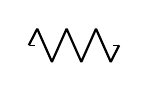
\begin{tikzpicture}[baseline]
                               \draw (0,0) to[R] (1,0);
                           \end{tikzpicture}
                         & 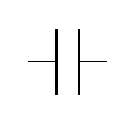
\begin{tikzpicture}[baseline]
                               \draw (0,0) to[C] (1,0);
                           \end{tikzpicture}
                         & 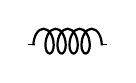
\begin{tikzpicture}[baseline]
                               \draw (0,0) to[L] (1,0);
                           \end{tikzpicture}                                                  \\ \hline
    \end{tblr}
\end{table}

\begin{description}
    \item[Basic elements of a circuit] An RLC circuit has three basic components, shown in the
        table. The general ODE governing an RLC circuit is,
        \begin{align}
            Q                           & = \int I\ \dl t                \\
            LI'' + RI' + \frac{1}{C}\ I & = E'(t)                        \\
            LQ'' + RQ' + \frac{1}{C}\ Q & = E(t) \qquad \text{corollary}
        \end{align}
    \item[Sinusoidally driven RLC] FOr the specific case of a sinusoidal driving EMF,

        \begin{align}
            LI'' + RI' + \frac{1}{C}\ I & = E_{0}\omega \cos(\omega t)        \\
            I_{p}                       & = a\cos(\omega t) + b\sin(\omega t)
        \end{align}


    \item[Reactance] A consolidation of capacitance and inductance derived from the complex
        notation.
        \begin{align}
            I_{p} & = a\cos(\omega t) + b\sin(\omega t)                                          \nonumber \\
            S     & = \omega L - \frac{1}{\omega C}                                                        \\
            I_{p} & = \frac{E_{0}}{R^{2} + S^{2}}\ \Big[-S\cos(\omega t) + R\sin(\omega t)\Big]
        \end{align}

    \item[Impedance] The complex number analog ($ Z $) of ohmic resistance, used to arrive at
        the RLC analog of Ohm's law. It is also known as the apparent resistance \par
        \begin{align}
            |Z|   & = \sqrt{R^{2} + S^{2}}               & E_{0}        & = |Z| I_{0}    \\
            I_{p} & = I_{0} \sin(\omega t - \theta)                                      \\
            I_{0} & = \sqrt{a^{2} + b^{2}}               & \tan(\theta) & = -\frac{a}{b} \\
                  & = \frac{E_{0}}{\sqrt{R^{2} + S^{2}}} &              & = \frac{S}{R}
        \end{align}

    \item[Transient current] Since a real circuit always has $ R > 0 $, the transient
        current always decays exponentially to zero in finite time, with the steady state
        current being the solution of the nh-ODE. \par
\end{description}

The equivalences between mechanical and electrical systems are apparent when looking at
the extreme similarity between the ODEs used to model both systems.

\section{Solution by Variation of Parameters}

The method of undetermined coefficients is restricted to functions $ r(x) $ which are similar
to their derivatives $ r(x)' $. A more general method is introduced here.

\begin{description}
    \item[Variation of Parameters] If $ y_{1}, y_{2} $ form a basis of solutions of the h-ODE,
        and $ W $ is their Wronksian, then the standard form ODE,
        \begin{align}
            y'' + py' + qy & = r                                                                          \\
            y_{h}          & = c_{1}y_{1} + c_{2}y_{2}                                                    \\
            y_{p}          & = -y_{1}\ \int \frac{y_{2}r}{W}\ \dl x + y_{2}\ \int \frac{y_{1}r}{W}\ \dl x
        \end{align}
    \item[Derivation] Starting with a generalization of $ y_{p} $, requires $ p, q, r $ to be
        continuous. \par

        Also, since $ y_{1}, y_{2} $ form a basis of solutions to the h-ODE, their $ W $
        is not zero  anywhere on the interval $ I $ on which they are defined.
        \begin{align}
            y_{p}               & = fy_{1} + gy_{2}                                                                                  \\
            y_{p}'              & = [f'y_{1} + g'y_{2}] + fy_{1}' + gy_{2}'                                                          \\
            f'y_{1} + g'y_{2}   & = 0                                                              &  & \text{artificial constraint} \\
            y_{p}''             & = fy_{1}'' + gy_{2}'' + f'y_{1}' + g'y_{2}'                                                        \\
            f'y_{1}' + g'y_{2}' & = r                                                              &  & \text{substituting into ODE} \\
            f'                  & = \frac{-y_{2}r}{y_{1}y_{2}' - y_{1}'y_{2}} = \frac{-y_{2} r}{W} &  & \text{using}\ W \neq 0       \\
            g'                  & = \frac{y_{1}r}{W}
        \end{align}
        Using the continuity of $ r(x) $, the derivatives $ f', g' $ can be integrated to obtain
        $ f, g $ and complete the derivation.
\end{description}
% \chapter{Higher Order Linear ODEs}
\section{Homogeneous Linear ODEs}

\begin{description}
    \item[Linear ODE of nth order] The standard form of an ODE on $ n $-th order is,
        \begin{align}
            y^{(n)} + p_{n-1}(x)y^{(n-1)} + \dots + p_{1}(x)y' + p_{0}(x)y & = r(x)
        \end{align}
        Here, $ \{p_{i}(x)\} $ are any continuous functions of $ x $, and the solution
        $ h(x) $, is defined and $ n $-times differentiable on the interval $ \mathcal{I} $
        in which the set $ \{p_{i}(x)\} $ are defined and continuous.
    \item[Superposition principle] If $ y_{1},\ y_{2} $ are solutions to a linear h-ODE
        of order $ n $, then
        \begin{align}
            c_{1}y_{1} + c_{2}y_{2} = y_{3}
        \end{align}
        is also a solution for some constants $ c_{1}, c_{2} $.
    \item[Linearly Independent functions] A set of functions $ y_{1}(x), \dots, y_{n}(x) $
        are linearly independent (L.I.) on some interval $ \mathcal{I} $ if,
        \begin{align}
            k_{1}y_{1}(x) + \dots + k_{n}y_{n}(x) = 0 \qquad \implies \qquad
            k_{1} = \dots = k_{n} = 0
        \end{align}
        Conversely, if some solution to the above equation exists for which not all $ k_{i} $
        are zero, then the functions are linearly dependent (L.D.)
    \item[Basis of solutions] A set of L.I. solutions to the linear h-ODE of order $ n $.
    \item[General solution] Given a basis of solutions $ \{y_{i}\} $ of the h-ODE,
        \begin{align}
            y & = c_{1}y_{1} + \dots + c_{n}y_{n}
        \end{align}
        is a general solution of the ODE. Particular solutions can be obtained by assigning
        values to the coefficients $ \{c_{i}\} $. \par
        No singular solutions exist which cannot be obtained from the general solution.
    \item[Initial Value Problem] Given the set of $ n $ initial conditions,
        \begin{align}
            y(x_{0}) = K_{0} \quad \ y'(x_{0}) = K_{1}\quad \dots \quad y^{(n)}(X_{0}) = K_{n}
        \end{align}
        There exists a unique solution for a linear h-ODE with coefficients $ \{p_{i}(x)\} $
        continuous on $ \mathcal{I} $ given that $ x_{0} \in \mathcal{I} $.
    \item[Wronskian] Using the determinant of order $ n $,
        \begin{align}
            \renewcommand*{\arraystretch}{1.5}
            W(y_{1},\dots,y_{n}) = \begin{vNiceMatrix}[r, margin]
                                       y_{1}         & y_{2}         & \dots  & y_{n}         \\
                                       y_{1}'        & y_{2}'        & \dots  & y_{n}'        \\
                                       \vdots        & \vdots        & \ddots & \vdots        \\
                                       y_{1}^{(n-1)} & y_{2}^{(n-1)} & \dots  & y_{n}^{(n-1)} \\
                                   \end{vNiceMatrix}
        \end{align}
        If $ W(x) \neq 0 $ for some $ x \in \mathcal{I} $, where the coefficients of the
        h-ODE $ \{p_{i}(x)\} $ are continuous on $ \mathcal{I} $, then the solutions
        $ \{y_{i}(x)\} $ are L.I. \par

        Conversely, if $ W(x) = 0 $ for some $ x = x_{0} \in \mathcal{I} $, then $W \equiv 0$
        identically for all $ x_{0} \in \mathcal{I} $ and the functions are L.D.
    \item[Existence and Uniqueness] If the coefficients $ \{p_{i}(x)\} $ are continuous on
        some interval $ \mathcal{I} $, then the h-ODE has a general solution on $ \mathcal{I} $.
        \par
        Using the fact that the Wronskian is merely the coefficient matrix of the system of linear
        equations in the unknowns $ \{c_{i}\} $ in the general solution, \par
        The Wronskisan of a solution composed of an L.I. basis of solutions is guaranteed to
        cover all possible solutions. Thus the general solution is unique. \par
\end{description}

\section{Homogeneous Linear ODEs with Constant Coefficients}

\begin{description}
    \item[Standard form] In standard form, the h-ODE with constant coefficients of order $ n $,
        alongside its characteristic equation is,
        \begin{align}
            y^{(n)} + a_{n-1}y^{(n-1)} + \dots + a_{1}y' + a_{0} & = 0             \\
            y_{h}                                                & = e^{\lambda x} \\
            \lambda^{n} + a_{n-1}\lambda^{n-1} + \dots a_{1}\lambda + a_{0} = 0
        \end{align}
    \item[Distinct real roots] Each distinct root $ \lambda_{k} $ corresponds to a solution
        to the ODE $ e^{k\lambda} $
        \begin{align}
            W & = \begin{vNiceMatrix}[r, margin]
                      e^{\lambda_{1}x}                  & e^{\lambda_{2}x}                  & \dots  & e^{\lambda_{n}x}                  \\
                      \lambda_{1}e^{\lambda_{1}x}       & \lambda_{2}e^{\lambda_{2}x}       & \dots  & \lambda_{n}e^{\lambda_{n}x}       \\
                      \lambda_{1}^{2}e^{\lambda_{1}x}   & \lambda_{2}^{2}e^{\lambda_{2}x}   & \dots  & \lambda_{n}^{2}e^{\lambda_{n}x}   \\
                      \vdots                            & \vdots                            & \ddots & \vdots                            \\
                      \lambda_{1}^{n-1}e^{\lambda_{1}x} & \lambda_{2}^{n-1}e^{\lambda_{2}x} & \dots  & \lambda_{n}^{n-1}e^{\lambda_{n}x}
                  \end{vNiceMatrix}
        \end{align}
    \item[Vandermode determinant] A simplified version of the above determinant given by,
        \begin{align}
            W & = \exp\left( x\sum_{k=1}^{n} \lambda_{k} \right)\ \begin{vNiceMatrix}[r, margin]
                                                                      1                 & 1                 & \dots  & 1                 \\
                                                                      \lambda_{1}       & \lambda_{2}       & \dots  & \lambda_{n}       \\
                                                                      \lambda_{1}^{2}   & \lambda_{2}^{2}   & \dots  & \lambda_{n}^{2}   \\
                                                                      \vdots            & \vdots            & \ddots & \vdots            \\
                                                                      \lambda_{1}^{n-1} & \lambda_{2}^{n-1} & \dots  & \lambda_{n}^{n-1}
                                                                  \end{vNiceMatrix}                       \\
              & = \exp\left( x\sum_{k=1}^{n} \lambda_{k} \right)\ (-1)^{n(n-1)/2} \cdot \prod_{j = 1}^{n}\ (\lambda_{j} - \lambda_{k}) \qquad n \geq j > k
        \end{align}
        The above expression is simply the difference between all possible combinations of roots.
        Since the first term is a product of exponentials, it is never zero. \par
        So, the Wronksian provides L.I only if all the roots are distinct, and thus none
        of the terms $ (\lambda_{j} - \lambda_{k}) $ are zero.
    \item[Repeated roots] For repeated roots of multiplicity $ m $, whether real or complex,
        \begin{align}
            y_{1}  & = e^{\lambda x}      & z_{1}, z_{2}     & = e^{\alpha x}\sin \beta x, e^{\alpha x} \cos \beta x           \\
            y_{2}  & = xe^{\lambda x}     & z_{3}, z_{4}     & = xe^{\alpha x}\sin \beta x, xe^{\alpha x} \cos \beta x         \\
            y_{3}  & = x^{2}e^{\lambda x} & z_{5}, z_{6}     & = x^{2}e^{\alpha x}\sin \beta x, x^{2}e^{\alpha x} \cos \beta x \\
            \vdots &                      & \vdots           & \nonumber                                                       \\
            y_{m}  & = x^{m}e^{\lambda x} & z_{2m-1}, z_{2m} & = x^{m}e^{\alpha x}\sin \beta x, x^{m}e^{\alpha x} \cos \beta x
        \end{align}
        Other solutions are obtained by multiplying higher powers of $ x $ to existing solutions.
        \par
        To derive the above multiple roots factor, consider the root $ \lambda_{1} $ with
        multiplicity $ m $,
        \begin{align}
            \mathcal{L}[y]             & = y^{(n)} + a_{n-1}y^{(n-1)} + \dots + a_{1}y' + a_{0}y                              \\
            \mathcal{L}[e^{\lambda x}] & = (\lambda^{n} + a_{n-1}\lambda^{n-1} + \dots + a_{1}\lambda + a_{0})\ e^{\lambda x} \\
                                       & = (\lambda - \lambda_{1})^{m} \cdot h(\lambda) \cdot e^{\lambda x}
        \end{align}
        Here $ h(\lambda) $ is the leftover polynomial after factoring out all the $ \lambda_{1} $.
        \begin{align}
            \diffp**{\lambda}{\mathcal{L}[e^{\lambda x}]}
             & = \mathcal{L}\left[ \diffp**{\lambda}{e^{\lambda x}} \right]
            = \mathcal{L}[xe^{\lambda x}]                                                       \\
             & = m(\lambda - \lambda_{1})^{m-1} \cdot h(\lambda)e^{\lambda x} \nonumber         \\
             & + (\lambda - \lambda_{1})^{m} \cdot \diffp**{\lambda}{[h(\lambda)e^{\lambda x}]} \\
        \end{align}
        Since $ m > 2 $, the RHS is zero at $ \Lambda = \lambda_{1} $. This means that
        $\mathcal{L}[xe^{\lambda x}] = 0$, and thus $ xe^{\lambda x} $ is a solution.
        \par Further differentiation w.r.t. $ \lambda $ can be used to arrive at further
        solutions corresponding to $ \lambda_{1} $.
\end{description}

\section{Nonhomogeneous Linear ODEs}

\begin{description}
    \item[Standard form] Ensuring the coefficient of $ y^{(n)} $ is $ 1 $,
        \begin{align}
            y^{(n)} + a_{n-1}y^{(n-1)} + \dots + a_{1}y' + a_{0} & = r(x)                \\
            y                                                    & = y_{h}(x) + y_{p}(x)
        \end{align}
        The Initial value problem is the same as for h-ODEs.
    \item[Undetermined coefficients] Similar to second order nh-ODEs, higher order ODEs
        can be solved using the pre-factor $ x^{m} $ to deal with roots of multiplicity $ m $.
    \item[Variation of parameters] Generalizing to order $ n $,
        \begin{align}
            y_{p} & = \sum_{k = 1}^{n}\ y_{k} \int \frac{W_{k}}{W}\ r \dl x
        \end{align}
        $ W $ is the Wronskian of the h-ODE with a basis of solutions $ \{y_{1}, y_{2},
            \dots,y_{n}\} $. $ W_{k} $ is the reduced Wronskian produced by replacing the
        $ k $-th column of $ W $ with the column vector $ [0\ 0\ \dots\ 0\ 1]^{T} $
\end{description}
% \chapter{Systems of ODEs, Phase Plane, Qualitative Methods}
\section{Systems of ODEs as Models in Engineering Applications}
\begin{description}
    \item[Conversion to system of ODEs] Any ODE of order $ n $ can be converted to a system
        of $ n $ ODEs of first order. Linear algebra provides easy methods of solving this
        system of linear equations using eigenvectors and eigenvalues.
        \begin{align}
            y^{(n)}                          & = F\left( t,\ y,\ y',\ y'',\ \dots,\ y^{(n-1)} \right)  \\
            \text{Set} \qquad y_1            & = y, \qquad y_2 = y', \quad \dots \quad y_n = y^{(n-1)} \\
            \text{System becomes}\qquad y_1' & = y_2 \nonumber                                         \\
            y_2'                             & = y_3 \nonumber                                         \\
            \vdots \nonumber                                                                           \\
            y_{n-1}'                         & = y_n \nonumber                                         \\
            y_n'                             & = F(t,\ y_1,\ y_2,\ \dots,\ y_n)
        \end{align}
    \item[Eigenvalues] When a system of linear equations is expressed in vector form,
        \begin{align}
            \renewcommand*{\arraystretch}{1.5}
            y_1'                 & = a_{11}y_1 + a_{12}y_2 \nonumber         \\
            y_2'                 & = a_{21}y_1 + a_{22}y_2                   \\
            \bmatcol{y_1'}{y_2'} & = \bmattt{a_{11}}{a_{12}}{a_{21}}{a_{22}} \\
            \vec{y'}             & = \vec{A}\vec{y}
        \end{align}
        For a matrix equation to have a non-trivial solution,
        \begin{align}
            \vec{A}\vec{x}                     & = \lambda \vec{x}                         \\
            (\vec{A} - \lambda\vec{I}) \vec{x} & = 0                                       \\
            \det(\vec{A} - \lambda\vec{I})     & = \begin{vNiceMatrix}[r, margin]
                                                       (a_{11} - \lambda) & a_{12}             \\
                                                       a_{21}             & (a_{22} - \lambda)
                                                   \end{vNiceMatrix}
        \end{align}
        This quadratic equation has solutions $ \lambda_1, \lambda_2 $ called eigenvalues.
        The corresponding eigenvectors $ \vec{v^{(1)}}, \vec{v^{(2)}} $ are found as
        solutions of the respective systems.
        \begin{align}
            (\vec{A} - \lambda_1\vec{I}) \vec{v^{(1)}} & = 0 \\
            (\vec{A} - \lambda_2\vec{I}) \vec{v^{(2)}} & = 0
        \end{align}
\end{description}

\section{Basic Theory of Systems of ODEs, Wronskian}
\begin{description}
    \item[General system of ODEs] Using a set of functions $ \{f_i\} $,
        \begin{align}
            y_1'     & = f_1(t,\ y_1,\ \dots,\ y_n) \\
            y_2'     & = f_2(t,\ y_1,\ \dots,\ y_n) \\
            \vdots                                  \\
            y_n'     & = f_n(t,\ y_1,\ \dots,\ y_n) \\
            \text{converting to vector notation,}   \\
            \vec{y'} & = \vec{f}(t, \vec{y})
        \end{align}
        Introducing the set of solutions as a vector, and another vector for the I.C.
        \begin{align}
            \vec{y}      & = \vec{h}(t) = \begin{bNiceMatrix}[r, margin]
                                              h_1(t) \\ h_2(t) \\ \vdots \\ h_n(t)
                                          \end{bNiceMatrix} &
            \vec{y}(t_0) & = \vec{K} = \begin{bNiceMatrix}[r, margin]
                                           K(0) \\ K(1) \\ \vdots \\ K_n
                                       \end{bNiceMatrix}
        \end{align}
    \item[Existence and Uniqueness] Given the preconditions,
        \begin{align}
            \{f_1,\ f_2,\ \dots,\ f_n\} \qquad       &
            \text{are continuous}                      \\
            \left\{ \diffp{f_i}{y_k} \right\} \qquad &
            \text{are continuous for all}\ j,k
        \end{align}
        Continuity is guaranteed in some point $ (t_0,\ K_0,\ K_1,\ \dots,\ K_n) $ in
        this interval of continuity in $ (t,\ y_0,\ y_1,\ \dots,\ y_n) $ space. \par
        Then, a solution to the system of ODEs exists in some interval
        $ t \in (t_0 - \alpha, t_0 + \alpha) $ and is guaranteed to be unique.
    \item[Linear System] A subset of the above general system of ODEs obeying,
        \begin{align}
            \begin{bNiceMatrix}[r, margin]
                y_1' \\ \vdots \\ y_n'
            \end{bNiceMatrix} & = \begin{bNiceMatrix}[r, margin]
                                      a_{11} & \dots  & a_{1n} \\
                                      \vdots & \ddots & \vdots \\
                                      a_{n1} & \dots  & a_{nn}
                                  \end{bNiceMatrix} \begin{bNiceMatrix}[r, margin]
                                                        y_1 \\ \vdots \\ y_n
                                                    \end{bNiceMatrix} + \begin{bNiceMatrix}[r, margin]
                                                                            g_1 \\ \vdots \\ g_n
                                                                        \end{bNiceMatrix} \\
            \vec{y'}                       & = \vec{Ay} + \vec{g}
        \end{align}
        The above system is homogeneous if $ \vec{g} = 0 $, with $ a_{jk} =
            \difsp{f_j}{y_k} $. \par
        If the elements of $ \vec{g} $ and $ \vec{a} $ are continuous functions of
        $ t $ in some interval $ t \in (\alpha, \beta) $ which contains the point
        $ t = t_0 $, then a solution exists and is guaranteed to be unique.
    \item[Superposition Principle] If $ \vec{y^{(1)}} $ and $ \vec{y^{(2)}} $ are
        solutions of the h-linear system of ODEs on some interval, then
        \begin{align}
            \vec{y^{(3)}} & = c_1 \vec{y^{(1)}} + c_2 \vec{y^{(2)}}
        \end{align}
        is also a solution. (using the linearity of matrix multiplication and of
        differentiation)
    \item[Basis] A set of L.I. solutions $ \{ \vec{y^{(i)}} \} $ form a basis in the
        interval $ \mathcal{J} $ if the elements of $ \vec{a} $ are continuous in
        $ \mathcal{J} $. \par

        A linear combination of this basis is a general solution that contains all
        possible solutions.
    \item[Wronskian] The old Wronskian of a set of solutions $ \{z_i\} $ becomes
        a matrix whose columns are members of the basis set $ \vec{y^{(i)}} $. \par

        The rows are successive derivatives (transformed into subscript variables).
        \begin{align}
            \begin{bNiceMatrix}[r, margin]
                z_1         & z_1         & \dots  & z_n         \\
                z_1'        & z_2'        & \dots  & z_n'        \\
                \vdots      & \vdots      & \ddots & \vdots      \\
                z_1^{(n-1)} & z_2^{(n-1)} & \dots  & z_n^{(n-1)}
            \end{bNiceMatrix} & \to
            \begin{bNiceMatrix}[r, margin]
                y_1^{(1)} & y_1^{(2)} & \dots  & y_1^{(n)} \\
                y_2^{(1)} & y_2^{(2)} & \dots  & y_2^{(n)} \\
                \vdots    & \vdots    & \ddots & \vdots    \\
                y_n^{(1)} & y_n^{(2)} & \dots  & y_n^{(n)}
            \end{bNiceMatrix}                                                \\
            W = \det(\vec{Y})                                   &
            = \det\begin{bNiceMatrix}[r, margin] \vec{y^{(1)}} &
                   \dots                     & \vec{y^{(n)}}\end{bNiceMatrix} \\
        \end{align}
        The Wronskian is either identically zero everywhere (if L.D.) or nowhere
        (if L.I.) in the interval $ \mathcal{J} $ under consideration.

    \item[Fundamental matrix] The above matrix $ \vec{Y} $ is called a fundamental
        matrix if the solutions $ \{\vec{y^{(i)}}\} $ form a basis.
        \begin{align}
            \vec{y}                        & = c_1\vec{y^{(1)}} + \dots + c_2\vec{y^{(n)}}                            \\
            \vec{y}                        & = \vec{Yc}                                                               \\
            \begin{bNiceMatrix}[r, margin]
                y_1 \\ \vdots \\ y_n
            \end{bNiceMatrix} & = \begin{bNiceMatrix}[r, margin] \vec{y^{(1)}} &
                                             & \vec{y^{(n)}}\end{bNiceMatrix}
            \begin{bNiceMatrix}[r, margin]
                c_1 \\ \vdots \\ c_n
            \end{bNiceMatrix}
        \end{align}
\end{description}

\section{Constant-Coefficient Systems, Phase Plane Method}
\begin{description}
    \item[Constant coefficient system] If the matrix $ \vec{a} $ has terms
        independent of $ t $, then the initial guess
        \begin{align}
            \vec{y'} & = \vec{Ay}        & \vec{y} & = \vec{x} e^{\lambda t} \\
            \vec{Ax} & = \lambda \vec{x}
        \end{align}
        leads to an eigenvalue problem. Here, $ \lambda, \vec{x} $ are the pairs
        of eigenvalues and eigenvectors respectively.
    \item[L.I. eigenvectors condition] For the above matrix $ \vec{A} $ to have
        a set of L.I. eigenvectors (as is common in real world applications), conditions
        are one of
        \begin{itemize}
            \item $\vec{A}$ is symmetric. $ a_{jk} = a_{kj} $ or $\vec{A} = \vec{A^T} $.
            \item $\vec{A}$ is skew symmetric. $ a_{jk} = -a_{kj} $
                  or $\vec{A} = -\vec{A^T} $.
            \item $ \vec{A} $ has $ n $ distinct eigenvalues.
        \end{itemize}
    \item[General solution] If $ \vec{A} $ has a set of L.I. eigenvectors as above,
        then the corresponding solutions form a basis. \par
        A general solution is of the form,
        \begin{align}
            \vec{y} & = c_1 \vec{x^{(1)}}e^{\lambda_1 t} + \quad \cdots \quad
            + c_n \vec{x^{(n)}}e^{\lambda_n t}
        \end{align}
        From this point onwards, the limited case of two member families of
        ODEs is taken up.
\end{description}


\begin{description}
    \item[Phase plane] The use of a parameter to plot the two solutions $ y_1 $ vs.
        $y_2$ instead of the usual pair of $ y $ vs. $ t $ curves.
    \item[Critical Points] Points in the phase plane where the tangent direction is
        not defined (for example at $ (0, 0) $ in the expression below).
        \begin{align}
            \diff{y_2}{y_1} & = \frac{y_2' \dl t}{y_1' \dl t} = \frac{y_2'}{y_1'}   \\
                            & = \frac{a_{21}y_1 + a_{22}y_2}{a_{11}y_1 + a_{12}y_2}
        \end{align}
    \item[Improper Node] A critical point $ P_0 $ at which all but two trajectories
        have the same limiting direction of the tangent $ L_1 $. The two exceptional
        trajectories also have a different (and equal) limit $ L_2 $.

    \item[Proper Node] A critical point at which every trajectory has a distinct
        limiting direction, and for any given direction $ \vec{d} $, there is some
        trajectory whose limiting direction at $ P_0 $ is equal to $ \vec{d} $.
    \item[Saddle Point] Two incoming and two outgoing trajectories intersect $ P_0 $,
        while all other trajectories bypass $ P_0 $.
    \item[Center] A critical point, enclosed by many closed trajectories, none of
        which ever pass through $ P_0 $.
    \item[Spiral] A critical point which all trajectories approach as
        $ t \to \infty $ which otherwise resembles a center.
    \item[Degenerate Node] In the (almost never physical) case when no basis of
        eigenvectors can be found. The usual condition is that $ \vec{A} $ is neither
        symmetric nor skew-symmetric and happens to have degenerate eigenvalues.
        \begin{figure}[H]
            \centering
            \begin{subfigure}[b]{0.49\textwidth}
                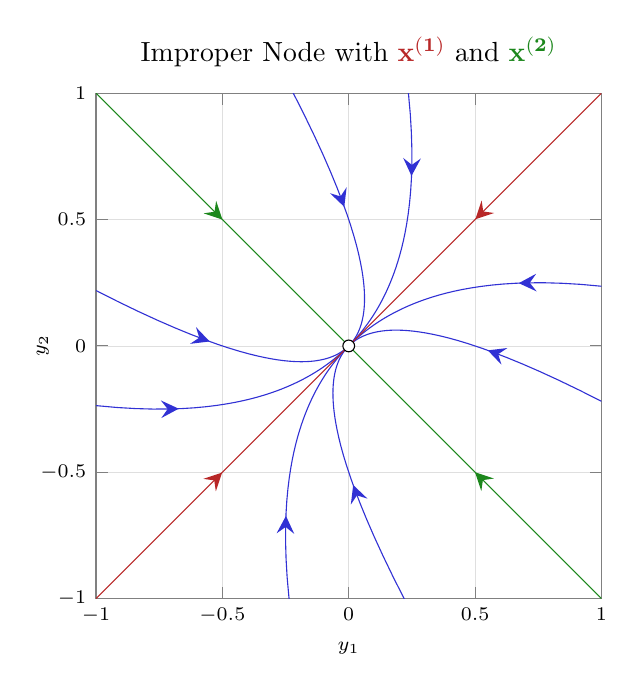
\begin{tikzpicture}
                    \begin{axis}[
                            declare function = {
                                    u(\x) = e^(-2*\x);
                                    v(\x) = e^(-4*\x);
                                },
                            xmin = -1, xmax = 1, ymin = -1, ymax = 1,
                            % restrict y to domain = -1:1,
                            title = {Improper Node with
                                    ${\color{y_p} \vec{x^{(1)}}}$ and
                                    ${\color{y_h} \vec{x^{(2)}}}$},
                            xlabel = $ y_1 $,
                            ylabel = $ y_2 $, ylabel shift = {-1em},
                            axis equal,
                            width = 8cm,
                            legend pos = north west,
                            grid = both,
                            domain = 0:3,
                            Ani]
                        \foreach \c in {-0.5, -1, 0.5, 1} {%
                                \edef\temp{%
                                    \noexpand \addplot[ samples = 100, color=blue3,
                                        arrow inside={end=stealth,opt={scale=2}}{0.65}]
                                    ({\c*u(x) + v(x)}, {\c*u(x) - v(x)});
                                    \noexpand \addplot[ samples = 100, color=blue3,
                                        arrow inside={end=stealth,opt={scale=2}}{0.65}]
                                    ({\c*u(x) - v(x)}, {\c*u(x) + v(x)});
                                }\temp
                            }
                        \addplot[ samples = 100, color=y_p,
                            arrow inside={end=stealth,opt={scale=2}}{0.5}]
                        ({u(x)}, {u(x)});
                        \addplot[ samples = 100, color=y_h,
                            arrow inside={end=stealth,opt={scale=2}}{0.5}]
                        ({v(x)}, {-v(x)});
                        \addplot[ samples = 100, color=y_p,
                            arrow inside={end=stealth,opt={scale=2}}{0.5}]
                        ({-u(x)}, {-u(x)});
                        \addplot[ samples = 100, color=y_h,
                            arrow inside={end=stealth,opt={scale=2}}{0.5}]
                        ({-v(x)}, {v(x)});
                        \node[GraphNode, fill = white, draw = black] at (axis cs:0,0) {};
                    \end{axis}
                \end{tikzpicture}
            \end{subfigure}
            \hfill
            \begin{subfigure}[b]{0.49\textwidth}
                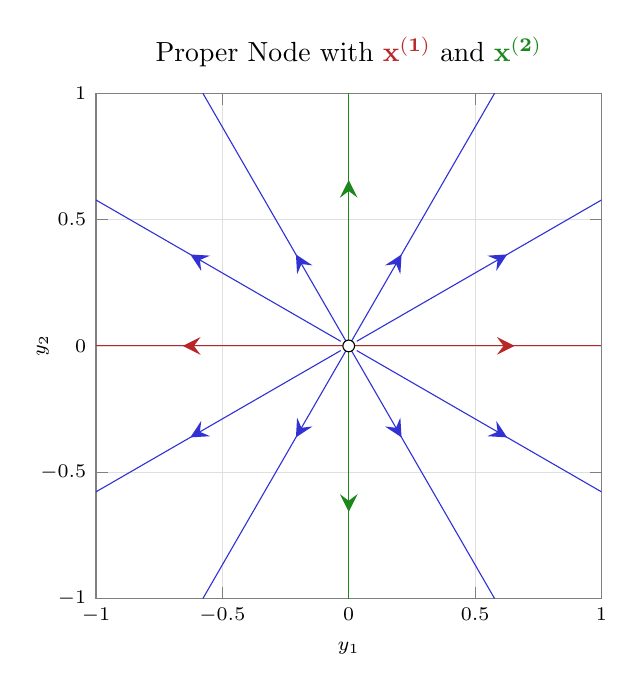
\begin{tikzpicture}
                    \begin{axis}[
                            declare function = {
                                    u(\x) = e^(\x);
                                    v(\x) = e^(\x);
                                },
                            xmin = -1, xmax = 1, ymin = -1, ymax = 1,
                            % restrict y to domain = -1:1,
                            title = {Proper Node with
                                    ${\color{y_p} \vec{x^{(1)}}}$ and
                                    ${\color{y_h} \vec{x^{(2)}}}$},
                            xlabel = $ y_1 $,
                            ylabel = $ y_2 $, ylabel shift = {-1em},
                            axis equal,
                            width = 8cm,
                            legend pos = north west,
                            grid = both,
                            domain = -4:0,
                            Ani]
                        \foreach \c in {-sqrt(3), -1/sqrt(3), sqrt(3), 1/sqrt(3)} {%
                                \edef\temp{%
                                    \noexpand \addplot[ samples = 100, color=blue3,
                                        arrow inside={end=stealth,opt={scale=2}}{0.35}]
                                    ({\c*u(x)}, {-v(x)});
                                    \noexpand \addplot[ samples = 100, color=blue3,
                                        arrow inside={end=stealth,opt={scale=2}}{0.35}]
                                    ({\c*u(x)}, {v(x)});
                                }\temp
                            }
                        \addplot[ samples = 100, color=y_p,
                            arrow inside={end=stealth,opt={scale=2}}{0.65}]
                        ({u(x)}, {0});
                        \addplot[ samples = 100, color=y_h,
                            arrow inside={end=stealth,opt={scale=2}}{0.65}]
                        ({0}, {-v(x)});
                        \addplot[ samples = 100, color=y_p,
                            arrow inside={end=stealth,opt={scale=2}}{0.65}]
                        ({-u(x)}, {0});
                        \addplot[ samples = 100, color=y_h,
                            arrow inside={end=stealth,opt={scale=2}}{0.65}]
                        ({0}, {v(x)});
                        \node[GraphNode, fill = white, draw = black] at (axis cs:0,0) {};
                    \end{axis}
                \end{tikzpicture}
            \end{subfigure}
        \end{figure}

        \begin{figure}[H]
            \centering
            \begin{subfigure}[b]{0.48\textwidth}
                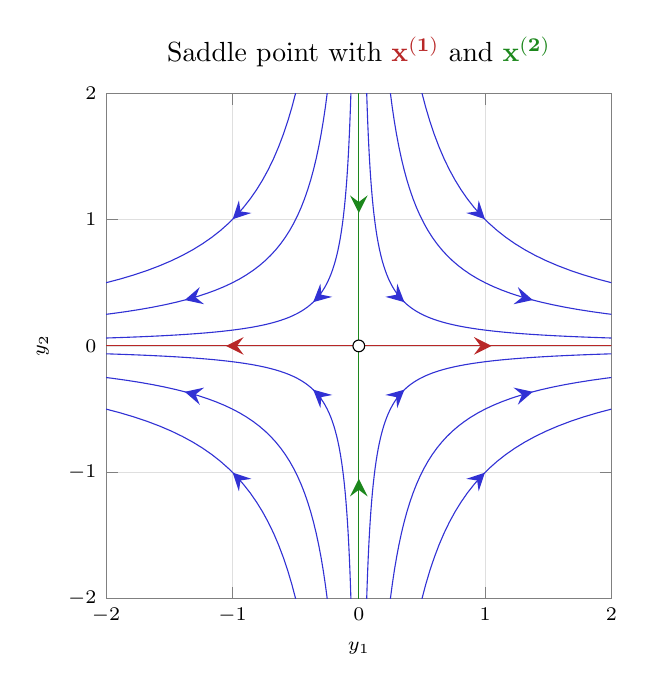
\begin{tikzpicture}
                    \begin{axis}[
                            declare function = {
                                    u(\x) = e^(\x);
                                    v(\x) = e^(-\x);
                                },
                            xmin = -2, xmax = 2, ymin = -2, ymax = 2,
                            % restrict y to domain = -1:1,
                            title = {Saddle point with
                                    ${\color{y_p} \vec{x^{(1)}}}$ and
                                    ${\color{y_h} \vec{x^{(2)}}}$},
                            xlabel = $ y_1 $,
                            ylabel = $ y_2 $,
                            axis equal,
                            width = 8cm,
                            legend pos = north west,
                            grid = both,
                            domain = -3:3,
                            Ani]
                        \foreach \c in {1/8, 1/2, 1} {%
                                \edef\temp{%
                                    \noexpand \addplot[ samples = 100, color=blue3,
                                        arrow inside={end=stealth,opt={scale=2}}{0.5, 0.7, 0.8, 0.9}]
                                    ({\c*u(x)}, {-v(x)});
                                    \noexpand \addplot[ samples = 100, color=blue3,
                                        arrow inside={end=stealth,opt={scale=2}}{0.5, 0.7, 0.8, 0.9}]
                                    ({\c*u(x)}, {v(x)});
                                    \noexpand \addplot[ samples = 100, color=blue3,
                                        arrow inside={end=stealth,opt={scale=2}}{0.5, 0.7, 0.8, 0.9}]
                                    ({-\c*u(x)}, {-v(x)});
                                    \noexpand \addplot[ samples = 100, color=blue3,
                                        arrow inside={end=stealth,opt={scale=2}}{0.5, 0.7, 0.8, 0.9}]
                                    ({-\c*u(x)}, {v(x)});
                                }\temp
                            }
                        \addplot[ samples = 100, color=y_p,
                            arrow inside={end=stealth,opt={scale=2}}{0.05}]
                        ({u(x)}, {0});
                        \addplot[ samples = 100, color=y_h,
                            arrow inside={end=stealth,opt={scale=2}}{0.95}]
                        ({0}, {-v(x)});
                        \addplot[ samples = 100, color=y_p,
                            arrow inside={end=stealth,opt={scale=2}}{0.05}]
                        ({-u(x)}, {0});
                        \addplot[ samples = 100, color=y_h,
                            arrow inside={end=stealth,opt={scale=2}}{0.95}]
                        ({0}, {v(x)});
                        \node[GraphNode, fill = white, draw = black] at (axis cs:0,0) {};
                    \end{axis}
                \end{tikzpicture}
            \end{subfigure}
            \hfill
            \begin{subfigure}[b]{0.48\textwidth}
                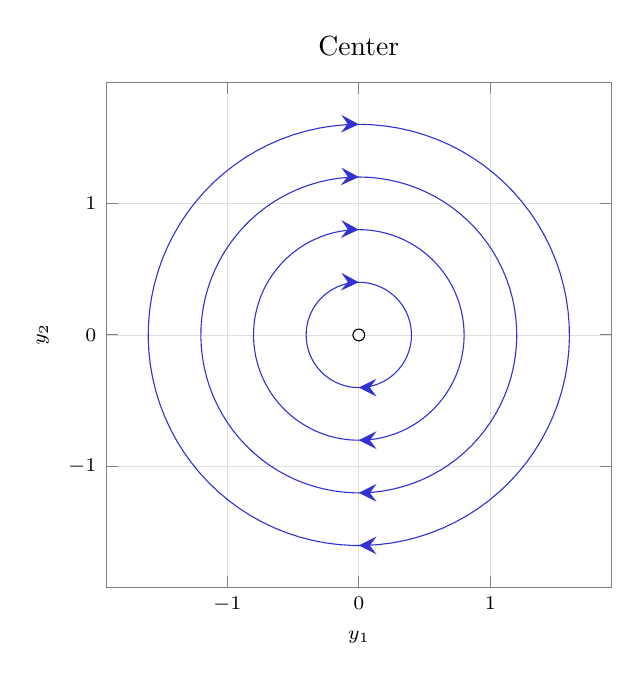
\begin{tikzpicture}
                    \begin{axis}[
                            % xmin = -1, xmax = 1, ymin = -1, ymax = 1,
                            % restrict y to domain = -1:1,
                            title = {Center},
                            xlabel = $ y_1 $,
                            ylabel = $ y_2 $,
                            axis equal,
                            width = 8cm,
                            legend pos = north west,
                            grid = both,
                            domain = 0:2*pi,
                            Ani]
                        \foreach \c in {0.4,0.8,...,2.0} {%
                                \edef\temp{%
                                    \noexpand \addplot[ samples = 100, color=blue3,
                                        arrow inside={end=stealth,opt={scale=2}}{0, 0.5}]
                                    ({\c*sin(x)}, {\c*cos(x)});
                                }\temp
                            }
                        \node[GraphNode, fill = white, draw = black] at (axis cs:0,0) {};
                    \end{axis}
                \end{tikzpicture}
            \end{subfigure}
        \end{figure}

        \begin{figure}[H]
            \centering
            \begin{subfigure}[b]{0.49\textwidth}
                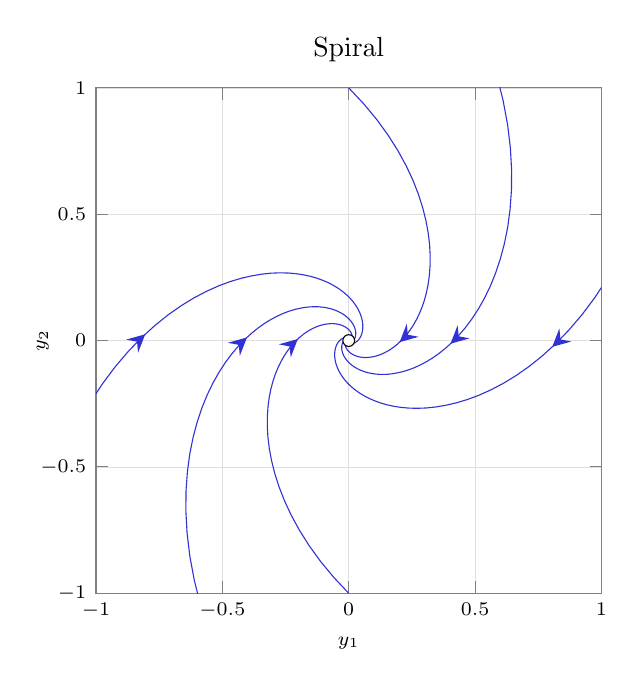
\begin{tikzpicture}
                    \begin{axis}[
                            xmin = -1, xmax = 1, ymin = -1, ymax = 1,
                            % restrict y to domain = -1:1,
                            title = {Spiral},
                            xlabel = $ y_1 $,
                            ylabel = $ y_2 $, ylabel shift = {-1em},
                            axis equal,
                            width = 8cm,
                            legend pos = north west,
                            grid = both,
                            domain = 0:2*pi,
                            Ani]
                        \foreach \c in {1,2,4} {%
                                \edef\temp{%
                                    \noexpand \addplot[ samples = 100, color=blue3,
                                        arrow inside={end=stealth,opt={scale=2}}{0.8}]
                                    ({\c*e^(-x)*sin(x)}, {\c*e^(-x)*cos(x)});
                                    \noexpand \addplot[ samples = 100, color=blue3,
                                        arrow inside={end=stealth,opt={scale=2}}{0.8}]
                                    ({-\c*e^(-x)*sin(x)}, {-\c*e^(-x)*cos(x)});
                                }\temp
                            }
                        \node[GraphNode, fill = white, draw = black] at (axis cs:0,0) {};
                    \end{axis}
                \end{tikzpicture}
            \end{subfigure}
            \hfill
            \begin{subfigure}[b]{0.49\textwidth}
                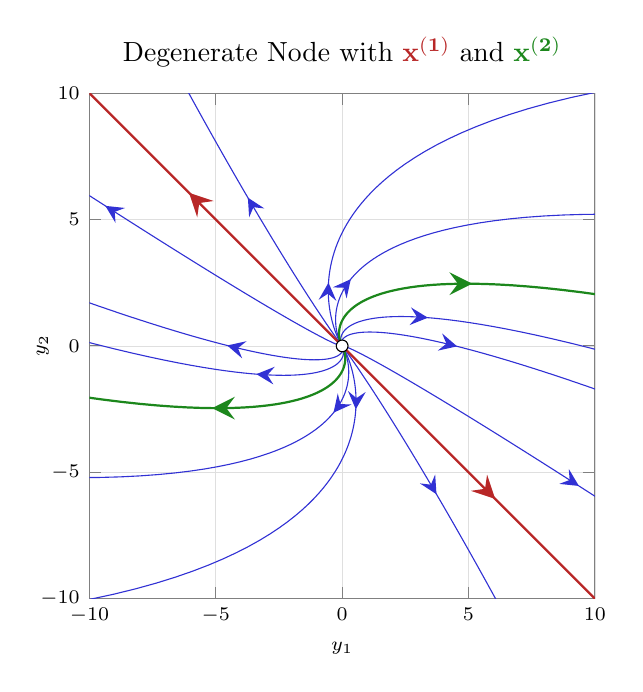
\begin{tikzpicture}
                    \begin{axis}[
                            xmin = -10, xmax = 10, ymin = -10, ymax = 10,
                            % restrict y to domain = -1:1,
                            title = {Degenerate Node with
                                    ${\color{y_p} \vec{x^{(1)}}}$ and
                                    ${\color{y_h} \vec{x^{(2)}}}$},
                            xlabel = $ y_1 $,
                            ylabel = $ y_2 $, ylabel shift = {-1em},
                            axis equal,
                            width = 8cm,
                            legend pos = north west,
                            grid = both,
                            domain = -1:1,
                            Ani]
                        \foreach \c in {1/2,1/4,2} {%
                                \edef\temp{%
                                    \noexpand \addplot[thin, samples = 100, color=blue3,
                                        arrow inside={end=stealth,opt={scale=2}}{0.15}]
                                    ({(\c + x)*e^(3*x)}, {(-\c - x + 1)*e^(3*x)});
                                    \noexpand \addplot[thin, samples = 100, color=blue3,
                                        arrow inside={end=stealth,opt={scale=2}}{0.15}]
                                    ({(\c - x)*e^(3*x)}, {(-\c + x - 1)*e^(3*x)});
                                    \noexpand \addplot[thin, samples = 100, color=blue3,
                                        arrow inside={end=stealth,opt={scale=2}}{0.15}]
                                    ({(-\c + x)*e^(3*x)}, {(\c - x + 1)*e^(3*x)});
                                    \noexpand \addplot[thin, samples = 100, color=blue3,
                                        arrow inside={end=stealth,opt={scale=2}}{0.15}]
                                    ({(-\c - x)*e^(3*x)}, {(\c + x - 1)*e^(3*x)});
                                }\temp
                            }
                        \addplot[thick, samples = 100, color=y_p,
                            arrow inside={end=stealth,opt={scale=2}}{0.3}]
                        ({e^(3*x)}, {-e^(3*x)});
                        \addplot[thick, samples = 100, color=y_p,
                        arrow inside={end=stealth,opt={scale=2}}{0.3}]
                        (-{e^(3*x)}, {e^(3*x)});
                        \addplot[thick, samples = 100, color=y_h,
                            arrow inside={end=stealth,opt={scale=2}}{0.3}]
                        ({x*e^(3*x)}, {(-x+1)*e^(3*x)});
                        \addplot[thick, samples = 100, color=y_h,
                            arrow inside={end=stealth,opt={scale=2}}{0.3}]
                        ({-x*e^(3*x)}, {-1*(-x+1)*e^(3*x)});
                        \node[GraphNode, fill = white, draw = black] at (axis cs:0,0) {};
                    \end{axis}
                \end{tikzpicture}
            \end{subfigure}
        \end{figure}
\end{description}

\section{Criteria for Critical Points, Stability}
\begin{description}
    \item[Characteristic equation] For the two member system of linear ODEs with
        constant coefficients,
        \begin{align}
            \vec{A}                        & = \bmattt{a_{11}}{a_{12}}{a_{21}}{a_{22}} \\
            \det(\vec{A} - \lambda\vec{I}) & =
            \lambda^{2} - (a_{11} + a_{22})\lambda + \det(\vec{A}) = 0                 \\
            \lambda^{2} - p\lambda + q     & = 0
        \end{align}
    \item[Critical point categories] Rearranging the characteristic equation into its
        factors $ \lambda_1,\ \lambda_2 $,
        \begin{align}
            p                           & = \lambda_1 + \lambda_2       &
            q                           & = \lambda_1 \lambda_2           \\
            \text{Discriminant}\ \Delta & = p^{2} - 4q                  &
            \Delta                      & = (\lambda_1 - \lambda_2)^{2}
        \end{align}
        \begin{table}[ht]
            \centering
            \SetTblrInner{rowsep=0.5em}
            \begin{tblr}{colspec={Q[r]|Q[l]}, colsep = 2em}
                \textbf{Critical Point} &
                \textbf{Eigenvalues} $ \lambda_1, \lambda_2 $            \\ \hline[dotted]
                Node                    & Real, same sign                \\
                Saddle point            & Real, opposite signs           \\
                Center                  & Purely imaginary               \\
                Spiral point            & Complex with nonzero real part \\ \hline
            \end{tblr}
        \end{table}
    \item[Stability] From physics, stability is a measure of the effect in the future
        of a small change in the system at present time.
    \item[Stable critical point] If for every disk $ D_\epsilon $ centered on $ P_0 $,
        there is a disk $ D_{\delta} $ with $ \delta, \epsilon >0 $, such that every trajectory
        which has $ P(t = t_1) = P_1 \in D_{\delta}$ has all its points corresponding to
        $ t \geq t_1 $ in $ D_{\epsilon} $.
    \item[Attractive critical point] Every trajectory in $ D_\delta $ for a stable
        critical point, approaches $ P_0 $ asymptotically as $ t \to \infty $.

        \begin{table}[ht]
            \centering
            \SetTblrInner{rowsep=0.5em}
            \begin{tblr}{colspec={Q[r]|Q[l]}, colsep = 2em}
                \textbf{Stability}    &
                \textbf{Condition on} $ \vec{p},\ \vec{q} $        \\ \hline[dotted]
                Stable and attractive & $ p<0 $ and $ q > 0 $      \\
                Stable                & $ p \leq 0 $ and $ q > 0 $ \\
                Unstable              & $ p > 0 $ or $\ \ q < 0 $  \\ \hline
            \end{tblr}
        \end{table}
\end{description}

\section{Qualitative Methods for Nonlinear Systems}
\begin{description}
    \item[Assumptions] The system of ODEs is autonomous, and the functions $ f_1, f_2 $
        are independent of $ t $. \par
        Also, the system of ODEs has finitely many critical points. This
        means that each critical point is isolated. \par
        For analysis, each critical point is treated as the origin when being analyzed,
        using the coordinate transformation,
        \begin{align}
            P_0         & = (a, b)  & (a, b)      & \to (0, 0) \\
            \tilde{y_i} & = y_1 - a & \tilde{y_2} & = y_2 - b
        \end{align}
    \item[Linearization] The system is linearlised around its critical point
        $ (0, 0) $ using,
        \begin{align}
            \vec{y} & = \vec{f}(\vec{y}) \equiv \vec{Ay} + \vec{h}(\vec{y}) \\
            y_1'    & = a_{11}y_1 + a_{12}y_2 + h_1(y_1, y_2)               \\
            y_2'    & = a_{21}y_1 + a_{22}y_2 + h_2(y_1, y_2)
        \end{align}
        Notice $ \vec{A} $ here is independent of $ y $ since $ P_0  = (0, 0)$ is
        a critical point giving. \par
        If $ f_1, f_2 $ are continuous and have continuous partial derivatives in a
        region around $ P_0 $, and if $ \det(\vec{A}) \neq 0 $, then the kind and
        stability of the critical points of the original system are the same as
        those of the linearized system. \par
        Exceptions occur if the linearized system has equal roots or purely imaginary
        roots.
        The general method is as follows,
        \begin{enumerate}
            \item Set up the mathematical model.
            \item Identify the critical points as conditions for $ \vec{y} = 0 $
            \item Drop all nonlinear terms in order to linearize the system
            \item Treat each critical point in turn, transforming coordinates as
                  needed.
        \end{enumerate}
    \item[Transformation to first order ODE] A second order autonomous ODE can
        be transformed using,
        \begin{align}
            F(y, y', y'') & = 0                    & y & = y_1, \qquad y' = y_2 \\
            y''           & = \diff{y_2}{y_1}\ y_2
        \end{align}
    \item[Limit Cycle] A closed trajectory in phase space into which other trajectories
        spiral asymptotically. Similar to an attractive node, but instead of a single point
        in phase space, this is a closed stable trajectory. \par

        In the real world, this requires systems with variable damping (which can also be
        negative), which push trajectories starting outside and inside the limit cycle
        inward and outward towards it
        respectively.
\end{description}

\section{Nonhomogeneous Linear Systems of ODEs}

\begin{description}
    \item[General solution] Assuming $ \vec{g} \not \equiv \vec{0}$ and the entries of
        $ \vec{A} $ are continuous on some interval $ \mathcal{J} $ of the $t-$axis,\par
        a general solution of the nh-system is given by,
        \begin{align}
            \vec{y'} & = \vec{Ay} + \vec{g}            \\
            \vec{y}  & = \vec{y^{(h)}} + \vec{y^{(p)}}
        \end{align}
    \item[Undetermined coefficients] The method is analogous to the single ODE
        procedure, for the same set of candidate functions. The only change is in the
        modification rule.
    \item[Variation of parameters] Start with a basis of solutions $ \vec{Z} $ of the
        h-ODE system.
        \begin{align}
            \vec{Z'}      & = A\vec{Z}                      \\
            \vec{y^{(p)}} & = \vec{Z}(t)\vec{u}(t)          \\
            \vec{y'}      & = \vec{Ay} + \vec{g}  \nonumber \\
            \vec{Zu'}     & = \vec{g}                       \\
            \vec{u'}      & = \vec{Z^{-1}g}
        \end{align}
        $ \vec{Z^{-1}} $ is guaranteed to exist since $ \vec{Z} $ is a basis and
        its Wronskian is nonzero.
\end{description}
% \chapter{Series Solutions of ODEs. Special Functions}
\section{Power Series Method}
\begin{description}
    \item[Power Series] A function approximated using a polynomial
        with center $ x_0 $ given by,
        \begin{align}
            f(x) & = \sum_{m = 0}^{\infty} a_m\ (x - x_0)^{m}
        \end{align}
        Here, the set $ \{a_m\} $ are constant coefficients of the series. Also,
        the set $ m $ only includes posittive integers.
    \item[Partial sum] The $ n $-th partial sum and the $ n $-th remainder of
        the above power series is,
        \begin{align}
            s_n(x)                 & = \sum_{m = 0}^{n} a_m\ (x - x_0)^{m}        \\
            R_n(x) = f(x) - s_n(x) & = \sum_{m = n+1}^{\infty} a_m\ (x - x_0)^{m}
        \end{align}
    \item[Convergent series] If for some $ x_1 $, the sequence of partial sums
        $ \{s_n(x_1)\} $ approaches some finite limit $ s(x_1) $, then the series is
        considered convergent at $ x = x_1 $
        \begin{align}
            \lim_{n \rightarrow \infty}
            s_n(x_1) & = s(x_1)                                  \\
                     & = \sum_{m = 0}^{\infty}a_m\ (x - x_0)^{m}
        \end{align}
        Alternatively, for any positive $ \epsilon $ there is an $ N $, such that
        $ s_n(x_1) $ for all $ n > N $ lies within $ \epsilon $ distance of the
        asymptotic limit $ s(x_1) $.
        \begin{align}
            |R_n(x_1)|      & = |s(x_1) - s_n(x_1)| < \epsilon           &
            \forall \quad n & > N                                          \\
            s_n(x_1)        & \in (s(x_1) - \epsilon, s(x_1) + \epsilon) &
            \forall \quad n & > N
        \end{align}
    \item[Convergence interval] The set of values of $ x $ for which the power
        series converges. Sometimes this set may contain only the element $ x = x_0 $.
    \item[Radius of convergence] The half-width of the interval of convergence. Denoted
        $ R $ (from complex notation where the zone of convergence becomes a disk).
        \begin{align}
            s(x) \quad \text{converges} \quad & \forall \quad |x - x_0| < R   \\
            \text{and diverges} \quad         & \forall \quad |x - x_0| > R   \\
            \frac{1}{R}                       & = \lim_{m \rightarrow \infty}
            \Big| \frac{a_{m+1}}{a_m}\Big|                                    \\
            \frac{1}{R}                       & = \lim_{m \rightarrow \infty}
            (|a_m|)^{1/m}
        \end{align}
        The above formulas require the limits to exist and be nonzero. If the limits
        are $ \infty $, then the series only converges at the center $ x_0 $.
    \item[Analytic function] A function that has a Taylor series representation at
        $ x = x_0 $ is analytic at $ x_0 $. \par
        If $ p, q, r $ are analytic at $ x_0 $, then
        \begin{align}
            y'' + p(x)y' + q(x)y = r(x) \nonumber
        \end{align}
        has every solution analytic at $ x_0 $ with some radius of convergence
        $ R > 0 $.
    \item[Operations on Power series] The following operations performed on convergent
        power series result in another power series converging to the result of the same
        operation on the function itself.
        \begin{align}
            y(x)                       & = \sum_{m = 0}^{\infty}a_m\ (x - x_0)^{m}       \\
            \diff{y}{x}                & = \sum_{m = 1}^{\infty}m a_m\ (x - x_0)^{m-1} &
            \forall \quad |x - x_0|    & < R                                             \\
            f(x) + g(x)                & = \sum_{m = 0}^{\infty}
            (a_m + b_m)\ (x - x_0)^{m} &
            \forall \quad |x - x_0|    & < R_f \cap R_g                                  \\
            f(x)g(x)                   & = \sum_{m = 0}^{\infty} \left[ \sum_{k=0}^{m}
            a_kb_{m-k} \right]\ (x - x_0)^{m}                                            \\
            f(x)                       & \equiv 0                                      &
            \implies \{a_m\}           & \equiv 0
        \end{align}
        The last equation follows from polynomials being identically $ 0 $ if and
        only if every single coefficient is identically $ 0 $.
\end{description}

\section{Legendre's Equation, Legendre Polynomials}
\begin{description}
    \item[Legendre ODE] In Physics, this ODE is very frequently encountered, which
        yields a recurrence relation when solved using the power series method,
        \begin{align}
            0       & = (1 - x^2)y'' - 2xy' + n(n+1)y         \\
            y       & = \sum_{m = 0}^{\infty} a_m\ x^m        \\
            a_{s+2} & = -\frac{(n-s)(n+s+1)}{(s+2)(s+1)}\ a_s \\
        \end{align}

        The solution in terms of the two free constants $ a_0 $ and $ a_1 $,
        \begin{align}
            y(x) & = a_0y_1 + a_1 y_2                      \\
            y_1  & = 1 - \frac{n(n+1)}{2!}\ x^2
            + \frac{(n-2)n(n+1)(n+3)}{4!}\ x^4 - \dots     \\
            y_2  & = x - \frac{(n-1)(n+2)}{3!}\ x^3
            + \frac{(n-3)(n-1)(n+2)(n+4)}{5!}\ x^5 - \dots \\
        \end{align}
    \item[Convergence] The Legendre polynomials converge only for $ |x| < 1 $.
        Since the standard form of the ODE,
        \begin{align}
            y'' - \frac{2x}{(1-x^2)}\ y' + \frac{n(n+1)}{(1 - x^2)}\ y & = 0
        \end{align}
        is not analytic at $ x = \pm 1 $, the convergence interval of the solution is
        at best $ (-1, 1) $.
    \item[Legendre's polynomial] For $ n $ being a non-negative integer, either $ y_1 $
        or $ y_2 $ terminate after finitely many terms depending on $ n $ being even or odd.
        \begin{align}
            P_n(x) & = \sum_{m = 0}^{M} (-1^m)\ \frac{(2n - 2m)!}
            {2^n\ m!\ (n-m)!\ (n-2m)!}\ x^{n-2m}
        \end{align}
        Here, $ M = n/2 $ or $ (n-1)/2 $ depending on n even or odd. \par
        The specific choice of coefficients ensures that $ Pn(1) = 1 $ for all $ n $. \par
        The recurrence relation is the other condition that enables the calculation of the
        above general formula for the series.
        \begin{align}
            P_0(x) & = 1                                  &
            P_1(x) & = x                                    \\
            P_2(x) & = \frac{1}{2}\ (3x^2 - 1)            &
            P_3(x) & = \frac{1}{2}\ (5x^3 - 3x)             \\
            P_4(x) & = \frac{1}{8}\ (35x^4 - 30x^2 + 3)   &
            P_5(x) & = \frac{1}{8}\ (63x^5 - 70x^3 + 15x)
        \end{align}
        These polynomials are orthogonal in the interval $ [-1, 1] $.\
\end{description}

\section{Extended Power Series Method: Frobenius Method}
\begin{description}
    \item[Frobenius ODE] Let $ b(x), c(x) $ be any functions analytic at $ x = 0 $. Then,
        \begin{align}
            y'' + \frac{b(x)}{x}\ y' + \frac{c(x)}{x^2}\ y & = 0
        \end{align}
        has at least one solution with $ r $ real or complex and $ a_0 \neq 0 $,
        \begin{align}
            y(x) & = x^r \sum_{m = 0}^{\infty}a_m\ x^m
        \end{align}
        The ODE also has a second L.I. solution that looks similar to the first.
    \item[Regular point] A point $ x_0 $ at which the ODE,
        \begin{align}
            y'' + p(x)y' + q(x) & = 0                         \\
            p(x),\ q(x)\        & \text{are analytic at}\ x_0
        \end{align}
    \item[Singular point] A point $ x_0 $ which is not a regular point as defined
        above.
    \item[Indicial equation] A quadratic equation in $ r $ which indicates the
        form of the second L.I. solution to the Frobenius ODE.
        \begin{align}
            x^2 y'' + x\ b(x)y' + c(x)y & = 0                           \\
            \text{Substitute}\qquad b(x) = \sum_{m=0}^{\infty} b_m x^m,
            \qquad c(x)                 & = \sum_{m=0}^{\infty} c_m x^m \\
            \text{Gathering terms with}\ x^r
            \qquad r(r-1) + b_0 r + c_0 & = 0
        \end{align}
        The Euler-Cauchy ODE is the simplest case of the Frobenius ODE and illustrates
        the three cases arising form the indicial equation described below.
    \item[Distinct roots not differing by an integer] If $ r_1, r_2 $ are the two roots,
        then a basis of solutions is,
        \begin{align}
            y_1(x) & = x^{r_1} \sum_{m=0}^{\infty}a_m x^m \\
            y_2(x) & = x^{r_2} \sum_{m=0}^{\infty}A_m x^m
        \end{align}
        where the coefficients $ \{a_m\}, \{A_m\} $ are found by comparing powers of
        $ x^r $ and higher terms in the ODE.
    \item[Repeated root] Here, $ r_1 = r_2 = (1 - b_0)/2 $ and
        \begin{align}
            y_1(x) & = x^{r} \sum_{m=0}^{\infty}a_m x^m                         \\
            y_2(x) & = y_1 \ln(x) + x^{r} \sum_{m=0}^{\infty}A_m x^m &  & (x>0)
        \end{align}
    \item[Roots differing by an integer] This case also includes complex roots,
        and the stipulation that $ r_1 > r_2 $,
        \begin{align}
            y_1(x) & = x^{r_1} \sum_{m=0}^{\infty}a_m x^m                  \\
            y_2(x) & = ky_1(x) \ln(x) + x^{r_2} \sum_{m=0}^{\infty}A_m x^m
        \end{align}
        It is possible that $ k=0 $ happens because of simplicity in the ODE.
\end{description}

\section{Bessel's Equation, Bessel Functions Jv(x)}
\begin{description}
    \item[Bessel's ODE] The standard form of the Bessel ODE with
        $ \nu \in \mathcal{R^+} \cup 0 $ is,
        \begin{align}
            x^2y'' + xy' + (x^2 - \nu^2)y & = 0
        \end{align}
        This is often the result of the physical system having cylindrical symmetry.
    \item[Power series solution] Applying the general power series method to find
        indicial equation,
        \begin{align}
            y                & = \iser{0} a_m\ x^{m+r} \\
            (r + \nu)(r-\nu) & = 0                     \\
            r_1              & = \nu (\geq 0)
            \qquad \qquad r_2 = -\nu                   \\
            a_{2m}           & = \frac{(-1)^m\ a_0}
            {2^{2m}\ m!\ (\nu+1)(\nu+2)\dots(\nu+m)}
            \qquad \forall\ m=\{1,2,3,\dots\}
        \end{align}
    \item[Integer parameter] For the special case of $ \nu \in \mathcal{I^+} \cup 0 $,
        assign $ \nu \rightarrow n $,
        \begin{align}
            a_0    & = \frac{1}{2^n\ n!}                          \\
            a_{2m} & = \frac{(-1)^m}{2^{2m+n}\ m!\ (n+m)!} \qquad
            \forall\ m= \{1,2,3,\dots\}
        \end{align}
    \item[Function of the first kind] By inserting the above recursion relation into the
        power series solution and noting that odd powers have zero coefficient,
        \begin{align}
            J_n(x) & = x^n\ \iser{0} \frac{(-1)^m\ x^{2m}}{2^{2m+n}\ m!\ (n+m)!}
        \end{align}
        This series converges for all $ x $.
    \item[Asymptotic behavior] All of the $ J_{\nu}(x) $ resemble cosine functions,
        with gradually decaying amplitudes and zeros not being evenly spaced. This is
        also evident from the similarity in their series expansions,
        \begin{align}
            J_0                               & = 1 - \frac{x^2}{2^2\ (1!)^2}
            + \frac{x^4}{2^4\ (2!)^2} - \frac{x^6}{2^6\ (3!)^2} + \dots                 \\
            J_1                               & = \frac{x}{2} - \frac{x^3}{2^3\ 1!\ 2!}
            + \frac{x^5}{2^5\ 2!\ 3!} - \frac{x^7}{2^7\ 3!\ 4!} + \dots                 \\
            \lim_{x \rightarrow \infty}J_n(x) & \approxeq \frac{2}{\pi x}
            \cos \Bigg( x - \frac{n\pi}{2} - \frac{\pi}{4} \Bigg)
        \end{align}
    \item[Gamma function] The generalization of the factorial to non-integer indices.
        \begin{align}
            \Gamma(\nu+1) & = \int_{0}^{\infty}e^{-t}\ t^{\nu}\ \dl t &
            (\nu          & > -1)                                       \\
            \Gamma(\nu+1) & = \nu\ \Gamma(\nu)                          \\
            \Gamma(n+1)   & = n!                                      &
            (n            & \in 0 \cup \mathcal{I^+})
        \end{align}
    \item[Real positive parameter] Replacing the factorial with the Gamma function,
        \begin{align}
            a_0        & = \frac{1}{2^{\nu}\ \Gamma(\nu+1)}        \\
            J_{\nu}(x) & = x^{\nu}\ \iser{0} \frac{(-1)^m\ x^{2m}}
            {2^{2m + \nu}\ m!\ \Gamma(\nu+m+1)}
        \end{align}
        $ \nu $ is called the order of the Bessel function.
    \item[Properties of Bessel functions] Starting from the power series definition,
        some properties of $ J_{\nu}(x) $ are,
        \begin{align}
            \diff**{x}{[x^{\nu}\ J_{\nu}]}  & = x^{\nu}\ J_{\nu - 1}    \\
            \diff**{x}{[x^{-\nu}\ J_{\nu}]} & = -x^{-\nu}\ J_{\nu + 1}  \\
            J_{\nu-1} + J_{\nu+1}           & = \frac{2\nu}{x}\ J_{\nu} \\
            J_{\nu-1} - J_{\nu+1}           & = 2\ \diff**{x}{J_{\nu}}
        \end{align}
        The second set of relations comes from adding and subtratcing the expansions of
        the first set.
    \item[Half-integer parameter] Some basic results,
        \begin{align}
            \Gamma(1/2)      & = \sqrt{\pi}                        \\
            J_{\frac{1}{2}}  & = \sqrt{\frac{2}{\pi x}}\ \sin(x) &
            J_{-\frac{1}{2}} & = \sqrt{\frac{2}{\pi x}}\ \cos(x)   \\
        \end{align}
    \item[General Solution] For the special case of $ \nu \not\in \mathcal{I} $, a
        straightforward second solution that is L.I. is found by using $ -\nu $,
        \begin{align}
            y(x) & = c_1\ J_\nu + c_2\ J_{-\nu}
        \end{align}
        When $ \nu $ is an integer, this second function becomes L.D since,
        \begin{align}
            J_{-n} & = (-1)^n\ J_n
        \end{align}
        Result follows from the fact that $ \Gamma(n+1) $ is not defined for $ n < -1 $.
        In this case, a more involved procedure is necessary to find the second L.I.
        solution.
\end{description}

\section{Bessel Functions Yv(x), General Solution}
\begin{description}
    \item[Zero parameter] Special case where the ODE reduces to
        \begin{align}
            0      & = xy'' + y' + xy                                   &
            r_1    & = r_2 = 0                                            \\
            y_2    & = J_0 \ln(x) + \iser{1}A_m\ x^m                    &
            h_m    & = \sum_{r=1}^{m} \frac{1}{r}                         \\
            A_{2m} & = \frac{(-1)^{m-1}\ h_m}{2^{2m}\ (m!)^2}             \\
            y_2(x) & = J_0(x) \ln(x) + \frac{x^2}{4} - \frac{3x^4}{128}
            + \frac{11x^6}{13824} + \dots
        \end{align}

    \item[Neumann function of order 0] Bessel function of order zero, using the constants
        \begin{align}
            a      & = \frac{2}{\pi}                                              \\
            b      & = \lim_{s \rightarrow \infty} \left[ 1 + \frac{1}{2} + \dots
            + \frac{1}{s} - \ln(s) \right] = \gamma - \ln(2)                      \\
            Y_0(x) & = a(y_2 + bJ_0)                                              \\
                   & = \frac{2}{\pi} \left[ J_0 \{\ln(x/2) + \gamma\}
                + \iser{1} \frac{(-1)^{m-1}\ h_m}{2^{2m}\ (m!)^2}\ x^{2m} \right]
        \end{align}
        This function behaves like $ \ln x $ for small $ x $

    \item[Integer parameter] When the parameter is an integer $ n $, another special case
        is given by
        \begin{align}
            Y_n   & = \lim_{\nu \rightarrow n}Y_\nu (x)                    \\
            Y_\nu & = \frac{J_\nu \cos(\nu \pi) - J_{-\nu}}{\sin(\nu \pi)}
        \end{align}
        For non-integer $ \nu $, the two functions $ J_\nu $ and $ J_{-\nu} $ are
        already L.I. and thus, $ Y_\nu $ is also L.I. of $ J_\nu $. \par

        By taking the limit above, the expression for $ Y_n $ becomes,
        \begin{align}
            Y_n & = \frac{2}{\pi} J_n \{ \ln(x/2) + \gamma \}
            + \frac{x^n}{\pi} \iser{0} \frac{(-1)^{m-1}\ (h_m + h_{m+n})}
            {2^{2m+n}\ m!\ (m+n)!}\ x^{2m}                          \\
                & - \frac{1}{nx^n} \sum_{m=0}^{n-1} \frac{(n-m-1)!}
            {2^{2m-n}\ m!}\ x^{2m}       \qquad\qquad (x>0)
        \end{align}
        Some conventions used in the above formula, and a simple result that follows
        is,
        \begin{align}
            h_0    & = 0 \qquad \text{(by convention)} \\
            Y_{-n} & = (-1)^n Y_n
        \end{align}

    \item[General solution] Using the above special cases, a general solution can now be
        defined using,
        \begin{align}
            y & = c_1 J_\nu(x) + c_2 Y_\nu (x)
        \end{align}

    \item[Hankel functions] Solutions of Bessel's ODE that are complex for real $ x $,
        given by linear combinations of $ J_\nu $ and $ Y_\nu $,
        \begin{align}
            H_\nu^{(1)} & = J_\nu + i Y_\nu \\
            H_\nu^{(2)} & = J_\nu - i Y_\nu
        \end{align}
        These functions are also called Bessel functions of the third kind.
\end{description}

% \chapter{Laplace Transforms}
\section{Laplace Transform, Linearity, First Shifting Theorem (s-Shifting)}
\begin{description}
    \item[Operational calculus] The process of transforming a calculus problem to an
        algebraic problem. Laplace transforms are one example.
    \item[Integral transform] The operation of transforming a function in one space
        $ (t) $ to another space $ (s) $by performing an integration.
        \begin{align}
            F(s) & = \infint k(s, t)\ f(t)\ \dl t
        \end{align}
        Here, the function $ k(s, t) $ is called the kernel, since it is the bridge
        function of both variables $ s $ and $ t $.
    \item[Laplace transform] The integral transform with kernel,
        \begin{align}
            k(s, t) & = \exp(-st)                                   \\
            F(s)    & = \Lap\{f\} \equiv \infint e^{-st}f(t)\ \dl t
        \end{align}
    \item[Inverse Laplace transform] The inverse of the above operation defined as,
        \begin{align}
            f(t)                   & \equiv \Lap^{-1}\{F\} \\
            \Lap^{-1}\{\Lap\{f\}\} & = f                   \\
            \Lap\{\Lap^{-1}\{F\}\} & = F
        \end{align}
        Original functions ($ t $ domain) are written in small letters and their
        Laplace transforms ($ s $ domain) are written in capital letters.
    \item[Linearity of Laplace transform] Since integration is a linear opeartion,
        \begin{align}
            \Lap\{af(t) + bg(t)\} & = a\Lap\{f(t)\}
            + b\Lap\{g(t)\}                         \\
                                  & = aF(s) + G(s)
        \end{align}
        assuming $ F(s) $ and $ G(s) $ already exist.
        \begin{table}[H]
            \centering
            \begin{tblr}{
                colspec={
                Q[r, $$, azure9!20]|[white,1pt]Q[l, $$, purple9!20]|[white,1pt]
                    Q[r, $$, azure9!20]|[white,1pt]Q[l, $$, purple9!20]},
                colsep = 1em, rowsep = 1em}
                \SetCell{azure9!50}\mathbf{f(t)}  &
                \SetCell{purple9!50}\mathbf{F(s)} &
                \SetCell{azure9!50}\mathbf{f(t)}  &
                \SetCell{purple9!50}\mathbf{F(s)}                                       \\
                \hline
                1                                 & \frac{1}{s}                       &
                t                                 & \frac{1}{s^2}                       \\
                \hline[white, 1pt]
                t^2                               & \frac{2!}{s^3}                    &
                t^n                               & \frac{n!}{s^{n+1}}                  \\
                \hline[white, 1pt]
                t^a\ (a>0)                        & \frac{\Gamma(a+1)}{s^{a+1}}       &
                e^{at}                            & \frac{1}{s-a}                       \\
                \hline[white, 1pt]
                \cos(\omega t)                    & \frac{s}{s^2 + \omega^2}          &
                \sin(\omega t)                    & \frac{\omega}{s^2 + \omega^2}       \\
                \hline[white, 1pt]
                \cosh(at)                         & \frac{s}{s^2 - a^2}               &
                \sinh(at)                         & \frac{a}{s^2 - a^2}                 \\
                \hline[white, 1pt]
                e^{at}\cos(\omega t)              & \frac{s-a}{(s-a)^2 + \omega^2}    &
                e^{at}\sin(\omega t)              & \frac{\omega}{(s-a)^2 + \omega^2}   \\
                \hline
            \end{tblr}
        \end{table}
    \item[First shifting theorem] Performing the equivalent of a shift along the
        $ s $ axis in transformed space has the following effect,
        \begin{align}
            \Lap\left\{ e^{at} f(t) \right\} & = F(s-a)              \\
            e^{at} f(t)                      & = \Lap^{-1}\{F(s-a)\}
        \end{align}
    \item[Existence theorem] If $ f(t) $ is piecewise continuous ( only has
        finite jump discontinuities if any) and satisfies the growth restriction,
        \begin{align}
            |f(t)| & \leq Me^{kt}
        \end{align}
        for some $ M, k >0 $ for all $ t geq 0 $. The linear index of $ e $ is the
        fastest rate at which the function is allowed to grow. \par
        A function satisfying these (sufficient) conditions has a Laplace transform.
    \item[Uniqueness theorem] A Laplace transform, if it exists, is uniquely determined.
        \par
        Two functions with the same Laplace transform cannot differ over any finite
        interval. At most they can differ at specific points on the $ t $ axis. \par
        If two continuous functions have the same transform, they are identical.
\end{description}

\section{Transforms of Derivatives and Integrals, ODEs}
\begin{description}
    \item[Transforming derivaties] In order to solve ODEs, the effect on $ \Lap\{f(t)\} $
        of performing differentiation needs to be used,
        \begin{align}
            \Lap\{f'\}  & = s\Lap\{f\} - f(0)            \\
            \Lap\{f''\} & = s^2\Lap\{f\} - sf(0) - f'(0)
        \end{align}
        These relations require the terms on the RHS to be continuous for all $t \geq 0$
        and satisfy the exponential growth restriction. \par
        The terms on the LHS need to be piecewise continuous on every finite interval in
        $ t \geq 0 $
        The generalised rule for transforming $ n $-th order derivatives is,
        \begin{align}
            \Lap\{f^{(n)}\} & = s\Lap\{f^{(n-1)}\} - f^{(n-1)}(0)          \\
                            & = s^n \Lap\{f\} - s^{n-1}f(0) - s^{n-2}f'(0)
            - \dots - f^{(n-1)}(0)
        \end{align}
        One of the important uses of this relation is to use $ \Lap\{f''\} $ to
        work backwards and find $ \Lap\{f\} $

    \item[Transforming Integrals] For a piecewise continuous function $ f(t) $ in
        $ t \geq 0 $ which obeys the exponential growth restriction for all $ t \geq 0 $,
        \begin{align}
            |f(t)|                                          & \leq M\exp(kt)   \\
            M                                               & > 0 \qquad k > 0 \\
            \Lap\left\{ \int_0^t f(\tau)\ \dl \tau \right\} & = \frac{F(s)}{s} \\
            \int_0^t f(\tau)\ \dl \tau                      & =
            \Lap^{-1}\left\{ \frac{F(s)}{s} \right\}
        \end{align}

    \item[Subsidiary equation] The equation obtained by Laplace transforming the ODE.
        \begin{align}
            \Lap\{y(t)\} = Y(s)  \qquad \text{and}
            \qquad \Lap\{r(t)\}                           & = R(s)            \\
            [s^2 Y - sy(0) - y'(0)] + a\ [sY - y(0)] + bY & = R(s)            \\
            (s+a)y(0) + y'(0) + R(s)                      & = (s^2 + as + b)Y
        \end{align}

    \item[Transfer function] A function that models the system's output for all possible
        inputs.
        \begin{align}
            Q(s) & = \frac{1}{s^2 + as + b}                    \\
                 & = \frac{Y(s)}{R(s)} \qquad \text{if} \qquad
            y(0) = y'(0) = 0
        \end{align}
        The transfer funtion does not depend on the input $ r(t) $ or on the I.C.
        and only depends on the system itself.

    \item[Application to IVPs] Consider the standard form of the second order IVP with
        constant coefficients, whose subsidiary equation is first found as,
        \begin{align}
            y'' + ay' + by          & = r(t)                      \\
            y(0) = K_0 \qquad y'(0) & = K_1                       \\
            Y                       & = [(s+a)y(0) + y'(0)]Q + RQ
        \end{align}
        The final step is simply the decomposition of $ Y(s) $ into partial fractions
        whose inverse Laplace transforms are standard results. \par
        The advantages of solving ODEs using this method are,
        \begin{itemize}
            \item Avoid having to solve the h-ODE first.
            \item Avoid having to find a general solution and then apply the I.C to
                  get a particular solution.
            \item Handle complicated $ r(t) $ very easily.
            \item Initial conditions for $ t_0 \neq 0 $ are dealt with by a change of
                  variable $ u = t - t_0 $ so that the new I.C. are at $ u = 0 $
        \end{itemize}

\end{description}

\section{Unit Step Function, Second Shifting Theorem}
\begin{description}
    \item[Heaviside function] A constant function that is shifted upwards by distance
        $ 1 $, at $ t = a $, defined by
        \begin{align}
            u(t-a) & = \begin{dcases}
                           0 & t < a \\
                           1 & t > a
                       \end{dcases}
        \end{align}
        The function is not defined at $ t = a $ by convention. Its Laplace transform from
        the integral definition is,
        \begin{align}
            \Lap\{u(t-a)\} & = \frac{e^{-as}}{s}
        \end{align}
        Multiplying a function $ f(t) $ by the Heaviside function $ u(t-a) $ (for some
        positive $ a $) simply sets the function to $ 0\ \forall\ x < a $.

    \item[Second shifting theorem] This theorem deals with a $ t-$shifted function with
        a Heaviside function nullifying it upto the shift distance $ a $.
        \begin{align}
            f(t)              & \rightarrow \tilde{f} \equiv f(t-a)u(t-a) \\
            \tilde{f}         & = \begin{dcases}
                                      0      & x < a \\
                                      f(t-a) & x > a
                                  \end{dcases}                          \\
            \Lap\{\tilde{f}\} & = e^{-as}\Lap\{f(t)\}                     \\
            f(t-a)u(t-a)      & = \Lap^{-1}\{e^{-as}F(s)\}
        \end{align}
        A corollary to the above relation is to replace $ (t-a) \rightarrow t $
        \begin{align}
            \Lap\{f(t)u(t-a)\} & = e^{-as}\Lap\{f(t+a)\}
        \end{align}
        Inputs in engineering problems often have finite duration before they are
        switched off. This is modeled very easily by the Heaviside function. \par
        Linear sums of Heaviside functions can be used to model functions being
        nullified for a small time-window before being switched on again, or vice
        versa.
        \begin{align}
            r(t) & = \begin{dcases}
                         0 & x < a       \\
                         k & x \in (a,b) \\
                         0 & x > b
                     \end{dcases}    \\
            r(t) & = k[u(t-a) - u(t-b)]
        \end{align}
\end{description}

\section{Short Impulses, Dirac's Delta Function, Partial Fractions}
\begin{description}
    \item[Finite analog] A function that has unit area under the curve and is a finite
        duration rectangular wave.
        \begin{align}
            f_k(t-a)                    & =
            \begin{dcases}
                0           & t < a          \\
                \frac{1}{k} & t \in [a, a+k] \\
                0           & t > k
            \end{dcases}                                        \\
            \int_{0}^{\infty} f_k \dl t & =\int_{a}^{a+k} \frac{1}{k} \dl t = 1
        \end{align}
    \item[Impulse] From, physics, the integral of a force taken over the duration
        it acts on the system. Consider a time dependent force $ F(t) $ acting on the
        system for a duration $ \delta t $ starting at time $ t_0 $.
        \begin{align}
            I & = \int_{t_0}^{t_0 + \delta t} f(t) \dl t
        \end{align}
    \item[Dirac's delta function] The infiniteismal width limit of the finite
        rectangular wave defined above. The unit area under the curve is still preserved.
        \begin{align}
            \delta(t-a) & = \lim_{k \rightarrow 0} f_k (t - a) \\
            \delta(t-a) & = \begin{dcases}
                                \infty & t = a    \\
                                0      & t \neq a
                            \end{dcases}
        \end{align}
    \item[Sifting property] The Dirac delta function picks out the value of its
        coefficient under an integration.
        \begin{align}
            \infint g(t)\ \delta(t-a) & = g(a)
        \end{align}
    \item[Laplace transform of Dirac's delta] Using the limit $ k \rightarrow 0 $ of the
        finite analog delta fucntion to find the Laplace transform,
        \begin{align}
            \Lap\{f_k(t-a)\}    & = \frac{e^{-as} - e^{-(a+k)s}}{ks} \\
            \Lap\{\delta(t-a)\} & = e^{-as}
        \end{align}
    \item[Partial fractions] In the case of higher powers of polynomial factors
        in the denominator, the numerator is a generalized polynomial of one less order.
        \begin{align}
            \frac{P(nk - 1)}{[Q(k)]^n} & = \frac{P_1}{Q(k)} + \frac{P_2}{[Q(k)]^2}
            + \dots + \frac{P_n}{[Q(k)]^n}
        \end{align}
        Here, $\{P_1, \dots, P_n\}$ are each polynomials of order $ k-1 $ \par
        The specific case of $ Q(k) $ having only complex roots, requires convolution and
        is not covered here.
\end{description}

\section{Convolution, Integral Equations}
\begin{description}
    \item[Multiplication of Laplace transforms]  Unlike the addition of functions, which
        leads simply to the addition of their Laplace transforms, multiplication needs to be
        dealth with using convolution
        \begin{align}
            \Lap\{fg\} & \neq \Lap\{f\} \Lap\{g\}
        \end{align}
    \item[Convolution] The process of filtering a function using the other as a mask,
        which leads to their respective Laplace transforms being multiplied.
        \begin{align}
            h(t) & = (f * g)(t) = \int_{0}^{t} f(\tau)\ g(t - \tau)\ \dl \tau \\
            H(s) & = F(s) \cdot G(s)
        \end{align}
        This assumes that $ f(t) $ and $ g(t) $ satisfy the conditions for their
        Laplace transforms to exist individually.
    \item[Properties of convolution] Using the integral definition above,
        \begin{align}
            f * g           & = g * f             &  & \text{commutative law}  \\
            f * (g_1 + g_2) & = f * g_1 + f * g_2 &  & \text{distributive law} \\
            (f * g) * \nu   & = f * (g * \nu)     &  & \text{associative law}  \\
            f * 0           & = 0
        \end{align}
        Now for some unusual properties which do not resemble the corresponding
        properties for the multiplication of real numbers,
        \begin{align}
            f * 1 & \neq f &  & \text{in general}        \\
            f * f & \geq 0 &  & \text{is not guaranteed}
        \end{align}
        When solving partial fractions, convolution helps deal with the case of
        repeated complex roots in the denominator.
    \item[nh-ODEs using Convolution] Consider the specific case of an ODE of the form,
        \begin{align}
            y'' + ay' + by & = r(t) & y(0) & = 0 \quad y'(0) = 0                 \\
            Y              & = RQ   & y(t) & = \int_{0}^{t} q(t - \tau)\ r(\tau)
            \ \dl \tau
        \end{align}
        The limits of integration need to be applied very carefully in case the input
        $ r(t) $ happens to act only for a limited time window.
    \item[Integral equations] For the specific case where the unknown function $ y(t) $
        happens to appear in an integral that can be rearranged to resemble a convolution
        integral, convolution can immediately be used to simplify the Laplace transform.
\end{description}

\section{Differentiation and Integration of Transforms, ODEs with Variable Coefficients}
\begin{description}
    \item[Differentiation of transforms] To find the derivative of the Laplace transform,
        (w.r.t $ s $), the operation on $ f(t) $ is,
        \begin{align}
            F'(s)              & = \diff**{s}{\infint e^{-st}\ f(t)\ \dl t}
            = - \infint e^{-st}\ t \cdot f(t)\ \dl t                        \\
            F'(s)              & = -\Lap\{t \cdot f(t)\}                    \\
            \Lap^{-1}\{F'(s)\} & = -t \cdot f(t)
        \end{align}
        Differentiating the Laplace transform thus is equivalent to multiplying the
        original function by $ (-t) $.
    \item[Integration of transforms] Assuming the limit of $ f(t) / t $ exists for
        $ t \rightarrow 0^+ $, and the Laplace transform of $ f(t) $ exists, then,
        \begin{align}
            \Lap\left\{ \frac{f(t)}{t} \right\} & = \int_{s}^{\infty} F(p)\ \dl p \\
        \end{align}
    \item[Special Linear ODEs with variable coefficients] Using the relation above,
        \begin{align}
            \Lap\{ty'\}  & = -\diff**{s}{[sY - y(0)]} = -Y - s \diff Ys \\
            \Lap\{ty''\} & = -\diff**{s}{[s^2Y - sy(0) - y'(0)]}
            = -2sY - s^2 \diff Ys + y(0)
        \end{align}
    \item[Laguerre ODE] A special ODE which is amenable to the above Laplace transform
        manipulation,
        \begin{align}
            ty'' + (1 - t)y' + ny             & = 0                         \\
            (s - s^2) \diff Ys + (n + 1 - s)Y & = 0                       &
                                              & \text{(subsidiary eqn.)}    \\
            Y                                 & = \frac{(s-1)^n}{s^{n+1}}   \\
            l_n                               & = \Lap^{-1}\{Y\}
        \end{align}
        By convention, take $ l_0 = 1 $ and for higher order polynomials, the Rodrigues'
        formula is
        \begin{align}
            l_n & = \frac{e^t}{n!}\ \difoverride{n} \diff**[n]{t}{(t^n e^{-t})} \\
            l_0 & = 1                                                           \\
            l_1 & = -t + 1                                                      \\
            l_2 & =\frac{1}{2}\ (t^2 - 4t + 2)                                  \\
            l_3 & = \frac{1}{6}\ (-t^3 + 9t^2 - 18t + 6)
        \end{align}
\end{description}

\section{Systems of ODEs}

\begin{description}
    \item[First order linear system with constant coefficients] The Laplace transform of
        such a system is,
        \begin{align}
            y_1'                          & = a_{11}y_1 + a_{12}y_2 + g_1(t) \\
            y_2'                          & = a_{21}y_1 + a_{22}y_2 + g_2(t) \\
            (a_{11} - s)Y_1 + (a_{12})Y_2 & = -y_1(0) - G_1(s)               \\
            (a_{21})Y_1 + (a_{22} - s)Y_2 & = -y_2(0) - G_2(s)
        \end{align}
        Written in vector form, (using small and capital letters for functions and
        Laplace transforms respectively as for scalars),
        \begin{align}
            \vec{y'}                    & = \vec{A}\vec{y} + \vec{g} \\
            (\vec{A} - s\vec{I})\vec{Y} & = -\vec{y}(0) - \vec{G}
        \end{align}
        This system of equations in $ Y_1,\ Y_2$ can be solved and then inverse
        transformed to solve the given system of ODEs.
        
\end{description}
% \chapter{Linear Algebra: Matrices, Vectors, Determinants, Linear Systems}
\section{Matrices, Vectors: Addition and Scalar Multiplication}

\begin{description}
    \item[Matrix] A rectangular array of numbers in square brackets. A matrix with
        one row or one column is called a row or column vector respectively. \par
        The matrix is considered square if it has the same number of rows and columns.
        \begin{align}
            \begin{bNiceMatrix}[r, margin]
                a_1 \\ a_2 \\ a_3
            \end{bNiceMatrix} &  & \begin{bNiceMatrix}[r, margin]
                                       b_1 & b_2 & b_3
                                   \end{bNiceMatrix} &  & \begin{bNiceMatrix}[r, margin]
                                                              c_{11} & c_{12} & c_{13} \\
                                                              c_{21} & c_{22} & c_{23} \\
                                                              c_{31} & c_{32} & c_{33}
                                                          \end{bNiceMatrix}
        \end{align}
        Elements of a matrix are indexed by their row and column address in that order.
    \item[Matrix notation] A capital boldface letter is used to denote a matrix (or
        a vector). It can also be represented by putting its general term in square
        brackets. For an $ m \times n $ matrix,
        \begin{align}
            \vec{A} \equiv [a_{jk}] \equiv \begin{bNiceMatrix}[r, margin]
                                               a_{11} & a_{12} & \cdots & a_{1n} \\
                                               a_{21} & a_{22} & \cdots & a_{2n} \\
                                               \vdots & \vdots & \ddots & \vdots \\
                                               a_{m1} & a_{m2} & \cdots & a_{mn}
                                           \end{bNiceMatrix}
        \end{align}
    \item[Main diagonal] The diagonal entries of a square matrix from top left to
        bottom right
        \begin{align}
            \{a_{jj}\} \quad \forall \quad j \in \{1,\dots,n\}
        \end{align}
    \item[Vector] A special matrix with one row or one column (called a column vector
        or row vector respectively). \par
        It is represented by small boldface letters or by the general term in square
        brackets.
        \begin{align}
            \vec{v} & \equiv [v_j] \equiv \bmatcol{v_1}{v_2}             &
            \vec{u} & \equiv [u_k] \equiv \begin{bNiceMatrix}[r, margin]
                                              u_1 & u_2
                                          \end{bNiceMatrix}
        \end{align}
    \item[Equality of matrices] Two matrices are equal if and only if each element of
        the two matrices are equal. Matrices of different sizes are automatically not equal.
    \item[Addition of matrices] Two matrices of equal size are added by element-wise
        addition of their entries.
        \begin{align}
            \vec{C}         & = \vec{A} + \vec{B} &
            \implies c_{jk} & = a_{jk} + b_{jk}
        \end{align}
    \item[Scalar Multiplication of matrices] Multiplying a matrix by a scalar
        requires elementwise multiplication by that scalar.
        \begin{align}
            \vec{C}         & = \lambda \vec{A} &
            \implies c_{jk} & = \lambda a_{jk}
        \end{align}
    \item[Properties of Matrices] Using the above definitions of addition and scalar
        multiplication,
        \begin{align}
            \vec{A} + \vec{B}             & = \vec{B} + \vec{A}             &
                                          & \text{commutative}                    \\
            (\vec{A} + \vec{B}) + \vec{C} & = \vec{A} + (\vec{B} + \vec{C}) &
                                          & \text{associative}                    \\
            \vec{A} + (\vec{-A})          & = 0                             &
                                          & \text{additive inverse}               \\
            c(\vec{A} + \vec{B})          & = c\vec{A} + c\vec{B}           &   & \\
            1\ \vec{A}                    & = \vec{A}
        \end{align}
\end{description}

\section{Matrix Multiplication}

\begin{description}
    \item[Product of two matrices] Two matrices $ \vec{A} $ and $ \vec{B} $ can be
        multiplied if their inner dimensions match,
        \begin{align}
            \vec{A}          & := m \times n                   &
            \vec{B}          & := r \times p                     \\
            n                & = r                             &
            \implies \vec{C} & = \vec{A} \vec{B}                 \\
            \vec{C}          & := m \times p                     \\
            c_{jk}           & = \sum_{l=1}^{n} a_{jl}\ b_{lk}
        \end{align}
        In the summation above, $ l $is a dummy variable traversing over the common
        inner dimension $ n $. The subscripts $ j $ and $ k $ have ranges $ m $ and
        $ p $ respectively.

    \item[Properties] Matrix multiplication is not commutative.
        \begin{align}
            \vec{AB} & \neq \vec{BA} &  & \text{in general}                   \\
            \vec{AB} & = 0           &  & \not\!\!\implies \vec{BA} = \vec{0} \\
                     &               &  & \not\!\!\implies \vec{A} = \vec{0}  \\
                     &               &  & \not\!\!\implies \vec{B} = \vec{0}
        \end{align}
        This might be because the product is not defined or because the result happens to
        be different even when the product is defined. \par
        The second rule follows from the fact that the $ \vec{0} $ matrix requires all
        of its elements to be $ 0 $. \par
        Properties similar to multiplication of scalars are,
        \begin{align}
            (k\vec{A})\ \vec{B}          & = k\ (\vec{AB}) = \vec{A}\ (k\vec{B}) \\
            \vec{A}\ (\vec{BC})          & = (\vec{AB})\ \vec{C}                 \\
            (\vec{A} + \vec{B})\ \vec{C} & = \vec{AC} + \vec{BC}                 \\
            \vec{C}\ (\vec{A} + \vec{B}) & = \vec{CA} + \vec{CB}
        \end{align}
        Parallel computation by computers uses the shortcut,
        \begin{align}
            \vec{AB} & = \vec{A} \begin{bNiceMatrix}[r, margin]
                                     \vec{b}_1 & \vec{b}_2 & \cdots & \vec{b}_p
                                 \end{bNiceMatrix} =
            \begin{bNiceMatrix}[r, margin]
                \vec{Ab}_1 & \vec{Ab}_2 & \cdots & \vec{Ab}_p
            \end{bNiceMatrix}
        \end{align}

    \item[Linear Transforms] The most direct use of matrix multiplication is in
        linear transforms of the form,
        \begin{align}
            \vec{y} = \bmatcol{y_1}{y_2} &
            = \bmattt{a_{11}}{a_{12}}{a_{21}}{a_{22}} \bmatcol{x_1}{x_2} = \vec{Ax}
        \end{align}
        If another step takes the system $ \vec{x} $ to $ \vec{w} $, using
        \begin{align}
            \vec{x} & = \vec{Bw} & \vec{y} & = \vec{Ax} \\
            \vec{y} & = \vec{Cw} & \vec{C} & = \vec{AB}
        \end{align}
        Thus, the definition of matrix multiplication follows from the act of linear
        transforms or from systems of linear equations.

    \item[Transpose] Writing a matrix's rows as columns (or columns as rows). For the
        special case of a square matrix, the diagonal elements stay in place, as seen here.
        \begin{align}
            \vec{A}^T & = \begin{bNiceMatrix}[r, margin]
                              a_{11} & a_{21} & \cdots & a_{n1} \\
                              a_{12} & a_{22} & \cdots & a_{n2} \\
                              \vdots & \vdots & \ddots & \vdots \\
                              a_{1n} & a_{2n} & \cdots & a_{nn}
                          \end{bNiceMatrix}
        \end{align}
        Some useful propoerties of the transpose are,
        \begin{align}
            \Big( \vec{A}^T \Big)^T & = A                     \\
            (\vec{A} + \vec{B})^T   & = \vec{A}^T + \vec{B}^T \\
            (c\vec{A})^T            & = c\ \vec{A}^T          \\
            (\vec{AB})^T            & = \vec{B}^T\ \vec{A}^T
        \end{align}

    \item[Special names for matrices] Some square matrices have special names based
        on their transpose,
        \begin{align}
            \vec{A}^T & = \vec{A}                  & a_{jk}      & = a_{kj}          &
                      & \text{symmetric}                                               \\
            \vec{A}^T & = -\vec{A}                 & a_{kk}      & = 0               &
                      & \text{skew-symmetric}                                          \\
            a_{jk}    & = 0                        & \forall\  j & > k               &
                      & \text{upper-triangular}                                        \\
            a_{jk}    & = 0                        & \forall\  j & < k               &
                      & \text{lower-triangular}                                        \\
            a_{jk}    & = 0                        & \forall\  j & \neq k            &
                      & \text{diagonal}                                                \\
            a_{kk}    & = c                        & \forall\  k & \in \{1,\dots,n\} &
                      & \text{scalar}                                                  \\
            a_{kk}    & = 1                        & \forall\  k & \in \{1,\dots,n\} &
                      & \text{identity}\ (\vec{I})
        \end{align}
        The scalar matrix has the same effect on multiplying by another compatible matrix
        $ \vec{A} $ as multiplication by the scalar $ c $.
        \begin{align}
            \vec{AS} & = \vec{SA} = c\ \vec{A} \\
            \vec{AI} & = \vec{IA} = \vec{A}
        \end{align}

    \item[Stochastic matrix] A matrix whose entries are all non-negative and whose
        columns all sum to $ 1 $. They can be used to represent the transition
        probabilities between states of a system.

    \item[Markov process] A process in which the current state of the system only depends
        on the previous state of the system. \par
        No other details of its state history are remembered by the system. \par
        The transition matrix is a stochastic matrix used to convey the probablities of
        transition from every state of the system to every other state possible.
        \begin{align}
            \vec{y}_{n} & = \vec{A}\ \vec{y}_{n-1} \\
            \vec{y}_{n} & = \vec{A}^n \ \vec{y}_0
        \end{align}
\end{description}

\section{Linear Systems of Equations, Gauss Elimination}
\begin{description}
    \item[Linear system] A system of $ m $ equations in $ n $ unknowns is represented as,
        \begin{align}
            a_{11}x_1 + \dots + a_{1n}x_n          & = b_1    \\
            a_{21}x_1 + \dots + a_{2n}x_n          & = b_2    \\
            \cdots\cdots\cdots\cdots\cdots\cdots\  & = \cdots \\
            a_{m1}x_1 + \dots + a_{mn}x_n          & = b_m    \\
        \end{align}

    \item[Augmented matrix] Condensing the matrices $ \vec{A} $ and $ \vec{b} $ into one
        onject, by adding $ \vec{b} $ after the last column of $ \vec{A} $,
        \begin{align}
            \vec{Ax}        & = \vec{b}                            &
            \vec{\tilde{A}} & = \begin{bNiceArray}{rrr|r}
                                    a_{11} & \dots  & a_{1n} & b_1    \\
                                    a_{21} & \dots  & a_{2n} & b_2    \\
                                    \vdots & \ddots & \vdots & \vdots \\
                                    a_{m1} & \dots  & a_{mn} & b_m    \\
                                \end{bNiceArray}
        \end{align}

    \item[Elementary row operations] Three kindds of manipulations of the rows of a
        matrix, that leave its determinant unchanged.
        \begin{itemize}
            \item Interchange of two rows
            \item Adding a constant multiple of one row to another
            \item Multiplying a row by a nonzero constant
        \end{itemize}

    \item[Gauss Elimination] Repeated row operations on the augmented matrix in order
        to convert it into upper triangular form. Then, simple back substitution from the
        bottom-up can yield one element of the solution at a time.
        \par The general procedure is as follows,
        \begin{itemize}
            \item Eliminate the first variable from all but the first row by performing
                  the appropriate row operations on the augmented matrix.
            \item Repeat this process for the next variable, keeping in mind that the
                  first $ (k-1) $ rows remain unchanged when targeting variable $ x_k $.
            \item After performing this operation $ k $ times, the first $ k $ columns
                  of the coefficient matrix will be upper triangular.
        \end{itemize}

    \item[Row equivalnce] Two linear systems related by a finite number of row
        operations. They necessarily have the same solution.

    \item[Types of linear system] A system is called consistent if it has at least one
        solution. \par
        For a linear system with $ m $ equations and $ n $ unknowns, (translates to a
        matrix with $ m $ rows and $ n $ columns),
        \begin{align}
            m & > n & \implies & \ \text{overdetermined}   \\
            m & = n & \implies & \ \text{determined}       \\
            m & < n & \implies & \ \text{under-determined}
        \end{align}

    \item[Infinitely many solutions] If reduction to upper triangular form leaves
        one or more rows completely zero, then the system has infinitely many solutions,
        and by convention the free variables are denoted by a different alphabet.

    \item[No solution] Gauss elimination will simply produce a contradictory statement,
        such as two unequal constants being related by an equality.

    \item[Row Echelon form] The upper-triangular like form of the coefficient matrix
        after completion of Gauss elimination. This may have some number or completely
        zero rows at the bottom. \par
        Starting from the first row, every row will have more zero elements starting from
        the left edge before the first nonzero element.
        \begin{align}
            \Big[\vec{A}| \vec{b}\Big] & \iff \Big[\vec{R}| \vec{f}\Big] \\
            \Big[\vec{R}| \vec{f}\Big] & =
            \begin{bNiceArray}{rrrrr|r}
                r_{11} & r_{12} & \dots  & \dots  & r_{1n} & f_1     \\
                0      & r_{22} & \dots  & \dots  & r_{2n} & f_2     \\
                0      & \ddots &        & \dots  &        & \vdots  \\
                0      & 0      & r_{kk} & \dots  & r_{kn} & f_k     \\
                0      & 0      & 0      & 0      & 0      & f_{k+1} \\
                \vdots & \vdots & \vdots & \vdots & \vdots & \vdots  \\
                0      & 0      & 0      & 0      & 0      & f_{m}   \\
            \end{bNiceArray}
        \end{align}
        Here, $ k \leq m $

    \item[Rank of matrix] The number of nonzero rows $ k $ in the row echelon form of
        the matrix $ \vec{A} $ is called its rank. The rank can be used to classify the
        type of solutions of the linear system.
        \begin{itemize}
            \item If the rank $ k $ is less than the number of rows $ m $, and at least
                  one of the RHS elements $ \{f_{k+1}, \dots,f_m\} $ is non-zero, then the
                  system has no solution.
            \item If the system is consistent ($ r = m $ or $ r < m $ and all of the
                  RHS elements $ \{f_{k+1}, \dots, f_m\} $) are zero, then the system
                  has at least one solution.
        \end{itemize}
\end{description}

\section{Linear Independence, Rank of a Matrix, Vector Space}
\begin{description}
    \item[Linear Independence of vectors] Given a set of vectors with the same number of
        components $ \{\vec{a}_i\} $, the equation
        \begin{align}
            c_1 \vec{a}_1 + c_2\vec{a_2} + \dots + c_n\vec{a}_n & = \vec{0}
        \end{align}
        for some scalars $\{c_i\} $, always has the trivial solution
        $ \{c_i\} = 0 $. \par
        If this is the only solution to this equation, then the set of vectors $ \{a_i\} $
        are considered L.I. \par
        If there is some solution to the above equation which does not require the entire
        set $ \{c_i\} $ to be zero, then the vectors are linearly dependent (L.D.)

    \item[Rank of a matrix] The maximum  number of L.I. row vectors of a matrix. \par
        Rank of a matrix is invariant under elementary row operations. \par
        If the matrix formed by a set of vectors as rows, has rank equal to the number
        of rows, then the set of vectors are L.I. \par
        Using the result,
        \begin{align}
            \rank(\vec{A}) & = \rank(\vec{A}^T)
        \end{align}
        The rank of a matrix is also equal to the number of L.I. column vectors in it.

    \item[Linear dependence of vectors] Consider a set of $ p $ vectors each having
        $ n $ components. If $ n < p $, then the set of vectors are L.D.

    \item[Vector Space] For a non-empty set of vectors $ V $, whose members all have the
        same number of components, all linear combinations of elements of $ V $ are also
        members of $ V $.
        \begin{align}
            \vec{a},\ \vec{b}                 & \in V &
            \implies k_1 \vec{a} + k_2\vec{b} & \in V
        \end{align}
        Here $ \{k_1\} $ are real numbers.

    \item[Dimension and basis of vector space] The maximum number of L.I. vectors
        in $ V $. (for the special case of finite dimensional spaces) \par
        Such a set of L.I. vectors in $ V $ is called a basis of $ V $. Adding another
        vector to this set would make it L.D. \par
        The number of vectors in a basis of $ V $ is equal to $ \text{dim}(V) $.

    \item[Span] The set of all linear combinations of a set of vectors is called the span
        of those vectors. If this set of vectors is L.I., then they form a basis for
        that span (which is also a vector space).

    \item[Subspace] Any non-empty subset of $ V $ that obeys the same rules for
        addition and scalar multiplication as the parent vector space $ V $.

    \item[Row space and Column space of a matrix] The span of the row vectors or column
        vectors of a matrix. \par
        The row space and column space of $ \vec{A} $ have the same dimension, equal to
        $ \rank(\vec{A}) $.

    \item[Null space, nullity] For a homogeneous system of equations,
        \begin{align}
            \vec{Ax} & = \vec{0}
        \end{align}
        The solution set of this system is called the null space of $ \vec{A} $. The
        dimension of the null space is called the nullity.
\end{description}

\section{Solutions of Linear Systems: Existence, Uniqueness}
\begin{description}
    \item[Submatrix] A matrix obtained by omitting some rows or columns of a larger
        matrix.

    \item[Existence of solutions] A linear system of $ m $ equations in $ n $ variables
        is consistent (has at least one solution) if and only if the coefficient matrix
        $ \vec{A} $ and augmented matrix $ \vec{\tilde{A}} $ have the same rank. \par

        \begin{itemize}
            \item The solution is unique if and only if this common rank is equal to
                  $ n $.
            \item If the common rank $ r < n $, then the system has infinitely many
                  solutions.
            \item If the solutions exist, they can be obtained by Gauss elimination.
        \end{itemize}

    \item[Homogeneous Linear System] A homogeneous system $ \vec{Ax} = \vec{0} $ always
        has a trivial solution, where $ A $ is an $ m \times n $ matrix. \par
        Nontrivial solutions exist if and only if $ \rank(\vec{A})  < n $ \par

        Homogeneous linear systems with fewer equations than unknowns $ (m < n) $
        always has nontrivial solutions.
        \begin{align}
            \rank(\vec{A})          & \leq m & m & < n \\
            \implies \rank(\vec{A}) & < n
        \end{align}

    \item[Solution space] Only in the case of homogeneous systems, the trivial and
        nontrivial solutions together form a vector space called the solution space. \par

        The dimension of the solution space is $ n-r $, where the system has $ n $
        variables, but the matrix $ \vec{A} $ has rank $ r < n $. \par

        This is also called the null space of $ \vec{A} $, and its dimension is called
        the nullity. This leads to,
        \begin{align}
            \rank(\vec{A}) + \text{nullity}(\vec{A}) = n
        \end{align}
        Homogeneous linear systems with fewer equations than unknowns $ (m < n) $
        always has nontrivial solutions.

    \item[Nonhomogeneous Linear Systems] Analogous to the theorem for ODEs, the
        set of all solutions to a nh-linear system is of the form,
        \begin{align}
            \vec{x} & = \vec{x}_p + \vec{x}_h
        \end{align}
        where $ \vec{x}_p $ is a particular solution to the nh-system and $ \vec{x}_h $
        is the set of all solutions to the corresponding h-system.
\end{description}

\section{Second and Third-order determinants}
\begin{description}
    \item[Second order determinant] A square matrix of order 2 has the determinant
        \begin{align}
            D = \det(\vec{A}) & \equiv \begin{vNiceMatrix}[c, margin]
                                           a & b \\ c & d
                                       \end{vNiceMatrix} = ad - bc
        \end{align}
    \item[Minor of a matrix element] The determinant of the submatrix obtained by
        removing the row and column in which the element is located.
        For example, a $ 3 \times 3 $ matrix gives,
        \begin{align}
            M_{1,1} & = \begin{bNiceMatrix}[c,margin]
                            \CodeBefore
                            \cellcolor{y_p!10}{2-1,3-1,1-2,1-3}
                            \cellcolor{y_h!10}{2-2,3-2,2-3,3-3}
                            \Body
                            a & b & c \\
                            d & e & f \\
                            g & h & i
                        \end{bNiceMatrix} &
            M_{2,1} & = \begin{bNiceMatrix}[c,margin]
                            \CodeBefore
                            \cellcolor{y_p!10}{1-1,3-1,2-2,2-3}
                            \cellcolor{y_h!10}{1-2,1-3,3-2,3-3}
                            \Body
                            a & b & c \\
                            d & e & f \\
                            g & h & i
                        \end{bNiceMatrix} &
            M_{3,1} & = \begin{bNiceMatrix}[c,margin]
                            \CodeBefore
                            \cellcolor{y_p!10}{1-1,2-1,3-2,3-3}
                            \cellcolor{y_h!10}{1-2,1-3,2-2,2-3}
                            \Body
                            a & b & c \\
                            d & e & f \\
                            g & h & i
                        \end{bNiceMatrix} \\
            M_{1,1} & = \begin{vNiceMatrix}[c,margin]
                            e & f \\
                            h & i \\
                        \end{vNiceMatrix}     &
            M_{2,1} & = \begin{vNiceMatrix}[c,margin]
                            b & c \\
                            h & i \\
                        \end{vNiceMatrix}     &
            M_{3,1} & = \begin{vNiceMatrix}[c,margin]
                            b & c \\
                            e & f \\
                        \end{vNiceMatrix}       \\
        \end{align}

    \item[Cofactor of a matrix] In order to calculate higher order determinants,
        \begin{align}
            C_{i, j}      & = (-1)^{i+j} M_{i,j}                  \\
            \det(\vec{A}) & = \sum_{i=1}^{n} a_{ik} \cdot C_{i,k}
        \end{align}
        For some column index $ k $. Alternatively the expansion can also be performed
        along any row.

    \item[Third order determinants] A square matrix of order 3 has the determinant,
        \begin{align}
            D = \det(\vec{A}) & \equiv \begin{vNiceMatrix}[c,margin]
                                           a & b & c \\
                                           d & e & f \\
                                           g & h & i
                                       \end{vNiceMatrix}                   \\
                              & = a \cdot C_{1,1} + d \cdot C_{2,1} + g \cdot C_{3,1} \\
                              & = a \cdot M_{1,1} - d \cdot M_{2,1} + g \cdot M_{3,1}
        \end{align}
\end{description}

\section{Determinants, Cramer's Rule}
\begin{description}
    \item[Determinant properties] A scalar associated to a square matrix, used in linear
        algebra and solving linera systems.
    \item[Properties of determinants] Similar to the underlying matrices,
        \begin{itemize}
            \item Determinant is invariant when adding a scalar multiple of one row
                  to another.
            \item Interchanging rows however, introduces a global multiplier of (-1).
            \item Multiplying a row by a scalar introduces a global multiplier by
                  the same scalar.\begin{align}
                      \det(c\vec{A}) & = c^n\ \det(\vec{A})
                  \end{align}
            \item Transposing a matrix does not change its determinant.
            \item A zero row or column makes the determinant zero.
            \item A row or column being a scalar multiple of another makes the
                  determinant zero.
        \end{itemize}

    \item[Relating rank and determinant of a matrix] Let $ A_{m \times n} $ have non-zero
        rank $ r $. \par
        $ \rank(\vec{A}) = r \geq 1 $ ifand only if $ \vec{A} $ has at least one
        $ r \times r $ submatrix with nonzero determinant. \par
        The determinant of any submatrix with more than $ r $ rows contained in $ A $
        is zero. \par
        For the specific case of $ m = n $ (square matrix)
        \begin{align}
            \det(\vec{A}) \neq 0 \qquad \iff \qquad \rank(\vec{A})  = n
        \end{align}

    \item[Cramer's rule] A computationally inefficient method of solving linear systems
        using quotients of determinants. \par
        Consider a system of $ n $ equations in $ n $ variables
        \begin{align}
            \vec{Ax} & = \vec{b}                      \\
            D_k      & = D\ \text{with k}^{\text{th}}
            \text{ column replaced by}\ \vec{b}       \\
            x_k      & = \frac{D_k}{D}
        \end{align}
        For the unique solution defined above to exist, the system has to have
        $ \det(\vec{A}) \neq 0 $. \par
        If the system is homogeneous, $ D \neq 0 $ guarantees only the trivial solution
        exists.
\end{description}

\section{Inverse of a Matrix, Gauss-Jordan Elimination}
\begin{description}
    \item[Inverse of a matrix] Analog of the multilicative inverse of a number,
        \begin{align}
            \vec{AA}^{-1} & = \vec{A}^{-1}\vec{A} = \vec{I}
        \end{align}
        This is only defined for square matrices with $ \vec{I} $ being the identity
        matrix of order $ n $. \par
        The inverse of a matrix is unique, if it exsits.

    \item[Singular matrix] A matrix which does not have an inverse.

    \item[Existence of inverse] The inverse of a matrix exists if and only if it
        has maximum possible rank $ n $. \par
        or if and only if $ \det(\vec{A}) \neq 0 $.

    \item[Gauss-Jordan method] Enhancement of Gauss elimination method to find the
        inverse using the following steps,
        \begin{itemize}
            \item Construct the augmented matrix $ \vec{\tilde{A}} =
                      \begin{bNiceArray}{c|c}[margin]
                          \vec{A} & \vec{I}
                      \end{bNiceArray} $
            \item Apply Gauss elimination to $ \vec{A} $ until it is triangular
                  \begin{align}
                      \begin{bNiceArray}{c|c}[margin]
                          \vec{A} & \vec{I}
                      \end{bNiceArray} \to \begin{bNiceArray}{c|c}[margin]
                                               \vec{U} & \vec{H}
                                           \end{bNiceArray}
                  \end{align}
            \item Apply further row operations to convert $ \vec{U} $ into a diagonal
                  matrix with all diagonal entries $ 1 $.
                  \begin{align}
                      \begin{bNiceArray}{c|c}[margin]
                          \vec{U} & \vec{H}
                      \end{bNiceArray} \to \begin{bNiceArray}{c|c}[margin]
                                               \vec{I} & \vec{K}
                                           \end{bNiceArray}
                  \end{align}
            \item The inverse is now directly read from the right half of
                  $ \vec{\tilde{A}} $.
                  \begin{align}
                      \vec{K} & =  \vec{A}^{-1}
                  \end{align}
        \end{itemize}

    \item[Inverse using Cramer's rule] Cramer's rule provides a direct formula to
        calculate the inverse, using the cofactors of $ \det{\vec{A}} $
        \begin{align}
            \vec{A}^{-1} & = \frac{1}{\det(\vec{A})}\ \big[C_{jk}\big]^T
            = \frac{1}{\det{\vec{A}}}\ \begin{bNiceMatrix}[c, margin]
                                           C_{11} & C_{21} & \dots  & C_{n1} \\
                                           C_{12} & C_{22} & \dots  & C_{n2} \\
                                           \vdots & \vdots & \ddots & \vdots \\
                                           C_{1n} & C_{2n} & \dots  & C_{nn} \\
                                       \end{bNiceMatrix}
        \end{align}
        For the special case of $ 2 \times 2 $ matrices, where this is an easy
        computation,
        \begin{align}
            \vec{A}      & = \begin{bNiceMatrix}[r, margin]
                                 a & b \\ c & d
                             \end{bNiceMatrix} \vec{A}^{-1}                          &
            \vec{A}^{-1} & = \frac{1}{\det{\vec{A}}}\ \begin{bNiceMatrix}[r, margin]
                                                          d & -b \\ -c & a
                                                      \end{bNiceMatrix}
        \end{align}

    \item[Properties of inverse] Inverse of a matrix has some properties resembling
        the transpose,
        \begin{align}
            (\vec{AB})^{-1}             & = \vec{B}^{-1}\ \vec{A}^{-1} \\
            \big(\vec{A}^{-1}\big)^{-1} & = \vec{A}
        \end{align}

    \item[Cancellation laws] Laws explaining the unusual properties of matrix
        multiplication.
        \begin{itemize}
            \item If $ \rank(\vec{A}) = n $ and $ \vec{AB} = \vec{AC} $ then,
                  $ \vec{B} = \vec{C} $
            \item If $ \rank(\vec{A}) = n $ and $ \vec{AB} = 0 $ then,
                  $ \vec{B} = 0 $
            \item  If $ \vec{AB} = 0 $ but $ \vec{A} \neq 0 $ and $ \vec{B} \neq 0 $,
                  then $ \rank(\vec{B}) < n $ and $ \rank(\vec{A}) < n $
            \item If $ \vec{A} $ is singular, then $ \vec{AB} $ and $ \vec{BA} $ are
                  also singular.
        \end{itemize}

    \item[Determinant of matrix product] The determinant of the product of matrices
        is given by,
        \begin{align}
            \det(\vec{AB}) = \det(\vec{BA}) \equiv \det(\vec{A}) \cdot \det(\vec{B})
        \end{align}
\end{description}

\section{Vector Spaces, Inner Product Spaces, Linear Transformations}

\begin{description}
    \item[Real vector space] A vector space whose components are ordered $ n $-tuples
        of real numbers. This is denoted $ \mathcal{R}^{n} $. \par

    \item[Vector addition] With any two elements $ \vec{a} $ and $ \vec{b} $ of the
        vector space $ V $, a unique member of $ V $ can be associated to the operation
        $ \vec{a} + \vec{b} $ satisfying,
        \begin{align}
            \vec{a} + \vec{b}             & = \vec{b} + \vec{a}             &
                                          & \text{commutativity}              \\
            (\vec{a} + \vec{b}) + \vec{c} & = \vec{a} + (\vec{b} + \vec{c}) &
                                          & \text{associativity}              \\
            \vec{a} + \vec{0}             & = \vec{a}                       &
                                          & \text{zero vector}                \\
            \vec{a} + (-\vec{a})          & = \vec{0}                       &
                                          & \text{additive inverse}           \\
        \end{align}

    \item[Scalar multiplication] For every element $ \vec{a} $ of the
        vector space $ V $, and a scalar $ c $ a unique member of $ V $ can be associated
        to the operation $ k\vec{a} $ satisfying,
        \begin{align}
            k(\vec{a} + \vec{b}) & = k\vec{a} + k\vec{b}              &
                                 & \text{distributivity over vectors}   \\
            (k + m) \vec{a}      & = k\vec{a} + m\vec{a}              &
                                 & \text{distributivity over scalars}   \\
            c\ (k\vec{a})        & = (ck)\ \vec{a}                    &
                                 & \text{associativity}                 \\
            1 \cdot \vec{a}      & = \vec{a}                          &
                                 & \text{additive identity}
        \end{align}

        The above axioms are necessary and sufficient to define vector spaces.

    \item[Dimension of vector space] The maximum size of a set of L.I. vectors in
        $ V $, such that adding even one more vector to the set would make it L.I. \par
        If a vector space contains a L.I. set of $ n $ vectors, no matter how large
        $ n $ is, then $ V $ is an infinite dimensional vector space.

    \item[Inner Product] Given two members $ \vec{a} $ and $ \vec{b} $ of a vector
        space in $ \mathcal{R}^n $,
        \begin{align}
            \vec{a} \dotp \vec{b} = (\vec{a}, \vec{b}) & \equiv \vec{a}^T \vec{b}
            = \begin{bNiceMatrix}
                  a_1 & a_2 & \dots & a_n
              \end{bNiceMatrix} \dotp \begin{bNiceMatrix}
                                          b_1 \\ b_2 \\ \vdots \\ b_n
                                      \end{bNiceMatrix} = \sum_{l=1}^{n} a_l b_l
        \end{align}

    \item[Real Inner Product space] Consider a real vector space $ V $ and two members
        $ \vec{a} $ and $ \vec{b} $. \par
        If there is a real number associated with these vectors denoted by
        $ \vec{a} \dotp \vec{b} $ (with $ p,\ q $ being scalars)
        \begin{align}
            (p\vec{a} + q\vec{b}, \vec{c}) & = p (\vec{a}, \vec{c})
            + q (\vec{b}, \vec{c})         &
                                           &                        &
            \text{linearity}                                          \\
            (\vec{a}, \vec{b})             & = (\vec{b}, \vec{a})   &
                                           &                        &
            \text{symmetry}                                           \\
            (\vec{a}, \vec{a})             & \geq 0                   \\
            (\vec{a}, \vec{a})             & = 0 \iff \vec{a} = 0   &
                                           &                        &
            \text{positive-definite}
        \end{align}

    \item[Orthogonal] Two vectors are orthogonal if their inner product is zero.
    \item[Norm] The norm (or length) of a vector is the square root of its inner product.
        \begin{align}
            \lVert \vec{a} \rVert & \equiv \sqrt{(\vec{a}, \vec{a})}   \\
                                  & = \sqrt{a_1^2 + \dots + a_n^2}   &
                                  & \text{Euclidean space}
        \end{align}
    \item[Unit vector] A vector with $ \lVert \vec{a} \rVert = 1 $

    \item[Vector inequalities] Using the above definition of the norm,
        \begin{align}
            \abs{ (\vec{a}, \vec{b}) }                                      &
            \leq \lVert \vec{a} \rVert\ \lVert \vec{b} \rVert               &
                                                                            &   &
            \text{Cauchy-Shwarz inequality}                                       \\
            \lVert \vec{a} + \vec{b} \rVert                                 &
            \leq \lVert \vec{a} \rVert + \lVert \vec{b} \rVert              &
                                                                            &   &
            \text{Triangle inequality}                                            \\
            \lVert \vec{a} + \vec{b} \rVert^2
            + \lVert \vec{a} - \vec{b} \rVert^2                             &
            = 2\Big(\lVert \vec{a} \rVert^2 + \lVert \vec{b} \rVert^2 \Big) &
                                                                            &   &
            \text{Parallellogram equality}
        \end{align}

    \item[Linear Transform] A mapping from each vector $ \vec{x} $ in $ X $ to a
        unique vector $ \vec{y} $ in $ Y $ denoted by
        \begin{align}
            F\vec{x} & = \vec{y} & F(x) & = y
        \end{align}
        For all vectors $ \vec{a} $ and $ \vec{b} $ in $ X $ and for all scalars $ c $,
        \begin{align}
            F(\vec{a} + \vec{b}) & = F(\vec{a}) + F(\vec{b}) \\
            F(c\vec{a})          & = c\ F(\vec{a})
        \end{align}

    \item[Image] The result of a linear transform acting on a source vector.
        In the above definition, $ \vec{y} $ is the image of $ \vec{x} $
        under $ F $

    \item[Matrices as linear transforms] All linear transforms of the form
        $ \mathcal{R}^n \to \mathcal{R}^m $ can be represented by an
        $ m \times n $ matrix.
        \begin{align}
            \vec{y} & = \vec{Ax}
        \end{align}
        The matrix $ \vec{A} $ is said to represent the linear transform $ F $.

    \item[Composition of Linear Transforms] An ordered application of linear transforms
        one after the other. \par
        For some vector spaces $ W, X, Y $,
        \begin{align}
            F & : X \to Y                      & G & : W \to X \\
            H & \equiv (F \circ G) = FG = F(G) & H & : W \to Y
        \end{align}
        Compositions of linera transforms are also linear. In terms of matrices, this
        is analogous to multiplication of matrices.
        \begin{align}
            \vec{y} & = \vec{Ax} & \vec{x} & = \vec{Bw} \\
            \vec{y} & = \vec{Cw} & \vec{C} & = \vec{AB}
        \end{align}

\end{description}
% \chapter{Linear Algebra: Matrix Eigenvalue Problems}
\section{The Matrix Eigenvalue Problem, Determining Eigenvalues and Eigenvectors}

\begin{description}
    \item[Matrix Eigenvalue problem] The process of finding scalars $ \lambda $ and
        nonzero vectors $ \vec{v} $ satisfying,
        \begin{align}
            \vec{Ax} & = \lambda \vec{x}
        \end{align}
        This equation is always solved by the trivial $ \vec{v}  = \vec{0}$ which is
        not of interest.

    \item[Characteristic determinant] The determinant which is set to zero in order to
        obtain non-trivial solutions of the eigenvalue problem,
        \begin{align}
            (\vec{A} - \lambda \vec{I})\ \vec{x} & = 0   \\
            \det(\vec{A} - \lambda \vec{I})      & = 0 &
            D(\lambda)                           & = 0
        \end{align}
        The eigenvalues are solutions to this polynomial equation in $ \lambda $. An
        $ n \times n $ matrix has at least one and at most $ n $ distinct eigenvalues.

    \item[Eigenspace] The set of all eigenvectors corresponding to the same eigenvalue,
        along with the zero vector, form a vector space called the eigenspace of the
        matrix corresponding to that eigenvalue.

    \item[Algebraic multiplicity] The order $ (M_\lambda) $ of an eigenvalue $ \lambda $
        as a root of the characteristic equation.

    \item[Geometric multiplicity] The number of L.I. eigenvectors $ (m_\lambda) $
        corresponding to a particular eigenvalue.

    \item[Defect of eigenvalue] The difference,
        \begin{align}
            \Delta_\lambda & \equiv M_\lambda - m_\lambda \\
            \Delta_\lambda & \geq 0
        \end{align}

    \item[Eigenvalues of transpose] Using the properties of determinant, $ \vec{A}^T $
        has the same eigenvalues as $ \vec{A} $.
\end{description}

\section{Some Applications of Eigenvalue Problems}

\begin{description}
    \item[Applications] Systems which can be reduced to a system of linear equations or
        a system of linear ODEs can be solved using the eigenvalue problem

    \item[Steady state] The unity eigenvalue represents the steady state of a system,
        since the action of the system on the input state causes no change
        \begin{align}
            \lambda & = 1 & \implies \vec{Ax} & = x
        \end{align}

    \item[Interpretation of eigenvectors] Usually, the eigenvector can be interpreted as
        the privileged initial state of the system, which produces a final state in
        proportion to it.
\end{description}

\section{Symmetric, Skew-Symmetric, and Orthogonal Matrices}

\begin{description}
    \item[Orthogonal matrix] A special square matrix whose transpose is equal to its
        inverse.
        \begin{align}
            \vec{A}^T & = \vec{A}^{-1}
        \end{align}

    \item[Eigenvalues conditions] The eigenvalues of a symmetric matrix are real. \par
        The eigenvalues of a skew-symmetric matrix are pure imaginary or zero.

    \item[Orthogonal transforms] Transforms that are defined as
        \begin{align}
            \vec{y} & = \vec{Ax} &  & \vec{A}\ \text{is orthogonal}
        \end{align}
        Any orthogonal transform in Euclidean $ \mathcal{R}^2 $ is a rotation ( that may
        be combined with a reflection in a straight line). \par
        Any orthogonal transform in Euclidean $ \mathcal{R}^3 $ is a rotation ( that may
        be combined with a reflection in a plane).

    \item[Invariance of Inner product] The inner product of two vectors undergoing the
        same orthogonal transform is preserved. For some orthogonal matrix $ C $,
        \begin{align}
            \vec{u}               & = \vec{Ca}              & \vec{v} & = \vec{Cb} \\
            \lVert \vec{a} \rVert & =\lVert \vec{u} \rVert  &
            \lVert \vec{b} \rVert & =\lVert \vec{v} \rVert                         \\
            \vec{a} \dotp \vec{b} & = \vec{u} \dotp \vec{v}
        \end{align}

    \item[Orthonormality System] A system whose elements have nonzero dot product
        only when the other vector is the same element.
        \begin{align}
            \vec{a}_j \dotp \vec{a}_k & = \begin{dcases}
                                              0 & j \neq k \\
                                              1 & j = k
                                          \end{dcases}
        \end{align}
        A real square matrix is orthogonal if and only if its column vectors form
        an orthonormal system. (Also applies to its row vectors)

    \item[Determinant of orthogonal matrix] This is always $ \pm 1 $.
        \begin{align}
            \vec{AA}^T                          & = \vec{I} &
            \det(\vec{A}) \cdot \det(\vec{A}^T) & = 1         \\
            \det(\vec{A})^2                     & = 1       &
            \det(\vec{A})                       & = \pm 1
        \end{align}

    \item[Eigenvalues of orthogonal matrix] Since the entries are real, the eigenvalues
        are real or complex conjugate pairs. \par
        Additionally, their absolute value is 1.
\end{description}

\section{Eigenbases, Diagonalization, Quadratic Forms}

\begin{description}
    \item[Eigenbasis] A basis for $ \mathcal{R}^n $ formed by the set of eigenvectors of
        a matrix $ \vec{A} $. This means,
        \begin{align}
            \vec{y} & = \vec{Ax}                                            &
            \vec{x} & = \sum_{j=1}^{n} c_j\ \vec{b}_j                         \\
            \vec{y} & = \sum_{j=1}^{n} c_j\ \Big( \lambda_j \vec{b}_j \Big)
        \end{align}
        Thus, the multiplication $ \vec{Ax} $ is replaced by the much simpler linear
        superposition of eigenvectors. \par

        For the special case of all eigenvalues being distinct, an eigenbasis exists
        for $ \mathcal{R}^n $. \par

    \item[Symmetric matrix eigenbasis] A symmetric matrix has an orthonormal basis
        for eigenvectors for $ \mathcal{R}^n $.

    \item[Similar matrices] Two matrices are similar if
        \begin{align}
            \vec{\hat{A}} & = \vec{P}^{-1}\vec{AP}
        \end{align}
        and $ \vec{P} $ is some non-singular matrix. \par
        Such a transformation is called a similarity transformation.

    \item[Similarity transformation] These transformations preserve eigenvalues and
        transoform the corresponding eigenvectors by,
        \begin{align}
            \vec{y}_j & = \vec{P}^{-1}\vec{x}_j &
            \mu_j     & = \lambda_j
        \end{align}

    \item[Diagonalization] If a matrix $ \vec{A} $ of order $ n $, has a basis of
        eigenvectors, then
        \begin{align}
            \vec{D} & = \vec{X}^{-1}\vec{AX}
        \end{align}
        $ \vec{D} $ is diagonal with the eigenvalues being the entries of the main
        diagonal. \par
        Additionally, $ \vec{X} $ is simply a matrix composed of these eigenvectors as
        columns.
        \begin{align}
            \vec{D}^m & = \vec{X}^{-1}\vec{A}^m \vec{X}
        \end{align}
        for some positive integer $ m $.

    \item[Quadratic Form] A quadratic form $ Q $ in a vector $ \vec{x} $ is a sum of the
        $ n^2 $ terms. It is a scalar defined as,
        \begin{align}
            Q & \equiv \vec{x}^T \vec{Ax} = \sum_{j=1}^{n}\sum_{k=1}^{n}
            x_j\ a_{jk}\ j_k                                             \\
              & \equiv \begin{bNiceMatrix}
                           x_1 & x_2 & \dots & x_n
                       \end{bNiceMatrix} \cdot
            \begin{bNiceMatrix}
                a_{11} & a_{12} & \dots  & a_{1n} \\
                a_{21} & a_{22} & \dots  & a_{2n} \\
                \vdots & \vdots & \ddots & \vdots \\
                a_{n1} & a_{12} & \dots  & a_{nn} \\
            \end{bNiceMatrix} \cdot
            \begin{bNiceMatrix}
                x_1 \\ x_2 \\ \vdots \\ x_n
            \end{bNiceMatrix}
        \end{align}

        Additionally, $ \vec{A} $ is called the coefficient matrix of this form.

    \item[Symmetric coefficient matrix] Any coefficient matrix can be replaced in the
        quadratic form by its another symmetric matrix using,
        \begin{align}
            \vec{C} & = \frac{\vec{A} + \vec{A}^T}{2}           &
            Q       & = \vec{x}^T \vec{Cx} = \vec{x}^T \vec{Ax}
        \end{align}

    \item[Canonical form] Also called principal axis form. Starting with,
        \begin{align}
            \vec{A}      & = \vec{A}^T & \vec{A} & = \vec{XD}\vec{X}^{-1} \\
            \vec{X}^{-1} & = \vec{X}^T & Q       & = \vec{x}^T \vec{Ax}
        \end{align}
        Since an orthonormal basis of eigenvectors is guaranteed.

    \item[Principal axis theorem] Any quadratic form can be transformed into the
        simplified form, (with symmetric matrix $ \vec{A} $)
        \begin{align}
            Q       & = \vec{x}^T\vec{Ax}                                   &
            \vec{y} & = \vec{X}^{-1}\vec{x}                                   \\
            Q       & = \vec{y}^T\vec{Dy} = \sum_{j=1}^{n} \lambda_j\ y_j^2
        \end{align}
        Here, the eigenvalues need not be distinct.
\end{description}

\section{Complex Matrices and Forms}

\begin{description}
    \item[Conjugate transpose] The process of applying a complex conjugate operation
        before taking the transpose of a matrix. Useful in quantum physics etc.
        \begin{align}
            \vec{A}^\dag & \equiv \big( \vec{\bar{A}} \big)^T
        \end{align}

    \item[Special complex matrices] Some complex matrices are special analogous to the
        symmetric and skew-symmetric matrices defined earlier
        \begin{align}
            \vec{A}^\dag & = \vec{A}      &  & \text{Hermitian}      \\
            \vec{A}^\dag & = -\vec{A}     &  & \text{Skew-Hermitian} \\
            \vec{A}^\dag & = \vec{A}^{-1} &  & \text{Unitary}
        \end{align}

    \item[Eigenvalues of special matrices] The eigenvalues of
        \begin{itemize}
            \item Hermitian matrices are real
            \item skew-Hermitian matrices are either zero or purely imaginary
            \item unitary matrix have absolute value 1
        \end{itemize}

    \item[Inner Product] For complex numbers, the inner product generalizes to
        \begin{align}
            \vec{a} \dotp \vec{b} & \equiv \vec{a}^\dag \vec{b}
        \end{align}

    \item[Norm of complex vector] Even when the components of a vector are complex
        numbers $ (\vec{v} \in \mathcal{C}^n) $,
        \begin{align}
            \lVert\vec{a}\rVert & \equiv \sqrt{\vec{a} \dotp \vec{a}}
            = \sqrt{\vec{a}^\dag \vec{a}} = \sum_{i=1}^{n} \abs{ a_i }^2
        \end{align}

    \item[Unitary transformation] A transformation of the form $ \vec{y} = \vec{Ax} $,
        where $ \vec{A} $ is unitary, preserves the inner product and the norm.

    \item[Unitary system] A set of vectors obeying
        \begin{align}
            \vec{a}_j \dotp \vec{a}_k = \vec{a}_{j}^\dag\ \vec{a}_k &
            = \begin{dcases}
                  1 & j = k    \\
                  0 & j \neq k
              \end{dcases}
        \end{align}

    \item[Unitary matrix] The determinant of a unitary matrix has absolute value 1.
        \par A complex square matrix is unitary if and only if its column vectors form a
        unitary system. (also its row vectors)

    \item[Eigenbasis] A Hermitian, skew-Hermitian, or unitary matrix has a basis of
        eigenvectors for $ \mathcal{C}^n $ that form a unitary system.

    \item[Complex quadratic forms] Similar to quadratic real forms, complex forms are
        defined as,
        \begin{align}
            \vec{x}^\dag \vec{Ax} & = \sum_{j=1}^{n} \sum_{k=1}^{n}
            a_{jk}\ \bar{x_j} x_k
        \end{align}
        This is a summation of $ n^2 $ terms that can now be complex.
        For the special cases of
        \begin{itemize}
            \item Hermitian matrices, the form is real.
            \item skew-Hermitian matrices, the form is zero or purely imaginary.
        \end{itemize}
\end{description}
% \tikzstyle{force}=[-Triangle,y_p,thick,line cap=round]

\chapter{Vector Differential Calculus: Grad, Div, Curl}

\section{Vectors in 2-Space and 3-Space}
\begin{description}
    \item[Scalar] A quantity determined solely by its magnitude.
    \item[Vector] A quantity determined by magnitude and direction. It is represented
        by a directed line segment (an arrow).
    \item[Norm] The length of a vector represented by $ \abs{ \vec{v} } $.
    \item[Translation] Displacement without rotation (as a linear transform or operation
        , usually acting on vectors)
    \item[Unit vector] A vector with length 1
    \item[Equality of vectors] Two vectors are equal if and only if their magnitudes and
        directions are both equal.
        \begin{align}
            \vec{a} = \vec{b} \iff \abs{ \vec{a} } = \abs{ \vec{b} }
            \quad \text{and} \quad \vec{\hat{a}} = \vec{\hat{b}}
        \end{align}

    \item[Components of a vector] If a vector has initial point $ P(x_1, y_1, z_1) $
        and terminal point $ Q(x_2, y_2, z_2) $, then
        \begin{align}
            \vec{v}                                   & = \begin{bNiceMatrix}[r, margin]
                                                              v_1 \\ v_2 \\ v_3
                                                          \end{bNiceMatrix}
            \equiv \begin{bNiceMatrix}[r, margin]
                       (x_2 - x_1) \\ (y_2 - y_1) \\ (z_2 - z_1)
                   \end{bNiceMatrix} &
            \abs{ \vec{a} }                           & = \sqrt{v_1^2 + v_2^2 + v_3^2}
        \end{align}
        This definition of a vector's components is specific to a Cartesian coordinate
        system in 3-d.

    \item[Position vector] A vector whose initial point is the origin and terminal point
        is a given point in 3-d space.

    \item[Algebraic vector] Given a fixed Cartesian coordinate system, every ordered
        triple of real numbers $ (a_1, a_2, a_3) $ is associated to a unique vector
        $ \vec{a} $ (and vice versa). Only the zero vector has no direction. \par
        A vector equation is the same as a scalar equation for each of its components.

    \item[Vector addition] Adding two vectors is performed by adding their
        corresponding components.
        \begin{align}
            \vec{a} + \vec{b} & \equiv \begin{bNiceMatrix}[r, margin]
                                           a_1 + b_1 \\ a_2 + b_2 \\ a_3 + b_3
                                       \end{bNiceMatrix}
        \end{align}

        Geometrically, the initial point of $ \vec{b} $ is placed at the terminal point
        of $ \vec{a} $ and the vector sum is drawn from the initial point of $ \vec{a} $
        to the terminal point of $ \vec{b} $.

        \begin{figure}[H]
            \centering
            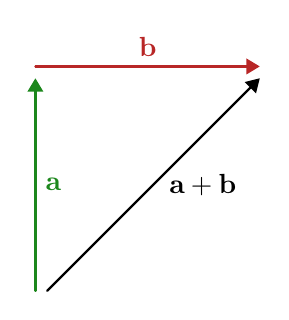
\begin{tikzpicture}[scale = 3]
                \draw[force, y_h] (0,0.05) -- (0,0.95) node[midway,right]
                {$\vec{a}$};
                \draw[force, y_p] (0,1) -- (0.95,1) node[midway, above]
                {$\vec{b}$};
                \draw[force, black] (0.05,0.05) -- (0.95,0.95) node[midway, right = 2]
                {$\vec{a} + \vec{b}$};
            \end{tikzpicture}
            \hspace{2in}
            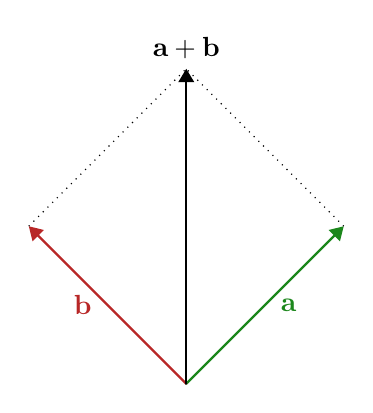
\begin{tikzpicture}[scale = 2]
                \def\ang{30}
                \def\F{1.4}  % force magnitude
                \coordinate (O) at (0,0);
                \coordinate (a) at (1, 1);
                \coordinate (b) at (-1, 1);
                \coordinate (c) at (0, 2);
                \draw[dotted,black] (a) -- (c);
                \draw[dotted,black] (b) -- (c);
                \draw[force, y_h] (O) -- (a) node[midway, right = 2] {$\vec{a}$};
                \draw[force, y_p] (O) -- (b) node[midway, left = 2] {$\vec{b}$};
                \draw[force,black] (O) -- (c) node[above] {$\vec{a} + \vec{b}$};
            \end{tikzpicture}
        \end{figure}

        The paralleogram rule is used in physics to calculate the resultant (vector sum)
        of many forces acting on the same point. \par

    \item[Properties of vector addition] Similar to scalar addition,
        \begin{align}
            \vec{a} + \vec{b}             & = \vec{b} + \vec{a}             &
                                          &                                 &
            \text{commutative}                                                \\
            (\vec{u} + \vec{v}) + \vec{w} & = \vec{u} + (\vec{v} + \vec{w}) &
                                          &                                 &
            \text{associative}                                                \\
            \vec{a} + \vec{0}             & = \vec{a}                       &
                                          &                                 &
            \text{additive null}                                              \\
            \vec{a} + (-\vec{a})          & = \vec{0}                       &
                                          &                                 &
            \text{additive inverse}
        \end{align}

    \item[Scalar multiplication] Multiplying a vector by a scalar multiplies it by
        every component of the vector.
        \begin{align}
            c\ \vec{v}         & \equiv \begin{bNiceMatrix}[r, margin]
                                            c\ v_1 \\ c\ v_2 \\ c\ v_3
                                        \end{bNiceMatrix} &
            \abs{ c\ \vec{v} } & = \abs{ c } \abs{ \vec{v} }
        \end{align}
        Geometrically, if $ c<0  $, then $ c \vec{v} $ faces the opposite direction.

    \item[Properties of scalar multiplication] Similar to scalars,
        \begin{align}
            c(\vec{a} + \vec{b}) & = c\vec{a} + c\vec{b} &
            (c + k)\vec{a}       & = c\vec{a} + k\vec{a}   \\
            c\ (k\vec{a})        & = (ck)\ \vec{a}       &
            1 \cdot \vec{a}      & = \vec{a}               \\
            (-1) \cdot \vec{a}   & = -\vec{a}            &
            0 \cdot \vec{a}      & = \vec{0}
        \end{align}

    \item[Standard basis] $ \mathcal{R}^3 $ represented geometrically by 3-d
        Cartesian space, has dimension 3, and needs a set of 3 basis vectors defined by
        \begin{align}
            \vec{\hat{i}} & = \begin{bNiceMatrix}[r, margin]
                                  1 \\ 0 \\ 0
                              \end{bNiceMatrix}          &
            \vec{\hat{j}} & = \begin{bNiceMatrix}[r, margin]
                                  0 \\ 1 \\ 0
                              \end{bNiceMatrix}          &
            \vec{\hat{k}} & = \begin{bNiceMatrix}[r, margin]
                                  0 \\ 0 \\ 1
                              \end{bNiceMatrix}           \\
            \vec{a}       & = a_1 \vec{\hat{i}} + a_2 \vec{\hat{j}} +
            a_3 \vec{\hat{k}}
        \end{align}
\end{description}

\section{Inner Product (Dot Product)}
\begin{description}
    \item[Inner product] The product of lengths of two vectors and the cosine of the angle
        between them. This is a scalar.
        \begin{align}
            \vec{a} \dotp \vec{b} &
            = \begin{dcases}
                  \abs{\vec{a}} \abs{\vec{b}} \cos(\theta) &
                  \abs{\vec{a}} \neq 0\ \text{and}\ \abs{\vec{b}} \neq 0 \\
                  0                                        &
                  \abs{\vec{a}} = 0\ \text{or}\ \abs{\vec{b}} = 0
              \end{dcases}
        \end{align}
        Here $ \theta $ is the smaller angle between the vectors measured after
        making their initial points coincide. \par
        In terms of the components,
        \begin{align}
            \vec{a} \dotp \vec{b} & \equiv \sum_{k=1}^{n} a_k b_k
        \end{align}

    \item[Orthogonal vectors] Two vectors are perpendicular if and only if their
        inner product is zero.

    \item[Length of a vector] The square root of the inner product of a vector with
        itself. This is geomatrically equal to its magnitude. \par
        Additionally, the angle between two nonzero vectors can be found using,
        \begin{align}
            \abs{\vec{v}} & \equiv \sqrt{\vec{v} \dotp \vec{v}} \\
            \cos \theta   & = \frac{\vec{a} \dotp \vec{b}}
            {\abs{\vec{a}} \abs{\vec{b}}}
        \end{align}

    \item[Properties of inner product] Some properties similar to multiplication,
        \begin{align}
            (p\vec{a} + q\vec{b}) \dotp \vec{c} & = p \vec{a} \dotp \vec{c}
            + q \vec{b} \dotp \vec{c}           &
                                                & \text{linear}                \\
            \vec{a} \dotp \vec{b}               & = \vec{b} \dotp \vec{a}    &
                                                & \text{symmetry}              \\
            \vec{a} \dotp \vec{a}               & \geq 0                       \\
            \vec{a} \dotp \vec{a}               & = 0 \iff \vec{a = \vec{0}} &
                                                & \text{positive-definite}     \\
            (\vec{a} + \vec{b}) \dotp \vec{c}   & = \vec{a} \dotp \vec{c}
            + \vec{b} \dotp \vec{c}             &
                                                & \text{distributive}
        \end{align}

    \item[Inequality relations] The fact that $ \abs{\cos\theta} \leq 1$ gives,
        \begin{align}
            \abs{\vec{a} + \vec{b}}                               &
            \leq \abs{\vec{a}} + \abs{\vec{b}}                    &
                                                                  &
            \text{Triangle inequality}                              \\
            \abs{\vec{a} \dotp \vec{b}}                           &
            \leq \abs{\vec{a}} \abs{\vec{b}}                      &
                                                                  &
            \text{Cauchy-Schwraz inequality}                        \\
            \abs{\vec{a} + \vec{b}}^2 + \abs{\vec{a} - \vec{b}}^2 &
            = 2 (\abs{\vec{a}}^2 + \abs{\vec{b}}^2)               &
                                                                  &
            \text{parallellogram equality}
        \end{align}

    \item[Orthogonal projection] The orthogonal projection (or component) of a vector
        along a line whose unit vector is $ \vec{\hat{b}} $ is defined as
        \begin{align}
            p & = \vec{a} \dotp \vec{\hat{b}} = \abs{\vec{a}} \cos \theta
        \end{align}
        Here $ \theta $ is the angle between the vector $ \vec{a} $ and the line it is
        projected upon. \par

        A plane can be defined in Cartesian 3d by requiring the projection of all points
        on it upon the normal vector to be constant.
        \begin{align}
            \vec{\hat{n}} \dotp \vec{r} & = p
        \end{align}
        Here, $ p $ is the distance of $ \vec{\hat{n}} $ from the origin. All planes
        parallel to this plane simply vary in their $ p $ value.
\end{description}

\section{Vector Product (Cross Product)}

\begin{description}
    \item[Cross product] Geometrically, a vector orthogonal to the two given vectors
        whose magnitude is equal to the area of the parallellogram formed by them.
        \begin{align}
            \vec{v} & \equiv \vec{a} \times \vec{b}
        \end{align}
        \begin{itemize}
            \item If $ \vec{a} = 0 $ or $ \vec{b} = 0 $, then by definition,
                  $ \vec{v}  = \vec{0} $.
            \item Else if $ \vec{a} $ and $ \vec{b} $ are parallel, such that the angle
                  between then is $ 0 $ or $ \pi $, then again $ \vec{v} = \vec{0} $
            \item Outside of these special cases, the magnitude of the cross product is
                  \begin{align}
                      \abs{\vec{v}} & \equiv \abs{\vec{a} \times \vec{b}}
                      = \abs{\vec{a}} \abs{\vec{b}} \sin \theta           \\
                      \vec{v}       &
                      = \begin{vNiceMatrix}[r, margin]
                            \vec{\hat{i}} & \vec{\hat{j}} & \vec{\hat{k}} \\
                            a_1           & a_2           & a_3           \\
                            b_1           & b_2           & b_3
                        \end{vNiceMatrix}
                  \end{align}
                  Its direction is such that $ \vec{v} $ is perpendicular to both
                  $ \vec{a} $ and $ \vec{b} $ and the three vectors $ \vec{a}, \vec{b},
                      \vec{v} $ form a right-handed triple.
        \end{itemize}

    \item[Right handed triple] If the fingers of the right hand are on the plane formed
        by $ \vec{a} $ and $ \vec{b} $, then the right thumb points in the direction of
        $ \vec{c} $. \par
        This convention picks one of the two possible choices for the direction of
        $ \vec{c} $.

    \item[Properties of cross product] Similar to scalar multiplication,
        \begin{align}
            (p\vec{a}) \times \vec{b}               & = p (\vec{a} \times \vec{b}) =
            \vec{a} \times (p\vec{b})                                                  \\
            \vec{a} \times (\vec{b} + \vec{c})      & = \vec{a} \times \vec{b}
            + \vec{a} \times \vec{c}                                                   \\
            (\vec{a} + \vec{b}) \times \vec{c}      & = \vec{a} \times \vec{c}
            + \vec{b} \times \vec{c}                &
                                                    & \text{distributive}              \\
            \vec{a} \times \vec{b}                  & = - (\vec{b} \times \vec{a})   &
                                                    & \text{anti-commutative}          \\
            \vec{a} \times (\vec{b} \times \vec{c}) & \neq
            (\vec{a} \times \vec{b}) \times \vec{c} &
                                                    & \text{not associative}
        \end{align}

    \item[Scalar Triple product] Also called the mixed product or box product. This
        is a scalar resulting from three input vectors. \par
        \begin{align}
            (\vec{a}\ \vec{b}\ \vec{c}) & \equiv \vec{a} \dotp
            (\vec{b} \times \vec{c})                                      \\
                                        & = \begin{vNiceMatrix}[r, margin]
                                                a_1 & a_2 & a_3 \\
                                                b_1 & b_2 & b_3 \\
                                                c_1 & c_2 & c_3
                                            \end{vNiceMatrix}
        \end{align}

    \item[Properties of box product] Some important properties,
        \begin{itemize}
            \item Geometrically, it is the volume of the parallellopiped with the three
                  vectors as the edge vectors.
            \item The dot and cross can be interchanged
                  \begin{align}
                      \vec{a} \dotp (\vec{b} \times \vec{c}) & =
                      (\vec{a} \times \vec{b}) \dotp \vec{c}
                  \end{align}
            \item Three vectors in Cartesian $ \mathcal{R}^3 $ are L.I. if and only if
                  their box product is nonzero.
        \end{itemize}
\end{description}

\section{Vector and Scalar Functions and Their Fields, Vector Calculus: Derivatives}

\begin{description}
    \item[Vector function] Functions of scalars that produce vectors as outputs. Such a
        function defines a vector field in the domain of definiton.
        \begin{align}
            \vec{v}(P)       & = \begin{bNiceMatrix}[margin]
                                     v_1(P) \\ v_2(P) \\ v_3(P)
                                 \end{bNiceMatrix}          &
            \vec{v}(x, y, z) & = \begin{bNiceMatrix}[margin]
                                     v_1(x,y,z) \\ v_2(x,y,z) \\ v_3(x,y,z)
                                 \end{bNiceMatrix}
        \end{align}
        A vector function may additionally depend on some other variable such as time.

    \item[Scalar function] Functions of scalars that produce scalars as outputs. Such a
        function defines a scalar field in the domain of definiton.
        \begin{align}
            f \equiv f(P) & f & \equiv f(x, y, z)
        \end{align}
        A scalar function may additionally depend on some other variable such as time.
        \par The value of the scalar function is independent of the choice of coordinate
        system.

    \item[Vector calculus] Many properties outlined here carry over from regular
        calculus.

    \item[Convergence] A sequence of vectors $ \{\vec{a}_k\} $ is said to converge if
        there exists some vector $ \vec{a} $ such that
        \begin{align}
            \lim_{n \rightarrow \infty} \abs{\vec{a}_n - \vec{a}} &
            = 0                                                     \\
            \lim_{n \rightarrow \infty} \vec{a}_n                 &
            = \vec{a} \qquad \text{(Limit vector)}
        \end{align}
        The corresponding definition of the convergence of vector functions of a scalar
        are identical to the standard definition of the convergence of scalar functions
        $ f(x) $ and omitted here.

    \item[Continuity] If a vector function $ \vec{v}(t) $ is defined in some
        neighbourhood of $ t = t_0 $ (including $ t_0 $ itself) and
        \begin{align}
            \lim_{t \rightarrow t_0} \vec{v}(t) & = \vec{v}(t_0)
        \end{align}
        then, the vector function is continuous at $ t = t_0 $.

    \item[Derivative of vector function] The derivative of $ \vec{v}(t) $ at $ t= t_0 $
        exists, is the limit
        \begin{align}
            \lim_{\Delta t \rightarrow 0} \frac{\vec{v}(t + \Delta t) - \vec{v}(t)}
            {\Delta t} \equiv \vec{v}'(t)
        \end{align}
        assuming this limit exists. \par
        When a coordinate system is defined, each component of the vector function is
        differentiated separately to yield the derivative of the vector.

    \item[Properties of vector derivatives] Similar to the properties of scalar
        derivatives,
        \begin{align}
            (c\vec{v})'                  & = c\ \vec{v}'                  \\
            (\vec{u} + \vec{v})'         & = \vec{u}' + \vec{v}'          \\
            (\vec{u} \dotp \vec{v})'     &
            = \vec{u}' \dotp \vec{v} + \vec{u} \dotp \vec{v}'             \\
            (\vec{u} \times \vec{v})'    &
            = \vec{u}' \times \vec{v} + \vec{u} \times \vec{v}'           \\
            (\vec{u}\ \vec{v}\ \vec{w})' & = (\vec{u}'\ \vec{v}\ \vec{w})
            + (\vec{u}\ \vec{v}'\ \vec{w}) + (\vec{u}\ \vec{v}\ \vec{w}')
        \end{align}

    \item[Partial derivatives of vector function] The operation to be applied to the
        vector function is simply applied to each component individually.
        \begin{align}
            \vec{v}(\{t_k\})          & \equiv \vec{v}(t_1, t_2, \dots, t_n)   \\
            \diffp{\vec{v}}{t_1}      & = \diffp{v_1}{t_1}\ \vec{\hat{i}}
            + \diffp{v_2}{t_1}\ \vec{\hat{j}}
            + \diffp{v_3}{t_1}\ \vec{\hat{k}}                                  \\
            \diffp{\vec{v}}{t_1, t_2} & = \diffp{v_1}{t_1, t_2}\ \vec{\hat{i}}
            + \diffp{v_2}{t_1, t_2}\ \vec{\hat{j}}
            + \diffp{v_3}{t_1, t_2}\ \vec{\hat{k}}
        \end{align}
\end{description}

\section{Curves, Arc Length, Curvature, Torsion}

\begin{description}
    \item[Parametric vector functions] Replacing the independent variable in each
        component of a vector by a common parameter ($ t $) yields,
        \begin{align}
            \vec{v}(t) & =
            \begin{bNiceMatrix}[r, margin]
                x(t) \\ y(t) \\ z(t)
            \end{bNiceMatrix}
            = x(t)\ \vec{\hat{i}} + y(t)\ \vec{\hat{j}} + z(t)\ \vec{\hat{k}}
        \end{align}
        This makes the curve oriented in the direction of increasing $ t $. (called the
        positive sense on the curce $ C $)

    \item[Twisted curve] A curve that does not lie in a plane in $ 3d $ space. Else, it
        is called a plane curve.

    \item[Simple curve] A curve which does not touch or intersect itself. There is a
        unique value of the parameter $ t $ for every point of the curve,

    \item[Tangent vector] The limiting position of a straight line through $ P $ on
        curve $ C $ and another close point $ Q $
        \begin{align}
            P           & : \vec{r}(t)                    &
            Q           & : \vec{r}(t + \Delta t)           \\
            \vec{r}'(t) & = \lim_{\Delta t \rightarrow 0}
            \frac{\vec{r}(t + \Delta t) - \vec{r}(t)}{\Delta t}
        \end{align}
        If $ \vec{r} \neq \vec{0} $, it is called the tangent vector to curve $ C $ at
        point $ P $.

    \item[Parametric straight line] The equation of a line passing through $ \vec{a} $
        in the direction of $ \vec{b} $ is given by
        \begin{align}
            \vec{v}    & = \vec{a} + t\vec{b}                           \\
            \vec{q}(w) & = \vec{r} + w\vec{r}' &  & \text{Tangent line}
        \end{align}
        Here, both $ \vec{r} $ and $ \vec{r}' $ are functions of the original parameter
        $ t $.

    \item[Length of curve] If a curve $ C $ is specified using a paramteric vector
        functionm $ \vec{r}(t) $, then the length of a curve corresponding to
        $ t \in [a,b] $ is given by
        \begin{align}
            l & = \int_{a}^{b} \sqrt{\vec{r}' \dotp \vec{r}'}\ \dl t
        \end{align}
        assuming $ \vec{r} $ is differentiable.

    \item[Arc length of a curve] The length of a curve from $ t = a $ to a variable end
        point $ t = w $. It is defined as
        \begin{align}
            s(w) & = \int_{a}^{w} \sqrt{\vec{r}' \dotp \vec{r}'}\ \dl t
        \end{align}

    \item[Linear element] From the definition of Pythagoras theorem, the linear element
        in $ 3d $ Cartesian space is
        \begin{align}
            \dl s^2 \equiv \vec{\dl r} \dotp  \vec{\dl r}
            = \dl x^2 + \dl y^2 + \dl z^2
        \end{align}

    \item[Trajectories] In mechanics, the parameter is usually time $ (t) $ and a curve
        represents the path taken by an object through $ 3d $ space. \par
        The first and second derivaties of the position $ \vec{r}(t) $ represent the
        velocity vector and acceleration vector respectively.
        \begin{align}
            \vec{v}(t) & \equiv \vec{r}'(t)  &
            \vec{a}(t) & \equiv \vec{r}''(t) &
        \end{align}
        The acceleration can be split into tangential and normal components. \par
        Defining the unit tangent vector in terms of the arc length $ s $,
        \begin{align}
            \vec{u}(s) & = \frac{\vec{r}'(t)}{\abs{\vec{r}'(t)}} = \vec{r}'(s) \\
            \vec{v}(t) & = \vec{u}(s)\ \diff st                                \\
            \vec{a}(t) & = \diff*{\vec{u(s)}}{s}\ \left( \diff st \right)^2 +
            \vec{u}(s)\ \diff[2] st                                            \\
        \end{align}
        Since the tangent vector $ \vec{u}(s) $ is always a unit vector, the first
        acceleration term has to be perpendicular to the velocity.

    \item[Normal acceleration] The acceleration vector can be split into two
        components, normal and tangential using the projection rule,
        \begin{align}
            \vec{a}(t)                 & = \vec{a}_{\text{norm}}
            + \vec{a}_{\text{tangent}} &
            \vec{a}_{\text{tangent}}   & = \vec{a} \dotp \vec{\hat{v}}
        \end{align}

    \item[Curvature] The rate of change of the unit tangent vector at a point $ P $ on
        the curve $ C $, give by
        \begin{align}
            \kappa (s) & \equiv \abs{\diff*{\vec{u}(s)}{s}}
            = \abs{\diff*[2]{\vec{r}(s)}{s}}
        \end{align}
        Here, the arc length $ (s) $ is used as the parameter of the curve instead of the
        usual $ t $.

    \item[Normal plane] The plane through $ P $ on curve $ C $ whose normal vector is
        the tangent vector $ \vec{u} $.

    \item[Osculating plane] The plane spanned by the tangent vector and its derivative
        (which happens to be the normal vector at that point). \par
        This plane contains the osculating (kissing) circle to the curve $ C $ at the
        point $ P $. Its normal vector is $ \vec{b} = \vec{u} \times \vec{n} $.

    \item[Rectifying plane] The third plane which is spanned by $ \vec{u} $ and
        $ \vec{b} $. Its normal vector is the unit normal vector $ \vec{u}' = \vec{p} $.

    \item[Torsion] The rate of change of the osculating plane defined as,
        \begin{align}
            \vec{p}       & \equiv \frac{1}{\kappa}\ \vec{u}'   &
                          & \text{unit principal normal vector}   \\
            \vec{b}       & \equiv \vec{u} \times \vec{p}       &
                          & \text{unit binormal vector}           \\
            \abs{\tau(s)} & = \abs{\vec{b}'(s)}                   \\
            \tau (s)      & = -\vec{p}(s) \dotp \vec{b}'(s)
        \end{align}
        Since the unit tangent vector $ \vec{u} $ has constant magnitude, its derivate is
        orthogonal to itself by definition. The right handed triple of vectors
        $ \vec{u}, \vec{p}, \vec{b} $ are defined at each point on the curve.
\end{description}

\section{Calculus Review: Functions of Several Variables}

\begin{description}
    \item[Chain rule] Consider a mapping from the domain $ B $ in the $ uv $ plane
        onto the domain $ D $ in $ xyz $ space using the mapping,
        \begin{align}
            x & \equiv x(u, v) & y & \equiv y(u, v) & z & \equiv z(u, v)
        \end{align}
        These functions are continuous and have continuous first partial derivatives in
        $ B $. \par
        Further, let $ f \equiv f(x, y, z) $ be continouous and have continouous first
        partial derivatices in $ D $. Then,
        \begin{align}
            w         & = f\Big( x(u, v),\ y(u, v),\ z(u, v) \Big)    \\
            \diffp wu & = \diffp wx\ \diffp xu + \diffp wy\ \diffp yu
            + \diffp wz\ \diffp zu                                    \\
            \diffp wv & = \diffp wx\ \diffp xv + \diffp wy\ \diffp yv
            + \diffp wz\ \diffp zv
        \end{align}

    \item[Mean Value theorem] With $ f(x, y, z) $ and $ D $ as defined above, and any
        two points $ P_0 $ and $ P $ connected by a straight line that lies entirely in
        $ D $,
        \begin{align}
            P_0 : (x_0, y_0, z_0)  \qquad
            P                                         & : (x_0 + h, y_0 + k, z_0 + l) \\
            f(x_0 + h, y_0 + k, z_0 + l) - f(x, y, z) & = h\ \diffp fx + k\ \diffp fy
            + l\ \diffp fz
        \end{align}
        This is a generalization of the much more familiar special case,
        \begin{align}
            f & \equiv f(x) & f(x_0 + h) - f(x_0) & = h\ \diffp fx
        \end{align}
\end{description}

\section{Gradient of a Scalar Field, Directional Derivative}

\begin{description}
    \item[Gradient] A vector function derived from a scalar function $ f $ in the $ 3d $
        Cartesian space, defined by,
        \begin{align}
            \nabla f & \equiv \diffp fx\ \vec{\hat{i}} + \diffp fy\ \vec{\hat{j}}
            + \diffp fz\ \vec{\hat{k}}
        \end{align}
        The differential operator for $ 3d $ Cartsian coordinates is defined as
        \begin{align}
            \nabla & \equiv \diffp {}{x}\ \vec{\hat{i}} + \diffp {}{y}\ \vec{\hat{j}}
            + \diffp {}{z}\ \vec{\hat{k}}
        \end{align}

    \item[Directional derivative] The directional derivative of a function $ f $ at a
        point of $ P $ in the direction of $ \vec{b} $,
        \begin{align}
            D_{\vec{b}}f & \equiv \diff fs =
            \lim_{s \rightarrow 0} \frac{f(Q) - f(P)}{s}
        \end{align}
        Here, $ Q $ is a point on the line passing through $ P $ in the direction of
        $ \vec{b} $, and $ s $ is the distance between these two points. \par
        Defining the line in terms of a unit vector $ \vec{b} $ and arc length $ s $ from
        an intitial point $ \vec{p_0} $,
        \begin{align}
            \vec{r}                  & = \vec{p_0} + s\ \vec{b}       &
            \diff{\vec{r}}{s}        & = \vec{b}                        \\
            D_{\vec{b}}f = \diffp fs & = \vec{\hat{b}} \dotp \nabla f
        \end{align}

    \item[Gradient is a vector] The magnitude and direction of the gradient are
        independent of the choice of Cartesian coordinates. \par
        Also, the gradient (if it is a nonzero vector) points in the direction of maximum
        increase of the function at that point.

    \item[Normal vector to surface] For a function $ f $ whose level surface is defined
        as $ S : f(x, y, z) = c $,
        \begin{align}
            0 & = \diffp fx\ \diffp xs + \diffp fy\ \diffp ys + \diffp fz\ \diffp zs &
            0 & = \nabla f \dotp \vec{r}'
        \end{align}
        Since the gradient is perpendicluar all possible tangent vectors at the point
        $ P $ on surface $ S $, it is the surface normal vector at $ P $.

    \item[Potentials] A scalar field whose gradient happens to be a vector field.
        \begin{align}
            \vec{v}(P) & = \nabla f(P)
        \end{align}
        The corresponding vector field is called conservative.

    \item[Gravitational field] THe force of gravitation between two particles is the best
        known exmaple of a conservative force. \par
        For two particles at $ P_0: (x_0, y_0, z_0) $ and $ P: (x, y, z) $ separated by
        distance $ r $.
        \begin{align}
            \vec{p}                                      & = \frac{-c}{r^3}\ \vec{r}
            = \frac{-c}{r^3} \begin{bNiceMatrix}[margin]
                                 (x - x_0) \\ (y - y_0) \\ (z - z_0)
                             \end{bNiceMatrix} &
            \phi(x, y, z)                                & = \frac{c}{r}             \\
            \vec{p}                                      & = \nabla \phi
        \end{align}

        The vector field of force produced by any mass distribution in a space is the
        gradient of a scalar field (potential) $ \phi $ which satisfies Laplace's
        equation in any region free of matter.

    \item[Laplace's equation] A partial differential equation defined as
        \begin{align}
            \nabla^2 f & \equiv \diffp[2] fx + \diffp[2] fy + \diffp[2] fz = 0
        \end{align}

    \item[Laplacian] The operator which condenses the Laplacian equation, defined as
        \begin{align}
            \nabla \dotp \nabla f & \equiv \nabla^2 f              \\
            \nabla^2              & \equiv \Delta \equiv \diffp[2]
            {}{x} + \diffp[2] {}{y} + \diffp[2] {}{z}
        \end{align}
\end{description}

\section{Divergence of a Vector Field}

\begin{description}
    \item[Divergence] This obtains a scalar field from a vector field. Consider a
        differentiable vector function $ \vec{v} $ with components in $ 3d $ Cartesian
        space, given by
        \begin{align}
            \vec{v}              & = \begin{bNiceMatrix}
                                         v_1(x, y, z) \\ v_2(x, y, z) \\ v_3(x, y, z)
                                     \end{bNiceMatrix} \\
            \nabla \dotp \vec{v} & =
            \begin{bNiceMatrix}
                \difsp {}{x} \\ \difsp {}{y} \\ \difsp {}{z}
            \end{bNiceMatrix} \dotp \begin{bNiceMatrix}
                                        v_1 \\ v_2 \\ v_3
                                    \end{bNiceMatrix} =
            \diffp{v_1}{x} + \diffp{v_2}{y} + \diffp{v_3}{z}
        \end{align}
        Note that the dot product notation is not the usual multiplication. It represents
        the partial derivative acting on the components of $ \vec{v} $.

    \item[Invariance of divergence] Since the divergence is a scalar field, it is
        independent of the choice of coordinate system. \par
        It only depends on the point $ P $ in space and the form of $ \vec{v} $ for a
        particular choice of coordinate system.

    \item[Fluid flow] An example of divergence used in physical systems is the flow of
        a fluid that has density $ \rho $ in a region $ R $ with no sources and sinks.
        \par
        Let $ \vec{v} $ be the velocity vector of the fluid.
        \begin{align}
            \diffp{\rho}{t} + \nabla \dotp (\rho\vec{v}) & = 0
        \end{align}
        This is the continuity equation of a compressible fluid flow

    \item[Solenoidal vector field] A special case of the above system is steady flow,
        which means that $ \rho $ is independent of time, and constant fluid density. This
        gives the incompressibility condition
        \begin{align}
            \nabla \dotp \vec{v} & = 0
        \end{align}
        Such a vector field is called solenoidal.
\end{description}

\section{Curl of a Vector Field}

\begin{description}
    \item[Curl] Let $ \vec{v} $ be a differentiable vector function in $ 3d $ defined in
        Cartesian coordinates,
        \begin{align}
            \nabla \times \vec{v} & =
            \begin{vNiceMatrix}[margin]
                \vec{\hat{i}} & \vec{\hat{j}} & \vec{\hat{k}} \\
                \difsp{}{x}   & \difsp{}{y}   & \difsp{}{z}   \\
                v_1           & v_2           & v_3
            \end{vNiceMatrix}
        \end{align}
        This assumes the coordinate system is right handed. \par
        The curl is a vector independent of the choice of coordinate system.

    \item[Curl of rotating body] The curl is in the direction of the axis of rotation and
        its magnitude is equal to twice the angular speed.

    \item[Relating curl, grad and div] A vector function that is the gradient of a
        continouous differentiable scalar function is irrotational.
        \begin{align}
            \nabla \times (\nabla f) & = 0 &  & \text{Irrotational}
        \end{align}

        For a vector function $ \vec{v} $ that is twice continuously differentiable,
        \begin{align}
            \nabla \dotp (\nabla \times \vec{v}) = 0
        \end{align}
        These relations are proved using the fact that second order partial derivaties
        commute.
\end{description}
% \chapter{Vector Integral Calculus, Integral Theorems}

\section{Line Integrals}

\begin{description}
    \item[Curve integral] A generalization of the usual definite integral, which now
        integrates over a general one-dimensional curve in space, instead of the $ x $
        axis.
        \begin{align}
            I          & = \int_{a}^{b} f(x)\ \dl x              \\
            \vec{r}(t) & = \begin{bNiceMatrix}[margin]
                               x(t) \\ y(t) \\ z(t)
                           \end{bNiceMatrix} \qquad t \in [a, b]
        \end{align}
        The path of integration is parametrized using a single parameter $ (t) $.
        \par If the initial and terminal point of the curve coincide, it is called a
        closed path. \par

    \item[Smooth curve] A curve which has a unique tangent defined at each point that
        varies continuously when traversing $ C $. \par
        $ \vec{r}(t) $ is differentiable and $ \vec{r}'(t) $ is continuous and not the
        zero vector at any point along $ C $.

    \item[Line Integral] Curve integrals are commonly called line integrals, even if the
        path itself is not a straight line. They are defined for some vector function
        $ \vec{F}(\vec{r}) $ over a curve $ C $ by,
        \begin{align}
            \int_{C} \vec{F}(\vec{r}) \dotp \dl{\vec{r}} & =
            \int_{a}^{b} \vec{F}(\vec{r}(t)) \dotp \vec{r}'(t)\ \dl t \\
            \int_{C} (F_1 \dl x + F_2 \dl y + F_3 \dl z) & =
            \int_{a}^{b} (F_1 x' + F_2 y' + F_3 z')\ \dl t
        \end{align}
        The above definition requires right-handed $ 3d $ Cartesian coordinates. \par
        The differentiation is w.r.t. the parameter $ t $.

        The line integral can be thought of as the sum of many infinitesimal vectors each
        of which is the tangential component of $ \vec{F} $ at $ \vec{r} $. Thus,
        \begin{align}
            \dl I & = \vec{F} \dotp \frac{\vec{r}'}{\abs{\vec{r'}}}
        \end{align}
        The integrand is piecewise continuous if $ \vec{F} $ is continuous and the curve
        $ C $ is at least piecewise smooth.

    \item[Properties of line integral] Similar to the definite scalar integral,
        \begin{align}
            \int_{C} k\vec{F}  \dotp \dl{\vec{r}}           & =
            k\ \int_{C} \vec{F} \dotp \dl{\vec{r}}              \\
            \int_{C} (\vec{F} + \vec{G}) \dotp \dl{\vec{r}} & =
            \int_{C} \vec{F} \dotp \dl{\vec{r}} +
            \int_{C} \vec{G} \dotp \dl{\vec{r}}                 \\
            \int_{C} \vec{F} \dotp \dl{\vec{r}}             & =
            \int_{C_1} \vec{F} \dotp \dl{\vec{r}} +
            \int_{C_2} \vec{F} \dotp \dl{\vec{r}}
        \end{align}
        Splitting a path into pieces that have the same orientation does not change
        the line integral.

    \item[Invariance of line integral] Any representation of the path $ C $ that
        preserve the orientation of the curve, do not change the line integral.

    \item[Work done by a force] When the path is no longer a straight line, the total
        work done by a force is the sum of many small displacements along the path $ C $
        \begin{align}
            \dl W & = \vec{F}(\vec{r}) \dotp \dl{\vec{r}}          &
            W     & = \int_{C} \vec{F}(\vec{r}) \dotp \dl{\vec{r}}
        \end{align}

    \item[Vector line integral] Without taking the dot product, the line integral
        can be evaluated separately for each component to give,
        \begin{align}
            \int_{C} \vec{F}(\vec{r})\ \dl t &
            = \int_{a}^{b} \vec{F}(\vec{r}(t))\ \dl t =
            \begin{bNiceMatrix}[margin]
                \int_{a}^{b} F_1 (\vec{r}(t))\ \dl t \\
                \int_{a}^{b} F_2 (\vec{r}(t))\ \dl t \\
                \int_{a}^{b} F_3 (\vec{r}(t))\ \dl t \\
            \end{bNiceMatrix}
        \end{align}

    \item[Path Dependence] Generally, the path taken affects the outcome of the line
        integral even if the function $ \vec{F}(\vec{r}) $ and the endpoints remain the
        same.
\end{description}

\section{Path Independence of Line Integrals}

\begin{description}
    \item[Path Independene] A line integral is path independent in domain $ D $ if for
        all pairs of points $ (A, B) $ in this domain, the path integral has the same
        value regardless of the path taken from $ A $ to $ B $.

    \item[Gradient of scalar function] A line integral (with continouous vector
        components in the integrand) is path independent if and only if the vector
        happens to
        be the gradient of some scalar function in the same domain.
        \begin{align}
            \vec{F} = \nabla f \quad \iff \quad
            \int_{A}^{B} \vec{F} \dotp \dl{\vec{r}} = f(B) - f(A)
        \end{align}
        This scalar function $ f $ is called the potential of the vector field
        $ \vec{F} $.

    \item[Closed line integral] A line integral is path independent if and only if
        its value around any possible closed path is zero.

    \item[Conservative field] In physics, if the work done by a force $ \vec{F} $ is
        path independent, then the vector field is called conservative. Else, it is called
        dissipative.

    \item[Exact differential form] If the integrand $ \vec{F} \dotp \dl{\vec{r}} $ is
        equal to an infinitesimal change in some scalar function $ f $,
        \begin{align}
            \vec{F} \dotp \dl{\vec{r}} & = F_1 \dl x + F_2 \dl y + F_3 \dl z    \\
                                       & =\diffp fx\ \dl x + \diffp fy\ \dl y +
            \diffp fz\ \dl z = \dl f
        \end{align}
        Here, $ f(x, y, z) $ is some differentiable function in the domain $ D $. \par
        This reduces to the condition that the above equation is exact if and only if
        the vector function $ \vec{F} $ is the gradient of the differentiable scalar
        function $ f $ everywhere in the domain $ D $.

    \item[Simply connected domain] Any closed curve in the domain $ D $ can be
        continuously shrunk to any point in $ D $ without leaving $ D $.

    \item[Criterion for exactness] Let the components of a vector function be continuous
        and have continuous first partial derivatives  in a domain $ D $. Then,

        \begin{itemize}
            \item If the differential form is exact in $ D $ then the vector field is
                  irrotational.
                  \begin{align}
                      \vec{F} \dotp \dl{\vec{r}} = \dl f \quad \implies
                      \quad  \nabla \times F = 0
                  \end{align}

            \item Conversely, if the vector field $ \vec{F} $ is irrotational in a
                  simply connected domain $ D $, then the line integral is path
                  independent.
        \end{itemize}
\end{description}

\section{Calculus Review: Double Integrals}

\begin{description}
    \item[Area] Double integration happens over any bounded region in $ \mathcal{R}^2 $
        whose boundary curve has a unique tanget at all points. \par
        The only exception is a finite number of cusps. (Discontinuity in the tangent
        vector over the boundary). \par
        This is analogous to a regular integral having at most a finite number of jump
        discontinuities.

    \item[Definition of double integral] Assuming some function $ f(x, y) $ is
        continuous in $ \mathcal{R} $ and this region is bounded by finitely many smooth
        curves, the integral over the area is
        \begin{align}
            I & \equiv \iint_R f(x, y)\ \dl A = \iint_R f(x, y)\ \dl x\ \dl y
        \end{align}

    \item[Properties of double integral] Similar to the definite single integral,
        \begin{align}
            \iint_R\ kf\ \dl A    & = k\ \iint_R f\ \dl A                          \\
            \iint_R\ (f+g)\ \dl A & = \iint_R f\ \dl A +  \iint_R g\ \dl A         \\
            \iint_R\ (f+g)\ \dl A & = \iint_{R_1} f\ \dl A +  \iint_{R_2} f\ \dl A
        \end{align}
        The area to be integrated over can be split into parts just like the line segment
        for the case of the single integral.

    \item[Mean value theorem] If the area of integration $ R $ as defined above is also
        simply connected, then
        \begin{align}
            \iint_R f(x, y)\ \dl A & = f(x_0, y_0)\ A
        \end{align}
        for some point $ (x_0, y_0) $ in $ R $ and $ A $ being the total area of $ R $.

    \item[Evaluation] Sucessively integrating over $ x $ then $ y $ is the most
        common means of performing double integration.
        \begin{align}
            \iint_R f\ \dl x\ \dl y & = \int_{a}^{b} \left[ \int_{g(x)}^{h(x)}
                f(x, y)\ \dl y \right] \dl x
        \end{align}
        Here, $ x $ is considered a constant when performing the integration over $ y $.
        \par The order of integration can also be reversed if the computation happens to
        be simpler.
        \begin{figure}[H]
            \centering
            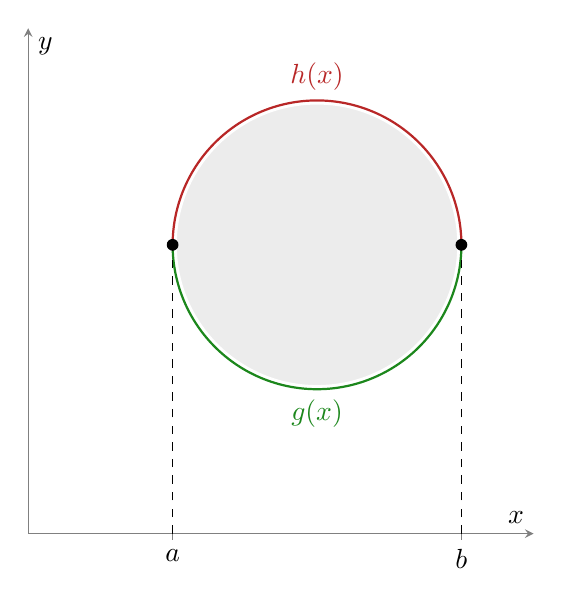
\begin{tikzpicture}
                \begin{axis}[
                        width = 8cm, height = 8cm,
                        xmin = 0, xmax = 3.5, ymin = 0, ymax = 3.5,
                        axis lines = middle,
                        xlabel = \normalsize $ x $, ylabel = \normalsize $ y $,
                        ymajorticks = false,
                        axis equal, xtick = {1, 3},
                        xticklabels = {\normalsize $ a $, \normalsize $ b $},
                        Ani]
                    \addplot[GraphSmooth, y_h, domain= pi : 2*pi, variable=\t]
                    ({2 + cos(\t)}, {2 + sin(\t)})
                    node[midway, below] {$ g(x) $};
                    \addplot[GraphSmooth, y_p, domain= 0 : pi, variable=\t]
                    ({2 + cos(\t)}, {2 + sin(\t)})
                    node[midway, above] {$ h(x) $};
                    \draw[dashed, black] (1, 0) -- (1, 2);
                    \draw[dashed, black] (3, 0) -- (3, 2);
                    \filldraw[draw = black!0, fill=gray!15](2, 2) circle (0.975);
                    \node[GraphNode] at (axis cs:1,2) {};
                    \node[GraphNode] at (axis cs:3,2) {};
                \end{axis}
            \end{tikzpicture}
        \end{figure}
        If the region $ R $ cannot be represented in the above form, it must at least be
        divisible into a finite number of areas that can.

    \item[Applications] The double integral of the unit function is simply
        the area enclosed by the boundary curves.
        \begin{align}
            \iint_R \dl A & = A_{\text{total}}
        \end{align}
        The volume beneath a surface $ z = f(x, y) > 0 $ and the $ xy $ plane is equal
        to its double integral over the area projected onto the $ xy $ plane.
        \begin{align}
            \iint_R f(x, y)\ \dl x\ \dl y = V
        \end{align}
        This is analogous to the area between the $ x $ axis and a one dimensional curve
        being its definite integral.

    \item[Change of variables] Starting with the single integral analog
        \begin{align}
            \int_{a}^{b}f(x) \dl x      & = \int_{\alpha}^{\beta}
            f\Big(x(u)\Big)\ \diff xu \dl u                       \\
            \iint_R f(x, y) \dl x \dl y & =
            \iint_{R^*} f\Big(x(u, v),\ y(u, v)\Big)\ \abs{J} \dl u \dl v
        \end{align}

    \item[Jacobian] A determinant that supplies the partial derivatives of each of the
        old variables w.r.t. each of the new variables.
        \begin{align}
            J & = \begin{vNiceMatrix}[r, margin]
                      \difcp xu & \difcp xv \\ \difcp yu & \difcp yv
                  \end{vNiceMatrix} =
            \diffp xu \ \diffp yv - \diffp xv \ \diffp yu
        \end{align}
        Assuming the functions $ x(u, v) $ and $ y(u, v) $ are continuous and have
        continuous first partial derivatives in some region $ R^* $ in the $ uv $ plane.

        \par There has to be a bijective mapping from $ (u, v) $ in $ R^* $ to $ (x, y) $
        in $ R $. The Jacobian has the same sign throughout $ R^* $

\end{description}

\section{Green's Theorem in the Plane}

\begin{description}
    \item[Utility] Converting a double integral over a region $ R $ into a line integral
        over its boundary in order to simplify computations.

    \item[Green' theorem] For a closed region $ R $ in 2 dimensions bounded by a finite
        number of smooth curves. Call this boundary $ C $. \par
        Let $ F_1(x, y) $ and $ F_2(x, y) $ be continuous functions in $ R $. Let the
        derivatives $ \difsp{F_1}{y} $ and $ \difsp{F_2}{x} $ also be continuous in a
        domain that is a superset of $ R $.

        \begin{align}
            \iint_R \left( \diffp{F_1}{y} - \diffp{F_2}{x} \right) \dl A & =
            \oint_C F_1 \dl x + F_2 \dl y                                    \\
            \iint (\nabla \times \vec{F}) \dotp \vec{k}\ \dl A           & =
            \oint_C \vec{F} \dotp \dl{\vec{r}}
        \end{align}
        The region $ R $ is to the left when moving along its boundary in order to
        preserve orientation. (in accordance with the direction of cross product)

    \item[Proof] General proof is complex and not covered here. For a specific kind of
        region $ R $ which can be represented by boundary curves in $ x $ or $ y $,
        \begin{align}
            \iint_R \diffp {F_1}{y}\ \dl A & = \int_{a}^{b} \Bigg[
            \int_{u(x)}^{v(x)} \diffp{F_1}{y}\ \dl y \Bigg]\ \dl x                   \\
                                           & = \int_{a}^{b} \Bigg[F_1
            \big( x, v(x) \big) - F_1 \big( x, u(x) \big) \Bigg] \dl x               \\
                                           & = -\int_{a}^{b} F_1 \big( x, u(x) \big)
            - \int_{b}^{a} F_1 \big( x, v(x) \big) = -\oint_C F_1 \big( x, y \big)
        \end{align}
        Since $ u(x) $ and $ v(x) $ both travel from $ x = a $ to $ x = b $, the above
        relation is a round trip starting and ending at $ x = a $, which reduces it
        to the closed line integral needed. \par
        A similar procedure for the closed region traversed from $ y = c $ to $ y = d $,
        via the two curves $ p(y) $ and $ q(y) $ gives the other half of the proof. \par

    \item[Area of region] Using Green's theorem to bypass the double integration,
        \begin{align}
            \iint_R \dl A & = \frac{1}{2} \oint_C \ (x \dl y) - (y \dl x) &
                          & \text{cartesian}                                \\
                          & = \frac{1}{2} \oint_C r^2 \dl \theta          &
                          & \text{polar}
        \end{align}

    \item[Normal derivative] Consider a scalar functionm $ w(x, y) $ that is continuous
        and has continuous first partial derivatives in the region $ R $.
        \begin{align}
            \vec{r}'               & = \diff {\vec{r}}{s} &
            \vec{r}' \dotp \vec{n} & = 0
        \end{align}
        Here, the parameter $ s $ is the arc length of the boundary curve. This ensures that
        the derivative $ \vec{r}' $ is the unit tangent vector. \par
        The outward facing vector perpendicular to $ \vec{r}' $ is the unit normal vector
        $ \vec{n} $. \par
        The component of the gradient along the unit normal vector is called the normal
        derivative.
        \begin{align}
            \nabla w \dotp \vec{n} = \diffp wn
        \end{align}

    \item[Relating Laplacian and normal derivative] Using the substitutions,
        \begin{align}
            F_1                       & = - \diffp wy               &
            F_2                       & = \diffp wx                   \\
            \iint_R \nabla^2 w\ \dl A & = \oint_C\ \diffp wn\ \dl s
        \end{align}
\end{description}

\section{Surfaces for Surface Integrals}

\begin{description}
    \item[Parametric representation] Similar to curves, surfaces can be parametrized
        using two parameters $ (u, v) $ to give
        \begin{align}
            \vec{r} & = \begin{bNiceMatrix}[margin]
                            x \\ y \\ z
                        \end{bNiceMatrix} \equiv
            \begin{bNiceMatrix}[margin]
                x(u, v) \\ y(y, v) \\ z(u, v)
            \end{bNiceMatrix}
        \end{align}
        This maps every point $ (u, v) $ in a region $ R $ of the $ uv $ plane onto
        the surface $ S $ in $ \mathcal{R}^3 $.

    \item[Tangent Plane] Consider one possible curve $ C $ on surface $ S $ that passes
        through a given point $ P $. \par
        Since the curve can be parametrized using a single parameter ($ t $), the chain
        rule gives,
        \begin{align}
            u,\ v                      & \equiv u(t),\ v(t)                  &
            \vec{\tilde{r}}(t)         & \equiv \vec{r}\Big(u(t),\ v(t)\Big)   \\
            \diff {\vec{\tilde{r}}}{t} & = \vec{\tilde{r}}'
            = \diffp {\vec{r}}{u}\ u'
            + \diffp {\vec{r}}{v}\ v'  &
            \vec{\tilde{r}}'           & = \vec{r}_u\ u' + \vec{r}_v\ v'
        \end{align}
        Here the functions $ u(t) $ and $ v(t) $ are continuous and have continuous
        derivatives w.r.t. $ t $.

    \item[Surface Normal vector] The partial derivatives are assumed L.I. and thus span
        the tangent plane at $ P $. Their cross product becomes the normal to the surface
        at $ P $
        \begin{align}
            \vec{N} & = \vec{r}_u \times \vec{r}_v \neq \vec{0}
        \end{align}
        Using the fact that the gradient of a level curve at a given point is the
        surface normal vector,
        \begin{align}
            g(x, y, z) = 0 \quad & \implies \quad \vec{N} = \nabla g
        \end{align}

    \item[Smooth surface] A surface whose normal vector depends continuously on the
        points of the surface.  \par
        At best, the surfaces encountered in practical applications can have a finite
        number of smooth portions.
\end{description}

\section{Surface Integrals}

\begin{description}
    \item[Parametrized surface integral] If the surface $ S $ is parametrized using
        the parameters $ u, v $which lie in region $ R $ of the $ uv $ plane, then,
        \begin{align}
            S :\ \vec{r}(u, v) & = \begin{bNiceMatrix}[margin]
                                       x(u, v) \\ y(u, v) \\ z(u, v)
                                   \end{bNiceMatrix}
        \end{align}
        This surface is piecewise smooth with a normal vector defined at every point.
        \begin{align}
            \vec{N}       & = \vec{r}_u \times \vec{r}_v                          &
            \vec{\hat{n}} & = \frac{\vec{N}}{\abs{\vec{N}}}                         \\
            \iint_S \vec{F} \dotp \vec{\hat{n}}
            \ \dl A       & = \iint_R \vec{F}(\vec{r}) \dotp \vec{N}\ \dl u \dl v
        \end{align}
        The area element of the actual surface $ \vec{\hat{n}}\ \dl A $ maps on to the
        area element $ \abs{\vec{N}} \dl u \dl v $ of the parameter plane $ R $.

    \item[Flux] In physics, the flux through a surface is the amount of some physical
        quantity (mass, heat) passing through the surface. \par
        It can mathematically be represented as the component of a vector field normal
        to the surface.
        \begin{align}
            \iint_S \vec{F} \dotp \vec{\hat{n}}\ \dl A &
            = \iint_S F_1\ \dl y \dl z + F_2\ \dl x \dl z + F_3\ \dl x \dl y
        \end{align}

    \item[Orientation of Surfaces] Changing the orientation of the surface (by choosing
        $ -\vec{n}$ instead of $ \vec{n} $), the value of the surface integral gets
        multiplied by $ -1 $.

    \item[Non-Orientable surface] Usually surfaces which have a positive direction of
        the normal vector at a given point $ P $ also have the same positive direction of
        the normal vector at all other points that can be reached by smoothly translating
        $ P $ along the surface. \par
        Surfaces like the Mobius strip are non-oreintable, because they do not satisfy
        this condition.

    \item[Surface Integral disregarding orientation] Consider a scalar function of
        position $ G(\vec{r}) $ to be integrated over a surface,
        \begin{align}
            \iint_S G(\vec{r})\ \dl A & = \iint_R G(\vec{r})\ \abs{\vec{N}}
            \ \dl u \dl v
        \end{align}
        Here, the normal vector and position vector are both parametrized using
        $ (u, v) $. \par
        One application is to find the mass of a surface, in which case the scalar
        function $ G(\vec{r}) $ is its area density. \par
        The total area of a surface $ A $ can be found using
        \begin{align}
            A & = \iint_S \dl A = \iint_R \abs{\vec{r}_u \times \vec{r}_v}\ \dl u \dl v
        \end{align}

    \item[Parametrization using coordinates] If the parameters chosen happen to be the
        $ x $ and $ y $ coordinates themselves, then,
        \begin{align}
            \vec{r}                   & = \begin{bNiceMatrix}[margin]
                                              x \\ y \\ f(x, y)
                                          \end{bNiceMatrix} \\
            \iint_S G(\vec{r})\ \dl A & = \iint_{R^*} G(x, y, f)\
            \Bigg[ \sqrt{1 + (\difcp fx)^2 + (\difcp fy)^2} \Bigg]\ \dl x \dl y
        \end{align}
        Here the parameter plane $ R^* $ is the $ xy $ plane and geometrically is the
        projection of the surface $ S $ onto the $ xy $ plane. \par
        By convention the normal vector points upwards away from the $ xy $ plane.

\end{description}

\section{Triple Integrals, Divergence Theorem of Gauss}

\begin{description}
    \item[Triple Integral] An integral over a closed, bounded $ 3d $ region in space.
        This volume is bounded by finitely many smooth surfaces. \par
        \begin{align}
            I & = \iiint_T\ f(x, y, z)\ \dl V
        \end{align}

    \item[Gauss' Divergence theorem] Triple integrals over a volume can be transformed
        into double integrals over the boundary surface using the divergence of the
        position vector,
        \begin{align}
            \vec{r}              & = \begin{bNiceMatrix}[margin]
                                         F_1 \\ F_2 \\ F_3
                                     \end{bNiceMatrix}                       &
            \nabla \dotp \vec{r} & = \diffp {F_1}{x} + \diffp{F_2}{y} + \diffp{F_3}{z}
        \end{align}
        For some continuous vector function $ \vec{F} $ in the region $ T $ which is
        continuous and has continuous first partial derivatives in some domain
        containing $ T $,
        \begin{align}
            \iiint_T\ \nabla \dotp F\ \dl V           &
            = \iint_S\ \vec{F} \dotp \vec{n}\ \dl S                        \\
            \iiint_T\ \Bigg[\diffp {F_1}{x} + \diffp{F_2}{y}
            + \diffp{F_3}{z}\Bigg]\ \dl x \dl y \dl z &
            = \iint_S\ F_1 \dl y \dl z + F_2 \dl x \dl z + F_3 \dl x \dl y \\
        \end{align}

    \item[Co-ordinate Invariance of divergence] Since the divergence is a scalar
        function of the position $ P $ in space, it is invariant under change of
        co-ordinate system.
        \begin{align}
            \nabla \dotp \vec{F}(P) & = \lim_{d(T) \rightarrow 0}
            \ \frac{1}{V(T)}\ \iint_{S(T)}\ \vec{F} \dotp \vec{n}\ \dl A
        \end{align}
        Here, $ V(T) $ is the volume of the region in space $ T $. \par
        $ S(T) $ is the boundary surface of the region $ T $.
        $ d(T) $ is the distance of the points in $ T $ from a specific point $ P $
        chosen in $ T $ to satisfy the mean value theorem for triple integrals.
\end{description}

\section{Further Applications of the Divergence Theorem}

\begin{description}
    \item[Fluid flow] Consider an incompressible fluid with density $ \rho = 1 $, with
        steady flow that does not varyin time. \par
        If the outward normal vector is $ \vec{n} $ and the fluid flow is characterized by
        the velocity field $ \vec{v} $, then
        \begin{align}
            \iint_S \vec{v} \dotp \vec{n}\ \dl A
        \end{align}
        represents the total mass of fluid flowing out of the region $ T $ bounded by the
        surface $ S $. \par
        There are no sources or sinks in a region $ T $ if and only if
        $ \nabla \dotp \vec{v} = 0$ everywhere in $ T $.

    \item[Heat equation] Since heat flows in the direction of decreasing temperature at a
        rate proportional to the gradient,
        \begin{align}
            \vec{v} & = -K\ \nabla U & \nabla \dotp \vec{v} & = -K\ \nabla^2 U
        \end{align}
        where $ U $ is the temperature, $ t $ is the time and $ K $ is the thermal
        conductivity of the body. \par
        Equating the rate of decrease of heat of the region $ T $ to the total heat
        flowing out of the bounding surface $ S $,
        \begin{align}
            \diffp Ut & = c^2\ \nabla^2 U
        \end{align}
        where $ c $ is the thermal diffusivity of the material. This equation is also
        called the diffusion equation.

    \item[Potential theory] Looking at solutions of Laplace's equation,
        \begin{align}
            \nabla^2 f & = \diff[2] fx + \diffp[2] fy + \diffp[2] fz = 0
        \end{align}
        Any solution of Laplace's equation $ f $ with continuous second-order partial
        derivatives is called a harmonic function.

    \item[Solutions of Laplace's equation] Using the definition of directional derivative
        to define the normal derivative in the direction of the outward normal,
        \begin{align}
            \diffp fn & \equiv \nabla f \dotp \vec{n}
        \end{align}
        If the underlying scalar function $ f $ is such that $ \vec{F} = \nabla f $,
        \begin{align}
            \iiint_T\ \nabla^2 f\ \dl V & = \iint_S\ \diffp fn\ \dl A
        \end{align}
        If $ f $ is a harmonic function then the integral of the normal derivative over
        the bounding surface $ S $ of some region in space $ T $ is zero.

    \item[Green's first formula] A special case of Green's theorem when the vector
        function $ \vec{F} $ is
        \begin{align}
            \vec{F}              & = f\ \nabla g                                 &
            \nabla \dotp \vec{F} & = f\ \nabla^2 g + (\nabla f) \dotp (\nabla g)
        \end{align}
        Substituting into Green's theorem gives,
        \begin{align}
            \iiint_T\ \Big[f\ \nabla^2 g + (\nabla f) \dotp (\nabla g)\Big]\ \dl V
             & = \iint_S \ f\ \diffp gn\ \dl A
        \end{align}

    \item[Green's second formula] An even more special case of Green's theorem, using
        the symmetry in Green's first formula upon interchange of $ f $ and $ g $.
        \begin{align}
            \iiint_T\ \Big[f\ \nabla^2 g - g\ \nabla^2 f \Big]\ \dl V
             & = \iint_S \ \left( f\ \diffp gn - g\ \diffp fn \right)\ \dl A
        \end{align}

    \item[Uniqueness of Harmonic functions] Let $ f $ be harmonic in some domain $ D $
        and equal to zero at every point of the bounding surface $ S $  of a region in
        space $ T $ as defined above. \par
        Then, $ f $ is identically zero in $ T $ \par
        This harmonic function $ f $ is uniquely determined in $ T $ by its values on the
        bounding surface $ S $
\end{description}

\section{Stokes' Theorem}

\begin{description}
    \item[Stokes' theorem] A generalization of Green's theorem in the plane to the full
        $ 3d $ space, using the curl. \par
        Consider a surface $ S $ whose bounding curve is parametrized using the arc length
        $ s $, with the outward normal unit vector being $ \vec{n} $
        \begin{align}
            \iint_R\ (\nabla \times \vec{F}) \dotp \vec{n}\ \dl A
             & = \oint_C\ \vec{F} \dotp \vec{r}'(s)\ \dl s
        \end{align}
        The unit tangent vector $ \vec{r}' $ is differentiated w.r.t. the arc length
        $ s $. \par
        The orientation of the curve is the same convention as for the cross product.
        \begin{align}
            \vec{n}\ \dl A  & = \vec{N}\ \dl u \dl v                      \\
            \vec{r}'\ \dl s & = \dl x \vec{\hat{i}} + \dl y \vec{\hat{j}}
            + \dl z \vec{\hat{k}}
        \end{align}
        In terms of the $ xyz $ coordinate system,
        \begin{align}
             & \iint_R \Bigg[\left( \diffp {F_3}{y} - \diffp{F_2}{z} \right) N_1
                + \left( \diffp {F_1}{z} - \diffp{F_3}{x} \right) N_2
                + \left( \diffp {F_2}{x} - \diffp{F_1}{y} \right) N_3\Bigg]
            \ \dl u \dl v                                                        \\
             & = \oint_C\ F_1\ \dl x + F_2\ \dl y + F_3\ \dl z
        \end{align}

    \item[Relation to Green's theorem] Green's theorem in the plane is a special case
        of Stokes' theorem,
        \begin{align}
            \vec{F}               & = \begin{bNiceMatrix}[margin]
                                          F_1 \\ F_2 \\ 0
                                      \end{bNiceMatrix}    &
            \nabla \times \vec{F} & =
            \begin{bNiceMatrix}[margin]
                -\difcp {F_2}{z} \\
                \difcp {F_1}{z}  \\
                \difcp {F_2}{x} - \difcp{F_1}{y}
            \end{bNiceMatrix}                          \\
            \vec{n}               & = \begin{bNiceMatrix}[margin]
                                          0 \\ 0 \\ 1
                                      \end{bNiceMatrix}    &
            \vec{r}'              & = \begin{bNiceMatrix}[margin]
                                          \dl x \\ \dl y \\ 0
                                      \end{bNiceMatrix}     \\
            \iint_S\ \Biggl( \diffp{F_2}{x} - \diffp{F_1}{y} \Biggr) \dl A
                                  & = \oint_C\ F_1 \dl x + F_2 \dl y
        \end{align}

    \item[Physical meaning of curl] Consider a disk of radius $ r_0 $ whose boundary
        is $ C_0 $ and the enlosed area is $ S_0 $,
        \begin{align}
            \oint_{C_0} \vec{v} \dotp \vec{r}'\ \dl s
             & = \iint_{S_0}\ (\nabla \times \vec{v}) \dotp \vec{n}\ \dl A \\
             & = \Big[(\nabla \times \vec{v}) \dotp \vec{n}\Big]_{Q}\ A_0
        \end{align}
        This is the $ 2d $ analog of the mean value theorem with the area of the disk
        $ A_0 $ and $ Q $ being some point in the area for which the equality holds.

        \begin{align}
            \Big[(\nabla \times \vec{v}) \dotp \vec{n}\Big]_Q
             & = \lim_{r_0 \rightarrow 0}
            \ \frac{1}{A_0}\ \oint_{C_0}\ \Biggl( \vec{v} \dotp \vec{r}'
            \Biggr)\ \dl s
        \end{align}
        If $ \vec{v} $ is the velocity vector, then the component of the curl in the
        outward normal direction can be visualized as a measure of the circulation of
        the fluid flow around the point $ Q $.

    \item[Path Independence] The proof for path independence of a line integral is
        straightforward using Stokes' theorem. \par
        Starting with the fact that the curl is zero, which means that the vector 
        function is the divergence of a scalar field, Stokes' theorem makes the 
        line integral over any closed path identically zero. \par
\end{description}
% \chapter{Fourier Analysis}

\section{Fourier Series}

\begin{description}
    \item[Periodic function] A function defined on the real line, except possibly at a
        finite number of points such that,
        \begin{align}
            f(x + p)  & = f(x) & \forall\ x \in \mathcal{R} \\
            f(x + np) & =f(x)  & \forall\ n \in \mathcal{I}
        \end{align}
        for some positive real $ p $, which is called the period. \par
        The smallest positive period is called the fundamental period.

    \item[Trigonometric system] A family of periodic functions all having period $ 2\pi $
        which are the simplest basis used to represent all periodic functions.
        \begin{align}
            T & = \{1,\ \cos x,\ \sin x,\ \cos(2x),\ \sin(2x), \dots,\ \cos(nx),
            \ \sin(nx), \dots\}
        \end{align}

    \item[Fourier Series] A periodic function si represented as a linear combination of
        the above basis with each member assigned a coefficient (called the Fourier
        coefficient).
        \begin{align}
            f(x) & = a_0 + \iser[n]{0} a_n \cos(nx) + b_n \sin(nx)          \\
            a_0  & = \frac{1}{2\pi}\ \int_{-\pi}^{\pi} f(x)\ \dl x          \\
            a_n  & = \frac{1}{\pi}\ \int_{-\pi}^{\pi} f(x)\ \cos(nx)\ \dl x \\
            b_n  & = \frac{1}{\pi}\ \int_{-\pi}^{\pi} f(x)\ \sin(nx)\ \dl x
        \end{align}

    \item[Orthogonality of a trigonometric system] If integral over one period (taken to
        be $ -\pi $ to $ \pi $ by convention) of the product of any two members of the
        basis is zero, then the basis is orthogonal.
        \begin{align}
            \int_{-\pi}^{\pi}\ \cos(nx)\ \cos(mx)\ \dl x & = 0             &
            n                                            & \neq m            \\
            \int_{-\pi}^{\pi}\ \sin(nx)\ \sin(mx)\ \dl x & = 0             &
            n                                            & \neq m            \\
            \int_{-\pi}^{\pi}\ \cos(nx)\ \sin(mx)\ \dl x & = 0             &
            n,m                                          & \in \mathcal{I}
        \end{align}
        The Euler formulas for the Fourier coefficients are derived from the application
        of the orthogonality condition to the Fouier series definition.

    \item[Convergence of Fourier series] Let $ f(x) $ be periodic with period $ 2\pi $
        and be piecewise continuous in $ [-\pi, \pi] $. Also, let it have both
        left-handed and right-handed derivatives defined everywhere in this interval.
        \par Then, its Fourier series converges and is equal to $ f(x) $ at all points
        except at the finitely many points of discontinuity of $ f(x) $. \par
        At such points, the series converges to the average of the left and right-handed
        limits of $ f(x) $.
\end{description}

\section{Arbitrary Period, Even and Odd Functions, Half-Range Expansions}

\begin{description}
    \item[Functions with arbitrary period] Instead of the standard period $ p = 2\pi $,
        generalizing to $ p = 2L $ simply involves a change of variable
        \begin{align}
            2\pi \rightarrow 2L & \implies x \rightarrow \frac{\pi x}{L}    \\
            f(x)                & \rightarrow a_0 + \iser[n]{0} \Bigg[
                a_n\ \cos\left( \frac{n\pi x}{L} \right) +
            b_n\ \sin\left( \frac{n\pi x}{L} \right) \Bigg]                 \\
            a_0                 & = \frac{1}{2L}\ \int_{-L}^{L} f(x)\ \dl x \\
            a_n                 & = \frac{1}{L}\ \int_{-L}^{L}
            f(x)\ \cos\left( \frac{n\pi x}{L} \right) \dl x                 \\
            b_n                 & = \frac{1}{L}\ \int_{-L}^{L}
            f(x)\ \sin\left( \frac{n\pi x}{L} \right) \dl x
        \end{align}

    \item[Even and Odd functions] Even functions and odd functions can be
        represented just by a Fourier cosine and sine series respectively.
        \begin{align}
            f(-x) = f(x)  & \implies b_n = 0 \qquad \text{even}      \\
            f(-x) = -f(x) & \implies a_0 = a_n = 0 \qquad \text{odd}
        \end{align}

    \item[Lineraity] The Fourier series is linear under addition and scalar
        multiplication.
        \begin{align}
            f(x) + g(x) & \rightarrow F(x) + G(x) \\
            c\ f(x)     & \rightarrow c\ F(x)
        \end{align}
        Where the uppercase is the fourier series expansion of the lowercase function.

    \item[Half-range expansions] Extending the function specified in the domain
        $ [0, L] $ into the domain $ [-L, L] $ as either an even or odd function in order
        to simplify the computation of Fourier coefficients.
\end{description}

\section{Forced Oscillations}

\begin{description}
    \item[Standard form ODE] A second order linear ODE is very common in physical systems
        undergoing forced damped oscillations.
        \begin{align}
            my'' + cy' + ky = r(t)
        \end{align}
        Here, the output $ y(t) $ is the solution to the ODE, corresponding to the input
        $ r(t) $. The constant coefficients $ m, c, k $ characterize the system.

    \item[Solution to ODE] Since the input can be represented as a Fourier series,
        the output can also be decomposed into a sum of outputs corresponding to each
        input term. \par
        The amplitude of each of the output terms happens to be a function of the input
        frequency and typically, one or two frequencies dominate the output in most real
        world systems.
\end{description}

\section{Approximation by Trigonometric Polynomials}

\begin{description}
    \item[Trigonometric polynomial] An approximation of a function using a series of
        trigonometric functions. The fourier series expansion happens to be an example.
        \begin{align}
            f(x) & = A_0 + \iser[n]{1} \Big[ A_n \cos(nx) + B_n \sin(nx) \Big]
        \end{align}
        Here, $ N $ is called the order.

    \item[Square Error] The error in this approximation is
        \begin{align}
            E & = \int_{-\pi}^{\pi} (f - F)^2\ \dl x
        \end{align}
        This error is a measure of the agreement between the approximation $ f $ and
        the actual function $ F $ over the entire period of the trigonometric function.

    \item[Minimum square error] The squared error of a trigonometric polynomial
        $ F $ with fixed order $ N $ is smallest in the domainm $[-\pi, \pi] $ if the
        coefficients are the Fourier coefficients $ A_n = a_n, B_n = b_n $
        \begin{align}
            E^* & = \int_{-\pi}^{\pi} f^2\ \dl x  - \pi\ \Bigg[ 2a_0^2
                + \sum_{n=1}^{N} (a_n^2 + b_n^2) \Bigg]
        \end{align}
        The above squared error can only decrease with increasing $ N $.

    \item[Bessel's Inequality] Given a function $ f $ and fourier coefficients $ a_0,
            \{a_n\}, \{b_n\} $, the condition on minimized squared error gives,
        \begin{align}
            2a_0^2 + \iser[n]{1} (a_n^2 + b_n^2) & \leq \frac{1}{\pi}\ \int_{-\pi}^{\pi}
            \ f(x)^2\ \dl x
        \end{align}

    \item[Parseval's identity] The integral of the square of a function over its
        standardized period $ [-\pi, \pi] $ is equal to the sum of the squares of its
        Fourier coefficients. (rough analog of the Pythagoras theorem)
        \begin{align}
            2a_0^2 + \iser[n]{1} (a_n^2 + b_n^2) & = \frac{1}{\pi}\ \int_{-\pi}^{\pi}
            \ f(x)^2\ \dl x
        \end{align}
\end{description}

\section{Sturm-Liouville Problems, Orthogonal Functions}

\begin{description}
    \item[Sturm-Liouville problem] A second order ODE, along with boundary conditions
        of the form,
        \begin{align}
            \diff{}{x}\Bigg[p(x)\ \diff yx\Bigg] +
            \Bigg[ q(x) + \lambda r(x) \Bigg]y & = 0                         \\
            k_1 y + k_2 y'                     & = 0 \qquad \text{at}\ x = a \\
            l_1 y + l_2 y'                     & = 0 \qquad \text{at}\ x = b
        \end{align}
        for some interval $ x \in [a,b] $. $ \lambda $ is a paramter and the two
        $ k, l $ are real constants. \par
        If $ p,q,r,p' $ are real valued and continuous in the interval $ [a,b] $ and
        $ r $ is the same sign throughout, then all eigenvalues $ \lambda $ of the
        Sturm-Liouville equation are real.

    \item[Orthogonal functions] Using a weight function $ r(x) > 0 $, two functions
        are orthogonal in the interval $ x \in [a, b] $ if,
        \begin{align}
            (y_m, y_n) & = \int_{a}^{b} r(x)\ y_m(x)\ y_n(x)\ \dl x = 0 &
                       & \forall\quad m \neq n
        \end{align}

    \item[Norm of function] The square integral of the function $ f(x) $ with respect
        to the weight function $ r(x) $.
        \begin{align}
            \lVert y_n \rVert = \sqrt{(y_n, y_n)} &
            = \sqrt{\int_{a}^{b} r(x)\ y_n^2(x)\ \dl x}
        \end{align}

    \item[Orthonormal functions] A set of functions that are orthogonal in some interval
        $ x \in [a, b] $ and additionally all have unit norm. Using the Kronecker Delta
        functions,
        \begin{align}
            (y_m, y_n)  & = \int_{a}^{b} r(x)\ y_m(x)\ y_n(x)\ \dl x = \delta_{mn} \\
            \delta_{mn} & = \begin{dcases}
                                0 & \quad \text{if}\ m \neq n \\
                                1 & \quad \text{if}\ m = n    \\
                            \end{dcases}
        \end{align}
        The weight function is not mentioned when it is the identically equal to 1.

    \item[Eigenfunctions of Sturm-Lioville problems] Let $ y_m(x) $ and $ y_n(x) $ be
        eigenfunctions that correspond to different eigenvalues $ \lambda_m $ and
        $ \lambda_n $ of the Sturm-Liouville problem. \par
        Then, $ y_m, y_n $ are orthogonal on the interval $ [a, b] $ with respect to
        their weight function $ r(x) $ \par
        If $ p(a) = p(b) $, then the boundary conditions also become periodic,
        \begin{align}
            y(a) & = y(b) & y'(a) & = y'(b)
        \end{align}

    \item[Orthogonal system] Many real world systems can be cast into Sturm-Liouville
        form leading to a set of orthonormal basis functions. Examples include the Bessel
        functions, Legendre polynomials and Fourier series expansions.


\end{description}
% \chapter{Partial Differential Equations}

\section{Basic Concepts of PDEs}

\begin{description}
    \item[Partial Differential equation] A differential equation where a function of two
        or more variables is differentiated with respect to just one of them. In
        real-world applications, second order PDEs are the most common.

    \item[Order] The order of the highest derivative in the PDE
    \item[Homogeneous PDE] A PDE is homogeneous if all of its terms involve some partial
        derivative of the function.
    \item[Linear PDE] A PDE that is of the first degree in the unknown function and all
        of its partial derivatives.

    \item[Solution] A solution to a PDE in some region $ R $ in space has all partial
        derivatives that appear in the PDE in some domain $ D $ containing $ R $, and
        satisfies the PDE everywhere in $ R $.

    \item[Particular solution] A particular solution to the ODE is obtained by using
        boundary conditions, (specified at two points in $ xy $ space) or using initial
        conditions (where time $ t $ is a variable)

    \item[Superposition] Similar to ODEs, linear homogeneous PDEs also follow the
        superposition rule for solutions.
        \begin{align}
            u & = c_1 u_1 + c_2 u_2
        \end{align}
        is also a solution for some constants $ c_1, c_2 $ provided $ u_1,u_2 $ are
        solutions.

    \item[Solution by direct integration] Very simple PDEs can often be solved by
        direct integration with respect to one variable at a time. This method fails for
        all but the simplest PDEs.
\end{description}

\section{Modeling: Vibrating String, Wave Equation}

\begin{description}
    \item[Physical system] A string stretched along the $ x $ axis with the two ends
        constrained to be at $ (0, 0) $ and $ (L, 0) $. \par
        The string performs small transverse vibrations as a result of being released at
        $ t = 0 $ with some perturbation.

    \item[Solution] Solutions are of the form $ u(x, t) $ which describe the y-coordinate
        of every point on the string  $ x \in [0, L] $ at all times $ t > 0 $

    \item[Assumptions] In order to simplify the system,
        \begin{itemize}
            \item The string is homogeneous and perfectly elastic.
            \item Gravitational force is negligible compared to the tension within the
                  string.
            \item Points on the string only move in the vertical (transverse) direction.
        \end{itemize}

    \item[PDE] Using Newton's second law, and the fact that the net horizontal force
        acting on a small piece of string must be zero,
        \begin{align}
            \diffp[2] ut & = c^2\ \diffp[2] ux & c^2 & = \frac{T}{\rho}
        \end{align}
        The constant $ c^2 $ is a positive constant dependent on the tension in the
        string $ T $ and the mass per unit length of the string $ \rho $.
\end{description}

\section{Solution by Separating Variables, Use of Fourier Series}

\begin{description}
    \item[Boudnary conditions] Since the string is fastened at both ends, the two B.C.
        are,
        \begin{align}
            u(0, t) & = 0 & u(L, t) & = 0 \qquad \forall \ t \geq 0
        \end{align}

    \item[Initial conditions] Since the string can have some initial deflection and
        initial velocity, the two I.C. are,
        \begin{align}
            u(x, 0)                      & = f(x)                           &
            \diffp {u}{t}\Bigg|_{(x, 0)} & = g(x) \qquad \forall x \in[0,L]
        \end{align}

    \item[Separation of variables] The first step in solving the PDE is to assume that
        the final result is the product of two functions each dependent on only one of
        the variables $ x, t $.
        \begin{align}
            u(x, t)      & = F(x) \cdot G(t)           \\
            \diffp[2] ut & = F(x) \cdot \diffp[2] Gt &
            \diffp[2] ux & = G(t) \cdot \diffp[2] Fx
        \end{align}
        Substituting into the wave equation leads to one ODE each in $ x $ and $ t $,
        which can be solved separately to obtain $ F(x) $ and $ G(t) $.
        \begin{align}
            \diff[2] Fx & = kF      &
            \diff[2] Gt & = c^2\ kG
        \end{align}

    \item[Satisfying boundary conditions] To make the solution satisfy the boundary
        conditions,
        \begin{align}
            u(0, t) = 0 & \implies F(0) = 0 &
            u(L, t) = 0 & \implies F(L) = 0
        \end{align}
        This places a constraint on $ k $ in the system of ODEs above.
        \begin{align}
            k           & = -p^2                                 &
            F(x)        & = A\ \cos(px) + B\ \sin(px)              \\
            A           & = 0                                    &
            B\ \sin(pL) & = 0                                      \\
            F_n(x)      & = \sin\left( \frac{n\pi}{L}\ x \right)
        \end{align}
        This is an infinite set of solutions for natural numbers $ n $.
        Using this set of values for $ k $, the ODE for $ G $ is solved to yield
        \begin{align}
            \lambda_n & = cp = \frac{cn\pi}{L}                              &
            G_n(t)    & = B_n\ \cos(\lambda_n t) + B_n^*\ \sin(\lambda_n t)
        \end{align}
        Here, the set of eigenvalues $ \{\lambda_n\} $ is called the spectrum and each
        corresponding solution is called an eigenfunction $ u_n(x, t) $.

    \item[Normal mode] The points on a string that do not move in addition to the
        endpoints are called nodes. These correspond to,
        \begin{align}
            \sin\left( \frac{n\pi}{L}\ x \right) & = 0                                &
            x                                    & = \Bigg\{\frac{L}{n}, \frac{2L}{n}
            , \dots , \frac{(n-1)L}{n}\Bigg\}
        \end{align}
        The motion $ u_n $ having $ (n-1) $ nodes is called a normal mode of the system.
        \par The fundamental mode corresponds to $ n = 1 $.

    \item[Fourier series solution] In order to satisfy the initial conditions, the
        infinite set of solutions $ \{u_n\} $ can be expanded in terms of Fourier
        integrals. \par
        Given an initial postiion $ f(x) $,
        \begin{align}
            u(x, 0)        & = \iser[n]{0}\ B_n\ \sin\left( \frac{n\pi}{L}\ x
            \right) = f(x) &
            x              & \in [0, L]                                       \\
            B_n            & = \frac{2}{L}\ \int_{0}^{L} f(x)\
            \sin\left( \frac{n\pi}{L}\ x
            \right)\ \dl x &
            n              & = \{1,2,3,\dots\}
        \end{align}
        Similarly, given an initial velocity $ g(x) $,
        \begin{align}
            \diffp ut\Bigg|_{t=0} & = \iser[n]{0}\ (B_n^* \lambda_n)
            \ \sin\left( \frac{n\pi}{L}\ x
            \right) = g(x)        &
            x                     & \in [0, L]                            \\
            B_n^*                 & = \frac{2}{cn\pi}\ \int_{0}^{L} g(x)\
            \sin\left( \frac{n\pi}{L}\ x
            \right)\ \dl x        &
            n                     & = \{1,2,3,\dots\}
        \end{align}

    \item[Closed form solution] For the special case of zero initial velocity, which
        makes $ B_n^* = 0 $. Further,
        \begin{align}
            u(x, t) & = \frac{f^*(x - ct) + f^*(x + ct)}{2}
        \end{align}
        Here, $ f^* $ is the odd periodic extension of $ f(x) $ with period $ 2L $.

    \item[Generalized solution] Suppose the initial deflection is such that $ f'(x) $ and
        $ f''(x) $ are only piecewise continuous, or that these one-sided derivatives are
        not zero. \par
        Then, there will be finitely many points at which the $ \difcp[2]{}{x} $ terms in
        the PDE do not exist. The wave equation is still a solution at all the remaining
        points in the domain.

    \item[Physical interpretation] The standing wave that is set up in the string can
        be considered a superposition of waves with the same waveform traveling in
        opposite directions at equal speed ($ c $ above).
\end{description}

\section{D'Alembert's Solution of the Wave Equation}

\begin{description}
    \item[D'Alembert's solution] By introducing two new variables,
        \begin{align}
            v                         & = x + ct                                &
            w                         & = x - ct                                  \\
            u                         & \to u(v, w)                               \\
            \difcp[2] ux              & = \difcp[2] uv + \difcp[2] uw
            + 2\ \difcp{u}{v, w}      &
            \difcp[2] ut              & = c^2\ \Big[\difcp[2] uv + \difcp[2] uw
            - 2\ \difcp{u}{v, w}\Big] &
        \end{align}
        Substituting into the wave equation yields,
        \begin{align}
            \difcp{u}{v, w} & = 0                             \\
            u(x, t)         & = \phi (x + ct) + \psi (x - ct)
        \end{align}
        Differentiating $ v, w $  with respect to $ (x + ct), (x - ct) $ respectively,
        using the chain rule,
        \begin{align}
            u(x, 0)                  & = \phi(x) + \psi(x)  = f(x)         &
                                     & \text{initial deflection}             \\
            \difcp ut\Bigg|_{(x, 0)} & = c\ \phi'(x) - c\ \psi'(x)  = g(x) &
                                     & \text{initial velocity}
        \end{align}
        Solving this system yields the earlier relation for $ u(x, t) $,
        \begin{align}
            u(x, t) & = \frac{f(x + ct) + f(x - ct)}{2} + \frac{1}{2c}
            \ \int_{x-ct}^{x + ct}\ g(s)\ \dl s
        \end{align}
        Thus, the initial deflection and velocity uniquely determine the solution of
        the wave equation.

    \item[Method of characteristics] A method of approaching quasilinear PDEs of the
        form,
        \begin{align}
            A\ \difcp[2] ux + 2B\ \difcp{u}{x, y} + C\ \difcp[2] uy
             & = F(u, x, y, \difcp ux, \difcp uy)
        \end{align}
        This PDE is linear in the highest order derivatives (here second order).
        \begin{table}[ht]
            \centering
            \SetTblrInner{rowsep=0.5em}
            \begin{tblr}{colspec={Q[l]|Q[l]|Q[l]}, colsep = 2em}
                \textbf{Type} & \textbf{Condition} & \textbf{Example} \\ \hline[dotted]
                Hyperbolic    & $AC - B^2 < 0$     & Wave equation    \\
                Parabolic     & $AC - B^2 = 0$     & Heat equation    \\
                Elliptic      & $AC - B^2 > 0$     & Laplace equation \\ \hline
            \end{tblr}
        \end{table}
        Here, the conversion $ y \to t $ is accomplished by using $ y = ct $
        for example. \par
        $ A, B, C $ may be functions of mixed type, which means they are of different
        types in different regions of the $ xt $ plane.

    \item[Characteristic equation] The characteristic equation of the above PDE is,
        \begin{align}
            y' & = \diff yx & A\ y'^2 - 2B\ y' + C & = 0
        \end{align}
        The solutions of this equation are expressed as level curves in $ (x, y) $,
        \begin{align}
            \Phi(x, y) & = c_1 & \Psi(x, y) & = c_2
        \end{align}
        Now, the new variables $ (v, w) $ can be arrived at from the existing $ (x, y) $
        using the transformations, \par
        \begin{table}[ht]
            \centering
            \SetTblrInner{rowsep=0.75em}
            \begin{tblr}{colspec={Q[l]|Q[l, $$]|Q[l, $$]|Q[l]}, colsep = 2em}
                \textbf{Type}          & \vec{v}                             &
                \vec{w}                & \text{\textbf{Normal Form}}           \\
                \hline[dotted]
                Hyperbolic             & \Phi                                &
                \Psi                   & $\difcp{u}{v, w} = F_1$               \\
                Parabolic              & x                                   &
                \Psi = \Phi            & $\difcp[2] uw = F_2$                  \\
                Elliptic               & \frac{\Phi + \Psi}{2}               &
                \frac{\Phi - \Psi}{2i} & $\difcp[2] uv + \difcp[2] uw = F_3$   \\ \hline
            \end{tblr}
        \end{table}
        For example, the general form of a hyperbolic PDE resembles D'Alembert's
        solution. The wave equation happens to lead to the very special case of
        $ F_1(v, w, u, \difcp uv, \difcp uw) = 0 $
\end{description}

\section{Modeling: Heat Flow from a Body in Space. Heat Equation}

\begin{description}
    \item[Assumptions] In order to simplify the mode,
        \begin{itemize}
            \item The specific heat $ \sigma $ and density $ \rho $ of the material are
                  constant. There are no heat sources or sinks within the body.
            \item Heat flow is proportional to the gradient of the temperature in the
                  direction of decreasing temperature. (empirical result)
                  \begin{align}
                      \vec{v} & = -K\ \nabla u
                  \end{align}
                  Here, $ u(x, y, z, t) $ is the temperature, and $\vec{v} $ is the
                  heat flow.
            \item The thermal conductivity $ K $ is constant.
        \end{itemize}

    \item[Physical system] Consider a region $ T $ in $ 3d $ space bounded by a surface
        $ R $ such that the divergence theorem applies. With $ \vec{n} $ being the outer
        normal vector,
        \begin{align}
            \vec{v} \dotp \vec{n}\ \Delta A
        \end{align}
        is the amount of heat leaving the region $ T $ through the small surface
        $ \dl A $. (positive sign by convention is heat lost). \par
        The total heat leaving the surface, is
        \begin{align}
            \iint_S (\vec{v} \dotp \vec{n})\ \dl A & =
            -K\ \iiint_T \nabla^2 u\ \dl x\ \dl y\ \dl z
        \end{align}
        Since there are no sources or sinks of heat inside $ T $, this must equal the
        rate of decrease of heat $ H $ in the region $ T $,
        \begin{align}
            -\diffp Ht & = - \iiint_T\ (\rho \sigma)\ \diffp ut\ \dl x\ \dl y\ \dl z
        \end{align}
        Equating these two sides of yields the heat equation.
        \begin{align}
            \diffp ut & = c^2\ \nabla^2 u       &
            c^2       & = \frac{K}{\rho \sigma}
        \end{align}
        This equation also models the diffusion of gases.
\end{description}

\section{Heat Equation: Solution by Fourier Series, Dirichlet Problem}

\begin{description}
    \item[One dimensional heat equation] For the special case of one dimension, with
        heat constrained to flow along the $ x $ axis,
        \begin{align}
            \diffp ut & = c^2\ \diffp[2] ux
        \end{align}

    \item[Separation into ODEs] Similar to the wave equation, the full solution
        $ u(x, t) $ can be represented as the product of functions of $ x $ and $ t $.
        \begin{align}
            u(x, t)   & = F(x) \cdot G(t)                   \\
            F_n(x)    & = a\ \cos(p_n x) + b\ \sin(p_n x) &
            p_n       & = \frac{n\pi}{L}                    \\
            G_n(t)    & = B_n\ \exp(-\lambda_n^2 t)       &
            \lambda_n & = \frac{cn \pi}{L}
        \end{align}

    \item[Special cases] Starting with the boundary conditions where both ends are kept
        at zero temperature, and the initial temperature throughout the bar is $ f(x) $,
        \begin{align}
            u(0, t) & = 0    & u(L, t) & = 0 \\
            u(x, 0) & = f(x)
        \end{align}
        This simplifies the general solution to give,
        \begin{align}
            A      & = 0                                                            &
            F_n(x) & = \sin\left( \frac{n\pi x}{L} \right)                            \\
            G_n(t) & = B_n \exp(-\lambda_n^2 t)                                     &
            B_n    & = \frac{2}{L}\ \int_{0}^{L}\ f(x)\ \sin\left( \frac{n\pi x}{L}
            \right)\ \dl x
        \end{align}
        Each of the terms in the Fourier series for $ f(x) $ corresponds to an eigenvalue
        $ \lambda_n $. Since the exponential decay of heat in time is of the order
        $ \lambda_n^2 \propto n^2 $, the higher order terms decay faster.

    \item[Insulated ends] For the special case where the two ends of the bar are
        insulated so that no heat can flow through them,
        \begin{align}
            \diffp ux \Big|_{(x = 0)} & = \diffp ux \Big|_{(x = L)} = 0     \\
            u(x, t)                   & = A_0 + \iser[n]{1} A_n\ \cos\left(
            \frac{n\pi x}{L} \right)\ \exp(-\lambda_n^2 t)
        \end{align}
        The new constant term corresponds to zero eigenvalue and is the special case of
        constant initial temperature over the entire bar.

    \item[Steady heat problems in 2d] Steady-state problems, where the temperature is
        independent of time, leads to the heat equation reducing to Laplace's equation,
        \begin{align}
            \diffp ut & = 0 & \implies \quad \nabla^2 u & = 0
        \end{align}
        The three kinds of problem based on the boudnary conditions on the boundary
        $ C $ of the region $ R $,
        \begin{itemize}
            \item Dirichlet B.C. - prescribing $ u $ on the boundary
            \item Neumann B.C. - prescribing $ \difcp un $ on the boundary
            \item Robin B.C. - a mix of both
        \end{itemize}
        Here, $ \difcp un $ is the normal derivative of the temperature $ u $. These
        problems are also solved by decomposing $ u(x, y) $ into a product of functions
        in $ x $ and $ y $. \par

    \item[Existence of solutions] This requires that $ f, f' $ are continuous and
        $ f'' $ is at least piecewise continuous on the boundary $ C $
\end{description}


\section{Heat Equation: Modeling Very Long Bars, Solution using Fourier transforms}

\begin{description}
    \item[Infinite bars] When the bar is of infinite length, boundary conditions no
        longer exist. The particular solution is determined solely by the initial
        condition.

    \item[Solution by Fourier integrals] Since the initial condition $ u(x, 0) = f(x) $
        is no longer a periodic function with period $ L $, the general solution becomes,
        \begin{align}
            \diffp ut   & = c^2\ \difcp[2] ux                                   \\
            u(x, t ; p) & = \Big[ A\cos(px) + B\sin(px) \Big]\ \exp(-c^2p^2\ t) \\
        \end{align}
        The Fourier series sum in the earlier section is replaced by a Fourier integral,
        with $ A, B $ also being functions of $ p $,
        \begin{align}
            u(x, t) & = \infint u(x, t; p)\ \dl p                               \\
            u(x, 0) & = \infint \Big[ A\cos(px) + B\sin(px) \Big]\ \dl p = f(x)
        \end{align}
        The spectrum of eigenvalues is now the entire line $ \mathcal{R}^+ $ instead of
        discrete values $ cn\pi/L $ as in the finite case. \par
        The above expression for $ f(x) $ is simply the Fourier sine and cosine integral
        for $ f(x) $.
        \begin{align}
            u(x, t) & = \frac{1}{\pi} \intRL f(v) \Bigg[ \infint
                \exp(-c^2p^2\ t)\cos(px - pv)\ \dl p \Bigg]\ \dl v
        \end{align}

    \item[General solution] Using a special finite integral,
        \begin{align}
            \infint e^{-b^2} \cos(2bs)\ \dl s & = \frac{\sqrt{\pi}}{2}\ e^{-b^2} \\
            u(x, t)                           & = \frac{1}{2c \sqrt{\pi t}}
            \intRL f(v)\ \exp\Bigg[-\frac{(x-v)^2}{4c^2 t}\Bigg]\ \dl v          \\
            u(x, t)                           & = \frac{1}{\sqrt{\pi}} \intRL
            f(x + 2cz\sqrt{t})\ e^{-z^2}\ \dl z
        \end{align}
        The above simplificcation uses the change of variables $ v \to z $. \par
        If $ f(x) $ is bounded for all values of $ x $ and integrable in every finite
        interval, then the above expression satisfies the heat equation.

    \item[Solution using Fourier transforms] Taking the Fourier transform results
        in an ODE in time $ (t) $ which is usually easier to solve.
\end{description}

\section{Modeling: Membrane, Two-Dimensional Wave Equation}

\begin{description}
    \item[Assumptions] The assumptions are all analogous to the one dimensional wave
        equation for a stretched string.
        \begin{itemize}
            \item The membrane is homogeneous. Its mass per unit area $ (\rho) $ is
                  constant.
            \item The tension $ (T) $ in the membrane is the same at all points and does
                  not change during the motion.
            \item The deflection in the membrane is small and only in the
                  transverse direction.
        \end{itemize}

    \item[PDE using Newton's law] Equating the net vertical force acting on a small
        area of the membrane to its acceleration yields,
        \begin{align}
            \diffp[2] ut & = c^2\ \Bigg( \diffp[2] ux + \diffp[2] uy \Bigg)
            = c^2\ \nabla^2 u                                               \\
            c^2          & = \frac{T}{\rho}
        \end{align}
\end{description}

\section{Rectangular Membrane. Double Fourier Series}

\begin{description}
    \item[Statement of the problem] The full problem is stated as,
        \begin{align}
            \diffp[2] ut & = c^2\ \nabla^2 u &  & \text{PDE}                  \\
            u            & = 0               &  & \text{boundary condition}   \\
            u(x, y, 0)   & = f(x, y)         &  & \text{initial displacement} \\
            u_t(x, y, 0) & = g(x, y)         &  & \text{initial velocity}
        \end{align}
        Here, the boundary condition is the simplest possible case, where the
        displacement is identically zero on the boundary for all time.

    \item[Separation of variables] Let the full solution be a product of time and space
        dependent functions $ G, F $,
        \begin{align}
            u(x, t)         & = F(x, y) \cdot G(t)                              \\
            F\ \diffp[2] Gt & = c^2G\ \Bigg[ \diffp[2] Fx + \diffp[2] Fy \Bigg] \\
            \ddot{G}        & = -\lambda^2 G                                    \\
            \lambda         & = c\nu
        \end{align}

    \item[Two dimensional Helmholtz equation] A further separation of the space dependent
        term in the solution is possible, using
        \begin{align}
            F(x, y)                     & = H(x) \cdot Q(y)         &
            \difcp[2] Fx + \difcp[2] Fy & = -\nu^2 F                  \\
            \diff[2] Hx                 & = -k^2H                   &
            \diff[2] Qy                 & = (k^2 - \nu^2)Q = -p^2 Q
        \end{align}

    \item[Rectangular membrane] Consider a particular solution for the simple case
        of a rectangular membrane of width $ a $ and height $ b $.
        \begin{align}
            H(x)        & = A\cos(kx) + B \sin(kx) &
            Q(y)        & = C\cos(py) + D \sin(py)   \\
            H(x)\Big|_0 & = H(x)\Big|_a = 0        &
            Q(y)\Big|_0 & = Q(y)\Big|_b = 0
        \end{align}
        Each of the functions $ H, Q $ are identical to the corresponding one dimensional
        string case, resulting in,
        \begin{align}
            F_{mn} & = H_m(x) \cdot Q_n(y) = \sin\Bigg( \frac{m\pi x}{a} \Bigg)
            \sin\Bigg( \frac{n\pi y}{b}\Bigg)
        \end{align}
        for positive integers $ m, n $.

    \item[Eigenvalues and eigenfunctions] Since the eigenvalues of the PDE are
        $ \lambda = c\nu $,
        \begin{align}
            \lambda_{mn} & = c\sqrt{k^2 + p^2} = c\pi
            \sqrt{\Bigg(\frac{m}{a}\Bigg)^2 + \Bigg(\frac{y}{b}\Bigg)^2}               \\
            G_{mn}(t)    & = B_{mn} \cos(\lambda_{mn} t) + B^*_{mn}\sin(\lambda_{mn}t) \\
            u_{mn}(x, t) & = G_{mn}(t) \cdot F_{mn}(x, y)
        \end{align}
        This is a general solution to the PDE apart from matching the initial
        displacement $ f(x, y) $ and initial velocity $ g(x, y) $. \par
        There are many possible solutions corresponding to the same eigenvalue
        $ \lambda $, which physically corresponds to the membrane exhibiting different
        modes.

    \item[Double Fourier series] Similar to the one dimensional fourier series for an
        elastic vibrating string,
        \begin{align}
            u(x, y, t) & = \iser[m]{0} \iser[n]{0} u_{mn}(x, y, t)               \\
            u(x, y, 0) & = \iser[m]{0} \iser[n]{0} B_{mn}\
            \sin\Bigg( \frac{m\pi x}{a} \Bigg) \sin\Bigg( \frac{n\pi y}{b}\Bigg) \\
            B_{mn}     & = \frac{4}{ab} \int_{0}^{b} \int_{0}^{a} f(x, y)
            \sin\Bigg( \frac{m\pi x}{a} \Bigg) \sin\Bigg( \frac{n\pi y}{b}\Bigg)
            \ \dl x\ \dl y
        \end{align}
        This requires that the initial displacement $ f(x, y) $ is continuous in $ R $.
        Further $ f_x, f_y, f_{xy} $ are also continuous in $ R $. \par
        The initial velocity $ g(x, y) $ can be obtained by a similar procedure acting
        on the $ B^*_{mn} $.
\end{description}

\section{Circular Membrane, Fourier-Bessel Series}

\begin{description}
    \item[Laplacian in Polar coordinates] Using the chain rule in partial
        differentiation,
        \begin{align}
            x          & = r \cos \theta               &
            y          & = r \sin \theta                 \\
            u_x        & = u_r r_x + u_\theta \theta_x &
            u_y        & = u_r r_y + u_\theta \theta_y   \\
            \nabla^2 u & = u_{xx} + u_{yy}
        \end{align}
        Performing the differentiation twice and substituting yields,
        \begin{align}
            \nabla^2 u & = \diffp[2] ur + \frac{1}{r}\ \diffp ur + \frac{1}{r^2}
            \ \diffp[2] {u}{\theta}
        \end{align}

    \item[Circular membrane] A circular flat membrane which is elastic and offers no
        resistance to bending can be described using the PDE,
        \begin{align}
            \diffp[2] ut & = c^2\ \nabla^2 u & c^2       & = \frac{T}{\rho} \\
            u(R, t)      & = 0               & \forall\  & t \geq 0         \\
            u(r, 0)      & = f(r)            & u_t(r, 0) & = g(r)           \\
        \end{align}
        The above PDE assumes radial symmetry in the deflection.

    \item[Separation of variables] Once again, the radial and time components of the
        solutions can be separated to yield two ODEs,
        \begin{align}
            u(r, t)                                    & = W(r) \cdot G(t)   \\
            \diff[2] Gt                                & = -\lambda^2 G    &
            \lambda                                    & = ck                \\
            \diff[2] Wr + \frac{1}{r}\ \diff Wr + k^2W & = 0
        \end{align}

    \item[Bessel ODE] The ODE for $ W(r) $ can be reformulated into Bessel's ODE with
        zero parameter using the substitution,
        \begin{align}
            s                                       & = kr &
            s^2\ \diff[2] Ws + s\ \diff Ws + s^2\ W & = 0
        \end{align}
        Only Bessel functions of the first kind are useful solutions to this equation,
        since the solution has to remain bounded at infinite $ r $.

    \item[Full solution to PDE] In order to satisfy the boundary conditions, the
        constraint on $ k $ is,
        \begin{align}
            W(r)\Big|_{R} & = 0                  & \implies J_0(kr) \Big|_{R} & = 0 \\
            k             & = \frac{\alpha_m}{R}
        \end{align}
        Here, $ \alpha_m $ is a positive zero of $ J_0 $. Since this is an infinite set,
        the solution is also an infinite series sum. \par
        Incorporating the initial deflection and velocity, the full solution is,
        \begin{align}
            u(r, t)   & = \iser{1} \Big[ A_m \cos(\lambda_m t) + B_m \sin(\lambda_m t)
            \Big]\ J_0 \Big( \frac{\alpha_m\ r}{R} \Big)                               \\
            \lambda_m & = \frac{c\ \alpha_m}{R}
        \end{align}

    \item[Nodal line] Similar to the rectangular membrane, nodal lines here are
        circles,
        \begin{align}
            r & = \frac{\alpha_k}{\alpha_m}\ R & k & < m
        \end{align}
        Thus, the $ m^{\text{th}} $ normal mode has $ (m-1) $ modal lines.

    \item[Initial conditions] The Fourier-Bessel series is used to find the
        coefficients of each term in the full solution using,
        \begin{align}
            u(r, 0) & = f(r) = \iser{0} A_m\  J_0 \Big( \frac{\alpha_m\ r}{R} \Big) \\
            A_m     & = \frac{2}{R^2\ J_1^2(\alpha_m)}\ \int_{0}^{R}
            r\ f(r)\ J_0 \Big( \frac{\alpha_m\ r}{R} \Big)\ \dl r
        \end{align}
        The abvoe forumla is usable if $ f(r) $ is differentiable in the interval
        $ r \in [0, R] $.
\end{description}

\section{Laplace's Equation in Cylindrical and Spherical Coordinates}

\begin{description}
    \item[Potential theory] In physics, a potential is a scalar function whose gradient
        happens to be a conservative vector field. Potential theory refers to solutions
        of Laplace's equation $ \nabla^2 u  = 0$

    \item[Gravitational potential] As an example, consider the potential $ u $ at a point
        $ P $, caused by a point mass located at $ P_0 $,
        \begin{align}
            u & = \frac{c}{r} = \frac{c}{\sqrt{(x - x_0)^2 + (y - y_0)^2 + (z - z_0)^2}}
        \end{align}
        Next, the potential due to a mass in region $ T $ with density
        $ \rho(x_0, y_0, z_0) $ at a point outisde $ T $ is given by
        \begin{align}
            u(x, y, z) & = k\iiint\ \frac{\rho(x_0, y_0, z_0)}{r}\ \dl x_0\ \dl y_0
            \ \dl z_0
        \end{align}

    \item[Cylindrical coordinates] Since this involves adding an independent $ z $
        coordinate, the Laplacian adds a corresponding $ u_{zz} $ term.
        \begin{align}
            \nabla^2 u & = u_{rr} + \frac{1}{r}\ u_r + \frac{1}{r^2}\ u_{\theta\theta}
            + u_{zz}
        \end{align}

    \item[Spherical coordinates] Using the chain rule for multiplication,
        \begin{align}
            x          & = r\cos\theta\sin\phi \qquad y = r\sin\theta\sin\phi
            \qquad z = r\cos\phi                                              \\
            \nabla^2 u & = \frac{1}{r^2}\ \Bigg[ \diffp*{\ (r^2\ u_r)}{r}
                + \frac{1}{\sin\phi}\ \diffp*{\ (\sin\phi\ u_\phi)}{\phi}
                + \frac{1}{\sin^2\phi}\ \diffp[2]u\theta\Bigg]
        \end{align}
        Here, the azimuthal coordinate $ \phi \in [0, \pi] $ and the polar coordinate
        $ \theta \in [0, 2\pi] $

    \item[Simple Dirichlet example] Consider the common physical system represented
        by the Dirichlet BVP
        \begin{align}
            \nabla^2 u                     & = 0 & u(R, \phi) & = f(\phi) \\
            \lim_{r \to \infty} u(r, \phi) & = 0
        \end{align}
        The BC, and therefore the solutions are independent of $ \theta $. The potential
        decaying to zero at long distances is a general feature of physically plausible
        potentials.

    \item[Separation of variables] Separating into functiond depending on $ r, \phi $,
        \begin{align}
            u(r, \phi)                 & = G(r) \cdot H(\phi)                    \\
            r^2\ \diff[2] Gr
            + 2r\ \diff Gr - n(n+1)\ G & = 0                                     \\
            w                          & = \cos \phi \qquad (1-w^2) = \sin^2\phi \\
            (1-w^2)\ \diff[2]Hw
            - 2w\ \diff Hw + n(n+1)\ H & = 0
        \end{align}
        The solutions by equating each side of the PDE to $ k = n(n+1) $, are,
        \begin{align}
            G_n(r) & = A_n r^n + \frac{B_n}{r^{n+1}}                          \\
            H_n(r) & = P_n(\cos\phi) \qquad \forall\ n \in \{0, 1, 2, \dots\}
        \end{align}

    \item[Fourier-Legendre series] For problems inside the sphere, where $ r=0 $
        needs to exist, only the $ A_n $ part of the solution matters,
        \begin{align}
            u(r, \phi) & = \iser{0} A_n\ r^n\ P_n(\cos\phi)                          \\
            A_n        & = \frac{2n+1}{2R^n}\ \int_{0}^{\pi} f(\phi)\ P_n(\cos \phi)
            \ \sin\phi\ \dl \phi
        \end{align}
        Conversely, for the exterior of the sphere, where the potential at long distances
        needs to decay to zero, only the $ B_n $ part of the solution matters.
        \begin{align}
            u(r, \phi) & = \iser{0} \frac{B_n}{r^{n+1}}\ P_n(\cos\phi) \\
            A_n        & = \frac{2n+1}{2}\ R^{n+1}
            \ \int_{0}^{\pi} f(\phi)\ P_n(\cos \phi) \ \sin\phi\ \dl \phi
        \end{align}
\end{description}

\section{Solution of PDEs by Laplace Transforms}

\begin{description}
    \item[Lapalcian applied to PDEs] The general procedure is as follows,
        \begin{itemize}
            \item Incorporate the I.C. when taking the Laplace transform w.r.t. time
                  $ (t) $.
            \item Since time is replaced by $ s $, the remaining equation is an ODE in
                  $ x $ with $ s $ being a parameter.
            \item Use the Laplace transform of the B.C. in order to determine the
                  constants of integration.
            \item Apply inverse Laplace transform to recover the solution in terms of
                  position and time.
        \end{itemize}
\end{description}
% \chapter{Complex Numbers and Functions, Complex Differentiation}

\section{Complex Numbers and Their Geometric Representation}

\begin{description}
    \item[Complex number] An ordered pair of real numbers geometrically represented
        as the two coordinates in a complex Cartesian plane.
        \begin{align}
            z & = x + y\i & \Re(z) = x \qquad \Im(z) = y
        \end{align}
        The real and imaginary parts of $ z $ are $ x $ and $ y $ respectively. \par
        Two complex numbers are equal if and only if both their real and imaginary
        parts are equal.

    \item[Imaginary unit] The unit imaginary part of a complex number is defined as
        the imaginary unit $ \i $. Algebraically, it is $ \sqrt{-1} $.
        \begin{align}
            \i & \equiv \sqrt{-1} &  & \text{Albegra}  \\
            \i & = (0, 1)         &  & \text{Geometry}
        \end{align}

    \item[Complex arithmetic] Complex arithmetic simply adds the extra rule that
        $ \i^2 = -1 $. Otherwise, it behaves the same arithmetic acting independently
        on the real and imaginary parts of $ z $.
        \begin{align}
            z_1 + z_2       & = (x_1 + x_2) + (y_1 + y_2) \i                       \\
            z_1 - z_2       & = (x_1 - x_2) + (y_1 - y_2) \i                       \\
            z_1 \cdot z_2   & = (x_1x_2 - y_1y_2) + (x_1y_2 + x_2y_1) \i           \\
            \frac{z_1}{z_2} & = \frac{(x_1 + y_1 \i)(x_2 - y_2 \i)}{x_2^2 + y_2^2}
        \end{align}

    \item[Complex plane] A Cartesian $ xy $ coordinate system with the $ x $ and $ y $
        axes being called the real and imaginary axes respectively. \par
        The real and imaginary parts of $ z $ now become the coordinates of a point in
        this $ 2d $ Cartesian plane.

    \item[Complex conjugate] The complex number mirrored on the real plane, defined as
        \begin{align}
            \bar{z}  & \equiv x - y\i            &
            z\bar{z} & = x^2 + y^2                 \\
            \Re(z)   & = \frac{z + \bar{z}}{2}   &
            \Im(z)   & = \frac{z - \bar{z}}{2\i}
        \end{align}
        The complex conjugate is distributive over all 4 basic arithmetic operations.
\end{description}

\section{Derivative, Analytic Function}

\begin{description}
    \item[Polar form]  Using the polar coordinates in $ 2d $,
        \begin{align}
            z & = r \cos\theta + \i\ r \sin\theta
        \end{align}
        Here, $ r $ is called the modulus and $ \theta $, the argument of the complex
        number. \par
        Geometrically, $ (r, \theta) $ is simply the polar representation of the point
        $ (x, y) $ in Ccartesian coordinates.
        \begin{align}
            r & \equiv \abs{z} = \sqrt{z\bar{z}}
        \end{align}

    \item[Argument] The slope of the line joining $ z $ to the origin. This is
        conventionally single valued by restricting it to the range
        \begin{align}
            \Arg(z) & \equiv \theta   & \arg(z)     & = \Arg(z) + 2n\pi \\
            \theta  & \in (-\pi, \pi] & \tan \theta & = \frac{y}{x}
        \end{align}
        $ \Arg(z) $ is the principal value of the argument. Other values are separated by
        multiples of $ 2\pi $. \par
        Positive and negative real numbers have $ \Arg(z) = 0, \pi $ respectively.

    \item[Inequalities] The triangle inequality applied to complex numbers by way of
        their moduli is,
        \begin{align}
            \abs{z_1 + z_2} \leq \abs{z_1} + \abs{z_2}
        \end{align}

    \item[Multiplication] Multiplying two complex numbers using sine and cosine addition
        formulas,
        \begin{align}
            z_1 \cdot z_2       & \equiv r_1r_2\ \Big[\cos(\theta_1 + \theta_2)
            + \i\ \sin(\theta_1 + \theta_2) \Big]                               \\
            \abs{z_1 \cdot z_2} & = \abs{z_1} \cdot \abs{z_2}                   \\
            \arg(z_1 \cdot z_2) & = \arg(z_1) + \arg(z_2)
        \end{align}

    \item[Division] Dividing two complex numbers using sine and cosine subtraction
        formulas,
        \begin{align}
            z_1 \cdot z_2                   & \equiv \frac{r_1}{r_2}
            \ \Big[\cos(\theta_1 - \theta_2) + \i\ \sin(\theta_1 - \theta_2) \Big] \\
            \abs{\frac{z_1}{z_2}}           & = \frac{\abs{z_1}}{\abs{z_2}}        \\
            \arg\Big( \frac{z_1}{z_2} \Big) & = \arg(z_1) - \arg(z_2)
        \end{align}

    \item[Integer powers] Using Euler's formula for complex numbers,
        \begin{align}
            z^n & = r^n\ \Big[\cos(n\theta) + \i\ \sin(n\theta)\Big]
        \end{align}
        Taking $ r = 1 $ enables the derivation of $ cos(n\theta) $ and $ \sin(n\theta) $
        formulas by comparing the real and imaginary parts of the equation.

    \item[De Moivre's formula] A formula restating Euler's formula for complex numbers,
        \begin{align}
            z                  & = \cos \theta + \i\ \sin\theta      &
            \implies \quad z^n & = \cos(n\theta) + \i\ \sin(n\theta)
        \end{align}

    \item[Roots] Raising a complex number to an integer power results in a unique answer.
        \begin{align}
            z & = w^n     &  & z\ \text{is unique}                                \\
            w & = z^{1/n} &  & w\ \text{has}\ n\ \text{different possible values}
        \end{align}
        To find the $ n^{\text{th}} $ root of $ z $, DeMoivre's formula gives,
        \begin{align}
            z                   & = r\ \Big[ \cos\theta + \i\ \sin\theta \Big] &
            z^{1/n} = w         & = R\ \Big[ \cos\phi + \i\ \sin\phi \Big]       \\
            \implies \quad R    & = r^{1/n}                                    &
            \implies \quad \phi & = \frac{\theta}{n} + \frac{2k\pi}{n}
        \end{align}
        There are $ n $ distinct values of $ \phi $ for $ k \in \{0, 1, 2, \dots, (n-1)
            \} $. These are all complex numbers with the same modulus evenly oriented
        about the full $ 2\pi $ range. \par
        The set $ z^{1/n} $ also constitute the vertices of a regular polygon of $ n $
        sides, (with one vertex on the positive real line). \par
    \item[Roots of -1] For the special case of $ z = -1 $,
        \begin{align}
            (-1)^{1/n} & = \cos \Big( \frac{2k\pi}{n} \Big)
            + \i\ \sin\Big( \frac{2k\pi}{n} \Big)                       \\
            (-1)^{1/n} & = \{1, \omega, \omega^2, \dots, \omega^{n-1}\}
        \end{align}
        Here, $ \omega $ is the first complex root of $ -1 $, and all the others in the
        set happen to be higher powers of $ \omega $ since $ r = 1 $. \par
        This set lies on the unit circle and operates on other complex numbres to
        increase their argument by $ 2k\pi/n $.
\end{description}

\section{Derivative, Analytic Function}

\begin{description}
    \item[Circle] A circle in the complex plane is defined as the set of all points whose
        distance from the center $ (z_0) $ is fixed.
        \begin{align}
            C & :\ \abs{z - z_0} = \rho &
            A :\ \rho_1 \leq \abs{z - z_0} \leq \rho_2
        \end{align}
        The interior and exterior of this circle involve the appropriate inequalities
        instead. \par
        An annulus (ring) involves a lower limit as well as an upper limit on the
        distance from the center.

    \item[Neighbourhood] Any open circular disk around $ z_0 $ is a neighbourhood of
        $ z_0 $. This neighbourhood includes $ z_0 $ by definition.

    \item[Half-plane] A restriction on the sign of either the real or complex part of
        $ z $.

    \item[Open set] Every point in $ S $ has a neighbourhood consisting entirely of
        points that belong to $ S $
    \item[Connected set] Any two points of $ S $ can be joined by finitely many line
        segments all of whose points belong to $ S $.
    \item[Domain] An open and connected set.
    \item[Complement of a set] The set of all points in the complex plane that do not
        belong to $ S $
    \item[Closed set] A set whose complement is open.
    \item[Boundary point] A point whose every neighbourhood consists of points that
        belong to $ S $ as well as points that dont. \par
        If a set is closed then all of its boundary points belong to that set. The
        converse is true if the set is open.

    \item[Complex function] A map from a set of complex numbers $ S $ to another set of
        complex numbers $ W $ such that every $ z $ in $ S $ has a unique member of
        $ W $ to map onto.
        \begin{align}
            f(z) & = w                                       \\
            z    & = x + \i\ y & w & = u(x, y) + \i\ v(x, y)
        \end{align}
        Here, $ z $ is called a complex variable, $ S $ is the domain of definition, and
        the set of all values of $ f $ is called its range.

    \item[Limit] If a complex function $ f $ is defined in a neighbourhood of $ z_0 $
        (except possibly at $ z_0 $) and if the values of $ f(z) $ are close to some finite
        complex number $ l $ for all $ z $ close to $ z_0 $, then,
        \begin{align}
            \abs{f(z) - l}                       & < \epsilon &
            \forall \quad \abs{z - z_0} < \delta                \\
            \implies \quad \lim_{z \to z_0} f(z) & \equiv l
        \end{align}
        Geometrically, for every $ z \neq z_0 $ in this disk of radius $ \delta $,
        $ f(z) $ lies in the disk of radius $ \epsilon $ centered on $ l $. \par
        Unlike a real function, $ z $ can approach $ z_0 $ from any direction.

    \item[Continuous function] A function $ f $ is continuous at $ z_0 $ if
        \begin{align}
            \lim_{z \to z_0} f(z) & = f(z_0)
        \end{align}
        This requires that $ f $ is defined in some neighbourhood of $ z_0 $. \par
        A function is continuous in a domain if it is continuous at each point in the
        domain.

    \item[Derivative] The function $ f $ is differentiable at $ z_0 $ if the limit
        \begin{align}
            f'(z_0) & \equiv \lim_{\Delta z \to 0}
            \frac{f(z + \Delta z - f(z))}
            {\Delta z}                                             \\
            f'(z_0) & \equiv \lim_{z \to z_0} \frac{f(z) - f(z_0)}
            {z - z_0}                                              \\
        \end{align}
        exists and is finite. \par
        Since this limit can be approached from any direction, all of those limits have
        to exist and be equal to the derivative. \par
        The rules of real differentiation are carried over as is for complex functions.

    \item[Analytic function] A function is analytic in some domain $ D $ if it is defined
        and differentiable at all points in $ D $. \par
        As a special case, the function is analytic at some point $ z_0 $ in the
        domain if it is analytic in a neighbourhood of $ z_0 $. \par
        Alternative terminology is \emph{holomorphic}
\end{description}

\section{Cauchy-Riemann Equations, Laplace's Equation}

\begin{description}
    \item[Cauchy-Riemann equations] A test to check whether a function is analytic.
        \begin{align}
            f(z)      & = u(x, y) + \i\ v(x, y) &
                      & \text{is analytic}        \\
            \diffp ux & = \diffp vy             &
            \diffp uy & = -\diffp vx
        \end{align}
        The fact that $ f(z) $ is defined and continuous in some neighbourhood of
        $ z $ and differentiable at $ z $ itself $ \iff $
        The first order partial derivatives of $ u(x, y) $ and $ v(x, y) $ exist and
        satisfy Cauchy-Riemann equations.

    \item[Corollary relation] If two real-valued continuous functions $ u(x, y) $
        and $ v(x, y) $ exist and have continuous first partial derivatives satisfying
        the Cauchy-Riemann equations, then \par
        the complex function $ f(z) = u + \i\ v $ is analytic in $ D $

    \item[Laplace's equation] Let $ f(z) = u(x, y) + \i\ v(x, y) $ be analytic in some
        domain $ D $, then
        \begin{align}
            \nabla^2 u & = u_{xx} + u_{yy} = 0 &
            \nabla^2 v & = v_{xx} + v_{yy} = 0
        \end{align}
        hold in $ D $ and these second partial derivatives are continuous. \par
        The real and imaginary parts of an analytic function are harmonic functions.
\end{description}

\section{Exponential Function}

\begin{description}
    \item[Definition] The complex exponential function is defined as,
        \begin{align}
            z & = x + \i\ y & e^z & = e^x\ [\cos y + \i \sin y]
        \end{align}

    \item[Entire function] A function that is analytic in the entire complex plane.
        $ e^z $ is an example.

    \item[Euler formula] Using the polar form of a complex number,
        \begin{align}
            z           & = re^{\i \theta} = r\cos\theta + \i\ r\sin\theta \\
            e^{\i 2\pi} & = 1
        \end{align}
        Comparing this to the definition of an exponential function,
        \begin{align}
            \abs{e^z}   & = e^x                        &
            \Arg{(e^z)} & = y                            \\
            e^x         & \neq 0 \quad \forall \quad z
        \end{align}
        This is an entire function that has no zeros in the complex plane.

    \item[Fundamental region] The horizontal strip $ y \in (-\pi, \pi] $
        corresponds to $ y $ being the principal argument. The range of $ e^z $ is
        constrained to be in the region $(e^{-\pi}, e^{\pi}]$.
\end{description}

\section{Trigonometric and Hyperbolic Functions, Euler's Formula}

\begin{description}
    \item[Complex trigonometric functions] Using Euler's formula, and eliminating
        \begin{align}
            \cos(z) & = \frac{e^{\i z} + e^{-\i z}}{2}   &
            \sin(z) & = \frac{e^{\i z} - e^{-\i z}}{2\i} &
        \end{align}
        This uses the definition of $ e^z $ using $ z_1 = x $ and $ z_2 = \i y $. Then,
        the two linear equations yield the complex trigonometric functions.

    \item[Properties of complex trig functions] All properties are similar to real
        trigonometric functions. \par
        The sine and cosine modulus are no longer bounded in complex.
        \begin{align}
            \abs{\cos(z)}^2 & = \cos^2 x + \sinh^2 y &
            \abs{\sin(z)}^2 & = \sin^2 x + \sinh^2 y
        \end{align}

    \item[Hyperbolic functions] These are defined just as in the real case,
        \begin{align}
            \cosh(z) & = \frac{e^z + e^{-z}}{2} &
            \sinh(z) & = \frac{e^z - e^{-z}}{2}
        \end{align}
        These two functions happen to be intimately related in the complex plane, since,
        \begin{align}
            \cosh(\i z) & = \cos z  &
            \sinh(\i z) & = \sin z    \\
            \cos(\i z)  & = \cosh z &
            \sin(\i z)  & = \sinh z
        \end{align}
\end{description}

\section{Logarithm, General Power, Principal Value}

\begin{description}
    \item[Complex logarithm] Just like the real case, this is defined as the inverse of
        the exponential function.
        \begin{align}
            \ln z   & = \ln r + \i\ \theta &
            \abs{z} & > 0
        \end{align}
        This is a multi-valued function since the argument is only determined upto a
        multiple of $ 2\pi $. \par
        Each of these functions is called a \emph{branch} of the logarithm.

    \item[Principal value of logarithm] The value of $ ln z $ corresponding to the
        principal value of the argument. \par
        This is also called the \emph{principal branch} of the logarithm.

    \item[Properties of logarithm] Since the logarithm is multivalued for complex
        numbers, the following identities,
        \begin{align}
            \ln(z_1 \cdot z_2) & = \ln z_1 + \ln z_2 &
            \ln(z_1 / z_2)     & = \ln z_1 - \ln z_2
        \end{align}
        are an equality of infinite sets, instead of an equality relating two quantities.

    \item[Analyticity] For all integers $ n $, the logarithm is analytic,
        \begin{align}
            f(z)  & = \ln z = \Ln z + 2n\pi\ \i \\
            f'(z) & = \frac{1}{z}
        \end{align}
        except at the origin and the negative real axis. This is called a
        \emph{branch cut} of the logarithm.

    \item[General powers] The power function is defined using the logarithm as,
        \begin{align}
            z^c & = \exp(c \cdot \ln z)                   &
            z   & \neq 0, \quad c \quad \text{is complex}
        \end{align}
        Once again, this function is multivalued with the principal value of $ z^c $
        corresponds to the principal branch $ \Ln z $. \par
        \begin{itemize}
            \item For $ c $ being a nonzero integer, the power function is single
                  valued. \par
            \item For $ c $ being a quotient of positive integers, the function is
                  finitely multivalued. \par
            \item Else, the function is infinitely multivalued.
        \end{itemize}
\end{description}
% \chapter{Complex Integration}

\section{Line Integral in the Complex Plane}

\begin{description}
    \item[Complex curves] On the complex plane, a path $ C $ (called a curve) is defined
        using a parameter $ t $ as,
        \begin{align}
            C & : x(t) + \i\ y(t) & y & \in [a,b]
        \end{align}
        The path is considered oriented in the direction of increasing $ t $. \par
        This path is assumed to have a continuous and nonzero derivative at each
        point.
        \begin{align}
            \dot{z}(t) & = \lim_{\Delta t \to 0} \frac{z(t + \Delta t) - z(t)}
            {\Delta t}                                                         \\
            \dot{z}(t) & = \dot{x}(t) + \i\ \dot{y}(t)
        \end{align}
        The tangent to the curve C varies smoothly with the parameter $ t $.

    \item[Line integrals]  The name for definite integrals in the complex plane. Unlike
        the real case, there are infinitely many paths between two points, which makes
        the specification of a path necessary.
        \begin{align}
            I_1 & = \int_C f(z)\ \dl z  &  & \text{open path}   \\
            I_2 & = \oint_C f(z)\ \dl z &  & \text{closed path}
        \end{align}
        These paths are assumed to be at least piecewise smooth.

    \item[Properties of the line integral] Similar to the real case, integration is
        linear in the integrands.
        \begin{align}
            \int_C \Big[k_1f_1(z) + k_2 f_2(z)\Big]\ \dl z &
            = k_1 \int_C f_1\ \dl z + k_2 \int_C f_2\ \dl z
        \end{align}
        Reversing the direction of traversal on the path adds a factor of $ -1 $ to the
        result.
        \begin{align}
            \int_{z_1}^{z_0} f(z)\ \dl z & = -\int_{z_0}^{z_1} f(z)\ \dl z
        \end{align}
        The path of integration can be split up, which also splits up the result.
        \begin{align}
            \int_{z_0}^{z_1} f\ \dl z + \int_{z_1}^{z_2} f\ \dl z
             & = \int_{z_0}^{z_2} f\ \dl z
        \end{align}

    \item[Existence] The fact that the real functions $ u, v $ are continuous, implies
        \begin{align}
            \int_C f(z)\ \dl z & = \int_C \Big[u(x, y) + \i\ v(x, y)\Big]\ (\dl x
            + \i\ \dl y)                                                          \\
                               & = \int_C u\ \dl x - \int_C v\ \dl y + \i \Bigg[
                \int_C u\ \dl y + \int_C v\ \dl x \Bigg]
        \end{align}
        is a sum of integrals of continuous functions and guaranteed to exist, provided
        $ f, C $ are continuous.

    \item[Indefinite integration method] Similar to the real case, the substitution of
        the endpoints into the antiderivative is the simplest method of evaluating complex
        line integrals. \par
        Let $ f(z) $ be analytic in some simply connected domain $ D $. Then, it has an
        antiderivative $ F(z) $ in $ D $,
        \begin{align}
            \int_{z_0}^{z_1} f(z)\ \dl z & = F(z_1) - F(z_0)
        \end{align}
        This is path independent and thus no longer needs a path specification.

    \item[Parametric integration] Using the definition of the unit tangent vector,
        \begin{align}
            \int_{C} f(z)\ \dl z & = \int_{a}^{b} f[z(t)]\ \dot{z}(t)\ \dl t
        \end{align}
        The proof requires the existence of real line integrals and the fact that
        $ f[z(t)] = u[x(t), y(t)] + \i\ v[x(t), y(t)] $ is a continuous function.

    \item[Useful results] Some special results of path integration are,
        \begin{align}
            \oint_{C_1} \frac{\dl z}{z}       & = 2\pi\ \i \\
            \oint_{C_\rho} (z - z_0)^m\ \dl z & =
            \begin{cases}
                2\pi\ \i & \quad m = -1                \\
                0        & \quad \text{other integers}
            \end{cases}
        \end{align}
        Here, counterclockwise circular paths are of unit radius in $ C_1 $ centered
        around the origin and of radius $ \rho $ centered around $ z_0 $ for $ C_\rho $.

    \item[Path Dependence] In general, complex line integrals are path dependent.
        (except for the special case of analytic functions).

    \item[ML inequality for bounds] Let $ L $ be the path length and $ M $ be a real
        number such that
        \begin{align}
            \abs{f(z)} & \leq M & \forall \quad & z \in C
        \end{align}
        Then, an upper bound on the absolute value of the integral is,
        \begin{align}
            \abs{\int_C f(z)\ \dl z} & \leq ML
        \end{align}
\end{description}

\section{Cauchy's Integral Theorem}
\begin{description}
    \item[Simple closed path] A closed path that does not intersect or touch itself.
    \item[Simply connected domain] A domain $ D $ such that every simple closed path
        in $ D $ encloses only points in $ D $.
    \item[p-fold connected domain] A domain whose boundary consists of $ p $ closed
        connected sets without common points (contains $ p-1 $ \emph{holes}).

    \item[Cauchy's integral theorem] If $ f(z) $ is analytic in a simply connected
        domain $ D $, then for every simple closed path $ C $ in this domain,
        \begin{align}
            \oint_C f(z)\ \dl z & = 0
        \end{align}
        The condition that $ f(z) $ be analytic is sufficient, but not necessary.

    \item[Path independence of integral] If $ f(z) $ is analytic in a simply connected
        domain $ D $, then the integral is independent of the path in $ D $. \par
        As a corollary, if a path $ C_1 $ connecting two points can be continuously
        deformed into another path $ C_2 $ all while covering points in which $ f(z) $
        is analytic, then the value of the integral remains unchanged.

    \item[Existence of indefinite integral] If $ f(z) $ is analytic in a simply connected
        domain $ D $, then there exists an antiderivative $ F(z) $ in $ D $.

    \item[Multiply connected domains] The integral over the outer boundary
        curve is equal to the sum of the integral over each of the inner boundaries
        (all traversed with the same orientation).
\end{description}

\section{Cauchy's Integral Formula}
\begin{description}
    \item[Cauchy's theorem] Let $ f(z) $ be analytic in some simply connected domain
        $ D $. For a point $ z_0 $ in $ D $, and any simple closed path $ C $
        (counterclockwise) that encloses this point,
        \begin{align}
            \oint_C \frac{f(z)}{z - z_0} & = 2\pi \i\ f(z_0)
        \end{align}

    \item[Proof] Where the path length is $ 2\pi \rho $, for a circular path of radius
        $ \rho $, around the point $ z = z_0 $. This is the only point where the
        integrand is not analytic. \par
        Consider some $ \epsilon > 0 $ such that
        \begin{align}
            \abs{f(z) - f(z_0)}                 & < \epsilon              &
            \implies \quad \abs{z - z_0}        & < \delta                  \\
            \rho                                & < \delta                &
            \abs{\frac{f(z) - f(z_0)}{z - z_0}} & < \frac{\epsilon}{\rho}
        \end{align}
        Applying the ML inequality,
        \begin{align}
            \abs{\oint_C \frac{f(z) - f(z_0)}{z - z_0}\ \dl z} & < 2\pi \epsilon
        \end{align}
        Since $ \epsilon $ can be arbitrarily small, this integral is zero.
\end{description}

\section{Derivatives of Analytic Functions}

\begin{description}
    \item[Derivatives] If $ f(z) $ is analytic in domain $ D $, then it has all
        derivatives in $ D $, which are also analytic in $ D $. \par
        \begin{align}
            f^{(n)}(z_0) & = \frac{n!}{2\pi\ \i}\ \oint_C \frac{f(z)}{(z - z_0)^{n+1}}
            \ \dl z
        \end{align}
        Here, $ C $ is an (anticlockwise) simple closed path enclosing $ z_0 $ whose
        interior fully belongs to $ D $. \par
        The proof uses ML inequality and Cauchy's integral formula. Induction is used
        to prove the relation for higher order derivatives.

    \item[Cauchy's inequality] Using the ML inequality on a unit circle and Cauchy's
        theorem for derivatives,
        \begin{align}
            \text{given}\ \abs{f(z)}           & \leq M                 &
            \implies \qquad \abs{f^{(n)}(z_0)} & \leq \frac{n!\ M}{r^n}
        \end{align}
        Here, the integration is carried out counterclockise on a circle of radius $ r $
        centered on $ z_0 $

    \item[Liouville's theorem] If an entire function is bounded in absolute value in
        $ \mathcal{C} $, then this function must be constant. \par
        The proof uses Cauchy-Riemann equations and Cauchy's inequality for the first
        derivative.

    \item[Morera's theorem] If $ f(z) $ is continuous in a simply connected domain $ D $,
        and if
        \begin{align}
            \oint_C f(z)\ \dl z & = 0
        \end{align}
        for any closed simple path in $ D $, then $ f(z) $ is analytic in $ D $. \par
        This is the converse of Cauchy's integral theorem.
\end{description}
% \chapter{Power Series, Taylor Series}

\section{Sequences, Series, Convergence Tests}

\begin{description}
    \item[Sequence] An infinite set obtained by mapping a term to each positive integer,
        represented as $ \{z_n\} $. \par
        A convergent sequence has a limit given by,
        \begin{align}
            \lim_{n \to \infty} z_n & = c   &
            z_n                     & \to c
        \end{align}
        Unlike a convergent real sequence, for every $ \epsilon > 0 $ however small,
        there exists an integer $ N $ satisfying,
        \begin{align}
            \abs{z_n - c}    & < \epsilon &
            \forall \qquad n & > N
        \end{align}
        This is an open disk in $ \mathcal{C} $ unlike the line segment for the real case.

    \item[Series] The sum of the first $ n $ terms of a sequence is called the
        $ n^{\text{th}} $ partial sum. As $ n \to \infty $, this is called the
        series
        \begin{align}
            [z_m] & \equiv \iser{1} z_m = z_1 + z_2 + z_3 + \dots
        \end{align}
        If the sequence of partial sums of a series converges, then the series is
        called convergent.
        \begin{align}
            \lim_{n \to \infty}s_n & = s            &
            s                      & = \iser{0} z_m
        \end{align}

    \item[Remiander] The difference between the value of an infinite series and one
        of its partial sums. For a convergent series,
        \begin{align}
            R_n & \equiv s - s_n = \iser{n+1} z_m
        \end{align}

    \item[Convergence] A complex sequence $ \{z_n\} = \{x_n + \i\ y_n\} $ converges to
        the limit $ c = a + \i\ b $ if and only if the real and complex parts of
        $ \{z_n\} $ converge to $ a, b $ respectively. \par
        The analogous result for infinite series also holds.

    \item[Convergence tests] If the terms of a series do not approach zero for large
        $ m $, then the series is divergent. \par
        This is a necessary condition, but not sufficient. For example $ z_m = 1/m $
        diverges in spite of satisfying this condition.

    \item[Cauchy's convergence principle for series] A series is convergent if and only if
        for every $ \epsilon > 0 $ however small, there exists an $ N $ such that
        \begin{align}
            \abs{z_{n+1} + z_{n+2} + \dots + z_{n+p}} & < \epsilon &
            \forall \qquad n                          & > N
        \end{align}
        and $ p $ being some positive integer.

    \item[Absolutely convergent] A series whose terms are convergent even after taking
        the absolute value. Else, the series is only conditionally convergent. \par
        It is fairly common that $ [\abs{z_m}] $ diverges but $ [z_m] $ converges.

    \item[Comparison test] Given a series, if there exists a different convergent series
        with nonnegative real terms such that
        \begin{align}
            \abs{z_1} \leq b_1,\ \abs{z_2} \leq b_2 \dots
        \end{align}
        then the series converges, even absolutely.

    \item[Ratio test] If a series whose terms are nonzero has the property
        \begin{align}
            \abs{\frac{z_{n+1}}{z_n}} \leq q < 1
        \end{align}
        for some fixed $ q $ and for all $ n > N $, then the series converges
        absolutely.

    \item[Limit of ratios] If the limit of ratios of successive terms (which
        itself is an infinite sequence) exists,
        \begin{align}
            L & \equiv \lim_{n \to \infty} \abs{\frac{z_{n+1}}{z_n}}
        \end{align}
        then, depending on the value of $ L $,
        \begin{itemize}
            \item $ L < 1 $ means the series converges absolutely
            \item $ L > 1 $ means the series diverges
            \item $ L = 1 $ means the test is inconclusive.
        \end{itemize}

        The limit of ratios need not exist for the parent sequence itself to be
        convergent.

    \item[Root test] If for a series, $[z_n]$,
        \begin{align}
            \abs{z_n}^{1/n}  & \leq q < 1 &
            \forall \qquad n & > N
        \end{align}
        for some fixed $ q $, this series converges absolutely. Also,
        if for arbitrarily large $ n $,
        \begin{align}
            \abs{z_n}^{1/n} & \geq 1
        \end{align}
        the series diverges.

    \item[Limit of root test] If the limit of ratios of successive terms (which itself is an infinite
        sequence) exists,
        \begin{align}
            L & \equiv \lim_{n \to \infty} \abs{z_n}^{1/n}
        \end{align}
        then, depending on the value of $ L $,
        \begin{itemize}
            \item $ L < 1 $ means the series converges absolutely
            \item $ L > 1 $ means the series diverges
            \item $ L = 1 $ means the test is inconclusive.
        \end{itemize}
\end{description}

\section{Power Series}

\begin{description}
    \item[Power series] For some complex numbers $ \{a_n\} $, $ z_0 $, a power series is
        defined as,
        \begin{align}
            \iser[n]{0} a_n(z - z_0)^n & = a_0 + a_1 (z - z_0) + a_2
            (z - z_0)^2 + \dots
        \end{align}
        Here, $ z_0 $ is called the center of the series.

    \item[Convergence behavior] A power series
        \begin{itemize}
            \item converges at the center $ z_0 $.
            \item converges at all points closer to $ z_0 $ than $ z_1 $, provided it
                  converges at $ z_1 \neq z_0 $.
            \item does not converge at all points farther from $ z_0 $ than $ z_2 $
                  , provided it does not converge at $ z_2 \neq z_0 $.
        \end{itemize}
        As a result, a power series converges either only on $ z_0 $, on the entire
        complex plane, or in a disk centered at $ z_0 $

    \item[Radius of convergence] The radius of the smallest circle around $ z_0 $ that
        includes all the points at which a power series centered on $ z_0 $ converges.
        \begin{align}
            \abs{z - z_0} & < R & \implies & \text{convergence}   \\
            \abs{z - z_0} & > R & \implies & \text{divergence}    \\
            \abs{z - z_0} & = R & \implies & \text{no conclusion}
        \end{align}

    \item[Cauchy-Hadamard formula] A relation between the infinite limit of the
        absolute ratio of coefficients of a power series and its radius of convergence.
        \begin{align}
            R & = \frac{1}{L^*} = \lim_{n \to \infty} \abs{\frac{a_n}{a_{n+1}}}
        \end{align}
        By convention, $ R = \infty $ is used to refer to convergence on the entire
        complex plane. \par
        This formula is only useful if the limit exists.
\end{description}

\section{Functions Given by Power Series}

\begin{description}
    \item[Power series representation] A function $ f(z) $ is said to be represented
        (or \emph{developed}) by a power series if that series has $ R > 0 $, such that
        \begin{align}
            f(z) & = \iser[n]{0} a_n z^n = a_0 + a_1 z + a_2 z^2 + \dots
        \end{align}
        The proof uses the $ \epsilon-\delta $ method applied to $ \abs{f(z) - f(z_0)} $.

    \item[Continuity of series sum] If a function can be represented by a power series
        centered at $ z_0 $, with $ R > 0 $, then the function is continuous at $ z_0 $.

    \item[Uniqueness of power series expansion] Let two different power series
        $ a_n, b_n $ around the origin be convergent for $ \abs{z} < R $.  \par
        Also, let both power series have the same infinite sum for all these $ z $ values.
        Then, the series are identical.

    \item[Term-wise addition] The resulting power series has a radius of convergence
        given by $ R = \min(R_1, R_2) $. \par
        The proof uses the linearity of the limit operation.

    \item[Cauchy product] Term-wise multiplication of two power series results in,
        \begin{align}
            f(z) & = \iser[n]{0} a_n z^n                                     &
            g(z) & = \iser[n]{0} b_n z^n                                       \\
            s(z) & = \iser[n]{0} (a_0b_n + a_1b_{n-1} + \dots + a_nb_0)\ z^n
        \end{align}
        This new series also converges absolutely for all $ \abs{z} < \min(R_1, R_2) $.
        Also, its sum $ s(z) $ is
        \begin{align}
            s(z) & = f(z) \cdot g(z)
        \end{align}

    \item[Term-wise differentiation] The resulting power series also has the same $ R $.
        \begin{align}
            f'(z) & = \iser[n]{1} na_n\ z^{n-1}
        \end{align}

    \item[Term-wise integration] The resulting power series also has the same $ R $.
        \begin{align}
            \int f(z)\ \dl z & = \iser[n]{0} a_n\ \frac{z^{n+1}}{n+1}
        \end{align}

    \item[Analytic functions] A power series with $ R > 0 $ represents an analytic
        function within its disk of convergence. Term-wise differentiation results in
        derived power series (with the same $ R $) which are also analytic functions.
\end{description}

\section{Taylor and Maclaurin Series}

\begin{description}
    \item[Taylor series] A power series whose coefficients are given by,
        \begin{align}
            f(z) & = a_n\ (z - z_0)^n           &
            a_n  & = \frac{1}{n!}\ f^{(n)}(z_0)
        \end{align}
        Using Cauchy's integral formula for derivatives of $ f(z) $, integrating
        around a simple closed path centered on $ z_0 $, such that $ f(z) $ is
        analytic on the contour and everywhere inside it,
        \begin{align}
            a_n & = \frac{1}{2\pi\i} \oint_C \frac{f(w)}{(w - z_0)^{n+1}}\ \dl w
        \end{align}

    \item[Maclaurin series] A Taylor series centered on the origin,

    \item[Remainder] The $ n^{\text{th}} $ remainder of the Taylor series is,
        \begin{align}
            R_n  & = f(z) - s_n = \frac{(z - z_0)^{n+1}}{2\pi\i} \oint_C
            \frac{f(w)}{(w - z_0)^{n+1} (w - z)}\ \dl w                           \\
            f(z) & = f(z_0) + \frac{f'(z_0)}{1!}\ (z - z_0) + \frac{f''(z_0)}{2!}
            \ (z - z_0)^2 + \dots                                                 \\
                 & + \frac{f^{(n)}(z_0)}{n!}\ (z - z_0)^n + R_n(z)
        \end{align}
        This expression is called Taylor formula to order $ n $.

    \item[Taylor's theorem] If $ f(z) $ is analytic in domain $ D $ and $ z_0 $ is some
        point in $ D $, then there exists a unique Taylor series centered on $ z_0 $ that
        represents $ f(z) $. \par

        The Taylor series representation is valid in the largest open disk centered on
        $ z_0 $ within which $ f(z) $ is analytic.

    \item[Coefficient bound] The coefficients of a Taylor series are bounded by
        \begin{align}
            \abs{a_n} & \leq \frac{M}{r^n}                                       &
            M         & = \max(\abs{f(z)}) \quad \forall \quad \abs{z - z_0} = r
        \end{align}
        This circle and its interior have to be inside the domain $ D $ where $ f(z) $
        is analytic.

    \item[Singularity] On the circle of convergence $ \abs{z - z_0} = R $, there is
        at least one point at which $ f(z) $ is not analytic. \par
        This means that the radius of convergence is usually the distance to the
        nearest singularity of $ f(z) $.

    \item[Relation to power series] A power series with $ R > 0 $ is the Taylor
        series of its sum. \par
        The proof uses the uniqueness of power series representation of an analytic
        function.

    \item[Finding Taylor series] Some shortcuts to finding the Taylor series
        representation include
        \begin{itemize}
            \item Modifying the function into another form whose Taylor series is known
            \item Integrating the function, finding the Taylor series and then
                  differentiating this series term-wise. (or vice-versa)
            \item Using the following ``change of center'' transform to express
                  $ f(z) $ as a Taylor series with center $ z_1 \neq z_0 $.
            \item Using partial fractions, or the binomial formula.
        \end{itemize}
\end{description}

\section{Uniform Convergence}

\begin{description}
    \item[Uniformly convergent series] A series is called uniformly convergent in a
        region $ G $, if for every $ \epsilon > 0 $, there exists an $ N(\epsilon) $, which
        is independent of $ z $, such that
        \begin{align}
            \abs{s(z) - s_n(z)} & < \epsilon & \forall \quad n & > N(\epsilon)
        \end{align}
        Here, $ s $ is the infinite series sum and $ s_n $ is the $n^{\text{th}}$
        partial sum of a series with general complex terms. \par
        Uniform convergence only applies to infinite sets in $ \mathcal{C} $.

    \item[Power Series] A power series with nonzero $ R $, is uniformly convergent in
        every circular disk $ \abs{z - z_0} \leq r $ of radius $ r < R $. \par
        Thus, a power series might not be uniformly convergent only at its boundary of
        convergence.

    \item[Continuity of sums of series] Let the series given by
        \begin{align}
            \iser{0} f_m(z) & = f_0(z) + f_1(z) + \dots
        \end{align}
        be uniformly convergent in a region $ G $. Let its infinite sum be $ F(z) $.\par
        If each term $ f_m(z) $ is continuous at $ z = z_1 $ in $ G $, then $ F(z) $
        is also continuous at $ z_1 $ \par
        The sum of absolutely convergent terms which are continuous is also continuous
        only when summing a \emph{finite} number of terms. This is not a sufficient
        condition when summing an infinite series.

    \item[Term-wise integration] Let $ F(z) = \sum f_m(z) $ be as defined above. Then,
        term-wise integration yields
        \begin{align}
            \iser{0} \int_C f_m(z)\ \dl z & = \int_C f_0(z)\ \dl z + \int_C f_1(z)
            \ \dl z + \dots                                                        \\
                                          & = \int_C F(z)\ \dl z
        \end{align}
        is convergent and is equal to the integral of the infinite sum $ F(z) $. \par
        Here, $ C $ is any closed path in the region $ G $ as defined above.

    \item[Term-wise differentiation] Let the series,
        \begin{align}
            F(z) & = f_0(z) + f_1(z) + f_2(z) + \dots
        \end{align}
        be convergent in a region $ G $, Suppose the term-wise derivative converges
        uniformly and has continuous terms, Then
        \begin{align}
            F'(z)           & = f'_0(z) + f'_1(z) + f'_2(z) + \dots &
            \forall \quad z & \in G
        \end{align}

    \item[Weierstrass M-test] To test for uniform convergence, check if series of the
        form
        \begin{align}
            \iser[n]{0} f_n(z) & = f_0(z) + f_1(z) + f_2(z) + \dots &
            \iser[n]{0} M_n    & = M_0 + M_1 + M_2 + \dots            \\
            \abs{f_n(z)}       & \leq M_n                           &
            \forall \quad z    & \in G
        \end{align}
        is term-wise bounded by another convergent series with constant terms.

    \item[Relation to absolute convergence] There is no relation. A series can
        be one absolutely convergent but not uniformly convergent and vice versa.

\end{description}
% \chapter{Laurent Series, Residue Integration}

\section{Laurent Series}

\begin{description}
    \item[Laurent's theorem] Let $ f(z) $ be analytic in a domain containing two
        concentric circles $ C_1,\ C_2 $ both centered on $ z = z_0 $ and the annular
        region in between.
        \begin{align}
            f(z) & = \iser[n]{0} a_n\ (z - z_0)^n\ +
            \ \iser[n]{1} \frac{b_n}{(z - z_0)^n}
        \end{align}
        The Taylor series is now generalized to all integer powers (including negative
        powers). This allows the Laurent series to represent functions with a
        singularity within the outer circle $ C_1 $.
        \begin{align}
            a_n & = \frac{1}{2\pi \i} \oint_C \frac{f(w)}{(w - z_0)^{n+1}}\ \dl w \\
            b_n & = \frac{1}{2\pi \i} \oint_C f(w)\ (w - z_0)^{n-1}\ \dl w
        \end{align}
        Here, $ C $ represents any simple closed path that lies in the annulus and
        encircles the inner boundary. \par
    \item[Region of series convergence] The Laurent series converges and represents the
        function $ f(z) $ in the extended annulus where $ C_1 $ gets bigger and $ C_2 $
        gets smaller until they both hit a singular point of $ f(z) $.

    \item[Principal part of function] For the special case that $ z = z_0 $ is the
        only singularity of $ f(z) $, the series sum is called the principal part
        of $ f(z) $ at $ z_0 $, since the region of convergence is $ \{\mathcal{C}
            \setminus z_0\} $.

    \item[Uniqueness of Laurent series] The Laurent series of an analytic function in its
        annulus of convergence is unique, assuming $ z_0, r_1, r_2 $ are fixed. \par
        A change in the inner or outer radii of the annulus might give a different Laurent
        series for the same $ f(z) $

    \item[Reduction to Taylor series] The coefficients $\{b_n\}$ become zero for $ f(z) $
        being analytic everywhere inside the outer circle and the Laurent series reduces
        to a Taylor series.
\end{description}

\section{Singularities and Zeros, Infinity}

\begin{description}
    \item[Singularity] A point $ z_0 $ at which $ f(z) $ is not analytic (perhaps not
        even defined).
        However, every neighbourhood of $ z_0 $ contains points at which $ f(z) $ is
        analytic.

    \item[Isolated singularity] A function has an isolated singularity at $ z_0 $ if
        $ z_0 $ has a neighbourhood without further singularities of $ f(z) $. \par
        This function can be classified using its Laurent series valid in the
        neighbourhood of $ z_0 $.

    \item[Pole] If the Laurent series of $ f(z) $ around a singularity $ z_0 $
        only has a finite number of terms of negative power in $ (z - z_0) $, then
        \begin{align}
            f(z) & = \iser[n]{0} a_n (z - z_0)^n + \sum_{n=0}^{m}
            \frac{b_n}{(z - z_0)^n}
        \end{align}
        the pole is of \emph{order} m

    \item[Simple pole] A pole of order $ 1 $, characterized by the principal part of
        the Laurent series having only a single term.

    \item[Essential singularity] A singularity at which the Laurent series of
        $ f(z) $ has infinitely many terms in negative powers.

    \item[Behavior near poles] If $ f(z) $ is analytic and has a pole at $ z_0 $ then
        \begin{align}
            \lim_{z \to z_0} \abs{f(z)} & = \infty &  & \text{in any manner}
        \end{align}

    \item[Picard's theorem] If $ f(z) $ is analytic and has an isolated essential
        singularity at a point $ z_0 $, it takes on every value, with at most one
        exceptional value, in an arbitrarily small $ \epsilon $-neighbourhood of $ z_0 $.

    \item[Removable singularity] A singularity at $ z_0 $ is removable if the function
        can be made analytic at $ z_0 $ by assigning a suitable value to $ f(z_0) $.

    \item[Order of zeros] A function has a zero of order $ n $ at $ z_0 $ if the
        function itself and its first $ (n-1) $ derivatives are all zero at $ z_0 $.
        \begin{align}
            f(z_0)       & = f'(z_0) = \dots = f^{(n-1)}(z_0) = 0 \\
            f^{(n)}(z_0) & \neq 0
        \end{align}
        A zero of first order is called a \emph{simple zero}.

    \item[Taylor series at zero] At a zero of order $ n $, the first $ (n-1) $
        coefficients of the Taylor series are zero.

    \item[Isolated zeros] The zeros of an analytic function are always isolated. Each
        zero has a neighbourhood that contains no further zeros of $ f(z) $

    \item[Relating poles and zeros] If $ f(z) $ has a zero of order $ n $ at $ z_0 $,
        then $ 1/f(z) $ has a pole of order $ n $ at $ z_0 $. \par
        For some function $ h(z) $ which is analytic at $ z_0 $ and $ h(z_0) \neq 0 $,
        the quotient $ h(z)/f(z) $ also has a pole of order $ n $ at $ z_0 $.

    \item[Riemann sphere] Place a sphere of diameter $ 1 $ on top of the complex plane,
        touching it at the origin. \par
        Every point on $ \mathcal{C} $ maps onto the sphere at the point where the line
        joining it and the north pole intersects the sphere's surface.
        \begin{figure}[H]
            \centering
            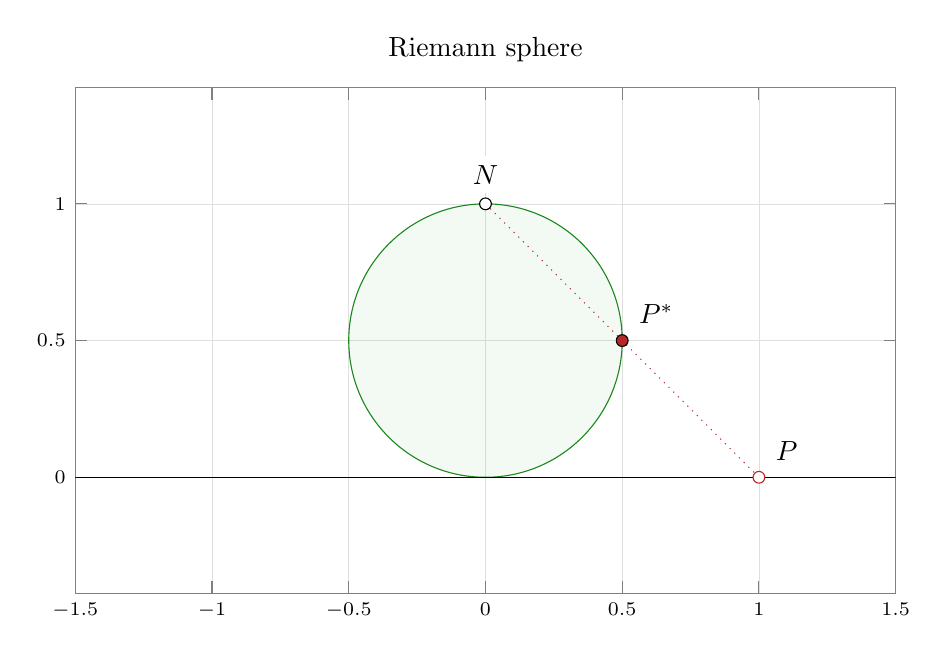
\begin{tikzpicture}
                \begin{axis}[legend pos = outer north east,
                        height = 8cm, width = 12cm, axis equal,
                        title = {Riemann sphere},
                        xmin = -1.5, xmax = 1.5,
                        ymin = -0.25, ymax = 1.25,
                        grid = both,Ani,
                        colormap/jet,
                    ]
                    \filldraw[draw=y_h,fill=y_h, fill opacity = 0.05]
                    (axis cs:0,0.5) circle (0.5);
                    \addplot[thin, black]{0};
                    \addplot[y_p, dotted, domain = 0:1]{1-x};
                    \node[GraphNode, label =
                            {[fill = white]above: $ N $},
                        fill = white, draw = black] at (axis cs:0, 1){};
                    \node[GraphNode, label =
                            {[fill = white]above right: $ P $},
                        fill = white, draw = y_p] at (axis cs:1, 0){};
                    \node[GraphNode, label =
                            {[fill = white]above right: $ P^* $},
                        fill = y_p, draw = black] at (axis cs:0.5, 0.5){};
                \end{axis}
            \end{tikzpicture}
        \end{figure}

    \item[Extended complex plane] The complex plane mapped onto the Riemann sphere
        along with a special point $ \infty $ which maps onto the north pole. This
        is now a stereographic projection of the finite complex plane onto this sphere.

    \item[Function behavior at infinity] Investigate the behaviour of $ g(w) $ where
        \begin{align}
            w    & = \frac{1}{z}   &
            g(w) & = f(1/w) = f(z)
        \end{align}
        The original function $ f(z) $ is analytic or singular at infinity bsaed on the
        behaviour of the new function $ g(w) $ at $ w = 0 $. \par
        The types of and orders of singularities also transfer over from $ g(w) $ to
        $ f(z) $.


    \item[Meromorphic function] A function whose only singularities in the finite
        complex plane are poles.
\end{description}

\section{Residue Integration Method}

\begin{description}
    \item[Residue] Consider a function $ f(z) $ that is analytic everywhere on and
        inside a closed contour $ C $ except at the interior point $ z_0 $. \par
        \begin{align}
            f(z)                & = \iser[n]{0} a_n\ (z - z_0)^n
            + \iser{1} \frac{b_m}{(z - z_0)^m}                                      \\
            \oint_C f(z)\ \dl z & = 2\pi\i\ b_1                                     \\
            \Res_{z = z_0} f(z) & \equiv b_1 = \frac{1}{2\pi\i} \oint_C f(z)\ \dl z
        \end{align}
        The backwards method of finding $ b_1 $ using the Laurent series and then
        evaluating the integral is called residue integration.

    \item[Simple poles] For a simple pole at $ z = z_0 $,
        \begin{align}
            \Res_{z = z_0} f(z) & = \lim_{z \to z_0} (z - z_0) f(z)
        \end{align}
        If a function is a quotient of two other functions where $ q(z) $ has a simple
        zero at $ z_0 $, then
        \begin{align}
            f(z)                & = \frac{p(z)}{q(z)}      &
            p(z_0)              & \neq 0                     \\
            \Res_{z = z_0} f(z) & = \frac{p(z_0)}{q'(z_0)}
        \end{align}

    \item[Poles of any order] The residue at $ z_0 $ which is a pole of order $ m $,
        \begin{align}
            \Res_{z = z_0} f(z) & = \frac{1}{(m-1)!}\ \lim_{z \to z_0}
            \ \diff*[m-1] {\Big[(z - z_0)^m\ f(z)\Big]}{z}
        \end{align}
        For the special case of a second order pole,
        \begin{align}
            \Res_{z = z_0} f(z) & = \lim_{z \to z_0}
            \ \diff* {\Big[(z - z_0)^2\ f(z)\Big]}{z}
        \end{align}

    \item[Residue theorem] When there are multiple singularities of $ f(z) $ inside
        the contour, and $ f(z) $ is analytic everywhere on the contour $ C $ and inside
        $ C $ except for these finitely many points $ \{z_k\} $,
        \begin{align}
            \oint_C f(z)\ \dl z & = 2\pi\i\ \sum_{j=1}^{k} \Res_{z = z_j} f(z)
        \end{align}
        The proof involves making a multiply connected domain $ D $ by excluding a
        small contour encircling each singularity. \par
        Cauchy's integral theorem makes the integral over the outside contour $ C $
        equal to the sum of the integrals over each of the inner contours $ C_k $
        (all taken ccl).
        \begin{align}
            \oint_C f(z)\ \dl z & = \oint_{C_1} f(z)\ \dl z + \quad \dots\quad
            + \oint_{C_n}f(z)\ \dl z
        \end{align}
        \begin{figure}[H]
            \centering
            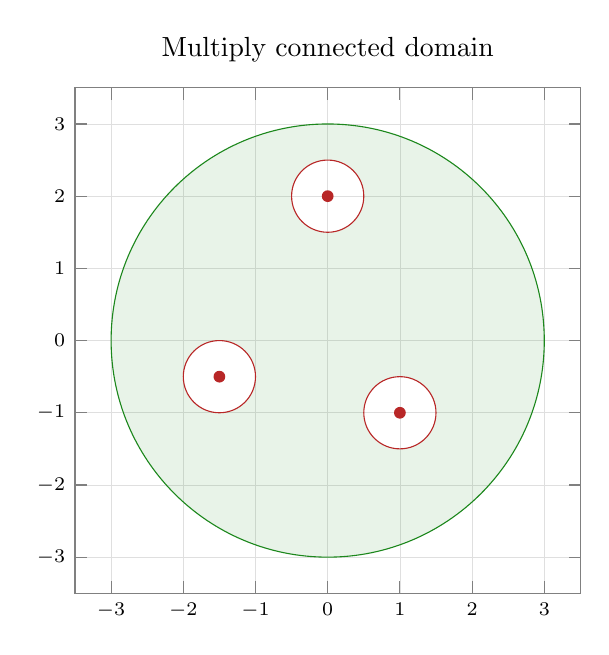
\begin{tikzpicture}
                \begin{axis}[legend pos = outer north east,
                        height = 8cm, width = 8cm, axis equal,
                        title = {Multiply connected domain},
                        xmin = -3.5, xmax = 3.5,
                        ymin = -3.5, ymax = 3.5,
                        grid = both,Ani,
                        colormap/jet,
                    ]
                    \filldraw[draw opacity = 0, fill=y_h,
                        fill opacity = 0.1,even odd rule]
                    (axis cs:0,0) circle (3) (axis cs:0,2) circle (0.5)
                    (axis cs: 1, -1) circle (0.5) (axis cs:-1.5, -0.5) circle (0.5);
                    \node[GraphNode, fill = y_p] at (axis cs:0, 2){};
                    \node[GraphNode, fill = y_p] at (axis cs:1, -1){};
                    \node[GraphNode,fill = y_p] at (axis cs:-1.5, -0.5){};
                    \draw[y_h] (axis cs:0,0) circle (3);
                    \draw[y_p] (axis cs:0,2) circle (0.5);
                    \draw[y_p] (axis cs:1,-1) circle (0.5);
                    \draw[y_p] (axis cs:-1.5,-0.5) circle (0.5);
                \end{axis}
            \end{tikzpicture}
        \end{figure}
\end{description}

\section{Residue Integration of Real Integrals}

\begin{description}
    \item[Rational function of sine and cosine] Consider integrating some function
        that does not become infinite on the interval of integration $ [0, 2\pi] $,
        \begin{align}
            J           & = \int_{0}^{2\pi}\ F(\cos \theta, \sin \theta)\ \dl \theta &
            J           & = \oint_{C} \frac{f(z)}{\i z}\ \dl z                         \\
            \cos \theta & = \frac{1}{2} \Bigg( z + \frac{1}{z} \Bigg)                &
            \sin \theta & = \frac{1}{2\i} \Bigg( z - \frac{1}{z} \Bigg)
        \end{align}
        Where, $ z = \exp(\i \theta) $ and the closed contour in the complex plane
        is the unit circle ccl.

    \item[Cauchy principal value of integral] An improper integral obtained by
        making the limits symmetrically tend to infinity
        \begin{align}
            \prv \Bigg[\intRL f(x)\ \dl x\Bigg] & = \lim_{R \to \infty}
            \ \int_{-R}^{R} f(x)\ \dl x
        \end{align}
        Given that $ f(x) $ is,
        \begin{itemize}
            \item a real rational function.
            \item has a denominator that never vanishes in the interval of integration.
            \item has a denominator at least two degrees higher than the numerator.
        \end{itemize}
        \begin{align}
            \intRL f(x)\ \dl x & = 2\pi\i\ \sum_k \Res_{z = z_k} f(z)
        \end{align}
        where the summation is over all the poles of $ f(z) $ in the upper half plane.

    \item[Fourier integrals] Similar to the above style of integrating over a
        closed semicircular contour in the upper half plane,
        \begin{align}
            \intRL f(x)\ \cos(sx)\ \dl x & = -2\pi\ \sum_k \Im {\Res_{z = z_k} [f(z)
            \ \exp(\i sz)]}                                                          \\
            \intRL f(x)\ \sin(sx)\ \dl x & = 2\pi\ \sum_k \Re {\Res_{z = z_k} [f(z)
                    \ \exp(\i sz)]}
        \end{align}
        where $ s $ is a positive real number and the function $ f(z) $ is a rational
        function satisfying the conditions listed above. \par
        Also only the poles of $ f(z) $ in the upper half plane get summed over.

    \item[Integrand not defined along interval] Consider an integral of the form
        \begin{align}
            I                         & = \int_{A}^{B} f(x)\ \dl x             \\
            \lim_{x \to c} \abs{f(x)} & = \infty \quad \text{for some} \quad c
            \in [A, B]
        \end{align}
        The Cauchy principal value of this integral is,
        \begin{align}
            \prv \Bigg[\int_{A}^{B} f(x) \dl x\Bigg] & = \lim_{\epsilon \to 0}
            \Bigg[ \int_{A}^{c-\epsilon} f(x) \dl x
                + \int_{c + \epsilon}^{B} f(x) \dl x  \Bigg]
        \end{align}

    \item[Simple poles on real axis] If $ f(z) $ has a simple pole at $ z = a $ on
        the real axis, and $ C_2 $ is the semicircular contour ccl, of radius $ r $,
        \begin{align}
            \lim_{r \to 0} \int_{C_2} f(z) \dl z & = \pi\i\ \Res_{z = a}f(z)
        \end{align}
        \begin{figure}[H]
            \centering
            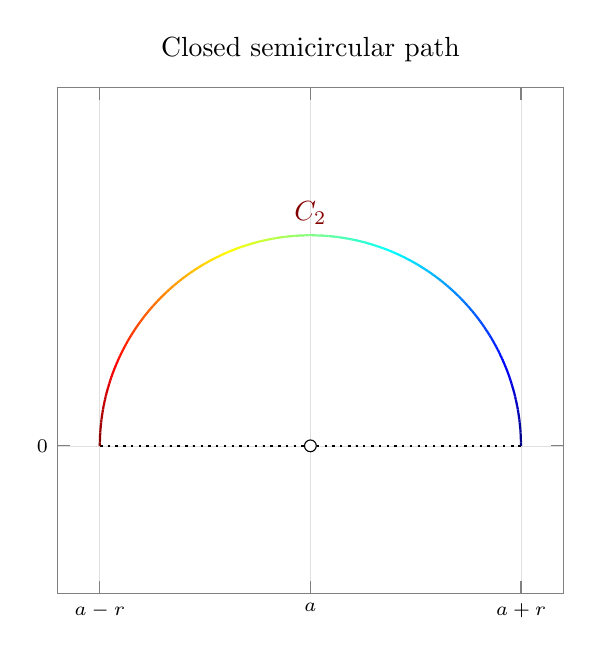
\begin{tikzpicture}
                \begin{axis}[legend pos = outer north east,
                        height = 8cm, width = 8cm, axis equal,
                        title = {Closed semicircular path},
                        % xmin = -1.5, xmax = 1.5,
                        % ymin = -1, ymax = 2,
                        grid = both,Ani,
                        colormap/jet,
                        xtick = {-1,0,1}, xticklabels = {$ a-r $, $ a $, $ a+r $},
                        ytick = {0},
                    ]
                    \addplot[GraphSmooth, dotted, black, domain = -1:1]{0};
                    \node[GraphNode, fill = white, draw = black] at (axis cs:0, 0){};
                    \addplot[GraphSmooth, mesh, point meta = \t, domain = 0:pi,
                        variable = \t]
                    ({cos(\t)}, {sin(\t)})
                    node[midway, above]{$ C_2 $};
                \end{axis}
            \end{tikzpicture}
        \end{figure}

    \item[Improper real integrals] Let a function $ f(z) $ have
        many simple poles on the real axis,
        \begin{align}
            \prv \Bigg[\intRL f(x) \dl x\Bigg] & = 2\pi\i\ \sum_k \Res_{z = z_k} f(z)
            + \pi\i\ \sum_j \Res_{z = z_j} f(z)
        \end{align}
        Here, $ z_k $ are the poles in the upper half plane and $ z_j $ are the simple
        poles on the real line.
        \begin{figure}[H]
            \centering
            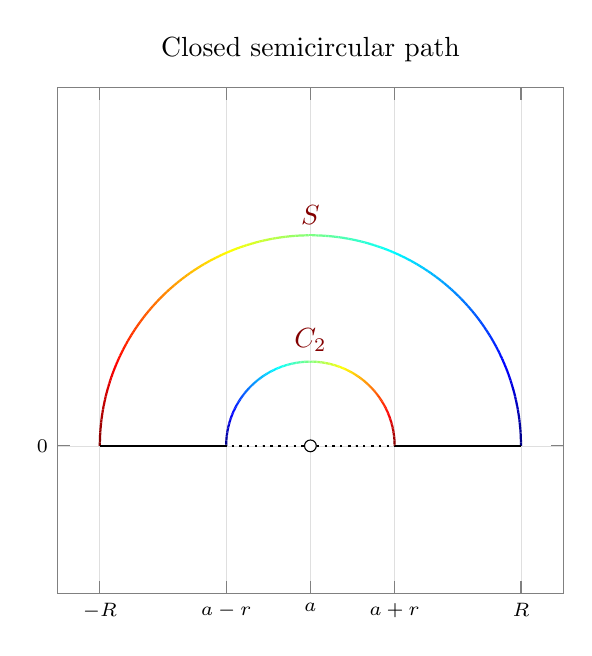
\begin{tikzpicture}
                \begin{axis}[legend pos = outer north east,
                        height = 8cm, width = 8cm, axis equal,
                        title = {Closed semicircular path},
                        % xmin = -1.5, xmax = 1.5,
                        % ymin = -1, ymax = 2,
                        grid = both,Ani,
                        colormap/jet,
                        xtick = {-2,-0.8,0,0.8,2},
                        xticklabels = {$ -R $,$ a-r $, $ a $, $ a+r $, $ R $},
                        ytick = {0},
                    ]
                    \addplot[GraphSmooth, dotted, black, domain = -2:2]{0};
                    \node[GraphNode, fill = white, draw = black] at (axis cs:0, 0){};
                    \addplot[GraphSmooth, mesh, point meta = \t, domain = 0:pi,
                        variable = \t]
                    ({-0.8*cos(\t)}, {0.8*sin(\t)})
                    node[midway, above]{$ C_2 $};
                    \addplot[GraphSmooth, mesh, point meta = \t, domain = 0:pi,
                        variable = \t]
                    ({2*cos(\t)}, {2*sin(\t)})
                    node[midway, above]{$ S $};
                    \addplot[GraphSmooth, black, domain = -2:-0.8]{0};
                    \addplot[GraphSmooth, black, domain = 0.8:2]{0};
                \end{axis}
            \end{tikzpicture}
        \end{figure}

\end{description}
% \chapter{Conformal Mapping}

\section{Geometry of Analytic Functions: Conformal Mapping}

\begin{description}
    \item[Complex function] A mapping from a complex variable to another.
        \begin{align}
            w & \equiv f(z) = u(x, y) + \i\ v(x, y) &
            z & = x + \i\ y
        \end{align}
        The domain of definition $ D $ of this function maps onto the range $ R $, both
        of which are complex planes.

    \item[Mapping terminology] A map is
        \begin{itemize}
            \item surjective, if every element of $ R $ is the image of at least
                  one element in $ D $.
            \item injective, if different elements of $ D $ have different images
                  in $ R $.
            \item bijective, if it is both of the above.
        \end{itemize}

        The result of a mapping function acting on a point $ z_0 $ is called its image
        $ f(z_0) $.
        \begin{align}
            w_0 & = f(z_0)
        \end{align}

    \item[Conformal map] A mapping that preserves angles between oriented curves in
        direction as well as sense. \par
        The mapping by an analytic function is conformal, except at its critical points
        (where the derivative $ f' $ is zero).
        \begin{figure}[H]
            \centering
            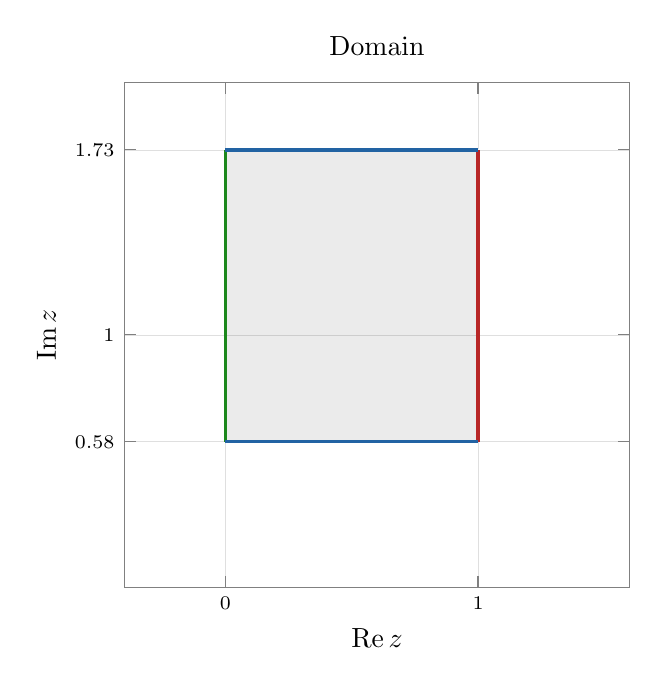
\begin{tikzpicture}
                \begin{axis}[set layers,
                        width = 8cm, height = 8cm, title = Domain,
                        xmin = 0, xmax = 1.2, ymin = 0, ymax = 2, grid = both,
                        xlabel = \normalsize $ \Re{z} $, ylabel = \normalsize $ \Im{z} $,
                        axis equal,
                        ytick = {0.577, 1.732,1},
                        xtick = {0,1},
                        Ani]
                    \draw [draw = black!0, fill = black, fill opacity = 0.08]
                    (0,0.577) -- (1, 0.577) -- (1, 1.732) -- (0, 1.732)
                    -- cycle;
                    \draw [very thick, y_h] (0, 0.577) -- (0, 1.732);
                    \draw [very thick, y_p] (1, 0.577) -- (1, 1.732);
                    \draw [very thick, y_t] (0, 0.577) -- (1, 0.577);
                    \draw [very thick, azure4] (0, 1.732) -- (1, 1.732);
                \end{axis}
            \end{tikzpicture}
            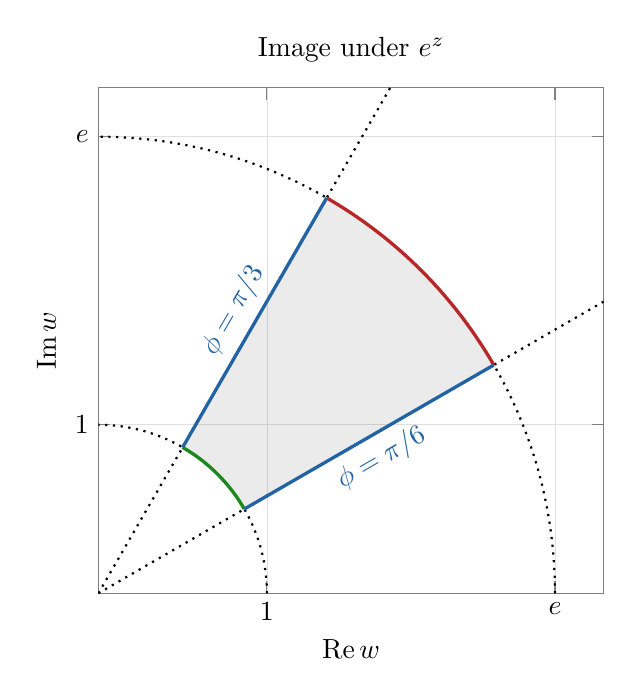
\begin{tikzpicture}
                \begin{axis}[set layers,
                        width = 8cm, height = 8cm, title = {Image under $ e^z $},
                        xmin = 0, xmax = 3, ymin = 0, ymax = 3, grid = both,
                        xlabel = \normalsize $ \Re{w} $, ylabel = \normalsize $ \Im{w} $,
                        axis equal, xtick = {1,2}, ytick = {1,2},
                        ytick = {1,2.71},yticklabels={\normalsize 1, \normalsize $ e $},
                        xtick = {1,2.71},xticklabels={\normalsize 1, \normalsize $ e $},
                        Ani]
                    \draw [draw = black!0, fill = black, fill opacity = 0.08]
                    (30:2.71)--(30:1) arc (30:60:1) -- (60:2.71) arc(60:30:2.71)
                    -- cycle;
                    \draw [draw = black, dotted, thick] (0:1) arc (0:90:1);
                    \draw [draw = black, dotted, thick] (0:2.71) arc (0:90:2.71);
                    \addplot[GraphSmooth, dotted, thick, black, domain= 0:4,
                        variable=\t]
                    ({\t*cos(pi/6)}, {\t*sin(pi/6)});
                    \addplot[GraphSmooth, dotted, thick, black, domain= 0:4,
                        variable=\t]
                    ({\t * cos(pi/3)}, {\t * sin(pi/3)});
                    \addplot[GraphSmooth, very thick, y_h, domain= pi/6:pi/3, variable=\t]
                    ({cos(\t)}, {sin(\t)});
                    \addplot[GraphSmooth, very thick, y_p, domain= pi/6:pi/3, variable=\t]
                    ({2.71 * cos(\t)}, {2.71 * sin(\t)});
                    \addplot[GraphSmooth, very thick, y_t, domain= 1:2.71, variable=\t]
                    ({\t*cos(pi/6)}, {\t*sin(pi/6)})
                    node[midway, below, sloped]{$ \phi = \pi/6 $};
                    \addplot[GraphSmooth, very thick, azure4, domain= 1:2.71, variable=\t]
                    ({\t * cos(pi/3)}, {\t * sin(pi/3)})
                    node[midway, above, sloped]{$ \phi = \pi/3 $};
                \end{axis}
            \end{tikzpicture}
        \end{figure}

    \item[Magnification ratio] The ratio of the lenghts of a line segment in the domain
        $ D $ to the length of the corresponding image in $ R $.
        \begin{align}
            M & = \lim_{z \to z_0} \abs{\frac{f(z) - f(z_0)}{z - z_0}}
            = \abs{f'(z_0)}
        \end{align}

    \item[Jacobian] The condition $ f'(z)  \neq 0$ is equivalent to a nonzero
        Jacobian at $ z = z_0 $.
        \begin{align}
            \abs{f'(z)}^2 & = \begin{vNiceMatrix}[margin]
                                  \difcp ux & \difcp uy \\
                                  \difcp vx & \difcp vy \\
                              \end{vNiceMatrix} = \frac{\partial(u, v)}{\partial(x, y)}
        \end{align}
        This requires the Cauchy-Riemann equations and
        \begin{align}
            f'(z)         & = \diffp ux + \i\ \diffp vx                             &
            \abs{f'(z)}^2 & = (\difcp ux)^2 + (\difcp uy)^2                           \\
            \abs{f'(z)}^2 & = \difcp ux \cdot \difcp vy - \difcp uy \cdot \difcp vx
        \end{align}

\end{description}

\section{Linear Fractional Transformations (Mobius Transformations)}

\begin{description}
    \item[Utility] Mobius transformations help map one kind of region into another in
        order ease the solution of BVPs.
        \begin{align}
            w & = \frac{az + b}{cz + d} & ad & \neq bc
        \end{align}
        Where $ a,b,c,d $ are complex numbers.

    \item[Special Mobius transformations] Of particular interest in BVPs are
        \begin{align}
            w & = z + b                  &  & \text{Translation}                  \\
            w & = az, \qquad \abs{a} = 1 &  & \text{Rotation}                     \\
            w & = az + b                 &  & \text{Linear transformation}        \\
            w & = \frac{1}{z}            &  & \text{Inversion in the unit circle}
        \end{align}
        All Mobius transformations are a composite of these four special maps.

    \item[Circles and straight lines] Every linear fractional transformation maps the
        totality of circles and straight lines in $ \mathcal{C} $ onto the totality of
        circles and straight lines in $ \mathcal{C^*} $. \par
        Here, the plane $ C^* $ is the plane containing the image of the map.

    \item[Extended complex plane] The Mobius transformation is injective except for
        points of the form $ z = -d/c $. The special point $ \infty $ is now defined as
        the extra point in $ \mathcal{C^*} $ that is the image of this special $ z $.
        (assuming $ c \neq 0 $)

    \item[Inverse mapping] The inverse of the standard Mobius transformation is,
        \begin{align}
            z & = \frac{dw - b}{-cw + a}
        \end{align}
        Now, for $ c \neq 0 $, the special point $ w = a/c $ maps onto $ \infty $ in the
        original $ \mathcal{C} $ plane. Taken together with the above result,
        Mobius transformations map the extended complex plane onto iself.

    \item[Fixed points] Points that are mapped onto themselves.
        \begin{align}
            f(z) = w = z
        \end{align}
        The special identity map $ f(z) = z $ has the entire complex plane as its
        fixed point. \par
        A mobius transformation (that is not the identity map) has at most two fixed
        points. If the mobius map is known to have three or more fixed points, it has to
        be the identity map.
\end{description}

\section{Special Linear Fractional Transformations}

\begin{description}
    \item[Three points to map] Three given distinct points $ z_1,z_2,z_3 $
        can always be mapped onto three prescribed distinct points $ w_1,w_2,w_3 $,
        by one and only one L.F.T.
        \begin{align}
            \Bigg( \frac{w - w_1}{w - w_3} \Bigg) \Bigg( \frac{w_2 - w_3}
            {w_2 - w_1} \Bigg) & = \Bigg( \frac{z - z_1}{z - z_3} \Bigg)
            \Bigg( \frac{z_2 - z_3}{z_2 - z_1} \Bigg)
        \end{align}
        Any fraction containing $ \infty $ is evaluated to $ 1 $.

    \item[Standard domains] Start with choosing the points $ z_1,z_2,z_3 $ on the
        boudnary of the domain and then the points $ w_1, w_2, w_3 $ on the boundary of
        the image $ D^* $. \par
        To map a unit disk centered at $ z_0 $ onto another unit disk centered at the
        origin,
        \begin{align}
            w & = \frac{(z - z_0)}{cz - 1} & c & = \overline{z_0} \qquad \abs{z_0} < 1
        \end{align}
        To map the upper half plane onto the unit circle,
        \begin{align}
            w & = \frac{z - \i}{-\i z + 1}
        \end{align}

    \item[Cayley transform] A special transform that maps the real line onto the
        unit circle and the upper half plane onto the interior of the unit circle.
        \begin{align}
            w & = \frac{z - \i}{z + \i}
        \end{align}
\end{description}

\section{Conformal Mapping by Other Functions}

\begin{description}
    \item[Sine function] The mapping uses the fundamental period
        $ x \in [-\pi/2, \pi/2] $.
        \begin{align}
            w         & = \sin z                              &
            u + \i\ v & = \sin x \cosh y + \i\ \cos x \sinh y
        \end{align}
        The mapping is not conformal at the critical points $ \pm \pi/2 $. \par
        In the figure, vertical lines in the
        \textcolor{y_h}{upper} and \textcolor{y_p}{lower} half plane, map onto
        hyperbolas. \par
        Whereas, the horizontal lines in the \textcolor{y_t}{right} and
        \textcolor{azure4}{left} half planes, map onto ellipses.
        \begin{figure}[H]
            \centering
            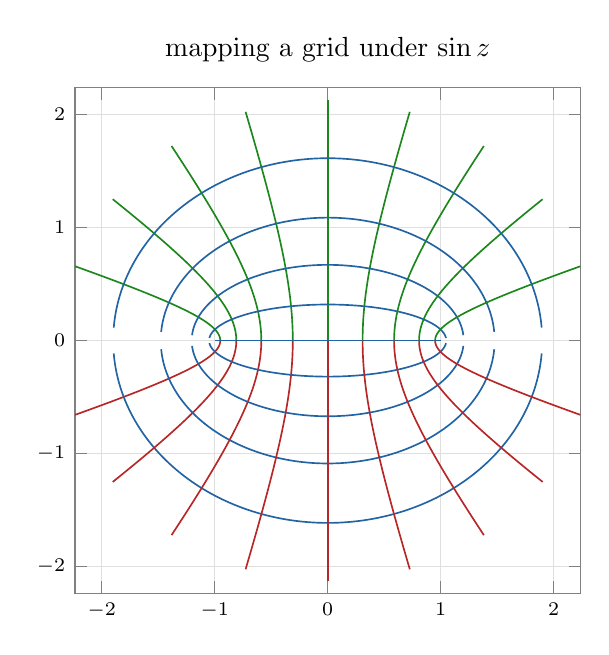
\begin{tikzpicture}
                \begin{axis}[
                        title = {mapping a grid under $ \sin z $},
                        grid = both, Ani,
                        width = 8cm, height = 8cm, enlargelimits = false,
                        axis equal,
                    ]
                    \foreach \k in {-0.4,-0.3,-0.2,-0.1,0,0.1,0.2,0.3,0.4}
                        {
                            \edef\temp{%
                                \noexpand \addplot[GraphSmooth, semithick,
                                    y_h, domain = 0:1.5]
                                ({sin(\k*pi)*cosh(x)}, {cos(\k*pi)*sinh(x)});
                                \noexpand \addplot[GraphSmooth, semithick,
                                    y_p, domain = -1.5:0]
                                ({sin(\k*pi)*cosh(x)}, {cos(\k*pi)*sinh(x)});
                                \noexpand \addplot[GraphSmooth, semithick,
                                    y_t, domain = 0:1.5]
                                ({sin(x)*cosh(\k*pi)}, {cos(x)*sinh(\k*pi)});
                                \noexpand \addplot[GraphSmooth, semithick,
                                    azure4, domain = -1.5:0]
                                ({sin(x)*cosh(\k*pi)}, {cos(x)*sinh(\k*pi)});
                            }\temp
                        }
                \end{axis}
            \end{tikzpicture}
        \end{figure}
        The other functions are derived from this map using,
        \begin{align}
            \cos z   & = \sin(z + \pi/2) & \sinh(z) & = -\i\ \sin(\i z) \\
            \cosh(z) & = \cos(\i z)
        \end{align}

    \item[Tangent function] The function $ f(z) = \tan(z) $ is similarly, a
        composition of L.F.T.s and an exponentiation.
        \begin{align}
            \tan(z) & = -\i\ \frac{e^{2\i z} - 1}{e^{2\i z} + 1} &
            w_1     & = e^{2\i z}                                  \\
            w_2     & = \frac{w_1 - 1}{w_1 + 1}                  &
            w       & = \i\ w_2
        \end{align}
        This maps the infinite vertical strip $ x \in (-\pi/4, \pi/4) $ onto the
        unit circle.

\end{description}

\section{Riemann Surfaces}

\begin{description}
    \item[Utility] Consider maps such as $ w = z^2 $, which cover the $ w $ plane
        twice over when traversing the entire $ z $ plane. \par
        Multiple passes of the $ w $ plane can be differentiated in order to make the
        many-to-one function a one-to-one function.

    \item[Branch point] A point in the $ w $ plane that is the image of just one
        point in the $ z $ plane.

    \item
\end{description}
% \chapter{Complex Analysis and Potential Theory}

\section{Electrostatic Fields}

\begin{description}
    \item[Laplace equation] The electrostatic potential in a region free of charges is
        given by Laplace's equation
        \begin{align}
            \nabla^2 \Phi & = 0
        \end{align}
        The surfaces $ \Phi = c $ are called equipotential surfaces.

    \item[Complex potential] Consider a harmonic function $ \Phi(x, y) $ whose
        harmonic conjugate is $ \Psi(x, y) $.
        \begin{align}
            F(z) & = \Phi + \i\ \Psi
        \end{align}
        is now an analytic function of $ z $, and is called the complex potential
        corresponding to the real potential $ \Phi $.

    \item[Conformality] Since equipotential lines have to intersect electromagnetic
        lines of force at right angles, the complex potential is a prepackaged conformal
        map of $ z $ that yields both $ \Phi $ and $ \Psi $.

    \item[Superposition] Potantials due to more than one source at a given point can
        be superposed to yield the net potential. For complex potentials, this happens to
        be simple scalar addition of the real and imaginary parts separately.
\end{description}

\section{Use of Conformal Mapping}

\begin{description}
    \item[Dirichlet problem] A type of boundary value problem where the value of the
        potential is specified everywhere on the boundary surface.

    \item[Conformal mapping of harmonic functions] Let a function $ \Phi^* $ be
        harmonic in a domain $ D^* $ in the $ w $ plane.
        Suppose $ w = f(z) $ is analytic in a domain $ D $ in the $ z $ plane, and maps
        $ D $ conformally onto $ D^* $. Then,
        \begin{align}
            \Phi(x, y) & = \Phi^*\Big[u(x, y),\ v(x, y) \Big]
        \end{align}
        is also harmonic in $ D $. If $ D^* $ is simply connected, then the harmonic
        conjugate $ \Psi^* $ exists.

    \item[Strategy] Use a conformal mapping to convert the complicated BVP into a
        standard BVP for which the result is known. Then, reverse transform
        $ w \to z $ to get the compmlex potential in $ z $ space.

\end{description}

\section{Heat Problems}

\begin{description}
    \item[Heat equation] A steady state heat flow, which means that temperature is
        independent of time reduces to,
        \begin{align}
            \nabla^2 T & = 0
        \end{align}
        which is the Laplace equation in temperature (a scalar like electrostatic
        potential)

    \item[Isotherms] The contours of constant temperature. The orthogonal family of
        curves is called the lines of heat flow.

    \item[Mixed BVP] Sometimes, the potential is specified on some portion of the
        boundary and its normal derivative is specified over the rest. This becomes a
        mixed boundary value problem.
\end{description}

\section{Fluid Flow}

\begin{description}
    \item[Complex potential] A conplex function of the form,
        \begin{align}
            F(z) & = \Phi(x, y) + \i\ \Psi(x, y)
        \end{align}
        where $ \Phi $ is called the velocity potential and $ \Psi $ is the stream
        function. This function is analytic and therefore $ \Phi, \Psi $ are
        harmonic functions.

    \item[Streamlines] Curves of $ \Phi(x, y) = c $ are still called equipotential lines,
        and the trajectories of fluid flow are $ \Psi(x, y) = c $. \par
        The boundaries across which fluid cannot flow must be streamlines.

    \item[Velocity] Anoalogous to the two-dimensional vector for the velocity of a fluid,
        \begin{align}
            V & = V_1 + \i\ V_2 = \overline{F'{z}}
        \end{align}
        is the complex velocity.

    \item[Stagnation points] Points along a fluid flow vector field, where the
        velocity is zero. This requires the flow to be steady (independent of time).

    \item[Assumptions] If a simply connected domain $ D $ has an incompressible
        and irrotational fluid flow at steady state, then the flow has a complex
        potential $ F(z) $ which is an analytic function.

    \item[Circulation] The line integral of the tangential component of the velocity
        along a curve.
        \begin{align}
            C & = \int_{C} V_t\ \dl t
        \end{align}

    \item[Rotation] In two dimensions, it is the curl of the velocity vector.
        \begin{align}
            \omega(x, y) & = \frac{1}{2}\ \Bigg[\diffp{V_2}{x} - \diffp{V_1}{y}\Bigg]
        \end{align}
        A special case where $ \nabla \times \vec{V} = 0 $ is called an irrotational
        vector field. \par
        Without the $ 1/2 $ factor, this expression is called the vorticity.

    \item[Incompressible] This refers to the fact that there are no sources or sinks
        of fluid anywhere in the domain. In vector calculus, this is denoted by
        $ \nabla \dotp \vec{V} = 0 $. \par
        The fluid inflow per second into a fixed volume must equal the fluid outflow, at
        all points in the domain.

    \item[Complex velocity potential]  If the above conditions are met, then the line
        integral of the tangential velocity over any closed loop vanishes by Green's
        theorem. \par
        The path independence of this integral establishes the complex velocity
        potential (which is a scalar).
        \begin{align}
            \Phi(x, y) & = \int_{z_0}^{z} (V_1\ \dl x + V_2\ \dl y)
        \end{align}
\end{description}

\section{Poisson's Integral Formula for Potentials}

\begin{description}
    \item[Poisson's Integral formula] Applying Cauchy's integral formula on a closed
        line integral on a circle of radius $ R > 1 $,
        \begin{align}
            \Phi(r, \theta) & = \frac{1}{2\pi}\ \int_{0}^{2\pi} \Phi(R, \alpha)
            \ \frac{R^2 - r^2}{R^2 + r^2 - 2Rr\cos(\theta - \alpha)}\ \dl \theta
        \end{align}
        This is the potential at all points inside the disk $ \abs{z} \leq R $ in terms
        of the potential on the disk's boundary $ \Phi(R, \alpha) $. \par
        If the boundary is only piecewise continuous, then the formula is valid at all
        points on the open disk $ \abs{z} < R $, and all points on the boundary except
        these discontinuities.

    \item[Series solution] The potential can be expanded into an infinite series using
        the geometric series,
        \begin{align}
            \Phi(r, \theta) & = a_0 + \iser[n]{1} \Big( \frac{r}{R} \Big)^n\
            \Big[ a_n \cos(n\theta) + b_n \sin(n\theta) \Big]                  \\
            a_0             & = \frac{1}{2\pi} \int_{0}^{2\pi} \Phi(R, \alpha)
            \ \dl \alpha                                                       \\
            a_n             & = \frac{1}{\pi} \int_{0}^{2\pi} \Phi(R, \alpha)
            \ \cos(n\alpha)\ \dl \alpha                                        \\
            b_n             & = \frac{1}{\pi} \int_{0}^{2\pi} \Phi(R, \alpha)
            \ \sin(n\alpha)\ \dl \alpha
        \end{align}
        The derivation uses the Fourier series expansion of the integrand in the Poisson
        integral formula. \par
        At the boundary, $ r = R $ and this series reduces to the fourier series of
        $ \Phi(R, \alpha) $. This method is valid whenever $ \Phi $ has a Fourier series
        expansion.
\end{description}

\section{General Properties of Harmonic Functions}

\begin{description}
    \item[Mean Value Property] Let $ F(z) $ be analytic in a simply connected domain
        $ D $. Then, the value of $ F(z) $ at any point $ z_0 $ in $ D $ is equal to its
        mean value on any circle in $ D $ with center $ z_0 $

    \item[Mean value of harmonic functions] Relacing $ F(z) $ above with a harmonic
        function $ \Phi(x,y) $, the relation holds. \par
        Additionally, this value is equal to the mean value of $ \Phi $ over any disk
        in $ D $ centered on $ z_0 $.

    \item[Maximum modulus theorem] Let $ F(z) $ be analytic and non-constant in a domain
        containing a bounded region $ R $ and its boundary. \par
        The absolute value of $ F(z) $ cannot have its maximum at an interior point of
        $ R $, only on its boundary. \par
        If $ F(z) \neq 0 \quad \forall \quad z \in R $, this relation also holds for the
        minimum value of $ \abs{F(z)} $.

    \item[Properties of Harmonic functions] Using $ \Phi(x,y), R, C $ as defined
        above,
        \begin{itemize}
            \item If $ \Phi(x, y) $ is not constant, it has neither a maximum nor a
                  minimum in $ R $. If they exist, they have to be on the boundary $ C $.
            \item If $ \Phi(x,y) $ is constant on $ C $, then it is constant in
                  the entire region $ R $ bounded by $ C $.
            \item If $ h(x, y) $ is harmonic in $ R $ and on $ C $, and if
                  $ h = \Phi $ on $ C $, then this also holds everywhere in $ R $.
        \end{itemize}

    \item[Uniqueness theorem for Dirichlet BVP] If a BVP for the Laplace equation in
        two variables has a solution, it must be unique. \par
        This follows from the above properties of harmonic functions, which are uniquely
        determined in $ R $, by their value on the boundary $ C $.
\end{description}
% \chapter{Numerics in General}

\section{Introduction}

\begin{description}
    \item[Motivation] Many mathematical problems do not admit analytical solutions. The
        approach is usually to solve using brute-force numerical approximations and use
        pre-formulated lookup tables. \par
        The advent of cheap computational power has made such numerical approaches more
        feasible.

    \item[Significant digit] Any given digit of a number $ c $, except possibly for zeros
        to the left of the first nonzero digit.

    \item[Floating point numbers] Computers internally represent real numbers in
        floating point form, where the number of significant digits is kept fixed, and
        the decimal point itself is floating.

    \item[Machine numbers] In modern computers, which use binary (base 2) systems,
        any number can be represented as
        \begin{align}
            \bar{a} & = \pm \bar{m} \cdot 2^n            &
            \bar{m} & = 0.d_1d_2\dots d_k, \quad d_1 > 0
        \end{align}
        This is a $ k $ digit binary number, whose fractional part $ \bar{m} $ is called
        the mantissa and exponent is $ n $

    \item[Machine accuracy] Since machine numbers are a discrete set, there is a
        smallest possible real number that they can represent. \par
        The smallets positive $ \epsilon $ such that there are no machine numbers in
        $ [1, 1 + \epsilon] $ is called machine accuracy.

    \item[Underflow and Overflow] The range of exponents that IEEE standards mandate is
        \begin{itemize}
            \item $ 2^{-126} $ to $ 2^{128} $ for single precision numbers
            \item $ 2^{-1022} $ to $ 2^{1024} $ for double precision numbers
        \end{itemize}
        Cases of underflow (when the number is smaller than these lower limits) are
        handled by approximating them as zero and moving on. \par
        Cases of overflow however, lead to the program halting with a fatal error.

    \item[Roundoff] Errors caused by truncating a number by discarding all digits
        from some decimal place onwards. \par
        To round a number $ x $ to $ k $ decimals, add $ 0.5 \times 10^{-k} $ to it and
        then truncate all the digits after the $ (k+1)^{\text{th}} $ digit.

    \item[Error in rounding] Let $ \bar{a} $ be the floating point approximation of
        $ a $. Then, maximum rounding error is,
        \begin{align}
            \abs{1 - \frac{\bar{a}}{a}} \approxeq \abs{1 - \frac{\bar{m}}{m}}
            \leq \frac{1}{2}\ 10^{1-k}
        \end{align}
        This is called the rounding unit.

    \item[Loss of significant digits] A decrease in the number of significant digits as
        a result of performing some computation, such as subtracting two close numbers.
        \par Changes to the algorithm to bypass such problematic arithmetic operations
        is the usual way to deal with these issues.

    \item[Errors] If $ \wt{a} $ is an approximation of the true value $ a $,
        \begin{align}
            \epsilon       & \equiv a - \wt{a}              &
                           & \text{Error}                     \\
            \epsilon_r     & \equiv \frac{\epsilon}{\wt{a}} &
                           & \text{Relative Error}            \\
            \abs{\epsilon} & \leq \beta                     &
                           & \text{Error bound}
        \end{align}
        Relative error is meaningful only for the special case where
        $ \abs{e} \ll \abs{\wt{a}} $. Usually, only an upper bound on the error can
        be found.

    \item[Error propagation] The effect of the four basic arithmetic operations on the
        error,
        \begin{itemize}
            \item In addition and subtraction, the individual error bounds add up to
                  yield the error bound of the result.
            \item In multiplication and division, the individual relative error bounds
                  add up to yield an approximate relative error bound of the result.
        \end{itemize}

    \item[Basic error principle] In general, every numerical method is accompanied by
        an error estimate. \par
        If two approximation methods exist such that
        \begin{align}
            \wt{a_1} + \epsilon_1 & = \wt{a_2} + \epsilon_2 = a &
            \abs{\epsilon_2}      & \ll \abs{\epsilon_1}          \\
            \epsilon_1            & \approxeq \wt{a_2} -
            \wt{a_1}
        \end{align}
        Thus, the difference between the estimated values is an approximation of the
        error in the worse method.

    \item[Algorithm] A set of steps (independent of programming language) used to
        program a numerical method.

    \item[Stability] An algorithm where small changes in the initial conditions supplied
        only cause small changes in the final result. \par
        This is different from mathematical instability, which is inherent to the
        mathematical problem itself.

\end{description}

\section{Solution of Equations by Iteration}

\begin{description}
    \item[Functions of one variable] Equations of the form
        \begin{align}
            f(x) & = 0
        \end{align}
        are often not explicitly solved. These equations permit recursive methods of
        finding solutions.

    \item[Fixed point method] A recursive relation for discrete values of $ x $ which
        act as guesses for the solution can be programmed into a loop.
        \begin{align}
            x_{n+1} & = g(x_n)
        \end{align}
        Such a value is called a fixed point of the recursion. \par
        The same equation $ f(x) = 0 $ can be recast into many forms of recursion, which
        may converge at different rates, or not at all.

    \item[Convergence of fixed point iteration] Let $ x = s $ be a solution of
        $ x = g(x) $ and suppose that $ g(x) $ has a continuous derivative in some
        interval $ J $ containing $ s $. \par
        If $ \abs{g'(x)} \leq K < 1 $ in the interval $ J $, then the iteration process
        converges for any initial guess $ x_0 $ in $ J $. \par
        The limit of the sequence is the fixed point $ s $. \par
        A functino satisying this condition is called a \emph{contraction}.

    \item[Newton-Raphson method] A fast method for solving equations of the form
        $ f(x) = 0 $, which uses the fact that $f(x),\ f'(x) $ are both continuous.
        \begin{align}
            x_{n+1} & = x_n - \frac{f(x_n)}{f'(x_n)}
        \end{align}
        Consider the tangent to the curve at $ [x_n, f(x_n)] $ and its intersection with
        the $ x $ axis,
        \begin{align}
            y - f(x_n) & = f'(x_n) \cdot (x - x_n) &
            y          & = 0
        \end{align}
        These two lines intersect at $ x_{n+1} $, which becomes the next guess. \par
        The algorithm usually has a success criterion based on the relative error between
        successive guesses, and a failure criterion using the number of iterations.

    \item[Choice of initial guess] The N.R. method is sensitive to initial guess in
        terms of which solution it converges to and whether it even converges in the
        first place.

    \item[Order of iteration method] Consider the Taylor series expansion of $ g(x) $
        near a solution $ s $,
        \begin{align}
            x_{n+1} & = g(x_n) = g(s)\ (x_n - s) + \frac{g'(s)}{2!}\ (x_n-s)^2 + \dots \\
            x_{n+1} & = g(s) - g'(s)\ \epsilon_n + \frac{g''(s)}{2!}\ \epsilon_n^2
            + \dots
        \end{align}
        The index of $ \epsilon $ in the first nonzero term of this Taylor series is
        called the order of this iteration method.

    \item[Order of Newton's method] Differentiating the N.R. iteration,
        \begin{align}
            g(x)  & = x - \frac{f(x)}{f'(x)} & g'(x)  & = \frac{f(x)
            \cdot f''(x)}{[f'(x)]^2}                                 \\
            g'(s) & = 0                      & g''(s) & \neq 0
        \end{align}
        in general. This means that the number of significant digits approximately
        doubles with each iteration. This assumes that $ s $ is a simple zero. \par
        If the zero is of higher order, then the order is one.

    \item[Ill conditioned] If the equation $ f(x) = 0 $ has small $ \abs{f'(x)} $ for
        $ x $ close to some solution $ s $, then the iteration might not converge
        for initial guesses far from $ s $.

    \item[Secant method] Replacing the derivative with the finite difference expression,
        \begin{align}
            x_{n+1} & = x_n - f(x_n) \cdot \frac{x_{n} - x_{n-1}}{f(x_n) - f(x_{n-1})}
        \end{align}
        The secant of $ f(x) $ passing through $ P_{n-1} $ and $ P_n $ intersects the
        $ x $ axis at $ x_{n+1} $
\end{description}

\section{Interpolation}

\begin{description}
    \item[Interpolation] Given the values taken by some unknown function at a certain
        set of $ n+1 $ points, as the set $ \{x_0,\dots,x_n\} $,


    \item[Nodes] The set of $ x $ values at which the function value is known, either
        by prior empirical measurement or from some reference table.

    \item[Polynomial approximation] The act of finding a polynomial of degree at most
        $ n $, that passes through all of these points $ (x_0, f_0), \dots, (x_n, f_n) $.
        \par
        Such a polynomial, if it exists, is unique.

    \item[Weierstrass approximation theorem] For any continuous function $ f(x) $ in the
        interval $ J:[a,b] $, and some error bound $ \beta $,
        \begin{align}
            \abs{f(x) - p_n(x)} & < \beta & \forall \quad x & \in J
        \end{align}
        is always possible for a sufficiently large degree of the polynomial $ n $.

    \item[Lagrange interpolation] Each of the set $ \{f_i\} $ is multiplied by a
        polynomial $ L_i(x) $ satisfying
        \begin{align}
            L_i(x) & = \begin{cases}
                           1 & \quad x = x_i            \\
                           0 & \quad x = x_j,\ j \neq i
                       \end{cases}                      \\
            P_x    & = \sum_{k=0}^{n} L_k(x) \cdot f_k  = \sum_{k=0}^{n}
            \frac{l_k(x)}{l_k(x_k)}\ f_k
        \end{align}
        The polynomial $ l_k $ is the product of linear factor of all the nodes except
        the $ k^{\text{th}} $ node.
        \begin{align}
            l_k(x) & = \prod_{j=0}^{n} (x - x_j) & j & \neq k
        \end{align}

    \item[Error of interpolation] The error is approximately the $ (n+1)^{\text{th}} $
        derivative of $ f(x) $ provided it exists and is continuous.

        \begin{align}
            \epsilon_n(x) & = f(x) - p_n(x)
            = \prod_{j=0}^{n} (x-x_j)\ \diff[n+1]{f}{x} \Bigg|_{x=t}
        \end{align}
        For some $ t $ between $ x_0 $ and $ x_n $. $ \abs{\epsilon_n} $ is zero at
        each node, and very small near each node, by continuity of this derivative.
        \par
        This error formula gives the error for any polynomial interpolation of $ f(x) $,
        since such a polynomial must be unique.

    \item[Divided difference] A recursive analog of the slope between two adjacent points
        in a series of nodes.
        \begin{align}
            a_1 & = f[x_0,x_1] = \frac{f_1 - f_0}{x_1 - x_0}                          \\
            a_2 & = f[x_0, x_1, x_2] = \frac{f[x_1,x_2] - f[x_0,x_1]}{x_2 - x_0}      \\
            \vdots \nonumber                                                          \\
            a_k & = f[x_0,\dots,x_k] = \frac{f[x_1,\dots,x_k] - f[x_0,\dots,x_{k-1}]}
            {x_k - x_0}
        \end{align}

    \item[Newton's Divided difference] Starting with 2 nodes, one node at a time is
        introduced successively, until all $ (n+1) $ nodes are used to build up a
        polynomial of degree $ n $.
        \begin{align}
            p_n(x) & = p_{n-1}(x) + g_n(x)
        \end{align}
        Here, $ p_{n-1}(x) $ matches the function at $ \{x_0,\dots,x_{n-1}\} $ whereas
        $ p_n(x) $ matches it at $ x_n $ as well. \par
        Using the $ n^{\text{th}} $ dividied difference $ a_n $,
        \begin{align}
            g_n(x) & = a_n \cdot \prod_{j=0}^{n-1} (x - x_j)                   &
            a_n    & = \frac{f_n - p_{n-1}(x_n)}{\prod_{j=0}^{n-1}(x_n - x_j)}
        \end{align}
        This uses the fact that $ p_n(x_n) = f_n $ but $ p_{n-1}(x_n) $ does not have to
        match the function, since it was computed using nodes upto $ x_{n-1} $. \par
        After incorporating all $ (n+1) $ nodes,
        \begin{align}
            f(x) \approxeq p_n(x) & = f_0 + (x - x_0) \cdot f[x_0, x_1]
            + (x-x_0)(x-x_1) \cdot f[x_0,x_1,x_2] + \dots                    \\
                                  & + \Bigg[\prod_{j=0}^{n-1}(x - x_j)\Bigg]
            \cdot f[x_0,x_1,\dots,x_n]
        \end{align}

    \item[Newton's forward difference formula] For the special case where the nodes are
        equally spaced, with distance $ h $,
        \begin{align}
            x_1 & = x_0 + h & x_n & = x_0 + nh
        \end{align}
        The $ k^{\text{th}} $ forward difference is now defined recursively as
        \begin{align}
            \Delta f_j   & = f_{j+1} - f_j                           \\
            \Delta^2 f_j & = \Delta f_{j+1} - \Delta f_j             \\
            \Delta^k f_j & = \Delta^{k-1} f_{j+1} - \Delta^{k-1} f_j
        \end{align}
        The $ k^{\text{th}} $ divided difference is much simplified,
        \begin{align}
            f[x_0,x_1,\dots,x_k]  & = \frac{1}{k!\ h^k}\ \Delta^k f_0                \\
            f(x) \approxeq p_n(x) & = \sum_{s = 0}^{n} \binom{r}{s} \ \Delta^s f_0 &
            r                     & = \frac{x - x_0}{h}                              \\
            \binom{r}{s}          & = \frac{r(r-1)(r-2)\dots(r-s+1)}{s!}
        \end{align}
        Here, the binomial coefficient is generalized to real $ r $ for some positive
        integer $ s $.

    \item[Error in forward difference] Using the next higher derivative of $ f $,
        \begin{align}
            \epsilon_n(x) & = f(x) - p_n(x) = \binom{r}{n+1}\ h^{n+1} \cdot f^{(n+1)}(t)
        \end{align}
        for some $ t $ in the domain $ [x_0, x_n] $

    \item[Newton's backward difference formula] Using the divided differences from
        larger to smaller order instead, the $ k^{\text{th}} $ backward difference is,
        \begin{align}
            \Delta f_j   & = f_j - f_{j-1}                           \\
            \Delta^2 f_j & = \Delta f_{j} - \Delta f_{j-1}           \\
            \Delta^k f_j & = \Delta^{k-1} f_j - \Delta^{k-1} f_{j-1}
        \end{align}
        The slightly changed formula for the interpolating polynomial is
        \begin{align}
            f(x) \approxeq p_n(x) & = \sum_{s = 0}^{n} \binom{r+s-1}{s}
            \ \Delta^s f_0        &
            r                     & = \frac{x - x_0}{h}                  \\
            \binom{r+s-1}{s}      & = \frac{r(r-1)(r-2)\dots(r-s+1)}{s!}
        \end{align}
        By the symmetry of the binomial formula, these coefficients happen to be the same
        as the ones in the forward difference formula.

\end{description}

\section{Spline Interpolation}

\begin{description}
    \item[Motivation] When using a high degree polynomial with many nodes,
        it may start to oscillate wildly in between successive nodes as a result of the
        high degree $ (n > 20) $. \par

    \item[Piecewise polynomial interpolation] The single high degree polynomial over
        all $ (n+1) $ nodes, is replaced by $ n $ lower degree polynomials, each of which
        operate on a subset of adjacent nodes. \par
        These individual low degree polynomials are then superposed into a spline that
        approximates the function over the domain spanned by all the nodes.

    \item[Cubic spline interpolation] A continuous function with continuous first and
        second derivatives on the interval $ a = x_0 \leq x \leq x_n = b $,
        such that
        \begin{align}
            g(x_0)             & = f(x_0) = f_0 \quad \dots                      &
            \dots \quad g(x_n) & = f(x_n) = f_n                                    \\
            g(x)               & = q_0(x), \quad \forall\ x \in [x_0, x_1] \dots &
            \dots g(x)         & = q_n(x), \quad \forall\ x \in [x_{n-1}, x_n]
        \end{align}
        Thus, the spline matches each of the individual cubic polynomials exactly,
        inside their respective domains. \par
        Additionally, if the tangent direction of $ g(x) $ is specified at the first
        and last nodes,
        \begin{align}
            g'(x_0) & = k_0 & g'(x_n) & = k_n
        \end{align}
        then the spline is determined uniquely.

    \item[Existence and uniqueness of cubic splines] Given a set of arbitrarily spaced
        nodes $ \{x_j\} $ along with the values of the function at the nodes $ \{f_j\} $,
        the two numbers $ g'(x_0), g'(x_n) $ determine a unique spline function which is
        guaranteed to exist.

    \item[Some termiology] Introduce the notation
        \begin{align}
            c_j        & \equiv \frac{1}{h_j} = \frac{1}{x_{j+1} - x_j} &
            \nabla f_j & \equiv f(x_j) - f(x_{j-1})
        \end{align}
        The individual cubic polynomials have to satisfy
        \begin{align}
            q_j(x_j) & = f(x_j) &
            q'(x_j)  & = k_j,
        \end{align}
        for all $ j \in [0,1,\dots,n-1] $. Additionally, the continuity of $ g''(x) $
        means that $ q''_{j-1}(x_j) = q''_j(x_j) $.

    \item[Finding the cubic spline components]
        The set of cubic equations require terms $ \{k_j\} $ for $ j \in [1, n-1] $,
        provided $ k_0 $ and $ k_n $ are already provided.
        \begin{align}
            c_{j-1}\ k_{j-1} + 2(c_{j-1} + c_j)\ k_j + c_j\ k_{j+1}
             & = 3\ \Big[ c^2_{j-1}\ \nabla f_j + c_j^2\ \nabla f_{j+1} \Big]
        \end{align}
        This system of $ (n-1) $ linear equations is guaranteed to have a unique
        solution that is computationally tractable, by its very nature. \par
        The coefficient matrix is sparse and tridiagonal. Also, it is strictly
        diagonally dominant.

    \item[Taylor series expansions to fit coefficients] Each cubic spline is written in
        the form,
        \begin{align}
            q_j & = a_{j0} + a_{j1}\ (x - x_j) + a_{j2}\ (x - x_j)^2 + a_{j3}
            \ (x - x_j)^3
        \end{align}
        for all $ j \in [0,1,\dots,n-1] $
        Using Taylor's formula yields,
        \begin{align}
            a_{j0} & = q_j(x_j) = f_j                                            \\
            a_{j1} & = q'_j(x_j) = k_j                                           \\
            a_{j2} & = \frac{q''(x_j)}{2!} = \frac{3}{h_j^2}\ (f_{j+1} - f_j)
            - \frac{1}{h_j}\ (k_{j+1} + 2k_j)                                    \\
            a_{j3} & = \frac{q'''(x_j)}{3!} = \frac{2}{h_j^3}\ (f_{j} - f_{j+1})
            + \frac{1}{h_j^2}\ (k_{j+1} + k_j)
        \end{align}

    \item[Equidistant nodes] The relation simplifies to, $ h_j = h $ and then
        $ c_j = c = 1/h $
        \begin{align}
            k_{j-1} + 4k_j + k_{j+1} & = \frac{3}{h}\ (f_{j+1} - f_{j-1}) &
            j                        & \in [1,2,\dots,n-1]
        \end{align}

    \item[Boundary conditions] Clamped conditions require the spline's derivative to
        math the function's derivatives at the Boundary
        \begin{align}
            g'(x_0) & = f'(x_0) & g'(x_n) & = f'(x_n)
        \end{align}
        The free or natural condition involves no curvature (second derivative) at the
        boundary.
        \begin{align}
            g''(x_0) & = 0 & g''(x_n) & = 0
        \end{align}
\end{description}

\section{Numeric Integration and Differentiation}

\begin{description}
    \item[Rectangular rule] The interval of integration $ [a,b] $ is subdivided into
        $ n $ parts, each of which is of width
        \begin{align}
            h               & = \frac{b-a}{n}                                        &
            f(x)            & \approxeq f(x^*_j) \quad \forall \quad x
            \in [x_j, x_{j+1}]                                                         \\
            J               & = \int_{a}^{b} f(x)\ \dl x                             &
            J \approxeq J_r & \equiv h\ \Big[ f(x_1^*) + f(x_2^*) + \dots + f(x_n^*)
                \Big]
        \end{align}
        In each interval, $ f(x) $ is approximated by a constant function.
        \begin{figure}[H]
            \centering
            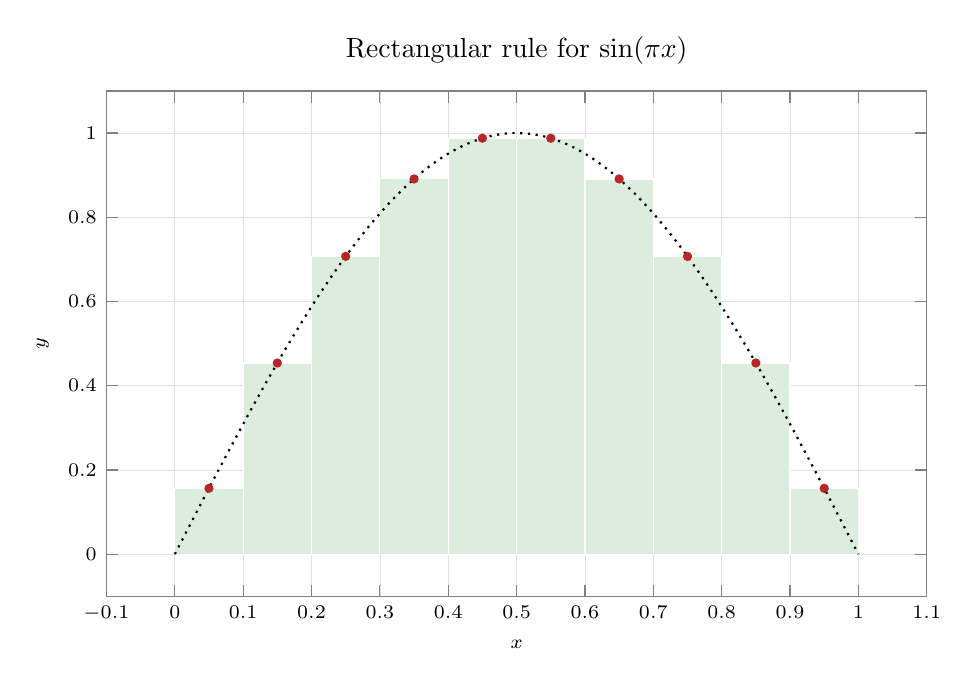
\begin{tikzpicture}[declare function = {a = 0.75;}]
                \begin{axis}[title =
                            {Rectangular rule for $ \sin(\pi x) $},
                        xlabel = $ x $, ylabel = $ y $, Ani,
                        view = {0}{90}, grid = both,]
                    \addplot[ybar, domain = 0:1, bar width = 0.1, color = y_h!0,
                        fill = y_h!15, samples at = {0.05,0.15,...,0.95}]
                    {sin(pi*x)};
                    \addplot[GraphSmooth, black, dotted, domain = 0:1]
                    {sin(pi*x)};
                    \addplot[GraphSmooth, only marks, color = y_p, mark size = 1.25pt,
                        samples at = {0.05,0.15,...,0.95}]
                    {sin(pi*x)};
                \end{axis}
            \end{tikzpicture}
        \end{figure}

    \item[Trapezoidal rule] A more sophisticated approximation that replaces the
        constant function $ f(x^*) $ in each segment, with the straight line joining
        $ (x_j, f_j) $ and $ (x_{j+1}, f_{j+1}) $.
        \begin{align}
            J \approxeq J_t & \equiv h\ \Bigg[ \frac{f(x_a)}{2} + f(x_1) + f(x_2)
                + \dots + f(x_{n-1}) + \frac{f(x_b)}{2} \Bigg]
        \end{align}
        \begin{figure}[H]
            \centering
            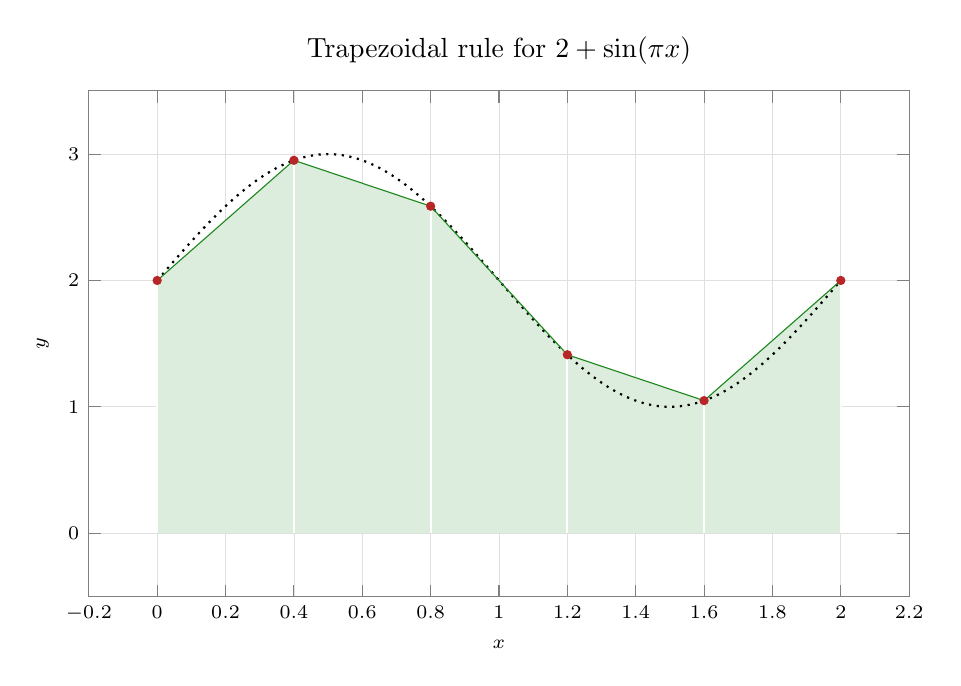
\begin{tikzpicture}[declare function = {a = 0.75;}]
                \begin{axis}[title =
                            {Trapezoidal rule for $ 2 + \sin(\pi x) $},
                        xlabel = $ x $, ylabel = $ y $, Ani,
                        view = {0}{90}, grid = both, ymin = -0.5, ymax = 3.5]
                    \addplot[GraphSmooth, black, dotted, domain = 0:2] {2 + sin(pi*x)};
                    \addplot[GraphSmooth, only marks, color = y_p, mark size = 1.25pt,
                        samples at = {0,0.4,...,2}] {2 + sin(pi*x)};
                    \addplot[name path = top, color = y_h,
                        samples at = {0,0.4,...,2}] {2 + sin(pi*x)};
                    \path[name path = bottom] (axis cs:0, 0) -- (axis cs:2, 0);
                    \addplot [fill=y_h!15] fill between[of=top and bottom];
                    \foreach \k in {0,0.4,...,2}
                        {
                            \edef\temp{%
                                \noexpand \addplot[GraphSmooth, white, domain = 0:1]
                                ({\k}, {x*(2 + sin(pi*\k))});
                            }\temp
                        }
                \end{axis}
            \end{tikzpicture}
        \end{figure}

    \item[Error in trapezoidal rule] Using the Taylor expansion, the error in one
        subinterval of trapezoidal rule is,
        \begin{align}
            \epsilon_j & = -\frac{h^3}{12}\ f''(\wt{t}) & h & = \frac{b-a}{n}
        \end{align}
        The sum of these local errors is the global error,
        \begin{align}
            \epsilon & = -\frac{(b-a)}{12}\ h^2\ f''(t^*) &
            t^*      & \in [a,b]
        \end{align}
        The error is maximised and minimized for some values of $ t^* $ substituted into
        the above expression. \par
        Using the practical error estimate and the fact that the error scales
        quadratically in $ h $,
        \begin{align}
            \epsilon_{h/2} & \approxeq \frac{\epsilon_h}{4}    &
            \epsilon_{h/2} & \approxeq \frac{J_{h/2} - J_h}{3}
        \end{align}

    \item[Simpson's rule] Going up one degree higher, the function is now approximated by
        piecewise quadratic polynomials. \par
        By convention, the number of subintervals is now even
        \begin{align}
            n & = 2m & h & = \frac{b-a}{2m}
        \end{align}
        The subintervals are now taken two at a time and the interpolating Lagrange
        polynomial is now found. For the first two subintervals spanning $ [x_0, x_2] $
        \begin{align}
            s      & = \frac{x - x_1}{h}                                               \\
            p_2(x) & = \frac{s(s-1)}{2}\ f_0 - (s^2 - 1)\ f_1 + \frac{s(s+1)}{2}
            \ f_2                                                                      \\
            J_0^*  & = \int_{x_0}^{x_2} p_2(x)\ \dl x = \frac{h}{3}\ (f_0 + 4f_1
            + f_2)                                                                     \\
            J      & = \frac{h}{3}\ \Big[ f_0 + 4f_1 + 2f_2 + 4f_3 + \dots + 2f_{2m-2}
                + 4f_{2m-1} + f_{2m} \Big]
        \end{align}

    \item[Error of Simpson's rule] If the fourth derivative exists and is continuous,
        \begin{align}
            \epsilon_S & = -\frac{b-a}{180}\ h^4\ f^{(4)}(t^*) &
            t^*        & \in [a, b]
        \end{align}
        Using the practical error estimate and the fact that the error scales
        as $ h^4 $,
        \begin{align}
            \epsilon_{h/2} & \approxeq \frac{\epsilon_h}{16}    &
            \epsilon_{h/2} & \approxeq \frac{J_{h/2} - J_h}{15}
        \end{align}

    \item[Degree of Precision] The maximum degree of arbitraty polynomials for which an
        integration formula gives exact results over any interval.
        \begin{align}
            DP_{\text{trap}} = 1 & DP_{\text{Sim}} = 3
        \end{align}
        This is because Simpson's rule uses two adjacent subintervals at a time, making
        the error depend on the fourth derivative, which is identically zero for cubic
        polynomials.

    \item[Numeric stability of Simpson's rule] Looking at the sum of roundoff errors,
        \begin{align}
            \epsilon_S & = \frac{h}{3}\ \abs{\epsilon_0 + 4\epsilon_1 + \dots
                + \epsilon_{2m}} \leq (b-a)\ u
        \end{align}
        Here, $ u $ is the smallest machine number. Since this expression is independent
        of interval size $ h $, the algorithm is stable. \par

    \item[Adaptive integration] This is usually accomplished by checking if the error
        in the integration over a subinterval crosses a certain tolerance and halving
        $ h $ to compensate. \par
        When the subinterval gets halved, the tolerance also needs to be halved.

    \item[Gauss Integration formulas] Unlike the above methods, whose precision is
        best $ (n-1) $, Gauss showed that a degree of precision of $ (2n-1) $ could be
        achieved using just $ n $ nodes. \par
        Starting with a map from $ x \in [a,b] \to t \in [-1, 1] $
        \begin{align}
            x                         & = \frac{a}{2}\ (t-1) + \frac{b}{2}\ (t+1) \\
            \int_{-1}^{1} f(t)\ \dl t & \approxeq \sum_{j = 1}^{n} A_j\ f(t_j)
        \end{align}
        The set of nodes that maximize the degree of precision happen be the zeros of
        the Legendre polynomial $ P_n $. \par
        The coefficients $ \{A_j\} $ are determined using Lagrange's interpolation
        polynomial. These are available as lookup tables. \par
        The disadvantage of this method is that the functional form of $ f(x) $ needs
        to be known, or its value needs to be observed empirically at the node values
        $ \{t_j\} $ as specified in the lookup table.

    \item[Open and closed formulae] A closed formula includes the endpoints of its
        node-spanned domain as nodes, (like the trapezoid and Simpson's rule). \par
        By contrast, $ t = \pm 1 $ are not zeros of the Legendre polynomials $ P_n $
        which makes Gaussian formulas open.

    \item[Numeric differentiation] Since this involves subtracting close numbers, it is
        an inherently unstable process and should be avoided.
        \begin{align}
            f'_1  & \approxeq \frac{f_1 - f_0}{h}          &
            f''_1 & \approxeq \frac{f_2 - 2f_1 + f_0}{h^2}
        \end{align}
        Differentating the interpolating Lagrange polynomial instead, gives the three
        point formulas
        \begin{align}
            f'_0 & = \frac{-3f_0 + 4f_1 - f_2}{2h} &
            f'_1 & = \frac{-f_0 + f_2}{2h}           \\
            f'_2 & = \frac{f_0 - 4f_1 + 3f_2}{2h}
        \end{align}

\end{description}
% \chapter{Numeric Linear Algebra}

\section{Linear Systems: Gauss Elimination}

\begin{description}
    \item[Matrix representation] A linear system of equations is represented in matrix
        form as
        \begin{align}
            \vec{Ax} & = \vec{B} & \vec{\wt{A}} & = \begin{bNiceArray}{r|r}[margin]
                                                        A & b
                                                    \end{bNiceArray}
        \end{align}
        Here, $ \vec{\wt{A}} $ is called the augmented matrix.

    \item[Cramer's rule] Cramer's rule is impractical for machine numbers, in spite of
        efficient methods for computing determinants being available. Gauss elimination
        happens to be the simplest numerical method.

    \item[Triangular form] When a matrix is in triangular form, back-substitution is a
        straightforward means of recovering the values of all the $ n $ variables in
        a linear system.

    \item[Pivoting] In order to eliminate $ x_j $ from all the rows below row $ j $,
        row operations are carried out on these rows using row $ j $ as the pivot. \par
        Iteratively pivoting a coefficient matrix starting from the top will reduce it
        to triangular form.

    \item[Partial pivoting] The pivot term $ a_{kk} $ in the $ k^{\text{th}} $
        step needs to be nonzero and have large absolute value to avoid division by small
        numbers. \par
        The matrix rows are interchanged at each pivoting step in order make the row
        with the largest absolute value of $ x_k $ the pivot row. \par
        In case of a tie, the topmost row is picked to be the pivot.

    \item[Number of operations] In step $ k $, there are $ n-k $ equations from which
        $ x_k $ is eliminated. Counting the number of operations, \par
        Using the shorthand $ (n-k) = s $, one step involves,
        \begin{table}[H]
            \centering
            \SetTblrInner{rowsep=0.4em}
            \begin{tblr}{
                colspec = {r|[dotted]l|r|[dotted]l},
                colsep = 1em}
                \SetCell[c=2]{c} \color{y_h}Elimination
                                       &                &
                \SetCell[c=2]{c} \color{y_p}Back-substitution
                                       &                  \\ \hline
                \text{Number}          & Kind           &
                Number                 & Kind             \\ \hline[dotted]
                $s        $            & Division       &
                $s$                    & Multiplication   \\
                $s(s + 1) $            & Multiplication &
                $s$                    & Subtraction      \\
                $s(s + 1) $            & Addition       &
                \\ \hline[dotted]
                \color{y_h}$s^2 + 2s $ & Total          &
                \color{y_p}$ 2s $      & Total
            \end{tblr}
        \end{table}
        This results in a total number of operations that scales with $ n^3 $ for the
        elimination and $ n^2 $ for the back-substitution parts. The overall order is
        thus $ O(n^3) $
\end{description}

\section{Linear Systems: LU-Factorization, Matrix Inversion}

\begin{description}
    \item[Motivation] Some improvements to the Gauss elimination method can save on the
        number of operations needed.

    \item[LU-factorization] The representation of a matrix as the product of a lower
        and an upper triangular matrix. \par
        Any nonsingular matrix has an $ LU $ factorization that only requires a
        reordering of the rows of $ A $.
        \begin{align}
            \vec{A}  & = \vec{LU} & \vec{Ax} & = \vec{b} \\
            \vec{Ux} & = \vec{y}  & \vec{Ly} & = \vec{b}
        \end{align}
        This set of two triangular systems can be solved directly by back-substitution,
        avoiding the elimination steps altogether. \par

    \item[Doolittle's method] The matrix is written as the product of its factors and the
        terms are computed starting with the first row of $ \vec{U} $ and the first
        column of $ \vec{L} $.
        \begin{align}
            \vec{A} & = \begin{bNiceMatrix}[margin]
                            1      & 0      & 0 \\
                            m_{21} & 1      & 0 \\
                            m_{31} & m_{32} & 1 \\
                        \end{bNiceMatrix}
            \ \begin{bNiceMatrix}[margin]
                  u_{11} & u_{12} & u_{13} \\
                  0      & u_{22} & u_{23} \\
                  0      & 0      & u_{33} \\
              \end{bNiceMatrix} = \vec{LU}
        \end{align}
        Starting from the first row, these values can be determined one-by-one. \par
        The terms $ m_{jk} $ are the multiplying factors in Gauss elimination and the
        matrix $ \vec{U} $ is the end product of Gauss elimination.

    \item[Cholesky's method] If the matrix $ \vec{A} $ is symmetric and
        positive-definite, then a convenient choice for $ \vec{U} $ is
        \begin{align}
            \vec{A}                & = \vec{A}^T                        &
            \vec{x}^T \vec{Ax}     & > 0 \quad \forall\quad \vec{x} > 0   \\
            \implies \quad \vec{A} & = \vec{LU} = \vec{L}\ \vec{L}^T
        \end{align}
        No conditions can now be imposed on the main diagonal, however.

    \item[Stability of Cholesky factorization] The terms in $ \vec{L} $ are bounded
        in value by a corresponding diagonal entry of $ \vec{A} $. \par
        This means that the Cholesky method is numerically stable.

    \item[Gauss-Jordan elimination] The back-substitution process is avoided by further
        reducing the triangular form of $ \vec{A} $ into a diagonal form. \par
        This method is worse in general for solving linear systems, but useful for
        matrix inversion. \par
        \begin{align}
            \vec{A} \cdot \vec{x}_i & = \vec{b}_i
        \end{align}
        Here, $ \vec{b}_i $ is the $ i^{\text{th}} $ column of the identity matrix and
        $ \vec{x}_i $ is the corresponding column of $ \vec{A}^{-1} $. \par
        However, a nicer method is usually the mirroring method where $ \vec{A} $ is
        augmented with $ \vec{I} $ and row operations are used to reduce $ \vec{A} $ to
        identity, with the right half automatically transforming into $ \vec{A}^{-1} $
\end{description}

\section{Linear Systems: Solution by Iteration}

\begin{description}
    \item[Motivation] In order to save computations, some linear systems can be solved
        with good initial guesses and an iterative method that converges quickly to a
        fixed point. \par
        This is especially useful in sparse systems, where most of the coefficient
        matrix is zero terms.

    \item[Gauss Seidel method] A method that involves splitting the coefficient matrix
        into three parts as
        \begin{align}
            \vec{A}         & = \vec{I} + \vec{L} + \vec{U}                   \\
            \vec{Ax}        & = \vec{b}                                     &
            \vec{x}         & = \vec{b} - \vec{Lx} - \vec{Ux}                 \\
            \vec{x}^{(m+1)} & = \vec{b} - \vec{Lx}^{(m+1)} - \vec{Ux}^{(m)}
        \end{align}
        This means that values of $ x_i $ are updated as soon as they are computed and
        used in finding $ x_j,\ j>i $ within the same iteration. \par
        The matrix $ A $ must have no zero elements on its diagonal, which may require
        some row exchanges.

    \item[Matrix norms] The Frobenius norm covers every matrix element and uses
        square instead of absolute value.
        \begin{align}
            \lVert A \rVert & = \sqrt{\sum_{j=1}^{n} \sum_{k=1}^{n} a^2_{jk}}
        \end{align}
        Other norms involve comparing either the sum of absolute values of every column
        or every row
        \begin{align}
            \lVert A \rVert_k & = \max_{k} \sum_{j=1}^{n} \abs{a_jk} &
            \lVert A \rVert_j & = \max_{j} \sum_{k=1}^{n} \abs{a_jk}
        \end{align}

    \item[Convergence] For the Gauss-Seidel iteration method,
        \begin{align}
            (\vec{I} + \vec{L})\ \vec{x}^{(m+1)}
                            & = \vec{b} - \vec{U}\vec{x}^{(m)}                    &
            \vec{C}         & = -(\vec{I} + \vec{L})^{-1}\ \vec{U}                  \\
            \vec{x}^{(m+1)} & = \vec{Cx}^{(m)} + (\vec{I} + \vec{L})^{-1} \vec{b}
        \end{align}
        The iteration method converges regardless of initial guess
        $ \vec{x}^{(0)} $, if and only if all the eigenvalues of the iteration
        matrix $ \vec{C} $ have absolute value less than 1. \par
        A sufficient convergence condition is simply $ \lVert \vec{C} \rVert < 1 $

    \item[Jacobi method] A slight modification to the Gauss-Seidel iteration that makes
        it update the elements of $ \vec{x} $ simultaneously. This makes the formula
        \begin{align}
            \vec{x}^{(m+1)} & = \vec{b} + (\vec{I} - \vec{A})\ \vec{x}^{(m)}
        \end{align}
        with the constratint that all the diagonal terms of $ \vec{A} $ are equal to 1.
        \par
        The convergence condition for any choice of intial guess is that the spectral
        radius of $ \vec{I} - \vec{A} $ is less than one. \par
        Parallelization of computations has made this method more attractive in recent
        times.

\end{description}

\section{Linear Systems: Ill-Conditioning, Norms}

\begin{description}
    \item[Ill conditioned] A system that exhibits large changes in its output for small
        changes in the input. This is problematic for solving by numerical methods.

    \item[Well conditioned] A system that exhibits small changes in its output for small
        changes in the input. This makes the system robust to rounding errors, and
        inaccuracies in the coefficient matrix. \par
        This is seen as the diagonal entries of $ \vec{A} $ having large absolute values
        compared to the other entries within their rows. Also, $ \vec{A} $ and
        $ \vec{A}^{-1} $ have the same absolute value of their largest entries.

    \item[Residual] The residual of an approximate solution $ \vec{\tilde{x}} $ is
        \begin{align}
            \vec{r} & = \vec{b} - \vec{A \tilde{x}}     &
            \vec{r} & = \vec{A}\ (\vec{x -  \tilde{x}})
        \end{align}
        Ill conditioned systems can produce deceptively small residuals even when the
        approximation is poor.

    \item[Vector norms] A generalization of the length of a vector to $ n $ dimensions,
        which has the following properties
        \begin{itemize}
            \item $ \lVert \vec{x} \rVert $ is a non-negative real number
            \item $ \lVert \vec{x} \rVert = 0 $ if and only if $ \vec{x} = \vec{0} $
            \item $ \lVert k\vec{x} \rVert  = \abs{k} \lVert \vec{x} \rVert $
                  for some scalar $ k $
            \item $ \lVert \vec{x} + \vec{y} \rVert \leq
                      \lVert \vec{x} \rVert + \lVert \vec{y} \rVert $, the triangle
                  inequality.
        \end{itemize}

    \item[$ l_1 $ norm] The sum of absolute values of all the terms of a vector.
        \begin{align}
            \lVert \vec{x} \rVert_1 & = \abs{x_1} + \dots + \abs{x_n}
        \end{align}

    \item[$ l_2 $ norm] The root of the sum of squares of all the terms of a vector.
        \begin{align}
            \lVert \vec{x} \rVert_2 & = \sqrt{x_1^2 + \dots + x_n^2}
        \end{align}
        This is also called the Euclidean norm, since it reduces to the Euclidean
        length of a vector in $ 2D $ space

    \item[$ l_\infty $ norm] The greatest absolute value of all the terms of a vector.
        \begin{align}
            \lVert \vec{x} \rVert_\infty & = \max_{j} \abs{x_j}
        \end{align}

    \item[p-norm] For some fixed number $ p \geq 1 $, the generalization of the
        Euclidean norm is
        \begin{align}
            \lVert \vec{x} \rVert_p & = (\abs{x_1}^p + \dots + \abs{x_n}^p)^{1/p}
        \end{align}

    \item[Matrix norm] Depending on the vector norm being used, the matrix norm is
        obtained as
        \begin{align}
            \lVert \vec{A} \rVert   & = \frac{\lVert \vec{Ax} \rVert}
            {\lVert \vec{x} \rVert} &
            \forall \quad \vec{x}   & \neq \vec{0}
        \end{align}
        There exists a number $ c $ depending on $ \vec{A} $ such that
        \begin{align}
            \lVert \vec{Ax} \rVert & \leq c\ \lVert \vec{x} \rVert &
            \forall                & \ \vec{x}
        \end{align}
        The matrix norm can now also be defined as the smallest possible $ c $ that
        satisfies this relation.
        The $ l_1 $ and $ l_\infty $ vector norms correspond to the column sum and
        row sum matrix norms respectively.

    \item[Properties of matrix norms] For two matrices $ \vec{A} $ and $ \vec{B} $,
        \begin{align}
            \lVert \vec{Ax} \rVert  & \leq \lVert \vec{A} \rVert\ \lVert \vec{x}
            \rVert                                                               \\
            \lVert \vec{AB} \rVert  & \leq \lVert \vec{A} \rVert\ \lVert \vec{B}
            \rVert                                                               \\
            \lVert \vec{A}^n \rVert & \leq \lVert \vec{A} \rVert^n
        \end{align}

    \item[Condition number of a matrix] For a nonsingular matrix $ \vec{A} $, the
        condition number is defined as,
        \begin{align}
            \kappa(\vec{A}) & = \lVert \vec{A} \rVert\ \lVert \vec{A}^{-1} \rVert &
            \kappa(\vec{A}) & \geq 1
        \end{align}
        Qualitatively, a linear system with a small condition number is well-conditioned,
        and vice versa. \par
        Let the approximation $ \vec{\tilde{x}} $ to the system $ \vec{Ax} = \vec{b} $
        give the norm,
        \begin{align}
            \vec{r}                         & = \vec{A}\ (\vec{x} - \vec{\tilde{x}}) &
            \vec{x} - \vec{\tilde{x}}       & = \vec{A}^{-1}\ \vec{r}                  \\
            \frac{1}{\lVert \vec{x} \rVert} & \leq \frac{\lVert \vec{A} \rVert}
            {\lVert \vec{b} \rVert}         &
            \frac{\lVert \vec{x} - \vec{\tilde{x}} \rVert}
            {\lVert \vec{x} \rVert}         & = \kappa(\vec{A})
            \ \frac{\lVert \vec{r} \rVert}{\lVert \vec{b} \rVert}
        \end{align}
        This assumes that the vectors $ \vec{b} $ and $ \vec{x} $ are nonzero. \par
        For a well conditioned system, a small residual therefore guarantees a small
        relative error in the approximation.

    \item[Inaccurate matrix entries] Errors in measurement can yield a linear system with
        small errors in its elements.
        \begin{align}
            (\vec{A} + \vec{\delta A})(\vec{x} + \vec{\delta x}) & = \vec{b}       \\
            \vec{\delta x}                                       & = -\vec{A}^{-1}
            \ \vec{\delta \vec{A}}\ (\vec{x} + \vec{\delta x})                     \\
            \vec{\delta x}                                       & \leq
            \lVert\vec{A}^{-1}\rVert \ \lVert\vec{\delta \vec{A}}\rVert
            \ \lVert \vec{x} + \vec{\delta x} \rVert
        \end{align}
        The definition of condition number now gives,
        \begin{align}
            \frac{\lVert \vec{\delta x} \rVert}{\lVert \vec{x} \rVert}
                                               & \approxeq
            \frac{\lVert \vec{\delta x} \rVert}
            {\lVert \vec{x} + \delta x \rVert} &
            \frac{\lVert \vec{\delta x} \rVert}{\lVert \vec{x} \rVert}
                                               & \leq \kappa(\vec{A})
            \ \frac{\lVert \vec{\delta A} \rVert}{\lVert \vec{A} \rVert}
        \end{align}
        For a well conditioned system, small perturbations in $ \vec{A} $ only have a
        small effect on the solution. No such guarantee can be made for ill-conditioned
        systems. \par
        For perturbations in $ \vec{b} $ with accurate $ \vec{A} $, a similar relation
        is,
        \begin{align}
            \frac{\lVert \vec{\delta x} \rVert}{\lVert \vec{x} \rVert}
             & \leq \kappa(\vec{A})
            \ \frac{\lVert \vec{\delta b} \rVert}{\lVert \vec{b} \rVert}
        \end{align}
\end{description}

\section{Least Squares Method}

\begin{description}
    \item[Straight line fitting] When the underlying physical principle suggests a
        linear relationship between variables, the set of observed data points
        $ \{(x_i, y_i)\} $ can be fitted using a straight line. \par
        Unline polynomial interpolation, this straight line does not need to pass through
        any of these data points.

    \item[Error] The goodness of the fit is measured by the sum of the squares of
        distances (along the $ y $ axis) from the straight line to each data point. \par
        The line of best fit minimizes this error.
        \begin{align}
            y & = a + bx                            &
            P & : \{(x_1, y_1), \dots, (x_n, y_n)\}
        \end{align}

    \item[Normal equations] The system of linear equations that yield the coefficients
        of the best fit line are,
        \begin{align}
            \sum_{j} y_j    & =  an + b\sum_{j} x_j            &
            \sum_{j} x_jy_j & = a\sum_{j}x_j + b\sum_{j} x^2_j
        \end{align}

    \item[Polynomial fitting] For a set of $ n $ points, this procedure can also be used
        to obtain a polynomial fit of order less than $ n $.
        \begin{align}
            p(x) & = b_0 + b_1 x + \dots + b_mx^m             &
            m    & \leq n-1                                     \\
            q    & = \sum_{j=1}^{n}\ \big[y_j - p(x_j)\big]^2
        \end{align}
        The set of $ m+1 $ linear equations for the coefficients $ \{b_0,\dots,b_m\} $
        now becomes,
        \begin{align}
            \begin{bNiceMatrix}[margin]
                \sum 1     & \sum x_j       & \dots  & \sum x_j^m     \\
                \sum x_j   & \sum x^2_j     & \dots  & \sum x_j^{m+1} \\
                \vdots     & \vdots         & \ddots & \vdots         \\
                \sum x_j^m & \sum x^{m+1}_j & \dots  & \sum x_j^{2m}
            \end{bNiceMatrix}
            \ \begin{bNiceMatrix}[margin]
                  b_0 \\ b_1 \\ \vdots \\ b_m
              \end{bNiceMatrix} & = \begin{bNiceMatrix}[margin]
                                        \sum y_j \\ \sum x_j y_j \\
                                        \vdots   \\ \sum x_j^m y_j
                                    \end{bNiceMatrix}
        \end{align}
        If the matrix above is nonsingular, it can be solved using Cholesky factorization
        (since it is symmetric and positive definite), to yield the unique fitting
        polynomial. \par
        If the rows are almost linearly dependent, then the matrix is ill conditioned
        and this is no longer a suitable method to find the fitting polynomial.
\end{description}

\section{Matrix Eigenvalue Problems: Introduction}

\begin{description}
    \item[Eigenvalue and eigenvector] Given a matrix $ \vec{A} $, the vector $ \vec{v} $
        which staisfies
        \begin{align}
            \vec{Ax} & = \lambda \vec{x} & \lambda & \quad \text{scalar}
        \end{align}
        is called its eigenvector with corresponding eigenvalue $ \lambda $. \par
        These are special inputs to the operation $ \vec{A} $ for which the output is
        a scalar multiple of the input itself.

    \item[Spectrum] The set of all eigenvalues of $ \vec{A} $

    \item[Characteristic equation] The polynomial equation whose solutions are the
        eigenvalues of $ \vec{A} $
        \begin{align}
            (\vec{A} - \lambda \vec{I})\ \vec{x} & = \vec{0}
        \end{align}
        The matrix $ \vec{A}_{n \times n} $ has at least one and at most $ n $ different
        eigenvalues. If the entries of $ \vec{A} $ are real, its eigenvalues are either
        real or complex conjugate pairs.

        \begin{align}
            \sum_{k=1}^{n} \lambda_k  & = \sum_{j=1}^{n} a_{jj} = \tr(\vec{A}) \\
            \prod_{k=1}^{n} \lambda_k & = \det(\vec{A})
        \end{align}

    \item[Multiplicity of eigenvalues] The number of repetitions of $ \lambda_j $ in
        the characteristic equation is called its algebraic multiplicity. \par
        The maximum number of L.I. eigenvectors corresponding to $ \lambda_j $ is called
        its geometric multiplicity.

    \item[Invariant subspace] A subspace $ S $ of $ \mathcal{R}^n $ or
        $ \mathcal{C}^n $ is called an invariant subspace of matrix $ \vec{A} $, if for
        every vector $ \vec{v} $ in $ S $, the output $ \vec{Av} $ is also in $ S $.
        \par An important example is the eigenspace of $ \vec{A} $

    \item[Similar matrix] The new matrix $ \vec{B} $ is similar to matrix $ \vec{A} $
        if for some nonsingular matrix $ \vec{T} $
        \begin{align}
            \vec{B} & = \vec{T}^{-1}\vec{AT}
        \end{align}
        Similar matrices have the same eigenvectors.

    \item[Spectral shift] If a new matrix $ \vec{B} $ for some constant $ k $ is defined
        as
        \begin{align}
            \vec{B} & = \vec{A} - k\vec{I}
        \end{align}
        then $ \vec{B} $ has eigenvalues $ \{\lambda_1 - k, \dots,\lambda_n - k\} $

    \item[Polynomial matrix] Generalizing the above result to higher order polynomials
        in the matrix $ \vec{A} $,
        \begin{align}
            q(\vec{A}) & = \alpha_s \vec{A}^s + \alpha_{s-1}\vec{A}^{s-1} + \dots
            + \alpha_1 \vec{A} + \alpha_0 \vec{I}
        \end{align}
        is a polynomial whose eigenvalues are also transformed using the same polynomial
        \begin{align}
            \mu & = q(\lambda) = \alpha_s\lambda^s + \alpha_{s-1}\lambda^{s-1}
            + \dots + \alpha_1\lambda + \alpha_0
        \end{align}

    \item[Special matrices and their eigenvalues] Some matrices have restrictions on
        their eigenvalues.
        \begin{itemize}
            \item A matrix has real eigenvalues if it is,
                  \begin{align}
                      \vec{A}^\dag & = \vec{A}                   &
                                   & \color{y_h}\text{hermitian}   \\
                      \vec{A}^T    & = \vec{A}                   &
                                   & \color{y_p}\text{symmetric}
                  \end{align}
            \item A matrix has purely imaginary or zero eigenvalues if it is,
                  \begin{align}
                      \vec{A}^\dag & = -\vec{A}                       &
                                   & \color{y_h}\text{skew-hermitian}   \\
                      \vec{A}^T    & = -\vec{A}                       &
                                   & \color{y_p}\text{skew-symmetric}
                  \end{align}
            \item The eigenvalues of a matrix have absolute value is 1 if it is,
                  \begin{align}
                      \vec{A}^\dag & = \vec{A}^{-1}               &
                                   & \color{y_h}\text{unitary}      \\
                      \vec{A}^T    & = \vec{A}^{-1}               &
                                   & \color{y_p}\text{orthogonal}
                  \end{align}
                  These special names are for \textcolor{y_h}{complex} and
                  \textcolor{y_p}{real} valued matrices respectively.
        \end{itemize}
\end{description}

\section{Inclusion of Matrix Eigenvalues}

\begin{description}
    \item[Determining eigenvalues] This is very difficult via direct calculation since
        it involves finding the roots of higher order polynomials. \par

    \item[Gerschgorin theorem] Let $ \lambda $ be an eigenvalue of a square matrix
        $ \vec{A}_{n \times n} $. Then, for some integer $ j \in \{1,2,\dots,n\} $
        \begin{align}
            \abs{a_{jj} - \lambda} & \leq \abs{a_{j1}} + \dots + \abs{a_{j,j-1}}
            + \abs{a_{j,j+1}} + \dots + \abs{a_{jn}}
        \end{align}
        On the complex plane, this provides disks that contain each eigenvalue.

    \item[Content of Gerschgorin disks] If $ p $ out of $ n $ Gerschgorin disks form
        a set $ S $ that is disjoint from the other $ n-p $ disks of a given matrix
        $ \vec{A}_{n \times n} $, then the set $ S $ contains precisely $ p $ of
        the eigenvalues of $ \vec{A} $ (each counted with its algebraic multiplicity).

    \item[Diagonally dominant] A matrix is diagonally dominant if its diagonal entries
        are larger in absolute value than the sum of the rest of the entries in their
        respective rows.
        \begin{align}
            \abs{a_{jj}} & \leq \sum_{k\neq j} \abs{a_{jk}} &
            j            & = \{1,2,\dots,n\}
        \end{align}
        Strictly diagonally dominant matrices, (where the equality does not hold above)
        are nonsingular.

    \item[Inclusion theorem] A theorem which specifies a set that contains at least
        one of the eigenvalues of a matrix $ \vec{A} $.

    \item[Schur's theorem] For each of the eigenvalues
        $ \{\lambda_1, \dots, \lambda_n\} $, of a square matrix $ \vec{A}_{n \times n} $
        \begin{align}
            \abs{\lambda_m}^2 & \leq \sum_{i=1}^{n} \abs{\lambda_i}^2
            \leq \sum_{j=1}^{n} \sum_{k=1}^{n} \abs{a_{jk}}^2
        \end{align}
        The second inequality only holds if the matrix is normal.

    \item[Normal matrix] If a matrix $ \vec{A} $ commutes with its conjugate
        transpose $ \vec{A}^\dag $, then it is called normal. Exmaples are Hermitian
        (symmetric), skew-Hermitian (skew-symmetric) and unitary (orthogonal) matrices.
        \begin{align}
            \vec{AA}^\dag & = \vec{A}^\dag \vec{A}
        \end{align}

    \item[Perron's theorem] Let $ \vec{A}_{n\times n} $ have all positive entries. Then,
        $ \vec{A} $ has a positive real eigenvalue $ \lambda^* $ of multiplicity 1. The
        corresponding eigenvector can be chosen with all components positive. \par
        All other eigenvalues have absolute value less than $ \abs{\lambda^*} $

    \item[Collatz inclusion theorem] Let $ \vec{A}_{n\times n} $ have all positive
        entries. Let $ \vec{x} $ be any vector whose components are all positive.
        \begin{align}
            \vec{y} & = \vec{Ax}                                 &
            q_j     & = \frac{y_j}{x_j}                            \\
            I       & = \Big[\min_j{(q_j)},\  \max_j{(q_j)}\Big]
        \end{align}
        The interval $ I $ on the real axis contains at least one eigenvalue of
        $ \vec{A} $.

    \item[Collatz iteration] Using the iteration rule
        \begin{align}
            \vec{x}^{(m+1)} & = \vec{Ax}^{(m)} & q_j & = \frac{x^{(m+1)}_j}{x^{(m)}_j}
        \end{align}
        Successive iterations lead to a reduction in the size of the closed interval
        made by the extreme values of $ q_j $, which helps narrow down the location
        on the real line of the eigenvalue with the largest eigenvalue.

\end{description}

\section{Power Method for Eigenvalues}

\begin{description}
    \item[Power method] For a real symmetric matrix $ \vec{A}_{n\times n} $, and some
        nonzero vector $ \vec{x} $ with $ n $ real components,
        \begin{align}
            \vec{y} & = \vec{Ax}         & m_0 & = \vec{x}^T \vec{x} \\
            m_1     & = \vec{x}^T\vec{y} & m_2 & = \vec{y}^T \vec{y}
        \end{align}
        Then, the Rayleigh quotient is an approximation for an eigenvalue of $ \vec{A} $
        \begin{align}
            q & = \frac{m_0}{m_1}
        \end{align}
        This requires $ \vec{A} $ to have a dominant eigenvalue, which has the largest
        absolute value in the set $ \{\lambda_i\} $

    \item[Error in power method] For the special case where $ \vec{A} $ is symmetric,
        the error in $ q $ and an error bound is given by,
        \begin{align}
            \epsilon       & = \lambda - q                              &
            \abs{\epsilon} & \leq \delta = \sqrt{\frac{m_2}{m_0} - q^2}
        \end{align}

    \item[Iterative method] Iterating using the formula,
        \begin{align}
            x^{(m)}         & \to \frac{1}{x^*}\ \vec{x^{(m)}} &
            \vec{x}^{(m+1)} & = \vec{A} \vec{x}^{(m)}            \\
        \end{align}
        Here, $ x^* $ is the largest element of the vector $ \vec{x} $. This scaling
        step ensures that the vector converges to an eigenvector.
\end{description}

\section{Tridiagonalization and QR-Factorization}

\begin{description}
    \item[Householder's Tridiagonalization] A real symmetric matrix
        $ \vec{A}_{n \times n} $ can be reduced by $ (n-2) $ similarity transformations
        into a tridiagonal matrix. \par
        Each of these transforming matrices is orthogonal and symmetric.
        \begin{align}
            \vec{A}_1            & = \vec{P}_1\ \vec{A}_0\ \vec{P}_1\ \dots      &
            \dots\ \vec{A}_{n-2} & = \vec{P}_{n-2}\ \vec{A}_{n-3}\ \vec{P}_{n-2}   \\
            \vec{B}              & = \vec{A}_{n-2}
        \end{align}
        These transformations successively set the non-tridiagonal elements in each
        row to zero, starting from the first to the $ (n-2)^{\text{nd}} $

    \item[Diagonalizing vectors] The set of matrices $ \vec{P} $ are of the form
        \begin{align}
            \vec{P} & = \vec{I} - 2\ \vec{v}_r\ \vec{v}_r^T &
            r       & = \{1,2,\dots,n-2\}
        \end{align}
        The unit vectors $ \vec{v}_r $ have their first $ r $ terms zero. The rest of
        the terms are given by
        \begin{align}
            S_r       & = \sqrt{\sum_{k=r+1}^{n} a^2_{kr}}                     \\
            v_{1r}    & = v_{2r} = \dots = v_{rr} = 0                          \\
            v_{r+1,r} & = \sqrt{\frac{1}{2}\ \Bigg[ 1 + \frac{\abs{a_{r+1,r}}}
            {S_r} \Bigg]}                                                      \\
            v_{kr}    & = \frac{a_{kr}\ \sgn{a_{r+1,r}}}{2\ v_{r+1,r}\ S_r}
            \qquad k \in \{r+2,\dots,n\}
        \end{align}
        The matrix is updated at each step using the similarity transform described
        above. \par
        The vectors $ \vec{P_i} $ are orthogonal, which trivially proves the fact that
        the transformation is similar.

    \item[QR Factorization method] Given a real symmetric matrix, this method factorizes
        it into an orthogonal matrix $ \vec{Q} $ and an upper triangular matrix
        $ \vec{R} $. \par
        The iterative procedure is
        \begin{align}
            \vec{B}_s     & = \vec{Q}_s\ \vec{R}_s &  & \text{factorize} \\
            \vec{B}_{s+1} & = \vec{R}_s\ \vec{Q}_s &  & \text{compute}
        \end{align}
        This is a similarity transformation, which preserves eigenvalues, while
        successive iterations converge to a diagonal matrix.
        \begin{align}
            \lim_{s \to \infty} \vec{B}_s & = \vec{D}
        \end{align}
        provided all the eigenvalues of $ \vec{B} $ are different in absolute value.

    \item[Computing the $\vec{Q}$ matrices] Using the shorthand notation for a rotation
        matrix in 2 dimensions,
        \begin{align}
            \bmattt{\cos\theta_j}{\sin\theta_j}{-\sin\theta_j}{\cos\theta_j}
             & = \bmattt{c_j}{s_j}{-s_j}{c_j}
        \end{align}
        The set of matrices $ \vec{C}_j $ are defined as identity matrices with rows
        and columns at index $ j-1, j $ replaced by the above rotation matrix.

        \begin{align}
            (\vec{C}_n\ \vec{C}_{n-1}\ \dots\ \vec{C}_2)\ \vec{B}_s & = \vec{R}_s \\
            (\vec{C}_n\ \vec{C}_{n-1}\ \dots\ \vec{C}_2)^{-1}       & = \vec{Q}_s
            = \vec{C}_2^T\ \vec{C}_3^T\ \dots\ \vec{C}_n^T
        \end{align}
        The effect of pre-multiplying $ \vec{B}_s $ each $ \vec{C}_j $ serves to set the
        term below the diagonal in the $ j^{\text{th}} $ term to zero. \par
        By the end, the tridiagonal matrix $ \vec{B}_s $ has become an upper triangular
        matrix $ R_s $
        \begin{align}
            \vec{B}_{s+1} & = \vec{R}_s\ \vec{Q}_s
        \end{align}
        now provides the starting point for the next iterative step.\par
        The absolute size of the off-diagonal elements is a measure of how well the
        diagonal elements are approximating the eigenvalues.
\end{description}
% \chapter{Numerics for ODEs and PDEs}

\section{Methods for First-Order ODEs}

\begin{description}
    \item[Euler's method] Given an ODE, with initial conditions, there exists a unique
        solution that cannot always be solved analytically. \par
        A numerical solution for a set of points of the form $ \{x_0 + rh\} $ evenly
        spaced at intervals $ h $ uses Taylor's formula
        \begin{align}
            y(x + h) & = y(x) + hy'(x) + \frac{h^2}{2!}\ y''(x) + \dots \\
            y(x+h)   & \approxeq y(x) + hy'(x) = y(x) + h\ f(x,y)
        \end{align}
        An iterative process can now be obtained
        \begin{align}
            y_{n+1} & = y_n + h\ f(x_n, y_n)
        \end{align}

    \item[Error in Euler's formula] Using the remainder of Taylor's formula,
        \begin{align}
            f(x + h) & = f(x) + hf'(x) + \frac{h^2}{2!}\ f''(\xi)
        \end{align}
        for some $ \xi \in [x, x+h] $. The error in Euler's formula now becomes
        $ O(h^2) $ locally and $ O(h) $ globally, since the number of subintervals
        $ n \propto 1/h $. \par
        Euler's method is therefore called a \emph{first$-$order method}.

    \item[Automatic step size selection] Using the relation
        \begin{align}
            y'  & = f(x, y)                        &
            y'' & = f' = \difcp fx + \difcp fy\ y'   \\
            y'' & = \difcp fx + \difcp fy \cdot f
        \end{align}
        For a given tolerance $ \Delta $, the step size is found using the local error,
        \begin{align}
            \Delta(x = x_n) & = \frac{h_n^2}{2}\ \abs{y''(\xi)}        &
            K               & = \min_{x \in [x_0, x_n)} \abs{f''(\xi)}   \\
            H               & = \max_{x \in [x_0, x_n)} h =
            \sqrt{\frac{2\Delta}{K}}
        \end{align}
        Assuming that $ K > 0 $ and $ y''(x) \neq 0 $ in this interval, the adaptive
        step size is a multiple of the maximal step size
        \begin{align}
            h_n & = H \cdot \sqrt{\frac{K}{\abs{y''(\xi_n)}}}
        \end{align}

    \item[Improved Euler method] In order to obtain methods of higher order, which
        diverge from the analytical result slower,
        \begin{align}
            y^*_{n+1}                      & = y_n + h \cdot f(x_n, y_n)             &
                                           & \text{predictor}                          \\
            y_{n+1}                        & = y_n + \frac{h}{2}\ \Bigg[ f(x_n, y_n)
            + f(x_{n+1}, y^*_{n+1}) \Bigg] &                                         &
            \text{corrector}
        \end{align}
        This is a \emph{second-order method}, since the local error is $ O(h^3) $ and
        the global error is $ O(h^2) $.

    \item[Classical Runge Kutta method] An extension of the Simpson's rule for
        integtation when $ y' $ is depends both on $ x $ and $ y $, using four auxiliary
        values instead of just one in the improved Euler's method.

        \begin{align}
            k_1     & = h \cdot f(x_n, y_n)                     &
            k_2     & = h \cdot f(x_n + h/2, y_n + k_1/2)         \\
            k_3     & = h \cdot f(x_n + h/2, y_n + k_2/2)       &
            k_4     & = h \cdot f(x_n + h, y_n + k_3)             \\
            x_{n+1} & = x_n + h                                 &
            y_{n+1} & = y_n + \frac{k_1 + 2k_2 + 2k_3 + k_4}{6}
        \end{align}
        At the cost of more function evaluations in each iteration, the method itself
        is much more stable and diverges much slower than the Euler methods. \par
        This method is of \emph{fourth order} and thus, the local error is of order
        $ O(h^5) $.

    \item[Runge-Kutta-Fehlberg method] Incorporating the adaptive step size into the
        basic RK method, yields further increase in order.
        \par Let $ y_h $ and $ y_{2h} $ be the RK approximations computed using step
        size $ h $ and $ 2h $  respectively. \par
        Since the number of subintervals is halved,
        \begin{align}
            \epsilon_{h} & \approxeq \frac{2}{2^5}\ \epsilon_{2h} = \frac{e_{2h}}{16} &
            \epsilon_h   & \approxeq \frac{y_h - y_{2h}}{15}
        \end{align}
        Fehlberg's improvement to the RK method similarly involves using a fourth and
        fifth order RK method to compute the same end result. The difference between
        the two approximations gives an error estimate.
        \begin{align}
            y_{n+1}   & = y_n + \frac{16}{135}\ k_1 + 0\ k_2 + \frac{6656}{12825}\ k_3
            + \frac{28561}{56430}\ k_4 - \frac{9}{50}\ k_5 + \frac{2}{55}\ k_6         \\
            y^*_{n+1} & = y_n + \frac{25}{216}\ k_1 + 0\ k_2 + \frac{1408}{2565}\ k_3
            + \frac{2197}{4104}\ k_4 - \frac{1}{5}\ k_5
        \end{align}
        The set of 6 auxiliary values that are used in both the RK methods above, are
        \begin{align}
            k_1 & = h \cdot f(x_n, y_n)                                             \\
            k_2 & = h \cdot f\Bigg[x_n + \frac{h}{4}, y_n + \frac{k_1}{4}\Bigg]     \\
            k_3 & = h \cdot f\Bigg[x_n + \frac{3h}{8}, y_n + \frac{3k_1}{32}
            + \frac{9k_2}{32}\Bigg]                                                 \\
            k_4 & = h \cdot f\Bigg[x_n + \frac{12h}{13}, y_n + \frac{1932k_1}{2197}
            - \frac{7200k_2}{2197} + \frac{7296k_3}{2197} \Bigg]                    \\
            k_5 & = h \cdot f\Bigg[x_n + h, y_n + \frac{439k_1}{216}
            - 8k_2 + \frac{3680k_3}{513} - \frac{845k_4}{5104} \Bigg]               \\
            k_6 & = h \cdot f\Bigg[x_n + \frac{h}{2}, y_n - \frac{8k_1}{27}
                + 2k_2 - \frac{3544k_3}{2565} + \frac{1859k_4}{4104} - \frac{11k_5}{40}
                \Bigg]
        \end{align}

    \item[Stiff ODEs] Some ODEs do not grow fast with increasing $ x $, putting limits on
        how small $ h $ can be in the explicit methods used above. To combat this,
        implicit methods can be used which remain stable regardless of the size of $ h $.

    \item[Backward Euler method] Instead of explicitly calculating $ y_{n+1} $, an
        implicit equation for $ y_{n+1} $ can be found using
        \begin{align}
            y_{n+1} & = y_n + h \cdot f(x_{n+1}, y_{n+1})
        \end{align}
        Increasing $ h $ preserves stability, and only reduces accuracy.
\end{description}

\section{Multistep Methods}

\begin{description}
    \item[Multi-step method] A method using the values from two or more previous steps
        of the iteration. This is not a \emph{self-starting} method, and requires some
        seed in addition to the IVP itself.

    \item[Adams-Bashforth methods] Consider an IVP with a unique solution in some
        open interval containing $ x_0 $
        \begin{align}
            y(x_{n+1}) - y(x_n) & = \int_{x_n}^{x_{n+1}} f\Big[x, y(x)\Big]\ \dl x \\
            y_{n+1}             & = y_n + \int_{x_n}^{x_{n+1}}p(x)\ \dl x
        \end{align}
        Here, the function $ f(x, y) $ is replaced by an interpolating polynomial
        $ p(x) $. This gives the approximations $ y(x_n) \approxeq y_n $ and
        $ y(x_{n+1}) \approxeq y_{n+1} $.

    \item[Cubic interpolating polynomial] Using three backward points equally spaced
        backwards,\par
        $ \{x_n,\dots,x_{n-3}\} $, the Newton's backward difference method
        gives,
        \begin{align}
            p_3(x)                             & = f_n + r\ \nabla f_n
            + \frac{r(r+1)}{2}\ \nabla^2 f_n
            + \frac{r(r+1)(r+2)}{6}\ \nabla^3 f_n                             \\
            r                                  & = \frac{x - x_n}{h}          \\
            \int_{x_n}^{x_n + h} p_3(x)\ \dl x & = h\ \int_{0}^{1} p_3\ \dl r \\
                                               & = h\ \Bigg[ f_n
                + \frac{1}{2}\ \nabla f_n + \frac{5}{12}\ \nabla^2 f_n
            + \frac{3}{8}\ \nabla^3 f_n \Bigg]                                \\
            y_{n+1}                            & = y_n + \frac{h}{24}
            \ \Big[ 55 f_n - 59f_{n-1} +37f_{n-2} - 9f_{n-3} \Big]
        \end{align}
        Here, $ f_{n-1} = f(x_{n-1}, y_{n-1}) $ and so on for the other 3 backward
        points. \par
        This is a \emph{fourth order method}, since the global error is $ O(h^4) $ and
        the local error is $ O(h^5) $

    \item[Adams-Moulton method] The primary difference is that the set of points that
        the polynomial interpolates begin at $ x_{n+1} $ instead of $ x_n $. For the
        cubic polynomial, the set of four points $ x_{n+1},\dots,x_{n-2} $ give,
        \begin{align}
            r                                       & = \frac{x - x_{n+1}}{h}    \\
            \int_{x_n}^{x_{n+1}} \wt{p_3}(x)\ \dl x & = \int_{-1}^{0} p_3\ \dl r \\
                                                    & = h\ \Bigg[ f_{n+1}
                - \frac{1}{2}\ \nabla f_{n+1} - \frac{1}{12}\ \nabla^2 f_{n+1}
            - \frac{1}{24}\ \nabla^3 f_{n+1} \Bigg]                              \\
            y_{n+1}                                 & = y_n + \frac{h}{24}
            \ \Big[ 9f_{n+1} + 19 f_n - 5f_{n-1} + f_{n-2} \Big]
        \end{align}
        This is an implicit formula, since $ f_{n+1} $ appears on the right as well. \par
        The workaround is to use an auxiliary $ y^*_{n+1} $ using the Adams$-$Bashford
        method,
        \begin{align}
            y^*_{n+1} & = y_n + \frac{h}{24}
            \ \Big[ 55 f_n - 59f_{n-1} +37f_{n-2} - 9f_{n-3} \Big] \\
            f^*_{n+1} & = f(x_{n+1}, y^*_{n+1})                    \\
            y_{n+1}   & = y_n + \frac{h}{24}
            \ \Big[ 9f^*_{n+1} + 19 f_n - 5f_{n-1} + f_{n-2} \Big]
        \end{align}
        This is a predictor$-$corrector method that has the added benefit over the RK
        method of an error estimate
        \begin{align}
            \epsilon_{n+1} & = \frac{y_{n+1} - y^*_{n+1}}{15}
        \end{align}

    \item[Seeding] Some other method such as the RK method needs to be used to find
        the first few $ y_n $ that can then be used to kickstart the Adams$-$Moulton
        method.

    \item[Stability] Adams-Moulton methods are generally more accurate than
        Adams$-$Bashforth methods since they compensate for instability in the first step
        using the second corrector step.
\end{description}

\section{Methods for Systems and Higher Order ODEs}

\begin{description}
    \item[Systems of ODE] Replacing the single ode with a vector of ODEs,
        \begin{align}
            \vec{y}' & = \vec{f}(x, \vec{y}) & \vec{f}(x_0) & = \vec{y}_0
        \end{align}
        Here, $ \vec{f}(x, \vec{y}) $ depends on the entire set $ \{y_1,\dots,y_m\} $

    \item[Higher order ODEs] A single ODE of order $ m $ can be converted to a system of
        $ m $ ODEs of order one, using
        \begin{align}
            y^{(m)} & = f(x, y, y', y'', \dots, y^{(m-1)})                       \\
            y_1     & = y                                  & y_2   & = y'        \\
            y_3     & = y''                                & y_{m} & = y^{(m-1)}
        \end{align}
        Converting these derivatives into separater variables,
        \begin{align}
            y        & = y_1 & y_1' & = y_2                \\
            y'_{m-1} & = y_m & y'_m & = f(x,y_1,\dots,y_m)
        \end{align}
        The set of initial conditions becomes $ y_r(x_0) = K_r \quad r \in\{1,\dots,m\}$

    \item[Euler method for systems] Replacing the scalars $ y, f $ with vectors,
        \begin{align}
            \vec{y}_{n+1} & = \vec{y}_n + h \cdot \vec{f}(x, \vec{y}_n)
        \end{align}

    \item[Runge-Kutta method] The classical RK method of fourth order also generalizes
        the same way,
        \begin{align}
            \vec{y}(x_0)  & = \vec{y_0}                                             \\
            \vec{k_1}     & = h \cdot f(x_n, \vec{y_n})
            \nonumber                                                               \\
            \vec{k_2}     & = h \cdot f(x_n + h/2, \vec{y_n} + \vec{k_1}/2)
            \nonumber                                                               \\
            \vec{k_3}     & = h \cdot f(x_n + h/2, \vec{y_n} + \vec{k_2}/2)
            \nonumber                                                               \\
            \vec{k_4}     & = h \cdot f(x_n + h, \vec{y_n} + \vec{k_3})             \\
            x_{n+1}       & = x_n + h                                               \\
            \vec{y}_{n+1} & = \vec{y}_n + \frac{\vec{k_1} + 2\vec{k_2} + 2\vec{k_3}
                + \vec{k_4}}{6}
        \end{align}

    \item[Runge-Kutta-Nystrom method] A special case of RK methods to ODEs of the form
        \begin{align}
            y'' & = f(x,\ y,\ y')                                                  \\
            k_1 & = \frac{h}{2} \cdot f\Big[x_n,\ y_n,\ y_n'\Big]                  \\
            k_2 & = \frac{h}{2} \cdot f\Big[x_n + h/2,\ y_n + K,\ y_n' + k_1 \Big] \\
            k_3 & = \frac{h}{2} \cdot f\Big[x_n + h/2,\ y_n + K,\ y_n' + k_2 \Big] \\
            k_4 & = \frac{h}{2} \cdot f\Big[x_n + h,\ y_n + L,\ y_n' + 2k_3 \Big]
        \end{align}
        Here, the two shorthand notations are for
        \begin{align}
            K & = \frac{h}{2} \cdot (y_n' + k_1/2) &
            L & = h \cdot (y_n' + k_3)
        \end{align}
        Here, $ n \in\{0,1,\dots,N-1\} $ for the total number of steps $ N $. The
        approximations of the function and its derivative at the next point
        \begin{align}
            y_{n+1}  & = y_n + h \cdot \Bigg[ y_n' + \frac{k_1 + k_2 + k_3}{3} \Bigg] \\
            y'_{n+1} & = y'_n + \frac{1}{3} \cdot \Big[ k_1 + 2k_2 + 2k_3 + k_4 \Big]
        \end{align}

    \item[Special case for RKN] For the even more special case of the function
        $ f $ not containing $ y' $, the method simplifies using $ k_2 = k_3 $,
        \begin{align}
            k_1       & = \frac{h}{2} \cdot f(x_n,\ y_n)                              \\
            k_2 = k_3 & = \frac{h}{2} \cdot f\Bigg[ x_n + h/2,\ y_n
            + \frac{h}{2}\ (y_n' + k_1/2) \Bigg]                                      \\
            k_4       & = \frac{h}{2} \cdot f\Big[x_n + h,\ y_n + h (y_n' + k_2)\Big]
        \end{align}
        The iterative computation then simpliies to
        \begin{align}
            y_{n+1}  & = y_n + h \cdot \Bigg[y_n' + \frac{k_1 + 2k_2}{3}\Bigg] \\
            y'_{n+1} & = y'_n + \frac{h}{3}\ (k_1 + 4k_2 + k_4)
        \end{align}

    \item[Backward Euler method] For stiff systems especially, the implicit relation
        provided by backward Euler methods is useful in avoiding instability.
        \begin{align}
            \vec{y}_{n+1} & = \vec{y}_n + h \cdot \vec{f}(x_{n+1}, \vec{y}_{n+1})
        \end{align}
\end{description}

\section{Methods for Elliptic PDEs}

\begin{description}
    \item[Quasilinear PDE] A PDE that is linear in the highest order of partial
        derivatives.
        \begin{align}
            a\ u_{xx} + 2b\ u_{xy} + c\ u_{yy} & = F(x, y, u, u_x, u_y)
        \end{align}
        \begin{table}[H]
            \centering
            \SetTblrInner{rowsep=0.4em}
            \begin{tblr}{
                colspec ={l|r|[dotted]r},
                colsep = 1em}
                Discriminant   & Name       & Example          \\ \hline
                $ac - b^2 > 0$ & Elliptic   & Laplace equation \\
                $ac - b^2 = 0$ & Parabolic  & heat equation    \\
                $ac - b^2 < 0$ & Hyperbolic & wave equation    \\ \hline
            \end{tblr}
        \end{table}
        The coeffieicnts $ a,b,c $ may themselves depend on $ x, y $, which means the
        PDE vary in type with region.

    \item[Difference quotients] The first derivatives can be replaced by the centered
        finite differences
        \begin{align}
            u_x & = \frac{u(x+h, y) - u(x-h, y)}{2h} &
            u_y & = \frac{u(x, y+k) - u(x, y-k)}{2k}
        \end{align}
        The second order derivatives in the $ x $ and $ y $ directions similarly can be
        found using,
        \begin{align}
            u_{xx} & = \frac{u(x+h, y) - 2u(x, y) + u(x-h, y)}{h^2}     \\
            u_{yy} & = \frac{u(x, y + k) - 2u(x, y) + u(x, y - k)}{k^2}
        \end{align}

    \item[Mesh] Using the mean value property of harmonic functions, the discrete
        analog is the result that the mean value of the function evaluated at the four
        axial neighbours is equal to the function at the center point. \par
        For the Laplace equation,
        \begin{align}
            \nabla^2 u                                              &
            = u_{xx} + u_{yy} = 0                                     \\
            \frac{u(x+h, y) + u(x-h, y) + u(x, y+h) + u(x, y-h)}{4} &
            = u(x, y)
        \end{align}
        Here, $ h $ is the mesh size. \par
        For a general Poisson equation, with the four neighbours being assigned the
        shorthand $ N,S,E,W $,
        \begin{align}
            \nabla^2 u                           & = f(x, y)      \\
            u(N) + u(S) + u(E) + u(W) - 4u(x, y) & = h^2\ f(x, y)
        \end{align}

    \item[Stencil] Using a matrix as the shorthand notation to refer to the weights
        assigned to each neighbour being considered,
        \begin{align}
            \begin{bNiceMatrix}[margin, r]
                \cdot         & \color{y_h} 1  & \cdot         \\
                \color{y_h} 1 & \color{y_p} -4 & \color{y_h} 1 \\
                \cdot         & \color{y_h} 1  & \cdot         \\
            \end{bNiceMatrix} \cdot u(x, y) & = h^2\ f(x, y)
        \end{align}

    \item[Dirichlet problem] Given a mesh size $ h $, a given bounded region contains
        $ p $ points of grid intersection, called mesh points. \par
        For small enough $ p $, this is a set of $ p $ linear equations in $ p $
        unknowns, that can be solved directly. \par
        The Dirichlet BC specify the values of $ u $ everywhere on the boundary.

    \item[Sparse matrix] Since each point is only related to four of its nearest
        neighbours, the coefficient matrix has only a few nonzero elements in each row.
        This means some shortcuts can be used to deal with storage issues for small mesh
        sizes.

    \item[Liebmann method] Repurposing the Gauss-Seidel method, with strict diagonal
        dominance, enables the use of instantaneous updating of each row of the
        coefficient matrix at each iteration. \par
        Using the subscript notation $ u_{ij} = u(ih, jh) $
        \begin{align}
            u_{i+1, j} + u_{i-1, j} + u_{i, j+1} + u_{i, j-1} = 4u_{i,j}
        \end{align}
        Given $ n $ vertical and horizontal gridlines, the set of $ (n-1)^2 $ interior
        points at which the function needs to be evaluated can be arranged into a
        coefficient matrix,
        \begin{align}
            \vec{A} & = \begin{bNiceMatrix}[margin, r]
                            \vec{B} & \vec{I} &         &         &         \\
                            \vec{I} & \vec{B} & \vec{I} &         &         \\
                                    & \vec{I} & \vec{B} & \vec{I} &         \\
                                    &         & \vec{I} & \vec{B} & \vec{I} \\
                                    &         &         & \vec{I} & \vec{B} \\
                        \end{bNiceMatrix} &
            \vec{B} & = \begin{bNiceMatrix}[margin, r]
                            -4 & 1  &    &    &    \\
                            1  & -4 & 1  &    &    \\
                               & 1  & -4 & 1  &    \\
                               &    & 1  & -4 & 1  \\
                               &    &    & 1  & -4 \\
                        \end{bNiceMatrix}
        \end{align}
        Each of the elements of $ \vec{A} $ is an $ n \times n $ matrix. The specific
        case of $ n=6 $, leads to a $ 25 \times 25 $ matrix $ \vec{A} $, composed of
        $ 5 \times 5 $ matrices $ \vec{B} $.

    \item[Band matrix] Matrices which only have nonzero elements on the main diagonal
        or on other diagonals parallel to it. The above matrices are examples. By design,
        the above matrices are nonsingular.

    \item[ADI method] Alternate direction implicit method, which exploits the
        simplicity of a tridiagonal matrix, as follows,
        \begin{align}
            u_{i-1,j}^{(m+1)} - 4u_{i,j}^{(m+1)} + u_{i+1,j}^{(m+1)}
             & = -u_{i,j-1}^{(m)} - u_{i,j+1}^{(m)}
        \end{align}
        For a fixed row $ j $, this is a set of $ N $ equations in $ N $ unknowns that
        can be solved by Gaussian elimination. The left hand side only contains points
        on this fixed row. \par
        Then, for a fixed column $ i $, the next iterative step solves a system of
        linear equations for each row using
        \begin{align}
            u_{i,j-1}^{(m+2)} - 4u_{i,j}^{(m+2)} + u_{i,j+1}^{(m+2)}
             & = -u_{i-1,j}^{(m+1)} - u_{i+1,j}^{(m+1)}
        \end{align}
        Thus, the direction alternates at each iteration, while simplifying the size of
        the system from $ N^2 $ to $ N $.

    \item[Improving convergence] A generalization of the ADI iterative steps is,
        \begin{align}
            u_{i-1,j}^{(m+1)} - (2+p)\ u_{i,j}^{(m+1)} + u_{i+1,j}^{(m+1)}
             & = -u_{i,j-1}^{(m)} + (2-p)\ u_{i,j}^{(m)} - u_{i,j+1}^{(m)}       \\
            u_{i,j-1}^{(m+2)} - (2+p)\ u_{i,j}^{(m+2)} + u_{i,j+1}^{(m+2)}
             & = -u_{i-1,j}^{(m+1)} + (2-p)\ u_{i,j}^{(m+1)} - u_{i+1,j}^{(m+1)}
        \end{align}
        For $ p=2 $ this reduces to the base formula. While convergence is guaranteed for
        any $ p > 0 $, there are better choices of $ p $ possible for faster convergence.
        \begin{align}
            p^* & = 2\sin(\pi/K) & K & = \max{M+1, N+1}
        \end{align}
        where, the mesh has $ M,N $ are the number of mesh points per column and row
        respectively.
\end{description}

\section{Neumann and Mixed Problems. Irregular Boundary}

\begin{description}
    \item[Neumann BVP] For cases where the normal derivative is known at the boundary
        and not the function itself,
        \begin{align}
            h^2\ f(x,y) & = u(x+h,y) + u(x-h,y) + u(x,y+k) + u(x,y-k) - 4 u(x,y) \\
            f(x,y)      & = \nabla^2\ u(x,y)
        \end{align}
        In order to deal with this issue, simply extend the region $ R $ outward at
        its boundary by one mesh point. \par
        The normal derivative is replaced by the centered finite difference formula in
        that direction.
        \begin{align}
            \diffp un & \approx \frac{u(\vec{x} + \vec{n}) - u(\vec{x} - \vec{n})}{2h}
        \end{align}
        This can now eliminate the exterior point in favor of $ \difcp un $ at the
        boundary point and the next inner mesh point.

    \item[Irregular boundary] For the cases where a mesh cannot be used elegantly to
        assign values to all points on the boundary, the Taylor series gives,
        \begin{align}
            u_A                & = u_O + (ah)\ \diffp{u_o}{x} + \frac{(ah)^2}{2!}
            \ \diffp[2]{u_O}{x} + \dots                                           \\
            u_P                & = u_O - (h)\ \diffp{u_o}{x} + \frac{(h)^2}{2!}
            \ \diffp[2]{u_O}{x} + \dots                                           \\
            \diffp[2] {u_O}{x} & \approxeq \frac{2}{h^2}\ \Bigg[
                \frac{u_A}{a(1+a)} + \frac{u_P}{(1+a)} - \frac{u_O}{a} \Bigg]
        \end{align}
        \begin{figure}[H]
            \centering
            \begin{tikzpicture}
                \begin{axis}[height = 10cm, width = 10cm,
                        Ani, enlargelimits = false,
                        axis equal, grid = both,
                        xtick = {0,0.5,1}, ytick = {0,0.5,1},
                        xticklabels = {$ 0 $,$ h $, $ 2h $},
                        yticklabels = {$ 0 $,$ h $, $ 2h $},
                        xmin = -0.1, xmax = 0.9, ymin = -0.1, ymax = 0.9]
                    \draw[y_h, thick, stealth-stealth] (0.5,0.52) -- (0.5,0.73)
                    node[midway,left]{$ bh $};
                    \draw[y_p, thick, stealth-stealth] (0.52,0.5) -- (0.687,0.5)
                    node[midway,below]{$ ah $};
                    \addplot[GraphSmooth, black]{1-x^2};
                    \node[GraphNode, inner sep = 1pt,
                    label={-135:{\footnotesize $ O $}}] at (axis cs:0.5, 0.5) {};
                    \node[GraphNode, inner sep = 1pt,
                    label={-135:{\footnotesize $ P $}}] at (axis cs:0, 0.5) {};
                    \node[GraphNode, inner sep = 1pt,
                    label={-135:{\footnotesize $ Q $}}] at (axis cs:0.5, 0) {};
                    \node[GraphNode, inner sep = 1pt, fill = white, draw = black,
                    label={45:{\footnotesize $ A $}}] at (axis cs:0.707, 0.5) {};
                    \node[GraphNode, inner sep = 1pt, fill = white, draw = black,
                    label={45:{\footnotesize $ B $}}] at (axis cs:0.5, 0.75) {};
                \end{axis}
            \end{tikzpicture}
        \end{figure}
        The laplacian can now be approximated as
        \begin{align}
            \nabla^2 u_O & = \frac{2}{h^2}\ \Bigg[ \frac{u_A}{a(1+a)}
                + \frac{u_P}{(1+a)} + \frac{u_B}{b(1+b)} + \frac{u_Q}{(1+b)}
                - \frac{u_O(a+b)}{ab} \Bigg]
        \end{align}
        For the special case $ a = b = 1 $, this reduces to the old formula for regular
        boundary shapes.

    \item[Irregular stencils] The irregular boundary is incorporated into the existing
        algorithm by changing the stencil to be a different set of weights (that still
        must add up to zero).
\end{description}

\section{Methods for Parabolic PDEs}

\begin{description}
    \item[Parabolic PDEs] Unlike elliptic PDEs, hyperbolic and parabolic PDEs are not
        guaranteed to converge to the analytical result as mesh size $ h \to 0 $. \par
        Also, these algorithms require addtional constraints to be stable.

    \item[Heat equation] Using a finite difference approximation with space and time
        discretized using $ h $ and $ k $ respectively,
        \begin{align}
            \diffp ut                    & = \diffp[2] ux                           \\
            \frac{u_{i,j+1} - u_{ij}}{k} & = \frac{u_{i+1,j} - 2u_{ij} + u_{i-1,j}}
            {h^2}
        \end{align}
        Consolidating $ h $ and $ k $ into a single variable yields an iterative formula
        for the value of the function at the next timestep,
        \begin{align}
            u_{i,j+1} & = (1-2r)\ u_{ij} + r\ (u_{i+1,j} + u_{i-1,j}) &
            r         & = \frac{k}{h^2}
        \end{align}
        Convergence requires that the coefficient of $ u_{ij} $ above be nonnegative,
        which means $ r \leq 1/2$

    \item[Crank-Nicholson method] Unlike the above explicit method which makes $ k $
        too small for computational convenience, a new method that makes no such demands.
        \par
        This replaces the $ u_{xx} $ term with the average of the spatial derivatives
        calculated at $ t=j $ and $ t = j+1 $
        \begin{align}
            \frac{u_{i,j+1} - u_{ij}}{k} & = \frac{u_{i+1,j} - 2u_{ij} + u_{i-1,j}}
            {2h^2} + \frac{u_{i+1,j+1} - 2u_{i,j+1} + u_{i-1,j+1}}
            {2h^2}
        \end{align}
        Collecting the terms for the current and next time-step on two sides,
        \begin{align}
            (2 + 2r)\ u_{i,j+1} - (r)\ u_{i+1,j+1} - (r)\ u_{i-1,j+1}
             & = (2 - 2r)\ u_{ij} + (r)\ u_{i+1,j} + (r)\ u_{i-1,j}
        \end{align}
        This is a system of $ (n-1) $ linear equations for $ n $ mesh points per time
        step. Smaller values of $ r $ give better results.

    \item[Choice of $ r $] Simplifying caluclations using $ r=1 $ gives the iterative
        formula,
        \begin{align}
            4u_{i,j+1} - u_{i+1,j+1} - u_{i-1,j+1} & = u_{i+1,j} + u_{i-1,j}
        \end{align}

\end{description}

\section{Method for Hyperbolic PDEs}

\begin{description}
    \item[Worked example] The most important example of a hyperbolic PDE is the wave
        equation
        \begin{align}
            \diffp[2] ut & = \diffp[2] ux & x & \in [0,1], \quad t \geq 0
        \end{align}
        The initial displacement and initial velocity together make up the I.C.
        Along with some boundary conditions, these specify a complete problem.

    \item[Differencec equation] Using numerical approximations for the second order
        derivatives. ($ k $ and $ h $ are the time and position step sizes)
        \begin{align}
            \frac{u_{i,j+1} - 2u_{ij} + u_{i,j-1}}{k^2} &
            = \frac{u_{i+1,j} - 2u_{ij} + u_{i-1,j}}{h^2}                   \\
            r^*                                         & = \frac{k^2}{h^2}
        \end{align}
        For the special case of $ r^* = 1 $,
        \begin{align}
            u_{i,j+1} & = u_{i-1,j} + u_{i+1,j} - u_{i,j-1}
        \end{align}
        This explicit method is stable for $ r^* \in (0,1] $, provided the I.C. has no
        discontinuities.

    \item[Initial velocity] The initial velocity can be used to deal with the mesh points
        $ u_{i,-1} $ by using a difference equation in time,
        \begin{align}
            g_i     & = g(ih) = \frac{u_{i,1} - u_{i,-1}}{2k}  \\
            u_{i,1} & = kg_i + \frac{u_{i-1,0} + u_{i+1,0}}{2}
        \end{align}
\end{description}

% \chapter{Unconstrained Optimization. Linear Programming}

\section{Unconstrained Optimization: Method of Steepest Descent}

\begin{description}
    \item[Objective function] The function to be optimized.
    \item[Control variables] The independent variables on which the objective function
        depends
        \begin{align}
            f(x_1,x_2,\dots,x_n)
        \end{align}
    \item[Constraints] Conditions on the control variables such as the cost of production
        being nonnegative, or some equation relating inputs.

    \item[Local extremum] The vector $ \vec{X}_0 $ is a local minimum of the vector
        function $ f(\vec{x}) $ spanning the domain $ R $ if,
        \begin{align}
            f(\vec{x})                              & \geq f(\vec{X}_0) &
            \forall \quad \abs{\vec{x} - \vec{X_0}} & < r
        \end{align}
        where $ r $ is the size of some neighbourhood of $ R $.

    \item[Gradient] The gradient of a vector function at an extremum is zero, for all
        extrema not on the boundary of its domain $ R $.
        \begin{align}
            \nabla f (\vec{X}_0)    & = \vec{0} &
            \nabla f(x_1,\dots,x_n) & =
            \begin{bNiceMatrix}
                \difcp {f}{x_1} \\ \difcp {f}{x_2} \\ \vdots \\ \difcp {f}{x_n}
            \end{bNiceMatrix}
        \end{align}
        Such a point is called a stationary point of the function. This is a necessary
        condition for extrema, but not sufficient. (inflection point or saddle point
        ).

    \item[Steepest descent] An iterative method, which involves reducing the vector
        function to a scalar function of a single parameter $ t $,
        \begin{align}
            \vec{z}(t) & = \vec{x} - t \cdot \nabla f (\vec{x}) &
            g(t)       & = f\Big[\vec{z}(t)\Big]
        \end{align}
        The direction of steepest descent is $ -\nabla f(\vec{x}_n) $, and the value of
        $ t $ that minimizes $ g(t)  $ provides the next point $ \vec{X}_{n+1} $ for the
        iterative process.
\end{description}

\section{Linear Programming}

\begin{description}
    \item[Objective function] A linear obejctive function of the form
        \begin{align}
            z & = f(\vec{x}) = a_1x_1 + a_2x_2 + \dots + a_nx_n
        \end{align}
        along with some constraints on the input variables in the form of linear
        inequalities.

    \item[Geometric solution] For the simple case of two inputs, the objective
        function is a straight line in the $ 2d $ Cartesian plane. The constraints
        are half-planes that represent each inequality.

    \item[Feasibility region] The set intersection of all the half-planes made by
        the linear constraints.

    \item[Slack variable] A dummy variable introduced to convert an inequality into
        an equation with a simpler constraint.
        \begin{align}
            ax_1 + bx_2 & \geq c & x_3 & = ax_1 + bx_2 - c \\
            x_3         & \geq 0
        \end{align}
        After introducing enough slack variables, every constraint becomes a (strictly)
        nonnegative inequality, which is much easier to deal with.

    \item[Normal form] For the objective function
        \begin{align}
            f &
            = \sum_{j=1}^{n} c_j\ x_j        \\
            \begin{bNiceMatrix}[margin]
                a_{11} & \dots  & a_{1n} \\
                a_{21} & \vdots & a_{2n} \\
                \vdots & \ddots & \vdots \\
                a_{m1} & \dots  & a_{mn} \\
            \end{bNiceMatrix}\ \begin{bNiceMatrix}[margin]
                                   x_1 \\ x_2 \\ \vdots \\ x_m
                               \end{bNiceMatrix}
              & = \begin{bNiceMatrix}[margin]
                      b_1 \\ b_2 \\ \vdots \\ b_m
                  \end{bNiceMatrix}
        \end{align}
        Using $ (n-m) $ slack variables, the constraints on all the $ x_i $ are just
        non-negativity, and all the $ b_i $ non-negative. \par
        For the case of this matrix being L.I, choosing values for $ (n-m) $ variables
        uniquely determines the rest.

    \item[Optimal solution] A feasible solution for the set of constraints that also
        optimizes the objective function.

    \item[Basic feasible solution] A feasible solution that also ensures at least
        $ (n-m) $ variables zero. (This is the number of slack variables). \par
        Some optimal solution of a linear programming problem is also a basic feasible
        solution of the problem.
\end{description}

\section{Simplex Method}

\begin{description}
    \item[Normal form] The objective function is represented as
        \begin{align}
            z - \sum_{i=1}^{n} c_i x_i
        \end{align}
        where the slack variables have coefficient zero.

    \item[Simplex method] The starting point is an augmented matrix composed of
        $ z, \{x_i\}, b $, called the simplex table.

        \begin{table}[H]
            \centering
            \begin{tblr}{
                colspec =
                {Q[c, $$]|[dotted]Q[c,$$]Q[c,$$]Q[c,$$]|[dotted]Q[c,$$]
                Q[c,$$]Q[c,$$]|[dotted]Q[c,$$]},
                colsep = 1.2em}
                z & x_1    & \dots & x_m    & x_{m+1} & \dots & x_n & b   \\ \hline
                1 & c_1    & \dots & c_m    & c_{m+1} & \dots & c_n & 0   \\
                0 & a_{11} & \dots & a_{1m} & 1       & \dots & 0   & b_1 \\
                0 & a_{21} & \dots & a_{2m} & 0       & \dots & 1   & b_2 \\
            \end{tblr}
        \end{table}

    \item[Basic variables] Columns $ x_i $ that have only one nonzero entry. Else, they
        are called nonbasic variables.

    \item[Iterative process] Every simplex table gives a basic feasible solution that
        requires setting all non-basic variables to zero. This can be used to find the
        value of the objective function at the current step. \par
        Then a sequence of pivot operations moves to other basic feasible solutions, all
        the while increasing the value of $ z $.

    \item[Pivoting] A sequence of three operations,
        \begin{itemize}
            \item Select that column with the first negative entry in the first row.
            \item Divide the last column by this column and select the row with the
                  smallest quotient.
            \item Use this picot element to reduce all entries in its column to zero
                  using row operations.
            \item Set all nonbasic variables to zero in order to find the value of
                  $ z $.
        \end{itemize}

        As long as row elimination is only applied to negative elements in the first row
        in the first step above, the objective function is guaranteed to keep increasing.

    \item[Stopping criterion] When there are no negative entries in the first row,
        or alternatively, when all the non-slack variables are basic, the optimal
        solution has been reached.
\end{description}

\section{Simplex Method: Difficulties}

\begin{description}
    \item[Degenerate solutions] Occassionaly, more than the requisite number of variables
        are zero at a basic feasible solution. In the normal procedure, only $ (n-m) $
        variables are zero for a problem with $ n $ total variables and $ m $
        constraints. \par
        When more than $ (n-m) $ variables are zero after any step of the simplex method,
        then this extra variable is made non-basic and another variable is instead made
        basic, with no change in $ z $.

    \item[Difficulties in Starting] In order to find a basic feasible solution that acts
        as a starting point, most commonly because the inequalities are not all the
        same type. \par
        In order to deal with this, simply multiply by $ -1 $ to flip the sign of the
        mismatched inequality to convert them all to the same type and proceed as before.
\end{description}
% \chapter{Data Analysis. Probability Theory}

\section{Data Representation, Average, Spread}

\begin{description}
    \item[Graphic representation of data] Properties of data can be better studied by
          using some standard plots that help illustrate features.

    \item[Stem and leaf plots] The data is represented using
          \begin{itemize}
              \item Stems that are the bins into which the data points are grouped
              \item Leaves that are the leftover parts of the data points within each bin
          \end{itemize}
          \begin{table}[H]
              \centering
              \begin{tblr}{rowsep=0.5em,
                  colspec = {l|[dotted]r|l},
                  colsep = 1.2em}
                  {Cumulative (Class)             \\ Absolute Frequency}
                           & Stem & Leaf          \\ \hline
                  3 \ (3)  & 7    & 789           \\
                  10\ (7)  & 8    & 1123344       \\
                  23\ (13) & 8    & 6677788899999 \\
                  29\ (6)  & 9    & 001123        \\
                  30\ (1)  & 9    & 9             \\
              \end{tblr}
          \end{table}

    \item[Histogram] For larger data sets, a generalized version of the above plot
          only using the number of elements in each bin.

          \begin{figure}[H]
              \centering
              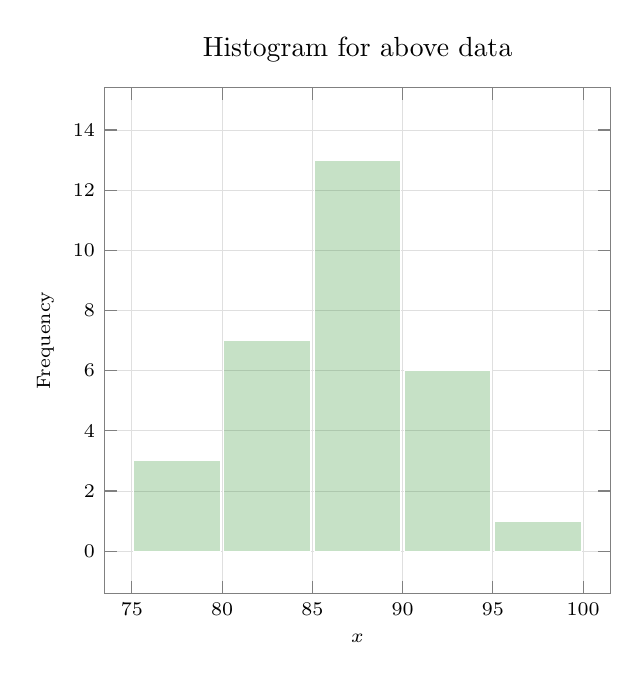
\begin{tikzpicture}
                  \begin{axis}[width = 8cm,title =
                              {Histogram for above data},
                          xlabel = $ x $, ylabel = Frequency, Ani,
                          xtick = {75,80,...,100}, enlargelimits = 0.2,
                          view = {0}{90}, grid = both,]
                      \addplot[ybar, bar width = 4.8, color = y_h!0,
                          fill = y_h, fill opacity = 0.25] coordinates
                          {(77.5,3) (82.5,7) (87.5,13) (92.5,6) (97.5,1)};
                  \end{axis}
              \end{tikzpicture}
          \end{figure}

          \begin{itemize}
              \item Bins are the intervals that the data is sorted into
              \item Bin edges are usually inclusive at the left side and exclusive at the
                    right side (barring the last bin).
              \item A relative frequency histogram is when the weight of all the bins add
                    up to one.
          \end{itemize}

    \item[Boxplot] A means of illustrating the data divided into the four quartiles,
          shown as the lower whisker, the lower end of the box, the median line,
          the upper end of the box and finally the upper whisker.
          \begin{figure}[H]
              \centering
              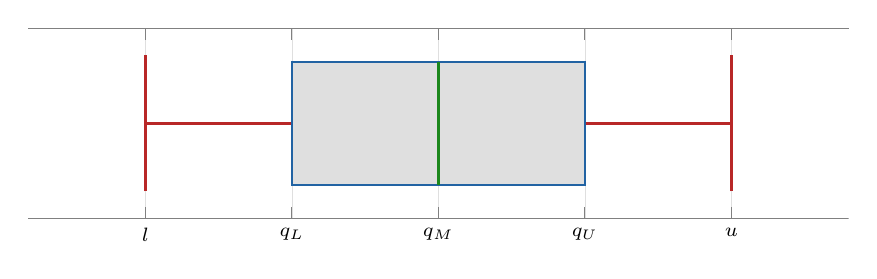
\begin{tikzpicture}
                  \begin{axis}[width = 12cm, height = 4cm, hide y axis,Ani,
                          xtick = {0,2.5,5,7.5,10},
                          xticklabels = {$ l $, $ q_L $, $ q_M $, $ q_U $, $ u $},
                          enlargelimits = 0.2,
                          grid = both,]
                      \addplot[
                          boxplot prepared={
                                  lower whisker=0,
                                  lower quartile=2.5,
                                  median=5,
                                  upper quartile=7.5,
                                  upper whisker=10,
                                  box extend=2,  % height of box
                                  whisker extend=2.2, % height of whiskers
                                  every box/.style={y_t, thick, fill=gray,
                                          fill opacity = 0.25},
                                  every whisker/.style={y_p, thick},
                                  every median/.style={y_h, thick},
                              },] coordinates {};
                  \end{axis}
              \end{tikzpicture}
          \end{figure}

    \item[Median] The middle value in the dataset, counting repetition. This is also the
          $ 50^{\text{th}} $ percentile of the dataset.

    \item[Interquartile range] The difference between the upper and lower quartile, as
          shown by the length of the box above ($ q_U - q_L $). \par
          The full range is the difference between the largest and smallest values,
          $ (l-u) $.

    \item[Outlier] For a box plot, any points that are more than 1.5 times the IQR
          from either end of the box is sufficiently far from the median to be declared
          an outlier.

    \item[Mean] The average of all the values (counted uniquely),
          each weighted by their frequency.
          \begin{align}
              \bar{x} & = \frac{1}{n}\ \sum_{i=1}^{n} x_i
          \end{align}

    \item[Variance] The sum of squares of the distance of every data point from the
          mean of the dataset.
          \begin{align}
              s^2 & \equiv \frac{1}{n-1}\ \sum_{i=1}^{n} (x_i - \bar{x})^2
          \end{align}
          The square root of the variance is called the standard deviation. This has the
          same physical dimensions as the original data.

    \item[Normal percentiles rule] For any bell-shaped curve symmetric about its center,
          the number of data points contained in the intervals are roughly,
          \begin{align}
              \SI{68}{\percent} \quad   & \text{in} \quad [\bar{x} - s, \bar{x} + s]   \\
              \SI{95}{\percent} \quad   & \text{in} \quad [\bar{x} - 2s, \bar{x} + 2s] \\
              \SI{99.7}{\percent} \quad & \text{in} \quad [\bar{x} - 3s, \bar{x} + 3s]
          \end{align}

    \item[z-Score] The distance of a data point within a data set from its mean,
          measured in units of variance.
          \begin{align}
              z(s) & = \frac{x - \bar{x}}{s}
          \end{align}
          From the above heuristic, $ z-$scores outside of $ \pm 3 $ can be considered
          outliers.
\end{description}

\section{Experiments, Outcomes, Events}

\begin{description}
    \item[Experiment] A process of measurement or observation. In probability theory,
          the processes being observed have some random element.

    \item[Trial] A single performance of an experiment, whose result is called an
          outcome.

    \item[Sample] A set of outcomes of performing an experiment $ n $ times. This number
          $ n $ is called the sample size.

    \item[Sample space] The set of all possible outcomes $ (S) $ of an experiment.

    \item[Event] A subset of the sample space of some random process. This could also
          be a subset with one element, which would be an outcome. \par
          The event is said to have occurred if the outcome of the experiment is a subset
          (or member) of the event set.

    \item[Set union] The set of all element that belong to one of the sets $ A $
          or $ B $
          \begin{align}
              C & \equiv A \cup B
          \end{align}

    \item[Set intersection] The set of all element that belong to both the sets $ A $ and
          $ B $
          \begin{align}
              C & \equiv A \cap B
          \end{align}

    \item[Set exclusion] The set of all element that belong to one set $ A $ but not
          the other set $ B $.
          \begin{align}
              C & \equiv A - B
          \end{align}

    \item[Null set] A set with non elements. Also called an empty set. The
          conventional symbol is $ \phi $

    \item[Disjoint sets] Two sets that do not have any elements in common. Their
          intersection is the null set. The events that correspond to such a pair of sets
          are mutually exclusive.
          \begin{align}
              A \cap B & = \phi
          \end{align}

    \item[Complement] The set of all elements in the sample space $ S $ that do not
          belong to $ A $.
          \begin{align}
              A^\complement & \equiv S - A & A \cap A^\complement & = \phi
          \end{align}

    \item[Venn diagrams] Representations of sets in $ 2D $ space used to illustrate
          set operations.
          \begin{figure}[H]
              \centering
              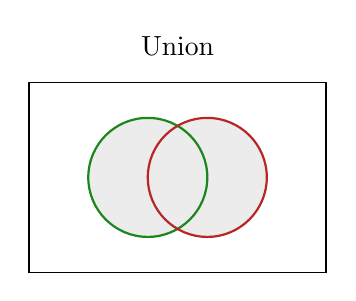
\begin{tikzpicture}
                  \begin{axis}[axis equal, height = 4cm,
                          title = {Union},axis lines = none, Ani,
                          xmin = -1.6,xmax = 1.6, ymin = -1.6, ymax = 1.6]
                      \filldraw[gray!15](-0.5,0) circle(1);
                      \filldraw[gray!15](0.5,0) circle(1);
                      \draw[y_h, thick] (-0.5,0) circle (1);
                      \draw[y_p, thick] (0.5,0) circle (1);
                      \draw[black, thick] (-2.5,-1.6) rectangle (2.5,1.6);
                  \end{axis}
              \end{tikzpicture}
              \hspace{3em}
              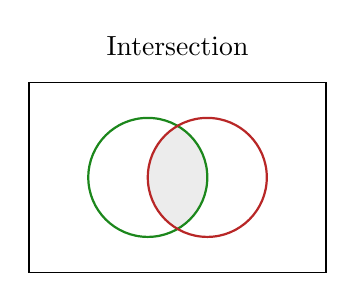
\begin{tikzpicture}
                  \begin{axis}[axis equal, height = 4cm,
                          title = {Intersection},axis lines = none, Ani,
                          xmin = -1.6,xmax = 1.6, ymin = -1.6, ymax = 1.6]
                      \begin{scope}
                          \clip (-0.5,0) circle(1);
                          \clip (0.5,0) circle(1);
                          \fill[gray!15](-0.5,0) circle(1);
                      \end{scope}
                      \draw[y_h, thick] (-0.5,0) circle (1);
                      \draw[y_p, thick] (0.5,0) circle (1);
                      \draw[black, thick] (-2.5,-1.6) rectangle (2.5,1.6);
                  \end{axis}
              \end{tikzpicture}
              \hspace{3em}
              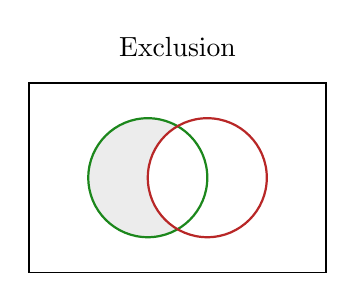
\begin{tikzpicture}
                  \begin{axis}[axis equal, height = 4cm,
                          title = {Exclusion},axis lines = none, Ani,
                          xmin = -1.6,xmax = 1.6, ymin = -1.6, ymax = 1.6]
                      \fill[gray!15](-0.5,0) circle(1);
                      \fill[white](0.5,0) circle(1);
                      \draw[y_h, thick] (-0.5,0) circle (1);
                      \draw[y_p, thick] (0.5,0) circle (1);
                      \draw[black, thick] (-2.5,-1.6) rectangle (2.5,1.6);
                  \end{axis}
              \end{tikzpicture}
          \end{figure}
          \begin{figure}[H]
              \centering
              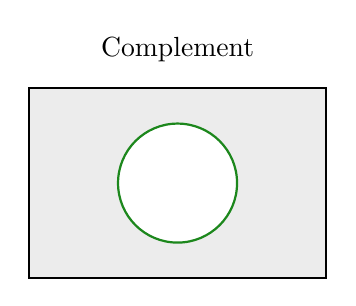
\begin{tikzpicture}
                  \begin{axis}[axis equal, height = 4cm,
                          title = {Complement},axis lines = none, Ani,
                          xmin = -1.6,xmax = 1.6, ymin = -1.6, ymax = 1.6]
                      \filldraw[gray!15] (-2.5,-1.6) rectangle (2.5,1.6);
                      \fill[white](0,0) circle(1);
                      \draw[y_h, thick] (0,0) circle (1);
                      \draw[black, thick] (-2.5,-1.6) rectangle (2.5,1.6);
                  \end{axis}
              \end{tikzpicture}
              \hspace{3em}
              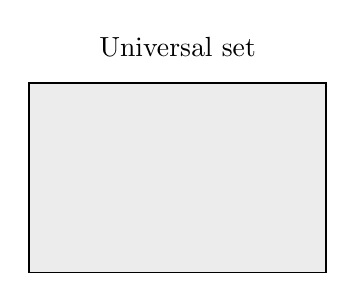
\begin{tikzpicture}
                  \begin{axis}[axis equal, height = 4cm,
                          title = {Universal set},axis lines = none, Ani,
                          xmin = -1.6,xmax = 1.6, ymin = -1.6, ymax = 1.6]
                      \filldraw[gray!15] (-2.5,-1.6) rectangle (2.5,1.6);
                      \draw[black, thick] (-2.5,-1.6) rectangle (2.5,1.6);
                  \end{axis}
              \end{tikzpicture}
          \end{figure}

    \item[Multiple sets] The intersection and union operations also extend to more
          than two sets using the notation,
          \begin{align}
              \bigcap_{j=1}^n A_j & = A_1 \cap A_2 \dots \cap A_n &
              \bigcup_{j=1}^n A_j & = A_1 \cup A_2 \dots \cup A_n
          \end{align}

    \item[De-Morgan's law] The relation between union and intersection of two sets
          utilizing their complements, is expressed as
          \begin{align}
              (A \cup B)^\complement & = A^\complement \cap B^\complement &
              (A \cap B)^\complement & = A^\complement \cup B^\complement
          \end{align}
          \begin{figure}[H]
              \centering
              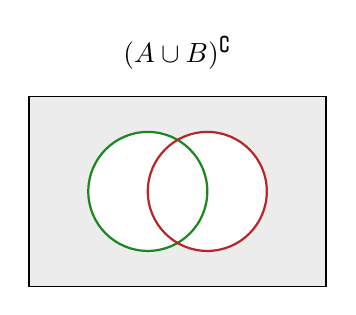
\begin{tikzpicture}
                  \begin{axis}[axis equal, height = 4cm,
                          title = {$ (A \cup B)^\complement $},axis lines = none, Ani,
                          xmin = -1.6,xmax = 1.6, ymin = -1.6, ymax = 1.6]
                      \filldraw[gray!15] (-2.5,-1.6) rectangle (2.5,1.6);
                      \fill[white](-0.5,0) circle(1);
                      \fill[white](0.5,0) circle(1);
                      \draw[y_h, thick] (-0.5,0) circle (1);
                      \draw[y_p, thick] (0.5,0) circle (1);
                      \draw[black, thick] (-2.5,-1.6) rectangle (2.5,1.6);
                  \end{axis}
              \end{tikzpicture}
              \hspace{3em}
              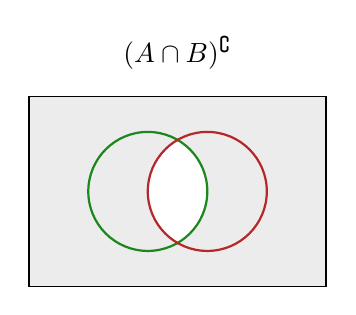
\begin{tikzpicture}
                  \begin{axis}[axis equal, height = 4cm,
                          title = {$ (A \cap B)^\complement $},axis lines = none, Ani,
                          xmin = -1.6,xmax = 1.6, ymin = -1.6, ymax = 1.6]
                      \filldraw[gray!15] (-2.5,-1.6) rectangle (2.5,1.6);
                      \begin{scope}
                          \clip (-0.5,0) circle(1);
                          \clip (0.5,0) circle(1);
                          \fill[white!15](-0.5,0) circle(1);
                      \end{scope}
                      \draw[y_h, thick] (-0.5,0) circle (1);
                      \draw[y_p, thick] (0.5,0) circle (1);
                      \draw[black, thick] (-2.5,-1.6) rectangle (2.5,1.6);
                  \end{axis}
              \end{tikzpicture}
          \end{figure}
\end{description}

\section{Probability}

\begin{description}
    \item[Finite sample space] For an experiment with a finite sample space $ S $ with
          equally likely outcomes, the probability of event $ A $ is defined as
          \begin{align}
              P(A) & = \frac{N_A}{N_S} & P(S) & = 1
          \end{align}
          where $ N $ is the number of outcomes. The probability of the entire sample
          space is unity, by convention.

    \item[Empirical probability] Given an experiment where a large number of trials
          have already been conducted and data gathered on the outcomes,
          \begin{align}
              P(A)        & \in [0,1]     & \forall \quad A & \in S  \\
              P(S)        & = 1                                      \\
              P(A \cup B) & = P(A) + P(B) & A \cap B        & = \phi
          \end{align}
          The last relation is for two or more mutually exclusive events.

    \item[Complement] The sum of the probabilities of an event and its complement
          is unity.
          \begin{align}
              P(A^\complement) & = 1 - P(A)
          \end{align}

    \item[Multiple mutually exclusive events] The probability of their union is
          simply the sum of the individual probabilities.
          \begin{align}
              P(A_1 \cup A_2 \cup \dots A_m) & = P(A_1) + P(A_2) + \dots + P(A_m)
          \end{align}

    \item[Set union] For events that are not mutually exclusive, using set addition,
          \begin{align}
              P(A \cup B) & = P(A) + P(B) - P(A \cup B) &
              P(\phi)     & = 0
          \end{align}

    \item[Conditional probability] The probability that event $ A $ occurs given
          $ B $ has already occurred, is
          \begin{align}
              P(A|B) & = \frac{P(A \cup B)}{P(B)}
          \end{align}
          Geometrically, the new sample space is $ B $ and the new numerator is that
          part of $ A $ which overlaps $ B $

    \item[Multiplication rule] Given two events $ A,B $ in a sample space $ S $,
          with $ P(A) \neq 0 $ and $ P(B) \neq 0 $,
          \begin{align}
              P(A \cup B) & = P(B) \cdot P(A|B) = P(A) \cdot P(B|A)
          \end{align}

    \item[Independent events] If two events $ A,B $ are independent, then no
          information about the occurrence of one is conveyed from the occurrence of the
          other.
          \begin{align}
              P(A|B)      & = P(A)            & P(B|A) & = P(B) \\
              P(A \cup B) & = P(A) \cdot P(B)
          \end{align}
          A set of more than two events is independet if and only if all subsets of
          two or more events taken at a time are also independent.

    \item[Sampling] The act of randomly drawing an object from a population. This can be
          done with or without replacement. \par
          When sampling with replacement, it is implicit that the population is shuffled
          after each replacement so that it is in as random a state as it was before the
          first sample was drawn.

\end{description}

\section{Permutations and Combinations}

\begin{description}
    \item[Permutation] An arrangement of a given set of objects in a specific order.
          The number of permutations of $ n $ different things taken all at a time is,
          \begin{align}
              n! & \equiv n(n-1)(n-2)\dots(2)(1)
          \end{align}
          If a total of $ n $ objects contain $ c $ types of objects, each with numbers
          $ n_i $, then the number of permutations is,
          \begin{align}
                & \frac{n!}{n_1!\ n_2!\ \dots\ n_c!} &
              n & = n_1 + n_2 + \dots + n_c
          \end{align}
          This assumes that the objects within one class are identical. The first
          formula is a special case of $ n $ classes each containing only one object.

    \item[Permutations of a subset] The number of permutations of $ n $ things
          taken $ k $ at a time for some $ k<n $, is
          \begin{align}
              \permu{n}{k} & = \frac{n!}{(n-k)!}       &
                           & \text{without repetition}   \\
                           & n^k                       &
                           & \text{with repetition}
          \end{align}

    \item[Combination] A selection of one or more things without regard to order.
          \begin{align}
              \binom{n}{k} & = \frac{n!}{(n-k)!\ k!}   &
                           & \text{without repetition}   \\
                           & \binom{n+k-1}{k}          &
                           & \text{with repetition}
          \end{align}

    \item[Factorial function] A function of non-negative integers defined as,
          \begin{align}
              n! & \equiv n \cdot (n-1)!    & 0! = 1 \\
              n! & = n(n-1)(n-2)\dots(2)(1)
          \end{align}

    \item[Stirling approximation] An approximation for large $ n $, which is
          asymptotically equal to $ n! $, is
          \begin{align}
              n! & \approxeq \sqrt{2\pi n}\ \Bigg( \frac{n}{e} \Bigg)^n
          \end{align}

    \item[Binomial coefficients] For some integer $ k $, and some nonnegative real $ a $,
          \begin{align}
              \binom{a}{k} & = \frac{a(a-1)\dots(a-k+1)}{k!} = \frac{a!}{(a-k)!\ k!}
          \end{align}
          By convention,
          \begin{align}
              \binom{a}{0} & = 1 & \binom{0}{0} & = 1
          \end{align}
          For the special case of integer $ a $, let $ a = n $,
          \begin{align}
              \binom{n}{k} & = \binom{n}{n-k} & n & \geq 0 \qquad k \in [0,n]
          \end{align}

    \item[Relations for binomial coefficients] A recursive relation that helps in
          calculating binomial coefficients is,
          \begin{align}
              \binom{a}{k} + \binom{a}{k+1} & = \binom{a+1}{k+1}
          \end{align}

    \item[Negative binomial coefficient] For some positive real $ m $ and non-negative
          integer $ k $,
          \begin{align}
              \binom{-m}{k} & = (-1)^m\ \binom{m+k-1}{k}
          \end{align}

    \item[Series sums of binomial coefficients] Two important relations are,
          \begin{align}
              \sum_{s=0}^{n-1}\binom{k+s}{k}             & = \binom{n+k}{k+1} \\
              \sum_{k=0}^{r}\binom{p}{k}\ \binom{q}{r-k} & = \binom{p+q}{r}
          \end{align}
\end{description}

\section{Random Variables. Probability Distributions}

\begin{description}
    \item[Random variable] The quantity observed in an experiment. This is assumed
          stochastic and the value it will assume in the next trial has an element of
          randomness. \par
          The random variable can take any value (or set of values) within the sample
          space $ S $ of an experiment.

    \item[Cumulative distribution function] The probability that a random variable
          $ X $ will not be larger than some number $ x $,
          \begin{align}
              F(x) & \equiv P(X \leq x)
          \end{align}

    \item[Probability distribution function] The probability that a random variable
          $ X $ will be equal to some value $ x $,
          \begin{align}
              f(x) & \equiv P(X = x)
          \end{align}

    \item[Probability of interval] Using the CDF, the probability of a random variable
          lying in an interval $ (a,b] $ is,
          \begin{align}
              P(a < X \leq b) & = F(b) - F(a)
          \end{align}

    \item[Discrete RVs] A random variable that can only assume either a finite or
          countably infinite number of values. Its PDF is given by
          \begin{align}
              f(x) & = \begin{dcases}
                           p_j & \quad\ \text{if}\quad  x = x_j \\
                           0   & \quad\ \text{otherwise}
                       \end{dcases}
          \end{align}
          where $ \{x_j\} $ is the set of values that the RV can assume, and $ p_j $
          are all positive numbers. \par
          The CDF is given by
          \begin{align}
              F(x) & = \sum_{x_j \leq x} p_j
          \end{align}
          This is a step function which jumps at each $ x_j $ and is flat otherwise. \par
          The probability of the RV lying in an interval is,
          \begin{align}
              P(a < X \leq b) & = \sum_{a < x_j \leq b}^{max} p_j
          \end{align}

    \item[Normalization] As a general rule, the probability of the sample space as a
          whole is equal to unity.
          \begin{align}
              \sum_{j} p_j & = 1
          \end{align}

    \item[Continuous RVs] For the case of random variables that can vary continuously
          over the real line, the CDF is defined using the integral,
          \begin{align}
              F(x) & = \int_{-\infty}^{x} f(v)\ \dl v
          \end{align}
          The PDF now becomes the derivative of the CDF, and is also called the
          probability density function.
          \begin{align}
              f(x) & = F'(x)
          \end{align}
          The PDF is always nonnegative and is continuous except for possibly at
          finitely many jump points. \par
          The probability of the RV lying in an interval is,
          \begin{align}
              P(a < X \leq b) & = \int_{a}^{b} f(v)\ \dl v
          \end{align}
          The normalization analog is now,
          \begin{align}
              \int_{-\infty}^{\infty} f(v)\ \dl v & = 1
          \end{align}
\end{description}

\section{Mean and Variance of a Distribution}

\begin{description}
    \item[Mean] The mean of a distribution is the analog of the average of a
          frequency distribution,
          \begin{align}
              \mu & = \sum_j x_j \cdot f(x_j)    &  & \text{discrete}   \\
              \mu & = \intRL x \cdot f(x)\ \dl x &  & \text{continuous}
          \end{align}
          This is also called the expected value of $ X $, with notation $ E[X] $.
          This is the value of the RV to be expected when manyw trials
          of the experiment are performed. \par
          If a distribution is symmetric w.r.t. $ x = c $, then,
          \begin{align}
              f(c+x) & = f(c-x) & \implies \quad \mu & = c
          \end{align}

    \item[Variance] A measure of the spread of a distribution about its mean,
          \begin{align}
              \sigma^2 & = \sum_j (x_j - \bar{x})^2\ f(x_j) &  & \text{discrete}   \\
              \sigma^2 & = \intRL (x-\mu)^2\ f(x)\ \dl x    &  & \text{continuous}
          \end{align}
          Its positive square root is called the standard deviation. \par
          Barring the case of a discrete distribution with only one value in its sample
          space, $ \sigma^2 > 0 $.

    \item[Linear transformation of RV] When a RV is transformed into another by a
          linear relation,
          \begin{align}
              Y     & = aX + b       & (a         & > 0)              \\
              \mu_Y & = a\ \mu_X + b & \sigma^2_Y & = a^2\ \sigma^2_X
          \end{align}

    \item[Standardized RV] A linear transformation that makes the mean 0 and
          variance 1.
          \begin{align}
              Z & \equiv \frac{X - \mu}{\sigma}
          \end{align}

    \item[Expectation] For a non-constant and continuous function $ g(x) $, a random
          variable can be constructed as $ g(X) $. \par
          Its expected value is,
          \begin{align}
              \ex[g(X)] & = \sum_j g(x_j) \cdot f(x_j)    &  & \text{discrete}   \\
              \ex[g(X)] & = \intRL g(x) \cdot f(x)\ \dl x &  & \text{continuous}
          \end{align}
          A restatement of the normalization condition is,
          \begin{align}
              \ex(1) & = \intRL 1 \cdot f(x)\ \dl x = 1
          \end{align}

    \item[$k^{\text{th}}$ moment of X] For a random variable $ X $, special cases of
          expectation values, are powers of $ x $, called moments,
          \begin{align}
              \ex[X^k] & = \sum_j x_j^k \cdot f(x_j)    &  & \text{discrete}   \\
              \ex[X^k] & = \intRL x^k \cdot f(x)\ \dl x &  & \text{continuous}
          \end{align}
          The first moment happens to be the mean.

    \item[Central moment] Similar to the moments, the central moments are special
          expectation values for powers of $ (X - \mu) $
          \begin{align}
              \ex[(X - \mu)^k] & = \sum_j (x_j - \mu)^k \cdot f(x_j)    &
                               & \text{discrete}                          \\
              \ex[(X - \mu)^k] & = \intRL (x - \mu)^k \cdot f(x)\ \dl x &
                               & \text{continuous}
          \end{align}
          The second central moment happens to be the variance.
\end{description}

\section{Binomial, Poisson, and Hypergeometric Distributions}

\begin{description}
    \item[Binomial distribution] If an event $ A $ has the probability of occurrence
          $ p $, in one trial, and there are $ n $ independent trials, then the number
          of times $ A $ occurs is
          \begin{align}
              P(X=x) = p^x\ (1-p)^{n-x}
          \end{align}
          Now, since there are many sequences of $ n $ events which give the same
          probability, accounting for them gives the PDF
          \begin{align}
              f(x) & = \binom{n}{x}\ p^x q^{n-x} & q & \equiv 1-p
          \end{align}
          The sample space is $ x \in \{0,1,\dots,n\} $. This PDF is also called the
          Bernoullu distribution.
          \begin{align}
              \mu & = np & \sigma^2 & = np(1-p)
          \end{align}

    \item[Poisson distribution] The extension of the binomial distribution to a large
          number of trials $ n $ and with chance of success $ p \to 0 $, such that $ np $
          remains finite.
          \begin{align}
              f(x) & = \frac{\lambda^x}{x!}\ e^{-\lambda}
          \end{align}
          This PDF has the special property of having variance and mean both equal to
          its parameter $ \lambda $.
          \begin{align}
              \mu & = \lambda = np & \sigma^2 & = \lambda = npq \approxeq np
          \end{align}
          Since $ q \to 1 $, the variance approaches the mean.

    \item[Hypergeometric distribution] The binomial distribution assumes sampling
          with replacement, since this is necessary for the trials to be independent.
          \par
          Consider sampling $ x $ objects from a total of $ N $ objects. Assume $ M $
          of those objects are desirable. \par
          The number of desirable objects drawn in $ n $ trials when sampling without
          replacement is now
          \begin{align}
              f(x) & = \frac{\binom{M}{x}\ \binom{N-M}{n-x}}{\binom{N}{n}}
          \end{align}
          The mean and variance are,
          \begin{align}
              \mu      & = \frac{M}{N} \cdot n                          &
              \sigma^2 & = \frac{nM}{N} \cdot \frac{(N-M)(N-n)}{N(N-1)}
          \end{align}
          Note that in the limit of $ N,M \gg n $, whether or not replacement happens
          is irrelevant, and the hypergeometric distribution reduces to the binomial
          distribution with $ p = M/N $.
\end{description}

\section{Normal Distribution}

\begin{description}
    \item[Importance] Most useful continuous RVs can be transformed into normal RVs using
          simple transformations. Also, many processes in real life happen to have a
          normal PDF.

    \item[General form] A normal distribution with mean $ \mu $ and standard deviation
          $ \sigma $, is
          \begin{align}
              f(x) & = \frac{1}{\sigma\ \sqrt{2\pi}}\ \exp\Bigg[ -\frac{1}{2}
                  \ \left( \frac{x-\mu}{\sigma} \right)^2 \Bigg]
          \end{align}
          The pre-factor is the normalization constant. The PDF is symmetric about
          $ \mu $.

    \item[Normal CDF] The CDF of the normal distribution cannot be found analytically.
          Tabulated values of the standard normal distribution (with $ \mu = 0$ and
          $ \sigma = 1 $) are used in calculations.
          \begin{align}
              \Phi(z) & = F(z;0,1) = \frac{1}{\sqrt{2\pi}}\ \int_{-\infty}^{z}
              e^{-u^2/2}\ \dl u                                                \\
              F(x)    & = \Phi\Bigg( \frac{x-\mu}{\sigma} \Bigg)
          \end{align}
          This transformation enables computation of any other normal distribution in
          terms of the standard normal $ \Phi(x) $. For the probability of an interval,
          \begin{align}
              P(\textcolor{y_h}{a} < X \leq \textcolor{y_p}{b}) & =
              F(\textcolor{y_p}{b}) - F(\textcolor{y_h}{a}) =
              \Phi\Bigg( \frac{\textcolor{y_p}{b}-\mu}{\sigma} \Bigg)
              - \Phi\Bigg( \frac{\textcolor{y_h}{a}-\mu}{\sigma} \Bigg)
          \end{align}

    \item[Percentiles] Heuristics for the fraction of all data points lying at some
          distance from the mean, are as follows,
          \begin{figure}[H]
              \centering
              \begin{tikzpicture}
                  \begin{axis}[title = {Standard normal}, Ani,
                          grid = both, xmin=-4, xmax=4, xlabel = {$ z $},
                          ylabel = {$ \Phi(z) $}]
                      \addplot[name path = topb, black!0, domain = -1:1]
                      {normPDF(x,0,1)};
                      \addplot[name path = topa, black!0, domain = -4:-1]
                      {normPDF(x,0,1)};
                      \addplot[name path = topc, black!0, domain = 1:4]
                      {normPDF(x,0,1)};
                      \addplot[name path = bottomb, black!0, domain = -1:1] {0};
                      \addplot[name path = bottoma, black!0, domain = -4:-1] {0};
                      \addplot[name path = bottomc, black!0, domain = 1:4] {0};
                      \addplot [fill=y_p, fill opacity=0.08]
                      fill between[of=topb and bottomb];
                      \addplot [fill=black, fill opacity=0.08]
                      fill between[of=topa and bottoma];
                      \addplot [fill=black, fill opacity=0.08]
                      fill between[of=topc and bottomc];
                      \addplot[GraphSmooth, y_h, domain = -4:4]
                      {normPDF(x,0,1)};
                      \node[y_p] at (axis cs:0, 0.2){$ 68 \% $};
                      \node[black] at (axis cs:1.5, 0.05){$ 16 \% $};
                      \node[black] at (axis cs:-1.5, 0.05){$ 16 \% $};
                  \end{axis}
              \end{tikzpicture}
          \end{figure}
          \begin{table}[H]
              \centering
              \begin{tblr}{colspec = {l|r|[dotted]c|[dotted]l},
                  colsep = 1.2em}
                  Interval           & Left   & Inside & Right  \\ \hline
                  $ (x\pm\sigma) $   & 16\%   & 64\%   & 16\%   \\
                  $ (x\pm 2\sigma) $ & 2.25\% & 95.5\% & 2.25\% \\
                  $ (x\pm 3\sigma) $ & 0.15\% & 99.7\% & 0.15\% \\
              \end{tblr}
          \end{table}
          Almost all of the data points are contained in the interval $ \mu \pm 3\sigma $,
          and these intervals are commonly used in statistical tests.

    \item[Normal approximation of Binomial PDF] For a binomial PDF with large $ n $ and
          small $ p $ such that the mean $ np $ remains finite, an asymptotic
          approximation is the normal distribution with mean $ np $ and variance
          $ np(1-p) $
          \begin{align}
              f^*(x) & = \frac{1}{\sqrt{2\pi\ np(1-p)}}\ e^{-z^2/2} &
              z      & = \frac{x - np}{\sqrt{np(1-p)}}
          \end{align}
          This also means that the probabilities such a binomial RV lying in the interval
          $ [a,b] $ can be approximated using,
          \begin{align}
              P(a \leq X \leq b) & \approxeq \Phi(\beta) - \Phi(\alpha)   \\
              \alpha             & = \frac{a-np-0.5}{\sqrt{np(1-p)}}    &
              \alpha             & = \frac{b-np+0.5}{\sqrt{np(1-p)}}
          \end{align} $ \Phi(\beta) - \Phi(\alpha) $, assuming
          $ a, b $ are non-negative integers. The extra $ 0.5 $ in the numerator is
          a correction term in going from a discrete to a continuous PDF.
\end{description}

\section{Distributions of Several Random Variables}

\begin{description}
    \item[Two dimensional CDF] A CDF of two random variables that are independent is
          defined as,
          \begin{align}
              F(x, y) & = P(X \leq x, Y \leq y)
          \end{align}
          both inequalities have to in this definition. For the probability of a 2d
          region,
          \begin{align}
              P(a_1 \leq X \leq b_1,\ a_2 \leq Y \leq b_2)
               & = F(b_1, b_2) + F(a_1,b_2)  \\
               & - [F(b_1,a_2) - F(a_1,a_2)]
          \end{align}

    \item[Discrete 2d RV] Using the shorthand
          \begin{align}
              P(X = x_i, Y = y_j) & = f(x_i, y_j) = p_{ij}
          \end{align}
          and accommodating the fact that these probabilities may be zero at some of
          these points,
          The CDF is simply the double sum over these two independent indices $ i,j $,
          \begin{align}
              F(x, y) & = \sum_{x_i \leq x} \sum_{y_j \leq y} f(x_i, y_j)
          \end{align}
          with the normalization condition still being that the probabilities over all
          points sum to unity.

    \item[Continuous 2d RV] The double sum is replaced by a double integral over $ x $
          and $ y $, giving the CDF,
          \begin{align}
              F(x, y) & = \int_{-\infty}^{y} \int_{-\infty}^{x}
              f(u, v)\ \dl u\ \dl v
          \end{align}
          Here, the PDF is called the density $ f(x, y) $. It is nonnegative and
          defined everywhere except possibly at finitely many curves in the domain.
          \par
          The probability of a rectangular region in the 2d domain of definition is,
          \begin{align}
              P(a_1 \leq X \leq b_1, a_2 \leq Y \leq b_2)
               & = \int_{a_2}^{b_2} \int_{a_1}^{b_1} f(x, y)\ \dl x\ \dl y
          \end{align}

    \item[Marginal distributions of a discrete RV] The PDF over one of the many variables
          is obtained by simply summing over all possible values of the other variables,
          \begin{align}
              f_1(x) & = P(X = x, Y\ \text{arbitrary}) = \sum_{y} f(x, y)
          \end{align}
          The CDF of the marginal distribution of $ X $ becomes,
          \begin{align}
              F_1(x) & = \sum_{x^* \leq x} f_1(x^*)
          \end{align}

    \item[Marginal table] For the special case of a discrete $ 2d $ RV, the sum of
          the probabilities of each row and column is directly the marginal distribution
          of the column and row indices respectively.

    \item[Marginal distributions of a continuous RV] Replacing the summation with
          integration, the marginal PDF is,
          \begin{align}
              f_1(x) & =  \intRL f(x, y)\ \dl y           &
              F_1(x) & = \int_{-\infty}^{x} f_1(u)\ \dl u
          \end{align}

    \item[Independence of RVs] Two RVs are independent if and only if their joint
          CDF is the product of their marginal CDFs.
          \begin{align}
              F(x, y) & = F_1(x) \cdot F_2(y) & f(x, y) & = f_1(x) \cdot f_2(y)
          \end{align}
          for all values of $ x,y $. This uses the fact that the joint probability of
          two independent events is the product of their individual probabilities. \par
          This definition extends to more than 2 RVs with no changes to the definitions.

    \item[Functions of RVs] If a new RV is defined as a non-constant function of two
          other RVs,
          \begin{align}
              Z & = g(X, Y)
          \end{align}
          Similar to functions of a single RV,
          \begin{align}
              f(z) & = P(Z = z) = \mathop{\sum \sum}_{g(x,y) = z} f(x, y)       \\
              F(z) & = P(Z \leq z) = \mathop{\sum \sum}_{g(x,y) \leq z} f(x, y)
          \end{align}

          For a continuous RV, the CDF becomes
          \begin{align}
              F(z) & = P(Z \leq z) = \iint\limits_{g(x, y) \leq z} f(x, y)\ \dl x\ \dl y
          \end{align}
          The boundary curve of this region of integration is the level curve
          $ g(x,y) = z $

    \item[Addition of means] Since the expectation value of a function of two RVs is
          defined as
          \begin{align}
              \ex[g(X,Y)] & = \sum_x \sum_y g(x,y)\ f(x,y) &  & \text{discrete}   \\
              \ex[g(X,Y)] & = \intRL \intRL g(x,y)\ f(x,y) &  & \text{continuous}
          \end{align}
          This assumes that the double summation converges and that the double integral
          exists (is finite). \par
          A special case is,
          \begin{align}
              \ex[X+Y]                     & = \ex[X] + \ex[Y]             \\
              \ex[X_1 + X_2 + \dots + X_n] & = \ex[X_1] + \dots + \ex[X_n]
          \end{align}

    \item[Multiplication of means] The expected value of the product of independent
          RVs is the product of their individual means.
          \begin{align}
              \ex[X_1 \cdot X_2 \cdots X_n] & = \ex[X_1] \cdot \ex[X_2] \cdots \ex[X_n]
          \end{align}

    \item[Covariance] For two real RVs, the expected value of the product of their
          deviation from their respective mean values is called the covariance.
          \begin{align}
              \Cov[X,Y] & \equiv \ex[(X - \mu_X)(Y - \mu_Y)] \\
                        & = \ex[XY] - \ex[X] \cdot \ex[Y]
          \end{align}
          This is positive if greater values of $ X $ occur more frequently when
          accompanied by greater values of $ Y $ and vice versa. The covariance of
          two RVs being zero is a sign of their independence.

    \item[Addition of Variances] For a sum of two RVs,
          \begin{align}
              Z        & = X + Y                                &
              \Var[Z]  & = \ex[Z^2] - (\ex[Z])^2                  \\
              \sigma^2 & = \sigma_1^2 + \sigma_2^2 + 2\Cov[X,Y]
          \end{align}
          For the special case of $ n $ independent RVs,
          \begin{align}
              \Var[X_1 + X_2 + \dots + X_n] & = \Var[X_1] + \dots + \Var[X_n]
          \end{align}
          since the covariance of any two or more terms $ \{X_i\} $ is zero.
\end{description}
% \chapter{Mathematical Statistics}

\section{Introduction, Random Sampling}

\begin{description}
    \item[Sample] A small percentage of a population on which tests are conducted.
          Random sampling means selection of elements from the population with no bias.
          \par This helps draw inferences about the characteristics of the population
          from tests conducted on the sample.

    \item[Independent sample] For a population being sampled with replacement, or a
          very large finite population being sampled without replacement, the samples
          are independent. \par
          Samples from a distribution that has an infinite sample space $ S $ are also
          independent.

    \item[Psudorandom numbers] Computer programs that generate random numbers are not
          truly random, since there is an underlying mathematical function responsible
          for generating them. \par
          They are however, good enough for all practical purposes (barring niche uses
          such as cryptography).

    \item[Sample mean] Consider a set of $ n $ samples selected from a population. The
          mean of the sample is now,
          \begin{align}
              \bar{x} & = \frac{1}{n}\ \sum_{j=1}^{n} x_j
              = \frac{x_1 + x_2 + \dots + x_n}{n}
          \end{align}
          Here, $ n $ is called the sample size.

    \item[Sample variance] Analogously, the sample variance is defiend as,
          \begin{align}
              s^2 & = \frac{1}{n-1}\ \sum_{j=1}^{n} (x_j - \bar{x})^2
              = \frac{(x_1 - \bar{x})^2 + \dots + (x_n - \bar{x})^2}{n-1}
          \end{align}
          The square root of the sample variance is called the sample standard deviation
          $ s $. The factor being $ (n-1) $ instead of $ n $, is preferable for smaller
          sample sizes.
\end{description}

\section{Point Estimation of Parameters}

\begin{description}
    \item[Point estimate] A real number that serves as an approximation to the population
          statistic computed from some operation on a random sample. \par
          The convention used for point estimates here is a hat.

    \item[Mean] The sample mean is the point estimate of the population mean.

    \item[Variance] The sample variance is the point estimate of the population variance.

    \item[Binomial parameter] Since the binomial parameter is,
          \begin{align}
              p & = \frac{\mu}{n} & \hat{p} & = \frac{\bar{x}}{n}
          \end{align}

    \item[Moments] Since most parameters of a PDF can be expressed in terms of the
          population moments, they can in turn be approximated by the sample moments in
          order to obtain point estimates of these parameters.
          \begin{align}
              m_k & = \frac{1}{n}\ \sum_{j=1}^{n} x_j^k
          \end{align}
          for a sample of size $ n $. For example, the mean is the first moment, and
          the variance is the second central moment.

    \item[Maximum Likelihood method] Consider a PDF dependent on a single parameter
          $ \theta $, with a $ n $ independent random values drawn from it randomly.
          \par The probability that the sample drawn consists of the specific values
          $ \{x_1,x_2,\dots,x_n\} $ is called the likelihood $ l $,
          \begin{align}
              l & \equiv f(X = x_1) \cdot f(X = x_2) \cdots f(X = x_n)
          \end{align}
          The MLE method now involves choosing the value of the parameter $ \theta^* $
          such that $ l $ is maximized.
          \begin{align}
              l                  & \to l\Big( \theta\ ; \{x_i\}\Big) &
              \diffp {l}{\theta} & = 0
          \end{align}
          That value of $ \theta $ for which this probabiliity $ (l) $ is the greatest
          is considered the point estimate of $ \theta $. This is called the MLE of
          the parameter $ \theta $. \par
          Sometimes, the monotonous nature of $ l $, means that a sufficient condition
          for the maxima is,
          \begin{align}
              \diffp {\ln(l)}{\theta} = 0
          \end{align}

    \item[MLE with multiple parameters] For more than one parameter $ \{\theta_j\} $,
          the likelihood needs to be minimized w.r.t. each of these parameters.
          \begin{align}
              \diffp {l}{\theta_j} & = 0 & \forall \quad j & \in \{1,2,\dots,M\}
          \end{align}
\end{description}

\section{Confidence Intervals}

\begin{description}
    \item[Confidence interval] An interval within which a statistic is estimated to
          lie with some probability (called the confidence).
          \begin{align}
              \CONF_\gamma\{\theta_1 \leq \theta \leq \theta_2\}
          \end{align}
          Popular choices for the confidence $ \gamma $ are $ 95\% $ and $ 99\% $. \par
          This is not a declaration that $ \theta $ must lie within the interval
          $ [\theta_1,\theta_2] $, only that it does so with a certain probability.

    \item[Mean of normal distribution with known variance] Let $ \{X_i\} $ be a set of
          RVs that are independent and each of which has mean $ \mu $ and variance
          $ \sigma^2 $. \par
          The sample mean $ \bar{X} $ has mean $ \mu $ and variance $ \sigma^2/n $
          \begin{align}
              Z & = \frac{\bar{x} - \mu}{\sigma/\sqrt{n}}
          \end{align}
          is a standard normal RV. (in spite of the original $ X $ not having a normal
          PDF). \par
          This uses the trick that flipping the same coin many times is statistically
          the same as flipping many coins once.

    \item[Student's t-distribution] Consider a population of mean $ \mu $ and variance
          $ \sigma^2 $ from which a sample of size $ n $ is drawn, with sample mean
          $ \bar{X} $ and sample variance $ S $,
          \begin{align}
              S       & = \frac{1}{(n-1)} \sum_{j=1}^{n} (X_j - \bar{X})^2 &
              \bar{X} & = \frac{1}{n}\ \sum_{j=1}^{n} X_j
          \end{align}
          The following analog of the standard normal variable,
          \begin{align}
              T & = \frac{\bar{X} - \mu}{S/\sqrt{n}}
          \end{align}
          has a CDF called the Student's t-distribution with $ (n-1) $ degrees of freedom
          (which looks very similar to the standard normal CDF). \par
          This CDF becomes the Cauchy distribution for $ n=0 $ and the normal
          distribution asymptotically as $ n \to \infty $. \par
          The CDF is given by
          \begin{align}
              F(z) & = K_m\ \int_{-\infty}^{x} \Bigg( 1 + \frac{u^2}{m}
              \Bigg)^{(m+1)/2}
              \ \dl u                                                                \\
              K_m  & = \frac{1}{\sqrt{m\pi}}\ \frac{\Gamma\Big( \frac{m+1}{2} \Big)}
              {\Gamma(m/2)}
          \end{align}
          with the normalization term $ K_m $, which depends on the Gamma function.

    \item[Mean of normal distribution with unknown variance] For a given confidence
          level $ \gamma $, find the $ t $ score corresponding to
          \begin{align}
              F(t) & = \frac{\gamma + 1}{2}
          \end{align}
          using lookup tables for the Student's t-distribution with $ (n-1) $ degrees of
          freedom. Then,
          \begin{align}
              k & = \frac{cs}{\sqrt{n}} &
              \CONF_\gamma\{\bar{x} - k \leq \mu \leq \bar{x} + k\}
          \end{align}
          Here, $ \bar{x} $ and $ s $ are the sample mean and standard deviation for a
          sample of size $ n $. \par
          Not knowing the variance means that the same confidence value requires a
          larger interval than the normal distribution (which is used when the variance
          is known). \par
          The smaller the sample size, the tighter the confidence interval when
          the variance is known.

    \item[Chi-squared distribution] The PDF of the sum of the squares of $ m $
          independent standard normal variables.
          \begin{align}
              F(z) & = C_m\ \int_{0}^{z} e^{-u/2}\ u^{(m-2)/2}\ \dl u &
              u    & \geq 0                                             \\
              C_m  & = \frac{1}{2^{m/2}\ \Gamma(m/2)}
          \end{align}
          where $ m $ is the degree of freedom and $ C_m $ is the corresponding
          normalization constant. \par
          For a sample with standard deviation $ S $, the variable
          \begin{align}
              Y & = (n-1)\ \frac{S^2}{\sigma^2}
          \end{align}
          has a $ \chi^2 $ distribution with $ (n-1) $ degrees of freedom.

    \item[Variance of normal distribution] For a confidence level $ \gamma $, use the
          lookup table of the $ \chi^2 $ distribution with $ (n-1) $ degrees of freedom,
          to find
          \begin{align}
              F(\chi_1) & = \frac{1-\gamma}{2}                             &
              F(\chi_2) & = \frac{1+\gamma}{2}                               \\
              k_1       & = \frac{(n-1)}{\chi_1}\ s^2                      &
              k_2       & = \frac{(n-1)}{\chi_2}\ s^2                        \\
                        & \CONF_\gamma\{\chi_2 \leq \sigma^2 \leq \chi_1\}
          \end{align}

    \item[Central limit theorem] Let $ \{X_i\} $ be independent identically distributed
          RVs, each with the same mean $ \mu $ and same variance $ \sigma^2 $. \par
          Define the new RV using their sum,
          \begin{align}
              Y_n & = X_1 + \dots + X_n                    &
              Z_n & = \frac{Y_n - n\mu}{\sigma / \sqrt{n}}
          \end{align}
          The RV $ Z_n $ is asymptotically a standard normal RV, satisfying,
          \begin{align}
              \lim_{n \to \infty} F_n(x) & = \Phi(x) = \frac{1}{\sqrt{2\pi}}
              \ \int_{-\infty}^{x} e^{-u^2/2}\ \dl u
          \end{align}
          A rule of thumb is to use $ n \geq 20 $ for the mean and $ n \geq 50 $ for
          the variance.

\end{description}

\section{Testing of Hypotheses. Decisions}

\begin{description}
    \item[Null hypotesis] A claim that is to be tested using statistical methods. If the
          null hypothesis is only wrong within the limits of the confidence value of
          the test, it is accepted.
          \begin{align}
              \theta & = \theta_0
          \end{align}
    \item[Alternative hypothesis] Another hypothesis mutually exclusive to the null
          hypothesis that, if true, leads to the initial claim being rejected.
          \begin{align}
              \theta & \neq \theta_0 &  & \text{Two - sided}         \\
              \theta & \geq \theta_0 &  & \text{One - sided (right)} \\
              \theta & \leq \theta_0 &  & \text{One - sided (left)}
          \end{align}

    \item[Rejection region] The part of the real line on which the statistic has to
          lie for the null hypothesis to be rejected.
          \begin{figure}[H]
              \centering
              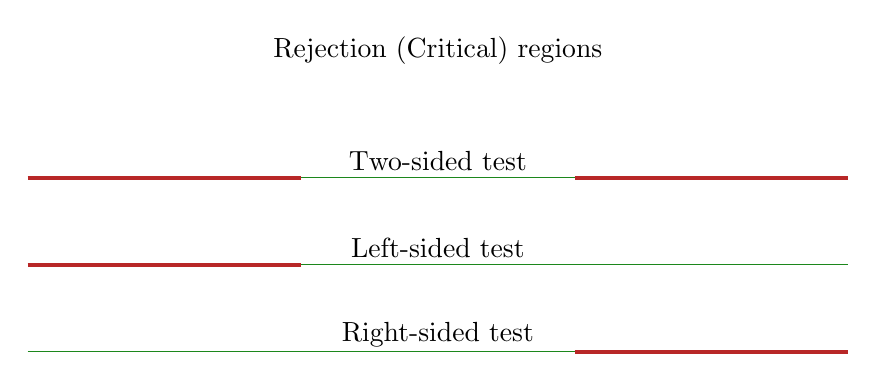
\begin{tikzpicture}
                  \begin{axis}[height = 6cm, title = {Rejection (Critical) regions},
                          Ani, xmin = -3,xmax = 3, xlabel = Statistic,
                          ymin = -1, ymax = 3, axis lines = none]
                      \addplot[y_p, domain = 1:3, very thick] ({x},{0});
                      \addplot[y_h, domain = -3:1, thin] ({x},{0});
                      \addplot[y_p, domain = -3:-1, very thick] ({x},{1});
                      \addplot[y_h, domain = -1:3, thin] ({x},{1});
                      \addplot[y_p, domain = 1:3, very thick] ({x},{2});
                      \addplot[y_p, domain = -3:-1, very thick] ({x},{2});
                      \addplot[y_h, domain = -1:1, thin] ({x},{2});
                      \node at (axis cs:0,0.2){Right-sided test};
                      \node at (axis cs:0,1.2){Left-sided test};
                      \node at (axis cs:0,2.2){Two-sided test};
                  \end{axis}
              \end{tikzpicture}
          \end{figure}

    \item[Errors in tests] The act of rejecting a true hypothesis is called a Type I
          error, denoted $ \alpha $. \par
          The act of accepting a false hypothesis is called a Type II
          error, denoted $ \beta $. \par
          For simplicity, consider a test where the null and alternative hypotheses are
          two values of the parameter $ \theta $, given by $ \theta_0, \theta_1 $
          respectively. Now,
          \begin{table}[H]
              \centering
              \begin{tblr}{colspec = {cccc}, rowsep = 1em, colsep = 1.5em,
                  vline{3,4,5} = {3,4}{solid}}
                                                            &                       &
                  \SetCell[c=2]{m} Unknown truth            &                         \\
                  \hline[dotted]
                                                            &                       &
                  $ \theta = \theta_0 $                     & $ \theta = \theta_1 $   \\
                  \hline
                  \SetCell[r=2]{m} \rotatebox{90}{Accepted} & $ \theta = \theta_0 $ &
                  {\textcolor{y_h}{True Decision}                                     \\
                  $ P = 1-\alpha $}                         & {\textcolor{y_p}
                  {Type II Error}                                                     \\
                  $ P = \beta $}                                                      \\
                  \hline[dotted]
                                                            & $ \theta = \theta_1 $ &
                  {\textcolor{y_p}{Type I Error}                                      \\
                  $ P = \alpha $}                           & {\textcolor{y_h}
                  {True Decision}                                                     \\
                  $ P = 1 - \beta $}                                                  \\
                  \hline
              \end{tblr}
          \end{table}
          Since reducing Type I errors involves changing the significance value in a way
          that increases Type II errors, there is a delicate balance needed between these
          two issues.

    \item[Power of a test] The probability of a Type I error is the familiar
          significance level of a test. It measures the chances of rejecting a true n.h.
          \par
          The analog is the value $ (\beta) $ of a test, which measures the probability
          of accepting a false hypothesis. The power is then defined as
          \begin{align}
              \eta & = 1 - \beta &  & = P(\ \text{rejection}\ |\ \text{false}\ )
          \end{align}

    \item[Operating Characteristic] If the alternative hypothesis is an interval instead
          of a single point, then $ \beta $ is a function of $ \theta $ and is called the
          operating characteristic (OC) curve. \par
          Similarly, the power $ \eta $ is also a function of $ \theta $ and is called
          the power function of the test.

    \item[Comparison between the means of two samples] If the elements of the two samples
          can be paired, (possibly because they imply the use of two different methods to
          measure the same value), then testing for the difference between the pairwise
          elements of the two samples having zero mean is more useful. \par
          If no such pairing across samples is possible, then they can be consolidated
          into a single RV,
          \begin{align}
              Z     & = X - Y                           &
              \mu   & = \bar{x} - \bar{y}                 \\
              s_z^2 & = (n_x - 1)s_x^2 + (n_y - 1)s_y^2
          \end{align}
          Here the addition of variances is used, assuming that the sample elements are
          independently drawn and have the same underlying PDF.

    \item[Comparison of variances of two samples] The ratio of the sample variance of
          two different samples $ s_x, s_y $ when arranged as
          \begin{align}
              V & = \frac{s_x^2}{s_y^2}
          \end{align}
          where $ v $ is an RV with an $ F $ distribution with $ (n_1-1, n_2-1) $
          degrees of freedom. \par
          The F-distribution is given by,
          \begin{align}
              F(z) & = K_{mn}\ \int_{0}^{z} t^{(m-2)/2}\ (mt + n)^{-(m+n)/2}\ \dl t
          \end{align}
          and $ K_{mn} $ is the normalization constant given by
          \begin{align}
              K_{mn} & = \frac{m^{m/2}\ n^{n/2}\ \Gamma[(m+n)/2]}
              {\Gamma(m/2)\ \Gamma(n/2)}
          \end{align}
          This is the ration of two independent $ \chi^2 $ RVs, normalized by their
          respective degrees of freedom.
          \begin{align}
              F & = \frac{\chi_1 / d_1}{\chi_2 / d_2}
          \end{align}
          This is an indication of how the ration of the variances of two samples might
          use the $ F $ distribution as a basis for hypothesis testing.

\end{description}

\section{Quality Control}

\begin{description}
    \item[Periodic testing] Instead of waiting for an entire lot of products to be
          produced before performing statistical inference on a random sample, industrial
          processes prefer to sample periodically from the assembly line during
          production.

    \item[Control chart for the mean] The upper and lower control limits are the limits
          corresponding to the $ 99\% $ confidence interval for the mean, which
          corresponds to $ \alpha = 1\% $ (by convention).

          \begin{align}
              \text{LCL}         & = \mu_0 - \frac{c\sigma}{\sqrt{n}} &
              \text{UCL}         & = \mu_0 + \frac{c\sigma}{\sqrt{n}}   \\
              \Phi(c) - \Phi(-c) & = 0.99
          \end{align}

    \item[Variance] The variance is assumed to be known from historical data, or is
          calculated as the average of the variance from the past few samples (about 25
          by convention).

    \item[Control chart for the Variance] The confidence interval for the
          variance (as caluclated by the $ \chi^2 $ test) is imposed.
          \begin{align}
              \text{LCL}            & = \frac{\sigma^2}{n-1}\ c_1 &
              \text{UCL}            & = \frac{\sigma^2}{n-1}\ c_2   \\
              P(\chi^2_{n-1} < c_1) & = \alpha/2                  &
              P(\chi^2_{n-1} > c_2) & = \alpha/2
          \end{align}
          The corresponding right sided $ \chi^2 $ test is used if only an upper limit on
          the variance needs to be enforced.

    \item[Control chart for the range] The expected value of the range $ (R) $ of a
          sample, is proportional to the sample standard deviation $ (s) $ by a factor
          dependent on the sample size $ n $.
          \begin{align}
              \sigma & = \lambda_n \cdot \ex[R^*]
          \end{align}
          By convention, it is better to use $ s $ instead of $ R $ as a quality
          control method when $ n > 10 $.
\end{description}

\section{Acceptance Sampling}

\begin{description}
    \item[Acceptance number] An upper limit on the number of defective items in a
          random sample of size $ n $ from a population of size $ N $. \par
          If the number of defectives is larger than this limit $ c $, the lot is
          rejected.

    \item[Operating Characteristic] A curve showing the CDF of the hypergeometric
          distribution with $ n $ items selected out of a population of size $ N $ with
          defective fraction $ \theta $
          \begin{align}
              P(A\ ;\ \theta) & = \frac{1}{\binom{N}{n}}
              \ \sum_{x=0}^{c} \binom{N\theta}{n}
              \ \binom{N - N\theta}{n-x}
          \end{align}
          As the fraction defective increases from 0 to 1, the probability of event
          $ A $, (accepting the lot) goes from 1 to 0. \par
          The acceptance number remains fixed for an OC curve.

    \item[Poisson approximation] When the sample size $ n $ is much smaller than the lot
          size $ n $, the hypergeometric PDF can be replaced by a Poisson PDF using,
          \begin{align}
              P(A\ ;\ \theta) & = e^{-\mu}\ \sum_{x=0}^{c} \frac{\mu^x}{x!} &
              \mu             & = n\theta
          \end{align}

    \item[Producer's risk] The producer seeks to minimize the probability of rejecting an
          acceptable lot $ (\theta \leq \theta_0) $, where this constant $ \theta_0 $ is
          called the acceptable quality level (AQL). \par
          This corresponds to Type I errors. The probability $ \alpha $ is called
          the producer's risk.

    \item[Consumer's risk] The consumer seeks to minimize the probability of accepting
          an unacceptable lot $ (\theta \geq \theta_1) $ where $ \theta_1 $ is called the
          rejectable quality level (RQL). \par
          This corresponds to Type II errors. The probability $ \beta $ is called
          the consumer's risk.


    \item[Rectification] Consider a production process with $ \theta $ fraction of items
          defective. It is supplied in $ K $ lots, each of size $ N $. \par
          The probability of a lot being accepted is $ P $, which itself is a function
          of $ \theta $. \par
          Rectification involves going through rejected lots item by item and replacing
          any defective items with normal ones.
          \begin{table}[H]
              \centering
              \begin{tblr}{colspec = {Q[r]|[dotted]Q[r]},
                  colsep = 1.2em, rowsep = 0.5em}
                  \text{Quantity}                    & \text{Value}         \\ \hline
                  Total number of items              & $KN$                 \\
                  Total number of defective items    & $\theta \cdot KN$    \\
                  Number of lots accepted            & $P \cdot K$          \\
                  Number of lots accepted            & $P \cdot K$          \\
                  Number of defective items accepted & $ PK \cdot N\theta $ \\
              \end{tblr}
          \end{table}

    \item[Average outgoing quality] This is the fraction of items defective across all
          $ K $ lots after rectification,
          \begin{align}
              \text{AOQ}         & = \frac{KP \cdot N\theta}{KN} &
              \text{AOQ}(\theta) & = \theta \cdot P(\theta)
          \end{align}
          The AOQ curve is zero at both $ \theta = 0 $ and at $ \theta = 1 $, which
          means it has a maximum at some intermediate value, called the AOQ Limit
          ($ \theta^* $).
\end{description}

\section{Goodness of Fit, Chi-squared Test}

\begin{description}
    \item[Sample distribution function] The sum of the relative frequencies of all
          elements $ \{x_j\} $ of the sample not exceeding $ x $. This is the sample
          analog of the population CDF. It is denoted.
          \begin{align}
              \wt{F}(x) & = \frac{1}{n}\ \sum_{x_j \leq x} f_j
          \end{align}
          Where $ f_j $ is the fraction of all sample elements that are equal to $ x_j $.

    \item[Chi squared test] In order to test whether a random sample is drawn from a
          population with underlying distribution function $ F(x) $,
          \begin{itemize}
              \item Subdivide the $x$ axis into $ K $ intervals each containing at least
                    5 elements of the sample $ \{x_1,\dots,x_n\} $.
              \item The set of intervals is $ \{I_j\} $ with the
                    number of elements of the sample in each interval being $ \{b_j\} $.
              \item Sample elements at the boundary of two intervals contribute a half to
                    both of those $ b_j $ instead.
              \item Determine the number of elements $ e_j $ of a sample of size
                    $ n $ that will fall into the interval $ I_j $ under the assumed CDF
                    $ f(x) $
                    \begin{align}
                        e_j & = n \cdot p_j & p_j & = \int_{I_j} f(u)\ \dl u
                    \end{align}
              \item Compute the deviation between these numbers, summed over all
                    intervals.
                    \begin{align}
                        \chi_0^2 & = \sum_{j=1}^{K} \frac{(b_j - e_j)^2}{e_j}
                    \end{align}
          \end{itemize}
          The $ \chi^2 $ distribution with $ (K-1) $ degrees of freedom can now be used
          along with some confidence value $ \gamma $ in order to test whether this
          assumed PDF is in fact the distribution from which the sample is drawn.

    \item[Multiple parameters] The procedure above can be used with a PDF that has
          $ r > 1 $ parameters, if the MLE estimates of those parameters are substituted
          and the $ \chi^2 $ distribution has $ (K-r-1) $ degrees of freedom.
\end{description}

\section{Nonparametric Tests}

\begin{description}
    \item[Nonparametric test] A test that does not care about the distribution. These are
          usually worse than the parametric tests corresponding some underlying PDF.

    \item[Sign test for the median] Since the median corresponds to $ F(m) = 0.5 $,
          A set of differences between paired data points should be binomially distributed
          with $ p = 0.5 $, if the median of the difference were assumed to be zero. \par
          A non-parametric test involves assigning a binomial probability of observing
          $ k $ positive differences out of $ n $ and checking if this exceeds the
          $ \alpha $ value.

    \item[Test for arbitrary trend] A transposition is the number of smaller values
          following the current value, if the trend being asserted is monotonic increase.
          \par
          The number of possible permutations of $ n $ elements that have the observed
          number of transpositions or fewer becomes the test statistic.
\end{description}

\section{Regression. Fitting Straight Lines. Correlation}

\begin{description}
    \item[Regression analysis] Measurements in the experiment are ordered pairs
          $ \{(x_i, y_i)\} $ where $ x_i $ is the indepedent variable, which can be
          measured without substantial error or whose value can be set manually.

    \item[Regression] The relation between the depedent variable $ y $ and the
          controlled variable $ x $, most commonly analysed using a linear relationship.

    \item[Linear regression] The assertion that the mean of $ y $ is dependent on $ x $
          using the linear relation
          \begin{align}
              \mu_Y & \equiv \mu_Y(x) = \kappa_0 + \kappa_1\ x
          \end{align}
          An important assumption is the set of points $ \{(x_i, y_i)\} $ are not all
          equal. This ensures the answer is unique.

    \item[Sample covariance] A measure of how much each ordered deviates simultaneously
          from their respective mean values in the same direction.
          \begin{align}
              s_{xy} & = \frac{1}{(n-1)}\ \sum_{j=1}^{n}\ (x_j - \bar{x})
              (y_j - \bar{y})                                             \\
                     & = \frac{1}{(n-1)} \Bigg[\sum_j\ x_j y_j\Bigg] -
              \frac{n}{n(n-1)}\ \bar{x}\bar{y}
          \end{align}
          Both $ x $ and $ y $ in the above formula being the same reduces it to
          the sample variance $ (s_x^2) $. \par
          The crucial difference here is that $ x $ is an ordinary variable, not a
          stochastic RV.

    \item[Least squares principle] Given $ n $ points, the straight line fitting this
          data is that line which minimizes the vertical distance from each point to
          the line.
          \begin{align}
              q               & = \sum_{j=1}^{n}\ (y_j - k_0 - k_1x_j)^2 &
              \diffp {q}{k_0} & = 0 = \diffp{q}{k_1}                       \\
              y - \bar{y}     & = k_1\ (x - \bar{x})                     &
              k_1             & = \frac{s_{xy}}{s^2_x}
          \end{align}
          Here, $ k_1 $ is called the regression coefficient.

    \item[Normal equations] In deriving the least squares fit line, the differentiation
          with respect to $ k_0 $ and $ k_1 $ yield,
          \begin{align}
              k_0\ \sum_j 1 + k_1\ \sum_j x_j     & = \sum_j y_j     \\
              k_0\ \sum_j x_j + k_1\ \sum_j x^2_j & = \sum_j x_j y_j
          \end{align}
          This is a system of two linear equations, that is guaranteed to have a unique
          solution as long as the data points $ \{x_i\} $ are not all equal.

    \item[Confidence intervals in regression] Using the additional assumptions that
          \begin{itemize}
              \item For each fixed $ x $, the RV $ Y $ is normally distributed with mean
                    \begin{align}
                        \mu(x) & = \kappa_0 + \kappa_1\ x
                    \end{align}
                    and variance $ \sigma^2 $ indepdent of $ x $.
              \item The experiments that lead to obtaining $ n $ ordered pairs of the
                    form $ \{x_1, y_i\}$ are all independent. \par
              \item The MLE for $ \kappa_1 $ happens to be $ k_1 $ as defined earlier,
                    and this also acts as the center of any confidence intervals for
                    $ \kappa_1 $.
          \end{itemize}

    \item[t-test for regression] Using some confidence level $ \gamma $,
          \begin{itemize}
              \item Find the percent point function corresponding to
                    \begin{align}
                        F(c) & = \frac{\gamma + 1}{2}
                    \end{align}
                    using the $ t -$distribution with $ (n-2) $ degrees of freedom.
              \item Compute the interval length $ K $ using
                    \begin{align}
                        q_0    & = (n-1)\ (s_y^2 - k_1^2\ s_x^2)         &
                        \Delta & = c\ \sqrt{\frac{q_0}{(n-2)(n-1)s_x^2}}
                    \end{align}
              \item The confidence interval is now,
                    \begin{align}
                        \CONF_\gamma\{k_1 - \Delta \leq \kappa_1 \leq k_1 + \Delta\}
                    \end{align}
          \end{itemize}

    \item[Correlation analysis] Investigation of the relationship between two RVs, $ X $
          and $ Y $ that together make up a two-dimensional RV $ (X, Y) $. \par
          A sample still consits of $ n $ ordered pairs of the form $ \{x_i, y_i\} $,
          but a random variable $ X $ replaces the independent variable $ x $.

    \item[Correlation coefficient] The sample covariance normalized using the standard
          deviations of each of the constituent RVs. For the population and the sample
          respectively,
          \begin{align}
              \rho & = \frac{\sigma_{XY}}{\sigma_X \cdot \sigma_Y} &
              r    & = \frac{s_{xy}}{s_x \cdot s_y}
          \end{align}
          This is invariant under multiplication of $ X $ or $ Y $ by some fixed scalar.
          \par
    \item[Properties of correlation coefficient] This value satisfies $ r \in [-1,1] $
          with the extreme values only attained when all the ordered pairs lie on
          a straight line. \par
          Analogously, when $ \rho = \pm 1 $, the RVs have a linear relation.
          \begin{align}
              X & = a_1Y + a_2 & Y & = b_1X + b_2
          \end{align}
          The RVs are called uncorrelated if $ \rho = 0 $.

    \item[2d normal distribution] If $ X $ and $ Y $ are independent, they are
          uncorrelated. \par
          If $ (X, Y) $ is a 2d normal RV, then uncorrelated $ X $ and $ Y $
          are independent. \par
          Consider two standard normal RVs, $ x^* $ and $ y^* $,
          \begin{align}
              X       & = \mu_X + \sigma_x\ X^*                                 \\
              Y       & = \mu_Y + \rho\ \sigma_Y\ X^* + \sqrt{1 - \rho^2}
              \ \sigma_Y\ Y^*                                                   \\
              f(x, y) & = \frac{1}{2\pi\ \sigma_X\ \sigma_Y\ \sqrt{1 - \rho^2}}
              \ e^{-h(x, y)/2}                                                  \\
              h(x, y) & = \frac{1}{1  -\rho^2}\ \Bigg[\left( \frac{x - \mu_X}
                  {\sigma_X^2} \right) + \left( \frac{y - \mu_Y}
                  {\sigma_Y^2} \right) - 2\rho\ \left( \frac{x - \mu_X}
                  {\sigma_X} \right)\left( \frac{y - \mu_Y}
                  {\sigma_Y} \right)\Bigg]
          \end{align}
          Clearly, the two variables $ X, Y $ are indepedent only if the joint
          probability is normal and they are uncorrelated $(\rho = 0)$.

    \item[Test for correlation coefficient] A $ t $ statistic can be formed using a
          sample of size $ n $, for $ 2d $ normal distributions.
          \begin{align}
              r & = \frac{s_{xy}}{s_x \cdot x_y} & t & = \frac{r}{\sqrt{1 - r^2}}
              \ \sqrt{n-2}
          \end{align}
          This $ t- $statistic has $ (n-2) $ degrees of freedom.
\end{description}

\setcounter{chapter}{24}
%% section exercises
% \chapter{First Order ODEs}
\section{Basic Concepts: Modeling}

\begin{enumerate}
    \item Using the substitution $v = 2 \pi x$

          \begin{align}
              y' & = -2 \sin(2 \pi x)                     \\
              dy & = -2 \int \sin(2 \pi x) \quad dx       \\
              dy & = \frac{-1}{\pi} \int \sin(v) \quad dv \\
              y  & = \frac{\cos(2\pi x)}{\pi} + c
          \end{align}


    \item Using the substitution $v = -x^{2} / 2$

          \begin{align}
              y' & = -x \exp(-x^{2} / 2)                \\
              dy & = - \int x \exp(-x^{2} / 2) \quad dx \\
              dy & = \int \exp(v) \quad dv              \\
              y  & = \exp(-x^{2} / 2) + c
          \end{align}


    \item Using the integration over $y$

          \begin{align}
              y' & = y                         \\
              dx & = \int \frac{1}{y} \quad dy \\
              x  & = \ln(y) + c                \\
              y  & = C\exp(x)
          \end{align}


    \item Using the integration over $y$

          \begin{align}
              y' & = -1.5 y                      \\
              dx & = \int \frac{-2}{3y} \quad dy \\
              x  & = \frac{-2 \ln(y)}{3} + c     \\
              y  & = C\exp(-1.5x)
          \end{align}


    \item Using the substitution $v = 2 \pi x$

          \begin{align}
              y'            & = 4 e^{-x} \cos(x)                                                      \\
              \int \quad dy & = 4 \int e^{-x} \cos(x) \quad dx                                        \\
              y             & = 4 e^{-x} \sin(x)  + 4 \int e^{-x} \sin(x) \quad dx                    \\
              y             & = 4 e^{-x} \sin(x)  - 4 e^{-x} \cos(x) - 4 \int e^{-x} \cos(x) \quad dx \\
              y             & = 2 e^{-x} (\sin(x) - \cos(x))                                          \\
              y             & = -2 \sqrt{2} e^{-x} \cos\left(x + \frac{\pi}{4}\right) + c
          \end{align}


    \item Using the standard result for trigonometric ODEs, (second order ODE will result in two arbitrary constants)

          \begin{align}
              y'' & = -y                            \\
              y   & = c_{1} \cos(x) + c_{2} \sin(x)
          \end{align}


    \item Using the substitution $a  = 5.13$

          \begin{align}
              y'            & = \cosh(5.13 x)                             \\
              \int \quad dy & = \int \cosh(a x)  \quad dx                 \\
              y             & = \int \frac{e^{ax} + e^{-ax}}{2}  \quad dx \\
              y             & = \frac{\sinh(ax)}{a} + c
          \end{align}


    \item Using the substitution $a  = -0.2$ (Third order ODE results in 3 arbitrary constants)

          \begin{align}
              y''' & = \exp(-0.2x)                              \\
              y    & = \frac{\exp(ax)}{a^{3}} + bx^{2} + cx + d
          \end{align}


    \item IC is $y(0) = 2$

          \begin{align}
              4y      & = 4c\exp(-4x) + 1.4 \\
              y'      & =-4c \exp(-4x)      \\
              y' + 4y & = 1.4               \\
              y(0)    & = c + 0.35 = 2      \\
              c       & = 1.65
          \end{align}

          \begin{figure}[H]
              \centering
              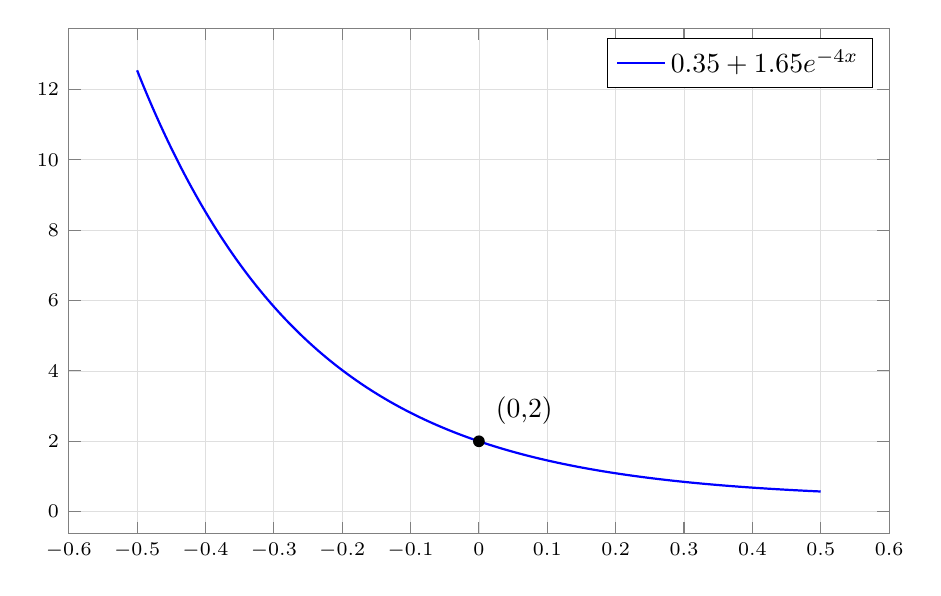
\begin{tikzpicture}
                  \begin{axis}[Ani, grid=both]
                      \addplot [GraphSmooth, domain=-0.5:0.5]
                      {0.35 + 1.65*e^(-4*x)};
                      \node[GraphNode, label={45:{(0,2)}}]
                      at (axis cs:0,2) {};
                      \addlegendentry{$0.35 + 1.65 e^{-4x}$}
                  \end{axis}
              \end{tikzpicture}
          \end{figure}

    \item IC is $y(0) = \pi$

          \begin{align}
              5xy      & = (5x) \ ce^{-2.5 x^{2}} \\
              y'       & = (-5x)\ ce^{-2.5 x^{2}} \\
              y' + 5xy & = 0                      \\
              y(0)     & = c  = \pi
          \end{align}

          \begin{figure}[H]
              \centering
              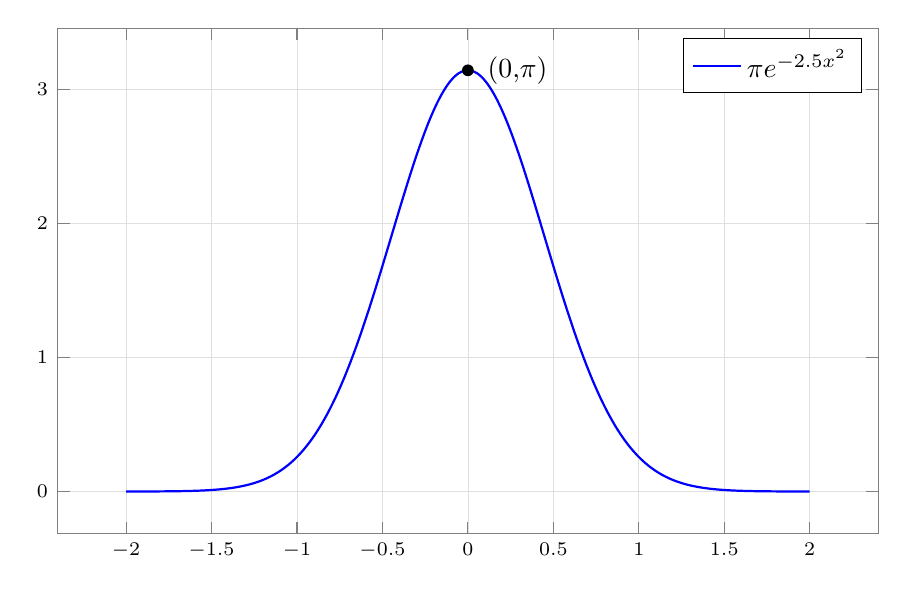
\begin{tikzpicture}
                  \begin{axis}[Ani, grid=both]
                      \addplot [GraphSmooth, domain=-2:2]
                      {pi * e^(-2.5 * x^(2))};
                      \node[GraphNode, label={0:{(0,$\pi$)}}]
                      at (axis cs:0,pi) {};
                      \addlegendentry{$\pi e^{-2.5x^{2}}$}
                  \end{axis}
              \end{tikzpicture}
          \end{figure}

    \item IC is $y(0) = 1/2$

          \begin{align}
              y'     & = (1 + x + c)\ e^{x} \\
              y' - y & = e^{x}              \\
              y(0)   & = c  = 1/2
          \end{align}

          \begin{figure}[H]
              \centering
              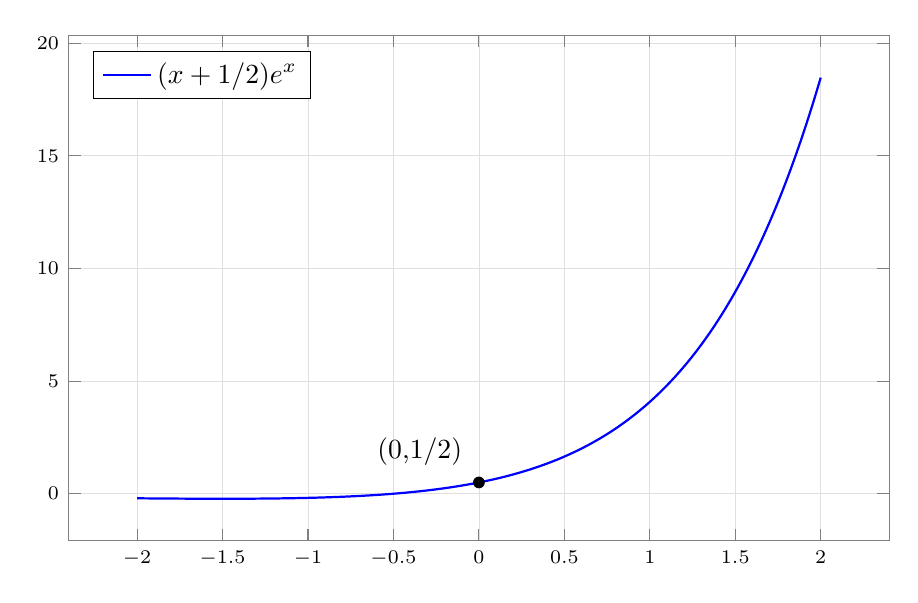
\begin{tikzpicture}
                  \begin{axis}[Ani, grid=both, legend pos = north west]
                      \addplot [GraphSmooth, domain=-2:2]
                      {(x + 0.5) * e^(x))};
                      \node[GraphNode, label={135:{(0,1/2)}}]
                      at (axis cs:0,1/2) {};
                      \addlegendentry{$(x + 1/2)e^{x}$}
                  \end{axis}
              \end{tikzpicture}
          \end{figure}

    \item IC is $y(1) = 4$

          \begin{align}
              2yy' & = 8x          & y & > 0 \\
              yy'  & = 4x          & y & > 0 \\
              y(1) & = c + 4  = 16           \\
              c    & = 12
          \end{align}

          \begin{figure}[H]
              \centering
              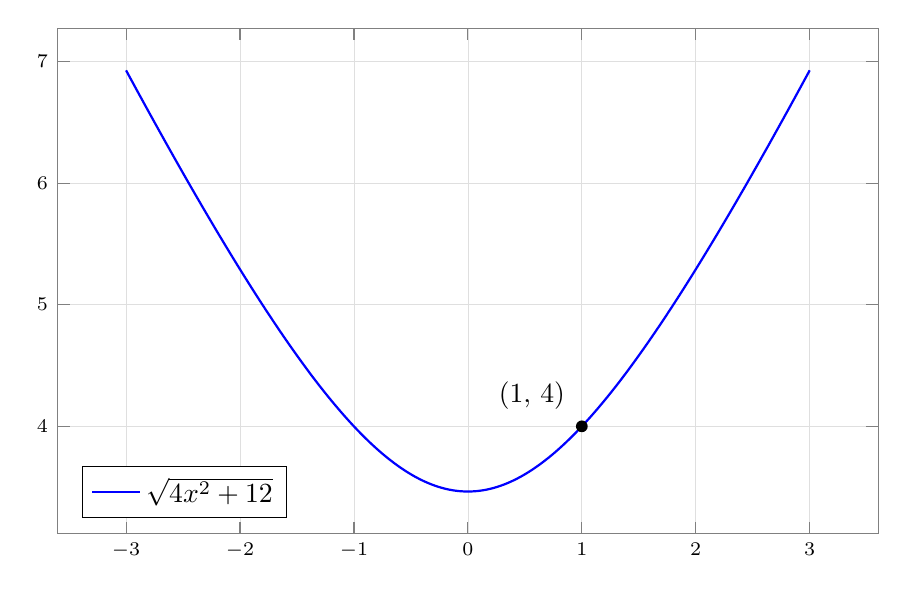
\begin{tikzpicture}
                  \begin{axis}[Ani, grid=both, legend pos = south west]
                      \addplot [GraphSmooth, domain=-3:3]
                      {(4*x^(2) + 12)^(1/2)};
                      \node[GraphNode, label={135:{(1, 4)}}]
                      at (axis cs:1, 4) {};
                      \addlegendentry{$\sqrt{4x^{2} + 12}$}
                  \end{axis}
              \end{tikzpicture}
          \end{figure}

    \item IC is $y(0) = 1/4$

          \begin{align}
              y'        & = \frac{ce^{-x}}{(1 + ce^{-x})^{2}}         \\
              y - y^{2} & = \frac{1 + ce^{-x} - 1}{(1 + ce^{-x})^{2}} \\
              y'        & = y - y^{2}                                 \\
              y(0)      & = \frac{1}{(1+c)}  = 1/4                    \\
              c         & = 3
          \end{align}

          \begin{figure}[H]
              \centering
              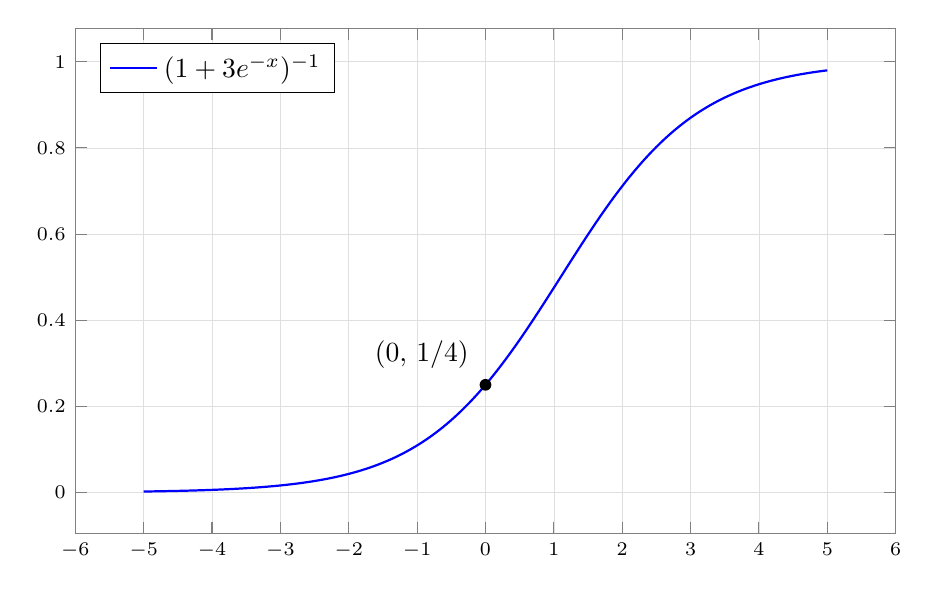
\begin{tikzpicture}
                  \begin{axis}[Ani, grid=both, legend pos = north west]
                      \addplot [GraphSmooth, domain=-5:5]
                      {1 / (1 + 3 * e^(-x))};
                      \node[GraphNode, label={135:{(0, 1/4)}}]
                      at (axis cs:0,1/4) {};
                      \addlegendentry{$(1 + 3e^{-x})^{-1}$}
                  \end{axis}
              \end{tikzpicture}
          \end{figure}

    \item IC is $y(\pi / 2) = 0$

          \begin{align}
              2y - 8     & = 2c\ \sin^{2} x              \\
              y' \tan x  & = 2c\ \sin x \ \cos x\ \tan x \\
              y' \tan x  & = 2y -  8                     \\
              y(\pi / 2) & = c + 4  = 0                  \\
              c          & = -4
          \end{align}

          \begin{figure}[H]
              \centering
              \begin{tikzpicture}
                  \begin{axis}[Ani, grid=both, legend pos = north east, PiStyleX]
                      \addplot [GraphSmooth, domain=-pi:pi]
                      {4 - 4*(sin(deg(x)))^(2)};
                      \node[GraphNode, label={0:{($\pi / 2$, 0)}}]
                      at (axis cs:pi/2, 0) {};
                      \addlegendentry{$-4 \sin^{2} x + 4$}
                  \end{axis}
              \end{tikzpicture}
          \end{figure}

    \item By Inspection , the ODE in Problem 13 has the constant solutions

          \begin{align}
              y & = 1 \\
              y & = 0
          \end{align}


    \item Verifying the general solution by substitution

          \begin{align}
              xy'    & = cx           \\
              y'^{2} & = c^{2}        \\
              y      & = cx - c^{2}   \\
              y      & = xy' - y'^{2}
          \end{align}

          Verifying the singular solution by substitution

          \begin{align}
              xy'    & = \frac{x^{2}}{2} \\
              y'^{2} & = \frac{x^{2}}{4} \\
              y      & = \frac{x^{2}}{4} \\
              y      & = xy' - y'^{2}
          \end{align}

          The parabola happens to have the same derivative for all $x$ as the member of the family of straight lines tangent to it. This makes the parabola a singular solution to the ODE.

    \item Given a starting mass of $1$ gm, find the time taken to reach a mass of $0.5$ gm. This is equal to half-life.

          \begin{align}
              \frac{dy}{dt} & = -ky                                                                           \\
              \ln y         & = -kt + c                                                                       \\
              y             & = c \ e^{-kt}                                                                   \\
              y_{T}         & = \frac{y_{0}}{2}                                                               \\
              e^{-kT}       & = 1/2                                                                           \\
              T             & = \frac{\ln 2}{k} = \frac{ln 2}{1.4 \times 10^{-11}} = 1568.89\  \mathrm{years}
          \end{align}


    \item Given the half life $ T = 3.6 $ days, in 1 day,

          \begin{align}
              y        & = c\ e^{-kt}                                               \\
              y(t = 1) & = c\ e^{-k} = y_{0} e ^{-k}                                \\
              y(t = 1) & = 1\ \mathrm{g} \times \exp \left(\frac{- \ln 2}{T}\right) \\
              y(t = 1) & = 0.825\ \mathrm{g}
          \end{align}
          and for 1 year,
          \begin{align}
              y(t = 365) & = c\ e^{-k} = y_{0} e ^{-365\ k}                                      \\
              y(t = 365) & = 1\ \mathrm{g} \times \exp \left(\frac{- \ln 2 \times 365}{T}\right) \\
              y(t = 365) & = 0\ \mathrm{g}
          \end{align}


    \item Given IC is $y(0) = 0$ and $y'(0) = 0$,

          \begin{align}
              \frac{d^{2}y}{dt^{2}} & = g                                            \\
              y                     & = a + bt + \frac{gt^{2}}{2}                    \\
              y(0)                  & = 0                         & \implies a & = 0 \\
              y'(0)                 & = 0                         & \implies b & = 0 \\
              y                     & = \frac{gt^{2}}{2}
          \end{align}


    \item Given IC is $y(18,000) = 1/2 \times y(0)$ and height $t$

          \begin{align}
              \frac{dy}{dt} & = -ky                                                     \\
              \ln y         & = -kt + c                                                 \\
              y             & = c \ e^{-kt}                                             \\
              y_{T}         & = \frac{y_{0}}{2}                                         \\
              e^{-kT}       & = 1/2                                                     \\
              k             & = \frac{\ln 2}{T} = \frac{ln 2}{18000}\  \mathrm{ft}^{-1} \\
              y(35,000)     & = y(0) \times 2^{-35/18}                                  \\
              y(35,000)     & = y(0) \times 0.259
          \end{align}

\end{enumerate}


\section{Geometric Meaning of y' = f(x, y)}

\begin{enumerate}
    \item Plotting direction field and curve passing through $(\pi / 4, 0)$

          \begin{align}
              y'         & = 1 + y^{2}                        &
              \dl x      & = \int \frac{1}{1 + y^{2}} \ \dl y   \\
              x          & = \arctan y + c                    &
              y          & = \tan(x + c)                        \\
              y(\pi / 4) & = \tan(\pi / 4 + c) = 0            &
              c          & = -\pi / 4
          \end{align}

          \begin{figure}[H]
              \centering
              \begin{tikzpicture}
                  \def\U{1}
                  \def\V{(1 + y^2)}
                  \def\LEN{sqrt(\U * \U + \V * \V)}
                  \begin{axis}[
                          PiStyleX, PiStyleY,
                          xtick distance = pi, ytick distance = pi,
                          legend pos = outer north east,
                          width = 8cm, Ani,
                          axis equal, domain = -2*pi:2*pi,
                          view = {0}{90},
                      ]
                      \addplot3 [forget plot,
                          color = gray!50,
                          point meta = {\LEN},
                          quiver={u={(\U) / \LEN},
                                  v={(\V) / \LEN},
                                  scale arrows = 0.5,},
                          -stealth,
                          samples=16,
                      ] (x, y, 0);
                      \addplot[GraphSmooth, y_h, restrict y to domain = -6.28:6.28]
                      {tan(x - pi/4)};
                      \addlegendentry{$ y' = \tan (x - \pi/4) $};
                  \end{axis}
              \end{tikzpicture}
          \end{figure}


    \item Plotting direction field and curve passing through $(1, 1)$ and $(0, 2)$

          \begin{align}
              y'               & = \frac{-4x}{y}       &
              \int -4x \ \dl x & = \int y \ \dl y        \\
              \frac{y^{2}}{2}  & = -2 x^{2} + c        &
              y^{2} + 4x^{2}   & = c                     \\
              c_{1}            & = 5 , \quad c_{2} = 4
          \end{align}

          \begin{figure}[H]
              \centering
              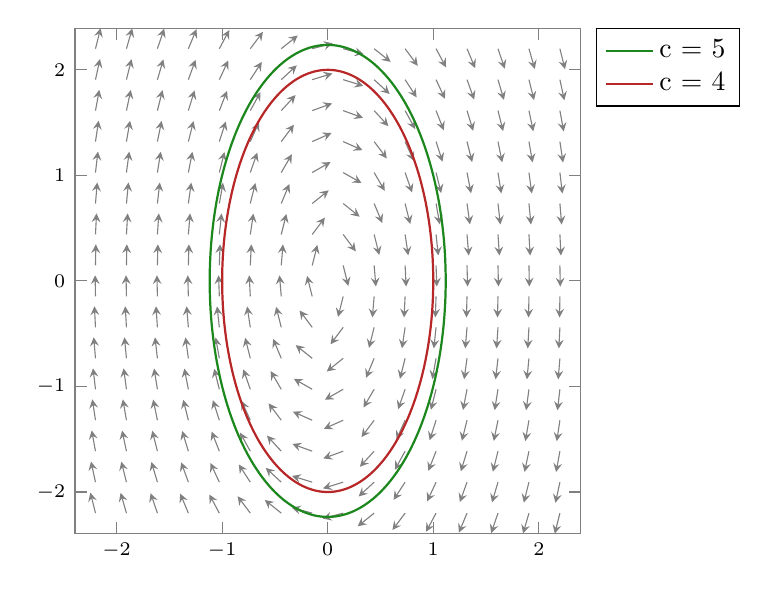
\begin{tikzpicture}
                  \def\U{y}
                  \def\V{-4*x}
                  \def\LEN{sqrt(\U * \U + \V * \V)}
                  \begin{axis}[
                          legend pos = outer north east,
                          width = 8cm,
                          height = 8cm,
                          Ani,
                          axis equal,
                          view     = {0}{90}, % for a view 'from above'
                      ]
                      \addplot3 [
                          forget plot,
                          domain = -2.2:2.2,
                          color = gray,
                          point meta = {\LEN},
                          quiver={u={(\U) / \LEN},
                                  v={(\V) / \LEN},
                                  scale arrows = 0.2,},
                          -stealth,
                          samples=16,
                      ] (x, y, 0);
                      \addplot [GraphSmooth, y_h, domain=-pi:pi, variable = \t]
                      ({sqrt(5/4) * cos(t)}, {sqrt(5) * sin(t)});
                      \addplot [GraphSmooth, domain=-pi:pi, variable = \t,
                          y_p]
                      ({sqrt(4/4) * cos(t)}, {sqrt(4) * sin(t)});
                      \addlegendentry{c = $5$};
                      \addlegendentry{c = $4$};
                  \end{axis}
              \end{tikzpicture}
          \end{figure}

    \item Plotting direction field and curve passing through $(0, 0)$ and $(2, 1/2)$

          \begin{align}
              y'          & = 1 - y^{2}                                      &
              \int\dl x   & = \int \frac{1}{1 - y^{2}} \ \dl y                 \\
              2 \int\dl x & = \int \frac{1}{1 + y} + \frac{1}{1 - y} \ \dl y &
              2x + a      & = \ln \left(\frac{1+y}{1-y}\right)                 \\
              y           & = \left(\frac{ce^{2x} - 1}{ce^{2x} + 1}\right)   &
              c_{1}       & = 1 , \quad c_{2} = \frac{3}{e^4}
          \end{align}

          \begin{figure}[H]
              \centering
              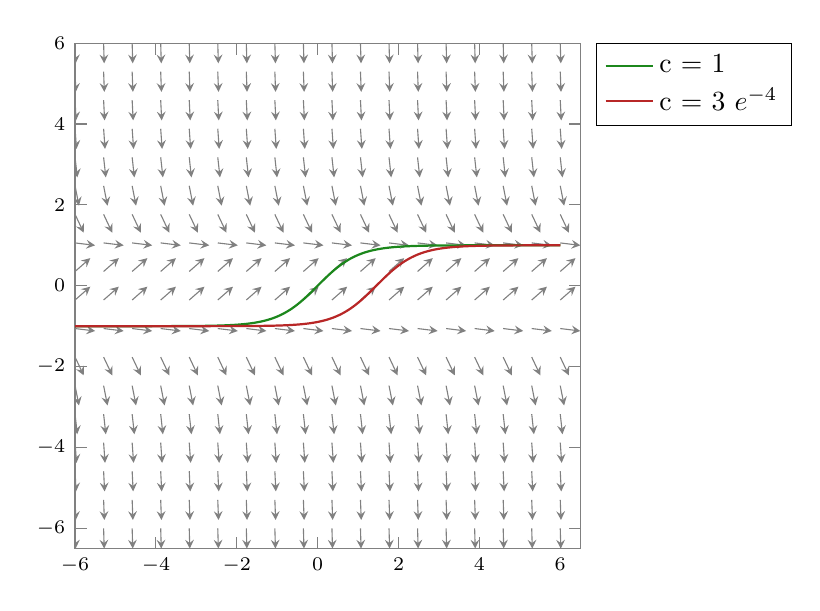
\begin{tikzpicture}
                  % \def\U{1}
                  % \def\V{1-y^(2)}
                  \def\LEN{sqrt(\U * \U + \V * \V)}
                  \begin{axis}[
                          legend pos = outer north east,
                          width = 8cm,
                          height = 8cm,
                          Ani,
                          axis equal,
                          view     = {0}{90}, % for a view 'from above'
                      ]
                      \addplot3 [
                          forget plot,
                          domain = -6:6,
                          color = gray,
                          quiver={
                                  %   u={(\U) / \LEN},
                                  %   v={(\V) / \LEN},
                                  u = 1 / sqrt(2 - 2 * y^2 + y^4),
                                  v = (1 - y^(2)) / sqrt(2 - 2 * y^2 + y^4),
                                  scale arrows = 0.5,},
                          -stealth,
                          samples=18,
                      ] (x, y, 0);
                      \addplot [GraphSmooth, y_h, domain=-6:6]
                      {(exp(2*x) - 1) / (exp(2*x) + 1)};
                      \addplot [GraphSmooth, domain=-6:6, y_p]
                      {((3 / exp(4))*exp(2*x) - 1) / ((3 / exp(4))*exp(2*x) + 1)};
                      \addlegendentry{c = $1$};
                      \addlegendentry{c = $3\ e^{-4}$};
                  \end{axis}
              \end{tikzpicture}
          \end{figure}

    \item Plotting direction field and curve passing through $(0, 0), (0, 1), (0, 2)$
          and $(0, 3)$

          \begin{align}
              y'                             & = 2y - y^{2}                          \\
              \int \ \dl x                   & = \int \frac{1}{y (2 - y)} \ \dl y    \\
              \int 2 \ \dl x                 & = \int \frac{1}{y} - \frac{1}{y - 2}
              \ \dl y                                                                \\
              \ln \left(\frac{y}{y-2}\right) & = 2 x + b                             \\
              y                              & = \frac{2c\ e^{2x}}{c\ e^{2x} - 1}    \\
              c_{1} = 0 , \quad c_{2}        & = -1, \quad c_{3} = \mathrm{singular}
              , \quad c_{4} = 1
          \end{align}

          \begin{figure}[H]
              \centering
              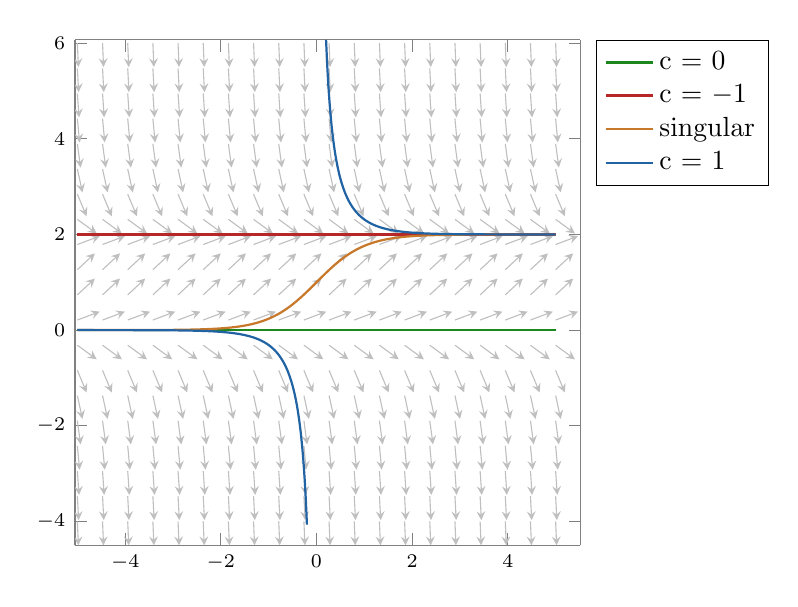
\begin{tikzpicture}
                  \def\U{1}
                  \def\V{y * (2 - y)}
                  \def\LEN{sqrt(\U * \U + \V * \V)}
                  \begin{axis}[
                          legend pos = outer north east,
                          width = 8cm,
                          height = 8cm,
                          Ani,
                          axis equal,
                          view     = {0}{90}, % for a view 'from above'
                      ]
                      \addplot3 [
                          forget plot,
                          domain = -5:5,
                          y domain = -4:6,
                          color = gray!50,
                          point meta = {\LEN},
                          quiver={u={(\U) / \LEN},
                                  v={(\V) / \LEN},
                                  scale arrows = 0.5,},
                          -stealth,
                          samples=20,
                      ] (x, y, 0);
                      \addplot [GraphSmooth, y_h, domain=-5:5]{0};
                      \addplot [GraphSmooth, domain=-5:5, y_p]{2};
                      \addplot [GraphSmooth, domain=-5:5, y_s]
                      {(2*e^(2*x)) / (1 + e^(2*x))};
                      \addplot [GraphSmooth, domain=0.2:5
                          , color = y_t]
                      {(2*e^(2*x)) / (e^(2*x) - 1)};
                      \addplot [GraphSmooth, domain=-5:-0.2
                          , color = y_t]
                      {(2*e^(2*x)) / (e^(2*x) - 1)};
                      \addlegendentry{c = $0$};
                      \addlegendentry{c = $-1$};
                      \addlegendentry{singular};
                      \addlegendentry{c = $1$};
                  \end{axis}
              \end{tikzpicture}
          \end{figure}

    \item Chini's equation
          %% Conpensating for the lack of any actual equations in this problem

    \item Plotting direction field and curve passing through $(0, -0.4)$ and $(0, 1)$

          \begin{align}
              y'           & = \sin^{2}y                           &
              \int \ \dl x & = \int \csc^{2} y \ \dl y               \\
              \tan y       & = \frac{-1}{x + c}                    &
              y            & = \arctan \left(\frac{-1}{x+c}\right)   \\
              c_{1}        & = \cot (0.4), \quad c_{2} = -\cot (1)
          \end{align}

          \begin{figure}[H]
              \centering
              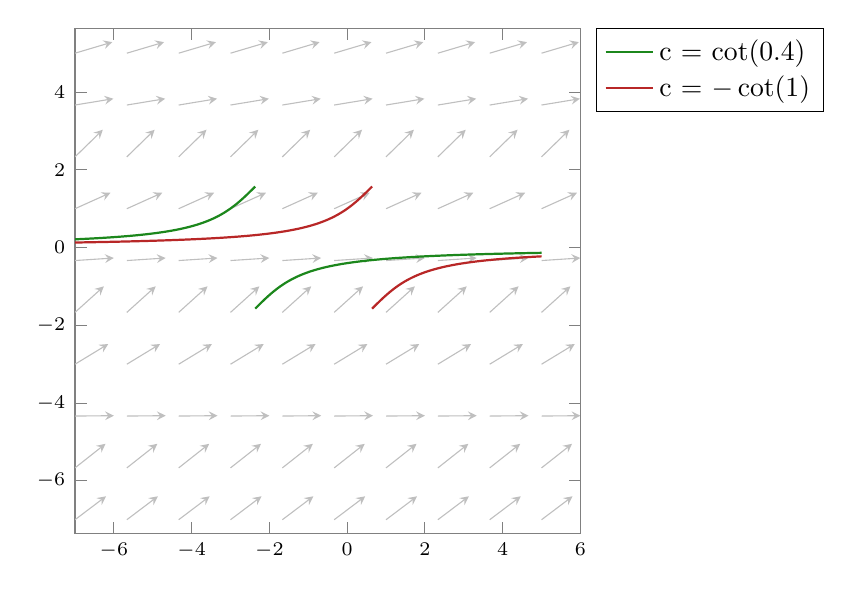
\begin{tikzpicture}
                  \def\U{1}
                  \def\V{sin(deg(y))^2}
                  \def\LEN{sqrt(\U * \U + \V * \V)}
                  \begin{axis}[
                          unbounded coords = jump,
                          legend pos = outer north east,
                          width = 8cm,
                          height = 8cm,
                          Ani,
                          axis equal,
                          view     = {0}{90}, % for a view 'from above'
                      ]
                      \addplot3 [
                          forget plot,
                          domain = -7:5,
                          color = gray!50,
                          point meta = {\LEN},
                          quiver={u={(\U) / \LEN},
                                  v={(\V) / \LEN},
                                  scale arrows = 1,},
                          -stealth,
                          samples=10,
                      ] (x, y, 0);
                      \addplot [GraphSmooth, y_h, domain=-7:-cot(0.4)]
                      {atan(-1/(x + cot(0.4)))};
                      \addplot [forget plot, GraphSmooth, y_h, domain=-cot(0.4):5]
                      {atan(-1/(x + cot(0.4)))};
                      \addplot [GraphSmooth, color = y_p, domain=-7:cot(1)]
                      {atan(-1/(x - cot(1)))};
                      \addplot [forget plot, GraphSmooth, color = y_p
                          , domain=cot(1):5]
                      {atan(-1/(x - cot(1)))};
                      \addlegendentry{c = $\cot (0.4)$};
                      \addlegendentry{c = $-\cot(1)$};
                  \end{axis}
              \end{tikzpicture}
          \end{figure}

    \item Plotting direction field and curve passing through $(2, 2)$ and $(3, 3)$,
          using the substitution $y = vx$

          \begin{align}
              y'            & = e^{y/x}                                         \\
              y'            & = e^{v} \qquad
              dv = -\frac{y}{x^{2}} \ \dl x                                     \\
              \int  \ \dl y & = x e^{y/x} - \int \frac{-y\ e^{y/x}}{x}  \ \dl x \\
              y             & = x e^{y/x} - \int \frac{y\ e^{v}}{v}  \ \dl v    \\
              y             & = x e^{y/x} - y\ \mathrm{Ei}(y/x) + c             \\
              c_{1}         & = 2 \mathrm{Ei}(1) - 2e, \quad c_{2}
              = 3 \mathrm{Ei}(1) - 3e
          \end{align}

          \begin{figure}[H]
              \centering
              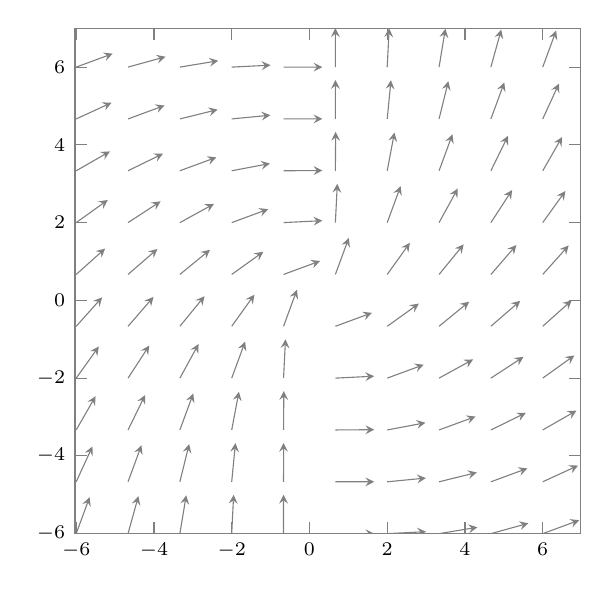
\begin{tikzpicture}
                  \def\U{1}
                  \def\V{e^(y/x)}
                  \def\LEN{sqrt(\U * \U + \V * \V)}
                  \begin{axis}[
                          unbounded coords = jump,
                          legend pos = outer north east,
                          width = 8cm,
                          height = 8cm,
                          Ani,
                          axis equal,
                          view     = {0}{90}, % for a view 'from above'
                      ]
                      \addplot3 [
                          forget plot,
                          domain = -6:6,
                          color = gray,
                          point meta = {\LEN},
                          quiver={u={(\U) / \LEN},
                                  v={(\V) / \LEN},
                                  scale arrows = 1,},
                          -stealth,
                          samples=10,
                      ] (x, y, 0);
                  \end{axis}
              \end{tikzpicture}
          \end{figure}

    \item Plotting direction field and curve passing through $(0, 1/2), (0, 1)$
          and $(0, 2)$

          \begin{align}
              y'                       & = -2xy                                  &
              \int \frac{1}{y} \ \dl y & = -2 \int x  \ \dl x                      \\
              \ln y                    & = -x^{2} + b                            &
              y                        & = c\ e^{-x^{2}}                           \\
              c_{1}                    & = 1/2, \quad c_{2} = 1, \quad c_{3} = 2
          \end{align}

          \begin{figure}[H]
              \centering
              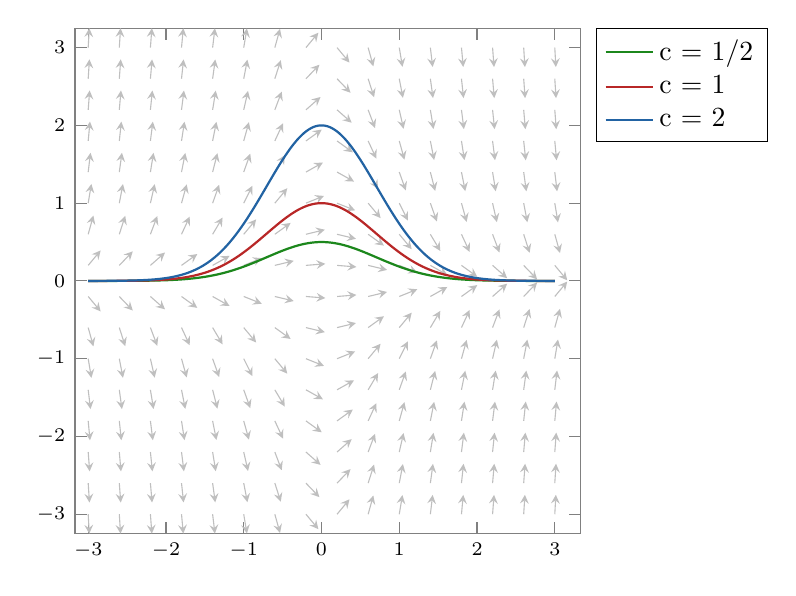
\begin{tikzpicture}
                  \def\U{1}
                  \def\V{-2*x*y}
                  \def\LEN{sqrt(\U * \U + \V * \V)}
                  \begin{axis}[
                          unbounded coords = jump,
                          legend pos = outer north east,
                          width = 8cm,
                          height = 8cm,
                          Ani,
                          axis equal,
                          view     = {0}{90}, % for a view 'from above'
                      ]
                      \addplot3 [
                          forget plot,
                          domain = -3:3,
                          color = gray!50,
                          point meta = {\LEN},
                          quiver={u={(\U) / \LEN},
                                  v={(\V) / \LEN},
                                  scale arrows = 0.25,},
                          -stealth,
                          samples=16,
                      ] (x, y, 0);
                      \addplot [GraphSmooth, y_h, domain=-3:3]
                      {0.5 * e^(-1* x * x)};
                      \addplot [GraphSmooth, domain=-3:3, color = y_p]
                      {1 * e^(-1* x * x)};
                      \addplot [GraphSmooth, domain=-3:3, color = y_t]
                      {2 * e^(-1* x * x)};
                      \addlegendentry{c = $1/2$};
                      \addlegendentry{c = $1$};
                      \addlegendentry{c = $2$};
                  \end{axis}
              \end{tikzpicture}
          \end{figure}

    \item Plotting direction field and curve passing through $(0, 1/2), (0, 1)$
          and $(0, 2)$

          \begin{align}
              y' & = \cos (\pi x)                    &
              y  & = \frac{1}{\pi}\ \sin (\pi x) + c
          \end{align}

          \begin{figure}[H]
              \centering
              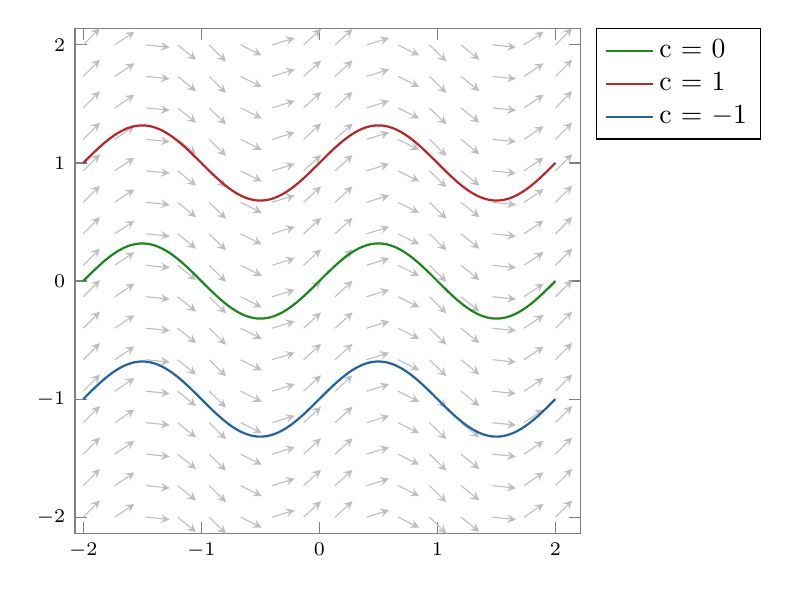
\begin{tikzpicture}
                  \def\U{1}
                  \def\V{cos(pi * x)}
                  \def\LEN{sqrt(\U * \U + \V * \V)}
                  \begin{axis}[
                          unbounded coords = jump,
                          legend pos = outer north east,
                          width = 8cm,
                          height = 8cm,
                          Ani,
                          axis equal,
                          view     = {0}{90}, % for a view 'from above'
                      ]
                      \addplot3 [
                          forget plot,
                          domain = -2:2,
                          color = gray!50,
                          point meta = {\LEN},
                          quiver={u={(\U) / \LEN},
                                  v={(\V) / \LEN},
                                  scale arrows = 0.2,},
                          -stealth,
                          samples=16,
                      ] (x, y, 0);
                      \addplot [GraphSmooth, y_h, domain=-2:2]
                      {(1/pi) * sin(pi * x)};
                      \addplot [GraphSmooth, y_p, domain=-2:2]
                      {(1/pi) * sin(pi * x) + 1};
                      \addplot [GraphSmooth, y_t, domain=-2:2]
                      {(1/pi) * sin(pi * x) - 1};
                      \addlegendentry{c = $0$};
                      \addlegendentry{c = $1$};
                      \addlegendentry{c = $-1$};
                  \end{axis}
              \end{tikzpicture}
          \end{figure}

    \item Plotting direction field and curve passing through $(0, 1/2), (0, 1)$
          and $(0, 2)$

          \begin{align}
              y'       & = -5y^{1/2} &
              \sqrt{y} & = -2.5x + c
          \end{align}

          \begin{figure}[H]
              \centering
              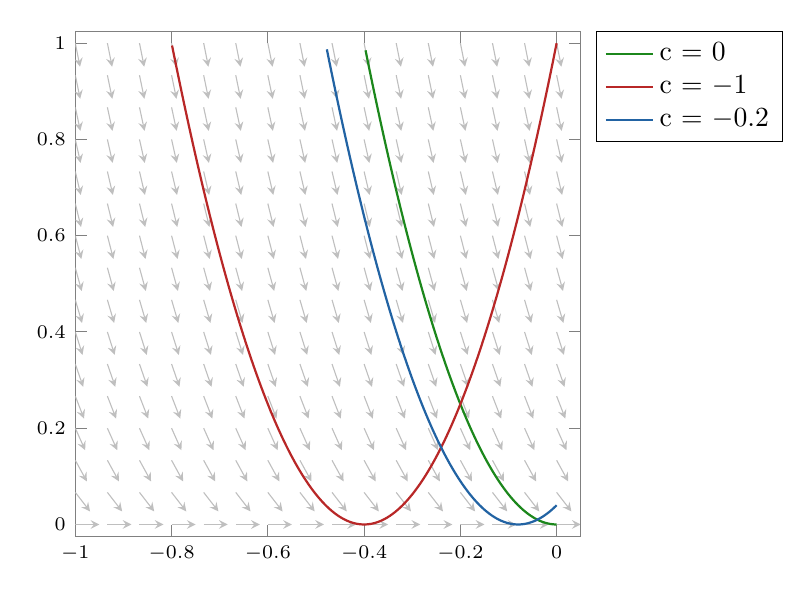
\begin{tikzpicture}
                  \def\U{1}
                  \def\V{-5 * y^(1/2)}
                  \def\LEN{sqrt(\U * \U + \V * \V)}
                  \begin{axis}[
                          unbounded coords = jump,
                          legend pos = outer north east,
                          width = 8cm,
                          height = 8cm,
                          Ani,
                          axis equal,
                          view     = {0}{90}, % for a view 'from above'
                      ]
                      \addplot3 [
                          forget plot,
                          domain = -1:0,
                          y domain = 0:1,
                          color = gray!50,
                          point meta = {\LEN},
                          quiver={u={(\U) / \LEN},
                                  v={(\V) / \LEN},
                                  scale arrows = 0.05,},
                          -stealth,
                          samples=16,
                      ] (x, y, 0);
                      \addplot [GraphSmooth, y_h, domain=-1:0,
                          restrict y to domain=0:1]
                      ({x}, {(-2.5  * x)^(2)});
                      \addplot [GraphSmooth, y_p, domain=-1:0,
                          restrict y to domain=0:1]
                      ({x}, {(-2.5  * x -1)^(2)});
                      \addplot [GraphSmooth, y_t, domain=-1:0,
                          restrict y to domain=0:1]
                      ({x}, {(-2.5  * x - 0.2)^(2)});
                      \addlegendentry{c = $0$};
                      \addlegendentry{c = $-1$};
                      \addlegendentry{c = $-0.2$};
                  \end{axis}
              \end{tikzpicture}
          \end{figure}

    \item Isoclines with an ODE of the form $y' = f(y)$ will be of the form $f(y) = c$.
          These are straight lines parallel to the x axis.

    \item Plotting direction field and curve passing through $(0, 2)$

          \begin{align}
              vy             & = 2             &
              \int y \ \dl y & = 2\int \ \dl t   \\
              y^{2}          & = 4t + c        &
              y(0)           & = \sqrt{c} = 2    \\
              y              & =\sqrt{4t + 4}
          \end{align}

          \begin{figure}[H]
              \centering
              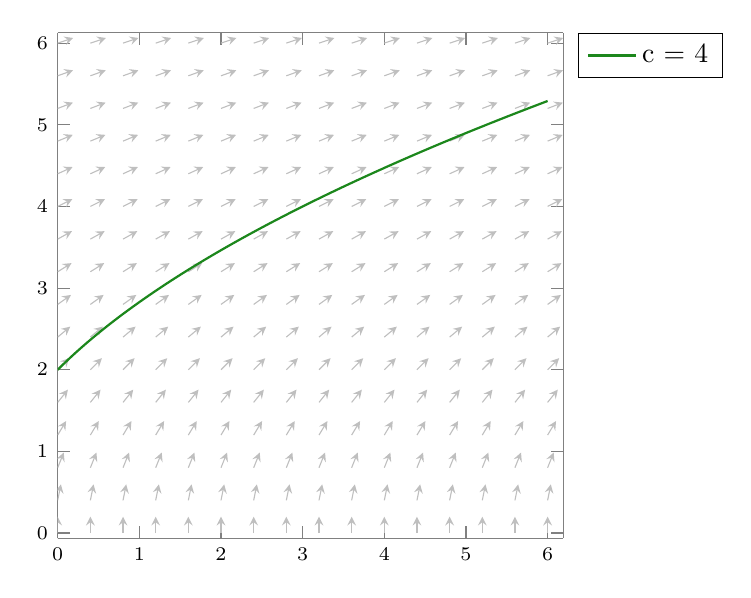
\begin{tikzpicture}
                  \def\U{y}
                  \def\V{2}
                  \def\LEN{sqrt(\U * \U + \V * \V)}
                  \begin{axis}[
                          unbounded coords = jump,
                          legend pos = outer north east,
                          width = 8cm,
                          height = 8cm,
                          Ani,
                          axis equal,
                          view     = {0}{90}, % for a view 'from above'
                      ]
                      \addplot3 [
                          forget plot,
                          domain = 0:6,
                          y domain = 0:6,
                          color = gray!50,
                          point meta = {\LEN},
                          quiver={u={(\U) / \LEN},
                                  v={(\V) / \LEN},
                                  scale arrows = 0.2,},
                          -stealth,
                          samples=16,
                      ] (x, y, 0);
                      \addplot [GraphSmooth, y_h, domain=0:6]
                      {(4*x + 4)^(1/2)};
                      \addlegendentry{c = $4$};
                  \end{axis}
              \end{tikzpicture}
          \end{figure}

    \item Plotting direction field and curve passing through $(1, 1)$

          \begin{align}
              y                        & = vt                       &
              \int \frac{1}{y} \ \dl y & = \int \frac{1}{t} \ \dl t   \\
              \ln y                    & = \ln t + b                &
              y                        & = ct                         \\
              c                        & = 1
          \end{align}

          \begin{figure}[H]
              \centering
              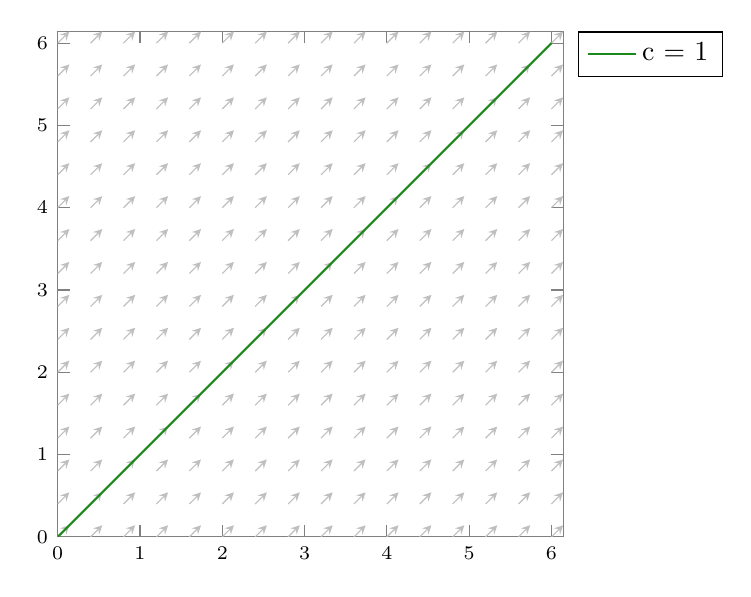
\begin{tikzpicture}
                  \def\U{1}
                  \def\V{1}
                  \def\LEN{sqrt(\U * \U + \V * \V)}
                  \begin{axis}[
                          unbounded coords = jump,
                          legend pos = outer north east,
                          width = 8cm,
                          height = 8cm,
                          Ani,
                          axis equal,
                          view     = {0}{90}, % for a view 'from above'
                      ]
                      \addplot3 [
                          forget plot,
                          domain = 0:6,
                          color = gray!50,
                          point meta = {\LEN},
                          quiver={u={(\U) / \LEN},
                                  v={(\V) / \LEN},
                                  scale arrows = 0.2,},
                          -stealth,
                          samples=16,
                      ] (x, y, 0);
                      \addplot [GraphSmooth, y_h, domain=0:6]
                      {x};
                      \addlegendentry{c = $1$};
                  \end{axis}
              \end{tikzpicture}
          \end{figure}

    \item Plotting direction field and curve passing through $(0, 1/\sqrt{2})$

          \begin{align}
              y^{2} + v^{2}                          & = 1                &
              \diff yt                               & = \sqrt{1 - y^{2}}   \\
              \int \frac{1}{\sqrt{1- y^{2}}} \ \dl y & = \int\ \dl t      &
              \arcsin y                              & = t + c              \\
              y                                      & = \sin (t + c)     &
              c                                      & = \frac{\pi}{4}
          \end{align}

          \begin{figure}[H]
              \centering
              \begin{tikzpicture}
                  \def\U{1}
                  \def\V{cos(x + 0.25 * pi)}
                  \def\LEN{sqrt(\U * \U + \V * \V)}
                  \begin{axis}[
                          unbounded coords = jump,
                          legend pos = outer north east,
                          width = 8cm,
                          height = 8cm,
                          Ani,
                          axis equal,
                          view     = {0}{90}, % for a view 'from above'
                      ]
                      \addplot3 [
                          forget plot,
                          domain = 0 : 4 * pi,
                          y domain = -2 * pi : 2 * pi,
                          color = gray!50,
                          point meta = {\LEN},
                          quiver={u={(\U) / \LEN},
                                  v={(\V) / \LEN},
                                  scale arrows = 0.5,},
                          -stealth,
                          samples=16,
                      ] (x, y, 0);
                      \addplot [GraphSmooth, y_h, domain=0:4*pi]
                      {sin(x + 0.25 * pi)};
                      \addlegendentry{c = $\pi / 4$};
                  \end{axis}
              \end{tikzpicture}
          \end{figure}

    \item Plotting direction field given $m = k = 1$ and $v_{0} = 10$ and drag
          proportional to $v^{2}$. \\
          Terminal velocity is $v^{T} = \sqrt{g} = 3.13\ m/s^{2}$

          \begin{align}
              my''                            & = mv' = mg - kv^{2}                   \\
              \int \frac{1}{g - v^{2}}\ \dl v & = \int \ \dl t                        \\
              \frac{1}{2 \sqrt{g}}
              \int \frac{1}{\sqrt{g} - v}
              + \frac{1}{\sqrt{g} + v}
              \ \dl v                         & = \int \ \dl t                        \\
              \ln \left(\frac{v + \sqrt{g}}
              {v - \sqrt{g}}\right)           & = 2 \sqrt{g} t + b                    \\
              v                               & = \sqrt{g}
              \ \frac{c\ \exp(2 \sqrt{g}t) + 1}{c\ \exp(2 \sqrt{g}t) - 1}             \\
              c                               & = \frac{10 + \sqrt{g}}{10 - \sqrt{g}}
          \end{align}
          \begin{figure}[H]
              \centering
              \begin{tikzpicture}
                  \def\U{1}
                  \def\V{-1 * (y^(2) - 9.8)}
                  \def\LEN{sqrt(\U * \U + \V * \V)}
                  \def\c{(10 + (9.8)^(1/2)) / (10 - (9.8)^(1/2))}
                  \begin{axis}[
                          unbounded coords = jump,
                          legend pos = outer north east,
                          width = 8cm,
                          height = 8cm,
                          Ani,
                          axis equal,
                          view     = {0}{90}, % for a view 'from above'
                      ]
                      \addplot3 [
                          forget plot,
                          domain = 0 : 6,
                          y domain = 0  : 6 ,
                          color = gray!50,
                          point meta = {\LEN},
                          quiver={u={(\U) / \LEN},
                                  v={(\V) / \LEN},
                                  scale arrows = 0.25,},
                          -stealth,
                          samples=16,
                      ] (x, y, 0);
                      \addplot [GraphSmooth, y_h, domain=0:6, samples = 100,
                          restrict y to domain = 0:6]
                      {sqrt(9.8) * (\c * e^(2 * sqrt(9.8) * x) + 1)
                          / (\c * e^(2 * sqrt(9.8) * x) - 1)};
                      \addlegendentry{drag $\propto v^{2}$};
                  \end{axis}
              \end{tikzpicture}
          \end{figure}

          Plotting direction field given $m = k = 1$ and $v_{0} = 10$ and drag
          proportional to $v$. \\
          Terminal velocity is $v^{T} = g = 9.8\ m/s^{2}$
          \begin{align}
              my''                             & = mv' = mg - kv   \\
              \int \frac{1}{g - v}\ \dl v      & = \int \ \dl t    \\
              \ln \left(\frac{1}{v - g}\right) & = t + b           \\
              v                                & = g + c e^{-t}    \\
              c                                & = v_{0} - g = 0.2
          \end{align}

          \begin{figure}[H]
              \centering
              \begin{tikzpicture}
                  \def\U{1}
                  \def\V{-1 * (y - 9.8)}
                  \def\LEN{sqrt(\U * \U + \V * \V)}
                  \begin{axis}[
                          unbounded coords = jump,
                          legend pos = outer north east,
                          width = 8cm,
                          height = 8cm,
                          Ani,
                          axis equal,
                          view     = {0}{90}, % for a view 'from above'
                      ]
                      \addplot3 [
                          forget plot,
                          domain = 0 : 4,
                          y domain = 8  : 12 ,
                          color = gray!50,
                          point meta = {\LEN},
                          quiver={u={(\U) / \LEN},
                                  v={(\V) / \LEN},
                                  scale arrows = 0.25,},
                          -stealth,
                          samples=16,
                      ] (x, y, 0);
                      \addplot [GraphSmooth, domain=0:4, y_p]
                      {9.8 + 0.2 * e^(-x)};
                      \addlegendentry{drag $\propto v$};
                  \end{axis}
              \end{tikzpicture}
          \end{figure}

    \item CAS Project using the ODE $y' = y + x$
          \begin{enumerate}
              \item Zooming in the regions $x \in [-5, 2]$ shows the upper part
                    of the solutions which increase for large $x$ \\
                    Zooming in the regions $y \in [-1, 5]$ shows the lower part
                    of the solutions which decreases for large $x$, as well as the
                    straight line unstable equilibrium solution

                    \begin{figure}[H]
                        \centering
                        \begin{subfigure}[b]{0.49\textwidth}
                            \begin{tikzpicture}
                                \def\U{1}
                                \def\V{(x + y)}
                                \def\LEN{sqrt(\U * \U + \V * \V)}
                                \begin{axis}[
                                        unbounded coords = jump,
                                        legend pos = outer north east,
                                        width = 8cm,
                                        height = 8cm,
                                        Ani,
                                        axis equal,
                                        view     = {0}{90}, % for a view 'from above'
                                    ]
                                    \addplot3 [
                                        forget plot,
                                        domain = -5 : 2,
                                        color = gray,
                                        point meta = {\LEN},
                                        quiver={u={(\U) / \LEN},
                                                v={(\V) / \LEN},
                                                scale arrows = 0.25,},
                                        -stealth,
                                        samples=16,
                                    ] (x, y, 0);
                                \end{axis}
                            \end{tikzpicture}
                        \end{subfigure}
                        \hfill
                        \begin{subfigure}[b]{0.49\textwidth}
                            \begin{tikzpicture}
                                \def\U{1}
                                \def\V{(x + y)}
                                \def\LEN{sqrt(\U * \U + \V * \V)}
                                \begin{axis}[
                                        unbounded coords = jump,
                                        legend pos = outer north east,
                                        width = 8cm,
                                        height = 8cm,
                                        Ani,
                                        axis equal,
                                        view     = {0}{90}, % for a view 'from above'
                                    ]
                                    \addplot3 [
                                        forget plot,
                                        domain = -1:5,
                                        restrict y to domain = -1:5,
                                        color = gray,
                                        point meta = {\LEN},
                                        quiver={u={(\U) / \LEN},
                                                v={(\V) / \LEN},
                                                scale arrows = 0.25,},
                                        -stealth,
                                        samples=16,
                                    ] (x, y, 0);
                                \end{axis}
                            \end{tikzpicture}
                        \end{subfigure}
                    \end{figure}
              \item Implicit differentiation gives the ODE

                    \begin{align}
                        x^{2} + 9y^{2} & = c \quad (y > 0)             \\
                        x + 9yy'       & = 0                           \\
                        y'             & = \frac{-x}{9y} \quad (y > 0)
                    \end{align}
                    The sign of the RHS determine whether the direction field is
                    an ellipse or a hyperbola. A special case of the RHS being
                    $-x/y$ gives a circle (a special ellipse)

                    \begin{figure}[H]
                        \centering
                        \begin{subfigure}[b]{0.49\textwidth}
                            \centering
                            \begin{tikzpicture}
                                \def\U{y}
                                \def\V{x}
                                \def\LEN{sqrt(\U * \U + \V * \V)}
                                \begin{axis}[
                                        unbounded coords = jump,
                                        width = 8cm,
                                        height = 8cm,
                                        Ani,
                                        axis equal,
                                        view     = {0}{90}, % for a view 'from above'
                                    ]
                                    \addplot3 [
                                        domain = -2 : 2,
                                        restrict y to domain = -2:2,
                                        color = gray,
                                        point meta = {\LEN},
                                        quiver={u={(\U) / \LEN},
                                                v={(\V) / \LEN},
                                                scale arrows = 0.2,},
                                        -stealth,
                                        samples=16,
                                    ] (x, y, 0);
                                    \addlegendentry{hyperbola: $x/y$};
                                \end{axis}
                            \end{tikzpicture}
                        \end{subfigure}
                        \hfill
                        \begin{subfigure}[b]{0.49\textwidth}
                            \centering
                            \begin{tikzpicture}
                                \def\U{y}
                                \def\V{-x}
                                \def\LEN{sqrt(\U * \U + \V * \V)}
                                \begin{axis}[
                                        unbounded coords = jump,
                                        width = 8cm,
                                        height = 8cm,
                                        Ani,
                                        axis equal,
                                        view     = {0}{90}, % for a view 'from above'
                                    ]
                                    \addplot3 [
                                        domain = -2 : 2,
                                        restrict y to domain = -2:2,
                                        color = gray,
                                        point meta = {\LEN},
                                        quiver={u={(\U) / \LEN},
                                                v={(\V) / \LEN},
                                                scale arrows = 0.2,},
                                        -stealth,
                                        samples=16,
                                    ] (x, y, 0);
                                    \addlegendentry{circle: $-x/y$};
                                \end{axis}
                            \end{tikzpicture}
                        \end{subfigure}
                        \vskip\baselineskip
                        \begin{subfigure}[b]{0.49\textwidth}
                            \centering
                            \begin{tikzpicture}
                                \def\U{9*y}
                                \def\V{-x}
                                \def\LEN{sqrt(\U * \U + \V * \V)}
                                \begin{axis}[
                                        unbounded coords = jump,
                                        width = 8cm,
                                        height = 8cm,
                                        Ani,
                                        axis equal,
                                        view     = {0}{90}, % for a view 'from above'
                                    ]
                                    \addplot3 [
                                        domain = -2 : 2,
                                        restrict y to domain = -2:2,
                                        color = gray,
                                        point meta = {\LEN},
                                        quiver={u={(\U) / \LEN},
                                                v={(\V) / \LEN},
                                                scale arrows = 0.2,},
                                        -stealth,
                                        samples=16,
                                    ] (x, y, 0);
                                    \addlegendentry{ellipse: $-x/9y$};
                                \end{axis}
                            \end{tikzpicture}
                        \end{subfigure}
                        \hfill
                        \begin{subfigure}[b]{0.49\textwidth}
                            \centering
                            \begin{tikzpicture}
                                \def\U{1}
                                \def\V{2*x}
                                \def\LEN{sqrt(\U * \U + \V * \V)}
                                \begin{axis}[
                                        unbounded coords = jump,
                                        width = 8cm,
                                        height = 8cm,
                                        Ani,
                                        axis equal,
                                        view     = {0}{90}, % for a view 'from above'
                                    ]
                                    \addplot3 [
                                        domain = -2 : 2,
                                        color = gray,
                                        point meta = {\LEN},
                                        quiver={u={(\U) / \LEN},
                                                v={(\V) / \LEN},
                                                scale arrows = 0.2,},
                                        -stealth,
                                        samples=16,
                                    ] (x, y, 0);
                                    \addlegendentry{parabola: $2x$};
                                \end{axis}
                            \end{tikzpicture}
                        \end{subfigure}
                    \end{figure}
              \item From the figure above, $y' = -x/y$ produces a circle
              \item For the ODE $y' = -y/2$
                    \begin{align}
                        y'    & = \frac{-1}{2y} \\
                        y^{2} & = -x + c
                    \end{align}

                    For $y > 0$, the solutions decrease because the ODE is
                    monotonically negative for all $y > 0$.
                    \begin{figure}[H]
                        \centering
                        \begin{tikzpicture}
                            \def\U{y}
                            \def\V{(-0.5)}
                            \def\LEN{sqrt(\U * \U + \V * \V)}
                            \begin{axis}[
                                    unbounded coords = jump,
                                    legend pos = outer north east,
                                    width = 8cm,
                                    height = 8cm,
                                    Ani,
                                    axis equal,
                                    view     = {0}{90}, % for a view 'from above'
                                ]
                                \addplot3 [
                                    forget plot,
                                    domain = -2:2,
                                    color = gray!50,
                                    point meta = {\LEN},
                                    quiver={u={(\U) / \LEN},
                                            v={(\V) / \LEN},
                                            scale arrows = 0.25,},
                                    -stealth,
                                    samples=16,
                                ] (x, y, 0);
                                \addplot [GraphSmooth, y_h, domain=-2:0,
                                    samples = 100]
                                {sqrt(-x)};
                                \addlegendentry{c = $0$};
                                \addplot [GraphSmooth, y_p, domain=-1:1,
                                    samples = 100]
                                {sqrt(-x + 1)};
                                \addlegendentry{c = $1$};
                            \end{axis}
                        \end{tikzpicture}
                    \end{figure}
          \end{enumerate}

    \item Euler's method with $y(0) = 1$ and step size $h = 0.1$

          \begin{align}
              y' & = y      &
              y  & = ce^{x}   \\
              c  & = 1
          \end{align}

          \begin{figure}[H]
              \centering
              \begin{tikzpicture}
                  \begin{axis}[
                          grid = both,
                          legend pos = north west,
                          unbounded coords = jump,
                          width = 12cm,
                          height = 12cm,
                          Ani,
                      ]
                      \addplot[
                          only marks,]
                      table [
                              x index =1,
                              y index =2,
                              col sep=comma]
                          {./tables/table_01_01_17.csv};
                      \addplot [
                          forget plot,
                          GraphSmooth,
                          domain=0:1]
                      {e^(x)};
                      \addlegendentry{numerical};
                      \addplot[
                          only marks,
                          color = red,
                          mark = square]
                      table [
                              x index =1,
                              y index =3,
                              col sep=comma]
                          {./tables/table_01_01_17.csv};
                      \addlegendentry{exact};
                  \end{axis}
              \end{tikzpicture}
          \end{figure}

    \item Euler's method with $y(0) = 1$ and step size $h = 0.01$

          \begin{align}
              y' & = y      &
              y  & = ce^{x}   \\
              c  & = 1
          \end{align}

          \begin{figure}[H]
              \centering
              \begin{tikzpicture}
                  \begin{axis}[
                          xticklabel style={
                                  /pgf/number format/fixed,
                                  /pgf/number format/precision=5
                              },
                          grid = both,
                          legend pos = north west,
                          unbounded coords = jump,
                          width = 8cm,
                          height = 8cm,
                          Ani,
                      ]
                      \addplot[
                          only marks,]
                      table [
                              x index =1,
                              y index =2,
                              col sep=comma]
                          {./tables/table_01_01_18.csv};
                      \addplot [
                          forget plot,
                          GraphSmooth,
                          domain=0:0.1]
                      {e^(x)};
                      \addlegendentry{numerical};
                      \addplot[
                          only marks,
                          color = red,
                          mark = square]
                      table [
                              x index =1,
                              y index =3,
                              col sep=comma]
                          {./tables/table_01_01_18.csv};
                      \addlegendentry{exact};
                  \end{axis}
              \end{tikzpicture}
          \end{figure}

    \item Euler's method with $y(0) = 0$ and step size $h = 0.1$

          \begin{align}
              y' & = (y - x)^{2} &
              y  & = x - \tanh x
          \end{align}

          \begin{figure}[H]
              \centering
              \begin{tikzpicture}
                  \begin{axis}[
                          grid = both,
                          legend pos = north west,
                          unbounded coords = jump,
                          width = 12cm,
                          height = 12cm,
                          Ani,
                      ]
                      \addplot[
                          only marks,]
                      table [
                              x index =1,
                              y index =2,
                              col sep=comma]
                          {./tables/table_01_01_19.csv};
                      \addplot [
                          forget plot,
                          GraphSmooth,
                          domain=0:1]
                      {x - tanh(x)};
                      \addlegendentry{numerical};
                      \addplot[
                          only marks,
                          color = red,
                          mark = square]
                      table [
                              x index =1,
                              y index =3,
                              col sep=comma]
                          {./tables/table_01_01_19.csv};
                      \addlegendentry{exact};
                  \end{axis}
              \end{tikzpicture}
          \end{figure}

    \item Euler's method with $y(0) = 1$ and step size $h = 0.2$

          \begin{align}
              y' & = -5x^{4}y^{2}          &
              y  & = \frac{1}{(c + x^{5})}   \\
              c  & = 1
          \end{align}

          \begin{figure}[H]
              \centering
              \begin{tikzpicture}
                  \begin{axis}[
                          grid = both,
                          legend pos = north east,
                          unbounded coords = jump,
                          width = 12cm,
                          height = 12cm,
                          Ani,
                      ]
                      \addplot[
                          only marks,]
                      table [
                              x index =1,
                              y index =2,
                              col sep=comma]
                          {./tables/table_01_01_20.csv};
                      \addplot [
                          forget plot,
                          GraphSmooth,
                          domain=0:2]
                      {(1 + x^5)^(-1)};
                      \addlegendentry{numerical};
                      \addplot[
                          only marks,
                          color = red,
                          mark = square]
                      table [
                              x index =1,
                              y index =3,
                              col sep=comma]
                          {./tables/table_01_01_20.csv};
                      \addlegendentry{exact};
                  \end{axis}
              \end{tikzpicture}
          \end{figure}

\end{enumerate}
\section{Separable ODEs. Modeling}

\begin{enumerate}
    \item Adding the constant of integration later might result in a vastly
          different general solution which is almost always wrong.

    \item Using $u = y/x$. Then substituting $(1 + u^{4}) = m$

          \begin{align}
              y'                     & = \frac{-x^{3}}{y^{3}} = \frac{-1}{u^{3}}     \\
              \frac{\dl u}{f(u) - u} & =  \frac{\dl x}{x} = \frac{-u^{3}\ \dl u}
              {1 + u^{4}}                                                            \\
              \ln (|x|) + b          & = \int \frac{-\dl m}{4m} = \frac{-1}{4} \ln m \\
              1 + \left(\frac{y}{x}\right)^{4}
                                     & = \frac{c}{x^{4}}                             \\
              y^{4}                  & = c - x^{4}
          \end{align}
          \begin{figure}[H]
              \centering
              \begin{tikzpicture}
                  \begin{axis}[Ani, grid=both, legend pos = north east]
                      \addplot [GraphSmooth, domain=-5:5]
                      {(1 - x^(4))^(1/4)};
                      \node[GraphNode, y_h, label={270:{(0, 1)}}]
                      at (axis cs:0,1) {};
                      \addlegendentry{$(1 - x^{4})^{1/4}$}
                  \end{axis}
              \end{tikzpicture}
          \end{figure}
          Checking by differentiation and substitution,
          \begin{align}
              4y^{3}\ \dl y     & = -4x^{3} dx &
              y^{3}\ y' + x^{3} & = 0
          \end{align}


    \item Separating variables,

          \begin{align}
              \int \cos ^{2}y\ \dl y                        & = \int \ \dl x &
              \int \frac{1}{2} + \frac{\cos (2y)}{2}\ \dl y & = \int \ \dl x   \\
              \frac{y}{2} + \frac{\sin (2y)}{4}             & =  x + c
          \end{align}
          \begin{figure}[H]
              \centering
              \begin{tikzpicture}
                  \begin{axis}[PiStyleY, Ani, grid=both, legend pos = north west,
                          trig format plots = rad]
                      \addplot [GraphSmooth, y_h, domain=-pi:pi]
                      ({x/2 + sin(2*x)/4}, {x});
                      \node[GraphNode, label={270:{(0, 0)}}]
                      at (axis cs:0,0) {};
                      \addlegendentry{$x = y/2 + \sin(2y)/4$}
                  \end{axis}
              \end{tikzpicture}
          \end{figure}
          Checking by differentiation and substitution,
          \begin{align}
              dx & = \frac{(1 + \cos(2y))\ dy}{2} &
              y' & = \sec ^{2}y
          \end{align}


    \item Separating variables, with $u = \sin(2 \pi x)$

          \begin{align}
              \int \frac{1}{y} \ \dl y & = \pi \int \frac{\cos(2 \pi x)}
              {\sin (2 \pi x)}\ \dl x  &
              \dl u                    & = 2 \pi \cos(2 \pi x)\ \dl x      \\
              \int \frac{2}{y}\ \dl y  & = \int \frac{1}{u}\ \dl u       &
              2 \ln |y|                & =  \ln |u| + b                    \\
              y^{2}                    & = c\ |\sin(2 \pi x)|
          \end{align}
          \begin{figure}[H]
              \centering
              \begin{tikzpicture}
                  \begin{axis}[Ani, grid=both, legend pos = north west,
                          trig format plots = rad]
                      \addplot [GraphSmooth, y_h, domain=-0.5:0.5, samples = 201]
                      {(abs(sin(2 * pi * x)))^0.5};
                      \node[GraphNode, label={0:{(0, 0)}}]
                      at (axis cs:0,0) {};
                      \addlegendentry{$\sqrt{ |\sin(2 \pi x)| }$}
                  \end{axis}
              \end{tikzpicture}
          \end{figure}
          Checking by differentiation and substitution,
          \begin{align}
              y' & = \begin{dcases}
                         \frac{\pi \ \cos(2 \pi x)}{\sqrt{\sin (2 \pi x)}}
                         =  \frac{\pi y \ \cos(2 \pi x)}{\sin (2 \pi x)}   &
                         \mathrm{for} \quad x >= 0                           \\
                         \frac{-\pi \ \cos(-2 \pi x)}{\sqrt{\sin (-2 \pi x)}}
                         =  \frac{-\pi y \ \cos(2 \pi x)}{\sin (-2 \pi x)} &
                         \mathrm{for} \quad  x < 0                           \\
                     \end{dcases}
          \end{align}


    \item Separating variables,

          \begin{align}
              \int y\ \dl y   & = -36 \int x\ \dl x &
              y^{2} + 36x^{2} & =  c
          \end{align}
          \begin{figure}[H]
              \centering
              \begin{tikzpicture}
                  \begin{axis}[Ani, grid=both, legend pos = north west,                           xticklabel style={/pgf/number format/fixed}, axis equal]
                      \addplot [GraphSmooth, y_h, domain=-pi:pi, variable=\t]
                      ({sin(t)/6}, {cos(t)});
                      \addlegendentry{$y^{2} + 36x^{2} = 1$}
                  \end{axis}
              \end{tikzpicture}
          \end{figure}
          Checking by differentiation and substitution,
          \begin{align}
              2y\ y'      & = -72x\ \dl x &
              y\ y' + 36x & = 0
          \end{align}


    \item Separating variables,

          \begin{align}
              \int \frac{1}{y^2}\ \dl y & = \int \exp(2x - 1)\ \dl x   &
              \frac{-1}{y}              & = \frac{\exp(2x - 1)}{2} + b   \\
              y                         & =  \frac{-2}{c + e^{(2x-1)}}
          \end{align}
          \begin{figure}[H]
              \centering
              \begin{tikzpicture}
                  \begin{axis}[Ani, grid=both, legend pos = south east]
                      \addplot [GraphSmooth, y_h, domain=-1:2]
                      {-2 * (e^(2*x - 1))^(-1)};
                      \node[GraphNode, label={270:{(1/2, -2)}}]
                      at (axis cs:1/2,-2) {};
                      \addlegendentry{$-2/\exp(2x-1)$}
                  \end{axis}
              \end{tikzpicture}
          \end{figure}
          Checking by differentiation and substitution,
          \begin{align}
              y' & = \frac{4\ e^{(2x-1)}}{(c + e^{(2x-1)})^{2}} &
              y' & = y^{2}\ e^{(2x-1)}
          \end{align}


    \item Using $u = y/x$.

          \begin{align}
              y'                            & = u + \frac{2 y^{2}}{u^{2}} \sin^{2} u \\
              x\ du + u\ \dl x              & = (u + x^{2} \sin ^{2} u )\ \dl x      \\
              \int \frac{1}{\sin ^{2}u}\ du & = \int x\ \dl x                        \\
              - \cot u                      & = \frac{x^{2}}{2} + b                  \\
              y                             & = x\ \arctan \left(\frac{2}{c - x^{2}}
              \right)
          \end{align}
          \begin{figure}[H]
              \centering
              \begin{tikzpicture}
                  \begin{axis}[Ani, grid=both, legend pos = north east]
                      \addplot [GraphSmooth, y_h, domain=-20:20]
                      {x * atan(2 / (-1*x*x))};
                      \node[GraphNode, label={0:{(0, 0)}}]
                      at (axis cs:0,0) {};
                      \addlegendentry{$x\ \arctan \frac{2}{c-x^{2}}$}
                  \end{axis}
              \end{tikzpicture}
          \end{figure}
          Checking by differentiation and substitution,
          \begin{align}
              y' & = \arctan \left(\frac{2}{c - x^{2}}\right) +
              \frac{x\ (c - x^{2})^{2}}{4 + (c - x^{2})^{2}}
              \times \frac{4x}{(c - x^{2})^{2}}                         \\
              y' & = \frac{y}{x} + x^{2}\ \frac{4}{4 + (c - x^{2})^{2}} \\
              y' & = \frac{y}{x} + x^{2} \ \sin ^{2}
              \left[\arctan\left(\frac{2}{c - x^{2}}\right)\right] = \frac{y}{x}
              + x^{2}\ \sin ^{2} \left(\frac{y}{x}\right)
          \end{align}


    \item Using $u = y + 4x$.

          \begin{align}
              u' - 4                                       & = u^{2}                &
              \int \frac{1}{4 + u^{2}}\ du                 & = \int \ \dl x           \\
              \frac{1}{2} \arctan \left(\frac{u}{2}\right) & = x + b                &
              y                                            & = 2 \tan (2x + c) - 4x
          \end{align}
          \begin{figure}[H]
              \centering
              \begin{tikzpicture}
                  \begin{axis}[Ani, grid=both, legend pos = north west,
                          trig format plots = rad]
                      \addplot [GraphSmooth, y_h, domain=-pi/4.01:pi/4.01,
                          samples = 201]
                      {2 * tan(2*x) - 4*x};
                      \node[GraphNode, label={270:{(0, 0)}}]
                      at (axis cs:0,0) {};
                      \addlegendentry{$2 \tan (2x) - 4x$}
                  \end{axis}
              \end{tikzpicture}
          \end{figure}
          Checking by differentiation and substitution,
          \begin{align}
              y' & = -4 + \frac{4}{\cos ^{2}(2x + c)}              \\
              y' & = 4 \frac{\sin ^{2}(2x + c)}{\cos ^{2}(2x + c)}
              = (2 \tan (2x+c))^{2}                                \\
              y' & = (y + 4x)^{2}
          \end{align}


    \item Using $u = y/x$.

          \begin{align}
              y'                       & = xu^{2} + u = u + xu'                  &
              \int \frac{1}{u^{2}}\ du & = \int \ \dl x                            \\
              \frac{-1}{u}             & = x + b = \frac{-x}{y}                  &
              y                        & = \frac{-x}{x + c} = \frac{-1}{1 + c/x}
          \end{align}
          \begin{figure}[H]
              \centering
              \begin{tikzpicture}
                  \begin{axis}[Ani, grid=both, legend pos = north west,
                          trig format plots = rad, restrict y to domain = -100:100]
                      \addplot [GraphSmooth, y_h, domain=-2.5:0.5, samples = 200,
                      ]
                      {-x / (x + 1)};
                      \node[GraphNode, label={270:{(0, 0)}}]
                      at (axis cs:0,0) {};
                      \addlegendentry{$-x / (x + 1)$}
                  \end{axis}
              \end{tikzpicture}
          \end{figure}
          Checking by differentiation and substitution,

          \begin{align}
              xy'       & = \frac{-cx}{(x+c)^{2}}                 &
              y + y^{2} & = \frac{-x^{2} + x^{2} - cx}{(x+c)^{2}}   \\
              xy'       & = y + y^{2}
          \end{align}


    \item Using $u = y/x$.

          \begin{align}
              y'       & = 1 + u = u + xu'         &
              \int\ du & = \int \frac{1}{x}\ \dl x   \\
              u        & = \ln |x| + b             &
              y        & = x \ln |x| + cx
          \end{align}
          \begin{figure}[H]
              \centering
              \begin{tikzpicture}
                  \begin{axis}[Ani, grid=both, legend pos = north west,
                          trig format plots = rad]
                      \addplot [GraphSmooth, y_h, domain=-1:1, samples = 100
                      ]
                      {x * ln(abs(x)) + x};
                      \node[GraphNode, label={45:{(0, 0)}}]
                      at (axis cs:0,0) {};
                      \addlegendentry{$x\ (\ln|x| + 1)$}
                  \end{axis}
              \end{tikzpicture}
          \end{figure}
          Checking by differentiation and substitution,
          \begin{align}
              xy'   & = xc + x\ln |x| + x &
              x + y & = xy'
          \end{align}


    \item Given IC is $y(4) = 6$

          \begin{align}
              y'                        & = \frac{-y}{x}             &
              \int \frac{-1}{y} \ \dl y & = \int \frac{1}{x} \ \dl x   \\
              \ln |y|                   & = -\ln |x|  - b            &
              |y|                       & = \frac{c}{ |x| }            \\
              c                         & = 24                       &
              \implies y                & = \frac{24}{x}
          \end{align}
          \begin{figure}[H]
              \centering
              \begin{tikzpicture}
                  \begin{axis}[Ani, grid=both, legend pos = north west,
                          trig format plots = rad]
                      \addplot [GraphSmooth, y_h, domain=-8:8, samples = 200,
                          restrict y to domain = -100:100]
                      {24/x};
                      \node[GraphNode, label={45:{(4, 6)}}]
                      at (axis cs:4, 6) {};
                      \addlegendentry{$24 / x$}
                      \addplot [GraphSmooth, y_p, domain=-8:8, samples = 200,
                          restrict y to domain = -100:100]
                      {-24/x};
                      \node[GraphNode, label={45:{(4, 6)}}]
                      at (axis cs:4, 6) {};
                      \addlegendentry{$-24 / x$}
                  \end{axis}
              \end{tikzpicture}
          \end{figure}
          Checking by differentiation and substitution,
          \begin{align}
              y            & = \frac{24}{x}      &
              y'           & = \frac{-24}{x^2}     \\
              \frac{-y}{x} & = \frac{-24}{x^{2}}
          \end{align}


    \item Given IC is $y(1) = 0$

          \begin{align}
              y'                                 & = 1 + 4y^{2}             &
              \int \frac{1}{y^{2} + 1/4} \ \dl y & = \int 4 \ \dl x           \\
              2 \arctan(2y)                      & = 4x + c                 &
              c                                  & = -4                       \\
              y                                  & =\frac{\tan (2x - 2)}{2}
          \end{align}
          \begin{figure}[H]
              \centering
              \begin{tikzpicture}
                  \begin{axis}[Ani, grid=both, legend pos = north west,
                          trig format plots = rad, restrict y to domain = -100:100]
                      \addplot [GraphSmooth, y_h, domain=1 - pi/4:1 + pi/4,
                          restrict y to domain = -100:100]
                      {0.5 * tan(2*x - 2)};
                      \node[GraphNode, label={45:{(1, 0)}}]
                      at (axis cs:1, 0) {};
                      \addlegendentry{$24 / x$}
                  \end{axis}
              \end{tikzpicture}
          \end{figure}
          Checking by differentiation and substitution,
          \begin{align}
              1 + 4y^{2} & = 1 + \tan ^{2} (2x - 2) = \sec ^{2} (2x - 2) \\
              y'         & = \sec^{2} (2x - 2)
          \end{align}


    \item Given IC is $y(0) = \pi / 2$

          \begin{align}
              \int \frac{1}{\sin ^{2}y} \ \dl y
                      & = \int \frac{1}{\cosh ^{2}x} \ \dl x          \\
              -\cot y & = \tanh x + c                                 \\
              y       & = \arctan \left(\frac{-1}{\tanh x + c}\right) \\
              c       & = 0                                           \\
              y       & = \arctan\left(\frac{-1}{\tanh x}\right)
          \end{align}
          Checking by differentiation and substitution,
          \begin{align}
              y'               & = \frac{\tanh ^{2}x}{1 + \tanh ^{2}x} \times
              \frac{1}{\tanh ^{2}x} \times \frac{1}{\cosh ^{2}x}                  \\
              y' \cosh ^{2}(x) & = \frac{1}{1 + \tanh ^{2}x}                      \\
                               & = \frac{(-1/\tanh x)^{2}}{1 + (-1/ \tanh x)^{2}}
              = \sin ^{2} \left[\arctan\left(\frac{-1}{\tanh x}\right)\right]     \\
                               & = \sin ^{2} y
          \end{align}


    \item Given IC is $r(0) = r_{0}$

          \begin{align}
              \dl r                    & = -2tr \ \dl t        &
              \int \frac{1}{r} \ \dl r & = \int -2t \ \dl t      \\
              \ln |r|                  & = -t^{2} + b          &
              |r|                      & = c \exp (-t^{2})       \\
              c                        & = r_{0}               &
              r                        & = r_{0} \exp (-t^{2})
          \end{align}
          \begin{figure}[H]
              \centering
              \begin{tikzpicture}
                  \begin{axis}[Ani, grid=both, legend pos = north east,
                          trig format plots = rad, ]
                      \addplot [GraphSmooth, y_h, domain=0:3,
                      ]
                      {e^(-x*x)};
                      \node[GraphNode, label={270:{(0, $r_{0}$)}}]
                      at (axis cs:0, 1) {};
                      \addlegendentry{$r_{0} \exp(-t^{2})$}
                  \end{axis}
              \end{tikzpicture}
          \end{figure}
          Checking by differentiation and substitution,
          \begin{align}
              r'   & = c \exp (-t^{2}) \times (-2t)  &
              -2tr & = (-2t) \times c \exp (-2t^{2})
          \end{align}


    \item Given IC is $y(2) = 3$

          \begin{align}
              \int y \ \dl y  & = \int -4x \ \dl x &
              \frac{y^{2}}{2} & = -2x^{2} + b        \\
              y^{2} + 4x^{2}  & = c                &
              c               & = 25
          \end{align}
          \begin{figure}[H]
              \centering
              \begin{tikzpicture}
                  \begin{axis}[Ani, grid=both, legend pos = north west, axis equal,
                          trig format plots = rad,]
                      \addplot [GraphSmooth, y_h, domain=-pi:pi, variable = \t
                      ]
                      ({2.5 * sin(t)}, {5*cos(t)});
                      \node[GraphNode, label={45:{(2, 3)}}]
                      at (axis cs:2, 3) {};
                      \addlegendentry{$y^{2} + 4x^{2} = 25$};
                  \end{axis}
              \end{tikzpicture}
          \end{figure}
          Checking by differentiation and substitution,
          \begin{align}
              2yy' + 8x & = 0             &
              y'        & = \frac{-4x}{y}
          \end{align}


    \item Given IC is $y(0) = 2$, and substituting $u = x+y-2$

          \begin{align}
              y'                             & = u^{2}  = u' - 1      \\
              \int\ \frac{1}{1+u^{2}}\ \dl u & = \int\ \dl x          \\
              \arctan (u)                    & = x + c                \\
              y                              & = 2 - x + \tan (x + c) \\
              c                              & = 0
          \end{align}
          \begin{figure}[H]
              \centering
              \begin{tikzpicture}
                  \begin{axis}[Ani, grid=both, legend pos = north east]
                      \addplot [GraphSmooth, y_h, domain=-2*pi:2*pi, samples = 400,
                          restrict y to domain = -25:25]
                      {2 - x + tan(x)};
                      \node[GraphNode, label={45:{(0, 2)}}]
                      at (axis cs:0, 2) {};
                      \addlegendentry{$2 - x + \tan(x)$};
                  \end{axis}
              \end{tikzpicture}
          \end{figure}
          Checking by differentiation and substitution,
          \begin{align}
              y'             & = -1 + \sec ^{2} (x + c) = \tan ^{2} ( x + c) \\
              (x + y -2)^{2} & = \tan ^{2} (x + c)
          \end{align}


    \item Given IC is $y(1) = 0$, and substituting $u = y/x$

          \begin{align}
              y'                     & = u + 3x^{3} \cos ^{2} u = u + xu' \\
              \int\ \sec^{2}u\ \dl u & = \int\ 3x^{2}\ \dl x              \\
              \tan u                 & = x^{3} + c                        \\
              y                      & = x\ \arctan (x^{3} + c)           \\
              c                      & = -1
          \end{align}
          \begin{figure}[H]
              \centering
              \begin{tikzpicture}
                  \begin{axis}[Ani, grid=both, legend pos = north east,
                          trig format plots = rad]
                      \addplot [GraphSmooth, y_h, domain=-4:4, samples = 200
                      ]
                      {x * atan(x^3 - 1)};
                      \node[GraphNode, label={0:{(1, 0)}}]
                      at (axis cs:1, 0) {};
                      \addlegendentry{$x\ \arctan(x^{3} + c)$};
                  \end{axis}
              \end{tikzpicture}
          \end{figure}
          Checking by differentiation and substitution,
          \begin{align}
              y'      & = \arctan (x^{3} + c) + \frac{3x^{3}}
              {1 + (x^{3} + c)^{2}}                                  \\
              xy' - y & = \frac{3x^{4}}{1 + (x^{3} + c)^{2}}         \\
              3x^{4} \times \cos ^{2}(y/x)
                      & = 3x^{4} \times \frac{1}{1 + (x^{3} +c)^{2}}
          \end{align}


    \item Introducing limits into the equation

          \begin{align}
              \int\ g(y)\ \dl y                  & = \int\ f(x)\ \dl x + c             \\
              y(x_{0})                           & = y_{0}                             \\
              \int_{x_{0}}^{x}\ f(x) \ \dl x + c & = \int_{x_{0}}^{x} \ g(y) y'\ \dl x \\
                                                 & = \int_{y(x_{0})}^{y(x)} \ g(y)
              \ \dl y                                                                  \\
                                                 & = \int_{y_{0}}^{y} \ g(y)\ dy
          \end{align}


    \item Given IC is $y(t = 0) = y_{0}$ where $ t $ is the time in weeks, and $ y $
          is the number of bacteria.

          \begin{align}
              \diff yt       & = ky                  &
              \ln        |y| & = kt + b                \\
              y              & = c e^{kt} \qquad y>0 &
              c              & = y_{0}
          \end{align}
          \begin{figure}[H]
              \centering
              \begin{tikzpicture}
                  \begin{axis}[Ani, grid=both, legend pos = north west,
                          xlabel = time ($ t $),
                          ylabel = bacteria count ratio ($ y / y_{0} $)]
                      \addplot [GraphSmooth, y_h, domain=0:5
                      ]
                      {e^(x*ln(2))};
                      \node[GraphNode, label={90:{(0, 1)}}] at (axis cs:0, 1) {};
                      \node[GraphNode, label={90:{(2, 4)}}] at (axis cs:2, 4) {};
                      \node[GraphNode, label={-45:{(4, 16)}}] at (axis cs:4, 16) {};
                      \addlegendentry{$y = y_{0}\   e^{t \ln 2 } = y_{0}2^{t}$};
                  \end{axis}
              \end{tikzpicture}
          \end{figure}
          Inserting into ODE solution,
          \begin{align}
              y(t = 2) & = 2y_{0}   &
              y(t = 4) & = 16 y_{0}
          \end{align}


    \item Given IC is $y(t = 0) = y_{0}$ where $ t $ is the time in weeks, and $ y $
          is the number of bacteria, $ b $ is the birth rate and $ k $ is the death rate

          \begin{align}
              \diff yt       & = by - ky                 &
              \ln        |y| & = (b-k)t + c                \\
              y              & = c e^{(b-k)t} \qquad y>0 &
              c              & = y_{0}
          \end{align}
          \begin{figure}[H]
              \centering
              \begin{tikzpicture}
                  \begin{axis}[Ani, grid=both, legend pos = north west,
                          xlabel = time ($ t $),
                          ylabel = bacteria count ratio ($ y / y_{0} $)]
                      \addplot [GraphSmooth, y_h, domain=0:2] {e^(x)};
                      \addplot [GraphSmooth, y_p, domain=0:2] {e^(-x)};
                      \addplot [GraphSmooth, y_t, domain=0:2] {e^(0)};
                      \node[GraphNode, label={90:{(0, 1)}}] at (axis cs:0, 1) {};
                      \addlegendentry{$y = y_{0}\ e^{t}$};
                      \addlegendentry{$y = y_{0}\ e^{-t}$};
                      \addlegendentry{$y = y_{0}$};
                  \end{axis}
              \end{tikzpicture}
          \end{figure}
          Interpreting the results,
          \begin{align}
              \lim_{t \to \infty}\ y & =
              \begin{cases}
                  \infty & \quad \mathrm{if} \quad b>k \\
                  0      & \quad \mathrm{if} \quad b<k \\
                  y_{0}  & \quad \mathrm{if} \quad b=k
              \end{cases}
          \end{align}


    \item Given IC is $y(t = 0) = y_{0}$ where $ t $ is the time in years, and $ y $
          is the quantity of C-14.
          Half life of C-14 is $ T_{1/2} = 5715 $ years.

          \begin{align}
              \diff yt       & = - ky                  &
              \ln        |y| & = -kt + c                 \\
              y              & = c e^{-kt} \qquad y>0  &
              c              & = y_{0}                   \\
              k              & = \frac{\ln 2}{T_{1/2}}
          \end{align}

          \begin{figure}[H]
              \centering
              \begin{tikzpicture}
                  \begin{axis}[Ani, grid=both, legend pos = north east,
                          xlabel = time in years ($ t $),
                          ylabel = C-14 ratio ($ y / y_{0} $)]
                      \addplot [GraphSmooth, y_h, domain=0:5800] {e^(-x * (ln(2)/5715))};
                      \node[GraphNode, label={0:{(0, 1)}}] at (axis cs:0, 1) {};
                      \node[GraphNode, label={45:{(3000, 0.695)}}]
                      at (axis cs:3000, 0.695) {};
                      \addlegendentry{$y = y_{0}\ e^{-1.213 \times 10^{-4}\ t}$};
                  \end{axis}
              \end{tikzpicture}
          \end{figure}
          After 3000 years the C-14 content is $ 69.5 \% $ of $ y_{0} $.

    \item For the particle, let $ v_{0} $ be initial velocity, $ v (t) $ be the
          velocity at time $ t $
          in seconds.

          \begin{align}
              \frac{dv}{dt} & = v' = k                                            \\
              v             & = kt + c                                            \\
              c             & = v_{0}                                             \\
              k             & =\frac{v - v_{0}}{t} = \frac{\num{9e3}}{\num{1e-3}}
              = \SI{9e6}{\meter \per \square \second}
          \end{align}
          In order to find the distance traveled $ s $ in time $ t $,
          \begin{align}
              v = \diff st & = kt + v_{0}                    &
              s            & = \frac{kt^{2}}{2} + v_{0}t + b   \\
              b            & = 0                             &
              s            & = 4.5 + 1 = \SI{5.5}{\meter}
          \end{align}


    \item At constant temperature, pressure $ p $ and volume $ V $ are related by,

          \begin{align}
              \frac{dV}{dp} = \frac{-V}{p}                           \\
              \int\ \frac{-1}{V}\ dV       & = \int\ \frac{1}{p}\ dp \\
              \ln \left(\frac{1}{V}\right) & = \ln p + b             \\
              Vp                           & = c
          \end{align}


    \item Standard mixing problem with brine $ y $ in lb and time $ t $ in minutes

          \begin{align}
              \diff yt                 & = 0 - \frac{2y}{400}                      \\
              \int\ \frac{1}{y}\ \dl y & = \frac{-1}{200} \int\ \dl t              \\
              y                        & = c e^{-t/200}                            \\
              y(t = 0)                 & = 100                                   &
              c                        & = 100                                     \\
              y(t = 60)                & = 100 \times \exp \left(\frac{-60}{200}
              \right) = \SI{74.08}{lb}
          \end{align}

          After 1 hour, 74.08 lb of salt remains in the tank

    \item Newton's law of cooling problem, with temperature $ y $ in celsius and time
          $ t $ in minutes

          \begin{align}
              \diff yt                         & = k(y - y_{A})                   \\
              \int\ \frac{1}{y - y_{A}}\ \dl y & = k \int\ \dl t                  \\
              y                                & = y_{A} + c e^{kt}               \\
              y_{A}                            & = 22                 & c & = -17 \\
              y(t = 1)                         & = 22 - 17 e^{k} = 12 & k & = \ln
              \left(\frac{10}{17}\right)                                          \\
              21.9                             & = 22 - 17e^{kt}      & t & =9.68
          \end{align}

          For the temperature to be \SI{21.9}{\celsius}, the time taken is
          $ \SI{9.68}{\minute} $

    \item Gompertz growth model for tumours, with time $ t $ and mass of tumour $ y $,

          \begin{align}
              \diff yt            & = -Ay\ln y                          &
              A                   & >0                                    \\
              y'                  & = 0                                 &
              \implies y          & = 0 \qquad \mathrm{or} \qquad y = 1   \\
              y''                 & = -A(1 + \ln y)                       \\
              \implies y''(y = 0) & >0                                  &
                                  & y''(y = 1)< 0
          \end{align}
          $ y = 0 $ is the unstable equilibrium solution of no tumour. $ y = 1 $
          is the stable equilibrium solution. On solving the ODE explicitly,
          \begin{align}
              \diff yt                      & = -Ay \ln y         \\
              \int\ \frac{1}{y\ln y}\ \dl y & = -A \int\ \dl t    \\
              u                             & = \ln y           &
              du                            & = \frac{\dl y}{y}   \\
              \int\ \frac{\dl u}{u}         & = -At + b         &
              \ln u                         & = -At + b           \\
              \ln y                         & = ce^{-At}        &
              y                             & = \exp(ce^{-At})    \\
              y(t = 0)                      & = e^{c}           &
              y_{0} > 1                     & \implies c > 0
          \end{align}

          \begin{figure}[H]
              \centering
              \begin{tikzpicture}
                  \def\U{1}
                  \def\V{-y*ln(y)}
                  \def\LEN{sqrt(\U * \U + \V * \V)}
                  \begin{axis}[
                          legend pos = outer north east,
                          width = 8cm,
                          height = 8cm,
                          Ani,
                          axis equal,
                          view     = {0}{90}, % for a view 'from above'
                      ]
                      \addplot3 [
                          forget plot,
                          domain = 0:5,
                          color = gray!50,
                          point meta = {\LEN},
                          quiver={u={(\U) / \LEN},
                                  v={(\V) / \LEN},
                                  scale arrows = 0.2,},
                          -stealth,
                          samples=20,
                      ] (x, y, 0);
                      \addplot [thick, GraphSmooth, y_h, domain=0:5]
                      {e^(e^(-x))};
                      \addlegendentry{$ c = 1 $ and $A = 1$};
                      \addplot [thick, GraphSmooth, y_p, domain=0:5]
                      {e^(-10*e^(-x))};
                      \addlegendentry{$ c = -10 $ and $ A = 1 $};
                  \end{axis}
              \end{tikzpicture}
          \end{figure}
          Solutions with $ y_{0} > 1 $ decay to the steady state
          solution $ y = 1 $, whereas $ y_{0} < 1$ increases sigmoidally to the same
          stable equilibrium value.

    \item Let $ y $ be the moisture content and $ t $ be time in minutes.

          \begin{align}
              \diff yt    & = -ky                                                 \\
              y           & = ce^{-kt}                 & c & = y_{0}              \\
              y(t = 10)   & = y_{0} e^{-10k} = y_{0}/2 & k & = \frac{\ln 2}{10}   \\
              y_{0} / 100 & = y_{0} e^{-kt}            & t & = \SI{66.4}{\minute}
          \end{align}


    \item It will take between 60 and 70 minutes since $ 64 < 100 < 128 $ and
          thus $ 2^{6} < 2^{t*} < 2^{7} $. $ t* = 6.64$.
          \stepcounter{equation}

    \item Using Newton's Law of cooling, consider the temperature $ y $ in
          Fahrenheit and time $ t $ in minutes

          \begin{align}
              \diff yt                         & = k(y - y_{A})           \\
              \int\ \frac{1}{y - y_{A}}\ \dl y & = k \int\ \dl t          \\
              y                                & = y_{A} + c e^{kt}       \\
              y(t = 30)                        & = y_{A} + ce^{30k}     &
              y(t = 40)                        & =y_{A} + ce^{40k}        \\
              190 - 110 = 80                   & = c(e^{30k} - e^{40k})
          \end{align}


          Since Newton's law of cooling specifies that the rate of cooling slows down
          with time, $ y_{20} - y_{30} > y_{30} - y_{40}$.
          This means $ y_{20} > 270$ F. Since this is above boiling point of water,
          Jack can only have been inside the bar for about 6 minutes at
          most.

    \item In the first powered stage, the distance travelled by the rocket is,

          \begin{align}
              y''       & = 7t                                               \\
              y         & = \frac{7t^{3}}{6} + bt + c                        \\
              y(t = 0)  & = c = 0                     & y'(t=0)    & = b = 0 \\
              y(t = 10) & = \frac{7000}{6}            & y'(t = 10) & = 350
          \end{align}
          In the next stage, under the influence of only gravity
          ($ g = \SI{10}{\meter\per\second\squared} $), the distance traveled is,
          \begin{align}
              y_{f} & = \frac{0^{2} - 350^{2}}{-2g} = \SI{6125}{\meter}
          \end{align}


          The maximum height reached by the rocket is thus, $ \SI{7291.7}{\meter} $

    \item Non-vertical straight line through the origin is of the form $ y = mx $
          for finite $ m $.
          \begin{figure}[H]
              \centering
              \begin{tikzpicture}
                  \def\U{x}
                  \def\V{-y}
                  \def\LEN{sqrt(\U * \U + \V * \V)}
                  \begin{axis}[
                          legend pos = outer north east,
                          width = 8cm,
                          height = 8cm,
                          Ani,
                          axis equal,
                          view     = {0}{90}, % for a view 'from above'
                      ]
                      \addplot3 [domain = -4:4,
                          color = gray!50,
                          point meta = {\LEN},
                          quiver={u={(\U) / \LEN},
                                  v={(\V) / \LEN},
                                  scale arrows = 0.25,},
                          -stealth,
                          samples=16,
                      ] (x, y, 0);
                      \addplot [GraphSmooth, domain=-4:4,
                          color = y_t!50,
                          restrict y to domain = -4:4] {1/x};
                      \addplot [GraphSmooth, domain=-4:4,
                          color = y_h!50,
                          restrict y to domain = -4:4] {4/x};
                      \addplot [GraphSmooth, domain=-4:4,
                          color = y_p!50] {x};
                      \addlegendentry{$ y' = -y/x $};
                      \addlegendentry{$ y = 1/x $};
                      \addlegendentry{$ y = 4/x $};
                      \addlegendentry{$ y = x $}
                      \draw[y_p,->, thick] (axis cs:1,1) -- (axis cs:2,2);
                      \draw[y_t,->, thick] (axis cs:1,1) -- (axis cs:2,0);
                      \draw[y_p,->, thick] (axis cs:2,2) -- (axis cs:3,3);
                      \draw[y_h,->, thick] (axis cs:2,2) -- (axis cs:3,1);
                  \end{axis}
              \end{tikzpicture}
          \end{figure}

          Consider the set of solutions to the ODE $ y' = g(y/x) $ intersecting
          the line $ y = mx $. $ y' = g(m) $ by definition, which means that the tangents
          to the family of solutions to the ODE are all parallel and aligned in the
          direction $ g(m) $. This means that the line $ y = mx $ intersects all of
          the solutions of the ODE at the angle between the directions $ m $ and
          $ g(m) $.

    \item Resolving the gravitational force on the block into two components along and
          perpendicular to the inclined plane,

          \begin{align}
              N  & = mg\ \cos \alpha                  &
                 & \text{perpendicular to plane}        \\
              ma & = mg\ \sin \alpha - f              &
                 & \text{along plane}                   \\
              f  & = \mu N = \mu mg\ \cos \alpha      &
                 & \text{kinetic friction}              \\
              a  & = g(\sin \alpha - \mu \cos \alpha)
                 &                                    &
              = 10 \left(\frac{1}{2}
              - \frac{0.2\sqrt{3}}{2}\right)
          \end{align}
          Now, given the initial velocity $ u = \SI{0}{\meter\per\second} $, and the
          distance to slide along the plane $ s = \SI{10}{\meter} $,
          \begin{align}
              v^{2} & = u^{2} + 2as                       \\
                    & = (1 - 0.2 \sqrt{3}) \times 100     \\
              v     & = 10 \times \sqrt{1 - 0.2 \sqrt{3}}
              = \SI{8.08}{\meter\per\second}
          \end{align}


    \item Given force $ S $ and angle $ \phi $,

          \begin{align}
              \Delta S              & = kS\ \Delta \phi         &
              \int\ \frac{1}{S}\ dS & = k \int\ d\phi             \\
              S                     & = ce^{k\phi}              &
              c                     & = S_{0}                     \\
              \phi                  & = \frac{\ln (1000)}{0.15} &
              \phi                  & = 2\pi \times 7.34
          \end{align}

          Thus, 7.5 revolutions of the rope around the bollard is enough to withstand a
          force 1000 times larger on the other end of the rope (because of the nature
          of exponential increase).

    \item For conic sections,
          \begin{enumerate}
              \item For cirlces with center as the origin, the equation is,

                    \begin{align}
                        y^{2} + x^{2} & = r^{2}        &
                        2yy' + 2x     & = 0              \\
                        y'            & = \frac{-x}{y}
                    \end{align}
              \item For the family of parabolas $ xy = c $,
                    \begin{align}
                        xy' + y & = 0            &
                        y'      & = \frac{-y}{x}
                    \end{align}
                    \begin{figure}[H]
                        \centering
                        \begin{tikzpicture}
                            \def\U{x}
                            \def\V{-y}
                            \def\LEN{sqrt(\U * \U + \V * \V)}
                            \begin{axis}[
                                    legend pos = outer north east,
                                    width = 8cm,
                                    height = 8cm,
                                    Ani,
                                    axis equal,
                                    view     = {0}{90}, % for a view 'from above'
                                ]
                                \addplot3 [
                                    forget plot,
                                    domain = -4:4,
                                    color = gray!50,
                                    point meta = {\LEN},
                                    quiver={u={(\U) / \LEN},
                                            v={(\V) / \LEN},
                                            scale arrows = 0.25,},
                                    -stealth,
                                    samples=16,
                                ] (x, y, 0);
                                \addplot [GraphSmooth, domain=-4:4, y_h,
                                    restrict y to domain= -4:4]
                                {1/x};
                                \addlegendentry{$ c = 1 $};
                                \addplot [GraphSmooth, domain=-4:4, y_p,
                                    restrict y to domain= -4:4]
                                {-4/x};
                                \addlegendentry{$ c = -4 $};
                            \end{axis}
                        \end{tikzpicture}
                    \end{figure}
              \item For the family of straight lines passing through the origin,
                    $ y = mx $,
                    \begin{align}
                        y' & = m = \frac{y}{x}
                    \end{align}

              \item The product of the RHS of these two families of curves is,
                    \begin{align}
                        \frac{y}{x} \times \frac{-x}{y} & = -1 &
                        m_{1} \times m_{2}              & = -1
                    \end{align}
                    By definition, the product of slopes being -1 is the condition for
                    the two curves to be orthogonal. This also extends to two families
                    of curves being orthogonal.
                    \begin{figure}[H]
                        \centering
                        \begin{tikzpicture}
                            \def\U{y}
                            \def\V{-x}
                            \def\LEN{sqrt(\U * \U + \V * \V)}
                            \begin{axis}[
                                    legend pos = outer north east,
                                    width = 8cm,
                                    height = 8cm,
                                    Ani,
                                    axis equal,
                                    view     = {0}{90}, % for a view 'from above'
                                ]
                                \addplot3 [
                                    forget plot,
                                    domain = -4:4,
                                    color = gray!50,
                                    point meta = {\LEN},
                                    quiver={u={(\U) / \LEN},
                                            v={(\V) / \LEN},
                                            scale arrows = 0.25,},
                                    -stealth,
                                    samples=16,
                                ] (x, y, 0);
                                \addplot [thick, GraphSmooth, y_h, domain=-pi:pi,
                                    variable = \t]
                                ({cos(t)}, {sin(t)});
                                \addplot [thick, GraphSmooth, y_p, domain=-pi:pi,
                                    variable = \t]
                                ({3 * cos(t)}, {3 * sin(t)});
                                \addplot [thick, GraphSmooth, y_s, domain = -4:4,]
                                {x};
                                \addplot [thick, GraphSmooth, y_t, domain = -4:4]
                                {-x};
                                \addlegendentry{$ x^{2} + y^{2} = 1 $};
                                \addlegendentry{$ x^{2} + y^{2} = 9 $};
                                \addlegendentry{$ y = x $};
                                \addlegendentry{$ y = -x $};
                            \end{axis}
                        \end{tikzpicture}
                    \end{figure}
              \item Does every one-parameter family of curves lead to a first order ODE?
                    \begin{align}
                        f(x, y, c) & = 0                          &
                                   & \text{parameter c}             \\
                        g\left(x, y, \frac{dy}{dx}, c\right)
                                   & = 0                          &
                                   & \text{differentiating wrt }x   \\
                        F\left(x, y, \frac{dy}{dx}\right)
                                   & = 0                          &
                                   & \text{eliminating c from the
                            above two expressions}
                    \end{align}

                    The last step is the definition of a first order ODE.
          \end{enumerate}

    \item \begin{enumerate}
              \item Plotting the direction field for the given ODE,
                    \begin{figure}[H]
                        \centering
                        \begin{tikzpicture}
                            \def\U{1}
                            \def\V{e^(-x^(2))}
                            \def\LEN{sqrt(\U * \U + \V * \V)}
                            \begin{axis}[
                                    legend pos = outer north east,
                                    width = 8cm,
                                    height = 8cm,
                                    Ani,
                                    axis equal,
                                    view     = {0}{90}, % for a view 'from above'
                                ]
                                \addplot3 [
                                    forget plot,
                                    domain = -3:3,
                                    color = gray!50,
                                    point meta = {\LEN},
                                    quiver={u={(\U) / \LEN},
                                            v={(\V) / \LEN},
                                            scale arrows = 0.2,},
                                    -stealth,
                                    samples=16,
                                ] (x, y, 0);
                                \addplot[no marks, color = blue!0!red, thick,
                                    domain = -3:3]
                                gnuplot[id=erf]{erf(x) - 2};
                                \addplot[no marks, color = blue!25!red, thick,
                                    domain = -3:3]
                                gnuplot[id=erf]{erf(x) - 1};
                                \addplot[no marks, color = blue!50!red, thick,
                                    domain = -3:3]
                                gnuplot[id=erf]{erf(x)};
                                \addplot[no marks, color = blue!75!red, thick,
                                    domain = -3:3]
                                gnuplot[id=erf]{erf(x) + 1};
                                \addplot[no marks, color = blue!100!red, thick,
                                    domain = -3:3]
                                gnuplot[id=erf]{erf(x) + 2};
                                \node[GraphNode, label={0:\scriptsize {(0, 0)}},
                                    fill = black] at (axis cs:0, 0) {};
                                \addlegendentry{erf$(x) - 2 $};
                                \addlegendentry{erf$(x) - 1 $};
                                \addlegendentry{erf$(x) $};
                                \addlegendentry{erf$(x) + 1 $};
                                \addlegendentry{erf$(x) + 2 $};
                            \end{axis}
                        \end{tikzpicture}
                    \end{figure}

              \item Using the series expansion of $ y' = e^{-x^{2}} $, and integrating
                    the terms in the expansion individually, an approximate solution to
                    the ODE can be plotted

                    \begin{align}
                        y' = e^{-x^{2}} & = 1 - x^{2} + \frac{x^{4}}{4!}
                        - \frac{x^{6}}{6!} + \dots                       \\
                        y               & = x - \frac{x^{3}}{3}
                        + \frac{x^{5}}{5 \cdot 4!} - \frac{x^{7}}{7 \cdot 6!} + \dots
                    \end{align}

                    \begin{figure}[H]
                        \centering
                        \begin{tikzpicture}
                            \def\U{1}
                            \def\V{e^(-x^(2))}
                            \def\LEN{sqrt(\U * \U + \V * \V)}
                            \begin{axis}[
                                    legend pos = outer north east,
                                    width = 8cm,
                                    height = 8cm,
                                    Ani,
                                    axis equal,
                                    view     = {0}{90}, % for a view 'from above'
                                ]
                                \addplot3 [
                                    forget plot,
                                    domain = -1:1,
                                    color = gray!50,
                                    point meta = {\LEN},
                                    quiver={u={(\U) / \LEN},
                                            v={(\V) / \LEN},
                                            scale arrows = 0.1,},
                                    -stealth,
                                    samples=16,
                                ] (x, y, 0);

                                \addplot[no marks, y_h, thick, domain = -1:1]
                                gnuplot[id=erf]{erf(x)};
                                \addplot[thick, GraphSmooth, y_p, domain = -1:1]
                                {x - x^(3)/3 + x^(5)/factorial(5)
                                    - x^(7)/factorial(7) + x^(9)/factorial(9)};
                                \node[GraphNode, label={0:{(0, 0)}}, fill = black]
                                at (axis cs:0, 0) {};
                                \addlegendentry{erf$(x) $};
                                \addlegendentry{$x - x^{3}/3 + x^{5}/5! - x^{7}/7!
                                        + x^{9}/9!$};

                            \end{axis}
                        \end{tikzpicture}
                    \end{figure}

              \item TBC.
          \end{enumerate}

    \item Torricelli's law for a hemispherical tank (concave up). Same method as
          in Example 7,
          \begin{figure}[H]
              \centering
              \begin{tikzpicture}
                  \def\U{1}
                  \def\V{e^(-x^(2))}
                  \def\LEN{sqrt(\U * \U + \V * \V)}
                  \begin{axis}[
                          ticks = none,
                          % axis lines = none,
                          width = 8cm,
                          height = 8cm,
                          Ani,
                          axis equal,
                      ]
                      \addplot[no marks, color = black, thick, domain = -pi:0,
                          samples = 200, variable = \t]
                      ({cos(t)}, {sin(t)});
                      \addplot[no marks, color = black, thick, domain = -1:1]
                      {0};
                      \node[GraphNode, label={270:hole}, fill = white]
                      at (axis cs:0, -1) {};
                      \draw[->, red, thick, -stealth] (0,-1) -- (0,-0.5)
                      node[midway, left]{y};
                      \draw[->, red, thick, -stealth] (0,-0.5) -- (0.866,-0.5)
                      node[midway, above]{r};
                      \draw[fill opacity=0.25,fill=blue, dotted] (-0.866, -0.5)
                      arc (-150:-30:1);
                  \end{axis}
              \end{tikzpicture}
          \end{figure}
          With height $ y $, volume $ V $, radius of hemisphere $ R $, area of the
          hole $ A $, and area of the water's top surface $ B $,

          \begin{align}
              v(t)            & = 0.6\ \sqrt{2gy(t)}                               \\
              \Delta V        & = Av \Delta t                                    &
                              & \text{water outflow from hole}                     \\
              \Delta V^{*}    & = -B \Delta y                                    &
                              & \text{decrease in water volume in vessel}          \\
              \Delta V^{*}    & = -\pi r^{2} \Delta y                            &
                              & = -\pi \left[R^{2} - (R - y)^{2}\right] \Delta y   \\
                              & = \pi y (y - 2R) \Delta y                          \\
              0.6 A \sqrt{2g}\ \sqrt{y}\ \dl t
                              & = \pi y (y - 2R) \ \dl y                           \\
              \lambda \ \dl t & = \sqrt{y} (y - 2R)\ \dl y
          \end{align}
          For simplicity, set $ y(t = 0) = R $, which means the tank is full initially,
          and set $ \lambda = \num{1e-3} $ so that $ A \ll R $
          \begin{align}
              \lambda t + c & = \frac{2y^{5/2}}{5} - \frac{4Ry^{3/2}}{3}   \\
              c             & = \frac{-14R^{5/2}}{15}                    &
              \lambda       & = \frac{0.6 A \sqrt{2g}}{\pi}
          \end{align}

          \begin{figure}[H]
              \centering
              \begin{tikzpicture}
                  \begin{axis}[Ani, grid=both, legend pos = north east,
                          xlabel = time ($ t $),
                          ylabel = height of water ($ y / R $)]
                      \addplot [GraphSmooth, y_h, domain=0:1, variable = \h]
                      ({1000 * (14/15 + 0.4 * h^(5/2) - (4/3) * h^(3/2))}, {h});
                      \node[GraphNode, label={270:{(0, 1)}}] at (axis cs:0, 1) {};
                      % \addlegendentry{$y = y_{0}\ e^{-1.213 \times 10^{-4}\ t}$};
                  \end{axis}
              \end{tikzpicture}
          \end{figure}
          Time taken to empty the tank is $ t^{*} = \dfrac{14}{15 \lambda} $
\end{enumerate}
\section{Exact ODEs, Integrating Factors}

\begin{enumerate}
    \item Test for exactness passed.

          \begin{align}
              \ \dl x + x^{2}\ \dl y & = 0              \\
              M                      & = 2xy          &
              N                      & = x^{2}          \\
              \diffp{M}{y}           & = 2x           &
              \diffp{N}{x}           & = 2x             \\
              \diffp{M}{y}           & = \diffp{N}{x}
          \end{align}

          Solving ODE,

          \begin{align}
              u                   & = \int M\ \dl x + k(y)     &
                                  & = 2y \int\ x\ \dl x + k(y)   \\
              u                   & = yx^{2} + k(y)              \\
              \diffp{u}{y}        & = N                        &
              x^{2} + \diff{k}{y} & = x^{2}                      \\
              \diff{k}{y}         & = 0                        &
              k                   & = b                          \\
              u(x, y)             & = x^{2}y
          \end{align}


          \begin{figure}[H]
              \centering
              \begin{tikzpicture}
                  \begin{axis}[
                          set layers,
                          colorbar,
                          colormap/jet,
                          title = {Level curves for $ u(x, y) = x^{2}y $},
                          width = 8cm,
                          height = 8cm,
                          Ani, grid = both,
                          axis equal,
                          view     = {0}{90}, % for a view 'from above'
                      ]
                      \addplot3 [
                          domain = -5:5,
                          thick,
                          contour gnuplot={
                                  levels={-3,-2,-1,0,1,2,3},
                                  labels=false,
                              },
                          samples=50
                      ] {x^(2)*y};
                  \end{axis}
              \end{tikzpicture}
          \end{figure}

    \item Test for exactness passed.

          \begin{align}
              x^{3}\ \dl x + y^{3}\ \dl y & = 0              \\
              M                           & = x^{3}        &
              N                           & = y^{3}          \\
              \diffp{M}{y}                & = 0            &
              \diffp{N}{x}                & = 0              \\
              \diffp{M}{y}                & = \diffp{N}{x}
          \end{align}

          Solving ODE,

          \begin{align}
              u            & = \int M\ \dl x + k(y)      &
                           & = \int\ x^{3}\ \dl x + k(y)   \\
              u            & = \frac{x^{4}}{4} + k(y)      \\
              \diffp{u}{y} & = N                         &
              \diff{k}{y}  & = y^{3}                       \\
              \diff{k}{y}  & = y^{3}                     &
              k            & = \frac{y^{4}}{4}             \\
              u(x, y)      & = \frac{x^{4} + y^{4}}{4}
          \end{align}


          \begin{figure}[H]
              \centering
              \begin{tikzpicture}
                  \begin{axis}[
                          set layers,
                          colorbar,
                          colormap/jet,
                          title = {Level curves for $ u(x, y)
                                      = \dfrac{x^{4} + y^{4}}{4} $},
                          width = 8cm,
                          height = 8cm,
                          Ani, grid = both,
                          axis equal,
                          enlargelimits = true,
                          view     = {0}{90}, % for a view 'from above'
                      ]
                      \addplot3 [
                          % domain = -5:5,
                          thick,
                          contour gnuplot={
                                  levels={0,4,8,12,16,20},
                                  labels=false,
                              },
                          samples=100
                      ] {(x^(4) + y^(4))/4};
                  \end{axis}
              \end{tikzpicture}
          \end{figure}

    \item Test for exactness passed.

          \begin{align}
              0            & = \sin x \cos y\ \dl x + \cos x \sin y\ \dl y   \\
              M            & = \sin x \cos y                               &
              N            & = \cos x \sin y                                 \\
              \diffp{M}{y} & = -\sin x \sin y                              &
              \diffp{N}{x} & = -\sin x \sin y                                \\
              \diffp{M}{y} & = \diffp{N}{x}
          \end{align}

          Solving ODE,

          \begin{align}
              u                           & = \int M\ \dl x + k(y)              &
                                          & = \cos y \int\ \sin x\ \dl x + k(y)   \\
              u                           & = -\cos x \cos y + k(y)               \\
              \diffp{u}{y}                & = N                                 &
              \diff{k}{y} + \cos x \sin y & = \cos x \sin y                       \\
              \diff{k}{y}                 & = 0                                 &
              k                           & = b                                   \\
              u(x, y)                     & = -\cos x \cos y
          \end{align}


          \begin{figure}[H]
              \centering
              \begin{tikzpicture}
                  \begin{axis}[
                          PiStyleX, PiStyleY,
                          set layers,
                          colorbar,
                          colormap/jet,
                          title = {Level curves for $ u(x, y) = -\cos x \cos y $},
                          width = 8cm,
                          height = 8cm,
                          Ani, grid = both,
                          axis equal,
                          % enlargelimits = true,
                          view     = {0}{90}, % for a view 'from above'
                      ]
                      \addplot3 [
                          domain = -pi:pi,
                          thick,
                          contour gnuplot={
                                  number = 10,
                                  % levels={-1, -0.5, 0, 0.5, 1},
                                  labels=false,
                              },
                          samples=100
                      ] {-cos(x)*cos(y)};
                  \end{axis}
              \end{tikzpicture}
          \end{figure}

    \item Test for exactness passed.

          \begin{align}
              0                 & = e^{3\theta}\ \dl r + 3r e^{3\theta} d\theta   \\
              M                 & = e^{3\theta}                                 &
              N                 & = 3re^{3\theta}                                 \\
              \diffp{M}{\theta} & = 3e^{3\theta}                                &
              \diffp{N}{r}      & = 3e^{3\theta}                                  \\
              \diffp{M}{\theta} & = \diffp{N}{r}
          \end{align}

          Solving ODE,

          \begin{align}
              u                                 & = \int M\ \dl r + k(\theta) &
                                                & = e^{3\theta} \int\ \dl r
              + k(\theta)                                                       \\
              u                                 & = re^{3\theta} + k(\theta)    \\
              \diffp{u}{\theta}                 & = N                         &
              \diff {k}{\theta} + 3re^{3\theta} & = 3re^{3\theta}               \\
              \diff{k}{y}                       & = 0                         &
              k                                 & = b                           \\
              u(r, \theta)                      & = re^{3\theta}
          \end{align}


    \item Test for exactness failed.

          \begin{align}
              0            & = (x^{2} + y^{2}) \ \dl x - 2xy \ \dl y   \\
              P            & = x^{2} + y^{2}                         &
              Q            & = -2xy                                    \\
              \diffp{P}{y} & = 2y                                    &
              \diffp{Q}{x} & = -2y                                     \\
              \diffp{P}{y} & \neq \diffp{Q}{x}
          \end{align}

          Finding the integrating factor,

          \begin{align}
              R^{*} = \frac{1}{P} \left( Q_{x} - P_{y}
              \right) & = \frac{-4y}{x^{2} + y^{2}}                      \\
              R = \frac{-1}{Q}\left( Q_{x} - P_{y}
              \right) & = \frac{-4y}{2xy} = \frac{-2}{x}  = R(x)         \\
              F       & = \exp \left( \int\ R(x)\ \dl x \right) = x^{-2}
          \end{align}

          Checking the integrating factor $ F = x^{-2} $,

          \begin{align}
              0            & = 1 + \frac{y^{2}}{x^{2}}\ \dl x - \frac{2y}{x}\ \dl y   \\
              M            & = 1 + \frac{y^{2}}{x^{2}}                              &
              N            & = \frac{-2y}{x}                                          \\
              \diffp{M}{y} & = \frac{2y}{x^{2}}                                     &
              \diffp{N}{x} & = \frac{2y}{x^{2}}                                       \\
              \diffp{M}{y} & = \diffp{N}{x}
          \end{align}

          Solving ODE,

          \begin{align}
              u                                 & = \int N\ \dl y+ k(x)         &
                                                & = \frac{-2}{x} \int\ y\ \dl y
              + k(x)                                                              \\
              u                                 & = \frac{-y^{2}}{x} + k(x)       \\
              \diffp{u}{x}                      & = M                           &
              \diff{k}{x} + \frac{y^{2}}{x^{2}} & =  1 + \frac{y^{2}}{x^{2}}      \\
              \diff{k}{x}                       & = 1                           &
              k                                 & = x                             \\
              u(x, y)                           & = x - \frac{y^{2}}{x}
          \end{align}


          \begin{figure}[H]
              \centering
              \begin{tikzpicture}
                  \begin{axis}[
                          set layers,
                          colorbar,
                          colormap/jet,
                          title = {Level curves for $ u(x, y) = x - \dfrac{y^{2}}{x} $},
                          width = 8cm,
                          height = 8cm,
                          Ani, grid = both,
                          axis equal,
                          % enlargelimits = true,
                          view     = {0}{90}, % for a view 'from above'
                      ]
                      \addplot3 [
                          domain = -10:10,
                          thick,
                          contour gnuplot={
                                  % number = 10,
                                  levels={-10, -5, 0, 5, 10},
                                  labels=false,
                              },
                          samples=100
                      ] {x - (y^2/x)};
                  \end{axis}
              \end{tikzpicture}
          \end{figure}

    \item Test for exactness failed. Using the integration factor given
          $ F = (y + 1)x^{-4} $

          \begin{align}
              0            & = 3(y + 1)\ \dl x - 2x\ \dl y                        \\
              M            & = 3y + 3                      & N            & = -2x \\
              \diffp{M}{y} & = 3                           & \diffp{N}{x} & = -2  \\
              \diffp{M}{y} & \neq \diffp{N}{x}
          \end{align}

          Checking the integrating factor,

          \begin{align}
              0            & = 3(y + 1)^{2}x^{-4}\ \dl x - 2x^{-3}(y+1)\ \dl y   \\
              P            & = 3x^{-4}(y+1)^{2}                                &
              Q            & = -2x^{-3}(y+1)                                     \\
              \diffp{P}{y} & = 6x^{-4}(y+1)                                    &
              \diffp{Q}{x} & = 6x^{-4}(y+1)                                      \\
              \diffp{P}{y} & = \diffp{Q}{x}
          \end{align}

          Performing the integration,
          \begin{align}
              u                          & = \int P\ \dl x + k(y)                  \\
                                         & = 3(y+1)^{2} \int\ x^{-4}\ \dl x + k(y) \\
              u                          & = -(y+1)^{2}x^{-3} + k(y)               \\
              \diffp{u}{y}               & = Q                                     \\
              \diff{k}{y} - 2x^{-3}(y+1) & =  - 2x^{-3}(y+1)                       \\
              \diff{k}{y}                & = 0                                     \\
              k                          & = b                                     \\
              u(x, y)                    & = -x^{-3}(y+1)
          \end{align}


          \begin{figure}[H]
              \centering
              \begin{tikzpicture}
                  \begin{axis}[
                      set layers,
                      colorbar,
                      colormap/jet,
                      title = {Level curves for $ u(x, y) = -x^{-3}(y+1) $},
                      width = 8cm,
                      height = 8cm,
                      Ani, grid = both,
                      axis equal,
                      % enlargelimits = true,
                      view     = {0}{90}, % for a view 'from above'
                      ]
                      \addplot3 [
                          domain = -10:10,
                          thick,
                          contour gnuplot={
                                  % number = 10,
                                  levels={-2, -1, 0, 1, 2},
                                  labels=false,
                              },
                          samples=100
                      ] {-x^(-3) * (y+1)};
                  \end{axis}
              \end{tikzpicture}
          \end{figure}

    \item Test for exactness failed.

          \begin{align}
              0            & = 2x \tan y\ \dl x + \sec ^{2}y\ \dl y   \\
              P            & = 2x \tan y                            &
              Q            & = \sec ^{2}y                             \\
              \diffp{P}{y} & = 2x \sec^{2}y                         &
              \diffp{Q}{x} & = 0                                      \\
              \diffp{P}{y} & \neq \diffp{Q}{x}
          \end{align}

          Finding the integrating factor,

          \begin{align}
              R^{*} = \frac{1}{P} \left( Q_{x} - P_{y}
              \right) & = \frac{- 2x \sec ^{2}y}{2x \tan y}                 \\
              R = \frac{-1}{Q}\left( Q_{x} - P_{y}
              \right) & = \frac{- 2x \sec ^{2}y}{- \sec ^{2} y}  = R(x)     \\
              F       & = \exp \left( \int\ R(x)\ \dl x \right) = e^{x^{2}}
          \end{align}

          Checking the integrating factor $ F = e^{x^{2}} $

          \begin{align}
              0            & = 2x e^{x^{2}} \tan y\ \dl x + e^{x^{2}} \sec ^{2} y
              \ \dl y                                                               \\
              M            & = 2x e^{x^{2}} \tan y                                &
              N            & =  e^{x^{2}} \sec ^{2} y                               \\
              \diffp{M}{y} & = 2x e^{x^{2}} \sec ^{2} y                           &
              \diffp{N}{x} & = 2x e^{x^{2}} \sec ^{2} y                             \\
              \diffp{M}{y} & = \diffp{N}{x}
          \end{align}

          Solving the ODE

          \begin{align}
              u                                & = \int N\ \dl y+ k(x)         \\
                                               & = e^{x^{2}} \int\ \sec ^{2} y
              \ \dl y+ k(x)                                                    \\
              u                                & = e^{x^{2}} \tan y + k(x)     \\
              \diffp{u}{x}                     & = M                           \\
              \diff{k}{x} + 2xe^{x^{2}} \tan y & =  2xe^{x^{2}} \tan y         \\
              \diff{k}{x}                      & = 0                           \\
              k                                & = b                           \\
              u(x, y)                          & = e^{x^{2}} \tan y
          \end{align}


          \begin{figure}[H]
              \centering
              \begin{tikzpicture}
                  \begin{axis}[
                          PiStyleY, ytick distance = 0.5 *pi,
                          set layers,
                          colorbar,
                          colormap/jet,
                          title = {Level curves for $ u(x, y) = e^{x^{2}} \tan y $},
                          width = 8cm,
                          height = 8cm,
                          Ani, grid = both,
                          axis equal,
                          % enlargelimits = true,
                          view     = {0}{90}, % for a view 'from above'
                      ]
                      \addplot3 [
                          domain = -pi:pi,
                          thick,
                          contour gnuplot={
                                  % number = 10,
                                  levels={-2, -1, 0, 1, 2},
                                  labels=false,
                              },
                          samples=100
                      ] {e^(x^2) * tan(y)};
                  \end{axis}
              \end{tikzpicture}
          \end{figure}

    \item Test for exactness passed.

          \begin{align}
              0            & = e^{x} \cos y\ \dl x - e^{x} \sin y\ \dl y   \\
              P            & = e^{x} \cos y                              &
              Q            & = -e^{x} \sin y                               \\
              \diffp{P}{y} & = -e^{x} \sin y                             &
              \diffp{Q}{x} & = -e^{x} \sin y                               \\
              \diffp{P}{y} & \neq \diffp{Q}{x}
          \end{align}

          Solving the ODE, settings $ (P, Q) \to (M, N) $

          \begin{align}
              u                          & = \int N\ \dl y+ k(x)              &
                                         & = -e^{x} \int\ \sin y\ \dl y+ k(x)   \\
              u                          & = e^{x} \cos y + k(x)                \\
              \diffp{u}{x}               & = M                                &
              \diff{k}{x} + e^{x} \cos y & =  e^{x} \cos y                      \\
              \diff{k}{x}                & = 0                                &
              k                          & = b                                  \\
              u(x, y)                    & = e^{x} \cos y
          \end{align}


          \begin{figure}[H]
              \centering
              \begin{tikzpicture}
                  \begin{axis}[
                          PiStyleY, ytick distance = pi,
                          set layers,
                          colorbar,
                          colormap/jet,
                          title = {Level curves for $ u(x, y) = e^{x} \cos y $},
                          width = 8cm,
                          height = 8cm,
                          Ani, grid = both,
                          axis equal,
                          % enlargelimits = true,
                          view     = {0}{90}, % for a view 'from above'
                      ]
                      \addplot3 [
                          domain = -2*pi:2*pi,
                          thick,
                          contour gnuplot={
                                  % number = 10,
                                  levels={-2, -1, 0, 1, 2},
                                  labels=false,
                              },
                          samples=100
                      ] {e^(x) * cos(y)};
                  \end{axis}
              \end{tikzpicture}
          \end{figure}

    \item Test for exactness passed.

          \begin{align}
              0            & = e^{2x} (2 \cos y)\ \dl x - e^{2x} ( \sin y) \ \dl y   \\
              P            & = e^{2x} (2 \cos y)                                   &
              Q            & = -e^{2x} (\sin y)                                      \\
              \diffp{P}{y} & = e^{2x} (-2 \sin y)                                  &
              \diffp{Q}{x} & = -e^{2x} (2 \sin y)                                    \\
              \diffp{P}{y} & = \diffp{Q}{x}
          \end{align}

          Solving the ODE, setting $ (P, Q) \to (M, N) $, and the IC $ y(0) = 0 $

          \begin{align}
              u                            & = \int N\ \dl y+ k(x)               &
                                           & = -e^{2x} \int\ \sin y\ \dl y+ k(x)   \\
              u                            & = e^{2x} \cos y + k(x)              &
              \diffp{u}{x}                 & = M                                   \\
              \diff{k}{x} + 2e^{2x} \cos y & =  e^{2x} (2\cos y)                 &
              \diff{k}{x}                  & = 0                                   \\
              k                            & = b                                 &
              u(x, y)                      & = e^{2x} \cos y  + c                  \\
              \text{particular solution}   &                                     &
              e^{2x} \cos y                & = 1
          \end{align}


          \begin{figure}[H]
              \centering
              \begin{tikzpicture}
                  \begin{axis}[
                          PiStyleY, ytick distance = pi,
                          set layers,
                          colorbar,
                          colormap/jet,
                          title = {Level curves for $ u(x, y) = e^{2x} \cos y $},
                          width = 8cm,
                          height = 8cm,
                          Ani, grid = both,
                          axis equal,
                          % enlargelimits = true,
                          view     = {0}{90}, % for a view 'from above'
                      ]
                      \addplot3 [
                          domain = -2*pi:2*pi,
                          thick,
                          contour gnuplot={
                                  % number = 10,
                                  levels={-2, -1, 0, 1, 2},
                                  labels=false,
                              },
                          samples=100
                      ] {e^(2*x) * cos(y)};
                  \end{axis}
              \end{tikzpicture}
          \end{figure}

    \item Test for exactness failed. Using the integration factor given $ F = \cos(x+y) $

          \begin{align}
              y\ \dl x + [y + \tan(x + y)]\ \dl y & = 0                 \\
              M                                   & = y               &
              N                                   & = [y + \tan(x+y)]   \\
              \diffp{M}{y}                        & = 1               &
              \diffp{N}{x}                        & = \sec ^{2}(x+y)    \\
              \diffp{M}{y}                        & \neq \diffp{N}{x}
          \end{align}

          Checking the integrating factor,

          \begin{align}
              0            & = y \cos(x+y)\ \dl x + [y \cos(x+y) + \sin(x+y)]\ \dl y \\
              P            & = y \cos(x+y)                                           \\
              Q            & = [y \cos(x+y) + \sin(x+y)]                             \\
              \diffp{P}{y} & = \cos(x+y) - y \sin(x+y)                               \\
              \diffp{Q}{x} & = -y \sin(x+y) +\cos(x+y)                               \\
              \diffp{P}{y} & = \diffp{Q}{x}
          \end{align}

          Solving the ODE,

          \begin{align}
              u                                    & = \int P\ \dl x + k(y)        \\
                                                   & = y \int\ \cos(x+y)\ \dl x
              + k(y)                                                               \\
              u                                    & = y \sin(x+y) + k(y)          \\
              \diffp{u}{y}                         & = Q                           \\
              \diff{k}{y} + y\cos(x+y) + \sin(x+y) & = [y \cos(x+y) + \sin(x+y)]   \\
              \diff{k}{y}                          & = 0                         &
              k                                    & = b                           \\
              u(x, y)                              & = y\sin(x+y)
          \end{align}


          \begin{figure}[H]
              \centering
              \begin{tikzpicture}
                  \begin{axis}[
                          set layers,
                          colorbar,
                          colormap/jet,
                          title = {Level curves for $ u(x, y) = y\sin(x+y) $},
                          width = 8cm,
                          height = 8cm,
                          Ani, grid = both,
                          axis equal,
                          % enlargelimits = true,
                          view     = {0}{90}, % for a view 'from above'
                      ]
                      \addplot3 [
                          domain = -10:10,
                          thick,
                          contour gnuplot={
                                  % number = 10,
                                  levels={-2, -1, 0, 1, 2},
                                  labels=false,
                              },
                          samples=100
                      ] {y * sin(x+y)};
                  \end{axis}
              \end{tikzpicture}
          \end{figure}

    \item Test for exactness failed.

          \begin{align}
              0            & = 2 \cosh x \cos y\ \dl x - \sinh x \sin y \ \dl y   \\
              P            & = 2\cosh x \cos y                                  &
              Q            & = -\sinh x \sin y                                    \\
              \diffp{P}{y} & = -2 \cosh x \sin y                                &
              \diffp{Q}{x} & = -\cosh x \sin y                                    \\
              \diffp{P}{y} & \neq \diffp{Q}{x}
          \end{align}

          Finding the integrating factor,

          \begin{align}
              R^{*} = \frac{1}{P} \left( Q_{x} - P_{y}
              \right) & = \frac{\cosh x \sin y}{2 \cosh x \cos y}    = R^{*}(y) \\
              R = \frac{-1}{Q}\left( Q_{x} - P_{y}
              \right) & = \frac{\cosh x \sin y}{\sinh x \sin y}  = R(x)         \\
              F       & = \exp \left( \int\ R(x)\ \dl x \right) = \sinh |x|
          \end{align}

          Checking the integrating factor $ F = \sinh |x| $

          \begin{align}
              0            & =2 \cosh x \sinh |x| \cos y\ \dl x - \sinh x
              \sinh |x| \sin y \ \dl y                                            \\
              M            & = 2 \cosh x \sinh |x| \cos y                         \\
              N            & =  - \sinh x \sinh |x| \sin y                        \\
              \diffp{M}{y} & = -2 \cosh x \sinh |x| \sin y                        \\
              \diffp{N}{x} & = -\sin y \cosh x \sinh |x| - \sin y \sinh x \cosh x
              \ \frac{x}{|x|}                                                     \\
              \text{using} \qquad \sinh(-x)
                           & = -\sinh x \qquad \text{and} \qquad \sinh x
              \ \frac{x}{|x|} = \sinh |x|                                         \\
              \diffp{M}{y} & = \diffp{N}{x}
          \end{align}

          Solving the ODE,

          \begin{align}
              u            & = \int N\ \dl y+ k(x)                             \\
                           & = -\sinh x \sinh |x| \int\ \sin(y)\ \dl y+ k(x)   \\
              u            & = \sinh x \sinh |x| \cos y + k(x)                 \\
              \diffp{u}{x} & = M                                               \\
              \diff{k}{x} + \cos y \ (2 \sinh |x| \cosh x)
                           & = 2 \cosh x \sinh |x| \cos y                      \\
              \diff{k}{x}  & = 0                                             &
              k            & = b                                               \\
              u(x, y)      & = \sinh x \sinh |x| \cos y
          \end{align}


          \begin{figure}[H]
              \centering
              \begin{tikzpicture}
                  \begin{axis}[
                          PiStyleY, ytick distance = pi,
                          set layers,
                          colorbar,
                          colormap/jet,
                          title = {Level curves for
                                  $ u(x, y) = \sinh x \sinh |x| \cos y $},
                          width = 8cm,
                          height = 8cm,
                          Ani, grid = both,
                          axis equal,
                          % enlargelimits = true,
                          view     = {0}{90}, % for a view 'from above'
                      ]
                      \addplot3 [
                          domain = -6:6,
                          thick,
                          contour gnuplot={
                                  % number = 10,
                                  levels={-2, -1, 0, 1, 2},
                                  labels=false,
                              },
                          samples=100
                      ] {cos(y) * sinh(x) * sinh(abs(x))};
                  \end{axis}
              \end{tikzpicture}
          \end{figure}

    \item Test for exactness passed.

          \begin{align}
              0            & = 2 xy\ e^{x^{2}}\ \dl x + e^{x^{2}} \ \dl y   \\
              P            & = 2 xy\ e^{x^{2}}                            &
              Q            & = e^{x^{2}}                                    \\
              \diffp{P}{y} & = 2x\ e^{x^{2}}                              &
              \diffp{Q}{x} & = 2x\ e^{x^{2}}                                \\
              \diffp{P}{y} & \neq \diffp{Q}{x}
          \end{align}

          Solving the ODE, setting $ (P, Q) \to (M, N) $, and the IC $ y(0) = 2 $

          \begin{align}
              u                       & = \int M\ \dl x + k(y)                &
                                      & = y \int\ 2x\ e^{x^{2}}\ \dl x + k(y)   \\
              u                       & = e^{x^{2}}y + k(y)                   &
              \diffp{u}{y}            & = N                                     \\
              \diff{k}{y} + e^{x^{2}} & = e^{x^{2}}                             \\
              \diff{k}{y}             & = 0                                   &
              k                       & = b                                     \\
              u(x, y)                 & = e^{x^{2}}y + c                      &
              c                       & = -2
          \end{align}


          \begin{figure}[H]
              \centering
              \begin{tikzpicture}
                  \begin{axis}[
                          set layers,
                          colorbar,
                          colormap/jet,
                          title = {Level curves for $ u(x, y) = e^{x^{2}}y  $},
                          width = 8cm,
                          height = 8cm,
                          Ani, grid = both,
                          axis equal,
                          % enlargelimits = true,
                          view     = {0}{90}, % for a view 'from above'
                      ]
                      \addplot3 [
                          domain = -3:3,
                          thick,
                          contour gnuplot={
                                  % number = 10,
                                  levels={2, 1, 0, -1, -2},
                                  labels=false,
                              },
                          samples=100
                      ] {y * e^(x^(2))};
                  \end{axis}
              \end{tikzpicture}
          \end{figure}

    \item Test for exactness failed. Using the integration factor given $ F = \exp(x+y) $

          \begin{align}
              0            & = e^{-y}\ \dl x + e^{-x}[1 - e^{-y}]\ \dl y   \\
              M            & = e^{-y}                                    &
              N            & = e^{-x}[1 - e^{-y}]                          \\
              \diffp{M}{y} & = -e^{-y}                                   &
              \diffp{N}{x} & = -e^{-x}[1 - e^{-y}]                         \\
              \diffp{M}{y} & \neq \diffp{N}{x}
          \end{align}

          Checking the integrating factor,

          \begin{align}
              0            & = e^{x}\ \dl x + (e^{y} - 1)\ \dl y &
              P            & = e^{x}                               \\
              Q            & = e^{y} - 1                         &
              \diffp{P}{y} & = 0                                   \\
              \diffp{Q}{x} & = 0                                 &
              \diffp{P}{y} & = \diffp{Q}{x}
          \end{align}

          Solving the ODE,

          \begin{align}
              u               & = \int P\ \dl x + k(y)      &
                              & = \int\ e^{x}\ \dl x + k(y)   \\
              u               & = e^{x} + k(y)              &
              \diffp{u}{y}    & = Q                           \\
              \diff{k}{y} + 0 & = e^{y} - 1                   \\
              \diff{k}{y}     & = e^{y} - 1                 &
              k               & = e^{y} - y                   \\
              u(x, y)         & = e^{x} + e^{y} - y
          \end{align}


          \begin{figure}[H]
              \centering
              \begin{tikzpicture}
                  \begin{axis}[
                          set layers,
                          colorbar,
                          colormap/jet,
                          title = {Level curves for $ u(x, y) = e^{x} + e^{y} - y  $},
                          width = 8cm,
                          height = 8cm,
                          Ani, grid = both,
                          axis equal,
                          % enlargelimits = true,
                          view     = {0}{90}, % for a view 'from above'
                      ]
                      \addplot3 [
                          domain = -10:10,
                          thick,
                          contour gnuplot={
                                  % number = 10,
                                  levels={2, 3, 4, 5},
                                  labels=false,
                              },
                          samples=100
                      ] {e^(x) + e^(y) - y};
                  \end{axis}
              \end{tikzpicture}
          \end{figure}

    \item Test for exactness failed. Using the integration factor given
          $ F = x^{a}y^{b} $

          \begin{align}
              0            & = (a+1)y\ \dl x + (b+1)x\ \dl y   \\
              M            & = (a+1)y                        &
              N            & = (b+1)x                          \\
              \diffp{M}{y} & = (a+1)                         &
              \diffp{N}{x} & = (b+1)                           \\
              \diffp{M}{y} & \neq \diffp{N}{x}
          \end{align}

          Checking the integrating factor,

          \begin{align}
              0            & = (a+1)x^{a}y^{(b+1)}\ \dl x + (b+1)x^{(a+1)}y^{b}
              \ \dl y                                                           \\
              P            & = (a+1)x^{a}y^{(b+1)}                              \\
              Q            & = (b+1)x^{(a+1)}y^{b}                              \\
              \diffp{P}{y} & = (a+1)(b+1)x^{a}y^{b}                             \\
              \diffp{Q}{x} & = (b+1)(a+1)x^{a}y^{b}                             \\
              \diffp{P}{y} & = \diffp{Q}{x}
          \end{align}

          Solving the ODE,

          \begin{align}
              u                                 & = \int P\ \dl x + k(y)        \\
                                                & = (a+1)y^{(b+1)}\int\ x^{a}
              \ \dl x + k(y)                                                    \\
              u                                 & = x^{(a+1)}y^{(b+1)} + k(y)   \\
              \diffp{u}{y}                      & = Q                           \\
              \diff{k}{y} + (b+1)x^{(a+1)}y^{b} & = (b+1)x^{(a+1)}y^{b}         \\
              \diff{k}{y}                       & = 0                         &
              k                                 & = b                           \\
              u(x, y)                           & = x^{(a+1)}y^{(b+1)}
          \end{align}


    \item Test for exactness passes if $ b = k $.

          \begin{align}
              0                   & = (ax + by)\ \dl x + (kx + ly)\ \dl y   \\
              M                   & = ax+by                               &
              N                   & = kx+ly                                 \\
              \diffp{M}{y}        & = b                                   &
              \diffp{N}{x}        & = k                                     \\
              \diffp{M}{y}        & = \diffp{N}{x}                        &
              \text{if}\qquad   b & = k
          \end{align}

          Solving the ODE, after setting $ k = b $, and $ (M, N) \to (P, Q)$

          \begin{align}
              u             & = \int P\ \dl x + g(y)                        \\
                            & = \int\ (ax + by)\ \dl x + g(y)               \\
              u             & = \frac{ax^{2}}{2} + bxy + g(y)               \\
              \diffp{u}{y}  & = Q                                           \\
              \diff gy + bx & = bx + ly                                     \\
              \diff gy      & = ly                                        &
              g(y)          & = \frac{ly^{2}}{2}                            \\
              u(x, y)       & = \frac{ax^{2}}{2} + bxy + \frac{ly^{2}}{2}
          \end{align}

          \begin{figure}[H]
              \centering
              \begin{tikzpicture}
                  \begin{axis}[
                          set layers,
                          colorbar,
                          colormap/jet,
                          title = {Level curves for $ u(x, y) = \dfrac{x^{2}}{2}
                                      + xy + \dfrac{y^{2}}{2} $},
                          width = 8cm,
                          height = 8cm,
                          Ani, grid = both,
                          axis equal,
                          % enlargelimits = true,
                          view     = {0}{90}, % for a view 'from above'
                      ]
                      \addplot3 [
                          domain = -5:5,
                          thick,
                          contour gnuplot={
                                  % number = 10,
                                  levels={1, 2, 3, 4, 5},
                                  labels=false,
                              },
                          samples=100
                      ] {0.5 * x^(2) + 0.5 * y^(2) + x*y};
                  \end{axis}
              \end{tikzpicture}
          \end{figure}

    \item \begin{enumerate}
              \item Solving as an exact ODE,

                    \begin{align}
                        0            & = e^{y}\sinh x  \ \dl x + e^{y} \cosh x
                        \ \dl y                                                  \\
                        M            & = e^{y} \sinh x                         &
                        N            & = e^{y} \cosh x                           \\
                        \diffp{M}{y} & = e^{y} \sinh x                         &
                        \diffp{N}{x} & = e^{y} \sinh x                           \\
                        \diffp{M}{y} & = \diffp{N}{x}
                    \end{align}

                    Solving the ODE, after setting $ k = b $, and $ (M, N) \to (P, Q)$

                    \begin{align}
                        u                       & = \int P\ \dl x + g(y)        \\
                                                & = e^{y}\int\ \sinh x\ \dl x
                        + g(y)                                                  \\
                        u                       & = e^{y} \cosh x + g(y)        \\
                        \diffp{u}{y}            & = Q                           \\
                        \diff gy + e^{y}\cosh x & = e^{y}\cosh x                \\
                        \diff gy                & = 0                         &
                        g(y)                    & = b                           \\
                        u(x, y)                 & = e^{y} \cosh x
                    \end{align}


                    Solving as a separable ODE,

                    \begin{align}
                        \int\ \tanh x\ \dl x & = -\int\ \dl y \\
                        \ln (\cosh x)        & = -y + b       \\
                        \cosh x              & = ce^{-y}      \\
                        e^{y}\cosh x         & = c
                    \end{align}

                    Both methods match.

              \item Test for exactness failed.

                    \begin{align}
                        0            & = (1+2x) \cos y\ \dl x + \frac{1}{\cos y}
                        \ \dl y                                                    \\
                        P            & = (1+2x) \cos y                           &
                        Q            & = \sec y                                    \\
                        \diffp{P}{y} & = -(1+2x) \sin y                          &
                        \diffp{Q}{x} & = 0                                         \\
                        \diffp{P}{y} & \neq \diffp{Q}{x}
                    \end{align}

                    Finding the integrating factor,

                    \begin{align}
                        R^{*} = \frac{1}{P} \left( Q_{x} - P_{y} \right)
                         & = \frac{(1+2x) \sin y}{(1+2x) \cos y}    = R^{*}(y) \\
                        R = \frac{-1}{Q}\left( Q_{x} - P_{y} \right)
                         & = \frac{(1+2x) \sin y}{- \sec y}                    \\
                        F = \exp \left( \int\ R^{*}(y)\ \dl y\right)
                         & = \exp (-\ln |\cos y|) = | \sec y |
                    \end{align}

                    Checking the integrating factor $ F = | \sec y | $

                    \begin{align}
                        0            & = (1 +2x) \frac{\cos y}{|\cos y|}\ \dl x
                        + \frac{1}{\cos y\ |\cos y|} \ \dl y                    \\
                        M            & = (1 +2x) \frac{\cos y}{|\cos y|}        \\
                        N            & = \frac{1}{\cos y\ |\cos y|}             \\
                        \diffp{M}{y} & = 0                                      \\
                        \diffp{N}{x} & = 0                                      \\
                        \diffp{M}{y} & = \diffp{N}{x}
                    \end{align}

                    Solving the ODE,

                    \begin{align}
                        u               & = \int M\ \dl x + k(y)                    \\
                                        & = \frac{\cos y}{|\cos y|}\ \int\ (1+2x)
                        \ \dl x + k(y)                                              \\
                        u               & = \frac{\cos y}{|\cos y|} (x + x^{2})
                        + k(y)                                                      \\
                        \diffp{u}{y}    & = N                                       \\
                        \diff{k}{y} + 0 & = \frac{1}{\cos y\ |\cos y|}              \\
                        \diff{k}{y}     & = \frac{1}{\cos y\ |\cos y|}            &
                        k               & = \frac{\sin y}{|\cos y|}                 \\
                        u(x, y)         & = \frac{(x+x^{2})\cos y + \sin y}
                        {|\cos y|}
                    \end{align}

                    Solving by separation,

                    \begin{align}
                        \int\ (1+2x)\ \dl x & = -\int\ \sec^{2}y\ \dl y \\
                        x + x^{2} + \tan y  & =  c
                    \end{align}

                    Both answers match, given $ \cos y > 0 $.

              \item Test for exactness failed.

                    \begin{align}
                        0            & = (x^{2} + y^{2})\ \dl x - 2xy\ \dl y   \\
                        P            & = x^{2} + y^{2}                       &
                        Q            & = -2xy                                  \\
                        \diffp{P}{y} & = 2y                                  &
                        \diffp{Q}{x} & = -2y                                   \\
                        \diffp{P}{y} & \neq \diffp{Q}{x}
                    \end{align}

                    Finding the integrating factor,

                    \begin{align}
                        R^{*} = \frac{1}{P} \left( Q_{x} - P_{y} \right)
                         & = \frac{-4y}{x^{2} + y^{2}} \\
                        R = \frac{-1}{Q}\left( Q_{x} - P_{y} \right)
                         & = \frac{-4y}{2xy} = R(x)    \\
                        F = \exp \left( \int\ R(x)\ \dl x \right)
                         & = \exp (-2\ln x) = x^{-2}
                    \end{align}

                    Checking the integrating factor $ F = x^{-2} $

                    \begin{align}
                        0            & = \left( 1 + \frac{y^{2}}{x^{2}} \right)
                        \ \dl x - \frac{2y}{x}\ \dl y
                                     &
                        M            & = 1 + \frac{y^{2}}{x^{2}}                  \\
                        N            & = - \frac{2y}{x}                         &
                        \diffp{M}{y} & = \frac{2y}{x^{2}}                         \\
                        \diffp{N}{x} & = \frac{2y}{x^{2}}                       &
                        \diffp{M}{y} & = \diffp{N}{x}
                    \end{align}

                    Solving the ODE,

                    \begin{align}
                        u            & = \int N\ \dl y+ k(x)              &
                                     & = \int\ \frac{-2y}{x}\ \dl y+ k(x)   \\
                        u            & = \frac{-y^{2}}{x} + k(x)          &
                        \diffp{u}{x} & = M                                  \\
                        \diff{k}{x} + \frac{y^{2}}{x^{2}}
                                     & = 1 + \frac{y^{2}}{x^{2}}            \\
                        \diff{k}{x}  & = 1                                &
                        k            & = x                                  \\
                        u(x, y)      & = x - \frac{-y^{2}}{x}
                    \end{align}

                    Solving by separation, with $ v = y/x $

                    \begin{align}
                        y'                          & = \frac{x^{2} + y^{2}}{2xy}  &
                                                    & = \frac{1}{2v} + \frac{v}{2}   \\
                        v                           & = \frac{y}{x}                &
                        y'                          & = xv' + v                      \\
                        xv'                         & =  \frac{1 - v^{2}}{2v}      &
                        \frac{2v}{1 - v^{2}}\ dv    & = \frac{1}{x}\ \dl x           \\
                        \ln \left( \frac{1}{1 - v^{2}} \right)
                                                    & = \ln x + b                    \\
                        \frac{1}{1 - v^{2}}         & = cx                         &
                        \frac{x^{2}}{x^{2} - y^{2}} & = cx                           \\
                        \frac{1}{c}                 & = x - \frac{y^{2}}{x}
                    \end{align}

                    Both answers match.

              \item Test for exactness failed.

                    \begin{align}
                        0            & = 3x^{2}y\ \dl x + 4x^{3}\ \dl y   \\
                        P            & = 3x^{2}y                        &
                        Q            & = 4x^{3}                           \\
                        \diffp{P}{y} & = 3x^{2}                         &
                        \diffp{Q}{x} & = 12x^{2}                          \\
                        \diffp{P}{y} & \neq \diffp{Q}{x}
                    \end{align}

                    Finding the integrating factor,

                    \begin{align}
                        R^{*} = \frac{1}{P} \left( Q_{x} - P_{y} \right)
                         & = \frac{9x^{2}}{3x^{2}y} = R^{*}(y) \\
                        R = \frac{-1}{Q}\left( Q_{x} - P_{y} \right)
                         & = \frac{9x^{2}}{-4x^{3}} = R(x)     \\
                        F = \exp \left( \int\ R^{*}(y)\ \dl y\right)
                         & = \exp (3\ln y) = y^{3}
                    \end{align}

                    Checking the integrating factor $ F = y^{3} $

                    \begin{align}
                        0            & = 3x^{2}y^{4}\ \dl x + 4x^{3}y^{3}\ \dl y &
                        M            & = 3x^{2}y^{4}                               \\
                        N            & = 4x^{3}y^{3}                             &
                        \diffp{M}{y} & = 12x^{2}y^{3}                              \\
                        \diffp{N}{x} & = 12x^{2}y^{3}                            &
                        \diffp{M}{y} & = \diffp{N}{x}
                    \end{align}

                    Solving the ODE,

                    \begin{align}
                        u                         & = \int N\ \dl y+ k(x)            &
                                                  & = \int\ 4x^{3}y^{3}\ \dl y+ k(x)   \\
                        u                         & = x^{3}y^{4} + k(x)              &
                        \diffp{u}{x}              & = M                                \\
                        \diff{k}{x} + 3x^{2}y^{4} & = 3x^{2}y^{4}                      \\
                        \diff{k}{x}               & = 0                              &
                        k                         & = b                                \\
                        u(x, y)                   & = x^{3}y^{4}
                    \end{align}

                    Solving by separation,

                    \begin{align}
                        3y\ \dl x                 & = -4x\ dy                  &
                        \int\ \frac{-4}{y}\ \dl y & = \int\ \frac{3}{x}\ \dl x   \\
                        \ln y^{-4}                & = \ln x^{3} + b            &
                        x^{3}y^{4}                & = c
                    \end{align}

                    Both answers match.
              \item  Wherever possible, separation of variables is a far shorter method.
                    TBC.
          \end{enumerate}

    \item Starting with $ u(x, y) = x^{2} \cos y $,

          \begin{align}
              du = 0               & = 2x \cos y\ \dl x - x^{2} \sin y\ \dl y \\
              \text{dividing by}\  & x\ \text{to destroy exactness,}          \\
              0                    & = 2\cos y\ \dl x - x\sin y \ dy
          \end{align}

          The above ODE is still solvable by separation, after destroying exactness.
          More complex integrating factors can be divided out from the ODE if needed.

    \item
          \begin{enumerate}
              \item Test for exactness failed.

                    \begin{align}
                        0            & = \dl y - y^{2}\sin x\ \dl x   \\
                        P            & = -y^{2}\sin x               &
                        Q            & = 1                            \\
                        \diffp{P}{y} & = -2y\sin x                  &
                        \diffp{Q}{x} & = 0                            \\
                        \diffp{P}{y} & \neq \diffp{Q}{x}
                    \end{align}

                    Finding the integrating factor,

                    \begin{align}
                        R^{*} = \frac{1}{P} \left( Q_{x} - P_{y} \right)
                         & = \frac{2y\sin x}{-y^{2}\sin x}    = R^{*}(y)       \\
                        R = \frac{-1}{Q}\left( Q_{x} - P_{y} \right)
                         & = \frac{2y\sin x}{-1}                               \\
                        F
                         & = \exp \left( \int\ R^{*}(y)\ \dl y\right) = y^{-2}
                    \end{align}

                    Solving the ODE, using $ (P, Q) \to (M, N) $

                    \begin{align}
                        0               & = y^{-2}\ \dl y- \sin x\ \dl x &
                        u               & = \int N\ \dl y+ k(x)            \\
                                        & = \int\ y^{-2}\ \dl y+ k(x)    &
                        u               & = -1/y + k(x)                    \\
                        \diffp{u}{x}    & = M                            &
                        \diff{k}{x} + 0 & = -\sin x                        \\
                        \diff{k}{x}     & = -\sin x                      &
                        k               & = \cos x                         \\
                        u(x, y)         & = \frac{-1}{y} + \cos x
                    \end{align}


              \item Solving by separation of variables,

                    \begin{align}
                        \frac{\dl y}{y^{2}}          & = \sin x\ \dl x       \\
                        \int\ \frac{1}{y^{2}}\ \dl y & = \int\ \sin x\ \dl x \\
                        \frac{-1}{y} + \cos x        & = c
                    \end{align}

                    Both methods match, but this method is simpler.

              \item Graphing the particular solutions given,
                    $ c = 0, -2, +2, +1.5, -1.5, +1, -1 $
                    \begin{figure}[H]
                        \centering
                        \begin{tikzpicture}
                            \begin{axis}[
                                    PiStyleX,
                                    set layers,
                                    colorbar,
                                    colormap/jet,
                                    title = {Level curves for
                                            $ u(x, y) = \dfrac{-1}{y} + \cos x $},
                                    width = 8cm,
                                    height = 8cm,
                                    Ani, grid = both,
                                    axis equal,
                                    % enlargelimits = true,
                                    view     = {0}{90}, % for a view 'from above'
                                ]
                                \addplot3 [
                                    domain = -2*pi:2*pi,
                                    thick,
                                    contour gnuplot={
                                            % number = 10,
                                            levels={0, -2, +2, +1.5, -1.5, +1, -1 },
                                            labels=false,
                                        },
                                    samples=100
                                ] {(-1/y) + cos(x)};
                            \end{axis}
                        \end{tikzpicture}
                    \end{figure}

              \item The solutions $ y = 0 $ and $ x = n\pi+ \frac{\pi}{2}$ do
                    not show up in the general solution.
          \end{enumerate}
\end{enumerate}
\section{Linear ODEs, Bernoulli equation, Population Dynamics}

\begin{enumerate}
    \item To prove the two relations,

          \begin{align}
              \exp(-\ln x)      & = x^{-\ln e} = x^{-1} = \frac{1}{x}            \\
              \exp(-\ln \sec x) & = \sec x ^{-\ln e} = \sec x ^{-1}   & = \cos x
          \end{align}


    \item Suppose $ c \neq 0 $,

          \begin{align}
              h & = \int\ p(x)\ \dl x + c                             \\
              y & = e^{-c}\ e^{-h}\ \int\ e^{c}\ e^{h}r(x)\ \dl x + b \\
              y & = e^{-h}\ \int\ e^{h}r(x)\ \dl x + b
          \end{align}

          It is evident that the choice of $ c $ did not affect the final expression.
          So, the easy way out is to set $ c = 0 $

    \item Solving ODE and graphing,

          \begin{align}
              y'  - y & = 5.2                                                  \\
              p(x)    & = -1                                                 &
              r(x)    & = 5.2                                                  \\
              h       & = \int\ p(x)\ \dl x                                  &
                      & = \int -1\ \dl x                                       \\
                      & = -x                                                   \\
              y       & = e^{-h}\ \int\ e^{h}r(x)\ \dl x + c                   \\
                      & = e^{x} \left[ \int\ e^{-x} (5.2)\ \dl x + c \right]   \\
              y       & = -5.2 + ce^{x}                                      &
              c       & = 5.2
          \end{align}

          \begin{figure}[H]
              \centering
              \begin{tikzpicture}
                  \begin{axis}[
                          legend pos = outer north east,
                          grid = both,
                          width = 8cm,
                          height = 8cm,
                          Ani,
                          view     = {0}{90}, % for a view 'from above'
                      ]
                      \addplot[GraphSmooth, y_h, domain = -5:10,
                          restrict y to domain = -100:100]
                      {-5.2 + 5.2 * e^(x)};
                      \addplot[GraphSmooth, y_p, domain = -5:10,
                          restrict y to domain = -100:100, dotted]
                      {e^(x)};
                      \node[GraphNode, label={0:{(0, 0)}}] at (axis cs:0, 0) {};
                      \addlegendentry{$ y = 5.2 (e^{x} - 1)$};
                      \addlegendentry{$y_{\text{transient}} = 5.2\ e^{x}$};
                  \end{axis}
              \end{tikzpicture}
          \end{figure}

    \item Solving ODE and graphing,

          \begin{align}
              y'  - 2y                   & = -4x                                   \\
              p(x)                       & = -2                                  &
              r(x)                       & = -4x                                   \\
              h                          & = \int\ p(x)\ \dl x                   &
                                         & = \int -2\ \dl x                        \\
                                         & = -2x                                   \\
              y                          & = e^{-h}\ \int\ e^{h}r(x)\ \dl x + c    \\
                                         & = e^{2x} \left[ \int\ e^{-2x} (-4x)
              \ \dl x + c \right]                                                  \\
              \int\ e^{-2x} (-4x)\ \dl x & = 2x e^{-2x} - \int\ 2 e^{-2x}\ \dl x   \\
                                         & = e^{-2x} (2x+1)                        \\
              y                          & = (2x+1) +  ce^{2x}                   &
              c                          & = 1
          \end{align}

          \begin{figure}[H]
              \centering
              \begin{tikzpicture}
                  \begin{axis}[
                          legend pos = outer north east,
                          grid = both,
                          width = 8cm,
                          height = 8cm,
                          Ani,
                          view     = {0}{90}, % for a view 'from above'
                      ]
                      \addplot[GraphSmooth, y_h, domain = -2:10,
                          restrict y to domain = -2:10]
                      {2*x + 1 + e^(2*x)};
                      \addplot[GraphSmooth, y_p, domain = -2:10,
                          restrict y to domain = -2:10, dotted]
                      {e^(2*x)};
                      \node[GraphNode, label={135:{(0, 2)}}] at (axis cs:0, 2) {};
                      \addlegendentry{$ y = 2x + 1 + e^{2x}$};
                      \addlegendentry{$y_{\text{transient}} = e^{2x}$};
                  \end{axis}
              \end{tikzpicture}
          \end{figure}

    \item Solving ODE and graphing,

          \begin{align}
              y'  + ky                    & = e^{-kx}                               \\
              p(x)                        & = k                                   &
              r(x)                        & = e^{-kx}                               \\
              h                           & = \int\ p(x)\ \dl x                   &
                                          & = \int k\ \dl x                         \\
                                          & = kx                                    \\
              y                           & = e^{-h}\ \int\ e^{h}r(x)\ \dl x + c    \\
                                          & = e^{-kx} \left[ \int\ e^{kx} e^{-kx}
              \ \dl x + c \right]                                                   \\
              \int\ e^{kx} e^{-kx}\ \dl x & = x                                     \\
                                          & = e^{-kx} (x+c)                         \\
              y                           & = xe^{-kx} +  ce^{-kx}                &
              c  = k                      & = 1
          \end{align}

          \begin{figure}[H]
              \centering
              \begin{tikzpicture}
                  \begin{axis}[
                          legend pos = outer north east,
                          grid = both,
                          width = 8cm,
                          height = 8cm,
                          Ani,
                          view     = {0}{90}, % for a view 'from above'
                      ]
                      \addplot[GraphSmooth, y_h, domain = -4:10,
                          restrict y to domain = -2:6]
                      {e^(-x) * (x + 1)};
                      \addplot[GraphSmooth, y_p, domain = -4:10,
                          restrict y to domain = -2:6, dotted]
                      {e^(-x)};
                      \node[GraphNode, label={45:{(0, 1)}}] at (axis cs:0, 1) {};
                      \addlegendentry{$ y = xe^{-x} + e^{-x}$};
                      \addlegendentry{$y_{\text{transient}} = e^{-x}$};
                  \end{axis}
              \end{tikzpicture}
          \end{figure}

    \item Solving ODE and graphing, using the IC $ y(\pi/4) = 3 $

          \begin{align}
              y'  + 2y                     & = 4 \cos 2x                            \\
              p(x)                         & = 2                                  &
              r(x)                         & = 4 \cos 2x                            \\
              h                            & = \int\ p(x)\ \dl x                  &
                                           & = \int 2\ \dl x                        \\
                                           & = 2x                                   \\
              y                            & = e^{-h}\ \int\ e^{h}r(x)\ \dl x + c   \\
                                           & = e^{-2x} \left[ \int\ e^{2x}
              \ 4 \cos 2x\ \dl x + c \right]                                        \\
              4\int\ e^{2x} \cos 2x\ \dl x & = \frac{4e^{2x}}{2^{2} + 2^{2}}
              \ (2\cos 2x + 2 \sin 2x)                                              \\
                                           & = e^{2x}(\cos 2x + \sin 2x)            \\                                                                 \\
              y                            & = \cos 2x + \sin 2x +  ce^{-2x}      &
              c                            & = \frac{2}{e^{-\pi/2}}
          \end{align}

          \begin{figure}[H]
              \centering
              \begin{tikzpicture}
                  \begin{axis}[
                          PiStyleX,
                          xtick distance = 0.5*\PI,
                          legend pos = north east,
                          grid = both,
                          width = 12cm,
                          height = 8cm,
                          Ani,
                          view     = {0}{90}, % for a view 'from above'
                      ]
                      \addplot[GraphSmooth, y_h, domain = -0.5:12,
                          restrict y to domain = -10:20]
                      {cos(2*x) + sin(2*x) + (2*e^(pi/2)) * e^(-2*x)};
                      \addplot[GraphSmooth, y_p, domain = -0.5:12,
                          restrict y to domain = -10:20, dotted]
                      {(2*e^(pi/2)) * e^(-2*x)};
                      \node[GraphNode, label={0:{($ \pi/4 $, 3)}}] at (axis cs:pi/4, 3)
                      {};
                      \addlegendentry{$ y = \cos 2x + \sin 2x +  2e^{\pi/2}\ e^{-2x}$};
                      \addlegendentry{$y_{\text{transient}} = 2e^{\pi/2}\ e^{-2x}$};
                  \end{axis}
              \end{tikzpicture}
          \end{figure}

    \item Solving ODE and graphing, using the IC $ y(\pi/4) = 3 $

          \begin{align}
              xy'  - 2y & = x^{3}e^{x}                                \\
              p(x)      & = \frac{-2}{x}                            &
              r(x)      & = x^{2}e^{x}                                \\
              h         & = \int\ p(x)\ \dl x                       &
                        & = \int \frac{-2}{x}\ \dl x                  \\
                        & = -2\ln (x)                                 \\
              y         & = e^{-h}\ \int\ e^{h}r(x)\ \dl x + c        \\
                        & = x^{2} \left[ \int\ x^{-2}\ (x^{2}e^{x})
              \ \dl x + c \right]                                     \\
              y         & = x^{2}e^{x} +  cx^{2}                    &
              c         & = 1
          \end{align}

          \begin{figure}[H]
              \centering
              \begin{tikzpicture}
                  \begin{axis}[
                          legend pos = outer north east,
                          grid = both,
                          width = 8cm,
                          height = 8cm,
                          Ani,
                          view     = {0}{90}, % for a view 'from above'
                      ]
                      \addplot[GraphSmooth, y_h, domain = -2:2,
                          %   restrict y to domain = -10:100
                      ]
                      {x^2 * (1  + e^(x))};
                      \addplot[GraphSmooth, y_p, domain = -2:2,
                          %   restrict y to domain = -10:100,
                          dotted, red]
                      {x^2};
                      \node[GraphNode, label={90:{(0, 0)}}] at (axis cs:0, 0) {};
                      \addlegendentry{$ y = x^{2}e^{x} + x^{2} $};
                      \addlegendentry{$y_{\text{transient}} = x^{2} $};
                  \end{axis}
              \end{tikzpicture}
          \end{figure}

    \item Solving ODE and graphing, using the IC $ y(0) = 0 $

          \begin{align}
              y'  + y\tan x & = e^{-0.01x}\cos x                               \\
              p(x)          & = \tan x                                       &
              r(x)          & = e^{-0.01x}\cos x                               \\
              h             & = \int\ p(x)\ \dl x                            &
                            & = \int\ \tan x\ \dl x                            \\
                            & = \ln |\sec x|                                   \\
              y             & = e^{-h}\ \int\ e^{h}r(x)\ \dl x + c             \\
                            & = \cos x \left[ \int\ \sec x\ \left(
              e^{-0.01x}\cos x \right)\ \dl x + c \right]                      \\
              y             & = -100\ \cos x\ e^{-0.01x} + c\ \cos x         &
              c             & = 100                                            \\
              y             & = -100\ \cos x\ \left( e^{-0.01x}  - 1 \right)
          \end{align}

          \begin{figure}[H]
              \centering
              \begin{tikzpicture}
                  \begin{axis}[
                          %   legend pos = outer north east,
                          enlargelimits = false,
                          grid = both,
                          width = 16cm,
                          height = 8cm,
                          Ani,
                          view     = {0}{90}, % for a view 'from above'
                      ]
                      \addplot[GraphSmooth, y_h, samples = 2000,
                          domain = -10:400,
                          %   restrict y to domain = -10:100
                      ]
                      {-100*cos(x)*(e^(-0.01*x) - 1)};
                      \addplot[GraphSmooth, samples = 2000,
                          domain = -10:400,
                          %   restrict y to domain = -10:100,
                          dotted, y_p]
                      {100*cos(x)};
                      \node[GraphNode, label={90:{(0, 0)}}] at (axis cs:0, 0) {};
                  \end{axis}
              \end{tikzpicture}
          \end{figure}

    \item Solving ODE and graphing, using the IC $ y(0) = -2.5 $

          \begin{align}
              y'  + y\sin x & = e^{\cos x}                            \\
              p(x)          & = \sin x                              &
              r(x)          & = e^{\cos x}                            \\
              h             & = \int\ p(x)\ \dl x                   &
                            & = \int \sin x\ \dl x                    \\
                            & = -\cos x                               \\
              y             & = e^{-h}\ \int\ e^{h}r(x)\ \dl x + c    \\
                            & = e^{\cos x} \left[ \int\ e^{-\cos x}
              \ (e^{\cos x})\ \dl x + c \right]                       \\
              y             & = e^{\cos x} (x + c)                  &
              c             & = \frac{-2.5}{e}
          \end{align}

          \begin{figure}[H]
              \centering
              \begin{tikzpicture}
                  \begin{axis}[
                          legend pos = outer north east,
                          grid = both,
                          width = 8cm,
                          height = 8cm,
                          Ani,
                          view     = {0}{90}, % for a view 'from above'
                      ]
                      \addplot[GraphSmooth, y_h, domain = -2*pi:8*pi,
                      ]
                      {(x - 2.5/e) * e^(cos(x))};
                      \addplot[GraphSmooth, y_p, domain = -2*pi:8*pi,
                          dotted, red]
                      {(-2.5/e) * e^(cos(x))};
                      \node[GraphNode, label={270:{(0, -2.5)}}] at (axis cs:0, -2.5)
                      {};
                      \addlegendentry{$ y = e^{\cos x}
                              \left( x - \frac{2.5}{e} \right) $};
                      \addlegendentry{$y_{\text{transient}}
                              = - \frac{2.5}{e}\ e^{\cos x} $};
                  \end{axis}
              \end{tikzpicture}
          \end{figure}

    \item Solving ODE and graphing, using the IC $ y(\pi/4) = 4/3 $

          \begin{align}
              y'\cos x            & =  (1 - 3y)\sec x                       \\
              y' + 3\sec^{2} x\ y & = \sec^{2}x                             \\
              p(x)                & = 3\sec^{2} x                           \\
              r(x)                & = \sec^{2} x                            \\
              h                   & = \int\ p(x)\ \dl x                     \\
                                  & = 3\int \sec^{2} x\ \dl x
              = 3 \tan x                                                    \\
              y                   & = e^{-h}\ \int\ e^{h}r(x)\ \dl x + c    \\
                                  & = e^{-3\tan x} \left[ \int\ e^{3\tan x}
              \ (\sec ^{2} x)\ \dl x + c \right]                            \\
              \int\ e^{3\tan x}\ (\sec ^{2} x)\ \dl x
                                  & = \int e^{3u}\ \dl u                    \\
                                  & =\frac{e^{3u}}{3}
              = \frac{e^{3\tan x}}{3}                                       \\
              y                   & = \frac{1}{3} + ce^{-3\tan x}           \\
              c                   & = e^{3}
          \end{align}

          \begin{figure}[H]
              \centering
              \begin{tikzpicture}
                  \begin{axis}[
                          PiStyleX,
                          legend pos = north east,
                          grid = both,
                          width = 14cm,
                          height = 8cm,
                          Ani,
                          view     = {0}{90}, % for a view 'from above'
                      ]
                      \addplot[JumpPlot, domain = -2*pi:2*pi,
                          restrict y to domain = -100:100
                      ]
                      {1/3 + e^(3 * (1 - tan(x)))};
                      \addplot[JumpPlot, domain = -2*pi:2*pi,
                          restrict y to domain = -100:100,
                          dotted, red]
                      {e^(3 * (1 - tan(x)))};
                      \node[GraphNode, label={45:{($ \pi/4 $, 4/3)}}]
                      at (axis cs:pi/4, 4/3) {};
                      \addlegendimage{blue,mark size=2}
                      \addlegendimage{red,mark size=2}
                      \addlegendentry{$ y = \frac{1}{3} + e^{3 -3\tan x} $};
                      \addlegendentry{$y_{\text{transient}} = e^{3 -3\tan x} $};
                  \end{axis}
              \end{tikzpicture}
          \end{figure}

    \item Solving ODE and graphing, using the IC $ y(0) = -2.5 $

          \begin{align}
              y'             & = (y - 2)\cot x                            \\
              y' - \cot x\ y & = -2\cot x                                 \\
              p(x)           & = -\cot x                                &
              r(x)           & = -2\cot x                                 \\
              h              & = \int\ p(x)\ \dl x                      &
                             & = -\int \cot x\ \dl x                      \\
                             & = -\ln |\sin x|                            \\
              y              & = e^{-h}\ \int\ e^{h}r(x)\ \dl x + c       \\
                             & = \sin x \left[ \int\ \csc x\ (-2\cot x)
              \ \dl x + c \right]                                         \\
              y              & = 2 + c\sin x                            &
              c              & = 1
          \end{align}

          \begin{figure}[H]
              \centering
              \begin{tikzpicture}
                  \begin{axis}[
                          PiStyleX,
                          legend pos = outer north east,
                          grid = both,
                          width = 8cm,
                          height = 8cm,
                          Ani,
                          view     = {0}{90}, % for a view 'from above'
                      ]
                      \addplot[GraphSmooth, y_h, domain = 0:4*pi,
                      ]
                      {2 + sin(x)};
                      \addplot[GraphSmooth, y_p, domain = 0:4*pi,
                          dotted]
                      {sin(x)};
                      \node[GraphNode, label={0:{($ \pi/2 $, 3)}}]
                      at (axis cs:pi/2, 3) {};
                      \addlegendentry{$ y = 2 + \sin x $};
                      \addlegendentry{$y_{\text{transient}} = \sin x $};
                  \end{axis}
              \end{tikzpicture}
          \end{figure}

    \item Solving ODE and graphing, using the IC $ y(1) = 2 $

          \begin{align}
              xy'  + 4y & = 8x^{4}                                \\
              p(x)      & = 4/x                                 &
              r(x)      & = 8x^{3}                                \\
              h         & = \int\ p(x)\ \dl x                   &
                        & = \int \frac{4}{x}\ \dl x               \\
                        & = 4\ln x                                \\
              y         & = e^{-h}\ \int\ e^{h}r(x)\ \dl x + c    \\
                        & = x^{-4} \left[ \int\ x^{4}\ (8x^{3})
              \ \dl x + c \right]                                 \\
              y         & = cx^{-4} + x^{4}                     &
              c         & = 1
          \end{align}

          \begin{figure}[H]
              \centering
              \begin{tikzpicture}
                  \begin{axis}[
                          legend pos = north east,
                          grid = both,
                          width = 12cm,
                          height = 8cm,
                          Ani,
                          view     = {0}{90}, % for a view 'from above'
                      ]
                      \addplot[GraphSmooth, y_h, domain = 0:4,
                          restrict y to domain = -1000:1000
                      ]
                      {x^4 + x^(-4)};
                      \addplot[GraphSmooth, y_p, domain = 0:4,
                          restrict y to domain = -1000:1000,
                          dotted]
                      {x^(-4)};
                      \node[GraphNode, label={90:{(1, 2)}}] at (axis cs:1, 2) {};
                      \addlegendentry{$ y = x^{-4} + x^{4} $};
                      \addlegendentry{$y_{\text{transient}} = x^{0-4} $};
                  \end{axis}
              \end{tikzpicture}
          \end{figure}

    \item Solving ODE by separation of variables and graphing

          \begin{align}
              y'                             & = (6y - 15)\tanh (1.5x)          \\
              \int\ \frac{1}{6y - 15}\ \dl y & =  \int\ \tanh(1.5x)\ \dl x      \\
              \frac{1}{6}\ \ln \left( \frac{1}{6y - 15} \right)
                                             & = \frac{2}{3}\ \ln[\cosh (1.5x)] \\
              6y - 15                        & = b[\cosh (1.5x)]^{-4}           \\
              y                              & = 2.5 + c\ [\cosh(1.5x)]^{4}
          \end{align}

          \begin{figure}[H]
              \centering
              \begin{tikzpicture}
                  \begin{axis}[
                          % ymode = log,
                          legend pos = north west,
                          grid = both,
                          width = 12cm,
                          height = 8cm,
                          Ani,
                          view     = {0}{90}, % for a view 'from above'
                      ]
                      \addplot[GraphSmooth, y_h, domain = 0:2,]
                      {2.5 + (cosh(1.5*x))^(4)};
                      \node[GraphNode, label={90:{(0, 3.5)}}] at (axis cs:0, 3.5) {};
                      \addlegendentry{$ y = 2.5 + [\cosh(1.5x)]^{4} $};
                  \end{axis}
              \end{tikzpicture}
          \end{figure}

    \item Solving,
          \begin{enumerate}
              \item Solving ODE

                    \begin{align}
                        y' - \frac{y}{x} & = \frac{-1}{x}\ \cos(1/x)              \\
                        p(x)             & = -1/x                               &
                        r(x)             & = \frac{-1}{x}\ \cos(1/x)              \\
                        h                & = \int\ p(x)\ \dl x                  &
                                         & = \int \frac{-1}{x}\ \dl x             \\
                                         & = -\ln x                               \\
                        y                & = e^{-h}\ \int\ e^{h}r(x)\ \dl x + c   \\
                                         & = x \left[ \int\ \frac{-1}{x^{2}}
                        \ \cos(1/x)\ \dl x + c \right]                            \\
                        I                & =\int\ \frac{-1}{x^{2}}\ \cos(1/x)
                        \ \dl x                                                   \\
                                         & =\int\ \cos(u)\ du                   &
                        u                & = \frac{1}{x}\quad du
                        = \frac{-1}{x^{2}}dx                                      \\
                                         & = \sin u = \sin(1/x)                   \\
                        y                & = cx + x\sin(1/x)
                    \end{align}

                    For $ c = 0 $, an IC is $ (2/\pi, 2/\pi) $
                    \begin{figure}[H]
                        \centering
                        \begin{tikzpicture}
                            \begin{axis}[
                                    legend pos = north west,
                                    grid = both,
                                    width = 12cm,
                                    height = 8cm,
                                    Ani,
                                    view     = {0}{90}, % for a view 'from above'
                                ]
                                \addplot[GraphSmooth, y_h, domain = -3:3, samples = 200,
                                    %   restrict y to domain = -10:100
                                ]
                                {x*sin(1/x)};
                                \node[GraphNode, label={-45:{($ 2/\pi $, $ 2/\pi $)}}]
                                at (axis cs:2/pi, 2/pi) {};
                                \addlegendentry{$ y = x\ \sin(1/x) $};
                            \end{axis}
                            ymode = log,
                        \end{tikzpicture}
                    \end{figure}
                    \begin{figure}[H]
                        \centering
                        \begin{tikzpicture}
                            \begin{axis}[
                                    title = zoomed in,
                                    legend pos = north west,
                                    grid = both,
                                    width = 12cm,
                                    height = 8cm,
                                    Ani,
                                    view     = {0}{90}, % for a view 'from above'
                                ]
                                \addplot[GraphSmooth, y_h, domain = 0.001:0.05,
                                    samples = 1000]
                                {x*sin(1/x)};
                                \addplot[GraphSmooth, y_h, domain = -0.05:-0.001,
                                    samples = 1000]
                                {x*sin(1/x)};
                                \addlegendentry{$ y = x\ \sin(1/x) $};
                            \end{axis}
                        \end{tikzpicture}
                    \end{figure}

              \item Solving ODE for general $ n $

                    \begin{align}
                        y' - \frac{ny}{x} & = -x^{n-2}\ \cos(1/x)                  \\
                        p(x)              & = -n/x                               &
                        r(x)              & = -x^{n-2}\ \cos(1/x)                  \\
                        h                 & = \int\ p(x)\ \dl x                  &
                                          & = \int \frac{-n}{x}\ \dl x             \\
                                          & = -n\ln x                              \\
                        y                 & = e^{-h}\ \int\ e^{h}r(x)\ \dl x + c   \\
                                          & = x^{n} \left[ \int\ -x^{-2}
                        \ \cos(1/x)\ \dl x + c \right]                             \\
                        I                 & =\int\ \frac{-1}{x^{2}}\ \cos(1/x)
                        \ \dl x                                                    \\
                                          & =\int\ \cos(u)\ du                   &
                        u                 & = \frac{1}{x}\quad du
                        = \frac{-1}{x^{2}}dx                                       \\
                                          & = \sin u = \sin(1/x)                   \\
                        y                 & = cx^{n} + x^{n}\sin(1/x)
                    \end{align}

                    The graph is untractable close to $ x = 0 $. For large positive
                    powers, the expression is dominated by the polynomial term. TBC.
          \end{enumerate}

    \item $ y_{1} $ and $ y_{2} $ are solutions of the homogenous ODE, then

          \begin{align}
              \text{Let} \quad y_{1}' + py_{1}   & = 0            &
              y_{2}' + py_{2}                    & = 0              \\
              y_{1}' + y_{2}' + (y_{1} + y_{2})p & = 0            &
                                                 & \text{summing}   \\
              y_{3}' + py_{3}                    & = 0            &
              y_{1} + y_{2}                      & = y_{3}
          \end{align}

          $ y_{1} + y_{2} $ is also a solution to the homogenous ODE. This does not
          hold true for the nonhomogenous ODE as the RHS is $ 2r $ instead of $ r $.

          \begin{align}
              \text{Let} \quad y_{1}' + py_{1}   & = r            &
              y_{2}' + py_{2}                    & = r              \\
              y_{1}' + y_{2}' + (y_{1} + y_{2})p & = 2r           &
                                                 & \text{summing}   \\
              y_{3}' + py_{3}                    & \neq r         &
              y_{1} + y_{2}                      & = y_{3}
          \end{align}


          For a scalar multiple $ a $, $ y_{4} $ is also a solution to the homogenous
          ODE. This does not hold for the inhomogenous ODE.

          \begin{align}
              \text{Let} \quad y_{1}' + py_{1} & = 0      &
              ay_{1}' + apy_{1}                & = 0        \\
              y_{4}' + py_{4}                  & = 0      &
              y_{4}                            & = ay_{1}   \\
              \text{Let} \quad y_{1}' + py_{1} & = r      &
              ay_{1}' + apy_{1}                & = ar       \\
              y_{4}' + py_{4}                  & \neq r   &
              y_{4}                            & = ay_{1}
          \end{align}


    \item The trivial solution $ y_{t}(x) \equiv 0\ \forall\ x$ is a solution of every homogenous
          ODE, but not every nonhomogenous ODE.

          \begin{align}
              \text{Let} \quad y_{1}' + py_{1} & = 0    \\
              y_{t}' + py_{t}                  & = 0    \\
              0                                & = 0    \\
              \text{Let} \quad y_{1}' + py_{1} & = r    \\
              y_{t}' + py_{t}                  & = r    \\
              0                                & \neq r
          \end{align}


    \item Let $ y_{n} $ and $ y_{h} $ solve the nonhomogenous and homogenous ODE
          respectively.

          \begin{align}
              \text{Let} \quad y_{h}' + py_{h}   & = 0     &
              y_{n}' + py_{n}                    & = r       \\
              y_{h}' + y_{n}' + p(y_{h} + y_{n}) & = 0 + r   \\
              y_{c}' + py_{c}                    & = r     &
              y_{h} + y_{n}                      & = y_{c}
          \end{align}

          Their sum is also a solution to the nonhomogenous ODE.

    \item Let $ y_{1} $ and $ y_{2} $ solve the nonhomogenous ODE,

          \begin{align}
              \text{Let} \quad y_{1}' + py_{1}   & = r               &
              y_{2}' + py_{2}                    & = r                 \\
              y_{1}' - y_{2}' + (y_{1} - y_{2})p & = 0               &
                                                 & \text{difference}   \\
              y_{3}' + py_{3}                    & = 0               &
              y_{1} - y_{2}                      & = y_{3}
          \end{align}

          Their difference solves the homogenous ODE.

    \item Let $ y_{1} $ solve the nonhomogenous ODE and $ y_{2} = cy_{1} $,

          \begin{align}
              \text{Let} \quad y_{1}' + py_{1} & = r  &
              cy_{1}' + cpy_{1}                & = cr   \\
              y_{2}' + py_{2}                  & = cr
          \end{align}

          $ cy_{1} $ solves a different nonhomogenous ODE with RHS being $ cr $.

    \item Both ODEs have the same $ p $ and differ in their RHS.

          \begin{align}
              \text{Let} \quad y_{1}' + py_{1}   & = r_{1}         &
              y_{2}' + py_{2}                    & = r_{2}           \\
              y_{1}' + y_{2}' + (y_{1} + y_{2})p & = r_{1} + r_{2} &
                                                 & \text{summing}    \\
              y_{3}' + py_{3}                    & = r_{3}         &
              r_{1} + r_{2}                      & = r_{3}
          \end{align}

          $ y_{1} + y_{2} $ solves the ODE with the same $ p $ and RHS $ r_{1} + r_{2} $.

    \item Method of variation,

          \begin{align}
              y               & = c\ \exp\left( -\int\ p(x)\ \dl x \right)= cy_{*} \\
              y_{*} \quad \text{solves the ODE} \quad y' + py
                              & = 0                                                \\
              y_{*}' + py_{*} & = 0
          \end{align}

          $ uy_{*} $ is a solution of the nonhomogenous ODE $ y' +py = r $,

          \begin{align}
              y  & = u(x)\ \exp\left( -\int\ p(x)\ \dl x \right)        &
                 & = u(x)\ e^{-h}                                         \\
              r  & = u'y_{*} + uy_{*}' + p(uy_{*})                      &
              r  & = u'y_{*} + u (y_{*}' + py_{*})                        \\
              u' & = \frac{r}{y_{*}}                                    &
              h  & = \int\ p(x)\ \dl x                                    \\
              u' & = re^{h}                                               \\
              u  & = \int\ e^{h}\ r(x)\ \dl x + c                         \\
              y  & = u(x)\ e^{-h}                                       &
                 & = e^{-h} \left[ \int\ e^{h}\ r(x)\ \dl x + c \right]
          \end{align}

          which matches the earlier result.

    \item Solving ODE by separation of variables and graphing, given the IC $ y(0) = -1/3 $

          \begin{align}
              y' + y                          & = y^{2}                          \\
              \int\ \frac{1}{y(y - 1)}\ \dl y & =  \int\ \dl x                   \\
              \ln y - \ln (y-1)               & = x + b                          \\
              \frac{y}{y-1}                   & = ce^{x}                         \\
              y                               & = \frac{1}{1 - ce^{-x}} & c & =4
          \end{align}

          \begin{figure}[H]
              \centering
              \begin{tikzpicture}
                  \begin{axis}[
                          legend pos = north east,
                          grid = both,
                          width = 14cm,
                          height = 8cm,
                          Ani,
                          view     = {0}{90}, % for a view 'from above'
                      ]
                      \addplot[GraphSmooth, y_h, domain = -4:6,
                          restrict y to domain = -100:100
                      ]
                      {1/(1 - 4*e^(-x))};
                      \node[GraphNode, label={90:{(0, -1/3)}}] at (axis cs:0, -1/3) {};
                      \addlegendentry{$ y = \frac{1}{1 - 4e^{-x}} $};
                  \end{axis}
              \end{tikzpicture}
          \end{figure}

    \item Solving ODE by separation of variables and graphing, given the IC $ y(0) = 3 $

          \begin{align}
              y' + xy         & = xy^{-1}                           \\
              \int\ \frac{y}{(1 - y^{2})}\ \dl y
                              & =  \int\ x\ \dl x                   \\
              \ln (1 - y^{2}) & = -x^{2} + b                        \\
              (1 - y^{2})     & = ce^{-x^{2}}                       \\
              y               & = \sqrt{1 - ce^{-x^{2}}} & c & = -8
          \end{align}

          \begin{figure}[H]
              \centering
              \begin{tikzpicture}
                  \begin{axis}[
                          legend pos = north east,
                          grid = both,
                          width = 14cm,
                          height = 8cm,
                          Ani,
                          view     = {0}{90}, % for a view 'from above'
                      ]
                      \addplot[GraphSmooth, y_h, domain = -5:5,
                          restrict y to domain = -100:100
                      ]
                      {(1 + 8*e^(-x*x))^(1/2)};
                      \node[GraphNode, label={0:{(0, 3)}}] at (axis cs:0, 3) {};
                      \addlegendentry{$ y = \sqrt{1 +8e^{-x^{2}}} $};
                  \end{axis}
              \end{tikzpicture}
          \end{figure}

    \item Solving ODE and graphing,

          \begin{align}
              y' + y       & = -xy^{-1}                                  \\
              y' +py       & = gy^{a}                                  &
              a            & = -1                                        \\
              p(x)         & = 1                                       &
              g(x)         & = -x                                        \\
              u' + (1-a)pu & = (1-a)g                                  &
              u            & = y^{(1-a)}                                 \\
              u' + 2pu     & = 2g                                        \\
              h            & = \int\ 2p(x)\ \dl x                      &
                           & = \int 2\ \dl x                             \\
                           & = 2x                                        \\
              y            & = e^{-h}\ \int\ e^{h}\{2g(x)\}\ \dl x + c   \\
                           & = e^{-2x} \left[ \int\ e^{2x}\ \{-2x\}
              \ \dl x + c \right]                                        \\
              I            & =\int\ e^{2x}\ \{2x\}\ \dl x                \\
                           & = xe^{2x} - \int\ e^{2x}\ \dl x             \\
                           & = \left( x - \frac{1}{2} \right)e^{2x}      \\
                           & = \sin u = \sin(1/x)                        \\
              y            & = \frac{1}{2} - x + ce^{-2x}              &
              c            & = 1
          \end{align}

          \begin{figure}[H]
              \centering
              \begin{tikzpicture}
                  \begin{axis}[
                          legend pos = north east,
                          grid = both,
                          width = 14cm,
                          height = 8cm,
                          Ani,
                          view     = {0}{90}, % for a view 'from above'
                      ]
                      \addplot[GraphSmooth, y_h, domain = -1:5]
                      {0.5 - x + e^(-2*x)};
                      \addplot[GraphSmooth, y_p, domain = -1:5, dotted]
                      {e^(-2*x)};
                      \node[GraphNode, label={45:{(0, 1.5)}}] at (axis cs:0, 1.5) {};
                      \addlegendentry{$ y = 1/2 - x + e^{-2x} $};
                      \addlegendentry{$ y_{\text{transient}} = e^{-2x} $};
                  \end{axis}
              \end{tikzpicture}
          \end{figure}

    \item Solving ODE by separation and graphing,

          \begin{align}
              y'                  & = 3.2y - 10y^{2}                        \\
              \int\ \frac{1}{y(3.2 - 10y)}\ \dl y
                                  & =  \int\ \dl x                          \\
              3.2A - 10Ay + By    & = 1                                   &
              A                   & = \frac{1}{3.2},\ B = \frac{10}{3.2}    \\
              \ln \left( \frac{y}{3.2 - 10y} \right)
                                  & = 3.2x + b                              \\
              \frac{y}{3.2 - 10y} & = ce^{3.2x}                             \\
              y                   & = \frac{3.2e^{3.2x}}{1 + 10ce^{3.2x}} &
              c                   & = 0.32
          \end{align}

          \begin{figure}[H]
              \centering
              \begin{tikzpicture}
                  \begin{axis}[
                          legend pos = north west,
                          grid = both,
                          width = 14cm,
                          height = 8cm,
                          Ani,
                          view     = {0}{90}, % for a view 'from above'
                      ]
                      \addplot[GraphSmooth, y_h, domain = -3:3,
                          %   restrict y to domain = -100:100
                      ]
                      {1/(1 + (5/16)*e^(-3.2*x))};
                      \node[GraphNode, label={-45:{(0, 32/42)}}]
                      at (axis cs:0, 32/42) {};
                      \addlegendentry{$ y = \left[ 1 + (5/16)e^{-3.2x} \right]^{-1} $};
                  \end{axis}
              \end{tikzpicture}
          \end{figure}

    \item Solving ODE by separation and graphing,

          \begin{align}
              y'                  & = \frac{\tan y}{x-1}                     \\
              \int\ \cot y\ \dl y & =  \int\ \frac{1}{x-1}\ \dl x            \\
              \ln |\sin y|        & = \ln (x-1) + b                          \\
              y                   & = \arcsin [c \cdot (x-1)]     & c & = -1
          \end{align}

          \begin{figure}[H]
              \centering
              \begin{tikzpicture}
                  \begin{axis}[
                          PiStyleY,
                          axis equal,
                          legend pos = outer north east,
                          grid = both,
                          width = 8cm,
                          height = 8cm,
                          Ani,
                          view     = {0}{90}, % for a view 'from above'
                      ]
                      \addplot[GraphSmooth, y_h, domain = 0:2,
                          %   restrict y to domain = -100:100
                      ]
                      {asin(1-x)};
                      \node[GraphNode, label={-0:{(0, $ \pi/2 $)}}]
                      at (axis cs:0, pi/2) {};
                      \addlegendentry{$ y = \arcsin(1-x) $};
                  \end{axis}
              \end{tikzpicture}
          \end{figure}

    \item Solving ODE by separation and graphing, setting $ c = 1 $,

          \begin{align}
              y'            & = \frac{1}{6e^{y} - 2x}                     \\
              \frac{dx}{dy} & = 6e^{y} - 2x                               \\
              y' + 2y       & = 6e^{x}                                  &
              x             & \rightleftharpoons y                        \\
              p(x)          & = 2                                       &
              r(x)          & = 6e^{x}                                    \\
              h             & = \int\ p(x)\ \dl x                       &
                            & = \int 2\ \dl x                             \\
                            & = 2x                                        \\
              y             & = e^{-h}\ \int\ e^{h}\ r(x)\ \dl x + c      \\
                            & = e^{-2x} \left[ \int\ e^{2x}\ \{6e^{x}\}
              \ \dl x + c \right]                                         \\
              y             & =  2e^{x} + ce^{-2x}                        \\
              x             & = 2e^{y} + ce^{-2y}                       &
              y             & \rightleftharpoons x
          \end{align}

          \begin{figure}[H]
              \centering
              \begin{tikzpicture}
                  \begin{axis}[
                          xmode = log,
                          legend pos = north east,
                          grid = both,
                          width = 12cm,
                          height = 8cm,
                          Ani,
                          view     = {0}{90}, % for a view 'from above'
                      ]
                      \addplot[GraphSmooth, y_h, domain = -5:5, variable = \t,
                          %   restrict y to domain = -100:100
                      ]
                      ({2*e^(t) + e^(-2*t)}, {t});
                      \node[GraphNode, label={0:{(3, 0)}}] at (axis cs:3,0) {};
                      \addlegendentry{$ x = 2e^{y} + e^{-2y} $};
                  \end{axis}
              \end{tikzpicture}
          \end{figure}
          \begin{figure}[H]
              \centering
              \begin{tikzpicture}
                  \begin{axis}[
                          legend pos = north east,
                          grid = both,
                          width = 12cm,
                          height = 8cm,
                          Ani,
                          view     = {0}{90}, % for a view 'from above'
                      ]
                      \addplot[GraphSmooth, y_h, domain = -5:5, variable = \t,
                          %   restrict y to domain = -100:100
                      ]
                      ({2*e^(t) + e^(-2*t)}, {t});
                      \node[GraphNode, label={0:{(3, 0)}}] at (axis cs:3,0) {};
                      \addlegendentry{$ x = 2e^{y} + e^{-2y} $};
                  \end{axis}
              \end{tikzpicture}
          \end{figure}

    \item Solving ODE by separation and graphing,

          \begin{align}
              2xyy' + (x-1)y^{2}         & = x^{2}e^{x}                             \\
              y^{2}                      & = z                                    &
              2yy'                       & = z'                                     \\
              z' + \frac{x-1}{x}\ z      & = xe^{x}                                 \\
              p(x)                       & = 1 - 1/x                              &
              r(x)                       & = xe^{x}                                 \\
              h                          & = \int\ p(x)\ \dl x                    &
                                         & = \int (1 - 1/x)\ \dl x                  \\
                                         & = x - \ln x                              \\
              z                          & = e^{-h}\ \int\ e^{h}\ r(x)\ \dl x + c   \\
                                         & = xe^{-x} \left[ \int\ \frac{e^{x}}{x}
              \ \{xe^{x}\}\ \dl x + c \right]                                       \\
              z                          & =  cxe^{-x} + \frac{xe^{x}}{2}           \\
              y                          & = \sqrt{\frac{xe^{x}}{2}
              \left( 1 + e^{-2x}\right)} &
              c                          & =1
          \end{align}

          \begin{figure}[H]
              \centering
              \begin{tikzpicture}
                  \begin{axis}[
                          %   ymode = log,
                          %   axis equal,
                          legend pos = north west,
                          grid = both,
                          width = 12cm,
                          height = 8cm,
                          Ani,
                          view     = {0}{90}, % for a view 'from above'
                      ]
                      \addplot[GraphSmooth, y_h, domain = 0:3,
                          %   restrict y to domain = -100:100
                      ]
                      {(x*e^(x) * 0.5*(1 + e^(-2*x)))^(1/2)};
                      \node[GraphNode, label={0:{(0, 0)}}] at (axis cs:0, 0) {};
                      \addlegendentry{$ y = [(1/2)xe^{x} \left( 1 + e^{-2x}\right)]^{1/2} $};
                  \end{axis}
              \end{tikzpicture}
          \end{figure}

    \item Examples are in the exercises above.
          \begin{enumerate}
              \item Separable ODEs are of the form,

                    \begin{align}
                        \frac{dy}{dx}     & = \frac{g(x)}{f(y)} \\
                        \int\ f(y)\ \dl y & = \int\ g(x)\ \dl x
                    \end{align}

              \item Exact ODEs are of the form,

                    \begin{align}
                        M(x, y)\ \dl x + N(x, y)\ \dl y & = 0            \\
                        \diffp{M}{y}                    & = \diffp{N}{x}
                    \end{align}

                    They are useful when separation of variables is not possible.
              \item Linear ODEs are of the form,

                    \begin{align}
                        y' + p(x)y & = r(x)                                 \\
                        y          & = e^{-h}\ \int\ e^{h}\ r(x)\ \dl x + c \\
                        h          & = \int\ p(x)\ \dl x
                    \end{align}

                    This form helps separate the transient response (term with $ c $)
                    from the steady state response (term without $ c $).
          \end{enumerate}

    \item Solving,
          \begin{enumerate}
              \item Riccati's equation, (with $ p, g, h $ being functions of $ x $)

                    \begin{align}
                        y' + py           & = gy^{2} + h                          \\
                        Y' +pY            & = gY^{2} + h                          \\
                        Y                 & \ \text{solves the ODE}               \\
                        \left( Y + \frac{1}{u} \right)' + p\left( Y
                        + \frac{1}{u} \right)
                                          & = g\left( Y + \frac{1}{u} \right)^{2}
                        + h                                                       \\
                        y                 & = Y + \frac{1}{u}                     \\
                        Y' + pY -\frac{u'}{u^{2}} + \frac{p}{u}
                                          & = gY^{2} + h + \frac{g}{u^{2}}
                        + \frac{2Yg}{u}                                           \\
                        u' - pu           & = -g - 2Ygu                           \\
                        u' + (2Yg - p)\ u & = -g
                    \end{align}


              \item $ Y = x $ is a solution of the ODE,

                    \begin{align}
                        y' - (2x^{3} + 1)y & = -x^{2}y^{2}-x^{4} -x +1   \\
                        y' + py            & = gy^{2} + h                \\
                        p(x)               & = -(2x^{3} + 1)           &
                        g(x)               & = -x^{2}                    \\
                        h(x)               & = 1 - x - x^{4}
                    \end{align}

                    Checking if the given $ Y $ is a solution,

                    \begin{align}
                        1 - (2x^{3} + 1)x + (x^{4} + x -1) + x^{4} & = 0
                    \end{align}

                    Solving the Riccati equation,

                    \begin{align}
                        u' + (2Yg - p)\ u & = -g                                  \\
                        u' + (-2x^{3} + 2x^{3} + 1)\ u
                                          & = x^{2}                               \\
                        u' + u            & = x^{2}                               \\
                        u                 & = e^{-x}\ \left[ \int\ e^{x}\ x^{2}
                        \ \dl x + c \right]                                       \\
                        I                 & = \int\ e^{x}\ x^{2}\ \dl x           \\
                                          & = x^{2}e^{x} - \int\ 2x e^{x}\ \dl x  \\
                                          & = x^{2}e^{x} - 2xe^{x} + \int\ 2e^{x}
                        \ \dl x                                                   \\
                                          & = (x^{2} - 2x + 2)e^{x}               \\
                        u                 & = (x^{2} - 2x + 2) + ce^{-x}          \\
                                          & = \frac{1}{y - x}                     \\
                        y                 & = x + \frac{1}{(x^{2} - 2x + 2)
                        + ce^{-x}}        &
                        c                 & = 1
                    \end{align}


                    This graph passes through $ (0, 1/3) $.
                    \begin{figure}[H]
                        \centering
                        \begin{tikzpicture}
                            \begin{axis}[
                                    %   ymode = log,
                                    %   axis equal,
                                    legend pos = north west,
                                    grid = both,
                                    width = 12cm,
                                    height = 8cm,
                                    Ani,
                                    view     = {0}{90}, % for a view 'from above'
                                ]
                                \addplot[GraphSmooth, y_h, domain = -1:4,
                                    %   restrict y to domain = -100:100
                                ]
                                {x + (e^(-x) + (x^2 - 2*x + 2))^(-1)};
                                \node[GraphNode, label={0:{(0, 1/3)}}]
                                at (axis cs:0, 1/3) {};
                                \addlegendentry{$ y = x + [(x^{2} - 2x + 2)
                                    + e^{-x}]^{-1} $};
                            \end{axis}
                        \end{tikzpicture}
                    \end{figure}

              \item Clairaut equation,

                    \begin{align}
                        y'^{2}- xy' + y       & = 0                      \\
                        2y'y'' -xy'' - y' +y' & = 0                    &
                                              & \text{differentiating}   \\
                        y''\ (2y' - x)        & = 0                      \\
                        y''                   & = 0                    &
                        y                     & = ax + b                 \\
                        y'                    & = x/2                  &
                        y                     & = x^{2}/4 + c            \\
                        Y                     & = ax + b                 \\
                        Y'^{2}- xY' + Y       & =a^{2} - ax + ax + b   &
                                              & = 0                      \\
                        -a^{2}                & = b                    &
                        c                     & = 0
                    \end{align}

                    General solution is $ Y = ax - a^{2} $. A singular solution
                    $ y = x^{2}/4 $ which
                    cannot be obtained from the general solution also exists.
                    \begin{figure}[H]
                        \centering
                        \begin{tikzpicture}
                            \begin{axis}[
                                    %   ymode = log,
                                    %   axis equal,
                                    colormap/jet,
                                    cycle list = {[of colormap]},
                                    restrict y to domain = -20:40,
                                    legend pos = south west,
                                    grid = both,
                                    width = 12cm,
                                    height = 8cm,
                                    Ani,
                                    view     = {0}{90}, % for a view 'from above'
                                ]
                                \addplot[GraphSmooth, black, domain = -15:15]
                                {0.25*x^2};
                                \addlegendentry{Envelope $ y = x^{2}/4 $};
                                \foreach [evaluate=\i as \n using (\i + 4)*100/(8)]
                                \i in {-4,-3.75,...,4} {%
                                        \edef\temp{%
                                            \noexpand
                                            \addplot[forget plot,
                                                domain=-15:15,
                                                color=red!\n!blue,
                                            ]
                                            {\i * (x - \i)};
                                        }\temp
                                    }
                            \end{axis}
                        \end{tikzpicture}
                    \end{figure}

              \item The general Clairaut equation is,

                    \begin{align}
                        y           & = xy' + g(y')     \\
                        Y           & = cx +g(c)      &
                        Y'          & = c               \\
                        xY' + g(Y') & = xc + g(c) = Y
                    \end{align}

                    This straight line family $ Y = xc + g(c) $ is thus a solution to the ODE.

                    \begin{align}
                        g'(y') & = -x                   & g(y') & = \frac{-x^{2}}{2} \\
                        y'     & = xy'' + y' +g'(y')y'' & 0     & = xy'' + g'(y')y'' \\
                        -x     & = g'(y')
                    \end{align}

                    $g'(y') = -x$ is thus a solution to the ODE.
          \end{enumerate}

    \item Newton's law of cooling, with temperature $ y $ and time $ t $,

          \begin{align}
              y'              & = k(y - y_{a})                     \\
              \ln (y - y_{a}) & = kt + b                         &
              y               & = y_{a} + ce^{kt}                  \\
              y(0)            & = 300                            &
              c               & = 240                              \\
              y(10)           & = 200                            &
              k               & = \frac{1}{10}\ \ln (7/12)         \\
              y(t^{*})        & = 61                             &
              t^{*}           & = 10\ \frac{\ln(240)}{\ln(12/7)}   \\
              t^{*}           & = \SI{101.68}{\min}
          \end{align}

          \begin{figure}[H]
              \centering
              \begin{tikzpicture}
                  \begin{axis}[
                          xlabel = Time ($ t $),
                          ylabel = Temperature ($ y $),
                          legend pos = north east,
                          grid = both,
                          width = 12cm,
                          height = 8cm,
                          Ani,
                          view     = {0}{90}, % for a view 'from above'
                      ]
                      \addplot[GraphSmooth, y_h, domain = 0:150,
                          %   restrict y to domain = -100:100
                      ]
                      {60 + 240*e^(-0.054*x)};
                      \node[GraphNode, label={45:{(101, 61)}}] at (axis cs:101, 61) {};
                      \addlegendentry{$ y = y_{a} + ce^{-kt} $};
                  \end{axis}
              \end{tikzpicture}
          \end{figure}

    \item Newton's law of cooling, with temperature $ y $ and time $ x $,

          \begin{align}
              y'   & = k_{1}(y - y_{a}) + k_{2}(y - y_{\omega}) + P             \\
              y' - y\ (k_{1} + k_{2})
                   & = P - k_{1}y_{a} - k_{2}y_{\omega}                         \\
                   & = [ P - k_{2}y_{\omega} -k_{1}A ] + k_{1}C \cos(\lambda x) \\
              p(x) & = -m                                                       \\
              r(x) & = a + b\cos(\lambda x)                                     \\
              h    & = \int\ p(x)\ \dl x                                        \\
                   & = \int -m\ \dl x                                           \\
                   & = -mx                                                      \\
              y    & = e^{-h}\ \int\ e^{h}\ r(x)\ \dl x + c                     \\
                   & = e^{mx} \left[ \int\ e^{-mx}
              \ \left\{ a + b\cos (\lambda x)  \right\}\ \dl x + c \right]      \\
              y    & =  ce^{mx} -\frac{a}{m} +
              \left[ \frac{b}{m^{2}+\lambda^{2}} \right]
              \left( -m \cos (\lambda x) + \lambda \sin (\lambda x)\right)      \\
                   & = ce^{(k_{1} + k_{2})x}
              - \frac{P - k_{1}y_{a} - k_{2}y_{\omega}}{k_{1} + k_{2}}          \\
                   & + \frac{k_{1}C}{(k_{1}
                  + k_{2})^{2} + \lambda^{2}}\ \left[ -(k_{1} + k_{2})
              \cos (\lambda x) + \lambda \sin (\lambda x) \right]               \\
              y    & = ce^{-\mu x} + \nu + \alpha \cos (\lambda x)
              + \beta \sin(\lambda x)
          \end{align}

          The solution contains a transient term (dependent on the IC), a constant
          term to vertically shift the solution,
          and the sinusoidal terms with their own respective coefficients.
          The two sinusoidal terms, share the same time period.
          \begin{figure}[H]
              \centering
              \begin{tikzpicture}
                  \begin{axis}[
                          xlabel = Time ($ x $),
                          ylabel = Temperature ($ y $),
                          legend pos = north east,
                          grid = both,
                          width = 12cm,
                          height = 8cm,
                          Ani,
                          view     = {0}{90}, % for a view 'from above'
                      ]
                      \addplot[GraphSmooth, y_h, domain = -3:40, ]
                      {1 + e^(-x) - cos(x) + sin(x)};
                      \addplot[GraphSmooth, y_p, domain = -3:40, dotted, ]
                      {e^(-x)};
                      \addlegendentry{$ y = e^{-x} + 1 - \cos (\lambda x)
                              + \sin(\lambda x) $};
                      \addlegendentry{$ y_{\text{transient}} = e^{-x}$};
                  \end{axis}
              \end{tikzpicture}
          \end{figure}

    \item Drug injection model, with drug quantity $ y $ and time $ x $,

          \begin{align}
              y'           & = A - ky                                     \\
              \ln (A - ky) & = -kx + b                                    \\
              y            & = \frac{A}{k} - ce^{-kx}                     \\
              y(0)         & = 0                      & c & = \frac{A}{k} \\
              A            & = 3                      & k & = 1
          \end{align}

          \begin{figure}[H]
              \centering
              \begin{tikzpicture}
                  \begin{axis}[
                          xlabel = Time ($ t $),
                          ylabel = Drug Quantity ($ y $),
                          legend pos = north east,
                          grid = both,
                          width = 12cm,
                          height = 8cm,
                          Ani,
                          view     = {0}{90}, % for a view 'from above'
                      ]
                      \addplot[GraphSmooth, y_h, domain = 0:7,]
                      {3 + 2*e^(-x)} node[pos = 0.75,above]{$ y_{0} = 5 $};
                      \addplot[GraphSmooth, y_p, domain = 0:7]
                      {3 - 3*e^(-x)} node[pos = 0.25, above left]{$ y_{0} = 0 $};
                      \addlegendentry{$ y = 3 + 2e^{-x}$};
                      \addlegendentry{$ y = 3 - 3e^{-x}$};
                  \end{axis}
              \end{tikzpicture}
          \end{figure}

    \item Epidemic model. Let the fraction diseased be $ y $, and the healthy fraction be
          $ 1-y $. Every diseased individual has contact with every healthy individual.

          \begin{align}
              y'                            & = Ky(1-y)               \\
              \int\ \frac{1}{y(1-y)}\ \dl y & = K \int\ \dl x         \\
              \ln y - \ln (y-1)             & = Kx + b                \\
              \frac{y}{y-1}                 & =     ce^{Kx}           \\
              y                             & = \frac{1}{1 - c^{-Kx}}
          \end{align}

          \begin{figure}[H]
              \centering
              \begin{tikzpicture}
                  \begin{axis}[
                          xlabel = Time ($ x $),
                          ylabel = Infected fraction ($ y $),
                          legend pos = south east,
                          grid = both,
                          width = 12cm,
                          height = 8cm,
                          Ani,
                          view     = {0}{90}, % for a view 'from above'
                      ]
                      \addplot[GraphSmooth, y_h, domain = 0:15]
                      {(1   + (2/3)*e^(-x))^(-1)} node[pos = 0,below]{$ y_{0} = 0.6 $};
                      \addplot[GraphSmooth, y_p, domain = 0:15]
                      {(1  + 9*e^(-x))^(-1)} node[pos = 0.25,right]{$ y_{0} = 0.1 $};
                      \addplot[GraphSmooth, y_t, domain = 0:15]
                      {(1  + 999*e^(-x))^(-1)} node[pos = 0.5, right]{$ y_{0} = 0.001 $};
                      \addlegendentry{$ y = 1 + 0.67e^{-x}$};
                      \addlegendentry{$ y = 1 + 9e^{-x}$};
                      \addlegendentry{$ y = 1  + 999e^{-x}$};
                  \end{axis}
              \end{tikzpicture}
          \end{figure}

    \item Water inflow and outflow rate is $ \lambda $, and total volume of
          the lake is $ V $, with pollutant concentration $ y $ and time $ x $,

          \begin{align}
              y'       & = \frac{\lambda}{V} \left( \frac{p}{4} - y \right)   \\
              y        & = \frac{p}{4} + ce^{-\lambda x/V}                    \\
              y(0)     & = \frac{p}{4} + c = p                              &
              c        & = \frac{3p}{4}                                       \\
              y        & = \frac{p}{4} \left( 1 + 3e^{-\lambda x/V} \right)   \\
              y(t^{*}) & = \frac{p}{2}                                      &
              t^{*}    & = \frac{\ln 3}{\lambda / V}
          \end{align}

          Time needed is $ t^{*} = 2.825 $ years.

    \item Schaefer model, based on logistic equation, with quantity of fish $ y $,
          time $ x $,

          \begin{align}
              y'                               & = (A-H)y - By^{2}                &
              H                                & < A                                \\
              \int \frac{\lambda}{y} + \frac{\mu}{A-H -By}\ \dl y
                                               & = \int\ \dl x                      \\
              \lambda(A-H) + y(\mu - B\lambda) & = 1                                \\
              \lambda                          & = \frac{1}{A-H}                  &
              \mu                              & = \frac{B}{A-H}                    \\
              \ln y - \ln (A-H - By)           & = (A-H)x + D                       \\
              y                                & = \frac{(A-H)}{B + ce^{-(A-H)x}}
          \end{align}

          To find the equilibrium solutions,

          \begin{align}
              y'        & = 0                                  \\
              y_{1}     & = 0                                &
              y_{2}     & = \frac{A-H}{B} > 0                  \\
              y'(y_{2}) & = Ay_{2} - By_{2}^{2} - Hy_{2} = 0
          \end{align}

          At $ y = y_{2} $, the harvesting term $ -Hy_{2} $ is equal to the natural
          change term $ Ay_{2} - By_{2}^{2} $. This results in a steady state of the
          fish quantity in spite of a non-zero harvesting of fish.

    \item $ A = B = 1 $, $ H = 0.2 $, $ y(0) = 2 $,

          \begin{align}
              y'   & = 0.8y - y^{2}                            \\
              y    & = \frac{0.8}{1 + ce^{-0.8x}}              \\
              y(0) & = 2                          & c & = -0.6
          \end{align}

          From the direction field, $ y_{1} $ is an unstable equilibrium and
          $ y_{2} $ is a stable equilibrium, and is the asymptotic value of $ y $.
          \begin{figure}[H]
              \centering
              \begin{tikzpicture}
                  \def\U{1}
                  \def\V{(0.8*y - y^2)}
                  \def\LEN{sqrt(\U * \U + \V * \V)}
                  \begin{axis}[
                          legend pos = outer north east,
                          width = 8cm,
                          height = 8cm,
                          Ani,
                          axis equal,
                          view     = {0}{90}, % for a view 'from above'
                      ]
                      \addplot3 [
                          forget plot,
                          domain = -1:5,
                          color = gray!50,
                          point meta = {\LEN},
                          quiver={u={(\U) / \LEN},
                                  v={(\V) / \LEN},
                                  scale arrows = 0.2,},
                          -stealth,
                          samples=18,
                      ] (x, y, 0);
                      \addplot[GraphSmooth, y_h, domain = -1:5,
                          restrict y to domain = -1:4]
                      {0.8/(1 - 0.6*e^(-0.8*x))};
                      \addplot[GraphSmooth, y_p, domain = -1:5,
                          restrict y to domain = -1:4]
                      {1/(1 - 0.5*e^(-x))};
                      \node[GraphNode, label={0:{(0, 2)}}] at (axis cs:0, 2) {};
                      \addlegendentry{fishing $ H = 0.2$};
                      \addlegendentry{no fishing $ H = 0$};
                  \end{axis}
              \end{tikzpicture}
          \end{figure}
          In the absence of fishing the asymptotic value is $ A = 1 $.

    \item Same equation as last problem with intermittient fishing every 3 years.

          \begin{align}
              y    & = \frac{0.8}{1 - 0.6e^{-0.8x}}   & y(0)  & = 2      \\
              y(3) & = 1.0835                                            \\
              z    & = \frac{1}{1 - c_{2}e^{-x}}      & c_{2} & = -3.655 \\
              z(6) & = 0.991                                             \\
              w    & = \frac{0.8}{1 - c_{3}e^{-0.8x}} & c_{3} & = 23.419
          \end{align}

          \begin{figure}[H]
              \centering
              \begin{tikzpicture}
                  \begin{axis}[
                          xlabel = Time ($ x $),
                          ylabel = Fish quantity ($ y $),
                          legend pos = north east,
                          grid = both,
                          width = 12cm,
                          height = 8cm,
                          Ani,
                          view     = {0}{90}, % for a view 'from above'
                      ]
                      \addplot[GraphSmooth, y_h, domain = 0:3]
                      {0.8/(1 - 0.6*e^(-0.8*x))} node[pos = 0.5,right]{Phase 1};
                      \addplot[GraphSmooth, y_p, domain = 3:6]
                      {1/(1 + 3.655*e^(-x))} node[pos = 0.5,above]{Phase 2};
                      \addplot[GraphSmooth, y_t, domain = 6:9]
                      {0.8/(1 - 23.419*e^(-0.8*x))} node[pos = 0.5,above]{Phase 3};
                      \node[GraphNode, label={0:{(0, 2)}}] at (axis cs:0, 2) {};
                      \addlegendentry{$ y = 0.8/(1 - 0.6e^{-0.8x})$};
                      \addlegendentry{$ y = 1/(1 + 3.655e^{-x})$};
                      \addlegendentry{$ y = 0.8/(1 - 23.419e^{-0.8x})$};
                  \end{axis}
              \end{tikzpicture}
          \end{figure}

    \item Death rate $ B $, Birth rate $ A $, with population $ y $ and time $ x $,

          \begin{align}
              y'                & = Ay^{2} - By               &       & = Ay(y - B/A) \\
              y_{1}             & = 0                         & y_{2} & = B/A         \\
              \int \frac{1}{y} - \frac{1}{y - B/A}\ \dl x
                                & = -B\int\ \dl x                                     \\
              \frac{y}{y - B/A} & = ce^{-Bx}                                          \\
              y                 & = \frac{(B/A)}{1 - ce^{Bx}}
          \end{align}

          \begin{figure}[H]
              \centering
              \begin{tikzpicture}
                  \begin{axis}[
                          xlabel = Time ($ x $),
                          ylabel = Population ($ y $),
                          legend pos = north east,
                          grid = both,
                          width = 12cm,
                          height = 8cm,
                          Ani,
                          view     = {0}{90}, % for a view 'from above'
                          restrict y to domain = 0:3,
                      ]
                      \addplot[GraphSmooth, y_h, domain = 0:15]
                      {(1   - (1/11)*e^(x))^(-1)} node[pos = 0.75,right]
                      {\footnotesize$ y_{0} = 1.1$};
                      \addplot[GraphSmooth, y_p, domain = 0:15]
                      {(1   - (1/101)*e^(x))^(-1)} node[pos = 0.75,right]
                      {\footnotesize$ y_{0} = 1.01$};
                      \addplot[GraphSmooth, y_s, domain = 0:15]
                      {(1  + (1/99)*e^(x))^(-1)} node[pos = 0.25,above right]
                      {\footnotesize$ y_{0} = 0.99 $};
                      \addplot[GraphSmooth, y_t, domain = 0:15]
                      {(1  + 3*e^(x))^(-1)} node[pos = 0.25, above]
                      {\footnotesize$ y_{0} = 0.25 $};
                      \addlegendentry{$ y = [1 - (1/11)e^{-x}]^{-1}$};
                      \addlegendentry{$ y = [1 - (1/101)e^{-x}]^{-1}$};
                      \addlegendentry{$ y = [1 + (1/99e^{-x}]^{-1}$};
                      \addlegendentry{$ y = [1 + (1/3)e^{-x}]^{-1}$};
                  \end{axis}
              \end{tikzpicture}
          \end{figure}
          If $ y_{0} < B/A $, then $ y'_{0} < 0 $ and extinction happens.\\
          If $ y_{0} > B/A $, then $ y'_{0} > 0 $ and exponential growth happens.

    \item Air inflow and outflow rate is $ \lambda $, and total volume of
          the room is $ V $, with fresh air $ y $ and time $ x $,

          \begin{align}
              y'              & = \lambda \left( 1 - \frac{y}{V} \right)   \\
              \ln(1 - y/V)    & = \frac{-\lambda}{V}x + b                  \\
              1 - \frac{y}{V} & = ce^{-\lambda x/V}                        \\
              \frac{y}{V}     & =  1 - ce^{-\lambda x/V}                 &
              c               & = 1                                        \\
              y(t^{*})        & = 0.9V                                   &
              t^{*}           & = \frac{\ln 0.1}{-\lambda / V}
          \end{align}

          Time needed is $ t^{*} = \SI{76.753}{\minute} $.
\end{enumerate}
\section{Orthogonal Trajectories}

\begin{enumerate}
    \item All ellipses with foci -3 and +3 on the x axis, will have eccentricity $ c = 3 $,\\

          \begin{align}
              \frac{x^{2}}{a^{2}} + \frac{y^{2}}{a^{2} - 3^{2}}     & = 1                  \\
              a^{2}yy' + x(a^{2} - 9)                               & = 0                  \\
              a^{2}                                                 & = \frac{9x}{yy' + x} \\
              \frac{x^{2}(x + yy')}{x} - \frac{y^{2}(x + yy')}{yy'} & = 9                  \\
              x(x + yy')(yy') - y^{2}(x + yy')                      & = 9yy'               \\
              y'^{2} (xy^{2}) + y' (x^{2}y - y^{3} - 9y) - xy^{2}   & = 0
          \end{align}

          \begin{figure}[H]
              \centering
              \begin{tikzpicture}
                  \begin{axis}[
                          %   ymode = log,
                          %   axis equal,
                          colormap/jet,
                          cycle list = {[of colormap]},
                          restrict y to domain = -20:40,
                          legend pos = south west,
                          grid = both,
                          width = 8cm,
                          height = 8cm,
                          Ani,
                          view     = {0}{90}, % for a view 'from above'
                      ]
                      \foreach \i in {3.2,3.4,...,4} {%
                              \addplot[forget plot, samples = 100, thin,
                                  domain=-pi:pi, variable = \t, color = blue
                              ]
                              ({\i * cos(t)}, {sqrt(\i*\i - 9) * sin(t)});
                          }
                      \node[GraphNode, label={180:{\footnotesize (3, 0)}}] at (axis cs:3, 0) {};
                      \node[GraphNode, label={0:{\footnotesize (-3, 0)}}] at (axis cs:-3, 0) {};
                  \end{axis}
              \end{tikzpicture}
          \end{figure}

    \item All circles passing through origin and having centre on $ y = x^{3} $

          \begin{align}
              (x - a)^{2} + (y - a^{3})^{2}                         & = c^{2}         \\
              a^{2} + a^{6}                                         & = c^{2}         \\
              (x - a)^{2} + (y - a^{3})^{2}                         & = a^{2} + a^{6} \\
              \frac{x^{2}(x + yy')}{x} - \frac{y^{2}(x + yy')}{yy'} & = 9             \\
              x(x + yy')(yy') - y^{2}(x + yy')                      & = 9yy'          \\
              y'^{2} (xy^{2}) + y' (x^{2}y - y^{3} - 9y) - xy^{2}   & = 0
          \end{align}

          \begin{figure}[H]
              \centering
              \begin{tikzpicture}
                  \begin{axis}[
                          %   ymode = log,
                          %   axis equal,
                          restrict y to domain = -5:20,
                          axis equal,
                          legend pos = north west,
                          grid = both,
                          width = 12cm,
                          height = 8cm,
                          Ani,
                          view     = {0}{90}, % for a view 'from above'
                      ]
                      \addplot[GraphSmooth, ForestGreen, dotted, domain = 0:3]
                      {x^3};
                      \addlegendentry{Locus of centres $ y = x^{3} $};
                      \foreach [evaluate=\i as \n using (\i)*100/(2)] \i in {0.5,1,1.5,1.75,2} {%
                              \edef\temp{%
                                  \noexpand
                                  \addplot[forget plot,
                                      samples = 100,
                                      domain=-pi:pi,,
                                      %   variable = \t,
                                      color=blue!\n!red,
                                  ]
                                  ({\i + cos(x)*(\i^(2) +\i^(6))^(1/2)}, {\i^(3) + sin(x)*(\i^(2) +\i^(6))^(1/2)});
                                  \noexpand \node[GraphNode,
                                      inner sep = 1pt,
                                      color = blue!\n!red] at (axis cs:\i,\i^3){};
                              }\temp
                          }
                  \end{axis}
              \end{tikzpicture}
          \end{figure}

    \item The catenary is $ y = \cosh x $,

          \begin{align}
              y - a & = \cosh (x - a)
          \end{align}

          \begin{figure}[H]
              \centering
              \begin{tikzpicture}
                  \begin{axis}[
                          %   ymode = log,
                          %   axis equal,
                          %   restrict y to domain = -5:20,
                          legend pos = south east,
                          grid = both,
                          width = 12cm,
                          height = 8cm,
                          Ani,
                          view     = {0}{90}, % for a view 'from above'
                      ]
                      \addplot[GraphSmooth, black, thin, domain = -7:7]
                      {x + 1};
                      \addlegendentry{Locus of minima $ y = x + 1$};
                      \foreach [evaluate=\i as \n using (\i + 4)*100/(8)] \i in {-4, -3.5,...,4} {%
                              \edef\temp{%
                                  \noexpand
                                  \addplot[forget plot,
                                      samples = 100,
                                      domain=\i - 4:\i + 4,
                                      %   variable = \t,
                                      color=blue!\n!red,
                                  ]
                                  {\i + cosh(x - \i)};
                                  \noexpand \node[GraphNode,
                                      inner sep = 1pt,
                                      color = blue!\n!red] at (axis cs:\i,\i + 1){};
                              }\temp
                          }
                  \end{axis}
              \end{tikzpicture}
          \end{figure}

    \item Finding OT for given family of curves $ z(x;b) $,

          \begin{align}
              y  & = x^{2} + c                                      \\
              y' & = 2x                                             \\
              y  & \rightarrow z   & y' & \rightarrow \frac{-1}{z'} \\
              z' & = \frac{-1}{2x} & z  & = -0.5 \ln x + b
          \end{align}

          \begin{figure}[H]
              \centering
              \begin{tikzpicture}
                  \begin{axis}[
                          %   ymode = log,
                          %   axis equal,
                          axis equal,
                          restrict y to domain = -5:10,
                          legend pos = outer north east,
                          grid = both,
                          width = 8cm,
                          Ani,
                      ]
                      \foreach [evaluate=\i as \n using (\i + 4)*100/(8)] \i in {-4,0,...,4} {%
                              \edef\temp{%
                                  \noexpand \addplot[forget plot, very thin,
                                      samples = 100,
                                      domain=-5:+5,
                                      color=blue,
                                  ]
                                  {x^(2) + \i};
                                  \noexpand \addplot[forget plot, very thin,
                                      samples = 100,
                                      domain=0.01:+5,
                                      color=red,
                                  ]
                                  {-0.5*ln(x) + \i};
                              }\temp
                          }
                      \addlegendimage{color = blue}
                      \addlegendimage{color = red}
                      \addlegendentry{Given $y = x^{2} + c$};
                      \addlegendentry{Orthogonal $z = -0.5\ln x + b$};
                  \end{axis}
              \end{tikzpicture}
          \end{figure}

    \item Finding OT for given family of curves $ z(x;b) $,

          \begin{align}
              y                              & = cx                                                       \\
              \frac{y'}{x} - \frac{y}{x^{2}} & = 0            & y'            & = \frac{y}{x}             \\
              y                              & \rightarrow z  & y'            & \rightarrow \frac{-1}{z'} \\
              z'                             & = \frac{-x}{z} & z^{2} + x^{2} & = b^{2}
          \end{align}

          \begin{figure}[H]
              \centering
              \begin{tikzpicture}
                  \begin{axis}[
                          %   ymode = log,
                          %   axis equal,
                          axis equal,
                          restrict y to domain = -10:10,
                          legend pos = outer north east,
                          grid = both,
                          width = 8cm,
                          Ani,
                      ]
                      \foreach \i in {0,1,2,3,5,6,7,8} {%
                              \addplot[GraphSmooth, thin, forget plot,
                                  samples = 50,
                                  domain=-10:+10,
                                  color=blue,
                              ]
                              {tan((pi/8)*\i) * x};
                          }
                      \foreach \i in {2,4,6,8} {%
                              \addplot[forget plot, thin,
                                  samples = 100,
                                  domain=-pi:+pi,
                                  color=red,
                              ]
                              ({\i*cos(x)},{\i*sin(x)});
                          }
                      \addlegendimage{color = blue}
                      \addlegendimage{color = red}
                      \addlegendentry{Given $y = cx$};
                      \addlegendentry{Orthogonal $z^{2} + x^{2} = b^{2}$};
                  \end{axis}
              \end{tikzpicture}
          \end{figure}

    \item Finding OT for given family of curves $ z(x;b) $,

          \begin{align}
              xy      & = c                                                       \\
              xy' + y & = 0           & y'            & = \frac{-y}{x}            \\
              y       & \rightarrow z & y'            & \rightarrow \frac{-1}{z'} \\
              z'      & = \frac{x}{z} & z^{2} - x^{2} & = b
          \end{align}

          \begin{figure}[H]
              \centering
              \begin{tikzpicture}
                  \begin{axis}[
                          %   ymode = log,
                          %   axis equal,
                          axis equal,
                          restrict y to domain = -10:10,
                          legend pos = outer north east,
                          grid = both,
                          width = 8cm,
                          Ani,
                      ]
                      \foreach \i in {4,16,32,64} {%
                              \addplot[GraphSmooth, thin, forget plot,
                                  samples = 100,
                                  domain=-10:+10,
                                  color=blue,
                              ]
                              {\i / x};
                              \addplot[GraphSmooth, thin, forget plot,
                                  samples = 100,
                                  domain=-10:+10,
                                  color=Violet,
                              ]
                              {-\i / x};}
                      \foreach \i in {1,3,...,7} {%
                              \addplot[forget plot, thin,
                                  samples = 100,
                                  domain=-pi:+pi,
                                  color=red,
                              ]
                              ({\i*tan(x)},{\i*sec(x)});
                          }
                      \addlegendimage{color = blue}
                      \addlegendimage{color = red}
                      \addlegendentry{Given $xy = c$};
                      \addlegendentry{Orthogonal $z^{2} - x^{2} = b^{2}$};
                  \end{axis}
              \end{tikzpicture}
          \end{figure}

    \item Finding OT for given family of curves $ z(x;b) $,

          \begin{align}
              y             & = \frac{c}{x^{2}}                                              \\
              x^{2}y' + 2xy & = 0               & y'             & = \frac{-2y}{x}           \\
              y             & \rightarrow z     & y'             & \rightarrow \frac{-1}{z'} \\
              z'            & = \frac{x}{2z}    & 2z^{2} - x^{2} & = b^{2}
          \end{align}

          \begin{figure}[H]
              \centering
              \begin{tikzpicture}
                  \begin{axis}[
                          %   ymode = log,
                          enlargelimits = false,
                          axis equal,
                          restrict y to domain = -10:10,
                          legend pos = outer north east,
                          grid = both,
                          width = 8cm,
                          Ani,
                      ]
                      \foreach \i in {4,64,256} {%
                              \addplot[GraphSmooth, thin, forget plot,
                                  samples = 100,
                                  domain=-10:+10,
                                  color=blue,
                              ]
                              {\i / (x^2)};
                              \addplot[GraphSmooth, thin, forget plot,
                                  samples = 100,
                                  domain=-10:+10,
                                  color=Violet,
                              ]
                              {-\i / (x^2)};}
                      \foreach \i in {1,5,7} {%
                              \addplot[forget plot, thin,
                                  samples = 100,
                                  domain=-pi:+pi,
                                  color=red,
                              ]
                              ({\i*tan(x)},{(\i / sqrt(2))*sec(x)});
                          }
                      \addlegendimage{color = blue}
                      \addlegendimage{color = red}
                      \addlegendentry{Given $x^{2}y = c$};
                      \addlegendentry{Orthogonal $2z^{2} - x^{2} = b^{2}$};
                  \end{axis}
              \end{tikzpicture}
          \end{figure}

    \item Finding OT for given family of curves $ z(x;b) $,

          \begin{align}
              y        & = \sqrt{x + c}                                     \\
              2yy' - 1 & = 0            & y'    & = \frac{1}{2y}            \\
              y        & \rightarrow z  & y'    & \rightarrow \frac{-1}{z'} \\
              z'       & = -2z          & \ln z & = -2x + b^{*}             \\
              z        & = be^{-2x}
          \end{align}

          \begin{figure}[H]
              \centering
              \begin{tikzpicture}
                  \begin{axis}[
                          %   ymode = log,
                          enlargelimits = false,
                          axis equal,
                          restrict y to domain = -10:10,
                          legend pos = outer north east,
                          grid = both,
                          width = 8cm,
                          Ani,
                      ]
                      \foreach \i in {-8,-4,...,8} {%
                              \addplot[GraphSmooth, thin, forget plot,
                                  samples = 200,
                                  domain=-\i:10,
                                  color=blue,
                              ]
                              {sqrt(x + \i)};
                              \addplot[GraphSmooth, thin, forget plot,
                                  samples = 200,
                                  domain=-\i:10,
                                  color=Violet,
                              ]
                              {-sqrt(x + \i)};
                          }
                      \foreach \j in {-1000,-10,0,10, 1000} {%
                              \addplot[forget plot, thin,
                                  samples = 100,
                                  domain=-2:10,
                                  color=red,
                              ]
                              {\j * e^(-2*x)};
                          }
                      \addlegendimage{color = blue}
                      \addlegendimage{color = red}
                      \addlegendentry{Given $y = \sqrt{x + c}$};
                      \addlegendentry{Orthogonal $z = be^{-2x}$};
                  \end{axis}
              \end{tikzpicture}
          \end{figure}

    \item Finding OT for given family of curves $ z(x;b) $,

          \begin{align}
              y                          & = ce^{-x^{2}}                                       \\
              e^{x^{2}}y' + 2xe^{x^{2}}y & = 0             & y'    & = -2xy                    \\
              y                          & \rightarrow z   & y'    & \rightarrow \frac{-1}{z'} \\
              z'                         & = \frac{1}{2xz} & z^{2} & = \ln x + b
          \end{align}

          \begin{figure}[H]
              \centering
              \begin{tikzpicture}
                  \begin{axis}[
                          %   ymode = log,
                          enlargelimits = false,
                          axis equal,
                          restrict y to domain = -5:5,
                          domain = -5:5,
                          legend pos = outer north east,
                          grid = both,
                          width = 8cm,
                          Ani,
                      ]
                      \foreach \i in {-8,-4,-2,0,2,4,8} {%
                              \addplot[GraphSmooth, thin, forget plot,
                                  samples = 100,
                                  domain=-5:+5,
                                  color=blue,
                              ]
                              {\i * e^(-(x^2))};
                          }
                      \foreach \i in {-4,...,4} {%
                              \addplot[forget plot, thin,
                                  samples = 100,
                                  domain=-5:5,
                                  color=red,
                              ]
                              {sqrt(ln(x) + \i)};
                              \addplot[forget plot, thin,
                                  samples = 100,
                                  domain=-5:5,
                                  color=BrickRed,
                              ]
                              {-sqrt(ln(x) + \i)};
                          }
                      \addlegendimage{color = blue}
                      \addlegendimage{color = red}
                      \addlegendentry{Given $y = ce^{-x^{2}}$};
                      \addlegendentry{Orthogonal $z^{2} = \ln x + b$};
                  \end{axis}
              \end{tikzpicture}
          \end{figure}

    \item Finding OT for given family of curves $ z(x;b) $,

          \begin{align}
              x^{2} + (y-c)^{2}                                                  & = c^{2}                                                                                                           \\
              x + (y-c)y'                                                        & = 0                                             & c                                   & =  y + \frac{x}{y'}       \\
              x^{2}  + \frac{x^{2}}{y'^{2}}                                      & = y^{2} + \frac{x^{2}}{y'^{2}} + \frac{2xy}{y'}                                                                   \\
              y'                                                                 & = \frac{2xy}{x^{2} - y^{2}}                                                                                       \\
              y                                                                  & \rightarrow z                                   & y'                                  & \rightarrow \frac{-1}{z'} \\
              z'                                                                 & = \frac{z^{2} - x^{2}}{2xz}                     & (x^{2} - z^{2})\ \dl x + 2xz\ \dl z & = 0                       \\
              F                                                                  & = e^{-2\ln x}                                   &                                     & = x^{-2}                  \\
              \left( 1 - \frac{z^{2}}{x^{2}}\right)\ \dl x + \frac{2z}{x}\ \dl z & = 0                                                                                                               \\
              \frac{z^{2}}{x} + l(x)                                             & = u(x, z)                                       & 1                                   & = \diff{l(x)}{x}          \\
              u(x, y)                                                            & = \frac{z^{2}}{x} + x                           & z^{2} + x^{2}                       & = 2bx                     \\
              z^{2} + (x - b)^{2}                                                & = b^{2}
          \end{align}

          \begin{figure}[H]
              \centering
              \begin{tikzpicture}
                  \begin{axis}[
                          %   ymode = log,
                          axis equal,
                          restrict y to domain = -12:12,
                          domain = -5:5,
                          legend pos = outer north east,
                          grid = both,
                          width = 8cm,
                          Ani,
                      ]
                      \foreach \i in {1,3,...,5} {%
                              \addplot[GraphSmooth, thin, forget plot,
                                  samples = 100,
                                  domain=-pi:+pi,
                                  color=blue,
                              ]
                              ({\i*cos(x)}, {\i + \i*sin(x)});
                          }
                      \foreach \i in {1,3,...,5} {%
                              \addplot[forget plot, thin,
                                  samples = 100,
                                  domain=-pi:pi,
                                  color=red,
                              ]
                              ({\i + \i*cos(x)}, {\i*sin(x)});
                          }
                      \addlegendimage{color = blue}
                      \addlegendimage{color = red}
                      \addlegendentry{Given $x^{2} + (y-c)^{2} = c^{2}$};
                      \addlegendentry{Orthogonal $z^{2} + (x - b)^{2} = b^{2}$};
                  \end{axis}
              \end{tikzpicture}
          \end{figure}

    \item Finding OT for given family of curves $ z(x;b) $,

          \begin{align}
              x^{2} + y^{2} & = c                                            \\
              2x + 2yy'     & = 0           & y' & = \frac{-x}{y}            \\
              y             & \rightarrow z & y' & \rightarrow \frac{-1}{z'} \\
              z'            & = \frac{z}{x} & z  & = bx
          \end{align}

          \begin{figure}[H]
              \centering
              \begin{tikzpicture}
                  \begin{axis}[
                          %   ymode = log,
                          %   axis equal,
                          enlargelimits = false,
                          axis equal,
                          restrict y to domain = -10:10,
                          legend pos = outer north east,
                          grid = both,
                          width = 8cm,
                          Ani,
                      ]
                      \foreach \i in {0,1,2,3,5,6,7,8} {%
                              \addplot[GraphSmooth, thin, forget plot,
                                  samples = 50,
                                  domain=-10:+10,
                                  color=red,
                              ]
                              {tan((pi/8)*\i) * x};
                          }
                      \foreach \i in {2,4,6,8} {%
                              \addplot[forget plot, thin,
                                  samples = 100,
                                  domain=-pi:+pi,
                                  color=blue,
                                  dashed
                              ]
                              ({\i*cos(x)},{\i*sin(x)});
                          }
                      \addlegendimage{color = blue}
                      \addlegendimage{color = red}
                      \addlegendentry{Equipotential lines \\ $y^{2} + x^{2} = b^{2}$};
                      \addlegendentry{Electric lines of force \\ $z = bx$};
                  \end{axis}
              \end{tikzpicture}
          \end{figure}

    \item Locus of circles passing through $ (1, 0) $ and $ (-1, 0) $,

          \begin{align}
              x^{2} + (y-c)^{2}             & = r^{2}                                                                                & r^{2}               & = 1  + c^{2}              \\
              x + (y-c)y'                   & = 0                                                                                    & c                   & =  y + \frac{x}{y'}       \\
              x^{2}  + \frac{x^{2}}{y'^{2}} & = y^{2} + \frac{x^{2}}{y'^{2}} + \frac{2xy}{y'} + 1                                                                                      \\
              y'                            & = \frac{2xy}{x^{2} - y^{2} - 1}                                                                                                          \\
              y                             & \rightarrow z                                                                          & y'                  & \rightarrow \frac{-1}{z'} \\
              z'                            & = \frac{1 + z^{2} - x^{2}}{2xz}                                                                                                          \\
              0                             & = (x^{2} - z^{2} - 1)\ \dl x + 2xz\ \dl z                                                                                                \\
              F                             & = e^{-2\ln x}                                                                          &                     & = x^{-2}                  \\
              0                             & = \left( 1 - \frac{z^{2}}{x^{2}} - \frac{1}{x^{2}}\right)\ \dl x + \frac{2z}{x}\ \dl z                                                   \\
              \frac{z^{2}}{x} + l(x)        & = u(x, z)                                                                              & 1 - \frac{1}{x^{2}} & = \diff{l(x)}{x}          \\
              u(x, z)                       & = \frac{z^{2}}{x} + x + \frac{1}{x}                                                    & z^{2} + x^{2}  +1   & = -2bx                    \\
              z^{2} + (x + b)^{2}           & = b^{2} - 1
          \end{align}

          \begin{figure}[H]
              \centering
              \begin{tikzpicture}
                  \begin{axis}[
                          %   ymode = log,
                          axis equal,
                          restrict y to domain = -12:12,
                          domain = -5:5,
                          legend pos = outer north east,
                          grid = both,
                          width = 8cm,
                          Ani,
                      ]
                      \foreach \i in {-8, -6,...,8} {%
                              \addplot[GraphSmooth, very thin, forget plot,
                                  samples = 100,
                                  domain=-pi:+pi,
                                  color=blue,
                              ]
                              ({sqrt(1 + \i*\i)*cos(x)}, {\i + sqrt(1 + \i*\i)*sin(x)});
                          }
                      \foreach \i in {-8,-6,-4,-2,2,4,6,8} {%
                              \addplot[forget plot, very thin,
                                  samples = 100,
                                  domain=-pi:pi,
                                  color=red,
                              ]
                              ({sqrt(\i*\i - 1)*cos(x) - \i}, {sqrt(\i*\i - 1)*sin(x)});
                          }
                      \addlegendimage{color = blue}
                      \addlegendimage{color = red}
                      \addlegendentry{Electric lines of force \\ $1 + c^{2} = x^{2} + (y - c)^{2}$};
                      \addlegendentry{Equipotential lines \\ $z^{2} + (x + b)^{2} = b^{2} - 1$};
                  \end{axis}
              \end{tikzpicture}
          \end{figure}

    \item Finding OT of given family $g(z, x;b) $,

          \begin{align}
              4x^{2} + 9y^{2} & = c                                               \\
              4x + 9yy'       & = 0                                               \\
              y'              & = \frac{-4x}{9y}                                  \\
              y               & \rightarrow z    & y' & \rightarrow \frac{-1}{z'} \\
              z'              & = \frac{9z}{4x}                                   \\
              4\ln z          & = 9\ln x + b^{*} & z  & = bx^{9/4}
          \end{align}

          \begin{figure}[H]
              \centering
              \begin{tikzpicture}
                  \begin{axis}[
                          %   ymode = log,
                          axis equal,
                          restrict y to domain = -12:15,
                          domain = -5:5,
                          legend pos = outer north east,
                          grid = both,
                          width = 8cm,
                          Ani,
                      ]
                      \foreach \i in {0,5,...,25} {%
                              \addplot[GraphSmooth, very thin, forget plot,
                                  samples = 100,
                                  domain=0:+pi,
                                  color=blue,
                              ]
                              ({(\i/2)*cos(x)}, {(\i/3)*sin(x)});
                          }
                      \foreach \i in {0.01, 0.1, 0.5, 2} {%
                              \addplot[forget plot, very thin,
                                  samples = 100,
                                  domain=0:15,
                                  color=red,
                              ]
                              {\i * x^(9/4)};
                          }
                      \addlegendimage{color = blue}
                      \addlegendimage{color = red}
                      \addlegendentry{Isotherms \\ $4x^{2} + 9y^{2} + c$};
                      \addlegendentry{Heat flow curves \\ $z^{4} = bx^{9}$};
                  \end{axis}
              \end{tikzpicture}
          \end{figure}

    \item Finding condition for OT of family of ellipses $g(z, x;b) $, being a conic section

          \begin{align}
              \frac{x^{2}}{a^{2}} + \frac{y^{2}}{b^{2}} & = c^{2}                                                             \\
              \frac{x}{a^{2}} + \frac{yy'}{b^{2}}       & = 0                                                                 \\
              y'                                        & =\frac{b^{2}}{a^{2}}\ \frac{-x}{y}                                  \\
              y                                         & \rightarrow z                      & y' & \rightarrow \frac{-1}{z'} \\
              z'                                        & = \frac{b^{2}}{a^{2}}\ \frac{z}{x}                                  \\
              a^{2}\ln z                                & = b^{2}\ln x + m^{*}               & z  & = mx^{b^{2}/a^{2}}
          \end{align}

          For OT to be a straight lines, $ b^{2} = a^{2} $. For a family of ellipses, $ b, a > 0 $.
          This rules out $ b = 0 $. A parabola requires $ b^{2} = 2a^{2} $ or $ 2b^{2} = a^{2} $. These
          are the only conic section OT possible.\\
          $ a \rightarrow 0 $ makes the ellipse a straight line segment along the x-axis. (Analogous
          for $ b \rightarrow 0 $). TBC

    \item Cauchy-Riemann equations,

          \begin{align}
              u(x, y)  & = c                                    & \diffp{u}{x}\ \dl x + \diffp{u}{y}\ \dl y & = 0                                                 \\
              \diff yx & = \frac{-\difsp ux}{\difsp uy} = m_{1} & \frac{-1}{\difs yx} = \frac{-1}{m_{1}}    & = \frac{\difsp uy}{\difsp ux}                       \\
              v(x, y)  & = b                                    & \diffp{v}{x}\ \dl x + \diffp{v}{y}\ \dl y & = 0                                                 \\
              \diff yx & = \frac{-\difsp vx}{\difsp vy}         & \frac{-1}{\difs yx} = m_{2}                                                                     \\
              m_{2}    & = \frac{-1}{m_{1}}                     & \text{if} \qquad                          & u_{x} = v_{y} \quad \text{and} \quad u_{y} = -v_{x}
          \end{align}

          This is only the forward proof, since no complex differentiation is involved. \\
          To find the OT of the given curves,

          \begin{align}
              e^{x}\sin y                    & = c                                    \\
              v_{y}                          & = e^{x}\sin y & v_{x} & = -e^{x}\cos y \\
              -\cos y\ \dl x + \sin y\ \dl y & = 0                                    \\
              \ln |\cos y| + x               & = b
          \end{align}


    \item Consider the family of curves whose direction field is given by $ (1, f(x)) $.
          Since the direction field of every point with the same y-coordinate is identical,

          \begin{align}
              y' & = f(x)                   & y = \int\ f(x)\ \dl x & = g(x) + c \\
              z' & = \frac{-1}{f(x)} = h(x) & z = \int\ h(x)\ \dl x & = j(x) + b
          \end{align}

          Two members of the family of curves $ y(x;c) $ cannot intersect at the same $ x $ value,
          as they will always be separated by an additive non-zero constant $ c_{1} - c_{2} $.\\
          $ y_{1}(x) = y_{2}(x) $ automatically means that $ z_{1}(x) = z_{2}(x) $, where
          $ z(x;b) $ is the OT family. \\
          $ y' $ being independent of $ y $ means that $ z' $ is also independent of $ z $. So
          the same congruence condition holds for the OT family.
\end{enumerate}
\section{Existence and Uniqueness of Solutions for Initial Value Problems}

\begin{enumerate}
    \item $ p $ and $ r $ are continuous
          \begin{align}
              p,q          & \text{ are continuous } & \forall\ x & \in |x - x_{0}| \leq a \\
              y' = f(x, y) & = r(x) - yp(x)                                                \\
              \diffp fy    & = -p(x)
          \end{align}

          The fact than $ r,p $ are continuous means that they are bounded in that interval.
          Thus, $ f $ and $ f_{y} $ are bounded in the interval.

          This means a unique solution exists for an IVP over this interval.

    \item Checking for existence of solution,
          \begin{align}
              (x-2)y' & = y             & y(2) & = 1      \\
              y'      & = \frac{y}{x-2} & y    & = c(x-2)
          \end{align}
          $ y' $ is not bounded in any region including $ x = 2 $. So the IVP above has no
          solution.By explicitly solving, the solution cannot pass through $ (2, 1) $ for
          any finite $ c $.

    \item Solution exists in the smaller region among
          \begin{align}
              |x - x_{0}| & \leq a & |x - x_{0}| & \leq b/K
          \end{align}
          For very large $ b $, $ a < b/K $ and thus the region in which a solution exists
          is $ |x - x_{0}| \leq a $.

    \item $ k = 0 $ gives infinitely many solutions. \\
          $ k \neq 0 $ gives no solution for finite $ k $, as evident from the explicit
          solution to the ODE shown above $ y = c(x-2) $.

    \item Using the existence theorem,
          \begin{align}
              y'      & = 2y^{2} & y(1)  & = 1  \\
              f(x, y) & = 2y^{2} & f_{y} & = 4y
          \end{align}
          In the rectangle of length $ a $ and height $ b $ centered on $ (1, 1) $,
          \begin{align}
              |f|                                               & \leq K & |f_{y}| & \leq M \\
              \left| 2\left( 1 + \frac{b}{2} \right)^{2}\right| & \leq K                    \\
              \left| 2 + 2b + \frac{b^{2}}{2} \right|           & \leq K
          \end{align}
          $ \alpha = b/K$ is the subinterval of the rectangle in which the solution
          exists. Maximizing $ \alpha $,
          \begin{align}
              \diff{\alpha}{b}                        & = 0 & \diff*{\frac{2b}{(b+2)^{2}}}{b} & = 0 \\
              \frac{(b+2) \cdot (2b+4-4b)}{(b+2)^{4}} & = 0 & \frac{b-2}{(b+2)^{3}}           & = 0
          \end{align}
          The optimal value of $ b = 2 $ and $ \alpha = 1/4 $, which is the largest possible
          rectangle in which a solution is guaranteed to exist.
          An explicit solution to the ODE is
          \begin{align}
              y = \frac{1}{3 - 2x}
          \end{align}

    \item \begin{enumerate}
              \item Picard Iteration,
                    \begin{align}
                        \int_{y}^{y_{0}}\  \dl y & = \int_{x}^{x_{0}}\ f(x, y)\ \dl x                  \\
                        y - y_{0}                & = \int_{x_{0}}^{x}\ f(t, y(t))\ \dl t               \\
                        y_{n}(x)                 & = y_{0} + \int_{x_{0}}^{x}\ f(t, y_{n-1}(t))\ \dl t
                    \end{align}

              \item By the iterative method,
                    \begin{align}
                        y'    & = x+y                                                                  & y(0)  & = 0                                                \\
                        y_{1} & = y_{0} + \int_{x_{0}}^{x}\ (t + y_{0}(t))\ \dl t                      & y_{1} & = \frac{t^{2}}{2}\Bigg|_{0}^{x}                    \\
                              & = \frac{x^{2}}{2}                                                                                                                   \\
                        y_{2} & = y_{0} + \int_{x_{0}}^{x}\ (t + y_{1}(t))\ \dl t                      & y_{2} & = \frac{t^{2}}{2} + \frac{t^{3}}{3!}\Bigg|_{0}^{x} \\
                        y_{n} & = \frac{x^{2}}{2!} + \frac{x^{3}}{3!} + \dots + \frac{x^{n+1}}{(n+1)!}
                    \end{align}
                    Solving exactly,
                    \begin{align}
                        y'                       & = x+y                                                 & y' - y & = x  \\
                        h                        & = \int\ -1\ \dl x                                     &        & = -x \\
                        y                        & = e^{-h}\left[ \int\ e^{h}\{r(x)\}\ \dl x + c \right]                 \\
                        \int\ xe^{-x}\ \dl x = I & = -xe^{-x} + \int e^{-x}\ \dl x                                       \\
                        y                        & = -(x + 1) + ce^{x}                                   & c      & = 1
                    \end{align}
                    \begin{figure}[H]
                        \centering
                        \begin{tikzpicture}
                            \begin{axis}[
                                    legend pos = north west,
                                    grid = both,
                                    width = 12cm,
                                    height = 8cm,
                                    Ani,
                                    domain = -3:3,
                                    xmax = 4.1,
                                    % restrict y to domain = 0:3,
                                ]
                                \addplot[GraphSmooth, thin, color = red!100!blue]
                                {e^(x) - x - 1} node[pos = 1,right]
                                {\footnotesize$ y_{\text{analytical}}$};
                                \addplot[GraphSmooth, thin, color = red!0!blue]
                                {x^(2)/2} node[pos = 1,right]
                                {\footnotesize$ n = 1$};
                                \addplot[GraphSmooth, thin, color = red!50!blue]
                                {x^(2)/2 + x^(3)/6 + x^(4)/24 + x^(5)/120} node[pos = 0.9,right]
                                {\footnotesize$ n = 4$};
                                \node[GraphNode, label={90:{\footnotesize (0, 0)}}] at (axis cs:0, 0) {};
                                \addlegendentry{$ y = e^{x} - x - 1$};
                            \end{axis}
                        \end{tikzpicture}
                    \end{figure}

              \item By the iterative method,
                    \begin{align}
                        y'    & = 2y^{2}                                         & y(0)  & = 1                   \\
                        y_{1} & = y_{0} + \int_{x_{0}}^{x}\ (2y_{0}^{2})\ \dl t  & y_{1} & = 1 + 2t\Big|_{0}^{x} \\
                              & = 1 + 2x                                                                         \\
                        y_{2} & = y_{0} + \int_{x_{0}}^{x}\ 2y_{1}^{2}(t)\ \dl t                                 \\
                        y_{2} & = 1 + 2x + 4x^{2} + \frac{8x^{3}}{3}
                    \end{align}
                    Solving exactly,
                    \begin{align}
                        y'           & = 2y^{2}                      \\
                        \frac{-1}{y} & = 2x+c                        \\
                        y            & = \frac{-1}{2x+c}  & c & = -1 \\
                        y            & = \frac{1}{1 - 2x}
                    \end{align}
                    \begin{figure}[H]
                        \centering
                        \begin{tikzpicture}
                            \begin{axis}[
                                    legend pos = north west,
                                    grid = both,
                                    width = 12cm,
                                    height = 8cm,
                                    Ani,
                                    domain = -0.2:0.25,
                                    xmax = 0.4,
                                    % restrict y to domain = 0:3,
                                ]
                                \addplot[GraphSmooth, thin, color = red!100!blue]
                                {1/(1-2*x)} node[pos = 1,right]
                                {\footnotesize$ y_{\text{analytical}}$};
                                \addplot[GraphSmooth, thin, color = red!0!blue]
                                {1+2*x} node[pos = 1,right]
                                {\footnotesize$ n = 1$};
                                \addplot[GraphSmooth, thin, color = red!50!blue]
                                {1 + 2*x + 4*x^(2) + (8/3)*x^(3)} node[pos = 1,right]
                                {\footnotesize$ n = 2$};
                                \node[GraphNode, label={90:{\footnotesize (0, 1)}}] at (axis cs:0, 1) {};
                                \addlegendentry{$ y = (1-2x)^{-1}$};
                            \end{axis}
                        \end{tikzpicture}
                    \end{figure}

              \item By the iterative method,
                    \begin{align}
                        y'    & = 2y^{1/2}                                        & y(1)  & = 0              \\
                        y_{1} & = y_{0} + \int_{x_{0}}^{x}\ (2y_{0}^{1/2})\ \dl t & y_{1} & = 0\Big|_{1}^{x} \\
                              & = 0                                                                          \\
                        y_{2} & = y_{3} = \dots = y_{n} = 0
                    \end{align}
                    Solving exactly,
                    \begin{align}
                        y'      & = 2y^{1/2}               \\
                        y^{1/2} & = x+c       & c   & = -1 \\
                        y       & = (x-1)^{2} & x-1 & >0
                    \end{align}
                    \begin{figure}[H]
                        \centering
                        \begin{tikzpicture}
                            \begin{axis}[
                                    legend pos = north west,
                                    grid = both,
                                    width = 12cm,
                                    height = 8cm,
                                    Ani,
                                    domain = 1:2,
                                    xmax = 2.3,
                                    % restrict y to domain = 0:3,
                                ]
                                \addplot[GraphSmooth, thin, color = red!100!blue]
                                {(x-1)^(2)} node[pos = 1,right]
                                {\footnotesize$ y_{\text{analytical}}$};
                                \addplot[GraphSmooth, thin, color = red!0!blue]
                                {0} node[pos = 1,right]
                                {\footnotesize$ n = 1,2,\dots$};
                                \node[GraphNode, label={90:{\footnotesize (1, 0)}}] at (axis cs:1, 0) {};
                                \addlegendentry{$ y^{1/2} = (x-1)$};
                            \end{axis}
                        \end{tikzpicture}
                    \end{figure}
                    Picard's iteration approximates the trivial solution, not the parabolic one.

              \item TBC. Proof requires more real analysis than I know.
          \end{enumerate}

    \item From example, rectangle $ \mathcal{R} $ has length $ 2a $ and height $ 2b $.
          \begin{align}
              y'      & = 1 + y^{2} & y(0)                     & = 0    \\
              f(x, y) & = 1 + y^{2} & f_{y}                    & = 2y   \\
              |f|     & \leq K      & \implies |1 + (0+b)^{2}| & \leq K \\
          \end{align}
          $ \alpha = b/K$ is the subinterval of the rectangle in which the solution
          exists. Maximizing $ \alpha $,
          \begin{align}
              \diff{\alpha}{b}                          & = 0 & \diff*{\frac{b}{1+b^{2}}}{b}  & = 0 \\
              \frac{(1+b^{2}) - b(2b)}{(1 + b^{2})^{2}} & = 0 & \frac{1-b^{2}}{(1+b^{2})^{2}} & = 0
          \end{align}
          The optimal value of $ b = 1 $ and $ \alpha = 1/2 $, which is the largest possible
          rectangle in which a solution is guaranteed to exist.
          An explicit solution to the ODE is
          \begin{align}
              y = \tan x
          \end{align}

    \item Showing that a Lipschitz condition holds for a linear ODE, with $ p, r $
          continuous in $ |x - x_{0}| \leq a $. From the mean value theorem of differential
          calculus,
          \begin{align}
              y' = f(x, y)                                  & = r(x) - yp(x)                                  \\
              f(x, y_{2}) - f(x, y_{1})                     & = (y_{2} - y_{1})\ \diffp fy[y = \tilde{y}]     \\
                                                            & = -(y_{2} - y_{1})\  p(x) \Big|_{y = \tilde{y}} \\
              \text{if} \quad |p(x)|                        & \leq M \quad                                    \\
              \text{then} \quad |f(x, y_{2}) - f(x, y_{1})| & \leq M|y_{2} - y_{1}|                           \\
              |p(x)| \cdot |y_{2} - y_{1}|                  & \leq M|y_{2} - y_{1}|
          \end{align}
          $ p(x) $is continuous in the rectangle is thus bounded in the rectangle. Let this bound
          be $ M $This proves the existence of a Lipschitz condition for linear first order ODEs.
          Additionally, the continuity of $ f(x, y) $ automatically guarantees the uniqueness of a
          solution to these IVPs. (using the integrating factor method)

    \item If the existence and uniqueness theorems are satisfied in the rectangle $ \mathcal{R} $,
          then the point of intersection of two distinct solutions to the ODE would satisfy the IVP for
          both of the IVPs. This directly violates the uniqueness theorem.

    \item All three possible kinds of IVP needed.
          \begin{align}
              (x^{2} - x)y' & = (2x - 1)y         \\
              \ln y         & = \ln (x^{2}-x) + b \\
              y             & = cx(x-1)
          \end{align}
          \begin{enumerate}
              \item for infinitely many solutions, $ y(0) = 0 $ and $ y(1) = 0 $
              \item for no solution, $ y(0) = k $ and $ y(1) = k $ with $ k \neq 0 $
              \item for a unique solution, $ y(\alpha) = \beta $ with
                    $ \alpha \in \mathbb{R} - \{0, 1\} $ and $ \beta \in \mathbb{R} $
          \end{enumerate}
\end{enumerate}
% \chapter{Second-Order Linear ODEs}
\section{Homogeneous Linear ODEs of Second Order}

\begin{enumerate}
    \item $ y $ does not occur explicitly.
          \begin{align}
              F(x, y', y'') & = 0               \\
              z             & = y' & z' & = y'' \\
              F(x, z, z')   & = 0
          \end{align}
          This is a fist order ODE in $ z $, which can be solved for $ z $. Then,
          \begin{align}
              y = \int z\ \dl x
          \end{align}

    \item F is not necessarily linear. $ x $ does not occur explicitly.
          \begin{align}
              F(y, y', y'')                    & = 0                                                \\
              z                                & = y'                      & y'' & = \diff* {y'}{x} \\
              y''                              & = \diff {y'}{y}\ \diff yx &     & = z \diff zy     \\
              F\left( y, z, z \diff zy \right) & = 0
          \end{align}
          This is a fist order ODE in $ z $, with independent variable $ y $.
          \begin{align}
              y = \int z\ \dl x
          \end{align}

    \item Reducing to first order,
          \begin{align}
              y'' + y'      & = 0                                                        \\
              z             & = y'          & y''                        & = z \diff zy  \\
              z\diff zy + z & = 0           & \diff zy                   & = -1          \\
              z = y'        & = -y + b      & \int\ \frac{1}{y-b}\ \dl y & = -\int \dl x \\
              \ln(y-b)      & = -x + c^{*}                                               \\
              y             & = b + ce^{-x}
          \end{align}
          \begin{figure}[H]
              \centering
              \begin{tikzpicture}
                  \begin{axis}[
                          legend pos = north east,
                          grid = both,
                          width = 12cm,
                          height = 8cm,
                          Ani,
                          domain = -2:2,
                          % xmax = 2.3,
                          % restrict y to domain = 0:3,
                      ]
                      \addplot[GraphSmooth, color = red!0!blue]
                      {1 + e^(-x)};
                      \addplot[GraphSmooth, color = red!50!blue]
                      {-e^(-x)};
                      \addplot[GraphSmooth, color = red!100!blue]
                      {e^(-x)};
                      \node[GraphNode, label={90:{\footnotesize (0, 2)}}] at (axis cs:0, 2) {};
                      \addlegendentry{$ y = 1 + e^{-x}$};
                      \addlegendentry{$ y' = -e^{-x}$};
                      \addlegendentry{$ y'' = e^{-x}$};
                  \end{axis}
              \end{tikzpicture}
          \end{figure}

    \item Reducing to first order,
          \begin{align}
              2xy'' & = 3y'                                          \\
              z     & = y'                        & y'' & = z'       \\
              2xz'  & = 3z                                           \\
              \ln z & =  \frac{3}{2}\ln x + c^{*} & y'  & = cx^{3/2} \\
              y     & = b + cx^{5/2}
          \end{align}
          \begin{figure}[H]
              \centering
              \begin{tikzpicture}
                  \begin{axis}[
                          legend pos = north west,
                          grid = both,
                          width = 12cm,
                          height = 8cm,
                          Ani,
                          domain = 0:4,
                          % xmax = 2.3,
                          % restrict y to domain = 0:3,
                      ]
                      \addplot[GraphSmooth, color = red!0!blue]
                      {1 + x^(5/2)};
                      \addplot[GraphSmooth, color = red!50!blue]
                      {2.5*x^(3/2)};
                      \addplot[GraphSmooth, color = red!100!blue]
                      {3.75*x^(1/2)};
                      \node[GraphNode, label={90:{\footnotesize (0, 1)}}] at (axis cs:0, 1) {};
                      \addlegendentry{$ y = 1 + x^{5/2}$};
                      \addlegendentry{$ y' = 2.5x^{3/2}$};
                      \addlegendentry{$ y'' = 3.75x^{1/2}$};
                  \end{axis}
              \end{tikzpicture}
          \end{figure}

    \item Reducing to first order,
          \begin{align}
              yy''            & = 3y'^{2}                                                         \\
              z               & = y'              & y''                          & = z \diff zy   \\
              yz\diff zy      & = 3z^{2}          & \diff zy                     & = \frac{3z}{y} \\
              \ln z = y'      & = 3\ln y + b^{*}                                                  \\
              z               & = by^{3}          & \int\ \frac{1}{y^{3}}\ \dl y & = b\int \dl x  \\
              \frac{1}{y^{2}} & = bx +c                                                           \\
              y               & = (bx + c)^{-1/2}
          \end{align}
          \begin{figure}[H]
              \centering
              \begin{tikzpicture}
                  \begin{axis}[
                          legend pos = north east,
                          grid = both,
                          width = 12cm,
                          height = 8cm,
                          Ani,
                          domain = -0.9:4,
                          % xmax = 2.3,
                          restrict y to domain = -4:4,
                      ]
                      \addplot[GraphSmooth, color = red!0!blue]
                      {(1 + x)^(-1/2)};
                      \addplot[GraphSmooth, color = red!50!blue]
                      {-0.5*(x+1)^(-3/2)};
                      \addplot[GraphSmooth, color = red!100!blue]
                      {0.75*(x+1)^(-5/2)};
                      \node[GraphNode, label={45:{\footnotesize (0, 1)}}] at (axis cs:0, 1) {};
                      \addlegendentry{$ y = (x+1)^{-1/2}$};
                      \addlegendentry{$ y' = -0.5(x+1)^{-3/2}$};
                      \addlegendentry{$ y'' = 0.75(x+1)^{-5/2}$};
                  \end{axis}
              \end{tikzpicture}
          \end{figure}

    \item Reducing to first order,
          \begin{align}
              xy'' + 2y' + xy & = 0                                                        & y_{1} & = \frac{\cos x}{x} \\
              y_{2}           & = uy_{1}                                                   & p(x)  & = \frac{2}{x}      \\
              V = u'          & = \frac{1}{y_{1}^{2}} \exp\left( -\int p(x)\ \dl x \right)                              \\
                              & = \frac{x^{2}}{\cos ^{2}x}\ x^{-2}                         &       & = \sec ^{2}x       \\
              u               & = \int \sec ^{2}x\ \dl x                                   &       & = \tan x           \\
              y               & = ay_{1} + by_{2}                                                                       \\
                              & = \frac{a\cos x}{x} + \frac{b\sin x}{x}
          \end{align}

    \item Reducing to first order,
          \begin{align}
              y'' + y'^{3}\ \sin y & = 0                                                                    \\
              z                    & = y'                   & y''                       & = z \diff zy      \\
              z\diff zy            & = -z^{3}\sin y         & \diff zy                  & = -z^{2}\sin y    \\
              \frac{-1}{z}         & = \cos y + b                                                           \\
              z                    & =\frac{-1}{\cos y + b} & \int\ (b + \cos y)\ \dl y & = -\int \dl x     \\
              by + \sin y          & = -x +c                & x                         & = -\sin y +by + c
          \end{align}

    \item Reducing to first order,
          \begin{align}
              y''        & = 1 + y'^{2}                                   \\
              z          & = y'                     & y'' & = z'          \\
              z'         & = 1 + z^{2}                                    \\
              \arctan(z) & = x + b                  & z   & = \tan(x + b) \\
              y          & = c + \ln |\sec (x + b)|
          \end{align}

    \item Reducing to first order,
          \begin{align}
              x^{2}y'' - 5xy' + 9y & = 0                                                        & y_{1} & = x^{3}        \\
              y_{2}                & = uy_{1}                                                   & p(x)  & = \frac{-5}{x} \\
              V = u'               & = \frac{1}{y_{1}^{2}} \exp\left( -\int p(x)\ \dl x \right)                          \\
                                   & = x^{-6}\ x^{5}                                            &       & = 1/x          \\
              u                    & = \int 1/x\ \dl x                                          &       & = \ln x        \\
              y                    & = ay_{1} + by_{2}                                                                   \\
                                   & = ax^{3} + bx^{3}\ln x
          \end{align}

    \item Reducing to first order,
          \begin{align}
              y'' + \left( 1 + \frac{1}{y} \right)y'^{2} & = 0                                                                                    \\
              z                                          & = y'                                   & y''      & = z \diff zy                       \\
              z\diff zy                                  & = -\left( 1 + \frac{1}{y} \right)z^{2} & \diff zy & = -\left( 1 + \frac{1}{y} \right)z \\
              \ln (1/z)                                  & = y + \ln y                                                                            \\
              \frac{1}{z}                                & = ye^{y}                               & z = y'   & = \frac{1}{ye^{y}}                 \\
              by + \sin y                                & = -x +c                                & x        & = -\sin y +by + c
          \end{align}

    \item Curve passes through $ y(0) = 0 $ and $ y'(0) = 1 $,
          \begin{align}
              y'   & = z           & y''   & = z'          \\
              y''  & = 2y'         & z'    & = 2z          \\
              z    & = b^{*}e^{2x} & y     & = be^{2x} + c \\
              y(0) & = b + c = 0   & y'(0) & = 2b = 1      \\
              b    & = 0.5         & c     & = -0.5
          \end{align}
          \begin{figure}[H]
              \centering
              \begin{tikzpicture}
                  \begin{axis}[
                          legend pos = north west,
                          grid = both,
                          width = 12cm,
                          height = 8cm,
                          Ani,
                          domain = -1:3,
                          % xmax = 2.3,
                          %   restrict y to domain = -2:2,
                      ]
                      \addplot[GraphSmooth, color = red!0!blue]
                      {0.5*e^(2*x) - 0.5} node[pos = 1,right]
                      {$ y$};
                      \addplot[GraphSmooth, color = red!100!blue]
                      {e^(2*x)} node[pos = 1,right]
                      {$ y'$};
                      \addlegendentry{$ y = 0.5(e^{2x} - 1)$};
                      \addlegendentry{$ y' = e^{2x}$};
                  \end{axis}
              \end{tikzpicture}
          \end{figure}

    \item Curve passes through $ y(-1) = 0 $ and $ y(1) = 0 $,
          \begin{align}
              y''          & = \sqrt{1 + y'^{2}}                                                                               \\
              y'           & = z                              & y''                                   & = z'                   \\
              z'           & = \sqrt{1 + z^{2}}               & \int\frac{1}{\sqrt{1 + z^{2}}}\ \dl z & = x + b                \\
              \sinh^{-1} z & = x + b                          & z                                     & = \sinh (x + b)        \\
              y            & = c + \cosh (x + b)                                                                               \\
              y(1)         & = c + \cosh(1+b) = 0             & y(-1)                                 & = c + \cosh (-1+b) = 0 \\
              b            & = -b \quad \text{or} \quad b = 0                                                                  \\
              b            & = 0                              & c                                     & = -\cosh(1)            \\
          \end{align}
          \begin{figure}[H]
              \centering
              \begin{tikzpicture}
                  \begin{axis}[
                          legend pos = south east,
                          grid = both,
                          width = 12cm,
                          height = 8cm,
                          Ani,
                          domain = -3:3,
                      ]
                      \addplot[GraphSmooth, color = red!0!blue]
                      {cosh(x) - cosh(1)} node[pos = 1,right]
                      {$ y$};
                      \addplot[GraphSmooth, color = red!100!blue]
                      {sinh(x)} node[pos = 1,right]
                      {$ y'$};
                      \node[GraphNode, label={-45:{\footnotesize (1, 0)}}] at (axis cs:1, 0) {};
                      \node[GraphNode, label={90:{\footnotesize (-1, 0)}}] at (axis cs:-1, 0) {};
                      \addlegendentry{$ y = \cosh x - \cosh(1)$};
                      \addlegendentry{$ y' = \sinh x$};
                  \end{axis}
              \end{tikzpicture}
          \end{figure}

    \item Sum of acceleration and velocity is constant, with initial velocity $ v_{0} $ and
          initial position $ y_{0} $,
          \begin{align}
              y'' + y' & = \alpha                                                       & \alpha                          & > 0          \\
              y'       & = z                                                            & y''                             & = z'         \\
              z'       & = \alpha - z                                                   & \int\frac{1}{z - \alpha}\ \dl z & = -t + b^{*} \\
              z        & = \alpha + be^{-t}                                                                                              \\
              y        & = \alpha t - be^{-t}  + c                                                                                       \\
              y(0)     & = -b + c                                                       & y'(0)                           & = \alpha + b \\
              y''(0)   & = -b = \alpha - v_{0}                                                                                           \\
              y        & = (y_{0} + v_{0} - \alpha) + \alpha t + (\alpha - v_{0})e^{-t}
          \end{align}
          \begin{figure}[H]
              \centering
              \begin{tikzpicture}
                  \begin{axis}[
                          legend pos = north west,
                          grid = both,
                          width = 12cm,
                          height = 8cm,
                          Ani,
                          domain = -1:6,
                      ]
                      \addplot[GraphSmooth, color = red!0!blue]
                      {-1 + x + e^(-x)} node[pos = 1,right]
                      {$ y$};
                      \addplot[GraphSmooth, color = red!100!blue]
                      {1 - e^(-x)} node[pos = 1,right]
                      {$ y'$};
                      \node[GraphNode, label={-45:{\footnotesize (0, 0)}}] at (axis cs:0, 0) {};
                      \addlegendentry{$ y = -1 + t + e^{-t}$};
                      \addlegendentry{$ y' = 1 - e^{-t}$};
                  \end{axis}
              \end{tikzpicture}
          \end{figure}

    \item Velocity is the reciprocal of acceleration, with initial velocity $ v_{0} $ and
          initial position $ y_{0} $,
          \begin{align}
              y''  & = \frac{1}{y'}                                                                                                   \\
              y'   & = z                                                                                          & y''   & = z'      \\
              z'   & = \frac{1}{z}                                                                                & z^{2} & = 2x + b  \\
              z    & = (2x+ b)^{1/2}                                                                                                  \\
              y    & = \frac{(2x + b)^{3/2}}{3}  + c                                                                                  \\
              y(0) & = \frac{b^{3/2}}{3} + c                                                                      & y'(0) & = b^{1/2} \\
              y    & = \frac{\left( 2x + v_{0}^{2} \right)^{3/2}}{3} + \left( y_{0} - \frac{v_{0}^{3}}{3} \right)
          \end{align}
          \begin{figure}[H]
              \centering
              \begin{tikzpicture}
                  \begin{axis}[
                          legend pos = north west,
                          grid = both,
                          width = 12cm,
                          height = 8cm,
                          Ani,
                          domain = -1:4,
                      ]
                      \addplot[GraphSmooth, color = red!0!blue]
                      {(1/3)*((2*x)^(1.5))} node[pos = 1,right]
                      {$ y$};
                      \addplot[GraphSmooth, color = red!100!blue]
                      {(2*x)^(0.5)} node[pos = 1,right]
                      {$ y'$};
                      \node[GraphNode, label={-45:{\footnotesize (0, 0)}}] at (axis cs:0, 0) {};
                      \addlegendentry{$ y = (2x)^{1.5}/3$};
                      \addlegendentry{$ y' = (2x)^{0.5}$};
                  \end{axis}
              \end{tikzpicture}
          \end{figure}

    \item The given basis is L.I, since for some any non-zero constant $ \lambda $,
          \begin{align}
              y_{1}               & = \cos (2.5x) & y_{2} & = \sin (2.5x)      \\
              \frac{y_{2}}{y_{1}} & = \tan (2.5x) &       & \not\equiv \lambda
          \end{align}
          Solving the IVP,
          \begin{align}
              4y'' + 25y & = 0                        & y & = a \cos(2.5x) + b\sin(2.5x) \\
              y(0)       & = a = 3                                                       \\
              y'(0)      & = 2.5b = -2.5              & b & = -1                         \\
              y          & = 3\cos(2.5x) - \sin(2.5x)
          \end{align}
          \begin{figure}[H]
              \centering
              \begin{tikzpicture}
                  \begin{axis}[
                          PiStyleX,
                          legend pos = north west,
                          grid = both,
                          width = 12cm,
                          height = 8cm,
                          Ani,
                          domain = -pi:pi,
                      ]
                      \addplot[GraphSmooth, color = red!0!blue]
                      {3*cos(2.5*x) - sin(2.5*x)} node[pos = 1,right]
                      {$ y$};
                      \addplot[GraphSmooth, color = red!100!blue]
                      {-2.5*cos(2.5*x) - 7.5*sin(2.5*x)} node[pos = 1,right]
                      {$ y'$};
                      \node[GraphNode, label={45:{\footnotesize (0, 3)}}] at (axis cs:0, 3) {};
                      \node[GraphNode, label={-135:{\footnotesize (0, -2.5)}}] at (axis cs:0, -2.5) {};
                  \end{axis}
              \end{tikzpicture}
          \end{figure}

    \item The given basis is L.I, since for some any non-zero constant $ \lambda $,
          \begin{align}
              y_{1}               & = e^{-0.3x} & y_{2} & = xe^{-0.3x}       \\
              \frac{y_{2}}{y_{1}} & = x         &       & \not\equiv \lambda
          \end{align}
          Solving the IVP,
          \begin{align}
              y'' + 0.6y' + 0.09y & = 0                           & y     & = (a + bx)e^{-0.3x} \\
              y(0)                & = a = 2.2                                                   \\
              y'                  & = e^{-0.3x}(b - 0.3a - 0.3bx) & y'(0) & = b - 0.66 = 0.14   \\
              b                   & = 0.8                                                       \\
              y                   & = (2.2 + 0.8x)e^{-0.3x}
          \end{align}
          \begin{figure}[H]
              \centering
              \begin{tikzpicture}
                  \begin{axis}[
                          legend pos = north west,
                          grid = both,
                          width = 12cm,
                          height = 8cm,
                          Ani,
                          domain = -5:5,
                      ]
                      \addplot[GraphSmooth, color = red!0!blue]
                      {(2.2 + 0.8*x)*e^(-0.3*x)} node[pos = 1,right]
                      {$ y$};
                      \addplot[GraphSmooth, color = red!100!blue]
                      {(0.14 - 0.24*x)*e^(-0.3*x)} node[pos = 1,right]
                      {$ y'$};
                      \node[GraphNode, label={45:{\footnotesize (0, 2.2)}}] at (axis cs:0, 2.2) {};
                      \node[GraphNode, label={-135:{\footnotesize (0, 0.14)}}] at (axis cs:0, 0.14) {};
                  \end{axis}
              \end{tikzpicture}
          \end{figure}

    \item The given basis is L.I, since for some any non-zero constant $ \lambda $,
          \begin{align}
              y_{1}               & = x^{3/2} & y_{2} & = x^{-1/2}         \\
              \frac{y_{1}}{y_{2}} & = x^{2}   &       & \not\equiv \lambda
          \end{align}
          Solving the IVP,
          \begin{align}
              4x^{2}y'' & = 3y                          & y     & = x^{3/2}\left( a + \frac{b}{x^{2}} \right) \\
              y(1)      & = a + b = -3                  & y'(1) & = 1.5a - 0.5b = 0                           \\
              b         & = 3a                          & a     & = -3/4                                      \\
              y         & = -0.75x^{3/2} - 2.25x^{-1/2}
          \end{align}
          \begin{figure}[H]
              \centering
              \begin{tikzpicture}
                  \begin{axis}[
                          legend pos = north west,
                          grid = both,
                          width = 12cm,
                          height = 8cm,
                          Ani,
                          domain = 0:5,
                          restrict y to domain = -10:10
                      ]
                      \addplot[GraphSmooth, color = red!0!blue]
                      {-0.75*x^(3/2) - 2.25*x^(-1/2)} node[pos = 1,right]
                      {$ y$};
                      \addplot[GraphSmooth, color = red!100!blue]
                      {(-9/8)*x^(1/2) + (9/8)*x^(-3/2)} node[pos = 1,right]
                      {$ y'$};
                      \node[GraphNode, label={-90:{\footnotesize (1, -3)}}] at (axis cs:1, -3) {};
                      \node[GraphNode, label={45:{\footnotesize (1, 0)}}] at (axis cs:1, 0) {};
                  \end{axis}
              \end{tikzpicture}
          \end{figure}

    \item The given basis is L.I, since for some any non-zero constant $ \lambda $,
          \begin{align}
              y_{1}               & = x     & y_{2} & = x\ln x           \\
              \frac{y_{2}}{y_{1}} & = \ln x &       & \not\equiv \lambda
          \end{align}
          Solving the IVP,
          \begin{align}
              x^{2}y'' - xy' + y & = 0                & y     & = ax + bx\ln x \\
              y(1)               & = a  = 4.3                                  \\
              y'                 & = a + b + b\ln x   & y'(1) & = a + b  = 0.5 \\
              b                  & = -3.8                                      \\
              y                  & = 4.3x - 3.8x\ln x
          \end{align}
          \begin{figure}[H]
              \centering
              \begin{tikzpicture}
                  \begin{axis}[
                          legend pos = north west,
                          grid = both,
                          width = 12cm,
                          height = 8cm,
                          Ani,
                          domain = 0:8,
                          restrict y to domain = -10:10
                      ]
                      \addplot[GraphSmooth, color = red!0!blue]
                      {4.3*x - 3.8*x*ln(x)} node[pos = 1,right]
                      {$ y$};
                      \addplot[GraphSmooth, color = red!100!blue]
                      {0.5 - 3.8*ln(x)} node[pos = 1,right]
                      {$ y'$};
                      \node[GraphNode, label={90:{\footnotesize (1, 4.3)}}] at (axis cs:1, 4.3) {};
                      \node[GraphNode, label={-135:{\footnotesize (1, 0.5)}}] at (axis cs:1, 0.5) {};
                  \end{axis}
              \end{tikzpicture}
          \end{figure}

    \item The given basis is L.I, since for some any non-zero constant $ \lambda $,
          \begin{align}
              y_{1}               & = e^{-x}\cos x & y_{2} & = e^{-x}\sin x     \\
              \frac{y_{2}}{y_{1}} & = \tan x       &       & \not\equiv \lambda
          \end{align}
          Solving the IVP,
          \begin{align}
              y'' - 2y' + 2y & = 0                                 & y     & = e^{-x}(a\cos x + b\sin x) \\
              y(0)           & = a  = 0                                                                  \\
              y'             & = e^{-x}[(b-a)\cos x - (a+b)\sin x] & y'(0) & = b - a  = 15               \\
              b              & = 15                                                                      \\
              y              & = 15e^{-x}\sin x
          \end{align}
          \begin{figure}[H]
              \centering
              \begin{tikzpicture}
                  \begin{axis}[
                          legend pos = north west,
                          grid = both,
                          width = 12cm,
                          height = 8cm,
                          Ani,
                          domain = -0.25:8,
                          %   restrict y to domain = -10:10
                      ]
                      \addplot[GraphSmooth, color = red!0!blue]
                      {15*e^(-x)*sin(x)} node[pos = 0,left]
                      {$ y$};
                      \addplot[GraphSmooth, color = red!100!blue]
                      {15*e^(-x)*(cos(x) - sin(x))} node[pos = 0,left]
                      {$ y'$};
                      \node[GraphNode, label={135:{\footnotesize (0, 0)}}] at (axis cs:0, 0) {};
                      \node[GraphNode, label={45:{\footnotesize (0, 15)}}] at (axis cs:0, 15) {};
                  \end{axis}
              \end{tikzpicture}
          \end{figure}

    \item Outline of algorithm for program to test if two solutions defined on the
          interval $ I $ are L.I.,
          \begin{enumerate}
              \item Define the Wronskian for the two functions as,
                    \begin{align}
                        W(y_{1}, y_{2})(x) := y_{2}y_{1}' - y_{1}y_{2}'
                    \end{align}
              \item If $ W \neq 0 $ for some $ x_{0} \in I $, return TRUE.
              \item Else if $ W \equiv 0 \quad \forall \quad x \in I$, return FALSE.
          \end{enumerate}
\end{enumerate}
\section{Homogeneous Linear ODEs with Constant Coefficients}

\begin{enumerate}
    \item Solving ODE,
          \begin{align}
              4y'' - 25y               & = 0                                \\
              a                        & = 0                              &
              b                        & = \frac{-25}{4}                    \\
              a^{2} - 4b               & = 25 > 0                           \\
              \lambda_{1}, \lambda_{2} & = \frac{0 \pm \sqrt{25}}{2}      &
                                       & = \pm \frac{5}{2}                  \\
              y                        & = c_{1}e^{5x/2} + c_{2}e^{-5x/2}
          \end{align}
          Checking by substitution,
          \begin{align}
              y'  & = \frac{5c_{1}}{2}e^{5x/2} - \frac{5c_{2}}{2}e^{-5x/2}   \\
              y'' & = \frac{25c_{1}}{4}e^{5x/2} + \frac{25c_{2}}{4}e^{-5x/2} \\
              y'' & = \frac{25}{4}y
          \end{align}

    \item Solving ODE,
          \begin{align}
              y'' + 36y  & = 0                                        \\
              a          & = 0                             & b & = 36 \\
              a^{2} - 4b & = -144 < 0                                 \\
              \omega^{2} & = 36 - \frac{0^{2}}{4} = 36                \\
              y          & = c_{1}\cos(6x) + c_{2}\sin(6x)
          \end{align}
          Checking by substitution,
          \begin{align}
              y'  & = -6c_{1}\sin(6x) + 6c_{2}\cos(6x)   \\
              y'' & = -36c_{2}\cos(6x) - 36c_{2}\sin(6x) \\
              y'' & = -36y
          \end{align}

    \item Solving ODE,
          \begin{align}
              y'' + 6y' + 8.96y        & = 0                                 \\
              a                        & = 6                               &
              b                        & = 8.96                              \\
              a^{2} - 4b               & = 36 - 4(8.96) = \frac{4}{25} > 0   \\
              \lambda_{1}, \lambda_{2} & = \frac{-6 \pm \sqrt{4/25}}{2}    &
                                       & = -3.2, -2.8                        \\
              y                        & = c_{1}e^{-3.2x} + c_{2}e^{-2.8x}
          \end{align}
          Checking by substitution,
          \begin{align}
              y'                & = -3.2c_{1}e^{-3.2x} - 2.8c_{2}e^{-2.8x}   \\
              y''               & = 10.24c_{1}e^{-3.2x} + 7.84c_{2}e^{-2.8x} \\
              y'' + 6y' + 8.96y & = c_{1}e^{-3.2x}\ (10.24 - 19.2 + 8.96)    \\
                                & + c_{2}e^{-2.8x}\ (7.84 - 16.8 + 8.96)     \\
                                & = 0
          \end{align}

    \item Solving ODE,
          \begin{align}
              y'' + 4y' + (\pi^{2} + 4)y & = 0                                       \\
              a                          & = 4                                     &
              b                          & = (\pi^{2} + 4)                           \\
              a^{2} - 4b                 & = -4\pi ^{2} < 0                          \\
              \omega^{2}                 & = (\pi ^{2} + 4) - \frac{4^{2}}{4}
              = \pi ^{2}                                                             \\
              y                          & = [c_{1}\cos(\pi x) + c_{2}\sin(\pi x)]
              \exp(-2x)
          \end{align}
          Checking by substitution,
          \begin{align}
              y'        & = e^{-2x}\cos(\pi x) (\pi c_{2} - 2c_{1})
              + e^{-2x}\sin(\pi x)(-\pi c_{1} - 2c_{2})             \\
              y''       & = e^{-2x}\cos(\pi x)(-2\pi c_{2} + 4c_{1}
              - \pi ^{2}c_{1} - 2\pi c_{2})                         \\
                        & + e^{-2x}\sin(\pi x)(2\pi c_{1} + 4c_{2}
              - \pi ^{2}c_{2} + 2\pi c_{1})                         \\
              y'' + 4y' & = c_{1}e^{-2x}\cos(\pi x)(-4-\pi ^{2})
              + c_{2}e^{-2x}\sin(\pi x)(-4-\pi ^{2})                \\
                        & = -(4 + \pi ^{2})y
          \end{align}

    \item Solving ODE,
          \begin{align}
              y'' + 2\pi y' + \pi ^{2}y & = 0                           \\
              a                         & = 2\pi                      &
              b                         & = \pi ^{2}                    \\
              a^{2} - 4b                & = 0                           \\
              \lambda_{1}, \lambda_{2}  & = \frac{-2\pi \pm 0}{2}     &
                                        & = -\pi                        \\
              y                         & = (c_{1}+ c_{2}x)e^{-\pi x}
          \end{align}
          Checking by substitution,
          \begin{align}
              y'           & = e^{-\pi x}(c_{2} - \pi c_{1} - \pi c_{2}x)      \\
              y''          & = e^{-\pi x}(-\pi c_{2}-\pi c_{2} + \pi ^{2}c_{1}
              + \pi ^{2}c_{2}x)                                                \\
              y''+ 2\pi y' & = e^{-\pi x}(-\pi ^{2}c_{1} - \pi ^{2}c_{2}x)     \\
                           & = -\pi ^{2}y
          \end{align}

    \item Solving ODE,
          \begin{align}
              10y'' - 32y' + 25.6y     & = 0                          \\
              a                        & = -3.2                     &
              b                        & = 2.56                       \\
              a^{2} - 4b               & = 3.2^{2} - 4(2.56) = 0      \\
              \lambda_{1}, \lambda_{2} & = \frac{-3.2 \pm 0}{2}     &
                                       & = -1.6                       \\
              y                        & = (c_{1}+ c_{2}x)e^{1.6 x}
          \end{align}
          Checking by substitution,
          \begin{align}
              y'          & = e^{1.6 x}(c_{2} + 1.6 c_{1} + 1.6 c_{2}x)               \\
              y''         & = e^{1.6 x}(1.6 c_{2}+1.6 c_{2} + 2.56c_{1} + 2.56c_{2}x) \\
              10y''- 32y' & = e^{1.6 x}(-25.6c_{1} - 25.6c_{2}x)                      \\
                          & = -25.6y
          \end{align}

    \item Solving ODE,
          \begin{align}
              y'' + 4.5y'              & = 0                                 \\
              a                        & = 4.5                             &
              b                        & = 0                                 \\
              a^{2} - 4b               & = 20.25 > 0                         \\
              \lambda_{1}, \lambda_{2} & = \frac{-4.5 \pm \sqrt{20.25}}{2} &
                                       & = -4.5, 0                           \\
              y                        & = c_{1}e^{-9x} + c_{2}
          \end{align}
          Checking by substitution,
          \begin{align}
              y'          & = -4.5c_{1}e^{-4.5x}              \\
              y''         & = 20.25c_{1}e^{-4.5x}             \\
              y'' + 4.5y' & = c_{1}e^{-4.5x}(20.25 - 4.5^{2}) \\
                          & = 0
          \end{align}

    \item Solving ODE,
          \begin{align}
              y'' + y' + 3.25y & = 0                                       \\
              a                & = 1                          & b & = 3.25 \\
              a^{2} - 4b       & = 1 - 13 = -12 < 0                        \\
              \omega^{2}       & = 3.25 - \frac{1^{2}}{4} = 3              \\
              y                & = [c_{1}\cos(\sqrt{3} x)
              + c_{2}\sin(\sqrt{3} x)] \exp(-x/2)
          \end{align}
          Checking by substitution,
          \begin{align}
              y'       & = e^{-x/2}\cos(\sqrt{3} x) (\sqrt{3} c_{2} - 0.5c_{1})
              + e^{-x/2}\sin(\sqrt{3} x)(-\sqrt{3} c_{1} - 0.5c_{2})               \\
              y''      & = e^{-x/2}\cos(\sqrt{3} x)(-0.5\sqrt{3} c_{2} + 0.25c_{1}
              - 3c_{1} - 0.5\sqrt{3} c_{2})                                        \\
                       & + e^{-x/2}\sin(\sqrt{3} x)(0.5\sqrt{3} c_{1} + 0.25c_{2}
              - 3c_{2} + 0.5\sqrt{3} c_{1})                                        \\
              y'' + y' & = e^{-x/2}\cos(\sqrt{3} x)(-3.25c_{1}) + e^{-x/2}
              \sin(\sqrt{3}x)(-3.25c_{2})                                          \\
                       & = -3.25y
          \end{align}

    \item Solving ODE,
          \begin{align}
              y'' + 1.8y' - 2.08y      & = 0                                 \\
              a                        & = 1.8                             &
              b                        & = -2.08                             \\
              a^{2} - 4b               & = 1.8^{2} - 4(-2.08) = 11.56 > 0    \\
              \lambda_{1}, \lambda_{2} & = \frac{-1.8 \pm \sqrt{11.56}}{2} &
                                       & = -2.6, 0.8                         \\
              y                        & = c_{1}e^{-2.6x} + c_{2}e^{0.8x}
          \end{align}
          Checking by substitution,
          \begin{align}
              y'                  & = -2.6c_{1}e^{-2.6x} + 0.8c_{2}e^{0.8x}  \\
              y''                 & = 5.76c_{1}e^{-2.6x} + 0.64c_{2}e^{0.8x} \\
              y'' + 1.8y' - 2.08y & = c_{1}e^{-2.6x}\ (6.76 - 4.68 - 2.08)   \\
                                  & + c_{2}e^{0.8x}\ (0.64 + 1.44 - 2.08)    \\
                                  & = 0
          \end{align}

    \item Solving ODE,
          \begin{align}
              0          & = 100y'' + 240y' + (196 \pi ^{2} + 144)y         \\
              a          & = 2.40                                         &
              b          & = (1.96 \pi ^{2} + 1.44)                         \\
              a^{2} - 4b & = 2.40^{2} - 4(1.96\pi ^{2} + 1.44) =
              - \frac{196 \pi^{2}}{25} < 0                                  \\
              \omega^{2} & = (1.96 \pi ^{2} + 1.44) - \frac{2.4^{2}}{4} =
              \frac{49 \pi^{2}}{25}                                         \\
              y          & = [c_{1}\cos(1.4\pi x) + c_{2}\sin(1.4\pi x)]
              \exp(-1.2x)
          \end{align}
          Checking by substitution,
          \begin{align}
              y'          & = e^{-1.2x}\cos(1.4\pi x) (1.4\pi c_{2} - 1.2c_{1})
              + e^{-1.2x}\sin(1.4\pi x)(-1.4\pi c_{1} - 1.2c_{2})                \\
              y''         & = e^{-1.2x}\cos(1.4\pi x)(-1.68\pi c_{2} + 1.44c_{1}
              - 1.96\pi^{2} c_{1} - 1.68\pi c_{2})                               \\
                          & + e^{-1.2x}\sin(1.4\pi x)(1.68\pi c_{1} + 1.44c_{2}
              - 1.96\pi^{2} c_{2} + 1.68 \pi c_{1})                              \\
              y'' + 2.4y' & = c_{1}e^{-1.2x}\cos(1.4\pi x)(-1.44 - 1.96\pi ^{2}) \\
                          & + c_{2}e^{-1.2x}\sin(1.4x)(-1.44 - 1.96\pi ^{2})     \\
                          & = -(1.44 + 1.96\pi ^{2})y
          \end{align}

    \item Solving ODE,
          \begin{align}
              4y'' -4y' - 3y           & = 0                                \\
              a                        & = -1                             &
              b                        & = -3/4                             \\
              a^{2} - 4b               & = 1^{2} - 4(-3/4) = 4 > 0          \\
              \lambda_{1}, \lambda_{2} & = \frac{1 \pm \sqrt{4}}{2}       &
                                       & = -0.5, 1.5                        \\
              y                        & = c_{1}e^{1.5x} + c_{2}e^{-0.5x}
          \end{align}
          Checking by substitution,
          \begin{align}
              y'              & = 1.5c_{1}e^{1.5x} - 0.5c_{2}e^{-0.5x}   \\
              y''             & = 2.25c_{1}e^{1.5x} + 0.25c_{2}e^{-0.5x} \\
              4y'' - 4y' - 3y & = c_{1}e^{1.5x}\ (9 - 6  -3)             \\
                              & + c_{2}e^{-0.5x}\ (1 + 2 - 3)            \\
                              & = 0
          \end{align}

    \item Solving ODE,
          \begin{align}
              y'' + 9y' + 20y          & = 0                                \\
              a                        & = 9                              &
              b                        & = 20                               \\
              a^{2} - 4b               & = 9^{2} - 4(20) = 1 > 0            \\
              \lambda_{1}, \lambda_{2} & = \frac{-9 \pm \sqrt{1}}{2}      &
                                       & = -5, -4                           \\
              y                        & = c_{1}e^{-1.5x} + c_{2}e^{0.5x}
          \end{align}
          Checking by substitution,
          \begin{align}
              y'              & = -5c_{1}e^{-5x} - 4c_{2}e^{-4x}  \\
              y''             & = 25c_{1}e^{-5x} + 16c_{2}e^{-4x} \\
              y'' + 9y' + 20y & = c_{1}e^{-5x}\ (25 - 45 + 20)    \\
                              & + c_{2}e^{-4x}\ (16 - 36 + 20)    \\
                              & = 0
          \end{align}

    \item Solving ODE,
          \begin{align}
              9y'' - 30y' + 25y        & = 0                                      \\
              a                        & = -30/9                                &
              b                        & = 25/9                                   \\
              a^{2} - 4b               & = \frac{30}{9}^{2} - \frac{100}{9} = 0   \\
              \lambda_{1}, \lambda_{2} & = \frac{30/9 \pm 0}{2}                 &
                                       & = 5/3                                    \\
              y                        & = (c_{1}+ c_{2}x)e^{5x/3}
          \end{align}
          Checking by substitution,
          \begin{align}
              y'         & = e^{5x/3}\left( c_{2} + \frac{5}{3} c_{1}
              + \frac{5}{3} c_{2}x \right)                                        \\
              y''        & = e^{5x/3}\left( \frac{5}{3} c_{2} + \frac{5}{3} c_{2}
              + \frac{25}{9}c_{1} + \frac{25}{9}c_{2}x \right)                    \\
              9y''- 30y' & = e^{5x/3}(-25c_{1} - 25c_{2}x)                        \\
                         & = -25y
          \end{align}

    \item Solving ODE,
          \begin{align}
              y'' + 2k^{2}y' + k^{4}y  & = 0                            \\
              a                        & = 2k^{2}                     &
              b                        & = k^{4}                        \\
              a^{2} - 4b               & = 0                            \\
              \lambda_{1}, \lambda_{2} & = \frac{-2k^{2} \pm 0}{2}    &
                                       & = k^{2}                        \\
              y                        & = (c_{1}+ c_{2}x)e^{-k^{2}x}
          \end{align}
          Checking by substitution,
          \begin{align}
              y'            & = e^{-k^{2}x}( c_{2} - k^{2} c_{1} - k^{2} c_{2}x)     \\
              y''           & = e^{-k^{2}x}( -k^{2} c_{2} - k^{2} c_{2} + k^{4}c_{1}
              + k^{4}c_{2}x)                                                         \\
              y''+ 2k^{2}y' & = e^{-k^{2}x}(-k^{4}c_{1} - k^{4}c_{2}x)               \\
                            & = -k^{4}y
          \end{align}

    \item Solving ODE,
          \begin{align}
              0          & = y'' + 0.54y' + (\pi + 0.0729)y                        \\
              a          & = 0.54                                                &
              b          & = (\pi + 0.0729)                                        \\
              a^{2} - 4b & = 0.54^{2} - 4(\pi + 0.0729) = -4\pi < 0                \\
              \omega^{2} & = (\pi + 0.0729) - \frac{0.54^{2}}{4} = \pi             \\
              y          & = [c_{1}\cos(\sqrt{\pi} x) + c_{2}\sin(\sqrt{\pi} x)]
              \exp(-0.27x)
          \end{align}
          Checking by substitution,
          \begin{align}
              y'           & = e^{-0.27x}\cos(\sqrt{\pi} x) (\sqrt{\pi} c_{2}
              - 0.27c_{1})                                                        \\
                           & + e^{-0.27x}\sin(\sqrt{\pi} x)(-\sqrt{\pi} c_{1}
              - 0.27c_{2})                                                        \\
              y''          & = e^{-0.27x}\cos(\sqrt{\pi} x)(-0.27\sqrt{\pi} c_{2}
              + 0.0729c_{1} - \pi c_{1} - 0.27\sqrt{\pi} c_{2})                   \\
                           & + e^{-0.27x}\sin(\sqrt{\pi} x)(0.27\sqrt{\pi} c_{1}
              + 0.0729c_{2} - \pi c_{2} + 0.27\sqrt{\pi} c_{1})                   \\
              y'' + 0.54y' & = c_{1}e^{-0.27x}\cos(\sqrt{\pi} x)(-\pi-0.0729)     \\
                           & + c_{2}e^{-0.27x}\sin(1.4x)(-\pi-0.0729)             \\
                           & = -(\pi + 0.0729) y
          \end{align}

    \item Given the basis, characteristic equation has real distinct roots,
          \begin{align}
              \lambda_{1} & = 2.6                           & \lambda_{2} & = -4.3 \\
              a           & = -(\lambda_{1} + \lambda_{2})  & = 1.7                \\
              b           & = \lambda_{1} \cdot \lambda_{2} & = -11.18             \\
              0           & = y'' -4.3y' - 11.18y
          \end{align}

    \item Given the basis, characteristic equation has real repeated roots,
          \begin{align}
              \lambda_{1} & = \exp(-\sqrt{5}x)       &
              \lambda_{2} & = \exp(-\sqrt{5}x)         \\
              -a/2        & = -\sqrt{5}              &
              a           & = 2\sqrt{5}                \\
              a^{2} - 4b  & = 0                      &
              b           & =   5                      \\
              0           & = y'' + 2\sqrt{5}y' + 5y
          \end{align}

    \item Given the basis, characteristic equation has imaginary roots,
          \begin{align}
              \lambda_{1} & = \cos(2\pi x)     & \lambda_{2} & = \sin(2\pi x) \\
              -a/2        & = 0                & a           & = 0            \\
              b - a^{2}/4 & = \omega ^{2}      & b           & =   4\pi ^{2}  \\
              0           & = y'' + 4\pi ^{2}y
          \end{align}

    \item Given the basis, characteristic equation has imaginary roots,
          \begin{align}
              \lambda_{1}                   & = \exp[(-2+i)x]     &
              \lambda_{2}                   & = \exp[(-2-i)x]       \\
              \lambda_{1} + \lambda_{2}     & = e^{-2x}(2\cos x)  &
              a                             & = -2\cos x\ e^{-2x}   \\
              \lambda_{1} \cdot \lambda_{2} & = e^{-4x}           &
              b                             & =   e^{-4x}
          \end{align}
          To obtain an ODE with constant coefficients, consider the superposition of
          these solutions,
          \begin{align}
              \lambda_{3} & = \frac{\lambda_{1} + \lambda_{2}}{2}  &
                          & = e^{-2x}(\cos x)                        \\
              \lambda_{4} & = \frac{\lambda_{1} - \lambda_{2}}{2i} &
                          & = e^{-2x}(\sin x)                        \\
              -a/2        & = -2                                   &
              a           & = 4                                      \\
              \omega ^{2} & = b - \frac{a^{2}}{4}                  &
              b           & = 5                                      \\
              0           & = y'' + 4y' + 5y
          \end{align}

    \item Given the basis, characteristic equation has imaginary roots,
          \begin{align}
              \lambda_{1} & = e^{-3.1x}\cos(2.1 x)                    &
              \lambda_{2} & = e^{-3.1x}\sin(2.1 x)                      \\
              -a/2        & = -3.1                                    &
              a           & = 6.2                                       \\
              b - a^{2}/4 & = \omega ^{2}                             &
              b           & =   \frac{6.2^{2}}{4} + (2.1)^{2} = 14.02   \\
              0           & = y'' + 6.2y' + 14.02y
          \end{align}

    \item Solving ODE, with IC $ y(0) = 4.6, y'(0) = -1.2 $,
          \begin{align}
              0          & = y'' + 25y                       \\
              a          & = 0                             &
              b          & = 25                              \\
              a^{2} - 4b & = -100  < 0                       \\
              \omega^{2} & = 25 - \frac{0^{2}}{4} = 25       \\
              y          & = c_{1}\cos(5x) + c_{2}\sin(5x)   \\
              y(0)       & = c_{1} = 4.6                   &
              y'(0)      & = 5c_{2} = -1.2                   \\
              y          & = 4.6 \cos(5x) - 0.24 \sin(5x)
          \end{align}
          Checking by substitution,
          \begin{align}
              y'         & = \cos(5 x) (- 1.2) + \sin(5 x)(-23)       \\
              y''        & = \cos(5 x)(-115) + \sin(5 x)(6)           \\
              y'' + 25y' & = \cos(5 x)(-115 + 115) + \sin(5 x)(6 - 6) \\
                         & = 0
          \end{align}

    \item Solving ODE, with IC $ y(1/2) = 1, y'(1/2) = -2 $,
          \begin{align}
              y'' + 4y' + (\pi^{2} + 4)y & = 0                                         \\
              a                          & = 4                                       &
              b                          & = (\pi^{2} + 4)                             \\
              a^{2} - 4b                 & = -4\pi ^{2} < 0                            \\
              \omega^{2}                 & = (\pi ^{2} + 4) - \frac{4^{2}}{4}
              = \pi ^{2}                                                               \\
              y                          & = [c_{1}\cos(\pi x) + c_{2}\sin(\pi x)]
              \exp(-2x)                                                                \\
              y(0)                       & = \frac{c_{2}}{e} = 1                     &
              c_{2}                      & = e                                         \\
              y'(0)                      & = \frac{1}{e} (-\pi c_{1} - 2 c_{2}) = -2 &
              c_{1}                      & = 0                                         \\
              y                          & = e^{-2x}\left( e\sin(\pi x) \right)
          \end{align}
          Checking by substitution,
          \begin{align}
              y'        & = e^{-2x}\cos(\pi x) (\pi e) + e^{-2x}\sin(\pi x)(-2e) \\
              y''       & = e^{-2x}\cos(\pi x)(-2\pi e -2\pi e)                  \\
                        & + e^{-2x}\sin(\pi x)(-\pi ^{2}e + 4e)                  \\
              y'' + 4y' & = e^{-2x+1}\cos(\pi x)(-4\pi + 4\pi)
              + e^{-2x+1}\sin(\pi x)(-4-\pi ^{2})                                \\
                        & = -(4 + \pi ^{2})y
          \end{align}

    \item Solving ODE, with IC $ y(0) = 10, y'(0) = 0 $,
          \begin{align}
              y'' + y' - 6y            & = 0                            \\
              a                        & = 1                          &
              b                        & = -6                           \\
              a^{2} - 4b               & = 25 > 0                       \\
              \lambda_{1}, \lambda_{2} & = \frac{-1 \pm \sqrt{25}}{2} &
                                       & = 2, -3                        \\
              y                        & = c_{1}e^{-3x} + c_{2}e^{2x}   \\
              y(0)                     & = c_{1} + c_{2} = 10         &
              y'(0)                    & = -3c_{1} + 2c_{2} = 0         \\
              y                        & = 4e^{-3x} + 6e^{2x}
          \end{align}
          Checking by substitution,
          \begin{align}
              y'            & = -12e^{-3x} + 12e^{2x}  \\
              y''           & = 36e^{-3x} + 24e^{2x}   \\
              y'' + y' - 6y & = e^{-3x}\ (36 - 12 -24) \\
                            & + e^{2x}\ (24 + 12 - 26) \\
                            & = 0
          \end{align}

    \item Solving ODE, with IC $ y(-2) = e, y'(-2) = -e/2 $,
          \begin{align}
              4y'' -4y' - 3y           & = 0                                   \\
              a                        & = -1                                &
              b                        & = -3/4                                \\
              a^{2} - 4b               & = 1^{2} - 4(-3/4) = 4 > 0             \\
              \lambda_{1}, \lambda_{2} & = \frac{1 \pm \sqrt{4}}{2}          &
                                       & = -0.5, 1.5                           \\
              y                        & = c_{1}e^{1.5x} + c_{2}e^{-0.5x}      \\
              y(-2)                    & = c_{1}e^{-3} + c_{2}e = e          &
              y'(-2)                   & = 1.5c_{1}e^{-3} - 0.5c_{2}e = -e/2   \\
              y                        & = e^{-0.5x}
          \end{align}
          Checking by substitution,
          \begin{align}
              y'              & = -0.5e^{-0.5x}          \\
              y''             & = + 0.25e^{-0.5x}        \\
              4y'' - 4y' - 3y & = e^{-0.5x}\ (1 + 2 - 3) \\
                              & = 0
          \end{align}

    \item Solving ODE, with IC $ y(0) = 2 , y'(0) = -2$,
          \begin{align}
              y'' - y                  & = 0                          \\
              a                        & = 0                        &
              b                        & = -1                         \\
              a^{2} - 4b               & = 4 > 0                      \\
              \lambda_{1}, \lambda_{2} & = \frac{0 \pm \sqrt{4}}{2} &
                                       & = \pm 1                      \\
              y                        & = c_{1}e^{x} + c_{2}e^{-x}   \\
              y(0)                     & = c_{1} + c_{2} = 2        &
              y'(0)                    & = c_{1} - c_{2} = -2         \\
              y                        & = 2e^{-x}
          \end{align}
          Checking by substitution,
          \begin{align}
              y'  & = -2e^{-x} \\
              y'' & = 2e^{-x}  \\
              y'' & = y
          \end{align}

    \item Solving ODE, with IC $ y(0) = 1 , y'(0) = 1$,
          \begin{align}
              y'' - k^{2}y             & = 0                               \\
              a                        & = 0                             &
              b                        & = -k^{2}                          \\
              a^{2} - 4b               & = 4k^{2} > 0                      \\
              \lambda_{1}, \lambda_{2} & = \frac{0 \pm \sqrt{4k^{2}}}{2} &
                                       & = \pm k                           \\
              y                        & = c_{1}e^{kx} + c_{2}e^{-kx}      \\
              y(0)                     & = c_{1} + c_{2} = 1/k           &
              y'(0)                    & = c_{1} - c_{2} = 1/k             \\
              y                        & = \frac{1}{k}e^{kx}
          \end{align}
          Checking by substitution,
          \begin{align}
              y'  & = e^{kx}  \\
              y'' & = ke^{kx} \\
              y'' & = k^{2}y
          \end{align}

    \item Solving ODE, with IC $ y(0) = 4.5, y'(0) = -4.5\pi - 1 $
          \begin{align}
              y'' + 2\pi y' + \pi ^{2}y & = 0                                 \\
              a                         & = 2\pi                            &
              b                         & = \pi ^{2}                          \\
              a^{2} - 4b                & = 0                                 \\
              \lambda_{1}, \lambda_{2}  & = \frac{-2\pi \pm 0}{2}           &
                                        & = -\pi                              \\
              y                         & = (c_{1}+ c_{2}x)e^{-\pi x}         \\
              y(0)                      & = c_{1} = 4.5                     &
              y'(0)                     & = c_{2} - \pi c_{1} = -4.5\pi - 1   \\
              y                         & =(4.5 - x)e^{-\pi x}
          \end{align}
          Checking by substitution,
          \begin{align}
              y'           & = e^{-\pi x}(-1 - 4.5\pi + \pi x)            \\
              y''          & = e^{-\pi x}(2\pi + 4.5\pi ^{2} - \pi ^{2}x) \\
              y''+ 2\pi y' & = e^{-\pi x}(-4.5 \pi ^{2} + \pi ^{2}x)      \\
                           & = -\pi ^{2}y
          \end{align}

    \item Solving ODE, with IC $ y(0) = -0.2, y'(0) = -0.325 $,
          \begin{align}
              8y'' - 2y' - y           & = 0                                 \\
              a                        & = -1/4                            &
              b                        & = -1/8                              \\
              a^{2} - 4b               & = 9/16 > 0                          \\
              \lambda_{1}, \lambda_{2} & = \frac{1/4 \pm \sqrt{9/16}}{2}   &
                                       & = 0.5, -0.25                        \\
              y                        & = c_{1}e^{0.5x} + c_{2}e^{-0.25x}   \\
              y(0)                     & = c_{1} + c_{2} = -0.2            &
              y'(0)                    & = 0.5c_{1} - 0.25c_{2} = -0.325     \\
              y                        & = 1.5e^{0.5x} - 1.7e^{-0.25x}
          \end{align}
          Checking by substitution,
          \begin{align}
              y'             & = 0.75e^{0.5x} + 0.425e^{-0.25x}    \\
              y''            & =  0.375e^{0.5x} -0.10625e^{-0.25x} \\
              8y'' - 2y' - y & = e^{0.5x}\ (3  - 1.5 - 1.5)        \\
                             & + e^{-0.25x}(-0.85 - 0.85 + 1.7)    \\
                             & = 0
          \end{align}

    \item Solving ODE, with IC $ y(0) = 0, y'(0) = 1 $,
          \begin{align}
              0          & = y'' + 0.54y' + (\pi + 0.0729)y                            \\
              a          & = 0.54                                                    &
              b          & = (\pi + 0.0729)                                            \\
              a^{2} - 4b & = 0.54^{2} - 4(\pi + 0.0729) = -4\pi < 0                    \\
              \omega^{2} & = (\pi + 0.0729) - \frac{0.54^{2}}{4} = \pi                 \\
              y          & = [c_{1}\cos(\sqrt{\pi} x) + c_{2}\sin(\sqrt{\pi} x)]
              \exp(-0.27x)                                                             \\
              y(0)       & = c_{1} = 0                                                 \\
              y'(0)      & = \sqrt{\pi}c_{2} = 1                                       \\
              y          & = \frac{1}{\sqrt{\pi}}\ \sin(\sqrt{\pi} x)\  \exp(-0.27x)
          \end{align}
          Checking by substitution,
          \begin{align}
              y'           & = e^{-0.27x}\cos(\sqrt{\pi} x) (1) \\
                           & + e^{-0.27x}\sin(\sqrt{\pi} x)
              (- 0.27/\sqrt{\pi})                               \\
              y''          & = e^{-0.27x}\cos(\sqrt{\pi} x)
              (-0.27 - 0.27)                                    \\
                           & + e^{-0.27x}\sin(\sqrt{\pi} x)
              (0.27^{2}/\sqrt{\pi} - \sqrt{\pi})                \\
              y'' + 0.54y' & = e^{-0.27x}\cos(\sqrt{\pi} x)
              (-0.54 + 0.54)                                    \\
                           & + e^{-0.27x}\sin(\sqrt{\pi} x)
              (-0.27^{2}/\sqrt{\pi} - \sqrt{\pi})               \\
                           & = -(\pi + 0.0729) y
          \end{align}

    \item Solving ODE, with IC $ y(0) = 3.3, y'(0) = 10 $,
          \begin{align}
              9y'' - 30y' + 25y        & = 0                                      \\
              a                        & = -30/9                                &
              b                        & = 25/9                                   \\
              a^{2} - 4b               & = \frac{30}{9}^{2} - \frac{100}{9} = 0   \\
              \lambda_{1}, \lambda_{2} & = \frac{30/9 \pm 0}{2}                 &
                                       & = 5/3                                    \\
              y                        & = (c_{1}+ c_{2}x)e^{5x/3}                \\
              y(0)                     & = c_{1} = 3.3                          &
              y'(0)                    & = c_{2} + \frac{5}{3}c_{1} = 10          \\
              y                        & = e^{5x/3}(3.3 + 4.5)
          \end{align}
          Checking by substitution,
          \begin{align}
              y'         & = e^{5x/3}\left( 4.5 + 5.5 + 7.5x \right) \\
              y''        & = e^{5x/3}\left( 15 + \frac{55}{6}
              + \frac{25}{2}x \right)                                \\
              9y''- 30y' & = 25e^{5x/3}\left( - \frac{165}{50}
              - \frac{225}{50} c_{2}x \right)                        \\
                         & = -25\ (3.3 + 4.5x)\ e^{5x/3} = -25y
          \end{align}

    \item Using Wronskian to check if functions are L.I.,
          \begin{align}
              y_{1}                   & = e^{kx}                      &
              y_{2}                   & = xe^{kx}                       \\
              W(y_{1}, y_{2})         & = y_{1}'y_{2} - y_{1}y_{2}'     \\
                                      & = kxe^{2kx} - (kx + 1)e^{2kx} &
                                      & =-e^{2kx}                       \\
              W                       & \neq 0                        &
              \text{for some} \quad I & \in \mathbb{R}
          \end{align}
          For $ k \neq 0 $, the functions are L.I.

    \item Using Wronskian to check if functions are L.I.,
          \begin{align}
              y_{1}                   & = e^{ax}                    &
              y_{2}                   & = e^{-ax}                     \\
              W(y_{1}, y_{2})         & = y_{1}'y_{2} - y_{1}y_{2}'   \\
                                      & = a + a                     &
                                      & = 2a                          \\
              W                       & \neq 0                      &
              \text{for some} \quad I & \in \mathbb{R}^{+}
          \end{align}
          For $ a \neq 0 $, the functions are L.I.

    \item Using Wronskian to check if functions are L.I.,
          \begin{align}
              y_{1}                   & = x^{2}                           &
              y_{2}                   & = x^{2}\ln x                        \\
              W(y_{1}, y_{2})         & = y_{1}'y_{2} - y_{1}y_{2}'         \\
                                      & = 2x^{3}\ln x - x^{3}(1 + 2\ln x) &
                                      & = -x^{3}                            \\
              W                       & \neq 0                            &
              \text{for some} \quad I & \in (1, \infty)
          \end{align}
          The functions are L.I.

    \item Using Wronskian to check if functions are L.I.,
          \begin{align}
              y_{1}                    & = \ln x                               &
              y_{2}                    & = \ln x^{3}                             \\
              W(y_{1}, y_{2})          & = y_{1}'y_{2} - y_{1}y_{2}'             \\
                                       & = \frac{3\ln x}{x} - \frac{3\ln x}{x} &
                                       & = 0                                     \\
              W                        & \equiv 0                              &
              \text{for every} \quad I & \in (1, \infty)
          \end{align}
          The functions are L.D.

    \item Using Wronskian to check if functions are L.I.,
          \begin{align}
              y_{1}                    & = \sin (2x)                           &
              y_{2}                    & = \cos x \sin x                         \\
              W(y_{1}, y_{2})          & = y_{1}'y_{2} - y_{1}y_{2}'             \\
                                       & = 2\cos(2x)\ \cos x \sin x - \sin(2x)
              (\cos ^{2}
              - \sin ^{2}x)            &
                                       & = 0                                     \\
              W                        & \equiv 0                              &
              \text{for every} \quad I & \in \mathbb{R}^{-}
          \end{align}
          The functions are L.D.

    \item Using Wronskian to check if functions are L.I.,
          \begin{align}
              y_{1}                    & = e^{-x}\cos(x/2)           &
              y_{2}                    & = 0                           \\
              W(y_{1}, y_{2})          & = y_{1}'y_{2} - y_{1}y_{2}'   \\
                                       & = 0                           \\
              W                        & \equiv 0                    &
              \text{for every} \quad I & \in [-1, 1]
          \end{align}
          The functions are L.D.

    \item Solving ODE, with IC $ y(0) = m , y'(0) = -n$,
          \begin{align}
              y'' - y                  & = 0                                          \\
              a                        & = 0                                        &
              b                        & = -1                                         \\
              a^{2} - 4b               & = 4 > 0                                      \\
              \lambda_{1}, \lambda_{2} & = \frac{0 \pm \sqrt{4}}{2}                 &
                                       & = \pm 1                                      \\
              y                        & = c_{1}e^{x} + c_{2}e^{-x}                   \\
              y(0)                     & = c_{1} + c_{2} = m                        &
              y'(0)                    & = c_{1} - c_{2} = -n                         \\
              y                        & = \frac{m-n}{2}e^{x} + \frac{m+n}{2}e^{-x}
          \end{align}
          Checking by substitution,
          \begin{align}
              m & = 1                   & n & =1      \\
              y & = e^{-x}                            \\
              m & = 1.001               & n & = 0.999 \\
              y & = 0.001e^{x} + e^{-x}
          \end{align}
          The IC has to be balanced $ m = n $, for the coefficient of $ e^{x} $ to be
          $ 0 $. Imbalance causes the $ e^{x} $ term to have a nonzero coefficient
          and the solution to grow exponentially.

    \item
          \begin{enumerate}
              \item Expressing $ a,b $ in terms of $ \lambda_{1}, \lambda_{2} $,
                    \begin{align}
                        y'' + ay' + by             & = 0                             &
                        \lambda^{2} + a\lambda + b & = 0                               \\
                        a                          & = -(\lambda_{1} + \lambda_{2})  &
                        b                          & = \lambda_{1} \cdot \lambda_{2}
                    \end{align}
                    Working backwards from the solutions to the three different cases
                    for the roots of the characteristic equation,
                    the above relations can be used to construct the ODE.

              \item By present method,
                    \begin{align}
                        y'' + 4y'                & = 0                            \\
                        a                        & = 4                          &
                        b                        & = 0                            \\
                        a^{2} - 4b               & = 16 > 0                       \\
                        \lambda_{1}, \lambda_{2} & = \frac{-4 \pm \sqrt{16}}{2} &
                                                 & = 0, -4                        \\
                        y                        & = c_{2} + c_{1}e^{-4x}
                    \end{align}
                    By reduction to first order,
                    \begin{align}
                        z       & = y'                   & z' & = y''          \\
                        z' + 4z & = 0                                          \\
                        \ln z   & = -4x + c_{1}^{*}      & z  & = c_{1}e^{-4x} \\
                        y       & = c_{1}e^{-4x} + c_{2}
                    \end{align}
                    Both methods have to match, because the ODE satisfies the conditions
                    for a unique solution. \par
                    For the general case with some $ a \neq 0 $ and $ b = 0 $,
                    By present method,
                    \begin{align}
                        y'' + ay'                & = 0                               \\
                        b                        & = 0                               \\
                        a^{2} - 4b               & = a^{2} > 0                       \\
                        \lambda_{1}, \lambda_{2} & = \frac{-a \pm \sqrt{a^{2}}}{2} &
                                                 & = 0, -a                           \\
                        y                        & = c_{2} + c_{1}e^{-ax}
                    \end{align}
                    By reduction to first order,
                    \begin{align}
                        z       & = y'                   & z' & = y''          \\
                        z' + az & = 0                                          \\
                        \ln z   & = -ax + c_{1}^{*}      & z  & = c_{1}e^{-ax} \\
                        y       & = c_{1}e^{-ax} + c_{2}
                    \end{align}

              \item $ xe^{\lambda x} $ to be verified against the ODE with repeated
                    roots,
                    \begin{align}
                        y'' + ay' + by & = 0                                    \\
                        y'             & = e^{\lambda x} (\lambda x + 1)        \\
                        y''            & = e^{\lambda x}(\lambda ^{2}x
                        + 2\lambda)                                             \\
                        y'' + ay' + by & = e^{\lambda x} \left[ (\lambda ^{2}
                        + a\lambda + b)x + 2\lambda + a \right]                 \\
                        b              & = a^{2}/4                            &
                        \lambda        & = -a/2                                 \\
                        (\lambda ^{2} + a\lambda + b)
                                       & = 0                                  &
                        y'' + ay' + by & = 0
                    \end{align}
                    The given ODE is,
                    \begin{align}
                        y'' - y' - 6y            & = 0                            \\
                        a                        & = -1                         &
                        b                        & = -6                           \\
                        a^{2} - 4b               & = 25 > 0                       \\
                        \lambda_{1}, \lambda_{2} & = \frac{1 \pm \sqrt{25}}{2}  &
                                                 & = 3, -2                        \\
                        y                        & = c_{2}e^{3x} + c_{1}e^{-2x}
                    \end{align}
                    Substituting $y = xe^{\lambda_{1}x}$ into the ODE, shows it is not
                    a solution.
                    \begin{align}
                        y'          & = e^{\lambda_{1}x}
                        (1 + \lambda_{1}x)                \\
                        y''         & = e^{\lambda_{1}x}
                        (2\lambda_{1} + \lambda_{1}^{2}x) \\
                        y'' -y' -6y & = e^{\lambda_{1}x}
                        \left[ 2\lambda_{1} - 1 + x(\lambda_{1}^{2} - \lambda_{1} - 6)
                        \right]                           \\
                                    & = e^{\lambda_{1}x}
                        (2\lambda_{1} - 1) \neq 0
                    \end{align}
                    Explanation. TBC
              \item Let $ \delta \to 0 $ with,
                    \begin{align}
                        \lambda_{2}       & = \lambda_{1} + \delta             \\
                        e^{\lambda _{2}x} & = e^{\delta x}\ e^{\lambda_{1}x}   \\
                                          & = (1 + \delta x)\ e^{\lambda_{1}x} \\
                        y_{2}             & = xe^{\lambda_{1}x}
                    \end{align}
                    Getting rid of the additive component and scalar $ \delta $, leaves
                    the second solution $ xe^{\lambda_{1}x} $.
                    The series approximation only holds for $ \delta \to 0 $.
          \end{enumerate}
\end{enumerate}
\section{Differential Operators}

\begin{enumerate}
    \item Applying the operator to the given functions,
          \begin{align}
              L     & = D^{2} + 2D                                          \\
              y_{1} & = \cosh(2x)       & Ly_{1} & = 4\sinh(2x)+ 4\sinh(2x) \\
              y_{2} & = e^{-x} + e^{2x} & Ly_{2} & = -e^{-x} + 8e^{2x}      \\
              y_{3} & = \cos x          & Ly_{3} & = -\cos x - 2\sin x
          \end{align}

    \item Applying the operator to the given functions,
          \begin{align}
              L     & = D - 3I                                                       \\
              y_{1} & = 3x^{2} + 3x           & Ly_{1} & = -3x + 3 - 9x^{2}          \\
              y_{2} & = 3e^{3x}               & Ly_{2} & = e^{3x}(9 - 9) = 0         \\
              y_{3} & = \cos (4x) - \sin (4x) & Ly_{3} & = -7 \cos (4x)  - \sin (4x)
          \end{align}

    \item Applying the operator to the given functions,
          \begin{align}
              L     & = (D - 2I)^{2} &        & = D^{2} - 4D + 4I                  \\
              y_{1} & = e^{2x}       & Ly_{1} & = e^{2x} (4 - 8 + 4) = 0           \\
              y_{2} & = xe^{2x}      & Ly_{2} & = e^{2x}(4 + 4x - 4 - 8x + 4x) = 0 \\
              y_{3} & = e^{-2x}      & Ly_{3} & = e^{-2x}(4 + 8 + 4) = 16e^{-2x}
          \end{align}

    \item Applying the operator to the given functions,
          \begin{align}
              L      & = (D + 6I)^{2}                           &
                     & = D^{2} + 12D + 36I                        \\
              y_{1}  & = 6x + \sin(6x)                          &
              Ly_{1} & = 72 + 216x + 72\cos(6x)                   \\
              y_{2}  & = xe^{-6x}                               &
              Ly_{2} & = e^{-6x}(36x - 12 + 12 - 72x + 36x) = 0
          \end{align}

    \item Applying the operator to the given functions,
          \begin{align}
              L      & = (D - 2I)(D + 3I)                       &
                     & = D^{2} + D - 6I                           \\
              y_{1}  & = e^{2x}                                 &
              Ly_{1} & = e^{2x} (4 + 2 - 6) = 0                   \\
              y_{2}  & = xe^{2x}                                &
              Ly_{2} & = e^{2x}(4 + 4x + 1 + 2x - 6x) = 5e^{2x}   \\
              y_{3}  & = e^{-3x}                                &
              Ly_{3} & = e^{-3x}(9 - 3 - 6) = 0
          \end{align}

    \item Factorising $ P(D) $ and solving,
          \begin{align}
              P(D)y                 & = 0                               &
              (D^{2} + 4D + 3.36I)y & = 0                                 \\
              0                     & = \left( D + \frac{6}{5}I \right)
              \left( D + \frac{14}{5}I \right)y                           \\
              \lambda_{1}           & = -6/5                            &
              y_{1}                 & = e^{-1.2x}                         \\
              \lambda_{2}           & = -14/5                           &
              y_{2}                 & = e^{-2.8x}                         \\
              y                     & = c_{1}e^{-1.2x} + c_{2}e^{-2.8x}
          \end{align}

    \item Factorising $ P(D) $ and solving,
          \begin{align}
              P(D)y                                       & = 0              &
              (4D^{2} - I)y                               & = 0                \\
              \left( 2D + I \right)\left( 2D - I \right)y & = 0                \\
              \lambda_{1}                                 & = -1/2           &
              y_{1}                                       & = e^{-0.5x}        \\
              \lambda_{2}                                 & = 1/2            &
              y_{2}                                       & = e^{0.5x}         \\
              y                                           & = c_{1}e^{-0.5x}
              + c_{2}e^{0.5x}
          \end{align}

    \item Factorising $ P(D) $ and solving,
          \begin{align}
              P(D)y                             & = 0                    &
              (D^{2} + 3I)y                     & = 0                      \\
              (D + i\sqrt{3}I)(D - i\sqrt{3}I)y & = 0                      \\
              \lambda_{1}                       & = -i\sqrt{3}           &
              y_{1}                             & = e^{-i\sqrt{3}x}        \\
              \lambda_{2}                       & = i\sqrt{3}            &
              y_{2}                             & = e^{i\sqrt{3}x}         \\
              y                                 & = c_{1}\cos(\sqrt{3}x)
              + c_{2}\sin(\sqrt{3}x)
          \end{align}

    \item Factorising $ P(D) $ and solving,
          \begin{align}
              P(D)y                   & = 0                        &
              (D^{2} - 4.2D + 4.41I)y & = 0                          \\
              (D - 2.1I)^{2}y         & = 0                          \\
              \lambda_{1}             & = 2.1                      &
              y_{1}                   & = e^{2.1x}                   \\
              \lambda_{2}             & = 2.1                      &
              y_{2}                   & = xe^{2.1x}                  \\
              y                       & = (c_{1} + c_{2}x)e^{2.1x}
          \end{align}

    \item Factorising $ P(D) $ and solving,
          \begin{align}
              P(D)y                                 & = 0                         &
              (D^{2} + 4.8D + 5.76I)y               & = 0                           \\
              \left( D + \frac{12}{5}I \right)^{2}y & = 0                           \\
              \lambda_{1}                           & = -2.4                      &
              y_{1}                                 & = e^{-2.4x}                   \\
              \lambda_{2}                           & = -2.4                      &
              y_{2}                                 & = xe^{-2.4x}                  \\
              y                                     & = (c_{1} + c_{2}x)e^{-2.4x}
          \end{align}

    \item Factorising $ P(D) $ and solving,
          \begin{align}
              P(D)y                 & = 0                             &
              (D^{2} - 4D + 3.84I)y & = 0                               \\
              \left( D - \frac{12}{5}I \right) \left( D - \frac{8}{5}I \right)y
                                    & = 0                               \\
              \lambda_{1}           & = 2.4                           &
              y_{1}                 & = e^{2.4x}                        \\
              \lambda_{2}           & = 1.6                           &
              y_{2}                 & = e^{1.6x}                        \\
              y                     & = c_{1}e^{1.6x} + c_{2}e^{2.4x}
          \end{align}

    \item Factorising $ P(D) $ and solving,
          \begin{align}
              P(D)y       & = 0                                            &
              0           & = (D^{2} + 3D + 2.5I)y                           \\
              0           & = \left( D + \frac{3}{2} - \frac{i}{2} \right)
              \left( D + \frac{3}{2} + \frac{i}{2} \right)                   \\
              \lambda_{1} & = - \frac{3}{2} + \frac{i}{2}                  &
              y_{1}       & = e^{-1.5x}e^{i\ 0.5x}                           \\
              \lambda_{2} & = - \frac{3}{2} - \frac{i}{2}                  &
              y_{2}       & = e^{-1.5x}e^{-i\ 0.5x}                          \\
              y           & = [c_{1}\cos(x/2) + c_{2}\sin(x/2)]e^{-1.5x}
          \end{align}

    \item To illustrate the linearity of $ L $,
          \begin{align}
              c            & = 4                                 &
              k            & = -6                                  \\
              y            & = e^{2x}                            &
              w            & = \cos(2x)                            \\
              \mathcal{L}y & = P(D)y                             &
                           & = (D^{2} + aD + bI)y                  \\
              L(cy + kw)   & = L[4e^{2x} -6 \cos(2x)]              \\
                           & = 16e^{2x} + 24\cos (2x) \nonumber    \\
                           & + 8ae^{2x} + 12a \sin(2x) \nonumber   \\
                           & + 4be^{2x} - 6b \cos(2x)              \\
                           & = c\ \mathcal{L}y+ k\ \mathcal{L}w
          \end{align}
          For the general case, using the linearity of the $ D^{n} $ and $ I $ operators,
          \begin{align}
              L(cy + kw) & = D^{2}(cy + kw) + aD(cy + kw) + bI(cy + kw)    \\
                         & = (D^{2} + aD + bI)\ cy + (D^{2} + aD + bI)\ kw \\
                         & = L(cy) + L(kw)                                 \\
                         & = c\ \mathcal{L}y+ k\ \mathcal{L}w
          \end{align}

    \item Testing the given solution, if the ODE has roots $ \mu $ and $ \lambda $,
          \begin{align}
              0 & =   D^{2} + aD + bI                                             \\
              0 & = (D - \mu I)(D - \lambda I )                                   \\
              y & = \frac{e^{\mu x} - e^{\lambda x}}{\mu - \lambda}               \\
              0 & = \frac{\mu ^{2}e^{\mu x} - \lambda ^{2}e^{\lambda x}}
              {\mu - \lambda}
              +  a\left( \frac{\mu e^{\mu x} - \lambda e^{\lambda x}}{\mu - \lambda}
              \right)
              +  b \left( \frac{e^{\mu x} - e^{\lambda x}}{\mu - \lambda} \right) \\
              0 & = \frac{e^{\mu x}(\mu ^{2} + a\mu + b)}{\mu - \lambda}
              + \frac{e^{\lambda x}(\lambda ^{2} + a\lambda + b)}{\mu - \lambda}  \\
                & = 0 + 0
          \end{align}
          Proving the relation for repeated roots, (here the variable is
          $ a = \mu - \lambda$),
          \begin{align}
              \lim_{\mu \to \lambda} \frac{e^{\mu x} - e^{\lambda x}}{\mu - \lambda}
               & =
              \lim_{a \to 0} \frac{e^{\lambda x} (e^{ax} - 1)}{a} \\
               & = \lim_{a \to 0} \diff*{(e^{\lambda x + ax})}{a} \\
               & = x\ e^{\lambda x + ax}                          \\
               & = xe^{\mu x}
          \end{align}
          Thus, the second root is $ xe^{\mu x} $, using L'Hopital rule.

    \item To prove linearity of $ L $,
          \begin{align}
              L = P(D)   & = D^{2} + aD + bI                                \\
              L(cy + kw) & = D^{2}(cy + kw) + aD(cy + kw) + bI(cy + kw)     \\
                         & = D^{2} + aD + bI (cy) + v\ (kw)                 \\
                         & = c\ (D^{2} + aD + bI)y + k\ (D^{2} + aD + bI) w \\
                         & = c\ \mathcal{L}y+k\ \mathcal{L}w
          \end{align}
          Since the differential operators $ D^{n} $ are linear operators, their
          composition $ L $ is also linear.
\end{enumerate}
\section{Modeling of Free Oscillations of a Mass-Spring System}

\colorlet{xcol}{blue!70!black}
\colorlet{vcol}{green!60!black}
\colorlet{acol}{red!50!blue!80!black!80}
\tikzstyle{force}=[->,BrickRed,very thick,line cap=round]
\tikzstyle{myarr}=[-{Latex[length=3,width=2]},thin]

\begin{enumerate}
    \item Initial velocity $ v_{0} $ and position $ y_{0} $, gives
          \begin{align}
              y     & = A \cos \omega_{0}t + B \sin \omega_{0}t \\
              y(0)  & = A = y_{0}                               \\
              y'(0) & = B\omega_{0} = v_{0}
          \end{align}

          Graphing solutions for $ \omega_{0} = \pi, y_{0} = 1$, with the different time series
          intersecting at $ t = n $
          \begin{figure}[H]
              \centering
              \begin{tikzpicture}
                  \begin{axis}[
                          %   ymode = log,
                          %   axis equal,
                          %   restrict y to domain = -5:20,
                          xlabel = Time ($ t $),
                          ylabel = Position ($ y $),
                          legend pos = south east,
                          grid = both,
                          width = 12cm,
                          height = 8cm,
                          Ani,
                      ]
                      \foreach [evaluate=\i as \n using (\i + 4)*100/(8)] \i in {-4, 0,...,4} {%
                              \edef\temp{%
                                  \noexpand
                                  \addplot[
                                      samples = 200,
                                      domain=0:4,
                                      color=blue!\n!red,
                                  ]
                                  {cos(pi*x) + (\i/pi)*sin(pi*x)};
                                  \noexpand \addlegendentry{$ v_{0} = \i$};
                              }\temp
                          }
                  \end{axis}
              \end{tikzpicture}
          \end{figure}

    \item Given $ m = \SI{20}{\newton} $ and $ y_{0} = \SI{2}{\cm} $,
          \begin{align}
              mg         & = ky_{0}                                &  & \text{Hooke's law} \\
              k          & = \frac{20}{0.02} = \SI{1000}{\N\per\m}                         \\
              \omega_{0} & = \sqrt{\frac{k}{m}} = \sqrt{500}                               \\
              f_{0}      & = \frac{\omega_{0}}{2\pi}               &  & = \SI{3.56}{\Hz}   \\
              T          & = \frac{1}{f_{0}}                       &  & = \SI{0.281}{\s}
          \end{align}

    \item Doubling the mass increases inertia, which decreases natural frequency
          \begin{align}
              f_{1} = 2\pi \sqrt{\frac{k}{2m}} = \frac{1}{\sqrt{2}}f_{0}
          \end{align}
          Doubling the spring modulus increases natural frequency
          \begin{align}
              f_{2} = 2\pi \sqrt{\frac{2k}{m}} = \sqrt{2}f_{0}
          \end{align}

    \item No, because the frequency $ f_{0} $ does not depend on the initial velocity $ v_{0} $.
          The initial velocity only increases the maximum amplitude of the oscillations, not the time
          period of the motion.

    \item Springs in parallel, with $ m = 5 $, $ k_{1} = 20 $, $ k_{2} = 45$,
          \begin{align}
              mg                    & = k_{1}y & \omega_{1} & = \sqrt{\frac{k_{1}}{m}} = \SI{2}{\N\per\m}    \\
              mg                    & = k_{2}y & \omega_{2} & = \sqrt{\frac{k_{2}}{m}} = \SI{3}{\N\per\m}    \\
              mg = (k_{1} + k_{2})y & = k_{3}y & \omega_{2} & = \sqrt{\frac{k_{3}}{m}} = \SI{3.61}{\N\per\m}
          \end{align}
          Springs in parallel have an effective spring constant given by,
          \begin{align}
              k_{\text{par}} & = \sum_{i=1}^{n}k_{i}
          \end{align}

    \item Springs in series, with $ k_{1} = 8 $, $ k_{2} = 12$. Consider a point in between the two
          springs. At static equilibrium,
          \begin{align}
              k_{1}y_{1} = k_{2}y_{2}
          \end{align}
          When replacing the springs by an effective spring with constant $ k_{3} $, and looking
          at a point between the mass and the bottom-most spring at static equilibrium,
          \begin{align}
              k_{1}y_{1}      & = k_{2}y_{2} = k_{3}y_{3} = mg      \\
              y_{3}           & = y_{1} + y_{2}                     \\
              \frac{1}{k_{3}} & = \frac{1}{k_{1}} + \frac{1}{k_{2}}
          \end{align}
          The above relation follows from the fact that the total extension of the system of
          springs in series is equal to the sum of the extension in each individual spring.
          Springs in parallel have an effective spring constant given by,
          \begin{align}
              k_{3} & = \frac{k_{1}k_{2}}{(k_{1} + k_{2})} \\
                    & = \SI{4.8}{\N\per\m}
          \end{align}

    \item For small angle $ \theta $, the relation $ \sin \theta \approxeq \theta$,
          \begin{figure}[H]
              \centering
              \begin{tikzpicture}
                  \def\ang{30}
                  \def\F{1.4}  % force magnitude
                  \coordinate (O) at (0,0);
                  \coordinate (FT) at (90+\ang:{\F*cos(\ang)});
                  \coordinate (FG) at (-90:\F);
                  \coordinate (FGx) at (-90+\ang:{0.7*\F});
                  \coordinate (MA) at (180+\ang:{\F*sin(\ang)});
                  \draw[dashed,black] (O) -- (FGx);
                  \draw[dashed,black] (MA) -- (FG);
                  \draw[force] (O) -- (FT) node[midway,above right=-2] {$T$};
                  \draw[force] (O) -- (FG) node[right=0] {$mg$};
                  \draw[force,acol] (O) -- (MA) node[left=0] {$ma$};
                  \draw pic[thin,"$\theta$",black,draw=black,angle radius=14,angle eccentricity=1.45] {angle=FG--O--FGx};
              \end{tikzpicture}
          \end{figure}
          For small displacement $ x $,
          \begin{align}
              mg\cos \theta                     & = T                  &       & \text{along string}                 \\
              mg\sin \theta                     & = ma                 &       & \text{along tangent}                \\
              mg\sin \theta \approxeq mg \theta & = ma                 & a     & = g\theta = \frac{gx}{l}            \\
              \omega_{0}                        & = \sqrt{\frac{g}{l}} & f_{0} & = \frac{1}{2\pi} \sqrt{\frac{g}{l}}
          \end{align}

    \item Let the equilibrium depth of cylinder bottom be $ y_{0} $, with density of water $ \rho $. Now the entire
          mass of water is acted upon by the gravitational force on the water above the equal line.
          \begin{align}
              (\rho V)g = mg & = \rho\ (\pi R^{2} y_{0})g
          \end{align}
          When a small downward displacement y happens, the restoring force is,
          \begin{align}
              ma     & = -mg + (\rho\pi g R^{2})\ (y_{0} + y)                                                                  \\
                     & = \rho\ (\pi R^{2} g y)                                                                                 \\
              \omega & =\sqrt{\frac{\rho\pi R^{2}g}{m}}       & T & = \frac{2\pi}{\omega} = \sqrt{\frac{4\pi m}{\rho R^{2} g}} \\
              m      & =\frac{\rho R^{2}g}{4\pi}\ T^{2}       &   & = \frac{9.8 \cdot 997 \cdot 0.09}{\pi}                     \\
                     & = \SI{279.9}{\kg}
          \end{align}

    \item $ 1 L $ of water vibrating in a U-shaped tube, displaced by $ y $ upwards,
          \begin{align}
              ma & = \rho (\pi R^{2})(2y)g
                 & \omega^{2}                                                        & = \frac{2\rho g \pi R^{2}}{m}                       \\
              f  & = \frac{\omega}{2\pi} = \sqrt{\frac{\rho g R^{2}}{2\pi (\rho V)}}
                 &                                                                   & = \sqrt{\frac{9.8 \cdot (0.01)^{2}}{2 \pi (0.001)}} \\
                 & = \SI{0.395}{\Hz}
          \end{align}

    \item
          \begin{enumerate}
              \item A pendulum's simple harmonic oscillation is governed by the relation,
                    \begin{align}
                        ma         & = mg \sin \theta \approxeq mg \theta                                                       \\
                                   & = mg \frac{x}{l}                                                                           \\
                        \omega_{2} & = \frac{g}{l}                        & T & = \frac{2\pi}{\omega} = 2\pi \sqrt{\frac{l}{g}} \\
                        T          & = \SI{2}{\s}
                    \end{align}
                    In 1 minute, the pendulum has completed 30 ticks.

              \item Given $ y_{0} = 0.01,\ m = 8,\ v_{0} = 0.1 $,
                    \begin{align}
                        mg & = ky_{0}                                                  &        & \text{static equilibrium}                  \\
                        ma & = -mg + k(y + y_{0}) = ky                                                                                       \\
                        a  & = \frac{k}{m}y = \frac{gy}{y_{0}}                         & \omega & = \sqrt{\frac{g}{y_{0}}} = \SI{31.305}{Hz} \\
                        y  & = y_{0}\cos \omega t + \frac{v_{0}}{\omega} \sin \omega t                                                       \\
                    \end{align}

              \item Torsional spring, with $ \theta' (0) = v_{0} = $ and $ \theta(0) = \theta_{0} $,
                    \begin{align}
                        \theta '' & = \frac{-K}{I_{0}}\ \theta                                        & \omega^{2} & = \frac{K}{I_{0}} \\
                        \theta    & = \theta_{0} \cos(\omega t) + \frac{v_{0}}{\omega} \sin(\omega t)                                  \\
                                  & = [0.5325] \cos(3.7 t) + [0.0943] \sin(3.7 t)
                    \end{align}
          \end{enumerate}

    \item Consider the standard solution for a damped oscillation,
          \begin{align}
              y(t)  & = c_{1}\exp\left[ -(\alpha - \beta)t \right] + c_{2}\exp\left[ -(\alpha + \beta)t \right] \\
              y'(0) & = -c_{1}(\alpha - \beta) - c_{2}(\alpha + \beta) = v_{0}                                  \\
              y(0)  & = c_{1} + c_{2} = y_{0}                                                                   \\
              v_{0} & = -c_{1}(\alpha - \beta) - (y_{0} - c_{1})(\alpha + \beta)                                \\
              c_{1} & =\frac{v_{0} + y_{0}(\alpha + \beta)}{2\beta}                                             \\
              c_{2} & = -\frac{v_{0} + y_{0}(\alpha - \beta)}{2\beta}
          \end{align}

    \item Checking the zero crossings of overdamped motion, $ \alpha > \beta > 0 $,
          \begin{align}
              y(t)                                    & = c_{1}\exp\left[ -(\alpha - \beta)t \right] + c_{2}\exp\left[ -(\alpha + \beta)t \right] \\
              y(t^{*})                                & = 0 \implies \frac{-c_{1}}{c_{2}} = \exp(-2\beta t^{*})                                   \\
              \ln \left( \frac{-c_{1}}{c_{2}} \right) & = -2\beta t^{*}                                                                           \\
              t^{*}                                   & =\frac{-1}{2\beta} \ln \left( \frac{-c_{1}}{c_{2}} \right)                                \\
              t^{*} > 0                               & \implies \frac{-c_{1}}{c_{2}} \in (0, 1)
          \end{align}
          $ t^{*} > 0 $, which means that the body crosses mean position at some real time, has at most one solution
          given by $ c_{1}c_{2} < 0 $ and $ |c_{2}| > |c_{1}| $.

    \item For critically damped motion,
          \begin{align}
              y(t)  & = (c_{1} + c_{2}t)e^{-\alpha t} & y'(t) & = (c_{2} - \alpha c_{1} - \alpha c_{2}t)e^{-\alpha t} \\
              y_{0} & = c_{1}                         & v_{0} & = c_{2} - \alpha c_{1}                                \\
              c_{2} & =v_{0} + \alpha y_{0}
          \end{align}
          Plotting graphs for $ \alpha = 1,\ y_{0} = 1 $,
          \begin{align}
              y & = [1 + (1 + v_{0})t]e^{-t} = 0 \\
              t & = \frac{-1}{1 + v_{0}}
          \end{align}
          \begin{figure}[H]
              \centering
              \begin{tikzpicture}
                  \begin{axis}[
                          %   ymode = log,
                          %   axis equal,
                          %   restrict y to domain = -5:20,
                          xlabel = Time ($ t $),
                          ylabel = Position ($ y $),
                          legend pos = north east,
                          grid = both,
                          width = 12cm,
                          height = 8cm,
                          Ani,
                      ]
                      \foreach [evaluate=\i as \n using (\i - 1)*100/(4)] \i in {1,...,5} {%
                              \edef\temp{%
                                  \noexpand
                                  \addplot[
                                      samples = 200,
                                      domain=0:6,
                                      color=blue!\n!red,
                                  ]
                                  {(1 + (-1/\i)*x)*e^(-x)};
                                  \noexpand \addlegendentry{$ t^{*} = \i$};
                              }\temp
                          }
                      \addplot[
                          samples = 200,
                          domain=0:6,
                          color= black,
                      ]
                      {(1 + (1 + 0)*x)*e^(-x)};
                      \addlegendentry{$ t^{*} = \infty$};
                  \end{axis}
              \end{tikzpicture}
          \end{figure}

    \item To avoid oscillations,
          \begin{align}
              c^{2} - 4mk & \geq 0                                      \\
              c           & \geq 2 \sqrt{mk} = 2 \sqrt{2000 \cdot 4500} \\
              c           & \geq \SI{6000}{\kg\per\s}
          \end{align}

    \item Applying binomial approximation,
          \begin{align}
              \omega^{*}           & = \sqrt{\frac{k}{m} - \frac{c^{2}}{4m^{2}}} = \omega\sqrt{1 - \frac{c^{2}}{4mk}} \\
              (1 - x)^{n}          & =  \left[ 1 - nx + \frac{n(n-1)}{2}x^{2} \right]                                 \\
              (1 - x)^{1/2}        & =  \left[ 1 - \frac{x}{2} - \frac{x^{2}}{8}  \right]                             \\
              x                    & = \frac{c^{2}}{4mk} = \frac{100}{4 \cdot 10 \cdot 90} = 1/36                     \\
              \omega^{*}           & = 0.986 \cdot \omega = 0.986 \cdot \sqrt{\frac{90}{10}} = \SI{2.95804398}{\Hz}   \\
              \omega_{\text{true}} & = \SI{2.95803989}{\Hz}
          \end{align}
          The binomial approximation using 2 terms provides an answer
          with an error of $ 0.00013\% $.

    \item For the maxima of underdamped motion, with $ \alpha > 0 $ and $ \omega > 0 $,
          \begin{align}
              y(t)      & = [A \cos(\omega t) + B\sin(\omega t)]e^{-\alpha t}                                    \\
              y'(t)     & = e^{-\alpha t}[(B\omega - A\alpha)\cos(\omega t) - (A\omega + B\alpha)\sin(\omega t)] \\
              y'(t) = 0 & \implies \tan(\omega t) = \frac{B\omega - A\alpha}{A\omega + B\alpha}
          \end{align}
          The times at which extrema are reached are equally spaced, as seen by the expression for
          $ y'(t) = 0 $ involving only constants. The period of oscillations is,
          \begin{align}
              \Delta t & = \frac{2\pi}{\omega } & \omega & = \sqrt{\frac{k}{m} - \frac{c^{2}}{4m^{2}}}
          \end{align}

    \item To find the maxima of the function,
          \begin{align}
              y(t)       & = e^{-t}\sin t                                \\
              y'(t)      & = e^{-t}[\cos t - \sin t]                     \\
              y''(t)     & = e^{-t}[-2\cos t]                            \\
              y'(t) = 0  & \implies \tan t = 1                           \\
              y''(t) < 0 & \implies \cos t > 0                           \\
                         & \implies t \in (2n\pi - \pi/2, 2n\pi + \pi/2)
          \end{align}
          Maxima occurs at $ t_{\text{max}} = 2n\pi + \arctan(1) $. The minima occur at
          $t_{\text{min}} = (2n-1)\pi + \arctan(1) $ correspondingly.

          \begin{figure}[H]
              \centering
              \begin{tikzpicture}
                  \begin{axis}[
                          PiStyleX,
                          xlabel = Time $ (t) $,
                          ylabel = Position $ (y) $,
                          legend pos = north west,
                          grid = both,
                          width = 12cm,
                          height = 8cm,
                          Ani,
                          domain = 0:6,
                          %   restrict y to domain = -10:10
                      ]
                      \addplot[GraphSmooth, color = red!0!blue, dotted]
                      {-e^(-x)} node[pos = 0.5,below]
                      {$ -e^{-t}$};
                      \addplot[GraphSmooth, color = red!100!blue, dotted]
                      {e^(-x)} node[pos = 0.5,above]
                      {$ e^{-t}$};
                      \addplot[GraphSmooth, color = red!50!blue]
                      {e^(-x)*sin(x)};
                      \node[GraphNode, label={90:$ t = \pi/4 $}] at (axis cs:pi/4, 0.322) {};
                      \node[GraphNode, label={-90:$ t = 5\pi/4 $}] at (axis cs:5*pi/4, -0.014) {};
                  \end{axis}
              \end{tikzpicture}
          \end{figure}

    \item For underdamped oscillations at successive maxima,
          \begin{align}
              y_{1}                                 & = Ce^{-\alpha t_{1}} \cos(\omega t_{1} + \delta)                                              \\
              y_{2}                                 & = Ce^{-\alpha t_{2}} \cos(\omega t_{2} + \delta)                                              \\
              \frac{y_{2}}{y_{1}}                   & = \exp[-\alpha(t_{2} - t_{1})]                   & t_{2} - t_{1} & = \frac{2\pi}{\omega}      \\
              \ln\left( \frac{y_{2}}{y_{1}} \right) & = \frac{2\pi \alpha}{\omega}                                                                  \\
              y'' + 2y' + 5y                        & = 0                                                                                           \\
              \lambda_{1}, \lambda_{2}              & = -1 \pm 2i                                      & y             & = Ce^{-t}\cos(2t + \delta) \\
              \Delta                                & = \frac{2\pi \cdot (1)}{2}                       &               & = \pi
          \end{align}

    \item Time between consecutive maxima is $ \SI{3}{\s} $, mass $ m = \SI{0.5}{\kg} $,
          \begin{align}
              \frac{y(30)}{y(0)} & = \exp\left[ -\alpha(t_{2} - t_{1}) \right] &        & = \exp(-30\alpha) = 0.5  \\
              \alpha             & = \frac{\ln 2}{30}                                                              \\
              T                  & = \frac{2\pi}{\omega} = \SI{3}{\s}          & \omega & = \frac{2\pi}{3}         \\
              \alpha             & = \frac{c}{2m}                              & c      & = \SI{0.0231}{\kg\per\s}
          \end{align}

    \item
          \begin{enumerate}
              \item Solving the general ODE with $ y(0) = 1,\ y'(0) = 0 $,
                    \begin{align}
                        y'' + cy' + y            & = 0                                                                                                                                       \\
                        \lambda_{1}, \lambda_{2} & = \frac{-c}{2} \pm \frac{\sqrt{c^{2} - 4}}{2} = -\alpha \pm \beta                                                                         \\
                        y                        & = \begin{dcases}
                                                         c_{1}e^{-(\alpha - \beta)t} + c_{2}e^{-(\alpha + \beta) t}  & c > 2 \\
                                                         (c_{1} + c_{2}t)e^{-\alpha t}                               & c = 2 \\
                                                         e^{-\alpha t}[c_{1}\cos(-i\beta t) + c_{2} \sin(-i\beta t)] & c < 2
                                                     \end{dcases}
                    \end{align}
                    Applying the IC to each case individually, overdamped motion gives,
                    \begin{align}
                        c_{1} + c_{2} & = 1                             & -c_{1}(\alpha - \beta) - c_{2}(\alpha + \beta) & = 0                             \\
                        c_{1}         & = \frac{\alpha + \beta}{2\beta} & c_{2}                                          & = \frac{\beta - \alpha}{2\beta}
                    \end{align}
                    critically damped motion gives,
                    \begin{align}
                        c_{1} & = 1      & -c_{1}\alpha + c_{2} & = 0 \\
                        c_{2} & = \alpha
                    \end{align}
                    underdamped motion gives,
                    \begin{align}
                        c_{1} & = 1                     & -\alpha c_{1} - i\beta c_{2} & = 0 \\
                        c_{2} & = \frac{i\alpha}{\beta}
                    \end{align}

                    For the alternative IC, $ y(0) = 1,\ y'(0) = -2 $, \newline
                    Applying the IC to each case individually, overdamped motion gives,
                    \begin{align}
                        c_{1} + c_{2} & = 1                                 & -c_{1}(\alpha - \beta) - c_{2}(\alpha + \beta) & = -2                                \\
                        c_{1}         & = \frac{\alpha + \beta - 2}{2\beta} & c_{2}                                          & = \frac{\beta - \alpha + 2}{2\beta}
                    \end{align}
                    critically damped motion gives,
                    \begin{align}
                        c_{1} & = 1          & -c_{1}\alpha + c_{2} & = -2 \\
                        c_{2} & = \alpha - 2
                    \end{align}
                    underdamped motion gives,
                    \begin{align}
                        c_{1} & = 1                           & -\alpha c_{1} - i\beta c_{2} & = -2 \\
                        c_{2} & = \frac{i(\alpha - 2)}{\beta}
                    \end{align}

                    \begin{figure}[H]
                        \centering
                        \begin{tikzpicture}
                            \begin{axis}[
                                    title = {Critically damped},
                                    ylabel = Position ($ y $),
                                    legend pos = north east,
                                    grid = both,
                                    width = 12cm,
                                    height = 8cm,
                                    Ani,
                                ]
                                \foreach [evaluate=\i as \n using (\i + 2)*100/(4)] \i in {-2,0,2} {%
                                        \edef\temp{%
                                            \noexpand
                                            \addplot[
                                                samples = 200,
                                                domain=0:6,
                                                color=blue!\n!red,
                                            ]
                                            {(1 + (1 + \i)*x)*e^(-x)};
                                            \noexpand \addlegendentry{$ v_{0} = \i$};
                                        }\temp
                                    }
                            \end{axis}
                        \end{tikzpicture}
                    \end{figure}

                    \begin{figure}[H]
                        \centering
                        \begin{tikzpicture}
                            \begin{axis}[
                                    title = {Overdamped},
                                    ylabel = Position ($ y $),
                                    legend pos = north east,
                                    grid = both,
                                    width = 12cm,
                                    height = 8cm,
                                    Ani,
                                ]
                                \foreach [evaluate=\i as \n using (\i + 4)*100/(8)] \i in {-4,0,4} {%
                                        \edef\temp{%
                                            \noexpand
                                            \addplot[
                                                samples = 200,
                                                domain=0:8,
                                                color=blue!\n!red,
                                            ]
                                            {((sqrt(2) + 1 + \i)/(2))*e^((1 - sqrt(2))*x) +
                                                ((-sqrt(2) + 1 - \i)/(2))*e^((-1 - sqrt(2))*x)};
                                            \noexpand \addlegendentry{$ v_{0} = \i$};
                                        }\temp
                                    }
                            \end{axis}
                        \end{tikzpicture}
                    \end{figure}

                    \begin{figure}[H]
                        \centering
                        \begin{tikzpicture}
                            \begin{axis}[
                                    title = Underdamped,
                                    ylabel = Position ($ y $),
                                    legend pos = north east,
                                    grid = both,
                                    width = 12cm,
                                    height = 8cm,
                                    Ani,
                                ]
                                \foreach [evaluate=\i as \n using (\i + 2)*100/(4)] \i in {-2,0,2} {%
                                        \edef\temp{%
                                            \noexpand
                                            \addplot[
                                                samples = 200,
                                                domain=0:20,
                                                color=blue!\n!red,
                                            ]
                                            {e^(-x*0.2)*cos(x*0.9797) +
                                                e^(-x*0.2)*sin(x*0.9797)*((0.2 + \i)/ 0.9797)};
                                            \noexpand \addlegendentry{$ v_{0} = \i$};
                                        }\temp
                                    }
                            \end{axis}
                        \end{tikzpicture}
                    \end{figure}

              \item To show the transition of damping levels,
                    \begin{figure}[H]
                        \centering
                        \begin{tikzpicture}
                            \begin{axis}[
                                    ylabel = Position ($ y $),
                                    legend pos = north east,
                                    grid = both,
                                    width = 12cm,
                                    height = 8cm,
                                    Ani,
                                    domain = 0:40,
                                ]
                                \addplot[
                                    samples = 200,
                                    color=blue,
                                ]
                                {e^(-x*0.05)*cos(x*0.9987) +
                                    e^(-x*0.05)*sin(x*0.9987)*((0.1)/ 0.9987)};
                                \addlegendentry{$ c = 0.1$};
                                \addplot[
                                    samples = 200,
                                    color=blue!50!red,
                                ]
                                {(1 + x)*e^(-x)};
                                \addlegendentry{$ c = 2$};
                                \addplot[
                                    samples = 200,
                                    color=red,
                                ]
                                {(1.00689687752485)*e^(-0.0827625302982197*x) +
                                    (-0.00689687752485164)*e^(-12.0827625302982*x)};
                                \addlegendentry{$ c = \sqrt{148}$};
                            \end{axis}
                        \end{tikzpicture}
                    \end{figure}

              \item Amplitude decaying to 0.1\% of its initial value at $ t^{*} $, \newline
                    For critically damped motion,
                    \begin{align}
                        [y_{0} + ((c/2) y_{0} + v_{0})t]e^{- ct/2} = 0.001 \cdot y_{0}
                    \end{align}
                    This cannot yield an explicit relation, but provides an implicit relation between
                    $ c $ and $ t^{*} $. Similar implicit relations can be established for underdamped and
                    overdamped motion.

              \item Solving analytically, TBC
                    \begin{align}
                        0      & = y'' + cy' + y                                                                                                                                       \\
                        \alpha & = c/2 \qquad \beta = \frac{\sqrt{c^{2} - 4}}{2}                                                                                                       \\
                        y      & = \begin{dcases}
                                       \left( \frac{\beta + \alpha}{2\beta} \right)e^{-(\alpha - \beta)t} + \left( \frac{\beta - \alpha}{2\beta} \right)e^{-(\alpha + \beta) t} & c > 2 \\
                                       (1 + \alpha t)e^{-\alpha t}                                                                                                              & c = 2 \\
                                       e^{-\alpha t}\left[\cos(-i\beta t) + \left( \frac{i\alpha}{\beta} \right) \sin(-i\beta t)\right]                                         & c < 2
                                   \end{dcases}
                    \end{align}

              \item The difference is that in B, the system has a zero crossing and in A it does not.
          \end{enumerate}
\end{enumerate}
\section{Euler-Cauchy Equations}

\begin{enumerate}
    \item Auxiliary equation has a double root,
          \begin{align}
              (1-a)^{2}       & = 4b                                             \\
              y_{2}           & = x^{(1-a)/2}\ln x                               \\
              0               & =               x^{2}y'' +
              axy' + \left[ \frac{(1-a)^{2}}{4} \right]y                         \\
              y_{2}'          & = x^{(-1-a)/2} \left[ 1 +
              \left( \frac{1-a}{2} \right)\ln x  \right]                         \\
              y_{2}''         & = x^{(-3-a)/2}\left[ -a +
              \ln x \left( \frac{a^{2}-1}{4} \right) \right]                     \\
              x^{2}y'' + axy' & = x^{(1-a)/2}\left[\ln x \left( \frac{-a^{2}-1 +
              2a}{4} \right)  \right]                                            \\
                              & = x^{(1-a)/2}\ \ln x\left[ \frac{-(1-a)^{2}}{4}
              \right]                                                            \\
                              & = \left[ \frac{-(1-a)^{2}}{4} \right] y
          \end{align}
          Now, if the roots are distinct,
          \begin{align}
              (1-a)^{2}            & > 4b                                              \\
              y                    & = x^{m_{1}}\ln x                                  \\
              y'                   & = x^{m_{1}-1}(1 + m_{1}\ln x)                     \\
              y''                  & = x^{m_{1} - 2}(2m_{1}-1 + m_{1}(m_{1} - 1)\ln x) \\
              x^{2}y'' + axy' + by & = x^{m_{1}} \Big[ 2m_{1} - 1 + a                  \\
                                   & + \{m_{1}^{2} + (a-1)m_{1} + b\}\ln x \Big]       \\
                                   & = 2x^{m_{1}}\left[ m_{1} - \left( \frac{1-a}{2}
                  \right) \right]
          \end{align}
          Thus, the fact that the roots are distinct makes this not satisfy the ODE.
          If instead, the roots were repeated, $ m = (1-a)/2 $ holds and the ODE
          is satisfied.

    \item Finding the general solution
          \begin{align}
              x^{2}y'' -20y & = 0                        &
              a             & = 0, \quad b= -20            \\
              (a-1)^{2}-4b  & = 81 > 0                   &
              m_{1}, m_{2}  & = -4, 5                      \\
              y             & = c_{1}x^{-4} + c_{2}x^{5}
          \end{align}

    \item Finding the general solution
          \begin{align}
              5x^{2}y'' + 23xy' + 16.2y & = 0                             &
              a                         & = 4.6, \quad b= 3.24              \\
              (a-1)^{2}-4b              & = 0                             &
              m_{1}, m_{2}              & = -1.8                            \\
              y                         & = (c_{1} + c_{2}\ln x )x^{-1.8}
          \end{align}

    \item Finding the general solution
          \begin{align}
              x^{2}y'' + 2xy' & = 0                   &
              a               & = 2, \quad b= 0         \\
              (a-1)^{2}-4b    & = 1 > 0               &
              m_{1}, m_{2}    & = -1, 0                 \\
              y               & = c_{1} + c_{2}x^{-1}
          \end{align}

    \item Finding the general solution
          \begin{align}
              4x^{2}y'' + 5y & = 0                                     &
              a              & = 0, \quad b= 5/4                         \\
              (a-1)^{2}-4b   & = -4 < 0                                &
              m_{1}, m_{2}   & = 0.5 \pm i                               \\
              y              & = e^{0.5x}[A\cos(\ln x) + B\sin(\ln x)]
          \end{align}

    \item Finding the general solution
          \begin{align}
              x^{2}y'' + 0.7xy' - 0.1y & = 0                            &
              a                        & = 0.7, \quad b= -0.1             \\
              (a-1)^{2}-4b             & = 0.49 > 0                     &
              m_{1}, m_{2}             & =  0.5, -0.2                     \\
              y                        & = c_{1}x^{0.5} + c_{2}x^{-0.2}
          \end{align}

    \item Finding the general solution
          \begin{align}
              (x^{2}D^{2} - 4xD + 6I)y & = 0                       &
              a                        & = -4, \quad b= 6            \\
              (a-1)^{2}-4b             & = 1 > 0                   &
              m_{1}, m_{2}             & =  3, 2                     \\
              y                        & = c_{1}x^{3} + c_{2}x^{2}
          \end{align}

    \item Finding the general solution
          \begin{align}
              (x^{2}D^{2} - 3xD + 4I)y & = 0                           &
              a                        & = -3, \quad b= 4                \\
              (a-1)^{2}-4b             & = 0                           &
              m_{1}, m_{2}             & =  2                            \\
              y                        & = [ c_{1} + c_{2}\ln x ]x^{2}
          \end{align}

    \item Finding the general solution
          \begin{align}
              (x^{2}D^{2} - 0.2xD + 0.36I)y & = 0                              &
              a                             & = -0.2, \quad b= 0.36              \\
              (a-1)^{2}-4b                  & = 0                              &
              m_{1}, m_{2}                  & =  0.6                             \\
              y                             & = [ c_{1} + c_{2} \ln x ]x^{0.6}
          \end{align}

    \item Finding the general solution
          \begin{align}
              (x^{2}D^{2} - xD + 5I)y & = 0                                      &
              a                       & = -1, \quad b= 5                           \\
              (a-1)^{2}-4b            & = -16 < 0                                &
              m_{1}, m_{2}            & =  1 \pm 2i                                \\
              y                       & = e^{x}[A\cos(2 \ln x) + B\sin(2 \ln x)]
          \end{align}

    \item Finding the general solution
          \begin{align}
              (x^{2}D^{2} - 3xD + 10I)y & = 0                             &
              a                         & = -3, \quad b= 10                 \\
              (a-1)^{2}-4b              & = -24 < 0                       &
              m_{1}, m_{2}              & =  2 \pm \sqrt{6}i                \\
              y                         & = x^{2} [A\cos(\sqrt{6}\ln x) +
                      B\sin(\sqrt{6}\ln x)]
          \end{align}

    \item Solving the IVP $ y(1) = 0.4,\ y'(1) = 0 $ and graphing,
          \begin{align}
              x^{2}y'' - 4xy' + 6y & = 0                       &
              a                    & = -4, \quad b= 6            \\
              (a-1)^{2}-4b         & = 1 > 0                   &
              m_{1}, m_{2}         & =  3, 2                     \\
              y                    & = c_{1}x^{3} + c_{2}x^{2}   \\
              y(1)                 & = c_{1} + c_{2} = 0.4     &
              y'(1)                & = 3c_{1} + 2c_{2} = 0       \\
              c_{1}                & = -0.8                    &
              c_{2}                & = 1.2
          \end{align}
          \begin{figure}[H]
              \centering
              \begin{tikzpicture}
                  \begin{axis}[
                          %   ymode = log,
                          %   axis equal,
                          %   restrict y to domain = -5:20,
                          legend pos = north east,
                          grid = both,
                          width = 12cm,
                          height = 8cm,
                          Ani,
                      ]
                      \addplot[GraphSmooth, y_h, domain=-4:4,]
                      {-0.8*x^(3) + 1.2*x^(2)};
                      \node[GraphNode, label={45:(1, 0.4)}] at (axis cs:1, 0.4) {};
                      \addlegendentry{$y = -0.8x^{3} + 1.2x^{2}$};
                  \end{axis}
              \end{tikzpicture}
          \end{figure}

    \item Solving the IVP $ y(1) = 1,\ y'(1) = -1.5 $ and graphing,
          \begin{align}
              x^{2}y'' + 3xy' + 0.75y & = 0                             &
              a                       & = 3, \quad b= 0.75                \\
              (a-1)^{2}-4b            & = 1 > 0                         &
              m_{1}, m_{2}            & =  -1.5, -0.5                     \\
              y                       & = c_{1}x^{-1.5} + c_{2}x^{-0.5}   \\
              y(1)                    & = c_{1} + c_{2} = 1             &
              y'(1)                   & = -1.5c_{1} - 0.5c_{2} = -1.5     \\
              c_{1}                   & = 1                             &
              c_{2}                   & = 0
          \end{align}
          \begin{figure}[H]
              \centering
              \begin{tikzpicture}
                  \begin{axis}[
                          %   ymode = log,
                          %   axis equal,
                          restrict y to domain = 0:10,
                          legend pos = north east,
                          grid = both,
                          width = 12cm,
                          height = 8cm,
                          Ani,
                      ]
                      \addplot[GraphSmooth, y_h, domain=0:2,]
                      {*x^(-1.5)};
                      \node[GraphNode, label={45:(1, 1)}] at (axis cs:1, 1) {};
                      \addlegendentry{$y = x^{-1.5}$};
                  \end{axis}
              \end{tikzpicture}
          \end{figure}

    \item Solving the IVP $ y(1) = 0,\ y'(1) = 2.5 $ and graphing,
          \begin{align}
              x^{2}y'' + xy' + 9y & = 0                                       &
              a                   & = 1, \quad b= 9                             \\
              (a-1)^{2}-4b        & = -36 < 0                                 &
              m_{1}, m_{2}        & =  0 \pm 3i                                 \\
              y                   & = c_{1}\cos(3 \ln x) + c_{2}\sin(3 \ln x)   \\
              y(1)                & = c_{1} = 0                                 \\
              y'(1)               & = 3c_{2} = 2.5                            &
              c_{2}               & = \frac{5}{6}
          \end{align}
          \begin{figure}[H]
              \centering
              \begin{tikzpicture}
                  \begin{axis}[
                          xmode = log,
                          %   axis equal,
                          %   restrict y to domain = -100:100,
                          legend pos = north west,
                          grid = both,
                          width = 12cm,
                          height = 8cm,
                          Ani,
                      ]
                      \addplot[GraphSmooth, y_h, domain=0.01:10,]
                      {(5/6)*sin(3*ln(x))};
                      \node[GraphNode, label={135:(1, 0)}] at (axis cs:1, 0) {};
                      \addlegendentry{$y = (5/6)\sin(3\ln x)$};
                  \end{axis}
              \end{tikzpicture}
          \end{figure}

    \item Solving the IVP $ y(1) = 3.6,\ y'(1) = 0.4 $ and graphing,
          \begin{align}
              x^{2}y'' + 3xy' + y & = 0                             \\
              a                   & = 3, \quad b= 1                 \\
              (a-1)^{2}-4b        & = 0                           &
              m_{1}, m_{2}        & =  -1                           \\
              y                   & = (c_{1} + c_{2} \ln x)x^{-1}   \\
              y(1)                & = c_{1} = 3.6                 &
              y'(1)               & = c_{2} - c_{1} = 0.4           \\
              c_{2}               & = 4.0
          \end{align}
          \begin{figure}[H]
              \centering
              \begin{tikzpicture}
                  \begin{axis}[
                          restrict y to domain = -10:10,
                          legend pos = south east,
                          grid = both,
                          width = 12cm,
                          height = 8cm,
                          Ani,
                      ]
                      \addplot[GraphSmooth, y_h, domain=0:10,]
                      {x^(-1)*(3.6 + 4*ln(x))};
                      \node[GraphNode, label={-85:(1, 3.6)}] at (axis cs:1, 3.6) {};
                      \addlegendentry{$y = x^{-1}(3.6 + 4\ln x)$};
                  \end{axis}
              \end{tikzpicture}
          \end{figure}

    \item Solving the IVP $ y(1) = -\pi,\ y'(1) =  2\pi $ and graphing,
          \begin{align}
              (x^{2}D^{2} - 3xD + 4I)y & = 0                           &
              a                        & = -3, \quad b= 4                \\
              (a-1)^{2}-4b             & = 0                           &
              m_{1}, m_{2}             & =  2                            \\
              y                        & = [ c_{1} + c_{2}\ln x ]x^{2}   \\
              y(1)                     & = c_{1} = -\pi                &
              y'(1)                    & = c_{2} + 2c_{1} = 2\pi         \\
              c_{2}                    & = 4\pi
          \end{align}
          \begin{figure}[H]
              \centering
              \begin{tikzpicture}
                  \begin{axis}[
                          %   restrict y to domain = -10:10,
                          legend pos = north west,
                          grid = both,
                          width = 12cm,
                          height = 8cm,
                          Ani,
                      ]
                      \addplot[GraphSmooth, y_h, domain=0:2,]
                      {x^(2)*(-pi + 4*pi*ln(x))};
                      \node[GraphNode, label={90:(1, $-\pi$)}] at (axis cs:1, -pi) {};
                      \addlegendentry{$y = x^{2}(-\pi + 4\pi\ln x)$};
                  \end{axis}
              \end{tikzpicture}
          \end{figure}

    \item Solving the IVP $ y(1) = 1,\ y'(1) = 1 $ and graphing,
          \begin{align}
              (x^{2}D^{2} + xD + I)y & = 0                                   &
              a                      & = 1, \quad b= 1                         \\
              (a-1)^{2}-4b           & = -4 < 0                              &
              m_{1}, m_{2}           & =  0 \pm i                              \\
              y                      & = c_{1}\cos(\ln x) + c_{2}\sin(\ln x)   \\
              y(1)                   & = c_{1} = 1                           &
              y'(1)                  & = c_{2} = 1
          \end{align}
          \begin{figure}[H]
              \centering
              \begin{tikzpicture}
                  \begin{axis}[
                          xmode = log,
                          %   axis equal,
                          %   restrict y to domain = 0:200,
                          legend pos = north east,
                          grid = both,
                          width = 12cm,
                          height = 8cm,
                          Ani,
                      ]
                      \addplot[GraphSmooth, y_h, domain=0.01:10000,]
                      {sin(ln(x)) + cos(ln(x))};
                      \node[GraphNode, label={180:(1, 1)}] at (axis cs:1, 1) {};
                      \addlegendentry{$y = \cos(\ln x) + \sin(\ln x)$};
                  \end{axis}
              \end{tikzpicture}
          \end{figure}

    \item Solving the IVP $ y(1) = 1,\ y'(1) = 0 $ and graphing,
          \begin{align}
              (9x^{2}D^{2} + 3xD + I)y & = 0                            &
              a                        & = 1/3, \quad b= 1/9              \\
              (a-1)^{2}-4b             & = 0                            &
              m_{1}, m_{2}             & =  1/3                           \\
              y                        & = x^{1/3}(c_{1} + c_{2} \ln x)   \\
              y(1)                     & = c_{1} = 1                    &
              y'(1)                    & = \frac{c_{1}}{3} + c_{2} = 0    \\
              c_{2}                    & = -1/3
          \end{align}
          \begin{figure}[H]
              \centering
              \begin{tikzpicture}
                  \begin{axis}[
                          %   axis equal,
                          %   restrict y to domain = 0:200,
                          legend pos = north west,
                          grid = both,
                          width = 12cm,
                          height = 8cm,
                          Ani,
                      ]
                      \addplot[GraphSmooth, y_h, domain=0:1.2,]
                      {x^(1/3)*(1 + (1/3)*ln(x))};
                      \node[GraphNode, label={135:(1, 1)}] at (axis cs:1, 1) {};
                      \addlegendentry{$y = (1 + 1/3 \ln x)x^{1/3}$};
                  \end{axis}
              \end{tikzpicture}
          \end{figure}

    \item Solving the IVP $ y(1) = 0.1,\ y'(1) = -4.5 $ and graphing,
          \begin{align}
              (x^{2}D^{2}  - xD - 15I)y & = 0                        &
              a                         & = -1, \quad b= -15           \\
              (a-1)^{2}-4b              & = 64 > 0                   &
              m_{1}, m_{2}              & =  -3, 5                     \\
              y                         & = c_{1}x^{-3} + c_{2}x^{5}   \\
              y(1)                      & = c_{1} + c_{2} = 0.1      &
              y'(1)                     & = -3c_{1} + 5c_{2} = -4.5    \\
              c_{2}                     & = -0.525                   &
              c_{1}                     & = 0.625
          \end{align}
          \begin{figure}[H]
              \centering
              \begin{tikzpicture}
                  \begin{axis}[
                          %   axis equal,
                          restrict y to domain = -100:100,
                          legend pos = north east,
                          grid = both,
                          width = 12cm,
                          height = 8cm,
                          Ani,
                      ]
                      \addplot[GraphSmooth, y_h, domain=-4:4,]
                      {0.625*x^(-3) - 0.525*x^(5)};
                      \node[GraphNode, label={45:(1, 0.1)}] at (axis cs:1, 0.1) {};
                      \addlegendentry{$y = 0.625x^{-3} - 0.525x^{5}$};
                  \end{axis}
              \end{tikzpicture}
          \end{figure}

    \item \begin{enumerate}
              \item By reduction of order with one solution $y_{1} = x^{(1-a)/2}$, and
                    the auxiliary equation having repeated roots.
                    \begin{align}
                        0              & = m^{2} + (a-1)m + by                     \\
                        b              & = \frac{(1-a)^{2}}{4}                     \\
                        0              & = x^{2}y'' + axy' + \frac{(1-a)^{2}}{4}y  \\
                        y_{2} = uy_{1} & = ux^{(1-a)/2}                            \\
                        y_{2}'         & = u'x^{(1-a)/2}
                        + \frac{u(1-a)}{2}x^{(-1-a)/2}                             \\
                        y_{2}''        & = u''x^{(1-a)/2}
                        + u'(1-a)x^{(-1-a)/2} + \frac{u(a^{2} - 1)}{4}x^{(-3-a)/2} \\
                        0              & = u''x^{(5-a)/2}
                        + u'(1-a)x^{(3-a)/2} + \frac{u(a^{2} - 1)}{4}x^{(1-a)/2}   \\
                                       & + au'x^{(3-a)/2}
                        + \frac{au(1-a)}{2}x^{(1-a)/2}  + \frac{u(1-a)^{2}}{4}
                        x^{(1-a)/2}                                                \\
                        0              & = u'' x^{(5-a)/2}
                        + u' x^{(3-a)/2} = u''x + u'                               \\
                        z              & = u' \qquad z' = u''                      \\
                        z'             & = \frac{-z}{x}  \qquad \implies z
                        = \frac{1}{x} \qquad \implies u = \ln x                    \\
                        y_{2}          & = y_{1}\ln x
                    \end{align}

              \item Let $ y_{1} = x^{m} $ and $ y_{2} = x^{m+s} $,
                    \begin{align}
                        0                   & = y'' + (1 -2m - s)y' + (m^{2} + ms)y \\
                        y_{3}               & = \frac{x^{m+s} - x^{m}}{(m+s) - s}
                        = \frac{x^{m+s} - x^{m}}{s}                                 \\
                        \lim_{s \to 0}y_{3} & = \lim_{s \to 0} \diff*{x^{m+s}}{s}
                        \cdot \frac{1}{\difs ss}                                    \\
                                            & = \lim_{s \to 0} x^{m}\diff*{\exp(s
                        \ \ln x)}{s}                                                \\
                                            & = \lim_{s \to 0} x^{m}\left( x^{s}
                        \ln x \right) = x^{m}\ln x
                    \end{align}

              \item In the critical case, with repeated roots $ b = (1-a)^{2}/4 $,
                    \begin{align}
                        0                    & = x^{2}y'' + axy' + by            \\
                        y_{2}                & = x^{(1-a)/2}\ln x                \\
                        y_{2}'               & = x^{(-1-a)/2} \left[ 1
                        + \left( \frac{1-a}{2} \right)\ln x \right]              \\
                        y_{2}''              & = x^{(-3-a)/2} \left[ -a
                        + \left( \frac{a^{2} - 1}{4} \right) \ln x \right]       \\
                        x^{2}y'' + axy' + by & = x^{(1-a)/2} \left[  \frac{a^{2}
                        - 1 + 2a - 2a^{2} + (1-a)^{2}}{4} \right] \ln x          \\
                                             & = 0
                    \end{align}
                    Thus, $ x^{(1-a)/2}\ln x $ is indeed a solution to the ODE when
                    the auxiliary equation has repeated roots.

              \item Substitute $ x = e^{t} \qquad (x>0)$,
                    \begin{align}
                        x^{2}y'' + axy' + by      & = 0                                \\
                        y'                        & = \frac{\difs yt}{\difs xt}
                        = e^{-t}\diff yt                                               \\
                        y''                       & = \diff* {\left( e^{-t}\diff
                            yt \right)}{x} = \frac{1}{\difs xt}\ \diff* {\left( e^{-t}
                        \diff yt \right)}{t}                                           \\
                                                  & = e^{-2t}\left(\diff[2] yt
                        - \diff yt  \right)                                            \\
                        e^{2t}y'' + ae^{t}y' + by & = \diff[2] yt + (a-1)\diff yt + by
                    \end{align}

              \item Let $y_{1}, y_{2} = e^{\lambda_{1} t}, e^{\lambda_{2} t}$ be
                    solutions to the above ODE in $ y, t $, with
                    $ \lambda_{2} = \lambda_{1} + \delta $
                    \begin{align}
                        \lambda^{2} + (a-1)\lambda + b
                                                 & = 0                       \\
                        b                        & = (a - 1)^{2} / 4         \\
                        \text{By superposition} \quad y_{3}
                                                 & = \frac{e^{\lambda_{2} t}
                        - e^{\lambda_{1} t}}{\lambda_{2} - \lambda_{1}}      \\
                        \lim_{\delta \to 0}y_{3} & = \lim_{\delta \to 0}
                        \diff {y_{3}}{\delta}                                \\
                                                 & =\lim_{\delta \to 0}
                        \diff*{\frac{e^{\lambda_{1}t}(e^{\delta t} - 1)}{\delta}}
                        {\delta}                                             \\
                                                 & = \lim_{\delta \to 0}
                        t e^{\lambda_{1}t}e^{\delta t} = te^{\lambda_{1}t}
                    \end{align}
                    The two solutions are $ e^{\lambda t} $ and $ te^{\lambda t} $,
                    which when converted back to functions of $ x $, become
                    $ x^{\lambda} $ and $ x^{\lambda} \ln x $.
          \end{enumerate}
\end{enumerate}
\section{Existence and Uniqueness of Solutions, Wronskian}

\begin{enumerate}
    \item \begin{align}
              W(y_{1}, y_{2})  & = y_{1}y_{2}' - y_{1}'y_{2}                       &
              W                & = -(y_{1}'y_{2} - y_{1}y_{2}')                      \\
                               & = \frac{y_{1}y_{2}' - y_{1}'y_{2}}{y_{1}^{2}}
              \ y_{1}^{2}      &
                               & = -\frac{(y_{1}'y_{2} - y_{1}y_{2}')}{y_{2}^{2}}
              \ y_{2}^{2}                                                            \\
                               & = \left( \frac{y_{2}}{y_{1}} \right)'\ y_{1}^{2}  &
                               & = -\left( \frac{y_{1}}{y_{2}} \right)'\ y_{2}^{2}   \\
              \text{if}\ y_{1} & \neq 0                                            &
              \text{if}\ y_{2} & \neq 0
          \end{align}

    \item the functions are L.I. by the quotient method,
          \begin{align}
              y_{1} & = e^{4x}                                   &
              y_{2} & = e^{-1.5x}                                  \\
              Q(x)  & = \frac{y_{1}}{y_{2}} = e^{5.5x}           &
              Q     & \neq 0\ \text{for some}\ x \in \mathcal{R}
          \end{align}
          the functions are L.I. using the Wronskian,
          \begin{align}
              W(y_{1}, y_{2}) & = -1.5e^{2.5x} - 4e^{2.5x}                 \\
                              & = -5.5e^{2.5x}                             \\
              W               & \neq 0\ \text{for some}\ x \in \mathcal{R}
          \end{align}

    \item the functions are L.I. by the quotient method,
          \begin{align}
              y_{1} & = e^{-0.4x}                                &
              y_{2} & = e^{-2.6x}                                  \\
              Q(x)  & = \frac{y_{1}}{y_{2}} = e^{2.2x}           &
              Q     & \neq 0\ \text{for some}\ x \in \mathcal{R}
          \end{align}
          the functions are L.I. using the Wronskian,
          \begin{align}
              W(y_{1}, y_{2}) & = -2.6e^{-3x} + 0.4e^{-3x}                 \\
                              & = -2.2e^{-3x}                              \\
              W               & \neq 0\ \text{for some}\ x \in \mathcal{R}
          \end{align}

    \item the functions are L.I. by the quotient method,
          \begin{align}
              y_{1} & = x                                        &
              y_{2} & = 1/x                                        \\
              Q(x)  & = \frac{y_{1}}{y_{2}} = x^{2}              &
              Q     & \neq 0\ \text{for some}\ x \in \mathcal{R}
          \end{align}
          the functions are L.I. using the Wronskian,
          \begin{align}
              W(y_{1}, y_{2}) & = \frac{-1}{x} - \frac{1}{x}               \\
                              & =\frac{-2}{x}                              \\
              W               & \neq 0\ \text{for some}\ x \in \mathcal{R}
          \end{align}

    \item the functions are L.I. by the quotient method,
          \begin{align}
              y_{1} & = x^{3}                                    &
              y_{2} & = x^{2}                                      \\
              Q(x)  & = \frac{y_{1}}{y_{2}} = x                  &
              Q     & \neq 0\ \text{for some}\ x \in \mathcal{R}
          \end{align}
          the functions are L.I. using the Wronskian,
          \begin{align}
              W(y_{1}, y_{2}) & = 2x^{4} - 3x^{4}                          \\
                              & = -x^{4}                                   \\
              W               & \neq 0\ \text{for some}\ x \in \mathcal{R}
          \end{align}

    \item the functions are L.I. by the quotient method,
          \begin{align}
              y_{1} & = e^{-x}\cos(\omega x)                     &
              y_{2} & = e^{-x}\sin(\omega x)                       \\
              Q(x)  & = \frac{y_{1}}{y_{2}} = \cot(\omega x)     &
              Q     & \neq 0\ \text{for some}\ x \in \mathcal{R}
          \end{align}
          the functions are L.I. using the Wronskian,
          \begin{align}
              W(y_{1}, y_{2}) & = e^{-2x}\cos(\omega x)[\omega \cos(\omega x)
              - \sin(\omega x)]                                                \\
                              & - e^{-2x}\sin(\omega x)[-\omega \sin(\omega x)
              - \cos(\omega x)]                                                \\
                              & =e^{-2x}[\omega]                               \\
              W               & \neq 0\ \text{for some}\ x \in \mathcal{R}
          \end{align}

    \item the functions are L.I. by the quotient method,
          \begin{align}
              y_{1} & = \cosh ax                                 &
              y_{2} & = \sinh ax                                   \\
              Q(x)  & = \frac{y_{2}}{y_{1}} = \tanh ax           &
              Q     & \neq 0\ \text{for some}\ x \in \mathcal{R}
          \end{align}
          the functions are L.I. using the Wronskian,
          \begin{align}
              W(y_{1}, y_{2}) & = a\cosh^{2} ax - a\sinh^{2} ax            \\
                              & = a                                        \\
              W               & \neq 0\ \text{for some}\ x \in \mathcal{R}
          \end{align}

    \item the functions are L.I. by the quotient method,
          \begin{align}
              y_{1} & = x^{k}\cos(\ln x)                         &
              y_{2} & = x^{k}\sin(\ln x)                           \\
              Q(x)  & = \frac{y_{1}}{y_{2}} = \cot(\ln x)        &
              Q     & \neq 0\ \text{for some}\ x \in \mathcal{R}
          \end{align}
          the functions are L.I. using the Wronskian,
          \begin{align}
              W(y_{1}, y_{2}) & = x^{2k-2}\cos(\ln x)[ k\sin(\ln x) + \cos(\ln x)] \\
                              & - x^{2k-2}\sin(\ln x)[-\sin(\ln x) + k\cos(\ln x)] \\
                              & = x^{2k-2}                                         \\
              W               & \neq 0\ \text{for some}\ x \in \mathcal{R}
          \end{align}

    \item the functions are L.I. using the Wronskian,
          \begin{align}
              y_{1}           & = \cos(5x)                                 &
              y_{2}           & = \sin(5x)                                   \\
              W(y_{1}, y_{2}) & = 5\cos^{2}(5x) + 5\sin^{2}(5x)              \\
                              & = 5                                          \\
              W               & \neq 0\ \text{for some}\ x \in \mathcal{R}
          \end{align}
          to construct the ODE given these solutions,
          \begin{align}
              \alpha                   & = 0        & \beta & = 5               \\
              \lambda_{1}, \lambda_{2} & = 0 \pm 5i & a     & = 0, \quad b = 25 \\
              y'' + 25y                & = 0
          \end{align}
          solving the IVP $ y(0) = 3,\ y'(0) = -5 $,
          \begin{align}
              c_{1} & = 3                    & 5c_{2} & = -5 \\
              y     & = 3\cos(5x) - \sin(5x)
          \end{align}

    \item the functions are L.I. using the Wronskian,
          \begin{align}
              y_{1}           & = x^{m_{1}}                                &
              y_{2}           & = x^{m_{2}}                                  \\
              W(y_{1}, y_{2}) & = x^{m_{1} + m_{2} - 1}[m_{2} - m_{1}]       \\
              W               & \neq 0\ \text{for some}\ x \in \mathcal{R}
          \end{align}
          to construct the Euler-Cauchy ODE given these solutions,
          \begin{align}
              \lambda_{1}, \lambda_{2} & = m_{1}, m_{2}       \\
              (a-1)                    & = -(m_{1} + m_{2}) &
              b                        & = m_{1}m_{2}         \\
              x^{2}y'' + (1 - m_{1} - m_{2})xy' + m_{1}m_{2}y
                                       & = 0
          \end{align}
          solving the IVP $ y(1) = -2,\ y'(1) = 2m_{1} - 4m_{2} $,
          \begin{align}
              c_{1} + c_{2}           & = -2                      &
              m_{1}c_{1} + m_{2}c_{2} & = 2m_{1} - 4m_{2}           \\
              y                       & = 2x^{m_{1}} -4 x^{m_{2}}
          \end{align}

    \item the functions are L.I. using the Wronskian,
          \begin{align}
              y_{1}           & = e^{-2.5x}\cos(0.3x)                               &
              y_{2}           & = e^{-2.5x}\sin(0.3x)                                 \\
              W(y_{1}, y_{2}) & = e^{-5x}\cos(0.3x)[0.3\cos(0.3x) - 2.5\sin(0.3x)]    \\
                              & - e^{-5x}\sin(0.3x)[-0.3\sin(0.3x) - 2.5\cos(0.3x)]   \\
                              & = e^{-5x}[0.3]                                        \\
              W               & \neq 0\ \text{for some}\ x \in \mathcal{R}
          \end{align}
          to construct the ODE given these solutions,
          \begin{align}
              \lambda_{1}, \lambda_{2} & = -2.5 \pm 0.3i              \\
              a                        & = 5             & b & = 6.34 \\
              y'' + 5y' + 6.34y        & = 0
          \end{align}
          solving the IVP $ y(0) = 3,\ y'(0) = -7.5 $,
          \begin{align}
              c_{1} & = 3                    & -2.5c_{1} + 0.3c_{2} & = -7.5 \\
              c_{2} & = 0                                                    \\
              y     & = 3e^{-2.5x}\cos(0.3x)
          \end{align}

    \item the functions are L.I. using the Wronskian,
          \begin{align}
              y_{1}           & = x^{2}                                    &
              y_{2}           & = x^{2}\ln x                                 \\
              W(y_{1}, y_{2}) & = x^{3}[1 + 2\ln x - 2\ln x]                 \\
                              & = x^{3}                                      \\
              W               & \neq 0\ \text{for some}\ x \in \mathcal{R}
          \end{align}
          to construct the Euler-Cauchy ODE given these solutions,
          \begin{align}
              \lambda_{1}, \lambda_{2} & = 2            \\
              (a-1)                    & = -4 & b & = 4 \\
              x^{2}y'' - 3xy' + 4y     & = 0
          \end{align}
          solving the IVP $ y(1) = 4,\ y'(1) = 6 $,
          \begin{align}
              c_{1} & = 4                      & 2c_{1} + c_{2} & = 6 \\
              c_{2} & = -2                                            \\
              y     & = 4x^{2}  - 2 x^{2}\ln x
          \end{align}

    \item the functions are L.I. using the Wronskian,
          \begin{align}
              y_{1}           & = 1                                        &
              y_{2}           & = e^{-2x}                                    \\
              W(y_{1}, y_{2}) & = -2e^{-2x}                                  \\
              W               & \neq 0\ \text{for some}\ x \in \mathcal{R}
          \end{align}
          to construct the ODE given these solutions,
          \begin{align}
              \lambda_{1}, \lambda_{2} & = 0, -2           \\
              a                        & = 2     & b & = 0 \\
              y'' + 2y'                & = 0
          \end{align}
          solving the IVP $ y(0) = 1,\ y'(0) = -1 $,
          \begin{align}
              c_{1} + c_{2} & = 1                 & -2c_{2} & = -1  \\
              c_{2}         & = 0.5               & c_{1}   & = 0.5 \\
              y             & = 0.5 (1 + e^{-2x})
          \end{align}

    \item the functions are L.I. using the Wronskian,
          \begin{align}
              y_{1}           & = e^{-kx}\cos(\pi x)                       &
              y_{2}           & = e^{-kx}\sin(\pi x)                         \\
              W(y_{1}, y_{2}) & = e^{-2kx}\cos(\pi x)[\pi \cos(\pi x)
              - k\sin(\pi x)]                                                \\
                              & - e^{-2kx}\sin(\pi x) [-\pi \sin(\pi x)
              - k\cos(\pi x)]                                                \\
                              & = \pi e^{-2kx}                               \\
              W               & \neq 0\ \text{for some}\ x \in \mathcal{R}
          \end{align}
          to construct the ODE given these solutions,
          \begin{align}
              \alpha                          & = -k                            &
              \beta                           & = \pi                             \\
              \lambda_{1}, \lambda_{2}        & = -k \pm i\pi                   &
              a                               & = 2k, \quad b = k^{2} + \pi^{2}   \\
              y'' + 2ky' + (k^{2} + \pi^{2})y & = 0
          \end{align}
          solving the IVP $ y(0) = 1,\ y'(0) = -k - \pi $,
          \begin{align}
              c_{1}               & = 1                                        &
              -kc_{1} + \pi c_{2} & = -k-\pi                                     \\
              c_{2}               & = -1                                         \\
              y                   & =e^{-kx}\left[ \cos(kx) - \sin(kx) \right]
          \end{align}

    \item the functions are L.I. using the Wronskian,
          \begin{align}
              y_{1}           & = \cosh(1.8 x)                             &
              y_{2}           & = \sinh(1.8 x)                               \\
              W(y_{1}, y_{2}) & = 1.8\cosh^{2}x - 1.8\sinh^{2}x              \\
                              & = 1.8                                        \\
              W               & \neq 0\ \text{for some}\ x \in \mathcal{R}
          \end{align}
          to construct the ODE given these solutions,
          \begin{align}
              \lambda_{1}, \lambda_{2} & = \pm 1.8 & a & = 0, \quad b = 3.24 \\
              y'' - 3.24y              & = 0
          \end{align}
          solving the IVP $ y(0) = 14.20,\ y'(0) = 16.38 $,
          \begin{align}
              c_{1} & = 14.20                       & 1.8c_{2} & = 16.38 \\
              c_{2} & = 9.1                                              \\
              y     & = 14.20 \cosh x + 9.1 \sinh x
          \end{align}

    \item
          \begin{enumerate}
              \item Solving the ODE using both kinds of basis functions,
                    \begin{align}
                        y''  - y & = 0                               \\
                        y        & = c_{1}e^{x} + c_{2}e^{-x}      &
                                 & \text{exponential functions}      \\
                        y        & = c_{3}\cosh(x) + c_{4}\sinh(x) &
                                 & \text{hyperbolic functions}       \\
                        c_{3}    & = 0.5(c_{1} + c_{2})            &
                        c_{4}    & = 0.5(c_{1} - c_{2})
                    \end{align}

              \item Claim : Solutions of a basis set can be $ 0 $ at the same point
                    (say $ X $).
                    \begin{align}
                        y_{1}(X)                      & = y_{2}(X) = 0              \\
                        c_{1}y_{1}(X) + c_{2}y_{2}(X) & = 0 \qquad
                        \text{without needing}\ c_{1}, c_{2} = 0                    \\
                        y_{2}(X)                      & = \frac{-c_{1}}{c_{2}}y_{1} \\
                        W(X)                          & =  \Bigg[ y_{1}y_{2}'
                        - y_{2}'y_{1} \Bigg]_{x = X}                                \\
                                                      & = \frac{-c_{2}}
                        {c_{1}}y_{1}(X)y_{1}'(X)
                        + \frac{c_{2}}{c_{1}}
                        y_{1}'(X)y_{1}(X)                                           \\
                                                      & = 0
                    \end{align}
                    The fact that $ W(X) = 0 $ means that the two functions are linearly
                    dependent in $ \mathcal{I} $. But this contradicts the assumption
                    that they are members of a basis set. This contradiction falsifies
                    the original claim.

              \item Refer previous part. Instead of $ y_{1}(X) = y_{2}(X) = 0 $, the new
                    claim is that $ y_{1}'(X) = y_{2}'(X) = 0 $.
                    Procedure is the same from the Wronskian step onward.

              \item These formulas exist if one of the solutions is not the trivial
                    solution, which is true for most physical systems.

              \item Sketching,
                    \begin{figure}[H]
                        \centering
                        \begin{tikzpicture}
                            \begin{axis}[
                                    %   axis equal,
                                    % restrict y to domain = -100:100,
                                    legend pos = north west,
                                    grid = both,
                                    width = 12cm,
                                    height = 8cm,
                                    Ani,
                                ]
                                \addplot[GraphSmooth, y_h,domain=-1:0]{0};
                                \addplot[forget plot,GraphSmooth, y_h,domain=0:1]
                                {x^(3)};
                                \addlegendentry{$y_{1}$};
                                \addplot[GraphSmooth, y_p, domain=-1:0, dashed]
                                {x^(3)};
                                \addplot[forget plot,GraphSmooth, y_p, domain=0:1,
                                    dashed]{0};
                                \addlegendentry{$y_{2}$};
                            \end{axis}
                        \end{tikzpicture}
                    \end{figure}
                    Wronskian is zero in $ (-1,0) $ and $ (0, 1) $ separately because
                    one of the two functions is zero.
                    It is also zero at $ x = 0 $. \par
                    However, over the entire interval $ (-1, 1) $, they are L.I, because,
                    \begin{align}
                        c_{1}y_{1} + c_{2}y_{2} & = 0                               \\
                        x                       & < 0    & \implies  c_{2} & \neq 0 \\
                        x                       & \geq 0 & \implies  c_{1} & \neq 0
                    \end{align}
                    Looking at the functions and their derivatives, both are continuous
                    in $ (-1, 1) $, which means that these functions can be solutions
                    to an ODE. \par
                    Consider an Euler-Cauchy equation with $ m_{1}, m_{2} = 0, 3 $
                    \begin{align}
                        (a - 1)             & = -3 & b              & = 0 \\
                        m^{2}  - 3m         & = 0  & x^{2}y'' -2xy' & = 0 \\
                        y'' - \frac{2}{x}y' & = 0
                    \end{align}
                    If the interval under consideration is $ (-1, 1) $, then
                    $ p(x) = 2/x $ is discontinuous at $ x = 0 $, which means that
                    Theorem 2 does not apply to this ODE.

              \item Eliminating $ q(x) $,
                    \begin{align}
                        y_{1}'' + p(x)y_{1}' + q(x)y_{1}   & = 0                      \\
                        y_{2}'' + p(x)y_{2}' + q(x)y_{2}   & = 0                      \\
                        y_{2}'' + py_{2}' - y_{2}\left( \frac{y_{1}''
                        + py_{1}'}{y_{1}} \right)          & = 0                      \\
                        y_{1}y_{2}'' - y_{1}''y_{2} + p (y_{1}y_{2}'
                        - y_{1}'y_{2})                     & = 0                      \\
                        \diff Wx                           & = \diff* {(y_{1}y_{2}'
                        - y_{1}'y_{2})}{x}                                            \\
                        \diff Wx = y_{1}y_{2}'' - y_{1}''y_{2}
                        + y_{1}'y_{2}' - y_{1}'y_{2}'      & = y_{1}y_{2}''
                        - y_{1}''y_{2}                                                \\
                        W' + pW                            & = 0                      \\
                        \int_{x_{0}}^{x}\frac{1}{W}\ \dl W & = -\int_{x_{0}}^{t} p(t)
                        \ \dl t                                                       \\
                        \frac{W(x)}{W(x_{0})}              & = \exp
                        \left( -\int_{x_{0}}^{x} p(t)\ \dl t \right)
                    \end{align}
                    Applying Abel's formula to problem 6, TBC
          \end{enumerate}
\end{enumerate}
\section{Nonhomogeneous ODEs}


\begin{enumerate}
    \item Solving the h-ODE,
          \begin{align}
              y'' + 5y' + 4y           & = 0                                      & a & = 5, \quad b = 4 \\
              \lambda_{1}, \lambda_{2} & = \frac{-5 \pm \sqrt{9}}{2}              &   & = -4, -1         \\
              y_{h}                    & = \color{y_h} c_{1}e^{-4x} + c_{2}e^{-x}
          \end{align}
          Solving the nh-ODE,
          \begin{align}
              y'' + 5y' + 4y         & = 10e^{-3x}                                                         \\
              y_{p}                  & = Ke^{-3x}                                  &   & \text{basic rule} \\
              e^{-3x}(9K - 15K + 4K) & = 10e^{-3x}                                 & K & = -5              \\
              y_{p}                  & = \color{y_p} {\color{y_p} -5e^{-3x}}                               \\
              y                      & = {\color{y_p} y_{p}} + {\color{y_h} y_{h}}
          \end{align}

    \item Solving the h-ODE,
          \begin{align}
              0                        & = 10y'' + 50y' + 57.6y                                      & a & = 5, \quad b = 5.76 \\
              \lambda_{1}, \lambda_{2} & = \frac{-5 \pm \sqrt{1.96}}{2}                              &   & = -3.2, -1.8        \\
              y_{h}                    & = \color{y_h} {c_{1}e^{-3.2x} + c_{2}e^{-1.8x} \color{y_h}}
          \end{align}
          Solving the nh-ODE,
          \begin{align}
              10y'' + 50y' + 57.6y & = \cos x                                                                      \\
              y_{p}                & = K\cos x + M\sin x                         &             & \text{basic rule} \\
              47.6K + 50M          & = 1                                         & 47.6M - 50K & = 0               \\
              K                    & = 0.00998                                   & M           & =  0.0105         \\
              y_{p}                & = \color{y_p} 0.00998\cos x + 0.0105 \sin x                                   \\
              y                    & = {\color{y_p} y_{p}} + {\color{y_h} y_{h}}
          \end{align}

    \item Solving the h-ODE,
          \begin{align}
              0                        & = y'' + 3y' + 2y                          & a & = 3, \quad b = 2 \\
              \lambda_{1}, \lambda_{2} & = \frac{-3 \pm \sqrt{1}}{2}               &   & = -1, -2         \\
              y_{h}                    & = \color{y_h} c_{1}e^{-1x} + c_{2}e^{-2x}
          \end{align}
          Solving the nh-ODE,
          \begin{align}
              y'' + 3y' + 2y  & = 12x^{2}                                                                                  \\
              y_{p}           & = K_{0} + K_{1}x + K_{2}x^{2}               &                          & \text{basic rule} \\
              2K_{2}x^{2}     & = 12x^{2}                                   & 2K_{2} + 3K_{1} + 2K_{0} & = 0               \\
              6K_{2} + 2K_{1} & = 0                                         & K_{2}                    & = 6               \\
              K_{1}           & = -18                                       & K_{0}                    & = 21              \\
              y_{p}           & = \color{y_p} 21 - 18x + 6x^{2}                                                            \\
              y               & = {\color{y_p} y_{p}} + {\color{y_h} y_{h}}
          \end{align}

    \item Solving the h-ODE,
          \begin{align}
              0                        & = y'' - 9y                               & a & = 0, \quad b = -9 \\
              \lambda_{1}, \lambda_{2} & = \frac{0 \pm \sqrt{36}}{2}              &   & = -3, 3           \\
              y_{h}                    & = \color{y_h} c_{1}e^{-3x} + c_{2}e^{3x}
          \end{align}
          Solving the nh-ODE,
          \begin{align}
              y'' - 9y      & = 18\cos(\pi x)                                                                         \\
              y_{p}         & = K \cos(\pi x) + M \sin(\pi x)                    &                & \text{basic rule} \\
              -9K -\pi^{2}K & = 18                                               & -\pi^{2}M - 9M & = 0               \\
              K             & = \frac{-18}{\pi ^{2} + 9}                         & M              & = 0               \\
              y_{p}         & = \color{y_p} \frac{-18\cos (\pi x)}{\pi ^{2} + 9}                                      \\
              y             & = {\color{y_p} y_{p}} + {\color{y_h} y_{h}}
          \end{align}

    \item Solving the h-ODE,
          \begin{align}
              0                        & = y'' + 4y' + 4y                      & a & = 4, \quad b = 4 \\
              \lambda_{1}, \lambda_{2} & = \frac{-4 \pm \sqrt{0}}{2}           &   & = -2, -2         \\
              y_{h}                    & = \color{y_h} (c_{1} + c_{2}x)e^{-2x}
          \end{align}
          Solving the nh-ODE,
          \begin{align}
              y'' + 4y' + 4y & = e^{-x}\cos x                                                        \\
              y_{p}          & = e^{-x}(K \cos x + M \sin x)               &     & \text{basic rule} \\
              y_{p}'         & = e^{-x}[ (M-K)\cos x - (K+M)\sin x ]                                 \\
              y_{p}''        & = e^{-x}[(-2M)\cos x + (2K)\sin x]                                    \\
              2M             & = 1                                         & -2K & = 0               \\
              M              & = 0.5                                       & K   & = 0               \\
              y_{p}          & = \color{y_p} 0.5e^{-x}\sin(x)                                        \\
              y              & = {\color{y_p} y_{p}} + {\color{y_h} y_{h}}
          \end{align}

    \item Solving the h-ODE,
          \begin{align}
              0                        & = y'' + y' + ( \pi ^{2} + 0.25 )y                            & a & = 1, \quad b = \pi ^{2} + 0.25 \\
              \lambda_{1}, \lambda_{2} & = \frac{-1 \pm i\sqrt{4\pi^{2}}}{2}                          &   & = -0.5 \pm i \pi               \\
              y_{h}                    & = \color{y_h} e^{-0.5x}[c_{1}\cos(\pi x) + c_{2}\sin(\pi x)]
          \end{align}
          Solving the nh-ODE,
          \begin{align}
              e^{-0.5x}\sin (\pi x) & =  y'' + y' + ( \pi ^{2} + 0.25 )y                                             \\
              y_{p}                 & = xe^{-0.5x}[K \cos (\pi x) + M \sin (\pi x)] \qquad\qquad \text{modification} \\
              [x\sin] \qquad 0      & = -(\pi ^{2} - 0.25)M + \pi K - 0.5M - \pi K + 0.25M + \pi ^{2}M               \\
              [x\cos] \qquad 0      & =  -\pi M  + (0.25 - \pi ^{2})K + \pi M - 0.5K + \pi ^{2}K + 0.25K             \\
              [\sin] \qquad 1       & =-M -2\pi K + M                                                                \\
              [\cos] \qquad 0       & = 2\pi M - K + K                                                               \\
              M                     & = 0 \qquad\qquad K = \frac{-1}{2\pi}                                           \\
              y_{p}                 & = \color{y_p} \frac{-x}{2\pi}e^{-0.5x}\cos(\pi x)                              \\
              y                     & = {\color{y_p} y_{p}} + {\color{y_h} y_{h}}
          \end{align}

    \item Solving the h-ODE,
          \begin{align}
              0                        & = y'' + 2y' + 0.75y                           & a & = 2, \quad b = 0.75 \\
              \lambda_{1}, \lambda_{2} & = \frac{-2 \pm \sqrt{1}}{2}                   &   & = -1.5, -0.5        \\
              y_{h}                    & = \color{y_h} c_{1}e^{-1.5x} + c_{2}e^{-0.5x}
          \end{align}
          Solving the nh-ODE,
          \begin{align}
              y'' + 2y' + 0.75y & = 3e^{x} + 4.5x                                                                         \\
              y_{p}             & = K_{0} + K_{1}x + M e^{x}                  &                    & \text{superposition} \\
              y_{p}'            & = K_{1} + Me^{x}                                                                        \\
              y_{p}''           & = Me^{x}                                                                                \\
              M + 2M + 0.75M    & = 3                                         & 2K_{1} + 0.75K_{0} & = 0                  \\
              0.75K_{1}         & = 4.5                                       & K_{1}              & = 6                  \\
              K_{0}             & = -16                                       & M                  & = 0.8                \\
              y_{p}             & = \color{y_p} 0.8e^{x} -16 + 6x                                                         \\
              y                 & = {\color{y_p} y_{p}} + {\color{y_h} y_{h}}
          \end{align}

    \item Solving the h-ODE,
          \begin{align}
              0                        & = 3y'' + 27y                                & a & = 0, \quad b = 9 \\
              \lambda_{1}, \lambda_{2} & = \frac{0 \pm i\sqrt{36}}{2}                &   & = 0 \pm 3i       \\
              y_{h}                    & = \color{y_h} c_{1}\cos(3x) + c_{2}\sin(3x)
          \end{align}
          Solving the nh-ODE,
          \begin{align}
              3y'' + 27y          & = 3\cos x + \cos(3x)                                                                                  \\
              y_{p}               & = [K_{1} \cos x + K_{2} \sin x] + x[M_{1}\cos(3x) + M_{2}\sin(3x)]         \qquad \text{modification} \\
              y_{p}''             & = -K_{1}\cos x - K_{2}\sin x                                                                          \\
                                  & +  (6M_{2} - 9M_{1}x)\cos(3x) - (9M_{2}x + 6M_{1})\sin(3x)                                            \\
              [\cos(x)] \qquad 3  & =  -3K_{1} + 27K_{1}                                                                                  \\
              [\sin(x)] \qquad 0  & =  -3K_{2} + 27K_{2}                                                                                  \\
              [\cos(3x)] \qquad 1 & =  18M_{2} - 27M_{1}x + 27M_{1}x                                                                      \\
              [\sin(3x)] \qquad 0 & =  -27M_{2}x - 18M_{1} + 27M_{2}x                                                                     \\
              y_{p}               & = \color{y_p} \frac{1}{8} \cos x + \frac{x}{18}\sin(3x)                                               \\
              y                   & = {\color{y_p} y_{p}} + {\color{y_h} y_{h}}
          \end{align}

    \item Solving the h-ODE,
          \begin{align}
              0                        & = y'' - 16y                              & a & = 0, \quad b = -16 \\
              \lambda_{1}, \lambda_{2} & = \frac{0 \pm \sqrt{64}}{2}              &   & = -4, 4            \\
              y_{h}                    & = \color{y_h} c_{1}e^{-4x} + c_{2}e^{4x}
          \end{align}
          Solving the nh-ODE,
          \begin{align}
              y'' - 16y           & = 9.6e^{4x} + 30e^{x}                                  \\
              y_{p}               & = Me^{x} + Kxe^{4x}         \qquad \text{modification} \\
              y_{p}''             & = Me^{x} + Ke^{4x}(8 + 16x)                            \\
              [e^{4x}] \qquad 9.6 & = 8K + 16Kx - 16Kx                                     \\
              [e^{x}] \qquad 30   & = M - 16M                                              \\
              y_{p}               & = \color{y_p} -2e^{x} + 1.2xe^{4x}                     \\
              y                   & = {\color{y_p} y_{p}} + {\color{y_h} y_{h}}
          \end{align}

    \item Solving the h-ODE,
          \begin{align}
              0                        & = y'' + 2y' + y                      & a & = 2, \quad b = 1 \\
              \lambda_{1}, \lambda_{2} & = \frac{-2 \pm \sqrt{0}}{2}          &   & = -1, -1         \\
              y_{h}                    & = \color{y_h} (c_{1} + c_{2}x)e^{-x}
          \end{align}
          Solving the nh-ODE,
          \begin{align}
              y'' + 2y' + y       & = 2x\sin x                                                                            \\
              y_{p}               & = [K_{0} + K_{1}x] \cos x + [M_{0} + M_{1}x]\sin x         \qquad \text{modification} \\
              y_{p}'              & = \cos x [K_{1} + M_{0} + M_{1}x] + \sin x [M_{1} - K_{0} - K_{1}x]                   \\
              y_{p}''             & = \cos x [2M_{1} - K_{0} - K_{1}x] + \sin x [-2K_{1} - M_{0} - M_{1}x]                \\
              [\cos(x)] \qquad 0  & =  2M_{1} - K_{0} + 2K_{1} + 2M_{0} + K_{0}                                           \\
              [\sin(x)] \qquad 0  & = -2K_{1} - M_{0} + 2M_{1} - 2K_{0} + M_{0}                                           \\
              [x\cos(x)] \qquad 0 & =  -K_{1} + 2M_{1} + K_{1}                                                            \\
              [x\sin(x)] \qquad 2 & = -M_{1} - 2K_{1} + M_{1}                                                             \\
              y_{p}               & = \color{y_p} (1-x)\cos x + \sin x                                                    \\
              y                   & = {\color{y_p} y_{p}} + {\color{y_h} y_{h}}
          \end{align}

    \item Solving the h-ODE,
          \begin{align}
              0                        & = y'' + 3y                                                & a & = 0, \quad b = 3  \\
              \lambda_{1}, \lambda_{2} & = \frac{0 \pm i\sqrt{12}}{2}                              &   & = 0 \pm \sqrt{3}i \\
              y_{h}                    & = \color{y_h} c_{1}\cos(\sqrt{3}x) + c_{2}\sin(\sqrt{3}x)
          \end{align}
          Solving the nh-ODE,
          \begin{align}
              y'' + 3y          & = 18x^{2}                                         \\
              y_{p}             & = K_{0} + K_{1}x + K_{2}x^{2} \qquad \text{basic} \\
              [x^{2}] \qquad 18 & = 3K_{2}                                          \\
              [x] \qquad 0      & = 3K_{1}                                          \\
              [1] \qquad 0      & = 2K_{2} + 3K_{0}                                 \\
              y_{p}             & = \color{y_p} -4 + 6x^{2}                         \\
              y                 & = {\color{y_p} y_{p}} + {\color{y_h} y_{h}}
          \end{align}
          Solving the IVP, $ y(0) = -3,\ y'(0) = 0 $,
          \begin{align}
              y(0) = -3 & = -4 + c_{1}                    \\
              y'(0) = 0 & =\sqrt{3}c_{2}                  \\
              y         & = -4 + 6x^{2} + \cos(\sqrt{3}x)
          \end{align}

    \item Solving the h-ODE,
          \begin{align}
              0                        & = y'' + 4y                                  & a & = 0, \quad b = 4 \\
              \lambda_{1}, \lambda_{2} & = \frac{0 \pm i\sqrt{16}}{2}                &   & = 0 \pm 2i       \\
              y_{h}                    & = \color{y_h} c_{1}\cos(2x) + c_{2}\sin(2x)
          \end{align}
          Solving the nh-ODE,
          \begin{align}
              y'' + 4y              & = -12\sin(2x)                               \\
              y_{p}                 & = Kx \cos(2x) + Mx \sin(2x)                 \\
              y_{p}'                & = \cos(2x)[K + 2Mx] + \sin(2x)[M - 2Kx]     \\
              y_{p}''               & = \cos(2x)[4M - 4Kx] + \sin(2x)[-4K - 4Mx]  \\
              [\sin(2x)] \qquad -12 & = -4K                                       \\
              [\cos(2x)] \qquad 0   & = 4M                                        \\
              y_{p}                 & = \color{y_p} 3x \cos(2x)                   \\
              y                     & = {\color{y_p} y_{p}} + {\color{y_h} y_{h}}
          \end{align}
          Solving the IVP, $ y(0) = 1.8,\ y'(0) = 5 $,
          \begin{align}
              y(0) = 1.8 & = c_{1}                            \\
              y'(0) = 5  & = 2c_{2}                           \\
              y          & = (1.8 + 3x)\cos(2x) + 2.5\sin(2x)
          \end{align}

    \item Solving the h-ODE,
          \begin{align}
              0                        & = 8y'' - 6y' + y                             & a & = -3/4, \quad b = 1/8 \\
              \lambda_{1}, \lambda_{2} & = \frac{3/4 \pm \sqrt{1/16}}{2}              &   & = 0.5, 0.25           \\
              y_{h}                    & = \color{y_h} c_{1}e^{0.25x} + c_{2}e^{0.5x}
          \end{align}
          Solving the nh-ODE,
          \begin{align}
              8y'' - 6y' + y    & = 3e^{x} + 3x^{-x}                          \\
              y_{p}             & = Ke^{x} + Me^{-x} \qquad \text{basic}      \\
              [e^{x}] \qquad 3  & = 8K - 6K + K                               \\
              [e^{-x}] \qquad 3 & = 8M + 6M + M                               \\
              y_{p}             & = \color{y_p} e^{x} + 0.2e^{-x}             \\
              y                 & = {\color{y_p} y_{p}} + {\color{y_h} y_{h}}
          \end{align}
          Solving the IVP, $ y(0) = 0.2,\ y'(0) = 0.05 $,
          \begin{align}
              y(0) = 0.2   & = 1.2 + c_{1} + c_{2}                       \\
              y'(0) = 0.05 & = 0.8 + 0.25c_{1} + 0.5c_{2}                \\
              y            & = e^{0.25x} - 2e^{0.5x} + e^{x} + 0.2e^{-x}
          \end{align}

    \item Solving the h-ODE,
          \begin{align}
              0                        & = y'' + 4y' + 4y                      & a & = 4, \quad b = 4 \\
              \lambda_{1}, \lambda_{2} & = \frac{-4 \pm \sqrt{0}}{2}           &   & = -2, -2         \\
              y_{h}                    & = \color{y_h} (c_{1} + c_{2}x)e^{-2x}
          \end{align}
          Solving the nh-ODE,
          \begin{align}
              y'' + 4y' + 4y             & = e^{-2x}\sin(2x)                                    \\
              y_{p}                      & = e^{-2x}(K\cos(2x) + M\sin(2x)) \qquad \text{basic} \\
              y_{p}'                     & = e^{-2x}[\cos(2x)(2M - 2K) - \sin(2x)(2M + 2K)]     \\
              y_{p}''                    & = e^{-2x}[\cos(2x)(-8M) + \sin(2x)(8K)]              \\
              [e^{-2x}\cos(2x)] \qquad 0 & =  -8M + 8M - 8K + 4K                                \\
              [e^{-2x}\sin(2x)] \qquad 1 & = 8K - 8M - 8K + 4M                                  \\
              y_{p}                      & = \color{y_p} e^{-2x}[-0.25\sin(2x)]                 \\
              y                          & = {\color{y_p} y_{p}} + {\color{y_h} y_{h}}
          \end{align}
          Solving the IVP, $ y(0) = 1,\ y'(0) = -1.5 $,
          \begin{align}
              y(0) = 1     & = c_{1}                               \\
              y'(0) = -1.5 & = -0.5 + c_{2} - 2c_{1}               \\
              y            & = -0.25e^{-2x}\sin(2x) + (1+x)e^{-2x}
          \end{align}

    \item Solving the h-ODE,
          \begin{align}
              0                        & = x^{2}y'' - 3xy' + 3y            & a & = -3, \quad b = 3 \\
              \lambda_{1}, \lambda_{2} & = \frac{4 \pm \sqrt{4}}{2}        &   & = 1, 3            \\
              y_{h}                    & = \color{y_h} c_{1}x + c_{2}x^{3}
          \end{align}
          Solving the nh-ODE,
          \begin{align}
              x^{2}y'' - 3xy' + 3y & = 3\ln x - 4                                \\
              y_{p}                & = \color{y_p} \ln x                         \\
              y                    & = {\color{y_p} y_{p}} + {\color{y_h} y_{h}}
          \end{align}
          Solving the IVP, $ y(1) = 0,\ y'(1) = 1 $,
          \begin{align}
              y(1) = 0  & = c_{1} + c_{2}      \\
              y'(1) = 1 & = c_{1} + 3c_{2} + 1 \\
              y         & = \ln x
          \end{align}

    \item Solving the h-ODE,
          \begin{align}
              0                        & = y'' - 2y'                       & a & = -2, \quad b = 0 \\
              \lambda_{1}, \lambda_{2} & = \frac{2 \pm \sqrt{4}}{2}        &   & = 0, 2            \\
              y_{h}                    & = \color{y_h} c_{1} + c_{2}e^{2x}
          \end{align}
          Solving the nh-ODE,
          \begin{align}
              y'' - 2y'           & = 6e^{2x} - 4e^{-2x}                & y_{p}              & = Kxe^{2x} + Me^{-2x} \qquad \text{modif}   \\
              y_{p}'              & = Ke^{2x}[1 + 2x] - 2Me^{-2x}       & y_{p}''            & = Ke^{2x}[4 + 4x] + 4Me^{-2x}               \\
              [e^{2x}] \qquad 6   & = 4K  - 2K                          & [xe^{2x}] \qquad 0 & = 4K - 4K                                   \\
              [e^{-2x}] \qquad -4 & = 4M + 4M                                                                                              \\
              y_{p}               & = \color{y_p} 3xe^{2x} - 0.5e^{-2x} & y                  & = {\color{y_p} y_{p}} + {\color{y_h} y_{h}}
          \end{align}
          Solving the IVP, $ y(0) = -1,\ y'(0) = 6 $,
          \begin{align}
              y(0) = -1 & = c_{1} + c_{2} - 0.5                \\
              y'(0) = 6 & = 2c_{2} + 1 + 3                     \\
              y         & = (3x + 1)e^{2x} - 0.5e^{-2x}  - 1.5
          \end{align}

    \item Solving the h-ODE,
          \begin{align}
              0                        & = y'' + 0.2y' + 0.26y                                      & a & = 0.2, \quad b = 0.26 \\
              \lambda_{1}, \lambda_{2} & = \frac{-0.2 \pm i\sqrt{1}}{2}                             &   & = -0.1 \pm 0.5i       \\
              y_{h}                    & = \color{y_h} e^{-0.1x}[c_{1}\cos(0.5x) + c_{2}\sin(0.5x)]
          \end{align}
          Solving the nh-ODE,
          \begin{align}
              y'' + 0.2y' + 0.26y    & = 1.22e^{0.5x}          & y_{p} & = Ke^{0.5x} \qquad \text{basic}             \\
              [e^{0.5x}] \qquad 1.22 & = 0.25K + 0.1K + 0.26K  & K     & = 2                                         \\
              y_{p}                  & = \color{y_p} 2e^{0.5x} & y     & = {\color{y_p} y_{p}} + {\color{y_h} y_{h}}
          \end{align}
          Solving the IVP, $ y(0) = 3.5,\ y'(0) = 0.35 $,
          \begin{align}
              y(0) = 3.5   & = c_{1} + 2                                         \\
              y'(0) = 0.35 & = -0.1c_{2} + 0.5c_{2} + 1                          \\
              y            & = e^{-0.1x}[1.5\cos(0.5x) - \sin(0.5x)] + 2e^{0.5x}
          \end{align}

    \item Solving the h-ODE,
          \begin{align}
              0                        & = y'' + 2y' + 10y                                   & a & = 2, \quad b = 10 \\
              \lambda_{1}, \lambda_{2} & = \frac{-2 \pm i\sqrt{36}}{2}                       &   & = -1 \pm 3i       \\
              y_{h}                    & = \color{y_h} e^{-x}[c_{1}\cos(3x) + c_{2}\sin(3x)]
          \end{align}
          Solving the nh-ODE,
          \begin{align}
              y'' + 2y' + 10y      & = 17\sin x + 37\sin(3x)                                                         \\
              y_{p}                & = K_{1}\cos x + K_{2}\sin x + M_{1}\cos(3x) + M_{2}\sin(3x) \qquad \text{basic} \\
              [\cos x] \qquad 0    & = -K_{1} + 2K_{2} + 10K_{1}                                                     \\
              [\sin x] \qquad 17   & = -K_{2} - 2K_{1} + 10K_{2}                                                     \\
              [\cos(3x)] \qquad 0  & = -9M_{1} + 6M_{2} + 10M_{1}                                                    \\
              [\sin(3x)] \qquad 37 & = -9M_{2} - 6M_{1} + 10M_{2}                                                    \\
              y_{p}                & = \color{y_p} -0.4\cos x + 1.8\sin x - 6\cos(3x) + \sin(3x)                     \\
              y                    & = {\color{y_p} y_{p}} + {\color{y_h} y_{h}}
          \end{align}
          Solving the IVP, $ y(0) = 6.6,\ y'(0) = -2.2 $,
          \begin{align}
              y(0) = 6.6   & = c_{1} - 0.4 - 6                             \\
              y'(0) = -2.2 & = -c_{1} + 3c_{2} + 1.8 + 3                   \\
              y            & = e^{-x}[13 \cos(3x) + 2\sin(3x)]             \\
                           & -0.4\cos x + 1.8\sin x - 6\cos(3x) + \sin(3x)
          \end{align}

    \item
          \begin{enumerate}
              \item To look at the effect of changing initial conditions, consider the IVP,
                    \begin{align}
                        y'' + 4y & = -12\sin (2x)                            \\
                        y_{h}    & = y_{0}\cos(2x) + \frac{v_{0}}{2}\sin(2x) \\
                        y_{p}    & = \color{y_p} 3x\cos(2x)
                    \end{align}
                    The nh-ODE solution $ y_{p} $ does not depend on IC and is not plotted
                    here. Looking at the effect of varying $ y_{0},\ v_{0} $ on $ y $ and then
                    on just $ y_{h} $,

                    \begin{figure}[H]
                        \centering
                        \begin{tikzpicture}
                            \begin{axis}[
                                PiStyleX,
                                title = {$ y_{0} = 1,\ v_{0} = [-20:10:20]$},
                                    ylabel = general solution ($ y $),
                                legend pos = north east,
                                grid = both,
                                width = 12cm,
                                height = 8cm,
                                Ani,
                                ]
                                \foreach [evaluate=\i as \n using (\i + 20)*100/(40)] \i in {-20, -10,...,20} {%
                                        \edef\temp{%
                                            \noexpand
                                            \addplot[
                                                samples = 200,
                                                domain=0:6,
                                                color=blue!\n!red,
                                            ]
                                            {3*x*cos(2*x) + (\i/2)*sin(2*x) + cos(2*x)};
                                            \noexpand \addlegendentry{$ v_{0} = \i$};
                                        }\temp
                                    }
                            \end{axis}
                        \end{tikzpicture}
                    \end{figure}

                    \begin{figure}[H]
                        \centering
                        \begin{tikzpicture}
                            \begin{axis}[
                                PiStyleX,
                                title = {$ v_{0} = 0,\ y_{0} = [-20:10:20]$},
                                    ylabel = general solution ($ y $),
                                legend pos = north east,
                                grid = both,
                                width = 12cm,
                                height = 8cm,
                                Ani,
                                ]
                                \foreach [evaluate=\i as \n using (\i + 20)*100/(40)] \i in {-20, -10,...,20} {%
                                        \edef\temp{%
                                            \noexpand
                                            \addplot[
                                                samples = 200,
                                                domain=0:9,
                                                color=blue!\n!red,
                                            ]
                                            {3*x*cos(2*x) + \i * cos(2*x)};
                                            \noexpand \addlegendentry{$ y_{0} = \i$};
                                        }\temp
                                    }
                            \end{axis}
                        \end{tikzpicture}
                    \end{figure}

                    \begin{figure}[H]
                        \centering
                        \begin{tikzpicture}
                            \begin{axis}[
                                PiStyleX,
                                title = {$ y_{0} = 1,\ v_{0} = [-20:10:20]$},
                                    ylabel = Homogeneous solution ($ y_{h} $),
                                legend pos = north east,
                                grid = both,
                                width = 12cm,
                                height = 8cm,
                                Ani,
                                ]
                                \foreach [evaluate=\i as \n using (\i + 20)*100/(40)] \i in {-20, -10,...,20} {%
                                        \edef\temp{%
                                            \noexpand
                                            \addplot[
                                                samples = 200,
                                                domain=0:6,
                                                color=blue!\n!red,
                                            ]
                                            {(\i/2)*sin(2*x) + cos(2*x)};
                                            \noexpand \addlegendentry{$ v_{0} = \i$};
                                        }\temp
                                    }
                            \end{axis}
                        \end{tikzpicture}
                    \end{figure}

                    \begin{figure}[H]
                        \centering
                        \begin{tikzpicture}
                            \begin{axis}[
                                PiStyleX,
                                title = {$ v_{0} = 0,\ y_{0} = [-20:10:20]$},
                                    ylabel = Homogeneous solution ($ y_{h} $),
                                legend pos = north east,
                                grid = both,
                                width = 12cm,
                                height = 8cm,
                                Ani,
                                ]
                                \foreach [evaluate=\i as \n using (\i + 20)*100/(40)] \i in {-20, -10,...,20} {%
                                        \edef\temp{%
                                            \noexpand
                                            \addplot[
                                                samples = 200,
                                                domain=0:6,
                                                color=blue!\n!red,
                                            ]
                                            {\i * cos(2*x)};
                                            \noexpand \addlegendentry{$ y_{0} = \i$};
                                        }\temp
                                    }
                            \end{axis}
                        \end{tikzpicture}
                    \end{figure}

              \item Repeating the above procedure but for $ y_{h} $ decaying to zero,
                    \begin{align}
                        y'' + 3y' + 2y & = 10                                                        \\
                        y_{h}          & = \color{y_h} c_{1}e^{-x} + c_{2}e^{-2x}                    \\
                        y_{p}          & = \color{y_p} 5                                             \\
                        y              & = -(y_{0} + v_{0} - 5)e^{-2x} + (2y_{0} + v_{0} - 10)e^{-x} \\
                                       & + 5
                    \end{align}
                    \begin{figure}[H]
                        \centering
                        \begin{tikzpicture}
                            \begin{axis}[
                                title = {$ y_{0} = 0,\ v_{0} = [-20:10:20]$},
                                    ylabel = general solution ($ y $),
                                legend pos = south east,
                                grid = both,
                                width = 12cm,
                                height = 8cm,
                                Ani,
                                ]
                                \foreach [evaluate=\i as \n using (\i + 20)*100/(40)] \i in {-20, -10,...,20} {%
                                        \edef\temp{%
                                            \noexpand
                                            \addplot[
                                                samples = 200,
                                                domain=0:6,
                                                color=blue!\n!red,
                                            ]
                                            {(5 - \i)*e^(-2*x) + (\i - 10)*e^(-x) + 5};
                                            \noexpand \addlegendentry{$ v_{0} = \i$};
                                        }\temp
                                    }
                            \end{axis}
                        \end{tikzpicture}
                    \end{figure}

                    \begin{figure}[H]
                        \centering
                        \begin{tikzpicture}
                            \begin{axis}[
                                title = {$ v_{0} = 0,\ y_{0} = [-10:-5:10]$},
                                    ylabel = general solution ($ y $),
                                legend pos = south east,
                                grid = both,
                                width = 12cm,
                                height = 8cm,
                                Ani,
                                ]
                                \foreach [evaluate=\i as \n using (\i + 10)*100/(20)] \i in {-10, -5,...,10} {%
                                        \edef\temp{%
                                            \noexpand
                                            \addplot[
                                                samples = 200,
                                                domain=0:6,
                                                color=blue!\n!red,
                                            ]
                                            {(5 - \i)*e^(-2*x) + (2*\i - 10)*e^(-x) + 5};
                                            \noexpand \addlegendentry{$ y_{0} = \i$};
                                        }\temp
                                    }
                            \end{axis}
                        \end{tikzpicture}
                    \end{figure}

                    \begin{figure}[H]
                        \centering
                        \begin{tikzpicture}
                            \begin{axis}[
                                title = {$ y_{0} = 0,\ v_{0} = [-20:10:20]$},
                                    ylabel = Homogeneous solution ($ y_{h} $),
                                legend pos = south east,
                                grid = both,
                                width = 12cm,
                                height = 8cm,
                                Ani,
                                ]
                                \foreach [evaluate=\i as \n using (\i + 20)*100/(40)] \i in {-20, -10,...,20} {%
                                        \edef\temp{%
                                            \noexpand
                                            \addplot[
                                                samples = 200,
                                                domain=0:6,
                                                color=blue!\n!red,
                                            ]
                                            {(-\i)*e^(-2*x) + (\i)*e^(-x)};
                                            \noexpand \addlegendentry{$ v_{0} = \i$};
                                        }\temp
                                    }
                            \end{axis}
                        \end{tikzpicture}
                    \end{figure}

                    \begin{figure}[H]
                        \centering
                        \begin{tikzpicture}
                            \begin{axis}[
                                title = {$ v_{0} = 0,\ y_{0} = [-20:10:20]$},
                                    ylabel = Homogeneous solution ($ y_{h} $),
                                legend pos = south east,
                                grid = both,
                                width = 12cm,
                                height = 8cm,
                                Ani,
                                ]
                                \foreach [evaluate=\i as \n using (\i + 20)*100/(40)] \i in {-20, -10,...,20} {%
                                        \edef\temp{%
                                            \noexpand
                                            \addplot[
                                                samples = 200,
                                                domain=0:6,
                                                color=blue!\n!red,
                                            ]
                                            {(-\i)*e^(-2*x) + (2*\i)*e^(-x)};
                                            \noexpand \addlegendentry{$ y_{0} = \i$};
                                        }\temp
                                    }
                            \end{axis}
                        \end{tikzpicture}
                    \end{figure}

              \item Repeating the above procedure but for $ y_{h} $ growing with time,
                    \begin{align}
                        y'' - y & = \sin x                               \\
                        y_{h}   & = \color{y_h} c_{1}e^{x} + c_{2}e^{-x} \\
                        y_{p}   & = \color{y_p} -\sin x                  \\
                        y       & = 0.5(y_{0} - v_{0} - 1)e^{-x}         \\
                                & + 0.5(y_{0} + v_{0} + 1)e^{x} - \sin x
                    \end{align}

                    \begin{figure}[H]
                        \centering
                        \begin{tikzpicture}
                            \begin{axis}[
                                title = {$ y_{0} = 0,\ v_{0} = [0:2:10]$},
                                    ylabel = general solution ($ y $),
                                legend pos = north west,
                                grid = both,
                                width = 12cm,
                                height = 8cm,
                                Ani,
                                ]
                                \foreach [evaluate=\i as \n using (\i)*100/(10)] \i in {0,2,...,10} {%
                                        \edef\temp{%
                                            \noexpand
                                            \addplot[
                                                samples = 200,
                                                domain=0:2,
                                                color=blue!\n!red,
                                            ]
                                            {(0.5 + 0.5*\i)*e^(x) + (-0.5*\i - 0.5)*e^(-x) - sin(x)};
                                            \noexpand \addlegendentry{$ v_{0} = \i$};
                                        }\temp
                                    }
                            \end{axis}
                        \end{tikzpicture}
                    \end{figure}

                    \begin{figure}[H]
                        \centering
                        \begin{tikzpicture}
                            \begin{axis}[
                                title = {$ v_{0} = 0,\ y_{0} = [-20:10:20]$},
                                    ylabel = general solution ($ y $),
                                legend pos = north west,
                                grid = both,
                                width = 12cm,
                                height = 8cm,
                                Ani,
                                ]
                                \foreach [evaluate=\i as \n using (\i + 20)*100/(40)] \i in {-20,-10,...,20} {%
                                        \edef\temp{%
                                            \noexpand
                                            \addplot[
                                                samples = 200,
                                                domain=0:3,
                                                color=blue!\n!red,
                                            ]
                                            {(0.5 + 0.5*\i)*e^(x) + (0.5*\i - 0.5)*e^(-x) - sin(x)};
                                            \noexpand \addlegendentry{$ y_{0} = \i$};
                                        }\temp
                                    }
                            \end{axis}
                        \end{tikzpicture}
                    \end{figure}
                    The other 2 plots are not shown because of the negligible impact of $ y_{p} $ on the
                    general solution.

              \item For the $ y_{h} $ part of the solution to not be present in $ y $, back-calculate
                    the IC so that the coefficients of $ y_{h} $ turn out to be zero.
                    \begin{align}
                        y'' + 3y' + 2y & = 10                                                            \\
                        y_{h}          & = \color{y_h} c_{1}e^{-x} + c_{2}e^{-2x}                        \\
                        y_{p}          & = \color{y_p} 5                                                 \\
                        y              & = -(y_{0} + v_{0} - 5)e^{-2x} + (2y_{0} + v_{0} - 10)e^{-x} + 5 \\
                        y_{0} + v_{0}  & = 5, \qquad\qquad 2y_{0}  + v_{0} = 10                          \\
                        y_{0}          & = 5, \qquad \qquad v_{0} = 0                                    \\
                        y              & = y_{p} = 5
                    \end{align}
                    This graph has been plotted above.

              \item Modification rule being used for simple and double root. TBC

          \end{enumerate}
    \item Extending the method of undetermined coefficients to products of functions
          in the table as $ r(x) $, the guess also becomes a product of the corresponding
          guess functions from the table. The rule of modifying guesses to account for
          overlap with solutions of the h-ODE still applies. \par

          For Euler-Cauchy equations, the transformation $ x = e^{t},\ x>0 $, which leads
          to an ODE with constant coefficients. The modifier for a single or double root
          matching the guess function is $\ln x $ and $ \ln^{2} x$ respectively. \par

          In the table, $ P_{n} $ is a polynomial of degree $ n $. The reverse transformation
          to construct this table is
          \begin{align}
              e^{\lambda x} & \rightarrow x^{\lambda} \\
              \omega x      & \rightarrow \beta \ln x \\
              x             & \rightarrow \ln x
          \end{align}
          \begin{table}[H]
              \centering
              \SetTblrInner{rowsep=0.5em}
              \begin{tblr}{colspec={Q[l,$$]|Q[l,$$]}, colsep = 2em}
                  \text{RHS}\quad \mathbf{r(x)}                         & \text{Guess}\quad \mathbf{y_{p}(x)}                                              \\ \hline[dotted]
                  kx^{\lambda}                                          & C x^{\lambda}                                                                    \\ \hline[dotted]
                  kx^{\lambda} \cdot P_{n}(\ln x) \quad n\in\mathcal{N} & x^{\lambda} \cdot Q_{n}(\ln x)                                                   \\ \hline[dotted]
                  k\cos(\beta \ln x)                                    & \SetCell[r=2]{h} K\cos(\beta \ln x) + M\sin(\beta \ln x)                         \\
                  k\sin(\beta \ln x)                                    &                                                                                  \\ \hline[dotted]
                  kx^{\lambda}\cos(\beta \ln x)                         & \SetCell[r=2]{h} x^{\lambda}\left[\cos(\beta \ln x) + M\sin(\beta \ln x) \right] \\
                  kx^{\lambda}\sin(\beta \ln x)                         &                                                                                  \\ \hline
              \end{tblr}
          \end{table}
\end{enumerate}
\section{Modeling: Forced Oscillations, Resonance}

\begin{enumerate}
    \item Refer to chapter notes.

    \item Spring mass systems with harmonic oscillations as steady state solutions.
          $ y_{p} $ has to be sinusoidal and $ y_{h} $ has to decay to zero. \par
          From Problem set 2.7, Problems - 2, 4, 10, 14, 18. \par
          This includes problems where the steady state solution does not have constant
          amplitude.

    \item Solving the h-ODE,
          \begin{align}
              0                        & = y'' + 6y' + 8y                          &
              a                        & = 6, \quad b = 8                            \\
              \lambda_{1}, \lambda_{2} & = \frac{-6 \pm \sqrt{4}}{2}               &
                                       & = -2, -4                                    \\
              y_{h}                    & = \color{y_h} c_{1}e^{-2x} + c_{2}e^{-4x}
          \end{align}
          Solving the nh-ODE,
          \begin{align}
              y'' + 6y + 8y & = 42.5\cos(2x)                                        \\
              y_{p}         & = K \cos(2x) + M \sin(2x)                           &
                            & \text{basic rule}                                     \\
              42.5          & = -4K + 12M + 8K                                    &
              \cdots\cdots  & [\cos(2x)]                                            \\
              0             & = -4M - 12K + 8M                                    &
              \cdots\cdots  & [\sin(2x)]                                            \\
              K             & = \frac{17}{16}                                     &
              M             & = \frac{51}{16}                                       \\
              y_{p}         & = \color{y_p} \frac{17}{16}\ [\cos(2x) + 3\sin(2x)]   \\
              y             & = {\color{y_p} y_{p}} + {\color{y_h} y_{h}}
          \end{align}

    \item Solving the h-ODE,
          \begin{align}
              0                        & = y'' + 2.5y' + 10y            &
              a                        & = 2.5, \quad b = 10              \\
              \lambda_{1}, \lambda_{2} & = \frac{-2.5 \pm i\ 5.809}{2}  &
                                       & = -1.25 \pm i\ 2.9045            \\
              y_{h}                    & = \color{y_h} e^{-1.25x}[c_{1}
                      \cos(2.9045 x) + c_{2} \sin(2.9045 x)]
          \end{align}
          Solving the nh-ODE,
          \begin{align}
              y'' + 2.5y + 10y & = -13.6 \sin(4x)                              \\
              y_{p}            & = K \cos(4x) + M \sin(4x)                   &
                               & \text{basic rule}                             \\
              0                & = -16K + 10M + 10K                          &
              \cdots\cdots     & [\cos(2x)]                                    \\
              -13.6            & = -16M - 10K + 10M                          &
              \cdots\cdots     & [\sin(2x)]                                    \\
              K                & = 1                                         &
              M                & = 0.6                                         \\
              y_{p}            & = \color{y_p} \cos(4x) + 0.6 \sin(4x)         \\
              y                & = {\color{y_p} y_{p}} + {\color{y_h} y_{h}}
          \end{align}

    \item Solving the h-ODE,
          \begin{align}
              0                        & = y'' + y' + 4.25y                     &
              a                        & = 1, \quad b = 4.25                      \\
              \lambda_{1}, \lambda_{2} & = \frac{-1 \pm 4i}{2}                  &
                                       & = -0.5 \pm 2i                            \\
              y_{h}                    & = \color{y_h} e^{-0.5x}[c_{1} \cos(2x)
                      + c_{2} \sin(2x)]
          \end{align}
          Solving the nh-ODE,
          \begin{align}
              y'' + y' + 4.25y & = 22.1 \cos(4.5x)                                  \\
              y_{p}            & = K \cos(4.5x) + M \sin(4.5x)                    &
                               & \text{basic rule}                                  \\
              22.1             & = -20.25K + 4.5M + 4.25K                         &
              \cdots\cdots     & [\cos(4.5x)]                                       \\
              0                & = -20.25M - 4.5K + 4.25M                         &
              \cdots\cdots     & [\sin(4.5x)]                                       \\
              K                & = -1.28                                          &
              M                & = 0.36                                             \\
              y_{p}            & = \color{y_p} -1.28 \cos(4.5x) + 0.36 \sin(4.5x)   \\
              y                & = {\color{y_p} y_{p}} + {\color{y_h} y_{h}}
          \end{align}

    \item Solving the h-ODE,
          \begin{align}
              0                        & = y'' + 4y' + 3y                         &
              a                        & = 4, \quad b = 3                           \\
              \lambda_{1}, \lambda_{2} & = \frac{-4 \pm \sqrt{4}}{2}              &
                                       & = -3, -1                                   \\
              y_{h}                    & = \color{y_h} c_{1}e^{-3x} + c_{2}e^{-x}
          \end{align}
          Solving the nh-ODE,
          \begin{align}
              y'' + 4y' + 3y & = \cos x + \frac{1}{3}\cos(3x)                     \\
              y_{p}          & = K_{1} \cos(x) + K_{2} \sin(x) + M_{1}\cos(3x)
              + M_{2}\sin(3x)                                                     \\
              1              & = -K_{1} + 4K_{2} + 3K_{1}                       &
              \cdots\cdots   & [\cos(x)]                                          \\
              0              & = -K_{2} - 4K_{1} + 3K_{2}                       &
              \cdots\cdots   & [\sin(x)]                                          \\
              1/3            & = -9M_{1} + 12M_{2} + 3M_{1}                     &
              \cdots\cdots   & [\cos(3x)]                                         \\
              0              & = -9M_{2} - 12M_{1} + 3M_{2}                     &
              \cdots\cdots   & [\sin(x)]                                          \\
              K_{1}          & = 0.1, \qquad K_{2} = 0.2, \qquad M_{1} = -1/90
              , \qquad M_{2} = 1/45                                               \\
              y_{p}          & = \color{y_p} \frac{1}{10} \cos(x) + \frac{1}{5}
              \sin(x) +
              \frac{-1}{90}\cos(3x) + \frac{1}{45}\sin(3x)                        \\
              y              & = {\color{y_p} y_{p}} + {\color{y_h} y_{h}}
          \end{align}

    \item Solving the h-ODE,
          \begin{align}
              0                        & = 4y'' + 12y' + 9y                      &
              a                        & = 3, \quad b = 9/4                        \\
              \lambda_{1}, \lambda_{2} & = \frac{-3 \pm \sqrt{0}}{2}             &
                                       & = -1.5, -1.5                              \\
              y_{h}                    & = \color{y_h} (c_{1} + c_{2}x)e^{-1.5x}
          \end{align}
          Solving the nh-ODE,
          \begin{align}
              4y'' + 12y' + 9y   & = 225 - 75\sin(3x)                                  \\
              y_{p}              & = K_{1} \cos(3x) + K_{2} \sin(3x) + M_{0}           \\
              0                  & = -36K_{1} + 36K_{2} + 9K_{1}                     &
              \cdots\cdots       & [\cos(3x)]                                          \\
              -75                & = -36K_{2} - 36K_{1} + 9K_{2}                     &
              \cdots\cdots       & [\sin(3x)]                                          \\
              [x^{0}] \qquad 225 & = 9M_{0}                                            \\
              M_{0}              & = 25, \qquad K_{1} = 4/3, \qquad K_{2} = 1          \\
              y_{p}              & = \color{y_p} \frac{4}{3}\cos(3x) + \sin(3x) + 25   \\
              y                  & = {\color{y_p} y_{p}} + {\color{y_h} y_{h}}
          \end{align}

    \item Solving the h-ODE,
          \begin{align}
              0                        & = 2y'' + 4y' + 6.5y            &
              a                        & = 2, \quad b = 13/4              \\
              \lambda_{1}, \lambda_{2} & = \frac{-2 \pm i\sqrt{9}}{2}   &
                                       & = -1 \pm 1.5i                    \\
              y_{h}                    & = \color{y_h} [c_{1}\sin(1.5x)
                  + c_{2}\cos(1.5x)]e^{-x}
          \end{align}
          Solving the nh-ODE,
          \begin{align}
              2y'' + 4y' + 6.5y & = 4\sin(1.5x)                                 \\
              y_{p}             & = K \cos(1.5x) + M \sin(1.5x)                 \\
              0                 & = -4.5K + 6M + 6.5K                         &
              \cdots\cdots      & [\cos(1.5x)]                                  \\
              4                 & = -4.5M - 6K + 6.5M                         &
              \cdots\cdots      & [\sin(1.5x)]                                  \\
              K                 & = 0.2, \qquad M = -0.6                        \\
              y_{p}             & = \color{y_p} \frac{1}{5}\cos(1.5x)
              + \frac{-3}{5}\sin(1.5x)                                          \\
              y                 & = {\color{y_p} y_{p}} + {\color{y_h} y_{h}}
          \end{align}

    \item Solving the h-ODE,
          \begin{align}
              0                        & = y'' + 3y' + 3.25y          &
              a                        & = 3, \quad b = 3.25            \\
              \lambda_{1}, \lambda_{2} & = \frac{-3 \pm i\sqrt{4}}{2} &
                                       & = -1.5 \pm i                   \\
              y_{h}                    & = \color{y_h} [c_{1}\sin(x)
                  + c_{2}\cos(x)]e^{-1.5x}
          \end{align}
          Solving the nh-ODE,
          \begin{align}
              y'' + 3y' + 3.25y & = 3\cos x - 1.5\sin x                         \\
              y_{p}             & = K \cos x + M \sin x                         \\
              3                 & = -K + 3M + 3.25K                           &
              \cdots\cdots      & [\cos(x)]                                     \\
              -1.5              & = -M - 3K + 3.25M                           &
              \cdots\cdots      & [\sin(x)]                                     \\
              K                 & = 0.8, \qquad M = 0.4                         \\
              y_{p}             & = \color{y_p} \frac{4}{5}\cos x
              + \frac{2}{5}\sin x                                               \\
              y                 & = {\color{y_p} y_{p}} + {\color{y_h} y_{h}}
          \end{align}

    \item Solving the h-ODE,
          \begin{align}
              0                        & = y'' + 16y                                 &
              a                        & = 0, \quad b = 16                             \\
              \lambda_{1}, \lambda_{2} & = \frac{0 \pm i\sqrt{64}}{2}                &
                                       & = 0 \pm 4i                                    \\
              y_{h}                    & = \color{y_h} c_{1}\sin(4x) + c_{2}\cos(4x)
          \end{align}
          Solving the nh-ODE,
          \begin{align}
              y'' + 16y    & = 56\cos(4x)                                     \\
              y_{p}        & = Kx \cos(4x) + Mx \sin(4x)                      \\
              y_{p}'       & = [K + 4Mx] \cos(4x) + [M - 4Kx] \sin(4x)        \\
              y_{p}''      & = [8M - 16Kx] \cos(4x) + [-8K - 16Mx] \sin(4x)   \\
              56           & = 8M                                           &
              \cdots\cdots & [\cos(4x)]                                       \\
              0            & = -8K                                          &
              \cdots\cdots & [\sin(4x)]                                       \\
              K            & = 0, \qquad M = 7                                \\
              y_{p}        & = \color{y_p} 7x \sin(4x)                        \\
              y            & = {\color{y_p} y_{p}} + {\color{y_h} y_{h}}
          \end{align}

    \item Solving the h-ODE,
          \begin{align}
              0                        & = y'' + 2y                         &
              a                        & = 0, \quad b = 2                     \\
              \lambda_{1}, \lambda_{2} & = \frac{0 \pm i\sqrt{8}}{2}        &
                                       & = 0 \pm \sqrt{2}i                    \\
              y_{h}                    & = \color{y_h} c_{1}\sin(\sqrt{2}x)
              + c_{2}\cos(\sqrt{2}x)
          \end{align}
          Solving the nh-ODE,
          \begin{align}
              y'' + 2y     & = \cos(\sqrt{2}x) + \sin(\sqrt{2}x)           \\
              y_{p}        & = Kx \cos(\sqrt{2}x) + Mx \sin(\sqrt{2}x)     \\
              y_{p}'       & = [K + \sqrt{2}Mx] \cos(\sqrt{2}x)
              + [M - \sqrt{2}Kx] \sin(\sqrt{2}x)                           \\
              y_{p}''      & = [2\sqrt{2}M - 2Kx] \cos(\sqrt{2}x)
              + [-2\sqrt{2}K - 2Mx] \sin(\sqrt{2}x)                        \\
              1            & = 2\sqrt{2}M                                &
              \cdots\cdots & [\cos(\sqrt{2}x)]                             \\
              1            & = -2\sqrt{2}K                               &
              \cdots\cdots & [\cos(\sqrt{2}x)]                             \\
              K            & = \frac{-1}{2\sqrt{2}}, \qquad M
              = \frac{1}{2\sqrt{2}}                                        \\
              y_{p}        & = \color{y_p} \frac{-x\cos(\sqrt{2}x)
              + x\sin(\sqrt{2}x)}{2\sqrt{2}}                               \\
              y            & = {\color{y_p} y_{p}} + {\color{y_h} y_{h}}
          \end{align}

    \item Solving the h-ODE,
          \begin{align}
              0                        & = y'' + 2y' + 5y               &
              a                        & = 2, \quad b = 5                 \\
              \lambda_{1}, \lambda_{2} & = \frac{-2 \pm i\sqrt{16}}{2}  &
                                       & = -1 \pm 2i                      \\
              y_{h}                    & = \color{y_h} [c_{1}\sin(2x) +
                  c_{2}\cos(2x)]e^{-x}
          \end{align}
          Solving the nh-ODE,
          \begin{align}
              y'' + 2y' + 5y & = 4\cos x + 8\sin x                           \\
              y_{p}          & = K \cos x + M \sin x                         \\
              4              & = -K + 2M + 5K                              &
              \cdots\cdots   & [\cos x]                                      \\
              8              & = -M - 2K + 5M                              &
              \cdots\cdots   & [\sin x]                                      \\
              K              & = 0, \qquad M = 2                             \\
              y_{p}          & = \color{y_p} 2\sin x                         \\
              y              & = {\color{y_p} y_{p}} + {\color{y_h} y_{h}}
          \end{align}

    \item Solving the h-ODE,
          \begin{align}
              0                        & = y'' + y                                 &
              a                        & = 0, \quad b = 1                            \\
              \lambda_{1}, \lambda_{2} & = \frac{0 \pm i\sqrt{4}}{2}               &
                                       & = 0 \pm i                                   \\
              y_{h}                    & = \color{y_h} c_{1}\sin(x) + c_{2}\cos(x)
          \end{align}
          Solving the nh-ODE,
          \begin{align}
              y'' + y      & = \cos(\omega x)                                         \\
              y_{p}        & = K \cos(\omega x) + M \sin(\omega x)                    \\
              1            & = -\omega^{2}K + K                                     &
              \cdots\cdots & [\cos(\omega x)]                                         \\
              0            & = -\omega^{2}M + M                                     &
              \cdots\cdots & [\sin(\omega x)]                                         \\
              K            & = \frac{1}{1 - \omega^{2}},
              \qquad M = 0 \quad (\text{since}\ \omega^{2} \neq 1)                    \\
              y_{p}        & = \color{y_p} \frac{1}{1 - \omega^{2}}\ \cos(\omega x)   \\
              y            & = {\color{y_p} y_{p}} + {\color{y_h} y_{h}}
          \end{align}

    \item Solving the h-ODE,
          \begin{align}
              0                        & = y'' + y                                 &
              a                        & = 0, \quad b = 1                            \\
              \lambda_{1}, \lambda_{2} & = \frac{0 \pm i\sqrt{4}}{2}               &
                                       & = 0 \pm i                                   \\
              y_{h}                    & = \color{y_h} c_{1}\sin(x) + c_{2}\cos(x)
          \end{align}
          Solving the nh-ODE,
          \begin{align}
              y'' + y      & = 5e^{-x}\cos x                               \\
              y_{p}        & = e^{-x}[K \cos x + M \sin x]                 \\
              y_{p}'       & = e^{-x}[(-K + M) \cos x + (-M - K) \sin x]   \\
              y_{p}''      & = e^{-x}[(-2M) \cos x + (2K) \sin x]          \\
              5            & = -2M + K                                   &
              \cdots\cdots & [e^{-x}\cos x]                                \\
              0            & = 2K + M                                    &
              \cdots\cdots & [e^{-x}\sin x]                                \\
              K            & = 1, \qquad M = -2                            \\
              y_{p}        & = \color{y_p} e^{-x}[\cos x - 2\sin x]        \\
              y            & = {\color{y_p} y_{p}} + {\color{y_h} y_{h}}
          \end{align}

    \item Solving the h-ODE,
          \begin{align}
              0                        & = y'' + 4y' + 8y               &
              a                        & = 4, \quad b = 8                 \\
              \lambda_{1}, \lambda_{2} & = \frac{-4 \pm i\sqrt{16}}{2}  &
                                       & = -2 \pm 2i                      \\
              y_{h}                    & = \color{y_h} [c_{1}\sin(2x) +
                  c_{2}\cos(2x)]e^{-2x}
          \end{align}
          Solving the nh-ODE,
          \begin{align}
              y'' + 4y' + 8y & = 2\cos(2x) + \sin(2x)                        \\
              y_{p}          & = K \cos(2x) + M \sin(2x)                     \\
              2              & = -4K + 8M + 8K                             &
              \cdots\cdots   & [\cos(2x)]                                    \\
              1              & = -4M - 8K + 8M                             &
              \cdots\cdots   & [\sin(2x)]                                    \\
              K              & = 0, \qquad M = 1/4                           \\
              y_{p}          & = \color{y_p} 0.25 \sin(2x)                   \\
              y              & = {\color{y_p} y_{p}} + {\color{y_h} y_{h}}
          \end{align}

    \item Solving the h-ODE,
          \begin{align}
              0                        & = y'' + 25y                   &
              a                        & = 0, \quad b = 25               \\
              \lambda_{1}, \lambda_{2} & = \frac{0 \pm i\sqrt{100}}{2} &
                                       & = 0 \pm 5i                      \\
              y_{h}                    & = \color{y_h} c_{1}\cos(5x)
              + c_{2}\sin(5x)
          \end{align}
          Solving the nh-ODE, with IC $ y(0) = 1, y'(0) = 1 $,
          \begin{align}
              y'' + 25y    & = 24\sin x                                        \\
              y_{p}        & = K \cos(x) + M \sin(x)                           \\
              0            & = -K + 25K                                      &
              \cdots\cdots & [\cos(x)]                                         \\
              24           & = -M + 25M                                      &
              \cdots\cdots & [\sin(x)]                                         \\
              K            & = 0, \qquad M = 1                                 \\
              y_{p}        & = \color{y_p} \sin(x)                             \\
              y(0) = 1     & = c_{1}                                         &
              y'(0) = 1    & = 5c_{2} + 1                                      \\
              y            & = {\color{y_p} \sin x} + {\color{y_h} \cos(5x)}
          \end{align}

          \begin{figure}[H]
              \centering
              \begin{tikzpicture}[
                      declare function = {
                              y_p = sin(x) ;
                              y_h = cos(5*x) ;
                          }
                  ]
                  \begin{axis}[
                          PiStyleX,
                          domain = 0:15,
                          legend pos = north west,
                          grid = both,
                          Ani,
                      ]
                      \addplot[GraphSmooth, y_h]{y_h};
                      \addlegendentry{$y - y_{p}$};
                      \addplot[GraphSmooth, y_p]{y_p + y_h};
                      \addlegendentry{$y$};
                  \end{axis}
              \end{tikzpicture}
          \end{figure}

    \item Solving the h-ODE,
          \begin{align}
              0                        & = y'' + 4y                                  &
              a                        & = 0, \quad b = 4                              \\
              \lambda_{1}, \lambda_{2} & = \frac{0 \pm i\sqrt{16}}{2}                &
                                       & = 0 \pm 2i                                    \\
              y_{h}                    & = \color{y_h} c_{1}\cos(2x) + c_{2}\sin(2x)
          \end{align}
          Solving the nh-ODE, with IC $ y(0) = 0, y'(0) = \frac{3}{35} $,
          \begin{align}
              y'' + 4y             & = \sin(x) + \frac{1}{3}\sin(3x)
              + \frac{1}{5}\sin(5x)                                            \\
              y_{p}                & = M_{1} \sin x + M_{2}\sin(3x)
              + M_{3}\sin(5x)                                                  \\
              1                    & = -M_{1} + 4M_{1}                       &
              \cdots\cdots         & [\sin(x)]                                 \\
              1/3                  & = -9M_{2} + 4M_{2}                      &
              \cdots\cdots         & [\sin(3x)]                                \\
              1/5                  & = -25M_{3}  + 4M_{3}                    &
              \cdots\cdots         & [\sin(5x)]                                \\
              M_{1}                & = 1/3 \qquad M_{2} = -1/15 \qquad M_{3}
              = -1/105                                                         \\
              y_{p}                & = \color{y_p} \frac{1}{3}\sin(x)
              - \frac{1}{15}\sin(3x)
              - \frac{1}{105}\sin(5x)                                          \\
              y(0) = 0             & = c_{1}                                 &
              y'(0) = \frac{3}{35} & = 2c_{2} + \frac{3}{35}                   \\
              y                    & = {\color{y_p} \frac{1}{3}\sin(x)
              - \frac{1}{15}\sin(3x)
              - \frac{1}{105}\sin(5x)} + {\color{y_h}0}
          \end{align}

          \begin{figure}[H]
              \centering
              \begin{tikzpicture}[
                      declare function = {
                              y_p = (1/3)*sin(x) - (1/15)*sin(3*x) - (1/21)*sin(5*x) ;
                              y_h = 0 ;
                          }
                  ]
                  \begin{axis}[
                          PiStyleX,
                          domain = 0:15,
                          legend pos = north west,
                          grid = both,
                          Ani,
                      ]
                      \addplot[GraphSmooth, y_h, thin]{y_h};
                      \addlegendentry{$y - y_{p}$};
                      \addplot[GraphSmooth, y_p]{y_p + y_h};
                      \addlegendentry{$y$};
                  \end{axis}
              \end{tikzpicture}
          \end{figure}

    \item Solving the h-ODE,
          \begin{align}
              0                        & = y'' + 8y' + 17y            &
              a                        & = 8, \quad b = 17              \\
              \lambda_{1}, \lambda_{2} & = \frac{-8 \pm i\sqrt{4}}{2} &
                                       & = -4 \pm i                     \\
              y_{h}                    & = \color{y_h} [c_{1}\cos(x)
                  + c_{2}\sin(x)]e^{-4x}
          \end{align}
          Solving the nh-ODE, with IC $ y(0) = -5.4, y'(0) = 9.4 $,
          \begin{align}
              y'' + 8y' + 17y & = 474.5\sin(0.5x)                          \\
              y_{p}           & = K\cos(0.5x) + M\sin(0.5x)                \\
              0               & = -0.25K + 4M + 17K                      &
              \cdots\cdots    & [\cos(0.5x)]                               \\
              474.5           & = -0.25M - 4K + 17M                      &
              \cdots\cdots    & [\sin(0.5x)]                               \\
              K               & = \frac{-32}{5} \qquad M = \frac{134}{5}   \\
              y_{p}           & = \color{y_p} \frac{-32\cos(0.5x)
              + 134\sin(0.5x)}{5}                                          \\
              y(0) = -5.4     & = c_{1} - 6.4                            &
              y'(0) = -4      & = (-4c_{1} + c_{2})                        \\
              y               & = {\color{y_p} \frac{-32\cos(0.5x)
                  + 134\sin(0.5x)}{5}} + {\color{y_h} e^{-4x}\cos x}
          \end{align}

          \begin{figure}[H]
              \centering
              \begin{tikzpicture}[
                      declare function = {
                              y_p = (-32/5)*cos(0.5*x) + (134/5)*sin(0.5*x) ;
                              y_h = e^(-4*x)*cos(x) ;
                          }
                  ]
                  \begin{axis}[
                          domain = 0:30,
                          legend pos = south east,
                          grid = both,
                          Ani,
                      ]
                      \addplot[GraphSmooth, y_h]{y_h};
                      \addlegendentry{$y - y_{p}$};
                      \addplot[GraphSmooth, y_p]{y_p + y_h};
                      \addlegendentry{$y$};
                  \end{axis}
              \end{tikzpicture}
          \end{figure}

    \item Solving the h-ODE,
          \begin{align}
              0                        & = y'' + 2y' + 2y              &
              a                        & = 2, \quad b = 2                \\
              \lambda_{1}, \lambda_{2} & = \frac{-2 \pm i\sqrt{4}}{2}  &
                                       & = -1 \pm i                      \\
              y_{h}                    & = \color{y_h} [c_{1}\cos(x) +
                  c_{2}\sin(x)]e^{-x}
          \end{align}
          Solving the nh-ODE,
          \begin{align}
              y'' + 2y' + 2y & = e^{-0.5x}\sin(0.5x)                               \\
              y_{p}          & = e^{-0.5x}[K\cos(0.5x) + M\sin(0.5x)]              \\
              y_{p}'         & = e^{-0.5x}[(-0.5K + 0.5M)\cos(0.5x)                \\
                             & + (-0.5M - 0.5K)\sin(0.5x)]                         \\
              y_{p}''        & = e^{-0.5x}[(-0.5M)\cos(0.5x) + (0.5K)\sin(0.5x)]   \\
              0              & = -0.5M -K + M + 2K                               &
              \cdots\cdots   & [e^{-0.5x}\cos(0.5x)]                               \\
              1              & = 0.5K - M - K + 2M                               &
              \cdots\cdots   & [e^{-0.5x}\sin(0.5x)]                               \\
              K              & = \frac{-2}{5} \qquad M = \frac{4}{5}               \\
              y_{p}          & = \color{y_p} \left[ \frac{-2\cos(0.5x)
                      + 4\sin(0.5x)}{5} \right] e^{-0.5x}
          \end{align}
          Solving the IC, $ y(0) = 0, y'(0) = 1 $,
          \begin{align}
              y(0) = 0  & = c_{1} - 0.4                                             \\
              y'(0) = 1 & = (-c_{1} + c_{2}) + 0.2 + 0.4                            \\
              y         & = {\color{y_p} e^{-0.5x}[-0.4\cos(0.5x) + 0.8\sin(0.5x)]}
              + {\color{y_h} e^{-x}[0.4\cos x + 0.8\sin x]}
          \end{align}

          \begin{figure}[H]
              \centering
              \begin{tikzpicture}[
                      declare function = {
                              y_p = e^(-0.5*x)*((-0.4)*cos(0.5*x) + (0.8)*sin(0.5*x)) ;
                              y_h = e^(-x)*(0.4*cos(x) + 0.8*sin(x)) ;
                          }
                  ]
                  \begin{axis}[
                          domain = 0:15,
                          legend pos = north east,
                          grid = both,
                          Ani,
                      ]
                      \addplot[GraphSmooth,y_h]{y_h};
                      \addlegendentry{$y - y_{p}$};
                      \addplot[GraphSmooth,y_p]{y_p + y_h};
                      \addlegendentry{$y$};
                  \end{axis}
              \end{tikzpicture}
          \end{figure}

    \item Solving the h-ODE,
          \begin{align}
              0                        & = y'' + 5y                         &
              a                        & = 0, \quad b = 5                     \\
              \lambda_{1}, \lambda_{2} & = \frac{0 \pm i\sqrt{20}}{2}       &
                                       & = 0 \pm i\sqrt{5}                    \\
              y_{h}                    & = \color{y_h} c_{1}\cos(\sqrt{5}x)
              + c_{2}\sin(\sqrt{5}x)
          \end{align}
          Solving the nh-ODE,
          \begin{align}
              y'' + 5y     & = \cos(\pi x) - \sin(\pi x)         \\
              y_{p}        & = K\cos(\pi x) + M\sin(\pi x)       \\
              1            & = -\pi^{2}K + 5K                  &
              \cdots\cdots & [\cos(\pi x)]                       \\
              -1           & = -\pi^{2}M + 5M                  &
              \cdots\cdots & [\sin(\pi x)]                       \\
              K            & = \frac{-1}{\pi^{2} - 5} \qquad M
              = \frac{1}{\pi^{2} - 5}                            \\
              y_{p}        & = \color{y_p} \frac{-\cos(\pi x)
                  + \sin(\pi x)}{\pi^{2} - 5}
          \end{align}
          Solving the IC, $ y(0) = 0, y'(0) = 0 $,
          \begin{align}
              y(0) = 0  & = c_{1} - \frac{1}{\pi^{2} - 5}   \\
              y'(0) = 0 & = \sqrt{5}c_{2}
              + \frac{\pi}{\pi^{2} - 5}                     \\
              y         & = {\color{y_p} \frac{-\cos(\pi x)
                  + \sin(\pi x)}{\pi^{2} - 5} }
              + {\color{y_h} \frac{\cos(\sqrt{5}x)
                  - (\pi/\sqrt{5})\sin(\sqrt{5}x) }{\pi^{2} - 5}}
          \end{align}

          \begin{figure}[H]
              \centering
              \begin{tikzpicture}[
                      declare function = {
                              fac = 1/(pi^(2) - 5) ;
                              y_p = fac*(-cos(x) + sin(x)) ;
                              y_h = fac*(cos(sqrt(5)*x) - (pi/sqrt(5))*sin(sqrt(5)*x)) ;
                          }
                  ]
                  \begin{axis}[
                          domain = 0:20,
                          legend pos = north east,
                          grid = both,
                          Ani,
                      ]
                      \addplot[GraphSmooth, y_h]{y_h};
                      \addlegendentry{$y - y_{p}$};
                      \addplot[GraphSmooth, y_p]{y_p + y_h};
                      \addlegendentry{$y$};
                  \end{axis}
              \end{tikzpicture}
          \end{figure}

          Figure does not agree with $ y'(0) = 0 $, TBC investigate

    \item Beats formula,
          \begin{align}
              y & = Y_{0}[\cos(\omega t) - \cos(\omega_{0} t)]                       \\
                & = Y_{0}\left[\cos\left( \frac{\omega t + \omega_{0}t}{2}
                  + \frac{\omega t - \omega_{0}t}{2} \right)
                  - \cos\left( \frac{\omega t + \omega_{0}t}{2} - \frac{\omega t
              - \omega_{0}t}{2} \right)\right]                                       \\
                & = Y_{0} [\cos(a+b) - \cos(a-b)]                                    \\
                & = Y_{0}[-2\sin a \sin b] = -2Y_{0} \left[ \sin\left( \frac{\omega
                      + \omega_{0}}{2}\ t \right)
              \sin\left( \frac{\omega - \omega_{0}}{2}\ t \right)\right]             \\
                & = 2Y_{0}\left[ \sin\left( \frac{\omega_{0} + \omega}{2}\ t \right)
                  \sin\left( \frac{\omega_{0} - \omega}{2}\ t \right)\right]
          \end{align}
          In a damped forced harmonic oscillator, $ a > 0 $, and the solutions have an
          exponential decay multiplier $ \exp(-ax/2) $. Thus, beats will quickly die out
          along with the rest of the transient response $ y_{h} $ leaving only the
          steady state response $ y_{p} $ remaining. \par
          No damping, implies $ a = 0 $ and the beats persist to the point of being
          noticeable.

    \item Solving the h-ODE,
          \begin{align}
              0                        & = y'' + 25y                                 &
              a                        & = 0, \quad b = 25                             \\
              \lambda_{1}, \lambda_{2} & = \frac{0 \pm i\sqrt{100}}{2}               &
                                       & = 0 \pm 5i                                    \\
              y_{h}                    & = \color{y_h} c_{1}\cos(5x) + c_{2}\sin(5x)
          \end{align}
          Solving the nh-ODE,
          \begin{align}
              y'' + 25y & = 99\cos(4.9 x)                                             \\
              y_{p}     & = K\cos(4.9 x)                                              \\
              99        & = -4.9^{2}K + 25K            & \cdots\cdots & [\cos(4.9 x)] \\
              K         & = 100.0 \qquad M = 0                                        \\
              y_{p}     & = \color{y_p} 100\cos(4.9 x)
          \end{align}
          Solving the IC, $ y(0) = 2, y'(0) = 0 $,
          \begin{align}
              y(0) = 2  & = c_{1} + 100                  \\
              y'(0) = 0 & = 5c_{2}                       \\
              y         & = {\color{y_p} 100\cos(4.9x) }
              - {\color{y_h} 98\cos(5x)}
          \end{align}

          \begin{figure}[H]
              \centering
              \begin{tikzpicture}[
                      declare function = {
                              y_p = 100*cos(4.9*x) ;
                              y_h = -98*cos(5*x) ;
                          }
                  ]
                  \begin{axis}[
                          domain = 0:70,
                          legend pos = north east,
                          grid = both,
                          Ani,
                      ]
                      \addplot[GraphSmooth, color = y_h,very thin]{y_h};
                      \addlegendentry{$y - y_{p}$};
                      \addplot[GraphSmooth, red, color = y_p,very thin, samples = 500]
                      {y_p + y_h};
                      \addlegendentry{$y$};
                  \end{axis}
              \end{tikzpicture}
          \end{figure}

          Solving the changed IC, $ y(0) = 75, y'(0) = 0 $,
          \begin{align}
              y(0) = 75 & = c_{1} + 100                  \\
              y'(0) = 0 & = 5c_{2}                       \\
              y         & = {\color{y_p} 100\cos(4.9x) }
              - {\color{y_h} 25\cos(5x)}
          \end{align}

          \begin{figure}[H]
              \centering
              \begin{tikzpicture}[
                      declare function = {
                              y_p = 100*cos(4.9*x) ;
                              y_h = -25*cos(5*x) ;
                          }
                  ]
                  \begin{axis}[
                          domain = 0:70,
                          legend pos = north east,
                          grid = both,
                          Ani,
                      ]
                      \addplot[GraphSmooth, color = y_h,very thin]{y_h};
                      \addlegendentry{$y - y_{p}$};
                      \addplot[GraphSmooth, red, color = y_p,very thin, samples = 500]
                      {y_p + y_h};
                      \addlegendentry{$y$};
                  \end{axis}
              \end{tikzpicture}
          \end{figure}
          \par
          Changing the frequency of the input to move it closer to the natural frequency,
          makes the envelope frequency $ (\omega_{0} - \omega)/2 $ smaller, and the
          envelope time period larger.

    \item
          \begin{enumerate}
              \item Deriving the maximum amplitude as a function of input frequency,
                    \begin{align}
                        C^{*}                    & = \frac{F_{0}}
                        {\sqrt{[m(\omega_{0}^{2}
                                - \omega^{2})]^{2} + [\omega c]^{2}}}
                        = \frac{F_{0}}{\sqrt{R(\omega)}}                      \\
                        \diff {C^{*}}{\omega}    & = \frac{-F_{0}R^{-3/2}}{2}
                        \ \diff {R}{\omega}                                   \\
                                                 & = \frac{-F_{0}R^{-3/2}}{2}
                        [2m^{2}(\omega_{0}^{2}
                        - \omega^{2})(-2\omega) + 2\omega c^{2}]              \\
                        \diff{C^{*}}{\omega} = 0 & \implies c^{2} = 2m^{2}
                        (\omega_{0}^{2} - \omega^{2})                         \\
                        \omega^{2}               & = \omega_{0}^{2}
                        - \frac{c^{2}}{2m^{2}} = \frac{2mk - c^{2}}{2m^{2}}   \\
                    \end{align}
                    For $ c^{2} > 2mk $, no real solution exists for $ \difs {C^{*}}
                        {\omega} = 0$, and there is no extremum of $ C(\omega) $, and thus
                    no peak in the function. \par
                    For $ c^{2} < 2mk $,
                    \begin{align}
                        \omega_{\text{max}}^{2}    & = \omega_{0}^{2} -
                        \frac{c^{2}}{2m^{2}}                                \\
                        C^{*}(\omega_{\text{max}}) & = F_{0}\left[ c^{2}
                        \omega_{0}^{2} - \frac{c^{4}}{4m^{2}}\right]^{-1/2} \\
                                                   & = \frac{2mF_{0}}{c}
                        \ [4m^{2}\omega_{0}^{2} - c^{2}]^{-1/2}
                    \end{align}

              \item Looking at the variation of $ C^{*} $ with $ c $,
                    \begin{align}
                        S(c)             & = Pc^{2} + Q, \qquad P = \omega^{2},
                        \qquad Q = m^{2}(\omega_{0}^{2} - \omega^{2})^{2}         \\
                        \diff {C^{*}}{c} & = \frac{-F_{0}}{2} [S(c)]^{-3/2}
                        \ \diff Sc                                                \\
                                         & = \frac{-F_{0}}{2} [Pc^{2} + Q]^{-3/2}
                        \ 2Pc                                                     \\
                    \end{align}
                    For $ P, Q > 0 $, $ S(c) $ is always positive, which means that
                    $ \difs {C^{*}}{c} $ is negative and $ C^{*} $ increases for
                    decreasing $ c $.

              \item Graphing the variation of $ C^{*} $ vs $ \omega $ for differing
                    values of $ c $, \par Dummy values are
                    $ m = 1, k = 1, \omega_{0} = 1 $

                    \begin{figure}[H]
                        \centering
                        \begin{tikzpicture}
                            \begin{axis}[
                                    title = {Practical resonance},
                                    xlabel = {Input frequency ($ \omega $)},
                                    ylabel = {Amplification $ \left( \dfrac{C^{*}}
                                                {F_{0}} \right) $},
                                    legend pos = north west,
                                    grid = both,
                                    Ani,height = 12cm,
                                    colormap/viridis,
                                    cycle list = {[samples of colormap = 7]},
                                ]
                                \foreach [evaluate=\c as \n using (\c + 3)*100/(6)]
                                \c in {-3,...,3} {%
                                        \edef\temp{%
                                            \noexpand
                                            \addplot+[samples = 200, thick,
                                                domain=0:2]
                                            {((1 - x^(2))^(2) + x^(2)*2^(2*\c))^(-1/2)};
                                            \noexpand \addlegendentry{$ c = 2^{\c}$};
                                        }\temp
                                    }
                            \end{axis}
                        \end{tikzpicture}
                    \end{figure}
              \item Solving the h-ODE, with $ m = k = 1, c = 0.25 $,
                    \begin{align}
                        \omega_{\text{max}}
                              & = \sqrt{\left[ 1 - \frac{c^{2}}{2}
                        \right]} = \SI{0.9843}{\Hz}                   \\
                        0     & = y'' + 0.25y' +  y                 &
                        a     & = 0.25, \quad b = 1                   \\
                        \lambda_{1}, \lambda_{2}
                              & = \frac{-.25 \pm i\sqrt{3.9375}}{2} &
                              & = -0.125 \pm 0.9922i                  \\
                        y_{h} & = \color{y_h} [c_{1}\cos(0.9922x)
                            + c_{2}\sin(0.9922x)]e^{-0.125x}
                    \end{align}
                    Solving the nh-ODE,
                    \begin{align}
                        y'' + 0.25y' + y & = \cos(3x) + \cos(0.984x)         \\
                        y_{p}            & = \color{y_p} 3.9985 \sin(0.984x)
                        + 0.516 \cos(0.984x)                                 \\
                                         & \color{y_p} + 0.0116 \sin(3x)
                        - 0.124\cos(3x)
                    \end{align}
                    Solving the IC, $ y(0) = 2, y'(0) = 0 $,
                    \begin{align}
                        y(0) = 2  & = c_{1} + 100                               \\
                        y'(0) = 0 & = 5c_{2}                                    \\
                        y         & = {\color{y_p} y_{p}} + {\color{y_h} y_{h}}
                    \end{align}
                    The response amplification is much larger for the input frequency
                    close to the practical resonance frequency than the other input
                    farther away, as seen in the coefficients of the output function.

                    \begin{figure}[H]
                        \centering
                        \begin{tikzpicture}[
                                declare function = {
                                        y_p = 3.9985*sin(0.984*x) + 0.516*cos(0.894*x);
                                        y_h = 0.0116*sin(3*x) - 0.124*cos(3*x) ;
                                    }
                            ]
                            \begin{axis}[
                                    domain = 0:10,
                                    legend pos = north east,
                                    grid = both,
                                    Ani,
                                ]
                                \addplot[GraphSmooth, y_h]{y_h};
                                \addlegendentry{Close output};
                                \addplot[GraphSmooth, y_p]{y_p};
                                \addlegendentry{Far output};
                                \addplot[GraphSmooth, dashed, y_p, dashed]
                                {cos(3*x)};
                                \addlegendentry{Far Input}
                                \addplot[GraphSmooth, dashed, y_h, dashed]
                                {cos(0.984*x)};
                                \addlegendentry{Close Input}
                            \end{axis}
                        \end{tikzpicture}
                    \end{figure}
                    From the plot, the amplification of the inputs is clearly different.

              \item TBC.
          \end{enumerate}

    \item Piecewise continuous forcing function, \par
          Solving the h-ODE,
          \begin{align}
              0                        & = y'' + y                                 &
              a                        & = 0, \quad b = 1                            \\
              \lambda_{1}, \lambda_{2} & = \frac{0 \pm i\sqrt{4}}{2}               &
                                       & = 0 \pm i                                   \\
              y_{h}                    & = \color{y_h} c_{1}\cos(x) + c_{2}\sin(x)
          \end{align}
          Solving the nh-ODE,
          \begin{align}
              y'' + y             & = 1 - \frac{x^{2}}{\pi^{2}}                  \\
              y_{p}               & = K_{0} + K_{1}x + K_{2}x^{2}                \\
              1                   & = 2K_{2} + K_{0}                           &
              \cdots\cdots        & [x^{0}]                                      \\
              \frac{-1}{\pi ^{2}} & = K_{2}                                    &
              \cdots\cdots        & [x^{2}]                                      \\
              K_{0}               & = 1 + \frac{2}{\pi^{2}}, \qquad K_{1} = 0,
              \qquad K_{2} = \frac{-1}{\pi^{2}}                                  \\
              y_{p}               & = \color{y_p} \frac{2 + \pi^{2}
                  - x^{2}}{\pi^{2}}
          \end{align}
          Solving the IC $ y(0) = 0,\ y'(0) = 0 $,
          \begin{align}
              y(0) = 0  & = c_{1} + \frac{2 + \pi^{2}}{\pi^{2}}                \\
              y'(0) = 0 & = c_{2}                                              \\
              y_{1}     & = {\color{y_p} \frac{2 + \pi^{2} - x^{2}}{\pi^{2} }}
              - {\color{y_h} \frac{2 + \pi^{2}}{\pi^{2}}\cos x}
          \end{align}
          To guarantee continuity of the output and its derivative at $ x = \pi $,
          \begin{align}
              y_{2}                       & = M \cos x + N \sin x              &
              x                           & > \pi                                \\
              \lim_{x \to \pi^{-}} y_{1}  & = \frac{4 + \pi^{2}}{\pi^{2}}      &
              \lim_{x \to \pi^{+}} y_{2}  & = -M                                 \\
              \lim_{x \to \pi^{-}} y_{1}' & = \frac{-2}{\pi}                   &
              \lim_{x \to \pi^{+}} y_{2}' & = -N                                 \\
              y_{2}                       & = -\frac{4+\pi^{2}}{\pi^{2}}\cos x
              + \frac{2}{\pi}\sin x
          \end{align}

          \begin{figure}[H]
              \centering
              \begin{tikzpicture}[
                      declare function = {
                              y_1 = (2 + pi^(2) - x^(2))/pi^(2)
                              - cos(x)*((2 + pi^(2))/pi^(2));
                              y_2 = - cos(x)*((4 + pi^(2))/pi^(2)) + (2/pi)*sin(x) ;
                          }
                  ]
                  \begin{axis}[
                          PiStyleX, xtick distance = pi,
                          legend pos = north east,
                          grid = both,
                          Ani,
                      ]
                      \addplot[GraphSmooth, y_h, domain = 0:pi]{y_1};
                      \addlegendentry{Forced};
                      \addplot[GraphSmooth, y_p, domain = pi:4*pi]{y_2};
                      \addlegendentry{Free};
                      \node[GraphNode, label={45:$x = \pi$}] at (axis cs:pi, 1.4053) {};
                  \end{axis}
              \end{tikzpicture}
          \end{figure}

    \item Solving the h-ODE,
          \begin{align}
              0                        & = y'' + y                                 &
              a                        & = 0, \quad b = 1                            \\
              \lambda_{1}, \lambda_{2} & = \frac{0 \pm i\sqrt{4}}{2}               &
                                       & = 0 \pm i                                   \\
              y_{h}                    & = \color{y_h} c_{1}\sin(x) + c_{2}\cos(x)
          \end{align}
          Solving the nh-ODE,
          \begin{align}
              y'' + y      & = \cos(\omega x)                                         \\
              y_{p}        & = K \cos(\omega x) + M \sin(\omega x)                    \\
              1            & = -\omega^{2}K + K                                     &
              \cdots\cdots & [\cos(\omega x)]                                         \\
              0            & = -\omega^{2}M + M                                     &
              \cdots\cdots & [\sin(\omega x)]                                         \\
              K            & = \frac{1}{1 - \omega^{2}}, \qquad M = 0 \quad
              (\text{since}\ \omega^{2} \neq 1)                                       \\
              y_{p}        & = \color{y_p} \frac{1}{1 - \omega^{2}}\ \cos(\omega x)   \\
              y            & = {\color{y_p} y_{p}} + {\color{y_h} y_{h}}
          \end{align}
          Solving the IVP $ y(0) = 0,\ y'(0) = 0 $,
          \begin{align}
              y(0) = 0  & = c_{2} + \frac{1}{1 - \omega^{2}}                          \\
              y'(0) = 0 & = c_{1}                                                     \\
              y         & = \frac{1}{1 - \omega^{2}} [\cos(\omega x) - \cos(x)]       \\
                        & = \frac{2}{1 - \omega^{2}}\sin\left( \frac{x + \omega x}{2}
              \right)
              \sin\left( \frac{x - \omega x}{2} \right)
          \end{align}
          \begin{figure}[H]
              \centering
              \begin{tikzpicture}[
                      declare function = {
                              fun_y(\o, \x) =
                              2*(1 - \o*\o)^(-1)*sin(0.5*(\x + \o*\x))*
                              sin(0.5*(\x - \o*\x)) ;
                          }
                  ]
                  \begin{axis}[
                          legend pos = north east,
                          grid = both,
                          Ani,
                      ]
                      \addplot[GraphSmooth, y_p,
                          domain = 0:40*pi]{fun_y(0.1, x)};
                      \addlegendentry{$ \omega = 0.1 $};
                  \end{axis}
              \end{tikzpicture}
          \end{figure}
          \begin{figure}[H]
              \centering
              \begin{tikzpicture}[
                      declare function = {
                              fun_y(\o, \x) = 2*(1 - \o*\o)^(-1)
                              *sin(0.5*(\x + \o*\x))*sin(0.5*(\x - \o*\x)) ;
                          }
                  ]
                  \begin{axis}[
                          legend pos = north east,
                          grid = both,
                          Ani,
                      ]
                      \addplot[GraphSmooth, y_p, domain = 0:80*pi]{fun_y(0.95, x)};
                      \addlegendentry{$ \omega = 0.95 $};
                  \end{axis}
              \end{tikzpicture}
          \end{figure}
          \begin{figure}[H]
              \centering
              \begin{tikzpicture}[
                      declare function = {
                              fun_y(\o, \x) =
                              2*(1 - \o*\o)^(-1)*sin(0.5*(\x + \o*\x))
                              *sin(0.5*(\x - \o*\x)) ;
                          }
                  ]
                  \begin{axis}[
                          legend pos = north east,
                          grid = both,
                          Ani,
                      ]
                      \addplot[GraphSmooth, y_p, domain = 0:10*pi]{fun_y(4, x)};
                      \addlegendentry{$ \omega = 4 $};
                  \end{axis}
              \end{tikzpicture}
          \end{figure}
          \begin{figure}[H]
              \centering
              \begin{tikzpicture}[
                      declare function = {
                              fun_y(\o, \x) =
                              2*(1 - \o*\o)^(-1)*sin(0.5*(\x + \o*\x))
                              *sin(0.5*(\x - \o*\x)) ;
                          }
                  ]
                  \begin{axis}[
                          legend pos = north east,
                          grid = both,
                          Ani,
                      ]
                      \addplot[GraphSmooth, y_p, domain = 0:40*pi]{fun_y(20, x)};
                      \addlegendentry{$ \omega = 20 $};
                  \end{axis}
              \end{tikzpicture}
          \end{figure}
\end{enumerate}
\section{Modeling: Electric Circuits}

\begin{enumerate}
    \item Solving the h-ODE,
          \begin{align}
              0                         & = RI' + \frac{1}{C}\ I                                \\
              \int\  \frac{1}{I}\ \dl I & = \frac{-1}{RC}\int \dl t                             \\
              I_{h}                     & = {\color{y_h} p_{1}\exp\left( \frac{-t}{RC} \right)} \\
              I_{p}                     & = {\color{y_p} 0}                                     \\
              I                         & ={\color{y_p} I_{p}} + {\color{y_h}I_{h}}
          \end{align}
          After the transient current exponentially decays to zero, the steady state current
          is zero, because the capacitor has charged up fully. Note that this result is
          independent of the constant emf $ E_{0} $.

    \item RL circuit with sinusoidally varying $ E $,
          \begin{align}
              \omega E_{0}\cos(\omega t) & = RI' + \frac{1}{C}\ I                                                      \\
              S                          & = \omega L - \frac{1}{\omega C}                                             \\
              I_{p}                      & = \frac{E_{0}}{R^{2} + S^{2}}\ \Big[-S\cos(\omega t) + R\sin(\omega t)\Big] \\
              I_{p}                      & = {\color{y_p} \frac{E_{0} \cdot (\omega C)^{2}}{(\omega RC)^{2} + 1}
              \left[ R\sin(\omega t) + \frac{1}{\omega C} \cos(\omega t) \right]}                                      \\
              I_h                        & = {\color{y_h} c_{1} \exp\left( \frac{-t}{RC} \right)}                      \\
              I                          & ={\color{y_p} I_{p}} + {\color{y_h}I_{h}}
          \end{align}

    \item For an RL circuit with a constant emf,
          \begin{align}
              E                                & = LI' + RI                                                                        \\
              \int\  \frac{1}{(RI - E)}\ \dl I & = \frac{-1}{L}\int \dl t                                                          \\
              \frac{1}{R}\ln(RI - E)           & = \frac{-t}{L} + c_{1}                                                            \\
              I                                & = {\color{y_p} \frac{E}{R}} + {\color{y_h} c_{1}\exp\left( \frac{-Rt}{L} \right)} \\
              I                                & ={\color{y_p} I_{p}} + {\color{y_h}I_{h}}
          \end{align}
          Graphing the current for $ L = 0.25,\ R = 10,\ E = 48 $,
          \begin{figure}[H]
              \centering
              \begin{tikzpicture}[
                      declare function = {
                              I_p = 48/10;
                              I_h = e^(-40*x);
                          }
                  ]
                  \begin{axis}[
                          xlabel = {Time ($ t $)},
                          ylabel = {Current ($ I $)},
                          legend pos = north east,
                          grid = both,
                          xtick distance = 0.05,
                          width = 12cm,
                          height = 8cm,
                          xtick = {0,0.05,...,0.2},
                          Ani,
                      ]
                      \addplot[GraphSmooth, red, color = y_p, domain = 0:0.2]{I_p + I_h};
                      \addlegendentry{$ I $};
                  \end{axis}
              \end{tikzpicture}
          \end{figure}

    \item For an RL circuit with a constant emf, solving the h-ODE
          \begin{align}
              E_{0}\sin(\omega t)        & = LI' + RI                                                                              \\
              E_{0}\omega \cos(\omega t) & = LI'' + RI'                                                   & a & = R/L \qquad b = 0 \\
              \lambda_{1}, \lambda_{2}   & = \frac{-R/L \pm R/L}{2}                                       &   & = \frac{-R}{L}, 0  \\
              I_{h}                      & = {\color{y_h} c_{1} + c_{2}\exp\left( \frac{-Rt}{L} \right) }
          \end{align}
          Solving the nh-ODE,
          \begin{align}
              S     & = \omega L - \frac{1}{\omega C}                                             \\
              I_{p} & = \frac{E_{0}}{R^{2} + S^{2}}\ \Big[-S\cos(\omega t) + R\sin(\omega t)\Big] \\
              I_{p} & = {\color{y_p} \frac{E_{0}}{R^{2} + (\omega L)^{2}}\
              \Big[R\sin(\omega t) - \omega L \cos(\omega t)\Big]}                                \\
              I     & ={\color{y_p} I_{p}} + {\color{y_h}I_{h}}
          \end{align}
          Graphing the current for $ L = 0.25,\ R = 1,\ E = 10,\ \omega = 4$,
          \begin{figure}[H]
              \centering
              \begin{tikzpicture}[
                      declare function = {
                              I_p = sin(x - (pi/4));
                              I_h = e^(-0.1*x);
                          }
                  ]
                  \begin{axis}[
                          xlabel = {Time ($ t $)},
                          ylabel = {Current ($ I $)},
                          legend pos = north east,
                          grid = both,
                          width = 12cm,
                          height = 8cm,
                          domain = 0:50,
                          Ani,
                      ]
                      \addplot[GraphSmooth, color = y_p]{I_p + I_h};
                      \addplot[GraphSmooth, color = y_h]{I_h};
                      \addlegendentry{$ I $};
                      \addlegendentry{$ I_{h} $};
                  \end{axis}
              \end{tikzpicture}
          \end{figure}

    \item For an LC circuit with a negligible resistance and sinusoidal emf, solving the h-ODE, \par
          given $ L = 0.5,\ C = 0.005,\ \omega = 1,\ E_{0} = 1$,
          \begin{align}
              \cos t                   & = LI'' + \frac{1}{C}\ I                          & a & = 0 \qquad b = \frac{-4}{LC} \\
              \lambda_{1}, \lambda_{2} & = \frac{0 \pm i\sqrt{4/LC}}{2}                   &   & = 0 \pm \frac{i}{\sqrt{LC}}  \\
              I_{h}                    & = {\color{y_h} c_{1}\cos(20 t)+ c_{2}\sin(20 t)}
          \end{align}
          Solving the nh-ODE,
          \begin{align}
              S     & = \omega L - \frac{1}{\omega C} = \frac{-399}{2}              \\
              I_{p} & = \frac{E_{0}}{R^{2} + S^{2}}\ \Big[-S\cos(t) + R\sin(t)\Big] \\
              I_{p} & = {\color{y_p} \frac{-E_{0}}{S}\ [\cos(t)]}                   \\
              I     & ={\color{y_p} I_{p}} + {\color{y_h}I_{h}}
          \end{align}
          Applying the IC $ Q(0) = 0,\ I(0) = 0 $,
          \begin{align}
              I(0) = 0 & = c_{1} - \frac{E_{0}}{S}                                                          \\
              Q(0) = 0 & \implies I'(0) = 0 = 20c_{2}                                                       \\
              I        & = {\color{y_h} \frac{E_{0}}{S} \cos(20t)} - {\color{y_p} \frac{E_{0}}{S}\ \cos(t)}
          \end{align}
          \begin{figure}[H]
              \centering
              \begin{tikzpicture}[
                      declare function = {
                              fac = (-2/399);
                              I_h = fac * cos(20*x);
                              I_p = -fac*cos(x);
                          }
                  ]
                  \begin{axis}[
                          PiStyleX,
                          xlabel = {Time ($ t $)},
                          ylabel = {Current ($ I $)},
                          legend pos = north east,
                          grid = both,
                          width = 12cm,
                          height = 8cm,
                          domain = 0:3*pi,
                          Ani,
                      ]
                      \addplot[GraphSmooth, color = y_p]{I_p + I_h};
                      \addplot[GraphSmooth, color = y_h, thin]{I_h};
                      \addlegendentry{$ I $};
                      \addlegendentry{$ I_{h} $};
                  \end{axis}
              \end{tikzpicture}
          \end{figure}

    \item For an LC circuit with a negligible resistance and sinusoidal emf, solving the h-ODE, \par
          given $ L = 0.5,\ C = 0.005,\ \omega = 1,\ E_{t} = 2t^{2}$,
          \begin{align}
              4t                       & = LI'' + \frac{1}{C}\ I                          & a & = 0 \qquad b = \frac{-4}{LC} \\
              \lambda_{1}, \lambda_{2} & = \frac{0 \pm i\sqrt{4/LC}}{2}                   &   & = 0 \pm \frac{i}{\sqrt{LC}}  \\
              I_{h}                    & = {\color{y_h} c_{1}\cos(20 t)+ c_{2}\sin(20 t)}
          \end{align}
          Solving the nh-ODE,
          \begin{align}
              I_{p} & = K_{0} + K_{1}t                          \\
              K_{0} & = 0, \qquad K_{1} = 4C                    \\
              I_{p} & = {\color{y_p} 4Ct}                       \\
              I     & ={\color{y_p} I_{p}} + {\color{y_h}I_{h}}
          \end{align}
          Applying the IC $ Q(0) = 0,\ I(0) = 0 $,
          \begin{align}
              I(0) = 0 & = c_{1}                                                   \\
              Q(0) = 0 & \implies I'(0) = 0 = 20c_{2} + 4C                         \\
              I        & = {\color{y_h} \frac{-C}{5}\sin(20t)} + {\color{y_p} 4Ct}
          \end{align}
          \begin{figure}[H]
              \centering
              \begin{tikzpicture}[
                      declare function = {
                              I_h = -0.001*sin(20*x);
                              I_p = 0.02*x;
                          }
                  ]
                  \begin{axis}[
                          PiStyleX,
                          xlabel = {Time ($ t $)},
                          ylabel = {Current ($ I $)},
                          legend pos = north east,
                          grid = both,
                          width = 12cm,
                          height = 8cm,
                          domain = 0:1*pi,
                          Ani,
                      ]
                      \addplot[GraphSmooth, color = y_p]{I_p + I_h};
                      \addplot[GraphSmooth, color = y_h, thin]{I_h};
                      \addlegendentry{$ I $};
                      \addlegendentry{$ I_{h} $};
                  \end{axis}
              \end{tikzpicture}
          \end{figure}

    \item Maximize $ I_{0} $, given $ R, L $ are constant,
          \begin{align}
              I_{0}                & = E_{0} \left[ R^{2} + (\omega L)^{2} + \frac{1}{(\omega C)^{2}}
              - \frac{2L}{C} \right]^{-1/2}                                                           \\
              \diff {I_{0}}{C}     & = \frac{-E_{0}}{2} \cdot \left( \frac{-2}{\omega^{2}C^{3}}
              + \frac{2L}{C^{2}} \right) \cdot [R^{2} + S^{2}]^{-3/2}                                 \\
              \diff {I_{0}}{C} = 0 & \implies \frac{1}{\omega^{2}} = LC \implies S = 0
          \end{align}
          At zero complex impedance, the resistance of the circuit is minimized thus maximizing
          the current amplitude.

    \item Finding the steady state current,
          \begin{align}
              0.5I'' + 4I' + \frac{1}{0.1}\ I & = \diff* {500 \sin(2t)}{t} = 1000\cos(2t)                                   \\
              S                               & = \omega L - \frac{1}{\omega C} = -4                                        \\
              I_{p}                           & = \frac{E_{0}}{R^{2} + S^{2}}\ \Big[-S\cos(\omega t) + R\sin(\omega t)\Big] \\
              I_{p}                           & = {\color{y_p} \frac{125}{2}\ [\cos(2t) + \sin(2t)]}                        \\
          \end{align}

    \item Finding the steady state current,
          \begin{align}
              0.1I'' + 4I' + \frac{1}{0.05}\ I & = \diff* {110}{t} = 0                          \\
              I_{p}                            & = Kt + M                                       \\
              0                                & = 4K + 20M            & \cdots\cdots & [t^{0}] \\
              0                                & = 20K                 & \cdots\cdots & [t]     \\
              I_{p}                            & = {\color{y_p} 0}                              \\
          \end{align}

    \item Finding the steady state current,
          \begin{align}
              I'' + 2I' + 20I & = \diff* {157\sin(3t)}{t} = 471\cos(3t)                                     \\
              S               & = \omega L - \frac{1}{\omega C} = -\frac{11}{3}                             \\
              I_{p}           & = \frac{E_{0}}{R^{2} + S^{2}}\ \Big[-S\cos(\omega t) + R\sin(\omega t)\Big] \\
              I_{p}           & = {\color{y_p} 33\cos(2t) + 18\sin(2t)}                                     \\
          \end{align}

    \item Finding the steady state current,
          \begin{align}
              0.4I'' + 12I' + 80I & = \diff* {220\sin(10t)}{t} = 2200\cos(10t)                                  \\
              S                   & = \omega L - \frac{1}{\omega C} = -4                                        \\
              I_{p}               & = \frac{E_{0}}{R^{2} + S^{2}}\ \Big[-S\cos(\omega t) + R\sin(\omega t)\Big] \\
              I_{p}               & = {\color{y_p} 5.5 \left[ \cos(10t) + 3\sin(10t) \right]}                   \\
          \end{align}

    \item Finding the steady state current,
          \begin{align}
              0.1I'' + 0.2I' + \frac{1}{2}\ I & = \diff* {220\sin(314t)}{t} = 69080\cos(314t)                               \\
              S                               & = \omega L - \frac{1}{\omega C} = 31.4                                      \\
              I_{p}                           & = \frac{E_{0}}{R^{2} + S^{2}}\ \Big[-S\cos(\omega t) + R\sin(\omega t)\Big] \\
              I_{p}                           & = {\color{y_p} -7.00534\cos(10t) + 0.04462 \sin(10t) }                      \\
          \end{align}
    \item Finding the steady state current,
          \begin{align}
              1.2I'' + 12I' + \frac{3000}{20}\ I & = \diff* {12000\sin(25t)}{t} = 300000\cos(25t)                              \\
              S                                  & = \omega L - \frac{1}{\omega C} = 24                                        \\
              I_{p}                              & = \frac{E_{0}}{R^{2} + S^{2}}\ \Big[-S\cos(\omega t) + R\sin(\omega t)\Big] \\
              I_{p}                              & = {\color{y_p} -400\cos(25t) + 200\sin(25t) }                               \\
          \end{align}

    \item If $ R > 0 $, then prove $ I_{h} $ decays to zero with time, given $ R, L, C > 0 $,
          \begin{align}
              E_{0}\omega\cos(\omega t) & = LI'' + RI' + \frac{1}{C}\ I                                                                                   \\
              a                         & = \frac{R}{L}                                               & b     & = \frac{1}{LC}                            \\
              \alpha                    & = \frac{R}{2L}                                              & \beta & = \frac{1}{2L}\sqrt{R^{2} - \frac{4L}{C}} \\
              I_{h}                     & = e^{-\alpha t}[c_{1}\cos(\beta t) + c_{2}\sin(\beta t)]    & \beta & < 0                                       \\
              I_{h}                     & = c_{1}e^{-(\alpha + \beta)t} + c_{2}e^{-(\alpha - \beta)t} & \beta & > 0
          \end{align}
          Since $ 0 < \beta < \alpha $ is guaranteed for the case $ \beta > 0 $, the two terms both have a
          negative exponent. In both cases, exponential decay is unavoidable for $ R > 0 $.

    \item From the above problem,
          \begin{align}
              \beta     & = \frac{1}{2L} \sqrt{R^{2} - \frac{4L}{C}}               \\
              \beta = 0 & \implies R_{\text{crit}} = 2\sqrt{\frac{L}{C}}           \\
              R         & \begin{dcases}
                              = R_{\text{crit}} & \text{critically damped} \\
                              < R_{\text{crit}} & \text{underdamped}       \\
                              > R_{\text{crit}} & \text{overdamped}        \\
                          \end{dcases}
          \end{align}

    \item Solving the h-ODE,
          \begin{align}
              0                        & = 0.2I'' + 8I' + \frac{1000}{12.5}\ I    & a & = 40 \qquad b = 400 \\
              \lambda_{1}, \lambda_{2} & = \frac{-40 \pm \sqrt{0}}{2}             &   & = -20, -20          \\
              I_{h}                    & = {\color{y_h} (c_{1} + c_{2}t)e^{-20t}}
          \end{align}
          Solving the nh-ODE,
          \begin{align}
              0.2I'' + 8I' + \frac{1000}{12.5}\ I & = \diff* {100\sin(10t)}{t} = 1000\cos(10t)                                  \\
              S                                   & = \omega L - \frac{1}{\omega C} = -6                                        \\
              I_{p}                               & = \frac{E_{0}}{R^{2} + S^{2}}\ \Big[-S\cos(\omega t) + R\sin(\omega t)\Big] \\
              I_{p}                               & = {\color{y_p}  6\cos(25t) + 12\sin(25t) }                                  \\
          \end{align}
          Applying the IC $ Q(0) = 0,\ I(0) = 0 $,
          \begin{align}
              I(0) = 0 & = c_{1} + 6                                                                    \\
              Q(0) = 0 & \implies I'(0) = 0 = 300 + c_{2} - 20c_{1}                                     \\
              I        & = {\color{y_h} [-6 + 14.7t]e^{-20t}} + {\color{y_p} 6[\cos(25t) + 2\sin(25t)]}
          \end{align}
          \begin{figure}[H]
              \centering
              \begin{tikzpicture}[
                      declare function = {
                              I_h = (-6 + 14.7*x)*e^(-20*x);
                              I_p = 6*(cos(25*x) + 2*sin(25*x));
                          }
                  ]
                  \begin{axis}[
                          PiStyleX,
                          xlabel = {Time ($ t $)},
                          ylabel = {Current ($ I $)},
                          legend pos = north east,
                          grid = both,
                          width = 12cm,
                          height = 8cm,
                          domain = 0:0.2*pi,
                          Ani,
                      ]
                      \addplot[GraphSmooth, color = y_p]{I_p + I_h};
                      \addplot[GraphSmooth, color = y_h, thin]{I_h};
                      \addlegendentry{$ I $};
                      \addlegendentry{$ I_{h} $};
                  \end{axis}
              \end{tikzpicture}
          \end{figure}

    \item Solving the h-ODE,
          \begin{align}
              0                        & = I'' + 6I' + 25I                                      & a & = 6 \qquad b = 25 \\
              \lambda_{1}, \lambda_{2} & = \frac{-6 \pm i\sqrt{64}}{2}                          &   & = -3 \pm 4i       \\
              I_{h}                    & = {\color{y_h} [c_{1}\cos(4t) + c_{2}\sin(4t)]e^{-3t}}
          \end{align}
          Solving the nh-ODE,
          \begin{align}
              I'' + 6I' + 25I & = -600\sin t + 2400\cos t                              \\
              I_{p}           & = K\cos t + M\sin t                                    \\
              2400            & = -K + 6M + 25K              & \cdots\cdots & [\cos t] \\
              -600            & = -M - 6K + 25M              & \cdots\cdots & [\sin t] \\
              I_{p}           & = {\color{y_p}  100\cos(t) }                           \\
          \end{align}
          Applying the IC $ Q(0) = 0,\ I(0) = 0 $,
          \begin{align}
              I'(0) + 6I(0) + 25Q(0) & = E(0) = 600                                                                   \\
              I(0) = 0               & = 100 + c_{1}                                                                  \\
              Q(0) = 0               & \implies I'(0) = 600 = 4c_{2} - 3c_{1}                                         \\
              I                      & = {\color{y_h} [-100\cos(4t) + 75\sin(4t)]e^{-3t}} + {\color{y_p} 100 \cos(t)}
          \end{align}
          \begin{figure}[H]
              \centering
              \begin{tikzpicture}[
                      declare function = {
                              I_h = (-100*cos(4*x) + 75*sin(4*x))*e^(-3*x);
                              I_p = 100*cos(x);
                          }
                  ]
                  \begin{axis}[
                          PiStyleX, xtick distance = pi,
                          xlabel = {Time ($ t $)},
                          ylabel = {Current ($ I $)},
                          legend pos = north east,
                          grid = both,
                          width = 12cm,
                          height = 8cm,
                          domain = 0:3*pi,
                          Ani,
                      ]
                      \addplot[GraphSmooth, color = y_p]{I_p + I_h};
                      \addplot[GraphSmooth, color = y_h, thin]{I_h};
                      \addlegendentry{$ I $};
                      \addlegendentry{$ I_{h} $};
                  \end{axis}
              \end{tikzpicture}
          \end{figure}

    \item Solving the h-ODE,
          \begin{align}
              0                        & = I'' + 18I' + 80I                            & a & = 18 \qquad b = 80 \\
              \lambda_{1}, \lambda_{2} & = \frac{-18 \pm \sqrt{4}}{2}                  &   & = -8, -10          \\
              I_{h}                    & = {\color{y_h} c_{1}e^{-10t} + c_{2} e^{-8t}}
          \end{align}
          Solving the nh-ODE,
          \begin{align}
              I'' + 18I' + 80I & = -8200\sin(10t)                                                     \\
              I_{p}            & = K\cos(10t) + M\sin(10t)                                            \\
              0                & = -100K + 180M + 80K                       & \cdots\cdots & [\cos t] \\
              -8200            & = -100M - 180K + 80M                       & \cdots\cdots & [\sin t] \\
              I_{p}            & = {\color{y_p}  45\cos(10t) + 5\sin(10t) }                           \\
          \end{align}
          Applying the IC $ Q(0) = 0,\ I(0) = 0 $,
          \begin{align}
              E(0) = 820 & = I'(0) + 18I(0) + 80Q(0)                     \\
              I(0) = 0   & = 45 + c_{1} + c_{2}                          \\
              Q(0) = 0   & \implies I'(0) = 820 = -8c_{2} - 10c_{1} + 50 \\
              I          & = {\color{y_h} 160e^{-10t} - 205e^{-8t}}
              + {\color{y_p} 45 \cos(10t) + 5\sin(10t)}
          \end{align}
          \begin{figure}[H]
              \centering
              \begin{tikzpicture}[
                      declare function = {
                              I_h =160*e^(-10*x) - 205*e^(-8*x);
                              I_p = 45*cos(10*x) + 5*sin(10*x);
                          }
                  ]
                  \begin{axis}[
                          PiStyleX, xtick distance = 0.1*pi,
                          xlabel = {Time ($ t $)},
                          ylabel = {Current ($ I $)},
                          legend pos = north east,
                          grid = both,
                          width = 12cm,
                          height = 8cm,
                          domain = 0:0.6*pi,
                          Ani,
                      ]
                      \addplot[GraphSmooth, color = y_p]{I_p + I_h};
                      \addplot[GraphSmooth, color = y_h, thin]{I_h};
                      \addlegendentry{$ I $};
                      \addlegendentry{$ I_{h} $};
                  \end{axis}
              \end{tikzpicture}
          \end{figure}

    \item  To understand the underlying similarities in the modeling of spring-mass systems
          and electrical circuits,
          \begin{table}[ht]
              \centering
              \SetTblrInner{rowsep=0.5em}
              \begin{tblr}{colspec={Q[r]|[dotted]Q[r, $$]|Q[l, $$]|[dotted]Q[l]}, colsep = 1em}
                  \SetCell[c=2]{c}\textbf{Spring Mass} &                     & \SetCell[c=2]{c} \text{\textbf{Electrical Circuit}} &                           \\ \hline[dotted]
                  Mass                                 & m                   & L                                                   & Inductance                \\
                  Damping constant                     & c                   & R                                                   & Resistance                \\
                  Spring modulus                       & k                   & 1/C                                                 & reciprocal of Capacitance \\
                  Driving Force                        & F_{0}\cos(\omega t) & E_{0}\omega \cos(\omega t)                          & derivative of EMF         \\
                  Displacement                         & y(t)                & I(t)                                                & Current                   \\ \hline
              \end{tblr}
          \end{table}

          \begin{align}
              5I'' + 10I' + 60I & = 220 \cos(10t) \\
              I'' + 2I' + 12I   & = 44 \cos(10t)
          \end{align}
          From the above table, $ L = \SI{1}{\henry},\  R = \SI{2}{\ohm},\ C = 1/12 \unit{\farad}$, \par
          the derivative of the emf becomes, $ E(t)' = 44 \cos(10t) \unit{\volt} $, which means,
          $ E(t) =  4.4\sin(10t) \unit{\volt}$

    \item Deriving the solution to the electrical system ODE using complex numbers,
          \begin{align}
              L\tilde{I}'' +  R \tilde{I}' + \frac{1}{C}\ \tilde{I}                    & = E_{0}\omega \exp(i\omega t)                   \\
              I_{p}                                                                    & = K\exp(i\omega t)                              \\
              I_{p}'                                                                   & = i\omega K\exp(i\omega t)                      \\
              I_{p}''                                                                  & = -\omega^{2}K\exp(i\omega t)                   \\
              K\exp(i\omega t) [-\omega^{2}L + iR\omega + 1/C]                         & = E_{0}i\omega \exp(i\omega t)                  \\
              K                                                                        & = \frac{E_{0}i}{-S + iR} = \frac{E_{0}}{R + iS} \\
              |I_{p}|                                               = \sqrt{K \bar{K}} & = \frac{E_{0}}{\sqrt{S^{2} + R^{2}}}            \\
              \text{given}\ R > 0, \qquad \arg Z                                       & = \frac{S}{R} = \tan(-\theta)
          \end{align}
          These results agree with the text.
\end{enumerate}
\section{Solution by Variation of Parameters}

\begin{enumerate}
    \item Solving the h-ODE,
          \begin{align}
              y'' + 9y                 & = 0                          &
              a                        & = 0 \qquad b = 9               \\
              \lambda_{1}, \lambda_{2} & = \frac{0 \pm i\sqrt{36}}{2} &
                                       & = 0 \pm 3i                     \\
              y_{h}                    & = {\color{y_h} c_{1}\cos(3x)
              + c_{2}\sin(3x)}
          \end{align}
          Solving the nh-ODE by variation of parameters,
          \begin{align}
              r(x)            & = \sec(3x)                                        \\
              W(y_{1}, y_{2}) & = 3\cos^{2}(3x) + 3\sin^{2}(3x) = 3               \\
              f'              & = \frac{-y_{2}r}{W} = \frac{-\tan(3x)}{3}       &
              g'              & = \frac{y_{1}r}{W} = \frac{1}{3}                  \\
              f               & = \frac{1}{9}\ln|\cos(3x)|                      &
              g               & = \frac{x}{3}                                     \\
              y_{p}           & = {\color{y_p} \frac{\ln|\cos(3x)|}{9} \cos(3x)
              + \frac{x}{3}\sin(3x)}                                              \\
              y               & = {\color{y_h} y_{h}} + {\color{y_p} y_{p}}
          \end{align}

    \item Solving the h-ODE,
          \begin{align}
              y'' + 9y                 & = 0                          &
              a                        & = 0 \qquad b = 9               \\
              \lambda_{1}, \lambda_{2} & = \frac{0 \pm i\sqrt{36}}{2} &
                                       & = 0 \pm 3i                     \\
              y_{h}                    & = {\color{y_h} c_{1}\cos(3x)
              + c_{2}\sin(3x)}
          \end{align}
          Solving the nh-ODE by variation of parameters,
          \begin{align}
              r(x)            & = \csc(3x)                                    \\
              W(y_{1}, y_{2}) & = 3\cos^{2}(3x) + 3\sin^{2}(3x) = 3           \\
              f'              & = \frac{-y_{2}r}{W} = \frac{-1}{3}          &
              g'              & = \frac{y_{1}r}{W} = \frac{\cot(3x)}{3}       \\
              f               & = \frac{-x}{3}                              &
              g               & = \frac{\ln|\sin(3x)|}{9}                     \\
              y_{p}           & = {\color{y_p} \frac{-x}{3} \cos(3x)
              + \frac{\ln|\sin(3x)|}{9}\sin(3x)}                              \\
              y               & = {\color{y_h} y_{h}} + {\color{y_p} y_{p}}
          \end{align}

    \item Solving the h-ODE,
          \begin{align}
              x^{2}y'' - 2xy' + 2y     & = 0                                 &
              a - 1                    & = -3 \qquad b = 2                     \\
              \lambda_{1}, \lambda_{2} & = \frac{3 \pm \sqrt{1}}{2}          &
                                       & = 2, 1                                \\
              y_{h}                    & = {\color{y_h} c_{1}x + c_{2}x^{2}}
          \end{align}
          Solving the nh-ODE by variation of parameters,
          \begin{align}
              r(x)            & = x\sin(x)                                    \\
              W(y_{1}, y_{2}) & = 2x^{2} - x^{2} = x^{2}                      \\
              f'              & = \frac{-y_{2}r}{W} = -x\sin(x)             &
              g'              & = \frac{y_{1}r}{W} = \sin(x)                  \\
              f               & = x\cos(x) - \sin(x)                        &
              g               & = -\cos(x)                                    \\
              y_{p}           & = {\color{y_p} -x\sin(x)}                     \\
              y               & = {\color{y_h} y_{h}} + {\color{y_p} y_{p}}
          \end{align}

    \item Solving the h-ODE,
          \begin{align}
              y'' - 4y' + 5y           & = 0                          &
              a                        & = -4 \qquad b = 5              \\
              \lambda_{1}, \lambda_{2} & = \frac{4 \pm i\sqrt{4}}{2}  &
                                       & = 2 \pm i                      \\
              y_{h}                    & = {\color{y_h} [c_{1}\cos(x)
                  + c_{2}\sin(x)]e^{2x}}
          \end{align}
          Solving the nh-ODE by variation of parameters,
          \begin{align}
              r(x)            & = e^{2x}\csc x                                \\
              W(y_{1}, y_{2}) & = e^{4x}\cos(x)[\cos x + 2\sin x]             \\
                              & - e^{4x}\sin x[-\sin x + 2\cos x]             \\
                              & = e^{4x}                                      \\
              f'              & = \frac{-y_{2}r}{W} = -1                    &
              g'              & = \frac{y_{1}r}{W} = \cot x                   \\
              f               & = -x                                        &
              g               & = \ln|\sin(x)|                                \\
              y_{p}           & = {\color{y_p} e^{2x}[-x\cos x
              + \ln\left( |\sin x| \right) \sin x]}                           \\
              y               & = {\color{y_h} y_{h}} + {\color{y_p} y_{p}}
          \end{align}

    \item Solving the h-ODE,
          \begin{align}
              y'' + y                  & = 0                                         &
              a                        & = 0 \qquad b = 1                              \\
              \lambda_{1}, \lambda_{2} & = \frac{0 \pm i\sqrt{4}}{2}                 &
                                       & = 0 \pm i                                     \\
              y_{h}                    & = {\color{y_h} c_{1}\cos(x) + c_{2}\sin(x)}
          \end{align}
          Solving the nh-ODE by undetermined coefficients,
          \begin{align}
              y'' + y      & = \cos x - \sin x                              \\
              y_{p}        & = Kx\cos x + Mx\sin x                          \\
              y_{p}'       & = \cos x [K + Mx] + \sin x [M - Kx]            \\
              y_{p}''      & = \cos x [2M - Kx] + \sin x [-2K - Mx]         \\
              1            & = 2M                                         &
              \cdots\cdots & [\cos x]                                       \\
              -1           & =  -2K                                       &
              \cdots\cdots & [\sin x]                                       \\
              y_{p}        & = {\color{y_p} \frac{x}{2}[\cos x + \sin x]}   \\
              y            & = {\color{y_h} y_{h}} + {\color{y_p} y_{p}}
          \end{align}

    \item Solving the h-ODE,
          \begin{align}
              y'' + 6y' + 9y           & = 0                                     &
              a                        & = 6 \qquad b = 9                          \\
              \lambda_{1}, \lambda_{2} & = \frac{-6 \pm i\sqrt{0}}{2}            &
                                       & = -3, -3                                  \\
              y_{h}                    & = {\color{y_h} (c_{1} + c_{2}x)e^{-3x}}
          \end{align}
          Solving the nh-ODE by variation of parameters,
          \begin{align}
              r(x)            & = \frac{16}{x^{2} + 1}\ e^{-3x}                \\
              W(y_{1}, y_{2}) & = e^{-6x}                                      \\
              f'              & = \frac{-y_{2}r}{W} = \frac{-16x}{1 + x^{2}} &
              g'              & = \frac{y_{1}r}{W} = \frac{16}{1 + x^{2}}      \\
              f               & = -8\ln(1 + x^{2})                           &
              g               & = 16\arctan x                                  \\
              y_{p}           & = {\color{y_p} e^{-3x}[-8\ln(1 + x^{2})
              + 16x \arctan x]}                                                \\
              y               & = {\color{y_h} y_{h}} + {\color{y_p} y_{p}}
          \end{align}

    \item Solving the h-ODE,
          \begin{align}
              y'' - 4y' + 4y           & = 0                                    &
              a                        & = -4 \qquad b = 4                        \\
              \lambda_{1}, \lambda_{2} & = \frac{4 \pm i\sqrt{0}}{2}            &
                                       & = 2, 2                                   \\
              y_{h}                    & = {\color{y_h} (c_{1} + c_{2}x)e^{2x}}
          \end{align}
          Solving the nh-ODE by variation of parameters,
          \begin{align}
              r(x)            & = 6e^{2x}x^{-4}                               \\
              W(y_{1}, y_{2}) & = e^{4x}                                      \\
              f'              & = \frac{-y_{2}r}{W} = -6x^{-3}              &
              g'              & = \frac{y_{1}r}{W} = 6x^{-4}                  \\
              f               & = 3x^{-2}                                   &
              g               & = -2x^{-3}                                    \\
              y_{p}           & = {\color{y_p} e^{2x}[x^{-2}]}                \\
              y               & = {\color{y_h} y_{h}} + {\color{y_p} y_{p}}
          \end{align}

    \item Solving the h-ODE,
          \begin{align}
              y'' + 4y                 & = 0                          &
              a                        & = 0 \qquad b = 4               \\
              \lambda_{1}, \lambda_{2} & = \frac{0 \pm i\sqrt{16}}{2} &
                                       & = 0 \pm 2i                     \\
              y_{h}                    & = {\color{y_h} c_{1}\cos(2x)
              + c_{2}\sin(2x)}
          \end{align}
          Solving the nh-ODE by undetermined coefficients,
          \begin{align}
              y'' + 4y     & = \cosh(2x) = 0.5e^{2x} + 0.5e^{-2x}          \\
              y_{p}        & = K\cosh(2x)                                  \\
              1            & =  4K + 4K                                  &
              \cdots\cdots & [\cosh(2x)]                                   \\
              y_{p}        & = {\color{y_p} \frac{1}{8}\cosh(2x)}          \\
              y            & = {\color{y_h} y_{h}} + {\color{y_p} y_{p}}
          \end{align}

    \item Solving the h-ODE,
          \begin{align}
              y'' - 2y' + 1y           & = 0                                   &
              a                        & = -2 \qquad b = 1                       \\
              \lambda_{1}, \lambda_{2} & = \frac{2 \pm i\sqrt{0}}{2}           &
                                       & = 1, 1                                  \\
              y_{h}                    & = {\color{y_h} (c_{1} + c_{2}x)e^{x}}
          \end{align}
          Solving the nh-ODE by variation of parameters,
          \begin{align}
              r(x)            & = 35e^{x}x^{1.5}                              \\
              W(y_{1}, y_{2}) & = e^{2x}                                      \\
              f'              & = \frac{-y_{2}r}{W} = -35x^{2.5}            &
              g'              & = \frac{y_{1}r}{W} = 35x^{1.5}                \\
              f               & = -10x^{3.5}                                &
              g               & = 14x^{2.5}                                   \\
              y_{p}           & = {\color{y_p} 4e^{x}x^{3.5}}                 \\
              y               & = {\color{y_h} y_{h}} + {\color{y_p} y_{p}}
          \end{align}

    \item Solving the h-ODE,
          \begin{align}
              y''  + 2y' + 2y          & = 0                          &
              a                        & = 2 \qquad b = 2               \\
              \lambda_{1}, \lambda_{2} & = \frac{-2 \pm i\sqrt{4}}{2} &
                                       & = -1 \pm i                     \\
              y_{h}                    & = {\color{y_h} [c_{1}\cos x
                  + c_{2}\sin x]e^{-x}}
          \end{align}
          Solving the nh-ODE by variation of parameters,
          \begin{align}
              r(x)            & = 4e^{-x}\sec ^{3}x                           \\
              W(y_{1}, y_{2}) & = e^{-2x}                                     \\
              f'              & = \frac{-y_{2}r}{W} = -4\tan x \sec^{2}x    &
              g'              & = \frac{y_{1}r}{W} = 4 \sec^{2}x              \\
              f               & = -2\tan^{2}x                               &
              g               & = 4\tan x                                     \\
              y_{p}           & = {\color{y_p} e^{-x}\sin x\ [2\tan x]}       \\
              y               & = {\color{y_h} y_{h}} + {\color{y_p} y_{p}}
          \end{align}

    \item Solving the h-ODE,
          \begin{align}
              x^{2}y'' - 4xy' + 6y     & = 0                                     &
              a - 1                    & = -5 \qquad b = 6                         \\
              \lambda_{1}, \lambda_{2} & = \frac{5 \pm \sqrt{1}}{2}              &
                                       & = 2, 3                                    \\
              y_{h}                    & = {\color{y_h} c_{1}x^{2} + c_{2}x^{3}}
          \end{align}
          Solving the nh-ODE by variation of parameters,
          \begin{align}
              r(x)            & = 21x^{-6}                                    \\
              W(y_{1}, y_{2}) & = x^{4}                                       \\
              f'              & = \frac{-y_{2}r}{W} = -21x^{-7}             &
              g'              & = \frac{y_{1}r}{W} = 21x^{-8}                 \\
              f               & = \frac{21}{6}x^{-6}                        &
              g               & = -3x^{-7}                                    \\
              y_{p}           & = {\color{y_p} 0.5x^{-4}}                     \\
              y               & = {\color{y_h} y_{h}} + {\color{y_p} y_{p}}
          \end{align}

    \item Solving the h-ODE,
          \begin{align}
              y'' - y                  & = 0                                      &
              a                        & = 0 \qquad b = -1                          \\
              \lambda_{1}, \lambda_{2} & = \frac{0 \pm \sqrt{4}}{2}               &
                                       & = -1, 1                                    \\
              y_{h}                    & = {\color{y_h} c_{1}e^{-x} + c_{2}e^{x}}
          \end{align}
          Solving the nh-ODE by variation of parameters,
          \begin{align}
              r(x)            & = \frac{1}{\cosh x}                                \\
              W(y_{1}, y_{2}) & = 2                                                \\
              f'              & = \frac{-y_{2}r}{W} = \frac{-e^{2x}}{1 + e^{2x}} &
              g'              & = \frac{y_{1}r}{W} = \frac{e^{-2x}}{e^{-2x} + 1}   \\
              f               & = -0.5\ln (1 + e^{2x})                           &
              g               & = -0.5\ln(1 + e^{-2x})                             \\
              y_{p}           & = {\color{y_p} -0.5[e^{-x}\ln(1 + e^{2x})
              + e^{x}\ln(1 + e^{-2x})]}                                            \\
              y               & = {\color{y_h} y_{h}} + {\color{y_p} y_{p}}
          \end{align}

    \item Solving the h-ODE,
          \begin{align}
              x^{2}y'' + xy' - 9y      & = 0                                      &
              a - 1                    & = 0 \qquad b = -9                          \\
              \lambda_{1}, \lambda_{2} & = \frac{0 \pm \sqrt{36}}{2}              &
                                       & = -3, 3                                    \\
              y_{h}                    & = {\color{y_h} c_{1}x^{-3} + c_{2}x^{3}}
          \end{align}
          Solving the nh-ODE by variation of parameters,
          \begin{align}
              r(x)            & = 48x^{3}                                     \\
              W(y_{1}, y_{2}) & = 6x^{-1}                                     \\
              f'              & = \frac{-y_{2}r}{W} = -8x^{7}               &
              g'              & = \frac{y_{1}r}{W} = 8x                       \\
              f               & = -x^{8}                                    &
              g               & = 4x^{2}                                      \\
              y_{p}           & = {\color{y_p} 3x^{5}}                        \\
              y               & = {\color{y_h} y_{h}} + {\color{y_p} y_{p}}
          \end{align}

    \item Applying both methods to compare
          \begin{enumerate}
              \item Solving the h-ODE,
                    \begin{align}
                        y''  + 4y' + 3y          & = 0                         &
                        a                        & = 4 \qquad b = 3              \\
                        \lambda_{1}, \lambda_{2} & = \frac{-4 \pm \sqrt{4}}{2} &
                                                 & = -3, -1                      \\
                        y_{h}                    & = {\color{y_h} c_{1}e^{-3x}
                        + c_{2}e^{-x}}
                    \end{align}
                    Solving the nh-ODE by variation of parameters,
                    \begin{align}
                        r(x)            & = 65\cos(2x)                                \\
                        W(y_{1}, y_{2}) & = 2e^{-4x}                                  \\
                        f'              & = \frac{-y_{2}r}{W} = \frac{-65\cos(2x)
                        e^{3x}}{2}      &
                        g'              & = \frac{y_{1}r}{W} = \frac{65\cos(2x)
                        e^{x}}{2}                                                     \\
                        f               & = \frac{-5e^{3x}}{2}\ [3\cos(2x)
                        + 2\sin(2x)]    &
                        g               & = \frac{13e^{x}}{2} [\cos(2x) + 2\sin(2x)]  \\
                        y_{p}           & = {\color{y_p} -\cos(2x) + 8\sin(2x)}       \\
                        y               & = {\color{y_h} y_{h}} + {\color{y_p} y_{p}}
                    \end{align}

                    Solving the nh-ODE by undetermined coefficients,
                    \begin{align}
                        y'' + 4y' + 3y & = 65\cos(2x)                                  \\
                        y_{p}          & = K\cos(2x) + M\sin(2x)                       \\
                        65             & =  -4K + 8M + 3K                            &
                        \cdots\cdots   & [\cos(2x)]                                    \\
                        0              & =  -4M - 8K + 3M                            &
                        \cdots\cdots   & [\sin(2x)]                                    \\
                        y_{p}          & = {\color{y_p} -\cos(2x) + 8\sin(2x)}         \\
                        y              & = {\color{y_h} y_{h}} + {\color{y_p} y_{p}}
                    \end{align}
                    Both methods match, but method 2 is simpler.

              \item Solving the h-ODE,
                    \begin{align}
                        y''  - 2y' + y           & = 0                        &
                        a                        & = -2 \qquad b = 1            \\
                        \lambda_{1}, \lambda_{2} & = \frac{2 \pm \sqrt{0}}{2} &
                                                 & = 1, 1                       \\
                        y_{h}                    & = {\color{y_h} [c_{1}
                            + c_{2}x]e^{x}}
                    \end{align}
                    Solving the nh-ODE by variation of parameters,
                    \begin{align}
                        r_{1}(x)        & = 35e^{x}x^{1.5}                   \\
                        W(y_{1}, y_{2}) & = e^{2x}                           \\
                        f'              & = \frac{-y_{2}r}{W} = -35x^{2.5} &
                        g'              & = \frac{y_{1}r}{W} = 35x^{1.5}     \\
                        f               & = -10x^{3.5}                     &
                        g               & = 14x^{2.5}                        \\
                        y_{p1}          & = {\color{y_p} 4e^{x}x^{3.5}}
                    \end{align}

                    Solving the nh-ODE by undetermined coefficients,
                    \begin{align}
                        y'' - 2y' + y & = x^{2}                                 \\
                        y_{p2}        & = K_{2}x^{2} + K_{1}x + K_{0}           \\
                        1             & =  K_{2}                              &
                        \cdots\cdots  & [x^{2}]                                 \\
                        0             & =  -4K_{2} + K_{1}                    &
                        \cdots\cdots  & [x]                                     \\
                        0             & =  2K_{2}  - 2K_{1} + K_{0}           &
                        \cdots\cdots  & [1]                                     \\
                        y_{p2}        & = {\color{y_p} x^{2} + 4x + 6}          \\
                        y             & = {\color{y_h} [c_{1} + c_{2}x]e^{x}}
                        + {\color{y_p} 4e^{x}x^{3.5} + x^{2} + 4x + 6}
                    \end{align}
                    Each of the terms in $ r(x) $ are more amenable to one of the
                    methods.

              \item Refer Problem set 2.7, Question 20 for the method of undetermined
                    coefficients applied to Euler-Cauchy ODEs.
          \end{enumerate}
\end{enumerate}
% \chapter{Higher Order Linear ODEs}
\section{Homogeneous Linear ODEs}
\begin{enumerate}
      \item The given functions are solutions, trivially. \par
            Checking if the given solutions are L.I.
            \begin{align}
                  y^{iv} & = 0                             \\
                  y      & = \{1, x, x^{2}, x^{3}\}        \\
                  W      & = \begin{vNiceMatrix}[r, margin]
                                   1 & x & x^{2} & x^{3}  \\
                                   0 & 1 & 2x    & 3x^{2} \\
                                   0 & 0 & 2     & 6x     \\
                                   0 & 0 & 0     & 6      \\
                             \end{vNiceMatrix} = 12
            \end{align}
            Since $ W \neq 0 $, the solutions form a basis.

      \item Checking if the given functions are solutions, true
            \begin{align}
                  y''' - 2y'' - y' + 2y & = 0                           \\
                  y                     & = \{e^{x}, e^{-x}, e^{2x}\}   \\
                  0                     & = 1 - 2 - 1 + 2             &
                  \cdots\cdots          & [e^{x}]                       \\
                  0                     & = -1 - 2 + 1 + 2            &
                  \cdots\cdots          & [e^{-x}]                      \\
                  0                     & = 8 - 8 - 2 + 2             &
                  \cdots\cdots          & [e^{2x}]
            \end{align}
            Checking if the given solutions are L.I.
            \begin{align}
                  y & = \{e^{x}, e^{-x}, e^{2x}\}     \\
                  W & = \begin{vNiceMatrix}[r, margin]
                              e^{x} & e^{-x}  & e^{2x}  \\
                              e^{x} & -e^{-x} & 2e^{2x} \\
                              e^{x} & e^{-x}  & 4e^{2x} \\
                        \end{vNiceMatrix} = - 6e^{2x}
            \end{align}
            Since $ W \neq 0 $, the solutions form a basis.

      \item Checking if the given functions are solutions, true
            \begin{align}
                  y^{iv} + 2y'' + y & = 0                                        \\
                  y                 & = \{\cos x, \sin x, x\cos x, x\sin x\}     \\
                  0                 & = x\cos x + 4\sin x - 2x\cos x - 4\sin x
                  + x \cos x        &
                  \cdots\cdots      & [x\cos x]                                  \\
                  0                 & = x\sin x - 4\cos x -2x\sin x + 4\cos x
                  + x\sin x         &
                  \cdots\cdots      & [x\sin x]                                  \\
                  0                 & = 1 - 2 + 1                              &
                  \cdots\cdots      & [\cos x]                                   \\
                  0                 & = 1 - 2 + 1                              &
                  \cdots\cdots      & [\sin x]
            \end{align}
            Checking if the given solutions are L.I.
            \begin{align}
                  y & = \{\cos x, \sin x, x\cos x, x\sin x\}     \\
                  W & = \begin{vNiceMatrix}[r, margin]
                              \cos x  & \sin x  & x\cos x            &
                              x\sin x                                  \\
                              -\sin x & \cos x  & -x\sin x + \cos x  &
                              x\cos x + \sin x                         \\
                              -\cos x & -\sin x & -x\cos x - 2\sin x &
                              -x\sin x + 2\cos x                       \\
                              \sin x  & -\cos x & x\sin x - 3\cos x  &
                              -x\cos x - 3\sin x
                        \end{vNiceMatrix} = 4
            \end{align}
            Since $ W \neq 0 $, the solutions form a basis.

      \item Checking if the given functions are solutions, true
            \begin{align}
                  0            & = y''' + 12y'' + 48y' + 64y             \\
                  y            & = \{e^{-4x}, xe^{-4x}, x^{2}e^{-4x}\}   \\
                  0            & = -64 + 192 - 192 + 64                &
                  \cdots\cdots & [e^{-4x}]                               \\
                  0            & = e^{-4x}[-192x + 48 + 192x - 96 + 48
                  - 64x + 64x] &
                  \cdots\cdots & [xe^{-4x}]                              \\
                  0            & = e^{-4x}[(-64 + 192 - 192 + 64)x^{2}
                              + (96 - 192 + 96)x - (24 + 24)]
                               &
                  \cdots\cdots & [xe^{-4x}]
            \end{align}
            Checking if the given solutions are L.I.
            \begin{align}
                  y & = \{e^{-4x}, xe^{-4x}, x^{2}e^{-4x}\}                  \\
                  W & = \begin{vNiceMatrix}[r, margin]
                              e^{-4x}   & xe^{-4x}          & x^{2}e^{-4x}         \\
                              -4e^{-4x} & e^{-4x}(1 - 4x)   & e^{-4x}(2x - 4x^{2}) \\
                              16e^{-4x} & e^{-4x}(-8 + 16x) & e^{-4x}(2 - 16x
                              + 16x^{2})
                        \end{vNiceMatrix} = 2 e^{-12x}
            \end{align}
            Since $ W \neq 0 $, the solutions form a basis.

      \item Checking if the given functions are solutions, true
            \begin{align}
                  0             & = y''' + 2y'' + 5y'                        \\
                  y             & = \{1, e^{-x}\cos(2x), e^{-x}\sin(2x)\}    \\
                  0             & = 0 + 0 + 0                              &
                  \cdots\cdots  & [1]                                        \\
                  0             & = e^{-x}[\cos(2x)(11 - 6 - 5) + \sin(2x)
                  (2 + 8 - 10)] &
                  \cdots\cdots  & [e^{-x}\cos(2x)]                           \\
                  0             & = e^{-x}[\cos(2x)(-2 -8 + 10) + \sin(2x)
                  (11 -6 - 5)]  &
                  \cdots\cdots  & [e^{-x}\sin(2x)]
            \end{align}
            Checking if the given solutions are L.I.
            \begin{align}
                  y & = \{1, e^{-x}\cos(2x), e^{-x}\sin(2x)\}                                                          \\
                  W & = \begin{vNiceMatrix}[r, margin]
                              1 & e^{-x}\cos(2x)                & e^{-x}\sin(2x)    \\
                              0 & e^{-x}[-2\sin(2x) - \cos(2x)] & e^{-x}[-\sin(2x)
                              + 2\cos(2x)]                                          \\
                              0 & e^{-x}[4\sin(2x) - 3\cos(2x)] & e^{-x}[-3\sin(2x)
                                          - 4\cos(2x)]
                        \end{vNiceMatrix}  = 10 e^{-2x}
            \end{align}
            Since $ W \neq 0 $, the solutions form a basis.

      \item Checking if the given functions are solutions, true
            \begin{align}
                  0 & = x^{3}y''' - 3x^{2}y'' + 3xy'                          \\
                  y & = \{1, x^{2}, x^{4}\}                                   \\
                  0 & = 0 + 0 + 0                    & \cdots\cdots & [1]     \\
                  0 & = 0 - 6x^{2} + 6x^{2}          & \cdots\cdots & [x^{2}] \\
                  0 & = 24x^{4} - 36x^{4} + 12x^{4}  & \cdots\cdots & [x^{4}]
            \end{align}
            Checking if the given solutions are L.I.
            \begin{align}
                  y & = \{1, x^{2}, x^{4}\}           \\
                  W & = \begin{vNiceMatrix}[r, margin]
                              1 & x^{2} & x^{4}   \\
                              0 & 2x    & 4x^{3}  \\
                              0 & 2     & 12x^{2}
                        \end{vNiceMatrix} = 16 x^{3}
            \end{align}
            Since $ W \neq 0 $, the solutions form a basis.

      \item General properties of solutions of $ n $-th order ODEs with constant
            coefficients.
            \begin{enumerate}
                  \item Relation between solutions of characteristic equation and
                        coefficients,
                        \begin{align}
                              y^{(n)} + a_{n-1}y^{(n-1)} + \dots + a_{1}y' + a_{0}y
                                                           & = 0                  \\
                              \text{Try} \quad y           & = e^{\lambda x}      \\
                              \difoverride{k} \diff[k] yx  & = \lambda^{k}
                              e^{\lambda x}                                       \\
                              \lambda^{n} + a_{n-1}\lambda^{n-1} +
                              \dots + a_{1}\lambda + a_{0} & = 0 = P_{n}(\lambda)
                        \end{align}
                        The relation between the $ n $ roots of the polynomial
                        $ P_{n}(\lambda) $, and the coefficients of the characteristic
                        equation is a standard result. Let $ S_{k} $ be the sum of
                        products of roots taken $ k $ at a time. Then,
                        \begin{align}
                              a_{k} & = (-1)^{k} S_{k}
                        \end{align}

                  \item Reduction of order by substituting
                        \begin{align}
                              z       & = y^{(k)}   \\
                              z^{(m)} & = y^{(k+m)}
                        \end{align}
                        extends to higher order ODEs since differentiation of higher
                        order works the same as double differentiation.

                  \item Let $ \lambda $ be a root of the characteristic equation with
                        multiplicity
                        $ m $,
                        \begin{align}
                              \diff* {e^{\lambda x}u}{x}
                               & = \lambda e^{\lambda x}u + e^{\lambda x}\diff ux \\
                              (D - \lambda) e^{\lambda x} u
                               & = e^{\lambda x} \diff ux                         \\
                              (D - \lambda)^{m} e^{\lambda x} u
                               & = e^{\lambda x}D^{m}u
                        \end{align}
                        The LHS is zero by virtue of $ \lambda $ being a repeated root.
                        This means that the RHS is a polynomial of degree $ (m-1) $.
                        In the interest of L.I. basis of solutions, each solution
                        corresponding to the repeated root is multiplied by increasing
                        powers of $ x $ until $ x^{m-1} $.

                  \item For twice repeated root, the derivation is the same as for an
                        ODE of order 2.
                        For higher multiplicity, with $ \mu = \lambda + \delta $
                        \begin{align}
                              y_{2} & = \lim_{\lambda \to \mu} \frac{x^{m}e^{\mu x}
                              - x^{m}e^{\lambda x}}{\mu - \lambda}                   \\
                              y_{2} & = \lim_{\delta \to 0} \frac{x^{m}e^{\lambda x}
                              e^{\delta x} - x^{m}e^{\lambda x}}{\delta}             \\
                                    & = \lim_{\delta \to 0} \diff* {(x^{m}
                              e^{\lambda x}
                              e^{\delta x} - x^{m}e^{\lambda x})}{\delta}            \\
                                    & = x^{m+1}e^{\lambda x}
                        \end{align}
                        This result also generalizes from second order to higher order
                        linear h-ODEs with constant coefficients.
            \end{enumerate}

      \item The given functions are {\color{y_p} not L.I.} on the interval $ x \geq 0 $
            , since the zero function is
            a member of the set and $ W \equiv 0 $.

      \item The given functions are {\color{y_h} L.I.} on the interval $ x \geq 0 $,
            \begin{align}
                  W & = \begin{vNiceMatrix}[r, margin]
                              \tan x           & \cot x           & 1 \\
                              \sec^{2}x        & -\csc^{2} x      & 0 \\
                              2\sec^{2}x\tan x & 2\csc^{2}x\cot x & 0 \\
                        \end{vNiceMatrix} = \frac{2}{\sin^{3}x \cos^{3}x}
            \end{align}

      \item The given functions are {\color{y_h} L.I.} on the interval $ x \geq 0 $,
            \begin{align}
                  W & = \begin{vNiceMatrix}[r, margin]
                              e^{2x}  & xe^{2x}        & x^{2}e^{2x}             \\
                              2e^{2x} & [1 + 2x]e^{2x} & [2x + 2x^{2}]e^{2x}     \\
                              4e^{2x} & [4 + 4x]e^{2x} & [2 + 6x + 4x^{2}]e^{2x}
                        \end{vNiceMatrix} = 2(1 - x)e^{6 x}
            \end{align}

      \item The given functions are {\color{y_h} L.I.} on the interval $ x \geq 0 $,
            \begin{align}
                  W & = \begin{vNiceMatrix}[r, margin]
                              e^{x}\cos x            & e^{x}\sin x            & e^{x} \\
                              e^{x}[\cos x - \sin x] & e^{x}[\cos x + \sin x] & e^{x} \\
                              e^{x}[-2\sin x]        & e^{x}[2\cos x]         & e^{x}
                        \end{vNiceMatrix} = e^{3x}
            \end{align}

      \item The given functions are {\color{y_p} not L.I.} on the interval
            $ x \geq 0 $, \par either using the expansion, $ \cos(2x) = \cos^{2}x -
                  \sin^{2}x $ or,
            \begin{align}
                  W & = \begin{vNiceMatrix}[r, margin]
                              \sin^{2} x & \cos^{2} x & \cos(2x)   \\
                              \sin(2x)   & -\sin(2x)  & -2\sin(2x) \\
                              2\cos(2x)  & -2\cos(2x) & -4\cos(2x)
                        \end{vNiceMatrix} = 0
            \end{align}

      \item The given functions are {\color{y_h} L.I.} on the interval $ x \geq 0 $,
            \begin{align}
                  W & = \begin{vNiceMatrix}[r, margin]
                              \sin x  & \cos x  & \sin(2x)   \\
                              \cos x  & -\sin x & 2\cos(2x)  \\
                              -\sin x & -\cos x & -4\sin(2x)
                        \end{vNiceMatrix} = 3 \sin{(2x)}
            \end{align}

      \item The given functions are {\color{y_p} not L.I.} on the interval $ x \geq 0 $,
            \par
            either using the superposition, $ 2\pi\cos^{2}x + 2\pi\sin^{2}x = 2\pi $ or,
            \begin{align}
                  W & = \begin{vNiceMatrix}[r, margin]
                              \sin^{2} x & \cos^{2} x & 2\pi \\
                              \sin(2x)   & -\sin(2x)  & 0    \\
                              2\cos(2x)  & -2\cos(2x) & 0
                        \end{vNiceMatrix} = 0
            \end{align}

      \item The given functions are {\color{y_p} not L.I.} on the interval $ x \geq 0 $,
            \par
            either using the superposition, $ \cosh 2x + \sinh 2x = e^{2x} $ or,
            \begin{align}
                  W & = \begin{vNiceMatrix}[r, margin]
                              \cosh 2x  & \sinh 2x  & e^{2x}  \\
                              2\sinh 2x & 2\cosh 2x & 2e^{2x} \\
                              4\cosh 2x & 4\sinh 2x & 4e^{2x}
                        \end{vNiceMatrix} = 0
            \end{align}

      \item \begin{enumerate}
                  \item Checking each condition,
                        \begin{enumerate}[itemsep = 2em]
                              \item If $ S $ contains the zero function, can $ S $
                                    be linearly independent? \par
                                    {\color{y_p} No}, if $ 0 \in S $, then S cannot be
                                    an L.I. set
                              \item If $ S $ is linearly independent on a subinterval
                                    $\mathcal{J}$ of $\mathcal{I}$, is it linearly
                                    independent on $ \mathcal{I} $? \par
                                    {\color{y_h} Yes}, since $ W \equiv 0 $ has already
                                    been violated when the set $ S $ is L.I. on
                                    $ \mathcal{J} $
                              \item If $S$ is linearly dependent on a subinterval
                                    $\mathcal{J}$ of $\mathcal{I}$, is it linearly
                                    dependent on $\mathcal{I}$?
                                    \par {\color{y_p} No}, since $ W \neq 0$ may be true
                                    for some $ x \in \mathcal{I} - \mathcal{J} $
                              \item If $S$ is linearly independent on $\mathcal{I}$, is
                                    it linearly independent on a subinterval
                                    $\mathcal{J}$?
                                    \par {\color{y_p} No}, since the set $ S $ might
                                    have $ W \equiv 0 \ \forall\ \mathcal{J}$
                                    but $ W \neq 0 $ for some point in $ \mathcal{I}
                                          - \mathcal{J} $
                              \item If $S$ is linearly dependent on $\mathcal{I}$, is it
                                    linearly independent on a subinterval $\mathcal{J}$?
                                    \par {\color{y_p} No}, since $ W \equiv 0\ \forall
                                          \ x \in \mathcal{I} $, this has to hold for all
                                    subintervals $ \mathcal{J} $ as well
                              \item If $S$ is linearly dependent on $\mathcal{I}$, and
                                    if $T$ contains $S$, is $T$ linearly dependent on
                                    $\mathcal{I}$? \par
                                    {\color{y_p} No}, since one member of $ S $ can be
                                    expressed as a linear superposition of other members
                                    of $ S $.
                                    This means that the superset $ T $ is also L.D.
                        \end{enumerate}
                  \item To use the Wronskian on a set of functions $ S $ to test their
                        linear independence, they have to be $ n $ times differentiable
                        on the interval $ \mathcal{I} $ of testing, but need not be
                        continuous.
                        \par Other methods might include simple ratios of member
                        functions in $ S $ to check for linear independence, or the use
                        of pre-established relations between member functions to come
                        up with linear superpositions which disprove L.I.
            \end{enumerate}


\end{enumerate}
\section{Homogeneous Linear ODEs with Constant Coefficients}
\begin{enumerate}
    \item Solving h-ODE
          \begin{align}
              y''' + 25y'             & = 0                                  \\
              \lambda^{3} + 25\lambda & = 0                                  \\
              \lambda                 & = \{0, 5i, -5i\}                     \\
              y_{h}                   & = {\color{y_h} c_{1} + c_{2}\cos(5x)
              + c_{3}\sin(5x)}
          \end{align}
    \item Solving h-ODE
          \begin{align}
              y^{(iv)} + 2y'' + y            & = 0                             \\
              \lambda^{4} + 2\lambda^{2} + 1 & = 0                             \\
              \lambda                        & = \{i, i, -i, -i\}              \\
              y_{h}                          & = {\color{y_h} [c_{1} + c_{2}x]
              \cos x + [c_{3} + c_{4}x] \sin x}
          \end{align}
    \item Solving h-ODE
          \begin{align}
              y^{(iv)} + 4y''            & = 0                               \\
              \lambda^{4} + 4\lambda^{2} & = 0                               \\
              \lambda                    & = \{0, 0, 2i, -2i\}               \\
              y_{h}                      & = {\color{y_h} [c_{1} + c_{2}x] +
              c_{3}\cos(2x) + c_{4} \sin(2x)}
          \end{align}
    \item Solving h-ODE
          \begin{align}
              y''' - y'' - y' + y                     & = 0                   \\
              \lambda^{3} - \lambda^{2} - \lambda + 1 & = 0                   \\
              \lambda                                 & = \{-1, 1, 1\}        \\
              y_{h}                                   & = {\color{y_h} [c_{1}
                  + c_{2}x]e^{x} +
              c_{3}e^{-x}}
          \end{align}
    \item Solving h-ODE
          \begin{align}
              y^{iv} + 10y'' + 9y             & = 0                        \\
              \lambda^{4} + 10\lambda^{2} + 9 & = 0                        \\
              \lambda                         & = \{-i, i, -3i, 3i\}       \\
              y_{h}                           & = {\color{y_h} c_{1}\cos x
              + c_{2} \sin x + c_{3}\cos(3x) + c_{4}\sin(3x) }
          \end{align}
    \item Solving h-ODE
          \begin{align}
              y^{v} + 8y''' + 16y'                   & = 0                       \\
              \lambda^{5} + 8\lambda^{3} + 16\lambda & = 0                       \\
              \lambda                                & = \{0, 2i, 2i, -2i, -2i\} \\
              y_{h}                                  & = {\color{y_h} [c_{1}
                  + c_{2}x]\cos(2x) +
              [c_{3} + c_{4}x]\sin(x) + c_{5} }
          \end{align}
    \item Solving the h-ODE,
          \begin{align}
              y''' + 3.2y'' + 4.81y'                     & = 0           \\
              \lambda^{3} + 3.2\lambda^{2} + 4.81\lambda & = 0           \\
              \lambda_{1}, \lambda_{2}                   & = \frac{-3.2
              \pm i\sqrt{9}}{2} = -1.6 \pm 1.5i                          \\
              y_{h}                                      & = \color{y_h}
              e^{-1.6x}[c_{1}\cos(1.5x)
                      + c_{2}\sin(1.5x)] + c_{3}
          \end{align}
          Applying IC $ y(0) = 3.4, y'(0) = -4.6, y''(0) = 9.91 $,
          \begin{align}
              3.4   & = c_{1} + c_{3}                                         \\
              -4.6  & = -1.6c_{1} + 1.5c_{2}                                  \\
              9.91  & = 0.31c_{1} - 4.8c_{2}                                  \\
              y_{h} & = \color{y_h} e^{-1.6x}[\cos(1.5x) - 2\sin(1.5x)] + 2.4
          \end{align}
          \begin{figure}[H]
              \centering
              \begin{tikzpicture}[
                      declare function = {
                              y_p = 2.4 + e^(-1.6*x)*(cos(1.5*x) + sin(1.5*x)) ;
                          }
                  ]
                  \begin{axis}[
                          PiStyleX,
                          xtick distance = 0.5*pi,
                          domain = 0:2*pi,
                          legend pos = north east,
                          grid = both,
                          Ani,
                      ]
                      \addplot[GraphSmooth, y_p]{y_p};
                      \addlegendentry{$y_{p}$};
                  \end{axis}
              \end{tikzpicture}
          \end{figure}

    \item Solving the h-ODE,
          \begin{align}
              0               & = y''' + 7.5y'' + 14.25y' - 9.125y                    \\
              0               & = \lambda^{3} + 7.5\lambda^{2} + 14.25\lambda - 9.125 \\
              \{\lambda_{i}\} & = \{0.5, -4 \pm 1.5i\}                                \\
              y_{h}           & = \color{y_h} c_{1}e^{0.5x} +
              + e^{-4x}[c_{2}\cos(1.5x) + c_{3}\sin(1.5x)]
          \end{align}
          Applying IC $ y(0) = 10.05, y'(0) = -54.975, y''(0) = 257.5125 $,
          \begin{align}
              10.05    & = c_{1} + c_{2}                                      \\
              -54.975  & = 0.5c_{1} + 1.5c_{3} - 4c_{2}                       \\
              257.5125 & = 0.25c_{1} + 13.75c_{2} - 14c_{3}                   \\
              y_{h}    & = \color{y_h} -0.65e^{0.5x} + e^{-4x}[10.7\cos(1.5x)
                      - 7.89\sin(1.5x)]
          \end{align}
          \begin{figure}[H]
              \centering
              \begin{tikzpicture}[
                      declare function = {
                              y_p = -0.65*e^(0.5*x) + e^(-4*x)*(10.7*cos(1.5*x)
                              - 7.78*sin(1.5*x)) ;
                          }
                  ]
                  \begin{axis}[
                          PiStyleX,
                          xtick distance = 0.5*pi,
                          domain = 0:2*pi,
                          legend pos = north east,
                          grid = both,
                          Ani,
                      ]
                      \addplot[GraphSmooth, y_p]{y_p};
                      \addlegendentry{$y_{p}$};
                  \end{axis}
              \end{tikzpicture}
          \end{figure}

    \item Solving the h-ODE,
          \begin{align}
              0               & = 4y''' + 8y'' + 41y' + 37y                    \\
              0               & = 4\lambda^{3} + 8\lambda^{2} + 41\lambda + 37 \\
              \{\lambda_{i}\} & = \{-1, -0.5 \pm 3i\}                          \\
              y_{h}           & = \color{y_h} c_{1}e^{-x}
              + e^{-0.5x}[c_{2}\cos(3x) + c_{3}\sin(3x)]
          \end{align}
          Applying IC $ y(0) = 9, y'(0) = -6.5, y''(0) = -39.75 $,
          \begin{align}
              9      & = c_{1} + c_{2}                                 \\
              -6.5   & = -c_{1} - 0.5c_{2} + 3c_{3}                    \\
              -39.75 & = c_{1} - 8.75c_{2} - 3c_{3}                    \\
              y_{h}  & = \color{y_h} 4e^{-x} + e^{-0.5x} [5\cos(1.5x)]
          \end{align}
          \begin{figure}[H]
              \centering
              \begin{tikzpicture}[
                      declare function = {
                              y_p = 4*e^(-x) + e^(-0.5*x)*(5*cos(1.5*x)) ;
                          }
                  ]
                  \begin{axis}[
                          PiStyleX,
                          xtick distance = pi,
                          domain = 0:4*pi,
                          legend pos = north east,
                          grid = both,
                          Ani,
                      ]
                      \addplot[GraphSmooth, y_p]{y_p};
                      \addlegendentry{$y_{p}$};
                  \end{axis}
              \end{tikzpicture}
          \end{figure}

    \item Solving the h-ODE,
          \begin{align}
              0               & = y^{iv} + 4y                                  \\
              0               & = \lambda^{4} + 4                              \\
              \{\lambda_{i}\} & = \{-1 \pm i, 1 \pm i\}                        \\
              y_{h}           & = \color{y_h} e^{x}[c_{1}\cos x + c_{2}\sin x]
              + e^{-x}[c_{3}\cos x + c_{4}\sin x]
          \end{align}
          Applying IC $ y(0) = 1/2, y'(0) = -3/2, y''(0) = 5/2, y'''(0) = -7/2 $,
          \begin{align}
              1/2   & = c_{1} + c_{2}                                    \\
              -3/2  & = c_{1} + c_{2} - c_{3} + c_{4}                    \\
              5/2   & = 2c_{2} - 2c_{4}                                  \\
              -7/2  & = -2c_{1} + 2c_{2} + 2c_{3} + 2c_{4}               \\
              y_{h} & = \color{y_h} \frac{e^{x}}{16}[11\cos x - 3\sin x]
              + \frac{e^{-x}}{16}[9\cos x - 23\sin x]
          \end{align}
          \begin{figure}[H]
              \centering
              \begin{tikzpicture}[
                      declare function = {
                              y_p = (e^(x)/16)*(11*cos(x) - 3*sin(x)) +
                              (e^(-x)/16)*(9*cos(x) - 23*sin(x)) ;
                          }
                  ]
                  \begin{axis}[
                          PiStyleX,
                          xtick distance = 0.4*pi,
                          domain = 0:1.6*pi,
                          legend pos = north west,
                          grid = both,
                          Ani,
                      ]
                      \addplot[GraphSmooth, y_p]{y_p};
                      \addlegendentry{$y_{p}$};
                  \end{axis}
              \end{tikzpicture}
          \end{figure}

    \item Solving the h-ODE,
          \begin{align}
              0               & = y^{iv} - 9y'' - 400y                      \\
              0               & = \lambda^{4} - 9\lambda^{2} - 400          \\
              \{\lambda_{i}\} & = \{-5, 5, -4i, 4i\}                        \\
              y_{h}           & = \color{y_h} c_{1}\cos(4x) + c_{2}\sin(4x)
              + c_{3}e^{-5x} + c_{4}e^{5x}
          \end{align}
          Applying IC $ y(0) = 0, y'(0) = 0, y''(0) = 41, y'''(0) = 0 $,
          \begin{align}
              0     & = c_{1} + c_{3} + c_{4}                        \\
              0     & = 4c_{2} - 5c_{3} + 5c_{4}                     \\
              41    & = -16c_{1} + 25c_{3} + 25c_{4}                 \\
              0     & = -64c_{2} - 125c_{3} + 125c_{4}               \\
              y_{h} & = \color{y_h} -\cos x + 0.5e^{-5x} + 0.5e^{5x}
          \end{align}
          \begin{figure}[H]
              \centering
              \begin{tikzpicture}[
                      declare function = {
                              y_p = -cos(4*x) + cosh(5*x) ;
                          }
                  ]
                  \begin{axis}[
                          domain = -0.4:0.4,
                          legend pos = south west,
                          grid = both,
                          Ani,
                      ]
                      \addplot[GraphSmooth, y_p]{y_p};
                      \addlegendentry{$y_{p}$};
                  \end{axis}
              \end{tikzpicture}
          \end{figure}

    \item Solving the h-ODE,
          \begin{align}
              0               & = y^{v} - 5y''' + 4y'                            \\
              0               & = \lambda^{5} - 5\lambda^{3} + 4\lambda          \\
              \{\lambda_{i}\} & = \{-2, -1, 0, 1, 2\}                            \\
              y_{h}           & = \color{y_h} c_{1}e^{-2x} + c_{2}e^{-x} + c_{3}
              + c_{4}e^{x} + c_{5}e^{2x}
          \end{align}
          Applying IC $ y(0) = 0, y'(0) = -5, y''(0) = 11, y'''(0) = -23,
              y^{iv}(0) = 47 $,
          \begin{align}
              0     & = c_{1} + c_{2} + c_{3} + c_{4} + c_{5} \\
              -5    & = -2c_{1} - c_{2} + c_{4} + 2c_{5}      \\
              11    & = 4c_{1} + c_{2} + c_{4} + 4c_{5}       \\
              -23   & = -8c_{1} - c_{2} + c_{4} + 8c_{5}      \\
              47    & = 16c_{1} + c_{2} + c_{4} + 16c_{5}     \\
              y_{h} & = \color{y_h} 3e^{-2x} - e^{-x} - 2
          \end{align}
          \begin{figure}[H]
              \centering
              \begin{tikzpicture}[
                      declare function = {
                              y_p = 3*e^(-2*x) - e^(-x) - 2;
                          }
                  ]
                  \begin{axis}[
                          domain = 0:5,
                          legend pos = south west,
                          grid = both,
                          Ani,
                      ]
                      \addplot[GraphSmooth, y_p]{y_p};
                      \addlegendentry{$y_{p}$};
                  \end{axis}
              \end{tikzpicture}
          \end{figure}

    \item Solving the h-ODE,
          \begin{align}
              0               & = y^{iv} + 0.45y''' - 0.165y'' + 0.0045y' - 0.00175y \\
              0               & = \lambda^{4} + 0.45\lambda^{3} - 0.165\lambda^{2}
              + 0.0045\lambda - 0.00175                                              \\
              \{\lambda_{i}\} & = \{-0.7, 0.25, -0.1i, 0.1i\}                        \\
              y_{h}           & = \color{y_h} c_{1}e^{-0.7x} + c_{2}e^{0.25x}
              + c_{3}\cos(0.1x) + c_{4}\sin(0.1x)
          \end{align}
          Applying IC $ y(0) = 17.4, y'(0) = -2.82, y''(0) = 2.0485, y'''(0)
              = -1.458675 $,
          \begin{align}
              17.4      & = c_{1} + c_{2} + c_{3}                                 \\
              -2.82     & = -0.7c_{1} + 0.25c_{2} + 0.1c_{4}                      \\
              2.0485    & = 0.49c_{1} + 0.0625c_{2} - 0.01c_{3}                   \\
              -1.458675 & = -0.343c_{1} + 0.015625c_{2} - 0.001c_{4}              \\
              y_{h}     & = \color{y_h} 4.3e^{-0.7x} + e^{0.25x} + 12.1\cos(0.1x)
              - 0.6\sin(0.1x)
          \end{align}
          \begin{figure}[H]
              \centering
              \begin{tikzpicture}[
                      declare function = {
                              y_p = 4.3*e^(-0.7*x) + e^(0.25*x)
                              + 12.1*cos(0.1*x) - 0.6*sin(0.1*x);
                          }
                  ]
                  \begin{axis}[
                          domain = 0:15,
                          legend pos = north west,
                          grid = both,
                          Ani,
                      ]
                      \addplot[GraphSmooth, y_p]{y_p};
                      \addlegendentry{$y_{p}$};
                  \end{axis}
              \end{tikzpicture}
          \end{figure}

    \item
          \begin{enumerate}
              \item For a constant coefficient ODE, if one solution $ \lambda_{1} $
                    is known,
                    \begin{align}
                        (\lambda - \lambda_{1}) \cdot h(\lambda) & = P(\lambda)
                    \end{align}
                    The remainder after factoring out $ (\lambda - \lambda_{1}) $ is also
                    a polynomial in $ \lambda $ corresponding to the ODE obtained after
                    reduction of order.
              \item $ y_{1} $ is a known solution of
                    \begin{align}
                        0                      & = y''' + p_{2}(x)y'' + p_{1}(x)y'
                        + p_{0}(x)y                                                   \\
                        \text{Let} \quad y_{2} & = uy_{1}                             \\
                        y_{2}'                 & = u'y_{1} + uy_{1}'                  \\
                        y_{2}''                & = u''y_{1} + uy_{1}'' + 2u'y_{1}'    \\
                        y_{2}'''               & = u'''y_{1} + 3u''y_{1}' + uy_{1}'''
                        + 3u'y_{1}''                                                  \\
                        0                      & = u'''[y_{1}] + u''[3y_{1}'
                        + p_{2}y_{1}]
                        + u'[3y_{1}'' + 2p_{2}y_{1}' + p_{1}y_{1}]  \nonumber         \\
                                               & + u[y_{1}''' + p_{2}y_{1}''
                        + p_{1}y_{1}'
                        + p_{0}y_{1}]
                    \end{align}
                    Setting $ z = u' $ and thus, $ u = \int z(x) \dl x $, the ODE of 1
                    lesser order is given by,
                    \begin{align}
                        y_{1}z'' + (3y_{1}' + p_{2}y_{1})z' + (3y_{1}'' + 2p_{2}y_{1}'
                        + p_{1}y_{1})z & = 0
                    \end{align}

              \item Applying the above method with $ y_{1} = x $,
                    \begin{align}
                        x^{3}y''' - 3x^{2}y'' + (6 - x^{2})xy' - (6 - x^{2})y
                                                               & = 0             \\
                        y_{2} = ux \qquad y_{2}'               & = u + xu'       \\
                        y_{2}'' =2u' + xu'' \qquad y_{2}'''    & = 3u'' + xu'''  \\
                        u'''[x^{4}] + u'[-x^{4}]               & = 0             \\
                        u''' - u'                              & = 0             \\
                        \text{Let} \quad u' = z \qquad z'' - z & = 0             \\
                        z                                      & = c_{1}e^{-x}
                        + c_{2}e^{x}                                             \\
                        u                                      & = c_{1}e^{-x}
                        + c_{2}e^{x}                                             \\
                        y_{2}                                  & = c_{1}\ xe^{x}
                        + c_{2}\ xe^{-x}
                    \end{align}

              \item TBC. Trying Euler Cauchy third order ODEs with a basis given by,
                    \begin{align}
                        \text{Basis}\ S         & = \{1, x, x^{2}\} \\
                        x^{2}y''' - 2xy'' + 2y' & = 0
                    \end{align}
                    By inspection, one of the solutions is $ x^{0} $. Reduction of order
                    is also trivial by assigning $ z = y' $.
                    \begin{align}
                        x^{2}z'' - 2xz' + 2z & = 0
                    \end{align}
                    This can be solved using the usual methods for Euler-Cauchy ODEs to
                    obtain $ x, x^{2} $ as the other two solutions to the oringinal ODE.
          \end{enumerate}

\end{enumerate}
\section{Nonhomogeneous Linear ODEs}

\begin{enumerate}
    \item Solving the h-ODE,
          \begin{align}
              0               & = y''' + 3y'' + 3y' + y                           &
              0               & = \lambda^{3} + 3\lambda^{2} + 3\lambda + 1         \\
              \{\lambda_{i}\} & = \{-1, -1, -1\}                                  &
              y_{h}           & = \color{y_h} [c_{1} + c_{2}x + c_{3}x^{2}]e^{-x}
          \end{align}
          Solving the nh-ODE by undetermined coefficients,
          \begin{align}
              y''' + 3y'' + 3y' + y & = e^{x} - x - 1                               \\
              y_{p}                 & = Ke^{x} + M + Nx                             \\
              1                     & = K + 3K + 3K + K                           &
              \cdots\cdots          & [e^{x}]                                       \\
              -1                    & = 3N + M                                    &
              \cdots\cdots          & [1]                                           \\
              -1                    & = N                                         &
              \cdots\cdots          & [x]                                           \\
              y_{p}                 & = \color{y_p} \frac{e^{x}}{8} + 2 - x         \\
              y                     & = {\color{y_h} y_{h}} + {\color{y_p} y_{p}}
          \end{align}

    \item Solving the h-ODE,
          \begin{align}
              0               & = y''' + 2y'' - y' - 2y                     &
              0               & = \lambda^{3} + 2\lambda^{2} - 2\lambda - 2   \\
              \{\lambda_{i}\} & = \{-2, -1, 1\}                             &
              y_{h}           & = \color{y_h} c_{1}e^{-2x} + c_{2}e^{-x}
              + c_{3}e^{x}
          \end{align}
          Solving the nh-ODE by undetermined coefficients,
          \begin{align}
              y''' + 2y'' - y' - 2y & = 1 - 4x^{3}                                  \\
              y_{p}                 & = K_0 + K_1 x + K_2 x^{2} + K_3 x^{3}         \\
              1                     & = 6K_3 + 4K_2 - K_1 - 2K_0                  &
              \cdots\cdots          & [1]                                           \\
              0                     & = 12K_3 - 2K_2 - 2K_1                       &
              \cdots\cdots          & [x]                                           \\
              0                     & = -3K_3 -2K_2                               &
              \cdots\cdots          & [x^{2}]                                       \\
              -4                    & = -2K_3                                     &
              \cdots\cdots          & [x^{3}]                                       \\
              y_{p}                 & = \color{y_p} -8 + 15x - 3x^{2} + 2x^{3}      \\
              y                     & = {\color{y_h} y_{h}} + {\color{y_p} y_{p}}
          \end{align}

    \item Solving the h-ODE,
          \begin{align}
              0               & = y^{iv} + 10y'' + 9y                                \\
              0               & = \lambda^{4} + 10\lambda^{2} + 9                    \\
              \{\lambda_{i}\} & = \{-i, i, -3i, 3i\}                                 \\
              y_{h}           & = \color{y_h} c_1 \cos x + c_2 \sin x + c_3 \cos(3x)
              + c_4 \sin(3x)
          \end{align}
          Solving the nh-ODE by undetermined coefficients,
          \begin{align}
              y^{iv} + 10y'' + 9y & = 6.5\sinh(2x)                                \\
              y_{p}               & = K\cosh(2x) + M\sinh(2x)                     \\
              0                   & = 16K + 40K + 9K                            &
              \cdots\cdots        & [\cosh(2x)]                                   \\
              6.5                 & = 16M + 40M + 9M                            &
              \cdots\cdots        & [\sinh(2x)]                                   \\
              y_{p}               & = \color{y_p} 0.1\sinh(2x)                    \\
              y                   & = {\color{y_h} y_{h}} + {\color{y_p} y_{p}}
          \end{align}

    \item Solving the h-ODE,
          \begin{align}
              0               & = y''' + 3y'' - 5y' - 39y                          \\
              0               & = \lambda^{3} + 3\lambda^{2} - 5\lambda - 39       \\
              \{\lambda_{i}\} & = \{3, -3 \pm 2i\}                                 \\
              y_{h}           & = \color{y_h} e^{-3x}[c_1 \cos(2x) + c_2 \sin(2x)]
              + c_3 e^{3x}
          \end{align}
          Solving the nh-ODE by undetermined coefficients,
          \begin{align}
              y''' + 3y'' - 5y' - 39y & = -300\cos(x)                                 \\
              y_{p}                   & = K\cos(x) + M\sin(x)                         \\
              -300                    & = -39K - 5M - 3K - M                        &
              \cdots\cdots            & [\cos(x)]                                     \\
              0                       & = -39M + 5K - 3M + K                        &
              \cdots\cdots            & [\sin(x)]                                     \\
              y_{p}                   & = \color{y_p} 7\cos x + \sin x                \\
              y                       & = {\color{y_h} y_{h}} + {\color{y_p} y_{p}}
          \end{align}

    \item Solving the h-ODE,
          \begin{align}
              0               & = x^{3}y''' + x^{2}y'' - 2xy' + 2y           \\
              0               & = m(m-1)(m-2) + m(m-1) - 2m + 2              \\
              \{\lambda_{i}\} & = \{-1, 1, 2\}                               \\
              y_{h}           & = \color{y_h} c_1 x^{-1} + c_2 x + c_3 x^{2}
          \end{align}
          Solving the nh-ODE by variation of parameters,
          \begin{align}
              x^{3}y''' + x^{2}y'' - 2xy' + 2y   & = x^{-2}
              \\
              W = \begin{vNiceMatrix}[r, margin]
                      x^{-1}  & x & x^{2} \\
                      -x^{-2} & 1 & 2x    \\
                      2x^{-3} & 0 & 2
                  \end{vNiceMatrix} & = \frac{6}{x} \qquad\qquad r(x) = x^{-5}
              \\
              W_{1} =
              \begin{vNiceMatrix}[r, margin]
                  0 & x & x^{2} \\
                  0 & 1 & 2x    \\
                  1 & 0 & 2
              \end{vNiceMatrix}     & = x^{2} \qquad\qquad
              W_{2} =
              \begin{vNiceMatrix}[r, margin]
                  x^{-1}  & 0 & x^{2} \\
                  -x^{-2} & 0 & 2x    \\
                  2x^{-3} & 1 & 2
              \end{vNiceMatrix}  = -3
              \\
              W_{3} =
              \begin{vNiceMatrix}[r, margin]
                  x^{-1}  & x & 0 \\
                  -x^{-2} & 1 & 0 \\
                  2x^{-3} & 0 & 1
              \end{vNiceMatrix}     & = \frac{2}{x}
              \\
              T_1                                &
              = x^{-1} \int \frac{x^{-2}}{6}\ \dl x
              = -\frac{x^{-2}}{6}                                              \\
              T_2                                &
              = x \int \frac{x^{-4}}{-2}\ \dl x
              = \frac{x^{-2}}{6}                                               \\
              T_3                                &
              = x^{2} \int \frac{x^{-5}}{3}\ \dl x
              = \frac{-x^{-2}}{12}                                             \\
              y_{p}                              &
              = \color{y_p} \frac{-1}{12x^{2}}                                 \\
              y                                  &
              = {\color{y_h} y_{h}} + {\color{y_p} y_{p}}
          \end{align}

    \item Solving the h-ODE,
          \begin{align}
              0               & = y''' + 4y'                                    &
              0               & = \lambda^{3} + 4\lambda                          \\
              \{\lambda_{i}\} & = \{0, -2i, 2i\}                                &
              y_{h}           & = \color{y_h} c_1 \cos(2x) + c_2 \sin(2x) + c_3
          \end{align}
          Solving the nh-ODE by undetermined coefficients,
          \begin{align}
              y''' + 4y'   & = \sin x                                      \\
              y_{p}        & = K\cos(x) + M\sin(x)                         \\
              0            & = -M + 4M                                   &
              \cdots\cdots & [\cos(x)]                                     \\
              1            & = K - 4K                                    &
              \cdots\cdots & [\sin(x)]                                     \\
              y_{p}        & = \color{y_p} \frac{-1}{3}\cos x              \\
              y            & = {\color{y_h} y_{h}} + {\color{y_p} y_{p}}
          \end{align}

    \item Solving the h-ODE,
          \begin{align}
              0               & = y''' - 9y'' + 27y' - 27y                     &
              0               & = \lambda^{3}  - 9\lambda^{2} + 27\lambda - 27   \\
              \{\lambda_{i}\} & = \{3, 3, 3\}                                  &
              y_{h}           & = \color{y_h} [c_1 + c_2 x + c_3 x^{2}] e^{3x}
          \end{align}
          Solving the nh-ODE by undetermined coefficients,
          \begin{align}
              y''' - 9y'' + 27y' - 27y & = 27\sin(3x)                                  \\
              y_{p}                    & = K\cos(3x) + M\sin(3x)                       \\
              0                        & = -27K + 81M + 81K - 27M                    &
              \cdots\cdots             & [\cos(3x)]                                    \\
              27                       & = -27M - 81K + 81M + 27K                    &
              \cdots\cdots             & [\sin(3x)]                                    \\
              y_{p}                    & = \color{y_p} \frac{-1}{4}\cos(3x)
              + \frac{1}{4}\sin(3x)                                                    \\
              y                        & = {\color{y_h} y_{h}} + {\color{y_p} y_{p}}
          \end{align}

    \item Solving the h-ODE,
          \begin{align}
              0               & = y^{iv} - 5y'' + 4y                   &
              0               & = \lambda^{4} - 5\lambda^{2} + 4         \\
              \{\lambda_{i}\} & = \{-2, -1, 1, 2\}                     &
              y_{h}           & = \color{y_h} c_1 e^{-2x} + c_2 e^{-x}
              + c_3 e^{x} + c_4 e^{2x}
          \end{align}
          Solving the nh-ODE by undetermined coefficients,
          \begin{align}
              y^{iv} - 5y'' + 4y & = 10e^{-3x}                                   \\
              y_{p}              & = Ke^{3x}                                     \\
              10                 & = 81K - 45K + 4K                            &
              \cdots\cdots       & [e^{-3x}]                                     \\
              y_{p}              & = \color{y_p} 0.25e^{-3x}                     \\
              y                  & = {\color{y_h} y_{h}} + {\color{y_p} y_{p}}
          \end{align}
          Applying the IC $ y(0) = 1, y'(0) = 0, y''(0) = 0, y'''(0) = 0 $
          \begin{align}
              1 & = c_1 + c_2 + c_3 + c_4 + 0.25                   \\
              0 & = -2c_1 - c_2 + c_3 + 2c_4 + -0.75               \\
              0 & = 4c_1 + c_2 + c_3 + 4c_4 + 2.25                 \\
              0 & = -8c_1 - c_2 + c_3 + 8c_4 + -6.75               \\
              y & = {\color{y_h} -e^{-2x} + 1.5e^{-x} + 0.25e^{x}}
              + {\color{y_p} 0.25e^{-3x}}
          \end{align}
          \begin{figure}[H]
              \centering
              \begin{tikzpicture}[
                      declare function = {
                              y_p = 0.25*e^(-3*x);
                              y_h = -e^(-2*x) + 1.5*e^(-x) + 0.25*e^(x);
                          }
                  ]
                  \begin{axis}[
                          domain = 0:1.5,
                          legend pos = north west,
                          grid = both,
                          Ani,
                      ]
                      \addplot[GraphSmooth, y_h]{y_h};
                      \addlegendentry{$y - y_{p}$};
                      \addplot[GraphSmooth, y_p]{y_p + y_h};
                      \addlegendentry{$y$};
                  \end{axis}
              \end{tikzpicture}
          \end{figure}

    \item Solving the h-ODE,
          \begin{align}
              0               & = y^{iv} + 5y'' + 4y                  \\
              0               & = \lambda^{4} + 5\lambda^{2} + 4      \\
              \{\lambda_{i}\} & = \{-2i, -i, i, 2i\}                  \\
              y_{h}           & = \color{y_h} c_1 \cos x + c_2 \sin x
              + c_3 \cos(2x) + c_4 \sin(2x)
          \end{align}
          Solving the nh-ODE by undetermined coefficients,
          \begin{align}
              y^{iv} + 5y'' + 4y & = 90\sin(4x)                                  \\
              y_{p}              & = K\sin(4x)                                   \\
              90                 & = 256K - 80K + 4K                           &
              \cdots\cdots       & [\sin(4x)]                                    \\
              y_{p}              & = \color{y_p} 0.5\sin(4x)                     \\
              y                  & = {\color{y_h} y_{h}} + {\color{y_p} y_{p}}
          \end{align}
          Applying the IC $ y(0) = 1, y'(0) = 2, y''(0) = -1, y'''(0) = -32 $
          \begin{align}
              1   & = c_1 + c_3                                        &
              2   & = c_2 + 2c_4 + 2                                     \\
              -1  & = -c_1 - 4c_3                                      &
              -32 & = -c_2 - 8c_4 - 32                                   \\
              y   & = {\color{y_h} \cos x} + {\color{y_p} 0.5\sin(4x)}
          \end{align}
          \begin{figure}[H]
              \centering
              \begin{tikzpicture}[
                      declare function = {
                              y_p = 0.5*sin(4*x);
                              y_h = cos(x);
                          }
                  ]
                  \begin{axis}[
                          PiStyleX,
                          xtick distance = pi,
                          domain = 0:4*pi,
                          legend pos = south west,
                          grid = both,
                          Ani,
                      ]
                      \addplot[GraphSmooth, y_h]{y_h};
                      \addlegendentry{$y - y_{p}$};
                      \addplot[GraphSmooth, y_p]{y_p + y_h};
                      \addlegendentry{$y$};
                  \end{axis}
              \end{tikzpicture}
          \end{figure}

    \item Solving the h-ODE,
          \begin{align}
              0               & = x^{3}y''' + xy' - y                            &
              0               & = m(m-1) (m-2) + m - 1                             \\
              \{\lambda_{i}\} & = \{1, 1, 1\}                                    &
              y_{h}           & = \color{y_h} [c_1 + c_2 \ln x + c_3 \ln^{2}x] x
          \end{align}
          Solving the nh-ODE by undetermined coefficients,
          \begin{align}
              x^{3}y''' + xy' - y & = x^{2}                                       \\
              y_{p}               & = K_0 + K_1 x + K_2 x^{2}                     \\
              0                   & = K_1 - K_1                                 &
              \cdots\cdots        & [x]                                           \\
              1                   & = 2K_2 - K_2                                &
              \cdots\cdots        & [x^{2}]                                       \\
              y_{p}               & = \color{y_p} x^{2}                           \\
              y                   & = {\color{y_h} y_{h}} + {\color{y_p} y_{p}}
          \end{align}
          Applying the IC $ y(1) = 1, y'(1) = 3, y''(1) = 14 $
          \begin{align}
              1  & = c_1 + 1                                                    &
              3  & = c_1 + c_2 + 2                                                \\
              14 & = c_2 + 2c_3 + 2                                             &
              y  & = {\color{y_h} x[\ln x + 6.5\ln^{2}x]} + {\color{y_p} x^{2}}
          \end{align}
          \begin{figure}[H]
              \centering
              \begin{tikzpicture}[
                      declare function = {
                              y_p = x^(2);
                              y_h = x*ln(x)*(1 + 6.5*ln(x));
                          }
                  ]
                  \begin{axis}[
                          domain = 0:2,
                          legend pos = north west,
                          grid = both,
                          Ani,
                      ]
                      \addplot[GraphSmooth, y_h]{y_h};
                      \addlegendentry{$y - y_{p}$};
                      \addplot[GraphSmooth, y_p]{y_p + y_h};
                      \addlegendentry{$y$};
                  \end{axis}
              \end{tikzpicture}
          \end{figure}

    \item Solving the h-ODE,
          \begin{align}
              0               & = y''' - 2y'' - 3y'                         &
              0               & = \lambda^{3} - 2\lambda^{2} - 3\lambda       \\
              \{\lambda_{i}\} & = \{-1, 0, 3\}                              &
              y_{h}           & = \color{y_h} c_1 + c_2 e^{-x} + c_3 e^{3x}
          \end{align}
          Solving the nh-ODE by undetermined coefficients,
          \begin{align}
              y''' - 2y'' - 3y' & = 74e^{-3x}\sin x                             \\
              y_{p}             & = e^{-3x}[K\cos x + M\sin x]                  \\
              0                 & = (-18 - 16 + 9)K + (26 + 12 - 3)M          &
              \cdots\cdots      & [e^{-3x}\cos x]                               \\
              74                & = (-26 - 12 + 3)K + (-18 - 16 + 9)M         &
              \cdots\cdots      & [e^{-3x}\sin x]                               \\
              y_{p}             & = \color{y_p} -e^{-3x}[1.4\cos x + \sin x]    \\
              y                 & = {\color{y_h} y_{h}} + {\color{y_p} y_{p}}
          \end{align}
          Applying the IC $ y(0) = -1.4, y'(0) = 3.2, y''(0) = -5.2 $
          \begin{align}
              -1.4 & = c_1 + c_2 + c_3 - 1.4                                        \\
              3.2  & = -c_2 + 3c_3 + 3.2                                            \\
              -5.2 & = c_2 + 9c_3 - 5.2                                             \\
              y    & = {\color{y_h} 0} + {\color{y_p} e^{-3x}[-1.4\cos x - \sin x]}
          \end{align}
          \begin{figure}[H]
              \centering
              \begin{tikzpicture}[
                      declare function = {
                              y_p = e^(-3*x)*(-1.4*cos(x) - sin(x));
                              y_h = 0;
                          }
                  ]
                  \begin{axis}[
                          domain = -1.2:2,
                          restrict y to domain =-10:10,
                          legend pos = north east,
                          grid = both,
                          Ani,
                      ]
                      \addplot[GraphSmooth, y_h]{y_h};
                      \addlegendentry{$y - y_{p}$};
                      \addplot[GraphSmooth, y_p]{y_p + y_h};
                      \addlegendentry{$y$};
                  \end{axis}
              \end{tikzpicture}
          \end{figure}

    \item Solving the h-ODE,
          \begin{align}
              0               & = y''' - 2y'' - 9y'+ 18y                            \\
              0               & = \lambda^{3} - 2\lambda^{2} - 9\lambda + 18        \\
              \{\lambda_{i}\} & = \{-3, 2, 3\}                                      \\
              y_{h}           & = \color{y_h} c_1 e^{-3x} + c_2 e^{2x} + c_3 e^{3x}
          \end{align}
          Solving the nh-ODE by undetermined coefficients,
          \begin{align}
              y''' - 2y'' - 9y'+ 18y & = e^{2x}                                      \\
              y_{p}                  & = e^{2x}[Mx + N]                              \\
              1                      & = -5M                                       &
              \cdots\cdots           & [e^{2x}]                                      \\
              0                      & = 0                                         &
              \cdots\cdots           & [xe^{2x}]                                     \\
              y_{p}                  & = \color{y_p} \frac{-1}{5}xe^{2x}             \\
              y                      & = {\color{y_h} y_{h}} + {\color{y_p} y_{p}}
          \end{align}
          Applying the IC $ y(0) = 4.5, y'(0) = 8.8, y''(0) = 17.2 $
          \begin{align}
              4.5  & = c_1 + c_2 + c_3                                       \\
              8.8  & = -3c_1 + 2c_2 + 3c_3 - 0.2                             \\
              17.2 & = 9c_1 + 4c_2 + 9c_3 - 0.8                              \\
              y    & = {\color{y_h} 4.5e^{2x}} + {\color{y_p} [-0.2x]e^{2x}}
          \end{align}
          \begin{figure}[H]
              \centering
              \begin{tikzpicture}[
                      declare function = {
                              y_p = e^(2*x)*(4.5 - 0.2*x);
                              y_h = e^(2*x)*4.5;
                          }
                  ]
                  \begin{axis}[
                          domain = -2:2,
                          %   restrict y to domain =-10:100,
                          legend pos = north west,
                          grid = both,
                          Ani,
                      ]
                      \addplot[GraphSmooth, y_h]{y_h};
                      \addlegendentry{$y - y_{p}$};
                      \addplot[GraphSmooth, y_p]{y_p + y_h};
                      \addlegendentry{$y$};
                  \end{axis}
              \end{tikzpicture}
          \end{figure}

    \item Solving the h-ODE,
          \begin{align}
              0               & = y''' - 4y'                                 \\
              0               & = \lambda^{3} - 4\lambda                     \\
              \{\lambda_{i}\} & = \{-2, 0, 2\}                               \\
              y_{h}           & = \color{y_h} c_1 e^{-2x} + c_2 + c_3 e^{2x}
          \end{align}
          Solving the nh-ODE by undetermined coefficients,
          \begin{align}
              y''' - 4y'   & = 10\cos x + 5\sin x                          \\
              y_{p}        & = M\cos x + N\sin x                           \\
              10           & = -4N - N                                   &
              \cdots\cdots & [\cos x]                                      \\
              5            & = 4M + M                                    &
              \cdots\cdots & [\sin x]                                      \\
              y_{p}        & = \color{y_p} \cos x - 2\sin x                \\
              y            & = {\color{y_h} y_{h}} + {\color{y_p} y_{p}}
          \end{align}
          Applying the IC $ y(0) = 3, y'(0) = -2, y''(0) = -1 $
          \begin{align}
              3  & = c_1 + c_2 + c_3 + 1                               \\
              -2 & = -2c_1 + 2c_3 - 2                                  \\
              -1 & = 4c_1 + 4c_3 - 1                                   \\
              y  & = {\color{y_h} 2} + {\color{y_p} \cos x - 2 \sin x}
          \end{align}
          \begin{figure}[H]
              \centering
              \begin{tikzpicture}[
                      declare function = {
                              y_p = e^(2*x)*(4.5 - 0.2*x);
                              y_h = e^(2*x)*4.5;
                          }
                  ]
                  \begin{axis}[
                          domain = -2:2,
                          legend pos = north west,
                          grid = both,
                          Ani,
                      ]
                      \addplot[GraphSmooth, y_h]{y_h};
                      \addlegendentry{$y - y_{p}$};
                      \addplot[GraphSmooth, y_p]{y_p + y_h};
                      \addlegendentry{$y$};
                  \end{axis}
              \end{tikzpicture}
          \end{figure}

    \item TBC
    \item Refer chapter notes from chapter 2 and 3. Taking $ a \neq b \neq c $
          \begin{align}
              (D - a)(D - b)(D - c)y                      & = e^{ax}
              \\
              W= \begin{vNiceMatrix}[r, margin]
                     e^{ax}      & e^{bx}      & e^{cx}      \\
                     ae^{ax}     & be^{bx}     & ce^{cx}     \\
                     a^{2}e^{ax} & b^{2}e^{bx} & c^{2}e^{cx} \\
                 \end{vNiceMatrix}  &
              = (- a^{2}b + a^{2}c + ab^{2} - ac^{2} - b^{2}c + bc^{2}) e^{x(a+b+c)}
                                                          &
              \\
              r(x)                                        & = e^{ax}
              \\
              W_{1} =      \begin{vNiceMatrix}[r, margin]
                               0 & e^{bx}      & e^{cx}      \\
                               0 & be^{bx}     & ce^{cx}     \\
                               1 & b^{2}e^{bx} & c^{2}e^{cx} \\
                           \end{vNiceMatrix} &
              = (- b + c) e^{x(b+c)} \qquad\qquad \frac{W_1}{W} = k_1 e^{-ax}   \\
              W_{2} =\begin{vNiceMatrix}[r, margin]
                         e^{ax}      & 0 & e^{cx}      \\
                         ae^{ax}     & 0 & ce^{cx}     \\
                         a^{2}e^{ax} & 1 & c^{2}e^{cx} \\
                     \end{vNiceMatrix}       &
              = (a - c) e^{x(a+c)} \qquad\qquad \frac{W_2}{W} = k_2 e^{-bx}     \\
              W_{3} =     \begin{vNiceMatrix}[r, margin]
                              e^{a}      & e^{b}      & 0 \\
                              ae^{a}     & be^{b}     & 0 \\
                              a^{2}e^{a} & b^{2}e^{b} & 1 \\
                          \end{vNiceMatrix}  &
              = (- a + b) e^{x(a+b)} \qquad\qquad \frac{W_3}{W} = k_3 e^{-cx}   \\
              T_1                                         &
              = y_1 \int \frac{W_1}{W}\ r\ \dl x = e^{ax} \cdot m_1 x = xe^{ax} \\
              T_2                                         &
              = y_2 \int \frac{W_2}{W}\ r\ \dl x = e^{bx} \cdot m_2 e^{(a-b)x}
              = e^{bx}                                                          \\
              T_3                                         &
              = y_3 \int \frac{W_3}{W}\ r\ \dl x = e^{cx} \cdot m_3 e^{(a-c)x}
              = e^{ax}
          \end{align}
          From variation of parameters, the only new solution is $ xe^{ax} $ which
          matches the result from the undetermined co-efficients method. The set of
          $ k, m $ are some constants.
\end{enumerate}
% \chapter{Systems of ODEs, Phase Plane, Qualitative Methods}
\section{Systems of ODEs as Models in Engineering Applications}
\begin{enumerate}
    \item Looking at the system of ODEs, with tank size $ V $ and flow rate $ f $,
          \begin{align}
              y_1' & = \frac{f}{V}\ y_2 - \frac{f}{V}\ y_1 \\
              y_2' & = \frac{f}{V}\ y_1 - \frac{f}{V}\ y_2
          \end{align}
          {\color{y_h} Yes}, the effect on this system of $ f \rightarrow 2f $ is
          the same as the effect of $ V \rightarrow 0.5V $.

    \item With $ V_1 = 200, V_2 = 100 $ the system of ODEs changes to,
          \begin{align}
              y_1'          & = \frac{f}{V_2}\ y_2 - \frac{f}{V_1}\ y_1               \\
              y_2'          & = \frac{f}{V_1}\ y_1 - \frac{f}{V_2}\ y_2               \\
              \vec{y'}      & = \bmattt{-2/200}{2/100}{2/200}{-2/100} \vec{y}         \\
              \lambda_1     & = -0.03                                               &
              \vec{v^{(1)}} & = \bmatcol{-1}{1}                                       \\
              \lambda_1     & = 0                                                   &
              \vec{v^{(2)}} & = \bmatcol{2}{1}                                        \\
              \vec{y}       & = c_1 \bmatcol{-1}{1} e^{-0.03t} + c_2 \bmatcol{2}{1}
          \end{align}
          Using the initial conditions, $ y_1(0) = 150, y_2(0) = 150 $,
          \begin{align}
              \vec{y}(0)= \bmatcol{-c_1 + 2c_2}{c_1 + c_2} & = \bmatcol{150}{150} \\
              c_1 = 50 \qquad c_2                          & = 100                \\
              \vec{y}                                      & =
              \bmatcol{-50}{50}e^{-0.03t} + \bmatcol{200}{100}
          \end{align}
          \begin{figure}[H]
              \centering
              \begin{tikzpicture}[
                      declare function = {
                              y_1 = (200 - 50*e^(-0.03*x)) / 200;
                              y_2 = (100 + 50*e^(-0.03*x)) / 100;
                          }
                  ]
                  \begin{axis}[
                          ylabel = Concentration $ (y/V) $,
                          xlabel = Time $ (t) $ in $ \unit{min} $,
                          domain = 0:200,
                          legend pos = north east,
                          grid = both,
                          Ani,
                      ]
                      \addplot[GraphSmooth, color = y_h]{y_1};
                      \addlegendentry{$y - y_{p}$};
                      \addplot[GraphSmooth, color = y_p]{y_2};
                      \addlegendentry{$y$};
                  \end{axis}
              \end{tikzpicture}
          \end{figure}
          The concentration in both tanks still approaches equality as is physically
          expected.

    \item To derive the eigenvectors
          \begin{align}
              \vec{A}                                & = \bmattt{-0.02}{0.02}{0.02}{-0.02} \\
              \det(\vec{A} - \lambda \vec{I})        & = 0                                 \\
                                                     & = \begin{vNiceMatrix}[r, margin]
                                                             -0.02 - \lambda & 0.02            \\
                                                             0.02            & -0.02 - \lambda
                                                         \end{vNiceMatrix} \\
                                                     & = \lambda^{2} + 0.04\lambda         \\
              \lambda_1, \lambda_2                   & = 0, -0.04                          \\
              (-0.02 + 0.04)x_1 + 0.02 x_2 = 0 \quad & \implies
              \quad \vec{v^{(2)}} = \bmatcol{-1}{1}                                        \\
              (-0.02 + 0)x_1 + 0.02 x_2 = 0 \quad    & \implies
              \quad \vec{v^{(1)}} = \bmatcol{1}{1}
          \end{align}

    \item For a general $ a = f/V $, with both tanks having equal volume,
          \begin{align}
              \vec{A}                         & = \bmattt{-a}{a}{a}{-a}         \\
              \det(\vec{A} - \lambda \vec{I}) & = 0                             \\
                                              & = \begin{vNiceMatrix}[r, margin]
                                                      -a - \lambda & a            \\
                                                      a            & -a - \lambda
                                                  \end{vNiceMatrix} \\
                                              & = \lambda^{2} + 2a\lambda       \\
              \lambda_1, \lambda_2            & = 0, -2a                        \\
              (-a + 2a)x_1 + a x_2 = 0 \quad  & \implies
              \quad \vec{v^{(2)}} = \bmatcol{-1}{1}                             \\
              (-a + 0)x_1 + a x_2 = 0 \quad   & \implies
              \quad \vec{v^{(1)}} = \bmatcol{1}{1}                              \\
              y                               & = c_1 \bmatcol{1}{1} +
              c_2 \bmatcol{-1}{1}e^{-2at}
          \end{align}
          The eigenvectors are independent of $ a $. Only the exponential decay rate
          depends on $ a $.

    \item Upon adding a third tank $ T_3 $ connected to $ T_2 $,
          \begin{align}
              y_1' & = \frac{-f}{V}\ y_1 + \frac{f}{V}\ y_2                      \\
              y_1' & = \frac{-2f}{V}\ y_2 + \frac{f}{V}\ y_1  + \frac{f}{V}\ y_3 \\
              y_3' & = \frac{-f}{V}\ y_3 + \frac{f}{V}\ y_2                      \\
          \end{align}

    \item Solving the system above,
          \begin{align}
              \vec{a} & = \begin{bNiceMatrix}[r, margin]
                              -k & k   & 0  \\
                              k  & -2k & k  \\
                              0  & k   & -k
                          \end{bNiceMatrix} \qquad \qquad \{\lambda_i\} = \{0, -k, -3k\} \\
              y       & = c_1 \begin{bNiceMatrix}[r, margin]
                                  1 \\ 1 \\ 1
                              \end{bNiceMatrix} + c_2 \begin{bNiceMatrix}[r, margin]
                                                          1 \\ -2 \\ 1
                                                      \end{bNiceMatrix} e^{-3kt}
              + c_3 \begin{bNiceMatrix}[r, margin]
                        -1 \\ 0 \\ 1
                    \end{bNiceMatrix} e^{-kt}
          \end{align}

    \item $ I_1 (0) = 0, I_2(0) = -3 $,
          \begin{align}
              \vec{J_h} + \vec{J_p}       & = {\color{y_p} \bmatcol{3}{0}}
              + {\color{y_h} c_1 \bmatcol{2}{1}e^{-2t} + c_2 \bmatcol{1}{0.8}e^{-0.8t}} \\
              \vec{J}(0)= \bmatcol{0}{-3} & = \bmatcol{3}{0} + c_1\bmatcol{2}{1}
              +  c_2\bmatcol{1}{0.8}                                                    \\
              c_1                         & = 1 \qquad c_2 = -5
          \end{align}

    \item Remaking the system of ODEs,
          \begin{align}
              I_1'                 & = -4I_1 + 4I_2 + 12                             \\
              I_2'                 & = 0.4I_1' - 0.54I_2                             \\
              I_2'                 & = -1.6I_1 + 1.06I_2 + 4.8                       \\
              \vec{J'}             & = \vec{Aj} + \vec{g}                            \\
              \bmatcol{I_1'}{I_2'} & = \bmattt{-4}{4}{-1.6}{1.06} \bmatcol{I_1}{I_2}
              + \bmatcol{12}{4.8}                                                    \\
          \end{align}
          Solving the h-ODE,
          \begin{align}
              \{\lambda\} & = \{-1.5, -1.44\}, \qquad \vec{v^{(1)}} = \bmatcol{1.6}{1}
              , \qquad \vec{v^{(2)}} = \bmatcol{25/16}{1}                              \\
              \vec{I_h}   & = \color{y_h} c_1 \bmatcol{8}{5} e^{-1.5t}
              + c_2 \bmatcol{25}{16} e^{-1.44t}
          \end{align}
          Solving the nh-ODE,
          \begin{align}
              \vec{I_p}      & = \bmatcol{a_1}{a_2}                            \\
              \bmatcol{0}{0} & = \bmattt{-4}{4}{-1.6}{1.06} \bmatcol{a_1}{a_2}
              + \bmatcol{12}{4.8}                                              \\
              \vec{I_p}      & = \color{y_p} \bmatcol{3}{0}
          \end{align}

    \item $ I_1 (0) = 28, I_2(0) = 14 $,
          \begin{align}
              \vec{J_h} + \vec{J_p}          & = {\color{y_p} \bmatcol{3}{0}}
              + {\color{y_h} c_1 \bmatcol{2}{1}e^{-2t} + c_2 \bmatcol{1}{0.8}e^{-0.8t}} \\
              \vec{J_h}(0)= \bmatcol{28}{14} & = \bmatcol{3}{0} + c_1\bmatcol{2}{1}
              +  c_2\bmatcol{1}{0.8}                                                    \\
              c_1                            & = 10 \qquad c_2 = 5
          \end{align}

    \item By the usual method,
          \begin{align}
              y'' + 3y' + 2y             & = 0                                    \\
              \lambda^{2} + 3\lambda + 2 & = 0                                    \\
              \{\lambda_i\}              & = \{-1, -2\}                           \\
              y_h                        & = \color{y_h} c_1 e^{-x} + c_2 e^{-2x}
          \end{align}
          By converting to a system of first order ODEs,
          \begin{align}
              y_1           & = y                                    & y_2           & = y'              \\
              y_2'          & = -3y_2 - 2y_1                                                             \\
              y_1'          & = y_2                                                                      \\
              \vec{a}       & = \bmattt{0}{1}{-2}{-3}                & \{\lambda_i\} & = \{-2, -1\}      \\
              \vec{v^{(1)}} & = \bmatcol{-1}{2}                      & \vec{v^{(2)}} & = \bmatcol{-1}{1} \\
              y_h           & = \color{y_h} c_1 e^{-2x} + c_2 e^{-x}
          \end{align}
          Both results match.

    \item By the usual method,
          \begin{align}
              4y'' - 15y' - 4y              & = 0                                       \\
              \lambda^{2} - 3.75\lambda - 1 & = 0                                       \\
              \{\lambda_i\}                 & = \{-0.25, 4\}                            \\
              y_h                           & = \color{y_h} c_1 e^{-0.25x} + c_2 e^{4x}
          \end{align}
          By converting to a system of first order ODEs,
          \begin{align}
              y_1           & = y                                       & y_2           & = y'             \\
              y_2'          & = 3.75y_2 + y_1                                                              \\
              y_1'          & = y_2                                                                        \\
              \vec{a}       & = \bmattt{0}{1}{1}{3.75}                  & \{\lambda_i\} & = \{-0.25, 4\}   \\
              \vec{v^{(1)}} & = \bmatcol{-4}{1}                         & \vec{v^{(2)}} & = \bmatcol{1}{4} \\
              y_h           & = \color{y_h} c_1 e^{-0.25x} + c_2 e^{4x}
          \end{align}
          Both results match.

    \item By the usual method,
          \begin{align}
              y''' + 2y'' - y' - 2y                    & = 0                       \\
              \lambda^{3} + 2\lambda^{2} - \lambda - 2 & = 0                       \\
              \{\lambda_i\}                            & = \{-2, -1, 1\}           \\
              y_h                                      & = \color{y_h} c_1 e^{-2x}
              + c_2 e^{-x} + c_3 e^{x}
          \end{align}
          By converting to a system of first order ODEs,
          \begin{align}
              y_3'          & = 2y_1 + y_2 - 2y_3                                             & y_2'          & = y_3 \\
              y_1'          & = y_2                                                                                   \\
              \vec{a}       & = \begin{bNiceMatrix}[r, margin]
                                    0 & 1 & 0 \\ 0 & 0 & 1 \\ 2 & 1 & -2
                                \end{bNiceMatrix}                            & \{\lambda_i\} & = \{-2, -1, 1\}        \\
              \vec{v^{(1)}} & = \begin{bNiceMatrix}[r, margin] 1 \\ -2 \\ 4 \end{bNiceMatrix} &
              \vec{v^{(2)}} & = \begin{bNiceMatrix}[r, margin] 1 \\ -1 \\ 1 \end{bNiceMatrix}                         \\
              \vec{v^{(3)}} & = \begin{bNiceMatrix}[r, margin] 1 \\ 1 \\ 1 \end{bNiceMatrix}                          \\
              y_h           & = \color{y_h} c_1 e^{-2x} + c_2 e^{-x} + c_3 e^{x}
          \end{align}
          Both results match.

    \item By the usual method,
          \begin{align}
              y'' + 2y' - 24y             & = 0                                    \\
              \lambda^{2} + 2\lambda - 24 & = 0                                    \\
              \{\lambda_i\}               & = \{-6, 4\}                            \\
              y_h                         & = \color{y_h} c_1 e^{-6x} + c_2 e^{4x}
          \end{align}
          By converting to a system of first order ODEs,
          \begin{align}
              y_1           & = y                                    & y_2           & = y'             \\
              y_2'          & = -2y_2 + 24y_1                                                           \\
              y_1'          & = y_2                                                                     \\
              \vec{a}       & = \bmattt{0}{1}{24}{-2}                & \{\lambda_i\} & = \{-6, 4\}      \\
              \vec{v^{(1)}} & = \bmatcol{-1}{6}                      & \vec{v^{(2)}} & = \bmatcol{1}{4} \\
              y_h           & = \color{y_h} c_1 e^{-6x} + c_2 e^{4x}
          \end{align}
          Both results match.

    \item Two spring-mass systems hanging in series.
          \begin{enumerate}
              \item Setting up the model,
                    \begin{align}
                        m_2 y_2''                      & = - k_2 (y_2 - y_1)                                   &
                        y_2''                          & = - 2y_2 + 2y_1                                         \\
                        m_1 y_1''                      & = k_2 (y_2 - y_1) - k_1 y_1                           &
                        y_1''                          & = 2y_2 - 5y_1                                           \\
                        \begin{bNiceMatrix}[r, margin]
                            y_1'' \\ y_2''
                        \end{bNiceMatrix} & + \begin{bNiceMatrix}[r, margin]
                                                  5 & -2 \\ -2 & 2
                                              \end{bNiceMatrix} \bmatcol{y_1}{y_2} = \bmatcol{0}{0} &
                        \vec{y''}                      & + \vec{Ay} = \vec{0}
                    \end{align}
                    Using the guess, $ \vec{y} = \vec{x}\cos(\omega t) $,
                    \begin{align}
                        \vec{y''}                                                           &
                        = -\omega^{2} \vec{x} \cos(\omega t)                                                    \\
                        (-\omega^{2}\vec{I} + \vec{A})\ \vec{x}                             & = 0               \\
                        \bmattt{-\omega^{2} + 5}{-2}{-2}{-\omega^{2} + 2}\bmatcol{x_1}{x_2} & = 0               \\
                        \{\omega^{2}_i\}                                                    & = \{1, 6\}        \\
                        \vec{v^{(1)}} = \bmatcol{1}{2} \qquad \vec{v^{(2)}}                 & = \bmatcol{-2}{1} \\
                        \bmatcol{y_1}{y_2}                                                  &
                        = \color{y_h} c_1 \bmatcol{1}{2}\cos(t)
                        + c_2 \bmatcol{-2}{1}\cos\left( \sqrt{6}t \right)
                    \end{align}
              \item Initial conditions which guarantee $ c_1 = 0 $ or $ c_2  = 0$ are
                    of interest, since the system oscillates purely according to one mode.
                    \begin{align}
                        \bmatcol{y_1(0)}{y_2(0)} & = \bmatcol{c_1 - 2c_2}{2c_1 + c_2}                                   \\
                        y_2(0)                   & = 2\ y_1(0) \qquad \text{masses displaced in the same direction}     \\
                        y_2(0)                   & = -0.5\ y_1(0) \qquad \text{masses displaced in opposite directions}
                    \end{align}
                    The above two kinds of I.C. correspond to only one mode remaining in $ \vec{y} $.
          \end{enumerate}

    \item From example 2, the system of ODEs is,
          \begin{align}
              I_1'          & = -4I_1 + 4I_2 + 12                                      \\
              I_2'          & = -1.6I_1 + \left( 1.6 - \frac{1}{10C} \right) I_2 + 4.8 \\
              \vec{A}       & = \bmattt{-4}{4}{-1.6}{(1.6 - 0.1/C)}                    \\
              \{\lambda_i\} & = \frac{-(24C + 1) \pm \sqrt{576C^2 - 112C + 1}}{20C}
          \end{align}
          %   \begin{figure}[H]
          %       \centering
          %       \begin{tikzpicture}[
          %               declare function = {
          %                       sqin = (576*x^(2) - 112*x + 1)^(0.5);
          %                       y_1 = (-24*x - 1 - sqin) / (20*x);
          %                       y_2 = (-24*x - 1 + sqin) / (20*x);
          %                   }
          %           ]
          %           \begin{axis}[
          %                   ylabel = Eigenvalue,
          %                   xlabel = Capacitance $ (C) $ in $ \unit{farad} $,
          %                   domain = 0.186:5,
          %                   legend pos = north east,
          %                   grid = both,
          %                   Ani,
          %               ]
          %               \addplot[GraphSmooth, color = y_h]{y_1};
          %               \addlegendentry{$\lambda_2$};
          %               \addplot[GraphSmooth, color = y_p]{y_2};
          %               \addlegendentry{$\lambda_1$};
          %           \end{axis}
          %       \end{tikzpicture}
          %   \end{figure}
          From the CAS, letting capacitance approach infinity gives
          \begin{align}
              \lim_{C \rightarrow \infty}\lambda_1 & = 0^{-}    &
              \lim_{C \rightarrow \infty}\lambda_2 & = -2.4^{+}
          \end{align}
\end{enumerate}

\section{Basic Theory of Systems of ODEs, Wronskian}

No Problem set in book.

\section{Constant-Coefficient Systems, Phase Plane Method}
\begin{enumerate}
    \item Solving the homogeneous system of ODEs,
          \begin{align}
              \vec{y'}        & = \vec{Ay}                   &
              \vec{A}         & = \bmattt{1}{1}{3}{-1}         \\
              \lambda^{2} - 4 & = 0                          &
              \{\lambda_i\}   & = \{-2, 2\}                    \\
              \vec{v^{(1)}}   & = \bmatcol{-1}{3}            &
              \vec{v^{(2)}}   & = \bmatcol{1}{1}               \\
              \vec{y}         & = c_1 \bmatcol{-1}{3}e^{-2t}
              + c_2 \bmatcol{1}{1} e^{2t}
          \end{align}

    \item Solving the homogeneous system of ODEs,
          \begin{align}
              \vec{y'}                     & = \vec{Ay}                  &
              \vec{A}                      & = \bmattt{6}{9}{1}{6}         \\
              \lambda^{2} - 12\lambda + 27 & = 0                         &
              \{\lambda_i\}                & = \{3, 9\}                    \\
              \vec{v^{(1)}}                & = \bmatcol{-3}{1}           &
              \vec{v^{(2)}}                & = \bmatcol{3}{1}              \\
              \vec{y}                      & = c_1 \bmatcol{-3}{1}e^{3t}
              + c_2 \bmatcol{3}{1} e^{9t}
          \end{align}

    \item Solving the homogeneous system of ODEs,
          \begin{align}
              \vec{y'}               & = \vec{Ay}              &
              \vec{A}                & = \bmattt{1}{2}{0.5}{1}   \\
              \lambda^{2} - 2\lambda & = 0                     &
              \{\lambda_i\}          & = \{0, 2\}                \\
              \vec{v^{(1)}}          & = \bmatcol{-2}{1}       &
              \vec{v^{(2)}}          & = \bmatcol{2}{1}          \\
              \vec{y}                & = c_1 \bmatcol{-2}{1}
              + c_2 \bmatcol{2}{1} e^{2t}
          \end{align}

    \item Solving the homogeneous system of ODEs,
          \begin{align}
              \vec{y'}                   & = \vec{Ay}                            &
              \vec{A}                    & = \bmattt{-8}{-2}{2}{-4}                \\
              \lambda^{2} + 7\lambda - 9 & = 0                                   &
              \lambda_1, \lambda_2       & = \left\{ \frac{-7 + \sqrt{85}}{2},\
              \frac{-7 - \sqrt{85}}{2} \right\}                                    \\
              \vec{v^{(1)}}              & = \bmatcol{9 - \sqrt{85}}{1}          &
              \vec{v^{(2)}}              & = \bmatcol{9 + \sqrt{85}}{1}            \\
              \vec{y}                    & = c_1 \vec{v^{(1)}} e^{\lambda_1 t}
              + c_2 \vec{v^{(2)}} e^{\lambda_2 t}
          \end{align}

    \item Solving the homogeneous system of ODEs,
          \begin{align}
              \vec{y'}                  & = \vec{Ay}                 &
              \vec{A}                   & = \bmattt{2}{5}{5}{25/2}     \\
              \lambda^{2} - 14.5\lambda & = 0                        &
              \lambda_1, \lambda_2      & = \left\{ 0, 14.5 \right\}   \\
              \vec{v^{(1)}}             & = \bmatcol{-5}{2}          &
              \vec{v^{(2)}}             & = \bmatcol{2}{5}             \\
              \vec{y}                   & = c_1 \bmatcol{-5}{2}
              + c_2 \bmatcol{2}{5} e^{14.5t}
          \end{align}

    \item Solving the homogeneous system of ODEs,
          \begin{align}
              \vec{y'}             & = \vec{Ay}                              &
              \vec{A}              & = \bmattt{2}{-2}{2}{2}                    \\
              0                    & = \lambda^{2} - 4\lambda + 8            &
              \lambda_1, \lambda_2 & = \left\{ 2 - 2 \i, 2 + 2 \i \right\}     \\
              \vec{v^{(1)}}        & = \bmatcol{-\i}{1}                      &
              \vec{v^{(2)}}        & = \bmatcol{\i}{1}                         \\
              \vec{y}              & = c_1 \bmatcol{-\i}{1} e^{(2 - 2 \i)t}
              + c_2 \bmatcol{\i}{1} e^{(2 + 2 \i)t}                            \\
              y_1                  & = e^{2t} [-c_1 \sin(2t) - c_2 \sin(2t)] &
              y_2                  & = e^{2t} [c_1 \cos(2t) + c_2 \cos(2t)]
          \end{align}

    \item Solving the homogeneous system of ODEs,
          \begin{align}
              \vec{y'}  = \vec{Ay} \qquad\qquad
              \vec{A} = \begin{bNiceMatrix}[r, margin]
                            0  & 1  & 0 \\
                            -1 & 0  & 1 \\
                            0  & -1 & 0
                        \end{bNiceMatrix}                       \\
              0                     = \lambda^{3} + 2\lambda \qquad \qquad
              \lambda_1, \lambda_2  = \left\{ 0, -\sqrt{2}\ \i, \sqrt{2}\ \i
              \right\}                                                      \\
              \vec{v^{(1)}}         =
              \begin{bNiceMatrix}[r, margin] 1 \\ 0 \\ 1 \end{bNiceMatrix}
              \qquad\qquad \vec{v^{(2)}} =
              \begin{bNiceMatrix}[r, margin]
                  -1 \\ \sqrt{2}\ \i \\ 1
              \end{bNiceMatrix}
              \qquad\qquad \vec{v^{(3)}} =
              \begin{bNiceMatrix}[r, margin]
                  -1 \\ -\sqrt{2}\ \i \\ 1
              \end{bNiceMatrix}                                 \\
              \vec{y}  = c_1 \begin{bNiceMatrix}[r, margin] 1 \\
                                 0             \\
                                 1\end{bNiceMatrix}
              + c_2 \begin{bNiceMatrix}[r, margin] -1 \\
                        \sqrt{2}\ \i   \\
                        1\end{bNiceMatrix}e^{-\sqrt{2}\ \i t}
              + c_3 \begin{bNiceMatrix}[r, margin] -1 \\
                        -\sqrt{2}\ \i  \\
                        1\end{bNiceMatrix}e^{\sqrt{2}\ \i t}
              \\
              y_1 = c_1 - c_2\cos(\sqrt{2}t) - c_3\cos(\sqrt{2}t)           \\
              y_2 = c_2\sqrt{2}\sin(\sqrt{2}t) - c_3\sqrt{2}\sin(\sqrt{2}t) \\
              y_3 = c_1 + c_2\cos(\sqrt{2}t) + c_3\cos(\sqrt{2}t)
          \end{align}
          Dividing the third eigenvector by $ -\i $ produces the textbook result.

    \item Solving the homogeneous system of ODEs,
          \begin{align}
              \vec{y'}      & = \vec{Ay}
              \qquad\qquad
              \vec{A}                           = \bmattt{8}{-1}{1}{10} \\
              0             & = \lambda^{2} - 18\lambda + 81
              \qquad\qquad
              \lambda_1, \lambda_2              = \left\{ 9, 9 \right\} \\
              \vec{y^{(2)}} & = (\vec{x^{(1)}}t + \vec{u})e^{\lambda t} \\
              \vec{v^{(1)}} & = \bmatcol{-1}{1}
              \qquad\qquad
              (\vec{A} - \lambda\vec{I})\vec{u} = \vec{x^{(1)}}         \\
              u_1 + u_2     & = 1
              \qquad\qquad
              \vec{u}                           = \bmatcol{0}{1}        \\
              y             & = c_1 \bmatcol{-1}{1}e^{9t}
              + c_2\left( \bmatcol{-1}{1}t + \bmatcol{0}{1} \right)e^{9t}
          \end{align}

    \item Solving the homogeneous system of ODEs,
          \begin{align}
              \vec{y'}  = \vec{Ay} \qquad\qquad
              \vec{A} = \begin{bNiceMatrix}[r, margin]
                            10  & 10  & -4  \\
                            -10 & 1   & -14 \\
                            -4  & -14 & -2
                        \end{bNiceMatrix}             \\
              0                     = \lambda^{3} - 9\lambda -324\lambda + 2196
              \qquad\qquad
              \lambda_1, \lambda_2  = \left\{ -18, 9, 18 \right\} \\
              \vec{v^{(1)}}         =
              \begin{bNiceMatrix}[r, margin] 1 \\ 2 \\ 2 \end{bNiceMatrix}
              \qquad\qquad
              \vec{v^{(2)}} =
              \begin{bNiceMatrix}[r, margin]
                  -2 \\ -1 \\ 2
              \end{bNiceMatrix}
              \qquad\qquad
              \vec{v^{(3)}} =
              \begin{bNiceMatrix}[r, margin]
                  2 \\ -2 \\ 1
              \end{bNiceMatrix}                       \\
              \vec{y}  = c_1 \begin{bNiceMatrix}[r, margin] 1 \\
                                 2             \\
                                 2\end{bNiceMatrix}e^{-18t}
              + c_2 \begin{bNiceMatrix}[r, margin] -2 \\
                        -1             \\
                        2\end{bNiceMatrix}e^{-9t}
              + c_3 \begin{bNiceMatrix}[r, margin] 2 \\
                        -2            \\
                        1\end{bNiceMatrix}e^{18t}
          \end{align}

    \item Solving the homogeneous system of ODEs,
          \begin{align}
              \vec{y'}      & = \vec{Ay}
              \qquad\qquad
              \vec{A}                           = \bmattt{2}{2}{5}{-1}   \\
              0             & = \lambda^{2} - \lambda - 12
              \qquad\qquad
              \lambda_1, \lambda_2              = \left\{ -3, 4 \right\} \\
              \vec{v^{(1)}} & = \bmatcol{-2}{5}
              \qquad\qquad
              \vec{v^{(2)}} = \bmatcol{1}{1}                             \\
              \vec{y}       & = c_1 \bmatcol{-2}{5}e^{-3t}
              + c_2\bmatcol{1}{1}e^{4t}
          \end{align}
          Using the I.C.,
          \begin{align}
              \vec{y}(0) & = \bmatcol{0}{7} = \bmatcol{-2c_1 + c_2}{5c_1 + c_2} \\
              c_1        & = 1 \qquad\qquad c_2 = 2
          \end{align}

    \item Solving the homogeneous system of ODEs,
          \begin{align}
              \vec{y'}      & = \vec{Ay}
              \qquad\qquad
              \vec{A}                           = \bmattt{2}{5}{-0.5}{-1.5} \\
              0             & = \lambda^{2} - 0.5\lambda - 0.5
              \qquad\qquad
              \lambda_1, \lambda_2              = \left\{ -0.5, 1 \right\}  \\
              \vec{v^{(1)}} & = \bmatcol{-2}{1}
              \qquad\qquad
              \vec{v^{(2)}} = \bmatcol{-5}{1}                               \\
              \vec{y}       & = c_1 \bmatcol{-2}{1}e^{-0.5t}
              + c_2\bmatcol{-5}{1}e^{t}
          \end{align}
          Using the I.C.,
          \begin{align}
              \vec{y}(0) & = \bmatcol{-12}{0} = \bmatcol{-2c_1 - 5c_2}
              {c_1 + c_2}                                              \\
              c_1        & = -4 \qquad\qquad c_2 = 4                   \\
              \vec{y}    & = \bmatcol{8}{-4}e^{-0.5t}
              + c_2\bmatcol{-20}{4}e^{t}
          \end{align}

    \item Solving the homogeneous system of ODEs,
          \begin{align}
              \vec{y'}      & = \vec{Ay}
              \qquad\qquad
              \vec{A}                           = \bmattt{1}{3}{1/3}{1} \\
              0             & = \lambda^{2} - 2\lambda
              \qquad\qquad
              \lambda_1, \lambda_2              = \left\{ 0, 2 \right\} \\
              \vec{v^{(1)}} & = \bmatcol{-3}{1}
              \qquad\qquad
              \vec{v^{(2)}} = \bmatcol{3}{1}                            \\
              \vec{y}       & = c_1 \bmatcol{-3}{1}
              + c_2\bmatcol{3}{1}e^{2t}
          \end{align}
          Using the I.C.,
          \begin{align}
              \vec{y}(0) & = \bmatcol{12}{2} = \bmatcol{-3c_1 + 3c_2}{c_1 + c_2} \\
              c_1        & = -1 \qquad\qquad c_2 = 3                             \\
              \vec{y}    & = \bmatcol{3}{-1}
              + c_2\bmatcol{9}{3}e^{2t}
          \end{align}

    \item Solving the homogeneous system of ODEs,
          \begin{align}
              \vec{y'}      & = \vec{Ay}
              \qquad\qquad
              \vec{A}                           = \bmattt{0}{1}{1}{0}    \\
              0             & = \lambda^{2} - 1
              \qquad\qquad
              \lambda_1, \lambda_2              = \left\{ -1, 1 \right\} \\
              \vec{v^{(1)}} & = \bmatcol{-1}{1}
              \qquad\qquad
              \vec{v^{(2)}} = \bmatcol{1}{1}                             \\
              \vec{y}       & = c_1 \bmatcol{-1}{1}e^{-t}
              + c_2\bmatcol{1}{1}e^{t}
          \end{align}
          Using the I.C.,
          \begin{align}
              \vec{y}(0) & = \bmatcol{0}{2} = \bmatcol{-c_1 + c_2}{c_1 + c_2} \\
              c_1        & = 1 \qquad\qquad c_2 = 1                           \\
              \vec{y}    & = \bmatcol{-1}{1}e^{-t}
              + c_2\bmatcol{1}{1}e^{t}
          \end{align}

    \item Solving the homogeneous system of ODEs,
          \begin{align}
              \vec{y'}      & = \vec{Ay}
              \qquad\qquad
              \vec{A}                           = \bmattt{-1}{-1}{1}{-1}        \\
              0             & = \lambda^{2} + 2\lambda + 2
              \qquad\qquad
              \lambda_1, \lambda_2              = \left\{ -1-\i, -1+\i \right\} \\
              \vec{v^{(1)}} & = \bmatcol{-\i}{1}
              \qquad\qquad
              \vec{v^{(2)}} = \bmatcol{\i}{1}                                   \\
              \vec{y}       & = c_1 \bmatcol{-\i}{1}e^{(-1-\i)t}
              + c_2\bmatcol{i}{1}e^{(-1+\i)t}
          \end{align}
          Using the I.C.,
          \begin{align}
              \vec{y}(0) & = \bmatcol{1}{0} = \bmatcol{\i(-c_1 + c_2)}{c_1 + c_2} \\
              c_1        & = 0.5i \qquad\qquad c_2 = -0.5i                        \\
              \vec{y}    & = \bmatcol{0.5}{0.5i}e^{(-1-\i)t}
              + \bmatcol{0.5}{-0.5i}e^{(-1+i)t}                                   \\
              y_1        & = e^{-t}\cos(t)                                        \\
              y_2        & = e^{-t}\sin(t)
          \end{align}

    \item Solving the homogeneous system of ODEs,
          \begin{align}
              \vec{y'}      & = \vec{Ay}
              \qquad\qquad
              \vec{A}                           = \bmattt{3}{2}{2}{3}   \\
              0             & = \lambda^{2} - 6\lambda + 5
              \qquad\qquad
              \lambda_1, \lambda_2              = \left\{ 1, 5 \right\} \\
              \vec{v^{(1)}} & = \bmatcol{-1}{1}
              \qquad\qquad
              \vec{v^{(2)}} = \bmatcol{1}{1}                            \\
              \vec{y}       & = c_1 \bmatcol{-1}{1}e^{t}
              + c_2\bmatcol{1}{1}e^{5t}
          \end{align}
          Using the I.C.,
          \begin{align}
              \vec{y}(0) & = \bmatcol{0.5}{-0.5} = \bmatcol{-c_1 + c_2}{c_1 + c_2} \\
              c_1        & = -0.5 \qquad\qquad c_2 = 0                             \\
              \vec{y}    & = \bmatcol{0.5}{-0.5}e^{t}
          \end{align}

    \item Converting system of ODEs into a single ODE,
          \begin{align}
              y_1'                 & = 8y_1 - y_2                 &
              y_2'                 & = y_1 + 10y_2                  \\
              y_2                  & = 8y_1 - y_1'                &
              8y_1' - y_1''        & = 81y_1 - 10y_1'               \\
              0                    & = z'' - 18z' + 81z           &
              \lambda_1, \lambda_2 & = 9, 9                         \\
              z = y_1              & = (c_1 + c_2t)e^{9t}         &
              y_1'                 & = e^{9t}(c_2 + 9c_1 + 9c_2t)   \\
              y_2                  & = e^{9t}(-c_1 - c_2 - c_2t)    \\
              \vec{y}              & = c_1 \bmatcol{1}{-1}e^{9t}
              + c_2\left( \bmatcol{1}{-1}t + \bmatcol{0}{-1} \right)e^{9t}
          \end{align}
          This matches the other method.

    \item Converting system of ODEs into a single ODE,
          \begin{align}
              y_1'                 & = -y_1 + y_2                               &
              y_2'                 & = -y_1 - y_2                                 \\
              y_2                  & = y_1 + y_1'                               &
              y_1' + y_1''         & = -2y_1 - y_1'                               \\
              0                    & = z'' + 2z' + 2z                           &
              \lambda_1, \lambda_2 & = -1 \pm i                                   \\
              z = y_1              & = [c_1 \cos(t) + c_2\sin(t)]e^{-t}           \\
              y_1'                 & = e^{-t}[(-c_1 + c_2)\cos t + (-c_1 - c_2)
              \sin t]                                                             \\
              y_2                  & = e^{-t}[c_2 \cos t - c_1 \sin t]            \\
              \vec{y}              & = c_1 \bmatcol{\cos t}{-\sin t}e^{-t}
              + c_2\bmatcol{\sin t}{\cos t}e^{-t}
          \end{align}
          This matches the other method.

    \item Solving the homogeneous system of ODEs for the two tanks,
          \begin{align}
              y_1'          & = \frac{4}{200}y_2 - \frac{16}{200}y_1
              \qquad\qquad
              y_2' = \frac{16}{200}y_1 - \frac{16}{200}y_2                          \\
              \vec{y'}      & = \vec{Ay}
              \qquad\qquad
              \vec{A}                           = \bmattt{-0.08}{0.02}{0.08}{-0.08} \\
              0             & = \lambda^{2} + \frac{4}{25}\lambda + \frac{3}{625}
              \qquad\qquad
              \lambda_1, \lambda_2
              = \left\{ \frac{-3}{25}, \frac{-1}{25} \right\}                       \\
              \vec{v^{(1)}} & = \bmatcol{-1}{2}
              \qquad\qquad
              \vec{v^{(2)}} = \bmatcol{1}{2}                                        \\
              \vec{y}       & = c_1 \bmatcol{-1}{2}e^{-0.12t}
              + c_2\bmatcol{1}{2}e^{-0.04t}
          \end{align}
          Using the I.C.,
          \begin{align}
              \vec{y}(0) & = \bmatcol{100}{200} = \bmatcol{-c_1 + c_2}{2c_1 + 2c_2} \\
              c_1        & = 0 \qquad\qquad c_2 = 100                               \\
              \vec{y}    & = \bmatcol{100}{200}e^{-0.04t}
          \end{align}

    \item By KVL on each loop in the circuit,
          \begin{align}
              LI_2' + R(I_2 - I_1)                      & = 0                       &
              R(I_1 - I_2) + \frac{1}{C}\int I_1\ \dl t & = 0                         \\
              R(I_1' - I_2') + \frac{1}{C}I_1           & = 0                       &
              I_1'                                      & = \frac{-1}{RC}I_1 + I_2'   \\
              I_2'                                      & = 0.75(I_1 - I_2)         &
              I_1'                                      & = -3.25I_1 - 0.75I_2
          \end{align}
          Solving the system of h-ODEs
          \begin{align}
              \vec{I'}      & = \vec{AI}
              \qquad\qquad
              \vec{A}                           = \bmattt{-3.25}{-0.75}{0.75}{-0.75} \\
              0             & = \lambda^{2} + 4\lambda + 3
              \qquad\qquad
              \lambda_1, \lambda_2              = \left\{ -3, -1 \right\}            \\
              \vec{v^{(1)}} & = \bmatcol{-3}{1}
              \qquad\qquad
              \vec{v^{(2)}} = \bmatcol{-1}{3}                                        \\
              \vec{I}       & = c_1 \bmatcol{-3}{1}e^{-3t}
              + c_2 \bmatcol{-1}{3}e^{-t}
          \end{align}

    \item Graphing the 6 types of critical points,
          \begin{enumerate}
              \item Improper Node, with $ c_1 = c_2 = 1 $, passing through $ (2, 0) $
              \item Proper Node, with $ c_1 = c_2 = 1 $, passing through $ (1, 1) $
              \item Saddle point, with $ c_1 = c_2 = 1 $, passing through $ (1, 1) $
              \item Center, with $ c_1 = c_2 = 1 $, passing through $ (1, 1) $
              \item Spiral, with $ c_1 = c_2 = 1 $, passing through $ (0, 1) $
              \item Improper Node, with $ c_1 = -1,\ c_2 = 1 $, passing
                    through $ (-1, 2) $
          \end{enumerate}
          \begin{figure}[H]
              \centering
              \begin{tikzpicture}
                  \begin{axis}[
                          declare function = {
                                  u(\x) = e^(-2*\x);
                                  v(\x) = e^(-4*\x);
                              },
                          xmin = -2.5, xmax = 2.5, ymin = -2.5, ymax = 2.5,
                          % restrict y to domain = -1:1,
                          title = {Improper Node with
                                  ${\color{y_p} \vec{x^{(1)}}}$ and
                                  ${\color{y_h} \vec{x^{(2)}}}$},
                          xlabel = $ y_1 $,
                          ylabel = $ y_2 $,
                          axis equal,
                          width = 8cm,
                          legend pos = north west,
                          domain = -0.5:1.5,
                          Ani]
                      \foreach \c in {1, -1} {%
                              \edef\temp{%
                                  \noexpand \addplot[ samples = 100, color=blue3,
                                      arrow inside={end=stealth,opt={scale=2}}{0.9}]
                                  ({\c*u(x) + v(x)}, {\c*u(x) - v(x)});
                                  \noexpand \addplot[ samples = 100, color=blue3,
                                      arrow inside={end=stealth,opt={scale=2}}{0.9}]
                                  ({\c*u(x) - v(x)}, {\c*u(x) + v(x)});
                              }\temp
                          }
                      \addplot[ samples = 100, color=y_p,
                          arrow inside={end=stealth,opt={scale=2}}{0.75}]
                      ({u(x)}, {u(x)});
                      \addplot[ samples = 100, color=y_h,
                          arrow inside={end=stealth,opt={scale=2}}{0.75}]
                      ({v(x)}, {-v(x)});
                      \addplot[ samples = 100, color=y_p,
                          arrow inside={end=stealth,opt={scale=2}}{0.75}]
                      ({-u(x)}, {-u(x)});
                      \addplot[ samples = 100, color=y_h,
                          arrow inside={end=stealth,opt={scale=2}}{0.75}]
                      ({-v(x)}, {v(x)});
                      \node[GraphNode, fill = white, draw = black] at (axis cs:0,0)
                      {};
                      \node[GraphNode,
                          label={90:\scriptsize(2, 0)}] at (axis cs:2,0) {};
                  \end{axis}
              \end{tikzpicture}
              \begin{tikzpicture}
                  \begin{axis}[
                          declare function = {
                                  u(\x) = e^(\x);
                                  v(\x) = e^(\x);
                              },
                          xmin = -2, xmax = 2, ymin = -2, ymax = 2,
                          % restrict y to domain = -1:1,
                          title = {Proper Node with
                                  ${\color{y_p} \vec{x^{(1)}}}$ and
                                  ${\color{y_h} \vec{x^{(2)}}}$},
                          xlabel = $ y_1 $,
                          ylabel = $ y_2 $,
                          axis equal,
                          width = 8cm,
                          legend pos = north west,
                          domain = -4:1,
                          Ani]
                      \foreach \c in {-sqrt(3), -1/sqrt(3), 1} {%
                              \edef\temp{%
                                  \noexpand \addplot[ samples = 100, color=blue3,
                                      arrow inside={end=stealth,opt={scale=2}}{0.2}]
                                  ({\c*u(x)}, {-v(x)});
                                  \noexpand \addplot[ samples = 100, color=blue3,
                                      arrow inside={end=stealth,opt={scale=2}}{0.2}]
                                  ({\c*u(x)}, {v(x)});
                              }\temp
                          }
                      \addplot[ samples = 100, color=y_p,
                          arrow inside={end=stealth,opt={scale=2}}{0.5}]
                      ({u(x)}, {0});
                      \addplot[ samples = 100, color=y_h,
                          arrow inside={end=stealth,opt={scale=2}}{0.5}]
                      ({0}, {-v(x)});
                      \addplot[ samples = 100, color=y_p,
                          arrow inside={end=stealth,opt={scale=2}}{0.5}]
                      ({-u(x)}, {0});
                      \addplot[ samples = 100, color=y_h,
                          arrow inside={end=stealth,opt={scale=2}}{0.5}]
                      ({0}, {v(x)});
                      \node[GraphNode, fill = white, draw = black] at (axis cs:0,0)
                      {};
                      \node[GraphNode,
                          label={-45:\scriptsize(1,1)}] at (axis cs:1,1) {};
                  \end{axis}
              \end{tikzpicture}
          \end{figure}

          \begin{figure}[H]
              \centering
              \begin{tikzpicture}
                  \begin{axis}[
                          declare function = {
                                  u(\x) = e^(\x);
                                  v(\x) = e^(-\x);
                              },
                          xmin = -2, xmax = 2, ymin = -2, ymax = 2,
                          % restrict y to domain = -1:1,
                          title = {Saddle point with
                                  ${\color{y_p} \vec{x^{(1)}}}$ and
                                  ${\color{y_h} \vec{x^{(2)}}}$},
                          xlabel = $ y_1 $,
                          ylabel = $ y_2 $,
                          axis equal,
                          width = 8cm,
                          legend pos = north west,
                          domain = -3:3,
                          Ani]
                      \foreach \c in {0.125, 1} {%
                              \edef\temp{%
                                  \noexpand \addplot[ samples = 100, color=blue3,
                                      arrow inside={end=stealth,opt={scale=2}}
                                          {0.5, 0.7, 0.8, 0.9}]
                                  ({\c*u(x)}, {-v(x)});
                                  \noexpand \addplot[ samples = 100, color=blue3,
                                      arrow inside={end=stealth,opt={scale=2}}
                                          {0.5, 0.7, 0.8, 0.9}]
                                  ({\c*u(x)}, {v(x)});
                                  \noexpand \addplot[ samples = 100, color=blue3,
                                      arrow inside={end=stealth,opt={scale=2}}
                                          {0.5, 0.7, 0.8, 0.9}]
                                  ({-\c*u(x)}, {-v(x)});
                                  \noexpand \addplot[ samples = 100, color=blue3,
                                      arrow inside={end=stealth,opt={scale=2}}
                                          {0.5, 0.7, 0.8, 0.9}]
                                  ({-\c*u(x)}, {v(x)});
                              }\temp
                          }
                      \addplot[ samples = 100, color=y_p,
                          arrow inside={end=stealth,opt={scale=2}}{0.05}]
                      ({u(x)}, {0});
                      \addplot[ samples = 100, color=y_h,
                          arrow inside={end=stealth,opt={scale=2}}{0.95}]
                      ({0}, {-v(x)});
                      \addplot[ samples = 100, color=y_p,
                          arrow inside={end=stealth,opt={scale=2}}{0.05}]
                      ({-u(x)}, {0});
                      \addplot[ samples = 100, color=y_h,
                          arrow inside={end=stealth,opt={scale=2}}{0.95}]
                      ({0}, {v(x)});
                      \node[GraphNode, fill = white, draw = black] at (axis cs:0,0)
                      {};
                      \node[GraphNode,
                          label={45:\scriptsize(1, 1)}] at (axis cs:1,1) {};
                  \end{axis}
              \end{tikzpicture}
              \begin{tikzpicture}
                  \begin{axis}[
                          % xmin = -1, xmax = 1, ymin = -1, ymax = 1,
                          % restrict y to domain = -1:1,
                          title = {Center},
                          xlabel = $ y_1 $,
                          ylabel = $ y_2 $,
                          axis equal,
                          width = 8cm,
                          legend pos = north west,
                          domain = 0:2*pi,
                          Ani]
                      \foreach \c in {0.5,sqrt(2)} {%
                              \edef\temp{%
                                  \noexpand \addplot[ samples = 100, color=blue3,
                                      arrow inside={end=stealth,opt={scale=2}}
                                          {0, 0.5}]
                                  ({\c*sin(x)}, {\c*cos(x)});
                              }\temp
                          }
                      \node[GraphNode, fill = white, draw = black] at (axis cs:0,0)
                      {};
                      \node[GraphNode,
                          label={45:\scriptsize(1, 1)}] at (axis cs:1,1) {};
                  \end{axis}
              \end{tikzpicture}
          \end{figure}

          \begin{figure}[H]
              \centering
              \begin{tikzpicture}
                  \begin{axis}[
                          xmin = -2, xmax = 2, ymin = -2, ymax = 2,
                          % restrict y to domain = -1:1,
                          title = {Spiral},
                          xlabel = $ y_1 $,
                          ylabel = $ y_2 $,
                          axis equal,
                          width = 8cm,
                          legend pos = north west,
                          domain = -0.5*pi:1.5*pi,
                          Ani]
                      \foreach \c in {1,4} {%
                              \edef\temp{%
                                  \noexpand \addplot[ samples = 100, color=blue3,
                                      arrow inside={end=stealth,opt={scale=2}}
                                          {0.95}]
                                  ({\c*e^(-x)*sin(x)}, {\c*e^(-x)*cos(x)});
                                  \noexpand \addplot[ samples = 100, color=blue3,
                                      arrow inside={end=stealth,opt={scale=2}}
                                          {0.95}]
                                  ({-\c*e^(-x)*sin(x)}, {-\c*e^(-x)*cos(x)});
                              }\temp
                          }
                      \node[GraphNode, fill = white, draw = black] at (axis cs:0,0)
                      {};
                      \node[GraphNode,
                          label={45:\scriptsize(0, 1)}] at (axis cs:0, 1) {};
                  \end{axis}
              \end{tikzpicture}
              \begin{tikzpicture}
                  \begin{axis}[
                          xmin = -10, xmax = 10, ymin = -10, ymax = 10,
                          % restrict y to domain = -1:1,
                          title = {Degenerate Node with
                                  ${\color{y_p} \vec{x^{(1)}}}$ and
                                  ${\color{y_h} \vec{x^{(2)}}}$},
                          xlabel = $ y_1 $,
                          ylabel = $ y_2 $,
                          axis equal,
                          width = 8cm,
                          legend pos = north west,
                          domain = -1:1,
                          Ani]
                      \foreach \c in {-1} {%
                              \edef\temp{%
                                  \noexpand \addplot[thin, samples = 100, color=blue3,
                                      arrow inside={end=stealth,opt={scale=2}}
                                          {0.25}]
                                  ({(\c + x)*e^(3*x)}, {(-\c - x + 1)*e^(3*x)});
                                  \noexpand \addplot[thin, samples = 100, color=blue3,
                                      arrow inside={end=stealth,opt={scale=2}}
                                          {0.15}]
                                  ({(\c - x)*e^(3*x)}, {(-\c + x - 1)*e^(3*x)});
                                  \noexpand \addplot[thin, samples = 100, color=blue3,
                                      arrow inside={end=stealth,opt={scale=2}}
                                          {0.25}]
                                  ({(-\c + x)*e^(3*x)}, {(\c - x + 1)*e^(3*x)});
                                  \noexpand \addplot[thin, samples = 100, color=blue3,
                                      arrow inside={end=stealth,opt={scale=2}}
                                          {0.15}]
                                  ({(-\c - x)*e^(3*x)}, {(\c + x - 1)*e^(3*x)});
                              }\temp
                          }
                      \addplot[thick, samples = 100, color=y_p,
                          arrow inside={end=stealth,opt={scale=2}}{0.3}]
                      ({e^(3*x)}, {-e^(3*x)});
                      \addplot[thick, samples = 100, color=y_p,
                      arrow inside={end=stealth,opt={scale=2}}{0.3}]
                      (-{e^(3*x)}, {e^(3*x)});
                      \addplot[thick, samples = 100, color=y_h,
                          arrow inside={end=stealth,opt={scale=2}}{0.3}]
                      ({x*e^(3*x)}, {(-x+1)*e^(3*x)});
                      \addplot[thick, samples = 100, color=y_h,
                          arrow inside={end=stealth,opt={scale=2}}{0.3}]
                      ({-x*e^(3*x)}, {-1*(-x+1)*e^(3*x)});
                      \node[GraphNode, fill = white, draw = black] at (axis cs:0,0)
                      {};
                      \node[GraphNode,
                          label={45:\scriptsize(-1, 2)}] at (axis cs:-1, 2) {};
                  \end{axis}
              \end{tikzpicture}
          \end{figure}
\end{enumerate}
\section{Criteria for Critical Points, Stability}
\begin{enumerate}
    \item Finding the type and stability of critical point,
          \begin{align}
              y_1'                       & = y_1                 &
              y_2'                       & = 2y_2                  \\
              \vec{A}                    & = \bmattt{1}{0}{0}{2} &
              \lambda^{2} - 3\lambda + 2 & = 0
          \end{align}
          Using $ p = 3,\ q = 2,\ \Delta = 1 $ gives an unstable  improper node at
          $ (0, 0) $.
          \begin{align}
              \lambda_1     & = 1                       &
              \vec{v^{(1)}} & = \bmatcol{1}{0}            \\
              \lambda_2     & = 2                       &
              \vec{v^{(2)}} & = \bmatcol{0}{1}            \\
              \vec{y}       & = c_1 \bmatcol{1}{0}e^{t}
              + c_2 \bmatcol{0}{1}e^{2t}
          \end{align}
          \begin{figure}[H]
              \centering
              \begin{tikzpicture}
                  \begin{axis}[
                          declare function = {
                                  u(\x) = e^(\x);
                                  v(\x) = e^(2*\x);
                              },
                          xmin = -1, xmax = 1, ymin = -1, ymax = 1,
                          % restrict y to domain = -1:1,
                          title = {Improper Node with
                                  ${\color{y_p} \vec{x^{(1)}}}$ and
                                  ${\color{y_h} \vec{x^{(2)}}}$},
                          xlabel = $ y_1 $,
                          ylabel = $ y_2 $,
                          axis equal,
                          width = 8cm,
                          legend pos = north west,
                          grid = both,
                          domain = -4:0,
                          Ani]
                      \foreach \c in {1/2, 1} {%
                              \edef\temp{%
                                  \noexpand \addplot[ samples = 100, color=blue3,
                                      arrow inside={end=stealth,opt={scale=2}}{0.5}]
                                  ({\c*u(x)}, {-v(x)});
                                  \noexpand \addplot[ samples = 100, color=blue3,
                                      arrow inside={end=stealth,opt={scale=2}}{0.5}]
                                  ({\c*u(x)}, {v(x)});
                                  \noexpand \addplot[ samples = 100, color=blue3,
                                      arrow inside={end=stealth,opt={scale=2}}{0.5}]
                                  ({-\c*u(x)}, {-v(x)});
                                  \noexpand \addplot[ samples = 100, color=blue3,
                                      arrow inside={end=stealth,opt={scale=2}}{0.5}]
                                  ({-\c*u(x)}, {v(x)});
                              }\temp
                          }
                      \addplot[ samples = 100, color=y_p,
                          arrow inside={end=stealth,opt={scale=2}}{0.65}]
                      ({u(x)}, {0});
                      \addplot[ samples = 100, color=y_h,
                          arrow inside={end=stealth,opt={scale=2}}{0.65}]
                      ({0}, {-v(x)});
                      \addplot[ samples = 100, color=y_p,
                          arrow inside={end=stealth,opt={scale=2}}{0.65}]
                      ({-u(x)}, {0});
                      \addplot[ samples = 100, color=y_h,
                          arrow inside={end=stealth,opt={scale=2}}{0.65}]
                      ({0}, {v(x)});
                      \node[GraphNode, fill = white, draw = black] at (axis cs:0,0) {};
                  \end{axis}
              \end{tikzpicture}
          \end{figure}

    \item Finding the type and stability of critical point,
          \begin{align}
              y_1'                        & = -4y_1                 &
              y_2'                        & = -3y_2                   \\
              \vec{A}                     & = \bmattt{-4}{0}{0}{-3} &
              \lambda^{2} + 7\lambda + 12 & = 0
          \end{align}
          Using $ p = -7,\ q = 12,\ \Delta = 1 $ gives an improper node at
          $ (0, 0) $.
          \begin{align}
              \lambda_1     & = -4                        &
              \vec{v^{(1)}} & = \bmatcol{1}{0}              \\
              \lambda_2     & = -3                        &
              \vec{v^{(2)}} & = \bmatcol{0}{1}              \\
              \vec{y}       & = c_1 \bmatcol{1}{0}e^{-4t}
              +  c_2 \bmatcol{0}{1} e^{-3t}
          \end{align}
          \begin{figure}[H]
              \centering
              \begin{tikzpicture}
                  \begin{axis}[
                          declare function = {
                                  u(\x) = e^(-4*\x);
                                  v(\x) = e^(-3*\x);
                              },
                          xmin = -1, xmax = 1, ymin = -1, ymax = 1,
                          % restrict y to domain = -1:1,
                          title = {Improper Node with
                                  ${\color{y_p} \vec{x^{(1)}}}$ and
                                  ${\color{y_h} \vec{x^{(2)}}}$},
                          xlabel = $ y_1 $,
                          ylabel = $ y_2 $,
                          axis equal,
                          width = 8cm,
                          legend pos = north west,
                          grid = both,
                          domain = 0:1.5,
                          Ani]
                      \foreach \c in {1/2, 3} {%
                              \edef\temp{%
                                  \noexpand \addplot[ samples = 100, color=blue3,
                                      arrow inside={end=stealth,opt={scale=2}}{0.75}]
                                  ({\c*u(x)}, {-v(x)});
                                  \noexpand \addplot[ samples = 100, color=blue3,
                                      arrow inside={end=stealth,opt={scale=2}}{0.75}]
                                  ({\c*u(x)}, {v(x)});
                                  \noexpand \addplot[ samples = 100, color=blue3,
                                      arrow inside={end=stealth,opt={scale=2}}{0.75}]
                                  ({-\c*u(x)}, {-v(x)});
                                  \noexpand \addplot[ samples = 100, color=blue3,
                                      arrow inside={end=stealth,opt={scale=2}}{0.75}]
                                  ({-\c*u(x)}, {v(x)});
                              }\temp
                          }
                      \addplot[ samples = 100, color=y_p,
                          arrow inside={end=stealth,opt={scale=2}}{0.5}]
                      ({u(x)}, {0});
                      \addplot[ samples = 100, color=y_h,
                          arrow inside={end=stealth,opt={scale=2}}{0.5}]
                      ({0}, {-v(x)});
                      \addplot[ samples = 100, color=y_p,
                          arrow inside={end=stealth,opt={scale=2}}{0.5}]
                      ({-u(x)}, {0});
                      \addplot[ samples = 100, color=y_h,
                          arrow inside={end=stealth,opt={scale=2}}{0.5}]
                      ({0}, {v(x)});
                      \node[GraphNode, fill = white, draw = black] at (axis cs:0,0) {};
                  \end{axis}
              \end{tikzpicture}
          \end{figure}

    \item Finding the type and stability of critical point,
          \begin{align}
              y_1'            & = y_2                  &
              y_2'            & = -9y_1                  \\
              \vec{A}         & = \bmattt{0}{1}{-9}{0} &
              \lambda^{2} + 9 & = 0
          \end{align}
          Using $ p = 0,\ q = 9,\ \Delta = -36 $ gives a center at
          $ (0, 0) $.
          \begin{align}
              \lambda_1     & = -3\ \i                            &
              \vec{v^{(1)}} & = \bmatcol{\i}{3}                     \\
              \lambda_2     & = 3\ \i                             &
              \vec{v^{(2)}} & = \bmatcol{-\i}{3}                    \\
              \vec{y}       & = c_1 \bmatcol{\sin(3t)}{3\cos(3t)}
              + c_2 \bmatcol{\sin(3t)}{3\cos(3t)}
          \end{align}
          \begin{figure}[H]
              \centering
              \begin{tikzpicture}
                  \begin{axis}[
                          % xmin = -1, xmax = 1, ymin = -1, ymax = 1,
                          % restrict y to domain = -1:1,
                          declare function = {
                                  u(\x) = sin(3*\x);
                                  v(\x) = 3*cos(3*\x);
                              },
                          title = {Center},
                          xlabel = $ y_1 $,
                          ylabel = $ y_2 $,
                          axis equal,
                          width = 8cm,
                          legend pos = north west,
                          grid = both,
                          domain = 0:2*pi/3,
                          Ani]
                      \foreach \c in {0.5, 2, 4} {%
                              \edef\temp{%
                                  \noexpand \addplot[ samples = 200, color=blue3,
                                      arrow inside={end=stealth,opt={scale=2}}{0.25}]
                                  ({(\c + 1)*u(x)}, {(\c + 1)*v(x)});
                              }\temp
                          }
                      \node[GraphNode, fill = white, draw = black] at (axis cs:0,0) {};
                  \end{axis}
              \end{tikzpicture}
          \end{figure}

    \item Finding the type and stability of critical point,
          \begin{align}
              y_1'            & = 2y_1 + y_2           &
              y_2'            & = 5y_1 - 2y_2            \\
              \vec{A}         & = \bmattt{2}{1}{5}{-2} &
              \lambda^{2} - 9 & = 0
          \end{align}
          Using $ p = 0,\ q = -9,\ \Delta = 36 $ gives a saddle point at
          $ (0, 0) $.
          \begin{align}
              \lambda_1     & = -3                         &
              \vec{v^{(1)}} & = \bmatcol{-1}{5}              \\
              \lambda_2     & = 3                          &
              \vec{v^{(2)}} & = \bmatcol{1}{1}               \\
              \vec{y}       & = c_1 e^{-3t}\bmatcol{-1}{5}
              + c_2 e^{3t} \bmatcol{1}{1}
          \end{align}
          \begin{figure}[H]
              \centering
              \begin{tikzpicture}
                  \begin{axis}[
                          declare function = {
                                  u(\x) = e^(-3*\x);
                                  v(\x) = e^(3*\x);
                              },
                          xmin = -10, xmax = 10, ymin = -10, ymax = 10,
                          % restrict y to domain = -1:1,
                          title = {Saddle point with
                                  ${\color{y_p} \vec{x^{(1)}}}$ and
                                  ${\color{y_h} \vec{x^{(2)}}}$},
                          xlabel = $ y_1 $,
                          ylabel = $ y_2 $,
                          axis equal,
                          width = 8cm,
                          legend pos = north west,
                          grid = both,
                          domain = -0.5:1,
                          Ani]
                      \foreach \c in {1} {%
                              \edef\temp{%
                                  \noexpand \addplot[ samples = 100, color=blue3,
                                      arrow inside={end=stealth,opt={scale=2}}{0.5}]
                                  ({-\c*u(x) + v(x)}, {5*\c*u(x) + v(x)});
                                  \noexpand \addplot[ samples = 100, color=blue3,
                                      arrow inside={end=stealth,opt={scale=2}}{0.5}]
                                  ({\c*u(x) + v(x)}, {-5*\c*u(x) + v(x)});
                                  \noexpand \addplot[ samples = 100, color=blue3,
                                      arrow inside={end=stealth,opt={scale=2}}{0.5}]
                                  ({-\c*u(x) - v(x)}, {5*\c*u(x) - v(x)});
                                  \noexpand \addplot[ samples = 100, color=blue3,
                                      arrow inside={end=stealth,opt={scale=2}}{0.5}]
                                  ({\c*u(x) - v(x)}, {-5*\c*u(x) - v(x)});
                              }\temp
                          }
                      \addplot[ samples = 100, color=y_p,
                          arrow inside={end=stealth,opt={scale=2}}{0.75}]
                      ({-u(x)}, {5*u(x)});
                      \addplot[ samples = 100, color=y_h,
                          arrow inside={end=stealth,opt={scale=2}}{0.25}]
                      ({v(x)}, {v(x)});
                      \addplot[ samples = 100, color=y_p,
                          arrow inside={end=stealth,opt={scale=2}}{0.75}]
                      ({u(x)}, {-5*u(x)});
                      \addplot[ samples = 100, color=y_h,
                          arrow inside={end=stealth,opt={scale=2}}{0.25}]
                      ({-v(x)}, {-v(x)});
                      \node[GraphNode, fill = white, draw = black] at (axis cs:0,0) {};
                  \end{axis}
              \end{tikzpicture}
          \end{figure}

    \item Finding the type and stability of critical point,
          \begin{align}
              y_1'                       & = -2y_1 + 2y_2           &
              y_2'                       & = -2y_1 - 2y_2             \\
              \vec{A}                    & = \bmattt{-2}{2}{-2}{-2} &
              \lambda^{2} + 4\lambda + 8 & = 0
          \end{align}
          Using $ p = 0,\ q = 9,\ \Delta = -36 $ gives a center at
          $ (0, 0) $.
          \begin{align}
              \lambda_1     & = -2 - 2i                                 &
              \vec{v^{(1)}} & = \bmatcol{i}{1}                            \\
              \lambda_2     & = -2 + 2i                                 &
              \vec{v^{(2)}} & = \bmatcol{-i}{1}                           \\
              \vec{y}       & = c_1 e^{-2t}\bmatcol{\sin(2t)}{\cos(2t)}
              + c_2 e^{-2t} \bmatcol{\sin(2t)}{\cos(2t)}
          \end{align}
          \begin{figure}[H]
              \centering
              \begin{tikzpicture}
                  \begin{axis}[
                          xmin = -1, xmax = 1, ymin = -1, ymax = 1,
                          % restrict y to domain = -1:1,
                          declare function = {
                                  u(\x) = e^(-2*\x)*sin(2*\x);
                                  v(\x) = e^(-2*\x)*3*cos(2*\x);
                              },
                          title = {Spiral},
                          xlabel = $ y_1 $,
                          ylabel = $ y_2 $,
                          axis equal,
                          width = 8cm,
                          legend pos = north west,
                          grid = both,
                          domain = 0:pi,
                          Ani]
                      \foreach \c in {2} {%
                              \edef\temp{%
                                  \noexpand \addplot[ samples = 200, color=blue3,
                                      arrow inside={end=stealth,opt={scale=2}}{0.8}]
                                  ({(\c + 1)*u(x)}, {(\c + 1)*v(x)});
                                  \noexpand \addplot[ samples = 200, color=blue3,
                                      arrow inside={end=stealth,opt={scale=2}}{0.8}]
                                  ({(-\c + 1)*u(x)}, {(-\c + 1)*v(x)});
                                  \noexpand \addplot[ samples = 200, color=blue3,
                                      arrow inside={end=stealth,opt={scale=2}}{0.8}]
                                  ({(\c - 1)*u(x)}, {(\c - 1)*v(x)});
                                  \noexpand \addplot[ samples = 200, color=blue3,
                                      arrow inside={end=stealth,opt={scale=2}}{0.8}]
                                  ({(-\c - 1)*u(x)}, {(-\c - 1)*v(x)});
                              }\temp
                          }
                      \node[GraphNode, fill = white, draw = black] at (axis cs:0,0) {};
                  \end{axis}
              \end{tikzpicture}
          \end{figure}

    \item Finding the type and stability of critical point,
          \begin{align}
              y_1'                         & = -6y_1 - y_2             &
              y_2'                         & = -9y_1 - 6y_2              \\
              \vec{A}                      & = \bmattt{-6}{-1}{-9}{-6} &
              \lambda^{2} + 12\lambda + 27 & = 0
          \end{align}
          Using $ p = -12,\ q = 27,\ \Delta = 36 $ gives a center at
          $ (0, 0) $.
          \begin{align}
              \lambda_1     & = -9                        &
              \vec{v^{(1)}} & = \bmatcol{1}{3}              \\
              \lambda_2     & = -3                        &
              \vec{v^{(2)}} & = \bmatcol{-1}{3}             \\
              \vec{y}       & = c_1 e^{-9t}\bmatcol{1}{3}
              + c_2 e^{-3t} \bmatcol{-1}{3}
          \end{align}
          \begin{figure}[H]
              \centering
              \begin{tikzpicture}
                  \begin{axis}[
                          declare function = {
                                  u(\x) = e^(-9*\x);
                                  v(\x) = e^(-3*\x);
                              },
                          xmin = -2, xmax = 2, ymin = -2, ymax = 2,
                          % restrict y to domain = -1:1,
                          title = {Proper Node with
                                  ${\color{y_p} \vec{x^{(1)}}}$ and
                                  ${\color{y_h} \vec{x^{(2)}}}$},
                          xlabel = $ y_1 $,
                          ylabel = $ y_2 $,
                          axis equal,
                          width = 8cm,
                          legend pos = north west,
                          grid = both,
                          domain = 0:1.2,
                          Ani]
                      \foreach \c in {4} {%
                              \edef\temp{%
                                  \noexpand \addplot[ samples = 100, color=blue3,
                                      arrow inside={end=stealth,opt={scale=2}}{0.9}]
                                  ({\c*u(x) - v(x)}, {3*\c*u(x) + 3*v(x)});
                                  \noexpand \addplot[ samples = 100, color=blue3,
                                      arrow inside={end=stealth,opt={scale=2}}{0.9}]
                                  ({-\c*u(x) - v(x)}, {-3*\c*u(x) + 3*v(x)});
                                  \noexpand \addplot[ samples = 100, color=blue3,
                                      arrow inside={end=stealth,opt={scale=2}}{0.9}]
                                  ({\c*u(x) + v(x)}, {3*\c*u(x) - 3*v(x)});
                                  \noexpand \addplot[ samples = 100, color=blue3,
                                      arrow inside={end=stealth,opt={scale=2}}{0.9}]
                                  ({-\c*u(x) + v(x)}, {-3*\c*u(x) - 3*v(x)});
                              }\temp
                          }
                      \addplot[ samples = 100, color=y_p,
                          arrow inside={end=stealth,opt={scale=2}}{0.75}]
                      ({u(x)}, {3*u(x)});
                      \addplot[ samples = 100, color=y_h,
                          arrow inside={end=stealth,opt={scale=2}}{0.75}]
                      ({-v(x)}, {3*v(x)});
                      \addplot[ samples = 100, color=y_p,
                          arrow inside={end=stealth,opt={scale=2}}{0.75}]
                      ({-u(x)}, {-3*u(x)});
                      \addplot[ samples = 100, color=y_h,
                          arrow inside={end=stealth,opt={scale=2}}{0.75}]
                      ({v(x)}, {-3*v(x)});
                      \node[GraphNode, fill = white, draw = black] at (axis cs:0,0) {};
                  \end{axis}
              \end{tikzpicture}
          \end{figure}

    \item Finding the type and stability of critical point,
          \begin{align}
              y_1'                       & = y_1 + 2y_2          &
              y_2'                       & = 2y_1 + y_2            \\
              \vec{A}                    & = \bmattt{1}{2}{2}{1} &
              \lambda^{2} - 2\lambda - 3 & = 0
          \end{align}
          Using $ p = 2,\ q = -3,\ \Delta = 16 $ gives a saddle point at
          $ (0, 0) $.
          \begin{align}
              \lambda_1     & = -1                        &
              \vec{v^{(1)}} & = \bmatcol{-1}{1}             \\
              \lambda_2     & = 3                         &
              \vec{v^{(2)}} & = \bmatcol{1}{1}              \\
              \vec{y}       & = c_1 e^{-t}\bmatcol{-1}{1}
              + c_2 e^{3t} \bmatcol{1}{1}
          \end{align}
          \begin{figure}[H]
              \centering
              \begin{tikzpicture}
                  \begin{axis}[
                          declare function = {
                                  u(\x) = e^(-\x);
                                  v(\x) = e^(3*\x);
                              },
                          xmin = -8, xmax = 8, ymin = -8, ymax = 8,
                          % restrict y to domain = -1:1,
                          title = {Saddle point with
                                  ${\color{y_p} \vec{x^{(1)}}}$ and
                                  ${\color{y_h} \vec{x^{(2)}}}$},
                          xlabel = $ y_1 $,
                          ylabel = $ y_2 $,
                          axis equal,
                          width = 8cm,
                          legend pos = north west,
                          grid = both,
                          domain = -1.75:1,
                          Ani]
                      \foreach \c in {2} {%
                              \edef\temp{%
                                  \noexpand \addplot[ samples = 100, color=blue3,
                                      arrow inside={end=stealth,opt={scale=2}}{0.4}]
                                  ({-\c*u(x) + v(x)}, {\c*u(x) + v(x)});
                                  \noexpand \addplot[ samples = 100, color=blue3,
                                      arrow inside={end=stealth,opt={scale=2}}{0.4}]
                                  ({\c*u(x) + v(x)}, {-\c*u(x) + v(x)});
                                  \noexpand \addplot[ samples = 100, color=blue3,
                                      arrow inside={end=stealth,opt={scale=2}}{0.4}]
                                  ({-\c*u(x) - v(x)}, {\c*u(x) - v(x)});
                                  \noexpand \addplot[ samples = 100, color=blue3,
                                      arrow inside={end=stealth,opt={scale=2}}{0.4}]
                                  ({\c*u(x) - v(x)}, {-\c*u(x) - v(x)});
                              }\temp
                          }
                      \addplot[ samples = 100, color=y_p,
                          arrow inside={end=stealth,opt={scale=2}}{0.75}]
                      ({-u(x)}, {u(x)});
                      \addplot[ samples = 100, color=y_h,
                          arrow inside={end=stealth,opt={scale=2}}{0.15}]
                      ({v(x)}, {v(x)});
                      \addplot[ samples = 100, color=y_p,
                          arrow inside={end=stealth,opt={scale=2}}{0.75}]
                      ({u(x)}, {-u(x)});
                      \addplot[ samples = 100, color=y_h,
                          arrow inside={end=stealth,opt={scale=2}}{0.15}]
                      ({-v(x)}, {-v(x)});
                      \node[GraphNode, fill = white, draw = black] at (axis cs:0,0) {};
                  \end{axis}
              \end{tikzpicture}
          \end{figure}

    \item Finding the type and stability of critical point,
          \begin{align}
              y_1'                        & = -y_1 + 4y_2           &
              y_2'                        & = 3y_1 - 2y_2             \\
              \vec{A}                     & = \bmattt{-1}{4}{3}{-2} &
              \lambda^{2} + 3\lambda - 10 & = 0
          \end{align}
          Using $ p = -3,\ q = -10,\ \Delta =49 $ gives a saddle point at
          $ (0, 0) $.
          \begin{align}
              \lambda_1     & = -5                         &
              \vec{v^{(1)}} & = \bmatcol{-1}{1}              \\
              \lambda_2     & = 2                          &
              \vec{v^{(2)}} & = \bmatcol{4}{3}               \\
              \vec{y}       & = c_1 e^{-5t}\bmatcol{-1}{1}
              + c_2 e^{2t} \bmatcol{4}{3}
          \end{align}
          \begin{figure}[H]
              \centering
              \begin{tikzpicture}
                  \begin{axis}[
                          declare function = {
                                  u(\x) = e^(-5*\x);
                                  v(\x) = e^(2*\x);
                              },
                          xmin = -10, xmax = 10, ymin = -10, ymax = 10,
                          % restrict y to domain = -1:1,
                          title = {Saddle point with
                                  ${\color{y_p} \vec{x^{(1)}}}$ and
                                  ${\color{y_h} \vec{x^{(2)}}}$},
                          xlabel = $ y_1 $,
                          ylabel = $ y_2 $,
                          axis equal,
                          width = 8cm,
                          legend pos = north west,
                          grid = both,
                          domain = -0.5:0.5,
                          Ani]
                      \foreach \c in {2} {%
                              \edef\temp{%
                                  \noexpand \addplot[ samples = 100, color=blue3,
                                      arrow inside={end=stealth,opt={scale=2}}{0.75}]
                                  ({-\c*u(x) + 4*v(x)}, {\c*u(x) + 3*v(x)});
                                  \noexpand \addplot[ samples = 100, color=blue3,
                                      arrow inside={end=stealth,opt={scale=2}}{0.75}]
                                  ({\c*u(x) + 4*v(x)}, {-\c*u(x) + 3*v(x)});
                                  \noexpand \addplot[ samples = 100, color=blue3,
                                      arrow inside={end=stealth,opt={scale=2}}{0.75}]
                                  ({-\c*u(x) - 4*v(x)}, {\c*u(x) - 3*v(x)});
                                  \noexpand \addplot[ samples = 100, color=blue3,
                                      arrow inside={end=stealth,opt={scale=2}}{0.75}]
                                  ({\c*u(x) - 4*v(x)}, {-\c*u(x) - 3*v(x)});
                              }\temp
                          }
                      \addplot[ samples = 100, color=y_p,
                          arrow inside={end=stealth,opt={scale=2}}{0.75}]
                      ({-u(x)}, {u(x)});
                      \addplot[ samples = 100, color=y_h, domain = -1.5:1,
                          arrow inside={end=stealth,opt={scale=2}}{0.2}]
                      ({4*v(x)}, {3*v(x)});
                      \addplot[ samples = 100, color=y_p,
                          arrow inside={end=stealth,opt={scale=2}}{0.75}]
                      ({u(x)}, {-u(x)});
                      \addplot[ samples = 100, color=y_h, domain = -1.5:1,
                          arrow inside={end=stealth,opt={scale=2}}{0.2}]
                      ({-4*v(x)}, {-3*v(x)});
                      \node[GraphNode, fill = white, draw = black] at (axis cs:0,0) {};
                  \end{axis}
              \end{tikzpicture}
          \end{figure}

    \item Finding the type and stability of critical point,
          \begin{align}
              y_1'                        & = 4y_1 + y_2          &
              y_2'                        & = 4y_1 + 4y_2           \\
              \vec{A}                     & = \bmattt{4}{1}{4}{4} &
              \lambda^{2} - 8\lambda + 12 & = 0
          \end{align}
          Using $ p = 8,\ q = 12,\ \Delta = 16 $ gives an improper node at
          $ (0, 0) $.
          \begin{align}
              \lambda_1     & = 2                         &
              \vec{v^{(1)}} & = \bmatcol{-1}{2}             \\
              \lambda_2     & = 6                         &
              \vec{v^{(2)}} & = \bmatcol{1}{2}              \\
              \vec{y}       & = c_1 e^{2t}\bmatcol{-1}{2}
              + c_2 e^{6t} \bmatcol{1}{2}
          \end{align}
          \begin{figure}[H]
              \centering
              \begin{tikzpicture}
                  \begin{axis}[
                          declare function = {
                                  u(\x) = e^(2*\x);
                                  v(\x) = e^(6*\x);
                              },
                          xmin = -2, xmax = 2, ymin = -2, ymax = 2,
                          % restrict y to domain = -1:1,
                          title = {Improper Node with
                                  ${\color{y_p} \vec{x^{(1)}}}$ and
                                  ${\color{y_h} \vec{x^{(2)}}}$},
                          xlabel = $ y_1 $,
                          ylabel = $ y_2 $,
                          axis equal,
                          width = 8cm,
                          legend pos = north west,
                          grid = both,
                          domain = -2:0.1,
                          Ani]
                      \foreach \c in {1, 0.5} {%
                              \edef\temp{%
                                  \noexpand \addplot[ samples = 100, color=blue3,
                                      arrow inside={end=stealth,opt={scale=2}}{0.25}]
                                  ({-\c*u(x) + v(x)}, {2*\c*u(x) + 2*v(x)});
                                  \noexpand \addplot[ samples = 100, color=blue3,
                                      arrow inside={end=stealth,opt={scale=2}}{0.25}]
                                  ({\c*u(x) + v(x)}, {-2*\c*u(x) + 2*v(x)});
                                  \noexpand \addplot[ samples = 100, color=blue3,
                                      arrow inside={end=stealth,opt={scale=2}}{0.25}]
                                  ({-\c*u(x) - v(x)}, {2*\c*u(x) - 2*v(x)});
                                  \noexpand \addplot[ samples = 100, color=blue3,
                                      arrow inside={end=stealth,opt={scale=2}}{0.25}]
                                  ({\c*u(x) - v(x)}, {-2*\c*u(x) - 2*v(x)});
                              }\temp
                          }
                      \addplot[ samples = 100, color=y_p,
                          arrow inside={end=stealth,opt={scale=2}}{0.5}]
                      ({-u(x)}, {2*u(x)});
                      \addplot[ samples = 100, color=y_h,
                          arrow inside={end=stealth,opt={scale=2}}{0.4}]
                      ({v(x)}, {2*v(x)});
                      \addplot[ samples = 100, color=y_p,
                          arrow inside={end=stealth,opt={scale=2}}{0.5}]
                      ({u(x)}, {-2*u(x)});
                      \addplot[ samples = 100, color=y_h,
                          arrow inside={end=stealth,opt={scale=2}}{0.4}]
                      ({-v(x)}, {-2*v(x)});
                      \node[GraphNode, fill = white, draw = black] at (axis cs:0,0) {};
                  \end{axis}
              \end{tikzpicture}
          \end{figure}

    \item Finding the type and stability of critical point,
          \begin{align}
              y_1'                        & = y_2                   &
              y_2'                        & = -5y_1 - 2y_2            \\
              \vec{A}                     & = \bmattt{0}{1}{-5}{-2} &
              \lambda^{2} - 8\lambda + 12 & = 0
          \end{align}
          Using $ p = 8,\ q = 12,\ \Delta = 16 $ gives a spiral at
          $ (0, 0) $.
          \begin{align}
              \lambda_1 & = -1 - 2i                                \qquad\qquad
              \vec{v^{(1)}}  = \bmatcol{-0.2+0.4i}{1}                           \\
              \lambda_2 & = -1 + 2i                                \qquad\qquad
              \vec{v^{(2)}}  = \bmatcol{-0.2-0.4i}{1}                           \\
              \vec{y}   & = c_1 e^{(-1-2i)t}\bmatcol{-0.2+0.4i}{1}
              + c_2 e^{(-1+2i)t} \bmatcol{-0.2-0.4i}{1}                         \\
              \vec{y}   & = e^{-t}c_1 \bmatcol{-0.2\cos(2t)
              + 0.4\sin(2t)}{\cos(2t)}  \nonumber                               \\
                        & + e^{-t}c_2 \bmatcol{-0.2\cos(2t)
                  + 0.4\sin(2t)}{\cos(2t)}
          \end{align}
          \begin{figure}[H]
              \centering
              \begin{tikzpicture}
                  \begin{axis}[
                          xmin = -1, xmax = 1, ymin = -1, ymax = 1,
                          % restrict y to domain = -1:1,
                          declare function = {
                                  u(\x) = e^(-\x)*(-0.2*cos(2*\x) + 0.4*sin(2*\x));
                                  v(\x) = e^(-\x)*cos(2*\x);
                              },
                          title = {Spiral},
                          xlabel = $ y_1 $,
                          ylabel = $ y_2 $,
                          axis equal,
                          width = 8cm,
                          legend pos = north west,
                          grid = both,
                          domain = 0:2*pi,
                          Ani]
                      \foreach \c in {2} {%
                              \edef\temp{%
                                  \noexpand \addplot[ samples = 200, color=blue3,
                                      arrow inside={end=stealth,opt={scale=2}}{0.6}]
                                  ({(\c + 1)*u(x)}, {(\c + 1)*v(x)});
                                  \noexpand \addplot[ samples = 200, color=blue3,
                                      arrow inside={end=stealth,opt={scale=2}}{0.6}]
                                  ({(-\c + 1)*u(x)}, {(-\c + 1)*v(x)});
                                  \noexpand \addplot[ samples = 200, color=blue3,
                                      arrow inside={end=stealth,opt={scale=2}}{0.6}]
                                  ({(\c - 1)*u(x)}, {(\c - 1)*v(x)});
                                  \noexpand \addplot[ samples = 200, color=blue3,
                                      arrow inside={end=stealth,opt={scale=2}}{0.6}]
                                  ({(-\c - 1)*u(x)}, {(-\c - 1)*v(x)});
                              }\temp
                          }
                      \node[GraphNode, fill = white, draw = black] at (axis cs:0,0) {};
                  \end{axis}
              \end{tikzpicture}
          \end{figure}

    \item Damped oscillations,
          \begin{align}
              y'' + 2y' + 2y             & = 0                     &
              y_1                        & = y, \qquad y_2 = y'      \\
              y_2'                       & = -2y_1 -2y_2           &
              y_1'                       & = y_2                     \\
              \vec{A}                    & = \bmattt{0}{1}{-2}{-2} &
              \lambda^{2} + 2\lambda + 2 & = 0
          \end{align}
          Using $ p = -2,\ q = 2,\ \Delta = -4 $ gives a spiral at
          $ (0, 0) $.
          \begin{align}
              \lambda_1 & = -1 - \i                                \qquad\qquad
              \vec{v^{(1)}}  = \bmatcol{-1+\i}{2}                               \\
              \lambda_2 & = -1 + \i                                \qquad\qquad
              \vec{v^{(2)}}  = \bmatcol{-1-\i}{2}                               \\
              \vec{y}   & = c_1 e^{(-1-\i)t}\bmatcol{-1+\i}{2}
              + c_2 e^{(-1+\i)t} \bmatcol{-1-\i}{2}                             \\
              \vec{y}   & = e^{-t}c_1 \bmatcol{\cos(t)+ \sin(t)}{2\cos(t)}
              + e^{-t}c_2 \bmatcol{\cos(t) + \sin(t)}{2\cos(t)}
          \end{align}

    \item Harmonic oscillations,
          \begin{align}
              y'' + \frac{1}{9}y        & = 0                      &
              y_1                       & = y, \qquad y_2 = y'       \\
              y_2'                      & = -\frac{1}{9}y_1        &
              y_1'                      & = y_2                      \\
              \vec{A}                   & = \bmattt{0}{1}{-1/9}{0} &
              \lambda^{2} + \frac{1}{9} & = 0
          \end{align}
          Using $ p = 0,\ q = 1/9,\ \Delta = -4/9 $ gives a center at
          $ (0, 0) $.
          \begin{align}
              \lambda_1 & = \frac{-\i}{3}                                \qquad\qquad
              \vec{v^{(1)}}  = \bmatcol{3i}{1}                                        \\
              \lambda_2 & = \frac{\i}{3}                                \qquad\qquad
              \vec{v^{(2)}}  = \bmatcol{-3i}{1}                                       \\
              \vec{y}   & = c_1 e^{-t\ \i/3}\bmatcol{3\ \i}{1}
              + c_2 e^{t\ \i/3} \bmatcol{-3\ \i}{1}                                   \\
              \vec{y}   & = c_1 \bmatcol{3\sin(t/3)}{\cos(t/3)}
              + c_2 \bmatcol{3\sin(t/3)}{\cos(t/3)}
          \end{align}
          \begin{figure}[H]
              \centering
              \begin{tikzpicture}
                  \begin{axis}[
                          % xmin = -1, xmax = 1, ymin = -1, ymax = 1,
                          % restrict y to domain = -1:1,
                          declare function = {
                                  u(\x) = 3*sin(\x/3);
                                  v(\x) = cos(\x/3);
                              },
                          title = {Center},
                          xlabel = $ y_1 $,
                          ylabel = $ y_2 $,
                          axis equal,
                          width = 8cm,
                          legend pos = north west,
                          grid = both,
                          domain = 0:6*pi,
                          Ani]
                      \foreach \c in {0.5, 2, 4} {%
                              \edef\temp{%
                                  \noexpand \addplot[ samples = 200, color=blue3,
                                      arrow inside={end=stealth,opt={scale=2}}{0.5}]
                                  ({(\c + 1)*u(x)}, {(\c + 1)*v(x)});
                              }\temp
                          }
                      \node[GraphNode, fill = white, draw = black] at (axis cs:0,0) {};
                  \end{axis}
              \end{tikzpicture}
          \end{figure}

    \item Refer to notes for sections 4.3 and 4.4

    \item From example 1, the general solution after making the change
          $ -t \to \tau $ is, the nature of the critical point remains
          the same, except that the sink becomes a source. \par
          This follows from the indices of the exponential becoming both
          positive.
          \begin{align}
              y & = c_1 \bmatcol{1}{1}e^{2\tau} + c_2\bmatcol{-1}{1}e^{4\tau}
          \end{align}
          \begin{figure}[H]
              \centering
              \begin{tikzpicture}
                  \begin{axis}[
                          declare function = {
                                  u(\x) = e^(-2*\x);
                                  v(\x) = e^(-4*\x);
                              },
                          xmin = -1, xmax = 1, ymin = -1, ymax = 1,
                          % restrict y to domain = -1:1,
                          title = {Improper Sink node with
                                  ${\color{y_p} \vec{x^{(1)}}}$ and
                                  ${\color{y_h} \vec{x^{(2)}}}$},
                          xlabel = $ y_1 $,
                          ylabel = $ y_2 $,
                          axis equal,
                          width = 8cm,
                          legend pos = north west,
                          grid = both,
                          domain = 0:3,
                          Ani]
                      \foreach \c in {-0.5, -1, 0.5, 1} {%
                              \edef\temp{%
                                  \noexpand \addplot[ samples = 100, color=blue3,
                                      arrow inside={end=stealth,opt={scale=2}}{0.65}]
                                  ({\c*u(x) + v(x)}, {\c*u(x) - v(x)});
                                  \noexpand \addplot[ samples = 100, color=blue3,
                                      arrow inside={end=stealth,opt={scale=2}}{0.65}]
                                  ({\c*u(x) - v(x)}, {\c*u(x) + v(x)});
                              }\temp
                          }
                      \addplot[ samples = 100, color=y_p,
                          arrow inside={end=stealth,opt={scale=2}}{0.5}]
                      ({u(x)}, {u(x)});
                      \addplot[ samples = 100, color=y_h,
                          arrow inside={end=stealth,opt={scale=2}}{0.5}]
                      ({v(x)}, {-v(x)});
                      \addplot[ samples = 100, color=y_p,
                          arrow inside={end=stealth,opt={scale=2}}{0.5}]
                      ({-u(x)}, {-u(x)});
                      \addplot[ samples = 100, color=y_h,
                          arrow inside={end=stealth,opt={scale=2}}{0.5}]
                      ({-v(x)}, {v(x)});
                      \node[GraphNode, fill = white, draw = black] at (axis cs:0,0)
                      {};
                  \end{axis}
              \end{tikzpicture}
              \begin{tikzpicture}
                  \begin{axis}[
                          declare function = {
                                  u(\x) = e^(2*\x);
                                  v(\x) = e^(4*\x);
                              },
                          xmin = -1, xmax = 1, ymin = -1, ymax = 1,
                          % restrict y to domain = -1:1,
                          title = {Improper Source node with
                                  ${\color{y_p} \vec{x^{(1)}}}$ and
                                  ${\color{y_h} \vec{x^{(2)}}}$},
                          xlabel = $ y_1 $,
                          ylabel = $ y_2 $,
                          axis equal,
                          width = 8cm,
                          legend pos = north west,
                          grid = both,
                          domain = -3:0,
                          Ani]
                      \foreach \c in {-0.5, -1, 0.5, 1} {%
                              \edef\temp{%
                                  \noexpand \addplot[ samples = 100, color=blue3,
                                      arrow inside={end=stealth,opt={scale=2}}{0.35}]
                                  ({\c*u(x) + v(x)}, {\c*u(x) - v(x)});
                                  \noexpand \addplot[ samples = 100, color=blue3,
                                      arrow inside={end=stealth,opt={scale=2}}{0.35}]
                                  ({\c*u(x) - v(x)}, {\c*u(x) + v(x)});
                              }\temp
                          }
                      \addplot[ samples = 100, color=y_p,
                          arrow inside={end=stealth,opt={scale=2}}{0.5}]
                      ({u(x)}, {u(x)});
                      \addplot[ samples = 100, color=y_h,
                          arrow inside={end=stealth,opt={scale=2}}{0.5}]
                      ({v(x)}, {-v(x)});
                      \addplot[ samples = 100, color=y_p,
                          arrow inside={end=stealth,opt={scale=2}}{0.5}]
                      ({-u(x)}, {-u(x)});
                      \addplot[ samples = 100, color=y_h,
                          arrow inside={end=stealth,opt={scale=2}}{0.5}]
                      ({-v(x)}, {v(x)});
                      \node[GraphNode, fill = white, draw = black] at (axis cs:0,0)
                      {};
                  \end{axis}
              \end{tikzpicture}
          \end{figure}

    \item The new system is, for some small perturbation $ \mu > 0 $,
          \begin{align}
              \vec{y}       & = \bmattt{\mu}{1}{-4}{\mu}                           &
              0             & = \lambda^{2} - (2\mu)\lambda + (4 + \mu^{2})          \\
              p             & = 2\mu \qquad q = (4 + \mu^{2})                      &
              \Delta        & = -16                                                  \\
              \lambda_1     & = \mu - 2\ \i                                        &
              \vec{v^{(1)}} & = \bmatcol{\i}{2}                                      \\
              \lambda_2     & = \mu + 2\ \i                                        &
              \vec{v^{(2)}} & = \bmatcol{-\i}{2}                                     \\
              \vec{y}       & = e^{\mu t} (c_1 + c_2)\bmatcol{\sin(2t)}{2\cos(2t)}
          \end{align}

          This spiral is symmetric in $ y_1 $ and $ y_2 $ and for the special
          case $ \mu = 0 $, reduces to a center. In this problem, $ \mu = 0.1 $.

    \item From the previous problem, $ \mu \neq 0 $, causes the center to become
          a spiral, which is a source $ (\mu > 0) $ or sink $ (\mu < 0) $.

    \item Types of perturbation $ a_{jk} \to a_{jk} + b $ required to
          produce different kinds of critical points.
          \begin{enumerate}
              \item To get a saddle point,
                    \begin{align}
                        \vec{A}               & = \bmattt{b}{1+b}{-4+b}{b}           \\
                        0                     & = \lambda^{2} + 2b\lambda + (3b + 4) \\
                        q = (3b+4)            & < 0 \qquad \qquad
                        b \in \left( -\infty, \frac{-4}{3} \right)                   \\
                        \Delta = b^2 - 3b - 4 & > 0 \qquad\qquad
                        b \in (-\infty,-1) \cup (4, \infty)                          \\
                        \text{Saddle point}\  & \implies b \in
                        \left( -\infty, \frac{-4}{3} \right)
                    \end{align}
              \item To get a stable and attractive node.
                    \begin{align}
                        \vec{A}                             & = \bmattt{b}{1+b}
                        {-4+b}{b}                                                 \\
                        0                                   &
                        = \lambda^{2} + 2b\lambda + (3b + 4)                      \\
                        q = (3b+4)                          & > 0 \qquad \qquad
                        b \in \left( \frac{-4}{3}, \infty \right)                 \\
                        p = -2b                             & < 0 \qquad\qquad
                        b \in (0, \infty)                                         \\
                        \Delta = b^2 - 3b - 4               & \geq 0 \qquad\qquad
                        b \in (-\infty,-1] \cup [4, \infty)                       \\
                        \text{Stable and attractive node}\  & \implies b \in
                        [4, \infty)
                    \end{align}
              \item To get a stable and attractive spiral.
                    \begin{align}
                        \vec{A}                               &
                        = \bmattt{b}{1+b}{-4+b}{b}                                \\
                        0                                     &
                        = \lambda^{2} + 2b\lambda + (3b + 4)                      \\
                        q = (3b+4)                            & > 0 \qquad \qquad
                        b \in \left( \frac{-4}{3}, \infty \right)                 \\
                        \Delta = b^2 - 3b - 4                 & < 0 \qquad\qquad
                        b \in (-1, 4)                                             \\
                        p = -2b                               & < 0 \qquad\qquad
                        b \in (0, \infty)                                         \\
                        \text{Stable and attractive spiral}\  & \implies b \in
                        (0, 4)
                    \end{align}
              \item To get a unstable spiral,
                    \begin{align}
                        \vec{A}                  & = \bmattt{b}{1+b}{-4+b}{b} \\
                        0                        & = \lambda^{2} + 2b\lambda
                        + (3b + 4)                                            \\
                        q = (3b+4)               & > 0 \qquad \qquad
                        b \in \left( \frac{-4}{3}, \infty \right)             \\
                        \Delta = b^2 - 3b - 4    & < 0 \qquad\qquad
                        b \in (-1, 4)                                         \\
                        p = -2b                  & > 0 \qquad\qquad
                        b \in (-\infty, 0)                                    \\
                        \text{Unstable spiral}\  & \implies b \in
                        (-1, 0)
                    \end{align}
              \item To get a unstable node,
                    \begin{align}
                        \vec{A}                  & = \bmattt{b}{1+b}{-4+b}{b} \\
                        0                        & = \lambda^{2} + 2b\lambda
                        + (3b + 4)                                            \\
                        q = (3b+4)               & > 0 \qquad \qquad
                        b \in \left( \frac{-4}{3}, \infty \right)             \\
                        \Delta = b^2 - 3b - 4    & \geq 0 \qquad\qquad
                        b \in (-\infty,-1] \cup [4, \infty)                   \\
                        p = -2b                  & > 0 \qquad\qquad
                        b \in (-\infty, 0)                                    \\
                        \text{Unstable spiral}\  & \implies b \in
                        \Bigg( \frac{-4}{3}, -1 \Bigg]
                    \end{align}
          \end{enumerate}
    \item Plotting some phase portraits. Cant show the effect of continuous change
          in $ b $ on paper.
          \begin{figure}[H]
              \centering
              \begin{tikzpicture}
                  \begin{axis}[
                          declare function = {
                                  u(\x) = e^(-2-sqrt(6)*\x);
                                  v(\x) = e^(-2+sqrt(6)*\x);
                              },
                          xmin = -3, xmax = 3, ymin = -3, ymax = 3,
                          title style = {align = center},
                          title = {Saddle point with
                                  $ b = -2 $ \\ ${\color{y_p} \vec{x^{(1)}}}$
                                  and ${\color{y_h} \vec{x^{(2)}}}$},
                          xlabel = $ y_1 $,
                          ylabel = $ y_2 $,
                          axis equal,
                          width = 8cm,
                          legend pos = north west,
                          grid = both,
                          domain = -0.75:0.75,
                          Ani]
                      \foreach \c in {1, 2} {%
                              \edef\temp{%
                                  \noexpand \addplot[ samples = 100, color=blue3,
                                      arrow inside={end=stealth,opt={scale=2}}{0.65}]
                                  ({-\c*sqrt(6)*u(x) + sqrt(6)*v(x)},
                                  {\c*6*u(x) + 6*v(x)});
                                  \noexpand \addplot[ samples = 100, color=blue3,
                                      arrow inside={end=stealth,opt={scale=2}}{0.65}]
                                  ({\c*sqrt(6)*u(x) + sqrt(6)*v(x)},
                                  {-\c*6*u(x) + 6*v(x)});
                                  \noexpand \addplot[ samples = 100, color=blue3,
                                      arrow inside={end=stealth,opt={scale=2}}{0.65}]
                                  ({-\c*sqrt(6)*u(x) - sqrt(6)*v(x)},
                                  {\c*6*u(x) - 6*v(x)});
                                  \noexpand \addplot[ samples = 100, color=blue3,
                                      arrow inside={end=stealth,opt={scale=2}}{0.65}]
                                  ({\c*sqrt(6)*u(x) - sqrt(6)*v(x)},
                                  {-\c*6*u(x) - 6*v(x)});
                              }\temp
                          }
                      \addplot[ samples = 100, color=y_p,
                          arrow inside={end=stealth,opt={scale=2}}{0.75}]
                      ({-sqrt(6)*u(x)}, {6*u(x)});
                      \addplot[ samples = 100, color=y_h,
                          arrow inside={end=stealth,opt={scale=2}}{0.2}]
                      ({sqrt(6)*v(x)}, {6*v(x)});
                      \addplot[ samples = 100, color=y_p,
                          arrow inside={end=stealth,opt={scale=2}}{0.75}]
                      ({sqrt(6)*u(x)}, {-6*u(x)});
                      \addplot[ samples = 100, color=y_h,
                          arrow inside={end=stealth,opt={scale=2}}{0.2}]
                      ({-sqrt(6)*v(x)}, {-6*v(x)});
                      \node[GraphNode, fill = white, draw = black] at (axis cs:0,0)
                      {};
                  \end{axis}
              \end{tikzpicture}
              \begin{tikzpicture}
                  \begin{axis}[
                          xmin = -1, xmax = 1, ymin = -1, ymax = 1,
                          % restrict y to domain = -1:1,
                          title style = {align = center},
                          title = {Degenerate Node with $ b = -1 $ \\
                                  ${\color{y_p} \vec{x^{(1)}}}$ and
                                  ${\color{y_h} \vec{x^{(2)}}}$},
                          xlabel = $ y_1 $,
                          ylabel = $ y_2 $,
                          axis equal,
                          width = 8cm,
                          legend pos = north west,
                          grid = both,
                          domain = -1:3,
                          Ani]
                      \foreach \c in {1/2} {%
                              \edef\temp{%
                                  \noexpand \addplot[thin, samples = 100, color=blue3,
                                      arrow inside={end=stealth,opt={scale=2}}{0.75}]
                                  ({(-0.2)*e^(-x)}, {(\c + x)*e^(-x)});
                                  \noexpand \addplot[thin, samples = 100, color=blue3,
                                      arrow inside={end=stealth,opt={scale=2}}{0.75}]
                                  ({(-0.2)*e^(-x)}, {(-\c + x)*e^(-x)});
                                  \noexpand \addplot[thin, samples = 100, color=blue3,
                                      arrow inside={end=stealth,opt={scale=2}}{0.75}]
                                  ({(0.2)*e^(-x)}, {(\c - x)*e^(-x)});
                                  \noexpand \addplot[thin, samples = 100, color=blue3,
                                      arrow inside={end=stealth,opt={scale=2}}{0.75}]
                                  ({(0.2)*e^(-x)}, {(-\c - x)*e^(-x)});
                              }\temp
                          }
                      \addplot[thick, samples = 100, color=y_p,
                          arrow inside={end=stealth,opt={scale=2}}{0.8}]
                      ({0}, {e^(-x)});
                      \addplot[thick, samples = 100, color=y_p,
                          arrow inside={end=stealth,opt={scale=2}}{0.8}]
                      ({0}, {-e^(-x)});
                      \addplot[thick, samples = 100, color=y_h,
                          arrow inside={end=stealth,opt={scale=2}}{0.8}]
                      ({-0.2*e^(-x)}, {(x)*e^(-x)});
                      \addplot[thick, samples = 100, color=y_h,
                          arrow inside={end=stealth,opt={scale=2}}{0.8}]
                      ({0.2*e^(-x)}, {(-x)*e^(-x)});
                      \node[GraphNode, fill = white, draw = black] at (axis cs:0,0)
                      {};
                  \end{axis}
              \end{tikzpicture}
          \end{figure}
          \begin{figure}[H]
              \centering
              \begin{tikzpicture}
                  \begin{axis}[
                          xmin = -1, xmax = 1, ymin = -1, ymax = 1,
                          % restrict y to domain = -1:1,
                          declare function = {
                                  u(\x) = e^(-0.5*\x)*sin(1.5*\x);
                                  v(\x) = e^(-0.5*\x)*3*cos(1.5*\x);
                              },
                          title = {Stable Spiral with $ b = -0.5 $},
                          xlabel = $ y_1 $,
                          ylabel = $ y_2 $,
                          axis equal,
                          width = 8cm,
                          legend pos = north west,
                          grid = both,
                          domain = 0:2.5*pi,
                          Ani]
                      \foreach \c in {1/4} {%
                              \edef\temp{%
                                  \noexpand \addplot[ samples = 200, color=y_h,
                                      arrow inside={end=stealth,opt={scale=2}}{0.75}]
                                  ({(\c + 1)*u(x)}, {(\c + 1)*v(x)});
                                  \noexpand \addplot[ samples = 200, color=y_h,
                                      arrow inside={end=stealth,opt={scale=2}}{0.75}]
                                  ({(-\c + 1)*u(x)}, {(-\c + 1)*v(x)});
                                  \noexpand \addplot[ samples = 200, color=y_p,
                                      arrow inside={end=stealth,opt={scale=2}}{0.75}]
                                  ({(\c - 1)*u(x)}, {(\c - 1)*v(x)});
                                  \noexpand \addplot[ samples = 200, color=y_p,
                                      arrow inside={end=stealth,opt={scale=2}}{0.75}]
                                  ({(-\c - 1)*u(x)}, {(-\c - 1)*v(x)});
                              }\temp
                          }
                      \node[GraphNode, fill = white, draw = black] at (axis cs:0,0)
                      {};
                  \end{axis}
              \end{tikzpicture}
              \begin{tikzpicture}
                  \begin{axis}[
                          %   xmin = -1, xmax = 1, ymin = -1, ymax = 1,
                          % restrict y to domain = -1:1,
                          declare function = {
                                  u(\x) = e^(\x)*sqrt(6)*sin(sqrt(6)*\x);
                                  v(\x) = e^(\x)*3*cos(sqrt(6)*\x);
                              },
                          title = {Unstable Spiral with $ b = 1 $},
                          xlabel = $ y_1 $,
                          ylabel = $ y_2 $,
                          axis equal,
                          width = 8cm,
                          legend pos = north west,
                          grid = both,
                          domain = -3:1,
                          Ani]
                      \foreach \c in {1/4} {%
                              \edef\temp{%
                                  \noexpand \addplot[ samples = 200, color=y_h,
                                      arrow inside={end=stealth,opt={scale=2}}{0.75}]
                                  ({(\c + 1)*u(x)}, {(\c + 1)*v(x)});
                                  \noexpand \addplot[ samples = 200, color=y_h,
                                      arrow inside={end=stealth,opt={scale=2}}{0.75}]
                                  ({(-\c + 1)*u(x)}, {(-\c + 1)*v(x)});
                                  \noexpand \addplot[ samples = 200, color=y_p,
                                      arrow inside={end=stealth,opt={scale=2}}{0.75}]
                                  ({(\c - 1)*u(x)}, {(\c - 1)*v(x)});
                                  \noexpand \addplot[ samples = 200, color=y_p,
                                      arrow inside={end=stealth,opt={scale=2}}{0.75}]
                                  ({(-\c - 1)*u(x)}, {(-\c - 1)*v(x)});
                              }\temp
                          }
                      \node[GraphNode, fill = white, draw = black] at (axis cs:0,0)
                      {};
                  \end{axis}
              \end{tikzpicture}
          \end{figure}
          \begin{figure}[H]
              \centering
              \begin{tikzpicture}
                  \begin{axis}[
                          xmin = -1, xmax = 1, ymin = -1, ymax = 1,
                          % restrict y to domain = -1:1,
                          title style = {align = center},
                          title = {Degenerate Node with $ b = 4 $ \\
                                  ${\color{y_p} \vec{x^{(1)}}}$ and
                                  ${\color{y_h} \vec{x^{(2)}}}$},
                          xlabel = $ y_1 $,
                          ylabel = $ y_2 $,
                          axis equal,
                          width = 8cm,
                          legend pos = north west,
                          grid = both,
                          domain = -0.75:0.5,
                          Ani]
                      \foreach \c in {1/2} {%
                              \edef\temp{%
                                  \noexpand \addplot[thin, samples = 100, color=blue3,
                                      arrow inside={end=stealth,opt={scale=2}}{0.1}]
                                  ({(\c + x)*e^(4*x)}, {0.2*e^(4*x)});
                                  \noexpand \addplot[thin, samples = 100, color=blue3,
                                      arrow inside={end=stealth,opt={scale=2}}{0.1}]
                                  ({(-\c + x)*e^(4*x)}, {0.2*e^(4*x)});
                                  \noexpand \addplot[thin, samples = 100, color=blue3,
                                      arrow inside={end=stealth,opt={scale=2}}{0.1}]
                                  ({(\c - x)*e^(4*x)}, {-0.2*e^(4*x)});
                                  \noexpand \addplot[thin, samples = 100, color=blue3,
                                      arrow inside={end=stealth,opt={scale=2}}{0.1}]
                                  ({(-\c - x)*e^(4*x)}, {-0.2*e^(4*x)});
                              }\temp
                          }
                      \addplot[thick, samples = 100, color=y_p,
                          arrow inside={end=stealth,opt={scale=2}}{0.1}]
                      ({e^(4*x)}, {0});
                      \addplot[thick, samples = 100, color=y_p,
                          arrow inside={end=stealth,opt={scale=2}}{0.1}]
                      ({-e^(4*x)}, {0});
                      \addplot[thick, samples = 100, color=y_h,
                          arrow inside={end=stealth,opt={scale=2}}{0.2}]
                      ({x*e^(4*x)}, {(0.2)*e^(4*x)});
                      \addplot[thick, samples = 100, color=y_h,
                          arrow inside={end=stealth,opt={scale=2}}{0.2}]
                      ({-x*e^(4*x)}, {(-0.2)*e^(4*x)});
                      \node[GraphNode, fill = white, draw = black] at (axis cs:0,0) {};
                  \end{axis}
              \end{tikzpicture}
          \end{figure}

    \item TBC.
    \item Plotting the points on the $ p-q $ plane,
          \begin{figure}[H]
              \centering
              \begin{tikzpicture}
                  \begin{axis}[
                          xmax = 8, xmin = -8, ymax = 12, ymin = -4,
                          % restrict y to domain = -1:1,
                          title = {Stability Chart},
                          axis lines = center,
                          xlabel = {\large $ p $},
                          ylabel = {\large $ q $},
                          width = 12cm, height = 12cm,
                          legend pos = north west,
                          % grid = both,
                          domain = -10:10,
                          Ani]
                      \addplot[GraphSmooth, thick, color = black] {0.25*x^(2)};
                      \node[GraphNode,fill = y_h, label={-45:{E10}}] at (axis cs:2, 1) {};
                      \node[GraphNode,fill = y_h, label={0:{E11}}] at (axis cs:0, -1) {};
                      \node[GraphNode,fill = y_h, label={0:{E12}}] at (axis cs:0, 4) {};
                      \node[GraphNode,fill = y_h, label={90:{E13}}] at (axis cs:-2, 2) {};
                      \node[GraphNode,fill = y_h, label={180:{E14}}] at (axis cs:6, 9) {};
                      \node[GraphNode, fill = y_p, label={0:{P1}}] at (axis cs:3, 2) {};
                      \node[GraphNode, fill = y_p, label={0:{P3}}] at (axis cs:0, 9) {};
                      \node[GraphNode, fill = y_p, label={0:{P5}}] at (axis cs:-4, 8) {};
                  \end{axis}
              \end{tikzpicture}
          \end{figure}
\end{enumerate}
\section{Qualitative Methods for Nonlinear Systems}

\begin{enumerate}
    \item Consider the closed trajectory intersecting with the two axes. This is an
          ellipse with major axis $ 2a $ and minor axis $ 2b $.
          \begin{table}[H]
              \centering
              \SetTblrInner{rowsep=0.5em}
              \begin{tblr}{colspec={Q[r]|Q[l]|Q[l]|Q[l]}, colsep = 2em}
                  \textbf{Intersection}    & \textbf{Position} $ y $ &
                  \textbf{Velocity} $ y' $ & \textbf{Trajectory}       \\ \hline[dotted]
                  $ +x $ axis              & $ a $                   &
                  $0$                      & Right edge                \\
                  $ -x $ axis              & $ -a $                  &
                  $0$                      & Left edge                 \\
                  $ +y $ axis              & $ 0 $                   &
                  $b$                      & Mean position \newline
                  traveling left                                       \\
                  $ -y $ axis              & $ 0 $                   &
                  $-b$                     & Mean position \newline
                  traveling right                                      \\ \hline
              \end{tblr}
          \end{table}
          For the open trajectory, the penduum never reverses angular direction.
          Maxima and minima in the open trajectory represent the bottom and top of
          the vertical plane circular trajectory. \par
          When the trajectory intersects the $ y_2 $ axis, the pendulum is at the mean
          position moving at maximum angular speed (because its potential energy is
          lowest at this point in the cyclic path).

    \item A limit cycle is the limiting set of a different trajectory that may
          not have had its initial conditions close to the limit cycle. The limit
          cycle is the steady state behaviour after all transient effects have worn
          off.\par
          A closed trajectory surrounding a center is constrained to start and always
          stay on this trajectory.

    \item System of ODEs for Van der Pol oscillator is,
          \begin{align}
              y_1' & = y_2 & y_2' & = \mu(1 - y_1^{2})y_2 - y_1
          \end{align}
          After simulating until steady state, the attractor is plotted here for
          different values of $ \mu $,
          \begin{figure}[H]
              \centering
              \pgfplotstableread[col sep=comma]{./tables/van_der_pol_many.csv}\anitable
              \begin{subfigure}[b]{0.48\textwidth}
                  \begin{tikzpicture}
                      \begin{axis}[
                              % xmin = -1, xmax = 1, ymin = -1, ymax = 1,
                              % restrict y to domain = -1:1,
                              xlabel = $ y_1 $,
                              ylabel = $ y_2 $,
                              axis equal,
                              width = 8cm,
                              legend pos = north west,
                              legend style={nodes={scale=0.75}},
                              grid = both,
                              Ani]
                          \addplot[GraphSmooth, color = red5] table[x index=0,y index=1,
                                  col sep=comma, ]{\anitable};
                          \addlegendentry{$\mu = 0.2$}
                          \addplot[GraphSmooth, color = yellow8] table[x index=2,y index=3,
                                  col sep=comma, ]{\anitable};
                          \addlegendentry{$\mu = 0.4$}
                          \addplot[GraphSmooth, color = green8] table[x index=4,y index=5,
                                  col sep=comma, ]{\anitable};
                          \addlegendentry{$\mu = 0.6$}
                          \addplot[GraphSmooth, color = blue3] table[x index=6,y index=7,
                                  col sep=comma, ]{\anitable};
                          \addlegendentry{$\mu = 0.8$}
                      \end{axis}
                  \end{tikzpicture}
              \end{subfigure}
              \hfill
              \begin{subfigure}[b]{0.48\textwidth}
                  \begin{tikzpicture}
                      \begin{axis}[
                              % xmin = -1, xmax = 1, ymin = -1, ymax = 1,
                              % restrict y to domain = -1:1,
                              xlabel = $ y_1 $,
                              ylabel = $ y_2 $,
                              axis equal,
                              width = 8cm,
                              legend pos = north west,
                              legend style={nodes={scale=0.75}},
                              grid = both,
                              Ani]
                          \addplot[GraphSmooth, color = red5] table[x index=8,y index=9,
                                  col sep=comma, ]{\anitable};
                          \addlegendentry{$\mu = 1.0$}
                          \addplot[GraphSmooth, color = green8] table[x index=10,y index=11,
                                  col sep=comma, ]{\anitable};
                          \addlegendentry{$\mu = 1.5$}
                          \addplot[GraphSmooth, color = blue3] table[x index=12,y index=13,
                                  col sep=comma, ]{\anitable};
                          \addlegendentry{$\mu = 2.0$}
                      \end{axis}
                  \end{tikzpicture}
              \end{subfigure}
          \end{figure}
          All the simulations have initial condition $ (1, 0) $. The spiraling of the
          individual trajectories into the limit cycle is not plotted here, for the sake
          of clarity. \par
          The limit cycle starts very closely resembling the circle for
          $ \mu \approxeq 0 $, then deforms into the shape in the graph smoothly as
          $ \mu $ increases.

    \item Finding critical points,
          \begin{align}
              y_1'         & = 4y_1 - y_1^{2}     & y_2' & = y_2 \\
              y_1(4 - y_1) & = 0                  & y_2  & = 0   \\
              P_1          & = \color{y_h}(0, 0)  &
              P_2          & = \color{y_p} (4, 0)
          \end{align}
          Linearizing the system for $ P_1 $
          \begin{align}
              \vec{y'}       & = \bmattt{4}{0}{0}{1} \vec{y}    &
              0              & = \lambda^{2} - 5\lambda + 4       \\
              p < 0 \qquad q & > 0 \qquad \Delta >0             &
                             & \color{y_h} \text{Improper node}
          \end{align}
          Linearizing the system for $ P_2 $
          \begin{align}
              z_1            & = y_1 - 4                       &
              z_2            & = y_2                             \\
              z_1'           & = 4(z_1 + 4) - (z_1 + 4)^{2}    &
              z_2'           & = z_2                             \\
              \vec{y'}       & = \bmattt{-4}{0}{0}{1} \vec{y}  &
              0              & = \lambda^{2} + 3\lambda - 4      \\
              p < 0 \qquad q & < 0 \qquad \Delta >0            &
                             & \color{y_p} \text{Saddle point}
          \end{align}

    \item Finding critical points,
          \begin{align}
              y_1'            & = y_2                & y_2' & = -y_1 + 0.5y_1^{2} \\
              y_1(0.5y_1 - 1) & = 0                  & y_2  & = 0                 \\
              P_1             & = \color{y_h}(0, 0)  &
              P_2             & = \color{y_p} (2, 0)
          \end{align}
          Linearizing the system for $ P_1 $
          \begin{align}
              \vec{y'}       & = \bmattt{0}{1}{-1}{0} \vec{y} &
              0              & = \lambda^{2} + 1                \\
              p = 0 \qquad q & > 0 \qquad \Delta < 0          &
                             & \color{y_h} \text{Center}
          \end{align}
          Linearizing the system for $ P_2 $
          \begin{align}
              z_1            & = y_1 - 2                       &
              z_2            & = y_2                             \\
              z_1'           & = z_2                           &
              z_2'           & = 0.5(z_1 + 2)z_1                 \\
              \vec{y'}       & = \bmattt{0}{1}{1}{0} \vec{y}   &
              0              & = \lambda^{2} - 1                 \\
              p = 0 \qquad q & < 0 \qquad \Delta > 0           &
                             & \color{y_p} \text{Saddle point}
          \end{align}

    \item Finding critical points,
          \begin{align}
              y_1'         & = y_2                 & y_2' & = -y_1(1 + y_1) \\
              y_1(y_1 + 1) & = 0                   & y_2  & = 0             \\
              P_1          & = \color{y_h}(0, 0)   &
              P_2          & = \color{y_p} (-1, 0)
          \end{align}
          Linearizing the system for $ P_1 $
          \begin{align}
              \vec{y'}       & = \bmattt{0}{1}{-1}{0} \vec{y} &
              0              & = \lambda^{2} + 1                \\
              p = 0 \qquad q & > 0 \qquad \Delta < 0          &
                             & \color{y_h} \text{Center}
          \end{align}
          Linearizing the system for $ P_2 $
          \begin{align}
              z_1            & = y_1 + 1                       &
              z_2            & = y_2                             \\
              z_1'           & = z_2                           &
              z_2'           & = -(z_1 - 1)z_1                   \\
              \vec{y'}       & = \bmattt{0}{1}{1}{0} \vec{y}   &
              0              & = \lambda^{2} - 1                 \\
              p = 0 \qquad q & < 0 \qquad \Delta > 0           &
                             & \color{y_p} \text{Saddle point}
          \end{align}

    \item Finding critical points,
          \begin{align}
              y_1'                & = -y_1 + y_2(1 - y_2) &
              y_2'                & = -y_1 - y_2            \\
              -y_1 + y_2(1 - y_2) & = 0                   &
              y_1 + y_2           & = 0                     \\
              P_1                 & = \color{y_h}(0, 0)   &
              P_2                 & = \color{y_p} (-2, 2)
          \end{align}
          Linearizing the system for $ P_1 $
          \begin{align}
              \vec{y'}       & = \bmattt{-1}{1}{-1}{-1} \vec{y}     &
              0              & = \lambda^{2} + 2\lambda + 2           \\
              p < 0 \qquad q & > 0 \qquad \Delta < 0                &
                             & \color{y_h} \text{Attractive Spiral}
          \end{align}
          Linearizing the system for $ P_2 $
          \begin{align}
              z_1            & = y_1 + 2                         &
              z_2            & = y_2 - 2                           \\
              z_1'           & = 2 - z_1 - (z_2 + 2)(z_2 + 1)    &
              z_2'           & = 2 - z_1 - z_2 - 2                 \\
              \vec{y'}       & = \bmattt{-1}{-3}{-1}{-1} \vec{y} &
              0              & = \lambda^{2} + 2\lambda - 2        \\
              p < 0 \qquad q & < 0 \qquad \Delta > 0             &
                             & \color{y_p} \text{Saddle point}
          \end{align}

    \item Finding critical points,
          \begin{align}
              y_1'         & = y_2(1 - y_2)          &
              y_2'         & = y_1(1 - y_1)            \\
              y_2(1 - y_2) & = 0                     &
              y_1(1 - y_1) & = 0                       \\
              P_1          & = \color{y_h}(0, 0)     &
              P_2          & = \color{y_p} (0, 1)      \\
              P_3          & = \color{brown6} (1, 0) &
              P_4          & = \color{blue2} (1, 1)
          \end{align}
          Linearizing the system for $ P_1 $
          \begin{align}
              \vec{y'}       & = \bmattt{0}{1}{1}{0} \vec{y}   &
              0              & = \lambda^{2} - 1                 \\
              p = 0 \qquad q & < 0 \qquad \Delta > 0           &
                             & \color{y_h} \text{Saddle Point}
          \end{align}
          Linearizing the system for $ P_2 $
          \begin{align}
              z_1            & = y_1                          &
              z_2            & = y_2 - 1                        \\
              z_1'           & =  -z_2(z_2 + 1)               &
              z_2'           & = z_1(1 - z_1)                   \\
              \vec{y'}       & = \bmattt{0}{-1}{1}{0} \vec{y} &
              0              & = \lambda^{2} + 1                \\
              p = 0 \qquad q & > 0 \qquad \Delta < 0          &
                             & \color{y_p} \text{Center}
          \end{align}
          Linearizing the system for $ P_3 $
          \begin{align}
              z_1            & = y_1 - 1                      &
              z_2            & = y_2                            \\
              z_1'           & =  z_2(1 - z_2)                &
              z_2'           & = -z_1(1 + z_1)                  \\
              \vec{y'}       & = \bmattt{0}{1}{-1}{0} \vec{y} &
              0              & = \lambda^{2} + 1                \\
              p = 0 \qquad q & > 0 \qquad \Delta < 0          &
                             & \color{brown6} \text{Center}
          \end{align}
          Linearizing the system for $ P_4 $
          \begin{align}
              z_1            & = y_1 - 1                         &
              z_2            & = y_2 - 1                           \\
              z_1'           & = -z_2(1 + z_2)                   &
              z_2'           & = -z_1(1 + z_1)                     \\
              \vec{y'}       & = \bmattt{0}{-1}{-1}{0} \vec{y}   &
              0              & = \lambda^{2} - 1                   \\
              p = 0 \qquad q & > 0 \qquad \Delta > 0             &
                             & \color{blue2} \text{Saddle point}
          \end{align}

    \item Finding critical points,
          \begin{align}
              y'' - 9y + y^{3}       & = 0                       \\
              y_1'                   & = y_2                   &
              y_2'                   & = y_1(9 - y_1^{2})        \\
              y_2                    & = 0                     &
              y_1 (y_1 - 3)(y_1 + 3) & = 0                       \\
              P_1                    & = \color{y_h}(0, 0)     &
              P_2                    & = \color{y_p} (-3, 0)     \\
              P_3                    & = \color{brown6} (3, 0)
          \end{align}
          Linearizing the system for $ P_1 $
          \begin{align}
              \vec{y'}       & = \bmattt{0}{1}{9}{0} \vec{y}   &
              0              & = \lambda^{2} - 2                 \\
              p = 0 \qquad q & < 0 \qquad \Delta > 0           &
                             & \color{y_h} \text{Saddle point}
          \end{align}
          Linearizing the system for $ P_2 $
          \begin{align}
              z_1            & = y_1 + 3                       &
              z_2            & = y_2                             \\
              z_1'           & = z_2                           &
              z_2'           & = (z_1 - 3)(z_1)(6 - z_1)         \\
              \vec{y'}       & = \bmattt{0}{1}{-18}{0} \vec{y} &
              0              & = \lambda^{2} + 18                \\
              p = 0 \qquad q & > 0 \qquad \Delta < 0           &
                             & \color{y_p} \text{Center}
          \end{align}
          Linearizing the system for $ P_3 $
          \begin{align}
              z_1            & = y_1 - 3                       &
              z_2            & = y_2                             \\
              z_1'           & = z_2                           &
              z_2'           & = -(z_1 + 3)(z_1)(6 + z_1)        \\
              \vec{y'}       & = \bmattt{0}{1}{-18}{0} \vec{y} &
              0              & = \lambda^{2} + 18                \\
              p = 0 \qquad q & > 0 \qquad \Delta < 0           &
                             & \color{brown6} \text{Center}
          \end{align}

    \item Finding critical points,
          \begin{align}
              y'' + y - y^{3}        & = 0                       \\
              y_1'                   & = y_2                   &
              y_2'                   & = y_1(y_1^{2} - 1)        \\
              y_2                    & = 0                     &
              y_1 (y_1 + 1)(y_1 - 1) & = 0                       \\
              P_1                    & = \color{y_h}(0, 0)     &
              P_2                    & = \color{y_p} (-1, 0)     \\
              P_3                    & = \color{brown6} (1, 0)
          \end{align}
          Linearizing the system for $ P_1 $
          \begin{align}
              \vec{y'}       & = \bmattt{0}{1}{-1}{0} \vec{y} &
              0              & = \lambda^{2} + 1                \\
              p = 0 \qquad q & > 0 \qquad \Delta < 0          &
                             & \color{y_h} \text{Center}
          \end{align}
          Linearizing the system for $ P_2 $
          \begin{align}
              z_1            & = y_1 + 1                       &
              z_2            & = y_2                             \\
              z_1'           & = z_2                           &
              z_2'           & = (z_1 - 1)(z_1 - 2)(z_1)         \\
              \vec{y'}       & = \bmattt{0}{1}{2}{0} \vec{y}   &
              0              & = \lambda^{2} - 2                 \\
              p = 0 \qquad q & < 0 \qquad \Delta > 0           &
                             & \color{y_p} \text{Saddle point}
          \end{align}
          Linearizing the system for $ P_3 $
          \begin{align}
              z_1            & = y_1 - 1                          &
              z_2            & = y_2                                \\
              z_1'           & = z_2                              &
              z_2'           & = (z_1 + 1)(z_1)(2 + z_1)            \\
              \vec{y'}       & = \bmattt{0}{1}{2}{0} \vec{y}      &
              0              & = \lambda^{2} - 2                    \\
              p = 0 \qquad q & < 0 \qquad \Delta > 0              &
                             & \color{brown6} \text{Saddle point}
          \end{align}

    \item Finding critical points,
          \begin{align}
              y'' + \cos y & = 0                                \\
              y_1'         & = y_2                            &
              y_2'         & = -\cos(y_1)                       \\
              y_2          & = 0                              &
              \cos(y_1)    & = 0                                \\
              P_1          & = \color{y_h}(2n\pi - \pi/2, 0)  &
              P_2          & = \color{y_p} (2n\pi + \pi/2, 0)   \\
          \end{align}
          Linearizing the system for $ P_1 $
          \begin{align}
              z_1            & = y_1 - 2n\pi + \pi/2          &
              z_2            & = y_2                            \\
              z_1'           & = z_2                          &
              z_2'           & = -\cos(z_1 + 2n\pi - \pi/2)     \\
                             &                                &
                             & = -\sin(z_1 + 2n\pi)             \\
                             &                                &
                             & = -z_1 + \frac{1}{6}z_1^{3}      \\
              \vec{y'}       & = \bmattt{0}{1}{-1}{0} \vec{y} &
              0              & = \lambda^{2} + 1                \\
              p = 0 \qquad q & > 0 \qquad \Delta < 0          &
                             & \color{y_h} \text{Center}
          \end{align}
          Linearizing the system for $ P_2 $
          \begin{align}
              z_1            & = y_1 - 2n\pi - \pi/2           &
              z_2            & = y_2                             \\
              z_1'           & = z_2                           &
              z_2'           & = -\cos(z_1 + 2n\pi + \pi/2)      \\
                             &                                 &
                             & = \sin(z_1 + 2n\pi)               \\
                             &                                 &
                             & = z_1 - \frac{1}{6}z_1^{3}        \\
              \vec{y'}       & = \bmattt{0}{1}{1}{0} \vec{y}   &
              0              & = \lambda^{2} - 1                 \\
              p = 0 \qquad q & < 0 \qquad \Delta > 0           &
                             & \color{y_p} \text{Saddle point}
          \end{align}

    \item Finding critical points,
          \begin{align}
              y'' + 9y + y^{2} & = 0                     \\
              y_1'             & = y_2                 &
              y_2'             & = -y_1(y_1 + 9)         \\
              y_2              & = 0                   &
              y_1(y_1 + 9)     & = 0                     \\
              P_1              & = \color{y_h}(0, 0)   &
              P_2              & = \color{y_p} (-9, 0)   \\
          \end{align}
          Linearizing the system for $ P_1 $
          \begin{align}
              \vec{y'}       & = \bmattt{0}{1}{-9}{0} \vec{y} &
              0              & = \lambda^{2} + 9                \\
              p = 0 \qquad q & > 0 \qquad \Delta < 0          &
                             & \color{y_h} \text{Center}
          \end{align}
          Linearizing the system for $ P_2 $
          \begin{align}
              z_1            & = y_1 + 9                       &
              z_2            & = y_2                             \\
              z_1'           & = z_2                           &
              z_2'           & = (9 - z_1)(z_1)                  \\
              \vec{y'}       & = \bmattt{0}{1}{9}{0} \vec{y}   &
              0              & = \lambda^{2} - 9                 \\
              p = 0 \qquad q & < 0 \qquad \Delta > 0           &
                             & \color{y_p} \text{Saddle point}
          \end{align}

    \item Finding critical points,
          \begin{align}
              y'' + \sin y & = 0                              \\
              y_1'         & = y_2                          &
              y_2'         & = -\sin(y_1)                     \\
              y_2          & = 0                            &
              \cos(y_1)    & = 0                              \\
              P_1          & = \color{y_h}(2n\pi, 0)        &
              P_2          & = \color{y_p} (2n\pi + \pi, 0)   \\
          \end{align}
          Linearizing the system for $ P_1 $
          \begin{align}
              z_1            & = y_1 - 2n\pi                  &
              z_2            & = y_2                            \\
              z_1'           & = z_2                          &
              z_2'           & = -\sin(z_1 + 2n\pi)             \\
                             &                                &
                             & = -z_1 + \frac{1}{6}z_1^{3}      \\
              \vec{y'}       & = \bmattt{0}{1}{-1}{0} \vec{y} &
              0              & = \lambda^{2} + 1                \\
              p = 0 \qquad q & > 0 \qquad \Delta < 0          &
                             & \color{y_h} \text{Center}
          \end{align}
          Linearizing the system for $ P_2 $
          \begin{align}
              z_1            & = y_1 - 2n\pi - \pi             &
              z_2            & = y_2                             \\
              z_1'           & = z_2                           &
              z_2'           & = -\sin(z_1 + 2n\pi + \pi)        \\
                             &                                 &
                             & = z_1 - \frac{1}{6}z_1^{3}        \\
              \vec{y'}       & = \bmattt{0}{1}{1}{0} \vec{y}   &
              0              & = \lambda^{2} - 1                 \\
              p = 0 \qquad q & < 0 \qquad \Delta > 0           &
                             & \color{y_p} \text{Saddle point}
          \end{align}

    \item
          \begin{enumerate}
              \item Van der Pol equation,
                    \begin{align}
                        y_1'             & = y_2                             &
                        y_2'             & = \mu y_2 - y_1  -\mu y_1^{2} y_2   \\
                        \vec{A}          & = \bmattt{0}{1}{-1}{\mu}          &
                        0                & = \lambda^{2} - \mu\lambda + 1      \\
                        p = \mu \qquad q & = 1                               &
                        \Delta           & = \mu^{2} - 4
                    \end{align}
                    For $ \mu = 0, \mu > 0, \mu< 0 $, the critical point at $ (0, 0) $
                    is a center, spiral source and spiral sink respectively.
              \item Rayleigh equation,
                    \begin{align}
                        z'' - \mu \left( 1 - \frac{z'^{2}}{3} \right) z' + z & = 0 \\
                        z''' - \mu\left( 1 - \frac{z'^2}{3} \right)z''
                        + \mu z' \left( \frac{2z'}{3} \right)z'' + z'        & = 0 \\
                        z''' - ( 1 - z'^2)\mu z''
                        + z'                                                 & = 0 \\
                    \end{align}
                    Using the substitution $ z' \rightarrow y $, the above equation
                    reduces to the Van der Pol ODE.
              \item Duffing equation,
                    \begin{align}
                        y'' + \omega_0^{2}y + \beta y^{3}  & = 0                                \\
                        y_1'                               & = y_2                            &
                        y_2'                               & = -y_1(\omega_0^{2}
                        + \beta y_1^{2})                                                        \\
                        y_2                                & = 0                              &
                        -y_1(\omega_0^{2} + \beta y_1^{2}) & = 0                                \\
                        P_1                                & = \color{y_h}(0, 0)              &
                        P_2                                & = \color{y_p}
                        (-\alpha, 0)                                                            \\
                        P_2                                & = \color{brown6}
                        (\alpha, 0)                        &
                        \alpha                             & = \frac{\omega_0}{\sqrt{-\beta}}
                    \end{align}
                    $ P_2 $ and $ P_3 $ require $ \beta < 0 $ in order to exist. \par
                    Linearizing the system for $ P_1 $
                    \begin{align}
                        \vec{y'}       & = \bmattt{0}{1}{-\omega_0^{2}}{0} \vec{y} &
                        0              & = \lambda^{2} + \omega_0^{2}                \\
                        p = 0 \qquad q & > 0 \qquad \Delta < 0                     &
                                       & \color{y_h} \text{Center}
                    \end{align}
                    Linearizing the system for $ P_2 $
                    \begin{align}
                        z_1            & = y_1 + \alpha                             &
                        z_2            & = y_2                                        \\
                        z_1'           & = z_2                                      &
                        z_2'           & = (\alpha - z_1)(\beta z_1)(z_1 - 2\alpha)   \\
                        \vec{y'}       & = \bmattt{0}{1}{\omega_0^{2}}{0} \vec{y}   &
                        0              & = \lambda^{2} - \omega_0^{2}                 \\
                        p = 0 \qquad q & < 0 \qquad \Delta > 0                      &
                                       & \color{y_p} \text{Saddle point}
                    \end{align}
                    Linearizing the system for $ P_2 $
                    \begin{align}
                        z_1            & = y_1 - \alpha                              &
                        z_2            & = y_2                                         \\
                        z_1'           & = z_2                                       &
                        z_2'           & = -(\alpha + z_1)(\beta z_1)(z_1 + 2\alpha)   \\
                        \vec{y'}       & = \bmattt{0}{1}{\omega_0^{2}}{0} \vec{y}    &
                        0              & = \lambda^{2} - \omega_0^{2}                  \\
                        p = 0 \qquad q & < 0 \qquad \Delta > 0                       &
                                       & \color{brown6} \text{Saddle point}
                    \end{align}
          \end{enumerate}

    \item Reframing ODE as a phase plane parametric function,
          \begin{align}
              y'' - 4y + y^{3}     & = 0                             \\
              \diff{y_2}{y_1}\ y_2 & = 4y_1 - y_1^{3}                \\
              \diff{y_2}{y_1}      & = \frac{y_1 (4 - y_1^{2})}{y_2} \\
              0.5 y_2^{2}          & = 2y_1^{2} - 0.25y_1^{4} + C
          \end{align}
          Drawing contour plots for this equation in $ y_1,\ y_2 $.
          \begin{figure}[H]
              \centering
              \begin{tikzpicture}
                  \begin{axis}[
                          set layers,
                          enlargelimits = true,
                          colorbar,
                          colormap/jet,
                          width = 12cm,
                          height = 12cm,
                          Ani, grid = both,
                          axis equal,
                          view     = {0}{90}, % for a view 'from above'
                      ]
                      \addplot3 [
                          domain = -10:10,
                          thick,
                          contour gnuplot={
                                  levels={-3,-1,...,11},
                                  labels=false,
                              },
                          samples=200
                      ] {0.5*y^(2) - 2*x^(2) + 0.25*x^(4)};
                  \end{axis}
              \end{tikzpicture}
          \end{figure}
\end{enumerate}
\section{Nonhomogeneous Linear Systems of ODEs}

\begin{enumerate}
    \item Following the proof for second order linear nh-ODEs,
          Start with the fact that the solution $ \vec{y^{(h)}} $ of the
          h-ODE includes all possible solutions. \par

          Let $ \vec{y^{*}} $ be a solution of the nh-ODE on the interval
          $ \mathcal{I} $ and some point $ t_0 \in \mathcal{I} $.
          \begin{align}
              \vec{y}       & = \vec{y^{(p)}} + \vec{y^{(h)}}\
              \text{be a solution of the nh-ODE}                        \\
              \vec{Y}       & \equiv \vec{y^{*}} - \vec{y^{(p)}}        \\
              \vec{Y}\      & \text{solves the h-ODE}                   \\
              \vec{Y}(t_0)  & = \vec{y^{*}}(t_0) - \vec{y^{(p)}}(t_0)   \\
              \vec{Y'}(t_0) & = \vec{y^{*'}}(t_0) - \vec{y^{(p)'}}(t_0) \\
          \end{align}
          For any I.C. in $ \mathcal{I} $, there exists a unique $ c_1, c_2 $
          which goes into $ \vec{y^{(h)}} $. Since $ \vec{y^{(h)}} $ and
          $\vec{y^{*}}$ no longer have any arbitrary constants, $ \vec{Y} $
          has also been uniquely determined. \par

          This proves that every possible IVP has a solution contained in the
          general solution of the nh-ODE and that no singular solution exists.

    \item Solving the h-ODE,
          \begin{align}
              \vec{y'}                         & = \bmattt{1}{1}{3}{-1} \vec{y}
              + \bmatcol{10\cos(t)}{10\sin(t)} &
              \lambda^{2} - 4                  & = 0                              \\
              \lambda_1                        & = -2                           &
              \vec{v^{(1)}}                    & = \bmatcol{-1}{3}                \\
              \lambda_2                        & = 2                            &
              \vec{v^{(2)}}                    & = \bmatcol{1}{1}                 \\
              \vec{y^{(h)}}                    & = \color{y_h}
              c_1 \bmatcol{-1}{3}e^{-2t} + c_2 \bmatcol{1}{1} e^{2t}
          \end{align}
          Solving the nh-ODE,
          \begin{align}
              \vec{y^{(p)}}             & = \bmatcol{A_1\cos(t) + B_1\sin(t)}
              {A_2\cos(t) + B_2\sin(t)} &
              \vec{g}                   & = \bmatcol{10 \cos(t)}{10 \sin(t)}    \\
              \vec{y^{(p)'}}            & = \vec{Ay^{(p)}} + \vec{g}            \\
              -A_1\sin(t) + B_1\cos(t)  & = [A_1 + A_2 + 10]\cos(t)           &
                                        & + [B_1 + B_2]\sin(t)                  \\
              -A_2\sin(t) + B_2\cos(t)  & = [3A_1 - A_2]\cos(t)               &
                                        & + [3B_1 - B_2 + 10]\sin(t)            \\
              \vec{y^{(p)}}             & = \color{y_p} \bmatcol
              {-2}{-8}\cos(t) + \bmatcol{0}{2}\sin(t)
          \end{align}

    \item Solving the h-ODE,
          \begin{align}
              \vec{y'}                     & = \bmattt{0}{1}{1}{0} \vec{y}
              + \bmatcol{e^{3t}}{-3e^{3t}} &
              \lambda^{2} - 1              & = 0                             \\
              \lambda_1                    & = -1                          &
              \vec{v^{(1)}}                & = \bmatcol{-1}{1}               \\
              \lambda_2                    & = 1                           &
              \vec{v^{(2)}}                & = \bmatcol{1}{1}                \\
              \vec{y^{(h)}}                & = \color{y_h}
              c_1 \bmatcol{-1}{1}e^{-t} + c_2 \bmatcol{1}{1} e^{t}
          \end{align}
          Solving the nh-ODE,
          \begin{align}
              \vec{y^{(p)}}  & = \bmatcol{A_1 e^{3t}}{A_2 e^{3t}}  &
              \vec{g}        & = \bmatcol{e^{3t}}{-3 e^{3t}}         \\
              \vec{y^{(p)'}} & = \vec{Ay^{(p)}} + \vec{g}            \\
              3A_1           & = A_2 + 1                           &
              3A_2           & = A_1 - 3                             \\
              \vec{y^{(p)}}  & = \color{y_p} \bmatcol{0}{-1}e^{3t}
          \end{align}

    \item Solving the h-ODE,
          \begin{align}
              \vec{y'}                   & = \bmattt{4}{-8}{2}{-6} \vec{y}
              + \bmatcol{2\cosh(t)}
              {\cosh(t) + 2\sinh(t)}     &
              \lambda^{2} + 2\lambda - 8 & = 0                               \\
              \lambda_1                  & = -4                            &
              \vec{v^{(1)}}              & = \bmatcol{1}{1}                  \\
              \lambda_2                  & = 2                             &
              \vec{v^{(2)}}              & = \bmatcol{4}{1}                  \\
              \vec{y^{(h)}}              & = \color{y_h}
              c_1 \bmatcol{1}{1}e^{-4t} + c_2 \bmatcol{4}{1} e^{2t}
          \end{align}
          Solving the nh-ODE,
          \begin{align}
              \vec{y^{(p)}}               & = \bmatcol{A_1\cosh(t) + B_1\sinh(t)}
              {A_2\cosh(t) + B_2\sinh(t)} &
              \vec{g}                     & = \bmatcol{2 \cosh(t)}
              {\cosh(t) + 2\sinh(t)}                                                \\
              \vec{y^{(p)'}}              & = \vec{Ay^{(p)}} + \vec{g}              \\
              B_1                         & = 4A_1 - 8A_2 + 2                     &
              A_1                         & = 4B_1 - 8B_2                           \\
              B_2                         & = 2A_1 - 6A_2 + 1                     &
              A_2                         & = 2B_1 - 6B_2 + 2                       \\
              \vec{y^{(p)}}               & = \color{y_p}
              \bmatcol{2}{1} \sinh(t)
          \end{align}

    \item Solving the h-ODE,
          \begin{align}
              \vec{y'}                    & = \bmattt{4}{1}{2}{3} \vec{y}
              + \bmatcol{0.6t}{-2.5t}     &
              \lambda^{2} - 7\lambda + 10 & = 0                             \\
              \lambda_1                   & = 2                           &
              \vec{v^{(1)}}               & = \bmatcol{-1}{2}               \\
              \lambda_2                   & = 5                           &
              \vec{v^{(2)}}               & = \bmatcol{1}{1}                \\
              \vec{y^{(h)}}               & = \color{y_h}
              c_1 \bmatcol{-1}{2}e^{2t} + c_2 \bmatcol{1}{1} e^{5t}
          \end{align}
          Solving the nh-ODE,
          \begin{align}
              \vec{y^{(p)}}  & = \bmatcol{A_1 t + B_1}{A_2 t + B_2}  &
              \vec{g}        & = \bmatcol{0.6t}{-2.5t}                 \\
              \vec{y^{(p)'}} & = \vec{Ay^{(p)}} + \vec{g}              \\
              A_1            & = [4A_1 + A_2 + 0.6]t + [4B_1 + B_2]    \\
              A_2            & = [2A_1 + 3A_2 - 2.5]t +[2B_1 + 3B_2]   \\
              \vec{y^{(p)}}  & = \color{y_p} \bmatcol{-0.43}{1.12}t
              + \bmatcol{-0.241}{0.534}
          \end{align}

    \item Solving the h-ODE,
          \begin{align}
              \vec{y'}                  & = \bmattt{0}{4}{4}{0} \vec{y}
              + \bmatcol{0}{-16t^2 + 2} &
              \lambda^{2} - 16          & = 0                             \\
              \lambda_1                 & = -4                          &
              \vec{v^{(1)}}             & = \bmatcol{-1}{1}               \\
              \lambda_2                 & = 4                           &
              \vec{v^{(2)}}             & = \bmatcol{1}{1}                \\
              \vec{y^{(h)}}             & = \color{y_h}
              c_1 \bmatcol{-1}{1}e^{-4t} + c_2 \bmatcol{1}{1} e^{4t}
          \end{align}
          Solving the nh-ODE,
          \begin{align}
              \vec{y^{(p)}}           & = \bmatcol{A_1 t^2 + B_1 t + D_1}
              {A_2 t^2 + B_2 t + D_2} &
              \vec{g}                 & = \bmatcol{0}{-16t^2 + 2}         \\
              \vec{y^{(p)'}}          & = \vec{Ay^{(p)}} + \vec{g}        \\
              [2A_1]t + [B_1]         & = 4A_2 t^2 + 4B_2 t + 4D_2        \\
              [2A_2]t + [B_2]         & = [4A_1 - 16]t^2 + 4B_1 t
              + [4D_1 + 2]                                                \\
              \vec{y^{(p)}}           & = \color{y_p} \bmatcol{4}{0}t^2
              + \bmatcol{0}{2}t
          \end{align}

    \item Solving the h-ODE,
          \begin{align}
              \vec{y'}                   & = \bmattt{-3}{-4}{5}{6} \vec{y}
              + \bmatcol{11t + 15}
              {3e^{-t} -15t - 20}        &
              \lambda^{2} - 3\lambda + 2 & = 0                               \\
              \lambda_1                  & = 1                             &
              \vec{v^{(1)}}              & = \bmatcol{-1}{1}                 \\
              \lambda_2                  & = 2                             &
              \vec{v^{(2)}}              & = \bmatcol{-4}{5}                 \\
              \vec{y^{(h)}}              & = \color{y_h}
              c_1 \bmatcol{-1}{1}e^{t} + c_2 \bmatcol{-4}{5} e^{2t}
          \end{align}
          Solving the nh-ODE,
          \begin{align}
              \vec{y^{(p)}}              & = \bmatcol{A_1 e^{-t} + B_1 t + D_1}
              {A_2 e^{-t} + B_2 t + D_2} &
              \vec{g}                    & = \bmatcol{11t + 15}
              {3e^{-t} -15t - 20}                                               \\
              \vec{y^{(p)'}}             & = \vec{Ay^{(p)}} + \vec{g}           \\
              [2A_1]t + [B_1]            & = 4A_2 t^2 + 4B_2 t + 4D_2           \\
              [2A_2]t + [B_2]            & = [4A_1 - 16]t^2 + 4B_1 t
              + [4D_1 + 2]                                                      \\
              \vec{y^{(p)}}              & = \color{y_p} \bmatcol{4}{0}t^2
              + \bmatcol{0}{2}t
          \end{align}

    \item As in the case of a second order linear ODE, the method of undetermined
          coefficients requires a guess to be the superposition of the candidate
          functions that make up $ \vec{g} $. \par
          If the modification rule comes into play, only that part of the guess needs
          to be modified which appears in $ \vec{g} $.

    \item When using the modification rule, and if $ \vec{u} $ is the eigenvector
          corresponding to $ \lambda $
          \begin{align}
              \vec{y^{(p)}} & = [\vec{u}t + \vec{v}] \exp(\lambda t)
          \end{align}
          The linear system of equation in $ a,\ v_1,\ v_2 $ yields a straight line
          results and not a single point. This means that there is one DOF in
          choosing $ \vec{v} $ becuase the system is missing one equation. \par
          This resembles the single DOF in choosing eigenvectors corresponding
          to each eigenvalue.

    \item Solving the h-ODE,
          \begin{align}
              \vec{y'}                   & = \bmattt{-3}{-4}{5}{6} \vec{y}
              + \bmatcol{5}{-6}e^t       &
              \lambda^{2} - 3\lambda + 2 & = 0                               \\
              \lambda_1                  & = 1                             &
              \vec{v^{(1)}}              & = \bmatcol{-1}{1}                 \\
              \lambda_2                  & = 2                             &
              \vec{v^{(2)}}              & = \bmatcol{-4}{5}                 \\
              \vec{y^{(h)}}              & = \color{y_h}
              c_1 \bmatcol{-1}{1}e^{t} + c_2 \bmatcol{-4}{5} e^{2t}
          \end{align}
          Solving the nh-ODE, using the modification rule
          \begin{align}
              \vec{y^{(p)}}                         & = \left( \bmatcol{-a}{a}t
              + \bmatcol{B_1}{B_2} \right) e^{t}    &
              \vec{g}                               & = \bmatcol{5}{-6}e^{t}        \\
              \vec{y^{(p)'}}                        & = \vec{Ay^{(p)}} + \vec{g}    \\
              \bmatcol{-a+B_1-at}{a+B_2+at}         & = \bmatcol{-at-3B_1-4B_2+5}
              {at+5B_1+6B_2-6}                                                      \\
              \bmattt{4}{4}{5}{5}\bmatcol{B_1}{B_2} & = \bmatcol{a+5}{a+6}        &
              a                                     & = 1                           \\
              \vec{y^{(p)}}                         & = \color{y_p}
              \left( \bmatcol{-1}{1}t + \bmatcol{0}{1.5} \right)e^{t}
          \end{align}
          Applying the I.C.,
          \begin{align}
              \bmatcol{19}{-23} & = \bmatcol{-c_1 - 4c_2}{c_1 + 5c_2 + 1.5} \\
              c_1               & = 3 \qquad\qquad c_2 = -6.5               \\
              \vec{y}           & = {\color{y_h} \bmatcol{-1}{1}e^{t}
              + \bmatcol{22}{-32.5} e^{2t}} + {\color{y_p}
              \bmatcol{11/3}{4/3}e^{2t}}
          \end{align}

    \item Solving the h-ODE,
          \begin{align}
              \vec{y'}                & = \bmattt{0}{1}{1}{0} \vec{y}
              + \bmatcol{6}{-1}e^{2t} &
              \lambda^{2} - 1         & = 0                             \\
              \lambda_1               & = -1                          &
              \vec{v^{(1)}}           & = \bmatcol{-1}{1}               \\
              \lambda_2               & = 1                           &
              \vec{v^{(2)}}           & = \bmatcol{1}{1}                \\
              \vec{y^{(h)}}           & = \color{y_h}
              c_1 \bmatcol{-1}{1}e^{-t} + c_2 \bmatcol{1}{1} e^{t}
          \end{align}
          Solving the nh-ODE,
          \begin{align}
              \vec{y^{(p)}}  & = \bmatcol{A_1}{A_2}e^{2t}              &
              \vec{g}        & = \bmatcol{6}{-1}e^{2t}                   \\
              \vec{y^{(p)'}} & = \vec{Ay^{(p)}} + \vec{g}                \\
              2A_1           & = A_2 + 6                               &
              2A_2           & = A_1 - 1                                 \\
              \vec{y^{(p)}}  & = \color{y_p} \bmatcol{11/3}{4/3}e^{2t}
          \end{align}
          Applying the I.C.,
          \begin{align}
              \bmatcol{1}{0} & = \bmatcol{-c_1 + c_2 + 11/3}
              {c_1 + c_2 + 4/3}                                     \\
              c_1            & = 3 \qquad\qquad c_2 = -6.5          \\
              \vec{y}        & = {\color{y_h} \bmatcol{-2}{-2}e^{t}
              + \bmatcol{-2/3}{2/3} e^{-t}} + {\color{y_p}
              \bmatcol{11/3}{4/3}e^{2t}}
          \end{align}

    \item Solving the h-ODE,
          \begin{align}
              \vec{y'}                            & = \bmattt{1}{4}{1}{1} \vec{y}
              + \bmatcol{-t^2+6t}{-t^2+t-1}e^{2t} &
              \lambda^{2} - 2\lambda - 3          & = 0                             \\
              \lambda_1                           & = -1                          &
              \vec{v^{(1)}}                       & = \bmatcol{-2}{1}               \\
              \lambda_2                           & = 3                           &
              \vec{v^{(2)}}                       & = \bmatcol{2}{1}                \\
              \vec{y^{(h)}}                       & = \color{y_h}
              c_1 \bmatcol{-2}{1}e^{-t} + c_2 \bmatcol{2}{1} e^{3t}
          \end{align}
          Solving the nh-ODE,
          \begin{align}
              \vec{y^{(p)}}           & = \bmatcol{A_1 t^2 + B_1 t + D_1}
              {A_2 t^2 + B_2 t + D_2} &
              \vec{g}                 & = \bmatcol{-t^2 + 6t}{-t^2 + t - 1}   \\
              \vec{y^{(p)'}}          & = \vec{Ay^{(p)}} + \vec{g}            \\
              2A_1                    & = B_1 + 4B_2 + 6                    &
              2A_2                    & = B_1 + B_2 + 1                       \\
              B_1                     & = D_1 + 4D_2                        &
              B_2                     & = D_1 + D_2 - 1                       \\
              0                       & = A_1 + 4A_2 - 1                    &
              0                       & = A_1 + A_2 - 1                       \\
              \vec{y^{(p)}}           & = \color{y_p} \bmatcol{t^2 + t}{-t}
          \end{align}
          Applying the I.C.,
          \begin{align}
              \bmatcol{2}{-1} & = \bmatcol{-2c_1 + 2c_2}
              {c_1 + c_2}                                             \\
              c_1             & = -1 \qquad\qquad c_2 = 0             \\
              \vec{y}         & = {\color{y_h} \bmatcol{2}{-1}e^{-t}}
              + {\color{y_p} \bmatcol{t^2 + t}{-t}}
          \end{align}

    \item Solving the h-ODE,
          \begin{align}
              \vec{y'}                          & = \bmattt{0}{1}{-4}{0} \vec{y}
              + \bmatcol{-5\sin(t)}{17\cos(2t)} &
              \lambda^{2} + 4                   & = 0                              \\
              \lambda_1                         & = -2i                          &
              \vec{v^{(1)}}                     & = \bmatcol{i}{2}                 \\
              \lambda_2                         & = 2i                           &
              \vec{v^{(2)}}                     & = \bmatcol{-i}{2}                \\
              \vec{y^{(h)}}                     & = c_1 \bmatcol{i}{2}e^{-2it}
              + c_2 \bmatcol{1}{2i} e^{2it}                                        \\
              \vec{y^{(h)}}                     & = \color{y_h}
              c_1 \bmatcol{\sin(2t)}{2\cos(2t)}
              + c_2 \bmatcol{\cos(2t)}{-2\sin(2t)}
          \end{align}
          Solving the nh-ODE,
          \begin{align}
              \vec{y^{(p)}}             & = \bmatcol{A_1\cos(t) + B_1\sin(t)}
              {A_2\cos(t) + B_2\sin(t)} &
              \vec{g}                   & = \bmatcol{-5 \sin(t)}{17 \cos(t)}    \\
              \vec{y^{(p)'}}            & = \vec{Ay^{(p)}} + \vec{g}            \\
              B_1                       & = A_2                               &
              -A_1                      & = B_2 - 5                             \\
              B_2                       & = -4A_1 + 17                        &
              -A_2                      & = -4B_1                               \\
              \vec{y^{(p)}}             & = \color{y_p}
              \bmatcol{4\cos(t)}{\sin(t)}
          \end{align}
          Applying the I.C.,
          \begin{align}
              \bmatcol{5}{2} & = \bmatcol{c_2 + 4}
              {2c_1}                                    \\
              c_1            & = 1 \qquad\qquad c_2 = 1 \\
              \vec{y}        & = {\color{y_h}
              \bmatcol{\cos(2t) + \sin(2t)}{2\cos(2t) - 2\sin(2t)}}
              + {\color{y_p} \bmatcol{4\cos(t)}{\sin(t)}}
          \end{align}

    \item Solving the h-ODE,
          \begin{align}
              \vec{y'}                    & = \bmattt{0}{4}{-1}{0} \vec{y}
              + \bmatcol{5e^t}{-20e^{-t}} &
              \lambda^{2} + 4             & = 0                              \\
              \lambda_1                   & = -2i                          &
              \vec{v^{(1)}}               & = \bmatcol{2i}{1}                \\
              \lambda_2                   & = 2i                           &
              \vec{v^{(2)}}               & = \bmatcol{-2i}{1}               \\
              \vec{y^{(h)}}               & = c_1 \bmatcol{2i}{1}e^{-2it}
              + c_2 \bmatcol{2}{i} e^{2it}                                   \\
              \vec{y^{(h)}}               & = \color{y_h}
              c_1 \bmatcol{2\sin(2t)}{\cos(2t)}
              + c_2 \bmatcol{2\cos(2t)}{-\sin(2t)}
          \end{align}
          Solving the nh-ODE,
          \begin{align}
              \vec{y^{(p)}}            & = \bmatcol{A_1 e^{t} + B_1 e^{-t}}
              {A_2 e^{t} + B_2 e^{-t}} &
              \vec{g}                  & = \bmatcol{5 e^{t}}{-20 e^{-t}}      \\
              \vec{y^{(p)'}}           & = \vec{Ay^{(p)}} + \vec{g}           \\
              A_1                      & = 4A_2 + 5                         &
              -B_1                     & = 4B_2                               \\
              A_2                      & = -A_1                             &
              -B_2                     & = -B_1 - 20                          \\
              \vec{y^{(p)}}            & = \color{y_p}
              \bmatcol{e^t - 16e^{-t}}{-e^{t} + 4e^{-t}}
          \end{align}
          Applying the I.C.,
          \begin{align}
              \bmatcol{1}{0} & = \bmatcol{2c_2 - 15}{c_1 + 3} \\
              c_1            & = -3 \qquad\qquad c_2 = 8      \\
              \vec{y}        & = {\color{y_h}
              \bmatcol{16\cos(2t) - 6\sin(2t)}{-3\cos(2t) - 8\sin(2t)}}
              + {\color{y_p} \bmatcol{1}{-1}e^{t}
              + \bmatcol{-16}{4}e^{-t}}
          \end{align}

    \item Solving the h-ODE,
          \begin{align}
              \vec{y'}                       & = \bmattt{1}{2}{0}{-1} \vec{y}
              + \bmatcol{e^{2t} - 2t}{t + 1} &
              \lambda^{2} - 1                & = 0                              \\
              \lambda_1                      & = -1                           &
              \vec{v^{(1)}}                  & = \bmatcol{-1}{1}                \\
              \lambda_2                      & = 1                            &
              \vec{v^{(2)}}                  & = \bmatcol{1}{0}                 \\
              \vec{y^{(h)}}                  & = \color{y_h}
              c_1 \bmatcol{-1}{1}e^{-t} + c_2 \bmatcol{1}{0} e^{t}
          \end{align}
          Solving the nh-ODE,
          \begin{align}
              \vec{y^{(p)}}              & = \bmatcol{A_1 e^{2t} + B_1 t + D_1}
              {A_2 e^{2t} + B_2 t + D_2} &
              \vec{g}                    & = \bmatcol{e^{2t} - 2t}{t + 1}         \\
              \vec{y^{(p)'}}             & = \vec{Ay^{(p)}} + \vec{g}             \\
              2A_1                       & =  A_1 + 2A_2 + 1                    &
              2A_2                       & =  -A_2                                \\
              B_1                        & =  [B_1 + 2B_2 - 2] t + [D_1 + 2D_2] &
              B_2                        & =  [-B_2 + 1] t + [-D_2 + 1]           \\
              \vec{y^{(p)}}              & = \color{y_p} \bmatcol{1}{0}e^{2t}
              + \bmatcol{0}{1}t + \bmatcol{0}{0}
          \end{align}
          Applying the I.C.,
          \begin{align}
              \bmatcol{1}{-4} & = \bmatcol{-c_1 + c_2 + 1}{c_1} \\
              c_1             & = -4 \qquad\qquad c_2 = -4      \\
              \vec{y}         & = {\color{y_h}
              \bmatcol{4}{-4}e^{-t} + \bmatcol{-4}{0} e^{t}}
              + {\color{y_p} \bmatcol{1}{0}e^{2t}
              + \bmatcol{0}{1}t}
          \end{align}

    \item Refer to notes

    \item Setting up the model,
          \begin{align}
              LI_1' + R_1 (I_1 - I_2) - E                             & = 0    \\
              \frac{1}{C} \int I_2\ \dl t + R_2 I_2 + R_1 (I_2 - I_1) & = 0    \\
              \frac{1}{C}I_2 + I_2' (R_2 + R_1) - I_1' R_1            & = 0    \\
              -\frac{1}{C}I_2
              + R_1 \left[ \frac{R_1 (I_2 - I_1) + E}{L} \right]      &
              = I_2' (R_1 + R_2)                                               \\
              \frac{R_1 (I_2 - I_1) + E}{L}                           & = I_1'
          \end{align}
          Applying the given values to the above equation,
          \begin{align}
              I_1' & = -2I_1 + 2I_2 + 200     \\
              I_2' & = - 0.4I_I + 0.2I_2 + 40
          \end{align}
          Solving the h-ODE,
          \begin{align}
              \vec{y'}            & = \bmattt{-2}{2}{-0.4}{0.2} \vec{y}
              + \bmatcol{200}{40} &
              0                   & = \lambda^{2} + 1.8\lambda + 0.4      \\
              \lambda_1           & = -0.9 - \sqrt{0.41}                &
              \vec{v^{(1)}}       & = \bmatcol{2}{1.1 - \sqrt{0.41}}      \\
              \lambda_2           & = -0.9 + \sqrt{0.41}                &
              \vec{v^{(2)}}       & = \bmatcol{2}{1.1 + \sqrt{0.41}}      \\
              \vec{y^{(h)}}       & = \color{y_h}
              c_1 \vec{v^{(1)}}e^{\lambda_1 t}
              + c_2 \vec{v^{(2)}} e^{\lambda_2 t}
          \end{align}
          Solving the nh-ODE,
          \begin{align}
              \vec{y^{(p)}}          & = \bmatcol{B_1 t + D_1}
              {B_2 t + D_2} \qquad\qquad
              \vec{g} = \bmatcol{200}{40}                             \\
              \vec{y^{(p)'}}         & = \vec{Ay^{(p)}} + \vec{g}     \\
              B_1                    & =  [-2B_1 + 2B_2] t
              + [-2D_1 + 2D_2 + 200] &                                \\
              B_2                    & =  [-0.4B_1 + 0.2B_2] t
              + [-0.4D_1 + 0.2D_2 + 40]                               \\
              \vec{y^{(p)}}          & = \color{y_p} \bmatcol{100}{0}
          \end{align}

    \item Now $ E = 440\sin(t) $,
          Solving the nh-ODE,
          \begin{align}
              \vec{y^{(p)}}               & = \bmatcol{A_1\cos(t) + B_1 \sin(t)}
              {A_2 \cos(t) + B_2 \sin(t)} &
              \vec{g}                     & = \bmatcol{-440\sin(t)}{-88\sin(t)}    \\
              \vec{y^{(p)'}}              & = \vec{Ay^{(p)}} + \vec{g}             \\
              B_1                         & = -2A_1 + 2A_2                       &
              B_2                         & =  -0.4A_1 + 0.2A_2                    \\
              -A_1                        & = -2B_1 + 2B_2 - 440                 &
              -A_2                        & =  -0.4B_1 + 0.2B_2 - 88               \\
              \vec{y^{(p)}}               & = \color{y_p}
              \bmatcol{352/3}{44/3} \cos(t) + \bmatcol{-616/3}{-44} \sin(t)
          \end{align}

    \item Applying the I.C, $ I_1(0) = I_2(0) = Q(0) = 0 $
          \begin{align}
              \bmatcol{0}{0} & = \bmatcol
              {2c_1 + 2c_2 + 100}
              {(1.1 - \sqrt{0.41})c_1 + (1.1 + \sqrt{0.41})4c_2} \\
              c_1            & = -4 \qquad\qquad c_2 = -4        \\
              \vec{y}        & = {\color{y_h}
              -67.9 \vec{v^{(1)}}e^{\lambda_1 t}
              + 17.9 \vec{v^{(2)}} e^{\lambda_2 t}}
              + {\color{y_p} \bmatcol{100}{0}}
          \end{align}

    \item Setting up the model,
          \begin{align}
              L_1 I_1' + R_1 (I_1 - I_2) + R_2 I_1 - E & = 0    \\
              L_2 I_2' + R_2 (I_2 - I_1)               & = 0    \\
              -3I_1 + 1.25I_2 + 125                    & = I_1' \\
              1.4I_1 - 1.4I_2                          & = I_2'
          \end{align}
          Solving the h-ODE,
          \begin{align}
              \vec{y'}           & = \bmattt{-3}{1.25}{1.4}{-1.4} \vec{y}
              + \bmatcol{125}{0} &
              0                  & = \lambda^{2} + (22/5)\lambda + (49/20)   \\
              \lambda_1          & = -2.2 -  \sqrt{2.39}                   &
              \vec{v^{(1)}}      & = \bmatcol{-8 -\sqrt{239}}{14}            \\
              \lambda_2          & = -2.2 +  \sqrt{2.39}                   &
              \vec{v^{(2)}}      & = \bmatcol{-8 +\sqrt{239}}{14}            \\
              \vec{y^{(h)}}      & = \color{y_h}
              c_1 \vec{v^{(1)}}e^{\lambda_1 t}
              + c_2 \vec{v^{(2)}} e^{\lambda_2 t}
          \end{align}
          Solving the nh-ODE,
          \begin{align}
              \vec{y^{(p)}}             & = \bmatcol{B_1 t + D_1}
              {B_2 t + D_2} \qquad\qquad
              \vec{g} = \bmatcol{125}{0}                                       \\
              \vec{y^{(p)'}}            & = \vec{Ay^{(p)}} + \vec{g}           \\
              B_1                       & =  [-3B_1 + 1.25B_2] t
              + [-3D_1 + 1.25D_2 + 125] &                                      \\
              B_2                       & =  [1.4B_1 - 1.4B_2] t
              + [1.4D_1 - 1.4D_2]                                              \\
              \vec{y^{(p)}}             & = \color{y_p} \bmatcol{500/7}{500/7}
          \end{align}
          Applying the I.C, $ I_1(0) = I_2(0)$
          \begin{align}
              \bmatcol{0}{0} & = \bmatcol
              {(-8-\sqrt{239})c_1 + (-8+\sqrt{239})c_2 + 500/7}
              {14c_1 + 14c_2 + 500/7}                     \\
              c_1            & = -4 \qquad\qquad c_2 = -4 \\
              \vec{y}        & = {\color{y_h}
              1.079 \vec{v^{(1)}}e^{\lambda_1 t}
              - 6.181 \vec{v^{(2)}} e^{\lambda_2 t}}
              + {\color{y_p} \bmatcol{500/7}{500/7}}
          \end{align}
\end{enumerate}
% \chapter{Series Solutions of ODEs, Special Functions}
\section{Power Series Method}

\begin{enumerate}
    \item TBC. Refer notes.
    \item Finding radius of convergence,
          \begin{align}
              f(x)                           & = \sum_{m = 0}^{\infty} (m+1)m\ x^{m} \\
              \frac{1}{R}                    & = \lim_{m \rightarrow \infty}
              \Big| \frac{a_{m+1}}{a_m}\Big| & = \lim_{m \rightarrow \infty}
              \Big|\frac{(m+2)(m+1)}{m(m+1)}\Big| = 1                                \\
              R                              & = 1
          \end{align}

    \item Finding radius of convergence,
          \begin{align}
              f(x)            & = \sum_{m = 0}^{\infty}
              \frac{(-1)^m}{k^m}\ x^{2m}                      \\
              \frac{1}{R}     & = \lim_{m \rightarrow \infty}
              |a_{2m}|^{1/2m} & = \lim_{m \rightarrow \infty}
              \Bigg|\left( \frac{-1}{k} \right)^{m}\Bigg|^{1/2m}
              = \frac{1}{\sqrt{k}}                            \\
              R               & = \sqrt{k}
          \end{align}

    \item Finding radius of convergence,
          \begin{align}
              f(x)        & = \sum_{m = 0}^{\infty}
              \frac{x^{2m + 1}}{(2m + 1)!}                \\
              \frac{1}{R} & = \lim_{m \rightarrow \infty}
              \Bigg| \frac{a_{m+1}}{a_m} \Bigg|
                          & = \lim_{m \rightarrow \infty}
              \Bigg| \frac{1}{(2m+2)(2m+3)} \Bigg| = 0    \\
              R           & = \infty
          \end{align}

    \item Finding radius of convergence,
          \begin{align}
              f(x)            & = \sum_{m = 0}^{\infty}
              \frac{2^m}{3^m}\ x^{2m}                         \\
              \frac{1}{R}     & = \lim_{m \rightarrow \infty}
              |a_{2m}|^{1/2m} & = \lim_{m \rightarrow \infty}
              \Bigg|\left( \frac{2}{3} \right)^{m}\Bigg|^{1/2m}
              = \frac{\sqrt{2}}{\sqrt{3}}                     \\
              R               & = \sqrt{1.5}
          \end{align}

    \item Solving by power series method,
          \begin{alignat}{6}
              y     & ={}      & a_0   & {}+{}    & a_1 x  &
              {}+{} & a_2 x^2  & {}+{} & a_3x^3   & {}+{}  & \dots \\
              y'    & ={}      & a_1   & {}+{}    & 2a_2 x &
              {}+{} & 3a_3 x^2 & {}+{} & 4a_4 x^3 & {}+{}  & \dots \\
              xy'   & ={}      &       &          & a_1 x  &
              {}+{} & 2a_2 x^2 & {}+{} & 3a_3 x^3 & {}+{}  & \dots
          \end{alignat}
          Equating powers of $ x $ on both sides, \\
          \begin{align}
              y' + xy' & = y                                  \\
              a_0      & = a_1         &     &     &  & [x^0] \\
              a_1      & = a_1 + 2a_2  & a_2 & = 0 &  & [x^1] \\
              a_2      & = 3a_3 + 2a_2 & a_3 & = 0 &  & [x^2] \\
              a_3      & = 4a_4 + 3a_3 & a_4 & = 0 &  & [x^3] \\
              y        & = a_0(1 + x)
          \end{align}

    \item Solving by power series method,
          \begin{alignat}{6}
              y     & ={}      & a_0   & {}+{}    & a_1 x  &
              {}+{} & a_2 x^2  & {}+{} & a_3x^3   & {}+{}  & \dots \\
              y'    & ={}      & a_1   & {}+{}    & 2a_2 x &
              {}+{} & 3a_3 x^2 & {}+{} & 4a_4 x^3 & {}+{}  & \dots \\
              -2xy  & ={}      &       & {}-{}    & 2a_0 x &
              {}-{} & 2a_1 x^2 & {}-{} & 2a_2 x^3 & {}+{}  & \dots
          \end{alignat}
          Equating powers of $ x $ on both sides, \\
          \begin{align}
              y'   & = -2xy                                           \\
              a_1  & = 0                                  &
                   &                                      &   & [x^0] \\
              2a_2 & = -2a_0                              &
              a_2  & = -a_0                               &   & [x^1] \\
              3a_3 & = -2a_1                              &
              a_3  & = 0                                  &   & [x^2] \\
              4a_4 & = -2a_2                              &
              a_4  & = \left( \frac{-1^2}{2!} \right) a_0 &   & [x^3] \\
              5a_5 & = -2a_3                              &
              a_5  & = 0                                  &   & [x^4] \\
              6a_6 & = -2a_4                              &
              a_6  & = \frac{-1^3}{3!}a_0                 &   & [x^5]
          \end{align}
          Assigning the power series to a function,
          \begin{align}
              y & = a_0 \left[1 - \frac{x^2}{1!} + \frac{x^4}{2!}
              - \frac{x^6}{3!} + \dots \right]                    \\
                & = a_0 \sum_{m = 0}^{\infty}
              \frac{\left( -x^2 \right)^m}{m!} = a_0\exp(-x^2)
          \end{align}

    \item Solving by power series method,
          \begin{alignat}{6}
              y     & ={}      & a_0   & {}+{}    & a_1 x  &
              {}+{} & a_2 x^2  & {}+{} & a_3x^3   & {}+{}  & \dots \\
              y'    & ={}      & a_1   & {}+{}    & 2a_2 x &
              {}+{} & 3a_3 x^2 & {}+{} & 4a_4 x^3 & {}+{}  & \dots \\
              xy'   & ={}      &       &          & a_1 x  &
              {}+{} & 2a_2 x^2 & {}+{} & 3a_3 x^3 & {}+{}  & \dots
          \end{alignat}
          Equating powers of $ x $ on both sides, \\
          \begin{align}
              xy' -3y     & = k                         \\
              -3a_0       & = k             &
              a_0         & = \frac{-k}{3}  &   & [x^0] \\
              a_1 - 3a_1  & = 0             &
              a_1         & = 0             &   & [x^1] \\
              2a_2 - 3a_2 & = 0             &
              a_2         & = 0             &   & [x^2] \\
              3a_3 - 3a_3 & = 0             &
              a_3         & \in \mathcal{R} &   & [x^3] \\
              4a_4 - 3a_4 & = 0             &
              a_4         & = 0             &   & [x^4] \\
          \end{align}
          Assigning the power series to a function,
          \begin{align}
              y & = \frac{-k}{3} + a_3 x^3
          \end{align}

    \item Solving by power series method,
          \begin{alignat}{6}
              y     & ={}       & a_0   & {}+{}     & a_1 x  &
              {}+{} & a_2 x^2   & {}+{} & a_3x^3    & {}+{}  & \dots \\
              y'    & ={}       & a_1   & {}+{}     & 2a_2 x &
              {}+{} & 3a_3 x^2  & {}+{} & 4a_4 x^3  & {}+{}  & \dots \\
              y''   & ={}       & 2a_2  & {}+{}     & 6a_3 x &
              {}+{} & 12a_4 x^2 & {}+{} & 20a_5 x^3 & {}+{}  & \dots
          \end{alignat}
          Equating powers of $ x $ on both sides, \\
          \begin{align}
              y'' + y     & = 0                           \\
              a_0 + 2a_2  & = 0               &
              a_2         & = \frac{-a_0}{2}  &   & [x^0] \\
              6a_3 + a_1  & = 0               &
              a_3         & = \frac{-a_1}{6}  &   & [x^1] \\
              12a_4 + a_2 & = 0               &
              a_4         & = \frac{a_0}{24}  &   & [x^2] \\
              20a_5 + a_3 & = 0               &
              a_5         & = \frac{a_1}{120} &   & [x^3]
          \end{align}
          Assigning the power series to a function,
          \begin{align}
              y & = a_0\left[ 1 - \frac{x^2}{2!} + \frac{x^4}{4!} - \dots \right]
              + a_1 \left[ 1 - \frac{x^3}{3!} + \frac{x^5}{5!} - \dots \right]    \\
                & = a_0 \cos(x) + a_1 \sin(x)
          \end{align}

    \item Solving by power series method,
          \begin{alignat}{6}
              xy    & ={}       &       & {}        & a_0 x  &
              {}+{} & a_1 x^2   & {}+{} & a_2x^3    & {}+{}  & \dots \\
              -y'   & ={}-{}    & a_1   & {}-{}     & 2a_2 x &
              {}-{} & 3a_3 x^2  & {}-{} & 4a_4 x^3  & {}-{}  & \dots \\
              y''   & ={}       & 2a_2  & {}+{}     & 6a_3 x &
              {}+{} & 12a_4 x^2 & {}+{} & 20a_5 x^3 & {}+{}  & \dots
          \end{alignat}
          Equating powers of $ x $ on both sides, \\
          \begin{align}
              y'' - y' + xy & = 0                                   \\
              2a_2          & = a_1                     &
              a_2           & = \frac{a_1}{2!}          &   & [x^0] \\
              6a_3 + a_0    & = 2a_2                    &
              a_3           & = \frac{a_1 - a_0}{3!}    &   & [x^1] \\
              12a_4 + a_1   & = 3a_3                    &
              a_4           & = \frac{-a_1 - a_0}{4!}   &   & [x^2] \\
              20a_5 + a_2   & = 4a_4                    &
              a_5           & = \frac{-4a_1 - a_0}{5!}  &   & [x^3] \\
              30a_6 + a_3   & = 5a_5                    &
              a_6           & = \frac{-8a_1 + 3a_0}{6!} &   & [x^4] \\
              42a_7 + a_4   & = 6a_6                    &
              a_7           & = \frac{-3a_1 + 8a_0}{7!} &   & [x^5]
          \end{align}
          Consolidating power series in terms of $ a_0 $ and $ a_1 $,
          \begin{align}
              y & = a_0\left[ 1 - \frac{x^3}{3!} - \frac{x^4}{4!}
              - \frac{x^5}{5!} + \frac{3x^6}{6!} + \frac{8x^7}{7!} \dots \right] \\
                & + a_1 \left[ \frac{x}{1!} + \frac{x^2}{2!}
                  + \frac{x^3}{3!} - \frac{x^4}{4!} - \frac{4x^5}{5!}
                  - \frac{8x^6}{6!} - \frac{3x^7}{7!} + \dots \right]
          \end{align}

    \item Solving by power series method,
          \begin{alignat}{6}
              x^2 y & ={}       &       & {}        &        &
                    & a_0 x^2   & {}+{} & a_1x^3    & {}+{}  & \dots \\
              -y'   & ={}-{}    & a_1   & {}-{}     & 2a_2 x &
              {}-{} & 3a_3 x^2  & {}-{} & 4a_4 x^3  & {}-{}  & \dots \\
              y''   & ={}       & 2a_2  & {}+{}     & 6a_3 x &
              {}+{} & 12a_4 x^2 & {}+{} & 20a_5 x^3 & {}+{}  & \dots
          \end{alignat}
          Equating powers of $ x $ on both sides, \\
          \begin{align}
              y'' - y' + xy & = 0                                    \\
              2a_2          & = a_1                      &
              a_2           & = \frac{a_1}{2!}           &   & [x^0] \\
              6a_3          & = 2a_2                     &
              a_3           & = \frac{a_1}{3!}           &   & [x^1] \\
              12a_4 + a_0   & = 3a_3                     &
              a_4           & = \frac{a_1 - 2a_0}{4!}    &   & [x^2] \\
              20a_5 + a_1   & = 4a_4                     &
              a_5           & = \frac{-5a_1 - 2a_0}{5!}  &   & [x^3] \\
              30a_6 + a_2   & = 5a_5                     &
              a_6           & = \frac{-17a_1 - 2a_0}{6!} &   & [x^4] \\
              42a_7 + a_3   & = 6a_6                     &
              a_7           & = \frac{-37a_1 - 2a_0}{7!} &   & [x^5]
          \end{align}
          Consolidating power series in terms of $ a_0 $ and $ a_1 $,
          \begin{align}
              y & = a_0\left[ 1 - \frac{2x^4}{4!}
              - \frac{2x^5}{5!} - \frac{2x^6}{6!} - \frac{2x^7}{7!} \dots \right] \\
                & + a_1 \left[ \frac{x}{1!} + \frac{x^2}{2!}
                  + \frac{x^3}{3!} + \frac{x^4}{4!} - \frac{5x^5}{5!}
                  - \frac{17x^6}{6!} - \frac{37x^7}{7!} + \dots \right]
          \end{align}

    \item Trying the general $ m $-th term approach,
          \begin{align}
              y''    & = \sum_{m=2}^{\infty}a_m\ m(m-1)x^{m-2}     &
                     & = \sum_{m=0}^{\infty}a_{m+2}\ (m+2)(m+1)x^m   \\
                     &                                             &
              x^2y'' & = \sum_{m=2}^{\infty}a_{m}\ (m)(m-1)x^m       \\
              y'     & = \sum_{m=1}^{\infty}a_m\ mx^{m-1}          &
              2xy'   & = \sum_{m = 1}^{\infty}2a_{m}\ (m)x^m
          \end{align}
          Equating powers of $ x $,
          \begin{align}
              (1-x^2)y'' + 2y   & = 2xy'                     \\
              2a_2 + 2a_0       & = 0                      &
              a_2               & = -a_0                     \\
              6a_3              & = 2a_1                   &
              a_3               & = \frac{a_1}{3}            \\
              (m+1)(m+2)a_{m+2} & = (m^2 + m - 2)a_m       &
              \forall \quad m   & \geq 2                     \\
              a_{m+2}           & = \frac{(m-1)a_m}{(m+1)}
          \end{align}
          Consolidating terms using $ a_0 $ and $a_1$,
          \begin{align}
              y & = a_0 \left[1 - x^2 - \frac{x^4}{3} - \frac{x^6}{5}
              - \frac{x^8}{7} - \dots \right]                         \\
                & + a_1 \left[ x + \frac{x^3}{3} + \frac{x^5}{6}
                  + \frac{x^7}{9} + \frac{x^9}{12} + \dots \right]
          \end{align}

    \item Trying the general $ m $-th term approach,
          \begin{align}
              y''    & = \sum_{m=2}^{\infty}a_m\ m(m-1)x^{m-2}     &
                     & = \sum_{m=0}^{\infty}a_{m+2}\ (m+2)(m+1)x^m   \\
              x^{2}y & = \sum_{m=0}^{\infty}a_m\ x^{m+2}           &
                     & = \sum_{m = 2}^{\infty}a_{m-2}\ x^m
          \end{align}
          Equating powers of $ x $,
          \begin{align}
              2a_2 + a_0                        & = 0               &
              a_2                               & = -\frac{a_0}{2!}   \\
              6a_3                              & = -a_1            &
              a_3                               & = -\frac{a_1}{3!}   \\
              (m+1)(m+2)a_{m+2} + a_m + a_{m-2} & = 0               &
              \forall \quad m                   & \geq 2              \\
              a_{m+2}                           & = \frac{-a_{m} -
              a_{m-2}}{(m+2)(m+1)}
          \end{align}
          Consolidating terms using $ a_0 $ and $a_1$,
          \begin{align}
              y & = a_0 \left[ 1 - \frac{x^2}{2!} - \frac{x^4}{4!}
              + 13\frac{x^6}{6!} + \dots \right]                               \\
                & + a_1 \left[ \frac{x}{1!} - \frac{x^3}{3!} - 5\frac{x^5}{5!}
                  + 25\frac{x^7}{7!} \dots \right]
          \end{align}

    \item Trying the general $ m $-th term approach,
          \begin{align}
              y''     & = \sum_{m=2}^{\infty}a_m\ m(m-1)x^{m-2}     &
                      & = \sum_{m=0}^{\infty}a_{m+2}\ (m+2)(m+1)x^m   \\
              y'      & = \sum_{m=1}^{\infty}a_m\ mx^{m-1}          &
              4xy'    & = \sum_{m=1}^{\infty}4a_{m}\ (m)x^m           \\
              4x^{2}y & = \sum_{m=0}^{\infty}4a_m\ x^{m+2}          &
                      & = \sum_{m = 2}^{\infty}4a_{m-2}\ x^m
          \end{align}
          Equating powers of $ x $,
          \begin{align}
              2a_2 - 2a_0                  & = 0                   &
              a_2                          & = a_0                   \\
              6a_3 - 2a_1                  & = 4a_1                &
              a_3                          & = a_1                   \\
              (m+1)(m+2)a_{m+2} + 4a_{m-2} & = (4m + 2) a_m        &
              \forall \quad m              & \geq 2                  \\
              a_{m+2}                      & = \frac{(4m+2)a_{m} -
                  4a_{m-2}}{(m+2)(m+1)}
          \end{align}
          Consolidating terms using $ a_0 $ and $a_1$,
          \begin{align}
              y & = a_0 \left[ 1 + \frac{x^2}{1!} + \frac{x^4}{2!}
              + \frac{x^6}{3!} + \frac{x^8}{4!}\dots \right]       \\
                & + a_1 \left[ x + \frac{x^3}{1!} + \frac{x^5}{2!}
              + \frac{x^7}{3!} + \frac{x^9}{4!} + \dots \right]    \\
              y & = (a_0 + a_1 x)\ e^{x^2}
          \end{align}

    \item Shifting summation indices,
          \begin{enumerate}
              \item Using $ s \rightarrow m+1 $
                    \begin{align}
                        f(s) & = \sum_{s = 2}^{\infty}\frac{s(s+1)}
                        {s^2 + 1}\ x^{s-1}                               \\
                             & = \frac{6}{5}\ x + \frac{12}{10}\ x^2
                        + \frac{20}{17}\ x^3 + \frac{30}{26}\ x^4
                        + \frac{42}{37}\ x^5 + \dots                     \\
                             & = \sum_{m = 1}^{\infty} \frac{(m+1)(m+2)}
                        {(m+1)^2 + 1}\ x^m
                    \end{align}
              \item Using $ p \rightarrow m-4$
                    \begin{align}
                        g(p) & = \sum_{p = 1}^{\infty}\frac{p^2}
                        {(p+1)!}\ x^{p+4}                              \\
                             & = \frac{1}{2!}\ x^5 + \frac{4}{3!}\ x^6
                        + \frac{9}{4!}\ x^7 + \frac{16}{5!}\ x^8
                        + \frac{25}{6!}\ x^9 + \dots                   \\
                             & = \sum_{m = 5}^{\infty} \frac{(m-4)^2}
                        {(m-3)!}\ x^m
                    \end{align}
          \end{enumerate}

    \item Trying the general $ m $-th term approach,
          \begin{align}
              y' & = \sum_{m=1}^{\infty}a_m\ mx^{m-1}       &
              y' & = \sum_{m=0}^{\infty}a_{m+1}\ (m+1)x^{m}   \\
              4y & = \sum_{m=0}^{\infty}4a_m\ x^{m}
          \end{align}
          Equating powers of $ x $,
          \begin{align}
              y' + 4y             & = 1                       \\
              4a_0 + a_1          & = 0                     &
              a_1                 & = -4a_0                   \\
              (m+1)a_{m+1} + 4a_m & = 0                     &
              \forall \quad m     & \geq 1                    \\
              a_{m+1}             & = \frac{-4a_{m}}{(m+1)}
          \end{align}
          Consolidating terms using $ a_0 $,
          \begin{align}
              y & = a_0 \left[ 1 - \frac{4x}{1!} + \frac{4^2 x^2}{2!}
              - \frac{4^3 x^3}{3!} + \frac{4^4 x^4}{4!} - \dots \right] \\
              y & = a_0 e^{-4x}
          \end{align}
          Applying the I.C. $y(0) = 1.25, x_1 = 0.2$,
          \begin{align}
              y(0)   & = a_0 = 1.25                    \\
              y(x_1) & = 1.25 \cdot \exp(-4 \cdot 0.2) \\
                     & = 0.56166
          \end{align}
          \begin{figure}[H]
              \centering
              \begin{tikzpicture}
                  \begin{axis}[
                          declare function = {
                                  a_0 = 1.25; a_1 = 1;
                                  t_0(\x) = a_0 * 1;
                                  t_1(\x) = a_0 * (-4/factorial(1)) * (\x);
                                  t_2(\x) = a_0 * (4^2/factorial(2)) * (\x)^2;
                                  t_3(\x) = a_0 * (-4^3/factorial(3)) * (\x)^3;
                                  t_4(\x) = a_0 * (4^4/factorial(4)) * (\x)^4;
                                  t_5(\x) = a_0 * (-4^5/factorial(5)) * (\x)^5;
                              },
                          xlabel = $ x $,
                          ylabel = $ y $,
                          legend pos = outer north east,
                          grid = both,
                          width = 8cm,
                          domain = 0.199:0.201,
                          Ani]
                      \addplot[GraphSmooth, color = red4]
                      {t_0(x)};
                      \addplot[GraphSmooth, color = brown4]
                      {t_0(x) + t_1(x)};
                      \addplot[GraphSmooth, color = yellow4]
                      {t_0(x) + t_1(x) + t_2(x)};
                      \addplot[GraphSmooth, color = green4]
                      {t_0(x) + t_1(x) + t_2(x) + t_3(x)};
                      \addplot[GraphSmooth, color = azure4]
                      {t_0(x) + t_1(x) + t_2(x) + t_3(x) + t_4(x)};
                      \addplot[GraphSmooth, color = violet4]
                      {t_0(x) + t_1(x) + t_2(x) + t_3(x) + t_4(x) + t_5(x)};
                      \node[GraphNode, label={-90:{\footnotesize (0.2, 0.562)}}]
                      at (axis cs:0.2, 0.562) {};
                      \addlegendentry{$ s_0 $}
                      \addlegendentry{$ s_1 $}
                      \addlegendentry{$ s_2 $}
                      \addlegendentry{$ s_3 $}
                      \addlegendentry{$ s_4 $}
                      \addlegendentry{$ s_5 $}
                  \end{axis}
              \end{tikzpicture}
          \end{figure}


    \item Trying the general $ m $-th term approach,
          \begin{align}
              y''  & = \sum_{m=2}^{\infty}a_m\ m(m-1)x^{m-2}     &
                   & = \sum_{m=0}^{\infty}a_{m+2}\ (m+2)(m+1)x^m   \\
              y'   & = \sum_{m=1}^{\infty}a_m\ mx^{m-1}          &
              3xy' & = \sum_{m=1}^{\infty}3a_{m}\ (m)x^m
          \end{align}
          Equating powers of $ x $,
          \begin{align}
              2a_2 + 2a_0                       & = 0                   &
              a_2                               & = -a_0                  \\
              6a_3 + 5a_1                       & = 0                   &
              a_3                               & = \frac{-5}{6}a_1       \\
              (m+1)(m+2)a_{m+2} + (3m + 2)a_{m} & = 0                   &
              \forall \quad m                   & \geq 2                  \\
              a_{m+2}                           & = \frac{-(3m+2)a_{m}}
              {(m+2)(m+1)}
          \end{align}
          Consolidating terms using $ a_0 $ and $a_1$,
          \begin{align}
              y & = a_0 \left[ 1 - \frac{2x^2}{2!} + \frac{16x^4}{4!}
              - \frac{224x^6}{6!} + \dots \right]                     \\
                & + a_1 \left[ x - \frac{5x^3}{3!} + \frac{55x^5}{5!}
                  - \frac{935x^7}{7!} + \dots \right]
          \end{align}
          Applying the I.C. $y(0) = 1, y'(0) = 1, x_1 = 0.5$,
          \begin{align}
              y(0)   & = a_0 = 1                       \\
              y'(0)  & = a_1 = 1                       \\
              y(x_1) & = 1.25 \cdot \exp(-4 \cdot 0.2) \\
                     & = 1.15455
          \end{align}
          \begin{figure}[H]
              \centering
              \begin{tikzpicture}
                  \begin{axis}[
                          declare function = {
                                  a_0 = 1; a_1 = 1;
                                  t_0(\x) = a_0 * 1;
                                  t_1(\x) = a_1 * (\x);
                                  t_2(\x) = a_0 * (-2/factorial(2)) * (\x)^2;
                                  t_3(\x) = a_1 * (-5/factorial(3)) * (\x)^3;
                                  t_4(\x) = a_0 * (16/factorial(4)) * (\x)^4;
                                  t_5(\x) = a_1 * (55/factorial(5)) * (\x)^5;
                              },
                          xlabel = $ x $,
                          ylabel = $ y $,
                          legend pos = outer north east,
                          grid = both,
                          width = 8cm,
                          domain = 0.4:0.6,
                          Ani]
                      \addplot[GraphSmooth, color = red4]
                      {t_0(x)};
                      \addplot[GraphSmooth, color = brown4]
                      {t_0(x) + t_1(x)};
                      \addplot[GraphSmooth, color = yellow4]
                      {t_0(x) + t_1(x) + t_2(x)};
                      \addplot[GraphSmooth, color = green4]
                      {t_0(x) + t_1(x) + t_2(x) + t_3(x)};
                      \addplot[GraphSmooth, color = azure4]
                      {t_0(x) + t_1(x) + t_2(x) + t_3(x) + t_4(x)};
                      \addplot[GraphSmooth, color = violet4]
                      {t_0(x) + t_1(x) + t_2(x) + t_3(x) + t_4(x) + t_5(x)};
                      \node[GraphNode, label={-135:{\footnotesize (0.5, 1.154)}}]
                      at (axis cs:0.5, 1.154) {};
                      \addlegendentry{$ s_0 $}
                      \addlegendentry{$ s_1 $}
                      \addlegendentry{$ s_2 $}
                      \addlegendentry{$ s_3 $}
                      \addlegendentry{$ s_4 $}
                      \addlegendentry{$ s_5 $}
                  \end{axis}
              \end{tikzpicture}
          \end{figure}

    \item Trying the general $ m $-th term approach,
          \begin{align}
              y''    & = \sum_{m=2}^{\infty}a_m\ m(m-1)x^{m-2}     &
                     & = \sum_{m=0}^{\infty}a_{m+2}\ (m+2)(m+1)x^m   \\
                     &                                             &
              x^2y'' & = \sum_{m=2}^{\infty}a_{m}\ (m)(m-1)x^m       \\
              y'     & = \sum_{m=1}^{\infty}a_m\ mx^{m-1}          &
              2xy'   & = \sum_{m = 1}^{\infty}2a_{m}\ (m)x^m
          \end{align}
          Equating powers of $ x $,
          \begin{align}
              (1-x^2)y'' + 30y  & = 2xy'                               \\
              2a_2 + 30a_0      & = 0                                &
              a_2               & = -15a_0                             \\
              6a_3 + 30a_1      & = 2a_1                             &
              a_3               & = \frac{-14a_1}{3}                   \\
              (m+1)(m+2)a_{m+2} & = (m^2 + m - 30)a_m                &
              \forall \quad m   & \geq 2                               \\
              a_{m+2}           & = \frac{(m+6)(m-5)a_m}{(m+1)(m+2)}
          \end{align}
          Consolidating terms using $ a_0 $ and $a_1$,
          \begin{align}
              y & = a_0 \left[1 - 15x^2 + 30x^4 - 10x^6
              - \frac{15x^8}{7} - \dots \right]                      \\
                & + a_1 \left[ x - \frac{14x^3}{3} + \frac{21x^5}{5}
                  \right]
          \end{align}
          Applying the I.C. $y(0) = 0, y'(0) = 1.875, x_1 = 0.5$,
          \begin{align}
              y(0)   & = a_0 = 0     \\
              y'(0)  & = a_1 = 1.875 \\
              y(x_1) & = 0.08984
          \end{align}
          \begin{figure}[H]
              \centering
              \begin{tikzpicture}
                  \begin{axis}[
                          declare function = {
                                  a_0 = 0; a_1 = 1.875;
                                  t_0(\x) = a_0 * 1;
                                  t_1(\x) = a_1 * (\x);
                                  t_2(\x) = a_0 * (-2/factorial(2)) * (\x)^2;
                                  t_3(\x) = a_1 * (-14/3) * (\x)^3;
                                  t_4(\x) = a_0 * (16/factorial(4)) * (\x)^4;
                                  t_5(\x) = a_1 * (21/5) * (\x)^5;
                              },
                          xlabel = $ x $,
                          ylabel = $ y $,
                          legend pos = outer north east,
                          grid = both,
                          width = 8cm,
                          domain = 0.4:0.6,
                          Ani]
                      \addplot[GraphSmooth, color = red4]
                      {t_1(x)};
                      \addplot[GraphSmooth, color = brown4]
                      {t_1(x) + t_3(x)};
                      \addplot[GraphSmooth, color = yellow4]
                      {t_1(x) + t_3(x) + t_5(x)};
                      \node[GraphNode, label={45:{\footnotesize (0.5, 0.0898)}}]
                      at (axis cs:0.5, 0.0898) {};
                      \addlegendentry{$ s_1 $}
                      \addlegendentry{$ s_3 $}
                      \addlegendentry{$ s_5 $}
                  \end{axis}
              \end{tikzpicture}
          \end{figure}

    \item Trying the general $ m $-th term approach,
          \begin{align}
              -2y' & = \sum_{m=1}^{\infty}-2a_m\ mx^{m-1}       &
                   & = \sum_{m = 0}^{\infty}-2a_{m+1}\ (m+1)x^m   \\
              xy'  & = \sum_{m = 1}^{\infty}a_{m}\ (m)x^m       &
              xy   & = \sum_{m = 1}^{\infty} a_{m-1} x^{m}
          \end{align}
          Equating powers of $ x $,
          \begin{align}
              (x-2)y'              & = xy                               \\
              -2a_1                & = 0                              &
              a_1                  & = 0                                \\
              ma_m - 2(m+1)a_{m+1} & = a_{m-1}                        &
              \forall \quad m      & \geq 1                             \\
              a_{m+1}              & = \frac{m a_m - a_{m-1}}{2(m+1)}
          \end{align}
          Consolidating terms using $ a_0 $ and $a_1$,
          \begin{align}
              y & = a_0 \left[1 + 0x - \frac{x^2}{4} - \frac{x^3}{12}
              + 0x^4 + \frac{x^5}{120} +  \dots \right]               \\
          \end{align}
          Applying the I.C. $y(0) = 4, x_1 = 2$,
          \begin{align}
              y(0)   & = a_0 = 4                       \\
              y(x_1) & = -1.6                          \\
              z(x_1) & = (z - 2)^2 e^z \Big|_{z=2} = 0
          \end{align}
          \begin{figure}[H]
              \centering
              \begin{tikzpicture}
                  \begin{axis}[
                          declare function = {
                                  a_0 = 4; a_1 = 1.875;
                                  t_0(\x) = a_0 * 1;
                                  t_1(\x) = a_0 * 0 * (\x);
                                  t_2(\x) = a_0 * (-1/4) * (\x)^2;
                                  t_3(\x) = a_0 * (-1/12) * (\x)^3;
                                  t_4(\x) = a_0 * (0) * (\x)^4;
                                  t_5(\x) = a_0 * (1/120) * (\x)^5;
                              },
                          xlabel = $ x $,
                          ylabel = $ y $,
                          legend pos = outer north east,
                          grid = both,
                          width = 8cm,
                          domain = 1.9:2.1,
                          Ani]
                      \addplot[GraphSmooth, color = red4]
                      {t_0(x)};
                      \addplot[GraphSmooth, color = brown4]
                      {t_0(x) + t_1(x)};
                      \addplot[GraphSmooth, color = yellow4]
                      {t_0(x) + t_1(x) + t_2(x)};
                      \addplot[GraphSmooth, color = green4]
                      {t_0(x) + t_1(x) + t_2(x) + t_3(x)};
                      \addplot[GraphSmooth, color = azure4]
                      {t_0(x) + t_1(x) + t_2(x) + t_3(x) + t_4(x)};
                      \addplot[GraphSmooth, color = violet4]
                      {t_0(x) + t_1(x) + t_2(x) + t_3(x) + t_4(x) + t_5(x)};
                      \node[GraphNode, label={45:{\footnotesize (2, -1.6)}}]
                      at (axis cs:2, -1.6) {};
                      \addlegendentry{$ s_0 $}
                      \addlegendentry{$ s_1 $}
                      \addlegendentry{$ s_2 $}
                      \addlegendentry{$ s_3 $}
                      \addlegendentry{$ s_4 $}
                      \addlegendentry{$ s_5 $}
                  \end{axis}
              \end{tikzpicture}
          \end{figure}

    \item Graphing the partial sums of the Maclaurin series of
          \begin{align}
              \sin(x) & = x - \frac{x^3}{3!} + \frac{x^5}{5!} - \frac{x^7}{7!}
          \end{align}
          \begin{figure}[H]
              \centering
              \begin{tikzpicture}
                  \begin{axis}[
                          declare function = {
                                  a_0 = 1;
                                  t_0(\x) = a_0 * x;
                                  t_1(\x) = a_0 * (-1/6) * (\x)^3;
                                  t_2(\x) = a_0 * (1/120) * (\x)^5;
                                  t_3(\x) = a_0 * (-1/factorial(7)) * (\x)^7;
                              },
                          xlabel = $ x $,
                          ylabel = $ y $,
                          legend pos = south west,
                          grid = both,
                          width = 12cm,
                          PiStyleX,
                          domain = 0:1.5*pi,
                          xtick distance = 0.2*pi,
                          Ani]
                      \addplot[GraphSmooth, color = black]
                      {sin(x)};
                      \addplot[GraphSmooth, color = red5]
                      {t_0(x)};
                      \addplot[GraphSmooth, color = brown5]
                      {t_0(x) + t_1(x)};
                      \addplot[GraphSmooth, color = yellow5]
                      {t_0(x) + t_1(x) + t_2(x)};
                      \addplot[GraphSmooth, color = green5]
                      {t_0(x) + t_1(x) + t_2(x) + t_3(x)};
                      \addlegendentry{True}
                      \addlegendentry{$ s_0 $}
                      \addlegendentry{$ s_1 $}
                      \addlegendentry{$ s_2 $}
                      \addlegendentry{$ s_3 $}
                  \end{axis}
              \end{tikzpicture}
          \end{figure}
          From the plot, higher series sums diverge from the true sine curve
          at larger values of $ x $, which means they are closer approximations.
\end{enumerate}
\section{Legendre's Equation, Legendre Polynomials}
\begin{enumerate}
    \item Setting $ n=0 $,
          \begin{align}
              y_1(x) & = 1 - \frac{0 \cdot 1}{2!}\ x^2 + \dots                     \\
                     & = 1 + 0 + 0 + \dots                                         \\
                     & = 1                                                         \\
              y_2(x) & = x - \frac{-1 \cdot 2}{3!}\ x^3
              + \frac{-1 \cdot -3 \cdot 2 \cdot 4}{5!}\ x^5 + \dots                \\
                     & = x + \frac{x^3}{3} + \frac{x^5}{5} + \frac{x^7}{7} + \dots \\
                     & = \frac{1}{2}\left[ x - \frac{x^2}{2}
              + \frac{x^3}{3} - \frac{x^4}{4} + \frac{x^5}{5} - \dots \right]      \\
                     & - \frac{1}{2}\left[ -x - \frac{x^2}{2} - \frac{x^3}{3}
              - \frac{x^4}{4} - \frac{x^5}{5} - \dots \right]                      \\
                     & = \frac{1}{2} [\ln(1 + x) - \ln(1-x)]                       \\
                     & = \frac{1}{2}\ \ln \left( \frac{1+x}{1-x} \right)
          \end{align}
          Solving by separating variables,
          \begin{align}
              (1-x^2)y''              & = 2xy'                               \\
              z                       & = y'                               &
              z'                      & = y''                                \\
              (1-x^2)z'               & = 2xz                              &
              \int \frac{1}{z}\ \dl z & = \int \frac{2x}{1 - x^2}\ \dl x     \\
              u                       & = 1 - x^2                          &
              \dl u                   & = -2x \dl x                          \\
              \ln(z)                  & = -\ln(1 - x^2)                      \\
              y' = z                  & = \frac{1}{1-x^2}                  &
              y'                      & = \frac{1}{2} \left( \frac{1}{1-x}
              + \frac{1}{1+x} \right)                                        \\
              y                       & = \frac{1}{2} \ln \left(
              \frac{1+x}{1-x}\right) + c_3
          \end{align}

    \item Setting $ n=1 $, and using the result from Problem $ 1 $,
          \begin{align}
              y_2(x) & = x - \frac{0 \cdot 3}{3!}\ x^3 + \dots            \\
                     & = x + 0 + 0 + \dots                                \\
                     & = x                                                \\
              y_1(x) & = 1 - \frac{1 \cdot 2}{2!}\ x^2
              + \frac{-1 \cdot 1 \cdot 2 \cdot 4}{4!}\ x^4 - \dots        \\
                     & = 1 - x^2 - \frac{x^4}{3} - \frac{x^6}{5} - \dots  \\
                     & = 1 - x\left[ x + \frac{x^3}{3} + \frac{x^5}{5}
              + \dots \right]                                             \\
                     & 1 - \frac{x}{2}\ \ln\left( \frac{1+x}{1-x} \right) \\
          \end{align}

    \item Deriving the Legendre polynomials from the general term, with
          $ M = \lfloor n/2 \rfloor $
          \begin{align}
              P_n(x)           & = \sum_{m = 0}^{M} (-1^m)\ \frac{(2n - 2m)!}
              {2^n\ m!\ (n-m)!\ (n-2m)!}\ x^{n-2m}                            \\
              n = 0 \implies M & = 0                                          \\
              P_0(x)           & = \frac{0!}{2^0\ 0!\ 0!\ 0!}\ x^0
              = {\color{y_h} 1}                                               \\
              n = 1 \implies M & = 0                                          \\
              P_1(x)           & = \frac{2!}{2^1\ 0!\ 1!\ 1!}\ x^1
              = {\color{y_p}x}                                                \\
              n = 2 \implies M & = 1                                          \\
              P_2(x)           & = \frac{4!}{2^2\ 0!\ 2!\ 2!}\ x^2
              - \frac{2!}{2^2\ 1!\ 1!\ 0!}\ x^0
              = {\color{y_h} \frac{1}{2}(3x^2 - 1)}                           \\
              n = 3 \implies M & = 1                                          \\
              P_3(x)           & = \frac{6!}{2^3\ 0!\ 3!\ 3!}\ x^3
              - \frac{4!}{2^3\ 1!\ 2!\ 1!}\ x^1
              = {\color{y_p}\frac{1}{2}(5x^3 - 3x)}
          \end{align}
          For $ n>3 $, there are $ 3 $ terms in the summation,
          \begin{align}
              n = 4 \implies M & = 2                                             \\
              P_4(x)           & = \frac{8!}{2^4\ 0!\ 4!\ 4!}\ x^4
              - \frac{6!}{2^4\ 1!\ 3!\ 2!}\ x^2
              + \frac{4!}{2^4\ 2!\ 2!\ 0!}\ x^0                                  \\
                               & = {\color{y_h} \frac{1}{8}(35x^4 - 30x^2 + 3)}  \\
              n = 5 \implies M & = 2                                             \\
              P_5(x)           & = \frac{10!}{2^5\ 0!\ 5!\ 5!}\ x^5
              - \frac{8!}{2^5\ 1!\ 4!\ 3!}\ x^3
              + \frac{6!}{2^5\ 2!\ 3!\ 1!}\ x                                    \\
                               & = {\color{y_p}\frac{1}{8}(63x^5 - 70x^3 + 15x)}
          \end{align}

    \item Verifying that $ \{P_i(x)\} $ satisfy the Legendre ODE,
          \begin{align}
              %       (1-x^2)y'' - 2xy' + (n)(n+1)y & = 0                       \\
              P_0(x)                     & = 1                      &
              (1-x^2)(0) + 0             & = 2x(0)                    \\
              P_1(x)                     & = x                      &
              (1-x^2)(0) + 2x            & = 2x(1)                    \\
              P_2(x)                     & = \frac{1}{2}(3x^2 - 1)  &
              (1-x^2)(3) + 3(3x^2 - 1)   & = 2x(3x)                   \\
              P_3(x)                     & = \frac{1}{2}(5x^3 - 3x) &
              (1-x^2)(30x) + 60x^3 - 36x & = 30x^3 - 60
          \end{align}
          For $ P_4, P_5 $,
          \begin{align}
              P_4(x) & = \frac{1}{8}(35x^4 - 30x^2 + 3)  \\
              (1-x^2)(420x^2 - 60) + 20(35x^4 - 30x^2 + 3)
                     & = 280x^4 - 120x^2                 \\
              P_5(x) & = \frac{1}{8}(63x^5 -70x^3 + 15x) \\
              (1 - x^2)(1260x^3 - 420x) + 1890x^5 - 2100x^3 + 450x
                     & = 630x^5 - 420x^3 + 30x
          \end{align}

    \item For $ n= 6, 7 $, there are $ 4 $ terms in the summation,
          \begin{align}
              n = 6 \implies M & = 3                                         \\
              P_6(x)           & = \frac{12!}{2^6\ 0!\ 6!\ 6!}\ x^6
              - \frac{10!}{2^6\ 1!\ 5!\ 4!}\ x^4                             \\
                               & + \frac{8!}{2^6\ 2!\ 4!\ 2!}\ x^2
              + \frac{6!}{2^6\ 3!\ 3!\ 0!}\ x^0                              \\
                               & = {\color{y_h} \frac{1}{16}(231x^6 - 315x^4
              + 105x^2 - 5)}                                                 \\
              n = 7 \implies M & = 3                                         \\
              P_7(x)           & = \frac{14!}{2^7\ 0!\ 7!\ 7!}\ x^7
              - \frac{12!}{2^7\ 1!\ 6!\ 5!}\ x^5                             \\
                               & + \frac{10!}{2^7\ 2!\ 5!\ 3!}\ x^3
              + \frac{8!}{2^7\ 3!\ 4!\ 1!}\ x                                \\
                               & = {\color{y_p}\frac{1}{6}(429x^7 - 693x^5
              + 315x^3 - 35x)}
          \end{align}

    \item Plotting $ P_2 $ to $ P_10 $ on common axes,
          \begin{figure}[H]
              \centering
              \begin{tikzpicture}
                  \begin{axis}[
                          xlabel = $ x $,
                          ylabel = $ y $,
                          legend pos = outer north east,
                          grid = both,
                          height = 12cm,
                          domain = 0:1,
                          colormap/viridis,
                          cycle list = {[samples of colormap = 6]},
                          samples = 200,
                          Ani]
                      \addplot+[thick] {leg_P_0(x)};
                      \addplot+[thick] {leg_P_2(x)};
                      \addplot+[thick] {leg_P_4(x)};
                      \addplot+[thick] {leg_P_6(x)};
                      \addplot+[thick] {leg_P_8(x)};
                      \addplot+[thick] {leg_P_10(x)};
                      \addlegendentry{$ P_{0} $}
                      \addlegendentry{$ P_{2} $}
                      \addlegendentry{$ P_{4} $}
                      \addlegendentry{$ P_{6} $}
                      \addlegendentry{$ P_{8} $}
                      \addlegendentry{$ P_{10} $}
                  \end{axis}
              \end{tikzpicture}
          \end{figure}
          \begin{figure}[H]
              \centering
              \begin{tikzpicture}
                  \begin{axis}[
                          xlabel = $ x $,
                          ylabel = $ y $,
                          legend pos = outer north east,
                          grid = both,
                          height = 12cm,
                          domain = 0:1,
                          colormap/viridis,
                          cycle list = {[samples of colormap = 5]},
                          samples = 200,
                          Ani]
                      \addplot+[thick] {leg_P_1(x)};
                      \addplot+[thick] {leg_P_3(x)};
                      \addplot+[thick] {leg_P_5(x)};
                      \addplot+[thick] {leg_P_7(x)};
                      \addplot+[thick] {leg_P_9(x)};
                      \addlegendentry{$ P_{1} $}
                      \addlegendentry{$ P_{3} $}
                      \addlegendentry{$ P_{5} $}
                      \addlegendentry{$ P_{7} $}
                      \addlegendentry{$ P_{9} $}
                  \end{axis}
              \end{tikzpicture}
          \end{figure}
          Wthin the interval $ (0, 1) $ each polynomial only intersects $ y = 0.5 $
          once, at $ x_0 $.
          \begin{table}[ht]
              \centering
              \SetTblrInner{rowsep=0.5em}
              \begin{tblr}{
                  colspec={Q[r,$$]|[dotted]Q[l,$$]|Q[r,$$]|[dotted]Q[l,$$]},
                  colsep = 1em}
                  \text{Even} & x_0    & \text{Odd} & x_0    \\ \hline[dotted]
                  P_2         & 0.8165 & P_1        & 0.5    \\
                  P_4         & 0.9430 & P_3        & 0.9059 \\
                  P_6         & 0.9726 & P_5        & 0.9618 \\
                  P_8         & 0.984  & P_7        & 0.9794 \\
                  P_{10}      & 0.9895 & P_9        & 0.9872 \\ \hline
              \end{tblr}
          \end{table}

    \item TBC. Whenever inbuilt precision limits are reached.
    \item Plotting the first few legendre functions of the second kind,
          \begin{figure}[H]
              \centering
              \begin{tikzpicture}
                  \begin{axis}[
                          xlabel = $ x $,
                          ylabel = $ y $,
                          legend pos = outer north east,
                          grid = both,
                          height = 12cm,
                          restrict y to domain = -3:3,
                          domain = -1:1,
                          colormap/viridis,
                          cycle list = {[samples of colormap = 4]},
                          samples = 200,
                          Ani]
                      \addplot+[thick] {leg_Q_0(x)};
                      \addplot+[thick] {leg_Q_1(x)};
                      \addplot+[thick] {leg_Q_2(x)};
                      \addplot+[thick] {leg_Q_3(x)};
                      \addlegendentry{$ Q_{0} $}
                      \addlegendentry{$ Q_{1} $}
                      \addlegendentry{$ Q_{2} $}
                      \addlegendentry{$ Q_{3} $}
                  \end{axis}
              \end{tikzpicture}
          \end{figure}

    \item Substituting the given expression into the legendre ODE,
          \begin{align}
              0 & = (1-x^2)y'' - 2xy' + n(n+1)y =                                \\
              y & = a_s x^s + a_{s+1}x^{s+1} + a_{s+2}x^{s+2}                    \\
              0 & = x^{s+2} [-(s+2)(s+1)a_{s+2} - 2(s+2)a_{s+2} + n(n+1)a_{s+2}] \\
                & + x^{s+1} [-(s+1)s a_{s+1}] - 2(s+1)a_{s+1} + n(n+1)a_{s+1}    \\
                & + x^s [(s+2)(s+1)a_{s+2} - s(s-1)a_s - 2(s)a_s
              + n(n+1)a_s ]                                                      \\
                & + x^{s-1} [(s+1)s a_{s+1}]                                     \\
                & + x^{s-2} [s(s-1)a_s]
          \end{align}
          Since only $ x^s $ has two different coefficients, setting the expression
          to zero,
          \begin{align}
              a_{s+2} & = a_s\ \frac{s^2 + s - n^2 - n}{(s+1)(s+2)}            \\
                      & = -a_s\ \frac{n^2 - ns + ns - s^2 + n - s}{(s+1)(s+2)} \\
                      & = -a_s\ \frac{(n-2)(1 + s + n)}{(s+1)(s+2)}
          \end{align}

    \item Generating function given by,
          \begin{align}
              G(u, x) & = \sum_{n = 0}^{\infty} f_n (x)\ u^n
          \end{align}
          \begin{enumerate}
              \item For Legendre polynomials,
                    \begin{align}
                        G(u, x) & = (1 - 2xu + u^2)^{-1/2}                             \\
                                & = (1 - v)^{-1/2}                                     \\
                                & = 1 + \frac{v}{2} + \frac{3v^2}{4 \cdot 2!}
                        + \frac{15v^3}{8 \cdot 3!} + \dots                             \\
                                & = 1 + \frac{2xu - u^2}{2} + \frac{3(2xu - u^2)^2}{8}
                        + \frac{15(2xu - u^2)^3}{48} + \dots                           \\
                                & = \sum_{k = 0}^{\infty} \frac{(2k)!}
                        {2^{2k}\ k!k!}\ v^k
                        = \sum_{k = 0}^{\infty} \frac{(2k)!}
                        {2^{2k}\ k!k!}\ u^k\ (2x-u)^k
                    \end{align}
                    Gathering the coefficients of $ u^m $, using the binomial expansion
                    of $ (2x - u)^k $. Here, $ r $ is used as the summation index
                    when finding $ f_n(x) $, with $ r \in \{0, \dots,
                        \lfloor n/2 \rfloor\} $
                    \begin{align}
                        0 \leq m & \leq k                                     \\
                        g(u, x)  & = \sum_{k = 0}^{\infty}\ \frac{(2k)!}
                        {2^{k}\ k!}\ u^k\
                        \sum_{m = 0}^{k} \frac{1}{(k-m)!m!}\ (-u)^m (x)^{n-m} \\
                        f_n(x)   & = \frac{(2n)!}{2^n\ n!\ (n)!\ 0!}\ x^n
                        - \frac{(2n-2)!}{2^{n-1}\ (n-1)!\ (n-2)!1!}\ x^{n-2}  \\
                                 & + \frac{(2n-4)!}
                        {2^{n-2}\ (n-2)!\ (n-4)!2!}\ x^{n-4} - \dots          \\
                                 & = \sum_{r=0}^{\lfloor n/2 \rfloor}
                        \frac{(-1)^r\ (2n-2r)!}{2^{n-r}\ (n-r)!\ (n-2r)!\ r!}\ x^{n-2r}
                    \end{align}
                    The above expression is exactly the $ n $-th Legendre polynomial, and
                    simutaneously the coefficient $ f_n(x) $ of $ u^n $ in the
                    binomial expansion of the generating function.

              \item By the cartesian distane rule,
                    \begin{align}
                        r^2             & = (A_{1x} - A_{2x})^2
                        + (A_{1y} - A_{2y})^2                                    \\
                        r^2             & = r_1^2 + r_2^2 - 2r_1 r_2 \cos \theta \\
                        \frac{1}{r}     & = \left( r_1^2 + r_2^2
                        - 2r_1 r_2 \cos \theta \right) ^{-1/2}                   \\
                                        & = \frac{1}{r_2} \left( 1
                        + \frac{r_1^2}{r_2^2}
                        - \frac{2r_1}{r_2} \cos \theta \right)^{-1/2}            \\
                        \frac{r_1}{r_2} & \to u\qquad \qquad
                        \cos\theta \to x                                         \\
                                        & = \frac{1}{r_2} (1 + u^2 - 2ux)^{-1/2} \\
                                        & = \frac{1}{r_2} \sum_{m = 0}^{\infty}
                        P_m(\cos \theta)\ \left( \frac{r_1}{r_2} \right)^m
                    \end{align}
                    This result follows from the previous part.

              \item Using the generating function at $ x = 1 $
                    \begin{align}
                        G(u, 1) & = (1 - 2u + u^2)^{-1/2} = (1-u)^{-1} \\
                                & = \sum_{k=0}^{\infty} u^k
                        = \sum_{n=0}^{\infty} P_n(x) u^n               \\
                        P_n (1) & = 1 \qquad \forall n
                    \end{align}
                    Using the generating function at $ x = -1 $
                    \begin{align}
                        G(u, -1) & = (1 + 2u + u^2)^{-1/2} = (1+u)^{-1} \\
                                 & = \sum_{k=0}^{\infty}
                        \frac{(-1)(-2)\dots(-k)}{k!} u^k
                        = \sum_{n=0}^{\infty} (-1)^n u^n                \\
                        P_n (-1) & = (-1)^n \quad \forall \quad n
                    \end{align}
                    Using the generating function at $ x = 0 $
                    \begin{align}
                        G(u, 0) & = (1 + u^2)^{-1/2}                         \\
                                & = \sum_{k=0}^{\infty}
                        \frac{(-1/2)(-3/2)\dots(1/2 - k)}{k!} u^{2k}         \\
                        P_n (0) & = 0 \quad \forall \quad n = 2k+1           \\
                        P_n(0)  & = \frac{(-1)^k\ [1 \cdot 3 \cdots (2k-1)]}
                        {2^k\ k!} \quad \forall \quad n = 2k
                    \end{align}
          \end{enumerate}

    \item Reducing to the Legendre ODE,
          \begin{align}
              (a^2 - x^2)y'' - 2xy' + n(n+1)y       & = 0                             \\
              x = au \qquad \dl x                   & = a\ \dl u                      \\
              \diff yx = \diff yu \ \diff ux        & = \frac{1}{a} \diff yu          \\
              \diff[2]yx = \frac{1}{a}\ \diff[2]yu
              \diff ux                              & = \frac{1}{a^2} \diff[2]yu      \\
              \left[ \frac{a^2 - (au)^2}{a^2} \right]\ \diff[2]yu
              - \frac{2au}{a}\ \diff yu + (n)(n+1)y & = 0                             \\
              (1 - u^2) \diff[2]yu - 2u \diff yu
              + n(n+1)y                             & = 0                             \\
              y                                     & = c_1 P_n (u) + c_2 Q_n (u)     \\
                                                    & = c_1 P_n (x/a) + c_2 Q_n (x/a)
          \end{align}

    \item Rodriguez formula,
          \begin{align}
              (x^2 - 1)^n                               & = \sum_{k = 0}^{n}
              \binom{n}{k} x^{2n-2k}(-1)^k                                   \\
              \difoverride{n} \diff*[n] {(x^2 -1)^n}{x} &
              = \sum_{k=0}^{M}(-1)^k\ \frac{n!\ (2n-2k)!}
              {(n-k)!\ k!\ (n-2k)!}\ x^{n - 2k}                              \\
              \left[ \frac{1}{2^n\ n!} \right] \difoverride{n}
              \diff*[n] {(x^2 -1)^n}{x}                 &
              = \sum_{k=0}^{M}(-1)^k\ \frac{(2n-2k)!}
              {2^n\ k!\ (n-k)!\ (n-2k)!}\ x^{n - 2k}                         \\
                                                        & = P_n (x)
          \end{align}
          Here, $ M = \lfloor n/2 \rfloor $ and the expression matches the Legendre
          polynomial formula given.

    \item Applying Rodriguez formula for $ n = 0 $ to $ n = 5 $,
          \begin{align}
              P_0 (x) & = \frac{1}{2^0\ 0!}\ \left[ (x^2 - 1)^0 \right]
              = {\color{y_h} 1}                                         \\
              P_1 (x) & = \frac{1}{2^1\ 1!}\ \diff**{x}
              {\left[ (x^2 - 1)^1 \right]}
              = \frac{1}{2} (2x)
              = {\color{y_p} x}                                         \\
              P_2 (x) & = \frac{1}{2^2\ 2!}\ \diff**[2]{x}
              {\left[ (x^2 - 1)^2 \right]}
              = \frac{1}{8} (12x^2 - 4)
              =  {\color{y_h} \frac{1}{2}(3x^2 - 1)}                    \\
              P_3 (x) & = \frac{1}{2^3\ 3!}\ \diff**[3]{x}
              {\left[ (x^2 - 1)^3 \right]}
              = \frac{1}{48} (120x^3 - 72x)
              =  {\color{y_p} \frac{1}{2}(5x^3 - 3x)}                   \\
              P_4 (x) & = \frac{1}{2^4\ 4!}\ \diff**[4]{x}
              {\left[ (x^2 - 1)^4 \right]}
              = {\color{y_h} \frac{1}{8}(35x^4 - 30x^2 + 3)}            \\
              P_5 (x) & = \frac{1}{2^5\ 5!}\ \diff**[5]{x}
              {\left[ (x^2 - 1)^5 \right]}
              =  {\color{y_p} \frac{1}{8}(63x^5 - 70x^3 + 15x)}
          \end{align}

    \item Bonnet's recursion, differentiating w.r.t. $ u $,
          \begin{align}
              \frac{x - u}{(1 - 2ux + u^2)^{3/2}}   & = \sum_{n = 1}^{\infty}
              n P_n(x)\ u^{n-1}                                               \\
              (x-u) \sum_{n=0}^{\infty} P_n(x)\ u^n &
              = (1 - 2ux + u^2)\sum_{n = 1}^{\infty} n P_n(x)\ u^{n-1}        \\
                                                    &
              = (1 - 2ux + u^2)\sum_{n = 0}^{\infty} (n+1) P_{n+1}(x)\ u^{n}  \\
              xP_n - P_{n-1}                        &
              = (n+1)P_{n+1} - 2xn P_n + (n-1)P_{n-1}                         \\
              (n+1)\ P_{n+1}                        &
              = (2n + 1)x\ P_n - n\ P_{n-1}
          \end{align}
          Manual calculations TBC.

    \item Finding and cross-checking associated Legendre functions,
          \begin{enumerate}
              \item $ n = k = 1 $,
                    \begin{align}
                        P_1^1 (x) & = (1 - x^2)^{1/2}\ \diff**{x}{\left[
                        p_1(x) \right]}                                       \\
                                  & = \sqrt{1 - x^2} = \mu                    \\
                        2xy'      & = \frac{-2x^2}{\mu}                       \\
                        (1 - x^2)y'' + \left( 2 - \frac{1}{1-x^2} \right)y
                                  & = \frac{-1}{\mu} + \frac{(1 - 2x^2)}{\mu}
                        = \frac{-2x^2}{\mu}
                    \end{align}
              \item $ n = 2, k = 1 $,
                    \begin{align}
                        P_2^1 (x) & = \sqrt{1 - x^2}\ \diff**{x}{\left[
                        p_2(x) \right]}                                            \\
                                  & = 3x \sqrt{1 - x^2} = 3x\mu                    \\
                        2xy'      & = \frac{-2x^2}{\mu}
                        = \frac{6x - 12x^3}{\mu}                                   \\
                        (1 - x^2)y'' + \left(6 - \frac{1}{1-x^2} \right)y
                                  & = \frac{6x^3 - 9x}{\mu} + \frac{(15x - 18x^3)}
                        {\mu}                                                      \\
                                  & = \frac{(6x - 12x^3)}{\mu}
                    \end{align}
              \item $ n = 2, k = 2 $,
                    \begin{align}
                        P_2^2 (x) & = (1 - x^2)\ \diff**[2]{x}{\left[
                        p_2(x) \right]}                               \\
                                  & = 3(1 - x^2)                      \\
                        2xy'      & = -12x^2                          \\
                        (1 - x^2)y'' + \left(6 - \frac{4}{1-x^2} \right)y
                                  & = -6 + 6x^2 + (6 - 18x^2)         \\
                                  & = -12x^2
                    \end{align}
              \item $ n = 4, k = 2 $,
                    \begin{align}
                        P_4^2 (x) & = (1 - x^2)\ \diff**[2]{x}{\left[
                        p_4(x) \right]}                               \\
                                  & = \frac{15(7x^2 - 1)(1 - x^2)}{2} \\
                        2xy'      & = -60x^2(7x^2 - 4)                \\
                        (1 - x^2)y'' + \left(20 - \frac{4}{1-x^2} \right)y
                                  & = (1-x^2)(120 - 630x^2)
                        + 15(8 - 10x^2)(7x^2 - 1)                     \\
                                  & = -420x^4 + 240x^2
                    \end{align}
          \end{enumerate}
\end{enumerate}
\section{Extended Power Series Method: Frobenius Method}
\begin{enumerate}
    \item TBC. Refer notes and chapter end exercises from C2 and C5.

    \item Finding indicial equation, using the coefficients of the lowest power, after
          $ x+2 \to x $,
          \begin{align}
              y'' + \frac{y'}{(x+2)} - \frac{y}{(x+2)^2} & = 0   \\
              x^2y'' + xy' - y                           & = 0   \\
              r(r - 1) + r - 1                           & = 0 &
              r_1 = -1,\ r_2                             & = 1   \\
          \end{align}
          Finding the first solution,
          \begin{align}
              y_1               & = \iser{1} a_{m-1}\ x^{m}        &
              xy_1'             & = \iser{1} a_{m-1}\ m x^{m}        \\
              x^2 y_1''         & = \iser{2} a_{m-1}\ m(m-1) x^{m}   \\
              a_{m-1} (m^2 - 1) & = 0                                \\
              y_1               & = \color{y_h} x
          \end{align}
          Finding the second solution using reduction of order,
          \begin{align}
              y_2    & = gy_1                               &
              y_2'   & = g + xg'                              \\
              y_2''  & = 2g' + xg''                           \\
              0      & = x^2 (2g' + xg'') + x(g + xg') - gx   \\
              0      & = g''(x^3) + g'(3x^2)                &
              h      & = g'                                   \\
              h'     & = -h \frac{3}{x}                     &
              \ln(h) & = -3\ln(x)                             \\
              g'     & = x^{-3}                             &
              g      & = \frac{1}{2x^2}                       \\
              y_2    & = gy_1 = \color{y_p} \frac{1}{2x}
          \end{align}
          After reversing the change of variables, the general solution is
          \begin{align}
              y & = c_1 y_1 + c_2 y_2             \\
                & = c_1 (x+2) + \frac{c_2}{(x+2)}
          \end{align}

    \item Finding indicial equation, using the coefficients of the lowest power,
          \begin{align}
              x^2 y'' + (2)x y' + (x^2) y & = 0    \\
              r(r - 1) + 2r + 0           & = 0  &
              r_1 = 0,\ r_2               & = -1
          \end{align}
          Finding the first solution,
          \begin{align}
              y_1            & = \iser{0} a_{m}\ x^{m}          &
              xy_1'          & = \iser{1} a_{m}\ m x^{m}          \\
              x^2 y_1''      & = \iser{2} a_{m}\ m(m-1) x^{m}   &
              a_m            & = -a_{m-2}\ \frac{1}{m(m+1)}       \\
              y_1            & = a_0\left[ 1 - \frac{x^2}{3!}
                  + \frac{x^4}{5!} - \frac{x^6}{7!}
              + \dots\right] &
              y_1            & = \color{y_h}  \frac{\sin(x)}{x}
          \end{align}
          Finding the second solution using reduction of order,
          \begin{align}
              y_2   & = gy_1                                                          \\
              y_2'  & = g\ \frac{x \cos(x) - \sin(x)}{x^2} + g'\ \frac{\sin(x)}{x}    \\
              y_2'' & = g''\ \frac{\sin(x)}{x} + 2g'\ \frac{x \cos(x) - \sin(x)}{x^2}
              + g\ \frac{(2 - x^2)\sin(x) - 2x\cos(x)}{x^3}                           \\
              0     & = g'\ [ 2x\cos(x) - 2\sin(x) + 2\sin(x)]
              + g''\ [x \sin(x)]                                                      \\
              0     & = g''[x\sin(x)] + g'[2x\cos(x)]
          \end{align}
          Solving the reduced order equation,
          \begin{align}
              h      & = g'                                   &
              h'     & = -h\ [2\cot(x)]                         \\
              \ln(h) & = - 2\ln(\sin x)                       &
              g'     & = \frac{1}{\sin^{2}x}                    \\
              g      & = -\cot(x)                             &
              y_2    & = gy_1 = \color{y_p} \frac{\cos(x)}{x}
          \end{align}

    \item Finding indicial equation, using the coefficients of the lowest power,
          \begin{align}
              x^2 y'' + (x) y   & = 0   \\
              r(r - 1) + 0r + 0 & = 0 &
              r_1 = 1,\ r_2     & = 0
          \end{align}
          Finding the first solution,
          \begin{align}
              y_1            & = \iser{1} a_{m-1}\ x^{m}      &
              xy_1''         & = \iser{1} a_{m}\ m(m+1) x^{m}   \\
              a_{m}          & = \frac{-a_{m-1}}{(m)(m+1)}      \\
              y_1            & = x\left[ 1 - \frac{x}{2!}
                  + \frac{x^2}{2 \cdot 3!} - \frac{x^3}{6 \cdot 4!}
              + \dots\right] &
              y_1            & = \color{y_h}  \iser{1}
              \frac{(-1)^{m-1}}{(m-1)!\ m!}\ x^{m}
          \end{align}
          Finding the second solution using standard forumla,
          \begin{align}
              y_2     & = ky_1\ln(x) + \iser{0}A_m x^m                            \\
              y_2''   & = k\left[y_1'' \ln(x) - \frac{y_1}{x^2}
              + \frac{2y_1'}{x}\right] + \iser{2} A_m\ m(m-1) x^{m-2}             \\
              0       & = kx \ln(x) y_1'' - \frac{ky_1}{x} + 2ky_1' + k\ln(x) y_1 \\
                      & + 1 + \iser{1}[A_m + A_{m+1}\ m(m+1)] x^m                 \\
              -(k+1)  & = k \left[\iser{1}\frac{(-1)^m (2m + 1)}
                  {m!\ (m+1)!}\ x^m\right]
              + \iser{1}[A_m + A_{m+1}\ m(m+1)] x^m                               \\
              k       & = -1                                                      \\
              A_{m+1} & = \left[ \frac{(-1)^{m} (2m+1)}{m!\ (m+1)!} - A_m \right]
              \ \frac{1}{m(m+1)}                                                  \\
              y_2(x)  & = {\color{y_p}-y_1(x)\ln(x) + 1
              + \iser{1} A_m x^m}
          \end{align}

    \item Finding indicial equation, using the coefficients of the lowest power,
          \begin{align}
              x y'' + (2x+1)y' + (x+1)y         & = 0   \\
              x^2 y'' + (2x+1)\ xy' + x(x+1)\ y & = 0   \\
              r(r - 1) + r + 0                  & = 0 &
              r_1 = 0,\ r_2                     & = 0
          \end{align}
          Finding the first solution, by matching coefficients
          \begin{align}
              y_1   & = x^0 \iser{0} a_m x^m
              \qquad\qquad\qquad x^2 y_1'' = \iser{2} a_m\ m(m-1)x^m                   \\
              xy_1' & = \iser{1} a_m\ m x^{m}
              \qquad\qquad\qquad x^2y_1' = \iser{2} a_{m-1}\ (m-1) x^m                 \\
              a_0   & = 1  \qquad a_1 = -a_0 = -1                                      \\
              0     & = m^2\ a_m + (2m-1)\ a_{m-1} + a_{m-2}                           \\
              a_m   & = -\frac{(2m-1)\ a_{m-1} + a_{m-2}}{m^2}                         \\
              y_1   & = 1 - x + \frac{x^2}{2} - \frac{x^3}{6} + \frac{x^4}{24} - \dots \\
                    & = \iser{0} \frac{(-x)^m}{m!} = \color{y_h} \exp(-x)
          \end{align}
          Finding second root by reduction of order,
          \begin{align}
              y_2       & = gy_1                              &
              y_2'      & = g'y_1 + gy_1'                       \\
              y_2''     & = g''y_1 + 2g'y_1' + gy_1''           \\
              0         & = x(g''y_1 + 2g'y_1' + gy_1'')        \\
                        & + (2x+1)(g'y_1 + gy_1') + (x+1)gy_1   \\
              g''[xy_1] & = -g' [2xy_1' + (2x+1)y_1]          &
              g''x      & = -g'                                 \\
              \ln(g')   & = -\ln(x)                           &
              g         & = \ln(x)                              \\
              y_2       & = \color{y_p} \exp(-x)\ \ln(x)
          \end{align}

    \item Finding indicial equation, using the coefficients of the lowest power,
          \begin{align}
              x y'' + 2x^3 y' + (x^2 - 2)y          & = 0   \\
              x^2 y'' + (2x^3)\ xy' + (x^3 - 2x)\ y & = 0   \\
              r(r - 1) + 0r + 0                     & = 0 &
              r_1 = 1,\ r_2                         & = 0
          \end{align}
          Finding the first solution, by matching coefficients
          \begin{align}
              y_1      & = \iser{1} a_{m-1} x^{m}
              \qquad\qquad\qquad x y_1'' = \iser{1} a_m\ m(m+1)x^{m}              \\
              x^3 y_1' & = \iser{3} a_{m-3}\ (m-2) x^{m}
              \qquad\qquad\qquad x^2y_1 = \iser{3} a_{m-3}\ x^{m}                 \\
              2a_1     & = 2a_0  \qquad a_1 = a_0 = 1                             \\
              6a_2     & = 2a_1  \qquad a_2 = a_1/3 = 1/3                         \\
              0        & = m(m+1)\ a_m + (2m-3)\ a_{m-3} - 2a_{m-1}               \\
              a_m      & = \frac{2 a_{m-1} - (2m-3) a_{m-3}}{m(m+1)}              \\
              y_1      & = {\color{y_h} x + x^2 + \frac{x^3}{3} - \frac{7x^4}{36}
              - \frac{97x^5}{360} - \dots}
          \end{align}
          Finding the second solution using standard forumla,
          \begin{align}
              y_2   & = ky_1\ln(x) + \iser{0}A_m x^m                             \\
              y_2'  & = \frac{ky_1}{x} + k\ln(x)y_1' + \iser{0}A_{m+1}\ (m+1)x^m \\
              y_2'' & = k\left[y_1'' \ln(x) - \frac{y_1}{x^2}
              + \frac{2y_1'}{x}\right] + \iser{2}A_m\ (m)(m-1)x^{m-2}            \\
              0     & = \frac{-ky_1}{x} + 2ky_1' + 2kx^2y_1                      \\
                    & + \iser{1}A_{m+1}\ m(m+1) x^m
              + \iser{3}2 A_{m-2}\ (m-2) x^{m}                                   \\
                    & - \iser{0}2 A_{m}\ x^{m} + \iser{2}A_{m-2} x^{m}
          \end{align}
          Equating coefficients of $ x^0 $ and $ x^1 $,
          \begin{align}
              0       & = (k - 2A_0) + (2A_2 - 2A_1 + 3k) x
              + (-k/3 + 2k + 6A_3 - 2A_2 + A_0) x^2                               \\
              k       & = 2 \qquad A_0 = 1 \qquad A_2 = A_1 - 3 \qquad
              A_3 = \frac{A_2 - 13}{3}                                            \\
                      & + \iser{1}\frac{(-1)^m (2m + 1)}
              {m!\ (m+1)!}\ x^m
              + \iser{1}[A_m + A_{m+1}\ m(m+1)] x^m                               \\
              k       & = -1                                                      \\
              A_{m+1} & = \left[ \frac{(-1)^{m} (2m+1)}{m!\ (m+1)!} - A_m \right]
              \ \frac{1}{m(m+1)}                                                  \\
              y_2(x)  & = {\color{y_p} 2y_1(x)\ln(x) + 1
              + A_1\ x + (A_1 - 3)\ x^2 + \frac{A_1 - 16}{3}\ x^3 + \dots}
          \end{align}
          No elegant closed form for the higher powers. Need to manually calculate the
          rest of the $ \{A_m\} $ for $ m \geq 2 $.

    \item Finding indicial equation, using the coefficients of the lowest power,
          \begin{align}
              y'' + (x-1)y             & = 0   \\
              x^2 y'' + (x^3 - x^2)\ y & = 0   \\
              r(r - 1) + 0r + 0        & = 0 &
              r_1 = 1,\ r_2            & = 0
          \end{align}
          Finding the first solution, by matching coefficients
          \begin{align}
              y_1     & = \iser{1} a_{m-1} x^{m}            &
              y_1''   & = \iser{0} a_{m+1}\ (m+2)(m+1)x^{m}   \\
              x y_1   & = \iser{2} a_{m-2}\ x^{m}             \\
              2a_1    & = 0                                 &
              a_1     & = 0                                   \\
              6a_2    & = a_0                               &
              a_2     & = 1/6                                 \\
              a_{m-1} & = a_{m-2} + (m+2)(m+1)\ a_{m+1}     &
              a_{m}   & = \frac{a_{m-2} - a_{m-3}}{(m+1)m}    \\
              y_1     & = {\color{y_h} x + \frac{x^3}{6}
              - \frac{x^4}{12} + \frac{x^5}{120} - \frac{x^6}{120} + \dots}
          \end{align}
          Finding the second solution using standard forumla,
          \begin{align}
              y_2   & = ky_1\ln(x) + \iser{0}A_m x^m                             \\
              y_2'  & = \frac{ky_1}{x} + k\ln(x)y_1' + \iser{0}A_{m+1}\ (m+1)x^m \\
              y_2'' & = k\left[y_1'' \ln(x) - \frac{y_1}{x^2}
              + \frac{2y_1'}{x}\right] + \iser{2}A_m\ (m)(m-1)x^{m-2}            \\
              0     & = \frac{-ky_1}{x^2} + \frac{2ky_1'}{x}                     \\
                    & + \iser{0}A_{m+2}\ (m+1)(m+2) x^m
              + \iser{1}2 A_{m-1}\ x^{m} - \iser{0} A_m\ x^m
          \end{align}
          Finding coefficients of $ x^0 $ and $ x^1 $ terms,
          \begin{align}
              0   & = -\frac{k}{x} - \frac{kx}{6} + \frac{kx^2}{12} + \frac{2k}{x}
              + kx - \frac{2kx^2}{3}                                                \\
                  & + (2A_2 - A_0) + (6A_3 + 2A_0 - A_1)x + (12A_4 + 2A_1 - A_2)x^2
              + \dots                                                               \\
              k   & = 0 \qquad A_0 = 1 \qquad A_1 = 0\ \text{(arbitrary)}           \\
              y_2 & = {\color{y_p} 1 + \frac{x^2}{2} - \frac{x^3}{3}
              + \frac{x^4}{24} + \dots  }
          \end{align}
          There is no elegant closed form for the rest of the coefficients $ \{A_i\} $ and
          successive comparison of higher powers of $ x $ needs to be used to find them.

    \item Finding indicial equation, using the coefficients of the lowest power,
          \begin{align}
              xy'' + y' - xy         & = 0   \\
              x^2 y'' + xy' - (x^2)y & = 0   \\
              r(r - 1) + r + 0       & = 0 &
              r_1 = 0,\ r_2          & = 0
          \end{align}
          Finding the first solution, by matching coefficients
          \begin{align}
              y_1         & = \iser{0} a_{m} x^{m}                                 &
              xy_1''      & = \iser{1} a_{m+1}\ (m+1)(m)x^{m}                        \\
              x y_1       & = \iser{1} a_{m-1}\ x^{m}                              &
              y'          & = \iser{0} a_{m+1}\ (m+1) x^{m}                          \\
              a_1         & = 0                                                      \\
              2a_2 + 2a_2 & = a_0                                                  &
              a_2         & = 1/4                                                    \\
              a_{m-1}     & = (m+1)^2\ a_{m+1}                                     &
              a_{m}       & = \frac{a_{m-2}}{m^2}                                    \\
              y_1         & = 1 + \frac{x^2}{2^2} + \frac{x^4}{2^2\ 4^2}
              + \frac{x^6}{2^2\ 4^2\ 6^2} + \dots                                    \\
              y_1         & = {\color{y_h} \iser{0} \frac{x^{2m}}{2^{2m}\ (m!)^2}}
          \end{align}
          Finding second solution by using standard result,
          \begin{align}
              y_2   & = y_1 \ln(x) + \iser{1}A_m\ x^m                              \\
              y_2'  & = y_1' \ln(x) + \frac{y_1}{x} + \iser{0} A_{m+1}\ (m+1)x^{m} \\
              y_2'' & = y_1'' \ln(x) + \frac{2y_1'}{x} - \frac{y_1}{x^2}
              + \iser{0}A_{m+2}\ (m+1)(m+2)x^{m}                                   \\
              0     & = 2y_1' + \iser{1}A_{m+1}\ m(m+1)x^{m}
              + \iser{0}A_{m+1}\ (m+1)x^m - \iser{2}A_{m-1}\ x^m
          \end{align}
          Equating coefficients of $ x^0, x^1 $,
          \begin{align}
              0   & = 0 + x/2 + 2A_2 x + A_1 + 2A_2 x              &
              A_2 & = -1/8 \quad A_1 = 0                                           \\
              A_2 & = 16A_4 + 1/8                                  & A_4 & = -1/64 \\
              A_4 & = 36A_6 + 1/192                                &
              A_6 & = -1/1728                                                      \\
              A_1 & = 9A_3                                         & A_3 & = 0     \\
              A_3 & = 25A_5                                        &
              A_5 & = 0                                                            \\
              y_2 & = \color{y_p} y_1\ln(x) - \left[ \frac{x^2}{8}
                  + \frac{x^4}{64} + \frac{x^6}{1728} + \dots \right]
          \end{align}

    \item Finding indicial equation, using the limits as $ x \to 0 $
          of $ b(x) $ and $ c(x) $ after rewriting the ODE in standard form,
          \begin{align}
              2x(x-1)y'' - (x+1)y' + y                                 & = 0 \\
              x^2y'' - \frac{(x+1)}{2(x-1)}\ xy' + \frac{x}{2(x-1)}\ y & = 0 \\
              r(r-1) + \frac{r}{2} + 0                                 & = 0 \\
              r_1 = 1/2 \qquad\qquad r_2                               & = 0
          \end{align}
          Finding the first solution using $ r_1 = 1/2 $, and noting that the series
          never truncates upon differentiation of fractional powers,
          \begin{align}
              y_1       & = \iser{0} a_m x^{m + 0.5}                          \\
              y_1'      & = \iser{-1}a_{m+1}\ (m + 1.5)x^{m+0.5}            &
              xy_1'     & = \iser{0}a_{m}\ (m + 0.5)x^{m+0.5}                 \\
              y_1''     & = \iser{0}a_{m}\ (m + 0.5)(m - 0.5)x^{m - 1.5}    &
              x^2 y_1'' & = \iser{0}a_{m}\ (m + 0.5)(m - 0.5)x^{m + 0.5}      \\
              x y_1''   & = \iser{-1}a_{m+1}\ (m + 1.5)(m + 0.5)x^{m + 0.5}
          \end{align}
          Finding the recursive relation for higher coefficients,
          \begin{align}
              0       & = 2a_m(m+0.5)(m-0.5) - 2a_{m+1}(m+1.5)(m+0.5) \\
                      & - a_m(m+0.5) - a_{m+1}(m+1.5) + a_m           \\
              a_{m+1} & = a_m\ \frac{m(2m-1)}{(m+1.5)(2m+1.5)}        \\
              y_1     & = \color{y_h} x^{1/2}
          \end{align}
          Finding the second solution using $ r_2 = 0 $,
          \begin{align}
              y_1       & = \iser{0} a_m x^m                   \\
              y_1'      & = \iser{0}a_{m+1}\ (m+1)x^{m}      &
              xy_1'     & = \iser{1}a_{m}\ (m)x^{m}            \\
              y_1''     & = \iser{0}a_{m+2}\ (m+2)(m+1)x^{m} &
              x^2 y_1'' & = \iser{2}a_{m}\ (m)(m - 1)x^{m}     \\
              x y_1''   & = \iser{1}a_{m+1}\ (m+1)(m)x^{m}
          \end{align}
          Finding the recursive relation for higher coefficients,
          \begin{align}
              0       & = 2m(m-1)\ a_m - 2m(m+1)\ a_{m+1} - m\ a_m
              - (m+1)\ a_{m+1} + a_m                                 \\
              a_{m+1} & = \frac{(2m - 1)(m - 1)}{(2m+1)(m+1)}\ a_m   \\
              a_{1}   & = a_0 = 1 \qquad\qquad a_2 = a_3 = \dots = 0 \\
              y_2     & = \color{y_p} 1 + x
          \end{align}

    \item Finding indicial equation, using the limits as $ x \to 0 $
          of $ b(x) $ and $ c(x) $ after rewriting the ODE in standard form,
          \begin{align}
              xy'' + 2y' + 4xy              & = 0  \\
              x^2y'' + (2)\ xy' + (4x^2)\ y & = 0  \\
              r(r-1) + 2r + 0               & = 0  \\
              r_1 = 0 \qquad\qquad r_2      & = -1
          \end{align}
          Finding the first solution using $ r_1 = 0 $,
          \begin{align}
              x^2y'' & = \iser{2}a_m\ m(m-1)x^m &
              xy'    & = \iser{1}a_m\ m x^m       \\
              x^2y   & = \iser{2}a_{m-2}\ x^{m}   \\
              a_1    & = 0 = a_3 = a_5 = \dots
          \end{align}
          Finding the recursive relation for higher coefficients,
          \begin{align}
              0   & = m(m-1)\ a_m + 2m\ a_m + 4a_{m-2}                \\
              a_m & = \frac{-4}{m(m+1)}a_{m-2}                        \\
              y_1 & =  1 - \frac{2^2x^2}{3!} + \frac{2^4 x^4}{5!}
              - \frac{2^6 x^6}{7!} + \dots                            \\
              y_1 & = \frac{1}{2x}\left[ 2x - \frac{(2x)^3}{3!}
              + \frac{(2x)^5}{5!} - \frac{(2x)^7}{7!} + \dots \right] \\
              y_1 & = \color{y_h} \frac{\sin(2x)}{2x}
          \end{align}
          Finding second root by reduction of order,
          \begin{align}
              y_2       & = gy_1                            &
              y_2'      & = g'y_1 + gy_1'                     \\
              y_2''     & = g''y_1 + 2g'y_1' + gy_1''         \\
              0         & = x(g''y_1 + 2g'y_1' + gy_1'')      \\
                        & + 2(g'y_1 + gy_1') + (4x)gy_1       \\
              g''[xy_1] & = -g' [2xy_1' + 2y_1]               \\
              g''       & = -g' [4\cot(2x)]                   \\
              \ln(g')   & = -2\ln(|\sin(2x)|)               &
              g'        & = \csc^{2}(2x)                      \\
              g         & = -\frac{\cot(2x)}{2}             &
              y_2       & = \color{y_p} \frac{\cos(2x)}{2x}
          \end{align}

    \item Finding indicial equation, using the limits as $ x \to 0 $
          of $ b(x) $ and $ c(x) $ after rewriting the ODE in standard form,
          \begin{align}
              xy'' + (2-2x)y' + (x-2)y               & = 0  \\
              x^2y'' + (2 - 2x)\ xy' + (x^2 - 2x)\ y & = 0  \\
              r(r-1) + 2r + 0                        & = 0  \\
              r_1 = 0 \qquad\qquad r_2               & = -1
          \end{align}
          Finding the first solution using $ r_1 = 0 $,
          \begin{align}
              xy''        & = \iser{1}a_{m+1}\ (m+1)(m)x^{m} & \\
              2y'         & = 2\iser{0}a_{m+1}\ (m+1) x^{m}  &
              -2xy'       & = -2\iser{1}a_m\ m x^{m}           \\
              -2y         & = -2\iser{0}a_{m}\ x^{m}         &
              xy          & = \iser{1}a_{m-1}\ x^{m}           \\
              2a_1 - 2a_0 & = 0                              &
              a_1         & = a_0 = 1                          \\
              6a_2        & = 4a_1 - a_0                     &
              a_2         & = 1/2
          \end{align}
          Finding the recursive relation for higher coefficients,
          \begin{align}
              0       & = (m^2+ 3m + 2)\ a_{m+1} - (2m + 2)\ a_m + a_{m-1}         \\
              a_{m+1} & = \frac{2(m+1)\ a_m - a_{m-1}}{(m+1)(m+2)}                 \\
              y_1     & =  1  + x + \frac{x^2}{2} + \frac{x^3}{6} + \frac{x^4}{24}
              + \frac{x^5}{120} + \dots                                            \\
              y_1     & = \color{y_h} \exp(x)
          \end{align}
          Finding second root by reduction of order,
          \begin{align}
              y_2       & = gy_1                              &
              y_2'      & = g'y_1 + gy_1'                       \\
              y_2''     & = g''y_1 + 2g'y_1' + gy_1''           \\
              0         & = x(g''y_1 + 2g'y_1' + gy_1'')        \\
                        & + (2-2x)(g'y_1 + gy_1') + (x-2)gy_1   \\
              g''[xy_1] & = -g' [2xy_1' + 2y_1 - 2xy_1]         \\
              g''[x]    & = -g' [2]                             \\
              \ln(g')   & = -2\ln(x)                          &
              g'        & = x^{-2}                              \\
              g         & = \frac{-1}{x}                      &
              y_2       & = \color{y_p} \frac{\exp(x)}{x}
          \end{align}

    \item Finding indicial equation, using the limits as $ x \to 0 $
          of $ b(x) $ and $ c(x) $ after rewriting the ODE in standard form,
          \begin{align}
              x^2y'' + (6)\ xy' + (4x^2 + 6)\ y & = 0  \\
              r^2 + 5r + 6                      & = 0  \\
              r_1 = -3 \qquad\qquad r_2         & = -2
          \end{align}
          Finding the first solution using $ r_1 = -3 $,
          \begin{align}
              y                    & = \iser{-3}a_{m+3}\ x^{m}          &
              x^2 y                & = \iser{-1}a_{m+1}\ x^{m}            \\
              y'                   & = \iser{-4}a_{m+4}\ (m+1)x^{m}     &
              xy'                  & = \iser{-3}a_{m+3}\ (m)x^{m}         \\
              x^2 y''              & =  \iser{-3}a_{m+3}\ (m)(m-1)x^{m} & \\
              12a_0 - 18a_0 + 6a_0 & = 0                                &
              a_0                  & = 0                                  \\
              6a_1 - 12 a_1 + 6a_1 & = 0                                &
              a_1                  & = 1\ (\text{free})
          \end{align}
          Finding the recursive relation for higher coefficients,
          \begin{align}
              0       & = (m^2 + 5m + 6)\ a_{m+3} + 4a_{m+1}          \\
              a_{m+3} & = \frac{-4a_{m+1}}{(m+2)(m+3)}                \\
              y_1     & =  \frac{1}{x^3} \left[ x - \frac{2^2x^3}{3!}
              + \frac{2^4x^5}{5!} - \frac{2^6x^7}{7!} + \dots \right] \\
              y_1     & = \color{y_h} \frac{\sin(2x)}{2x^3}
          \end{align}
          Finding second root by reduction of order,
          \begin{align}
              y_2      & = gy_1                                      &
              y_2'     & = g'y_1 + gy_1'                               \\
              y_2''    & = g''y_1 + 2g'y_1' + gy_1''                   \\
              0        & = x^2(g''y_1 + 2g'y_1' + gy_1'')              \\
                       & + (6x)(g'y_1 + gy_1') + (4x^2 + 6)gy_1        \\
              g''[y_1] & = -g' \left[ 2y_1' + 6\frac{y_1}{x} \right]   \\
              g''      & = -g' [4\cot(2x)]                             \\
              \ln(g')  & = -2\ln(|\sin(2x)|)                         &
              g'       & = \csc^2(2x)                                  \\
              g        & = -\frac{\cot(2x)}{2}                       &
              y_2      & = \color{y_p} \frac{\cos(2x)}{4x^3}
          \end{align}

    \item Finding indicial equation, using the coefficients of the lowest power,
          \begin{align}
              x y'' + (-2x+1)y' + (x-1)y         & = 0   \\
              x^2 y'' + (-2x+1)\ xy' + x(x-1)\ y & = 0   \\
              r(r - 1) + r + 0                   & = 0 &
              r_1 = 0,\ r_2                      & = 0
          \end{align}
          Finding the first solution, by matching coefficients
          \begin{align}
              y_1         & = \iser{0} a_m x^m                      &
              xy_1        & = \iser{1} a_{m-1} x^{m}                  \\
              xy_1''      & = \iser{1} a_{m+1}\ (m+1)(m)x^{m}         \\
              y_1'        & = \iser{0} a_{m+1}\ (m+1) x^{m}         &
              xy_1'       & = \iser{1} a_{m}\ (m) x^m                 \\
              a_1 - a_0   & = 0                                     &
              a_1         & = a_0 = 1                                 \\
              (2m+1)\ a_m & = (m^2+ 2m + 1)\ a_{m+1} + a_{m-1}        \\
              a_{m+1}     & = \frac{(2m+1)\ a_m - a_{m-1}}{(m+1)^2}   \\
              y_1         & = 1 + x + \frac{x^2}{2} + \frac{x^3}{6}
              + \frac{x^4}{24} + \dots                                \\
                          & = \color{y_h} \exp(x)
          \end{align}
          Finding second root by reduction of order,
          \begin{align}
              y_2       & = gy_1                              &
              y_2'      & = g'y_1 + gy_1'                       \\
              y_2''     & = g''y_1 + 2g'y_1' + gy_1''           \\
              0         & = x(g''y_1 + 2g'y_1' + gy_1'')        \\
                        & + (1-2x)(g'y_1 + gy_1') + (x-1)gy_1   \\
              g''[xy_1] & = -g' [2xy_1' + (1 - 2x)y_1]        &
              g''x      & = -g'                                 \\
              \ln(g')   & = -\ln(x)                           &
              g         & = \ln(x)                              \\
              y_2       & = \color{y_p} \exp(x)\ \ln(x)
          \end{align}

    \item Hypergeometric ODE,
          \begin{enumerate}
              \item Indicial equation,
                    \begin{align}
                        x(1-x)\ y'' + [c - (a+b+1)x]\ y' - ab\ y       & = 0     \\
                        (1-x)\ x^2y'' + [c - (a+b+1)x]\ xy' - (abx)\ y & = 0     \\
                        r(r-1) + cr + 0                                & = 0     \\
                        r_1 = 0 \qquad r_2                             & = 1 - c
                    \end{align}
                    Applying Frobenius method with $ r_1  = 0$,
                    \begin{align}
                        y       & = \iser{0} j_m\ x^m                  \\
                        y'      & = \iser{0} j_{m+1}\ (m+1)x^{m}     &
                        xy'     & = \iser{1} j_m\ mx^{m}               \\
                        y''     & = \iser{2} j_m\ m(m-1)x^{m-2}      &
                        x^2 y'' & = \iser{2} j_m\ m(m-1)x^{m}          \\
                        xy''    & = \iser{1}j_{m+1}\ m(m+1)x^{m}       \\
                        c\ j_1  & = ab\ j_0                          &
                        j_1     & = \frac{ab}{c}\ j_0 = \frac{ab}{c}
                    \end{align}
                    Finding recursive relation for higher coefficients, using $ j_0=1 $
                    \begin{align}
                        j_{m+1} & = \frac{(m+a)(m+b)} {(m+c)(m+1)}\ j_m \\
                        y       & = 1 + \frac{ab}{1!\ c}\ x
                        + \frac{a(a+1)\ b(b+1)}{2!\ c(c+1)}\ x^2        \\
                                & + \frac{a(a+1)(a+2)\ b(b+1)(b+2)}
                        {3!\ c(c+1)(c+2)}\ x^3 + \dots
                    \end{align}
                    To arrive at the geometric series sum,
                    \begin{align}
                        F(1,1,1\ ;x) & = 1 + x + x^2 + x^3 + \dots = \frac{1}{1-x}
                    \end{align}
                    This is also true for $ a = 1, b = c $ or $ b = 1, a = c $ since
                    those two expresisons will cancel.

              \item For the infinite series to reduce to a polynomial, it must truncate.
                    This requires $ b $ or $ a $ to be non-positive integers.
                    Performing the ratio test,
                    \begin{align}
                        \frac{t_{m+1}}{t_m}                     &
                        = \frac{(a+m-1)(b+m-1)}{m\ (c+m-1)}\ x        \\
                        \lim_{m \to \infty} \frac{t_{m+1}}{t_m} & = x
                    \end{align}
                    For the ratio test to guarantee convergence, $ |x| < 1 $.

              \item Showing elementray functions to be special cases of the solution
                    to the hypergeometric ODE,
                    \begin{align}
                        F(-n,b,b\ ;-x) & = 1 + nx + \frac{n(n-1)}{2!}\ x^2 +
                        \frac{n(n-1)(n-2)}{3!}\ x^3 + \dots                          \\
                                       & = \sum_{r=0}^{n} \frac{n!}{(n-r)!\ r!}\ x^r
                        = \color{y_h} (1+x)^n
                    \end{align}
                    Starting with $ F(1-n,1,2\ ; x) $,
                    \begin{align}
                        F(1-n,1,2\ ;x)        & = 1 - \frac{(n-1)\ 1!}{1!\ 2!}\ x
                        + \frac{(n-1)(n-2)\ 2!}{2!\ 3!}\ x^2 + \dots                \\
                                              & + \frac{(n-1)(n-2)\dots(1)\ (n-1)!}
                        {(n-1)!\ n!}\ (-1)^n x^{n-1}                                \\
                                              & = \frac{-1}{nx} \left[ -nx
                            + \frac{n(n-1)}{2!}\ x^2
                        - \frac{n(n-1)(n-2)}{3!}\ x^3 + \dots \right]               \\
                                              & = \frac{-1}{nx} [ (1-x)^n - 1 ]     \\
                        {\color{y_p} (1-x)^n} & = 1 - nx\ F(1-n,1,2\ ;x)
                    \end{align}
                    Starting with $ a = 1/2, b = 1, c = 3/2 $,
                    \begin{align}
                        F(1/2,1,3/2\ ;-x^2)    & = 1 - \frac{1}{1!\ 3}\ x^2
                        + \frac{(3/4)\ 2!}{2!\ (15/4)}\ x^4
                        - \frac{(15/8)\ 3!}{3!\ (105/8)}\ x^6 + \dots                  \\
                                               & =\frac{1}{x} \left[ x - \frac{x^3}{3}
                        + \frac{x^5}{5} - \frac{x^7}{7} + \dots \right]                \\
                        x\ F(1/2,1,3/2\ ;-x^2) & = \color{y_h} \arctan(x)
                    \end{align}
                    Starting with $ a = 1/2, b = 1/2, c = 3/2 $,
                    \begin{align}
                        F\left( \frac{1}{2}, \frac{1}{2},
                        \frac{3}{2}\ ; x^2 \right) & = 1 + \frac{(1/4)}
                        {1!\ (6/4)}\ x^2 + \frac{(9/16)}{2!\ (15/4)}\ x^4
                        + \frac{(15/8)(15/8)}{3!\ (105/8)}\ x^6 + \dots       \\
                                                   & =\frac{1}{x} \left[ x
                            + \frac{x^3}{6} + \frac{3x^5}{40}
                        + \frac{6!\ x^7}{4^3\ 3!\ 3!\ 7} + \dots \right]      \\
                        x\ F(1/2,1,3/2\ ;-x^2)     & = \color{y_p} \arcsin(x)
                    \end{align}
                    Starting with $ a = 1 = b, c = 2 $,
                    \begin{align}
                        F(1,1,2\ ; -x)    & = 1 - \frac{1!\ 1!}{1!\ 2!}\ x
                        + \frac{2!\ 2!}{2!\ 3!}\ x^2 - \frac{3!\ 3!}{3!\ 4!}\ x^3
                        + \dots                                                   \\
                                          & = \frac{1}{x}\left[ x - \frac{x^2}{2}
                            + \frac{x^3}{3}
                        - \frac{x^4}{4} + \dots \right] = \frac{\ln(x)}{x}        \\
                        x\ F(1,1,2\ ; -x) & = \color{y_h} \frac{\ln(x)}{x}
                    \end{align}
                    Starting with $ a = 1/2, b = 1, c = 3/2 $,
                    \begin{align}
                        F(1/2,1,3/2\ ;x^2)      & = 1 + \frac{1}{1!\ 3}\ x^2
                        + \frac{(3/4)\ 2!}{2!\ (15/4)}\ x^4
                        + \frac{(15/8)\ 3!}{3!\ (105/8)}\ x^6 + \dots                   \\
                                                & =\frac{1}{x} \left[ x + \frac{x^3}{3}
                        + \frac{x^5}{5} + \frac{x^7}{7} + \dots \right]                 \\
                                                & = \frac{1}{2x} [\ln(1+x) - \ln(1-x)]  \\
                        2x\ F(1/2,1,3/2\ ;-x^2) & = \color{y_p}
                        \frac{\ln(1+x)}{\ln(1-x)}
                    \end{align}
                    More relations TBC.

              \item Frobenius method with $ r_2 = 1-c $,
                    \begin{align}
                        y       & = \iser{0} j_m\ x^{m-c+1}                     \\
                        y'      & = \iser{-1} j_{m+1}\ (m-c+2)x^{m-c+1}         \\
                        xy'     & = \iser{0} j_m\ (m-c+1)x^{m-c+1}              \\
                        y''     & = \iser{-2} j_{m+2}\ (m-c+3)(m-c+2)x^{m-c+1}  \\
                        x^2 y'' & = \iser{0} j_m\ (m-c+1)(m-c)x^{m-c+1}         \\
                        xy''    & = \iser{-1} j_{m+1}\ (m-c+2)(m-c+1)x^{m-c+1}  \\
                        0       & = j_{m+1}\ (m-c+2)(m-c+1) - j_m\ (m-c+1)(m-c) \\
                                & + j_{m+1}\ c(m-c+2) - j_{m}\ (a+b+1)(m-c+1)
                        - j_m\ (ab)                                             \\
                        j_1     & = j_0\ \frac{(a-c+1)(b-c+1)}{1\cdot(2-c)}     \\
                        j_2     & = j_1\ \frac{(a-c+2)(b-c+2)}{2\cdot(3-c)}
                    \end{align}
                    Finding coefficients of $ x^{1-c} $ and $ x^{2-c} $,
                    \begin{align}
                        y_2 & = x^{1-c} \Bigg[ 1 + \frac{(a-c+1)(b-c+1)}{1!\ (2-c)}\ x \\
                            & + \frac{(a-c+1)(a-c+2)(b-c+1)(b-c+2)}{2!\ (2-c)(3-c)}
                        \ x^2 + \dots \Bigg]                                           \\
                            & = x^{(1-c)}\ F(a-c+1, b-c+1, 2-c\ ; x)
                    \end{align}
                    The correspondence to the hypergeometric fucntion is readily seen
                    from the form of the solution $ y_2(x) $.

              \item General hypergeometric function,
                    \begin{align}
                        x           & = \frac{t - t_1}{t_2 - t_1}                &
                        x(1-x)      & = \frac{(t_2 - t)(t - t_1)}{(t_2 - t_1)^2}   \\
                        (t_2 - t_1) & = A^2 - 4B                                 &
                        t_1 t_2     & = B                                          \\
                        x(1-x)      & = \frac{t^2 + At + B}{t_2 - t_1}             \\
                        \diff yt    & = \diff yx\ \frac{1}{(t_2 - t_1)}          &
                        \diff[2] yt & = \diff[2]yx\ \frac{1}{(t_2 - t_1)^2}        \\
                        (Ct + D)    & = C(t_2 - t_1)\ x + [C t_1 + D]            &
                    \end{align}
                    Consolidating all terms,
                    \begin{align}
                        (t^2 + At + B)\ \ddot{y} & = \frac{x(x-1)}{(t_2 - t_1)}\ y'' \\
                        (Ct + D)\ \dot{y}        & = [(a+b+1)x - c] y'               \\
                        K                        & = ab                              \\
                        Ct_1 + D                 & = -c(t_2 - t_1)                   \\
                        C                        & = a + b + 1
                    \end{align}
                    This reduces the general hypergeometric equation to the special form
                    involving $ a,b,c $.
          \end{enumerate}

    \item Solving using hypergeometric ODE,
          \begin{align}
              0     & = x(1-x)y'' - (0.5 + 3x)y' - y                       \\
              c     & = -0.5                                             &
              (a+b) & = 2 \qquad ab = 1                                    \\
              c     & = \frac{-1}{2}                                     &
              a     & = 1 \qquad b = 1                                     \\
              y_1   & = \color{y_h} F\left( 1,1,\frac{-1}{2}\ ;x \right) &
              y_2   & = \color{y_p} x^{3/2}F \left(
              \frac{5}{2}, \frac{5}{2}, \frac{5}{2}\ ;x \right)
          \end{align}

    \item Solving using hypergeometric ODE,
          \begin{align}
              0     & = x(1-x)y'' + (0.5 + 2x)y' - 2y                       \\
              c     & = 0.5                                               &
              (a+b) & = -3 \qquad ab = 2                                    \\
              c     & = \frac{1}{2}                                       &
              a     & = -2 \qquad b = -1                                    \\
              y_1   & = \color{y_h} F\left( -2,-1,\frac{1}{2}\ ;x \right) &
              y_2   & = \color{y_p} x^{-1/2}F \left(
              \frac{-3}{2}, \frac{-1}{2}, \frac{3}{2}\ ;x \right)
          \end{align}

    \item Solving using hypergeometric ODE,
          \begin{align}
              0     & = x(1-x)y'' + (0.25)y' + 2y                \\
              c     & = 0.25                                 &
              (a+b) & = -1 \qquad ab = -2                        \\
              c     & = \frac{1}{4}                          &
              a     & = -2 \qquad b = 1                          \\
              y_1   & = F\left( -2,1,\frac{1}{4}\ ;x \right) &
              y_2   & = \color{y_p} x^{3/4}F \left(
              \frac{-5}{4}, \frac{7}{4}, \frac{7}{4}\ ;x \right) \\
              y_1   & = \color{y_h} 1 - 8x + \frac{32x^2}{5}
          \end{align}

    \item Solving using general hypergeometric form,
          \begin{align}
              (t^2 - 3t + 2)\ddot{y} - (0.5) \dot{y} + (0.25)y = 0                   \\
              A = -2 \qquad B = 2 \qquad C = 0 \qquad D = -0.5 \qquad K  = 0.25      \\
              t_1 = 1 \qquad t_2 = 2 \qquad a+b = -1 \qquad c = 0.5 \qquad ab = 0.25 \\
              a = \frac{-1}{2} \qquad b = \frac{-1}{2} \qquad c = \frac{1}{4}
              \qquad x = t-1                                                         \\
              y_1 = \color{y_h} F\left( \frac{-1}{2}, \frac{-1}{2}, \frac{1}{4}
              \ ;(t-1) \right)                                                       \\
              y_1 = \color{y_p} (t-1)^{3/4} F\left( \frac{1}{4}, \frac{1}{4}, \frac{7}{4}
              \ ;(t-1) \right)
          \end{align}

    \item Solving using general hypergeometric form,
          \begin{align}
              (t^2 - 5t + 6)\ddot{y} + (t - 1.5) \dot{y} - (4)y = 0                \\
              A = -5 \qquad B = 6 \qquad C = 1 \qquad D = -1.5 \qquad K  = -4      \\
              t_1 = 2 \qquad t_2 = 3 \qquad a+b = 0 \qquad c = -0.5 \qquad ab = -4 \\
              a = 2 \qquad b = -2 \qquad c = \frac{-1}{2} \qquad x = t-2           \\
              y_1 = \color{y_h} F\left( 2, -2, \frac{-1}{2}
              \ ;t-2 \right)                                                       \\
              y_1 = \color{y_p} (t-2)^{1/2} F\left( \frac{7}{2}, \frac{-1}{2},
              \frac{5}{2}\ ;t-2 \right)
          \end{align}

    \item Solving using general hypergeometric form,
          \begin{align}
              (t^2 + t)\ddot{y} + (t/3) \dot{y} - (1/3)y = 0                            \\
              A = 1 \qquad B = 0 \qquad C = 1/3 \qquad D = 0 \qquad K  = -1/3           \\
              t_1 = -1 \qquad t_2 = 0 \qquad a+b = -2/3 \qquad c = 1/3 \qquad ab = -1/3 \\
              a = -1 \qquad b = \frac{1}{3} \qquad c = \frac{1}{3} \qquad x = t+1       \\
              y_1 = \color{y_h} F\left( -1, \frac{1}{3}, \frac{1}{3}
              \ ;t+1 \right)                                                            \\
              y_1 = \color{y_p} (t+1)^{2/3} F\left( \frac{-1}{3}, 1,
              \frac{5}{3}\ ;t+1 \right)
          \end{align}
\end{enumerate}
\section{Bessel's Equation, Bessel Functions Jv(x)}
\begin{enumerate}
    \item For Bessel functions with integer parameter,
          \begin{align}
              J_n                               & = x^n \iser{0}\frac{(-1)^m\ x^{2m}}
              {2^{2m+n}\ m!\ (n+m)!}                                                  \\
              \text{Ratio test} \quad
              \frac{a_{m+1}}{a_m}               & = \frac{-x^2}{2^2(m+1)(n+m+1)}      \\
              \lim_{m \rightarrow \infty}
              \Bigg| \frac{a_{m+1}}{a_m} \Bigg| & = 0
          \end{align}
          This guarantees convergence for all $ x $. In case $ n < 0 $, the ratio
          test can only be applied on terms with $ m + n > 0  $.

    \item Reducing to Bessel ODE form,
          \begin{align}
              0   & = x^2y'' + xy' + \left( x^2 - \frac{2^2}{7^2} \right)y &
              \nu & = \frac{2}{7}                                            \\
              y_1 & = \color{y_h} J_{2/7}                                  &
              y_2 & = \color{y_p} J_{-2/7}
          \end{align}

    \item Reducing to Bessel ODE form,
          \begin{align}
              0                & = xy'' + y' + \frac{1}{4}\ y              &
              \sqrt{x}         & = z                                         \\
              \diff zx         & = \frac{1}{2\sqrt{x}} = \frac{1}{2z}      &
              \diff[2] yx      & = \frac{1}{2z} \left[ \frac{\ddot{y}}{2z}
              - \frac{\dot{y}}{2z^2} \right]                                 \\
              0                & = \ddot{y}\ \frac{z^2}{4z^2}
              + \dot{y}\ \left[\frac{1}{2z} - \frac{z^2}{4z^3}\right]
              + y\ \frac{1}{4} &
              0                & = \ddot{y} + \frac{\dot{y}}{z} + y          \\
              0                & = z^2 \ddot{y} + z\dot{y} + (z^2 - 0^2)y    \\
              y_1              & = \color{y_h} J_0(\sqrt{x})
          \end{align}
          Second L.I. solution requires $ Y_{\nu}(\sqrt{x}) $.

    \item Reducing to Bessel form ODE,
          \begin{align}
              0                      & = y'' + \left( e^{-2x} - \frac{1}{9} \right) y &
              z                      & = e^{-x}                                         \\
              \diff zx               & = -z                                           &
              \diff[2] yx            & = z (\dot{y} + z\ddot{y})                        \\
              0                      & = z^2 \ddot{y} + z\dot{y} + \left( z^2 -
              \frac{1}{3^2} \right)y &
              \nu                    & = 1/3                                            \\
              y_1                    & = \color{y_h} J_{1/3}(e^{-x})                  &
              y_2                    & = \color{y_p} J_{-1/3}(e^{-x})
          \end{align}

    \item Reducing to Bessel form ODE,
          \begin{align}
              0   & = x^2y'' + xy' + (\lambda^2x^2 - \nu^2) y  &
              z   & = \lambda x                                  \\
              y'  & = \lambda \dot{y}                          &
              y'' & = \lambda^2 \ddot{y}                         \\
              0   & = z^2 \ddot{y} + z\dot{y} + (z^2 - \nu^2)y   \\
              y_1 & = \color{y_h} J_{\nu}(\lambda x)           &
              y_2 & = \color{y_p} J_{-\nu}(\lambda x)
          \end{align}
          provided $ \nu \not\in \mathcal{I}$.

    \item Transforming both dependent and independent variable,
          \begin{align}
              0               & = x^2y'' + \left( x + \frac{3}{4} \right) \frac{y}{4}   \\
              y               & = u\sqrt{x}                                           &
              \sqrt{x}        & = z                                                     \\
              y'              & = \frac{1}{2z} \left( z\dot{u} + u \right)            &
              y''             & = \frac{1}{2z} \diff**{z}{\left( \frac{\dot{u}}{2}
              + \frac{u}{2z} \right)}                                                   \\
              y''             & = \frac{1}{2z} \left( \frac{\ddot{u}}{2}
              + \frac{\dot{u}} {2z} - \frac{u}{2z^2} \right)                            \\
              0               & = \frac{z^3\ddot{u}}{4} + \frac{z^2\dot{u}}{4}
              -\frac{zu}{4} + \frac{uz^3}{4}
              +\frac{3uz}{16} &
              0               & = z^2\ddot{u} + z\dot{u}
              + u \left( z^2 - \frac{1}{4} \right)                                      \\
              y_1             & = \color{y_h} \sqrt{x}\ J_{1/2}(\sqrt{x})             &
              y_2             & = \color{y_p} \sqrt{x}\ J_{-1/2}(\sqrt{x})
          \end{align}

    \item Transforming both dependent and independent variable,
          \begin{align}
              0          & = x^2y'' + xy' + (x^2 - 1)\ \frac{y}{4}          &
              x          & = 2z                                               \\
              y'         & = \frac{\dot{y}}{2}                              &
              y''        & = \frac{\ddot{y}}{4}                               \\
              0          & = \ddot{y} + \dot{y} + \left( z^2
              - \frac{1}{4} \right) y                                         \\
              y_1        & = \color{y_h} J_{1/2}\left( \frac{x}{2} \right)
              = \frac{\sin(x/2)}
              {\sqrt{x}} &
              y_2        & = \color{y_p} J_{-1/2}\left( \frac{x}{2} \right)
              = \frac{\cos(x/2)}{\sqrt{x}}
          \end{align}

    \item Transforming both dependent and independent variable,
          \begin{align}
              0      & = (2x+1)^2y'' + 2(2x+1)y' + 16x(x+1)y  &
              2x + 1 & = z                                      \\
              y'     & = 2 \dot{y}                            &
              y''    & = 4 \ddot{y}                             \\
              0      & = z^2 \ddot{y} + z\dot{y} + (z^2 - 1)y   \\
              y_1    & = \color{y_h} J_{1}(2x+1)
          \end{align}
          Second L.I. solution requires $ Y_1(x) $.

    \item Transforming both dependent and independent variable,
          \begin{align}
              0   & = xy'' + (2\nu + 1)y' + xy                                    &
              y   & = x^{-\nu} u                                                    \\
              y'  & = x^{-\nu} u' - \nu x^{-\nu-1} u                                \\
              y'' & = x^{-\nu} u'' - 2\nu x^{-\nu-1} u' + (\nu)(\nu+1)x^{-\nu-2}u   \\
              0   & = u''[x^{-\nu+1}] + u'[x^{-\nu}] + u[(x^2-\nu^2)x^{-\nu-1}]     \\
              0   & = x^2 u'' + x u' + u(x^2-\nu^2)                                 \\
              y_1 & = \color{y_h}x^{-\nu}\ J_{\nu}(x)                             &
              y_1 & = \color{y_p}x^{-\nu}\ J_{-\nu}(x)
          \end{align}
          provided $ \nu \not\in \mathcal{I}$.

    \item Transforming both dependent and independent variable,
          \begin{align}
              0       & = x^2y'' + (1-2\nu)xy' + \nu^2(x^{2\nu} +1 - \nu^2)y   \\
              y       & = x^{\nu}u                                           &
              x^{\nu} & = z                                                    \\
              y'      & = \nu x^{\nu-1} [z \dot{u} + u]                      &
              y'      & = \nu z^{1 - 1/\nu} [z \dot{u} + u]                    \\
              y''     & = \nu^2 z^{1 - 2/\nu}\ \Big[z^2\ddot{u}
              + z\dot{u}(3 - 1/\nu) + u(1 - 1/\nu) \Big]                       \\
              0       & = \ddot{u}(z^2) + \dot{u} [z]
              + u[z^2 - \nu^2]                                                 \\
              u_1     & =  J_{\nu}(z)                                        &
              u_2     & =  J_{-\nu}(z)                                         \\
              y_1     & = \color{y_h}x^\nu\ J_{\nu}(x^\nu)                   &
              y_2     & = \color{y_p}x^\nu\ J_{-\nu}(x^\nu)
          \end{align}
          provided $ \nu \not\in \mathcal{I}$.

    \item Graphing solutions of given ODE with varying $ k $, where $ k \in \mathcal{I}$
          gives elementary functions as solutions. $  $
          \begin{align}
              y'' + \frac{k}{x}\ y' + y & = 0                                       \\
              y(0) = 1 \qquad y'(0)     & = 0                                       \\
              y_1                       & = \color{y_h} x^{(1-k)/2}\ J_{(k-1)/2}(x)
          \end{align}
          \begin{figure}[H]
              \centering
              \begin{tikzpicture}
                  \begin{axis}[
                          legend pos = north east,
                          grid = both,
                          width = 12cm,
                          height = 12cm,
                          Ani,
                      ]
                      \foreach [evaluate=\c as \n using (\c)*100/(10)] \c in {2,...,10}
                          {%
                              \edef\temp{%
                                  \noexpand
                                  \addplot[
                                      samples = 200,
                                      domain=0:4*pi,
                                      color=blue!\n!red, thin,
                                  ] gnuplot[id=besjn] {x^((1-\c)/2)*besjn((\c-1)/2, x)};
                                  \noexpand \addlegendentry{$ k = \c$};
                              }\temp
                          }
                  \end{axis}
              \end{tikzpicture}
          \end{figure}
          \begin{figure}[H]
              \centering
              \begin{tikzpicture}
                  \begin{axis}[
                          legend pos = north east,
                          grid = both,
                          width = 12cm,
                          height = 12cm,
                          Ani,
                      ]
                      \foreach [evaluate=\c as \n using (\c-1)*100/(1)] \c in {1,3,...,9}
                          {%
                              \edef\temp{%
                                  \noexpand
                                  \addplot[
                                      samples = 200,
                                      domain=0:4*pi,
                                      color=blue!\n!red, thin,
                                  ] gnuplot[id=besjn] {x^((1-\c)/2)*besjn((\c-1)/2, x)};
                                  \noexpand \addlegendentry{$ k = \c$};
                              }\temp
                          }
                  \end{axis}
              \end{tikzpicture}
          \end{figure}
          \begin{figure}[H]
              \centering
              \pgfplotstableread[col sep=comma]{./tables/bessel_many.csv}\anitable
              \begin{tikzpicture}
                  \begin{axis}[
                          % xmin = -1, xmax = 1, ymin = -1, ymax = 1,
                          % restrict y to domain = -1:1,
                          height = 12cm,
                          legend pos = south east,
                          legend style={nodes={scale=0.75}},
                          grid = both,
                          Ani]
                      \addplot[GraphSmooth, color = red5] table[x index=0,y index=1,
                              col sep=comma, ]{\anitable};
                      \addlegendentry{$k = 0.0$}
                      \addplot[GraphSmooth, color = yellow8] table[x index=4,y index=5,
                              col sep=comma, ]{\anitable};
                      \addlegendentry{$k = 0.4$}
                      \addplot[GraphSmooth, color = green8] table[x index=8,y index=9,
                              col sep=comma, ]{\anitable};
                      \addlegendentry{$k = 0.8$}
                      \addplot[GraphSmooth, color = blue3] table[x index=12,y index=13,
                              col sep=comma, ]{\anitable};
                      \addlegendentry{$k = 1.2$}
                      \addplot[GraphSmooth, color = purple3]
                      table[x index=16,y index=17,
                              col sep=comma, ]{\anitable};
                      \addlegendentry{$k = 1.6$}
                      \addplot[GraphSmooth, color = magenta3]
                      table[x index=20,y index=21,
                              col sep=comma, ]{\anitable};
                      \addlegendentry{$k = 2.0$}
                  \end{axis}
              \end{tikzpicture}
          \end{figure}
          \begin{figure}[H]
              \centering
              \pgfplotstableread[col sep=comma]{./tables/bessel_many.csv}\anitable
              \begin{tikzpicture}
                  \begin{axis}[
                          % xmin = -1, xmax = 1, ymin = -1, ymax = 1,
                          % restrict y to domain = -1:1,
                          height = 12cm,
                          legend pos = south east,
                          legend style={nodes={scale=0.75}},
                          grid = both,
                          Ani]
                      \addplot[GraphSmooth, color = red5] table[x index=2,y index=3,
                              col sep=comma, ]{\anitable};
                      \addlegendentry{$k = 0.2$}
                      \addplot[GraphSmooth, color = yellow8] table[x index=6,y index=7,
                              col sep=comma, ]{\anitable};
                      \addlegendentry{$k = 0.6$}
                      \addplot[GraphSmooth, color = green8] table[x index=10,y index=11,
                              col sep=comma, ]{\anitable};
                      \addlegendentry{$k = 1.0$}
                      \addplot[GraphSmooth, color = blue3] table[x index=14,y index=15,
                              col sep=comma, ]{\anitable};
                      \addlegendentry{$k = 1.4$}
                      \addplot[GraphSmooth, color = purple3]
                      table[x index=18,y index=19,
                              col sep=comma, ]{\anitable};
                      \addlegendentry{$k = 1.8$}
                  \end{axis}
              \end{tikzpicture}
          \end{figure}
          The locations of the zeros and extrema shift forward in $ x $ with increasing
          $ k $. This looks like an increasingly damped sinusoidal oscilation with the
          envelope not being exponential.

    \item
          \begin{enumerate}
              \item Graphing on common axes, and using the asymptotic approximation for
                    $ J_n(x) $,
                    \begin{figure}[H]
                        \centering
                        \begin{tikzpicture}
                            \begin{axis}[
                                    legend pos = north east,
                                    grid = both,
                                    width = 12cm,
                                    height = 12cm,
                                    Ani,
                                ]
                                \foreach [evaluate=\c as \n using (\c)*100/(5)]
                                \c in {0,...,5}
                                    {
                                        \edef\temp{%
                                            \noexpand
                                            \addplot[
                                                samples = 200,
                                                domain=1000:1010,
                                                color=blue!\n!red, thin,
                                            ] gnuplot[id=besjn] {besjn(\c, x)};
                                            \noexpand \addlegendentry{$ n = \c$};
                                        }\temp
                                    }
                            \end{axis}
                        \end{tikzpicture}
                    \end{figure}
                    After the transients have decayed, the $ J_n(x) $ practically
                    resembles $ k\cos(x) $ for even $ n $ and $ k\sin(x) $ for odd $ n $.

              \item Checking the difference function between the $ J_n $ and its
                    approximation, the difference goes to zero for around $ x_n = 200\pi $.
                    \begin{figure}[H]
                        \centering
                        \begin{tikzpicture}
                            \begin{axis}[
                                    legend pos = outer north east,
                                    grid = both,
                                    width = 12cm,
                                    height = 8cm,
                                    ylabel = Error,
                                    Ani,
                                    domain = 0:200*pi,
                                    PiStyleX,
                                    xtick distance = 40*pi,
                                ]
                                \foreach [evaluate=\c as \n using (\c)*100/(10)]
                                \c in {0,...,10}
                                    {
                                        \edef\temp{%
                                            \noexpand \addplot[
                                                samples = 200,
                                                color=blue!\n!red, thin,
                                            ] gnuplot[id = besjn] {besjn(\c, x)-
                                                    ((cos(x - \c*0.5*pi
                                                    - 0.25*pi))*sqrt(2/(x*pi)))};
                                            \noexpand \addlegendentry{$ J_{\c}(x)$};
                                        }\temp
                                    }
                            \end{axis}
                        \end{tikzpicture}
                    \end{figure}
                    $ x_n $ decreases with increasing $ n $, since the decay is faster.

              \item Using $ \nu = \pm 1/2 $, the error is analytically zero. To machine
                    precision, this is also seen in the plot.
                    \begin{figure}[H]
                        \centering
                        \begin{tikzpicture}
                            \begin{axis}[
                                    legend pos = north west,
                                    ylabel = Error,
                                    grid = both,
                                    width = 12cm,
                                    height = 8cm,
                                    Ani,
                                    domain = 0:20*pi,
                                    % ymin = -1e-9,ymax=1e-9,
                                ]
                                \addplot[samples = 200,
                                    color=blue, thin,]
                                gnuplot {(sin(x) - (cos(x - 0.5*0.5*pi - 0.25*pi)))
                                        *sqrt(2/(x*pi))};
                                \addlegendentry{$ J_{1/2}(x)$};
                                \addplot[samples = 200,
                                    color=red, thin,]
                                gnuplot {(cos(x) - (cos(x + 0.5*0.5*pi - 0.25*pi)))
                                        *sqrt(2/(x*pi))};
                                \addlegendentry{$ J_{-1/2}(x)$};
                            \end{axis}
                        \end{tikzpicture}
                    \end{figure}

              \item Looking at the error in the approximation formula for fixed $ n $,
                    \begin{figure}[H]
                        \centering
                        \begin{tikzpicture}
                            \begin{axis}[
                                    legend pos = north east,
                                    ylabel = Error,
                                    grid = both,
                                    width = 12cm,
                                    height = 8cm,
                                    Ani,
                                    domain = 0.5*pi:20*pi,
                                    PiStyleX,
                                    xtick distance = 5*pi,
                                ]
                                \addplot[GraphSmooth, color = y_p]
                                gnuplot[id = besjn] {besjn(1, x)-
                                        ((cos(x - 1*0.5*pi - 0.25*pi))*sqrt(2/(x*pi)))};
                                \addlegendentry{$ J_{1}(x)$};
                            \end{axis}
                        \end{tikzpicture}
                    \end{figure}

              \item Looking at the functions $ J_0 $ and $ J_1 $, the extrema of $ J_0 $
                    seem to occur at the zeros of $ J_1 $.
                    \begin{align}
                        2J_0 ' & = J_{-1} - J_1 = -2J_1                          \\
                        J_{-n} & = -1^{n}J_n \qquad \forall\ n \in \mathcal{I^+}
                    \end{align}
                    From the above relation, this is proved to be true.
                    \begin{figure}[H]
                        \centering
                        \begin{tikzpicture}
                            \begin{axis}[
                                    legend pos = south east,
                                    ylabel = Error,
                                    width = 12cm,
                                    height = 12cm,
                                    Ani,
                                    domain = pi:5*pi,
                                ]
                                \addplot[GraphSmooth, color = y_p]
                                gnuplot[id=besj0] {besj0(x)};
                                \addlegendentry{$ J_{0}(x)$};
                                \addplot[GraphSmooth, color = y_h]
                                gnuplot[id=besj1] {besj1(x)};
                                \addlegendentry{$ J_{1}(x)$};
                                \draw[color=black, dotted, thick]
                                (axis cs:3.8317, -0.5) -- (axis cs:3.8317, 0.5);
                                \draw[color=black, dotted, thick]
                                (axis cs:7.0156, -0.5) -- (axis cs:7.0156, 0.5);
                                \draw[color=black, dotted, thick]
                                (axis cs:10.1735, -0.5) -- (axis cs:10.1735, 0.5);
                                \draw[color=black, dotted, thick]
                                (axis cs:13.3237, -0.5) -- (axis cs:13.3237, 0.5);
                                \draw[color=black]
                                (axis cs:0, 0) -- (axis cs:20, 0);
                            \end{axis}
                        \end{tikzpicture}
                    \end{figure}
          \end{enumerate}

    \item Using Rolle's theorem, and the fact that $ J_n(x) $ are continuous and
          differentiable in $ \mathcal{R^+} $,
          \begin{align}
              J_n(a) = J_n(b)             & = 0       &
              a^{-n}J_n(a) = b^{-n}J_n(b) & = 0         \\
              [x^{-n}J_n(x)]'             & = 0       &
              \text{for some}\ c          & \in (a,b)   \\
              c^{-n}J_{n+1}(c)            & = 0       &
              J_{n+1}(c)                  & = 0
          \end{align}
          If $ a,b $ are consecutive zeros, then $ c $ is guaranteed to be the only
          extremum point within $ (a,b) $. This makes it the only zero of $ J_{n+1} $
          within $ (a,b) $.

    \item Using the approximation formula, it gets better as $ x $ increases. This is
          seen as the reduction in error for successively higher zeros
          \begin{align}
              J_n(x) & = \sqrt{\frac{2}{\pi x}}\ \cos\left( x
              - \frac{n\pi}{2} - \frac{\pi}{4} \right)
          \end{align}
          \begin{figure}[H]
              \centering
              \SetTblrInner{rowsep=0.5em}
              \begin{tblr}{colspec={Q[r]|Q[r]|Q[r]}, colsep = 1em}
                  \SetCell[c=3]{c} $ J_0 $ &          &        \\ \hline[dotted]
                  Approx.                  & Accurate & Error  \\ \hline[dotted]
                  2.3562                   & 2.4048   & 0.0486 \\
                  5.4978                   & 5.5201   & 0.0223 \\
                  8.6394                   & 8.6537   & 0.0143 \\
                  11.7810                  & 11.7915  & 0.0106 \\
                  14.9226                  & 14.9309  & 0.0084 \\
                  18.0642                  & 18.0711  & 0.0069 \\
                  21.2058                  & 21.2116  & 0.0059 \\
                  24.3473                  & 24.3525  & 0.0051 \\ \hline
              \end{tblr}
              \hspace{0.5in}
              \begin{tblr}{colspec={Q[r]|Q[r]|Q[r]}, colsep = 1em}
                  \SetCell[c=3]{c} $ J_1 $ &          &         \\ \hline[dotted]
                  Approx.                  & Accurate & Error   \\ \hline[dotted]
                  3.9270                   & 3.8317   & -0.0953 \\
                  7.0686                   & 7.0156   & -0.0530 \\
                  10.2102                  & 10.1735  & -0.0367 \\
                  13.3518                  & 13.3237  & -0.0281 \\
                  16.4934                  & 16.4706  & -0.0227 \\
                  19.6350                  & 19.6159  & -0.0191 \\
                  22.7765                  & 22.7601  & -0.0165 \\
                  25.9181                  & 25.9037  & -0.0145 \\ \hline
              \end{tblr}
          \end{figure}
    \item  Special case of Problem 13 with $ n = 0 $
    \item Using the definition of $ v $,
          \begin{align}
              y   & = uv                                                     &
              v   & = \exp\left( -\frac{1}{2}\int p\ \dl x \right)             \\
              y'  & = u'v + uv'                                              &
              y'  & = u''v + 2u'v' + uv''                                      \\
              v'  & = \frac{-pv}{2}                                          &
              v'' & = -\frac{pv'}{2} - \frac{p'v}{2}                           \\
              0   & = y'' + py' + qy                                           \\
              0   & = u''[v] + u'[-pv + pv]
              + u\left[ \frac{- 2p'v - p^2v + 4qv}{4} \right]                  \\
              0   & = u'' + u\left[ q - \frac{p^2}{4} - \frac{p'}{2} \right]   \\
          \end{align}

    \item According to Problem 16, the substitution is
          \begin{align}
              y    & = u \exp\left( -\frac{1}{2}\int p\ \dl x \right) &
              0    & = y'' + \frac{1}{x}\ y' + \left( 1
              - \frac{\nu^2}{x^2} \right)\ y                            \\
              p(x) & = \frac{1}{x}                                    &
              y    & = u \exp[\ln(x^{-1/2})]                            \\
              0    & = u'' + u\left[ 1 - \frac{\nu^2}{x^2}
              - \frac{1}{4x^2} + \frac{1}{2x^2} \right]                 \\
              0    & =x^2u'' + u[x^2 - \nu^2 + 1/4]
          \end{align}

    \item Let $ \nu = \pm 0.5 $, then,
          \begin{align}
              0 & = x^2 u'' + u\left[ x^2 - 1/4 + 1/4 \right]                   &
              0 & = u'' + u                                                       \\
              u & = c_1 \cos(x) + c_2 \sin(x)                                   &
              y & = \frac{c_1}{\sqrt{x}} \cos(x) + \frac{c_2}{\sqrt{x}} \sin(x)
          \end{align}
          Since $ J_\nu $ and $ J_{-\nu} $ are L.I. solutions, from the series expansions
          of $ \sin(x) $ and $ \cos(x) $, it can be deduced that,
          \begin{align}
              J_{1/2}   & = \frac{c_1}{\sqrt{x}} \sin(x) &
              J_{-1/2}  & = \frac{c_2}{\sqrt{x}} \cos(x)   \\
              c_1 = c_2 & = \sqrt{\frac{2}{\pi}}
          \end{align}
          The normalization arises form the choice of $ a_0 $ in the power series
          definition of $ J_\nu $.

    \item Using the derivative recursion relations,
          \begin{align}
              2J_0'       & = J_{-1} - J_1                    &
              J_{-1}      & = -J_1                              \\
              J_0'        & = \color{y_h} -J_1                  \\
              [x^{1}J_1]' & = x^{1}J_0                        &
              xJ_1' + J_1 & = xJ_0                              \\
              J_1'        & = \color{y_h} J_0 - \frac{J_1}{x}   \\
              2J_2'       & = J_1 - J_3                       &
              J_2'        & = \color{y_h} \frac{J_1 - J_3}{2}
          \end{align}

    \item Using the recursion relation to perform double derivative,
          \begin{align}
              [x^\nu J_\nu]'' & = [x^{\nu}J_{\nu-1}]'                                 \\
                              & = [x^{2\nu-1}(x^{1-\nu}J_{\nu-1})]'                   \\
              \text{RHS}      & =  x^{2\nu-1} [x^{1-\nu}J_{\nu-1}]'
              + (2\nu-1)x^{2\nu-2}[x^{1-\nu}J_{\nu-1}]                                \\
                              & = -x^{\nu}J_\nu + \frac{(2\nu-1)}{x}\ [x^{\nu}J_\nu]' \\
                              & = \color{y_h} -x^{\nu}J_\nu +
              (2\nu-1)x^{\nu-1}J_\nu' + (2\nu-1)\nu x^{\nu-2} J_\nu                   \\
              \text{LHS}      & = [x^{\nu}J_\nu' + \nu x^{\nu-1}J_\nu]'               \\
                              & = \color{y_p} x^{\nu} J_\nu '' + 2\nu x^{\nu-1}J_\nu'
              + \nu(\nu-1) x^{\nu-2}J_\nu                                             \\
              0               & = J_\nu'' \ [x^\nu]
              + J_\nu'\ [2\nu - 2\nu + 1]x^{\nu-1}
              - J_\nu \ [x^2 - \nu^2]x^{\nu-2}                                        \\
              0               & = x^2 J_\nu'' + x J_\nu ' + (x^2 - \nu^2) J_\nu
          \end{align}
          This proves that $ J_\nu $ is a solution to the ODE,
          \begin{align}
              x^2y'' + xy' + (x^2 - \nu^2)y & = 0
          \end{align}

    \item Integrating,
          \begin{align}
              \int x^\nu J_{\nu-1}\ \dl x & = \int \diff**{x}{[x^{\nu}J_{\nu}]}\ \dl x \\
                                          & = x^{\nu} J_{\nu} + c
          \end{align}

    \item Integrating,
          \begin{align}
              \int x^{-\nu} J_{\nu+1}\ \dl x &
              = -\int \diff**{x}{[x^{-\nu}J_{\nu}]}\ \dl x             \\
                                             & = -x^{-\nu} J_{\nu} + c
          \end{align}

          Using recurrence relation,
          \begin{align}
              2J_{\nu}'             & = J_{\nu-1} - J_{\nu+1} \\
              \int J_{\nu+1}\ \dl x & = \int J_{\nu-1}\ \dl x
              - 2\int \diff**{x}{J_{\nu}}\ \dl x              \\
                                    & = \int J_{\nu-1}\ \dl x
              - 2J_{\nu}                                      \\
          \end{align}

    \item Using recurrence relation,
          \begin{align}
              \int xJ_0 \dl x & = \int \diff**{x}{[xJ_1]} \dl x  = xJ_1 \\
              -\int J_1 \dl x & = \int \diff**{x}{[J_0]} \dl x  = J_0   \\
              [xJ_1]'         & = xJ_1' + J_1 = xJ_0                    \\
          \end{align}
          Applying these relations,
          \begin{align}
              \int x^2 J_0 \dl x & = x \int xJ_0 \dl x
              - \int \left[  \int xJ_0 \dl x \right] \dl x                       \\
                                 & = x^2 J_1 - \int x J_1 \dl x                  \\
                                 & = x^2 J_1 - x \int J_1 \dl x + \int J_0 \dl x \\
                                 & = x^2 J_1 + xJ_0 - \int J_0 \dl x             \\
          \end{align}

    \item Using recurrence relations,
          \begin{align}
              \int x^{-1}J_4 \dl x & = \int (-x^2)(-x^{-3}J_4) \dl x                \\
                                   & = -x^2 (x^{-3}J_3) + \int 2x (x^{-3}J_3) \dl x \\
                                   & = -x^{-1}J_3 - \int (2)(-x^{-2}J_3) \dl x      \\
                                   & = -\frac{J_3}{x} - \frac{2J_2}{x^2} + c
          \end{align}

    \item Using recurrence relation, such that the result does not have any powers of
    $ x $, and only linear combinations of loewr order $ J_n $,
          \begin{align}
              \int J_5 \dl x & = \int J_3 \dl x - 2 \int J_4' \dl x         \\
                             & = -2J_4 + \int J_3 \dl x                     \\
                             & = -2J_4 + \int J_1 \dl x - 2 \int J_2' \dl x \\
                             & = -2J_4 - 2J_2 - J_0 + c
          \end{align}
\end{enumerate}
\section{Bessel Functions Yv(x), General Solution}
\begin{enumerate}
    \item Since $ \nu \in \mathcal{I} $,
          \begin{align}
              x^2y'' + xy' + (x^2 - 4^2)y & = 0                  \\
              \nu                         & = 4                  \\
              y_1                         & = \color{y_h} J_4(x) \\
              y_2                         & = \color{y_p} Y_4(x)
          \end{align}

    \item Substituting $ u = yx^2 $,
          \begin{align}
              0   & = xy'' + 5y' + xy                                            &
              y   & = \frac{u}{x^2}                                                \\
              y'  & = \frac{u'}{x^2} - \frac{2u}{x^3}                            &
              y'' & = \frac{u''}{x^2} - \frac{4u'}{x^3} + \frac{6u}{x^4}           \\
              0   & = u'' \left[ \frac{1}{x} \right] + u'\left[ \frac{-4+5}{x^2}
              \right] + u\left[ \frac{6-10 + x^2}{x^3} \right]                     \\
              0   & = x^2 u'' + xu' + u\ [x^2 - 2^2]                               \\
              u_1 & = J_2(x)                                                     &
              u_2 & = Y_2(x)                                                       \\
              y_1 & = \color{y_h} x^{-2}\ J_2(x)                                 &
              y_2 & = \color{y_p} x^{-2}\ Y_2(x)
          \end{align}
          Since $ \nu \in \mathcal{I} $, the Neumann function is necessary.

    \item Substituting $ z = x^2 $,
          \begin{align}
              0   & = 9x^2y'' + 9xy' + (36x^4 - 16)y                             &
              z   & = x^2                                                          \\
              y'  & = 2x \dot{y} = 2\sqrt{z}\dot{y}                              &
              y'' & = 4z\ddot{y} + 2\dot{y}                                        \\
              0   & = \ddot{y}\ [36z^2] + \dot{y}\ [18z + 18z] + y\ [36z^2 - 16]   \\
              0   & = \ddot{y}\ [z^2] + \dot{y}\ [z] + y\ \left[ z^2
              - \frac{2^2}{3^2} \right]                                            \\
              y_1 & = J_{2/3}(z)                                                 &
              y_2 & = J_{-2/3}(z)                                                  \\
              y_1 & = \color{y_h} J_{2/3}(x^2)                                   &
              y_2 & = \color{y_p} J_{-2/3}(x^2)
          \end{align}

    \item Substituting $ y = u\sqrt{x},\ z = (2/3)x^{3/2} $,
          \begin{align}
              0   & = y'' + xy                                                       \\
              y   & = u \sqrt{x} \qquad\qquad z = (2/3)x^{3/2}                       \\
              y'  & = (1.5z)^{1/3} \left[ (1.5z)^{1/3} \dot{u}
              + \frac{(1.5z)^{-2/3}}{2} u \right]                                    \\
                  & = (1.5z)^{2/3}\ \dot{u} + \frac{(1.5z)^{-1/3}}{2}\ u             \\
              y'' & =(1.5z)^{1/3} \left[ (1.5z)^{2/3}\ \ddot{u}
              + (1.5)(1.5z)^{-1/3}\ \dot{u} - \frac{(1.5z)^{-4/3}}{4}\ u\right]      \\
                  & = 1.5z\ \ddot{u} + 1.5\ \dot{u} - (0.25)(1.5z)^{-1}\ u           \\
              0   & = z\ddot{u} + \dot{u} + u \left[z - \frac{1}{9z} \right]         \\
                  & = z^2 \ddot{u} + z\dot{u} + u \left[ z^2 - \frac{1}{3^2} \right] \\
              u_1 & = J_{1/3}(z) \qquad\qquad u_2 = J_{-1/3}(z)                      \\
              y_1 & ={\color{y_h} \sqrt{x}\  J_{1/3}
              \left( \frac{2x^{3/2}}{3} \right)} \qquad\qquad
              y_2 = {\color{y_p} \sqrt{x}\ J_{-1/3}
              \left( \frac{2x^{3/2}}{3} \right)}
          \end{align}

    \item Substituting $ \sqrt{x} = z $,
          \begin{align}
              0           & = 4xy'' + 4y' + y                                     &
              z           & = \sqrt{x}                                              \\
              y'          & = \frac{\dot{y}}{2\sqrt{x}} = \frac{\dot{y}}{2z}      &
              y''         & = \frac{1}{2z} \left[ \frac{\ddot{y}}{2z}
              - \frac{\dot{y}}{2z^2} \right]                                        \\
              0           & = \ddot{y} + \dot{y} \left[ \frac{2}{z} - \frac{1}{z}
              \right] + y &
              0           & = z^2 \ddot{y} + z\dot{y} + z^2y                        \\
              y_1         & = J_0(z)                                              &
              y_2         & = Y_0(z)                                                \\
              y_1         & = \color{y_h}J_0(\sqrt{x})                            &
              y_2         & = \color{y_p}Y_0(\sqrt{x})
          \end{align}
          Since $ \nu \in \mathcal{I} $, the Neumann function is necessary.

    \item Substituting $ 12\sqrt{x} = z $,
          \begin{align}
              0   & = xy'' + y' + 36y                                 &
              z   & = 12\sqrt{x}                                        \\
              y'  & = \frac{6\dot{y}}{\sqrt{x}} = \frac{72\dot{y}}{z} &
              y'' & = \frac{72^2}{z} \left[ \frac{\ddot{y}}{z}
              - \frac{\dot{y}}{z^2} \right]                             \\
              0   & = 36 \ddot{y} + \frac{36\dot{y}}{z} + 36y         &
              0   & = z^2 \ddot{y} + z\dot{y} + (z^2 - 0)y              \\
              y_1 & = J_0(z)                                          &
              y_2 & = Y_0(z)                                            \\
              y_1 & = \color{y_h}J_0(12\sqrt{x})                      &
              y_2 & = \color{y_p}Y_0(12\sqrt{x})
          \end{align}
          Since $ \nu \in \mathcal{I} $, the Neumann function is necessary.

    \item Substituting $ y = u\sqrt{x},\ z = kx^2/2 $,
          \begin{align}
              0   & = y'' + k^2x^2 y                                        \\
              y   & = u \sqrt{x} \qquad\qquad z = \frac{kx^2}{2}            \\
              y'  & = \sqrt{2kz} \left[ (2z/k)^{1/4}\ \dot{u}
              + \frac{(2z/k)^{-3/4}}{2k}\ u \right]                         \\
                  & = (8kz^3)^{1/4}\ \dot{u} + (32z/k)^{-1/4}\ u            \\
              y'' & = \sqrt{2kz} \left[ (8kz^3)^{1/4}\ \ddot{u}
                  + \frac{3(8k)^{1/4}}{4z^{1/4}}\ \dot{u}
                  + \frac{(8k)^{1/4}}{4z^{1/4}}\ \dot{u}
              - \frac{k^{1/4}}{4z^{5/4}\ 32^{1/4}}\ u \right]               \\
                  & = (32k^3z^5)^{1/4}\ \ddot{u} + \dot{u} [(32k^3z)^{1/4}]
              - 0.25u\ (k/2z)^{3/4}                                         \\
              0   & = \ddot{u}\ [(32k^3z^5)^{1/4}]
              + \dot{u}\ [(32k^3z)^{1/4}]
              + u \left[(2kz)(2z/k)^{1/4} - 0.25(k/2z)^{3/4} \right]        \\
                  & = z^{5/4} \ddot{u} + z^{1/4}\dot{u}
              + u \left[ z^{5/4} - \frac{z^{-3/4}}{16} \right]              \\
                  & = z^{2} \ddot{u} + z\dot{u}
              + u \left[ z^{2} - \frac{1}{16} \right]                       \\
              u_1 & = J_{1/4}(z) \qquad\qquad u_2 = J_{-1/4}(z)             \\
              y_1 & ={\color{y_h} \sqrt{x}\  J_{1/4}
              \left( \frac{kx^{2}}{2} \right)} \qquad\qquad
              y_2 = {\color{y_p} \sqrt{x}\ J_{-1/4}
              \left( \frac{kx^{2}}{2} \right)}
          \end{align}

    \item Substituting $ y = u\sqrt{x},\ z = kx^3/3 $,
          \begin{align}
              0   & = y'' + k^2x^4 y                                 \\
              y   & = u \sqrt{x} \qquad\qquad z = \frac{kx^3}{3}     \\
              y'  & = u'x^{1/2} + \frac{ux^{-1/2}}{2}                \\
              y'' & = u'' x^{1/2} + u'x^{-1/2} - \frac{ux^{-3/2}}{4} \\
              0   & = u'' x^{1/2} + u'x^{-1/2}
              + u\left[ k^2x^{9/2} - 0.25x^{-3/2} \right]            \\
                  & = u''x + u' + \frac{u}{x} [k^2x^6 - 0.25]
          \end{align}
          Replacing $ x $ with $ z $,
          \begin{align}
              u'  & = \dot{u}\ kx^2 = (9kz^2)^{1/3}\ \dot{u}                        \\
              u'' & = (9kz^2)^{1/3} \left[ \ddot{u}\ (9kz^2)^{1/3}
              + \dot{u}\ (9k)^{1/3} \frac{2}{3z^{1/3}} \right]                      \\
                  & = (9kz^2)^{2/3}\ \ddot{u} + (2/3)\dot{u}\ (9k)^{2/3}z^{1/3}     \\
              0   & = \ddot{u} \left[ (9z^2) \right]
              + \dot{u} \left[ 6z + 3z \right] + u\ [9z^2 - 1/4]                    \\
              0   & =z^2 \ddot{u} + z\dot{u} + u \left[ z^2 - \frac{1}{6^2} \right] \\
              u_1 & = J_{1/6}(z) \qquad\qquad u_2 = J_{-1/6}(z)                     \\
              y_1 & ={\color{y_h} \sqrt{x}\  J_{1/6}
              \left( \frac{kx^{3}}{3} \right)} \qquad\qquad
              y_2 = {\color{y_p} \sqrt{x}\ J_{-1/6}
              \left( \frac{kx^{3}}{3} \right)}
          \end{align}

    \item Substituting $y = ux^3 $,
          \begin{align}
              0   & = xy'' - 5y' + xy                             &
              y   & = ux^3                                          \\
              y'  & = x^3\ u'+ 3x^2\ u                            &
              y'' & = x^3\ u'' + 6x^2\ u' + 6x\ u                   \\
              0   & = u''\ x^4 + u'\ x^3 + u\ [6x^2 -15x^2 + x^4]   \\
              0   & = x^2 u'' + xu' + u\ [x^2 - 3^2]                \\
              u_1 & = J_3(x)                                      &
              u_2 & = Y_3(x)                                        \\
              y_1 & = \color{y_h} x^{3 }\ J_3(x)                  &
              y_2 & = \color{y_p} x^{3 }\ Y_3(x)
          \end{align}
          Since $ \nu \in \mathcal{I} $, the Neumann function is necessary.

    \item
          \begin{enumerate}
              \item Graphing on common axes, and using the asymptotic approximation for
                    $ J_n(x) $,
                    \begin{figure}[H]
                        \centering
                        \begin{tikzpicture}
                            \begin{axis}[
                                    legend pos = north east,
                                    grid = both,
                                    width = 12cm,
                                    height = 12cm,
                                    Ani,
                                    colormap/viridis,
                                    cycle list = {[samples of colormap = 6]},
                                ]
                                \foreach [evaluate=\c as \n using (\c)*100/(5)]
                                \c in {0,...,5}
                                    {
                                        \edef\temp{%
                                            \noexpand
                                            \addplot+[thick,
                                                samples = 200,
                                                domain=1000:1010,
                                            ] gnuplot[id=besyn] {besyn(\c, x)};
                                            \noexpand \addlegendentry{$ n = \c$};
                                        }\temp
                                    }
                            \end{axis}
                        \end{tikzpicture}
                    \end{figure}
                    After the transients have decayed, the $ Y_n(x) $ practically
                    resembles $ k\sin(x) $ for even $ n $ and $ k\cos(x) $ for odd $ n $.
                    \par
                    Similar to the relation for $ J_n $, extrema of $ Y_1 $ correspond to
                    zero crossings of $ Y_0 $.

              \item Checking the difference function between the $ Y_n $ and its
                    approximation, the difference goes to zero for around
                    $ x_n = 200\pi $. A second plot is shown at large $ x $ to see the
                    small magnitude of error in the approximation.
                    \begin{figure}[H]
                        \centering
                        \begin{tikzpicture}
                            \begin{axis}[
                                    legend pos = outer north east,
                                    grid = both,
                                    width = 12cm,
                                    height = 8cm,
                                    ylabel = Error,
                                    Ani,
                                    restrict y to domain = -2:1,
                                    domain = 0:20*pi,
                                    PiStyleX,
                                    xtick distance = 4*pi,
                                    colormap/viridis,
                                    cycle list = {[samples of colormap = 11]},
                                ]
                                \foreach [evaluate=\c as \n using (\c)*100/(10)]
                                \c in {0,...,10}
                                    {
                                        \edef\temp{%
                                            \noexpand \addplot+[thick,
                                                samples = 200,
                                            ] gnuplot[id = besyn] {besyn(\c, x)-
                                                    ((sin(x - \c*0.5*pi
                                                    - 0.25*pi))*sqrt(2/(x*pi)))};
                                            \noexpand \addlegendentry{$ Y_{\c}(x)$};
                                        }\temp
                                    }
                            \end{axis}
                        \end{tikzpicture}
                    \end{figure}
                    \begin{figure}[H]
                        \centering
                        \begin{tikzpicture}
                            \begin{axis}[
                                    legend pos = outer north east,
                                    grid = both,
                                    width = 12cm,
                                    height = 8cm,
                                    ylabel = Error,
                                    Ani,
                                    % restrict y to domain = -2:1,
                                    domain = 190*pi:200*pi,
                                    PiStyleX,
                                    xtick distance = 4*pi,
                                    colormap/viridis,
                                    cycle list = {[samples of colormap = 11]},
                                ]
                                \foreach [evaluate=\c as \n using (\c)*100/(10)]
                                \c in {0,...,10}
                                    {
                                        \edef\temp{%
                                            \noexpand \addplot+[thick,
                                                samples = 200,
                                            ] gnuplot[id = besyn] {besyn(\c, x)-
                                                    ((sin(x - \c*0.5*pi
                                                    - 0.25*pi))*sqrt(2/(x*pi)))};
                                            \noexpand \addlegendentry{$ Y_{\c}(x)$};
                                        }\temp
                                    }
                            \end{axis}
                        \end{tikzpicture}
                    \end{figure}
                    $ x_n $ increases with increasing $ n $, since the decay is slower.

              \item Using the approximation formula, it gets better as $ x $ increases.
                    This is seen as the reduction in error for successively higher zeros
                    \begin{align}
                        Y_n(x) & = \sqrt{\frac{2}{\pi x}}\ \sin\left( x
                        - \frac{n\pi}{2} - \frac{\pi}{4} \right)
                    \end{align}
                    \begin{figure}[H]
                        \centering
                        \SetTblrInner{rowsep=0.5em}
                        \begin{tblr}{colspec={Q[r]|Q[r]|Q[r]}, colsep = 1em}
                            \SetCell[c=3]{c} $ Y_0 $ &          &        \\ \hline[dotted]
                            Approx.                  & Accurate & Error  \\ \hline[dotted]
                            0.7854                   & 0.8936   & 0.1082 \\
                            3.9270                   & 3.9577   & 0.0307 \\
                            7.0686                   & 7.0861   & 0.0175 \\
                            10.2102                  & 10.2223  & 0.0122 \\
                            13.3518                  & 13.3611  & 0.0093 \\
                            16.4934                  & 16.5009  & 0.0076 \\
                            19.6350                  & 19.6413  & 0.0064 \\
                            22.7765                  & 22.7820  & 0.0055 \\
                            25.9181                  & 25.9230  & 0.0048 \\
                            29.0597                  & 29.0640  & 0.0043 \\ \hline
                        \end{tblr}
                    \end{figure}

              \item Repeating the above procedure for $ Y_1 $ and $ Y_2 $, the
                    approximation still works better for later zeros, but as the order
                    increases, the approximation clearly gets worse for the same zero
                    crossings.
                    \begin{figure}[H]
                        \centering
                        \SetTblrInner{rowsep=0.5em}
                        \begin{tblr}{colspec={Q[r]|Q[r]|Q[r]}, colsep = 1em}
                            \SetCell[c=3]{c} $ Y_1 $ &          &         \\\hline[dotted]
                            Approx.                  & Accurate & Error   \\\hline[dotted]
                            2.3562                   & 2.1971   & -0.1591 \\
                            5.4978                   & 5.4297   & -0.0681 \\
                            8.6394                   & 8.5960   & -0.0434 \\
                            11.7810                  & 11.7492  & -0.0318 \\
                            14.9226                  & 14.8974  & -0.0251 \\
                            18.0642                  & 18.0434  & -0.0208 \\
                            21.2058                  & 21.1881  & -0.0177 \\
                            24.3473                  & 24.3319  & -0.0154 \\
                            27.4889                  & 27.4753  & -0.0136 \\
                            30.6305                  & 30.6183  & -0.0122 \\ \hline
                        \end{tblr}
                        \hspace{0.5in}
                        \begin{tblr}{colspec={Q[r]|Q[r]|Q[r]}, colsep = 1em}
                            \SetCell[c=3]{c} $ J_1 $ &          &         \\\hline[dotted]
                            Approx.                  & Accurate & Error   \\\hline[dotted]
                            3.9270                   & 3.3842   & -0.5427 \\
                            7.0686                   & 6.7938   & -0.2748 \\
                            10.2102                  & 10.0235  & -0.1867 \\
                            13.3518                  & 13.2100  & -0.1418 \\
                            16.4934                  & 16.3790  & -0.1144 \\
                            19.6350                  & 19.5390  & -0.0959 \\
                            22.7765                  & 22.6940  & -0.0826 \\
                            25.9181                  & 25.8456  & -0.0725 \\
                            29.0597                  & 28.9951  & -0.0647 \\
                            32.2013                  & 32.1430  & -0.0583 \\ \hline
                        \end{tblr}
                    \end{figure}
          \end{enumerate}

    \item Suppose the two Hankel functions are L.D., then there exists some $ k $
          (constant) for which,
          \begin{align}
              H_\nu^{(1)} & = k H_\nu^{(2)} \\
              J_\nu       & = k J_\nu       \\
              kY_\nu      & = -kY_\nu
          \end{align}
          No such $ k $ exists which means that the two solutions are L.I. \par
          Since $ J_\nu $ and $ Y_\nu $ are themselves solutions of the Bessel ODE,
          Hankel functions are also solutions to the Bessel ODE by being linear
          superpositions of Bessel and Neumann functions.

    \item Modified Bessel function,
          \begin{align}
              I_\nu(x) & = i^{-\nu}J_\nu (ix)                                 \\
              0        & = x^2y'' + xy' - (x^2 + \nu^2)y                      \\
              0        & = x^2[-i^{-\nu}J_\nu''(ix)] + x[i^{1-\nu}J_\nu'(ix)]
              - i^{-\nu}(x^2 + \nu^2)J_\nu(ix)                                \\
              z        & = ix                                                 \\
              0        & = z^2J_\nu''(z) + zJ_\nu'(z) + (z^2 - \nu^2)J_\nu(z)
          \end{align}
          The fact that the last equality holds by the definition of $ J_\nu $, means
          $ I_\nu(x) $ satisfies the given ODE.

    \item Using the power series definition fo $ J_\nu $,
          \begin{align}
              I_\nu(x) & = i^{-\nu}J_\nu(ix)                                  \\
                       & = i^{-\nu}(ix)^\nu \iser{0} \frac{(-1)^m\ (ix)^{2m}}
              {2^{2m + \nu}\ m!\ \Gamma(\nu + m + 1)}                         \\
                       & = x^{\nu} \iser{0} \frac{x^{2m}}
              {2^{2m + \nu}\ m!\ \Gamma(\nu + m + 1)}
          \end{align}

    \item From the power series definition of $ I_\nu $ in Problem 14, all terms are
          nonzero for $ x \neq 0 $, which means the function is nonzero and monotonically
          increasing in $ x $, for $ x \in \mathcal{R} $ and is real. \par
          Real $ \nu $ TBC. \par
          To prove the relation, for some integer $ n $,
          \begin{align}
              I_{-n}(x) & = i^{n} J_{-n}(ix)             \\
                        & = i^{n} (-1)^n J_n(ix)         \\
                        & = (-i)^n \frac{I_n(x)}{i^{-n}} \\
                        & = (-i^2)^n I_n(x) = I_n(x)
          \end{align}

    \item Modified Bessel functions of the third kind,
          \begin{align}
              K_\nu(x)    & = \frac{\pi}{2\sin(\nu \pi)} [I_{-\nu}(x) - I_\nu(x)] \\
              I_{-\nu}(x) & = i^{\nu} J_{-\nu}(ix)                                \\
          \end{align}
          Since $ I_\nu $ already satisfies the ODE from Problem 12, checking
          $ I_{-\nu} $,
          \begin{align}
              0 & = -x^2 [i^{\nu} J_{-\nu}''(ix)] + ix [i^{\nu}J_{-\nu}'(ix)] -
              (x^2 + \nu^2) i^{\nu} J_{-\nu}(ix)                                 \\
              z & = ix                                                           \\
              0 & = z^2 J_{-\nu}''(z) + z J_{\nu}'(z) + (z^2 - \nu^2)J_{-\nu}(z) \\
          \end{align}
          Since $ J_{-\nu} $ satisfies the original Bessel ODE, $I_{-\nu}(x)$
          satisfies the given ODE. Since the given expression is a linear combination of
          $ I_{\nu} $ and $ I_{-\nu} $, it also solves the ODE
\end{enumerate}
% \chapter{Laplace Transforms}
\section{Laplace Transform, Linearity, First Shifting Theorem (s-Shifting)}

\begin{enumerate}
      \item Finding Laplace transform,
            \begin{align}
                  f(t)         & = \color{y_h} 3t + 12             \\
                  \Lap\{f(t)\} & = 3 \Lap \{t\} + 12 \Lap \{1\}    \\
                               & = \color{y_p} \frac{3 + 12s}{s^2}
            \end{align}
      \item Finding Laplace transform,
            \begin{align}
                  f(t)         & = \color{y_h} (a-bt)^2                             \\
                  \Lap\{f(t)\} & = b^2 Lap\{t^2\} - 2ab \Lap \{t\} + a^2 \Lap \{1\} \\
                               & = \color{y_p} \frac{(a^2)s^2 - (2ab)s + 2b^2}{s^3}
            \end{align}
      \item Finding Laplace transform,
            \begin{align}
                  f(t)         & = \color{y_h} \cos(\pi t)           \\
                  \Lap\{f(t)\} & = \color{y_p} \frac{s}{s^2 + \pi^2}
            \end{align}
      \item Finding Laplace transform,
            \begin{align}
                  f(t)         & = \color{y_h} \cos^2(\omega t)                            \\
                  \Lap\{f(t)\} & = \Lap\left\{ \frac{1 + \cos(2\omega t)}{2} \right\}      \\
                               & = \frac{1}{2s} + \frac{s}{2(s^2 + 4\omega^2)}             \\
                               & = \color{y_p}  \frac{s^2 + 2\omega^2}{s(s^2 + 4\omega^2)}
            \end{align}
      \item Finding Laplace transform,
            \begin{align}
                  f(t)         & = \color{y_h} e^{2t}\sinh(t)                    \\
                  \Lap\{f(t)\} & = \Lap\left\{ \frac{e^{3t} - e^{t}}{2} \right\} \\
                               & = \color{y_p}  \frac{1}{(s-1)(s-3)}
            \end{align}
      \item Finding Laplace transform,
            \begin{align}
                  f(t)         & = \color{y_h} e^{-t}\sinh(4t)         \\
                  \Lap\{f(t)\} & = \color{y_p}  \frac{4}{(s+1)^2 - 16}
            \end{align}
      \item Finding Laplace transform,
            \begin{align}
                  f(t)         & = \color{y_h} \sin(\omega t + \theta)   \\
                  \Lap\{f(t)\} & =  \cos\theta\ \Lap \{\sin(\omega t)\}
                  + \sin\theta\ \Lap \{\cos(\omega t)\}                  \\
                               & = \color{y_p}  \frac{\omega \cos \theta
                        + s \sin \theta}{s^2 + \omega^2}
            \end{align}
      \item Finding Laplace transform,
            \begin{align}
                  f(t)         & = \color{y_h} 1.5\sin(3 t - \pi/2)   \\
                  \Lap\{f(t)\} & =  \cos(\pi/2)\ \Lap \{\sin(3 t)\}
                  + \sin(\pi/2)\ \Lap \{\cos(3 t)\}                   \\
                               & = \color{y_p}  -\frac{1.5s}{s^2 + 9}
            \end{align}
      \item Finding Laplace transform,
            \begin{align}
                  f(t)             & = \color{y_h} 1-t                            &
                  \forall \quad  t & \in [0,1]                                      \\
                  \Lap\{f(t)\}     & =  \int_{0}^{1} e^{-st}(1-t)\ \dl t          &
                                   & = \left[ -\frac{e^{-st}}{s} +
                  \frac{te^{-st}}{s} + \frac{e^{-st}}{s^2} \right]_0^1              \\
                                   & = \frac{(st - s + 1)e^{-st}}{s^2} \Bigg|_0^1 &
                                   & = \color{y_p}\frac{e^{-s} + s - 1}{s^2}
            \end{align}
      \item Finding Laplace transform,
            \begin{align}
                  f(t)             & = \color{y_h} k                          &
                  \forall \quad  t & \in [0,c]                                  \\
                  \Lap\{f(t)\}     & =  \int_{0}^{c} ke^{-st}\ \dl t          &
                                   & = \left[ -\frac{ke^{-st}}{s} \right]_0^c   \\
                                   & = \frac{k}{s} - \frac{ke^{-sc}}{s}       &
                                   & = \color{y_p}\frac{k(1 - e^{-sc})}{s}
            \end{align}
      \item Finding Laplace transform,
            \begin{align}
                  f(t)             & = \color{y_h} t                            &
                  \forall \quad  t & \in [0,b]                                    \\
                  \Lap\{f(t)\}     & =  \int_{0}^{b} e^{-st}(t)\ \dl t          &
                                   & = \left[ -\frac{te^{-st}}{s} -
                  \frac{e^{-st}}{s^2} \right]_0^b                                 \\
                                   & = \frac{-(st+1)e^{-st}}{s^2}\Bigg|_0^b     &
                                   & = \color{y_p}\frac{1 - (1+bs)e^{-bs}}{s^2}
            \end{align}
      \item Finding Laplace transform,
            \begin{align}
                  f(t)         & = \color{y_h}
                  \begin{dcases}
                        t & t \in [0,1)  \\
                        1 & t \in [1, 2) \\
                  \end{dcases}                                             \\
                  \Lap\{f(t)\} & =  \int_{0}^{1} e^{-st}(t)\ \dl t
                  +  \int_{1}^{2} e^{-st}\ \dl t                               \\
                               & = \left[ \frac{te^{-st}}{-s}
                        - \frac{e^{-st}}{s^2}  \right]_0^1
                  + \left[ \frac{e^{-st}}{-s} \right]_1^2                      \\
                               & = \frac{-se^{-s} - e^{-s} + 1}{s^2}
                  + \frac{e^{-s} - e^{-2s}}{s}                                 \\
                               & = \color{y_p}\frac{1 - se^{-2s}- e^{-s}}{s^2}
            \end{align}
      \item Finding Laplace transform,
            \begin{align}
                  f(t)         & = \color{y_h}
                  \begin{dcases}
                        1  & t \in [0,1)  \\
                        -1 & t \in [1, 2) \\
                  \end{dcases}                                            \\
                  \Lap\{f(t)\} & =  \int_{0}^{1} e^{-st}\ \dl t
                  -  \int_{1}^{2} e^{-st}\ \dl t                               \\
                               & = \left[ \frac{e^{-st}}{-s} \right]_0^1
                  + \left[ \frac{e^{-st}}{s} \right]_1^2                       \\
                               & = \frac{(1 - e^{-s}) + (e^{-2s} - e^{-s})}{s} \\
                               & = \color{y_p}\frac{1 + e^{-2s} - 2e^{-s}}{s}
            \end{align}
      \item Finding Laplace transform,
            \begin{align}
                  f(t)         & = \color{y_h}
                  \begin{dcases}
                        k & t \in [a,b) \\
                  \end{dcases}                                              \\
                  \Lap\{f(t)\} & =  \int_{a}^{b} ke^{-st}\ \dl t             &
                               & = \left[ \frac{ke^{-st}}{-s} \right]_a^b      \\
                               & = \color{y_p}\frac{k(e^{-as} - e^{-bs})}{s}
            \end{align}
      \item Finding Laplace transform,
            \begin{align}
                  f(t)             & = \color{y_h} 1 - 0.5t                         &
                  \forall \quad  t & \in [0,1]                                        \\
                  \Lap\{f(t)\}     & =  \int_{0}^{1} e^{-st}(1-0.5t)\ \dl t         &
                                   & = \left[ -\frac{e^{-st}}{s} +
                  \frac{te^{-st}}{2s} + \frac{e^{-st}}{2s^2} \right]_0^1              \\
                                   & = \frac{(st - 2s + 1)e^{-st}}{2s^2} \Bigg|_0^1 &
                                   & = \color{y_p}\frac{(1-s)e^{-s} + (2s-1)}{s^2}
            \end{align}
      \item Finding Laplace transform,
            \begin{align}
                  f(t)         & = \color{y_h}
                  \begin{dcases}
                        1   & t \in [0,1)  \\
                        2-t & t \in [1, 2) \\
                  \end{dcases}                                                   \\
                  \Lap\{f(t)\} & =  \int_{0}^{1} e^{-st}\ \dl t
                  +  \int_{1}^{2}(2-t) e^{-st}\ \dl t                                  \\
                               & = \left[ \frac{e^{-st}}{-s} \right]_0^1
                  + \left[ \frac{2e^{-st}}{-s} + \frac{e^{-st}(1+st)}{s^2} \right]_1^2 \\
                               & = \frac{(s - se^{-s}) + (2se^{-s} - 2se^{-2s})
                  + (1+2s)e^{-2s} - (1+s)e^{-s}}{s^2}                                  \\
                               & = \color{y_p}\frac{-e^{-s} + e^{-2s} + s}{s^2}
            \end{align}
      \item Converting the table in the text into a table for inverse transforms,
            \begin{table}[H]
                  \centering
                  \begin{tblr}{
                        colspec={
                        Q[r, $$, purple9!20]|[white,1pt]Q[l, $$, azure9!20]|[white,1pt]
                              Q[r, $$, purple9!20]|[white,1pt]Q[l, $$, azure9!20]},
                        colsep = 1em, rowsep = 1em}
                        \SetCell{purple9!50
                        }\mathbf{F(s)}                    &
                        \SetCell{azure9!50}
                        \mathbf{\Lap^{-1}\{F(s)\}}        &
                        \SetCell{purple9!50}
                        \mathbf{F(s)}                     &
                        \SetCell{azure9!50}
                        \mathbf{\Lap^{-1}\{F(s)\}}                                      \\
                        \hline
                        \frac{1}{s}                       & 1                         &
                        \frac{1}{s^2}                     & t                           \\
                        \hline[white, 1pt]
                        \frac{1}{s^3}                     & \frac{t^2}{2!}            &
                        \frac{1}{s^n}                     & \frac{t^{n-1}}{(n-1)!}      \\
                        \hline[white, 1pt]
                        \frac{1}{s^a}\ (a>0)              & \frac{t^{a-1}}{\Gamma(a)} &
                        \frac{1}{s-a}                     & e^{at}                      \\
                        \hline[white, 1pt]
                        \frac{s}{s^2 + \omega^2}          & \cos(\omega t)            &
                        \frac{\omega}{s^2 + \omega^2}     & \sin(\omega t)              \\
                        \hline[white, 1pt]
                        \frac{s}{s^2 - a^2}               & \cosh(at)                 &
                        \frac{a}{s^2 - a^2}               & \sinh(at)                   \\
                        \hline[white, 1pt]
                        \frac{s-a}{(s-a)^2 + \omega^2}    & e^{at}\cos(\omega t)      &
                        \frac{\omega}{(s-a)^2 + \omega^2} & e^{at}\sin(\omega t)        \\
                        \hline
                  \end{tblr}
            \end{table}

      \item From Problem 10,
            \begin{align}
                  \Lap \{f\}                        & = \frac{k}{s}\ (1 - e^{-cs}) \\
                  f(t)                              & = \color{y_h}
                  \begin{dcases}
                        0 & t \leq 2 \\
                        1 & t > 2    \\
                  \end{dcases}                                                    \\
                  \int_{c}^{\infty} ke^{-st}\ \dl t & = \infint ke^{-st}\ \dl t
                  - \int_{0}^{c} ke^{-st}\ \dl t                                   \\
                  \Lap\{k\} - \Lap\{f\}             & = \frac{ke^{-cs}}{s}         \\
                  k                                 & = 1 \qquad \qquad c = 2      \\
                  \Lap\{f_1\}                       & = \frac{e^{-2s}}{s}
            \end{align}
      \item Starting from the hyperbolic functions,
            \begin{align}
                  e^{at}         & = \color{y_h}\frac{\cosh(at) + \sinh(at)}{2}      \\
                  \Lap\{e^{at}\} & = \frac{\Lap\{\cosh(at)\} + \Lap\{\sinh(at)\}}{2} \\
                                 & = \frac{s+a}{s^2 - a^2}                           \\
                                 & = \color{y_p} \frac{1}{s-a}
            \end{align}

      \item For the function $ \exp(t^2) $,
            \begin{align}
                  f(t)   & = \exp(t^2)   \\
                  |f(t)| & = |\exp(t^2)| \\
                  \text{Suppose} \quad |\exp(t^2)| \leq M\exp(kt)
            \end{align}
            for all $ t \geq 0 $ given $ k, M $ are some constants. This requires
            $ t^2 \leq kt $ for all $ k \geq 0 $. No such $ k $ exists by the definition
            of power law functions. So, this assumption is incorrect.

      \item Functions which go to $ \pm \infty $ such as $ 1/x,\ \tan(x)$ do not have
            Laplace transforms as the integral diverges.

      \item For $ a = -1/2 $,
            \begin{align}
                  f(t)         & = \color{y_h} t^{-1/2}                    \\
                  \Lap\{f(t)\} & = \frac{\Gamma(1/2)}{s^{1/2}}             \\
                               & = \color{y_p} \frac{\sqrt{\pi}}{\sqrt{s}}
            \end{align}
            This function is not defined for $ t=0 $ and therefore, does not meet the
            requirements of the existence theorem in the text. This means that the
            theorem provides sufficient but not necessary conditions.

      \item For some positive scalar consant $ c $, let $ u = ct $
            \begin{align}
                  \Lap\{f(ct)\}          & = \infint e^{-st}f(ct)\ \dl t               \\
                                         & = \frac{1}{c}\infint \exp
                  \left( \frac{-su}{c} \right) f(u)\ \dl u                             \\
                                         & = \color{y_p}\frac{1}{c}\ F(s/c)            \\
                  \Lap\{\cos(\omega t)\} & = \frac{1}{\omega} \left[ \frac{(s/\omega)}
                  {(s/\omega)^2 + 1} \right]                                           \\
                                         & = \color{y_p} \frac{s}{s^2 + \omega^2}
            \end{align}

      \item To prove the inverse Laplace transform is linear,
            \begin{align}
                  \Lap^{-1}\{\Lap\{af(t) + bg(t)\}\} & = \Lap^{-1}\{a \Lap\{f(t)\}
                  + b \Lap\{g(t)\}\}                                                   \\
                                                     & =\Lap^{-1}\{a\ F(s) + b\ G(s)\} \\
                  a\ f(t) + b\ g(t)                  & = a \Lap^{-1}\{F(s)\} +
                  b \Lap^{-1}\{G(s)\}
            \end{align}
            Since the two RHS are equal, $ \Lap^{-1} $ is linear.

      \item To find the inverse Laplace transform,
            \begin{align}
                  F(s)              & = \color{y_p} \frac{0.2s + 1.8}{s^2 + 3.24} \\
                                    & = \frac{(0.2)s + (1)1.8}{s^2 + 1.8^2}       \\
                  \Lap^{-1}\{F(s)\} & = \color{y_h} 0.2\cos(1.8 t) + \sin(1.8 t)
            \end{align}

      \item To find the inverse Laplace transform,
            \begin{align}
                  F(s)              & = \color{y_p} \frac{5s + 1}{s^2 - 25}   \\
                                    & = \frac{(5)s + (0.2)5}{s^2 - 5^2}       \\
                  \Lap^{-1}\{F(s)\} & = \color{y_h} 5\cosh(5t) + 0.2\sinh(5t)
            \end{align}

      \item To find the inverse Laplace transform,
            \begin{align}
                  F(s)              & = \color{y_p} \frac{s}{(Ls)^2 + (n\pi)^2} \\
                                    & = \frac{s(L^{-2})}{s^2 + (n\pi/L)^2}      \\
                  \Lap^{-1}\{F(s)\} & = \color{y_h} \frac{1}{L^2}\ \cos\left(
                  \frac{n\pi}{L}\ t \right)
            \end{align}

      \item To find the inverse Laplace transform,
            \begin{align}
                  F(s)              & = \color{y_p} \frac{1}{(s+\sqrt{2})(s-\sqrt{3})} \\
                                    & = \frac{p_1}{(s+\sqrt{2})}
                  + \frac{p_2}{(s-\sqrt{3})}                                           \\
                  p_1 + p_2         & = 0 \qquad\qquad -\sqrt{3}p_1 + \sqrt{2}p_2 = 1  \\
                  \Lap^{-1}\{F(s)\} & = \color{y_h} \frac{-e^{-\sqrt{2}t}
                  + e^{\sqrt{3}t}}{\sqrt{2}+\sqrt{3}}
            \end{align}

      \item To find the inverse Laplace transform,
            \begin{align}
                  F(s)              & = \color{y_p} \frac{12}{s^4} - \frac{228}{s^6} \\
                                    & = \frac{(2)3!}{s^4}
                  - \frac{5!}{s^6}\ \frac{228}{120}                                  \\
                  \Lap^{-1}\{F(s)\} & = \color{y_h} 2t^2 - 1.9t^5
            \end{align}

      \item To find the inverse Laplace transform,
            \begin{align}
                  F(s)              & = \color{y_p} \frac{4s + 32}{s^2 - 16} \\
                                    & = \frac{(4)s + (8)4}{s^2 - 4^2}        \\
                  \Lap^{-1}\{F(s)\} & = \color{y_h} 4\cosh(4t) + 8\sinh(4t)
            \end{align}

      \item To find the inverse Laplace transform,
            \begin{align}
                  F(s)              & = \color{y_p} \frac{s + 10}{s^2 - s - 2} \\
                                    & = \frac{s+10}{(s-2)(s+1)}                \\
                                    & = \frac{p_1}{(s-2)} + \frac{p_2}{(s+1)}  \\
                  p_1 + p_2         & = 1 \qquad\qquad p_1 - 2p_2 = 10         \\
                  \Lap^{-1}\{F(s)\} & = \color{y_h} 4e^{2t} - 3e^{-t}
            \end{align}

      \item To find the inverse Laplace transform,
            \begin{align}
                  F(s)              & = \color{y_p} \frac{1}{(s+a)(s+b)}            \\
                                    & = \frac{p_1}{(s+a)} + \frac{p_2}{(s+b)}       \\
                  p_1 + p_2         & = 0 \qquad\qquad bp_1 + ap_2 = 1              \\
                  \Lap^{-1}\{F(s)\} & = \color{y_h} \frac{e^{-at} - e^{-bt}}{(b-a)}
            \end{align}

      \item To find the Laplace transform,
            \begin{align}
                  f(t)         & = \color{y_h} t^2e^{-3t}           \\
                  \Lap\{f(t)\} & = \Lap\{t^2\} \qquad
                  \text{with}\quad s \rightarrow s+3                \\
                               & = \color{y_p} \frac{2!}{(s+3)^{3}}
            \end{align}

      \item To find the Laplace transform,
            \begin{align}
                  f(t)         & = \color{y_h} ke^{-at}\cos(\omega t)            \\
                  \Lap\{f(t)\} & = \Lap\{k\cos(\omega t)\} \qquad
                  \text{with}\quad s \rightarrow s+a                             \\
                               & = \color{y_p} \frac{k(s+a)}{(s+a)^2 + \omega^2}
            \end{align}

      \item To find the Laplace transform,
            \begin{align}
                  f(t)         & = \color{y_h} 0.5e^{-4.5t}\sin(2\pi t) \\
                  \Lap\{f(t)\} & = \Lap\{0.5\sin(2\pi t)\} \qquad
                  \text{with}\quad s \rightarrow s+4.5                  \\
                               & = \color{y_p} \frac{0.5 \cdot 2\pi}
                  {(s+4.5)^2 + 4\pi^2}
            \end{align}

      \item To find the Laplace transform,
            \begin{align}
                  f(t)         & = \color{y_h} \sinh t \cos t                         \\
                  \Lap\{f(t)\} & = \Lap\{0.5e^{t}\cos(t)\} - \Lap\{0.5e^{-t}\cos(t)\} \\
                               & = \frac{0.5(s-1)}{(s-1)^2 + 1}
                  - \frac{0.5(s+1)}{(s+1)^2 + 1}                                      \\
                               & = 0.5\left[ \frac{(s-1)(s^2+2s+2)
                  - (s+1)(s^2 - 2s + 2)} {(s^2 - 2s + 2)(s^2 + 2s + 2)} \right]       \\
                               & = \color{y_p}\frac{s^2 - 2}{s^4 + 4}
            \end{align}

      \item To find the inverse Laplace transform,
            \begin{align}
                  F(s)              & = \color{y_p} \frac{\pi}{(s+\pi)^2} \\
                                    & = \pi\ \frac{1}{s^2}
                  \qquad \text{with} \qquad s \rightarrow s+\pi           \\
                  \Lap^{-1}\{F(s)\} & = \color{y_h} \pi t\ e^{-\pi t}
            \end{align}

      \item To find the inverse Laplace transform,
            \begin{align}
                  F(s)              & = \color{y_p} \frac{6}{(s+1)^3} \\
                                    & = 3\ \frac{2!}{s^3}
                  \qquad \text{with} \qquad s \rightarrow s+1         \\
                  \Lap^{-1}\{F(s)\} & = \color{y_h} 3t^2\ e^{-t}
            \end{align}

      \item To find the inverse Laplace transform,
            \begin{align}
                  F(s)              & = \color{y_p} \frac{21}{(s+\sqrt{2})^4}      \\
                                    & = \frac{21}{6}\ \frac{3!}{s^4}
                  \qquad \text{with} \qquad s \rightarrow s+\sqrt{2}               \\
                  \Lap^{-1}\{F(s)\} & = \color{y_h} \frac{7t^3}{2}\ e^{-\sqrt{2}t}
            \end{align}

      \item To find the inverse Laplace transform,
            \begin{align}
                  F(s)              & = \color{y_p} \frac{4}{s^2 - 2s - 3} \\
                                    & = \frac{4}{(s-1)^2 - 2^2}            \\
                                    & = \frac{(2)2}{s^2 - 2^2}
                  \qquad \text{with} \qquad s \rightarrow s-1              \\
                  \Lap^{-1}\{F(s)\} & = 2\sinh(2t)\ e^{t}                  \\
                                    & = \color{y_h} e^{3t} - e^{-t}
            \end{align}

      \item To find the inverse Laplace transform,
            \begin{align}
                  F(s)              & = \color{y_p} \frac{\pi}
                  {s^2 + 10\pi s + 24\pi^2}                                    \\
                                    & = \frac{\pi}{(s+5\pi)^2 - \pi^2}         \\
                                    & = \frac{\pi}{s^2 - \pi^2}
                  \qquad \text{with} \qquad s \rightarrow s+5\pi               \\
                  \Lap^{-1}\{F(s)\} & =  \color{y_h} \sinh(\pi t)\ e^{-5\pi t}
            \end{align}

      \item To find the inverse Laplace transform,
            \begin{align}
                  F(s)              & = \color{y_p} \frac{a_0}{(s+1)}
                  + \frac{a_1}{(s+1)^2} + \frac{a_2}{(s+1)^3}                   \\
                                    & = \frac{a_0}{s} + \frac{a_1}{s^2}
                  + \frac{a_2}{s^3} \qquad \text{with} \qquad s \rightarrow s+1 \\
                  \Lap^{-1}\{F(s)\} & =  \color{y_h} \left[
                        a_0 + a_1t + \frac{a_2t^2}{2!}  \right]e^{-t}
            \end{align}

      \item To find the inverse Laplace transform,
            \begin{align}
                  F(s)              & = \color{y_p} \frac{2s-1}
                  {s^2 - 6s + 18}                                    \\
                                    & = \frac{2(s-3)}{(s-3)^2 + 3^2}
                  + \frac{5}{3}\ \frac{3}{(s-3)^2 + 3^2}             \\
                                    & = \frac{2s}{s^2 + 3^2}
                  + \frac{5}{3}\ \frac{3}{s^2 + 3^2}
                  \qquad \text{with} \qquad s \rightarrow s-3        \\
                  \Lap^{-1}\{F(s)\} & =  \color{y_h} \left[2\cos(3t)
                        + \frac{5}{3}\sin(3t)\right]\ e^{3t}
            \end{align}

      \item To find the inverse Laplace transform,
            \begin{align}
                  F(s)              & = \color{y_p} \frac{a(s+k) + b\pi}
                  {(s+k)^2 + \pi^2}                                      \\
                                    & = \frac{as + b\pi}{s^2 + \pi^2}
                  \qquad \text{with} \qquad s \rightarrow s+k            \\
                  \Lap^{-1}\{F(s)\} & =  \color{y_h} \left[a\cos(\pi t)
                        + b\sin(\pi t)\right]\ e^{-kt}
            \end{align}


      \item To find the inverse Laplace transform,
            \begin{align}
                  F(s)              & = \color{y_p} \frac{k_0(s+a) + k_1}
                  {(s+a)^2}                                               \\
                                    & = \frac{k_0}{s} + \frac{k_1}{s^2}
                  \qquad \text{with} \qquad s \rightarrow s+a             \\
                  \Lap^{-1}\{F(s)\} & =  \color{y_h} [k_0 + k_1 t]\ e^{-at}
            \end{align}
\end{enumerate}
\section{Transforms of Derivatives and Integrals, ODEs}
\begin{enumerate}
    \item Solving IVP using Laplace transform,
          \begin{align}
              y' + 5.2y                & = 19.4\sin(2t)            &
              y(0)                     & = 0                         \\
              R = 19.4\Lap\{\sin(2t)\} & = \frac{2(19.4)}{s^2 + 4} &
              a                        & = 1 \qquad b = 5.2          \\
              a[sY - y(0)] + bY        & = R                       &
              (s+5.2)Y                 & = \frac{38.8}{s^2+4}
          \end{align}
          Solving the subsidiary equation,
          \begin{align}
              Y             & = \color{y_p}\frac{(19.4)\cdot 2}{(s+5.2)(s^2 + 2^2)} &
              Y             & = \frac{p_1}{s+5.2} + \frac{p_2 s + p_3}{s^2+4}         \\
              p_1 + p_2     & = 0                                                   &
              4p_1 + 5.2p_3 & = 38.8                                                  \\
              5.2p_2 + p_3  & = 0                                                   & \\
              Y             & = \frac{(5/4)}{(s+5.2)} + \frac{(-5s+26)}{4(s^2+4)}     \\
              y             & = \color{y_h}\frac{5e^{-5.2t} - 5\cos(2t)
                  + 13\sin(2t)}{4}
          \end{align}

    \item Solving IVP using Laplace transform,
          \begin{align}
              y' + 2y           & = 0              &
              y(0)              & = 1.5              \\
              R = \Lap\{0\}     & = 0              &
              a                 & = 1 \qquad b = 2   \\
              a[sY - y(0)] + bY & = R              &
              (s+2)Y - 1.5      & = 0
          \end{align}
          Solving the subsidiary equation,
          \begin{align}
              Y & = \color{y_p}\frac{1.5}{(s+2)} &
              y & = \color{y_h}1.5e^{-2t}
          \end{align}

    \item Solving IVP using Laplace transform,
          \begin{align}
              y'' - y' - 6y   & = 0                     &
              y(0)            & = 11 \qquad y'(0) = 28    \\
              R = \Lap\{0\}   & = 0                     &
              a               & = -1 \qquad b = -6        \\
              (s^2 + as + b)Y & = R + (s+a)y(0) + y'(0)   \\
              (s^2 - s - 6)Y  & = 11(s-1) + 28
          \end{align}
          Solving the subsidiary equation,
          \begin{align}
              Y           & = \color{y_p}\frac{11(s-1) + 28}{s^2 - s - 6} &
              Y           & = \frac{11s + 17}{(s-3)(s+2)}                   \\
              Y           & = \frac{p_1}{s-3} + \frac{p_2}{s+2}             \\
              p_1 + p_2   & = 11                                          &
              2p_1 - 3p_2 & = 17                                            \\
              Y           & = \frac{10}{(s-3)} + \frac{1}{(s+2)}            \\
              y           & = \color{y_h} 10e^{3t} + e^{-2t}
          \end{align}

    \item Solving IVP using Laplace transform,
          \begin{align}
              y'' + 9y             & = 10e^{-t}              &
              y(0)                 & = 0 \qquad y'(0) = 0      \\
              R = 10\Lap\{e^{-t}\} & = \frac{10}{s+1}        &
              a                    & = 0 \qquad b = 9          \\
              (s^2 + as + b)Y      & = R + (s+a)y(0) + y'(0)   \\
              (s^2 + 9)Y           & = \frac{10}{s+1}
          \end{align}
          Solving the subsidiary equation,
          \begin{align}
              Y          & = \color{y_p}\frac{10}{(s^2+9)(s+1)}                  &
              Y          & = \frac{p_1}{s+1} + \frac{p_2s + p_3}{s^2+9}            \\
              p_1 + p_2  & = 0                                                   &
              9p_1 + p_3 & = 10                                                    \\
              p_2 + p_3  & = 0                                                     \\
              Y          & = \frac{1}{(s+1)} + \frac{-s+1}{(s^2+9)}                \\
              y          & = \color{y_h} e^{-t}  - \cos(3t) + \frac{\sin(3t)}{3}
          \end{align}

    \item Solving IVP using Laplace transform,
          \begin{align}
              y'' - 0.25y     & = 0                     &
              y(0)            & = 12 \qquad y'(0) = 0     \\
              R = \Lap\{0\}   & = 0                     &
              a               & = 0 \qquad b = -0.25      \\
              (s^2 + as + b)Y & = R + (s+a)y(0) + y'(0)   \\
              (s^2 - 0.25)Y   & = 12s
          \end{align}
          Solving the subsidiary equation,
          \begin{align}
              Y & = \color{y_p}\frac{12s}{(s^2-0.25)} &
              y & = \color{y_h} 12\cosh(0.5t)
          \end{align}

    \item Solving IVP using Laplace transform,
          \begin{align}
              y'' - 6y' + 5y         & = 29\cos(2t)                         &
              y(0)                   & = 3.2 \qquad y'(0) = 6.2               \\
              R = 29\Lap\{\cos(2t)\} & = \frac{29s}{s^2 + 4}                &
              a                      & = -6 \qquad b = 5                      \\
              (s^2 + as + b)Y        & = R + (s+a)y(0) + y'(0)                \\
              (s^2 - 6s + 5)Y        & = \frac{29s}{s^2+4} + 3.2(s-6) + 6.2
          \end{align}
          Solving the subsidiary equation,
          \begin{align}
              Y & = \color{y_p}\frac{29s}{(s^2+4)(s-5)(s-1)}
              + \frac{3.2s - 13}{(s-5)(s-1)}                       \\
                & = \frac{p_3s + p_4}{(s^2+4)} + \frac{p_1}{(s-1)}
              + \frac{p_2}{(s-5)}                                  \\
              Y & = \frac{0.2s-4.8}{(s^2+4)}
              + \frac{1}{(s-1)} + \frac{2}{(s-5)}                  \\
              y & = \color{y_h} e^{t} + 2e^{5t} + 0.2\cos(2t)
              - 2.4 \sin(2t)
          \end{align}

    \item Solving IVP using Laplace transform,
          \begin{align}
              y'' + 7y' + 12y      & = 21e^{3t}                         &
              y(0)                 & = 3.5 \qquad y'(0) = -10             \\
              R = 21\Lap\{e^{3t}\} & = \frac{21}{s - 3}                 &
              a                    & = 7 \qquad b = 12                    \\
              (s^2 + as + b)Y      & = R + (s+a)y(0) + y'(0)              \\
              (s^2 + 7s + 12)Y     & = \frac{21}{s - 3} + 3.5(s+7) - 10
          \end{align}
          Solving the subsidiary equation,
          \begin{align}
              Y                 & = \color{y_p}\frac{3.5s^2 + 4s - 22.5}
              {(s+4)(s+3)(s-3)} &
              Y                 & = \frac{p_1}{(s-3)} + \frac{p_2}{(s+3)}
              + \frac{p_3}{(s+4)}                                           \\
              3.5               & = p_1 + p_2 + p_3                       &
              4                 & = 7p_1 + p_2                              \\
              -22.5             & = 12p_1 - 12p_2 - 9p_3                    \\
              Y                 & = \frac{0.5}{s-3} + \frac{0.5}{s+3}
              + \frac{2.5}{s+4} &
              y                 & = \color{y_h} \frac{e^{3t} + e^{-3t}
                  + 5e^{-4t}}{2}
          \end{align}

    \item Solving IVP using Laplace transform,
          \begin{align}
              y'' - 4y' + 4y  & = 0                      &
              y(0)            & = 8.1 \qquad y'(0) = 3.9   \\
              R = \Lap\{0\}   & = 0                      &
              a               & = -4 \qquad b = 4          \\
              (s^2 + as + b)Y & = R + (s+a)y(0) + y'(0)    \\
              (s^2 - 4s + 4)Y & = 8.1(s - 4) + 3.9
          \end{align}
          Solving the subsidiary equation,
          \begin{align}
              Y & = \color{y_p}\frac{8.1(s-2) - 12.3}{(s-2)^2} \\
              y & = \color{y_h} (8.1 - 12.3t)\ e^{2t}
          \end{align}

    \item Solving IVP using Laplace transform,
          \begin{align}
              y'' - 4y' + 3y   & = 6t - 8                      &
              y(0)             & = 0 \qquad y'(0) = 0            \\
              R = \Lap\{6t-8\} & = \frac{6}{s^2} - \frac{8}{s} &
              a                & = -4 \qquad b = 3               \\
              (s^2 + as + b)Y  & = R + (s+a)y(0) + y'(0)         \\
              (s^2 - 4s + 3)Y  & = \frac{6 - 8s}{s^2}
          \end{align}
          Solving the subsidiary equation,
          \begin{align}
              Y               & = \color{y_p}\frac{-8s+6}
              {s^2(s-3)(s-1)} &
              Y               & = \frac{p_1}{(s-3)} + \frac{p_2}{(s-1)}
              + \frac{p_3 s + p_4}{s^2}                                   \\
              0               & = p_1 + p_2 + p_3                       &
              0               & = -p_1 - 3p_2 - 4p_3 + p_4                \\
              -8              & = 3p_3 - 4p_4                           &
              6               & = 3p_4                                    \\
              Y               & = \frac{-1}{s-3} + \frac{1}{s-1}
              + \frac{2}{s^2} &
              y               & = \color{y_h} -e^{3t} + e^{t} + 2t
          \end{align}

    \item Solving IVP using Laplace transform,
          \begin{align}
              y'' + 0.04y         & = 0.02t^2                   &
              y(0)                & = -25 \qquad y'(0) = 0        \\
              R = 0.02\Lap\{t^2\} & = \frac{0.04}{s^3}          &
              a                   & = 0 \qquad b = 0.04           \\
              (s^2 + as + b)Y     & = R + (s+a)y(0) + y'(0)       \\
              (s^2 + 0.04)Y       & = \frac{-25s^4 + 0.04}{s^3}
          \end{align}
          Solving the subsidiary equation,
          \begin{align}
              Y                 & = \color{y_p}\frac{-25s^4 + 0.04}
              {s^3(s^2 + 0.04)} &
              Y                 & = \frac{(0.2 - 5s^2)(0.2 + 5s^2)}
              {0.2s^3(5s^2 + 0.2)}                                    \\
              Y                 & = \frac{1}{s^3} - \frac{25}{s}    &
              y                 & = \color{y_h} 0.5t^2 - 25
          \end{align}

    \item Solving IVP using Laplace transform,
          \begin{align}
              y'' + 3y' + 2.25y   & = 9t^3 + 64                     &
              y(0)                & = 1 \qquad y'(0) = 31.5           \\
              R = \Lap\{9t^3+64\} & = \frac{54}{s^4} + \frac{64}{s} &
              a                   & = 3 \qquad b = 2.25               \\
              (s^2 + as + b)Y     & = R + (s+a)y(0) + y'(0)           \\
              (s^2 + 3s + 2.25)Y  & = \frac{64s^3 + 54}{s^4}
              + (s+3) + 31.5
          \end{align}
          Solving the subsidiary equation,
          \begin{align}
              Y & = \color{y_p}\frac{s^5 + 34.5s^4 + 64s^3 + 54}
              {s^4\ (s+1.5)^2}                                              \\
              Y & = \frac{(s + 1.5) + 1}{(s + 1.5)^2}
              + \frac{32s^2 - 32s + 24}{s^4}                                \\
              y & = \color{y_h} e^{-1.5t} + te^{-1.5t} + 32t - 16t^2 + 4t^3
          \end{align}

    \item Shifting the IVP using $ u = t-4 $,
          \begin{align}
              y'' - 2y' - 3y  & = 0                     &
              u(0)            & = -3 \qquad u'(0) = -17   \\
              R = \Lap\{0\}   & = 0                     &
              a               & = -2 \qquad b = -3        \\
              (s^2 + as + b)Y & = R + (s+a)y(0) + y'(0)   \\
              (s^2 - 2s - 3)Y & = 0 - 3(s-2) - 17
          \end{align}
          Solving the subsidiary equation,
          \begin{align}
              Y   & = \color{y_p}\frac{-3s - 11} {(s-3)(s+1)} &
              Y   & = \frac{p_1}{(s-3)} + \frac{p_2}{(s+1)}     \\
              -3  & = p_1 + p_2                               &
              -11 & = p_1 - 3p_2                                \\
              Y   & = \frac{-5}{(s-3)} + \frac{2}{(s+1)}      &
              y   & = -5e^{3u} + 2e^{-u}                        \\
              y   & = \color{y_h} -5e^{3(t-4)} + 2e^{-(t-4)}
          \end{align}

    \item Shifting the IVP using $ u = t+1 $,
          \begin{align}
              y' - 6y           & = 0               &
              u(0)              & = 4                 \\
              R = \Lap\{0\}     & = 0               &
              a                 & = 1 \qquad b = -6   \\
              a[sY - y(0)] + bY & = R               &
              (sY - 4) - 6Y     & = 0
          \end{align}
          Solving the subsidiary equation,
          \begin{align}
              Y & = \color{y_p}\frac{4}{(s - 6)}   \\
              y & =  4e^{6u}                     &
              y & = \color{y_h} 4e^{6(t+1)}
          \end{align}


    \item Shifting the IVP using $ u = t-2 $, which changes $ r(t) \rightarrow r(u) $
          \begin{align}
              y'' + 2y' + 5y  & = 50(u+2) - 100                &
              u(0)            & = -4 \qquad u'(0) = 14           \\
              R = \Lap\{50u\} & = \frac{50}{s^2}               &
              a               & = 2 \qquad b = 5                 \\
              (s^2 + as + b)Y & = R + (s+a)y(0) + y'(0)          \\
              (s^2 + 2s + 5)Y & = \frac{50}{s^2} - 4(s+2) + 14
          \end{align}
          Solving the subsidiary equation,
          \begin{align}
              Y & = \color{y_p}\frac{-4s^3 + 6s^2 + 50}
              {s^2 (s^2 + 2s + 5)}                                   \\
              Y & = \frac{-4s + 10}{s^2}
              + \frac{4}{(s+1)^2 + 4}                                \\
              y & = -4 + 10u + e^{-u}\left[ 2\sin(2u) \right]        \\
              y & = \color{y_h} e^{-(t-2)}\left[ 2\sin(2t-4) \right]
              + 10t - 24
          \end{align}

    \item Shifting the IVP using $ u = t-1.5 $, which changes $ r(t) \rightarrow r(u) $
          \begin{align}
              y'' + 3y' - 4y      & = 6e^{2u}                      &
              u(0)                & = 4 \qquad u'(0) = 5             \\
              R = 6\Lap\{e^{2u}\} & = \frac{6}{s-2}                &
              a                   & = 3 \qquad b = -4                \\
              (s^2 + as + b)Y     & = R + (s+a)y(0) + y'(0)          \\
              (s^2 + 3s - 4)Y     & = \frac{6}{(s-2)} + 4(s+3) + 5
          \end{align}
          Solving the subsidiary equation,
          \begin{align}
              Y                 & = \color{y_p}\frac{(s+4)(4s - 7)}
              {(s-2)(s+4)(s-1)} &
              Y                 & = \frac{1}{(s-2)} + \frac{3}{(s-1)}     \\
              y                 & = e^{2u} + 3e^{u}                     &
              y                 & = \color{y_h} e^{2t-3}  + 3e^{t- 1.5}
          \end{align}

    \item Finding Laplace transform using the derivative,
          \begin{align}
              y                          & = \color{y_h} t\cos(4t)                &
              y'                         & = -4t\sin(4t) + \cos(4t)                 \\
              y''                        & = -16t\cos(4t) - 8\sin(4t)             &
              \Lap\{f''\}                & = s^2\Lap\{f\} - sf(0) - f'(0)           \\
              -16Y - \frac{32}{s^2 + 16} & = s^2Y - 0 - 1                         &
              Y                          & = \color{y_p}\frac{s^2-16}{(s^2+16)^2}
          \end{align}

    \item Finding Laplace transform using the derivative,
          \begin{align}
              y                  & = \color{y_h} te^{-at}         &
              y'                 & = e^{-at}[1 - at]                \\
              \Lap\{f'\}         & = s\Lap\{f\} - f(0)              \\
              \frac{1}{s+a} - aY & = sY - 0                       &
              Y                  & = \color{y_p}\frac{1}{(s+a)^2}
          \end{align}

    \item Finding Laplace transform using the derivative,
          \begin{align}
              y                  & = \color{y_h} \cos^2(2t)             &
              y'                 & = -4\cos(2t)\sin(2t)                   \\
              y''                & = -8 \cos(4t)                        &
              y''                & = -8[2\cos^2(2t) - 1]                  \\
              \Lap\{f''\}        & = s^2\Lap\{f\} - sf(0) - f'(0)         \\
              -16Y + \frac{8}{s} & = s^2Y - s - 0                       &
              Y                  & = \color{y_p}\frac{s^2+8}{s(s^2+16)}
          \end{align}

    \item Finding Laplace transform using the derivative,
          \begin{align}
              y             & = \color{y_h} \sin^2(\omega t)        &
              y'            & = 2\omega\cos(\omega t)\sin(\omega t)   \\
              y''           & = [\omega\sin(2\omega t)]'            &
              y''           & = 2\omega^2[1 - 2\sin^2(\omega t)]      \\
              \Lap\{f''\}   & = s^2\Lap\{f\} - sf(0) - f'(0)          \\
              \frac{2\omega^2}{s}
              - 4\omega^2 Y & = s^2Y - 0 - 0                        &
              Y             & = \color{y_p}\frac{2\omega^2}
              {s(s^2+4\omega^2)}
          \end{align}

    \item Finding Laplace transform using the derivative,
          \begin{align}
              y                            & = \color{y_h} \sin^4 t             &
              y'                           & = 4\sin^3 t\cos t                    \\
              y''                          & = 4[-\sin^4 t + 3\sin^2 t\cos^2 t] &
              y''                          & = 4[-4\sin^4 t + 3\sin^2 t]          \\
              \Lap\{f''\}                  & = s^2\Lap\{f\} - sf(0) - f'(0)       \\
              -16Y + \frac{24}{s(s^2 + 4)} & = s^2Y - 0 - 0                     &
              Y                            & = \color{y_p}\frac{24}
              {s(s^2+4)(s^2 + 16)}
          \end{align}

    \item Finding Laplace transform using the derivative,
          \begin{align}
              y                & = \color{y_h} \cosh^2 t        &
              y'               & = 2\cosh t \sinh t               \\
              y''              & = 2[\cosh^2 t + \sinh^2 t]     &
              y''              & = 2[2\cosh^2 t - 1]              \\
              \Lap\{f''\}      & = s^2\Lap\{f\} - sf(0) - f'(0)   \\
              4Y - \frac{2}{s} & = s^2Y - s - 0                 &
              Y                & = \color{y_p}\frac{s^2-2}
              {s(s^2 - 4)}
          \end{align}

    \item
          \begin{enumerate}
              \item Finding Laplace transform using the derivative,
                    \begin{align}
                        y            & = \color{y_h} t\cos(\omega t)             &
                        y'           & = \cos(\omega t) -\omega t \sin(\omega t)   \\
                        y''          & = -2\omega \sin(\omega t) -\omega^2 t
                        \cos(\omega t)                                             \\
                        \Lap\{f''\}  & = s^2\Lap\{f\} - sf(0) - f'(0)              \\
                        \frac{-2\omega^2}
                        {s^2 + \omega^2}
                        - \omega^2 Y & = s^2Y - 0 - 1                            &
                        Y            & = \color{y_p}\frac{s^2-\omega^2}
                        {(s^2 + \omega^2)^2}
                    \end{align}
              \item Finding Laplace transform using the derivative,
                    \begin{align}
                        y         & = \color{y_h} \frac{\sin(\omega t)
                            - \omega t\cos(\omega t)}
                        {2\omega^3}                                                \\
                        \Lap\{f\} & = \frac{1}{2\omega^3}\ \left[
                            \frac{\omega}{s^2 + \omega^2}
                        - \frac{\omega(s^2 - \omega^2)}{(s^2 + \omega^2)^2}\right] \\
                        Y         & = \color{y_p}\frac{1}
                        {(s^2 + \omega^2)^2}
                    \end{align}
              \item Finding Laplace transform using the derivative,
                    \begin{align}
                        y                    & = \color{y_h} \frac{t\sin(\omega t)}
                        {2\omega}            &
                        y'                   & = \frac{\omega t \cos(\omega t) +
                        \sin(\omega t)}{2\omega}                                    \\
                        \Lap\{f'\}           & = s\Lap\{f\} - f(0)                  \\
                        sY - 0               & = \frac{s^2 - \omega^2}
                        {2(s^2 + \omega^2)^2}
                        + \frac{1}
                        {2(s^2 + \omega^2 )} &
                        Y                    & = \color{y_p}\frac{s}
                        {(s^2+\omega^2)^2}
                    \end{align}
              \item Finding Laplace transform using the derivative,
                    \begin{align}
                        y         & = \color{y_h} \frac{\sin(\omega t)
                            + \omega t\cos(\omega t)}
                        {2\omega}                                                  \\
                        \Lap\{f\} & = \frac{1}{2\omega}\ \left[
                            \frac{\omega}{s^2 + \omega^2}
                        + \frac{\omega(s^2 - \omega^2)}{(s^2 + \omega^2)^2}\right] \\
                        Y         & = \color{y_p}\frac{s^2}
                        {(s^2 + \omega^2)^2}
                    \end{align}
              \item Finding Laplace transform using the derivative,
                    \begin{align}
                        y           & = \color{y_h} t\cosh(at)       &
                        y'          & = at\sinh(at) + \cosh(at)        \\
                        y''         & = 2a\sinh(at) + a^2t\cosh(at)  &
                        \Lap\{f''\} & = s^2\Lap\{f\} - sf(0) - f'(0)   \\
                        s^2Y - 1    & = \frac{2a^2}{s^2 - a^2}
                        + a^2Y      &
                        Y           & = \color{y_p}\frac{s^2+a^2}
                        {(s^2 - a^2)^2}
                    \end{align}
              \item Finding Laplace transform using the derivative,
                    \begin{align}
                        y           & = \color{y_h} t\sinh(at)       &
                        y'          & = at\cosh(at) + \sinh(at)        \\
                        y''         & = 2a\cosh(at) + a^2t\sinh(at)  &
                        \Lap\{f''\} & = s^2\Lap\{f\} - sf(0) - f'(0)   \\
                        s^2Y        & = \frac{2as}{s^2 - a^2} + a^2Y &
                        Y           & = \color{y_p}\frac{2as}
                        {(s^2 - a^2)^2}
                    \end{align}
          \end{enumerate}

    \item Using integration to find inverse Laplace transform,
          \begin{align}
              G(s) = \frac{F(s)}{s}       & = \color{y_p} \frac{3}{s^2 + 0.25s}   &
              \Lap\left\{ \int_{0}^{t}f(\tau)
              \ \dl \tau \right\}         & =  \frac{F(s)}{s}                       \\
              f(t)                        & = \Lap^{-1}\left\{
              \frac{3}{s + 0.25} \right\} &
              f(\tau)                     & =  3e^{-0.25\tau}                       \\
              g(t)                        & =3\int_{0}^{t}e^{-0.25\tau}\ \dl \tau   \\
                                          & = -12 \Big[ e^{-0.25\tau} \Big]_0^t     \\
                                          & = \color{y_h} 12(1 - e^{-t/4})
          \end{align}

    \item Using integration to find inverse Laplace transform,
          \begin{align}
              G(s) = \frac{F(s)}{s}   & = \color{y_p} \frac{20}{s^3 - 2\pi s^2} &
              G(s)                    & = \Lap\left\{ \int_{0}^{t}f(\tau)
              \ \dl \tau \right\}                                                 \\
              f(t)                    & = \Lap^{-1}\left\{ \frac{20}
              {s^2 - 2\pi s} \right\} &
              f(\tau)                 & =  \Lap^{-1}\left\{ \frac{20}
              {(s-\pi)^2 - \pi^2} \right\}                                        \\
              g(t)                    & = \frac{10}{\pi}\int_{0}^{t}
              e^{2\pi \tau} - 1\ \dl \tau                                         \\
                                      & = \frac{10}{\pi}
              \left[ \frac{e^{2\pi \tau}}{2\pi} - \tau \right]_0^t                \\
                                      & = \color{y_h}\frac{5}{\pi^2}\
              [e^{2\pi t} - 1 - 2\pi t]
          \end{align}

    \item Using integration to find inverse Laplace transform,
          \begin{align}
              G(s) = \frac{F(s)}{s}     & = \color{y_p} \frac{1}{s(s^2 + \omega^2)} &
              G(s)                      & = \Lap\left\{ \int_{0}^{t}f(\tau)
              \ \dl \tau \right\}                                                     \\
              f(t)                      & = \Lap^{-1}\left\{ \frac{1}
              {s^2 + \omega^2} \right\} &
              f(\tau)                   & =  \frac{\sin(\omega t)}{\omega}            \\
              g(t)                      & = \frac{1}{\omega}\int_{0}^{t}
              \sin(\omega \tau) \dl \tau                                              \\
                                        & = \frac{-1}{\omega^2}
              \Bigg[ \cos(\omega \tau) \Bigg]_0^t                                     \\
                                        & = \color{y_h}\frac{1 - \cos(\omega t)}
              {\omega^2}
          \end{align}

    \item Using integration to find inverse Laplace transform,
          \begin{align}
              G(s) = \frac{F(s)}{s}  & = \color{y_p} \frac{1}{s^2(s^2 - 1)} &
              G(s)                   & = \Lap\left\{ \int_{0}^{t}f(\tau)
              \ \dl \tau \right\}                                             \\
              f(t)                   & = \Lap^{-1}\left\{ \frac{1}
              {s(s+1)(s-1)} \right\} &
              f(\tau)                & =  \Lap^{-1}\left\{ \frac{-1}{s}
              + \frac{0.5}{s+1} + \frac{0.5}{s-1} \right\}                    \\
              f(\tau)                & = -1 + 0.5e^{-\tau} + 0.5e^{\tau}    &
              g(t)                   & = \int_{0}^{t}
              f(\tau) \dl \tau                                                \\
              f(t)                   & = \Bigg[ -t - 0.5e^{-\tau}
              + 0.5e^{\tau} \Bigg]_0^t                                        \\
                                     & = \color{y_h} -t + \sinh(t)
          \end{align}

    \item Using integration to find inverse Laplace transform,
          \begin{align}
              G(s) = \frac{F(s)}{s} & = \color{y_p} \frac{s+1}{s^2(s^2 + 9)}   &
              G(s)                  & = \Lap\left\{ \int_{0}^{t}f(\tau)
              \ \dl \tau \right\}                                                \\
              f(t)                  & = \Lap^{-1}\left\{ \frac{s+1}
              {s(s^2 + 9)} \right\} &
              f(\tau)               & = \frac{1}{9} \left[ \frac{1}{s}
              + \frac{9-s}{s^2 + 9} \right]                                      \\
              f(\tau)               & =  \frac{1}{9}\left[ 1
              + 3\sin(3\tau) - \cos(3\tau)\right]                                \\
              g(t)                  & = \int_{0}^{t}
              f(\tau) \dl \tau                                                   \\
                                    & = \frac{1}{9}
              \Bigg[ \tau - \cos(3\tau) - \frac{\sin(3\tau)}{3}
              \Bigg]_0^t                                                         \\
                                    & = \color{y_h} \frac{t + 1 - \cos(3t)}{9}
              - \frac{\sin(3t)}{27}
          \end{align}

    \item Using integration to find inverse Laplace transform,
          \begin{align}
              G(s) = \frac{F(s)}{s}   & = \color{y_p} \frac{3s+4}{s^2(s^2 + k^2)}    &
              G(s)                    & = \Lap\left\{ \int_{0}^{t}f(\tau)
              \ \dl \tau \right\}                                                      \\
              f(t)                    & = \Lap^{-1}\left\{ \frac{3s+4}
              {s(s^2 + k^2)} \right\} &
              f(\tau)                 & = \frac{1}{k^2} \left[ \frac{4}{s}
              + \frac{3k^2 - 4s}{s^2 + k^2} \right]                                    \\
              f(\tau)                 & =  \frac{1}{k^2}\left[ 4
              + 3k\sin(k\tau) - 4\cos(k\tau)\right]                                    \\
              g(t)                    & = \int_{0}^{t}
              f(\tau) \dl \tau                                                         \\
                                      & = \frac{1}{k^2}
              \Bigg[ 4\tau - 3\cos(k\tau) - \frac{4\sin(k\tau)}{k}
              \Bigg]_0^t                                                               \\
                                      & = \color{y_h} \frac{4t + 3 - 3\cos(kt)}{k^2}
              - \frac{4\sin(kt)}{k^3}
          \end{align}

    \item Using integration to find inverse Laplace transform,
          \begin{align}
              G(s) = \frac{F(s)}{s} & = \color{y_p} \frac{1}{s^2(s + a)}         &
              G(s)                  & = \Lap\left\{ \int_{0}^{t}f(\tau)
              \ \dl \tau \right\}                                                  \\
              f(t)                  & = \Lap^{-1}\left\{ \frac{1}
              {s(s + a)} \right\}   &
              F(s)                  & = \frac{1}{a}\left[ \frac{1}{s}
              - \frac{1}{s+a} \right]                                              \\
              f(\tau)               & = \frac{1 - e^{-a\tau}}{a}                   \\
              g(t)                  & = \int_{0}^{t}
              f(\tau) \dl \tau      &
                                    & = \frac{1}{a} \Bigg[ \tau
              + \frac{e^{-a\tau}}{a} \Bigg]_0^t                                    \\
                                    & = \color{y_h} \frac{e^{-at} + at - 1}{a^2}
          \end{align}

    \item
          \begin{enumerate}
              \item Theorems 1 and 2 directly help solve IVPs, whereas Theorem 3 only
                    helps derive complicated $ \Lap^{-1} $ expressions from simple ones.
              \item Let $ f(t) $ be continuous except for a finite jump discontinuity
                    at $ x = a > 0 $,
                    \begin{align}
                        \Lap\{f'\} & = \int_{0}^{a^-} e^{-st}f'(t)\ \dl t
                        + \int_{a^+}^{\infty} e^{-st}f'(t)\ \dl t         \\
                                   & = \Bigg[e^{-st}f(t)\Bigg]_0^{a^-}
                        + \Bigg[e^{-st}f(t)\Bigg]_{a^+}^{\infty}          \\
                                   & + s\int_{0}^{a^-} e^{-st}f(t)\ \dl t
                        + s\int_{a^+}^{\infty} e^{-st}f(t)\ \dl t
                    \end{align}
                    Solving each integral separately,
                    \begin{align}
                        \Lap\{f'\} & = f(a^-)e^{-as} - f(0) - e^{-as}f(a^+) + sF(s)    \\
                                   & = s\Lap\{f\} - f(0) - e^{-as} [f(a^+) - f(a^{-})]
                    \end{align}
                    The existence of $ \Lap\{f\} $ is guaranteed by the fact that it only
                    has a finite jump discontinuity.

              \item Verifying,
                    \begin{align}
                        f(t)       & = \color{y_h}\begin{dcases}
                                                      e^{-t} & t \in (0,1) \\
                                                      0      & t > 1
                                                  \end{dcases}             \\
                        \Lap\{f'\} & = s \int_{0}^{1}e^{-st - t}\ \dl t - 1
                        - e^{-s}[0 - e^{-1}]                                       \\
                                   & = s\Bigg[ \frac{e^{-(s+1)t}}{(s+1)}\Bigg]_1^0
                        - 1 + e^{-s-1}                                             \\
                                   & = \Big[1 - e^{-(s+1)}\Big]\left[
                        \frac{s}{s+1} - 1 \right]                                  \\
                                   & = \color{y_p} \frac{e^{-(s+1)} - 1}{s+1}
                    \end{align}
                    Using the normal method to find $ \Lap\{f'\} $
                    \begin{align}
                        \Lap\{f'\} & = -\int_{0}^{1} e^{-(s+1)t}\ \dl t             &
                                   & = \left[ \frac{e^{-(s+1)t}}{(s+1)} \right]_0^1   \\
                                   & = \frac{e^{-(s+1)} - 1}{(s+1)}
                    \end{align}
                    Both methods agree.
              \item Refer notes. TBC. \par
              Laplace transform method deals with finite jump discontinuities well. 
          \end{enumerate}
\end{enumerate}
\section{Unit Step Function, Second Shifting Theorem}
\begin{enumerate}
    \item Refer notes. TBC. \par
          First shitfing theorem helps identify the effect on $ \Lap^{-1} $ of
          translations of the Laplace transfor along the $ s$ -axis.
          \begin{align}
              F(s)                 & \rightarrow F(s-a)     \\
              \implies \qquad f(t) & \rightarrow e^{at}f(t)
          \end{align}
          Second shitfing theorem helps identify the effect on $ \Lap $ of
          translations of the original function along the $ t$ -axis.
          \begin{align}
              f(t)                 & \rightarrow f(t-a)u(t-a) \\
              \implies \qquad F(s) & \rightarrow e^{-as}F(s)
          \end{align}

    \item Graphing and finding Laplace transform,
          \begin{align}
              f(t) & = \begin{dcases}
                           t & t \in (0,2)
                       \end{dcases}                           \\
              f(t) & = \color{y_h} t [u(t-0) - u(t-2)]           \\
                   & = [(t-0)]u(t-0) -  [(t-2) + 2]u(t-2)        \\
              F(s) & = \color{y_p} \frac{1 - e^{-2s}(2s+1)}{s^2}
          \end{align}

          \begin{figure}[H]
              \centering
              \begin{tikzpicture}[declare function = {
                              f(\t) = ifthenelse(and(\x < 2, \x > 0), 1, 0);}]
                  \begin{axis}[
                          legend pos = north east,
                          xlabel = $ t $,
                          Ani,
                          grid = both,
                          unbounded coords = jump,
                      ]
                      \addplot[GraphSmooth, y_h,
                          domain = 0:1.99]{x * (Hea(x) - Hea(x-2))};
                      \addplot[GraphSmooth, y_h,
                          domain = 2.01:4]{x * (Hea(x) - Hea(x-2))};
                      \addlegendentry{$ f(t)$};
                      \node[OpenInt] at (axis cs:2,2) {};
                      \node[OpenInt] at (axis cs:2,0) {};
                  \end{axis}
              \end{tikzpicture}
          \end{figure}

    \item Graphing and finding Laplace transform,
          \begin{align}
              f(t) & = \begin{dcases}
                           t-2 & t > 2
                       \end{dcases}                  &
              f(t) & = \color{y_h} (t-2) [u(t-2)]      \\
              F(s) & = \color{y_p} \frac{e^{-2s}}{s^2}
          \end{align}

          \begin{figure}[H]
              \centering
              \begin{tikzpicture}[declare function = {
                              f(\t) = ifthenelse(and(\x < 2, \x > 0), 1, 0);}]
                  \begin{axis}[
                          legend pos = north west,
                          xlabel = $ t $,
                          Ani,
                          grid = both,
                          unbounded coords = jump,
                      ]
                      \addplot[GraphSmooth, y_h,
                          domain = 0:1.99]{(x-2) * Hea(x-2)};
                      \addplot[GraphSmooth, y_h,
                          domain = 2.01:4]{(x-2) * Hea(x-2)};
                      \addlegendentry{$ f(t)$};
                      \node[OpenInt] at (axis cs:2,0) {};
                  \end{axis}
              \end{tikzpicture}
          \end{figure}

    \item Graphing and finding Laplace transform,
          \begin{align}
              f(t) & = \begin{dcases}
                           \cos(4t) & t \in (0, \pi)
                       \end{dcases}                      \\
              f(t) & = \color{y_h} cos(4t) [u(t) - u(t-\pi)]          \\
                   & = [\cos(4t)]u(t) - [\cos(4t - 4\pi)]u(t-\pi)     \\
              F(s) & = \color{y_p} \frac{s(1 - e^{-\pi s})}{s^2 + 16}
          \end{align}

          \begin{figure}[H]
              \centering
              \begin{tikzpicture}[declare function = {
                              f(\x) = cos(4*\x) * (Hea(\x) - Hea(\x - pi));}]
                  \begin{axis}[
                          legend pos = north east,
                          xlabel = $ t $,
                          Ani,
                          grid = both,
                          unbounded coords = jump,
                          PiStyleX,
                          xtick distance = 0.5*pi,
                      ]
                      \addplot[GraphSmooth, y_h,
                          domain = 0.01:pi-0.01]{f(x)};
                      \addplot[GraphSmooth, y_h,
                          domain = pi+0.01:2*pi]{f(x)};
                      \addlegendentry{$ f(t)$};
                      \node[OpenInt] at (axis cs:pi,1) {};
                      \node[OpenInt] at (axis cs:pi,0) {};
                  \end{axis}
              \end{tikzpicture}
          \end{figure}

    \item Graphing and finding Laplace transform,
          \begin{align}
              f(t) & = \begin{dcases}
                           e^{t} & t \in (0, \pi/2)
                       \end{dcases}                                 \\
              f(t) & = \color{y_h} e^{t} [u(t) - u(t-\pi/2)]                    \\
                   & = [e^t]u(t) - [e^{\pi/2}\ e^{t-\pi/2}]u(t-\pi/2)           \\
              F(s) & = \color{y_p} \frac{1}{s-1} - \frac{\exp(\pi/2 - \pi s/2)}
              {s - 1}
          \end{align}

          \begin{figure}[H]
              \centering
              \begin{tikzpicture}[declare function = {
                              a =0; b = 0.5*pi;
                              g(\x) = e^(x);
                              f(\x) = g(\x) * (Hea(\x - a) - Hea(\x - b));}]
                  \begin{axis}[
                          legend pos = north east,
                          xlabel = $ t $,
                          Ani,
                          grid = both,
                          unbounded coords = jump,
                          PiStyleX,
                          xtick distance = 0.5*pi,
                      ]
                      \addplot[GraphSmooth, y_h, domain = a+0.01:b-0.01]{f(x)};
                      \addplot[GraphSmooth, y_h, domain = b+0.01:2*pi]{f(x)};
                      \addlegendentry{$ f(t)$};
                      \node[OpenInt] at (axis cs:b,0) {};
                      \node[OpenInt] at (axis cs:b,4.806) {};
                  \end{axis}
              \end{tikzpicture}
          \end{figure}

    \item Graphing and finding Laplace transform,
          \begin{align}
              f(t) & = \begin{dcases}
                           \sin(\pi t) & t \in (2, 4)
                       \end{dcases}                             \\
              f(t) & = \color{y_h} \sin(\pi t) [u(t - 2) - u(t - 4)]          \\
                   & = [\sin(\pi t - 2\pi)]u(t - 2)
              - [\sin(\pi t - 4\pi)]u(t - 4)                                  \\
              F(s) & = \color{y_p} \frac{\pi[e^{-2s} - e^{-4s}]}{s^2 + \pi^2}
          \end{align}

          \begin{figure}[H]
              \centering
              \begin{tikzpicture}[declare function = {
                              a =2; b = 4;
                              g(\x) = sin(pi * \x);
                              f(\x) = g(\x) * (Hea(\x - a) - Hea(\x - b));}]
                  \begin{axis}[
                          legend pos = north east,
                          xlabel = $ t $,
                          Ani,
                          grid = both,
                          unbounded coords = jump,
                      ]
                      \addplot[GraphSmooth, y_h, domain = 0+0.01:b-0.01]{f(x)};
                      \addplot[GraphSmooth, y_h, domain = b+0.01:2*pi]{f(x)};
                      \addlegendentry{$ f(t)$};
                  \end{axis}
              \end{tikzpicture}
          \end{figure}

    \item Graphing and finding Laplace transform,
          \begin{align}
              f(t) & = \begin{dcases}
                           e^{-\pi t} & t \in (2, 4)
                       \end{dcases}                               \\
              f(t) & = \color{y_h} e^{-\pi t} [u(t - 2) - u(t - 4)]            \\
                   & = e^{-2\pi}[e^{-\pi t + 2\pi}]u(t - 2)
              - e^{-4\pi}[e^{-\pi t + 4\pi}]u(t - 4)                           \\
              F(s) & = \color{y_p} \frac{e^{-2s-2\pi} - e^{-4s-4\pi}}{s + \pi}
          \end{align}

          \begin{figure}[H]
              \centering
              \begin{tikzpicture}[declare function = {
                              a =2; b = 4;
                              g(\x) = exp(-pi * \x);
                              f(\x) = g(\x) * (Hea(\x - a) - Hea(\x - b));}]
                  \begin{axis}[
                          legend pos = north east,
                          xlabel = $ t $,
                          Ani,
                          grid = both,
                          unbounded coords = jump,
                      ]
                      \addplot[GraphSmooth, y_h, domain = 0:a-0.001]{f(x)};
                      \addplot[GraphSmooth, y_h, domain = a+0.001:b-0.001]{f(x)};
                      \addplot[GraphSmooth, y_h, domain = b+0.001:6]{f(x)};
                      \addlegendentry{$ f(t)$};
                      \node[OpenInt] at (axis cs:2,0) {};
                      \node[OpenInt] at (axis cs:2,0.001867) {};
                  \end{axis}
              \end{tikzpicture}
          \end{figure}

    \item Graphing and finding Laplace transform,
          \begin{align}
              f(t)               & = \begin{dcases}
                                         t^2 & t \in (1, 2)
                                     \end{dcases}                             \\
              f(t)               & = \color{y_h} t^2 [u(t - 1) - u(t - 2)]          \\
              \Lap\{g(t)u(t-a)\} & = e^{-as}\Lap\{g(t+a)\}                          \\
              F(s)               & = e^{-s}\Lap\{(t+1)^2\} - e^{-2s}\Lap\{(t+2)^2\} \\
              F(s)               & = e^{-s} \left[ \frac{2!}{s^3}
                  + \frac{2}{s^2} + \frac{1}{s} \right] - e^{-2s} \left[
              \frac{2!}{s^3} + \frac{4}{s^2} + \frac{4}{s} \right]                  \\
                                 & = \color{y_p} \frac{e^{-s}(s^2 + 2s + 2)
                  - e^{-2s}(4s^2 + 4s + 2)}{s^3}
          \end{align}

          \begin{figure}[H]
              \centering
              \begin{tikzpicture}[declare function = {
                              a = 1; b = 2;
                              g(\x) = \x^2;
                              f(\x) = g(\x) * (Hea(\x - a) - Hea(\x - b));}]
                  \begin{axis}[
                          legend pos = north east,
                          xlabel = $ t $,
                          Ani,
                          grid = both,
                          unbounded coords = jump,
                      ]
                      \addplot[GraphSmooth, y_h, domain = 0:a-0.001]{f(x)};
                      \addplot[GraphSmooth, y_h, domain = a+0.001:b-0.001]{f(x)};
                      \addplot[GraphSmooth, y_h, domain = b+0.001:6]{f(x)};
                      \addlegendentry{$ f(t)$};
                      \node[OpenInt] at (axis cs:2,4) {};
                      \node[OpenInt] at (axis cs:1,1) {};
                  \end{axis}
              \end{tikzpicture}
          \end{figure}

    \item Graphing and finding Laplace transform,
          \begin{align}
              f(t)               & = \begin{dcases}
                                         t^2 & t > 1.5
                                     \end{dcases}                   \\
              f(t)               & = \color{y_h} t^2 [u(t - 1.5)]    \\
              \Lap\{g(t)u(t-a)\} & = e^{-as}\Lap\{g(t+a)\}           \\
              F(s)               & = e^{-1.5s}\Lap\{(t+1.5)^2\}      \\
              F(s)               & = e^{-1.5s} \left[ \frac{2!}{s^3}
              + \frac{3}{s^2} + \frac{2.25}{s} \right]               \\
                                 & = \color{y_p}
              \frac{e^{-1.5s}(2.25s^2 + 3s + 2)}{s^3}
          \end{align}

          \begin{figure}[H]
              \centering
              \begin{tikzpicture}[declare function = {
                              a = 1.5;
                              g(\x) = \x^2;
                              f(\x) = g(\x) * Hea(\x - a);}]
                  \begin{axis}[
                          legend pos = north west,
                          xlabel = $ t $,
                          Ani,
                          grid = both,
                          unbounded coords = jump,
                      ]
                      \addplot[GraphSmooth, y_h, domain = 0:a-0.001]{f(x)};
                      \addplot[GraphSmooth, y_h, domain = a+0.001:4]{f(x)};
                      \addlegendentry{$ f(t)$};
                      \node[OpenInt] at (axis cs:1.5,0) {};
                      \node[OpenInt] at (axis cs:1.5,2.25) {};
                  \end{axis}
              \end{tikzpicture}
          \end{figure}

    \item Graphing and finding Laplace transform,
          \begin{align}
              f(t)               & = \begin{dcases}
                                         \sinh(t) & t \in (0, 2)
                                     \end{dcases}                      \\
              f(t)               & = \color{y_h} \sinh(t) [u(t) - u(t - 2)]       \\
              \Lap\{g(t)u(t-a)\} & = e^{-as}\Lap\{g(t+a)\}                        \\
              F(s)               & = \Lap\{\sinh(t)\} - e^{-2s}\Lap\{\sinh(t+2)\} \\
              F(s)               & = \frac{1}{s^2 - 1} - e^{-2s} \left[
              \frac{e^2}{2(s-1)} - \frac{e^{-2}}{2(s+1)} \right]                  \\
                                 & = \color{y_p} \frac{1 - e^{-2s}
                  (s\sinh(2) + \cosh(2))} {s^2 - 1}
          \end{align}

          \begin{figure}[H]
              \centering
              \begin{tikzpicture}[declare function = {
                              a = 0; b = 2;
                              g(\x) = sinh(\x);
                              f(\x) = g(\x) * (Hea(\x - a) - Hea(\x - b));}]
                  \begin{axis}[
                          legend pos = north east,
                          xlabel = $ t $,
                          Ani,
                          grid = both,
                          unbounded coords = jump,
                      ]
                      \addplot[GraphSmooth, y_h, domain = 0:a-0.001]{f(x)};
                      \addplot[GraphSmooth, y_h, domain = a+0.001:b-0.001]{f(x)};
                      \addplot[GraphSmooth, y_h, domain = b+0.001:6]{f(x)};
                      \addlegendentry{$ f(t)$};
                      \node[OpenInt] at (axis cs:2,3.627) {};
                      \node[OpenInt] at (axis cs:2,0) {};
                  \end{axis}
              \end{tikzpicture}
          \end{figure}

    \item Graphing and finding Laplace transform,
          \begin{align}
              f(t)               & = \begin{dcases}
                                         \sin(t) & t \in (\pi/2, \pi)
                                     \end{dcases}                     \\
              f(t)               & = \color{y_h} \sinh(t) [u(t - \pi/2) - u(t - \pi)] \\
              \Lap\{g(t)u(t-a)\} & = e^{-as}\Lap\{g(t+a)\}                            \\
              F(s)               & = e^{-\pi s/2}\Lap\{\sin(t + \pi/2)\}
              - e^{-\pi s}\Lap\{\sin(t+\pi)\}                                         \\
              F(s)               & = e^{-\pi s/2}\Lap\{\cos(t)\}
              - e^{-\pi s}\Lap\{-\sin(t)\}                                            \\
              F(s)               & = \color{y_p} \frac{e^{-\pi s/2}s + e^{-\pi s}}
              {s^2 + 1}
          \end{align}

          \begin{figure}[H]
              \centering
              \begin{tikzpicture}[declare function = {
                              a = 0.5*pi; b = pi;
                              g(\x) = sin(\x);
                              f(\x) = g(\x) * (Hea(\x - a) - Hea(\x - b));}]
                  \begin{axis}[
                          legend pos = north east,
                          xlabel = $ t $,
                          Ani,
                          grid = both,
                          unbounded coords = jump,
                          PiStyleX,
                          xtick distance = 0.5*pi
                      ]
                      \addplot[GraphSmooth, y_h, domain = 0:a-0.001]{f(x)};
                      \addplot[GraphSmooth, y_h, domain = a+0.001:b-0.001]{f(x)};
                      \addplot[GraphSmooth, y_h, domain = b+0.001:2*pi]{f(x)};
                      \addlegendentry{$ f(t)$};
                      \node[OpenInt] at (axis cs:1.57,0) {};
                      \node[OpenInt] at (axis cs:1.57,1) {};
                  \end{axis}
              \end{tikzpicture}
          \end{figure}

    \item Graphing and finding inverse Laplace transform,
          \begin{align}
              F(s) & = \color{y_p} \frac{e^{-3s}} {(s-1)^3}                    &
              G(s) & = \frac{1}{(s-1)^3}                                                    \\
              g(t) & = \frac{t^2\ e^t}{2}                                      &
              f(t) & = g(t-3)u(t-3)                                                         \\
              f(t) & = \color{y_h} \begin{dcases}
                                       \frac{(t-3)^2\ e^{t-3}}{2} & t > 3
                                   \end{dcases}
          \end{align}

          \begin{figure}[H]
              \centering
              \begin{tikzpicture}[declare function = {
                              a = 3;
                              g(\x) = 0.5 * e^(\x - 3) * (\x - 3)^2;
                              f(\x) = g(\x) * Hea(\x - a);}]
                  \begin{axis}[
                          legend pos = north west,
                          xlabel = $ t $,
                          Ani,
                          grid = both,
                          unbounded coords = jump,
                      ]
                      \addplot[GraphSmooth, y_h, domain = 2:a-0.001]{f(x)};
                      \addplot[GraphSmooth, y_h, domain = a+0.001:4]{f(x)};
                      \addlegendentry{$ f(t)$};
                      \node[OpenInt] at (axis cs:a,0) {};
                  \end{axis}
              \end{tikzpicture}
          \end{figure}

    \item Graphing and finding inverse Laplace transform,
          \begin{align}
              F(s) & = \color{y_p} \frac{6(1 - e^{-\pi s})} {s^2 + 9} &
              G(s) & = \frac{3}{s^2 + 9}                                \\
              g(t) & = \sin(3t)                                       &
              f(t) & = 2g(t) - 2g(t-\pi)u(t- \pi)                       \\
              f(t) & = \color{y_h}
              \begin{dcases}
                  2\sin(3t) & t < \pi \\
                  4\sin(3t) & t > \pi
              \end{dcases}
          \end{align}

          \begin{figure}[H]
              \centering
              \begin{tikzpicture}[declare function = {
                              a = pi;
                              g(\x) = 2*sin(3*\x);
                              f(\x) = g(\x) * (1 + Hea(\x - a));}]
                  \begin{axis}[
                          legend pos = north west,
                          xlabel = $ t $,
                          Ani,
                          grid = both,
                          unbounded coords = jump,
                          PiStyleX,
                          xtick distance = 0.5*pi,
                      ]
                      \addplot[GraphSmooth, y_h, domain = 0:a-0.001]{f(x)};
                      \addplot[GraphSmooth, y_h, domain = a+0.001:2*pi]{f(x)};
                      \addlegendentry{$ f(t)$};
                      \node[OpenInt] at (axis cs:a,0) {};
                  \end{axis}
              \end{tikzpicture}
          \end{figure}

    \item Graphing and finding inverse Laplace transform,
          \begin{align}
              F(s) & = \color{y_p} \frac{4e^{-2s} - 8e^{-5s}}{s} &
              G(s) & = \frac{1}{s}                                 \\
              g(t) & = 1                                         &
              f(t) & = 4u(t-2) - 8u(t - 5)                         \\
              f(t) & = \color{y_h}
              \begin{dcases}
                  0  & t < 2        \\
                  4  & t \in (2, 5) \\
                  -4 & t > 5
              \end{dcases}
          \end{align}

          \begin{figure}[H]
              \centering
              \begin{tikzpicture}[declare function = {
                              a = 2; b = 5;
                              g(\x) = 1;
                              f(\x) = g(\x) * (4*Hea(\x-a) - 8*Hea(\x-b));
                          }
                  ]
                  \begin{axis}[
                          legend pos = north west,
                          xlabel = $ t $,
                          Ani,
                          grid = both,
                          unbounded coords = jump,
                      ]
                      \addplot[GraphSmooth, y_h, domain = 0:a-0.001]{f(x)};
                      \addplot[GraphSmooth, y_h, domain = a+0.001:b - 0.001]{f(x)};
                      \addplot[GraphSmooth, y_h, domain = b + 0.001:b+2]{f(x)};
                      \addlegendentry{$ f(t)$};
                      \node[OpenInt] at (axis cs:a,4) {};
                      \node[OpenInt] at (axis cs:b,4) {};
                  \end{axis}
              \end{tikzpicture}
          \end{figure}

    \item Graphing and finding inverse Laplace transform,
          \begin{align}
              F(s) & = \color{y_p} \frac{e^{-3s}}{s^4} &
              G(s) & = \frac{1}{s^4}                     \\
              g(t) & = \frac{t^3}{3!}                  &
              f(t) & = g(t - 3)u(t - 3)                  \\
              f(t) & = \color{y_h}
              \begin{dcases}
                  0                 & t < 3 \\
                  \frac{(t-3)^3}{6} & t > 3
              \end{dcases}
          \end{align}

          \begin{figure}[H]
              \centering
              \begin{tikzpicture}[declare function = {
                              a = 3;
                              g(\x) = (\x - 3)^3 / 6;
                              f(\x) = g(\x) * (Hea(\x-a));
                          }
                  ]
                  \begin{axis}[
                          legend pos = north west,
                          xlabel = $ t $,
                          Ani,
                          grid = both,
                          unbounded coords = jump,
                      ]
                      \addplot[GraphSmooth, y_h, domain = 0:a-0.001]{f(x)};
                      \addplot[GraphSmooth, y_h, domain = a+0.001:6]{f(x)};
                      \addlegendentry{$ f(t)$};
                      \node[OpenInt] at (axis cs:a,0) {};
                  \end{axis}
              \end{tikzpicture}
          \end{figure}

    \item Graphing and finding inverse Laplace transform,
          \begin{align}
              F(s) & = \color{y_p} \frac{2(e^{-s} - e^{-3s})}{s^2 - 4} &
              G(s) & = \frac{2}{s^4 - 4}                                 \\
              g(t) & = \sinh(2t)                                         \\
              f(t) & = g(t - 1)u(t - 1) - g(t - 3)u(t - 3)               \\
              f(t) & = \color{y_h}
              \begin{dcases}
                  0                             & t < 1        \\
                  \sinh(2t - 2)                 & t \in (1, 3) \\
                  \sinh(2t - 2) - \sinh(2t - 6) & t > 3
              \end{dcases}
          \end{align}

          \begin{figure}[H]
              \centering
              \begin{tikzpicture}[declare function = {
                              a = 1; b = 3;
                              g(\x) = sinh(2*\x);
                              f(\x) = g(\x - a) * (Hea(\x - a))
                              - g(\x - b) * Hea(\x - b);
                          }
                  ]
                  \begin{axis}[
                          legend pos = north west,
                          xlabel = $ t $,
                          Ani,
                          grid = both,
                          unbounded coords = jump,
                      ]
                      \addplot[GraphSmooth, y_h, domain = 0:a-0.001]{f(x)};
                      \addplot[GraphSmooth, y_h, domain = a+0.001:b - 0.001]{f(x)};
                      \addplot[GraphSmooth, y_h, domain = b + 0.001:3.5]{f(x)};
                      \addlegendentry{$ f(t)$};
                      \node[OpenInt] at (axis cs:a,0) {};
                      \node[OpenInt] at (axis cs:b,27.29) {};
                  \end{axis}
              \end{tikzpicture}
          \end{figure}

    \item Graphing and finding inverse Laplace transform,
          \begin{align}
              F(s) & = \color{y_p} \frac{(s+1)[1 + e^{-2\pi(s+1)}]}{(s+1)^2 + 1} &
              G(s) & = \frac{s(1 + e^{-2\pi s})}{s^2 + 1}                          \\
              g(t) & = \cos(t) + \cos(t - 2\pi)u(t - 2\pi)                         \\
              f(t) & = e^{-t}\ g(t)                                                \\
              f(t) & = \color{y_h}
              \begin{dcases}
                  e^{-t}\cos(t)  & t < 2\pi \\
                  2e^{-t}\cos(t) & t > 2\pi
              \end{dcases}
          \end{align}

          \begin{figure}[H]
              \centering
              \begin{tikzpicture}[declare function = {
                              a = 0; b = 2*pi;
                              g(\x) = e^(-\x) * cos(\x);
                              f(\x) = g(\x) * (Hea(\x - a) + Hea(\x - b));
                          }
                  ]
                  \begin{axis}[name = main,
                          legend pos = north east,
                          xlabel = $ t $,
                          Ani,
                          grid = both,
                          unbounded coords = jump,
                          PiStyleX,
                          xtick distance = pi,
                      ]
                      %   \addplot[GraphSmooth, y_h, domain = a+0.001:b - 0.001]{f(x)};
                      %   \addplot[GraphSmooth, y_h, domain = b + 0.001:4*pi]{f(x)};
                      \addplot[GraphSmooth, y_h, domain = a+0.001*pi:b - 0.001]{f(x)};
                      \addplot[GraphSmooth, y_h, dashed, domain = b + 0.001:3*pi]{f(x)};
                      \node[OpenInt] at (axis cs:b,0.001867) {};
                      \node[OpenInt] at (axis cs:b,0.003734) {};
                  \end{axis}
                  \begin{axis}[at = {(main.north east)},
                          anchor = north east,
                          footnotesize,
                          xshift=-10pt,
                          yshift=-10pt,
                          grid = both,
                          axis background/.style={fill=white},
                          legend pos = north east,
                          xlabel = $ t $,
                          Ani,
                          unbounded coords = jump,
                          PiStyleX,
                          xtick distance = 0.5*pi,
                      ]
                      %   \addplot[GraphSmooth, y_h, domain = a+0.001:b - 0.001]{f(x)};
                      %   \addplot[GraphSmooth, y_h, domain = b + 0.001:4*pi]{f(x)};
                      \addplot[GraphSmooth, y_h, domain = 1.4*pi:b - 0.001]{f(x)};
                      \addplot[GraphSmooth, y_h, dashed, domain = b + 0.001:3*pi]{f(x)};
                      \node[OpenInt] at (axis cs:b,0.001867) {};
                      \node[OpenInt] at (axis cs:b,0.003734) {};
                  \end{axis}
              \end{tikzpicture}
          \end{figure}

    \item Solving the ODE,
          \begin{align}
              0    & = 9y'' - 6y'  + y                                        \\
              y(0) & = 3 \qquad y'(0) = 1                                     \\
              0    & = 9[s^2Y - sy(0) - y'(0)] - 6[sY - y(0)] + Y             \\
              0    & = Y[9s^2 - 6s + 1] - (9s - 6) y(0) - 9y'(0)              \\
              Y    & = \frac{9(3s-1)}{(3s-1)^2} = \color{y_p} \frac{3}{s-1/3} \\
              y    & = \color{y_h} 3e^{t/3}
          \end{align}

    \item Finding the laplace transform of the input,
          \begin{align}
              r(t) & = \color{y_h}e^{-3t} - e^{-5t}      \\
              R(s) & = \frac{1}{(s+3)} - \frac{1}{(s+5)}
              = \color{y_p} \frac{2}{(s+5)(s+3)}
          \end{align}
          Solving the ODE,
          \begin{align}
              r(t) & = y'' + 6y'  + 8y                                               \\
              y(0) & = 0 \qquad y'(0) = 0                                            \\
              R(s) & = [s^2Y - sy(0) - y'(0)] + 6[sY - y(0)] + 8Y                    \\
              R(s) & = Y[s^2 + 6s + 8] - (s + 6) y(0) - y'(0)                        \\
              Y    & = \frac{2}{(s+5)(s+3)} \ \frac{1}{(s+2)(s+4)}                   \\
              Y    & = \color{y_p} \frac{1}{3} \left[ \frac{1}{(s+2)}
              - \frac{3}{(s+3)} + \frac{3}{(s+4)} - \frac{1}{(s+5)} \right]          \\
              y    & = \color{y_h} \frac{e^{-2t} - 3e^{-3t} + 3e^{-4t} - e^{-5t}}{3}
          \end{align}

    \item Finding the laplace transform of the input,
          \begin{align}
              r(t) & = \color{y_h}144t^2           \\
              R(s) & = \color{y_p} \frac{288}{s^3}
          \end{align}
          Solving the ODE,
          \begin{align}
              r(t) & = y'' + 10y'  + 24y                                         \\
              y(0) & = 19/12 \qquad y'(0) = -5                                   \\
              R(s) & = [s^2Y - sy(0) - y'(0)] + 10[sY - y(0)] + 24Y              \\
              R(s) & = Y[s^2 + 10s + 24] - (s + 10) y(0) - y'(0)                 \\
              Y    & = \frac{1}{(s+4)(s+6)}\ \left[ \frac{288}{s^3}
              + \frac{19s+130}{12}\right]                                        \\
              Y    & = \frac{1}{(s+4)(s+6)}\ \left[ \frac{3456 + 19s^4 + 130s^3}
              {12s^3}\right]                                                     \\
              Y    & = \color{y_p} \frac{(19/12)s^2 - 5s + 12}{s^3}              \\
              y    & = \color{y_h} \frac{19}{12} - 5t + 6t^2
          \end{align}

    \item Finding the laplace transform of the input,
          \begin{align}
              r(t)                         & = \color{y_h}
              \begin{dcases}
                  8\sin(t) & t \in (0, \pi) \\
                  0        & t > \pi
              \end{dcases} &
              r(t)                         & = 8\sin(t)[1 - u(t - \pi)]          \\
              r(t)                         & = 8\sin(t) + 8\sin(t-\pi)u(t-\pi) &
              R(s)                         & = \color{y_p} \frac{8(1
                  + e^{-\pi s})}{s^2 + 1}
          \end{align}
          Solving the ODE,
          \begin{align}
              r(t) & = y'' + 9y                                          \\
              y(0) & = 0 \qquad y'(0) = 4                                \\
              R(s) & = [s^2Y - sy(0) - y'(0)] + 9Y                       \\
              R(s) & = Y[s^2 + 9] - s y(0) - y'(0)                       \\
              Y    & = \frac{1}{(s^2 + 9)}\ \left[
              \frac{8e^{-\pi s} + 4s^2 + 12}{s^2 + 1}\right]             \\
              Y    & = \color{y_p} \frac{1}{s^2 + 1} + \frac{3}{s^2 + 9}
              + e^{-\pi s}\left[ \frac{1}{s^2 + 1} - \frac{1}{s^2 + 9} \right]
          \end{align}
          Restating the function using the piecewise method,
          \begin{align}
              y & = \sin(t) + \sin(3t)
              + \sin(t-\pi)u(t - \pi) - \frac{1}{3} \sin(3t - 3\pi)u(t - \pi) \\
              y & = \sin(t)[1 - u(t - \pi)]
              + \sin(3t) [1 + (1/3)u(t - \pi)]                                \\
              y & = \color{y_h}
              \begin{dcases}
                  \sin(t) + \sin(3t)   & t \in (0, \pi) \\
                  \frac{4}{3} \sin(3t) & t > \pi
              \end{dcases}
          \end{align}

    \item Finding the laplace transform of the input,
          \begin{align}
              r(t)                 & = \color{y_h}
              \begin{dcases}
                  4t & t \in (0, 1) \\
                  8  & t > 1
              \end{dcases} &
              r(t)                 & = 4t[1 - u(t-1)] + 8[u(t-1)]                   \\
              r(t)                 & = 4t + [4 - 4(t - 1)]u(t-1)                  &
              R(s)                 & = \color{y_p} \frac{4 + 4e^{-s}(s - 1)}{s^2}
          \end{align}
          Solving the ODE,
          \begin{align}
              r(t) & = y'' + 3y' + 2y                                  \\
              y(0) & = 0 \qquad y'(0) = 0                              \\
              R(s) & = [s^2Y - sy(0) - y'(0)] + 3[sY - y(0)] + 2Y      \\
              R(s) & = Y[s^2 + 3s + 2] - (s+3)y(0) - y'(0)             \\
              Y    & = \frac{4 + 4e^{-s}(s-1)}{s^2(s+1)(s+2)}          \\
              Y    & = \color{y_p} \frac{-3s+2}{s^2} + \frac{4}{s + 1}
              - \frac{1}{s+2} + e^{-s}\left[ \frac{5s-2}{s^2}
                  - \frac{8}{s + 1} + \frac{3}{s + 2} \right]
          \end{align}
          Restating the function using the piecewise method,
          \begin{align}
              y & = -3 + 2t + 4e^{-t} - e^{-2t} +
              [7 - 2t - 8e^{1-t} + 3e^{2-2t}]u(t-1) \\
              y & = \color{y_h}
              \begin{dcases}
                  -3 + 2t + 4e^{-t} - e^{-2t}            & t < 1 \\
                  4 + (4 - 8e)e^{-t} + (3e^2 - 1)e^{-2t} & t > 1
              \end{dcases}
          \end{align}

    \item Finding the laplace transform of the input,
          \begin{align}
              r(t) & = \color{y_h}
              \begin{dcases}
                  3\sin(t) - \cos(t)   & t < 2\pi \\
                  3\sin(2t) - \cos(2t) & t > 2\pi
              \end{dcases}                           \\
              r(t) & = [3\sin(t) - \cos(t)][1 - u(t-2\pi)]
              + [3\sin(2t) - \cos(2t)]u(t - 2\pi)                       \\
              r(t) & = 3\sin t - \cos t - [3\sin t - \cos t - 3\sin(2t)
              + \cos(2t)]u(t - 2\pi)                                    \\
              R(s) & = \color{y_p} \frac{3 - s}{s^2 + 1} + e^{-2\pi s}
              \left[ \frac{s-3}{s^2 + 1} + \frac{6-s}{s^2 + 4} \right]
          \end{align}
          Solving the ODE,
          \begin{align}
              r(t) & = y'' + y' - 2y                                  \\
              y(0) & = 1 \qquad y'(0) = 0                             \\
              R(s) & = [s^2Y - sy(0) - y'(0)] + [sY - y(0)] - 2Y      \\
              R(s) & = Y[s^2 + s - 2] - (s+1)y(0) - y'(0)             \\
              Y    & = \frac{4 + s^3 + s^2}{(s^2 + 1)(s+2)(s-1)}
              +\frac{e^{-2\pi s}}{(s+2)(s-1)}\left[ \frac{s-3}{s^2 + 1}
              + \frac{6-s}{s^2 + 4} \right]                           \\
              Y    & = \color{y_p} \frac{-1}{s^2 + 1} + \frac{1}{s-1}
              + e^{-2\pi s}\left[ \frac{1}{s^2 + 1} - \frac{1}{s^2 + 4} \right]
          \end{align}
          Restating the function using the piecewise method,
          \begin{align}
              y & = -\sin(t) + e^t + [\sin(t) - 0.5\sin(2t)]u(t - 2\pi) \\
              y & = \color{y_h}
              \begin{dcases}
                  -\sin(t) + e^t     & t < 2\pi \\
                  -0.5\sin(2t) + e^t & t > 2\pi
              \end{dcases}
          \end{align}

    \item Finding the laplace transform of the input,
          \begin{align}
              r(t)           & = \color{y_h}
              \begin{dcases}
                  1 & t < 1 \\
                  0 & t > 1
              \end{dcases} &
              r(t)           & = [1 - u(t-1)]                     \\
              R(s)           & = \color{y_p} \frac{1 - e^{-s}}{s}
          \end{align}
          Solving the ODE,
          \begin{align}
              r(t) & = y'' + 3y' + 2y                               \\
              y(0) & = 0 \qquad y'(0) = 0                           \\
              R(s) & = [s^2Y - sy(0) - y'(0)] + 3[sY - y(0)] + 2Y   \\
              R(s) & = Y[s^2 + 3s + 2] - (s+2)y(0) - y'(0)          \\
              Y    & = \frac{1 - e^{-s}}{s(s+2)(s+1)}               \\
              Y    & = \color{y_p} [1 - e^{-s}]\left[ \frac{0.5}{s}
                  - \frac{1}{s+1} + \frac{0.5}{s+2} \right]
          \end{align}
          Restating the function using the piecewise method,
          \begin{align}
              y & = 0.5 - e^{-t} + 0.5e^{-2t} - \Big[0.5 - e^{1-t}
              + 0.5e^{2-2t}\Big]u(t - 1)                           \\
              y & = \color{y_h}
              \begin{dcases}
                  0.5 - e^{-t} + 0.5e^{-2t}       & t < 1 \\
                  e^{-t}[e-1] + 0.5e^{-2t}[1-e^2] & t > 1
              \end{dcases}
          \end{align}

    \item Finding the laplace transform of the input,
          \begin{align}
              r(t)           & = \color{y_h}
              \begin{dcases}
                  t & t < 1 \\
                  0 & t > 1
              \end{dcases} &
              r(t)           & = t[1 - u(t-1)]                                             \\
              r(t)           & = t - [(t-1) + 1]u(t-1)                                   &
              R(s)           & = \color{y_p} \frac{1}{s^2} - e^{-s}\ \frac{(1 + s)}{s^2}
          \end{align}
          Solving the ODE,
          \begin{align}
              r(t) & = y'' + y                                       &
              y(0) & = 0 \qquad y'(0) = 0                              \\
              R(s) & = [s^2Y - sy(0) - y'(0)] + Y                    &
              R(s) & = Y[s^2 + 1] - (s)y(0) - y'(0)                    \\
              Y    & = \frac{1 - e^{-s}(1 + s)}{s^2(s^2 + 1)}          \\
              Y    & = \color{y_p} \frac{1}{s^2} - \frac{1}{s^2 + 1}
              -e^{-s}\left[ \frac{s+1}{s^2} - \frac{(s+1)}{s^2 + 1} \right]
          \end{align}
          Restating the function using the piecewise method,
          \begin{align}
              y & = t - \sin(t) - \Big[ t - \cos(t-1) - \sin(t-1) \Big]u(t-1) \\
              y & = \color{y_h}
              \begin{dcases}
                  t - \sin(t)                      & t < 1 \\
                  -\sin(t) + \cos(t-1) + \sin(t-1) & t > 1
              \end{dcases}
          \end{align}

    \item Finding the laplace transform of the input, with $ x = t-\pi $
          \begin{align}
              r(t)                 & = \color{y_h}
              \begin{dcases}
                  10\sin(x+\pi) &
                  x \in (-\pi, \pi) \\
                  0             &
                  x > \pi
              \end{dcases} &
              r(t)                 & = [-10\sin(x)][1 - u(x-\pi)]                  \\
              r(t)                 & = -10\sin(x) - [10\sin(x - \pi)]u(x - \pi)  &
              R(s)                 & = \color{y_p} - \frac{10\ (1 + e^{-\pi s})}
              {s^2 + 1}
          \end{align}
          Solving the ODE,
          \begin{align}
              r(t) & = y'' + 2y' + 5y                                     \\
              y(0) & = 1 \qquad y'(0) = 2e^{-\pi} - 2                     \\
              R(s) & = [s^2Y - sy(0) - y'(0)] + 2[sY - y(0)] + 5Y         \\
              R(s) & = Y[s^2 + 2s + 5] - (s+2)y(0) - y'(0)                \\
              Y    & = \frac{-10 + s^3 + s + 2e^{-\pi}(s^2 + 1)}
              {(s^2 + 1)(s^2 + 2s + 5)} - \frac{10e^{-\pi s}}
              {(s^2 + 1)(s^2 + 2s + 5)}                                   \\
              Y    & = \color{y_p} \frac{s-2}{s^2 + 1} + \frac{2e^{-\pi}}
              {s^2 + 2s + 5} + e^{-\pi s} \left[ \frac{s-2}{s^2 + 1}
                  - \frac{(s+1) - 1}{(s+1)^2 + 4} \right]
          \end{align}
          Restating the function using the piecewise method,
          \begin{align}
              y & = \cos x - 2\sin x + e^{-\pi-x}\sin(2x)               \\
                & + \Big[ -\cos(x) + 2\sin(x)
              - e^{-x + \pi} \{\cos(2x) - 0.5\sin(2x)\} \Big]u(x-\pi)   \\
              y & = -\cos(t) + 2\sin(t) + e^{-t}\sin(2t)                \\
                & + \Big[ \cos(t) - 2\sin(t)
              - e^{-t + 2\pi} \{\cos(2t) - 0.5\sin(2t)\} \Big]u(t-2\pi) \\
              y & = \color{y_h}
              \begin{dcases}
                  2\sin(t) - \cos(t) + e^{-t}\sin(2t)                   & t < \pi \\
                  e^{-t}\sin(2t)[1 + 0.5e^{2\pi}] - e^{-t+2\pi}\cos(2t) & t > \pi
              \end{dcases}
          \end{align}

    \item Finding the laplace transform of the input, with $ x = t - 1 $
          \begin{align}
              r(t) & = \color{y_h}
              \begin{dcases}
                  8(x+1)^2 & x \in (-1, 4) \\
                  0        & x > 4
              \end{dcases}                                    \\
              r(t) & = 8[x^2 + 2x + 1][1 - u(x-4)]                        \\
              r(t) & = 8[x^2 + 2x + 1]- 8u(x-4) [(x-4)^2 + 5^2 + 10(x-4)] \\
              R(s) & = \color{y_p} \frac{8(2 + 2s + s^2)}{s^3} -
              8e^{-4s} \left[ \frac{2 + 10s + 25s^2}{s^3} \right]
          \end{align}
          Solving the ODE,
          \begin{align}
              r(t) & = y'' + 4y                                           \\
              y(0) & = 1 + \cos(2) \qquad y'(0) = 4 - 2\sin(2)            \\
              R(s) & = [s^2Y - sy(0) - y'(0)] + 4Y                        \\
              R(s) & = Y[s^2 + 4] - (s)y(0) - y'(0)                       \\
              Y    & = \frac{-10 + s^3 + s + 2e^{-\pi}(s^2 + 1)}
              {(s^2 + 1)(s^2 + 2s + 5)} - \frac{10e^{-\pi s}}
              {(s^2 + 1)(s^2 + 2s + 5)}                                   \\
              Y    & = \color{y_p} \frac{s-2}{s^2 + 1} + \frac{2e^{-\pi}}
              {s^2 + 2s + 5} + e^{-\pi s} \left[ \frac{s-2}{s^2 + 1}
                  - \frac{(s+1) - 1}{(s+1)^2 + 4} \right]
          \end{align}
          Restating the function using the piecewise method,
          \begin{align}
              y & = \cos x - 2\sin x + e^{-\pi-x}\sin(2x)               \\
                & + \Big[ -\cos(x) + 2\sin(x)
              - e^{-x + \pi} \{\cos(2x) - 0.5\sin(2x)\} \Big]u(x-\pi)   \\
              y & = -\cos(t) + 2\sin(t) + e^{-t}\sin(2t)                \\
                & + \Big[ \cos(t) - 2\sin(t)
              - e^{-t + 2\pi} \{\cos(2t) - 0.5\sin(2t)\} \Big]u(t-2\pi) \\
              y & = \color{y_h}
              \begin{dcases}
                  2\sin(t) - \cos(t) + e^{-t}\sin(2t)                   & t < \pi \\
                  e^{-t}\sin(2t)[1 + 0.5e^{2\pi}] - e^{-t+2\pi}\cos(2t) & t > \pi
              \end{dcases}
          \end{align}

    \item Solving the given RL circuit,
          \begin{align}
              v(t) & = \color{y_h}\begin{dcases}
                                      0         & t \in (0,\pi) \\
                                      40\sin(t) & t > \pi
                                  \end{dcases}                &
              v(t) & = [40\sin(t)]u(t - \pi)                       \\
              v(t) & = [-40\sin(t-\pi)]u(t-\pi)                  &
              V(s) & = \color{y_p} \frac{-40e^{-\pi s}}{s^2 + 1}
          \end{align}
          Solving the ODE, with $ R = 1000, L = 1 $
          \begin{align}
              v(t) & = j' + 1000j                                             \\
              y(0) & = 0                                                      \\
              V(s) & = sJ - j(0) + 1000J                                      \\
              V(s) & = J[s + 1000] - 0                                        \\
              J    & = \frac{-40e^{-\pi s}}{(s^2 + 1)(s + 1000)} \qquad\qquad
              \mu  = \frac{40}{10^6 + 1}                                      \\
              J    & = \color{y_p} \mu e^{-\pi s} \left[ \frac{(s - 1000)}
                  {s^2 + 1} - \frac{1}{s + 1000} \right]
          \end{align}
          Restating the function using the piecewise method,
          \begin{align}
              j & = \mu [-\cos t + 1000\sin t - e^{-1000(t - \pi)}] U(t - \pi) \\
              y & = \color{y_h}
              \begin{dcases}
                  0                                              & t < \pi \\
                  \mu[-\cos(t) + 1000\sin(t) - e^{-1000(t-\pi)}] & t > \pi
              \end{dcases}
          \end{align}

    \item Solving the given RL circuit,
          \begin{align}
              v(t) & = \color{y_h}\begin{dcases}
                                      490e^{-5t} & t < 1 \\
                                      0          & t > 1
                                  \end{dcases}                               &
              v(t) & = 490e^{-5t}[1 - u(t-1)]                                  \\
              v(t) & = 490e^{-5t} - [490e^{-5}\ \exp(-5t+5)]u(t-1)             \\
              V(s) & = \color{y_p} \frac{490}{s+5} - \frac{490e^{-(s+5)}}{s+5}
          \end{align}
          Solving the ODE, with $ R = 25, L = 0.1 $
          \begin{align}
              v(t) & = 0.1j' + 25j                                       \\
              y(0) & = 0                                                 \\
              V(s) & = 0.1sJ - 0.1j(0) + 25J                             \\
              V(s) & = J[0.1s + 25] - 0                                  \\
              J    & = \frac{4900}{(s+5)(s+250)} - \frac{4900e^{-(s+5)}}
              {(s+5)(s+250)}                                             \\
              J    & = \color{y_p} [1 - e^{-(s+5)}]\left[ \frac{20}{s+5}
                  - \frac{20}{s+250} \right]
          \end{align}
          Restating the function using the piecewise method,
          \begin{align}
              j & = 20e^{-5t} - 20e^{-250t}  - e^{-5}\Big[20e^{-5t+5}
              - 20e^{-250t+250}\Big]u[t - 1]                          \\
              y & = \color{y_h}
              \begin{dcases}
                  20e^{-5t} - 20e^{-250t}   & t < 1 \\
                  20e^{-250t} [e^{245} - 1] & t > 1
              \end{dcases}
          \end{align}

    \item Solving the given RL circuit,
          \begin{align}
              v(t) & = \color{y_h}\begin{dcases}
                                      200t & t < 2 \\
                                      0    & t > 2
                                  \end{dcases}                                &
              v(t) & = 200t [1 - u(t-2)]                                        \\
              v(t) & = 200t - 200\Big[ (t-2) + 2 \Big]u(t-2)                    \\
              V(s) & = \color{y_p} \frac{200}{s^2} - 200e^{-2s}\ \left[ \frac{1
                      + 2s}{s^2} \right]
          \end{align}
          Solving the ODE, with $ R = 10, L = 0.5 $
          \begin{align}
              v(t) & = 0.5j' + 10j                                                   \\
              y(0) & = 0                                                             \\
              V(s) & = 0.5sJ - 0.5j(0) + 10J                                         \\
              V(s) & = J[0.5s + 10] - 0                                              \\
              J    & = \frac{400}{s^2(s+20)} - \frac{400e^{-2s}(1+2s)}
              {s^2(s+20)}                                                            \\
              J    & = \color{y_p} \left[ \frac{-s+20}{s^2} + \frac{1}{s+20} \right]
              - e^{-2s}\left[ \frac{39s + 20}{s^2} - \frac{39}{s+20} \right]
          \end{align}
          Restating the function using the piecewise method,
          \begin{align}
              j & = -1 + 20t + e^{-20t} + \Big[ 1 - 20t + 39e^{-20t + 40} \Big]u(t-2) \\
              y & = \color{y_h}
              \begin{dcases}
                  -1 + 20t + e^{-20t}    & t < 2 \\
                  [39e^{40} + 1]e^{-20t} & t > 2
              \end{dcases}
          \end{align}

    \item Initial charge $ q(0) = CV_0 $, switch is closed at $ t = 0 $,
          \begin{align}
              Rq' + \frac{q}{C}   & = 0                                      &
              RCq'                & = -q                                       \\
              (RC)[sQ - q(0)] + Q & = 0                                      &
              Q                   & = \frac{(RC) \cdot CV_0}{RCs + 1}          \\
              Q                   & = \color{y_p} \frac{CV_0}{s + (1/RC)}    &
              q(t)                & = \color{y_h} CV_0\ \exp\left( \frac{-t}
              {RC} \right)
          \end{align}

    \item Finding the Laplace transform of the input,
          \begin{align}
              v(t) & = \begin{dcases}
                           0                  & t< 4 \\
                           \num{14e6} e^{-3t} & t> 4
                       \end{dcases}                             \\
              v(t) & = [\num{14e6} e^{-3t}]u(t - 4)                        &
              v(t) & = [\num{14e6} e^{-12}e^{-3t+12}]u(t-4)                  \\
              V(s) & = \color{y_p} \frac{[\num{14e6} e^{-12}]e^{-4s}}{s+3}
          \end{align}
          Initial charge $ q(0) = 0,\ R = 10,\ C = 0.01 $,
          \begin{align}
              Rq' + \frac{q}{C}    & = v(t)                                       \\
              10[sQ - q(0)] + 100Q & = V(s)                                       \\
              Q                    & = \frac{\num{14e5}\ e^{-12-4s}}{(s+3)(s+10)} \\
              Q                    & = \color{y_p} e^{-4s-12}(\num{2e5})\ \left[
              \frac{1}{(s+3)} - \frac{1}{(s+10)}\right]                           \\
              q(t)                 & =   \num{2e5} e^{-12}
              \Big[e^{-3t+12} - e^{-10t + 40} \Big]u(t-4)
          \end{align}
          Restating the charge and current in piecewise form,
          \begin{align}
              q(t)         & = \color{y_h} \num{2e5} \Big[ e^{-3t}
              - e^{-10t+28} \Big]u(t-4)                                            \\
              q'(t) = j(t) & = \begin{dcases}
                                   0                                           & t < 4 \\
                                   \num{-6e5}e^{-3t} + \num{2e6}e^{28}e^{-10t} & t > 4
                               \end{dcases}
          \end{align}

    \item Finding the Laplace transform of the input,
          \begin{align}
              v(t) & = \begin{dcases}
                           0        & t< 2 \\
                           100(t-2) & t> 2
                       \end{dcases}                      \\
              v(t) & = [100(t-2)]u(t - 2)                 &
              V(s) & = \color{y_p} \frac{100e^{-2s}}{s^2}
          \end{align}
          Initial charge $ q(0) = 0,\ R = 10,\ C = 0.01 $,
          \begin{align}
              v(t) & = Rq' + \frac{q}{C}                                \\
              V(s) & = 10[sQ - q(0)] + 100Q                             \\
              Q    & = \frac{10e^{-2s}}{s^2(s+10)}                      \\
              Q    & = \color{y_p} \frac{e^{-2s}}{10}\ \left[
              \frac{-s+10}{s^2} + \frac{1}{s+10}\right]                 \\
              q(t) & =   0.1\Big[ -21 + 10t + e^{-10t+20} \Big]u(t - 2)
          \end{align}
          Restating the charge and current in piecewise form,
          \begin{align}
              q(t)         & = \color{y_h} 0.1\Big[ -21 + 10t + e^{-10t+20} \Big]
              u(t - 2)                                                            \\
              q'(t) = j(t) & = \begin{dcases}
                                   0               & t < 2 \\
                                   1 - e^{-10t+20} & t > 2
                               \end{dcases}
          \end{align}

    \item Finding the Laplace transform of the input,
          \begin{align}
              v(t) & = \begin{dcases}
                           0   & t < 0.5          \\
                           100 & t \in (0.5, 0.6) \\
                           0   & t  > 0.6
                       \end{dcases}                             \\
              v(t) & = 100[u(t - 0.5) - u(t - 0.6)]                     &
              V(s) & = \color{y_p} \frac{100[e^{-0.5s} - e^{-0.6s}]}{s}
          \end{align}
          Initial charge $ q(0) = 0,\ R = 10,\ C = 0.01 $,
          \begin{align}
              v(t) & = Rq' + \frac{q}{C}                         \\
              V(s) & = 10[sQ - q(0)] + 100Q                      \\
              Q    & = \frac{10[e^{-0.5s} - e^{-0.6s}]}{s(s+10)} \\
              Q    & = \color{y_p} [e^{-0.5s} - e^{-0.6s}]\left[
              \frac{1}{s} - \frac{1}{s+10}\right]                \\
              q(t) & =   \Big[ 1 - e^{-10t + 5} \Big]u(t - 0.5)
              - \Big[1 - e^{-10t + 6}\Big]u(t - 0.6)
          \end{align}
          Restating the charge and current in piecewise form,
          \begin{align}
              q(t)         & = \color{y_h}
              \begin{dcases}
                  0                   & t < 0.5          \\
                  1 - e^5(e^{-10t})   & t \in (0.5, 0.6) \\
                  e^{-10t}[e^6 - e^5] & t > 0.6
              \end{dcases} \\
              q'(t) = j(t) & =
              \begin{dcases}
                  0                      & t < 0.5          \\
                  10e^5(e^{-10t})        & t \in (0.5, 0.6) \\
                  -10[e^6 - e^5]e^{-10t} & t > 0.6
              \end{dcases}
          \end{align}
          Looking at the jumps in current when the voltage source is switched on and off,
          \begin{align}
              j(0.5^+) - j(0.5^-) & = 10                              \\
              j(0.6^+) - j(0.6^-) & = -10 + 10e^{-1} - 10e^{-1} = -10
          \end{align}
          That part of the current flowing through the circuit because of the resistor,
          instantly gets turned on and off respectively along with the voltage source.

    \item Finding the Laplace transform of the input,
          \begin{align}
              v(t)  & = \begin{dcases}
                            0            & t < \pi           \\
                            -9900\cos(t) & t \in (\pi, 3\pi) \\
                            0            & t  > 3\pi
                        \end{dcases}                            \\
              v'(t) & = 9900\sin(t)[u(t - \pi) - u(t - 3\pi)]                       \\
              v'(t) & = -9900\sin(t - \pi)[u(t - \pi)]
              + 9900\sin(t - 3\pi)[u(t - 3\pi)]                                     \\
              V'(s) & = \color{y_p} \frac{-9900[e^{-\pi s} - e^{-3\pi s}]}{s^2 + 1}
          \end{align}
          Initial charge $ q(0) = 0,\ L = 1,\ C = 0.01 $, \par
          This gives, $ j(0) = j'(0) = 0 $
          \begin{align}
              v'(t) & = Lj'' + \frac{j}{C}                              \\
              V'(s) & = [s^2J - sj(0) - j'(0)] + 100J                   \\
              J     & = \frac{-9900[e^{-\pi s} - e^{-3\pi s}]}
              {(s^2+1)(s^2+100)}                                        \\
              J     & = \color{y_p}[e^{-\pi s} - e^{-3\pi s}]
              \left[ \frac{-100}{s^2+1} + \frac{100}{s^2 + 100} \right] \\
              j(t)  & =   \Big[ 100\sin(t) + 10\sin(10t) \Big]
              [u(t - \pi)- u(t - 3\pi)]
          \end{align}
          Restating the charge and current in piecewise form,
          \begin{align}
              j(t) & = \color{y_h}
              \begin{dcases}
                  0                        & t < \pi           \\
                  100\sin(t) + 10\sin(10t) & t \in (\pi, 3\pi) \\
                  0                        & t > 3\pi
              \end{dcases}
          \end{align}

    \item Finding the Laplace transform of the input,
          \begin{align}
              v(t)  & = \begin{dcases}
                            200t - \frac{200t^3}{3} & t < 1  \\
                            0                       & t  > 1
                        \end{dcases}     \\
              v'(t) & = 200(1 - t^2)\ [1 - u(t-1)]           \\
              v'(t) & = 200(1 - t^2)
              + 200\Big[ (t-1)^2  + 2(t-1) \Big][u(t - 1)]   \\
              V'(s) & = \color{y_p} \frac{200(s^2 - 2)}{s^3}
              + \frac{400(1 + s)e^{-s}}{s^3}
          \end{align}
          Initial charge $ q(0) = 0,\ L = 1,\ C = 0.25 $, \par
          This gives, $ j(0) = j'(0) = 0 $
          \begin{align}
              v'(t) & = Lj'' + \frac{j}{C}                                             \\
              V'(s) & = [s^2J - sj(0) - j'(0)] + 4J                                    \\
              J     & = \frac{200(s^2 - 2)}{s^3(s^2 + 4)}
              + \frac{400(s + 1)e^{-s}}{s^3(s^2 + 4)}                                  \\
              J     & = \color{y_p} \frac{75s^2 - 100}{s^3} - \frac{75s}{s^2 + 4}
              + \left[ \frac{-25s^2 + 100s + 100}{s^3}
              + \frac{25s - 100}{s^2 + 4} \right]e^{-s}                                \\
              j(t)  & = 75 - 50t^2 - 75\cos(2t)                                        \\
                    & + \Big[ -75 + 50t^2 + 25\cos(2t - 2) - 50\sin(2t - 2)\Big]u(t-1)
          \end{align}
          Restating the charge and current in piecewise form,
          \begin{align}
              j(t) & = \color{y_h}
              \begin{dcases}
                  75 - 50t^2 - 75\cos(2t)                   & t < 1 \\
                  -75\cos(2t) + 25\cos(2t-2) - 50\sin(2t-2) & t > 1
              \end{dcases}
          \end{align}

    \item Finding the Laplace transform of the input,
          \begin{align}
              v(t)  & = \begin{dcases}
                            78\sin(t) & t < \pi  \\
                            0         & t  > \pi
                        \end{dcases}                \\
              v'(t) & = 78\cos(t)[1 - u(t - \pi)]           \\
              v'(t) & = 78\cos(t) + [78\cos(t-\pi)]u(t-\pi) \\
              V'(s) & = \color{y_p} \frac{78s}{s^2 + 1}
              + e^{-\pi s}\ \frac{78s}{s^2 + 1}
          \end{align}
          Initial charge $ q(0) = 0,\ L = 0.5,\ C = 0.05 $, \par
          This gives, $ j(0) = j'(0) = 0 $
          \begin{align}
              v'(t) & = Lj'' + \frac{j}{C}                                    \\
              V'(s) & = 0.5[s^2J - sj(0) - j'(0)] + 20J                       \\
              J     & = \frac{156s(1 + e^{-\pi s})}{(s^2 + 1)(s^2 + 40)}      \\
              J     & = \color{y_p} (1 + e^{-\pi s})\left[ \frac{4s}{s^2 + 1}
              - \frac{4s}{s^2 + 40} \right]                                   \\
              j(t)  & = 4\cos(t) - 4\cos(\sqrt{40}t)
              - [4\cos(t) + 4\cos(\sqrt{40}t - \sqrt{40}\pi)]u(t-\pi)
          \end{align}
          Restating the charge and current in piecewise form,
          \begin{align}
              j(t) & = \color{y_h}
              \begin{dcases}
                  4\cos(t) - 4\cos(\sqrt{40}t)                           & t < \pi \\
                  -4\cos(\sqrt{40}t) - 4\cos(\sqrt{40}t - \sqrt{40} \pi) & t > \pi
              \end{dcases}
          \end{align}

    \item Finding the Laplace transform of the input,
          \begin{align}
              v(t) & = \begin{dcases}
                           34e^{-t} & t < 4  \\
                           0        & t  > 4
                       \end{dcases}                                        \\
              v(t) & = 34e^{-t}[1 - u(t - 4)]                                   \\
              v(t) & = 34e^{-t} - [34e^{-4}\ e^{-(t-4)}]u(t - 4)                \\
              V(s) & = \color{y_p} \frac{34}{s+1} - \frac{34e^{-4}e^{-4s}}{s+1}
          \end{align}
          Initial charge $ q(0) = 0,\ R = 4,\ L = 1,\ C = 0.05 $, \par
          This gives, $ j(0) = j'(0) = 0 $
          \begin{align}
              v(t) & = Lj' + Rj + \frac{1}{C}\int_{0}^{t} j\ \dl t      \\
              V(s) & = sJ - j(0) + 4J + \frac{20J}{s}                   \\
              V(s) & = \frac{J(s^2 + 4s + 20)}{s}                       \\
              J    & = \frac{34s}{(s+1)(s^2 + 4s + 20)}
              - \frac{34e^{-4}e^{-4s}\ s}{(s+1)(s^2 + 4s + 20)}         \\
              J    & = \color{y_p} [1 - e^{-4-4s}]\left[ \frac{-2}{s+1}
              + \frac{2(s + 2) + 36}{(s + 2)^2 + 16} \right]            \\
              j(t) & = -2e^{-t} + e^{-2t}[2\cos(4t) + 9\sin(4t)]        \\
                   & +  \Big[ 2e^{-t} - e^{-2t + 4}\Big\{2\cos(4t - 16)
                  + 9\sin(4t - 16)\Big\} \Big]u(t - 4)
          \end{align}
          Restating the charge and current in piecewise form,
          \begin{align}
              j(t) & = \color{y_h}
              \begin{dcases}
                  -2e^{-t} + e^{-2t}[2\cos(4t) + 9\sin(4t)]                  & t < 4 \\
                  e^{-2t}\Big[ 2\cos(4t) + 9\sin(4t) \Big]
                  - e^{-2t + 4}\Big\{ 2\cos(4t - 16) + 9\sin(4t - 16) \Big\} & t > 4
              \end{dcases}
          \end{align}

    \item Finding the Laplace transform of the input,
          \begin{align}
              v(t) & = \begin{dcases}
                           1000 & t < 2  \\
                           0    & t  > 2
                       \end{dcases}                           \\
              v(t) & = 1000[1 - u(t - 2)]                      \\
              V(s) & = \color{y_p} \frac{1000(1 - e^{-2s})}{s}
          \end{align}
          Initial charge $ q(0) = 0,\ R = 2,\ L = 1,\ C = 0.5 $, \par
          This gives, $ j(0) = j'(0) = 0 $
          \begin{align}
              v(t) & = Lj' + Rj + \frac{1}{C}\int_{0}^{t} j\ \dl t                 \\
              V(s) & = sJ - j(0) + 2J + \frac{2J}{s}                               \\
              V(s) & = \frac{J(s^2 + 2s + 2)}{s}                                   \\
              J    & = \frac{1000(1 - e^{-2s})}{(s^2 + 2s + 2)}                    \\
              J    & = \color{y_p} [1 - e^{-2s}]\left[
              \frac{1000}{(s+1)^2 + 1} \right]                                     \\
              j(t) & = 1000e^{-t}\sin(t) - \Big[1000e^{-t+2}\sin(t-2)\Big]u(t - 2)
          \end{align}
          Restating the charge and current in piecewise form,
          \begin{align}
              j(t) & = \color{y_h}
              \begin{dcases}
                  1000e^{-t}\sin(t)                     & t < 2 \\
                  1000e^{-t} [\sin(t) - e^2\sin(t - 2)] & t > 2
              \end{dcases}
          \end{align}

    \item Finding the Laplace transform of the input,
          \begin{align}
              v(t) & = \begin{dcases}
                           255\sin(t) & t < 2\pi  \\
                           0          & t  > 2\pi
                       \end{dcases}                            \\
              v(t) & = 255\sin(t)[1 - u(t - 2\pi)]                       \\
              V(s) & = \color{y_p} \frac{255}{s^2 + 1} [1 - e^{-2\pi s}]
          \end{align}
          Initial charge $ q(0) = 0,\ R = 2,\ L = 1,\ C = 0.1 $, \par
          This gives, $ j(0) = j'(0) = 0 $
          \begin{align}
              v(t) & = Lj' + Rj + \frac{1}{C}\int_{0}^{t} j\ \dl t             \\
              V(s) & = sJ - j(0) + 2J + \frac{10J}{s}                          \\
              V(s) & = \frac{J(s^2 + 2s + 10)}{s}                              \\
              J    & = \frac{255s( 1 - e^{-2\pi s})}{(s^2 + 2s + 10)(s^2 + 1)} \\
              J    & = \color{y_p} [1 - e^{-2\pi s}]\left[ \frac{27s + 6}
              {s^2 + 1} - \frac{27(s+1) + 33}{(s+1)^2 + 9} \right]             \\
              j(t) & = \color{y_h}
              27\cos(t) + 6\sin(t) - e^{-t}\Big[ 27\cos(3t) + 11\sin(3t) \Big] \\
                   & \color{y_h}
              - \Big[ 27\cos(t) + 6\sin(t) - e^{-t+2\pi}\Big\{ 27\cos(3t)
                  + 11\sin(3t) \Big\} \Big] u(t - 2\pi)
          \end{align}
          Restating the charge and current in piecewise form,
          \begin{align}
              j(t) & = \color{y_h}
              \begin{dcases}
                  27\cos(t) + 6\sin(t) - e^{-t}\Big[ 27\cos(3t)
                  + 11\sin(3t) \Big]                                         & t < 2\pi \\
                  e^{-t}\Big\{ 27\cos(3t) + 11\sin(3t) \Big\} [e^{2\pi} - 1] & t > 2\pi
              \end{dcases}
          \end{align}
\end{enumerate}
\section{Short Impulses, Dirac's Delta Function, Partial Fractions}
\begin{enumerate}
    \item Modeling a simple damped harmonic oscillation,
          \begin{enumerate}
              \item Keeping $ k $ constant and decreasing $ c $ to zero, and aplying an
                    impulse at $ t = \pi $,
                    \begin{align}
                        y'' + cy' + ky                           & = \delta(t - \pi) \\
                        s^2Y - sy(0) - y'(0) + c[sY - y(0)] + kY & = e^{-\pi s}      \\
                        Y[s^2 + cs + k] - y(0)[s + c] - y'(0)    & = e^{-\pi s}
                    \end{align}
                    For simplicity, let $ y(0) = y'(0) = 0,\ k = 1 $
                    \begin{align}
                        Y                         & = \color{y_p} \frac{e^{-\pi s}}
                        {(s+c/2)^2 + (1 - c^2/4)} &
                        \lambda                   & = \sqrt{1 - c^2/4}              \\
                        y                         & = \color{y_h}
                        \left[ \frac{e^{-c(t - \pi)/2}\ \sin(\lambda t - \lambda \pi)}
                            {\lambda} \right] u(t - \pi)
                    \end{align}
                    \begin{figure}[H]
                        \centering
                        \begin{tikzpicture}[declare function = {
                                        a = pi;
                                        l(\c) = sqrt(1 - 0.25*\c^2);
                                        g(\c,\x) = e^(-0.5*\c*\x) *
                                        sin(l(\c)*\x - l(\c)*pi) / l(\c);
                                        f(\c, \x) = g(\c, \x - a) * Hea(\x - a);
                                    }
                            ]
                            \begin{axis}[
                                    title = {Varying $ c $ with $ k = 1 $},
                                    grid = both,
                                    width = 12cm,
                                    height = 12cm,
                                    Ani,
                                    % restrict y to domain = -2:1,
                                    domain = 0.5*pi:4*pi,
                                    PiStyleX,
                                    xtick distance = pi,
                                    colormap/viridis,
                                    cycle list = {[samples of colormap = 5]},
                                ]
                                \foreach [evaluate=\c as \n using (\c)*100/(2)]
                                \c in {0, 0.5, 1, 1.5, 2}
                                    {
                                        \edef\temp{%
                                            \noexpand \addplot+[thick,
                                                samples = 200,
                                            ]{f(\c, x)};
                                            \noexpand \addlegendentry{$ c = \c $};
                                        }\temp
                                    }
                            \end{axis}
                        \end{tikzpicture}
                    \end{figure}

              \item Varying $ k $ with $ c = 0 $, and setting $ y(0) = y'(0) = 0 $,
                    \begin{align}
                        y'' + ky                     & = \delta(t - \pi) \\
                        s^2Y - sy(0) - y'(0) + kY    & = e^{-\pi s}      \\
                        Y[s^2 + k] - y(0)[s] - y'(0) & = e^{-\pi s}
                    \end{align}
                    For simplicity, let $ y(0) = y'(0) = 0,\ k = 1 $
                    \begin{align}
                        Y         & = \color{y_p} \frac{e^{-\pi s}}
                        {s^2 + k} &
                        y         & = \color{y_h}
                        \left[ \frac{\sin(\sqrt{k}t - \sqrt{k}\pi)}
                            {\sqrt{k}} \right] u(t - \pi)
                    \end{align}
                    The frequency of the sinusoidal oscillations varies as
                    $ 2\pi\sqrt{k} $ while the amplitude varies as $ 1/\sqrt{k} $.
                    \par Representative plots are plotted for $ k = 0,1,4,9 $
                    \begin{figure}[H]
                        \centering
                        \begin{tikzpicture}[declare function = {
                                        a = pi;
                                        g(\k, \x) = sin(sqrt(\k)*\x) / sqrt(\k);
                                        f(\k, \x) = g(\k, \x - a) * Hea(\x - a);
                                    }
                            ]
                            \begin{axis}[
                                    title = {Varying $ k $ with $ c = 0 $},
                                    legend pos = north west,
                                    grid = both,
                                    width = 12cm,
                                    height = 12cm,
                                    Ani,
                                    % restrict y to domain = -2:1,
                                    domain = 0.5*pi:4*pi,
                                    PiStyleX,
                                    xtick distance = pi,
                                    colormap/viridis,
                                    cycle list = {[samples of colormap = 4]},
                                ]
                                \foreach [evaluate=\k as \n using (\k)*100/(3)]
                                \k in {0,1,2,3}
                                    {
                                        \edef\temp{%
                                            \noexpand \addplot+[thick,
                                                samples = 200,
                                            ]{f(\k^2, x)};
                                            \noexpand \addlegendentry{$ k = \k^2 $};
                                        }\temp
                                    }
                            \end{axis}
                        \end{tikzpicture}
                    \end{figure}

              \item Keeping $ k $ constant and decreasing $ c $ to zero, and aplying an
                    impulse at $ t = \pi $ and another negative impulse at $ t = 3\pi $,
                    \begin{align}
                        y'' + cy' + ky                           &
                        = \delta(t - \pi) - \delta(t - 3\pi)       \\
                        s^2Y - sy(0) - y'(0) + c[sY - y(0)] + kY &
                        = e^{-\pi s} - e^{-3\pi s}                 \\
                        Y[s^2 + cs + k] - y(0)[s + c] - y'(0)    &
                        = e^{-\pi s} - e^{-3\pi s}
                    \end{align}
                    For simplicity, let $ y(0) = y'(0) = 0,\ k = 1 $
                    \begin{align}
                        Y       & = \color{y_p}
                        \frac{e^{-\pi s} - e^{-3\pi s}} {(s+c/2)^2 + (1 - c^2/4)} \\
                        \lambda & = \sqrt{1 - c^2/4}                              \\
                        y       & = \color{y_h}
                        \left[ \frac{e^{-c(t - \pi)/2}\ \sin(\lambda t - \lambda \pi)}
                        {\lambda} \right] u(t - \pi)                              \\
                                & \color{y_h} - \left[ \frac{e^{-c(t - 3\pi)/2}\
                                \sin(\lambda t - 3\lambda \pi)}{\lambda} \right]
                        u(t - 3\pi)
                    \end{align}
                    \begin{figure}[H]
                        \centering
                        \begin{tikzpicture}[declare function = {
                                        a = pi; b = 3*pi;
                                        l(\c) = sqrt(1 - 0.25*\c^2);
                                        g(\c,\x) = e^(-0.5*\c*\x) *
                                        sin(l(\c)*\x - l(\c)*pi) / l(\c);
                                        f(\c, \x) = g(\c, \x - a) * Hea(\x - a)
                                        - g(\c, \x - b) * Hea(\x - b);
                                    }
                            ]
                            \begin{axis}[
                                    title = {Varying $ c $ with $ k = 1 $},
                                    grid = both,
                                    width = 12cm,
                                    height = 12cm,
                                    Ani,
                                    % restrict y to domain = -2:1,
                                    domain = 0.5*pi:6*pi,
                                    PiStyleX,
                                    xtick distance = pi,
                                    colormap/viridis,
                                    cycle list = {[samples of colormap = 5]},
                                ]
                                \foreach [evaluate=\c as \n using (\c)*100/(2)]
                                \c in {0, 0.5, 1, 1.5, 2}
                                    {
                                        \edef\temp{%
                                            \noexpand \addplot+[thick,
                                                samples = 200,
                                            ]{f(\c, x)};
                                            \noexpand \addlegendentry{$ c = \c $};
                                        }\temp
                                    }
                            \end{axis}
                        \end{tikzpicture}
                    \end{figure}

              \item Varying $ k $ with $ c = 0 $, and setting $ y(0) = y'(0) = 0 $,
                    \begin{align}
                        y'' + ky                     & = \delta(t - \pi)
                        - \delta(t - 3\pi)                                        \\
                        s^2Y - sy(0) - y'(0) + kY    & = e^{-\pi s} - e^{-3\pi s} \\
                        Y[s^2 + k] - y(0)[s] - y'(0) & = e^{-\pi s} - e^{-3\pi s}
                    \end{align}
                    For simplicity, let $ y(0) = y'(0) = 0,\ k = 1 $
                    \begin{align}
                        Y & = \color{y_p} \frac{e^{-\pi s} - e^{-3\pi s}}
                        {s^2 + k}                                         \\
                        y & = \color{y_h}
                        \left[ \frac{\sin(\sqrt{k}t - \sqrt{k}\pi)}
                            {\sqrt{k}} \right] u(t - \pi)
                        - \left[ \frac{\sin(\sqrt{k}t - 3\sqrt{k}\pi)}
                            {\sqrt{k}} \right] u(t - 3\pi)
                    \end{align}
                    The frequency of the sinusoidal oscillations varies as
                    $ 2\pi\sqrt{k} $ while the amplitude varies as $ 1/\sqrt{k} $.
                    \par Representative plots are plotted for $ k = 0,1,4,9 $
                    \begin{figure}[H]
                        \centering
                        \begin{tikzpicture}[declare function = {
                                        a = pi; b = 3*pi;
                                        g(\k, \x) = sin(sqrt(\k)*\x) / sqrt(\k);
                                        f(\k, \x) = g(\k, \x - a) * Hea(\x - a)
                                        - g(\k, \x - b)* Hea(\x - b);
                                    }
                            ]
                            \begin{axis}[
                                    title = {Varying $ k $ with $ c = 0 $},
                                    legend pos = north west,
                                    grid = both,
                                    width = 12cm,
                                    height = 12cm,
                                    Ani,
                                    % restrict y to domain = -2:1,
                                    domain = 0.5*pi:4*pi,
                                    PiStyleX,
                                    xtick distance = pi,
                                    colormap/viridis,
                                    cycle list = {[samples of colormap = 4]},
                                ]
                                \foreach [evaluate=\k as \n using (\k)*100/(3)]
                                \k in {0,1,2,3}
                                    {
                                        \edef\temp{%
                                            \noexpand \addplot+[thick,
                                                samples = 200,
                                            ]{f(\k^2, x)};
                                            \noexpand \addlegendentry{$ k = \k^2 $};
                                        }\temp
                                    }
                            \end{axis}
                        \end{tikzpicture}
                    \end{figure}
                    The very elegant result of the system going back to rest when given
                    a negative impulse at $ t = 3\pi $ is easily observed in the plots.
                    This requires the system to have zero daming and therefore not lose
                    any energy with time.
          \end{enumerate}
    \item From Example 1 in the text,
          \begin{enumerate}
              \item Finding the solution for a general $ k $, with impulse magnitude
                    $ 1/k $,
                    \begin{align}
                        y'' + 3y' + 2y  & = [u(t-1) - t(t - 1 - k)]\frac{1}{k}     \\
                        y(0)            & = 0 \qquad y'(0)  = 0                    \\
                        Y[s^2 + 3s + 2] & = \frac{e^{-s} - e^{-s - ks}}{ks}        \\
                        Y               & = \color{y_p} \frac{e^{-s}
                        - e^{-s-ks}}{ks(s + 1)(s + 2)}                             \\
                        g(t)            & = \frac{1 - 2e^{-t} + e^{-2t}}{2k}       \\
                        y               & = f(t-1)u(t-1) - f(t -1 - k)u(t - 1 - k)
                    \end{align}
                    \begin{figure}[H]
                        \centering
                        \begin{tikzpicture}[declare function = {
                                        j(\k, \x) = (1/\k) * (0.5
                                        - e^(-\x+1)+0.5*e^(-2*\x+2)) * Hea(\x - 1)
                                        -  (1/\k) * (0.5 - e^(-\x+1+\k)
                                        + 0.5*e^(-2*\x+2+2*\k)) * Hea(\x - 1 - \k);
                                    }
                            ]
                            \begin{axis}[
                                    legend pos = north east,
                                    grid = both,
                                    width = 12cm,
                                    height = 12cm,
                                    Ani,
                                    % restrict y to domain = -2:1,
                                    domain = 0.5:7,
                                    colormap/viridis,
                                    cycle list = {[samples of colormap = 5]},
                                ]
                                \foreach [evaluate=\k as \n using (\k + 4)*100/(4)]
                                \k in {-4,...,0}
                                    {
                                        \edef\temp{%
                                            \noexpand \addplot+[thick,
                                                samples = 200,
                                            ] {j(2^\k, x)};
                                            \noexpand \addlegendentry{$ k = 2^{\k} $};
                                        }\temp
                                    }
                            \end{axis}
                        \end{tikzpicture}
                    \end{figure}
                    CAS issues with providing a smoothed plot at small values of $ k $.

              \item Let the impulse be applied at $ t = a $,
                    \begin{align}
                        y'' + 3y' + 2y          & = \delta(t-a)              \\
                        y(0)                    & = 1 \qquad y'(0)  = 0      \\
                        Y[s^2 + 3s + 2] - (s+3) & = e^{-as}                  \\
                        Y                       & = \frac{e^{-as} + (s+3)
                        }{(s + 1)(s + 2)}                                    \\
                        Y                       & = \color{y_p}\frac{2}{s+1}
                        - \frac{1}{s+2} + e^{-as} \left[ \frac{1}{s+1}
                        - \frac{1}{s+2} \right]                              \\
                        y(t)                    & = 2e^{-t} - e^{-2t}
                        + [e^{-t + a} - e^{-2t + 2a}]u(t - a)                \\
                        y                       & = \color{y_h}
                        \begin{dcases}
                            2e^{-t} - e^{-2t}                     & t < a \\
                            (2 + e^a)e^{-t} - (1 + e^{2a})e^{-2t} & t > a
                        \end{dcases}
                    \end{align}
                    \begin{figure}[H]
                        \centering
                        \begin{tikzpicture}[declare function = {
                                        j(\k, \x) = 2*e^(-\x) - e^(-2*\x) +
                                        (e^(-\x+\k) - e^(-2*\x + 2*\k)) *
                                        Hea(\x - \k);
                                    }
                            ]
                            \begin{axis}[
                                    legend pos = north east,
                                    grid = both,
                                    width = 12cm,
                                    height = 12cm,
                                    Ani,
                                    % restrict y to domain = -2:1,
                                    domain = 0:10,
                                    colormap/viridis,
                                    cycle list = {[samples of colormap = 6]},
                                ]
                                \foreach [evaluate=\k as \n using (\k)*100/(5)]
                                \k in {0,...,5}
                                    {
                                        \edef\temp{%
                                            \noexpand \addplot+[thick,
                                                samples = 200,
                                            ] {j(\k, x)};
                                            \noexpand \addlegendentry{$ k = \k $};
                                        }\temp
                                    }
                            \end{axis}
                        \end{tikzpicture}
                    \end{figure}
                    For the effect of two equal and opposite impulses one after the other
                    on a system with no damping, see Problem 1 part c, where the system
                    does indeed go back to its initial state after both these impulses
                    have been applied. \par
                    The response does depend on $ a $ as can be seen from the
                    coefficients of the decay terms. \par
                    A linear scaling of the impulse $ b $ would simply scale the output
                    after the impulse by the same factor.
          \end{enumerate}

    \item Solving the IVP,
          \begin{align}
              y'' + 4y                  & = \delta(t - \pi)                    &
              y(0)                      & = 8 \qquad y'(0) = 0                   \\
              s^2Y - sy(0) - y'(0) + 4Y & = e^{-\pi s}                         &
              Y                         & = \color{y_p} \frac{e^{-\pi s} + 8s}
              {s^2 + 4}
          \end{align}
          Restating the output as in piecewise form,
          \begin{align}
              y & = 8\cos(2t) + [0.5\sin(2t)]u(t - \pi)            \\
              y & = \color{y_h}  \begin{dcases}
                                     8\cos(2t)               & y < \pi \\
                                     8\cos(2t) + 0.5\sin(2t) & t > \pi
                                 \end{dcases}
          \end{align}
          \begin{figure}[H]
              \centering
              \begin{tikzpicture}[declare function = {
                              a = pi;
                              g(\x) = 0.5 * sin(2*\x);
                              f(\x) = 8 * cos(2*\x) + g(\x - a) * Hea(\x - a);}]
                  \begin{axis}[
                          legend pos = outer north east,
                          xlabel = {Time $ t $},
                          ylabel = {Output $ y $},
                          Ani,
                          grid = both,
                          PiStyleX,
                          xtick distance = 0.5*pi,
                      ]
                      \addplot[GraphSmooth, y_h, domain = 0:a-0.001]{f(x)};
                      \addplot[GraphSmooth, y_p, domain = a+0.001:3*pi]{f(x)};
                      \addplot[GraphSmooth, dashed, y_p, domain = a+0.001:3*pi]
                      {0.5*sin(2*x)};
                      \addlegendentry{$ y_1$};
                      \addlegendentry{$ y_2$};
                      \addlegendentry{$ \Delta y$};
                      \node[OpenInt] at (axis cs:a,8) {};
                  \end{axis}
              \end{tikzpicture}
          \end{figure}

    \item Solving the IVP,
          \begin{align}
              y'' + 16y                  & = 4\delta(t - 3\pi)                    &
              y(0)                       & = 2 \qquad y'(0) = 0                     \\
              s^2Y - sy(0) - y'(0) + 16Y & = 4e^{-3\pi s}                         &
              Y                          & = \color{y_p} \frac{4e^{-3\pi s} + 2s}
              {s^2 + 16}
          \end{align}
          Restating the output as in piecewise form,
          \begin{align}
              y & = 2\cos(4t) + [\sin(4t)]u(t - 3\pi)            \\
              y & = \color{y_h}  \begin{dcases}
                                     2\cos(4t)            & y < 3\pi \\
                                     2\cos(4t) + \sin(4t) & t > 3\pi
                                 \end{dcases}
          \end{align}
          \begin{figure}[H]
              \centering
              \begin{tikzpicture}[declare function = {
                              a = 3 * pi;
                              g(\x) = sin(4*\x);
                              f(\x) = 2 * cos(4*\x) + g(\x - a) * Hea(\x - a);}]
                  \begin{axis}[
                          legend pos = outer north east,
                          xlabel = {Time $ t $},
                          ylabel = {Output $ y $},
                          Ani,
                          grid = both,
                          PiStyleX,
                          xtick distance = pi,
                      ]
                      \addplot[GraphSmooth, y_h, domain = 2*pi:a-0.001]{f(x)};
                      \addplot[GraphSmooth, y_p, domain = a+0.001:4*pi]{f(x)};
                      \addplot[GraphSmooth, dashed, y_p, domain = a+0.001:4*pi]
                      {sin(4*x)};
                      \addlegendentry{$ y_1$};
                      \addlegendentry{$ y_2$};
                      \addlegendentry{$ \Delta y$};
                      \node[OpenInt] at (axis cs:a,2) {};
                  \end{axis}
              \end{tikzpicture}
          \end{figure}

    \item Solving the IVP,
          \begin{align}
              y'' + y                  & = \delta(t - \pi) - \delta(t - 2\pi) &
              y(0)                     & = 0 \qquad y'(0) = 1                   \\
              s^2Y - sy(0) - y'(0) + Y & = e^{-\pi s} - e^{-2\pi s}           &
              Y                        & = \color{y_p} \frac{e^{-\pi s}
                  - e^{-2\pi s} + 1} {s^2 + 1}
          \end{align}
          Restating the output as in piecewise form,
          \begin{align}
              y & = \sin(t) - [\sin(t)]u(t - \pi) - [\sin(t)]u(t-2\pi) \\
              y & = \color{y_h}  \begin{dcases}
                                     \sin(t)  & y < \pi           \\
                                     0        & y \in (\pi, 2\pi) \\
                                     -\sin(t) & t > 2\pi
                                 \end{dcases}
          \end{align}
          \begin{figure}[H]
              \centering
              \begin{tikzpicture}[declare function = {
                              a = pi; b = 2 * pi;
                              g(\x) = sin(\x);
                              f(\x) = g(\x) + g(\x - a) * Hea(\x - a)
                              - g(\x - b) * Hea(\x - b);}]
                  \begin{axis}[
                          legend pos = outer north east,
                          xlabel = {Time $ t $},
                          ylabel = {Output $ y $},
                          Ani,
                          grid = both,
                          PiStyleX,
                          xtick distance = pi,
                      ]
                      \addplot[GraphSmooth, y_h, domain = 0:a-0.001]{f(x)};
                      \addplot[GraphSmooth, y_p, domain = a+0.001:b - 0.001]{f(x)};
                      \addplot[GraphSmooth, dashed, y_p, domain = a+0.001:b - 0.001]
                      {-sin(x)};
                      \addplot[GraphSmooth, y_t, domain = b+0.001:4*pi]{f(x)};
                      \addplot[GraphSmooth, dashed, y_t, domain = b+0.001:4*pi]
                      {-sin(x)};
                      \addlegendentry{$ y_1$};
                      \addlegendentry{$ y_2$};
                      \addlegendentry{$ y_2 - y_1$};
                      \addlegendentry{$ y_3$};
                      \addlegendentry{$ y_3 - y_2$};
                      \node[OpenInt] at (axis cs:a,0) {};
                      \node[OpenInt,draw = y_p] at (axis cs:b,0) {};
                  \end{axis}
              \end{tikzpicture}
          \end{figure}


    \item Solving the IVP,
          \begin{align}
              y'' + 4y' + 5y & = \delta(t - 1)                             \\
              y(0)           & = 0 \qquad y'(0) = 3                        \\
              e^{-s}         & = s^2Y - sy(0) - y'(0)
              + 4(sY - y(0)) + 5Y                                          \\
              Y              & = \frac{e^{-s} + 3}
              {(s+4)(s+1)}                                                 \\
                             & = \color{y_p} \frac{1}{s+1} - \frac{1}{s+4}
              + e^{-s}\left[ \frac{(1/3)}{s+1} - \frac{(1/3)}{s+4} \right]
          \end{align}
          Restating the output as in piecewise form,
          \begin{align}
              y & = e^{-t} - e^{-4t} + \left[ \frac{e^{-t+1} -e^{-4t + 4}}{3}
              \right]u(t - 1)                                                 \\
              y & = \color{y_h}
              \begin{dcases}
                  e^{-t} - e^{-4t}                      & t < 1 \\
                  [1 +e/3]e^{-t} - [1 + e^{4}/3]e^{-4t} & t > 1
              \end{dcases}
          \end{align}
          \begin{figure}[H]
              \centering
              \begin{tikzpicture}[declare function = {
                              a = 1; b = 4;
                              g(\x) = e^(-\x) - e^(-4*x);
                              f(\x) = g(x) + g(\x - a) * (1/3) * Hea(\x - a);}]
                  \begin{axis}[
                          legend pos = outer north east,
                          xlabel = {Time $ t $},
                          ylabel = {Output $ y $},
                          Ani,
                          grid = both,
                      ]
                      \addplot[GraphSmooth, y_h, domain = 0:a-0.001]{f(x)};
                      \addplot[GraphSmooth, y_p, domain = a+0.001:b]{f(x)};
                      \addplot[GraphSmooth, dashed, y_p, domain = a+0.001:b]
                      {e^(1-x)/3 - e^(4-4*x)/3};
                      \addlegendentry{$ y_1$};
                      \addlegendentry{$ y_2$};
                      \addlegendentry{$ \Delta y$};
                      \node[OpenInt] at (axis cs:a,0.35) {};
                  \end{axis}
              \end{tikzpicture}
          \end{figure}

    \item Solving the IVP,
          \begin{align}
              4y'' + 24y' + 37y          & = 17e^{-t} + \delta(t - 0.5)           \\
              y(0)                       & = 1 \qquad y'(0) = 1                   \\
              \frac{17}{s+1} + e^{-0.5s} & = 4[s^2Y - sy(0) - y'(0)] +
              24[sY - y(0)] + 37Y                                                 \\
              Y(4s^2 + 24s  + 37)        & = \frac{17}{s+1} + e^{-0.5s} + 4s + 28 \\
              Y                          & = \color{y_p} \frac{1}{s+1} + \frac{2}
              {(s+3)^2 + 0.25}
              + e^{-0.5s}\left[ \frac{0.25}{(s+3)^2 + 0.25} \right]
          \end{align}
          Restating the output as in piecewise form,
          \begin{align}
              y & = e^{-t} + e^{-3t}4\sin(0.5t)
              + \left[ 0.5e^{-3t + 1.5}\sin(0.5t - 0.25) \right]u(t - 0.5) \\
              y & = \color{y_h}
              \begin{dcases}
                  e^{-t} + e^{-3t}4\sin(0.5t) & t < 0.5 \\
                  e^{-t} + e^{-3t} \Big[ 4\sin(0.5t) + 0.5e^{1.5}\sin(0.5t -0.25)
                  \Big]                       & t > 0.5
              \end{dcases}
          \end{align}
          \begin{figure}[H]
              \centering
              \begin{tikzpicture}[declare function = {
                              a = 0.5; b = 2;
                              g(\x) = 0.5*e^(-3*\x)*sin(0.5*\x);
                              f(\x) = e^(-\x) + e^(-3*\x)*sin(0.5*\x)
                              + g(\x - a) * Hea(\x - a);}]
                  \begin{axis}[
                          legend pos = outer north east,
                          xlabel = {Time $ t $},
                          ylabel = {Output $ y $},
                          Ani,
                          grid = both,
                      ]
                      \addplot[GraphSmooth, y_h, domain = 0:a-0.001]{f(x)};
                      \addplot[GraphSmooth, y_p, domain = a+0.001:b]{f(x)};
                      \addplot[GraphSmooth, dashed, y_p, domain = a+0.001:b]
                      {g(\x - a)};
                      \addlegendentry{$ y_1$};
                      \addlegendentry{$ y_2$};
                      \addlegendentry{$ \Delta y$};
                      \node[OpenInt] at (axis cs:a,0.66) {};
                  \end{axis}
              \end{tikzpicture}
          \end{figure}

    \item Solving the IVP,
          \begin{align}
              y'' + 3y' + 2y              & = 10\sin(t) + 10\delta(t-1)             \\
              y(0)                        & = 1 \qquad y'(0) = -1                   \\
              \frac{10}{s^2+1} + 10e^{-s} & = [s^2Y - sy(0) - y'(0)] +
              3[sY - y(0)] + 2Y                                                     \\
              Y(s^2 + 3s  + 2)            & = \frac{10}{s^2 + 1} + 10e^{-s} + (s+2) \\
              Y                           & = \color{y_p} \frac{6}{s+1} - \frac{2}
              {s+2} + \frac{1-3s}{s^2 + 1}
              + 10e^{-s}\left[ \frac{1}{s+1} - \frac{1}{s+2} \right]
          \end{align}
          Restating the output as in piecewise form,
          \begin{align}
              y & = 6e^{-t} - 2e^{-2t} + \sin(t) - 3\cos(t)
              + 10u(t-1)\Big[ e^{-t+1} - e^{-2t + 2} \Big]  \\
              y & = \color{y_h}
              \begin{dcases}
                  6e^{-t} - 2e^{-2t} + \sin(t) - 3\cos(t)                   & t < 1 \\
                  [6 + 10e]e^{-t} - [2 + 10e^2]e^{-2t} + \sin(t) - 3\cos(t) & t > 1
              \end{dcases}
          \end{align}
          \begin{figure}[H]
              \centering
              \begin{tikzpicture}[declare function = {
                              a = 1; b = 8;
                              g(\x) = 10 *(e^(-\x) - e^(-2*\x));
                              f(\x) = 6*e^(-\x) - 2*e^(-2*\x) + sin(\x) - 3*cos(\x)
                              + g(\x - a) * Hea(\x - a);}]
                  \begin{axis}[
                          legend pos = outer north east,
                          xlabel = {Time $ t $},
                          ylabel = {Output $ y $},
                          Ani,
                          grid = both,
                      ]
                      \addplot[GraphSmooth, y_h, domain = 0:a-0.001]{f(x)};
                      \addplot[GraphSmooth, y_p, domain = a+0.001:b]{f(x)};
                      \addplot[GraphSmooth, dashed, y_p, domain = a+0.001:b]
                      {g(\x - a)};
                      \addlegendentry{$ y_1$};
                      \addlegendentry{$ y_2$};
                      \addlegendentry{$ \Delta y$};
                      \node[OpenInt] at (axis cs:a,1.2925) {};
                  \end{axis}
              \end{tikzpicture}
          \end{figure}

    \item Solving the IVP,
          \begin{align}
              y'' + 4y' + 5y        & = [1 - u(t - 10)]e^t -e^{10}\delta(t-10) \\
              y(0)                  & = 0 \qquad y'(0) = 1                     \\
              \frac{1}{s-1} - e^{10-10s}\left[
              \frac{s}{s-1} \right] & = [s^2Y - sy(0) - y'(0)] +
              4[sY - y(0)] + 5Y                                                \\
              Y(s^2 + 4s  + 5)      & = \frac{s}{s-1}\ [1 - e^{10-10s}]        \\
              Y                     & = \color{y_p} \left[ \frac{0.1}{(s-1)}
                  + \frac{0.7 - 0.1(s + 2)}{(s+2)^2 + 1} \right]
              \ [1 - e^{10-10s}]
          \end{align}
          Restating the output as in piecewise form,
          \begin{align}
              y & = 0.1e^t + 0.1e^{-2t}\Big[ 7\sin(t) - \cos(t)\Big] \\
                & - 0.1\ u(t-10)\Big[ e^{t} + e^{-2t+30}\Big\{
              7\sin(t-10) - \cos(t-10)\} \Big]                       \\
              y & = \color{y_h}
              \begin{dcases}
                  0.1e^t + 0.1e^{-2t}\Big[ 7\sin(t) - \cos(t)\Big] & t < 10 \\
                  0.1 \Big[ 7e^{-2t}\sin(t) - e^{-2t}\cos(t)
                  -7e^{-2t+30}\sin(t-10)                                    \\
                  + e^{-2t+30}\cos(t-10) \Big]                     & t > 10
              \end{dcases}
          \end{align}
          \begin{figure}[H]
              \centering
              \begin{tikzpicture}[declare function = {
                              a = 10; b = 14;
                              g(\x) = 0.1*e^(\x) + 0.7*e^(-2*\x)*sin(\x)
                              - 0.1*e^(-2*\x)*cos(\x);
                              f(\x) = g(\x) - e^(10) * g(\x - a) * Hea(\x - a);}]
                  \begin{axis}[
                          legend pos = outer north east,
                          xlabel = {Time $ t $},
                          ylabel = {Output $ y $},
                          Ani,
                          grid = both,
                      ]
                      \addplot[GraphSmooth, y_h, domain = 4:a-0.001]{f(x)};
                      \addplot[GraphSmooth, y_p, domain = a+0.001:b]{f(x)};
                      \addlegendentry{$ y_1$};
                      \addlegendentry{$ y_2$};
                      \node[OpenInt] at (axis cs:a,2202) {};
                  \end{axis}
              \end{tikzpicture}
          \end{figure}

    \item Solving the IVP,
          \begin{align}
              y'' + 5y' + 6y   & = \delta(t - \pi/2) + \cos(t)\ u(t-\pi)         \\
              y(0)             & = 0 \qquad y'(0) = 0                            \\
              \frac{-s}{s^2 + 1}
              + e^{-\pi s/2}   & = [s^2Y - sy(0) - y'(0)] +
              5[sY - y(0)] + 6Y                                                  \\
              Y(s^2 + 5s  + 6) & = \frac{-s\ e^{-\pi s}}{s^2 + 1} + e^{-\pi s/2} \\
              Y                & = \color{y_p} e^{-\pi s}\left[ \frac{-0.1s-0.1}
                  {s^2 + 1} + \frac{0.4}{s+2} - \frac{0.3}{s+3} \right] + e^{-\pi s/2}
              \left[ \frac{1}{s+2} - \frac{1}{s+3} \right]
          \end{align}
          Restating the output as in piecewise form,
          \begin{align}
              y & = u(t - \pi)\Big[0.1\cos(t) + 0.1\sin(t) +0.4e^{-2t + 2\pi}
              - 0.3e^{-3t + 3\pi}\Big]                                        \\
                & + u(t - \pi/2)\Big[ e^{-2t + \pi} - e^{-3t + 1.5\pi} \Big]  \\
              y & = \color{y_h}
              \begin{dcases}
                  0                            & t < \pi/2          \\
                  e^{\pi-2t} - e^{1.5\pi - 3t} & t \in (\pi/2, \pi) \\
                  0.1\cos(t) + 0.1\sin(t) + e^{\pi-2t}
                      [ 1 + 0.4e^{\pi}] - e^{1.5\pi - 3t}
                  [1 + 0.3e^{1.5\pi}]          & t > \pi
              \end{dcases}
          \end{align}
          \begin{figure}[H]
              \centering
              \begin{tikzpicture}[declare function = {
                              a = pi/2; b = pi; c = 3*pi;
                              h(\x) = -0.1*cos(\x) - 0.1*sin(\x) + 0.4*e^(-2*\x)
                              - 0.3*e^(-3*\x);
                              g(\x) = e^(-2*\x) - e^(-3*\x);
                              f(\x) = g(\x - a) * Hea(\x - a)
                              + h(\x - b) * Hea(\x - b);
                          }]
                  \begin{axis}[
                          legend pos = outer north east,
                          xlabel = {Time $ t $},
                          ylabel = {Output $ y $},
                          Ani,
                          grid = both,
                          PiStyleX, xtick distance = 0.5*pi,
                      ]
                      \addplot[GraphSmooth, y_h, domain = 0:a-0.001]{f(x)};
                      \addplot[GraphSmooth, y_p, domain = a+0.001:b - 0.001]{f(x)};
                      \addplot[GraphSmooth, y_t, domain = b+0.001:c]
                      {f(x)};
                      \addlegendentry{$ y_1$};
                      \addlegendentry{$ y_2$};
                      \addlegendentry{$ y_3$};
                      \node[OpenInt] at (axis cs:a,0) {};
                      \node[OpenInt, draw = y_p] at (axis cs:b,0.03423) {};
                  \end{axis}
              \end{tikzpicture}
          \end{figure}

    \item Solving the IVP,
          \begin{align}
              y'' + 5y' + 6y   & = u(t - 1) + \delta(t - 2)                  \\
              y(0)             & = 0 \qquad y'(0) = 1                        \\
              \frac{e^{-s}}{s}
              + e^{-2s}        & = [s^2Y - sy(0) - y'(0)] +
              5[sY - y(0)] + 6Y                                              \\
              Y(s^2 + 5s  + 6) & = \frac{e^{-s}}{s} + e^{-2s} + 1            \\
              Y                & = \color{y_p} e^{-s}  \Bigg[\frac{(1/6)}{s}
                  - \frac{(1/2)}{s+2} + \frac{(1/3)}{s+3}\Bigg]  +
              [1 + e^{-2s}] \Bigg[ \frac{1}{s+2} - \frac{1}{s+3} \Bigg]
          \end{align}
          Restating the output as in piecewise form,
          \begin{align}
              y & = e^{-2t} - e^{-3t}
              + u(t - 1)\Bigg[ \frac{1 - 3e^{-2(t-1)} + 2e^{-3(t-1)}}{6} \Bigg] \\
                & + u(t - 2)\Bigg[ e^{-2(t-2)} - e^{-3(t-2)} \Bigg]             \\
              y & = \color{y_h}
              \begin{dcases}
                  e^{-2t} - e^{-3t}                                 & t < 1        \\
                  (1/6) + e^{-2t}[1 - 0.5e^2] - e^{-3t} [1 - e^3/3] & t \in (1, 2) \\
                  (1/6) + e^{-2t}[1 - 0.5e^2 + e^4]
                  - e^{-3t}[1 - e^3/3 + e^6]                        & t > 2
              \end{dcases}
          \end{align}
          \begin{figure}[H]
              \centering
              \begin{tikzpicture}[declare function = {
                              a = 1; b = 2; c = 4;
                              g(\x) = e^(-2*\x) - e^(-3*\x);
                              h(\x) = (1/6) * (1 - 3*e^(-2*\x) + 2*e^(-3*\x));
                              f(\x) = g(\x) + h(\x - a) * Hea(\x - a)
                              + g(\x - b) * Hea(\x - b);
                          }]
                  \begin{axis}[
                          legend pos = outer north east,
                          xlabel = {Time $ t $},
                          ylabel = {Output $ y $},
                          Ani,
                          grid = both,
                          PiStyleX, xtick distance = 0.5*pi,
                      ]
                      \addplot[GraphSmooth, y_h, domain = 0:a-0.001]{f(x)};
                      \addplot[GraphSmooth, y_p, domain = a+0.001:b - 0.001]{f(x)};
                      \addplot[GraphSmooth, y_t, domain = b+0.001:c]
                      {f(x)};
                      \addlegendentry{$ y_1$};
                      \addlegendentry{$ y_2$};
                      \addlegendentry{$ y_3$};
                      \node[OpenInt] at (axis cs:a,0.0855) {};
                      \node[OpenInt, draw = y_p] at (axis cs:b,0.1314) {};
                  \end{axis}
              \end{tikzpicture}
          \end{figure}

    \item Solving the IVP,
          \begin{align}
              y'' + 2y' + 5y                 & = 25t - 100\delta(t - \pi)        \\
              y(0)                           & = -2 \qquad y'(0) = 5             \\
              \frac{25}{s^2} - 100e^{-\pi s} & = [s^2Y - sy(0) - y'(0)] +
              2[sY - y(0)] + 5Y                                                  \\
              Y(s^2 + 2s  + 5)               & = \frac{25}{s^2} - 2s + 1
              - 100e^{-\pi s}                                                    \\
              Y                              & = \color{y_p} \frac{-2s + 5}{s^2}
              - e^{-\pi s} \left[
                  \frac{100}{(s+1)^2 + 4} \right]
          \end{align}
          Restating the output as in piecewise form,
          \begin{align}
              y & = -2 + 5t - u(t-\pi) \Big[ 50e^{-t + \pi}\sin(2t) \Big] \\
              y & = \color{y_h}
              \begin{dcases}
                  -2 + 5t                         & t < \pi \\
                  -2 + 5t - 50e^{\pi - t}\sin(2t) & t > \pi
              \end{dcases}
          \end{align}
          \begin{figure}[H]
              \centering
              \begin{tikzpicture}[declare function = {
                              a = pi; b = 3*pi;
                              g(\x) = 50*e^(-\x)*sin(2*\x);
                              f(\x) = -2 + 5*\x - g(\x - a) * Hea(\x - a);}]
                  \begin{axis}[
                          legend pos = outer north east,
                          xlabel = {Time $ t $},
                          ylabel = {Output $ y $},
                          Ani,
                          grid = both,
                      ]
                      \addplot[GraphSmooth, y_h, domain = 0:a-0.001]{f(x)};
                      \addplot[GraphSmooth, y_p, domain = a+0.001:b]{f(x)};
                      \addplot[GraphSmooth, dashed, y_p, domain = a+0.001:b]
                      {-g(\x - a)};
                      \addlegendentry{$ y_1$};
                      \addlegendentry{$ y_2$};
                      \addlegendentry{$ \Delta y$};
                      \node[OpenInt] at (axis cs:a,13.708) {};
                  \end{axis}
              \end{tikzpicture}
          \end{figure}

    \item Heaviside formulas,
          \begin{enumerate}
              \item $ a $ is a simple root. After decomposition into fractions, the other
                    terms are guaranteed not to have $ (s-a) $ in their denominator.
                    \begin{align}
                        \frac{F(s)}{G(s)}      & = \frac{A}{(s-a)}
                        + \text{other terms}                                      \\
                        \frac{(s-a)F(s)}{G(s)} & = A + (s-a) [\text{other terms}] \\
                        \lim_{s \to a}
                        \frac{(s-a)F(s)}{G(s)} & = A + (0) [\text{other terms}]   \\
                                               & = A
                    \end{align}

              \item $ a $ is a root of order $ m $,
                    \begin{align}
                        \frac{F(s)}{G(s)}         & = \frac{A_m}{(s-a)^m}
                        + \frac{A_{m-1}} {(s-a)^{m-1}} + \dots
                        + \frac{A_1}{(s-a)} + \text{other terms}                   \\
                        \frac{(s-a)^m F(s)}{G(s)} & = A_m + (s-a)A_{m-1} + \dots
                        + (s-a)^{m-1}A_1                                           \\
                                                  & + (s-a)^m [\text{other terms}] \\
                        \lim_{s \to a}
                        \frac{(s-a)^m F(s)}{G(s)} & = A_m + 0
                        \ [\text{all other terms}]
                        = A_m
                    \end{align}
                    For the other terms, consider the $ (m-k)$ th derivative,
                    \begin{align}
                        \difoverride{m-k}
                        \diff*[m-k]{\frac{(s-a)^m F(s)}
                        {G(s)}}{s} & = (m-k)!\ A_k
                        + (s-a) [\text{some terms}]                  \\
                                   & + (s-a)^m\ [\text{other terms}]
                    \end{align}
                    Taking the limit $ s \to a$ makes every term except
                    $ (m-k)!\ A_k $ go to zero, which proves the relation.
          \end{enumerate}

    \item \begin{enumerate}
              \item For a piecewise continuous function with period $ p $, and some
                    positive integer $ k $,
                    \begin{align}
                        \Lap\{f(t)\}               & = \int_{0}^{p}
                        e^{-st}f(t)\ \dl t + \int_{p}^{2p} e^{-st}f(t)\ \dl t + \dots \\
                        \text{Substitute }\ t - kp & \to r                            \\
                        \int_{kp}^{(k+1)p} e^{-st}f(t)
                        \ \dl t                    & = \int_{0}^{p}
                        e^{-s(r + kp)} f(r + kp)\ \dl r                               \\
                                                   & = \int_{0}^{p} e^{-kps}
                        \ e^{-sr} f(r)\ \dl r                                         \\
                        \Lap\{f(t)\}               & = \sum_{k = 0}^{\infty}
                        e^{-kps} \int_{0}^{p} e^{-sr}f(r)\ \dl r                      \\
                                                   & = \color{y_p} \frac{1}
                        {1 - e^{-ps}} \int_{0}^{p} e^{-sr}f(r)\ \dl r
                    \end{align}

              \item Using the formula from part a, with $ p = 2\pi / \omega $,
                    \begin{align}
                        f_1(t)         & = \color{y_h} \sin(\omega t)
                        [1 - u(t - \pi / \omega)]                        \\
                        \Lap\{f_1(t)\} & = \frac{\omega}{s^2 + \omega^2}
                        [1 + e^{-\pi s/ \omega}]                         \\
                        \Lap\{f(t)\}   & = \color{y_p} \left( \frac{1}
                        {1 - e^{-2\pi s/ \omega}}\right)\
                        \frac{\omega [1 + e^{-\pi s / \omega}]}{s^2 + \omega^2}
                    \end{align}

              \item Full wave rectifier simply changes $ p $ to $ \pi/\omega $,
                    \begin{align}
                        \Lap\{f(t)\}                & = \left[ \frac{1
                                + e^{-\pi s / \omega}}
                            {1 - e^{- \pi s / \omega}} \right]\
                        \frac{\omega}{s^2 + \omega^2}                             \\
                                                    & = \frac{\omega}
                        {s^2 + \omega^2}
                        \left[ \frac{1 + e^{-2\mu}}
                        {1 - e^{-2\mu}} \right]     &
                        \Bigg(\frac{\pi s}{2\omega} & = \mu\Bigg)                 \\
                                                    & = \color{y_p} \frac{\omega}
                        {s^2 + \omega^2} \coth(\mu)
                    \end{align}

              \item For the saw-tooth wave, whose slope is $ k/p $ and period is $ p $,
                    \begin{align}
                        f(t)           & = \color{y_h} (k/p)t\ [1 - u(t - p)] \\
                        \Lap\{f_1(t)\} & = \frac{(k/p)}{s^2} - e^{-ps}
                        \left[ \frac{(k/p)(1 + ps)}{s^2} \right]              \\
                        \Lap\{f(t)\}   & = \color{y_p}  \frac{(k/p)}{s^2}
                        - \frac{k e^{-ps}}{s(1 - e^{-ps})}
                    \end{align}
          \end{enumerate}

    \item Given that the staircase function $ g(t) $ is the difference of two
          simpler functions,
          \begin{align}
              g(t) & =\color{y_h} (k/p)t - \Big[(k/p)t - (k/p)t\ u(t-p)\Big] \\
              G(s) & = \color{y_p} \frac{ke^{-ps}}{s(1 - e^{-ps})}
          \end{align}
\end{enumerate}
\section{Convolution, Integral Equations}
\begin{enumerate}
    \item Finding convolution using the integral definition,
          \begin{align}
              1 * 1 & = \int_{0}^{t} f(r)\ g(t - r)\ \dl r &
                    & = \int_{0}^{t} (1)(1)\ \dl r           \\
                    & = \Big[ r \Big]_0^t                  &
                    & = t
          \end{align}

    \item Finding convolution using the integral definition,
          \begin{align}
              1 * \sin(\omega t) & = \int_{0}^{t} f(r)\ g(t - r)\ \dl r    &
                                 & = \int_{0}^{t} \sin(\omega r)(1)\ \dl r   \\
                                 & = \Big[ \frac{\cos(\omega r)}{\omega}
              \Big]_t^0          &
                                 & = \frac{1 - \cos(\omega t)}{\omega}
          \end{align}

    \item Finding convolution using the integral definition,
          \begin{align}
              e^t * e^{-t} & = \int_{0}^{t} f(r)\ g(t - r)\ \dl r         &
                           & = \int_{0}^{t} e^{r}\ e^{r - t}\ \dl r         \\
                           & = e^{-t}\ \Bigg[ \frac{e^{2r}}{2} \Bigg]_0^t &
                           & = \sinh(t)
          \end{align}

    \item Finding convolution using the integral definition,
          \begin{align}
              \cos(\omega t)
              * \cos(\omega t) & = \int_{0}^{t} f(r)\ g(t - r)\ \dl r             \\
                               & = \int_{0}^{t} \cos(\omega r)\
              \cos(\omega t - \omega r)\ \dl r                                    \\
                               & = \frac{1}{2}\int_{0}^{t} [\cos(\omega t)
              + \cos(2\omega r - \omega t)]\ \dl r                                \\
                               & = \Bigg[ \frac{r\cos(\omega t)}{2}
              + \frac{\sin(2\omega r - \omega t)}{4\omega} \Bigg]_0^t             \\
                               & = \frac{\omega t\cos(\omega t) + \sin(\omega t)}
              {2\omega}
          \end{align}

    \item Finding convolution using the integral definition,
          \begin{align}
              \sin(\omega t)
              * \cos(\omega t) & = \int_{0}^{t} f(r)\ g(t - r)\ \dl r      \\
                               & = \int_{0}^{t} \sin(\omega r)\
              \cos(\omega t - \omega r)\ \dl r                             \\
                               & = \frac{1}{2}\int_{0}^{t} [\sin(\omega t)
              + \sin(2\omega r - \omega t)]\ \dl r                         \\
                               & = \Bigg[ \frac{r\sin(\omega t)}{2}
              - \frac{\cos(2\omega r - \omega t)}{4\omega} \Bigg]_0^t      \\
                               & = \frac{t\sin(\omega t)}{2}
          \end{align}

    \item Finding convolution using the integral definition,
          \begin{align}
              e^{at} * e^{bt} & = \int_{0}^{t} f(r)\ g(t - r)\ \dl r                 &
                              & = \int_{0}^{t} e^{ar}\ e^{bt - br}\ \dl r              \\
                              & = e^{bt}\int_{0}^{t} e^{(a-b)r}\ \dl r               &
                              & = \Bigg[ \frac{e^{bt}}{(a-b)}\ e^{(a-b)r} \Bigg]_0^t   \\
                              & = \frac{e^{at} - e^{bt}}{(a-b)}
          \end{align}

    \item Finding convolution using the integral definition,
          \begin{align}
              t * e^{t} & = \int_{0}^{t} f(r)\ g(t - r)\ \dl r  &
                        & = \int_{0}^{t} r\ e^{t - r}\ \dl r      \\
                        & = e^{t}\int_{0}^{t} r\ e^{-r}\ \dl r  &
                        & = e^t \Bigg[ -e^{-r} (1+r) \Bigg]_0^t   \\
                        & = -(1+t) + e^t
          \end{align}

    \item Using convolution to solve the integral equation,
          \begin{align}
              2t            & = y(t) + 4 \int_{0}^{t} y(r)\ (t-r)\ \dl r   \\
              f(t)          & = y(t)                                     &
              g(t)          & = t                                          \\
              F(s)          & = Y                                        &
              G(s)          & = \frac{1}{s^2}                              \\
              \frac{2}{s^2} & = Y + \frac{4Y}{s^2}                       &
              Y             & = \color{y_p} \frac{2}{s^2 + 4}              \\
              y(t)          & = \color{y_h} \sin(2t)
          \end{align}

    \item Using convolution to solve the integral equation,
          \begin{align}
              1           & = y(t) - \int_{0}^{t} y(r)\ \dl r   \\
              f(t)        & = y(t)                            &
              g(t)        & = 1                                 \\
              F(s)        & = Y                               &
              G(s)        & = \frac{1}{s}                       \\
              \frac{1}{s} & = Y - \frac{Y}{s}                 &
              Y           & = \color{y_p} \frac{1}{s - 1}       \\
              y(t)        & = \color{y_h} e^{t}
          \end{align}

    \item Using convolution to solve the integral equation,
          \begin{align}
              \sin(2t)          & = y(t) - \int_{0}^{t} y(r)\ \sin(2t - 2r)\ \dl r   \\
              f(t)              & = y(t)                                           &
              g(t)              & = \sin(2t)                                         \\
              F(s)              & = Y                                              &
              G(s)              & = \frac{2}{s^2 + 4}                                \\
              \frac{2}{s^2 + 4} & = Y - \frac{2Y}{s^2 + 4}                         &
              Y                 & = \color{y_p} \frac{2}{s^2 + 2}                    \\
              y(t)              & = \color{y_h} \sqrt{2}\sin(\sqrt{2}t)
          \end{align}

    \item Using convolution to solve the integral equation,
          \begin{align}
              1           & = y(t) + \int_{0}^{t} y(r)\ (t - r)\ \dl r   \\
              f(t)        & = y(t)                                     &
              g(t)        & = t                                          \\
              F(s)        & = Y                                        &
              G(s)        & = \frac{1}{s^2}                              \\
              \frac{1}{s} & = Y + \frac{Y}{s^2}                        &
              Y           & = \color{y_p} \frac{s}{s^2 + 1}              \\
              y(t)        & = \color{y_h} \cos(t)
          \end{align}

    \item Using convolution to solve the integral equation,
          \begin{align}
              t + e^t           & = y(t) + \int_{0}^{t} y(r)\ \cosh(t - r)\ \dl r   \\
              f(t)              & = y(t)                                          &
              g(t)              & = \cosh(t)                                        \\
              F(s)              & = Y                                             &
              G(s)              & = \frac{s}{s^2 - 1}                               \\
              \frac{1}{s^2}
              + \frac{1}{(s-1)} & = Y + \frac{sY}{s^2 - 1}                        &
              Y                 & = \color{y_p} \frac{s + 1}{s^2}                   \\
              y(t)              & = \color{y_h} 1 + t
          \end{align}

    \item Using convolution to solve the integral equation,
          \begin{align}
              t e^t             & = y(t) + 2e^t\int_{0}^{t} y(r)\ e^{-r}\ \dl r   \\
              f(t)              & = y(t)                                        &
              g(t)              & = e^{t}                                         \\
              F(s)              & = Y                                           &
              G(s)              & = \frac{1}{s - 1}                               \\
              \frac{1}{(s-1)^2} & = Y + \frac{2Y}{s - 1}                        &
              Y                 & = \color{y_p} \frac{1}{(s-1)(s + 1)}            \\
              y(t)              & = \color{y_h} \sinh(t)
          \end{align}

    \item Using convolution to solve the integral equation,
          \begin{align}
              2 - \frac{t^2}{2} & = y(t)  - \int_{0}^{t} y(r)\ (t - r)\ \dl r   \\
              f(t)              & = y(t)                                      &
              g(t)              & = t                                           \\
              F(s)              & = Y                                         &
              G(s)              & = \frac{1}{s^2}                               \\
              \frac{2}{s}
              - \frac{1}{s^3}   & = Y - \frac{Y}{s^2}                         &
              Y                 & =  \frac{(2s^2 - 1)}{s(s^2 - 1)}              \\
              Y                 & = \color{y_p} \frac{1}{s} + \frac{0.5}{s+1}
              + \frac{0.5}{s-1} &
              y(t)              & = \color{y_h} 1 + \cosh(t)
          \end{align}

    \item Variation of parameter $ k $,
          \begin{enumerate}
              \item Solving the general integral equation
                    \begin{align}
                        t e^t                     & = y(t) + ke^t\int_{0}^{t}
                        y(r)\ e^{-r}
                        \ \dl r                                                       \\
                        f(t)                      & = y(t)                          &
                        g(t)                      & = e^{t}                           \\
                        F(s)                      & = Y                             &
                        G(s)                      & = \frac{1}{s - 1}                 \\
                        \frac{1}{(s-1)^2}         & = Y + \frac{kY}{s - 1}          &
                        Y                         & = \frac{1}{(s-1)(s - 1 + k)}      \\
                        Y                         & = \color{y_p} \frac{(1/k)}{s-1}
                        - \frac{(1/k)}{s - 1 + k} &
                        y                         & = \color{y_h} \frac{e^{t}
                            - e^{(1-k)t}}{k}
                    \end{align}
                    \begin{figure}[H]
                        \centering
                        \begin{tikzpicture}[declare function = {
                                        j(\k, \x) = (1/\k) * (e^(\x) - e^(\x - \k*\x));
                                    }
                            ]
                            \begin{axis}[
                                    legend pos = south west,
                                    grid = both,
                                    Ani,
                                    % restrict y to domain = -2:1,
                                    domain = -4:0,
                                ]
                                \foreach [evaluate=\k as \n using (\k + 2.3)*100/(0.5)]
                                \k in {-2.3, -2.2,...,-1.8}
                                    {
                                        \edef\temp{%
                                            \noexpand \addplot[
                                                samples = 200,
                                                color=blue!\n!red, thin,
                                            ] {j(\k, x)};
                                            \noexpand \addlegendentry{$ k = $
                                                \pgfmathprintnumber[precision = 1]{\k}};
                                        }\temp
                                    }
                            \end{axis}
                        \end{tikzpicture}
                    \end{figure}
                    \begin{figure}[H]
                        \centering
                        \begin{tikzpicture}[declare function = {
                                        j(\k, \x) = (1/\k) * (e^(\x) - e^(\x - \k*\x));
                                    }
                            ]
                            \begin{axis}[
                                    legend pos = north west,
                                    grid = both,
                                    Ani,
                                    % restrict y to domain = -2:1,
                                    domain = 0:1,
                                ]
                                \foreach [evaluate=\k as \n using (\k + 2.3)*100/(0.5)]
                                \k in {-2.3, -2.2,...,-1.8}
                                    {
                                        \edef\temp{%
                                            \noexpand \addplot[
                                                samples = 200,
                                                color=blue!\n!red, thin,
                                            ] {j(\k, x)};
                                            \noexpand \addlegendentry{$ k = $
                                                \pgfmathprintnumber[precision = 1]{\k}};
                                        }\temp
                                    }
                            \end{axis}
                        \end{tikzpicture}
                    \end{figure}

              \item TBC. I suspect the changes are gradual and nothing drastic happens in
                    the other integral equations as well.
          \end{enumerate}

    \item Proving properties of convolution,
          \begin{enumerate}
              \item Commutativity, with $ p = t-r $
                    \begin{align}
                        g * f & = \int_{0}^{t} g(r)\ f(t - r)\ \dl r       \\
                              & = \int_{t}^{0} g(t - p)\ f(p)\ \dl (t - p) \\
                              & = \int_{0}^{t} f(p)\ g(t-p)\ \dl p         \\
                              & = f * g
                    \end{align}
              \item Associativity, with $ p = t-r $
                    \begin{align}
                        (f * g) * \nu & = \int_{p=0}^{t}\Bigg[ \int_{r=0}^{p} f(r)
                        \ g(p-r) \dl r \Bigg] \nu(t-p) \dl p                          \\
                                      & = \iint_{0 \leq r \leq p \leq t}
                        f(r) \ g(p-r)\ \nu(t-p)\ \dl r \dl p                          \\
                                      & = \int_{r=0}^{t} f(r) \int_{p=r}^{t} g(p - r)
                        \ \nu(t - p)\ \dl p \dl r                                     \\
                                      & = \int_{r=0}^{t} f(r) \int_{p=0}^{t-r} g(p)
                        \ \nu(t - r - p)\ \dl p \dl r                                 \\
                                      & = \int_{r=0}^{t} [f(r)]\ [(g * \nu)(t - r)]
                        \dl r                                                         \\
                                      & = f * (g * \nu)
                    \end{align}

              \item Distributivity, using the fact that integration is a linear
                    operation,
                    \begin{align}
                        f * (g_1 + g_2) & = \int_{0}^{t} f(r)\ [(g_1 + g_2)(t-r)]
                        \ \dl r                                                   \\
                                        & = \int_{0}^{t} f(r)\ g_1(t-r)\ \dl r
                        + \int_{0}^{t} f(r)\ g_2(t-r)\ \dl r                      \\
                                        & = f * g_1 + f * g_2
                    \end{align}

              \item Dirac's delta function,
                    \begin{align}
                        f_k(t)        & = \begin{dcases}
                                              1/k & t \in [0, k]     \\
                                              0   & \text{otherwise}
                                          \end{dcases}              \\
                        \int_{0}^{\infty} g(t)
                        f_k(t)\ \dl t & = \frac{1}{k}\int_{0}^{k} g(t)\ \dl t \\
                                      & = g(\kappa)
                    \end{align}
                    For some $ \kappa $ in the interval $ [0, k] $. In the limit
                    $ k \rightarrow 0 $, this means that $ \kappa \rightarrow 0 $, and the
                    result of the integration is $ g(0) $.

              \item Unspecified driving force $ r(t) $ with Laplace transform $ R(s) $,
                    \begin{align}
                        y'' + \omega^2 y               & = r(t) \\
                        y(0) = K_1 \qquad y'(0)        & = K_2  \\
                        s^2Y - sK_1 - K_2 + \omega^2 Y & = R    \\
                        \color{y_p} \frac{R + K_2 + sK_1}
                        {s^2 + \omega^2}               & = Y    \\
                        \color{y_h} \frac{1}{\omega}
                        \left[ r(t) * \sin(\omega t) \right]
                        + K_1 \cos(\omega t) + \frac{K_2}
                        {\omega} \sin(\omega t)        & = y(t)
                    \end{align}
                    The rule $ H = FG \implies h(t) = (f * g)(t) $ is used here.
          \end{enumerate}

    \item Finding invese Laplace transform by convolution,
          \begin{align}
              Y     & = \color{y_p} \frac{5.5}{(s+1.5)(s-4)}              \\
              F(s)  & = \frac{1}{(s + 1.5)}                             &
              G(s)  & = \frac{1}{(s-4)}                                   \\
              f(t)  & = e^{-1.5 t}                                      &
              g(t)  & = e^{4t}                                            \\
              f * g & = \int_{0}^{t} f(r)\ g(t-r) \dl r                 &
                    & = \int_{0}^{t} e^{-1.5r} e^{4t - 4r} \dl r          \\
                    & = e^{4t} \int_{0}^{t} e^{-5.5r} \dl r             &
                    & = e^{4t} \Bigg[ \frac{e^{-5.5r}}{-5.5} \Bigg]_0^t   \\
                    & = \frac{e^{4t} - e^{-1.5t}}{5.5}                  &
              y     & = \color{y_h} e^{4t} - e^{-1.5t}
          \end{align}

    \item Finding invese Laplace transform by convolution,
          \begin{align}
              Y     & = \color{y_p} \frac{1}{(s - a)^2}         \\
              F(s)  & = \frac{1}{(s - a)}                     &
              G(s)  & = \frac{1}{(s - a)}                       \\
              f(t)  & = e^{at}                                &
              g(t)  & = e^{at}                                  \\
              f * g & = \int_{0}^{t} f(r)\ g(t-r) \dl r       &
                    & = \int_{0}^{t} e^{ar} e^{at - ar} \dl r   \\
                    & = e^{at} \int_{0}^{t} (1) \dl r         &
                    & = \color{y_h} t\ e^{at}
          \end{align}

    \item Finding invese Laplace transform by convolution,
          \begin{align}
              Y     & = \color{y_p} \frac{2\pi s}{(s^2 + \pi^2)^2}               \\
              F(s)  & = \frac{2\pi}{(s^2 + \pi^2)}                             &
              G(s)  & = \frac{s}{(s^2 + \pi^2)}                                  \\
              f(t)  & = 2\sin(\pi t)                                           &
              g(t)  & = \cos(\pi t)                                              \\
              f * g & = \int_{0}^{t} f(r)\ g(t-r) \dl r                        &
                    & = 2\int_{0}^{t} \sin(\pi r)  \cos(\pi t - \pi r) \dl r     \\
                    & = \int_{0}^{t} [\sin(2\pi r - \pi t) + \sin(\pi t)]\dl r &
                    & = \Bigg[ r \sin(\pi t) + \cos(\pi t - 2\pi r) \Bigg]_0^t   \\
              y     & = \color{y_h} t\sin(\pi t)
          \end{align}

    \item Finding invese Laplace transform by convolution,
          \begin{align}
              Y     & = \color{y_p} \frac{9}{s(s + 3)}        \\
              F(s)  & = \frac{1}{(s + 3)}                   &
              G(s)  & = \frac{1}{s}                           \\
              f(t)  & = e^{-3t}                             &
              g(t)  & = 1                                     \\
              f * g & = \int_{0}^{t} f(r)\ g(t-r) \dl r     &
                    & = \int_{0}^{t} e^{-3r} \dl r            \\
                    & = \Bigg[ \frac{e^{-3r}}{3} \Bigg]_t^0 &
                    & = \frac{1 - e^{-3t}}{3}                 \\
              y     & = \color{y_h} 3\ [1 - e^{-3t}]
          \end{align}

    \item Finding invese Laplace transform by convolution,
          \begin{align}
              Y     & = \color{y_p} \frac{\omega}{s^2(s^2 + \omega^2)}            \\
              F(s)  & = \frac{1}{s^2}                                           &
              G(s)  & = \frac{\omega}{s^2 + \omega^2}                             \\
              f(t)  & = t                                                       &
              g(t)  & = \sin(\omega t)                                            \\
              f * g & = \int_{0}^{t} f(r)\ g(t-r) \dl r                         &
                    & = \int_{0}^{t} (t - r)\sin(\omega r) \dl r                  \\
                    & = \Bigg[ \frac{-t\cos(\omega r)}{\omega}
                  + \frac{\omega r \cos(\omega r) - \sin(\omega r)}{\omega^2}
              \Bigg]_0^t                                                          \\
              y     & = \color{y_h} \frac{-\sin(\omega t) + \omega t}{\omega^2}
          \end{align}

    \item Finding invese Laplace transform by convolution,
          \begin{align}
              Y     & = \color{y_p} \frac{e^{-as}}{s(s - 2)}         \\
              F(s)  & = \frac{e^{-as}}{s}                          &
              G(s)  & = \frac{1}{s - 2}                              \\
              f(t)  & = u(t-a)                                     &
              g(t)  & = e^{2t}                                       \\
              f * g & = \int_{0}^{t} f(r)\ g(t-r) \dl r            &
                    & = \int_{0}^{t} u(r - a) e^{2t - 2r} \dl r      \\
                    & = e^{2t}\int_{a}^{t} e^{-2r} \dl r           &
                    & = e^{2t} \Bigg[ \frac{e^{-2r}}{2} \Bigg]_t^a   \\
              y     & = \color{y_h}
              \begin{dcases}
                  0                        & t < a \\
                  \frac{e^{2(t-a)} - 1}{2} & t > a
              \end{dcases}
          \end{align}

    \item Finding invese Laplace transform by convolution,
          \begin{align}
              Y     & = \color{y_p} \frac{40.5}{s(s^2 - 9)}       \\
              F(s)  & = \frac{1}{s}                             &
              G(s)  & = \frac{3}{s^2 - 9}                         \\
              f(t)  & = 1                                       &
              g(t)  & = \sinh(3t)                                 \\
              f * g & = \int_{0}^{t} f(r)\ g(t-r) \dl r         &
                    & = \int_{0}^{t} \sinh(3r) \dl r              \\
                    & = \Bigg[ \frac{\cosh(3r)}{3} \Bigg]_0^t   &
              y     & = \color{y_h} \frac{27[\cosh(3t) - 1]}{6}
          \end{align}

    \item Finding invese Laplace transform by convolution,
          \begin{align}
              Y     & = \color{y_p} \frac{240}{(s^2 + 1)(s^2 + 25)}                    \\
              F(s)  & = \frac{1}{s^2 + 1}                                            &
              G(s)  & = \frac{5}{s^2 + 25}                                             \\
              f(t)  & = \sin(t)                                                      &
              g(t)  & = \sin(5t)                                                       \\
              f * g & = \int_{0}^{t} f(r)\ g(t-r) \dl r                              &
                    & = \int_{0}^{t} \sin(r)\ \sin(5t - 5r) \dl r                      \\
                    & = 0.5\int_{0}^{t} [\cos(6r - 5t) - \cos(4r - 5t)] \dl r        &
                    & = \Bigg[ \frac{\sin(6r - 5t)}{6} - \frac{\sin(4r - 5t)}
              {4} \Bigg]_0^t                                                           \\
              f * g & = \frac{\sin(t) + \sin(5t)}{12} + \frac{\sin(t) - \sin(5t)}{8} &
              y     & = \color{y_h} 5\sin(t) - \sin(5t)
          \end{align}

    \item Finding invese Laplace transform by convolution,
          \begin{align}
              Y     & = \color{y_p} \frac{18s}{(s^2 + 36)^2}                                \\
              F(s)  & = \frac{6}{s^2 + 36}                                                &
              G(s)  & = \frac{s}{s^2 + 36}                                                  \\
              f(t)  & = \sin(6t)                                                          &
              g(t)  & = \cos(6t)                                                            \\
              f * g & = \int_{0}^{t} f(r)\ g(t-r) \dl r                                   &
                    & = \int_{0}^{t} \sin(6r)\ \cos(6t - 6r) \dl r                          \\
                    & = 0.5\int_{0}^{t} [\sin(6t) + \sin(12r - 6t)] \dl r                 &
                    & = \Bigg[ \frac{r\sin(6t)}{2} - \frac{\cos(12r - 6t)}{24} \Bigg]_0^t   \\
              f * g & = \frac{t \sin(6t)}{2}                                              &
              y     & = \color{y_h} \frac{3t\sin(6t)}{2}
          \end{align}

    \item Solving instead by partial fractions,
          \begin{align}
              F(s) & = \color{y_p} \frac{5.5}{(s + 1.5)(s - 4)}                   &
                   & = \frac{1}{s - 4} - \frac{1}{s + 1.5}                          \\
              y(t) & = \color{y_h} e^{4t} - e^{-1.5t}                               \\
              F(s) & = \color{y_p} \frac{\omega}{s^2(s^2 + \omega^2)}             &
                   & = \frac{1}{\omega} \left[ \frac{1}{s^2}
              - \frac{1}{s^2 + \omega^2} \right]                                    \\
              y(t) & = \color{y_h} \frac{\omega t - \sin(\omega t)}{\omega^2}       \\
              F(s) & = \color{y_p} \frac{40.5}{s(s^2 - 9)}                        &
                   & = \frac{-4.5}{s} + \frac{(9/4)}{s + 3} + \frac{(9/4)}{s - 3}   \\
              y(t) & = \color{y_h} 4.5[-1 + \cosh(3t)]
          \end{align}
\end{enumerate}
\section{Differentiation and Integration of Transforms, ODEs with Variable Coefficients}
\begin{enumerate}
    \item Refer notes. TBC.

    \item Using differentiation to find the Laplace transform,
          \begin{align}
              g(t) & = \color{y_h} 3t \sinh(4t)             &
              F(s) & = 3\Lap\{\sinh(4t)\}                     \\
              F    & = \frac{12}{s^2 -16}                   &
              G(s) & = -F'(s)                                 \\
              G    & = \color{y_p} \frac{24s}{(s^2 - 16)^2}
          \end{align}

    \item Using differentiation to find the Laplace transform,
          \begin{align}
              g(t) & = \color{y_h} 0.5 t\ e^{-3t}        &
              F(s) & = 0.5 \Lap\{ e^{-3t} \}               \\
              F    & = \frac{0.5}{s + 3}                 &
              G(s) & = -F'(s)                              \\
              G    & = \color{y_p} \frac{0.5}{(s + 3)^2}
          \end{align}

    \item Using differentiation to find the Laplace transform,
          \begin{align}
              g(t) & = \color{y_h} t\ e^{-t}\cos(t)                               &
              F(s) & = \Lap\{ e^{-t}\cos(t) \}                                      \\
              F    & = \frac{(s + 1)}{(s + 1)^2 + 1}                              &
              G(s) & = -F'(s)                                                       \\
              G    & = \frac{(s + 1)(2s + 2) - (s^2 + 2s + 2)}{[(s + 1)^2 + 1]^2} &
              G    & = \color{y_p} \frac{s^2 + 2s}{(s^2 + 2s + 2)^2}
          \end{align}

    \item Using differentiation to find the Laplace transform,
          \begin{align}
              g(t) & = \color{y_h} t\ \cos(\omega t)                         &
              F(s) & = \Lap\{ \cos(\omega t) \}                                \\
              F    & = \frac{s}{s^2 + \omega^2}                              &
              G(s) & = -F'(s)                                                  \\
              G    & = \frac{s(2s) - s^2 - \omega^2}{[s^2 + \omega^2]^2}     &
              G    & = \color{y_p} \frac{s^2 - \omega^2}{(s^2 + \omega^2)^2}
          \end{align}

    \item Using differentiation to find the Laplace transform,
          \begin{align}
              g(t) & = \color{y_h} t^2\ \sin(3t)                            &
              F(s) & = \Lap\{ \sin(3t) \}                                     \\
              F    & = \frac{3}{s^2 + 9}                                    &
              G(s) & = F''(s)                                                 \\
              G    & = \Bigg[ \frac{-6s}{(s^2 + 9)^2} \Bigg]'               &
              G    & = \frac{-6(s^2 + 9)^2 + (24s^2)(s^2 + 9)}{(s^2 + 9)^2}   \\
              G    & = \color{y_p} \frac{18(s^2 - 3)}{(s^2 + 9)^3}
          \end{align}

    \item Using differentiation to find the Laplace transform,
          \begin{align}
              g(t) & = \color{y_h} t^2\ \cosh(2t)                                    &
              F(s) & = \Lap\{ \cosh(2t) \}                                             \\
              F    & = \frac{s}{s^2 - 4}                                             &
              G(s) & = (-1)^2 F''(s)                                                   \\
              G    & = \Bigg[ \frac{-(s^2 + 4)}{(s^2 - 4)^2} \Bigg]'                 &
              G    & = \frac{-(2s)(s^2 - 4)^2 + (4s)(s^2 - 4)(s^2 + 4)}{(s^2 - 4)^4}   \\
              G    & = \color{y_p} \frac{2s^3 + 24s}{(s^2 - 4)^3}
          \end{align}

    \item Using differentiation to find the Laplace transform,
          \begin{align}
              g(t) & = \color{y_h} t\ e^{-kt}\sin(t)                  &
              F(s) & = \Lap\{ e^{-kt}\sin(t) \}                         \\
              F    & = \frac{1}{(s+k)^2 + 1}                          &
              G(s) & = -F'(s)                                           \\
              G    & = \color{y_p} \frac{2(s + k)}{[(s + k)^2 + 1]^2}
          \end{align}

    \item Using differentiation to find the Laplace transform,
          \begin{align}
              g(t) & = \color{y_h} 0.5 t^2\ \sin(\pi t)                      &
              F(s) & = \Lap\{ 0.5 \sin(\pi t) \}                               \\
              F    & = \frac{0.5\pi}{s^2 + \pi^2}                            &
              G(s) & = (-1)^2 F''(s)                                           \\
              G    & = \Bigg[ \frac{-\pi s}{(s^2 + \pi^2)^2} \Bigg]'         &
              G    & = \frac{-\pi(s^2 + \pi^2)^2 + \pi (4s^2) (s^2 + \pi^2)}
              {(s^2 + \pi^2)^4}                                                \\
              G    & = \color{y_p} \frac{\pi (3s^2 - \pi^2)}{(s^2 + \pi)^3}
          \end{align}

    \item Using differentiation to find the Laplace transform,
          \begin{align}
              g(t) & = \color{y_h} t^n\ e^{kt}                       &
              F(s) & = \Lap\{ e^{kt} \}                                \\
              F    & = \frac{1}{s-k}                                 &
              G(s) & = (-1)^n F^{(n)}(s)                               \\
              G    & = \Bigg[ \frac{-\pi s}{(s^2 + \pi^2)^2} \Bigg]' &
              G    & = (-1)^n\ \frac{(-1)^n\ n!}{(s - k)^{n+1}}        \\
              G    & = \color{y_p} \frac{n!}{(s - k)^{n+1}}
          \end{align}

    \item Using differentiation to find the Laplace transform,
          \begin{align}
              g(t) & = \color{y_h} 4t\ \cos(0.5\pi t)                       &
              F(s) & = 4\Lap\{ \cos(0.5 \pi t) \}                             \\
              F    & = \frac{4s}{s^2 + 0.25\pi^2}                           &
              G(s) & = -F'(s)                                                 \\
              G    & = \frac{-4s^2 - \pi^2 + 4s(2s)}{(s^2 + 0.25\pi^2)^2}   &
              G    & = \color{y_p} \frac{4s^2 - \pi^2}{(s^2 + 0.25\pi^2)^2}
          \end{align}

    \item Laguerre's polynomials using explicit algorithm,
          \begin{enumerate}
              \item Using a CAS,
                    \begin{align}
                        l_n    & = \frac{e^t}{n!}\ \difoverride{n}
                        \diff**[n]{t}{(t^n e^{-t})}                                \\
                        l_0    & = 1                                               \\
                        l_1    & = 1 - x                                           \\
                        l_2    & = \frac{x^{2}}{2} - 2 x + 1                       \\
                        l_3    & = - \frac{x^{3}}{6} + \frac{3 x^{2}}{2} - 3 x + 1 \\
                        l_4    & = \frac{x^{4}}{24} - \frac{2 x^{3}}{3} + 3 x^{2}
                        - 4 x + 1                                                  \\
                        l_5    & = - \frac{x^{5}}{120} + \frac{5 x^{4}}{24}
                        - \frac{5 x^{3}}{3} + 5 x^{2} - 5 x + 1                    \\
                        l_6    & = \frac{x^{6}}{720} - \frac{x^{5}}{20}
                        + \frac{5 x^{4}}{8} - \frac{10 x^{3}}{3} + \frac{15 x^{2}}{2}
                        - 6 x + 1                                                  \\
                        l_7    & = - \frac{x^{7}}{5040} + \frac{7 x^{6}}{720}
                        - \frac{7 x^{5}}{40} + \frac{35 x^{4}}{24} - \frac{35 x^{3}}{6}
                        + \frac{21 x^{2}}{2} - 7 x + 1                             \\
                        l_8    & = \frac{x^{8}}{40320} - \frac{x^{7}}{630}
                        + \frac{7 x^{6}}{180} - \frac{7 x^{5}}{15} + \frac{35 x^{4}}{12}
                        - \frac{28 x^{3}}{3} + 14 x^{2} - 8 x + 1                  \\
                        l_9    & = - \frac{x^{9}}{362880} + \frac{x^{8}}{4480}
                        - \frac{x^{7}}{140} + \frac{7 x^{6}}{60} - \frac{21 x^{5}}{20}
                        + \frac{21 x^{4}}{4} - 14 x^{3} + 18 x^{2} - 9 x + 1       \\
                        l_{10} & = \frac{x^{10}}{3628800} - \frac{x^{9}}{36288}
                        + \frac{x^{8}}{896} - \frac{x^{7}}{42} + \frac{7 x^{6}}{24}
                        - \frac{21 x^{5}}{10} + \frac{35 x^{4}}{4} - 20 x^{3}
                        + \frac{45 x^{2}}{2}                                       \\
                               & - 10 x + 1
                    \end{align}
                    The fact that these polynomials satisfy the Laguerre ODE is verified
                    using the CAS (not shown here).
                    \begin{align}
                        ty'' + (1 - t)y' + ny & = 0
                    \end{align}
              \item Using the Laplace transform of the Laguerre polynomials,
                    \begin{align}
                        Y & = \color{y_p} \frac{(s-1)^n}{s^{n+1}}                    &
                        Y & = \sum_{m = 0}^{n} \binom{n}{m} \frac{s^{n-m}\ (-1)^{m}}
                        {s^{n+1}}                                                      \\
                        Y & = \sum_{m = 0}^{n} \binom{n}{m} \frac{(-1)^m}{s^{m+1}}   &
                        y & = \color{y_h} \sum_{m = 0}^{n} \binom{n}{m}
                        \frac{(-1)^m}{m!}\ t^m
                    \end{align}
              \item TBC. Everything on CAS behind the scenes
              \item Given the generating function,
                    \begin{align}
                        \frac{1}{(1 - x)^{p+1}}           & = \sum_{m=0}^{\infty}
                        \frac{(m+p)!}{m!\ p!}\ x^m                                \\
                        \sum_{n = 0}^{\infty} l_n(t)\ x^n & = \frac{1}{(1 - x)}
                        \exp\left( \frac{tx}{x-1} \right)                         \\
                                                          & = \Bigg[
                            \sum_{p=0}^{\infty}\  \frac{(-1)^p}{p!}
                        \frac{t^p\ x^p}{(1 - x)^{p+1}} \Bigg]                     \\
                                                          & = \sum_{p=0}^{\infty}
                        \sum_{m = 0}^{\infty} \frac{(-1)^p\ (m+p)!}{m!\ (p!)^2}
                        \ t^p\ x^{p+m}
                    \end{align}
                    Let $ n = m+p $ in order to collect the coefficients of $ x^n $.
                    THen the coefficient of $ t^p $ is
                    \begin{align}
                        \frac{(-1)^p\ n!}{(p!)^2\ (n-p)!} & = \frac{(-1)^p}{p!}
                        \ \binom{n}{p}
                    \end{align}
                    which aligns with the general term of the Laguerre polynomials in
                    part $ c $ above.
          \end{enumerate}

    \item TBC. Draw graphs.

    \item Finding inverse Laplace transform,
          \begin{align}
              Y(s) & = \color{y_p} \frac{s}{(s^2 + 16)^2}                          \\
              F(s) & = \frac{s}{s^2 + 16}                                        &
              G(s) & = \frac{4}{s^2 + 16}                                          \\
              f(t) & = \cos(4t)                                                  &
              g(t) & = \sin(4t)                                                    \\
              f*g  & = \infint \cos(4r)\ \sin(4t - 4r)\ \dl r                    &
                   & = 0.5 \infint \Big[\sin(4t) + \sin(8r - 4t)\Big]\ \dl r       \\
                   & = \Bigg[ \frac{8r\ \sin(4t) - \cos(8r - 4t)}{16} \Bigg]_0^t &
                   & = \frac{t\ \sin(4t)}{2}                                       \\
              y(t) & = \color{y_h} \frac{t\ \sin(4t)}{8}
          \end{align}

    \item Finding inverse Laplace transform,
          \begin{align}
              Y(s) & = \color{y_p} \frac{s}{(s^2 - 9)^2}                             \\
              F(s) & = \frac{s}{s^2 - 9}                                           &
              G(s) & = \frac{3}{s^2 - 9}                                             \\
              f(t) & = \cosh(3t)                                                   &
              g(t) & = \sinh(3t)                                                     \\
              f*g  & = \infint \cosh(3r)\ \sinh(3t - 3r) \dl r                     &
                   & = 0.5 \infint \Big[\sinh(3t) - \sinh(6r - 3t)\Big] \dl r        \\
                   & = \Bigg[ \frac{6r\ \sinh(3t) - \cosh(6r - 3t)}{12} \Bigg]_0^t &
                   & = \frac{t\ \sinh(3t)}{2}                                        \\
              y(t) & = \color{y_h} \frac{t\ \sinh(3t)}{6}
          \end{align}

    \item Finding inverse Laplace transform,
          \begin{align}
              Y(s) & = \color{y_p} \frac{2(s + 3)}{[(s+3)^2 + 1]^2}   &
              G(s) & = \int_{s}^{\infty} F(p) \dl p                     \\
              G(s) & =  \Bigg[ \frac{-1}{(p+3)^2 + 1} \Bigg]_s^\infty &
              G(s) & = \frac{1}{(s+3)^2 + 1}                            \\
              g(t) & = e^{-3t}\sin(t)                                 &
              f(t) & = \color{y_h} t e^{-3t}\ \sin(t)
          \end{align}

    \item Finding inverse Laplace transform,
          \begin{align}
              Y(s)         & = \color{y_p} \ln\left( \frac{s}{s-1} \right) &
              H(s) = Y'(s) & = \frac{-1}{s(s-1)}                             \\
              F(s)         & = \frac{1}{s}                                 &
              G(s)         & = \frac{1}{(s-1)}                               \\
              f(t)         & = 1                                           &
              g(t)         & = e^{t}                                         \\
              f * g        & = \int_{0}^{t} e^r\ \dl r                     &
              f * g        & = e^t - 1                                       \\
              h(t)         & = 1 - e^t                                     &
              y(t)         & = \color{y_h} \frac{e^t - 1}{t}
          \end{align}

    \item Finding inverse Laplace transform,
          \begin{align}
              Y(s)         & = \color{y_p} \arccot \Bigg(\frac{s}{\pi}\Bigg) &
              H(s) = Y'(s) & = \frac{1}{\pi}\ \frac{-\pi^2}{\pi^2 + s^2}       \\
              h(t)         & = -\sin(\pi t)                                  &
              y(t)         & = \color{y_h} \frac{\sin(\pi t)}{t}
          \end{align}

    \item Finding inverse Laplace transform,
          \begin{align}
              Y(s)               & = \color{y_p} \ln \Bigg[\frac{s^2 + 1}
              {(s - 1)^2} \Bigg] &
              H(s) = Y'(s)       & = \frac{2s}{s^2 + 1} - \frac{2}{s - 1}    \\
              h(t)               & = 2\cos(t) - 2e^t                       &
              y(t)               & = \color{y_h} \frac{2e^t - 2\cos(t)}{t}
          \end{align}

    \item Finding inverse Laplace transform,
          \begin{align}
              Y(s)           & = \color{y_p} \ln \Bigg[\frac{s + a}
              {s + b} \Bigg] &
              H(s) = Y'(s)   & = \frac{1}{s + a} - \frac{1}{s + b}         \\
              h(t)           & = e^{-at} - e^{-bt}                       &
              y(t)           & = \color{y_h} \frac{e^{-bt} - e^{-at}}{t}
          \end{align}

\end{enumerate}
\section{Systems of ODEs}

\begin{enumerate}
    \item Solving Examples 1 and 2 in Sec. 4.1 using the Laplace transform method,
          \begin{enumerate}
              \item The system of ODEs in Example 1 is,
                    \begin{align}
                        y_1'          & = 0.02y_2 - 0.02y_1 &
                        y_2'          & = 0.02y_1 - 0.02y_2   \\
                        y_1(0)        & = 0                 &
                        y_2(0)        & = 150                 \\
                        sY_1 - y_1(0) & = 0.02Y_2 - 0.02Y_1 &
                        sY_2 - y_2(0) & = 0.02Y_1 - 0.02Y_2
                    \end{align}
                    Solving the system for $ Y_1, Y_2 $,
                    \begin{align}
                        Y_1 & = \frac{75}{s(25s + 1)}                          &
                        Y_2 & = \frac{3750s + 75}{s(25s + 1)}                    \\
                        Y_1 & = \color{y_p} \frac{75}{s} - \frac{75}{s + 0.04} &
                        Y_2 & = \color{y_p} \frac{75}{s} + \frac{75}{s + 0.04}   \\
                        y_1 & = \color{y_h} 75(1 - e^{-0.04t})                 &
                        y_2 & = \color{y_h} 75(1 + e^{-0.04t})
                    \end{align}
                    The system of ODEs in Example 2 is,
                    \begin{align}
                        j_1'   & = -4j_1 + 4j_2 + 12                &
                        j_2'   & = -1.6j_1 + 1.2j_2 + 4.8             \\
                        j_1(0) & = 0                                &
                        j_2(0) & = 0                                  \\
                        sJ_1   & = 4J_2 - 4J_1 + \frac{12}{s}       &
                        sJ_2   & = -1.6J_1 + 1.2J_2 + \frac{4.8}{s}
                    \end{align}
                    Solving the system for $ J_1, J_2 $,
                    \begin{align}
                        J_1                 & = \frac{60s + 24}{s(5s^2 + 14s + 8)} &
                        J_2                 & = \frac{24}{5s^2 + 14s + 8}            \\
                        J_1                 & = \color{y_p} \frac{3}{s}
                        - \frac{8}{s + 2}
                        + \frac{5}{s + 0.8} &
                        J_2                 & = \color{y_p}  \frac{-4}{s + 2}
                        + \frac{4}{s + 0.8}                                          \\
                        j_1                 & = \color{y_h} 3 - 8e^{-2t}
                        + 5e^{-0.8t}        &
                        j_2                 & = \color{y_h} -4e^{-2t} + 4e^{-0.8t}
                    \end{align}

              \item Solving the systems $ 8 $ in Section 4.3,
                    \begin{align}
                        y_1'          & = -3y_1 + y_2 &
                        y_2'          & = y_1 - 3y_2    \\
                        y_1(0)        & = a           &
                        y_2(0)        & = b             \\
                        sY_1 - y_1(0) & = -3Y_1 + Y_2 &
                        sY_2 - y_2(0) & = Y_1 - 3Y_2
                    \end{align}
                    Solving the system for $ Y_1, Y_2 $,
                    \begin{align}
                        Y_1      & = \frac{a(s + 3) + b}{(s + 2)(s + 4)}             &
                        Y_2      & = \frac{a + b(s + 3)}{(s + 2)(s + 4)}               \\
                        Y_1      & = \color{y_p} \frac{a + b}{2(s+2)} + \frac{a - b}
                        {2(s+4)} &
                        Y_2      & = \color{y_p} \frac{a+b}{2(s+2)} - \frac{a-b}
                        {2(s+4)}                                                       \\
                        y_1      & = \color{y_h} c_1 e^{-2t} + c_2 e^{-4t}           &
                        y_2      & = \color{y_h} c_1 e^{-2t} - c_2 e^{-4t}
                    \end{align}
                    Solving the system $ 11 $ in Section 4.3,
                    \begin{align}
                        y_1'          & = y_1  &
                        y_2'          & = -y_2   \\
                        y_1(0)        & = a    &
                        y_2(0)        & = b      \\
                        sY_1 - y_1(0) & = Y_1  &
                        sY_2 - y_2(0) & = -Y_2
                    \end{align}
                    Solving the system for $ Y_1, Y_2 $,
                    \begin{align}
                        Y_1 & = \color{y_p}\frac{a}{(s - 1)} &
                        Y_2 & = \color{y_p}\frac{b}{(s + 1)}   \\
                        y_1 & = \color{y_h} c_1 e^{t}        &
                        y_2 & = \color{y_h} c_2 e^{-t}
                    \end{align}
                    Solving the system $ 12 $ in Section 4.3,
                    \begin{align}
                        y_1'          & = y_2   &
                        y_2'          & = -4y_1   \\
                        y_1(0)        & = a     &
                        y_2(0)        & = b       \\
                        sY_1 - y_1(0) & = Y_2   &
                        sY_2 - y_2(0) & = -4Y_1
                    \end{align}
                    Solving the system for $ Y_1, Y_2 $,
                    \begin{align}
                        Y_1 & = \color{y_p}\frac{as + b}{(s^2 + 4)}   &
                        Y_2 & = \color{y_p}\frac{-4a + bs}{(s^2 + 4)}   \\
                        y_1 & = \color{y_h} a\cos(2t) + 0.5b\sin(2t)  &
                        y_2 & = \color{y_h} b\cos(2t) - 2a\sin(2t)
                    \end{align}
                    Solving the system $ 13 $ in Section 4.3,
                    \begin{align}
                        y_1'          & = -y_1 + y_2 &
                        y_2'          & = -y_1 - y_2   \\
                        y_1(0)        & = a          &
                        y_2(0)        & = b            \\
                        sY_1 - y_1(0) & = -Y_1 + Y_2 &
                        sY_2 - y_2(0) & = -Y_1 - Y_2
                    \end{align}
                    Solving the system for $ Y_1, Y_2 $,
                    \begin{align}
                        Y_1 & = \color{y_p}\frac{a(s+1) + b}{(s+1)^2 + 1}          &
                        Y_2 & = \color{y_p}\frac{b(s+1) - a}{(s+1)^2 + 1}            \\
                        y_1 & = \color{y_h} e^{-t}\Big[ a\cos(t) + b\sin(t) \Big]  &
                        y_2 & = \color{y_h} e^{-t} \Big[ b\cos(t) - a\sin(t) \Big]
                    \end{align}

              \item Solving the system $ 3 $ in Section 4.6,
                    \begin{align}
                        y_1'          & = -3y_1 + y_2 - 6e^{-2t}     &
                        y_2'          & = y_1 - 3y_2 + 2e^{-2t}        \\
                        y_1(0)        & = a                          &
                        y_2(0)        & = b                            \\
                        sY_1 - y_1(0) & = -3Y_1 + Y_2 -\frac{6}{s+2} &
                        sY_2 - y_2(0) & = Y_1 - 3Y_2 + \frac{2}{s+2}
                    \end{align}
                    Solving the system for $ Y_1, Y_2 $,
                    \begin{align}
                        Y_1 & = \frac{(s+2)(as + 3a + b) + 2(s^2 + s - 5)}
                        {(s+2)^2(s+4)}                                     \\
                        Y_1 & = \color{y_p} \frac{a-b+7}{2(s+4)}
                        + \frac{a+b-3}{2(s+2)}
                        - \frac{3}{(s+2)^2}                                \\
                        Y_2 & = \frac{(s+2)(a + 3b + 3s) +
                        2(s^3 + 7s^2 + 16s + 9)}{(s+2)^2(s+4)}             \\
                        Y_2 & = \color{y_p} \frac{-a + b - 7}{2(s+4)}
                        + \frac{a+b+3}{2(s+2)} - \frac{3}{(s+2)^2} + 2     \\
                        y_1 & = \color{y_h} c_1 e^{-4t} + c_2 e^{-2t}
                        + 1.5[-1 - 2t]\ e^{-2t}                            \\
                        y_2 & = \color{y_h} -c_1 e^{-4t} + c_2 e^{-2t}
                        + 1.5[1 - 2t]\ e^{-2t} + 2\delta(t)
                    \end{align}
                    TBC. What is the dirac delta function doing here?
          \end{enumerate}

    \item Solving using Laplace transforms,
          \begin{align}
              y_1'          & = -y_2                      &
              y_2'          & = -y_1 + 2\cos(t)             \\
              y_1(0)        & = 1                         &
              y_2(0)        & = 0                           \\
              sY_1 - y_1(0) & = -Y_2                      &
              sY_2 - y_2(0) & = -Y_1 + \frac{2s}{s^2 + 1}
          \end{align}
          Solving the system for $ Y_1, Y_2 $,
          \begin{align}
              Y_1 & = \color{y_p} \frac{s}{s^2 + 1} &
              Y_2 & = \color{y_p} \frac{1}{s^2 + 1}   \\
              y_1 & = \color{y_h} \cos(t)           &
              y_2 & = \color{y_h} \sin(t)
          \end{align}

    \item Solving using Laplace transforms,
          \begin{align}
              y_1'          & = -y_1 + 4y_2 &
              y_2'          & = 3y_1 - 2y_2   \\
              y_1(0)        & = 3           &
              y_2(0)        & = 4             \\
              sY_1 - y_1(0) & = -Y_1 + 4Y_2 &
              sY_2 - y_2(0) & = 3Y_1 - 2Y_2
          \end{align}
          Solving the system for $ Y_1, Y_2 $,
          \begin{align}
              Y_1 & = \frac{3s + 22}{(s+5)(s-2)}                       &
              Y_2 & = \frac{4s + 13}{(s+5)(s-2)}                         \\
              Y_1 & = \color{y_p} \frac{-1}{(s+5)} + \frac{4}{(s - 2)} &
              Y_2 & = \color{y_p} \frac{1}{(s+5)} + \frac{3}{(s - 2)}    \\
              y_1 & = \color{y_h} -e^{-5t} + 4e^{2t}                   &
              y_2 & = \color{y_h} e^{-5t} + 3e^{2t}
          \end{align}

    \item Solving using Laplace transforms,
          \begin{align}
              y_1'          & = 4y_2 - 8\cos(4t)            &
              y_2'          & = -3y_1 - 9\sin(4t)             \\
              y_1(0)        & = 0                           &
              y_2(0)        & = 3                             \\
              sY_1 - y_1(0) & = 4Y_2 - \frac{8s}{s^2 + 16}  &
              sY_2 - y_2(0) & = -3Y_1 - \frac{36}{s^2 + 16}
          \end{align}
          Solving the system for $ Y_1, Y_2 $,
          \begin{align}
              Y_1 & = \color{y_p} \frac{4}{s^2 + 16}    &
              Y_2 & = \color{y_p} \frac{3s}{(s^2 + 16)}   \\
              y_1 & = \color{y_h} \sin(4t)              &
              y_2 & = \color{y_h} 3\cos(4t)
          \end{align}

    \item Solving using Laplace transforms,
          \begin{align}
              y_1'          & = y_2 + 1 - u(t-1)            &
              y_2'          & = -y_1 + 1 - u(t-1)             \\
              y_1(0)        & = 0                           &
              y_2(0)        & = 0                             \\
              sY_1 - y_1(0) & = Y_2 + \frac{1- e^{-s}}{s}   &
              sY_2 - y_2(0) & = -Y_1 + \frac{1 - e^{-s}}{s}
          \end{align}
          Solving the system for $ Y_1, Y_2 $,
          \begin{align}
              Y_1                         & = \frac{(1 - e^{-s})(s+1)}
              {s(s^2 + 1)}                &
              Y_2                         & = \frac{(1 - e^{-s})(s-1)}
              {s(s^2+1)}                                                     \\
              Y_1                         & = \color{y_p} [1 - e^{-s}]\left[
                  \frac{1}{s} +
              \frac{1 - s}{s^2+1} \right] &
              Y_2                         & = \color{y_p} [1 - e^{-s}]\left[
                  \frac{-1}{s} +
              \frac{s+1}{s^2+1} \right]                                      \\
          \end{align}
          Writing the result in piecewise form,
          \begin{align}
              y_1 & = 1 + \sin(t) - \cos(t)
              - \Big[ 1 + \sin(t-1) - \cos(t-1) \Big] u(t-1)    \\
              y_2 & = -1 + \sin(t) + \cos(t)
              + \Big[ 1 - \sin(t-1) - \cos(t-1) \Big] u(t-1)    \\
              y_1 & = \color{y_h}
              \begin{dcases}
                  1 + \sin(t) - \cos(t)                     & t < 1 \\
                  \sin(t) - \sin(t-1) + \cos(t) + \cos(t-1) & t > 1
              \end{dcases} \\
              y_2 & = \color{y_h}
              \begin{dcases}
                  - 1 + \sin(t) + \cos(t)                   & t < 1 \\
                  \sin(t) - \sin(t-1) + \cos(t) - \cos(t-1) & t > 1
              \end{dcases}
          \end{align}

    \item Solving using Laplace transforms,
          \begin{align}
              y_1'          & = 5y_1 + y_2 &
              y_2'          & = y_1 + 5y_2   \\
              y_1(0)        & = 1          &
              y_2(0)        & = -3           \\
              sY_1 - y_1(0) & = 5Y_2 +Y_2  &
              sY_2 - y_2(0) & = Y_1 + 5Y_2
          \end{align}
          Solving the system for $ Y_1, Y_2 $,
          \begin{align}
              Y_1 & = \frac{s - 8}{s^2 - 10s + 24}               &
              Y_2 & = \frac{16 - 3s}{s^2 - 10s + 24}               \\
              Y_1 & = \color{y_p} \frac{2}{s-4} - \frac{1}{s-6}  &
              Y_2 & = \color{y_p} \frac{-2}{s-4} - \frac{1}{s-6}   \\
              y_1 & = \color{y_h} 2e^{4t} - e^{6t}               &
              y_2 & = \color{y_h} -2e^{4t} - e^{6t}
          \end{align}

    \item Solving using Laplace transforms,
          \begin{align}
              y_1'          & = 2y_1 - 4y_2 + e^t\ u(t-1)          &
              y_2'          & = y_1 - 3y_2 + e^t\ u(t-1)             \\
              y_1(0)        & = 3                                  &
              y_2(0)        & = 0                                    \\
              sY_1 - y_1(0) & = 2Y_1 - 4Y_2 + \frac{e^{-s+1}}{s-1} &
              sY_2 - y_2(0) & = Y_1 - 3Y_2 + \frac{e^{-s+1}}{s-1}
          \end{align}
          Solving the system for $ Y_1, Y_2 $,
          \begin{align}
              Y_1 & = \frac{3s + 9 + e^{-s+1}}{s^2 + s - 2}                &
              Y_2 & = \frac{3 + e^{-s+1}}{s^2 + s - 2}                       \\
              Y_1 & = \color{y_p} \frac{4}{s-1} - \frac{1}{s+2} + e^{-s+1}
              \left[ \frac{(1/3)}{s-1} - \frac{(1/3)}{s+2} \right]           \\
              Y_2 & = \color{y_p} \frac{1}{s-1} - \frac{1}{s+2} + e^{-s+1}
              \left[ \frac{(1/3)}{s-1} - \frac{(1/3)}{s+2} \right]           \\
          \end{align}
          Writing the result in piecewise form,
          \begin{align}
              y_1 & = 4e^t - e^{-2t} + \Bigg[ \frac{e^{t} - e^{-2t+3}}{3} \Bigg]
              u(t-1)                                                             \\
              y_2 & = e^t - e^{-2t} +  \Bigg[ \frac{e^{t} - e^{-2t+3}}{3} \Bigg]
              u(t-1)                                                             \\
              y_1 & = \color{y_h}
              \begin{dcases}
                  4e^t - e^{-2t}                              & t < 1 \\
                  \frac{13}{3}\ e^{t}
                  - \left[ 1 + \frac{e^3}{3} \right]\ e^{-2t} & t > 1
              \end{dcases}      \\
              y_2 & = \color{y_h}
              \begin{dcases}
                  e^t - e^{-2t}                               & t < 1 \\
                  \frac{4}{3}\ e^t
                  - \left[ 1 + \frac{e^3}{3} \right]\ e^{-2t} & t > 1
              \end{dcases}
          \end{align}

    \item Solving using Laplace transforms,
          \begin{align}
              y_1'          & = -2y_1 + 3y_2 &
              y_2'          & = 4y_1 - y_2     \\
              y_1(0)        & = 4            &
              y_2(0)        & = 3              \\
              sY_1 - y_1(0) & = -2Y_1 + 3Y_2 &
              sY_2 - y_2(0) & = 4Y_1 - Y_2
          \end{align}
          Solving the system for $ Y_1, Y_2 $,
          \begin{align}
              Y_1 & = \frac{4s + 13}{s^2 + 3s - 10}             &
              Y_2 & = \frac{3s + 22}{s^2 + 3s - 10}               \\
              Y_1 & = \color{y_p} \frac{3}{s-2} + \frac{1}{s+5} &
              Y_2 & = \color{y_p} \frac{4}{s-2} - \frac{1}{s+5}   \\
              y_1 & = \color{y_h} 3e^{2t} + e^{-5t}             &
              y_2 & = \color{y_h} 4e^{2t} - e^{-5t}               \\
          \end{align}

    \item Solving using Laplace transforms,
          \begin{align}
              y_1'          & = 4y_1 + y_2  &
              y_2'          & = -y_1 + 2y_2   \\
              y_1(0)        & = 3           &
              y_2(0)        & = 1             \\
              sY_1 - y_1(0) & = 4Y_1 + Y_2  &
              sY_2 - y_2(0) & = -Y_1 + 2Y_2
          \end{align}
          Solving the system for $ Y_1, Y_2 $,
          \begin{align}
              Y_1 & = \color{y_p} \frac{3(s - 3) + 4}{(s - 3)^2} &
              Y_2 & = \color{y_p} \frac{(s - 3) - 4}{(s - 3)^2}    \\
              y_1 & = \color{y_h} [3 + 4t]\ e^{3t}               &
              y_2 & = \color{y_h} [1 - 4t] e^{3t}                  \\
          \end{align}

    \item Solving using Laplace transforms,
          \begin{align}
              y_1'          & = -y_2                                       &
              y_2'          & = -y_1 + 2\cos(t)\Big[1 - u(t - 2\pi)\Big]     \\
              y_1(0)        & = 1                                          &
              y_2(0)        & = 0                                            \\
              sY_1 - y_1(0) & = -Y_2                                       &
              sY_2 - y_2(0) & = -Y_1 + \frac{2s(1 - e^{-2\pi s})}{s^2 + 1}
          \end{align}
          Solving the system for $ Y_1, Y_2 $,
          \begin{align}
              Y_1 & = \frac{s^3 - s + 2s e^{-2\pi s}}{(s^4 - 1)}    \\
              Y_2 & = \frac{s^2 - 1 - 2s^2 e^{-2\pi s}}{s^4 - 1}    \\
              Y_1 & = \color{y_p} \frac{s}{s^2 + 1} + e^{-2\pi s}
              \left[ \frac{s}{s^2 - 1} - \frac{s}{s^2 + 1} \right]  \\
              Y_2 & = \color{y_p} \frac{1}{s^2 + 1} + e^{-2 \pi s}
              \left[ \frac{-1}{s^2 - 1} - \frac{1}{s^2 + 1} \right] \\
          \end{align}
          Writing the result in piecewise form,
          \begin{align}
              y_1 & = \cos(t) + \Big[ \sinh(t - 2\pi) - \cos(t) \Big]
              u(t - 2\pi)                                              \\
              y_2 & = \sin(t) + \Big[ -\cosh(t - 2\pi) - \sin(t) \Big]
              u(t - 2\pi)                                              \\
              y_1 & = \color{y_h}
              \begin{dcases}
                  \cos(t)         & t < 2\pi \\
                  \sinh(t - 2\pi) & t > 2\pi
              \end{dcases}                               \\
              y_2 & = \color{y_h}
              \begin{dcases}
                  \sin(t)         & t < 2\pi \\
                  -\cosh(t -2\pi) & t > 2\pi
              \end{dcases}
          \end{align}

    \item Solving using Laplace transforms,
          \begin{align}
              y_1''                       & = y_1 + 3y_2           &
              y_2''                       & = 4y_1 - 4e^t            \\
              y_1(0)                      & = 2                    &
              y_2(0)                      & = 1                      \\
              y_1'(0)                     & = 3                    &
              y_2'(0)                     & = 2                      \\
              s^2 Y_1 - sy_1(0) - y_1'(0) & = Y_1 + 3Y_2             \\
              s^2 Y_2 - sy_2(0) - y_2'(0) & = 4Y_1 - \frac{4}{s-1}
          \end{align}
          Solving the system for $ Y_1, Y_2 $,
          \begin{align}
              Y_1 & = \frac{2s-3}{s^2 - 3s + 2}                 &
              Y_2 & = \frac{1}{s - 2}                             \\
              Y_1 & = \color{y_p} \frac{1}{s-1} + \frac{1}{s-2} &
              Y_2 & = \color{y_p} \frac{1}{s - 2}                 \\
              y_1 & = \color{y_h} e^t + e^{2t}                  &
              y_2 & = \color{y_h} e^{2t}
          \end{align}

    \item Solving using Laplace transforms,
          \begin{align}
              y_1''                       & = -2y_1 + 2y_2 &
              y_2''                       & = 2y_1 - 5y_2    \\
              y_1(0)                      & = 1            &
              y_2(0)                      & = 3              \\
              y_1'(0)                     & = 0            &
              y_2'(0)                     & = 0              \\
              s^2 Y_1 - sy_1(0) - y_1'(0) & = -2Y_1 + 2Y_2   \\
              s^2 Y_2 - sy_2(0) - y_2'(0) & = 2Y_1 - 5Y_2
          \end{align}
          Solving the system for $ Y_1, Y_2 $,
          \begin{align}
              Y_1 & = \frac{s(s^2 + 11)}{(s^4 + 7s^2 + 6)}               &
              Y_2 & = \frac{s(3s^2 + 8)}{(s^4 + 7s^2 + 6)}                 \\
              Y_1 & = \color{y_p} \frac{2s}{s^2 + 1} - \frac{s}{s^2 + 6} &
              Y_2 & = \color{y_p} \frac{s}{s^2 + 1} + \frac{2s}{s^2 + 6}   \\
              y_1 & = \color{y_h} 2\cos(t) - \cos(\sqrt{6}t)             &
              y_2 & = \color{y_h} \cos(t) + 2\cos(\sqrt{6}t)
          \end{align}

    \item Solving using Laplace transforms,
          \begin{align}
              y_1''                       & = -y_2 - 101\sin(10t)           &
              y_2''                       & = -y_1 + 101\sin(10t)             \\
              y_1(0)                      & = 0                             &
              y_2(0)                      & = 8                               \\
              y_1'(0)                     & = 6                             &
              y_2'(0)                     & = -6                              \\
              s^2 Y_1 - sy_1(0) - y_1'(0) & = -Y_2 - \frac{1010}{s^2 + 100}   \\
              s^2 Y_2 - sy_2(0) - y_2'(0) & = -Y_1 + \frac{1010}{s^2 + 100}
          \end{align}
          Solving the system for $ Y_1, Y_2 $,
          \begin{align}
              Y_1                    & = \frac{-6s^3 + 14s^2+390s + 410}
              {-s^5 + s^4 - 101s^3
              + 101s^2 - 100s + 100}                                                \\
              Y_2                    & = \frac{-2(4s^4 - 7s^3 + 407s^2
                  - 205s + 205)}
              {-s^5 + s^4 - 101s^3
              + 101s^2 - 100s + 100}                                                \\
              Y_1                    & = \color{y_p} \frac{-4}{s-1}
              + \frac{4s}{s^2 + 1}
              + \frac{10}{s^2 + 100} &
              Y_2                    & = \color{y_p} \frac{4}{s-1}
              + \frac{4s}{s^2 + 1}
              - \frac{10}{s^2 + 100}                                                \\
              y_1                    & = \color{y_h} -4e^t + \sin(10t) + 4\cos(t) &
              y_2                    & = \color{y_h} 4e^t - \sin(10t) + 4\cos(t)
          \end{align}

    \item Solving using Laplace transforms,
          \begin{align}
              4y_1' + y_2' - 2y_3'         & = 0               &
              -2y_1 + y_3'                 & = 1                 \\
              2y_2' - 4y_3'                & = -16t              \\
              y_1(0)                       & = 2               &
              y_2(0)                       & = 0                 \\
              y_3(0)                       & = 0                 \\
              4[sY_1 - 2] + sY_2 - 2[sY_3] & = 0               &
              -2[sY_1 + 2] + sY_3          & = \frac{1}{s}       \\
              2[sY_2] - 4[sY_3]            & = \frac{-16}{s^2}
          \end{align}
          Solving the system for $ Y_1, Y_2 $,
          \begin{align}
              Y_1 & = \color{y_p} \frac{2}{s} + \frac{2}{s^3}   &
              Y_2 & = \color{y_p} \frac{2}{s^2}                 &
              Y_3 & = \color{y_p} \frac{1}{s^2} + \frac{4}{s^3}   \\
              y_1 & = \color{y_h} 2 + t^2                       &
              y_2 & = \color{y_h} 2t                            &
              y_3 & = \color{y_h} t + 2t^2
          \end{align}

    \item Solving using Laplace transforms,
          \begin{align}
              y_1' + y_2'             & = 2\sinh(t)                     &
              y_2' + y_3'             & = e^t                             \\
              y_1' + y_3'             & = 2e^t + e^{-t}                   \\
              y_1(0)                  & = 1                             &
              y_2(0)                  & = 1                               \\
              y_3(0)                  & = 0                               \\
              [sY_1 - 1] + [sY_2 - 1] & = \frac{2}{s^2 - 1}             &
              [sY_2 - 1] + sY_3       & = \frac{1}{s-1}                   \\
              [sY_1 - 1] + sY_3       & = \frac{2}{s-1} + \frac{1}{s+1}
          \end{align}
          Solving the system for $ Y_1, Y_2 $,
          \begin{align}
              Y_1 & = \color{y_p} \frac{1}{s-1}     &
              Y_2 & = \color{y_p} \frac{1}{s+1}     &
              Y_3 & = \color{y_p} \frac{2}{s^2 - 1}   \\
              y_1 & = \color{y_h} e^t               &
              y_2 & = \color{y_h} e^{-t}            &
              y_3 & = \color{y_h} 2\sinh(t)
          \end{align}

    \item Model in Example 3 with $ k = 4 $,
          \begin{align}
              y_1(0)         & = 1                                 &
              y_2(0)         & = 1                                   \\
              y_1'(0)        & = 1                                 &
              y_2'(0)        & = -1                                  \\
              y_1''          & = -4y_1 + 4(y_2 - y_1) + 11\sin(t)    \\
              y_2''          & = -4(y_2 - y_1) - 4y_2 - 11\sin(t)    \\
              s^2Y_1 - s - 1 & = -8Y_1 + 4Y_2 + \frac{11}{s^2 + 1}   \\
              s^2Y_2 - s + 1 & = 4Y_1 - 8Y_2 - \frac{11}{s^2 + 1}
          \end{align}
          Solving the system of equations in $ Y_1, Y_2 $,
          \begin{align}
              Y_1 & = \frac{s^3 + s^2 + s + 4}{s^4 + 5s^2 + 4}             &
              Y_2 & = \frac{s^3 - s^2 + s - 4}{s^4 + 5s^2 + 4}               \\
              Y_1 & = \color{y_p} \frac{1}{(s^2 + 1)} + \frac{s}{s^2 + 4}  &
              Y_2 & = \color{y_p} \frac{-1}{(s^2 + 1)} + \frac{s}{s^2 + 4}   \\
              y_1 & = \color{y_h} \sin(t) + \cos(2t)                       &
              y_1 & = \color{y_h} -\sin(t) + \cos(2t)
          \end{align}
          \begin{figure}[H]
              \centering
              \begin{tikzpicture}[declare function = {
                              f(\x) = sin(\x) + cos(2*\x);
                              g(\x) = -sin(\x) + cos(2*\x);}]
                  \begin{axis}[
                          legend pos = outer north east,
                          xlabel = {Time $ t $},
                          ylabel = {Output $ y $},
                          Ani,
                          grid = both,
                      ]
                      \addplot[GraphSmooth, y_h, domain = 0:4*pi]{f(x)};
                      \addplot[GraphSmooth, y_p, domain = 0:4*pi]{g(x)};
                      \addlegendentry{$ y_1$};
                      \addlegendentry{$ y_2$};
                  \end{axis}
              \end{tikzpicture}
          \end{figure}
          The difference between the motion of the two masses is $ 2\sin(t) $ which
          means that the masses periodically coincide and then move apart.

    \item Varying one of four I.C. at a time, TBC. \par
          Plot using scipy ode solver and store results to table.

    \item In Example 1 all flows are doubled,
          \begin{align}
              y_1'       & = -0.16y_1 + 0.04y_2 + 12           &
              y_2'       & = 0.16y_1 - 0.16y_2                   \\
              y_1(0)     & = 0                                 &
              y_2(0)     & = 150                                 \\
              sY_1       & = -0.16Y_1 + 0.04Y_2 + \frac{12}{s} &
              sY_2 - 150 & = 0.16Y_1 - 0.16Y_2
          \end{align}
          Solving the system for $ Y_1, Y_2 $,
          \begin{align}
              Y_1        & = \frac{150(75s + 8)}{s(625s^2 + 200s + 12)}           &
              Y_2        & = \frac{150(625s^2 + 100s + 8)}{s(625s^2 + 200s + 12)}   \\
              Y_1        & = \color{y_p} \frac{100}{s} - \frac{(75/2)}{s + 0.08}
              - \frac{(125/2)}
              {s + 0.24} &
              Y_1        & = \color{y_p} \frac{100}{s} - \frac{75}{s + 0.08}
              + \frac{125}
              {s + 0.24}                                                            \\
              y_1        & = \color{y_h} 100 - (75/2) e^{-0.08t} - (125/2)
              e^{-0.24t} &
              y_1        & = \color{y_h} 100 - 75 e^{-0.08t} + 125 e^{-0.24t}
          \end{align}
          By intuition, doubling all the flow rates, simply fast forwards time by a
          factor of two, which means that setting $ 2t \to \tau $ recovers the
          old solution

    \item Using KVL, the model is,
          \begin{align}
              4j_1 + 8(j_1 - j_2) + 2j_1' & = 390 \cos(t)          &
              8j_2 +8(j_2 - j_1) + 4j_2'  & = 0                      \\
              j_1(0)                      & = 0                    &
              j_2(0)                      & = 0                      \\
              2sJ_1 + 12J_1 - 8J_2        & = \frac{390s}{s^2 + 1} &
              4sJ_2 - 8J_1 + 16J_2        & = 0
          \end{align}
          Solving this system for $ J_1,\ J_2 $,
          \begin{align}
              J_1     & = \frac{195s(s + 4)}{s^4 + 10s^3 + 17s^2 + 10s + 16}        &
              J_2     & = \frac{390s}{s^4 + 10s^3 + 17s^2 + 10s + 16}                 \\
              J_1     & = \color{y_p} \frac{42s + 15}{s^2 + 1} - \frac{26}{s + 2}
              - \frac{16}
              {s + 8} &
              J_2     & = \color{y_p} \frac{18s + 12}{s^2 + 1} - \frac{26}{s + 2}
              + \frac{8}
              {s + 8}                                                                 \\
              j_1     & = \color{y_h} 42\cos(t) + 15\sin(t) - 26e^{-2t} - 16e^{-8t}   \\
              j_2     & = \color{y_h} 18\cos(t) + 12\sin(t) - 26e^{-2t} + 8e^{-8t}
          \end{align}

    \item With the voltage only acting for $ t < 2\pi $, the model is,
          \begin{align}
              4j_1 + 8(j_1 - j_2) + 2j_1' & = 390 \cos(t) \Big[1 - u(t - 2\pi)\Big] \\
              8j_2 +8(j_2 - j_1) + 4j_2'  & = 0                                     \\
              j_1(0)                      & = 0                                     \\
              j_2(0)                      & = 0                                     \\
              2sJ_1 + 12J_1 - 8J_2        & = \frac{390s(1 - e^{-2\pi s})}{s^2 + 1} \\
              4sJ_2 - 8J_1 + 16J_2        & = 0
          \end{align}
          Solving this system for $ J_1,\ J_2 $,
          \begin{align}
              J_1 & = \frac{195 - e^{-2\pi s}[195(s)(s+4)]}
              {s^4 + 10s^3 + 17s^2 + 10s + 16}                                       \\
              J_2 & = \frac{390 - e^{-2\pi s}[390s]}{s^4 + 10s^3 + 17s^2 + 10s + 16} \\
              J_1 & = \color{y_p} \Bigg[\frac{42s + 15}{s^2 + 1}
              - \frac{26}{s+2} - \frac{16}{s + 8}\Bigg] [1 - e^{-2\pi s}]            \\
              J_2 & = \color{y_p} \Bigg[ \frac{18s + 12}{s^2 + 1}
              - \frac{26}{s+2} + \frac{8}{s + 8}\Bigg] [1 - e^{-2\pi s}]             \\
              j_1 & = \color{y_h} 42\cos(t) + 15\sin(t) - 26e^{-2t} - 16e^{-8t}      \\
                  & \color{y_h} - u(t - 2\pi) \Big[ 42\cos(t) + 15\sin(t)
              - 26e^{-2t + 4\pi} - 16e^{-8t + 16\pi} \Big]                           \\
              j_2 & = \color{y_h} 18\cos(t) + 12\sin(t) - 26e^{-2t} + 8e^{-8t}       \\
                  & \color{y_h} - u(t - 2\pi) \Big[ 18\cos(t) + 12\sin(t)
                  - 26e^{-2t + 4\pi} + 8e^{-8t + 16\pi} \Big]
          \end{align}
          When the external EMF turns off, the sinusoidal component of the response
          also turns off, and the only response left is the exponential decay to zero.
          \par When the EMF is still on, the response is exactly what it was in Problem
          19.
\end{enumerate}
% \chapter{Linear Algebra: Matrices, Vectors, Determinants, Linear Systems}
\section{Matrices, Vectors: Addition and Scalar Multiplication}
\begin{enumerate}
    \item Either the dimensions of the matrices do not match, or the elementwise
          comparison among matrices fails. Thus, they are all different.

    \item From the matrix in Example 2,
          \begin{align}
              a_{31} & = 10 & a_{13} & = 81 \\
              a_{26} & = 96 & a_{33} & = 0
          \end{align}

    \item The matrices and their sizes are,
          \begin{align}
              \text{Example}\ 1 & = 3 \times 3                                   &
              \text{Example}\ 2 & = 3 \times 7                                     \\
              \text{Example}\ 3 & = 2 \times 2 \quad \text{and} \quad 2 \times 3 &
              \text{Example}\ 5 & = 3 \times 2
          \end{align}

    \item The main diagonals are,
          \begin{align}
              \text{Example}\ 1 & = \{4, 0, 1\}                         &
              \text{Example}\ 2 & = \{a_{11}, a_{22}\} \quad \text{and}
              \quad \{4, -1\}
          \end{align}

    \item Starting with the given matrix $ \vec{A} $,
          \begin{align}
              \vec{A} & =
              \begin{bmatrix*}[r]
                  40 & 33 & 81 & 0  & 21 & 47 & 33 \\
                  0  & 12 & 78 & 50 & 50 & 96 & 80 \\
                  10 & 0  & 0  & 27 & 43 & 78 & 56
              \end{bmatrix*}             \\
              \vec{B} & = \frac{\vec{A}}{5} =
              \begin{bmatrix*}[r]
                  8.0 & 6.6 & 16.2 & 0    & 4.2  & 9.4  & 6.6  \\
                  0   & 2.4 & 15.6 & 10.0 & 10.0 & 19.2 & 16.0 \\
                  2.0 & 0   & 0    & 5.4  & 8.6  & 15.6 & 11.2
              \end{bmatrix*} \\
              \vec{C} & = \frac{\vec{A}}{10} =
              \begin{bmatrix*}[r]
                  4.0 & 3.3 & 8.1 & 0   & 2.1 & 4.7 & 3.3 \\
                  0   & 1.2 & 7.8 & 5.0 & 5.0 & 9.6 & 8.0 \\
                  1.0 & 0   & 0   & 2.7 & 4.3 & 7.8 & 5.6
              \end{bmatrix*}
          \end{align}

    \item To convert from kilometers to miles,
          \begin{align}
              \vec{B} & = \frac{\vec{A}}{1.6}
          \end{align}

    \item \begin{itemize}
              \item No, since they have different dimensions, regardless of a match in
                    the number of their components.
              \item Yes
              \item No, since they are different tyes of mathematical object
              \item No, since their dimensions do not match even though the number of
                    elements might be the same.
          \end{itemize}

    \item Performing the given computations,
          \begin{align}
              2\vec{A} + 4\vec{B}     & = \begin{bmatrix*}[r]
                                              0  & 24 & 16  \\
                                              32 & 22 & 26  \\
                                              -6 & 16 & -14
                                          \end{bmatrix*}    &
              4\Vec{B} + 2\vec{A}     & = \begin{bmatrix*}[r]
                                              0  & 24 & 16  \\
                                              32 & 22 & 26  \\
                                              -6 & 16 & -14
                                          \end{bmatrix*}    \\
              0\vec{A} + \vec{B}      & = \begin{bmatrix*}[r]
                                              0  & 5 & 2  \\
                                              5  & 3 & 4  \\
                                              -2 & 4 & -2
                                          \end{bmatrix*}    &
              0.4\vec{B} - 4.2\vec{A} & = \begin{bmatrix*}[r]
                                              0     & - 6.4 & -16   \\
                                              -23.2 & -19.8 & -19.4 \\
                                              -5    & 1.6   & 11.8
                                          \end{bmatrix*}
          \end{align}

    \item Performing the given computations,
          \begin{align}
              3\vec{A}                        & = \begin{bmatrix*}[r]
                                                      0  & 6  & 12 \\
                                                      18 & 15 & 15 \\
                                                      3  & 0  & -9
                                                  \end{bmatrix*} &
              0.5\Vec{B}                      & = \begin{bmatrix*}[r]
                                                      0   & 2.5 & 1  \\
                                                      2.5 & 1.5 & 2  \\
                                                      -1  & 2   & -1
                                                  \end{bmatrix*} \\
              3\vec{A} + 0.5\vec{B}           & = \begin{bmatrix*}[r]
                                                      0    & 8.5  & 13  \\
                                                      20.5 & 16.5 & 17  \\
                                                      2    & 2    & -10
                                                  \end{bmatrix*} &
              3\vec{A} + 0.5\vec{B} + \vec{C} & = \text{invalid}
          \end{align}

    \item Performing the given computations,
          \begin{align}
              (4 \cdot 3) \vec{A}  & = \begin{bmatrix*}[r]
                                           0  & 24 & 48  \\
                                           72 & 60 & 60  \\
                                           12 & 0  & -36
                                       \end{bmatrix*} &
              4 (3\vec{A})         & = \begin{bmatrix*}[r]
                                           0  & 24 & 48  \\
                                           72 & 60 & 60  \\
                                           12 & 0  & -36
                                       \end{bmatrix*} \\
              14\vec{B} - 3\vec{B} & = \begin{bmatrix*}[r]
                                           0   & 55 & 22  \\
                                           55  & 33 & 44  \\
                                           -22 & 44 & -22
                                       \end{bmatrix*} &
              11\vec{B}            & = \begin{bmatrix*}[r]
                                           0   & 55 & 22  \\
                                           55  & 33 & 44  \\
                                           -22 & 44 & -22
                                       \end{bmatrix*}
          \end{align}

    \item Performing the given computations,
          \begin{align}
              8\vec{C} + 10\vec{D}    & = \begin{bmatrix*}[r]
                                              0  & 26  \\
                                              34 & 32  \\
                                              28 & -10
                                          \end{bmatrix*} &
              2 (5\vec{D} = 4\vec{C}) & = \begin{bmatrix*}[r]
                                              0  & 26  \\
                                              34 & 32  \\
                                              28 & -10
                                          \end{bmatrix*} \\
              0.6\vec{C} - 0.6\vec{D} & = \begin{bmatrix*}[r]
                                              5.4  & 0.6 \\
                                              -4.2 & 2.4 \\
                                              -0.6 & 0.6
                                          \end{bmatrix*} &
              0.6(\vec{C} - \vec{D})  & = \begin{bmatrix*}[r]
                                              5.4  & 0.6 \\
                                              -4.2 & 2.4 \\
                                              -0.6 & 0.6
                                          \end{bmatrix*}
          \end{align}

    \item Performing the given computations,
          \begin{align}
              (\vec{C} + \vec{D}) + \vec{E}   & = \begin{bmatrix*}[r]
                                                      1 & 5  \\
                                                      6 & 8  \\
                                                      6 & -2
                                                  \end{bmatrix*} &
              (\vec{D} + \vec{E}) + \vec{C}   & = \begin{bmatrix*}[r]
                                                      1 & 5  \\
                                                      6 & 8  \\
                                                      6 & -2
                                                  \end{bmatrix*} \\
              0(\vec{C} - \vec{E}) + 4\vec{D} & = \begin{bmatrix*}[r]
                                                      -16 & 4  \\
                                                      20  & 0  \\
                                                      8   & -4
                                                  \end{bmatrix*} &
              \vec{A} - 0\vec{C}              & = \begin{bmatrix*}[r]
                                                      0 & 2 & 4  \\
                                                      6 & 5 & 5  \\
                                                      1 & 0 & -3
                                                  \end{bmatrix*}
          \end{align}

    \item  \begin{align}
              (2 \cdot 7)\vec{C}                    & = \begin{bmatrix*}[r]
                                                            70  & 28 \\
                                                            -28 & 56 \\
                                                            14  & 0
                                                        \end{bmatrix*} &
              2 (7\vec{C})                          & = \begin{bmatrix*}[r]
                                                            70  & 28 \\
                                                            -28 & 56 \\
                                                            14  & 0
                                                        \end{bmatrix*} \\
              - \vec{D} + 0\vec{E}                  & = \begin{bmatrix*}[r]
                                                            4  & -1 \\
                                                            -5 & 0  \\
                                                            -2 & 1
                                                        \end{bmatrix*} &
              \vec{E} - \vec{D} + \vec{C} + \vec{u} & = \text{invalid}
          \end{align}

    \item  \begin{align}
              (5\vec{u} + 5\vec{v}) - \frac{1}{2}\ \vec{w} & = \begin{bmatrix*}[r]
                                                                   5 \\ 30 \\ -10
                                                               \end{bmatrix*} &
              -20 (\vec{u} + \vec{v}) + 2\vec{w}           & = \begin{bmatrix*}[r]
                                                                   -20 \\ -120 \\ 40
                                                               \end{bmatrix*}    \\
              \vec{E} - (\vec{u} + \vec{v})                & = \text{invalid}      &
              10(\vec{u} + \vec{v}) + \vec{w}              & = \begin{bmatrix*}[r]
                                                                   0 \\ 0 \\ 0
                                                               \end{bmatrix*}
          \end{align}

    \item  \begin{align}
              (\vec{u} + \vec{v}) - \vec{w} & = \begin{bmatrix*}[r]
                                                    5.5 \\ 33 \\ -11
                                                \end{bmatrix*}       &
              \vec{u} + (\vec{v} - \vec{w}) & = \begin{bmatrix*}[r]
                                                    5.5 \\ 33 \\ -11
                                                \end{bmatrix*}          \\
              \vec{C} + 0\vec{w}            & = \text{dimension mismatch} &
              0\vec{E} + \vec{u} - \vec{v}  & = \text{dimension mismatch}
          \end{align}

    \item  \begin{align}
              15\vec{v} - 3\vec{w} - 0\vec{u}       & = \begin{bmatrix*}[r]
                                                            0 \\ 135 \\ 0
                                                        \end{bmatrix*}     &
              -3 (\vec{w} + 15\vec{v})              & = \begin{bmatrix*}[r]
                                                            0 \\ 135 \\ 0
                                                        \end{bmatrix*}        \\
              \vec{D} - \vec{u} + 3\vec{C}          & = \text{invalid}          &
              8.5\vec{w} - 11.1\vec{u} + 0.4\vec{v} & = \begin{bmatrix*}[r]
                                                            -59.55 \\ -253.8 \\ 119.1
                                                        \end{bmatrix*}
          \end{align}

    \item Resultant force is the sum of all the vectors,
          \begin{align}
              \vec{F_r} & = \vec{u} + \vec{v} + \vec{w} = \begin{bmatrix*}[r]
                                                              -4.5 \\ -27 \\ 9
                                                          \end{bmatrix*}
          \end{align}

    \item For the 4 forces to be in equilibrium, their vector sum is $ \vec{0} $
          \begin{align}
              \vec{0} & = \vec{u} + \vec{v} + \vec{w} + \vec{p} \\
              \vec{p} & = \begin{bmatrix*}[r]
                              4.5 \\ 27 \\ -9
                          \end{bmatrix*}
          \end{align}

    \item TBC

    \item Using matrices to represent network connectivity,
          \begin{enumerate}
              \item The start and end points of each branch are,
                    \begin{align}
                        1 :\  & A \to X & 2 :\  & B \to A &
                        3 :\  & C \to A & 4 :\  & B \to X   \\
                        5 :\  & B \to C & 6 :\  & X \to C &
                    \end{align}
                    This translates to the nodal incidence matrix,
                    \begin{align}
                        \begin{bmatrix*}[r]
                            1 & -1 & 1 & 0 & 0  & 0  \\
                            0 & 1  & 0 & 1 & 1  & 0  \\
                            0 & 0  & 1 & 0 & -1 & -1
                        \end{bmatrix*}
                    \end{align}
              \item The start and end points of each branch are,
                    \begin{align}
                        1 :\  & B \to A & 2 :\  & A \to B &
                        3 :\  & C \to X & 4 :\  & X \to A   \\
                        5 :\  & C \to A
                    \end{align}
                    This translates to the nodal incidence matrix,
                    \begin{align}
                        \begin{bmatrix*}[r]
                            -1 & 1  & 0 & -1 & -1 \\
                            1  & -1 & 0 & 0  & 0  \\
                            0  & 0  & 1 & 0  & 1
                        \end{bmatrix*}
                    \end{align}
                    The start and end points of each branch are,
                    \begin{align}
                        1 :\  & A \to B & 2 :\  & B \to C &
                        3 :\  & C \to X & 4 :\  & D \to X   \\
                        5 :\  & D \to A & 6 :\  & A \to C &
                        7 :\  & C \to A &
                    \end{align}
                    This translates to the nodal incidence matrix,
                    \begin{align}
                        \begin{bmatrix*}[r]
                            1  & 0  & 0 & 0 & -1 & 1  & -1 \\
                            -1 & 1  & 0 & 0 & 0  & 0  & 0  \\
                            0  & -1 & 1 & 0 & 0  & -1 & 1  \\
                            0  & 0  & 0 & 1 & 1  & 0  & 0
                        \end{bmatrix*}
                    \end{align}

              \item Converting the given nodal incidence matrices into graphs,
                    \begin{figure}[H]
                        \centering
                        \tikzset{>={Triangle[scale=1.25]}}
                        \begin{tikzpicture}
                            \node[TreeNode] (a) at   (0:3) {$\vec{a}$};
                            \node[TreeNode] (b) at  (90:3) {$\vec{b}$}
                            edge ["\textcolor{y_h}{1}", <-] (a);
                            \node[TreeNode] (c) at (180:3) {$\vec{c}$}
                            edge ["\textcolor{y_h}{2}", <-] (b);
                            \node[TreeNode] (x) at (270:3) {$\vec{x}$}
                            edge ["\textcolor{y_h}{3}", <-] (a)
                            edge ["\textcolor{y_h}{4}", <-] (c);
                        \end{tikzpicture}
                    \end{figure}
                    Converting the given nodal incidence matrices into graphs,
                    \begin{figure}[H]
                        \centering
                        \tikzset{>={Triangle[scale=1.25]}}
                        \begin{tikzpicture}
                            \node[TreeNode] (a) at   (0:3) {$\vec{a}$};
                            \node[TreeNode] (b) at  (90:3) {$\vec{b}$}
                            edge [bend left, "\textcolor{y_h}{1}", <-] (a)
                            edge [bend right, "\textcolor{y_h}{2}", ->] (a);
                            \node[TreeNode] (c) at (180:3) {$\vec{c}$}
                            edge [bend left, "\textcolor{y_h}{3}", ->] (b)
                            edge [bend right, "\textcolor{y_h}{4}", <-] (b);
                            \node[TreeNode] (x) at (270:3) {$\vec{x}$}
                            edge ["\textcolor{y_h}{5}", <-] (a);
                        \end{tikzpicture}
                    \end{figure}
                    Converting the given nodal incidence matrices into graphs,
                    \begin{figure}[H]
                        \centering
                        \tikzset{>={Triangle[scale=1.25]}}
                        \begin{tikzpicture}
                            \node[TreeNode] (a) at   (0:3) {$\vec{a}$};
                            \node[TreeNode] (b) at  (90:3) {$\vec{b}$}
                            edge ["\textcolor{y_h}{1}", <-] (a);
                            \node[TreeNode] (c) at (270:3) {$\vec{c}$}
                            edge ["\textcolor{y_h}{2}", <-] (b)
                            edge ["\textcolor{y_h}{3}", <-] (a);
                            \node[TreeNode] (x) at (180:3) {$\vec{x}$}
                            edge ["\textcolor{y_h}{4}", <-] (b)
                            edge ["\textcolor{y_h}{5}", <-] (c);
                        \end{tikzpicture}
                    \end{figure}

              \item Mesh incidence matrix, with all 4 meshes counter-clockwise.
                    \begin{align}
                        \begin{bmatrix*}[r]
                            1 & 1  & 0 & -1 & 0  & 0 \\
                            0 & 0  & 0 & 1  & -1 & 1 \\
                            0 & -1 & 1 & 0  & 1  & 0 \\
                            1 & 0  & 1 & 0  & 0  & 1
                        \end{bmatrix*}
                    \end{align}
          \end{enumerate}
\end{enumerate}
\section{Matrix Multiplication}
\begin{enumerate}
\item Matrix multiplication requires the two matrices to have the same inner
dimension because the linear transform requires every output variable to be
defined as a linear function of every input variable.
\begin{align}
    y_j        & = f(x_1, x_2,\dots,x_n) \\
    \forall\ j & \in \{1,\dots,m\}
\end{align}

\item A matrix is skew-symmetric and symmetric. This means that
\begin{align}
    \vec{A}          & = \vec{A}^T & \vec{A} & = -\vec{A}^T \\
    \implies \vec{A} & = \vec{0}
\end{align}

\item Outer product of a column and row vector, is
\begin{align}
    \begin{bmatrix*}[r]
        a_1 \\ a_2 \\ a_3
    \end{bmatrix*} \begin{bmatrix*}[r]
                       b_1 & b_2 & b_3
                   \end{bmatrix*} = \begin{bmatrix*}[r]
                                        a_1b_1 & a_1b_2 & a_1b_3 \\
                                        a_2b_1 & a_2b_2 & a_2b_3 \\
                                        a_3b_1 & a_3b_2 & a_3b_3
                                    \end{bmatrix*}
\end{align}
The ratio of any two columns is fixed as is the ratio of any two rows. This
means that not every square matrix can be represented using the above form.

\item A skew symmetric matrix of order $ n $ has to have all diagonal entries
be zero. All lower traingular entries can be distinct. So the number of
different entries is 6 (for order 4) and $ 0.5(n^2 - n) $ for order $ n $.

\item For symmetric matrices, the diagonal elements are unconstrained. The
lower triangular and upper triangular entries match. So the number of distinct
entries is $ 0.5(n^2 + n) $. For order 4, this is 10 entries.

\item Verifying algebra of triangular matrices,
\begin{align}
    \vec{U}_1 + \vec{U}_2 & \qquad  \text{is upper triangular} \\
    \vec{U}_1\vec{U}_2    & \qquad  \text{is upper triangular} \\
    \vec{U}_1^2           & \qquad  \text{is upper triangular} \\
    \vec{U}_1 + \vec{L}_1 & \qquad  \text{is not triangular}   \\
    \vec{U}_1 \vec{L}_1   & \qquad  \text{is not triangular}   \\
    \vec{L}_1 \vec{L}_2   & \qquad  \text{is lower triangular}
\end{align}

\item Idempotent matrix means,
\begin{align}
    \vec{A}^2 = \vec{A}
\end{align}
Consider the general $ 2 \times 2 $ case,
\begin{align}
    \begin{bmatrix*}[r]
        a^2 + bc & ab + bd \\
        ac + dc & bc + d^2
    \end{bmatrix*} & = \bmattt{a}{b}{c}{d}                                  \\
    b                     & = 0                   & \text{or}\  & (a+d) = 1 \\
    c                     & = 0                   & \text{or}\  & (a+d) = 1 \\
    a(1 - a)              & = bc                                            \\
    d(1 - d)              & = bc                                            \\
\end{align}
If only one among $ b $ or $ c $ is zero, then $ (a + d) = 1 $. \par
If both $ b $ and $ c $ are zero, then the matrix is diagonal with $ a $ and
$ d $ limited to the set $ \{0, 1\} $.

\item Nilpotent matrix defined for some positive integer $ m $,
\begin{align}
    \vec{B}^m = \vec{0} \\
\end{align}
Examples are any traingular matrix with zero along the diagonal.
\begin{align}
    \bmattt{0}{a}{0}{0} \qquad \bmattt{0}{0}{b}{0} \qquad
    \bmattt{c}{c}{-c}{-c}
\end{align}

\item Transpose is an involution,
\begin{align}
    \vec{B}  & = \vec{A}^T                         &
    \vec{C}  & = \vec{B}^T                           \\
    [b_{jk}] & = [a_{kj}]                          &
    [c_{jk}] & = [b_{kj}] = [a_{jk}]                 \\
    \vec{C}  & = \Big( \vec{A}^T \Big)^T = \vec{A}
\end{align}
Transpose is associative under addtion,
\begin{align}
    \vec{C}   & = \vec{A} + \vec{B}     &
    [c_{jk}]  & = [a_{jk} + b_{jk}]       \\
    \vec{D}   & = \vec{A}^T + \vec{B}^T &
    [d_{jk}]  & = [a_{kj} + b_{kj}]       \\
    \vec{C}^T & = \vec{D}
\end{align}
Transpose is associative under scalar multiplication,
\begin{align}
    (c\vec{A})^T & = [c\ a_{kj}] = c\ [a_{kj}] = c\ \vec{A}^T
\end{align}

\item To show the transpose of the product of two matrices,
\begin{align}
    \vec{C}              & = \vec{AB}                      &
    [c_{jk}]
                         & = \sum_{l=1}^{n} a_{jl}\ b_{lk}   \\
    \vec{C}^T            & = \vec{D}                       &
    [d_{jk}] = [c_{kj}]
                         & = \sum_{l=1}^{n} a_{kl}\ b_{lj}   \\
    \vec{B}^T\ \vec{A}^T & = \vec{E}                       &
    [e_{jk}]             & = \sum_{m=1}^{n} b_{mj}\ a_{km}   \\
    \vec{D}              & = \vec{E}                       &
\end{align}
This proves the relation since the two expressions are identical but for the
choice of dummy variable $ l,m $ inside the summation.

\item Performing the given matrix multiplications,
\begin{align}
\vec{AB} & = \begin{bNiceMatrix}[r, margin]
4  & -2 & 3 \\
-2 & 1  & 6 \\
1  & 2  & 2
\end{bNiceMatrix} \begin{bNiceMatrix}[r, margin]
1  & -3 & 0  \\
-3 & 1  & 0  \\
0  & 0  & -2
\end{bNiceMatrix} = \begin{bNiceMatrix}[r, margin]
10 & -14 & -6  \\
-5 & 7   & -12 \\
-5 & -1  & -4
\end{bNiceMatrix} \\
\end{align}
Not showing the intermediate steps since they are all mental arithmetic.
\begin{align}
\vec{A}\vec{B}^T   & = \vec{AB}                                   &
\vec{BA}           & = \begin{bNiceMatrix}[r, margin]
10 & -5 & -15 \\ -14 & 7 & -3 \\-2 & -4 & -4
\end{bNiceMatrix}  \\
\vec{B}^T\ \vec{A} & = \vec{BA}
\end{align}

\item Performing the given matrix multiplication,
\begin{align}
\vec{AA}^T & = \begin{bNiceMatrix}[r, margin]
29 & 8  & 6  \\
8  & 41 & 12 \\
6  & 12 & 9
\end{bNiceMatrix} &
\vec{A}^2  & = \begin{bNiceMatrix}[r, margin]
23 & -4 & 6  \\
-4 & 17 & 12 \\
2  & 4  & 19
\end{bNiceMatrix}  \\
\vec{BB}^T & = \begin{bNiceMatrix}[r, margin]
10 & -6 & 0 \\
-6 & 10 & 0 \\
0  & 0  & 4
\end{bNiceMatrix} &
\vec{B}^2  & = \vec{BB}^T
\end{align}

\item Performing the given matrix multiplication,
\begin{align}
\vec{CC}^T         & = \begin{bNiceMatrix}[r, margin]
1 & 2  & 0  \\
2 & 13 & -6 \\
0 & -6 & 4
\end{bNiceMatrix}    &
\vec{BC}           & = \begin{bNiceMatrix}[r, margin]
-9 & -5 \\
3  & -1 \\
4  & 0
\end{bNiceMatrix}       \\
\vec{CB}           & = \text{not defined} &
\vec{C}^T\ \vec{B} & = \begin{bNiceMatrix}[r, margin]
-9 & 3  & 4 \\
-5 & -1 & 0
\end{bNiceMatrix}
\end{align}

\item Performing the given matrix multiplication,
\begin{align}
3\vec{A} - 2\vec{B}                & = \begin{bNiceMatrix}[r, margin]
10 & 0 & 9  \\
0  & 1 & 18 \\
3  & 6 & 10
\end{bNiceMatrix}                  \\
(3\vec{A} - 2\vec{B})^T            & = \begin{bNiceMatrix}[r, margin]
10 & 0  & 3  \\
0  & 1  & 6  \\
9  & 18 & 10
\end{bNiceMatrix}                  \\
3\vec{A}^T - 2\vec{B}^T            & = \begin{bNiceMatrix}[r, margin]
12 & -6 & 3 \\
-6 & 3  & 6 \\
9  & 18 & 6
\end{bNiceMatrix}  - \begin{bNiceMatrix}[r, margin]
2  & -6 & 0  \\
-6 & 2  & 0  \\
0  & 0  & -4
\end{bNiceMatrix} \\
(3\vec{A} - 2\vec{B})^T\ \vec{a}^T & = \begin{bNiceMatrix}[r, margin]
10 & 0  & 3  \\
0  & 1  & 6  \\
9  & 18 & 10
\end{bNiceMatrix}
\begin{bNiceMatrix}[r, margin]
1 \\ -2 \\ 0
\end{bNiceMatrix} = \begin{bNiceMatrix}[r, margin]
10 \\ -2 \\ -27
\end{bNiceMatrix}
\end{align}

\item Performing the given matrix multiplication,
\begin{align}
\vec{Aa}             & = \text{not defined} &
\vec{A}\ \vec{a}^T   & = \begin{bNiceMatrix}[r, margin]
10 \\ -2 \\ -3
\end{bNiceMatrix}       \\
(\vec{Ab})^T         & = \begin{bNiceMatrix}[r, margin]
7 & -11 & 3
\end{bNiceMatrix}    &
\vec{b}^T\ \vec{A}^T & = \vec{Ab}^T
\end{align}

\item Performing the given matrix multiplication,
\begin{align}
\vec{BC}           & = \begin{bNiceMatrix}[r, margin]
-9 & -5 \\ 3 & -1 \\ 4 & 0
\end{bNiceMatrix} &
\vec{B}\ \vec{C}^T & = \text{not defined}        \\
(\vec{Bb})         & = \begin{bNiceMatrix}[r, margin]
0 & -8 & 2
\end{bNiceMatrix}          &
\vec{b}^T\ \vec{B} & = \begin{bNiceMatrix}[r, margin]
0 \\ -8 \\ 2
\end{bNiceMatrix}
\end{align}

\item Performing the given matrix multiplication,
\begin{align}
\vec{ABC}                       & = \vec{A} \cdot
\begin{bNiceMatrix}[r, margin]
-9 & -5 \\ 3 & -1 \\ 4 & 0
\end{bNiceMatrix}
= \begin{bNiceMatrix}[r, margin]
-30 & -18 \\45 & 9 \\ 5 & -7
\end{bNiceMatrix}    &
\vec{ABa}                       & = \text{not defined} \\
\vec{ABb}                       & = \vec{A} \cdot
\begin{bNiceMatrix}[r, margin]
0 \\ -8 \\ 2
\end{bNiceMatrix} = \begin{bNiceMatrix}[r, margin]
22 \\ 4 \\ -12
\end{bNiceMatrix} &
\vec{C}\ \vec{a}^T              & = \text{not defined}
\end{align}

\item Performing the given matrix multiplication,
\begin{align}
\vec{ab} & =\begin{bNiceMatrix}[r, margin]
1
\end{bNiceMatrix}
&
\vec{ba} & = \begin{bNiceMatrix}[r, margin]
3  & -6 & 0 \\
1  & -2 & 0 \\
-1 & 2  & 0
\end{bNiceMatrix}  \\
\vec{aA} & = \begin{bNiceMatrix}[r, margin]
8 & -4 & -9
\end{bNiceMatrix} &
\vec{Bb} & = \begin{bNiceMatrix}[r, margin]
0 \\ -8 \\ 2
\end{bNiceMatrix}
\end{align}

\item Performing the given matrix multiplication,
\begin{align}
1.5\vec{a} + 3\vec{b}      & =\text{not defined}          &
1.5\vec{a}^T + 3\vec{b}    & = \begin{bNiceMatrix}[r, margin]
1.5 \\ 0 \\ -3
\end{bNiceMatrix}               \\
(\vec{A} - \vec{B})\vec{b} & = \begin{bNiceMatrix}[r, margin]
3 & 1 & 3 \\
1 & 0 & 6 \\
1 & 2 & 4
\end{bNiceMatrix} \cdot \vec{b}
= \begin{bNiceMatrix}[r, margin]
7 \\ -3 \\ 1
\end{bNiceMatrix}          &
\vec{Ab} - \vec{Bb}        & = (\vec{A} - \vec{B})\vec{b}
\end{align}

\item Performing the given matrix multiplication,
\begin{align}
\vec{b}^T\ \vec{Ab} & =\vec{b}^T \cdot \begin{bNiceMatrix}[r, margin]
7 \\ -11 \\ 3
\end{bNiceMatrix}
= \begin{bNiceMatrix}[r, margin]
7
\end{bNiceMatrix}                                      \\
\vec{aB}\ \vec{a}^T & = \begin{bNiceMatrix}[r, margin]
7 & -5 & 0
\end{bNiceMatrix} \cdot \vec{a}^T
= \begin{bNiceMatrix}[r, margin]
17
\end{bNiceMatrix}                                      \\
\vec{aC}\ \vec{C}^T & = \vec{a} \cdot \begin{bNiceMatrix}[r, margin]
1 & 2  & 0  \\
2 & 13 & -6 \\
0 & -6 & 4
\end{bNiceMatrix}
= \begin{bNiceMatrix}[r, margin]
3 & -4 & 12
\end{bNiceMatrix}                                      \\
\vec{C}^T\ \vec{ba} & = \begin{bNiceMatrix}[r, margin]
5 \\ 5
\end{bNiceMatrix} \cdot \vec{a}
= \begin{bNiceMatrix}[r, margin]
5 & -10 & 0 \\ 5 & -10 & 0
\end{bNiceMatrix}
\end{align}

\item Proving the relations for $ 2 \times 2 $ matrices,
\begin{align}
    (k\vec{A})\ \vec{B} & = \bmattt{ka_{11}}{ka_{12}}{ka_{21}}{ka_{22}}
    \cdot \bmattt{b_{11}}{b_{12}}{b_{21}}{b_{22}} =
    \bmattt{ka_{11}b_{11} + ka_{12}b_{21}}
    {ka_{11}b_{12} + ka_{12}b_{22}}
    {ka_{21}b_{11} + ka_{22}b_{21}}
    {ka_{21}b_{12} + ka_{22}b_{22}}                                      \\
                        & = k \cdot \bmattt{a_{11}b_{11} + a_{12}b_{21}}
    {a_{11}b_{12} + a_{12}b_{22}}
    {a_{21}b_{11} + a_{22}b_{21}}
    {a_{21}b_{12} + a_{22}b_{22}} = k\ (\vec{AB})
\end{align}

Proving $ 2b $,
\begin{align}
    (\vec{AB})\ \vec{C} & = \bmattt{a_{11}b_{11} + a_{12}b_{21}}
    {a_{11}b_{12} + a_{12}b_{22}}
    {a_{21}b_{11} + a_{22}b_{21}}
    {a_{21}b_{12} + a_{22}b_{22}} \cdot
    \bmattt{c_{11}}{c_{12}}{c_{21}}{c_{22}}                         \\
    \vec{A}\ (\vec{BC}) & = \bmattt{a_{11}}{a_{12}}{a_{21}}{a_{22}}
    \cdot \bmattt{b_{11}c_{11} + b_{12}c_{21}}
    {b_{11}c_{12} + b_{12}c_{22}}
    {b_{21}c_{11} + b_{22}c_{21}}
    {b_{21}c_{12} + b_{22}c_{22}}
\end{align}
The elementwise comparison of the two lines yields the equality.

Proving $ 2c $, using only the first element,
\begin{align}
    \Big[ (\vec{A} + \vec{B})\ \vec{C} \Big]_{11} &
    = (a_{11} + b_{11})c_{11} + (a_{12} + b_{12})c_{21} \\
    \Big[ (\vec{AC} + \vec{BC}) \Big]_{11}        &
    = (a_{11}c_{11} + b_{11}c_{11}) + (a_{12}c_{21} + b_{12}c_{21})
\end{align}
The equality follows from the distributive law of scalar multiplication.

Proving $ 2d $, using the first element,
\begin{align}
    \Big[\vec{C}\ (\vec{A} + \vec{B}) \Big]_{11} &
    = c_{11}(a_{11} + b_{11}) + c_{21}(a_{12} + b_{12}) \\
    \Big[ (\vec{CA} + \vec{CB}) \Big]_{11}       &
    = (c_{11}a_{11} + c_{11}b_{11}) + (c_{12}a_{12} + c_{12}b_{12})
\end{align}
The equality follows from the distributive law of scalar multiplication.

\item Expressing matrix multiplication in terms of row and column vectors, using
superscipt and subscript to indicate a row and column of the matrix.
\begin{align}
\vec{AB} & = \begin{bNiceMatrix}[r, margin]
\vec{A}\vec{b}_1 & \vec{A}\vec{b}_2 & \vec{A}\vec{b}_3
\end{bNiceMatrix}
= \begin{bNiceMatrix}[r, margin]
\vec{a}^1 \vec{b}_1 & \vec{a}^2 \vec{b}_1 & \vec{a}^3 \vec{b}_1 \\
\vec{a}^1 \vec{b}_2 & \vec{a}^2 \vec{b}_2 & \vec{a}^3 \vec{b}_2 \\
\vec{a}^1 \vec{b}_3 & \vec{a}^2 \vec{b}_3 & \vec{a}^3 \vec{b}_3
\end{bNiceMatrix}
\end{align}
This convention is used for this problem and not present in the text.

\item Calculating the product columnwise,
\begin{align}
\vec{AB} & = \begin{bNiceMatrix}[r, margin]
\vec{A}\vec{b}_1 & \vec{A}\vec{b}_2 & \vec{A}\vec{b}_3
\end{bNiceMatrix}
= \begin{bNiceMatrix}[r, margin]
10 & -14 & -6 \\ -5 & 7 & -12 \\ -5 & -1 & -4
\end{bNiceMatrix}
\end{align}

\item Given the constraint on $ \vec{B} $,
\begin{align}
b_{jk}                                  & = j + k             &
\vec{AB}                                & = \vec{BA}            \\
\begin{bNiceMatrix}[r, margin]
a_{11} & a_{12} \\ a_{21} & a_{22}
\end{bNiceMatrix} \cdot \bmattt{2}{3}{3}{4} & =
\bmattt{2}{3}{3}{4} \cdot \begin{bNiceMatrix}[r, margin]
a_{11} & a_{12} \\ a_{21} & a_{22}
\end{bNiceMatrix}     \\
2a_{11} + 3a_{12}                       & = 2a_{11} + 3a_{21} &
3a_{11} + 4a_{12}                       & = 2a_{12} + 3a_{22}   \\
2a_{21} + 3a_{22}                       & = 3a_{11} + 4a_{21} &
3a_{21} + 4a_{22}                       & = 3a_{12} + 4a_{22}
\end{align}
This is a system of 4 equations 4 variables. Solving,
\begin{align}
    a_{12}            & = a_{21}                               &
    3a_{11} + 2a_{12} & = 3a_{11} + 2a_{21}                      \\
    a_{22}            & = a_{11} + \frac{2}{3}\ a_{12}         &
    a_{11}            & = \text{free}                            \\
    \vec{A}           & = \bmattt{x}{y}{y}{(x + \frac{2y}{3})}
\end{align}

\item Symmetric matrices
\begin{enumerate}
\item Verifying,
\begin{align}
    \vec{A} & = \vec{A}^T  & \implies a_{jk} & = a_{kj}  \\
    \vec{A} & = -\vec{A}^T & \implies a_{jk} & = -a_{kj}
\end{align}
Examples TBC.
\item Writing the matrix $ C $ in the given form,
\begin{align}
    (\vec{C} + \vec{C}^T) & = \vec{D}                           &
    \vec{D}^T             & = \vec{C}^T + \Big(\vec{C}^T\Big)^T   \\
    \vec{D}^T             & = \vec{D}                             \\
    (\vec{C} - \vec{C}^T) & = \vec{E}                           &
    \vec{E}^T             & = \vec{C}^T - \Big(\vec{C}^T\Big)^T   \\
    \vec{E}^T             & = -\vec{E}
\end{align}
Using the previous result as a starting point,
\begin{align}
    \vec{A} & = \frac{(\vec{A} + \vec{A}^T)
    + (\vec{A} - \vec{A}^T)}{2}               \\
    \vec{S} & = 0.5(\vec{A} + \vec{A}^T)
            & \vec{T}                       &
    = 0.5(\vec{A} - \vec{A}^T)
\end{align}
Representing $ A $ and $ B $ in this form,
\begin{align}
\vec{A} & = \begin{bNiceMatrix}[r, margin]
4 & -2 & 2 \\ -2 & 1 & 4 \\ 2 & 4 & 2
\end{bNiceMatrix} +
\begin{bNiceMatrix}[r, margin]
0 & 0 & 1 \\ 0 & 0 & 2 \\ -1 & -2 & 0
\end{bNiceMatrix}              \\
\vec{B} & = \begin{bNiceMatrix}[r, margin]
1 & -3 & 0 \\ -3 & 1 & 0 \\ 0 & 0 & -2
\end{bNiceMatrix} +
\begin{bNiceMatrix}[r, margin]
0 & 0 & 0 \\ 0 & 0 & 0 \\ 0 & 0 & 0
\end{bNiceMatrix}
\end{align}
\item Let the matrices be $ \{\vec{A}^i\} $ and the scalar coefficients
$ \{\lambda_i\} $,
\begin{align}
    \vec{S} & = \sum_{i=1}^{n} \lambda_i \vec{A}^i               &
    S_{jk}  & = \sum_{i=1}^{n} \lambda_i \vec{A}^i_{jk}            \\
    S_{jk}  & = \sum_{i=1}^{n} \lambda_i \vec{A}^i_{kj} = S_{kj} &
    \vec{S} & = \vec{S}^T
\end{align}
Repeating the procedure for skew symmetric matrices $ \{\vec{B}^i\} $,
\begin{align}
    \vec{P}   & = \sum_{i=1}^{n} \lambda_i \vec{B}^i       &
    P_{jk}    & = \sum_{i=1}^{n} \lambda_i \vec{B}^i_{jk}    \\
    P_{jk}    & = -\sum_{i=1}^{n} \lambda_i \vec{B}^i_{kj}
    = -P_{kj} &
    \vec{P}   & = -\vec{P}^T
\end{align}

\item Given $ \vec{A} $ and $ \vec{B} $ are symmetric,
\begin{align}
    (\vec{AB})^T      & = \vec{B}^T\ \vec{A}^T = \vec{BA}   \\
    (\vec{AB})^T      & = \vec{AB}                        &
    \implies \vec{BA} & = \vec{AB}
\end{align}
\item Given $ \vec{A} $ and $ \vec{B} $ are skew-symmetric,
\begin{align}
    (\vec{AB})^T      & = \vec{B}^T\ \vec{A}^T
    = \vec{-B} \cdot \vec{-A}                    \\
    (\vec{AB})^T      & = -\vec{AB}            &
    \implies \vec{BA} & = -\vec{AB}
\end{align}
\end{enumerate}

\item Building the transition matrix, where the column and row indices are the
start and end states respectively.
\begin{align}
    \vec{T}   & = \bmattt{0.8}{0.5}{0.2}{0.5}         &
    \vec{A}_0 & = \bmatcol{1}{0}                        \\
    \vec{A}_1 & = \vec{TA}_0 = \bmatcol{0.8}{0.2}     &
    \vec{A}_2 & = \vec{TA}_1 = \bmatcol{0.74}{0.26}     \\
    \vec{A}_3 & = \vec{TA}_2 = \bmatcol{0.722}{0.278} &
\end{align}

\item Calculating the first few steps of the Markov matrix in Example 13,
\begin{align}
\vec{T}   & = \begin{bNiceMatrix}[r, margin]
0.7 & 0.1 & 0 \\ 0.2 & 0.9 & 0.2 \\ 0.1 & 0 & 0.8
\end{bNiceMatrix} \\
\vec{S}^i & = \begin{bNiceMatrix}[r, margin]25\\20\\55\end{bNiceMatrix},
\begin{bNiceMatrix}[r, margin]19.5\\34.0\\46.5\end{bNiceMatrix},
\begin{bNiceMatrix}[r, margin]17.05\\43.8\\39.15\end{bNiceMatrix},
\begin{bNiceMatrix}[r, margin]16.31\\50.66\\33.02\end{bNiceMatrix},
\begin{bNiceMatrix}[r, margin]16.48\\55.46\\28.05\end{bNiceMatrix},
\begin{bNiceMatrix}[r, margin]17.08\\58.82\\24.08\end{bNiceMatrix}                \\
&
\begin{bNiceMatrix}[r, margin]17.84\\61.17\\20.98\end{bNiceMatrix},
\begin{bNiceMatrix}[r, margin]18.60\\62.82\\18.56\end{bNiceMatrix},
\begin{bNiceMatrix}[r, margin]19.30\\63.97\\16.71\end{bNiceMatrix},
\begin{bNiceMatrix}[r, margin]19.91\\64.78\\15.30\end{bNiceMatrix},
\begin{bNiceMatrix}[r, margin]20.41\\65.34\\14.23\end{bNiceMatrix},
\end{align}

Since other transition matrices and other initial conditions involve the
same procedure, they are omitted. TBC

\item The transition matrix and I.C. are,
\begin{align}
\vec{T}   & = \begin{bNiceMatrix}[r, margin]
0.9 & 0.002 \\ 0.1 & 0.998
\end{bNiceMatrix}                   &
\vec{S}^0 & = \begin{bNiceMatrix}[r, margin]
1200 \\ 98800
\end{bNiceMatrix}                               \\
\vec{S}^1 & = \begin{bNiceMatrix}[r, margin]1278\\98722\end{bNiceMatrix}    &
\vec{S}^2 & = \begin{bNiceMatrix}[r, margin]1347\\98653\end{bNiceMatrix}      \\
\vec{S}^3 & = \begin{bNiceMatrix}[r, margin]1409.\\98591.\end{bNiceMatrix},
\end{align}

\item Defining the profit matrix, (solutions are wrong because they have a typo
in the first entry of $ \vec{p} $)
\begin{align}
\vec{A} & = \begin{bNiceMatrix}[r, margin]
400 & 60 & 240 \\ 100 & 120 & 500
\end{bNiceMatrix} &
\vec{p} & = \begin{bNiceMatrix}[r, margin]
35 \\ 62 \\ 30
\end{bNiceMatrix}                 &
\vec{v} & = \vec{Ap} = \begin{bNiceMatrix}[r, margin]
24920 \\ 25940
\end{bNiceMatrix}
\end{align}

\item Rotation matrices,
\begin{enumerate}
\item Single rotation counterclockwise by $ \theta $. Let $ R = 1 $ for
convenience,
\begin{align}
    (x_1, x_2)         & = \{\cos(\alpha), \sin(\alpha)\}       \\
    (y_1, y_2)         & = \{\cos(\alpha + \theta),
    \sin(\alpha+ \theta)\}                                      \\
    y_1                & = x_1 \cos(\theta) - x_2 \sin(\theta)  \\
    y_2                & = x_2 \cos(\theta) + x_1 \sin(\theta)  \\
    \bmatcol{y_1}{y_2} & = \bmattt{\cos(\theta)}{-\sin(\theta)}
    {\sin(\theta)}{\cos(\theta)} \cdot \bmatcol{x_2}{x_2}
\end{align}

\item Repeated rotation by angle $ \theta $,
\begin{align}
    \vec{A}(n\theta)\ \vec{A}(\theta) & = \bmattt
    {\cos(n\theta)}{-\sin(n\theta)}
    {\sin(n\theta)}{\cos(n\theta)} \cdot
    \bmattt{\cos(\theta)}{-\sin(\theta)}
    {\sin(\theta)}{\cos(\theta)}                  \\
                                      & = \bmattt
    {\cos(n\theta +\theta)}{-\sin(n\theta +\theta)}
    {\sin(n\theta +\theta)}{\cos(n\theta +\theta)}
    = \vec{A}\{(n+1)\theta\}
\end{align}
By induction, this holds for all $ n $ since it can be proved by
brute force that it holds for $ n = 1 $. \par
\begin{align}
    \vec{A}(n\theta) & = [\vec{A}(\theta)]^n
\end{align}

\item Using the repeated rotation by $ \alpha $ and $ \beta $, and
matri multiplication representation,
\begin{align}
    \cos(\alpha + \beta) & = \cos \alpha \cos \beta
    - \sin \alpha \sin \beta                        \\
    \cos(\alpha - \beta) & = \cos \alpha \cos \beta
    + \sin \alpha \sin \beta                        \\
    \sin(\alpha + \beta) & = \sin \alpha \cos \beta
    + \cos \alpha \sin \beta                        \\
    \sin(\alpha - \beta) & = \sin \alpha \cos \beta
    - \cos \alpha \sin \beta
\end{align}
The subtraction formulas depend on the fact that $ \sin(-x) =
    -\sin(x) $ whereas $ \cos(-x) = \cos(x) $

\item A scalar matrix would scale all 3 coordinates equally by the scalar
$ k $.
\begin{align}
\begin{bNiceMatrix}[r, margin]
3 & 0 & 0 \\ 0 & 1 & 0 \\ 0 & 0 & 1/2
\end{bNiceMatrix} \cdot \begin{bNiceMatrix}[r, margin]
x_1 \\ x_2 \\ x_3
\end{bNiceMatrix} & =
\begin{bNiceMatrix}[r, margin]
3x_1 \\ x_2 \\ 0.5x_3
\end{bNiceMatrix}                              \\
\vec{Dx}                              & = \vec{y}
\end{align}

\item The row index contatining the ones and zeros represents the
coordinate that will be unchanged. The other two coordinates undergo
rotation by $ \phi $ in the counterclockwise direction. \par
The three matrices represent rotations in $ yz, xz $ and $ xy $ planes
respectively.
\end{enumerate}
\end{enumerate}
\section{Linear Systems of Equations, Gauss Elimination}
\begin{enumerate}
    \item The augmented matrix is,
          \begin{align}
              \vec{\tilde{A}} & = \begin{bNiceArray}{rr|r}
                                      4 & -6 & -11    \\
                                      -3 & 8 & 10    \\
                                  \end{bNiceArray}           &
              \vec{R}         & = \begin{bNiceArray}{rr|r}
                                      4 & -6 & -11    \\
                                      0 & 3.5 & 1.75    \\
                                  \end{bNiceArray}              \\
              x_2             & = \frac{1.75}{3.5} = \color{y_p} 0.5 &
              x_1             & = \frac{-11 + 3}{4} = \color{y_h} -2
          \end{align}

    \item The augmented matrix is,
          \begin{align}
              \vec{\tilde{A}} & = \begin{bNiceArray}{rr|r}
                                      3 & -0.5 & 0.6        \\
                                      1.5 & 4.5 & 6    \\
                                  \end{bNiceArray}              &
              \vec{R}         & = \begin{bNiceArray}{rr|r}
                                      3 & -0.5 & 0.6    \\
                                      0 & 4.75 & 5.7    \\
                                  \end{bNiceArray}                 \\
              x_2             & = \frac{5.7}{4.75} = \color{y_p} 1.2    &
              x_1             & = \frac{0.6 + 0.6}{3} = \color{y_h} 0.4
          \end{align}

    \item The augmented matrix is,
          \begin{align}
              \vec{\tilde{A}} & = \begin{bNiceArray}{rrr|r}
                                      1 & 1 & -1 & 9        \\
                                      0 & 8 & 6 & -6    \\
                                      -2 & 4 & -6 & 40    \\
                                  \end{bNiceArray}            &
                              & \implies \begin{bNiceArray}{rrr|r}
                                             1 & 1 & -1 & 9        \\
                                             0 & 8 & 6 & -6    \\
                                             0 & 6 & -8 & 58    \\
                                         \end{bNiceArray}        \\
              \vec{R}         & = \begin{bNiceArray}{rrr|r}
                                      1 & 1 & -1 & 9        \\
                                      0 & 8 & 6 & -6    \\
                                      0 & 0 & -12.5 & 62.5    \\
                                  \end{bNiceArray}               \\
              x_3             & = \frac{62.5}{-12.5} = \color{y_t} -5  &
              x_2             & = \frac{-6 + 30}{8} = \color{y_p} 3      \\
              x_1             & = \frac{9 - 5  - 3}{1} = \color{y_h} 1
          \end{align}

    \item The augmented matrix is,
          \begin{align}
              \vec{\tilde{A}} & = \begin{bNiceArray}{rrr|r}
                                      4 & 1 & 0 & 4        \\
                                      5 & -3 & 1 & 2    \\
                                      -9 & 2 & -1 & 5    \\
                                  \end{bNiceArray}        &
                              & \implies \begin{bNiceArray}{rrr|r}
                                             4 & 1 & 0 & 4        \\
                                             0 & -4.25 & 1 & -3    \\
                                             0 & 4.25 & -1 & 14    \\
                                         \end{bNiceArray} \\
              \vec{R}         & = \begin{bNiceArray}{rrr|r}
                                      4 & 1 & 0 & 4        \\
                                      0 & -4.25 & 1 & -3    \\
                                      0 & 0 & 0 & 8    \\
                                  \end{bNiceArray}        \\
                              & \text{no solution}
          \end{align}

    \item The augmented matrix is,
          \begin{align}
              \vec{\tilde{A}} & = \begin{bNiceArray}{rr|r}
                                      13 & 12 & -6        \\
                                      -4 & 7 & -73    \\
                                      11 & -13 & 157
                                  \end{bNiceArray}                  &
                              & = \begin{bNiceArray}{rr|r}
                                      13 & 12 & -6        \\
                                      0 & \frac{139}{13} & - \frac{973}{13}    \\
                                      0 & - \frac{301}{13} & \frac{2107}{13}
                                  \end{bNiceArray}    \\
              \vec{R}         & = \begin{bNiceArray}{rr|r}
                                      13 & 12 & -6        \\
                                      0 & \frac{139}{13} & - \frac{973}{13}    \\
                                      0 & 0 & 0
                                  \end{bNiceArray}    \\
              x_2             & = \frac{-973}{139} = \color{y_p} -7         &
              x_1             & = \frac{-6 + 84}{13} = \color{y_h} 6
          \end{align}

    \item The augmented matrix is,
          \begin{align}
              \vec{\tilde{A}} & = \begin{bNiceArray}{rrr|r}
                                      4 & -8 & 3 & 16        \\
                                      -1 & 2 & -5 & -21    \\
                                      3 & -6 & 1 & 7    \\
                                  \end{bNiceArray}                       &
                              & \implies \begin{bNiceArray}{rrr|r}
                                             4 & -8 & 3 & 16        \\
                                             0 & 0 & - \frac{17}{4} & -17    \\
                                             0 & 0 & - \frac{5}{4} & -5    \\
                                         \end{bNiceArray}            \\
              \vec{R}         & = \begin{bNiceArray}{rrr|r}
                                      4 & -8 & 3 & 16        \\
                                      0 & 0 & - \frac{17}{4} & -17    \\
                                      0 & 0 & 0 & 0    \\
                                  \end{bNiceArray}                   \\
              x_3             & = \frac{-17}{-17/4} = \color{y_t} 4               &
              x_2             & = \color{y_p} t_2 \ (\text{free})                   \\
              x_1             & = \frac{16 - 12 + 8t_2}{4} = \color{y_h} 1 + 2t_2
          \end{align}

    \item The augmented matrix is,
          \begin{align}
              \vec{\tilde{A}}    & = \begin{bNiceArray}{rrr|r}
                                         2 & 4 & 1 & 0        \\
                                         -1 & 1 & -2 & 0    \\
                                         4 & 0 & 6 & 0    \\
                                     \end{bNiceArray}              &
                                 & \implies \begin{bNiceArray}{rrr|r}
                                                2 & 4 & 1 & 0        \\
                                                0 & 3 & -1.5 & 0    \\
                                                0 & -8 & 4 & 0    \\
                                            \end{bNiceArray}        \\
              \vec{R}            & = \begin{bNiceArray}{rrr|r}
                                         2 & 4 & 1 & 0        \\
                                         0 & 3 & -\frac{3}{2} & 0    \\
                                         0 & 0 & 0 & 0    \\
                                     \end{bNiceArray}            \\
              x_3                & = \frac{-17}{-17/4} = \color{y_t}
              t_3\ (\text{free}) &
              x_2                & = \color{y_p} \frac{1}{2}\ t_3           \\
              x_1                & = \frac{16 - 12 + 8t_2}{4} = \color{y_h}
              -\frac{3}{2}\ t_3
          \end{align}

    \item The augmented matrix is,
          \begin{align}
              \vec{\tilde{A}} & = \begin{bNiceArray}{rrr|r}
                                      0 & 4 & 3 & 8        \\
                                      2 & 0 & -1 & 2    \\
                                      3 & 2 & 0 & 5    \\
                                  \end{bNiceArray}               &
                              & \implies \begin{bNiceArray}{rrr|r}
                                             3 & 2 & 0 & 5    \\
                                             0 & 4 & 3 & 8        \\
                                             2 & 0 & -1 & 2    \\
                                         \end{bNiceArray}        \\
                              & = \begin{bNiceArray}{rrr|r}
                                      3 & 2 & 0 & 5    \\
                                      0 & 4 & 3 & 8        \\
                                      0 & - \frac{4}{3} & -1 & - \frac{4}{3} \\
                                  \end{bNiceArray} &
              \vec{R}         & = \begin{bNiceArray}{rrr|r}
                                      3 & 2 & 0 & 5    \\
                                      0 & 4 & 3 & 8        \\
                                      0 & 0 & 0 & \frac{4}{3} \\
                                  \end{bNiceArray}               \\
                              & \text{no solution}
          \end{align}

    \item The augmented matrix is,
          \begin{align}
              \vec{\tilde{A}}    & = \begin{bNiceArray}{rrr|r}
                                         0 & -2 & -2 & -8        \\
                                         3 & 4 & -5 & 13    \\
                                     \end{bNiceArray}                     &
              \vec{R}            & \implies \begin{bNiceArray}{rrr|r}
                                                3 & 4 & -5 & 13    \\
                                                0 & -2 & -2 & -8 \\
                                            \end{bNiceArray}               \\
              x_3                & = \frac{-1.5}{-4.5} = \color{y_t}
              t_3\ (\text{free}) &
              x_2                & = \color{y_p} 4 - t_3                           \\
              x_1                & = \frac{13 + 5t_3 - 16 + 4t_3}{3} = \color{y_h}
              -1 +  3t_3
          \end{align}

    \item The augmented matrix is,
          \begin{align}
              \vec{\tilde{A}} & = \begin{bNiceArray}{rrr|r}
                                      5 & -7 & 3 & 17        \\
                                      -15 & 21 & -9 & 50    \\
                                  \end{bNiceArray}        &
              \vec{R}         & \implies \begin{bNiceArray}{rrr|r}
                                             5 & -7 & 3 & 17        \\
                                             0 & 0 & 0 & 101    \\
                                         \end{bNiceArray} \\
                              & \text{no solution}
          \end{align}

    \item The augmented matrix is,
          \begin{align}
              \vec{\tilde{A}} & = \begin{bNiceArray}{rrrr|r}
                                      0 & 5 & 5 & -10 & 0        \\
                                      2 & -3 & -3 & 6 & 2   \\
                                      4 & 1 & 1 & -2 & 4   \\
                                  \end{bNiceArray}       &
                              & \implies \begin{bNiceArray}{rrrr|r}
                                             2 & -3 & -3 & 6 & 2   \\
                                             0 & 5 & 5 & -10 & 0        \\
                                             4 & 1 & 1 & -2 & 4   \\
                                         \end{bNiceArray}   \\
                              & \implies \begin{bNiceArray}{rrrr|r}
                                             2 & -3 & -3 & 6 & 2   \\
                                             0 & 5 & 5 & -10 & 0        \\
                                             0 & 7 & 7 & -14 & 0   \\
                                         \end{bNiceArray} &
              \vec{R}         & = \begin{bNiceArray}{rrrr|r}
                                      2 & -3 & -3 & 6 & 2   \\
                                      0 & 5 & 5 & -10 & 0        \\
                                      0 & 0 & 0 & 0 & 0   \\
                                  \end{bNiceArray}          \\
              x_4             & = \color{y_s} t_4\ (\text{free})    &
              x_3             & = \color{y_t} t_3\ (\text{free})      \\
              x_2             & = \color{y_p} 2t_4 - t_3            &
              x_1             & = \color{y_h} 1
          \end{align}

    \item The augmented matrix is,
          \begin{align}
              \vec{\tilde{A}} & = \begin{bNiceArray}{rrrr|r}
                                      2 & -2 & 4 & 0 & 0        \\
                                      -3 & 3 & -6 & 5 & 15   \\
                                      1 & -1 & 2 & 0 & 0   \\
                                  \end{bNiceArray}        &
                              & \implies \begin{bNiceArray}{rrrr|r}
                                             2 & -2 & 4 & 0 & 0        \\
                                             -3 & 3 & -6 & 5 & 15   \\
                                             1 & -1 & 2 & 0 & 0   \\
                                         \end{bNiceArray}    \\
                              & \implies \begin{bNiceArray}{rrrr|r}
                                             2 & -3 & -3 & 6 & 2   \\
                                             0 & 5 & 5 & -10 & 0        \\
                                             0 & 7 & 7 & -14 & 0   \\
                                         \end{bNiceArray} &
              \vec{R}         & = \begin{bNiceArray}{rrrr|r}
                                      2 & -3 & -3 & 6 & 2   \\
                                      0 & 5 & 5 & -10 & 0        \\
                                      0 & 0 & 0 & 0 & 0   \\
                                  \end{bNiceArray}          \\
              x_4             & = \color{y_s} t_4\ (\text{free})    &
              x_3             & = \color{y_t} t_3\ (\text{free})      \\
              x_2             & = \color{y_p} 2t_4 - t_3            &
              x_1             & = \color{y_h} 1
          \end{align}

    \item The augmented matrix is,
          \begin{align}
              \vec{\tilde{A}} & = \begin{bNiceArray}{rrrr|r}
                                      0 & 10 & 4 & -2 & -4        \\
                                      -3 & -17 & 1 & 2 & 2   \\
                                      1 & 1 & 1 & 0 & 6   \\
                                      8 & -34 & 16 & -10 & 4
                                  \end{bNiceArray}           &
                              & \implies \begin{bNiceArray}{rrrr|r}
                                             -3 & -17 & 1 & 2 & 2   \\
                                             1 & 1 & 1 & 0 & 6   \\
                                             8 & -34 & 16 & -10 & 4 \\
                                             0 & 10 & 4 & -2 & -4        \\
                                         \end{bNiceArray}           \\
                              & \implies\begin{bNiceArray}{rrrr|r}
                                            -3 & -17 & 1 & 2 & 2   \\
                                            0 & - \frac{14}{3} & \frac{4}{3}
                                            & \frac{2}{3} & \frac{20}{3}   \\
                                            0 & - \frac{238}{3} & \frac{56}{3}
                                            & - \frac{14}{3} & \frac{28}{3} \\
                                            0 & 10 & 4 & -2 & -4        \\
                                        \end{bNiceArray}       &
                              & \implies \begin{bNiceArray}{rrrr|r}
                                             -3 & -17 & 1 & 2 & 2   \\
                                             0 & - \frac{14}{3} & \frac{4}{3}
                                             & \frac{2}{3} & \frac{20}{3}   \\
                                             0 & 0 & -4 & -16 & -104 \\
                                             0 & 0 & \frac{48}{7}
                                             & - \frac{4}{7} & \frac{72}{7}        \\
                                         \end{bNiceArray} \\
              \vec{R}         & = \begin{bNiceArray}{rrrr|r}
                                      -3 & -17 & 1 & 2 & 2   \\
                                      0 & - \frac{14}{3} & \frac{4}{3}
                                      & \frac{2}{3} & \frac{20}{3}   \\
                                      0 & 0 & -4 & -16 & -104 \\
                                      0 & 0 & 0 & -28 & -168        \\
                                  \end{bNiceArray}
          \end{align}
          Back substituion gives,
          \begin{align}
              x_4 & = \frac{168}{28} = \color{y_s} 6            &
              x_3 & = \frac{-104 + 96}{-4} = \color{y_t} 2        \\
              x_2 & = \frac{20 - 12 - 8}{3} = \color{y_p} 0     &
              x_1 & = \frac{2 - 12 - 2 + 0}{-3} = \color{y_h} 4
          \end{align}

    \item The augmented matrix is,
          \begin{align}
              \vec{\tilde{A}}
                      & = \begin{bNiceArray}{rrrr|r}
                              2 & 3 & 1 & -11 & 1        \\
                              5 & -2 & 5 & -4 & 5   \\
                              1 & -1 & 3 & -3 & 3   \\
                              3 & 4 & -7 & 2 & -7
                          \end{bNiceArray}          &
                      & \implies \begin{bNiceArray}{rrrr|r}
                                     2 & 3 & 1 & -11 & 1        \\
                                     0 & - \frac{19}{2} & \frac{5}{2}
                                     & \frac{47}{2} & \frac{5}{2}   \\
                                     0 & - \frac{5}{2} & \frac{5}{2}
                                     & \frac{5}{2} & \frac{5}{2}   \\
                                     0 & - \frac{1}{2} & - \frac{17}{2}
                                     & \frac{37}{2} & - \frac{17}{2}
                                 \end{bNiceArray}   \\
                      & \implies\begin{bNiceArray}{rrrr|r}
                                    2 & 3 & 1 & -11 & 1        \\
                                    0 & - \frac{19}{2} & \frac{5}{2}
                                    & \frac{47}{2} & \frac{5}{2}   \\
                                    0 & 0 & \frac{35}{19}
                                    & - \frac{70}{19} & \frac{35}{19}   \\
                                    0 & 0 & - \frac{164}{19}
                                    & \frac{328}{19} & - \frac{164}{19}
                                \end{bNiceArray} &
                      & \implies \begin{bNiceArray}{rrrr|r}
                                     2 & 3 & 1 & -11 & 1        \\
                                     0 & - \frac{19}{2} & \frac{5}{2}
                                     & \frac{47}{2} & \frac{5}{2}   \\
                                     0 & 0 & \frac{35}{19}
                                     & - \frac{70}{19} & \frac{35}{19}   \\
                                     0 & 0 & 0 & 0 & 0
                                 \end{bNiceArray} \\
              \vec{R} & = \begin{bNiceArray}{rrrr|r}
                              2 & 3 & 1 & -11 & 1        \\
                              0 & -19 & 5 & 47 & 5   \\
                              0 & 0 & 1 & -2 & 1   \\
                              0 & 0 & 0 & 0 & 0
                          \end{bNiceArray}
          \end{align}
          Back substituion gives,
          \begin{align}
              x_4 & = \color{y_s}t_4\ (\text{free})                         &
              x_3 & = \color{y_t} 1 + 2t_4                                    \\
              x_2 & = \frac{5 - 47t_4 - 5 - 10t_4}{-19} = \color{y_p} 3t_4  &
              x_1 & = \frac{1 + 11t_4 - 1 - 2t_4 - 9t_4}{2} = \color{y_h} 0
          \end{align}

    \item Using the facts that,
          \begin{itemize}
              \item Sequence of row operations is a row operation.
              \item Every row operation has an inverse operation.
          \end{itemize}
          The proof for all three properties of the row equivalence of matrices follows
          trivially from the above two statements.

    \item TBC. Coded in python. Cross verified with Sympy

    \item Using KVL and KCL, the system is
          \begin{align}
              j_1 + j_2         & = j_3                      &
              2j_1 + j_3 + 2j_1 & = 16                         \\
              4j_2 + j_3        & = 32                         \\
              \vec{A}           & = \begin{bNiceArray}{rr|r}
                                        5 & 1 & 16 \\
                                        1 & 5 & 32
                                    \end{bNiceArray}
                                &                            &
              \implies \begin{bNiceArray}{rr|r}
                           5 & 1 & 16 \\
                           0 & \frac{24}{5} & \frac{144}{5}
                       \end{bNiceArray}
          \end{align}
          Back-substituting gives,
          \begin{align}
              j_2 & = \color{y_p} 6 &
              j_1 & = \color{y_h} 2   \\
              j_3 & = \color{y_t} 8
          \end{align}

    \item Using KVL and KCL, the system is
          \begin{align}
              j_2 + j_3     & = j_1                      &
              4j_1 + 12j_2  & = 36                         \\
              -8j_3 + 12j_2 & = 24                         \\
              \vec{A}       & = \begin{bNiceArray}{rr|r}
                                    4 & 12 & 36 \\
                                    -8 & 20 & 24
                                \end{bNiceArray}
                            &                            &
              \implies \begin{bNiceArray}{rr|r}
                           4 & 12 & 36 \\
                           0 & 44 & 96
                       \end{bNiceArray}
          \end{align}
          Back-substituting gives,
          \begin{align}
              j_2 & = \color{y_p} \frac{24}{11} &
              j_1 & = \color{y_h} \frac{27}{11}   \\
              j_3 & = \color{y_t} \frac{3}{11}
          \end{align}

    \item Using KVL and KCL, the system is
          \begin{align}
              -R_1 j_2          & = E_0                       &
              R_2 j_3 + R_1 j_2 & = 0                           \\
              j_1 + j_2         & = j_3                         \\
              \vec{A}           & = \begin{bNiceArray}{rrr|r}
                                        1 & 1 & -1 & 0 \\
                                        0 & -R_1 & 0 & E_0 \\
                                        0 & R_1 & R_2 & 0 \\
                                    \end{bNiceArray}
                                & \vec{R}                     &
              \implies \begin{bNiceArray}{rrr|r}
                           1 & 1 & -1 & 0 \\
                           0 & -R_1 & 0 & E_0 \\
                           0 & 0 & R_2 & E_0 \\
                       \end{bNiceArray}
          \end{align}
          Back-substituting gives,
          \begin{align}
              j_3 & = \color{y_t} \frac{E_0}{R_2}                  &
              j_2 & = \color{y_p} -\frac{E_0}{R_1}                   \\
              j_1 & = \color{y_h} \frac{E_0\ (R_1 + R_2)}{R_1 R_2}
          \end{align}

    \item Wheatstone bridge, with voltage arbitrarily set to 0 and $ E $ behind and in
          front of the voltage source. Now, by KVL,
          \begin{align}
              E - R_1 I_1 & = R_2 I_2 &
              E - R_x I_x & = R_3 I_3
          \end{align}
          For there to be zero current throught the resistor $ R_0 $, both its ends have
          to be at the same voltage.
          \begin{align}
              E - R_1 I_1 & = E - R_x I_x                                         &
              R_3 I_3     & = R_2 I_2                                               \\
              R_x         & = R_1\ \frac{I_1}{I_x}                                &
              R_x         & = R_1 \frac{I_1\ R_3}{R_2\ I_1} = \frac{R_1 R_3}{R_2}
          \end{align}

    \item By KVL,
          \begin{align}
              x_1 + x_4 & = 1000 & x_1 + x_2 & = 1600 \\
              x_3 + x_4 & = 1600 & x_2 + x_3 & = 2200
          \end{align}
          Solving by Gauss elimination,
          \begin{align}
              \vec{\tilde{A}} & = \begin{bNiceArray}{rrrr|r}
                                      1 & 0 & 0 & 1 & 1000 \\
                                      1 & 1 & 0 & 0 & 1600 \\
                                      0 & 1 & 1 & 0 & 2200 \\
                                      0 & 0 & 1 & 1 & 1600 \\
                                  \end{bNiceArray} &
                              & = \begin{bNiceArray}{rrrr|r}
                                      1 & 0 & 0 & 1 & 1000 \\
                                      0 & 1 & 0 & -1 & 600 \\
                                      0 & 1 & 1 & 0 & 2200 \\
                                      0 & 0 & 1 & 1 & 1600 \\
                                  \end{bNiceArray} \\
                              & = \begin{bNiceArray}{rrrr|r}
                                      1 & 0 & 0 & 1 & 1000 \\
                                      0 & 1 & 0 & -1 & 600 \\
                                      0 & 0 & 1 & 1 & 1600 \\
                                      0 & 0 & 1 & 1 & 1600 \\
                                  \end{bNiceArray} &
              \vec{R}         & = \begin{bNiceArray}{rrrr|r}
                                      1 & 0 & 0 & 1 & 1000 \\
                                      0 & 1 & 0 & -1 & 600 \\
                                      0 & 0 & 1 & 1 & 1600 \\
                                      0 & 0 & 0 & 0 & 0 \\
                                  \end{bNiceArray}
          \end{align}
          Back substitution gives,
          \begin{align}
              x_4 & = \color{y_s} t_4\ (\text{free}) &
              x_3 & = \color{y_t} 1600 - t_4           \\
              x_2 & = \color{y_p} 600 + t_4          &
              x_1 & = \color{y_h} 1000 - t_4
          \end{align}
          The solution is not unique, as one variable is free.

    \item Using Gauss elimination, with supply equaling demand,
          \begin{align}
              \vec{\tilde{A}} & = \begin{bNiceArray}{rrrr|r}
                                      2 & 1 & 1 & 0 & 40 \\
                                      4 & -1 & -1 & 0 & -4 \\
                                      5 & -2 & 0 & -1 & -16 \\
                                      0 & 3 & 0 & -1 & 4 \\
                                  \end{bNiceArray}                     &
                              & = \begin{bNiceArray}{rrrr|r}
                                      2 & 1 & 1 & 0 & 40 \\
                                      0 & -3 & -3 & 0 & -84 \\
                                      0 & - \frac{9}{2} & - \frac{5}{2} & -1 & -116 \\
                                      0 & 3 & 0 & -1 & 4 \\
                                  \end{bNiceArray} \\
                              & = \begin{bNiceArray}{rrrr|r}
                                      2 & 1 & 1 & 0 & 40 \\
                                      0 & -3 & -3 & 0 & -84 \\
                                      0 & 0 & -4 & 2 & -20 \\
                                      0 & 0 & -3 & -1 & -80 \\
                                  \end{bNiceArray}                     &
              \vec{R}         & = \begin{bNiceArray}{rrrr|r}
                                      2 & 1 & 1 & 0 & 40 \\
                                      0 & 1 & 1 & 0 & 28 \\
                                      0 & 0 & -2 & 1 & -10 \\
                                      0 & 0 & 0 & 1 & 26 \\
                                  \end{bNiceArray}
          \end{align}
          Back substitution gives,
          \begin{align}
              S_2 & = \color{y_s} 26 &
              S_1 & = \color{y_t} 18   \\
              P_2 & = \color{y_p} 10 &
              P_1 & = \color{y_h} 6
          \end{align}

    \item Using Gauss elimination, with the number of atoms of each element unchanged
          during the reaction,
          \begin{align}
              \vec{\tilde{A}} & = \begin{bNiceArray}{rrrr|r}
                                      3 & 0 & -1 & 0 & 0 \\
                                      0 & 2 & -2 & -1 & 0 \\
                                      8 & 0 & 0 & -2 & 0 \\
                                  \end{bNiceArray}    &
              \vec{R}         & = \begin{bNiceArray}{rrrr|r}
                                      3 & 0 & -1 & 0 & 0 \\
                                      0 & 2 & -2 & -1 & 0 \\
                                      0 & 0 & \frac{8}{3} & -2 & 0 \\
                                  \end{bNiceArray}
          \end{align}
          Back substitution gives,
          \begin{align}
              x_4 & = \color{y_s} t_4\ (\text{free}) &
              x_3 & = \color{y_t} \frac{3}{4}\ t_4     \\
              x_2 & = \color{y_p} \frac{5}{4}\ t_4   &
              x_1 & = \color{y_h} \frac{1}{4}\ t_4
          \end{align}
          The set of smallest positive integers is thus, $ \{1, 5, 3, 4\} $

    \item Elementary matrices.
          \begin{enumerate}
              \item Showing the effect of the matrices the $ n- $th column of
                    $ \vec{A} $,
                    \begin{align}
                        \vec{E}_1 \vec{A}_n                             & =
                        \begin{bNiceMatrix}[r, margin]
                            a_{1n} \\ a_{3n} \\ a_{2n} \\ a_{4n}
                        \end{bNiceMatrix}            &
                        \vec{E}_2 \vec{A}_n                             & =
                        \begin{bNiceMatrix}[r, margin]
                            a_{1n} \\ a_{2n} \\ -5a_{1n} + a_{3n} \\ a_{4n}
                        \end{bNiceMatrix} &
                        \vec{E}_3 \vec{A}_n                             & =
                        \begin{bNiceMatrix}[r, margin]
                            a_{1n} \\ a_{2n} \\ a_{3n} \\ 8a_{4n}
                        \end{bNiceMatrix}
                    \end{align}
                    Applying the three elementary operations to the general
                    $ 4 \times 2 $ matrix $ \vec{A} $,
                    \begin{align}
                        \vec{B} & = \vec{E}_3\vec{E}_2\vec{E}_1(\vec{A}) &
                        = \vec{E}_3\vec{E}_2\vec{E}_1 \cdot
                        \begin{bNiceMatrix}[r, margin]
                            a_{11} & a_{12} \\ a_{21} & a_{22} \\
                            a_{31} & a_{32} \\ a_{41} & a_{42}
                        \end{bNiceMatrix}                 \\
                        \vec{B} & =  \begin{bNiceMatrix}[r, margin]
                                         a_{11}           & a_{12}           \\
                                         a_{31}           & a_{32}           \\
                                         a_{21} - 5a_{11} & a_{22} - 5a_{12} \\
                                         8a_{41}          & 8a_{42}
                                     \end{bNiceMatrix}
                    \end{align}
                    Checking if the row operations applied in the reverse order produce
                    the same result,
                    \begin{align}
                        \vec{C} & = \vec{E}_1\vec{E}_2\vec{E}_3(\vec{A}) &
                                & = \vec{E}_1\vec{E}_2\vec{E}_3 \cdot
                        \begin{bNiceMatrix}[r, margin]
                            a_{11} & a_{12} \\ a_{21} & a_{22} \\
                            a_{31} & a_{32} \\ a_{41} & a_{42}
                        \end{bNiceMatrix}                 \\
                        \vec{C} & =  \begin{bNiceMatrix}[r, margin]
                                         a_{11}           & a_{12}           \\
                                         a_{31} - 5a_{11} & a_{32} - 5a_{12} \\
                                         a_{21}           & a_{22}           \\
                                         8a_{41}          & 8a_{42}
                                     \end{bNiceMatrix} &
                        \vec{B} & \neq \vec{C}
                    \end{align}

                    Numerical examples of applying elementary operations TBC.

              \item Self-evident for the specific case of $ \vec{E}_1 $ etc.
                    For the general proof, simply use brute force for each kind of
                    row operation one at a time.
          \end{enumerate}


\end{enumerate}
\section{Linear Independence, Rank of a Matrix, Vector Space}
\begin{enumerate}
    \item Finding the rank,
          \begin{align}
              \vec{A}   & = \begin{bNiceMatrix}[r, margin]
                                4 & -2 & 6 \\ -2 & 1 & -3
                            \end{bNiceMatrix} &
              \vec{A}^T & = \begin{bNiceMatrix}[r, margin]
                                4 & -2 \\ -2 & 1 \\ 6 & -3
                            \end{bNiceMatrix} \\
              \vec{R}   & = \begin{bNiceMatrix}[r, margin]
                                4 & -2 & 6 \\ 0 & 0 & 0
                            \end{bNiceMatrix} &
              \vec{Q}   & = \begin{bNiceMatrix}[r, margin]
                                4 & -2 \\ 0 & 0 \\ 0 & 0
                            \end{bNiceMatrix}
          \end{align}
          Using the L.I. rows of $ \vec{R} $ and L.I. columns of $ \vec{Q}^T $,
          rank is 1
          \begin{align}
              \begin{bNiceMatrix}[r, margin]
                  \vec{v}_1 \\ \vec{v}_2 \\ \vec{v}_3
              \end{bNiceMatrix} & = \begin{bNiceMatrix}[r, margin]
                                        2 & -1 & 3
                                    \end{bNiceMatrix} &
              \begin{bNiceMatrix}[r, margin]
                  \vec{u}_1 & \vec{u}_2
              \end{bNiceMatrix}      & = \begin{bNiceMatrix}[r, margin]
                                             2 \\ -1
                                         \end{bNiceMatrix}
          \end{align}

    \item Finding the rank,
          \begin{align}
              \vec{A}   & = \begin{bNiceMatrix}[r, margin]
                                a & b \\ b & a
                            \end{bNiceMatrix} &
              \vec{A}^T & = \begin{bNiceMatrix}[r, margin]
                                a & b \\ b & a
                            \end{bNiceMatrix}   \\
              \vec{R}   & = \begin{bNiceMatrix}[r, margin]
                                a & b \\ 0 & \frac{a^2 - b^2}{a}
                            \end{bNiceMatrix} &
              \vec{Q}   & = \vec{R}
          \end{align}
          Using the L.I. rows of $ \vec{R} $ and L.I. columns of $ \vec{Q}^T $,
          \begin{align}
              \begin{bNiceMatrix}[r, margin]
                  \vec{v}_1 \\ \vec{v}_2
              \end{bNiceMatrix} & = \begin{bNiceMatrix}[r, margin]
                                        a & b \\ 0 & a^2 - b^2
                                    \end{bNiceMatrix} &
              \begin{bNiceMatrix}[r, margin]
                  \vec{u}_1 & \vec{u}_2
              \end{bNiceMatrix} & = \begin{bNiceMatrix}[r, margin]
                                        a & 0 \\ b & a^2 - b^2
                                    \end{bNiceMatrix}
          \end{align}
          \begin{itemize}
              \item If $ a^2 = b^2 $ and $ a \neq 0 $, then rank is 1
              \item Else if $ a^2 \neq b^2 $ and $ a \neq 0 $, rank is 2
              \item Else if $ a = b = 0 $, rank is 0
              \item Else if $ a = 0 $ and $ b \neq 0 $, rank is 2
          \end{itemize}

    \item Finding the rank,
          \begin{align}
              \vec{A}   & = \begin{bNiceMatrix}[r, margin]
                                0 & 3 & 5 \\ 3 & 5 & 0 \\ 5 & 0 & 10
                            \end{bNiceMatrix}             &
              \vec{A}^T & = \begin{bNiceMatrix}[r, margin]
                                0 & 3 & 5 \\ 3 & 5 & 0 \\ 5 & 0 & 10
                            \end{bNiceMatrix}             \\
              \vec{R}   & = \begin{bNiceMatrix}[r, margin]
                                3 & 5 & 0 \\ 0 & 3 & 5 \\ 0 & -\frac{25}{3} & 10
                            \end{bNiceMatrix} &
              \vec{Q}   & = \begin{bNiceMatrix}[r, margin]
                                3 & 5 & 0 \\ 0 & 3 & 5 \\ 0 & -\frac{25}{3} & 10
                            \end{bNiceMatrix} \\
              \vec{R}   & = \begin{bNiceMatrix}[r, margin]
                                3 & 5 & 0 \\ 0 & 3 & 5 \\ 0 & 0 & \frac{215}{9}
                            \end{bNiceMatrix}  &
              \vec{Q}   & = \begin{bNiceMatrix}[r, margin]
                                3 & 5 & 0 \\ 0 & 3 & 5 \\ 0 & 0 & \frac{215}{9}
                            \end{bNiceMatrix}
          \end{align}
          Using the L.I. rows of $ \vec{R} $ and L.I. columns of $ \vec{Q}^T $,
          rank is 3.
          \begin{align}
              \begin{bNiceMatrix}[r, margin]
                  \vec{v}_1 \\ \vec{v}_2 \\ \vec{v}_3
              \end{bNiceMatrix} & = \begin{bNiceMatrix}[r, margin]
                                        3 & 5 & 0 \\ 0 & 3 & 5 \\ 0 & 0 & 1
                                    \end{bNiceMatrix} &
              \begin{bNiceMatrix}[r, margin]
                  \vec{u}_1 & \vec{u}_2 & \vec{u}_3
              \end{bNiceMatrix}  & = \begin{bNiceMatrix}[r, margin]
                                         3 & 0 & 0 \\ 5 & 3 & 0 \\ 0 & 5 & 1
                                     \end{bNiceMatrix}
          \end{align}

    \item Finding the rank,
          \begin{align}
              \vec{A}   & = \begin{bNiceMatrix}[r, margin]
                                6 & -4 & 0 \\ -4 & 0 & 2 \\ 0 & 2 & 6
                            \end{bNiceMatrix}           &
              \vec{A}^T & = \begin{bNiceMatrix}[r, margin]
                                6 & -4 & 0 \\ -4 & 0 & 2 \\ 0 & 2 & 6
                            \end{bNiceMatrix}           \\
              \vec{R}   & = \begin{bNiceMatrix}[r, margin]
                                6 & -4 & 0 \\ 0 & 2 & 6 \\ 0 & -\frac{8}{3} & 2
                            \end{bNiceMatrix} &
              \vec{Q}   & = \begin{bNiceMatrix}[r, margin]
                                6 & -4 & 0 \\ 0 & 2 & 6 \\ 0 & -\frac{8}{3} & 2
                            \end{bNiceMatrix} \\
              \vec{R}   & = \begin{bNiceMatrix}[r, margin]
                                6 & -4 & 0 \\ 0 & 2 & 6 \\ 0 & 0 & 10
                            \end{bNiceMatrix}           &
              \vec{Q}   & = \begin{bNiceMatrix}[r, margin]
                                6 & -4 & 0 \\ 0 & 2 & 6 \\ 0 & 0 & 10
                            \end{bNiceMatrix}
          \end{align}
          Using the L.I. rows of $ \vec{R} $ and L.I. columns of $ \vec{Q}^T $,
          rank is 3.
          \begin{align}
              \begin{bNiceMatrix}[r, margin]
                  \vec{v}_1 \\ \vec{v}_2 \\ \vec{v}_3
              \end{bNiceMatrix} & = \begin{bNiceMatrix}[r, margin]
                                        3 & -2 & 0 \\ 0 & 1 & 3 \\ 0 & 0 & 1
                                    \end{bNiceMatrix} &
              \begin{bNiceMatrix}[r, margin]
                  \vec{u}_1 & \vec{u}_2 & \vec{u}_3
              \end{bNiceMatrix}  & = \begin{bNiceMatrix}[r, margin]
                                         3 & 0 & 0 \\ -2 & 1 & 0 \\ 0 & 3 & 1
                                     \end{bNiceMatrix}
          \end{align}

    \item Finding the rank,
          \begin{align}
              \vec{A}   & = \begin{bNiceMatrix}[r, margin]
                                0.2 & -0.1 & 0.4  \\
                                0   & 1.1  & -0.3 \\
                                0.1 & 0    & -2.1
                            \end{bNiceMatrix}  &
              \vec{A}^T & = \begin{bNiceMatrix}[r, margin]
                                0.2  & 0    & 0.1  \\
                                -0.1 & 1.1  & 0    \\
                                0.4  & -0.3 & -2.1
                            \end{bNiceMatrix}  \\
              \vec{R}   & = \begin{bNiceMatrix}[r, margin]
                                0.2 & -0.1 & 0.4  \\
                                0   & 1.1  & -0.3 \\
                                0   & 0.05 & -2.3
                            \end{bNiceMatrix}  &
              \vec{Q}   & = \begin{bNiceMatrix}[r, margin]
                                0.2 & 0    & 0.1  \\
                                0   & 1.1  & 0.05 \\
                                0   & -0.3 & -2.3
                            \end{bNiceMatrix}  \\
              \vec{R}   & = \begin{bNiceMatrix}[r, margin]
                                0.2 & -0.1 & 0.4               \\
                                0   & 1.1  & -0.3              \\
                                0   & 0    & - \frac{503}{220}
                            \end{bNiceMatrix} &
              \vec{Q}   & = \begin{bNiceMatrix}[r, margin]
                                0.2 & 0   & 0.1               \\
                                0   & 1.1 & 0.05              \\
                                0   & 0   & - \frac{503}{220}
                            \end{bNiceMatrix}
          \end{align}
          Using the L.I. rows of $ \vec{R} $ and L.I. columns of $ \vec{Q}^T $,
          rank is 3.
          \begin{align}
              \begin{bNiceMatrix}[r, margin]
                  \vec{v}_1 \\ \vec{v}_2 \\ \vec{v}_3
              \end{bNiceMatrix} & = \begin{bNiceMatrix}[r, margin]
                                        2 & -1 & 4  \\
                                        0 & 11 & -3 \\
                                        0 & 0  & 1
                                    \end{bNiceMatrix} &
              \begin{bNiceMatrix}[r, margin]
                  \vec{u}_1 & \vec{u}_2 & \vec{u}_3
              \end{bNiceMatrix}  & = \begin{bNiceMatrix}[r, margin]
                                         2 & 0  & 0 \\
                                         0 & 22 & 0 \\
                                         1 & 1  & 1
                                     \end{bNiceMatrix}
          \end{align}

    \item Finding the rank,
          \begin{align}
              \vec{A}   & = \begin{bNiceMatrix}[r, margin]
                                0  & 1 & 0  \\
                                -1 & 0 & -4 \\
                                0  & 4 & 0
                            \end{bNiceMatrix}  &
              \vec{A}^T & = \begin{bNiceMatrix}[r, margin]
                                0 & -1 & 0 \\
                                1 & 0  & 4 \\
                                0 & -4 & 0
                            \end{bNiceMatrix}  \\
              \vec{R}   & =  \begin{bNiceMatrix}[r, margin]
                                 -1 & 0 & -4 \\
                                 0  & 1 & 0  \\
                                 0  & 4 & 0
                             \end{bNiceMatrix} &
              \vec{Q}   & = \begin{bNiceMatrix}[r, margin]
                                1 & 0  & 4 \\
                                0 & -1 & 0 \\
                                0 & -4 & 0
                            \end{bNiceMatrix}  \\
              \vec{R}   & =  \begin{bNiceMatrix}[r, margin]
                                 -1 & 0 & -4 \\
                                 0  & 1 & 0  \\
                                 0  & 0 & 0
                             \end{bNiceMatrix} &
              \vec{Q}   & = \begin{bNiceMatrix}[r, margin]
                                1 & 0  & 4 \\
                                0 & -1 & 0 \\
                                0 & 0  & 0
                            \end{bNiceMatrix}
          \end{align}
          Using the L.I. rows of $ \vec{R} $ and L.I. columns of $ \vec{Q}^T $,
          rank is 2.
          \begin{align}
              \begin{bNiceMatrix}[r, margin]
                  \vec{v}_1 \\ \vec{v}_2
              \end{bNiceMatrix} & = \begin{bNiceMatrix}[r, margin]
                                        1 & 0 & 4 \\
                                        0 & 1 & 0
                                    \end{bNiceMatrix} &
              \begin{bNiceMatrix}[r, margin]
                  \vec{u}_1 & \vec{u}_2
              \end{bNiceMatrix} & = \begin{bNiceMatrix}[r, margin]
                                        1 & 0 \\ 0 & 1 \\ 4 & 0
                                    \end{bNiceMatrix}
          \end{align}

    \item Finding the rank,
          \begin{align}
              \vec{A}   & = \begin{bNiceMatrix}[r, margin]
                                8 & 0 & 4 & 0 \\
                                0 & 2 & 0 & 4 \\
                                4 & 0 & 2 & 0 \\
                            \end{bNiceMatrix}  &
              \vec{A}^T & = \begin{bNiceMatrix}[r, margin]
                                8 & 0 & 4 \\
                                0 & 2 & 0 \\
                                4 & 0 & 2 \\
                                0 & 4 & 0
                            \end{bNiceMatrix}  \\
              \vec{R}   & =  \begin{bNiceMatrix}[r, margin]
                                 8 & 0 & 4 & 0 \\
                                 0 & 2 & 0 & 4 \\
                                 0 & 0 & 0 & 0 \\
                             \end{bNiceMatrix} &
              \vec{Q}   & = \begin{bNiceMatrix}[r, margin]
                                8 & 0 & 4 \\
                                0 & 2 & 0 \\
                                0 & 0 & 0 \\
                                0 & 4 & 0
                            \end{bNiceMatrix}  \\
              \vec{R}   & =  \begin{bNiceMatrix}[r, margin]
                                 8 & 0 & 4 & 0 \\
                                 0 & 2 & 0 & 4 \\
                                 0 & 0 & 0 & 0 \\
                             \end{bNiceMatrix} &
              \vec{Q}   & = \begin{bNiceMatrix}[r, margin]
                                8 & 0 & 4 \\
                                0 & 2 & 0 \\
                                0 & 0 & 0 \\
                                0 & 0 & 0
                            \end{bNiceMatrix}
          \end{align}
          Using the L.I. rows of $ \vec{R} $ and L.I. columns of $ \vec{Q}^T $,
          rank is 2.
          \begin{align}
              \begin{bNiceMatrix}[r, margin]
                  \vec{v}_1 \\ \vec{v}_2
              \end{bNiceMatrix} & = \begin{bNiceMatrix}[r, margin]
                                        2 & 0 & 1 & 0 \\
                                        0 & 1 & 0 & 2
                                    \end{bNiceMatrix} &
              \begin{bNiceMatrix}[r, margin]
                  \vec{u}_1 & \vec{u}_2
              \end{bNiceMatrix} & = \begin{bNiceMatrix}[r, margin]
                                        2 & 0 \\
                                        0 & 1 \\
                                        1 & 0
                                    \end{bNiceMatrix}
          \end{align}

    \item Finding the rank,
          \begin{align}
              \vec{A}   & = \begin{bNiceMatrix}[r, margin]
                                2  & 4  & 8  & 16 \\
                                16 & 8  & 4  & 2  \\
                                4  & 8  & 16 & 2  \\
                                2  & 16 & 8  & 4
                            \end{bNiceMatrix}  &
              \vec{A}^T & = \begin{bNiceMatrix}[r, margin]
                                2  & 16 & 4  & 2  \\
                                4  & 8  & 8  & 16 \\
                                8  & 4  & 16 & 8  \\
                                16 & 2  & 2  & 4
                            \end{bNiceMatrix}  \\
              \vec{R}   & =  \begin{bNiceMatrix}[r, margin]
                                 2 & 4   & 8   & 16   \\
                                 0 & -24 & -60 & -126 \\
                                 0 & 0   & 0   & -30  \\
                                 0 & 12  & 0   & -12
                             \end{bNiceMatrix} &
              \vec{Q}   & = \begin{bNiceMatrix}[r, margin]
                                2 & 16   & 4   & 2   \\
                                0 & -24  & 0   & 12  \\
                                0 & -60  & 0   & 0   \\
                                0 & -126 & -30 & -12
                            \end{bNiceMatrix}  \\
              \vec{R}   & =  \begin{bNiceMatrix}[r, margin]
                                 2 & 4   & 8   & 16   \\
                                 0 & -24 & -60 & -126 \\
                                 0 & 0   & -30 & -75  \\
                                 0 & 0   & 0   & -30  \\
                             \end{bNiceMatrix} &
              \vec{Q}   & = \begin{bNiceMatrix}[r, margin]
                                2 & 16  & 4   & 2   \\
                                0 & -24 & 0   & 12  \\
                                0 & 0   & -30 & -75 \\
                                0 & 0   & 0   & -30 \\
                            \end{bNiceMatrix}
          \end{align}
          Using the L.I. rows of $ \vec{R} $ and L.I. columns of $ \vec{Q}^T $,
          rank is 2.
          \begin{align}
              \begin{bNiceMatrix}[r, margin]
                  \vec{v}_1 \\ \vec{v}_2 \\
                  \vec{v}_3 \\ \vec{v}_4
              \end{bNiceMatrix}                 & = \begin{bNiceMatrix}[r, margin]
                                                        1 & 2 & 4  & 8  \\
                                                        0 & 4 & 10 & 21 \\
                                                        0 & 0 & 2  & 5  \\
                                                        0 & 0 & 0  & 1
                                                    \end{bNiceMatrix} &
              \begin{bNiceMatrix}[r, margin]
                  \vec{u}_1 & \vec{u}_2 & \vec{u}_3 & \vec{u}_4
              \end{bNiceMatrix} & = \begin{bNiceMatrix}[r, margin]
                                        1 & 0  & 0 & 0 \\
                                        8 & -2 & 0 & 0 \\
                                        2 & 0  & 2 & 0 \\
                                        1 & 1  & 5 & 1
                                    \end{bNiceMatrix}
          \end{align}

    \item Finding the rank,
          \begin{align}
              \vec{A}   & = \begin{bNiceMatrix}[r, margin]
                                9 & 0 & 1 & 0 \\
                                0 & 0 & 1 & 0 \\
                                1 & 1 & 1 & 1 \\
                                0 & 0 & 1 & 0
                            \end{bNiceMatrix}  &
              \vec{A}^T & = \begin{bNiceMatrix}[r, margin]
                                9 & 0 & 1 & 0 \\
                                0 & 0 & 1 & 0 \\
                                1 & 1 & 1 & 1 \\
                                0 & 0 & 1 & 0
                            \end{bNiceMatrix}  \\
              \vec{R}   & =  \begin{bNiceMatrix}[r, margin]
                                 9 & 0 & 1           & 0 \\
                                 0 & 1 & \frac{8}{9} & 1 \\
                                 0 & 0 & 1           & 0 \\
                                 0 & 0 & 1           & 0
                             \end{bNiceMatrix} &
              \vec{Q}   & =\begin{bNiceMatrix}[r, margin]
                               9 & 0 & 1           & 0 \\
                               0 & 1 & \frac{8}{9} & 1 \\
                               0 & 0 & 1           & 0 \\
                               0 & 0 & 1           & 0
                           \end{bNiceMatrix}   \\
              \vec{R}   & =  \begin{bNiceMatrix}[r, margin]
                                 9 & 0 & 1           & 0 \\
                                 0 & 1 & \frac{8}{9} & 1 \\
                                 0 & 0 & 1           & 0 \\
                                 0 & 0 & 0           & 0
                             \end{bNiceMatrix} &
              \vec{Q}   & =\begin{bNiceMatrix}[r, margin]
                               9 & 0 & 1           & 0 \\
                               0 & 1 & \frac{8}{9} & 1 \\
                               0 & 0 & 1           & 0 \\
                               0 & 0 & 0           & 0
                           \end{bNiceMatrix}
          \end{align}
          Using the L.I. rows of $ \vec{R} $ and L.I. columns of $ \vec{Q}^T $,
          rank is 3.
          \begin{align}
              \begin{bNiceMatrix}[r, margin]
                  \vec{v}_1 \\ \vec{v}_2 \\
                  \vec{v}_3 \\
              \end{bNiceMatrix}     & = \begin{bNiceMatrix}[r, margin]
                                            9 & 0 & 1 & 0 \\
                                            0 & 9 & 8 & 9 \\
                                            0 & 0 & 1 & 0
                                        \end{bNiceMatrix} &
              \begin{bNiceMatrix}[r, margin]
                  \vec{u}_1 & \vec{u}_2 & \vec{u}_3
              \end{bNiceMatrix} & = \begin{bNiceMatrix}[r, margin]
                                        9 & 0 & 0 \\
                                        0 & 9 & 0 \\
                                        1 & 8 & 1 \\
                                        0 & 9 & 0
                                    \end{bNiceMatrix}
          \end{align}

    \item Finding the rank,
          \begin{align}
              \vec{A}   & = \begin{bNiceMatrix}[r, margin]
                                9 & 0 & 1 & 0 \\
                                0 & 0 & 1 & 0 \\
                                1 & 1 & 1 & 1 \\
                                0 & 0 & 1 & 0
                            \end{bNiceMatrix}  &
              \vec{A}^T & = \begin{bNiceMatrix}[r, margin]
                                9 & 0 & 1 & 0 \\
                                0 & 0 & 1 & 0 \\
                                1 & 1 & 1 & 1 \\
                                0 & 0 & 1 & 0
                            \end{bNiceMatrix}  \\
              \vec{R}   & =  \begin{bNiceMatrix}[r, margin]
                                 9 & 0 & 1           & 0 \\
                                 0 & 1 & \frac{8}{9} & 1 \\
                                 0 & 0 & 1           & 0 \\
                                 0 & 0 & 1           & 0
                             \end{bNiceMatrix} &
              \vec{Q}   & =\begin{bNiceMatrix}[r, margin]
                               9 & 0 & 1           & 0 \\
                               0 & 1 & \frac{8}{9} & 1 \\
                               0 & 0 & 1           & 0 \\
                               0 & 0 & 1           & 0
                           \end{bNiceMatrix}   \\
              \vec{R}   & =  \begin{bNiceMatrix}[r, margin]
                                 9 & 0 & 1           & 0 \\
                                 0 & 1 & \frac{8}{9} & 1 \\
                                 0 & 0 & 1           & 0 \\
                                 0 & 0 & 0           & 0
                             \end{bNiceMatrix} &
              \vec{Q}   & =\begin{bNiceMatrix}[r, margin]
                               9 & 0 & 1           & 0 \\
                               0 & 1 & \frac{8}{9} & 1 \\
                               0 & 0 & 1           & 0 \\
                               0 & 0 & 0           & 0
                           \end{bNiceMatrix}
          \end{align}
          Using the L.I. rows of $ \vec{R} $ and L.I. columns of $ \vec{Q}^T $,
          rank is 3.
          \begin{align}
              \begin{bNiceMatrix}[r, margin]
                  \vec{v}_1 \\ \vec{v}_2 \\
                  \vec{v}_3 \\
              \end{bNiceMatrix}     & = \begin{bNiceMatrix}[r, margin]
                                            9 & 0 & 1 & 0 \\
                                            0 & 9 & 8 & 9 \\
                                            0 & 0 & 1 & 0
                                        \end{bNiceMatrix} &
              \begin{bNiceMatrix}[r, margin]
                  \vec{u}_1 & \vec{u}_2 & \vec{u}_3
              \end{bNiceMatrix} & = \begin{bNiceMatrix}[r, margin]
                                        9 & 0 & 0 \\
                                        0 & 9 & 0 \\
                                        1 & 8 & 1 \\
                                        0 & 9 & 0
                                    \end{bNiceMatrix}
          \end{align}

    \item Proving the general case,
          \begin{enumerate}
              \item All intermediate points in between $ A $ and $ B $ can be written
                    as
                    \begin{align}
                        P & = \lambda A + (1 - \lambda) B & \lambda & \in \mathcal{R}
                    \end{align}
                    For $ a_{jk} = j + k - 1 $, for some integer $ n > 1 $, consider the
                    elements of the first column,
                    \begin{align}
                        a_{1k}  & = k                                   &
                        a_{nk}  & = n + k - 1                             \\
                        a_{jk}  & = (1 - \lambda)(k) + (\lambda)(n+k-1) &
                        a_{jk}  & = j+k-1                                 \\
                        \lambda & = \frac{j - 1}{n-1}
                    \end{align}
                    The fact that $ \lambda $ is independent of $ k $, means that every
                    intermediate row has a separate $ \lambda $ that can be used to
                    express it as a linear combination of the first and last rows. \par
                    All but the first and last row can thus be zeroed out and the rank
                    is 2. \par

              \item Replacing $ 1 $ with $ c $ in the above proof only changes
                    the expression for $ \lambda $ to
                    \begin{align}
                        j + k + c & = [1 + k + c](1 - \lambda) + \lambda[n+k+c] &
                        \lambda   & = \frac{j - 1}{n-1}
                    \end{align}
                    Since $ \lambda $ is still independent of $ k $, the result still
                    holds for some general $ c $.

              \item Every row is a scalar multiple of the first row, as can be seen by
                    \begin{align}
                        a_{j,k}    & = 2^{j+k-2} & a_{j+1, k} & = 2^{j+k-1} \\
                        a_{j+1, k} & = 2a_{j,k}
                    \end{align}
                    Thus, rank is 1. \par
                    Other exmaples TBC
          \end{enumerate}

    \item To prove the relation,
          \begin{align}
              \vec{C}        & = (\vec{AB})^T = \vec{B}^T\vec{A}^T &
              \vec{C}^T      & = \vec{AB}                            \\
              \rank(\vec{C}) & = \rank(\vec{C}^T)
          \end{align}

    \item Consider a nilpotent matrix $ \vec{A} $ and an identity matrix of equal
          rank $ \vec{B} $. This counterexample is now,
          \begin{align}
              \rank(\vec{A}^2) & = 0              &
              \rank(\vec{B}^2) & = \rank(\vec{A})
          \end{align}

    \item $\vec{A}$ is not a square matrix. Let it have $ m $ rows and $ n $ columns.
          \begin{align}
              m                & > n    & \rank(\vec{A}) & = \rank(\vec{A}^T) \\
              \rank(\vec{A}^T) & \leq n & \rank(\vec{A}) & < m
          \end{align}
          Since $ \rank(\vec{A}) $ is less than the number of rows, some of the rows are
          L.D. and can be row reduced to zero. \par
          A similar proof for the case $ m < n $ can be used to prove the column vectors
          of such a matrix are L.D.

    \item $\vec{A}$ is a square matrix of order $ n $ with L.I. rows.
          \begin{align}
              \rank(\vec{A})   & = n & \rank(\vec{A}^T) & = \rank(\vec{A}) \\
              \rank(\vec{A}^T) & = n
          \end{align}
          Since $ \vec{A}^T $ has rank $ n $, $ \vec{A} $ has L.I. columns. \par
          The exact same procedure can be used for the backwards proof, using the fact
          that the L.I. rows of $ \vec{A}^T $ is the same as the L.I. columns of
          $ \vec{A} $.

    \item Consider the column representation of $ \vec{AB} $,
          \begin{align}
              \vec{AB} & = \begin{bNiceMatrix}[r, margin]
                               \vec{Ab}_1 & \vec{Ab}_2 & \dots & \vec{Ab}_n
                           \end{bNiceMatrix}
          \end{align}
          Every column vector $ \vec{Ab}_k $ is a vector in the column space of
          $ \vec{A} $. So, the columns of $ \vec{AB} $ belong to the column space of
          $ \vec{A} $. \par
          The dimension of the column space of a vector is equal to its rank.
          \begin{align}
              \color{y_h} \rank(\vec{AB}) \leq \rank(\vec{A})
          \end{align}
          Using the fact that $ \rank(\vec{A}) = \rank(\vec{A}^T) $
          \begin{align}
              \rank\Big(\vec{(AB)}^T\Big) & = \rank(\vec{AB})               &
              \rank(\vec{B}^T \vec{A}^T)  & \leq \rank(\vec{B}^T)             \\
              \color{y_p} \rank(\vec{AB}) & \color{y_p} \leq \rank(\vec{B})
          \end{align}
          This proves the result.

    \item Checking if the set of vectors are L.I, \textcolor{y_p}{no}
          \begin{align}
              \vec{A} & = \begin{bNiceMatrix}[r, margin]
                              \vec{v}_1 \\ \vec{v}_2 \\ \vec{v}_3
                          \end{bNiceMatrix} &
                      & = \begin{bNiceMatrix}[r, margin]
                              3 & 4  & 0   & 2   \\
                              2 & -1 & 3   & 7   \\
                              1 & 16 & -12 & -22
                          \end{bNiceMatrix}      \\
                      & = \begin{bNiceMatrix}[r, margin]
                              1 & 16  & -12 & -22 \\
                              0 & -33 & 27  & 51  \\
                              0 & -44 & 36  & 68
                          \end{bNiceMatrix}    &
                      & =  \begin{bNiceMatrix}[r, margin]
                               1 & 16  & -12 & -22 \\
                               0 & -33 & 27  & 51  \\
                               0 & 0   & 0   & 0
                           \end{bNiceMatrix}
          \end{align}

    \item Checking if the set of vectors are L.I, \textcolor{y_h}{yes}
          \begin{align}
              \vec{A}                                                      & =
              \begin{bNiceMatrix}[r, margin]
                  \vec{v}_1 \\ \vec{v}_2 \\ \vec{v}_3 \\ \vec{v}_4
              \end{bNiceMatrix}             &
                                                                           & =
              \begin{bNiceMatrix}[r, margin]
                  \frac{1}{1} & \frac{1}{2} & \frac{1}{3} & \frac{1}{4} \\
                  \frac{1}{2} & \frac{1}{3} & \frac{1}{4} & \frac{1}{5} \\
                  \frac{1}{3} & \frac{1}{4} & \frac{1}{5} & \frac{1}{6} \\
                  \frac{1}{4} & \frac{1}{5} & \frac{1}{6} & \frac{1}{7} \\
              \end{bNiceMatrix}            \\
                                                                           & =
              \begin{bNiceMatrix}[r, margin]
                  \frac{1}{1} & \frac{1}{2}  & \frac{1}{3}  & \frac{1}{4}   \\
                  0           & \frac{1}{12} & \frac{1}{12} & \frac{3}{40}  \\
                  0           & \frac{1}{12} & \frac{4}{45} & \frac{1}{12}  \\
                  0           & \frac{3}{40} & \frac{1}{12} & \frac{9}{112} \\
              \end{bNiceMatrix} &
                                                                           & =
              \begin{bNiceMatrix}[r, margin]
                  \frac{1}{1} & \frac{1}{2}  & \frac{1}{3}   & \frac{1}{4}   \\
                  0           & \frac{1}{12} & \frac{1}{12}  & \frac{3}{40}  \\
                  0           & 0            & \frac{1}{180} & \frac{1}{120} \\
                  0           & 0            & \frac{1}{120} & \frac{9}{700} \\
              \end{bNiceMatrix}       \\
                                                                           & =
              \begin{bNiceMatrix}[r, margin]
                  \frac{1}{1} & \frac{1}{2}  & \frac{1}{3}   & \frac{1}{4}    \\
                  0           & \frac{1}{12} & \frac{1}{12}  & \frac{3}{40}   \\
                  0           & 0            & \frac{1}{180} & \frac{1}{120}  \\
                  0           & 0            & 0             & \frac{1}{2800} \\
              \end{bNiceMatrix}
          \end{align}

    \item Checking if the set of vectors are L.I, \textcolor{y_h}{yes}
          \begin{align}
              \vec{A} & = \begin{bNiceMatrix}[r, margin]
                              \vec{v}_1 \\ \vec{v}_2 \\ \vec{v}_3
                          \end{bNiceMatrix} &
                      & = \begin{bNiceMatrix}[r, margin]
                              0 & 1 & 1 \\
                              1 & 1 & 1 \\
                              0 & 0 & 1
                          \end{bNiceMatrix}      \\
                      & = \begin{bNiceMatrix}[r, margin]
                              1 & 1 & 1 \\
                              0 & 1 & 1 \\
                              0 & 0 & 1
                          \end{bNiceMatrix}
          \end{align}

    \item Checking if the set of vectors are L.I, \textcolor{y_p}{no}
          \begin{align}
              \vec{A} & = \begin{bNiceMatrix}[r, margin]
                              \vec{v}_1 \\ \vec{v}_2 \\ \vec{v}_3 \\ \vec{v}_4
                          \end{bNiceMatrix} &
                      & = \begin{bNiceMatrix}[r, margin]
                              1 & 2 & 3 & 4 \\
                              2 & 3 & 4 & 5 \\
                              3 & 4 & 5 & 6 \\
                              4 & 5 & 6 & 7
                          \end{bNiceMatrix}                   \\
                      & = \begin{bNiceMatrix}[r, margin]
                              1 & 2  & 3  & 4  \\
                              0 & -1 & -2 & -3 \\
                              0 & -2 & -4 & -6 \\
                              0 & -3 & -6 & -9
                          \end{bNiceMatrix}                 &
                      & =  \begin{bNiceMatrix}[r, margin]
                               1 & 2  & 3  & 4  \\
                               0 & -1 & -2 & -3 \\
                               0 & 0  & 0  & 0  \\
                               0 & 0  & 0  & 0
                           \end{bNiceMatrix}
          \end{align}

    \item Checking if the set of vectors are L.I, \textcolor{y_p}{no}
          \begin{align}
              \vec{A} & = \begin{bNiceMatrix}[r, margin]
                              \vec{v}_1 \\ \vec{v}_2 \\ \vec{v}_3 \\ \vec{v}_4
                          \end{bNiceMatrix} &
                      & = \begin{bNiceMatrix}[r, margin]
                              2 & 0 & 0 & 7 \\
                              2 & 0 & 0 & 8 \\
                              2 & 0 & 0 & 9 \\
                              2 & 0 & 1 & 0
                          \end{bNiceMatrix}                   \\
                      & = \begin{bNiceMatrix}[r, margin]
                              2 & 0 & 0 & 7  \\
                              0 & 0 & 0 & 1  \\
                              0 & 0 & 0 & 2  \\
                              0 & 0 & 1 & -7
                          \end{bNiceMatrix}                 &
                      & =  \begin{bNiceMatrix}[r, margin]
                               2 & 0 & 0 & 7  \\
                               0 & 0 & 1 & -7 \\
                               0 & 0 & 0 & 1  \\
                               0 & 0 & 0 & 0
                           \end{bNiceMatrix}
          \end{align}

    \item Checking if the set of vectors are L.I, \textcolor{y_p}{no}
          \begin{align}
              \vec{A} & = \begin{bNiceMatrix}[r, margin]
                              \vec{v}_1 \\ \vec{v}_2 \\ \vec{v}_3
                          \end{bNiceMatrix} &
                      & = \begin{bNiceMatrix}[r, margin]
                              0.4 & -0.2 & 0.2 \\
                              0   & 0    & 0   \\
                              3   & -0.6 & 1.5
                          \end{bNiceMatrix}      \\
                      & = \begin{bNiceMatrix}[r, margin]
                              0.4 & -0.2         & 0.2 \\
                              0   & \frac{9}{10} & 0   \\
                              0   & 0            & 0   \\
                          \end{bNiceMatrix}
          \end{align}

    \item Checking if the set of vectors are L.I, \textcolor{y_h}{yes}
          \begin{align}
              \vec{A} & = \begin{bNiceMatrix}[r, margin]
                              \vec{v}_1 \\ \vec{v}_2
                          \end{bNiceMatrix} &
                      & = \begin{bNiceMatrix}[r, margin]
                              9 & 8 & 7 & 6 & 5 \\
                              9 & 7 & 5 & 3 & 1 \\
                          \end{bNiceMatrix} \\
                      & = \begin{bNiceMatrix}[r, margin]
                              9 & 8 & 7 & 6 & 5 \\
                              0 & 1 & 2 & 3 & 4 \\
                          \end{bNiceMatrix}
          \end{align}

    \item Checking if the set of vectors are L.I, \textcolor{y_p}{no}
          \par Since the number of vectors is greater than the number of components.

    \item Checking if the set of vectors are L.I, \textcolor{y_h}{yes}
          \begin{align}
              \vec{A} & = \begin{bNiceMatrix}[r, margin]
                              \vec{v}_1 \\ \vec{v}_2 \\ \vec{v}_3
                          \end{bNiceMatrix} &
                      & = \begin{bNiceMatrix}[r, margin]
                              6  & 0  & -1 & 3  \\
                              2  & 2  & 5  & 0  \\
                              -4 & -4 & -4 & -4 \\
                          \end{bNiceMatrix}      \\
                      & = \begin{bNiceMatrix}[r, margin]
                              6 & 0  & -1             & 3  \\
                              0 & 2  & \frac{16}{3}   & -1 \\
                              0 & -4 & - \frac{14}{3} & -2 \\
                          \end{bNiceMatrix}    &
                      & =  \begin{bNiceMatrix}[r, margin]
                               6 & 0 & -1           & 3  \\
                               0 & 2 & \frac{16}{3} & -1 \\
                               0 & 0 & 6            & -4 \\
                           \end{bNiceMatrix}
          \end{align}

    \item Finding the row echelon form,
          \begin{align}
              \vec{A} & = \begin{bNiceMatrix}[r, margin]
                              \vec{v}_1 \\ \vec{v}_2 \\ \vec{v}_3 \\
                              \vec{v}_4 \\ \vec{v}_5
                          \end{bNiceMatrix} &
                      & = \begin{bNiceMatrix}[r, margin]
                              3  & 0 & 1 & 2 \\
                              6  & 1 & 0 & 0 \\
                              12 & 1 & 2 & 4 \\
                              6  & 0 & 2 & 4 \\
                              9  & 0 & 1 & 2 \\
                          \end{bNiceMatrix}       \\
                      & = \begin{bNiceMatrix}[r, margin]
                              3 & 0 & 1  & 2  \\
                              0 & 1 & -2 & -4 \\
                              0 & 1 & -2 & -4 \\
                              0 & 0 & 0  & 0  \\
                              0 & 0 & -2 & -4 \\
                          \end{bNiceMatrix}       &
                      & =  \begin{bNiceMatrix}[r, margin]
                               3 & 0 & 1  & 2  \\
                               0 & 1 & -2 & -4 \\
                               0 & 0 & 0  & 0  \\
                               0 & 0 & 0  & 0  \\
                               0 & 0 & -2 & -4 \\
                           \end{bNiceMatrix}      \\
          \end{align}
          The linearly independent set of vectors is $ \vec{v}_1, \vec{v}_2, \vec{v}_5 $

    \item Are the given set of vectors a vector space? \textcolor{y_h}{yes}
          \begin{align}
              v_1 - v_2 + 2v_3           & = 0               &
                                         & \in \mathcal{R}^3   \\
              \vec{A},\ \vec{B}          & \in V             &
              \implies \vec{A} + \vec{B} & \in V               \\
              \vec{A}                    & \in V             &
              \implies k\vec{A}          & \in V
          \end{align}
          The dimension is 2, since the relation between the components has 2 d.o.f.
          \par
          A basis is any set of 2 L.I. members of $ V $, for example,
          \begin{align}
              \vec{A} & = \begin{bNiceMatrix}[r, margin]
                              0 \\ 2 \\ 1
                          \end{bNiceMatrix} &
              \vec{B} & = \begin{bNiceMatrix}[r, margin]
                              -2 \\ 0 \\ 1
                          \end{bNiceMatrix}
          \end{align}

    \item Are the given set of vectors a vector space? \textcolor{y_p}{no}
          \begin{align}
              3v_2 + v_3                         & = k               &
                                                 & \in \mathcal{R}^3   \\
              \vec{A},\ \vec{B}                  & \in V             &
              \not\!\!\implies \vec{A} + \vec{B} & \in V               \\
              \vec{A}                            & \in V             &
              \not\!\!\implies k\vec{A}          & \in V
          \end{align}

    \item Are the given set of vectors a vector space? \textcolor{y_p}{no}
          \begin{align}
              v_1                        & \geq v_2          &
                                         & \in \mathcal{R}^2   \\
              \vec{A},\ \vec{B}          & \in V             &
              \implies \vec{A} + \vec{B} & \in V               \\
              \vec{A}                    & \in V             &
              \not\!\!\implies k\vec{A}  & \in V
          \end{align}

    \item Are the given set of vectors a vector space? \textcolor{y_h}{yes}
          \begin{align}
              \{v_1,v_2,\dots,v_{n-2}\}  & = 0               &
                                         & \in \mathcal{R}^n   \\
              \vec{A},\ \vec{B}          & \in V             &
              \implies \vec{A} + \vec{B} & \in V               \\
              \vec{A}                    & \in V             &
              \implies k\vec{A}          & \in V
          \end{align}

          The dimension is 2, since the relation between the components has 2 d.o.f.
          \par
          A basis is any set of 2 L.I. members of $ V $, for example,
          \begin{align}
              \vec{A} & = \begin{bNiceMatrix}[r, margin]
                              0 \\ \vdots \\ 0\\ 1 \\ 0
                          \end{bNiceMatrix} &
              \vec{B} & = \begin{bNiceMatrix}[r, margin]
                              0 \\ \vdots \\ 0\\ 0 \\ 1
                          \end{bNiceMatrix}
          \end{align}

    \item Are the given set of vectors a vector space? \textcolor{y_p}{no}
          \begin{align}
              v_i                        & > 0\ \forall\ i   &
                                         & \in \mathcal{R}^5   \\
              \vec{A},\ \vec{B}          & \in V             &
              \implies \vec{A} + \vec{B} & \in V               \\
              \vec{A}                    & \in V             &
              \not\!\!\implies k\vec{A}  & \in V
          \end{align}

    \item Are the given set of vectors a vector space? \textcolor{y_h}{yes}
          \begin{align}
              3v_1 - 2v_2 + v_3          & = 0                 \\
              4v_1 + 5v_2                & = 0               &
                                         & \in \mathcal{R}^3   \\
              \vec{A},\ \vec{B}          & \in V             &
              \implies \vec{A} + \vec{B} & \in V               \\
              \vec{A}                    & \in V             &
              \implies k\vec{A}          & \in V
          \end{align}

          Since two components can be expressed in terms of the first, there is only
          1 d.o.f. and a basis is
          \begin{align}
              \vec{A} & = \begin{bNiceMatrix}[r, margin]
                              5 \\ -4 \\ -23
                          \end{bNiceMatrix}
          \end{align}

    \item Are the given set of vectors a vector space? \textcolor{y_h}{yes}
          \begin{align}
              3v_1 - v_3                 & = 0                 \\
              2v_1 + 3v_2 - 4v_3         & = 0               &
                                         & \in \mathcal{R}^3   \\
              \vec{A},\ \vec{B}          & \in V             &
              \implies \vec{A} + \vec{B} & \in V               \\
              \vec{A}                    & \in V             &
              \implies k\vec{A}          & \in V
          \end{align}

          Since two components can be expressed in terms of the first, there is only
          1 d.o.f. and a basis is
          \begin{align}
              \vec{A} & = \begin{bNiceMatrix}[r, margin]
                              3 \\ 10 \\ 9
                          \end{bNiceMatrix}
          \end{align}

    \item Are the given set of vectors a vector space? \textcolor{y_p}{no}
          \begin{align}
              \abs{v_j}                          & = 1\ \forall\ j \in
              \{1,\dots,n\}                      &
                                                 & \in \mathcal{R}^n     \\
              \vec{A},\ \vec{B}                  & \in V               &
              \not\!\!\implies \vec{A} + \vec{B} & \in V                 \\
              \vec{A}                            & \in V               &
              \not\!\!\implies k\vec{A}          & \in V
          \end{align}

    \item Are the given set of vectors a vector space? \textcolor{y_h}{yes}
          \begin{align}
              v_1 = 2v_2 = 3v_3          & = 4v_4            &
                                         & \in \mathcal{R}^4   \\
              \vec{A},\ \vec{B}          & \in V             &
              \implies \vec{A} + \vec{B} & \in V               \\
              \vec{A}                    & \in V             &
              \implies k\vec{A}          & \in V
          \end{align}

          Since three components can be expressed in terms of the first, there is only
          1 d.o.f. and a basis is
          \begin{align}
              \vec{A} & = \begin{bNiceMatrix}[r, margin]
                              12 \\ 6 \\ 4 \\ 3
                          \end{bNiceMatrix}
          \end{align}

\end{enumerate}
\section{Solutions of Linear Systems: Existence, Uniqueness}

\begin{enumerate}
    \item No problem set in this section
\end{enumerate}
\section{Reference: Second- and Third-Order Determinants}

\begin{enumerate}
    \item No problem set in this section
\end{enumerate}
\section{Determinants, Cramer's Rule}
\begin{enumerate}
    \item Illustrating Theorem 1 part $ a $ using $ 2 \times 2 $ matrices,
          \begin{align}
              \vec{M}       & = \begin{bNiceMatrix}[c, margin]
                                    a & b \\ c & d
                                \end{bNiceMatrix} &
              \vec{N}       & = \begin{bNiceMatrix}[c, margin]
                                    c & d \\ a & b
                                \end{bNiceMatrix}    \\
              \det(\vec{M}) & = ad - bc                        &
              \det(\vec{N}) & = bc - ad                          \\
                            &                                  &
                            & = -\det(\vec{M})
          \end{align}
          Illustrating Theorem 1 part $ b $ using $ 2 \times 2 $ matrices,
          \begin{align}
              \vec{M}       & = \begin{bNiceMatrix}[c, margin]
                                    a & b \\ c & d
                                \end{bNiceMatrix}       &
              \vec{N}       & = \begin{bNiceMatrix}[c, margin]
                                    a & b \\ c + \lambda a & d + \lambda b
                                \end{bNiceMatrix}  \\
              \det(\vec{M}) & = ad - bc                              &
              \det(\vec{N}) & = ad - bc + [\lambda ab - \lambda ab]    \\
                            &                                        &
                            & = \det(\vec{M})
          \end{align}
          Illustrating Theorem 1 part $ c $ using $ 2 \times 2 $ matrices,
          \begin{align}
              \vec{M}       & = \begin{bNiceMatrix}[c, margin]
                                    a & b \\ c & d
                                \end{bNiceMatrix} &
              \vec{N}       & = \begin{bNiceMatrix}[c, margin]
                                    a & b \\ \lambda c & \lambda d
                                \end{bNiceMatrix}    \\
              \det(\vec{M}) & = ad - bc                        &
              \det(\vec{N}) & = \lambda ad - \lambda bc          \\
                            &                                  &
                            & = \lambda\ \det(\vec{M})
          \end{align}
          Illustrating Theorem 2 part $ a $ using $ 2 \times 2 $ matrices,
          \begin{align}
              \vec{M}       & = \begin{bNiceMatrix}[c, margin]
                                    a & b \\ c & d
                                \end{bNiceMatrix} &
              \vec{N}       & = \begin{bNiceMatrix}[c, margin]
                                    b & a \\ d & c
                                \end{bNiceMatrix}    \\
              \det(\vec{M}) & = ad - bc                        &
              \det(\vec{N}) & = bc - ad                          \\
                            &                                  &
                            & = -\det(\vec{M})
          \end{align}
          Illustrating Theorem 2 part $ b $ using $ 2 \times 2 $ matrices,
          \begin{align}
              \vec{M}       & = \begin{bNiceMatrix}[c, margin]
                                    a & b \\ c & d
                                \end{bNiceMatrix}       &
              \vec{N}       & = \begin{bNiceMatrix}[c, margin]
                                    a & b + \lambda a \\ c & d + \lambda c
                                \end{bNiceMatrix}  \\
              \det(\vec{M}) & = ad - bc                              &
              \det(\vec{N}) & = ad - bc + [\lambda ac - \lambda ac]    \\
                            &                                        &
                            & = \det(\vec{M})
          \end{align}
          Illustrating Theorem 2 part $ c $ using $ 2 \times 2 $ matrices,
          \begin{align}
              \vec{M}       & = \begin{bNiceMatrix}[c, margin]
                                    a & b \\ c & d
                                \end{bNiceMatrix} &
              \vec{N}       & = \begin{bNiceMatrix}[c, margin]
                                    a & \lambda b \\ c & \lambda d
                                \end{bNiceMatrix}    \\
              \det(\vec{M}) & = ad - bc                        &
              \det(\vec{N}) & = \lambda ad - \lambda bc          \\
                            &                                  &
                            & = \lambda\ \det(\vec{M})
          \end{align}
          Illustrating Theorem 2 part $ d $ using $ 2 \times 2 $ matrices,
          \begin{align}
              \vec{M}       & = \begin{bNiceMatrix}[c, margin]
                                    a & b \\ c & d
                                \end{bNiceMatrix} &
              \vec{N}       & = \begin{bNiceMatrix}[c, margin]
                                    a & c \\ b & d
                                \end{bNiceMatrix}    \\
              \det(\vec{M}) & = ad - bc                        &
              \det(\vec{N}) & = ad - bc                          \\
                            &                                  &
                            & = \det(\vec{M})
          \end{align}
          Illustrating Theorem 2 part $ e $ using $ 2 \times 2 $ matrices,
          \begin{align}
              \vec{M}       & = \begin{bNiceMatrix}[c, margin]
                                    a & b \\ c & d
                                \end{bNiceMatrix} &
              \vec{N}       & = \begin{bNiceMatrix}[c, margin]
                                    a & 0 \\ c & 0
                                \end{bNiceMatrix}    \\
              \det(\vec{M}) & = ad - bc                        &
              \det(\vec{N}) & = 0a - 0c                          \\
                            &                                  &
                            & = 0
          \end{align}
          Illustrating Theorem 2 part $ f $ using $ 2 \times 2 $ matrices,
          \begin{align}
              \vec{M}       & = \begin{bNiceMatrix}[c, margin]
                                    a & b \\ c & d
                                \end{bNiceMatrix} &
              \vec{N}       & = \begin{bNiceMatrix}[c, margin]
                                    a & \mu a \\ c & \mu c
                                \end{bNiceMatrix}    \\
              \det(\vec{M}) & = ad - bc                        &
              \det(\vec{N}) & = \mu ac - \mu ac                  \\
                            &                                  &
                            & = 0
          \end{align}

    \item Expanding a second order determinant in all four ways possible,
          \begin{align}
              D      & = \begin{bNiceMatrix}[c, margin]
                             a & b \\ c & d
                         \end{bNiceMatrix}    \\
              D_{1i} & = a(d) - b(c)                    &
              D_{2i} & = -c(b) + d(a)                     \\
              D_{k1} & = a(d) - c(b)                    &
              D_{k2} & = -b(c) + d(a)
          \end{align}
          All four expansion match.

    \item Illustrating Theorem 1 part $ a $ using $ 3 \times 3 $ matrices,
          \begin{align}
              \vec{M}       & = \begin{bNiceMatrix}[c, margin]
                                    a & b & c \\ d & e & f \\ g & h & i
                                \end{bNiceMatrix} &
              \vec{N}       & = \begin{bNiceMatrix}[c, margin]
                                    d & e & f \\ a & b & c \\ g & h & i
                                \end{bNiceMatrix} \\
              \det(\vec{M}) & = aei - afh - dbi + dch + gbf - gec  \\
              \det(\vec{N}) & = dbi - dch - aei + afh + gec - gbf  \\
                            & = -\det(\vec{M})
          \end{align}
          Illustrating Theorem 1 part $ b $ using $ 2 \times 2 $ matrices,
          \begin{align}
              \vec{M}       & = \begin{bNiceMatrix}[c, margin]
                                    a & b & c \\ d & e & f \\ g & h & i
                                \end{bNiceMatrix}                   &
              \vec{N}       & = \begin{bNiceMatrix}[c, margin]
                                    a             & b             & c             \\
                                    d + \lambda a & e + \lambda b & f + \lambda c \\
                                    g             & h             & i
                                \end{bNiceMatrix}       \\
              \det(\vec{M}) & = aei - afh - dbi + dch + gbf - gec                   \\
              \det(\vec{N}) & = aei - afh - dbi + dch + gbf - gec                   \\
                            & + \lambda \Big[abi - ach - abi + ach + gbc - gbc\Big] \\
                            & = \det(\vec{M})
          \end{align}
          Illustrating Theorem 1 part $ c $ using $ 2 \times 2 $ matrices,
          \begin{align}
              \vec{M}       & = \begin{bNiceMatrix}[c, margin]
                                    a & b & c \\ d & e & f \\ g & h & i
                                \end{bNiceMatrix}                   &
              \vec{N}       & = \begin{bNiceMatrix}[c, margin]
                                    \lambda a & \lambda b & \lambda c \\
                                    d         & e         & f         \\
                                    g         & h         & i
                                \end{bNiceMatrix}                   \\
              \det(\vec{M}) & = aei - afh - dbi + dch + gbf - gec                   \\
              \det(\vec{N}) & = \lambda \Big[aei - afh - dbi + dch + gbf - gec\Big] \\
                            & = \lambda \det(\vec{M})
          \end{align}
          Illustrating Theorem 2 part $ a $ using $ 2 \times 2 $ matrices,
          \begin{align}
              \vec{M}       & = \begin{bNiceMatrix}[c, margin]
                                    a & b & c \\ d & e & f \\ g & h & i
                                \end{bNiceMatrix} &
              \vec{N}       & = \begin{bNiceMatrix}[c, margin]
                                    b & a & c \\
                                    e & d & f \\
                                    h & g & i
                                \end{bNiceMatrix}      \\
              \det(\vec{M}) & = aei - afh - dbi + dch + gbf - gec  \\
              \det(\vec{N}) & = bdi - bfg - eai + ecg + haf - hcd  \\
                            & = - \det(\vec{M})
          \end{align}
          Illustrating Theorem 2 part $ b $ using $ 2 \times 2 $ matrices,
          \begin{align}
              \vec{M}       & = \begin{bNiceMatrix}[c, margin]
                                    a & b & c \\ d & e & f \\ g & h & i
                                \end{bNiceMatrix}                   &
              \vec{N}       & = \begin{bNiceMatrix}[c, margin]
                                    a & b + \lambda a & c \\
                                    d & e + \lambda d & f \\
                                    g & h + \lambda g & i
                                \end{bNiceMatrix}                       \\
              \det(\vec{M}) & = aei - afh - dbi + dch + gbf - gec                   \\
              \det(\vec{N}) & = aei - afh - dbi + dch + gbf - gec                   \\
                            & + \lambda \Big[adi - agf - adi + dgc + gaf - gdc\Big] \\
                            & = \det(\vec{M})
          \end{align}
          Illustrating Theorem 2 part $ c $ using $ 2 \times 2 $ matrices,
          \begin{align}
              \vec{M}       & = \begin{bNiceMatrix}[c, margin]
                                    a & b & c \\ d & e & f \\ g & h & i
                                \end{bNiceMatrix}                   &
              \vec{N}       & = \begin{bNiceMatrix}[c, margin]
                                    \lambda a & b & c \\
                                    \lambda d & e & f \\
                                    \lambda g & h & i
                                \end{bNiceMatrix}                       \\
              \det(\vec{M}) & = aei - afh - dbi + dch + gbf - gec                   \\
              \det(\vec{N}) & = \lambda \Big[aei - afh - dbi + dch + gbf - gec\Big] \\
                            & = \lambda \det(\vec{M})
          \end{align}
          Illustrating Theorem 2 part $ d $ using $ 2 \times 2 $ matrices,
          \begin{align}
              \vec{M}       & = \begin{bNiceMatrix}[c, margin]
                                    a & b & c \\ d & e & f \\ g & h & i
                                \end{bNiceMatrix} &
              \vec{N}       & = \begin{bNiceMatrix}[c, margin]
                                    a & d & g \\
                                    b & e & h \\
                                    c & f & i
                                \end{bNiceMatrix}      \\
              \det(\vec{M}) & = aei - afh - dbi + dch + gbf - gec  \\
              \det(\vec{N}) & = aei - afh - bdi + bfg + cdh - ceg  \\
                            & = \det(\vec{M})
          \end{align}
          Illustrating Theorem 2 part $ e $ using $ 2 \times 2 $ matrices,
          \begin{align}
              \vec{M}       & = \begin{bNiceMatrix}[c, margin]
                                    a & b & c \\ d & e & f \\ g & h & i
                                \end{bNiceMatrix} &
              \vec{N}       & = \begin{bNiceMatrix}[c, margin]
                                    a & 0 & c \\
                                    d & 0 & f \\
                                    g & 0 & i
                                \end{bNiceMatrix}      \\
              \det(\vec{M}) & = aei - afh - dbi + dch + gbf - gec  \\
              \det(\vec{N}) & = 0
          \end{align}
          Illustrating Theorem 2 part $ f $ using $ 2 \times 2 $ matrices,
          \begin{align}
              \vec{M}       & = \begin{bNiceMatrix}[c, margin]
                                    a & b & c \\ d & e & f \\ g & h & i
                                \end{bNiceMatrix}          &
              \vec{N}       & = \begin{bNiceMatrix}[c, margin]
                                    a & \lambda a & c \\
                                    d & \lambda d & f \\
                                    g & \lambda g & i
                                \end{bNiceMatrix}              \\
              \det(\vec{M}) & = aei - afh - dbi + dch + gbf - gec          \\
              \det(\vec{N}) & = \lambda(adi - agf - dai + dgc + gaf - gdc) \\
                            & = 0
          \end{align}
          Evaluating determinant by reuction to triangular form,
          \begin{align}
              \vec{M} & = \begin{bNiceMatrix}[c, margin]
                              a & b & c \\
                              d & e & f \\
                              g & h & i
                          \end{bNiceMatrix}                       \\
                      & = \begin{bNiceMatrix}[r, margin]
                              a & b                & c                \\
                              0 & e - \frac{bd}{a} & f - \frac{cd}{a} \\
                              0 & h - \frac{bg}{a} & i -\frac{cg}{a}
                          \end{bNiceMatrix}             \\
                      & = \frac{1}{a} \cdot \begin{bNiceMatrix}[r, margin]
                                                a^2 & ab      & ac      \\
                                                0   & ae - bd & af - cd \\
                                                0   & ah - bg & ai - cg
                                            \end{bNiceMatrix}     \\
                      & = \frac{1}{a} \cdot \begin{bNiceMatrix}[r, margin]
                                                a^2 & ab      & ac        \\
                                                0   & ae - bd & af - cd   \\
                                                0   & 0       & ai - cg -
                                                \frac{(af - cd)(bg - ah)}{ae - bd}
                                            \end{bNiceMatrix}
          \end{align}
          Using the fact that the determinant of a triangular matrix is the product of
          its diagonal terms,
          \begin{align}
              \det(\vec{M}) & = \frac{(ai - cg)(ae - bd) - (af - cd)(ah - bg)}{a} \\
                            & = aei - cge - bdi + bfg - afh + cdh                 \\
                            & = a(ei - fh) - d(bi - ch) + g(bf - ce)
          \end{align}
          This result matches the row major expansion method.

    \item Computaion of a determinant of order $ n $ requires the computation of
          $ n $ determinants of order $ (n-1) $. Starting with $ n = 1 $,
          \begin{align}
              n & = 1 & \implies \text{comp} & = 1                 \\
              n & = 2 & \implies \text{comp} & = 2                 \\
              n & = 3 & \implies \text{comp} & = 3 \cdot 2         \\
              n & = 4 & \implies \text{comp} & = 4 \cdot 3 \cdot 2
          \end{align}
          From this pattern it is easy to extrapolate the result that $ n! $
          computations are required for a determinant of order $ n $.

    \item Multiplying a matrix by a scalar imvolves scaling every element by the scalar.
          However, dividing a determinant by a scalar only involves dividing one column
          by that scalar. \par
          Since $ n $ such divisions have to be performed to convert
          $ \det(\vec{kA}) $ into
          $ \det(\vec{A}) $, the pre-factor is $ k^n $

    \item Making a list of all 9 majors possible,
          \begin{align}
              M_{1,1} & = \begin{vNiceMatrix}[c,margin]
                              e & f \\
                              h & i \\
                          \end{vNiceMatrix} &
              M_{2,1} & = \begin{vNiceMatrix}[c,margin]
                              b & c \\
                              h & i \\
                          \end{vNiceMatrix} &
              M_{3,1} & = \begin{vNiceMatrix}[c,margin]
                              b & c \\
                              e & f \\
                          \end{vNiceMatrix} \\
              M_{1,2} & = \begin{vNiceMatrix}[c,margin]
                              d & f \\
                              g & i \\
                          \end{vNiceMatrix} &
              M_{2,2} & = \begin{vNiceMatrix}[c,margin]
                              a & c \\
                              g & i \\
                          \end{vNiceMatrix} &
              M_{3,2} & = \begin{vNiceMatrix}[c,margin]
                              a & c \\
                              d & f \\
                          \end{vNiceMatrix} \\
              M_{1,3} & = \begin{vNiceMatrix}[c,margin]
                              d & e \\
                              g & h \\
                          \end{vNiceMatrix} &
              M_{2,3} & = \begin{vNiceMatrix}[c,margin]
                              a & b \\
                              g & h \\
                          \end{vNiceMatrix} &
              M_{3,3} & = \begin{vNiceMatrix}[c,margin]
                              a & b \\
                              d & e \\
                          \end{vNiceMatrix}
          \end{align}
          The cofactors are obtained by the formula
          \begin{align}
              C_{j,k} & = (-1)^{j+k}\ M_{j,k}
          \end{align}

    \item Finding the determinant,
          \begin{align}
              \det(\vec{M}) & = \begin{vNiceMatrix}[c,margin]
                                    \cos \alpha & \sin \alpha \\
                                    \sin \beta  & \cos \beta  \\
                                \end{vNiceMatrix}                   &
                            & = \cos \alpha \cos \beta - \sin \alpha \sin \beta \\
                            & = \cos(\alpha + \beta)
          \end{align}

    \item Finding the determinant,
          \begin{align}
              \det(\vec{M}) & = \begin{vNiceMatrix}[c,margin]
                                    0.4 & 4.9  \\
                                    1.5 & -1.3 \\
                                \end{vNiceMatrix} &
                            & = 0.4(-1.3) - 1.5(4.9)         \\
                            & = -7.87
          \end{align}

    \item Finding the determinant,
          \begin{align}
              \det(\vec{M}) & = \begin{vNiceMatrix}[c,margin]
                                    \cos (n\theta)  & \sin (n\theta) \\
                                    -\sin (n\theta) & \cos (n\theta) \\
                                \end{vNiceMatrix} &
                            & = \cos (n\theta) \cos (n\theta)
              + \sin (n\theta) \sin (n\theta)                    \\
                            & = \cos(0) = 1
          \end{align}

    \item Finding the determinant,
          \begin{align}
              \det(\vec{M}) & = \begin{vNiceMatrix}[c,margin]
                                    \cosh(t) & \sinh(t) \\
                                    \sinh(t) & \cosh(t) \\
                                \end{vNiceMatrix} &
                            & = \cosh^2(t) - \sinh^2(t)      \\
                            & = 1
          \end{align}

    \item Finding the determinant,
          \begin{align}
              \det(\vec{M}) & = \begin{vNiceMatrix}[c,margin]
                                    4 & -1 & 8 \\
                                    0 & 2  & 3 \\
                                    0 & 0  & 5
                                \end{vNiceMatrix} &
                            & = 4(10) - 0 + 0                \\
                            & = 40
          \end{align}

    \item Finding the determinant,
          \begin{align}
              \det(\vec{M}) & = \begin{vNiceMatrix}[c,margin]
                                    a & b & c \\
                                    c & a & b \\
                                    b & c & a
                                \end{vNiceMatrix}           &
                            & = a(a^2 - bc) - c(ab - c^2) + b(b^2 - ac) \\
                            & = a^3 + b^3 + c^3 - 3abc
          \end{align}

    \item Finding the determinant,
          \begin{align}
              \det(\vec{M})
               & = \begin{vNiceMatrix}[r,margin]
                       0  & 4  & -1 & 5  \\
                       -4 & 0  & 3  & -2 \\
                       1  & -3 & 0  & 1  \\
                       -5 & 2  & -1 & 0  \\
                   \end{vNiceMatrix}             \\
               & = 4 \cdot \begin{vNiceMatrix}[r,margin]
                               4  & -1 & 5 \\
                               -3 & 0  & 1 \\
                               2  & -1 & 0 \\
                           \end{vNiceMatrix}
              +  1 \cdot \begin{vNiceMatrix}[r,margin]
                             4 & -1 & 5  \\
                             0 & 3  & -2 \\
                             2 & -1 & 0  \\
                         \end{vNiceMatrix}
              + 5 \cdot \begin{vNiceMatrix}[r,margin]
                            4  & -1 & 5  \\
                            0  & 3  & -2 \\
                            -3 & 0  & 1  \\
                        \end{vNiceMatrix}        \\
               & = 4 \Bigg[4(1) + 3(5) + 2(-1)\Bigg]
              + 1 \cdot \Big[4(-2) + 2(-13)\Big]
              + 5 \cdot \Big[4(3) - 3(-13)\Big]             \\
               & = 4(17) + 1(-34) + 5(51) = \color{y_h} 289
          \end{align}

    \item Finding the determinant,
          \begin{align}
              \det(\vec{M})
               & = \begin{vNiceMatrix}[r,margin]
                       4 & 7 & 0  & 0 \\
                       2 & 8 & 0  & 0 \\
                       0 & 0 & 1  & 5 \\
                       0 & 0 & -2 & 2 \\
                   \end{vNiceMatrix}        &
               & = \begin{vNiceMatrix}[r,margin]
                       4 & 7           & 0  & 0 \\
                       0 & \frac{9}{2} & 0  & 0 \\
                       0 & 0           & 1  & 5 \\
                       0 & 0           & -2 & 2 \\
                   \end{vNiceMatrix}         \\
               & = \begin{vNiceMatrix}[r,margin]
                       4 & 7           & 0 & 0  \\
                       0 & \frac{9}{2} & 0 & 0  \\
                       0 & 0           & 1 & 5  \\
                       0 & 0           & 0 & 12 \\
                   \end{vNiceMatrix}        &
               & = \frac{4 \cdot 9 \cdot 1 \cdot 12}{2} \\
               & = 216
          \end{align}

    \item Finding the determinant,
          \begin{align}
              \det(\vec{M})
               & = \begin{vNiceMatrix}[r,margin]
                       1 & 2 & 0 & 0  \\
                       2 & 4 & 2 & 0  \\
                       0 & 2 & 9 & 2  \\
                       0 & 0 & 2 & 16 \\
                   \end{vNiceMatrix} &
               & = \begin{vNiceMatrix}[r,margin]
                       1 & 2 & 0 & 0  \\
                       0 & 0 & 2 & 0  \\
                       0 & 2 & 9 & 2  \\
                       0 & 0 & 2 & 16 \\
                   \end{vNiceMatrix}  \\
               & = \begin{vNiceMatrix}[r,margin]
                       1 & 2 & 0 & 0   \\
                       0 & 2 & 9 & 2   \\
                       0 & 0 & 2 & 16  \\
                       0 & 0 & 0 & -16 \\
                   \end{vNiceMatrix} &
               & = 1 \cdot 2 \cdot 2 \cdot (-16) \\
               & = -64
          \end{align}

    \item Starting with a matrix of order 2,
          \begin{align}
              \det(M^{(2)}) & = \begin{vNiceMatrix}[c,margin]
                                    0 & 1 \\
                                    1 & 0 \\
                                \end{vNiceMatrix} = -1    \\
              \det(M^{(3)}) & = \begin{vNiceMatrix}[c,margin]
                                    0 & 1 & 1 \\
                                    1 & 0 & 1 \\
                                    1 & 1 & 0
                                \end{vNiceMatrix} =
              \begin{vNiceMatrix}[c,margin]
                  0 & 1  & 1 \\
                  0 & -1 & 1 \\
                  1 & 1  & 0
              \end{vNiceMatrix}  = \begin{vNiceMatrix}[c,margin]
                                       0 & 0  & 2 \\
                                       0 & -1 & 1 \\
                                       1 & 1  & 0
                                   \end{vNiceMatrix} \\
              \det(M^{(4)}) & = \begin{vNiceMatrix}[c,margin]
                                    0 & 1 & 1 & 1 \\
                                    1 & 0 & 1 & 1 \\
                                    1 & 1 & 0 & 1 \\
                                    1 & 1 & 1 & 0
                                \end{vNiceMatrix} =
              \begin{vNiceMatrix}[c,margin]
                  0 & 1  & 1  & 1 \\
                  0 & -1 & 0  & 1 \\
                  0 & 0  & -1 & 1 \\
                  1 & 1  & 1  & 0
              \end{vNiceMatrix} = \begin{vNiceMatrix}[c,margin]
                                      0 & 0  & 0  & 3 \\
                                      0 & -1 & 0  & 1 \\
                                      0 & 0  & -1 & 1 \\
                                      1 & 1  & 1  & 0
                                  \end{vNiceMatrix}
          \end{align}
          Thus, the general matrix of order $ n $ can be recast into upper triangular
          form with the last diagonal term being $ (n-1) $ and all other diagonal terms
          $ -1 $. Thus,

          \begin{align}
              \det(\vec{M}^{(n)}) & = (-1)^{n-1}\ (n-1)
          \end{align}
          Interpretation in terms of incidence matrix and simplex TBC.

    \item Row reduction gives,
          \begin{align}
              \vec{M}        & = \begin{bNiceMatrix}[r,margin]
                                     4  & 9  \\
                                     -8 & -6 \\
                                     16 & 12
                                 \end{bNiceMatrix} &
                             & = \begin{bNiceMatrix}[r,margin]
                                     4 & 9   \\
                                     0 & 12  \\
                                     0 & -24
                                 \end{bNiceMatrix} \\
                             & = \begin{bNiceMatrix}[r,margin]
                                     4 & 9  \\
                                     0 & 12 \\
                                     0 & 0
                                 \end{bNiceMatrix} &
              \rank(\vec{M}) & = 2
          \end{align}
          Starting with some $ 2 \times 2 $ matrix with nonzero determinant,
          \begin{align}
              \det(\vec{N})  & = \begin{vNiceMatrix}[r,margin]
                                     4  & 9  \\
                                     -8 & -6
                                 \end{vNiceMatrix} &  & = -24 + 72 \neq 0 \\
              \rank(\vec{M}) & = \rank(\vec{N}) = 2
          \end{align}

    \item Row reduction gives,
          \begin{align}
              \vec{M}        & = \begin{bNiceMatrix}[r,margin]
                                     0  & 4  & -6 \\
                                     4  & 0  & 10 \\
                                     -6 & 10 & 0
                                 \end{bNiceMatrix} &
                             & = \begin{bNiceMatrix}[r,margin]
                                     -6 & 10 & 0  \\
                                     0  & 4  & -6 \\
                                     4  & 0  & 10 \\
                                 \end{bNiceMatrix} \\
                             & = \begin{bNiceMatrix}[r,margin]
                                     -6 & 10           & 0  \\
                                     0  & 4            & -6 \\
                                     0  & \frac{20}{3} & 10 \\
                                 \end{bNiceMatrix} &
                             & = \begin{bNiceMatrix}[r,margin]
                                     -6 & 10 & 0  \\
                                     0  & 4  & -6 \\
                                     0  & 0  & 20 \\
                                 \end{bNiceMatrix} \\
              \rank(\vec{M}) & = 3
          \end{align}
          Starting with $ \vec{M} $ itself,
          \begin{align}
              \det(\vec{M})  & = \begin{vNiceMatrix}[r,margin]
                                     0  & 4  & -6 \\
                                     4  & 0  & 10 \\
                                     -6 & 10 & 0
                                 \end{vNiceMatrix} &  & = -4(60) - 6(40) \neq 0 \\
              \rank(\vec{M}) & = 3
          \end{align}
          The results match.

    \item Row reduction gives,
          \begin{align}
              \vec{M}        & = \begin{bNiceMatrix}[r,margin]
                                     1 & 5 & 2 & 2  \\
                                     1 & 3 & 2 & 6  \\
                                     4 & 0 & 8 & 48 \\
                                 \end{bNiceMatrix} &
                             & = \begin{bNiceMatrix}[r,margin]
                                     1 & 5   & 2 & 2  \\
                                     0 & -2  & 0 & 4  \\
                                     0 & -20 & 0 & 40 \\
                                 \end{bNiceMatrix} \\
                             & = \begin{bNiceMatrix}[r,margin]
                                     1 & 5  & 2 & 2 \\
                                     0 & -2 & 0 & 4 \\
                                     0 & 0  & 0 & 0 \\
                                 \end{bNiceMatrix} \\
              \rank(\vec{M}) & = 2
          \end{align}
          Starting with some $ 3 \times 3 $ submatrix, all of them
          have determinant zero.  \par
          Looking for some $ 2 \times 2 $ submatrix with nonzero determinant,
          \begin{align}
              \det(\vec{M})  & = \begin{vNiceMatrix}[r,margin]
                                     1 & 5 \\ 1 & 3
                                 \end{vNiceMatrix} &  & = -2 \neq 0 \\
              \rank(\vec{M}) & = \rank(\vec{N}) = 2                 \\
          \end{align}
          The results match.

    \item Using the determinant to find the locus,
          \begin{enumerate}
              \item A straight line passing through two points,
                    \begin{align}
                        \det(\vec{M}) & = \begin{vNiceMatrix}[r,margin]
                                              x   & y   & 1 \\
                                              x_1 & y_1 & 1 \\
                                              x_2 & y_2 & 1 \\
                                          \end{vNiceMatrix}  &
                                      & =  \begin{vNiceMatrix}[r,margin]
                                               x - x_1   & y - y_1   & 0 \\
                                               x_1       & y_1       & 1 \\
                                               x_2 - x_1 & y_2 - y_1 & 0 \\
                                           \end{vNiceMatrix} \\
                                      & = \begin{vNiceMatrix}[r,margin]
                                              x_2 - x_1 & y_2 - y_1 \\
                                              x - x_1   & y - y_1   \\
                                          \end{vNiceMatrix}
                    \end{align}
                    This can be rearranged into the required form, if the denominators
                    are nonzero.

              \item A plane passing through 3 given points,
                    \begin{align}
                        \det(\vec{N}) & = \begin{vNiceMatrix}[r,margin]
                                              x   & y   & z   & 1 \\
                                              x_1 & y_1 & z_1 & 1 \\
                                              x_2 & y_2 & z_2 & 1 \\
                                              x_3 & y_3 & z_3 & 1 \\
                                          \end{vNiceMatrix}          &
                                      & = \begin{vNiceMatrix}[r,margin]
                                              x - x_1   & y - y_1   & z - z_1   & 0 \\
                                              x_1       & y_1       & z_1       & 1 \\
                                              x_2 - x_1 & y_2 - y_1 & z_2 - z_1 & 0 \\
                                              x_3 - x_1 & y_3 - y_1 & z_3 - z_1 & 0 \\
                                          \end{vNiceMatrix} \\
                                      & = \begin{vNiceMatrix}[r,margin]
                                              x - x_1   & y - y_1   & z - z_1   \\
                                              x_2 - x_1 & y_2 - y_1 & z_2 - z_1 \\
                                              x_3 - x_1 & y_3 - y_1 & z_3 - z_1 \\
                                          \end{vNiceMatrix}
                    \end{align}
                    The expansion of this determinant is not as elegant, but the
                    correspondence to the 2-D case is clear. \par
                    Applying the formula to the given points,
                    \begin{align}
                        \det(\vec{M}) = 0 & = \begin{vNiceMatrix}[r,margin]
                                                  (x - 1) & (y - 1) & (z - 1) \\
                                                  2       & 1       & 5       \\
                                                  4       & -1      & 4       \\
                                              \end{vNiceMatrix} \\
                        0                 & = 9(x-1) + 12(y - 1) - 6(z-1)  \\
                        15                & = 9x + 12y - 6z
                    \end{align}
              \item Circle in two dimensions through three given points.
                    \begin{align}
                        0             & = a(x^2 + y^2) + bx + cy + d    \\
                        \det(\vec{M}) & = \begin{vNiceMatrix}[r,margin]
                                              x^2 + y^2     & x   & y   & 1 \\
                                              x_1^2 + y_1^2 & x_1 & y_1 & 1 \\
                                              x_2^2 + y_2^2 & x_2 & y_2 & 1 \\
                                              x_3^2 + y_3^2 & x_3 & y_3 & 1 \\
                                          \end{vNiceMatrix} \\
                                      & =
                        \begin{vNiceMatrix}[r,margin]
                            x^2 + y^2 - (x_1^2 + y_1^2)     & x - x_1   &
                            y - y_1                         & 0           \\
                            x_1^2 + y_1^2                   & x_1       &
                            y_1                             & 1           \\
                            x_2^2 + y_2^2 - (x_1^2 + y_1^2) & x_2 - x_1 &
                            y_2 - y_1                       & 0           \\
                            x_3^2 + y_3^2 - (x_1^2 + y_1^2) & x_3 - x_1 &
                            y_3 - y_1                       & 0           \\
                        \end{vNiceMatrix}   \\
                                      & =
                        \begin{vNiceMatrix}[r,margin]
                            x^2 + y^2 - (x_1^2 + y_1^2)     & x - x_1   &
                            y - y_1                                       \\
                            x_2^2 + y_2^2 - (x_1^2 + y_1^2) & x_2 - x_1 &
                            y_2 - y_1                                     \\
                            x_3^2 + y_3^2 - (x_1^2 + y_1^2) & x_3 - x_1 &
                            y_3 - y_1                                     \\
                        \end{vNiceMatrix}
                    \end{align}
                    Using the determinant to find the circle passing through the
                    three given points \par $ (2,6),\ (6,4),\ (7,1) $,
                    \begin{align}
                        \det(\vec{M}) & = \begin{vNiceMatrix}[r,margin]
                                              x^2 + y^2 - (40) & x - 2 & y - 6 \\
                                              52 - (40)        & 4     & -2    \\
                                              50 - (40)        & 5     & -5    \\
                                          \end{vNiceMatrix}   \\
                                      & = \begin{vNiceMatrix}[r,margin]
                                              x^2 + y^2 - (40) & x - 2 & y - 6 \\
                                              12               & 4     & -2    \\
                                              10               & 5     & -5    \\
                                          \end{vNiceMatrix}   \\
                        0             & = (x^2 + y^2 - 40)(-10) + (x-2)(40)
                        + (y - 6)(20)                                        \\
                        0             & = x^2 + y^2 - 40  - 4x + 8 - 2y + 12 \\
                        5^2           & = (x - 2)^2 + (y - 1)^2
                    \end{align}
              \item Sphere in three dimensions through four given points.
                    \begin{align}
                        0             & = a(x^2 + y^2 + z^2) + bx + cy + dz + e \\
                        \det(\vec{M}) & = \begin{vNiceMatrix}[r,margin]
                                              x^2 + y^2 + z^2       &
                                              x                     & y   & z   & 1 \\
                                              x_1^2 + y_1^2 + z_1^2 &
                                              x_1                   & y_1 & z_1 & 1 \\
                                              x_2^2 + y_2^2 + z_2^2 &
                                              x_2                   & y_2 & z_2 & 1 \\
                                              x_3^2 + y_3^2 + z_3^2 &
                                              x_3                   & y_3 & z_3 & 1 \\
                                              x_4^2 + y_4^2 + z_4^2 &
                                              x_4                   & y_4 & z_4 & 1 \\
                                          \end{vNiceMatrix} \\
                                      & =
                        \begin{vNiceMatrix}[r,margin]
                            x^2 + y^2 + z^2
                            - (x_1^2 + y_1^2 + z_1^2) &
                            x - x_1                   & y - y_1   & z - z_1   \\
                            x_2^2 + y_2^2 + z_2^2
                            - (x_1^2 + y_1^2 + z_1^2) &
                            x_2 - x_1                 & y_2 - y_1 & z_2 - z_1 \\
                            x_3^2 + y_3^2 + z_3^2
                            - (x_1^2 + y_1^2 + z_1^2) &
                            x_3 - x_1                 & y_3 - y_1 & z_3 - z_1 \\
                            x_4^2 + y_4^2 + z_4^2
                            - (x_1^2 + y_1^2 + z_1^2) &
                            x_4 - x_1                 & y_4 - y_1 & z_4 - z_1 \\
                        \end{vNiceMatrix}
                    \end{align}
                    Using the determinant to find the circle passing through the
                    four given points \par
                    $ (0,0,5),\ (4, 0, 1),\ (0,4,1),\ (0,0,-3)$,
                    \begin{align}
                        \det(\vec{M}) & =
                        \begin{vNiceMatrix}[r,margin]
                            x^2 + y^2 + z^2 - (25) & x & y & z - 5 \\
                            17 - (25)              & 4 & 0 & -4    \\
                            17 - (25)              & 0 & 4 & -4    \\
                            9 - (25)               & 0 & 0 & -8    \\
                        \end{vNiceMatrix}                   \\
                                      & = \begin{vNiceMatrix}[r,margin]
                                              x^2 + y^2 + z^2 - (25) & x & y & z - 5 \\
                                              -8                     & 4 & 0 & -4    \\
                                              -8                     & 0 & 4 & -4    \\
                                              -16                    & 0 & 0 & -8    \\
                                          \end{vNiceMatrix} \\
                        0             & = (x^2 + y^2 + z^2 - 25)\big[4(-32)\big]
                        - x \big[4(0)\big]                                       \\
                                      & + y\big[(-4)(0)\big]
                        - (z - 5)\big[(-4)(64)\big]                              \\
                        0             & = x^2 + y^2 + z^2 - 25 - 2z + 10         \\
                        4^2           & = x^2 + y^2 + (z - 1)^2
                    \end{align}

              \item General conic section has the equation,
                    \begin{align}
                        ax^2 + bxy + cy^2 + dx + ey + f           & = 0 \\
                        \begin{vNiceMatrix}[r,margin]
                            x^2   & xy     & y^2   & x   & y   & 1 \\
                            x_1^2 & x_1y_1 & y_1^2 & x_1 & y_1 & 1 \\
                            x_2^2 & x_2y_2 & y_2^2 & x_2 & y_2 & 1 \\
                            x_3^2 & x_3y_3 & y_3^2 & x_3 & y_3 & 1 \\
                            x_4^2 & x_4y_4 & y_4^2 & x_4 & y_4 & 1 \\
                            x_5^2 & x_5y_5 & y_5^2 & x_5 & y_5 & 1 \\
                        \end{vNiceMatrix} & = \det(\vec{M}) = 0
                    \end{align}
          \end{enumerate}

    \item Solving by Cramer's rule,
          \begin{align}
              \vec{\tilde{A}} & =  \begin{bNiceArray}{rr|r}
                                       3 & -5 & 15.5 \\
                                       6 & 16 & 5    \\
                                   \end{bNiceArray}       \\
              D               & = \begin{vNiceMatrix}[r,margin]
                                      3 & -5 \\
                                      6 & 16 \\
                                  \end{vNiceMatrix} = 78   &
              D_1             & = \begin{vNiceMatrix}[r,margin]
                                      15.5 & -5 \\
                                      5    & 16 \\
                                  \end{vNiceMatrix} = 273   \\
              D_2             & = \begin{vNiceMatrix}[r,margin]
                                      3 & 15.5 \\
                                      6 & 5    \\
                                  \end{vNiceMatrix} = -78   &
              \vec{x}         & = \color{y_h} \begin{bNiceMatrix}
                                                  3.5 \\  -1
                                              \end{bNiceMatrix}
          \end{align}

          Solving by Gauss elimination,
          %   \begin{align}
          %       \vec{M} & = \begin{bNiceArray}{rr|r}
          %                       3 & -5 & 15.5 \\
          %                       6 & 16 & 5    \\
          %                   \end{bNiceArray}        &
          %               & = \begin{bNiceArray}{rr|r}
          %                       3 & -5 & 15.5 \\
          %                       0 & 26 & -26  \\
          %                   \end{bNiceArray}        \\
          %       \vec{u} & = \color{y_p} \begin{bNiceMatrix}
          %                                   3.5 \\ -1
          %                               \end{bNiceMatrix}
          %   \end{align}

    \item Solving by Cramer's rule,
          \begin{align}
              \vec{\tilde{A}} & =  \begin{bNiceArray}{rr|r}
                                       2 & -4 & -24 \\
                                       5 & 2  & 0   \\
                                   \end{bNiceArray}       \\
              D               & = \begin{vNiceMatrix}[r,margin]
                                      2 & -4 \\
                                      5 & 2  \\
                                  \end{vNiceMatrix} = 24   &
              D_1             & = \begin{vNiceMatrix}[r,margin]
                                      -24 & -4 \\
                                      0   & 2  \\
                                  \end{vNiceMatrix} = -48   \\
              D_2             & = \begin{vNiceMatrix}[r,margin]
                                      2 & -24 \\
                                      5 & 0   \\
                                  \end{vNiceMatrix} = 120   &
              \vec{x}         & = \color{y_h} \begin{bNiceMatrix}
                                                  -2 \\  5
                                              \end{bNiceMatrix}
          \end{align}

          Solving by Gauss elimination,
          \begin{align}
              \vec{\tilde{A}} & =  \begin{bNiceArray}{rr|r}
                                       2 & -4 & -24 \\
                                       5 & 2  & 0   \\
                                   \end{bNiceArray}       &
                              & = \begin{bNiceArray}{rr|r}
                                      2 & -4 & -24 \\
                                      0 & 12 & 60  \\
                                  \end{bNiceArray}        \\
              \vec{u}         & = \color{y_p} \begin{bNiceMatrix}
                                                  -2 \\ 5
                                              \end{bNiceMatrix}
          \end{align}

    \item Solving by Cramer's rule,
          \begin{align}
              \vec{\tilde{A}} & =  \begin{bNiceArray}{rrr|r}
                                       0  & 3  & -4 & 16  \\
                                       2  & -5 & 7  & -27 \\
                                       -1 & 0  & -9 & 9   \\
                                   \end{bNiceArray}      &
              D               & = \begin{vNiceMatrix}[r,margin]
                                      0  & 3  & -4 \\
                                      2  & -5 & 7  \\
                                      -1 & 0  & -9 \\
                                  \end{vNiceMatrix} = 53   \\
              D_1             & = \begin{vNiceMatrix}[r,margin]
                                      16  & 3  & -4 \\
                                      -27 & -5 & 7  \\
                                      9   & 0  & -9 \\
                                  \end{vNiceMatrix} = 0   &
              D_2             & = \begin{vNiceMatrix}[r,margin]
                                      0  & 16  & -4 \\
                                      2  & -27 & 7  \\
                                      -1 & 9   & -9 \\
                                  \end{vNiceMatrix} = 212   \\
              D_3             & = \begin{vNiceMatrix}[r,margin]
                                      0  & 3  & 16  \\
                                      2  & -5 & -27 \\
                                      -1 & 0  & 9   \\
                                  \end{vNiceMatrix} =  - 53   &
              \vec{x}         & = \color{y_h} \begin{bNiceMatrix}
                                                  0 \\ 4 \\ -1
                                              \end{bNiceMatrix}
          \end{align}

          Solving by Gauss elimination,
          \begin{align}
              \vec{\tilde{A}} & =  \begin{bNiceArray}{rrr|r}
                                       0  & 3  & -4 & 16  \\
                                       2  & -5 & 7  & -27 \\
                                       -1 & 0  & -9 & 9   \\
                                   \end{bNiceArray}                &
                              & = \begin{bNiceArray}{rrr|r}
                                      2 & -5            & 7              & -27 \\
                                      0 & 3             & -4             & 16  \\
                                      0 & - \frac{5}{2} & - \frac{11}{2} &
                                      - \frac{9}{2}                            \\
                                  \end{bNiceArray} \\
                              & = \begin{bNiceArray}{rrr|r}
                                      2 & -5 & 7              & -27          \\
                                      0 & 3  & -4             & 16           \\
                                      0 & 0  & - \frac{53}{6} & \frac{53}{6} \\
                                  \end{bNiceArray}   &
              \vec{u}         & = \color{y_p} \begin{bNiceMatrix}
                                                  0 \\ 4 \\ -1
                                              \end{bNiceMatrix}
          \end{align}

    \item Solving by Cramer's rule,
          \begin{align}
              \vec{\tilde{A}} & =  \begin{bNiceArray}{rrr|r}
                                       3  & -2 & 1  & 13  \\
                                       -2 & 1  & 4  & 11  \\
                                       1  & 4  & -5 & -31 \\
                                   \end{bNiceArray}      &
              D               & = \begin{vNiceMatrix}
                                      3  & -2 & 1  \\
                                      -2 & 1  & 4  \\
                                      1  & 4  & -5 \\
                                  \end{vNiceMatrix} = -60        \\
              D_1             & = \begin{vNiceMatrix}[r,margin]
                                      13  & -2 & 1  \\
                                      11  & 1  & 4  \\
                                      -31 & 4  & -5 \\
                                  \end{vNiceMatrix} = -60   &
              D_2             & = \begin{vNiceMatrix}[r,margin]
                                      3  & 13  & 1  \\
                                      -2 & 11  & 4  \\
                                      1  & -31 & -5 \\
                                  \end{vNiceMatrix} = 180   \\
              D_3             & = \begin{vNiceMatrix}[r,margin]
                                      3  & -2 & 13  \\
                                      -2 & 1  & 11  \\
                                      1  & 4  & -31 \\
                                  \end{vNiceMatrix} =  -240   &
              \vec{x}         & = \color{y_h} \begin{bNiceMatrix}
                                                  1 \\ -3 \\ 4
                                              \end{bNiceMatrix}
          \end{align}

          Solving by Gauss elimination,
          \begin{align}
              \vec{\tilde{A}}
                      & = \begin{bNiceArray}{rrr|r}
                              1  & 4  & -5 & -31 \\
                              3  & -2 & 1  & 13  \\
                              -2 & 1  & 4  & 11  \\
                          \end{bNiceArray}               &
                      & = \begin{bNiceArray}{rrr|r}
                              1 & 4   & -5 & -31 \\
                              0 & -14 & 16 & 106 \\
                              0 & 9   & -6 & -51 \\
                          \end{bNiceArray}               \\
                      & = \begin{bNiceArray}{rrr|r}
                              1 & 4   & -5           & -31           \\
                              0 & -14 & 16           & 106           \\
                              0 & 0   & \frac{30}{7} & \frac{120}{7} \\
                          \end{bNiceArray} &
              \vec{u} & = \color{y_p} \begin{bNiceMatrix}
                                          1 \\ -3 \\ 4 \\
                                      \end{bNiceMatrix}
          \end{align}

    \item Solving by Cramer's rule,
          \begin{align}
              \vec{\tilde{A}} & =  \begin{bNiceArray}{rrrr|r}
                                       -4 & 1  & 1  & 0  & -10 \\
                                       0  & 1  & 1  & -4 & 10  \\
                                       1  & 0  & -4 & 1  & -7  \\
                                       1  & -4 & 0  & 1  & 1   \\
                                   \end{bNiceArray}     &
              D               & = \begin{vNiceMatrix}
                                      -4 & 0 & 0  & 4  \\
                                      0  & 1 & 1  & -4 \\
                                      0  & 0 & -8 & 16 \\
                                      0  & 0 & 0  & -6 \\
                                  \end{vNiceMatrix} = -192            \\
              D_1             & = \begin{vNiceMatrix}
                                      -10 & 1  & 1  & 0  \\
                                      10  & 1  & 1  & -4 \\
                                      -7  & 0  & -4 & 1  \\
                                      1   & -4 & 0  & 1  \\
                                  \end{vNiceMatrix} = -576          &
              D_2             & =  \begin{vNiceMatrix}
                                       -4 & -10 & 1  & 0  \\
                                       0  & 10  & 1  & -4 \\
                                       1  & -7  & -4 & 1  \\
                                       1  & 1   & 0  & 1  \\
                                   \end{vNiceMatrix} = 0              \\
              D_3             & = \begin{vNiceMatrix}[r,margin]
                                      -4 & 1  & -10 & 0  \\
                                      0  & 1  & 10  & -4 \\
                                      1  & 0  & -7  & 1  \\
                                      1  & -4 & 1   & 1  \\
                                  \end{vNiceMatrix} =  -384   &
              D_4             & = \begin{vNiceMatrix}[r,margin]
                                      -4 & 1  & 1  & -10 \\
                                      0  & 1  & 1  & 10  \\
                                      1  & 0  & -4 & -7  \\
                                      1  & -4 & 0  & 1   \\
                                  \end{vNiceMatrix} =  384        \\
              \vec{x}         & = \color{y_h} \begin{bNiceMatrix}
                                                  3 \\ 0 \\ 2 \\ -2
                                              \end{bNiceMatrix}
          \end{align}

          Solving by Gauss elimination,
          \begin{align}
              \vec{\tilde{A}}
                      & = \begin{bNiceArray}{rrrr|r}
                              -4 & 1  & 1  & 0  & -10 \\
                              0  & 1  & 1  & -4 & 10  \\
                              1  & 0  & -4 & 1  & -7  \\
                              1  & -4 & 0  & 1  & 1   \\
                          \end{bNiceArray}                    &
                      & = \begin{bNiceArray}{rrrr|r}
                              1 & -4  & 0  & 1  & 1  \\
                              0 & 4   & -4 & 0  & -8 \\
                              0 & -15 & 1  & 4  & -6 \\
                              0 & 1   & 1  & -4 & 10 \\
                          \end{bNiceArray}                    \\
                      & = \begin{bNiceArray}{rrrr|r}
                              1 & -4 & 0   & 1  & 1   \\
                              0 & 4  & -4  & 0  & -8  \\
                              0 & 0  & -14 & 4  & -36 \\
                              0 & 0  & 2   & -4 & 12  \\
                          \end{bNiceArray}                    &
                      & = \begin{bNiceArray}{rrrr|r}
                              1 & -4 & 0   & 1              & 1            \\
                              0 & 4  & -4  & 0              & -8           \\
                              0 & 0  & -14 & 4              & -36          \\
                              0 & 0  & 0   & - \frac{24}{7} & \frac{48}{7} \\
                          \end{bNiceArray} \\
              \vec{u} & = \color{y_p} \begin{bNiceMatrix}
                                          3 \\ 0 \\ 2 \\ -2
                                      \end{bNiceMatrix}
          \end{align}
\end{enumerate}
\section{Inverse of a Matrix, Gauss-Jordan Elimination}
\begin{enumerate}
    \item Finding inverse using direct formula
          \begin{align}
              \vec{A}       & = \begin{bNiceMatrix}[r, margin]
                                    1.8 & -2.32 \\ -0.25 & 0.6
                                \end{bNiceMatrix}         &
              \det(\vec{A}) & = 1.8(0.6) - 0.25(2.32) = \frac{1}{2}   \\
              \vec{A}^{-1}  & = 2 \cdot \begin{bNiceMatrix}[r, margin]
                                            0.6 & 2.32 \\ 0.25 & 1.8
                                        \end{bNiceMatrix} &
              \vec{A}^{-1}  & = \begin{bNiceMatrix}[r, margin]
                                    1.2 & 4.64 \\ 0.5 & 3.6
                                \end{bNiceMatrix}
          \end{align}
          Verifying,
          \begin{align}
              \vec{AA}^{-1}       &
              = \begin{bNiceMatrix}[r, margin]
                    1.8(1.2) - 2.32(0.5)  & 1.8(4.64) - 2.32(3.6)  \\
                    -0.25(1.2) + 0.6(0.5) & -0.25(4.64) + 0.6(3.6)
                \end{bNiceMatrix}
              = \begin{bNiceMatrix}[r, margin]
                    1 & 0 \\
                    0 & 1
                \end{bNiceMatrix} \\
              \vec{A}^{-1}\vec{A} &
              = \begin{bNiceMatrix}[r, margin]
                    1.2(1.8) - 4.64(0.25)  & 0.5(1.8) - 3.6(0.25)  \\
                    1.2(-2.32) + 4.64(0.6) & 0.5(-2.32) + 3.6(0.6)
                \end{bNiceMatrix}
              = \begin{bNiceMatrix}[r, margin]
                    1 & 0 \\
                    0 & 1
                \end{bNiceMatrix}
          \end{align}

    \item Finding inverse using direct formula
          \begin{align}
              \vec{A}       & = \begin{bNiceMatrix}[r, margin]
                                    \cos(2\theta)  & \sin(2\theta) \\
                                    -\sin(2\theta) & \cos(2\theta)
                                \end{bNiceMatrix} &
              \det(\vec{A}) & = 1                              \\
              \vec{A}^{-1}  & = \begin{bNiceMatrix}[r, margin]
                                    \cos(2\theta) & -\sin(2\theta) \\
                                    \sin(2\theta) & \cos(2\theta)
                                \end{bNiceMatrix}
          \end{align}
          Verified using a CAS

    \item Finding inverse using Gauss-Jordan elimination
          \begin{align}
              \Big[\vec{A} | \vec{I} \Big]                         & =
              \begin{bNiceArray}{rrr|rrr}[margin]
                  \CodeBefore
                  \columncolor{y_h!10}{1-3}
                  \Body
                  0.3 & -0.1 & 0.5 & 1 & 0 & 0 \\
                  2   & 6    & 4   & 0 & 1 & 0 \\
                  5   & 0    & 9   & 0 & 0 & 1
              \end{bNiceArray}                  &   &
              = \begin{bNiceArray}{rrr|rrr}[margin]
                    0.3           & -0.1         & 0.5         &
                    1             & 0            & 0             \\
                    0             & \frac{20}{3} & \frac{2}{3} &
                    -\frac{20}{3} & 1            & 0             \\
                    0             & \frac{5}{3}  & \frac{2}{3} &
                    -\frac{50}{3} & 0            & 1
                \end{bNiceArray}           \\
                                                                   &
              = \begin{bNiceArray}{rrr|rrr}[margin]
                    0.3            & -0.1          & 0.5         &
                    1              & 0             & 0             \\
                    0              & \frac{20}{3}  & \frac{2}{3} &
                    - \frac{20}{3} & 1             & 0             \\
                    0              & 0             & \frac{1}{2} &
                    - \frac{45}{3} & - \frac{1}{4} & 1
                \end{bNiceArray}    &   &
              = \begin{bNiceArray}{rrr|rrr}[margin]
                    0.3            & 0             & \frac{51}{100} &
                    \frac{9}{10}   & \frac{3}{200} & 0                \\
                    0              & \frac{20}{3}  & \frac{2}{3}    &
                    - \frac{20}{3} & 1             & 0                \\
                    0              & 0             & \frac{1}{2}    &
                    - \frac{45}{3} & - \frac{1}{4} & 1
                \end{bNiceArray}      \\
                                                                   &
              = \begin{bNiceArray}{rrr|rrr}[margin]
                    0.3            & 0              & 0             &
                    \frac{81}{5}   & \frac{27}{100} & -1.02           \\
                    0              & \frac{20}{3}   & 0             &
                    \frac{40}{3}   & \frac{4}{3}    & - \frac{4}{3}   \\
                    0              & 0              & \frac{1}{2}   &
                    - \frac{45}{3} & - \frac{1}{4}  & 1
                \end{bNiceArray} &   &
              = \begin{bNiceArray}{rrr|rrr}[margin]
                    \CodeBefore
                    \columncolor{y_p!10}{4-6}
                    \Body
                    1 & 0 & 0 & 54  & 0.9  & -3.4 \\
                    0 & 1 & 0 & 2   & 0.2  & -0.2 \\
                    0 & 0 & 1 & -30 & -0.5 & 2
                \end{bNiceArray}
          \end{align}
          Verified using a CAS

    \item Finding inverse using Gauss-Jordan elimination
          \begin{align}
              \Big[\vec{A} | \vec{I} \Big]
               & = \begin{bNiceArray}{rrr|rrr}[margin]
                       \CodeBefore
                       \columncolor{y_h!10}{1-3}
                       \Body
                       0   & 0    & 0.1 & 1 & 0 & 0 \\
                       0   & -0.4 & 0   & 0 & 1 & 0 \\
                       2.5 & 0    & 0   & 0 & 0 & 1 \\
                   \end{bNiceArray} &
               & = \begin{bNiceArray}{rrr|rrr}[margin]
                       2.5 & 0    & 0   & 0 & 0 & 1 \\
                       0   & -0.4 & 0   & 0 & 1 & 0 \\
                       0   & 0    & 0.1 & 1 & 0 & 0 \\
                   \end{bNiceArray} \\
               & = \begin{bNiceArray}{rrr|rrr}[margin]
                       \CodeBefore
                       \columncolor{y_p!10}{4-6}
                       \Body
                       1 & 0 & 0 & 0  & 0    & 0.4 \\
                       0 & 1 & 0 & 0  & -2.5 & 0   \\
                       0 & 0 & 1 & 10 & 0    & 0   \\
                   \end{bNiceArray}
          \end{align}
          Verified using a CAS

    \item Finding inverse using Gauss-Jordan elimination
          \begin{align}
              \Big[\vec{A} | \vec{I} \Big]
               & = \begin{bNiceArray}{rrr|rrr}[margin]
                       \CodeBefore
                       \columncolor{y_h!10}{1-3}
                       \Body
                       1 & 0 & 0 & 1 & 0 & 0 \\
                       2 & 1 & 0 & 0 & 1 & 0 \\
                       5 & 4 & 1 & 0 & 0 & 1 \\
                   \end{bNiceArray}  &
               & =  \begin{bNiceArray}{rrr|rrr}[margin]
                        1 & 0 & 0 & 1  & 0 & 0 \\
                        0 & 1 & 0 & -2 & 1 & 0 \\
                        0 & 4 & 1 & -5 & 0 & 1 \\
                    \end{bNiceArray} \\
               & \begin{bNiceArray}{rrr|rrr}[margin]
                     \CodeBefore
                     \columncolor{y_p!10}{4-6}
                     \Body
                     1 & 0 & 0 & 1  & 0  & 0 \\
                     0 & 1 & 0 & -2 & 1  & 0 \\
                     0 & 0 & 1 & 3  & -4 & 1 \\
                 \end{bNiceArray}
          \end{align}
          Verified using a CAS

    \item Finding inverse using Gauss-Jordan elimination
          \begin{align}
              \Big[\vec{A} | \vec{I} \Big]
               & = \begin{bNiceArray}{rrr|rrr}[margin]
                       \CodeBefore
                       \columncolor{y_h!10}{1-3}
                       \Body
                       -4 & 0 & 0  & 1 & 0 & 0 \\
                       0  & 8 & 13 & 0 & 1 & 0 \\
                       0  & 3 & 5  & 0 & 0 & 1 \\
                   \end{bNiceArray}              &
               & =   \begin{bNiceArray}{rrr|rrr}[margin]
                         -4 & 0 & 0           & 1 & 0             & 0 \\
                         0  & 8 & 13          & 0 & 1             & 0 \\
                         0  & 0 & \frac{1}{8} & 0 & - \frac{3}{8} & 1 \\
                     \end{bNiceArray} \\
               & \begin{bNiceArray}{rrr|rrr}[margin]
                     -4 & 0 & 0           & 1 & 0             & 0    \\
                     0  & 8 & 0           & 0 & 40            & -104 \\
                     0  & 0 & \frac{1}{8} & 0 & - \frac{3}{8} & 1    \\
                 \end{bNiceArray} &
               & = \begin{bNiceArray}{rrr|rrr}[margin]
                       \CodeBefore
                       \columncolor{y_p!10}{4-6}
                       \Body
                       1 & 0 & 0 & -0.25 & 0  & 0   \\
                       0 & 1 & 0 & 0     & 5  & -13 \\
                       0 & 0 & 1 & 0     & -3 & 8   \\
                   \end{bNiceArray}
          \end{align}

    \item Finding inverse using Gauss-Jordan elimination
          \begin{align}
              \Big[\vec{A} | \vec{I} \Big]
               & = \begin{bNiceArray}{rrr|rrr}[margin]
                       \CodeBefore
                       \columncolor{y_h!10}{1-3}
                       \Body
                       0 & 1 & 0 & 1 & 0 & 0 \\
                       1 & 0 & 0 & 0 & 1 & 0 \\
                       0 & 0 & 1 & 0 & 0 & 1 \\
                   \end{bNiceArray}   &
               & =   \begin{bNiceArray}{rrr|rrr}[margin]
                         \CodeBefore
                         \columncolor{y_p!10}{4-6}
                         \Body
                         1 & 0 & 0 & 0 & 1 & 0 \\
                         0 & 1 & 0 & 1 & 0 & 0 \\
                         0 & 0 & 1 & 0 & 0 & 1 \\
                     \end{bNiceArray}
          \end{align}
          Verified using a CAS

    \item Finding inverse using Gauss-Jordan elimination
          \begin{align}
              \Big[\vec{A} | \vec{I} \Big]
               & = \begin{bNiceArray}{rrr|rrr}[margin]
                       \CodeBefore
                       \columncolor{y_h!10}{1-3}
                       \Body
                       1 & 2 & 3 & 1 & 0 & 0 \\
                       4 & 5 & 6 & 0 & 1 & 0 \\
                       7 & 8 & 9 & 0 & 0 & 1 \\
                   \end{bNiceArray}   &
               & =   \begin{bNiceArray}{rrr|rrr}[margin]
                         1 & 2  & 3   & 1  & 0 & 0 \\
                         0 & -3 & -6  & -4 & 1 & 0 \\
                         0 & -6 & -12 & -7 & 0 & 1 \\
                     \end{bNiceArray} \\
               & \begin{bNiceArray}{rrr|rrr}[margin]
                     1 & 2  & 3  & 1  & 0  & 0 \\
                     0 & -3 & -6 & -4 & 1  & 0 \\
                     0 & 0  & 0  & 1  & -2 & 1 \\
                 \end{bNiceArray}     &
               & = \text{singular, non-invertible}
          \end{align}

    \item Finding inverse using Gauss-Jordan elimination
          \begin{align}
              \Big[\vec{A} | \vec{I} \Big]
               & = \begin{bNiceArray}{rrr|rrr}[margin]
                       \CodeBefore
                       \columncolor{y_h!10}{1-3}
                       \Body
                       0 & 8 & 0 & 1 & 0 & 0 \\
                       0 & 0 & 4 & 0 & 1 & 0 \\
                       2 & 0 & 0 & 0 & 0 & 1 \\
                   \end{bNiceArray}        &
               & = \begin{bNiceArray}{rrr|rrr}[margin]
                       \CodeBefore
                       \columncolor{y_h!10}{1-3}
                       \Body
                       2 & 0 & 0 & 0 & 0 & 1 \\
                       0 & 8 & 0 & 1 & 0 & 0 \\
                       0 & 0 & 4 & 0 & 1 & 0 \\
                   \end{bNiceArray}          \\
               & =   \begin{bNiceArray}{rrr|rrr}[margin]
                         \CodeBefore
                         \columncolor{y_p!10}{4-6}
                         \Body
                         1 & 0 & 0 & 0           & 0 & \frac{1}{2} \\
                         0 & 1 & 0 & \frac{1}{8} & 0 & 0           \\
                         0 & 0 & 1 & 0           & 0 & \frac{1}{4} \\
                     \end{bNiceArray}
          \end{align}
          Verified using a CAS

    \item Finding inverse using Gauss-Jordan elimination
          \begin{align}
              \Big[\vec{A} | \vec{I} \Big]
               & = \frac{1}{3} \cdot \begin{bNiceArray}{rrr|rrr}[margin]
                                         \CodeBefore
                                         \columncolor{y_h!10}{1-3}
                                         \Body
                                         2  & 1 & 2  & 3 & 0 & 0 \\
                                         -2 & 2 & 1  & 0 & 3 & 0 \\
                                         1  & 2 & -2 & 0 & 0 & 3 \\
                                     \end{bNiceArray}   &
               & = \frac{1}{3} \cdot \begin{bNiceArray}{rrr|rrr}[margin]
                                         2 & 1   & 2  & 3    & 0 & 0 \\
                                         0 & 3   & 3  & 3    & 3 & 0 \\
                                         0 & 1.5 & -3 & -1.5 & 0 & 3 \\
                                     \end{bNiceArray}          \\
               & = \frac{1}{3} \cdot \begin{bNiceArray}{rrr|rrr}[margin]
                                         2 & 1 & 2    & 3  & 0    & 0 \\
                                         0 & 3 & 3    & 3  & 3    & 0 \\
                                         0 & 0 & -4.5 & -3 & -1.5 & 3 \\
                                     \end{bNiceArray}   &
               & = \frac{1}{3} \cdot \begin{bNiceArray}{rrr|rrr}[margin]
                                         2 & 0 & 1    & 2  & -1   & 0 \\
                                         0 & 3 & 3    & 3  & 3    & 0 \\
                                         0 & 0 & -4.5 & -3 & -1.5 & 3 \\
                                     \end{bNiceArray}          \\
               & = \frac{1}{3} \cdot \begin{bNiceArray}{rrr|rrr}[margin]
                                         2           & 0             & 0           &
                                         \frac{4}{3} & - \frac{4}{3} & \frac{2}{3}   \\
                                         0           & 3             & 0           &
                                         1           & 2             & 2             \\
                                         0           & 0             & -4.5        &
                                         -3          & -1.5          & 3             \\
                                     \end{bNiceArray}   &
               & =  \frac{1}{3} \cdot  \begin{bNiceArray}{rrr|rrr}[margin]
                                           \CodeBefore
                                           \columncolor{y_p!10}{4-6}
                                           \Body
                                           3 & 0 & 0 & 2 & -2 & 1  \\
                                           0 & 3 & 0 & 1 & 2  & 2  \\
                                           0 & 0 & 3 & 2 & 1  & -2 \\
                                       \end{bNiceArray}
          \end{align}
          Verified using a CAS

    \item Verifying the relation,
          \begin{align}
              \vec{A}                  & = \begin{bNiceMatrix}[r, margin]
                                               1.8 & -2.32 \\ -0.25 & 0.6
                                           \end{bNiceMatrix}             &
              \vec{A}^2                & = \begin{bNiceMatrix}[r, margin]
                                               3.82 & -5.568 \\ -0.6 & 0.94
                                           \end{bNiceMatrix}             \\
              \big(\vec{A}^2\big)^{-1} & = \color{y_h} \begin{bNiceMatrix}[r, margin]
                                                           3.76 & 22.272 \\ 2.4 & 15.28
                                                       \end{bNiceMatrix} \\
              \vec{A}^{-1}             & = \begin{bNiceMatrix}[r, margin]
                                               1.2 & 4.64 \\ 0.5 & 3.6
                                           \end{bNiceMatrix}             &
              \big(\vec{A}^{-1}\big)^2 & = \color{y_p} \begin{bNiceMatrix}[r, margin]
                                                           3.76 & 22.272 \\ 2.4 & 15.28
                                                       \end{bNiceMatrix}
          \end{align}

    \item Proving the relation,
          \begin{align}
              \big(\vec{A}^2\big)^{-1} & = \big(\vec{AA}\big)^{-1}
              = \vec{A}^{-1} \vec{A}^{-1}
              = \big(\vec{A}^{-1}\big)^2
          \end{align}

    \item Verifying the relation,
          \begin{align}
              \vec{A}                  & = \begin{bNiceMatrix}[r, margin]
                                               1.8 & -2.32 \\ -0.25 & 0.6
                                           \end{bNiceMatrix}             &
              \vec{A}^T                & = \begin{bNiceMatrix}[r, margin]
                                               1.8 & -0.25 \\ -2.32 & 0.6
                                           \end{bNiceMatrix}             \\
              \big(\vec{A}^T\big)^{-1} & = \color{y_h} \begin{bNiceMatrix}[r, margin]
                                                           1.2 & 0.5 \\ 4.64 & 3.6
                                                       \end{bNiceMatrix} \\
              \vec{A}^{-1}             & = \begin{bNiceMatrix}[r, margin]
                                               1.2 & 4.64 \\ 0.5 & 3.6
                                           \end{bNiceMatrix}             &
              \big(\vec{A}^{-1}\big)^T & = \color{y_p} \begin{bNiceMatrix}[r, margin]
                                                           1.2 & 0.5 \\ 4.64 & 3.6
                                                       \end{bNiceMatrix}
          \end{align}

    \item Proving the relation,
          \begin{align}
              \big(\vec{AA}^{-1}\big)^{T} & = \big( \vec{A}^{-1} \big)^T \vec{A}^T
              = \vec{I}                                                            \\
              \big( \vec{A}^{-1} \big)^T \vec{A}^T \big( \vec{A}^T \big)^{-1}
                                          & = \big( \vec{A}^T \big)^{-1}           \\
              \big( \vec{A}^{-1} \big)^T  & = \big( \vec{A}^T \big)^{-1}
          \end{align}

    \item Proving the relation,
          \begin{align}
              \big(\vec{AA}^{-1}\big)^{-1} & = \big(\vec{A}^{-1}\big)^{-1} \vec{A}^{-1}
              = \vec{I}                                                                 \\
              \big(\vec{A}^{-1}\big)^{-1}
              \vec{A}^{-1} \vec{A}         & = \vec{I} \vec{A}                          \\
              \big(\vec{A}^{-1}\big)^{-1}  & = \vec{A}
          \end{align}

    \item The matrix and its inverse are rotation by $ 2\theta $ and $ -2\theta $
          respectively. This shows that multiplying by the inverse of a matrix
          corresponds to performing the inverse linear transoform.

    \item Consider the Gauss jordan elimination process
          \begin{align}
              \Big[\vec{U} \big| \vec{I} \Big] &
              \implies \Big[\vec{I} \big| \vec{H} \Big]
          \end{align}
          The row operations that convert $ \vec{U} $ to $ \vec{I} $, automatically leave
          $ H $ triangular.

    \item Prob 7 shows a matrix that interchanges Row 1 and Row 2. Its inverse is a
          matrix that interchanges Row 2 and Row 1. \par
          This happens to be the same matrix since the linear transform is also its own
          inverse.

    \item Finding the inverse by the direct cofactor formula, with the cofactor matrix
          being $ \vec{B} $,
          \begin{align}
              \vec{A}       & = \begin{bNiceArray}{rrr}[margin]
                                    0.3 & -0.1 & 0.5 \\
                                    2   & 6    & 4   \\
                                    5   & 0    & 9
                                \end{bNiceArray}      &
              \det(\vec{A}) & = 0.3(54) - 2(-0.9) + 5(-3.4) = 1      \\
              \vec{B}       & = \begin{bNiceArray}{rrr}[margin]
                                    54   & 2    & -30  \\
                                    0.9  & 0.2  & -0.5 \\
                                    -3.4 & -0.2 & 2
                                \end{bNiceArray}      &
              \vec{A}^{-1}  & = \frac{1}{\det(\vec{A})}\ \vec{B}^{T} \\
              \vec{A}^{-1}  & = \begin{bNiceArray}{rrr}[margin]
                                    54  & 0.9  & -3.4 \\
                                    2   & 0.2  & -0.2 \\
                                    -30 & -0.5 & 2
                                \end{bNiceArray}
          \end{align}
          which matches the Gauss-Jordan procedure from Problem 3

    \item Finding the inverse by the direct cofactor formula, with the cofactor matrix
          being $ \vec{B} $,
          \begin{align}
              \vec{A}       & = \begin{bNiceArray}{rrr}[margin]
                                    -4 & 0 & 0  \\
                                    0  & 8 & 13 \\
                                    0  & 3 & 5  \\
                                \end{bNiceArray}      &
              \det(\vec{A}) & = -4(1) = -4                           \\
              \vec{B}       & = \begin{bNiceArray}{rrr}[margin]
                                    1 & 0   & 0   \\
                                    0 & -20 & 12  \\
                                    0 & 52  & -32
                                \end{bNiceArray}      &
              \vec{A}^{-1}  & = \frac{1}{\det(\vec{A})}\ \vec{B}^{T} \\
              \vec{A}^{-1}  & = \begin{bNiceArray}{rrr}[margin]
                                    -\frac{1}{4} & 0  & 0   \\
                                    0            & 5  & -13 \\
                                    0            & -3 & 8   \\
                                \end{bNiceArray}
          \end{align}
          which matches the Gauss-Jordan procedure from Problem 6

\end{enumerate}
\section{Vector Spaces, Inner Product Spaces, Linear Transformations}

\begin{enumerate}
    \item By observation, three possible bases for $ \mathcal{R}^2 $ are
          \begin{align}
              \begin{bNiceMatrix}[r, margin]
                  \vec{u_1} & \vec{u_2}
              \end{bNiceMatrix} & = \begin{bNiceMatrix}[r, margin]
                                        1 & 0 \\ 0 & 1
                                    \end{bNiceMatrix} &
              \begin{bNiceMatrix}[r, margin]
                  \vec{v_1} & \vec{v_2}
              \end{bNiceMatrix} & = \begin{bNiceMatrix}[r, margin]
                                        1 & 1 \\ -1 & 1
                                    \end{bNiceMatrix} \\
              \begin{bNiceMatrix}[r, margin]
                  \vec{w_1} & \vec{w_2}
              \end{bNiceMatrix} & = \begin{bNiceMatrix}[r, margin]
                                        0 & -1 \\ -1 & 0
                                    \end{bNiceMatrix}
          \end{align}

    \item Consider two possible representations of $ \vec{v} $,
          \begin{align}
              \vec{v} & = \sum_{i=1}^{n} c_i\ \vec{a}_{(i)}   &
                      & = \sum_{i=1}^{n} b_i\ \vec{a}_{(i)}     \\
              \vec{0} & = \sum_{i=1}^{n} (c_i - b_i)\ a_{(i)}
          \end{align}
          Since the set $ \{a_{(i)}\} $ form a basis for the vector space $ V $, the
          only solution to the last equation has to be $\{c_i - b_i\} = 0$. \par
          Thus, the representation of $ \vec{v} $ in a given basis is unique.

    \item Checking if the given set is a vector space, \textcolor{y_h}{yes}
          \begin{align}
              -v_1 + 2v_2 + 3v_3         & = 0               &
              -4v_1 + v_2 + v_3          & = 0                 \\
              \vec{v}                    & \in \mathcal{R}^3   \\
              \vec{a},\ \vec{b}          & \in V             &
              \implies \vec{a} + \vec{b} & \in V               \\
              \vec{a}                    & \in V             &
              \implies k\vec{a}          & \in V
          \end{align}
          Finding the dimension and basis,
          \begin{align}
              v_2                            & = -\frac{11}{7}\ v_3             &
              v_1                            & = -\frac{1}{7}\ v_3                \\
              \dim(V)                        & = 1                              &
              \begin{bNiceMatrix}[r, margin]
                  \vec{u}_1
              \end{bNiceMatrix} & = \begin{bNiceMatrix}[r, margin]
                                        -1 \\ -11 \\ 7
                                    \end{bNiceMatrix}
          \end{align}

    \item Checking if the given set is a vector space, \textcolor{y_h}{yes}
          \begin{align}
              \vec{M}                    & = \begin{bNiceMatrix}[r, margin]
                                                 0    & v_1  & v_2 \\
                                                 -v_1 & 0    & v_3 \\
                                                 -v_2 & -v_3 & 0
                                             \end{bNiceMatrix}    \\
              \vec{M},\ \vec{N}          & \in V                            &
              \implies \vec{M} + \vec{N} & \in V                              \\
              \vec{M}                    & \in V                            &
              \implies k\vec{M}          & \in V
          \end{align}
          Finding the dimension and basis,
          \begin{align}
              \dim(V)   & = 3                              &
              \vec{U}_1 & = \begin{bNiceMatrix}[r, margin]
                                0  & 1 & 0 \\
                                -1 & 0 & 0 \\
                                0  & 0 & 0
                            \end{bNiceMatrix}    \\
              \vec{U}_2 & = \begin{bNiceMatrix}[r, margin]
                                0  & 0 & 1 \\
                                0  & 0 & 0 \\
                                -1 & 0 & 0
                            \end{bNiceMatrix} &
              \vec{U}_3 & = \begin{bNiceMatrix}[r, margin]
                                0 & 0  & 0 \\
                                0 & 0  & 1 \\
                                0 & -1 & 0
                            \end{bNiceMatrix}
          \end{align}

    \item Checking if the given set is a vector space, \textcolor{y_p}{no}
          \begin{align}
              P(x)                 & = v_1 + v_2x + v_3x^2 + v_4x^3 + v_5x^4 &
              \{v_i\}              & \geq 0                                    \\
              P(x),\ Q(x)          & \in V                                   &
              \implies P(x) + Q(x) & \in V                                     \\
              P(x)                 & \in V                                   &
              \implies kP(x)       & \not\in V
          \end{align}
          Finding the dimension and basis,
          \begin{align}
              \dim(V)   & = 3                              &
              \vec{U}_1 & = \begin{bNiceMatrix}[r, margin]
                                0  & 1 & 0 \\
                                -1 & 0 & 0 \\
                                0  & 0 & 0
                            \end{bNiceMatrix}    \\
              \vec{U}_2 & = \begin{bNiceMatrix}[r, margin]
                                0  & 0 & 1 \\
                                0  & 0 & 0 \\
                                -1 & 0 & 0
                            \end{bNiceMatrix} &
              \vec{U}_3 & = \begin{bNiceMatrix}[r, margin]
                                0 & 0  & 0 \\
                                0 & 0  & 1 \\
                                0 & -1 & 0
                            \end{bNiceMatrix}
          \end{align}

    \item Checking if the given set is a vector space, \textcolor{y_h}{yes}
          \begin{align}
              y(x)                 & = v_1\cos(2x) + v_2\sin(2x) &
              \{v_i\}              & \in \mathcal{R}               \\
              y(x),\ z(x)          & \in V                       &
              \implies y(x) + z(x) & \in V                         \\
              y(x)                 & \in V                       &
              \implies ky(x)       & \not\in V
          \end{align}
          Finding the dimension and basis,
          \begin{align}
              \dim(V) & = 2          \\
              u_1(x)  & = \cos(2x) &
              u_2(x)  & = \sin(2x)
          \end{align}

    \item Checking if the given set is a vector space, \textcolor{y_h}{yes}
          \begin{align}
              y(x)                 & = (v_1 x + v_2)\ e^{-x} &
              \{v_i\}              & \in \mathcal{R}           \\
              y(x),\ z(x)          & \in V                   &
              \implies y(x) + z(x) & \in V                     \\
              y(x)                 & \in V                   &
              \implies ky(x)       & \not\in V
          \end{align}
          Finding the dimension and basis,
          \begin{align}
              \dim(V) & = 2         \\
              u_1(x)  & = e^{-x}  &
              u_2(x)  & = xe^{-x}
          \end{align}

    \item Checking if the given set is a vector space, \textcolor{y_h}{yes}
          \begin{align}
              \vec{A}                    & \to n \times n &
              \det(\vec{A})              & = 0              \\
              \vec{M},\ \vec{N}          & \in V          &
              \implies \vec{M} + \vec{N} & \not\in V        \\
          \end{align}
          An example is the addition of two matrices, each of which are the zero matrix
          and some columns of the identity matrix.
          \begin{align}
              \vec{A} + \vec{B}       & = \vec{I}             \\
              \det(\vec{A})           & = \det(\vec{B}) = 0 &
              \det(\vec{A} + \vec{B}) & = 1
          \end{align}

    \item Checking if the given set is a vector space, \textcolor{y_h}{yes}
          \begin{align}
              \vec{A}                    & = \begin{bNiceMatrix}[r, margin]
                                                 v_1 & v_2 \\ v_3 & -v_1
                                             \end{bNiceMatrix} &
              \{v_i\}                    & \in \mathcal{R}                    \\
              \vec{M},\ \vec{N}          & \in V                            &
              \implies \vec{M} + \vec{N} & \in V                              \\
              \vec{M}                    & \in V                            &
              \implies k\vec{M}          & \not\in V
          \end{align}
          Finding the dimension and basis,
          \begin{align}
              \dim(V)   & = 3                              &
              \vec{U}_1 & = \begin{bNiceMatrix}[r, margin]
                                1 & 0 \\ 0 & -1
                            \end{bNiceMatrix}    \\
              \vec{U}_2 & = \begin{bNiceMatrix}[r, margin]
                                0 & 1 \\ 0 & 0
                            \end{bNiceMatrix} &
              \vec{U}_3 & = \begin{bNiceMatrix}[r, margin]
                                0 & 0 \\ 1 & 0
                            \end{bNiceMatrix}
          \end{align}

    \item Checking if the given set is a vector space, \textcolor{y_h}{yes}
          \begin{align}
              \vec{A}                    & = \begin{bNiceMatrix}[r, margin]
                                                 3v_1  & v_2 \\
                                                 0     & v_3 \\
                                                 -5v_1 & v_4
                                             \end{bNiceMatrix} &
              \{v_i\}                    & \in \mathcal{R}                    \\
              \vec{M},\ \vec{N}          & \in V                            &
              \implies \vec{M} + \vec{N} & \in V                              \\
              \vec{M}                    & \in V                            &
              \implies k\vec{M}          & \not\in V
          \end{align}
          Finding the dimension and basis,
          \begin{align}
              \dim(V)   & = 4                             \\
              \vec{U}_1 & = \begin{bNiceMatrix}[r, margin]
                                3  & 0 \\
                                0  & 0 \\
                                -5 & 0
                            \end{bNiceMatrix} &
              \vec{U}_2 & = \begin{bNiceMatrix}[r, margin]
                                0 & 1 \\
                                0 & 0 \\
                                0 & 0
                            \end{bNiceMatrix} \\
              \vec{U}_3 & = \begin{bNiceMatrix}[r, margin]
                                0 & 0 \\
                                0 & 1 \\
                                0 & 0
                            \end{bNiceMatrix} &
              \vec{U}_4 & = \begin{bNiceMatrix}[r, margin]
                                0 & 0 \\
                                0 & 0 \\
                                0 & 1
                            \end{bNiceMatrix}
          \end{align}

    \item Finding the inverse of the matrix $ \vec{A} $ that represents the transform,
          \begin{align}
              \vec{y}                        & = \begin{bNiceMatrix}[r, margin]
                                                     0.5 & -0.5 \\ 1.5 & -2.5
                                                 \end{bNiceMatrix} \vec{x} &
              \vec{x}                        & = \vec{A}^{-1}\vec{y}           \\
              \vec{A}^{-1}                   & = \frac{1}{\det(\vec{A})} \cdot
              \begin{bNiceMatrix}[r, margin]
                  -2.5 & 0.5 \\ -1.5 & 0.5
              \end{bNiceMatrix} &
                                             & = \color{y_p}
              \begin{bNiceMatrix}[r, margin]
                  5 & -1 \\ 3 & -1
              \end{bNiceMatrix}
          \end{align}

    \item Finding the inverse of the matrix $ \vec{A} $ that represents the transform,
          \begin{align}
              \vec{y}                        & = \begin{bNiceMatrix}[r, margin]
                                                     3 & 2 \\ 4 & 1
                                                 \end{bNiceMatrix} \vec{x} &
              \vec{x}                        & = \vec{A}^{-1}\vec{y}           \\
              \vec{A}^{-1}                   & = \frac{1}{\det(\vec{A})} \cdot
              \begin{bNiceMatrix}[r, margin]
                  1 & -2 \\ -4 & 3
              \end{bNiceMatrix} &
                                             & = \color{y_p}
              \begin{bNiceMatrix}[r, margin]
                  -0.2 & 0.4 \\ 0.8 & -0.6
              \end{bNiceMatrix}
          \end{align}

    \item Finding the inverse of the matrix $ \vec{A} $ that represents the transform,
          \begin{align}
              \vec{y}                        & = \begin{bNiceMatrix}[r, margin]
                                                     5 & 3  & -3 \\
                                                     3 & 2  & -2 \\
                                                     2 & -1 & 2
                                                 \end{bNiceMatrix} \vec{x} &
              \vec{x}                        & = \vec{A}^{-1}\vec{y}           \\
              \vec{A}^{-1}                   & = \frac{1}{\det(\vec{A})} \cdot
              \begin{bNiceMatrix}[r, margin]
                  2  & -10 & -7 \\
                  -3 & 16  & 11 \\
                  0  & 1   & 1
              \end{bNiceMatrix}^T &
                                             & = \color{y_p}
              \begin{bNiceMatrix}[r, margin]
                  2   & -3 & 0 \\
                  -10 & 16 & 1 \\
                  -7  & 11 & 1
              \end{bNiceMatrix}
          \end{align}

    \item Finding the inverse of the matrix $ \vec{A} $ that represents the transform,
          \begin{align}
              \vec{y}                        & = \begin{bNiceMatrix}[r, margin]
                                                     0.2 & -0.1 & 0   \\
                                                     0   & -0.2 & 0.1 \\
                                                     0.1 & 0    & 0.1
                                                 \end{bNiceMatrix} \vec{x} &
              \vec{x}                        & = \vec{A}^{-1}\vec{y}           \\
              \vec{A}^{-1}                   & = \frac{1}{\det(\vec{A})} \cdot
              \begin{bNiceMatrix}[r, margin]
                  -0.02 & 0.01  & 0.02  \\
                  0.01  & 0.02  & -0.01 \\
                  -0.01 & -0.02 & -0.04
              \end{bNiceMatrix}^T &
                                             &
              = -2 \cdot \begin{bNiceMatrix}[r, margin]
                             -2 & 1  & 2  \\
                             1  & 2  & -1 \\
                             -1 & -2 & -4
                         \end{bNiceMatrix}^T                         \\
                                             &
              = \color{y_p}
              \begin{bNiceMatrix}[r, margin]
                  4  & -2 & 2 \\
                  -2 & -4 & 4 \\
                  -4 & 2  & 8
              \end{bNiceMatrix}
          \end{align}

    \item The Euclidean norm is,
          \begin{align}
              \vec{u}               & = \begin{bNiceMatrix}[r, margin]
                                            3 \\ 1 \\ -4
                                        \end{bNiceMatrix}        &
              \lVert \vec{u} \rVert & = \sqrt{3^2 + 1^2 + (-4)^2} = \sqrt{26}
          \end{align}

    \item The Euclidean norm is,
          \begin{align}
              \vec{u}               & = \begin{bNiceMatrix}[r, margin]
                                            \frac{1}{2}  \\ \frac{1}{3} \\
                                            -\frac{1}{2} \\ -\frac{1}{3}
                                        \end{bNiceMatrix}  &
              \lVert \vec{u} \rVert & = \sqrt{\frac{1}{4} + \frac{1}{9}
                  + \frac{1}{4} + \frac{1}{9}} = \frac{\sqrt{26}}{6}
          \end{align}

    \item The Euclidean norm is,
          \begin{align}
              \vec{u}               & = \begin{bNiceMatrix}[r, margin]
                                            1 & 0 & 0 & 1 & -1 & 0 & -1 & 1
                                        \end{bNiceMatrix}^T \\
              \lVert \vec{u} \rVert & = \sqrt{5}
          \end{align}

    \item The Euclidean norm is,
          \begin{align}
              \vec{u}               & = \begin{bNiceMatrix}[r, margin]
                                            -4 \\ 8 \\ -1
                                        \end{bNiceMatrix}   &
              \lVert \vec{u} \rVert & = \sqrt{(-4)^2 + 8^2 + (-1)^2} = 9
          \end{align}

    \item The Euclidean norm is,
          \begin{align}
              \vec{u}               & = \begin{bNiceMatrix}[r, margin]
                                            \frac{2}{3} \\ \frac{2}{3} \\
                                            \frac{1}{3} \\ 0
                                        \end{bNiceMatrix} &
              \lVert \vec{u} \rVert & = \frac{\sqrt{4 + 4 + 1}}{3} = 1
          \end{align}

    \item The Euclidean norm is,
          \begin{align}
              \vec{u}               & = \begin{bNiceMatrix}[r, margin]
                                            \frac{1}{2}  \\ -\frac{1}{2} \\
                                            -\frac{1}{2} \\ \frac{1}{2}
                                        \end{bNiceMatrix} &
              \lVert \vec{u} \rVert & = \frac{\sqrt{4}}{2} = 1
          \end{align}

    \item To ensure orthogonality,
          \begin{align}
              \vec{u} \dotp \vec{v}    & = 0   &
              10 + \frac{k}{2} + 0 + 0 & = 0     \\
              k                        & = -20
          \end{align}

    \item To ensure orthogonality,
          \begin{align}
              \vec{u} \dotp \vec{v}      & = 0   &
              2v_1 + v_3                 & = 0     \\
              \vec{M},\ \vec{N}          & \in V &
              \implies \vec{M} + \vec{N} & \in V   \\
              \vec{M}                    & \in V &
              \implies k\vec{M}          & \in V
          \end{align}
          So, $ V $ does form a vector space. In 3d Euclidean space, this is a plane
          orthogonal to the given normal vector.

    \item Verifying Triangle inequality,
          \begin{align}
              \vec{a}                         & = \begin{bNiceMatrix}[r, margin]
                                                      3 \\ 1 \\ -4
                                                  \end{bNiceMatrix} &
              \lVert \vec{a} \rVert           & = \sqrt{26}                      \\
              \vec{b}                         & = \begin{bNiceMatrix}[r, margin]
                                                      -4 \\ 8 \\ -1
                                                  \end{bNiceMatrix} &
              \lVert \vec{b} \rVert           & = 9                              \\
              \vec{a} + \vec{b}               & = \begin{bNiceMatrix}[r, margin]
                                                      -1 \\ 9 \\ -5
                                                  \end{bNiceMatrix} &
              \lVert \vec{a} + \vec{b} \rVert & = \sqrt{(-1)^2 + 9^2 + (-5)^2} =
              \sqrt{107}                                                         \\
              \lVert \vec{a} + \vec{b} \rVert & \leq \lVert \vec{a} \rVert
              + \lVert \vec{b} \rVert
          \end{align}

    \item Verifying Cauchy-Schwarz inequality,
          \begin{align}
              \vec{a}                             & = \begin{bNiceMatrix}[r, margin]
                                                          \frac{1}{2}  \\ \frac{1}{3} \\
                                                          -\frac{1}{2} \\ -\frac{1}{3}
                                                      \end{bNiceMatrix}  &
              \lVert \vec{a} \rVert               & = \sqrt{\frac{1}{4} + \frac{1}{9}
              + \frac{1}{4} + \frac{1}{9}} = \frac{\sqrt{26}}{6}                      \\
              \vec{b}                             & = \begin{bNiceMatrix}[r, margin]
                                                          \frac{2}{3} \\ \frac{2}{3} \\
                                                          \frac{1}{3} \\ 0
                                                      \end{bNiceMatrix}  &
              \lVert \vec{b} \rVert               & = \frac{\sqrt{4 + 4 + 1}}{3} = 1  \\
              \vec{a} \dotp \vec{b}               & = \frac{1}{3} +
              \frac{2}{9} -\frac{1}{6} = \frac{7}{18}                                 \\
              \lVert \vec{a} \dotp \vec{b} \rVert & \leq \lVert \vec{a} \rVert
              \cdot \lVert \vec{b} \rVert
          \end{align}

    \item Verifying the Parallellogram equality,
          \begin{align}
              \vec{a} + \vec{b}                   & = \begin{bNiceMatrix}[r, margin]
                                                          8 \\ 5 \\ 1
                                                      \end{bNiceMatrix} &
              \lVert \vec{a} + \vec{b} \rVert^2   & = 90                               \\
              \vec{a} - \vec{b}                   & = \begin{bNiceMatrix}[r, margin]
                                                          2 \\ 1 \\ 3
                                                      \end{bNiceMatrix} & \
              \lVert \vec{a} - \vec{b} \rVert^2   & = 14                               \\
              \lVert \vec{a} \rVert^2             & = 38                             &
              \lVert \vec{b} \rVert^2             & = 14                               \\
              \lVert \vec{a} + \vec{b} \rVert^2
              + \lVert \vec{a} - \vec{b} \rVert^2 &
              = 2\Big(\lVert \vec{a} \rVert^2 + \lVert \vec{b} \rVert^2 \Big)
          \end{align}
\end{enumerate}

% \chapter{Linear Algebra: Matrix Eigenvalue Problems}
% \section{The Matrix Eigenvalue Problem, Determining Eigenvalues and Eigenvectors}

\begin{enumerate}
    \item Finding the eigenvalues,
          \begin{align}
              \vec{A}                        & = \bmattt{3}{0}{0}{-0.6} &
              \det(\vec{A} - \lambda\vec{I}) & = 0                        \\
              (\lambda - 3)(\lambda + 0.6)   & = 0                      &
              \{\lambda_i\}                  & = \{-0.6, 3\}
          \end{align}
          Finding the eigenvectors,
          \begin{align}
              \lambda_1 & = \color{y_h} -0.6           &
              \vec{u}_1 & = \color{y_h} \bmatcol{0}{1}   \\
              \lambda_2 & = \color{y_p} 3              &
              \vec{u}_2 & = \color{y_p} \bmatcol{1}{0}
          \end{align}

    \item Finding the eigenvalues,
          \begin{align}
              \vec{A}                        & = \bmattt{0}{0}{0}{0} &
              \det(\vec{A} - \lambda\vec{I}) & = 0                     \\
              (\lambda + 0)(\lambda + 0)     & = 0                   &
              \{\lambda_i\}                  & = \{0, 0\}
          \end{align}
          Finding the eigenvectors,
          \begin{align}
              \lambda_1 & = \color{y_h} 0              &
              \vec{u}_1 & = \color{y_h} \bmatcol{1}{0}   \\
              \lambda_2 & = \color{y_p} 0              &
              \vec{u}_2 & = \color{y_p} \bmatcol{0}{1}
          \end{align}

    \item Finding the eigenvalues,
          \begin{align}
              \vec{A}                        & = \bmattt{5}{-2}{9}{-6} &
              \det(\vec{A} - \lambda\vec{I}) & = 0                       \\
              (\lambda + 6)(\lambda-5) + 18  & = 0                     &
              \lambda^2 + \lambda - 12       & = 0                       \\
              \{\lambda_i\}                  & = \{-4, 3\}
          \end{align}
          Finding the eigenvectors,
          \begin{align}
              \lambda_1                     & = \color{y_h} -4 &
              \bmattt{9}{-2}{9}{-2} \vec{x} & = \vec{0}        &
              \vec{u}_1                     & = \color{y_h}
              \bmatcol{2}{9}                                     \\
              \lambda_2                     & = \color{y_p} 3  &
              \bmattt{2}{-2}{9}{-9} \vec{x} & = \vec{0}        &
              \vec{u}_1                     & = \color{y_p}
              \bmatcol{1}{1}
          \end{align}

    \item Finding the eigenvalues,
          \begin{align}
              \vec{A}                        & = \bmattt{1}{2}{2}{4} &
              \det(\vec{A} - \lambda\vec{I}) & = 0                     \\
              (\lambda - 1)(\lambda - 4) - 4 & = 0                   &
              \lambda^2 - 5\lambda           & = 0                     \\
              \{\lambda_i\}                  & = \{0, 5\}
          \end{align}
          Finding the eigenvectors,
          \begin{align}
              \lambda_1                     & = \color{y_h} 0 &
              \bmattt{1}{2}{2}{4} \vec{x}   & = \vec{0}       &
              \vec{u}_1                     & = \color{y_h}
              \bmatcol{2}{-1}                                   \\
              \lambda_2                     & = \color{y_p} 5 &
              \bmattt{-4}{2}{2}{-1} \vec{x} & = \vec{0}       &
              \vec{u}_1                     & = \color{y_p}
              \bmatcol{1}{2}
          \end{align}

    \item Finding the eigenvalues,
          \begin{align}
              \vec{A}                        & = \bmattt{0}{3}{-3}{0} &
              \det(\vec{A} - \lambda\vec{I}) & = 0                      \\
              \lambda^2 + 9                  & = 0                    &
              \{\lambda_i\}                  & = \{-3i, 3i\}
          \end{align}
          Finding the eigenvectors,
          \begin{align}
              \lambda_1                      & = \color{y_h} -3i &
              \bmattt{3i}{3}{-3}{3i} \vec{x} & = \vec{0}         &
              \vec{u}_1                      & = \color{y_h}
              \bmatcol{1}{-i}                                      \\
              \lambda_2                      & = \color{y_p} 3i  &
              \bmattt{-3i}{3}{-3}{-3i}       & = \vec{0}         &
              \vec{u}_1                      & = \color{y_p}
              \bmatcol{1}{i}
          \end{align}

    \item Finding the eigenvalues,
          \begin{align}
              \vec{A}                        & = \bmattt{1}{2}{0}{3} &
              \det(\vec{A} - \lambda\vec{I}) & = 0                     \\
              (\lambda - 1)(\lambda - 3) + 0 & = 0                   &
              \{\lambda_i\}                  & = \{1, 3\}
          \end{align}
          Finding the eigenvectors,
          \begin{align}
              \lambda_1                    & = \color{y_h} 1 &
              \bmattt{0}{2}{0}{2} \vec{x}  & = \vec{0}       &
              \vec{u}_1                    & = \color{y_h}
              \bmatcol{1}{0}                                   \\
              \lambda_2                    & = \color{y_p} 3 &
              \bmattt{-2}{2}{0}{0} \vec{x} & = \vec{0}       &
              \vec{u}_1                    & = \color{y_p}
              \bmatcol{1}{1}
          \end{align}

    \item Finding the eigenvalues,
          \begin{align}
              \vec{A}                        & = \bmattt{0}{1}{0}{0} &
              \det(\vec{A} - \lambda\vec{I}) & = 0                     \\
              \lambda^2                      & = 0                   &
              \{\lambda_i\}                  & = \{0, 0\}
          \end{align}
          Finding the eigenvectors,
          \begin{align}
              \lambda_1                   & = \color{y_h} 0 &
              \bmattt{0}{1}{0}{0} \vec{x} & = \vec{0}       &
              \vec{u}_1                   & = \color{y_h}
              \bmatcol{1}{0}
          \end{align}

    \item Finding the eigenvalues,
          \begin{align}
              \vec{A}                              & = \bmattt{a}{b}{-b}{a} &
              \det(\vec{A} - \lambda\vec{I})       & = 0                      \\
              (\lambda - a)^2 + b^2                & = 0                    &
              \lambda^2 - 2a \lambda + (a^2 + b^2) & = 0                      \\
              \{\lambda_i\}                        & = \{a \pm bi\}
          \end{align}
          Finding the eigenvectors,
          \begin{align}
              \lambda_1                        & = \color{y_h} a - bi &
              \bmattt{bi}{b}{-b}{bi} \vec{x}   & = \vec{0}            &
              \vec{u}_1                        & = \color{y_h}
              \bmatcol{1}{-i}                                           \\
              \lambda_2                        & = \color{y_p} a + bi &
              \bmattt{-bi}{b}{-b}{-bi} \vec{x} & = \vec{0}            &
              \vec{u}_1                        & = \color{y_p}
              \bmatcol{1}{i}
          \end{align}

    \item Finding the eigenvalues,
          \begin{align}
              \vec{A}                        & = \bmattt{0.8}{-0.6}{0.6}{0.8} &
              \det(\vec{A} - \lambda\vec{I}) & = 0                              \\
              (\lambda - 0.8)^2 + (0.6)^2    & = 0                            &
              \lambda^2 - 1.6 \lambda + 1    & = 0                              \\
              \{\lambda_i\}                  & = \{0.8 \pm 0.6i\}
          \end{align}
          Finding the eigenvectors,
          \begin{align}
              \lambda_1                                & = \color{y_h} 0.8 - 0.6i &
              \bmattt{0.6i}{-0.6}{0.6}{0.6i} \vec{x}   & = \vec{0}                &
              \vec{u}_1                                & = \color{y_h}
              \bmatcol{1}{i}                                                        \\
              \lambda_2                                & = \color{y_p} 0.8 + 0.6i &
              \bmattt{-0.6i}{-0.6}{0.6}{-0.6i} \vec{x} & = \vec{0}                &
              \vec{u}_1                                & = \color{y_p}
              \bmatcol{1}{-i}
          \end{align}

    \item Finding the eigenvalues,
          \begin{align}
              \vec{A}                                   & = \bmattt{\cos \theta}
              {-\sin \theta} {\sin \theta}{\cos \theta} &
              \det(\vec{A} - \lambda\vec{I})            & = 0                      \\
              (\lambda - \cos \theta)^2
              + (\sin \theta)^2                         & = 0                    &
              \lambda^2 - 2\lambda \cos \theta + 1      & = 0                      \\
              \{\lambda_i\}                             & =
              \{\cos \theta \pm i\ \sin \theta\}
          \end{align}
          Finding the eigenvectors,
          \begin{align}
              \lambda_1                              & = \color{y_h}
              \cos \theta - i\ \sin \theta           &
              \bmattt{i\ \sin \theta}{-\sin \theta}
              {\sin \theta}{i\ \sin \theta} \vec{x}  & = \vec{0}     &
              \vec{u}_1                              & = \color{y_h}
              \bmatcol{1}{i}                                           \\
              \lambda_2                              & = \color{y_p}
              \cos \theta + i\ \sin \theta           &
              \bmattt{-i\ \sin \theta}{-\sin \theta}
              {\sin \theta}{-i\ \sin \theta} \vec{x} & = \vec{0}     &
              \vec{u}_1                              & = \color{y_p}
              \bmatcol{1}{-i}
          \end{align}

    \item Finding the eigenvalues,
          \begin{align}
              \vec{A}                                    & =
              \begin{bNiceMatrix}[r, margin]
                  6  & 2 & -2 \\
                  2  & 5 & 0  \\
                  -2 & 0 & 7
              \end{bNiceMatrix}             &
              \det(\vec{A} - \lambda \vec{I})            & = 0             \\
              \lambda^3 - 18\lambda^2 + 99 \lambda - 162 & = 0           &
              \{\lambda_i\}                              & = \{3, 6, 9\}
          \end{align}
          Finding the eigenvectors,
          \begin{align}
              \lambda_1                      & = \color{y_h} 3 &
              \begin{bNiceMatrix}[r, margin]
                  3  & 2 & -2 \\
                  2  & 2 & 0  \\
                  -2 & 0 & 4
              \end{bNiceMatrix} \vec{x} & = 0             &
              \vec{u}_1                      & =
              \color{y_h} \begin{bNiceMatrix}[r, margin]
                              2 \\ -2 \\ 1
                          \end{bNiceMatrix}          \\
              \lambda_2                      & = \color{y_p} 6 &
              \begin{bNiceMatrix}[r, margin]
                  0  & 2  & -2 \\
                  2  & -1 & 0  \\
                  -2 & 0  & 1
              \end{bNiceMatrix} \vec{x} & = 0             &
              \vec{u}_2                      & =
              \color{y_p} \begin{bNiceMatrix}[r, margin]
                              1 \\ 2 \\ 2
                          \end{bNiceMatrix}          \\
              \lambda_3                      & = \color{y_t} 6 &
              \begin{bNiceMatrix}[r, margin]
                  -3 & 2  & -2 \\
                  2  & -4 & 0  \\
                  -2 & 0  & -2
              \end{bNiceMatrix} \vec{x} & = 0             &
              \vec{u}_3                      & =
              \color{y_t} \begin{bNiceMatrix}[r, margin]
                              -2 \\ -1 \\ 2
                          \end{bNiceMatrix}
          \end{align}

    \item Finding the eigenvalues,
          \begin{align}
              \vec{A}                                  & =
              \begin{bNiceMatrix}[r, margin]
                  3 & 5 & 3 \\
                  0 & 4 & 6 \\
                  0 & 0 & 1
              \end{bNiceMatrix}           &
              \det(\vec{A} - \lambda \vec{I})          & = 0             \\
              \lambda^3 - 8\lambda^2 + 19 \lambda - 12 & = 0           &
              \{\lambda_i\}                            & = \{1, 3, 4\}
          \end{align}
          Finding the eigenvectors,
          \begin{align}
              \lambda_1                      & = \color{y_h} 1 &
              \begin{bNiceMatrix}[r, margin]
                  2 & 5 & 3 \\
                  0 & 3 & 6 \\
                  0 & 0 & 0
              \end{bNiceMatrix} \vec{x} & = 0             &
              \vec{u}_1                      & =
              \color{y_h} \begin{bNiceMatrix}[r, margin]
                              7 \\ -4 \\ 2
                          \end{bNiceMatrix}          \\
              \lambda_2                      & = \color{y_p} 3 &
              \begin{bNiceMatrix}[r, margin]
                  0 & 5 & 3  \\
                  0 & 1 & 6  \\
                  0 & 0 & -2
              \end{bNiceMatrix} \vec{x} & = 0             &
              \vec{u}_2                      & =
              \color{y_p} \begin{bNiceMatrix}[r, margin]
                              1 \\ 0 \\ 0
                          \end{bNiceMatrix}          \\
              \lambda_3                      & = \color{y_t} 4 &
              \begin{bNiceMatrix}[r, margin]
                  -1 & 5 & 3  \\
                  0  & 0 & 6  \\
                  0  & 0 & -3
              \end{bNiceMatrix} \vec{x} & = 0             &
              \vec{u}_3                      & =
              \color{y_t} \begin{bNiceMatrix}[r, margin]
                              5 \\ 1 \\ 0
                          \end{bNiceMatrix}
          \end{align}

    \item Finding the eigenvalues,
          \begin{align}
              \vec{A}                                     & =
              \begin{bNiceMatrix}[r, margin]
                  13 & 5 & 2  \\
                  2  & 7 & -8 \\
                  5  & 4 & 7
              \end{bNiceMatrix}              &
              \det(\vec{A} - \lambda \vec{I})             & = 0             \\
              \lambda^3 - 27\lambda^2 + 243 \lambda - 729 & = 0           &
              \{\lambda_i\}                               & = \{9, 9, 9\}
          \end{align}
          Finding the eigenvectors,
          \begin{align}
              \lambda_1                      & = \color{y_h} 1 &
              \begin{bNiceMatrix}[r, margin]
                  4 & 5  & 2  \\
                  2 & -2 & -8 \\
                  5 & 4  & -2
              \end{bNiceMatrix} \vec{x} & = 0             &
              \vec{u}_1                      & =
              \color{y_h} \begin{bNiceMatrix}[r, margin]
                              2 \\ -2 \\ 1
                          \end{bNiceMatrix}
          \end{align}

    \item Finding the eigenvalues,
          \begin{align}
              \vec{A}                                     & =
              \begin{bNiceMatrix}[r, margin]
                  2 & 0   & -1 \\
                  0 & 0.5 & 0  \\
                  1 & 0   & 4
              \end{bNiceMatrix}              &
              \det(\vec{A} - \lambda \vec{I})             & = 0               \\
              \lambda^3 - 6.5\lambda^2 + 12 \lambda - 4.5 & = 0             &
              \{\lambda_i\}                               & = \{0.5, 3, 3\}
          \end{align}
          Finding the eigenvectors,
          \begin{align}
              \lambda_1                      & = \color{y_h} 0.5 &
              \begin{bNiceMatrix}[r, margin]
                  1.5 & 0 & -1  \\
                  0   & 0 & 0   \\
                  1   & 0 & 3.5
              \end{bNiceMatrix} \vec{x} & = 0               &
              \vec{u}_1                      & =
              \color{y_h} \begin{bNiceMatrix}[r, margin]
                              0 \\ 1 \\ 0
                          \end{bNiceMatrix}            \\
              \lambda_2                      & = \color{y_p} 3   &
              \begin{bNiceMatrix}[r, margin]
                  -1 & 0    & -1  \\
                  0  & -2.5 & 0   \\
                  1  & 0    & 0.5
              \end{bNiceMatrix} \vec{x} & = 0               &
              \vec{u}_2                      & =
              \color{y_p} \begin{bNiceMatrix}[r, margin]
                              -1 \\ 0 \\ 1
                          \end{bNiceMatrix}
          \end{align}

    \item Finding the eigenvalues,
          \begin{align}
              \vec{A}                         & =
              \begin{bNiceMatrix}[r, margin]
                  -1 & 0  & 12 & 0  \\
                  0  & -1 & 0  & 12 \\
                  0  & 0  & -1 & -4 \\
                  0  & 0  & -4 & -1
              \end{bNiceMatrix}  &
              \det(\vec{A} - \lambda \vec{I}) & = 0                                    \\
              0                               & = \lambda^4 + 4\lambda^3 - 10\lambda^2
              - 28 \lambda - 15               &
              \{\lambda_i\}                   & = \{-5, -1, -1, 3\}
          \end{align}
          Finding the eigenvectors,
          \begin{align}
              \lambda_1                      & = \color{y_h} -5 &
              \begin{bNiceMatrix}[r, margin]
                  4 & 0 & 12 & 0  \\
                  0 & 4 & 0  & 12 \\
                  0 & 0 & 4  & -4 \\
                  0 & 0 & -4 & 4
              \end{bNiceMatrix} \vec{x} & = 0              &
              \vec{u}_1                      & =
              \color{y_h} \begin{bNiceMatrix}[r, margin]
                              -3 \\ -3 \\ 1 \\ 1
                          \end{bNiceMatrix}              \\
              \lambda_2                      & = \color{y_p} -1 &
              \begin{bNiceMatrix}[r, margin]
                  0 & 0 & 12 & 0  \\
                  0 & 0 & 0  & 12 \\
                  0 & 0 & 0  & -4 \\
                  0 & 0 & -4 & 0
              \end{bNiceMatrix} \vec{x} & = 0              &
              \vec{u}_2                      & =
              {\color{y_p} \begin{bNiceMatrix}[r, margin]
                               1 \\ 0 \\ 0 \\ 0
                           \end{bNiceMatrix}},\
              \vec{u}_3 = {\color{y_p} \begin{bNiceMatrix}[r, margin]
                                           0 \\ 1 \\ 0 \\ 0
                                       \end{bNiceMatrix}} \\
              \lambda_3                      & = \color{y_t} 3  &
              \begin{bNiceMatrix}[r, margin]
                  -4 & 0  & 12 & 0  \\
                  0  & -4 & 0  & 12 \\
                  0  & 0  & -4 & -4 \\
                  0  & 0  & -4 & -4
              \end{bNiceMatrix} \vec{x} & = 0              &
              \vec{u}_4                      & =
              \color{y_t} \begin{bNiceMatrix}[r, margin]
                              -3 \\ 3 \\ -1 \\ 1
                          \end{bNiceMatrix}
          \end{align}

    \item Finding the eigenvalues,
          \begin{align}
              \vec{A}                         & =
              \begin{bNiceMatrix}[r, margin]
                  -3 & 0 & 4  & 2  \\
                  0  & 1 & -2 & 4  \\
                  2  & 4 & -1 & -2 \\
                  0  & 2 & -2 & 3
              \end{bNiceMatrix}  &
              \det(\vec{A} - \lambda \vec{I}) & = 0                       \\
              0                               & = \lambda^4 - 22\lambda^2
              + 24 \lambda + 45               &
              \{\lambda_i\}                   & = \{-5, -1, 3, 3\}
          \end{align}
          Finding the eigenvectors,
          \begin{align}
              \lambda_1                      & = \color{y_h} -5 &
              \begin{bNiceMatrix}[r, margin]
                  2 & 0 & 4  & 2  \\
                  0 & 6 & -2 & 4  \\
                  2 & 4 & 4  & -2 \\
                  0 & 2 & -2 & 8
              \end{bNiceMatrix} \vec{x} & = 0              &
              \vec{u}_1                      & =
              \color{y_h} \begin{bNiceMatrix}[r, margin]
                              -11 \\ 1 \\ 5 \\ 1
                          \end{bNiceMatrix}           \\
              \lambda_2                      & = \color{y_p} -1 &
              \begin{bNiceMatrix}[r, margin]
                  -2 & 0 & 4  & 2  \\
                  0  & 2 & -2 & 4  \\
                  2  & 4 & 0  & -2 \\
                  0  & 2 & -2 & 4
              \end{bNiceMatrix} \vec{x} & = 0              &
              \vec{u}_2                      & = \color{y_p}
              \begin{bNiceMatrix}[r, margin]
                  3 \\ -1 \\ 1 \\ 1
              \end{bNiceMatrix}                       \\
              \lambda_3                      & = \color{y_t} 3  &
              \begin{bNiceMatrix}[r, margin]
                  -6 & 0  & 4  & 2  \\
                  0  & -2 & -2 & 4  \\
                  2  & 4  & -4 & -2 \\
                  0  & 2  & -2 & 0
              \end{bNiceMatrix} \vec{x} & = 0              &
              \vec{u}_4                      & =
              \color{y_t} \begin{bNiceMatrix}[r, margin]
                              1 \\ 1 \\ 1 \\ 1
                          \end{bNiceMatrix}
          \end{align}

    \item The matrix corresponding to the linear transform is,
          \begin{align}
              \vec{A}                        & = \bmattt{0}{-1}{1}{0} &
              \det(\vec{A} - \lambda\vec{I}) & = 0                      \\
              \lambda^2 + 1                  & = 0                    &
              \{\lambda_i\}                  & = \{0 \pm i\}
          \end{align}
          Finding the eigenvectors,
          Finding the eigenvectors,
          \begin{align}
              \lambda_1                      & = \color{y_h} 0 - i &
              \bmattt{i}{-1}{1}{i} \vec{x}   & = \vec{0}           &
              \vec{u}_1                      & = \color{y_h}
              \bmatcol{1}{i}                                         \\
              \lambda_2                      & = \color{y_p} 0 + i &
              \bmattt{-i}{-1}{1}{-i} \vec{x} & = \vec{0}           &
              \vec{u}_1                      & = \color{y_p}
              \bmatcol{i}{1}
          \end{align}
          Since the eigenvectors are complex, there exists no vector in $ \mathcal{R}^2 $
          whose direction is preserved under this transform.

    \item The matrix corresponding to the linear transform is,
          \begin{align}
              \vec{A}                        & = \bmattt{-1}{0}{0}{1} &
              \det(\vec{A} - \lambda\vec{I}) & = 0                      \\
              \lambda^2 - 1                  & = 0                    &
              \{\lambda_i\}                  & = \{-1, 1\}
          \end{align}
          Finding the eigenvectors,
          Finding the eigenvectors,
          \begin{align}
              \lambda_1                    & = \color{y_h} -1 &
              \bmattt{0}{0}{0}{2} \vec{x}  & = \vec{0}        &
              \vec{u}_1                    & = \color{y_h}
              \bmatcol{1}{0}                                    \\
              \lambda_2                    & = \color{y_p} 1  &
              \bmattt{-2}{0}{0}{0} \vec{x} & = \vec{0}        &
              \vec{u}_1                    & = \color{y_p}
              \bmatcol{0}{1}
          \end{align}
          Any vectors coinciding with the $ x_1 $ axis reflect onto themselves. \par
          Any vectors coinciding with the $ x_2 $ axis reflect onto their additive
          inverse. (Since this is Cartesian $ \mathcal{R}^2 $)

    \item The matrix corresponding to the linear transform is,
          \begin{align}
              \vec{A}                        & = \bmattt{0}{0}{0}{1} &
              \det(\vec{A} - \lambda\vec{I}) & = 0                     \\
              \lambda^2 - \lambda            & = 0                   &
              \{\lambda_i\}                  & = \{0, 1\}
          \end{align}
          Finding the eigenvectors,
          Finding the eigenvectors,
          \begin{align}
              \lambda_1                    & = \color{y_h} 0 &
              \bmattt{0}{0}{0}{1} \vec{x}  & = \vec{0}       &
              \vec{u}_1                    & = \color{y_h}
              \bmatcol{1}{0}                                   \\
              \lambda_2                    & = \color{y_p} 1 &
              \bmattt{-1}{0}{0}{0} \vec{x} & = \vec{0}       &
              \vec{u}_1                    & = \color{y_p}
              \bmatcol{0}{1}
          \end{align}
          Any vectors coinciding with the $ x_1 $ axis project to the zero vector. \par
          Any vectors coinciding with the $ x_2 $ axis project onto themselves

    \item The projection onto the plane is obtained by subtracting the projection onto
          the normal vector from the vector itself.
          \begin{align}
              \vec{v}                        & =
              \vec{a} - (\vec{a} \dotp \vec{n})\ \vec{n}
                                             &
              \vec{n}                        & =
              \begin{bNiceMatrix}[r, margin]
                  \frac{1}{\sqrt{2}}  \\
                  \frac{-1}{\sqrt{2}} \\
                  0
              \end{bNiceMatrix} \\
              \vec{v}                        & =
              \begin{bNiceMatrix}[r, margin]
                  v_1 \\ v_2 \\ v_3
              \end{bNiceMatrix} -
              \begin{bNiceMatrix}[r, margin]
                  0.5v_1 - 0.5v_2 \\
                  0.5v_2 - 0.5v_1 \\
                  0
              \end{bNiceMatrix} &
                                             & =
              \begin{bNiceMatrix}[r, margin]
                  0.5v_1 + 0.5v_2 \\
                  0.5v_1 + 0.5v_2 \\
                  v_3
              \end{bNiceMatrix}
          \end{align}

          The matrix corresponding to the linear transform is,
          \begin{align}
              \vec{A}                          & =
              \begin{bNiceMatrix}[r, margin]
                  0.5 & 0.5 & 0 \\
                  0.5 & 0.5 & 0 \\
                  0   & 0   & 1
              \end{bNiceMatrix}   &
              \det(\vec{A} - \lambda \vec{I})  & = 0             \\
              \lambda^3 - 2\lambda^2 + \lambda & = 0           &
              \{\lambda_i\}                    & = \{0, 1, 1\}
          \end{align}
          Finding the eigenvectors,
          \begin{align}
              \lambda_1                      & = \color{y_h} 0 &
              \begin{bNiceMatrix}[r, margin]
                  0.5 & 0.5 & 0 \\
                  0.5 & 0.5 & 0 \\
                  0   & 0   & 1
              \end{bNiceMatrix} \vec{x} & = 0             &
              \vec{u}_1                      & =
              \color{y_h} \begin{bNiceMatrix}[r, margin]
                              1 \\ -1 \\ 0
                          \end{bNiceMatrix}          \\
              \lambda_2                      & = \color{y_p} 1 &
              \begin{bNiceMatrix}[r, margin]
                  -0.5 & 0.5  & 0 \\
                  0.5  & -0.5 & 0 \\
                  0    & 0    & 0
              \end{bNiceMatrix} \vec{x} & = 0             &
              \vec{u}_2                      & =
              {\color{y_p} \begin{bNiceMatrix}[r, margin]
                               0 \\ 0 \\ 1
                           \end{bNiceMatrix}},\
              \vec{u}_3 = {\color{y_t} \begin{bNiceMatrix}[r, margin]
                                           1 \\ 1 \\ 0
                                       \end{bNiceMatrix}}
          \end{align}
          Any vectors in the plane get mapped onto themselves. \par
          Any vectors along the normal to the plane $ \vec{n} $ get mapped to the zero
          vector.

    \item Defect is the difference between algebraic and geometric multiplicity.
          \begin{align}
              \Delta_\lambda & = M_\lambda - m_\lambda
          \end{align}
          From this problem set, 7, 13, 14, 16 have nonzero defect.

    \item From this problem set 1, 3, 4, 11, 12 have multiple eigenvalues, all of
          which are distinct.

    \item Eigenvalues of a real matrix are roots of a polynomial with real coefficients.
          Since these roots are either real or complex conjugate pairs, the statemenet
          is true.

    \item Starting with the characteristic polynomial,
          \begin{align}
              \det(\vec{A} - \lambda \vec{I}) & = P(\lambda)                &
              P(\lambda = 0)                  & = \prod_{i=1}^{n} \lambda_i   \\
              \prod_{i=1}^{n} \lambda_i       & = \det(\vec{A})
          \end{align}
          Thus, the product of eigenvalues is equal to the determinant. If at least one
          eigenvalue is zero, $\vec{A}$ is non-invertible. \par
          Conversely, if $ \vec{A} $ is non-invertible, then it is singular and at least
          one eigenvalue is zero.
          \begin{align}
              {\color{y_h} \vec{A}}\vec{v}       & = {\color{y_h}
              \lambda} \vec{v}                   &
              \vec{A}^{-1}\ \vec{Av}             & = \vec{A}^{-1}
              \ \lambda \vec{v} = \vec{v}                         \\
              {\color{y_p} \vec{A}^{-1}} \vec{v} & = {\color{y_p}
              \frac{1}{\lambda}}\ \vec{v}
          \end{align}
          If $ \vec{A} $ has eigenvector $ \lambda $, then $ \vec{A}^{-1} $ has
          corresponding eigenvector $ \lambda^{-1} $.

    \item $ \vec{A}^T $ has the same characteristic polynomial as $ \vec{A} $. All
          further steps are identical, leading to identical eigenvalues. Examples TBC.
\end{enumerate}
% \section{Some Applications of Eigenvalue Problems}

\begin{enumerate}
    \item Finding eigenvalues,
          \begin{align}
              \vec{A}                        & = \bmattt{3}{1.5}{1.5}{3}      &
              \det(\vec{A} - \lambda\vec{I}) & = 0                              \\
              0                              & = (\lambda - 3)^2 - (1.5)^2    &
              0                              & = \lambda^2 - 6 \lambda + 6.75   \\
              \{\lambda_i\}                  & = \{ 1.5, 4.5 \}
          \end{align}
          Finding the eigenvectors,
          \begin{align}
              \lambda_1                             & = \color{y_h} 1.5 &
              \bmattt{1.5}{1.5}{1.5}{1.5} \vec{x}   & = \vec{0}         &
              \vec{u}_1                             & = \color{y_h}
              \bmatcol{1}{-1},\ \SI{-45}{\degree}                         \\
              \lambda_2                             & = \color{y_p} 4.5 &
              \bmattt{-1.5}{1.5}{1.5}{-1.5} \vec{x} & = \vec{0}         &
              \vec{u}_2                             & = \color{y_p}
              \bmatcol{1}{1},\ \SI{45}{\degree}
          \end{align}

    \item Finding eigenvalues,
          \begin{align}
              \vec{A}                        & = \bmattt{2}{0.4}{0.4}{2}      &
              \det(\vec{A} - \lambda\vec{I}) & = 0                              \\
              0                              & = (\lambda - 2)^2 - (0.4)^2    &
              0                              & = \lambda^2 - 4 \lambda + 3.84   \\
              \{\lambda_i\}                  & = \{ 1.6, 2.4 \}
          \end{align}
          Finding the eigenvectors,
          \begin{align}
              \lambda_1                             & = \color{y_h} 1.6 &
              \bmattt{0.4}{0.4}{0.4}{0.4} \vec{x}   & = \vec{0}         &
              \vec{u}_1                             & = \color{y_h}
              \bmatcol{1}{-1},\ \SI{-45}{\degree}                         \\
              \lambda_2                             & = \color{y_p} 2.4 &
              \bmattt{-0.4}{0.4}{0.4}{-0.4} \vec{x} & = \vec{0}         &
              \vec{u}_2                             & = \color{y_p}
              \bmatcol{1}{1},\ \SI{45}{\degree}
          \end{align}

    \item Finding eigenvalues,
          \begin{align}
              \vec{A}                        & = \bmattt{7}{\sqrt{6}}{\sqrt{6}}{2} &
              \det(\vec{A} - \lambda\vec{I}) & = 0                                   \\
              0                              & = (\lambda - 2)(\lambda - 7) - 6    &
              0                              & = \lambda^2 - 9 \lambda + 8           \\
              \{\lambda_i\}                  & = \{ 1, 8 \}
          \end{align}
          Finding the eigenvectors,
          \begin{align}
              \lambda_1                                   & = \color{y_h} 1 &
              \bmattt{6}{\sqrt{6}}{\sqrt{6}}{1} \vec{x}   & = \vec{0}       &
              \vec{u}_1                                   & = \color{y_h}
              \bmatcol{1}{-\sqrt{6}},\ \SI{-67.8}{\degree}                    \\
              \lambda_2                                   & = \color{y_p} 8 &
              \bmattt{-1}{\sqrt{6}}{\sqrt{6}}{-6} \vec{x} & = \vec{0}       &
              \vec{u}_2                                   & = \color{y_p}
              \bmatcol{\sqrt{6}}{1},\ \SI{22.2}{\degree}
          \end{align}

    \item Finding eigenvalues,
          \begin{align}
              \vec{A}                        & = \bmattt{5}{2}{2}{13}            &
              \det(\vec{A} - \lambda\vec{I}) & = 0                                 \\
              0                              & = (\lambda - 5)(\lambda - 13) - 4 &
              0                              & = \lambda^2 - 18 \lambda + 61       \\
              \{\lambda_i\}                  & = \{ 9 \pm 2\sqrt{5} \}
          \end{align}
          Finding the eigenvectors,
          \begin{align}
              \lambda_1                     & = \color{y_h} 9 - 2\sqrt{5} &
              \bmattt{-4 + 2\sqrt{5}}
              {2}{2}{4 + 2\sqrt{5}} \vec{x} & = \vec{0}                   &
              \vec{u}_1                     & = \color{y_h}
              \bmatcol{1}{2 - \sqrt{5}},\ \SI{-76.72}{\degree}              \\
              \lambda_2                     & = \color{y_p} 9 + 2\sqrt{5} &
              \bmattt{-4 - 2\sqrt{5}}
              {2}{2}{4 - 2\sqrt{5}} \vec{x} & = \vec{0}                   &
              \vec{u}_2                     & = \color{y_p}
              \bmatcol{1}{2 + \sqrt{5}},\ \SI{13.28}{\degree}
          \end{align}

    \item Finding eigenvalues,
          \begin{align}
              \vec{A}                        & = \bmattt{1}{0.5}{0.5}{1}      &
              \det(\vec{A} - \lambda\vec{I}) & = 0                              \\
              0                              & = (\lambda - 1)^2 - 0.25       &
              0                              & = \lambda^2 - 2 \lambda + 0.75   \\
              \{\lambda_i\}                  & = \{ 0.5, 1.5 \}
          \end{align}
          Finding the eigenvectors,
          \begin{align}
              \lambda_1                             & = \color{y_h} 0.5 &
              \bmattt{0.5}{0.5}{0.5}{0.5} \vec{x}   & = \vec{0}         &
              \vec{u}_1                             & = \color{y_h}
              \bmatcol{1}{-1},\ \SI{-45}{\degree}                         \\
              \lambda_2                             & = \color{y_p} 1.5 &
              \bmattt{-0.5}{0.5}{0.5}{-0.5} \vec{x} & = \vec{0}         &
              \vec{u}_2                             & = \color{y_p}
              \bmatcol{1}{1},\ \SI{45}{\degree}
          \end{align}

    \item Finding eigenvalues,
          \begin{align}
              \vec{A}                        & = \bmattt{1.25}{0.75}{0.75}{1.25} &
              \det(\vec{A} - \lambda\vec{I}) & = 0                                 \\
              0                              & = (\lambda - 1.25)^2 - (0.75)^2   &
              0                              & = \lambda^2 - 2.5 \lambda + 1       \\
              \{\lambda_i\}                  & = \{ 0.5, 2 \}
          \end{align}
          Finding the eigenvectors,
          \begin{align}
              \lambda_1                                 & = \color{y_h} 0.5 &
              \bmattt{0.75}{0.75}{0.75}{0.75} \vec{x}   & = \vec{0}         &
              \vec{u}_1                                 & = \color{y_h}
              \bmatcol{1}{-1},\ \SI{-45}{\degree}                             \\
              \lambda_2                                 & = \color{y_p} 2   &
              \bmattt{-0.75}{0.75}{0.75}{-0.75} \vec{x} & = \vec{0}         &
              \vec{u}_2                                 & = \color{y_p}
              \bmatcol{1}{1},\ \SI{45}{\degree}
          \end{align}

    \item Finding eigenvalues,
          \begin{align}
              \vec{A}                        & = \bmattt{0.2}{0.5}{0.8}{0.5}          &
              \det(\vec{A} - \lambda\vec{I}) & = 0                                      \\
              0                              & = (\lambda - 0.2)(\lambda - 0.5) - 0.4 &
              0                              & = \lambda^2 - 0.7 \lambda - 0.3          \\
              \{\lambda_i\}                  & = \{ -0.3, 1 \}
          \end{align}
          Finding the eigenvectors,
          \begin{align}
              \lambda_1                             & = \color{y_h} -0.3 &
              \bmattt{0.5}{0.5}{0.8}{0.8} \vec{x}   & = \vec{0}          &
              \vec{u}_1                             & = \color{y_h}
              \bmatcol{1}{-1}                                              \\
              \lambda_2                             & = \color{y_p} 1    &
              \bmattt{-0.8}{0.5}{0.8}{-0.5} \vec{x} & = \vec{0}          &
              \vec{u}_2                             & = \color{y_p}
              \bmatcol{5}{8}
          \end{align}
          Since a Markov process has steady state when $ \lambda  = 1$, the steady state
          is $\vec{u}_2$.

    \item Finding the eigenvalues,
          \begin{align}
              \vec{A}                         & =
              \begin{bNiceMatrix}[r, margin]
                  0.4 & 0.3 & 0.3 \\
                  0.3 & 0.6 & 0.1 \\
                  0.3 & 0.1 & 0.6
              \end{bNiceMatrix}  &
              \det(\vec{A} - \lambda \vec{I}) & = 0                        \\
              0                               & = \lambda^3 - 1.6\lambda^2
              + 0.65 \lambda - 0.05           &
              \{\lambda_i\}                   & = \{0.1, 0.5, 1\}
          \end{align}
          Finding the steady state using the unity eigenvalue,
          \begin{align}
              \lambda_1                      & = \color{y_h} 1 &
              \begin{bNiceMatrix}[r, margin]
                  -0.6 & 0.3  & 0.3  \\
                  0.3  & -0.4 & 0.1  \\
                  0.3  & 0.1  & -0.4
              \end{bNiceMatrix} \vec{x} & = 0             &
              \vec{u}_1                      & =
              \color{y_h} \begin{bNiceMatrix}[r, margin]
                              1 \\ 1 \\ 1
                          \end{bNiceMatrix}
          \end{align}

    \item Finding the eigenvalues,
          \begin{align}
              \vec{A}                         & =
              \begin{bNiceMatrix}[r, margin]
                  0.6 & 0.1 & 0.2 \\
                  0.4 & 0.1 & 0.4 \\
                  0   & 0.8 & 0.4
              \end{bNiceMatrix}  &
              \det(\vec{A} - \lambda \vec{I}) & = 0                        \\
              0                               & = \lambda^3 - 1.1\lambda^2
              - 0.02 \lambda + 0.12           &
              \{\lambda_i\}                   & = \{-0.3, 0.4, 1\}
          \end{align}
          Finding the steady state using the unity eigenvalue,
          \begin{align}
              \lambda_1                      & = \color{y_h} 1 &
              \begin{bNiceMatrix}[r, margin]
                  -0.4 & 0.1  & 0.2  \\
                  0.4  & -0.9 & 0.4  \\
                  0    & 0.8  & -0.6
              \end{bNiceMatrix} \vec{x} & = 0             &
              \vec{u}_1                      & =
              \color{y_h} \begin{bNiceMatrix}[r, margin]
                              11 \\ 12 \\ 16
                          \end{bNiceMatrix}
          \end{align}

    \item Finding the eigenvalues,
          \begin{align}
              \vec{A}                         & =
              \begin{bNiceMatrix}[r, margin]
                  0   & 9   & 5 \\
                  0.4 & 0   & 0 \\
                  0   & 0.4 & 0
              \end{bNiceMatrix}  &
              \det(\vec{A} - \lambda \vec{I}) & = 0                               \\
              0                               & = \lambda^3 - 3.6 \lambda - 0.8 &
              \{\lambda_i\}                   & = \{2, -1 \pm 0.2\sqrt{15}\}
          \end{align}
          Finding the growth rate using the positive eigenvalue,
          \begin{align}
              \lambda_1                      & = \color{y_h} 2 &
              \begin{bNiceMatrix}[r, margin]
                  -2  & 9   & 5  \\
                  0.4 & -2  & 0  \\
                  0   & 0.4 & -2
              \end{bNiceMatrix} \vec{x} & = 0             &
              \vec{u}_1                      & =
              \color{y_h} \frac{1}{31} \cdot \begin{bNiceMatrix}[r, margin]
                                                 25 \\ 5 \\ 1
                                             \end{bNiceMatrix}
          \end{align}

    \item Finding the eigenvalues,
          \begin{align}
              \vec{A}                         & =
              \begin{bNiceMatrix}[r, margin]
                  0   & 3.45 & 0.6 \\
                  0.9 & 0    & 0   \\
                  0   & 0.45 & 0
              \end{bNiceMatrix}  &
              \det(\vec{A} - \lambda \vec{I}) & = 0                                   \\
              0                               & = \lambda^3 - 3.105 \lambda - 0.243 &
              \{\lambda_i\}                   & = \{1.8, -0.9 \pm 0.15\sqrt{30}\}
          \end{align}
          Finding the growth rate using the positive eigenvalue,
          \begin{align}
              \lambda_1                      & = \color{y_h} 1.8 &
              \begin{bNiceMatrix}[r, margin]
                  0   & 3.45 & 0.6 \\
                  0.9 & 0    & 0   \\
                  0   & 0.45 & 0
              \end{bNiceMatrix} \vec{x} & = 0               &
              \vec{u}_1                      & =
              \color{y_h} \begin{bNiceMatrix}[r, margin]
                              25 \\ 5 \\ 1
                          \end{bNiceMatrix}
          \end{align}

    \item Finding the eigenvalues,
          \begin{align}
              \vec{A}                         & =
              \begin{bNiceMatrix}[r, margin]
                  0   & 3   & 2   & 2 \\
                  0.5 & 0   & 0   & 0 \\
                  0   & 0.5 & 0   & 0 \\
                  0   & 0   & 0.1 & 0
              \end{bNiceMatrix}  &
              \det(\vec{A} - \lambda \vec{I}) & = 0                               \\
              0                               & = \lambda^3 - 1.5\lambda^2
              -0.5\lambda - 0.05              &
              \{\lambda_i\}                   & = \{1.8, -0.9 \pm 0.15\sqrt{30}\}
          \end{align}
          Finding the growth rate using the positive eigenvalue,
          \begin{align}
              \lambda_1                            & = \color{y_h} 1.375 &
              \begin{bNiceMatrix}[r, margin]
                  -1.375 & 3      & 2      & 2      \\
                  0.5    & -1.375 & 0      & 0      \\
                  0      & 0.5    & -1.375 & 0      \\
                  0      & 0      & 0.1    & -1.375
              \end{bNiceMatrix} \vec{x} & = 0                 &
              \vec{u}_1                            & =
              \color{y_h} \begin{bNiceMatrix}[r, margin]
                              103.94 \\ 37.80 \\ 13.75 \\ 1
                          \end{bNiceMatrix}
          \end{align}

    \item The total purchase by industry $ j $ is,
          \begin{align}
              \sum_{k=1}^{n} a_{jk}\ p_j \equiv \vec{A}_j \dotp \vec{p}
          \end{align}
          The total revenue of industry $ j $ is simply $ p_j $, which gives the equation
          \begin{align}
              \vec{Ap} & = \lambda\ \vec{p}
          \end{align}
          For revenue to be equal to expenditure, $ \lambda = 1 $. \par
          Finding the eigenvalues,
          \begin{align}
              \vec{A}                         & =
              \begin{bNiceMatrix}[r, margin]
                  0.1 & 0.5 & 0   \\
                  0.8 & 0   & 0.4 \\
                  0.1 & 0.5 & 0.6
              \end{bNiceMatrix}  &
              \det(\vec{A} - \lambda \vec{I}) & = 0                         \\
              0                               & = \lambda^3 - 0.7 \lambda^2
              - 0.54 \lambda + 0.24           &
              \{\lambda_i\}                   & = \{-0.66, 0.36, 1\}
          \end{align}
          Finding the equilibrium price using the unity eigenvalue,
          \begin{align}
              \lambda_1                      & = \color{y_h} 1 &
              \begin{bNiceMatrix}[r, margin]
                  -0.9 & 0.5 & 0    \\
                  0.8  & -1  & 0.4  \\
                  0.1  & 0.5 & -0.4
              \end{bNiceMatrix} \vec{x} & = 0             &
              \vec{u}_1                      & =
              \color{y_h} \begin{bNiceMatrix}[r, margin]
                              10 \\ 18 \\ 25
                          \end{bNiceMatrix}
          \end{align}

    \item Since a column is the set of all fractions of a certain quantity, it
          must sum to 1 by definition. (Similar to a Markov process). \par
          Consider adding to the first row of $ \vec{A} - \vec{I} $,
          every other row. This leaves the determinant unchanged.
          \begin{align}
              \vec{A} - \vec{I}       &
              = \begin{bNiceMatrix}[r, margin]
                    v_1 - 1       & v_3           & v_5        \\
                    v_2           & v_4 - 1       & v_6        \\
                    1 - v_1 - v_2 & 1 - v_3 - v_4 & -v_5 - v_6
                \end{bNiceMatrix} \\
              \det(\vec{A} - \vec{I}) &
              = \begin{bNiceMatrix}[r, margin]
                    0             & 0             & 0          \\
                    v_2           & v_4 - 1       & v_6        \\
                    1 - v_1 - v_2 & 1 - v_3 - v_4 & -v_5 - v_6
                \end{bNiceMatrix} = 0
          \end{align}
          This means that $ \det(\vec{A} - \lambda\vec{I}) = 0 $ will always have the
          solution $ \lambda = 1 $. (Illustrated for $ n = 3 $, but this result holds
          for general $ n $).

    \item Given the equation,
          \begin{align}
              \vec{x} - \vec{Ax}                        & = y                   &
              (\vec{I} - \vec{A})\vec{x}                & = \vec{y}               \\
              \vec{Bx} = \begin{bNiceMatrix}[r, margin]
                             0.9  & -0.4 & -0.2 \\
                             -0.5 & 1    & -0.9 \\
                             -0.1 & -0.4 & 0.6
                         \end{bNiceMatrix} \vec{x} & = \vec{y}             &
              \vec{x}                                   & = \vec{B}^{-1}\vec{y}   \\
              \vec{y}                                   & =
              \begin{bNiceMatrix}[r, margin]
                  0.1 \\ 0.3 \\ 0.1
              \end{bNiceMatrix}            &
              \vec{x}                                   & =
              \begin{bNiceMatrix}[r, margin]
                  \frac{11}{15} \\ \frac{71}{90} \\ \frac{11}{9}
              \end{bNiceMatrix}
          \end{align}

    \item Sum of the main diagonal entries is,
          \begin{align}
              \det(\vec{A} - \lambda \vec{I}) & = (-1)^n (\lambda - \lambda_1)
              (\lambda - \lambda_2) \dots (\lambda - \lambda_n)                \\
                                              & = (-1)^n \Big[\lambda^n -
                  \tr(\vec{A})\ \lambda^{n-1} + \dots\Big]
          \end{align}
          Comparing coefficients of $ \lambda^{n-1} $ proves the relation
          \begin{align}
              \tr(\vec{A}) & = \sum \lambda_i
          \end{align}

    \item Starting with $ \vec{B} = \vec{A} - k \vec{I} $, which has eigenvalues
          $ \{\mu_i\} $ and eigenvectors $ \{\vec{b}_i\} $
          \begin{align}
              \det(\vec{B} - \mu \vec{I})              & = 0 &
              \det\Big[\vec{A} - (k + \mu)\vec{I}\Big] & = 0   \\
          \end{align}
          So, if the eigenvales of $ \vec{A} $ form the set $ \{\lambda_i\} $, then the
          corresponding set of eigenvalues of $ \vec{B} $ is $ \{\lambda_i - k\} $.
          \par Solving for the eigenvector $ \mu_1 $,
          \begin{align}
              \vec{Bx}            & = \mu_1 \vec{x}     &
              \vec{Ax}            & = \lambda_1 \vec{x}   \\
              \vec{Ax} - k\vec{x} & = \mu_1 \vec{x}
          \end{align}
          These are the same equation, which means they have the same solution. Thus,
          spectral shifts do not change the eigenvector.

    \item Scalar multiples of $ \vec{A} $,
          \begin{align}
              \det(\vec{A} - \lambda\vec{I})            & = 0          &
              \det(k\vec{A} - \mu \vec{I})              & = 0            \\
              \det\Big[k(\vec{A} - \lambda\vec{I})\Big] & = k^n\ 0 = 0 &
              \mu                                       & = k\lambda
          \end{align}
          The eigenvectors are found using,
          \begin{align}
              (\vec{A} - \lambda_1 \vec{I})\ \vec{x}   & = 0 &
              (k\vec{A} - k\lambda_1 \vec{I})\ \vec{x} & = 0
          \end{align}
          Since the second equation is the same as the first, the solutions are the same.
          \par Looking at positive integer powers of $ \vec{A} $, by induction
          \begin{align}
              \text{If} \quad \vec{A}^m \vec{x}       & = \lambda^m \vec{x}           \\
              \text{then} \quad \vec{A}^{m+1} \vec{x} & = \vec{A}\ (\vec{A}^m\vec{x})
              = \vec{A}\ \lambda^m \vec{x}
              = \lambda^{m+1}\vec{x}
          \end{align}
          Since the above relation is true for $ m = 1 $, induction makes it true for
          all positive integers.
          \par The eigenvectors are found using the equation,
          \begin{align}
              \vec{Ax}_1          & = \lambda_1\ \vec{x}_1            \\
              \vec{A}^m \vec{x}_1 & = \lambda_1\ \vec{A}^m\ \vec{x}_1
              = \lambda_1^m \vec{x}_1
              \vec{}
          \end{align}
          Thus the eigenvectors remain unchanged.

    \item Looking at the sum of matrices,
          \begin{align}
              \vec{Ax}             & = \lambda\ \vec{x}         &
              \vec{Bx}             & = \mu\ \vec{x}               \\
              (\vec{A + B})\vec{x} & = (\lambda + \mu)\ \vec{x}
          \end{align}
          In combination with the results of Prob. $ 17, 18 $, the result is proved
          trivially.

    \item Some terms of a Leslie matrix are zero by defintion, since an organism
          can only go from the current age range to the next higher age range. \par
          Now, with $ b,c,d,e > 0 $,
          \begin{align}
              \vec{L}                        & =
              \begin{bNiceMatrix}[r, margin]
                  a & b & c \\
                  d & 0 & 0 \\
                  0 & e & 0
              \end{bNiceMatrix}                              \\
              \det(\vec{A} - \lambda\vec{I}) & = (a-\lambda) (\lambda^2)
              - d(-b\lambda - ce) = 0                                    \\
              \lambda^3 - a\lambda^2
              - bd\lambda - cde              & = 0                       \\
              cde                            & > 0 \implies
              \lambda_1 \lambda_2 \lambda_3  > 0
          \end{align}
          This means none of the roots are zero, and either no roots are negative or
          two roots are negative. \par
          Thus, at least one root is guaranteed positive. \par
          For the case of the other two roots being complex, their product is always
          positive.

\end{enumerate}
% \section{Symmetric, Skew-Symmetric, and Orthogonal Matrices}

\begin{enumerate}
    \item The matrix is orthogonal
          \begin{align}
              \vec{A}       & = \bmattt{0.8}{0.6}{-0.6}{0.8}             &
              \vec{A}^{-1}  & = \bmattt{0.8}{-0.6}{0.6}{0.8} = \vec{A}^T   \\
              0             & = (\lambda - 0.8)^2 + 0.6^2                &
              \{\lambda_i\} & = \{0.8 \pm 0.6i\}                           \\
              |\lambda_i|   & = 1 \quad \forall \quad i
          \end{align}
          The eigenvalues are real or complex conjugate pairs, with absolute value 1.

    \item The matrix is not special
          \begin{align}
              \vec{A}       & = \bmattt{a}{b}{-b}{a}                   &
              \vec{A}^{-1}  & = \frac{1}{a^2 + b^2}
              \bmattt{a}{-b}{b}{a}                                       \\
              0             & = (\lambda - a)^2 + b^2                  &
              \{\lambda_i\} & = \{a \pm bi\}                             \\
              |\lambda_i|   & = \sqrt{a^2 + b^2} \quad \forall \quad i
          \end{align}
          Theorem 5 holds if $ a^2 + b^2 = 1 $, and the matrix becomes orthogonal.

    \item The matrix is not special
          \begin{align}
              \vec{A}       & = \bmattt{2}{8}{-8}{2}            &
              \vec{A}^{-1}  & = \frac{1}{\sqrt{68}}
              \bmattt{2}{-8}{8}{2}                                \\
              0             & = (\lambda - 2)^2 + 8^2           &
              \{\lambda_i\} & = \{2 \pm 8i\}                      \\
              |\lambda_i|   & = \sqrt{68} \quad \forall \quad i
          \end{align}

    \item The matrix is orthogonal
          \begin{align}
              \vec{A}                    & = \bmattt{\cos \theta}{-\sin \theta}
              {\sin \theta}{\cos \theta} &
              \vec{A}^{-1}               & = \bmattt{\cos \theta}{\sin \theta}
              {-\sin \theta}{\cos \theta}                                       \\
              0                          & = (\lambda - \cos \theta)^2
              + \sin^2 \theta            &
              \{\lambda_i\}              & = \{\cos \theta \pm \sin \theta\}    \\
              \abs{\lambda_i}            & = 1 \quad \forall \quad i
          \end{align}
          The eigenvalues are real or complex conjugate pairs, with absolute value 1.

    \item The matrix is symmetric
          \begin{align}
              \vec{A}                                    & =
              \begin{bNiceMatrix}[r, margin]
                  6 & 0  & 0  \\
                  0 & 2  & -2 \\
                  0 & -2 & 5
              \end{bNiceMatrix}             &
              \vec{A}^T                                  & =
              \begin{bNiceMatrix}[r, margin]
                  6 & 0  & 0  \\
                  0 & 2  & -2 \\
                  0 & -2 & 5
              \end{bNiceMatrix}                                          \\
              \vec{A}^{-1}                               & =
              \frac{1}{36}\begin{bNiceMatrix}[r, margin]
                              6 & 0  & 0  \\
                              0 & 30 & 12 \\
                              0 & 12 & 12
                          \end{bNiceMatrix} &
              \vec{A}^{-1}                               & =
              \begin{bNiceMatrix}[r, margin]
                  \frac{1}{6} & 0           & 0           \\
                  0           & \frac{5}{6} & \frac{1}{3} \\
                  0           & \frac{1}{3} & \frac{1}{3}
              \end{bNiceMatrix}                                \\
              0                                          & = \lambda^3 - 13\lambda^2
              + 48\lambda - 36                           &
              \{\lambda_i\}                              & = \{1,6,6\}
          \end{align}
          The eigenvalues are real.

    \item The matrix is symmetric
          \begin{align}
              \vec{A}       & = \begin{bNiceMatrix}[r, margin]
                                    a & k & k \\
                                    k & a & k \\
                                    k & k & a
                                \end{bNiceMatrix}                 \\
              \vec{A}^T     & = \begin{bNiceMatrix}[r, margin]
                                    a & k & k \\
                                    k & a & k \\
                                    k & k & a
                                \end{bNiceMatrix}                 \\
              \vec{A}^{-1}  & =
              \frac{1}{a^2 + ak - 2k^2} \begin{bNiceMatrix}[r, margin]
                                            (a + k) & -k      & -k      \\
                                            -k      & (a + k) & -k      \\
                                            -k      & -k      & (a + k)
                                        \end{bNiceMatrix}         \\
              0             & = \lambda^3 - 3a\lambda^2 + 3(a^2 - k^2)\lambda
              - (a^3 + 3ak^2 - 2k^3)                                          \\
              \{\lambda_i\} & = \{a + 2k, a-k, a-k\}
          \end{align}
          The eigenvalues are real.

    \item The matrix is skew-symmetric
          \begin{align}
              \vec{A}       & = \begin{bNiceMatrix}[r, margin]
                                    0  & 9   & -12 \\
                                    -9 & 0   & 20  \\
                                    12 & -20 & 0
                                \end{bNiceMatrix} &
              \vec{A}^T     & = \begin{bNiceMatrix}[r, margin]
                                    0   & -9 & 12  \\
                                    9   & 0  & -20 \\
                                    -12 & 20 & 0
                                \end{bNiceMatrix} = -\vec{A}    \\
              \det(\vec{A}) & = 0                              &
              \vec{A}^{-1}  & \ \text{does not exist}            \\
              0             & = \lambda^3 + 625\lambda         &
              \{\lambda_i\} & = \{0, 0 \pm 25i\}
          \end{align}
          The eigenvalues are either zero or purely imaginary.

    \item The matrix is orthogonal
          \begin{align}
              \vec{A}       & = \begin{bNiceMatrix}[r, margin]
                                    1 & 0           & 0            \\
                                    0 & \cos \theta & -\sin \theta \\
                                    0 & \sin \theta & \cos \theta
                                \end{bNiceMatrix}                    &
              \vec{A}^T     & = \begin{bNiceMatrix}[r, margin]
                                    1 & 0            & 0           \\
                                    0 & \cos \theta  & \sin \theta \\
                                    0 & -\sin \theta & \cos \theta
                                \end{bNiceMatrix}                       \\
              \det(\vec{A}) & = 1                                                  &
              \vec{A}^{-1}  & = \begin{bNiceMatrix}[r, margin]
                                    1 & 0            & 0           \\
                                    0 & \cos \theta  & \sin \theta \\
                                    0 & -\sin \theta & \cos \theta
                                \end{bNiceMatrix} = \vec{A}^T                       \\
              0             & = (1 - \lambda)(\lambda^2 - 2\lambda\cos \theta + 1) &
              \{\lambda_i\} & = \{1, \cos \theta \pm i \sin \theta\}
          \end{align}
          The eigenvalues are either real or complex conjuagate pairs with
          $ \abs{ \lambda_i} = 1 $.

    \item The matrix is orthogonal
          \begin{align}
              \vec{A}       & = \begin{bNiceMatrix}[r, margin]
                                    0  & 0 & 1 \\
                                    0  & 1 & 0 \\
                                    -1 & 0 & 0
                                \end{bNiceMatrix}      &
              \vec{A}^T     & = \begin{bNiceMatrix}[r, margin]
                                    0 & 0 & -1 \\
                                    0 & 1 & 0  \\
                                    1 & 0 & 0
                                \end{bNiceMatrix}         \\
              \det(\vec{A}) & = 1                                   &
              \vec{A}^{-1}  & = \begin{bNiceMatrix}[r, margin]
                                    0 & 0 & -1 \\
                                    0 & 1 & 0  \\
                                    1 & 0 & 0
                                \end{bNiceMatrix} = \vec{A}^T         \\
              0             & = \lambda^3 - \lambda^2 + \lambda - 1 &
              \{\lambda_i\} & = \{1, 0 \pm i\}
          \end{align}
          The eigenvalues are either real or complex conjuagate pairs with
          $ \abs{\lambda_i} = 1 $.

    \item The matrix is orthogonal
          \begin{align}
              \vec{A}                        & = \frac{1}{9}
              \begin{bNiceMatrix}[r, margin]
                  4  & 8 & 1  \\
                  -7 & 4 & -4 \\
                  -4 & 1 & 8
              \end{bNiceMatrix} &
              \vec{A}^T                      & = \frac{1}{9}
              \begin{bNiceMatrix}[r, margin]
                  4 & -7 & -4 \\
                  8 & 4  & 1  \\
                  1 & -4 & 8
              \end{bNiceMatrix}                                            \\
              \det(\vec{A})                  & = 1                                   &
              \vec{A}^{-1}                   & = \frac{1}{9}
              \begin{bNiceMatrix}[r, margin]
                  4 & -7 & -4 \\
                  8 & 4  & 1  \\
                  1 & -4 & 8
              \end{bNiceMatrix} = \vec{A}^T                                            \\
              0                              & = \lambda^3 - \frac{16}{9}\ \lambda^2
              + \frac{16}{9}\ \lambda - 1    &
              \{\lambda_i\}                  & = \left\{ 1,
              \frac{7}{18} \pm \frac{\sqrt{275}}{18}i \right\}
          \end{align}
          The eigenvalues are either real or complex conjuagate pairs with
          $ \abs{\lambda_i} = 1 $.

    \item Refer notes. Exmaples TBC. (Take from exercises)

    \item Properties of orthogonal matrices.
          \begin{enumerate}
              \item Let $ \vec{A}, \vec{B} $ be orthogonal,
                    \begin{align}
                        \vec{C}      & = \vec{AB}                 &
                        \vec{C}^T    & = \vec{B}^T \vec{A}^T        \\
                        \vec{C}^{-1} & = \vec{B}^{-1}\vec{A}^{-1} &
                        \vec{C}^{-1} & = \vec{C}^T
                    \end{align}
                    Their product is also orthogonal.

              \item Checking if the matrix is orthogonal,
                    \begin{align}
                        \vec{A}                    & = \bmattt{\cos \theta}
                        {-\sin \theta}
                        {\sin \theta}{\cos \theta} &
                        \vec{A}^{-1}               & = \bmattt{\cos \theta}
                        {\sin \theta}
                        {-\sin \theta}{\cos \theta}                                    \\
                        0                          & = (\lambda - \cos \theta)^2
                        + \sin^2 \theta            &
                        \{\lambda_i\}              & = \{\cos \theta \pm \sin \theta\} \\
                        \abs{\lambda_i}            & = 1 \quad \forall \quad i
                    \end{align}
                    Checking the orthonormality of rows,
                    \begin{align}
                        \vec{a}_1 \dotp \vec{a}_2 & = 0 &
                        \vec{a}_1 \dotp \vec{a}_1 & = 1   \\
                        \vec{a}_2 \dotp \vec{a}_2 & = 1
                    \end{align}
                    The rows and columns do form an orthonormal system. The inverse
                    transformation is rotation by angle $ -\theta $

              \item The eigenvalues of $ \vec{A}^m $ are $ \{\lambda_i^m\} $ as shown in
                    Problem 18, section 8.2
                    \begin{align}
                        \vec{A}       & = \bmattt{a}{b}{-b}{a}                   &
                        \vec{A}^{-1}  & = \frac{1}{a^2 + b^2}
                        \bmattt{a}{-b}{b}{a}                                       \\
                        0             & = (\lambda - a)^2 + b^2                  &
                        \{\lambda_i\} & = \{a \pm bi\}                             \\
                        |\lambda_i|   & = \sqrt{a^2 + b^2} \quad \forall \quad i
                    \end{align}
                    Assuming the matrix is orthogonal, defining
                    \begin{align}
                        \theta      & = \arctan\left( \frac{b}{a} \right) &
                        R           & = \sqrt{a^2 + b^2}                    \\
                        \lambda_1   & = R\exp(i\ \theta)                  &
                        \lambda_1^m & = R^m\exp(i\ m\theta)                 \\
                        \lambda_2   & = R\exp(-i\ \theta)                 &
                        \lambda_2^m & = R^m\exp(-i\ m\theta)
                    \end{align}
                    The matrix $ \vec{A} $ corresponds to rotation by
                    $ \SI{36.87}{\degree} $ in the clockwise direction. \par
                    There is no asymptotic eigenvalue since $ R = 1 $.

              \item Since $ R < 1 $, the eigenvalues decay to zero with increasing
                    $ m $.
                    \begin{align}
                        \lambda_1^m & = R^m \cos(m\theta) + i\ R^m\sin(m\theta) \\
                        \lambda_2^m & = R^m \cos(m\theta) - i\ R^m\sin(m\theta)
                    \end{align}
                    \begin{figure}[H]
                        \centering
                        \begin{tikzpicture}
                            \begin{axis}[
                                    title = {$ \lambda_1 $},
                                    grid = both,
                                    xlabel = Real,
                                    ylabel = Imaginary,
                                    axis equal,
                                    width = 8cm,
                                    legend pos = north west,
                                    domain = 0:100,
                                    Ani]
                                \addplot[GraphSmooth, color = y_h]
                                ({0.9^(x) * cos(x * atan(3/4))},
                                {0.9^(x) * sin(x * atan(3/4))});
                            \end{axis}
                        \end{tikzpicture}
                        \begin{tikzpicture}
                            \begin{axis}[
                                    title = {$\lambda_2$},
                                    grid = both,
                                    xlabel = Real,
                                    ylabel = Imaginary,
                                    axis equal,
                                    width = 8cm,
                                    legend pos = north west,
                                    domain = 0:100,
                                    Ani]
                                \addplot[GraphSmooth, color = y_p]
                                ({0.9^(x) * cos(x * atan(3/4))},
                                {0.9^(x) * (-1) * sin(x * atan(3/4))});
                            \end{axis}
                        \end{tikzpicture}
                    \end{figure}

                    The eigenvalues approach the limit $ 0 \pm 0i $ along a spiral.

              \item Counter-clockwise rotation through $ \SI{30}{\degree} $ in
                    the 2-d plane,
                    \begin{align}
                        \vec{A} & = \bmattt{\frac{\sqrt{3}}{2}}{-\frac{1}{2}}
                        {\frac{1}{2}}{\frac{\sqrt{3}}{2}}
                    \end{align}
          \end{enumerate}

    \item Verifying,
          \begin{align}
              \vec{A}       & = \begin{bNiceMatrix}[r, margin]
                                    -3 & 1  & 5  \\
                                    1  & 0  & -2 \\
                                    5  & -2 & 4
                                \end{bNiceMatrix}            &
              \vec{A}^{T}   & = \begin{bNiceMatrix}[r, margin]
                                    -3 & 1  & 5  \\
                                    1  & 0  & -2 \\
                                    5  & -2 & 4
                                \end{bNiceMatrix} = \vec{A}               \\
              \vec{B}       & = \begin{bNiceMatrix}[r, margin]
                                    0  & 9   & -12 \\
                                    -9 & 0   & 20  \\
                                    12 & -20 & 0
                                \end{bNiceMatrix}            &
              \vec{B}^{T}   & = \begin{bNiceMatrix}[r, margin]
                                    0   & -9 & 12  \\
                                    9   & 0  & -20 \\
                                    -12 & 20 & 0
                                \end{bNiceMatrix} = -\vec{B}               \\
              \vec{C}       & = \frac{1}{3}\begin{bNiceMatrix}[r, margin]
                                               2  & 1 & 2  \\
                                               -2 & 2 & 1  \\
                                               1  & 2 & -2
                                           \end{bNiceMatrix} &
              \vec{C}^{T}   & = \frac{1}{3}\begin{bNiceMatrix}[r, margin]
                                               2  & -2 & 1  \\
                                               -2 & 2  & 2  \\
                                               1  & 1  & -2
                                           \end{bNiceMatrix}    \\
              \det(\vec{C}) & = -1                                        &
              \vec{C}^{-1}  & =\frac{1}{3}\begin{bNiceMatrix}[r, margin]
                                              2  & -2 & 1  \\
                                              -2 & 2  & 2  \\
                                              1  & 1  & -2
                                          \end{bNiceMatrix} = \vec{A}^T
          \end{align}

    \item Refer Problem 7 for skew-symmetric matrix. \par
          Checking the eigenvalues of the matrix,
          \begin{align}
              \vec{A}             & = \bmattt{3}{4}{1}{3} &
              (\lambda - 3)^2 - 4 & = 0                     \\
              \{\lambda_i\}       & = \{1, 5\}
          \end{align}
          This does not violate the theorem, because it only has the forward
          implication.
          \par
          Checking the given matrix,
          \begin{align}
              \vec{M}                                      & =
              \begin{bNiceMatrix}[r, margin]
                  \frac{2}{3}  & \frac{1}{3} & \frac{2}{3}  \\
                  -\frac{2}{3} & \frac{2}{3} & \frac{1}{3}  \\
                  \frac{1}{3}  & \frac{2}{3} & -\frac{2}{3} \\
              \end{bNiceMatrix} &
              \det(\vec{M})                                & =
              \frac{-12 + 2(-6) + (-3)}{27} = -1
          \end{align}
          Refer to Problem 4.

    \item Checking,
          \begin{align}
              \vec{Ax}_j & = \lambda_j \vec{x}_j &
              \vec{Bx}_k & = \mu_k \vec{x}_k
          \end{align}
          Only eigenvectors common to the two sets satisfy the required relation. So
          the relation is not true in general.

    \item Different eigenvalues of a symmetric matrix,
          \begin{align}
              \vec{Ax}_1                       & = \lambda_1 \vec{x}_1              &
              \vec{Ax}_2                       & = \lambda_2 \vec{x}_2                \\
              \vec{x}_1^T \vec{A}^T            & = \lambda_1 \vec{x}_1^T            &
              \vec{x}_1^T \vec{A}^T \vec{x}_2  & = \lambda_1\ \vec{x}_1^T \vec{x}_2   \\
              \vec{A}^T                        & = \vec{A}                          &
              \lambda_2\ \vec{x}_1^T \vec{x}_2 & = \lambda_1\ \vec{x}_1^T \vec{x}_2
          \end{align}
          Since the eigenvectors correspond to distinct eigenvalues, $ \lambda_2
              \neq \lambda_1 $.
          \begin{align}
              \lambda_1 \neq \lambda_2 & \implies \vec{x}_1^T \vec{x}_2 = 0
          \end{align}

    \item Let $ \vec{B}^T = -\vec{B} $,
          \begin{align}
              \vec{B}^{-1}\ \vec{B}                          & = \vec{I}  &
              \vec{B}^T\ \Big(\vec{B}^{-1}\Big)^T            & = \vec{I}    \\
              \vec{B}\ \Big(\vec{B}^{-1}\Big)^T              & = -\vec{I} &
              \vec{B}^{-1} \vec{B}\ \Big(\vec{B}^{-1}\Big)^T & =
              -\vec{B}^{-1} \vec{I}                                         \\
              \Big(\vec{B}^{-1}\Big)^T                       & =
              -\vec{B}^{-1}
          \end{align}
          Thus, the inverse of a skew-symmetric matrix is also skew-symmetric.

    \item Let $ \vec{A} $ be a skew-symmetric matrix of odd order,
          \begin{align}
              \vec{A}              & = -\vec{A}^T               &
              \det(\vec{A}^T)      & = \det(\vec{A})              \\
              \det(-\vec{A})       & = \det(\vec{A})            &
              (-1)^n \det(\vec{A}) & = \det(\vec{A})              \\
              \text{n odd}\        & \implies \det(\vec{A}) = 0
          \end{align}
          So, all such matrices are singular. The claim is \textcolor{y_p}{false}.

    \item Let the matrix be orthogonal
          \begin{align}
              \vec{A}^T     & = \vec{A}^{-1} &
              \det(\vec{A}) & \neq 0
          \end{align}
          From the result in Problem 18, skew-symmetric matrices of odd order cannot
          have an inverse, and thus cannot be orthogonal. So, the claim is
          \textcolor{y_p}{false}.

    \item The matrix is of odd order, symmetric, and orthogonal.
          \begin{align}
              \vec{A}^T        & = \vec{A}^{-1} &
              \vec{A}^T        & = \vec{A}        \\
              \implies \vec{A} & = \vec{A}^{-1}
          \end{align}
          All such matrices are diagonal. This makes the claim \textcolor{y_p}{false}.
\end{enumerate}
% \section{Eigenbases, Diagonalization, Quadratic Forms}

\begin{enumerate}
    \item Finding the eigenvalues and eigenvectors of $ \vec{A} $,
          \begin{align}
              \vec{A}                       & = \bmattt{3}{4}{4}{-3} &
              0                             & = \lambda^2 - 9 - 16     \\
              \{\lambda_i\}                 & = \{-5, 5\}              \\
              \lambda_1                     & = \color{y_h} -5       &
              \bmattt{8}{4}{4}{2} \vec{x}   & = \vec{0},\
              \vec{x}_1 = \color{y_h} \bmatcol{1}{-2}                  \\
              \lambda_2                     & = \color{y_p} 5        &
              \bmattt{-2}{4}{4}{-8} \vec{x} & = \vec{0},\
              \vec{x}_2 = \color{y_p} \bmatcol{2}{1}
          \end{align}
          Finding the eigenvalues and eigenvectors of $ \vec{\hat{A}} $
          \begin{align}
              \vec{P}                              & = \bmattt{-4}{2}{3}{-1}     &
              \vec{\hat{A}} = \vec{P}^{-1}\vec{AP} & = \bmattt{-25}{12}{-50}{25}   \\
              0                                    & = \lambda^2 - 625 + 600     &
              \{\lambda_i\}                        & = \{-5, 5\}                   \\
              \lambda_1                            & = \color{y_h} -5            &
              \bmattt{-20}{12}{-50}{30} \vec{x}    & = \vec{0},\
              \vec{y}_1 = \color{y_h} \bmatcol{3}{5}                               \\
              \lambda_2                            & = \color{y_p} 5             &
              \bmattt{-30}{12}{-50}{20} \vec{x}    & = \vec{0},\
              \vec{y}_2 = \color{y_p} \bmatcol{2}{5}
          \end{align}
          The eigenvalues match. Verifying the eigenvector relationship,
          \begin{align}
              \vec{Py}_1 & = \bmatcol{-2}{4} \propto \vec{x}_1 &
              \vec{Py}_2 & = \bmatcol{2}{1} \propto \vec{x}_2
          \end{align}

    \item Finding the eigenvalues and eigenvectors of $ \vec{A} $,
          \begin{align}
              \vec{A}                      & = \bmattt{1}{0}{2}{-1} &
              0                            & = \lambda^2 - 1          \\
              \{\lambda_i\}                & = \{-1, 1\}              \\
              \lambda_1                    & = \color{y_h} -1       &
              \bmattt{2}{0}{2}{0} \vec{x}  & = \vec{0},\
              \vec{x}_1 = \color{y_h} \bmatcol{0}{1}                  \\
              \lambda_2                    & = \color{y_p} 1        &
              \bmattt{0}{0}{2}{-2} \vec{x} & = \vec{0},\
              \vec{x}_2 = \color{y_p} \bmatcol{1}{1}
          \end{align}
          Finding the eigenvalues and eigenvectors of $ \vec{\hat{A}} $
          \begin{align}
              \vec{P}                              & = \bmattt{7}{-5}{10}{-7}    &
              \vec{\hat{A}} = \vec{P}^{-1}\vec{AP} & = \bmattt{-29}{20}{-42}{29}   \\
              0                                    & = \lambda^2 - 841 + 840     &
              \{\lambda_i\}                        & = \{-1, 1\}                   \\
              \lambda_1                            & = \color{y_h} -1            &
              \bmattt{-28}{20}{-42}{30} \vec{x}    & = \vec{0},\
              \vec{y}_1 = \color{y_h} \bmatcol{5}{7}                               \\
              \lambda_2                            & = \color{y_p} 1             &
              \bmattt{-30}{20}{-42}{28} \vec{x}    & = \vec{0},\
              \vec{y}_2 = \color{y_p} \bmatcol{2}{3}
          \end{align}
          The eigenvalues match. Verifying the eigenvector relationship,
          \begin{align}
              \vec{Py}_1 & = \bmatcol{0}{1} \propto \vec{x}_1   &
              \vec{Py}_2 & = \bmatcol{-1}{-1} \propto \vec{x}_2
          \end{align}

    \item Finding the eigenvalues and eigenvectors of $ \vec{A} $,
          \begin{align}
              \vec{A}                       & = \bmattt{8}{-4}{2}{2}       &
              0                             & = \lambda^2 - 10\lambda + 24   \\
              \{\lambda_i\}                 & = \{4, 6\}                     \\
              \lambda_1                     & = \color{y_h} 4              &
              \bmattt{4}{-4}{2}{-2} \vec{x} & = \vec{0},\
              \vec{x}_1 = \color{y_h} \bmatcol{1}{1}                         \\
              \lambda_2                     & = \color{y_p} 6              &
              \bmattt{2}{-4}{2}{-4} \vec{x} & = \vec{0},\
              \vec{x}_2 = \color{y_p} \bmatcol{2}{1}
          \end{align}
          Finding the eigenvalues and eigenvectors of $ \vec{\hat{A}} $
          \begin{align}
              \vec{P}                              & = \bmattt{0.28}{0.96}
              {-0.96}{0.28}                        &
              \vec{\hat{A}} = \vec{P}^{-1}\vec{AP} & =
              \bmattt{3.008}{-0.544}{5.456}{6.992}                                  \\
              0                                    & = \lambda^2 - 10\lambda + 24 &
              \{\lambda_i\}                        & = \{4, 6\}                     \\
              \lambda_1                            & = \color{y_h} 4              &
              \bmattt{-0.992}{-0.544}{5.456}{2.992}
              \vec{x}                              & = \vec{0},\
              \vec{y}_1 = \color{y_h} \bmatcol{-17}{31}                             \\
              \lambda_2                            & = \color{y_p} 6              &
              \bmattt{-2.992}{-0.544}{5.456}{0.992}
              \vec{x}                              & = \vec{0},\
              \vec{y}_2 = \color{y_p} \bmatcol{-2}{11}
          \end{align}
          The eigenvalues match. Verifying the eigenvector relationship,
          \begin{align}
              \vec{Py}_1 & = \bmatcol{25}{25} \propto \vec{x}_1 &
              \vec{Py}_2 & = \bmatcol{10}{5} \propto \vec{x}_2
          \end{align}

    \item Finding the eigenvalues and eigenvectors of $ \vec{A} $,
          \begin{align}
              \vec{A}                        & =
              \begin{bNiceMatrix}[r, margin]
                  0 & 0 & 2 \\
                  0 & 3 & 2 \\
                  1 & 0 & 1
              \end{bNiceMatrix} &
              0                              & = \lambda^3 - 4\lambda^2
              + \lambda + 6                  &
              \{\lambda_i\}                  & = \{-1, 2, 3\}             \\
              \lambda_1                      & = \color{y_h} -1         &
              \lambda_2                      & = \color{y_p} 2          &
              \lambda_3                      & = \color{y_t} 3            \\
              \vec{x}_1                      & = \color{y_h}
              \begin{bNiceMatrix}[r, margin]
                  -4 \\ -1 \\ 2
              \end{bNiceMatrix} &
              \vec{x}_2                      & = \color{y_p}
              \begin{bNiceMatrix}[r, margin]
                  -1 \\ 2 \\ 1
              \end{bNiceMatrix} &
              \vec{x}_3                      & = \color{y_t}
              \begin{bNiceMatrix}[r, margin]
                  0 \\ 1 \\ 0
              \end{bNiceMatrix}
          \end{align}
          Finding the eigenvalues and eigenvectors of $ \vec{\hat{A}} $
          \begin{align}
              \vec{P}                        & = \begin{bNiceMatrix}[r, margin]
                                                     2 & 0 & 3 \\
                                                     0 & 1 & 0 \\
                                                     3 & 0 & 5
                                                 \end{bNiceMatrix} &
              \vec{\hat{A}}                  & = \begin{bNiceMatrix}[r, margin]
                                                     15 & 0 & 26  \\
                                                     6  & 3 & 10  \\
                                                     -8 & 0 & -14
                                                 \end{bNiceMatrix} &
              0                              & = \lambda^3 - 4\lambda^2
              + \lambda + 6                                                       \\
              \lambda_1                      & = \color{y_h} -1                 &
              \lambda_2                      & = \color{y_p} 2                  &
              \lambda_3                      & = \color{y_t} 3                    \\
              \vec{x}_1                      & = \color{y_h}
              \begin{bNiceMatrix}[r, margin]
                  -26 \\ -1 \\ 16
              \end{bNiceMatrix} &
              \vec{x}_2                      & = \color{y_p}
              \begin{bNiceMatrix}[r, margin]
                  -2 \\ 2 \\ 1
              \end{bNiceMatrix} &
              \vec{x}_3                      & = \color{y_t}
              \begin{bNiceMatrix}[r, margin]
                  0 \\ 1 \\ 0
              \end{bNiceMatrix}
          \end{align}
          The eigenvalues match. Verifying the eigenvector relationship,
          \begin{align}
              \vec{Py}_1 & = \begin{bNiceMatrix}[r, margin]
                                 -4 \\ -1 \\ 2
                             \end{bNiceMatrix} \propto \vec{x}_1 &
              \vec{Py}_2 & = \begin{bNiceMatrix}[r, margin]
                                 -1 \\ 2 \\ 1
                             \end{bNiceMatrix} \propto \vec{x}_2 &
              \vec{Py}_3 & = \begin{bNiceMatrix}[r, margin]
                                 0 \\ 1 \\ 0
                             \end{bNiceMatrix} \propto \vec{x}_3
          \end{align}

    \item Finding the eigenvalues and eigenvectors of $ \vec{A} $,
          \begin{align}
              \vec{A}                        & =
              \begin{bNiceMatrix}[r, margin]
                  -5 & 0 & 15 \\
                  3  & 4 & -9 \\
                  -5 & 0 & 15
              \end{bNiceMatrix} &
              0                              & = \lambda^3 - 14\lambda^2
              + 40\lambda                    &
              \{\lambda_i\}                  & = \{0, 4, 10\}              \\
              \lambda_1                      & = \color{y_h} 0           &
              \lambda_2                      & = \color{y_p} 4           &
              \lambda_3                      & = \color{y_t} 10            \\
              \vec{x}_1                      & = \color{y_h}
              \begin{bNiceMatrix}[r, margin]
                  3 \\ 0 \\ 1
              \end{bNiceMatrix} &
              \vec{x}_2                      & = \color{y_p}
              \begin{bNiceMatrix}[r, margin]
                  0 \\ 1 \\ 0
              \end{bNiceMatrix} &
              \vec{x}_3                      & = \color{y_t}
              \begin{bNiceMatrix}[r, margin]
                  1 \\ -1 \\ 1
              \end{bNiceMatrix}
          \end{align}
          Finding the eigenvalues and eigenvectors of $ \vec{\hat{A}} $
          \begin{align}
              \vec{P}                        & = \begin{bNiceMatrix}[r, margin]
                                                     0 & 1 & 0 \\
                                                     1 & 0 & 0 \\
                                                     0 & 0 & 1
                                                 \end{bNiceMatrix} &
              \vec{\hat{A}}                  & = \begin{bNiceMatrix}[r, margin]
                                                     4 & 3  & -9 \\
                                                     0 & -5 & 15 \\
                                                     0 & -5 & 15
                                                 \end{bNiceMatrix} &
              0                              & = \lambda^3 - 14\lambda^2
              + 40\lambda                                                         \\
              \lambda_1                      & = \color{y_h} 0                  &
              \lambda_2                      & = \color{y_p} 4                  &
              \lambda_3                      & = \color{y_t} 10                   \\
              \vec{x}_1                      & = \color{y_h}
              \begin{bNiceMatrix}[r, margin]
                  0 \\ 3 \\ 1
              \end{bNiceMatrix} &
              \vec{x}_2                      & = \color{y_p}
              \begin{bNiceMatrix}[r, margin]
                  1 \\ 0 \\ 0
              \end{bNiceMatrix} &
              \vec{x}_3                      & = \color{y_t}
              \begin{bNiceMatrix}[r, margin]
                  -1 \\ 1 \\ 1
              \end{bNiceMatrix}
          \end{align}
          The eigenvalues match. Verifying the eigenvector relationship,
          \begin{align}
              \vec{Py}_1 & = \begin{bNiceMatrix}[r, margin]
                                 3 \\ 0 \\ 1
                             \end{bNiceMatrix} \propto \vec{x}_1 &
              \vec{Py}_2 & = \begin{bNiceMatrix}[r, margin]
                                 0 \\ 1 \\ 0
                             \end{bNiceMatrix} \propto \vec{x}_2 &
              \vec{Py}_3 & = \begin{bNiceMatrix}[r, margin]
                                 1 \\ -1 \\ 1
                             \end{bNiceMatrix} \propto \vec{x}_3
          \end{align}

    \item Similar matrices
          \begin{enumerate}
              \item Diagonalizing the matrix does not change its eigenvalues.
                    \begin{align}
                        \vec{D}                   & = \vec{X}^{-1}\vec{AX}      &
                        \tr(\vec{D})              & = \sum_{k=1}^{n} \lambda_k    \\
                        \tr(\vec{AB})             & = \tr(\vec{BA})             &
                        \tr(\vec{X}^{-1}\vec{AX}) & = \tr(\vec{AX}\vec{X}^{-1})   \\
                        \tr(\vec{D})              & = \tr(\vec{A})              &
                        \implies \tr(\vec{A})     & = \sum_{k=1}^{n} \lambda_k
                    \end{align}

                    Using the eigenvalues calculated earlier,
                    \begin{align}
                        \vec{A}       & = \bmattt{3}{4}{4}{-3}           &
                        \{\lambda_k\} & = \{-5, 5\}                      &
                        \tr(\vec{A})  & = 0 = \sum \lambda_k               \\
                        \vec{B}       & = \bmattt{8}{-4}{4}{2}           &
                        \{\lambda_k\} & = \{4, 6\}                       &
                        \tr(\vec{B})  & = 10 = \sum \lambda_k              \\
                        \vec{C}       & = \begin{bNiceMatrix}[r, margin]
                                              -5 & 0 & 15 \\
                                              3  & 4 & -9 \\
                                              -5 & 0 & 15
                                          \end{bNiceMatrix} &
                        \{\lambda_k\} & = \{0, 4, 10\}                   &
                        \tr(\vec{C})  & = 14 = \sum \lambda_k
                    \end{align}

              \item Proving the result,
                    \begin{align}
                        \tr(\vec{AB}) & = \sum_{i = 1}^{n} (\vec{AB})_{ii}
                        = \sum_{i=1}^{n} \sum_{k=1}^{n} a_{ik} b_{ki}      \\
                        \tr(\vec{BA}) & = \sum_{i = 1}^{n} (\vec{BA})_{ii}
                        = \sum_{i=1}^{n} \sum_{k=1}^{n} b_{ik} a_{ki}
                        = \sum_{k=1}^{n} \sum_{i=1}^{n} b_{ik} a_{ki}
                        = \sum_{k=1}^{n} \vec{(AB)}_{kk}
                    \end{align}
                    Refer to part $ a $ for the rest of the proof.

              \item Finding the relation,
                    \begin{align}
                        \vec{B} & = \vec{P}^{-1} \vec{AP}                           &
                        \vec{C} & = \vec{PA}\vec{P}^{-1}                              \\
                        \vec{A} & = \vec{PB}\vec{P}^{-1}                            &
                        \vec{C} & = (\vec{P})^2 \ \vec{B}\ \Big(\vec{P}^{-1}\Big)^2
                    \end{align}

              \item Swapping the columns of $ \vec{X} $ swaps the position of the
                    corresponding eigenvalues in the diagonal of $ \vec{D} $.
          \end{enumerate}

    \item Matrices with all eigenvalues equal can have no eigenbasis
          \begin{align}
              \vec{A} & = \bmattt{1}{2}{0}{1} & \{\lambda_k\} & = \{1, 1\}       \\
              \lambda & = 1                   & \vec{u}_1     & = \bmatcol{1}{0}
          \end{align}
          Clearly, this is not a basis for $ \mathcal{R}^2 $. \par
          Similarly, for order 3,
          \begin{align}
              \vec{B}       & = \begin{bNiceMatrix}[r, margin]
                                    1 & 0 & 2 \\
                                    0 & 1 & 0 \\
                                    0 & 0 & 1
                                \end{bNiceMatrix}                   &
              \{\lambda_k\} & = \{1, 1, 1\}                                        \\
              \lambda       & = 1                                                &
              \vec{u}_1     & = \begin{bNiceMatrix}[r, margin]
                                    1 \\ 0 \\ 0
                                \end{bNiceMatrix},\ \begin{bNiceMatrix}[r, margin]
                                                        0 \\ 1 \\ 0
                                                    \end{bNiceMatrix}
          \end{align}
          This fails to be a basis for $ \mathcal{R}^3 $

    \item TBC

    \item Finding the eigenvalues and eigenvectors of $ \vec{A} $,
          \begin{align}
              \vec{A}                       & = \bmattt{1}{2}{2}{4}  &
              0                             & = \lambda^2 - 5\lambda   \\
              \{\lambda_i\}                 & = \{0, 5\}               \\
              \lambda_1                     & = \color{y_h} 0        &
              \bmattt{1}{2}{2}{4} \vec{x}   & = \vec{0},\
              \vec{x}_1 = \color{y_h} \bmatcol{-2}{1}                  \\
              \lambda_2                     & = \color{y_p} 5        &
              \bmattt{-4}{2}{2}{-1} \vec{x} & = \vec{0},\
              \vec{x}_2 = \color{y_p} \bmatcol{1}{2}
          \end{align}
          Diagonalizing,
          \begin{align}
              \vec{X}                        & = \bmattt{-2}{1}{1}{2}             &
              \vec{X}^{-1}                   & = \frac{1}{5} \bmattt{-2}{1}{1}{2}   \\
              \vec{X}^{-1}\vec{AX} = \vec{D} & = \frac{1}{5} \bmattt{-2}{1}{1}{2}
              \bmattt{0}{5}{0}{10}           &
              \vec{D}                        & = \bmattt{0}{0}{0}{5}
          \end{align}

    \item Finding the eigenvalues and eigenvectors of $ \vec{A} $,
          \begin{align}
              \vec{A}                      & = \bmattt{1}{0}{2}{-1} &
              0                            & = \lambda^2 - 1          \\
              \{\lambda_i\}                & = \{-1, 1\}              \\
              \lambda_1                    & = \color{y_h} -1       &
              \bmattt{2}{0}{2}{0} \vec{x}  & = \vec{0},\
              \vec{x}_1 = \color{y_h} \bmatcol{0}{1}                  \\
              \lambda_2                    & = \color{y_p} 1        &
              \bmattt{0}{0}{2}{-2} \vec{x} & = \vec{0},\
              \vec{x}_2 = \color{y_p} \bmatcol{1}{1}
          \end{align}
          Diagonalizing,
          \begin{align}
              \vec{X}                        & = \bmattt{0}{1}{1}{1}  &
              \vec{X}^{-1}                   & = \bmattt{-1}{1}{1}{0}   \\
              \vec{X}^{-1}\vec{AX} = \vec{D} & = \bmattt{-1}{1}{1}{0}
              \bmattt{0}{1}{-1}{1}           &
              \vec{D}                        & = \bmattt{-1}{0}{0}{1}
          \end{align}

    \item Finding the eigenvalues and eigenvectors of $ \vec{A} $,
          \begin{align}
              \vec{A}                          & = \bmattt{-19}{7}{-42}{16} &
              0                                & = \lambda^2 + 3\lambda -10   \\
              \{\lambda_i\}                    & = \{-5, 2\}                  \\
              \lambda_1                        & = \color{y_h} -5           &
              \bmattt{-14}{7}{-42}{21} \vec{x} & = \vec{0},\
              \vec{x}_1 = \color{y_h} \bmatcol{1}{2}                          \\
              \lambda_2                        & = \color{y_p} 2            &
              \bmattt{-21}{7}{-42}{14} \vec{x} & = \vec{0},\
              \vec{x}_2 = \color{y_p} \bmatcol{1}{3}
          \end{align}
          Diagonalizing,
          \begin{align}
              \vec{X}                        & = \bmattt{1}{1}{2}{3}   &
              \vec{X}^{-1}                   & = \bmattt{3}{-1}{-2}{1}   \\
              \vec{X}^{-1}\vec{AX} = \vec{D} & = \bmattt{3}{-1}{-2}{1}
              \bmattt{-5}{2}{-10}{6}         &
              \vec{D}                        & = \bmattt{-5}{0}{0}{2}
          \end{align}

    \item Finding the eigenvalues and eigenvectors of $ \vec{A} $,
          \begin{align}
              \vec{A}                                & = \bmattt{-4.3}{7.7}{1.3}{9.3} &
              0                                      & = \lambda^2 - 5\lambda - 50      \\
              \{\lambda_i\}                          & = \{-5, 10\}                     \\
              \lambda_1                              & = \color{y_h} -5               &
              \bmattt{0.7}{7.7}{1.3}{14.3} \vec{x}   & = \vec{0},\
              \vec{x}_1 = \color{y_h} \bmatcol{-11}{1}                                  \\
              \lambda_2                              & = \color{y_p} 10               &
              \bmattt{-14.3}{7.7}{1.3}{-0.7} \vec{x} & = \vec{0},\
              \vec{x}_2 = \color{y_p} \bmatcol{7}{13}
          \end{align}
          Diagonalizing,
          \begin{align}
              \vec{X}                        & = \bmattt{-11}{7}{1}{13} &
              \vec{X}^{-1}                   & = \frac{1}{-150}
              \bmattt{13}{-7}{-1}{-11}                                    \\
              \vec{X}^{-1}\vec{AX} = \vec{D} & = \frac{1}{-150}
              \bmattt{13}{-7}{-1}{-11}
              \bmattt{55}{70}{-5}{130}       &
              \vec{D}                        & = \bmattt{-5}{0}{0}{10}
          \end{align}

    \item Finding the eigenvalues and eigenvectors of $ \vec{A} $,
          \begin{align}
              \vec{A}                        & = \begin{bNiceMatrix}[r, margin]
                                                     4  & 0  & 0 \\
                                                     12 & -2 & 0 \\
                                                     21 & -6 & 1
                                                 \end{bNiceMatrix} &
              0                              & = \lambda^3 - 3\lambda^2
              - 6\lambda + 8                 &
              \{\lambda_k\}                  & =  \{-2, 1, 4\}                    \\
              \lambda_1                      & = \color{y_h} -2                 &
              \lambda_2                      & = \color{y_p} 1                  &
              \lambda_3                      & = \color{y_t} 4                    \\
              \vec{x}_1                      & = \color{y_h}
              \begin{bNiceMatrix}[r, margin]
                  0 \\ 1 \\ 2
              \end{bNiceMatrix} &
              \vec{x}_2                      & = \color{y_p}
              \begin{bNiceMatrix}[r, margin]
                  0 \\ 0 \\ 1
              \end{bNiceMatrix} &
              \vec{x}_3                      & = \color{y_t}
              \begin{bNiceMatrix}[r, margin]
                  1 \\ 2 \\ 3
              \end{bNiceMatrix}
          \end{align}
          Diagonalizing,
          \begin{align}
              \vec{X}              & = \begin{bNiceMatrix}[r, margin]
                                           0 & 0 & 1 \\
                                           1 & 0 & 2 \\
                                           2 & 1 & 3
                                       \end{bNiceMatrix} &
              \vec{X}^{-1}         & = \begin{bNiceMatrix}[r, margin]
                                           -2 & 1  & 0 \\
                                           1  & -2 & 1 \\
                                           1  & 0  & 0
                                       \end{bNiceMatrix} \\
              \vec{X}^{-1}\vec{AX} & = \begin{bNiceMatrix}[r, margin]
                                           -2 & 0 & 0 \\
                                           0  & 1 & 0 \\
                                           0  & 0 & 4
                                       \end{bNiceMatrix}
          \end{align}

    \item Finding the eigenvalues and eigenvectors of $ \vec{A} $,
          \begin{align}
              \vec{A}                        & = \begin{bNiceMatrix}[r, margin]
                                                     -5  & -6  & 6  \\
                                                     -9  & -8  & 12 \\
                                                     -12 & -12 & 16
                                                 \end{bNiceMatrix} &
              0                              & = \lambda^3 - 3\lambda^2
              - 6\lambda + 8                 &
              \{\lambda_k\}                  & =  \{-2, 1, 4\}                    \\
              \lambda_1                      & = \color{y_h} -2                 &
              \lambda_2                      & = \color{y_p} 1                  &
              \lambda_3                      & = \color{y_t} 4                    \\
              \vec{x}_1                      & = \color{y_h}
              \begin{bNiceMatrix}[r, margin]
                  2 \\ 1 \\ 2
              \end{bNiceMatrix} &
              \vec{x}_2                      & = \color{y_p}
              \begin{bNiceMatrix}[r, margin]
                  -1 \\ 1 \\ 0
              \end{bNiceMatrix} &
              \vec{x}_3                      & = \color{y_t}
              \begin{bNiceMatrix}[r, margin]
                  0 \\ 1 \\ 1
              \end{bNiceMatrix}
          \end{align}
          Diagonalizing,
          \begin{align}
              \vec{X}              & = \begin{bNiceMatrix}[r, margin]
                                           2 & -1 & 0 \\
                                           1 & 1  & 1 \\
                                           2 & 0  & 1
                                       \end{bNiceMatrix} &
              \vec{X}^{-1}         & = \begin{bNiceMatrix}[r, margin]
                                           1  & 1  & -1 \\
                                           1  & 2  & -2 \\
                                           -2 & -2 & 3
                                       \end{bNiceMatrix} \\
              \vec{X}^{-1}\vec{AX} & = \begin{bNiceMatrix}[r, margin]
                                           -2 & 0 & 0 \\
                                           0  & 1 & 0 \\
                                           0  & 0 & 4
                                       \end{bNiceMatrix}
          \end{align}

    \item Finding the eigenvalues and eigenvectors of $ \vec{A} $,
          \begin{align}
              \vec{A}                        & = \begin{bNiceMatrix}[r, margin]
                                                     4 & 3 & 3 \\
                                                     3 & 6 & 1 \\
                                                     3 & 1 & 6
                                                 \end{bNiceMatrix} &
              0                              & = \lambda^3 - 16\lambda^2
              + 65\lambda - 50               &
              \{\lambda_k\}                  & =  \{1, 5, 10\}                    \\
              \lambda_1                      & = \color{y_h} 1                  &
              \lambda_2                      & = \color{y_p} 5                  &
              \lambda_3                      & = \color{y_t} 10                   \\
              \vec{x}_1                      & = \color{y_h}
              \begin{bNiceMatrix}[r, margin]
                  -2 \\ 1 \\ 1
              \end{bNiceMatrix} &
              \vec{x}_2                      & = \color{y_p}
              \begin{bNiceMatrix}[r, margin]
                  0 \\ -1 \\ 1
              \end{bNiceMatrix} &
              \vec{x}_3                      & = \color{y_t}
              \begin{bNiceMatrix}[r, margin]
                  1 \\ 1 \\ 1
              \end{bNiceMatrix}
          \end{align}
          Diagonalizing,
          \begin{align}
              \vec{X}              & = \begin{bNiceMatrix}[r, margin]
                                           -2 & 0  & 1 \\
                                           1  & -1 & 1 \\
                                           1  & 1  & 1
                                       \end{bNiceMatrix}            &
              \vec{X}^{-1}         & = \frac{1}{6}\begin{bNiceMatrix}[r, margin]
                                                      -2 & 1  & 1 \\
                                                      0  & -3 & 3 \\
                                                      2  & -2 & 2
                                                  \end{bNiceMatrix} \\
              \vec{X}^{-1}\vec{AX} & = \begin{bNiceMatrix}[r, margin]
                                           1 & 0 & 0  \\
                                           0 & 5 & 0  \\
                                           0 & 0 & 10
                                       \end{bNiceMatrix}
          \end{align}

    \item Finding the eigenvalues and eigenvectors of $ \vec{A} $,
          \begin{align}
              \vec{A}                        & = \begin{bNiceMatrix}[r, margin]
                                                     1 & 1 & 0  \\
                                                     1 & 1 & 0  \\
                                                     0 & 0 & -4
                                                 \end{bNiceMatrix} &
              0                              & = \lambda^3 + 2\lambda^2
              - 8\lambda                     &
              \{\lambda_k\}                  & =  \{-4, 0, 2\}                    \\
              \lambda_1                      & = \color{y_h} -4                 &
              \lambda_2                      & = \color{y_p} 0                  &
              \lambda_3                      & = \color{y_t} 2                    \\
              \vec{x}_1                      & = \color{y_h}
              \begin{bNiceMatrix}[r, margin]
                  0 \\ 0 \\ 1
              \end{bNiceMatrix} &
              \vec{x}_2                      & = \color{y_p}
              \begin{bNiceMatrix}[r, margin]
                  -1 \\ 1 \\ 0
              \end{bNiceMatrix} &
              \vec{x}_3                      & = \color{y_t}
              \begin{bNiceMatrix}[r, margin]
                  1 \\ 1 \\ 0
              \end{bNiceMatrix}
          \end{align}
          Diagonalizing,
          \begin{align}
              \vec{X}              & = \begin{bNiceMatrix}[r, margin]
                                           0 & -1 & 1 \\
                                           0 & 1  & 1 \\
                                           1 & 0  & 0
                                       \end{bNiceMatrix}            &
              \vec{X}^{-1}         & = \frac{1}{6}\begin{bNiceMatrix}[r, margin]
                                                      0  & 0 & 2 \\
                                                      -1 & 1 & 0 \\
                                                      1  & 1 & 0
                                                  \end{bNiceMatrix} \\
              \vec{X}^{-1}\vec{AX} & = \begin{bNiceMatrix}[r, margin]
                                           -4 & 0 & 0 \\
                                           0  & 0 & 0 \\
                                           0  & 0 & 2
                                       \end{bNiceMatrix}
          \end{align}

    \item The quadratic form is,
          \begin{align}
              Q             & = \vec{x}^T \vec{Ax}          &
              \vec{A}       & = \bmattt{7}{3}{3}{7}           \\
              0             & = (\lambda - 7)^2 - 3^2       &
              \{\lambda_i\} & = \{4, 10\}                     \\
              \lambda_1     & = \color{y_h} 4               &
              \vec{x}_1     & = \color{y_h} \bmatcol{1}{-1}   \\
              \lambda_2     & = \color{y_p} 10              &
              \vec{x}_2     & = \color{y_p} \bmatcol{1}{1}
          \end{align}
          Finding the principal axes in terms of the old axes,
          \begin{align}
              \vec{x} & = \vec{X}\vec{y}                      &
              \vec{X} & = \bmattt{1}{1}{-1}{1}                  \\
              Q       & = \sum_{i=1}^{n}\lambda_i\ y_i^2      &
              200 = Q & = 4y_1^2 + 10y_2^2                      \\
              1       & = \frac{y_1^2}{50} + \frac{y_2^2}{20}
          \end{align}
          This is an ellipse with the axes along $ \SI{-45}{\degree} $ and
          $ \SI{45}{\degree} $

    \item The quadratic form is,
          \begin{align}
              Q             & = \vec{x}^T \vec{Ax}          &
              \vec{A}       & = \bmattt{3}{4}{4}{-3}          \\
              0             & = \lambda^2 - 9 - 16          &
              \{\lambda_i\} & = \{-5, 5\}                     \\
              \lambda_1     & = \color{y_h} -5              &
              \vec{x}_1     & = \color{y_h} \bmatcol{1}{-2}   \\
              \lambda_2     & = \color{y_p} 5               &
              \vec{x}_2     & = \color{y_p} \bmatcol{2}{1}
          \end{align}
          Finding the principal axes in terms of the old axes,
          \begin{align}
              \vec{x} & = \vec{X}\vec{y}                     &
              \vec{X} & = \bmattt{1}{2}{-2}{1}                 \\
              Q       & = \sum_{i=1}^{n}\lambda_i\ y_i^2     &
              10 = Q  & = -5y_1^2 + 5y_2^2                     \\
              1       & = -\frac{y_1^2}{2} + \frac{y_2^2}{2}
          \end{align}
          This is an hyperbola with the axes along $ \SI{-63.4}{\degree} $ and
          $ \SI{26.56}{\degree} $

    \item The quadratic form is,
          \begin{align}
              Q             & = \vec{x}^T \vec{Ax}          &
              \vec{A}       & = \bmattt{3}{11}{11}{3}         \\
              0             & = (\lambda - 3)^2 - 11^2      &
              \{\lambda_i\} & = \{-8, 14\}                    \\
              \lambda_1     & = \color{y_h} -8              &
              \vec{x}_1     & = \color{y_h} \bmatcol{1}{-1}   \\
              \lambda_2     & = \color{y_p} 14              &
              \vec{x}_2     & = \color{y_p} \bmatcol{1}{1}
          \end{align}
          Finding the principal axes in terms of the old axes,
          \begin{align}
              \vec{x} & = \vec{X}\vec{y}                          &
              \vec{X} & = \bmattt{1}{1}{-1}{1}                      \\
              Q       & = \sum_{i=1}^{n}\lambda_i\ y_i^2          &
              0 = Q   & = -8y_1^2 + 14y_2^2                         \\
              y_2     & = \pm \Bigg(\frac{2}{\sqrt{7}}\Bigg)\ y_1
          \end{align}
          This is a pair of straight lines. with the axes rotated by $ \SI{45}{\degree} $

    \item The quadratic form is,
          \begin{align}
              Q             & = \vec{x}^T \vec{Ax}          &
              \vec{A}       & = \bmattt{9}{3}{3}{1}           \\
              0             & = \lambda^2 - 10\lambda       &
              \{\lambda_i\} & = \{0, 10\}                     \\
              \lambda_1     & = \color{y_h} 0               &
              \vec{x}_1     & = \color{y_h} \bmatcol{1}{-3}   \\
              \lambda_2     & = \color{y_p} 10              &
              \vec{x}_2     & = \color{y_p} \bmatcol{3}{1}
          \end{align}
          Finding the principal axes in terms of the old axes,
          \begin{align}
              \vec{x} & = \vec{X}\vec{y}                 &
              \vec{X} & = \bmattt{1}{3}{-3}{1}             \\
              Q       & = \sum_{i=1}^{n}\lambda_i\ y_i^2 &
              10 = Q  & = 10y_2^2                          \\
              y_2     & = \pm 1
          \end{align}
          This is a pair of straight lines. with the axes rotated by
          $ \SI{-71.56}{\degree} $

    \item The quadratic form is,
          \begin{align}
              Q             & = \vec{x}^T \vec{Ax}          &
              \vec{A}       & = \bmattt{1}{-6}{-6}{1}         \\
              0             & = (\lambda - 1)^2 - 6^2       &
              \{\lambda_i\} & = \{-5, 7\}                     \\
              \lambda_1     & = \color{y_h} -5              &
              \vec{x}_1     & = \color{y_h} \bmatcol{1}{1}    \\
              \lambda_2     & = \color{y_p} 7               &
              \vec{x}_2     & = \color{y_p} \bmatcol{1}{-1}
          \end{align}
          Finding the principal axes in terms of the old axes,
          \begin{align}
              \vec{x} & = \vec{X}\vec{y}                       &
              \vec{X} & = \bmattt{1}{1}{1}{-1}                   \\
              Q       & = \sum_{i=1}^{n}\lambda_i\ y_i^2       &
              70 = Q  & = -5y_1^2 + 7y_2^2                       \\
              1       & = -\frac{y_1^2}{14} + \frac{y_2^2}{10}
          \end{align}
          This is a hyperbola, with the principal axes at
          $ \SI{45}{\degree} $ and $ \SI{-45}{\degree} $

    \item The quadratic form is,
          \begin{align}
              Q             & = \vec{x}^T \vec{Ax}          &
              \vec{A}       & = \bmattt{4}{6}{6}{13}          \\
              0             & = \lambda^2 - 17\lambda + 16  &
              \{\lambda_i\} & = \{1, 16\}                     \\
              \lambda_1     & = \color{y_h} 1               &
              \vec{x}_1     & = \color{y_h} \bmatcol{2}{-1}   \\
              \lambda_2     & = \color{y_p} 16              &
              \vec{x}_2     & = \color{y_p} \bmatcol{1}{2}
          \end{align}
          Finding the principal axes in terms of the old axes,
          \begin{align}
              \vec{x} & = \vec{X}\vec{y}                 &
              \vec{X} & = \bmattt{2}{1}{-1}{2}             \\
              Q       & = \sum_{i=1}^{n}\lambda_i\ y_i^2 &
              16 = Q  & = y_1^2 + 16y_2^2                  \\
              1       & = \frac{y_1^2}{16} + y_2^2
          \end{align}
          This is an ellipse, with the principal axes at
          $ \SI{-26.56}{\degree} $ and $ \SI{63.43}{\degree} $

    \item The quadratic form is,
          \begin{align}
              Q             & = \vec{x}^T \vec{Ax}           &
              \vec{A}       & = \bmattt{-11}{42}{42}{24}       \\
              0             & = \lambda^2 - 13\lambda - 2028 &
              \{\lambda_i\} & = \{-39, 52\}                    \\
              \lambda_1     & = \color{y_h} 39               &
              \vec{x}_1     & = \color{y_h} \bmatcol{-3}{2}    \\
              \lambda_2     & = \color{y_p} -52              &
              \vec{x}_2     & = \color{y_p} \bmatcol{2}{3}
          \end{align}
          Finding the principal axes in terms of the old axes,
          \begin{align}
              \vec{x} & = \vec{X}\vec{y}                     &
              \vec{X} & = \bmattt{-3}{2}{2}{3}                 \\
              Q       & = \sum_{i=1}^{n}\lambda_i\ y_i^2     &
              156 = Q & = -39y_1^2 + 52y_2^2                   \\
              1       & = -\frac{y_1^2}{4} + \frac{y_2^2}{3}
          \end{align}
          This is an hyperbola, with the principal axes at
          $ \SI{-33.69}{\degree} $ and $ \SI{56.31}{\degree} $

    \item Principal axis theorem,
          \begin{enumerate}
              \item Positive definite, assume all eigenvalues are positive
                    \begin{align}
                        Q          & = \sum_{k=1}^{n} \lambda_k\ y_k^2 &
                        \vec{x}    & \neq 0 \implies \vec{y} \neq 0      \\
                        \implies Q & > 0
                    \end{align}
                    The sum of squares not all of which are zero and all of which have
                    a positive coefficient is guaranteed positive. \par

                    Assume $ Q $ is positive definite,
                    \begin{align}
                        Q                        & = \vec{x}^T \vec{Ax}          &
                        \vec{Ax}                 & = \lambda \vec{x}               \\
                        \text{If} \quad  \lambda & < 0                           &
                        Q                        & = \vec{x}^T (\lambda \vec{x})
                        = \lambda \vec{x}^T \vec{x}                                \\
                        \vec{x}^T \vec{x}        & > 0                           &
                        \forall\ \vec{x}         & \neq \vec{0}                    \\
                        Q                        & < 0
                    \end{align}
                    Thus, a contradiction occurs if $ \vec{A} $ has any negative
                    eigenvalues, which makes it necessary to have all eigenvalues
                    positive.

              \item Positive definite, assume all eigenvalues are negative
                    \begin{align}
                        Q          & = \sum_{k=1}^{n} \lambda_k\ y_k^2 &
                        \vec{x}    & \neq 0 \implies \vec{y} \neq 0      \\
                        \implies Q & < 0
                    \end{align}
                    The sum of squares not all of which are zero and all of which have
                    a negative coefficient is guaranteed negative. \par

                    Assume $ Q $ is negative definite,
                    \begin{align}
                        Q                        & = \vec{x}^T \vec{Ax}          &
                        \vec{Ax}                 & = \lambda \vec{x}               \\
                        \text{If} \quad  \lambda & > 0                           &
                        Q                        & = \vec{x}^T (\lambda \vec{x})
                        = \lambda \vec{x}^T \vec{x}                                \\
                        \vec{x}^T \vec{x}        & > 0                           &
                        \forall\ \vec{x}         & \neq \vec{0}                    \\
                        Q                        & > 0
                    \end{align}
                    Thus, a contradiction occurs if $ \vec{A} $ has any positive
                    eigenvalues, which makes it necessary to have all eigenvalues
                    negative.

              \item Indefinite. Eigenvalues are both positive and negative.
                    Neither of the above two special cases. Contradictions occur like
                    the special cases above, which prove both the forward and backward
                    statements.

              \item From Prob. 22,
                    \begin{align}
                        Q       & = \vec{x}^T \vec{Ax}     &
                        \vec{A} & = \bmattt{4}{6}{6}{13}     \\
                        M_1     & = 4 > 0                  &
                        M_2     & = \det(\vec{A}) = 16 > 0   \\
                    \end{align}
                    All principal minors are positive. So, the form is positive
                    definite. \par
                    From Prob. 23,
                    \begin{align}
                        Q          & = \vec{x}^T \vec{Ax}       &
                        \vec{A}    & = \bmattt{-11}{42}{42}{24}   \\
                        M_1        & = -11 < 0                    \\
                        \vec{x}    & = \bmatcol{1}{0}           &
                        \implies Q & = -11                        \\
                        \vec{x}    & = \bmatcol{0}{1}           &
                        \implies Q & = 24
                    \end{align}
                    There exist some non-zero vectors $ \vec{x} $ for which $ Q $ takes
                    positive and negative values. Thus, it is indefinite.
          \end{enumerate}
\end{enumerate}
% \section{Complex Matrices and Forms}

\begin{enumerate}
    \item $\vec{A}$ is Hermitian
          \begin{align}
              \vec{A}                        & = \bmattt{6}{i}{-i}{6} &
              0                              & = (\lambda - 6)^2 - 1    \\
              \{\lambda_i\}                  & = \{5, 7\}               \\
              \lambda_1                      & = \color{y_h} 5        &
              \bmattt{1}{i}{i}{1} \vec{x}    & = \vec{0},\
              \vec{x}_1 = \color{y_h} \bmatcol{i}{-1}                   \\
              \lambda_2                      & = \color{y_p} 7        &
              \bmattt{-1}{i}{-i}{-1} \vec{x} & = \vec{0},\
              \vec{x}_2 = \color{y_p} \bmatcol{i}{1}
          \end{align}

    \item $\vec{A}$ is skew-Hermitian
          \begin{align}
              \vec{A}                             & = \bmattt{i}{1+i}{-1+i}{0}  &
              0                                   & = \lambda^2 - i\lambda  + 2   \\
              \{\lambda_i\}                       & = \{-i, 2i\}                  \\
              \lambda_1                           & = \color{y_h} -i            &
              \bmattt{2i}{1+i}{-1+i}{i} \vec{x}   & = \vec{0},\
              \vec{x}_1 = \color{y_h} \bmatcol{1+i}{-2i}                          \\
              \lambda_2                           & = \color{y_p} 2i            &
              \bmattt{-i}{1+i}{-1+i}{-2i} \vec{x} & = \vec{0},\
              \vec{x}_2 = \color{y_p} \bmatcol{1+i}{i}
          \end{align}

    \item $\vec{A}$ is Unitary
          \begin{align}
              \vec{A}       & = \bmattt{\frac{1}{2}}{\frac{i\sqrt{3}}{2}}
              {\frac{i\sqrt{3}}{2}}
              {\frac{1}{2}} &
              0             & = \lambda^2 - \lambda + 1                      \\
              \{\lambda_i\} & = \Bigg\{\frac{1 \pm \sqrt{3}i}
              {2}\Bigg\}    &
              \vec{A}^{-1}  & = \bmattt{\frac{1}{2}}{\frac{-i\sqrt{3}}{2}}
              {\frac{-i\sqrt{3}}{2}}{\frac{1}{2}}                            \\
              \lambda_1     & = \color{y_h} \frac{1 - \sqrt{3}i}{2}        &
              \bmattt{\frac{i\sqrt{3}}{2}}{\frac{i\sqrt{3}}{2}}
              {\frac{i\sqrt{3}}{2}}{\frac{i\sqrt{3}}{2}}
              \vec{x}       & = \vec{0},\
              \vec{x}_1 = \color{y_h} \bmatcol{1}{-1}                        \\
              \lambda_2     & = \color{y_p} \frac{1 + \sqrt{3}i}{2}        &
              \bmattt{-\frac{i\sqrt{3}}{2}}{\frac{i\sqrt{3}}{2}}
              {\frac{i\sqrt{3}}{2}}{-\frac{i\sqrt{3}}{2}}
              \vec{x}       & = \vec{0},\
              \vec{x}_2 = \color{y_p} \bmatcol{1}{1}
          \end{align}

    \item $\vec{A}$ is Unitary
          \begin{align}
              \vec{A}                      & = \bmattt{0}{i}{i}{0}   &
              0                            & = \lambda^2 + 1           \\
              \{\lambda_i\}                & = \{0 \pm i\}           &
              \vec{A}^{-1}                 & = \bmattt{0}{-i}{-i}{0}   \\
              \lambda_1                    & = \color{y_h} -i        &
              \bmattt{i}{i}{i}{i}\vec{x}   & = \vec{0},\
              \vec{x}_1 = \color{y_h} \bmatcol{1}{-1}                  \\
              \lambda_2                    & = \color{y_p} i         &
              \bmattt{-i}{i}{i}{-i}\vec{x} & = \vec{0},\
              \vec{x}_2 = \color{y_p} \bmatcol{1}{1}
          \end{align}

    \item $\vec{A}$ is skew-Hermitian and Unitary
          \begin{align}
              \vec{A}                        & =
              \begin{bNiceMatrix}[r, margin]
                  i & 0 & 0 \\
                  0 & 0 & i \\
                  0 & i & 0
              \end{bNiceMatrix} &
              0                              & = \lambda^3 - i\lambda^2
              + \lambda - i                  &
              \{\lambda_i\}                  & = \{-i, i, i\}             \\
              \vec{A}^{-1}                   & =
              \begin{bNiceMatrix}[r, margin]
                  -i & 0  & 0  \\
                  0  & 0  & -i \\
                  0  & -i & 0
              \end{bNiceMatrix}                               \\
              \lambda_1                      & = \color{y_h} -i         &
              \lambda_2                      & = \color{y_p} i            \\
              \vec{x}_1                      & = \color{y_h}
              \begin{bNiceMatrix}[r, margin]
                  0 \\ 1 \\ -1
              \end{bNiceMatrix} &
              \vec{x}_2                      & = {\color{y_p}
              \begin{bNiceMatrix}[r, margin]
                  1 \\ 0 \\ 0
              \end{bNiceMatrix}},\
              \vec{x}_3 = {\color{y_t}
              \begin{bNiceMatrix}[r, margin]
                  0 \\ 1 \\ 1
              \end{bNiceMatrix}}
          \end{align}

    \item $\vec{A}$ is Hermitian
          \begin{align}
              \vec{A}                        & =
              \begin{bNiceMatrix}[r, margin]
                  0      & 2 + 2i & 0      \\
                  2 - 2i & 0      & 2 + 2i \\
                  0      & 2 - 2i & 0
              \end{bNiceMatrix} &
              0                              & = \lambda^3 - 16\lambda &
              \{\lambda_i\}                  & = \{-4, 0, 4\}            \\
              \vec{A}^{-1}                   & = \text{not defined}      \\
              \lambda_1                      & = \color{y_h} -4        &
              \lambda_2                      & = \color{y_p} 0         &
              \lambda_2                      & = \color{y_t} 4           \\
              \vec{x}_1                      & = \color{y_h} 4
              \begin{bNiceMatrix}[r, margin]
                  i \\ -1 - i \\ 1
              \end{bNiceMatrix} &
              \vec{x}_2                      & = \color{y_p}
              \begin{bNiceMatrix}[r, margin]
                  -i \\ 0 \\ 1
              \end{bNiceMatrix} &
              \vec{x}_3                      & = \color{y_t}
              \begin{bNiceMatrix}[r, margin]
                  i \\ 1 + i \\ 1
              \end{bNiceMatrix}
          \end{align}

    \item Pauli spin matrices
          \begin{align}
              \vec{S}_x     & = \bmattt{0}{1}{1}{0}  &
              \vec{S}_y     & = \bmattt{0}{-i}{i}{0} &
              \vec{S}_z     & = \bmattt{1}{0}{0}{-1}   \\
              \vec{S}_x^2   & = \bmattt{1}{0}{0}{1}  &
              \vec{S}_y^2   & = \bmattt{1}{0}{0}{1}  &
              \vec{S}_z^2   & = \bmattt{1}{0}{0}{1}    \\
              0             & = \lambda^2 - 1        &
              0             & = \lambda^2 - 1        &
              0             & = \lambda^2 - 1          \\
              \{\lambda_i\} & = \{-1, 1\}            &
              \{\lambda_j\} & = \{-1, 1\}            &
              \{\lambda_k\} & = \{-1, 1\}
          \end{align}
          Finding the eigenvectors
          \begin{align}
              \lambda_{x,1} & = \color{y_h} -1              &
              \lambda_{y,1} & = \color{y_h} -1              &
              \lambda_{z,1} & = \color{y_h} -1                \\
              \vec{x}_1     & = \color{y_h} \bmatcol{-1}{1} &
              \vec{y}_1     & = \color{y_h} \bmatcol{i}{1}  &
              \vec{z}_1     & = \color{y_h} \bmatcol{0}{1}    \\
              \lambda_{x,2} & = \color{y_p} 1               &
              \lambda_{y,2} & = \color{y_p} 1               &
              \lambda_{z,2} & = \color{y_p} 1                 \\
              \vec{x}_2     & = \color{y_p} \bmatcol{1}{1}  &
              \vec{y}_2     & = \color{y_p} \bmatcol{-i}{1} &
              \vec{z}_2     & = \color{y_p} \bmatcol{1}{0}
          \end{align}

    \item $\vec{A}$ is Hermitian
          \begin{align}
              \vec{A}       & = \bmattt{4}{1-3i}{1+3i}{7}               &
              0             & = \lambda^2 - 11\lambda + 18              &
              \{\lambda_i\} & = \{2, 9\}                                  \\
              \lambda_1     & = \color{y_h} 2                           &
              \vec{0}       & = \bmattt{2}{1 - 3i}{1 + 3i}{5} \vec{x}   &
              \vec{x}_1     & = \color{y_h} \bmatcol{-1 + 3i}{2}          \\
              \lambda_2     & = \color{y_p} 9                           &
              \vec{0}       & = \bmattt{-5}{1 - 3i}{1 + 3i}{-2} \vec{x} &
              \vec{x}_2     & = \color{y_p} \bmatcol{1 - 3i}{5}
          \end{align}
          $\vec{B}$ is skew-Hermitian
          \begin{align}
              \vec{B}       & = \bmattt{3i}{2+i}{-2+i}{-i}          &
              0             & = \lambda^2 - 2i\lambda + 8           &
              \{\lambda_i\} & = \{-2i, 4i\}                           \\
              \lambda_1     & = \color{y_h} -2i                     &
              \vec{0}       & = \bmattt{5i}{2+i}{-2+i}{i} \vec{x}   &
              \vec{y}_1     & = \color{y_h} \bmatcol{-1 + 2i}{5}      \\
              \lambda_2     & = \color{y_p} 4i                      &
              \vec{0}       & = \bmattt{-i}{2+i}{-2+i}{-5i} \vec{x} &
              \vec{y}_2     & = \color{y_p} \bmatcol{1 - 2i}{1}
          \end{align}
          $\vec{C}$ is Unitary
          \begin{align}
              \vec{A}       & = \bmattt{\frac{i}{2}}{\frac{\sqrt{3}}{2}}
              {\frac{\sqrt{3}}{2}}
              {\frac{i}{2}} &
              0             & = \lambda^2 - i\lambda - 1                         &
              \{\lambda_i\} & = \Bigg\{\frac{i \pm \sqrt{3}}{2}\Bigg\}             \\
              \vec{A}^{-1}  & = \bmattt{\frac{-i}{2}}{\frac{\sqrt{3}}{2}}
              {\frac{\sqrt{3}}{2}}{\frac{-i}{2}}                                   \\
              \lambda_1     & = \color{y_h} \frac{i - \sqrt{3}}{2}               &
              \vec{0}       & = \bmattt{\frac{\sqrt{3}}{2}}{\frac{\sqrt{3}}{2}}
              {\frac{\sqrt{3}}{2}}{\frac{\sqrt{3}}{2}}
              \vec{x}       &
              \vec{x}_1     & = \color{y_h} \bmatcol{1}{-1}                        \\
              \lambda_2     & = \color{y_p} \frac{i + \sqrt{3}}{2}               &
              \vec{0}       & = \bmattt{-\frac{\sqrt{3}}{2}}{\frac{\sqrt{3}}{2}}
              {\frac{\sqrt{3}}{2}}{-\frac{\sqrt{3}}{2}}
              \vec{x}       &
              \vec{x}_2     & = \color{y_p} \bmatcol{1}{1}
          \end{align}

    \item $\vec{A}$ is Hermitian,
          \begin{align}
              \vec{A}               & = \bmattt{4}{3 - 2i}{3 + 2i}{-4} &
              \vec{A}^\dag          & = \bmattt{4}{3 - 2i}{3 + 2i}{-4}   \\
              \vec{x}               & = \bmatcol{-4i}{2 + 2i}          &
              \vec{Ax}              & = \bmatcol{10 - 14i}{-20i}         \\
              \vec{x}^\dag          & = \begin{bNiceMatrix}[r, margin]
                                            4i & (2 - 2i)
                                        \end{bNiceMatrix} &
              \vec{x}^\dag \vec{Ax} & = 16
          \end{align}

    \item $\vec{A}$ is skew-Hermitian,
          \begin{align}
              \vec{A}               & = \bmattt{i}{-2 + 3i}{2 + 3i}{0} &
              \vec{A}^\dag          & = \bmattt{-i}{2 - 3i}{2 - 3i}{0}   \\
              \vec{x}               & = \bmatcol{2i}{8}                &
              \vec{Ax}              & = \bmatcol{-18 + 24i}{4i - 6}      \\
              \vec{x}^\dag          & = \begin{bNiceMatrix}[r, margin]
                                            -2i & 8
                                        \end{bNiceMatrix} &
              \vec{x}^\dag \vec{Ax} & = 68i
          \end{align}

    \item $\vec{A}$ is skew-Hermitian,
          \begin{align}
              \vec{A}               & = \begin{bNiceMatrix}[r, margin]
                                            i      & 1  & 2 + i \\
                                            -1     & 0  & 3i    \\
                                            -2 + i & 3i & i
                                        \end{bNiceMatrix} &
              \vec{A}^\dag          & = \begin{bNiceMatrix}[r, margin]
                                            -i    & -1  & -2 - i \\
                                            1     & 0   & -3i    \\
                                            2 - i & -3i & -i
                                        \end{bNiceMatrix} \\
              \vec{x}               & = \begin{bNiceMatrix}[r, margin]
                                            1 \\ i \\ -i
                                        \end{bNiceMatrix} &
              \vec{Ax}              & = \begin{bNiceMatrix}[r, margin]
                                            1 \\ 2 \\ -4 + i
                                        \end{bNiceMatrix} \\
              \vec{x}^\dag          & = \begin{bNiceMatrix}[r, margin]
                                            1 & -i & i
                                        \end{bNiceMatrix} &
              \vec{x}^\dag \vec{Ax} & = - 6i
          \end{align}

    \item $\vec{A}$ is Hermitian,
          \begin{align}
              \vec{A}               & = \begin{bNiceMatrix}[r, margin]
                                            1  & i & 4 \\
                                            -i & 3 & 0 \\
                                            4  & 0 & 2
                                        \end{bNiceMatrix} &
              \vec{A}^\dag          & = \begin{bNiceMatrix}[r, margin]
                                            1  & i & 4 \\
                                            -i & 3 & 0 \\
                                            4  & 0 & 2
                                        \end{bNiceMatrix} \\
              \vec{x}               & = \begin{bNiceMatrix}[r, margin]
                                            1 \\ i \\ -i
                                        \end{bNiceMatrix} &
              \vec{Ax}              & = \begin{bNiceMatrix}[r, margin]
                                            -4i \\ 2i \\ 4 - 2i
                                        \end{bNiceMatrix} \\
              \vec{x}^\dag          & = \begin{bNiceMatrix}[r, margin]
                                            1 & -i & i
                                        \end{bNiceMatrix} &
              \vec{x}^\dag \vec{Ax} & = 4
          \end{align}

    \item Given $ \vec{A} $ is Hermitian, $ \vec{B} $ is skew-Hermitian and
          $ \vec{C} $ is Unitary,
          \begin{align}
              (\vec{ABC})^\dag & = \vec{C}^\dag\ \vec{B}^\dag\ \vec{A}^\dag &
                               & = -\vec{C}^{-1}\ \vec{BA}
          \end{align}

    \item Product of matrices, where $ \vec{A} $ is Hermitian, $ \vec{B} $ is
          skew-Hermitian
          \begin{align}
              (\vec{BA})^\dag & = \vec{A}^\dag \vec{B}^\dag = -\vec{AB}
          \end{align}
          Showing this for the matrices in example 2,
          \begin{align}
              \vec{A}         & = \bmattt{4}{1-3i}{1+3i}{7}               &
              \vec{B}         & = \bmattt{3i}{2+i}{-2+i}{-i}                \\
              \vec{A}^\dag    & = \bmattt{4}{1-3i}{1+3i}{7}               &
              \vec{B}^\dag    & = \bmattt{-3i}{-2-i}{2-i}{i}                \\
              \vec{AB}        & = \bmattt{1 + 19i}{5 + 3i}{-23 + 10i}{-1} &
              \vec{BA}        & = \bmattt{-1 + 19i}{23 + 10i}{-5 + 3i}{1}   \\
              (\vec{BA})^\dag & = \bmattt{-1 - 19i}{-5 -3i}{23 - 10i}{1}
          \end{align}
          The relation holds.

    \item Consider any square matrix $ \vec{A} $
          \begin{align}
              \frac{\vec{A} + \vec{A}^\dag}{2} & \quad \text{is Hermitian}      &
              \frac{\vec{A} - \vec{A}^\dag}{2} & \quad \text{is skew-Hermitian}   \\
              \vec{A}                          & = \vec{H} + \vec{S}            &
              \vec{A}                          & =
              \left( \frac{\vec{A} + \vec{A}^\dag}{2} \right)
              + \left( \frac{\vec{A} - \vec{A}^\dag}{2} \right)
          \end{align}
          Examples TBC.

    \item Product of unitary matrices is unitary
          \begin{align}
              (\vec{AB})^\dag & = \vec{B}^\dag\ \vec{A}^\dag &
                              & = \vec{B}^{-1}\vec{A}^{-1}     \\
                              & = (\vec{AB})^{-1}
          \end{align}
          Inverse of unitary matrix, is also unitary
          \begin{align}
              \vec{A}^\dag                & = \vec{A}^{-1}                            &
              \Big(\vec{A}^{-1}\Big)^\dag & = \vec{A} = \Big( \vec{A}^{-1} \Big)^{-1}
          \end{align}
          Examples TBC

    \item $\vec{C}$ is Unitary
          \begin{align}
              \vec{A}       & = \bmattt{\frac{i}{2}}{\frac{\sqrt{3}}{2}}
              {\frac{\sqrt{3}}{2}}
              {\frac{i}{2}} &
              0             & = \lambda^2 - i\lambda - 1                 &
              \{\lambda_i\} & = \Bigg\{\frac{i \pm \sqrt{3}}{2}\Bigg\}
          \end{align}
          Using the fact that raising a matrix to a positive integral power raises its
          eigenvalues to the same power,
          \begin{align}
              \{\lambda_i\}    & = \left\{ \exp\left( \frac{i\pi}{6} \right),
              \exp\left( \frac{i 5\pi}{6}
              \right) \right\} &
              \{\mu_i\}        & = \{1, 1\}
          \end{align}
          This requires both eigenvalues to me made into the form $ \exp(2n \pi) $.
          Clearly, the smallest such power is 12.

    \item Normal matrices.
          \begin{align}
              \text{Let} \quad \vec{A}      & = \vec{A}^\dag                      &
              \vec{A}\vec{A}^\dag           & = \vec{A}^2 = \vec{A}^\dag \vec{A}    \\
              \text{Let} \quad \vec{B}      & = -\vec{B}^\dag                     &
              \vec{B}\vec{B}^\dag           & = -\vec{B}^2 = \vec{B}^\dag \vec{B}   \\
              \text{Let} \quad \vec{C}^{-1} & = \vec{C}^\dag                      &
              \vec{C}\vec{C}^\dag           & = \vec{I} = \vec{C}^{-1}\vec{C}
              = \vec{C}^\dag \vec{C}
          \end{align}
          Examples TBC.

    \item From Problem 15,
          \begin{align}
              \vec{A}              & = \vec{H} + \vec{S}                            &
                                   & =
              \left( \frac{\vec{A} + \vec{A}^\dag}{2} \right)
              + \left( \frac{\vec{A} - \vec{A}^\dag}{2} \right)                       \\
              \vec{A}\vec{A}^\dag  & = (\vec{H} + \vec{S})(\vec{H} + \vec{S})^\dag  &
                                   & = \vec{HH} + \vec{SH} - \vec{HS} - \vec{SS}      \\
              \vec{A}^\dag \vec{A} & = (\vec{H} + \vec{S})^\dag (\vec{H} + \vec{S}) &
                                   & = \vec{HH} + \vec{HS} - \vec{SH} - \vec{SS}      \\
              \vec{A}\vec{A}^\dag  & = \vec{A}^\dag \vec{A}
              \iff \vec{HS}  = \vec{SH}
          \end{align}

    \item Simple matrix that is not normal
          \begin{align}
              \vec{A}             & = \bmattt{0}{i}{0}{0}  &
              \vec{A}^\dag        & = \bmattt{0}{0}{-i}{0}   \\
              \vec{A}\vec{A}^\dag & = \bmattt{1}{0}{0}{0}  &
              \vec{A}^\dag\vec{A} & = \bmattt{0}{0}{0}{1}  &
          \end{align}
          Normal matrix that is not Hermitian, skew-Hermitian or Unitary,
          \begin{align}
              \vec{A}             & = \begin{bNiceMatrix}[r, margin]
                                          1 & 1 & 0 \\
                                          0 & 1 & 1 \\
                                          1 & 0 & 1
                                      \end{bNiceMatrix} &
              \vec{A}^\dag        & = \begin{bNiceMatrix}[r, margin]
                                          1 & 0 & 1 \\
                                          1 & 1 & 0 \\
                                          0 & 1 & 1
                                      \end{bNiceMatrix} \\
              \vec{A}\vec{A}^\dag & = \vec{A}^\dag \vec{A}
          \end{align}

\end{enumerate}

% \chapter{Vector Differential Calculus: Grad, Div, Curl}
% \section{Vectors in 2-Space and 3-Space}

\begin{enumerate}
    \item Finding the vector using the given points,
          \begin{align}
              P                     & = (1, 1, 0)                              &
              Q                     & = (6, 2, 0)                                \\
              (v_x, v_y, v_z)       & = (5, 1, 0)                              &
              \abs{ \vec{v} } & = \sqrt{5^2 + 1^2} = \sqrt{26}             \\
              \vec{v}               & = \begin{bNiceMatrix}
                                            5 \\ 1 \\ 0
                                        \end{bNiceMatrix}                    &
              \vec{u}               & = \frac{1}{\sqrt{26}}\begin{bNiceMatrix}
                                                               5 \\ 1 \\ 0
                                                           \end{bNiceMatrix}
          \end{align}

    \item Finding the vector using the given points,
          \begin{align}
              P                     & = (1, 1, 1)                             &
              Q                     & = (2, 2, 0)                               \\
              (v_x, v_y, v_z)       & = (1, 1, -1)                            &
              \abs{ \vec{v} } & = \sqrt{1^2 + 1^2 + (-1)^2} = \sqrt{3}    \\
              \vec{v}               & = \begin{bNiceMatrix}
                                            1 \\ 1 \\ -1
                                        \end{bNiceMatrix}                   &
              \vec{u}               & = \frac{1}{\sqrt{3}}\begin{bNiceMatrix}
                                                              1 \\ 1 \\ -1
                                                          \end{bNiceMatrix}
          \end{align}

    \item Finding the vector using the given points,
          \begin{align}
              P                     & = (-3, 4, -0.5)                                &
              Q                     & = (5.5, 0, 1.2)                                  \\
              (v_x, v_y, v_z)       & = (8.5, -4, 1.7)                               &
              \abs{ \vec{v} } & = \sqrt{8.5^2 + (-4)^2 + 1.7^2} = \sqrt{91.14}   \\
              \vec{v}               & = \begin{bNiceMatrix}
                                            8.5 \\ -4 \\ 1.7
                                        \end{bNiceMatrix}                          &
              \vec{u}               & = \frac{1}{\sqrt{91.14}}\begin{bNiceMatrix}
                                                                  8.5 \\ -4 \\ 1.7
                                                              \end{bNiceMatrix}
          \end{align}

    \item Finding the vector using the given points,
          \begin{align}
              P                     & = (1, 4, 2)                              &
              Q                     & = (-1, -4, -2)                             \\
              (v_x, v_y, v_z)       & = (-2, -8, -4)                           &
              \abs{ \vec{v} } & = \sqrt{(-2)^2 + (-8)^2 + (-4)^2}
              = \sqrt{84}                                                        \\
              \vec{v}               & = \begin{bNiceMatrix}
                                            -2 \\ -8 \\ -4
                                        \end{bNiceMatrix}                    &
              \vec{u}               & = \frac{1}{\sqrt{84}}\begin{bNiceMatrix}
                                                               -2 \\ -8 \\ -4
                                                           \end{bNiceMatrix}
          \end{align}

    \item Finding the vector using the given points,
          \begin{align}
              P                     & = (0, 0, 0)                      &
              Q                     & = (2, 1, -2)                       \\
              (v_x, v_y, v_z)       & = (2, 1, -2)                     &
              \abs{ \vec{v} } & = \sqrt{2^2 + (-1)^2 + 2^2}
              = 3                                                        \\
              \vec{v}               & = \begin{bNiceMatrix}
                                            2 \\ 1 \\ -2
                                        \end{bNiceMatrix}            &
              \vec{u}               & = \frac{1}{3}\begin{bNiceMatrix}
                                                       2 \\ 1 \\ -2
                                                   \end{bNiceMatrix}
          \end{align}

    \item Finding the terminal point,
          \begin{align}
              P                     & = (0, 2, 13)                        &
              (v_x, v_y, v_z)       & = (4, 0, 0)                           \\
              \abs{ \vec{v} } & = \sqrt{4^2} =  4                   &
              Q                     & = (v_x + P_x, v_y + P_y, v_z + P_z)   \\
              Q                     & = (4, 2, 13)
          \end{align}

    \item Finding the terminal point,
          \begin{align}
              P                     & = \left(\frac{7}{2}, -3, \frac{3}{4}\right) &
              (v_x, v_y, v_z)       & = \left(\frac{1}{2}, 3, -\frac{1}{4}\right)   \\
              \abs{ \vec{v} } & = \sqrt{\frac{1}{4} + 3^2 + \frac{1}{16}}
              =  4                  &
              Q                     & = (v_x + P_x, v_y + P_y, v_z + P_z)           \\
              Q                     & = \left(4, 0, \frac{1}{2}\right)
          \end{align}

    \item Finding the terminal point,
          \begin{align}
              P                       & = (0, 0, 0)                         &
              (v_x, v_y, v_z)         & = (13.1, 0.8, -2)                     \\
              \abs{ \vec{v} }   & = \sqrt{13.1^2 + 0.8^2 + (-2)^2}
              =  \sqrt{\frac{705}{2}} &
              Q                       & = (v_x + P_x, v_y + P_y, v_z + P_z)   \\
              Q                       & = (13.1, 0.8, -2)
          \end{align}

    \item Finding the terminal point,
          \begin{align}
              P                     & = (-6, -1, -4)                      &
              (v_x, v_y, v_z)       & = (6, 1, -4)                          \\
              \abs{ \vec{v} } & = \sqrt{(-8)^2}
              =  8                  &
              Q                     & = (v_x + P_x, v_y + P_y, v_z + P_z)   \\
              Q                     & = (0, 0, -8)
          \end{align}

    \item Finding the terminal point,
          \begin{align}
              P                     & = (0, 3, -3)                        &
              (v_x, v_y, v_z)       & = (0, -3, 3)                          \\
              \abs{ \vec{v} } & = \sqrt{(-6)^2 + 6^2}
              =  \sqrt{72}          &
              Q                     & = (v_x + P_x, v_y + P_y, v_z + P_z)   \\
              Q                     & = (0, -6, 0)
          \end{align}

    \item Performing the given computations,
          \begin{align}
              2\vec{a}             & = (6, 4, 0)                        &
              \frac{1}{2}\ \vec{a} & = \left( \frac{3}{2}, 1, 0 \right)   \\
              -\vec{a}             & = (-3, -2, 0)                      &
          \end{align}

    \item Performing the given computations,
          \begin{align}
              (\vec{a} + \vec{b})           & = (-1, 8, 0) &
              (\vec{a} + \vec{b}) + \vec{c} & = (4, 7, 8)    \\
              (\vec{b} + \vec{c})           & = (1, 5, 8)  &
              \vec{a} + (\vec{b} + \vec{c}) & = (4, 7, 8)    \\
          \end{align}

    \item Performing the given computations,
          \begin{align}
              \vec{b} + \vec{c} & = (1, 5, 8) &
              \vec{c} + \vec{b} & = (1, 5, 8)
          \end{align}

    \item Performing the given computations,
          \begin{align}
              3\vec{c} - 6\vec{d}   & = (15, -3, 24) - (0, 0, 24) = (15, -3, 0) \\
              3(\vec{c} - 2\vec{d}) & = 3 \cdot (5, -1, 0) = (15, -3, 0)
          \end{align}

    \item Performing the given computations,
          \begin{align}
              7\vec{c} - 7\vec{b}   & = (15, -3, 24) - (0, 0, 24) = (15, -3, 0) \\
              3(\vec{c} - 2\vec{d}) & = 3 \cdot (5, -1, 0) = (15, -3, 0)
          \end{align}

    \item Performing the given computations,
          \begin{align}
              \frac{9}{2}\vec{a} - 3\vec{c}                                 &
              = \left( \frac{27}{2}, 9, 0 \right) - (15, -3, 24)
              = \left( -\frac{3}{2}, 12, -24 \right)                          \\
              9\ \left( \frac{1}{2}\ \vec{a} - \frac{1}{3}\ \vec{c} \right) &
              = 9 \cdot \left( \frac{3}{2}, 1, 0 \right)
              - \left( \frac{5}{3}, -\frac{1}{3}, \frac{8}{3} \right)         \\
                                                                            &
              = 9 \cdot \left( -\frac{1}{6}, \frac{4}{3}, -\frac{8}{3} \right)
              = \left( -\frac{3}{2} , 12, -24\right)
          \end{align}

    \item Performing the given computations,
          \begin{align}
              (7 - 3)\vec{a}      & = 4 \cdot (3, 2, 0) = (12, 8, 0)       \\
              7\vec{a} - 3\vec{a} & = (21, 14, 0) - (9, 6, 0) = (12, 8, 0)
          \end{align}

    \item Performing the given computations,
          \begin{align}
              4\vec{a} + 3\vec{b}  & = (12, 8, 0) +  (-12, 18, 0) = (0, 26, 0)   \\
              -4\vec{a} - 3\vec{b} & = (-12, -8, 0) + (12, -18, 0) = (0, -26, 0)
          \end{align}

    \item The laws are,
          \begin{align}
              12 & - \text{associative} & 13 & - \text{commutative} \\
              14 & - \text{additive}    & 15 & - \text{additive}    \\
              16 & - \text{additive}
          \end{align}

    \item Proving equation 4a, using the commutativity of real numbers
          \begin{align}
              \vec{a} + \vec{b} =
              \begin{bNiceMatrix}[margin]
                  a_1 \\ a_2 \\ \vdots \\ a_n
              \end{bNiceMatrix} + \begin{bNiceMatrix}[margin]
                                      b_1 \\ b_2 \\ \vdots \\ b_n
                                  \end{bNiceMatrix} =
              \begin{bNiceMatrix}[margin]
                  a_1 + b_1 \\ a_2 + b_2 \\ \vdots \\ a_n + b_n
              \end{bNiceMatrix} =
              \begin{bNiceMatrix}[margin]
                  b_1 + a_1 \\ b_2 + a_2 \\ \vdots \\ b_n + a_n
              \end{bNiceMatrix} =
              \vec{b} + \vec{a}
          \end{align}
          Proving equation 4b, using the associativity of real numbers,
          \begin{align}
              \vec{u} + (\vec{v} + \vec{w}) =
              \begin{bNiceMatrix}[margin]
                  u_1 \\ u_2 \\ \vdots \\ u_n
              \end{bNiceMatrix} +
              \begin{bNiceMatrix}[margin]
                  v_1 + w_1 \\ v_2 + w_2 \\ \vdots \\ v_n + w_n
              \end{bNiceMatrix} =
              \begin{bNiceMatrix}[margin]
                  u_1 + v_1 + w_1 \\ u_2 + v_2 + w_2 \\ \vdots \\ u_3 + v_3 + w_3
              \end{bNiceMatrix} \\
              (\vec{u} + \vec{v}) + \vec{w} =
              \begin{bNiceMatrix}[margin]
                  u_1 + v_1 \\ u_2 + v_2 \\ \vdots \\ u_n + v_n
              \end{bNiceMatrix} +
              \begin{bNiceMatrix}[margin]
                  w_1 \\ w_2 \\ \vdots \\ w_n
              \end{bNiceMatrix} =
              \begin{bNiceMatrix}[margin]
                  u_1 + v_1 + w_1 \\ u_2 + v_2 + w_2 \\ \vdots \\ u_3 + v_3 + w_3
              \end{bNiceMatrix}
          \end{align}
          Proving equation 4c, using 4a and the additive identity for real numbers
          \begin{align}
              \vec{a} + \vec{0} = \begin{bNiceMatrix}[margin]
                                      a_1 + 0 \\ a_2 + 0 \\ \vdots \\ a_n + 0
                                  \end{bNiceMatrix}
              = \begin{bNiceMatrix}[margin]
                    a_1 \\ a_2 \\ \vdots \\ a_n
                \end{bNiceMatrix} =
              \begin{bNiceMatrix}[margin]
                  0 + a_1 \\ 0 + a_2 \\ \vdots \\ 0 + a_n
              \end{bNiceMatrix}
              = \vec{0} + \vec{a}
          \end{align}
          Proving equation 4d, using the additive inverse for real numbers
          \begin{align}
              \vec{a} + \vec{-a} =
              \begin{bNiceMatrix}[margin]
                  a_1 - a_1 \\ a_2 - a_2 \\ \vdots \\ a_n - a_n
              \end{bNiceMatrix}
              = \begin{bNiceMatrix}[margin]
                    0 \\ 0 \\ \vdots \\ 0
                \end{bNiceMatrix}
              = \vec{0}
          \end{align}
          Proving equation 6a, using distributivity of multiplication in real numbers
          \begin{align}
              c\ (\vec{a} + \vec{b}) =
              c \cdot \begin{bNiceMatrix}[margin]
                          a_1 + b_1 \\ a_2 + b_2 \\ \vdots \\ a_n + b_n
                      \end{bNiceMatrix}
              = \begin{bNiceMatrix}[margin]
                    c \cdot (a_1 + b_1) \\
                    c \cdot (a_2 + b_2) \\
                    \vdots              \\
                    c \cdot (a_n + b_n)
                \end{bNiceMatrix}
              = \begin{bNiceMatrix}[margin]
                    c a_1 + c b_1 \\
                    c a_2 + c b_2 \\
                    \vdots        \\
                    c a_n + c b_n
                \end{bNiceMatrix}
              = c \vec{a} + c \vec{b}
          \end{align}
          Proving equation 6b, using distributivity of multiplication in real numbers
          \begin{align}
              (c + k)\vec{a} =
              c \cdot \begin{bNiceMatrix}[margin]
                          (c + k)a_1 \\ (c + k)a_2 \\ \vdots \\ (c + k)a_n
                      \end{bNiceMatrix}
              = \begin{bNiceMatrix}[margin]
                    ca_1 + ka_1 \\
                    ca_2 + ka_2 \\
                    \vdots      \\
                    ca_n + ka_n
                \end{bNiceMatrix}
              = c \vec{a} + k \vec{a}
          \end{align}
          Proving equation 6c, using associativity of multiplication in real numbers
          \begin{align}
              c\ (k\vec{a}) =
              c \cdot \begin{bNiceMatrix}[margin]
                          ka_1 \\ ka_2 \\ \vdots \\ ka_n
                      \end{bNiceMatrix}
              = \begin{bNiceMatrix}[margin]
                    cka_1  \\
                    cka_2  \\
                    \vdots \\
                    cka_n
                \end{bNiceMatrix}
              = \begin{bNiceMatrix}[margin]
                    (ck)\ a_1 \\
                    (ck)\ a_2 \\
                    \vdots    \\
                    (ck)\ a_n
                \end{bNiceMatrix}
              = (ck)\ \vec{a}
          \end{align}
          Proving equation 6d, using multiplicative identity in real numbers
          \begin{align}
              1 \cdot \vec{a} =
              \begin{bNiceMatrix}[margin]
                  1 \cdot a_1 \\ 1 \cdot a_2 \\ \vdots \\ 1 \cdot a_n
              \end{bNiceMatrix}
              = \begin{bNiceMatrix}[margin]
                    a_1    \\
                    a_2    \\
                    \vdots \\
                    a_n
                \end{bNiceMatrix}
              = \vec{a}
          \end{align}

    \item Finding the resultant force using vector addition,
          \begin{align}
              \vec{p}                           & = (2,3,0)                   &
              \vec{q}                           & = (0, 6, 1)                   \\
              \vec{u}                           & = (2, 0, -4)                &
              \vec{F}_{\text{res}}              & = (4, 9, -3)                  \\
              \abs{ \vec{F}_{\text{res}}} & = \sqrt{4^2 + 9^2 + (-3)^2} &
                                                & = \sqrt{106}
          \end{align}

    \item Finding the resultant force using vector addition,
          \begin{align}
              \vec{p}                           & = (1,-2,3)     &
              \vec{q}                           & = (3, 21, -16)   \\
              \vec{u}                           & = (-4, -9, 13) &
              \vec{F}_{\text{res}}              & = (0, 10, 0)     \\
              \abs{ \vec{F}_{\text{res}}} & = \sqrt{10^2}  &
                                                & = 10
          \end{align}

    \item Finding the resultant force using vector addition,
          \begin{align}
              \vec{p}                                       & = (8, -1, 0) &
              \vec{q}                                       & =
              \left( \frac{1}{2}, 0, \frac{4}{3} \right)                     \\
              \vec{u}                                       & =
              \left( -\frac{17}{2}, 1, \frac{11}{3} \right) &
              \vec{F}_{\text{res}}                          & =
              \left( 0, 0, 5 \right)                                         \\
              \abs{ \vec{F}_{\text{res}}}             & =
              \sqrt{5^2}                                    &
                                                            & = 5
          \end{align}

    \item Finding the resultant force using vector addition,
          \begin{align}
              \vec{p}                           & = (-1, 2, -3)      &
              \vec{q}                           & = (1, 1, 1)          \\
              \vec{u}                           & = (1, -2, 2)       &
              \vec{F}_{\text{res}}              & = (1, 1, 0)          \\
              \abs{ \vec{F}_{\text{res}}} & = \sqrt{1^2 + 1^2} &
                                                & = \sqrt{2}
          \end{align}

    \item Finding the resultant force using vector addition,
          \begin{align}
              \vec{p}                           & = (3, 1, -6)                 &
              \vec{q}                           & = (0, 2, 5)                    \\
              \vec{u}                           & = (3, -1, -13)               &
              \vec{F}_{\text{res}}              & = (6, 2, -14)                  \\
              \abs{ \vec{F}_{\text{res}}} & = \sqrt{6^2 + 2^2 + (-14)^2} &
                                                & = \sqrt{236}
          \end{align}

    \item Equilibrium requires the vector sum to be zero.
          \begin{align}
              \vec{p} + \vec{q} + \vec{u} + \vec{v} & = 0 &
              \vec{v}                               & =
              -1 \cdot (4, 9, -3) = (-4, -9, 3)
          \end{align}

    \item Equilibrium requires the vector sum to be zero.
          \begin{align}
              \vec{p} + \vec{q} + \vec{u} + \vec{v} & = 0 &
              \vec{v}                               & =
              -1 \cdot (0, 0, 5) = (0, 0, -5)
          \end{align}

    \item Normalizing the vector by making its norm equal to 1,
          \begin{align}
              \vec{v}       & = (1, 1, 0)                  &
              \vec{\hat{v}} & =
              \frac{\vec{v}}{\abs{ \vec{v} }}          \\
              \vec{\hat{v}} & = \left( \frac{1}{\sqrt{2}},
              \frac{1}{\sqrt{2}}, 0 \right)
          \end{align}

    \item Parallel to the $ xy $-plane requires a vector of the form
          \begin{align}
              \vec{v} + \vec{p} + \vec{q} + \vec{u} & = (F_1, F_2, 0) &
              (v_1 + 4, v_2 + 9, v_3 - 3)           & = (F_1, F_2, 0)   \\
              \vec{v}                               & = (v_1, v_2, 3)
          \end{align}

    \item Parallel to the $ z $-axis requires a vector of the form
          \begin{align}
              \vec{v} + \vec{p} + \vec{q} + \vec{u} & = (0, 0, F_3)   &
              (v_1 + 4, v_2 + 9, v_3 - 3)           & = (0, 0, F_3)     \\
              \vec{v}                               & = (-4, -9, F_3)
          \end{align}

    \item Parallel to the $ xy $-plane requires a vector of the form
          \begin{align}
              \vec{a} + \vec{b} + \vec{c} & = (F_1, F_2, 0) &
              \begin{bNiceMatrix}[margin]
                  2 + 1 + 0 \\ 0 + 2 + 3 \\ -7 - 3 + k
              \end{bNiceMatrix} = \begin{bNiceMatrix}[margin]
                                      F_1 \\ F_2 \\ 0
                                  \end{bNiceMatrix}  \\
              k                           & = 10
          \end{align}

    \item Using the triangle inequality,
          \begin{align}
              \abs{ \vec{p} + \vec{q} } & \leq \abs{ \vec{p} }
              + \abs{ \vec{q} }         &
              \abs{ \vec{p} + \vec{q} } & \leq 10
          \end{align}

    \item Using the triangle inequality,
          \begin{align}
              \abs{ \vec{p} + \vec{q} + \vec{u} } & \leq \abs{ \vec{p} }
              + \abs{ \vec{q} }
              + \abs{ \vec{u} }                   &
              \abs{ \vec{p} + \vec{q} + \vec{u} } & \leq 18
          \end{align}

    \item Finding the relative velocity,
          \begin{align}
              \vec{v}_A             & = 550\ \text{mph south-west} =
              550 \left( -\frac{\vec{\hat{i}}}{\sqrt{2}}
              - \frac{\vec{\hat{j}}}{\sqrt{2}} \right)               \\
              \vec{v}_B             & = 550\ \text{mph north-west} =
              450 \left( -\frac{\vec{\hat{i}}}{\sqrt{2}}
              + \frac{\vec{\hat{j}}}{\sqrt{2}} \right)               \\
              \vec{v}_B - \vec{v}_A & =
              \left( 100\ \frac{\vec{\hat{i}}}{\sqrt{2}}
              + 1000\ \frac{\vec{\hat{j}}}{\sqrt{2}} \right)
          \end{align}

    \item Finding the relative velocity,
          \begin{align}
              \vec{v}_A             & = 22\ \text{knots north-east} =
              22 \left( \frac{\vec{\hat{i}}}{\sqrt{2}}
              + \frac{\vec{\hat{j}}}{\sqrt{2}} \right)                \\
              \vec{v}_B             & = -19\ \text{knots west} =
              19 \vec{\hat{i}}                                        \\
              \vec{v}_B - \vec{v}_A & =
              (-19 - 11\sqrt{2})\ \vec{\hat{i}} - 11 \sqrt{2}\ \vec{\hat{j}}
          \end{align}

    \item The effect of reflecting a vector about a mirror is to reverse the
          component perpendicular to the mirror's surface and leave unaffected the
          component parallel to the mirror's surface. \par
          Let the mirrors be aligned along the positive $ x $ and $ y $ directions.
          \begin{align}
              \vec{v}_0 & = a \vec{\hat{i}} + b \vec{\hat{j}}  &
              \vec{v}_1 & = a \vec{\hat{i}} - b \vec{\hat{j}}    \\
              \vec{v}_2 & = -a \vec{\hat{i}} - b \vec{\hat{j}}
          \end{align}

    \item Finding the magnitudes of the forces,
          \begin{align}
              \vec{v} & = (l, l)  & \vec{p}                     & = (0, -1000) \\
              \vec{u} & = (-l, 0) & \vec{v} + \vec{p} + \vec{u} & = \vec{0}    \\
              l       & = 1000
          \end{align}

    \item Proving geometric identities,
          \begin{enumerate}
              \item Let $ P $ be the midpoint of the main diagonal. \par
                    and $ Q $ be the midpoint of the other diagonal.
                    \begin{align}
                        P & = \frac{\vec{a} + \vec{b}}{2}           &
                        Q & = \vec{b} + \frac{\vec{a} - \vec{b}}{2}
                    \end{align}
                    $ P $ and $ Q $ coincide, which means that each diagonal of a
                    parallellogram bisects the other.

                    \begin{figure}[H]
                        \centering
                        \begin{tikzpicture}[scale = 2]
                            \coordinate (O) at (0,0); \coordinate (a) at (3, 0);
                            \coordinate (b) at (1, 2); \coordinate (c) at (4, 2);
                            \draw[black] (O) -- (a); \draw[black] (O) -- (b);
                            \draw[black] (a) -- (c); \draw[black] (b) -- (c);
                            \draw[dashed,y_h] (a) -- (b);
                            \draw[dashed,y_p] (O) -- (c);
                            \node[below] at (O) {$ O $};
                            \node[left] at (b) {$ B $};
                            \node[right] at (a) {$ A $};
                            \node[right] at (c) {$ C $};
                            \node[circle, fill = white] at (2, 1) {$ P $};
                        \end{tikzpicture}
                    \end{figure}

              \item Let $ P, Q $ be the midpoints of $ OA, AC $ respectively. Further let
                    $ R $ be the midpoint of $ PQ $
                    \begin{align}
                        \vec{r} & = \vec{p} + \frac{\vec{q} - \vec{p}}{2} &
                                & = \frac{\vec{a}}{2}
                        + \frac{1}{2}\left( \vec{a} + \frac{\vec{b}}{2}
                        - \frac{\vec{a}}{2} \right)                         \\
                                & =\frac{3\vec{a} + \vec{b}}{4}
                    \end{align}
                    Let this point divide the off-diagonal in the ratio
                    $ \lambda : 1 - \lambda $.
                    \begin{align}
                        \vec{r}                        & =
                        \vec{b} + \lambda (\vec{a} - \vec{b})
                        = \frac{3\vec{a} + \vec{b}}{4} &
                        \lambda                        & = \frac{3}{4}
                    \end{align}


                    \begin{figure}[H]
                        \centering
                        \begin{tikzpicture}[scale = 2]
                            \coordinate (O) at (0,0); \coordinate (a) at (3, 0);
                            \coordinate (b) at (1, 2); \coordinate (c) at (4, 2);
                            \draw[black] (O) -- (a); \draw[black] (O) -- (b);
                            \draw[black] (a) -- (c); \draw[black] (b) -- (c);
                            \draw[dashed,y_h] (1.5, 0) -- (3.5, 1);
                            \draw[dashed,y_p] (b) -- (a);
                            \node[below] at (O) {$ O $};
                            \node[left] at (b) {$ B $};
                            \node[right] at (a) {$ A $};
                            \node[right] at (c) {$ C $};
                            \node[below] at (1.5, 0) {$ P $};
                            \node[right] at (3.5, 1) {$ Q $};
                            \node[circle, fill = white] at (2.5, 0.5) {$ R $};
                        \end{tikzpicture}
                    \end{figure}

              \item Consider the parallellogram with $ PA $ and $ QA $ as sides.
                    Call the fourth vertex $ X $.
                    \par Its main diagonal $ PQ $ is bisected by and bisects $ AX $
                    \begin{align}
                        \overline{BX} & = \frac{1}{2}\ \overline{BA} &
                        \overline{XR} & = \frac{1}{2}\ \overline{XA}
                        = \frac{1}{4}\ \overline{BA}                   \\
                        \overline{BR} & = \frac{3}{4}\ \overline{BA}
                    \end{align}

              \item Drawing the medians to all 3 sides of a triangle, \par
                    The point $ M $ which divides $ AP $ in the ratio $ 2:1 $ is given by
                    \begin{align}
                        \vec{m} & = \vec{a} + \frac{2}{3}\ (\vec{p} - \vec{a}) &
                        \vec{p} & = \frac{\vec{b} + \vec{c}}{2}                  \\
                        \vec{m} & = \frac{\vec{a}}{3}
                        + \left( \frac{\vec{b} + \vec{c}}{3} \right)
                    \end{align}
                    Clearly $ \vec{m} $ is symmetric in $ \vec{a}, \vec{b} $ and
                    $ \vec{c} $, which means the other 2 ways of arriving at $ M $ will
                    lead to the same position.
                    \begin{figure}[H]
                        \centering
                        \begin{tikzpicture}[scale = 2]
                            \coordinate (a) at (0,0); \coordinate (b) at (3, 0);
                            \coordinate (c) at (2, 2); \coordinate (R) at (1.5, 0);
                            \coordinate (Q) at (1, 1); \coordinate (P) at (2.5, 1);
                            \draw[black] (a) -- (b); \draw[black] (b) -- (c);
                            \draw[black] (a) -- (c);
                            \draw[y_h] (a) -- (P); \draw[y_h] (b) -- (Q);
                            \draw[y_h] (c) -- (R);
                            \node[below right] at (b) {$ B $};
                            \node[below left] at (a) {$ A $};
                            \node[above] at (c) {$ C $};
                            \node[above right] at (P) {$ P $};
                            \node[above left] at (Q) {$ Q $};
                            \node[below] at (R) {$ R $};
                            \node[circle, fill = white, inner sep = 2pt] at (5/3, 2/3)
                            {$ M $};
                            \node[circle, fill = white, inner sep = 0pt] at (5/6, 1/3)
                            {\color{y_p} \scriptsize $ 2 $};
                            \node[circle, fill = white, inner sep = 0pt] at (25/12, 5/6)
                            {\color{y_p} \scriptsize $ 1 $};
                        \end{tikzpicture}
                    \end{figure}

              \item Arbitraty quadrilateral has vertices $ A,B,C,D $ with
                    midpoints $ P,Q,R,S $. \par
                    Two vectors are parallel if one is a nonzero scalar multiple of the
                    other.
                    \begin{align}
                        \overline{PQ}                                             &
                        = \frac{\vec{b} + \vec{c}}{2} -
                        \frac{\vec{b} + \vec{a}}{2} = \frac{\vec{c} - \vec{a}}{2} &
                        \overline{SR}                                             &
                        = \frac{\vec{c} + \vec{d}}{2} -
                        \frac{\vec{a} + \vec{d}}{2} = \frac{\vec{c} - \vec{a}}{2}   \\
                        \overline{PS}                                             &
                        = \frac{\vec{a} + \vec{d}}{2} -
                        \frac{\vec{a} + \vec{b}}{2} = \frac{\vec{d} - \vec{b}}{2} &
                        \overline{QR}                                             &
                        = \frac{\vec{d} + \vec{c}}{2} -
                        \frac{\vec{b} + \vec{c}}{2} = \frac{\vec{d} - \vec{b}}{2}
                    \end{align}
                    The quadrilateral $ PQRS $ has identical pairs of opposite sides and
                    is therefore a parallellogram by definition.
                    \begin{figure}[H]
                        \centering
                        \begin{tikzpicture}[scale = 2]
                            \coordinate (a) at (0,0); \coordinate (b) at (4, 0);
                            \coordinate (c) at (3, 2); \coordinate (d) at (1, 2);
                            \coordinate (P) at (2,0); \coordinate (Q) at (3.5, 1);
                            \coordinate (R) at (2, 2); \coordinate (S) at (0.5, 1);
                            \draw[black] (a) -- (b); \draw[black] (b) -- (c);
                            \draw[black] (c) -- (d); \draw[black] (d) -- (a);
                            \draw[y_h] (P) -- (Q); \draw[y_h] (Q) -- (R);
                            \draw[y_h] (R) -- (S); \draw[y_h] (S) -- (P);
                            \node[below right] at (b) {$ B $};
                            \node[below left] at (a) {$ A $};
                            \node[above right] at (c) {$ C $};
                            \node[above left] at (d) {$ D $};
                            \node[below = 1] at (P) {\color{y_p} \small $ P $};
                            \node[right = 1] at (Q) {\color{y_p} \small $ Q $};
                            \node[above = 1] at (R) {\color{y_p} \small $ R $};
                            \node[left = 1] at (S) {\color{y_p} \small $ S $};
                        \end{tikzpicture}
                    \end{figure}

              \item A parallellopiped is the 3d analog of a parallellogram using
                    three main vectors $ \vec{a}, \vec{b}, \vec{c} $. Let the other 4
                    vertices be
                    \begin{align}
                        \vec{a} + \vec{b}           & = \vec{p} &
                        \vec{b} + \vec{c}           & = \vec{q}   \\
                        \vec{a} + \vec{c}           & = \vec{r} &
                        \vec{a} + \vec{b} + \vec{c} & = \vec{s}
                    \end{align}
                    The positions of the midpoints of all four body-diagonals are,
                    \begin{align}
                        \vec{m}_1 & = \frac{\vec{p} + \vec{c}}{2} &
                        \vec{m}_2 & = \frac{\vec{q} + \vec{a}}{2}   \\
                        \vec{m}_3 & = \frac{\vec{r} + \vec{b}}{2} &
                        \vec{m}_4 & = \frac{\vec{0} + \vec{s}}{2}
                    \end{align}
                    Clearly all positions of all four $ \vec{m}_j $ coincide, which
                    proves the relation.

              \item Consider an $ n $ sided regular polygon. Construct it by
                    a set of $ n $ vectors whose starting point is the origin and
                    terminal point is $ P_i $. \par
                    For a regular polygon, the angle between successive vectors has to be
                    constant and equal to $ 2\pi / n $.
                    \begin{align}
                        \vec{p}_1     & = \vec{\hat{i}} &
                        \vec{p}_{k+1} & =
                        \cos\left( \frac{2\pi k}{n} \right) \vec{\hat{i}}
                        + \sin\left( \frac{2\pi k}{n} \right) \vec{\hat{j}} \\
                    \end{align}
                    Calculating the vector sum,
                    \begin{align}
                        \sum_{k=0}^{n-1} \vec{p}_{kx} & = \sum_{k=0}^{n-1}
                        \cos\left( \frac{2\pi k}{n} \right)
                        = \sum_{k=0}^{n-1}
                        \text{Re}\left[ \exp\left( i\ \frac{2\pi k}{n} \right) \right] \\
                                                      & =
                        \exp\left( i\ \frac{2\pi k}{n} \right)^{-1}
                        \text{Re}[\exp(i\ 2k\pi) - 1]
                    \end{align}
                    Since $ z = \exp(i\ 2k \pi) - 1 \equiv 0 \ \forall\ k $, this
                    summation is identically zero. \par
                    A similar summation for the sine terms involves the imaginary part of
                    this complex number which is also identically zero.
          \end{enumerate}

\end{enumerate}
% \section{Inner Product (Dot Product)}
\begin{enumerate}
      \item Performing the given computations,
            \begin{align}
                  \vec{a} \dotp \vec{b} & = 4 + 0 + 40 = 44 &
                  \vec{b} \dotp \vec{a} & = 4 + 0 + 40 = 44   \\
                  \vec{b} \dotp \vec{c} & = -8 + 0 + 8 = 0
            \end{align}

      \item Performing the given computations,
            \begin{align}
                  (-3\vec{a} + 5\vec{c}) \dotp \vec{b} & = -3 (\vec{a} \dotp \vec{b})
                  + 5 (\vec{c} \dotp \vec{b})                                         \\
                                                       & = -3 (4 + 0 + 44)
                  + 5 (-8 + 0 + 8)                                                    \\
                                                       & = -144
            \end{align}

      \item Performing the given computations,
            \begin{align}
                  \abs{\vec{a}}  & = \sqrt{1^2 + (-3)^2 + 5^2} = \sqrt{35}         &
                  \abs{2\vec{b}} & = 2\sqrt{4^2 + 8^2} = 8\sqrt{5}                   \\
                  \abs{-\vec{c}} & = \abs{-1}\sqrt{(-2)^2 + 9^2 + 1^2} = \sqrt{86}
            \end{align}

      \item Performing the given computations,
            \begin{align}
                  \abs{\vec{a}}           & = \sqrt{1^2 + (-3)^2 + 5^2} = \sqrt{35} &
                  \abs{\vec{b}}           & = \sqrt{4^2 + 8^2} = 4\sqrt{5}            \\
                  \abs{\vec{a} + \vec{b}} &
                  = \sqrt{(5)^2 + (-3)^2 + 13^2} = \sqrt{203}
            \end{align}

      \item Performing the given computations,
            \begin{align}
                  \abs{\vec{c}}           & = \sqrt{(-2)^2 + 9^2 + 1^2} = \sqrt{86} &
                  \abs{\vec{b}}           & = \sqrt{4^2 + 8^2} = 4\sqrt{5}            \\
                  \abs{\vec{c} + \vec{b}} &
                  = \sqrt{2^2 + 9^2 + 9^2} = \sqrt{166}
            \end{align}

      \item Performing the given computations,
            \begin{align}
                  \abs{\vec{a} + \vec{c}}^2            & = (-1)^2 + 6^2 + 6^2 = 73   &
                  \abs{\vec{a} - \vec{c}}^2            & = 3^2 + (-12)^2 + 4^2 = 169   \\
                  \abs{\vec{a}}^2                      & = 1^2 + (-3)^2 + 5^2 = 35   &
                  \abs{\vec{c}}^2                      & = (-2)^2 + 9^2 + 1^2 = 86     \\
                  \abs{\vec{a} + \vec{c}}^2
                  + \abs{\vec{a} + \vec{c}}^2          & = 242                       &
                  2(\abs{\vec{a}}^2 + \abs{\vec{c}}^2) & = 2(35 + 86) = 242
            \end{align}

      \item Performing the given computations,
            \begin{align}
                  \abs{\vec{c}}               & = \sqrt{(-2)^2 + 9^2 + 1^2}
                  = \sqrt{86}                 &
                  \abs{\vec{a}}               & = \sqrt{1^2 + (-3)^2 + 5^2}
                  = \sqrt{35}                                                 \\
                  \abs{\vec{a}
                  \dotp \vec{c}}              & = \abs{-24} = \sqrt{576}    &
                  \abs{\vec{a}} \abs{\vec{c}} & = \sqrt{3010}
            \end{align}

      \item Performing the given computations,
            \begin{align}
                  5\vec{a} \dotp 13\vec{b}   & = 5 \cdot 52 - 15 \cdot 0 + 25 \cdot 104
                  = 2860                                                                \\
                  65 (\vec{a} \dotp \vec{b}) & = 65 (4 + 40) = 65(44) = 2860
            \end{align}

      \item Performing the given computations,
            \begin{align}
                  15\vec{a} \dotp \vec{b} & = 15 \cdot 4 - 45 \cdot 0 + 75 \cdot 8
                  = 660                                                              \\
                  15\vec{a} \dotp \vec{c} & = -15 \cdot 2 - 45 \cdot 9 + 75 \cdot 1
                  = -360                                                             \\
                  15 \vec{a} \dotp
                  (\vec{b} + \vec{c})     & = 15 [1 \cdot 2 - 3 \cdot 9 + 5 \cdot 9]
                  = 15 (20) = 300
            \end{align}

      \item Performing the given computations,
            \begin{align}
                  \vec{a} \dotp (\vec{b} - \vec{c}) &
                  = 1 \cdot 6 + 3 \cdot 9 + 5 \cdot 7 = 68 \\
                  (\vec{a} - \vec{b}) \dotp \vec{c} &
                  = 3 \cdot 2 - 3 \cdot 9 - 3 \cdot 1 = -24
            \end{align}

      \item The laws being shown are
            \begin{align}
                  1 & : \text{Symmetry}                  &
                  4 & : \text{Triangle inequality}         \\
                  5 & : \text{Triangle inequality}       &
                  6 & : \text{Parallellogram equality}     \\
                  7 & : \text{Cauchy-Schwarz inequality}
            \end{align}

      \item If $ \vec{u} = \vec{0} $, nothing is implied since, the definition of
            inner product makes it an identity. \par
            If $ \vec{u} \neq \vec{0} $,
            \begin{align}
                  \vec{u} \dotp (\vec{v} - \vec{w}) & = \vec{0} \\
                  \implies \vec{v}                  & = \vec{w}
            \end{align}

      \item Using the definition of inner product,
            \begin{align}
                  \vec{a} \dotp \vec{b}       &
                  = \abs{\vec{a}} \abs{\vec{b}} \cos(\theta)       \\
                  \abs{\vec{a} \dotp \vec{b}} &
                  = \abs{\vec{a}} \abs{\vec{b}} \abs{\cos(\theta)} \\
            \end{align}
            Since $ \abs{\cos \theta} $ is less than 1 by definition of cosine, the
            inequality follows.

      \item Verifying the triangle inequality
            \begin{align}
                  \abs{\vec{a}}           & = \sqrt{1^2 + (-3)^2 + 5^2} = \sqrt{35} &
                  \abs{\vec{b}}           & = \sqrt{4^2 + 8^2} = 4\sqrt{5}            \\
                  \abs{\vec{a} + \vec{b}} &
                  = \sqrt{(5)^2 + (-3)^2 + 13^2} = \sqrt{203}                         \\
                                          & \leq \abs{\vec{a}} + \abs{\vec{b}}
            \end{align}
            Verifying the Cauchy-Schwarz inequality,
            \begin{align}
                  \abs{\vec{b}}               & = \sqrt{4^2 + 8^2}
                  = \sqrt{80}                 &
                  \abs{\vec{a}}               & = \sqrt{1^2 + (-3)^2 + 5^2}
                  = \sqrt{35}                                                      \\
                  \abs{\vec{a}
                  \dotp \vec{b}}              & = \abs{44} = \sqrt{1936}         &
                  \abs{\vec{a}} \abs{\vec{b}} & = \sqrt{2800}                      \\
                                              & \leq \abs{\vec{a}} \abs{\vec{b}}
            \end{align}

      \item For the parallellogram equality,
            \begin{align}
                  \abs{\vec{a} + \vec{b}}^2                             &
                  = \sum_{k=1}^{n} (a_k + b_k)^2                        &
                  \abs{\vec{a} - \vec{b}}^2                             &
                  = \sum_{k=1}^{n} (a_k - b_k)^2                          \\
                  \abs{\vec{a} + \vec{b}}^2 + \abs{\vec{a} - \vec{b}}^2 &
                  = \sum_{k=1}^{n} (a_k + b_k)^2 + (a_k + b_k)^2          \\
                                                                        &
                  = \sum_{k=1}^{n} 2a_k^2 + 2b_k^2                        \\
                                                                        &
                  = 2\Big( \abs{\vec{a}}^2 + \abs{\vec{b}}^2 \Big)
            \end{align}
            This law is the general case of the Pythagoras' law for rectangles. When
            adjacent sides are no longer perpendicular, a rectangle becomes a
            parallellogram.

      \item For triangle inequality, using Cauchy-Schwarz inequality,
            \begin{align}
                  \abs{\vec{a} + \vec{b}}^2 & = (\vec{a} + \vec{b}) \dotp
                  (\vec{a} + \vec{b})                                                \\
                                            & = \abs{\vec{a}}^2 + \abs{\vec{b}}^2
                  + 2 (\vec{a} \dotp \vec{b})                                        \\
                                            & \leq \abs{\vec{a}}^2 + \abs{\vec{b}}^2
                  + 2 \abs{\vec{a}}\abs{\vec{b}}                                     \\
                                            & \leq (\abs{\vec{a}} + \abs{\vec{b}})^2
            \end{align}
            Taking the square root of positive quantities proves the inequality.
            \begin{align}
                  \abs{\vec{a} + \vec{b}} & \leq \abs{\vec{a}} + \abs{\vec{b}}
            \end{align}

      \item To find the work done,
            \begin{align}
                  \vec{F} & = (2, 5, 0)             & \vec{d} & = (2, 2, 2)  \\
                  \vec{W} & = \vec{F} \dotp \vec{d} & \vec{W} & = \SI{14}{N}
            \end{align}

      \item To find the work done,
            \begin{align}
                  \vec{F} & = (-1, -2, 4)           & \vec{d} & = (6, 7, 5) \\
                  \vec{W} & = \vec{F} \dotp \vec{d} & \vec{W} & = \SI{0}{N}
            \end{align}

      \item To find the work done,
            \begin{align}
                  \vec{F} & = (0, 4, 3)             & \vec{d} & = (-3, -2, 1) \\
                  \vec{W} & = \vec{F} \dotp \vec{d} & \vec{W} & = \SI{-5}{N}
            \end{align}

      \item To find the work done,
            \begin{align}
                  \vec{F} & = (6, -3, -3)           & \vec{d} & = (2, -1, -1) \\
                  \vec{W} & = \vec{F} \dotp \vec{d} & \vec{W} & = \SI{18}{N}
            \end{align}

      \item Yes, because the associativity of vector addition gives,
            \begin{align}
                  \vec{F}_1 \dotp \vec{d} + \vec{F}_2 \dotp \vec{d} &
                  = (\vec{F}_1 + \vec{F}_2) \dotp \vec{d}
                  = \vec{F}_{\text{res}} \dotp \vec{d}                \\
                  \vec{W}_1 + \vec{W}_2                             &
                  = \vec{W}_{\text{res}}
            \end{align}

      \item Finding the angle between the vectors,
            \begin{align}
                  \cos \theta                   & = \frac{\vec{a} \dotp \vec{b}}
                  {\abs{\vec{a}} \abs{\vec{b}}} &
                                                & =\frac{5}{\sqrt{2 \cdot 14}}        \\
                  \theta                        & = \arccos\left( \frac{5}{\sqrt{28}}
                  \right)                       &
                                                & = \SI{19.11}{\degree}
            \end{align}

      \item Finding the angle between the vectors,
            \begin{align}
                  \cos \theta                   & = \frac{\vec{b} \dotp \vec{c}}
                  {\abs{\vec{b}} \abs{\vec{c}}} &
                                                & =\frac{5}{\sqrt{14 \cdot 5}}        \\
                  \theta                        & = \arccos\left( \frac{5}{\sqrt{70}}
                  \right)                       &
                                                & = \SI{53.3}{\degree}
            \end{align}

      \item Finding the angle between the vectors,
            \begin{align}
                  \cos \theta                & = \frac{(\vec{a} + \vec{c}) \dotp
                        (\vec{b} + \vec{c})}
                  {\abs{(\vec{a} + \vec{c})}
                  \abs{(\vec{b} + \vec{c})}} &
                                             & =\frac{16}{\sqrt{9 \cdot 29}}         \\
                  \theta                     & = \arccos\left( \frac{16}{\sqrt{261}}
                  \right)                    &
                                             & = \SI{7.95}{\degree}
            \end{align}

      \item Finding the angle between the vectors, with the parameter $ n $,
            \begin{align}
                  \cos \theta                       & = \frac{(\vec{a} + n\vec{c}) \dotp
                        (\vec{b} + n\vec{c})}
                  {\abs{(\vec{a} + n\vec{c})}
                  \abs{(\vec{b} + n\vec{c})}}       &
                                                    & =\frac{5n^2 + 6n + 4}
                  {\sqrt{(5n^2 + 2n + 2) \cdot (5n^2 + 10n + 11)}}                         \\
                  \lim_{n \rightarrow \infty}\theta & = \arccos(1)                       &
                                                    & = \SI{0}{\degree}
            \end{align}

      \item Law of cosines, with angle $ \theta $ between the $ \vec{a}, \vec{b} $. \par
            Applying Pythagoras's theorem to the triangle $ ABC $,
            \begin{align}
                  \abs{\vec{a} - \vec{b}}^2 & = (\abs{\vec{a}} -
                  \abs{\vec{b}}\cos \theta)^2 + (\abs{\vec{b}}\sin \theta)^2      \\
                                            & = \abs{\vec{a}}^2 + \abs{\vec{b}}^2
                  - 2\abs{\vec{a}} \abs{\vec{b}} \cos \theta
            \end{align}
            \begin{figure}[H]
                  \centering
                  \begin{tikzpicture}[scale = 1.5]
                        \coordinate (O) at (0,0); \coordinate (a) at (3, 0);
                        \coordinate (b) at (1, 2); \coordinate (c) at (1, 0);
                        \draw[black] (O) -- (a); \draw[black] (O) -- (b);
                        \draw[black] (b) -- (a); \draw[dashed] (b) -- (c);
                        \node[below left] at (O) {$ O $};
                        \node[above] at (b) {$ B $};
                        \node[below right] at (a) {$ A $};
                        \node[below] at (c) {$ C $};
                  \end{tikzpicture}
            \end{figure}

      \item Given $ 0 \leq \alpha \leq \beta \leq 2\pi $
            \begin{align}
                  \vec{a}                                            &
                  = \bmatcol{\cos \alpha}{\sin \alpha}               & \vec{b} &
                  = \bmatcol{\cos \beta}{\sin \beta}                             \\
                  \vec{a} \dotp \vec{b}                              &
                  = \abs{\vec{a}} \abs{\vec{b}} \cos(\beta - \alpha) &
                  \cos(\alpha)\cos(\beta) + \sin(\alpha)\sin(\beta)  & =
                  \cos(\beta - \alpha)
            \end{align}

      \item Using the definition of the inner product,
            \begin{align}
                  A                                                                 &
                  = (0, 0, 2)                                                       &
                  B                                                                 &
                  = (3, 0, 2)                                                         \\
                  C                                                                 &
                  = (1, 1, 1)                                                         \\
                  \cos A                                                            &
                  = \frac{(\vec{b} - \vec{a}) \dotp (\vec{c} - \vec{a})}
                  {\abs{(\vec{b} - \vec{a})}\abs{(\vec{c} - \vec{a})}}
                  = \frac{3 + 0 + 0}{3 \cdot \sqrt{3}} = \frac{1}{\sqrt{3}}         &
                  \angle\ A                                                         &
                  = \SI{54.73}{\degree}                                               \\
                  \cos B                                                            &
                  = \frac{(\vec{c} - \vec{b}) \dotp (\vec{a} - \vec{b})}
                  {\abs{(\vec{c} - \vec{b})}\abs{(\vec{a} - \vec{b})}}
                  = \frac{6 + 0 + 0}{\sqrt{6} \cdot \sqrt{9}} = \frac{6}{\sqrt{54}} &
                  \angle\ B                                                         &
                  = \SI{35.26}{\degree}                                               \\
                  \cos C                                                            &
                  = \frac{(\vec{a} - \vec{c}) \dotp (\vec{b} - \vec{c})}
                  {\abs{(\vec{a} - \vec{c})}\abs{(\vec{b} - \vec{c})}}
                  = \frac{-2 + 1 + 1}{\sqrt{3} \cdot \sqrt{6}} = 0                  &
                  \angle\ C                                                         &
                  = \SI{90}{\degree}
            \end{align}

      \item Finding the angles between adjacent sides.
            \begin{align}
                  \vec{a}     & = \bmatcol{6}{0}                                    &
                  \vec{b}     & = \bmatcol{2}{3}                                      \\
                  \cos \theta & = \frac{12 + 0}{6 \cdot \sqrt{13}}                  &
                  \theta      & = \SI{56.31}{\degree}                                 \\
                  \phi        & = \SI{180}{\degree} - \theta = \SI{123.69}{\degree}
            \end{align}
            In a parallellogra, opposite angles are equal and adjacent angles are
            supplementary. So only one angle needs to be calculated.

      \item Expressing the plane in normal form,
            \begin{align}
                  \vec{\hat{n}} \dotp \vec{r} & = p                           &
                  A                           & : (1, 0, 2)                     \\
                  \vec{\hat{n}}               & = \frac{1}{\sqrt{11}}
                  \begin{bNiceMatrix}[margin]
                        3 \\ 1 \\ 1
                  \end{bNiceMatrix} &
                  p                           & = \frac{9}{\sqrt{11}}           \\
                  \vec{a}                     & = \begin{bNiceMatrix}[margin]
                                                        1 \\ 0 \\ 2
                                                  \end{bNiceMatrix} &
                  \vec{b}                     & = \begin{bNiceMatrix}[margin]
                                                        27 \\ 9 \\ 9
                                                  \end{bNiceMatrix}    \\
                  p                           & = {\color{y_p}d}
                  + {\color{y_h} \vec{a}
                  \dotp \vec{\hat{n}}}        &
                  d                           & = \frac{9 - 5}{\sqrt{11}}
                  = \frac{4}{\sqrt{11}}
            \end{align}

            \begin{figure}[H]
                  \centering
                  \begin{tikzpicture}[scale = 1]
                        \coordinate (O) at (0,0); \coordinate (a) at (3, 3);
                        \coordinate (b) at (-3, 3); \coordinate (c) at (2, 1);
                        \coordinate (n) at (0, 3);
                        \draw[black, dashed] (a) -- (b);
                        \draw[force, y_h] (O) -- (c);
                        \draw[force, black] (O) -- (n);
                        \draw[thick, y_h] (-0.15, 0) -- (-0.15, 1);
                        \draw[thick, y_p] (0.15, 1) -- (0.15, 3);
                        \node[below = 2] at (O) {$ O $};
                        \node[right] at (c) {$ A $};
                        \node[above = 2] at (n) {$ N $};
                  \end{tikzpicture}
            \end{figure}
            Here, the plane is viewed from the side (so it looks like a line). The red
            and green segments add up to the distance of the plane from the origin.

      \item Using the condition for orthogonality,
            \begin{align}
                  \vec{a} \perp \vec{b} & \iff \vec{a} \dotp \vec{b} = 0 &
                  3a_1 - 8 + 36         & = 0                              \\
                  a_1                   & = \frac{-28}{3}
            \end{align}

      \item Planes are orthogonal if their normal vectors are orthogonal,
            \begin{align}
                  \vec{n}_1                   & = \frac{1}{\sqrt{10}}
                  \begin{bNiceMatrix}[margin]
                        3 \\ 0 \\ 1
                  \end{bNiceMatrix} &
                  \vec{n}_2                   & = \frac{1}{\sqrt{c^2 + 65}}
                  \begin{bNiceMatrix}[margin]
                        8 \\ -1 \\ c
                  \end{bNiceMatrix}                                  \\
                  \vec{n}_1 \dotp \vec{n}_2   & = 0                         &
                  \vec{c}                     & = -24
            \end{align}

      \item Unit vectors are of the form (in $2d$ Cartesian plane)
            \begin{align}
                  \vec{a} \dotp \vec{n} & = 0                                        &
                  \abs{\vec{a}}         & = 1                                          \\
                  4a_1 + 3a_2           & = 0                                        &
                  a_1^2 + a_2^2         & = 1                                          \\
                  a_1^2                 & = \frac{9}{25}                             &
                  a_2^2                 & = \frac{16}{25}                              \\
                  \vec{\hat{b}}_1       & = \left( \frac{3}{5}, -\frac{4}{5} \right) &
                  \vec{\hat{b}}_2       & = \left( -\frac{3}{5}, \frac{4}{5} \right)
            \end{align}

      \item Each reflection reverses the component orthogonal to that mirror while
            leaving the other two components unchanged. \par
            After being reflected by all 3 mirrors, all 3 components have been reversed.
            The angle between $ \vec{v}_i $ and $ \vec{v}_f $ is thus
            $ \SI{180}{\degree} $
            \begin{align}
                  \vec{v}_i                 & = \begin{bNiceMatrix}[margin]
                                                      a \\ b \\ c
                                                \end{bNiceMatrix}  &
                  \vec{v}_f                 & = \begin{bNiceMatrix}[margin]
                                                      -a \\ -b \\ -c
                                                \end{bNiceMatrix} = -\vec{v}_i \\
                  \vec{v}_i \dotp \vec{v}_f & = \abs{\vec{v}_i}^2 \cdot (-1) &
                  \cos \theta               & = -1
            \end{align}

      \item The two diagonals being orthogonal requires,
            \begin{align}
                  (\vec{a} + \vec{b}) \dotp (\vec{a} - \vec{b}) & = 0               &
                  \abs{\vec{a}}^2                               & = \abs{\vec{b}}^2
            \end{align}
            Thus, the lengths of the sides have to be equal, which forces the
            parallellogram into a square.

      \item To find the projection of a vector onto another,
            \begin{align}
                  p & = \vec{a} \dotp \vec{\hat{b}} = \frac{6}{\sqrt{13}}
            \end{align}

      \item To find the projection of a vector onto another,
            \begin{align}
                  p & = \vec{a} \dotp \vec{\hat{b}} = \frac{0}{\sqrt{29}} = 0
            \end{align}

      \item To find the projection of a vector onto another,
            \begin{align}
                  p & = \vec{a} \dotp \vec{\hat{b}} = \frac{-34}{\sqrt{17}}
                  = -2\sqrt{17}
            \end{align}

      \item To satisfy the condition,
            \begin{align}
                  \vec{a} \dotp \vec{\hat{b}} & = \vec{b} \dotp \vec{\hat{a}} &
                  \abs{\vec{a}}\cos \theta    & = \abs{\vec{b}} \cos \theta
            \end{align}
            Either $ \cos \theta = 0 $ and the vectors are orthogonal or
            $ \abs{\vec{a}} = \abs{\vec{b}} $ and the vectors are the same length.

      \item The component does not change, since the only information about $ \vec{b} $
            needed in the computation is its direction.
\end{enumerate}
% \section{Vector Product (Cross Product)}
\begin{enumerate}
    \item Proving Equation 4, using the commutativity of real numbers
          \begin{align}
              l\vec{a} \times \vec{b}    & = \abs{l} \abs{\vec{a}} \abs{\vec{b}}
              \sin\theta                 &
              \vec{a} \times l\vec{b}    & = \abs{\vec{a}} \abs{l} \abs{\vec{b}}
              \sin\theta                                                          \\
              l (\vec{a} \times \vec{b}) & = \abs{l} (\abs{\vec{a}} \abs{\vec{b}}
              \sin\theta)
          \end{align}
          The three expressions are equivalent. \par
          For the specific case of Cartersian $ \mathcal{R}^3 $, the vectors can be
          expressed in terms of their 3 components.
          \begin{align}
              \vec{a} \times (\vec{b} + \vec{c}) & =
              \begin{vNiceMatrix}[margin]
                  \vec{\hat{i}} & \vec{\hat{j}} & \vec{\hat{k}} \\
                  a_1           & a_2           & a_3           \\
                  b_1 + c_1     & b_2 + c_2     & b_3 + c_3
              \end{vNiceMatrix} \\
                                                 &
              = \begin{vNiceMatrix}[r, margin]
                    \vec{\hat{i}} & \vec{\hat{j}} & \vec{\hat{k}} \\
                    a_1           & a_2           & a_3           \\
                    b_1           & b_2           & b_3
                \end{vNiceMatrix} +
              \begin{vNiceMatrix}[r, margin]
                  \vec{\hat{i}} & \vec{\hat{j}} & \vec{\hat{k}} \\
                  a_1           & a_2           & a_3           \\
                  c_1           & c_2           & c_3
              \end{vNiceMatrix} = \vec{a} \times \vec{b} + \vec{a} \times \vec{c} \\
              (\vec{a} + \vec{b}) \times \vec{c} & =
              \begin{vNiceMatrix}[margin]
                  \vec{\hat{i}} & \vec{\hat{j}} & \vec{\hat{k}} \\
                  a_1 + b_1     & a_2 + b_2     & a_3 + b_3     \\
                  c_1           & c_2           & c_3
              \end{vNiceMatrix} \\
                                                 &
              = \begin{vNiceMatrix}[r, margin]
                    \vec{\hat{i}} & \vec{\hat{j}} & \vec{\hat{k}} \\
                    a_1           & a_2           & a_3           \\
                    c_1           & c_2           & c_3
                \end{vNiceMatrix} +
              \begin{vNiceMatrix}[r, margin]
                  \vec{\hat{i}} & \vec{\hat{j}} & \vec{\hat{k}} \\
                  b_1           & b_2           & b_3           \\
                  c_1           & c_2           & c_3
              \end{vNiceMatrix} = \vec{a} \times \vec{c} + \vec{b} \times \vec{c}
          \end{align}
          The relation follows from the properties of determinant addition

    \item The relation with $ \vec{a} \neq \vec{0} $ gives
          \begin{align}
              \vec{a} \times \vec{b}             & = \vec{a} \times \vec{c}        &
              \vec{a} \times (\vec{b} - \vec{c}) & = 0                               \\
              \implies \vec{b}                   & = \vec{c} \quad \text{or} \quad
              \vec{a} \parallel (\vec{b} - \vec{c})
          \end{align}

    \item Swapping two rows of a determinant introduces a multiplier of $ (-1) $. This
          proves Equation 6. \par
          Alternatively, enforcing the right-handed triple rule introduces a $ (-1) $
          factor into the result when swapping $ \vec{a} $ and $ \vec{b} $ in the
          cross product. \par
          To prove Equation 11,
          \begin{align}
              \vec{a} \dotp (\vec{b} \times \vec{c}) &
              = \begin{vNiceMatrix}[r, margin]
                    a_1 & a_2 & a_3 \\
                    b_1 & b_2 & b_3 \\
                    c_1 & c_2 & c_3
                \end{vNiceMatrix}
              = \begin{vNiceMatrix}[r, margin]
                    c_1 & c_2 & c_3 \\
                    a_1 & a_2 & a_3 \\
                    b_1 & b_2 & b_3
                \end{vNiceMatrix} = \vec{c} \dotp (\vec{a} \times \vec{b}) \\
                                                     &
              = (\vec{a} \times \vec{b}) \dotp \vec{c}
          \end{align}
          The properties of row swapping in the underlying determinant are used to
          prove the properties of the box product.

    \item Proving the identity,
          \begin{align}
              \abs{\vec{a} \times \vec{b}}^2 & = \abs{\vec{a}}^2 \abs{\vec{b}}^2
              \sin^2 \theta                  &
              \abs{\vec{a} \dotp \vec{b}}^2  & = \abs{\vec{a}}^2 \abs{\vec{b}}^2
              \cos^2 \theta                                                      \\
              \abs{\vec{a} \times \vec{b}}^2 + \abs{\vec{a} \dotp \vec{b}}^2
                                             & = (\vec{a} \dotp \vec{a})
              (\vec{b} \dotp \vec{b})                                            \\
              \abs{\vec{a} \times \vec{b}}   & = \sqrt{(\vec{a} \dotp \vec{a})
                  (\vec{b} \dotp \vec{b}) - \abs{\vec{a} \dotp \vec{b}}^2}
          \end{align}
          Verifying the relation for the given vectors,
          \begin{align}
              \vec{a} \times \vec{b}           &
              = \begin{vNiceMatrix}[r, margin]
                    \vec{\hat{i}} & \vec{\hat{j}} & \vec{\hat{k}} \\
                    3             & 4             & 2             \\
                    1             & 0             & 2
                \end{vNiceMatrix} = 8 \vec{\hat{i}} - 4 \vec{\hat{j}}
              - 4\vec{\hat{k}}                 &
              \abs{\vec{a} \times \vec{b}}     & = \sqrt{96}          \\
              (\vec{a} \dotp \vec{b})^2        & = 49               &
              \abs{\vec{a}}^2 \abs{\vec{b}}^2  & = 5 \cdot 29 = 145   \\
              \sqrt{(\vec{a} \dotp \vec{a})
                  (\vec{b} \dotp \vec{b})
              - \abs{\vec{a} \dotp \vec{b}}^2} & = \sqrt{96}
          \end{align}

    \item Replacing $ \vec{p} $ with $ -\vec{p} $, reverses the direction of the
          moment $ \vec{m} \rightarrow -\vec{m} $. \par
          Physically, the body rotates in the opposite direction when the direction of
          the force is reversed.

    \item $\vec{r}$ is the position vector of the point whose velocity is to be
          found. $ d \rightarrow 2d $ makes $ \abs{\vec{v}} \rightarrow 2\abs{\vec{v}} $

    \item From the details,
          \begin{align}
              \boldsymbol{\omega} & = \SI{20}{\per\s}\ \vec{\hat{j}}     &
              \vec{r}             & = (8, 6, 0)
              \\
              \vec{v}             & = \boldsymbol{\omega} \times \vec{r} &
                                  & =
              \begin{vNiceMatrix}[r, margin]
                  \vec{\hat{i}} & \vec{\hat{j}} & \vec{\hat{k}} \\
                  0             & 20            & 0             \\
                  8             & 6             & 0
              \end{vNiceMatrix} \\
              \vec{v}             & = \SI{-160}{\m\per\s}\ \vec{\hat{k}} &
              \abs{\vec{v}}       & = \SI{160}{\m\per\s}
          \end{align}

    \item New angular velocity is,
          \begin{align}
              \boldsymbol{\omega} & = \SI{10}{\per\s}\
              \left( \frac{\vec{\hat{i}} + \vec{\hat{j}}}{\sqrt{2}}
              \right)             &
              \vec{r}             & = (4, 2, -2)
              \\
              \vec{v}             & = \boldsymbol{\omega} \times \vec{r} &
                                  &
              =  \begin{vNiceMatrix}[r, margin]
                     \vec{\hat{i}}       & \vec{\hat{j}}       & \vec{\hat{k}} \\
                     \frac{10}{\sqrt{2}} & \frac{10}{\sqrt{2}} & 0             \\
                     4                   & 2                   & -2
                 \end{vNiceMatrix} \\
                                  & = -10\sqrt{2}\ \vec{\hat{i}}
              + 10\sqrt{2}\ \vec{\hat{j}} - 10\sqrt{2}\ \vec{\hat{k}}
          \end{align}

    \item Box product is zero,
          \begin{align}
              \vec{a} \dotp (\vec{b} \times \vec{c}) & = 0 &
              \begin{vNiceMatrix}[r, margin]
                  a_1 & a_2 & a_3 \\
                  b_1 & b_2 & b_3 \\
                  c_1 & c_2 & c_3
              \end{vNiceMatrix}         & = 0
          \end{align}
          At least 2 of the vectors are L.D. Geometrically, at least 2 of the 3 edge
          vectors of the parallellopiped are collinear.

    \item Refer notes. TBC

    \item Performing the given computations,
          \begin{align}
              \vec{a} \times \vec{b} & =
              \begin{vNiceMatrix}[r, margin]
                  \vec{\hat{i}} & \vec{\hat{j}} & \vec{\hat{k}} \\
                  2             & 1             & 0             \\
                  -3            & 2             & 0
              \end{vNiceMatrix} = \begin{bNiceMatrix}[r, margin]
                                      0 \\ 0 \\ 7
                                  \end{bNiceMatrix} \\
              \vec{b} \times \vec{a} & =
              \begin{vNiceMatrix}[r, margin]
                  \vec{\hat{i}} & \vec{\hat{j}} & \vec{\hat{k}} \\
                  -3            & 2             & 0             \\
                  2             & 1             & 0
              \end{vNiceMatrix} = \begin{bNiceMatrix}[r, margin]
                                      0 \\ 0 \\ -7
                                  \end{bNiceMatrix} \\
              \vec{a} \dotp \vec{b}  & = -4
          \end{align}

    \item Performing the given computations,
          \begin{align}
              3\vec{c} \times 5\vec{d} & =
              \begin{vNiceMatrix}[r, margin]
                  \vec{\hat{i}} & \vec{\hat{j}} & \vec{\hat{k}} \\
                  3             & 12            & -6            \\
                  25            & -5            & 15
              \end{vNiceMatrix} = \begin{bNiceMatrix}[r, margin]
                                      150 \\ -195 \\ -315
                                  \end{bNiceMatrix} \\
              15\vec{d} \times \vec{c} & =
              \begin{vNiceMatrix}[r, margin]
                  \vec{\hat{i}} & \vec{\hat{j}} & \vec{\hat{k}} \\
                  75            & -15           & 45            \\
                  1             & 4             & -2
              \end{vNiceMatrix} = \begin{bNiceMatrix}[r, margin]
                                      -150 \\ 195 \\ 315
                                  \end{bNiceMatrix} \\
              15\vec{d} \dotp \vec{c}  & = 75 - 60 - 90 = -75
              \\
              15\vec{c} \dotp \vec{d}  & = 75 - 60 - 90 = -75
              \\
          \end{align}

    \item Performing the given computations,
          \begin{align}
              \vec{c} \times (\vec{a} + \vec{b}) & =
              \begin{vNiceMatrix}[r, margin]
                  \vec{\hat{i}} & \vec{\hat{j}} & \vec{\hat{k}} \\
                  1             & 4             & -2            \\
                  -1            & 3             & 0
              \end{vNiceMatrix} = \begin{bNiceMatrix}[r, margin]
                                      6 \\ 2 \\ 7
                                  \end{bNiceMatrix} \\
              \vec{a} \times \vec{c}             & =
              \begin{vNiceMatrix}[r, margin]
                  \vec{\hat{i}} & \vec{\hat{j}} & \vec{\hat{k}} \\
                  2             & 1             & 0             \\
                  1             & 4             & -2
              \end{vNiceMatrix} = \begin{bNiceMatrix}[r, margin]
                                      -2 \\ 4 \\ 7
                                  \end{bNiceMatrix} \\
              \vec{b} \times \vec{c}             & =
              \begin{vNiceMatrix}[r, margin]
                  \vec{\hat{i}} & \vec{\hat{j}} & \vec{\hat{k}} \\
                  -3            & 2             & 0             \\
                  1             & 4             & -2
              \end{vNiceMatrix} = \begin{bNiceMatrix}[r, margin]
                                      -4 \\ -6 \\ -14
                                  \end{bNiceMatrix}
          \end{align}

    \item Performing the given computations,
          \begin{align}
              4\vec{b} \times 3\vec{c} & =
              \begin{vNiceMatrix}[r, margin]
                  \vec{\hat{i}} & \vec{\hat{j}} & \vec{\hat{k}} \\
                  -12           & 8             & 0             \\
                  3             & 12            & -6
              \end{vNiceMatrix} = \begin{bNiceMatrix}[r, margin]
                                      -48 \\ -72 \\ -168
                                  \end{bNiceMatrix} \\
              12\vec{c} \times \vec{b} & =
              \begin{vNiceMatrix}[r, margin]
                  \vec{\hat{i}} & \vec{\hat{j}} & \vec{\hat{k}} \\
                  12            & 48            & -24           \\
                  -3            & 2             & 0
              \end{vNiceMatrix} = \begin{bNiceMatrix}[r, margin]
                                      48 \\ 72 \\ 168
                                  \end{bNiceMatrix}
          \end{align}

    \item Performing the given computations,
          \begin{align}
              (\vec{a} + \vec{d}) \times (\vec{d} + \vec{a}) & =
              \begin{vNiceMatrix}[r, margin]
                  \vec{\hat{i}} & \vec{\hat{j}} & \vec{\hat{k}} \\
                  7             & 0             & 3             \\
                  7             & 0             & 3
              \end{vNiceMatrix} = \begin{bNiceMatrix}[r, margin]
                                      0 \\ 0 \\ 0
                                  \end{bNiceMatrix}
          \end{align}

    \item Performing the given computations,
          \begin{align}
              (\vec{b} \times \vec{c}) \dotp \vec{d} & =
              \begin{vNiceMatrix}[r, margin]
                  5  & -1 & 3  \\
                  -3 & 2  & 0  \\
                  1  & 4  & -2
              \end{vNiceMatrix} = 5(-4) + (6) + 3(-14) = -56 \\
              \vec{b} \dotp (\vec{c} \times \vec{d}) & =
              \begin{vNiceMatrix}[r, margin]
                  -3 & 2  & 0  \\
                  1  & 4  & -2 \\
                  5  & -1 & 3  \\
              \end{vNiceMatrix} = -3(10) - 2(13) = -56
          \end{align}

    \item Performing the given computations,
          \begin{align}
              (\vec{b} \times \vec{c}) \times \vec{d} & =
              \begin{vNiceMatrix}[r, margin]
                  \vec{\hat{i}} & \vec{\hat{j}} & \vec{\hat{k}} \\
                  -3            & 2             & 0             \\
                  1             & 4             & -2            \\
              \end{vNiceMatrix} \times \vec{d} =
              \begin{vNiceMatrix}[r, margin]
                  \vec{\hat{i}} & \vec{\hat{j}} & \vec{\hat{k}} \\
                  -4            & -6            & -14           \\
                  5             & -1            & 3             \\
              \end{vNiceMatrix} = \begin{bNiceMatrix}[r, margin]
                                      -32 \\ -58 \\ 34
                                  \end{bNiceMatrix} \\
              \vec{b} \times (\vec{c} \times \vec{d}) & = \vec{b} \times
              \begin{vNiceMatrix}[r, margin]
                  \vec{\hat{i}} & \vec{\hat{j}} & \vec{\hat{k}} \\
                  1             & 4             & -2            \\
                  5             & -1            & 3             \\
              \end{vNiceMatrix} =
              \begin{vNiceMatrix}[r, margin]
                  \vec{\hat{i}} & \vec{\hat{j}} & \vec{\hat{k}} \\
                  -3            & 2             & 0             \\
                  10            & -13           & -21           \\
              \end{vNiceMatrix} = \begin{bNiceMatrix}[r, margin]
                                      -42 \\ -63 \\ 19
                                  \end{bNiceMatrix}
          \end{align}

    \item Performing the given computations,
          \begin{align}
              (\vec{a} \times \vec{b}) \times \vec{a} & =
              \begin{vNiceMatrix}[r, margin]
                  \vec{\hat{i}} & \vec{\hat{j}} & \vec{\hat{k}} \\
                  2             & 1             & 0             \\
                  -3            & 2             & 0             \\
              \end{vNiceMatrix} \times \vec{a} =
              \begin{vNiceMatrix}[r, margin]
                  \vec{\hat{i}} & \vec{\hat{j}} & \vec{\hat{k}} \\
                  0             & 0             & 7             \\
                  2             & 1             & 0             \\
              \end{vNiceMatrix} = \begin{bNiceMatrix}[r, margin]
                                      -7 \\ 14 \\ 0
                                  \end{bNiceMatrix} \\
              \vec{a} \times (\vec{b} \times \vec{a}) & = \vec{a} \times
              \begin{vNiceMatrix}[r, margin]
                  \vec{\hat{i}} & \vec{\hat{j}} & \vec{\hat{k}} \\
                  -3            & 2             & 0             \\
                  2             & 1             & 0             \\
              \end{vNiceMatrix} =
              \begin{vNiceMatrix}[r, margin]
                  \vec{\hat{i}} & \vec{\hat{j}} & \vec{\hat{k}} \\
                  2             & 1             & 0             \\
                  0             & 0             & -7            \\
              \end{vNiceMatrix} = \begin{bNiceMatrix}[r, margin]
                                      -7 \\ 14 \\ 0
                                  \end{bNiceMatrix}
          \end{align}

    \item Performing the given computations,
          \begin{align}
              (\vec{i} \times \vec{j}) \dotp \vec{k} & =
              \begin{vNiceMatrix}[r, margin]
                  1 & 0 & 0 \\
                  0 & 1 & 0 \\
                  0 & 0 & 1 \\
              \end{vNiceMatrix} = 1              \\
              (\vec{i} \times \vec{k}) \dotp \vec{j} & =
              \begin{vNiceMatrix}[r, margin]
                  1 & 0 & 0 \\
                  0 & 0 & 1 \\
                  0 & 1 & 0 \\
              \end{vNiceMatrix} = -1              \\
          \end{align}

    \item Performing the given computations,
          \begin{align}
              (\vec{a} \times \vec{b}) \times (\vec{c} \times \vec{d}) & =
              \begin{vNiceMatrix}[r, margin]
                  \vec{\hat{i}} & \vec{\hat{j}} & \vec{\hat{k}} \\
                  2             & 1             & 0             \\
                  -3            & 2             & 0             \\
              \end{vNiceMatrix} \times
              \begin{vNiceMatrix}[r, margin]
                  \vec{\hat{i}} & \vec{\hat{j}} & \vec{\hat{k}} \\
                  1             & 4             & -2            \\
                  5             & -1            & 3             \\
              \end{vNiceMatrix} \\
                                                                       & =
              \begin{vNiceMatrix}[r, margin]
                  \vec{\hat{i}} & \vec{\hat{j}} & \vec{\hat{k}} \\
                  0             & 0             & 7             \\
                  10            & -13           & -21           \\
              \end{vNiceMatrix} =
              \begin{bNiceMatrix}[r, margin]
                  91 \\ 70 \\ 0
              \end{bNiceMatrix}
              \\
              (\vec{a}\ \vec{b}\ \vec{c}) \cdot \vec{c}                & =
              \begin{vNiceMatrix}[r, margin]
                  2  & 1 & 0  \\
                  -3 & 2 & 0  \\
                  1  & 4 & -2 \\
              \end{vNiceMatrix} \cdot \begin{bNiceMatrix}[r, margin]
                                          1 \\ 4 \\ -2
                                      \end{bNiceMatrix} =
              \begin{bNiceMatrix}[r, margin]
                  -14 \\ -56 \\ 28
              \end{bNiceMatrix}
              \\
              (\vec{a}\ \vec{b}\ \vec{c}) \cdot \vec{d}                & =
              \begin{vNiceMatrix}[r, margin]
                  2  & 1 & 0  \\
                  -3 & 2 & 0  \\
                  1  & 4 & -2 \\
              \end{vNiceMatrix} \cdot \begin{bNiceMatrix}[r, margin]
                                          5 \\ -1 \\ 3
                                      \end{bNiceMatrix} =
              \begin{bNiceMatrix}[r, margin]
                  -70 \\ 14 \\ -42
              \end{bNiceMatrix}
              \\
              (\vec{a}\ \vec{b}\ \vec{c}) \cdot \vec{c}
              - (\vec{a}\ \vec{b}\ \vec{c}) \cdot \vec{d}              & =
              \begin{bNiceMatrix}[r, margin]
                  56 \\ -70 \\ 70
              \end{bNiceMatrix}
          \end{align}

    \item Performing the given computations,
          \begin{align}
              4\vec{b} \times 3\vec{c}        & =
              \begin{vNiceMatrix}[r, margin]
                  \vec{\hat{i}} & \vec{\hat{j}} & \vec{\hat{k}} \\
                  -12           & 8             & 0             \\
                  3             & 12            & -6            \\
              \end{vNiceMatrix} = \begin{bNiceMatrix}[r, margin]
                                      -48 \\ -72 \\ -168
                                  \end{bNiceMatrix}       \\
              \vec{b} \times \vec{c}          & =
              \cdot \begin{vNiceMatrix}[r, margin]
                        \vec{\hat{i}} & \vec{\hat{j}} & \vec{\hat{k}} \\
                        -3            & 2             & 0             \\
                        1             & 4             & -2            \\
                    \end{vNiceMatrix} = \begin{bNiceMatrix}[r, margin]
                                            -4 \\ -6 \\ -14
                                        \end{bNiceMatrix} \\
              12 \abs{\vec{b} \times \vec{c}} & =
              12 \sqrt{16 + 36 + 196} = 24 \sqrt{62}
              \\
              \vec{c} \times \vec{b}          & =
              \cdot \begin{vNiceMatrix}[r, margin]
                        \vec{\hat{i}} & \vec{\hat{j}} & \vec{\hat{k}} \\
                        1             & 4             & -2            \\
                        -3            & 2             & 0             \\
                    \end{vNiceMatrix} = \begin{bNiceMatrix}[r, margin]
                                            4 \\ 6 \\ 14
                                        \end{bNiceMatrix} \\
              12 \abs{\vec{c} \times \vec{b}} & =
              12 \sqrt{16 + 36 + 196} = 24 \sqrt{62}
          \end{align}

    \item Performing the given computations,
          \begin{align}
              (\vec{a}\ \vec{c}\ \vec{d})                                         & =
              \begin{vNiceMatrix}[r, margin]
                  2 & 1  & 0  \\
                  1 & 4  & -2 \\
                  5 & -1 & 3  \\
              \end{vNiceMatrix} = 2(10) - 1(13) = 7                                   \\
              (\vec{a} - \vec{b} \quad \vec{c} - \vec{b} \quad \vec{d} - \vec{b}) & =
              \begin{vNiceMatrix}[r, margin]
                  5 & -1 & 0  \\
                  4 & 2  & -2 \\
                  8 & -3 & 3  \\
              \end{vNiceMatrix} = 5(0) + 1(28) = 28
          \end{align}

    \item Performing the given computations,
          \begin{align}
              \vec{b} \times \vec{b}                         & = 0                    \\
              (\vec{b} - \vec{c}) \times (\vec{c} - \vec{b}) & =
              - (\vec{c} - \vec{b}) \times (\vec{c} - \vec{b}) = 0                    \\
              \vec{b} \dotp \vec{b}                          & = \abs{\vec{b}}^2 = 13
          \end{align}

    \item Examples TBC.
          \begin{enumerate}
              \item Proving the relation for general vectors in $ \mathcal{R}^3 $,
                    \begin{align}
                        \vec{b} \times (\vec{c} \times \vec{d}) &
                        = \begin{vNiceMatrix}[margin]
                              \vec{\hat{i}}   & \vec{\hat{j}}   & \vec{\hat{k}}   \\
                              b_1             & b_2             & b_3             \\
                              c_2d_3 - c_3d_2 & c_3d_1 - c_1d_3 & c_1d_2 - c_2d_1
                          \end{vNiceMatrix} \\
                                                                & =
                        c_1 (b_2d_2 + b_3d_3)\ \vec{\hat{i}}
                        + c_2 (b_1d_1 + b_3d_3)\ \vec{\hat{j}}
                        + c_3 (b_1d_1 + b_2d_2)\ \vec{\hat{k}}
                        \\
                                                                & -
                        [d_1 (b_2c_2 + b_3c_3)\ \vec{\hat{i}}
                        + d_2 (b_1c_1 + b_3c_3)\ \vec{\hat{j}}
                        + d_3 (b_1c_1 + b_2c_2)\ \vec{\hat{k}}]
                        \\
                                                                & =
                        (b_1d_1 + b_2d_2 + b_3d_3)
                        (c_1\ \vec{\hat{i}} + c_2\ \vec{\hat{j}} + c_3\ \vec{\hat{k}})
                        \\
                                                                & -
                        (b_1c_1 + b_2c_2 + b_3c_3)
                        (d_1\ \vec{\hat{i}} + d_2\ \vec{\hat{j}} + d_3\ \vec{\hat{k}})
                        \\
                                                                & =
                        (\vec{b} \dotp \vec{d})\ \vec{c} -
                        (\vec{b} \dotp \vec{c})\ \vec{d}
                    \end{align}

              \item Replacing $ \vec{b} $ with $ \vec{a} \times \vec{b} $ in the
                    result from part $ a $,
                    \begin{align}
                        (\vec{a} \times \vec{b}) \times (\vec{c} \times \vec{d}) & =
                        (\vec{a} \times \vec{b} \dotp \vec{d})\ \vec{c} -
                        (\vec{a} \times \vec{b} \dotp \vec{c})\ \vec{d}
                    \end{align}

              \item Let $ (\vec{c} \times \vec{d}) = \vec{e} $ for convenience. Taking
                    the dot product of part $ a $ with $ \vec{a} $,
                    \begin{align}
                        \vec{b} \times \vec{e} \dotp \vec{a}            & =
                        \vec{a} \times \vec{b} \dotp \vec{e}                \\
                                                                        & =
                        \color{y_h} (\vec{a} \times \vec{b}) \dotp
                        (\vec{c} \times \vec{d})                            \\
                        [(\vec{b} \dotp \vec{d})\ \vec{c} -
                        (\vec{b} \dotp \vec{c})\ \vec{d}] \dotp \vec{a} & =
                        \color{y_p} (\vec{b} \dotp \vec{d})(\vec{a} \dotp \vec{c}) -
                        (\vec{b} \dotp \vec{c})(\vec{a} \dotp \vec{d})
                    \end{align}

              \item The relations follow from the properties of row swapping in
                    determinants, where a factor of $ (-1)^n $ is multiplied for $ n $
                    swaps.
          \end{enumerate}

    \item Language in question unclear. Force acts on the point $ A $ and the moment is
          to be measured about the point $ Q $
          \begin{align}
              \vec{r}       & = \begin{bNiceMatrix}[r, margin]
                                    -2 \\ 2 \\ 0
                                \end{bNiceMatrix}
                            &
              \vec{p}       & = \begin{bNiceMatrix}[r, margin]
                                    2 \\ 3 \\ 0
                                \end{bNiceMatrix}
              \\
              \vec{m}       & = \vec{r} \times \vec{p}
                            &
                            & = \begin{vNiceMatrix}[margin]
                                    \vec{\hat{i}} & \vec{\hat{j}} & \vec{\hat{k}} \\
                                    -2            & 2             & 0             \\
                                    2             & 3             & 0
                                \end{vNiceMatrix} = \begin{bNiceMatrix}[r, margin]
                                                        0 \\ 0 \\ -10
                                                    \end{bNiceMatrix} \\
              \abs{\vec{m}} & = 10
          \end{align}

    \item Language in question unclear. Force acts on the point $ A $ and the moment is
          to be measured about the point $ Q $
          \begin{align}
              \vec{r}       & = \begin{bNiceMatrix}[r, margin]
                                    2 \\ 3 \\ 2
                                \end{bNiceMatrix}
                            &
              \vec{p}       & = \begin{bNiceMatrix}[r, margin]
                                    1 \\ 0 \\ 3
                                \end{bNiceMatrix}
              \\
              \vec{m}       & = \vec{r} \times \vec{p}
                            &
                            & = \begin{vNiceMatrix}[margin]
                                    \vec{\hat{i}} & \vec{\hat{j}} & \vec{\hat{k}} \\
                                    2             & 3             & 2             \\
                                    1             & 0             & 3
                                \end{vNiceMatrix} = \begin{bNiceMatrix}[r, margin]
                                                        9 \\ -4 \\ -3
                                                    \end{bNiceMatrix} \\
              \abs{\vec{m}} & = \sqrt{81 + 16 + 9} = \sqrt{106}
          \end{align}

    \item Using cross product of adjacent sides as vectors,
          \begin{align}
              \vec{a}                          & = \bmatcol{6}{2}
                                               &
              \vec{b}                          & = \bmatcol{1}{2}
              \\
              \vec{a} \times \vec{b}           &
              = \begin{vNiceMatrix}[margin]
                    \vec{\hat{i}} & \vec{\hat{j}} & \vec{\hat{k}} \\
                    6             & 2             & 0             \\
                    1             & 2             & 0
                \end{vNiceMatrix}
              = \begin{bNiceMatrix}[r, margin]
                    0 \\ 0 \\ 10
                \end{bNiceMatrix} &
              \text{Area}                      & = 10
          \end{align}
          \begin{figure}[H]
              \centering
              \begin{tikzpicture}[scale = 1]
                  \coordinate (O) at (4,2); \coordinate (a) at (10, 4);
                  \coordinate (b) at (5, 4); \coordinate (c) at (11, 6);
                  \draw[force, y_h] (O) -- (a) node[midway,below]
                  {$\vec{a}$};
                  \draw[force, y_p] (O) -- (b) node[midway,left]
                  {$\vec{b}$};
                  \draw[black, dashed] (a) -- (c); \draw[black, dashed] (b) -- (c);
                  \node[below left] at (O) {$ O $};
                  \node[above left] at (b) {$ B $};
                  \node[right] at (a) {$ A $};
                  \node[above right] at (c) {$ C $};
              \end{tikzpicture}
          \end{figure}

    \item Pairs of opposite sides are identical vectors, which makes it a parallellogram.
          Using cross product of adjacent sides as vectors,
          \begin{align}
              \overline{PQ} = \overline{SR} = \vec{a} & = \bmatcol{3}{0.5}
                                                      &
              \overline{QR} = \overline{PS} = \vec{b} & = \bmatcol{-0.5}{2}
              \\
              \vec{a} \times \vec{b}                  &
              = \begin{vNiceMatrix}[margin]
                    \vec{\hat{i}} & \vec{\hat{j}} & \vec{\hat{k}} \\
                    3             & 0.5           & 0             \\
                    -0.5          & 2             & 0
                \end{vNiceMatrix}
              = \begin{bNiceMatrix}[r, margin]
                    0 \\ 0 \\ 6.25
                \end{bNiceMatrix}        &
              \text{Area}                             & = 10
          \end{align}
          \begin{figure}[H]
              \centering
              \begin{tikzpicture}[scale = 1.5]
                  \coordinate (O) at (2,1); \coordinate (a) at (5, -1);
                  \coordinate (b) at (4, 3); \coordinate (c) at (8, 2);
                  \draw[black] (O) -- (a); \draw[black] (O) -- (b);
                  \draw[black] (a) -- (c); \draw[black] (b) -- (c);
                  \coordinate (p) at (7/2,0); \coordinate (q) at (13/2, 1/2);
                  \coordinate (r) at (6, 5/2); \coordinate (s) at (3, 2);
                  \draw[y_h, thick] (p) -- (q); \draw[y_h, thick] (r) -- (s);
                  \draw[y_p, thick] (q) -- (r); \draw[y_p, thick] (s) -- (p);
                  \node[left] at (O) {$ O $}; \node[above] at (b) {$ B $};
                  \node[below] at (a) {$ A $}; \node[right] at (c) {$ C $};
                  \node[below left] at (p) {$ P $}; \node[below right] at (q) {$ Q $};
                  \node[above right] at (r) {$ R $}; \node[above left] at (s) {$ S $};
              \end{tikzpicture}
          \end{figure}

    \item Area of triangle is half the area of the parallellogram.
          \begin{align}
              \vec{a}                          & = \begin{bNiceMatrix}[r, margin]
                                                       2 \\ 0 \\ 4
                                                   \end{bNiceMatrix}
                                               &
              \vec{b}                          & = \begin{bNiceMatrix}[r, margin]
                                                       2 \\ 3 \\ 3
                                                   \end{bNiceMatrix}
              \\
              \vec{a} \times \vec{b}           &
              = \begin{vNiceMatrix}[margin]
                    \vec{\hat{i}} & \vec{\hat{j}} & \vec{\hat{k}} \\
                    2             & 0             & 4             \\
                    2             & 3             & 3
                \end{vNiceMatrix}
              = \begin{bNiceMatrix}[r, margin]
                    -12 \\ 2 \\ 6
                \end{bNiceMatrix} &
              \text{Area}                      & =
              \frac{1}{2} \abs{\vec{a} \times \vec{b}} = \sqrt{46}
          \end{align}

    \item Using the point $ A $ as the reference point.
          \begin{align}
              \vec{b}                          & = \begin{bNiceMatrix}[r, margin]
                                                       3 \\ 0 \\ -2.25
                                                   \end{bNiceMatrix}
                                               &
              \vec{c}                          & = \begin{bNiceMatrix}[r, margin]
                                                       -1 \\ 6 \\ 3.75
                                                   \end{bNiceMatrix}
              \\
              \vec{b} \times \vec{c}           &
              = \begin{vNiceMatrix}[margin]
                    \vec{\hat{i}} & \vec{\hat{j}} & \vec{\hat{k}} \\
                    3             & 0             & -2.25         \\
                    -1            & 6             & 3.75
                \end{vNiceMatrix}
              = \begin{bNiceMatrix}[r, margin]
                    13.5 \\ -9 \\ 18
                \end{bNiceMatrix} &
              \vec{\hat{n}}                    & = \frac{1}{\sqrt{29}}
              \begin{bNiceMatrix}[r, margin]
                  3 \\ -2 \\ 4
              \end{bNiceMatrix}                                      \\
              3x - 2y + 4z                     & = 0
          \end{align}

    \item Using the point $ A $ as the reference point. \textcolor{y_p}{Answer in
              appendix is wrong}.
          \begin{align}
              \vec{b}                          & = \begin{bNiceMatrix}[r, margin]
                                                       0 \\ -5 \\ 2
                                                   \end{bNiceMatrix}
                                               &
              \vec{c}                          & = \begin{bNiceMatrix}[r, margin]
                                                       3 \\ -3 \\ 3
                                                   \end{bNiceMatrix}
              \\
              \vec{b} \times \vec{c}           &
              = \begin{vNiceMatrix}[margin]
                    \vec{\hat{i}} & \vec{\hat{j}} & \vec{\hat{k}} \\
                    0             & -5            & 2             \\
                    3             & -3            & 3
                \end{vNiceMatrix}
              = \begin{bNiceMatrix}[r, margin]
                    -9 \\ 6 \\ 15
                \end{bNiceMatrix} &
              \vec{\hat{n}}                    & = \frac{1}{\sqrt{38}}
              \begin{bNiceMatrix}[r, margin]
                  -3 \\ 2 \\ 5
              \end{bNiceMatrix}                                      \\
              -3x + 2y + 5z                    & = 23
          \end{align}

    \item Volume is equal to box product,
          \begin{align}
              \begin{vNiceMatrix}[r, margin]
                  1  & 1 & 0  \\
                  -2 & 0 & 2  \\
                  -2 & 0 & -3 \\
              \end{vNiceMatrix} = 6 + 22 = 28
          \end{align}

    \item Using the first vertex as the reference point,
          \begin{align}
              \begin{vNiceMatrix}[r, margin]
                  4 & -8 & 2 \\
                  6 & 3  & 7 \\
                  9 & 6  & 3 \\
              \end{vNiceMatrix} & = 4(9-42) - 6(-36) + 9(-62) = -474 \\
              \text{Area}                    & = \frac{474}{6} = 79
          \end{align}

    \item Using the first vertex as the reference point,
          \begin{align}
              \begin{vNiceMatrix}[r, margin]
                  2 & 4  & 6 \\
                  7 & 5  & 3 \\
                  1 & -1 & 2 \\
              \end{vNiceMatrix} & = 2(13) - 7(14) + (-18) = -90    \\
              \text{Area}                    & = \frac{90}{6} = 15
          \end{align}

    \item TBC. Refer notes.
\end{enumerate}
% \section{Vector and Scalar Functions and Their Fields, Vector Calculus: Derivatives}
\begin{enumerate}
    \item Isotherms are hyperbolas.
          \begin{figure}[H]
              \centering
              \begin{tikzpicture}
                  \begin{axis}[
                          set layers,
                          colorbar,
                          colormap/jet,
                          Ani,
                          grid = both,
                          axis equal,
                          title = {$ c = x^2 - y^2 $},
                          % enlargelimits = true,
                          view     = {0}{90}, % for a view 'from above'
                      ]
                      \addplot3 [
                          domain = -4:4,
                          thick,
                          contour gnuplot={
                                  % number = 10,
                                  levels={-4, -2, -1, 1, 2, 4},
                                  labels=false,
                              },
                          samples=100
                      ] {(x^2 - y^2)};
                  \end{axis}
              \end{tikzpicture}
          \end{figure}

    \item Isotherms are hyperbolas.
          \begin{figure}[H]
              \centering
              \begin{tikzpicture}
                  \begin{axis}[
                          set layers,
                          colorbar,
                          colormap/jet,
                          Ani,
                          grid = both,
                          axis equal,
                          title = {$ c = xy $},
                          % enlargelimits = true,
                          view     = {0}{90}, % for a view 'from above'
                      ]
                      \addplot3 [
                          domain = -4:4,
                          thick,
                          contour gnuplot={
                                  % number = 10,
                                  levels={-4, -2, -1, 1, 2, 4},
                                  labels=false,
                              },
                          samples=100
                      ] {(x*y)};
                  \end{axis}
              \end{tikzpicture}
          \end{figure}

    \item Isotherms are straight lines.
          \begin{figure}[H]
              \centering
              \begin{tikzpicture}
                  \begin{axis}[
                          set layers,
                          colorbar,
                          colormap/jet,
                          Ani,
                          grid = both,
                          axis equal,
                          title = {$ c = 3x - 4y $},
                          % enlargelimits = true,
                          view     = {0}{90}, % for a view 'from above'
                      ]
                      \addplot3 [
                          domain = -4:4,
                          thick,
                          contour gnuplot={
                                  % number = 10,
                                  levels={-4, -2, 0, 2, 4},
                                  labels=false,
                              },
                          samples=100
                      ] {(3*x - 4*y)};
                  \end{axis}
              \end{tikzpicture}
          \end{figure}

    \item Isotherms are straight lines.
          \begin{figure}[H]
              \centering
              \begin{tikzpicture}
                  \begin{axis}[
                          PiStyleX,
                          PiStyleY,
                          xtick distance = pi,
                          ytick distance = pi,
                          set layers,
                          colorbar,
                          colormap/jet,
                          Ani,
                          grid = both,
                          axis equal,
                          title = {$ c = \arctan(y/x) $},
                          % enlargelimits = true,
                          view     = {0}{90}, % for a view 'from above'
                      ]
                      \addplot3 [
                          domain = -2*pi:2*pi,
                          thick,
                          contour gnuplot={
                                  % number = 10,
                                  levels={-pi/3, -pi/4, -pi/6,0,pi/6, pi/4, pi/3},
                                  labels=false,
                              },
                          samples=100
                      ] {atan(y/x)};
                  \end{axis}
              \end{tikzpicture}
          \end{figure}

    \item Isotherms are circles centered on the $ y $-axis.
          \begin{figure}[H]
              \centering
              \begin{tikzpicture}
                  \begin{axis}[
                          set layers,
                          colorbar,
                          colormap/jet,
                          Ani,
                          grid = both,
                          axis equal,
                          title = {$ c = \dfrac{y}{x^2 + y^2} $},
                          % enlargelimits = true,
                          view     = {0}{90}, % for a view 'from above'
                      ]
                      \addplot3 [
                          domain = -1:1,
                          thick,
                          contour gnuplot={
                                  % number = 10,
                                  levels={-4, -2, 0, 2, 4},
                                  labels=false,
                              },
                          samples=100
                      ] {y/(x^2 + y^2)};
                  \end{axis}
              \end{tikzpicture}
          \end{figure}

    \item Isotherms are circles centered on the $ x $-axis.
          \begin{figure}[H]
              \centering
              \begin{tikzpicture}
                  \begin{axis}[
                          set layers,
                          colorbar,
                          colormap/jet,
                          Ani,
                          grid = both,
                          axis equal,
                          title = {$ c = \dfrac{x}{x^2 + y^2} $},
                          % enlargelimits = true,
                          view     = {0}{90}, % for a view 'from above'
                      ]
                      \addplot3 [
                          domain = -1:1,
                          thick,
                          contour gnuplot={
                                  % number = 10,
                                  levels={-2, -1, -0.5, 0.5, 1, 2},
                                  labels=false,
                              },
                          samples=100
                      ] {x/(x^2 + y^2)};
                  \end{axis}
              \end{tikzpicture}
          \end{figure}

    \item Isotherms are ellipses.
          \begin{figure}[H]
              \centering
              \begin{tikzpicture}
                  \begin{axis}[
                          set layers,
                          colorbar,
                          colormap/jet,
                          Ani,
                          grid = both,
                          axis equal,
                          title = {$ c = 9x^2 + 4y^2 $},
                          % enlargelimits = true,
                          view     = {0}{90}, % for a view 'from above'
                      ]
                      \addplot3 [
                          domain = -4:4,
                          thick,
                          contour gnuplot={
                                  % number = 10,
                                  levels={0.5, 1, 2, 4},
                                  labels=false,
                              },
                          samples=200
                      ] {9*x^2 + 4*y^2};
                  \end{axis}
              \end{tikzpicture}
          \end{figure}

    \item Plotting the isotherms using \texttt{gnuplot}
          \begin{enumerate}
              \item The isotherms are hyperbolas.
                    \begin{figure}[H]
                        \centering
                        \begin{tikzpicture}
                            \begin{axis}[
                                    set layers,
                                    colorbar,
                                    colormap/jet,
                                    Ani,
                                    grid = both,
                                    axis equal,
                                    title = {$ c = x^2 - 4x - y^2 $},
                                    % enlargelimits = true,
                                    view     = {0}{90}, % for a view 'from above'
                                ]
                                \addplot3 [
                                    domain = -6:8,
                                    thick,
                                    contour gnuplot={
                                            % number = 10,
                                            levels={-20, -8,-4,0, 12},
                                            labels=false,
                                        },
                                    samples=200
                                ] {(x^2 - 4*x - y^2)};
                            \end{axis}
                        \end{tikzpicture}
                    \end{figure}

              \item The isotherms are hyperbola analogs with three principal axes.
                    \begin{figure}[H]
                        \centering
                        \begin{tikzpicture}
                            \begin{axis}[
                                    set layers,
                                    colorbar,
                                    colormap/jet,
                                    Ani,
                                    grid = both,
                                    axis equal,
                                    title = {$ c = x^2y - y^3/3 $},
                                    % enlargelimits = true,
                                    view     = {0}{90}, % for a view 'from above'
                                ]
                                \addplot3 [
                                    domain = -4:4,
                                    thick,
                                    contour gnuplot={
                                            % number = 10,
                                            levels={-4, -2, 0, 2, 4},
                                            labels=false,
                                        },
                                    samples=100
                                ] {(x^2*y - (y^3)/3)};
                            \end{axis}
                        \end{tikzpicture}
                    \end{figure}

              \item The isotherms are periodic in x.
                    \begin{figure}[H]
                        \centering
                        \begin{tikzpicture}
                            \begin{axis}[
                                    PiStyleX, xtick distance = pi,
                                    set layers,
                                    colorbar,
                                    colormap/jet,
                                    Ani,
                                    grid = both,
                                    axis equal,
                                    title = {$ c = \cos x \sinh y $},
                                    % enlargelimits = true,
                                    view     = {0}{90}, % for a view 'from above'
                                ]
                                \addplot3 [
                                    domain = -2*pi:2*pi,
                                    thick,
                                    contour gnuplot={
                                            % number = 10,
                                            levels={-4, -1, 0, 1, 4},
                                            labels=false,
                                        },
                                    samples=100
                                ] {cos(x) * sinh(y)};
                            \end{axis}
                        \end{tikzpicture}
                    \end{figure}

              \item The isotherms are periodic in x.
                    \begin{figure}[H]
                        \centering
                        \begin{tikzpicture}
                            \begin{axis}[
                                    PiStyleX, xtick distance = pi,
                                    set layers,
                                    colorbar,
                                    colormap/jet,
                                    Ani,
                                    grid = both,
                                    axis equal,
                                    title = {$ c = \sin x \sinh y $},
                                    % enlargelimits = true,
                                    view     = {0}{90}, % for a view 'from above'
                                ]
                                \addplot3 [
                                    domain = -2*pi:2*pi,
                                    thick,
                                    contour gnuplot={
                                            % number = 10,
                                            levels={-4, -1, 0, 1, 4},
                                            labels=false,
                                        },
                                    samples=100
                                ] {sin(x) * sinh(y)};
                            \end{axis}
                        \end{tikzpicture}
                    \end{figure}

              \item The isotherms are periodic in y.
                    \begin{figure}[H]
                        \centering
                        \begin{tikzpicture}
                            \begin{axis}[
                                    PiStyleY, ytick distance = pi,
                                    set layers,
                                    colorbar,
                                    colormap/jet,
                                    Ani,
                                    grid = both,
                                    axis equal,
                                    title = {$ c = e^x\ \sin(y) $},
                                    % enlargelimits = true,
                                    view     = {0}{90}, % for a view 'from above'
                                ]
                                \addplot3 [
                                    domain = -2*pi:2*pi,
                                    thick,
                                    contour gnuplot={
                                            % number = 10,
                                            levels={-4, -1, 0, 1, 4},
                                            labels=false,
                                        },
                                    samples=100
                                ] {e^x * sin(y)};
                            \end{axis}
                        \end{tikzpicture}
                    \end{figure}

              \item The isotherms are periodic in y.
                    \begin{figure}[H]
                        \centering
                        \begin{tikzpicture}
                            \begin{axis}[
                                    PiStyleY, ytick distance = pi,
                                    set layers,
                                    colorbar,
                                    colormap/jet,
                                    Ani,
                                    grid = both,
                                    axis equal,
                                    title = {$ c = e^{2x}\ \cos(y) $},
                                    % enlargelimits = true,
                                    view     = {0}{90}, % for a view 'from above'
                                ]
                                \addplot3 [
                                    domain = -2*pi:2*pi,
                                    thick,
                                    contour gnuplot={
                                            % number = 10,
                                            levels={-4, -1, 0, 1, 4},
                                            labels=false,
                                        },
                                    samples=100
                                ] {e^(2*x) * cos(y)};
                            \end{axis}
                        \end{tikzpicture}
                    \end{figure}

              \item The isotherms are hyperbola analogs with six principal axes.
                    \begin{figure}[H]
                        \centering
                        \begin{tikzpicture}
                            \begin{axis}[
                                    set layers,
                                    colorbar,
                                    colormap/jet,
                                    Ani,
                                    grid = both,
                                    axis equal,
                                    title = {$ c = x^4 - 6x^2y^2 + y^4 $},
                                    % enlargelimits = true,
                                    view     = {0}{90}, % for a view 'from above'
                                ]
                                \addplot3 [
                                    domain = -3:3,
                                    thick,
                                    contour gnuplot={
                                            % number = 10,
                                            levels={-8,-2,0,2,8},
                                            labels=false,
                                        },
                                    samples=100
                                ] {x^4 - 6*x^2*y^2 + y^4};
                            \end{axis}
                        \end{tikzpicture}
                    \end{figure}

              \item The isotherms are hyperbola analogs with six principal axes.
                    \begin{figure}[H]
                        \centering
                        \begin{tikzpicture}
                            \begin{axis}[
                                    set layers,
                                    colorbar,
                                    colormap/jet,
                                    Ani,
                                    grid = both,
                                    axis equal,
                                    title = {$ c = x^2 - 2x - y^2 $},
                                    % enlargelimits = true,
                                    view     = {0}{90}, % for a view 'from above'
                                ]
                                \addplot3 [
                                    domain = -4:7,
                                    thick,
                                    contour gnuplot={
                                            % number = 10,
                                            levels={-7, -3, -1, 1, 5},
                                            labels=false,
                                        },
                                    samples=100
                                ] {x^2 - 2*x - y^2};
                            \end{axis}
                        \end{tikzpicture}
                    \end{figure}
          \end{enumerate}

    \item The level surfaces are a family of parallel planes with the common
          normal vector $ \vec{n} = (4, -3, 2) $

    \item For constant $ z $, the cross sections in the $ xy $ plane are circles
          \begin{align}
              x^2 + y^2 = \frac{c - z_0^2}{9}
          \end{align}
          For constant $ x $, the cross sections in the $ yz $ plane are ellipses
          \begin{align}
              y^2 + \frac{z^2}{3^2} & = c - x_0^2
          \end{align}
          Thus the level surfaces are ellipsoids with circular symmetry about the $ z $
          axis.

    \item Level surfaces are cylinders with an elliptical cross section in the $ xy $
          plane. The cylindrical axis is the $ z $ axis (since it does not appear in the
          function)

    \item The equation can be rewritten as
          \begin{align}
              x^2 + y^2 & = (z - c)^2
          \end{align}
          This is an infinite cone centered at $ z = c $, since at constant $ z $, the
          cross-sections in the $ xy $ plane are
          \begin{align}
              x^2 + y^2 & = (z_0 - c)^2  \geq 0
          \end{align}

    \item For constant $ x $, the cross sections in the $ yz $ plane are
          \begin{align}
              y^2 & = z - (x_0^2 + c)
          \end{align}
          This is a parabola facing upward with vertex at $ z = x_0^2 + c $. In 3d,
          the shape is a paraboloid with vertex at $ z = c $

    \item At constant $ z $, the cross section in the $ xy $ plane are
          \begin{align}
              x - y^2 & = c
          \end{align}
          This is a parabola facing the positive $x$ direction with vertex at $ x = c $

    \item Plotting the \texttt{quiver} plot, to visualize the $ 2d $ vector field.
          \begin{figure}[H]
              \centering
              \begin{tikzpicture}
                  \def\U{1}
                  \def\V{1}
                  \def\LEN{sqrt(\U * \U + \V * \V)}
                  \begin{axis}[
                          legend pos = outer north east,
                          title = {$\vec{v} = \vec{i} + \vec{j}$},
                          width = 8cm,
                          height = 8cm,
                          Ani,
                          axis equal,
                          view     = {0}{90}, % for a view 'from above'
                          domain = -4:4,
                          restrict y to domain = -4:4,
                      ]
                      \addplot3 [
                          forget plot,
                          color = gray!50,
                          point meta = {\LEN},
                          quiver={u={(\U) / \LEN},
                                  v={(\V) / \LEN},
                                  scale arrows = 0.5,},
                          -stealth,
                          samples=12,
                      ] (x, y, 0);
                      \addplot[GraphSmooth, y_h] {x + 1};
                      \addplot[GraphSmooth, y_p] {x - 1};
                  \end{axis}
              \end{tikzpicture}
          \end{figure}

    \item Plotting the \texttt{quiver} plot, to visualize the $ 2d $ vector field.
          \begin{figure}[H]
              \centering
              \begin{tikzpicture}
                  \def\U{-y}
                  \def\V{x}
                  \def\LEN{sqrt(\U * \U + \V * \V)}
                  \begin{axis}[
                          legend pos = outer north east,
                          title = {$\vec{v} = -y\ \vec{i} + x\ \vec{j}$},
                          width = 8cm,
                          height = 8cm,
                          Ani,
                          axis equal,
                          view     = {0}{90}, % for a view 'from above'
                          domain = -4:4,
                          restrict y to domain = -4:4,
                      ]
                      \addplot3 [
                          forget plot,
                          color = gray!50,
                          point meta = {\LEN},
                          quiver={u={(\U) / \LEN},
                                  v={(\V) / \LEN},
                                  scale arrows = 0.5,},
                          -stealth,
                          samples=12,
                      ] (x, y, 0);
                      \addplot[GraphSmooth, y_h, variable = \t, domain = -pi:pi]
                      ({2*cos(t)}, {2*sin(t)});
                      \addplot[GraphSmooth, y_p, variable = \t, domain = -pi:pi]
                      ({3*cos(t)}, {3*sin(t)});
                  \end{axis}
              \end{tikzpicture}
          \end{figure}

    \item Plotting the \texttt{quiver} plot, to visualize the $ 2d $ vector field.
          \begin{figure}[H]
              \centering
              \begin{tikzpicture}
                  \def\U{0}
                  \def\V{x}
                  \def\LEN{sqrt(\U * \U + \V * \V)}
                  \begin{axis}[
                          legend pos = outer north east,
                          title = {$\vec{v} = x\ \vec{j}$},
                          width = 8cm,
                          height = 8cm,
                          Ani,
                          axis equal,
                          view     = {0}{90}, % for a view 'from above'
                          domain = -4:4,
                          restrict y to domain = -4:4,
                      ]
                      \addplot3 [
                          forget plot,
                          color = gray!50,
                          point meta = {\LEN},
                          quiver={u={(\U) / \LEN},
                                  v={(\V) / \LEN},
                                  scale arrows = 0.5,},
                          -stealth,
                          samples=12,
                      ] (x, y, 0);
                      \addplot [GraphSmooth, mark=none, y_h]
                      coordinates {(2, -4) (2, 4)};
                      \addplot [GraphSmooth, mark=none, y_p]
                      coordinates {(-2, -4) (-2, 4)};
                  \end{axis}
              \end{tikzpicture}
          \end{figure}

    \item Plotting the \texttt{quiver} plot, to visualize the $ 2d $ vector field.
          \begin{figure}[H]
              \centering
              \begin{tikzpicture}
                  \def\U{x}
                  \def\V{y}
                  \def\LEN{sqrt(\U * \U + \V * \V)}
                  \begin{axis}[
                          legend pos = outer north east,
                          title = {$\vec{v} = x\ \vec{i} + y\ \vec{j}$},
                          width = 8cm,
                          height = 8cm,
                          Ani,
                          axis equal,
                          view     = {0}{90}, % for a view 'from above'
                          domain = -4:4,
                          restrict y to domain = -4:4,
                      ]
                      \addplot3 [
                          forget plot,
                          color = gray!50,
                          point meta = {\LEN},
                          quiver={u={(\U) / \LEN},
                                  v={(\V) / \LEN},
                                  scale arrows = 0.5,},
                          -stealth,
                          samples=12,
                      ] (x, y, 0);
                      \addplot[GraphSmooth, y_h] {x};
                      \addplot[GraphSmooth, y_p] {-x};
                  \end{axis}
              \end{tikzpicture}
          \end{figure}

    \item Plotting the \texttt{quiver} plot, to visualize the $ 2d $ vector field.
          \begin{figure}[H]
              \centering
              \begin{tikzpicture}
                  \def\U{x}
                  \def\V{-y}
                  \def\LEN{sqrt(\U * \U + \V * \V)}
                  \begin{axis}[
                          legend pos = outer north east,
                          title = {$\vec{v} = x\ \vec{i} - y\ \vec{j}$},
                          width = 8cm,
                          height = 8cm,
                          Ani,
                          axis equal,
                          view     = {0}{90}, % for a view 'from above'
                          domain = -4:4,
                          restrict y to domain = -4:4,
                      ]
                      \addplot3 [
                          forget plot,
                          color = gray!50,
                          point meta = {\LEN},
                          quiver={u={(\U) / \LEN},
                                  v={(\V) / \LEN},
                                  scale arrows = 0.3,},
                          -stealth,
                          samples=12,
                      ] (x, y, 0);
                      \addplot[GraphSmooth, y_h] {2/x};
                      \addplot[GraphSmooth, y_p] {-2/x};
                  \end{axis}
              \end{tikzpicture}
          \end{figure}

    \item Plotting the \texttt{quiver} plot, to visualize the $ 2d $ vector field.
          \begin{figure}[H]
              \centering
              \begin{tikzpicture}
                  \def\U{y}
                  \def\V{-x}
                  \def\LEN{sqrt(\U * \U + \V * \V)}
                  \begin{axis}[
                          legend pos = outer north east,
                          title = {$\vec{v} = y\ \vec{i} - x\ \vec{j}$},
                          width = 8cm,
                          height = 8cm,
                          Ani,
                          axis equal,
                          view     = {0}{90}, % for a view 'from above'
                          domain = -4:4,
                          restrict y to domain = -4:4,
                      ]
                      \addplot3 [
                          forget plot,
                          color = gray!50,
                          point meta = {\LEN},
                          quiver={u={(\U) / \LEN},
                                  v={(\V) / \LEN},
                                  scale arrows = 0.5,},
                          -stealth,
                          samples=12,
                      ] (x, y, 0);
                      \addplot[GraphSmooth, y_h, variable = \t, domain = -pi:pi]
                      ({2*cos(t)}, {2*sin(t)});
                      \addplot[GraphSmooth, y_p, variable = \t, domain = -pi:pi]
                      ({3*cos(t)}, {3*sin(t)});
                  \end{axis}
              \end{tikzpicture}
          \end{figure}

    \item Using \texttt{quiver} to plot the vector field in $ 2d $
          \begin{enumerate}
              \item The level curves are parabolas facing upwards with vertices on the
                    y axis.
                    \begin{figure}[H]
                        \centering
                        \begin{tikzpicture}
                            \def\U{x}
                            \def\V{x*x}
                            \def\LEN{sqrt(\U * \U + \V * \V)}
                            \begin{axis}[
                                    legend pos = outer north east,
                                    title = {$\vec{v} = x\ \vec{i} + x^2\ \vec{j}$},
                                    width = 8cm,
                                    height = 8cm,
                                    Ani,
                                    axis equal,
                                    view     = {0}{90}, % for a view 'from above'
                                    domain = -4:4,
                                    restrict y to domain = -4:4,
                                ]
                                \addplot3 [
                                    forget plot,
                                    color = gray!50,
                                    point meta = {\LEN},
                                    quiver={u={(\U) / \LEN},
                                            v={(\V) / \LEN},
                                            scale arrows = 0.5,},
                                    -stealth,
                                    samples=12,
                                ] (x, y, 0);
                                \addplot[GraphSmooth, y_h]{x^2/2 - 1};
                                \addplot[GraphSmooth, y_p]{x^2/2 + 3};
                            \end{axis}
                        \end{tikzpicture}
                    \end{figure}

              \item The level curves are straight lines through the origin.
                    \begin{figure}[H]
                        \centering
                        \begin{tikzpicture}
                            \def\U{1/y}
                            \def\V{1/x}
                            \def\LEN{sqrt(\U * \U + \V * \V)}
                            \begin{axis}[
                                    legend pos = outer north east,
                                    title = {$\vec{v} = y^{-1}\ \vec{i}
                                                + x^{-1}\ \vec{j}$},
                                    width = 8cm,
                                    height = 8cm,
                                    Ani,
                                    axis equal,
                                    view     = {0}{90}, % for a view 'from above'
                                    domain = -4:4,
                                    restrict y to domain = -4:4,
                                ]
                                \addplot3 [
                                    forget plot,
                                    color = gray!50,
                                    point meta = {\LEN},
                                    quiver={u={(\U) / \LEN},
                                            v={(\V) / \LEN},
                                            scale arrows = 0.5,},
                                    -stealth,
                                    samples=12,
                                ] (x, y, 0);
                                \addplot[GraphSmooth, y_h]{x/3};
                                \addplot[GraphSmooth, y_p]{-x/3};
                            \end{axis}
                        \end{tikzpicture}
                    \end{figure}

              \item The level curves are of the form $ y = \ln \abs{\sec(x)} $.
                    \begin{figure}[H]
                        \centering
                        \begin{tikzpicture}
                            \def\U{cos(x)}
                            \def\V{sin(x)}
                            \def\LEN{sqrt(\U * \U + \V * \V)}
                            \begin{axis}[
                                    PiStyleX, xtick distance = pi,
                                    legend pos = outer north east,
                                    title = {$\vec{v} = \cos(x)\ \vec{i}
                                                + \sin(x)\ \vec{j}$},
                                    width = 8cm,
                                    height = 8cm,
                                    Ani,
                                    axis equal,
                                    view     = {0}{90}, % for a view 'from above'
                                    domain = -4:4,
                                    restrict y to domain = -4:4,
                                ]
                                \addplot3 [
                                    forget plot,
                                    color = gray!50,
                                    point meta = {\LEN},
                                    quiver={u={(\U) / \LEN},
                                            v={(\V) / \LEN},
                                            scale arrows = 0.5,},
                                    -stealth,
                                    samples=12,
                                ] (x, y, 0);
                                \addplot[GraphSmooth, y_h]{-ln(abs(cos(x)))};
                                \addplot[GraphSmooth, y_p]{-ln(abs(cos(x))) - 2};
                            \end{axis}
                        \end{tikzpicture}
                    \end{figure}

              \item The level curves are hyperbolas.
                    \begin{figure}[H]
                        \centering
                        \begin{tikzpicture}
                            \def\U{e^(-x^2 - y^2) * x}
                            \def\V{e^(-x^2 - y^2) * (-y)}
                            \def\LEN{sqrt(\U * \U + \V * \V)}
                            \begin{axis}[
                                    legend pos = outer north east,
                                    title = {$\vec{v} = xe^{-(x^2 + y^2)}\ \vec{i}
                                                - ye^{-(x^2 + y^2)}\ \vec{j}$},
                                    width = 8cm,
                                    height = 8cm,
                                    Ani,
                                    axis equal,
                                    view     = {0}{90}, % for a view 'from above'
                                    domain = -4:4,
                                    restrict y to domain = -4:4,
                                ]
                                \addplot3 [
                                    forget plot,
                                    color = gray!50,
                                    point meta = {\LEN},
                                    quiver={u={(\U) / \LEN},
                                            v={(\V) / \LEN},
                                            scale arrows = 0.4,},
                                    -stealth,
                                    samples=12,
                                ] (x, y, 0);
                                \addplot[GraphSmooth, y_h]{2/x};
                                \addplot[GraphSmooth, y_p]{-2/x};
                            \end{axis}
                        \end{tikzpicture}
                    \end{figure}
          \end{enumerate}

    \item Differentiating each component,
          \begin{align}
              \vec{v}   & = \begin{bNiceMatrix}[r, margin]
                                3\cos(2t) \\ 3\sin(2t) \\ 4t
                            \end{bNiceMatrix} &
              \vec{v}'  & = \begin{bNiceMatrix}[r, margin]
                                -6\sin(2t) \\ 6\cos(2t) \\ 4
                            \end{bNiceMatrix}  \\
              \vec{v}'' & = \begin{bNiceMatrix}[r, margin]
                                -12\cos(2t) \\ -12\sin(2t) \\ 0
                            \end{bNiceMatrix}
          \end{align}

    \item Differentiating each component,
          \begin{align}
              \vec{v}   & = \begin{bNiceMatrix}[r, margin]
                                3\cos(2t) \\ 3\sin(2t) \\ 4t
                            \end{bNiceMatrix} &
              \vec{v}'  & = \begin{bNiceMatrix}[r, margin]
                                -6\sin(2t) \\ 6\cos(2t) \\ 4
                            \end{bNiceMatrix}  \\
              \vec{v}'' & = \begin{bNiceMatrix}[r, margin]
                                -12\cos(2t) \\ -12\sin(2t) \\ 0
                            \end{bNiceMatrix}
          \end{align}

    \item Using the definition of the derivative as a limit,
          \begin{align}
              (\vec{v} \dotp \vec{u})' & = \lim_{\Delta t \rightarrow 0}
              \frac{\vec{v}(t + \Delta t) \dotp \vec{u}(t + \Delta t) -
              \vec{v}(t) \dotp \vec{u}(t)}{\Delta t}                     \\
                                       & = \lim_{\Delta t \rightarrow 0}
              \frac{\vec{v}(t + \Delta t) \dotp \vec{u}(t + \Delta t) -
              \vec{v}(t + \Delta t) \dotp \vec{u}(t)}{\Delta t}          \\
                                       & + \lim_{\Delta t \rightarrow 0}
              \frac{\vec{v}(t + \Delta t) \dotp \vec{u}(t) -
              \vec{v}(t) \dotp \vec{u}(t)}{\Delta t}                     \\
                                       & = \lim_{\Delta t \rightarrow 0}
              \vec{v}(t + \Delta t) \dotp \vec{u}'(t) +
              \lim_{\Delta t \rightarrow 0} \vec{v}'(t) \dotp \vec{u}(t) \\
                                       & =
              \vec{v}(t) \dotp \vec{u}'(t) + \vec{v}'(t) \dotp \vec{u}(t)
          \end{align}
          Using the definition of the derivative as a limit,
          \begin{align}
              (\vec{v} \times \vec{u})' & = \lim_{\Delta t \rightarrow 0}
              \frac{\vec{v}(t + \Delta t) \times \vec{u}(t + \Delta t) -
              \vec{v}(t) \times \vec{u}(t)}{\Delta t}                     \\
                                        & = \lim_{\Delta t \rightarrow 0}
              \frac{\vec{v}(t + \Delta t) \times \vec{u}(t + \Delta t) -
              \vec{v}(t + \Delta t) \times \vec{u}(t)}{\Delta t}          \\
                                        & + \lim_{\Delta t \rightarrow 0}
              \frac{\vec{v}(t + \Delta t) \times \vec{u}(t) -
              \vec{v}(t) \times \vec{u}(t)}{\Delta t}                     \\
                                        & = \lim_{\Delta t \rightarrow 0}
              \vec{v}(t + \Delta t) \times \vec{u}'(t) +
              \lim_{\Delta t \rightarrow 0} \vec{v}'(t) \times \vec{u}(t) \\
                                        & =
              \vec{v}(t) \times \vec{u}'(t) + \vec{v}'(t) \times \vec{u}(t)
          \end{align}

          Using the above two results,
          \begin{align}
              [\vec{a} \dotp (\vec{b} \times \vec{c})]' & = \vec{a}' \dotp
              [\vec{b} \times \vec{c}] + \vec{a} \dotp [\vec{b} \times \vec{c}]' \\
                                                        & = \vec{a}' \dotp
              (\vec{b} \times \vec{c}) + \vec{a} \dotp (\vec{b}' \times \vec{c})
              + \vec{a} \dotp (\vec{b} \times \vec{c}')
          \end{align}

          Examples TBC.

    \item Finding the component-wise partial derivatives,
          \begin{align}
              \vec{v}            & = \bmatcol{e^x \cos y}{e^x \sin y}           &
              \diffp{\vec{v}}{x} & = \bmatcol{e^x \cos y}{e^x \sin y}             \\
              \diffp{\vec{v}}{y} & = \bmatcol{-e^x \sin y}{e^x \cos y}            \\
              \vec{u}            & = \bmatcol{\cos x \cosh y}{-\sin x \sinh y}  &
              \diffp{\vec{u}}{x} & = \bmatcol{-\sin x \cosh y}{-\cos x \sinh y}   \\
              \diffp{\vec{u}}{y} & = \bmatcol{\cos x \sinh y}{-\sin x \cosh y}
          \end{align}

    \item TBC. Refer notes.
\end{enumerate}
% \section{Curves, Arc Length, Curvature, Torsion}

\begin{enumerate}
    \item The parametric curve is a circle in the $ xy $ plane at $ z = 0 $
          \begin{figure}[H]
              \centering
              \begin{tikzpicture}
                  \begin{axis}[Ani,
                          width = 8cm, height = 8cm,
                          view={0}{90},
                          axis lines=center,
                          xlabel=$x$,ylabel=$y$,zlabel=$z$,
                          axis equal image,
                          enlargelimits=0.1]
                      \addplot3 [GraphSmooth, y_h, samples y=0,domain=-pi:pi,variable=\t]
                      ({3 + 2*cos(\t)},{2*sin(\t)},{0});
                  \end{axis}
              \end{tikzpicture}
          \end{figure}

          \newpage
    \item The parametric curve is a straight line in $ 3d $ space.
          \begin{figure}[H]
              \centering
              \begin{subfigure}[b]{0.49\textwidth}
                  \begin{tikzpicture}
                      \begin{axis}[Ani,
                              width = 8cm, height = 8cm,
                              grid = both,
                              title = {\color{y_h}$ z = -5x $},
                              view={0}{0},
                              xlabel=$x$,ylabel=$y$,zlabel=$z$,
                              axis equal,
                              enlargelimits=0.1]
                          \addplot3 [GraphSmooth, y_h, samples y=0,
                              domain=-2:2,variable=\t]
                          ({\t},{3*\t},{-5*\t});
                      \end{axis}
                  \end{tikzpicture}
              \end{subfigure}
              \hfill
              \begin{subfigure}[b]{0.49\textwidth}
                  \begin{tikzpicture}
                      \begin{axis}[Ani,
                              width = 8cm, height = 8cm,
                              grid = both,
                              title = {\color{y_p}$ y = 3x $},
                              view={0}{90},
                              xlabel=$x$,ylabel=$y$,zlabel=$z$,
                              axis equal,
                              enlargelimits=0.1]
                          \addplot3 [GraphSmooth, y_p, samples y=0,
                              domain=-2:2,variable=\t]
                          ({\t},{3*\t},{-5*\t});
                      \end{axis}
                  \end{tikzpicture}
              \end{subfigure}
              \begin{subfigure}[b]{0.49\textwidth}
                  \begin{tikzpicture}
                      \begin{axis}[Ani,
                              width = 8cm, height = 8cm,
                              grid = both,
                              title = {\color{y_t}$ z = \frac{-5y}{3}$},
                              view={90}{0},
                              xlabel=$x$,ylabel=$y$,zlabel=$z$,
                              axis equal,
                              enlargelimits=0.1]
                          \addplot3 [GraphSmooth, brown6, samples y=0,
                              domain=-2:2,variable=\t]
                          ({\t},{3*\t},{-5*\t});
                      \end{axis}
                  \end{tikzpicture}
              \end{subfigure}
          \end{figure}

          \newpage
    \item The parametric curve is a polynomial in the $ yz $ space.
          \begin{figure}[H]
              \centering
              \begin{subfigure}[b]{0.49\textwidth}
                  \begin{tikzpicture}
                      \begin{axis}[Ani,
                              width = 8cm, height = 8cm,
                              grid = both,
                              title = {\color{y_h}$ x = 0 $},
                              view={0}{0},
                              xlabel=$x$,ylabel=$y$,zlabel=$z$,
                              axis equal,
                              enlargelimits=0.1]
                          \addplot3 [GraphSmooth, y_h, samples y=0,
                              domain=-2:2,variable=\t]
                          ({0},{\t},{\t^3});
                      \end{axis}
                  \end{tikzpicture}
              \end{subfigure}
              \hfill
              \begin{subfigure}[b]{0.49\textwidth}
                  \begin{tikzpicture}
                      \begin{axis}[Ani,
                              width = 8cm, height = 8cm,
                              grid = both,
                              title = {\color{y_p}$ x = 0$},
                              view={0}{90},
                              xlabel=$x$,ylabel=$y$,zlabel=$z$,
                              axis equal,
                              enlargelimits=0.1]
                          \addplot3 [GraphSmooth, y_p, samples y=0,
                              domain=-2:2,variable=\t]
                          ({0},{\t},{\t^3});
                      \end{axis}
                  \end{tikzpicture}
              \end{subfigure}
              \begin{subfigure}[b]{0.49\textwidth}
                  \begin{tikzpicture}
                      \begin{axis}[Ani,
                              width = 8cm, height = 8cm,
                              grid = both,
                              title = {\color{y_t}$ z = y^3$},
                              view={90}{0},
                              xlabel=$x$,ylabel=$y$,zlabel=$z$,
                              axis equal,
                              enlargelimits=0.1]
                          \addplot3 [GraphSmooth, brown6, samples y=0,
                              domain=-2:2,variable=\t]
                          ({0},{\t},{\t^3});
                      \end{axis}
                  \end{tikzpicture}
              \end{subfigure}
          \end{figure}

          \newpage
    \item The parametric curve is a circle in the $ yz $ space.
          \begin{figure}[H]
              \centering
              \begin{subfigure}[b]{0.49\textwidth}
                  \begin{tikzpicture}
                      \begin{axis}[
                              width = 8cm, height = 8cm,
                              grid = both,
                              title = {\color{y_h}$ x = -2 $},
                              view={0}{0},
                              xlabel=$x$,ylabel=$y$,zlabel=$z$,
                              axis equal,
                              enlargelimits=0.1,
                              Ani]
                          \addplot3 [GraphSmooth, y_h, samples y=0,
                              domain=-pi:pi,variable=\t]
                          ({-2},{2 + 5 * cos(\t)},{-1 + 5 * sin(\t)});
                      \end{axis}
                  \end{tikzpicture}
              \end{subfigure}
              \hfill
              \begin{subfigure}[b]{0.49\textwidth}
                  \begin{tikzpicture}
                      \begin{axis}[
                              width = 8cm, height = 8cm,
                              grid = both,
                              title = {\color{y_p}$ x = -2$},
                              view={0}{90},
                              xlabel=$x$,ylabel=$y$,zlabel=$z$,
                              axis equal,
                              enlargelimits=0.1,
                              Ani]
                          \addplot3 [GraphSmooth, y_p, samples y=0,
                              domain=-pi:pi,variable=\t]
                          ({-2},{2 + 5 * cos(\t)},{-1 + 5 * sin(\t)});
                      \end{axis}
                  \end{tikzpicture}
              \end{subfigure}
              \begin{subfigure}[b]{0.49\textwidth}
                  \begin{tikzpicture}
                      \begin{axis}[
                              width = 8cm, height = 8cm,
                              grid = both,
                              title = {\color{y_t}$ 5^2 = (y-2)^2 + (z+1)^2$},
                              view={90}{0},
                              xlabel=$x$,ylabel=$y$,zlabel=$z$,
                              axis equal,
                              enlargelimits=0.1,
                              Ani]
                          \addplot3 [GraphSmooth, brown6, samples y = 1,
                              domain=-pi:pi,variable=\t]
                          ({-2},{2 + 5 * cos(\t)},{-1 + 5 * sin(\t)});
                      \end{axis}
                  \end{tikzpicture}
              \end{subfigure}
          \end{figure}

          \newpage
    \item The parametric curve is an ellipse in the $ xy $ space.
          \begin{figure}[H]
              \centering
              \begin{subfigure}[b]{0.49\textwidth}
                  \begin{tikzpicture}
                      \begin{axis}[
                              width = 8cm, height = 8cm,
                              grid = both,
                              title = {\color{y_h}$ z = 0 $},
                              view={0}{0},
                              xlabel=$x$,ylabel=$y$,zlabel=$z$,
                              axis equal,
                              enlargelimits=0.1,
                              Ani]
                          \addplot3 [GraphSmooth, y_h, samples y=0,
                              domain=-pi:pi,variable=\t]
                          ({2 + 4*cos(\t)},{1 + sin(\t)},{0});
                      \end{axis}
                  \end{tikzpicture}
              \end{subfigure}
              \hfill
              \begin{subfigure}[b]{0.49\textwidth}
                  \begin{tikzpicture}
                      \begin{axis}[
                              width = 8cm, height = 8cm,
                              grid = both,
                              title = {\color{y_p}$ \frac{(x-2)^2}{16}
                                          + \frac{(y-1)^2}{1} = 1$},
                              view={0}{90},
                              xlabel=$x$,ylabel=$y$,zlabel=$z$,
                              axis equal,
                              enlargelimits=0.1,
                              Ani]
                          \addplot3 [GraphSmooth, y_p, samples y=0,
                              domain=-pi:pi,variable=\t]
                          ({2 + 4*cos(\t)},{1 + sin(\t)},{0});
                      \end{axis}
                  \end{tikzpicture}
              \end{subfigure}
              \begin{subfigure}[b]{0.49\textwidth}
                  \begin{tikzpicture}
                      \begin{axis}[
                              width = 8cm, height = 8cm,
                              grid = both,
                              title = {\color{y_t}$ z = 0$},
                              view={90}{0},
                              xlabel=$x$,ylabel=$y$,zlabel=$z$,
                              axis equal,
                              enlargelimits=0.1,
                              Ani]
                          \addplot3 [GraphSmooth, brown6, samples y = 0,
                              domain=-pi:pi,variable=\t]
                          ({2 + 4*cos(\t)},{1 + sin(\t)},{0});
                      \end{axis}
                  \end{tikzpicture}
              \end{subfigure}
          \end{figure}

          \newpage
    \item The parametric curve is an ellipse in the $ xy $ space.
          \begin{figure}[H]
              \centering
              \begin{subfigure}[b]{0.49\textwidth}
                  \begin{tikzpicture}
                      \begin{axis}[
                              width = 8cm, height = 8cm,
                              grid = both,
                              title = {\color{y_h}$ z = 0 $},
                              view={0}{0},
                              xlabel=$x$,ylabel=$y$,zlabel=$z$,
                              axis equal,
                              enlargelimits=0.1,
                              Ani]
                          \addplot3 [GraphSmooth, y_h, samples y=0,
                              domain=-pi:pi,variable=\t]
                          ({3*cos(pi * \t)},{-2 * sin(pi * \t)},{0});
                      \end{axis}
                  \end{tikzpicture}
              \end{subfigure}
              \hfill
              \begin{subfigure}[b]{0.49\textwidth}
                  \begin{tikzpicture}
                      \begin{axis}[
                              width = 8cm, height = 8cm,
                              grid = both,
                              title = {\color{y_p}$ \frac{x^2}{9}
                                          + \frac{y^2}{4} = 1$},
                              view={0}{90},
                              xlabel=$x$,ylabel=$y$,zlabel=$z$,
                              axis equal,
                              enlargelimits=0.1,
                              Ani]
                          \addplot3 [GraphSmooth, y_p, samples y=0,
                              domain=-pi:pi,variable=\t]
                          ({3*cos(pi * \t)},{-2 * sin(pi * \t)},{0});
                      \end{axis}
                  \end{tikzpicture}
              \end{subfigure}
              \begin{subfigure}[b]{0.49\textwidth}
                  \begin{tikzpicture}
                      \begin{axis}[
                              width = 8cm, height = 8cm,
                              grid = both,
                              title = {\color{y_t}$ z = 0$},
                              view={90}{0},
                              xlabel=$x$,ylabel=$y$,zlabel=$z$,
                              axis equal,
                              enlargelimits=0.1,
                              Ani]
                          \addplot3 [GraphSmooth, brown6, samples y = 0,
                              domain=-pi:pi,variable=\t]
                          ({3*cos(pi * \t)},{-2 * sin(pi * \t)},{0});
                      \end{axis}
                  \end{tikzpicture}
              \end{subfigure}
          \end{figure}

          \newpage
    \item The parametric curve is a circular spiral upwards in the $ z $ direction.
          \begin{figure}[H]
              \centering
              \begin{subfigure}[b]{0.49\textwidth}
                  \begin{tikzpicture}
                      \begin{axis}[
                              width = 8cm, height = 8cm,
                              grid = both,
                              title = {\color{y_h}$ z = 0 $},
                              view={0}{0},
                              xlabel=$x$,ylabel=$y$,zlabel=$z$,
                              axis equal,
                              enlargelimits=0.1,
                              Ani]
                          \addplot3 [GraphSmooth, y_h, samples y=0,
                              domain=-5:5,variable=\t]
                          ({4 * cos(\t)},{4 * sin(\t)},{3 * \t});
                      \end{axis}
                  \end{tikzpicture}
              \end{subfigure}
              \hfill
              \begin{subfigure}[b]{0.49\textwidth}
                  \begin{tikzpicture}
                      \begin{axis}[
                              width = 8cm, height = 8cm,
                              grid = both,
                              title = {\color{y_p}$ x^2 + y^2 = 16$},
                              view={0}{90},
                              xlabel=$x$,ylabel=$y$,zlabel=$z$,
                              axis equal,
                              enlargelimits=0.1,
                              Ani]
                          \addplot3 [GraphSmooth, y_p, samples y=0,
                              domain=-pi:pi,variable=\t]
                          ({4 * cos(\t)},{4 * sin(\t)},{3 * \t});
                      \end{axis}
                  \end{tikzpicture}
              \end{subfigure}
              \begin{subfigure}[b]{0.49\textwidth}
                  \begin{tikzpicture}
                      \begin{axis}[
                              width = 8cm, height = 8cm,
                              grid = both,
                              title = {\color{y_t}$ z = 0$},
                              view={90}{0},
                              xlabel=$x$,ylabel=$y$,zlabel=$z$,
                              axis equal,
                              enlargelimits=0.1,
                              Ani]
                          \addplot3 [GraphSmooth, brown6, samples y = 0,
                              domain=-5:5,variable=\t]
                          ({4 * cos(\t)},{4 * sin(\t)},{3 * \t});
                      \end{axis}
                  \end{tikzpicture}
              \end{subfigure}
              \hfill
              \begin{subfigure}[b]{0.49\textwidth}
                  \begin{tikzpicture}
                      \begin{axis}[
                              width = 8cm, height = 8cm,
                              grid = both,
                              ticks = none,
                              view={45}{45},
                              xlabel=$x$,ylabel=$y$,zlabel=$z$,
                              enlargelimits=0.1,
                              Ani]
                          \addplot3 [GraphSmooth, azure3, samples y = 0,
                              domain=-2*pi:2*pi,variable=\t]
                          ({4 * cos(\t)},{4 * sin(\t)},{3 * \t});
                      \end{axis}
                  \end{tikzpicture}
              \end{subfigure}
          \end{figure}

          \newpage
    \item The parametric curve is the positive part of a hyperbola in the $ xy $ plane.
          \begin{figure}[H]
              \centering
              \begin{subfigure}[b]{0.49\textwidth}
                  \begin{tikzpicture}
                      \begin{axis}[
                              width = 8cm, height = 8cm,
                              grid = both,
                              title = {\color{y_h}$ z = 2 $},
                              view={0}{0},
                              xlabel=$x$,ylabel=$y$,zlabel=$z$,
                              axis equal,
                              enlargelimits=0.1,
                              Ani]
                          \addplot3 [GraphSmooth, y_h, samples y=0,
                              domain=-1:1,variable=\t]
                          ({cosh(\t)},{sinh(\t)},{2});
                      \end{axis}
                  \end{tikzpicture}
              \end{subfigure}
              \hfill
              \begin{subfigure}[b]{0.49\textwidth}
                  \begin{tikzpicture}
                      \begin{axis}[
                              width = 8cm, height = 8cm,
                              grid = both,
                              title = {\color{y_p}$ x^2 - y^2 = 1$},
                              view={0}{90},
                              xlabel=$x$,ylabel=$y$,zlabel=$z$,
                              axis equal,
                              enlargelimits=0.1,
                              Ani]
                          \addplot3 [GraphSmooth, y_p, samples y=0,
                              domain=-1:1,variable=\t]
                          ({cosh(\t)},{sinh(\t)},{2});
                      \end{axis}
                  \end{tikzpicture}
              \end{subfigure}
              \begin{subfigure}[b]{0.49\textwidth}
                  \begin{tikzpicture}
                      \begin{axis}[
                              width = 8cm, height = 8cm,
                              grid = both,
                              title = {\color{y_t}$ z = 2$},
                              view={90}{0},
                              xlabel=$x$,ylabel=$y$,zlabel=$z$,
                              axis equal,
                              enlargelimits=0.1,
                              Ani]
                          \addplot3 [GraphSmooth, brown6, samples y = 0,
                              domain=-1:1,variable=\t]
                          ({cosh(\t)},{sinh(\t)},{2});
                      \end{axis}
                  \end{tikzpicture}
              \end{subfigure}
              \hfill
              \begin{subfigure}[b]{0.49\textwidth}
                  \begin{tikzpicture}
                      \begin{axis}[
                              width = 8cm, height = 8cm,
                              grid = both,
                              ticks = none,
                              view={45}{45},
                              xlabel=$x$,ylabel=$y$,zlabel=$z$,
                              enlargelimits=0.1,
                              Ani]
                          \addplot3 [GraphSmooth, azure3, samples y = 0,
                              domain=-1:1,variable=\t]
                          ({cosh(\t)},{sinh(\t)},{2});
                      \end{axis}
                  \end{tikzpicture}
              \end{subfigure}
          \end{figure}

          \newpage
    \item The parametric curve is a closed periodic curve in the $ xy $ plane.
          \begin{figure}[H]
              \centering
              \begin{subfigure}[b]{0.49\textwidth}
                  \begin{tikzpicture}
                      \begin{axis}[
                              width = 8cm, height = 8cm,
                              grid = both,
                              title = {\color{y_h}$ z = 0 $},
                              view={0}{0},
                              xlabel=$x$,ylabel=$y$,zlabel=$z$,
                              axis equal,
                              enlargelimits=0.1,
                              Ani]
                          \addplot3 [GraphSmooth, y_h, samples y=0,
                              domain=-2*pi:2*pi,variable=\t]
                          ({cos(\t)},{sin(2*\t)},{0});
                      \end{axis}
                  \end{tikzpicture}
              \end{subfigure}
              \hfill
              \begin{subfigure}[b]{0.49\textwidth}
                  \begin{tikzpicture}
                      \begin{axis}[
                              width = 8cm, height = 8cm,
                              grid = both,
                              title = {\color{y_p}$ x^2 + y^2 = 1$},
                              view={0}{90},
                              xlabel=$x$,ylabel=$y$,zlabel=$z$,
                              axis equal,
                              enlargelimits=0.1,
                              Ani]
                          \addplot3 [GraphSmooth, y_p, samples y=0,
                              domain=-2*pi:2*pi,variable=\t]
                          ({cos(\t)},{sin(2*\t)},{0});
                      \end{axis}
                  \end{tikzpicture}
              \end{subfigure}
              \begin{subfigure}[b]{0.49\textwidth}
                  \begin{tikzpicture}
                      \begin{axis}[
                              width = 8cm, height = 8cm,
                              grid = both,
                              title = {\color{y_t}$ z = 0$},
                              view={90}{0},
                              xlabel=$x$,ylabel=$y$,zlabel=$z$,
                              axis equal,
                              enlargelimits=0.1,
                              Ani]
                          \addplot3 [GraphSmooth, brown6, samples y = 0,
                              domain=-2*pi:2*pi,variable=\t]
                          ({cos(\t)},{sin(2*\t)},{0});
                      \end{axis}
                  \end{tikzpicture}
              \end{subfigure}
              \hfill
              \begin{subfigure}[b]{0.49\textwidth}
                  \begin{tikzpicture}
                      \begin{axis}[
                              width = 8cm, height = 8cm,
                              grid = both,
                              ticks = none,
                              view={45}{45},
                              xlabel=$x$,ylabel=$y$,zlabel=$z$,
                              enlargelimits=0.1,
                              Ani]
                          \addplot3 [GraphSmooth, azure3, samples y = 0,
                              domain=-2*pi:2*pi,variable=\t]
                          ({cos(\t)},{sin(2*\t)},{0});
                      \end{axis}
                  \end{tikzpicture}
              \end{subfigure}
          \end{figure}

          \newpage
    \item The parametric curve is a hyperbola in the $ xz $ space.
          \begin{figure}[H]
              \centering
              \begin{subfigure}[b]{0.49\textwidth}
                  \begin{tikzpicture}
                      \begin{axis}[
                              width = 8cm, height = 8cm,
                              grid = both,
                              title = {\color{y_h}$ xz = 1 $},
                              view={0}{0},
                              xlabel=$x$,ylabel=$y$,zlabel=$z$,
                              axis equal,
                              enlargelimits=0.1,
                              Ani]
                          \addplot3 [GraphSmooth, y_h, samples y=0,
                              domain=-10:-0.1,variable=\t]
                          ({\t},{2},{1/\t});
                          \addplot3 [GraphSmooth, y_h, samples y=0,
                              domain=0.1:10,variable=\t]
                          ({\t},{2},{1/\t});
                      \end{axis}
                  \end{tikzpicture}
              \end{subfigure}
              \hfill
              \begin{subfigure}[b]{0.49\textwidth}
                  \begin{tikzpicture}
                      \begin{axis}[
                              width = 8cm, height = 8cm,
                              grid = both,
                              title = {\color{y_p}$ y = 2 $},
                              view={0}{90},
                              xlabel=$x$,ylabel=$y$,zlabel=$z$,
                              axis equal,
                              enlargelimits=0.1,
                              Ani]
                          \addplot3 [GraphSmooth, y_p, samples y=0,
                              domain=-10:-0.1,variable=\t]
                          ({\t},{2},{1/\t});
                          \addplot3 [GraphSmooth, y_p, samples y=0,
                              domain=0.1:10,variable=\t]
                          ({\t},{2},{1/\t});
                      \end{axis}
                  \end{tikzpicture}
              \end{subfigure}
              \begin{subfigure}[b]{0.49\textwidth}
                  \begin{tikzpicture}
                      \begin{axis}[
                              width = 8cm, height = 8cm,
                              grid = both,
                              title = {\color{y_t}$ y = 2 $},
                              view={90}{0},
                              xlabel=$x$,ylabel=$y$,zlabel=$z$,
                              axis equal,
                              enlargelimits=0.1,
                              Ani]
                          \addplot3 [GraphSmooth, brown6, samples y = 0,
                              domain=-10:-0.1,variable=\t]
                          ({\t},{2},{1/\t});
                          \addplot3 [GraphSmooth, brown6, samples y = 0,
                              domain=0.1:10,variable=\t]
                          ({\t},{2},{1/\t});
                      \end{axis}
                  \end{tikzpicture}
              \end{subfigure}
              \hfill
              \begin{subfigure}[b]{0.49\textwidth}
                  \begin{tikzpicture}
                      \begin{axis}[
                              width = 8cm, height = 8cm,
                              grid = both,
                              ticks = none,
                              view={45}{45},
                              xlabel=$x$,ylabel=$y$,zlabel=$z$,
                              enlargelimits=0.1,
                              Ani]
                          \addplot3 [GraphSmooth, azure3, samples y = 0,
                              domain=-10:-0.1,variable=\t]
                          ({\t},{2},{1/\t});
                          \addplot3 [GraphSmooth, azure3, samples y = 0,
                              domain=0.1:10,variable=\t]
                          ({\t},{2},{1/\t});
                      \end{axis}
                  \end{tikzpicture}
              \end{subfigure}
          \end{figure}

    \item Finding the parametric representation,
          \begin{align}
              z                     & = 1  &
              (x - 3)^2 + (y - 2)^2 & = 13   \\
              \vec{v}(t)            & =
              \begin{bNiceMatrix}[r, margin]
                  3 + \sqrt{13}\cos(t) \\ 2 + \sqrt{13} \sin(t)\\ 1
              \end{bNiceMatrix}
          \end{align}

    \item Finding the parametric representation,
          \begin{align}
              x               & = 0   &
              (y - 4)^2 + z^2 & = 5^2   \\
              \vec{v}(t)      & =
              \begin{bNiceMatrix}[r, margin]
                  0 \\ 4 + 5\cos(t) \\ 5\sin(t)
              \end{bNiceMatrix}
          \end{align}
          \begin{figure}[H]
              \centering
              \begin{subfigure}[b]{0.49\textwidth}
                  \begin{tikzpicture}
                      \begin{axis}[
                              width = 8cm, height = 8cm,
                              grid = both,
                              title = {\color{y_h}$ x = 0 $},
                              view={0}{0},
                              xlabel=$x$,ylabel=$y$,zlabel=$z$,
                              axis equal,
                              enlargelimits=0.1,
                              Ani]
                          \addplot3 [GraphSmooth, y_h, samples y=0,
                              domain=-pi:pi,variable=\t]
                          ({0},{4 + 5 * cos(\t)},{5 * sin(\t)});
                      \end{axis}
                  \end{tikzpicture}
              \end{subfigure}
              \hfill
              \begin{subfigure}[b]{0.49\textwidth}
                  \begin{tikzpicture}
                      \begin{axis}[
                              width = 8cm, height = 8cm,
                              grid = both,
                              title = {\color{y_p}$ x = 0 $},
                              view={0}{90},
                              xlabel=$x$,ylabel=$y$,zlabel=$z$,
                              axis equal,
                              enlargelimits=0.1,
                              Ani]
                          \addplot3 [GraphSmooth, y_p, samples y=0,
                              domain=-pi:pi,variable=\t]
                          ({0},{4 + 5 * cos(\t)},{5 * sin(\t)});
                      \end{axis}
                  \end{tikzpicture}
              \end{subfigure}
              \begin{subfigure}[b]{0.49\textwidth}
                  \begin{tikzpicture}
                      \begin{axis}[
                              width = 8cm, height = 8cm,
                              grid = both,
                              title = {\color{y_t}$ (y - 4)^2 + z^2 = 25 $},
                              view={90}{0},
                              xlabel=$x$,ylabel=$y$,zlabel=$z$,
                              axis equal,
                              enlargelimits=0.1,
                              Ani]
                          \addplot3 [GraphSmooth, brown6, samples y = 0,
                              domain=-pi:pi,variable=\t]
                          ({0},{4 + 5 * cos(\t)},{5 * sin(\t)});
                      \end{axis}
                  \end{tikzpicture}
              \end{subfigure}
              \hfill
              \begin{subfigure}[b]{0.49\textwidth}
                  \begin{tikzpicture}
                      \begin{axis}[
                              width = 8cm, height = 8cm,
                              grid = both,
                              ticks = none,
                              view={45}{45},
                              xlabel=$x$,ylabel=$y$,zlabel=$z$,
                              enlargelimits=0.1,
                              Ani]
                          \addplot3 [GraphSmooth, azure3, samples y = 0,
                              domain=-pi:pi,variable=\t]
                          ({0},{4 + 5 * cos(\t)},{5 * sin(\t)});
                      \end{axis}
                  \end{tikzpicture}
              \end{subfigure}
          \end{figure}

    \item Line through a point in a particular direction
          \begin{align}
              A             & : (2, 1, 3)          &
              \vec{\hat{n}} & = \frac{1}{\sqrt{5}}
              \begin{bNiceMatrix}[r, margin]
                  1 \\ 2 \\ 0
              \end{bNiceMatrix}          \\
              \vec{v}(t)    & =
              \begin{bNiceMatrix}[r, margin]
                  2 + \frac{1}{\sqrt{5}}\ t \\ 1 + \frac{2}{\sqrt{5}}\ t \\ 3
              \end{bNiceMatrix}
          \end{align}

    \item Line through a point in a particular direction
          \begin{align}
              A             & : (1, 1, 1)           &
              \vec{\hat{n}} & = \frac{1}{\sqrt{20}}
              \begin{bNiceMatrix}[r, margin]
                  4 \\ 0 \\ 2
              \end{bNiceMatrix}           \\
              \vec{v}(t)    & =
              \begin{bNiceMatrix}[r, margin]
                  1 + \frac{4}{\sqrt{20}}\ t \\ 1 \\ 1 + \frac{2}{\sqrt{20}}\ t
              \end{bNiceMatrix}
          \end{align}

          \begin{figure}[H]
              \centering
              \begin{subfigure}[b]{0.49\textwidth}
                  \begin{tikzpicture}
                      \begin{axis}[
                              width = 8cm, height = 8cm,
                              grid = both,
                              title = {\color{y_h}$ 0.5x + 0.5 = z $},
                              view={0}{0},
                              xlabel=$x$,ylabel=$y$,zlabel=$z$,
                              axis equal,
                              enlargelimits=0.1,
                              Ani]
                          \addplot3 [GraphSmooth, y_h, samples y=0,
                              domain=-1:1,variable=\t]
                          ({1 + 4 * \t},{1},{1 + 2 * \t});
                      \end{axis}
                  \end{tikzpicture}
              \end{subfigure}
              \hfill
              \begin{subfigure}[b]{0.49\textwidth}
                  \begin{tikzpicture}
                      \begin{axis}[
                              width = 8cm, height = 8cm,
                              grid = both,
                              title = {\color{y_p}$ y = 1 $},
                              view={0}{90},
                              xlabel=$x$,ylabel=$y$,zlabel=$z$,
                              axis equal,
                              enlargelimits=0.1,
                              Ani]
                          \addplot3 [GraphSmooth, y_p, samples y=0,
                              domain=-1:1,variable=\t]
                          ({1 + 4 * \t},{1},{1 + 2 * \t});
                      \end{axis}
                  \end{tikzpicture}
              \end{subfigure}
              \begin{subfigure}[b]{0.49\textwidth}
                  \begin{tikzpicture}
                      \begin{axis}[
                              width = 8cm, height = 8cm,
                              grid = both,
                              title = {\color{y_t}$ y = 1 $},
                              view={90}{0},
                              xlabel=$x$,ylabel=$y$,zlabel=$z$,
                              axis equal,
                              enlargelimits=0.1,
                              Ani]
                          \addplot3 [GraphSmooth, brown6, samples y = 0,
                              domain=-1:1,variable=\t]
                          ({1 + 4 * \t},{1},{1 + 2 * \t});
                      \end{axis}
                  \end{tikzpicture}
              \end{subfigure}
              \hfill
              \begin{subfigure}[b]{0.49\textwidth}
                  \begin{tikzpicture}
                      \begin{axis}[
                              width = 8cm, height = 8cm,
                              grid = both,
                              ticks = none,
                              view={45}{45},
                              xlabel=$x$,ylabel=$y$,zlabel=$z$,
                              enlargelimits=0.1,
                              Ani]
                          \addplot3 [GraphSmooth, azure3, samples y = 0,
                              domain=-1:1,variable=\t]
                          ({1 + 4 * \t},{1},{1 + 2 * \t});
                      \end{axis}
                  \end{tikzpicture}
              \end{subfigure}
          \end{figure}

    \item Eliminating $ x $ in favor of a unified parameter $ t $,
          \begin{align}
              \vec{v} & = \begin{bNiceMatrix}[r, margin]
                              x \\ y \\ z
                          \end{bNiceMatrix}  =
              \begin{bNiceMatrix}[r, margin]
                  t \\ 4t - 1 \\ 5t
              \end{bNiceMatrix}
          \end{align}

    \item Points lie on the intersection of the two curves
          \begin{align}
              C_1     & : x^2 + y^2 = 1                  & C_2 & : z = y \\
              \vec{v} & = \begin{bNiceMatrix}[r, margin]
                              \cos(t) \\ \sin(t) \\ \sin(t)
                          \end{bNiceMatrix}
          \end{align}

    \item Points lie on the intersection of the two curves
          \begin{align}
              C_1     & : x^2 + 2y^2 = 2                      & C_2 & : z = y \\
              \vec{v} & = \begin{bNiceMatrix}[r, margin]
                              \sqrt{2}\cos(t) \\ \sin(t) \\ \sin(t)
                          \end{bNiceMatrix}
          \end{align}

    \item Points lie on the intersection of the two curves
          \begin{align}
              C_1     & : x^2 + 2y^2 = 25                &
              C_2     & : z = 2\arctan(y/x)                \\
              \vec{v} & = \begin{bNiceMatrix}[r, margin]
                              5\cos(t) \\ 5\sin(t) \\ 2t
                          \end{bNiceMatrix}
          \end{align}

    \item Points lie on the intersection of the two curves
          \begin{align}
              C_1     & : 4x^2 - 3y^2 = 4                                            &
              C_2     & : z = 2                                                        \\
              \vec{v} & = \begin{bNiceMatrix}[r, margin]
                              \cosh(t) \\ \frac{2}{\sqrt{3}}\ \sinh(t) \\ 2
                          \end{bNiceMatrix}
          \end{align}

    \item Points lie on the intersection of the two curves
          \begin{align}
              C_1     & : 2x - y + 3z = 2                &
              C_2     & : x + 2y - z = 3                   \\
              \vec{v} & = \begin{bNiceMatrix}[r, margin]
                              t \\ -t + 2.2 \\ 1.4 - t
                          \end{bNiceMatrix}
          \end{align}

    \item Orientation reverses because $ t \to (-t) $ makes the change in
          parameter $ \Delta t \to -\Delta t $. \par
          This means that traversing over the curve happens in the opposite sense.

    \item Graphing the curves using \texttt{pgfplots}
          \begin{enumerate}
              \item Steiner's hypocycloid
                    \begin{figure}[H]
                        \centering
                        \begin{tikzpicture}
                            \begin{axis}[
                                    width = 8cm, height = 8cm,
                                    grid = both,
                                    title = {\color{y_h}$  $},
                                    xlabel=$x$,ylabel=$y$,
                                    axis equal,
                                    enlargelimits=0.1,
                                    Ani]
                                \addplot [GraphSmooth, y_h,
                                    domain=-pi:pi,variable=\t]
                                ({2 * cos(\t) + cos(2 * \t)},
                                {2 * sin(\t) - sin(2 * \t)});
                            \end{axis}
                        \end{tikzpicture}
                    \end{figure}

              \item Plotting the family of curves
                    \begin{figure}[H]
                        \centering
                        \begin{tikzpicture}
                            \begin{axis}[
                                    width = 8cm,
                                    legend pos = outer north east,
                                    grid = both,
                                    axis equal,
                                    Ani,
                                    % restrict y to domain = -2:1,
                                    domain = -pi:pi,
                                ]
                                \foreach [evaluate=\k as \n using (\k + 1)*100/(2)]
                                \k in {-1,1}
                                    {
                                        \edef\temp{%
                                            \noexpand \addplot[
                                                samples = 200,
                                                color = blue!\n!red, thin,
                                            ]
                                            ({cos(x) + \k * cos(2 * x)},
                                            {sin(x) - \k * sin(2 * x)});
                                            \noexpand \addlegendentry{$ k = \k$};
                                        }\temp
                                    }
                            \end{axis}
                        \end{tikzpicture}
                    \end{figure}
                    \begin{figure}[H]
                        \centering
                        \begin{tikzpicture}
                            \begin{axis}[
                                    width = 8cm,
                                    legend pos = outer north east,
                                    grid = both,
                                    axis equal,
                                    Ani,
                                    % restrict y to domain = -2:1,
                                    domain = -pi:pi,
                                ]
                                \foreach [evaluate=\k as \n using (\k + 0.5)*100/(1)]
                                \k in {-0.5,0.5}
                                    {
                                        \edef\temp{%
                                            \noexpand \addplot[
                                                samples = 200,
                                                color = blue!\n!red, thin,
                                            ]
                                            ({cos(x) + \k * cos(2 * x)},
                                            {sin(x) - \k * sin(2 * x)});
                                            \noexpand \addlegendentry{$ k = \k$};
                                        }\temp
                                    }
                            \end{axis}
                        \end{tikzpicture}
                    \end{figure}
                    \begin{figure}[H]
                        \centering
                        \begin{tikzpicture}
                            \begin{axis}[
                                    width = 8cm,
                                    legend pos = outer north east,
                                    grid = both,
                                    axis equal,
                                    Ani,
                                    % restrict y to domain = -2:1,
                                    domain = -pi:pi,
                                ]
                                \foreach [evaluate=\k as \n using (\k + 0)*100/(2)]
                                \k in {0, 2}
                                    {
                                        \edef\temp{%
                                            \noexpand \addplot[
                                                samples = 200,
                                                color = blue!\n!red, thin,
                                            ]
                                            ({cos(x) + \k * cos(2 * x)},
                                            {sin(x) - \k * sin(2 * x)});
                                            \noexpand \addlegendentry{$ k = \k$};
                                        }\temp
                                    }
                            \end{axis}
                        \end{tikzpicture}
                    \end{figure}
                    \begin{figure}[H]
                        \centering
                        \begin{tikzpicture}
                            \begin{axis}[
                                    width = 8cm,
                                    legend pos = outer north east,
                                    grid = both,
                                    axis equal,
                                    Ani,
                                    % restrict y to domain = -2:1,
                                    domain = -pi:pi,
                                ]
                                \foreach [evaluate=\k as \n using (\k - 5)*100/(5)]
                                \k in {5, 10}
                                    {
                                        \edef\temp{%
                                            \noexpand \addplot[
                                                samples = 200,
                                                color = blue!\n!red, thin,
                                            ]
                                            ({cos(x) + \k * cos(2 * x)},
                                            {sin(x) - \k * sin(2 * x)});
                                            \noexpand \addlegendentry{$ k = \k$};
                                        }\temp
                                    }
                            \end{axis}
                        \end{tikzpicture}
                    \end{figure}

              \item Lissajous' curve, closed for rational $ k $
                    \begin{figure}[H]
                        \centering
                        \begin{tikzpicture}
                            \begin{axis}[
                                    width = 8cm, height = 8cm,
                                    grid = both,
                                    title = {\color{y_h}$  $},
                                    xlabel=$x$,ylabel=$y$,
                                    axis equal,
                                    enlargelimits=0.1,
                                    Ani]
                                \addplot [GraphSmooth, y_h,
                                    domain=-pi:pi,variable=\t]
                                ({cos(\t)},{sin(5 * \t)});
                            \end{axis}
                        \end{tikzpicture}
                    \end{figure}

              \item Lissajous' curve, closed for rational $ k $
                    \begin{figure}[H]
                        \centering
                        \begin{tikzpicture}
                            \begin{axis}[
                                    width = 8cm, height = 8cm,
                                    grid = both,
                                    title = {\color{y_h}$  $},
                                    xlabel=$x$,ylabel=$y$,
                                    axis equal,
                                    enlargelimits=0.1,
                                    Ani]
                                \addplot [GraphSmooth, y_p,
                                    domain=-10*pi:10*pi,variable=\t]
                                ({cos(\t)},{sin(-0.8 * \t)});
                            \end{axis}
                        \end{tikzpicture}
                    \end{figure}

              \item Cycloid using $ R = \omega = 1 $ for simplicity,
                    \begin{figure}[H]
                        \centering
                        \begin{tikzpicture}
                            \begin{axis}[
                                    width = 8cm, height = 8cm,
                                    grid = both,
                                    title = {\color{y_h}$  $},
                                    xlabel=$x$,ylabel=$y$,
                                    axis equal,
                                    enlargelimits=0.1,
                                    Ani]
                                \addplot [GraphSmooth, y_h,
                                    domain=-2*pi:2*pi,variable=\t]
                                ({sin(\t) + \t},{cos(\t) + 1});
                            \end{axis}
                        \end{tikzpicture}
                    \end{figure}
          \end{enumerate}

    \item Graphing the polar plots using \texttt{pgfplots}
          \begin{enumerate}

              \newpage
              \item Spiral of Archimedes
                    \begin{figure}[H]
                        \centering
                        \begin{tikzpicture}
                            \begin{polaraxis}[
                                    width = 10cm, height = 10cm,
                                    grid = both,
                                    enlargelimits=0.1,
                                    Ani]
                                \addplot [GraphSmooth, y_h,
                                    domain=0:3*360]
                                {x/360};
                            \end{polaraxis}
                        \end{tikzpicture}
                    \end{figure}

              \item Logarithmic spiral
                    \begin{figure}[H]
                        \centering
                        \begin{tikzpicture}
                            \begin{polaraxis}[
                                    width = 10cm, height = 10cm,
                                    grid = both,
                                    enlargelimits=0.1,
                                    Ani]
                                \addplot [GraphSmooth, y_h,
                                    domain=0:3*360]
                                {e^(x/360)};
                            \end{polaraxis}
                        \end{tikzpicture}
                    \end{figure}

                    \newpage
              \item Cissoid of Diocles
                    \begin{figure}[H]
                        \centering
                        \begin{tikzpicture}
                            \begin{polaraxis}[
                                    width = 10cm, height = 10cm,
                                    ymin = 0, ymax = 10,
                                    grid = both,
                                    enlargelimits=0.1,
                                    Ani, trig format plots = deg]
                                \addplot [GraphSmooth, y_h, domain=-89:89]
                                {2 * sin(x) * sin(x) / cos(x)};
                            \end{polaraxis}
                        \end{tikzpicture}
                    \end{figure}

              \item Conchoid of Nichomedes
                    \begin{figure}[H]
                        \centering
                        \begin{tikzpicture}
                            \begin{polaraxis}[
                                    width = 10cm, height = 10cm,
                                    ymin = 0, ymax = 25,
                                    grid = both,
                                    enlargelimits=0.1,
                                    Ani, trig format plots = deg]
                                \addplot [GraphSmooth, y_h, domain=-89:89]
                                {(1 / cos(x)) + 10};
                                \addplot [GraphSmooth, y_p, domain=91:269]
                                {(1 / cos(x)) + 10};
                            \end{polaraxis}
                        \end{tikzpicture}
                    \end{figure}

                    \newpage
              \item Hyperbolic spiral
                    \begin{figure}[H]
                        \centering
                        \begin{tikzpicture}
                            \begin{polaraxis}[
                                    width = 10cm, height = 10cm,
                                    ymax = 3,
                                    grid = both,
                                    enlargelimits=0.1,
                                    Ani]
                                \addplot [GraphSmooth, y_h,
                                    domain=36: 12 * 360]
                                {100/(x)};
                            \end{polaraxis}
                        \end{tikzpicture}
                    \end{figure}

              \item Folium of Descartes
                    \begin{figure}[H]
                        \centering
                        \begin{tikzpicture}
                            \begin{polaraxis}[
                                    width = 10cm, height = 10cm,
                                    grid = both,
                                    restrict y to domain = 0:8,
                                    enlargelimits=0.1,
                                    Ani, trig format plots = deg]
                                \addplot [GraphSmooth, y_h,
                                    domain = 0:360]
                                {3 * sin(2 * x) / ((cos(x))^3 + (sin(x))^3)};
                            \end{polaraxis}
                        \end{tikzpicture}
                    \end{figure}

                    \newpage
              \item Maclaurin's trisectrix
                    \begin{figure}[H]
                        \centering
                        \begin{tikzpicture}
                            \begin{polaraxis}[
                                    width = 10cm, height = 10cm,
                                    grid = both,
                                    restrict y to domain = 0:8,
                                    enlargelimits=0.1,
                                    Ani, trig format plots = deg]
                                \addplot [GraphSmooth, y_h,
                                    domain = 1:179]
                                {2 * sin(3 * x) / sin(2 * x)};
                                \addplot [GraphSmooth, y_p,
                                    domain = 181:359]
                                {2 * sin(3 * x) / sin(2 * x)};
                            \end{polaraxis}
                        \end{tikzpicture}
                    \end{figure}

              \item Pascal's snail
                    \begin{figure}[H]
                        \centering
                        \begin{tikzpicture}
                            \begin{polaraxis}[
                                    width = 10cm, height = 10cm,
                                    grid = both,
                                    restrict y to domain = 0:8,
                                    enlargelimits=0.1,
                                    Ani, trig format plots = deg]
                                \addplot [GraphSmooth, y_h,
                                    domain = 0:360]
                                {1 + cos(x)};
                            \end{polaraxis}
                        \end{tikzpicture}
                    \end{figure}
          \end{enumerate}

    \item Finding the tangent vector,
          \begin{align}
              \vec{r}(t)  & = \begin{bNiceMatrix}[margin]
                                  t \\ 0.5 t^2 \\ 1
                              \end{bNiceMatrix}                   &
              P           & = (2, 2, 1)                                    \\
              \vec{r}'(t) & = \begin{bNiceMatrix}[margin]
                                  1 \\ t \\ 0
                              \end{bNiceMatrix}                   &
              \vec{u}'    & = \frac{1}{\sqrt{5}}\begin{bNiceMatrix}[margin]
                                                    1 \\ 2 \\ 0
                                                \end{bNiceMatrix}
          \end{align}
          \begin{figure}[H]
              \centering
              \begin{tikzpicture}
                  \begin{axis}[
                          width = 8cm, height = 8cm,
                          grid = both,
                          title = {\color{y_h}$ y = \frac{1}{2}\ x^2$},
                          view={0}{90},
                          xlabel=$x$,ylabel=$y$,zlabel=$z$,
                          axis equal,
                          enlargelimits=0.1,
                          Ani]
                      \addplot3 [GraphSmooth, y_h, samples y=0,
                          domain=-0:4,variable=\t]
                      ({\t},{0.5 * \t^2},{1});
                      \draw[force] (2, 2, 1) -- (3, 4, 1) node[midway, right]
                      {$ \vec{r}' $};
                  \end{axis}
              \end{tikzpicture}
          \end{figure}

          \newpage
    \item Finding the tangent vector,
          \begin{align}
              \vec{r}(t)  & = \begin{bNiceMatrix}[margin]
                                  10\cos(t) \\ 1 \\ 10\sin(t)
                              \end{bNiceMatrix} &
              P           & = (6, 1, 8)                   \\
              \vec{r}'(t) & = \begin{bNiceMatrix}[margin]
                                  -10\sin(t) \\ 0 \\ 10\cos(t)
                              \end{bNiceMatrix} &
              \vec{u}'    & = \begin{bNiceMatrix}[margin]
                                  -0.8 \\ 0 \\ 0.6
                              \end{bNiceMatrix}
          \end{align}
          \begin{figure}[H]
              \centering
              \begin{tikzpicture}
                  \begin{axis}[
                          width = 8cm, height = 8cm,
                          grid = both,
                          title = {\color{y_h}$ x^2 + z^2 = 100$},
                          view={0}{0},
                          xlabel=$x$,ylabel=$y$,zlabel=$z$,
                          xmin = -12, xmax = 12, zmin = -12, zmax = 12,
                          axis equal,
                          enlargelimits=0.1,
                          Ani]
                      \addplot3 [GraphSmooth, y_h, samples y=0,
                          domain=-pi:pi,variable=\t]
                      ({10*cos(\t)},{1},{10 * sin(\t)});
                      \draw[force] (6, 1, 8) -- (-2, 1, 14) node[midway, above right]
                      {$ \vec{r}' $};
                  \end{axis}
              \end{tikzpicture}
          \end{figure}

          \newpage
    \item Finding the tangent vector,
          \begin{align}
              \vec{r}(t)  & = \begin{bNiceMatrix}[margin]
                                  \cos(t) \\ \sin(t) \\ 9t
                              \end{bNiceMatrix}                    &
              P           & = (1, 0, 18\pi)                                 \\
              \vec{r}'(t) & = \begin{bNiceMatrix}[margin]
                                  -\sin(t) \\ \cos(t) \\ 9
                              \end{bNiceMatrix}                    &
              \vec{u}'    & = \frac{1}{\sqrt{82}}\begin{bNiceMatrix}[margin]
                                                     0 \\ 1 \\ 9
                                                 \end{bNiceMatrix}
          \end{align}
          \begin{figure}[H]
              \centering
              \begin{subfigure}[b]{0.49\textwidth}
                  \begin{tikzpicture}
                      \begin{axis}[
                              width = 8cm, height = 8cm,
                              grid = both,
                              title = {\color{y_h}$ x = \cos(z/9) $},
                              view={0}{0},
                              xlabel=$x$,ylabel=$y$,zlabel=$z$,
                              enlargelimits=0.1,
                              Ani]
                          \addplot3 [GraphSmooth, y_h, samples y=0,
                              domain= -pi : 3*pi, variable=\t]
                          ({cos(\t)},{sin(\t)},{9 * \t});
                          \draw[force, black] (1, 0, 18 * pi) -- (1, 1, 18 * pi + 9)
                          node[midway, above right] {$ \vec{r}' $};
                      \end{axis}
                  \end{tikzpicture}
              \end{subfigure}
              \hfill
              \begin{subfigure}[b]{0.49\textwidth}
                  \begin{tikzpicture}
                      \begin{axis}[
                              width = 8cm, height = 8cm,
                              grid = both,
                              title = {\color{y_p}$ x^2 + y^2 = 1 $},
                              view={0}{90},
                              xlabel=$x$,ylabel=$y$,zlabel=$z$,
                              enlargelimits=0.1,
                              Ani]
                          \addplot3 [GraphSmooth, y_p, samples y=0,
                              domain= -pi : 3*pi, variable=\t]
                          ({cos(\t)},{sin(\t)},{9 * \t});
                          \draw[force, black] (1, 0, 18 * pi) -- (1, 1, 18 * pi + 9)
                          node[midway, above right] {$ \vec{r}' $};
                      \end{axis}
                  \end{tikzpicture}
              \end{subfigure}
              \begin{subfigure}[b]{0.49\textwidth}
                  \begin{tikzpicture}
                      \begin{axis}[
                              width = 8cm, height = 8cm,
                              grid = both,
                              title = {\color{y_t}$ y = \sin(z/9) $},
                              view={90}{0},
                              xlabel=$x$,ylabel=$y$,zlabel=$z$,
                              enlargelimits=0.1,
                              Ani]
                          \addplot3 [GraphSmooth, brown6, samples y = 0,
                              domain= -pi : 3*pi, variable=\t]
                          ({cos(\t)},{sin(\t)},{9 * \t});
                          \draw[force, black] (1, 0, 18 * pi) -- (1, 1, 18 * pi + 9)
                          node[midway, below] {$ \vec{r}' $};
                      \end{axis}
                  \end{tikzpicture}
              \end{subfigure}
              \hfill
              \begin{subfigure}[b]{0.49\textwidth}
                  \begin{tikzpicture}
                      \begin{axis}[
                              width = 8cm, height = 8cm,
                              grid = both,
                              ticks = none,
                              view={45}{45},
                              xlabel=$x$,ylabel=$y$,zlabel=$z$,
                              enlargelimits=0.1,
                              Ani]
                          \addplot3 [GraphSmooth, azure3, samples y = 0,
                              domain= -pi : 3*pi, variable=\t]
                          ({cos(\t)},{sin(\t)},{9 * \t});
                          \draw[force, black] (1, 0, 18 * pi) -- (1, 1, 18 * pi + 9)
                          node[midway, below] {$ \vec{r}' $};
                      \end{axis}
                  \end{tikzpicture}
              \end{subfigure}
          \end{figure}

          \newpage
    \item Finding the tangent vector,
          \begin{align}
              \vec{r}(t)  & = \begin{bNiceMatrix}[margin]
                                  t \\ 1/t \\ 0
                              \end{bNiceMatrix}                   &
              P           & = (2, 1/2, 0)                                  \\
              \vec{r}'(t) & = \begin{bNiceMatrix}[margin]
                                  1 \\ -(t)^{-2} \\ 0
                              \end{bNiceMatrix}                   &
              \vec{u}'    & = \frac{2}{\sqrt{5}}\begin{bNiceMatrix}[margin]
                                                    1 \\ -0.25 \\ 0
                                                \end{bNiceMatrix}
          \end{align}
          \begin{figure}[H]
              \centering
              \begin{subfigure}[b]{0.49\textwidth}
                  \begin{tikzpicture}
                      \begin{axis}[
                              width = 8cm, height = 8cm,
                              grid = both,
                              title = {\color{y_h}$ z = 0 $},
                              view={0}{0},
                              xlabel=$x$,ylabel=$y$,zlabel=$z$,
                              enlargelimits=0.1,
                              Ani]
                          \addplot3 [GraphSmooth, y_h, samples y=0,
                              domain= 0.1 : 4, variable=\t]
                          ({\t},{1/\t},{0});
                          \addplot3 [GraphSmooth, y_h, samples y=0,
                              domain= -4 : -0.1, variable=\t]
                          ({\t},{1/\t},{0});
                          \draw[force, black] (2, 0.5, 0) -- (3, 0.25, 0)
                          node[midway, above right] {$ \vec{r}' $};
                      \end{axis}
                  \end{tikzpicture}
              \end{subfigure}
              \hfill
              \begin{subfigure}[b]{0.49\textwidth}
                  \begin{tikzpicture}
                      \begin{axis}[
                              width = 8cm, height = 8cm,
                              grid = both,
                              title = {\color{y_p}$ xy = 1 $},
                              view={0}{90},
                              xlabel=$x$,ylabel=$y$,zlabel=$z$,
                              enlargelimits=0.1,
                              Ani]
                          \addplot3 [GraphSmooth, y_p, samples y=0,
                              domain= 0.1 : 4, variable=\t]
                          ({\t},{1/\t},{0});
                          \addplot3 [GraphSmooth, y_p, samples y=0,
                              domain= -4 : -0.1, variable=\t]
                          ({\t},{1/\t},{0});
                          \draw[force, black] (2, 0.5, 0) -- (3, 0.25, 0)
                          node[midway, above right] {$ \vec{r}' $};
                      \end{axis}
                  \end{tikzpicture}
              \end{subfigure}
              \begin{subfigure}[b]{0.49\textwidth}
                  \begin{tikzpicture}
                      \begin{axis}[
                              width = 8cm, height = 8cm,
                              grid = both,
                              title = {\color{y_t}$ z = 0 $},
                              view={90}{0},
                              xlabel=$x$,ylabel=$y$,zlabel=$z$,
                              enlargelimits=0.1,
                              Ani]
                          \addplot3 [GraphSmooth, brown6, samples y = 0,
                              domain= 0.1 : 4, variable=\t]
                          ({\t},{1/\t},{0});
                          \addplot3 [GraphSmooth, brown6, samples y = 0,
                              domain= -4 : -0.1, variable=\t]
                          ({\t},{1/\t},{0});
                          \draw[force, black] (2, 0.5, 0) -- (3, 0.25, 0)
                          node[midway, below] {$ \vec{r}' $};
                      \end{axis}
                  \end{tikzpicture}
              \end{subfigure}
              \hfill
              \begin{subfigure}[b]{0.49\textwidth}
                  \begin{tikzpicture}
                      \begin{axis}[
                              width = 8cm, height = 8cm,
                              grid = both,
                              ticks = none,
                              view={45}{45},
                              xlabel=$x$,ylabel=$y$,zlabel=$z$,
                              enlargelimits=0.1,
                              Ani]
                          \addplot3 [GraphSmooth, azure3, samples y = 0,
                              domain= 0.1 : 4, variable=\t]
                          ({\t},{1/\t},{0});
                          \addplot3 [GraphSmooth, azure3, samples y = 0,
                              domain= -4 : -0.1, variable=\t]
                          ({\t},{1/\t},{0});
                          \draw[force, black] (2, 0.5, 0) -- (3, 0.25, 0)
                          node[midway, below] {$ \vec{r}' $};
                      \end{axis}
                  \end{tikzpicture}
              \end{subfigure}
          \end{figure}

          \newpage
    \item Finding the tangent vector,
          \begin{align}
              \vec{r}(t)  & = \begin{bNiceMatrix}[margin]
                                  t \\ t^2 \\ t^3
                              \end{bNiceMatrix}                    &
              P           & = (1, 1, 1)                                     \\
              \vec{r}'(t) & = \begin{bNiceMatrix}[margin]
                                  1 \\ 2t \\ 3t^2
                              \end{bNiceMatrix}                    &
              \vec{u}'    & = \frac{1}{\sqrt{14}}\begin{bNiceMatrix}[margin]
                                                     1 \\ 2 \\ 3
                                                 \end{bNiceMatrix}
          \end{align}
          \begin{figure}[H]
              \centering
              \begin{subfigure}[b]{0.49\textwidth}
                  \begin{tikzpicture}
                      \begin{axis}[
                              width = 8cm, height = 8cm,
                              grid = both,
                              title = {\color{y_h}$ z = x^3 $},
                              view={0}{0},
                              xlabel=$x$,ylabel=$y$,zlabel=$z$,
                              enlargelimits=0.1,
                              Ani]
                          \addplot3 [GraphSmooth, y_h, samples y=0,
                              domain= -2 : 2, variable=\t]
                          ({\t},{\t^2},{\t^3});
                          \draw[force, black] (1, 1, 1) -- (2, 3, 4)
                          node[midway, above right] {$ \vec{r}' $};
                      \end{axis}
                  \end{tikzpicture}
              \end{subfigure}
              \hfill
              \begin{subfigure}[b]{0.49\textwidth}
                  \begin{tikzpicture}
                      \begin{axis}[
                              width = 8cm, height = 8cm,
                              grid = both,
                              title = {\color{y_p}$ y = x^2 $},
                              view={0}{90},
                              xlabel=$x$,ylabel=$y$,zlabel=$z$,
                              enlargelimits=0.1,
                              Ani]
                          \addplot3 [GraphSmooth, y_p, samples y=0,
                              domain= -2 : 2, variable=\t]
                          ({\t},{\t^2},{\t^3});
                          \draw[force, black] (1, 1, 1) -- (2, 3, 4)
                          node[midway, above right] {$ \vec{r}' $};
                      \end{axis}
                  \end{tikzpicture}
              \end{subfigure}
              \begin{subfigure}[b]{0.49\textwidth}
                  \begin{tikzpicture}
                      \begin{axis}[
                              width = 8cm, height = 8cm,
                              grid = both,
                              title = {\color{y_t}$ z = y^{1.5} $},
                              view={90}{0},
                              xlabel=$x$,ylabel=$y$,zlabel=$z$,
                              enlargelimits=0.1,
                              Ani]
                          \addplot3 [GraphSmooth, brown6, samples y = 0,
                              domain= -2 : 2, variable=\t]
                          ({\t},{\t^2},{\t^3});
                          \draw[force, black] (1, 1, 1) -- (2, 3, 4)
                          node[midway, below] {$ \vec{r}' $};
                      \end{axis}
                  \end{tikzpicture}
              \end{subfigure}
              \hfill
              \begin{subfigure}[b]{0.49\textwidth}
                  \begin{tikzpicture}
                      \begin{axis}[
                              width = 8cm, height = 8cm,
                              grid = both,
                              ticks = none,
                              view={45}{45},
                              xlabel=$x$,ylabel=$y$,zlabel=$z$,
                              enlargelimits=0.1,
                              Ani]
                          \addplot3 [GraphSmooth, azure3, samples y = 0,
                              domain= -2 : 2, variable=\t]
                          ({\t},{\t^2},{\t^3});
                          \draw[force, black] (1, 1, 1) -- (2, 3, 4)
                          node[midway, below] {$ \vec{r}' $};
                      \end{axis}
                  \end{tikzpicture}
              \end{subfigure}
          \end{figure}

          \newpage
    \item Finding the arc length,
          \begin{align}
              \vec{r}(t) & = \bmatcol{t}{\cosh(t)}                             &
              t          & \in [0, 1]                                            \\
              s          & = \int_{0}^{1} \sqrt{\vec{r}' \dotp \vec{r}'} \dl t &
              \vec{r}'   & = \bmatcol{1}{\sinh(t)}                               \\
              s          & = \int_{0}^{1} \cosh(t) \dl t                       &
                         & = \Big[\sinh(t)\Big]_0^1                              \\
              s          & = \sinh(1)
          \end{align}
          \begin{figure}[H]
              \centering
              \begin{tikzpicture}
                  \begin{axis}[
                          width = 8cm, height = 8cm,
                          grid = both,
                          view={0}{90},
                          xlabel=$x$,ylabel=$y$,zlabel=$z$,
                          axis equal,
                          enlargelimits=0.1,
                          Ani]
                      \addplot3 [GraphSmooth, y_h, samples y=0,
                          domain= -0.5:0, variable=\t] ({\t},{cosh(\t)},{0});
                      \addplot3 [GraphSmooth, black, samples y=0,
                          domain= 0:1, variable=\t] ({\t},{cosh(\t)},{0});
                      \addplot3 [GraphSmooth, y_p, samples y=0,
                          domain= 1:1.5, variable=\t] ({\t},{cosh(\t)},{0});
                      \node[GraphNode, label={90:{\footnotesize $ t = 0 $}}]
                      at (axis cs:0, 1, 0) {};
                      \node[GraphNode, label={-45:{\footnotesize $ t = 1 $}}]
                      at (axis cs:1, 1.54, 0) {};
                  \end{axis}
              \end{tikzpicture}
          \end{figure}

          \newpage
    \item Finding the arc length,
          \begin{align}
              \vec{r}(t) & = \begin{bNiceMatrix}[margin]
                                 4\cos(t) \\ 4\sin(t) \\ 5t
                             \end{bNiceMatrix}                          &
              t          & \in [0, 2\pi]                                          &
              \vec{r}'   & =  \begin{bNiceMatrix}[margin]
                                  -4\sin(t) \\ 4\cos(t) \\ 5
                              \end{bNiceMatrix}                            \\
              s          & = \int_{0}^{2\pi} \sqrt{\vec{r}' \dotp \vec{r}'} \dl t &
                         & = \int_{0}^{2\pi} \sqrt{41} \dl t                      &
                         & = \Big[ \sqrt{41}t \Big]_0^{2\pi}                        \\
                         & = 2\pi \sqrt{41}
          \end{align}

          \begin{figure}[H]
              \centering
              \begin{subfigure}[b]{0.49\textwidth}
                  \begin{tikzpicture}
                      \begin{axis}[
                              width = 8cm, height = 8cm,
                              grid = both,
                              view={0}{0},
                              xlabel=$x$,ylabel=$y$,zlabel=$z$,
                              enlargelimits=0.1,
                              Ani]
                          \addplot3 [GraphSmooth, y_h, samples y=0,
                              domain= -0.5 * pi:0, variable=\t]
                          ({4 * cos(\t)},{4 * sin(\t)},{5 * \t});
                          \addplot3 [GraphSmooth, black, samples y=0,
                              domain= 0:2 * pi, variable=\t]
                          ({4 * cos(\t)},{4 * sin(\t)},{5 * \t});;
                          \addplot3 [GraphSmooth, y_p, samples y=0,
                              domain= 2 * pi:2.5 * pi, variable=\t]
                          ({4 * cos(\t)},{4 * sin(\t)},{5 * \t});;
                          \node[GraphNode, label={180:{\footnotesize $ t = 0 $}}]
                          at (axis cs:4, 0, 0) {};
                          \node[GraphNode, label={180:{\footnotesize $ t = 2\pi $}}]
                          at (axis cs:4, 0, 10 * pi) {};
                      \end{axis}
                  \end{tikzpicture}
              \end{subfigure}
              \hfill
              \begin{subfigure}[b]{0.49\textwidth}
                  \begin{tikzpicture}
                      \begin{axis}[
                              width = 8cm, height = 8cm,
                              grid = both,
                              view={0}{90},
                              xlabel=$x$,ylabel=$y$,zlabel=$z$,
                              enlargelimits=0.1,
                              Ani]
                          \addplot3 [GraphSmooth, y_h, samples y=0,
                              domain= -0.5 * pi:0, variable=\t]
                          ({4 * cos(\t)},{4 * sin(\t)},{5 * \t});
                          \addplot3 [GraphSmooth, black, samples y=0,
                              domain= 0:2 * pi, variable=\t]
                          ({4 * cos(\t)},{4 * sin(\t)},{5 * \t});;
                          \addplot3 [GraphSmooth, y_p, samples y=0,
                              domain= 2 * pi:2.5 * pi, variable=\t]
                          ({4 * cos(\t)},{4 * sin(\t)},{5 * \t});;
                          \node[GraphNode, label={135:{\footnotesize $ t = 0 $}}]
                          at (axis cs:4, 0, 0) {};
                          \node[GraphNode, label={-135:{\footnotesize $ t = 2\pi $}}]
                          at (axis cs:4, 0, 10 * pi) {};
                      \end{axis}
                  \end{tikzpicture}
              \end{subfigure}
              \begin{subfigure}[b]{0.49\textwidth}
                  \begin{tikzpicture}
                      \begin{axis}[
                              width = 8cm, height = 8cm,
                              grid = both,
                              view={90}{0},
                              xlabel=$x$,ylabel=$y$,zlabel=$z$,
                              enlargelimits=0.1,
                              Ani]
                          \addplot3 [GraphSmooth, y_h, samples y=0,
                              domain= -0.5 * pi:0, variable=\t]
                          ({4 * cos(\t)},{4 * sin(\t)},{5 * \t});
                          \addplot3 [GraphSmooth, black, samples y=0,
                              domain= 0:2 * pi, variable=\t]
                          ({4 * cos(\t)},{4 * sin(\t)},{5 * \t});;
                          \addplot3 [GraphSmooth, y_p, samples y=0,
                              domain= 2 * pi:2.5 * pi, variable=\t]
                          ({4 * cos(\t)},{4 * sin(\t)},{5 * \t});;
                          \node[GraphNode, label={90:{\footnotesize $ t = 0 $}}]
                          at (axis cs:4, 0, 0) {};
                          \node[GraphNode, label={-45:{\footnotesize $ t = 2\pi $}}]
                          at (axis cs:4, 0, 10 * pi) {};
                      \end{axis}
                  \end{tikzpicture}
              \end{subfigure}
              \hfill
              \begin{subfigure}[b]{0.49\textwidth}
                  \begin{tikzpicture}
                      \begin{axis}[
                              width = 8cm, height = 8cm,
                              grid = both,
                              view={45}{45},
                              xlabel=$x$,ylabel=$y$,zlabel=$z$,
                              enlargelimits=0.1,
                              Ani]
                          \addplot3 [GraphSmooth, y_h, samples y=0,
                              domain= -0.5 * pi:0, variable=\t]
                          ({4 * cos(\t)},{4 * sin(\t)},{5 * \t});
                          \addplot3 [GraphSmooth, black, samples y=0,
                              domain= 0:2 * pi, variable=\t]
                          ({4 * cos(\t)},{4 * sin(\t)},{5 * \t});;
                          \addplot3 [GraphSmooth, y_p, samples y=0,
                              domain= 2 * pi:2.5 * pi, variable=\t]
                          ({4 * cos(\t)},{4 * sin(\t)},{5 * \t});;
                          \node[GraphNode, label={135:{\footnotesize $ t = 0 $}}]
                          at (axis cs:4, 0, 0) {};
                          \node[GraphNode, label={135:{\footnotesize $ t = 2\pi $}}]
                          at (axis cs:4, 0, 10 * pi) {};
                      \end{axis}
                  \end{tikzpicture}
              \end{subfigure}
          \end{figure}

          \newpage
    \item Finding the arc length,
          \begin{align}
              \vec{r}(t) & = \bmatcol{a\cos(t)}{a\sin(t)}                          &
              t          & \in [0, \pi/2]                                          &
              \vec{r}'   & = \bmatcol{-a\sin(t)}{a\cos(t)}                           \\
              s          & = \int_{0}^{\pi/2} \sqrt{\vec{r}' \dotp \vec{r}'} \dl t &
              s          & = \int_{0}^{\pi/2} a \dl t                              &
                         & = \Big[ at \Big]_0^{\pi/2} = \frac{\pi a}{2}
          \end{align}
          \begin{figure}[H]
              \centering
              \begin{tikzpicture}
                  \begin{axis}[
                          width = 8cm, height = 8cm,
                          grid = both,
                          view={0}{90},
                          xlabel=$x$,ylabel=$y$,zlabel=$z$,
                          axis equal,
                          enlargelimits=0.1,
                          Ani]
                      \addplot3 [GraphSmooth, y_h, samples y=0,
                          domain= -pi/4:0, variable=\t] ({cos(\t)},{sin(\t)},{0});
                      \addplot3 [GraphSmooth, black, samples y=0,
                          domain= 0:pi/2, variable=\t] ({cos(\t)},{sin(\t)},{0});
                      \addplot3 [GraphSmooth, y_p, samples y=0,
                          domain= pi/2:pi * 3/4, variable=\t] ({cos(\t)},{sin(\t)},{0});
                      \node[GraphNode, label={180:{\footnotesize $ t = 0 $}}]
                      at (axis cs:1, 0, 0) {};
                      \node[GraphNode, label={-90:{\footnotesize $ t = \pi/2 $}}]
                      at (axis cs:0, 1, 0) {};
                  \end{axis}
              \end{tikzpicture}
          \end{figure}

    \item Finding the arc length,
          \begin{align}
              \vec{r}(t) & = \bmatcol{a\cos^3(t)}{a\sin^3(t)}                     &
              t          & \in [0, 2\pi]                                          &
              \vec{r}'   & = \bmatcol{-1.5a\cos(t)\sin(2t)}{1.5a\sin(t)\sin(2t)}    \\
              s          & = \int_{0}^{2\pi} \sqrt{\vec{r}' \dotp \vec{r}'} \dl t &
                         & = 6\abs{a}\int_{0}^{\pi/2} \sin(2t) \dl t              &
                         & = \Big[ -3a\cos(2t) \Big]_0^{\pi/2}                      \\
                         & = 6\abs{a}
          \end{align}
          \begin{figure}[H]
              \centering
              \begin{tikzpicture}
                  \begin{axis}[
                          width = 8cm, height = 8cm,
                          grid = both,
                          view={0}{90},
                          xlabel=$x$,ylabel=$y$,zlabel=$z$,
                          axis equal,
                          enlargelimits=0.1,
                          Ani]
                      \addplot3 [GraphSmooth, black, samples y=0,
                          domain= 0:2*pi, variable=\t]
                      ({(cos(\t))^3},{(sin(\t))^3},{0});
                  \end{axis}
              \end{tikzpicture}
          \end{figure}

    \item Starting with the arc length formula,
          \begin{align}
              l & = \int_{a}^{b} \sqrt{\vec{r}' \dotp \vec{r}'} \dl t &
              C & : y = f(x), \quad z = 0                               \\
              l & = \int_{a}^{b} \sqrt{1 + \diff yx ^2} \dl x
          \end{align}
          There is no parameter $ t $ involved here, since every point on the curve is of
          the form $ (x, f(x)) $

    \item Polar coordinates, with the vector function having parameter $ \theta $.
          The radial distance $ \rho $ itself is also a function of $ \theta $.
          \begin{align}
              \rho       & = \sqrt{x^2 + y^2}                                     &
              \theta     & = \arctan(y/x)                                           \\
              \vec{r}    & = \bmatcol{\rho \cos(\theta)}{\rho \sin(\theta)}       &
              \vec{r}'   & = \bmatcol{\rho' \cos(\theta) - \rho \sin(\theta)}
              {\rho' \sin(\theta) + \rho \cos(\theta)}                              \\
              l          & = \int_{\alpha}^{\beta} \sqrt{\vec{r}' \dotp \vec{r}'}
              \dl \theta &
                         & = \int_{\alpha}^{\beta} \sqrt{\rho^2 + \rho'^2}
              \ \dl \theta
          \end{align}
          The cardioid is given by,
          \begin{align}
              C & :\rho = a(1 - \cos \theta)                                \\
              l & = \int_{0}^{2\pi} a\sqrt{1 + \cos^2 \theta - 2\cos \theta
              + \sin^2 \theta} \dl \theta                                   \\
                & = \int_{0}^{2\pi} 2a \sin(\theta/2) \dl \theta
              = -4a \Big[ \cos(\theta/2) \Big]_0^{2\pi} = 8a
          \end{align}

          \begin{figure}[H]
              \centering
              \begin{tikzpicture}
                  \begin{polaraxis}[
                          width = 10cm, height = 10cm,
                          grid = both,
                          restrict y to domain = 0:8,
                          enlargelimits=0.1,
                          Ani, trig format plots = deg]
                      \addplot [GraphSmooth, y_h,
                          domain = 0:360]
                      {1 - cos(x)};
                  \end{polaraxis}
              \end{tikzpicture}
          \end{figure}

    \item Finding the velocity and acceleration vectors,
          \begin{align}
              \vec{r}(t)            & = \bmatcol{t}{t^2}                    &
              \vec{v}(t)            & = \bmatcol{1}{2t}                       \\
              \vec{a}(t)            & = \bmatcol{0}{2}                      &
              \vec{a}_{\text{tan}}  & = \frac{\vec{a} \dotp \vec{v}}
              {\abs{\vec{v}}^2}
              \ \vec{v}                                                       \\
              \vec{a}_{\text{tan}}  & = \frac{4t}{1 + 4t^2} \bmatcol{1}{2t} &
              \vec{a}_{\text{norm}} & = \frac{1}{1 + 4t^2}
              \bmatcol{-4t}{2}
          \end{align}
          \begin{figure}[H]
              \centering
              \begin{tikzpicture}
                  \begin{axis}[
                          width = 8cm, height = 8cm,
                          grid = both,
                          view={0}{90},
                          xlabel=$x$,ylabel=$y$,zlabel=$z$,
                          axis equal,
                          enlargelimits=0.1,
                          Ani,
                          colormap/viridis, colorbar]
                      \addplot3 [GraphSmooth, mesh, samples y=0,
                          domain= -2:2, variable=x, point meta = x]({x},{x^2},{0});
                  \end{axis}
              \end{tikzpicture}
          \end{figure}

    \item Finding the velocity and acceleration vectors,
          \begin{align}
              \vec{r}(t)            & = \bmatcol{8t}{6t}             &
              \vec{v}(t)            & = \bmatcol{8}{6}                 \\
              \vec{a}(t)            & = \bmatcol{0}{0}               &
              \vec{a}_{\text{tan}}  & = \frac{\vec{a} \dotp \vec{v}}
              {\abs{\vec{v}}^2}
              \ \vec{v}                                                \\
              \vec{a}_{\text{tan}}  & = \bmatcol{0}{0}               &
              \vec{a}_{\text{norm}} & = \bmatcol{0}{0}
          \end{align}
          \begin{figure}[H]
              \centering
              \begin{tikzpicture}
                  \begin{axis}[
                          width = 8cm, height = 8cm,
                          grid = both,
                          view={0}{90},
                          xlabel=$x$,ylabel=$y$,zlabel=$z$,
                          axis equal,
                          enlargelimits=0.1,
                          Ani,
                          colormap/viridis, colorbar]
                      \addplot3 [GraphSmooth, mesh, samples y=0,
                          domain= -2:2, variable=\t, point meta = \t]
                      ({8*\t},{6*\t},{0});
                  \end{axis}
              \end{tikzpicture}
          \end{figure}

    \item Finding the velocity and acceleration vectors when the $ y = y_{\text{max}} $,
          \begin{align}
              \vec{r}(t)             & = \bmatcol{R\sin(\omega t) + Rt}
              {R \cos(\omega t) + R} &
              \vec{v}(t)             & = \bmatcol{R\omega \cos(\omega t) + R}
              {-R\omega \sin(\omega t)}                                         \\
              \vec{a}(t)             & = \bmatcol{-R \omega^2 \sin(\omega t)}
              {-R \omega^2 \cos(\omega t)}                                      \\
              \vec{v}(0)             & = \bmatcol{R(1 + \omega)}{0}           &
              \vec{a}(0)             & = \bmatcol{0}{-R\omega^2}
          \end{align}
          \begin{figure}[H]
              \centering
              \begin{tikzpicture}
                  \begin{axis}[
                          width = 8cm, height = 8cm,
                          grid = both,
                          view={0}{90},
                          xlabel=$x$,ylabel=$y$,zlabel=$z$,
                          axis equal,
                          enlargelimits=0.1,
                          Ani,
                          colormap/viridis, colorbar]
                      \addplot3 [GraphSmooth, mesh, samples y=0,
                          domain= 0:4 * pi, variable=\t, point meta = \t]
                      ({sin(\t) + \t},{cos(\t) + 1},{0});
                  \end{axis}
              \end{tikzpicture}
          \end{figure}

    \item Finding the velocity and acceleration vectors,
          \begin{align}
              \vec{r}(t)                  & = \bmatcol{\cos t}{2 \sin t}     &
              \vec{v}(t)                  & = \bmatcol{-\sin t}{2 \cos t}      \\
              \vec{a}(t)                  & = \bmatcol{-\cos t}{-2 \sin t}   &
              \vec{a}_{\text{tan}}        & = \frac{\vec{a} \dotp \vec{v}}
              {\abs{\vec{v}}^2}\ \vec{v}                                       \\
              \vec{a}_{\text{tan}}        & = \frac{-3\sin t \cos t}
              {4\cos^2 t + \sin^2 t}
              \bmatcol{-\sin t}{2 \cos t} &
              \vec{a}_{\text{norm}}       & = \frac{1}{4\cos^2 t + \sin^2 t}
              \bmatcol{-4\cos t}{-2\sin t}
          \end{align}
          \begin{figure}[H]
              \centering
              \begin{tikzpicture}
                  \begin{axis}[
                          width = 8cm, height = 8cm,
                          grid = both,
                          view={0}{90},
                          xlabel=$x$,ylabel=$y$,zlabel=$z$,
                          axis equal,
                          enlargelimits=0.1,
                          Ani,
                          colormap/viridis, colorbar]
                      \addplot3 [GraphSmooth, mesh, samples y=0,
                          domain= 0:2 * pi, variable=\t, point meta = \t]
                      ({cos(\t)},{2*sin(\t)},{0});
                  \end{axis}
              \end{tikzpicture}
          \end{figure}

    \item Finding the velocity and acceleration vectors,
          \begin{align}
              \vec{r}(t)                  & = \bmatcol{\cos t + \cos(2t)}
              {\sin t - \sin(2t)}         &
              \vec{v}(t)                  & = \bmatcol{-\sin(t) - 2\sin(2t)}
              {\cos(t) - 2\cos(2t)}                                          \\
              \vec{a}(t)                  & = \bmatcol{-\cos(t) - 4\cos(2t)}
              {-\sin(t) + 4\sin(2t)}      &
              \vec{a}_{\text{tan}}        & = \frac{\vec{a} \dotp \vec{v}}
              {\abs{\vec{v}}^2}\ \vec{v}                                     \\
              \vec{a}_{\text{tan}}        & = \frac{6\sin(3t)}
              {5 - 4\cos(3t)}\ \vec{v}(t) &
              \vec{a}_{\text{norm}}       & = \vec{a} - \vec{a}_{\text{tan}}
          \end{align}
          \begin{figure}[H]
              \centering
              \begin{tikzpicture}
                  \begin{axis}[
                          width = 8cm, height = 8cm,
                          grid = both,
                          view={0}{90},
                          xlabel=$x$,ylabel=$y$,zlabel=$z$,
                          axis equal,
                          enlargelimits=0.1,
                          Ani,
                          colormap/viridis, colorbar]
                      \addplot3 [GraphSmooth, mesh, samples y=0,
                          domain= 0:2 * pi, variable=\t, point meta = \t]
                      ({cos(\t) + cos(2 * \t)},{sin(\t) - sin(2*\t)},{0});
                  \end{axis}
              \end{tikzpicture}
          \end{figure}

          \newpage
    \item Finding the velocity and acceleration vectors,
          \begin{align}
              \vec{r}(t)                 & = \bmatcol{2\cos t + \cos(2t)}
              {2\sin t - \sin(2t)}       &
              \vec{v}(t)                 & = \bmatcol{-2\sin(t) - 2\sin(2t)}
              {2\cos(t) - 2\cos(2t)}                                         \\
              \vec{a}(t)                 & = \bmatcol{-2\cos(t) - 4\cos(2t)}
              {-2\sin(t) + 4\sin(2t)}    &
              \vec{a}_{\text{tan}}       & = \frac{\vec{a} \dotp \vec{v}}
              {\abs{\vec{v}}^2}\ \vec{v}                                     \\
              \vec{a}_{\text{tan}}       & = \frac{1.5\sin(3t)}
              {1 - \cos(3t)}\ \vec{v}(t) &
              \vec{a}_{\text{norm}}      & = \vec{a} - \vec{a}_{\text{tan}}
          \end{align}
          \begin{figure}[H]
              \centering
              \begin{tikzpicture}
                  \begin{axis}[
                          width = 8cm, height = 8cm,
                          grid = both,
                          view={0}{90},
                          xlabel=$x$,ylabel=$y$,zlabel=$z$,
                          axis equal,
                          enlargelimits=0.1,
                          Ani,
                          colormap/viridis, colorbar]
                      \addplot3 [GraphSmooth, mesh, samples y=0,
                          domain= 0:2 * pi, variable=\t, point meta = \t]
                      ({2 * cos(\t) + cos(2 * \t)},{2 * sin(\t) - sin(2*\t)},{0});
                  \end{axis}
              \end{tikzpicture}
          \end{figure}

          \newpage
    \item Finding the velocity and acceleration vectors,
          \begin{align}
              \vec{r}(t)                 & = \begin{bNiceMatrix}[margin]
                                                 \cos t \\ \sin(2t) \\ \cos(2t)
                                             \end{bNiceMatrix}      &
              \vec{v}(t)                 & = \begin{bNiceMatrix}[margin]
                                                 -\sin t \\ 2\cos(2t) \\ -2\sin(2t)
                                             \end{bNiceMatrix}  \\
              \vec{a}(t)                 & = \begin{bNiceMatrix}[margin]
                                                 -\cos t \\ -4\sin(2t) \\ -4\cos(2t)
                                             \end{bNiceMatrix} &
              \vec{a}_{\text{tan}}       & = \frac{\vec{a} \dotp \vec{v}}
              {\abs{\vec{v}}^2}\ \vec{v}                                        \\
              \vec{a}_{\text{tan}}       & = \frac{\sin t \cos t}
              {4 + \sin^2 t}\ \vec{v}(t) &
              \vec{a}_{\text{norm}}      & = \vec{a} - \vec{a}_{\text{tan}}
          \end{align}
          \begin{figure}[H]
              \begin{subfigure}[b]{0.49\textwidth}
                  \begin{tikzpicture}
                      \begin{axis}[
                              width = 8cm, height = 8cm,
                              grid = both,
                              view={0}{0},
                              xlabel=$x$,ylabel=$y$,zlabel=$z$,
                              title = {$ z = 2x^2 - 1 $},
                              axis equal,
                              enlargelimits=0.1,
                              Ani,
                              colormap/viridis]
                          \addplot3 [GraphSmooth, mesh, samples y=0,
                              domain= 0:2 * pi, variable=\t, point meta = \t]
                          ({cos(\t)},{sin(2 * \t)},{cos(2 * \t)});
                      \end{axis}
                  \end{tikzpicture}
              \end{subfigure}
              \hfill
              \begin{subfigure}[b]{0.49\textwidth}
                  \begin{tikzpicture}
                      \begin{axis}[
                              width = 8cm, height = 8cm,
                              grid = both,
                              view={0}{90},
                              xlabel=$x$,ylabel=$y$,zlabel=$z$,
                              title = {$ y = 2x \sqrt{1 - x^2} $},
                              axis equal,
                              enlargelimits=0.1,
                              Ani,
                              colormap/viridis]
                          \addplot3 [GraphSmooth, mesh, samples y=0,
                              domain= 0:2 * pi, variable=\t, point meta = \t]
                          ({cos(\t)},{sin(2 * \t)},{cos(2 * \t)});
                      \end{axis}
                  \end{tikzpicture}
              \end{subfigure}
              \begin{subfigure}[b]{0.49\textwidth}
                  \begin{tikzpicture}
                      \begin{axis}[
                              width = 8cm, height = 8cm,
                              grid = both,
                              view={90}{0},
                              xlabel=$x$,ylabel=$y$,zlabel=$z$,
                              title = {$ y^2 + z^2 = 1 $},
                              axis equal,
                              enlargelimits=0.1,
                              Ani,
                              colormap/viridis]
                          \addplot3 [GraphSmooth, mesh, samples y=0,
                              domain= 0:2 * pi, variable=\t, point meta = \t]
                          ({cos(\t)},{sin(2 * \t)},{cos(2 * \t)});
                      \end{axis}
                  \end{tikzpicture}
              \end{subfigure}
              \hfill
              \begin{subfigure}[b]{0.49\textwidth}
                  \begin{tikzpicture}
                      \begin{axis}[
                              width = 8cm, height = 8cm,
                              grid = both,
                              view={45}{45},
                              xlabel=$x$,ylabel=$y$,zlabel=$z$,
                              axis equal,
                              enlargelimits=0.1,
                              Ani,
                              colormap/viridis]
                          \addplot3 [GraphSmooth, mesh, samples y=0,
                              domain= 0:2 * pi, variable=\t, point meta = \t]
                          ({cos(\t)},{sin(2 * \t)},{cos(2 * \t)});
                      \end{axis}
                  \end{tikzpicture}
              \end{subfigure}
          \end{figure}

          \newpage
    \item Finding the velocity and acceleration vectors,
          \begin{align}
              \vec{r}(t)            & = \begin{bNiceMatrix}[margin]
                                            ct \cos t \\
                                            ct \sin t \\
                                            ct
                                        \end{bNiceMatrix}    &
              \vec{v}(t)            & = \begin{bNiceMatrix}[margin]
                                            -ct \sin t + c\cos t \\
                                            ct \cos t + c\sin t  \\
                                            c
                                        \end{bNiceMatrix}     \\
              \vec{a}(t)            & = \begin{bNiceMatrix}[margin]
                                            -ct \cos t - 2c\sin t \\
                                            -ct\sin t + 2c \cos t \\
                                            0
                                        \end{bNiceMatrix}    &
              \vec{a}_{\text{tan}}  & = \frac{\vec{a} \dotp \vec{v}}
              {\abs{\vec{v}}^2}\ \vec{v}                               \\
              \vec{a}_{\text{tan}}  & = \frac{t}
              {1 + t^2}\ \vec{v}(t) &
              \vec{a}_{\text{norm}} & = \vec{a} - \vec{a}_{\text{tan}}
          \end{align}
          \begin{figure}[H]
              \begin{subfigure}[b]{0.49\textwidth}
                  \begin{tikzpicture}
                      \begin{axis}[
                              width = 8cm, height = 8cm,
                              grid = both,
                              view={0}{0},
                              xlabel=$x$,ylabel=$y$,zlabel=$z$,
                              title = {$ x = z \cos(z) $},
                              axis equal,
                              enlargelimits=0.1,
                              Ani,
                              colormap/viridis]
                          \addplot3 [GraphSmooth, mesh, samples y=0,
                              domain= 0:4 * pi, variable=\t, point meta = \t]
                          ({\t * cos(\t)},{\t * sin(\t)},{\t});
                      \end{axis}
                  \end{tikzpicture}
              \end{subfigure}
              \hfill
              \begin{subfigure}[b]{0.49\textwidth}
                  \begin{tikzpicture}
                      \begin{axis}[
                              width = 8cm, height = 8cm,
                              grid = both,
                              view={0}{90},
                              xlabel=$x$,ylabel=$y$,zlabel=$z$,
                              title = {$  $},
                              axis equal,
                              enlargelimits=0.1,
                              Ani,
                              colormap/viridis]
                          \addplot3 [GraphSmooth, mesh, samples y=0,
                              domain= 0:4 * pi, variable=\t, point meta = \t]
                          ({\t * cos(\t)},{\t * sin(\t)},{\t});
                      \end{axis}
                  \end{tikzpicture}
              \end{subfigure}
              \begin{subfigure}[b]{0.49\textwidth}
                  \begin{tikzpicture}
                      \begin{axis}[
                              width = 8cm, height = 8cm,
                              grid = both,
                              view={90}{0},
                              xlabel=$x$,ylabel=$y$,zlabel=$z$,
                              title = {$ y = z \sin(z) $},
                              axis equal,
                              enlargelimits=0.1,
                              Ani,
                              colormap/viridis]
                          \addplot3 [GraphSmooth, mesh, samples y=0,
                              domain= 0:4 * pi, variable=\t, point meta = \t]
                          ({\t * cos(\t)},{\t * sin(\t)},{\t});
                      \end{axis}
                  \end{tikzpicture}
              \end{subfigure}
              \hfill
              \begin{subfigure}[b]{0.49\textwidth}
                  \begin{tikzpicture}
                      \begin{axis}[
                              width = 8cm, height = 8cm,
                              grid = both,
                              view={45}{45},
                              xlabel=$x$,ylabel=$y$,zlabel=$z$,
                              axis equal,
                              enlargelimits=0.1,
                              Ani,
                              colormap/viridis]
                          \addplot3 [GraphSmooth, mesh, samples y=0,
                              domain= 0:4 * pi, variable=\t, point meta = \t]
                          ({\t * cos(\t)},{\t * sin(\t)},{\t});
                      \end{axis}
                  \end{tikzpicture}
              \end{subfigure}
          \end{figure}

          \newpage
    \item Earth revolving around the sun,
          \begin{align}
              \vec{a}                     & = \bmatcol{-R\omega^2 \cos(\omega t)}
              {-R\omega^2 \sin(\omega t)} &
              \abs{\vec{v}}               & = \SI{30}{\km\per\s}                    \\
              \omega                      & = \frac{2\pi}{365 \cdot 86400}        &
              \vec{a}_{c}                 & = v\omega = \SI{5.98e-6}
              {\km\per\s\squared}
          \end{align}

    \item Moon revolving around the Earth,
          \begin{align}
              R     & = \SI{3.85e8}{\m}                &
              T     & = \SI{2.36e6}{\s}                  \\
              a_{c} & = \frac{R (4\pi^2)}{T^2}         &
                    & = \SI{2.73e-3}{\m\per\s\squared}
          \end{align}

    \item Satellite revolving around the Earth,
          \begin{align}
              R  & = \SI{6501750}{\m}                  &
              g  & = \SI{9.4488}{\m\per\s\squared}       \\
              mg & = F_{\text{centr}} = \frac{mv^2}{R} &
              v  & = \SI{7.84}{\km\per\s}
          \end{align}

    \item Satellite revolving around the Earth,
          \begin{align}
              R  & = \SI{7097.207}{\km}                                  &
              T  & = \SI{6000}{\s}                                         \\
              mg & = F_{\text{centr}} = mR\omega^2                       &
              g  & = \frac{R 4\pi^2}{T^2} = \SI{7.783}{\m\per\s\squared}
          \end{align}

    \item Circle of radius $ a $
          \begin{align}
              \vec{r}(t)  & = \bmatcol{a\cos(t)}{a\sin(t)}                      &
              \vec{r}'(t) & = \bmatcol{-a\sin(t)}{a\cos(t)}                       \\
              s(t)        & = \int_{0}^{t} \sqrt{\vec{r}'(w) \dotp \vec{r}'(w)}
              \ \dl w     &
                          & = \Big[ aw \Big]_0^t = at
          \end{align}
          Rewriting the vector function using the arc length as parameter,
          \begin{align}
              \vec{r}(s)   & = \bmatcol{a\cos(s/a)}{a\sin(s/a)}            &
              \vec{r}'(s)  & = \bmatcol{-\sin(s/a)}{\cos(s/a)}               \\
              \vec{r}''(s) & = \frac{1}{a}\bmatcol{-\cos(s/a)}{-\sin(s/a)} &
              \kappa       & = \abs{\vec{r}''(s)} = \frac{1}{a}
          \end{align}

    \item By the definition of curvature,
          \begin{align}
              s(t)                    & = \int_{0}^{t} \sqrt{\vec{r}'(w)
              \dotp \vec{r}'(w)}\ \dl w                                            \\
              \diff st                & = \abs{\vec{r}'(t)}                        \\
              \diff{\vec{r}(s)}{s}    & = \diff{\vec{r}(t)}{t} \cdot \diff ts
              = \diff{\vec{r}(t)}{t} \cdot \frac{1}{\abs{\vec{r}'(t)}}             \\
              \diff[2]{\vec{r}(s)}{s} & = \diff{\vec{r}'(t)}{s}
              \frac{1}{\abs{\vec{r}'(t)}} + \vec{r}'(t)\
              \diff*{\frac{1}{\abs{\vec{r}'(t)}}}{s}                               \\
                                      & = \frac{\vec{r}''(t)}{\abs{\vec{r}'(t)}^2}
              + \vec{r}'(t)\ \diff ts\
              \diff*{[\vec{r}'(t) \dotp \vec{r}'(t)]^{-1/2}}{t}                    \\
                                      & = \frac{\vec{r}''(t)}{\abs{\vec{r}'(t)}^2}
              - \vec{r}'(t)\
              \frac{\vec{r}'(t) \dotp \vec{r}''(t)}{\abs{\vec{r}'(t)}^4}           \\
                                      & = \frac{{\color{y_p}\vec{r}''(t)}
              \big[ {\color{y_h}\vec{r}'(t)} \dotp
                  {\color{azure3}\vec{r}'(t)} \big]
              - {\color{azure3}\vec{r}'(t)}
              \big[ {\color{y_h}\vec{r}'(t)} \dotp
                  {\color{y_p}\vec{r}''(t)} \big]}
              {\abs{\vec{r}'(t)}^4}                                                \\
                                      & = \frac{{\color{y_h} \vec{r'}(t)} \times
                  \big[ {\color{y_p} \vec{r}''(t)}  \times
                      {\color{azure3} \vec{r}'(t)} \big]}
              {\abs{\vec{r}'(t)}^4}
          \end{align}

          Using the formula of curvature parametrized by arc length,
          \begin{align}
              \kappa(s)                      & = \abs{\diff*[2]{\vec{r}(s)}{s}}  \\
                                             & = \frac{\abs{\vec{r}'(t) \times
                      \vec{r}''(t)}}
              {\abs{\vec{r}'(t)}^3}                                              \\
              \abs{\vec{a} \times \vec{b}}^2 & =
              \abs{\vec{a}}^2\ \abs{\vec{b}}^2 - \abs{\vec{a} \dotp \vec{b}}^2   \\
                                             & = \frac{\sqrt{\abs{\vec{r}'(t)}^2
                      \ \abs{\vec{r}''(t)}^2
                      - \big[ \vec{r}'(t) \dotp \vec{r}'' \big]^2}}
              {\abs{\vec{r}'(t)}^3}                                              \\
                                             & = \frac{\sqrt{\abs{\vec{r}'(t)}^2
                      \ \abs{\vec{r}''(t)}^2
                      - \big[ \vec{r}'(t) \dotp \vec{r}'' \big]^2}}
              {\abs{\vec{r}'(t)}^3}
          \end{align}

    \item Using the result from Prob. $ 48 $,
          \begin{align}
              \vec{r}            & = \bmatcol{x}{y(x)}                  &
              \vec{r}'           & = \bmatcol{1}{y'(x)}                   \\
              \vec{r}''          & = \bmatcol{0}{y''(x)}                  \\
              \kappa(x)          & = \frac{\sqrt{(1 + y'^2)(y''^2)
                      - y'^2 \cdot y''^2}}
              {(1 + y'^2)^{3/2}} &
              \kappa (x)         & = \frac{\abs{y''}}{(1 + y'^2)^{3/2}}
          \end{align}

    \item Using the two given relations,
          \begin{align}
              \vec{b}                         & = \vec{u} \times \vec{p}        &
              \tau(s)                         & = -\vec{p}(s) \dotp \vec{b}'(s)   \\
              \tau(s)                         & = -\vec{p}(s) \dotp
              \big[ \vec{u}' \times \vec{p}
              + \vec{u} \times \vec{p}' \big] &
              \tau(s)                         & = -\vec{p} \dotp \vec{u}
              \times \vec{p}'                                                     \\
              \tau(s)                         & = \vec{u} \dotp (\vec{p}
              \times \vec{p}')                                                    \\
              \vec{p}                         & = \frac{1}{\kappa}\ \vec{u}'    &
              \vec{u}                         & = \vec{r}'                        \\
              \tau(s)                         & = \frac{1}{\kappa^2}
              \ \vec{r}' \dotp (\vec{r}'' \times \vec{r}''')
          \end{align}

    \item Changing the derivative from $ s $ to $ t $,
          \begin{align}
              \diff{\vec{r}}{s}    & = \diff{\vec{r}}{t}\ \diff ts
              = \vec{r}'\ \diff ts                                           \\
              \diff[2]{\vec{r}}{s} & = \diff{\vec{r}'}{s}\ \diff ts
              + \vec{r}'\ \diff[2] ts                                        \\
                                   & = \vec{r}''\ \left( \diff ts \right)^2
              + \vec{r}'\ \diff[2] ts                                        \\
              \diff[3]{\vec{r}}{s} & = \vec{r}'''\ \left( \diff ts \right)^3
              + 3\vec{r}''\ \diff ts \ \diff[2] ts
              + \vec{r}'\ \diff[3] ts
          \end{align}
          Substituting these into the result from Prob. $ 50 $, and using the results
          from Prob. $ 48 $,
          \begin{align}
              \tau(t) & = \frac{1}{\kappa^2}\ \left[ \left( \diff ts \right)^3\
              (\vec{r}' \times \vec{r}'') \dotp  \diff[3]{\vec{r}}{s} \right]   \\
              \tau(t) & = \frac{1}{\kappa^2}\ \left[ \left( \diff ts \right)^6\
              (\vec{r}' \times \vec{r}'') \dotp \vec{r}''' \right]              \\
                      & = \frac{(\vec{r}' \dotp \vec{r}')^{-3}}{\kappa^2}\
              \big[(\vec{r}' \times \vec{r}'') \dotp \vec{r}'''\big]            \\
                      & = \frac{(\vec{r}' \times \vec{r}'') \dotp \vec{r}'''}
              {(\vec{r'} \dotp \vec{r}')(\vec{r}'' \dotp \vec{r}'')
                  - (\vec{r}' \dotp \vec{r}'')^2}
          \end{align}

    \item Parametrizing the helix by arc length,
          \begin{align}
              s          & = \int_{0}^{t} \sqrt{\vec{r}'(w) \dotp \vec{r}'(w)}
              \ \dl w    &
                         & = \int_{0}^{t} \sqrt{a^2 + c^2}\ \dl w                \\
                         & = \int_{0}^{t} K\ \dl w                             &
                         & = Kt                                                  \\
              \vec{r}(s) & = \begin{bNiceMatrix}[margin]
                                 a\cos(s/K) \\ a\sin(s/K) \\ c(s/K)
                             \end{bNiceMatrix}
          \end{align}
          Finding curvature,
          \begin{align}
              \kappa(s)    & = \abs{\vec{r}''(s)}
              \\
              \vec{r''(s)} & = \begin{bNiceMatrix}[margin]
                                   (-a/K^2)\cos(s/K) \\ (-a/K^2)\sin(s/K) \\ 0
                               \end{bNiceMatrix}
              \\
              \kappa(s)    & = \frac{a}{K^2}
              \\
              \vec{b}      & = \frac{\vec{r}'(s) \times \vec{r}''(s)}{\kappa}
              \\
                           & = \frac{K^2}{a}
              \begin{vNiceMatrix}[margin]
                  \vec{\hat{i}}     & \vec{\hat{j}}     & \vec{\hat{k}} \\
                  -(a/K)\sin(s/K)   & (a/K)\cos(s/K)    & (c/K)         \\
                  -(a/K^2)\cos(s/K) & -(a/K^2)\sin(s/K) & 0
              \end{vNiceMatrix} \\
                           & = \begin{bNiceMatrix}[margin]
                                   (-c/K)\sin(s/K) \\
                                   (c/K)\cos(s/K)  \\
                                   a/K
                               \end{bNiceMatrix}
          \end{align}
          Finding torsion,
          \begin{align}
              \vec{b}'(s)   & = \begin{bNiceMatrix}[margin]
                                    (-c/K^2)\cos(s/K) \\ -(c/K^2)\sin(s/K)  \\ 0
                                \end{bNiceMatrix} &
              \vec{p}(s)    & = \begin{bNiceMatrix}[margin]
                                    -\cos(s/K) \\ -\sin(s/K) \\ 0
                                \end{bNiceMatrix}                 \\
              \tau(s)       & = -\vec{p} \dotp \vec{b}                     &
              \abs{\tau(s)} & = \frac{c}{K^2}
          \end{align}

    \item Using the result from Prob. 51,
          \begin{align}
              \vec{r}(t)                        & = \begin{bNiceMatrix}[margin]
                                                        t \\ t^2 \\ t^3
                                                    \end{bNiceMatrix} &
              \vec{r}'(t)                       & = \begin{bNiceMatrix}[margin]
                                                        1 \\ 2t \\ 3t^2
                                                    \end{bNiceMatrix}    \\
              \vec{r}''(t)                      & = \begin{bNiceMatrix}[margin]
                                                        0 \\ 2 \\ 6t
                                                    \end{bNiceMatrix} &
              \vec{r}'''(t)                     & = \begin{bNiceMatrix}[margin]
                                                        0 \\ 0 \\ 6
                                                    \end{bNiceMatrix}    \\
              (\vec{r}'\ \vec{r}''\ \vec{r}''') & = 12                          &
              \tau(t)                           & = \frac{3}{1 + 9t^2 + 9t^4}
          \end{align}

    \item From the definition of torsion,
          \begin{align}
              \kappa(s)     & = \abs{\vec{u}'(s)}       &
              \abs{\vec{p}} & = 1                         \\
              \vec{p}       & = \frac{\vec{u}'}{\kappa} &
              \vec{u}'      & = \kappa\ \vec{p}
          \end{align}
          Using the right-handed triple of $ \vec{u}, \vec{p}, \vec{b} $,
          \begin{align}
              \vec{p}' \dotp \vec{p}    & = 0                             &
              \implies \vec{p}'         & = \lambda \vec{u} + \mu \vec{b}   \\
              \vec{b}'                  & = \vec{u}' \times \vec{p}
              + \vec{u} \times \vec{p}' &
              \vec{b}'                  & = \vec{u} \times \vec{p}'         \\
              \vec{b}'                  & = -\mu\ \vec{p}
          \end{align}
          From the definition of torsion,
          \begin{align}
              \abs{\tau}        & = \abs{\vec{b}'} &
              \implies \vec{b}' & = -\tau\ \vec{p}
          \end{align}
          The third Frenet relation,
          \begin{align}
              \vec{p}'                          & = \lambda \vec{u} + \tau \vec{b}    &
              \vec{p}'                          & = \vec{b}' \times \vec{u} + \vec{b}
              \times \vec{u}'                                                           \\
                                                & = -\tau (\vec{p} \times \vec{u})
              + \kappa (\vec{b} \times \vec{p}) &
                                                & = \tau \ \vec{b} - \kappa \ \vec{u}
          \end{align}
          Most of the calculations are simply the relation between three mutually
          orthogonal unit vectors and their cross products.

    \item Refer to problem $52$. Already solved using the specified method.
\end{enumerate}
% \section{Gradient of a Scalar Field, Directional Derivative}

\begin{enumerate}
    \item Finding the gradient,
          \begin{align}
              f        & = (x + 1)(2y - 1)          &
              \nabla f & = \bmatcol{2y - 1}{2x + 2}
          \end{align}
          \begin{figure}[H]
              \centering
              \begin{tikzpicture}
                  \def\U{2*(y - 0.5)}
                  \def\V{2*(x + 1)}
                  \def\LEN{sqrt(\U * \U + \V * \V)}
                  \begin{axis}[
                          enlargelimits,
                          width = 8cm,
                          Ani,
                          axis equal,
                          view     = {0}{90}, % for a view 'from above'
                          domain = -6:4,
                          restrict y to domain = -4.5:5.5,
                          colormap/jet, colorbar
                      ]
                      \addplot3 [
                          contour gnuplot={
                                  % number = 10,
                                  levels={-9,-2, 2,9},
                                  labels=false,
                              },
                          samples=100
                      ] {(x+1)*(2*y - 1)};
                      \foreach \k in {-2,9}
                          {
                              \edef\temp{%
                                  \noexpand \addplot3 [
                                      forget plot,
                                      color = gray1,
                                      point meta = {\LEN},
                                      quiver={u={(\U) / \LEN},
                                              v={(\V) / \LEN},
                                              scale arrows = 0.5,},
                                      -stealth,
                                      samples=10,
                                  ] ({x}, {0.5 * ((\k/(x+1)) + 1)}, {0});
                              }\temp
                          }
                  \end{axis}
              \end{tikzpicture}
          \end{figure}

    \item Finding the gradient,
          \begin{align}
              f        & = 9x^2 + 4y^2       &
              \nabla f & = \bmatcol{18x}{8y}
          \end{align}
          \begin{figure}[H]
              \centering
              \begin{tikzpicture}
                  \def\U{18 * x}
                  \def\V{8 * y}
                  \def\LEN{sqrt(\U * \U + \V * \V)}
                  \begin{axis}[
                          enlargelimits,
                          width = 8cm,
                          Ani,
                          axis equal,
                          view     = {0}{90}, % for a view 'from above'
                          domain = -2:2,
                          restrict y to domain = -2:2,
                          colormap/jet, colorbar
                      ]
                      \addplot3 [
                          contour gnuplot={
                                  % number = 10,
                                  levels={3.25, 13},
                                  labels=false,
                              },
                          samples=100
                      ] {9*x^2 + 4*y^2};
                      \foreach \k in {3.25,13}
                          {
                              \edef\temp{%
                                  \noexpand \addplot3 [
                                      forget plot,
                                      color = gray1,
                                      point meta = {\LEN},
                                      quiver={u={(\U) / \LEN},
                                              v={(\V) / \LEN},
                                              scale arrows = 0.25,},
                                      -stealth,
                                      samples=10,
                                  ] ({x}, {sqrt(0.25 * (\k - 9*x^2))}, {0});
                                  \noexpand \addplot3 [
                                      forget plot,
                                      color = gray1,
                                      point meta = {\LEN},
                                      quiver={u={(\U) / \LEN},
                                              v={(\V) / \LEN},
                                              scale arrows = 0.25,},
                                      -stealth,
                                      samples=10,
                                  ] ({x}, {-sqrt(0.25 * (\k - 9*x^2))}, {0});
                              }\temp
                          }
                  \end{axis}
              \end{tikzpicture}
          \end{figure}

    \item Finding the gradient,
          \begin{align}
              f        & = \frac{y}{x}           &
              \nabla f & = \bmatcol{-y/x^2}{1/x}
          \end{align}
          \begin{figure}[H]
              \centering
              \begin{tikzpicture}
                  \def\U{-y/(x*x)}
                  \def\V{1/x}
                  \def\LEN{sqrt(\U * \U + \V * \V)}
                  \begin{axis}[
                          enlargelimits,
                          width = 8cm,
                          Ani,
                          axis equal,
                          view     = {0}{90}, % for a view 'from above'
                          domain = -5:5,
                          restrict y to domain = -5:5,
                          colormap/jet, colorbar
                      ]
                      \addplot3 [
                          contour gnuplot={
                                  % number = 10,
                                  levels={-0.25, -4, 4, 0.25},
                                  labels=false,
                              },
                          samples=100
                      ] {y/x};
                      \foreach \k in {-0.25, 4}
                          {
                              \edef\temp{%
                                  \noexpand \addplot3 [
                                      forget plot,
                                      color = gray1,
                                      point meta = {\LEN},
                                      quiver={u={(\U) / \LEN},
                                              v={(\V) / \LEN},
                                              scale arrows = 0.5,},
                                      -stealth,
                                      samples=10,
                                  ] ({x}, {\k * x}, {0});
                              }\temp
                          }
                  \end{axis}
              \end{tikzpicture}
          \end{figure}

    \item Finding the gradient,
          \begin{align}
              f        & = (y+6)^2 + (x - 4)^2      &
              \nabla f & = \bmatcol{2(x-4)}{2(y+6)}
          \end{align}
          \begin{figure}[H]
              \centering
              \begin{tikzpicture}
                  \def\U{2 * (x - 4)}
                  \def\V{2 * (y + 6)}
                  \def\LEN{sqrt(\U * \U + \V * \V)}
                  \begin{axis}[
                          enlargelimits,
                          width = 8cm,
                          Ani,
                          axis equal,
                          view     = {0}{90}, % for a view 'from above'
                          domain = -15:15,
                          restrict y to domain = -15:15,
                          colormap/jet, colorbar
                      ]
                      \addplot3 [
                          contour gnuplot={
                                  %   number = 4,
                                  levels={1, 4},
                                  labels=false,
                              },
                          samples=100
                      ] {(y+6)^2 + (x-4)^2};
                      \foreach \k in {1, 4}
                          {
                              \edef\temp{%
                                  \noexpand \addplot3 [
                                      forget plot,
                                      color = gray1,
                                      point meta = {\LEN},
                                      quiver={u={(\U) / \LEN},
                                              v={(\V) / \LEN},
                                              scale arrows = 0.5,},
                                      -stealth,
                                      samples=20,
                                  ] ({x}, {sqrt(\k - (x-4)^2) - 6}, {0});
                                  \noexpand \addplot3 [
                                      forget plot,
                                      color = gray1,
                                      point meta = {\LEN},
                                      quiver={u={(\U) / \LEN},
                                              v={(\V) / \LEN},
                                              scale arrows = 0.5,},
                                      -stealth,
                                      samples=20,
                                  ] ({x}, {-sqrt(\k - (x-4)^2) - 6}, {0});
                              }\temp
                          }
                  \end{axis}
              \end{tikzpicture}
          \end{figure}

    \item Finding the gradient,
          \begin{align}
              f        & = x^4 + y^4            &
              \nabla f & = \bmatcol{4x^3}{4y^3}
          \end{align}
          \begin{figure}[H]
              \centering
              \begin{tikzpicture}
                  \def\U{4*x^3}
                  \def\V{4*y^3}
                  \def\LEN{sqrt(\U * \U + \V * \V)}
                  \begin{axis}[
                          enlargelimits,
                          width = 8cm,
                          Ani,
                          axis equal,
                          view     = {0}{90}, % for a view 'from above'
                          domain = -3:3,
                          restrict y to domain = -3:3,
                          colormap/jet, colorbar
                      ]
                      \addplot3 [
                          contour gnuplot={
                                  %   number = 4,
                                  levels={1, 16},
                                  labels=false,
                              },
                          samples=100
                      ] {y^4 + x^4};
                      \foreach \k in {1, 16}
                          {
                              \edef\temp{%
                                  \noexpand \addplot3 [
                                      forget plot,
                                      color = gray1,
                                      point meta = {\LEN},
                                      quiver={u={(\U) / \LEN},
                                              v={(\V) / \LEN},
                                              scale arrows = 0.5,},
                                      -stealth,
                                      samples=8,
                                  ] ({x}, {(\k - x^4)^(1/4)}, {0});
                                  \noexpand \addplot3 [
                                      forget plot,
                                      color = gray1,
                                      point meta = {\LEN},
                                      quiver={u={(\U) / \LEN},
                                              v={(\V) / \LEN},
                                              scale arrows = 0.5,},
                                      -stealth,
                                      samples=8,
                                  ] ({x}, {-(\k - x^4)^(1/4)}, {0});
                              }\temp
                          }
                  \end{axis}
              \end{tikzpicture}
          \end{figure}

    \item Finding the gradient,
          \begin{align}
              f        & = \frac{x^2 - y^2}{x^2 + y^2}                    &
              \nabla f & = \frac{1}{(x^2 + y^2)^2}\bmatcol{4xy^2}{-4x^2y}
          \end{align}
          \begin{figure}[H]
              \centering
              \begin{tikzpicture}
                  \def\U{4 * x * y^2 / ((x^2 + y^2)^2)}
                  \def\V{-4 * x^2 * y / ((x^2 + y^2)^2)}
                  \def\LEN{sqrt(\U * \U + \V * \V)}
                  \begin{axis}[
                          enlargelimits,
                          width = 8cm,
                          Ani,
                          axis equal,
                          view     = {0}{90}, % for a view 'from above'
                          domain = -5:5,
                          restrict y to domain = -5:5,
                          colormap/jet, colorbar
                      ]
                      \addplot3 [
                          contour gnuplot={
                                  % number = 10,
                                  levels={-0.9, 0, 0.9},
                                  labels=false,
                              },
                          samples=100
                      ] {(x^2 - y^2)/ (x^2 + y^2)};
                      \foreach \k in {-0.9, 0}
                          {
                              \edef\temp{%
                                  \noexpand \addplot3 [
                                      forget plot,
                                      color = gray1,
                                      point meta = {\LEN},
                                      quiver={u={(\U) / \LEN},
                                              v={(\V) / \LEN},
                                              scale arrows = 0.5,},
                                      -stealth,
                                      samples=10,
                                  ] ({x}, {sqrt((1 - \k)/(1 + \k)) * x}, {0});
                                  \noexpand \addplot3 [
                                      forget plot,
                                      color = gray1,
                                      point meta = {\LEN},
                                      quiver={u={(\U) / \LEN},
                                              v={(\V) / \LEN},
                                              scale arrows = 0.5,},
                                      -stealth,
                                      samples=10,
                                  ] ({x}, {-sqrt((1 - \k)/(1 + \k)) * x}, {0});
                              }\temp
                          }
                  \end{axis}
              \end{tikzpicture}
          \end{figure}

    \item Proving the relation
          \begin{align}
              \nabla (f^n) & = \diffp{f^n}{x}\ \vec{\hat{i}}
              + \diffp{f^n}{y}\ \vec{\hat{j}} + \diffp{f^n}{z}\ \vec{\hat{k}} \\
              \nabla (f^n) & = nf^{n-1} \left[ \diffp{f}{x}\ \vec{\hat{i}}
                  + \diffp{f}{y}\ \vec{\hat{j}} + \diffp{f}{z}\ \vec{\hat{k}} \right]
              = nf^{n-1}\ \nabla f
          \end{align}

    \item Proving the relation
          \begin{align}
              \nabla (fg)  & = \diffp{(fg)}{x}\ \vec{\hat{i}}
              + \diffp{(fg)}{y}\ \vec{\hat{j}} + \diffp{(fg)}{z}\ \vec{\hat{k}}   \\
              \nabla (f^n) & = g \left[ \diffp{f}{x}\ \vec{\hat{i}}
                  + \diffp{f}{y}\ \vec{\hat{j}} + \diffp{f}{z}\ \vec{\hat{k}} \right]
              + f \left[ \diffp{g}{x}\ \vec{\hat{i}}
              + \diffp{g}{y}\ \vec{\hat{j}} + \diffp{g}{z}\ \vec{\hat{k}} \right] \\
                           & = g\ \nabla f + f\ \nabla g
          \end{align}

    \item Proving the relation
          \begin{align}
              \nabla (f/g) & = \diffp{(f/g)}{x}\ \vec{\hat{i}}
              + \diffp{(f/g)}{y}\ \vec{\hat{j}} + \diffp{(f/g)}{z}\ \vec{\hat{k}} \\
              \nabla (f^n) & = \frac{1}{g} \left[ \diffp{f}{x}\ \vec{\hat{i}}
                  + \diffp{f}{y}\ \vec{\hat{j}} + \diffp{f}{z}\ \vec{\hat{k}} \right]
              - \frac{f}{g^2} \left[ \diffp{g}{x}\ \vec{\hat{i}}
              + \diffp{g}{y}\ \vec{\hat{j}} + \diffp{g}{z}\ \vec{\hat{k}} \right] \\
                           & = \frac{1}{g^2}(g\ \nabla f - f\ \nabla g)
          \end{align}

    \item Proving the relation
          \begin{align}
              \nabla^2 (fg)            & = \nabla \dotp \big[ g\ \nabla f
              + f\ \nabla g \big]                                                    \\
              \nabla \dotp (g\nabla f) & = \left[ \diffp{}{x}\ \vec{\hat{i}}
                  + \diffp{}{y}\ \vec{\hat{j}} + \diffp{}{z}\ \vec{\hat{k}} \right]
              \dotp \left[ g\diffp{f}{x}\ \vec{\hat{i}}
              + g\diffp{f}{y}\ \vec{\hat{j}} + g\diffp{f}{z}\ \vec{\hat{k}} \right]  \\
                                       & =g\ \nabla^2 f + \nabla f \dotp \nabla g    \\
              \nabla^2 (fg)            & = g\ \nabla^2 f + 2 \nabla g \dotp \nabla f
              + f\ \nabla^2 g
          \end{align}

    \item Calculating the gradient,
          \begin{align}
              f                      & = xy              &
              P                      & : (-4, 5)           \\
              \nabla f               & = \bmatcol{y}{x}  &
              \Big[ \nabla f \Big]_P & = \bmatcol{5}{-4}
          \end{align}

    \item Calculating the gradient,
          \begin{align}
              f                         & = \frac{x}{x^2 + y^2}        &
              P                         & : (1, 1)                       \\
              \nabla f                  & = \frac{1}{(x^2 + y^2)^2}
              \bmatcol{y^2 - x^2}{-2xy} &
              \Big[ \nabla f \Big]_P    & = \frac{1}{4}\bmatcol{0}{-2}
          \end{align}

    \item Calculating the gradient,
          \begin{align}
              f                      & = \ln(x^2 + y^2)                &
              P                      & : (8, 6)                          \\
              \nabla f               & = \frac{1}{(x^2 + y^2)}
              \bmatcol{2x}{2y}       &
              \Big[ \nabla f \Big]_P & = \frac{1}{100}\bmatcol{16}{12}
          \end{align}

    \item Calculating the gradient,
          \begin{align}
              f                              & = (x^2 + y^2 + z^2)^{-1/2}           &
              P                              & : (12, 0, 16)                          \\
              \nabla f                       & = \frac{-1}{(x^2 + y^2 + z^2)^{3/2}}
              \begin{bNiceMatrix}[r, margin]
                  x \\ y \\ z
              \end{bNiceMatrix} &
              \Big[ \nabla f \Big]_P         & = \frac{-1}{8000}
              \begin{bNiceMatrix}[r, margin]
                  12 \\ 0 \\ 16
              \end{bNiceMatrix}
          \end{align}

    \item Calculating the gradient,
          \begin{align}
              f                      & = 4x^2 + 9y^2 + z^2              &
              P                      & : (5, -1, -11)                     \\
              \nabla f               & = \begin{bNiceMatrix}[r, margin]
                                             8x \\ 18y \\ 2z
                                         \end{bNiceMatrix} &
              \Big[ \nabla f \Big]_P & = \begin{bNiceMatrix}[r, margin]
                                             40 \\ -18 \\ -22
                                         \end{bNiceMatrix}
          \end{align}

    \item Calculating the gradient,
          \begin{align}
              f                      & = 25x^2 + 9y^2 + 16z^2           &
              P                      & : (a, b, c)                        \\
              \nabla f               & = \begin{bNiceMatrix}[r, margin]
                                             50x \\ 18y \\ 32z
                                         \end{bNiceMatrix} &
              \Big[ \nabla f \Big]_P & = \begin{bNiceMatrix}[r, margin]
                                             50a \\ 18b \\ 32c
                                         \end{bNiceMatrix}
          \end{align}
          Since this gradient is in the direction of the origin,
          \begin{align}
              \begin{bNiceMatrix}[r, margin]
                  50a \\ 18b \\ 32c
              \end{bNiceMatrix} & \propto \begin{bNiceMatrix}[r, margin]
                                              a \\ b \\ c
                                          \end{bNiceMatrix} \\
          \end{align}
          Points on one of the 3 axes will have two out of 3 components zero, which
          satisfies the relation. THe origin is also a valid point.

    \item Calculating the gradient,
          \begin{align}
              f                      & = 25x^2 + 4y^2      &
              P                      & : (a, b)              \\
              \nabla f               & = \bmatcol{50x}{8y} &
              \Big[ \nabla f \Big]_P & = \bmatcol{50a}{8b}
          \end{align}
          Since this gradient is in the direction of the origin,
          \begin{align}
              \bmatcol{50a}{8b} & \propto \bmatcol{a}{b} \\
          \end{align}
          Points on one of the 2 axes will have one out of 2 components zero, which
          satisfies the relation. THe origin is also a valid point.

    \item Finding the gradient,
          \begin{align}
              f                      & = x^2 - 6x - y^2        &
              P                      & : (-1, 5)                 \\
              \nabla f               & = \bmatcol{2x - 6}{-2y} &
              \Big[ \nabla f \Big]_P & = \bmatcol{-8}{-10}
          \end{align}

          \begin{figure}[H]
              \centering
              \begin{tikzpicture}
                  \def\U{2*(x - 3)}
                  \def\V{-2*y}
                  \def\LEN{sqrt(\U * \U + \V * \V)}
                  \begin{axis}[
                          width = 8cm,
                          Ani,
                          axis equal,
                          view     = {0}{90}, % for a view 'from above'
                          domain = -10:10,
                          restrict y to domain = -10:10,
                      ]
                      \addplot3 [
                          forget plot,
                          color = gray!50,
                          point meta = {\LEN},
                          quiver={u={(\U) / \LEN},
                                  v={(\V) / \LEN},
                                  scale arrows = 0.75,},
                          -stealth,
                          samples=16,
                      ] (x, y, 0);
                      \addplot[GraphSmooth, y_h] {sqrt(x^2 - 6*x + 18)};
                      \addplot[GraphSmooth, y_h] {-sqrt(x^2 - 6*x + 18)};
                      \node[GraphNode, label={-90:{\footnotesize $ P $}}]
                      at (axis cs:-1, 5, 0) {};
                  \end{axis}
              \end{tikzpicture}
          \end{figure}

    \item Finding the gradient,
          \begin{align}
              f                      & = \cos(x)\cosh(y)                             &
              P                      & : (\pi/2, \ln 2)                                \\
              \nabla f               & = \bmatcol{-\sin(x)\cosh(y)}{\cos(x)\sinh(y)} &
              \Big[ \nabla f \Big]_P & = \bmatcol{-1.25}{0}
          \end{align}

          \begin{figure}[H]
              \centering
              \begin{tikzpicture}
                  \def\U{-sin(x) * cosh(y)}
                  \def\V{cos(x) * sinh(y)}
                  \def\LEN{sqrt(\U * \U + \V * \V)}
                  \begin{axis}[
                          width = 8cm,
                          Ani,
                          axis equal,
                          view     = {0}{90}, % for a view 'from above'
                          domain = -5:5,
                          restrict y to domain = -5:5,
                      ]
                      \addplot3 [
                          forget plot,
                          color = gray!50,
                          point meta = {\LEN},
                          quiver={u={(\U) / \LEN},
                                  v={(\V) / \LEN},
                                  scale arrows = 0.5,},
                          -stealth,
                          samples=16,
                      ] (x, y, 0);
                      \draw[thick, y_h] (pi/2, -6) -- (pi/2, 6);
                      \draw[thick, y_h] (-pi/2, -6) -- (-pi/2, 6);
                      \draw[thick, y_h] (-3*pi/2, -6) -- (-3*pi/2, 6);
                      \draw[thick, y_h] (3*pi/2, -6) -- (3*pi/2, 6);
                      \node[GraphNode, label={0:{\footnotesize $ P $}}]
                      at (axis cs:pi/2, 0.693, 0) {};
                  \end{axis}
              \end{tikzpicture}
          \end{figure}

    \item Finding the gradient,
          \begin{align}
              f                                            & =
              x + \frac{x}{x^2 + y^2}                      &
              P                                            & : (1, 1)            \\
              \nabla f                                     & =
              \bmatcol{1 + \frac{y^2 - x^2}
              {(x^2 + y^2)^2}}{\frac{-2xy}{(x^2 + y^2)^2}} &
              \Big[ \nabla f \Big]_P                       & = \bmatcol{1}{-1/2}
          \end{align}

          Plot TBC

    \item Finding the gradient,
          \begin{align}
              f                                   & =
              e^x \cos(y)                         &
              P                                   & : (1, \pi/2)      \\
              \nabla f                            & =
              \bmatcol{e^x \cos(y)}{-e^x \sin(y)} &
              \Big[ \nabla f \Big]_P              & = \bmatcol{0}{-e}
          \end{align}

          \begin{figure}[H]
              \centering
              \begin{tikzpicture}
                  \def\U{cos(y)}
                  \def\V{-sin(y)}
                  \def\LEN{sqrt(\U * \U + \V * \V)}
                  \begin{axis}[
                          width = 8cm,
                          Ani,
                          axis equal,
                          view     = {0}{90}, % for a view 'from above'
                          domain = -2*pi:2*pi,
                          restrict y to domain = -2*pi:2*pi,
                      ]
                      \addplot3 [
                          forget plot,
                          color = gray!50,
                          point meta = {\LEN},
                          quiver={u={(\U) / \LEN},
                                  v={(\V) / \LEN},
                                  scale arrows = 0.5,},
                          -stealth,
                          samples=17,
                      ] (x, y, 0);
                      \addplot[GraphSmooth, y_h] {pi/2};
                      \addplot[GraphSmooth, y_h] {-pi/2};
                      \addplot[GraphSmooth, y_h] {3*pi/2};
                      \addplot[GraphSmooth, y_h] {-3*pi/2};
                      \node[GraphNode, label={-90:{\footnotesize $ P $}}]
                      at (axis cs:1, pi/2, 0) {};
                  \end{axis}
              \end{tikzpicture}
          \end{figure}

    \item For the gradient to be vertically upward, $ y = \frac{(2n+1)\pi}{2} $

    \item For the gradient to be horizontal, $ y = n\pi $.

    \item Finding the gradient, and reversing it
          \begin{align}
              f                      & = 3x^2 - 2y^2         &
              P                      & : (2.5, 1.8)            \\
              \nabla f               & =
              \bmatcol{6x}{-4y}      &
              \Big[ \nabla f \Big]_P & = -\bmatcol{15}{-7.2}
          \end{align}

          \begin{figure}[H]
              \centering
              \begin{tikzpicture}
                  \begin{axis}[
                          width = 8cm,
                          Ani,
                          axis equal,
                          grid = both,
                          view     = {0}{90}, % for a view 'from above'
                          domain = -5:5,
                          restrict y to domain = -5:5,
                          colormap/jet, colorbar
                      ]
                      \addplot3 [
                          contour gnuplot={
                                  %   number = 4,
                                  levels={-100, -12.27, 0, 12.27, 100},
                                  labels=false,
                              },
                          samples=100
                      ] {3*x^2 - 2*y^2};
                      \draw[force, black]
                      (2.5, 1.8) -- (2.5 - 15/16.63, 1.8 + 7.2/16.63);
                  \end{axis}
              \end{tikzpicture}
          \end{figure}

    \item Finding the gradient, and reversing it
          \begin{align}
              f                              & = \frac{z}{x^2 + y^2}          &
              P                              & : (0, 1, 2)                      \\
              \nabla f                       & = \frac{1}{(x^2 + y^2)^2}
              \begin{bNiceMatrix}[r, margin]
                  -2xz \\
                  -2yz \\
                  x^2 + y^2
              \end{bNiceMatrix} &
              \Big[ \nabla f \Big]_P         & = -\begin{bNiceMatrix}[margin]
                                                      0 \\ -4 \\ 1
                                                  \end{bNiceMatrix}
          \end{align}

          Figure TBC

    \item Finding the gradient, and reversing it
          \begin{align}
              f                      & = x^2 + y^2 + 4z^2               &
              P                      & : (2, -1, 2)                       \\
              \nabla f               & = \begin{bNiceMatrix}[r, margin]
                                             2x \\
                                             2y \\
                                             8z
                                         \end{bNiceMatrix} &
              \Big[ \nabla f \Big]_P & = -\begin{bNiceMatrix}[margin]
                                              4 \\ -2 \\ 16
                                          \end{bNiceMatrix}
          \end{align}

          \begin{figure}[H]
              \centering
              \begin{tikzpicture}
                  \begin{axis}[%
                          view = {45}{45},
                          width=8cm,
                          axis equal,
                          axis lines = center,
                          xlabel = {$x$},
                          ylabel = {$y$},
                          zlabel = {$z$},
                          ticks=none,
                      ]
                      \addplot3[%
                          shader=interp,
                          opacity = 0.3,
                          fill opacity=0.3,
                          surf,
                          colormap/blackwhite,
                          variable = \u,
                          variable y = \v,
                          domain = 0:180,
                          y domain = 0:360,
                      ]
                      ({cos(u)*sin(v)}, {sin(u)*sin(v)}, {0.25*cos(v)});
                      \draw[force, black]
                      (2, -1, 2) -- (2 - 4/ 16.61, -1 + 2/ 16.61, 2 - 16/ 16.61);
                  \end{axis}
              \end{tikzpicture}
          \end{figure}

    \item
          \begin{enumerate}
              \item Finding the gradient,
                    \begin{align}
                        f        & = x^3 - 3xy^2                 &
                        \nabla f & = \bmatcol{3x^2 - 3y^2}{-6xy}
                    \end{align}
                    \begin{figure}[H]
                        \centering
                        \begin{tikzpicture}
                            \def\U{3*x^2 - 3*y^2}
                            \def\V{-6 * x * y}
                            \def\LEN{sqrt(\U * \U + \V * \V)}
                            \begin{axis}[
                                    enlargelimits,
                                    width = 8cm,
                                    Ani,
                                    axis equal,
                                    view     = {0}{90}, % for a view 'from above'
                                    domain = -8:8,
                                    restrict y to domain = -8:8,
                                    colormap/jet, colorbar
                                ]
                                \addplot3 [
                                    contour gnuplot={
                                            % number = 10,
                                            levels={-2, -80, 0},
                                            labels=false,
                                        },
                                    samples=100
                                ] {x^3 - 3*x*y^2};
                                \foreach \k in {-80}
                                    {
                                        \edef\temp{%
                                            \noexpand \addplot3 [
                                                forget plot,
                                                color = gray1,
                                                point meta = {\LEN},
                                                quiver={u={(\U) / \LEN},
                                                        v={(\V) / \LEN},
                                                        scale arrows = 0.5,},
                                                -stealth,
                                                samples=6,
                                            ] ({x}, {sqrt((x^3 - \k)/ (3*x))}, {0});
                                            \noexpand \addplot3 [
                                                forget plot,
                                                color = gray1,
                                                point meta = {\LEN},
                                                quiver={u={(\U) / \LEN},
                                                        v={(\V) / \LEN},
                                                        scale arrows = 0.5,},
                                                -stealth,
                                                samples=6,
                                            ] ({x}, {-sqrt((x^3 - \k)/ (3*x))}, {0});
                                        }\temp
                                    }
                            \end{axis}
                        \end{tikzpicture}
                    \end{figure}

              \item Finding the gradient,
                    \begin{align}
                        f        & = \sin(x)\sinh(y)                            &
                        \nabla f & = \bmatcol{\cos(x)\sinh(y)}{\sin(x)\cosh(y)}
                    \end{align}
                    \begin{figure}[H]
                        \centering
                        \begin{tikzpicture}[
                                declare function={arcsinh(\x) = ln(\x + sqrt(\x^2+1));}
                            ]
                            \def\U{cos(x) * sinh(y)}
                            \def\V{sin(x) * cosh(y)}
                            \def\LEN{sqrt(\U * \U + \V * \V)}
                            \begin{axis}[
                                    enlargelimits,
                                    height = 12cm,
                                    Ani,
                                    axis equal,
                                    view     = {0}{90}, % for a view 'from above'
                                    domain = -10:10,
                                    restrict y to domain = -10:10,
                                    colormap/jet, colorbar
                                ]
                                \addplot3 [
                                    contour gnuplot={
                                            %   number = 10,
                                            levels={-20, -2, 0, 2, 20},
                                            labels=false,
                                        },
                                    samples=100
                                ] {sin(x) * sinh(y)};
                                \foreach \k in {2}
                                    {
                                        \edef\temp{%
                                            \noexpand \addplot3 [
                                                forget plot,
                                                color = gray1,
                                                point meta = {\LEN},
                                                quiver={u={(\U) / \LEN},
                                                        v={(\V) / \LEN},
                                                        scale arrows = 1,},
                                                -stealth,
                                                samples=10,
                                            ] ({x}, {arcsinh(\k/sin(x))}, {0});
                                        }\temp
                                    }
                            \end{axis}
                        \end{tikzpicture}
                    \end{figure}

              \item Finding the gradient,
                    \begin{align}
                        f        & = e^x \cos(y)                         &
                        \nabla f & = \bmatcol{e^x \cos(y)}{-e^x \sin(y)}
                    \end{align}
                    \begin{figure}[H]
                        \centering
                        \begin{tikzpicture}[
                                declare function={arcsinh(\x) = ln(\x + sqrt(\x^2+1));}
                            ]
                            \def\U{cos(y)}
                            \def\V{-sin(y)}
                            \def\LEN{sqrt(\U * \U + \V * \V)}
                            \begin{axis}[
                                    enlargelimits,
                                    height = 12cm,
                                    Ani,
                                    axis equal,
                                    view     = {0}{90}, % for a view 'from above'
                                    domain = -4:4,
                                    restrict y to domain = -4:4,
                                    colormap/jet, colorbar
                                ]
                                \addplot3 [
                                    contour gnuplot={
                                            %   number = 10,
                                            levels={-2, -0.1, 0, 0.1, 2},
                                            labels=false,
                                        },
                                    samples=100
                                ] {e^(x) * cos(y)};
                                \foreach \k in {0.1}
                                    {
                                        \edef\temp{%
                                            \noexpand \addplot3 [
                                                forget plot,
                                                color = gray1,
                                                point meta = {\LEN},
                                                quiver={u={(\U) / \LEN},
                                                        v={(\V) / \LEN},
                                                        scale arrows = 0.75,},
                                                -stealth,
                                                samples=16,
                                            ] ({ln(\k/cos(x))}, {x}, {0});
                                        }\temp
                                    }
                            \end{axis}
                        \end{tikzpicture}
                    \end{figure}
          \end{enumerate}

    \item Finding the gradient,
          \begin{align}
              f                      & = 3000 - x^2 - 9y^2   &
              P                      & : (4, 1)                \\
              \nabla f               & = \bmatcol{-2x}{-18y} &
              \Big[ \nabla f \Big]_P & = \bmatcol{-8}{-18}
          \end{align}

    \item Absolute value of gradient is larger $ P $ than at $ Q $ for two points in the
    same scalar field. The magnitude of the gradient is the local rate of change
    (steepness). So, the scalar field has a larger rate of change around $ P $ than
    $ Q $.
\end{enumerate}
\section{Divergence of a Vector Field}

\begin{enumerate}
    \item Finding the divergence,
          \begin{align}
              \vec{v}                          & = \begin{bNiceMatrix}[margin]
                                                       x^2 \\ 4y^2 \\ 9z^2
                                                   \end{bNiceMatrix} &
              P                                & : (-1, 0, 0.5)                  \\
              \nabla \dotp \vec{v}             & = 2x + 8y + 18z               &
              \Big[\nabla \dotp \vec{v}\Big]_P & = 7
          \end{align}

    \item Finding the divergence,
          \begin{align}
              \vec{v}                          & = \begin{bNiceMatrix}[margin]
                                                       0 \\ \cos(xyz) \\ \sin(xyz)
                                                   \end{bNiceMatrix}     &
              P                                & : (2, \pi/2, 0)                     \\
              \nabla \dotp \vec{v}             & = 0  -xz \sin(xyz) + xy \cos(xyz) &
              \Big[\nabla \dotp \vec{v}\Big]_P & = \pi
          \end{align}

    \item Finding the divergence,
          \begin{align}
              \vec{v}              & = \frac{1}{x^2 + y^2}
              \bmatcol{x}{y}                                                       \\
              \nabla \dotp \vec{v} & = \frac{x^2 - y^2}{(x^2 + y^2)^2}\ (-1 + 1) &
                                   & = 0
          \end{align}
          Field is solenoidal

    \item Finding the divergence,
          \begin{align}
              \vec{v}                             & =
              \begin{bNiceMatrix}[margin]
                  v_1(y, z) \\ v_2(z, x) \\ v_3(x, y)
              \end{bNiceMatrix} &
              P                                   & : (3, 1, -1)       \\
              \nabla \dotp \vec{v}                & = 0  + 0 + 0 = 0 &
              \Big[\nabla \dotp \vec{v}\Big]_P    & = 0
          \end{align}
          Field is solenoidal

    \item Finding the divergence,
          \begin{align}
              \vec{v}                          & = x^2y^2z^2
              \begin{bNiceMatrix}[margin]
                  x \\ y \\ z
              \end{bNiceMatrix}      &
              P                                & : (3, -1, 4)                  \\
              \nabla \dotp \vec{v}             & = y^2z^2(3x^2) + x^2z^2(3y^2)
              + x^2y^2(3z^2)                   &
                                               & = (3xyz)^2                    \\
              \Big[\nabla \dotp \vec{v}\Big]_P & = 1296
          \end{align}

    \item Finding the divergence,
          \begin{align}
              \vec{v}              & = (x^2 + y^2 + z^2)^{-3/2}
              \begin{bNiceMatrix}[margin]
                  x \\ y \\ z
              \end{bNiceMatrix}                        \\
              \nabla \dotp \vec{v} & = \frac{1}
              {(x^2 + y^2 + z^2)^{5/2}} \left[ (y^2 + z^2 - 2x^2) + (x^2 + z^2 - 2y^2)
              + (x^2 + y^2 - 2z^2) \right]                      \\
                                   & = 0
          \end{align}
          Field is solenoidal

    \item Finding $ v_3 $, given the field is solenoidal
          \begin{align}
              \vec{v}              & = \begin{bNiceMatrix}[margin]
                                           e^x \cos(y) \\ e^x \sin(y) \\ v_3
                                       \end{bNiceMatrix}                \\
              \nabla \dotp \vec{v} & = e^x \cos(y) + e^x \cos(y) + \diffp {v_3}{z} = 0 \\
              \diffp{v_3}{z}       & = -2e^x \cos(y)                                   \\
              z                    & = (-2e^x \cos(y))\ z + f(x, y)
          \end{align}

    \item Finding the condition on $ v_3 $,
          \begin{enumerate}
              \item divergence is always positive
                    \begin{align} \vec{v}                     & =
              \begin{bNiceMatrix}[margin]
                                      x \\ y \\ v_3
                                  \end{bNiceMatrix} &
              \nabla \dotp \vec{v}        & = 1 + 1 + \diffp{v_3}{z} > 0 \\
              v_3                         & > -2z + c + f(x, y)
                    \end{align}

              \item divergence depends on $ \abs{z} $
                    \begin{align} \vec{v}                     & =
              \begin{bNiceMatrix}[margin]
                                      x \\ y \\ v_3
                                  \end{bNiceMatrix} &
              \nabla \dotp \vec{v}        & = 1 + 1 + \diffp{v_3}{z}                  \\
              v_3                         & = -z \left( 1 + \frac{\abs{z}}{2} \right)
              + c + f(x, y)               &
              \diffp{v_3}{z}              & = -\abs{z} - 1                            \\
              \nabla \dotp \vec{v}        & = 1 - \abs{z} =
              \begin{dcases}
                                      > 0 & \quad \abs{z} < 1 \\
                                      < 0 & \quad \abs{z} > 1 \\
                                  \end{dcases}
                    \end{align}
          \end{enumerate}

    \item Proving the relations,
          \begin{enumerate}
              \item Scalar multiplication,
                    \begin{align}
                        \nabla \dotp (k\vec{v}) & = \diffp{(kv_1)}{x}
                        + \diffp{(kv_2)}{y}
                        + \diffp{(kv_3)}{z}     &
                                                & = k \left[ \diffp{v_1}{x}
                            + \diffp{v_2}{y}
                        + \diffp{v_3}{z} \right]                            \\
                                                & = k\ \nabla \dotp \vec{v}
                    \end{align}

              \item Scalar function $ f $
                    \begin{align}
                        \nabla \dotp (f\vec{v}) & = \diffp{(fv_1)}{x}
                        + \diffp{(fv_2)}{y}
                        + \diffp{(fv_3)}{z}                                 \\
                                                & = f \left[ \diffp{v_1}{x}
                            + \diffp{v_2}{y}
                            + \diffp{v_3}{z} \right] + v_1\ \diffp fx + v_2\ \diffp fy
                        + v_3\ \diffp fz                                    \\
                                                & = f\ \nabla \dotp \vec{v}
                        + \vec{v} \dotp (\nabla f)
                    \end{align}
                    Verifying this result,
                    \begin{align}
                        f                       & = \exp(xyz)                   \\
                        \vec{v}                 & = \begin{bNiceMatrix}[margin]
                                                        ax \\ by \\ cz
                                                    \end{bNiceMatrix}  \\
                        \nabla \dotp (f\vec{v}) & = e^{xyz}[a + axyz + b + byzx
                        + c + czxy]                                             \\
                                                & =
                        e^{xyz} [a + b + c] + ax(yz\ e^{xyz}) + by(xz\ e^{xyz})
                        + cz(xy\ e^{xyz})                                       \\
                                                & = f\ (\nabla \dotp \vec{v})
                        + \vec{v} \dotp (\nabla f)
                    \end{align}
                    Solving problem $ 6 $ using this result,
                    \begin{align}
                        f                        & = (x^2 + y^2 + z^2)^{-3/2}      &
                        \vec{v}                  & = \begin{bNiceMatrix}[margin]
                                                         x \\ y \\ z
                                                     \end{bNiceMatrix}      \\
                        f\ (\nabla \dotp v)      & = 3f                            &
                        \vec{v} \dotp (\nabla f) & = \frac{-3f\ (x^2 + y^2 + z^2)}
                        {(x^2 + y^2 + z^2)}                                          \\
                        \nabla \dotp (f\vec{v})  & = 0
                    \end{align}

              \item Scalar functions $ f, g $
                    \begin{align}
                        \nabla \dotp (f \nabla g) & =
                        \diffp*{\left( f\diffp gx \right)}{x}
                        + \diffp*{\left( f\diffp gy \right)}{y}
                        + \diffp*{\left( f\diffp gz \right)}{z}                \\
                                                  & = f \left[ \diffp[2]{g}{x}
                            + \diffp[2]{g}{y}
                            + \diffp[2]{g}{z} \right] + v_1\ \diffp fx + v_2\ \diffp fy
                        + v_3\ \diffp fz                                       \\
                                                  & = f\ (\nabla^2 g)
                        + \nabla f \dotp \nabla g
                    \end{align}

                    Verifying the result for the given functions,
                    \begin{align}
                        f                          & = x^2 - y^2                \\
                        g                          & = \exp(x + y)              \\
                        f\ \nabla^2 g              & = (x^2 - y^2)
                        \left[ 2\exp(x + y)  \right]                            \\
                        \nabla f \dotp \nabla g    & = \exp(x + y)(2x - 2y)     \\
                        f\ (\nabla g)              & = x^2 - y^2
                        \bmatcol{\exp(x+y)}{\exp(x+y)}                          \\
                        \nabla \dotp (f\ \nabla g) & = \exp(x+y)[x^2 - y^2 + 2x
                        + x^2 - y^2 - 2y]                                       \\
                                                   & = f\ (\nabla^2 g)
                        + \nabla f \dotp \nabla g
                    \end{align}

              \item Using the result from part $ c $,
                    \begin{align}
                        \nabla \dotp (f \nabla g) - \nabla \dotp (g \nabla f) & =
                        f\ (\nabla^2 g) + \nabla f \dotp \nabla g                 \\
                                                                              & -
                        g\ (\nabla^2 f) - \nabla g \dotp \nabla f                 \\
                                                                              & =
                        f\ (\nabla^2 g) - g\ (\nabla^2 f)
                    \end{align}

              \item Other examples TBC.
          \end{enumerate}

    \item Graphing the velocity fields,
          \begin{figure}[H]
              \centering
              \begin{subfigure}[b]{0.49\textwidth}
                  \begin{tikzpicture}
                      \def\U{1}
                      \def\V{0}
                      \begin{axis}[
                              legend pos = outer north east,
                              title = {$\vec{v} = \vec{\hat{i}}$},
                              width = 8cm,
                              height = 8cm,
                              Ani,
                              axis equal,
                              view     = {0}{90}, % for a view 'from above'
                              domain = -2:2,
                              restrict y to domain = -2:2,
                          ]
                          \addplot3 [
                              forget plot,
                              color = black,
                              quiver={u={(\U)},
                                      v={(\V)},
                                      scale arrows = 0.25,},
                              -stealth,
                              samples=11,
                          ] (x, y, 0);
                          \draw[thick, y_p]
                          (1, 1, 0) -- (1, -1, 0) -- (-1, -1, 0) -- (-1, 1, 0) -- cycle;
                      \end{axis}
                  \end{tikzpicture}
              \end{subfigure}
              \hfill
              \begin{subfigure}[b]{0.49\textwidth}
                  \begin{tikzpicture}
                      \def\U{x}
                      \def\V{0}
                      \begin{axis}[
                              legend pos = outer north east,
                              title = {$\vec{v} = x\ \vec{\hat{i}}$},
                              width = 8cm,
                              height = 8cm,
                              Ani,
                              axis equal,
                              view     = {0}{90}, % for a view 'from above'
                              domain = -2:2,
                              restrict y to domain = -2:2,
                          ]
                          \addplot3 [
                              forget plot,
                              color = black,
                              quiver={u={(\U)},
                                      v={(\V)},
                                      scale arrows = 0.2,},
                              -stealth,
                              samples=11,
                          ] (x, y, 0);
                          \draw[thick, y_p]
                          (1, 1, 0) -- (1, -1, 0) -- (-1, -1, 0) -- (-1, 1, 0) -- cycle;
                      \end{axis}
                  \end{tikzpicture}
              \end{subfigure}
          \end{figure}
          \begin{figure}[H]
              \centering
              \begin{subfigure}[b]{0.49\textwidth}
                  \begin{tikzpicture}
                      \def\U{x}
                      \def\V{-y}
                      \begin{axis}[
                              legend pos = outer north east,
                              title = {$\vec{v} = x\ \vec{i} - y\ \vec{\hat{j}}$},
                              width = 8cm,
                              height = 8cm,
                              Ani,
                              axis equal,
                              view     = {0}{90}, % for a view 'from above'
                              domain = -2:2,
                              restrict y to domain = -2:2,
                          ]
                          \addplot3 [
                              forget plot,
                              color = black,
                              quiver={u={(\U)},
                                      v={(\V)},
                                      scale arrows = 0.2,},
                              -stealth,
                              samples=11,
                          ] (x, y, 0);
                          \draw[thick, y_p]
                          (1, 1, 0) -- (1, -1, 0) -- (-1, -1, 0) -- (-1, 1, 0) -- cycle;
                      \end{axis}
                  \end{tikzpicture}
              \end{subfigure}
              \hfill
              \begin{subfigure}[b]{0.49\textwidth}
                  \begin{tikzpicture}
                      \def\U{x}
                      \def\V{y}
                      \begin{axis}[
                              legend pos = outer north east,
                              title = {$\vec{v} = x\ \vec{i} + y\ \vec{\hat{j}}$},
                              width = 8cm,
                              height = 8cm,
                              Ani,
                              axis equal,
                              view     = {0}{90}, % for a view 'from above'
                              domain = -2:2,
                              restrict y to domain = -2:2,
                          ]
                          \addplot3 [
                              forget plot,
                              color = black,
                              quiver={u={(\U)},
                                      v={(\V)},
                                      scale arrows = 0.15,},
                              -stealth,
                              samples=11,
                          ] (x, y, 0);
                          \draw[thick, y_p]
                          (1, 1, 0) -- (1, -1, 0) -- (-1, -1, 0) -- (-1, 1, 0) -- cycle;
                      \end{axis}
                  \end{tikzpicture}
              \end{subfigure}
          \end{figure}
          \begin{figure}[H]
              \centering
              \begin{subfigure}[b]{0.49\textwidth}
                  \begin{tikzpicture}
                      \def\U{-x}
                      \def\V{-y}
                      \begin{axis}[
                              legend pos = outer north east,
                              title = {$\vec{v} = -x\ \vec{i} - y\ \vec{\hat{j}}$},
                              width = 8cm,
                              height = 8cm,
                              Ani,
                              axis equal,
                              view     = {0}{90}, % for a view 'from above'
                              domain = -2:2,
                              restrict y to domain = -2:2,
                          ]
                          \addplot3 [
                              forget plot,
                              color = black,
                              quiver={u={(\U)},
                                      v={(\V)},
                                      scale arrows = 0.2,},
                              -stealth,
                              samples=11,
                          ] (x, y, 0);
                          \draw[thick, y_p]
                          (1, 1, 0) -- (1, -1, 0) -- (-1, -1, 0) -- (-1, 1, 0) -- cycle;
                      \end{axis}
                  \end{tikzpicture}
              \end{subfigure}
              \hfill
              \begin{subfigure}[b]{0.49\textwidth}
                  \begin{tikzpicture}
                      \def\U{-y / (x^2 + y^2)}
                      \def\V{x / (x^2 + y^2)}
                      \begin{axis}[
                              legend pos = outer north east,
                              title = {$\vec{v} = \frac{1}{x^2 + y^2}\ (-y\ \vec{i}
                                          + x\ \vec{\hat{j}})$},
                              width = 8cm,
                              height = 8cm,
                              Ani,
                              axis equal,
                              view     = {0}{90}, % for a view 'from above'
                              domain = -2:2,
                              restrict y to domain = -2:2,
                          ]
                          \addplot3 [
                              forget plot,
                              color = black,
                              quiver={u={(\U)},
                                      v={(\V)},
                                      scale arrows = 0.15,},
                              -stealth,
                              samples=11,
                          ] (x, y, 0);
                          \draw[thick, y_p]
                          (1, 1, 0) -- (1, -1, 0) -- (-1, -1, 0) -- (-1, 1, 0) -- cycle;
                      \end{axis}
                  \end{tikzpicture}
              \end{subfigure}
          \end{figure}

          Flux from looking at the vector fields can be estimated to be either positive,
          negative or zero in the figures.

    \item For incompressible flow,
          \begin{align}
              \vec{v} = \vec{r}'   & = \begin{bNiceMatrix}[margin]
                                           y \\ 0 \\ 0
                                       \end{bNiceMatrix} &
              \nabla \dotp \vec{v} & = 0                          \\
              \vec{r}(t)           & = \begin{bNiceMatrix}[margin]
                                           x(t) \\ y(t) \\ z(t)
                                       \end{bNiceMatrix}
              = \begin{bNiceMatrix}[margin]
                    x_0 + y_0 t \\ y_0 \\ z_0
                \end{bNiceMatrix}
          \end{align}
          Consider the cube as a stack of $ xz $ planes. The planes move in the $ x $
          direction at different speeds depending on their initial $ y $ coordinate. \par
          The points have no motion in the $ x $ or $ z $ directions. This means that
          each plane simply moves in the $ x $ direction by a different amount.

          \begin{figure}[H]
              \centering
              \begin{tikzpicture}[scale = 2]
                  \draw[black, thick] (0,0) -- (0, 1) -- (1, 1) -- (1, 0) -- cycle;
                  \draw[thick, dashed, y_p] (0,0) -- (1, 1) -- (2, 1) -- (1, 0) -- cycle;
              \end{tikzpicture}
          \end{figure}
          The area of a parallelogram made from deforming a square is the same as that
          square. This means that the volume of the fluid at $ t = 1 $ remains the same
          as the initial cube.

    \item For compressible flow,
          \begin{align}
              \vec{v} = \vec{r}' & = \begin{bNiceMatrix}[margin]
                                         x(t) \\ 0 \\ 0
                                     \end{bNiceMatrix} &
              \vec{r}(t)         & = \begin{bNiceMatrix}[margin]
                                         x(t) \\ y(t) \\ z(t)
                                     \end{bNiceMatrix}
              = \begin{bNiceMatrix}[margin]
                    c_1 \exp(t) \\ c_2 \\ c_3
                \end{bNiceMatrix}
          \end{align}
          Consider the cube as a stack of $ yz $ planes. The planes move in the $ x $
          direction at different speeds depending on their $ x $ coordinate. \par
          The points have no motion in the $ y $ or $ z $ directions. This means that
          each plane simply moves in the $ x $ direction by a different amount.

          For the slice initially at $ x = 1 $, $ c_1 = 1 $. This slice has moved to
          $ x = e $ at time $ t = 1 $. Since the slice at $ x = 0 $ never moves, the
          volume is a cuboid of dimensions $ e \times 1 \times 1 $. \par

    \item For rotational flow in a cylinder about the $ z $ axis, with constant angular
          velocity $ \boldsymbol{\omega} $
          \begin{align}
              \vec{r}              & = \begin{bNiceMatrix}[margin, r]
                                           x \\ y \\ z
                                       \end{bNiceMatrix}       &
              \vec{v}              & = \boldsymbol{\omega} \times \vec{r} =
              \begin{vNiceMatrix}[margin, r]
                  \vec{\hat{i}} & \vec{\hat{j}} & \vec{\hat{k}} \\
                  0             & 0             & \omega        \\
                  x             & y             & z
              \end{vNiceMatrix} =
              \begin{bNiceMatrix}[margin, r]
                  -\omega y \\ \omega x \\ 0
              \end{bNiceMatrix}                                 \\
              \nabla \dotp \vec{v} & = 0
          \end{align}
          This flow is solenoidal. This is an incompressible flow in a circle centered
          around the origin, which has zero flux through its perimeter.

    \item Considering only the first component,
          \begin{align}
              \nabla \dotp \vec{v} & = \diffp {v_1}{x} + \dots &
              \nabla \dotp \vec{u} & = \diffp {u_1}{x} + \dots   \\
              u_1 = v_1 + f(y, z) + c
          \end{align}
          There is very little constraint on $ \vec{u} $ to satisfy this condition.

    \item Using the definition of the Laplacian,
          \begin{align}
              f                        & = \cos^2(x) + \sin^2(y)                &
              \nabla f                 & = \bmatcol{-\sin(2x)}{\sin(2y)}          \\
              \nabla \dotp (\nabla f)  & = \color{y_h} -2\cos(2x) + 2\cos(2y)     \\
              \nabla^2 f               & = \diffp*{[-\sin(2x)]}{x}
              + \diffp*{[\sin(2y)]}{y} &
                                       & = \color{y_p} -2 \cos(2x) + 2 \cos(2y)
          \end{align}

    \item Using the definition of the Laplacian,
          \begin{align}
              f                       & = \exp(xyz)                              &
              \nabla f                & = e^{xyz} \begin{bNiceMatrix}[margin, r]
                                                      yz \\ xz \\ xy
                                                  \end{bNiceMatrix}    \\
              \nabla \dotp (\nabla f) & = \color{y_h} e^{xyz}
              \Big[(yz)^2 + (xz)^2 + (xy)^2\Big]                                   \\
              \nabla^2 f              & = \diffp*{\Big[yz\ e^{xyz}\Big]}{x}
              + \diffp*{\Big[xz\ e^{xyz}\Big]}{y}
              + \diffp*{\Big[xy\ e^{xyz}\Big]}{z}                                  \\
                                      & = \color{y_p} e^{xyz}
              \Big[(yz)^2 + (xz)^2 + (xy)^2\Big]
          \end{align}

    \item Using the definition of the Laplacian,
          \begin{align}
              f                       & = \ln(x^2 + y^2)                      \\
              \nabla f                & = \frac{1}{x^2 + y^2}\bmatcol{2x}{2y} \\
              \nabla \dotp (\nabla f) & = \frac{2x^2 + 2y^2 - 4x^2}
              {(x^2 + y^2)^2} + \frac{2x^2 + 2y^2 - 4y^2}
              {(x^2 + y^2)^2} = \color{y_h} 0                                 \\
              \nabla^2 f              & =
              \diffp*{\Bigg[ \frac{2x}{x^2 + y^2} \Bigg]}{x}
              + \diffp*{\Bigg[ \frac{2y}{x^2 + y^2} \Bigg]}{y}                \\
                                      & = \frac{2x^2 + 2y^2 - 4x^2}
              {(x^2 + y^2)^2} + \frac{2x^2 + 2y^2 - 4y^2}
              {(x^2 + y^2)^2} = \color{y_p} 0
          \end{align}

    \item Using the definition of the Laplacian,
          \begin{align}
              f                       & = z - \sqrt{x^2 + y^2} = z - r      \\
              \nabla f                & = \begin{bNiceMatrix}[margin, r]
                                              -x\ (x^2 + y^2)^{-1/2} \\
                                              -y\ (x^2 + y^2)^{-1/2} \\
                                              1
                                          \end{bNiceMatrix}     \\
              \nabla \dotp (\nabla f) & = \frac{-r^2 + x^2- r^2 + y^2}{r^3}
              = \color{y_h} \frac{-1}{\sqrt{x^2 + y^2}}                     \\
              \nabla^2 f              & =
              \diffp*{\Bigg[ \frac{-x}{r} \Bigg]}{x}
              + \diffp*{\Bigg[ \frac{-y}{r} \Bigg]}{y}                      \\
                                      & = \frac{-r^2 + x^2}{r^3}
              + \frac{-r^2 + y^2}{r^3} = \color{y_p} \frac{-1}{\sqrt{x^2 + y^2}}
          \end{align}

    \item Using the definition of the Laplacian,
          \begin{align}
              f                       & = \frac{1}{x^2 + y^2 + z^2} = \frac{1}{r^2}   \\
              \nabla f                & = \frac{-2}{r^4}\begin{bNiceMatrix}[margin, r]
                                                            x \\
                                                            y \\
                                                            z \\
                                                        \end{bNiceMatrix} \\
              \nabla \dotp (\nabla f) & = \frac{-2r^2 + 8x^2}{r^6}
              + \frac{-2r^2 + 8y^2}{r^6} + \frac{-2r^2 + 8z^2}{r^6}
              = \color{y_h} \frac{2}{(x^2 + y^2 + z^2)^2}                             \\
              \nabla^2 f              & =
              \diffp*{\Bigg[ \frac{-2x}{r^4} \Bigg]}{x}
              + \diffp*{\Bigg[ \frac{-2y}{r^4} \Bigg]}{y}
              + \diffp*{\Bigg[ \frac{-2z}{r^4} \Bigg]}{z}                             \\
                                      & = \frac{-2r^2 + 8x^2}{r^6}
              + \frac{-2r^2 + 8y^2}{r^6} + \frac{-2r^2 + 8z^2}{r^6}
              = \color{y_p} \frac{2}{(x^2 + y^2 + z^2)^2}
          \end{align}

    \item Using the definition of the Laplacian,
          \begin{align}
              f                       & = e^{2x} \cosh(2y)                             \\
              \nabla f                & = \bmatcol{2e^{2x}\cosh(2y)}{2e^{2x}\sinh(2y)} \\
              \nabla \dotp (\nabla f) & = 4e^{2x}\cosh(2y) + 4e^{2x}\cosh(2y)
              = \color{y_h} 8e^{2x}\cosh(2y)                                           \\
              \nabla^2 f              & = \color{y_p} 8e^{2x}\cosh(2y)
          \end{align}
\end{enumerate}
\section{Curl of a Vector Field}

\begin{enumerate}
    \item Refer notes. TBC.

    \item Direction of the curl
          \begin{enumerate}
              \item Vector is parallel to the $ yz $ plane. This means its $ x $
                    component is zero.
                    \begin{align}
                        \nabla \times \vec{v} & =
                        \begin{vNiceMatrix}[margin]
                            \vec{\hat{i}} & \vec{\hat{j}} & \vec{\hat{k}} \\
                            \difsp{}{x}   & \difsp{}{y}   & \difsp{}{z}   \\
                            0             & v_2           & v_3
                        \end{vNiceMatrix} =
                        \begin{bNiceMatrix}[margin]
                            \difsp{v_3}{y} - \difsp{v_2}{z} \\
                            -\difsp{v_3}{x}                 \\
                            \difsp{v_2}{x}                  \\
                        \end{bNiceMatrix}
                    \end{align}
              \item If $ \vec{v} $ is also independent of $ x $, then its curl is
                    perpendicular to the $ yz $ plane.
                    \begin{align}
                        \nabla \times \vec{v} & = \begin{bNiceMatrix}[margin]
                                                      \difsp{v_3}{y} - \difsp{v_2}{z} \\
                                                      0                               \\
                                                      0                               \\
                                                  \end{bNiceMatrix}
                    \end{align}
          \end{enumerate}

    \item Proving Theorem 2,
          \begin{align}
              \nabla \times (\nabla f)
               & = \begin{vNiceMatrix}[margin]
                       \vec{\hat{i}} & \vec{\hat{j}} & \vec{\hat{k}} \\
                       \difsp{}{x}   & \difsp{}{y}   & \difsp{}{z}   \\
                       \difsp{f}{x}  & \difsp{f}{y}  & \difsp{f}{z}
                   \end{vNiceMatrix} \\
               & = \left[ \diffp{f}{y,z} - \diffp{f}{z, y} \right] \vec{\hat{i}}
              + \dots
              \\
               & = 0
          \end{align}
          The other two components are also zero.
          \begin{align}
              \nabla \dotp (\nabla \times f) & =
              \diffp{}{x} \Bigg[ \diffp{v_3}{y} - \diffp{v_2}{z} \Bigg] + \dots \\
                                             & = 0
          \end{align}
          There are 6 total terms which cancel out using the commutativity of partial
          differentiation. \par
          Examples TBC.

    \item Finding the curl,
          \begin{align}
              \vec{v}               & = \begin{bNiceMatrix}[margin]
                                            2y^2 \\ 5x \\ 0
                                        \end{bNiceMatrix}
                                    &
              \nabla \times \vec{v} &
              = \begin{vNiceMatrix}[margin]
                    \vec{\hat{i}} & \vec{\hat{j}} & \vec{\hat{k}} \\
                    \difsp{}{x}   & \difsp{}{y}   & \difsp{}{z}   \\
                    2y^2          & 5x            & 0
                \end{vNiceMatrix} \\
              \nabla \times \vec{v} &
              = \begin{bNiceMatrix}[margin]
                    0 \\ 0 \\ 5 - 4y
                \end{bNiceMatrix}
          \end{align}

    \item Finding the curl,
          \begin{align}
              \vec{v}               & = xyz \begin{bNiceMatrix}[margin]
                                                x \\ y \\ z
                                            \end{bNiceMatrix}
                                    &
              \nabla \times \vec{v} &
              = \begin{vNiceMatrix}[margin]
                    \vec{\hat{i}} & \vec{\hat{j}} & \vec{\hat{k}} \\
                    \difsp{}{x}   & \difsp{}{y}   & \difsp{}{z}   \\
                    x^2 (yz)      & y^2 (xz)      & z^2 (xy)
                \end{vNiceMatrix} \\
              \nabla \times \vec{v} &
              = \begin{bNiceMatrix}[margin]
                    x(z^2 - y^2) \\ y(x^2 - z^2) \\ z(y^2 - x^2)
                \end{bNiceMatrix}
          \end{align}

    \item Finding the curl,
          \begin{align}
              \vec{v}                                    &
              = \frac{1}{(x^2 + y^2 + z^2)^{3/2}}
              \begin{bNiceMatrix}[margin]
                  x \\ y \\ z
              \end{bNiceMatrix}
                                                         &
              \nabla \times \vec{v}                      &
              = \begin{vNiceMatrix}[margin]
                    \vec{\hat{i}} & \vec{\hat{j}} & \vec{\hat{k}} \\
                    \difsp{}{x}   & \difsp{}{y}   & \difsp{}{z}   \\
                    x/r^3         & y/r^3         & z/r^3
                \end{vNiceMatrix} \\
              \nabla \times \vec{v}                      &
              = \frac{1}{r^5}\begin{bNiceMatrix}[margin]
                                 -3zy + 3yz \\
                                 3zx - 3xz  \\
                                 -3xy + 3yx
                             \end{bNiceMatrix} &
                                                         & = \vec{0}
          \end{align}
          This vector field is irrotational.

    \item Finding the curl,
          \begin{align}
              \vec{v}               &
              = \begin{bNiceMatrix}[margin]
                    0 \\ 0 \\ e^{-x}\sin(y)
                \end{bNiceMatrix}
                                    &
              \nabla \times \vec{v} &
              = \begin{vNiceMatrix}[margin]
                    \vec{\hat{i}} & \vec{\hat{j}} & \vec{\hat{k}} \\
                    \difsp{}{x}   & \difsp{}{y}   & \difsp{}{z}   \\
                    0             & 0             & e^{-x}\sin(y)
                \end{vNiceMatrix} \\
              \nabla \times \vec{v} &
              = \begin{bNiceMatrix}[margin]
                    e^{-x}\cos(y) \\ e^{-x}\sin(y) \\ 0
                \end{bNiceMatrix}
          \end{align}

    \item Finding the curl,
          \begin{align}
              \vec{v}               &
              = \begin{bNiceMatrix}[margin]
                    e^{-z^2} \\ e^{-x^2} \\ e^{-y^2}
                \end{bNiceMatrix}
                                    &
              \nabla \times \vec{v} &
              = \begin{vNiceMatrix}[margin]
                    \vec{\hat{i}} & \vec{\hat{j}} & \vec{\hat{k}} \\
                    \difsp{}{x}   & \difsp{}{y}   & \difsp{}{z}   \\
                    e^{-z^2}      & e^{-x^2}      & e^{-y^2}
                \end{vNiceMatrix} \\
              \nabla \times \vec{v} &
              = \begin{bNiceMatrix}[margin]
                    -2y\ e^{-y^2} \\ -2z\ e^{-z^2} \\ -2x\ e^{-x^2}
                \end{bNiceMatrix}
          \end{align}


    \item Checking the given fluid flow,
          \begin{align}
              \nabla
              \times \vec{v} & = \begin{vNiceMatrix}[margin]
                                     \vec{\hat{i}} & \vec{\hat{j}} & \vec{\hat{k}} \\
                                     \difsp{}{x}   & \difsp{}{y}   & \difsp{}{z}   \\
                                     0             & 3z^2          & 0
                                 \end{vNiceMatrix} &
                             & = \begin{bNiceMatrix}[margin]
                                     -6z \\ 0 \\ 0
                                 \end{bNiceMatrix}
              \\
              \nabla
              \dotp \vec{v}  & = 0
          \end{align}
          The field is incompressible.
          \begin{align}
              \vec{v} & = \diff{\vec{r}}{t} = \begin{bNiceMatrix}[margin]
                                                  0 \\ 3z^2 \\ 0
                                              \end{bNiceMatrix} &
              \vec{r} & = \begin{bNiceMatrix}[margin]
                              c_1 \\ 3z_0^2\ t + c_2 \\ c_3
                          \end{bNiceMatrix}
          \end{align}

    \item Checking the given fluid flow,
          \begin{align}
              \nabla
              \times \vec{v} & = \begin{vNiceMatrix}[margin]
                                     \vec{\hat{i}} & \vec{\hat{j}} & \vec{\hat{k}} \\
                                     \difsp{}{x}   & \difsp{}{y}   & \difsp{}{z}   \\
                                     \sec x        & \csc x        & 0
                                 \end{vNiceMatrix} &
                             & = \begin{bNiceMatrix}[margin]
                                     0 \\ 0 \\ -\cot x \csc x
                                 \end{bNiceMatrix}
              \\
              \nabla
              \dotp \vec{v}  & = \tan x \sec x
          \end{align}
          \begin{align}
              \vec{v}  & = \diff{\vec{r}}{t} = \begin{bNiceMatrix}[margin]
                                                   \sec x \\ \csc x \\ 0
                                               \end{bNiceMatrix} &
              \vec{r}  & = \begin{bNiceMatrix}[margin]
                               \arcsin(t + c_1)   \\
                               \ln(t + c_1) + c_2 \\
                               c_3
                           \end{bNiceMatrix}                        \\
              \diff xt & = \sec x                                          &
              x        & = \arcsin(t + c_1)                                  \\
              \diff yt & = \csc x                                          &
              \dl y    & =  \frac{\dl t}{t + c_1}                            \\
              y        & = \ln(t + c_1) + c_2                              &
              z        & = c_3
          \end{align}

    \item Checking the given fluid flow,
          \begin{align}
              \nabla
              \times \vec{v} & = \begin{vNiceMatrix}[margin]
                                     \vec{\hat{i}} & \vec{\hat{j}} & \vec{\hat{k}} \\
                                     \difsp{}{x}   & \difsp{}{y}   & \difsp{}{z}   \\
                                     y             & -2x           & 0
                                 \end{vNiceMatrix} &
                             & = \begin{bNiceMatrix}[margin]
                                     0 \\ 0 \\ -3
                                 \end{bNiceMatrix}
              \\
              \nabla
              \dotp \vec{v}  & = 0
          \end{align}
          The field is incompressible
          \begin{align}
              \vec{v}  & = \diff{\vec{r}}{t} = \begin{bNiceMatrix}[margin]
                                                   y \\ -2x \\ 0
                                               \end{bNiceMatrix}            \\
              \diff xt & = y                                                       &
              \diff yt & = -2x                                                       \\
              x        & = c_1\cos(\sqrt{2}t) + c_2\sin(\sqrt{2}t)                 &
              y        & = \sqrt{2}c_1\cos(\sqrt{2}t) - \sqrt{2}c_2\sin(\sqrt{2}t)   \\
              z        & = c_3
          \end{align}

    \item Checking the given fluid flow,
          \begin{align}
              \nabla
              \times \vec{v} & = \begin{vNiceMatrix}[margin]
                                     \vec{\hat{i}} & \vec{\hat{j}} & \vec{\hat{k}} \\
                                     \difsp{}{x}   & \difsp{}{y}   & \difsp{}{z}   \\
                                     -y            & x             & \pi
                                 \end{vNiceMatrix} &
                             & = \begin{bNiceMatrix}[margin]
                                     0 \\ 0 \\ 2
                                 \end{bNiceMatrix}
              \\
              \nabla
              \dotp \vec{v}  & = 0
          \end{align}
          The field is incompressible
          \begin{align}
              \vec{v}  & = \diff{\vec{r}}{t} = \begin{bNiceMatrix}[margin]
                                                   -y \\ x \\ \pi
                                               \end{bNiceMatrix}    \\
              \diff xt & = y                                               &
              \diff yt & = -2x                                               \\
              x        & = c_1\cos(t) + c_2\sin(t)                         &
              y        & = -c_2\cos(t) + c_1\sin(t)                          \\
              z        & = \pi t + z_0
          \end{align}

    \item Checking the given fluid flow,
          \begin{align}
              \nabla
              \times \vec{v} & = \begin{vNiceMatrix}[margin]
                                     \vec{\hat{i}} & \vec{\hat{j}} & \vec{\hat{k}} \\
                                     \difsp{}{x}   & \difsp{}{y}   & \difsp{}{z}   \\
                                     x             & y             & -z
                                 \end{vNiceMatrix} &
                             & = \begin{bNiceMatrix}[margin]
                                     0 \\ 0 \\ 0
                                 \end{bNiceMatrix}
              \\
              \nabla
              \dotp \vec{v}  & = 1
          \end{align}
          The field is irrotational
          \begin{align}
              \vec{v}  & = \diff{\vec{r}}{t} = \begin{bNiceMatrix}[margin]
                                                   x \\ y \\ -z
                                               \end{bNiceMatrix}    \\
              \diff xt & = x                                               &
              x        & = c_1 e^t                                           \\
              \diff yt & = y                                               &
              y        & = c_2 e^t                                           \\
              \diff zt & = -z                                              &
              z        & = c_3e^{-t}
          \end{align}

    \item Proving the relations,
          \begin{enumerate}
              \item Using the linearity of differentiation, or the properties of
                    deterinant addition
                    \begin{align}
                        \nabla \times (\vec{u} + \vec{v}) & =
                        \begin{vNiceMatrix}[margin]
                            \vec{\hat{i}} & \vec{\hat{j}} & \vec{\hat{k}} \\
                            \difsp{}{x}   & \difsp{}{y}   & \difsp{}{z}   \\
                            v_1 + u_1     & v_2 + u_2     & v_3 + u_3
                        \end{vNiceMatrix} \\
                                                          &
                        = \begin{vNiceMatrix}[margin]
                              \vec{\hat{i}} & \vec{\hat{j}} & \vec{\hat{k}} \\
                              \difsp{}{x}   & \difsp{}{y}   & \difsp{}{z}   \\
                              u_1           & u_2           & u_3
                          \end{vNiceMatrix} +
                        \begin{vNiceMatrix}[margin]
                            \vec{\hat{i}} & \vec{\hat{j}} & \vec{\hat{k}} \\
                            \difsp{}{x}   & \difsp{}{y}   & \difsp{}{z}   \\
                            v_1           & v_2           & v_3
                        \end{vNiceMatrix} \\
                                                          &
                        = \nabla \times \vec{u} + \nabla \times \vec{v}
                    \end{align}

              \item Calculating,
                    \begin{align}
                        \nabla \dotp (\nabla \times \vec{v}) & =
                        \diffp*{\Bigg[ \difcp{v_3}{y} - \difcp{v_2}{z} \Bigg]}{x}
                        +\diffp*{\Bigg[ \difcp{v_1}{z} - \difcp{v_3}{x} \Bigg]}{y}
                        +\diffp*{\Bigg[ \difcp{v_2}{x} - \difcp{v_1}{y} \Bigg]}{z} \\
                                                             & =
                        \big[\difcp{v_3}{x, y} - \difcp{v_2}{x, z}\big] +
                        \big[\difcp{v_1}{y, z} - \difcp{v_3}{y, x}\big] +
                        \big[\difcp{v_2}{z, x} - \difcp{v_1}{z, y}\big]            \\
                                                             & = 0
                    \end{align}

              \item Calculating,
                    \begin{align}
                        \nabla \times (f \vec{v}) & =
                        \left[ \diffp{(fv_3)}{y} - \diffp{(fv_2)}{z} \right]
                        \vec{\hat{i}} +
                        \left[ \diffp{(fv_1)}{z} - \diffp{(fv_3)}{x} \right]
                        \vec{\hat{j}}
                        \\
                                                  & +
                        \left[ \diffp{(fv_2)}{x} - \diffp{(fv_1)}{y} \right]
                        \vec{\hat{k}}
                        \\
                                                  & = f (\nabla \times \vec{v}) +
                        \begin{vNiceMatrix}[margin]
                            \vec{\hat{i}} & \vec{\hat{j}} & \vec{\hat{k}} \\
                            \difcp{f}{x}  & \difcp{f}{y}  & \difcp{f}{z}  \\
                            v_1           & v_2           & v_3
                        \end{vNiceMatrix} \\
                                                  & =
                        f (\nabla \times \vec{v}) + (\nabla f \times \vec{v})
                    \end{align}

              \item Calculating,
                    \begin{align}
                        \nabla \times (\nabla f) & =
                        \begin{vNiceMatrix}[margin]
                            \vec{\hat{i}} & \vec{\hat{j}} & \vec{\hat{k}} \\
                            \difcp{}{x}   & \difcp{}{y}   & \difcp{}{z}   \\
                            \difcp fx     & \difcp fy     & \difcp fz
                        \end{vNiceMatrix} \\
                                                 & =
                        \big[\difcp{f}{y, z} - \difcp{f}{z, y}\big]\ \vec{\hat{i}}
                        + \dots =\vec{0}
                    \end{align}
                    The other components also cancel resulting in the zero vector.

              \item Calculating,
                    \begin{align}
                        \nabla \dotp (\vec{a} \times \vec{b}) & =
                        \diffp*{\Bigg[ a_2 b_3 - a_3 b_2 \Bigg]}{x}
                        + \diffp*{\Bigg[ a_3 b_1 - a_1 b_3 \Bigg]}{y}
                        + \diffp*{\Bigg[ a_1 b_2 - a_2 b_1 \Bigg]}{z}         \\
                                                              & = \color{y_h}
                        - a_1 \Bigg[ \diffp{b_3}{y} - \diffp{b_2}{z} \Bigg]
                        - a_2 \Bigg[ \diffp{b_1}{z} - \diffp{b_3}{x} \Bigg]
                        - a_3 \Bigg[ \diffp{b_2}{x} - \diffp{b_1}{y} \Bigg]   \\
                                                              & \color{y_p}
                        + b_1 \Bigg[ \diffp{a_3}{y} - \diffp{a_2}{z} \Bigg]
                        + b_2 \Bigg[ \diffp{a_1}{z} - \diffp{a_3}{x} \Bigg]
                        + b_3 \Bigg[ \diffp{a_2}{x} - \diffp{a_1}{y} \Bigg]   \\
                                                              & =
                        {\color{y_p}\vec{b} \dotp (\nabla \times \vec{a})} -
                        {\color{y_h}\vec{a} \dotp (\nabla \times \vec{b})}
                    \end{align}
          \end{enumerate}

    \item Calculating,
          \begin{align}
              \nabla \times (\vec{u} + \vec{v})             & =
              \begin{vNiceMatrix}[margin]
                  \vec{\hat{i}} & \vec{\hat{j}} & \vec{\hat{k}} \\
                  \difcp{}{x}   & \difcp{}{y}   & \difcp{}{z}   \\
                  y + yz        & z + zx        & x + xy
              \end{vNiceMatrix}  = \begin{bNiceMatrix}[margin]
                                       x - 1 - x \\ - 1 - y + y \\ z - 1 - z
                                   \end{bNiceMatrix}
              = \color{y_h} \begin{bNiceMatrix}[margin]
                                -1 \\ -1 \\ -1
                            \end{bNiceMatrix}          \\
              \nabla \times \vec{u} + \nabla \times \vec{v} & =
              \begin{bNiceMatrix}[margin]
                  -1 \\ -1 \\ -1
              \end{bNiceMatrix} + \begin{bNiceMatrix}[margin]
                                      x - x \\ y - y \\ z - z
                                  \end{bNiceMatrix} =
              \color{y_p} \begin{bNiceMatrix}[margin]
                              -1 \\ -1 \\ -1
                          \end{bNiceMatrix}
          \end{align}
          As seen above, $ \nabla \times \vec{v} = \vec{0} $

    \item Calculating,
          \begin{align}
              \nabla \times (g\vec{v})                            & =
              \begin{vNiceMatrix}[margin]
                  \vec{\hat{i}} & \vec{\hat{j}} & \vec{\hat{k}} \\
                  \difcp{}{x}   & \difcp{}{y}   & \difcp{}{z}   \\
                  (x+y+z)(yz)   & (x+y+z)(zx)   & (x+y+z)(xy)
              \end{vNiceMatrix}    \\
                                                                  & =
              \begin{bNiceMatrix}[margin]
                  (x + 2y + z - x - y - 2z)x \\
                  (x + y + 2z - 2x - y - z)y \\
                  (2x + y + z - x - 2y - z)z
              \end{bNiceMatrix} = \color{y_h} \begin{bNiceMatrix}[margin]
                                                  (y-z)x \\ (z - x)y \\ (x-y)z
                                              \end{bNiceMatrix}
              \\
              \nabla g \times \vec{v} + g (\nabla \times \vec{v}) & =
              \begin{vNiceMatrix}[margin]
                  \vec{\hat{i}} & \vec{\hat{j}} & \vec{\hat{k}} \\
                  1             & 1             & 1             \\
                  yz            & zx            & xy
              \end{vNiceMatrix} +
              g\ \begin{vNiceMatrix}[margin]
                     \vec{\hat{i}} & \vec{\hat{j}} & \vec{\hat{k}} \\
                     \difcp{}{x}   & \difcp{}{y}   & \difcp{}{z}   \\
                     yz            & zx            & xy
                 \end{vNiceMatrix} \\
                                                                  & =
              \begin{bNiceMatrix}[margin]
                  (y-z)x \\ (z - x)y \\ (x-y)z
              \end{bNiceMatrix} + \begin{bNiceMatrix}[margin]
                                      x - x \\ -y + y \\ z - z
                                  \end{bNiceMatrix} =
              \color{y_p} \begin{bNiceMatrix}[margin]
                              (y-z)x \\ (z - x)y \\ (x-y)z
                          \end{bNiceMatrix}
          \end{align}

    \item Calculating,
          \begin{align}
              \vec{v} \dotp (\nabla \times \vec{u}) & =
              \vec{v} \dotp \begin{vNiceMatrix}[margin]
                                \vec{\hat{i}} & \vec{\hat{j}} & \vec{\hat{k}} \\
                                \difcp{}{x}   & \difcp{}{y}   & \difcp{}{z}   \\
                                y             & z             & x
                            \end{vNiceMatrix} = -yz  -zx  -xy \\
              \vec{u} \dotp (\nabla \times \vec{v}) & =
              \vec{u} \dotp \begin{vNiceMatrix}[margin]
                                \vec{\hat{i}} & \vec{\hat{j}} & \vec{\hat{k}} \\
                                \difcp{}{x}   & \difcp{}{y}   & \difcp{}{z}   \\
                                yz            & zx            & xy
                            \end{vNiceMatrix} = y(0) + z(0) + x(0) = 0 \\
              \vec{u} \dotp (\nabla \times \vec{u}) & =
              \vec{u} \dotp \begin{vNiceMatrix}[margin]
                                \vec{\hat{i}} & \vec{\hat{j}} & \vec{\hat{k}} \\
                                \difcp{}{x}   & \difcp{}{y}   & \difcp{}{z}   \\
                                y             & z             & x
                            \end{vNiceMatrix} = -(x + y + z)
          \end{align}

    \item Calculating,
          \begin{align}
              \nabla \dotp (\vec{u} \times \vec{v}) & =
              \nabla \dotp \begin{vNiceMatrix}[margin]
                               \vec{\hat{i}} & \vec{\hat{j}} & \vec{\hat{k}} \\
                               y             & z             & x             \\
                               yz            & zx            & xy            \\
                           \end{vNiceMatrix} = \color{y_h} - (xy + yz + zx) \\
          \end{align}
          From Problem $ 17 $,
          \begin{align}
              \vec{v} \dotp (\nabla \times \vec{u})
              - \vec{u} \dotp (\nabla \times \vec{v}) & = \color{y_p} - (xy + yz + zx)
          \end{align}

    \item Calculating,
          \begin{align}
              \nabla \times (g\vec{u} + \vec{v}) & =
              \begin{vNiceMatrix}[margin]
                  \vec{\hat{i}} & \vec{\hat{j}} & \vec{\hat{k}} \\
                  \difcp{}{x}   & \difcp{}{y}   & \difcp{}{z}   \\
                  (x + y + 2z)y & (2x + y + z)z & (x + 2y + z)x
              \end{vNiceMatrix} \\
                                                 & =
              \begin{bNiceMatrix}[margin]
                  2x - 2x - y  - 2z \\ -2x - 2y - z + 2y \\ 2z - x - 2z - 2y
              \end{bNiceMatrix} = \color{y_h}
              \begin{bNiceMatrix}[margin]
                  -y - 2z \\ -z - 2x \\ - x - 2y
              \end{bNiceMatrix}
          \end{align}
          Using the formulae,
          \begin{align}
              \nabla g \times \vec{u} + g (\nabla \times \vec{u}) + \nabla \times v
               & = \begin{bNiceMatrix}[margin]
                       x - z \\ y - x \\ z - y
                   \end{bNiceMatrix}
              + (x+y+z)\ \begin{bNiceMatrix}[margin]
                             -1 \\ -1 \\ -1
                         \end{bNiceMatrix} + \begin{bNiceMatrix}[margin]
                                                 0 \\ 0 \\ 0
                                             \end{bNiceMatrix} \\
               & = \color{y_p}\begin{bNiceMatrix}[margin]
                                  -y - 2z \\ -z - 2x \\ - x - 2y
                              \end{bNiceMatrix}
          \end{align}
          The calculation of $ \nabla \times (g\vec{u}) $ is part of the above process.

    \item Calculating,
          \begin{align}
              \nabla (fg)                & = \begin{bNiceMatrix}[margin]
                                                 (2x + y + z)(yz) \\
                                                 (x + 2y + z)(zx) \\
                                                 (x + y + 2z)(xy)
                                             \end{bNiceMatrix} \\
              \nabla \dotp [\nabla (fg)] & = \color{y_h}
              \begin{bNiceMatrix}[margin]
                  2yz \\ 2zx \\ 2xy
              \end{bNiceMatrix}
          \end{align}
\end{enumerate}

% \chapter{Vector Integral Calculus, Integral Theorems}
\section{Line Integrals}

\begin{enumerate}
    \item Refer notes. TBC

    \item Calculating the work done,
          \begin{align}
              \vec{F}             & = \bmatcol{y^2}{-x^2}                      &
              C                   & : y = 4x^2                                   \\
              \vec{r}             & = \bmatcol{t}{4t^2}                        &
              P                   & : (0, 0) \qquad Q : ( 1, 4)                  \\
              \vec{r}'            & = \bmatcol{1}{8t}                          &
              \vec{F}(\vec{r}(t)) & = \bmatcol{16t^4}{-t^2}                      \\
              W                   & = \int_{0}^{1} (16t^4 - 8t^3) \dl t        &
                                  & = \Bigg[ \frac{16t^5}{5} - 2t^4 \Bigg]_0^1
              = \color{y_h} \SI{1.2}{\J}
          \end{align}

    \item Calculating the work done,
          \begin{align}
              \vec{F}             & = \bmatcol{y^2}{-x^2}       &
              C                   & : y = 4x                      \\
              \vec{r}             & = \bmatcol{t}{4t}           &
              P                   & : (0, 0) \qquad Q : ( 1, 4)   \\
              \vec{r}'            & = \bmatcol{1}{4}            &
              \vec{F}(\vec{r}(t)) & = \bmatcol{16t^2}{-t^2}       \\
              W                   & = \int_{0}^{1} 12t^2 \dl t  &
                                  & = \Bigg[ 4t^3 \Bigg]_0^1
              = \color{y_p} \SI{4}{\J}
          \end{align}

    \item Calculating the work done,
          \begin{align}
              \vec{F}             & = \bmatcol{xy}{x^2 y^2}                       &
              C                   & : y = -x + 2                                    \\
              \vec{r}             & = \bmatcol{t}{2-t}                            &
              P                   & : (2, 0) \qquad Q : (0, 2)                      \\
              \vec{r}'            & = \bmatcol{1}{-1}                             &
              \vec{F}(\vec{r}(t)) & = \bmatcol{2t - t^2}{4t^2 + t^4 - 4t^3}         \\
              W                   & = \int_{2}^{0} (2t - 5t^2 + 4t^3 - t^4) \dl t &
                                  & = \Bigg[ t^2 - \frac{5t^3}{3}
                  + t^4 - \frac{t^5}{5} \Bigg]_2^0
              = \color{y_p} \frac{-4}{15}\ \unit{\J}
          \end{align}

    \item Calculating the work done,
          \begin{align}
              \vec{F}             & = \bmatcol{xy}{x^2 y^2}                         &
              C                   & : y = \sqrt{4 - x^2}                              \\
              \vec{r}             & = \bmatcol{2 \cos t}{2 \sin t}                  &
              P                   & : (2, 0) \qquad Q : (0, 2)                        \\
              \vec{r}'            & = \bmatcol{-2\sin t}{2 \cos t}                  &
              \vec{F}(\vec{r}(t)) & = \bmatcol{4\sin t \cos t}{16\sin^2 t \cos^2 t}
          \end{align}
          Evaluating the integral
          \begin{align}
              W & = \int_{0}^{\pi/2} (-8\sin^2 t \cos t
              + 32 \sin^2 t \cos^3 t) \dl t                              \\
                & = \Bigg[ \frac{-8\sin^3 t}{3} + \frac{32\sin^3 t}{3} -
                  \frac{32\sin^5 t}{5} \Bigg]_0^{\pi/2}
              = \color{y_p} \frac{8}{5}\ \unit{\J}
          \end{align}

    \item Finding the integrand,
          \begin{align}
              \vec{F}             & = \begin{bNiceMatrix}[margin]
                                          x-y \\ y - z \\ z - x
                                      \end{bNiceMatrix}           &
              C                   & : \vec{r} = \begin{bNiceMatrix}[margin]
                                                    2\cos t \\ t \\ 2\sin t
                                                \end{bNiceMatrix}    \\
              P                   & : (2, 0, 0) \qquad Q : (2, 2\pi, 0)     &
              t                   & \in [0, 2\pi]                             \\
              \vec{r}'            & = \begin{bNiceMatrix}[margin]
                                          -2\sin t \\ 1 \\ 2\cos t
                                      \end{bNiceMatrix}           &
              \vec{F}(\vec{r}(t)) & = \begin{bNiceMatrix}[margin]
                                          2\cos t - t \\
                                          t - 2\sin t \\
                                          2\sin t - 2\cos t
                                      \end{bNiceMatrix}
          \end{align}
          Evaluating the integral,
          \begin{align}
              W & = \int_{0}^{2\pi} \Big( -2\sin(2t) + 2t\sin t + t - 2\sin t
              + 2 \sin(2t) - 4\cos^2 t \Big)\ \dl t                           \\
                & = \int_{0}^{2\pi} \Big( 2t\sin t + t - 2\sin t
              - 2 + 2\cos(2t) \Big)\ \dl t                                    \\
                & = \Bigg[-2t\cos t + 2\sin t + 0.5t^2 + 2\cos t - 2t +
                  \sin(2t)\Bigg]_0^{2\pi} = \color{y_h} 2\pi^2 - 8\pi
          \end{align}
          \newpage
    \item Finding the integrand,
          \begin{align}
              \vec{F}             & = \begin{bNiceMatrix}[margin]
                                          x^2 \\ y^2 \\ z^2
                                      \end{bNiceMatrix}           &
              C                   & : \vec{r} = \begin{bNiceMatrix}[margin]
                                                    \cos t \\ \sin t \\ e^t
                                                \end{bNiceMatrix}    \\
              P                   & : (1, 0, 1) \qquad Q : (1, 0, e^{2\pi}) &
              t                   & \in [0, 2\pi]                             \\
              \vec{r}'            & = \begin{bNiceMatrix}[margin]
                                          -\sin t \\ \cos t \\ e^t
                                      \end{bNiceMatrix}           &
              \vec{F}(\vec{r}(t)) & = \begin{bNiceMatrix}[margin]
                                          \cos^2 t \\ \sin^2 t \\ e^{2t}
                                      \end{bNiceMatrix}
          \end{align}
          Evaluating the integral,
          \begin{align}
              W & = \int_{0}^{2\pi} \Big( -\sin t \cos^2 t + \cos t \sin^2 t
              + e^{3t} \Big)\ \dl t                                               \\
                & = \Bigg[ \frac{\cos^3 t + \sin^3 t + e^{3t}}{3} \Bigg]_0^{2\pi}
              = \color{y_h} \frac{-1 + e^{6\pi}}{3}
          \end{align}
          \newpage
          \begin{figure}[H]
              \centering
              \begin{subfigure}[b]{0.49\textwidth}
                  \begin{tikzpicture}
                      \begin{axis}[
                              width = 8cm, height = 8cm,
                              grid = both,
                              title = {\color{y_h}$z = \exp(\arccos(x)) $},
                              view={0}{0},
                              xlabel=$x$,ylabel=$y$,zlabel=$z$,
                              enlargelimits=0.1, colormap/viridis,
                              Ani]
                          \addplot3 [GraphSmooth,mesh,  point meta = \t,
                              samples y=0, domain=0:2*pi,variable=\t]
                          ({cos(\t)},{sin(\t)},{e^\t});
                      \end{axis}
                  \end{tikzpicture}
              \end{subfigure}
              \hfill
              \begin{subfigure}[b]{0.49\textwidth}
                  \begin{tikzpicture}
                      \begin{axis}[
                              width = 8cm, height = 8cm,
                              grid = both,
                              title = {\color{y_p}$ x^2 + y^2 = 1 $},
                              view={0}{90},
                              xlabel=$x$,ylabel=$y$,zlabel=$z$,
                              axis equal,
                              enlargelimits=0.1, colormap/viridis,
                              Ani]
                          \addplot3 [GraphSmooth,mesh,  point meta = \t,
                              samples y=0, domain=0:2*pi,variable=\t]
                          ({cos(\t)},{sin(\t)},{e^\t});
                      \end{axis}
                  \end{tikzpicture}
              \end{subfigure}
              \begin{subfigure}[b]{0.49\textwidth}
                  \begin{tikzpicture}
                      \begin{axis}[
                              width = 8cm, height = 8cm,
                              grid = both,
                              title = {\color{brown6}$ z = \exp(\arcsin(x)) $},
                              view={90}{0},
                              xlabel=$x$,ylabel=$y$,zlabel=$z$,
                              enlargelimits=0.1, colormap/viridis,
                              Ani]
                          \addplot3 [GraphSmooth,mesh,  point meta = \t,
                              samples y = 0, domain=0:2*pi,variable=\t]
                          ({cos(\t)},{sin(\t)},{e^\t});
                      \end{axis}
                  \end{tikzpicture}
              \end{subfigure}
              \hfill
              \begin{subfigure}[b]{0.49\textwidth}
                  \begin{tikzpicture}
                      \begin{axis}[
                              width = 8cm, height = 8cm,
                              grid = both,
                              ticks = none,
                              view={45}{45},
                              xlabel=$x$,ylabel=$y$,zlabel=$z$,
                              enlargelimits=0.1, colormap/viridis,
                              Ani]
                          \addplot3 [GraphSmooth,mesh,  point meta = \t,
                              samples y = 0, domain=0:2*pi,variable=\t]
                          ({cos(\t)},{sin(\t)},{e^\t});
                      \end{axis}
                  \end{tikzpicture}
              \end{subfigure}
          \end{figure}

          \newpage
    \item Finding the integrand,
          \begin{align}
              \vec{F}             & = \begin{bNiceMatrix}[margin]
                                          e^x \\ \cosh y \\ \sinh z
                                      \end{bNiceMatrix}           &
              C                   & : \vec{r} = \begin{bNiceMatrix}[margin]
                                                    t \\ t^2 \\ t^3
                                                \end{bNiceMatrix} \\
              P                   & : (0, 0, 0) \qquad Q :
              \left( \frac{1}{2}, \frac{1}{4},
              \frac{1}{8} \right) &
              t                   & \in [0, 1/2]                           \\
              \vec{r}'            & = \begin{bNiceMatrix}[margin]
                                          1 \\ 2t \\ 3t^2
                                      \end{bNiceMatrix}           &
              \vec{F}(\vec{r}(t)) & = \begin{bNiceMatrix}[margin]
                                          e^t \\ \cosh t^2 \\ \sinh t^3
                                      \end{bNiceMatrix}
          \end{align}
          Evaluating the integral,
          \begin{align}
              W & = \int_{0}^{1/2} \Big( e^t + 2t\cosh(t^2)
              + 3t^2 \sinh(t^3) \Big)\ \dl t                            \\
                & = \Bigg[ e^t + \sinh(t^2) + \cosh(t^3) \Bigg]_0^{1/2}
              = \color{y_h} e^{1/2} + \sinh(1/4) + \cosh(1/8) - 2
          \end{align}
          \newpage
          \begin{figure}[H]
              \centering
              \begin{subfigure}[b]{0.49\textwidth}
                  \begin{tikzpicture}
                      \begin{axis}[
                              width = 8cm, height = 8cm,
                              grid = both,
                              title = {\color{y_h}$z = x^3 $},
                              view={0}{0},
                              xlabel=$x$,ylabel=$y$,zlabel=$z$,
                              axis equal,
                              enlargelimits=0.1, colormap/viridis,
                              Ani]
                          \addplot3 [GraphSmooth,mesh,  point meta = \t,
                              samples y=0, domain=0:0.5,variable=\t]
                          ({\t},{\t^2},{\t^3});
                      \end{axis}
                  \end{tikzpicture}
              \end{subfigure}
              \hfill
              \begin{subfigure}[b]{0.49\textwidth}
                  \begin{tikzpicture}
                      \begin{axis}[
                              width = 8cm, height = 8cm,
                              grid = both,
                              title = {\color{y_p}$ y = x^2 $},
                              view={0}{90},
                              xlabel=$x$,ylabel=$y$,zlabel=$z$,
                              axis equal,
                              enlargelimits=0.1, colormap/viridis,
                              Ani]
                          \addplot3 [GraphSmooth,mesh,  point meta = \t,
                              samples y=0, domain=0:0.5,variable=\t]
                          ({\t},{\t^2},{\t^3});
                      \end{axis}
                  \end{tikzpicture}
              \end{subfigure}
              \begin{subfigure}[b]{0.49\textwidth}
                  \begin{tikzpicture}
                      \begin{axis}[
                              width = 8cm, height = 8cm,
                              grid = both,
                              title = {\color{brown6}$ z = y^{3/2} $},
                              view={90}{0},
                              xlabel=$x$,ylabel=$y$,zlabel=$z$,
                              axis equal,
                              enlargelimits=0.1, colormap/viridis,
                              Ani]
                          \addplot3 [GraphSmooth,mesh,  point meta = \t,
                              samples y = 0, domain=0:0.5,variable=\t]
                          ({\t},{\t^2},{\t^3});
                      \end{axis}
                  \end{tikzpicture}
              \end{subfigure}
              \hfill
              \begin{subfigure}[b]{0.49\textwidth}
                  \begin{tikzpicture}
                      \begin{axis}[
                              width = 8cm, height = 8cm,
                              grid = both,
                              ticks = none,
                              view={45}{45},
                              xlabel=$x$,ylabel=$y$,zlabel=$z$,
                              enlargelimits=0.1, colormap/viridis,
                              Ani]
                          \addplot3 [GraphSmooth,mesh,  point meta = \t,
                              samples y = 0, domain=0:0.5,variable=\t]
                          ({\t},{\t^2},{\t^3});
                      \end{axis}
                  \end{tikzpicture}
              \end{subfigure}
          \end{figure}

    \item Finding the integrand,
          \begin{align}
              \vec{F}             & = \begin{bNiceMatrix}[margin]
                                          x+y \\ y+z \\ z+x
                                      \end{bNiceMatrix}           &
              C                   & : \vec{r} = \begin{bNiceMatrix}[margin]
                                                    2t \\ 5t \\ t
                                                \end{bNiceMatrix} \\
              t                   & \in [a, b]                             \\
              \vec{r}'            & = \begin{bNiceMatrix}[margin]
                                          2 \\ 5 \\ 1
                                      \end{bNiceMatrix}           &
              \vec{F}(\vec{r}(t)) & = \begin{bNiceMatrix}[margin]
                                          7t \\ 6t \\ 3t
                                      \end{bNiceMatrix}
          \end{align}
          Evaluating the integral,
          \begin{align}
              W             & = \int_{a}^{b} \Big( 47t \Big)\ \dl t  &
                            & = \Bigg[ \frac{47t^2}{2} \Bigg]_a^{b}    \\
              t \in [0, 1]  & \implies W = \color{y_h} \SI{23.5}{\J} &
              t \in [-1, 1] & \implies W = \color{y_p} \SI{0}{\J}
          \end{align}

    \item Finding the integrand,
          \begin{align}
              \vec{F}      & = \begin{bNiceMatrix}[margin]
                                   x \\ -z \\ 2y
                               \end{bNiceMatrix}           &
              C_1          & : \vec{r} = \begin{bNiceMatrix}[margin]
                                             t \\ t \\ 0
                                         \end{bNiceMatrix} \quad
              t \in [0, 1]                                          \\
              C_2          & : \vec{r} = \begin{bNiceMatrix}[margin]
                                             1 \\ 1 \\ t
                                         \end{bNiceMatrix} \quad
              t \in [0, 1] &
              C_3          & : \vec{r} = \begin{bNiceMatrix}[margin]
                                             t \\ t \\ t
                                         \end{bNiceMatrix} \quad
              t \in [1, 0]
          \end{align}
          Evaluating the integral,
          \begin{align}
              W & = \int_{0}^{1} \begin{bNiceMatrix}[margin]
                                     t \\ 0 \\ 2t
                                 \end{bNiceMatrix}
              \dotp \begin{bNiceMatrix}[margin]
                        1 \\ 1 \\ 0
                    \end{bNiceMatrix} \dl t +
              \int_{0}^{1} \begin{bNiceMatrix}[margin]
                               1 \\ -t \\ 2
                           \end{bNiceMatrix}
              \dotp \begin{bNiceMatrix}[margin]
                        0 \\ 0 \\ 1
                    \end{bNiceMatrix} \dl t +
              \int_{1}^{0} \begin{bNiceMatrix}[margin]
                               t \\ -t \\ 2t
                           \end{bNiceMatrix}
              \dotp \begin{bNiceMatrix}[margin]
                        1 \\ 1 \\ 1
                    \end{bNiceMatrix} \dl t                  \\
                & = \Bigg[ \frac{t^2}{2}  + 2t - t^2 \Bigg]_0^1
              = \color{y_h} \frac{3}{2} \unit{\J}
          \end{align}

          \newpage
    \item Finding the integrand,
          \begin{align}
              \vec{F}             & = \begin{bNiceMatrix}[margin]
                                          e^{-x} \\ e^{-y} \\ e^{-z}
                                      \end{bNiceMatrix}           &
              C                   & : \vec{r} = \begin{bNiceMatrix}[margin]
                                                    t \\ t^2 \\ t
                                                \end{bNiceMatrix}    \\
              P                   & : (0, 0, 0) \qquad Q : (2, 4, 2)        &
              t                   & \in [0, 2]                                \\
              \vec{r}'            & = \begin{bNiceMatrix}[margin]
                                          1 \\ 2t \\ 1
                                      \end{bNiceMatrix}           &
              \vec{F}(\vec{r}(t)) & = \begin{bNiceMatrix}[margin]
                                          e^{-t} \\ e^{-t^2} \\ e^{-t}
                                      \end{bNiceMatrix}
          \end{align}
          Evaluating the integral,
          \begin{align}
              W & = \int_{0}^{2} \Big( e^{-t} + 2te^{-t^2} + e^{-t} \Big)\ \dl t
              = \Bigg[ 2e^{-t} + e^{-t^2} \Bigg]_2^{0}                           \\
                & = \color{y_h} 3 - 2e^{-2} - e^{-4}
          \end{align}
          \newpage
          \begin{figure}[H]
              \centering
              \begin{subfigure}[b]{0.49\textwidth}
                  \begin{tikzpicture}
                      \begin{axis}[
                              width = 8cm, height = 8cm,
                              grid = both,
                              title = {\color{y_h}$z = x $},
                              view={0}{0},
                              xlabel=$x$,ylabel=$y$,zlabel=$z$,
                              axis equal,
                              enlargelimits=0.1, colormap/viridis,
                              Ani]
                          \addplot3 [GraphSmooth,mesh,  point meta = \t,
                              samples y=0, domain=0:2, variable=\t]
                          ({\t},{\t^2},{\t});
                      \end{axis}
                  \end{tikzpicture}
              \end{subfigure}
              \hfill
              \begin{subfigure}[b]{0.49\textwidth}
                  \begin{tikzpicture}
                      \begin{axis}[
                              width = 8cm, height = 8cm,
                              grid = both,
                              title = {\color{y_p}$ y = x^2 $},
                              view={0}{90},
                              xlabel=$x$,ylabel=$y$,zlabel=$z$,
                              axis equal,
                              enlargelimits=0.1, colormap/viridis,
                              Ani]
                          \addplot3 [GraphSmooth,mesh,  point meta = \t,
                              samples y=0, domain=0:2, variable=\t]
                          ({\t},{\t^2},{\t});
                      \end{axis}
                  \end{tikzpicture}
              \end{subfigure}
              \begin{subfigure}[b]{0.49\textwidth}
                  \begin{tikzpicture}
                      \begin{axis}[
                              width = 8cm, height = 8cm,
                              grid = both,
                              title = {\color{brown6}$ y = z^2 $},
                              view={90}{0},
                              xlabel=$x$,ylabel=$y$,zlabel=$z$,
                              axis equal,
                              enlargelimits=0.1, colormap/viridis,
                              Ani]
                          \addplot3 [GraphSmooth,mesh,  point meta = \t,
                              samples y = 0, domain=0:2,variable=\t]
                          ({\t},{\t^2},{\t});
                      \end{axis}
                  \end{tikzpicture}
              \end{subfigure}
              \hfill
              \begin{subfigure}[b]{0.49\textwidth}
                  \begin{tikzpicture}
                      \begin{axis}[
                              width = 8cm, height = 8cm,
                              grid = both,
                              ticks = none,
                              view={45}{45},
                              xlabel=$x$,ylabel=$y$,zlabel=$z$,
                              enlargelimits=0.1, colormap/viridis,
                              Ani]
                          \addplot3 [GraphSmooth,mesh,  point meta = \t,
                              samples y = 0, domain=0:2,variable=\t]
                          ({\t},{\t^2},{\t});
                      \end{axis}
                  \end{tikzpicture}
              \end{subfigure}
          \end{figure}

    \item Change of parameter
          \begin{enumerate}
              \item With the original parametrization
                    \begin{align}
                        \vec{F}             & = \bmatcol{xy}{-y^2}                 &
                        \vec{r}             & =
                        \bmatcol{\cos t}{\sin t} \qquad t \in [0, \pi/2]             \\
                        \vec{r}'            & = \bmatcol{-\sin t}{\cos t}          &
                        \vec{F}(\vec{r}(t)) & = \bmatcol{\cos t \sin t}{-\sin^2 t}
                    \end{align}

                    Evaluating the work done,
                    \begin{align}
                        W & = \int_{0}^{\pi/2} \Bigl( -2\sin^2 t \cos t \Bigr) \dl t
                        = \Bigg[ \frac{-2\sin^3 t}{3} \Bigg]_0^{\pi/2}
                        = \color{y_h} \frac{-2}{3}
                    \end{align}
                    Change of parameter $ t \rightarrow -p $
                    \begin{align}
                        \vec{F}             & = \bmatcol{xy}{-y^2}                  &
                        \vec{r}             & =
                        \bmatcol{\cos p}{-\sin p} \qquad p \in [0, -\pi/2]            \\
                        \vec{r}'            & = \bmatcol{-\sin p}{-\cos p}          &
                        \vec{F}(\vec{r}(t)) & = \bmatcol{-\cos p \sin p}{-\sin^2 p}
                    \end{align}

                    Evaluating the work done,
                    \begin{align}
                        W & = \int_{0}^{-\pi/2} \Bigl( 2\sin^2 p \cos p \Bigr) \dl p
                        = \Bigg[ \frac{2\sin^3 p}{3} \Bigg]_0^{-\pi/2}
                        = \color{y_p} \frac{-2}{3}
                    \end{align}
                    Change of parameter $ t \rightarrow p^2 $
                    \begin{align}
                        \vec{F}             & = \bmatcol{xy}{-y^2}                &
                        \vec{r}             & =
                        \bmatcol{\cos p^2}{\sin p^2} \qquad p \in [0, \sqrt{\pi/2}] \\
                        \vec{r}'            & = \bmatcol{-2p\sin p^2}{2p\cos p^2} &
                        \vec{F}(\vec{r}(t)) & = \bmatcol{\cos p^2 \sin p^2}
                        {-\sin^2 (p^2)}
                    \end{align}

                    Evaluating the work done,
                    \begin{align}
                        W & = \int_{0}^{\sqrt{\pi/2}} \Bigl( -4p\sin^2(p^2) \cos(p^2)
                        \Bigr) \dl p = -2 \Bigg[ \frac{\sin^3 (p^2)}{3}
                            \Bigg]_0^{\sqrt{\pi/2}} = \color{brown6} \frac{-2}{3}
                    \end{align}

              \item Path with parameter $ n $ having the same start and end points.
                    \begin{align}
                        \vec{F}             & = \bmatcol{xy}{-y^2}         &
                        \vec{r}             & =
                        \bmatcol{t}{t^n} \qquad p \in [0, 1]                 \\
                        \vec{r}'            & = \bmatcol{1}{n t^{n-1}}     &
                        \vec{F}(\vec{r}(t)) & = \bmatcol{t^{n+1}}{-t^{2n}}
                    \end{align}

                    Evaluating the work done,
                    \begin{align}
                        W & = \int_{0}^{1} \Bigl( t^{n+1} - nt^{3n-1}
                        \Bigr) \dl t = \Bigg[ \frac{t^{n+2}}{n+2}
                            - \frac{t^{3n}}{3} \Bigg]_0^1
                        = \frac{1}{n+2} - \frac{1}{3}
                    \end{align}

              \item In the limit of $ n \rightarrow \infty $, the integration result
                    is $ -1/3 $. \par
                    Direct integration does not yield the same result because the
                    path $ y = x^n $ tends to zero identically over $ x \in [0, 1] $,
                    which makes the integrand zero.
          \end{enumerate}

    \item Consider the infinitesimal work done,
          \begin{align}
              \abs{\int_{C} \vec{F} \dotp \dl{\vec{r}}} \leq
              \int_{C} \abs{\vec{F} \dotp \dl{\vec{r}}} \leq
              \int_{C} \abs{\vec{F}} \dotp \abs{\dl{\vec{r}}} \leq
              ML
          \end{align}
          The absolute value of an integral is less than the integral of the absolute
          value. \par
          The absolute dot product of two vectors is less than the product of their
          magnitudes. \par
          The integration of individual $ \abs{\dl{\vec{r}}} $ over the path is the
          path length $ L $.

    \item Path with parameter $ n $ having the same start and end points.
          \begin{align}
              \vec{F}             & = \bmatcol{x^2}{y}   &
              \vec{r}             & =
              \bmatcol{3t}{4t} \qquad p \in [0, 1]         \\
              \vec{r}'            & = \bmatcol{3}{4}     &
              \vec{F}(\vec{r}(t)) & = \bmatcol{9t^2}{4t}
          \end{align}

          Evaluating the work done,
          \begin{align}
              W & = \int_{0}^{1} \Bigl( 27t^2 + 16t \Bigr) \dl t
              = \Bigg[ 9t^3 + 8t^2 \Bigg]_0^1
              = \color{y_h} 17
          \end{align}
          Using the ML inequality, the upper bound is,
          \begin{align}
              L & = 5         & \abs{\vec{F}} & = \sqrt{x^4 + y^2}  \\
              M & = \sqrt{97} & ML            & = \color{y_p} 49.24
          \end{align}

    \item Integrating the vector function over the path,
          \begin{align}
              F   & = \begin{bNiceMatrix}[margin]
                          y^2 \\ z^2 \\ x^2
                      \end{bNiceMatrix}                               &
              C   & : \vec{r} = \begin{bNiceMatrix}[margin]
                                    3\cos t \\ 3\sin t \\ 2t
                                \end{bNiceMatrix} \quad t \in [0, 4\pi]           \\
              W_x & = \int_{0}^{4\pi} 9\sin^2 t\ \dl t                          &
                  & = \Bigg[ \frac{9t}{2} - \frac{9\sin(2t)}{4} \Bigg]_0^{4\pi}
              = \color{y_h} 18\pi                                                 \\
              W_y & = \int_{0}^{4\pi} 4t^2\ \dl t                               &
                  & = \Bigg[ \frac{4t^3}{3} \Bigg]_0^{4\pi}
              = \color{y_p} \frac{256 \pi^3}{3}                                   \\
              W_z & = \int_{0}^{4\pi} 9\cos^2 t\ \dl t                          &
                  & = \Bigg[ \frac{9t}{2} + \frac{9\sin(2t)}{4} \Bigg]_0^{4\pi}
              = \color{brown6} 18\pi
          \end{align}

    \item Integrating the vector function over the path,
          \begin{align}
              F   & = \begin{bNiceMatrix}[margin]
                          3x + y + 5z \\ 0 \\ 0
                      \end{bNiceMatrix}                             &
              C   & : \vec{r} = \begin{bNiceMatrix}[margin]
                                    t \\ \cosh t \\ \sinh t
                                \end{bNiceMatrix} \quad t \in [0, 1]            \\
              W_x & = \int_{0}^{1} \Big(3t + \cosh t + 5\sinh t\Big)\ \dl t   &
                  & = \Bigg[ \frac{3t^2}{2} + \sinh t + 5\cosh t \Bigg]_0^{1}   \\
                  & = \color{y_h} \sinh(1) + 5\cosh(1) - 3.5
          \end{align}

          \begin{figure}[H]
              \centering
              \begin{subfigure}[b]{0.49\textwidth}
                  \begin{tikzpicture}
                      \begin{axis}[
                              width = 8cm, height = 8cm,
                              grid = both,
                              title = {\color{y_h}$z = \sinh x $},
                              view={0}{0},
                              xlabel=$x$,ylabel=$y$,zlabel=$z$,
                              axis equal,
                              enlargelimits=0.1, colormap/viridis,
                              Ani]
                          \addplot3 [GraphSmooth,mesh,  point meta = \t,
                              samples y=0, domain=0:1, variable=\t]
                          ({\t},{cosh(\t)},{sinh(\t)});
                      \end{axis}
                  \end{tikzpicture}
              \end{subfigure}
              \hfill
              \begin{subfigure}[b]{0.49\textwidth}
                  \begin{tikzpicture}
                      \begin{axis}[
                              width = 8cm, height = 8cm,
                              grid = both,
                              title = {\color{y_p}$ y = \cosh x $},
                              view={0}{90},
                              xlabel=$x$,ylabel=$y$,zlabel=$z$,
                              axis equal,
                              enlargelimits=0.1, colormap/viridis,
                              Ani]
                          \addplot3 [GraphSmooth,mesh,  point meta = \t,
                              samples y=0, domain=0:1, variable=\t]
                          ({\t},{cosh(\t)},{sinh(\t)});
                      \end{axis}
                  \end{tikzpicture}
              \end{subfigure}
              \begin{subfigure}[b]{0.49\textwidth}
                  \begin{tikzpicture}
                      \begin{axis}[
                              width = 8cm, height = 8cm,
                              grid = both,
                              title = {\color{brown6}$ y^2 - z^2 = 1 $},
                              view={90}{0},
                              xlabel=$x$,ylabel=$y$,zlabel=$z$,
                              axis equal,
                              enlargelimits=0.1, colormap/viridis,
                              Ani]
                          \addplot3 [GraphSmooth,mesh,  point meta = \t,
                              samples y = 0, domain=0:1,variable=\t]
                          ({\t},{cosh(\t)},{sinh(\t)});
                      \end{axis}
                  \end{tikzpicture}
              \end{subfigure}
              \hfill
              \begin{subfigure}[b]{0.49\textwidth}
                  \begin{tikzpicture}
                      \begin{axis}[
                              width = 8cm, height = 8cm,
                              grid = both,
                              ticks = none,
                              view={45}{45},
                              xlabel=$x$,ylabel=$y$,zlabel=$z$,
                              enlargelimits=0.1, colormap/viridis,
                              Ani]
                          \addplot3 [GraphSmooth,mesh,  point meta = \t,
                              samples y = 0, domain=0:1,variable=\t]
                          ({\t},{cosh(\t)},{sinh(\t)});
                      \end{axis}
                  \end{tikzpicture}
              \end{subfigure}
          \end{figure}

    \item Integrating the vector function over the path,
          \begin{align}
              F   & = \begin{bNiceMatrix}[margin]
                          x+y \\ y+z \\ z+x
                      \end{bNiceMatrix}                       &
              C   & : \vec{r} = \begin{bNiceMatrix}[margin]
                                    4\cos t \\ \sin t \\ 0
                                \end{bNiceMatrix} \quad t \in [0, \pi]    \\
              W_x & = \int_{0}^{\pi} \Big( 4\cos t + \sin t \Big) \dl t &
                  & = \Bigg[ 4\sin t - \cos t \Bigg]_0^{\pi}
              = \color{y_h} 2                                             \\
              W_y & = \int_{0}^{\pi} \Big( \sin t \Big) \dl t           &
                  & = \Bigg[ -\cos(t) \Bigg]_0^{\pi}
              = \color{y_p} 2                                             \\
              W_z & = \int_{0}^{\pi} \Big( 4\cos t \Big) \dl t          &
                  & = \Bigg[ 4\sin t \Bigg]_0^{\pi}
              = \color{brown6} 0
          \end{align}

    \item Integrating the vector function over the path,
          \begin{align}
              F   & = \begin{bNiceMatrix}[margin]
                          y^{1/3} \\ x^{1/3} \\ 0
                      \end{bNiceMatrix}               &
              C   & : \vec{r} = \begin{bNiceMatrix}[margin]
                                    \cos^3 t \\ \sin^3 t \\ 0
                                \end{bNiceMatrix} \quad t \in [0, \pi/4] \\
              W_x & = \int_{0}^{\pi/4} \Big( \sin t \Big) \dl t &
                  & = \Bigg[ - \cos t \Bigg]_0^{\pi/4}
              = \color{y_h} 1 - \frac{1}{\sqrt{2}}                       \\
              W_y & = \int_{0}^{\pi/4} \Big( \cos t \Big) \dl t &
                  & = \Bigg[ \sin t \Bigg]_0^{\pi/4}
              = \color{y_p} \frac{1}{\sqrt{2}}
          \end{align}


    \item Integrating the vector function over the path,
          \begin{align}
              F   & = \begin{bNiceMatrix}[margin]
                          xyz \\ 0 \\ 0
                      \end{bNiceMatrix}              &
              C   & : \vec{r} = \begin{bNiceMatrix}[margin]
                                    4t \\ 3t^2 \\ 12t
                                \end{bNiceMatrix} \quad t \in [-2, 2] \\
              W_x & = \int_{-2}^{2} \Big( 144t^4 \Big)\ \dl t  &
                  & = \Bigg[ \frac{144 t^5}{5} \Bigg]_{-2}^{2}
              = \color{y_h} 1843.2
          \end{align}


          \begin{figure}[H]
              \centering
              \begin{subfigure}[b]{0.49\textwidth}
                  \begin{tikzpicture}
                      \begin{axis}[
                              width = 8cm, height = 8cm,
                              grid = both,
                              title = {\color{y_h}$z = 3x $},
                              view={0}{0},
                              xlabel=$x$,ylabel=$y$,zlabel=$z$,
                              axis equal,
                              enlargelimits=0.1, colormap/viridis,
                              Ani]
                          \addplot3 [GraphSmooth,mesh,  point meta = \t,
                              samples y=0, domain=-2:2, variable=\t]
                          ({4 * \t},{3*\t^2},{12*\t});
                      \end{axis}
                  \end{tikzpicture}
              \end{subfigure}
              \hfill
              \begin{subfigure}[b]{0.49\textwidth}
                  \begin{tikzpicture}
                      \begin{axis}[
                              width = 8cm, height = 8cm,
                              grid = both,
                              title = {\color{y_p}$ y = 3x^2 / 16 $},
                              view={0}{90},
                              xlabel=$x$,ylabel=$y$,zlabel=$z$,
                              axis equal,
                              enlargelimits=0.1, colormap/viridis,
                              Ani]
                          \addplot3 [GraphSmooth,mesh,  point meta = \t,
                              samples y=0, domain=-2:2, variable=\t]
                          ({4 * \t},{3*\t^2},{12*\t});
                      \end{axis}
                  \end{tikzpicture}
              \end{subfigure}
              \begin{subfigure}[b]{0.49\textwidth}
                  \begin{tikzpicture}
                      \begin{axis}[
                              width = 8cm, height = 8cm,
                              grid = both,
                              title = {\color{brown6}$ y = 3z^2 / 144 $},
                              view={90}{0},
                              xlabel=$x$,ylabel=$y$,zlabel=$z$,
                              axis equal,
                              enlargelimits=0.1, colormap/viridis,
                              Ani]
                          \addplot3 [GraphSmooth,mesh,  point meta = \t,
                              samples y = 0, domain=-2:2,variable=\t]
                          ({4 * \t},{3*\t^2},{12*\t});
                      \end{axis}
                  \end{tikzpicture}
              \end{subfigure}
              \hfill
              \begin{subfigure}[b]{0.49\textwidth}
                  \begin{tikzpicture}
                      \begin{axis}[
                              width = 8cm, height = 8cm,
                              grid = both,
                              ticks = none,
                              view={45}{45},
                              xlabel=$x$,ylabel=$y$,zlabel=$z$,
                              enlargelimits=0.1, colormap/viridis,
                              Ani]
                          \addplot3 [GraphSmooth,mesh,  point meta = \t,
                              samples y = 0, domain=-2:2,variable=\t]
                          ({4 * \t},{3*\t^2},{12*\t});
                      \end{axis}
                  \end{tikzpicture}
              \end{subfigure}
          \end{figure}

    \item Integrating the vector function over the path,
          \begin{align}
              F   & = \begin{bNiceMatrix}[margin]
                          xy \\ yz \\ x^2y^2
                      \end{bNiceMatrix}               &
              C   & : \vec{r} = \begin{bNiceMatrix}[margin]
                                    t \\ t \\ e^t
                                \end{bNiceMatrix} \quad t \in [0, 5] \\
              W_x & = \int_{0}^{5} \Big( t^2 \Big) \dl t &
                  & = \Bigg[ \frac{t^3}{3} \Bigg]_0^{5}
              = \color{y_h} \frac{125}{3}                   \\
              W_y & = \int_{0}^{5} \Big( t e^t \Big) \dl t &
                  & = \Bigg[ (t - 1)e^t \Bigg]_0^{5}
              = \color{y_p} 4e^5 + 1                       \\
              W_z & = \int_{0}^{5} \Big( t^4 \Big) \dl t &
                  & = \Bigg[ \frac{t^5}{5} \Bigg]_0^{5}
              = \color{brown6} 625
          \end{align}
\end{enumerate}
\section{Path Independence of Line Integrals}

\begin{enumerate}
    \item Refer notes. TBC.

    \item The domain is still not simply connected, as the origin is still excluded from
          it. The situation does not change.

    \item The integrand is exact
          \begin{align}
              I            & = M \dl x + N \dl y                       &
              I            & = \difcp fx\ \dl x + \difcp fy\ \dl y       \\
              \int M \dl x & =\sin(0.5x) \cos(2y) + g(y)               &
              \difcp fy    & = \diff gy - 2\sin(0.5x)\sin(2y)            \\
              \difcp fy    & = N                                       &
              \diff gy     & = 0                                         \\
              f            & =\color{y_h} \sin(0.5x)\cos(2y)           &
              A            & : (\pi/2, \pi) \quad B: (\pi, 0)            \\
              I            & = f(B) - f(A) = \Bigg[ \sin(0.5x)\cos(2y)
              \Bigg]_A^B   &
              I            & = \color{y_p} 1 - \frac{1}{\sqrt{2}}
          \end{align}

    \item The integrand is exact
          \begin{align}
              I            & = M \dl x + N \dl y                   &
              I            & = \difcp fx\ \dl x + \difcp fy\ \dl y   \\
              \int M \dl x & = x^2 e^{4y} + g(y)                   &
              \difcp fy    & = \diff gy + 4 x^2 e^{4y}               \\
              \difcp fy    & = N                                   &
              \diff gy     & = 0                                     \\
              f            & =\color{y_h} x^2 e^{4y}               &
              A            & : (4, 0) \quad B: (6, 1)                \\
              I            & = f(B) - f(A) = \Bigg[ x^2 e^{4y}
              \Bigg]_A^B   &
              I            & = \color{y_p} 36e^4 - 16
          \end{align}

    \item The integrand is exact
          \begin{align}
              I                & = M \dl x + N \dl y + P \dl z =
              \difcp fx\ \dl x + \difcp fy\ \dl y + \difcp fz\ \dl z             \\
              \int M \dl x = f & = e^{xy}\sin(z) + g(y, z)                       \\
              \difcp fy = N    & = \diffp gy + xe^{xy}\sin(z)
              \quad \implies \quad  \diffp gy = 0                                \\
              g                & = h(z)                                          \\
              \difcp fz = P    & = \diff hz + e^{xy} \cos(z)
              \quad \implies \quad \diff hz = 0                                  \\
              f                & = {\color{y_h} e^{xy} \sin(z)}
              \qquad A : (0, 0, \pi) \qquad B: (2, 1/2, \pi/2)                   \\
              I                & = f(B) - f(A) = \Bigg[ e^{xy}\sin(z) \Bigg]_A^B
              = \color{y_p} e
          \end{align}

    \item The integrand is exact
          \begin{align}
              I                & = M \dl x + N \dl y + P \dl z =
              \difcp fx\ \dl x + \difcp fy\ \dl y
              + \difcp fz\ \dl z                                                 \\
              \int M \dl x = f & = 0.5 \cdot \exp(x^2 + y^2 + z^2) + g(y, z)     \\
              \difcp fy = N    & = \diffp gy + y\exp(x^2 + y^2 + z^2)
              \quad \implies \quad  \diffp gy = 0                                \\
              g                & = h(z)                                          \\
              \difcp fz = P    & = \diff hz + z \exp(x^2 + y^2 + z^2)
              \quad \implies \quad \diff hz = 0                                  \\
              f                & = {\color{y_h} 0.5 \cdot e^{x^2 + y^2 + z^2}}
              \qquad A : (0, 0, 0) \qquad B: (1, 1, 0)                           \\
              I                & = f(B) - f(A) = \Bigg[ e^{xy}\sin(z) \Bigg]_A^B
              = \color{y_p} \frac{e^2 - 1}{2}
          \end{align}

    \item The integrand is exact
          \begin{align}
              I                & = M \dl x + N \dl y + P \dl z =
              \difcp fx\ \dl x + \difcp fy\ \dl y
              + \difcp fz\ \dl z                                              \\
              \int M \dl x = f & = y\cosh(xz) + g(y, z)                       \\
              \difcp fy = N    & = \diffp gy + \cosh(xz)
              \quad \implies \quad  \diffp gy = 0                             \\
              g                & = h(z)                                       \\
              \difcp fz = P    & = \diff hz + xy \sinh(xz)
              \quad \implies \quad \diff hz = 0                               \\
              f                & = {\color{y_h} y\cosh(xz)}
              \qquad A : (0, 2, 3) \qquad B: (1, 1, 1)                        \\
              I                & = f(B) - f(A) = \Bigg[ y\cosh(xz) \Bigg]_A^B
              = \color{y_p} \cosh(1) - 2
          \end{align}

    \item The integrand is exact
          \begin{align}
              I                & = M \dl x + N \dl y + P \dl z =
              \difcp fx\ \dl x + \difcp fy\ \dl y
              + \difcp fz\ \dl z                                              \\
              \int M \dl x = f & = x \cos(yz) + g(y, z)                       \\
              \difcp fy = N    & = \diffp gy - xz \sin(yz)
              \quad \implies \quad  \diffp gy = 0                             \\
              g                & = h(z)                                       \\
              \difcp fz = P    & = \diff hz - xy \sin(yz)
              \quad \implies \quad \diff hz = 0                               \\
              f                & = {\color{y_h} x \cos(yz)}
              \qquad A : (5, 3, \pi) \qquad B: (3, \pi, 3)                    \\
              I                & = f(B) - f(A) = \Bigg[ x \cos(yz) \Bigg]_A^B
              = \color{y_p} 2
          \end{align}

    \item The integrand is exact
          \begin{align}
              I                & = M \dl x + N \dl y + P \dl z =
              \difcp fx\ \dl x + \difcp fy\ \dl y
              + \difcp fz\ \dl z                                                    \\
              \int M \dl x = f & = e^x \cosh(y) + g(y, z)                           \\
              \difcp fy = N    & = \diffp gy + e^x \sinh(y)
              \quad \implies \quad  \diffp gy = e^z \cosh(y)                        \\
              g                & = e^z\sinh(y) + h(z)                               \\
              \difcp fz = P    & = \diff hz + e^z \sinh(y)
              \quad \implies \quad \diff hz = 0                                     \\
              f                & = {\color{y_h} e^x \cosh(y) + e^z \sinh(y)}
              \qquad A : (0, 1, 0) \qquad B: (1, 0, 1)                              \\
              I                & = f(B) - f(A) = \Bigg[ e^x \cosh(y) + e^z \sinh(y)
                  \Bigg]_A^B = \color{y_p} 0
          \end{align}

    \item Path Dependence
          \begin{enumerate}
              \item Checking path dependence,
                    \begin{align}
                        \vec{F} \dotp \dl{\vec{r}} & = x^2 y\ \dl x + 2xy^2\ \dl y &
                        \vec{F}                    & =
                        \begin{bNiceMatrix}[margin]
                            x^2y \\ 2xy^2 \\ 0
                        \end{bNiceMatrix}                                   \\
                        \nabla \times \vec{F}      & = 2y^2 - x^2                  &
                        \nabla \times \vec{F}      & \neq 0
                    \end{align}
                    Since the vector field has nonzero curl, the line integral is path
                    dependent.

              \item Integrating along the first path,
                    \begin{align}
                        \vec{F}             & = \bmatcol{x^2y}{2xy^2}              &
                        \vec{r}             & = \bmatcol{t}{bt} \quad t \in [0, 1]   \\
                        \vec{r}'            & = \bmatcol{1}{b}                     &
                        \vec{F}(\vec{r}(t)) & = \bmatcol{bt^3}{2b^2t^3}              \\
                        W                   & = \int_{0}^{1}(b + 2b^3)t^3\ \dl t   &
                                            & = \Bigg[\frac{b + 2b^3}{4}\ t^4
                        \Bigg]_0^1                                                   \\
                                            & = \color{y_h} \frac{b + 2b^3}{4}
                    \end{align}
                    Integrating the second path
                    \begin{align}
                        \vec{F}             & = \bmatcol{x^2y}{2xy^2}             &
                        \vec{r}             & = \bmatcol{1}{t} \quad t \in [b, 1]   \\
                        \vec{r}'            & = \bmatcol{0}{1}                    &
                        \vec{F}(\vec{r}(t)) & = \bmatcol{t}{2t^2}                   \\
                        W                   & = \int_{b}^{1} 2t^2\ \dl t          &
                                            & = \Bigg[ \frac{2t^3}{3}
                        \Bigg]_b^1                                                  \\
                                            & = \color{y_h} \frac{2(1 - b^3)}{3}
                    \end{align}
                    Optimizing the line integral w.r.t. $ b $,
                    \begin{align}
                        I        & = \frac{2}{3} + \frac{b}{4} - \frac{b^3}{6} &
                        \diff Ib & = \frac{1}{4} - \frac{b^2}{2}                 \\
                        b^*      & = \frac{1}{\sqrt{2}}                        &
                        I^*      & = \frac{2}{3} + \frac{1}{6\sqrt{2}}
                    \end{align}
              \item Integrating along the third path,
                    \begin{align}
                        \vec{F}             & = \bmatcol{x^2y}{2xy^2}              &
                        \vec{r}             & = \bmatcol{ct}{t} \quad t \in [0, 1]   \\
                        \vec{r}'            & = \bmatcol{c}{1}                     &
                        \vec{F}(\vec{r}(t)) & = \bmatcol{c^2t^3}{2ct^3}              \\
                        W                   & = \int_{0}^{1}(c^3 + 2c)t^3\ \dl t   &
                                            & = \Bigg[\frac{c^3 + 2c}{4}\ t^4
                        \Bigg]_0^1                                                   \\
                                            & = \color{y_p} \frac{c^3 + 2c}{4}
                    \end{align}
                    Integrating the fourth path
                    \begin{align}
                        \vec{F}             & = \bmatcol{x^2y}{2xy^2}             &
                        \vec{r}             & = \bmatcol{t}{1} \quad t \in [c, 1]   \\
                        \vec{r}'            & = \bmatcol{1}{0}                    &
                        \vec{F}(\vec{r}(t)) & = \bmatcol{t^2}{2t}                   \\
                        W                   & = \int_{c}^{1} t^2\ \dl t           &
                                            & = \Bigg[ \frac{t^3}{3}
                        \Bigg]_c^1                                                  \\
                                            & = \color{y_p} \frac{(1 - c^3)}{3}
                    \end{align}
                    Optimizing the line integral w.r.t. $ c $,
                    \begin{align}
                        I        & = \frac{4 - c^3 + 6c}{12}                    &
                        \diff Ic & = \frac{-3c^2 + 6}{12}                         \\
                        c^*      & = \sqrt{2} \quad (\text{out of range [0,1]})
                    \end{align}
                    Since the optimal $ c $ is out of range, setting $ c = 1 $ gives
                    $ I^* = 3/4 $. \par
                    Comparing the values at $ b = 1 $ and $ c = 1 $
                    \begin{align}
                        b = 1 & \implies I_{12} = 3/4 \\
                        c = 1 & \implies I_{34} = 3/4
                    \end{align}
          \end{enumerate}

    \item Checking the differential form in Example $ 4 $,
          \begin{align}
              F_1             & = \frac{-y}{x^2 + y^2}            &
              F_2             & = \frac{x}{x^2 + y^2}               \\
              \diffp {F_2}{x} & = \frac{y^2 - x^2}{(x^2 + y^2)^2} &
              \diffp {F_1}{y} & = \frac{y^2 - x^2}{(x^2 + y^2)^2}   \\
              \diffp {F_2}{y} & = \diffp {F_1}{y}
          \end{align}
          The form is exact. Finding the underlying scalar function,
          \begin{align}
              \int F_1 \ \dl x & = -\arctan(x/y) + C + g(y)       &
              \diffp fy        & = \diff gy + \frac{x}{x^2 + y^2}   \\
              g(y)             & = 0                              &
              f                & = \arctan(y/x)
          \end{align}
          For $ x = y = 0 $, the function $ \arctan(y/x) $ is not defined. So any
          domain not including this point in $ \mathcal{R} $ is acceptable.

    \item The centres of the circles lie on the perpendicular bisector of $ A $ and
          \begin{align}
              l_1 & : y = x                                      &
              l_2 & : y = 1 - x                                    \\
              C   & : (\alpha, \beta) = (\alpha, 1 - \alpha)     &
              r^2 & = (\alpha - 0.5)^2 + (0.5 - \alpha)^2 + 0.25   \\
                  &                                              &
                  & = \alpha^2 - 2\alpha + 0.75
          \end{align}
          Integrating the vector function $ \vec{F} $ over the this circle,
          \begin{align}
              \vec{F}  & = \bmatcol{x^2y}{2xy^2}         &
              \vec{r}  & = \bmatcol{\alpha + r\cos t}
              {(1 - \alpha) + r \sin t} \quad
              t \in [0, 2\pi]                              \\
              \vec{r}' & = \bmatcol{-r \sin t}{r \cos t}
          \end{align}
          Calculating the line integral using a CAS,
          \begin{align}
              W                 & = \frac{\pi r^2}{4}\ (4\alpha^2 - 16\alpha + 8
              + r^2)                                                             \\
              W                 & = \frac{\pi}{4}\ (\alpha^2 - 2\alpha + 0.75)
              (5\alpha^2 - 18\alpha + 8.75)
          \end{align}
          This is a fourth order polynomial in $ \alpha $. It has one local maximum and
          no global maximum. 
          \begin{align}
            W^* &= 0.954 & (\alpha^*, \beta^*) &= (1.143, -0.143)
          \end{align}

    \item Checking path independence,
          \begin{align}
              \vec{F}               & =
              \begin{bNiceMatrix}[margin]
                  2xe^{x^2}\cos(2y)   \\
                  -2e^{x^{2}}\sin(2y) \\
                  0
              \end{bNiceMatrix}
              \\
              \nabla \times \vec{F} & =
              \begin{vNiceMatrix}[margin]
                  \vec{\hat{i}}     & \vec{\hat{j}}     & \vec{\hat{k}} \\
                  \difcp{}{x}       & \difcp{}{y}       & \difcp{}{z}   \\
                  2xe^{x^2}\cos(2y) & -2e^{x^2}\sin(2y) & 0
              \end{vNiceMatrix} \\ = \vec{0}
          \end{align}
          This line integral is path independent, and the value of the integral is
          \begin{align}
              I & = f(b) - f(a) = \Bigg[e^{x^2}\cos(2y)\Bigg]_A^B
              = e^{a^2} \cos(2b) - 1
          \end{align}

    \item Checking path independence,
          \begin{align}
              \vec{F}               & =
              \begin{bNiceMatrix}[margin]
                  z\sinh(xy) \\
                  0          \\
                  -x\sinh(xy)
              \end{bNiceMatrix}
              \\
              \nabla \times \vec{F} & =
              \begin{vNiceMatrix}[margin]
                  \vec{\hat{i}} & \vec{\hat{j}} & \vec{\hat{k}} \\
                  \difcp{}{x}   & \difcp{}{y}   & \difcp{}{z}   \\
                  z\sinh(xy)    & 0             & -x\sinh(xy)
              \end{vNiceMatrix} =
              \begin{bNiceMatrix}[margin]
                  -x^2 \cosh(xy)           \\
                  2\sinh(xy) + xy\cosh(xy) \\
                  xz\cosh(xy)
              \end{bNiceMatrix}
          \end{align}
          This line integral is path dependent.

    \item Checking path independence,
          \begin{align}
              \vec{F}               & =
              \begin{bNiceMatrix}[margin]
                  x^2y \\ -4xy^2 \\ 8z^2x
              \end{bNiceMatrix}
              \\
              \nabla \times \vec{F} & =
              \begin{vNiceMatrix}[margin]
                  \vec{\hat{i}} & \vec{\hat{j}} & \vec{\hat{k}} \\
                  \difcp{}{x}   & \difcp{}{y}   & \difcp{}{z}   \\
                  x^2y          & -4xy^2        & 8z^2x
              \end{vNiceMatrix} =
              \begin{bNiceMatrix}[margin]
                  0 \\ -8z^2 \\ -4y^2 + x^2
              \end{bNiceMatrix}
          \end{align}
          This line integral is path dependent.

    \item Checking path independence,
          \begin{align}
              \vec{F}               & =
              \begin{bNiceMatrix}[margin]
                  e^y \\ xe^y - e^z \\ -ye^z
              \end{bNiceMatrix}
              \\
              \nabla \times \vec{F} & =
              \begin{vNiceMatrix}[margin]
                  \vec{\hat{i}} & \vec{\hat{j}} & \vec{\hat{k}} \\
                  \difcp{}{x}   & \difcp{}{y}   & \difcp{}{z}   \\
                  e^y           & xe^y - e^z    & -ye^z
              \end{vNiceMatrix} = \begin{bNiceMatrix}[margin]
                                      0 \\ 0 \\ 0
                                  \end{bNiceMatrix}
          \end{align}
          This line integral is path independent, and the value of the integral is
          \begin{align}
              I & = f(b) - f(a) = \Bigg[ xe^y - ye^z \Bigg]_A^B
              = ae^b - be^c
          \end{align}

    \item Checking path independence,
          \begin{align}
              \vec{F}               & =
              \begin{bNiceMatrix}[margin]
                  4y \\ z \\ y - 2z
              \end{bNiceMatrix}
              \\
              \nabla \times \vec{F} & =
              \begin{vNiceMatrix}[margin]
                  \vec{\hat{i}} & \vec{\hat{j}} & \vec{\hat{k}} \\
                  \difcp{}{x}   & \difcp{}{y}   & \difcp{}{z}   \\
                  4y            & z             & y - 2z
              \end{vNiceMatrix} = \begin{bNiceMatrix}[margin]
                                      0 \\ 0 \\ -4
                                  \end{bNiceMatrix}
          \end{align}
          This line integral is path dependent.

    \item Checking path independence,
          \begin{align}
              \vec{F}               & =
              \begin{bNiceMatrix}[margin]
                  yz \cos(xy) \\ xz \cos(xy) \\ -2\sin(xy)
              \end{bNiceMatrix}
              \\
              \nabla \times \vec{F} & =
              \begin{vNiceMatrix}[margin]
                  \vec{\hat{i}} & \vec{\hat{j}} & \vec{\hat{k}} \\
                  \difcp{}{x}   & \difcp{}{y}   & \difcp{}{z}   \\
                  yz \cos(xy)   & xz \cos(xy)   & -2\sin(xy)
              \end{vNiceMatrix} =
              \begin{bNiceMatrix}[margin]
                  -x\cos(xy) \\
                  2y\cos(xy) \\
                  0
              \end{bNiceMatrix}
          \end{align}
          This line integral is path dependent.

    \item Checking path independence, using $ w = x^2 + 2y^2 + z^2 $
          \begin{align}
              \vec{F}               & = \cos(w)
              \begin{bNiceMatrix}[margin]
                  2x \\ 4y \\ 2z
              \end{bNiceMatrix}
              \\
              \nabla \times \vec{F} & = \cos(w)
              \begin{vNiceMatrix}[margin]
                  \vec{\hat{i}} & \vec{\hat{j}} & \vec{\hat{k}} \\
                  \difcp{}{x}   & \difcp{}{y}   & \difcp{}{z}   \\
                  2x            & 4y            & 2z
              \end{vNiceMatrix} = \begin{bNiceMatrix}[margin]
                                      0 \\ 0 \\ 0
                                  \end{bNiceMatrix}
          \end{align}
          This line integral is path independent, and the value of the integral is
          \begin{align}
              I & = f(b) - f(a) = \Bigg[ \sin(x^2 + 2y^2 + z^2) \Bigg]_A^B
              = \sin(a^2 + 2b^2 + c^2)
          \end{align}

    \item The three conditions are,
          \begin{align}
              \difcp{F_3}{y} & = \difcp{F_2}{z}              &
              \difcp{F_1}{z} & = \difcp{F_3}{x}                \\
              \difcp{F_2}{x} & = \difcp{F_1}{y}              &
              \vec{F}        & = \begin{bNiceMatrix}[margin]
                                     0 \\ x \\ 0
                                 \end{bNiceMatrix}
          \end{align}
          Other simple examples have a different permutation of zero components.

\end{enumerate}
\section{Calculus Review: Double Integrals}

\begin{enumerate}
    \item TBC.

    \item The space between the lines $ y = x $ and $ y = 2x $ bounded by the vertical
          lines $ x = 0 $ and $ x = 2 $. Trapezium
          \begin{align}
              I_1 & = \int_{x}^{2x} x^2 + 2xy + y^2\ \dl y                          &
              I_1 & = \Bigg[ x^2 y + xy^2 + \frac{y^3}{3} \Bigg]_x^{2x}               \\
              I_1 & = x^3 + 3x^3 + \frac{7x^3}{3} = \color{y_h} \frac{19x^3}{3}       \\
              I   & = \int_{0}^{2} \frac{19x^3}{3}\ \dl x                           &
                  & = \Bigg[ \frac{19x^4}{12} \Bigg]_0^2 = \color{y_p} \frac{76}{3}
          \end{align}

    \item The space between the lines $ x = -y $ and $ x = y $ bounded by the horizontal
          lines $ y = 0 $ and $ y = 3 $. Triangle
          \begin{align}
              I_2 & = \int_{-y}^{y} x^2 + y^2\ \dl x                     &
              I_2 & = \Bigg[ \frac{x^3}{3} + xy^2 \Bigg]_{-y}^{y}          \\
              I_2 & = \frac{2y^3}{3} + 2y^3 = \color{y_h} \frac{8y^3}{3}   \\
              I   & = \int_{0}^{3} \frac{8y^3}{3}\ \dl y                 &
                  & = \Bigg[ \frac{2x^4}{3} \Bigg]_0^3 = \color{y_p} 54
          \end{align}

    \item The space between the lines $ x = -y $ and $ x = y $ bounded by the horizontal
          lines $ y = 0 $ and $ y = 3 $. Triangle
          \begin{align}
              I & = \int_{-3}^{0}\int_{-x}^{3} (x^2 + y^2) \dl y \dl x
              + \int_{0}^{3}\int_{x}^{3} (x^2 + y^2) \dl y \dl x                     \\
                & = \int_{-3}^{0} \Bigg[ x^2 y + \frac{y^3}{3} \Bigg]_{-x}^{3} \dl x
              + \int_{0}^{3} \Bigg[ x^2y + \frac{y^3}{3} \Bigg]_x^3 \dl x            \\
                & = \int_{-3}^{0} \Bigg( {\color{y_h} 3x^2 + \frac{4x^3}{3} + 9}
              \Bigg) \dl x
              + \int_{0}^{3} \Bigg( {\color{y_h} 3x^2 - \frac{4x^3}{3} + 9}
              \Bigg) \dl x                                                           \\
                & = \Bigg[x^3 + \frac{x^4}{3} + 9x\Bigg]_{-3}^0
              + \Bigg[x^3 - \frac{x^4}{3} + 9x\Bigg]_{0}^3  = \color{y_p} 54
          \end{align}

    \item The space between the curves $ y = x^2 $ and $ y = x $ bounded by the vertical
          lines $ x = 0 $ and $ x = 1 $.
          \begin{align}
              I_1 & = \int_{x^2}^{x} (1 - 2xy)\ \dl y                      &
              I_1 & = \Bigg[ y - xy^2 \Bigg]_{x^2}^{x}                       \\
              I_1 & = \color{y_h} x^5 - x^3 - x^2 + x                        \\
              I   & = \int_{0}^{1} (x^5 - x^3 - x^2 + x)\ \dl x            &
                  & = \Bigg[ \frac{x^6}{6} - \frac{x^4}{4} - \frac{x^3}{3}
                  + \frac{x^2}{2} \Bigg]_0^1  = \color{y_p} \frac{1}{12}
          \end{align}

    \item The space between the lines $ x = 0 $ and $ x = y $ bounded by the horizontal
          lines $ y = 0 $ and $ y = 2 $. Triangle
          \begin{align}
              I_2 & = \int_{0}^{y} \sinh(x + y)\ \dl x                     &
              I_2 & = \Bigg[ \cosh(x + y) \Bigg]_{0}^{y}                     \\
              I_2 & = \color{y_h} \cosh(2y) - \cosh(y)                       \\
              I   & = \int_{0}^{2} \Big( \cosh(2y) - \cosh(y) \Big)\ \dl y &
                  & = \Bigg[ \frac{\sinh(2y)}{2} - \sinh(y) \Bigg]_0^2       \\
                  & = \color{y_p} \frac{\sinh(4)}{2} - \sinh(2)
          \end{align}

    \item The space between the curves $ y = x $ and $ y = 2 $ bounded by the vertical
          lines $ x = 0 $ and $ x = 2 $.
          \begin{align}
              I_1 & = \int_{x}^{2} \sinh(x + y)\ \dl y                        &
              I_1 & = \Bigg[ \cosh(x + y) \Bigg]_{x}^{2}                        \\
              I_1 & = \color{y_h} \cosh(x + 2) - \cosh(2x)                      \\
              I   & = \int_{0}^{2} \Big(\cosh(x + 2) - \cosh(2x)\Big) \ \dl x &
                  & = \Bigg[ \sinh(x + 2) - \frac{\sinh(2x)}{2} \Bigg]_0^2      \\
                  & = \color{y_p} \frac{\sinh(4)}{2} - \sinh(2)
          \end{align}

    \item The space between the curves $ x = 0 $ and $ x = \cos(y) $ bounded by the
          horizontal lines $ y = 0 $ and $ y = \pi/4 $. Triangle
          \begin{align}
              I_2     & = \int_{0}^{\cos y}  (x^2 \sin y) \dl x                    &
              I_2     & = \Bigg[ \frac{x^3 \sin y}{3} \Bigg]_{0}^{\cos y}            \\
              I_2     & = \color{y_h} \frac{\cos^3 y \sin y}{3}                      \\
              I       & = \int_{0}^{\pi/4} \Bigg( \frac{\cos^3 y \sin y}{3} \Bigg)
              \ \dl y &
                      & = \Bigg[ \frac{-\cos^4 y}{12} \Bigg]_0^{\pi/4}
              = \color{y_p} \frac{1}{16}
          \end{align}

    \item The double integral is over a rectangle, which simplifies the limits.
          \begin{align}
              I                     & = \int_{0}^{3} \Bigg[ \int_{0}^{2} (4x^2 + 9y^2)
              \ \dl y \Bigg]\ \dl x &
                                    & = \int_{0}^{3} \Bigg[ 4x^2y + 3y^3 \Bigg]_0^2
              \ \dl x                                                                  \\
                                    & = \int_{0}^{3} ({\color{y_h} 8x^2 + 24})
              \ \dl x               &
                                    & = \Bigg[ \frac{8x^3}{3} + 24x \Bigg]_0^3
              = \color{y_p} 144
          \end{align}

    \item Performing the double integral, for the first octant with $ x \in [0, 1] $
          \begin{align}
              V & = \iint_R z(x, y)\ \dl x \dl y                               &
                & = \int_{0}^{1} \Bigg[\int_{0}^{1 - x^2} (1 - x^2)\ \dl
              y\Bigg] \dl x                                                      \\
                & = \int_{0}^{1} \Bigg[ y - x^2y \Bigg]_0^{1 - x^2} \dl x      &
                & = \int_{0}^{1} \bigg( {\color{y_h} (1 - x^2)^2} \bigg) \dl x   \\
                & = \Bigg[ x - \frac{2x^3}{3} + \frac{x^5}{5} \Bigg]_0^1 =
              \color{y_p} \frac{8}{15}
          \end{align}

    \item Performing the double integral, using polar coordinates where
          $ r \in [0, 1] $,
          \begin{align}
              x            & = r \cos(\theta)                                       &
              y            & = r\sin(\theta)                                          \\
              J            & = \begin{vNiceMatrix}[margin]
                                   \difcp {x}{r} & \difcp {x}{\theta} \\
                                   \difcp {y}{r} & \difcp {y}{\theta} \\
                               \end{vNiceMatrix}                  &
              J            & = \begin{vNiceMatrix}[margin]
                                   \cos \theta   & \sin \theta   \\
                                   -r\sin \theta & r \cos \theta \\
                               \end{vNiceMatrix} = \color{y_h} r                      \\
              I            & = \iint_R (1 - x^2 - y^2) \dl x \dl y                  &
              I^*          & = \iint_{R^*} (1 - r^2) {\color{y_h} (r)} \dl A          \\
              I^*          & = \int_0^1 \Bigg[ \int_{0}^{2\pi} (r - r^3) \dl \theta
              \Bigg] \dl r &
              I^*          & =2\pi \Bigg[ \frac{r^2}{2} - \frac{r^4}{4} \Bigg]_0^1
              = \color{y_p} \frac{\pi}{2}
          \end{align}

    \item Using the formula for $x$-CoM,
          \begin{align}
              l_1                & : y = \frac{2h}{b}\ x                           &
              l_2                & : y = -\frac{2h}{b}\ x + 2h                       \\
              M\bar{x}           & = \int_0^{h} \Bigg[ \int_{by/2h}^{b - by/2h} x
              \dl x \Bigg] \dl y &
              \bar{x}            & = \int_{0}^{h} \frac{1}{M} \Bigg[ \frac{x^2}{2}
              \Bigg]_{y^-}^{y^+} \dl y                                               \\
                                 & = \frac{1}{2M} \int_{0}^{h} \Bigg(
              b^2 - \frac{b^2y}{h}
              \Bigg) \dl y       &
              \bar{x}            & = \frac{1}{2M} \left[ hb^2
                  - \frac{hb^2}{2} \right]
              = \color{y_h} \frac{b}{2}
          \end{align}

          Using the formula for $y$-CoM,
          \begin{align}
              l_1                & : y = \frac{2h}{b}\ x                          &
              l_2                & : y = -\frac{2h}{b}\ x + 2h                      \\
              M\bar{y}           & = \int_0^{h} \Bigg[ \int_{by/2h}^{b - by/2h} y
              \dl x \Bigg] \dl y &
              \bar{y}            & = \int_{0}^{h} \frac{1}{M} \Bigg[ xy
              \Bigg]_{y^-}^{y^+}                                                    \\
                                 & = \frac{1}{M} \int_{0}^{h} \Bigg(
              by - \frac{by^2}{h}
              \Bigg) \dl y       &
              \bar{y}            & = \frac{1}{M} \left[ \frac{bh^2}{6} \right]
              = \color{y_p} \frac{h}{3}
          \end{align}

    \item Using the formula for $x$-CoM,
          \begin{align}
              l_1                & : y = \frac{hx}{b}                               &
              l_2                & : y = 0                                            \\
              M\bar{x}           & = \int_0^{b} \Bigg[ \int_{0}^{hx/b} x
              \dl y \Bigg] \dl x &
              \bar{x}            & = \int_{0}^{b} \frac{1}{M} \Bigg[ xy
              \Bigg]_{0}^{hx/b} \dl x                                                 \\
                                 & = \frac{1}{M} \int_{0}^{b} \Bigg(
              \frac{hx^2}{b}
              \Bigg) \dl x       &
              \bar{x}            & = \frac{1}{M} \left[ \frac{hx^3}{3b} \right]_0^b
              = \color{y_h} \frac{2b}{3}
          \end{align}

          Using the formula for $y$-CoM,
          \begin{align}
              l_1                & : y = \frac{hx}{b}                              &
              l_2                & : y = 0                                           \\
              M\bar{y}           & = \int_0^{b} \Bigg[ \int_{0}^{hx/b} y
              \dl y \Bigg] \dl x &
              \bar{y}            & = \int_{0}^{b} \frac{1}{M} \Bigg[ \frac{y^2}{2}
              \Bigg]_{0}^{hx/b} \dl x                                                \\
                                 & = \frac{1}{M} \int_{0}^{b} \Bigg(
              \frac{h^2 x^2}{2b^2}
              \Bigg) \dl x       &
              \bar{x}            & = \frac{1}{M} \left[ \frac{h^2x^3}{6b^2}
                  \right]_0^b
              = \color{y_p} \frac{h}{3}
          \end{align}

    \item Using the polar coordinate transformation, with $ J = r $,
          \begin{align}
              x                        & = r\cos \theta                            &
              y                        & = r\sin \theta                              \\
              \bar{x}                  & = \frac{1}{M} \int_{R_1}^{R_2}
              \int_{0}^{\pi} \Bigg[ r^2 \cos \theta
              \dl \theta \Bigg]  \dl r &
              \bar{x}                  & = \frac{1}{M} \int_{R_1}^{R_2} r^2 \Bigg[
              \sin \theta \Bigg]_0^{\pi} \dl r = \color{y_h} 0                       \\
              \bar{y}                  & = \frac{1}{M} \int_{R_1}^{R_2}
              \int_{0}^{\pi} \Bigg[ r^2 \sin \theta
              \dl \theta \Bigg]  \dl r &
                                       & = \frac{1}{M} \int_{R_1}^{R_2} r^2 \Bigg[
              -\cos \theta \Bigg]_0^{\pi} \dl r                                      \\
                                       & = \frac{2}{M} \int_{R_1}^{R_2} r^2 \dl r  &
              \bar{y}                  & = \Bigg[\frac{2r^3}{3M}\Bigg]_{R_1}^{R_2}
              = \color{y_p} \frac{4}{3\pi}\ \frac{(R_2^3 - R_1^3)}{(R_2^2 - R_1^2)}
          \end{align}

    \item Using the result from Problem $ 14 $, with $ R_1 = 0,\ R_2 = r $,
          \begin{align}
              \bar{x} & = 0 & \bar{y} & = \frac{4r}{3\pi}
          \end{align}

    \item Using the polar coordinate transformation, with $ J = r $,
          \begin{align}
              x                        & = r\cos \theta                        &
              y                        & = r\sin \theta                          \\
              \bar{x}                  & = \frac{1}{M} \int_{0}^{R}
              \int_{0}^{\pi/2} \Bigg[ r^2 \cos \theta
              \dl \theta \Bigg]  \dl r &
              \bar{x}                  & = \frac{1}{M} \int_{0}^{R} r^2 \Bigg[
              \sin \theta \Bigg]_0^{\pi/2} \dl r                                 \\
                                       & = \frac{1}{M} \int_{0}^{R} r^2 \dl r  &
              \bar{x}                  & = \frac{R^3}{3M}
              = \color{y_h} \frac{4R}{3\pi}                                      \\
              \bar{y}                  & = \color{y_p} \frac{4R}{3\pi}
          \end{align}
          By the symmetry of the problem, $ \bar{y} = \bar{x} $ and the computation can
          be skipped.

    \item Finding $ I_x $
          \begin{align}
              I_x & = \int_{0}^{b} \Bigg[\int_{0}^{hx/b} y^2 \dl y\Bigg] \dl x &
                  & = \int_{0}^{b} \Bigg[ \frac{y^3}{3} \Bigg]_0^{hx/b} \dl x    \\
                  & = \int_{0}^{b} \frac{h^3}{3b^3}\ x^3 \dl x                 &
                  & = \Bigg[ \frac{h^3 x^4}{12b^3} \Bigg]_0^b
              = \color{y_h} \frac{h^3b}{12}
          \end{align}
          Finding $ I_y $
          \begin{align}
              I_y & = \int_{0}^{b} \Bigg[\int_{0}^{hx/b} x^2 \dl y\Bigg] \dl x &
                  & = \int_{0}^{b} \Bigg[ x^2y \Bigg]_0^{hx/b} \dl x             \\
                  & = \int_{0}^{b} \frac{h}{b}\ x^3 \dl x                      &
                  & = \Bigg[ \frac{hx^4}{4b} \Bigg]_0^b
              = \color{y_p} \frac{hb^3}{4}
          \end{align}
          Finding $ I_z $ for a laminar object in the $ xy $ plane
          \begin{align}
              I_z   & = \int_{0}^{b} \Bigg[\int_{0}^{hx/b} (x^2 + y^2) \dl y\Bigg]
              \dl x &
              I_z   & = I_x + I_y
              = \color{brown6} \frac{h^3b}{12} + \frac{hb^3}{4}
          \end{align}

    \item Finding $ I_x $
          \begin{align}
              I_x   & = \int_{0}^{h} \Bigg[\int_{by/2h}^{b - by/2h} y^2 \dl x \Bigg]
              \dl y &
                    & = \int_{0}^{h} \Bigg[xy^2\Bigg]_{by/2h}^{b - by/2h} \dl y        \\
                    & = \int_{0}^{h} \Bigg(by^2 - \frac{by^3}{h}\Bigg) \dl y         &
                    & = \Bigg[ \frac{by^3}{3} - \frac{by^4}{4h} \Bigg]_0^h
              = \color{y_h} \frac{bh^3}{12}
          \end{align}
          Finding $ I_y $
          \begin{align}
              I_y   & = \int_{0}^{h} \Bigg[\int_{by/2h}^{b - by/2h} x^2 \dl x \Bigg]
              \dl y &
                    & = \int_{0}^{h} \Bigg[ \frac{x^3}{3} \Bigg]_{by/2h}^{b - by/2h}
              \dl y                                                                   \\
                    & = \frac{b^3}{3} \int_{0}^{h} \left( 1 - \frac{y}{2h}\right)^3 -
              \left( \frac{y}{2h} \right)^3
              \dl y &
                    & = \frac{-2hb^3}{12} \Bigg[\left( 1 - \frac{y}{2h} \right)^4
              + \left( \frac{y}{2h} \right)^4 \Bigg]_0^h                              \\
                    & = \color{y_p} \frac{7b^3h}{48}
          \end{align}
          Finding $ I_z $ for a laminar object in the $ xy $ plane
          \begin{align}
              I_z   & = \int_{0}^{b} \Bigg[\int_{0}^{hx/b} (x^2 + y^2) \dl y\Bigg]
              \dl x &
              I_z   & = I_x + I_y                                                  \\
                    & = \color{brown6} \frac{bh}{48}\ (7b^2 + 4h^2)
          \end{align}

    \item Finding the equations of the bounding lines,
          \begin{align}
              l_1 & : y + \frac{h}{2} = \frac{2h}{a - b}(x + a/2) &
              l_2 & : y + \frac{h}{2} = \frac{2h}{b-a}(x - a/2)     \\
              x^- & = \frac{(2y + h)(a-b)}{4h} - \frac{a}{2}      &
              x^+ & = \frac{(2y + h)(b-a)}{4h} + \frac{a}{2}
          \end{align}
          Finding $ I_x $
          \begin{align}
              I_x     & = \int_{-h/2}^{h/2} \Bigg[\int_{x^-}^{x^+} y^2 \dl x \Bigg]
              \dl y   &
                      & = \int_{-h/2}^{h/2} \Bigg[ xy^2\Bigg]_{x^-}^{x^+}
              \dl y                                                                   \\
                      & = \int_{-h/2}^{h/2} \Bigg(2y^2\ x^+\Bigg) \dl y             &
                      & = \Bigg[ \frac{ay^3}{3} + \frac{b-a}{2h}\ \left( \frac{y^4}
              {4} + \frac{hy^3}{3} \right) \Bigg]_{-h/2}^{h/2}                        \\
                      & = \frac{ah^3}{12} + \frac{(b-a)}{2h} \left( \frac{h^4}{12}
              \right) &
                      & = \color{y_h} \frac{(a + b)}{24}\ h^3
          \end{align}
          Finding $ I_y $
          \begin{align}
              I_y   & = \int_{-h/2}^{h/2} \Bigg[\int_{x^-}^{x^+} x^2 \dl x \Bigg]
              \dl y &
                    & = \int_{-h/2}^{h/2} \Bigg[ \frac{x^3}{3} \Bigg]_{x^-}^{x^+}
              \dl y                                                                 \\
                    & = \int_{-h/2}^{h/2} \Bigg(\frac{2}{3} (x^+)^3\Bigg) \dl y   &
                    & = \Bigg[ \frac{2h}{6(b-a)} (x^+)^4 \Bigg]_{-h/2}^{h/2}        \\
                    & = \frac{h}{3(b-a)} \left( \frac{b^4 - a^4}{16} \right)      &
                    & = \color{y_p} \frac{h}{48}\ \frac{a^4 - b^4}{a - b}
          \end{align}
          Finding $ I_z $ for a laminar object in the $ xy $ plane
          \begin{align}
              I_z   & = \int_{0}^{b} \Bigg[\int_{0}^{hx/b} (x^2 + y^2) \dl y\Bigg]
              \dl x &
              I_z   & = I_x + I_y                                                      \\
                    & = \color{brown6} \frac{ha^4 - hb^4 + 2h^3(a^2 - b^2)}{48(a - b)}
          \end{align}

    \item Finding the equations of the bounding lines,
          \begin{align}
              l_1 & : y = \frac{2h}{a - b}(x + a/2)     &
              l_2 & : y = \frac{2h}{b-a}(x - a/2)         \\
              x^- & = \frac{y\ (a-b)}{2h} - \frac{a}{2} &
              x^+ & = \frac{y\ (b-a)}{2h} + \frac{a}{2}
          \end{align}
          Finding $ I_x $
          \begin{align}
              I_x   & = \int_{0}^{h} \Bigg[\int_{x^-}^{x^+} y^2 \dl x \Bigg]
              \dl y &
                    & = \int_{0}^{h} \Bigg[ xy^2\Bigg]_{x^-}^{x^+}
              \dl y                                                            \\
                    & = \int_{0}^{h} \Bigg(2y^2\ x^+\Bigg) \dl y             &
                    & = \Bigg[ \frac{ay^3}{3} + \left( \frac{b-a}{h} \right)
              \frac{y^4}{4} \Bigg]_{0}^{h}                                     \\
                    & = \frac{ah^3}{3} + \frac{(b-a)h^3}{4}                  &
                    & = \color{y_h} \frac{a + 3b}{12}\ h^3
          \end{align}
          Finding $ I_y $
          \begin{align}
              I_y   & = \int_{0}^{h} \Bigg[\int_{x^-}^{x^+} x^2 \dl x \Bigg]
              \dl y &
                    & = \int_{0}^{h} \Bigg[ \frac{x^3}{3} \Bigg]_{x^-}^{x^+}
              \dl y                                                            \\
                    & = \int_{0}^{h} \Bigg(\frac{2}{3} (x^+)^3\Bigg) \dl y   &
                    & = \Bigg[ \frac{2h}{6(b-a)} (x^+)^4 \Bigg]_{0}^{h}        \\
                    & = \frac{h}{3(b-a)} \left( \frac{b^4 - a^4}{16} \right) &
                    & = \color{y_p} \frac{h}{48}\ \frac{a^4 - b^4}{a - b}
          \end{align}
          Finding $ I_z $ for a laminar object in the $ xy $ plane
          \begin{align}
              I_z   & = \int_{0}^{b} \Bigg[\int_{0}^{hx/b} (x^2 + y^2) \dl y\Bigg]
              \dl x &
              I_z   & = I_x + I_y                                                   \\
                    & = \color{brown6} \frac{h(a^2 + b^2)(a+b) + 4h^3 (a + 3b)}{48}
          \end{align}

\end{enumerate}
\section{Green's Theorem in the Plane}

\begin{enumerate}
    \item Using Green's theorem,
          \begin{align}
              \vec{F} & = \bmatcol{y}{-x}                                            &
              C       & : x^2 + y^2 = 1/4                                              \\
              \oint_C \vec{F} \dotp \dl{\vec{r}}
                      & = \iint_R \Big( \diffp {F_2}{x} - \diffp{F_1}{y} \Big) \dl A &
              I       & = -\iint_R 2 \dl A                                             \\
              I       & = -\int_{0}^{1/2} \int_{0}^{2\pi} 2r \dl r \dl \theta        &
                      & = -2\pi \Bigg[r^2\Bigg]_0^{1/2}
              = \color{y_h} -\frac{\pi}{2}
          \end{align}

    \item Using Green's theorem,
          \begin{align}
              \vec{F} & = \bmatcol{6y^2}{2x - 2y^4}                                  &
              C       & : \text{square with given vertices}                            \\
              \oint_C \vec{F} \dotp \dl{\vec{r}}
                      & = \iint_R \Big( \diffp {F_2}{x} - \diffp{F_1}{y} \Big) \dl A &
              I       & = \iint_R \Bigg( 2 - 12y \Bigg) \dl A                          \\
              I       & = \int_{-2}^{2} \int_{-2}^{2} (2 - 12y) \dl x \dl y          &
                      & =  \int_{-2}^{2} \Bigg[ 2x - 12xy \Bigg]_{-2}^{2} \dl y        \\
                      & = \int_{-2}^{2} ({\color{y_h} 8 - 48y}) \dl y                &
                      & = \Bigg[ 8y - 24y^2 \Bigg]_{-2}^{2}
              = \color{y_p} 32
          \end{align}

    \item Using Green's theorem,
          \begin{align}
              \vec{F} & = \bmatcol{x^2 e^y}{y^2 e^x}                                 &
              C       & : \text{Rectangle with given vertices}                         \\
              \oint_C \vec{F} \dotp \dl{\vec{r}}
                      & = \iint_R \Big( \diffp {F_2}{x} - \diffp{F_1}{y} \Big) \dl A &
              I       & = \iint_R \Bigg( y^2 e^x - x^2 e^y \Bigg) \dl A                \\
              I       & = \int_{0}^{3} \int_{0}^{2} (y^2 e^x - x^2 e^y) \dl x \dl y  &
                      & =  \int_{0}^{3} \Bigg[ y^2e^x - \frac{x^3}{3}e^y
              \Bigg]_{0}^{2} \dl y                                                     \\
                      & = \int_{0}^{3} \left({\color{y_h} y^2 (e^2 - 1)
                          - \frac{8e^y}{3}}\right)
              \dl y   &
                      & = \Bigg[ \frac{(e^2 - 1)y^3 - 8e^y}{3} \Bigg]_{0}^{3}          \\
                      & = \color{y_p} \frac{27e^2 - 19 - 8e^3}{3}
          \end{align}

    \item Using Green's theorem,
          \begin{align}
              \vec{F}        & = \bmatcol{x \cosh(2y) }{2x^2 \sinh(2y)}           &
              C              & : y \in [x^2 , x] \qquad x \in [0, 1]                \\
              \oint_C \vec{F} \dotp \dl{\vec{r}}
                             & = \iint_R \Big( \diffp {F_2}{x} - \diffp{F_1}{y}
              \Big)
              \dl A          &
              I              & = \iint_R \Bigg( 2x\sinh(2y) \Bigg) \dl A            \\
              I              & = \int_{0}^{1} \int_{x^2}^{x} \Big( 2x\sinh(2y)
              \Big)
              \dl y
              \dl x          &
                             & =  \int_{0}^{1} \Bigg[ x\cosh(2y) \Bigg]_{x^2}^{x}
              \dl x                                                                 \\
                             & = \int_{0}^{1} \Bigg({\color{y_h} x \cosh(2x) -
                  x\cosh(2x^2)} \Bigg)
              \dl x                                                                 \\
                             & = \Bigg[ \frac{2x\sinh(2x) - \cosh(2x)
                      - \sinh(2x^2)}{4}
              \Bigg]_{0}^{1} &
                             & = \color{y_p} \frac{-e^{-2} + 1}{4}
          \end{align}

    \item Using Green's theorem,
          \begin{align}
              \vec{F}         & = \bmatcol{x^2 + y^2}{x^2 - y^2}                  &
              C               & : y \in [1 , 2 - x^2] \qquad x \in [0, 1]           \\
              \oint_C \vec{F} \dotp \dl{\vec{r}}
                              & = \iint_R \Big( \diffp {F_2}{x} - \diffp{F_1}{y}
              \Big)
              \dl A           &
              I               & = \iint_R \Bigg( 2x - 2y \Bigg) \dl A               \\
              I               & = \int_{-1}^{1} \int_{1}^{2 - x^2} \Big( 2x - 2y
              \Big)
              \dl y \dl x     &
                              & =  \int_{-1}^{1} \Bigg[ 2xy - y^2
                  \Bigg]_{1}^{2 - x^2}
              \dl x                                                                 \\
                              & = \int_{0}^{1} \Bigg({\color{y_h} 2x - 2x^3
                  - 3 - x^4 + 4x^2} \Bigg)
              \dl x                                                                 \\
                              & = \Bigg[ x^2 - \frac{x^4}{2} - 3x - \frac{x^5}{5}
                  + \frac{4x^3}{3}
              \Bigg]_{-1}^{1} &
                              & = \color{y_p} \frac{-56}{15}
          \end{align}

    \item Using Green's theorem,
          \begin{align}
              \vec{F} & = \bmatcol{\cosh y}{-\sinh x} \qquad \qquad
              C : y \in [x, 3x] \qquad x \in [1, 3]                           \\
              \oint_C \vec{F} \dotp \dl{\vec{r}}
                      & = \iint_R \Bigg( \diffp {F_2}{x} - \diffp{F_1}{y}
              \Bigg) \dl A                                                    \\
              I       & = \iint_R \Bigg( -\cosh x - \sinh y \Bigg) \dl A      \\
              I       & = \int_{1}^{3} \int_{x}^{3x} \Big( -\cosh x - \sinh y
              \Big)
              \dl y \dl x                                                     \\
                      & =  \int_{1}^{3} \Bigg[ -y\cosh x - \cosh y
                  \Bigg]_{x}^{3x}
              \dl x                                                           \\
                      & = \int_{1}^{3} \Bigg({\color{y_h} -2x\cosh(x)
                  -\cosh(3x) + \cosh x} \Bigg)
              \dl x                                                           \\
                      & = \Bigg[ -2x\sinh x + 2\cosh x - \frac{\sinh(3x)}{3}
                  + \sinh(x) \Bigg]_{1}^{3} = \color{y_p} -1379.04
          \end{align}

    \item Using Green's theorem,
          \begin{align}
              \vec{F}              & = \nabla \big[x^3 \cos^2(xy)\big]
              = \bmatcol{F_1}{F_2} &
              C                    & : x \in [0 , 2 - x^2] \qquad x \in [0, 1]   \\
              \diffp {F_2}{x}      & = \diffp{g}{x, y}                         &
              \diffp {F_1}{y}      & = \diffp{g}{y, x}
          \end{align}
          Since the vector function is the gradient of an underlying scalar function
          $ g $, and its second partial derivatives commute, the line integral is
          identically zero.

    \item Using Green's theorem,
          \begin{align}
              \vec{F}      & = \bmatcol{-e^{-x}\cos y}{-e^{-x} \sin y}            &
              C            & : x \in [0, \sqrt{16 - y^2}] \qquad x \in [-4, 4]      \\
              \oint_C \vec{F} \dotp \dl{\vec{r}}
                           & = \iint_R \Bigg( \diffp {F_2}{x} - \diffp{F_1}{y}
              \Bigg) \dl A &
                           & = \iint_R \Bigg( e^{-x} \sin y - e^{-x}\sin y \Bigg)
              \dl A
              = \color{y_p} 0
          \end{align}
          Since the vector function is the gradient of an underlying scalar function
          $ g = e^{-x}\cos(y)$, and its second partial derivatives commute, the line
          integral is identically zero.

    \item Using Green's theorem,
          \begin{align}
              \vec{F} & = \bmatcol{e^{y/x}}{e^{y}\ \ln(x) + 2x} \qquad \qquad
              C : y \in [1 + x^4, 2] \qquad x \in [-1, 1]                            \\
              \oint_C \vec{F} \dotp \dl{\vec{r}}
                      & = \iint_R \Bigg( \diffp {F_2}{x} - \diffp{F_1}{y}
              \Bigg) \dl A                                                           \\
              I       & = \iint_R \Bigg( \frac{e^y}{x} + 2 - \frac{e^y}{x} \Bigg)
              \dl A                                                                  \\
              I       & = \int_{-1}^{1} \int_{1 + x^4}^{2} \Big( 2 \Big) \dl y \dl x
              =  \int_{-1}^{1} \Bigg[ 2y \Bigg]_{1 + x^4}^{2} \dl x                  \\
                      & = \int_{-1}^{1} \Bigg({\color{y_h} 2 - 2x^4} \Bigg)
              \dl x
              = \Bigg[ 2x - \frac{2x^5}{5} \Bigg]_{-1}^{1}
              = \color{y_p} \frac{16}{5}
          \end{align}

    \item Using Green's theorem,
          \begin{align}
              \vec{F} & = \bmatcol{x^2y^2}{-x/y^2} \qquad \qquad
              C : r \in [1, 2] \qquad \theta \in [\pi/4, \pi/2]                        \\
              \oint_C \vec{F} \dotp \dl{\vec{r}}
                      & = \iint_R \Bigg( \diffp {F_2}{x} - \diffp{F_1}{y} \Bigg) \dl A \\
              I       & = \iint_R \Bigg( \frac{-1}{y^2} - 2x^2y \Bigg) \dl A           \\
              I       & = \int_{1}^{2} \int_{\pi/4}^{\pi/2} \Big(
              \frac{-1}{r\sin^2 \theta} - 2r^4 \cos^2 \theta \sin \theta \Big)
              \dl \theta  \dl r                                                        \\
                      & =  \int_{-1}^{1} \Bigg[ \frac{\cot(\theta)}{r}
              + \frac{2r^4}{3} \cos^3 \theta \Bigg]_{\pi/4}^{\pi/2} \dl x              \\
                      & = \int_{1}^{2} \Bigg({\color{y_h} \frac{-1}{r} -
                  \frac{r^4}{3\sqrt{2}}} \Bigg) \dl x
              = \Bigg[ -\ln(r) - \frac{r^5}{15\sqrt{2}} \Bigg]_{1}^{2}
              = \color{y_p} -\ln(2) - \frac{31\sqrt{2}}{30}
          \end{align}

          \begin{figure}[H]
              \centering
              \begin{tikzpicture}
                  \begin{axis}[set layers,
                          width = 8cm, height = 8cm,
                          xmin = 0, xmax = 3, ymin = 0, ymax = 3,
                          axis lines = middle,
                          xlabel = \normalsize $ x $, ylabel = \normalsize $ y $,
                          axis equal, xtick = {1,2}, ytick = {1,2},
                          Ani]
                      \draw [draw = black!0, fill = gray!20]
                      (45:2)--(45:1) arc (45:90:1) -- (90:2) arc(90:45:2)
                      -- cycle;
                      \addplot[GraphSmooth, y_h, domain= 0:pi/2, variable=\t]
                      ({cos(\t)}, {sin(\t)});
                      \addplot[GraphSmooth, y_h, domain= 0:pi/2, variable=\t]
                      ({2 * cos(\t)}, {2 * sin(\t)});
                      \addplot[GraphSmooth, y_p, domain= 0:2.5/sqrt(2), variable=\t]
                      ({\t}, {\t});
                      \addplot[GraphSmooth, y_p, domain= 0:2.5, variable=\t]
                      ({0.01}, {\t});
                  \end{axis}
              \end{tikzpicture}
          \end{figure}

    \item Finding the area of a circle using Green's theorem,
          \begin{align}
              A & = \frac{1}{2} \oint_C (x \dl y) - (y \dl x)                       &
              x & = r\cos \theta \qquad y = r \sin \theta                             \\
              A & = \frac{1}{2} \int_{0}^{2\pi} \Big(r^2 \cos^2 \theta + r^2 \sin^2
              \theta\Big) \dl \theta
                & = \frac{2\pi r^2}{2} = \color{y_p} \pi r^2
          \end{align}

          Finding the area of a triangle using Green's theorem, with vertices
          $ (0,0), (0, b) $ and $ (b, h) $
          \begin{align}
              A & = \frac{1}{2} \oint_C (x \dl y) - (y \dl x)     \\
              A & = \frac{1}{2} \Bigg[ \int_{0}^{b} (-0) \dl x  +
                  \int_{0}^{h} b \dl y + \int_{1}^{0} (bht) \dl t - (bht) \dl t \Bigg]
              = \color{y_p} \frac{bh}{2}
          \end{align}
          Other examples TBC.

    \item Restating Green's theorem,
          \begin{align}
              \vec{F}                        & = \bmatcol{F_2}{-F_1}               &
              \nabla \dotp \vec{F}           & = \diffp {F_2}{x} - \diffp {F_1}{y}   \\
              \vec{r}'                       & = \diff {\vec{r}}{s}
              = \bmatcol{\difc xs}{\difc ys} &
              \vec{n}                        & = \bmatcol{\difc ys}{-\difc xs}
              = \vec{\hat{n}} \dl s                                                  \\
              \vec{r}' \dotp \vec{n}         & = 0                                 &
          \end{align}
          Now, starting from the pre-existing definition of Green's theorem,
          \begin{align}
              \iint \Bigg[\diffp {F_2}{x} - \diffp{F_1}{y}\Bigg] \dl x \dl y & =
              \color{y_h} \iint \Big[\nabla \dotp \vec{F}\Big] \dl x \dl y       \\
              \oint_C (F_1 \dl x + F_2 \dl y)                                & =
              \color{y_p} \oint_C \vec{F} \dotp \vec{\hat{n}} \dl s
          \end{align}
          Starting with the curl of $ \vec{F} $,
          \begin{align}
              \vec{F}                                  & = \bmatcol{F_1}{F_2}    &
              \color{y_h} (\nabla \times \vec{F})
              \dotp \vec{\hat{k}}                      & =
              \diffp {F_2}{x} - \diffp{F_1}{y}                                     \\
              \vec{r}'                                 & = \diff {\vec{r}}{s}
              = \bmatcol{\difc{x}{s}}{\difc{y}{s}}     &
              \vec{F} \dotp \vec{r}'                   & =
              F_1 \diff xs + F_2 \diff ys                                          \\
              \color{y_p} \vec{F} \dotp \vec{r}' \dl s & = F_1 \dl x + F_2 \dl y &
              \iint_R (\nabla \times \vec{F}) \dotp
              \vec{\hat{k}} \dl x \dl y                & = \oint_C \vec{F} \dotp
              \vec{r}' \dl s
          \end{align}

          Verifying the relations for the given example,
          \begin{align}
              \vec{F}                     & = \bmatcol{7x}{-3y}                &
              \vec{r}                     & = \bmatcol{2\cos t}{2\sin t}         \\
              \diff st                    & = \sqrt{\Bigg( \diff xt \Bigg)^2
              + \Bigg( \diff yt \Bigg)^2} &
              \diff st                    & = 2                                  \\
              \vec{r}(s)                  & = \bmatcol{2\cos(s/2)}{2\sin(s/2)}
              \qquad s \in [0, 4\pi]
          \end{align}
          For the first relation,
          \begin{align}
              \iint_R (\nabla \dotp \vec{F})
              \dl x \dl y                         & = \int_{0}^{2}
              \Bigg[ \int_{0}^{2\pi} 4r \dl \theta \Bigg]
              \dl r = \color{y_h} 16\pi                                               \\
              \diff {\vec{r}}{s}                  & = \bmatcol{-\sin(s/2)}{\cos(s/2)}
              \qquad \qquad \vec{n} = \bmatcol{\cos(s/2)}{\sin(s/2)}                  \\
              \oint_C \vec{F} \dotp \vec{\hat{n}} & = \oint
              14\cos^2 (s/2) - 6\sin^2(s/2) \dl s                                     \\
                                                  & = \Bigg[7s + 7\sin(s)
                  - 3s - 3\sin(s)\Bigg]_0^{4\pi} = \color{y_p} 16\pi
          \end{align}
          For the second relation,
          \begin{align}
              (\nabla \times \vec{F})              & = \vec{0}                    &
              \iint_R (\nabla \times \vec{F}) \dotp \vec{\hat{k}} \dl A
              = \color{y_h} 0                                                       \\
              \vec{F} \dotp \vec{r}'               & = -10\sin(s)                   \\
              \oint_C \vec{F} \dotp \vec{r}' \dl s & = -10\int_{0}^{4\pi} \sin(s)
              \dl s                                & = \Bigg[ 10\cos(s)
                  \Bigg]_0^{4\pi} = \color{y_p} 0
          \end{align}
          Other example TBC.

    \item Using the restatement of Green's theorem,
          \begin{align}
              \oint_C \diffp wn \dl s     & = \iint_R \nabla^2 w \dl A            &
              C                           & : y \in [0.5x, 2] \qquad x \in [0, 4]   \\
              w                           & = \cosh(x)                            &
              \nabla^2 w                  & = \cosh(x)                              \\
              I                           & = \int_{0}^{4} \Bigg[ \int_{0.5x}^{2}
              \cosh(x) \dl y \Bigg] \dl x &
                                          & = \int_{0}^{4} \Bigg[ y\cosh(x)
              \Bigg]_{0.5x}^2                                                       \\
                                          & = \int_{0}^{4} \Big({\color{y_h}
                  2\cosh(x) - 0.5x\cosh(x)}\Big)
              \dl x                                                                 \\
                                          & = \Bigg[ (2 - 0.5x)\sinh(x)
              + 0.5\cosh(x) \Bigg]_0^4                                              \\
                                          & = \color{y_p} \frac{\cosh(4) - 1}{2}
          \end{align}

    \item Using Green's theorem,
          \begin{align}
              w                       & = x^2y + xy^2 \qquad \qquad
              C : r \in [0, 1] \qquad \theta \in [0, \pi/2]                   \\
              \oint_C \diffp wn \dl s & = \iint_R \nabla^2 w \dl A            \\
              I                       & = \iint_R \Bigg( 2y + 2x \Bigg) \dl A \\
              I                       & = \int_{0}^{1} \int_{0}^{\pi/2}
              \Big( 2r \cos \theta + 2r \sin \theta \Big)
              \ r \dl \theta\ \dl r                                           \\
                                      & =  \int_{0}^{1} 2r^2 \Bigg[
              \sin \theta - \cos \theta \Bigg]_{0}^{\pi/2} \dl r              \\
                                      & = \int_{0}^{1} \Bigg({\color{y_h}
                  4r^2 } \Bigg) \dl r
              = \Bigg[ \frac{4r^3}{3} \Bigg]_{0}^{1}
              = \color{y_p} \frac{4}{3}
          \end{align}

    \item Using Green's theorem,
          \begin{align}
              w                       & = e^x \cos y + xy^3 \qquad \qquad
              C : y \in [1, 10 - x^2] \qquad x \in [0, 3]                  \\
              \oint_C \diffp wn \dl s & = \iint_R \nabla^2 w \dl A         \\
              I                       & = \iint_R \Bigg( e^x \cos y +
              -e^x \cos y + 6xy \Bigg) \dl A                               \\
              I                       & = \int_{0}^{3} \int_{1}^{10 - x^2}
              \Big( 6xy\Big) \dl y \dl x
              =  \int_{0}^{3} 3x \Bigg[
              y^2 \Bigg]_{1}^{10 - x^2} \dl x                              \\
                                      & = \int_{0}^{3} \Bigg({\color{y_h}
                          3(99x - 20x^3 + x^5) } \Bigg) \dl r
              = 3\Bigg[ \frac{99x^2}{2} - 5x^4 + \frac{x^6}{6} \Bigg]_{0}^{3}
              = \color{y_p} 486
          \end{align}

    \item Using Green's theorem,
          \begin{align}
              w                       & = x^2 + y^2 \qquad \qquad
              C : x^2 + y^2 = 4                                             \\
              \oint_C \diffp wn \dl s & = \iint_R \nabla^2 w \dl A          \\
              I                       & = \iint_R \Bigg( 2 + 2 \Bigg) \dl A \\
              I                       & = \int_{0}^{2} \int_{0}^{2\pi}
              \Big( 4 \Big) r \dl \theta\ \dl r                             \\
                                      & = \int_{0}^{2} \Bigg({\color{y_h}
                  8\pi r } \Bigg) \dl r
              = \Bigg[ 4\pi r^2 \Bigg]_{0}^{2}
              = \color{y_p} 16\pi
          \end{align}

    \item Using Green's theorem,
          \begin{align}
              w                       & = x^3 - y^3 \qquad \qquad
              C : y \in [0, x^2] \qquad x \in [-2, 2]                         \\
              \oint_C \diffp wn \dl s & = \iint_R \nabla^2 w \dl A            \\
              I                       & = \iint_R \Bigg( 6x - 6y \Bigg) \dl A \\
              I                       & = \int_{-2}^{2} \Bigg[\int_{0}^{x^2}
                  \Big(  6x - 6y \Big) \dl y\Bigg] \dl x
              =  \int_{-2}^{2}\Bigg[ 6xy - 3y^2 \Bigg]_{0}^{x^2} \dl x        \\
                                      & = \int_{-2}^{2} \Bigg({\color{y_h}
                  6x^3 - 3x^4 } \Bigg) \dl x
              = \Bigg[ \frac{3x^4}{2} - \frac{3x^5}{5} \Bigg]_{-2}^{2}
              = \color{y_p} -\frac{192}{5}
          \end{align}

    \item The directional derivative is defined as,
          \begin{align}
              \vec{F}         & = \bmatcol{-w\ \difsp wy}{w\ \difsp wx}        &
              \nabla^2 w      & = 0                                              \\
              \diffp {F_2}{x} & = w\ \diffp[2] wx + \Bigg( \diffp wx \Bigg)^2  &
              \diffp {F_1}{y} & = -w\ \diffp[2] wy - \Bigg( \diffp wy \Bigg)^2   \\
              F_1\ \dl x      & = F_1\ \diff xs\ \dl s                         &
              F_2\ \dl y      & = F_2\ \diff ys\ \dl s                           \\
                              & = -w\ \diffp wy\ \diff xs\ \dl s               &
                              & = w\ \diffp wx\ \diff ys\ \dl s
          \end{align}
          Rearranging these terms into the Green's function,
          \begin{align}
              \iint_R \left( \diffp{F_2}{x}
              - \diffp{F_1}{y} \right)\ \dl A & =
              \iint_R \left[w\ \Bigg( \diffp[2] wx + \diffp[2] wy \Bigg)
              + \Bigg( \diffp wx \Bigg)^2 + \Bigg( \diffp wy \Bigg)^2\right]\ \dl A   \\
                                              & = \color{y_h}
              \iint_R \left[ \Bigg( \diffp wx \Bigg)^2
              + \Bigg( \diffp wy \Bigg)^2 \right]\ \dl A                              \\
              \vec{n}                         & = \bmatcol{\difs ys}
              {- \difs xs}                                                            \\
              \oint_C F_1 \dl x + F_2 \dl y   & = \oint_C \vec{F} \dotp \vec{\hat{n}}
              \ \dl s                                                                 \\
                                              & =  \color{y_p} \oint_C w\ \diffp wn
              \ \dl s
          \end{align}

    \item Applying the result from Problem $ 18 $,
          \begin{align}
              w          & = e^x \sin y                                                \\
              \nabla^2 w & = e^x \sin y - e^x \sin y = 0                               \\
              C          & : y \in [0, 5] \qquad x \in [0, 2]                          \\
              I          & = \iint_R \left[ w\ \nabla^2 w + \left( \diffp wx \right)^2
              + \left( \diffp wy \right)^2  \right] \dl A                              \\
                         & = \int_{0}^{2} \left[ \int_{0}^{5} \Bigg(
              e^{2x} \sin^2 y + e^{2x} \cos^2 y \Bigg) \dl y \right] \dl x             \\
                         & = \int_{0}^{2} ({\color{y_h} 5e^{2x}}) \dl x
              = \color{y_p} 2.5(e^4 - 1)
          \end{align}

    \item Applying the result from Problem $ 18 $,
          \begin{align}
              w          & = x^2 + y^2                                                 \\
              \nabla^2 w & = 2 + 2 = 4                                                 \\
              C          & : y \in [0, 1-x] \qquad x \in [0, 1]                        \\
              I          & = \iint_R \left[ w\ \nabla^2 w + \left( \diffp wx \right)^2
              + \left( \diffp wy \right)^2  \right] \dl A                              \\
                         & = \int_{0}^{1} \left[ \int_{0}^{1-x} \Bigg(
              4(x^2 + y^2) + 4x^2 + 4y^2 \Bigg) \dl y \right] \dl x                    \\
                         & = \int_{0}^{1} \left[ \int_{0}^{1-x} \Bigg(
              8(x^2 + y^2) \Bigg) \dl y \right] \dl x                                  \\
                         & = 8\int_{0}^{1} \left[ x^2y + \frac{y^3}{3}
              \right]_0^{1-x} \dl x                                                    \\
                         & = 8\int_{0}^{1} \left( {\color{y_h} x^2 - x^3 +
              \frac{(1-x)^3}{3}} \right) \dl x                                         \\
                         & = 8\Bigg[ \frac{x^3}{3} - \frac{x^4}{4}
                  - \frac{(1 - x)^4}{12} \Bigg]_0^1 =\color{y_p} \frac{4}{3}
          \end{align}
\end{enumerate}
\section{Surfaces for Surface Integrals}

\begin{enumerate}
    \item Finding the parameter curves in $ 2d $,
          \begin{align}
              \vec{r} & = \bmatcol{u}{v}   \\
              u = c   & \implies x = c   &
              v = c   & \implies y = c
          \end{align}
          The parameter curves are straight lines parallel to one of the axes. \par
          The normal vector is,
          \begin{align}
              \vec{r}_u & = \bmatcol{1}{0}               &
              \vec{r}_v & = \bmatcol{0}{1}                 \\
              \vec{N}   & = \vec{r}_u \times \vec{r}_v =
              \begin{bNiceMatrix}[margin]
                  0 \\ 0 \\ 1
              \end{bNiceMatrix}
          \end{align}

    \item Finding the parameter curves in $ 2d $,
          \begin{align}
              \vec{r} & = \bmatcol{u \cos v}{u \sin v}   \\
              u = c   & \implies x^2 + y^2 = c^2       &
              v = c   & \implies \frac{y}{x} = \tan(c)
          \end{align}
          The parameter curves are circles centered on the origin and straight lines
          passing through the origin. \par
          The normal vector is,
          \begin{align}
              \vec{r}_u & = \bmatcol{\cos v}{\sin v}
                        &
              \vec{r}_v & = \bmatcol{- u\sin v}{u \cos v}
              \\
              \vec{N}   & = \vec{r}_u \times \vec{r}_v
                        &
                        & = \begin{vNiceMatrix}[margin]
                                \vec{\hat{i}} & \vec{\hat{j}} & \vec{\hat{k}} \\
                                \cos v        & \sin v        & 0             \\
                                -u \sin v     & u \cos v      & 0             \\
                            \end{vNiceMatrix} \\
                        & = \begin{bNiceMatrix}[margin]
                                0 \\ 0 \\ u
                            \end{bNiceMatrix}
          \end{align}

    \item Finding the parameter curves in $ 3d $,
          \begin{align}
              \vec{r} & = \begin{bNiceMatrix}[margin]
                              u\cos v \\ u \sin v \\ \lambda u
                          \end{bNiceMatrix}             \\
              u = c   & \implies x^2 + y^2 = c^2 \qquad z = \lambda c \\
              v = c   & \implies \frac{y}{x} = \tan(c)
          \end{align}
          The parameter curves for constant $ u $ are circles in the $ xy $ plane
          centered at the origin at $ z = \lambda c $. \par
          For constant $ v $, the parameter curves are straight lines through the
          origin. \par
          The normal vector is,
          \begin{align}
              \vec{r}_u & =   \begin{bNiceMatrix}[margin]
                                  \cos v \\ \sin v \\ \lambda
                              \end{bNiceMatrix}
                        &
              \vec{r}_v & = \begin{bNiceMatrix}[margin]
                                -u\sin v \\ u \cos v \\ 0
                            \end{bNiceMatrix}
              \\
              \vec{N}   & = \vec{r}_u \times \vec{r}_v
                        &
                        & = \begin{vNiceMatrix}[margin]
                                \vec{\hat{i}} & \vec{\hat{j}} & \vec{\hat{k}} \\
                                \cos v        & \sin v        & \lambda       \\
                                -u \sin v     & u \cos v      & 0             \\
                            \end{vNiceMatrix} \\
                        & = \begin{bNiceMatrix}[margin]
                                -\lambda u \cos(v) \\ -\lambda u \sin(v) \\ u
                            \end{bNiceMatrix}
          \end{align}

    \item Finding the parameter curves in $ 3d $,
          \begin{align}
              \vec{r} & = \begin{bNiceMatrix}[margin]
                              a\cos v \\ b\sin v \\ u
                          \end{bNiceMatrix}                                 \\
              u = c   & \implies \frac{x^2}{a^2} + \frac{y^2}{b^2} = 1  \qquad z = c \\
              v = c   & \implies x = a \cos c \qquad y = b\sin c \qquad z = u
          \end{align}
          The parameter curves for constant $ u $ are ellipses in the $ xy $ plane
          centered at the origin at $ z = c $. \par
          For constant $ v $, the parameter curves are straight lines parallel to the
          $ z $ axis intersecting the $ xy $ plane at $ (a\cos c, b\sin c) $. \par
          The normal vector is,
          \begin{align}
              \vec{r}_u & =   \begin{bNiceMatrix}[margin]
                                  0 \\ 0 \\ 1
                              \end{bNiceMatrix}
                        &
              \vec{r}_v & = \begin{bNiceMatrix}[margin]
                                -a\sin v \\ b \cos v \\ 0
                            \end{bNiceMatrix}
              \\
              \vec{N}   & = \vec{r}_u \times \vec{r}_v
                        &
                        & = \begin{vNiceMatrix}[margin]
                                \vec{\hat{i}} & \vec{\hat{j}} & \vec{\hat{k}} \\
                                0             & 0             & 1             \\
                                -a \sin v     & b \cos v      & 0             \\
                            \end{vNiceMatrix} \\
                        & = \begin{bNiceMatrix}[margin]
                                -b\cos v \\ -a\sin v \\ 0
                            \end{bNiceMatrix}
          \end{align}

    \item Finding the parameter curves in $ 3d $,
          \begin{align}
              \vec{r} & = \begin{bNiceMatrix}[margin]
                              u \cos v \\ u \sin v \\ u^2
                          \end{bNiceMatrix}                  \\
              u = c   & \implies x^2 + y^2 = c^2  \qquad z = c^2      \\
              v = c   & \implies \frac{y}{x} = \tan(c) \qquad z = u^2
          \end{align}
          The parameter curves for constant $ u $ are circles in the $ xy $ plane
          centered at the origin at $ z = c^2 $. \par
          For constant $ v $, the parameter curves are parabolas parallel to the
          $ z $ axis lying in the plane $ y = \tan(c)\ x $. \par
          The normal vector is,
          \begin{align}
              \vec{r}_u & =   \begin{bNiceMatrix}[margin]
                                  \cos v \\ \sin v \\ 2u
                              \end{bNiceMatrix}
                        &
              \vec{r}_v & = \begin{bNiceMatrix}[margin]
                                -u\sin v \\ u \cos v \\ 0
                            \end{bNiceMatrix}
              \\
              \vec{N}   & = \vec{r}_u \times \vec{r}_v
                        &
                        & = \begin{vNiceMatrix}[margin]
                                \vec{\hat{i}} & \vec{\hat{j}} & \vec{\hat{k}} \\
                                \cos v        & \sin v        & 2u            \\
                                -u \sin v     & u \cos v      & 0             \\
                            \end{vNiceMatrix} \\
                        & = \begin{bNiceMatrix}[margin]
                                -2u^2\ \cos v \\ -2u^2\ \sin v \\ u
                            \end{bNiceMatrix}
          \end{align}

    \item Finding the parameter curves in $ 3d $,
          \begin{align}
              \vec{r} & = \begin{bNiceMatrix}[margin]
                              u \cos v \\ u \sin v \\ v
                          \end{bNiceMatrix}                            \\
              u = c   & \implies x = c\cos v \qquad  y = c \sin v  \qquad z = v \\
              v = c   & \implies \frac{y}{x} = \tan(c) \qquad z = c
          \end{align}
          The parameter curves for constant $ u $ are helices in the $ xy $ plane
          centered at the origin, axis being the $ z $ axis and radius $ c $. \par
          For constant $ v $, the parameter curves are straight lines on the $ xy $
          plane at $ z = c $. \par
          The normal vector is,
          \begin{align}
              \vec{r}_u & =   \begin{bNiceMatrix}[margin]
                                  \cos v \\ \sin v \\ 0
                              \end{bNiceMatrix}
                        &
              \vec{r}_v & = \begin{bNiceMatrix}[margin]
                                -u\sin v \\ u \cos v \\ 1
                            \end{bNiceMatrix}
              \\
              \vec{N}   & = \vec{r}_u \times \vec{r}_v
                        &
                        & = \begin{vNiceMatrix}[margin]
                                \vec{\hat{i}} & \vec{\hat{j}} & \vec{\hat{k}} \\
                                \cos v        & \sin v        & 0             \\
                                -u \sin v     & u \cos v      & 1             \\
                            \end{vNiceMatrix} \\
                        & = \begin{bNiceMatrix}[margin]
                                \sin v \\ - \cos v \\ u
                            \end{bNiceMatrix}
          \end{align}

    \item Finding the parameter curves in $ 3d $,
          \begin{align}
              \vec{r}     & = \begin{bNiceMatrix}[margin]
                                  a \cos v \cos u \\ b \cos v \sin u \\ c \sin v
                              \end{bNiceMatrix} \\
              u = \lambda & \implies y = x\ \frac{b\ \tan \lambda}{a}
              \qquad \frac{z^2}{c^2} + \frac{x^2}{a^2 \cos^2 \lambda} = 1   \\
              v = c       & \implies \frac{y}{x} = \tan(c) \qquad z = c
          \end{align}
          The parameter curves for constant $ u $ are ellipses through the $ z $ axis
          lying in the plane $ y = (\tan c)\ bx/a $. \par
          For constant $ v $, the parameter curves are ellipses on the $ xy $
          plane centered at the z axis at $ z = c \sin \lambda $. \par
          The normal vector is,
          \begin{align}
              \vec{r}_u & =   \begin{bNiceMatrix}[margin]
                                  -a \cos v \sin u \\ b \cos v \cos u \\ 0
                              \end{bNiceMatrix}
                        &
              \vec{r}_v & = \begin{bNiceMatrix}[margin]
                                -a\sin v \cos u \\ -b \sin v \sin u \\ c \cos v
                            \end{bNiceMatrix}
              \\
              \vec{N}   & = \vec{r}_u \times \vec{r}_v
                        &
                        &
              = \cos v \begin{vNiceMatrix}[margin]
                           \vec{\hat{i}}    & \vec{\hat{j}}    & \vec{\hat{k}} \\
                           -a \sin u        & b \cos u         & 0             \\
                           -a \sin v \cos u & -b \sin v \sin u & c \cos v      \\
                       \end{vNiceMatrix} \\
                        & = \begin{bNiceMatrix}[margin]
                                bc \cos u \cos^2 v \\
                                ac \sin u \cos^2 v \\
                                ab \sin v \cos v
                            \end{bNiceMatrix}
          \end{align}

    \item Finding the parameter curves in $ 3d $,
          \begin{align}
              \vec{r}     & = \begin{bNiceMatrix}[margin]
                                  au \cosh v \\ bu \sinh v \\ u^2
                              \end{bNiceMatrix}                       \\
              u = \lambda & \implies \frac{x^2}{a^2} - \frac{y^2}{b^2} = \lambda^2
              \qquad z = \lambda^2                                                 \\
              v = c       & \implies y = x\ \frac{b\ \tanh \lambda}{a}
              \qquad z = \Bigg( \frac{x}{a \cosh \lambda} \Bigg)^2
          \end{align}
          The parameter curves for constant $ u $ are hyperbolae on the $ xy $ plane
          at $ z = \lambda^2 $. \par
          For constant $ v $, the parameter curves are parabolas along the z axis
          lying on the plane $ y = \tanh \lambda (bx/a)  $. \par
          The normal vector is,
          \begin{align}
              \vec{r}_u & =   \begin{bNiceMatrix}[margin]
                                  a \cosh v \\ b \sinh v \\ 2u
                              \end{bNiceMatrix}
                        &
              \vec{r}_v & = \begin{bNiceMatrix}[margin]
                                au \sinh v \\ bu \cosh v \\ 0
                            \end{bNiceMatrix}
              \\
              \vec{N}   & = \vec{r}_u \times \vec{r}_v
                        &
                        &
              = \begin{vNiceMatrix}[margin]
                    \vec{\hat{i}} & \vec{\hat{j}} & \vec{\hat{k}} \\
                    a \cosh v     & b \sinh v     & 2u            \\
                    au \sinh v    & bu \cosh v    & 0             \\
                \end{vNiceMatrix} \\
                        & = \begin{bNiceMatrix}[margin]
                                -2bu^2 \cosh v \\
                                2au^2 \sinh v  \\
                                abu
                            \end{bNiceMatrix}
          \end{align}

    \item Plotting the various parametric surfaces,
          \begin{figure}[H]
              \centering
              \begin{subfigure}{0.49 \textwidth}
                  \begin{tikzpicture}
                      \begin{axis}[
                              title = Circular cone,
                              width = 8cm, height = 8cm,
                              grid = both,
                              ticks = none,
                              view={30}{30},
                              xlabel=$x$,ylabel=$y$,zlabel=$z$,
                              enlargelimits=0.1, colormap/viridis,
                              Ani, axis equal]
                          \addplot3 [mesh, shader = interp, y domain = 0:2*pi,
                              domain = -1.5:1.5, samples = 50]
                          ({x * cos(y)},{x * sin(y)},{x});
                      \end{axis}
                  \end{tikzpicture}
              \end{subfigure}
              \hfill\begin{subfigure}{0.49 \textwidth}
                  \begin{tikzpicture}
                      \begin{axis}[
                              title = Elliptic cylinder,
                              width = 8cm, height = 8cm,
                              grid = both,
                              ticks = none,
                              view={30}{30},
                              xlabel=$x$,ylabel=$y$,zlabel=$z$,
                              enlargelimits=0.1, colormap/jet,
                              Ani, axis equal]
                          \addplot3 [mesh, shader = interp, y domain = 0:2*pi,
                              domain = -1.5:1.5, samples = 50]
                          ({2 * cos(y)},{1 * sin(y)},{x});
                      \end{axis}
                  \end{tikzpicture}
              \end{subfigure}
          \end{figure}
          \begin{figure}[H]
              \centering
              \begin{subfigure}{0.49 \textwidth}
                  \begin{tikzpicture}
                      \begin{axis}[
                              title = Praboloid of revolution,
                              width = 8cm, height = 8cm,
                              grid = both,
                              ticks = none,
                              view={30}{30},
                              xlabel=$x$,ylabel=$y$,zlabel=$z$,
                              enlargelimits=0.1, colormap/viridis,
                              Ani, axis equal]
                          \addplot3 [mesh, shader = interp, y domain = 0:2*pi,
                              domain = 0:2, samples = 50]
                          ({x * cos(y)},{x * sin(y)},{x^2});
                      \end{axis}
                  \end{tikzpicture}
              \end{subfigure}
              \hfill\begin{subfigure}{0.49 \textwidth}
                  \begin{tikzpicture}
                      \begin{axis}[
                              title = Helicoid,
                              width = 8cm, height = 8cm,
                              grid = both,
                              ticks = none,
                              view={30}{30},
                              xlabel=$x$,ylabel=$y$,zlabel=$z$,
                              enlargelimits=0.1, colormap/jet,
                              Ani]
                          \addplot3 [mesh, shader = interp, y domain = 0:2*pi,
                              domain = 0:1, samples = 30]
                          ({x * cos(y)},{x * sin(y)},{y});
                      \end{axis}
                  \end{tikzpicture}
              \end{subfigure}
          \end{figure}
          \begin{figure}[H]
              \centering
              \begin{subfigure}{0.49 \textwidth}
                  \begin{tikzpicture}
                      \begin{axis}[
                              title = Ellipsoid,
                              width = 8cm, height = 8cm,
                              grid = both,
                              ticks = none,
                              view={30}{30},
                              xlabel=$x$,ylabel=$y$,zlabel=$z$,
                              enlargelimits=0.1, colormap/viridis,
                              Ani, axis equal]
                          \addplot3 [mesh, shader = interp, y domain = 0:2*pi,
                              domain = -pi:pi, samples = 20]
                          ({1 * cos(x) * cos(y)},{1 * cos(x) * sin(y)},{2 * sin(x)});
                      \end{axis}
                  \end{tikzpicture}
              \end{subfigure}
              \hfill\begin{subfigure}{0.49 \textwidth}
                  \begin{tikzpicture}
                      \begin{axis}[
                              title = Hyperbolic Paraboloid,
                              width = 8cm, height = 8cm,
                              grid = both,
                              ticks = none,
                              view={45}{45},
                              xlabel=$x$,ylabel=$y$,zlabel=$z$,
                              enlargelimits=0.1, colormap/viridis,
                              Ani, axis equal]
                          \addplot3 [mesh, shader = interp, y domain = -4:4,
                              domain = -4:4, samples = 30]
                          ({2 * x},{3 * y},{x^2 - y^2});
                      \end{axis}
                  \end{tikzpicture}
              \end{subfigure}
          \end{figure}
          The effects of varying the parameters $ a, b, c $ are not shown here.

    \item Examples TBC. For the forward case, start with
          \begin{align}
              \vec{r}_u \dotp \vec{r}_v & = 0                                      \\
              u = c_1                   & \implies \vec{r}_1'(t) = \vec{r}_v\ v' &
              v = c_2                   & \implies \vec{r}_2'(t) = \vec{r}_u\ u'
          \end{align}
          If the vectors $ \vec{r}_u $ and $ \vec{r}_v $ are orthogonal, then the
          tangent vectors to the two curves $ \vec{r}_1' $ and $ \vec{r}_2' $ are also
          orthogonal. \par
          This means that the curves with $ u = c_1 $ and $ v = c_2 $ are orthogonal at
          $ P $ on surface $ S $. \par
          The backward proof is exactly these steps in reverse.

    \item The normal vector from Problem $ 5 $ is
          \begin{align}
              \vec{N} & = \begin{bNiceMatrix}[margin]
                              -2u^2\ \cos v \\ -2u^2\ \sin v \\ u
                          \end{bNiceMatrix} &
              \vec{N}(u = 0, v = 0) = \vec{0}
          \end{align}
          To redefine the normal vector and avoid this,
          \begin{align}
              \vec{\tilde{r}}(u, v) & = \begin{bNiceMatrix}[margin]
                                            u \\ v \\ u^2 + v^2
                                        \end{bNiceMatrix}  &
              \vec{\tilde{r}}_u     & = \begin{bNiceMatrix}[margin]
                                            1 \\ 0 \\ 2u
                                        \end{bNiceMatrix}     \\
              \vec{\tilde{r}}_v     & = \begin{bNiceMatrix}[margin]
                                            0 \\ 1 \\ 2v
                                        \end{bNiceMatrix}  &
              \vec{\tilde{N}}       & = \begin{bNiceMatrix}[margin]
                                            -2u \\ -2v \\ 1
                                        \end{bNiceMatrix}     \\
              \vec{\tilde{N}}(0, 0) & = \begin{bNiceMatrix}[margin]
                                            0 \\ 0 \\ 1
                                        \end{bNiceMatrix} \neq \vec{0}
          \end{align}

    \item Finding the points at which the normal vector is zero,
          \begin{enumerate}
              \item No such points exist for the given surface.
                    \begin{align}
                        \vec{N}_1 & = \begin{bNiceMatrix}[margin]
                                          0 \\ 0 \\ 1
                                      \end{bNiceMatrix} &
                        \vec{N}   & \neq \vec{0}
                    \end{align}
              \item This is caused by the \textcolor{y_p}{representation}.
                    \begin{align}
                        \vec{N}_2   & = \begin{bNiceMatrix}[margin]
                                            0 \\ 0 \\ u
                                        \end{bNiceMatrix} &
                        \vec{N} = 0 & \implies (0, 0, 0)
                    \end{align}
              \item This is caused by the \textcolor{y_h}{surface itself}.
                    \begin{align}
                        \vec{N}_3                                     & =
                        \begin{bNiceMatrix}[margin]
                            -\lambda u \cos(v) \\ -\lambda u \sin(v) \\ u
                        \end{bNiceMatrix} &
                        \vec{N} = 0                                   &
                        \implies (0, 0, 0)
                    \end{align}
              \item No such points exist for the given surface.
                    \begin{align}
                        \vec{N}_4                   & =
                        \begin{bNiceMatrix}[margin]
                            -b\cos v \\ -a\sin v \\ 0
                        \end{bNiceMatrix} &
                        \vec{N}                     & \neq 0
                    \end{align}
              \item This is caused by the \textcolor{y_p}{representation}.
                    \begin{align}
                        \vec{N}_5                           & =
                        \begin{bNiceMatrix}[margin]
                            -2u^2\ \cos v \\ -2u^2\ \sin v \\ u
                        \end{bNiceMatrix} &
                        \vec{N} = \vec{0}                   & \implies
                        (0, \alpha, \beta)
                    \end{align}
              \item No such points exist for the given surface.
                    \begin{align}
                        \vec{N}_6                   & =
                        \begin{bNiceMatrix}[margin]
                            \sin v \\ - \cos v \\ u
                        \end{bNiceMatrix} &
                        \vec{N}                     & \neq \vec{0}
                    \end{align}
              \item This is caused by the \textcolor{y_p}{representation}.
                    \begin{align}
                        \vec{N}_7                   & =
                        \begin{bNiceMatrix}[margin]
                            bc \cos u \cos^2 v \\
                            ac \sin u \cos^2 v \\
                            ab \sin v \cos v
                        \end{bNiceMatrix} &
                        \vec{N} = 0                 &
                        \implies v = n\pi + \frac{\pi}{2}
                    \end{align}
              \item This is caused by the \textcolor{y_p}{representation}.
                    \begin{align}
                        \vec{N}_8                   & =
                        \begin{bNiceMatrix}[margin]
                            -2b\ u^2 \cosh v \\
                            2a\ u^2 \sinh v  \\
                            ab\ u
                        \end{bNiceMatrix} &
                        \vec{N} = 0                 &
                        \implies u = 0
                    \end{align}
          \end{enumerate}

    \item Representing the surface as
          \begin{align}
              z        & = f(x, y)                     &
              \vec{r}  & = \begin{bNiceMatrix}[margin]
                               u \\ v \\ f(u, v)
                           \end{bNiceMatrix}    \\
              g        & \equiv z - f(u, v) = 0        &
              \nabla g & = \begin{bNiceMatrix}[margin]
                               -\difcp fu \\ -\difcp fv \\ 1
                           \end{bNiceMatrix}
          \end{align}

    \item Finding the parametric representation,
          \begin{align}
              4x + 3y + 2z & = 12                          &
              \vec{r}      & = \begin{bNiceMatrix}[margin]
                                   u \\ v \\ 6 - 2u - 1.5v
                               \end{bNiceMatrix}    \\
              \vec{r}_u    & = \begin{bNiceMatrix}[margin]
                                   1 \\ 0 \\ -2
                               \end{bNiceMatrix} &
              \vec{r}_v    & = \begin{bNiceMatrix}[margin]
                                   0 \\ 1 \\ -1.5
                               \end{bNiceMatrix}
          \end{align}
          The normal vector is,
          \begin{align}
              \vec{N} =
              \begin{vNiceMatrix}[margin]
                  \vec{\hat{i}} & \vec{\hat{j}} & \vec{\hat{k}} \\
                  1             & 0             & -2            \\
                  0             & 1             & -1.5          \\
              \end{vNiceMatrix} &
              = \begin{bNiceMatrix}[margin]
                    2 \\ 1.5 \\ 1
                \end{bNiceMatrix}
          \end{align}
          The parameter curves are families of parallel straight lines lying on this
          plane with either a fixed $ x $ or $ y $ coordinate.

    \item Finding the parametric representation,
          \begin{align}
              (x-2)^2 + (y + 1)^2 & = 25                              &
              \vec{r}             & = \begin{bNiceMatrix}[margin]
                                          2 + 5\cos u \\ - 1 + 5\sin u \\ v
                                      \end{bNiceMatrix}  \\
              \vec{r}_u           & = \begin{bNiceMatrix}[margin]
                                          -5\sin u \\ 5 \cos u \\ 0
                                      \end{bNiceMatrix}     &
              \vec{r}_v           & = \begin{bNiceMatrix}[margin]
                                          0 \\ 0 \\ 1
                                      \end{bNiceMatrix}
          \end{align}
          The normal vector is,
          \begin{align}
              \vec{N} =
              \begin{vNiceMatrix}[margin]
                  \vec{\hat{i}} & \vec{\hat{j}} & \vec{\hat{k}} \\
                  -5\sin u      & 5 \cos u      & 0             \\
                  0             & 0             & 1             \\
              \end{vNiceMatrix} &
              = \begin{bNiceMatrix}[margin]
                    5\cos u \\ 5\sin u \\ 0
                \end{bNiceMatrix}
          \end{align}
          One set of parameter curves are families straight lines parallel to the $ z $
          axis lying on the perimeter of the cross-section. \par
          The other parameter curves are circles parallel to the $ xy $ plane centered
          on $ (2, -1, z) $ and with radius $ 5 $.

    \item Finding the parametric representation,
          \begin{align}
              x^2 + y^2 + \frac{z^2}{9} & = 1                           &
              \vec{r}                   & = \begin{bNiceMatrix}[margin]
                                                \cos u \cos v \\
                                                \sin u \cos v \\
                                                3 \sin v
                                            \end{bNiceMatrix}    \\
              \vec{r}_u                 & = \begin{bNiceMatrix}[margin]
                                                -5\sin u \\ 5 \cos u \\ 0
                                            \end{bNiceMatrix} &
              \vec{r}_v                 & = \begin{bNiceMatrix}[margin]
                                                0 \\ 0 \\ 1
                                            \end{bNiceMatrix}
          \end{align}
          The normal vector is,
          \begin{align}
              \vec{N} =
              \begin{vNiceMatrix}[margin]
                  \vec{\hat{i}} & \vec{\hat{j}} & \vec{\hat{k}} \\
                  -5\sin u      & 5 \cos u      & 0             \\
                  0             & 0             & 1             \\
              \end{vNiceMatrix} &
              = \begin{bNiceMatrix}[margin]
                    5\cos u \\ 5\sin u \\ 0
                \end{bNiceMatrix}
          \end{align}
          One set of parameter curves are families straight lines parallel to the $ z $
          axis lying on the perimeter of the cross-section. \par
          The other parameter curves are circles parallel to the $ xy $ plane centered
          on $ (2, -1, z) $ and with radius $ 5 $.

    \item Finding the parametric representation,
          \begin{align}
              x^2 + (y + 2.8)^2 + (z - 3.2)^2 & = 1.5^2                       &
              \vec{r}                         & = \begin{bNiceMatrix}[margin]
                                                      1.5\cos u \cos v        \\
                                                      -2.8 + 1.5\sin u \cos v \\
                                                      3.2 +  1.5\sin v
                                                  \end{bNiceMatrix}    \\
              \vec{r}_u                       & = \begin{bNiceMatrix}[margin]
                                                      -1.5\sin u \cos v \\
                                                      1.5\cos u \cos v  \\
                                                      0
                                                  \end{bNiceMatrix} &
              \vec{r}_v                       & = \begin{bNiceMatrix}[margin]
                                                      -1.5\cos u \sin v  \\
                                                      -1.5 \sin u \sin v \\
                                                      1.5 \cos v
                                                  \end{bNiceMatrix}
          \end{align}
          The normal vector is,
          \begin{align}
              \vec{N} = 2.25\
              \begin{vNiceMatrix}[margin]
                  \vec{\hat{i}}  & \vec{\hat{j}}  & \vec{\hat{k}} \\
                  -\sin u \cos v & \cos u \cos v  & 0             \\
                  -\cos u \sin v & -\sin u \sin v & \cos v        \\
              \end{vNiceMatrix} &
              = 2.25\ \begin{bNiceMatrix}[margin]
                          \cos u \cos^2 v \\ \sin u \cos^2 v \\ \cos v \sin v
                      \end{bNiceMatrix}
          \end{align}
          One set of parameter curves are circles parallel to the $ xy $ plane
          (latitudes) at elevation $ z = 3.2 + 1.5 \sin v $. \par
          The other parameter curves are circles meridians similar to a globe.

    \item Finding the parametric representation,
          \begin{align}
              \sqrt{x^2 + 4y^2} & = z^2                         &
              \vec{r}           & = \begin{bNiceMatrix}[margin]
                                        u\ \cos v    \\
                                        0.5u\ \sin v \\
                                        u
                                    \end{bNiceMatrix}    \\
              \vec{r}_u         & = \begin{bNiceMatrix}[margin]
                                        \cos v     \\
                                        0.5 \sin v \\
                                        1
                                    \end{bNiceMatrix} &
              \vec{r}_v         & = \begin{bNiceMatrix}[margin]
                                        -u \sin v   \\
                                        0.5u \cos v \\
                                        0
                                    \end{bNiceMatrix}
          \end{align}
          The normal vector is,
          \begin{align}
              \vec{N} = 2.25\
              \begin{vNiceMatrix}[margin]
                  \vec{\hat{i}} & \vec{\hat{j}} & \vec{\hat{k}} \\
                  \cos v        & 0.5 \sin v    & 1             \\
                  -u \sin v     & 0.5 u \cos v  & 0             \\
              \end{vNiceMatrix} &
              = \begin{bNiceMatrix}[margin]
                    -0.5u\ \cos v \\ u\ \sin v \\ 0.5u
                \end{bNiceMatrix}
          \end{align}
          One set of parameter curves are ellipses parallel to the $ xy $ plane at
          elevation $ z = u $(latitudes). \par
          The other parameter curves are straight lines passing through the origin
          lying on the cone's surface.

    \item Finding the parametric representation,
          \begin{align}
              x^2 - y^2 & = 1                           &
              \vec{r}   & = \begin{bNiceMatrix}[margin]
                                \cosh v \\ \sinh v \\ u
                            \end{bNiceMatrix}    \\
              \vec{r}_u & = \begin{bNiceMatrix}[margin]
                                0 \\ 0 \\ 1
                            \end{bNiceMatrix} &
              \vec{r}_v & = \begin{bNiceMatrix}[margin]
                                \sinh v \\ \cosh v \\ 0
                            \end{bNiceMatrix}
          \end{align}
          The normal vector is,
          \begin{align}
              \vec{N} = \begin{vNiceMatrix}[margin]
                            \vec{\hat{i}} & \vec{\hat{j}} & \vec{\hat{k}} \\
                            0             & 0             & 1             \\
                            \sinh v       & \cosh v       & 0             \\
                        \end{vNiceMatrix} &
              = \begin{bNiceMatrix}[margin]
                    -\cosh v \\ \sinh v \\ 0
                \end{bNiceMatrix}
          \end{align}
          One set of parameter curves are hyperbolae parallel to the $ xy $ plane at
          elevation $ z = u $. \par
          The other parameter curves are straight lines parallel to the $ z $ axis
          passing through $ (\cosh v, \sinh v , 0) $.

    \item Tangent planes. Examples TBC.
          \begin{enumerate}
              \item Using the tangent vectors $ \vec{r}_u $ and $ \vec{r}_v $
                    \begin{align}
                        \vec{r}_u \times \vec{r}_v & = \vec{N}                     &
                        \vec{r}^* \dotp \vec{N}    & = \vec{r}(P) \dotp \vec{N}(P)
                    \end{align}
                    The tangent plane is defined using the surface normal at $ P $ which
                    also happnes to be normal to the plane.

              \item Using the fact that the gradient of a scalar function at a point
                    is the surface normal at that point and the result from part $ a $,
                    \begin{align}
                        g(x, y, z)                 & = 0                              &
                        \vec{N}                    & = \nabla g                         \\
                        \vec{r}^* \dotp (\nabla g) & = \vec{r}(P) \dotp (\nabla g)(P)
                    \end{align}

              \item Using the results from parts $ a $ and $ b $,
                    \begin{align}
                        S                       & : z = f(x, y)                 &
                        \vec{r}                 & = \begin{bNiceMatrix}[margin]
                                                        x \\ y \\ f(x, y)
                                                    \end{bNiceMatrix}    \\
                        \vec{r}_x               & =\begin{bNiceMatrix}[margin]
                                                       1 \\ 0 \\ \difcp fx
                                                   \end{bNiceMatrix}  &
                        \vec{r}_y               & =\begin{bNiceMatrix}[margin]
                                                       0 \\ 1 \\ \difcp fy
                                                   \end{bNiceMatrix}     \\
                        \vec{N}                 & = \vec{r}_x \times \vec{r}_y  &
                        \vec{N}                 & =\begin{bNiceMatrix}[margin]
                                                       -\difcp fx \\ -\difcp fy \\ 1
                                                   \end{bNiceMatrix}   \\
                        \vec{r}^* \dotp \vec{N} & = \vec{r}(P) \dotp \vec{N}(P) &
                    \end{align}
                    This can be rearranged into the required form.
          \end{enumerate}
\end{enumerate}
\section{Surface Integrals}

\begin{enumerate}
    \item The surface is a plane, with domain $ u \in [0, 1.5],\ v \in [-2, 2] $
          \begin{align}
              \vec{F}       & = \begin{bNiceMatrix}[margin]
                                    -x^2 \\ y^2 \\ 0
                                \end{bNiceMatrix}
                            &
              S             & : \vec{r} =
              \begin{bNiceMatrix}[margin]
                  u \\ v \\ 3u - 2v
              \end{bNiceMatrix}
              \\
              \vec{r}_u     & = \begin{bNiceMatrix}[margin]
                                    1 \\ 0 \\ 3
                                \end{bNiceMatrix}
                            &
              \vec{r}_v     & = \begin{bNiceMatrix}[margin]
                                    0 \\ 1 \\ -2
                                \end{bNiceMatrix}
              \\
              \vec{N}       & = \begin{vNiceMatrix}[margin]
                                    \vec{\hat{i}} & \vec{\hat{j}} & \vec{\hat{k}} \\
                                    1             & 0             & 3             \\
                                    0             & 1             & -2            \\
                                \end{vNiceMatrix} &
              \vec{\hat{n}} & =  \frac{1}{\sqrt{14}}
              \begin{bNiceMatrix}[margin]
                  -3 \\ 2 \\ 1
              \end{bNiceMatrix}
          \end{align}
          Finding the integral,
          \begin{align}
              I               & = \iint_S \vec{F} \dotp \vec{\hat{n}}\ \dl A &
                              & = \int_{-2}^{2}
              \Bigg[\int_{0}^{1.5} \Big( 3u^2 + 2v^2 \Big)
              \dl u \Bigg] \dl v                                               \\
                              & = \int_{-2}^{2}
              \Bigg[u^3 + 2v^2\ u \Bigg]_0^{1.5}
              \ \dl v         &
                              & = \int_{-2}^{2}
              \Bigg( {\color{y_h} 1.5^3 + 3v^2} \Bigg)\ \dl v                  \\
                              & = \Bigg[ \frac{27v}{8} + v^3
              \Bigg]_{-2}^{2} &
                              & = \color{y_p} 29.5
          \end{align}

    \item The surface is a plane, with domain $ u \in [0, 1-v],\ v \in [0, 1] $
          \begin{align}
              \vec{F}       & = \begin{bNiceMatrix}[margin]
                                    e^y \\ e^x \\ 1
                                \end{bNiceMatrix}
                            &
              S             & : \vec{r} =
              \begin{bNiceMatrix}[margin]
                  u \\ v \\ 1 - u - v
              \end{bNiceMatrix}
              \\
              \vec{r}_u     & = \begin{bNiceMatrix}[margin]
                                    1 \\ 0 \\ -1
                                \end{bNiceMatrix}
                            &
              \vec{r}_v     & = \begin{bNiceMatrix}[margin]
                                    0 \\ 1 \\ -1
                                \end{bNiceMatrix}
              \\
              \vec{N}       & = \begin{vNiceMatrix}[margin]
                                    \vec{\hat{i}} & \vec{\hat{j}} & \vec{\hat{k}} \\
                                    1             & 0             & -1            \\
                                    0             & 1             & -1            \\
                                \end{vNiceMatrix} &
              \vec{\hat{n}} & =  \frac{1}{\sqrt{3}}
              \begin{bNiceMatrix}[margin]
                  1 \\ 1 \\ 1
              \end{bNiceMatrix}
          \end{align}
          Finding the integral,
          \begin{align}
              I              & = \iint_S \vec{F} \dotp \vec{\hat{n}}\ \dl A        &
                             & = \int_{0}^{1}
              \Bigg[\int_{0}^{1 - v} \Big( e^u + e^v + 1 \Big)
              \dl u \Bigg] \dl v                                                     \\
                             & = \int_{0}^{1}
              \Bigg[ e^u + u\ e^v + u \Bigg]_0^{1 - v}
              \ \dl v        &
                             & = \int_{0}^{1}
              \Bigg( {\color{y_h} e^{1-v} + e^v - ve^v - v} \Bigg)\ \dl v            \\
                             & = \Bigg[ e^v - \frac{v^2}{2} - e^{1-v} + (1 - v)e^v
              \Bigg]_{0}^{1} &
                             & = \color{y_p} 2e - 3.5
          \end{align}

    \item The surface is a sphere in the first octant,
          $ u \in [0, \pi/2],\ v \in [0, \pi/2] $
          \begin{align}
              \vec{F}   & = \begin{bNiceMatrix}[margin]
                                0 \\ x \\ 0
                            \end{bNiceMatrix}
                        &
              S         & : \vec{r} =
              \begin{bNiceMatrix}[margin]
                  \cos u \cos v \\ \cos u \sin v \\ \sin u
              \end{bNiceMatrix}
              \\
              \vec{r}_u & = \begin{bNiceMatrix}[margin]
                                -\sin u \cos v \\ -\sin u \sin v \\ \cos u
                            \end{bNiceMatrix}
                        &
              \vec{r}_v & = \begin{bNiceMatrix}[margin]
                                -\cos u \sin v \\ \cos u \cos v \\ 0
                            \end{bNiceMatrix}
              \\
              \vec{N}   & = \begin{vNiceMatrix}[margin]
                                \vec{\hat{i}}  & \vec{\hat{j}}  & \vec{\hat{k}} \\
                                -\sin u \cos v & -\sin u \sin v & \cos u        \\
                                -\cos u \sin v & \cos u \cos v  & 0             \\
                            \end{vNiceMatrix} &
              \vec{N}   & = \begin{bNiceMatrix}[margin]
                                -\cos^2 u \cos v \\ \cos^2 u \sin v \\ -\sin u \cos u
                            \end{bNiceMatrix}
          \end{align}
          Finding the integral,
          \begin{align}
              I       & = \iint_S \vec{F} \dotp \vec{\hat{n}}\ \dl A     \\
                      & = \int_{0}^{\pi/2}
              \Bigg[\int_{0}^{\pi/2} \Big( \cos^3 u \cos v \sin v \Big)
              \dl u \Bigg] \dl v                                         \\
                      & = \int_{0}^{\pi/2} \frac{\sin(2v)}{2}\
              \Bigg[ \sin u - \frac{\sin^3 u}{3} \Bigg]_0^{\pi/2}
              \ \dl v &
                      & = \int_{0}^{\pi/2}
              \Bigg( {\color{y_h} \frac{\sin(2v)}{3}} \Bigg)\ \dl v      \\
                      & = \Bigg[ \frac{\cos(2v)}{6} \Bigg]_{\pi/2}^{0} &
                      & = \color{y_p} \frac{1}{3}
          \end{align}

    \item The surface is a circular cylinder oriented along the $ z $ axis,
          with domain $ u \in [0, \pi/2],\ v \in [0, 2] $
          \begin{align}
              \vec{F}   & = \begin{bNiceMatrix}[margin]
                                e^y \\ -e^{z} \\ e^x
                            \end{bNiceMatrix}
                        &
              S         & : \vec{r} =
              \begin{bNiceMatrix}[margin]
                  5 \cos u \\ 5 \sin u \\ v
              \end{bNiceMatrix}
              \\
              \vec{r}_u & = \begin{bNiceMatrix}[margin]
                                -5\sin u \\ 5\cos u \\ 0
                            \end{bNiceMatrix}
                        &
              \vec{r}_v & = \begin{bNiceMatrix}[margin]
                                0 \\ 0 \\ 1
                            \end{bNiceMatrix}
              \\
              \vec{N}   & = \begin{vNiceMatrix}[margin]
                                \vec{\hat{i}} & \vec{\hat{j}} & \vec{\hat{k}} \\
                                -5 \sin u     & 5 \cos u      & 0             \\
                                0             & 0             & 1             \\
                            \end{vNiceMatrix} &
              \vec{N}   & = \begin{bNiceMatrix}[margin]
                                5 \cos u \\ 5 \sin u \\ 0
                            \end{bNiceMatrix}
          \end{align}
          Finding the integral,
          \begin{align}
              I       & = \iint_S \vec{F} \dotp \vec{\hat{n}}\ \dl A   \\
                      & = \int_{0}^{2}
              \Bigg[\int_{0}^{\pi/2} \Big( 5\cos u\ e^{5\sin u} - 5 \sin u\ e^{v} \Big)
              \dl u \Bigg] \dl v                                       \\
                      & = \int_{0}^{2} \Bigg[
                  5e^{v} \cos u + e^{5\sin u} \Bigg]_0^{\pi/2}
              \ \dl v &
                      & = \int_{0}^{2}
              \Bigg( {\color{y_h} e^5 - 5e^{v} - 1} \Bigg)\ \dl v      \\
                      & = \Bigg[ v\ e^5 - 5e^{v} - v \Bigg]_{0}^{2}  &
                      & = \color{y_p} 2e^5 - 5e^{2} + 3
          \end{align}

    \item The surface is a paraboloid of revolution oriented along the $ z $ axis,
          with domain $ u \in [0, 4],\ v \in [-\pi, \pi] $
          \begin{align}
              \vec{F}   & = \begin{bNiceMatrix}[margin]
                                x \\ y \\ z
                            \end{bNiceMatrix}
                        &
              S         & : \vec{r} =
              \begin{bNiceMatrix}[margin]
                  u\ \cos v \\ u\ \sin v \\ u^2
              \end{bNiceMatrix}
              \\
              \vec{r}_u & = \begin{bNiceMatrix}[margin]
                                \cos v \\ \sin v \\ 2u
                            \end{bNiceMatrix}
                        &
              \vec{r}_v & = \begin{bNiceMatrix}[margin]
                                -u\ \sin v \\ u\ \cos v \\ 0
                            \end{bNiceMatrix}
              \\
              \vec{N}   & = \begin{vNiceMatrix}[margin]
                                \vec{\hat{i}} & \vec{\hat{j}} & \vec{\hat{k}} \\
                                \cos v        & \sin v        & 2u            \\
                                -u \sin v     & u \cos v      & 0             \\
                            \end{vNiceMatrix} &
              \vec{N}   & = \begin{bNiceMatrix}[margin]
                                -2u^2  \cos v \\ -2u^2 \sin v \\ u
                            \end{bNiceMatrix}
          \end{align}
          Finding the integral,
          \begin{align}
              I       & = \iint_S \vec{F} \dotp \vec{\hat{n}}\ \dl A               \\
                      & = \int_{-\pi}^{\pi}
              \Bigg[\int_{0}^{4} \Big( -2 \cos^2 v - 2 \sin^2 v + 1 \Big)\ u^3
              \dl u \Bigg] \dl v                                                   \\
                      & = \int_{-\pi}^{\pi} \Bigg[ \frac{-u^4}{4} \Bigg]_{0}^{4}
              \ \dl v &
                      & = \int_{-\pi}^{\pi}
              \Bigg( {\color{y_h} -64} \Bigg)\ \dl v                               \\
                      & = -64\Bigg[ v \Bigg]_{-\pi}^{\pi}                        &
                      & = \color{y_p} -128\pi
          \end{align}

    \item The surface is a parabolic canal resting on the $ z = x $ plane,
          with domain $ v \in [0, u],\ u \in [0, 1] $
          \begin{align}
              \vec{F}   & = \begin{bNiceMatrix}[margin]
                                \cosh y \\ 0 \\ \sinh x
                            \end{bNiceMatrix}
                        &
              S         & : \vec{r} =
              \begin{bNiceMatrix}[margin]
                  u \\ v \\ u + v^2
              \end{bNiceMatrix}
              \\
              \vec{r}_u & = \begin{bNiceMatrix}[margin]
                                1 \\ 0 \\ 1
                            \end{bNiceMatrix}
                        &
              \vec{r}_v & = \begin{bNiceMatrix}[margin]
                                0 \\ 1 \\ 2v
                            \end{bNiceMatrix}
              \\
              \vec{N}   & = \begin{vNiceMatrix}[margin]
                                \vec{\hat{i}} & \vec{\hat{j}} & \vec{\hat{k}} \\
                                1             & 0             & 1             \\
                                0             & 1             & 2v            \\
                            \end{vNiceMatrix} &
              \vec{N}   & = \begin{bNiceMatrix}[margin]
                                -1 \\ -2v \\ 1
                            \end{bNiceMatrix}
          \end{align}
          Finding the integral,
          \begin{align}
              I       & = \iint_S \vec{F} \dotp \vec{\hat{n}}\ \dl A             &
                      & = \int_{0}^{1}
              \Bigg[\int_{0}^{u} \Big(-\cosh v + \sinh u \Big)
              \dl v \Bigg] \dl u                                                   \\
                      & = \int_{0}^{1} \Bigg[ -\sinh v + v\sinh u \Bigg]_{0}^{u}
              \ \dl u &
                      & = \int_{0}^{1}
              \Bigg( {\color{y_h} (u-1)\sinh u} \Bigg)\ \dl u                      \\
                      & = \Bigg[ (u-1)\cosh u - \sinh u \Bigg]_{0}^{1}           &
                      & = \color{y_p} 1 - \sinh(1)
          \end{align}

    \item The surface is a cylinder $ z = x $ plane,
          with domain $ v \in [0, u],\ u \in [0, \pi/4] $
          \begin{align}
              \vec{F}   & = \begin{bNiceMatrix}[margin]
                                0 \\ \sin y \\ \cos z
                            \end{bNiceMatrix}
                        &
              S         & : \vec{r} =
              \begin{bNiceMatrix}[margin]
                  u^2 \\ u \\ v
              \end{bNiceMatrix}
              \\
              \vec{r}_u & = \begin{bNiceMatrix}[margin]
                                2u \\ 1 \\ 0
                            \end{bNiceMatrix}
                        &
              \vec{r}_v & = \begin{bNiceMatrix}[margin]
                                0 \\ 0 \\ 1
                            \end{bNiceMatrix}
              \\
              \vec{N}   & = \begin{vNiceMatrix}[margin]
                                \vec{\hat{i}} & \vec{\hat{j}} & \vec{\hat{k}} \\
                                2u            & 1             & 0             \\
                                0             & 0             & 1             \\
                            \end{vNiceMatrix} &
              \vec{N}   & = \begin{bNiceMatrix}[margin]
                                1 \\ -2u \\ 0
                            \end{bNiceMatrix}
          \end{align}
          Finding the integral,
          \begin{align}
              I       & = \iint_S \vec{F} \dotp \vec{\hat{n}}\ \dl A            &
                      & = \int_{0}^{\pi/4}
              \Bigg[\int_{0}^{u} \Big( -2u \sin u\Big)
              \dl v \Bigg] \dl u                                                  \\
                      & = \int_{0}^{\pi/4} \Bigg[ (-2u\sin u)\ v \Bigg]_{0}^{u}
              \ \dl u &
                      & = \int_{0}^{\pi/4}
              \Bigg( {\color{y_h} -2u^2\ \sin u} \Bigg)\ \dl u                    \\
                      & = \Bigg[ (2u^2 - 4)\cos u - 4u\sin u \Bigg]_{0}^{\pi/4} &
                      & = \color{y_p} \frac{\pi^2 - 8\pi - 32}{8\sqrt{2}} + 4
          \end{align}

    \item The surface is a cylinder whose axis is the $ x $ axis,
          with domain $ v \in [2, 5],\ u \in [0, \pi/2] $
          \begin{align}
              \vec{F}   & = \begin{bNiceMatrix}[margin]
                                \tan(xy) \\ x \\ y
                            \end{bNiceMatrix}
                        &
              S         & : \vec{r} =
              \begin{bNiceMatrix}[margin]
                  v \\ \cos u \\ \sin u
              \end{bNiceMatrix}
              \\
              \vec{r}_u & = \begin{bNiceMatrix}[margin]
                                0 \\ -\sin u \\ \cos u
                            \end{bNiceMatrix}
                        &
              \vec{r}_v & = \begin{bNiceMatrix}[margin]
                                1 \\ 0 \\ 0
                            \end{bNiceMatrix}
              \\
              \vec{N}   & = \begin{vNiceMatrix}[margin]
                                \vec{\hat{i}} & \vec{\hat{j}} & \vec{\hat{k}} \\
                                0             & -\sin u       & \cos u        \\
                                1             & 0             & 0             \\
                            \end{vNiceMatrix} &
              \vec{N}   & = \begin{bNiceMatrix}[margin]
                                0 \\ \cos u \\ \sin u
                            \end{bNiceMatrix}
          \end{align}
          Finding the integral,
          \begin{align}
              I & = \iint_S \vec{F} \dotp \vec{\hat{n}}\ \dl A               \\
                & = \int_{0}^{\pi/2}
              \Bigg[\int_{2}^{5} \Big( v\cos u + \cos u \sin u \Big)
              \dl v \Bigg] \dl u                                             \\
                & = \int_{0}^{\pi/2} \Bigg[ \frac{v^2\ \cos u}
                  {2} + \frac{v\ \sin(2u)}{2}
              \Bigg]_{2}^{5} \ \dl u                                         \\
                & = \int_{0}^{\pi/2}
              \Bigg( {\color{y_h} 10.5 \cos u + 1.5 \sin (2u)} \Bigg)\ \dl u \\
                & = \Bigg[10.5\sin(u) - 0.75 \cos(2u)
                  \Bigg]_{0}^{\pi/2} = \color{y_p} 12
          \end{align}

    \item The surface is a cylinder along the $ y $ axis,
          with domain $ v \in [0, 5],\ u \in [\pi/4, \pi/2] $
          \begin{align}
              \vec{F}   & = \begin{bNiceMatrix}[margin]
                                0 \\ \sinh z \\ \cosh x
                            \end{bNiceMatrix}
                        &
              S         & : \vec{r} =
              \begin{bNiceMatrix}[margin]
                  2\cos u \\ v \\ 2\sin u
              \end{bNiceMatrix}
              \\
              \vec{r}_u & = \begin{bNiceMatrix}[margin]
                                -2\sin u \\ 0 \\ 2\cos u
                            \end{bNiceMatrix}
                        &
              \vec{r}_v & = \begin{bNiceMatrix}[margin]
                                0 \\ 1 \\ 0
                            \end{bNiceMatrix}
              \\
              \vec{N}   & = \begin{vNiceMatrix}[margin]
                                \vec{\hat{i}} & \vec{\hat{j}} & \vec{\hat{k}} \\
                                -2\sin u      & 0             & 2\cos u       \\
                                0             & 1             & 0             \\
                            \end{vNiceMatrix} &
              \vec{N}   & = \begin{bNiceMatrix}[margin]
                                -2\cos u \\ 0 \\ -2\sin u
                            \end{bNiceMatrix}
          \end{align}
          Finding the integral, \textcolor{y_p}{Answer Key is incorrect}
          \begin{align}
              I & = \iint_S \vec{F} \dotp \vec{\hat{n}}\ \dl A            \\
                & = \int_{\pi/4}^{\pi/2}
              \Bigg[\int_{0}^{5} \Big( -2\sin u\ \cosh(2 \cos u) \Big)
              \dl v \Bigg] \dl u                                          \\
                & = 5\int_{\pi/4}^{\pi/2}
              \Bigg( {\color{y_h} -2\sin u\ \cosh(2\cos u)} \Bigg)\ \dl u \\
                & = 5\Bigg[ \sinh(2 \cos u)
                  \Bigg]_{\pi/4}^{\pi/2} = \color{y_p} -5 \sinh(\sqrt{2})
          \end{align}

    \item The surface is a cone along the $ z $ axis,
          with domain $ v \in [0, \pi],\ u \in [0, 2] $
          \begin{align}
              \vec{F}   & = \begin{bNiceMatrix}[margin]
                                y^2 \\ x^2 \\ z^4
                            \end{bNiceMatrix}
                        &
              S         & : \vec{r} =
              \begin{bNiceMatrix}[margin]
                  u\cos v \\ u\sin v \\ 4u
              \end{bNiceMatrix}
              \\
              \vec{r}_u & = \begin{bNiceMatrix}[margin]
                                \cos v \\ \sin v \\ 4
                            \end{bNiceMatrix}
                        &
              \vec{r}_v & = \begin{bNiceMatrix}[margin]
                                -u\sin v \\ u\cos v \\ 0
                            \end{bNiceMatrix}
              \\
              \vec{N}   & = \begin{vNiceMatrix}[margin]
                                \vec{\hat{i}} & \vec{\hat{j}} & \vec{\hat{k}} \\
                                \cos v        & \sin v        & 4             \\
                                -u\sin v      & u\cos v       & 0             \\
                            \end{vNiceMatrix} &
              \vec{N}   & = \begin{bNiceMatrix}[margin]
                                -4u\cos v \\ -4u\sin v \\ u
                            \end{bNiceMatrix}
          \end{align}
          Finding the integral,
          \begin{align}
              I & = \iint_S \vec{F} \dotp \vec{\hat{n}}\ \dl A                    \\
                & = \int_{0}^{2}
              \Bigg[\int_{0}^{\pi} \Big( -4u^3 \cos v \sin^2 v -
                  4u^3 \sin v \cos^2 v + 256u^5 \Big)
              \dl v \Bigg] \dl u                                                  \\
                & = \int_{0}^{2} \Bigg[ \frac{4u^3}{3}\ (-\sin^3 v + \cos^3 v)
              + 256u^5\ v \Bigg]_{0}^{\pi}\ \dl u                                 \\
                & = 5\int_{0}^{2}
              \Bigg( {\color{y_h} \frac{-8u^3}{3} + 256\pi\ u^5} \Bigg)\ \dl u    \\
                & = \Bigg[ \frac{-2u^4}{3} + \frac{256\pi\ u^6}{6} \Bigg]_{0}^{2}
              = \color{y_p} \frac{-64 + 16384\ \pi}{6}
          \end{align}

    \item Sympy program written. TBC.

    \item The surface is a plane, with domain $ u \in [0, 1-v],\ v \in [0, 1] $
          \begin{align}
              G         & = \cos x + \sin x
                        &
              S         & : \vec{r} =
              \begin{bNiceMatrix}[margin]
                  u \\ v \\ 1 - u - v
              \end{bNiceMatrix}
              \\
              \vec{r}_u & = \begin{bNiceMatrix}[margin]
                                1 \\ 0 \\ -1
                            \end{bNiceMatrix}
                        &
              \vec{r}_v & = \begin{bNiceMatrix}[margin]
                                0 \\ 1 \\ -1
                            \end{bNiceMatrix}
              \\
              \vec{N}   & = \begin{vNiceMatrix}[margin]
                                \vec{\hat{i}} & \vec{\hat{j}} & \vec{\hat{k}} \\
                                1             & 0             & -1            \\
                                0             & 1             & -1            \\
                            \end{vNiceMatrix} &
              \vec{N}   & =
              \begin{bNiceMatrix}[margin]
                  1 \\ 1 \\ 1
              \end{bNiceMatrix}
          \end{align}
          Finding the integral,
          \begin{align}
              I & = \iint_S G(\vec{r}) \dl A                                \\
                & = \sqrt{3}\ \int_{0}^{1}
              \Bigg[\int_{0}^{1 - v} \Big( \cos u + \sin u \Big)
              \dl u \Bigg] \dl v                                            \\
                & = \sqrt{3}\ \int_{0}^{1}
              \Bigg[ \sin u - \cos u \Bigg]_0^{1 - v}
              \ \dl v                                                       \\
                & = \sqrt{3}\ \int_{0}^{1}
              \Bigg( {\color{y_h} \sin(1- v) - \cos(1-v) + 1} \Bigg)\ \dl v \\
                & = \sqrt{3}\ \Bigg[ \cos(1-v) + \sin(1-v) + v
                  \Bigg]_{0}^{1} = \color{y_p} \sqrt{3}\ [2 - \cos(1) - \sin(1)]
          \end{align}

    \item The surface is a plane, with domain $ u \in [0, \pi],\ v \in [0, u] $
          \begin{align}
              G                  & = x + y + z
                                 &
              C                  & : x + 2y - z = 0             \\
              S                  & : \vec{r} =
              \begin{bNiceMatrix}[margin]
                  u \\ v \\ u + 2v
              \end{bNiceMatrix}
                                 &
              \vec{N} = \nabla f & = \begin{bNiceMatrix}[margin]
                                         1 \\ 2 \\ -1
                                     \end{bNiceMatrix}
          \end{align}
          Finding the integral,
          \begin{align}
              I                  & = \iint_S G(\vec{r}) \dl A        &
              \abs{\vec{N}}      & = \sqrt{6}                          \\
                                 & = \sqrt{6}\ \int_{0}^{\pi}
              \Bigg[\int_{0}^{u} \Big( 2u + 3v \Big)
              \dl v \Bigg] \dl u &
                                 & = \sqrt{6}\ \int_{0}^{\pi}
              \Bigg[ 2u\ v + \frac{3v^2}{2}
              \Bigg]_0^{u} \ \dl u                                     \\
                                 & = \sqrt{6}\ \int_{0}^{\pi}
              \Bigg( {\color{y_h} 3.5\ u^2} \Bigg)
              \ \dl u            &
                                 & = \sqrt{6}\ \Bigg[ \frac{7u^3}{6}
                  \Bigg]_{0}^{\pi} = \color{y_p} \frac{7\pi^3}{\sqrt{6}}
          \end{align}

    \item The surface is a sphere in the first and second octants,
          $ u \in [0, \pi/2],\ v \in [0, \pi] $
          \begin{align}
              g                  & = ax + by + cz                           &
              f                  & : x^2 + y^2 + z^2 = 1,\ y = 0,\ z = 0      \\
              \vec{N} = \nabla f & = \begin{bNiceMatrix}[margin]
                                         2x \\ 2y \\ 2z
                                     \end{bNiceMatrix}            &
              \vec{r}            & = \begin{bNiceMatrix}[margin]
                                         \cos u \cos v \\ \cos u \sin v \\ \sin u
                                     \end{bNiceMatrix}
          \end{align}
          Finding the integral,
          \begin{align}
              I             & = \iint_S G(\vec{r})\ \dl A                          \\
              \abs{\vec{N}} & = 2\sqrt{x^2 + y^2 + z^2} = 2                        \\
                            & = 2\ \int_{0}^{\pi}
              \Bigg[\int_{0}^{\pi/2} \Big( a \cos u \cos v + b \sin u \sin v
                  + c\sin u \Big)
              \dl u \Bigg] \dl v                                                   \\
                            & = 2\ \int_{0}^{\pi} \Bigg[ a\sin u \cos v
              - b\cos u \sin v - c\cos u \Bigg]_0^{\pi/2}\ \dl v                   \\
                            & = 2\ \int_{0}^{\pi}
              \Bigg( {\color{y_h} a\cos v + b\sin v + c} \Bigg)\ \dl v             \\
                            & = 2\ \Bigg[ a\sin v - b \cos v + cv \Bigg]_{0}^{\pi}
              = \color{y_p} 4b + 2\pi\ c
          \end{align}

    \item The surface is a sphere in the first and second octants,
          $ u \in [0, 1],\ v \in [-2, 2] $
          \begin{align}
              g       & = (1 + 9xz)^{3/2}                                                                                &
              \vec{r} & : \begin{bNiceMatrix}[margin]
                              u \\ v \\ u^3
                          \end{bNiceMatrix}                                                                       \\
              \vec{N} & = \begin{vNiceMatrix}[margin]
                              \vec{\hat{i}} & \vec{\hat{j}} & \vec{\hat{k}} \\
                              1             & 0             & 3u^2          \\
                              0             & 1             & 0             \\
                          \end{vNiceMatrix} &
              \vec{N} & = \begin{bNiceMatrix}[margin]
                              -3u^2 \\ 0 \\ 1
                          \end{bNiceMatrix}
          \end{align}
          Finding the integral,
          \begin{align}
              I & = \iint_S G(\vec{r})\ \dl A  \qquad\qquad
              \abs{\vec{N}} = \sqrt{1 + 9u^4}                       \\
                & = \int_{-2}^{2}
              \Bigg[\int_{0}^{1} \Big( (1 + 9u^4)^2 \Big)
              \dl u \Bigg] \dl v                                    \\
                & = \int_{-2}^{2} \Bigg[ u + \frac{18u^5}{5} + 9u^9
              \Bigg]_0^{1}\ \dl v                                   \\
                & = \int_{-2}^{2}
              \Bigg( {\color{y_h} 13.6} \Bigg)\ \dl v
              = \Bigg[ 13.6v \Bigg]_{-2}^{2} = \color{y_p} 54.4
          \end{align}

    \item The surface is a sphere in the first and second octants,
          $ u \in [1, 3],\ v \in [0, \pi/2] $
          \begin{align}
              g       & = \arctan(y/x)                                                                                   &
              \vec{r} & : \begin{bNiceMatrix}[margin]
                              u \cos v \\ u \sin v \\ u^2
                          \end{bNiceMatrix}                                                                       \\
              \vec{N} & = \begin{vNiceMatrix}[margin]
                              \vec{\hat{i}} & \vec{\hat{j}} & \vec{\hat{k}} \\
                              \cos v        & \sin v        & 2u            \\
                              -u \sin v     & u \cos v      & 0             \\
                          \end{vNiceMatrix} &
              \vec{N} & = \begin{bNiceMatrix}[margin]
                              -2u^2\ \cos v \\ -2u^2\ \sin v \\ u
                          \end{bNiceMatrix}
          \end{align}
          Finding the integral,
          \begin{align}
              I & = \iint_S G(\vec{r})\ \dl A  \qquad\qquad
              \abs{\vec{N}} = \sqrt{4u^4 + u^2}                            \\
                & = \int_{0}^{\pi/2}
              \Bigg[\int_{1}^{3} \Big( vu\ \sqrt{4u^2 + 1} \Big)
              \dl u \Bigg] \dl v                                           \\
                & = \int_{0}^{\pi/2} \frac{v}{12}\ \Bigg[ (1 + 4u^2)^{3/2}
              \Bigg]_{1}^{3}\ \dl v                                        \\
                & = \int_{0}^{\pi/2}
              \Bigg( {\color{y_h} \frac{37^{3/2} - 5^{3/2}}{12}\ v} \Bigg)\ \dl v
              = \Bigg[ \frac{\lambda\ v^2}{2} \Bigg]_{0}^{\pi/2}
              = \color{y_p}  21.98
          \end{align}

    \item Youtube videos animating this process. \par
          \url{https://www.youtube.com/watch?v=XlQOipIVFPk}

    \item TBC

    \item Using the mass per unit area $ \rho $  of a surface $ S $,
          \begin{align}
              \bar{x} & = \frac{1}{M}\ \iint_S x \dl m
              = \frac{1}{M} \iint_S x \rho\ \dl A
          \end{align}
          Similary for the other two coordinates.

    \item Using the definition of moment of inertia,
          \begin{align}
              I_a & = \iint_S \ d_a^2\ \dl m             &
              I_x & = \iint_S \ (y^2 + z^2)\ \rho\ \dl A
          \end{align}
          Similarly for the other coordinates. This uses the fact that the three
          corrdinates are mutually orthogonal and then Pythogoras' theorem to get
          $ d_x^2 = y^2 + z^2 $ and so on.

    \item Moment of inertia about the line $ y = x,\ z = 0 $,
          \begin{align}
              I_a     & = \iint_S \ d_a^2\ \rho\ \dl A                       &
              \vec{r} & = \vec{r}_{\parallel} + \vec{r}_{\perp}                \\
              d_a     & = \frac{\abs{\vec{r} \times \vec{d}}}{\abs{\vec{d}}} &
              I_a     & = \frac{1}{2}\ \iint_S \Big[(x - y)^2 + 2z^2\Big]
              \rho\ \dl A
          \end{align}
          This uses the formula for the distance of a point from a given line with
          direction $ \vec{d} $ and with $ \vec{r} $ pointing from any point on the line
          to the given point $ P $,
          \begin{align}
              d_{\perp} & = \frac{\abs{\vec{r} \times \vec{d}}}{\abs{\vec{d}}}
          \end{align}

    \item Moment of inertial about the axis $ z = h/2 $ lying in the $ xz $ plane.
          \begin{align}
              S       & : x^2 + y^2 = 1 \quad z \in [0, h]                    \\
              \vec{r} & = \begin{bNiceMatrix}[margin]
                              \cos v \\ \sin v \\ u
                          \end{bNiceMatrix}
              \quad u \in [0, h] \quad v \in [0, 2\pi]                        \\
              I_a     & = \iint_S \ d_a^2\ \rho \dl A
              = \int_{0}^{h} \Bigg[\int_{0}^{2\pi} \sin^2 v + (u - h/2)^2
              \ \dl v \Bigg] \dl u                                            \\
                      & = \int_{0}^{h} \Bigg[\frac{v}{2} - \frac{\sin(2v)}{4}
              + v\ (u - h/2)^2 \Bigg]_0^{2\pi} \dl u                          \\
                      & = \pi\int_{0}^{h} {\color{y_h} 1 + 2 (u - h/2)^2}
              \dl u                                                           \\
                      & = \pi\Bigg[ u + \frac{2}{3}\ (u - h/2)^3 \Bigg]_0^h
              = \color{y_p} \pi \Bigg[ h + \frac{h^3}{6} \Bigg]
          \end{align}

    \item Moment of inertial about the axis $ z $ axis. THe limits in the $ uv $ plane
          are $ u \in [0, h],\ v \in [0, 2\pi] $
          \begin{align}
              S             & : x^2 + y^2 = z^2 \quad z \in [0, h]                  \\
              \vec{r}       & = \begin{bNiceMatrix}[margin]
                                    u\cos v \\ u\sin v \\ u
                                \end{bNiceMatrix} \qquad\qquad
              \vec{N} =           \begin{bNiceMatrix}[margin]
                                      -u \cos v \\ - u\sin v \\ u
                                  \end{bNiceMatrix} \qquad\qquad
              \abs{\vec{N}} & = \sqrt{2}u                                           \\
              I_a           & = \iint_S \ d_a^2\ \rho \dl A
              = \int_{0}^{h} \Bigg[\int_{0}^{2\pi} \sqrt{2} u^3\
                  \Big(\cos^2 v + \sin^2 v\Big)
              \ \dl v \Bigg] \dl u                                                  \\
                            & = \sqrt{2} \int_{0}^{h} \Bigg[ v\ u^3 \Bigg]_0^{2\pi}
              \dl u
              = 2\sqrt{2}\pi \int_{0}^{h} {\color{y_h} u^3} \dl u
              = \color{y_p} \frac{\pi\ h^4}{\sqrt{2}}
          \end{align}

    \item To prove Steiner's theorem, assume that the axis $ B $ is the z axis and the
          other axis is displaced from it in the $ x $ direction. \par
          The two axes pass through $ (0, 0) $ and $ (d, 0) $ respectively in the $ xy $
          plane.

          \begin{align}
              I_B       & = \iint \Big[x^2 + y^2\Big]\ \rho\ \dl x \dl y       &
              I_K       & = \iint \Big[(x - d)^2 + y^2\Big]\ \rho\ \dl x \dl y   \\
              I_K - I_B & = \iint (d^2 - 2dx)\ \rho \dl x \dl y                &
                        & = \iint (d^2 - 2dx)\ \dl m
          \end{align}
          The integral $ \int x\ \dl m $ is the x co-ordinate of the center of gravity
          which is zero by definition. This leaves,
          \begin{align}
              I_k & = I_B + d^2 \iint \dl m = I_B + Md^2
          \end{align}

    \item With the axis $ B $ being the $ z $ axis, and the limits in the $ uv $ plane
          \newline $ u \in [-\pi/2, \pi/2],\ v \in [0, 2\pi] $
          \begin{align}
              \vec{r} & = \begin{bNiceMatrix}[margin]
                              \cos u \cos v \\ \cos u \sin v \\ \sin u
                          \end{bNiceMatrix}            &
              \vec{N} & = \begin{bNiceMatrix}[margin]
                              \cos^2 u \cos v \\ \cos^2 u \sin v \\ \cos u \sin u
                          \end{bNiceMatrix} \qquad \abs{\vec{N}} = \cos u  \\
              I_B     & = \iint_S (y^2 + x^2) \dl A                         &
                      & = \int_{-\pi/2}^{\pi/2} \Bigg[ \int_{0}^{2\pi}
                  (\cos^3 u)
              \dl v \Bigg] \dl u                                              \\
                      & = 2\pi \int_{-\pi/2}^{\pi/2} {\color{y_h}
              \cos^3 u}\
              \dl u   &
                      & = 2\pi \Bigg[ \sin u - \frac{\sin^3 u}{3}
              \Bigg]_{-\pi/2}^{\pi/2}                                         \\
                      & = \color{y_p} \frac{8\pi}{3}
          \end{align}
          Using the density $ \rho = 1 $, the mass $ M = A \rho  = 4\pi$
          \begin{align}
              I_K & = I_B + Md^2 = \frac{8\pi}{3} + 4\pi \cdot 1^2 = \frac{20\pi}{3}
          \end{align}

    \item First fundamental form,
          \begin{enumerate}
              \item Proving the relation for arc length,
                    \begin{align}
                        \dl s^2                 & = E\ \dl u ^2 + 2F\ \dl u \dl v
                        + G\ \dl v^2            &
                        l                       & = \int_a^b \sqrt{\vec{r}' \dotp
                        \vec{r}'}\ \dl t                                            \\
                        \vec{r}'                & = \vec{r}_u\ u' + \vec{r}_v\ v' &
                        \vec{r}' \dotp \vec{r}' & = E\ u'^2 + G\ v'^2 + 2F\ u'v'    \\
                        l                       & = \int_{a}^{b} \sqrt{Eu'^2
                            + 2Fu'v' + Gv'^2}\ \dl t
                    \end{align}
              \item Angle of intersection between two curves,
                    \begin{align}
                        \vec{r}_1             & = \bmatcol{g(t)}{h(t)}          &
                        \vec{r}_2             & = \bmatcol{p(t)}{q(t)}            \\
                        \vec{a}               & = \vec{r}_u\ g' + \vec{r}_v\ h' &
                        \vec{b}               & = \vec{r}_u\ p' + \vec{r}_v\ q'   \\
                        \vec{a} \dotp \vec{b} & = \abs{\vec{a}} \abs{\vec{b}}
                        \cos\gamma
                    \end{align}
              \item The length of the normal vector is,
                    \begin{align}
                        \abs{\vec{N}}^2 & = \abs{\vec{r}_u \times \vec{r}_v}^2  &
                                        & = \abs{\vec{r}_u}^2 \abs{\vec{r}_v}^2
                        - \abs{\vec{r}_u \dotp \vec{r}_v}^2                       \\
                                        & = EG - F^2
                    \end{align}
              \item For polar coordinates,
                    \begin{align}
                        u         & = r                             &
                        v         & = \theta                          \\
                        x         & = u\cos v                       &
                        y         & = u\sin v                         \\
                        \vec{r}_u & = \bmatcol{\cos v}{\sin v}      &
                        \vec{r}_v & = \bmatcol{-u \sin v}{u \cos v}   \\
                        E         & = \vec{r}_u \dotp \vec{r}_u     &
                                  & = 1                               \\
                        G         & = \vec{r}_v \dotp \vec{r}_v     &
                                  & = u^2                             \\
                        F         & = 0
                    \end{align}
                    To find the area of a disk of radius $ a $,
                    \begin{align}
                        A & = \iint_S \dl A                                        &
                          & = \int_{0}^{a}\int_{0}^{2\pi} u\ \dl u \dl v             \\
                          & = 2\pi \int_{0}^{a} u\ \dl u                           &
                          & = 2\pi \Bigg[\frac{a^2}{2}\Bigg] = \color{y_p} \pi a^2
                    \end{align}

              \item For the torus,
                    \begin{align}
                        \vec{r}   & = \begin{bNiceMatrix}[margin]
                                          (a + b\cos v)\ \cos u \\
                                          (a + b\cos v)\ \sin u \\
                                          b\sin v
                                      \end{bNiceMatrix}    \\
                        \vec{r}_u & = \begin{bNiceMatrix}[margin]
                                          -(a + b\cos v)\ \sin u \\
                                          (a + b\cos v)\ \cos u  \\
                                          0
                                      \end{bNiceMatrix} &
                        \vec{r}_v & = \begin{bNiceMatrix}[margin]
                                          (- b\sin v)\ \cos u \\
                                          (- b\sin v)\ \sin u \\
                                          b\cos v
                                      \end{bNiceMatrix}    \\
                        E         & = a + b\cos v                 &
                        G         & = b, \qquad F = 0               \\
                    \end{align}
                    Using the first fundamental form to find the area of the torus,
                    \begin{align}
                        A & = \int_{0}^{2\pi} \Bigg[\int_{0}^{2\pi} (a + b\cos v)
                        \dl u\Bigg] b\ \dl v                                          \\
                          & =2b \pi \int_{0}^{2\pi} {\color{y_h} (a + b\cos v)} \dl v
                        = 2b \pi \Bigg[av + b\sin v\Bigg]_{0}^{2\pi}                  \\
                          & = 2b\pi (2\pi a + 0) = \color{y_p} 4\pi^2\ ab
                    \end{align}
                    The meridian length is $ 2\pi b $ and the length of the path traced
                    by the center is $ 2\pi a $, arrives at the same value of $ A $.

                    \item TBC. Sphere, Cone, Cylinder, Torus, Plane, Ellipsoid, 
                    Paraboloid, Hyperboloid.
          \end{enumerate}
\end{enumerate}
\section{Triple Integrals, Divergence Theorem of Gauss}

\begin{enumerate}
     \item Finding the mass, given density $ \rho $,
           \begin{align}
                \rho & = x^2 + y^2 + z^2                                        \\
                T    & : x \in [-4, 4] \quad y \in [-1, 1] \quad z \in [0, 2]   \\
                I_1  & = \int_{-4}^{4} (x^2 + y^2 + z^2)\ \dl x
                = \Bigg[ \frac{x^3}{3} + xy^2 + xz^2 \Bigg]_{-4}^{4}
                = {\color{y_h} \frac{128}{3} + 8(y^2 + z^2)}                    \\
                I_2  & = \int_{-1}^{1}I_1 \dl y = \int_{-1}^{1}
                \Bigg(\frac{128}{3} + 8y^2 + 8z^2\Bigg) \dl y                   \\
                     & = \Bigg[ \frac{128y + 8y^3}{3} + 8z^2\ y \Bigg]_{-1}^{1}
                = {\color{y_p} \frac{272}{3} + 16z^2}                           \\
                I_3  & = \int_{0}^{2} I_2 \dl z = \int_{0}^{2}
                \Bigg( \frac{272}{3} + 16z^2 \Bigg) \dl z
                = \Bigg[ \frac{272 z + 16 z^3}{3} \Bigg]_0^2
                = {\color{brown6} 224}
           \end{align}

     \item Finding the mass, given density $ \rho $,
           \begin{align}
                \rho & = xyz                                                \\
                T    & : x \in [0, a] \quad y \in [0, b] \quad z \in [0, c] \\
                I_1  & = \int_{0}^{a} (xyz)\ \dl x
                = \Bigg[ yz\ \frac{x^2}{2} \Bigg]_{0}^{a}
                = {\color{y_h} \frac{a^2}{2}\ yz}                           \\
                I_2  & = \int_{0}^{b}I_1 \dl y = \int_{0}^{b}
                \Bigg( \frac{a^2}{2}\ yz \Bigg) \dl y                       \\
                     & = \Bigg[ \frac{a^2y^2}{4}\ z \Bigg]_{0}^{b}
                = {\color{y_p} \frac{a^2b^2}{4}\ z}                         \\
                I_3  & = \int_{0}^{c} I_2 \dl z = \int_{0}^{c}
                \Bigg( a^2 b^2\ \frac{z}{4} \Bigg) \dl z
                = \Bigg[ \frac{a^2b^2\ z^2}{8} \Bigg]_0^c
                = {\color{brown6} \frac{(abc)^2}{8}}
           \end{align}

     \item Finding the mass, given density $ \rho $,
           \begin{align}
                \rho & = \exp(-x-y-z)                                         \\
                T    & : x \in [0, 1-y] \quad y \in [0, 1] \quad z \in [0, 2] \\
                I_1  & = \int_{0}^{1-y} \exp(-x-y-z)\ \dl x
                = \Bigg[ -\exp(-y-z)e^{-x} \Bigg]_{0}^{1-y}                   \\
                     & = {\color{y_h} \exp(-y-z) [1 - e^{y-1}]}               \\
                I_2  & = \int_{0}^{b}I_1 \dl y = \int_{0}^{1}
                \Bigg( e^{-y-z} - e^{-z-1} \Bigg) \dl y                       \\
                     & = \Bigg[ -e^{-z}e^{-y} - y\ e^{-z-1} \Bigg]_{0}^{1}
                = {\color{y_p} e^{-z} (1 - 2e^{-1})}                          \\
                I_3  & = \int_{0}^{c} I_2 \dl z = \int_{0}^{2}
                \Bigg( e^{-z} (1 - 2e^{-1}) \Bigg) \dl z
                = \Bigg[ (2e^{-1} - 1)e^{-z} \Bigg]_0^2                       \\
                     & = {\color{brown6} (2e^{-1} - 1)(e^{-2} - 1)}
           \end{align}

     \item Finding the mass, given density $ \rho $,
           \begin{align}
                \rho & = \exp(-x-y-z)                                             \\
                T    & : x \in [0, 3] \quad y \in [0, 3-x] \quad z \in [0, 3-x-y] \\
                I_1  & = \int_{0}^{3-x-y} \exp(-x-y-z)\ \dl z
                = \Bigg[ -\exp(-x-y)e^{-z} \Bigg]_{0}^{3-x-y}                     \\
                     & = {\color{y_h} \exp(-x-y) [1 - e^{x+y-3}]}                 \\
                I_2  & = \int_{0}^{3-x}I_1 \dl y = \int_{0}^{3-x}
                \Bigg( e^{-x-y} - e^{-3} \Bigg) \dl y                             \\
                     & = \Bigg[ -e^{-x}e^{-y} - y\ e^{-3} \Bigg]_{0}^{3-x}
                = {\color{y_p} e^{-x} + (x-4)e^{-3}}                              \\
                I_3  & = \int_{0}^{3} I_2 \dl z = \int_{0}^{3}
                \Bigg( e^{-x} + (x-4)e^{-3} \Bigg) \dl x                          \\
                     & = \Bigg[ -e^{-x} + \frac{(x-4)^2}{2}\ e^{-3} \Bigg]_0^3
                = {\color{brown6} 1 - 8.5e^{-3}}
           \end{align}

     \item Finding the mass, given density $ \rho $,
           \begin{align}
                \rho & = \sin(2x)\cos(2y)                                      \\
                T    & : x \in [0, \pi/4] \quad y \in [\pi/4 - x, \pi/4]
                \quad z \in [0, 6]                                             \\
                I_1  & = \int_{\pi/4 - x}^{\pi/4} \sin(2x) \cos(2y)\ \dl y
                = \Bigg[ \frac{\sin(2x)\sin(2y)}{2} \Bigg]_{\pi/4 - x}^{\pi/4} \\
                     & = {\color{y_h} \frac{\sin(2x)}{2}\ [1 - \cos(2x)]}      \\
                I_2  & = \int_{0}^{\pi/4}I_1 \dl x = \int_{0}^{\pi/4}
                \Bigg( \frac{2\sin(2x) - \sin(4x)}{4} \Bigg) \dl x             \\
                     & = \Bigg[ \frac{-\cos(2x)}{4} + \frac{\cos(4x)}{16}
                     \Bigg]_{0}^{\pi/4}
                = {\color{y_p} \frac{1}{8} }                                   \\
                I_3  & = \int_{0}^{6} I_2 \dl z = \int_{0}^{6}
                \Bigg( \frac{1}{8} \Bigg) \dl z
                = \Bigg[ \frac{z}{8} \Bigg]_0^6
                = {\color{brown6} \frac{3}{4}}
           \end{align}

     \item Finding the mass, given density $ \rho $,
           \begin{align}
                \rho & = x^2y^2z^2 \qquad x = r\cos \theta \qquad z = r\sin \theta     \\
                T    & : r \in [0, 4] \qquad \theta \in [0, 2\pi]
                \qquad y \in [-4, 4]                                                   \\
                I_1  & = \int_{0}^{4} (y^2\ r^5 \sin^2 \theta \cos^2 \theta)
                \ \dl r
                = \Bigg[ \frac{y^2 \sin^2 (\theta) \cos^2 (\theta)\ r^6}{6}
                \Bigg]_{0}^{4}                                                         \\
                     & = {\color{y_h} \frac{y^2 \sin^2(\theta)\cos^2(\theta)\ 4^6}{6}} \\
                I_2  & = \int_{0}^{2\pi}I_1 \dl \theta = \int_{0}^{2\pi}
                \Bigg( \frac{4^6y^2}{6}\ \frac{1 - \cos(4\theta)}{8} \Bigg) \dl \theta \\
                     & = \frac{256y^2}{3}\Bigg[ \theta - \frac{\sin(4\theta)}{4}
                     \Bigg]_{0}^{2\pi}
                = {\color{y_p} \frac{256y^2}{3}\ [2\pi] }                              \\
                I_3  & = \int_{-4}^{4} I_2 \dl y = \int_{-4}^{4}
                \Bigg( \frac{512\pi}{3}\ y^2 \Bigg) \dl y
                = \Bigg[ \frac{512\pi\ y^3}{9} \Bigg]_{-4}^{4}
                = {\color{brown6} \frac{4^8\ \pi}{9}}
           \end{align}

     \item Finding the mass, given density $ \rho $,
           \begin{align}
                \rho & = \arctan(y/x) \qquad x = r\sin \theta \cos \phi
                \qquad y = r\sin \theta \sin \phi \qquad z = r \cos \theta              \\
                T    & : r \in [0, a] \qquad \theta \in [0, \pi/2]
                \qquad y \in [0, 2\pi]                                                  \\
                I_1  & = \int_{0}^{2\pi} (\phi)
                \ \dl \phi
                = \Bigg[ \frac{\phi^2}{2} \Bigg]_{0}^{2\pi}
                = {\color{y_h} 2\pi^2}                                                  \\
                I_2  & = \int_{0}^{\pi/2}I_1 \sin \theta\ \dl \theta = \int_{0}^{\pi/2}
                \Bigg( 2\pi^2 \sin(\theta) \Bigg) \dl \theta                            \\
                     & = \Bigg[  -2\pi^2 \cos(\theta) \Bigg]_{0}^{\pi/2}
                = {\color{y_p} 2\pi^2 }                                                 \\
                I_3  & = \int_{-4}^{4} I_2 \dl y = \int_{0}^{a}
                \Bigg( 2\pi^2 \Bigg)\ r^2 \dl r
                = \Bigg[ 2\pi^2 \frac{r^3}{3} \Bigg]_{0}^{a}
                = {\color{brown6} \frac{2\pi^2a^3}{3}}
           \end{align}

     \item Finding the mass, given density $ \rho $,
           \begin{align}
                \rho & = x^2 + y^2 \qquad x = r\sin \theta \cos \phi
                \qquad y = r\sin \theta \sin \phi \qquad z = r \cos \theta              \\
                T    & : r \in [0, a] \qquad \theta \in [0, \pi/2]
                \qquad y \in [0, 2\pi]                                                  \\
                I_1  & = \int_{0}^{2\pi} (r^2 \sin^2 \theta)
                \ \dl \phi
                = r^2 \sin^2 \theta \Bigg[ \phi \Bigg]_{0}^{2\pi}
                = {\color{y_h} 2\pi r^2 \sin^2 \theta}                                  \\
                I_2  & = \int_{0}^{\pi/2}I_1 \sin \theta\ \dl \theta = \int_{0}^{\pi/2}
                \Bigg( 2\pi r^2 \sin^3(\theta) \Bigg) \dl \theta                        \\
                     & = \Bigg[ 2\pi r^2 \left( \frac{\cos^3 \theta}{3}
                     - \cos \theta \right) \Bigg]_{0}^{\pi/2}
                = {\color{y_p} \frac{4\pi r^2}{3} }                                     \\
                I_3  & = \int_{0}^{a} I_2\ r^2\ \dl r = \int_{0}^{a}
                \Bigg( \frac{4\pi r^2}{3} \Bigg)\ r^2 \dl r
                = \Bigg[ 4\pi \frac{r^5}{15} \Bigg]_{0}^{a}
                = {\color{brown6} \frac{4\pi a^5}{15}}
           \end{align}

     \item Applying the divergence theorem,
           \begin{align}
                \vec{F} & = \begin{bNiceMatrix}[margin]
                                 x^2 \\ 0 \\ z^2
                            \end{bNiceMatrix} \qquad\qquad
                \nabla \dotp \vec{F} = 2x + 2z                                     \\
                T       & : x \in [-1, 1] \qquad y \in [-3, 3] \qquad z \in [0, 2] \\
                I_1     & = \int_{-1}^{1} (2x + 2z) \ \dl x
                = \Bigg[ x^2 + 2zx \Bigg]_{-1}^{1}
                = {\color{y_h} 4z}                                                 \\
                I_2     & = \int_{-3}^{3}I_1 \dl y
                = \int_{-3}^{3} \Bigg( 4z \Bigg) \dl y
                = \Bigg[ 4zy \Bigg]_{-3}^{3}
                = {\color{y_p} 24z }                                               \\
                I_3     & = \int_{0}^{2} I_2 \dl z = \int_{0}^{2}
                \Bigg( 24z \Bigg) \dl z
                = \Bigg[ 12z^2 \Bigg]_{0}^{2}
                = {\color{brown6} 48}
           \end{align}

     \item Solving Problem $ 9 $ by direct integration over the surface,
           \begin{align}
                \vec{F} & = \begin{bNiceMatrix}[margin]
                                 x^2 \\ 0 \\ z^2
                            \end{bNiceMatrix}                             \\
                T       & : x \in [-1, 1] \qquad y \in [-3, 3] \qquad z \in [0, 2] \\
                I_1     & = \int_{-1}^{1} \int_{-3}^{3}
                \Big[ 0^2 \cdot (-1) + 2^2 \cdot 1 \Big] \ \dl x \dl y
                = {\color{y_h} 48}                                                 \\
                I_2     & = \int_{-3}^{3} \int_{0}^{2}
                \Big[ (-1) \cdot 1 + 1 \cdot 1 \Big] \dl y \dl z
                = {\color{y_p} 0}                                                  \\
                I_3     & = \int_{-1}^{1}\int_{0}^{2} \Big[
                     (-1) \cdot 0 + 1 \cdot 0 \Big]  \dl z \dl x
                = {\color{brown6} 0}
           \end{align}
           The results match. The surfaces integrated are pairs of opposite faces
           of the cuboid.

     \item Applying the divergence theorem,
           \begin{align}
                \vec{F} & = \begin{bNiceMatrix}[margin]
                                 e^x \\ e^y \\ e^z
                            \end{bNiceMatrix} \qquad\qquad
                \nabla \dotp \vec{F} = e^x + e^y + e^z                              \\
                T       & : x \in [-1, 1] \qquad y \in [-1, 1] \qquad z \in [-1, 1] \\
                I_1     & = \int_{-1}^{1} (e^x + e^y + e^z) \ \dl x
                = \Bigg[ e^x + x(e^y + e^z) \Bigg]_{-1}^{1}
                = {\color{y_h} e - e^{-1} + 2(e^y + e^z)}                           \\
                I_2     & = \int_{-1}^{1} I_1 \dl y
                = \int_{-1}^{1} \Bigg( 2(e^y + e^z) + e - e^{-1} \Bigg) \dl y       \\
                        & = \Bigg[ (2e^z + e - e^{-1})\ y + 2e^y \Bigg]_{-1}^{1}
                = {\color{y_p} 4e^z + 4e - 4e^{-1} }                                \\
                I_3     & = \int_{-1}^{1} I_2 \dl z = \int_{-1}^{1}
                \Bigg( 4(e^z + e - e^{-1}) \Bigg) \dl z                             \\
                        & = \Bigg[ 4e^z + 4z(e - e^{-1}) \Bigg]_{-1}^{1}
                = {\color{brown6} 12 (e - e^{-1})}
           \end{align}

     \item Applying the divergence theorem,
           \begin{align}
                \vec{F} & = \begin{bNiceMatrix}[margin]
                                 x^3 - y^3 \\ y^3 - z^3 \\ z^3 - x^3
                            \end{bNiceMatrix} \qquad\qquad
                \nabla \dotp \vec{F} = 3(x^2 + y^2 + z^2) = 3r^2                     \\
                x       & = r\sin \theta \cos \phi \qquad y = r\sin \theta \sin \phi
                \qquad z = r\cos \theta                                              \\
                T       & : r \in [0, 5] \qquad \theta \in [0, \pi/2]
                \qquad \phi \in [0, 2\pi]                                            \\
                I_1     & = \int_{0}^{2\pi} (3r^2) \ \dl \phi
                = \Bigg[ 3r^2 \phi \Bigg]_{0}^{2\pi}
                = {\color{y_h} 6\pi\ r^2}                                            \\
                I_2     & = \int_{0}^{\pi/2} I_1 \sin \theta\ \dl \theta
                = \int_{0}^{\pi/2} \Bigg( 6\pi r^2\ \sin \theta \Bigg) \dl \theta    \\
                        & = \Bigg[ -6\pi r^2\ \cos \theta \Bigg]_{0}^{\pi/2}
                = {\color{y_p} 6\pi r^2 }                                            \\
                I_3     & = \int_{0}^{5} I_2\ r^2\ \dl r = \int_{0}^{5}
                \Bigg( 6\pi r^4 \Bigg) \dl r
                = \Bigg[ \frac{6\pi}{5}\ r^5 \Bigg]_{0}^{5}
                = {\color{brown6} 3750 \pi }
           \end{align}

     \item Applying the divergence theorem,
           \begin{align}
                \vec{F} & = \begin{bNiceMatrix}[margin]
                                 \sin y \\ \cos x \\ \cos z
                            \end{bNiceMatrix} \qquad\qquad
                \nabla \dotp \vec{F} = -\sin z                       \\
                x       & = r\cos \theta \qquad y = r\sin \theta
                \qquad z = z                                         \\
                T       & : r \in [0, 2] \qquad \theta \in [0, 2\pi]
                \qquad z \in [-2, 2]                                 \\
                I_1     & = \int_{0}^{2\pi} (-\sin z) \ \dl \theta
                = \Bigg[ -\sin(z)\ \theta \Bigg]_{0}^{2\pi}
                = {\color{y_h} -2\pi\ \sin z}                        \\
                I_2     & = \int_{-2}^{2} I_1 \ \dl z
                = \int_{-2}^{2} \Bigg( -2\pi\ \sin z \Bigg) \dl z    \\
                        & = \Bigg[ 2\pi\ \cos z \Bigg]_{-2}^{2}
                = {\color{y_p} 0 }                                   \\
           \end{align}

     \item Applying the divergence theorem,
           \begin{align}
                \vec{F} & = \begin{bNiceMatrix}[margin]
                                 \sin y \\ \cos x \\ \cos z
                            \end{bNiceMatrix} \qquad\qquad
                \nabla \dotp \vec{F} = -\sin z                                     \\
                x       & = r\cos \theta \qquad y = r\sin \theta
                \qquad z = z                                                       \\
                T       & : r \in [0, 3] \qquad \theta \in [0, 2\pi]
                \qquad \phi \in [0, 2]                                             \\
                I_1     & = \int_{0}^{2\pi} (-\sin z) \ \dl \theta
                = \Bigg[ -\sin(z)\ \theta \Bigg]_{0}^{2\pi}
                = {\color{y_h} -2\pi\ \sin z}                                      \\
                I_2     & = \int_{0}^{2} I_1 \ \dl z
                = \int_{-2}^{2} \Bigg( -2\pi\ \sin z \Bigg) \dl z                  \\
                        & = \Bigg[ 2\pi\ \cos z \Bigg]_{0}^{2}
                = {\color{y_p} 2\pi (\cos 2 - 1) }                                 \\
                I_3     & = \int_{0}^{3} I_2\ r\ \dl r = \int_{0}^{3}
                \Bigg( 2\pi (\cos 2 - 1)\ r \Bigg) \dl r                           \\
                        & = \Bigg[ 2\pi (\cos 2 - 1)\ \frac{r^2}{2} \Bigg]_{0}^{3}
                = {\color{brown6} 9\pi\ (\cos 2 - 1)}
           \end{align}

     \item Applying the divergence theorem,
           \begin{align}
                \vec{F} & = \begin{bNiceMatrix}[margin]
                                 2x^2 \\ y^2/2 \\ \sin(\pi z)
                            \end{bNiceMatrix} \qquad\qquad
                \nabla \dotp \vec{F} = 4x + y + \pi\ \cos(\pi z)                     \\
                T       & : x \in [0, 1] \quad y \in [0, 1-x] \quad z \in [0, 1-x-y] \\
                I_1     & = \int_{0}^{1-x-y} (4x + y + \pi\ \cos(\pi z))\ \dl z
                = \Bigg[ z(4x + y) + \sin(\pi z) \Bigg]_{0}^{1-x-y}                  \\
                        & = {\color{y_h} (1 - x - y)(4x + y)
                + \sin \Big(\pi(1-x-y)\Big)}                                         \\
                I_2     & = \int_{0}^{1-x}I_1 \dl y = \int_{0}^{1-x}
                \Bigg( 4x - 4x^2 - 5xy + y - y^2 + \sin(\pi - \pi x - \pi y)
                \Bigg) \dl y                                                         \\
                        & = \Bigg[ (4x - 4x^2)y + \frac{(1 - 5x)\ y^2}{2}
                     -\frac{y^3}{3} + \frac{\cos(\pi - \pi x - \pi y)}{\pi}
                \Bigg]_{0}^{1-x}                                                     \\
                        & = {\color{y_p} \frac{1 + 9x - 21x^2 + 11x^3}{6}
                + \frac{1 - \cos(\pi - \pi x)}{\pi}}                                 \\
                I_3     & = \int_{0}^{1} I_2 \dl z = \int_{0}^{1}
                \Bigg( \frac{1}{6} + \frac{3x}{2} - \frac{7x^2}{2}
                + \frac{11x^3}{6} + \frac{1 - \cos(\pi - \pi x)}{\pi} \Bigg) \dl x   \\
                        & = \Bigg[ \frac{x}{6} + \frac{3x^2}{4} - \frac{7x^3}{6}
                     + \frac{11x^4}{24} + \frac{x}{\pi}
                     + \frac{\sin(\pi - \pi x)}{\pi^2} \Bigg]_0^1
                = {\color{brown6} \frac{5}{24} + \frac{1}{\pi}}
           \end{align}

     \item Applying the divergence theorem,
           \begin{align}
                \vec{F} & = \begin{bNiceMatrix}[margin]
                                 \cosh x \\ z \\ y
                            \end{bNiceMatrix} \qquad\qquad
                \nabla \dotp \vec{F} = \sinh x                                       \\
                T       & : x \in [0, 1] \quad y \in [0, 1-x] \quad z \in [0, 1-x-y] \\
                I_1     & = \int_{0}^{1-x-y} (\sinh x)\ \dl z
                = \Bigg[ z\ \sinh x \Bigg]_{0}^{1-x-y}
                = {\color{y_h} (1 - x - y)\ \sinh x}                                 \\
                I_2     & = \int_{0}^{1-x}I_1 \dl y = \int_{0}^{1-x}
                \Bigg( (1-x-y)\ \sinh x \Bigg) \dl y                                 \\
                        & = \Bigg[ \sinh x\ \left( y - xy
                     - \frac{y^2}{2} \right) \Bigg]_{0}^{1-x}
                = {\color{y_p} \sinh(x)\ \frac{1+x^2 - 2x}{2}}                       \\
                I_3     & = \int_{0}^{1} I_2 \dl z = \int_{0}^{1}
                \Bigg( (x-1)^2\ \frac{\sinh(x)}{2} \Bigg) \dl x                      \\
                        & = \Bigg[ \sinh(x)\ (x-1) + \cosh(x)\
                     \frac{3 + x^2 - 2x}{2} \Bigg]_0^1
                = {\color{brown6} \cosh(1) - \frac{3}{2}}
           \end{align}

     \item Applying the divergence theorem,
           \begin{align}
                \vec{F} & = \begin{bNiceMatrix}[margin]
                                 x^2 \\ y^2 \\ z^2
                            \end{bNiceMatrix} \qquad\qquad
                \nabla \dotp \vec{F} = 2x + 2y + 2z                         \\
                x       & = r\cos \theta \qquad y = r\sin \theta
                \qquad z = z                                                \\
                T       & : r \in [0, z] \qquad \theta \in [0, 2\pi] \qquad
                z \in [0, h]                                                \\
                I_1     & = \int_{0}^{2\pi} \Bigg(2r(\cos \theta
                + \sin \theta) + 2z\Bigg)
                \ \dl \theta
                = \Bigg[ 2r\ (\sin \theta - \cos \theta) + 2z\ \theta \Bigg]_{0}^{2\pi}
                = {\color{y_h} 4\pi z}                                      \\
                I_2     & = \int_{0}^{z} I_1 \ r\ \dl r
                = \int_{0}^{z} \Bigg( 4\pi z\ r \Bigg) \dl r
                = \Bigg[ 2\pi z\ r^2 \Bigg]_{0}^{z}
                = {\color{y_p} 2\pi\ z^3 }                                  \\
                I_3     & = \int_{0}^{h} I_2\ \dl z = \int_{0}^{h}
                \Bigg( 2\pi\ z^3 \Bigg) \dl z
                = \Bigg[ \frac{\pi\ z^4}{2} \Bigg]_{0}^{h}
                = {\color{brown6} \frac{\pi h^4}{2}}
           \end{align}

     \item Applying the divergence theorem,
           \begin{align}
                \vec{F} & = \begin{bNiceMatrix}[margin]
                                 xy \\ yz \\ zx
                            \end{bNiceMatrix} \qquad\qquad
                \nabla \dotp \vec{F} = y + z + x                              \\
                x       & = r\cos \theta \qquad y = r\sin \theta
                \qquad z = z                                                  \\
                T       & : r \in [0, 2z] \qquad \theta \in [0, 2\pi] \qquad
                z \in [0, 2]                                                  \\
                I_1     & = \int_{0}^{2\pi} \Bigg(r\sin \theta + r\cos \theta
                + z\Bigg)
                \ \dl \theta
                = \Bigg[ -r\cos \theta + r\sin \theta + z \theta \Bigg]_{0}^{2\pi}
                = {\color{y_h} 4\pi z}                                        \\
                I_2     & = \int_{0}^{2z} I_1 \ r\ \dl r
                = \int_{0}^{2z} \Bigg( 2\pi z\ r \Bigg) \dl r
                = \Bigg[ \pi z\ r^2 \Bigg]_{0}^{2z}
                = {\color{y_p} 4\pi\ z^3 }                                    \\
                I_3     & = \int_{0}^{2} I_2\ \dl z = \int_{0}^{2}
                \Bigg( 4\pi\ z^3 \Bigg) \dl z
                = \Bigg[ \pi z^4 \Bigg]_{0}^{2}
                = {\color{brown6} 16\pi}
           \end{align}

     \item Finding the moment of inertia about the x-axis,
           \begin{align}
                I_x & = \iiint_T (y^2 + z^2)\ \dl x \dl y \dl z \qquad\qquad \rho = 1 \\
                x   & \in [-a, a] \qquad y \in [-b, b] \qquad z \in [-c, c]           \\
                I_1 & = \int_{-c}^{c} \Bigg(y^2 + z^2\Bigg)\ \dl z
                = \Bigg[ zy^2 + \frac{z^3}{3} \Bigg]_{-c}^{c}
                = {\color{y_h} 2cy^2 + \frac{2c^3}{3}}                                \\
                I_2 & = \int_{-b}^{b} I_1 \ \dl y
                = \int_{-b}^{b} \Bigg( 2cy^2 + \frac{2c^3}{3} \Bigg) \dl y
                = \Bigg[ \frac{2c\ y^3}{3} + \frac{2c^3\ y}{3} \Bigg]_{-b}^{b}        \\
                    & = {\color{y_p} \frac{4cb(b^2 + c^2)}{3} }                       \\
                I_3 & = \int_{-a}^{a} I_2\ \dl x = \int_{-a}^{a}
                \Bigg( \frac{4bc\ (b^2 + c^2)}{3} \Bigg) \dl x
                = \Bigg[ \frac{4bc (b^2 + c^2)}{3}\ x \Bigg]_{-a}^{a}                 \\
                    & = {\color{brown6} \frac{8abc}{3}\ (b^2 + c^2)}
           \end{align}

     \item Finding the moment of inertia about the x-axis,
           \begin{align}
                I_x & = \iiint_T (y^2 + z^2)\ \dl x \dl y \dl z \qquad\qquad \rho = 1 \\
                x   & = r \cos \theta \qquad y = r\sin \theta \cos \phi
                \qquad z = r \sin \theta \sin \phi                                    \\
                T   & : r \in [0, a] \qquad \theta \in [0, \pi]
                \qquad \phi \in [0, 2\pi]                                             \\
                I_1 & = \int_{0}^{2\pi} (r^2 \sin^2 \theta )\ \dl \phi
                = \Bigg[ \phi\ r^2 \sin^2 \theta \Bigg]_{0}^{2\pi}
                = {\color{y_h} 2\pi r^2 \sin^2 \theta}                                \\
                I_2 & = \int_{0}^{\pi} I_1 \ (\sin \theta)\ \dl \theta
                = \int_{0}^{\pi} \Bigg( 2\pi r^2 ( \sin^3 \theta)  \Bigg) \dl \theta  \\
                    & = \Bigg[  2\pi r^2\ \left( \frac{\cos^3 \theta}{3}
                     - \cos \theta \right) \Bigg]_{0}^{\pi}
                = {\color{y_p} \frac{8\pi}{3}\ r^2 }                                  \\
                I_3 & = \int_{-4}^{4} I_2 \ r^2\ \dl r = \int_{0}^{a}
                \Bigg( \frac{8\pi}{3} \Bigg)\ r^4 \dl r
                = \Bigg[ 2\pi^2 \frac{r^3}{3} \Bigg]_{0}^{a}
                = {\color{brown6} \frac{8\pi a^5}{15}}
           \end{align}

     \item Finding the moment of inertia about the x-axis,
           \begin{align}
                I_x & = \iiint_T (y^2 + z^2)\ \dl x \dl y \dl z \qquad\qquad \rho = 1 \\
                x   & = x \qquad y = r \cos \phi \qquad z = r \sin \phi               \\
                T   & : r \in [0, a] \qquad x \in [0, h]
                \qquad \phi \in [0, 2\pi]                                             \\
                I_1 & = \int_{0}^{2\pi} (r^2) \ \dl \phi
                = \Bigg[ r^2\ \phi \Bigg]_{0}^{2\pi}
                = {\color{y_h} 2\pi\ r^2}                                             \\
                I_2 & = \int_{0}^{h} I_1 \ \dl x
                = \int_{0}^{h} \Bigg( 2\pi r^2 \Bigg) \dl x
                = \Bigg[ 2\pi r^2\ x \Bigg]_{0}^{h}
                = {\color{y_p} 2\pi h r^2 }                                           \\
                I_3 & = \int_{0}^{a} I_2\ r\ \dl r = \int_{0}^{a}
                \Bigg( 2\pi h\ r^3 \Bigg) \dl r
                = \Bigg[ \frac{\pi h\ r^4}{2} \Bigg]_{0}^{a}
                = {\color{brown6} \frac{\pi h a^4}{2}}
           \end{align}

     \item Finding the moment of inertia about the x-axis,
           \begin{align}
                I_x & = \iiint_T (y^2 + z^2)\ \dl x \dl y \dl z \qquad\qquad \rho = 1 \\
                x   & = r^2 \qquad y = r \cos \phi \qquad z = r \sin \phi             \\
                T   & : r \in [0, \sqrt{x}] \qquad x \in [0, h]
                \qquad \phi \in [0, 2\pi]                                             \\
                I_1 & = \int_{0}^{2\pi} (r^2) \ \dl \phi
                = \Bigg[ r^2\ \phi \Bigg]_{0}^{2\pi}
                = {\color{y_h} 2\pi\ r^2}                                             \\
                I_2 & = \int_{0}^{\sqrt{x}} I_1 \ r\ \dl r
                = \int_{0}^{\sqrt{x}} \Bigg( 2\pi r^3 \Bigg) \dl r
                = \Bigg[ \pi \frac{r^4}{2} \Bigg]_{0}^{\sqrt{x}}
                = {\color{y_p} \frac{\pi x^2}{2} }                                    \\
                I_3 & = \int_{0}^{h} I_2\ \dl x = \int_{0}^{h}
                \Bigg( \frac{\pi x^2}{2} \Bigg) \dl x
                = \Bigg[ \frac{\pi x^3}{6} \Bigg]_{0}^{h}
                = {\color{brown6} \frac{\pi h^3}{6}}
           \end{align}

     \item Finding the moment of inertia about the x-axis,
           \begin{align}
                I_x & = \iiint_T (y^2 + z^2)\ \dl x \dl y \dl z \qquad\qquad \rho = 1 \\
                x   & = r \qquad y = r \cos \phi \qquad z = r \sin \phi               \\
                T   & : r \in [0, x] \qquad x \in [0, h]
                \qquad \phi \in [0, 2\pi]                                             \\
                I_1 & = \int_{0}^{2\pi} (r^2) \ \dl \phi
                = \Bigg[ r^2\ \phi \Bigg]_{0}^{2\pi}
                = {\color{y_h} 2\pi\ r^2}                                             \\
                I_2 & = \int_{0}^{x} I_1 \ r\ \dl r
                = \int_{0}^{x} \Bigg( 2\pi r^3 \Bigg) \dl r
                = \Bigg[ \pi \frac{r^4}{2} \Bigg]_{0}^{x}
                = {\color{y_p} \frac{\pi x^4}{2} }                                    \\
                I_3 & = \int_{0}^{h} I_2\ \dl x = \int_{0}^{h}
                \Bigg( \frac{\pi x^4}{2} \Bigg) \dl x
                = \Bigg[ \frac{\pi x^5}{10} \Bigg]_{0}^{h}
                = {\color{brown6} \frac{\pi h^5}{10}}
           \end{align}

     \item The moment of inertia is a measure of how far from the axis the masses
           are distributed. Using $ \sqrt{x} > x $ when $ x \in [0, 1] $ and
           vice versa when $ x > 1 $. \par

           The envelope in the $ xz $ plane is a straight line and parabola respectively.
           This means that the moment of inertia is smaller in the case of the cone
           for small $ h $ since the masses are closer to the axis. \par

           For large $ h $, $ \sqrt{x} < x $ and thus the paraboloid has masses grouped
           much closer to the origin than the cone, making its $ I_x $ smaller.

     \item A solid of revolution is symmetric in the azimuthal axis.
           \begin{align}
                g   & = y^2 + z^2 = r^2                                        \\
                I_x & = \int_{0}^{h}\ \Bigg[\int_{0}^{r} \Bigg(\int_{0}^{2\pi}
                g\ \dl \phi \Bigg) r\ \dl r\Bigg]\ \dl x                       \\
                I_x & = \frac{2\pi}{4} \int_{0}^{h} r(x)^4\ \dl x
           \end{align}
           Using the above formula to solve
           \begin{enumerate}
                \item Problem 20,
                      \begin{align}
                           T               & : x^2 + y^2 + z^2 \leq a^2         &
                           r(x)            & \in [-\sqrt{a^2 - x^2},
                           \sqrt{a^2 - x^2}]                                      \\
                           I_x             & = \frac{\pi}{2}\ \int_{-a}^{a}
                           \ (a^2 - x^2)^2
                           \ \dl x         &
                                           & = \frac{\pi}{2}\ \Bigg[ a^4\ x
                           - \frac{2a^2x^3}{3} + \frac{x^5}{5} \Bigg]_{-a}^{a}    \\
                                           & = \frac{\pi}{2} \Bigg[ 2a^5
                                - \frac{4a^5}{3} +
                                \frac{2a^5}{5}
                           \Bigg]_{-a}^{a} &
                                           & = \color{y_p} \frac{8\pi\ a^5}{15}
                      \end{align}
                \item Problem 21,
                      \begin{align}
                           T       & : y^2 + z^2 \leq a^2                          &
                           r(x)    & \in [-a, a]                                     \\
                           I_x     & = \frac{\pi}{2}\ \int_{0}^{h}\ a^4
                           \ \dl x &
                                   & = \frac{\pi}{2}\ \Bigg[ a^4\ x \Bigg]_{0}^{h}
                           = \color{y_p} \frac{\pi h\ a^4}{2}
                      \end{align}
                \item Problem 22,
                      \begin{align}
                           T       & : y^2 + z^2 \leq a^2                  &
                           r(x)    & \in [-\sqrt{x}, \sqrt{x}]               \\
                           I_x     & = \frac{\pi}{2}\ \int_{0}^{h}\ x^2
                           \ \dl x &
                                   & = \frac{\pi}{2}\ \Bigg[ \frac{x^3}{3}
                                \Bigg]_{0}^{h}
                           = \color{y_p} \frac{\pi h^3}{6}
                      \end{align}
                \item Problem 23,
                      \begin{align}
                           T       & : y^2 + z^2 \leq a^2                  &
                           r(x)    & \in [x, x]               \\
                           I_x     & = \frac{\pi}{2}\ \int_{0}^{h}\ x^4
                           \ \dl x &
                                   & = \frac{\pi}{2}\ \Bigg[ \frac{x^5}{5}
                                \Bigg]_{0}^{h}
                           = \color{y_p} \frac{\pi h^5}{10}
                      \end{align}
           \end{enumerate}


\end{enumerate}
\section{Further Applications of the Divergence Theorem}

\begin{enumerate}
    \item Verifying Theorem 1,
          \begin{align}
              f             & = 2z^2 - x^2 - y^2                                     &
              \nabla^2 f    & = -2 - 2 + 4 = \color{y_h} 0                             \\
              \nabla f      & = \begin{bNiceMatrix}[margin]
                                    -2x \\ -2y \\ 4z
                                \end{bNiceMatrix}                             \\
              I_1           & = \int_{0}^{a} \int_{0}^{b} (4c \cdot 1 + 0 \cdot -1)
              \ \dl y \dl x &
                            & = 4abc                                                   \\
              I_2           & = \int_{0}^{c} \int_{0}^{b} (-2a \cdot 1 + 0 \cdot -1)
              \ \dl y \dl z &
                            & = -2abc                                                  \\
              I_3           & = \int_{0}^{c} \int_{0}^{a} (-2b \cdot 1 + 0 \cdot -1)
              \ \dl x \dl z &
                            & = -2abc
          \end{align}
          The sum of the three integrals is zero, which verifies the theorem.

    \item Verifying Theorem 1,
          \begin{align}
              f                & = x^2 - y^2                                        &
              \nabla^2 f       & = 2 - 2 = \color{y_h} 0                              \\
              \nabla f         & = \begin{bNiceMatrix}[margin]
                                       2x \\ -2y \\ 0
                                   \end{bNiceMatrix}                         \\
              I_1              & = \int_{0}^{2} \int_{0}^{2\pi} \Big( 0+0 \Big) \ r
              \ \dl \phi \dl r &
                               & = 0                                                  \\
              I_2              & = \int_{0}^{h} \int_{0}^{2\pi} \Big( 4\cos(2\phi)
              \Big) \ (2)
              \ \dl \phi \dl z &
                               & = 0
          \end{align}
          The sum of the two integrals is zero, which verifies the theorem.

    \item Verifying Green's first form,
          \begin{align}
              f                       & = 4y^2                         &
              g                       & =  x^2                           \\
              \vec{F}                 & = f\ \nabla g                  &
                                      & =  \begin{bNiceMatrix}[margin]
                                               8xy^2 \\ 0 \\ 0
                                           \end{bNiceMatrix}    \\
              f\ \nabla^2 g           & = 8y^2                         &
              \nabla f \dotp \nabla g & = 0
          \end{align}
          The left-hand side computes to
          \begin{align}
              \iiint_T \Bigl( f\ \nabla^2 g + \nabla f \dotp \nabla g \Bigr)
               & = \iiint_T (8y^2)\ \dl x \dl y \dl z                               \\
               & = \int_{0}^{1} \int_{0}^{1} \int_{0}^{1} (8y^2)\ \dl x \dl y \dl z
              = \color{y_h} \frac{8}{3}
          \end{align}
          The right-hand side computes to
          \begin{align}
              \iint_S\ f\ (\vec{n} \dotp \nabla g)\ \dl A
                  & = I_x + I_y + I_z                                  \\
              I_x & = \int_{0}^{1} \int_{0}^{1} 4y^2\ \Bigl( 2 \cdot 1
              - 0 \cdot 1 \Bigr) \dl y \dl z = \color{y_p} \frac{8}{3} \\
              I_y & = \int_{0}^{1} \int_{0}^{1} 4y^2\ \Bigl( 0
              \Bigr) \dl x \dl z = \color{y_p} 0                       \\
              I_z & = \int_{0}^{1} \int_{0}^{1} 4y^2\ \Bigl( 0
              \Bigr) \dl x \dl y = \color{y_p} 0
          \end{align}
          Both sides match, verifying the theorem.

    \item Verifying Green's first form,
          \begin{align}
              f                       & = x                            &
              g                       & = y^2 + z^2                      \\
              \vec{F}                 & = f\ \nabla g                  &
                                      & =  \begin{bNiceMatrix}[margin]
                                               0 \\ 2xy \\ 2xz
                                           \end{bNiceMatrix}    \\
              f\ \nabla^2 g           & = 4x                           &
              \nabla f \dotp \nabla g & = 0
          \end{align}
          The left-hand side computes to
          \begin{align}
              \iiint_T \Bigl( f\ \nabla^2 g + \nabla f \dotp \nabla g \Bigr)
               & = \iiint_T (4x)\ \dl x \dl y \dl z                               \\
               & = \int_{0}^{3} \int_{0}^{2} \int_{0}^{1} (4x)\ \dl x \dl y \dl z
              = \color{y_h} 12
          \end{align}
          The right-hand side computes to
          \begin{align}
              \iint_S\ f\ (\vec{n} \dotp \nabla g)\ \dl A
                  & = I_x + I_y + I_z                                           \\
              I_x & = \int_{0}^{3} \int_{0}^{2} x\ \Bigl( 0
              \Bigr) \dl y \dl z = \color{y_p} 0                                \\
              I_y & = \int_{0}^{3} \int_{0}^{1} x\ \Bigl( 4 \cdot 1 - 0 \cdot 1
              \Bigr) \dl x \dl z = \color{y_p} 6                                \\
              I_z & = \int_{0}^{2} \int_{0}^{1} x\ \Bigl( 6 \cdot 1 - 0 \cdot 1
              \Bigr) \dl x \dl y = \color{y_p} 6
          \end{align}
          Both sides match, verifying the theorem.

    \item Verifying Green's second form,
          \begin{align}
              f                           & = 6y^2                        &
              g                           & = 2x^2                          \\
              f \nabla^2 g - g \nabla^2 f & = 24(y^2 - x^2)               &
              \nabla f                    & = \begin{bNiceMatrix}[margin]
                                                  0 \\ 12y \\ 0
                                              \end{bNiceMatrix} \quad
              \nabla g                    = \begin{bNiceMatrix}[margin]
                                                4x \\ 0 \\ 0
                                            \end{bNiceMatrix}
          \end{align}
          The left-hand side computes to
          \begin{align}
              \iiint_T \Bigl( f\ \nabla^2 g - g\ \nabla^2 f \Bigr)
               & = \iiint_T (24y^2 - 24x^2)\ \dl x \dl y \dl z          \\
               & = \int_{0}^{1} \int_{0}^{1} \int_{0}^{1} 24(y^2 - x^2)
              \ \dl x \dl y \dl z = \color{y_h} 0
          \end{align}
          The right-hand side computes to
          \begin{align}
              \iint_S\ f\ (\vec{n} \dotp \nabla g)\ \dl A
                  & = I_x + I_y + I_z                                              \\
              I_x & = \int_{0}^{1} \int_{0}^{1} 6y^2\ \Bigl( 4 \cdot 1 - 0 \cdot 1
              \Bigr) \dl y \dl z = \color{y_p} 8                                   \\
              I_y & = \int_{0}^{1} \int_{0}^{1} 6y^2\ \Bigl( 0
              \Bigr) \dl x \dl z = \color{y_p} 0                                   \\
              I_z & = \int_{0}^{1} \int_{0}^{1} 6y^2\ \Bigl( 0
              \Bigr) \dl x \dl y = \color{y_p} 0
          \end{align}

          \begin{align}
              \iint_S\ g\ (\vec{n} \dotp \nabla f)\ \dl A
                  & = J_x + J_y + J_z                                               \\
              J_x & = \int_{0}^{1} \int_{0}^{1} 2x^2\ \Bigl( 0
              \Bigr) \dl y \dl z = \color{y_p} 0                                    \\
              J_y & = \int_{0}^{1} \int_{0}^{1} 2x^2\ \Bigl( 12 \cdot 1 - 0 \cdot 1
              \Bigr) \dl x \dl z = \color{y_p} 8                                    \\
              J_z & = \int_{0}^{1} \int_{0}^{1} 2x^2\ \Bigl( 0
              \Bigr) \dl x \dl y = \color{y_p} 0
          \end{align}
          Both sides match, verifying the theorem.

    \item Verifying Green's second form,
          \begin{align}
              f                           & = x^2                         &
              g                           & = y^4                           \\
              f \nabla^2 g - g \nabla^2 f & = 12x^2 y^2 - 2y^4            &
              \nabla f                    & = \begin{bNiceMatrix}[margin]
                                                  2x \\ 0 \\ 0
                                              \end{bNiceMatrix} \quad
              \nabla g                    = \begin{bNiceMatrix}[margin]
                                                0 \\ 4y^3 \\ 0
                                            \end{bNiceMatrix}
          \end{align}
          The left-hand side computes to
          \begin{align}
              \iiint_T \Bigl( f\ \nabla^2 g - g\ \nabla^2 f \Bigr)
               & = \iiint_T (12x^2y^2 -2y^4)\ \dl x \dl y \dl z             \\
               & = \int_{0}^{1} \int_{0}^{1} \int_{0}^{1} (12x^2y^2 - 2y^4)
              \ \dl x \dl y \dl z = \color{y_h} \frac{4}{3} - \frac{2}{5}
          \end{align}
          The right-hand side computes to
          \begin{align}
              \iint_S\ f\ (\vec{n} \dotp \nabla g)\ \dl A
                  & = I_x + I_y + I_z                                             \\
              I_x & = \int_{0}^{1} \int_{0}^{1} x^2\ \Bigl( 0
              \Bigr) \dl y \dl z = \color{y_p} 0                                  \\
              I_y & = \int_{0}^{1} \int_{0}^{1} x^2\ \Bigl( 4 \cdot 1 - 0 \cdot 1
              \Bigr) \dl x \dl z = \color{y_p} \frac{4}{3}                        \\
              I_z & = \int_{0}^{1} \int_{0}^{1} x^2\ \Bigl( 0
              \Bigr) \dl x \dl y = \color{y_p} 0
          \end{align}

          \begin{align}
              \iint_S\ g\ (\vec{n} \dotp \nabla f)\ \dl A
                  & = J_x + J_y + J_z                                             \\
              J_x & = \int_{0}^{1} \int_{0}^{1} y^4\ \Bigl( 2 \cdot 1 - 0 \cdot 1
              \Bigr) \dl y \dl z = \color{y_p} \frac{2}{5}                        \\
              J_y & = \int_{0}^{1} \int_{0}^{1} y^4\ \Bigl( 0
              \Bigr) \dl x \dl z = \color{y_p} 8                                  \\
              J_z & = \int_{0}^{1} \int_{0}^{1} y^4\ \Bigl( 0
              \Bigr) \dl x \dl y = \color{y_p} 0
          \end{align}
          Both sides match, verifying the theorem.

    \item Using Green's theorem to find the volume,
          \begin{align}
              \iiint_T\ (\nabla \dotp \vec{F})\ \dl V
                        & = \iint_S\ (F_1)\ \dl y \dl z + (F_2)\ \dl x \dl z + (F_3)
              \dl x \dl y                                                            \\
              \vec{F}_a & = \begin{bNiceMatrix}[margin]
                                x \\ 0 \\ 0
                            \end{bNiceMatrix} \quad
              \vec{F}_b = \begin{bNiceMatrix}[margin]
                              0 \\ y \\ 0
                          \end{bNiceMatrix} \quad
              \vec{F}_c = \begin{bNiceMatrix}[margin]
                              0 \\ 0 \\ z
                          \end{bNiceMatrix} \quad
              \vec{F}_d = \frac{1}{3}\ \begin{bNiceMatrix}[margin]
                                           x \\ y \\ z
                                       \end{bNiceMatrix}
          \end{align}
          Each of the four equalities are obtained by applying Green's theorem to these
          vector functions one by one.

    \item Circular cone of height $ h $ and radius of base $ a $, with the cone facing
          upwards for convenience.
          \begin{align}
              3V  & = \iint_S\ (x)\ \dl y \dl z + (y)\ \dl x \dl z + (z) \dl x \dl y \\
              I_1 & = \int_{0}^{a}\int_{0}^{2\pi}
              (h)\ r \dl r \dl \phi
              = \int_{0}^{a}\ 2\pi(h)\ r\ \dl r = \color{y_h} \pi h a^2              \\
              V   & = \frac{\pi a^2}{3}\ h
          \end{align}

    \item Circular cone of height $ h $ and radius of base $ a $, with the cone facing
          upwards for convenience.
          \begin{align}
              3V  & = \iint_S\ (x)\ \dl y \dl z + (y)\ \dl x \dl z + (z) \dl x \dl y \\
              I_1 & = \int_{0}^{a}\int_{0}^{2\pi}
              (0)\ r \dl r \dl \phi = \color{y_h} 0                                  \\
              I_2 & = \int_{0}^{2\pi} \int_{0}^{\pi/2} (a)\ a^2 \sin \theta
              \dl \theta \dl \phi = 2\pi a^3 \int_{0}^{\pi/2} \sin \theta \dl \theta
              = \color{y_h} 2\pi a^3                                                 \\
              V   & = \frac{0 + 2 \pi a^3}{3} = \color{y_p} \frac{2\pi}{3}\ a^3
          \end{align}

    \item A variable point $ P $ has the position vector
          \begin{align}
              P                     & : \vec{r} = \begin{bNiceMatrix}[margin]
                                                      x \\ y \\ z
                                                  \end{bNiceMatrix}   &
              \vec{r} \dotp \vec{n} & = \abs{\vec{r}} \cdot 1 \cdot \cos \phi     \\
              \iiint_T \nabla \dotp \vec{r}\ \dl A
                                    & = \iint_S \vec{r} \dotp \vec{n}\ \dl A    &
              \iiint_T \dl V        & = \frac{1}{3}\ \iint_S\ \abs{\vec{r}}
              \cos \phi \dl A                                                     \\
              V                     & = \frac{1}{3} \iint_S\ r \cos \phi\ \dl A
          \end{align}

          \begin{figure}[H]
              \centering
              \begin{tikzpicture}
                  \begin{axis}[
                          width = 8cm, height = 8cm,
                          ymin = 0, ymax = 2, xmin = 0, xmax = 3.5,
                          axis lines = middle,
                          axis equal,
                          Ani]
                      \addplot[GraphSmooth, y_h, dashed,
                          domain= 0 : pi/2, variable=\t] ({3 * cos(\t)}, {1 * sin(\t)})
                      node[midway, above] {$ S $};
                      \draw[force, black] (0, 0) -- (2.548, 0.45)
                      node[midway, above] {$ \vec{r} $};
                      \draw[force, y_p] (2.648, 0.55) -- (2.887, 1)
                      node[midway, left] {$ \vec{n} $};
                      \node[GraphNode] at (axis cs:2.598,0.5) {};
                  \end{axis}
              \end{tikzpicture}
          \end{figure}

    \item For the special case of a sphere, with $ \phi = 0 $,
          \begin{align}
              V & = \frac{1}{3} \int_{0}^{2\pi} \int_{0}^{\pi} (r)
              \ (r) \dl \theta\ (r \sin \theta) \dl \phi                        \\
                & = \frac{a^3}{3}\ \int_{0}^{\pi} 2\pi\ \sin \theta\ \dl \theta
              = \Bigg[\frac{2\pi a^3}{3}\ \cos(\theta)\Bigg]_{\pi}^{0}
              = \color{y_p} \frac{4\pi}{3}\ a^3
          \end{align}

    \item Potential Theory. Examples TBC.
          \begin{enumerate}
              \item Using the first form of Green's theorem, with $ f = g $
                    \begin{align}
                        \iiint_T\ \Biggl( f \nabla^2 g + \nabla f \dotp \nabla g
                        \Biggr) \dl V & = \iint_S\ \Biggl( f\ \diffp gn \Biggr) \dl A \\
                        \iiint_T\ \abs{\nabla g}^2
                        \ \dl V       & = \iint_S\ \Biggl( g\ \diffp gn \Biggr) \dl A
                    \end{align}

              \item Using the result from part $ a $,
                    starting with the fact that everywhere in $ T $
                    \begin{align}
                        \diffp gn               & = 0               &
                        \implies \abs{\nabla g} & = 0                 \\
                        \implies \nabla g       & = \vec{0}         &
                        \implies g              & = \text{constant}
                    \end{align}
              \item Using the second form of Green's theorem with $ f, g $ both being
                    harmonic, proves the result.
              \item Let $ h = f - g $, which is also harmonic, and using the result from
                    part $ b $,
                    \begin{align}
                        \diffp hn               & = 0               &
                        \implies \abs{\nabla h} & = 0                 \\
                        \implies \nabla h       & = \vec{0}         &
                        \implies h              & = \text{constant}
                    \end{align}
              \item Replace $ \vec{F} $ with $ \nabla f $ in the definition of the
                    coordinate independent divergence,
                    \begin{align}
                        \nabla \dotp \vec{F}(P) & = \lim_{d(T) \to 0}
                        \ \frac{1}{V(T)}\ \iint_{S(T)}\ \vec{F} \dotp \vec{n}\ \dl A \\
                        \nabla^2 f              & = \lim_{d(T) \to 0}
                        \ \frac{1}{V(T)}\ \iint_{S(T)}\ \Biggl( \diffp fn
                        \Biggr)\ \dl A
                    \end{align}
          \end{enumerate}
\end{enumerate}
\section{Stokes' Theorem}

\begin{enumerate}
    \item Calculating the surface integral directly,
          \begin{align}
              \vec{F}               & = \begin{bNiceMatrix}[margin]
                                            z^2 \\ -x^2 \\ 0
                                        \end{bNiceMatrix} &
              \nabla \times \vec{F} & =
              \begin{vNiceMatrix}[margin]
                  \vec{\hat{i}} & \vec{\hat{j}} & \vec{\hat{k}} \\
                  \difcp{}{x}   & \difcp{}{y}   & \difcp{}{z}   \\
                  z^2           & -x^2          & 0             \\
              \end{vNiceMatrix} = \begin{bNiceMatrix}[margin]
                                      0 \\ 2z \\ -2x
                                  \end{bNiceMatrix} \\
              \vec{n}               & = \begin{bNiceMatrix}[margin]
                                            0 \\ -1 \\ 1
                                        \end{bNiceMatrix} &
              \vec{r}               & = \begin{bNiceMatrix}[margin]
                                            u \\ v \\ v
                                        \end{bNiceMatrix} \quad
              u \in [0, 1] \quad v \in [0, 4]
          \end{align}
          Performing the integration,
          \begin{align}
              \iint_S (\nabla \times \vec{F}) \dotp \vec{N}\ \dl u \dl v
               & = \int_{0}^{1} \Bigg[ \int_{0}^{4} (-2v - 2u)\ \dl v \Bigg] \dl u \\
               & = \int_{0}^{1} \Bigg[ (-v^2 - 2uv)\Bigg]_0^4 \dl u                \\
               & = \int_{0}^{1} {\color{y_h}(-16 - 8u)} \dl u
              =  \Bigg[ -16u - 4u^2 \Bigg]_0^1 = \color{y_p} -20
          \end{align}

    \item Calculating the surface integral directly,
          \begin{align}
              \vec{F}               & = \begin{bNiceMatrix}[margin]
                                            -13\sin y \\ 3 \sinh z \\ x
                                        \end{bNiceMatrix} &
              \nabla \times \vec{F} & =
              \begin{vNiceMatrix}[margin]
                  \vec{\hat{i}} & \vec{\hat{j}} & \vec{\hat{k}} \\
                  \difcp{}{x}   & \difcp{}{y}   & \difcp{}{z}   \\
                  -13 \sin y    & 3\sinh z      & x             \\
              \end{vNiceMatrix} = \begin{bNiceMatrix}[margin]
                                      -3 \cosh z \\ -1 \\ 13\cos y
                                  \end{bNiceMatrix} \\
              \vec{n}               & = \begin{bNiceMatrix}[margin]
                                            0 \\ 0 \\ 1
                                        \end{bNiceMatrix} &
              \vec{r}               & = \begin{bNiceMatrix}[margin]
                                            u \\ v \\ 2
                                        \end{bNiceMatrix} \quad
              u \in [0, 4] \quad v \in [0, \pi/2]
          \end{align}
          Performing the integration,
          \begin{align}
              \iint_S (\nabla \times \vec{F}) \dotp \vec{N}\ \dl u \dl v
               & = \int_{0}^{4} \Bigg[ \int_{0}^{\pi/2} (13\cos v)\ \dl v \Bigg]
              \dl u                                                              \\
               & = \int_{0}^{4} \Bigg[ 13\sin v \Bigg]_{0}^{\pi/2} \dl u         \\
               & = \int_{0}^{4} {\color{y_h}(13)} \dl u
              =  \Bigg[ 13u \Bigg]_{0}^{4} = \color{y_p} 52
          \end{align}

    \item Calculating the surface integral directly,
          \begin{align}
              \vec{F}               & = \begin{bNiceMatrix}[margin]
                                            e^{-z} \\ e^{-z}\cos y \\ e^{-z}\sin y
                                        \end{bNiceMatrix} &
              \vec{r}               & = \begin{bNiceMatrix}[margin]
                                            u \\ v \\ v^2/2
                                        \end{bNiceMatrix} \quad
              u \in [-1, 1] \quad v \in [0, 1]                                \\
              \nabla \times \vec{F} & =
              \begin{vNiceMatrix}[margin]
                  \vec{\hat{i}} & \vec{\hat{j}} & \vec{\hat{k}} \\
                  \difcp{}{x}   & \difcp{}{y}   & \difcp{}{z}   \\
                  e^{-z}        & e^{-z}\cos y  & e^{-z}\sin y  \\
              \end{vNiceMatrix}
                                    &
                                    & = \begin{bNiceMatrix}[margin]
                                            2e^{-z}\cos y \\ -e^{-z} \\ 0
                                        \end{bNiceMatrix}          \\
              \vec{n}               & = \vec{r}_u \times \vec{r}_v =
              \begin{vNiceMatrix}[margin]
                  \vec{\hat{i}} & \vec{\hat{j}} & \vec{\hat{k}} \\
                  1             & 0             & 0             \\
                  0             & 1             & v             \\
              \end{vNiceMatrix}
                                    &
                                    & = \begin{bNiceMatrix}[margin]
                                            0 \\ -v \\ 1
                                        \end{bNiceMatrix}
          \end{align}
          Performing the integration,
          \begin{align}
              \iint_S (\nabla \times \vec{F}) \dotp \vec{N}\ \dl u \dl v
               & = \int_{-1}^{1} \Bigg[ \int_{0}^{1} (v e^{-v^2/2})\ \dl v \Bigg]
              \dl u                                                               \\
               & = \int_{-1}^{1} \Bigg[ -e^{-v^2/2} \Bigg]_{0}^{1} \dl u          \\
               & = \int_{-1}^{1} {\color{y_h}(1 - e^{-0.5})} \dl u
              =  \Bigg[ \lambda u \Bigg]_{-1}^{1} = \color{y_p} 2(1 -e^{-0.5})
          \end{align}

    \item Calculating the surface integral directly,
          \begin{align}
              \vec{F}               & = \begin{bNiceMatrix}[margin]
                                            z^2 \\ -x^2 \\ 0
                                        \end{bNiceMatrix} &
              \nabla \times \vec{F} & =
              \begin{vNiceMatrix}[margin]
                  \vec{\hat{i}} & \vec{\hat{j}} & \vec{\hat{k}} \\
                  \difcp{}{x}   & \difcp{}{y}   & \difcp{}{z}   \\
                  z^2           & -x^2          & 0             \\
              \end{vNiceMatrix} = \begin{bNiceMatrix}[margin]
                                      0 \\ 2z \\ -2x
                                  \end{bNiceMatrix} \\
              \vec{r}               & = \begin{bNiceMatrix}[margin]
                                            u \\ v \\ uv
                                        \end{bNiceMatrix} \quad
              u \in [0, 1] \quad v \in [0, 4]
                                    &
              \vec{n}               & =
              \begin{vNiceMatrix}[margin]
                  \vec{\hat{i}} & \vec{\hat{j}} & \vec{\hat{k}} \\
                  1             & 0             & v             \\
                  0             & 1             & u             \\
              \end{vNiceMatrix} = \begin{bNiceMatrix}[margin]
                                      -v \\ -u \\ 1
                                  \end{bNiceMatrix}
          \end{align}
          Performing the integration,
          \begin{align}
              \iint_S (\nabla \times \vec{F}) \dotp \vec{N}\ \dl u \dl v
               & = \int_{0}^{1} \Bigg[ \int_{0}^{4} (-2u^2v - 2u)\ \dl v \Bigg] \dl u \\
               & = \int_{0}^{1} \Bigg[ (-u^2 v^2 - 2uv)\Bigg]_0^4 \dl u               \\
               & = \int_{0}^{1} {\color{y_h}(-16u^2 - 8u)} \dl u
              =  \Bigg[ \frac{-16u^3}{3} - 4u^2 \Bigg]_0^1 = \color{y_p} \frac{-28}{3}
          \end{align}

    \item Calculating the surface integral directly,
          \begin{align}
              \vec{F}               & = \begin{bNiceMatrix}[margin]
                                            z^2 \\ 1.5x \\ 0
                                        \end{bNiceMatrix} &
              \nabla \times \vec{F} & =
              \begin{vNiceMatrix}[margin]
                  \vec{\hat{i}} & \vec{\hat{j}} & \vec{\hat{k}} \\
                  \difcp{}{x}   & \difcp{}{y}   & \difcp{}{z}   \\
                  z^2           & 1.5x          & 0             \\
              \end{vNiceMatrix} = \begin{bNiceMatrix}[margin]
                                      0 \\ 2z \\ 1.5
                                  \end{bNiceMatrix} \\
              \vec{r}               & = \begin{bNiceMatrix}[margin]
                                            u \\ v \\ 1
                                        \end{bNiceMatrix} \quad
              u \in [0, a] \quad v \in [0, a]
                                    &
              \vec{n}               & =
              \begin{vNiceMatrix}[margin]
                  \vec{\hat{i}} & \vec{\hat{j}} & \vec{\hat{k}} \\
                  1             & 0             & 0             \\
                  0             & 1             & 0             \\
              \end{vNiceMatrix} = \begin{bNiceMatrix}[margin]
                                      0 \\ 0 \\ 1
                                  \end{bNiceMatrix}
          \end{align}
          Performing the integration,
          \begin{align}
              \iint_S (\nabla \times \vec{F}) \dotp \vec{N}\ \dl u \dl v
               & = \int_{0}^{a} \Bigg[ \int_{0}^{a} (1.5)\ \dl v \Bigg] \dl u \\
               & = \int_{0}^{a} \Bigg[ (1.5v)\Bigg]_0^a \dl u                 \\
               & = \int_{0}^{a} {\color{y_h}(1.5a)} \dl u
              =  \Bigg[ 1.5au \Bigg]_0^a = \color{y_p} 1.5 a^2
          \end{align}

    \item Calculating the surface integral directly,
          \begin{align}
              \vec{F}               & = \begin{bNiceMatrix}[margin]
                                            y^3 \\ -x^3 \\ 0
                                        \end{bNiceMatrix} &
              \nabla \times \vec{F} & =
              \begin{vNiceMatrix}[margin]
                  \vec{\hat{i}} & \vec{\hat{j}} & \vec{\hat{k}} \\
                  \difcp{}{x}   & \difcp{}{y}   & \difcp{}{z}   \\
                  y^3           & -x^3          & 0             \\
              \end{vNiceMatrix} = \begin{bNiceMatrix}[margin]
                                      0 \\ 0 \\ -3(x^2 + y^2)
                                  \end{bNiceMatrix} \\
              g                     & = z - (x^2 + y^2)             &
              \vec{n} = \nabla g    & = \begin{bNiceMatrix}[margin]
                                            -2x \\ -2y \\ 1
                                        \end{bNiceMatrix}
          \end{align}
          Performing the integration,
          \begin{align}
              \iint_S (\nabla \times \vec{F}) \dotp \vec{N}\ \dl u \dl v
               & = \int_{0}^{1} \Bigg[ \int_{0}^{2\pi} (-3r^2)\ r \dl \phi
              \Bigg] \dl r                                                    \\
               & = \int_{0}^{1} \Bigg[ -3r^3\ \phi \Bigg]_{0}^{2\pi} \dl \phi \\
               & = \int_{0}^{1} {\color{y_h}(-6\pi\ r^3)} \dl r
              =  \Bigg[ \frac{-6\pi}{4}\ r^4 \Bigg]_0^1 = \color{y_p} \frac{-3\pi}{2}
          \end{align}

    \item Calculating the surface integral directly,
          \begin{align}
              \vec{F}               & = \begin{bNiceMatrix}[margin]
                                            e^y \\ e^z \\ e^x
                                        \end{bNiceMatrix} &
              \nabla \times \vec{F} & =
              \begin{vNiceMatrix}[margin]
                  \vec{\hat{i}} & \vec{\hat{j}} & \vec{\hat{k}} \\
                  \difcp{}{x}   & \difcp{}{y}   & \difcp{}{z}   \\
                  e^y           & e^z           & e^x           \\
              \end{vNiceMatrix} = \begin{bNiceMatrix}[margin]
                                      -e^z \\ -e^x \\ -e^y
                                  \end{bNiceMatrix} \\
              \vec{r}               & = \begin{bNiceMatrix}[margin]
                                            u \\ v \\ u^2
                                        \end{bNiceMatrix} \quad
              u \in [0, 2] \quad v \in [0, 1]
                                    &
              \vec{n}               & =
              \begin{vNiceMatrix}[margin]
                  \vec{\hat{i}} & \vec{\hat{j}} & \vec{\hat{k}} \\
                  1             & 0             & 2u            \\
                  0             & 1             & 0             \\
              \end{vNiceMatrix} = \begin{bNiceMatrix}[margin]
                                      -2u \\ 0 \\ 1
                                  \end{bNiceMatrix}
          \end{align}
          Performing the integration,
          \begin{align}
              \iint_S (\nabla \times \vec{F}) \dotp \vec{N}\ \dl u \dl v
               & = \int_{0}^{2} \Bigg[ \int_{0}^{1} (2ue^{u^2} - e^v)
              \ \dl v \Bigg] \dl u                                         \\
               & = \int_{0}^{2} \Bigg[ 2ue^{u^2}\ v - e^v \Bigg]_0^1 \dl u \\
               & = \int_{0}^{2} {\color{y_h}2u\ e^{u^2} + (1 - e)} \dl u
              =  \Bigg[ e^{u^2} + u(1 - e) \Bigg]_0^2                      \\
               & = \color{y_p} e^4 + 1 - 2e
          \end{align}

    \item Calculating the surface integral directly,
          \begin{align}
              \vec{F}               & = \begin{bNiceMatrix}[margin]
                                            z^2 \\ x^2 \\ y^2
                                        \end{bNiceMatrix}     \\
              \nabla \times \vec{F} & =
              \begin{vNiceMatrix}[margin]
                  \vec{\hat{i}} & \vec{\hat{j}} & \vec{\hat{k}} \\
                  \difcp{}{x}   & \difcp{}{y}   & \difcp{}{z}   \\
                  z^2           & x^2           & y^2           \\
              \end{vNiceMatrix} =
              \begin{bNiceMatrix}[margin]
                  2y \\ 2z \\ 2x
              \end{bNiceMatrix} = \begin{bNiceMatrix}[margin]
                                      2r \sin \phi \\ 2r \\ 2r \cos \phi
                                  \end{bNiceMatrix}    \\
              \vec{r}               & = \begin{bNiceMatrix}[margin]
                                            r \cos \phi \\ r \sin \phi \\ r
                                        \end{bNiceMatrix} \quad
              r \in [0, h] \quad \phi \in [0, \pi]
              \\
              \vec{n}               & =
              \begin{vNiceMatrix}[margin]
                  \vec{\hat{i}} & \vec{\hat{j}} & \vec{\hat{k}} \\
                  \cos \phi     & \sin \phi     & 1             \\
                  -r \sin \phi  & r \cos \phi   & 0             \\
              \end{vNiceMatrix} = \begin{bNiceMatrix}[margin]
                                      -r\cos \phi \\ -r\sin \phi \\ r
                                  \end{bNiceMatrix}
          \end{align}
          Performing the integration,
          \begin{align}
              \iint_S (\nabla \times \vec{F}) \dotp \vec{N}\ \dl u \dl v
               & = \int_{0}^{h} \Bigg[ \int_{0}^{\pi} (-r^2 \sin(2\phi)
              - 2r^2 \sin \phi + 2r^2 \cos \phi)\ r \dl \phi
              \Bigg] \dl r                                              \\
               & = \int_{0}^{h} r^3\ \Bigg[ 2\sin \phi + 2\cos \phi
              + \frac{\cos(2\phi)}{2} \Bigg]_{0}^{\pi} \dl \phi         \\
               & = \int_{0}^{h} {\color{y_h}(-4\ r^3)} \dl r
              =  \Bigg[ -r^4 \Bigg]_0^h = \color{y_p} -h^4
          \end{align}

    \item Verifying Stokes' theorem in Problem $ 5 $,
          \begin{align}
              \vec{F} & = \begin{bNiceMatrix}[margin]
                              z^2 \\ 1.5x \\ 0
                          \end{bNiceMatrix}                       &
              \vec{r} & = \begin{bNiceMatrix}[margin]
                              u \\ v \\ 1
                          \end{bNiceMatrix} \quad
              u \in [0, a] \quad v \in [0, a]                                 \\
              \oint_C \vec{F} \dotp \vec{r}'(s)\ \dl s
                      & = I_1 + I_2 + I_3 + I_4                               \\
              I_1     & = \int_{0}^{a} 1^2\ \dl x = \color{y_h} a           &
              I_2     & = \int_{0}^{a} (1.5a)\ \dl y = \color{y_h} 1.5a^2     \\
              I_3     & = \int_{a}^{0} 1^2\ \dl x = \color{y_h} -a          &
              I_4     & = \int_{a}^{0} (1.5 \cdot 0)\ \dl y = \color{y_h} 0
          \end{align}
          The results match.

    \item Verifying Stokes' theorem in Problem $ 5 $,
          \begin{align}
              \vec{F} & = \begin{bNiceMatrix}[margin]
                              y^3 \\ -x^3 \\ 0
                          \end{bNiceMatrix}                             &
              \vec{r} & = \begin{bNiceMatrix}[margin]
                              \cos \phi \\ \sin \phi \\ 0
                          \end{bNiceMatrix} \quad
              \phi \in [0, 2\pi]                                                    \\
              \oint_C \vec{F} \dotp \vec{r}'(s)\ \dl s
                      & = \int_{0}^{2\pi} (-\sin^4 \phi - \cos^4 \phi)\ \dl \phi  &
                      & = \Bigg[ \frac{-\sin(4\phi) - 12\phi}{16} \Bigg]_0^{2\pi}   \\
                      & = \color{y_p} \frac{-3\pi}{2}
          \end{align}
          The results match.

    \item Calculating,
          \begin{align}
              \vec{F}                     & = \frac{1}{x^2 + y^2}
              \begin{bNiceMatrix}[margin]
                  -y \\ x \\ 0
              \end{bNiceMatrix} &
              \nabla \times \vec{F}       & =
              \begin{vNiceMatrix}[margin]
                  \vec{\hat{i}} & \vec{\hat{j}} & \vec{\hat{k}} \\
                  \difcp{}{x}   & \difcp{}{y}   & \difcp{}{z}   \\
                  -y/r^2        & x/r^2         & 0             \\
              \end{vNiceMatrix} = \begin{bNiceMatrix}[margin]
                                      0 \\ 0 \\ 0
                                  \end{bNiceMatrix}
          \end{align}

          The left-hand side of Stokes' theorem gives,
          \begin{align}
              \iint_S (\nabla \times \vec{F}) \dotp \vec{n}\ \dl A
               & = \color{y_h} 0
          \end{align}
          The right-hand side of Stokes' theorem gives,
          \begin{align}
              \vec{F}  & = \frac{1}{r^2} \begin{bNiceMatrix}[margin]
                                             -r\sin \phi \\ r \cos \phi \\ 0
                                         \end{bNiceMatrix}    &
              \vec{r}' & = \begin{bNiceMatrix}[margin]
                               -\sin \phi \\ \cos \phi \\ 0
                           \end{bNiceMatrix}                  \\
              \oint_C \vec{F} \dotp \vec{r}'(s)\ \dl s
                       & = \int_{0}^{2\pi}\ \dl \phi = \color{y_p} 2\pi
          \end{align}
          The mismatch is because $ \vec{F} $ is not continuous everywhere in $ S $.
          An extra factor of $ -1 $ needs to be added to the result of the RHS to
          make the orientation clockwise.

    \item Refer notes. TBC

    \item Applying reverse Stokes' theorem,
          \begin{align}
              \nabla \times \vec{F} & =
              \begin{vNiceMatrix}[margin]
                  \vec{\hat{i}} & \vec{\hat{j}} & \vec{\hat{k}} \\
                  \difcp{}{x}   & \difcp{}{y}   & \difcp{}{z}   \\
                  -5y           & 4x            & z             \\
              \end{vNiceMatrix} = \begin{bNiceMatrix}[margin]
                                      0 \\ 0 \\ 9
                                  \end{bNiceMatrix} \\
              \vec{r}               & = \begin{bNiceMatrix}[margin]
                                            u\cos v \\ u\sin v \\ 4
                                        \end{bNiceMatrix} &
              \vec{n}               & = \begin{bNiceMatrix}[margin]
                                            0 \\ 0 \\ 1
                                        \end{bNiceMatrix}
          \end{align}
          Calculating the surface integral,
          \begin{align}
              \iint_S (\nabla \times \vec{F}) \dotp \vec{n}\ \dl A
               & = \int_{0}^{4} \Bigg[ \int_{0}^{2\pi} 9\ (r)
              \ \dl \phi \Bigg] \dl r                         \\
               & = \int_{0}^{4} {\color{y_h} 18\pi r } \dl r
              = \Bigg[9r^2\Bigg]_{0}^{4} = \color{y_p} 144\pi
          \end{align}

    \item Applying reverse Stokes' theorem,
          \begin{align}
              \nabla \times \vec{F} & =
              \begin{vNiceMatrix}[margin]
                  \vec{\hat{i}} & \vec{\hat{j}} & \vec{\hat{k}} \\
                  \difcp{}{x}   & \difcp{}{y}   & \difcp{}{z}   \\
                  z^3           & x^3           & y^3           \\
              \end{vNiceMatrix} = \begin{bNiceMatrix}[margin]
                                      3y^2 \\ 3z^2 \\ 3x^2
                                  \end{bNiceMatrix} \\
              \vec{r}               & = \begin{bNiceMatrix}[margin]
                                            2 \\ r \cos\phi \\ r \sin\phi
                                        \end{bNiceMatrix} &
              \vec{n}               & = \begin{bNiceMatrix}[margin]
                                            1 \\ 0 \\ 0
                                        \end{bNiceMatrix}
          \end{align}
          Calculating the surface integral,
          \begin{align}
              \iint_S (\nabla \times \vec{F}) \dotp \vec{n}\ \dl A
               & = \int_{0}^{3} \Bigg[ \int_{0}^{2\pi} 3r^2\ \cos^2\phi\ (r)
              \ \dl \phi \Bigg] \dl r                                        \\
               & = \int_{0}^{3} \Bigg[ 3r^3\ \left( \frac{\phi}{2} +
              \frac{\sin(2\phi)}{4} \right)\Bigg]_0^{2\pi}\ \dl r            \\
               & = \int_{0}^{3} {\color{y_h} \left( 3\pi r^3 \right) } \dl r
              = \Bigg[ \frac{3\pi}{4}\ r^4 \Bigg]_{0}^{3}
              = \color{y_p} \frac{243 \pi}{4}
          \end{align}

    \item Applying reverse Stokes' theorem,
          \begin{align}
              \nabla \times \vec{F} & =
              \begin{vNiceMatrix}[margin]
                  \vec{\hat{i}} & \vec{\hat{j}} & \vec{\hat{k}} \\
                  \difcp{}{x}   & \difcp{}{y}   & \difcp{}{z}   \\
                  y^2           & x^2           & z + x         \\
              \end{vNiceMatrix} = \begin{bNiceMatrix}[margin]
                                      0 \\ -1 \\ 2x - 2y
                                  \end{bNiceMatrix} \\
              \vec{n}               & = \begin{bNiceMatrix}[margin]
                                            0 \\ 0 \\ 1
                                        \end{bNiceMatrix}
          \end{align}
          Calculating the surface integral,
          \begin{align}
              \iint_S (\nabla \times \vec{F}) \dotp \vec{n}\ \dl A
               & = \int_{0}^{1} \int_{0}^{x} (2x - 2y)\ \dl y \dl x   \\
               & = \int_{0}^{1} \Bigg[ 2xy - y^2 \Bigg]_{0}^{x} \dl x
              = \int_{0}^{1} \left( {\color{y_h} x^2} \right) \dl x   \\
               & = \Bigg[ \frac{x^3}{3} \Bigg]_0^1
              = \color{y_p} \frac{1}{3}
          \end{align}

    \item Applying reverse Stokes' theorem,
          \begin{align}
              \nabla \times \vec{F} & =
              \begin{vNiceMatrix}[margin]
                  \vec{\hat{i}} & \vec{\hat{j}} & \vec{\hat{k}} \\
                  \difcp{}{x}   & \difcp{}{y}   & \difcp{}{z}   \\
                  e^y           & 0             & e^x           \\
              \end{vNiceMatrix} = \begin{bNiceMatrix}[margin]
                                      0 \\ -e^x \\ -e^y
                                  \end{bNiceMatrix} \\
              \vec{n}               & = \begin{bNiceMatrix}[margin]
                                            0 \\ 0 \\ 1
                                        \end{bNiceMatrix}
          \end{align}
          Calculating the surface integral,
          \begin{align}
              \iint_S (\nabla \times \vec{F}) \dotp \vec{n}\ \dl A
               & = \int_{0}^{1} \int_{0}^{x} (-e^y)\ \dl y \dl x        \\
               & = \int_{0}^{1} \Bigg[ -e^y \Bigg]_{0}^{x} \dl x
              = \int_{0}^{1} \left( {\color{y_h} 1 - e^x} \right) \dl x \\
               & = \Bigg[ x - e^x \Bigg]_0^1
              = \color{y_p} 2 - e
          \end{align}

    \item Applying reverse Stokes' theorem,
          \begin{align}
              \nabla \times \vec{F} & =
              \begin{vNiceMatrix}[margin]
                  \vec{\hat{i}} & \vec{\hat{j}} & \vec{\hat{k}} \\
                  \difcp{}{x}   & \difcp{}{y}   & \difcp{}{z}   \\
                  0             & z^3           & 0             \\
              \end{vNiceMatrix} = \begin{bNiceMatrix}[margin]
                                      -3z^2 \\ 0 \\ 0
                                  \end{bNiceMatrix} \\
              \vec{r}               & = \begin{bNiceMatrix}[margin]
                                            \cos \phi \\ \sin \phi \\ z
                                        \end{bNiceMatrix}
              \\
              g                     & = x^2 + y^2 - 1 \qquad
              \nabla g = \begin{bNiceMatrix}[margin]
                             2x \\ 2y \\ 0
                         \end{bNiceMatrix} \qquad
              \vec{n} = \begin{bNiceMatrix}[margin]
                            \cos \phi \\ \sin \phi \\ 0
                        \end{bNiceMatrix}
          \end{align}
          Calculating the surface integral,
          \begin{align}
              \iint_S (\nabla \times \vec{F}) \dotp \vec{n}\ \dl A
               & = \int_{0}^{1} \int_{0}^{\pi/2} (-3z^2\ \cos \phi)\ (1)
              \dl \phi \dl z                                                    \\
               & = \int_{0}^{1} \Bigg[ -3z^2 \sin \phi \Bigg]_{0}^{\pi/2} \dl z
              = \int_{0}^{1} \left( {\color{y_h} -3z^2} \right) \dl z           \\
               & = \Bigg[ -z^3 \Bigg]_0^1
              = \color{y_p} -1
          \end{align}

    \item Applying reverse Stokes' theorem,
          \begin{align}
              \nabla \times \vec{F} & =
              \begin{vNiceMatrix}[margin]
                  \vec{\hat{i}} & \vec{\hat{j}} & \vec{\hat{k}} \\
                  \difcp{}{x}   & \difcp{}{y}   & \difcp{}{z}   \\
                  -y            & 2z            & 0             \\
              \end{vNiceMatrix} = \begin{bNiceMatrix}[margin]
                                      -2 \\ 0 \\ 1
                                  \end{bNiceMatrix} \\
              \vec{r}               & = \begin{bNiceMatrix}[margin]
                                            x \\ \cos \phi \\ \sin \phi
                                        \end{bNiceMatrix}
              \\
              g                     & = y^2 + z^2 - 4 \qquad
              \nabla g = \begin{bNiceMatrix}[margin]
                             0 \\ 2y \\ 2z
                         \end{bNiceMatrix} \qquad
              \vec{n} = \begin{bNiceMatrix}[margin]
                            0 \\ \cos \phi \\ \sin \phi
                        \end{bNiceMatrix}
          \end{align}
          Calculating the surface integral,
          \begin{align}
              \iint_S (\nabla \times \vec{F}) \dotp \vec{n}\ \dl A
               & = \int_{0}^{h} \int_{0}^{\pi} (2\sin \phi)
              \ \dl \phi \dl x                                             \\
               & = \int_{0}^{h} \Bigg[ -2 \cos \phi \Bigg]_{0}^{\pi} \dl x
              = \int_{0}^{h} \left( {\color{y_h} 4} \right) \dl x          \\
               & = \Bigg[ 4z \Bigg]_0^h
              = \color{y_p} 4h
          \end{align}

    \item Applying reverse Stokes' theorem,
          \begin{align}
              \nabla \times \vec{F} & =
              \begin{vNiceMatrix}[margin]
                  \vec{\hat{i}} & \vec{\hat{j}} & \vec{\hat{k}} \\
                  \difcp{}{x}   & \difcp{}{y}   & \difcp{}{z}   \\
                  z             & e^z           & 0             \\
              \end{vNiceMatrix} = \begin{bNiceMatrix}[margin]
                                      -e^z \\ 1 \\ 0
                                  \end{bNiceMatrix} \\
              \vec{r}               & = \begin{bNiceMatrix}[margin]
                                            r \cos \phi \\ r \sin \phi \\ r
                                        \end{bNiceMatrix}
              \\
              g                     & = x^2 + y^2 - z^2  \qquad
              \nabla g = \begin{bNiceMatrix}[margin]
                             2x \\ 2y \\ -2z
                         \end{bNiceMatrix} \qquad
              \vec{n} = \begin{bNiceMatrix}[margin]
                            r \cos \phi \\ r \sin \phi \\ -r
                        \end{bNiceMatrix}
          \end{align}
          Calculating the surface integral,
          \begin{align}
              \iint_S (\nabla \times \vec{F}) \dotp \vec{n}\ \dl A
               & = \int_{0}^{1} \int_{0}^{\pi/2} (-e^r\ r\cos \phi + r\sin \phi)\
              \dl \phi \dl r                                                      \\
               & = \int_{0}^{1} \Bigg[ -r e^r \sin \phi - r \cos \phi
              \Bigg]_{0}^{\pi/2} \dl r                                            \\
               & = \int_{0}^{1} \left( {\color{y_h} -re^r + r} \right) \dl r
              = \Bigg[ e^r (1 - r) + \frac{r^2}{2} \Bigg]_0^1
              = \color{y_p} -\frac{1}{2}
          \end{align}

    \item Applying reverse Stokes' theorem,
          \begin{align}
              \nabla \times \vec{F} & =
              \begin{vNiceMatrix}[margin]
                  \vec{\hat{i}} & \vec{\hat{j}} & \vec{\hat{k}} \\
                  \difcp{}{x}   & \difcp{}{y}   & \difcp{}{z}   \\
                  0             & \cos x        & 0             \\
              \end{vNiceMatrix} = \begin{bNiceMatrix}[margin]
                                      0 \\ 0 \\ -\sin x
                                  \end{bNiceMatrix} \\
              \vec{r}               & = \begin{bNiceMatrix}[margin]
                                            x \\ \cos \phi \\ \sin \phi
                                        \end{bNiceMatrix}
              \\
              g                     & = y^2 + z^2 - 4 \qquad
              \nabla g = \begin{bNiceMatrix}[margin]
                             0 \\ 2y \\ 2z
                         \end{bNiceMatrix} \qquad
              \vec{n} = \begin{bNiceMatrix}[margin]
                            0 \\ 2\cos \phi \\ 2\sin \phi
                        \end{bNiceMatrix}
          \end{align}
          Calculating the surface integral,
          \begin{align}
              \iint_S (\nabla \times \vec{F}) \dotp \vec{n}\ \dl A
               & = \int_{0}^{\pi} \int_{0}^{\pi/2} (-2\sin x \sin \phi)
              \ \dl \phi \dl x                                                       \\
               & = \int_{0}^{\pi} \Bigg[ 2 \sin x \cos \phi \Bigg]_{0}^{\pi/2} \dl x
              = \int_{0}^{\pi} \left( {\color{y_h} -2\sin x} \right) \dl x           \\
               & = \Bigg[ 2\cos x \Bigg]_0^\pi
              = \color{y_p} -4
          \end{align}

\end{enumerate}

% \chapter{Fourier Analysis}
% \section{Fourier Series}

\begin{enumerate}
    \item The fundamental period of the functions is, by trial and error,
          \begin{table}[H]
              \centering
              \begin{tblr}{colspec={
                  Q[r, $$]|[dotted]Q[l, $$]|Q[r, $$]|[dotted]Q[l, $$]},
                  colsep = 1em}
                  \text{Function} & \text{Period} & \text{Function} & \text{Period}
                  \\ \hline[dotted]
                  \cos(x)         & 2\pi          & \sin(x)         & 2\pi          \\
                  \cos(2x)        & \pi           & \sin(2x)        & \pi           \\
                  \cos(\pi x)     & 2             & \sin(\pi x)     & 2             \\
                  \cos(2\pi x)    & 1             & \sin(2\pi x)    & 1             \\
                  \hline
              \end{tblr}
          \end{table}

    \item The fundamental period of the functions is, by trial and error,
          \begin{table}[H]
              \centering
              \begin{tblr}{colspec={
                  Q[r, $$]|[dotted]Q[l, $$]|Q[r, $$]|[dotted]Q[l, $$]},
                  colsep = 1em, rowsep = 0.75em}
                  \text{Function}                      & \text{Period}  &
                  \text{Function}                      & \text{Period}
                  \\ \hline[dotted]
                  \cos(nx)                             & \frac{2\pi}{n} &
                  \sin(nx)                             & \frac{2\pi}{n}   \\
                  \cos\left(\frac{2\pi\ x}{k}\right)   & k              &
                  \sin\left(\frac{2\pi\ x}{k}\right)   & k                \\
                  \cos\left(\frac{2\pi n\ x}{k}\right) & \frac{k}{n}    &
                  \sin\left(\frac{2\pi n\ x}{k}\right) & \frac{k}{n}      \\
                  \hline
              \end{tblr}
          \end{table}

    \item If the functions $ f, g $ both have period $ p $,
          \begin{align}
              h(x)     & = af(x) + bg(x)        &
              h(x + p) & = af(x + p) + bg(x+ p)   \\
              h(x + p) & = af(x) + bg(x) = h(x)
          \end{align}
          This means that $ h $ also has period $ p $

    \item $ b = 1/a  $ proves the second half and is not covered here.
          \begin{align}
              f(x + p)           & = f(p)       &
              a                  & \neq 0         \\
              f(ax + q)          & = f(ax)      &
              \implies f(ax + q) & = f(ax + ap)   \\
              f(ax + ap)         & = f(ax)
          \end{align}
          This means that the period scales with the reciprocal of the factor $ a $.

    \item Let the function $ f $ be a constant function.
          \begin{align}
              f(x + p)   & = f(x) = c        &
              \forall\ c & \in \mathcal{R}^+
          \end{align}
          There is no smallest possible choice of $ p $ that satisfies this condition.
          \par This means that a constant function has any positive real number as a
          period, but cannot have a fundamental period.

    \item Plotting the function in the given domain
          \begin{figure}[H]
              \centering
              \begin{tikzpicture}
                  \begin{axis}[
                          width = 8cm, height = 8cm,
                          grid = both, Ani, title = {$ \abs{x} $},
                          PiStyleX, xtick distance = 0.5 * pi]
                      \addplot[GraphSmooth, y_h, domain= -pi : pi] {abs(x)};
                  \end{axis}
              \end{tikzpicture}
          \end{figure}

    \item Plotting the function in the given domain
          \begin{figure}[H]
              \centering
              \begin{subfigure}{0.49\textwidth}
                  \begin{tikzpicture}
                      \begin{axis}[
                              width = 8cm, height = 8cm,
                              grid = both, Ani, title = {$ \abs{\sin x} $},
                              PiStyleX, xtick distance = 0.5 * pi]
                          \addplot[GraphSmooth, y_h, domain= -pi : pi] {abs(sin(x))};
                      \end{axis}
                  \end{tikzpicture}
              \end{subfigure}
              \hfill
              \begin{subfigure}{0.49\textwidth}
                  \begin{tikzpicture}
                      \begin{axis}[
                              width = 8cm, height = 8cm,
                              grid = both, Ani, title = {$ \sin \abs{x} $},
                              PiStyleX, xtick distance = 0.5 * pi]
                          \addplot[GraphSmooth, y_p, domain= -pi : pi] {sin(abs(x))};
                      \end{axis}
                  \end{tikzpicture}
              \end{subfigure}
          \end{figure}

    \item Plotting the function in the given domain
          \begin{figure}[H]
              \centering
              \begin{subfigure}{0.49\textwidth}
                  \begin{tikzpicture}
                      \begin{axis}[
                              width = 8cm, height = 8cm,
                              grid = both, Ani, title = {$ \abs{e^{-x}} $},
                              PiStyleX, xtick distance = 0.5 * pi]
                          \addplot[GraphSmooth, y_h, domain= -pi : pi] {abs(e^(-x))};
                      \end{axis}
                  \end{tikzpicture}
              \end{subfigure}
              \hfill
              \begin{subfigure}{0.49\textwidth}
                  \begin{tikzpicture}
                      \begin{axis}[
                              width = 8cm, height = 8cm,
                              grid = both, Ani, title = {$ e^{-\abs{x}} $},
                              PiStyleX, xtick distance = 0.5 * pi]
                          \addplot[GraphSmooth, y_p, domain= -pi : pi] {e^(-abs(x))};
                      \end{axis}
                  \end{tikzpicture}
              \end{subfigure}
          \end{figure}

    \item Plotting the function in the given domain
          \begin{figure}[H]
              \centering
              \begin{tikzpicture}
                  \begin{axis}[
                          width = 8cm, height = 8cm,
                          grid = both, Ani, title = {$ f(x) $},
                          PiStyleX, xtick distance = 0.5 * pi]
                      \addplot[GraphSmooth, y_h, domain= -pi : 0] {x};
                      \addplot[GraphSmooth, y_p, domain= 0 : pi] {pi - x};
                  \end{axis}
              \end{tikzpicture}
          \end{figure}

    \item Plotting the function in the given domain
          \begin{figure}[H]
              \centering
              \begin{tikzpicture}
                  \begin{axis}[
                          width = 8cm, height = 8cm,
                          grid = both, Ani, title = {$ g(x) $},
                          PiStyleX, xtick distance = 0.5 * pi]
                      \addplot[GraphSmooth, y_h, domain= -pi : 0] {-(cos(x))^2};
                      \addplot[GraphSmooth, y_p, domain= 0 : pi] {cos(x)^2};
                  \end{axis}
              \end{tikzpicture}
          \end{figure}

    \item Performing integration by parts,
          \begin{align}
              \int_{-\pi}^{\pi} x\ \cos(nx)\ \dl x
                & = \Bigg[\frac{x}{n}\ \sin(nx)\Bigg]_{-\pi}^{\pi}
              - \int_{-\pi}^{\pi} \frac{\sin(nx)}{n}\ \dl x                         \\
                & = \Bigg[ \frac{\cos(nx)}{n^2} \Bigg]_{-\pi}^{\pi} = \color{y_h} 0 \\
              \int_{-\pi}^{\pi} x^2\ \sin(nx)\ \dl x
                & = \Bigg[\frac{-x^2}{n}\ \cos(nx)\Bigg]_{-\pi}^{\pi}
              + \int_{-\pi}^{\pi} \frac{2x\ \cos(nx)}{n}\ \dl x                     \\
                & = \Bigg[ \frac{\cos(nx)}{n^2} \Bigg]_{-\pi}^{\pi} = \color{y_p} 0 \\
              \int_{-\pi}^{\pi} e^{-2x}\ \cos(nx)\ \dl x
                & = \Bigg[\frac{e^{-2x}}{n}\ \sin(nx)\Bigg]_{-\pi}^{\pi}
              + \int_{-\pi}^{\pi} \frac{2e^{-2x}\ \sin(nx)}{n}\ \dl x               \\
                & = \frac{2}{n}\ \int_{-\pi}^{\pi} e^{-2x}\ \sin(nx)\ \dl x         \\
                & = \Bigg[ \frac{-2e^{-2x}}{n^2}\ \cos(nx) \Bigg]_{-\pi}^{\pi}
              - \frac{4}{n^2}\ \int_{-\pi}^{\pi} e^{-2x}\ \cos(nx)\ \dl x           \\
              I & = \frac{4\ \cos(n\pi)\ \sinh(2\pi)}{n^2} - \frac{4I}{n^2}         \\
              I & = \color{brown6}\frac{4\cos(n\pi)\ \sinh(2\pi)}{n^2 + 4}
          \end{align}

    \item Finding the Fourier series using Euler's equations
          \begin{align}
              a_0 & = \frac{1}{2\pi} \int_{-\pi}^{\pi} \abs{x}\ \dl x
              = \frac{1}{2\pi} \Bigg[\int_{-\pi}^{0} -x\ \dl x
              +  \int_{0}^{\pi} x\ \dl x\Bigg]                        \\
                  & = \Bigg[ \frac{-x^2}{4\pi} \Bigg]_{-\pi}^0
              + \Bigg[ \frac{x^2}{4\pi} \Bigg]_0^{\pi} = \color{y_h} \frac{\pi}{2}
          \end{align}
          Finding the cosine coefficients
          \begin{align}
              a_n & = \frac{1}{\pi} \int_{-\pi}^{\pi} \abs{x} \cos(nx)\ \dl x \\
                  & = \frac{1}{\pi} \Bigg[\int_{-\pi}^{0} -x \cos(nx)\ \dl x
              +  \int_{0}^{\pi} x \cos(nx)\ \dl x\Bigg]                       \\
                  & = \frac{1}{\pi}\ \Bigg[ \frac{x\ \sin(nx)}{n}
                  + \frac{\cos(nx)}{n^2} \Bigg]_{0}^{-\pi}
              + \frac{1}{\pi}\ \Bigg[ \frac{x\ \sin(nx)}{n}
              + \frac{\cos(nx)}{n^2} \Bigg]_0^{\pi}                           \\
                  & = \frac{2(\cos(n\pi) - 1)}{\pi n^2}
              = \color{y_p} \begin{dcases}
                                0                  & n \quad \text{even} \\
                                \frac{-4}{\pi n^2} & n \quad \text{odd}
                            \end{dcases}
          \end{align}
          Finding the sine coefficients
          \begin{align}
              b_n & = \frac{1}{\pi} \int_{-\pi}^{\pi} \abs{x} \sin(nx)\ \dl x \\
                  & = \frac{1}{\pi} \Bigg[\int_{-\pi}^{0} -x \sin(nx)\ \dl x
              +  \int_{0}^{\pi} x \sin(nx)\ \dl x\Bigg]                       \\
                  & = \frac{1}{\pi}\ \Bigg[ \frac{x\ \cos(nx)}{n}
                  - \frac{\sin(nx)}{n^2} \Bigg]_{-\pi}^{0}
              + \frac{1}{\pi}\ \Bigg[ \frac{x\ \cos(nx)}{n}
              - \frac{\sin(nx)}{n^2} \Bigg]_{\pi}^{0}                         \\
                  & = \frac{2(\cos(n\pi) - 1)}{\pi n^2}
              = \color{brown6} 0
          \end{align}
          Graphing the function itself and its partial sums,
          \begin{figure}[H]
              \centering
              \begin{tikzpicture}[declare function = {
                              a_0 = pi/2;
                              fou_c(\n, \x) = (-4/ (pi * \n * \n)) * cos(\n * \x);
                          }]
                  \begin{axis}[
                          grid = both, Ani, title = {$ f(x) = \abs{x} $},
                          PiStyleX, xtick distance = 0.5 * pi, domain = -pi:pi,
                          legend pos = south west]
                      \addplot[GraphSmooth, black, dashed, forget plot] {abs(x)};
                      \addplot[GraphSmooth, y_p]
                      {a_0 + fou_c(1, x)};
                      \addplot[GraphSmooth, brown6]
                      {a_0 + fou_c(1, x) + fou_c(3, x)};
                      \addplot[GraphSmooth, azure3]
                      {a_0 + fou_c(1, x) + fou_c(3, x) + fou_c(5, x)};
                      \addlegendentry{$ n = 1 $}
                      \addlegendentry{$ n = 3 $}
                      \addlegendentry{$ n = 5 $}
                  \end{axis}
              \end{tikzpicture}
          \end{figure}

    \item Finding the Fourier series using Euler's equations
          \begin{align}
              a_0 & = \frac{1}{2\pi} \int_{-\pi}^{\pi} f(x)\ \dl x
              = \frac{1}{2\pi} \Bigg[\int_{-\pi}^{0} x\ \dl x
              +  \int_{0}^{\pi} (\pi - x)\ \dl x\Bigg]             \\
                  & = \Bigg[ \frac{x^2}{4\pi} \Bigg]_{-\pi}^0
              - \Bigg[ \frac{(\pi - x)^2}{4\pi} \Bigg]_0^{\pi}
              = \color{y_h} 0
          \end{align}
          Finding the cosine coefficients
          \begin{align}
              a_n & = \frac{1}{\pi} \int_{-\pi}^{\pi} \abs{x} \cos(nx)\ \dl x \\
                  & = \frac{1}{\pi} \Bigg[\int_{-\pi}^{0} x \cos(nx)\ \dl x
              +  \int_{0}^{\pi} (\pi - x) \cos(nx)\ \dl x\Bigg]               \\
                  & = \frac{1}{\pi}\ \Bigg[ \frac{x\ \sin(nx)}{n}
                  + \frac{\cos(nx)}{n^2} \Bigg]_{-\pi}^{0}
              + \frac{1}{\pi}\ \Bigg[\frac{\pi \sin(nx)}{n} - \frac{x \sin(nx)}{n}
              - \frac{\cos(nx)}{n^2} \Bigg]_0^{\pi}                           \\
                  & = \frac{2(1 - \cos(n\pi))}{\pi n^2}
              = \color{y_p} \begin{dcases}
                                0                 & \quad n \quad \text{even} \\
                                \frac{4}{\pi n^2} & \quad n \quad \text{odd}
                            \end{dcases}
          \end{align}
          Finding the sine coefficients
          \begin{align}
              b_n & = \frac{1}{\pi} \Bigg[\int_{-\pi}^{0} (x) \sin(nx)\ \dl x
              +  \int_{0}^{\pi} (\pi - x) \sin(nx)\ \dl x\Bigg]               \\
                  & = \frac{1}{\pi}\ \Bigg[ -\frac{x\ \cos(nx)}{n}
                  + \frac{\sin(nx)}{n^2} \Bigg]_{-\pi}^{0}
              + \frac{1}{\pi}\ \Bigg[-\frac{\pi \cos(nx)}{n} + \frac{x\ \cos(nx)}{n}
              - \frac{\sin(nx)}{n^2} \Bigg]_{0}^{\pi}                         \\
                  & = \frac{1}{\pi} \Bigg[\frac{-\pi \cos(n\pi)}{n}
                  + \frac{\pi}{n}\Bigg]
              = \color{brown6}  \begin{dcases}
                                    0           & \quad n \quad \text{even} \\
                                    \frac{2}{n} & \quad n \quad \text{odd}
                                \end{dcases}
          \end{align}
          Graphing the function itself and its partial sums,
          \begin{figure}[H]
              \centering
              \begin{tikzpicture}[declare function = {
                              a_0 = 0;
                              fou_c(\n, \x) = (4/ (pi * \n * \n)) * cos(\n * \x);
                              fou_s(\n, \x) = (2 / (\n)) * sin(\n * \x);
                          }]
                  \begin{axis}[
                          grid = both, Ani, title = {$ f(x) $ piecewise},
                          PiStyleX, xtick distance = 0.5 * pi, domain = -pi:pi,
                          legend pos = south east]
                      \addplot[GraphSmooth, black, dashed, forget plot,
                          domain = -pi:0] {x};
                      \addplot[GraphSmooth, black, dashed, forget plot,
                          domain = 0:pi] {pi - x};
                      \addplot[GraphSmooth, y_p]
                      {a_0 + fou_c(1, x) + fou_s(1, x)};
                      \addplot[GraphSmooth, brown6]
                      {a_0 + fou_c(1, x) + + fou_s(1, x) + fou_c(3, x)
                          + fou_s(3, x)};
                      \addplot[GraphSmooth, azure3]
                      {a_0 + fou_c(1, x) + + fou_s(1, x) + fou_c(3, x)
                          + fou_s(3, x) + fou_c(5, x) + fou_s(5, x)};
                      \addlegendentry{$ n = 1 $}
                      \addlegendentry{$ n = 3 $}
                      \addlegendentry{$ n = 5 $}
                  \end{axis}
              \end{tikzpicture}
          \end{figure}

    \item Finding the Fourier series using Euler's equations
          \begin{align}
              a_0 & = \frac{1}{2\pi} \int_{-\pi}^{\pi} f(x)\ \dl x
              = \frac{1}{2\pi} \int_{-\pi}^{\pi} x^2\ \dl x        \\
                  & = \Bigg[ \frac{x^3}{6\pi} \Bigg]_{-\pi}^{\pi}
              = \color{y_h} \frac{\pi^2}{3}
          \end{align}
          Finding the cosine coefficients
          \begin{align}
              a_n & = \frac{1}{\pi} \int_{-\pi}^{\pi} f(x) \cos(nx)\ \dl x
              = \frac{1}{\pi} \int_{-\pi}^{\pi} x^2  \cos(nx)\ \dl x            \\
                  & = \Bigg[ \frac{(n^2x^2 - 2)\sin(nx) + 2nx\cos(nx)}{\pi n^3}
              \Bigg]_{-\pi}^{\pi}                                               \\
                  & = \frac{4 \cos(n\pi)}{n^2}
              = \color{y_p} \begin{dcases}
                                \frac{4}{n^2}  & \quad n \quad \text{even} \\
                                \frac{-4}{n^2} & \quad n \quad \text{odd}
                            \end{dcases}
          \end{align}
          Finding the sine coefficients
          \begin{align}
              a_n & = \frac{1}{\pi} \int_{-\pi}^{\pi} f(x) \sin(nx)\ \dl x
              = \frac{1}{\pi} \int_{-\pi}^{\pi} x^2  \sin(nx)\ \dl x            \\
                  & = \Bigg[ \frac{(2 - n^2x^2)\cos(nx) + 2nx\sin(nx)}{\pi n^3}
              \Bigg]_{-\pi}^{\pi}                                               \\
                  & = \frac{4 \cos(n\pi)}{n^2}
              = \color{brown6} 0
          \end{align}
          Graphing the function itself and its partial sums,
          \begin{figure}[H]
              \centering
              \begin{tikzpicture}[declare function = {
                              a_0 = (pi^2) / 3;
                              fou_c(\n, \x) = (4/ (\n * \n))*cos(\n * pi)*cos(\n * \x);
                          }]
                  \begin{axis}[
                          grid = both, Ani, title = {$ f(x) = x^2$},
                          PiStyleX, xtick distance = 0.5 * pi, domain = -pi:pi,
                          legend pos = south east]
                      \addplot[GraphSmooth, black, dashed, forget plot] {x^2};
                      \addplot[GraphSmooth, y_h] {a_0 + fou_c(1, x)};
                      \addplot[GraphSmooth, y_p] {a_0 + fou_c(1, x) + fou_c(2, x)
                          + fou_c(3, x)};
                      \addplot[GraphSmooth, brown6] {a_0 + fou_c(1, x) + fou_c(2, x)
                          + fou_c(3, x) + fou_c(4, x) + fou_c(5, x)};
                      \addlegendentry{$ n = 1 $}
                      \addlegendentry{$ n = 3 $}
                      \addlegendentry{$ n = 5 $}
                  \end{axis}
              \end{tikzpicture}
          \end{figure}

    \item Finding the Fourier series using Euler's equations
          \begin{align}
              a_0 & = \frac{1}{2\pi} \int_{0}^{2\pi} f(x)\ \dl x
              = \frac{1}{2\pi} \int_{0}^{2\pi} x^2\ \dl x        \\
                  & = \Bigg[ \frac{x^3}{6\pi} \Bigg]_{0}^{2\pi}
              = \color{y_h} \frac{4\pi^2}{3}
          \end{align}
          Finding the cosine coefficients
          \begin{align}
              a_n & = \frac{1}{\pi} \int_{0}^{2\pi} f(x) \cos(nx)\ \dl x
              = \frac{1}{\pi} \int_{0}^{2\pi} x^2  \cos(nx)\ \dl x              \\
                  & = \Bigg[ \frac{(n^2x^2 - 2)\sin(nx) + 2nx\cos(nx)}{\pi n^3}
                  \Bigg]_{0}^{2\pi}
              = \color{y_p} \frac{4}{n^2}
          \end{align}
          Finding the sine coefficients
          \begin{align}
              a_n & = \frac{1}{\pi} \int_{0}^{2\pi} f(x) \sin(nx)\ \dl x
              = \frac{1}{\pi} \int_{0}^{2\pi} x^2  \sin(nx)\ \dl x              \\
                  & = \Bigg[ \frac{(2 - n^2x^2)\cos(nx) + 2nx\sin(nx)}{\pi n^3}
                  \Bigg]_{0}^{2\pi}
              = \color{brown6}\frac{-4\pi}{n}
          \end{align}
          Graphing the function itself and its partial sums,
          \begin{figure}[H]
              \centering
              \begin{tikzpicture}[declare function = {
                              a_0 = (4 * pi^2) / 3;
                              fou_c(\n, \x) = (4/ (\n * \n)) * cos(\n * \x);
                              fou_s(\n, \x) = (-4 * pi/ (\n)) * sin(\n * \x);
                          }]
                  \begin{axis}[
                          grid = both, Ani, title = {$ f(x) = x^2$},
                          PiStyleX, xtick distance = 0.5 * pi, domain = 0:2*pi,
                          legend pos = north west]
                      \addplot[GraphSmooth, black, dashed, forget plot] {x^2};
                      \addplot[GraphSmooth, y_h] {a_0 + fou_c(1, x) + fou_s(1, x)};
                      \addplot[GraphSmooth, y_p] {a_0 + fou_c(1, x) + fou_s(1, x)
                          + fou_c(2, x) + fou_s(2, x) + fou_c(3, x) + fou_s(3, x)};
                      \addplot[GraphSmooth, brown6] {a_0 + fou_c(1, x) + fou_s(1, x)
                          + fou_c(2, x) + fou_s(2, x) + fou_c(3, x) + fou_s(3, x)
                          + fou_c(4, x) + fou_s(4, x) + fou_c(5, x) + fou_s(5, x)};
                      \addlegendentry{$ n = 1 $}
                      \addlegendentry{$ n = 3 $}
                      \addlegendentry{$ n = 5 $}
                  \end{axis}
              \end{tikzpicture}
          \end{figure}

    \item The constant term is zero since the function is odd. \par
          The cosine coefficients are zero since the function is odd. \par
          Finding the sine coefficients
          \begin{align}
              b_n & = \frac{1}{\pi}\ \int_{-\pi/2}^{\pi/2} x \sin(nx)\ \dl x \\
                  & = \frac{1}{\pi}\ \Bigg[ -\frac{x\ \cos(nx)}{n}
              + \frac{\sin(nx)}{n^2} \Bigg]_{-\pi/2}^{\pi/2}                 \\
                  & = \color{brown6}
              \begin{dcases}
                  \frac{-\cos(m\pi)}{n}              & \quad n = 2m     \\
                  \frac{2}{\pi (2m-1)^2}\ (-1)^{m+1} & \quad n = 2m - 1
              \end{dcases}
          \end{align}
          Graphing the function itself and its partial sums,
          \begin{figure}[H]
              \centering
              \begin{tikzpicture}[declare function = {
                              a_0 = 0;
                              fou_s(\m, \x) = (-cos(pi * \m) / (2 * \m))
                              * sin(2 * \m * \x) + (2 / (pi * (2*\m - 1)^2))
                              * sin(\m * pi - pi/2) * sin((2*\m - 1) * \x) ;
                          }]
                  \begin{axis}[
                          grid = both, Ani, title = {$ f(x) $ piecewise},
                          PiStyleX, xtick distance = 0.5 * pi, domain = -pi:pi,
                          legend pos = south east]
                      \addplot[GraphSmooth, black, dashed, forget plot,
                          domain = -pi:-pi/2] {0};
                      \addplot[GraphSmooth, black, dashed, forget plot,
                          domain = pi/2:pi] {0};
                      \addplot[GraphSmooth, black, dashed, forget plot,
                          domain = -pi/2:pi/2] {x};
                      \addplot[GraphSmooth, y_h] {fou_s(1, x)};
                      \addplot[GraphSmooth, y_p] {fou_s(1, x) + fou_s(2, x)};
                      \addplot[GraphSmooth, brown6] {fou_s(1, x) + fou_s(2, x)
                          + fou_s(3, x)};
                      \addlegendentry{$ n = 2 $}
                      \addlegendentry{$ n = 4 $}
                      \addlegendentry{$ n = 6 $}
                  \end{axis}
              \end{tikzpicture}
          \end{figure}

    \item Finding the Fourier series using Euler's equations
          \begin{align}
              a_0 & = \frac{1}{2\pi} \int_{-\pi}^{\pi} f(x)\ \dl x
              = \frac{1}{2\pi} \Bigg[\int_{-\pi}^{0} (x + \pi)\ \dl x
              +  \int_{0}^{\pi} (\pi - x)\ \dl x\Bigg]                \\
                  & = \Bigg[ \frac{(x + \pi)^2}{4\pi} \Bigg]_{-\pi}^0
              - \Bigg[ \frac{(\pi - x)^2}{4\pi} \Bigg]_0^{\pi}
              = \color{y_h} \frac{\pi}{2}
          \end{align}
          Finding the cosine coefficients
          \begin{align}
              a_n & = \frac{1}{\pi} \int_{-\pi}^{\pi} f(x) \cos(nx)\ \dl x          \\
                  & = \frac{1}{\pi} \Bigg[\int_{-\pi}^{0} (x + \pi) \cos(nx)\ \dl x
              +  \int_{0}^{\pi} (\pi - x) \cos(nx)\ \dl x\Bigg]                     \\
                  & = \frac{1}{\pi}\ \Bigg[ \frac{(x + \pi)\ \sin(nx)}{n}
                  + \frac{\cos(nx)}{n^2} \Bigg]_{-\pi}^{0}
              + \frac{1}{\pi}\ \Bigg[\frac{(\pi - x) \sin(nx)}{n}
              - \frac{\cos(nx)}{n^2} \Bigg]_0^{\pi}                                 \\
                  & = \frac{2(1 - \cos(n\pi))}{\pi n^2}
              = \color{y_p} \begin{dcases}
                                0                 & \quad n \quad \text{even} \\
                                \frac{4}{\pi n^2} & \quad n \quad \text{odd}
                            \end{dcases}
          \end{align}
          Finding the sine coefficients
          \begin{align}
              b_n & = \frac{1}{\pi} \Bigg[\int_{-\pi}^{0} (x + \pi) \sin(nx)\ \dl x
              +  \int_{0}^{\pi} (\pi - x) \sin(nx)\ \dl x\Bigg]                     \\
                  & = \frac{1}{\pi}\ \Bigg[ -\frac{(x + \pi)\ \cos(nx)}{n}
                  + \frac{\sin(nx)}{n^2} \Bigg]_{-\pi}^{0}
              + \frac{1}{\pi}\ \Bigg[-\frac{(\pi - x) \cos(nx)}{n}
              - \frac{\sin(nx)}{n^2} \Bigg]_{0}^{\pi}                               \\
                  & = \color{brown6} 0
          \end{align}
          Graphing the function itself and its partial sums,
          \begin{figure}[H]
              \centering
              \begin{tikzpicture}[declare function = {
                              a_0 = pi/2;
                              fou_c(\n, \x) = (4/ (pi * \n * \n)) * cos(\n * \x);
                          }]
                  \begin{axis}[
                          grid = both, Ani, title = {$ f(x) $ piecewise},
                          PiStyleX, xtick distance = 0.5 * pi, domain = -pi:pi,
                          legend pos = north east]
                      \addplot[GraphSmooth, black, dashed, forget plot,
                          domain = -pi:0] {x + pi};
                      \addplot[GraphSmooth, black, dashed, forget plot,
                          domain = 0:pi] {pi - x};
                      \addplot[GraphSmooth, y_p]
                      {a_0 + fou_c(1, x) };
                      \addplot[GraphSmooth, brown6]
                      {a_0 + fou_c(1, x) + fou_c(3, x)};
                      \addplot[GraphSmooth, azure3]
                      {a_0 + fou_c(1, x) + fou_c(3, x)
                          + fou_c(5, x)};
                      \addlegendentry{$ n = 1 $}
                      \addlegendentry{$ n = 3 $}
                      \addlegendentry{$ n = 5 $}
                  \end{axis}
              \end{tikzpicture}
          \end{figure}

    \item Finding the Fourier series using Euler's equations
          \begin{align}
              a_0 & = \frac{1}{2\pi} \int_{-\pi}^{\pi} f(x)\ \dl x
              =  \frac{1}{2\pi}\ \int_{0}^{\pi} (1)\ \dl x         \\
                  & = \Bigg[ \frac{x}{2\pi} \Bigg]_{0}^{\pi}
              = \color{y_h} \frac{1}{2}
          \end{align}
          Finding the cosine coefficients
          \begin{align}
              a_n & = \frac{1}{\pi} \int_{-\pi}^{\pi} f(x) \cos(nx)\ \dl x
              = \frac{1}{\pi}\ \int_{0}^{\pi} (1) \cos(nx)\ \dl x              \\
                  & = \frac{1}{\pi}\ \Bigg[ \frac{\sin(nx)}{n}\Bigg]_{0}^{\pi}
              = \color{y_p} 0
          \end{align}
          Finding the sine coefficients
          \begin{align}
              b_n & = \frac{1}{\pi}\ \int_{0}^{\pi} (1) \sin(nx)\ \dl x
              = \frac{1}{\pi}\ \Bigg[-\frac{\cos(nx)}{n} \Bigg]_{0}^{\pi}
              = \color{brown6}  \frac{1 - \cos(n\pi)}{n\pi}
          \end{align}
          Graphing the function itself and its partial sums,
          \begin{figure}[H]
              \centering
              \begin{tikzpicture}[declare function = {
                              a_0 = 1/2;
                              fou_s(\n, \x) = sin(\n * \x) * (1 - cos(\n * pi))
                              / (\n * pi);
                          }]
                  \begin{axis}[
                          grid = both, Ani, title = {$ f(x) $ piecewise},
                          PiStyleX, xtick distance = 0.5 * pi, domain = -pi:pi,
                          legend pos = south east]
                      \addplot[GraphSmooth, black, dashed, forget plot,
                          domain = -pi:0] {0};
                      \addplot[GraphSmooth, black, dashed, forget plot,
                          domain = 0:pi] {1};
                      \addplot[GraphSmooth, y_p] {a_0 + fou_s(1, x)};
                      \addplot[GraphSmooth, brown6] {a_0 + fou_s(1, x) + fou_s(2, x)
                          + fou_s(3, x) + fou_s(4, x) + fou_s(5, x)};
                      \addplot[GraphSmooth, azure3] {a_0 + fou_s(1, x) + fou_s(2, x)
                          + fou_s(3, x) + fou_s(4, x) + fou_s(5, x) + fou_s(6, x)
                          + fou_s(7, x) + fou_s(8, x) + fou_s(9, x) + fou_s(10, x)
                          + fou_s(11, x)};
                      \addlegendentry{$ n = 1 $}
                      \addlegendentry{$ n = 5 $}
                      \addlegendentry{$ n = 11 $}
                  \end{axis}
              \end{tikzpicture}
          \end{figure}

    \item Finding the Fourier series using Euler's equations
          \begin{align}
              a_0 & = \frac{1}{2\pi} \int_{-\pi}^{\pi} f(x)\ \dl x
              = \frac{1}{2\pi}\ \int_{0}^{\pi} x\ \dl x            \\
                  & = \Bigg[ \frac{x^2}{4\pi} \Bigg]_0^{\pi}
              = \color{y_h} \frac{\pi}{4}
          \end{align}
          Finding the cosine coefficients
          \begin{align}
              a_n & = \frac{1}{\pi} \int_{-\pi}^{\pi} f(x) \cos(nx)\ \dl x
              = \frac{1}{\pi}\int_{0}^{\pi} x \cos(nx)\ \dl x              \\
                  & = \frac{1}{\pi}\ \Bigg[ \frac{x\ \sin(nx)}{n}
                  + \frac{\cos(nx)}{n^2} \Bigg]_0^{\pi}
              = \color{y_p} \frac{(\cos(n\pi) - 1)}{\pi n^2}
          \end{align}
          Finding the sine coefficients
          \begin{align}
              b_n & = \frac{1}{\pi} \int_{-\pi}^{\pi} f(x) \sin(nx)\ \dl x
              = \frac{1}{\pi}\ \int_{0}^{\pi} x \sin(nx)\ \dl x            \\
                  & = \frac{1}{\pi}\ \Bigg[ -\frac{x\ \cos(nx)}{n}
                  + \frac{\sin(nx)}{n^2} \Bigg]_{0}^{\pi}
              = \color{brown6} \frac{-\cos(n\pi)}{n}
          \end{align}
          Graphing the function itself and its partial sums,
          \begin{figure}[H]
              \centering
              \begin{tikzpicture}[declare function = {
                              a_0 = pi/4;
                              fou_c(\n, \x) = ((cos(pi * \n) - 1)/ (pi * \n * \n))
                              * cos(\n * \x);
                              fou_s(\n, \x) = (-1/\n) * cos(\n * pi) * sin(\n * \x);
                              fou(\n, \x) = fou_c(\n, \x) + fou_s(\n, \x);
                          }]
                  \begin{axis}[
                          grid = both, Ani, title = {$ f(x) = \abs{x} $},
                          PiStyleX, xtick distance = 0.5 * pi, domain = -pi:pi,
                          legend pos = south east]
                      \addplot[GraphSmooth, black, dashed, domain = 0:pi, forget plot]
                      {x};
                      \addplot[GraphSmooth, black, dashed, domain = -pi:0, forget plot]
                      {0};
                      \addplot[GraphSmooth, y_h]
                      {a_0 + fou(1, x)};
                      \addplot[GraphSmooth, y_p]
                      {a_0 + fou(1, x) + fou(2, x) + fou(3, x) + fou(4, x) + fou(5, x)};
                      \addplot[GraphSmooth, brown6]
                      {a_0 + fou(1, x) + fou(2, x) + fou(3, x) + fou(4, x) + fou(5, x)
                          + fou(6, x) + fou(7, x) + fou(8, x) + fou(9, x) + fou(10, x)
                          + fou(11, x)};
                      \addlegendentry{$ n = 1 $}
                      \addlegendentry{$ n = 5 $}
                      \addlegendentry{$ n = 11 $}
                  \end{axis}
              \end{tikzpicture}
          \end{figure}

    \item The constant term is zero since the function is odd. \par
          The cosine coefficients are zero since the function is odd. \par
          Finding the sine coefficients
          \begin{align}
              b_n & = \frac{1}{\pi}\ \Bigg[
                  \int_{-\pi}^{-\pi/2} (-\pi/2)\ \sin(nx)\ \dl x
              + \int_{-\pi/2}^{\pi/2} x \sin(nx)\ \dl x                            \\
                  & + \int_{\pi/2}^{\pi} (\pi/2)\ \sin(nx)\ \dl x\Bigg]            \\
                  & = \frac{1}{2} \Bigg[ \frac{\cos(nx)}{n} \Bigg]_{-\pi}^{-\pi/2}
              + \frac{1}{2} \Bigg[ \frac{-\cos(nx)}{n} \Bigg]_{\pi/2}^{\pi}        \\
                  & + \frac{1}{\pi}\ \Bigg[ -\frac{x\ \cos(nx)}{n}
              + \frac{\sin(nx)}{n^2} \Bigg]_{-\pi/2}^{\pi/2}                       \\
                  & = \color{brown6} \frac{-\cos(n\pi)}{n}
              + \frac{2\sin(n\pi/2)}{\pi n^2}
          \end{align}
          Graphing the function itself and its partial sums,
          \begin{figure}[H]
              \centering
              \begin{tikzpicture}[declare function = {
                              a_0 = 0;
                              fou_s(\n, \x) = ((- cos(\n * pi) / \n)
                              + 2 * sin(0.5 * pi * \n) / (pi * \n^2)) * sin(\n * \x) ;
                          }]
                  \begin{axis}[
                          grid = both, Ani, title = {$ f(x) $ piecewise},
                          PiStyleX, xtick distance = 0.5 * pi, domain = -pi:pi,
                          legend pos = south east]
                      \addplot[GraphSmooth, black, dashed, forget plot,
                          domain = -pi:-pi/2] {-pi/2};
                      \addplot[GraphSmooth, black, dashed, forget plot,
                          domain = pi/2:pi] {pi/2};
                      \addplot[GraphSmooth, black, dashed, forget plot,
                          domain = -pi/2:pi/2] {x};
                      \addplot[GraphSmooth, y_h] {fou_s(1, x)};
                      \addplot[GraphSmooth, y_p] {fou_s(1, x) + fou_s(2, x)
                          + fou_s(3, x) + fou_s(4, x) + fou_s(5, x)};
                      \addplot[GraphSmooth, brown6] {fou_s(1, x) + fou_s(2, x)
                          + fou_s(3, x) + fou_s(4, x) + fou_s(5, x)
                          + fou_s(6, x) + fou_s(7, x) + fou_s(8, x) + fou_s(9, x)
                          + fou_s(10, x) + fou_s(11, x)};
                      \addlegendentry{$ n = 1 $}
                      \addlegendentry{$ n = 5 $}
                      \addlegendentry{$ n = 11 $}
                  \end{axis}
              \end{tikzpicture}
          \end{figure}

    \item Finding the Fourier series using Euler's equations
          \begin{align}
              a_0 & = \frac{1}{2\pi} \int_{-\pi}^{\pi} f(x)\ \dl x
              = \frac{1}{2\pi} \Bigg[\int_{-\pi}^{0} (-x - \pi)\ \dl x
              +  \int_{0}^{\pi} (\pi - x)\ \dl x\Bigg]                 \\
                  & = -\Bigg[ \frac{(x + \pi)^2}{4\pi} \Bigg]_{-\pi}^0
              - \Bigg[ \frac{(\pi - x)^2}{4\pi} \Bigg]_0^{\pi}
              = \color{y_h} 0
          \end{align}
          The cosine coefficients for an odd function are zero. \par
          Finding the sine coefficients
          \begin{align}
              b_n & = \frac{1}{\pi} \Bigg[\int_{-\pi}^{0} -(x + \pi) \sin(nx)\ \dl x
              +  \int_{0}^{\pi} (\pi - x) \sin(nx)\ \dl x\Bigg]                      \\
                  & = \frac{1}{\pi}\ \Bigg[ \frac{(x + \pi)\ \cos(nx)}{n}
                  - \frac{\sin(nx)}{n^2} \Bigg]_{-\pi}^{0}
              + \frac{1}{\pi}\ \Bigg[-\frac{(\pi - x) \cos(nx)}{n}
              - \frac{\sin(nx)}{n^2} \Bigg]_{0}^{\pi}                                \\
                  & = \color{brown6} \frac{2}{n}
          \end{align}
          Graphing the function itself and its partial sums,
          \begin{figure}[H]
              \centering
              \begin{tikzpicture}[declare function = {
                              a_0 = 0;
                              fou_s(\n, \x) = (2/\n) * sin(\n * \x);
                          }]
                  \begin{axis}[
                          grid = both, Ani, title = {$ f(x) $ piecewise},
                          PiStyleX, xtick distance = 0.5 * pi, domain = -pi:pi,
                          legend pos = south east]
                      \addplot[GraphSmooth, black, dashed, forget plot,
                          domain = -pi:0] {-x - pi};
                      \addplot[GraphSmooth, black, dashed, forget plot,
                          domain = 0:pi] {pi - x};
                      \addplot[GraphSmooth, y_h]
                      {a_0 + fou_s(1, x) };
                      \addplot[GraphSmooth, y_p]
                      {a_0 + fou_s(1, x) + fou_s(2, x) +fou_s(3, x) + fou_s(4, x)
                          + fou_s(5, x) };
                      \addplot[GraphSmooth, brown6]
                      {a_0 + fou_s(1, x) + fou_s(2, x) +fou_s(3, x) + fou_s(4, x)
                          + fou_s(5, x) + fou_s(6, x) + fou_s(7, x) + fou_s(8, x)
                          + fou_s(9, x) + fou_s(10, x) + fou_s(11, x)};
                      \addlegendentry{$ n = 1 $}
                      \addlegendentry{$ n = 5 $}
                      \addlegendentry{$ n = 11 $}
                  \end{axis}
              \end{tikzpicture}
          \end{figure}

    \item Using the Fourier series graphs to identify out the underlying function,
          \begin{enumerate}
              \item The function is a sawtooth wave $ y = x $ with a primary domain
                    of $ [-\pi, \pi] $.
                    \begin{figure}[H]
                        \centering
                        \begin{tikzpicture}[declare function = {
                                        fou_s(\n, \x) = (-1)^(\n+ 1) * (2/\n)
                                        * sin(\n * \x);
                                    }]
                            \begin{axis}[
                                    grid = both, Ani, title = Sawtooth,
                                    PiStyleX, xtick distance = 0.5 * pi, domain = -pi:pi,
                                    legend pos = south east]
                                \addplot[GraphSmooth, black, dashed, forget plot]
                                {x};
                                \addplot[GraphSmooth, y_h]
                                {fou_s(1, x) + fou_s(2, x) + fou_s(3, x) + fou_s(4, x)};
                                \addplot[GraphSmooth, y_p]
                                {fou_s(1, x) + fou_s(2, x) + fou_s(3, x) + fou_s(4, x)
                                    + fou_s(5, x) + fou_s(6, x) + fou_s(7, x)
                                    + fou_s(8, x) + fou_s(9, x) + fou_s(10, x)
                                    + fou_s(11, x) + fou_s(12, x)};
                                \addlegendentry{$ n = 1 $}
                                \addlegendentry{$ n = 5 $}
                                \addlegendentry{$ n = 11 $}
                            \end{axis}
                        \end{tikzpicture}
                    \end{figure}
              \item The function is a triangle wave with a primary domain
                    of $ [-\pi, \pi] $ and range $ [0, 1] $.
                    \begin{figure}[H]
                        \centering
                        \begin{tikzpicture}[declare function = {
                                        a_0 = 1/2;
                                        fou_c(\n, \x) = (4/(\n^2 * pi^2))
                                        * cos(\n * \x);
                                    }]
                            \begin{axis}[
                                    grid = both, Ani, title = Piecewise,
                                    PiStyleX, xtick distance = 0.5 * pi, domain = -pi:pi,
                                    legend pos = north east]
                                \addplot[GraphSmooth, black, dashed, forget plot,
                                    domain = 0:pi]{-x/pi + 1};
                                \addplot[GraphSmooth, black, dashed, forget plot,
                                    domain = -pi:0]{x/pi + 1};
                                \addplot[GraphSmooth, y_h]
                                {a_0 + fou_c(1, x) + fou_c(3, x) + fou_c(5, x)};
                                \addplot[GraphSmooth, y_p]
                                {a_0 + fou_c(1, x) + fou_c(3, x) + fou_c(5, x)
                                    + fou_c(7, x) + fou_c(9, x) + fou_c(11, x)};
                                \addlegendentry{$ n = 5 $}
                                \addlegendentry{$ n = 11 $}
                            \end{axis}
                        \end{tikzpicture}
                    \end{figure}
              \item The function is a downward parabola $ y = -x + \pi^2 $ with a
                    primary domain of $ [-\pi, \pi] $.
                    \begin{figure}[H]
                        \centering
                        \begin{tikzpicture}[declare function = {
                                        a_0 = (2/3) * pi^2;
                                        fou_c(\n, \x) = (-1)^(\n+1) * (4/(\n^2))
                                        * cos(\n * \x);
                                    }]
                            \begin{axis}[
                                    grid = both, Ani, title = Piecewise,
                                    PiStyleX, xtick distance = 0.5 * pi, domain = -pi:pi,
                                    legend pos = north east]
                                \addplot[GraphSmooth, black, dashed, forget plot,
                                    domain = -pi:pi]{-x^2 + pi^2};
                                \addplot[GraphSmooth, y_h]
                                {a_0 + fou_c(1, x) + fou_c(2, x) + fou_c(3, x)};
                                \addplot[GraphSmooth, y_p]
                                {a_0 + fou_c(1, x) + fou_c(2, x) + fou_c(3, x)
                                    + fou_c(4, x) + fou_c(5, x) + fou_c(6, x)
                                    + fou_c(7, x) + fou_c(8, x) + fou_c(9, x)
                                    + fou_c(10, x) + fou_c(11, x)};
                                \addlegendentry{$ n = 3 $}
                                \addlegendentry{$ n = 11 $}
                            \end{axis}
                        \end{tikzpicture}
                    \end{figure}
          \end{enumerate}

    \item The average of the left and right handed limits of $ f(x) $ at $ x = 0 $
          needs to match the Fourier series expansion at $ x = 0 $
          \begin{align}
              \frac{f(0)^+ + f(0)^{-}}{2} & = \frac{\pi - \pi}{2} = 0 \\
              F(x)                        & =
              0 + \iser[n]{1} \frac{2}{n}\ \sin(nx)                   \\
              F(0)                        & = 0
          \end{align}
          This verifies the statement.

    \item Performing the integration,
          \begin{align}
              \int_{-a}^{a} \cos(mx)\ \cos(nx)\ \dl x &
              = \frac{1}{2}\ \int_{-a}^{a} \cos(mx + nx)
              + \cos(mx - nx)\ \dl x                    \\
                                                      &
              = \frac{1}{2}\Bigg[ \frac{\sin(\alpha x)}{\alpha}
                  + \frac{\sin(\beta x)}{\beta}
              \Bigg]_{-a}^{a}                           \\
              I(a)                                    &
              = \frac{\sin(\alpha a)}{\alpha} + \frac{\sin(\beta a)}{\beta}
          \end{align}
          Here $ \alpha = (m+n) $ and $ \beta = (m-n) $ with both being nonzero integers.
          \begin{align}
              I(a)       & = 0   &
              \implies a & = \pi
          \end{align}
          For $ a \rightarrow a/k $, the condition becomes $ \alpha, \beta $ are
          integer multiples of $ k $. \par
          Performing the integration,
          \begin{align}
              \int_{-a}^{a} \sin(mx)\ \sin(nx)\ \dl x &
              = \frac{1}{2}\ \int_{-a}^{a} \cos(mx - nx)
              - \cos(mx + nx)\ \dl x                    \\
                                                      &
              = \frac{1}{2}\Bigg[ \frac{\sin(\beta x)}{\beta}
                  - \frac{\sin(\alpha x)}{\alpha}
              \Bigg]_{-a}^{a}                           \\
              I(a)                                    &
              = \frac{\sin(\beta a)}{\beta} - \frac{\sin(\alpha a)}{\alpha}
          \end{align}
          Performing the integration,
          \begin{align}
              \int_{-a}^{a} \sin(mx)\ \cos(nx)\ \dl x &
              = \frac{1}{2}\ \int_{-a}^{a} \cos(mx - nx)
              - \cos(mx + nx)\ \dl x                    \\
                                                      &
              = \frac{-1}{2}\Bigg[ \frac{\cos(\beta x)}{\beta}
                  + \frac{\cos(\alpha x)}{\alpha}
              \Bigg]_{-a}^{a}                           \\
              I(a)                                    &
              = 0 \qquad \text{identically}
          \end{align}

    \item Order of Fourier coefficients in terms of the discontinuity in $ f $ and
          its higher-order derivatives. \par.
          Start with $ f $ being discontinuous at $ x = a $
          \begin{align}
              a_n & = \frac{1}{\pi} \int_{-\pi}^{a} f(x)\ \cos(nx)\ \dl x
              + \frac{1}{\pi} \int_{a}^{\pi} f(x)\ \cos(nx)\ \dl x                    \\
                  & = \frac{[f(a^-) - f(a^+)] \sin(na)}{\pi n} - \frac{1}{n\pi}\Bigg[
                  \int_{-\pi}^{a} f'(x) \sin(nx)\ \dl x  + \int_{a}^{\pi}
                  f'(x) \sin(nx)\ \dl x\Bigg]
          \end{align}
          Clearly, if $ f $ is continuous, the procedure is the exact same acting on 
          $ f' $ with an extra $ 1/n $ factor introduced. \par
          Thus, the order of the Fourier series is $ n^{-k} $ depending on the smallest
          discontinouus derivative of $ f $ being $ f^{(k-1)} $. \par
          The integral of a sine or consine function over the entire domain is
          identically zero, which gets rid of the earlier powers of $ 1/n $ in the 
          Fourier expansion when the current derivative is still continuous. \par
          Integration by parts requires recursive usage of differentiation until 
          some discontinuity is hit.
\end{enumerate}
% \section{Arbitrary Period, Even and Odd Functions, Half-Range Expansions}

\begin{enumerate}
    \item Checking the functions,
          \begin{align}
              e^{-x}                & \neq e^{x}              &
                                    & \text{Neither}            \\
              e^{-\abs{-x}}         & = e^{-\abs{x}}          &
                                    & \color{y_h} \text{Even}   \\
              (-x)^3\ \cos(-nx)     & = -x^3\ \cos(nx)        &
                                    & \color{y_p} \text{Odd}    \\
              (-x)^2\ \tan(-\pi x)  & = -x^2\ \tan(\pi x)     &
                                    & \color{y_p} \text{Odd}    \\
              \sinh(-x) - \cosh(-x) & = -\sinh(x) - \cosh(x)  &
                                    & \text{Neither}
          \end{align}

    \item Checking the functions,
          \begin{align}
              \sin^2(-x)            & \sin^2(x)               &
                                    & \color{y_h} \text{Even}   \\
              \sin\Big((-x)^2\Big)  & = \sin(x^2)             &
                                    & \color{y_h} \text{Even}   \\
              \ln(-x)               & = \text{not defined}    &
                                    & \text{Neither}            \\
              \frac{-x}{(-x)^2 + 1} & = -\frac{x}{x^2 + 1}    &
                                    & \color{y_p} \text{Odd}    \\
              (-x)\ \cot(-x)        & = x\ \cot(x)            &
                                    & \color{y_h} \text{Even}
          \end{align}

    \item For even functions $ f, g $
          \begin{align}
              f(-x) + g(-x)     & = f(x) + g(x)           &
                                & \color{y_h} \text{Even}   \\
              f(-x) \cdot g(-x) & = f(x) \cdot g(x)       &
                                & \color{y_h} \text{Even}
          \end{align}

    \item For odd functions $ f, g $
          \begin{align}
              f(-x) + g(-x)     & = -f(x) - g(x) = - [f(x) + g(x)] &
                                & \color{y_p} \text{Odd}             \\
              f(-x) \cdot g(-x) & = f(x) \cdot g(x)                &
                                & \color{y_h} \text{Even}
          \end{align}

    \item For an odd function $ f $
          \begin{align}
              \abs{f(-x)} & = \abs{-f(x)} = \abs{x} &
                          & \color{y_h} \text{Even}
          \end{align}

    \item For odd function $ f $ and even function $ g $,
          \begin{align}
              f(-x) \cdot g(-x) & = -f(x) \cdot g(x)     &
                                & \color{y_p} \text{Odd}
          \end{align}

    \item Functions need to be both even and odd,
          \begin{align}
              f(-x) & = f(x)  &
              f(-x) & = -f(x)   \\
              f(x)  & = 0
          \end{align}

    \item The function is even with period $ p = 2L = 2 $.
          \begin{align}
              a_0 & = \frac{1}{2} \int_{-1}^{1} f(x)\ \dl x     \\
                  & = \frac{1}{2} \Bigg[\int_{-1}^{0} -x\ \dl x
              + \int_{0}^{1} x\ \dl x\Bigg]                     \\
                  & = \Bigg[ \frac{-x^2}{4} \Bigg]_{-1}^{0}
              + \Bigg[ \frac{x^2}{4} \Bigg]_{0}^{1} = \color{y_h} \frac{1}{2}
          \end{align}
          Calculating the Fourier cosine coefficients,
          \begin{align}
              a_n & = \int_{-1}^{1} f(x)\ \cos(nx)\ \dl x              \\
                  & = \int_{-1}^{0} -x \cos(n\pi x)\ \dl x
              + \int_{0}^{1} x \cos(n\pi x)\ \dl x                     \\
                  & = -\Bigg[ \frac{x\sin(n\pi x)}{n\pi}
                  + \frac{\cos(n\pi x)}{n^2\pi^2} \Bigg]_{-1}^{0}
              + \Bigg[ \frac{x\sin(n\pi x)}{n\pi}
              + \frac{\cos(n\pi x)}{n^2\pi^2} \Bigg]_{0}^{1}           \\
                  & = \color{y_p} \frac{2}{n^2\pi^2}\ [\cos(n\pi) - 1]
          \end{align}

    \item The function is odd with period $ p = 2L = 4 $.
          \begin{align}
              a_0 & = \color{y_h} 0 &
              a_n & = \color{y_p} 0
          \end{align}
          Calculating the Fourier sine coefficients,
          \begin{align}
              a_n & = \frac{1}{2} \int_{-2}^{2} f(x)\ \sin\left( \frac{n\pi x }{2}
              \right)\ \dl x                                                           \\
                  & = \frac{1}{2} \Bigg[\int_{-2}^{0} (-1) \sin\left( \frac{n\pi x}{2}
                  \right)\ \dl x
              + \int_{0}^{2} (1) \sin\left( \frac{n\pi x }{2} \right)\ \dl x \Bigg]    \\
                  & = \Bigg[ \frac{1}{n\pi}\ \cos\left( \frac{n\pi x}{2}
                  \right) \Bigg]_{-2}^{0}
              - \Bigg[ \frac{1}{n\pi}\ \cos\left( \frac{n\pi x}{2}
              \right) \Bigg]_{0}^{2}                                                   \\
                  & = \color{brown6} \frac{2}{n\pi}\ [1 - \cos(n\pi)]
          \end{align}

    \item The function is odd with period $ p = 2L = 8 $.
          \begin{align}
              a_0 & = \color{y_h} 0 &
              a_n & = \color{y_p} 0
          \end{align}
          Calculating the Fourier sine coefficients,
          \begin{align}
              a_n & = \frac{1}{4} \int_{-4}^{4} f(x)\ \sin\left( \frac{n\pi x}{4}
              \right)\ \dl x                                                           \\
                  & = \frac{1}{4} \Bigg[
                  \int_{-4}^{0} (-x-4) \sin\left( \frac{n\pi x}{4} \right)\ \dl x
              + \int_{0}^{4} (-x+4) \sin\left( \frac{n\pi x }{4} \right)\ \dl x \Bigg] \\
                  & = \frac{1}{4}\ \Bigg[ \frac{4(x+4)}{n\pi}\
                  \cos\left(\frac{n\pi x}{4}\right) - \frac{16}{n^2 \pi^2}
              \sin\left( \frac{n\pi x}{4} \right) \Bigg]_{-4}^{0}                      \\
                  & + \frac{1}{4}\ \Bigg[ \frac{4(x-4)}{n\pi}\
                  \cos\left(\frac{n\pi x}{4}\right) - \frac{16}{n^2 \pi^2}
              \sin\left( \frac{n\pi x}{4} \right) \Bigg]_{0}^{4}                       \\
                  & = \color{brown6} \frac{8}{n\pi}
          \end{align}

    \item The function is even with period $ p = 2L = 2 $.
          \begin{align}
              b_n & = \color{brown6} 0
          \end{align}
          Calculating the constant term,
          \begin{align}
              a_0 & = \frac{1}{2} \int_{-1}^{1} f(x)\ \dl x              \\
                  & = \frac{1}{2} \Bigg[ \int_{-1}^{1} x^2\ \dl x \Bigg]
              = \frac{1}{2} \Bigg[\frac{x^3}{3}\Bigg]_{-1}^{1}
              = \color{y_h} \frac{1}{3}
          \end{align}
          Calculating the Fourier cosine coefficients,
          \begin{align}
              a_n & = \int_{-1}^{1} x^2\ \cos (n\pi x)\ \dl x                    \\
                  & = \Bigg[\frac{x^2}{n\pi} \sin(n\pi x) + \frac{2x}{n^2 \pi^2}
              \cos(n\pi x) - \frac{2}{n^3 \pi^3} \sin(n\pi x)\Bigg]_{-1}^{1}     \\
                  & = \color{y_p} \frac{4}{n^2 \pi^2} \cos(n\pi)
          \end{align}

    \item The function is even with period $ p = 2L = 4 $.
          \begin{align}
              b_n & = \color{brown6} 0
          \end{align}
          Calculating the constant term,
          \begin{align}
              a_0 & = \frac{1}{4} \int_{-1}^{1} f(x)\ \dl x                     \\
                  & = \frac{1}{4} \Bigg[ \int_{-2}^{2} \left( 1 - \frac{x^2}{4}
                  \right)\ \dl x \Bigg]
              = \frac{1}{4} \Bigg[x - \frac{x^3}{12}\Bigg]_{-2}^{2}
              = \color{y_h} \frac{2}{3}
          \end{align}
          Calculating the Fourier cosine coefficients,
          \begin{align}
              a_n & = \frac{1}{2}\ \int_{-2}^{2} \left( 1 - \frac{x^2}{4} \right)
              \ \cos \left( \frac{n\pi x}{2} \right)\ \dl x                            \\
                  & = \frac{1}{2}\ \Bigg[ \frac{2}{n\pi} \sin\left( \frac{n\pi x}{2}
              \right) \Bigg]_{-2}^{2}                                                  \\
                  & - \frac{1}{8} \Bigg[ \frac{2x^2}{n\pi} \sin\left( \frac{n\pi x}{2}
                  \right) - \frac{16}{n^3\pi^3} \sin\left( \frac{n\pi x}{2} \right)
                  + \frac{8x}{n^2 \pi^2} \cos\left( \frac{n\pi x}{2} \right)
              \Bigg]_{-2}^{2}                                                          \\
                  & = \color{y_p} \frac{-4}{n^2 \pi^2} \cos(n\pi)
          \end{align}

    \item The function is even with period $ p = 2L = 1 $.
          \begin{align}
              a_0 & = \int_{-1/2}^{1/2} f(x)\ \dl x
              = \Bigg[\int_{0}^{1/2} x\ \dl x \Bigg]
              = \Bigg[ \frac{x^2}{2} \Bigg]_{0}^{1/2}
              = \color{y_h} \frac{1}{8}
          \end{align}
          Calculating the Fourier cosine coefficients,
          \begin{align}
              a_n & = 2\ \int_{-1/2}^{1/2} f(x)\ \cos(nx)\ \dl x
              = 2\ \int_{0}^{1/2} (x) \cos(2n\pi x)\ \dl x              \\
                  & = 2\ \Bigg[ \frac{x}{2n \pi} \sin(2n\pi x)
              + \frac{1}{4n^2 \pi^2} \cos(2n\pi x) \Bigg]_{0}^{1/2}     \\
                  & = \color{y_p} \frac{1}{2n^2\pi^2}\ [\cos(n\pi) - 1]
          \end{align}
          Calculating the Fourier sine coefficients,
          \begin{align}
              b_n & = 2\ \int_{-1/2}^{1/2} f(x)\ \sin(nx)\ \dl x
              = 2\ \int_{0}^{1/2} (x) \sin(2n\pi x)\ \dl x          \\
                  & = 2\ \Bigg[ -\frac{x}{2n \pi} \cos(2n\pi x)
              + \frac{1}{4n^2 \pi^2} \sin(2n\pi x) \Bigg]_{0}^{1/2} \\
                  & = \color{brown6} \frac{-1}{2n\pi}\ \cos(n\pi)
          \end{align}

    \item The function is even with period $ p = 2L = 1 $.
          \begin{align}
              a_0 & = \int_{-1/2}^{1/2} f(x)\ \dl x
              = \Bigg[\int_{-1/2}^{1/2} \cos(\pi x)\ \dl x \Bigg]
              = \Bigg[ \frac{\sin(\pi x)}{\pi} \Bigg]_{-1/2}^{1/2}
              = \color{y_h} \frac{2}{\pi}
          \end{align}
          Calculating the Fourier cosine coefficients,
          \begin{align}
              a_n & = 2\ \int_{-1/2}^{1/2} f(x)\ \cos(nx)\ \dl x
              = 2\ \int_{1/2}^{1/2} \cos(\pi x)\ \cos(2n\pi x)\ \dl x         \\
                  & = \int_{-1/2}^{1/2} \cos[(2n+1)\pi x]
              + \cos[(2n-1)\pi  x] \dl x                                      \\
                  & = \Bigg[ \frac{\sin[(2n+1)\pi x]}{(2n+1)\pi}
              + \frac{\sin[(2n-1)\pi x]}{(2n-1)\pi}  \Bigg]_{-1/2}^{1/2}      \\
                  & = \color{y_p} \frac{4 \cdot (-1)^n }{\pi(1 + 2n)(1 - 2n)}
          \end{align}

    \item The function is odd with period $ p = 2L = 2\pi $.
          \begin{align}
              a_0 & = \color{y_h} 0 &
              a_n & = \color{y_p} 0
          \end{align}
          Calculating the Fourier sine coefficients,
          \begin{align}
              a_n & = \frac{2}{\pi} \int_{0}^{\pi} f(x) \sin(nx)\ \dl x               \\
                  & = \frac{2}{\pi} \Bigg[ \int_{0}^{\pi/2} x \sin(nx)\ \dl x
              - \int_{\pi/2}^{\pi} (x-\pi) \sin(nx)\ \dl x \Bigg]                     \\
                  & = \frac{2}{\pi} \Bigg[ \frac{x\cos(nx)}{n} - \frac{\sin(nx)}{n^2}
                  \Bigg]_{\pi/2}^{0} + \frac{2}{\pi} \Bigg[
              \frac{(x-\pi)\cos(nx)}{n} - \frac{\sin(nx)}{n^2} \Bigg]_{\pi/2}^{\pi}   \\
                  & = \color{brown6} \frac{4}{\pi n^2}\ \sin(n\pi/2)
          \end{align}

    \item The function is odd with period $ p = 2L = 2 $.
          \begin{align}
              a_0 & = \color{y_h} 0 &
              a_n & = \color{y_p} 0
          \end{align}
          Calculating the Fourier sine coefficients,
          \begin{align}
              a_n & = 2 \int_{0}^{1} f(x) \sin(n\pi x)\ \dl x
              = 2 \int_{0}^{1} x^2 \sin(n\pi x)\ \dl x                                \\
                  & = 2\ \Bigg[ -\frac{x^2 \cos(n\pi x)}{n\pi}
                  + \frac{2x\sin(n\pi x)}{n^2 \pi^2}
              + \frac{2\cos(n\pi x)}{n^3 \pi^3}\Bigg]_0^1                             \\
                  & = \color{brown6} \frac{-2}{n\pi} \cos(n\pi) + \frac{4}{n^3 \pi^3}
              [\cos(n\pi) - 1]
          \end{align}

    \item The function is even with period $ p = 2L = 2 $.
          \begin{align}
              b_n & = \color{brown6} 0
          \end{align}
          Finding the constant term,
          \begin{align}
              a_0 & = \int_{0}^{1} (-x + 1) \dl x
              = \Bigg[ -\frac{(x-1)^2}{2} \Bigg]_0^1 = \color{y_h} \frac{1}{2}
          \end{align}
          Calculating the Fourier cosine coefficients,
          \begin{align}
              a_n & = 2\ \int_{0}^{1} f(x)\ \cos(nx)\ \dl x
              = 2\ \int_{0}^{1} (-x + 1)\ \cos(n\pi x)\ \dl x          \\
                  & = 2\ \Bigg[ \frac{(1 - x) \sin(n\pi x)}{n\pi}
              - \frac{\cos(n\pi x)}{n^2 \pi^2}  \Bigg]_{0}^{1}         \\
                  & = \color{y_p} \frac{2}{n^2 \pi^2} [1 - \cos(n\pi)]
          \end{align}

    \item Half-wave rectifier acting on $ v(x) = V_0\cos(100 \pi x) $
          \begin{figure}[H]
              \centering
              \begin{tikzpicture}[declare function = {
                              v(\x) = cos(100 * pi * \x);
                          }]
                  \begin{axis}[
                          grid = both, Ani, title = {Half-wave Rectifier},
                          domain = -0.02:0.02,
                          legend pos = south east]
                      \addplot[GraphSmooth, black, dashed] {v(x)};
                      \addplot[GraphSmooth, y_p] {0.5 * (v(x) + abs(v(x)))};
                  \end{axis}
              \end{tikzpicture}
          \end{figure}
          The function is even with period $ p = 2L = 0.02 $.
          \begin{align}
              b_n & = \color{brown6} 0
          \end{align}
          Finding the constant term,
          \begin{align}
              a_0 & = \frac{1}{L} \int_{0}^{L} f\left( \frac{n\pi x}{L} \right) \dl x
              = 100 \int_{0}^{0.005} V_0\ \cos\left( 100\pi x \right) \dl x           \\
                  & = \Bigg[ \frac{V_0\ \sin(100\pi x)}{\pi} \Bigg]_{0}^{0.005}
              = \color{y_h} \frac{V_0}{\pi}
          \end{align}
          Calculating the Fourier cosine coefficients,
          \begin{align}
              a_n & = 200\ \int_{0}^{L} f(x)\ \cos\left( \frac{n\pi x}{L} \right)
              \ \dl x                                                             \\
                  & = 200\ \int_{0}^{0.005} V_0\ \cos(100\pi x)\ \cos(100n\pi x)
              \ \dl x                                                             \\
                  & = 100V_0\ \int_{0}^{0.005} \Bigg[ \cos[(n+1)100\pi x]
              + \cos[(n-1)100\pi x] \Bigg] \dl x                                  \\
                  & = 100V_0\ \Bigg[ \frac{\sin[(n+1)100\pi\ x]}{(n+1)100\pi}
              + \frac{\sin[(n-1)100\pi\ x]}{(n-1)100\pi}  \Bigg]_{0}^{1/200}      \\
                  & = \frac{V_0}{\pi} \Bigg[ \frac{\cos(n\pi/2)}{(n+1)}
                  - \frac{\cos(n\pi/2)}{(n-1)} \Bigg]
              = \color{y_p} \frac{-2V_0}{\pi (n^2 - 1)}\ \cos\left(
              \frac{n\pi}{2} \right)
          \end{align}

    \item Fourier series expansions of powers of $ \cos^3 x$,
          \begin{align}
              a_0 & = \frac{1}{2\pi}\ \int_{-\pi}^{\pi} \cos^3 x\ \dl x         \\
                  & = \Bigg[ \sin x - \frac{\sin^3 x}{3}\Bigg]_{-\pi}^{\pi}
              = \color{y_h} 0                                                   \\
              a_n & = \frac{1}{\pi} \int_{-\pi}^{\pi} \cos^3 x\ \cos(nx)\ \dl x \\
                  & = \frac{1}{8\pi} \int_{-\pi}^{\pi}
              \Bigg[3\cos[(n+1)x] + 3\cos[(n-1)x]                               \\
                  & + \cos[(n+3)x] + \cos[(n-3)x]\Bigg]\ \dl x                  \\
                  & = \frac{1}{8\pi} \Bigg[ \frac{3\sin[(n+1)x]}{(n+1)}
              + \frac{3\sin[(n-1)x]}{(n-1)} + \frac{\sin[(n+3)x]}{(n+3)}        \\
                  & + \frac{\sin[(n-3)x]}{(n-3)} \Bigg]_{-\pi}^{\pi}
              = \color{y_p} 0 \quad \forall \quad n \notin \{1, 3\}             \\
              a_1 & = {\color{y_p} \frac{3}{4}} \qquad
              a_3 = {\color{y_p} \frac{1}{4}}
          \end{align}
          A similar Fourier series expansion can be given for $ \sin^3(x) $. \par
          The expansion for $ \cos^4(x) $ is
          \begin{align}
              \cos^4(x) & = \frac{[1 + \cos(2x)]^2}{4}
              = \frac{1 + \cos^2(2x) + 2\cos(2x)}{4}           \\
                        & = \frac{3 + 4\cos(2x) + \cos(4x)}{8}
          \end{align}
          This did not require explicit computation of the Fourier coefficients since
          it is a power of $ \cos^2(x) $.

    \item Using the Fourier series from Problem $ 11 $,
          \begin{align}
              x^2             & = \frac{1}{3} + \iser[n]{1}
              \frac{4\cos(n\pi)}{n^2 \pi^2} \ \cos(n\pi x)             \\
              1               & = \frac{1}{3} + \frac{4}{\pi^2} \Bigg[
              \frac{1}{1} + \frac{1}{4} + \frac{1}{9} + \dots \Bigg]   \\
              \frac{\pi^2}{6} & = \iser[n]{1}\ \frac{1}{n^2}
          \end{align}

    \item Plotting the first few partial sums for
          \begin{enumerate}
              \item Problem 8
                    \begin{figure}[H]
                        \centering
                        \begin{tikzpicture}[declare function = {
                                        a_0 = 1/2;
                                        fou_c(\n, \x) = ((-4)/ (pi^2 * \n^2))
                                        * cos(\n * pi * \x);
                                    }]
                            \begin{axis}[
                                    grid = both, Ani,
                                    title = {$ y = \abs{x} $},
                                    domain = -1:1,
                                    legend pos = south east]
                                \addplot[GraphSmooth, black, thin, forget plot,
                                ]{abs(x)};
                                \addplot[GraphSmooth, y_h]
                                {a_0 + fou_c(1, x) + fou_c(3, x) + fou_c(5, x)};
                                \addplot[GraphSmooth, y_p]
                                {a_0 + fou_c(1, x) + fou_c(3, x) + fou_c(5, x)
                                    + fou_c(7, x) + fou_c(9, x) + fou_c(11, x)
                                    + fou_c(13, x) + fou_c(15, x)};
                                \addlegendentry{$ n = 5 $}
                                \addlegendentry{$ n = 15 $}
                            \end{axis}
                        \end{tikzpicture}
                    \end{figure}

              \item Problem 9
                    \begin{figure}[H]
                        \centering
                        \begin{tikzpicture}[declare function = {
                                        fou_s(\n, \x) = sin(\n * pi * 0.5 * \x)
                                        * 4 / (\n * pi);
                                    }]
                            \begin{axis}[
                                    grid = both, Ani, title = {$ f(x) $ piecewise},
                                    domain = -2:2,
                                    legend pos = south east]
                                \addplot[GraphSmooth, black, thin, forget plot,
                                    domain = -2:0] {-1};
                                \addplot[GraphSmooth, black, thin, forget plot,
                                    domain = 0:2] {1};
                                \addplot[GraphSmooth, y_h] {fou_s(1, x)
                                    + fou_s(3, x) + fou_s(5, x)};
                                \addplot[GraphSmooth, y_p] {fou_s(1, x)
                                    + fou_s(3, x) + fou_s(5, x) + fou_s(7, x)
                                    + fou_s(9, x) + fou_s(11, x) + fou_s(13, x)
                                    + fou_s(15, x) + fou_s(17, x) + fou_s(19, x)};
                                \addlegendentry{$ n = 5 $}
                                \addlegendentry{$ n = 19 $}
                            \end{axis}
                        \end{tikzpicture}
                    \end{figure}

              \item Problem 10
                    \begin{figure}[H]
                        \centering
                        \begin{tikzpicture}[declare function = {
                                        fou_s(\n, \x) = sin(\n * pi * 0.25 * \x)
                                        * 8 / (\n * pi);
                                    }]
                            \begin{axis}[
                                    grid = both, Ani, title = {$ f(x) $ piecewise},
                                    domain = -4:4, legend pos = south east]
                                \addplot[GraphSmooth, black, thin, forget plot,
                                    domain = -4:0] {-x - 4};
                                \addplot[GraphSmooth, black, thin, forget plot,
                                    domain = 0:4] {-x + 4};
                                \addplot[GraphSmooth, y_h] {fou_s(1, x)
                                    + fou_s(2, x) + fou_s(3, x) + fou_s(4, x)
                                    + fou_s(5, x)};
                                \addplot[GraphSmooth, y_p] {fou_s(1, x)
                                    + fou_s(2, x) + fou_s(3, x) + fou_s(4, x)
                                    + fou_s(5, x) + fou_s(6, x) + fou_s(7, x)
                                    + fou_s(8, x) + fou_s(9, x) + fou_s(10, x)
                                    + fou_s(11, x) + fou_s(12, x) + fou_s(13, x)
                                    + fou_s(14, x) + fou_s(15, x) + fou_s(16, x)
                                    + fou_s(17, x) + fou_s(18, x) + fou_s(19, x)};
                                \addlegendentry{$ n = 5 $}
                                \addlegendentry{$ n = 19 $}
                            \end{axis}
                        \end{tikzpicture}
                    \end{figure}

              \item Problem 11
                    \begin{figure}[H]
                        \centering
                        \begin{tikzpicture}[declare function = {
                                        a_0 = 1 / 3;
                                        fou_c(\n, \x) = (4/ (\n^2 * pi^2))*cos(\n * pi)
                                        *cos(\n * pi * \x);
                                    }]
                            \begin{axis}[
                                    grid = both, Ani, title = {$ f(x) = x^2$},
                                    domain = -1:1,
                                    legend pos = south east]
                                \addplot[GraphSmooth, black, dashed, forget plot] {x^2};
                                \addplot[GraphSmooth, y_h] {a_0 + fou_c(1, x)
                                    + fou_c(2, x) + fou_c(3, x) + fou_c(4, x)
                                    + fou_c(5, x)};
                                \addplot[GraphSmooth, brown6] {a_0 + fou_c(1, x)
                                    + fou_c(2, x) + fou_c(3, x) + fou_c(4, x)
                                    + fou_c(5, x) + fou_c(6, x) + fou_c(7, x)
                                    + fou_c(8, x) + fou_c(9, x) + fou_c(10, x)
                                    + fou_c(11, x) + fou_c(12, x) + fou_c(13, x)
                                    + fou_c(14, x) + fou_c(15, x)};
                                \addlegendentry{$ n = 5 $}
                                \addlegendentry{$ n = 15 $}
                            \end{axis}
                        \end{tikzpicture}
                    \end{figure}
          \end{enumerate}

    \item Using the linearity of Fourier transforms,
          \begin{align}
              f(x) & = \abs{x}                                       \qquad
              g(x)                = 1 - \abs{x} = 1 - f(x)                  \\
              F(x) & = \frac{1}{2} + \iser[n]{1} \frac{2}{n^2 \pi^2}
              \ [\cos(n\pi) - 1]                                            \\
              G(x) & = \frac{1}{2} - \iser[n]{1} \frac{2}{n^2 \pi^2}
              \ [\cos(n\pi) - 1]
          \end{align}
          The inverse mapping $ g \rightarrow f $ is also as simple.

    \item The odd expansion of the given function is, with $  p = 2L = 8 $
          \begin{align}
              f(x) & = \begin{dcases}
                           -1 & x \in [-4, 0] \\
                           1  & x \in [0, 4]
                       \end{dcases}    \\
              a_0  & = \color{y_h} 0       &
              a_n  & = \color{y_p} 0
          \end{align}
          Calculating the Fourier sine coefficients,
          \begin{align}
              a_n & = \frac{1}{4} \int_{-4}^{4} f(x)\ \sin\left( \frac{n\pi x}{4}
              \right)\ \dl x
              = \frac{1}{2} \int_{0}^{4} (1) \sin\left( \frac{n\pi x }{4}
              \right)\ \dl x                                                      \\
                  & = \Bigg[ \frac{-2}{n\pi}\ \cos\left( \frac{n\pi x}{4}
                  \right) \Bigg]_{0}^{4}
              = \color{brown6} \frac{2}{n\pi}\ [1 - \cos(n\pi)]
          \end{align}
          The even expansion of the given function is,
          \begin{align}
              a_0 & = 1 & a_n = b_n & = 0
          \end{align}

    \item The odd expansion of the given function is, with $  p = 2L = 8 $
          \begin{align}
              f(x) & = \begin{dcases}
                           -1 & x \in [-4, -2] \\
                           0  & x \in [-2, 2]  \\
                           1  & x \in [2, 4]
                       \end{dcases}    \\
              a_0  & = \color{y_h} 0        &
              a_n  & = \color{y_p} 0
          \end{align}
          Calculating the Fourier sine coefficients,
          \begin{align}
              b_n & = \frac{1}{4} \int_{-4}^{4} f(x)\ \sin\left( \frac{n\pi x}{4}
              \right)\ \dl x
              = \frac{1}{2} \int_{2}^{4} (1) \sin\left( \frac{n\pi x }{4}
              \right)\ \dl x                                                      \\
                  & = \Bigg[ \frac{-2}{n\pi}\ \cos\left( \frac{n\pi x}{4}
                  \right) \Bigg]_{2}^{4}
              = \color{brown6} \frac{2}{n\pi}\ [\cos(n\pi/2) - \cos(n\pi)]
          \end{align}
          The even expansion of the given function is, with $  p = 2L = 8 $
          \begin{align}
              f(x) & = \begin{dcases}
                           1 & x \in [-4, -2] \\
                           0 & x \in [-2, 2]  \\
                           1 & x \in [2, 4]
                       \end{dcases} \\
              b_n  & = \color{brown6} 0
          \end{align}
          Calculating the Fourier cosine coefficients,
          \begin{align}
              a_0 & = \frac{1}{8}\ \int_{-4}^{4} f(x)\ \dl x
              = \frac{1}{8}\ \Bigg[\int_{-4}^{-2} (1)\ \dl x
              + \int_{2}^{4} (1)\ \dl x \Bigg]                                    \\
                  & = \color{y_h} \frac{1}{2}                                     \\
              a_n & = \frac{1}{4} \int_{-4}^{4} f(x)\ \cos\left( \frac{n\pi x}{4}
              \right)\ \dl x
              = \frac{1}{2} \int_{2}^{4} (1) \cos\left( \frac{n\pi x }{4}
              \right)\ \dl x                                                      \\
                  & = \Bigg[ \frac{2}{n\pi}\ \sin\left( \frac{n\pi x}{4}
                  \right) \Bigg]_{2}^{4}
              = \color{y_p} \frac{-2}{n\pi}\ \sin(n\pi/2)
          \end{align}

    \item The odd expansion of the given function is, with $  p = 2L = 2\pi $
          \begin{align}
              f(x) & = \begin{dcases}
                           -x - \pi & x \in [-\pi, 0] \\
                           -x + \pi & x \in [0, \pi]
                       \end{dcases}    \\
              a_0  & = \color{y_h} 0               &
              a_n  & = \color{y_p} 0
          \end{align}
          Calculating the Fourier sine coefficients,
          \begin{align}
              b_n & = \frac{1}{\pi} \int_{-\pi}^{\pi} f(x)\ \sin(nx)\ \dl x
              = \frac{2}{\pi} \int_{0}^{\pi} (\pi - x) \sin(nx)\ \dl x      \\
                  & = \frac{2}{\pi}\Bigg[ \frac{(x-\pi)\cos(nx)}{n}
                  - \frac{\sin(nx)}{n^2}\Bigg]_{0}^{\pi}
              = \color{brown6} \frac{-2}{n}
          \end{align}
          The even expansion of the given function is, with $  p = 2L = 2\pi $
          \begin{align}
              f(x) & = \pi - \abs{x}    \\
              b_n  & = \color{brown6} 0
          \end{align}
          Calculating the Fourier cosine coefficients,
          \begin{align}
              a_0 & = \frac{1}{2\pi}\ \int_{-\pi}^{\pi} f(x)\ \dl x
              = \frac{1}{\pi}\ \int_{0}^{\pi} (\pi - x)\ \dl x                   \\
                  & = \frac{1}{\pi} \Bigg[ \frac{-(x-\pi)^2}{2} \Bigg]_{0}^{\pi}
              = \color{y_h} \frac{\pi}{2}                                        \\
              a_n & = \frac{1}{\pi} \int_{-\pi}^{\pi} f(x)\ \cos(nx)\ \dl x
              = \frac{2}{\pi} \int_{0}^{\pi} (\pi - x) \cos(nx)\ \dl x           \\
                  & = \frac{2}{\pi}\Bigg[ \frac{(\pi - x)\sin(nx)}{n}
                  - \frac{\cos(nx)}{n^2}\Bigg]_{0}^{\pi}
              = \color{y_p} \frac{2}{\pi n^2}\ [1 - \cos(n\pi)]
          \end{align}

    \item The odd expansion of the given function is, with $  p = 2L = 2\pi $
          \begin{align}
              f(x) & = \begin{dcases}
                           -\pi/2 & x \in [-\pi, -\pi/2]  \\
                           x      & x \in [-\pi/2, \pi/2] \\
                           \pi/2  & x \in [\pi/2, \pi]
                       \end{dcases}    \\
              a_0  & = \color{y_h} 0                   &
              a_n  & = \color{y_p} 0
          \end{align}
          Calculating the Fourier sine coefficients,
          \begin{align}
              b_n & = \frac{1}{\pi} \int_{-\pi}^{\pi} f(x)\ \sin(nx)\ \dl x \\
                  & = \frac{2}{\pi} \int_{0}^{\pi/2} (x) \sin(nx)\ \dl x
              + \int_{\pi/2}^{\pi} (\pi/2) \sin(nx)\ \dl x                  \\
                  & = \frac{2}{\pi}\Bigg[ -\frac{(x)\cos(nx)}{n}
                  + \frac{\sin(nx)}{n^2}\Bigg]_{0}^{\pi/2} +
              \Bigg[ -\frac{\cos(nx)}{n} \Bigg]_{\pi/2}^{\pi}               \\
                  & = \color{brown6} \frac{2\sin(n\pi/2)}{n\pi^2}
              - \frac{\cos(n\pi)}{n}
          \end{align}
          The even expansion of the given function is, with $  p = 2L = 2\pi $
          \begin{align}
              f(x) & = \begin{dcases}
                           \pi/2   & x \in [-\pi, -\pi/2]  \\
                           \abs{x} & x \in [-\pi/2, \pi/2] \\
                           \pi/2   & x \in [\pi/2, \pi]
                       \end{dcases} \\
              b_n  & = \color{brown6} 0
          \end{align}
          Calculating the Fourier cosine coefficients,
          \begin{align}
              a_0 & = \frac{1}{2\pi}\ \int_{-\pi}^{\pi} f(x)\ \dl x         \\
                  & = \frac{1}{\pi}\ \Bigg[ \int_{0}^{\pi/2} (x)\ \dl x
              + \int_{\pi/2}^{\pi} (\pi/2)\ \dl x \Bigg]                    \\
                  & =  \Bigg[ \frac{x^2}{2\pi} \Bigg]_{0}^{\pi/2}
              + \Bigg[ \frac{x}{2} \Bigg]_{\pi/2}^{\pi}
              = \color{y_h} \frac{3\pi}{8}                                  \\
              a_n & = \frac{1}{\pi} \int_{-\pi}^{\pi} f(x)\ \cos(nx)\ \dl x \\
                  & = \frac{2}{\pi} \int_{0}^{\pi/2} (x) \cos(nx)\ \dl x
              + \int_{\pi/2}^{\pi} (1) \cos(nx)\ \dl x                      \\
                  & = \frac{2}{\pi}\Bigg[ \frac{x \sin(nx)}{n}
                  + \frac{\cos(nx)}{n^2}\Bigg]_{0}^{\pi/2} +
              \Bigg[ \frac{\sin(nx)}{n} \Bigg]_{\pi/2}^{\pi}                \\
                  & = \color{y_p} \frac{2}{\pi n^2}\ [\cos(n\pi/2) - 1]
          \end{align}

    \item The odd expansion of the given function is, with $  p = 2L = 2\pi $
          \begin{align}
              f(x) & = \begin{dcases}
                           -\pi - x & x \in [-\pi, -\pi/2] \\
                           -\pi/2   & x \in [-\pi/2, 0]    \\
                           \pi/2    & x \in [0, \pi/2]     \\
                           \pi - x  & x \in [\pi/2, \pi]
                       \end{dcases}                             \\
              a_0  & = {\color{y_h} 0} \qquad\qquad
              a_n = {\color{y_p} 0}                                                \\
              b_n  & = \frac{2}{\pi} \Bigg[ \int_{0}^{\pi/2} (\pi/2)\sin(nx) \dl x
              + \int_{\pi/2}^{\pi} (\pi - x) \sin(nx) \dl x \Bigg]                 \\
                   & =  \Bigg[ \frac{-\cos(nx)}{n} \Bigg]_{0}^{\pi/2}
              + \frac{2}{\pi}\ \Bigg[ \frac{(x - \pi)\cos(nx)}{n}
              - \frac{\sin(nx)}{n^2} \Bigg]_{\pi/2}^{\pi}                          \\
                   & = \color{brown6} \frac{1}{n} + \frac{2\sin(n\pi/2)}{\pi n^2}
          \end{align}
          The even expansion of the given function is, with $  p = 2L = 2\pi $
          \begin{align}
              f(x) & = \begin{dcases}
                           x + \pi & x \in [-\pi, -\pi/2]  \\
                           \pi/2   & x \in [-\pi/2, \pi/2] \\
                           \pi - x & x \in [\pi/2, \pi]
                       \end{dcases} \\
              b_n  & = \color{brown6} 0
          \end{align}
          Calculating the Fourier cosine coefficients,
          \begin{align}
              a_0 & = \frac{1}{2\pi}\ \int_{-\pi}^{\pi} f(x)\ \dl x               \\
                  & = \frac{1}{\pi}\ \Bigg[ \int_{0}^{\pi/2} (\pi/2)\ \dl x
              + \int_{\pi/2}^{\pi} (\pi - x)\ \dl x \Bigg]                        \\
                  & =  \Bigg[ \frac{-(\pi-x)^2}{2\pi} \Bigg]_{\pi/2}^{\pi}
              + \Bigg[ \frac{x}{2} \Bigg]_{0}^{\pi/2}
              = \color{y_h} \frac{3\pi}{8}                                        \\
              a_n & = \frac{1}{\pi} \int_{-\pi}^{\pi} f(x)\ \cos(nx)\ \dl x       \\
                  & = \frac{2}{\pi} \int_{0}^{\pi/2} (\pi/2) \cos(nx)\ \dl x
              + \frac{2}{\pi}\ \int_{\pi/2}^{\pi} (\pi-x) \cos(nx)\ \dl x         \\
                  & = \frac{2}{\pi}\Bigg[ \frac{(\pi - x) \sin(nx)}{n}
                  - \frac{\cos(nx)}{n^2}\Bigg]_{\pi/2}^{\pi} +
              \Bigg[ \frac{\sin(nx)}{n} \Bigg]_{0}^{\pi/2}                        \\
                  & = \color{y_p} \frac{-2}{\pi n^2}\ [\cos(n\pi) - \cos(n\pi/2)]
          \end{align}

    \item The odd expansion of the given function is, with $  p = 2L $
          \begin{align}
              f(x) & = x                                                 \\
              a_0  & = {\color{y_h} 0} \qquad\qquad
              a_n = {\color{y_p} 0}                                      \\
              b_n  & = \frac{2}{L} \int_{0}^{L} (x)\sin\left(
              \frac{n\pi x}{L} \right) \dl x                             \\
                   & =  \frac{2}{L}\ \Bigg[ -\frac{xL}{n\pi}\ \cos\left(
                  \frac{n\pi x}{L} \right)
                  + \frac{L^2}{n^2\pi^2}\ \sin\left( \frac{n\pi x}{L} \right)
              \Bigg]_{0}^{L}                                             \\
                   & = \color{brown6} \frac{-2L}{n\pi}\ \cos(n\pi)
          \end{align}
          The even expansion of the given function is, with $  p = 2L $
          \begin{align}
              f(x) & = \abs{x}          &
              b_n  & = \color{brown6} 0
          \end{align}
          Calculating the Fourier cosine coefficients,
          \begin{align}
              a_0 & = \frac{1}{2L}\ \int_{-L}^{L} f(x)\ \dl x
              = \frac{1}{L}\ \int_{0}^{L} (x)\ \dl x                              \\
                  & =  \Bigg[ \frac{x^2}{2L} \Bigg]_{0}^{L}
              = \color{y_h} \frac{L}{2}                                           \\
              a_n & = \frac{1}{L} \int_{-L}^{L} f(x)\ \cos\left( \frac{n\pi x}{L}
              \right)\ \dl x                                                      \\
                  & = \frac{2}{L} \int_{0}^{L} (x) \cos\left( \frac{n\pi x}{L}
              \right)\ \dl x                                                      \\
                  & = \frac{2}{L}\Bigg[ \frac{xL }{n\pi}\ \sin\left(
                  \frac{n\pi x}{L} \right)
                  + \frac{L^2}{n^2\pi^2}\ \cos\left( \frac{n\pi x}{L}
              \right)\Bigg]_{0}^{L}                                               \\
                  & = \color{y_p} \frac{2L}{\pi^2 n^2}\ [\cos(n\pi) - 1]
          \end{align}

    \item The odd expansion of the given function is, with $  p = 2L = 2\pi $
          \begin{align}
              f(x) & = \sin(x)                                   \\
              a_0  & = {\color{y_h} 0} \qquad\qquad
              a_n = {\color{y_p} 0}                              \\
              b_n  & = \color{brown6} \begin{dcases}
                                          1 & \quad n = 1            \\
                                          0 & \quad \text{otherwise} \\
                                      \end{dcases}
          \end{align}
          The even expansion of the given function is, with $  p = 2L = 2\pi $
          \begin{align}
              f(x) & = \abs{\sin(x)}    &
              b_n  & = \color{brown6} 0
          \end{align}
          Calculating the Fourier cosine coefficients,
          \begin{align}
              a_0 & = \frac{1}{2\pi}\ \int_{-\pi}^{\pi} f(x)\ \dl x
              = \frac{1}{\pi}\ \int_{0}^{\pi} (\sin x)\ \dl x               \\
                  & =  \frac{1}{\pi}\ \Bigg[ -\cos x \Bigg]_{0}^{\pi}
              = \color{y_h} \frac{2}{\pi}                                   \\
              a_n & = \frac{1}{\pi} \int_{-\pi}^{\pi} f(x)\ \cos(nx)\ \dl x \\
                  & = \frac{2}{\pi} \int_{0}^{\pi} (\sin x) \cos(nx)\ \dl x \\
                  & = \frac{-1}{\pi}\Bigg[ \frac{\cos[(1+n)x]}{1+n}
              + \frac{\cos[(1-n)x]}{1-n} \Bigg]_{0}^{\pi}                   \\
                  & = \color{y_p}
              \begin{dcases}
                  \frac{-2}{\pi (n^2 - 1)}\ \Big[1 - \cos[(n+1)\pi]\Big] &
                  \quad n \geq 2                                           \\
                  0                                                      &
                  \quad n = 1
              \end{dcases}
          \end{align}

    \item The odd expansion of the given function is, with $  p = 2L $
          \begin{align}
              f(x) & = -g(x + \pi)                                                     \\
              a_0  & = {\color{y_h} 0} \qquad\qquad
              a_n = {\color{y_p} 0}                                                    \\
              f(x) & = -\iser[n]{1}\ \Bigg[\frac{1}{n} + \frac{2\sin(n\pi/2)}{\pi n^2}
              \Bigg] \ \sin(nx + n\pi)                                                 \\
                   & = \iser[n]{1}\ \Bigg[ {\color{brown6} \frac{-\cos(n\pi)}{n}
                          + \frac{2\sin(n\pi/2)}{\pi n^2} }\Bigg]\ \sin(nx)
          \end{align}
          The even expansion of the given function is, with $  p = 2L $
          \begin{align}
              f(x) & = g(x + \pi)       &
              b_n  & = \color{brown6} 0
          \end{align}
          Calculating the Fourier cosine coefficients,
          \begin{align}
              a_0 & = \color{y_h} \frac{3\pi}{8}                           \\
              a_n & = \iser[n]{1}\ \Bigg[ \frac{2}{\pi n^2}\ [\cos(n\pi/2)
              - \cos(n\pi)]\Bigg]\ \cos(nx + n\pi)                         \\
                  & = \iser[n]{1}\ \Bigg[ {\color{y_p} \frac{2}{\pi n^2}
              \ [\cos(n\pi/2) - 1]}\Bigg]\ \cos(nx)                        \\
          \end{align}


\end{enumerate}
\section{Forced Oscillations}

\begin{enumerate}
    \item Deriving the terms $ C_n $,
          \begin{align}
              A_n & = \frac{1}{n\pi D_n} \Bigg[ \frac{4(25 - n^2)}{n} \Bigg] &
              B_n & = \frac{1}{n\pi D_n} \Bigg[ 0.2 \Bigg]                     \\
              C_n & = \sqrt{A_n^2 + B_n^2}                                   &
                  & = \frac{1}{n\pi D_n}\sqrt{\frac{(25 - n^2)^2
              + (0.05n)^2}{n^2/16}}                                            \\
                  & = \frac{4}{n^2 \pi \sqrt{D_n}}
          \end{align}

    \item The effect of changing $ k $ is,
          \begin{align}
              C_n & \propto \frac{1}{\sqrt{D_n}} &
              D_n & = (k - n^2)^2 + (cn)^2         \\
          \end{align}
          The maximum in amplitude shifts from $ n = 5 $ to $ n = 7 $, when $ k = 7^2 $.
          \par The amplitude goes down as $ k $ increases, and as $ c $ increases.

    \item The effect of $ c $ is to prevent the output being a pure cosine series by
          introducing sine terms proportional to the damping.
          \begin{align}
              B_n     & \propto c          &
              c \to 0 & \implies B_n \to 0   \\
              C_n     & \to A_n
          \end{align}
          In the limit of very large $ c $, $ B_n \gg  A_n $ and the output is completely
          out of phase with the input.

    \item The derivative of the input is,
          \begin{align}
              r'(t)          & = \frac{-4}{n\pi}\ \sin(nt) = \lambda \sin(nt) &
              C_n            & = \frac{\lambda}{\sqrt{D_n}}                     \\
              C_{\text{new}} & = n\ C_{\text{old}}
          \end{align}
          Differentiation leads to the amplitude $ C_n $  multiplied by a factor of
          $ n $.

    \item The fact that the driving frequency being larger than the resonant frequency
          makes the output the opposite phase as the input is reflected in those $ A_n $
          terms being negative. \par
          No such effect happens as a result of the damping, which means that the $ B_n $
          terms always remain positive.

    \item Solving the ODE,
          \begin{align}
              r(t)             & = \sin(\alpha t) + \sin(\beta t) &
              \omega^2         & \neq \alpha^2,\beta^2              \\
              y'' + \omega^2 y & = r(t)
          \end{align}
          Using a guess for the solution, and solving the nh-ODE,
          \begin{align}
              y_p                       & = A_1 \cos(\alpha t) + A_2 \sin(\alpha t)
              + B_1 \cos(\beta t) + B_2 \sin(\beta t)                               \\
              [\cos(\alpha t)]\qquad  0 & = (-\alpha^2 + \omega^2)A_1               \\
              [\sin(\alpha t)]\qquad  1 & = (-\alpha^2 + \omega^2)A_2               \\
              [\cos(\beta t)]\qquad  0  & = (-\beta^2 + \omega^2)B_1                \\
              [\sin(\beta t)]\qquad  1  & = (-\beta^2 + \omega^2)B_2                \\
              y_p                       & = \color{y_p} \frac{\sin(\alpha t)}
              {\omega^2 - \alpha^2} + \frac{\sin(\beta t)}{\omega^2 - \beta^2}
          \end{align}
          Finding the general solution, by solving the h-ODE,
          \begin{align}
              y'' + \omega^2 y & = 0                                                   \\
              y_h              & = \color{y_h} C_1 \cos(\omega t) + C_2 \sin(\omega t) \\
              y                & = {\color{y_h} y_h} + {\color{y_p} y_p}
          \end{align}

    \item Solving the ODE,
          \begin{align}
              r(t)             & = \sin(t) &
              \omega^2         & \neq 1      \\
              y'' + \omega^2 y & = r(t)
          \end{align}
          Using a guess for the solution, and solving the nh-ODE,
          \begin{align}
              y_p                & = A_1 \cos(t) + A_2 \sin(t)                \\
              [\cos(t)]\qquad  0 & = (-1 + \omega^2)A_1                       \\
              [\sin(t)]\qquad  1 & = (-1 + \omega^2)A_2                       \\
              y_p                & = \color{y_p} \frac{\sin(t)}{\omega^2 - 1}
          \end{align}
          Finding the general solution, by solving the h-ODE,
          \begin{align}
              y'' + \omega^2 y & = 0                                                   \\
              y_h              & = \color{y_h} C_1 \cos(\omega t) + C_2 \sin(\omega t) \\
              y                & = {\color{y_h} y_h} + {\color{y_p} y_p}
          \end{align}
          \begin{figure}[H]
              \centering
              \begin{tikzpicture}[declare function = {
                              f(\x) = 1 / (\x^2 - 1);
                          }]
                  \begin{axis}[
                          grid = both, Ani, title = {$ \abs{y_p} $ }]
                      \addplot[GraphSmooth, y_p, domain = 0:11,
                          restrict y to domain = -10:10] {f(x)};
                      \addplot[only marks, mark options = {fill = black},
                          samples at={0.5, 0.9, 1.1, 1.5, 10}]{f(x)};
                  \end{axis}
              \end{tikzpicture}
          \end{figure}

    \item Finding the Fourier series representation of the input
          \begin{align}
              r(t) & = \frac{\pi}{4}\ \abs{\cos t} \qquad\qquad
              \forall \quad x \in [-\pi, \pi]                         \\
              p    & = 2L = 2\pi                                      \\
              a_0  & = \frac{1}{2\pi}\ \int_{-\pi}^{\pi} f(x)\ \dl x
              = \frac{1}{4}\ \int_{0}^{\pi} \abs{\cos x}\ \dl x       \\
                   & =  \frac{1}{4}\ \Bigg[ \sin x \Bigg]_{0}^{\pi/2}
              + \frac{1}{4} \Bigg[ \sin x \Bigg]_{\pi}^{\pi/2}
              = \color{y_h} \frac{1}{2}
          \end{align}
          Finding the cosine coefficients
          \begin{align}
              a_1 & =  \frac{1}{2} \int_{0}^{\pi/2} (\cos^2 x)\ \dl x
              + \frac{1}{2} \int_{\pi}^{\pi/2} (\cos^2 x)\ \dl x                  \\
                  & = \frac{1}{4}\Bigg[ x + \frac{\sin(2x)}{2} \Bigg]_{0}^{\pi/2}
              + \frac{1}{4}\Bigg[ x + \frac{\sin(2x)}{2} \Bigg]_{\pi}^{\pi/2}
              = \color{y_p} 0                                                     \\
              a_n & = \frac{1}{\pi} \int_{-\pi}^{\pi} f(x) \ \cos(nx)\ \dl x      \\
                  & = \frac{1}{2} \int_{0}^{\pi/2} (\cos x) \cos(nx)\ \dl x
              + \frac{1}{2} \int_{\pi}^{\pi/2} (\cos x) \cos(nx)\ \dl x           \\
                  & = \frac{1}{4}\Bigg[ \frac{\sin[(1+n)x]}{1+n}
                  + \frac{\sin[(1-n)x]}{1-n}
              \Bigg]_{0}^{\pi/2}                                                  \\
                  & + \frac{1}{4}\Bigg[ \frac{\sin[(1+n)x]}{1+n}
                  + \frac{\sin[(1-n)x]}{1-n}
                  \Bigg]_{\pi }^{\pi/2}
              = \color{y_p} \frac{\cos(n\pi/2)}{1 - n^2}
          \end{align}
          Using a guess for the solution, and solving the nh-ODE,
          \begin{align}
              y_p                          & = C + A_n \cos(nt) + B_n \sin(nt) \\
              \omega^2 C                   & = \frac{1}{2}                     \\
              \frac{\cos(n\pi/2)}{1 - n^2} & = (-n^2 + \omega^2)A_n            \\
              0                            & = (-n^2 + \omega^2)B_n            \\
              y_p                          & = \color{y_p} \frac{1}{2\omega^2}
              + \iser[n]{2} \frac{\cos(n\pi/2)}{(1 - n^2)(\omega^2 - n^2)}
              \ \cos(nt)
          \end{align}
          Finding the general solution, by solving the h-ODE,
          \begin{align}
              y'' + \omega^2 y & = 0                                                   \\
              y_h              & = \color{y_h} C_1 \cos(\omega t) + C_2 \sin(\omega t) \\
              y                & = {\color{y_h} y_h} + {\color{y_p} y_p}
          \end{align}

    \item In Problem $ 8 $, even numbers for $ n $ give nonzero terms in the
          expansion of $ y_p $, which can have zero in the denominator. \par
          This means that no steady state solution exists for even number $ \omega $.

    \item Finding the Fourier series representation of the input
          \begin{align}
              r(t) & = \frac{\pi}{4}\ \abs{\sin x} \qquad\qquad
              \forall \quad x \in [-\pi, \pi]                        \\
              p    & = 2L = 2\pi                                     \\
              a_0  & = \frac{1}{2\pi}\ \int_{-\pi}^{\pi} f(x)\ \dl x
              = \frac{1}{4}\ \int_{0}^{\pi} \abs{\sin x}\ \dl x      \\
                   & =  \frac{1}{4}\ \Bigg[ -\cos x \Bigg]_{0}^{\pi}
              = \color{y_h} \frac{1}{2}
          \end{align}
          Finding the cosine coefficients
          \begin{align}
              a_1 & =  \frac{1}{2} \int_{0}^{\pi} (\sin x) \cos(x)\ \dl x    \\
                  & = \Bigg[ \frac{-\cos(2x)}{8} \Bigg]_{0}^{\pi}
              = \color{y_p} 0                                                \\
              a_n & = \frac{1}{\pi} \int_{-\pi}^{\pi} f(x) \ \cos(nx)\ \dl x
              = \frac{1}{2} \int_{0}^{\pi} (\sin x) \cos(nx)\ \dl x          \\
                  & = -\frac{1}{4}\Bigg[ \frac{\cos[(1+n)x]}{1+n}
                  + \frac{\cos[(1-n)x]}{1-n}
              \Bigg]_{0}^{\pi}                                               \\
                  & = \color{y_p} \frac{1}{2(1 - n^2)}\ [\cos(n\pi) + 1]
          \end{align}
          Using a guess for the solution, and solving the nh-ODE,
          \begin{align}
              y_p                               & = C + A_n \cos(nt) + B_n \sin(nt) \\
              \omega^2 C                        & = \frac{1}{2}                     \\
              \frac{1 + \cos(n\pi)}{2(1 - n^2)} & = (-n^2 + \omega^2)A_n            \\
              0                                 & = (-n^2 + \omega^2)B_n            \\
              y_p                               & = \color{y_p} \frac{1}{2\omega^2}
              + \iser[n]{2} \frac{1 + \cos(n\pi)}{2(1 - n^2)(\omega^2 - n^2)}
              \ \cos(nt)
          \end{align}
          Finding the general solution, by solving the h-ODE,
          \begin{align}
              y'' + \omega^2 y & = 0                                                   \\
              y_h              & = \color{y_h} C_1 \cos(\omega t) + C_2 \sin(\omega t) \\
              y                & = {\color{y_h} y_h} + {\color{y_p} y_p}
          \end{align}

    \item Finding the Fourier series representation of the input
          \begin{align}
              r(t) & = \begin{dcases}
                           -1 & \quad x \in [-\pi, 0] \\
                           1  & \quad x \in [0, \pi]
                       \end{dcases}                     \\
              p    & = 2L = 2\pi \qquad \abs{\omega} \neq 1,3,5,\dots \\
              a_0  & = \color{y_h} 0                                  \\
              a_n  & = \color{y_p} 0
          \end{align}
          Finding the sine coefficients
          \begin{align}
              b_n & = \frac{1}{\pi} \int_{-\pi}^{\pi} f(x) \ \sin(nx)\ \dl x
              = \frac{2}{\pi} \int_{0}^{\pi} (1) \sin(nx)\ \dl x               \\
                  & = -\frac{2}{\pi}\Bigg[ \frac{\cos(nx)}{n} \Bigg]_{0}^{\pi}
              = \color{y_t} \frac{2}{n\pi}\ [1 - \cos(n\pi)]
          \end{align}
          Using a guess for the solution, and solving the nh-ODE,
          \begin{align}
              y_p            & = A_n \cos(nt) + B_n \sin(nt) \\
              0              & = (-n^2 + \omega^2)A_n        \\
              \frac{4}{n\pi} & = (-n^2 + \omega^2)B_n        \\
              y_p            & = \color{y_p} \frac{2}{\pi}
              \ \iser[n]{1} \frac{[1 - \cos(n\pi)]}{n\ (\omega^2 - n^2)} \ \sin(nt)
          \end{align}
          Finding the general solution, by solving the h-ODE,
          \begin{align}
              y'' + \omega^2 y & = 0                                                   \\
              y_h              & = \color{y_h} C_1 \cos(\omega t) + C_2 \sin(\omega t) \\
              y                & = {\color{y_h} y_h} + {\color{y_p} y_p}
          \end{align}

    \item Graphing the input and output in Problem $ 11 $, with $ C_1 = 0, C_2 = 1 $,
          and $ \omega = 7.5 $
          \begin{figure}[H]
              \centering
              \begin{tikzpicture}[declare function = {
                              om = 7.5;
                              fou(\n, \x) = ((4)/ ((pi * \n) * (om^2 - \n^2)))
                              * sin(\n * \x);
                          }]
                  \begin{axis}[
                          grid = both, Ani,
                          title = {Undamped Driven Oscillations},
                          domain = -pi:pi,
                          PiStyleX, xtick distance = pi,
                          legend pos = south east]
                      \addplot[GraphSmooth, black, domain = -pi:0]{-1};
                      \addplot[GraphSmooth, black, forget plot, domain = 0:pi]{1};
                      \addplot[GraphSmooth, y_p]
                      {sin(om * x) + fou(1, x) + fou(3, x) + fou(5, x) + fou(7, x)
                          + fou(9, x) + fou(11, x) + fou(13, x) + fou(15, x)};
                      \addlegendentry{Input}
                      \addlegendentry{Output}
                  \end{axis}
              \end{tikzpicture}
          \end{figure}
          Graphing the input and output in Problem $ 7 $, with $ C_1 = 0, C_2 = 1 $,
          and $ \omega = 0.5 $
          \begin{figure}[H]
              \centering
              \begin{tikzpicture}[declare function = {
                              om = 0.5;
                              fou(\x) = (sin(x) / (om^2 - 1));
                          }]
                  \begin{axis}[
                          grid = both, Ani,
                          title = {Undamped Driven Oscillations},
                          domain = -4*pi:4*pi,
                          PiStyleX, xtick distance = pi,
                          legend pos = south east]
                      \addplot[GraphSmooth, black] {sin(0.5 * x)};
                      \addplot[GraphSmooth, y_p] {sin(om * x) + fou(x)};
                      \addlegendentry{Input}
                      \addlegendentry{Output}
                  \end{axis}
              \end{tikzpicture}
          \end{figure}

    \item For the damped oscillator, with $ k = 1 $,
          \begin{align}
              D_n & = (1 - n^2)^2 + (nc)^2        \\
              y_n & = P_n \cos(nt) + Q_n \sin(nt)
          \end{align}
          Consider the two general terms in the input,
          \begin{align}
              y'' + cy' + y & = a_n \cos(nt) + b_n \sin(nt)             \\
              a_n           & = (1 - n^2)P_n + nc Q_n                 &
                            & \cdots[\cos(nt)]                          \\
              b_n           & = (1 - n^2)Q_n - nc P_n                 &
                            & \cdots[\sin(nt)]                          \\
              P_n           & = \frac{a_n (1 - n^2)  - b_n (nc)}{D_n}   \\
              Q_n           & = \frac{b_n (1 - n^2)  + a_n (nc)}{D_n}
          \end{align}
          The above system is linear in $ P_n $ and $ Q_n $.

    \item From Problem $ 11 $, the Fourier series representation of the input is,
          \begin{align}
              r(t)          & = \iser[n]{1} \frac{2 [1 - \cos(n\pi)]}{n\pi} \sin(nt)   \\
              y'' + cy' + y & = a_n \cos(nt) + b_n \sin(nt)                            \\
              0             & = (1 - n^2)P_n + nc Q_n                                &
                            & \cdots[\cos(nt)]                                         \\
              b_n           & = (1 - n^2)Q_n - nc P_n                                &
                            & \cdots[\sin(nt)]                                         \\
              P_n           & = \frac{- b_n (nc)}{D_n}                                 \\
              Q_n           & = \frac{b_n (1 - n^2)}{D_n}                              \\
              D_n           & = (1 - n^2)^2 + (nc)^2
          \end{align}
          \begin{figure}[H]
              \centering
              \begin{tikzpicture}
                  \begin{axis}[
                          grid = both, Ani,
                          title = {Square Wave},
                          PiStyleX, xtick distance = pi,
                          legend pos = north east]
                      \addplot[GraphSmooth, black, domain = -pi:0]{-1};
                      \addplot[GraphSmooth, black, domain = 0:pi]{1};
                      \addplot[GraphSmooth, black, domain = pi:2*pi]{-1};
                      \addplot[GraphSmooth, black, domain = -2*pi:-pi]{1};
                      \addlegendentry{Input}
                  \end{axis}
              \end{tikzpicture}
          \end{figure}

    \item Finding the fourier series representation of the input (odd function),
          \begin{align}
              a_0  & = 0 \qquad\qquad a_n = 0                                         \\
              b_n  & = \frac{2}{\pi} \int_{0}^{\pi} (\pi^2 x - x^3)\ \sin(nx)\ \dl x  \\
                   & = \frac{2}{\pi}\ \Bigg[ \sin(nx) \left( \frac{\pi^2 - 3x^2}{n^2}
                  + \frac{6}{n^4} \right) +
                  \cos(nx) \left( \frac{x(x^2 - \pi^2)}{n} - \frac{6x}{n^3} \right)
              \Bigg]_{0}^{\pi}                                                        \\
                   & = \color{y_t} -\frac{12}{n^3}\ \cos(n\pi)                        \\
              r(t) & = \iser[n]{1} \frac{-12\cos(n\pi)}{n^3}\ \sin(nt)
          \end{align}
          Using the standard result for a sinusoidal input to a damped oscillator,
          \begin{align}
              y'' + cy' + y & = a_n \cos(nt) + b_n \sin(nt)   \\
              0             & = (1 - n^2)P_n + nc Q_n       &
                            & \cdots[\cos(nt)]                \\
              b_n           & = (1 - n^2)Q_n - nc P_n       &
                            & \cdots[\sin(nt)]                \\
              P_n           & = \frac{- b_n (nc)}{D_n}        \\
              Q_n           & = \frac{b_n (1 - n^2)}{D_n}     \\
              D_n           & = (1 - n^2)^2 + (nc)^2
          \end{align}
          \begin{figure}[H]
              \centering
              \begin{tikzpicture}[declare function=
                          {f(\x) = \x * (pi^2 - \x^2);}]
                  \begin{axis}[
                          grid = both, Ani,
                          title = {Cubic polynomial wave},
                          PiStyleX, xtick distance = pi,
                          legend pos = south east]
                      \addplot[GraphSmooth, black, domain = -pi:pi]{f(x)};
                      \addplot[GraphSmooth, black, domain = -3*pi:-pi]{f(x+2*pi)};
                      \addplot[GraphSmooth, black, domain = pi:3*pi]{f(x-2*pi)};
                      \addlegendentry{Input}
                  \end{axis}
              \end{tikzpicture}
          \end{figure}

    \item Finding the fourier series representation of the input(odd function)
          \begin{align}
              a_0 & = \color{y_h} 0 \\
              a_n & = \color{y_p} 0
          \end{align}
          Finding the sine coefficients,
          \begin{align}
              b_n  & = \frac{2}{\pi}\int_{0}^{\pi} f(x) \sin(nx)\ \dl x    \\
                   & = \frac{2}{\pi} \int_{0}^{\pi/2}x \sin(nx)\ \dl x
              + \frac{2}{\pi} \int_{\pi/2}^{\pi} (\pi - x)\sin(nx)\ \dl x  \\
                   & = \frac{2}{\pi} \Bigg[ \frac{\sin(nx)}{n^2}
                  - \frac{x\cos(nx)}{n} \Bigg]_{0}^{\pi/2} +
              \frac{2}{\pi} \Bigg[ \frac{(x-\pi)\cos(nx)}{n} - \frac{\sin(nx)}{n^2}
              \Bigg]_{\pi/2}^{\pi}                                         \\
                   & = \color{y_t} \frac{4}{\pi n^2}\ \sin(n\pi/2)         \\
              r(t) & = \iser[n]{1} \frac{4\sin(n\pi/2)}{\pi n^2}\ \sin(nt)
          \end{align}
          Using the standard result for a sinusoidal input to a damped oscillator,
          \begin{align}
              y'' + cy' + y & = a_n \cos(nt) + b_n \sin(nt)   \\
              0             & = (1 - n^2)P_n + nc Q_n       &
                            & \cdots[\cos(nt)]                \\
              b_n           & = (1 - n^2)Q_n - nc P_n       &
                            & \cdots[\sin(nt)]                \\
              P_n           & = \frac{- b_n (nc)}{D_n}        \\
              Q_n           & = \frac{b_n (1 - n^2)}{D_n}     \\
              D_n           & = (1 - n^2)^2 + (nc)^2
          \end{align}
          \begin{figure}[H]
              \centering
              \begin{tikzpicture}[declare function=
                          {f(\x) = pi/2 - abs(\x - pi/2);}]
                  \begin{axis}[
                          grid = both, Ani, axis equal,
                          title = {Cubic polynomial wave},
                          PiStyleX, xtick distance = pi,
                          legend pos = north east]
                      \addplot[GraphSmooth, black, domain = -0.5*pi:1.5*pi]
                      {f(x)};
                      \addplot[GraphSmooth, black, domain = 1.5*pi:3.5*pi]
                      {f(x - 2*pi)};
                      \addplot[GraphSmooth, black, domain = -2.5*pi:-0.5*pi]
                      {f(x + 2*pi)};
                      \addlegendentry{Input}
                  \end{axis}
              \end{tikzpicture}
          \end{figure}

    \item The second order linear ODE for an RLC circuit with $ R = 10, L = 1, C = 0.1 $
          is given by,
          \begin{align}
              Lj'' + Rj' + \frac{1}{C}\ j & = E'(t)                    &
              E'(t)                       & = \begin{dcases}
                                                  -100t & t \in [-\pi, 0] \\
                                                  100t  & t \in [0, \pi]  \\
                                              \end{dcases}
          \end{align}
          Finding the Fourier series representation of the input, (even function),
          \begin{align}
              b_n & = \color{y_t} 0                                                    \\
              a_0 & = \frac{1}{2\pi} \int_{-\pi}^{\pi} f(x)\ \dl x
              = \frac{1}{\pi} \int_{0}^{\pi} (100x) \dl x                              \\
                  & = \Bigg[ \frac{50x^2}{\pi} \Bigg]_{0}^{\pi}
              = \color{y_h} 50\pi                                                      \\
              a_n & = \frac{1}{\pi} \int_{-\pi}^{\pi} f(x) \cos(nx)\ \dl x
              = \frac{2}{\pi} \int_{0}^{\pi} (100x) \cos(nx) \dl x                     \\
                  & = \frac{200}{\pi}\Bigg[ \frac{x\sin(nx)}{n} + \frac{\cos(nx)}{n^2}
                  \Bigg]_{0}^{\pi}
              = \color{y_p} \frac{200}{\pi n^2}\ [\cos(n\pi) - 1]
          \end{align}
          Using the standard result for a sinusoidal input to a damped oscillator,
          \begin{align}
              y'' + cy' + y & = a_0 + \iser[n]{0}\ a_n \cos(nt) + b_n \sin(nt)   \\
              10P_0         & = a_0 = 50\pi                                    &
              P_0           & = 5\pi                                             \\
              y_n           & = P_n \cos(nt) + Q_n\sin(nt)                       \\
              a_n           & = (1 - n^2)P_n + nc Q_n                          &
                            & \cdots[\cos(nt)]                                   \\
              0             & = (1 - n^2)Q_n - nc P_n                          &
                            & \cdots[\sin(nt)]                                   \\
              P_n           & = \frac{a_n (10 - n^2)}{D_n}                     &
              Q_n           & = \frac{a_n (10n)}{D_n}                            \\
              D_n           & = (10 - n^2)^2 + (10n)^2
          \end{align}
          \begin{figure}[H]
              \centering
              \begin{tikzpicture}[declare function=
                          {f(\x) = abs(100 * \x);
                              P_0 = 5*pi;
                              D(\n) = (10 - \n^2)^2 + (10*\n)^2;
                              a(\n) = (-400/(pi * \n^2));
                              Q(\n) = (a(\n) * 10 * \n / D(\n));
                              P(\n) = (a(\n) * (10 - \n^2)) / D(\n);
                              fou(\n, \x) = P(\n) * cos(\n * \x)
                              + Q(\n) * sin(\n * \x);}]
                  \begin{axis}[
                          grid = both, Ani,
                          title = {Triangular wave},
                          PiStyleX, xtick distance = 0.5*pi, domain = -pi:pi,
                          legend pos = south east]
                      \addplot[GraphSmooth, y_h]{P_0 + fou(1, x)};
                      \addplot[GraphSmooth, y_p]{P_0 + fou(1, x)
                          + fou(3, x)};
                      \addplot[GraphSmooth, brown6]{P_0 + fou(1, x)
                          + fou(3, x) + fou(5, x)};
                      \addplot[GraphSmooth, azure3]{P_0 + fou(1, x)
                          + fou(3, x) + fou(5, x) + fou(7, x)};
                      \addlegendentry{$ n = 1 $}
                      \addlegendentry{$ n = 3 $}
                      \addlegendentry{$ n = 5 $}
                      \addlegendentry{$ n = 7 $}
                  \end{axis}
              \end{tikzpicture}
          \end{figure}

    \item The second order linear ODE for an RLC circuit with $ R = 10, L = 1, C = 0.1 $
          is given by,
          \begin{align}
              Lj'' + Rj' + \frac{1}{C}\ j & = E'(t)                          &
              E'(t)                       & = \begin{dcases}
                                                  100(1-2t)   & t \in [-\pi, 0] \\
                                                  100(1 + 2t) & t \in [0, \pi]  \\
                                              \end{dcases}
          \end{align}
          Finding the Fourier series representation of the input, (even function),
          \begin{align}
              b_n & = \color{y_t} 0                                         \\
              a_0 & = \frac{1}{2\pi} \int_{-\pi}^{\pi} f(x)\ \dl x
              = \frac{1}{\pi} \int_{0}^{\pi} (100)(1 + 2x) \dl x            \\
                  & = \frac{100}{\pi}\Bigg[ x + x^2 \Bigg]_{0}^{\pi}
              = \color{y_h} 100(1 + \pi)                                    \\
              a_n & = \frac{1}{\pi} \int_{-\pi}^{\pi} f(x) \cos(nx)\ \dl x
              = \frac{2}{\pi} \int_{0}^{\pi} (100)(1 + 2x) \cos(nx) \dl x   \\
                  & = \frac{200}{\pi}\Bigg[ \frac{\sin(nx)}{n} +
              \frac{2x\sin(nx)}{n} + \frac{2\cos(nx)}{n^2} \Bigg]_{0}^{\pi} \\
                  & = \color{y_p} \frac{400}{\pi n^2}\ [\cos(n\pi) - 1]
          \end{align}
          Using the standard result for a sinusoidal input to a damped oscillator,
          \begin{align}
              y'' + cy' + y & = a_0 + \iser[n]{0}\ a_n \cos(nt) + b_n \sin(nt)   \\
              10P_0         & = a_0 = 100(1 + \pi)                             &
              P_0           & = 10(1 + \pi)                                      \\
              y_n           & = P_n \cos(nt) + Q_n\sin(nt)                       \\
              a_n           & = (1 - n^2)P_n + nc Q_n                          &
                            & \cdots[\cos(nt)]                                   \\
              0             & = (1 - n^2)Q_n - nc P_n                          &
                            & \cdots[\sin(nt)]                                   \\
              P_n           & = \frac{a_n (10 - n^2)}{D_n}                     &
              Q_n           & = \frac{a_n (10n)}{D_n}                            \\
              D_n           & = (10 - n^2)^2 + (10n)^2
          \end{align}
          \begin{figure}[H]
              \centering
              \begin{tikzpicture}[declare function=
                          {f(\x) = abs(100 * \x);
                              P_0 = 10 * (1 + pi);
                              D(\n) = (10 - \n^2)^2 + (10*\n)^2;
                              a(\n) = (-800/(pi * \n^2));
                              Q(\n) = (a(\n) * 10 * \n / D(\n));
                              P(\n) = (a(\n) * (10 - \n^2)) / D(\n);
                              fou(\n, \x) = P(\n) * cos(\n * \x)
                              + Q(\n) * sin(\n * \x);}]
                  \begin{axis}[
                          grid = both, Ani,
                          title = {Triangular wave},
                          PiStyleX, xtick distance = 0.5*pi, domain = -pi:pi,
                          legend pos = south east]
                      \addplot[GraphSmooth, y_h]{P_0 + fou(1, x)};
                      \addplot[GraphSmooth, y_p]{P_0 + fou(1, x)
                          + fou(3, x)};
                      \addplot[GraphSmooth, brown6]{P_0 + fou(1, x)
                          + fou(3, x) + fou(5, x)};
                      \addplot[GraphSmooth, azure3]{P_0 + fou(1, x)
                          + fou(3, x) + fou(5, x) + fou(7, x)};
                      \addlegendentry{$ n = 1 $}
                      \addlegendentry{$ n = 3 $}
                      \addlegendentry{$ n = 5 $}
                      \addlegendentry{$ n = 7 $}
                  \end{axis}
              \end{tikzpicture}
          \end{figure}

    \item The second order linear ODE for an RLC circuit with $ R = 10, L = 1, C = 0.1 $
          is given by,
          \begin{align}
              Lj'' + Rj' + \frac{1}{C}\ j & = E'(t)             &
              E'(t)                       & = 200(\pi^2 - 3t^2)
          \end{align}
          Finding the Fourier series representation of the input, (even function),
          \begin{align}
              b_n & = \color{y_t} 0                                             \\
              a_0 & = \frac{1}{2\pi} \int_{-\pi}^{\pi} f(x)\ \dl x
              = \frac{1}{\pi} \int_{0}^{\pi} (200)(\pi^2 - 3x^2) \dl x          \\
                  & = \frac{200}{\pi}\Bigg[ \pi^2 x - x^3 \Bigg]_{0}^{\pi}
              = \color{y_h} 0                                                   \\
              a_n & = \frac{1}{\pi} \int_{-\pi}^{\pi} f(x) \cos(nx)\ \dl x
              = \frac{2}{\pi} \int_{0}^{\pi} (200)(\pi^2 - 3x^2) \cos(nx) \dl x \\
                  & = \frac{400}{\pi}\Bigg[ \frac{(\pi^2 - 3x^2)\sin(nx)}{n} +
              \frac{6\sin(nx)}{n^3} - \frac{6x\cos(nx)}{n^2} \Bigg]_{0}^{\pi}   \\
                  & = \color{y_p} -\frac{2400\ \cos(n\pi)}{n^2}
          \end{align}
          Using the standard result for a sinusoidal input to a damped oscillator,
          \begin{align}
              y'' + cy' + y & = a_0 + \iser[n]{0}\ a_n \cos(nt) + b_n \sin(nt)   \\
              10P_0         & = a_0 = 0                                        &
              P_0           & = 0                                                \\
              y_n           & = P_n \cos(nt) + Q_n\sin(nt)                       \\
              a_n           & = (1 - n^2)P_n + nc Q_n                          &
                            & \cdots[\cos(nt)]                                   \\
              0             & = (1 - n^2)Q_n - nc P_n                          &
                            & \cdots[\sin(nt)]                                   \\
              P_n           & = \frac{a_n (10 - n^2)}{D_n}                     &
              Q_n           & = \frac{a_n (10n)}{D_n}                            \\
              D_n           & = (10 - n^2)^2 + (10n)^2
          \end{align}
          \begin{figure}[H]
              \centering
              \begin{tikzpicture}[declare function=
                          {f(\x) = abs(100 * \x);
                              P_0 = 0;
                              D(\n) = (10 - \n^2)^2 + (10*\n)^2;
                              a(\n) = (-2400/ (\n^2)) * cos(\n * pi);
                              Q(\n) = (a(\n) * 10 * \n / D(\n));
                              P(\n) = (a(\n) * (10 - \n^2)) / D(\n);
                              fou(\n, \x) = P(\n) * cos(\n * \x)
                              + Q(\n) * sin(\n * \x);}]
                  \begin{axis}[
                          grid = both, Ani,
                          title = {Cubic polynomial wave},
                          PiStyleX, xtick distance = 0.5*pi, domain = -pi:pi,
                          legend pos = north west]
                      \addplot[GraphSmooth, y_h]{P_0 + fou(1, x)};
                      \addplot[GraphSmooth, y_p]{P_0 + fou(1, x)
                          + fou(2, x)};
                      \addplot[GraphSmooth, brown6]{P_0 + fou(1, x)
                          + fou(2, x) + fou(3, x)};
                      \addplot[GraphSmooth, azure3]{P_0 + fou(1, x)
                          + fou(2, x) + fou(3, x) + fou(4, x)};
                      \addlegendentry{$ n = 1 $}
                      \addlegendentry{$ n = 2 $}
                      \addlegendentry{$ n = 3 $}
                      \addlegendentry{$ n = 4 $}
                  \end{axis}
              \end{tikzpicture}
          \end{figure}

    \item Finding the solution to the ODE in Example $ 1 $, for general $ c $
          and $ k $,
          \begin{align}
              D_n & = (k-n^2)^2 + (cn)^2                           &
              C_n & = \frac{4}{n^2 \pi} \cdot \frac{1}{\sqrt{D_n}}
          \end{align}
          Plotting a graph of $ C_n $ vs $ n $ for a fixed value of $ c = 0.05 $,
          and integer square values of $ k $,
          \begin{figure}[H]
              \centering
              \begin{tikzpicture}
                  \begin{axis}[
                          grid = both, Ani,
                          title = {Amplitude of damped driven oscillator},
                          domain = 0.2:6, restrict y to domain = 0:20,
                          legend pos = north east,
                          xlabel = $n$, ylabel = $ C_n $]
                      \addplot[GraphSmooth, y_h]
                      {(4/(pi * x^2)) * (1/sqrt((4 - x^2)^2 + (0.01*x)^2))};
                      \addplot[GraphSmooth, y_p]
                      {(4/(pi * x^2)) * (1/sqrt((9 - x^2)^2 + (0.01*x)^2))};
                      \addplot[GraphSmooth, brown6]
                      {(4/(pi * x^2)) * (1/sqrt((16 - x^2)^2 + (0.01*x)^2))};
                      \addplot[GraphSmooth, azure3]
                      {(4/(pi * x^2)) * (1/sqrt((25 - x^2)^2 + (0.01*x)^2))};
                      \addlegendentry{$ k = 4 $}
                      \addlegendentry{$ k = 9 $}
                      \addlegendentry{$ k = 16 $}
                      \addlegendentry{$ k = 25 $}
                  \end{axis}
              \end{tikzpicture}
          \end{figure}
\end{enumerate}
\section{Approximation by Trigonometric Polynomials}

\begin{enumerate}
    \item From Example $ 1 $ in the text,
          \begin{align}
              f(x)                         & = x + \pi \qquad\qquad x \in [-\pi, \pi] \\
              a_0                          & = \color{y_h} \pi                        \\
              a_n                          & = \color{y_p} 0                          \\
              b_n                          & = \color{brown6} \frac{-2\cos(n\pi)}{n}  \\
              \int_{-\pi}^{\pi} f^2\ \dl x & = \int_{-\pi}^{\pi} (x + \pi)^2\ \dl x
              = \Bigg[ \frac{(x + \pi)^3}{3} \Bigg]_{-\pi}^{\pi}
              = \frac{8\pi^3}{3}                                                      \\
              E^*                          & = \frac{8\pi^3}{3} - 2\pi^3 - 4\pi
              \sum_{i=1}^{N} \frac{1}{n^2}
          \end{align}
          Using \texttt{sympy} to evaluate the minimum error for various values of $ N $,
          \begin{table}[H]
              \centering
              \begin{tblr}{colspec={
                  Q[r, $$]|[dotted]Q[l, $$]|Q[r, $$]|[dotted]Q[l, $$]},
                  colsep = 1em}
                  N    & E^*      & N     & E^*
                  \\ \hline[dotted]
                  1000 & 0.01256  & 6000  & 0.002094 \\
                  2000 & 0.006282 & 7000  & 0.001795 \\
                  3000 & 0.004188 & 8000  & 0.001571 \\
                  4000 & 0.003141 & 9000  & 0.001396 \\
                  5000 & 0.002513 & 10000 & 0.001257 \\
                  \hline
              \end{tblr}
          \end{table}
          \begin{figure}[H]
              \centering
              \begin{tikzpicture}[declare function=
                          {P_0 = pi;
                              fou(\n, \x) = (-2 * cos(\n * pi) / \n) * sin(\n * \x);}]
                  \begin{axis}[
                          grid = both, Ani,
                          title = {Fourier approximation},
                          PiStyleX, xtick distance = 0.5*pi, domain = -pi:pi,
                          legend pos = north west]
                      \addplot[GraphSmooth, black, thin, forget plot] {x + pi};
                      \addplot[GraphSmooth, y_h]{P_0 + fou(1, x)
                          + fou(2, x) + fou(3, x) + fou(4, x) + fou(5, x)};
                      \addplot[GraphSmooth, y_p]{P_0 + fou(1, x)
                          + fou(2, x) + fou(3, x) + fou(4, x) + fou(5, x)
                          + fou(6, x) + fou(7, x) + fou(8, x) + fou(9, x)
                          + fou(10, x) + fou(11, x) + fou(12, x) + fou(13, x)
                          + fou(14, x) + fou(15, x) + fou(16, x) + fou(17, x)
                          + fou(18, x) + fou(19, x) + fou(20, x)};
                      \addlegendentry{$ n = 5 $}
                      \addlegendentry{$ n = 20 $}
                  \end{axis}
              \end{tikzpicture}
          \end{figure}

    \item Evaluating the Fourier coefficients,
          \begin{align}
              f(x)                                 & = x \qquad\qquad
              x \in [-\pi, \pi]                                                       \\
              a_0                                  & = \color{y_h} 0                  \\
              a_n                                  & = \color{y_p} 0                  \\
              b_n                                  & = \color{brown6}
              \frac{-2\cos(n\pi)}{n}                                                  \\
              \int_{-\pi}^{\pi} f^2\ \dl x         & = \int_{-\pi}^{\pi} (x)^2\ \dl x
              = \Bigg[ \frac{x^3}{3} \Bigg]_{-\pi}^{\pi}
              = \frac{2\pi^3}{3}                                                      \\
              2a_0^2 + \iser[n]{1} (a_n^2 + b_n^2) & = \iser[n]{1} \frac{4}{n^2}      \\
              E^*                                  & = \frac{\pi^3}{3} - 4\pi
              \sum_{i=1}^{N} \frac{1}{n^2}
          \end{align}
          Using \texttt{sympy} to evaluate the minimum error for various values of $ N $,
          \begin{table}[H]
              \centering
              \begin{tblr}{colspec={
                  Q[r, $$]|[dotted]Q[l, $$]},
                  colsep = 1em}
                  N & E^*
                  \\ \hline[dotted]
                  1 & 8.104 \\
                  2 & 4.963 \\
                  3 & 3.567 \\
                  4 & 2.781 \\
                  5 & 2.279 \\
                  \hline
              \end{tblr}
          \end{table}
          \begin{figure}[H]
              \centering
              \begin{tikzpicture}[declare function=
                          {P_0 = 0;
                              fou(\n, \x) = (-2 * cos(\n * pi) / \n) * sin(\n * \x);}]
                  \begin{axis}[
                          grid = both, Ani,
                          title = {Fourier approximation},
                          PiStyleX, xtick distance = 0.5*pi, domain = -pi:pi,
                          legend pos = north west]
                      \addplot[GraphSmooth, black, thin, forget plot] {x};
                      \addplot[GraphSmooth, y_h]{P_0 + fou(1, x)
                          + fou(2, x) + fou(3, x) + fou(4, x) + fou(5, x)};
                      \addplot[GraphSmooth, y_p]{P_0 + fou(1, x)
                          + fou(2, x) + fou(3, x) + fou(4, x) + fou(5, x)
                          + fou(6, x) + fou(7, x) + fou(8, x) + fou(9, x)
                          + fou(10, x) + fou(11, x) + fou(12, x) + fou(13, x)
                          + fou(14, x) + fou(15, x) + fou(16, x) + fou(17, x)
                          + fou(18, x) + fou(19, x) + fou(20, x)};
                      \addlegendentry{$ n = 5 $}
                      \addlegendentry{$ n = 20 $}
                  \end{axis}
              \end{tikzpicture}
          \end{figure}

    \item Evaluating the Fourier coefficients,
          \begin{align}
              f(x) & = \abs{x} \qquad\qquad
              x \in [-\pi, \pi]                                                       \\
              a_0  & = \frac{1}{2\pi}
              \int_{-\pi}^{\pi} f(x)\ \dl x
              = \frac{1}{\pi}\int_{0}^{\pi} x\ \dl x
              = \Bigg[ \frac{x^2}{2\pi} \Bigg]_0^{\pi}
              = \color{y_h} \frac{\pi}{2}                                             \\
              a_n  & = \frac{1}{\pi}
              \int_{-\pi}^{\pi} f(x) \cos(nx)\ \dl x
              = \frac{2}{\pi}\int_{0}^{\pi} x \cos(nx)\ \dl x                         \\
                   & = \frac{2}{\pi}\Bigg[ \frac{x\sin(nx)}{n} + \frac{\cos(nx)}{n^2}
                  \Bigg]_0^{\pi}
              = \color{y_p} \frac{2}{\pi n^2}\ [\cos(n\pi - 1)]                       \\
              b_n  & = \color{brown6} 0
          \end{align}
          Calculating the error function,
          \begin{align}
              \int_{-\pi}^{\pi} f^2\ \dl x         & = \int_{-\pi}^{\pi} (x)^2\ \dl x
              = \Bigg[ \frac{x^3}{3} \Bigg]_{-\pi}^{\pi}
              = \frac{2\pi^3}{3}                                                      \\
              2a_0^2 + \iser[n]{1} (a_n^2 + b_n^2) & = \frac{\pi^2}{2}
              + \frac{4}{\pi^2}\iser[n]{1} \frac{[\cos(n\pi) - 1]^2}{n^4}             \\
              E^*                                  & = \frac{\pi^3}{6}
              - \frac{4}{\pi} \sum_{i=1}^{N} \frac{[\cos(n\pi) - 1]^2}{n^4}
          \end{align}
          Using \texttt{sympy} to evaluate the minimum error for various values of $ N $,
          \begin{table}[H]
              \centering
              \begin{tblr}{colspec={
                  Q[r, $$]|[dotted]Q[l, $$]},
                  colsep = 1em}
                  N & E^*
                  \\ \hline[dotted]
                  1 & 0.0747  \\
                  3 & 0.0118  \\
                  5 & 0.0037  \\
                  7 & 0.0016  \\
                  9 & 0.00083 \\
                  \hline
              \end{tblr}
          \end{table}
          \begin{figure}[H]
              \centering
              \begin{tikzpicture}[declare function=
                          {P_0 = pi/2;
                              fou(\n, \x) = (-4/(pi * \n^2)) * cos(\n * \x);}]
                  \begin{axis}[
                          grid = both, Ani,
                          title = {Fourier approximation},
                          PiStyleX, xtick distance = 0.5*pi, domain = -pi:pi,
                          legend pos = south east]
                      \addplot[GraphSmooth, black, thin, forget plot] {abs(x)};
                      \addplot[GraphSmooth, y_h]{P_0 + fou(1, x)
                          + fou(3, x) + fou(5, x)};
                      \addplot[GraphSmooth, y_p]{P_0 + fou(1, x)
                          + fou(3, x) + fou(5, x) + fou(7, x) + fou(9, x)
                          +  fou(11, x) +  fou(13, x) +  fou(15, x) +  fou(17, x)
                          +  fou(19, x)};
                      \addlegendentry{$ n = 5 $}
                      \addlegendentry{$ n = 19 $}
                  \end{axis}
              \end{tikzpicture}
          \end{figure}

    \item Evaluating the Fourier coefficients,
          \begin{align}
              f(x) & = x^2 \qquad\qquad
              x \in [-\pi, \pi]                                  \\
              a_0  & = \frac{1}{2\pi}
              \int_{-\pi}^{\pi} f(x)\ \dl x
              = \frac{1}{\pi}\int_{0}^{\pi} x^2\ \dl x
              = \Bigg[ \frac{x^3}{3\pi} \Bigg]_0^{\pi}
              = \color{y_h} \frac{\pi^2}{3}                      \\
              a_n  & = \frac{1}{\pi}
              \int_{-\pi}^{\pi} f(x) \cos(nx)\ \dl x
              = \frac{2}{\pi}\int_{0}^{\pi} x^2 \cos(nx)\ \dl x  \\
                   & = \frac{2}{\pi}\Bigg[ \frac{x^2\sin(nx)}{n}
                  - \frac{2\sin(nx)}{n^3} + \frac{2x\cos(nx)}{n^2}
                  \Bigg]_0^{\pi}
              = \color{y_p} \frac{4\cos(n\pi)}{n^2}              \\
              b_n  & = \color{brown6} 0
          \end{align}
          Calculating the error function,
          \begin{align}
              \int_{-\pi}^{\pi} f^2\ \dl x         & = \int_{-\pi}^{\pi} (x)^4\ \dl x
              = \Bigg[ \frac{x^5}{5} \Bigg]_{-\pi}^{\pi}
              = \frac{2\pi^5}{5}                                                      \\
              2a_0^2 + \iser[n]{1} (a_n^2 + b_n^2) & = \frac{2\pi^4}{9}
              + 16\iser[n]{1} \frac{1}{n^4}                                           \\
              E^*                                  & = \frac{8\pi^5}{45}
              - 16\pi \sum_{i=1}^{N} \frac{1}{n^4}
          \end{align}
          Using \texttt{sympy} to evaluate the minimum error for various values of $ N $,
          \begin{table}[H]
              \centering
              \begin{tblr}{colspec={
                  Q[r, $$]|[dotted]Q[l, $$]},
                  colsep = 1em}
                  N & E^*
                  \\ \hline[dotted]
                  1 & 4.138  \\
                  2 & 0.9964 \\
                  3 & 0.3758 \\
                  4 & 0.1795 \\
                  5 & 0.0991 \\
                  \hline
              \end{tblr}
          \end{table}
          \begin{figure}[H]
              \centering
              \begin{tikzpicture}[declare function=
                          {P_0 = pi^2/3;
                              fou(\n, \x) = (4/\n^2) * cos(\n * pi) * cos(\n * \x);}]
                  \begin{axis}[
                          grid = both, Ani,
                          title = {Fourier approximation},
                          PiStyleX, xtick distance = 0.5*pi, domain = -pi:pi,
                          legend pos = south east]
                      \addplot[GraphSmooth, black, thin, forget plot] {x^2};
                      \addplot[GraphSmooth, y_h]{P_0 + fou(1, x)
                          + fou(2, x) + fou(3, x) + fou(4, x) + fou(5, x)};
                      \addplot[GraphSmooth, y_p]{P_0 + fou(1, x)
                          + fou(2, x) + fou(3, x) + fou(4, x) + fou(5, x)
                          + fou(6, x) + fou(7, x) + fou(8, x) + fou(9, x)
                          + fou(10, x) + fou(11, x) + fou(12, x) + fou(13, x)
                          + fou(14, x) + fou(15, x) + fou(16, x) + fou(17, x)
                          + fou(18, x) + fou(19, x) + fou(20, x)};
                      \addlegendentry{$ n = 5 $}
                      \addlegendentry{$ n = 20 $}
                  \end{axis}
              \end{tikzpicture}
          \end{figure}

    \item Evaluating the Fourier coefficients,
          \begin{align}
              f(x) & = \begin{dcases}
                           -1 & \quad x \in[-\pi, 0] \\
                           1  & \quad x \in[0, \pi]
                       \end{dcases}                            \\
              a_0  & = \color{y_h} 0                                        \\
              a_n  & = \color{y_p} 0                                        \\
              b_n  & = \frac{1}{\pi} \int_{-\pi}^{\pi} f(x) \sin(nx)\ \dl x
              = \frac{2}{\pi}\int_{0}^{\pi} \sin(nx)\ \dl x                 \\
                   & = \Bigg[ -\frac{\cos(nx)}{n} \Bigg]_0^{\pi}
              = \color{brown6} \frac{2}{n\pi}\ [1 - \cos(n\pi)]
          \end{align}
          Calculating the error function,
          \begin{align}
              \int_{-\pi}^{\pi} f^2\ \dl x         & = \int_{-\pi}^{\pi} (1)\ \dl x
              = \Bigg[ x \Bigg]_{-\pi}^{\pi}
              = 2\pi                                                                \\
              2a_0^2 + \iser[n]{1} (a_n^2 + b_n^2) & = \frac{4}{\pi^2}
              \iser[n]{1} \frac{[1 - \cos(n\pi)]^2}{n^2}                            \\
              E^*                                  & = 2\pi
              - \frac{4}{\pi} \sum_{i=1}^{N} \frac{[1 - \cos(n\pi)]^2}{n^2}
          \end{align}
          Using \texttt{sympy} to evaluate the minimum error for various values of $ N $,
          \begin{table}[H]
              \centering
              \begin{tblr}{colspec={
                  Q[r, $$]|[dotted]Q[l, $$]},
                  colsep = 1em}
                  N & E^*
                  \\ \hline[dotted]
                  1 & 1.1902 \\
                  2 & 0.6243 \\
                  3 & 0.4206 \\
                  4 & 0.3167 \\
                  5 & 0.2538 \\
                  \hline
              \end{tblr}
          \end{table}
          \begin{figure}[H]
              \centering
              \begin{tikzpicture}[declare function=
                          {P_0 = 0;
                              fou(\n, \x) = (4/(\n * pi))
                              * sin(\n * \x);}]
                  \begin{axis}[
                          grid = both, Ani,
                          title = {Fourier approximation},
                          PiStyleX, xtick distance = 0.5*pi, domain = -pi:pi,
                          legend pos = south east]
                      \addplot[GraphSmooth, black, thin, forget plot,
                          domain = -pi:0] {-1};
                      \addplot[GraphSmooth, black, thin, forget plot,
                          domain = 0:pi] {1};
                      \addplot[GraphSmooth, y_h]{P_0 + fou(1, x)
                          + fou(3, x) + fou(5, x)};
                      \addplot[GraphSmooth, y_p]{P_0 + fou(1, x)
                          + fou(3, x) + fou(5, x) + fou(7, x) + fou(9, x)
                          +  fou(11, x) +  fou(13, x) +  fou(15, x) +  fou(17, x)
                          +  fou(19, x)};
                      \addlegendentry{$ n = 5 $}
                      \addlegendentry{$ n = 19 $}
                  \end{axis}
              \end{tikzpicture}
          \end{figure}

    \item The discontinuity at $ x = 0 $ in Problem $ 5 $ makes the Fourier series
          a very bad approximation to the function around $ x = 0 $. This makes the
          errors much larger.

    \item Evaluating the Fourier coefficients,
          \begin{align}
              f(x) & = x^3 \qquad\qquad
              x \in [-\pi, \pi]                                        \\
              a_0  & = \color{y_h} 0                                   \\
              a_n  & = \color{y_p} 0                                   \\
              b_n  & = \frac{1}{\pi}
              \int_{-\pi}^{\pi} f(x) \sin(nx)\ \dl x
              = \frac{2}{\pi}\int_{0}^{\pi} x^3\ \sin(nx)\ \dl x       \\
                   & = \frac{2}{\pi}\ \Bigg[
                  \sin(nx)\ \Biggl( \frac{3x^2}{n^2} - \frac{6}{n^4} \Biggr)
                  + \cos(nx) \Biggl( \frac{-x^3}{n} + \frac{6x}{n^3} \Biggr)
              \Bigg]_0^{\pi}                                           \\
                   & = \color{brown6} \cos(n\pi) \Bigg[ \frac{12}{n^3}
                  - \frac{2\pi^2}{n} \Bigg]
          \end{align}
          Calculating the error function,
          \begin{align}
              \int_{-\pi}^{\pi} f^2\ \dl x         & = \int_{-\pi}^{\pi} x^6\ \dl x
              = \Bigg[ \frac{x^7}{7} \Bigg]_{-\pi}^{\pi}
              = \frac{2\pi^7}{7}                                                    \\
              2a_0^2 + \iser[n]{1} (a_n^2 + b_n^2) & = \iser[n]{1}
              \Bigg[ \frac{12}{n^3} - \frac{2\pi^2}{n} \Bigg]^2                     \\
              E^*                                  & = \frac{2\pi^7}{7}
              - \pi \sum_{i=1}^{N} \Bigg[ \frac{12}{n^3} - \frac{2\pi^2}{n} \Bigg]^2
          \end{align}
          Using \texttt{sympy} to evaluate the minimum error for various values of $ N $,
          \begin{table}[H]
              \centering
              \begin{tblr}{colspec={
                  Q[r, $$]|[dotted]Q[l, $$]},
                  colsep = 1em}
                  N    & E^*
                  \\ \hline[dotted]
                  1    & 674.774 \\
                  10   & 116.065 \\
                  100  & 12.1793 \\
                  500  & 2.4457  \\
                  1000 & 1.2235  \\
                  \hline
              \end{tblr}
          \end{table}
          \begin{figure}[H]
              \centering
              \begin{tikzpicture}[declare function=
                          {P_0 = 0;
                              fou(\n, \x) = ((12 / \n^3) - (2 * pi^2 / \n))
                              * cos(\n * pi) * sin(\n * \x);}]
                  \begin{axis}[
                          grid = both, Ani,
                          title = {Fourier approximation},
                          PiStyleX, xtick distance = 0.5*pi, domain = -pi:pi,
                          legend pos = north west]
                      \addplot[GraphSmooth, black, thin, forget plot] {x^3};
                      \addplot[GraphSmooth, y_h]{P_0 + fou(1, x)
                          + fou(2, x) + fou(3, x) + fou(4, x) + fou(5, x)};
                      \addplot[GraphSmooth, y_p]{P_0 + fou(1, x)
                          + fou(2, x) + fou(3, x) + fou(4, x) + fou(5, x)
                          + fou(6, x) + fou(7, x) + fou(8, x) + fou(9, x)
                          + fou(10, x) + fou(11, x) + fou(12, x) + fou(13, x)
                          + fou(14, x) + fou(15, x) + fou(16, x) + fou(17, x)
                          + fou(18, x) + fou(19, x) + fou(20, x)};
                      \addlegendentry{$ n = 5 $}
                      \addlegendentry{$ n = 20 $}
                  \end{axis}
              \end{tikzpicture}
          \end{figure}

    \item Evaluating the Fourier coefficients,
          \begin{align}
              f(x) & = \abs{\sin(x)} \qquad\qquad
              x \in [-\pi, \pi]                                              \\
              a_0  & = \frac{1}{2\pi}
              \int_{-\pi}^{\pi} f(x)\ \dl x
              = \frac{1}{\pi}\int_{0}^{\pi} \sin(x)\ \dl x
              = \frac{1}{\pi}\Bigg[ -\cos(x) \Bigg]_0^{\pi}
              = \color{y_h} \frac{2}{\pi}                                    \\
              a_n  & = \frac{1}{\pi}
              \int_{-\pi}^{\pi} f(x) \cos(nx)\ \dl x
              = \frac{2}{\pi}\int_{0}^{\pi} \sin(x) \cos(nx)\ \dl x          \\
                   & = \frac{2}{\pi}\Bigg[ \frac{n\sin(x)\sin(nx)
              + \cos(x)\cos(nx)}{n^2 - 1} \Bigg]_0^{\pi}                     \\
                   & = \color{y_p} \frac{-2}{\pi(n^2 - 1)}\ [1 + \cos(n\pi)] \\
              a_1  & = \frac{1}{\pi}\int_{0}^{\pi} \sin(2x)\ \dl x
              = \Bigg[\frac{-\cos(2x)}{2\pi}\Bigg]_0^{\pi}
              = \color{y_p} 0                                                \\
              b_n  & = \color{brown6} 0
          \end{align}
          Calculating the error function,
          \begin{align}
              \int_{-\pi}^{\pi} f^2\ \dl x         & = \int_{-\pi}^{\pi}
              \sin^2(x)\ \dl x
              = \Bigg[ \frac{x}{2} + \frac{\sin(2x)}{4} \Bigg]_{-\pi}^{\pi}
              = \pi                                                                 \\
              2a_0^2 + \iser[n]{1} (a_n^2 + b_n^2) & = \frac{8}{\pi^2}
              + \frac{4}{\pi^2}\ \iser[n]{2} \frac{[1 + \cos(n\pi)]^2}{(n^2 - 1)^2} \\
              E^*                                  & = \pi - \frac{8}{\pi}
              - \frac{4}{\pi}\ \sum_{n=2}^{N} \frac{[1 + \cos(n\pi)]^2}{(n^2 - 1)^2}
          \end{align}
          Using \texttt{sympy} to evaluate the minimum error for various values of $ N $,
          \begin{table}[H]
              \centering
              \begin{tblr}{colspec={
                  Q[r, $$]|[dotted]Q[l, $$]},
                  colsep = 1em}
                  N  & E^*
                  \\ \hline[dotted]
                  2  & 0.0292   \\
                  4  & 0.00659  \\
                  6  & 0.002436 \\
                  8  & 0.001153 \\
                  10 & 0.000634 \\
                  \hline
              \end{tblr}
          \end{table}
          \begin{figure}[H]
              \centering
              \begin{tikzpicture}[declare function=
                          {P_0 = 2/pi;
                              fou(\n, \x) = (-4/ (pi * (\n^2 - 1)))
                              * cos(\n * \x);}]
                  \begin{axis}[
                          grid = both, Ani,
                          title = {Fourier approximation},
                          PiStyleX, xtick distance = 0.5*pi, domain = -pi:pi,
                          legend pos = north east]
                      \addplot[GraphSmooth, black, thin, forget plot] {abs(sin(x))};
                      \addplot[GraphSmooth, y_h]{P_0 + fou(2, x)
                          + fou(4, x) + fou(6, x)};
                      \addplot[GraphSmooth, y_p]{P_0 + fou(2, x)
                          + fou(4, x) + fou(6, x) + fou(8, x) + fou(10, x)
                          + fou(12, x) + fou(14, x) + fou(16, x) + fou(18, x)
                          + fou(20, x)};
                      \addlegendentry{$ n = 6 $}
                      \addlegendentry{$ n = 20 $}
                  \end{axis}
              \end{tikzpicture}
          \end{figure}

    \item The minimized square error is a series of squares of Fourier
          coefficients, which are all nonnegative. The negative scalar factor makes the
          function monotonically decreasing in $ N $.

    \item The more trigonometric the actual function is, the faster $ E^* $
          decreases with increasing $ N $. Compare Problems $ 2-8 $ using \texttt{sympy}
          to program $ E^* (N) $.

    \item From Example $ 1 $ in Section $ 11.1 $, the Fourier series expansion is
          \begin{align}
              f(x)            & = \begin{dcases}
                                      -1 & \quad x \in [-\pi, 0] \\
                                      1  & \quad x \in [0, \pi]  \\
                                  \end{dcases}                    \\
              a_0 = a_n       & = 0                                             \\
              b_n             & = \frac{2}{n\pi}\ [1 - \cos(n\pi)]              \\
              \frac{1}{\pi} \int_{-\pi}^{\pi}
              f^2(x)\ \dl x   & = 2a_0^2 + \iser[n]{1} a_n^2 + b_n^2            \\
              2               & = \frac{4}{\pi^2} \iser[n]{1}
              \Bigg[\frac{1 - \cos(n\pi)}{n}\Bigg]^2                            \\
              \frac{\pi^2}{8} & = \frac{1}{1^2} + \frac{1}{3^2} + \frac{1}{5^2}
              + \dots
          \end{align}
          \pgfplotstableread[col sep=&,row sep=\\]{
              x & y \\
              1 & 1.000 \\
              2 & 1.111 \\
              3 & 1.151 \\
              4 & 1.172 \\
              5 & 1.184 \\
              6 & 1.192 \\
              7 & 1.198 \\
              8 & 1.202 \\
              9 & 1.206 \\
              10 & 1.209 \\
              11 & 1.211 \\
              12 & 1.213 \\
              13 & 1.214 \\
              14 & 1.216 \\
              15 & 1.217 \\
              16 & 1.218 \\
              17 & 1.219 \\
              18 & 1.220 \\
              19 & 1.221 \\
              20 & 1.221 \\
          }\mytableone
          \begin{figure}[H]
              \centering
              \begin{tikzpicture}
                  \begin{axis}[
                          grid = both, Ani,
                          title = {Fourier series partial sums},
                          domain = 0:21, legend pos = south east]
                      \addplot[GraphSmooth, black, dashed] {pi^2 / 8};
                      \addplot[only marks, mark options={fill = y_h, draw = y_h}]
                      table[x=x,y=y]{\mytableone};
                      \addlegendentry{$ f(x) $}
                      \addlegendentry{$ S $}
                  \end{axis}
              \end{tikzpicture}
          \end{figure}

    \item From Problem $ 14 $ in Section $ 11.1 $, the Fourier series expansion is
          \begin{align}
              f(x)             & = x^2                                           \\
              a_0              & = \frac{\pi^2}{3}                               \\
              a_n              & = \frac{4\cos(n\pi)}{n^2}                       \\
              b_n              & = 0                                             \\
              \frac{1}{\pi} \int_{-\pi}^{\pi}f^2(x)
              \ \dl x          & = 2a_0^2 + \iser[n]{1} a_n^2 + b_n^2            \\
              \frac{2\pi^4}{5} & = \frac{2\pi^4}{9} + 16 \iser[n]{1}
              \Bigg[\frac{1}{n^2}\Bigg]^2                                        \\
              \frac{\pi^4}{90} & = \frac{1}{1^4} + \frac{1}{2^4} + \frac{1}{3^4}
              + \dots
          \end{align}
          \pgfplotstableread[col sep=&,row sep=\\]{
              x & y \\
              1 & 1.00000 \\
              2 & 1.06250 \\
              3 & 1.07485 \\
              4 & 1.07875 \\
              5 & 1.08035 \\
              6 & 1.08112 \\
              7 & 1.08154 \\
              8 & 1.08178 \\
              9 & 1.08194 \\
              10 & 1.08204 \\
          }\mytabletwo
          \begin{figure}[H]
              \centering
              \begin{tikzpicture}
                  \begin{axis}[
                          grid = both, Ani,
                          title = {Fourier series partial sums},
                          domain = 0:11, legend pos = south east]
                      \addplot[GraphSmooth, black, dashed] {pi^4 / 90};
                      \addplot[only marks, mark options={fill = y_p, draw = y_p}]
                      table[x=x,y=y]{\mytabletwo};
                      \addlegendentry{$ f(x) $}
                      \addlegendentry{$ S $}
                  \end{axis}
              \end{tikzpicture}
          \end{figure}

    \item From Problem $ 17 $ in Section $ 11.1 $, the Fourier series expansion is
          \begin{align}
              f(x)             & =  \begin{dcases}
                                        x + \pi  & \quad x \in [-\pi, 0] \\
                                        -x + \pi & \quad x \in [0, \pi]  \\
                                    \end{dcases}             \\
              a_0              & = \frac{\pi}{2}                                 \\
              a_n              & = \frac{2}{\pi n^2}\ [1 - \cos(n\pi)]           \\
              b_n              & = 0                                             \\
              \frac{1}{\pi} \int_{-\pi}^{\pi}f^2(x)
              \ \dl x          & = 2a_0^2 + \iser[n]{1} a_n^2 + b_n^2            \\
              \frac{2\pi^2}{3} & = \frac{\pi^2}{2} + \frac{4}{\pi^2} \iser[n]{1}
              \Bigg[\frac{1-\cos(n\pi)}{n^2}\Bigg]^2                             \\
              \frac{\pi^4}{99} & = \frac{1}{1^4} + \frac{1}{3^4} + \frac{1}{5^4}
              + \dots
          \end{align}
          \pgfplotstableread[col sep=&,row sep=\\]{
              x & y \\
              1 & 1.00000 \\
              2 & 1.01235 \\
              3 & 1.01395 \\
              4 & 1.01436 \\
              5 & 1.01451 \\
              6 & 1.01458 \\
              7 & 1.01462 \\
              8 & 1.01464 \\
              9 & 1.01465 \\
              10 & 1.01466 \\
          }\mytablethree
          \begin{figure}[H]
              \centering
              \begin{tikzpicture}
                  \begin{axis}[
                          grid = both, Ani,
                          title = {Fourier series partial sums},
                          domain = 0:11, legend pos = south east]
                      \addplot[GraphSmooth, black, dashed] {pi^4 / 96};
                      \addplot[only marks, mark options={fill = brown6, draw = brown6}]
                      table[x=x,y=y]{\mytablethree};
                      \addlegendentry{$ f(x) $}
                      \addlegendentry{$ S $}
                  \end{axis}
              \end{tikzpicture}
          \end{figure}

    \item Using Parseval's identity,
          \begin{align}
              f(x)             & =  \cos^2(x) = \frac{1 + \cos(2x)}{2}           \\
              \frac{1}{\pi} \int_{-\pi}^{\pi}f^2(x)
              \ \dl x          & = 2a_0^2 + \iser[n]{1} a_n^2 + b_n^2            \\
              \int_{-\pi}^{\pi}
              \cos^4(x)\ \dl x & = \pi \Bigg[ \frac{2}{2^2} + \frac{1}{4} \Bigg]
              = \frac{3\pi}{4}
          \end{align}

    \item Using Parseval's identity,
          \begin{align}
              f(x)             & =  \cos^3(x) = \frac{3\cos(x) + \cos(3x)}{4}        \\
              \frac{1}{\pi} \int_{-\pi}^{\pi}f^2(x)
              \ \dl x          & = 2a_0^2 + \iser[n]{1} a_n^2 + b_n^2                \\
              \int_{-\pi}^{\pi}
              \cos^6(x)\ \dl x & = \pi \Bigg[ 0 + \frac{9}{16} + \frac{1}{16} \Bigg]
              = \frac{5\pi}{8}
          \end{align}
\end{enumerate}
\section{Sturm-Liouville Problems, Orthogonal Functions}

\begin{enumerate}
    \item \begin{enumerate}
              \item For Case III, where $ p(a) = 0 ,\ p(b) \neq 0$,
                    \begin{align}
                        (\lambda_m - \lambda_n) \int_{a}^{b} (r\ y_m\ y_n)\ \dl x
                             & = p(b) \ z(b) - p(a)\ z(a)          \\
                        z(x) & = y_n'(x)\ y_m(x) - y_m'(x)\ y_n(x)
                    \end{align}
                    From the boundary conditions,
                    \begin{align}
                        k_1\ y_n(b) + k_2\ y_n'(b) & = 0        \\
                        k_1\ y_m(b) + k_2\ y_m'(b) & = 0        \\
                        k_2\ z(b)                  & = 0 \qquad
                        \text{Eliminating}\ k_1
                    \end{align}
                    Here, assume $ k_2 \neq 0 $, since at least one of $ k_1, k_2 $ has
                    to be nonzero. The argument for the opposite case is identical
                    \begin{align}
                        k_2 \neq 0          & \implies z(b) = 0  \\
                        p(a) = 0,\ z(b) = 0 & \implies y_m,\ y_n
                        \ \text{are orthogonal}
                    \end{align}

              \item For Case IV, where $ p(a) \neq 0 ,\ p(b) \neq 0$,
                    \begin{align}
                        (\lambda_m - \lambda_n) \int_{a}^{b} (r\ y_m\ y_n)\ \dl x
                             & = p(b) \ z(b) - p(a)\ z(a)          \\
                        z(x) & = y_n'(x)\ y_m(x) - y_m'(x)\ y_n(x)
                    \end{align}
                    From the boundary conditions,
                    \begin{align}
                        k_1\ y_n(b) + k_2\ y_n'(b) & = 0        \\
                        k_1\ y_m(b) + k_2\ y_m'(b) & = 0        \\
                        k_2\ z(b)                  & = 0 \qquad
                        \text{Eliminating}\ k_1
                    \end{align}
                    Here, assume $ k_2 \neq 0 $, since at least one of $ k_1, k_2 $ has
                    to be nonzero. The argument for the opposite case is identical. \par
                    Additionally, the same process leads to
                    \begin{align}
                        k_2\ z(a)           & = 0                       \\
                        k_2 \neq 0          & \implies z(b) = z(a) =  0 \\
                        z(a) = 0,\ z(b) = 0 & \implies y_m,\ y_n
                        \ \text{are orthogonal}
                    \end{align}
          \end{enumerate}

    \item Proving that a scalar multiple of an eigenfunctino is also an
          eigenfunction,
          \begin{align}
              z_m                                           & = c\ y_m \qquad\qquad
              c \neq 0                                                              \\
              \Big[p y_m'\Big]' + \Big[q + \lambda r\Big] y & = 0                   \\
              \color{y_p}\Big[p z_m'\Big]'
              + \Big[q + \lambda r\Big] z                   & =
              p'z_m' + p\ z_m'' + \Big[ q + \lambda r \Big] z_m                     \\
                                                            & =
              c\ (p' y_m') + c\ (p\ y_m'')
              + c\ \Big[q + \lambda r\Big]y_m                                       \\
                                                            & = \color{y_p}0
          \end{align}
          By the linearity of differentiation, it is trivial to see that $ z_m $ also
          satisfies the boundary conditions of the Sturm-Liouville problem.

    \item Given that $ \{y_m\} $ is an orthogonal set under the weight function $ r(x)
              = 1 $ in the interval $ x \in [a,b] $,
          \begin{align}
              \int_{a}^{b} r(x)\ y_m(x)\ y_n(x)\ \dl x & =
              0 \qquad\qquad \forall\ m \neq n
          \end{align}
          Making the substitution $ x = ct + k $ for some $ c > 0 $ and constants
          $ c, k $,
          \begin{align}
              x = a                   & \implies t_a = \frac{a-k}{c}       \\
              x = b                   & \implies t_b = \frac{b-k}{c}       \\
              \dl x                   & = c\ \dl t                         \\
              \int_{t_a}^{t_b} y_m(ct+ k)
              \ y_n(ct + k)\ c\ \dl t & = 0 \qquad\qquad \forall\ m \neq n
          \end{align}

    \item Using Problem $ 3 $, and setting $ c = \pi,\ k = 0 $,
          \begin{align}
              \int_{-1}^{1} (1)\ \cos(m\pi t)\ \cos(n\pi t)\ \pi\ \dl t & = 0 \\
              \int_{-1}^{1} (1)\ \cos(m\pi t)\ \sin(n\pi t)\ \pi\ \dl t & = 0 \\
              \int_{-1}^{1} (1)\ \sin(m\pi t)\ \sin(n\pi t)\ \pi\ \dl t & = 0
          \end{align}
          For all $ m \neq n $, which proves their orthogonality in the domain
          $ t \in [-1, 1] $

    \item Legendre polynomials in $ \cos \theta $, using the substitution
          $ \cos \theta = x $,
          \begin{align}
              r(\theta)                & = \sin \theta \qquad\qquad
              \theta \in [0, \pi]                                   \\
              \cos \theta              & = x \qquad\qquad
              \dl x = -\sin \theta\ \dl \theta                      \\
              \int_{0}^{\pi} P_n(\cos \theta)\ P_m(\cos \theta)\
              \sin(\theta)\ \dl \theta &
              = \int_{-1}^{1} P_n(x)\ P_m(x)\ \dl x
          \end{align}
          Looking at the Legendre ODE which yields Legendre polynomials as
          eigenfunctions,
          \begin{align}
              (1 - x^2)\ y'' - 2x\ y' + n(n+1)\ y   & = 0       &
              \Big[(1 - x^2)\ y'\Big]' + \lambda\ y & = 0         \\
              \lambda                               & = n(n+1)  &
              p(x)                                  & = 1 - x^2   \\
              q(x)                                  & = 0       &
              r(x)                                  & = 1
          \end{align}
          Since the Legendre polynomials for integer $ n $ are solutions to the ODE,
          they are eigenfunctions of the Sturm-Lioville equation and the orthogonality
          relation holds.

    \item Transforming variables,
          \begin{align}
              0  & = y'' + fy' + (g + \lambda h)y                  &
              q  & = gp \qquad r = hp                                \\
              p  & = \exp\left( \int f\ \dl x \right)              &
              p' & = f \cdot \exp\left( \int f\ \dl x \right) = fp   \\
              0  & = py'' + (fp)y' + (gp + \lambda\ hp)y           &
              0  & = \Big[py'\Big]' + (q + \lambda\ r) y
          \end{align}
          The advantage of reframing the original ODE as a Sturm-Liouville ODE is that
          a set of orthogonal solutions are guaranteed to exist.

    \item Reframing as a Sturm-Lioville problem,
          \begin{align}
              y'' + \lambda y & = 0                                             &
              y(0)            & = 0 \qquad y(10) = 0                              \\
              f               & = 0                                             &
              p               & = \exp\left( \int_{0}^{10} f\ \dl x \right) = 1   \\
              g               & = 0                                             &
              q               & = gp = 0                                          \\
              h               & = 1                                             &
              r               & = hp = 1
          \end{align}

          Solving the ODE for negative eigenvalues,
          \begin{align}
              0         & = \Big[ py' \Big]' + \Big[ q + \lambda\ r \Big] y &
              \lambda   & = -\nu^2                                            \\
              y(x)      & = c_1 e^{\nu x} + c_2 e^{-\nu x}                  &
              y(0)= 0   & = c_1 + c_2                                         \\
              y(10) = 0 & = c_1 e^{10\nu} + c_2e^{-10\nu}                   &
              c_1 = c_2 & = 0
          \end{align}

          Solving the ODE for positive eigenvalues,
          \begin{align}
              0         & = \Big[ py' \Big]' + \Big[ q + \lambda\ r \Big] y &
              \lambda   & = \nu^2                                             \\
              y(x)      & = c_1 \cos(\nu x) + c_2 \sin(\nu x)               &
              y(0)= 0   & = c_1                                               \\
              y(10) = 0 & = c_1 \cos(10\nu) + c_2 \sin(10\nu)               &
              10\nu     & = n\pi
          \end{align}

          For $ \lambda = 0 $, only the trivial solution exists. The eigenfunctions and
          corresponding eigenvalues are,
          \begin{align}
              y_n(x)    & = \color{y_h} \sin\Bigg( \frac{n\pi}{10}\ x \Bigg) &
              \lambda_n & = \color{y_p} \Bigg( \frac{n\pi}{10} \Bigg)^2
          \end{align}

    \item Solving the ODE for negative eigenvalues, using Problem $ 7 $,
          \begin{align}
              0         & = \Big[ py' \Big]' + \Big[ q + \lambda\ r \Big] y &
              \lambda   & = -\nu^2                                            \\
              y(x)      & = c_1 e^{\nu x} + c_2 e^{-\nu x}                  &
              y(0)= 0   & = c_1 + c_2                                         \\
              y(L) = 0  & = c_1 e^{L\nu} + c_2e^{-L\nu}                     &
              c_1 = c_2 & = 0
          \end{align}

          Solving the ODE for positive eigenvalues,
          \begin{align}
              0        & = \Big[ py' \Big]' + \Big[ q + \lambda\ r \Big] y &
              \lambda  & = \nu^2                                             \\
              y(x)     & = c_1 \cos(\nu x) + c_2 \sin(\nu x)               &
              y(0)= 0  & = c_1                                               \\
              y(L) = 0 & = c_1 \cos(L\nu) + c_2 \sin(L\nu)                 &
              L\nu     & = n\pi
          \end{align}

          For $ \lambda = 0 $, only the trivial solution exists. The eigenfunctions and
          corresponding eigenvalues are,
          \begin{align}
              y_n(x)    & = \color{y_h} \sin\Bigg( \frac{n\pi}{L}\ x \Bigg) &
              \lambda_n & = \color{y_p} \Bigg( \frac{n\pi}{L} \Bigg)^2
          \end{align}

    \item Solving the ODE for negative eigenvalues, using Problem $ 7 $,
          \begin{align}
              0         & = \Big[ py' \Big]' + \Big[ q + \lambda\ r \Big] y &
              \lambda   & = -\nu^2                                            \\
              y(x)      & = c_1 e^{\nu x} + c_2 e^{-\nu x}                  &
              y(0)= 0   & = c_1 + c_2                                         \\
              y'(L) = 0 & = \nu c_1 e^{\nu L} - \nu c_2 e^{-\nu L}          &
              c_1 = c_2 & = 0
          \end{align}

          Solving the ODE for positive eigenvalues,
          \begin{align}
              0         & = \Big[ py' \Big]' + \Big[ q + \lambda\ r \Big] y &
              \lambda   & = \nu^2                                             \\
              y(x)      & = c_1 \cos(\nu x) + c_2 \sin(\nu x)               &
              y(0)= 0   & = c_1                                               \\
              y'(L) = 0 & = \nu c_2 \cos(L\nu) - \nu c_1 \sin(L\nu)         &
              L\nu      & = \frac{(2n-1)\pi}{2}
          \end{align}

          For $ \lambda = 0 $, only the trivial solution exists. The eigenfunctions and
          corresponding eigenvalues are,
          \begin{align}
              y_n(x)    & = \color{y_h} \sin\Bigg( \frac{(2n-1)\pi}{2L}\ x \Bigg) &
              \lambda_n & = \color{y_p} \Bigg( \frac{(2n-1)\pi}{2L} \Bigg)^2
          \end{align}
          for integers $ n = \{1,2,3,\dots\} $

    \item Solving the ODE for negative eigenvalues, using Problem $ 7 $,
          \begin{align}
              0               & = \Big[ py' \Big]' + \Big[ q + \lambda\ r \Big] y &
              \lambda         & = -\nu^2                                            \\
              y(x)            & = c_1 e^{\nu x} + c_2 e^{-\nu x}                    \\
              y(0)            & = y(1)                                            &
              c_1 + c_2       & = c_1 e^{\nu} + c_2 e^{-\nu}                        \\
              y'(0)           & = y'(1)                                           &
              \nu (c_1 - c_2) & = \nu (c_1 e^{\nu} - c_2 e^{-\nu})                  \\
              c_1             & = 0                                               &
              c_2             & = 0
          \end{align}

          Solving the ODE for positive eigenvalues,
          \begin{align}
              0       & = \Big[ py' \Big]' + \Big[ q + \lambda\ r \Big] y     &
              \lambda & = \nu^2                                                 \\
              y(x)    & = c_1 \cos(\nu x) + c_2 \sin(\nu x)                     \\
              y(0)    & = y(1)                                                &
              c_1     & = c_1 \cos(\nu) + c_2 \sin(\nu )                        \\
              y'(0)   & = y'(1)                                               &
              \nu c_2 & = -\nu c_1 \sin(\nu) + \nu c_2 \cos(\nu )               \\
              c_2     & = c_1\ \frac{1 - \cos(\nu)}{\sin(\nu)}                &
              0       & = c_1 \left( 1 + \left( \frac{1 - \cos \nu}{\sin \nu}
              \right)^2 \right)                                                 \\
              c_1     & = 0                                                   &
              c_2     & = 0
          \end{align}
          The above case requires $ \sin(\nu) \neq 0 $. Looking at this special case,
          \begin{align}
              \nu        & = n\pi              &
              c_1        & = c_1 \cos(n\pi)      \\
              c_2        & = c_2 \cos(n\pi)    &
              \cos(n\pi) & = 1 \implies n = 2k
          \end{align}
          A nontrivial solution is now
          \begin{align}
              y_k(x)    & = \color{y_h} c_1 \cos(2k\pi\ x) + c_2 \sin(2k\pi\ x) &
              \lambda_k & = \color{y_p} (2k\pi)^2
          \end{align}
          To prove orthogonality use the result from Problem $ 4 $
          \begin{align}
              \int_{-1}^{1} (1)\ y_m\ y_n\ \dl x = 0
          \end{align}

    \item Reframing as a Sturm-Lioville problem,
          \begin{align}
              0                             & = \left( \frac{y'}{x} \right)'
              + \frac{\lambda + 1}{x^3} \ y &
              x                             & = e^t                                    \\
              \diff xt                      & = e^t = x                              &
              y'                            & = \dot{y}\ \diff tx = \dot{y}\ e^{-t}    \\
              y''                           & = \diff*{[\dot{y}\ e^{-t}]}{t}
              \ \diff tx                    &
              y''                           & = \ddot{y} e^{-2t} - \dot{y}e^{-2t}      \\
              0                             & = \frac{y''}{x} - \frac{y'}{x^2}
              + \frac{\lambda + 1}{x^3}\ y  &
              0                             & = \ddot{y} - 2\dot{y} + (\lambda + 1)y
          \end{align}
          This is an second order linear ODE with constant coefficients.
          \begin{align}
              \mu           & = \frac{2 \pm \sqrt{4 - 4(\lambda + 1)}}{2} &
              \mu_1,\ \mu_2 & = 1 \pm \sqrt{-\lambda}
          \end{align}
          For the case where $ \lambda = -\nu^2 $,
          \begin{align}
              y      & = c_1 e^{(1+\nu)t} + c_2 e^{(1-\nu)t}    &
              y(t=0) & = y(t=\pi) = 0                             \\
              0      & = c_1 + c_2                              &
              0      & = c_1e^{(1+\nu)\pi} + c_2 e^{(1-\nu)\pi}   \\
              c_1    & = 0                                      &
              c_2    & = 0
          \end{align}
          This leads to the trivial solution.

          For the case where $ \lambda = \nu^2 $,
          \begin{align}
              y      & = e^t\ \Big[ c_1 \cos(\nu t) + c_2 \sin(\nu t) \Big] &
              y(t=0) & = y(t=\pi) = 0                                         \\
              0      & = c_1                                                &
              0      & = c_2\ \sin(\nu \pi)                                   \\
              c_1    & = 0                                                  &
              \nu    & = n                                                    \\
              y_n(x) & = e^t\ \sin(nt)
          \end{align}

          For $ \lambda = 0 $,
          \begin{align}
              y      & = (c_1 + c_2t)\ e^t &
              y(t=0) & = y(t=\pi) = 0        \\
              0      & = c_1               &
              0      & = c_1 + c_2\pi
          \end{align}
          This also leads to the trivial solution. \par
          Reverting to the original variable $ x $,
          \begin{align}
              y_n(x)    & = \color{y_h} x\ \sin(n\ \ln x) &
              \lambda_n & = \color{y_p} n^2
          \end{align}
          Checking for orthogonality,
          \begin{align}
              I      & = \int_{1}^{e^\pi} x^2\ \sin(n \ln x) \sin(m \ln x)
              \ (x^{-3})\ \dl x                                            \\
              \ln(x) & = u \qquad\qquad \frac{1}{x}\ \dl x = \dl u         \\
              I      & = \int_{0}^{\pi} \sin(nu)\ \sin(mu)\ \dl u
          \end{align}
          This is proven orthogonal already.

    \item Using the result from Problem $ 11 $,
          \begin{align}
              0             & = y'' - 2y' + (\lambda + 1)y                  \\
              \mu           & = \frac{2 \pm \sqrt{4 - 4(\lambda + 1)}}{2} &
              \mu_1,\ \mu_2 & = 1 \pm \sqrt{-\lambda}
          \end{align}
          For the case where $ \lambda = -\nu^2 $,
          \begin{align}
              y    & = c_1 e^{(1+\nu)x} + c_2 e^{(1-\nu)x} &
              y(0) & = y(1) = 0                              \\
              0    & = c_1 + c_2                           &
              0    & = c_1e^{(1+\nu)} + c_2 e^{(1-\nu)}      \\
              c_1  & = 0                                   &
              c_2  & = 0
          \end{align}
          This leads to the trivial solution.

          For the case where $ \lambda = \nu^2 $,
          \begin{align}
              y         & = e^x\ \Big[ c_1 \cos(\nu x) + c_2 \sin(\nu x) \Big] &
              y(0)      & = y(1) = 0                                             \\
              0         & = c_1                                                &
              0         & = c_2\ \sin(\nu)                                       \\
              c_1       & = 0                                                  &
              \nu       & = n\pi                                                 \\
              y_n(x)    & = \color{y_h} e^x\ \sin(n\pi\ x)                     &
              \lambda_n & = \color{y_p} (n\pi)^2
          \end{align}

          For $ \lambda = 0 $,
          \begin{align}
              y    & = (c_1 + c_2x)\ e^x &
              y(0) & = y(1) = 0            \\
              0    & = c_1               &
              0    & = c_1 + c_2
          \end{align}
          This also leads to the trivial solution.

    \item Using the result from Problem $ 11 $,
          \begin{align}
              0             & = y'' + 8y' + (\lambda + 16)y                    \\
              \mu           & = \frac{-8 \pm \sqrt{64 - 4(\lambda + 16)}}{2} &
              \mu_1,\ \mu_2 & = -4 \pm \sqrt{-\lambda}
          \end{align}
          For the case where $ \lambda = -\nu^2 $,
          \begin{align}
              y    & = c_1 e^{(-4+\nu)x} + c_2 e^{(-4-\nu)x}    &
              y(0) & = y(\pi) = 0                                 \\
              0    & = c_1 + c_2                                &
              0    & = c_1e^{(-4+\nu)\pi} + c_2 e^{(-4-\nu)\pi}   \\
              c_1  & = 0                                        &
              c_2  & = 0
          \end{align}
          This leads to the trivial solution.

          For the case where $ \lambda = \nu^2 $,
          \begin{align}
              y         & = e^{-4x}\ \Big[ c_1 \cos(\nu x) + c_2 \sin(\nu x) \Big] &
              y(0)      & = y(\pi) = 0                                               \\
              0         & = c_1                                                    &
              0         & = c_2\ \sin(\nu \pi)                                       \\
              c_1       & = 0                                                      &
              \nu       & = n                                                        \\
              y_n(x)    & = \color{y_h} e^{-4x}\ \sin(nx)                          &
              \lambda_n & = \color{y_p} n^2
          \end{align}

          For $ \lambda = 0 $,
          \begin{align}
              y    & = (c_1 + c_2x)\ e^{-4x} &
              y(0) & = y(\pi) = 0              \\
              0    & = c_1                   &
              0    & = c_1 + c_2
          \end{align}
          This also leads to the trivial solution.

    \item Special families of orthogonal polynomials,
          \begin{enumerate}
              \item Chebyshev polynomials of the first kind, with
                    $ \arccos(x) = \theta $
                    \begin{align}
                        T_n(x) & = \cos (n\ \arccos(x)) = \cos(n\theta)             \\
                        T_0(x) & = \cos(0) = \color{y_h} 1                          \\
                        T_1(x) & = \cos(\arccos(x)) = \color{y_p} x                 \\
                        T_2(x) & = \cos(2\ \arccos(x)) = 2 \cos^2(\theta) - 1
                        = \color{y_t} 2x^2 - 1                                      \\
                        T_3(x) & = \cos(3 \theta) = 4\cos^3(\theta) - 3\cos(\theta)
                        = \color{azure4} 4x^3 - 3x
                    \end{align}

                    Chebyshev polynomials of the second kind, with
                    $ \arccos(x) = \theta $
                    \begin{align}
                        U_n(x) & = \frac{\sin[(n+1)\arccos(x)]}{\sqrt{1 - x^2}}
                        = \frac{\sin[(n+1)\theta]}{\sin(\theta)}                \\
                        U_0(x) & = \cos(0) = \color{y_h} 1                      \\
                        U_1(x) & = \frac{\sin(2\theta)}{\sin \theta}
                        = 2\cos \theta = \color{y_p} 2x                         \\
                        U_2(x) & = \frac{\sin(3\theta)}{\sin\theta} =
                        3\cos^2(\theta) - \sin^2(\theta)
                        = \color{y_t} 4x^2 - 1                                  \\
                        U_3(x) & = \frac{\sin(4\theta)}{\sin(\theta)}
                        = 4\cos^3(\theta) - 4\cos(\theta) \sin^2(\theta)
                        = \color{azure4} 8x^3 - 4x
                    \end{align}

                    Checking the orthogonality of the polynomials $ T_n(x) $,
                    \begin{align}
                        \arccos(x)                       & = \theta               &
                        \frac{-1}{\sqrt{1 - x^2}}\ \dl x & = \dl \theta             \\
                        r(x)                             & = \frac{1}
                        {\sqrt{1 - x^2}}                 &
                        I                                & = \int_{-1}^{1} T_n(x)
                        \ T_m(x)\ \frac{\dl x}{\sqrt{1 - x^2}}                      \\
                        I                                & = \int_{0}^{\pi}
                        \cos(n\theta)\ \cos(m\theta)\ \dl \theta
                    \end{align}
                    This is known to be orthogonal which proves the relation. \par
                    Verifying the set $ \{T_n\} $ satisfy the Chebyshev ODE,
                    \begin{align}
                        (1 - x^2)y'' - xy' + n^2y                       & = 0 \\
                        n = 0 \implies (1-x^2)(0) - x(0) + 0(1)         & = 0 \\
                        n = 1 \implies (1-x^2)(0) - x(1) + 1(x)         & = 0 \\
                        n = 2 \implies (1-x^2)(4) - x(4x) + 4(2x^2 - 1) & = 0 \\
                        n = 3 \implies (1-x^2)(24x) - x(12x^2 - 3) +
                        9(4x^3 - 3x)                                    & = 0
                    \end{align}

              \item LaGuerre polynomials,
                    \begin{align}
                        L_n(x) & = \frac{e^x}{n!}\ \diff*[n]{(x^ne^{-x})}{x}          \\
                        L_1(x) & = \frac{e^x}{1!}\ \diff*{[xe^{-x}]}{x}
                        = \color{y_h} 1 - x                                           \\
                        L_2(x) & = \frac{e^x}{2!}\ \diff*[2]{[x^2e^{-x}]}{x}
                        = \frac{2 - 4x + x^2}{2} = \color{y_p} 1 - 2x + \frac{x^2}{2} \\
                        L_3(x) & = \frac{e^x}{3!}\ \diff*[3]{[x^3e^{-x}]}{x}
                        = \frac{6 - 18x + 9x^2 - x^3}{6}
                        = \color{y_t}1 - 3x + \frac{3x^2}{2} - \frac{x^3}{6}
                    \end{align}

                    To prove orthogonality, consider $ L_n,\ L_k $ with $ k < n $,
                    without loss of generality. Now, since integration is linear, the
                    polynomial $ L_k $ is a linear combination of powers of $ x $.
                    \begin{align}
                        I & =  \infint e^{-x}\ x^k\ L_n(x)\ \dl x              \\
                          & = \infint e^{-x}\ x^k\
                        \frac{e^x}{n!}\ \diff*[n]{(x^ne^{-x})}{x}\ \dl x       \\
                        I & = \Bigg[\frac{x^k}{n!} \diff*[n-1]{(x^ne^{-x})}{x}
                        \Bigg]_{0}^{\infty} - \int_{0}^{\infty}
                        \frac{kx^{k-1}}{n!}\ \diff*[n-1]{(x^ne^{-x})}{x}\ \dl x
                    \end{align}
                    The first term above is always zero for all positive $ (n-k) $,
                    since the polynomial $ e^{-\infty} = 0 $ and $ 0^k = 0 $
                    \begin{align}
                        \diff*[n-k]{(x^ne^{-x})}{x} = e^{-x} \cdot Q(x)
                    \end{align}
                    After $ k $ such integrations by part,
                    \begin{align}
                        I & = \Bigg[(-1)^k\ \frac{k!}{n!}
                        \ \diff*[n-k-1]{(x^ne^{-x})}{x}\Bigg]_{0}^{\infty} = 0
                    \end{align}
          \end{enumerate}
\end{enumerate}


% \chapter{Partial Differential Equations}

\section{Basic Concepts of PDEs}

\begin{enumerate}
    \item Writing a general second order ODE in two variables $ u(x, y) $,
          \begin{align}
              \mathcal{P}[u] & = A\ \diffp[2] ux + B\ \diffp[2] uy + C\ \diffp {u}{x,y}
              + D\ \diffp ux + E\ \diffp uy + F\ u = 0
          \end{align}
          Using the linearity of partial differentiation,
          \begin{align}
              \mathcal{L}[u_1]        & = 0                            &
              \mathcal{L}[u_2]        & = 0                              \\
              \implies \mathcal{L}[u] & = \mathcal{L}[c_1u_1 + c_2u_2] &
              c_1 \mathcal{L}[u_1]
              + c_2 \mathcal{L}[u_2]  & = 0
          \end{align}
          A similar proof follows for $ v(x, y, z) $ which whose differential operator
          will contain more terms, but still be linear. So, the proof remains the same.

    \item Verifying that the given function solves the one dimensional wave equation,
          \begin{align}
              u(x,t)       & = x^2 + t^2         &
              \diffp[2] ut & = c^2\ \diffp[2] ux   \\
              2            & = c^2\ (2)          &
              c^2          & = 1
          \end{align}
          \begin{figure}[H]
              \centering
              \begin{tikzpicture}
                  \begin{axis}[
                          title = {$ u = x^2 + t^2 $},
                          width = 8cm, height = 8cm,
                          grid = none,
                          ticks = none,
                          view={30}{30},
                          xlabel=$x$,ylabel=$t$,zlabel=$u$,
                          enlargelimits=0.1, colormap/viridis,
                          Ani]
                      \addplot3 [surf, opacity= 0.75,
                          domain = -2:2, faceted color = black] {x^2 + y^2};
                  \end{axis}
              \end{tikzpicture}
          \end{figure}

    \item Verifying that the given function solves the one dimensional wave equation,
          \begin{align}
              u(x,t)                 & = \cos(4t)\ \sin(2x)          &
              \diffp[2] ut           & = c^2\ \diffp[2] ux             \\
              \sin(2x) [-16\cos(4t)] & = c^2\ \cos(4t)\ [-4\sin(2x)] &
              c^2                    & = 4
          \end{align}
          \begin{figure}[H]
              \centering
              \begin{tikzpicture}
                  \begin{axis}[
                          title = {$ u = \cos(4t)\ \sin(2x) $},
                          width = 8cm, height = 8cm,
                          grid = none,
                          ticks = none,
                          view={30}{30},
                          xlabel=$x$,ylabel=$t$,zlabel=$u$,
                          enlargelimits=0.1, colormap/viridis,
                          Ani]
                      \addplot3 [surf, opacity= 0.75,
                          domain = -0.5*pi:0.5*pi, faceted color = black]
                      {cos(4*y) * sin(2*x)};
                  \end{axis}
              \end{tikzpicture}
          \end{figure}

    \item Verifying that the given function solves the one dimensional wave equation,
          \begin{align}
              u(x,t)                      & = \sin(kct)\ \cos(kx)            &
              \diffp[2] ut                & = c^2\ \diffp[2] ux                \\
              \cos(kx) [-k^2c^2\sin(kct)] & = c^2\ \sin(kct)\ [-k^2\cos(kx)] &
              c                           & = \text{free}
          \end{align}
          \begin{figure}[H]
              \centering
              \begin{tikzpicture}
                  \begin{axis}[
                          title = {$ u = \sin(t)\ \cos(x) $},
                          width = 8cm, height = 8cm,
                          grid = none,
                          ticks = none,
                          view={30}{30},
                          xlabel=$x$,ylabel=$t$,zlabel=$u$,
                          enlargelimits=0.1, colormap/viridis,
                          Ani]
                      \addplot3 [surf, opacity= 0.75,
                          domain = -pi:pi, faceted color = black]
                      {sin(y) * cos(x)};
                  \end{axis}
              \end{tikzpicture}
          \end{figure}

    \item Verifying that the given function solves the one dimensional wave equation,
          \begin{align}
              u(x,t)                           & = \sin(a t)\ \sin(bx) &
              \diffp[2] ut                     & = c^2\ \diffp[2] ux     \\
              \sin(bx) [-a^2 \sin(a t)]        &
              = c^2\ \sin(a t)\ [-b^2\sin(bx)] &
              c                                & = \frac{a^2}{b^2}
          \end{align}
          \begin{figure}[H]
              \centering
              \begin{tikzpicture}
                  \begin{axis}[
                          title = {$ u = \sin(t)\ \cos(x) $},
                          width = 8cm, height = 8cm,
                          grid = none,
                          ticks = none,
                          view={30}{30},
                          xlabel=$x$,ylabel=$t$,zlabel=$u$,
                          enlargelimits=0.1, colormap/viridis,
                          Ani]
                      \addplot3 [surf, opacity= 0.75,
                          domain = -pi:pi, faceted color = black]
                      {sin(y) * cos(x)};
                  \end{axis}
              \end{tikzpicture}
          \end{figure}

    \item Verifying that the given function solves the one dimensional heat equation,
          \begin{align}
              u(x,t)             & = e^{-t}\ \sin(x)         &
              \diffp ut          & = c^2\ \diffp[2] ux         \\
              [-e^{-t}]\ \sin(x) & = c^2\ e^{-t}\ [-\sin(x)] &
              c^2                & = 1
          \end{align}
          \begin{figure}[H]
              \centering
              \begin{tikzpicture}
                  \begin{axis}[
                          title = {$ u = e^{-t}\ \sin x $},
                          width = 8cm, height = 8cm,
                          grid = none,
                          ticks = none,
                          view={30}{30},
                          xlabel=$x$,ylabel=$t$,zlabel=$u$,
                          enlargelimits=0.1, colormap/jet,
                          Ani]
                      \addplot3 [surf, opacity= 0.75,
                          domain = -0.5*pi:2*pi, y domain = -1:1,
                          faceted color = black]
                      {e^(-y) * sin(x)};
                  \end{axis}
              \end{tikzpicture}
          \end{figure}

    \item Verifying that the given function solves the one dimensional heat equation,
          \begin{align}
              u(x,t)                        & = e^{-\omega^2c^2 t}\ \cos(\omega x) &
              \diffp ut                     & = c^2\ \diffp[2] ux                    \\
              [-\omega^2c^2\ e^{-\omega^2c^2 t}]
              \ \cos(\omega x)              & = c^2\ e^{-\omega^2c^2 t}
              \ [-\omega^2\ \cos(\omega x)] &
              c                             & = \text{free}
          \end{align}
          \begin{figure}[H]
              \centering
              \begin{tikzpicture}
                  \begin{axis}[
                          title = {$ u = e^{-\omega^2 c^2 t}\ \cos(\omega x) $},
                          width = 8cm, height = 8cm,
                          grid = none,
                          ticks = none,
                          view={30}{30},
                          xlabel=$x$,ylabel=$t$,zlabel=$u$,
                          enlargelimits=0.1, colormap/jet,
                          Ani]
                      \addplot3 [surf, opacity= 0.75,
                          domain = -0.5*pi:2*pi, y domain = -1:1,
                          faceted color = black]
                      {e^(-y) * cos(x)};
                  \end{axis}
              \end{tikzpicture}
          \end{figure}

    \item Verifying that the given function solves the one dimensional heat equation,
          \begin{align}
              u(x,t)           & = e^{-9 t}\ \sin(\omega x)                   &
              \diffp ut        & = c^2\ \diffp[2] ux                            \\
              [-9\ e^{-9 t}]
              \ \sin(\omega x) & = c^2\ e^{-9 t}\ [-\omega^2\ \sin(\omega x)] &
              c^2              & = \frac{9}{\omega^2}
          \end{align}
          \begin{figure}[H]
              \centering
              \begin{tikzpicture}
                  \begin{axis}[
                          title = {$ u = e^{-9t}\ \sin(\omega x) $},
                          width = 8cm, height = 8cm,
                          grid = none,
                          ticks = none,
                          view={30}{30},
                          xlabel=$x$,ylabel=$t$,zlabel=$u$,
                          enlargelimits=0.1, colormap/jet,
                          Ani]
                      \addplot3 [surf, opacity= 0.75,
                          domain = -0.5*pi:2*pi, y domain = -1/9:1/9,
                          faceted color = black]
                      {e^(-9*y) * sin(x)};
                  \end{axis}
              \end{tikzpicture}
          \end{figure}

    \item Verifying that the given function solves the one dimensional heat equation,
          \begin{align}
              u(x,t)      & = e^{-\pi^2 t}\ \cos(25x)                &
              \diffp ut   & = c^2\ \diffp[2] ux                        \\
              [-\pi^2\ e^{-\pi^2 t}]
              \ \cos(25x) & = c^2\ e^{-\pi^2 t}\ [-25^2\ \cos(25 x)] &
              c^2         & = \frac{\pi^2}{25^2}
          \end{align}
          \begin{figure}[H]
              \centering
              \begin{tikzpicture}
                  \begin{axis}[
                          title = {$ u = e^{-\pi^2 t}\ \cos(25 x) $},
                          width = 8cm, height = 8cm,
                          grid = none,
                          ticks = none,
                          view={30}{30},
                          xlabel=$x$,ylabel=$t$,zlabel=$u$,
                          enlargelimits=0.1, colormap/jet,
                          Ani]
                      \addplot3 [surf, opacity= 0.75,
                          domain = -0.08*pi:0.08*pi, y domain = -0.5/pi:0.5/pi,
                          faceted color = black]
                      {e^(-pi*pi*y) * cos(25*x)};
                  \end{axis}
              \end{tikzpicture}
          \end{figure}

    \item Verifying that the given function solves the two dimensional Laplace equation,
          \begin{align}
              u(x,t) & = e^{x}\ \cos(y)                 &
              0      & = \diffp[2] ux + \diffp[2] uy      \\
              0      & = [e^x] \cos(y) + e^x [-\cos(y)]
          \end{align}
          \begin{figure}[H]
              \centering
              \begin{tikzpicture}
                  \begin{axis}[
                          title = {$ u = e^{x}\ \cos(y) $},
                          width = 8cm, height = 8cm,
                          grid = none,
                          ticks = none,
                          view={30}{30},
                          xlabel=$x$,ylabel=$y$,zlabel=$u$,
                          enlargelimits=0.1, colormap/jet,
                          Ani]
                      \addplot3 [surf, opacity= 0.75,
                          domain = -1:1, y domain = -2*pi:2*pi,
                          faceted color = black]
                      {e^(x) * cos(y)};
                  \end{axis}
              \end{tikzpicture}
          \end{figure}

    \item Verifying that the given function solves the two dimensional Laplace equation,
          \begin{align}
              u(x,t)       & = \arctan(y/x)                 &
              0            & = \diffp[2] ux + \diffp[2] uy    \\
              \diffp[2] ux & = \frac{y(2x)}{(x^2 + y^2)^2}  &
              \diffp[2] uy & = \frac{-x(2y)}{(x^2 + y^2)^2}
          \end{align}
          \begin{figure}[H]
              \centering
              \begin{tikzpicture}
                  \begin{axis}[
                          title = {$ u = \arctan(y/x) $},
                          width = 8cm, height = 8cm,
                          grid = none,
                          ticks = none,
                          view={30}{30},
                          xlabel=$x$,ylabel=$y$,zlabel=$u$,
                          enlargelimits=0.1, colormap/jet,
                          Ani]
                      \addplot3 [surf, opacity= 0.75,
                          domain = -10:-0.1, y domain = -pi/2:pi/2,
                          faceted color = black] {atan(y/x)};
                      \addplot3 [surf, opacity= 0.75,
                          domain = 0.1:10, y domain = -pi/2:pi/2,
                          faceted color = black] {atan(y/x)};
                  \end{axis}
              \end{tikzpicture}
          \end{figure}

    \item Verifying that the given function solves the two dimensional Laplace equation,
          \begin{align}
              u(x,t)       & = \cos(y)\ \sinh(x)           &
              0            & = \diffp[2] ux + \diffp[2] uy   \\
              \diffp[2] ux & = \cos(y)\ [\sinh(x)]         &
              \diffp[2] uy & = [-\cos(y)]\ \sinh(x)
          \end{align}
          \begin{figure}[H]
              \centering
              \begin{tikzpicture}
                  \begin{axis}[
                          title = {$ u = \cos(y)\ \sinh(x) $},
                          width = 8cm, height = 8cm,
                          grid = none,
                          ticks = none,
                          view={30}{30},
                          xlabel=$x$,ylabel=$y$,zlabel=$u$,
                          enlargelimits=0.1, colormap/jet,
                          Ani]
                      \addplot3 [surf, opacity= 0.75,
                          domain = -2:2, y domain = -2*pi:2*pi,
                          faceted color = black] {cos(y) * sinh(x)};
                  \end{axis}
              \end{tikzpicture}
          \end{figure}

    \item Verifying that the given function solves the two dimensional Laplace equation,
          \begin{align}
              u(x,t)       & = \frac{x}{x^2 + y^2}                    &
              0            & = \diffp[2] ux + \diffp[2] uy              \\
              \diffp[2] ux & = \frac{2x\ (x^2 - 3y^2)}{(x^2 + y^2)^3} &
              \diffp[2] uy & = \frac{2x\ (3y^2 - x^2)}{(x^2 + y^2)^3}
          \end{align}
          \begin{figure}[H]
              \centering
              \begin{tikzpicture}
                  \begin{axis}[
                          title = {$ u = \frac{x}{x^2 + y^2} $},
                          width = 8cm, height = 8cm,
                          grid = none,
                          ticks = none,
                          view={30}{30},
                          xlabel=$x$,ylabel=$y$,zlabel=$u$,
                          enlargelimits=0.1, colormap/jet,
                          Ani]
                      \addplot3 [surf, opacity= 0.75,
                          domain = -2:2, y domain = -2:2, restrict z to domain = -20:20,
                          faceted color = black] {x / (x^2 + y^2)};
                  \end{axis}
              \end{tikzpicture}
          \end{figure}

    \item Verifying special forms of solutions,
          \begin{enumerate}
              \item For the wave equation,
                    \begin{align}
                        u(x, t)                     & = v(x + ct) + w(x - ct) &
                        \diffp[2] ut                & = c^2\ \diffp[2] ux       \\
                        \diffp[2] vt\ c^2           & = \diffp[2] vx          &
                        \diffp[2] wt\ c^2           & = \diffp[2] wx            \\
                        c^2\ \diffp[2] {(v + w)}{t} & = \diffp[2]{(v+w)}{x}
                    \end{align}
                    This uses the transformation of variables,
                    \begin{align}
                        \diffp {v}{(ct)} \cdot \diffp {(ct)}{t} = \diffp {v}{t}
                    \end{align}
                    This function does satisfy the given PDE.

              \item Verifying the given functions against Laplace's equation, \par
                    \textcolor{y_h}{Yes}, \textcolor{y_p}{No}, \textcolor{y_h}{Yes},

                    \begin{align}
                        u(x, y)      & = \frac{y}{x}                &
                        f            & = \color{y_h} \frac{2y}{x^3}   \\
                        \diffp[2] ux & = \color{y_p} \frac{2y}{x^3} &
                        \diffp[2] uy & = \color{y_p} 0
                    \end{align}
                    \begin{align}
                        u(x, y)      & = \sin(xy)                          &
                        f            & = \color{y_h} (x^2 + y^2)\ \sin(xy)   \\
                        \diffp[2] ux & = \color{y_p} -y^2\ \sin(xy)        &
                        \diffp[2] uy & = \color{y_p} -x^2\ \sin(xy)
                    \end{align}
                    \begin{align}
                        u(x, y)      & = e^{x^2 - y^2}                           &
                        f            & = \color{y_h} 4(x^2 + y^2)\ e^{x^2 - y^2}   \\
                        \diffp[2] ux & = \color{y_p} (2 + 4x^2)\ e^{x^2 - y^2}   &
                        \diffp[2] uy & = \color{y_p} (-2 + 4y^2)\ e^{x^2 - y^2}
                    \end{align}
                    \begin{align}
                        u(x, y)        & = \frac{1}{\sqrt{x^2 + y^2}}              &
                        f              & = \color{y_h} (x^2 + y^2)^{-3/2}            \\
                        \diffp ux      & = \frac{-x}{(x^2 + y^2)^{3/2}}            &
                        \diffp uy      & = \frac{-y}{(x^2 + y^2)^{3/2}}              \\
                        \diffp[2] ux   & = \frac{-r^3 + 3x^2 r}{r^6}               &
                        \diffp[2] uy   & = \frac{-r^3 + 3y^2 r}{r^6}                 \\
                        \diffp[2] ux
                        + \diffp[2] uy & = \frac{1}{r^3}                           &
                                       & = \color{y_p} \frac{1}{(x^2 + y^2)^{3/2}}
                    \end{align}

              \item $3d$ Laplace equation satisfied the given function,
                    \textcolor{y_h}{Yes}
                    \begin{align}
                        u              & = \frac{1}{r}                              &
                        r^2            & = x^2 + y^2 + z^2                            \\
                        \difcp ux      & = \frac{-x}{r^3}                           &
                        \difcp[2] ux   & = \frac{-r^3 + (x)\ (3xr)}{r^6}              \\
                        \difcp[2] ux + \difcp[2] uy
                        + \difcp[2] uz & = \frac{-3r^3 + 3r (x^2 + y^2 + z^2)}{r^6} &
                                       & = 0
                    \end{align}
                    $2d$ Laplace equation satisfied by the given function,
                    \textcolor{y_h}{Yes}
                    \begin{align}
                        u                & = \ln(x^2 + y^2)                  &
                        r^2              & = x^2 + y^2                         \\
                        \difcp ux        & = \frac{2}{r} \cdot \frac{x}{r}
                        = \frac{2x}{r^2} &
                        \difcp[2] ux     & = \frac{2r^2 - 4x^2}{r^4}           \\
                        \difcp[2] ux
                        + \difcp[2] uy   & = \frac{4r^2 - 4(x^2 + y^2)}{r^4} &
                                         & = 0
                    \end{align}
                    From part $ b $, the fourth Poisson equation is the $ f(x, y) $
                    needed on the right hand side. This also means that it does not
                    satisfy the $2d$ Poisson equation
              \item Verifying whether the given functions satisfy the PDEs, \par
                    \textcolor{y_h}{Yes}, \textcolor{y_h}{Yes}, \textcolor{y_h}{Yes}
                    \begin{align}
                        u               & = v(x) + w(y)   &
                        \difcp{u}{x, y} & = 0               \\
                        \difcp ux       & = \difcp vx + 0 &
                        \difcp{u}{x, y} & = 0 + 0
                    \end{align}
                    \begin{align}
                        u                         & = v(x) \cdot w(y)               &
                        u \cdot \difcp{u}{x, y}   & = \difcp ux \cdot \difcp uy       \\
                        \difcp {u}{x,y}           & = \difcp vx \cdot \difcp wy     &
                        \difcp ux \cdot \difcp uy & = [w \cdot \difcp vx]
                        \cdot [v\ \difcp wy]                                          \\
                                                  &                                 &
                                                  & = [v \cdot w]\ [\difcp vx \cdot
                        \difcp wy]
                    \end{align}
                    \begin{align}
                        u            & = v(x+2t) + w(x - 2t)               &
                        \difcp[2] ut & = 4\ \difcp[2] ux                     \\
                        \difcp[2] ut & = 4\ \difcp[2] vt + 4\ \difcp[2] wt &
                        \difcp[2] ux & = \difcp[2] vx + \difcp[2] wx
                    \end{align}
          \end{enumerate}

    \item Checking if the given function satisfies Laplace's equation,
          \begin{align}
              u(x, y)                     & = a \ln(x^2 + y^2) + b &
              \difcp[2] ux + \difcp[2] uy & = 0                      \\
              \difcp[2] ux                & = 2a\ \frac{y^2 - x^2}
              {(x^2 + y^2)^2}             &
              \difcp[2] uy                & = 2a\ \frac{x^2 - y^2}
              {(x^2 + y^2)^2}                                        \\
          \end{align}
          Using the boundary conditions,
          \begin{align}
              x^2 + y^2    & = 1                     &
              \implies 110 & = b                       \\
              x^2 + y^2    & = 100                   &
              \implies 0   & = a\ln(100) + b           \\
              b            & = 110                   &
              a            & = \frac{-110}{\ln(100)}
          \end{align}

    \item Solving using ODE methods,
          \begin{align}
              \difcp[2] uy & = 0                   &
              \difcp uy    & = f(x)                  \\
              u            & = y \cdot f(x) + g(x)
          \end{align}

    \item Solving using ODE methods,
          \begin{align}
              \difcp[2] ux & = -16\pi^2\ u                                       &
              u            & = f(y) \cdot \cos(4\pi x) + g(y) \cdot \sin(4\pi x)
          \end{align}

    \item Solving using ODE methods,
          \begin{align}
              \difcp[2] uy & = \frac{4u}{25}                              &
              u            & = f(x) \cdot e^{-2y/5} + g(x) \cdot e^{2y/5}
          \end{align}

    \item Solving using ODE methods,
          \begin{align}
              \diffp uy & = -y^2\ u               &
              \ln(u)    & = \frac{-y^3}{3} + f(x)   \\
              u         & = g(x) \cdot e^{-y^3/3}
          \end{align}

    \item Solving the homogeneous ODE in $ x $,
          \begin{align}
              2\ \diffp[2] ux + 9\ \diffp ux + 4u & = -3 \cos x - 29 \sin x            \\
              2 u'' + 9u' + 4u                    & = 0                                \\
              \lambda                             & = \frac{-9 \pm 7}{4}
              = \{-4, -1/2\}                                                           \\
              u_h                                 & = c_1(y) e^{-4x} + c_2(y) e^{-x/2}
          \end{align}
          Solving the non-homogeneous ODE in $x$,
          \begin{align}
              u_p & = K \cos(x) + M \sin(x)   \\
              -3  & = -2K + 4K + 9M         &
              -29 & = -2M + 4M - 9K           \\
              u_p & = 3\cos x - \sin x
          \end{align}
          Combining the two parts of the ODE solution,
          \begin{align}
              u(x, y) & = {\color{y_h} c_1(y) e^{-4x} + c_2(y) e^{-x/2}}
              + {\color{y_p} 3\cos x - \sin x}
          \end{align}

    \item Solving the homogeneous ODE in $ y $,
          \begin{align}
              \diffp[2] uy + 6\ \diffp uy + 13u & = 4e^{3y}             \\
              u'' + 6u' + 13u                   & = 0                   \\
              \lambda                           & = \frac{-6 \pm 4i}{2}
              = \{-3 \pm 2i\}                                           \\
              u_h                               & = e^{-3y}\
              [c_1(x) \cos(2y) + c_2(x) \sin(2y)]
          \end{align}
          Solving the non-homogeneous ODE in $y$,
          \begin{align}
              u_p & = K\ e^{3y}        \\
              4   & = 9K + 18K + 13K &
              K   & = 0.1
          \end{align}
          Combining the two parts of the ODE solution,
          \begin{align}
              u(x, y) & = {\color{y_h} e^{-3y}\ [c_1(x) \cos(2y) + c_2(x) \sin(2y)]}
              + {\color{y_p} 0.1\ e^{3y}}
          \end{align}

    \item Solving the homogeneous ODE in $ y $,
          \begin{align}
              \diffp {u}{y, x} & = \diffp ux   &
              \diffp uy        & = u + f(y)      \\
              \ln[u + f(y)]    & = y + c_2     &
              u                & = Ae^y + B(y)
          \end{align}

    \item Solving the homogeneous ODE in $ y $,
          \begin{align}
              x^2\ \diffp[2] ux + 2x\ \diffp ux - 2u & = 0            &
              x^2\ u'' + 2x\ 6u - 2u                 & = 0              \\
              m^2 + (2-1)m - 2                       & = 0            &
              m                                      &
              = \frac{-1 \pm 3}{2} = \{-2, 1\}                          \\
              u_h                                    & = f(y)\ x^{-2}
              + g(y)x
          \end{align}

    \item Using the given equation and cylindrical coordinates,
          \begin{align}
              y\ \difcp zx       & = x\ \difcp zy                         &
              x                  & = r\cos \theta \qquad y = r\sin \theta   \\
              \diffp {z}{\theta} & = \difcp zx \cdot \difcp {x}{\theta}
              + \difcp zy \cdot
              \difcp {y}{\theta} &
              \difcp {z}{\theta} & = \Big[-r\sin \theta \cdot \cot \theta
              + r\cos \theta\Big]\ \difcp zy                                \\
              \difcp{z}{\theta}  & = 0
          \end{align}
          Since $ z $ is independent of $ \theta $, the surface is symmetric about the
          polar axis which makes it a surface of revolution about the $ z $ axis.

    \item Solving the system of ODEs,
          \begin{align}
              \difcp[2] ux & = 0                        &
              \difcp[2] uy & = 0                          \\
              u            & = f(y) \cdot (c_1 x + c_2) &
              u            & = g(x) \cdot (b_1y + b_2)    \\
              u            & = (c_1x + c_2)(b_1y + b_2)
          \end{align}
\end{enumerate}
\section{Modeling: Vibrating String, Wave Equation}

\begin{enumerate}
    \item No problem set in this section.
\end{enumerate}
\section{Solution by Separating Variables, Use of Fourier Series}

\begin{enumerate}
    \item Fundamental frequency is,
          \begin{align}
              \lambda_n   & = \frac{cn\pi}{L}                        &
              f_n         & = \frac{\lambda_n}{2\pi} = \frac{cn}{2L}   \\
              f_1         & = \frac{c}{2L} = \frac{1}{2L} \cdot
              \sqrt{\frac{T}{\rho}}                                    \\
              f_1         & \propto \sqrt{T}                         &
              f_1         & \propto \frac{1}{\sqrt{\rho}}              \\
              T           & \to 2T                                   &
              \implies\ f & \to 1.414\ f
          \end{align}

    \item \begin{itemize}
              \item {\color{violet3}The motion is no longer strictly vertical}.\par
                    Then the net force in the vertical direction is no longer zero and
                    the PDE cannot be simplified using Newton's second law.
              \item {\color{violet3}Gravitational force is no longer negligible}. \par
                    This means that there is a gravitational term in the PDE
                    \begin{align}
                        T_2 \sin \beta - T_1 \sin \alpha - (\rho \Delta x) g & =
                        (\rho \Delta x)\ \diffp[2] ut
                    \end{align}
                    The resulting PDE is much less tractable.
              \item {\color{violet3}The string is no longer perfectly elastic}. \par
                    This means that the motion is a damped oscillation, and the ODE
                    becomes,
                    \begin{align}
                        \diffp[2] ut + \mu\ \diffp ut = c^2\ \diffp[2] ux
                    \end{align}
                    $ \mu(x) $ here is a constant function.
              \item {\color{violet3}The string is no longer homogeneous}. \par
                    The parameter $ c^2 $ in the PDE is now dependent on $ x $, since
                    $ c^2  = T / \rho $.
          \end{itemize}

    \item Derivation for special case $ L = \pi $,
          \begin{align}
              F_n(x)    & = \sin(nx)                            &
              \lambda_n & = cn                                    \\
              G_n(t)    & = B_n \cos(cn\ t) + B_n^* \sin(cn\ t)
          \end{align}
          Given the initial deflection $ f(x) $ and initial velocity $ g(x) $,
          \begin{align}
              B_n   & = \frac{2}{\pi} \int_{0}^{\pi} f(x)\ \sin(nx)\ \dl x   &
              B_n^* & = \frac{2}{cn\pi} \int_{0}^{\pi} g(x)\ \sin(nx)\ \dl x &
          \end{align}
          It is much easier to see the significance of the Fourier series expansion
          in solving this PDE.

    \item Graphing the first few normal modes as a function of time, evaluated at
          $ t = 0, T/6, T/3, T/2 $ where the time period is $ T $. For simplicity,
          the amplitude is normalized to $ 1 $.
          \begin{figure}[H]
              \centering
              \begin{tikzpicture}[declare function = {
                              mode(\n,\t,\x) = sin(\n * \x) * cos(\t * pi);
                          }]
                  \begin{axis}[
                          legend pos = outer north east, title = {$n = 1$},
                          grid = both, domain = 0:pi, PiStyleX, xtick distance = pi/4,
                          Ani]
                      \addplot[GraphSmooth, y_h] {mode(1, 0, x)};
                      \addplot[GraphSmooth, y_h, densely dashed] {mode(1, 0.33, x)};
                      \addplot[GraphSmooth, y_h, loosely dashed] {mode(1, 0.66, x)};
                      \addplot[GraphSmooth, y_h, dotted] {mode(1, 1, x)};
                      \addlegendentry{$t = 0$};
                      \addlegendentry{$t = T/6$};
                      \addlegendentry{$t = T/3$};
                      \addlegendentry{$t = T/2$};
                  \end{axis}
              \end{tikzpicture}
          \end{figure}
          \begin{figure}[H]
              \centering
              \begin{tikzpicture}[declare function = {
                              mode(\n,\t,\x) = sin(\n * \x) * cos(\t * pi);
                          }]
                  \begin{axis}[
                          legend pos = outer north east, title = {$n = 2$},
                          grid = both, domain = 0:pi, PiStyleX, xtick distance = pi/4,
                          Ani]
                      \addplot[GraphSmooth, y_p] {mode(2, 0, x)};
                      \addplot[GraphSmooth, y_p, densely dashed] {mode(2, 0.33, x)};
                      \addplot[GraphSmooth, y_p, loosely dashed] {mode(2, 0.66, x)};
                      \addplot[GraphSmooth, y_p, dotted] {mode(2, 1, x)};
                      \addlegendentry{$t = 0$};
                      \addlegendentry{$t = T/6$};
                      \addlegendentry{$t = T/3$};
                      \addlegendentry{$t = T/2$};
                  \end{axis}
              \end{tikzpicture}
          \end{figure}
          \begin{figure}[H]
              \centering
              \begin{tikzpicture}[declare function = {
                              mode(\n,\t,\x) = sin(\n * \x) * cos(\t * pi);
                          }]
                  \begin{axis}[
                          legend pos = outer north east, title = {$n = 3$},
                          grid = both, domain = 0:pi, PiStyleX, xtick distance = pi/4,
                          Ani]
                      \addplot[GraphSmooth, y_t] {mode(3, 0, x)};
                      \addplot[GraphSmooth, y_t, densely dashed] {mode(3, 0.33, x)};
                      \addplot[GraphSmooth, y_t, loosely dashed] {mode(3, 0.66, x)};
                      \addplot[GraphSmooth, y_t, dotted] {mode(3, 1, x)};
                      \addlegendentry{$t = 0$};
                      \addlegendentry{$t = T/6$};
                      \addlegendentry{$t = T/3$};
                      \addlegendentry{$t = T/2$};
                  \end{axis}
              \end{tikzpicture}
          \end{figure}
          \begin{figure}[H]
              \centering
              \begin{tikzpicture}[declare function = {
                              mode(\n,\t,\x) = sin(\n * \x) * cos(\t * pi);
                          }]
                  \begin{axis}[
                          legend pos = outer north east, title = {$n = 4$},
                          grid = both, domain = 0:pi, PiStyleX, xtick distance = pi/4,
                          Ani]
                      \addplot[GraphSmooth, azure4] {mode(4, 0, x)};
                      \addplot[GraphSmooth, azure4, densely dashed] {mode(4, 0.33, x)};
                      \addplot[GraphSmooth, azure4, loosely dashed] {mode(4, 0.66, x)};
                      \addplot[GraphSmooth, azure4, dotted] {mode(4, 1, x)};
                      \addlegendentry{$t = 0$};
                      \addlegendentry{$t = T/6$};
                      \addlegendentry{$t = T/3$};
                      \addlegendentry{$t = T/2$};
                  \end{axis}
              \end{tikzpicture}
          \end{figure}

          \begin{figure}[H]
              \centering
              \begin{subfigure}{0.48\textwidth}
                  \begin{tikzpicture}
                      \begin{axis}[
                              title = {$ n = 1 $},
                              width = 8cm, height = 8cm,
                              grid = none,
                              ticks = none,
                              view={60}{30},
                              xlabel=$x$,ylabel=$t$,zlabel=$u$,
                              enlargelimits=0.1, colormap/jet,
                              Ani]
                          \addplot3 [surf, opacity= 0.5,
                              domain = 0:pi, y domain = 0:4*pi, samples = 50,
                              faceted color = black] {sin(x) * cos(y)};
                      \end{axis}
                  \end{tikzpicture}
              \end{subfigure}
              \begin{subfigure}{0.48\textwidth}
                  \begin{tikzpicture}
                      \begin{axis}[
                              title = {$ n = 2 $},
                              width = 8cm, height = 8cm,
                              grid = none,
                              ticks = none,
                              view={60}{30},
                              xlabel=$x$,ylabel=$t$,zlabel=$u$,
                              enlargelimits=0.1, colormap/jet,
                              Ani]
                          \addplot3 [surf, opacity= 0.5,
                              domain = 0:pi, y domain = 0:4*pi, samples = 50,
                              faceted color = black] {sin(2*x) * cos(y)};
                      \end{axis}
                  \end{tikzpicture}
              \end{subfigure}
          \end{figure}
          \begin{figure}[H]
              \centering
              \begin{subfigure}{0.48\textwidth}
                  \begin{tikzpicture}
                      \begin{axis}[
                              title = {$ n = 3 $},
                              width = 8cm, height = 8cm,
                              grid = none,
                              ticks = none,
                              view={60}{30},
                              xlabel=$x$,ylabel=$t$,zlabel=$u$,
                              enlargelimits=0.1, colormap/jet,
                              Ani]
                          \addplot3 [surf, opacity= 0.5,
                              domain = 0:pi, y domain = 0:4*pi, samples = 50,
                              faceted color = black] {sin(3*x) * cos(y)};
                      \end{axis}
                  \end{tikzpicture}
              \end{subfigure}
              \begin{subfigure}{0.48\textwidth}
                  \begin{tikzpicture}
                      \begin{axis}[
                              title = {$ n = 4 $},
                              width = 8cm, height = 8cm,
                              grid = none,
                              ticks = none,
                              view={60}{30},
                              xlabel=$x$,ylabel=$t$,zlabel=$u$,
                              enlargelimits=0.1, colormap/jet,
                              Ani]
                          \addplot3 [surf, opacity= 0.5,
                              domain = 0:pi, y domain = 0:4*pi, samples = 50,
                              faceted color = black] {sin(4*x) * cos(y)};
                      \end{axis}
                  \end{tikzpicture}
              \end{subfigure}
          \end{figure}
          The sinusoidal nature of the surface along both the $ x $ and $ t $ axes is
          apparent from the $ u_n(x, t) $ plots.

    \item Finding the general solution of the PDE, with $ L = c^2 = 1 $
          \begin{align}
              B_n & = 2\ \int_{0}^{1} f(x) \sin (n\pi x)\ \dl x            &
                  & = 2\ \int_{0}^{1} k\ \sin(3\pi x)\ \sin(n\pi x)\ \dl x   \\
              B_n & = 0\ \forall\ n \neq 3                                 &
              B_3 & = k\ \Bigg[x - \cos(2\pi x)\Bigg]_0^1 = k
          \end{align}
          Substituting into the general solution,
          \begin{align}
              \lambda_n & = \frac{cn\pi}{L} = n\pi            &
              B_n^*     & = 0                                   \\
              u_n(x, t) & = B_n\ \cos(n\pi\ t)\ \sin(n\pi\ x) &
              u = u_3   & = k\ \cos(3\pi t)\ \sin(3\pi x)
          \end{align}
          \begin{figure}[H]
              \centering
              \begin{tikzpicture}[declare function = {
                              mode(\n,\t,\x) = sin(\n * pi * \x) * cos(\t * pi);
                          }]
                  \begin{axis}[
                          legend pos = outer north east, title = {$u(x, t)$ First quarter
                                  period},
                          grid = both, domain = 0:1,Ani]
                      \addplot[GraphSmooth, y_h] {mode(3, 0, x)};
                      \addplot[GraphSmooth, y_p] {mode(3, 1/6, x)};
                      \addplot[GraphSmooth, y_t] {mode(3, 1/3, x)};
                      \addplot[GraphSmooth, azure4] {mode(3, 1/2, x)};
                      \addlegendentry{$t = 0$};
                      \addlegendentry{$t = T/6$};
                      \addlegendentry{$t = T/3$};
                      \addlegendentry{$t = T/2$};
                  \end{axis}
              \end{tikzpicture}
          \end{figure}
          \begin{figure}[H]
              \centering
              \begin{tikzpicture}[declare function = {
                              mode(\n,\t,\x) = sin(\n * pi * \x) * cos(\t * pi);
                          }]
                  \begin{axis}[
                          legend pos = outer north east, title = {$u(x, t)$ Second quarter
                                  period},
                          grid = both, domain = 0:1,Ani]
                      \addplot[GraphSmooth, y_h] {mode(3, 3/6, x)};
                      \addplot[GraphSmooth, y_p] {mode(3, 4/6, x)};
                      \addplot[GraphSmooth, y_t] {mode(3, 5/6, x)};
                      \addplot[GraphSmooth, azure4] {mode(3, 6/6, x)};
                      \addlegendentry{$t = T/2$};
                      \addlegendentry{$t = 2T/3$};
                      \addlegendentry{$t = 5T/6$};
                      \addlegendentry{$t = T$};
                  \end{axis}
              \end{tikzpicture}
          \end{figure}

    \item Finding the general solution of the PDE, with $ L = c^2 = 1 $
          \begin{align}
              B_n & = 2\ \int_{0}^{1} f(x) \sin (n\pi x)\ \dl x        \\
                  & = 2\ \int_{0}^{1} k\ \Big[\sin(\pi x)
              - 0.5\sin(2\pi x)\Big]\ \sin(n\pi x)\ \dl x              \\
              B_n & = 0\ \forall\ n \neq \{1, 2\}                      \\
              B_1 & = k\ \Bigg[x - \cos(2\pi x)\Bigg]_0^1 = k          \\
              B_2 & = -0.5k \Bigg[ x - \cos(4\pi x) \Bigg]_0^1 = -0.5k
          \end{align}
          Substituting into the general solution,
          \begin{align}
              \lambda_n & = \frac{cn\pi}{L} = n\pi                             \\
              B_n^*     & = 0                                                  \\
              u_n(x, t) & = \iser[n]{1} B_n\ \cos(n\pi\ t)\ \sin(n\pi\ x)      \\
              u         & = k\ \cos(\pi t)\ \sin(\pi x) - 0.5k\ \cos(2\pi\ t)\
              \sin(2\pi\ x)
          \end{align}
          \begin{figure}[H]
              \centering
              \begin{tikzpicture}[declare function = {
                              mode(\n,\t,\x) = sin(\n * pi * \x) * cos(\t * pi);
                          }]
                  \begin{axis}[
                          legend pos = outer north east, title = {$u(x, t)$ First quarter
                                  period},
                          grid = both, domain = 0:1,Ani]
                      \addplot[GraphSmooth, y_h] {mode(1, 0, x) -
                          0.5 * mode(2, 0, x)};
                      \addplot[GraphSmooth, y_p] {mode(1, 1/6, x) -
                          0.5 * mode(2, 1/6, x)};
                      \addplot[GraphSmooth, y_t] {mode(1, 1/3, x) -
                          0.5 * mode(2, 1/3, x)};
                      \addplot[GraphSmooth, azure4] {mode(1, 1/2, x) -
                          0.5 * mode(2, 1/2, x)};
                      \addlegendentry{$t = 0$};
                      \addlegendentry{$t = T/6$};
                      \addlegendentry{$t = T/3$};
                      \addlegendentry{$t = T/2$};
                  \end{axis}
              \end{tikzpicture}
          \end{figure}
          \begin{figure}[H]
              \centering
              \begin{tikzpicture}[declare function = {
                              mode(\n,\t,\x) = sin(\n * pi * \x) * cos(\t * pi);
                          }]
                  \begin{axis}[
                          legend pos = outer north east, title = {$u(x, t)$ Second quarter
                                  period},
                          grid = both, domain = 0:1,Ani]
                      \addplot[GraphSmooth, y_h] {mode(1, 3/6, x) -
                          0.5 * mode(2, 3/6, x)};
                      \addplot[GraphSmooth, y_p] {mode(1, 4/6, x) -
                          0.5 * mode(2, 4/6, x)};
                      \addplot[GraphSmooth, y_t] {mode(1, 5/6, x) -
                          0.5 * mode(2, 5/6, x)};
                      \addplot[GraphSmooth, azure4] {mode(1, 6/6, x) -
                          0.5 * mode(2, 6/6, x)};
                      \addlegendentry{$t = T/2$};
                      \addlegendentry{$t = 2T/3$};
                      \addlegendentry{$t = 5T/6$};
                      \addlegendentry{$t = T$};
                  \end{axis}
              \end{tikzpicture}
          \end{figure}

    \item Finding the general solution of the PDE, with $ L = c^2 = 1 $
          \begin{align}
              B_n & = 2\ \int_{0}^{1} f(x) \sin (n\pi x)\ \dl x            \\
                  & = 2\ \int_{0}^{1} kx(1-x)\ \sin(n\pi x)\ \dl x         \\
              B_n & = 2k\ \Bigg[ \frac{(1-2x)}{n^2\pi^2}\ \sin(n\pi x) +
              \frac{x(x-1)n^2\pi^2 - 2}{\pi^3n^3}\ \cos(n\pi x) \Bigg]_0^1 \\
                  & = \frac{4k}{\pi^3 n^3}\ [1 - \cos(n\pi)]
          \end{align}
          \begin{figure}[H]
              \centering
              \begin{tikzpicture}[declare function = {
                              mode(\n,\t,\x) = (8/ (pi^3 * \n^3))
                              * sin(\n * pi * \x) * cos(\n * \t * pi);
                              Fou(\t, \x) = mode(1, \t, \x) + mode(3, \t, \x)
                              + mode(5, \t, \x) + mode(7, \t, \x);
                          }]
                  \begin{axis}[
                          legend pos = outer north east, title = {$u(x, t)$ First quarter
                                  period},
                          grid = both, domain = 0:1,Ani]
                      \addplot[GraphSmooth, y_h] {Fou(0, x)};
                      \addlegendentry{$t = 0$};
                      \addplot[GraphSmooth, y_p] {Fou(1/6, x)};
                      \addlegendentry{$t = T/6$};
                      \addplot[GraphSmooth, y_t] {Fou(2/6, x)};
                      \addlegendentry{$t = T/3$};
                      \addplot[GraphSmooth, azure4] {Fou(3/6, x)};
                      \addlegendentry{$t = T/2$};
                  \end{axis}
              \end{tikzpicture}
          \end{figure}
          \begin{figure}[H]
              \centering
              \begin{tikzpicture}[declare function = {
                              mode(\n,\t,\x) = (8/ (pi^3 * \n^3))
                              * sin(\n * pi * \x) * cos(\n * \t * pi);
                              Fou(\t, \x) = mode(1, \t, \x) + mode(3, \t, \x)
                              + mode(5, \t, \x) + mode(7, \t, \x);
                          }]
                  \begin{axis}[
                          legend pos = outer north east, title = {$u(x, t)$ Second quarter
                                  period},
                          grid = both, domain = 0:1,Ani]
                      \addplot[GraphSmooth, y_h] {Fou(3/6, x)};
                      \addlegendentry{$t = T/2$};
                      \addplot[GraphSmooth, y_p] {Fou(4/6, x)};
                      \addlegendentry{$t = 2T/3$};
                      \addplot[GraphSmooth, y_t] {Fou(5/6, x)};
                      \addlegendentry{$t = 5T/6$};
                      \addplot[GraphSmooth, azure4] {Fou(6/6, x)};
                      \addlegendentry{$t = T$};
                  \end{axis}
              \end{tikzpicture}
          \end{figure}

    \item Finding the general solution of the PDE, with $ L = c^2 = 1 $
          \begin{align}
              B_n & = 2\ \int_{0}^{1} f(x) \sin (n\pi x)\ \dl x      \\
                  & = 2\ \int_{0}^{1} kx^2(1-x)\ \sin(n\pi x)\ \dl x \\
              B_n & = 2k\ \Bigg[ f(x)\ \sin(n\pi x) +
                  \frac{x^2(x-1)n^3\pi^3 - 6n\pi x + 2n\pi}{\pi^4n^4}
              \ \cos(n\pi x) \Bigg]_0^1                              \\
                  & = \frac{-4k}{\pi^3 n^3}\ [1 + 2\cos(n\pi)]
          \end{align}
          Substituting into the general solution,
          \begin{align}
              \lambda_n & = \frac{cn\pi}{L} = n\pi                        \\
              B_n^*     & = 0                                             \\
              u_n(x, t) & = \iser[n]{1} B_n\ \cos(n\pi\ t)\ \sin(n\pi\ x)
              \sin(2\pi\ x)
          \end{align}
          \begin{figure}[H]
              \centering
              \begin{tikzpicture}[declare function = {
                              mode(\n,\t,\x) = (-4/ (pi^3 * \n^3))
                              * (1 + 2*cos(\n * pi)) * sin(\n * pi * \x)
                              * cos(\n * \t * pi);
                              Fou(\t, \x) = mode(1, \t, \x) + mode(2, \t, \x)
                              + mode(3, \t, \x) + mode(4, \t, \x);
                          }]
                  \begin{axis}[
                          legend pos = outer north east, title = {$u(x, t)$ First quarter
                                  period},
                          grid = both, domain = 0:1,Ani]
                      \addplot[GraphSmooth, y_h] {Fou(0, x)};
                      \addlegendentry{$t = 0$};
                      \addplot[GraphSmooth, y_p] {Fou(1/6, x)};
                      \addlegendentry{$t = T/6$};
                      \addplot[GraphSmooth, y_t] {Fou(2/6, x)};
                      \addlegendentry{$t = T/3$};
                      \addplot[GraphSmooth, azure4] {Fou(3/6, x)};
                      \addlegendentry{$t = T/2$};
                  \end{axis}
              \end{tikzpicture}
          \end{figure}
          \begin{figure}[H]
              \centering
              \begin{tikzpicture}[declare function = {
                              mode(\n,\t,\x) = (-4/ (pi^3 * \n^3))
                              * (1 + 2*cos(\n * pi)) * sin(\n * pi * \x)
                              * cos(\n * \t * pi);
                              Fou(\t, \x) = mode(1, \t, \x) + mode(2, \t, \x)
                              + mode(3, \t, \x) + mode(4, \t, \x);
                          }]
                  \begin{axis}[
                          legend pos = outer north east, title = {$u(x, t)$ Second quarter
                                  period},
                          grid = both, domain = 0:1,Ani]
                      \addplot[GraphSmooth, y_h] {Fou(3/6, x)};
                      \addlegendentry{$t = T/2$};
                      \addplot[GraphSmooth, y_p] {Fou(4/6, x)};
                      \addlegendentry{$t = 2T/3$};
                      \addplot[GraphSmooth, y_t] {Fou(5/6, x)};
                      \addlegendentry{$t = 5T/6$};
                      \addplot[GraphSmooth, azure4] {Fou(6/6, x)};
                      \addlegendentry{$t = T$};
                  \end{axis}
              \end{tikzpicture}
          \end{figure}

    \item Finding the general solution of the PDE, with $ L = c^2 = 1 $
          \begin{align}
              B_n & = 2\ \int_{0}^{1} f(x) \sin (n\pi x)\ \dl x               \\
                  & = 0.4\ \int_{0}^{0.5} (x)\ \sin(n\pi x)\ \dl x
              + 0.4\ \int_{0.5}^{1} (1-x)\ \sin(n\pi x)\ \dl x                \\
              B_n & = 0.4\ \Bigg[ \frac{\sin(n\pi x) - n\pi x\ \cos(n\pi x)}
              {\pi^2n^2}\Bigg]_0^{0.5}                                        \\
                  & +0.4 \Bigg[ \frac{\sin(n\pi x) - (x-1)n\pi\ \cos(n\pi x)}
              {\pi^2 n^2}\Bigg]_{1}^{0.5}                                     \\
                  & = \frac{0.8}{n^2\pi^2}\ \sin\left( \frac{n\pi}{2} \right)
          \end{align}
          Substituting into the general solution,
          \begin{align}
              \lambda_n & = \frac{cn\pi}{L} = n\pi                        \\
              B_n^*     & = 0                                             \\
              u_n(x, t) & = \iser[n]{1} B_n\ \cos(n\pi\ t)\ \sin(n\pi\ x)
          \end{align}
          \begin{figure}[H]
              \centering
              \begin{tikzpicture}[declare function = {
                              mode(\n,\t,\x) = (0.8/ (pi^2 * \n^2)) * sin(\n * 0.5 * pi)
                              * sin(\n * pi * \x) * cos(\n * \t * pi);
                              Fou(\t, \x) = mode(1, \t, \x) + mode(3, \t, \x)
                              + mode(5, \t, \x) + mode(7, \t, \x) + mode(9, \t, \x)
                              + mode(11, \t, \x) + mode(13, \t, \x) + mode(15, \t, \x)
                              + mode(17, \t, \x) + mode(19, \t, \x) + mode(21, \t, \x);
                          }]
                  \begin{axis}[
                          legend pos = outer north east, title = {$u(x, t)$ First quarter
                                  period},
                          grid = both, domain = 0:1,Ani]
                      \addplot[GraphSmooth, y_h] {Fou(0, x)};
                      \addlegendentry{$t = 0$};
                      \addplot[GraphSmooth, y_p] {Fou(1/6, x)};
                      \addlegendentry{$t = T/6$};
                      \addplot[GraphSmooth, y_t] {Fou(2/6, x)};
                      \addlegendentry{$t = T/3$};
                      \addplot[GraphSmooth, azure4] {Fou(3/6, x)};
                      \addlegendentry{$t = T/2$};
                  \end{axis}
              \end{tikzpicture}
          \end{figure}
          \begin{figure}[H]
              \centering
              \begin{tikzpicture}[declare function = {
                              mode(\n,\t,\x) = (0.8/ (pi^2 * \n^2)) * sin(\n * 0.5 * pi)
                              * sin(\n * pi * \x) * cos(\n * \t * pi);
                              Fou(\t, \x) = mode(1, \t, \x) + mode(3, \t, \x)
                              + mode(5, \t, \x) + mode(7, \t, \x) + mode(9, \t, \x)
                              + mode(11, \t, \x) + mode(13, \t, \x) + mode(15, \t, \x)
                              + mode(17, \t, \x) + mode(19, \t, \x) + mode(21, \t, \x);
                          }]
                  \begin{axis}[
                          legend pos = outer north east, title = {$u(x, t)$ Second quarter
                                  period},
                          grid = both, domain = 0:1,Ani]
                      \addplot[GraphSmooth, y_h] {Fou(3/6, x)};
                      \addlegendentry{$t = T/2$};
                      \addplot[GraphSmooth, y_p] {Fou(4/6, x)};
                      \addlegendentry{$t = 2T/3$};
                      \addplot[GraphSmooth, y_t] {Fou(5/6, x)};
                      \addlegendentry{$t = 5T/6$};
                      \addplot[GraphSmooth, azure4] {Fou(6/6, x)};
                      \addlegendentry{$t = T$};
                  \end{axis}
              \end{tikzpicture}
          \end{figure}

    \item Finding the general solution of the PDE, with $ L = c^2 = 1 $
          \begin{align}
              B_n & = 2\ \int_{0}^{1} f(x) \sin (n\pi x)\ \dl x             \\
                  & = 2\ \int_{0}^{0.25} (x)\ \sin(n\pi x)\ \dl x
              + 2\ \int_{0.25}^{0.75} (0.5-x)\ \sin(n\pi x)\ \dl x          \\
                  & + 2\ \int_{0.75}^{1} (x - 1)\ \sin(n\pi x)\ \dl x       \\
              B_n & = 2\Bigg[ \frac{\sin(n\pi x) - n\pi x\ \cos(n\pi x)}
              {\pi^2n^2}\Bigg]_0^{0.25}                                     \\
                  & +2\Bigg[ \frac{-\sin(n\pi x)
              + n\pi (x - 0.5)\ \cos(n\pi x)}{\pi^2n^2}\Bigg]_{0.25}^{0.75} \\
                  & +2\Bigg[ \frac{\sin(n\pi x) + n\pi (1-x)\ \cos(n\pi x)}
              {\pi^2n^2}\Bigg]_{0.75}^{1}                                   \\
                  & = \frac{4}{n^2 \pi^2}\ [\sin(n\pi/4) - \sin(3n\pi/4)]
          \end{align}
          Substituting into the general solution,
          \begin{align}
              \lambda_n & = \frac{cn\pi}{L} = n\pi                        \\
              B_n^*     & = 0                                             \\
              u_n(x, t) & = \iser[n]{1} B_n\ \cos(n\pi\ t)\ \sin(n\pi\ x)
          \end{align}
          \begin{figure}[H]
              \centering
              \begin{tikzpicture}[declare function = {
                              mode(\n,\t,\x) = (4/ (pi^2 * \n^2)) * (sin(\n * 0.25 * pi)
                              - sin(0.75 * \n * pi))
                              * sin(\n * pi * \x) * cos(\n * \t * pi);
                              Fou(\t, \x) = mode(1, \t, \x) + mode(2, \t, \x)
                              + mode(3, \t, \x) + mode(4, \t, \x) + mode(5, \t, \x)
                              + mode(6, \t, \x) + mode(7, \t, \x) + mode(8, \t, \x)
                              + mode(9, \t, \x) + mode(10, \t, \x) + mode(11, \t, \x)
                              + mode(12, \t, \x) + mode(13, \t, \x) + mode(14, \t, \x)
                              + mode(15, \t, \x) + mode(16, \t, \x) + mode(17, \t, \x)
                              + mode(18, \t, \x) + mode(19, \t, \x) + mode(20, \t, \x)
                              + mode(21, \t, \x) + mode(22, \t, \x) + mode(23, \t, \x);
                          }]
                  \begin{axis}[
                          legend pos = outer north east, title = {$u(x, t)$ First quarter
                                  period},
                          grid = both, domain = 0:1,Ani]
                      \addplot[GraphSmooth, y_h] {Fou(0, x)};
                      \addlegendentry{$t = 0$};
                      \addplot[GraphSmooth, y_p] {Fou(1/6, x)};
                      \addlegendentry{$t = T/6$};
                      \addplot[GraphSmooth, y_t] {Fou(2/6, x)};
                      \addlegendentry{$t = T/3$};
                      \addplot[GraphSmooth, azure4] {Fou(3/6, x)};
                      \addlegendentry{$t = T/2$};
                  \end{axis}
              \end{tikzpicture}
          \end{figure}
          \begin{figure}[H]
              \centering
              \begin{tikzpicture}[declare function = {
                              mode(\n,\t,\x) = (4/ (pi^2 * \n^2)) * (sin(\n * 0.25 * pi)
                              - sin(0.75 * \n * pi))
                              * sin(\n * pi * \x) * cos(\n * \t * pi);
                              Fou(\t, \x) = mode(1, \t, \x) + mode(2, \t, \x)
                              + mode(3, \t, \x) + mode(4, \t, \x) + mode(5, \t, \x)
                              + mode(6, \t, \x) + mode(7, \t, \x) + mode(8, \t, \x)
                              + mode(9, \t, \x) + mode(10, \t, \x) + mode(11, \t, \x)
                              + mode(12, \t, \x) + mode(13, \t, \x) + mode(14, \t, \x)
                              + mode(15, \t, \x) + mode(16, \t, \x) + mode(17, \t, \x)
                              + mode(18, \t, \x) + mode(19, \t, \x) + mode(20, \t, \x)
                              + mode(21, \t, \x) + mode(22, \t, \x) + mode(23, \t, \x);
                          }]
                  \begin{axis}[
                          legend pos = outer north east, title = {$u(x, t)$ Second quarter
                                  period},
                          grid = both, domain = 0:1,Ani]
                      \addplot[GraphSmooth, y_h] {Fou(3/6, x)};
                      \addlegendentry{$t = T/2$};
                      \addplot[GraphSmooth, y_p] {Fou(4/6, x)};
                      \addlegendentry{$t = 2T/3$};
                      \addplot[GraphSmooth, y_t] {Fou(5/6, x)};
                      \addlegendentry{$t = 5T/6$};
                      \addplot[GraphSmooth, azure4] {Fou(6/6, x)};
                      \addlegendentry{$t = T$};
                  \end{axis}
              \end{tikzpicture}
          \end{figure}

    \item Finding the general solution of the PDE, with $ L = c^2 = 1 $
          \begin{align}
              B_n & = 2\ \int_{0}^{1} f(x) \sin (n\pi x)\ \dl x                     \\
                  & = 2\int_{0.25}^{0.5} (x - 0.25)\ \sin(n\pi x)\ \dl x
              + 2\int_{0.5}^{0.75} (0.75 - x)\ \sin(n\pi x)\ \dl x                  \\
              B_n & = 2\ \Bigg[ \frac{\sin(n\pi x) - n\pi (x - 0.25)\ \cos(n\pi x)}
              {\pi^2n^2}\Bigg]_{0.25}^{0.5}                                         \\
                  & +2\ \Bigg[ \frac{\sin(n\pi x) + (0.75 - x)n\pi\ \cos(n\pi x)}
              {\pi^2 n^2}\Bigg]_{0.75}^{0.5}                                        \\
                  & = \frac{2}{n^2\pi^2}\ \Bigg[2 \sin\left( \frac{n\pi}{2} \right)
                  - \sin\left( \frac{n\pi}{4} \right)
                  - \sin\left( \frac{3n\pi}{4} \right)\Bigg]
          \end{align}
          Substituting into the general solution,
          \begin{align}
              \lambda_n & = \frac{cn\pi}{L} = n\pi                        \\
              B_n^*     & = 0                                             \\
              u_n(x, t) & = \iser[n]{1} B_n\ \cos(n\pi\ t)\ \sin(n\pi\ x)
          \end{align}
          \begin{figure}[H]
              \centering
              \begin{tikzpicture}[declare function = {
                              mode(\n,\t,\x) = (2/ (pi^2 * \n^2)) * (2*sin(\n * 0.5 * pi)
                              - sin(0.25 * \n * pi) - sin(0.75 * \n * pi))
                              * sin(\n * pi * \x) * cos(\n * \t * pi);
                              Fou(\t, \x) = mode(1, \t, \x) + mode(2, \t, \x)
                              + mode(3, \t, \x) + mode(4, \t, \x) + mode(5, \t, \x)
                              + mode(6, \t, \x) + mode(7, \t, \x) + mode(8, \t, \x)
                              + mode(9, \t, \x) + mode(10, \t, \x) + mode(11, \t, \x)
                              + mode(12, \t, \x) + mode(13, \t, \x) + mode(14, \t, \x)
                              + mode(15, \t, \x) + mode(16, \t, \x) + mode(17, \t, \x)
                              + mode(18, \t, \x) + mode(19, \t, \x) + mode(20, \t, \x)
                              + mode(21, \t, \x) + mode(22, \t, \x) + mode(23, \t, \x);
                          }]
                  \begin{axis}[
                          legend pos = outer north east, title = {$u(x, t)$ First quarter
                                  period},
                          grid = both, domain = 0:1,Ani]
                      \addplot[GraphSmooth, y_h] {Fou(0, x)};
                      \addlegendentry{$t = 0$};
                      \addplot[GraphSmooth, y_p] {Fou(1/6, x)};
                      \addlegendentry{$t = T/6$};
                      \addplot[GraphSmooth, y_t] {Fou(2/6, x)};
                      \addlegendentry{$t = T/3$};
                      \addplot[GraphSmooth, azure4] {Fou(3/6, x)};
                      \addlegendentry{$t = T/2$};
                  \end{axis}
              \end{tikzpicture}
          \end{figure}
          \begin{figure}[H]
              \centering
              \begin{tikzpicture}[declare function = {
                              mode(\n,\t,\x) = (2/ (pi^2 * \n^2)) * (2*sin(\n * 0.5 * pi)
                              - sin(0.25 * \n * pi) - sin(0.75 * \n * pi))
                              * sin(\n * pi * \x) * cos(\n * \t * pi);
                              Fou(\t, \x) = mode(1, \t, \x) + mode(2, \t, \x)
                              + mode(3, \t, \x) + mode(4, \t, \x) + mode(5, \t, \x)
                              + mode(6, \t, \x) + mode(7, \t, \x) + mode(8, \t, \x)
                              + mode(9, \t, \x) + mode(10, \t, \x) + mode(11, \t, \x)
                              + mode(12, \t, \x) + mode(13, \t, \x) + mode(14, \t, \x)
                              + mode(15, \t, \x) + mode(16, \t, \x) + mode(17, \t, \x)
                              + mode(18, \t, \x) + mode(19, \t, \x) + mode(20, \t, \x)
                              + mode(21, \t, \x) + mode(22, \t, \x) + mode(23, \t, \x);
                          }]
                  \begin{axis}[
                          legend pos = outer north east, title = {$u(x, t)$ Second quarter
                                  period},
                          grid = both, domain = 0:1,Ani]
                      \addplot[GraphSmooth, y_h] {Fou(3/6, x)};
                      \addlegendentry{$t = T/2$};
                      \addplot[GraphSmooth, y_p] {Fou(4/6, x)};
                      \addlegendentry{$t = 2T/3$};
                      \addplot[GraphSmooth, y_t] {Fou(5/6, x)};
                      \addlegendentry{$t = 5T/6$};
                      \addplot[GraphSmooth, azure4] {Fou(6/6, x)};
                      \addlegendentry{$t = T$};
                  \end{axis}
              \end{tikzpicture}
          \end{figure}

    \item Finding the general solution of the PDE, with $ L = c^2 = 1 $
          \begin{align}
              B_n & = 2\ \int_{0}^{1} f(x) \sin (n\pi x)\ \dl x                     \\
                  & = 2\ \int_{0}^{0.25} (x)\ \sin(n\pi x)\ \dl x
              + 2\ \int_{0.25}^{0.75} (0.25)\ \sin(n\pi x)\ \dl x                   \\
                  & + 2\ \int_{0.75}^{1} (1-x)\ \sin(n\pi x)\ \dl x                 \\
              B_n & = 2\Bigg[ \frac{\sin(n\pi x) - n\pi x\ \cos(n\pi x)}
                  {\pi^2n^2}\Bigg]_0^{0.25}
              + 2\Bigg[ \frac{-0.25 \cos(n\pi x)}{n\pi} \Bigg]_{0.25}^{0.75}        \\
                  & +2\Bigg[ \frac{\sin(n\pi x) + n\pi (1-x)\ \cos(n\pi x)}
              {\pi^2n^2}\Bigg]_{1}^{0.75}                                           \\
                  & = \frac{2}{n^2 \pi^2} \Bigg[ \sin \left( \frac{n\pi}{4} \right)
                  + \sin\left( \frac{3n\pi}{4} \right) \Bigg]
          \end{align}
          \begin{figure}[H]
              \centering
              \begin{tikzpicture}[declare function = {
                              mode(\n,\t,\x) = (2/ (pi^2 * \n^2)) * (sin(0.25 * \n * pi)
                              + sin(0.75 * \n * pi))
                              * sin(\n * pi * \x) * cos(\n * \t * pi);
                              Fou(\t, \x) = mode(1, \t, \x) + mode(2, \t, \x)
                              + mode(3, \t, \x) + mode(4, \t, \x) + mode(5, \t, \x)
                              + mode(6, \t, \x) + mode(7, \t, \x) + mode(8, \t, \x)
                              + mode(9, \t, \x) + mode(10, \t, \x) + mode(11, \t, \x)
                              + mode(12, \t, \x) + mode(13, \t, \x) + mode(14, \t, \x)
                              + mode(15, \t, \x) + mode(16, \t, \x) + mode(17, \t, \x)
                              + mode(18, \t, \x) + mode(19, \t, \x) + mode(20, \t, \x)
                              + mode(21, \t, \x) + mode(22, \t, \x) + mode(23, \t, \x);
                          }]
                  \begin{axis}[
                          legend pos = outer north east, title = {$u(x, t)$ First quarter
                                  period},
                          grid = both, domain = 0:1,Ani]
                      \addplot[GraphSmooth, y_h] {Fou(0, x)};
                      \addlegendentry{$t = 0$};
                      \addplot[GraphSmooth, y_p] {Fou(1/6, x)};
                      \addlegendentry{$t = T/6$};
                      \addplot[GraphSmooth, y_t] {Fou(2/6, x)};
                      \addlegendentry{$t = T/3$};
                      \addplot[GraphSmooth, azure4] {Fou(3/6, x)};
                      \addlegendentry{$t = T/2$};
                  \end{axis}
              \end{tikzpicture}
          \end{figure}
          \begin{figure}[H]
              \centering
              \begin{tikzpicture}[declare function = {
                              mode(\n,\t,\x) = (2/ (pi^2 * \n^2)) * (sin(0.25 * \n * pi)
                              + sin(0.75 * \n * pi))
                              * sin(\n * pi * \x) * cos(\n * \t * pi);
                              Fou(\t, \x) = mode(1, \t, \x) + mode(2, \t, \x)
                              + mode(3, \t, \x) + mode(4, \t, \x) + mode(5, \t, \x)
                              + mode(6, \t, \x) + mode(7, \t, \x) + mode(8, \t, \x)
                              + mode(9, \t, \x) + mode(10, \t, \x) + mode(11, \t, \x)
                              + mode(12, \t, \x) + mode(13, \t, \x) + mode(14, \t, \x)
                              + mode(15, \t, \x) + mode(16, \t, \x) + mode(17, \t, \x)
                              + mode(18, \t, \x) + mode(19, \t, \x) + mode(20, \t, \x)
                              + mode(21, \t, \x) + mode(22, \t, \x) + mode(23, \t, \x);
                          }]
                  \begin{axis}[
                          legend pos = outer north east, title = {$u(x, t)$ Second quarter
                                  period},
                          grid = both, domain = 0:1,Ani]
                      \addplot[GraphSmooth, y_h] {Fou(3/6, x)};
                      \addlegendentry{$t = T/2$};
                      \addplot[GraphSmooth, y_p] {Fou(4/6, x)};
                      \addlegendentry{$t = 2T/3$};
                      \addplot[GraphSmooth, y_t] {Fou(5/6, x)};
                      \addlegendentry{$t = 5T/6$};
                      \addplot[GraphSmooth, azure4] {Fou(6/6, x)};
                      \addlegendentry{$t = T$};
                  \end{axis}
              \end{tikzpicture}
          \end{figure}

    \item Finding the general solution of the PDE, with $ L = c^2 = 1 $
          \begin{align}
              B_n & = 2\ \int_{0}^{1} f(x) \sin (n\pi x)\ \dl x                     \\
                  & = 2\ \int_{0}^{0.5} (2x)(1 - 2x)\ \sin(n\pi x)\ \dl x           \\
              B_n & = 4 \Bigg[ \frac{n\pi (1 - 4x)}{n^3 \pi^3}\ \sin(n\pi x)
              - \frac{n^2\pi^2 x(1-2x) + 4}{n^3 \pi^3}\ \cos(n\pi x) \Bigg]_0^{0.5} \\
                  & = \frac{1}{n^3 \pi^3} \Bigg[ -4n\pi\sin \left( \frac{n\pi}{2}
                  \right) - 16 \cos\left( \frac{n\pi}{2} \right) + 16 \Bigg]
          \end{align}

          \begin{figure}[H]
              \centering
              \begin{tikzpicture}[declare function = {
                              mode(\n,\t,\x) = (1/ (pi^3 * \n^3))
                              * (-4*\n*pi * sin(0.5 * \n * pi)
                              - 16 * cos(0.5 * \n * pi) + 16)
                              * sin(\n * pi * \x) * cos(\n * \t * pi);
                              Fou(\t, \x) = mode(1, \t, \x) + mode(2, \t, \x)
                              + mode(3, \t, \x) + mode(4, \t, \x) + mode(5, \t, \x)
                              + mode(6, \t, \x) + mode(7, \t, \x) + mode(8, \t, \x)
                              + mode(9, \t, \x) + mode(10, \t, \x) + mode(11, \t, \x)
                              + mode(12, \t, \x) + mode(13, \t, \x) + mode(14, \t, \x)
                              + mode(15, \t, \x) + mode(16, \t, \x) + mode(17, \t, \x)
                              + mode(18, \t, \x) + mode(19, \t, \x) + mode(20, \t, \x)
                              + mode(21, \t, \x) + mode(22, \t, \x) + mode(23, \t, \x);
                          }]
                  \begin{axis}[
                          legend pos = outer north east, title = {$u(x, t)$ First quarter
                                  period},
                          grid = both, domain = 0:1,Ani]
                      \addplot[GraphSmooth, y_h] {Fou(0, x)};
                      \addlegendentry{$t = 0$};
                      \addplot[GraphSmooth, y_p] {Fou(1/6, x)};
                      \addlegendentry{$t = T/6$};
                      \addplot[GraphSmooth, y_t] {Fou(2/6, x)};
                      \addlegendentry{$t = T/3$};
                      \addplot[GraphSmooth, azure4] {Fou(3/6, x)};
                      \addlegendentry{$t = T/2$};
                  \end{axis}
              \end{tikzpicture}
          \end{figure}
          \begin{figure}[H]
              \centering
              \begin{tikzpicture}[declare function = {
                              mode(\n,\t,\x) = (1/ (pi^3 * \n^3))
                              * (-4*\n*pi * sin(0.5 * \n * pi)
                              - 16 * cos(0.5 * \n * pi) + 16)
                              * sin(\n * pi * \x) * cos(\n * \t * pi);
                              Fou(\t, \x) = mode(1, \t, \x) + mode(2, \t, \x)
                              + mode(3, \t, \x) + mode(4, \t, \x) + mode(5, \t, \x)
                              + mode(6, \t, \x) + mode(7, \t, \x) + mode(8, \t, \x)
                              + mode(9, \t, \x) + mode(10, \t, \x) + mode(11, \t, \x)
                              + mode(12, \t, \x) + mode(13, \t, \x) + mode(14, \t, \x)
                              + mode(15, \t, \x) + mode(16, \t, \x) + mode(17, \t, \x)
                              + mode(18, \t, \x) + mode(19, \t, \x) + mode(20, \t, \x)
                              + mode(21, \t, \x) + mode(22, \t, \x) + mode(23, \t, \x);
                          }]
                  \begin{axis}[
                          legend pos = outer north east, title = {$u(x, t)$ Second quarter
                                  period},
                          grid = both, domain = 0:1,Ani]
                      \addplot[GraphSmooth, y_h] {Fou(3/6, x)};
                      \addlegendentry{$t = T/2$};
                      \addplot[GraphSmooth, y_p] {Fou(4/6, x)};
                      \addlegendentry{$t = 2T/3$};
                      \addplot[GraphSmooth, y_t] {Fou(5/6, x)};
                      \addlegendentry{$t = 5T/6$};
                      \addplot[GraphSmooth, azure4] {Fou(6/6, x)};
                      \addlegendentry{$t = T$};
                  \end{axis}
              \end{tikzpicture}
          \end{figure}

    \item Finding the general solution of the PDE, with $ L = c^2 = 1 $
          \begin{align}
              B_n^* & = \frac{2}{n\pi}\ \int_{0}^{\pi} g(x) \sin (n x)\ \dl x       \\
                    & = \frac{0.02}{n\pi}\ \Bigg[\int_{0}^{\pi/2} (x) \sin (n x)
              \ \dl x + \int_{\pi/2}^{\pi} (\pi - x)\ \sin(nx)\ \dl x\Bigg]         \\
                    & = \frac{0.02}{n\pi}\ \Bigg[ \frac{\sin(nx) - nx\cos(nx)}{n^2}
                  \Bigg]_0^{\pi/2} + \frac{0.02}{n\pi}\ \Bigg[ \frac{\sin(nx)
              + n(\pi - x)\cos(nx)}{n^2} \Bigg]_{\pi}^{\pi/2}                       \\
              B_n^* & = \frac{0.04}{n^3\pi}\ \sin\left( \frac{n\pi}{2} \right)
          \end{align}

          \begin{figure}[H]
              \centering
              \begin{tikzpicture}[declare function = {
                              mode(\n,\t,\x) = (0.04/ (pi * \n^3)) * sin(0.5 * \n * pi)
                              * sin(\n * \x) * sin(\n * \t * pi);
                              Fou(\t, \x) = mode(1, \t, \x) + mode(2, \t, \x)
                              + mode(3, \t, \x) + mode(4, \t, \x) + mode(5, \t, \x)
                              + mode(6, \t, \x) + mode(7, \t, \x) + mode(8, \t, \x)
                              + mode(9, \t, \x) + mode(10, \t, \x) + mode(11, \t, \x)
                              + mode(12, \t, \x) + mode(13, \t, \x) + mode(14, \t, \x)
                              + mode(15, \t, \x) + mode(16, \t, \x) + mode(17, \t, \x)
                              + mode(18, \t, \x) + mode(19, \t, \x) + mode(20, \t, \x)
                              + mode(21, \t, \x) + mode(22, \t, \x) + mode(23, \t, \x);
                          }]
                  \begin{axis}[
                          legend pos = outer north east, title = {$u(x, t)$ First quarter
                                  period},
                          grid = both, domain = 0:pi,Ani]
                      \addplot[GraphSmooth, y_h] {Fou(0, x)};
                      \addlegendentry{$t = 0$};
                      \addplot[GraphSmooth, y_p] {Fou(1/6, x)};
                      \addlegendentry{$t = T/6$};
                      \addplot[GraphSmooth, y_t] {Fou(2/6, x)};
                      \addlegendentry{$t = T/3$};
                      \addplot[GraphSmooth, azure4] {Fou(3/6, x)};
                      \addlegendentry{$t = T/2$};
                  \end{axis}
              \end{tikzpicture}
          \end{figure}
          \begin{figure}[H]
              \centering
              \begin{tikzpicture}[declare function = {
                              mode(\n,\t,\x) = (0.04/ (pi * \n^3)) * sin(0.5 * \n * pi)
                              * sin(\n * \x) * sin(\n * \t * pi);
                              Fou(\t, \x) = mode(1, \t, \x) + mode(2, \t, \x)
                              + mode(3, \t, \x) + mode(4, \t, \x) + mode(5, \t, \x)
                              + mode(6, \t, \x) + mode(7, \t, \x) + mode(8, \t, \x)
                              + mode(9, \t, \x) + mode(10, \t, \x) + mode(11, \t, \x)
                              + mode(12, \t, \x) + mode(13, \t, \x) + mode(14, \t, \x)
                              + mode(15, \t, \x) + mode(16, \t, \x) + mode(17, \t, \x)
                              + mode(18, \t, \x) + mode(19, \t, \x) + mode(20, \t, \x)
                              + mode(21, \t, \x) + mode(22, \t, \x) + mode(23, \t, \x);
                          }]
                  \begin{axis}[
                          legend pos = outer north east, title = {$u(x, t)$ Second quarter
                                  period},
                          grid = both, domain = 0:pi,Ani]
                      \addplot[GraphSmooth, y_h] {Fou(3/6, x)};
                      \addlegendentry{$t = T/2$};
                      \addplot[GraphSmooth, y_p] {Fou(4/6, x)};
                      \addlegendentry{$t = 2T/3$};
                      \addplot[GraphSmooth, y_t] {Fou(5/6, x)};
                      \addlegendentry{$t = 5T/6$};
                      \addplot[GraphSmooth, azure4] {Fou(6/6, x)};
                      \addlegendentry{$t = T$};
                  \end{axis}
              \end{tikzpicture}
          \end{figure}

    \item Elastic beam PDE,
          Substituting,
          \begin{align}
              \diffp[2] ut      & = -c^2\ \diffp[4] ux                      &
              u(x, t)           & = F(x) \cdot G(t)                           \\
              F \cdot \ddot{G}  & = -c^2\ G \cdot F^{(4)}                   &
              \frac{F^{(4)}}{F} & = \frac{-\ddot{G}}{c^2 \cdot G} = \beta^4
          \end{align}
          Solving the ODE in time,
          \begin{align}
              \ddot{G} & = -(c \beta^2)^2 \cdot G                      &
              G(t)     & = a\ \cos(c\beta^2\ t) + b\ \sin(c\beta^2\ t)
          \end{align}
          Solving the ODE in space,
          \begin{align}
              \diff[4] Fx & = \beta^4\ F(x)                       \\
              \lambda     & = \{\pm 1, \pm i\}                    \\
              F(x)        & = A\ \cos(\beta x) + B\ \sin(\beta x)
              + C\ \cosh(\beta x) + D\ \sinh(\beta x)
          \end{align}

    \item For a simply supported beam,
          \begin{align}
              u(0, t)            & = 0  &
              (A + C) \cdot G(t) & = 0    \\
              A                  & = -C   \\
              u(L, t)            & = 0  &
              A\ [\cos(\beta L) - \cosh(\beta L)] + B\ \sin(\beta L) + D\ \sinh(\beta L)
                                 & = 0
          \end{align}
          Finding the second partial derivative in $ x $,
          \begin{align}
              \diffp[2] ux                 & = -\beta^2 \Big[ A\ \cos(\beta x)
              + B\ \sin(\beta x) + A\ \cosh(\beta x) - D\ \sinh(\beta x) \Big] \\
              \difcp[2] ux \Bigg|_{(0, t)} & = 0                               \\
              \color{y_h} A                & \color{y_h} = 0, \qquad C = 0     \\
              \difcp[2] ux \Bigg|_{(L, t)} & = 0
          \end{align}
          Solving the linear system in $ B, D $ gives,
          \begin{align}
              B\ \sin(\beta L) + D\ \sinh(\beta L) & = 0                            \\
              B\ \sin(\beta L) - D\ \sinh(\beta L) & = 0                            \\
              2D\ \sinh(\beta L)                   & = 0 \implies \color{y_h} D = 0 \\
              2B\ \sin(\beta L)                    & = 0 \implies \beta L = 0
          \end{align}
          Since $ B = 0 $ would lead to a trivial solution, the infinite set of
          eigenvalues $ \lambda $ and corresponding eigenfunctions are,
          \begin{align}
              \beta_n                  & = \color{y_p}\frac{n\pi}{L}                \\
              u_n(x, t)                & = \Big[a_n\ \cos(c\beta_n^2\ t)
                  + b_n\ \sin(c\beta_n^2\ t)\Big]\ \sin\left( \frac{n\pi}{L}
              \ x \right)                                                           \\
              \diffp ut                & = (c\beta^2) \Big[ -a_n\ \sin(c\beta^2\ t)
                  + b_n\ \cos(c\beta^2\ t) \Big]\ \sin\left( \frac{n\pi}{L}
              \ x \right)                                                           \\
              \diffp ut\Bigg|_{(x, 0)} & = 0 \implies \color{y_h} b_n = 0           \\
              u(x, t)                  & = \color{y_p} a_n\ \cos(c\beta_n^2\ t)
              \cdot \sin(\beta_n\ x)
          \end{align}

    \item Using the result of Problem $ 17 $, and the half-range Fourier series
          \begin{align}
              u(x, 0) & = \iser[n]{1} a_n \sin\left( \frac{n\pi x}{L}
              \right) = x(L - x)                                                     \\
              a_n     & = \frac{2}{L} \int_{0}^{L} f(x)\ \sin\left( \frac{n\pi x}{L}
              \right)\ \dl x                                                         \\
                      & = 2\ \Bigg[ g(x) \cdot \sin\left( \frac{n\pi x}{L}
                  \right) + \frac{n^2 \pi^2\ x(x - L) - 2L^2}{n^3 \pi^3}\ \cos\left(
              \frac{n\pi x}{L} \right) \Bigg]_0^L                                    \\
                      & = \color{y_p} \frac{4L^2}{n^3 \pi^3}\ [1 - \cos(n \pi)]      \\
              u(x, t) & = a_n\ \cos(c\beta_n^2\ t)
              \cdot \sin(\beta_n\ x)                                                 \\
              \beta_n & = \frac{n\pi}{L}
          \end{align}

    \item Compared to Problem $ 7 $, the argument of $ G(t) $ has a square term
          (in $ n $) in the beam, and only a linear term in the string.

    \item The endpoints of the beam have zero deflection and zero velocity for all $ t $.
          \begin{align}
              u(0, t)                   & = 0 & u(L, t)                   & = 0 \\
              \diffp ux \Bigg|_{(0, t)} & = 0 & \diffp ux \Bigg|_{(L, t)} & = 0
          \end{align}
          Using these conditions,
          \begin{align}
              F(0) \cdot G(t) & = (A + C) \cdot G(t) = 0                        \\
              A               & = -C                                            \\
              F(L) \cdot G(t) & = \Big[A\cos(\beta L)  - A\cosh(\beta L)
              + B\sin(\beta L) + D \sinh(\beta L)\Big] \cdot G(t) = 0           \\
              \diffp ux       & = \beta\ \Big[ -A\sin(\beta x) + B\cos(\beta x)
              - A\sinh(\beta x) + D\cosh(\beta x) \Big] \cdot G(t)              \\
              \diffp ux
              \Bigg|_{(0, t)} & = 0 \qquad \implies \qquad B = -D               \\
              \diffp ux
              \Bigg|_{(L, t)} & = 0 = -A \Big[ \sin(\beta L) +
                  \sinh(\beta L) \Big] + B \Big[ \cos(\beta L) - \cosh(\beta L) \Big]
          \end{align}
          This is a system of two linear equations in $ A, B $. The Cramer
          determinant has to be zero to ensure a nontrivial solution. With
          $ z = \beta L $ for convenience,
          \begin{align}
              M       & = \begin{bNiceMatrix}[r, margin]
                              (\cos z - \cosh z)  & (\sin z - \sinh z) \\
                              (-\sin z - \sinh z) & (\cos z - \cosh z) \\
                          \end{bNiceMatrix} \\
              \det{M} & = \cos^2 z + \cosh^2 z - 2\cos z \cosh z
              + \sin^2 z - \sinh^2 z                               \\
                      & = 2(1 - \cos z \cosh z)
          \end{align}
          From reading the graphs of these two functions, solutions are,
          \begin{align}
              \cos(\theta) \cosh(\theta) & = 1                            \\
              \theta                     & = \{4.73, 7.85, 10.99, \dots\}
          \end{align}
          There are infinitely many solutions.

    \item Using the given boundary conditions, and $ z = \beta L $
          \begin{align}
              F(x)                    & = A\ \cos(\beta x) + B\ \sin(\beta x)
              + C\ \cosh(\beta x) + D\ \sinh(\beta x)                                  \\
              F(0)                    & = A + C = 0                                    \\
              \diff Fx                & = \beta \Big[ -A\sin(\beta x) + B\cos(\beta x)
              + C \sinh(\beta x) + D \cosh(\beta x) \Big]                              \\
              \diff Fx\Bigg|_{x=0}    & = B + D = 0                                    \\
              \diff[2] Fx             & = \beta^2 \Big[ -A\cos(\beta x)
              - B\sin(\beta x) + C \cosh(\beta x) + D \sinh(\beta x) \Big]             \\
              \diff[2] Fx\Bigg|_{x=L} & = -A \Big[ \cos z + \cosh z \Big]
              - B \Big[ \sin z + \sinh z \Big] = 0                                     \\
              \diff[3] Fx             & = \beta^3 \Big[ A\sin(\beta x)
              - B\cos(\beta x) + C \sinh(\beta x) + D \cosh(\beta x) \Big]             \\
              \diff[3] Fx\Bigg|_{x=L} & = A \Big[ \sin z - \sinh z \Big]
              - B \Big[ \cos z + \cosh z \Big] = 0
          \end{align}
          This is a system of linear equations in $ A, B $ which needs a zero
          Cramer determinant to ensure a nontrivial solution.
          \begin{align}
              M       & = \begin{bNiceMatrix}[r, margin]
                              (\cos z + \cosh z) & (\sin z + \sinh z) \\
                              (\sin z - \sinh z) & (\cos z + \cosh z) \\
                          \end{bNiceMatrix} \\
              \det{M} & = \cos^2 z + \cosh^2 z + 2\cos z \cosh z
              + \sin^2 z - \sinh^2 z                              \\
                      & = 2(1 + \cos z \cosh z)
          \end{align}
          From reading the graphs of these two functions, solutions are,
          \begin{align}
              \cos(\theta) \cosh(\theta) & = -1                           \\
              \theta                     & = \{4.73, 7.85, 10.99, \dots\}
          \end{align}
          There are infinitely many solutions.
\end{enumerate}
\section{D'Alembert's Solution of the Wave Equation}

\begin{enumerate}
    \item Speed is defined as the distance traveled per unit time.
          Consider the change in argument in going from $ t = t_1 $ to $ t = t_2 $,
          \begin{align}
              (x + ct_2) - (x + ct_1) & = c(t_2 - t_1)                   &
              s                       & = \frac{\delta x}{\delta t} = c    \\
              (x - ct_2) - (x - ct_1) & = c(t_1 - t_2)                   &
              s                       & = \frac{\delta x}{\delta t} = -c
          \end{align}
          Thus, the waveforms $ \phi, \psi $ are moving in opposite directions with the
          same speed $ c $.

    \item The boundary conditions are,
          \begin{align}
              u(0, t) & = 0 \quad \forall \quad t\geq 0 &
              u(L, t) & = 0 \quad \forall \quad t\geq 0 &
          \end{align}
          The effect on the solution is now,
          \begin{align}
              u(x, t) & = \frac{f(x + ct) + f(x - ct)}{2}   \\
              u(0, t) & = 0 = \frac{f(ct) + f(-ct)}{2}    &
              f(-ct)  & = -f(ct)
          \end{align}
          This makes $ f(z) $ an odd function.

    \item From the text,
          \begin{align}
              c^2 & = \frac{T}{\rho} = \frac{T \cdot Lg}{W} &
                  & = \frac{300 \cdot 2 \cdot 9.8}{0.9}       \\
              c   & = \SI{80.83}{\m\per\s}
          \end{align}

    \item From the text,
          \begin{align}
              \lambda_n & = \frac{c_n\pi}{L} = \frac{80.83 \cdot \pi}{L}\ n &
              \lambda_n & = 127n
          \end{align}

    \item Using the direct result for $ u(x, t) $ given zero initial velocity,
          \begin{align}
              u(x, t)        & = \frac{f(x + ct) + f(x - ct)}{2}                    &
              f(x)           & = k \sin(\pi x)                                        \\
              u(x, t)        & = \frac{k}{2} \Big[\sin(\pi x + \pi ct) + \sin(\pi x
              - \pi ct)\Big] &
              u(x, t)        & = k \sin(\pi x) \cos(\pi ct)
          \end{align}

          \begin{figure}[H]
              \centering
              \begin{tikzpicture}[declare function = {
                              mode(\n,\t,\x) = sin(pi * \x) * cos(\t * pi);
                          }]
                  \begin{axis}[
                          title = {$u(x, t)$ for first half period}, Ani,
                          grid = both, domain = 0:1,
                          colormap/jet, colorbar,
                          cycle list = {[samples of colormap = 7]},
                          samples = 200]
                      \foreach \k in {0, 1,...,6}
                          {
                              \edef\temp{%
                                  \noexpand \addplot+[thick] {mode(1,\k/6, x)};
                              }\temp
                          }
                  \end{axis}
              \end{tikzpicture}
          \end{figure}

    \item Using the direct result for $ u(x, t) $ given zero initial velocity,
          \begin{align}
              u(x, t) & = \frac{f(x + ct) + f(x - ct)}{2}            &
              f(x)    & = k [1 - \cos(\pi x)]                          \\
              u(x, t) & = \frac{k}{2} \Big[ 1 - \cos(\pi x + \pi ct)
              + 1 - \cos(\pi x - \pi ct) \Big]                         \\
              u(x, t) & = k [1 - \cos(\pi x) \cos(\pi ct)]
          \end{align}

          \begin{figure}[H]
              \centering
              \begin{tikzpicture}[declare function = {
                              mode(\n,\t,\x) = 1 - cos(pi * \x) * cos(\t * pi);
                          }]
                  \begin{axis}[
                          title = {$u(x, t)$ for first half period}, Ani,
                          grid = both, domain = 0:1,
                          colormap/jet, colorbar,
                          cycle list = {[samples of colormap = 7]},
                          samples = 200]
                      \foreach \k in {0, 1,...,6}
                          {
                              \edef\temp{%
                                  \noexpand \addplot+[thick] {mode(1,\k/6, x)};
                              }\temp
                          }
                  \end{axis}
              \end{tikzpicture}
          \end{figure}

    \item Using the direct result for $ u(x, t) $ given zero initial velocity,
          \begin{align}
              u(x, t) & = \frac{f(x + ct) + f(x - ct)}{2}         &
              f(x)    & = k [\sin(2\pi x)]                          \\
              u(x, t) & = \frac{k}{2} \Big[\sin(2\pi x + 2\pi ct)
              + \sin(2\pi x - 2\pi ct) \Big]                        \\
              u(x, t) & = k [\sin(2\pi x) \cos(2\pi ct)]
          \end{align}

          \begin{figure}[H]
              \centering
              \begin{tikzpicture}[declare function = {
                              mode(\n,\t,\x) = sin(2 * pi * \x) * cos(\t * pi);
                          }]
                  \begin{axis}[
                          title = {$u(x, t)$ for first half period}, Ani,
                          grid = both, domain = 0:1,
                          colormap/jet, colorbar,
                          cycle list = {[samples of colormap = 7]},
                          samples = 200]
                      \foreach \k in {0, 1,...,6}
                          {
                              \edef\temp{%
                                  \noexpand \addplot+[thick] {mode(1,\k/6, x)};
                              }\temp
                          }
                  \end{axis}
              \end{tikzpicture}
          \end{figure}

    \item Using the direct result for $ u(x, t) $ given zero initial velocity,
          \begin{align}
              u(x, t) & = \frac{f(x + ct) + f(x - ct)}{2} \\
              f(x)    & = kx(1-x)                         \\
              f^*(x)  & = \begin{dcases}
                              kx(1+x) & \quad x \in [-1, 0] \\
                              kx(1-x) & \quad x \in [0, 1]
                          \end{dcases}
          \end{align}
          \begin{figure}[H]
              \centering
              \begin{tikzpicture}[ declare function={
                              func(\x)= and(\x>= -1, \x<0) * (\x * (1 + \x)) +
                              and(\x>=0,  \x<=1) * (\x * (1 - \x));
                              u(\x,\t) = 0.5 * (func(mod(\x - \t, 2) - 1) +
                              func(mod(\x + \t, 2) - 1));
                          }]
                  \begin{axis}[
                          title = {$u(x, t)$ for first half period}, Ani,
                          grid = both, domain = 3:4,
                          xtick = {3,3.2,3.4,3.6,3.8,4},
                          xticklabels = {0,0.2,0.4,0.6,0.8,1},
                          colormap/jet, colorbar,
                          cycle list = {[samples of colormap = 7]},
                          samples = 200]
                      \foreach \k in {0, 1,...,6}
                          {
                              \edef\temp{%
                                  \noexpand \addplot+[thick] {u(x,\k/6)};
                              }\temp
                          }
                  \end{axis}
              \end{tikzpicture}
          \end{figure}
          In the above plot, the odd periodic extension of $ f $ is found using
          \begin{align}
              f(-x)   & = -f(x)                                          \\
              F(x) \  & \text{defined in}\ [-L, L]                       \\
              u(x, t) & = \frac{F\Big(\text{modulo}(x + ct, 2L) - L\Big)
                  + F\Big(\text{modulo}(x  - ct, 2L) - L\Big)}{2}
          \end{align}
          This becomes an infitely repeating periodic odd function with period $ 2L $.

    \item Transforming to normal form,
          \begin{align}
              u_{xx} + 4u_{yy} & = 0                   &
              A                & = 1,\ B = 0,\ C = 4     \\
              AC - B^2         & > 0                   &
                               & \text{Elliptic}         \\
              y'^2 + 4         & = 0                   &
              y'               & = \{-2i, 2i\}           \\
              \psi(x, y) = v   & = \color{y_h} y + 2ix &
              \phi(x, y) = w   & = \color{y_p} y - 2ix
          \end{align}
          Expressing the PDE in terms of $ (v, w) $,
          \begin{align}
              u_{x}  & = u_v\ v_x + u_w\ w_x                                   &
                     & = 2i u_v - 2i u_w                                         \\
              u_{xx} & = 2i[u_{vv} - u_{wv}] (2i) - 2i [u_{vw} - u_{ww}] (-2i) &
                     & = -4 [u_{vv} + u_{ww}]                                    \\
              u_{y}  & = u_v\ v_y + u_w\ w_y                                   &
                     & = u_v + u_w                                               \\
              u_{yy} & = u_{vv} + 2u_{vw} + u_{ww}
          \end{align}
          The PDE in standard form for some sufficiently differentiable functions
          $ f, g $ is,
          \begin{align}
              u_{xx} + 4u_{yy}       & = 0                       &
              \implies \qquad u_{vw} & = 0                         \\
              u(v, w)                & = f(v) + g(w)             &
              u(x, y)                & = f(y + 2ix) + g(y - 2ix)
          \end{align}

    \item Transforming to normal form,
          \begin{align}
              u_{xx} - 16u_{yy} & = 0                   &
              A                 & = 1,\ B = 0,\ C = -16   \\
              AC - B^2          & < 0                   &
                                & \text{Hyperbolic}       \\
              y'^2 -16          & = 0                   &
              y'                & = \{-4, 4\}             \\
              \psi(x, y) = v    & = \color{y_h} y + 4x  &
              \phi(x, y) = w    & = \color{y_p} y - 4x
          \end{align}
          Expressing the PDE in terms of $ (v, w) $,
          \begin{align}
              u_{x}  & = u_v\ v_x + u_w\ w_x                               &
                     & = 4 u_v - 4 u_w                                       \\
              u_{xx} & = 4[u_{vv} - u_{wv}] (4) + 4 [u_{vw} - u_{ww}] (-4) &
                     & = 16 [u_{vv} + u_{ww} - 2u_{vw}]                      \\
              u_{y}  & = u_v\ v_y + u_w\ w_y                               &
                     & = u_v + u_w                                           \\
              u_{yy} & = u_{vv} + 2u_{vw} + u_{ww}
          \end{align}
          The PDE in standard form for some sufficiently differentiable functions
          $ f, g $ is,
          \begin{align}
              u_{xx} - 16u_{yy}      & = 0                     &
              \implies \qquad u_{vw} & = 0                       \\
              u(v, w)                & = f(v) + g(w)           &
              u(x, y)                & = f(y + 4x) + g(y - 4x)
          \end{align}

    \item Transforming to normal form,
          \begin{align}
              u_{xx} + 2u_{xy} + u_{yy} & = 0                 &
              A                         & = 1,\ B = 1,\ C = 1   \\
              AC - B^2                  & = 0                 &
                                        & \text{Parabolic}      \\
              y'^2 - 2y' + 1            & = 0                 &
              y'                        & = \{1, 1\}            \\
              \psi(x, y) = v            & = \color{y_h} x     &
              \phi(x, y) = w            & = \color{y_p} y - x
          \end{align}
          Expressing the PDE in terms of $ (v, w) $,
          \begin{align}
              u_{x}  & = u_v\ v_x + u_w\ w_x                             &
                     & = u_v - u_w                                         \\
              u_{xx} & = [u_{vv} - u_{wv}] (1) +  [u_{vw} - u_{ww}] (-1) &
                     & = u_{vv} + u_{ww} - 2u_{vw}                         \\
              u_{y}  & = u_v\ v_y + u_w\ w_y                             &
                     & = u_w                                               \\
              u_{yy} & = u_{ww}                                            \\
              u_{xy} & = u_{ww}(-1) + u_{wv}(1)                          &
                     & = - u_{ww} + u_{vw}
          \end{align}
          The PDE in standard form for some sufficiently differentiable functions
          $ f, g $ is,
          \begin{align}
              u_{xx} + 2u_{xy} + u_{yy} & = 0                           &
              u_{vv}                    & = 0                             \\
              u(v, w)                   & = v \cdot f(w) + g(w)         &
              u(x, y)                   & = x \cdot f(y - x) + g(y - x)
          \end{align}

    \item Transforming to normal form,
          \begin{align}
              u_{xx} - 2u_{xy} + u_{yy} & = 0                  &
              A                         & = 1,\ B = -1,\ C = 1   \\
              AC - B^2                  & = 0                  &
                                        & \text{Parabolic}       \\
              y'^2 + 2y' + 1            & = 0                  &
              y'                        & = \{-1, -1\}           \\
              \psi(x, y) = v            & = \color{y_h} x      &
              \phi(x, y) = w            & = \color{y_p} y + x
          \end{align}
          Expressing the PDE in terms of $ (v, w) $,
          \begin{align}
              u_{x}  & = u_v\ v_x + u_w\ w_x                            &
                     & = u_v + u_w                                        \\
              u_{xx} & = [u_{vv} + u_{wv}] (1) +  [u_{vw} + u_{ww}] (1) &
                     & = u_{vv} + u_{ww} + 2u_{vw}                        \\
              u_{y}  & = u_v\ v_y + u_w\ w_y                            &
                     & = u_w                                              \\
              u_{yy} & = u_{ww}                                           \\
              u_{xy} & = u_{wv}(1) + u_{ww}(1)                          &
                     & = u_{ww} + u_{vw}
          \end{align}
          The PDE in standard form for some sufficiently differentiable functions
          $ f, g $ is,
          \begin{align}
              u_{xx} - 2u_{xy} + u_{yy} & = 0                           &
              u_{vv}                    & = 0                             \\
              u(v, w)                   & = v \cdot f(w) + g(w)         &
              u(x, y)                   & = x \cdot f(y + x) + g(y + x)
          \end{align}

    \item Transforming to normal form,
          \begin{align}
              u_{xx} + 5u_{xy} + 4u_{yy} & = 0                   &
              A                          & = 1,\ B = 2.5,\ C = 4   \\
              AC - B^2                   & < 0                   &
                                         & \text{Hyperbolic}       \\
              y'^2 - 5y' + 4             & = 0                   &
              y'                         & = \{4, 1\}              \\
              \psi(x, y) = v             & = \color{y_h} y - 4x  &
              \phi(x, y) = w             & = \color{y_p} y - x
          \end{align}
          Expressing the PDE in terms of $ (v, w) $,
          \begin{align}
              u_{x}  & = u_v\ v_x + u_w\ w_x                           &
                     & = -4u_v - u_w                                     \\
              u_{xx} & = 4\ [4u_{vv} + u_{wv}] + [4u_{vw} + u_{ww}]    &
                     & = 16u_{vv} + u_{ww} + 8u_{vw}                     \\
              u_{y}  & = u_v\ v_y + u_w\ w_y                           &
                     & = u_v + u_w                                       \\
              u_{yy} & = u_{vv} + 2u_{wv} + u_{ww}                       \\
              u_{xy} & = (-4)(u_{vv} + u_{wv}) + (-1)(u_{vw} + u_{ww}) &
                     & = -4 u_{vv} - u_{ww} - 5u_{vw}
          \end{align}
          The PDE in standard form for some sufficiently differentiable functions
          $ f, g $ is,
          \begin{align}
              u_{xx} + 5u_{xy} + 4u_{yy} & = 0                    &
              u_{vw}                     & = 0                      \\
              u(v, w)                    & = f(v) + g(w)          &
              u(x, y)                    & = f(y - x) + g(y - 4x)
          \end{align}

    \item Transforming to normal form,
          \begin{align}
              x\ u_{xy} - y\ u_{yy} & = 0                    &
              A                     & = 0,\ B = x/2,\ C = -y   \\
              AC - B^2              & = -\frac{x^2}{4} < 0   &
                                    & \text{Hyperbolic}        \\
              -x\ y' - y            & = 0                    &
              y                     & = \frac{c}{x}            \\
              \psi(x, y) = v        & = \color{y_h} x        &
              \phi(x, y) = w        & = \color{y_p} yx
          \end{align}
          Expressing the PDE in terms of $ (v, w) $,
          \begin{align}
              u_{x}  & = u_v\ v_x + u_w\ w_x           &
                     & = u_v + y\ u_w                    \\
              u_{xy} & = (u_{vw} + y\ u_{ww})(x) + u_w &
                     & = x\ u_{vw} + xy\ u_{ww} + u_w    \\
              u_{y}  & = u_v\ v_y + u_w\ w_y           &
                     & = x\ u_w                          \\
              u_{yy} & = x^2\ u_{ww}
          \end{align}
          The PDE in standard form for some sufficiently differentiable functions
          $ f, g, h $ is,
          \begin{align}
              x\ u_{xy} - y\ u_{yy} & = 0                      &
              x^2\ u_{vw} + x\ u_w  & = 0                        \\
              u_w                   & \equiv z                 &
              z + v\ z_v            & = 0                        \\
              \ln(z)                & = \ln(-v) + f(w)         &
              z = u_w               & = \frac{f(w)}{v}           \\
              u(v, w)               & = \frac{g(w)}{v} + h(v)  &
              u(x, y)               & = \frac{g(xy)}{x} + h(x)
          \end{align}

    \item Transforming to normal form,
          \begin{align}
              x\ u_{xx} - y\ u_{xy}   & = 0                    &
              A                       & = x,\ B = -y/2,\ C = 0   \\
              AC - B^2                & = \frac{y^2}{4} > 0    &
                                      & \text{Elliptic}          \\
              x\ y'^2 + y\ y'         & = 0                    &
              y'\ \Big[ xy' + y \Big] & = 0                      \\
              \psi(x, y) = v          & = \color{y_h} y        &
              \phi(x, y) = w          & = \color{y_p} xy
          \end{align}
          Expressing the PDE in terms of $ (v, w) $,
          \begin{align}
              u_{x}  & = u_v\ v_x + u_w\ w_x           &
                     & = y\ u_w                          \\
              u_{xy} & = (u_{wv} + x\ u_{ww})(y) + u_w &
                     & = y\ u_{vw} + xy\ u_{ww} + u_w    \\
              u_{xx} & = y^2\ u_{ww}
          \end{align}
          The PDE in standard form for some sufficiently differentiable functions
          $ f, g, h $ is,
          \begin{align}
              x\ u_{xx} - y\ u_{xy}  & = 0                      &
              - y^2\ u_{vw} - y\ u_w & = 0                        \\
              u_w                    & \equiv z                 &
              z + v\ z_v             & = 0                        \\
              \ln(z)                 & = \ln(-v) + f(w)         &
              z                      & = u_w = \frac{f(w)}{v}     \\
              u(v, w)                & = \frac{g(w)}{v} + h(v)  &
              u(x, y)                & = \frac{g(xy)}{y} + h(y)
          \end{align}

    \item Transforming to normal form,
          \begin{align}
              u_{xx} + 2u_{xy} + 10u_{yy} & = 0                         &
              A                           & = 1,\ B = 1,\ C = 10          \\
              AC - B^2                    & > 0                         &
                                          & \text{Elliptic}               \\
              y'^2 - 2y' + 10             & = 0                         &
              y'                          & = \{1 \pm 3i\}                \\
              \psi(x, y) = v              & = \color{y_h} y - (1 + 3i)x &
              \phi(x, y) = w              & = \color{y_p} y - (1 - 3i)x
          \end{align}
          Expressing the PDE in terms of $ (v, w) $, with $ z_1, z_2 $ for the complex
          numbers.
          \begin{align}
              u_{x}  & = u_v\ v_x + u_w\ w_x                                 \\
                     & = -\lambda_1 u_v - \lambda_2 u_w                      \\
              u_{xx} & = (-\lambda_1)\ [-\lambda_1 u_{vv} - \lambda_2u_{wv}]
              + (-\lambda_2)\ [-\lambda_1 u_{vw} - \lambda_2 u_{ww}]         \\
                     & = \lambda_1^2\ u_{vv} + \lambda_2^2\ u_{ww} +
              2\lambda_1 \lambda_2\ u_{vw}                                   \\
              u_{y}  & = u_v\ v_y + u_w\ w_y                                 \\
                     & = u_v + u_w                                           \\
              u_{yy} & = u_{vv} + 2u_{wv} + u_{ww}                           \\
              u_{xy} & = -\lambda_1 u_{vv} - (\lambda_2 + \lambda_1) u_{wv}
              -\lambda_2 u_{ww}
          \end{align}
          The PDE in standard form for some sufficiently differentiable functions
          $ f, g $ is,
          \begin{align}
              u_{vw}  & = 0            \\
              u(v, w) & = f(v) + g(w)  \\
              u(x, y) & = f(y) + g(3x)
          \end{align}

    \item Transforming to normal form,
          \begin{align}
              u_{xx} - 4u_{xy} + 5u_{yy} & = 0                         &
              A                          & = 1,\ B = -2,\ C = 5          \\
              AC - B^2                   & > 0                         &
                                         & \text{Elliptic}               \\
              y'^2 + 4y' + 5             & = 0                         &
              y'                         & = \{-2 \pm i\}                \\
              \psi(x, y) = v             & = \color{y_h} y - (2 + i) x &
              \phi(x, y) = w             & = \color{y_p} y - (2 - i) x
          \end{align}
          Expressing the PDE in terms of $ (v, w) $, follows the exact procedure as
          in Problem $ 16 $. \par
          The PDE in standard form for some sufficiently differentiable functions
          $ f, g $ is,
          \begin{align}
              u_{vw}  & = 0                                 \\
              u(v, w) & = f(v) + g(w)                       \\
              u(x, y) & = f[y - (2 + i)x] + g[y - (2 - i)x]
          \end{align}

    \item Transforming to normal form,
          \begin{align}
              u_{xx} - 6u_{xy} + 9u_{yy} & = 0                  &
              A                          & = 1,\ B = -3,\ C = 9   \\
              AC - B^2                   & = 0                  &
                                         & \text{Parabolic}       \\
              y'^2 + 6y' + 9             & = 0                  &
              y'                         & = \{-3, -3\}           \\
              \psi(x, y) = v             & = \color{y_h} x      &
              \phi(x, y) = w             & = \color{y_p} y + 3x
          \end{align}
          Expressing the PDE in terms of $ (v, w) $, follows the exact procedure as
          in Problem $ 12 $. \par
          The PDE in standard form for some sufficiently differentiable functions
          $ f, g $ is,
          \begin{align}
              u_{vv}  & = 0                             \\
              u(v, w) & = v f(w) + g(w)                 \\
              u(x, y) & = x \cdot f(y + 3x) + g(y + 3x)
          \end{align}

    \item The PDE is the same as the transverse vibrations in a string, whose general
          solution is,
          \begin{align}
              \difcp[2] ut & = c^2\ \difcp[2] ux                 \\
              u(x, t)      & = F(x) \cdot G(t)                   \\
              F_n(x)       & = a_n \cos(p_n x) + b_n \sin(p_n x) \\
              G_n(t)       & = A_n\ \cos(p_n\ ct) +
              A_n^*\ \sin(p_n\ ct) \qquad\qquad \lambda_n = \frac{cn \pi}{L}
          \end{align}
          Using the initial conditions provided,
          \begin{align}
              F(0)                  & = 0                                  &
              \implies a_n          & = 0                                    \\
              F_x(L)                & = 0                                  &
              \implies \cos(p_n\ L) & = 0                                    \\
              p_n                   & = \color{y_h}\frac{(2n + 1)\pi}{2L}    \\
              u_t(x, 0)             & = 0                                  &
              \implies A_n^*        & = 0                                    \\
              u(x, 0)               & = f(x)                               &
              \implies f(x)         & = \iser[n]{0} A_n\ b_n\ \sin(p_n\ x)
          \end{align}
          Since this is simply a Fourier sine series for $ f(x) $, the Fourier sine
          coefficients are equal to $ A_n b_n = C_n $,
          \begin{align}
              C_n     & = \color{y_p}
              \frac{2}{L}\ \int_{0}^{L} f(x)\ \sin(p_n\ x)\ \dl x                    \\
              u(x, t) & = \color{y_t} \iser[n]{0} (C_n)\ \sin(p_n\ x)\ \cos(p_n\ ct)
          \end{align}

    \item Tricomi equation,
          \begin{align}
              y\ u_{xx} + u_{yy} & = 0                 &
              A                  & = y,\ B = 0,\ C = 1   \\
              AC - B^2           & = y
          \end{align}
          Mixed type simply means that $ AC - B^2 $ is of varying sign depending on the
          point in $ xy $ space, which is evident above. Using separation of variables,
          \begin{align}
              u(x,y)                            & = F(x) \cdot G(y) \\
              G \cdot y\ F'' + F \cdot \ddot{G} & = 0
          \end{align}
          Here, the primes and dots are differentiation w.r.t $ x $ and $ y $
          respectively. Equating both to the same constant,
          \begin{align}
              -\frac{F''}{F}        & = \frac{\ddot{G}}{yG} = \alpha \\
              \ddot{G} - \alpha\ yG & = 0
          \end{align}
          For simplicity, setting $ \alpha = 1 $ gives the Airy equation.
\end{enumerate}
\section{Modeling: Heat Flow from a Body in Space. Heat Equation}

\begin{enumerate}
    \item No problem set in this section.
\end{enumerate}
\section{Heat Equation: Solution by Fourier Series, Dirichlet Problem}

\begin{enumerate}
    \item The rate of decay is,
          \begin{align}
              G(t)      & =  \exp(-\lambda_n^2 t) &
              \lambda^2 & \propto c^2               \\
              c^2       & = \frac{K}{\rho \sigma}
          \end{align}
          $ K $ is the thermal conductivity, $ \sigma $ is the specific heat and $ \rho $
          is the density.

    \item For the first eigenfunction, $ n = 1 $. This gives,
          \begin{align}
              \exp(-\lambda_1^2\ T) & = 0.5                                      &
              \lambda_1^2\ T        & = \ln(2)                                     \\
              \lambda_1^2           & = \frac{\ln(2)}{T}                         &
              \lambda_1             & = \frac{c\pi}{L}                             \\
              c^2                   & = \frac{L^2}{\pi^2} \cdot \frac{\ln(2)}{T}
          \end{align}

    \item The eigenfunctions are,
          \begin{align}
              u_n(x, t) & = B_n\ \sin\Bigg( \frac{n\pi x}{L} \Bigg)
              \ \exp(-\lambda_n^2\ t)                                 \\
              \lambda_n & = n                                       &
              B_n       & = 1                                         \\
              u_n(x, t) & = \sin(nx)\ \exp(-n^2t)
          \end{align}
          \begin{figure}[H]
              \centering
              \begin{tikzpicture}[declare function = {
                              mode(\n,\t,\x) = sin(\n *\x) * exp(-\n^2 * \t);
                          }]
                  \begin{axis}[
                          legend pos = outer north east, title = {$u(x, t)$ for $ n=1 $},
                          grid = both, domain = 0:pi,
                          PiStyleX, xtick distance = 0.25 * pi,Ani,
                          colormap/jet, colorbar,
                          cycle list = {[samples of colormap = 11]},
                          samples = 100]
                      \foreach \k in {0, 0.1,...,1}
                          {
                              \edef\temp{%
                                  \noexpand \addplot+ [thick] {mode(1, \k, x)};
                              }\temp
                          }
                  \end{axis}
              \end{tikzpicture}
          \end{figure}
          \begin{figure}[H]
              \centering
              \begin{tikzpicture}[declare function = {
                              mode(\n,\t,\x) = sin(\n *\x) * exp(-\n^2 * \t);
                          }]
                  \begin{axis}[
                          legend pos = outer north east, title = {$u(x, t)$ for $ n=2 $},
                          grid = both, domain = 0:pi,
                          PiStyleX, xtick distance = 0.25 * pi,Ani,
                          colormap/jet, colorbar,
                          cycle list = {[samples of colormap = 11]},
                          samples = 100]
                      \foreach \k in {0, 0.1,...,1}
                          {
                              \edef\temp{%
                                  \noexpand \addplot+ [thick] {mode(2, \k, x)};
                              }\temp
                          }
                  \end{axis}
              \end{tikzpicture}
          \end{figure}
          \begin{figure}[H]
              \centering
              \begin{tikzpicture}[declare function = {
                              mode(\n,\t,\x) = sin(\n *\x) * exp(-\n^2 * \t);
                          }]
                  \begin{axis}[
                          legend pos = outer north east, title = {$u(x, t)$ for $ n=3 $},
                          grid = both, domain = 0:pi,
                          PiStyleX, xtick distance = 0.25 * pi,Ani,
                          colormap/jet, colorbar,
                          cycle list = {[samples of colormap = 11]},
                          samples = 100]
                      \foreach \k in {0, 0.1,...,1}
                          {
                              \edef\temp{%
                                  \noexpand \addplot+ [thick] {mode(3, \k, x)};
                              }\temp
                          }
                  \end{axis}
              \end{tikzpicture}
          \end{figure}

    \item TBC. Refer notes. The important difference is in the time component of
          the solution, which happens to be an exponential term in the heat equation,
          instead of the sinusoidal term in the wave equation.

    \item Using the constants given, the thermal diffusivity is,
          \begin{align}
              c^2       & = 1.75                                      &
              c         & = 1.32                                        \\
              \lambda_n & = \frac{c n\pi}{L} = 0.4156 n                 \\
              F_n(x)    & = \sin\Bigg( \frac{n\pi x}{L} \Bigg)        &
              G_n(t)    & = B_n \exp(-\lambda_n^2 t)                    \\
              B_n       & = \frac{2}{L} \int_{0}^{L} f(x)\ \sin\Bigg(
              \frac{n\pi x}{L} \Bigg)\ \dl x
          \end{align}
          Using the given function to find $ B_n $,
          \begin{align}
              f(x)    & = \sin(0.1 \pi x)                                  &
              B_1     & = 1                                                  \\
              B_n     & = 0\ \forall\ n > 1                                  \\
              u(x, t) & = \color{y_h} \sin\Bigg( \frac{\pi x}{10} \Bigg)\
              \exp(- 0.173 t)
          \end{align}

    \item From Problem $ 5 $, and using the given function $ B_n $,
          \begin{align}
              f(x)      & = 4 - 0.8 \abs{x-5} = \begin{dcases}
                                                    0.8x      & \quad x \in[0, 5]  \\
                                                    -0.8x + 8 & \quad x \in[5, 10]
                                                \end{dcases}       \\
              B_n       & = \frac{2}{10} \int_{0}^{10} f(x)\ \sin(0.1\pi\ nx)\ \dl x \\
                        & = \frac{4}{25}\int_{0}^{5} (x) \sin(0.1\pi\ nx)\ \dl x
              + \frac{4}{25}\int_{5}^{10} (-x + 10) \sin(0.1\pi\ nx)\ \dl x          \\
                        & = 0.16\Bigg[ \frac{\sin(0.1\pi\ nx) - (0.1\pi\ nx)
              \cos(0.1\pi\ nx)}{(0.1n\pi)^2} \Bigg]_0^5                              \\
                        & + 0.16\Bigg[ \frac{\sin(0.1\pi\ nx) + (0.1\pi\ n)(10-x)
              \cos(0.1\pi\ nx)}{(0.1n\pi)^2} \Bigg]_{10}^5                           \\
              B_n       & = \color{y_p}\frac{32}{n^2 \pi^2}\ \sin\Bigg(
              \frac{n\pi}{2} \Bigg)                                                  \\
              u_n(x, t) & = B_n\ \sin\Bigg( \frac{n\pi x}{L} \Bigg)
              \exp(-0.173n^2\ t)
          \end{align}

    \item From Problem $ 5 $, and using the given function $ B_n $,
          \begin{align}
              f(x)      & = 4 - 0.8 \abs{x-5}                                        \\
              B_n       & = \frac{2}{10} \int_{0}^{10} f(x)\ \sin(0.1\pi\ nx)\ \dl x \\
                        & = 0.2\int_{0}^{5} (x)(10-x) \sin(0.1\pi\ nx)\ \dl x        \\
                        & = 0.2\Bigg[ \frac{(10-2x)}{(0.1n\pi)^2}\ \sin(
                  0.1\pi\ nx) + \frac{(0.1n\pi)^2(x)(x-10) - 2}{(0.1n\pi)^3}
              \ \cos(0.1\pi\ nx) \Bigg]_0^{10}                                       \\
              B_n       & = \color{y_p} \frac{400}{n^3 \pi^3}\ [1 - \cos(n\pi)]      \\
              u_n(x, t) & = B_n\ \sin\Bigg( \frac{n\pi x}{L} \Bigg)
              \exp(-0.173n^2\ t)
          \end{align}

    \item Guess: The temperature is a linear gradient in the bar from $ U_1 $ to
          $ U_2 $ in the $ x $ direction. After a very long time, the bar does not lose
          any heat.
          \begin{align}
              \diffp Ht    & = 0                                                  &
              \diffp[2] ux & = 0                                                    \\
              u(x)         & = \color{y_h} c_1x + c_2                               \\
              u(0)         & = U_1 \implies \color{y_p} c_2 = U_1                 &
              u(L)         & = U_2 \implies \color{y_p} c_1 = \frac{U_2 - U_1}{L}
          \end{align}
          Since the problem is time independent, it reduces to Laplace's equation in
          $ 1d $ with Dirichlet B.C.

    \item For the transient solution, using the result from Problem $ 8 $.
          \begin{align}
              g(x)    & = U_1 + \frac{U_2 - U_1}{L}\ x    &
              g(0)    & = U_1 = 100 \qquad g(L) = U_2 = 0   \\
              u(x, t) & = F(x) \cdot G(t)                 &
              u(0, t) & = U_1 \qquad u(L, t) = U_2          \\
              v(x, t) & = \color{y_h} u(x, t) - g(x)      &
              v(0, t) & = 0 \qquad v(L, t) = 0
          \end{align}
          Now, $ v(t) $ satisfies the Dirichlet conditions solved in the text, where
          both ends are kept at zero temperature.
          \begin{align}
              \difcp vt & = \difcp ut \qquad
              \difcp[2] vt = \difcp[2] ut \qquad
              \difcp vt = c^2\ \difcp[2] vx                                     \\
              v_n(x, t) & = \color{y_p} B_n\ \sin\Bigg( \frac{n\pi x}{L} \Bigg)
              \ \exp(-\lambda_n^2 t)                                            \\
              B_n       & = \color{y_t} \frac{2}{L} \int_{0}^{L}
              \big[f(x) - g(x)\big] \sin\Bigg(\frac{n\pi x}{L} \Bigg) \dl x
          \end{align}

    \item After a long time, the entire bar is at the same temperature. Using the
          result from Problem $ 9 $,
          \begin{align}
              f(x)    & = 100   \qquad\qquad g(x) = \color{y_h} 100 - 10x \\
              u(0, t) & = 0 \qquad u(L, t) = 100                          \\
              B_n     & = 2 \int_{0}^{10} (x)\ \sin\Biggl(
              \frac{n\pi x}{10}\Biggr)\ \dl x                             \\
                      & = 2\Bigg[ \frac{\sin(0.1n\pi\ x) -
              (0.1n\pi)x\cos(0.1n\pi\ x)}{(0.1n\pi)^2} \Bigg]_0^{10}      \\
              B_n     & = \color{y_p} \frac{-200}{n\pi}\ \cos(n\pi)
          \end{align}
          From Problem $ 5 $,
          \begin{align}
              \lambda_n & = \color{y_t} 0.4156n                                      \\
              u(x, t)   & = [100 - 10x] + B_n \sin(0.1n\pi\ x) \exp(-\lambda_n^2 t)  \\
              u_n(5, t) & = 50 - \iser[n]{1}\ \frac{200\cos(n\pi)\sin(n\pi/2)}{n\pi}
              \ \exp(-0.173n^2\ t)                                                   \\
              u(5, 1)   & = 99.2 \qquad\qquad u(5, 2) = 94.1                         \\
              u(5, 3)   & = 87.68 \qquad\qquad u(5, 10) = 61.28                      \\
              u(5, 50)  & = 50.01
          \end{align}

    \item Heat flux is proportional to $ \difcp ux $. Since adiabatic means that
          heat cannot flow from the ends to the environment, and there are no sources
          or sinks of heat anywhere in the bar,
          \begin{align}
              u_x(0, t) & = u_x(L, t) = 0
          \end{align}
          Using the general solution to the heat equation in the text,
          \begin{align}
              F(x)              & = a\ \cos(px) + b\ \sin(px)                  &
              F'(x)             & = -pa\ \sin(px) + pb\ \cos(px)                 \\
              F'(x = 0)         & = 0                                          &
              \implies b        & = 0                                            \\
              F'(x = L)         & = 0                                          &
              \implies \sin(pL) & = 0, \qquad \color{y_h} p_n = \frac{n\pi}{L}   \\
          \end{align}
          The time dependent part of $ u(x, t) $ is,
          \begin{align}
              G_n(t)    & = A_n \exp(-c^2p^2\ t)                     &
              \lambda_n & = cp_n = \frac{cn\pi}{L}                     \\
              u_n(x, t) & = A_n\ \cos(p_n\ x)\ \exp(-\lambda_n^2\ t)
          \end{align}
          Using the initial condition $ u(x, 0) = f(x)$, and its Fourier cosine series
          expansion,
          \begin{align}
              u(x, t) = f(x) & = A_0 + \iser[n]{1} A_n \cos(px)\ \exp(-\lambda_n^2 t) \\
              A_0            & = \color{y_t} \frac{1}{L} \int_{0}^{L} f(x)\ \dl x     \\
              A_n            & = \color{y_t} \frac{2}{L} \int_{0}^{L} f(x) \cos(px)
              \ \dl x
          \end{align}

    \item Using the general solution from Problem $ 11 $, with $ L = \pi, c = 1 $
          \begin{align}
              f(x)    & = x                                                       &
              p       & = n,\qquad \lambda_n = n                                    \\
              A_0     & = \frac{1}{L} \int_{0}^{L} f(x)\ \dl x                    &
                      & = \frac{1}{\pi} \Bigg[ \frac{x^2}{2} \Bigg]_0^\pi
              = \color{y_h} \frac{\pi}{2}                                           \\
              A_n     & = \frac{2}{L} \int_{0}^{L} f(x)\ \cos(px)\ \dl x          &
                      & = \frac{2}{\pi} \Bigg[ \frac{nx\sin(nx) + \cos(nx)}{n^2}
              \Bigg]_0^\pi                                                          \\
                      & = \color{y_h} \frac{2}{\pi n^2}\ [\cos(n\pi) - 1]           \\
              u(x, t) & = \color{y_p} A_0 + \iser[n]{1} A_n \cos(nx) \exp(-n^2 t)
          \end{align}

    \item Using the general solution from Problem $ 11 $, with $ L = \pi, c = 1 $
          \begin{align}
              f(x)    & = 1                                                    &
              p       & = n,\qquad \lambda_n = n                                 \\
              A_0     & = \frac{1}{L} \int_{0}^{L} f(x)\ \dl x                 &
                      & = \frac{1}{\pi} \Bigg[ x \Bigg]_0^\pi
              = \color{y_h} 1                                                    \\
              A_n     & = \frac{2}{L} \int_{0}^{L} f(x)\ \cos(px)\ \dl x       &
                      & = \frac{2}{\pi} \Bigg[ \frac{\sin(nx)}{n} \Bigg]_0^\pi
              = \color{y_h} 0                                                    \\
              u(x, t) & = \color{y_p} 1
          \end{align}

    \item Using the general solution from Problem $ 11 $, with $ L = \pi, c = 1 $
          \begin{align}
              f(x)    & = x                                                    &
              p       & = n,\qquad \lambda_n = n                                 \\
              A_0     & = \frac{1}{L} \int_{0}^{L} f(x)\ \dl x                 &
                      & = \frac{1}{\pi} \Bigg[ \frac{\sin(2x)}{2} \Bigg]_0^\pi
              = \color{y_h} 0                                                    \\
              A_n     & = \color{y_h} 0 \qquad \forall\ n \neq 1               &
              A_1     & = \color{y_h} 1                                          \\
              u(x, t) & = \color{y_p} \cos(2x)\ \exp(-4t)
          \end{align}

    \item Using the general solution from Problem $ 11 $, with $ L = \pi, c = 1 $
          \begin{align}
              f(x)         & = 1 - \frac{x}{\pi}                                    &
              p            & = n,\qquad \lambda_n = n                                 \\
              A_0          & = \frac{1}{L} \int_{0}^{L} f(x)\ \dl x                 &
                           & = \frac{1}{\pi} \Bigg[ x - \frac{x^2}{2\pi}
                  \Bigg]_0^\pi
              = \color{y_h} \frac{1}{2}                                               \\
              A_n          & = \frac{2}{L} \int_{0}^{L} f(x)\ \cos(px)\ \dl x       &
                           & = \frac{2}{\pi} \int_{0}^{\pi} \Bigg[1 - \frac{x}{\pi}
                  \Bigg]
              \cos(n x)\ \dl x                                                        \\
                           & = \frac{2}{\pi} \Bigg[ \frac{n(\pi - x)\sin(nx)
                      - \cos(nx)}{\pi n^2}
              \Bigg]_0^\pi &
                           & = \color{y_h} \frac{-2}{n^2 \pi^2}\ [\cos(n\pi) - 1]     \\
              u(x, t)      & = \color{y_p} \frac{1}{2} + \iser[n]{1}
              \frac{2[1 - \cos(n\pi)]}{n^2 \pi^2} \cos(nx) e^{-n^2t}
          \end{align}

    \item Heat is generated in the rod at constant rate $ H > 0 $,
          \begin{align}
              \difcp ut   & = \difcp[2] ux + H                                \\
              c^2\ v_{xx} & = c^2\ u_{xx} + H                               &
              c^2\ v_{x}  & = c^2\ u_{x} + Hx + c_1                           \\
              v           & = u + \frac{1}{c^2} \Bigg[\frac{Hx^2}{2} + b_1x
                  + b_2\Bigg]
          \end{align}
          Ensuring that $ v(x, t) $ satisfies the Dirichlet zero boundary conditions,
          \begin{align}
              v(0, t)       & = u(0, t) + b_2                                 &
              b_2           & = 0                                               \\
              v(\pi, t)     & = u(\pi, t) + \frac{H\pi^2}{2}
              + b_1 \pi = 0 &
              b_1           & = -\frac{H\pi}{2}                                 \\
              v(x, t)       & = \color{y_p}u(x, t) + \frac{Hx(x - \pi)}{2c^2}
          \end{align}
          By construction, $ v(x, t) $ has the solution from the text,
          \begin{align}
              \color{y_h}\difcp vt & = \color{y_h}c^2\ \difcp[2] vx                   \\
              v(0, t) = v(\pi, t)  & = 0                                              \\
              v(x, t)              & = \color{y_t}\iser[n]{1} B_n\ \sin(nx)
              \ e^{-c^2n^2\ t}                                                        \\
              B_n                  & = \color{y_t}\frac{2}{\pi} \int_{0}^{\pi} \Bigg[
                  f(x) + \frac{Hx(x-\pi)}{2c^2}\Bigg]\ \sin(nx) \dl x
          \end{align}

    \item From equation $ 9 $ in the text,
          \begin{align}
              u_x(x, t) & = \iser[n]{1} pB_n\ \cos(px)
              \ \exp(-c^2p^2\ t)                                                    \\
              \phi(t)   & = -Ku_x(0, t) = -K\ \iser[n]{1} B_n\ \frac{n\pi}{L}
              \exp(-\lambda_n^2 t)                                                  \\
              p         & = \frac{n\pi}{L} \qquad\qquad \lambda_n = \frac{cn\pi}{L} \\
              \phi(t)   & = \color{y_h} -\frac{K\pi}{L}\ \iser[n]{1} nB_n
              \exp(-\lambda_n^2 t)
          \end{align}

    \item Solving the two dimensional Laplace equation given, $ x \in [0, 20] $ and
          $ y \in [0, 40] $
          \begin{align}
              u(x, 40)                   & = 110             &
              u(x, 0)                    & = 0                 \\
              u(0, y)                    & = 0               &
              u(20, y)                   & = 0                 \\
              \diffp[2] ux +\diffp[2] uy & = 0               &
              u(x, y)                    & = F(x) \cdot G(y)
          \end{align}
          Separating variables and solving the ODE in $ x $
          \begin{align}
              \frac{1}{F} \cdot \diff[2] Fx & = -k                                  &
              F(x)                          & = A\cos(\sqrt{k}x) + B\sin(\sqrt{k}x)   \\
              F(0)                          & = 0                                   &
              \implies B                    & = 0                                     \\
              F(20)                         & = 0                                   &
              \implies \sqrt{k}             & = \frac{n\pi}{20}                       \\
              F(x)                          & = \color{y_h} A\sin\Bigg(
              \frac{n\pi x}{20} \Bigg)
          \end{align}
          Separating variables and solving the ODE in $ y $
          \begin{align}
              \frac{1}{G} \cdot \diff[2] Gy & = k                           &
              G(y)                          & = c_1 \cosh(\sqrt{k}y)
              + c_2\sinh(\sqrt{k}y)                                           \\
              G(0)                          & = 0                           &
              \implies c_1                  & = 0                             \\
              G(y)                          & = \color{y_p} c_2 \sinh\Bigg(
              \frac{n\pi y}{20}\Bigg)
          \end{align}
          Satifsying the nonzero boundary condition $ u(x, 40) $,
          \begin{align}
              u(x, 40)           & = 110 = \iser[n]{1} A_n^* \sin\Bigg(
              \frac{n\pi x}{20} \Bigg)
              \sinh(2n\pi)                                                      \\
              A_n^* \sinh(2n\pi) & = \frac{2}{20} \int_{0}^{20} 110 \sin\Bigg(
              \frac{n\pi x}{20}\Bigg)\ \dl x                                    \\
                                 & = \frac{220}{n\pi} \Bigg[ \cos\Bigg(
              \frac{n\pi x}{20} \Bigg) \Bigg]_{20}^{0}                          \\
              A_n^*              & = \color{y_t} \frac{220}{n\pi\ \sinh(2n\pi)}
              \ [1 - \cos(n\pi)]                                                \\
              u(x, y)            & = \frac{220}{\pi} \iser[n]{1} \Bigg[\frac{1
                      - \cos(n\pi)}{n\ \sinh(2n\pi)}\Bigg]\ \sin\Bigg( \frac{n\pi x}
              {20}\Bigg)\ \sinh\Bigg( \frac{n\pi y}{20} \Bigg)
          \end{align}

    \item Solving the two dimensional Laplace equation given, $ x \in [0, 2] $ and
          $ y \in [0, 2] $
          \begin{align}
              u(x, 2)                    & = 1000 \sin\Bigg( \frac{\pi x}{2} \Bigg) &
              u(x, 0)                    & = 0                                        \\
              u(0, y)                    & = 0                                      &
              u(2, y)                    & = 0                                        \\
              \diffp[2] ux +\diffp[2] uy & = 0                                      &
              u(x, y)                    & = F(x) \cdot G(y)
          \end{align}
          Separating variables and solving the ODE in $ x $
          \begin{align}
              \frac{1}{F} \cdot \diff[2] Fx & = -k                                  &
              F(x)                          & = A\cos(\sqrt{k}x) + B\sin(\sqrt{k}x)   \\
              F(0)                          & = 0                                   &
              \implies B                    & = 0                                     \\
              F(2)                          & = 0                                   &
              \implies \sqrt{k}             & = \frac{n\pi}{2}                        \\
              F(x)                          & = \color{y_h} A\sin\Bigg(
              \frac{n\pi x}{2} \Bigg)
          \end{align}
          Separating variables and solving the ODE in $ y $
          \begin{align}
              \frac{1}{G} \cdot \diff[2] Gy & = k                           &
              G(y)                          & = c_1 \cosh(\sqrt{k}y)
              + c_2\sinh(\sqrt{k}y)                                           \\
              G(0)                          & = 0                           &
              \implies c_1                  & = 0                             \\
              G(y)                          & = \color{y_p} c_2 \sinh\Bigg(
              \frac{n\pi y}{2}\Bigg)
          \end{align}
          Satifsying the nonzero boundary condition $ u(x, 2) $,
          \begin{align}
              u(x, 2)           & = \iser[n]{1} A_n^* \sin\Bigg(
              \frac{n\pi x}{2} \Bigg)
              \sinh(n\pi)                                                            \\
              A_n^* \sinh(n\pi) & = \frac{2}{2} \int_{0}^{2} 1000 \sin\Bigg(
              \frac{n\pi x}{2}\Bigg) \sin \Bigg( \frac{\pi x}{2} \Bigg)\ \dl x       \\
              A_n^*             & = \color{y_t}
              \begin{dcases}
                  \frac{1000}{\sinh(n\pi)} & \quad n = 1            \\
                  0                        & \quad \text{otherwise}
              \end{dcases}                      \\
              u(x, y)           & = \frac{1000}{\sinh(\pi)}\ \sin\Bigg( \frac{\pi x}
              {2}\Bigg)\ \sinh\Bigg( \frac{\pi y}{2} \Bigg)
          \end{align}

    \item Graphing the isotherms,
          \begin{enumerate}
              \item Satifsying the nonzero boundary condition $ u(x, 2) $,
                    \begin{align}
                        u(x, 2)           & = \iser[n]{1} A_n^* \sin\Bigg(
                        \frac{n\pi x}{2} \Bigg)
                        \sinh(n\pi)                                        \\
                        A_n^* \sinh(n\pi) & = \frac{2}{2} \int_{0}^{2} 80
                        \sin(\pi x) \sin \Bigg( \frac{n\pi x}{2}
                        \Bigg)\ \dl x                                      \\
                        A_n^*             & = \color{y_t}
                        \begin{dcases}
                            \frac{80}{\sinh(n\pi)} & \quad n = 2            \\
                            0                      & \quad \text{otherwise}
                        \end{dcases}    \\
                        u(x, y)           & = \frac{80}{\sinh(2\pi)}
                        \ \sin(\pi x)\ \sinh(\pi y)
                    \end{align}
                    \begin{figure}[H]
                        \centering
                        \begin{tikzpicture}
                            \begin{axis}[
                                    width = 8cm,
                                    xmin = 0, xmax = 2, ymin = 0, ymax = 2,
                                    Ani,
                                    axis equal,
                                    view     = {0}{90}, % for a view 'from above'
                                    colormap/jet, colorbar
                                ]
                                \addplot3 [
                                    contour gnuplot={
                                            levels = {0.1*pi, pi, 2*pi, 3*pi, 4*pi},
                                            labels=false,
                                        },
                                    samples=100, domain = 0:2,
                                ] {80 * sin(pi * x) * sinh(pi * y) / (sinh(2 * pi))};
                            \end{axis}
                        \end{tikzpicture}
                    \end{figure}

              \item Mixed boundary conditions are
                    \begin{align}
                        u_y(x, 2)     & = 0               &
                        u_y(x, 0)     & = 0                 \\
                        u(0, y)       & = 0               &
                        u(2, y)       & = 0                 \\
                        \diffp[2] ux
                        +\diffp[2] uy & = 0               &
                        u(x, y)       & = F(x) \cdot G(y)
                    \end{align}
                    Separating variables and solving the ODE in $ x $
                    \begin{align}
                        \frac{1}{F} \cdot \diff[2] Fx & = -k                      &
                        F(x)                          & = A\cos(\sqrt{k}x)
                        + B\sin(\sqrt{k}x)                                          \\
                        F(0)                          & = 0                       &
                        \implies B                    & = 0                         \\
                        F(2)                          & = 0                       &
                        \implies \sqrt{k}             & = \frac{n\pi}{2}            \\
                        F(x)                          & = \color{y_h} A\sin\Bigg(
                        \frac{n\pi x}{2} \Bigg)
                    \end{align}
                    Separating variables and solving the ODE in $ y $
                    \begin{align}
                        \frac{1}{G} \cdot \diff[2] Gy & = k                    &
                        G(y)                          & = c_1 \cosh(\sqrt{k}y)
                        + c_2\sinh(\sqrt{k}y)                                    \\
                        G_y(0)                        & = 0                    &
                        \implies c_2                  & = 0                      \\
                        G_y(2)                        & = 0                    &
                        \implies c_2                  & = 0                      \\
                        G(y)                          & = \color{y_p} 0        &
                        u(x, y)                       & = 0
                    \end{align}
                    The isotherm is the entire surface since the temperature is
                    identically zero.

              \item TBC.
          \end{enumerate}

    \item Solving the two dimensional Laplace equation given, $ x \in [0, 24] $ and
          $ y \in [0, 24] $
          \begin{align}
              u(x, 24)                   & = 25              &
              u(x, 0)                    & = 0                 \\
              u(0, y)                    & = 0               &
              u(24, y)                   & = 0                 \\
              \diffp[2] ux +\diffp[2] uy & = 0               &
              u(x, y)                    & = F(x) \cdot G(y)
          \end{align}
          Separating variables and solving the ODE in $ x $
          \begin{align}
              \frac{1}{F} \cdot \diff[2] Fx & = -k                                  &
              F(x)                          & = A\cos(\sqrt{k}x) + B\sin(\sqrt{k}x)   \\
              F(0)                          & = 0                                   &
              \implies B                    & = 0                                     \\
              F(24)                         & = 0                                   &
              \implies \sqrt{k}             & = \frac{n\pi}{24}                       \\
              F(x)                          & = \color{y_h} A\sin\Bigg(
              \frac{n\pi x}{24} \Bigg)
          \end{align}
          Separating variables and solving the ODE in $ y $
          \begin{align}
              \frac{1}{G} \cdot \diff[2] Gy & = k                           &
              G(y)                          & = c_1 \cosh(\sqrt{k}y)
              + c_2\sinh(\sqrt{k}y)                                           \\
              G(0)                          & = 0                           &
              \implies c_1                  & = 0                             \\
              G(y)                          & = \color{y_p} c_2 \sinh\Bigg(
              \frac{n\pi y}{24}\Bigg)
          \end{align}
          Satifsying the nonzero boundary condition $ u(x, 24) $,
          \begin{align}
              u(x, 24)          & = \iser[n]{1} A_n^* \sin\Bigg(
              \frac{n\pi x}{2} \Bigg) \sinh(n\pi)                                   \\
              A_n^* \sinh(n\pi) & = \frac{2}{24} \int_{0}^{24} 25\sin\Bigg(
              \frac{n\pi x}{24}\Bigg)\ \dl x                                        \\
                                & = \frac{50}{n\pi} \Bigg[ \cos\Bigg( \frac{n\pi x}
              {24}\Bigg) \Bigg]_{24}^0                                              \\
              A_n^*             & = \color{y_t} \frac{[1 - \cos(n\pi)]\ 50}
              {n\pi \sinh(n\pi)}                                                    \\
              u(x, y)           & = \frac{50}{\pi}\ \iser[n]{1} \Bigg[
                  \frac{1 - \cos(n\pi)}{n\sinh(n\pi)}\Bigg] \sin\Bigg( \frac{n\pi x}
              {24}\Bigg)\ \sinh\Bigg( \frac{n\pi y}{24} \Bigg)
          \end{align}

    \item Using the result from Problem $ 21 $,
          \begin{align}
              v(x, 0)  & = v(0, y) = v(24, y) = 0 &
              v(x, 24) & = U_2                      \\
              w(x, 24) & = w(0, y) = w(24, y) = 0 &
              w(x, 0)  & = U_1
          \end{align}
          Separating variables and solving the ODE in $ y $ for the first half $ v $
          \begin{align}
              \frac{1}{G} \cdot \diff[2] Gy & = k                           &
              G(y)                          & = c_1 \cosh(\sqrt{k}y)
              + c_2\sinh(\sqrt{k}y)                                           \\
              G(0)                          & = 0                           &
              \implies c_1                  & = 0                             \\
              G(y)                          & = \color{y_p} c_2 \sinh\Bigg(
              \frac{n\pi y}{24}\Bigg)
          \end{align}
          Satifsying the nonzero boundary condition $ v(x, 24) $,
          \begin{align}
              v(x, 24)          & = \iser[n]{1} A_n^* \sin\Bigg(
              \frac{n\pi x}{24} \Bigg) \sinh(n\pi)                                    \\
              A_n^* \sinh(n\pi) & = \frac{2}{24} \int_{0}^{24} (U_2)\sin\Bigg(
              \frac{n\pi x}{24}\Bigg)\ \dl x                                          \\
                                & = \frac{2U_2}{n\pi} \Bigg[ \cos\Bigg( \frac{n\pi x}
              {24}\Bigg) \Bigg]_{24}^0                                                \\
              A_n^*             & = \color{y_t} \frac{[1 - \cos(n\pi)]\ 2U_2}
              {n\pi \sinh(n\pi)}                                                      \\
              u(x, y)           & = \frac{2U_2}{\pi}\ \iser[n]{1} \Bigg[
                  \frac{1 - \cos(n\pi)}{n\sinh(n\pi)}\Bigg] \sin\Bigg( \frac{n\pi x}
              {24}\Bigg)\ \sinh\Bigg( \frac{n\pi y}{24} \Bigg)
          \end{align}
          Separating variables and solving the ODE in $ y $ for the second half $ w $
          \begin{align}
              \frac{1}{G} \cdot \diff[2] Gy & = k                               &
              G(y)                          & = c_1 \cosh(\sqrt{k}y)
              + c_2\sinh(\sqrt{k}y)                                               \\
              G(24)                         & = 0                               &
              \implies 0                    & = c_1\cosh(n\pi) + c_2\sinh(n\pi)   \\
              G(0)                          & = U_1                             &
              \implies c_1                  & = U_1                               \\
              c_2                           & = -U_1 \coth(n\pi)
          \end{align}
          Satifsying the nonzero boundary condition $ w(x, 0) $,
          \begin{align}
              w(x, 0) & = \iser[n]{1} A_n^*\ U_1\ \sin\Bigg(
              \frac{n\pi x}{24} \Bigg)                                   \\
              A_n^*   & = \frac{2}{24} \int_{0}^{24} \sin\Bigg(
              \frac{n\pi x}{24}\Bigg)\ \dl x                             \\
                      & = \frac{2}{n\pi} \Bigg[ \cos\Bigg( \frac{n\pi x}
              {24}\Bigg) \Bigg]_{24}^0                                   \\
              A_n^*   & = \color{y_t} \frac{[1 - \cos(n\pi)]\ 2}
              {n\pi}                                                     \\
              w(x, y) & = \frac{2U_1}{\pi}\ \iser[n]{1} \Bigg[
                  \frac{1 - \cos(n\pi)}{n}\Bigg] \sin\Bigg( \frac{n\pi x}
              {24}\Bigg) \cdot G_n(y)                                    \\
              G_n(y)  & =  \cosh\Bigg( \frac{n\pi y}{24} \Bigg)
              - \coth(n\pi) \sinh\Bigg( \frac{n\pi y}{24} \Bigg)
          \end{align}

    \item Mixed boundary conditions are,
          \begin{align}
              u(0, y)                    & = 0               &
              u(24, y)                   & = h(y)              \\
              u_y(x, 0)                  & = 0               &
              u_y(x, 24)                 & = 0                 \\
              \diffp[2] ux +\diffp[2] uy & = 0               &
              u(x, y)                    & = F(x) \cdot G(y)
          \end{align}
          Separating variables and solving the ODE in $ y $
          \begin{align}
              \frac{1}{G} \cdot \diff[2] Gy & = -k                                &
              G_y(y)                        & = \sqrt{k}\ \Big[ -A\sin(\sqrt{k}y)
              + B\cos(\sqrt{k}y) \Big]                                              \\
              G_y(0)                        & = 0                                 &
              \implies B                    & = 0                                   \\
              G_y(24)                       & = 0                                 &
              \implies \sqrt{k}             & = \frac{n\pi}{24}                     \\
              G(y)                          & = \color{y_h} A\cos\Bigg(
              \frac{n\pi y}{24} \Bigg)
          \end{align}
          Separating variables and solving the ODE in $ x $ with $ n > 0 $,
          \begin{align}
              \frac{1}{F} \cdot \diff[2] Fx & = k                                 &
              F(x)                          & = c_1 \cosh(\sqrt{k}x)
              + c_2\sinh(\sqrt{k}x)                                                 \\
              F(0)                          & = 0                                 &
              \implies c_1                  & = 0                                   \\
              F(24)                         & = 1                                 &
              \implies c_2                  & = \frac{1}{\sinh(n\pi)}               \\
              F(x)                          & = \color{y_p} \frac{1}{\sinh{n\pi}}
              \sinh\Bigg(
              \frac{n\pi x}{24}\Bigg)
          \end{align}

          Using the Fourier cosine series to find the full result,
          \begin{align}
              u(x, y)  & = \iser[n]{1} A_n^*\ \frac{1}{\sinh(n\pi)}
              \ \sinh\Bigg( \frac{n\pi x}{24} \Bigg) \cos\Bigg( \frac{n\pi y}{24}
              \Bigg)                                                       \\
              u(24, y) & = \iser[n]{1} A_n^*\ \cos\Bigg( \frac{n\pi y}{24}
              \Bigg) = h(y)                                                \\
              A_n^*    & = \frac{2}{24} \int_{0}^{24} h(y)\ \cos\Bigg(
              \frac{n\pi y}{24} \Bigg)\ \dl y
          \end{align}
          For the special case when the temperature is independent of $ y $, and
          \begin{align}
              \diffp uy  & = 0                                                  &
              u(x, y)    & = u_0(x)                                               \\
              u_0(0, y)  & = 0                                                  &
              u_0(24, y) & = h(y)                                                 \\
              u_0(x)     & = \Bigg[\frac{1}{24} \int_{0}^{24} h(y)\ \dl y\Bigg]
              \ \frac{x}{24}
          \end{align}

    \item For radiation, mixed boundary conditions are,
          \begin{align}
              u_x(0, y)                  & = 0               &
              u_y(x, b)                  & = 0                 \\
              u(x, 0)                    & = v(x)            &
              u_x(a, y)                  & = -hu(a, y)         \\
              \diffp[2] ux +\diffp[2] uy & = 0               &
              u(x, y)                    & = F(x) \cdot G(y)
          \end{align}
          Separating variables and solving the ODE in $ x $
          \begin{align}
              \frac{1}{F} \cdot \diff[2] Fx & = -k                                  &
              F(x)                          & = A\cos(\sqrt{k}x) + B\sin(\sqrt{k}x)   \\
              F_x(0)                        & = 0                                   &
              \implies B                    & = 0                                     \\
              F_x(a)                        & = -hF(a)                              &
              \implies \sqrt{k}             & = h\cot(\sqrt{k}a)
          \end{align}
          This is a transcendental equation with an infinite set of increasing solutions.
          The solution is now,
          \begin{align}
              F_n(x)                 & = \color{y_h} A \cos\Big(\sqrt{k_n} x\Big) &
              \color{y_t} \sqrt{k_n} & = \color{y_t} h \cot\Big(\sqrt{k_n}a\Big)
          \end{align}
          Separating variables and solving the ODE in $ y $
          \begin{align}
              \frac{1}{G} \cdot \diff[2] Gy & = k                       &
              G(y)                          & = c_1 \cosh(\sqrt{k}y)
              + c_2\sinh(\sqrt{k}y)                                       \\
              G_y(b)                        & = 0                       &
              \implies c_2                  & = -c_1 \tanh(\sqrt{k_n}b)   \\
              G(0)                          & = v(x)                    &
              \implies c_1                  & = v(x)
          \end{align}
          The general solution in $ y $ is now,
          \begin{align}
              G_n(y) & = \color{y_p} \Bigg[\cosh\Big(\sqrt{k_n}y\Big)
                  - \tanh\Big(\sqrt{k_n}b\Big) \sinh\Big(\sqrt{k_n}y\Big)\Bigg] v(x)
          \end{align}

    \item Similar to the example in the text, the boundary conditions are,
          \begin{align}
              u(0, y)                    & = 0               &
              u(a, y)                    & = 0                 \\
              u(x, 0)                    & = f(x)            &
              u(x, b)                    & = 0                 \\
              \diffp[2] ux +\diffp[2] uy & = 0               &
              u(x, y)                    & = F(x) \cdot G(y)
          \end{align}
          Separating variables and solving the ODE in $ x $
          \begin{align}
              \frac{1}{F} \cdot \diff[2] Fx & = -k                                  &
              F(x)                          & = A\sin(\sqrt{k}x) + B\cos(\sqrt{k}x)   \\
              F(0)                          & = 0                                   &
              \implies B                    & = 0                                     \\
              F(a)                          & = 0                                   &
              \implies \sqrt{k}             & = \frac{n\pi}{a}                        \\
              F(x)                          & = \color{y_h} A\sin\Bigg(
              \frac{n\pi x}{a} \Bigg)
          \end{align}
          Separating variables and solving the ODE in $ y $,
          \begin{align}
              \frac{1}{F} \cdot \diff[2] Gy & = k                        \\
              G(y)                          & = c_1 \cosh(\sqrt{k}y)
              + c_2\sinh(\sqrt{k}y)                                      \\
              G(b)                          & = 0                        \\
              c_2                           & = -c_1 \coth(\sqrt{k}b)    \\
              G(y)                          & = c_1 \Big[
              \cosh(\sqrt{k}y) - \coth(\sqrt{k}b) \sinh(\sqrt{k}y) \Big] \\
                                            & = \color{y_p} c_1
              \ \frac{\sinh(\sqrt{k}b-\sqrt{k}y)}{\sinh(\sqrt{k}b)}
          \end{align}
          Solving the nonzero boundary condition $ u(x, 0) $,
          \begin{align}
              u(x, y) & = \iser[n]{1} A_n^*\ \frac{\sinh[\sqrt{k}(b-y)]}
              {\sinh(\sqrt{k}b)}\ \sin\Bigg( \frac{n\pi x}{a} \Bigg)                   \\
              u(x, 0) & = \iser[n]{1} A_n^*\ \sin\Bigg( \frac{n\pi x}{a} \Bigg) = f(x) \\
              A_n^*   & = \frac{2}{a} \int_{0}^{a} f(x) \sin\Bigg( \frac{n\pi x}{a}
              \Bigg)\ \dl x
          \end{align}
          In the text, the factor $ \sinh(\sqrt{k}b) $ in the denominator is folded into
          the parameter $ A_n^* $
\end{enumerate}
\section{Heat Equation: Modeling Very Long Bars, Solution using Fourier transforms}

\begin{enumerate}
    \item Plotting the error function using \texttt{gnuplot},
          \begin{enumerate}
              \item Refer part $ b $
              \item USing a sequence of plots to visualize time advancing,
                    \begin{figure}[H]
                        \centering
                        \begin{tikzpicture}[declare function = {
                                        mode(\n,\t,\x) = sin(\n *\x) * exp(-\n^2 * \t);
                                    }]
                            \begin{axis}[
                                    legend pos = outer north east, title = {$u(x, t)$},
                                    grid = both,Ani,xlabel = $ x $,
                                    colormap/jet, colorbar, domain = -3:3,
                                    cycle list = {[samples of colormap = 5]},
                                    samples = 300]
                                \foreach \k in {-3, -1, 0, 1, 3}
                                    {
                                        \edef\temp{%
                                            \noexpand \addplot+ [thick, point meta = \k]
                                            gnuplot
                                                {(100 / 2) * (erf((1-x)/(2*sqrt(2^\k))) -
                                                    erf((-1-x)/(2*sqrt(2^\k))))};
                                        }\temp
                                    }
                                \addplot[thick, samples = 200,black, dashed]
                                {ifthenelse(abs(x) < 1, 100, 0)};
                            \end{axis}
                        \end{tikzpicture}
                    \end{figure}
              \item Since $ u(x, t) $ is independent of $ y $ the surface plot
                    is simply the same plot from part $ b $ extended in the $ y $
                    direction. \par
                    It would resemble a sheet which flattens over time to the $ xy $
                    plane.
          \end{enumerate}

    \item The solution in integral form is,
          \begin{align}
              f(x) & = \color{y_h} \begin{dcases}
                                       1 & \quad \abs{x} < a      \\
                                       0 & \quad \text{otherwise}
                                   \end{dcases}    \\
              A(p) & = \frac{1}{\pi} \intRL f(v) \cos(pv)\ \dl v
              = \frac{2}{\pi} \int_{0}^{a} \cos(pv)\ \dl v       \\
                   & = \frac{2}{p\pi} \Bigg[ \sin(px) \Bigg]_0^a
              = \color{y_p} \frac{2\sin(pa)}{p\pi}               \\
              B(p) & = \frac{1}{\pi} \intRL f(v) \sin(pv)\ \dl v
              = \frac{1}{\pi} \int_{-a}^{a} \sin(pv)\ \dl v
              = \color{y_p} 0
          \end{align}
          Using the Fourier integrals, the general solution is,
          \begin{align}
              u(x, t) = \infint \frac{2\sin(pa)\cos(px)}{p\pi}\ \exp(-c^2p^2 t)\ \dl p
          \end{align}

    \item The solution in integral form is,
          \begin{align}
              f(x) & = \color{y_h} \frac{1}{1 + x^2}                       \\
              A(p) & = \frac{1}{\pi} \intRL f(v) \cos(pv)\ \dl v
              = \frac{2}{\pi} \int_{0}^{a} \frac{\cos(pv)}{1 + v^2}\ \dl v \\
                   & = \color{y_p} e^{-p}                                  \\
              B(p) & = \frac{1}{\pi} \intRL f(v) \sin(pv)\ \dl v
              = \frac{1}{\pi} \int_{-a}^{a} \sin(pv)\ \dl v
              = \color{y_p} 0
          \end{align}
          Using the Fourier integrals, the general solution is,
          \begin{align}
              u(x, t) = \infint\ e^{-p}\cos(px)\ \exp(-c^2p^2 t)\ \dl p
          \end{align}

    \item The solution in integral form is,
          \begin{align}
              f(x) & = \color{y_h} \exp(-\abs{x})                               \\
              A(p) & = \frac{1}{\pi} \intRL f(v) \cos(pv)\ \dl v
              = \frac{2}{\pi} \infint e^{-v}\ \cos(pv)\ \dl v                   \\
                   & = \frac{2}{\pi} \Bigg[\frac{e^{-v}}{1 + p^2}\ [-\cos(pv) +
              p\sin(pv)]\Bigg]_0^\infty
              = \color{y_p} \frac{2}{\pi} \cdot \frac{1}{1 + p^2}               \\
              B(p) & = \frac{1}{\pi} \intRL f(v) \sin(pv)\ \dl v
              = \color{y_p} 0
          \end{align}
          Using the Fourier integrals, the general solution is,
          \begin{align}
              u(x, t) = \infint\ \frac{2}{\pi (1 + p^2)}\cos(px)
              \ \exp(-c^2p^2 t)\ \dl p
          \end{align}

    \item The solution in integral form is,
          \begin{align}
              f(x) & = \color{y_h} \begin{dcases}
                                       \abs{x} & \quad \abs{x} < 1      \\
                                       0       & \quad \text{otherwise}
                                   \end{dcases}          \\
              A(p) & = \frac{1}{\pi} \intRL f(v) \cos(pv)\ \dl v
              = \frac{2}{\pi} \int_{0}^{1} v\ \cos(pv)\ \dl v                \\
                   & = \frac{2}{\pi} \Bigg[\frac{pv\sin(pv) + \cos(pv)}{p^2}
                  \Bigg]_0^1
              = \color{y_p} \frac{2}{\pi} \cdot \frac{p\sin(p) + \cos(p) - 1}
              {p^2}                                                          \\
              B(p) & = \frac{1}{\pi} \intRL f(v) \sin(pv)\ \dl v
              = \color{y_p} 0
          \end{align}
          Using the Fourier integrals, the general solution is,
          \begin{align}
              u(x, t) = \infint\ \frac{2(p\sin p + \cos p - 1)}{\pi p^2}
              \ \cos(px)\ \exp(-c^2p^2 t)\ \dl p
          \end{align}

    \item The solution in integral form is,
          \begin{align}
              f(x) & = \color{y_h} \begin{dcases}
                                       x & \quad \abs{x} < 1      \\
                                       0 & \quad \text{otherwise}
                                   \end{dcases}                \\
              B(p) & = \frac{1}{\pi} \intRL f(v) \sin(pv)\ \dl v
              = \frac{2}{\pi} \int_{0}^{1} v\ \sin(pv)\ \dl v                \\
                   & = \frac{2}{\pi} \Bigg[\frac{\sin(pv) - pv\cos(pv)}{p^2}
                  \Bigg]_0^1
              = \color{y_p} \frac{2}{\pi} \cdot \frac{\sin p- p\cos p}
              {p^2}                                                          \\
              A(p) & = \frac{1}{\pi} \intRL f(v) \cos(pv)\ \dl v
              = \color{y_p} 0
          \end{align}
          Using the Fourier integrals, the general solution is,
          \begin{align}
              u(x, t) = \infint\ \frac{2(\sin p - p\cos p)}{\pi p^2} \sin(px)
              \ \exp(-c^2p^2 t)\ \dl p
          \end{align}

    \item The solution in integral form is,
          \begin{align}
              f(x) & = \color{y_h} \frac{\sin(x)}{x}                                  \\
              A(p) & = \frac{1}{\pi} \intRL f(v) \cos(pv)\ \dl v
              = \frac{2}{\pi} \infint \frac{\sin v}{v}\ \cos(pv)\ \dl v               \\
                   & = \frac{-2}{\pi} \infint \frac{1 - \cos(pv) - 1}{v}\ \sin(v)
              \ \dl v                                                                 \\
                   & = \frac{2}{\pi} \infint \frac{\sin(v)}{v}\ \dl v - \frac{2}{\pi}
              \infint  \frac{1 - \cos(pv)}{v}\ \sin(v)\ \dl v                         \\
              w    & = \frac{p v}{\pi} \qquad\qquad \dl w = \frac{p}{\pi}\ \dl v      \\
              A(p) & = 1 - \frac{2}{\pi} \infint \frac{1 - \cos(\pi w)}{w}
              \ \sin\Bigg( \frac{\pi w}{p} \Bigg)\ \dl w                              \\
                   & = \color{y_p} \begin{dcases}
                                       0 & \quad p > 1     \\
                                       1 & \quad 0 < p < 1
                                   \end{dcases}                                \\
              B(p) & = \frac{1}{\pi} \intRL f(v) \sin(pv)\ \dl v
              = \color{y_p} 0
          \end{align}
          Using the Fourier integrals, the general solution is,
          \begin{align}
              u(x, t) = \int_{0}^{1}\ \cos(px)\ \exp(-c^2p^2 t)\ \dl p
          \end{align}

    \item Checking the solution of Problem $ 7 $ against the initial conditions,
          \begin{align}
              u(x, 0) & = \int_{0}^{1} \cos(px)\ \dl p                             \\
                      & = \Bigg[ \frac{\sin(px)}{x} \Bigg]_0^1 = \frac{\sin(x)}{x}
          \end{align}

    \item Graphing the integrand of the error function,
          \begin{figure}[H]
              \centering
              \begin{tikzpicture}[declare function = {
                              mode(\n,\t,\x) = sin(\n *\x) * exp(-\n^2 * \t);
                          }]
                  \begin{axis}[
                          legend pos = outer north east, title ={  $ e^{-x^2} $},
                          grid = both,Ani,xlabel = $ x $,domain = -3:3,]
                      \addplot[GraphSmooth, black]{e^(-x^2)};
                  \end{axis}
              \end{tikzpicture}
          \end{figure}
          Checking if the error function is odd, using the fact that the integrand
          is even,
          \begin{align}
              \erf(-x) & = \frac{2}{\sqrt{\pi}}\ \int_{0}^{-x} e^{-w^2}\ \dl w
              = -\frac{2}{\sqrt{\pi}}\ \int_{-x}^{0} e^{-w^2}\ \dl w           \\
                       & = -\frac{2}{\sqrt{\pi}}\ \int_{0}^{x} e^{-w^2}\ \dl w
              = -\erf(x)
          \end{align}
          Proving the relations,
          \begin{align}
              \int_{a}^{b} e^{-w^2}\ \dl w & = \int_{0}^{b} e^{-w^2}\ \dl w
              - \int_{0}^{a} e^{-w^2}\ \dl w                                          \\
                                           & = \frac{\sqrt{\pi}}{2} (\erf b - \erf a)
          \end{align}
          Using $ a = -b $ in the above result, and the odd nature of $ \erf(x) $,
          \begin{align}
              \int_{-b}^{b} e^{-w^2}\ \dl w & = \frac{\sqrt{\pi}}{2}
              [\erf(b) - \erf(-b)] = \sqrt{\pi} \erf(b)
          \end{align}

    \item From the Maclaurin series of the integrand,
          \begin{align}
              e^{-w^2} & = 1 - \frac{w^2}{1!} + \frac{w^4}{2!} - \frac{w^6}{3!}
              + \dots                                                                  \\
              \int_{0}^{x} e^{-w^2}
              \ \dl w  & = x - \frac{x^3}{3} + \frac{x^5}{10} - \frac{x^7}{42} + \dots \\
              \erf(x)  & = \frac{2}{\sqrt{\pi}} \Bigg[ x - \frac{x^3}{3}
                  + \frac{x^5}{10} - \frac{x^7}{42} + \dots \Bigg]
          \end{align}

          \begin{figure}[H]
              \centering
              \pgfplotstableread[col sep=comma]{./tables/table_12_07_10.csv}
              \anitablefour
              \begin{tikzpicture}
                  \begin{axis}[
                          legend pos = south east, title ={Polynomial approximation
                                  of error function},
                          grid = both,Ani,xlabel = $ x $,]
                      \addplot[GraphSmooth, y_h, domain = 0:3, samples = 601]
                      gnuplot{erf(x)};
                      \addplot[GraphSmooth, color = y_p]
                      table[x index=0,y index=1, col sep=comma, ]{\anitablefour};
                      \addlegendentry{Exact}
                      \addlegendentry{Polynomial $ n = 20 $}
                  \end{axis}
              \end{tikzpicture}
          \end{figure}

    \item Using \texttt{sympy} as a CAS to perform the integration yields much more
          accurate results.
          \begin{align}
              \erf x & = \frac{2}{\sqrt{\pi}} \int_{0}^{x} e^{-w^2}\ \dl w
          \end{align}

          \begin{figure}[H]
              \centering
              \pgfplotstableread[col sep=comma]{./tables/table_12_07_11.csv}
              \anitablefive
              \begin{tikzpicture}
                  \begin{axis}[
                          legend pos = south east, title ={Polynomial approximation
                                  of error function},
                          grid = both,Ani,xlabel = $ x $,]
                      \addplot[GraphSmooth, y_h, domain = 0:3, samples = 601]
                      gnuplot{erf(x)};
                      \addplot[GraphSmooth, color = y_p]
                      table[x index=0,y index=1, col sep=comma, ]{\anitablefive};
                      \addlegendentry{Exact}
                      \addlegendentry{Integration using CAS}
                  \end{axis}
              \end{tikzpicture}
          \end{figure}

    \item Using \texttt{sympy} as a CAS to perform the integration for large values of
          $ x $.

          \begin{figure}[H]
              \centering
              \pgfplotstableread[col sep=comma]{./tables/table_12_07_12.csv}
              \anitablesix
              \begin{tikzpicture}
                  \begin{axis}[
                          legend pos = south east,
                          grid = both,Ani,xlabel = $ \log_{10} x $,]
                      \addplot[mark options={mark size = 1pt}, only marks,
                          color = black] table[x index=0,y index=1, col sep=comma, ]
                          {\anitablesix};
                      \addlegendentry{Integration using CAS}
                  \end{axis}
              \end{tikzpicture}
          \end{figure}

    \item Using the result from Problem $ 12 $,
          \begin{align}
              u(x, t) & = \frac{1}{2c\sqrt{\pi t}} \infint \exp\Bigg[
              -\frac{(x - w)^2}{4c^2 t} \Bigg]\ \dl w                              \\
              z       & = \frac{w - x}{2c\sqrt{t}}                                 \\
              z^-     & = \frac{-x}{2c\sqrt{t}} \qquad\qquad
              z^+ = \infty                                                         \\
              u(x, t) & = \frac{1}{\sqrt{\pi}} \int_{z^-}^{z^+} e^{-z^2}\ \dl z
              = \frac{1}{2}\ \Big[ \erf(z^+) - \erf(z^-) \Big]                     \\
                      & = \frac{1}{2} \Bigg[ 1 - \erf \Bigg( \frac{-x}{2c\sqrt{t}}
                  \Bigg) \Bigg]
          \end{align}

    \item Using the limits of integration $ z^+ $ and $ z^- $ as in the text,
          \begin{align}
              u(x, t) & = \frac{U_0}{2}\ \Big[ \erf(z^+) - \erf(z^-) \Big] \\
              z^+     & = \frac{1-x}{2c\sqrt{t}} \qquad\qquad
              z^- = \frac{-1-x}{2c\sqrt{t}}
          \end{align}

    \item Expressing the given function in terms of the error function,
          \begin{align}
              \Phi(x)           & = \frac{1}{\sqrt{2\pi}} \int_{-\infty}^{x}
              e^{-s^2/2}\ \dl s &
              w                 & = \frac{s}{\sqrt{2}} \qquad
              \dl w = \frac{\dl s}{\sqrt{2}}                                           \\
              \Phi(x)           & = \frac{1}{\sqrt{\pi}} \int_{-\infty}^{x/\sqrt{2}}
              e^{-w^2}\ \dl w   &
                                & = \frac{\erf(x/\sqrt{2}) - \erf(-\infty)}{2}         \\
                                & = \frac{\erf(x/\sqrt{2}) + \erf(\infty)}{2}        &
                                & = \frac{\erf(x/\sqrt{2}) + 1}{2}
          \end{align}
\end{enumerate}
\section{Modeling: Membrane, Two-Dimensional Wave Equation}

\begin{enumerate}
    \item No problem set in this section.
\end{enumerate}
\section{Rectangular Membrane. Double Fourier Series}

\begin{enumerate}
    \item Frequency of the eigenfunction $ u_{mn} $ is given by
          \begin{align}
              f_{mn}       & = \frac{\lambda_{mn}}{2\pi}        &
              \lambda_{mn} & = \sqrt{\frac{T\pi^2}{\rho}} \cdot
              \sqrt{\frac{m^2}{a^2} + \frac{n^2}{b^2}}            \\
              T            & \to 2T                             &
              \implies f   & \to \sqrt{2} f                       \\
              \rho         & \to \rho/2                         &
              \implies f   & \to \sqrt{2} f                       \\
              a,b          & \to 2a, 2b                         &
              \implies f   & \to  f/2
          \end{align}

    \item The small angle assumption enables the following approximation,
          \begin{align}
              \sin(\theta) \approxeq \theta \approxeq \tan(\theta)
          \end{align}
          The assumption that the tension in the membrane is constant at all points
          in space and through time is unrealistic.

    \item Nodal lines are points on the membrane that do not move. Since one half of
          the nodal lines are the same as the other half with $ x, y $ interchanged,
          only the nodal lines for $ n \geq m $ are depicted here.
          \begin{align}
              F_{mn} & = \sin(m\pi x)\ \sin(n\pi y) &
              a      & = b = 1
          \end{align}
          \begin{figure}[H]
              \centering
              \begin{tikzpicture}
                  \begin{axis}[xmin=0,xmax=1,ymin=0,ymax=1,
                          title = {$F_{11}$}, width = 8cm,
                          xtick distance = 0.25, ytick distance = 0.25,
                          grid = both,Ani,
                          enlargelimits = false]
                      \draw[thick, y_p] (axis cs:0.005, 0.005) -- (axis cs:0.995, 0.005)
                      -- (axis cs:0.995, 0.995) -- (axis cs:0.005, 0.995) -- cycle;
                  \end{axis}
              \end{tikzpicture}
              \begin{tikzpicture}
                  \begin{axis}[xmin=0,xmax=1,ymin=0,ymax=1,
                          title = {$F_{12}$}, width = 8cm,
                          xtick distance = 0.25, ytick distance = 0.25,
                          grid = both,Ani,
                          enlargelimits = false]
                      \draw[thick, y_p] (axis cs:0, 0.5) -- (axis cs:1, 0.5);
                  \end{axis}
              \end{tikzpicture}
              \begin{tikzpicture}
                  \begin{axis}[xmin=0,xmax=1,ymin=0,ymax=1,
                          title = {$F_{13}$}, width = 8cm,
                          xtick distance = 0.25, ytick distance = 0.3333,
                          grid = both,Ani,
                          enlargelimits = false]
                      \draw[thick, y_p] (axis cs:0, 0.3333) -- (axis cs:1, 0.3333);
                      \draw[thick, y_p] (axis cs:0, 0.6666) -- (axis cs:1, 0.6666);
                  \end{axis}
              \end{tikzpicture}
              \begin{tikzpicture}
                  \begin{axis}[xmin=0,xmax=1,ymin=0,ymax=1,
                          title = {$F_{14}$}, width = 8cm,
                          xtick distance = 0.25, ytick distance = 0.25,
                          grid = both,Ani,
                          enlargelimits = false]
                      \draw[thick, y_p] (axis cs:0, 0.25) -- (axis cs:1, 0.25);
                      \draw[thick, y_p] (axis cs:0, 0.5) -- (axis cs:1, 0.5);
                      \draw[thick, y_p] (axis cs:0, 0.75) -- (axis cs:1, 0.75);
                  \end{axis}
              \end{tikzpicture}
              \begin{tikzpicture}
                  \begin{axis}[xmin=0,xmax=1,ymin=0,ymax=1,
                          title = {$F_{22}$}, width = 8cm,
                          xtick distance = 0.25, ytick distance = 0.25,
                          grid = both,Ani,
                          enlargelimits = false]
                      \draw[thick, y_h] (axis cs:0, 0.5) -- (axis cs:1, 0.5);
                      \draw[thick, y_h] (axis cs:0.5, 0) -- (axis cs:0.5, 1);
                  \end{axis}
              \end{tikzpicture}
              \begin{tikzpicture}
                  \begin{axis}[xmin=0,xmax=1,ymin=0,ymax=1,
                          title = {$F_{23}$}, width = 8cm,
                          xtick distance = 0.25, ytick distance = 0.3333,
                          grid = both,Ani,
                          enlargelimits = false]
                      \draw[thick, y_h] (axis cs:0, 0.3333) -- (axis cs:1, 0.3333);
                      \draw[thick, y_h] (axis cs:0, 0.6666) -- (axis cs:1, 0.6666);
                      \draw[thick, y_h] (axis cs:0.5, 0) -- (axis cs:0.5, 1);
                  \end{axis}
              \end{tikzpicture}
          \end{figure}
          \begin{figure}[H]
              \centering
              \begin{tikzpicture}
                  \begin{axis}[xmin=0,xmax=1,ymin=0,ymax=1,
                          title = {$F_{24}$}, width = 8cm,
                          xtick distance = 0.25, ytick distance = 0.25,
                          grid = both,Ani,
                          enlargelimits = false]
                      \draw[thick, y_h] (axis cs:0, 0.25) -- (axis cs:1, 0.25);
                      \draw[thick, y_h] (axis cs:0, 0.5) -- (axis cs:1, 0.5);
                      \draw[thick, y_h] (axis cs:0, 0.75) -- (axis cs:1, 0.75);
                      \draw[thick, y_h] (axis cs:0.5, 0) -- (axis cs:0.5, 1);
                  \end{axis}
              \end{tikzpicture}
              \begin{tikzpicture}
                  \begin{axis}[xmin=0,xmax=1,ymin=0,ymax=1,
                          title = {$F_{33}$}, width = 8cm,
                          xtick distance = 0.3333, ytick distance = 0.3333,
                          grid = both,Ani,
                          enlargelimits = false]
                      \draw[thick, y_t] (axis cs:0, 0.3333) -- (axis cs:1, 0.3333);
                      \draw[thick, y_t] (axis cs:0, 0.6666) -- (axis cs:1, 0.6666);
                      \draw[thick, y_t] (axis cs:0.3333, 0) -- (axis cs:0.3333, 1);
                      \draw[thick, y_t] (axis cs:0.6666, 0) -- (axis cs:0.6666, 1);
                  \end{axis}
              \end{tikzpicture}
              \begin{tikzpicture}
                  \begin{axis}[xmin=0,xmax=1,ymin=0,ymax=1,
                          title = {$F_{34}$}, width = 8cm,
                          xtick distance = 0.3333, ytick distance = 0.25,
                          grid = both,Ani,
                          enlargelimits = false]
                      \draw[thick, y_t] (axis cs:0, 0.25) -- (axis cs:1, 0.25);
                      \draw[thick, y_t] (axis cs:0, 0.5) -- (axis cs:1, 0.5);
                      \draw[thick, y_t] (axis cs:0, 0.75) -- (axis cs:1, 0.75);
                      \draw[thick, y_t] (axis cs:0.3333, 0) -- (axis cs:0.3333, 1);
                      \draw[thick, y_t] (axis cs:0.6666, 0) -- (axis cs:0.6666, 1);
                  \end{axis}
              \end{tikzpicture}
              \begin{tikzpicture}
                  \begin{axis}[xmin=0,xmax=1,ymin=0,ymax=1,
                          title = {$F_{44}$}, width = 8cm,
                          xtick distance = 0.25, ytick distance = 0.25,
                          grid = both,Ani,
                          enlargelimits = false]
                      \draw[thick, azure4] (axis cs:0, 0.25) -- (axis cs:1, 0.25);
                      \draw[thick, azure4] (axis cs:0, 0.5) -- (axis cs:1, 0.5);
                      \draw[thick, azure4] (axis cs:0, 0.75) -- (axis cs:1, 0.75);
                      \draw[thick, azure4] (axis cs:0.25, 0) -- (axis cs:0.25, 1);
                      \draw[thick, azure4] (axis cs:0.5, 0) -- (axis cs:0.5, 1);
                      \draw[thick, azure4] (axis cs:0.75, 0) -- (axis cs:0.75, 1);
                  \end{axis}
              \end{tikzpicture}
          \end{figure}

    \item Representing the given initial displacement as a double Fourier series,
          \begin{align}
              f(x, y) & = \iser[m]{1} \iser[n]{1} B_{mn}\ \sin(m\pi x)\ \sin(n \pi y) \\
              K_m(y)  & = 2 \int_{0}^{1} f(x, y)\ \sin(m\pi x)\ \dl x                 \\
                      & = \Bigg[ \frac{2}{m\pi}\ \cos(m\pi x) \Bigg]_1^0
              = \color{y_h} \frac{2[1 - \cos(m\pi)]}{m\pi}                            \\
              B_{mn}  & = 2 \int_{0}^{1} K_m(y)\ \sin(n\pi y)\ \dl y                  \\
                      & = \color{y_p} \frac{4}{mn\pi^2}
              \ [1 - \cos(m\pi)][1 - \cos(n\pi)]
          \end{align}

    \item Representing the given initial displacement as a double Fourier series,
          \begin{align}
              f(x, y) & = \iser[m]{1} \iser[n]{1} B_{mn}\ \sin(m\pi x)\ \sin(n \pi y)  \\
              K_m(y)  & = 2 \int_{0}^{1} (y)\ \sin(m\pi x)\ \dl x                      \\
                      & = \Bigg[ \frac{2y}{m\pi}\ \cos(m\pi x) \Bigg]_1^0
              = \color{y_h} \frac{2y}{m\pi}\ [1 - \cos(m\pi)]                          \\
              B_{mn}  & = 2 \int_{0}^{1} K_m(y)\ \sin(n\pi y)\ \dl y                   \\
                      & = \frac{4[1 - \cos(m\pi)]}{m\pi}
              \int_{0}^{1} (y)\ \sin(n\pi y)\ \dl y                                    \\
                      & = \frac{4[1 - \cos(m\pi)]}{m\pi}
              \ \Bigg[ \frac{\sin(n\pi y) - n\pi y \cos(n\pi y)}{n^2 \pi^2} \Bigg]_0^1 \\
                      & = \color{y_p} \frac{-4}{mn\pi^2}
              \ [1 - \cos(m\pi)][\cos(n\pi)]
          \end{align}

    \item Representing the given initial displacement as a double Fourier series,
          \begin{align}
              f(x, y) & = \iser[m]{1} \iser[n]{1} B_{mn}\ \sin(m\pi x)
              \ \sin(n \pi y)                                               \\
              K_m(y)  & = 2 \int_{0}^{1} (x)\ \sin(m\pi x)\ \dl x           \\
                      & = 2\Bigg[ \frac{\sin(m\pi x) - m\pi x \cos(m\pi x)}
                  {m^2 \pi^2} \Bigg]_0^1
              = \color{y_h} \frac{-2\cos(m\pi)}{m\pi}                       \\
              B_{mn}  & = 2 \int_{0}^{1} K_m(y)\ \sin(n\pi y)\ \dl y        \\
                      & = \frac{-4\cos(m\pi)}{m\pi}
              \int_{0}^{1} \sin(n\pi y)\ \dl y                              \\
                      & = \frac{-4\cos(m\pi)}{m\pi}
              \ \Bigg[ \frac{\cos(n\pi y)}{n\pi} \Bigg]_1^0                 \\
                      & = \color{y_p} \frac{-4}{mn\pi^2}
              \ [1 - \cos(n\pi)][\cos(m\pi)]
          \end{align}

    \item Representing the given initial displacement as a double Fourier series,
          \begin{align}
              f(x, y) & = \iser[m]{1} \iser[n]{1} B_{mn}\ \sin\Big( \frac{m\pi x }{a}
              \Big)\ \sin\Big( \frac{n\pi y }{b}\Big)                                 \\
              K_m(y)  & = \frac{2}{a} \int_{0}^{a} (xy)\ \sin\Big( \frac{m\pi x }{a}
              \Big)\ \dl x                                                            \\
                      & = \frac{2y}{m^2 \pi^2}\ \Bigg[ a\ \sin\Big( \frac{m\pi x }{a}
                  \Big) + (m\pi x) \cos\Big( \frac{m\pi x }{a} \Big) \Bigg]_0^a
              = \color{y_h} \frac{2ay\cos(m\pi)}{m\pi}                                \\
              B_{mn}  & = \frac{2}{b} \int_{0}^{b} K_m(y)\ \sin\Big(\frac{n\pi y }{b}
              \Big)\ \dl y                                                            \\
                      & = \frac{4a\cos(m\pi)}{bm\pi}
              \int_{0}^{b} (y)\ \sin\Big( \frac{n\pi y }{b}\Big)\ \dl y               \\
                      & = \frac{4a\cos(m\pi)}{m\pi\ (n^2\pi^2)}
              \ \Bigg[ b\ \sin\Big( \frac{n\pi y }{b}
              \Big) + (n\pi y) \cos\Big( \frac{n\pi y }{b} \Big) \Bigg]_0^b           \\
                      & = \color{y_p} \frac{4ab}{mn\pi^2}
              \ [\cos(n\pi)\ \cos(m\pi)]
          \end{align}

    \item Representing the given initial displacement as a double Fourier series,
          \begin{align}
              f(x, y) & = \iser[m]{1} \iser[n]{1} B_{mn}\ \sin\Big( \frac{m\pi x }{a}
              \Big)\ \sin\Big( \frac{n\pi y }{b}\Big)                                 \\
              K_m(y)  & = \frac{2}{a} \int_{0}^{a} (xy)(a-x)(b-y)\ \sin\Big(
              \frac{m\pi x }{a}\Big)\ \dl x                                           \\
                      & = \frac{2y(b-y)}{a m^3 \pi^3}\ \Bigg[ h(x)
              \ \sin\Big( \frac{m\pi x }{a} \Big)
              + [(m^2\pi^2 x)(x-a) - 2a^2]\ \cos\Big( \frac{m\pi x }{a} \Big)
              \Bigg]_0^a                                                              \\
                      & = \color{y_h} \frac{4ay(b-y)}{m^3\pi^3}
              \ [1 - \cos(m\pi)]                                                      \\
              B_{mn}  & = \frac{2}{b} \int_{0}^{b} K_m(y)\ \sin\Big(\frac{n\pi y }{b}
              \Big)\ \dl y                                                            \\
                      & = \frac{8a[1 - \cos(m\pi)]}{bm^3\pi^3}
              \int_{0}^{b} (y)(b-y)\ \sin\Big( \frac{n\pi y }{b}\Big)\ \dl y          \\
                      & = \frac{8a[1 - \cos(m\pi)]}{bm^3n^3\pi^6}
              \ \Bigg[ h(y)\ \sin\Big( \frac{n\pi y }{b} \Big)
              + [(n^2\pi^2 y)(y-b) - 2b^2]\ \cos\Big( \frac{n\pi y }{b} \Big)
              \Bigg]_0^b                                                              \\
                      & = \color{y_p} \frac{16ab}{m^3n^3\pi^6}
              \ [1 - \cos(n\pi)]\ [1 - \cos(m\pi)]
          \end{align}

    \item Using \texttt{gnuplot} to plot the series sum,
          \begin{enumerate}
              \item For problem $ 5 $,
                    \begin{align}
                        f(x, y) & = \iser[m]{1} \iser[n]{1} B_{mn}\ \sin(m\pi x)
                        \ \sin(n\pi y) = y                                       \\
                        B_{mn}  & = \frac{-4}{mn\pi^2}
                        \ [1 - \cos(m\pi)][\cos(n\pi)]
                    \end{align}
                    \begin{figure}[H]
                        \centering
                        \begin{tikzpicture}[declare function = {
                                        Fou(\m,\n,\x,\y) = sin(\m * pi * \x)
                                        * sin(\n * pi * y) * cos(\n * pi)
                                        * ((-8) / (\m * \n * pi^2));
                                    }]
                            \begin{axis}[
                                    title = {$ S_{5,5} $ partial sum},
                                    width = 14cm, height = 14cm,
                                    grid = none,
                                    ticks = none,
                                    view={30}{30},domain = 0:0.5, y domain = 0:0.5,
                                    xlabel=$x$,ylabel=$y$,zlabel=$u$,
                                    colormap/jet,
                                    Ani]
                                \addplot3 [surf, opacity= 0.75, samples = 50,
                                    faceted color = black] {Fou(1,1,x,y) + Fou(1,2,x,y)
                                    + Fou(1,3,x,y) + Fou(1,4,x,y) + Fou(1,5,x,y) +
                                    Fou(3,1,x,y) + Fou(3,2,x,y)
                                    + Fou(3,3,x,y) + Fou(3,4,x,y) + Fou(3,5,x,y) +
                                    Fou(5,1,x,y) + Fou(5,2,x,y)
                                    + Fou(5,3,x,y) + Fou(5,4,x,y) + Fou(5,5,x,y)};
                            \end{axis}
                        \end{tikzpicture}
                    \end{figure}

                    For problem $ 6 $,
                    \begin{align}
                        f(x, y) & = \iser[m]{1} \iser[n]{1} B_{mn}\ \sin(m\pi x)
                        \ \sin(n\pi y) = y                                       \\
                        B_{mn}  & = \frac{-4}{mn\pi^2}
                        \ [1 - \cos(n\pi)][\cos(m\pi)]
                    \end{align}
                    \begin{figure}[H]
                        \centering
                        \begin{tikzpicture}[declare function = {
                                        Fou(\m,\n,\x,\y) = sin(\m * pi * \x)
                                        * sin(\n * pi * y) * cos(\m * pi)
                                        * ((-8) / (\m * \n * pi^2));
                                    }]
                            \begin{axis}[
                                    title = {$ S_{5,5} $ partial sum},
                                    width = 14cm, height = 14cm,
                                    grid = none,
                                    ticks = none,
                                    view={30}{30},domain = 0:0.5, y domain = 0:0.5,
                                    xlabel=$x$,ylabel=$y$,zlabel=$u$,
                                    colormap/jet,
                                    Ani]
                                \addplot3 [surf, opacity= 0.75, samples = 50,
                                    faceted color = black] {Fou(1,1,x,y) + Fou(2,1,x,y)
                                    + Fou(3,1,x,y) + Fou(4,1,x,y) + Fou(5,1,x,y) +
                                    Fou(1,3,x,y) + Fou(2,3,x,y)
                                    + Fou(3,3,x,y) + Fou(4,3,x,y) + Fou(5,3,x,y) +
                                    Fou(1,5,x,y) + Fou(2,5,x,y)
                                    + Fou(3,5,x,y) + Fou(4,5,x,y) + Fou(5,5,x,y)};
                            \end{axis}
                        \end{tikzpicture}
                    \end{figure}

              \item For problem $ 4 $,
                    \begin{align}
                        f(x, y) & = \iser[m]{1} \iser[n]{1} B_{mn}\ \sin(m\pi x)
                        \ \sin(n\pi y) = y                                       \\
                        B_{mn}  & = \frac{-4}{mn\pi^2}
                        \ [1 - \cos(n\pi)][\cos(m\pi)]
                    \end{align}
                    \begin{figure}[H]
                        \centering
                        \begin{tikzpicture}[declare function = {
                                        Fou(\m,\n,\x,\y) = sin(\m * pi * \x)
                                        * sin(\n * pi * y)
                                        * ((16) / (\m * \n * pi^2));
                                    }]
                            \begin{axis}[
                                    title = {$ S_{9,9} $ partial sum},
                                    width = 14cm, height = 14cm,
                                    grid = none,
                                    ticks = none,
                                    view={30}{30},domain = 0:0.5, y domain = 0:0.5,
                                    xlabel=$x$,ylabel=$y$,zlabel=$u$,
                                    colormap/jet,
                                    Ani]
                                \addplot3 [surf, opacity= 0.75, samples = 50,
                                    faceted color = black] {Fou(1,1,x,y) + Fou(3,1,x,y)
                                    + Fou(5,1,x,y) + Fou(7,1,x,y) + Fou(9,1,x,y) +
                                    Fou(1,3,x,y) + Fou(3,3,x,y)
                                    + Fou(5,3,x,y) + Fou(7,3,x,y) + Fou(9,3,x,y) +
                                    Fou(1,5,x,y) + Fou(3,5,x,y)
                                    + Fou(5,5,x,y) + Fou(7,5,x,y) + Fou(9,5,x,y) +
                                    Fou(1,7,x,y) + Fou(3,7,x,y)
                                    + Fou(5,7,x,y) + Fou(7,7,x,y) + Fou(9,7,x,y) +
                                    Fou(1,9,x,y) + Fou(3,9,x,y)
                                    + Fou(5,9,x,y) + Fou(7,9,x,y) + Fou(9,9,x,y)};
                            \end{axis}
                        \end{tikzpicture}
                    \end{figure}

              \item TBC.
          \end{enumerate}

    \item The same number has to be decomposed into the sums of squares of integers
          in two different ways. This is achieved using the Brahmagupta-Fibonacci
          identity. Using \texttt{python},
          \begin{align}
              (a^2 + b^2)(c^2 + d^2)      & = \color{y_h}(ac - bd)^2 + (ad + bc)^2 \\
                                          & = \color{y_p}(ac + bd)^2 + (ad - bc)^2 \\
              65 = (1^2 + 2^2)(2^2 + 3^2) & = \color{y_h}(4)^2 + (7)^2             \\
                                          & = \color{y_p}(8)^2 + (1)^2
          \end{align}
          Brute force algorithm which fits integers $ a,b,c,d $ into the above formula
          such that the right hand side does not have zero terms. \par
          Further, impose the constraint $ (ad + bc) \neq (ac + bd) $. Nodal lines TBC.

    \item Given the side length $ a = b = \pi $ and $ c^2 = 1 $, and zero initial
          velocity,
          \begin{align}
              f(x, y)    & = \iser[m]{1} \iser[n]{1} B_{mn}\ \sin(mx)
              \ \sin(ny)                                                          \\
              K_m(y)     & = \frac{2}{\pi} \int_{0}^{\pi} (0.1\sin(2x)\sin(4y))
              \ \sin(mx)\ \dl x                                                   \\
                         & = \color{y_h} \begin{cases}
                                             0.1\sin(4y) & \quad m = 2            \\
                                             0           & \quad \text{otherwise} \\
                                         \end{cases}     \\
              B_{mn}     & = \frac{2}{\pi} \int_{0}^{\pi} K_m(y)\ \sin(ny)\ \dl y \\
                         & = \frac{2}{\pi} \int_{0}^{\pi} (0.1\sin 4y)\ \sin(ny)
              \ \dl y                                                             \\
                         & = \color{y_p} \begin{cases}
                                             0.1 & \quad m = 2, n = 4     \\
                                             0   & \quad \text{otherwise} \\
                                         \end{cases}             \\
              u(x, y, t) & = 0.1 \cos(\sqrt{20}t)\ \sin(2x)\ \sin(4y)
          \end{align}

    \item Using the fact that $ f(x) $ is already a term in the double Fourier
          series,
          \begin{align}
              u(x, y, t) & = 0.01 \cos(\sqrt{2}t)\ \sin(x)\ \sin(y)
          \end{align}

    \item Using the result from Problem $ 8 $,
          \begin{align}
              f(x, y)    & = \iser[m]{1} \iser[n]{1} B_{mn}\ \sin(mx)\ \sin(ny)  \\
              K_m(y)     & = \frac{2}{\pi} \int_{0}^{\pi} (xy)(\pi - x)(\pi - y)
              \ \sin(mx)\ \dl x                                                  \\
                         & = \frac{2y(\pi-y)}{m^3 \pi}\ \Bigg[ h(x)
              \ \sin(mx) + [(m^2x)(x-\pi) - 2]\ \cos(mx)\Bigg]_0^\pi             \\
                         & = \color{y_h} \frac{4y(\pi-y)}{m^3\pi}
              \ [1 - \cos(m\pi)]                                                 \\
              B_{mn}     & = \frac{2}{b} \int_{0}^{b} K_m(y)
              \ \sin\Big(\frac{n\pi y }{b} \Big)\ \dl y                          \\
                         & = \frac{8[1 - \cos(m\pi)]}{m^3\pi^2}
              \int_{0}^{b} (y)(b-y)\ \sin(ny)\ \dl y                             \\
                         & = \color{y_p} \frac{16}{m^3n^3\pi^2}
              \ [1 - \cos(n\pi)]\ [1 - \cos(m\pi)]                               \\
              u(x, y, t) & = 0.1B_{mn}\ \sin(mx)\ \sin(ny)
          \end{align}

    \item The nodal lines are located when,
          \begin{align}
              \sin\Big( \frac{m\pi x}{4} \Big)                & = 0 &
              \text{or}\quad \sin\Big( \frac{n\pi y}{2} \Big) & = 0   \\
          \end{align}
          The amplitude of each term varies as $ (mn)^{-3} $. Clearly, this decays very
          quickly in $ m,n $, which means that the first term dominates the series sum.

    \item Nodal lines are points on the membrane that do not move. Since one half of
          the nodal lines are the same as the other half with $ x, y $ interchanged,
          only the nodal lines for $ n \geq m $ are depicted here.
          \begin{align}
              F_{mn} & = \sin(m\pi x)\ \sin(n\pi y) &
              a      & = 4 \qquad\qquad b = 2
          \end{align}
          \begin{figure}[H]
              \centering
              \begin{tikzpicture}
                  \begin{axis}[xmin=0,xmax=4,ymin=0,ymax=2, axis equal,
                          title = {$F_{11}$}, width = 10.45cm, height = 6cm,
                          xtick distance = 1, ytick distance = 1,
                          grid = both,Ani,
                          enlargelimits = false]
                      \draw[thick, y_p] (axis cs:0.005, 0.005) -- (axis cs:3.995, 0.005)
                      -- (axis cs:3.995, 1.995) -- (axis cs:0.005, 1.995) -- cycle;
                  \end{axis}
              \end{tikzpicture}
              \vspace{1em}
              \begin{tikzpicture}
                  \begin{axis}[xmin=0,xmax=4,ymin=0,ymax=2, axis equal,
                          title = {$F_{12}$}, width = 10.45cm, height = 6cm,
                          xtick distance = 1, ytick distance = 1,
                          grid = both,Ani,
                          enlargelimits = false]
                      \draw[thick, y_p] (axis cs:0, 1) -- (axis cs:4, 1);
                  \end{axis}
              \end{tikzpicture}
              \vspace{1em}
              \begin{tikzpicture}
                  \begin{axis}[xmin=0,xmax=4,ymin=0,ymax=2, axis equal,
                          title = {$F_{13}$}, width = 10.45cm, height = 6cm,
                          xtick distance = 1, ytick distance = 2*0.3333,
                          grid = both,Ani,
                          enlargelimits = false]
                      \draw[thick, y_p] (axis cs:0, 2*0.3333) -- (axis cs:4, 2*0.3333);
                      \draw[thick, y_p] (axis cs:0, 2*0.6666) -- (axis cs:4, 2*0.6666);
                  \end{axis}
              \end{tikzpicture}
              \vspace{1em}
              \begin{tikzpicture}
                  \begin{axis}[xmin=0,xmax=4,ymin=0,ymax=2, axis equal,
                          title = {$F_{14}$}, width = 10.45cm, height = 6cm,
                          xtick distance = 1, ytick distance = 0.5,
                          grid = both,Ani,
                          enlargelimits = false]
                      \draw[thick, y_p] (axis cs:0, 0.5) -- (axis cs:4, 0.5);
                      \draw[thick, y_p] (axis cs:0, 1) -- (axis cs:4, 1);
                      \draw[thick, y_p] (axis cs:0, 1.5) -- (axis cs:4, 1.5);
                  \end{axis}
              \end{tikzpicture}
          \end{figure}

          \begin{figure}[H]
              \centering
              \begin{tikzpicture}
                  \begin{axis}[xmin=0,xmax=4,ymin=0,ymax=2, axis equal,
                          title = {$F_{22}$}, width = 10.45cm, height = 6cm,
                          xtick distance = 1, ytick distance = 0.5,
                          grid = both,Ani,
                          enlargelimits = false]
                      \draw[thick, y_h] (axis cs:0, 1) -- (axis cs:4, 1);
                      \draw[thick, y_h] (axis cs:2, 0) -- (axis cs:2, 2);
                  \end{axis}
              \end{tikzpicture}
              \vspace{1em}
              \begin{tikzpicture}
                  \begin{axis}[xmin=0,xmax=4,ymin=0,ymax=2, axis equal,
                          title = {$F_{23}$}, width = 10.45cm, height = 6cm,
                          xtick distance = 1, ytick distance = 2*0.3333,
                          grid = both,Ani,
                          enlargelimits = false]
                      \draw[thick, y_h] (axis cs:0, 2*0.3333) -- (axis cs:4, 2*0.3333);
                      \draw[thick, y_h] (axis cs:0, 2*0.6666) -- (axis cs:4, 2*0.6666);
                      \draw[thick, y_h] (axis cs:2, 0) -- (axis cs:2, 2);
                  \end{axis}
              \end{tikzpicture}
              \vspace{1em}
              \begin{tikzpicture}
                  \begin{axis}[xmin=0,xmax=4,ymin=0,ymax=2, axis equal,
                          title = {$F_{24}$}, width = 10.45cm, height = 6cm,
                          xtick distance = 1, ytick distance = 0.5,
                          grid = both,Ani,
                          enlargelimits = false]
                      \draw[thick, y_h] (axis cs:0, 0.5) -- (axis cs:4, 0.5);
                      \draw[thick, y_h] (axis cs:0, 1) -- (axis cs:4, 1);
                      \draw[thick, y_h] (axis cs:0, 1.5) -- (axis cs:4, 1.5);
                      \draw[thick, y_h] (axis cs:2, 0) -- (axis cs:2, 2);
                  \end{axis}
              \end{tikzpicture}
              \vspace{1em}
              \begin{tikzpicture}
                  \begin{axis}[xmin=0,xmax=4,ymin=0,ymax=2, axis equal,
                          title = {$F_{33}$}, width = 10.45cm, height = 6cm,
                          xtick distance = 2*0.3333, ytick distance = 1.3333,
                          grid = both,Ani,
                          enlargelimits = false]
                      \draw[thick, y_t] (axis cs:0, 2*0.3333) -- (axis cs:4, 2*0.3333);
                      \draw[thick, y_t] (axis cs:0, 2*0.6666) -- (axis cs:4, 2*0.6666);
                      \draw[thick, y_t] (axis cs:4*0.3333, 0) -- (axis cs:4*0.3333, 4);
                      \draw[thick, y_t] (axis cs:4*0.6666, 0) -- (axis cs:4*0.6666, 4);
                  \end{axis}
              \end{tikzpicture}
          \end{figure}
          \begin{figure}[H]
              \centering
              \begin{tikzpicture}
                  \begin{axis}[xmin=0,xmax=4,ymin=0,ymax=2, axis equal,
                          title = {$F_{34}$}, width = 10.45cm, height = 6cm,
                          xtick distance = 4*0.3333, ytick distance = 0.5,
                          grid = both,Ani,
                          enlargelimits = false]
                      \draw[thick, y_t] (axis cs:0, 0.5) -- (axis cs:4, 0.5);
                      \draw[thick, y_t] (axis cs:0, 1) -- (axis cs:4, 1);
                      \draw[thick, y_t] (axis cs:0, 1.5) -- (axis cs:4, 1.5);
                      \draw[thick, y_t] (axis cs:4*0.3333, 0) -- (axis cs:4*0.3333, 2);
                      \draw[thick, y_t] (axis cs:4*0.6666, 0) -- (axis cs:4*0.6666, 2);
                  \end{axis}
              \end{tikzpicture}
              \vspace{1em}
              \begin{tikzpicture}
                  \begin{axis}[xmin=0,xmax=4,ymin=0,ymax=2, axis equal,
                          title = {$F_{44}$}, width = 10.45cm, height = 6cm,
                          xtick distance = 1, ytick distance = 0.5,
                          grid = both,Ani,
                          enlargelimits = false]
                      \draw[thick, azure4] (axis cs:0, 0.5) -- (axis cs:4, 0.5);
                      \draw[thick, azure4] (axis cs:0, 1) -- (axis cs:4, 1);
                      \draw[thick, azure4] (axis cs:0, 1.5) -- (axis cs:4, 1.5);
                      \draw[thick, azure4] (axis cs:1, 0) -- (axis cs:1, 2);
                      \draw[thick, azure4] (axis cs:2, 0) -- (axis cs:2, 2);
                      \draw[thick, azure4] (axis cs:3, 0) -- (axis cs:3, 2);
                  \end{axis}
              \end{tikzpicture}
          \end{figure}

    \item Using integration by parts,
          \begin{align}
              I_1 & = \int_{0}^{4} (4x - x^2) \sin \Big( \frac{m\pi x}{4} \Big)\ \dl x \\
                  & = \Bigg[\frac{4(x^2 - 4x)}{m\pi}\ \cos \Big( \frac{m\pi x}{4}
                  \Big)\Bigg]_0^4 + \int_{0}^{4} \frac{4(4 - 2x)}{m\pi}\ \cos \Big(
              \frac{m\pi x}{4} \Big) \ \dl x                                           \\
                  & = \Bigg[ \frac{16(4 - 2x)}{m^2\pi^2}
                  \sin \Big( \frac{m\pi x}{4} \Big) \Bigg]_0^4 + \int_{0}^{4}
              \frac{32}{m^2\pi^2}\ \sin\Big( \frac{m\pi x}{4} \Big)\ \dl x             \\
                  & = \Bigg[ \frac{128}{m^3\pi^3}\ \cos\Big( \frac{m\pi x}{4}
                  \Big)\Bigg]_4^0 = \color{y_h} \frac{128}{m^3\pi^3}\ [1 - \cos(m\pi)]
          \end{align}
          For the integral in $ y $,
          \begin{align}
              I_2 & = \int_{0}^{2} (2y - y^2) \sin \Big( \frac{n\pi y}{2} \Big)\ \dl y \\
                  & = \Bigg[\frac{2(y^2 - 2y)}{n\pi}\ \cos \Big( \frac{n\pi y}{2}
                  \Big)\Bigg]_0^2 + \int_{0}^{2} \frac{2(2 - 2y)}{n\pi}\ \cos \Big(
              \frac{n\pi y}{2} \Big) \ \dl y                                           \\
                  & = \Bigg[ \frac{4(2 - 2y)}{n^2\pi^2}
                  \sin \Big( \frac{n\pi y}{2} \Big) \Bigg]_0^2 + \int_{0}^{2}
              \frac{8}{n^2\pi^2}\ \sin\Big( \frac{n\pi y}{2} \Big)\ \dl y              \\
                  & = \Bigg[ \frac{16}{n^3\pi^3}\ \cos\Big( \frac{n\pi y}{2}
                  \Big)\Bigg]_2^0 = \color{y_p} \frac{16}{n^3\pi^3}\ [1 - \cos(n\pi)]
          \end{align}

    \item Using the code form Problem $ 10 $, and taking a simple example,
          \begin{align}
              145      & = \color{y_h} 8^2 + 9^2               &
                       & = \Bigl(\frac{m_1}{2}\Bigr)^2 + n_1^2   \\
                       & = \color{y_p} 12^2 + 1^2              &
                       & = \Bigl(\frac{m_2}{2}\Bigr)^2 + n_2^2   \\
              m_1, n_1 & = 16, 3                               &
              m_2, n_2 & = 24, 1
          \end{align}

    \item Minimizing the frequency with respect to the ratio of the sides of the
          rectangle,
          \begin{align}
              \lambda_{11}                  & = c\pi
              \sqrt{\left(\frac{1}{a}\right)^2 +
              \left( \frac{1}{b} \right)^2} &
              b                             & = \frac{K}{a}                 \\
              \diff {\lambda_{11}}{a}       & = 0                         &
              \implies 0                    & = -2a^{-3} + \frac{2a}{K^2}   \\
              K^2                           & = a^4                       &
              a                             & = \sqrt{K} = b
          \end{align}
          Since both sides are equal, the minimum is achieved for a square membrane.

    \item Using the standard result, and the fact that the initial deflection is already
          a term in the double Fourier series,
          \begin{align}
              B_{mn}   & = \begin{dcases}
                               1 & \quad m=6, n=2         \\
                               0 & \quad \text{otherwise}
                           \end{dcases}                   \\
              u(x,y,t) & = \cos\Bigg( \sqrt{\Big( \frac{6}{a} \Big)^2 +
                  \Big( \frac{2}{b} \Big)^2}\ \pi t \Bigg)\ \sin \Big( \frac{6\pi x}{a}
              \Big)\ \sin\Big( \frac{2\pi y}{b} \Big)
          \end{align}

    \item Using Newton's second law,
          \begin{align}
              u_{tt}                                 & = \frac{T}{\rho}\ \nabla^2 u
              + \frac{F_{\text{ext}}}{\rho \Delta A} &
              P                                      & = \frac{F}{\Delta A}         \\
              u_{tt}                                 & = c^2\ \nabla^2 u
              + \frac{P}{\rho}
          \end{align}
\end{enumerate}
\section{Circular Membrane, Fourier-Bessel Series}

\begin{enumerate}
    \item Polar coordinates are necessary to simplify the analysis of circular membranes
          , especially when the displacement is radially symmetric.

    \item Using radial symmetry from the very beginning, which makes $ u_\theta  = 0$,
          \begin{align}
              x      & = r\cos \theta                                   &
              y      & = r \sin \theta                                    \\
              r      & = \sqrt{x^2 + y^2}                               &
              \theta & = \arctan(y/x)                                     \\
              u_x    & = u_r\ r_x + u_\theta\ \theta_x                  &
              u_x    & = u_r\ \frac{x}{\sqrt{x^2 + y^2}}                  \\
              u_{xx} & = (u_r\ r_x)_x = (u_r)_x\ r_x + u_r\ r_{xx}      &
                     & = u_{rr}\ (r_x)^2 + u_r\ r_{xx}                    \\
              u_{xx} & = u_{rr}\ \frac{x^2}{r^2} + u_r\ \frac{y^2}{r^3}
          \end{align}
          Since the result for $ u_{yy} $ is similar, the Laplacian becomes,
          \begin{align}
              \nabla^2 u & = u_{xx} + u_{yy} = u_{rr} + \frac{1}{r}\ u_r
          \end{align}

    \item Rewriting the Laplacian using the chain rule,
          \begin{align}
              \nabla^2 u                         & = u_{rr} + \frac{1}{r}\ u_r
              + \frac{1}{r^2} \ u_{\theta\theta} &
              (r\ u_r)_r                         & = r\ u_{rr} + u_r           \\
              \nabla^2 u                         & = \frac{1}{r}\ (r\ u_r)_r
              + \frac{1}{r^2}\ u_{\theta\theta}  &
          \end{align}

    \item Looking at the given functions,
          \begin{enumerate}
              \item Checking if the given functions satisfy Laplace's equation in polar
                    coordinates,
                    \begin{align}
                        u                & = r^n \cos(n\theta)           &
                        u_r              & = n(r^{n-1}) \cos(n\theta)      \\
                        u_{rr}           & = n(n-1)r^{n-2} \cos(n\theta) &
                        u_{\theta\theta} & = -n^2r^n \cos(n\theta)
                    \end{align}
                    Substituting into the equation,
                    \begin{align}
                        u_{rr} + \frac{1}{r}\ u_r + \frac{1}{r^2}\ u_{\theta\theta}
                        = [n(n-1) + n - n^2]\ r^{n-2} \cos(n\theta) = 0
                    \end{align}
                    $ v_n = r^n \sin(\theta) $ also satisfies this equation similarly.
                    \par
                    For small values of $ n $,
                    \begin{align}
                        u_0 & = 1           & v_0 & = 0           \\
                        u_1 & = x           & v_1 & = y           \\
                        u_2 & = x^2 - y^2   & v_2 & = 2xy         \\
                        u_3 & = x^3 - 3xy^2 & v_3 & = 3x^2y - y^3
                    \end{align}

              \item Checking if the given function satisfies Laplace's equation,
                    \begin{align}
                        u_r              & = \iser[n]{1} \frac{na_n}{R}
                        \ \Big( \frac{r}{R} \Big)^{n-1} \cos(n\theta)
                        + \frac{nb_n}{R}\ \Big( \frac{r}{R} \Big)^{n-1} \sin(n\theta) \\
                        u_{rr}           & = \iser[n]{1} \frac{n(n-1)a_n}{R^2}
                        \ \Big( \frac{r}{R} \Big)^{n-2} \cos(n\theta)
                        + \frac{n(n-1)b_n}{R^2}
                        \ \Big( \frac{r}{R} \Big)^{n-2} \sin(n\theta)                 \\
                        u_{\theta\theta} & = \iser[n]{1} -n^2a_n
                        \ \Big( \frac{r}{R} \Big)^{n} \cos(n\theta)
                        - n^2b_n\ \Big( \frac{r}{R} \Big)^{n} \sin(n\theta)
                    \end{align}
                    Substituting into Laplace's equation,
                    \begin{align}
                        u_{rr} + \frac{1}{r}\ u_r + \frac{1}{r^2}\ u_{\theta\theta}
                         & = \Big( \frac{r}{R} \Big)^{n-2} \cos(n\theta)\ \Bigg[
                        \frac{a_n}{R^2}\ [n^2 - n + n - n^2]\Bigg]               \\
                         & + \Big( \frac{r}{R} \Big)^{n-2} \sin(n\theta)\ \Bigg[
                        \frac{b_n}{R^2}\ [n^2 - n + n - n^2]\Bigg]               \\
                         & = 0 + 0
                    \end{align}
                    Satisfying the boundary conditions,
                    \begin{align}
                        u(R, \theta) & = f(\theta) = a_0 + \iser[n]{1} a_n\ \cos(n\theta)
                        + b_n \sin(n\theta)
                    \end{align}
                    This form of series expansion is satisfied by the set of coefficients
                    being the Fourier coefficients of $ f(\theta) $.

              \item Given the boundary condition, the Fourier coefficients are,
                    \begin{align}
                        f(\theta) & = \color{y_h}
                        \begin{dcases}
                            -100 & \quad \theta \in [-\pi, 0] \\
                            100  & \quad \theta \in [0, \pi]
                        \end{dcases}                              \\
                        a_0       & = \frac{1}{2\pi} \int_{-\pi}^{\pi} f(\theta)
                        \ \dl \theta
                        = \frac{1}{2\pi} \Bigg[ -100\theta \Bigg]_{-\pi}^0
                        + \frac{1}{2\pi} \Bigg[ 100\theta \Bigg]_0^\pi = \color{y_p} 0 \\
                        a_n       & = \color{y_p} 0                                    \\
                        b_n       & = \frac{2}{\pi} \int_{0}^{\pi} (100)
                        \ \sin(n\theta)\ \dl \theta
                        = \color{y_p} \frac{200}{n\pi}\ [1 - \cos(n\pi)]
                    \end{align}
                    The general solution using part $ b $ is,
                    \begin{align}
                        u(r, \theta) & = \iser[n]{1} b_n\ r^n\ \sin(n\theta)
                    \end{align}

              \item For the Neumann boundary conditions,
                    \begin{align}
                        u(r, \theta)   & = a_0 + \iser[n]{1} a_n\ r^n  \cos(n\theta)
                        + b_n\ r^n \sin(n\theta)                                     \\
                        u_r(R, \theta) & = g(\theta) = \iser[n]{1} na_nR^{n-1}
                        \cos(n\theta) + nb_nR^{n-1} \sin(n\theta)                    \\
                        na_nR^{n-1}    & = \frac{1}{\pi} \int_{-\pi}^{\pi}
                        g(\theta)\ \cos(n\theta)\ \dl \theta                         \\
                        nb_nR^{n-1}    & = \frac{1}{\pi} \int_{-\pi}^{\pi}
                        g(\theta)\ \sin(n\theta)\ \dl \theta
                    \end{align}
                    There is no condition on $ a_0 $ since it gets deleted in the
                    differentiation.

              \item From Section $ 10.4 $,
                    \begin{align}
                        \iint_R \nabla^2 u\ \dl x \dl y &
                        = \oint_C u_r(R, \theta)\ R\ \dl \theta            \\
                        \nabla^2 u                      &
                        = 0 \quad \forall \quad  r < R                     \\
                        g(\theta)                       & = u_r(R, \theta)
                    \end{align}
                    The fact that $ u $ solves Laplace's equation makes the LHS zero.
                    Thus, the RHS is also zero.
                    \begin{align}
                        \oint_C u_r(R, \theta)\ \dl \theta & = \int_{-\pi}^{\pi}
                        g(\theta)\ \dl \theta = 0
                    \end{align}

              \item Solving Laplace's equation in polar coordinates,
                    \begin{align}
                        u(r, \theta)                    & = F(r) \cdot G(\theta)      \\
                        0                               & = G \cdot \diffp[2] Fr
                        + \frac{G}{r}\ \diffp Fr
                        + \frac{F}{r^2} \cdot \diffp[2] G\theta                       \\
                        -\frac{1}{G}\ \diffp[2] G\theta & = \frac{1}{F}\ \Big[ r^2F''
                            + rF' \Big] = k
                    \end{align}
                    For $ k = 0 $, Solving the ODE in $ \theta $
                    \begin{align}
                        (F')'     & = \frac{-F'}{r}    & \ln(F') & = -\ln(r) + a_1   \\
                        F'        & = \frac{a_1}{r}    & F(r)    & = a_1\ln(r) + a_2 \\
                        G(\theta) & = b_1 \theta + b_2 & G(-\pi) & = G(\pi)          \\
                        b_1       & = 0 \quad b_2 = 1
                    \end{align}
                    For $ k < 0 $, no periodic solutions exist for $ G(\theta) $, which
                    means this case can be ignored. \par
                    For $ k = m^2 > 0 $,
                    \begin{align}
                        G(\theta)                 & = h_m\cos(m \theta)
                        + j_m\sin(m\theta)                                 \\
                        r^2\ F'' + r\ F' - m^2\ F & = 0                    \\
                        F(r)                      & = p_m r^m + q_m r^{-m}
                    \end{align}
                    Using the periodic nature of $ G(\theta) $,
                    \begin{align}
                        G(-\pi)             & = G(\pi)           &
                        \implies \sin(m\pi) & = 0                  \\
                        m                   & = (\text{integer})
                    \end{align}
                    Since there are infinite solutions (one for each integer,) the
                    series sum is the full solution,
                    \begin{align}
                        u(r, \theta) & = F_0 \cdot G_0 + \iser{1} F_m \cdot G_m \\
                                     & = a_1 \ln(r) + a_2 + \iser{1}
                        (p_m r^m + q_m r^{-m}) \cdot \Big[h_m \cos(m\theta)
                            + j_m \sin(m\theta)\Big]
                    \end{align}
                    Applying the boundary conditions at either edge of the annulus,
                    and absorbing the coefficients $ h_m, j_m $ into $ p_m, q_m $,
                    \begin{align}
                        u_r(1, \theta) & = \sin \theta = a_1 + \iser{1} m(p_m - q_m)
                        \ G(\theta)                                                    \\
                        u_r(3, \theta) & = 0 =  \frac{a_1}{3} + \iser{1} (mp_m 3^{m-1}
                        - mq_m 3^{-m-1}) \cdot G(\theta)
                    \end{align}
                    Since $ \sin \theta $ is already a term in the Fourier expansion,
                    all terms $ m \neq 1 $ are zero.
                    \begin{align}
                        p_1 - q_1           & = 1                     &
                        p_1 - \frac{q_1}{9} & = 0                       \\
                        a_1                 & = 0                     &
                        p_1, q_1            & = -\frac{1}{8},
                        \ -\frac{9}{8}                                  \\
                        u(r, \theta)        & = -\frac{\sin\theta}{8}
                        \Bigg[r + \frac{9}{r} \Bigg]
                    \end{align}
          \end{enumerate}

    \item Finding the potential using equation $ 20 $,
          \begin{align}
              u(1, \theta) & = a_0 + \iser{1} a_m \cos(m\theta) + b_m \sin(m\theta)  \\
              u(1, \theta) & = f(\theta) = \color{y_h}
              \begin{cases}
                  220 & \quad \theta \in (-\pi/2, \pi/2) \\
                  0   & \quad \text{otherwise}
              \end{cases}                                 \\
              b_m          & = \color{y_p} 0                                         \\
              a_m          & = \frac{2}{\pi} \int_{0}^{\pi/2} 220 \cos(m\theta)
              \ \dl \theta                                                           \\
                           & = \frac{440}{m\pi}\ \Big[\sin(m\theta)\Big]_{0}^{\pi/2}
              = \color{y_p} \frac{440}{m\pi}\ \sin(m\pi/2)                           \\
              a_0          & = \frac{1}{\pi} \int_{0}^{\pi/2} 220\ \dl \theta
              = \color{y_p} 110                                                      \\
              u(r, \theta) & = 110 + \frac{440}{\pi} \iser{1} \frac{\sin(m\pi/2)}{m}
              \ r^m\ \cos(m\theta)
          \end{align}

    \item Finding the potential using equation $ 20 $,
          \begin{align}
              u(1, \theta) & = a_0 + \iser{1} a_m \cos(m\theta) + b_m \sin(m\theta) \\
              u(1, \theta) & = f(\theta) = \color{y_h} 400 \cos^3 \theta
              = 100\ [\cos(3\theta) + 3\cos(\theta)]                                \\
              b_m          & = \color{y_p} 0                                        \\
              a_m          & =  \color{y_p} 0 \quad \forall\ m \neq 1,3             \\
              a_1, a_3     & = \color{y_p}100, 300                                  \\
              a_0          & = \frac{1}{\pi} \int_{0}^{\pi/2} 220\ \dl \theta
              = \color{y_p} 110                                                     \\
              u(r, \theta) & = 300\ r\cos(\theta) + 100\ r^3 \cos(3\theta)
          \end{align}

    \item Finding the potential using equation $ 20 $,
          \begin{align}
              u(1, \theta) & = a_0 + \iser{1} a_m \cos(m\theta) + b_m \sin(m\theta)   \\
              u(1, \theta) & = f(\theta) = \color{y_h} 110\abs{\theta}                \\
              b_m          & = \color{y_p} 0                                          \\
              a_m          & = \frac{2}{\pi} \int_{0}^{\pi} 110 \theta \cos(m\theta)
              \ \dl \theta                                                            \\
                           & = \frac{220}{\pi}\ \Bigg[ \frac{m\theta \sin(m\theta)
                      + \cos(m\theta)}{m^2} \Bigg]_{0}^{\pi}
              = \color{y_p} \frac{-220}{\pi m^2}\ [1 - \cos(m\pi)]                    \\
              a_0          & = \frac{1}{\pi} \int_{0}^{\pi} 110\ \theta \dl \theta
              = \color{y_p} 55 \pi                                                    \\
              u(r, \theta) & = 55\pi - \frac{220}{\pi} \iser{1} \frac{1 - \cos(m\pi)}
              {m^2}\ r^m\ cos(m\theta)
          \end{align}

    \item Finding the potential using equation $ 20 $,
          \begin{align}
              u(1, \theta) & = a_0 + \iser{1} a_m \cos(m\theta) + b_m \sin(m\theta) \\
              u(1, \theta) & = f(\theta) = \color{y_h}
              \begin{dcases}
                  \theta & \quad \theta \in (-\pi/2, \pi/2) \\
                  0      & \quad \text{otherwise}
              \end{dcases}                             \\
              a_m = a_0    & = \color{y_p} 0                                        \\
              b_m          & = \frac{2}{\pi} \int_{0}^{\pi/2} \theta \sin(m\theta)
              \ \dl \theta                                                          \\
                           & = \frac{2}{\pi}\ \Bigg[ \frac{\sin(m\theta) -
              m\theta \cos(m\theta)}{m^2} \Bigg]_{0}^{\pi/2}                        \\
                           & = \color{y_p} \frac{2}{m^2\pi}\ \sin(m\pi/2)
              - \frac{1}{m}\ \cos(m\pi/2)
          \end{align}

    \item TBC

    \item Finding the potential using equation $ 20 $,
          \begin{align}
              u(1, \theta)  & = a_0 + \iser{1} a_m \cos(m\theta) + b_m \sin(m\theta) \\
              u(r, 0) = 0   & = a_0 + \iser{1} a_m\ r^m                              \\
              u(r, \pi) = 0 & = a_0 + \iser{1} a_m\ r^m\ \cos(m\pi)                  \\
              u(1, \theta)  & = f(\theta) = \color{y_h}
              \begin{dcases}
                  110\ \theta(\pi - \theta) & \quad \theta \in (0, \pi) \\
                  0                         & \quad \text{otherwise}
              \end{dcases}                  \\
              a_m = a_0     & = \color{y_p} 0                                        \\
              b_m           & = \frac{220}{\pi} \int_{0}^{\pi} \theta(\pi - \theta)
              \sin(m\theta) \ \dl \theta                                             \\
                            & = \frac{220}{\pi}\ \Bigg[ h(\theta)\ \sin(m\theta) +
              \frac{m^2\theta(\theta - \pi)- 2}{m^3}\ \cos(m\theta) \Bigg]_{0}^{\pi} \\
                            & = \color{y_p} \frac{440}{m^3\pi}\ \Big[
                  1 - \cos(m\pi) \Big]
          \end{align}

    \item Finding the potential using equation $ 20 $,
          \begin{align}
              u(1, \theta)  & = a_0 + \iser{1} a_m \cos(m\theta) + b_m \sin(m\theta) \\
              u(r, 0) = 0   & = a_0 + \iser{1} a_m\ r^m                              \\
              u(r, \pi) = 0 & = a_0 + \iser{1} a_m\ r^m\ \cos(m\pi)                  \\
              u(1, \theta)  & = f(\theta) = \color{y_h}
              \begin{dcases}
                  u_0 & \quad \theta \in (0, \pi) \\
                  0   & \quad \text{otherwise}
              \end{dcases}                                        \\
              a_m = a_0     & = \color{y_p} 0                                        \\
              b_m           & = \frac{2}{\pi} \int_{0}^{\pi} u_0 \sin(m\theta)
              \ \dl \theta                                                           \\
                            & = \color{y_p} \frac{2u_0}{m \pi}\ \Big[
              1 - \cos(m\pi) \Big]                                                   \\
              u(r, \theta)  & = \frac{2u_0}{\pi}\ \iser{1} \frac{1 - \cos(m\pi)}
              {m}\ \frac{r^m}{a^m}\ \sin(m\theta)
          \end{align}

    \item Graphing normal modes,
          \begin{enumerate}
              \item Typo in question. Referring to Figure $ 309 $ in the text,
                    \begin{figure}[H]
                        \centering
                        \begin{tikzpicture}[declare function = {
                                        a_1 = 2.40483 ; a_2 = 5.52008 ; a_3 = 8.65373 ;
                                        a_4 = 11.79153 ; a_5 = 14.93092 ; a_6 = 18.07106 ;
                                    }]
                            \begin{axis}[
                                    legend pos = south east, ymin = -1, ymax = 1,
                                    grid = both, enlargelimits = false,
                                    width = 16cm, xmin = -1, xmax = 1,
                                    height = 6cm, Ani,
                                    domain = -1:1,
                                ]
                                \addplot[GraphSmooth, color = y_h]
                                gnuplot[id=besj0] {besj0(11.79153 * x)};
                                \addlegendentry{$ J_0(\alpha_4\ x) $};
                                \node[GraphNode, draw = white] at (axis cs:a_1/a_4,0) {};
                                \node[GraphNode, draw = white] at (axis cs:a_2/a_4,0) {};
                                \node[GraphNode, draw = white] at (axis cs:a_3/a_4,0) {};
                                \node[GraphNode, draw = white] at (axis cs:-a_1/a_4,0) {};
                                \node[GraphNode, draw = white] at (axis cs:-a_2/a_4,0) {};
                                \node[GraphNode, draw = white] at (axis cs:-a_3/a_4,0) {};
                            \end{axis}
                        \end{tikzpicture}
                    \end{figure}
                    \begin{figure}[H]
                        \centering
                        \begin{tikzpicture}[declare function = {
                                        a_1 = 2.40483 ; a_2 = 5.52008 ; a_3 = 8.65373 ;
                                        a_4 = 11.79153 ; a_5 = 14.93092 ; a_6 = 18.07106 ;
                                    }]
                            \begin{axis}[
                                    legend pos = south east, ymin = -1, ymax = 1,
                                    grid = both, enlargelimits = false,
                                    width = 16cm, xmin = -1, xmax = 1,
                                    height = 6cm, Ani,
                                    domain = -1:1,
                                ]
                                \addplot[GraphSmooth, color = y_p]
                                gnuplot[id=besj0] {besj0(14.93092 * x)};
                                \addlegendentry{$ J_0(\alpha_5\ x) $};
                                \node[GraphNode, draw = white] at (axis cs:a_1/a_5,0) {};
                                \node[GraphNode, draw = white] at (axis cs:a_2/a_5,0) {};
                                \node[GraphNode, draw = white] at (axis cs:a_3/a_5,0) {};
                                \node[GraphNode, draw = white] at (axis cs:a_4/a_5,0) {};
                                \node[GraphNode, draw = white] at (axis cs:-a_1/a_5,0) {};
                                \node[GraphNode, draw = white] at (axis cs:-a_2/a_5,0) {};
                                \node[GraphNode, draw = white] at (axis cs:-a_3/a_5,0) {};
                                \node[GraphNode, draw = white] at (axis cs:-a_4/a_5,0) {};
                            \end{axis}
                        \end{tikzpicture}
                    \end{figure}
                    \begin{figure}[H]
                        \centering
                        \begin{tikzpicture}[declare function = {
                                        a_1 = 2.40483 ; a_2 = 5.52008 ; a_3 = 8.65373 ;
                                        a_4 = 11.79153 ; a_5 = 14.93092 ; a_6 = 18.07106 ;
                                    }]
                            \begin{axis}[
                                    legend pos = south east, ymin = -1, ymax = 1,
                                    grid = both, enlargelimits = false,
                                    width = 16cm, xmin = -1, xmax = 1,
                                    height = 6cm, Ani,
                                    domain = -1:1,
                                ]
                                \addplot[GraphSmooth, color = y_t]
                                gnuplot[id=besj0] {besj0(18.07106 * x)};
                                \addlegendentry{$ J_0(\alpha_6\ x) $};
                                \node[GraphNode, draw = white] at (axis cs:a_1/a_6,0) {};
                                \node[GraphNode, draw = white] at (axis cs:a_2/a_6,0) {};
                                \node[GraphNode, draw = white] at (axis cs:a_3/a_6,0) {};
                                \node[GraphNode, draw = white] at (axis cs:a_4/a_6,0) {};
                                \node[GraphNode, draw = white] at (axis cs:a_5/a_6,0) {};
                                \node[GraphNode, draw = white] at (axis cs:-a_1/a_6,0) {};
                                \node[GraphNode, draw = white] at (axis cs:-a_2/a_6,0) {};
                                \node[GraphNode, draw = white] at (axis cs:-a_3/a_6,0) {};
                                \node[GraphNode, draw = white] at (axis cs:-a_4/a_6,0) {};
                                \node[GraphNode, draw = white] at (axis cs:-a_5/a_6,0) {};
                            \end{axis}
                        \end{tikzpicture}
                    \end{figure}

              \item Tabulating the requisite items,
                    \begin{table}[H]
                        \centering
                        \SetTblrInner{rowsep=0.4em}
                        \begin{tblr}{colspec = {Q[l]|[dotted]Q[l]|[dotted]Q[l]|[dotted]
                            Q[l]|[dotted]Q[l]}, colsep = 1em}
                            $\vec{m}$           & $\vec{\alpha_{m}}$ & $\vec{A_{m}}$ &
                            $\vec{(m-0.25)\pi}$ & \textbf{Error}                       \\
                            \hline[dotted]
                            1                   & 2.40483            & 1.1080        &
                            2.3562              & -0.048631                            \\
                            2                   & 5.52008            & -0.13978      &
                            5.4978              & -0.022291                            \\
                            3                   & 8.65373            & 0.045476      &
                            8.6394              & -0.014348                            \\
                            4                   & 11.79153           & -0.020991     &
                            11.781              & -0.010562                            \\
                            5                   & 14.93092           & 0.011636      &
                            14.923              & -0.0083526                           \\
                            6                   & 18.07106           & -0.0072212    &
                            18.064              & -0.0069062                           \\
                            7                   & 21.21164           & 0.0048379     &
                            21.206              & -0.0058862                           \\
                            8                   & 24.35247           & -0.0034257    &
                            24.347              & -0.0051285                           \\
                            9                   & 27.49348           & 0.0025295     &
                            27.489              & -0.0045434                           \\
                            10                  & 30.63461           & -0.0019301    &
                            30.631              & -0.0040781                           \\
                            11                  & 33.77582           & 0.0015122     &
                            33.772              & -0.0036992                           \\
                            12                  & 36.9171            & -0.0012108    &
                            36.914              & -0.0033847                           \\
                            13                  & 40.05843           & 0.00098719    &
                            40.055              & -0.0031194                           \\
                            14                  & 43.19979           & -0.00081739   &
                            43.197              & -0.0028927                           \\
                            15                  & 46.34119           & 0.00068583    &
                            46.339              & -0.0026967                           \\
                            \hline
                        \end{tblr}
                    \end{table}

              \item Plotting the first few partial sums,
                    \begin{figure}[H]
                        \centering
                        \begin{tikzpicture}
                            \begin{axis}[
                                    legend pos = outer north east,
                                    grid = both, Ani,
                                    domain = -1:1,
                                ]
                                \addplot[GraphSmooth, black, dashed, very thick]
                                {1 - x^2};
                                \addplot[GraphSmooth, y_h]
                                gnuplot[id=besj0] {1.10801 * besj0(2.40483 * x)};
                                \addplot[GraphSmooth, y_p]
                                gnuplot[id=besj0] {1.10801 * besj0(2.40483 * x)
                                        - 0.13978 * besj0(5.52008 * x)
                                        + 0.04548 * besj0(8.65373 * x)
                                        - 0.02099 * besj0(11.79153 * x)
                                        + 0.01164 * besj0(14.93092 * x)};
                                \addlegendentry{$ f(x) $};
                                \addlegendentry{$ S_1 $};
                                \addlegendentry{$ S_5 $};
                            \end{axis}
                        \end{tikzpicture}
                    \end{figure}
                    The convergence is very fast since $ f(x) $ is already shaped like
                    a Bessel function.

              \item The ratio of the nodal lines is a simple fraction of the
                    form $ x = r/n $ where $ n $ is the order of the normal mode and
                    $ r $ is every positive integer less than $ n $ \par
                    Since the zeros of Bessel function are not evenly spaced, this no
                    longer holds true for the nodal lines of a circular membrane. \par
                    The raadius of each nodal line of the $ m^{\text{th}} $ normal
                    mode is simply $ \alpha_r / \alpha_m $ for all positive integers
                    $ r < m $.
          \end{enumerate}

    \item Doubling the tension,
          \begin{align}
              c^2 & = \frac{T}{\rho} & \lambda    & \propto c     \\
              F   & \to 2T           & \implies f & \to \sqrt{2}F
          \end{align}

    \item Looking at the fundamental frequency $ f_1 $,
          \begin{align}
              f_1                     & = \frac{\lambda_1}{2\pi}         &
              \lambda_1               & = \frac{c\alpha_1}{R}              \\
              R \color{y_p}\downarrow & \implies f_1 \color{y_h}\uparrow
          \end{align}

    \item Targeting a fundamental frequency, using tension as the variable,
          \begin{align}
              f_1 & = c\ \frac{\alpha_1}{2\pi R}                            &
              f_1 & = \sqrt{T}\ \frac{\alpha_1}{\sqrt{\rho}\ 2\pi R}          \\
              T   & = \rho R^2 f_1^2 \left( \frac{2\pi}{\alpha_1} \right)^2 &
              T   & = 6.826 \cdot \rho R^2 f_1^2
          \end{align}

    \item Using $1 r = 0 $ in Example $ 1 $, all the coefficients have to sum to $ 1 $.
          \begin{align}
              J_0(0)   & = 1                                   \\
              f(0) = 1 & = \iser{1} A_m\ J_0(0) = \iser{1} A_m
          \end{align}
          The larger the number of terms needed to achieve high accuracy, the larger the
          problem of overtones polluting the pure fundamental frequency in a musical
          instrument.

    \item The eigenvalues and eigenfunctions are,
          \begin{align}
              \lambda_m & = \frac{c}{R}\ \alpha_m                                   \\
              u_m       & = \Big[A_m \cos(\lambda_m t) + B_m \sin(\lambda_m t)\Big]
              \cdot \Big[J_0(\lambda_m R/c)\Big]
          \end{align}
          Clearly, there is a one to one correspondence. \textcolor{y_p}{No}, two or more
          $ u_m $ cannot correspond to the same $ \lambda_m $

    \item Given an initial veclocity $ g(r) $,
          \begin{align}
              u_t(r, 0) & = \iser{1} (\lambda_m B_m)
              \ J_0\left( \frac{\alpha_mr}{R} \right)                              \\
              B_m       & = \frac{2}{(c\alpha_m R)\ J_1^2(\alpha_m)} \int_{0}^{R}r
              \ g(r)\ J_0 \left( \frac{\alpha_m r}{R} \right)\ \dl r
          \end{align}

    \item Using separation of variables,
          \begin{align}
              u_{tt}           & = c^2\ \nabla^2 u                        &
              u                & = F(r, \theta) \cdot G(t)                  \\
              F \cdot \ddot{G} & = G \cdot c^2  \Bigg[ F'' + \frac{F'}{r}
                  + \frac{1}{r^2}\ \diffp[2] F\theta \Bigg]
          \end{align}
          Equating both sides to the same constant $ -k^2 $ and with $ \lambda = ck $,
          \begin{align}
              \ddot{G} + \lambda^2G                                        & = 0 \\
              F'' + \frac{F'}{r} + \frac{1}{r^2}\ \diffp[2] F\theta + k^2F & = 0
          \end{align}
          Further separating $ F(r, \theta) = W(r) \cdot Q(\theta) $,
          \begin{align}
              Q \Bigg[W'' + \frac{W'}{r} + k^2W\Bigg]         &
              = -\frac{W}{r^2}\ \diffp[2] Q\theta               \\
              \frac{1}{W}\ \Bigg[r^2W'' + rW' + r^2k^2W\Bigg] &
              = -\frac{1}{Q}\ \diffp[2] Q\theta                 \\
          \end{align}
          Equating both sides of the above to $ n^2 $,
          \begin{align}
              \diffp[2] Q\theta + n^2Q       & = 0 \\
              r^2W'' + rW' + (r^2k^2 - n^2)W & = 0
          \end{align}

    \item Since the circular membrane has domain $ \theta \in [-\pi, \pi] $,
          \begin{align}
              u(r, \theta)     & = u(r, \theta + 2\pi)                 &
              \implies \quad P & = 2\pi                                  \\
              Q''              & = -n^2 Q                              &
              Q                & = A_n\cos(n\theta) + B_n\sin(n\theta)
          \end{align}
          Imposing the periodicity condition on $ Q(\theta) $,
          \begin{align}
              Q(\theta + 2\pi) & = A_n \cos(n\theta + 2n\pi)
              + B_n \sin(n\theta + 2n\pi)
          \end{align}
          This means that $ n $ is the set of non-negative integers. Substituting this
          set of values of $ n $ into the ODE for $ W $, yields bessel functions in
          $ kr $ as the result.
          \begin{align}
              W_n & = J_n(kr) & n & \in \{0,1,2,\dots\}
          \end{align}

    \item The boundary condition yields,
          \begin{align}
              u_{mn}(R, \theta, t)            & = 0                     &
              W(R) \cdot Q(\theta) \cdot G(t) & = 0                       \\
              J_n(kR)                         & = 0                     &
              \implies \quad k_{mn}           & = \frac{\alpha_{mn}}{R}
          \end{align}

    \item Consolidating $ G, W, Q $ into the full solution $ u(r, \theta, t) $,
          \begin{align}
              \lambda_{mn} & = ck_{mn}                                        \\
              u_{mn}       & = J_n(k_{mn}\ r) \cdot \cos(n\theta) \cdot \Big[
              A_{mn} \cos(\lambda_{mn}t) + B_{mn} \sin(\lambda_{mn}t) \Big]   \\
              u^*_{mn}     & = J_n(k_{mn}\ r) \cdot \sin(n\theta) \cdot \Big[
                  A^*_{mn} \cos(\lambda_{mn}t) + B^*_{mn} \sin(\lambda_{mn}t) \Big]
          \end{align}

    \item The initial condition on the velocity gives,
          \begin{align}
              u_t               & = F(r, \theta) \cdot \lambda_{mn}
              \ \Big[-A_{mn}\sin(\lambda_{mn}t) + B_{mn}\cos(\lambda_{mn}t)\Big] \\
              u_t(r, \theta, 0) & = 0 \quad \implies B_{mn} = 0
          \end{align}
          This includes $ B^*_{mn} = 0 $ as well, since $ G(\theta) $ includes both
          sine and cosine terms in $ \theta $.

    \item $ n=0 $ makes the $ \sin(n\theta) $ term zero for all $ m $. \par
          The other kind of solution reduces to,
          \begin{align}
              u_{m0} & = J_0(k_m\ r) \cdot \Big[ A_m \cos(\lambda_m t) +
                  B_m \sin(\lambda_m t) \Big]
          \end{align}
          This is the same as equation $ 16 $ in the text.

    \item Setting $ R = c^2 = 1 $, and extending the semicircular membrane to be a
          full circle, the nodal line has to be the diameter separating the two halves.
          \begin{align}
              \cos(\theta)          & = 0         &
              \implies \quad \theta & = \pm \pi/2
          \end{align}
          This fixes $ n = 1 $ and thus the order of the Bessel function. \par
          Now, looking at the fact that the number of nodal circles is zero, the value
          of $ m = 1 $ is also determined. \par
          The fact that $ u_{mn} $ solves the given PDE and the given boundary
          conditions has already been established.
\end{enumerate}
\section{Laplace's Equation in Cylindrical and Spherical Coordinates}

\begin{enumerate}
    \item Deriving the Laplacian in spherical coordinates from the Laplacian in
          cylindrical coordinates,
          \begin{align}
              x & = s \cos\theta                   &
              y & = s \sin\theta                     \\
              z & = r \cos\phi                     &
              s & = r \sin \phi = \sqrt{x^2 + y^2}
          \end{align}
          Consider the $ xy $ plane with fixed $ z $ and then the $ sz $ plane with
          fixed $ \theta $.
          \begin{align}
              \nabla^2 u      & = u_{rr} + \frac{1}{r}\ u_r + \frac{1}{r^2}
              \ u_{\theta\theta} + u_{zz}                                   \\
              u_{xx} + u_{yy} & = u_{ss} + \frac{1}{s}\ u_s + \frac{1}{s^2}
              \ u_{\theta\theta}                                            \\
              u_{ss} + u_{zz} & = u_{rr} + \frac{1}{r}\ u_r + \frac{1}{r^2}
              \ u_{\phi\phi}
          \end{align}
          In the $ xy $ plane the magnitute is $ \sqrt{x^2 + y^2} = s $ and direction is
          $ \theta $. However, in the $ sz $ plane, the magnitude is now
          $ \sqrt{s^2 + z^2} = r $ and direction is $ \phi $. \par
          Summing the above terms and eliminating $ s $ in favour of the spherical
          coordinates.
          \begin{align}
              \nabla^2 u & = u_{rr} + \frac{1}{r}\ u_r + \frac{1}{r^2}\ u_{\phi\phi}
              + \frac{1}{s}\ u_s + \frac{1}{s^2}\ u_{\theta\theta}                   \\
                         & = u_{rr} + \frac{1}{r}\ u_r + \frac{1}{r^2}\ u_{\phi\phi}
              + \frac{1}{r^2\sin^2\phi}\ u_{\theta\theta}
              + \color{y_p} \frac{1}{s}\ u_s                                         \\
              u_s        & = u_r\ r_s + u_\theta\ \theta_s + u_\phi\ \phi_s          \\
                         & = u_r\ \diffp*{\ \Big[\sqrt{s^2 + z^2}\Big]}{s}
              + u_\theta\ (0) + u_\phi\ \diffp*{\ \Big[\arcsin(s/r)\Big]}{s}         \\
                         & = u_r\ \frac{s}{r} + u_\phi\ \frac{1}{\sqrt{r^2 - s^2}}
              = u_r\ \frac{s}{r} + u_\phi\ \frac{\cos\phi}{r}
          \end{align}
          Substituting into the above expression,
          \begin{align}
              \frac{1}{s}\ u_s & = \frac{1}{r}\ u_r + \frac{\cot\phi}{r^2}\ u_\phi \\
              \nabla^2u        & = u_{rr} + \frac{2}{r}\ u_r + \frac{1}{r^2}
              \ \Bigg[ u_{\phi\phi} + \frac{1}{\sin^2\phi}\ u_{\theta\theta}
                  + \cot\phi\ u_\phi \Bigg]
          \end{align}

    \item Converting the Laplacian in cylindrical coordinates back to Carteisan
          coordinates,
          \begin{align}
              r        & = \sqrt{x^2 + y^2}                     &
              \theta   & = \arctan(y/x)                           \\
              x        & = r\cos\theta                          &
              y        & = r\sin\theta                            \\
              u_r      & = u_x\ x_r + u_y\ y_r                  &
                       & = u_x \cos\theta + u_y \sin\theta        \\
              u_{r}    & = u_x\ \frac{x}{r} + u_y\ \frac{y}{r}    \\
              u_\theta & = u_x\ x_\theta + u_y\ y_\theta        &
                       & = -u_x\ r\sin\theta + u_y\ r\cos\theta   \\
              u_\theta & = -u_x\ y + u_y\ x
          \end{align}
          To find the second derivative,
          \begin{align}
              u_{rr}           & = \frac{x}{r}\ \Bigg[u_{xx}\ \frac{x}{r}
                  + u_x\ \frac{y^2}{r^3} + u_{yx}\ \frac{y}{r}
              - u_y\ \frac{xy}{r^3}\Bigg]                                      \\
                               & +  \frac{y}{r}\ \Bigg[u_{xy}\ \frac{x}{r}
                  - u_x\ \frac{xy}{r^3} + u_{yy}\ \frac{y}{r}
              + u_y\ \frac{x^2}{r^3}\Bigg]                                     \\
              u_{\theta\theta} & = (-y)[-u_{xx}\ y + u_{yx}\ x + u_y]
              + (x) [-u_{xy}\ y - u_x + u_{yy}\ x]                             \\
                               & = y^2\ u_{xx} - x\ u_x + x^2\ u_{yy} - y\ u_y
              -2xy\ u_{xy}
          \end{align}
          Consolidating the three terms,
          \begin{align}
              u_{\theta\theta} + r^2\ u_{rr} + r\ u_r & = u_{xx} \Big[ y^2
              + x^2 \Big] + u_{yy} \Big[ x^2 + y^2 \Big]                         \\
                                                      & + u_x \Big[
                  -x + x \Big] + u_y \Big[ -y + y \Big] + u_{xy} \Big[
              -2xy + 2xy\Big]                                                    \\
                                                      & = r^2\ (u_{xx} + u_{yy}) \\
              \frac{1}{r^2}\ u_{\theta\theta} +
              \frac{1}{r}\ u_r + u_{rr} + u_{zz}      &
              = u_{xx} + u_{yy} + u_{zz}
          \end{align}

    \item Plotting the first few Legendre polynomials in $ \cos\phi $,
          \begin{figure}[H]
              \centering
              \begin{tikzpicture}
                  \begin{axis}[
                          legend pos = outer north east, title = {$P_n(\cos\phi)$},
                          grid = both, domain = 0:2*pi,
                          PiStyleX, xtick distance = 0.25 * pi,Ani,
                          colormap/viridis,
                          cycle list = {[samples of colormap = 4]},
                          samples = 100,]
                      \addplot+ [thick] {leg_P_0(cos(x))};
                      \addplot+ [thick] {leg_P_1(cos(x))};
                      \addplot+ [thick] {leg_P_2(cos(x))};
                      \addplot+ [thick] {leg_P_3(cos(x))};
                      \addlegendentry{$ P_0 $};
                      \addlegendentry{$ P_1 $};
                      \addlegendentry{$ P_2 $};
                      \addlegendentry{$ P_3 $};
                  \end{axis}
              \end{tikzpicture}
          \end{figure}

    \item The zero surfaces correspond to the Legendre polynomials $ P_n(\cos\phi)
              = 0 $.
          \begin{align}
              P_1(\cos\phi) & = \cos\phi = 0                                 &
              \implies \phi & = \frac{\pi}{2}                                  \\
              P_2(\cos\phi) & = 3\cos^2\phi - 1 = 0                          &
              \implies \phi & = \frac{\pi}{6}, \frac{5\pi}{6}                  \\
              P_3(\cos\phi) & = 5\cos^3\phi - 3\cos\phi = 0                  &
              \implies \phi & = \frac{\pi}{2}, \frac{\pi}{6}, \frac{5\pi}{6}
          \end{align}
          Geometrically these are the $ xy $ plane, the double cones with angle
          $ 30^\circ $, and their union.

    \item Using \texttt{sympy} to evaluate the terms upto $ A_{10} $ and plotting
          the partial sums at $ r = R $,
          \begin{figure}[H]
              \centering
              \begin{tikzpicture}
                  \begin{axis}[
                          legend pos = outer north east, title = {$u(R=1)$},
                          grid = both, domain = 0:pi,
                          PiStyleX, xtick distance = 0.25 * pi,Ani,
                          colormap/jet,
                          cycle list = {[samples of colormap = 4]},
                          samples = 100, ytick = {0,55,110}]
                      \addplot[thick, samples = 200, black, dashed]{
                          ifthenelse(x<pi/2,110,0)};
                      \addplot+ [thick] {55 * leg_P_0(cos(x)) +
                          82.5 * leg_P_1(cos(x)) - 48.125 * leg_P_3(cos(x))};
                      \addplot+ [thick] {55 * leg_P_0(cos(x)) +
                          82.5 * leg_P_1(cos(x)) - 48.125 * leg_P_3(cos(x))
                          + 37.813 * leg_P_5(cos(x))};
                      \addplot+ [thick] {55 * leg_P_0(cos(x)) +
                          82.5 * leg_P_1(cos(x)) - 48.125 * leg_P_3(cos(x))
                          + 37.813 * leg_P_5(cos(x)) - 32.227 * leg_P_7(cos(x))};
                      \addplot+ [thick] {55 * leg_P_0(cos(x)) +
                          82.5 * leg_P_1(cos(x)) - 48.125 * leg_P_3(cos(x))
                          + 37.813 * leg_P_5(cos(x)) - 32.227 * leg_P_7(cos(x))
                          + 28.574 * leg_P_9(cos(x))};
                      \addlegendentry{$ f(R=1) $};
                      \addlegendentry{$ S_3 $};
                      \addlegendentry{$ S_5 $};
                      \addlegendentry{$ S_7 $};
                      \addlegendentry{$ S_9 $};
                  \end{axis}
              \end{tikzpicture}
          \end{figure}
          The partial sums seem to get better at approximating the boundary condition.

    \item Refer to plot in Problem $ 5 $. The oscillations move closer to the
          jump discontinuity as the number of terms in the Fourier series increases.

    \item Verifying that the solutions $ u_n $ satisfy Laplace's equation.
          \begin{align}
              u(r, \phi)             & = A_n r^n P_n(\cos\phi)        \\
              u_{r}                  & = n\ A_n r^{n-1} P_n(\cos\phi) \\
              \diffp*{\ (r^2u_r)}{r} & = \color{y_h} n(n+1)
              \ A_n r^{n}P_n(\cos\phi)
          \end{align}
          Differentiating w.r.t. $ \phi $,
          \begin{align}
              u_\phi                       & = A_nr^n\ P_n'(\cos\phi)            \\
              \frac{1}{\sin\phi}\ \diffp*
              {\ (\sin\phi\ u_\phi)}{\phi} & = \color{y_h} A_nr^n\ \Big[\cot\phi
                  \ P_n'(\cos\phi) + P_n''(\cos\phi)\Big]
          \end{align}
          Using the Legendre ODE, and abbreviating $ P_n(\cos\phi) $ to $ P $, it solves
          this ODE by definition,
          \begin{align}
              \diff[2] P\phi + \cot\phi\ \diff P\phi + n(n+1)P & = 0                  \\
              \frac{1}{r^2}\ \Bigg[ \diffp*{\ (r^2\ u_r)}{r} + \frac{1}{\sin\phi}
              \ \diffp*{\ (\sin\phi\ u_\phi)}{\phi} \Bigg]     & = \frac{A_nr^n}{r^2}
              \ (0) = 0
          \end{align}

          Verifying that the solutions $ u_n^* $ satisfy Laplace's equation.
          \begin{align}
              u^*(r, \phi)           & = B_n r^{-n-1} P_n(\cos\phi)         \\
              u^*_{r}                & = -(n+1)\ B_n r^{-n-2} P_n(\cos\phi) \\
              \diffp*{\ (r^2u_r)}{r} & = \color{y_p} n(n+1)
              \ B_n r^{-n-1}P_n(\cos\phi)
          \end{align}
          Differentiating w.r.t. $ \phi $,
          \begin{align}
              u_\phi                       & = B_nr^{-n-1}\ P_n'(\cos\phi)            \\
              \frac{1}{\sin\phi}\ \diffp*
              {\ (\sin\phi\ u_\phi)}{\phi} & = \color{y_p} B_nr^{-n-1}\ \Big[\cot\phi
                  \ P_n'(\cos\phi) + P_n''(\cos\phi)\Big]
          \end{align}
          Using the Legendre ODE, and abbreviating $ P_n(\cos\phi) $ to $ P $, it solves
          this ODE by definition,
          \begin{align}
              \diff[2] P\phi + \cot\phi\ \diff P\phi + n(n+1)P & = 0                  \\
              \frac{1}{r^2}\ \Bigg[ \diffp*{\ (r^2\ u_r)}{r} + \frac{1}{\sin\phi}
              \ \diffp*{\ (\sin\phi\ u_\phi)}{\phi} \Bigg]     & = \frac{A_nr^{-n-1}}
              {r^2}\ (0) = 0
          \end{align}

    \item Since the potential depends only on $ r $,
          \begin{align}
              u(r)       & = \frac{c}{r}                                          &
              \nabla^2 u & = u_{rr} + \frac{2}{r}\ u_r                              \\
              \nabla^2 u & = \frac{2c}{r^3} - \frac{2}{r} \cdot \frac{c}{r^2} = 0
          \end{align}

    \item Since the potential depends only on $ r $,
          \begin{align}
              \nabla^2 u    & = u_{rr} + \frac{2}{r}\ u_r                  &
              \nabla^2 u    & = \frac{1}{r^2}\ \diffp*{\ (r^2 u_r)}{r} = 0   \\
              r^2 \diffp ur & = c_1                                        &
              \diffp ur     & = \frac{k_1}{r^2}                              \\
              u             & = \color{y_p}\frac{k_1}{r} + k_2
          \end{align}
          This solution is unique due to the uniqueness of general solutions of ODEs.

    \item Since the potential depends only on $ r $,
          \begin{align}
              \nabla^2 u           & = u_{rr} + \frac{1}{r}\ u_r = 0 &
              r^2\ u_{rr} + r\ u_r & = 0                               \\
              \lambda^2            & = 0                             &
              \lambda              & = \{0, 0\}                        \\
              u                    & = \color{y_p}k_1 + k_2\ln(r)
          \end{align}
          This solution is unique due to the uniqueness of general solutions of ODEs.

    \item Substituting into the Laplace equation in Cartesian coordinates,
          \begin{align}
              u          & = \frac{c_1}{\sqrt{x^2 + y^2 + z^2}} + c_2                &
              \nabla^2 u & = u_{xx} + u_{yy} + u_{zz}                                  \\
              u_{x}      & = \frac{-c_1x}{(x^2 + y^2 + z^2)^{3/2}}                   &
              u_{xx}     & = -c_1\ \frac{r^3 - 3x^2r}{r^6}                             \\
              \nabla^2 u & =\frac{-c_1}{r^6}\ \Big[ 3r^3 - 3r(x^2 + y^2 + z^2) \Big] &
              \nabla^2 u & = 0
          \end{align}
          Substituting into the Laplace equation in Spherical coordinates,
          \begin{align}
              u                   & = u'' + \frac{2u'}{r} &
              u'                  & = \frac{-c_1}{r^2}      \\
              u''                 & = \frac{2c_1}{r^3}    &
              u'' + \frac{2u'}{r} & = 0
          \end{align}

    \item From Problem $ 10 $, the potential depending only on $ r $ is,
          \begin{align}
              u    & = c_1 \ln(r) + c_2                               \\
              u(2) & = c_1\ln(2) + c_2 = 220                        &
              u(4) & = c_1\ln(4) + c_2 = 140                          \\
              c_1  & = \frac{-80}{\ln(2)}                           &
              c_2  & = 300                                            \\
              u    & = \color{y_p} -\frac{80}{\ln(2)}\ \ln(r) + 300
          \end{align}

    \item From Problem $ 9 $, the potential depending only on $ r $ is,
          \begin{align}
              u    & = \frac{c_1}{r} + c_2              \\
              u(2) & = \frac{c_1}{2} + c_2 = 220      &
              u(4) & = \frac{c_1}{4} + c_2 = 140        \\
              c_1  & = 320                            &
              c_2  & = 60                               \\
              u    & = \color{y_h} \frac{320}{r} + 60
          \end{align}
          Plotting the two potentials in the domain $ r \in [2, 4] $, the cylindrical
          potential is larger than the spherical potential
          \begin{figure}[H]
              \centering
              \begin{tikzpicture}
                  \begin{axis}[
                          legend pos = north east,
                          grid = both, Ani,
                          domain = 2:4,
                      ]
                      \addplot[GraphSmooth,y_h]{(320/x) + 60};
                      \addplot[GraphSmooth, y_p]{-ln(x) * 80/(ln(2)) + 300};
                      \addlegendentry{spherical};
                      \addlegendentry{cylindrical};
                  \end{axis}
              \end{tikzpicture}
          \end{figure}
          The equipotential lines are cylinders and spheres respectively. These would
          look like circular cross sections in the $ xy $ plane. The above plot is more
          useful in comparing the two potentials.

    \item Using the Laplacian for spherical coordinates when the potential is dependent
          only on $ r $,
          \begin{align}
              \nabla^2 u                & = u_{rr} + \frac{2}{r}\ u_r &
              \color{y_h}c^2 \Bigg[ u_{rr}
              + \frac{2}{r}\ u_r \Bigg] & = \color{y_h}u_t
          \end{align}
          The initial condition is $ u(r, 0) = f(r) $ and the boundary condition is
          $ u(R, t) = 0 $. \par
          Introducing the new variable $ v = ur $,
          \begin{align}
              v_t            & = r\ u_t                             &
              v_r            & = r\ u_r + u                           \\
              v_{rr}         & = r\ u_{rr} + 2u_r                   &
              \frac{v_t}{r}  & = c^2 \Bigg[ \frac{v_{rr}}{r} \Bigg]   \\
              \color{y_p}v_t & = \color{y_p}c^2\ v_{rr}
          \end{align}
          The constraint on $ v $ in order for the temperature to be bounded at $ r = 0 $
          is that $ v(0, t) = 0 $. \par
          The new I.C. $ v(r, 0) = rf(r) $ and the new B.C. is $ v(R, t) = 0 $.
          \begin{align}
              v(r, t)                  & = A(r) \cdot B(t)                 &
              A \cdot \dot{B}          & = c^2\ B \cdot A''                  \\
              \frac{1}{c^2B}\ \diff Bt & = \frac{1}{A}\ \diff[2] Ar = -k^2   \\
          \end{align}
          Solving the two ODEs in $ t, r $ separately,
          \begin{align}
              \diff Bt    & = -(ck)^2\ B                  &
              B           & = p_1 \exp(-\lambda^2 t)        \\
              \diff[2] Ar & = -k^2A                       &
              A           & = q_1 \cos(kr) + q_2 \sin(kr)
          \end{align}
          Applying the boundary conditions on $ A(r) $,
          \begin{align}
              A(0)              & = 0                           &
              \implies q_1      & = 0                             \\
              A(R)              & = 0                           &
              \implies \sin(kR) & = 0                             \\
              k                 & = \color{y_h} \frac{n\pi}{R}  &
              \lambda           & = \color{y_h} \frac{cn\pi}{R}
          \end{align}
          Consolidating the two functions into $ v(r, t) $, and combining the two
          constants $ p, q $
          \begin{align}
              v_n(r, t) & = \color{y_p} d_n\ \sin\Big( \frac{n\pi r}{R}\Big) \cdot
              \exp(-\lambda_n^2 t)                                                 \\
              v(r, 0)   & = \iser[n]{1} v_n(r, 0) = \iser[n]{1} d_n \sin\Big(
              \frac{n\pi r}{R} \Big) = rf(r)
          \end{align}
          Since this is simply the Fourier sine expansion of $ f(r) $,
          \begin{align}
              d_n & = \color{y_p} \frac{2}{R} \int_{0}^{R} rf(r)
              \ \sin \Big( \frac{n\pi r}{R} \Big)\ \dl r
          \end{align}

    \item The analog of Problem $12$ is hot and cold concentric cylinders. For
          Problem $ 13 $, it is concentric hot and cold spheres.

    \item Decomposing the boundary function into a linear superposition of
          Legendre polynomials in $ \cos\phi $,
          \begin{align}
              f(\phi) & = \cos\phi = P_1(\cos\phi)       &
              u(R=1)  & = \iser[n]{0} A_n\ P_n(\cos\phi)         \\
              A_n     & = \color{y_h} \begin{cases}
                                          1 & \quad n = 1            \\
                                          0 & \quad \text{otherwise}
                                      \end{cases}    &
              u_r     & = \color{y_p} r\ \cos\phi
          \end{align}

    \item Decomposing the boundary function into a linear superposition of
          Legendre polynomials in $ \cos\phi $,
          \begin{align}
              f(\phi) & = 1 = P_0(\cos\phi)              &
              u(R=1)  & = \iser[n]{0} A_n\ P_n(\cos\phi)         \\
              A_n     & = \color{y_h} \begin{cases}
                                          1 & \quad n = 0            \\
                                          0 & \quad \text{otherwise}
                                      \end{cases}    &
              u_r     & = \color{y_p} 1
          \end{align}

    \item Decomposing the boundary function into a linear superposition of
          Legendre polynomials in $ \cos\phi $,
          \begin{align}
              f(\phi) & = 1 - \cos^2\phi = \frac{-2P_2 + 2P_0}{3}                    &
              u(R=1)  & = \iser[n]{0} A_n\ P_n(\cos\phi)                               \\
              A_n     & = \color{y_h} \begin{cases}
                                          2/3  & \quad n = 0            \\
                                          -2/3 & \quad n = 2            \\
                                          0    & \quad \text{otherwise}
                                      \end{cases}                             &
              u_r     & = \color{y_p} \frac{2}{3} - \frac{(3\cos^2\phi - 1)}{3}\ r^2
          \end{align}

    \item Decomposing the boundary function into a linear superposition of
          Legendre polynomials in $ \cos\phi $,
          \begin{align}
              f(\phi) & = \cos(2\phi) = \frac{4P_2 - P_0}{3} &
              u(R=1)  & = \iser[n]{0} A_n\ P_n(\cos\phi)            \\
              A_n     & = \color{y_h} \begin{cases}
                                          -1/3 & \quad n = 0            \\
                                          4/3  & \quad n = 2            \\
                                          0    & \quad \text{otherwise}
                                      \end{cases}     &
              u_r     & = \color{y_p} -\frac{1}{3}
              + \frac{(6\cos^2\phi - 2)}{3}\ r^2
          \end{align}

    \item Decomposing the boundary function into a linear superposition of
          Legendre polynomials in $ \cos\phi $,
          \begin{align}
              f(\phi) & = \cos(2\phi) = 4P_3 - 2P_2 + P_1 - 2P_0                   \\
              u(R=1)  & = \iser[n]{0} A_n\ P_n(\cos\phi)                           \\
              A_n     & = \color{y_h} \begin{cases}
                                          -1 & \quad n = 0            \\
                                          2  & \quad n = 1            \\
                                          -2 & \quad n = 2            \\
                                          4  & \quad n = 3            \\
                                          0  & \quad \text{otherwise}
                                      \end{cases}                  \\
              u_r     & = \color{y_p} -1 + 2r\ P_1(\cos\phi) - 2r^2\ P_2(\cos\phi)
              + 4r^3\ P_3(\cos\phi)
          \end{align}

    \item From the boundary condition in Problem $ 17 $, the potential outside the
          sphere is,
          \begin{align}
              u(r, \phi) & = \iser[n]{0} \frac{B_n}{r^{n+1}}\ P_n(\cos\phi) &
              f(\phi)    & = P_0 = \iser[n]{0} B_n\ P_n(\cos\phi)             \\
              u(r, \phi) & = \color{y_h} \frac{1}{r}
          \end{align}
          This happens to be the same as the potential due to a point charge at the
          origin.

    \item  Using the same Fourier-Legendre coefficients, in Problem $ 16 $,
          \begin{align}
              u^*(r, \phi) & = \frac{1}{r^2}\ P_1(\cos\phi)
          \end{align}
          Using the same Fourier-Legendre coefficients, in Problem $ 19 $,
          \begin{align}
              u^*(r, \phi) & = -\frac{1}{3}\ \frac{P_0(\cos\phi)}{r} + \frac{4}{3}
              \ \frac{P_2(\cos\phi)}{r^3}
          \end{align}

    \item Plotting the $ xz $ plane cross sections of equipotential surfaces,
          \begin{align}
              u & = r\ \cos\phi & r & = \frac{k}{\cos\phi}
          \end{align}
          \begin{figure}[H]
              \centering
              \begin{tikzpicture}
                  \begin{polaraxis}[rotate = -90, x dir = reverse,
                          enlargelimits = false, ytick = {0, 0.5, 1},
                          width = 10cm, height = 10cm, xmin = 0, xmax = 180,
                          xticklabel style={color = blue, circle, anchor = east},
                          yticklabel style={anchor = north west},
                          grid = both, xtick = {0, 45, 90, 135, 180},
                          xticklabels={0, $ \pi/4 $, $ \pi/2 $, $ 3\pi/4 $, $ \pi $},
                          trig format plots = deg]
                      \addplot [thick, y_h, dashed,
                          domain = 0:180, restrict y to domain = 0:1]{0.25/cos(90-x)};
                      \addplot [thick, y_p, dashed,
                          domain = 0:180, restrict y to domain = 0:1]{0.5/cos(90-x)};
                      \addplot [thick, y_t, dashed,
                          domain = 0:180, restrict y to domain = 0:1]{0.75/cos(90-x)};
                  \end{polaraxis}
              \end{tikzpicture}
          \end{figure}
          These are planes perpendicular to the $x$ axis, which show up as lines parallel
          to the $ z $ axis in the plot.

    \item Transmission line,
          \begin{enumerate}
              \item Consider a small segment of cable at position $ x $ and width
                    $ \Delta x $,
                    \begin{align}
                        u_B - u_A         & = Rj + L\ \diffp jt &
                        Rj + L\ \diffp jt & = -\diffp ux
                    \end{align}
                    Here the PDE comes from the infinitesimal limit of the wire segment.
                    The negative sign comes from the fact that potential is decreasing
                    left to right.

              \item Using Kirchoff's current law, on a small segment of wire,
                    \begin{align}
                        j_B - j_A  & = \Delta j_C + \Delta j_G &
                        -\diffp jx & = C\ \diffp ut + Gu
                    \end{align}
                    Here, $ G $ is the reciprocal of the resistance from the wire to the
                    ground, which is different from $ R $, the resistance per unit length
                    of the wire itself.

              \item Eliminating current $ j $,
                    \begin{align}
                        -j_x              & = C\ u_t + Gu                        &
                        -j_{xt}           & = C\ u_{tt} + G\ u_t                   \\
                        j_{t}             & = \frac{-1}{L}\ u_x - \frac{R}{L}\ j &
                        j_{tx}            & = \frac{-1}{L}\ u_{xx} - \frac{R}{L}
                        \ j_x                                                      \\
                        \color{y_h}u_{xx} & = \color{y_h}LC\ u_{tt} + (RC + LG)
                        \ u_t + RG\ u
                    \end{align}
                    Eliminating potential $ u $,
                    \begin{align}
                        -u_x               & = Rj + L\ j_t                        &
                        -u_{xt}            & = R\ j_{t} + L\ j_{tt}                 \\
                        u_{t}              & = \frac{-1}{C}\ j_x - \frac{G}{C}\ u &
                        u_{tx}             & = \frac{-1}{C}\ j_{xx} - \frac{G}{C}
                        \ u_x                                                       \\
                        \color{y_p} j_{xx} & = \color{y_p} LC\ j_{tt} + (RC + LG)
                        \ j_t + RG\ j
                    \end{align}

              \item For the special case where $ G \to 0 $ and frequency
                    is negligible, leading to $ L \to 0 $,
                    \begin{align}
                        u_{xx} & = RC\ u_t &
                        j_{xx} & = RC\ j_t
                    \end{align}
                    Since this is the heat equation with B.C. $ u(0, t)
                        = u(L, t) = 0$. \par
                    Further, the I.C is $ u(x, 0) = U_0 $.
                    Decomposing the function $ u(x, t) $ into $ V(x) \cdot W(t)$,
                    \begin{align}
                        c^2     & = \frac{1}{RC}                                     \\
                        V(x)    & = \color{y_p}\sin\Big( \frac{n\pi x}{L} \Big)      \\
                        W(t)    & = \color{y_p}\exp\Bigg[ -\left( \frac{n\pi}{L}
                        \right)^2 \cdot \frac{t}{RC} \Bigg]                          \\
                        u(x, 0) & = \iser[n]{1} A_n \sin\Big( \frac{n\pi x}{L} \Big) \\
                        A_n     & = \frac{2}{L}\int_{0}^{L} f(x)\
                        \sin\Big( \frac{n\pi x}{L} \Big)\ \dl x
                    \end{align}
                    Applying the given boundary condition to the general solution above,
                    \begin{align}
                        A_n     & = \frac{2U_0}{L}\int_{0}^{L}\
                        \sin\Big( \frac{n\pi x}{L} \Big)\ \dl x           \\
                                & = \frac{2U_0}{n\pi}\ \Bigg[ \cos\Big(
                            \frac{n\pi x}{L} \Big)\Bigg]_L^0
                        = \color{y_p} \frac{2U_0}{n\pi}\ [1 - \cos(n\pi)] \\
                        u(x, t) & = \iser[n]{1} A_n\ V_n(x)\ W_n(t)
                    \end{align}

              \item For the special case where $ L \gg R $ and frequency
                    is negligible, leading to $ C \gg G $,
                    \begin{align}
                        u_{xx} & = LC\ u_{tt} &
                        j_{xx} & = LC\ j_{tt}
                    \end{align}
                    Since this is the wave equation with B.C. $ u(0, t)
                        = u(L, t) = 0$ and \par
                    Further, the I.C is $ u(x, 0) = U_0 \sin(\pi x/l) $ and
                    $ u_t(x, 0) = 0 $.
                    Decomposing the function $ u(x, t) $ into $ V(x) \cdot W(t)$,
                    \begin{align}
                        c^2     & = \frac{1}{LC}, \qquad \lambda_n = \frac{cn\pi}{l} &
                        V(x)    & = \color{y_p}\sin\Big( \frac{n\pi x}{L} \Big)        \\
                        W(t)    & = \color{y_p}\cos(\lambda_n t)                     &
                        u(x, 0) & = \iser[n]{1} A_n \sin\Big( \frac{n\pi x}{L} \Big)
                    \end{align}
                    Applying the given boundary condition to the general solution above,
                    \begin{align}
                        A_n     & = \color{y_p} \begin{cases}
                                                    U_0 & \quad n = 1            \\
                                                    0   & \quad \text{otherwise}
                                                \end{cases}                     &
                        u(x, t) & = U_0\ \cos(\lambda_1 t)\ \sin\Big( \frac{\pi x}{l}
                        \Big)
                    \end{align}
          \end{enumerate}

    \item Transforming $ u \to v $, to reflect on the unit sphere,
          \begin{align}
              W(r, \theta, \phi)         & = \frac{U(1/r, \theta, \phi)}{r} &
              r \cdot W(r, \theta, \phi) & =  U(\rho, \theta, \phi)           \\
              U_\theta                   & = r \cdot W_\theta               &
              U_{\theta\theta}           & = r \cdot W_{\theta\theta}         \\
              U_\phi                     & = r \cdot W_\phi                 &
              U_{\phi\phi}               & = r \cdot W_{\phi\phi}
          \end{align}
          Relating $ U_\rho $ to $ W_r $,
          \begin{align}
              U_\rho                                & = (W + rW_r) \cdot \diffp r\rho
              = \Bigg( \frac{-1}{\rho^2} \Bigg) \ [W + rW_r]                           \\
              U_{\rho\rho}                          & = \Bigg( \frac{1}{\rho^4} \Bigg)
              \ [rW_{rr} + 2W_r] + \Bigg( \frac{2}{\rho^3} \Bigg) [W + rW_r]           \\
              U_{\rho\rho} + \frac{2}{\rho}\ U_\rho & = r^5 \Bigg[ W_{rr}
              + \frac{2}{r}\ W_r \Bigg]                                                \\
              \frac{1}{\rho^2}\ U_{\phi\phi}
              + \frac{\cot\phi}{\rho^2}\ U_\phi     & = r^3\ W_{\phi\phi}
              + r^3\ \cot\phi\ W_\phi                                                  \\
              \frac{1}{\rho^2 \sin^2\phi}
              \ U_{\theta\theta}                    & = \frac{r^3}{\sin^2\phi}
              \ W_{\theta\theta}                                                       \\
              \nabla^2 U(\rho, \theta, \phi)        & = r^5\ [\nabla^2 W(r, \theta
              , \phi)]
          \end{align}
          Since $ U $ satisfies Laplace's equation, so does $ W $.
\end{enumerate}
\section{Solution of PDEs by Laplace Transforms}

\begin{enumerate}
    \item Verifying the solution,
          \begin{align}
              w(x, t) & = \sin\Big(t - \frac{x}{c}\Big) \cdot u\Big(t
              - \frac{x}{c}\Big)                                      \\
              w(0, t) & = \begin{cases}
                              \sin(t) & \quad t \in [0, 2\pi]  \\
                              0       & \quad \text{otherwise}
                          \end{cases}
          \end{align}
          The boundary condition on the $ x = 0 $ is satisfied.
          \begin{align}
              \lim_{x \to \infty} w(x, t) & = f(t - x/c) \cdot 0 = 0
          \end{align}
          Since the step function is never turned on at infinite distance, the
          boundary condition on large $ x $ is also true.
          \begin{align}
              w(x, 0) & = \sin(-x/c) \cdot u(-x/c) = 0 \quad \forall \quad x>0,\ c>0
          \end{align}
          The initial deflection is satisfied.
          \begin{align}
              w(x, t)   & =
              \begin{dcases}
                  \sin \Big( t - \frac{x}{c} \Big) & \quad t \in \Bigg[ \frac{x}{c},
                  \frac{x}{c} + 2\pi \Bigg]                                          \\
                  0                                & \quad \text{otherwise}
              \end{dcases}  \\
              w_t(x, t) & =
              \begin{dcases}
                  \cos \Big( t - \frac{x}{c} \Big) & \quad t \in \Bigg[ \frac{x}{c},
                  \frac{x}{c} + 2\pi \Bigg]                                          \\
                  0                                & \quad \text{otherwise}
              \end{dcases} \\
              w_t(x, 0) & =
              \begin{dcases}
                  \cos \Big(\frac{x}{c} \Big) & \quad x \in [-2\pi c, 0] \\
                  0                           & \quad \text{otherwise}
              \end{dcases}
          \end{align}
          Clearly $ w_t(x, 0) $ is zero everywhere on the positive x axis, which
          satisfies the initial condition on the velocity.

          Substituting the new function into $ w(x, t) $,
          \begin{align}
              f(t)    & = \begin{cases}
                              \sin(t) & \quad t > 2\pi         \\
                              0       & \quad \text{otherwise} \\
                          \end{cases}   \\
              u(x, t) & = \begin{dcases}
                              \sin \Big( t - \frac{x}{c} \Big) &
                              \quad t > \frac{x}{c} + 2\pi       \\
                              0                                &
                              \quad \text{otherwise}
                          \end{dcases}
          \end{align}

    \item A triangular wave whose defined by,
          \begin{align}
              f(x) & = \begin{cases}
                           x   & \quad x \in [0, 1/2)   \\
                           1-x & \quad x \in [1/2, 1]   \\
                           0   & \quad \text{otherwise} \\
                       \end{cases}
          \end{align}
          Plotting this function moving to the right at speed $ c $,
          \begin{figure}[H]
              \centering
              \begin{tikzpicture}[declare function = {tri(\x)
                              = ifthenelse(and(\x>0, \x<1),
                              -abs(\x - 0.5) + 0.5,
                              0);}]
                  \begin{axis}[
                          legend pos = north east, axis equal,
                          grid = both, Ani,
                          domain = 0:6, height = 10 cm,
                          colormap/viridis,
                          cycle list = {[samples of colormap = 4]},
                      ]
                      \addplot+[thick, samples = 200]{tri(x)};
                      \addplot+[thick, samples = 200]{1 + tri(x - 1)};
                      \addplot+[thick, samples = 200]{2 + tri(x - 2)};
                      \addplot+[thick, samples = 200]{3 + tri(x - 3)};
                  \end{axis}
              \end{tikzpicture}
          \end{figure}

    \item The speed is related to $ c $ using,
          \begin{align}
              v & = c = \sqrt{\frac{T}{\rho}}
          \end{align}
          where the tension in the string is $ T $ and its mass per unit length is
          $ \rho $.

    \item Solving the PDE using Laplace transforms w.r.t. $ t $,
          \begin{align}
              \diffp wx + x\ \diffp wt        & = x                             &
              w(x, 0)                         & = 1 \qquad w(0, t) = 1            \\
              \diffp Wx + x\ \Big[sW - 1\Big] & = \frac{x}{s}                   &
              \diffp Wx                       & = x\ (1/s + 1 - sW)               \\
              \ln(1/s + 1 -sW)                & = \frac{-sx^2}{2} + \alpha^*(s) &
              \frac{1}{s} + 1 - sW            & = \alpha^*(s) \cdot e^{-sx^2/2}   \\
              W                               & =
              \frac{1}{s} + \frac{1}{s^2} - \alpha(s)\ e^{-sx^2/2}
          \end{align}
          Recovering the solution using the inverse Laplace transform,
          \begin{align}
              W(0, s)       & = \Lap\{w(0, t)\} = \Lap\{(1)\}
              = \frac{1}{s} &
              \alpha(s)     & = \frac{1}{s^2}                           \\
              W(x, s)       & = \color{y_p} \frac{1}{s} + \frac{1}{s^2}
              - \frac{e^{-sx^2/2}}{s^2}                                 \\
              w(x, t)       & = (1 + t) - \Big( t - \frac{x^2}{2} \Big)
              \cdot u \Bigg[ t - \frac{x^2}{2} \Bigg]
          \end{align}
          Expressing the solution in piecewise form,
          \begin{align}
              u(x, t) & = \color{y_h} \begin{dcases}
                                          1 + t     & \quad t < x^2/2 \\
                                          1 + x^2/2 & \quad t > x^2/2 \\
                                      \end{dcases}
          \end{align}

    \item Solving the PDE using Laplace transforms w.r.t. $ t $,
          \begin{align}
              x\ \diffp wx + \diffp wt        & = xt                            \\
              x\ \diffp Wx + \Big[sW\Big]     & = \frac{x}{s^2}               &
              \diffp Wx + \frac{s}{x} \cdot W & = \frac{1}{s^2}                 \\
              \text{I.F.}                     & = \exp\Big( \int (s/x)
              \ \dl x \Big)                   &
              \text{I.F.}                     & = x^s                           \\
              x^s\ W                          & = \int \frac{x^s}{s^2}\ \dl x &
              W                               & = \frac{x}{s^2(s+1)}
              + \frac{\alpha(s)}{x^s}
          \end{align}
          Applying the B.C. and I.C. to $ W(x, s) $,
          \begin{align}
              W(0, s)                & = \Lap\{w(0, t)\} = 0                  &
              \alpha(s)              & = 0                                      \\
              W(x, s)                & = \color{y_p} x\ \Bigg[\frac{-1}{s}
                  + \frac{1}{s^2}
              + \frac{1}{s+1} \Bigg] &
              w(x, t)                & = \color{y_h} x\ \Big[ -1 + t + e^{-t}
                  \Big]
          \end{align}

    \item Solving the PDE using Laplace transforms w.r.t. $ t $,
          \begin{align}
              \diffp wx + 2x\ \diffp wt        & = 2x                          &
              w(x, 0)                          & = 1 \qquad w(0, t) = 1          \\
              \diffp Wx + 2x\ \Big[sW - 1\Big] & = \frac{2x}{s}                &
              \diffp Wx                        & = 2x\ (1/s + 1 - sW)            \\
              \ln(1/s + 1 -sW)                 & = -sx^2 + \alpha^*(s)         &
              \frac{1}{s} + 1 - sW             & = \alpha^*(s) \cdot e^{-sx^2}   \\
              W                                & =
              \frac{1}{s} + \frac{1}{s^2} - \alpha(s)\ e^{-sx^2}
          \end{align}
          Recovering the solution using the inverse Laplace transform,
          \begin{align}
              W(0, s)       & = \Lap\{w(0, t)\} = \Lap\{(1)\}
              = \frac{1}{s} &
              \alpha(s)     & = \frac{1}{s^2}                           \\
              W(x, s)       & = \color{y_p} \frac{1}{s} + \frac{1}{s^2}
              - \frac{e^{-sx^2}}{s^2}                                   \\
              w(x, t)       & = (1 + t) - \Big( t - x^2 \Big)
              \cdot u \Big[ t - x^2 \Big]
          \end{align}
          Expressing the solution in piecewise form,
          \begin{align}
              u(x, t) & = \color{y_h} \begin{dcases}
                                          1 + t   & \quad t < x^2 \\
                                          1 + x^2 & \quad t > x^2 \\
                                      \end{dcases}
          \end{align}

    \item TBC

    \item Solving the PDE using Laplace transforms w.r.t. $ t $,
          \begin{align}
              \diffp[2] wx & = 100\ \diffp[2] wt + 100\ \diffp wt
              + 25w                                               \\
              w(x, 0)      & = 0 \qquad w(0, t) = \sin(t)
              \qquad w_t(x, 0) = 0                                \\
              \diff[2] Wx  & = (10s + 5)^2\ W                     \\
              W            & = A(s) \exp[(10s + 5)x] + B(s)
              \exp[-(10s + 5)x] + C(s)
          \end{align}
          Applying the initial conditions,
          \begin{align}
              \lim_{x \to \infty} w(x, t) & = 0                        &
              \lim_{x \to \infty} W(x, s) & = 0                          \\
              A(s) = C(s)                 & = 0                          \\
              W(0, s)                     & = \Lap\{w(0, t)\}
              = \Lap\{\sin(t)\}
              = \frac{1}{s}               &
              B(s)                        & = \frac{1}{1 + s^2}          \\
              W(x, s)                     & = \color{y_p}
              \frac{e^{-(10s+5)x}}{1+s^2}                                \\
              w(x, t)                     & = e^{-5x}\ \sin(t - 10x)\
              u \Big[ t - 10x \Big]
          \end{align}
          Expressing the solution in piecewise form,
          \begin{align}
              u(x, t) & = \color{y_h} \begin{dcases}
                                          0                      & \quad t < 10x \\
                                          e^{-5x}\ \sin(t - 10x) & \quad t > 10x \\
                                      \end{dcases}
          \end{align}

    \item Starting with the heat equation and taking the Laplace transform,
          \begin{align}
              w_t                   & = c^2\ w_{xx}           &
              w(x, 0)               & = 0                       \\
              sW                    & = c^2\ \diffp[2] Wx     &
              W                     & = A(s)\ e^{\sqrt{s}x/c}
              + B(s)\ e^{-\sqrt{s}x/c}                          \\
              \lim_{x \to \infty} w & = 0                     &
              \implies A(s)         & = 0                       \\
              W(0, s)               & = \Lap\{w(0, t)\}       &
              \Lap\{f(t)\}          & = F(s)
          \end{align}
          Using the initial conditions, and referring to the table of Laplace
          transforms,
          \begin{align}
              W(0, s) & = F(s) = B(s)                                                &
              W(x, s) & = \color{y_h} F(s)\ e^{-\sqrt{s}x/c}                           \\
              G(s)    & = e^{-\sqrt{s}x/c}                                           &
              g(t)    & = \frac{x}{2c\sqrt{\pi t^3}}\ \exp \Bigg[ -\frac{x^2}{4c^2t}
                  \Bigg]
          \end{align}

    \item Substituting the functional form of $ g(t) $ into the convolution integral,
          \begin{align}
              w(x, t) & = \frac{x}{2c\sqrt{\pi}} \int_0^t \frac{\exp[-x^2/(4c^2\tau)]}
              {\tau^{3/2}}\ f(t - \tau)\ \dl \tau
          \end{align}

    \item Since the limits of integration mean that $ t \geq \tau $, the step
          function $ u(t - \tau) $ is always on.
          \begin{align}
              w_0(x, t) & = \frac{x}{2c\sqrt{\pi}} \int_0^t
              \frac{\exp[-x^2/(4c^2\tau)]}{\tau^{3/2}}\ \dl \tau                  \\
              y         & = \frac{x}{2c\sqrt{\tau}} \qquad\qquad
              \dl y = \frac{-x}{4c\ \tau^{3/2}}\ \dl \tau                         \\
              w_0(x, t) & = \frac{-2}{\sqrt{\pi}}\ \int_{\infty}^{x/(2c\sqrt{t})}
              e^{-y^2}\ \dl y                                                     \\
                        & = \erf(\infty) - \erf\Big( \frac{x}{2c\sqrt{t}} \Big)   \\
                        & = 1 - \erf\Big( \frac{x}{2c\sqrt{t}} \Big)
          \end{align}

    \item Using the form of $ w_0(x, t) $ from Problem $ 11 $,
          \begin{align}
              W_0(x, s)       & = F(s) \cdot e^{-x\sqrt{s}/c}
              = \frac{e^{-x\sqrt{s}/c}}{s}                                          \\
              \Lap\{u[t-a]\}  & = \frac{e^{-as}}{s}                                 \\
              \diffp {w_0}{t} & = \frac{x}{2c\sqrt{\pi}}\
              \exp \Bigg[ - \frac{x^2}{4c^2\ t} \Bigg]\ t^{-3/2}                    \\
              w(x, t)         & = \int_{0}^{t} \diffp*{\ \Big[w_0(\tau)\Big]}{\tau}
              \ f(t - \tau)\ \dl \tau
          \end{align}
          The last step directly uses the result of Problem $ 10 $.
\end{enumerate}

% \chapter{Complex Numbers and Functions, Complex Differentiation}

\section{Complex Numbers and Their Geometric Representation}

\begin{enumerate}
    \item Powers of $ \i $,
          \begin{align}
              \i   & = (0, 1)                               &
              \i^2 & = (0, 1) \cdot (0, 1) = \color{y_h} -1   \\
              \i^3 & = \i^2 \cdot \i = \color{y_h} -\i      &
              \i^4 & = (\i^2)^2 = (-1)^2 = \color{y_h} 1
          \end{align}
          This repeats with a period of $ 4 $.
          \begin{align}
              \i             & = (0, 1)                                   &
              \frac{1}{\i}   & = \frac{-\i}{\i^2} = \color{y_p} -\i         \\
              \frac{1}{\i^2} & = \frac{1}{-1} = \color{y_p} -1            &
              \frac{1}{\i^3} & = \frac{1}{(-1) \cdot \i} = \color{y_p} \i
          \end{align}
          This also repeats with a period of $ 4 $.

    \item Plotting the rotated real numbers,
          \begin{align}
              z_1 & = 1 + \i   & \i z_1 & = -1 + \i \\
              z_2 & = -1 + 2\i & \i z_2 & = -2 - \i \\
              z_3 & = 4 - 3\i  & \i z_3 & = 3 + 4\i
          \end{align}
          Using the geometric verificiation of perpendicular lines having their slopes
          multiply to $ -1 $,
          \begin{align}
              m_1 n_1 & = 1 \cdot -1 = -1         &
              m_2 n_2 & = -2 \cdot (1/2) = -1       \\
              m_3 n_3 & = (-3/4) \cdot (4/3) = -1
          \end{align}
          \begin{figure}[H]
              \centering
              \begin{tikzpicture}
                  \begin{axis}[
                          legend pos = outer north east, title = {Complex plane},
                          grid = both,Ani,xlabel = $ \Re(z) $, ylabel = $ \Im(z) $,
                          xmin = -2.5, xmax = 2.5, ymin = -2.5, ymax = 2.5,
                          axis equal, width = 8cm]
                      \draw[thick,dashed, y_h] (axis cs:0, 0) -- (axis cs:1, 1);
                      \draw[thick, y_h] (axis cs:0, 0) -- (axis cs:-1, 1);
                      \draw[thick,dashed, y_p] (axis cs:0, 0) -- (axis cs:-1, 2);
                      \draw[thick, y_p] (axis cs:0, 0) -- (axis cs:-2, -1);
                  \end{axis}
              \end{tikzpicture}
              \begin{tikzpicture}
                  \begin{axis}[
                          legend pos = outer north east, title = {Complex plane},
                          grid = both,Ani,xlabel = $ \Re(z) $,
                          xmin = -4.5, xmax = 4.5, ymin = -4.5, ymax = 4.5,
                          axis equal, width = 8cm]
                      \draw[thick,dashed, azure4] (axis cs:0, 0) -- (axis cs:4, -3);
                      \draw[thick, azure4] (axis cs:0, 0) -- (axis cs:3, 4);
                  \end{axis}
              \end{tikzpicture}
          \end{figure}

    \item Verifying the division,
          \begin{align}
              z & = \frac{x_1 + y_1\i}{x_2 + y_2\i}                 &
                & = \frac{x_1 + y_1\i}{x_2 + y_2\i} \cdot \frac{x_2
              - y_2\i}{x_2 - y_2\i}                                   \\
                & = \frac{x_1x_2 + y_1y_2}{x_2^2 + y_2^2}
              + \frac{x_2y_1 - x_1y_2}{x_2^2 + y_2^2}\ \i
          \end{align}
          Applying the above relation to the given complex number quotient,
          \begin{align}
              z & = \frac{26 - 18\i}{6 - 2\i} &
              z & = \frac{192 - 56\i}{40}       \\
              z & = 4.8 - 1.4\i
          \end{align}

    \item Verifying the relations for arithmetic on conjugate complex numbers,
          \begin{align}
              \overline{(z_1 + z_2)}     & = \overline{(-12 + 14\i)} =
              \color{y_h} -12 - 14\i                                             \\
              \bar{z_1} + \bar{z_2}      & = (-11 - 10\i) + (-1 - 4\i) =
              \color{y_p} -12 - 14\i                                             \\
              \overline{(z_1 - z_2)}     & = \overline{(-10 + 6\i)} =
              \color{y_h} -10 - 6\i                                              \\
              \bar{z_1} - \bar{z_2}      & = (-11 - 10\i) - (-1 - 4\i) =
              \color{y_p} -10 - 6\i                                              \\
              \overline{(z_1 \cdot z_2)} & = \overline{(-11 + 10\i)
              \cdot (-1 + 4\i)} = \overline{-29 - 54\i} = \color{y_h} -29 + 54\i \\
              \bar{z_1} \cdot \bar{z_2}  & = (-11 + 10\i) \cdot (-1 + 4\i)
              =\color{y_p} -29 - 54\i
          \end{align}
          For division, using the formula,
          \begin{align}
              \overline{\Big(
              \frac{z_1}{z_2} \Big)}      & = \overline{\frac{54 + 34\i}{9}}
              = \color{y_h} \frac{54 - 34\i}{9}                              \\
              \frac{\bar{z_1}}{\bar{z_2}} & = \frac{-11 - 10\i}{-1 - 4\i}
              =\color{y_p} \frac{54 - 34\i}{9}
          \end{align}

    \item Checking if the real part of $ z $ is zero, which makes it purely imaginary,
          \begin{align}
              \bar{z} + z & = (x + x) + (y - y)\i = 2x + 0\i \\
              \bar{z} + z & = 0 \iff x = 0
          \end{align}

    \item Product of two complex numbers is zero,
          \begin{align}
              z_1 \cdot z_2 & = (x_1x_2 - y_1y_2) + (x_1y_2 + x_2 y_1)\ \i = 0 + 0\i \\
              x_1x_2        & = y_1y_2                                               \\
              x_1y_2        & = -x_2y_1
          \end{align}
          These two conditions are only satisfied if at least $ x_1 = y_1 = 0 $. Only one
          of the two being zero means that the product has either a nonzero real or
          imaginary part.

    \item Commutative law,
          \begin{align}
              \color{y_h}z_1 + z_2     & = (x_1 + x_2) + (y_1 + y_2)\ \i             \\
                                       & = (x_2 + x_1) + (y_2 + y_1)\ \i
              =\color{y_p}  z_2 + z_1                                                \\
              \color{y_h}z_1 \cdot z_2 & = (x_1x_2 - y_1y_2) + (x_1y_2 + x_2y_1)\ \i \\
                                       & = (x_2x_1 - y_2y_1) + (x_2y_1 + x_1y_2)\ \i
              = \color{y_p} z_2 \cdot z_1
          \end{align}
          Associative law,
          \begin{align}
              \color{y_h}
              (z_1 + z_2) + z_3 & = (x_1 + x_2) + x_3 + (y_1 + y_2)\ \i + y_3\ \i   \\
                                & = x_1 + (x_2 + x_3) + y_1\ \i + (y_2 + y_3)\ \i
              = \color{y_p} z_1 + (z_2 + z_3)                                       \\
              \color{y_h}(z_1 \cdot z_2)
              \cdot z_3         & = (x_1x_2 - y_1y_2) + (x_1y_2 + x_2y_1)\ \i       \\
                                & = (x_1x_2x_3 - y_1y_2x_3 - x_1y_2y_3 - x_2y_1y_3) \\
                                & + (x_1x_3y_2 + x_2x_3y_1 + x_1x_2y_3 - y_1y_2y_3)
              \ \i                                                                  \\
                                & = x_1\ (x_2x_3 - y_2y_3) - y_1\ (x_2y_3 + x_3y_2) \\
                                & + x_1\ (x_2y_3 + x_3y_2)\ \i
              + y_1\ (x_2x_3 - y_2y_3)\ \i
              = \color{y_p} z_1 \cdot (z_2 \cdot z_3)
          \end{align}
          Distributive law,
          \begin{align}
              \color{y_h}
              z_1(z_2 + z_3) & = \Big[ x_1(x_2 + x_3) - y_1(y_2 + y_3) \Big]
              + \Big[ x_1(y_2 + y_3) + y_1(x_2 + x_3) \Big]\ \i              \\
                             & = (x_1x_2 - y_1y_2) + (x_1y_2 + x_2y_1)\ \i   \\
                             & + (x_1x_3 - y_1y_3) + (x_1y_3 + x_3y_1)\ \i   \\
                             & = \color{y_p}z_1 z_2 + z_1 z_3
          \end{align}
          Additive null,
          \begin{align}
              \color{y_h}z + 0 & = (x + 0) + (y + 0)\ \i
              = (0 + x) + (0 + y)\ \i = 0 + z = \color{y_p}z
          \end{align}
          Additive inverse,
          \begin{align}
              z + 0 & = z & \implies \color{y_h}z + (-z) & = \color{y_p}0
          \end{align}
          Multiplicative identity,
          \begin{align}
              \color{y_h}z \cdot 1 &
              = (x \cdot 1 - y_1 \cdot 0) + (x \cdot 0 + 1 \cdot y)\ \i = x + y \i
              = \color{y_p}z
          \end{align}

    \item Performing the given computations,
          \begin{align}
              z_1z_2              & = (-2 + 11\i) \cdot (2 - \i) = 7 + 24 \i \\
              \overline{(z_1z_2)} & = (-2 - 11\i) \cdot (2 + \i) = 7 - 24 \i
          \end{align}

    \item Performing the given computations,
          \begin{align}
              \Re (z_1^2)           & = \Re (-117  - 44\i) = \color{y_h} -117 \\
              \Big[\Re (z_1)\Big]^2 & = (-2)^2 = \color{y_p} 4
          \end{align}

    \item Performing the given computations,
          \begin{align}
              \Re{\Bigg( \frac{1}{z_2^2} \Bigg)} & = \Re{\Bigg( \frac{1}{3 - 4\i}
                  \Bigg)} = \Re{\Bigg( \frac{3 + 4\i}{25} \Bigg)}
              = \color{y_h} \frac{3}{25}                                          \\
              \frac{1}{\Re{(z_2^2)}}             & = \frac{1}{\Re{(3 - 4\i)}}
              = \color{y_p} \frac{1}{3}
          \end{align}

    \item Performing the given computations,
          \begin{align}
              \frac{(z_1 - z_2)^2}{16} & = \frac{(-4 + 12\i)^2}{16}
              = \frac{-128 - 96\i}{16} = \color{y_h} -8 - 6\i                     \\
              \Bigg( \frac{z_1}{4}
              - \frac{z_2}{4} \Bigg)^2 & = \Biggl(\frac{-2}{4} + \frac{11}{4}\ \i
              - \frac{2}{4} + \frac{1}{4}\ \i\Biggr)^2 = (-1 + 3\i)^2
              = \color{y_h} -8 - 6\i
          \end{align}

    \item Performing the given computations,
          \begin{align}
              \frac{z_1}{z_2} & = \frac{-2 + 11\i}{2 - \i}
              = \frac{(-2 + 11\i) \cdot (2 + \i)}{5} = \color{y_h} -3 + 4\i \\
              \frac{z_2}{z_1} & = \frac{2 - \i}{-2 + 11\i}
              = \frac{(2 - \i) \cdot (-2 - 11\i)}{125}
              = \color{y_p} \frac{-3 - 4\i}{25}
          \end{align}

    \item Performing the given computations,
          \begin{align}
              (z_1 + z_2) \cdot (z_1 - z_2) & = (10\i) \cdot (-4 + 12\i)
              = \color{y_h} -120 - 40\i                                   \\
              z_1^2 - z_2^2                 & = (-117 - 44\i) - (3 - 4\i)
              = \color{y_h} -120 - 40\i
          \end{align}

    \item Performing the given computations,
          \begin{align}
              \overline{\Big(\frac{z_1}{z_2}\Big)} & = \overline{-3 + 4\i}
              = \color{y_h} -3 - 4\i                                            \\
              \frac{\bar{z_1}}{\bar{z_2}}          & = \frac{-2 - 11\i}{2 + \i}
              = \frac{(-2 - 11\i) \cdot (2 - \i)}{5}
              = \color{y_h} -3 - 4\i
          \end{align}

    \item Performing the given computations,
          \begin{align}
              4\ \frac{z_1 + z_2}{z_1 - z_2} & = 4\ \frac{10\i}{-4 + 12\i}
              = \frac{120 -40\i}{40} = \color{y_h} 3 - \i
          \end{align}

    \item Performing the given computations,
          \begin{align}
              \frac{1}{z}                     & = \frac{x - y\i}{x^2 + y^2}    &
              \Im{\Big( \frac{1}{z} \Big)}    & = \frac{-y}{x^2 + y^2}           \\
              \frac{1}{z^2}                   & = \frac{1}{x^2 - y^2 + 2xy \i} &
              \frac{1}{z^2}                   & = \frac{x^2 - y^2 - 2xy\i}
              {(x^2 - y^2)^2 + (2xy)^2}                                          \\
              \Im{ \Big( \frac{1}{z^2} \Big)} & = \frac{-2xy}{(x^2 - y^2)^2
                  + (2xy)^2}
          \end{align}

    \item Performing the given computations,
          \begin{align}
              z^2                       & = x^2 - y^2 + (2xy)\i                 \\
              z^4                       & = (x^4 + y^4 - 6x^2y^2)
              + 4xy(x^2 - y^2) \i                                               \\
              \Re{(z^4)}                & = x^4 + y^4 - 6x^2y^2                 \\
              \Big[\Re{(z^2)}\Big]^2    & = (x^2 - y^2)^2 = x^4 + y^4 - 2x^2y^2 \\
              \Re{(z^4)}
              -  \Big[\Re{(z^2)}\Big]^2 & = -4x^2y^2
          \end{align}

    \item Performing the given computations,
          \begin{align}
              (1 + \i)^2      & = 2\i              &
              (1 + \i)^{16}   & = (2\i)^8 = 256      \\
              \Re{(256\ z^2)} & = 256\ (x^2 - y^2)
          \end{align}

    \item Performing the given computations,
          \begin{align}
              \frac{z}{\bar{z}}                  & = \frac{x + y\i}{x - y\i}    &
              \frac{z}{\bar{z}}                  & = \frac{(x^2 - y^2) + 2xy\i}
              {x^2 + y^2}                                                         \\
              \Re{\Big( \frac{z}{\bar{z}} \Big)} & = \frac{(x^2 - y^2)}
              {x^2 + y^2}                        &
              \Im{\Big( \frac{z}{\bar{z}} \Big)} & = \frac{2xy}
              {x^2 + y^2}
          \end{align}

    \item Using the result from Problem $ 16 $ with $ y \to -y $,
          \begin{align}
              \Im{ \Big( \frac{1}{\bar{z}^2} \Big)} & = \frac{2xy}{(x^2 - y^2)^2
                  + (2xy)^2}
          \end{align}


\end{enumerate}
\section{Polar Form of Complex Numbers, Powers and Roots}

\begin{enumerate}
    \item Plotting on the complex plane,
          \begin{figure}[H]
              \centering
              \begin{tikzpicture}
                  \begin{axis}[
                          grid = none,Ani,xlabel = $ \Re{} $, ylabel = $ \Im{} $,
                          xmin = -0.25, xmax = 1.25, ymin = -0.25, ymax = 1.25,
                          axis equal, width = 8cm, axis lines = center,
                          title = {$ z = 1 + \i $}]
                      \coordinate (O) at (axis cs:0,0);
                      \coordinate (Z) at (axis cs:1,1);
                      \coordinate (X) at (axis cs:1,0);
                      \draw[thick, black] (O) -- (Z)
                      node[color = y_p, midway, above left]{$ \sqrt{2} $};
                      \node[GraphNode, fill = white, draw = black] at (Z){};
                      \pic [draw, thick, color = y_h, -{Triangle}, "$\pi/4$",
                      angle eccentricity=1.5, angle radius = 1cm] {angle = X--O--Z};
                  \end{axis}
              \end{tikzpicture}
          \end{figure}
    \item Plotting on the complex plane,
          \begin{figure}[H]
              \centering
              \begin{tikzpicture}
                  \begin{axis}[
                          grid = none,Ani,xlabel = $ \Re{} $, ylabel = $ \Im{} $,
                          xmin = -5, xmax = 2, ymin = -1, ymax = 5,
                          axis equal, width = 8cm, axis lines = center,
                          title = {$ z = -4 + 4\i $}]
                      \coordinate (O) at (axis cs:0,0);
                      \coordinate (Z) at (axis cs:-4,4);
                      \coordinate (X) at (axis cs:1,0);
                      \draw[thick, black] (O) -- (Z)
                      node[color = y_p, midway, above right]{$ 4\sqrt{2} $};
                      \node[GraphNode, fill = white, draw = black] at (Z){};
                      \pic [draw, thick, color = y_h, -{Triangle}, "$3\pi/4$",
                      angle eccentricity=1.5, angle radius = 1cm] {angle = X--O--Z};
                  \end{axis}
              \end{tikzpicture}
          \end{figure}
    \item Plotting on the complex plane,
          \begin{figure}[H]
              \centering
              \begin{tikzpicture}
                  \begin{axis}[
                          grid = none,Ani,xlabel = $ \Re{} $, ylabel = $ \Im{} $,
                          xmin = -2, xmax = 2, ymin = -1, ymax = 3,
                          axis equal, width = 8cm, axis lines = center,
                          title = {$ z = 2\i $}]
                      \coordinate (O) at (axis cs:0,0);
                      \coordinate (Z) at (axis cs:0,2);
                      \coordinate (X) at (axis cs:1,0);
                      \draw[thick, black] (O) -- (Z)
                      node[color = y_p, midway, right]{$ 2 $};
                      \node[GraphNode, fill = white, draw = black] at (Z){};
                      \pic [draw, thick, color = y_h, -{Triangle}, "$\pi/2$",
                      angle eccentricity=1.5, angle radius = 1cm] {angle = X--O--Z};
                  \end{axis}
              \end{tikzpicture}
              \begin{tikzpicture}
                  \begin{axis}[
                          grid = none,Ani,xlabel = $ \Re{} $, ylabel = $ \Im{} $,
                          xmin = -2, xmax = 2, ymin = -3, ymax = 1,
                          axis equal, width = 8cm, axis lines = center,
                          title = {$ z = -2\i $}]
                      \coordinate (O) at (axis cs:0,0);
                      \coordinate (Z) at (axis cs:0,-2);
                      \coordinate (X) at (axis cs:1,0);
                      \draw[thick, black] (O) -- (Z)
                      node[color = y_p, midway, right]{$ 2 $};
                      \node[GraphNode, fill = white, draw = black] at (Z){};
                      \pic [draw, thick, color = y_h, {Triangle}-, "$-\pi/2$",
                          angle eccentricity=1.5, angle radius = 1cm] {angle = Z--O--X};
                  \end{axis}
              \end{tikzpicture}
          \end{figure}
    \item Plotting on the complex plane,
          \begin{figure}[H]
              \centering
              \begin{tikzpicture}
                  \begin{axis}[
                          grid = none,Ani,xlabel = $ \Re{} $, ylabel = $ \Im{} $,
                          xmin = -6, xmax = 3, ymin = -2, ymax = 2,
                          axis equal, width = 8cm, axis lines = center,
                          title = {$ z = -5 $}]
                      \coordinate (O) at (axis cs:0,0);
                      \coordinate (Z) at (axis cs:-5,0);
                      \coordinate (X) at (axis cs:1,0);
                      \draw[thick, black] (O) -- (Z)
                      node[color = y_p, midway, above]{$ 5 $};
                      \node[GraphNode, fill = white, draw = black] at (Z){};
                      \pic [draw, thick, color = y_h, -{Triangle}, "$\pi$",
                      angle eccentricity=1.5, angle radius = 1cm] {angle = X--O--Z};
                  \end{axis}
              \end{tikzpicture}
          \end{figure}

    \item Simplifying,
          \begin{align}
              z & = \frac{\sqrt{2} + \i/3}{-\sqrt{8} - 2\i/3}
              = \frac{-4 - 2/9}{8 + 4/9} = \frac{-38}{76} = \frac{-1}{2} + 0\ \i
          \end{align}
          \begin{figure}[H]
              \centering
              \begin{tikzpicture}
                  \begin{axis}[
                          grid = none,Ani,xlabel = $ \Re{} $, ylabel = $ \Im{} $,
                          xmin = -1, xmax = 1, ymin = -1, ymax = 1,
                          axis equal, width = 8cm, axis lines = center,
                          title = {$ z = -0.5 $}]
                      \coordinate (O) at (axis cs:0,0);
                      \coordinate (Z) at (axis cs:-0.5,0);
                      \coordinate (X) at (axis cs:1,0);
                      \draw[thick, black] (O) -- (Z)
                      node[color = y_p, above]{$ 0.5 $};
                      \node[GraphNode, fill = white, draw = black] at (Z){};
                      \pic [draw, thick, color = y_h, -{Triangle}, "$\pi$",
                      angle eccentricity=1.5, angle radius = 0.5cm] {angle = X--O--Z};
                  \end{axis}
              \end{tikzpicture}
          \end{figure}

    \item Simplifying,
          \begin{align}
              z & = \frac{\sqrt{3} - 10\i}{-0.5\sqrt{3} + 5\i}
              = \frac{-51.5}{103/4} = -2 + 0\ \i
          \end{align}
          \begin{figure}[H]
              \centering
              \begin{tikzpicture}
                  \begin{axis}[
                          grid = none,Ani,xlabel = $ \Re{} $, ylabel = $ \Im{} $,
                          xmin = -3, xmax = 3, ymin = -1, ymax = 1,
                          axis equal, width = 8cm, axis lines = center,
                          title = {$ z = -2 $}]
                      \coordinate (O) at (axis cs:0,0);
                      \coordinate (Z) at (axis cs:-2,0);
                      \coordinate (X) at (axis cs:1,0);
                      \draw[thick, black] (O) -- (Z)
                      node[color = y_p, midway, above]{$ 2 $};
                      \node[GraphNode, fill = white, draw = black] at (Z){};
                      \pic [draw, thick, color = y_h, -{Triangle}, "$\pi$",
                      angle eccentricity=1.5, angle radius = 0.5cm] {angle = X--O--Z};
                  \end{axis}
              \end{tikzpicture}
          \end{figure}

    \item Plotting on the complex plane, with $ \theta = \arctan(\pi/2) $ and
          $ \abs{z} = \sqrt{1 + \pi^2/4} $
          \begin{figure}[H]
              \centering
              \begin{tikzpicture}
                  \begin{axis}[
                          grid = none,Ani,xlabel = $ \Re{} $, ylabel = $ \Im{} $,
                          xmin = -1, xmax = 2, ymin = -1, ymax = 3,
                          axis equal, width = 8cm, axis lines = center,
                          title = {$ z = 1 + \frac{\pi}{2}\ \i $}]
                      \coordinate (O) at (axis cs:0,0);
                      \coordinate (Z) at (axis cs:1,pi/2);
                      \coordinate (X) at (axis cs:1,0);
                      \draw[thick, black] (O) -- (Z)
                      node[color = y_p, midway, right]{$ \abs{z} $};
                      \node[GraphNode, fill = white, draw = black] at (Z){};
                      \pic [draw, thick, color = y_h, -{Triangle}, "$\theta$",
                      angle eccentricity=1.25, angle radius = 0.8cm] {angle = X--O--Z};
                  \end{axis}
              \end{tikzpicture}
          \end{figure}

    \item Simplifying,
          \begin{align}
              z      & = \frac{-4 + 19\i}{2 + 5\i}
              = \frac{87 + 58 \i}{29} = 3 + 2 \i   \\
              \theta & = \arctan(2/3)
          \end{align}
          \begin{figure}[H]
              \centering
              \begin{tikzpicture}
                  \begin{axis}[
                          grid = none,Ani,xlabel = $ \Re{} $, ylabel = $ \Im{} $,
                          xmin = -0.5, xmax = 2.5, ymin = -0.5, ymax = 3.5,
                          axis equal, width = 8cm, axis lines = center,
                          title = {$ z = 2 + 3\ \i $}]
                      \coordinate (O) at (axis cs:0,0);
                      \coordinate (Z) at (axis cs:2,3);
                      \coordinate (X) at (axis cs:1,0);
                      \draw[thick, black] (O) -- (Z)
                      node[color = y_p, midway, right]{$ \sqrt{13} $};
                      \node[GraphNode, fill = white, draw = black] at (Z){};
                      \pic [draw, thick, color = y_h, -{Triangle}, "$\theta$",
                      angle eccentricity=1.25, angle radius = 0.8cm] {angle = X--O--Z};
                  \end{axis}
              \end{tikzpicture}
          \end{figure}

    \item Plotting on the complex plane,
          \begin{figure}[H]
              \centering
              \begin{tikzpicture}
                  \begin{axis}[
                          grid = none,Ani,xlabel = $ \Re{} $, ylabel = $ \Im{} $,
                          xmin = -1.5, xmax = 1.5, ymin = -0.5, ymax = 1.5,
                          axis equal, width = 8cm, axis lines = center,
                          title = {$ z = -1 + \i $}]
                      \coordinate (O) at (axis cs:0,0);
                      \coordinate (Z) at (axis cs:-1,1);
                      \coordinate (X) at (axis cs:1,0);
                      \draw[thick, black] (O) -- (Z)
                      node[color = y_p, midway, left=6]{$ \sqrt{2} $};
                      \node[GraphNode, fill = white, draw = black] at (Z){};
                      \pic [draw, thick, color = y_h, -{Triangle}, "$3\pi/4$",
                      angle eccentricity=1.5, angle radius = 0.8cm] {angle = X--O--Z};
                  \end{axis}
              \end{tikzpicture}
          \end{figure}

    \item Plotting on the complex plane, with
          \begin{align}
              \Arg(z_1) & = \pi                 &
              \Arg(z_2) & = -\pi + \arctan(1/5)   \\
              \Arg(z_3) & = \pi + \arctan(-1/5)
          \end{align}
          \begin{figure}[H]
              \centering
              \begin{tikzpicture}
                  \begin{axis}[
                          grid = none,Ani,xlabel = $ \Re{} $, ylabel = $ \Im{} $,
                          xmin = -6, xmax = 2, ymin = -1, ymax = 1,
                          axis equal, width = 8cm, axis lines = center,
                          title = {$ z = -5 $}]
                      \coordinate (O) at (axis cs:0,0);
                      \coordinate (Z) at (axis cs:-5,0);
                      \coordinate (X) at (axis cs:1,0);
                      \draw[thick, black] (O) -- (Z)
                      node[color = y_p, midway, above=6]{$ 5 $};
                      \node[GraphNode, fill = white, draw = black] at (Z){};
                      \pic [draw, thick, color = y_h, -{Triangle}, "$\pi$",
                      angle eccentricity=1.5, angle radius = 0.8cm] {angle = X--O--Z};
                  \end{axis}
              \end{tikzpicture}
          \end{figure}
          \begin{figure}[H]
              \centering
              \begin{tikzpicture}
                  \begin{axis}[
                          grid = none,Ani,xlabel = $ \Re{} $, ylabel = $ \Im{} $,
                          xmin = -6, xmax = 2, ymin = -2, ymax = 2,
                          axis equal, width = 8cm, axis lines = center,
                          title = {$ z = -5 - \i $}]
                      \coordinate (O) at (axis cs:0,0);
                      \coordinate (Z) at (axis cs:-5,-1);
                      \coordinate (X) at (axis cs:1,0);
                      \draw[thick, black] (O) -- (Z)
                      node[color = y_p, midway, below]{$ \sqrt{26} $};
                      \node[GraphNode, fill = white, draw = black] at (Z){};
                      \pic [draw, thick, color = y_h, {Triangle}-, "$ \theta_2 $",
                          angle eccentricity=1.5, angle radius = 0.8cm]
                      {angle = Z--O--X};
                  \end{axis}
              \end{tikzpicture}
              \begin{tikzpicture}
                  \begin{axis}[
                          grid = none,Ani,xlabel = $ \Re{} $, ylabel = $ \Im{} $,
                          xmin = -6, xmax = 2, ymin = -2, ymax = 2,
                          axis equal, width = 8cm, axis lines = center,
                          title = {$ z = -5 + \i $}]
                      \coordinate (O) at (axis cs:0,0);
                      \coordinate (Z) at (axis cs:-5,1);
                      \coordinate (X) at (axis cs:1,0);
                      \draw[thick, black] (O) -- (Z)
                      node[color = y_p, midway, above]{$ \sqrt{26} $};
                      \node[GraphNode, fill = white, draw = black] at (Z){};
                      \pic [draw, thick, color = y_h, -{Triangle}, "$ \theta_3 $",
                      angle eccentricity=1.5, angle radius = 0.8cm]
                      {angle = X--O--Z};
                  \end{axis}
              \end{tikzpicture}
          \end{figure}
    \item Plotting on the complex plane, with
          \begin{align}
              \Arg(z_1) & = \arctan(4/3)  &
              \Arg(z_2) & = \arctan(-4/3)
          \end{align}
          \begin{figure}[H]
              \centering
              \begin{tikzpicture}
                  \begin{axis}[
                          grid = none,Ani,xlabel = $ \Re{} $, ylabel = $ \Im{} $,
                          xmin = -1, xmax = 4, ymin = -0.5, ymax = 4.5,
                          axis equal, width = 8cm, axis lines = center,
                          title = {$ z = 3 + 4\i $}]
                      \coordinate (O) at (axis cs:0,0);
                      \coordinate (Z) at (axis cs:3,4);
                      \coordinate (X) at (axis cs:1,0);
                      \draw[thick, black] (O) -- (Z)
                      node[color = y_p, midway, right]{$ 5 $};
                      \node[GraphNode, fill = white, draw = black] at (Z){};
                      \pic [draw, thick, color = y_h, -{Triangle}, "$ \theta_1 $",
                      angle eccentricity=1.5, angle radius = 0.8cm]
                      {angle = X--O--Z};
                  \end{axis}
              \end{tikzpicture}
              \begin{tikzpicture}
                  \begin{axis}[
                          grid = none,Ani,xlabel = $ \Re{} $, ylabel = $ \Im{} $,
                          xmin = -1, xmax = 4, ymin = -4.5, ymax = 0.5,
                          axis equal, width = 8cm, axis lines = center,
                          title = {$ z = 3 - 4\i $}]
                      \coordinate (O) at (axis cs:0,0);
                      \coordinate (Z) at (axis cs:3,-4);
                      \coordinate (X) at (axis cs:1,0);
                      \draw[thick, black] (O) -- (Z)
                      node[color = y_p, midway, right]{$ 5 $};
                      \node[GraphNode, fill = white, draw = black] at (Z){};
                      \pic [draw, thick, color = y_h, {Triangle}-, "$ \theta_2 $",
                          angle eccentricity=1.5, angle radius = 0.8cm]
                      {angle = Z--O--X};
                  \end{axis}
              \end{tikzpicture}
          \end{figure}
    \item Plotting on the complex plane, with
          \begin{figure}[H]
              \centering
              \begin{tikzpicture}
                  \begin{axis}[
                          grid = none,Ani,xlabel = $ \Re{} $, ylabel = $ \Im{} $,
                          xmin = -4, xmax = 2, ymin = -4, ymax = 2,
                          axis equal, width = 8cm, axis lines = center,
                          title = {$ z = -\pi - \pi\i $}]
                      \coordinate (O) at (axis cs:0,0);
                      \coordinate (Z) at (axis cs:-pi,-pi);
                      \coordinate (X) at (axis cs:1,0);
                      \draw[thick, black] (O) -- (Z)
                      node[color = y_p, midway, below right]{$ \pi\sqrt{2} $};
                      \node[GraphNode, fill = white, draw = black] at (Z){};
                      \pic [draw, thick, color = y_h, {Triangle}-, "$ -3\pi/4 $",
                          angle eccentricity=1.5, angle radius = 1cm]
                      {angle = Z--O--X};
                  \end{axis}
              \end{tikzpicture}
          \end{figure}

    \item Simplifying,
          \begin{align}
              w & = (1 + i) & w^4 & = (1 + i)^4 = [(1 + i)^2]^2 = -4 \\
              z & = w^{20}  & z   & = (-4)^5 = -1024 + 0\i
          \end{align}
          \begin{figure}[H]
              \centering
              \begin{tikzpicture}
                  \begin{axis}[
                          grid = none,Ani,xlabel = $ \Re{} $, ylabel = $ \Im{} $,
                          xmin = -1100, xmax = 400, ymin = -650, ymax = 650,
                          axis equal, width = 8cm, axis lines = center,
                          xtick = {-512, -1024}, ytick = {-512, 512},
                          title = {$ z = -1024 $}]
                      \coordinate (O) at (axis cs:0,0);
                      \coordinate (Z) at (axis cs:-1024,0);
                      \coordinate (X) at (axis cs:1,0);
                      \draw[thick, black] (O) -- (Z)
                      node[color = y_p, midway, above=6]{$ 1024 $};
                      \node[GraphNode, fill = white, draw = black] at (Z){};
                      \pic [draw, thick, color = y_h, -{Triangle}, "$\pi$",
                      angle eccentricity=1.5, angle radius = 0.8cm] {angle = X--O--Z};
                  \end{axis}
              \end{tikzpicture}
          \end{figure}
    \item Plotting on the complex plane, with
          \begin{align}
              \Arg(z_1) & = \pi + \arctan(-1/10) &
              \Arg(z_2) & = -\pi + \arctan(1/10)
          \end{align}
          \begin{figure}[H]
              \centering
              \begin{tikzpicture}
                  \begin{axis}[
                          grid = none,Ani,xlabel = $ \Re{} $, ylabel = $ \Im{} $,
                          xmin = -1.1, xmax = 0.5, ymin = -1, ymax = 1,
                          axis equal, width = 8cm, axis lines = center,
                          title = {$ z = -1 + 0.1\i $}]
                      \coordinate (O) at (axis cs:0,0);
                      \coordinate (Z) at (axis cs:-1,0.1);
                      \coordinate (X) at (axis cs:1,0);
                      \draw[thick, black] (O) -- (Z)
                      node[color = y_p, midway, above]{$ \sqrt{1.01} $};
                      \node[GraphNode, fill = white, draw = black] at (Z){};
                      \pic [draw, thick, color = y_h, -{Triangle}, "$ \theta_1 $",
                      angle eccentricity=1.5, angle radius = 0.8cm]
                      {angle = X--O--Z};
                  \end{axis}
              \end{tikzpicture}
              \begin{tikzpicture}
                  \begin{axis}[
                          grid = none,Ani,xlabel = $ \Re{} $, ylabel = $ \Im{} $,
                          xmin = -1.1, xmax = 0.5, ymin = -1, ymax = 1,
                          axis equal, width = 8cm, axis lines = center,
                          title = {$ z = -1 - 0.1\i $}]
                      \coordinate (O) at (axis cs:0,0);
                      \coordinate (Z) at (axis cs:-1,-0.1);
                      \coordinate (X) at (axis cs:1,0);
                      \draw[thick, black] (O) -- (Z)
                      node[color = y_p, midway, below = 10]{$ \sqrt{1.01} $};
                      \node[GraphNode, fill = white, draw = black] at (Z){};
                      \pic [draw, thick, color = y_h, {Triangle}-, "$ \theta_2 $",
                          angle eccentricity=1.5, angle radius = 0.8cm]
                      {angle = Z--O--X};
                  \end{axis}
              \end{tikzpicture}
          \end{figure}

    \item Using the polar representation, with $ r = 3, \theta = \pi/2 $,
          \begin{figure}[H]
              \centering
              \begin{tikzpicture}
                  \begin{axis}[
                          grid = none,Ani,xlabel = $ \Re{} $, ylabel = $ \Im{} $,
                          xmin = -2.5, xmax = 2.5, ymin = -4, ymax = 1,
                          axis equal, width = 8cm, axis lines = center,
                          title = {$ z = 0 - 3\i $}]
                      \coordinate (O) at (axis cs:0,0);
                      \coordinate (Z) at (axis cs:0,-3);
                      \coordinate (X) at (axis cs:1,0);
                      \draw[thick, black] (O) -- (Z)
                      node[color = y_p, midway, right = 2]{$ 3 $};
                      \node[GraphNode, fill = white, draw = black] at (Z){};
                      \pic [draw, thick, color = y_h, {Triangle}-, "$ -\pi/2 $",
                          angle eccentricity=1.5, angle radius = 1cm]
                      {angle = Z--O--X};
                  \end{axis}
              \end{tikzpicture}
          \end{figure}

    \item Using the polar representation, with $ r = 6, \theta = \pi/3 $,
          \begin{figure}[H]
              \centering
              \begin{tikzpicture}
                  \begin{axis}[
                          grid = none,Ani,xlabel = $ \Re{} $, ylabel = $ \Im{} $,
                          xmin = -1, xmax = 4, ymin = -1, ymax = 6,
                          axis equal, width = 8cm, axis lines = center,
                          title = {$ z = 3 + 3\sqrt{3}\i $}]
                      \coordinate (O) at (axis cs:0,0);
                      \coordinate (Z) at (axis cs:3, 5.196);
                      \coordinate (X) at (axis cs:1,0);
                      \draw[thick, black] (O) -- (Z)
                      node[color = y_p, midway, right = 2]{$ 6 $};
                      \node[GraphNode, fill = white, draw = black] at (Z){};
                      \pic [draw, thick, color = y_h, -{Triangle}, "$ \pi/3 $",
                      angle eccentricity=1.5, angle radius = 1cm]
                      {angle = X--O--Z};
                  \end{axis}
              \end{tikzpicture}
          \end{figure}

    \item Using the polar representation, with $ r = \sqrt{8}, \theta = \pi/4 $,
          \begin{figure}[H]
              \centering
              \begin{tikzpicture}
                  \begin{axis}[
                          grid = none,Ani,xlabel = $ \Re{} $, ylabel = $ \Im{} $,
                          xmin = -0.5, xmax = 2.5, ymin = -0.5, ymax = 2.5,
                          axis equal, width = 8cm, axis lines = center,
                          title = {$ z = 2 + 2\i $}]
                      \coordinate (O) at (axis cs:0,0);
                      \coordinate (Z) at (axis cs:2, 2);
                      \coordinate (X) at (axis cs:1,0);
                      \draw[thick, black] (O) -- (Z)
                      node[color = y_p, midway, right = 5]{$ 2\sqrt{2} $};
                      \node[GraphNode, fill = white, draw = black] at (Z){};
                      \pic [draw, thick, color = y_h, -{Triangle}, "$ \pi/4 $",
                      angle eccentricity=1.5, angle radius = 1cm]
                      {angle = X--O--Z};
                  \end{axis}
              \end{tikzpicture}
          \end{figure}

    \item Using the polar representation, with $ r = \sqrt{50}, \theta = 3\pi/4 $,
          \begin{figure}[H]
              \centering
              \begin{tikzpicture}
                  \begin{axis}[
                          grid = none,Ani,xlabel = $ \Re{} $, ylabel = $ \Im{} $,
                          xmin = -30, xmax = 10, ymin = -10, ymax = 30,
                          axis equal, width = 8cm, axis lines = center,
                          title = {$ z = -25 + 25\i $}]
                      \coordinate (O) at (axis cs:0,0);
                      \coordinate (Z) at (axis cs:-25, 25);
                      \coordinate (X) at (axis cs:1,0);
                      \draw[thick, black] (O) -- (Z)
                      node[color = y_p, midway, above right]{$ 25\sqrt{2} $};
                      \node[GraphNode, fill = white, draw = black] at (Z){};
                      \pic [draw, thick, color = y_h, -{Triangle}, "$ 3\pi/4 $",
                      angle eccentricity=1.5, angle radius = 0.8cm]
                      {angle = X--O--Z};
                  \end{axis}
              \end{tikzpicture}
          \end{figure}

    \item Using \texttt{numpy}, to find the zeros of $ -1 $, for
          the illustrative case $ n = 10$ as illustrative examples. \par
          For a general complex number $ z \neq -1 $, such that
          \begin{align}
              w & = z^{1/n}
          \end{align}
          The set of all roots of $ z $ is now $ \{\omega_k \cdot w\} $. Since the roots
          have equal magnitude and are evenly oriented around the full $ 2\pi $ angle,
          this is readily visible in a plot.
          \begin{figure}[H]
              \centering
              \pgfplotstableread[col sep=comma]{./tables/table_13_01_19.csv}
              \anitableseven
              \begin{tikzpicture}
                  \begin{axis}[
                          title = {$ n=10 $}, axis equal,
                          height = 10cm, width = 10cm,
                          grid = both,Ani,]
                      \addplot[GraphSmooth, domain = 0:2*pi, dotted, black]
                      ({cos(x)}, {sin(x)});
                      \addplot[mark options={mark size = 2pt}, only marks,
                          color = y_p] table[x index=0,y index=1, col sep=comma, ]
                          {\anitableseven};
                      \coordinate (O) at (axis cs:0,0);
                      \coordinate (Z) at (axis cs:0.809, 0.5878);
                      \coordinate (X) at (axis cs:1,0);
                      \draw[thin, y_h] (O) -- (X);
                      \draw[thin, y_h] (O) -- (Z);
                      \node[GraphNode, fill = white, draw = black] at (Z){};
                      \pic [draw, thick, color = y_h, -{Triangle}, "$ \pi/5 $",
                      angle eccentricity=1.5, angle radius = 1cm]
                      {angle = X--O--Z};
                  \end{axis}
              \end{tikzpicture}
          \end{figure}

    \item Square roots of complex numbers,
          \begin{enumerate}
              \item To find the $ n $ roots of a complex number when $ n=2 $,
                    \begin{align}
                        w           & = \sqrt{z}                         &
                        z           & = r\ [\cos\theta + \i\ \sin\theta]   \\
                        \abs{w_k}   & = \abs{z}^{1/2}                    &
                                    & = \sqrt{r}                           \\
                        \arg{(w_k)} & = \frac{\theta + 2k\pi}{2}         &
                                    & = \frac{\theta}{2} + k\pi            \\
                        w_1         & = \sqrt{r}\ [\cos(\theta/2)
                        + \i\ \sin(\theta/2)]                              \\
                        w_2         & = \sqrt{r}\ [\cos(\pi + \theta/2)
                        + \i\ \sin(\pi + \theta/2)]
                    \end{align}
                    Using the properties of trigonometric functions, $ w_2 = -w_1 $

              \item Using the half angle formulas,
                    \begin{align}
                        \cos^2(\theta/2)   & = \frac{1 + \cos\theta}{2} &
                        \sin^2(\theta/2)   & = \frac{1 - \cos\theta}{2}   \\
                        r\cos(\theta/2)    & = \sqrt{r} \cdot
                        \sqrt{\frac{r
                        + r\cos\theta}{2}} &
                        r\sin(\theta/2)    & = \sqrt{r} \cdot
                        \sqrt{\frac{r
                        - r\cos\theta}{2}} &
                    \end{align}
                    Now, using the polar representation of $ \sqrt{z} $,
                    \begin{align}
                        w_1 = \sqrt{z} & = \sqrt{r}\ [\cos(\theta/2)
                        + \i\ \sin(\theta/2)]                           \\
                                       & = \sqrt{\frac{\abs{z} + x}{2}}
                        + \i\ (\sgn{y}) \ \sqrt{\frac{\abs{z} - x}{2}}  \\
                        w_2            & = -w_1
                    \end{align}
                    The signum comes from the fact that the sign of $ y $ determines
                    whether the positive or negative root of $ \sin^2\theta $ will be
                    taken in the second step.

              \item Using the new method,
                    \begin{align}
                        z_1        & = -14\i                               &
                        \sqrt{z_1} & = \sqrt{\frac{14 + 0}{2}}
                        + \i\ (-1) \cdot \sqrt{\frac{14 - 0}{2}}             \\
                        \sqrt{z_1} & = \color{y_h} \sqrt{7} - \sqrt{7}\ \i   \\
                        z_2        & = -9 - 40\i                           &
                        \sqrt{z_2} & = \sqrt{\frac{41 - 9}{2}}
                        + \i\ (-1) \cdot \sqrt{\frac{41 + 9}{2}}             \\
                        \sqrt{z_2} & = \color{y_h} 4 - 5\ \i                 \\
                        z_3        & = 1 + \sqrt{48}\i                     &
                        \sqrt{z_3} & = \sqrt{\frac{7 + 1}{2}}
                        + \i\ (1) \cdot \sqrt{\frac{7 - 1}{2}}               \\
                        \sqrt{z_3} & = \color{y_h} 2 + \sqrt{3}\ \i
                    \end{align}
                    Using the old method,
                    \begin{align}
                        z_1        & = -14\i                         &
                        \sqrt{z_1} & = \sqrt{14}\ \Big[ \cos(-\pi/4)
                        + \i\ \sin(-\pi/4) \Big]                       \\
                        \sqrt{z_1} & = \color{y_p} \sqrt{7}
                        - \sqrt{7}\ \i
                    \end{align}
                    For $ z_2 $ whose argument is not readily apparent,
                    \begin{align}
                        z_2                              & = -9 - 40\i              &
                        \tan\theta                       & = 40/9                     \\
                        \frac{40}{9}                     & = \frac{2\tan(\theta/2)}
                        {1 - \tan^2(\theta/2)}           &
                        \tan(\theta/2)                   & = \frac{-5}{4}             \\
                        \sqrt{z_2}                       & = \sqrt{41}
                        \ \Bigg[ \frac{4}{\sqrt{41}}
                        - \i\ \frac{5}{\sqrt{41}} \Bigg] &
                        \sqrt{z_2}                       & = \color{y_p}
                        4 - 5\ \i
                    \end{align}
                    For $ z_3 $ whose argument is not readily apparent,
                    \begin{align}
                        z_3                    & = 1 + \sqrt{48}\i        &
                        \tan\theta             & = \sqrt{48}                \\
                        \sqrt{48}              & = \frac{2\tan(\theta/2)}
                        {1 - \tan^2(\theta/2)} &
                        \tan(\theta/2)         & = \frac{\sqrt{3}}{2}       \\
                        \sqrt{z_3}             & = \sqrt{7}
                        \ \Bigg[ \frac{2}{\sqrt{7}}
                            + \i\ \frac{\sqrt{3}}{\sqrt{7}}
                        \Bigg]                 &
                        \sqrt{z_3}             & = \color{y_p}
                        2 + \sqrt{3}\ \i
                    \end{align}
                    The newer method is clearly better.

              \item TBC. Both methods are coded in \texttt{sympy}.
          \end{enumerate}

    \item Finding the roots of the complex number,
          \begin{align}
              w_1 & = (1 + i)^{1/3}                                \\
              w_1 & = 2^{1/6}\ [\cos(\pi/12) + \i\ \sin(\pi/12)]   \\
              w_2 & = \omega \cdot w_1 = 2^{1/6}\ [\cos(5\pi/12)
              + \i\ \sin(5\pi/12)]                                 \\
              w_3 & = \omega^2 \cdot w_1 = 2^{1/6}\ [\cos(9\pi/12)
              + \i\ \sin(9\pi/12)]
          \end{align}
          \begin{figure}[H]
              \centering
              \pgfplotstableread[col sep=comma]{./tables/table_13_01_19.csv}
              \anitableseven
              \begin{tikzpicture}
                  \begin{axis}[
                          title = {$ n=3 $}, axis equal,
                          height = 8cm, width = 8cm,
                          grid = both,Ani,]
                      \addplot[GraphSmooth, domain = 0:2*pi, dotted, black]
                      ({2^(1/6) * cos(x)}, {2^(1/6) * sin(x)});
                      \addplot[mark options={mark size = 2pt}, only marks,
                          color = y_p] coordinates
                          {(1.0842, 0.29051) (-0.29051, -1.0842) (-0.7937, 0.7937)};
                      \coordinate (O) at (axis cs:0,0);
                      \coordinate (Z) at (axis cs:1.0842, 0.29051);
                      \coordinate (X) at (axis cs:1.122,0);
                      \draw[thin, y_h] (O) -- (X);
                      \draw[thin, y_h] (O) -- (Z);
                      \node[GraphNode, fill = white, draw = black] at (Z){};
                      \pic [draw, thick, color = y_h, -{Triangle}, "$ \pi/12 $",
                      angle eccentricity=1.4, angle radius = 1.5cm]
                      {angle = X--O--Z};
                  \end{axis}
              \end{tikzpicture}
          \end{figure}

    \item Finding the roots of the complex number,
          \begin{align}
              w_1            & = (3 + 4i)^{1/3}                     &
              \tan(\theta)   & = \frac{4}{3}                          \\
              w_1            & = 5^{1/6}\ \Bigg[ \frac{2}{\sqrt{5}}
                  + \i\ \frac{1}{\sqrt{5}}
              \Bigg]         &
              \tan(\theta/2) & = \frac{1}{2}
          \end{align}
          \begin{figure}[H]
              \centering
              \pgfplotstableread[col sep=comma]{./tables/table_13_01_19.csv}
              \anitableseven
              \begin{tikzpicture}
                  \begin{axis}[
                          title = {$ n=3 $}, axis equal,
                          height = 8cm, width = 8cm,
                          grid = both,Ani,]
                      \addplot[GraphSmooth, domain = 0:2*pi, dotted, black]
                      ({5^(1/3) * cos(x)}, {5^(1/3) * sin(x)});
                      \addplot[mark options={mark size = 2pt}, only marks,
                          color = y_p] coordinates
                          {(1.6289, 0.52017) (-0.36398, -1.6708) (-1.265, 1.1506)};
                      \coordinate (O) at (axis cs:0,0);
                      \coordinate (Z) at (axis cs:1.6289, 0.52017);
                      \coordinate (X) at (axis cs:1.71, 0);
                      \draw[thin, y_h] (O) -- (X);
                      \draw[thin, y_h] (O) -- (Z);
                      \node[GraphNode, fill = white, draw = black] at (Z){};
                      \pic [draw, thick, color = y_h, -{Triangle}, "$ \theta/2 $",
                      angle eccentricity=1.4, angle radius = 1.5cm]
                      {angle = X--O--Z};
                  \end{axis}
              \end{tikzpicture}
          \end{figure}

    \item Finding the roots of the complex number,
          \begin{align}
              w_1            & = (216)^{1/3} &
              \tan(\theta)   & = 0             \\
              w_1            & = 6 + 0\ \i   &
              \tan(\theta/2) & = 0
          \end{align}
          \begin{figure}[H]
              \centering
              \pgfplotstableread[col sep=comma]{./tables/table_13_01_19.csv}
              \anitableseven
              \begin{tikzpicture}
                  \begin{axis}[
                          title = {$ n=3 $}, axis equal,
                          height = 8cm, width = 8cm,
                          grid = both,Ani,]
                      \addplot[GraphSmooth, domain = 0:2*pi, dotted, black]
                      ({6 * cos(x)}, {6 * sin(x)});
                      \addplot[mark options={mark size = 2pt}, only marks,
                          color = y_p] coordinates
                          {(6, 0) (-3, -5.1962) (-3, 5.1962)};
                      \coordinate (O) at (axis cs:0,0);
                      \coordinate (Z) at (axis cs:-3, +5.1962);
                      \coordinate (X) at (axis cs:6, 0);
                      \draw[thin, y_h] (O) -- (X);
                      \draw[thin, y_h] (O) -- (Z);
                      \node[GraphNode, fill = white, draw = black] at (Z){};
                      \pic [draw, thick, color = y_h, -{Triangle}, "$ 2\pi/3 $",
                      angle eccentricity=1.5, angle radius = 1cm]
                      {angle = X--O--Z};
                  \end{axis}
              \end{tikzpicture}
          \end{figure}

    \item Finding the roots of the complex number,
          \begin{align}
              w_1          & = (-4)^{1/4}                                &
              \tan(\theta) & = 0                                           \\
              w_1          & = \sqrt{2}\ [\cos(\pi/4) + \i\ \sin(\pi/4)] &
              w_1          & = 1 + \i
          \end{align}
          \begin{figure}[H]
              \centering
              \pgfplotstableread[col sep=comma]{./tables/table_13_01_19.csv}
              \anitableseven
              \begin{tikzpicture}
                  \begin{axis}[
                          title = {$ n=4 $}, axis equal,
                          height = 8cm, width = 8cm,
                          grid = both,Ani,]
                      \addplot[GraphSmooth, domain = 0:2*pi, dotted, black]
                      ({1.414 * cos(x)}, {1.414 * sin(x)});
                      \addplot[mark options={mark size = 2pt}, only marks,
                          color = y_p] coordinates
                          {(1, 1) (-1, 1) (-1, -1) (1, -1)};
                      \coordinate (O) at (axis cs:0,0);
                      \coordinate (Z) at (axis cs:1, 1);
                      \coordinate (X) at (axis cs:1.414, 0);
                      \draw[thin, y_h] (O) -- (X);
                      \draw[thin, y_h] (O) -- (Z);
                      \node[GraphNode, fill = white, draw = black] at (Z){};
                      \pic [draw, thick, color = y_h, -{Triangle}, "$ \pi/4 $",
                      angle eccentricity=1.5, angle radius = 1cm]
                      {angle = X--O--Z};
                  \end{axis}
              \end{tikzpicture}
          \end{figure}

    \item Finding the roots of the complex number,
          \begin{align}
              w_1          & = (\i)^{1/4}                    &
              \tan(\theta) & = \frac{\pi}{2}                   \\
              w_1          & = \cos(\pi/8) + \i\ \sin(\pi/8) &
              w_1          & = 1 + \i
          \end{align}
          \begin{figure}[H]
              \centering
              \pgfplotstableread[col sep=comma]{./tables/table_13_01_19.csv}
              \anitableseven
              \begin{tikzpicture}
                  \begin{axis}[
                          title = {$ n=4 $}, axis equal,
                          height = 8cm, width = 8cm,
                          grid = both,Ani,]
                      \addplot[GraphSmooth, domain = 0:2*pi, dotted, black]
                      ({cos(x)}, {sin(x)});
                      \addplot[mark options={mark size = 2pt}, only marks,
                          color = y_p] coordinates
                          {(-0.92388, -0.38268) (0.92388, 0.38268)
                              (0.38268, -0.92388) (-0.38268, 0.92388)};
                      \coordinate (O) at (axis cs:0,0);
                      \coordinate (Z) at (axis cs:0.92388, 0.38268);
                      \coordinate (X) at (axis cs:1, 0);
                      \draw[thin, y_h] (O) -- (X);
                      \draw[thin, y_h] (O) -- (Z);
                      \node[GraphNode, fill = white, draw = black] at (Z){};
                      \pic [draw, thick, color = y_h, -{Triangle}, "$ \pi/8 $",
                      angle eccentricity=1.5, angle radius = 1cm]
                      {angle = X--O--Z};
                  \end{axis}
              \end{tikzpicture}
          \end{figure}

    \item Finding the roots of the complex number,
          \begin{align}
              w_1          & = (1)^{1/8}                     &
              \tan(\theta) & = 0                               \\
              w_1          & = \cos(\pi/4) + \i\ \sin(\pi/4) &
              w_1          & = \frac{1}{\sqrt{2}}\ [1 + \i]
          \end{align}
          \begin{figure}[H]
              \centering
              \pgfplotstableread[col sep=comma]{./tables/table_13_01_19.csv}
              \anitableseven
              \begin{tikzpicture}
                  \begin{axis}[
                          title = {$ n=8 $}, axis equal,
                          height = 8cm, width = 8cm,
                          grid = both,Ani,]
                      \addplot[GraphSmooth, domain = 0:2*pi, dotted, black]
                      ({cos(x)}, {sin(x)});
                      \addplot[mark options={mark size = 2pt}, only marks,
                          color = y_p] coordinates
                          {(-1, 0) (1, 0) (0, 1) (0, -1)
                              (0.707, 0.707) (-0.707, 0.707)
                              (-0.707, -0.707) (0.707, -0.707)};
                      \coordinate (O) at (axis cs:0,0);
                      \coordinate (Z) at (axis cs:0.707, 0.707);
                      \coordinate (X) at (axis cs:1, 0);
                      \draw[thin, y_h] (O) -- (X);
                      \draw[thin, y_h] (O) -- (Z);
                      \node[GraphNode, fill = white, draw = black] at (Z){};
                      \pic [draw, thick, color = y_h, -{Triangle}, "$ \pi/4 $",
                      angle eccentricity=1.5, angle radius = 1cm]
                      {angle = X--O--Z};
                  \end{axis}
              \end{tikzpicture}
          \end{figure}

    \item Finding the roots of the complex number,
          \begin{align}
              w_1    & = (-1)^{1/5}                    &
              \theta & = \pi                             \\
              w_1    & = \cos(\pi/5) + \i\ \sin(\pi/5)
          \end{align}
          \begin{figure}[H]
              \centering
              \pgfplotstableread[col sep=comma]{./tables/table_13_01_19.csv}
              \anitableseven
              \begin{tikzpicture}
                  \begin{axis}[
                          title = {$ n=5 $}, axis equal,
                          height = 8cm, width = 8cm,
                          grid = both,Ani,]
                      \addplot[GraphSmooth, domain = 0:2*pi, dotted, black]
                      ({cos(x)}, {sin(x)});
                      \addplot[mark options={mark size = 2pt}, only marks,
                          color = y_p] coordinates
                          {(-0.30902, -0.95106) (-0.30902, 0.95106)
                              (0.80902, -0.58799) (0.80902, 0.58799)
                              (-1, 0)};
                      \coordinate (O) at (axis cs:0,0);
                      \coordinate (Z) at (axis cs:0.80902, 0.58799);
                      \coordinate (X) at (axis cs:1, 0);
                      \draw[thin, y_h] (O) -- (X);
                      \draw[thin, y_h] (O) -- (Z);
                      \node[GraphNode, fill = white, draw = black] at (Z){};
                      \pic [draw, thick, color = y_h, -{Triangle}, "$ \pi/5 $",
                      angle eccentricity=1.5, angle radius = 1cm]
                      {angle = X--O--Z};
                  \end{axis}
              \end{tikzpicture}
          \end{figure}

    \item Solving the equation,
          \begin{align}
              0        & = z^2 - (6 - 2\i)\ z + (17 - 6\i) &
              D        & = 32 - 24\i - 68 + 24\i = -36       \\
              \sqrt{D} & = \pm 6\i                         &
              z        & = \frac{6 - 2\i \pm 6\i}{2}         \\
              z        & =3 - 4\i,\ 3 + 2\i
          \end{align}

    \item Solving the equation,
          \begin{align}
              0        & = z^2 + z + (1 - \i)     &
              D        & = 1 - 4 + 4\i = -3 + 4\i   \\
              \sqrt{D} & = 1 + 2\ \i,\ -1 -2\ \i  &
              z        & = \i,\ -1 - \i
          \end{align}

    \item Solving the equation,
          \begin{align}
              0             & = z^4 + 324                           &
              D             & = -1296                                 \\
              \sqrt{D}      & = \pm 36\ \i                          &
              z^2           & = \pm 18\ \i                            \\
              (36\i)^{1/2}  & = 3\ [1 + \i],\ 3\ [-1-\i]            &
              (-36\i)^{1/2} & = 3\ [1 - \i],\ 3\ [-1+\i]              \\
              z^4 + 324     & = (z^2 - 6 + 18) \cdot (z^2 + 6 + 18)
          \end{align}
          The last step uses pairs of roots which are complex conjugates, which is a
          necessary condition for quadratic polynomials with real coefficients.

    \item Solving the equation, with $ w = z^2 $
          \begin{align}
              0          & = w^2 - 6\i\ w + 16                        &
              D          & = -36 - 64 = -100                            \\
              \sqrt{D}   & = \pm 10\ \i                               &
              w          & = 3\i \pm 5\i = -2\i,\ 8\i                   \\
              \sqrt{w_1} & = \sqrt{2}\ [1 - \i],\ \sqrt{2}\ [-1 + \i] &
              \sqrt{w_2} & = 2\ [1 + \i],\ 2\ [-1 - \i]
          \end{align}

    \item Verifying the triangle inequality,
          \begin{align}
              \abs{z_1}       & = \abs{3 + \i} = \sqrt{10}   &
              \abs{z_2}       & = \abs{-2 + 4\i} = \sqrt{20}   \\
              z_1 + z_2       & = 1 + 5\i                    &
              \abs{z_1 + z_2} & = \sqrt{26}                    \\
              \abs{z_1 + z_2} & \leq \abs{z_1} + \abs{z_2}
          \end{align}

    \item Proving the triangle inequality,
          \begin{align}
              \abs{z_1 + z_2}^2 & = (z_1 + z_2)(\bar{z_1} + \bar{z_2})
              = z_1\bar{z_1} + z_2\bar{z_2} + z_1\bar{z_2} + \bar{z_1}z_2 \\
                                & = \abs{z_1}^2 + \abs{z_2}^2 + 2\cdot
              \Re{(z_1\bar{z_2})}                                         \\
                                & \leq \abs{z_1}^2 + \abs{z_2}^2
              + 2 \abs{z_1\ \bar{z_2}}                                    \\
                                & \leq \abs{z_1}^2 + \abs{z_2}^2
              + 2 \abs{z_1}\ \abs{z_2}
          \end{align}
          Taking the positive square root of both sides proves the inequality.
          The real part of a complex number is not larger than its modulus.
          The modulus of a complex number is equal to its conjugate.

    \item Starting with the properties of sine and cosine functions,
          \begin{align}
              \Re{z}           & = x = \abs{z}\ \cos\theta &
              \Im{z}           & = y = \abs{z}\ \sin\theta   \\
              \cos\theta       & \leq 1                    &
              \implies \quad x & \leq \abs{z}                \\
              \sin\theta       & \leq 1                    &
              \implies \quad y & \leq \abs{z}
          \end{align}

    \item The name comes from the fact that the left side is each of the diagonals
          of a parallellogram and the right side is each of its adjacent sides. \par
          Using the fact that $ \abs{w}^2 = w\bar{w} $,
          \begin{align}
              \abs{z_1 + z_2}^2   & = z_1\bar{z_1} + z_2\bar{z_2} + z_1\bar{z_2}
              + \bar{z_1}z_2                                                           \\
                                  & = \abs{z_1}^2 + \abs{z_2}^2 + 2\Re{(z_1\bar{z_2})} \\
              \abs{z_1 - z_2}^2   & = z_1\bar{z_1} + z_2\bar{z_2} - z_1\bar{z_2}
              - \bar{z_1}z_2                                                           \\
                                  & = \abs{z_1}^2 + \abs{z_2}^2 - 2\Re{(z_1\bar{z_2})} \\
              \abs{z_1 + z_2}^2
              + \abs{z_1 - z_2}^2 & = 2\abs{z_1}^2 + 2\abs{z_2}^2
          \end{align}

\end{enumerate}
\section{Derivative, Analytic Function}

\begin{enumerate}
    \item Plotting the region in the complex plane, with center of circle $ z_0 =
              1 - 5\i$ and radius of circle $ \rho = 1.5 $
          \begin{figure}[H]
              \centering
              \begin{tikzpicture}
                  \begin{axis}[
                          title = {Disc}, axis equal,
                          height = 8cm, width = 8cm,
                          ymin = -7, ymax = -3, xmin = -1, xmax = 3,
                          grid = both,Ani,]
                      \path [draw=y_h,fill=y_h, fill opacity = 0.08]
                      (axis cs:1,-5) circle (1.5);
                      \draw[thin, black, dashed] (1, -5) -- (2.5, -5)
                      node[color = y_p, midway, above] {$ \rho$};
                  \end{axis}
              \end{tikzpicture}
          \end{figure}

    \item Plotting the region in the complex plane, with center of circle $ z_0 =
              0$ and radius of circle $ 1 $
          \begin{figure}[H]
              \centering
              \begin{tikzpicture}
                  \begin{axis}[
                          title = {Disc}, axis equal,
                          height = 8cm, width = 8cm,
                          ymin = -1.1, ymax = 1.1, xmin = -1.1, xmax = 1.1,
                          grid = both,Ani,]
                      \path [draw=none,fill=y_h, fill opacity = 0.08]
                      (axis cs:0,0) circle (1);
                      \draw[thin, black, dashed] (0, 0) -- (1, 0)
                      node[color = y_p, midway, above] {$ \rho$};
                      \node[GraphNode, fill = white, draw = black] at (axis cs:0, 0){};
                  \end{axis}
              \end{tikzpicture}
          \end{figure}

    \item Plotting the region in the complex plane, with center of circle $ z_0 =
              4 - 2\i $ and radius of circle in the range $ (\pi, 3\pi) $
          \begin{figure}[H]
              \centering
              \begin{tikzpicture}
                  \begin{axis}[
                          title = {Annulus}, axis equal,
                          height = 8cm, width = 8cm,
                          ymin = -13, ymax = 9, xmin = -7, xmax = 15,
                          grid = both,Ani,
                          xtick = {4-3*pi, 4-pi, 4, 4+pi, 4+3*pi},
                          ytick = {-2-3*pi, -2-pi, -2, -2+pi, -2+3*pi}]
                      \path [draw=none,fill=y_h, fill opacity = 0.08,even odd rule]
                      (axis cs:4,-2) circle (pi) (axis cs:4,-2) circle (3*pi);
                      \draw[thin, black, densely dashed] (4, -2) -- (4+pi, -2)
                      node[color = y_p, midway, above] {$ \rho_1 $};
                      \draw[thin, black, densely dashed] (4, -2) -- (4, -2+3*pi)
                      node[color = y_p, midway, left] {$ \rho_2 $};
                  \end{axis}
              \end{tikzpicture}
          \end{figure}

    \item Plotting the region in the complex plane,
          \begin{figure}[H]
              \centering
              \begin{tikzpicture}
                  \begin{axis}[
                          title = {Horizontal open band}, axis equal,
                          height = 8cm, width = 8cm,
                          ymin = -5, ymax = 5, xmin = -5, xmax = 5,
                          grid = both,Ani,
                          PiStyleY, ytick distance = pi]
                      \path[name path  = U] (axis cs:-5, pi) -- (axis cs:5, pi);
                      \path[name path  = D] (axis cs:-5, -pi) -- (axis cs:5, -pi);
                      \addplot[y_h, opacity = 0.08] fill between[
                              of = U and D];
                  \end{axis}
              \end{tikzpicture}
          \end{figure}

    \item Plotting the region in the complex plane,
          \begin{figure}[H]
              \centering
              \begin{tikzpicture}
                  \begin{axis}[
                          title = {Sector of disc}, axis equal,
                          height = 8cm, width = 8cm,
                          ymin = -5, ymax = 5, xmin = -5, xmax = 5,
                          grid = both,Ani,]
                      \path[name path  = U] (axis cs:0, 0) -- (axis cs:5, 5);
                      \path[name path  = D] (axis cs:0, 0) -- (axis cs:5, -5);
                      \addplot[y_h, opacity = 0.08] fill between[
                              of = U and D];
                  \end{axis}
              \end{tikzpicture}
          \end{figure}

    \item Plotting the region in the complex plane,
          \begin{align}
              \Re{\Big( \frac{1}{z} \Big)} & < 1 &
              \Re{\Big( z \Big)}           & > 1
          \end{align}
          \begin{figure}[H]
              \centering
              \begin{tikzpicture}
                  \begin{axis}[legend pos = outer north east,
                          title = {Vertical band of exclusion}, axis equal,
                          height = 8cm, width = 8cm,
                          ymin = -5, ymax = 5, xmin = -5, xmax = 5,
                          grid = both,Ani,]
                      \path[name path  = A] (axis cs:1, 5) -- (axis cs:5, 5);
                      \path[name path  = B] (axis cs:1, -5) -- (axis cs:5, -5);
                      \addplot[y_h, opacity = 0.08] fill between[
                              of = A and B];
                  \end{axis}
              \end{tikzpicture}
          \end{figure}

    \item Plotting the region in the complex plane,
          \begin{figure}[H]
              \centering
              \begin{tikzpicture}
                  \begin{axis}[legend pos = outer north east,
                          title = {Off center horizontal half-plane}, axis equal,
                          height = 8cm, width = 8cm,
                          ymin = -5, ymax = 5, xmin = -5, xmax = 5,
                          grid = both,Ani,]
                      \path[name path  = A] (axis cs:-1, 5) -- (axis cs:5, 5);
                      \path[name path  = B] (axis cs:-1, -5) -- (axis cs:5, -5);
                      \addplot[y_h, thick] coordinates {(-1, -5)
                              (-1, 5)};
                      \addplot[y_h, opacity = 0.08] fill between[
                              of = A and B];
                  \end{axis}
              \end{tikzpicture}
          \end{figure}

    \item The distance of $ z $ from $ A = -\i $ is not less than its distance
          from $ B = \i $. The perpendicular bisector of the line joining these two
          points happens to be the real axis. \par
          The region is simply $ \Im{(z)} \geq 0 $
          \begin{figure}[H]
              \centering
              \begin{tikzpicture}
                  \begin{axis}[legend pos = outer north east,
                          title = {Vertical half-plane}, axis equal,
                          height = 8cm, width = 8cm,
                          ymin = -2, ymax = 2, xmin = -2, xmax = 2,
                          grid = both,Ani,]
                      \path[name path  = A] (axis cs:-5, 5) -- (axis cs:5, 5);
                      \path[name path  = B] (axis cs:-5, 0) -- (axis cs:5, 0);
                      \addplot[y_h, thick] coordinates {(-5, 0)
                              (5, 0)};
                      \addplot[y_h, opacity = 0.08] fill between[
                              of = A and B];
                      \node[GraphNode, fill = white, draw = black]
                      at (axis cs:0, 1){\tiny \textbf{A}};
                      \node[GraphNode, fill = white, draw = black]
                      at (axis cs:0, -1){\tiny \textbf{B}};
                  \end{axis}
              \end{tikzpicture}
          \end{figure}

    \item Refer notes. Use Problems $ 1-8 $ as examples.

    \item Finding the real and imaginary parts of the function.
          \begin{align}
              f(z) & = u(x, y) + \i\ v(x, y)                         &
              f(z) & = 5z^2 - 12z + (3 + 2\i)                          \\
              u    & = \color{y_h} 5(x^2 - y^2) - 12x + 3            &
              v    & = \color{y_p} 10xy - 12y + 2                      \\
              P    & = 4 - 3\ \i                                     &
              f(P) & = \textcolor{y_h}{10} - \textcolor{y_p}{82}\ \i
          \end{align}

    \item Finding the real and imaginary parts of the function.
          \begin{align}
              f(z) & = u(x, y) + \i\ v(x, y)                       &
              f(z) & = \frac{1}{1-z}                                 \\
              f(z) & = \frac{1}{(1-x) - y\ \i}                     &
              f(z) & = \frac{(1-x) + y\ \i}{(1-x)^2 + y^2}           \\
              u    & = \color{y_h} \frac{1-x}{(1-x)^2 + y^2}       &
              v    & = \color{y_p} \frac{y}{(1-x)^2 + y^2}           \\
              P    & = 1 - \i                                      &
              f(P) & = \textcolor{y_h}{0} - \textcolor{y_p}{1}\ \i
          \end{align}

    \item Finding the real and imaginary parts of the function.
          \begin{align}
              f(z) & = u(x, y) + v(x, y)\ \i                            &
              f(z) & = \frac{z-2}{z+2}                                    \\
              f(z) & = \frac{(x-2) + y\ \i}{(x+2) + y\ \i}              &
              f(z) & = \frac{(x^2 + y^2 - 4) + (4y)\ \i}{(x+2)^2 + y^2}   \\
              u    & = \color{y_h} \frac{x^2 + y^2 - 4}{(x+2)^2 + y^2}  &
              v    & = \color{y_p} \frac{4y}{(x+2)^2 + y^2}               \\
              P    & = 8\i                                              &
              f(P) & = \textcolor{y_h}{15/17} + \textcolor{y_p}
              {8/17}\ \i
          \end{align}

    \item Plotting the graphs separately to avoid clutter.
          \begin{enumerate}
              \item Finding the real and imaginary parts of the function.
                    \begin{align}
                        f(z) & = u(x, y) + v(x, y)\ \i         &
                        f(z) & = z^2 = (x^2 - y^2) + (2xy)\ \i
                    \end{align}
                    \begin{figure}[H]
                        \centering
                        \begin{tikzpicture}
                            \begin{axis}[
                                    title = {$ \Re{z} $},
                                    width = 8cm, height = 8cm,
                                    grid = none,
                                    ticks = none,
                                    view={30}{30},domain = -2:2, y domain = -2:2,
                                    xlabel=$x$,ylabel=$y$,zlabel=$z$,
                                    colormap/jet,
                                    Ani]
                                \addplot3 [surf, opacity= 0.5, samples = 50,
                                    faceted color = black!50] {x^2 - y^2};
                            \end{axis}
                        \end{tikzpicture}
                        \begin{tikzpicture}
                            \begin{axis}[
                                    title = {$ \Im{z} $},
                                    width = 8cm, height = 8cm,
                                    grid = none,
                                    ticks = none,
                                    view={30}{30},domain = -2:2, y domain = -2:2,
                                    xlabel=$x$,ylabel=$y$,zlabel=$z$,
                                    colormap/jet,
                                    Ani]
                                \addplot3 [surf, opacity= 0.5, samples = 50,
                                    faceted color = black!50] {2*x*y};
                            \end{axis}
                        \end{tikzpicture}
                        \begin{tikzpicture}
                            \begin{axis}[
                                    title = {$ \abs{z} $},
                                    width = 8cm, height = 8cm,
                                    grid = none,
                                    ticks = none,
                                    view={30}{30},domain = -2:2, y domain = -2:2,
                                    xlabel=$x$,ylabel=$y$,zlabel=$z$,
                                    colormap/jet,
                                    Ani]
                                \addplot3 [surf, opacity= 0.5, samples = 50,
                                    faceted color = black!50] {(x^2 + y^2)};
                            \end{axis}
                        \end{tikzpicture}
                    \end{figure}
                    \begin{figure}[H]
                        \centering
                        \begin{tikzpicture}
                            \begin{axis}[
                                    enlargelimits = false, title = $ \Re{z} $,
                                    xlabel = $ x $, ylabel = $ y $,
                                    width = 8cm,
                                    Ani,
                                    axis equal,
                                    view     = {0}{90}, % for a view 'from above'
                                    domain = -5:5,
                                    restrict y to domain = -5:5,
                                    colormap/viridis, colorbar horizontal
                                ]
                                \addplot3 [
                                    contour gnuplot={
                                            % number = 10,
                                            levels={-9,-4,0,4,9},
                                            labels=false,
                                        },
                                    samples=100
                                ] {x^2 - y^2};
                            \end{axis}
                        \end{tikzpicture}
                        \begin{tikzpicture}
                            \begin{axis}[
                                    enlargelimits = false, title = $ \Im{z} $,
                                    xlabel = $ x $, ylabel = $ y $,
                                    width = 8cm,
                                    Ani,
                                    axis equal,
                                    view     = {0}{90}, % for a view 'from above'
                                    domain = -5:5,
                                    restrict y to domain = -5:5,
                                    colormap/viridis, colorbar horizontal
                                ]
                                \addplot3 [
                                    contour gnuplot={
                                            % number = 10,
                                            levels={-9,-4,-1, 1,4,9},
                                            labels=false,
                                        },
                                    samples=100
                                ] {2*x*y};
                            \end{axis}
                        \end{tikzpicture}
                        \begin{tikzpicture}
                            \begin{axis}[
                                    enlargelimits = false, title = $ \abs{z} $,
                                    xlabel = $ x $, ylabel = $ y $,
                                    width = 8cm,
                                    Ani,
                                    axis equal,
                                    view     = {0}{90}, % for a view 'from above'
                                    domain = -5:5,
                                    restrict y to domain = -5:5,
                                    colormap/viridis, colorbar horizontal
                                ]
                                \addplot3 [
                                    contour gnuplot={
                                            % number = 10,
                                            levels={1,4,9,16,25},
                                            labels=false,
                                        },
                                    samples=100
                                ] {x^2 + y^2};
                            \end{axis}
                        \end{tikzpicture}
                    \end{figure}

              \item Finding the real and imaginary parts of the function.
                    \begin{align}
                        f(z) & = u(x, y) + v(x, y)\ \i                     &
                        f(z) & = \frac{1}{z} = \frac{x - \i\ y}{x^2 + y^2}
                    \end{align}
                    \begin{figure}[H]
                        \centering
                        \begin{tikzpicture}
                            \begin{axis}[
                                    title = {$ \Re{z} $},
                                    width = 8cm, height = 8cm,
                                    grid = none,
                                    ticks = none,
                                    view={30}{30},domain = -1:1, y domain = -1:1,
                                    xlabel=$x$,ylabel=$y$,zlabel=$z$,
                                    colormap/jet,
                                    Ani]
                                \addplot3 [surf, opacity= 0.5, samples = 50,
                                    faceted color = black!50] {x/(x^2 + y^2)};
                            \end{axis}
                        \end{tikzpicture}
                        \begin{tikzpicture}
                            \begin{axis}[
                                    title = {$ \Im{z} $},
                                    width = 8cm, height = 8cm,
                                    grid = none,
                                    ticks = none,
                                    view={30}{30},domain = -1:1, y domain = -1:1,
                                    xlabel=$x$,ylabel=$y$,zlabel=$z$,
                                    colormap/jet,
                                    Ani]
                                \addplot3 [surf, opacity= 0.5, samples = 50,
                                    faceted color = black!50] {-y/(x^2 + y^2)};
                            \end{axis}
                        \end{tikzpicture}
                        \begin{tikzpicture}
                            \begin{axis}[
                                    title = {$ \abs{z} $},
                                    width = 8cm, height = 8cm,
                                    grid = none,
                                    ticks = none,
                                    view={30}{30},domain = -1:1, y domain = -1:1,
                                    xlabel=$x$,ylabel=$y$,zlabel=$z$,
                                    colormap/jet,
                                    Ani]
                                \addplot3 [surf, opacity= 0.5, samples = 50,
                                    faceted color = black!50] {(x^2 + y^2)^(-1/2)};
                            \end{axis}
                        \end{tikzpicture}
                    \end{figure}
                    \begin{figure}[H]
                        \centering
                        \begin{tikzpicture}
                            \begin{axis}[
                                    enlargelimits = false, title = $ \Re{z} $,
                                    xlabel = $ x $, ylabel = $ y $,
                                    width = 8cm,
                                    Ani,
                                    axis equal,
                                    view     = {0}{90}, % for a view 'from above'
                                    domain = -1:1,
                                    restrict y to domain = -1:1,
                                    colormap/viridis, colorbar horizontal
                                ]
                                \addplot3 [
                                    contour gnuplot={
                                            % number = 10,
                                            levels={-9,-4,-1,1,4,9},
                                            labels=false,
                                        },
                                    samples=100
                                ] {x/ (x^2 + y^2)};
                            \end{axis}
                        \end{tikzpicture}
                        \begin{tikzpicture}
                            \begin{axis}[
                                    enlargelimits = false, title = $ \Im{z} $,
                                    xlabel = $ x $, ylabel = $ y $,
                                    width = 8cm,
                                    Ani,
                                    axis equal,
                                    view     = {0}{90}, % for a view 'from above'
                                    domain = -1:1,
                                    restrict y to domain = -1:1,
                                    colormap/viridis, colorbar horizontal
                                ]
                                \addplot3 [
                                    contour gnuplot={
                                            % number = 10,
                                            levels={-9,-4,-1, 1,4,9},
                                            labels=false,
                                        },
                                    samples=100
                                ] {-y/(x^2 + y^2)};
                            \end{axis}
                        \end{tikzpicture}
                        \begin{tikzpicture}
                            \begin{axis}[
                                    enlargelimits = false, title = $ \abs{z} $,
                                    xlabel = $ x $, ylabel = $ y $,
                                    width = 8cm,
                                    Ani,
                                    axis equal,
                                    view     = {0}{90}, % for a view 'from above'
                                    domain = -5:5,
                                    restrict y to domain = -5:5,
                                    colormap/viridis, colorbar horizontal
                                ]
                                \addplot3 [
                                    contour gnuplot={
                                            % number = 10,
                                            levels={1,2,3,4,5},
                                            labels=false,
                                        },
                                    samples=200
                                ] {(x^2 + y^2)^(-1/2)};
                            \end{axis}
                        \end{tikzpicture}
                    \end{figure}

              \item Finding the real and imaginary parts of the function.
                    \begin{align}
                        f(z) & = u(x, y) + v(x, y)\ \i                              \\
                        f(z) & = z^4 = (x^4 + y^4 - 6x^2y^2) + (4xy)(x^2 - y^2)\ \i
                    \end{align}
                    \begin{figure}[H]
                        \centering
                        \begin{tikzpicture}
                            \begin{axis}[
                                    title = {$ \Re{z} $},
                                    width = 8cm, height = 8cm,
                                    grid = none,
                                    ticks = none,
                                    view={30}{30},domain = -2:2, y domain = -2:2,
                                    xlabel=$x$,ylabel=$y$,zlabel=$z$,
                                    colormap/jet,
                                    Ani]
                                \addplot3 [surf, opacity= 0.5, samples = 50,
                                    faceted color = black!50] {x^4 + y^4 - 6*x^2*y^2};
                            \end{axis}
                        \end{tikzpicture}
                        \begin{tikzpicture}
                            \begin{axis}[
                                    title = {$ \Im{z} $},
                                    width = 8cm, height = 8cm,
                                    grid = none,
                                    ticks = none,
                                    view={30}{30},domain = -2:2, y domain = -2:2,
                                    xlabel=$x$,ylabel=$y$,zlabel=$z$,
                                    colormap/jet,
                                    Ani]
                                \addplot3 [surf, opacity= 0.5, samples = 50,
                                    faceted color = black!50] {4*x*y*(x^2 - y^2)};
                            \end{axis}
                        \end{tikzpicture}
                        \begin{tikzpicture}
                            \begin{axis}[
                                    title = {$ \abs{z} $},
                                    width = 8cm, height = 8cm,
                                    grid = none,
                                    ticks = none,
                                    view={30}{30},domain = -2:2, y domain = -2:2,
                                    xlabel=$x$,ylabel=$y$,zlabel=$z$,
                                    colormap/jet,
                                    Ani]
                                \addplot3 [surf, opacity= 0.5, samples = 50,
                                    faceted color = black!50] {(x^2 + y^2)^2};
                            \end{axis}
                        \end{tikzpicture}
                    \end{figure}
                    \begin{figure}[H]
                        \centering
                        \begin{tikzpicture}
                            \begin{axis}[
                                    enlargelimits = false, title = $ \Re{z} $,
                                    xlabel = $ x $, ylabel = $ y $,
                                    width = 8cm,
                                    Ani,
                                    axis equal,
                                    view     = {0}{90}, % for a view 'from above'
                                    domain = -2:2,
                                    restrict y to domain = -2:2,
                                    colormap/viridis, colorbar horizontal
                                ]
                                \addplot3 [
                                    contour gnuplot={
                                            % number = 10,
                                            levels={-9,-4,0,4,9},
                                            labels=false,
                                        },
                                    samples=100
                                ] {x^4 + y^4 - 6*x^2*y^2};
                            \end{axis}
                        \end{tikzpicture}
                        \begin{tikzpicture}
                            \begin{axis}[
                                    enlargelimits = false, title = $ \Im{z} $,
                                    xlabel = $ x $, ylabel = $ y $,
                                    width = 8cm,
                                    Ani,
                                    axis equal,
                                    view     = {0}{90}, % for a view 'from above'
                                    domain = -2:2,
                                    restrict y to domain = -2:2,
                                    colormap/viridis, colorbar horizontal
                                ]
                                \addplot3 [
                                    contour gnuplot={
                                            % number = 10,
                                            levels={-9,-4,-1, 1,4,9},
                                            labels=false,
                                        },
                                    samples=100
                                ] {4*x*y*(x^2 - y^2)};
                            \end{axis}
                        \end{tikzpicture}
                        \begin{tikzpicture}
                            \begin{axis}[
                                    enlargelimits = false, title = $ \abs{z} $,
                                    xlabel = $ x $, ylabel = $ y $,
                                    width = 8cm,
                                    Ani,
                                    axis equal,
                                    view     = {0}{90}, % for a view 'from above'
                                    domain = -5:5,
                                    restrict y to domain = -5:5,
                                    colormap/viridis, colorbar horizontal
                                ]
                                \addplot3 [
                                    contour gnuplot={
                                            % number = 10,
                                            levels={1,4,9,16,25},
                                            labels=false,
                                        },
                                    samples=100
                                ] {(x^2 + y^2)^2};
                            \end{axis}
                        \end{tikzpicture}
                    \end{figure}
          \end{enumerate}

    \item Testing the continuity at the origin,
          \begin{align}
              f(z)                                 & = \frac{\Re{(z^2)}}{\abs{z}}
              = \frac{x^2 - y^2}{\sqrt{x^2 + y^2}} &
              y                                    & = mx                             \\
              f(z)                                 & = \frac{1 - m^2}{\sqrt{1 + m^2}}
              \ x                                  &
              \lim_{x \to 0}f(z)                   & = 0 \quad \forall \quad
              m\ \in \mathcal{R}
          \end{align}
          Thus, the function is continuous.

    \item Testing the continuity at the origin,
          \begin{align}
              f(z)                       & = \abs{z}^2 \cdot \Im{(1/z)} &
              f(z)                       & = -y                           \\
              \lim_{(x,y) \to (0,0)}f(z) & = 0 \quad \forall \quad
              m\ \in \mathcal{R}
          \end{align}
          Thus, the function is continuous.

    \item Testing the continuity at the origin,
          \begin{align}
              f(z)                       & = \frac{\Im{(z^2)}}{\abs{z}^2} &
              f(z)                       & = \frac{2xy}{x^2 + y^2}          \\
              y                          & = mx                           &
              \implies \quad f(z)        & = \frac{2m}{(1 + m^2)}           \\
              \lim_{(x,y) \to (0,0)}f(z) & = \frac{2m}{1+m^2}
          \end{align}
          Thus, the limit at the origin depends on the direction of approach, making
          $ f(z) $ discontinuous.

    \item Testing the continuity at the origin,
          \begin{align}
              f(z)                       & = \frac{\Re{(z)}}{1 - \abs{z}} &
              f(z)                       & = \frac{x}{1-\sqrt{x^2 + y^2}}   \\
              \lim_{(x,y) \to (0,0)}f(z) & = \frac{\to 0}
              {\to 1} = 0
          \end{align}
          Thus, the function is continuous.

    \item To find the derivative of the complex function,
          \begin{align}
              f(z)   & = \frac{z-\i}{z + \i}                   &
              f'(z)  & = \frac{(z + \i) - (z- \i)}{(z + \i)^2}   \\
              f'(z)  & = \frac{2\i}{(z + \i)^2}                &
              f'(\i) & = \frac{-\i}{2}
          \end{align}

    \item To find the derivative of the complex function,
          \begin{align}
              f(z)        & = (z - 4 \i)^8   &
              f'(z)       & = 8\ (z - 4\i)^7   \\
              f'(3 + 4\i) & = 17496
          \end{align}

    \item To find the derivative of the complex function,
          \begin{align}
              f(z)  & = \frac{1.5z + 2\i}{3\i\ z - 4}                          &
              f'(z) & = \frac{4.5\i\ z - 6 - 4.5\i\ z + 6}{(3\i\ z - 4)^2} = 0
          \end{align}
          This is because $ f(z) $ simplifies to $ (1/2\i) $ and is a constant.

    \item To find the derivative of the complex function,
          \textcolor{y_p}{Typo in question}
          \begin{align}
              f(z)  & = \i\ (1-z)^{-n}    &
              f'(z) & = n\i\ (1-z)^{-n-1}   \\
              P     & = 0                 &
              f'(P) & = n\i
          \end{align}

    \item To find the derivative of the complex function,
          \begin{align}
              f(z)  & = (\i z^3 + 3z^2)^3                             &
              f'(z) & = 3\ (\i z^3 + 3z^2)^2 \cdot (3\i\ z) (z - 2\i)   \\
              P     & = 2\i                                           &
              f'(P) & = 0
          \end{align}

    \item To find the derivative of the complex function,
          \begin{align}
              f(z)  & = \frac{z^3}{(z + \i)^3}      &
              f'(z) & = \frac{3z^2\ \i}{(z + \i)^4}   \\
              P     & = \i                          &
              f'(P) & = \frac{-3}{16}\ \i
          \end{align}

    \item Team Project
          \begin{enumerate}
              \item Using the linearity of the limit operator,
                    \begin{align}
                        f(z)                      & = \Re f(z)
                        + \i\ \Im f(z)            &
                        \lim_{z \to z_0} f(z)     & = l = \Re (l)
                        + \i\ \Im (l)                               \\
                        \lim_{z \to z_0} \Re f(z) & = \Re (l)     &
                        \lim_{z \to z_0} \Im f(z) & = \Im (l)       \\
                    \end{align}

              \item Suppose the limit is not unique. Let the two possible limits be
                    $ A, B $ at $ z = z_0 $
                    \begin{align}
                        \abs{z - z_0}           & < \delta_1   &
                        \implies \abs{f(z) - A} & < \epsilon/2   \\
                        \abs{z - z_0}           & < \delta_2   &
                        \implies \abs{f(z) - B} & < \epsilon/2
                    \end{align}
                    for some fixed value of $ \epsilon $. \par Let $ \delta $ be the
                    smaller among $ \delta_1 > 0,\ \delta_2 > 0 $.
                    \begin{align}
                        \abs{A - B} & = \abs{A - f(z) + f(z) - B}          \\
                                    & \leq \abs{A - f(z)} + \abs{f(z) - B} \\
                                    & \leq \epsilon
                    \end{align}
                    the distance between the two limits $ \abs{A - B} $ is less than
                    $ \epsilon $ for any choice of positive real epsilon, however small.
                    \par This means that $ \abs{A - B} = 0 $ and the limit is unique, if
                    it exists.

              \item Given a infinite series of complex numbers $ \{z_i\} $ such that
                    \begin{align}
                        \lim_{n \to \infty} z_n & = a    &
                        \lim_{z \to a} f(z)     & = f(a)
                    \end{align}
                    Consider some sufficiently large $ n $ such that,
                    \begin{align}
                        \abs{z_n - a}                      & < \delta            &
                                                           & \forall \quad n > N   \\
                        \implies \quad \abs{f(z_n) - f(a)} & < \epsilon          &
                        \implies \lim_{n \to
                        \infty}f(z_n)                      & = f(a)
                    \end{align}

              \item If $ f(z) $ is differentiable at $ z = z_0 $ then this limit
                    exists.
                    \begin{align}
                        f'(z_0)                              &
                        = \lim_{z \to z_0} \frac{f(z) - f(z_0)}{z - z_0} \\
                        \lim_{z \to z_0} [f(z) - f(z_0)]     &
                        = \lim_{z \to z_0} (z - z_0) \cdot f'(z_0) = 0   \\
                        \implies \quad \lim_{z \to z_0} f(z) & = f(z_0)
                    \end{align}
                    This uses the linearity of the limit operator. The last expression
                    implies that $ f(z) $ is continuous at $ z_0 $.

              \item Checking the differentiability,
                    \begin{align}
                        \lim_{z \to z_0} \frac{x - x_0}{z - z_0} & = L
                    \end{align}
                    Consider two approaches, one vertical $ z_1 = x_0 + \i\ y $, and
                    the other horizontal $ z_2 = x + \i\ y_0 $
                    \begin{align}
                        L_1 & = \lim_{z_1 \to z_0} \frac{x - x_0}{z - z_0}
                        = \lim_{y \to y_0} \frac{x_0 - x_0}{y - y_0} =
                        \color{y_h} 0                                      \\
                        L_2 & = \lim_{z_2 \to z_0} \frac{x - x_0}{z - z_0}
                        = \lim_{x \to x_0} \frac{x - x_0}{x - x_0} =
                        \color{y_p} 1
                    \end{align}
                    Since the two limits at the same point $ z_0 $ are different, the
                    function is not differentiable at $ z_0 $, regardless of where in the
                    complex plane $ z_0 $ is located. \par
                    Another such function is $ g(z) = \Im{(z)}$

              \item Checking the differentiability,
                    \begin{align}
                        \lim_{\Delta z \to 0} \frac{\abs{z_0 + \Delta z}^2
                        - \abs{z_0}^2}{\Delta z} & =
                        \lim_{\Delta z \to 0} \frac{\Delta x^2 + \Delta y^2
                            + 2x_0 \Delta x + 2y_0 \Delta y}{\Delta x + \i\ \Delta y}
                    \end{align}
                    Consider two approaches, one vertical $ z_1 = 0 + \i\ \Delta y $,
                    and the other horizontal $ z_2 = \Delta x + 0\ \i $
                    \begin{align}
                        L_1 & = \lim_{\Delta y \to 0} \frac{\Delta y
                            (\Delta y + 2y_0)}{\i\ \Delta y} =
                        \color{y_h} \frac{2y_0}{\i}                            \\
                        L_2 & = \lim_{\Delta x \to 0} \frac{\Delta x (\Delta x
                            + 2x_0)}{\Delta x} =
                        \color{y_p} 2x_0
                    \end{align}
                    Since the two limits at the same point $ z_0 $ are different, the
                    function is not differentiable at $ z_0 $, regardless of where in the
                    complex plane $ z_0 $ is located except the origin. \par
                    Even when $ x_0 = y_0 = 0 $, the function is not differentiable
                    everywhere in the neighbourhood of $ z_0 $. Hence, the function is
                    nowhere analytic.
          \end{enumerate}

    \item Refer notes. TBC.

\end{enumerate}
\section{Cauchy-Riemann Equations, Laplace's Equation}

\begin{enumerate}
    \item Deriving the Cauchy-Riemann equations in polar form,
          \begin{align}
              f(z)   & = u(r, \theta) + \i\ v(r, \theta) &
              (x, y) & = (r\cos\theta, r\sin\theta)        \\
              u_x    & = v_y                             &
              u_y    & = -v_x
          \end{align}
          Using partial differentiation,
          \begin{align}
              u_r      & = u_x\ x_r + u_y\ y_r                  &
              u_\theta & = u_x\ x_\theta + u_y\ y_\theta          \\
              u_r      & = u_x\ \cos\theta + u_y\ \sin\theta    &
              u_\theta & = -u_x\ r\sin\theta + u_y\ r\cos\theta   \\
              v_r      & = v_x\ \cos\theta + v_y\ \sin\theta    &
              v_\theta & = -v_x\ r\sin\theta + v_y\ r\cos\theta   \\
          \end{align}
          Equating after dividing by $ r $,
          \begin{align}
              \textcolor{y_h}{u_r} & = u_x \cos\theta + u_y\sin\theta
              = \frac{v_y\ r\cos\theta - v_x\ r\sin\theta}{r} =
              \textcolor{y_p}{\frac{v_\theta}{r}}                     \\
              \textcolor{y_h}{v_r} & = v_x \cos\theta + v_y\sin\theta
              = \frac{-u_y\ r\cos\theta + u_x\ r\sin\theta}{r} =
              \textcolor{y_p}{-\frac{u_\theta}{r}}
          \end{align}

    \item The function is \textcolor{y_p}{not analytic}.
          \begin{align}
              f(z) & = \i\ z\bar{z} = 0 + \i\ (x^2 + y^2)   \\
              u_x  & = 0                                  &
              u_y  & = 0                                    \\
              v_x  & = 2x                                 &
              v_y  & = 2y
          \end{align}

    \item The function is \textcolor{y_h}{analytic}.
          \begin{align}
              f(z) & = e^{-2x}\ [\cos(2y) - \i\ \sin(2y)]   \\
              u_x  & = -2e^{-2x} \cos(2y)                 &
              u_y  & = -2e^{-2x} \sin(2y)                   \\
              v_x  & = 2e^{-2x} \sin(2y)                  &
              v_y  & = -2e^{-2x} \cos(2y)
          \end{align}

    \item The function is \textcolor{y_p}{not analytic}.
          \begin{align}
              f(z) & = e^{x}\ [\cos(y) - \i\ \sin(y)]   \\
              u_x  & = e^{x} \cos(y)                  &
              u_y  & = -e^{x} \sin(y)                   \\
              v_x  & = -e^{x} \sin(y)                 &
              v_y  & = -e^{x} \cos(y)
          \end{align}

    \item The function is \textcolor{y_p}{not analytic}.
          \begin{align}
              f(z) & = \Re{(z^2)} - \i\ \Im{(z^2)} &
              f(z) & = x^2 - y^2 - (2xy)\ \i         \\
              u_x  & = 2x                          &
              u_y  & = -2y                           \\
              v_x  & = -2y                         &
              v_y  & = -2x
          \end{align}

    \item The function is \textcolor{y_h}{analytic}.
          \begin{align}
              f(z) & = \frac{1}{z - z^5} = \frac{1}{z(z+1)(z-1)(z+\i)(z-\i)}        \\
                   & = -\frac{1}{z} + \frac{0.25}{z+1} + \frac{0.25}{z-1}
              + \frac{0.25}{z + \i} + \frac{0.25}{z - \i}                           \\
                   & = -\frac{x - \i\ y}{x^2 + y^2} + \frac{1}{4}\ \Bigg[
              \frac{x+1 - \i\ y}{(x+1)^2 + y^2} + \frac{x-1 - \i\ y}{(x-1)^2 + y^2} \\
                   & + \frac{x - \i\ (y+1)}{x^2 + (y+1)^2}
                  + \frac{x - \i\ (y-1)}{x^2 + (y-1)^2}\Bigg]
          \end{align}
          Finding the first partial derivatives,
          \begin{align}
              u_x & = \frac{x^2 - y^2}{[x^2 + y^2]^2} + \frac{1}{4}\ \Bigg[
                  \frac{y^2 - (x+1)^2}{[(x+1)^2 + y^2]^2}
              + \frac{y^2 - (x-1)^2}{[(x-1)^2 + y^2]^2}                     \\
                  & + \frac{(y+1)^2 - x^2}{[x^2 + (y+1)^2]^2}
              + \frac{(y-1)^2 - x^2}{[x^2 + (y-1)^2]^2}\Bigg]               \\
              v_x & = \frac{-2xy}{[x^2 + y^2]^2} + \frac{1}{4}\ \Bigg[
                  \frac{2y(x+1)}{[(x+1)^2 + y^2]^2}
              + \frac{2y(x-1)}{[(x-1)^2 + y^2]^2}                           \\
                  & + \frac{2x(y+1)}{[x^2 + (y+1)^2]^2}
                  + \frac{2x(y-1)}{[x^2 + (y-1)^2]^2}\Bigg]
          \end{align}
          Finding the first partial derivatives,
          \begin{align}
              u_y & = \frac{2xy}{[x^2 + y^2]^2} - \frac{1}{4}\ \Bigg[
                  \frac{2y(x+1)}{[(x+1)^2 + y^2]^2}
              + \frac{2y(x-1)}{[(x-1)^2 + y^2]^2}                           \\
                  & + \frac{2x(y+1)}{[x^2 + (y+1)^2]^2}
              + \frac{2x(y-1)}{[x^2 + (y-1)^2]^2}\Bigg]                     \\
              v_y & = \frac{x^2 - y^2}{[x^2 + y^2]^2} + \frac{1}{4}\ \Bigg[
                  \frac{y^2 - (x+1)^2}{[(x+1)^2 + y^2]^2}
              + \frac{y^2 - (x-1)^2}{[(x-1)^2 + y^2]^2}                     \\
                  & + \frac{(y+1)^2 - x^2}{[x^2 + (y+1)^2]^2}
                  + \frac{(y-1)^2 - x^2}{[x^2 + (y-1)^2]^2}\Bigg]
          \end{align}

    \item The function is \textcolor{y_h}{analytic}.
          \begin{align}
              f(z)     & = \frac{\i}{z^8}                               &
              f(z)     & = e^{\i\ \pi/2} \cdot r^{-8}\ e^{-\i\ 8\theta}   \\
              u        & = r^{-8} \sin(8\theta)                         &
              v        & = r^{-8} \cos(8\theta)                           \\
              u_r      & = -8r^{-9} \sin(8\theta)                       &
              u_\theta & = 8r^{-8} \cos(8\theta)                          \\
              v_r      & = -8r^{-9} \cos(8\theta)                       &
              v_\theta & = -8r^{-8} \sin(8\theta)                         \\
              u_r      & = \frac{1}{r}\ v_\theta                        &
              v_r      & = \frac{-1}{r}\ u_\theta
          \end{align}

    \item The function is \textcolor{y_p}{not analytic}.
          \begin{align}
              f(z)     & = \Arg{(2\pi z)}                                  &
              f(z)     & = \Arg{\Big(2\pi r\ e^{\i\ \theta}\Big)} = \theta   \\
              u_r      & = 0                                               &
              u_\theta & = 1                                                 \\
              v_r      & = 0                                               &
              v_\theta & = 0                                                 \\
              u_r      & = \frac{1}{r}\ v_\theta                           &
              v_r      & = \frac{-1}{r}\ u_\theta
          \end{align}

    \item The function is \textcolor{y_h}{analytic}, barring the points where the
          denominator is zero.
          \begin{align}
              f(z)                 & = \frac{3\pi^2}{z^3 + 4\pi^2 z}
              = \frac{3\pi^2}{r^3\ e^{\i\ 3\theta} + 4\pi^2 r\ e^{\i\ \theta}}   \\
              \overline{f(z)}      &
              = \frac{3\pi^2}{r^3\ e^{-\i\ 3\theta} + 4\pi^2 r\ e^{-\i\ \theta}} \\
              f_r                  & = -3\pi^2
              \ \Bigg[ \frac{3r^2 e^{\i\ 3\theta} + 4\pi^2 e^{\i\ \theta}}
              {(r^3\ e^{\i\ 3\theta} + 4\pi^2 r\ e^{\i\ \theta})^2} \Bigg]       \\
              \overline{f}_r       & = -3\pi^2
              \ \Bigg[\frac{3r^2 e^{-\i\ 3\theta} + 4\pi^2 e^{-\i\ \theta}}
              {(r^3\ e^{-\i\ 3\theta} + 4\pi^2 r\ e^{-\i\ \theta})^2} \Bigg]     \\
              f_\theta             & = -3\pi^2\ \i
              \ \Bigg[ \frac{3r^3 e^{\i\ 3\theta} + 4\pi^2r e^{\i\ \theta}}
              {(r^3\ e^{\i\ 3\theta} + 4\pi^2 r\ e^{\i\ \theta})^2} \Bigg]       \\
              \overline{f}_\theta  & = 3\pi^2\ \i
              \ \Bigg[\frac{3r^3 e^{-\i\ 3\theta} + 4\pi^2r e^{-\i\ \theta}}
              {(r^3\ e^{-\i\ 3\theta} + 4\pi^2 r\ e^{-\i\ \theta})^2} \Bigg]     \\
              \textcolor{y_h}{u_r} & = \frac{f_r + \bar{f}_r}{2}
              = \frac{1}{2}\ \Bigg[\frac{f_\theta - \bar{f}_\theta}{r \i}\Bigg]
              = \color{y_h} \frac{v_\theta}{r}                                   \\
              \textcolor{y_p}{v_r} & = \frac{f_r - \bar{f}_r}{2\i}
              = \frac{1}{2\i}\ \Bigg[\frac{f_\theta + \bar{f}_\theta}{r\i}\Bigg]
              = \color{y_p} -\frac{u_\theta}{r}
          \end{align}
          This is a more elegant method of solving Problem $ 6 $.

    \item The function is \textcolor{y_h}{analytic}.
          \begin{align}
              f(z)     & = \ln{\abs{z}} + \i\ \Arg{(z)} &
              f(z)     & = \ln(r) + \i\ \theta            \\
              u_r      & = \frac{1}{r}                  &
              u_\theta & = 0                              \\
              v_r      & = 0                            &
              v_\theta & = 1                              \\
              u_x      & = v_y                          &
              u_y      & = -v_x
          \end{align}

    \item The function is \textcolor{y_h}{analytic}.
          \begin{align}
              f(z) & = \cos x \cosh y - \i\ \sin x \sinh y   \\
              u_x  & = -\sin x \cosh y                     &
              u_y  & = \cos x \sinh y                        \\
              v_x  & = -\cos x \sinh y                     &
              v_y  & = - \sin x \cosh y                      \\
              u_x  & = v_y                                 &
              u_y  & = -v_x
          \end{align}

    \item The function is \textcolor{y_p}{not harmonic},
          \begin{align}
              u(x, y)         & = x^2 + y^2   \\
              u_{xx}          & = 2         &
              u_{yy}          & = 2           \\
              u_{xx} + u_{yy} & \neq 0
          \end{align}

    \item The function is \textcolor{y_h}{harmonic},
          \begin{align}
              u(x, y)         & = xy   \\
              u_{xx}          & = 0  &
              u_{yy}          & = 0    \\
              u_{xx} + u_{yy} & = 0
          \end{align}
          Using the Cauchy Riemann equations,
          \begin{align}
              v_y     & = u_x = y                     &
              v_x     & = -u_y = -x                     \\
              v       & = \frac{y^2}{2} + f(x) + c_1  &
              v       & = -\frac{x^2}{2} + g(y) + c_2   \\
              v(x, y) & = \frac{y^2 - x^2}{2}
          \end{align}
          The analytic function is, (with $ c $ real)
          \begin{align}
              f(z) & = \frac{1}{2}\ [2xy + \i\ (y^2 - x^2) + c] \\
                   & = \frac{-\i\ (z^2 + c)}{2}
          \end{align}

    \item The function is \textcolor{y_h}{harmonic},
          \begin{align}
              v(x, y)         & = xy   \\
              v_{xx}          & = 0  &
              v_{yy}          & = 0    \\
              v_{xx} + v_{yy} & = 0
          \end{align}
          Using the Cauchy Riemann equations,
          \begin{align}
              u_y     & = v_x = y                     &
              u_x     & = -v_y = -x                     \\
              u       & = \frac{y^2}{2} + f(x) + c_1  &
              u       & = -\frac{x^2}{2} + g(y) + c_2   \\
              u(x, y) & = \frac{y^2 - x^2}{2}
          \end{align}
          The analytic function is, (with $ c $ real)
          \begin{align}
              f(z) & = \frac{1}{2}\ [y^2 - x^2 + \i\ (2xy) + c] \\
                   & = \frac{(z^2 + c)}{2}
          \end{align}

    \item The function is \textcolor{y_h}{harmonic},
          \begin{align}
              u(x, y)                           & = \frac{\cos\theta}{r}      \\
              u_{r}                             & = -\frac{\cos\theta}{r^2} &
              u_{\theta}                        & = -\frac{\sin\theta}{r}     \\
              u_{rr}                            & = \frac{2\cos\theta}{r^3} &
              u_{\theta\theta}                  & = -\frac{\cos\theta}{r}     \\
              u_{rr} + \frac{1}{r}\ u_{r}
              + \frac{1}{r^2}\ u_{\theta\theta} & = \frac{\cos\theta}{r^3}
              \ (2 - 1 - 1)                     &
                                                & = 0
          \end{align}
          Using the Cauchy Riemann equations,
          \begin{align}
              v_r      & = \frac{-1}{r}\ u_\theta = \frac{\sin\theta}{r^2} &
              v_\theta & = r\ u_r = -\frac{\cos\theta}{r}                    \\
              v        & = -\frac{\sin\theta}{r} + f(\theta)               &
              v        & = -\frac{\sin\theta}{r} + g(r)                      \\
              v(x, y)  & = -\frac{\sin\theta}{r}
          \end{align}
          The analytic function is, (with $ c $ real)
          \begin{align}
              f(z) & = \frac{\bar{z}}{\abs{z}^2} + c = \frac{1}{z} + c
          \end{align}

    \item The function is \textcolor{y_h}{harmonic},
          \begin{align}
              u(x, y)         & = \sin x \cosh y    \\
              u_{xx}          & = -\sin x \cosh y &
              u_{yy}          & = \sin x \cosh y    \\
              u_{xx} + u_{yy} & = 0
          \end{align}
          Using the Cauchy Riemann equations,
          \begin{align}
              v_x     & = -u_y = -\sin x \sinh y      &
              v_y     & = u_x = \cos x \cosh y          \\
              v       & = \cos x \sinh y + f(x) + c_1 &
              v       & = \cos x \sinh y + g(y) + c_2   \\
              v(x, y) & = \cos x \sinh y
          \end{align}
          The analytic function is, (with $ c $ real)
          \begin{align}
              f(z) & = (\sin x \cosh y) + \i\ (\cos x \sinh y + c) \\
              \sin(z) + \i\ c
          \end{align}
          This uses the Euler's formula to define the sine function on the complex
          plane.

    \item The function is \textcolor{y_h}{harmonic},
          \begin{align}
              v(x, y)         & = (2x + 1)y   \\
              v_{xx}          & = 0         &
              v_{yy}          & = 0           \\
              v_{xx} + v_{yy} & = 0
          \end{align}
          Using the Cauchy Riemann equations,
          \begin{align}
              u_x     & = v_y = (2x + 1)       &
              u_y     & = -v_x = -2y             \\
              u       & = x^2 + x + g(y) + c_1 &
              u       & = -y^2 + f(x) + c_2      \\
              u(x, y) & = x^2 + x - y^2 + c
          \end{align}
          The analytic function is, (with $ c $ real)
          \begin{align}
              f(z) & = (x^2 + x - y^2) + \i\ (2xy + y) + c \\
                   & = z^2 + z + c
          \end{align}

    \item The function is \textcolor{y_h}{harmonic},
          \begin{align}
              u(x, y)         & = x^3 - 3xy^2   \\
              u_{xx}          & = 6x          &
              u_{yy}          & = -6x           \\
              u_{xx} + u_{yy} & = 0
          \end{align}
          Using the Cauchy Riemann equations,
          \begin{align}
              v_x     & = -u_y = 6xy                &
              v_y     & = u_x = 3(x^2 - y^2)          \\
              v       & = 3x^2 y + g(y) + c_1       &
              v       & = 3x^2 y - y^3 + f(x) + c_2   \\
              v(x, y) & = 3x^2 y - y^3 + c
          \end{align}
          The analytic function is, (with $ c $ real)
          \begin{align}
              f(z) & = (x^3 - 3xy^2) + \i\ (3x^2y - y^3) + c \\
                   & = z^3 + c
          \end{align}

    \item The function is \textcolor{y_p}{not harmonic},
          \begin{align}
              v(x, y)         & = e^x \sin(2y)     \\
              v_{xx}          & = e^x \sin(2y)   &
              v_{yy}          & = -4e^x \sin(2y)   \\
              v_{xx} + v_{yy} & \neq 0
          \end{align}

    \item Starting with the Cauchy Euler equations,
          \begin{align}
              u_x                       & = v_y              & u_y    & = -v_x    \\
              u_{xy}                    & = v_{yy}           & u_{yx} & = -v_{xx} \\
              v_{xx} + v_{yy}           & = -u_{yx} + u_{xy} &
                                        & = 0                                     \\
              \implies \quad \nabla^2 v & = 0
          \end{align}

    \item For the given function to be harmonic,
          \begin{align}
              u(x, y)          & = e^{\pi x} \cos(ay)       &
              u_{xx} + u_{yy}  & = 0                          \\
              u_{xx}           & = \pi^2 e^{\pi x} \cos(ay) &
              u_{yy}           & = -a^2 e^{\pi x} \cos(ay)    \\
              \nabla^2 u       & = 0                        &
              \implies \quad a & = \color{y_h} \pi
          \end{align}
          To find the harmonic conjugate,
          \begin{align}
              v_y     & = u_x = \pi e^{\pi x}\cos(\pi y)     &
              v_x     & = -u_y = \pi e^{\pi x}\sin(\pi y)      \\
              v       & = e^{\pi x} \sin(\pi y) + f(x) + c_1 &
              v       & = e^{\pi x} \sin(\pi y) + g(y) + c_2   \\
              v(x, y) & = \color{y_p} e^{\pi x} \sin(\pi y)
          \end{align}

    \item For the given function to be harmonic,
          \begin{align}
              u(x, y)          & = \cos(ax) \cosh(2y)     &
              u_{xx} + u_{yy}  & = 0                        \\
              u_{xx}           & = -a^2\cos(ax) \cosh(2y) &
              u_{yy}           & = 4\cos(ax) \cosh(2y)      \\
              \nabla^2 u       & = 0                      &
              \implies \quad a & = \color{y_h} 2
          \end{align}
          To find the harmonic conjugate,
          \begin{align}
              v_y     & = u_x = -2\sin(2x)\cosh(2y)      &
              v_x     & = -u_y = -2\cos(2x)\sinh(2y)       \\
              v(x, y) & = \color{y_p} -\sin(2x)\sinh(2y)
          \end{align}

    \item For the given function to be harmonic,
          \begin{align}
              u(x, y)          & = ax^3 + bxy              &
              u_{xx} + u_{yy}  & = 0                         \\
              u_{xx}           & = 6ax                     &
              u_{yy}           & = 0                         \\
              b                & = \color{y_h} \text{free} &
              \implies \quad a & = \color{y_h} 0
          \end{align}
          To find the harmonic conjugate,
          \begin{align}
              v_y     & = u_x = by                             &
              v_x     & = -u_y = -bx                             \\
              v       & = \frac{by^2}{2} + f(x)                &
              v       & = -\frac{bx^2}{2} + f(y)                 \\
              v(x, y) & = \color{y_p} \frac{b}{2}\ (y^2 - x^2)
          \end{align}

    \item For the given function to be harmonic,
          \begin{align}
              u(x, y)          & = \cosh(ax) \cos(y)    &
              u_{xx} + u_{yy}  & = 0                      \\
              u_{xx}           & = a^2\cosh(ax) \cos(y) &
              u_{yy}           & = -\cosh(ax) \cos(y)     \\
              \nabla^2 u       & = 0                    &
              \implies \quad a & = \color{y_h} 1
          \end{align}
          To find the harmonic conjugate,
          \begin{align}
              v_y     & = u_x = \sinh(x) \cos(y)       &
              v_x     & = -u_y = \cosh(x)\sin(y)         \\
              v(x, y) & = \color{y_p} \sinh(x) \sin(y)
          \end{align}

    \item The equipotential lines of harmonic conjugates happen to be orthogonal
          families of curves.
          \begin{figure}[H]
              \centering
              \begin{tikzpicture}
                  \begin{axis}[
                          enlargelimits = false, title = $ x^2 - y^2 $,
                          xlabel = $ x $, ylabel = $ y $,
                          width = 8cm,
                          Ani,
                          axis equal,
                          view     = {0}{90}, % for a view 'from above'
                          domain = -5:5,
                          restrict y to domain = -5:5,
                          colormap/jet, colorbar horizontal
                      ]
                      \addplot3 [
                          contour gnuplot={
                                  % number = 10,
                                  levels={-9,-4,0,4,9},
                                  labels=false,
                              },
                          samples=100, thick,
                      ] {x^2 - y^2};
                  \end{axis}
              \end{tikzpicture}
              \begin{tikzpicture}
                  \begin{axis}[
                          enlargelimits = false, title = $ 2xy $,
                          xlabel = $ x $, ylabel = $ y $,
                          width = 8cm,
                          Ani,
                          axis equal,
                          view     = {0}{90}, % for a view 'from above'
                          domain = -5:5,
                          restrict y to domain = -5:5,
                          colormap/viridis, colorbar horizontal
                      ]
                      \addplot3 [
                          contour gnuplot={
                                  % number = 10,
                                  levels={-9, -3, 0, 3, 9},
                                  labels=false,
                              },
                          samples=100, thick,
                      ] {2*x*y};
                  \end{axis}
              \end{tikzpicture}
          \end{figure}
          \begin{figure}[H]
              \centering
              \begin{tikzpicture}
                  \begin{axis}[
                          enlargelimits = false, title = $ x(x^2 - 3y^2) $,
                          xlabel = $ x $, ylabel = $ y $,
                          width = 8cm,
                          Ani,
                          axis equal,
                          view     = {0}{90}, % for a view 'from above'
                          domain = -3:3,
                          restrict y to domain = -5:5,
                          colormap/jet, colorbar horizontal
                      ]
                      \addplot3 [
                          contour gnuplot={
                                  % number = 10,
                                  levels={-9,-4,0,4,9},
                                  labels=false,
                              },
                          samples=100, thick,
                      ] {x^3 - 3*x*y^2};
                  \end{axis}
              \end{tikzpicture}
              \begin{tikzpicture}
                  \begin{axis}[
                          enlargelimits = false, title = $ y(3x^2 - y^2) $,
                          xlabel = $ x $, ylabel = $ y $,
                          width = 8cm,
                          Ani,
                          axis equal,
                          view     = {0}{90}, % for a view 'from above'
                          domain = -3:3,
                          restrict y to domain = -5:5,
                          colormap/viridis, colorbar horizontal
                      ]
                      \addplot3 [
                          contour gnuplot={
                                  % number = 10,
                                  levels={-9, -3, 0, 3, 9},
                                  labels=false,
                              },
                          samples=100, thick,
                      ] {3*x^2*y - y^3};
                  \end{axis}
              \end{tikzpicture}
          \end{figure}

    \item Applying the program to the given function,
          \begin{figure}[H]
              \centering
              \begin{tikzpicture}
                  \begin{axis}[
                          enlargelimits = false, title = $ x(x^2 - 3y^2) $,
                          xlabel = $ x $, ylabel = $ y $,
                          width = 8cm,
                          Ani,
                          axis equal,
                          view     = {0}{90}, % for a view 'from above'
                          domain = 0:8,
                          restrict y to domain = -10:10,
                          colormap/jet, colorbar horizontal
                      ]
                      \addplot3 [
                          contour gnuplot={
                                  % number = 10,
                                  levels={-9,-4,0,4,9},
                                  labels=false,
                              },
                          samples=100, thick,
                      ] {e^x * cos(y)};
                  \end{axis}
              \end{tikzpicture}
              \begin{tikzpicture}
                  \begin{axis}[
                          enlargelimits = false, title = $ y(3x^2 - y^2) $,
                          xlabel = $ x $, ylabel = $ y $,
                          width = 8cm,
                          Ani,
                          axis equal,
                          view     = {0}{90}, % for a view 'from above'
                          domain = 0:8,
                          restrict y to domain = -10:10,
                          colormap/viridis, colorbar horizontal
                      ]
                      \addplot3 [
                          contour gnuplot={
                                  % number = 10,
                                  levels={-9, -3, 0, 3, 9},
                                  labels=false,
                              },
                          samples=100, thick,
                      ] {e^x * sin(y)};
                  \end{axis}
              \end{tikzpicture}
          \end{figure}

    \item Given $ v $ is the harmonic conjugate of $ u $,
          \begin{align}
              u_x & = v_y    & u_y & = -v_x    \\
              v_x & = (-u)_y & v_y & = -(-u)_x
          \end{align}
          Thus $ (-u) $ is the harmonic conjugate of $ v $.

    \item Use Problem $ 14 $.

    \item Starting with equations $ 4, 5 $ and substituting the Cauchy-Riemann
          relations,
          \begin{align}
              f'(z) & = u_x + \i\ v_x             &
              u_y   & = -v_x                        \\
              f'(z) & = \color{y_h} u_x - \i\ u_y   \\
              f'(z) & = -\i u_y + v_y             &
              f'(z) & = \color{y_p} v_y + \i\ v_x
          \end{align}

    \item Conditions for a constant complex function
          \begin{enumerate}
              \item Checking the given function,
                    \begin{align}
                        f(z)             & = c + \i\ v(x, y)   \\
                        u_x              & = v_y             &
                        \implies \quad 0 & = v_y               \\
                        u_y              & = -v_x            &
                        \implies \quad 0 & = v_x               \\
                        v                & = c_1 + f(x)      &
                        v_x              & = \diff fx = 0      \\
                        v(x, y)          & = c
                    \end{align}
                    Thus, $f(z)$ is a constant function.

              \item Checking the given function,
                    \begin{align}
                        f(z)             & = u(x, y) + c\ \i   \\
                        u_x              & = v_y             &
                        \implies \quad 0 & = u_x               \\
                        u_y              & = -v_x            &
                        \implies \quad 0 & = u_y               \\
                        u                & = c_1 + f(x)      &
                        u_x              & = \diff fx = 0      \\
                        u(x, y)          & = c
                    \end{align}
                    Thus, $f(z)$ is a constant function.

              \item Checking the given function,
                    \begin{align}
                        f'(z)              & = 0          \\
                        u_x                & = \i\ u_y  &
                        \implies \quad u_x & = -\i\ v_x   \\
                        v_y                & = -\i\ v_x &
                        \implies \quad v_y & = \i\ u_y    \\
                        u_x                & = u_y = 0  &
                        v_x                & = v_y = 0    \\
                        f(x, y)            & = c
                    \end{align}
                    Since a real and complex number are being equated, the only solution
                    is for both sides to be identically zero.

              \item Checking the given function,
                    \begin{align}
                        \abs{f(z)}       & = c               &
                        \abs{f(z)}^2     & = u^2 + v^2 = c^2   \\
                        uu_x + vv_x      & = 0               &
                        uu_y + vv_y      & = 0                 \\
                        -uv_x + vu_x     & = 0               &
                        (u^2 + v^2)\ u_x & = 0
                    \end{align}
                    Similarly, all four first order partial derivatives are constrained
                    to be zero. This means $ f(z) = c $
          \end{enumerate}
\end{enumerate}
\section{Exponential Function}

\begin{enumerate}
    \item To prove that $ e^z $ is entire,
          \begin{align}
              f(z) = e^z & = e^x\ (\cos y + \i\ \sin y) &
              f(z)       & = u(x, y) + \i\ v(x, y)        \\
              u_x        & = e^x \cos y                 &
              u_y        & = -e^x \sin y                  \\
              v_x        & = e^x \sin y                 &
              v_y        & = e^x \cos y                   \\
              u_x        & = v_y                        &
              u_y        & = -v_x
          \end{align}
          Since $ e^a, \sin(a), \cos(a) $ are themselves defined for all real $ a $,
          the Euler-Cauchy relations are satisfied everywhere in the complex plane. \par
          This makes the function entire.

    \item Finding the functional form and modulus,
          \begin{align}
              z         & = 3 + 4\i   & e^z & = e^3\ (\cos 4 + \sin 4\ \i) \\
              \abs{e^z} & = e^x = e^3
          \end{align}

    \item Finding the functional form and modulus,
          \begin{align}
              z         & = 2\pi \i (1 + \i)                         &
              e^z       & = e^{-2\pi}\ [\cos(2\pi) + \sin(2\pi)\ \i]   \\
              e^z       & = e^{-2\pi}                                &
              \abs{e^z} & = e^x = e^{-2\pi}
          \end{align}

    \item Finding the functional form and modulus,
          \begin{align}
              z         & = 0.6 - 1.8\i                          &
              e^z       & = e^{0.6}\ [\cos(1.8) - \sin(1.8)\ \i]   \\
              \abs{e^z} & = e^x = e^{0.6}
          \end{align}

    \item Finding the functional form and modulus,
          \begin{align}
              z         & = 2 + 3\pi \i                          &
              e^z       & = e^{2}\ [\cos(3\pi) + \sin(3\pi)\ \i]   \\
              e^z       & = -e^2                                 &
              \abs{e^z} & = e^x = e^{2}
          \end{align}

    \item Finding the functional form and modulus,
          \begin{align}
              z         & = \frac{11\pi}{2}\ \i                      &
              e^z       & = e^{0}\ [\cos(5.5\pi) + \sin(5.5\pi)\ \i]   \\
              e^z       & = -\i                                      &
              \abs{e^z} & = e^x = e^{0} = 1
          \end{align}

    \item Finding the functional form and modulus,
          \begin{align}
              z         & = \sqrt{2} + \frac{\pi}{2}\ \i                  &
              e^z       & = e^{\sqrt{2}}\ [\cos(\pi/2) + \sin(\pi/2)\ \i]   \\
              e^z       & = e^{\sqrt{2}}\ \i                              &
              \abs{e^z} & = e^x = e^{\sqrt{2}}
          \end{align}

    \item Finding the polar form,
          \begin{align}
              z       & = e \exp(\i \theta)                           &
              z^{1/n} & = r^{1/n} \exp\Big( \frac{\i \theta}{n} \Big)
          \end{align}

    \item Finding the polar form,
          \begin{align}
              z      & = 4 + 3\i              &
              r      & = \sqrt{3^2 + 4^2} = 5   \\
              \theta & = \arctan(3/4)         &
              z      & = 5 \exp(\i\ \theta)
          \end{align}

    \item Finding the polar form,
          \begin{align}
              z_1      & = \sqrt{i}                                          &
              r_1      & = \sqrt{1} = 1                                        \\
              \theta_1 & = \frac{1}{2} \cdot \frac{\pi}{2} = \frac{\pi}{4}   &
              z_1      & = 1 \cdot \exp\Big( \i\ \frac{\pi}{4} \Big)           \\
              z_2      & = \sqrt{-i}                                         &
              r_2      & = \sqrt{1} = 1                                        \\
              \theta_2 & = \frac{1}{2} \cdot \frac{-\pi}{2} = \frac{-\pi}{4} &
              z_2      & = 1 \cdot \exp\Big( -\i\ \frac{\pi}{4} \Big)
          \end{align}

    \item Finding the polar form,
          \begin{align}
              z & = -6.3 + 0\ \i      &
              z & = 6.3 \exp(\i\ \pi)
          \end{align}

    \item Finding the polar form,
          \begin{align}
              z                  & = re^{\i\ \theta}                                 &
              w                  & = \frac{1}{1-z} = \frac{1-\bar{z}}{\abs{1 - z}^2}   \\
              w                  & = \frac{1 - r\cos\theta + r\sin\theta\ \i}
              {(1 - r\cos\theta)^2
              + (r\sin\theta)^2} &
              w                  & = \frac{(1 - r\cos\theta) + \i\ (r\sin\theta)}
              {1 + r^2
              - 2r\cos\theta}                                                          \\
              \abs{w}            & = \frac{1}{1 + r^2 - 2r\cos\theta}                &
              \Arg{(w)}          & = \frac{r\sin\theta}{1 - r\cos\theta}
          \end{align}

    \item Finding the polar form,
          \begin{align}
              z & = 1 + \i                   &
              z & = \sqrt{2} \exp(\i\ \pi/4)
          \end{align}

    \item Finding the real and imaginary parts of the function,
          \begin{align}
              f(z)  & = e^{-\pi z}                          &
              \Re f & = \color{y_h} e^{-\pi x} \cos(\pi y)    \\
              \Im f & = \color{y_p} -e^{-\pi x} \sin(\pi y)
          \end{align}

    \item Finding the real and imaginary parts of the function,
          \begin{align}
              f(z)  & = e^{z^2}                             &
              f(z)  & = \exp(x^2 - y^2 + 2xy\ \i)             \\
              \Re f & = \color{y_h} e^{x^2 - y^2} \cos(2xy) &
              \Im f & = \color{y_p} e^{x^2 - y^2} \sin(2xy)
          \end{align}

    \item Finding the real and imaginary parts of the function,
          \begin{align}
              f(z)                                & = e^{1/z}                        &
              f(z)                                & = \exp\Bigg( \frac{x - \i\ y}
              {x^2 + y^2} \Bigg)                                                       \\
              \Re f                               & = \color{y_h} e^{x/(x^2 + y^2)}
              \cos\Big( \frac{y}{x^2 + y^2} \Big) &
              \Im f                               & = \color{y_p} -e^{x/(x^2 + y^2)}
              \sin\Big( \frac{y}{x^2 + y^2} \Big) &
          \end{align}

    \item Finding the real and imaginary parts of the function,
          \begin{align}
              f(z)  & = e^{z^3}                                       &
              f(z)  & = \exp(x^3 - 3xy^2 - y^3 \i + 3x^2y \i)           \\
              \Re f & = \color{y_h} e^{x^3 - 3xy^2} \cos(3x^2y - y^3) &
              \Im f & = \color{y_p} e^{x^3 - 3xy^2} \sin(3x^2y - y^3)
          \end{align}

    \item Properties of the exponential function
          \begin{enumerate}
              \item  Since this power is not defined at $ z = 0 + 0\ \i $,
                    the function $ e^{1/z} $ is \textcolor{y_p}{not entire}. \par

                    Checking $ e^{\bar{z}} $,
                    \begin{align}
                        e^{\bar{z}} & = e^x\ (\cos y - \i\ \sin y)   \\
                        u_x         & = e^x \cos(y)                &
                        v_y         & = -e^x \cos(y)                 \\
                        u_y         & = -e^x \sin(y)               &
                        v_x         & = -e^x \sin(y)                 \\
                    \end{align}
                    This function does not satisfy Cauchy-Riemann relations and is
                    \textcolor{y_p}{not entire}. \par

                    Checking the third function,
                    \begin{align}
                        f(z) & = e^x\ [\cos(ky) + \i\ \sin(ky)]   \\
                        u_x  & = e^x \cos(ky)                   &
                        v_y  & = ke^x \cos(ky)                    \\
                        u_y  & = -ke^x \sin(ky)                 &
                        v_x  & = e^x \sin(ky)
                    \end{align}
                    This function is \textcolor{y_h}{entire if $ k  = 1$}.

              \item Condition for $ e^z $ to be real,
                    \begin{align}
                        \Im{(e^z)}       & = e^x\ \sin(y) = 0 &
                        \implies \quad y & = n\pi
                    \end{align}
                    Condition for $ \abs{e^{-z}} < 1 $,
                    \begin{align}
                        e^{-z}               & = e^{-x}\ [\cos(y) - \i\ \sin(y)] &
                        \abs{e^{-z}}         & = e^{-x}                            \\
                        \abs{e^{-z}}         & < 1                               &
                        \implies \quad e^{x} & > 1                                 \\
                        x                    & > 0
                    \end{align}
                    Condition for $ e^{\bar{z}} = \overline{e^z} $,
                    \begin{align}
                        e^{\bar{z}}    & = e^{x}\ [\cos(y) - \i\ \sin(y)] &
                        \overline{e^z} & = e^{x}\ [\cos(y) - \i\ \sin(y)]
                    \end{align}
                    This relation is identically true for all $ z $.

              \item The given function is \textcolor{y_h}{harmonic}, using
                    \begin{align}
                        \frac{x^2 - y^2}{2} & = \lambda                          \\
                        u                   & = e^{xy}\ \cos \lambda             \\
                        u_x                 & = ye^{xy} \cos \lambda
                        - xe^{xy} \sin\lambda                                    \\
                        u_{xx}              & = e^{xy} \cos \lambda
                        \ [y^2 - x^2] -  e^{xy}\ \sin\lambda
                        \ [1 + 2xy]                                              \\
                        u_y                 & = xe^{xy} \cos \lambda
                        + ye^{xy} \sin\lambda                                    \\
                        u_{yy}              & = e^{xy} \cos \lambda\ [x^2 - y^2]
                        +  e^{xy}\ \sin\lambda\ [1 + 2xy]                        \\
                        u_{xx} + u_{yy}     & = 0
                    \end{align}
                    Attempting to find a complex function whose real or imaginary part
                    is $ u(x, y) $,
                    \begin{align}
                        f(z)   & = \exp(-\i\ z^2/2) = \exp\Bigg[xy
                        + \frac{y^2 - x^2}{2}\ \i\Bigg]                         \\
                        \Re{f} & = e^{xy} \cos\Bigg( \frac{y^2 - x^2}{2} \Bigg) \\
                        \Im{f} & = e^{xy} \sin\Bigg( \frac{y^2 - x^2}{2} \Bigg)
                    \end{align}
                    Since $ f(z) $ is entire, its imaginary part is the harmonic
                    conjugate of $ u $.

              \item Using the two constraints,
                    \begin{align}
                        f'(z)           & = f(z)                     &
                        f(z)            & = u(x, y) + \i\ v(x, y)      \\
                        u_x + \i\ v_x   & = u + \i\ v                &
                        -\i\ u_y + v_y  & = u + \i\ v                  \\
                        u               & = A(x) \cdot B(y)          &
                        u               & = c_1 e^x \cdot B(y)         \\
                        u_{xx} + u_{yy} & = 0                        &
                        B(y)            & = c_2 \cos(y) + c_3\sin(y)
                    \end{align}
                    Applying the ``boundary condition'',
                    \begin{align}
                        f(x + 0\ \i)           & = e^x                         &
                        \implies \quad u(x, y) & = e^x\ [\cos y + c_3 \sin(y)]   \\
                        v(x , y)               & = e^x[c_5\sin y]              &
                        u_x                    & = v_y                           \\
                        \implies \quad c_5     & = 1                           &
                        c_3                    & = 0                             \\
                        f(z)                   & = e^x \cos y + \i\ e^x \sin y
                    \end{align}
                    The parallel computation leading to $ v(x, y) $ is omitted.
          \end{enumerate}

    \item Finding the solutions,
          \begin{align}
              e^z & = 1                   \\
              x   & = \color{y_h} 0     &
              y   & = \color{y_p} 2n\pi
          \end{align}

    \item Finding the solutions,
          \begin{align}
              e^z & = 4 + 3\ \i                          \\
              e^x & = \sqrt{4^2 + 3^2} = 5             &
              x   & = \color{y_h}  \ln 5                 \\
              y   & = \color{y_p} \arctan{3/4} + 2n\pi
          \end{align}

    \item No solution exists, since the modulus of $ e^z $ is $ e^x $ which is always
          a positive real number.

    \item Finding the solutions,
          \begin{align}
              e^z    & = -2 + 0\ \i                \\
              e^x    & = \sqrt{-2^2 + 0^2} = 2   &
              x      & = \color{y_h}  \ln 2        \\
              \cos y & = -1 \qquad \sin y = 0    &
              y      & = \color{y_p} \pi + 2n\pi
          \end{align}
\end{enumerate}
\section{Trigonometric and Hyperbolic Functions, Euler's Formula}

\begin{enumerate}
    \item To prove these identities,
          \begin{align}
              \cosh z & = \cosh(x + \i y) = \cosh x \cosh(\i y) + \sinh x \sinh(\i y) \\
                      & = \cosh x \cos y + \i\ \sinh x \sin y                         \\
              \sinh z & = \cosh(x + \i y) = \sinh x \cosh(\i y) + \cosh x \sinh(\i y) \\
                      & = \sinh x \cos y + \i\ \cosh x \sin y
          \end{align}

    \item To prove these identities,
          \begin{align}
              \cosh(z_1 + z_2) & = \cosh(x_1 + x_2)\cosh[\i (y_1 + y_2)]
              + \sinh(x_1 + x_2)\sinh[\i (y_2 + y_2)]                              \\
                               & = \cosh(x_1 + x_2)\cos (y_1 + y_2)
              + \i\ \sinh(x_1 + x_2)\sin (y_2 + y_2)                               \\
                               & = (\cosh x_1 \cosh x_2 + \sinh x_1 \sinh x_2)
              \ (\cos y_1 \cos y_2 - \sin y_1 \sin y_2)                            \\
                               & + \i\ (\sinh x_1 \cosh x_2 + \cosh x_1 \sinh x_2)
              \ (\sin y_1 \cos y_2 + \cos y_1 \sin y_2)
          \end{align}
          Collecting terms and simplifying,
          \begin{align}
              \color{y_h}\cosh(z_1 + z_2) & = \Big[\cosh x_1 \cos y_1
                  + \i\ \sinh x_1 \sin y_1\Big]
              \ \Big[ \cosh x_2 \cos y_2 + \i\ \sinh x_2 \sin y_2 \Big] \\
                                          & + \Big[\sinh x_1 \cos y_1
                  + \i\ \cosh x_1 \sin y_1\Big]
              \ \Big[ \sinh x_2 \cos y_2 + \i\ \cosh x_2 \sin y_2 \Big] \\
                                          & = \color{y_h}
              \cosh z_1 \cosh z_2 + \sinh z_1 \sinh z_2
          \end{align}
          Starting with the right-hand side instead,
          \begin{align}
              \color{y_p}\sinh z_1 \cosh z_2 + \cosh z_1 \sinh z_2 & =
              -\i\ \sin(\i z_1) \cos(\i z_2) -\i\ \cos(\i z_1) \sin(\i z_2) \\
                                                                   & =
              -\i\ \Big[ \sin(\i z_1 + \i z_2) \Big]                        \\
                                                                   & =
              -\i^2 \sinh(z_1 + z_2) = \color{y_p}\sinh(z_1 + z_2)
          \end{align}
          This is a much simpler approach.

    \item Using the relations between trigonometric and hyperbolic functions,
          \begin{align}
              \color{y_h} \cosh^2(z)
              - \sinh^2(z) & = \cos^2(\i z) - \i^2\ \sin^2(\i z)           \\
                           & = \cos^2(\i z) + \sin^2(\i z) = \color{y_h} 1 \\
              \color{y_p} \cosh^2(z)
              + \sinh^2(z) & = \cos^2(\i z) + \i^2\ \sin^2(\i z)           \\
                           & = \cos^2(\i z) - \sin^2(\i z) = \cos(2\i z)   \\
                           & = \color{y_p} \cosh(2z)
          \end{align}

    \item Since hyperbolic functions are linear combinations of exponential functions,
          they are also entire. \par
          Using the relations,
          \begin{align}
              \cos z & = \cosh(\i z) & \sin z & = -\i\ \sinh(\i z)
          \end{align}
          The trigonometric functions are also entire.

    \item The first function \textcolor{y_h}{is harmonic},
          \begin{align}
              \cos z               & = \cosh(\i z) = \cosh(-y + \i x)          \\
                                   & = \cosh(y) \cos(x) - \i\ \sinh(y) \sin(x) \\
              \Im{(\cos z)} = f(z) & = -\sinh y \sin x                         \\
              f_{xx} + f_{yy}      & = \sinh y \sin x - \sinh y \sin x = 0
          \end{align}
          The second function \textcolor{y_h}{is harmonic},
          \begin{align}
              \sin z               & = -\i\ \sinh(\i z) = -\i\ \sinh(-y + \i x) \\
                                   & = -\i\ \Big[-\sinh(y) \cos(x)
              + \i\ \cosh(y) \sin(x)\Big]                                       \\
              \Re{(\sin z)} = g(z) & = \cosh y \sin x                           \\
              g_{xx} + g_{yy}      & = -\cosh y \sin x + \cosh y \sin x = 0
          \end{align}

    \item Calculating,
          \begin{align}
              \sin(2\pi\ \i) & = \i\ \color{y_p} \sinh(2\pi) \\
          \end{align}

    \item Calculating,
          \begin{align}
              \cos(\i) & = \color{y_h} \cosh(1)     \\
              \sin(\i) & = \i\ \color{y_p} \sinh(1)
          \end{align}

    \item Calculating,
          \begin{align}
              \cos(\pi\ \i)  & = \color{y_h} \cosh(\pi)     \\
              \cosh(\pi\ \i) & = \cos(\pi) = \color{y_h} -1
          \end{align}

    \item Calculating,
          \begin{align}
              \cosh(-1 + 2\i) & = {\color{y_h} \cosh(1) \cos(2)}
              - \i\ \color{y_p} \sinh(1)\sin(2)                  \\
              \cos(-2 - \i)   & = {\color{y_h} \cosh(1) \cos(2)}
              - \i\ \color{y_p} \sinh(1)\sin(2)
          \end{align}

    \item Calculating,
          \begin{align}
              \sinh(3 + 4\i) & = {\color{y_h} \sinh(3) \cos(4)}
              + \i\ \color{y_p} \cosh(3)\sin(4)                 \\
              \cosh(3 + 4\i) & = {\color{y_h} \cosh(3) \cos(4)}
              + \i\ \color{y_p} \sinh(3)\sin(4)
          \end{align}

    \item Calculating,
          \begin{align}
              \sin(\pi\ \i)                          & = \i\ \color{y_p} \sinh(\pi) \\
              \cos\Big(\frac{\pi}{2} - \pi\ \i \Big) & = \sin(\pi\ \i)
              = \i\ \color{y_p} \sinh(\pi)
          \end{align}

    \item Calculating,
          \begin{align}
              \cos(\i\ \pi/2)                                  & = \color{y_h}
              \cosh(\pi/2)                                                          \\
              \cos\Big(\frac{\pi}{2} + \i\ \frac{\pi}{2} \Big) & = -\sin(\i\ \pi/2)
              = -\i\ \color{y_p} \sinh(\pi/2)
          \end{align}

    \item Proving $ \cos(z) $ is even,
          \begin{align}
              \color{y_h} \cos(-z) & = \cos(-x -\i\ y) = \cos(-x)\cosh(-y) -\i
              \ \sin(-x)\sinh(-y)                                              \\
                                   & = \cos(x) \cosh(y) - \i\ \sin(x)\sinh(y)
              = \color{y_h} \cos(z)
          \end{align}
          Proving $ \sin(z) $ is odd,
          \begin{align}
              \color{y_p} \sin(-z) & = \sin(-x -\i\ y) = \sin(-x)\cosh(-y) + \i
              \ \cos(-x)\sinh(-y)                                               \\
                                   & = -\sin(x) \cosh(y) - \i\ \cos(x)\sinh(y)
              = \color{y_p} -\sin(z)
          \end{align}

    \item Proving the first inequality,
          \begin{align}
              \abs{\cos z}^2 & = \cos^2 x \cosh^2 y + \sin^2 x \sinh^2 y &
                             & = \cos^2 x + \sinh^2 y                      \\
              \abs{\cos z}   & \geq \abs{\sinh y}                          \\
              \abs{\cos z}^2 & = \cosh^2 y - \sin^2 x                    &
              \abs{\cos z}   & \leq \cosh y
          \end{align}
          Proving the second inequality,
          \begin{align}
              \abs{\sin z}^2 & = \sin^2 x \cosh^2 y + \cos^2 x \sinh^2 y &
                             & = \sin^2 x + \sinh^2 y                      \\
              \abs{\sin z}   & \geq \abs{\sinh y}                          \\
              \abs{\sin z}^2 & = \cosh^2 y - \cos^2 x                    &
              \abs{\sin z}   & \leq \cosh y
          \end{align}
          Since the hyperbolic functions in real numbers are not bounded, the
          complex sine and cosine functions are also not bounded.

    \item Calculating directly,
          \begin{align}
              \sin z_1 \cos z_2 & = \Big[ \sin x_1 \cosh y_1
                  + \i\ \cos x_1 \sinh y_1 \Big]\ \Big[ \cos x_2 \cosh y_2 - \i
              \ \sin x_2 \sinh y_2 \Big]                                     \\
                                & = \color{y_h} \Big[ \sin x_1 \cos(\i\ y_1)
                  + \cos x_1 \sin(\i\ y_1) \Big]\ \Big[ \cos x_2 \cos(\i\ y_2) -
              \ \sin x_2 \sin(\i\ y_2) \Big]                                 \\
              \sin(z_1 + z_2)   & = \sin(x_1 + x_2) \cos[\i(y_1 + y_2)]
              + \cos(x_1 + x_2) \sin[\i(y_1 + y_2)]                          \\
              \sin(z_1 - z_2)   & = \sin(x_1 - x_2) \cos[\i(y_1 - y_2)]
              + \cos(x_1 - x_2) \sin[\i(y_1 - y_2)]
          \end{align}
          Using the properties of sines and cosine addition,
          \begin{align}
              \frac{\sin(z_1 + z_2) + \sin(z_1 - z_2)}{2} & = \sin x_1 \cos x_2
              \cos(\i y_1) \cos(\i y_2)                                         \\
                                                          & - \cos x_2 \sin x_1
              \sin(\i y_1) \sin(\i y_2)
              \nonumber                                                         \\
                                                          & + \cos x_1 \cos x_2
              \sin(\i y_1) \cos(\i y_2) \nonumber                               \\
                                                          & - \sin x_1 \sin x_2
              \cos(\i y_1) \sin(\i y_2)
          \end{align}
          The two expressions match.

    \item Finding all solutions,
          \begin{align}
              \sin z         & = 100                                 \\
              \sin x \cosh y & = 100                               &
              \cos x \sinh y & = 0                                   \\
              x              & = \color{y_h} 2n\pi + \frac{\pi}{2} &
              y              & = \color{y_p} \cosh^{-1}(100)
          \end{align}

    \item Finding all solutions,
          \begin{align}
              \cosh z        & = 0                                  \\
              \cos y \cosh x & = 0                                &
              \sinh x \sin y & = 0                                  \\
              x              & = \color{y_h} 0                    &
              y              & = \color{y_p} n\pi + \frac{\pi}{2}
          \end{align}

    \item Finding all solutions,
          \begin{align}
              \cosh z            & = -1                        \\
              \cos y \cosh x     & = -1                      &
              \sinh x \sin y     & = 0                         \\
              x_1                & = \color{y_h} 0           &
              \implies \quad y_1 & = \color{y_p} (2n + 1)\pi   \\
              y_2                & = \color{y_p} (2m + 1)\pi &
              \implies \quad x_2 & = \color{y_h} 0             \\
          \end{align}
          Since $ (x_1, y_1) $ and $ (x_2, y_2) $ are the same solution, there is only
          one distinct family of solutions.

    \item Finding all solutions,
          \begin{align}
              \sinh z        & = 0                  \\
              \sinh x \cos y & = 0                &
              \cosh x \sin y & = 0                  \\
              y              & = \color{y_p} n\pi &
              x              & = \color{y_h} 0
          \end{align}

    \item Finding the expression for $ \tan(z) $,
          \begin{align}
              \tan z       & = \frac{\sin z}{\cos z} =
              \frac{\sin x \cos x + \i\ \sinh y \cosh y}
              {\cos^2 x \cosh^2 y + \sin^2 x \sinh^2 y}                     \\
              \Re{\tan(z)} & = \frac{\sin x \cos x}{\cos^2 x + \sinh^2 y}   \\
              \Im{\tan(z)} & = \frac{\sinh y \cosh y}{\cos^2 x + \sinh^2 y}
          \end{align}

\end{enumerate}
\section{Logarithm, General Power, Principal Value}

\begin{enumerate}
    \item Performing the computations in Example $ 1 $,
          \begin{align}
              \ln(1 + 0\i)  & = \ln(1) + \i\ (0 + 2n\pi)                        &
                            & = \i\ 2n\pi                                         \\
              \ln(4 + 0\i)  & = \ln(4) + \i\ (0 + 2n\pi)                        &
                            & = 2\ln(2) + \i\ 2n\pi                               \\
              \ln(-1 + 0\i) & = \ln(1) + \i\ (-\pi + 2n\pi)                     &
                            & = \i\ (2n-1)\pi                                     \\
              \ln(-4 + 0\i) & = \ln(4) + \i\ (\pi + 2n\pi)                      &
                            & = 2\ln(2) + \i\ (2n-1)\pi                           \\
              \ln(\i)       & = \ln(1) + \i\ (\pi/2 + 2n\pi)                    &
                            & = \i\ \Bigg[2n\pi + \frac{\pi}{2}\Bigg]             \\
              \ln(4\i)      & = \ln(4) + \i\ (\pi/2 + 2n\pi)                    &
                            & = 2\ln(2) + \i\ \Bigg[2n\pi + \frac{\pi}{2}\Bigg]   \\
              \ln(-4\i)     & = \ln(4) + \i\ (-\pi/2 + 2n\pi)                   &
                            & = 2\ln(2) + \i\ \Bigg[2n\pi - \frac{\pi}{2}\Bigg]   \\
              \ln(3-4\i)    & = \ln(5) - \i\ [\arctan(4/3) + 2n\pi]             &
          \end{align}

    \item Verifying the relations,
          \begin{align}
              z_1                 & = -\i                   &
              z_2                 & = -1                      \\
              \ln(z_1 \cdot z_2)  & = \ln(\i)               &
                                  & = 0 + \i\ \frac{\pi}{2}   \\
              \ln z_1             & = \ln(-\i)              &
                                  & = 0 - \i\ \frac{\pi}{2}   \\
              \ln z_2             & = \ln(-1)               &
                                  & = 0 + \i\ \pi             \\
              \ln(z_1 \cdot z_2)  & = \ln z_1 + \ln z_2       \\
              \ln(z_1 / z_2)      & =\ln(\i)                &
                                  & = 0 + \i\ \frac{\pi}{2}   \\
              \ln(z_1) - \ln(z_2) & = -\i\ \frac{3\pi}{2}   &
                                  & = \i\ \frac{\pi}{2}
          \end{align}

    \item Using the Cauchy Riemann relations in polar form,
          \begin{align}
              \ln z    & = \ln r + \i\ (\theta + c)   \\
              u_r      & = \frac{1}{r}              &
              u_\theta & = 0                          \\
              v_r      & = 0                        &
              v_\theta & = 1                          \\
              u_r      & = \frac{1}{r}\ v_\theta    &
              v_r      & = \frac{-1}{r}\ u_\theta
          \end{align}
          Since the Cauchy-Riemann relations hold, the function is analytic, except at
          the origin and the negative real axis (which is a branch cut).

    \item Proving formula $ 4a $,
          \begin{align}
              \exp(\ln z) & = \exp[\ln r + \i\ \theta]                   &
                          & = e^{\ln r}\ [\cos \theta + \i\ \sin \theta]   \\
                          & = r\ [\cos\theta + \i\ \sin\theta]           &
                          & = z
          \end{align}
          Proving formula $ 4b $,
          \begin{align}
              \ln(e^z) & = \ln(e^x \cos y + \i\ e^x \sin y) &
                       & = \ln(e^x) + \i\ (y + 2n\pi)         \\
                       & = x + \i y + \i\ (2n\pi)           &
                       & = z + \i\ 2n\pi
          \end{align}

    \item Finding the principal logarithm,
          \begin{align}
              z     & = -11 + 0\i         &
              \ln z & = \ln(11) - \i\ \pi   \\
              \Ln z & = \ln(11) + \i\ \pi
          \end{align}

    \item Finding the principal logarithm,
          \begin{align}
              z     & = 4 + 4\i                                &
              \ln z & = \ln(\sqrt{32}) + \i\ \frac{\pi}{4}       \\
              \Ln z & = \frac{5}{2}\ \ln 2 + \i\ \frac{\pi}{4}
          \end{align}

    \item Finding the principal logarithm,
          \begin{align}
              z     & = 4 - 4\i                                &
              \ln z & = \ln(\sqrt{32}) - \i\ \frac{\pi}{4}       \\
              \Ln z & = \frac{5}{2}\ \ln 2 - \i\ \frac{\pi}{4}
          \end{align}

    \item Finding the principal logarithm,
          \begin{align}
              z_1     & = 1 + \i                                  &
              \Ln z_1 & = \frac{1}{2}\ \ln(2) + \i\ \frac{\pi}{4}   \\
              z_2     & = 1 - \i                                  &
              \Ln z_2 & = \frac{1}{2}\ \ln(2) - \i\ \frac{\pi}{4}   \\
          \end{align}

    \item Finding the principal logarithm,
          \begin{align}
              z     & = 0.6 + 0.8\i               &
              \ln z & = \ln(1) + \i\ \arctan(4/3)   \\
              \Ln z & = \i\ \arctan(4/3)
          \end{align}

    \item Finding the principal logarithm,
          \begin{align}
              z_1     & = -15 + 0.1\ \i                                         \\
              \ln z_1 & = \frac{1}{2}\ \ln(225.01) + \i\ [\pi - \arctan(1/150)] \\
              z_2     & = -15 - 0.1\ \i                                         \\
              \ln z_2 & = \frac{1}{2}\ \ln(225.01) + \i\ \arctan(1/150)         \\
              \Ln z_2 & = \frac{1}{2}\ \ln(225.01) + \i\ [\arctan(1/150) - \pi]
          \end{align}

    \item Finding the principal logarithm,
          \begin{align}
              z     & = 0 + e\ \i                  &
              \ln z & = \ln(e) + \i\ \frac{\pi}{2}   \\
              \Ln z & = 1 + \i\ \frac{\pi}{2}
          \end{align}

    \item Graphing some solutions in the complex plane,
          \begin{align}
              z     & = e + 0\ \i          &
              \ln z & = \ln(e) + 2n\pi\ \i   \\
              \ln z & = 1 + 2n\pi\ \i
          \end{align}

    \item Graphing some solutions in the complex plane,
          \begin{align}
              z     & = 1 + 0\ \i          &
              \ln z & = \ln(1) + 2n\pi\ \i   \\
              \ln z & = 0 + 2n\pi\ \i
          \end{align}
          \begin{figure}[H]
              \centering
              \begin{tikzpicture}
                  \begin{axis}[legend pos = outer north east,
                          title = {$ \ln(e + 0\ \i) $},
                          height = 8cm, width = 8cm,
                          PiStyleY, ytick distance = 2*pi,
                          grid = both,Ani,
                          colormap/jet,
                      ]
                      \addplot[scatter, only marks,
                          samples at = {-2,-1,0,1,2}, scatter src = y]
                      ({1}, {2*pi*x});
                  \end{axis}
              \end{tikzpicture}
              \begin{tikzpicture}
                  \begin{axis}[legend pos = outer north east,
                          title = {$ \ln(1 + 0\ \i) $},
                          height = 8cm, width = 8cm,
                          PiStyleY, ytick distance = 2*pi,
                          grid = both,Ani,
                          colormap/jet,
                      ]
                      \addplot[scatter, only marks,
                          samples at = {-2,-1,0,1,2}, scatter src = y]
                      ({0}, {2*pi*x});
                  \end{axis}
              \end{tikzpicture}
          \end{figure}

    \item Graphing some solutions in the complex plane,
          \begin{align}
              z     & = -7 + 0\ \i             &
              \ln z & = \ln(7) + (2n+1)\pi\ \i
          \end{align}

    \item Graphing some solutions in the complex plane,
          \begin{align}
              z     & = \exp(0 + \i)   &
              \ln z & = \i + 2n\pi\ \i
          \end{align}
          \begin{figure}[H]
              \centering
              \begin{tikzpicture}
                  \begin{axis}[legend pos = outer north east,
                          title = {$ \ln(-7 + 0\ \i) $},
                          height = 8cm, width = 8cm,
                          PiStyleY, ytick distance = 2*pi,
                          grid = both,Ani,
                          colormap/jet,
                      ]
                      \addplot[scatter, only marks,
                          samples at = {-2,-1,0,1,2}, scatter src = y]
                      ({ln(7)}, {2*pi*x + pi});
                  \end{axis}
              \end{tikzpicture}
              \begin{tikzpicture}
                  \begin{axis}[legend pos = outer north east,
                          title = {$ \ln(e^{\i}) $},
                          height = 8cm, width = 8cm,
                          PiStyleY, ytick distance = 2*pi,
                          grid = both,Ani,
                          colormap/jet,
                      ]
                      \addplot[scatter, only marks,
                          samples at = {-2,-1,0,1,2}, scatter src = y]
                      ({0}, {2*pi*x + 1});
                  \end{axis}
              \end{tikzpicture}
          \end{figure}

    \item Graphing some solutions in the complex plane,
          \begin{align}
              z     & = 4 + 3\ \i                           &
              \ln z & = \ln(5) + (\arctan(3/4) + 2n\pi)\ \i
          \end{align}

    \item Graphing some solutions in the complex plane,
          \begin{align}
              z_1      & = \i^2 = -1                     &
              \ln z_1  & = \ln(-1 + 0\i) = (2n+1)\pi\ \i   \\
              z_2      & = \i                            &
              2\ln z_2 & = 2\ln(0 + \i) = (4n+1)\pi\ \i    \\
          \end{align}
          \begin{figure}[H]
              \centering
              \begin{tikzpicture}
                  \begin{axis}[legend pos = outer north east,
                          title = {$ \ln(3 + 4\ \i) $},
                          height = 8cm, width = 8cm,
                          PiStyleY, ytick distance = 2*pi,
                          grid = both,Ani,
                          colormap/jet,
                      ]
                      \addplot[scatter, only marks,
                          samples at = {-2,-1,0,1,2}, scatter src = y]
                      ({ln(5)}, {2*pi*x + atan(3/4)});
                  \end{axis}
              \end{tikzpicture}
          \end{figure}

    \item Solving,
          \begin{align}
              \ln z         & = -\frac{\pi}{2}\ \i     &
              e^{\ln z}     & = \exp(-\pi/2\ \i) = -\i   \\
              z + 2n\pi\ \i & = -\i                    &
              z             & = -\i + 2n\pi\ \i
          \end{align}

    \item Solving,
          \begin{align}
              \ln z         & = 4 - 3\i                    &
              e^{\ln z}     & = \exp(4 - 3\i)                \\
              z + 2n\pi\ \i & = e^4\ (\cos 3 - \i\ \sin 3)
          \end{align}

    \item Solving,
          \begin{align}
              \ln z         & = e - \pi\i                      &
              e^{\ln z}     & = \exp(e - \pi\i)                  \\
              z + 2n\pi\ \i & = e^e\ (\cos \pi - \i\ \sin \pi) &
              z             & = -e^e
          \end{align}

    \item Solving,
          \begin{align}
              \ln z         & = 0.6 + 0.4\i                           &
              e^{\ln z}     & = \exp(0.6 + 0.4\i)                       \\
              z + 2n\pi\ \i & = e^{0.6}\ [\cos(0.4) + \i\ \sin (0.4)]
          \end{align}

    \item Finding the principal value,
          \begin{align}
              (2\i)^{2\i} & = \exp[2\i\ \ln(2\i)]                       &
              \ln(2\i)    & = \ln(2) + \i\ \frac{\pi}{2}                  \\
              z           & = \exp[\ln(4)\ \i - \pi]                    &
              z           & = e^{-\pi}\ [\cos(\ln 4) + \i\ \sin(\ln 4)]
          \end{align}

    \item Finding the principal value,
          \begin{align}
              (1 + \i)^{1 - \i} & = \exp[(1 - \i)\ \ln(1 + \i)]       \\
              \ln(1 + \i)       & = \ln(\sqrt{2}) + \i\ \frac{\pi}{4} \\
              z                 & = \exp[\ln(\sqrt{2}) + \pi/4
              + \i\ (\pi/4 - \ln\sqrt{2})]                            \\
              z                 & = \sqrt{2} e^{\pi/4}
              \ [\cos(\pi/4 - \ln\sqrt{2}) + \i\ \sin(\pi/4 - \ln\sqrt{2})]
          \end{align}

    \item Finding the principal value,
          \begin{align}
              (1 - \i)^{1 + \i} & = \exp[(1 + \i)\ \ln(1 - \i)]       \\
              \ln(1 - \i)       & = \ln(\sqrt{2}) - \i\ \frac{\pi}{4} \\
              z                 & = \exp[\ln(\sqrt{2}) + \pi/4
              + \i\ (\ln \sqrt{2}  - \pi/4)]                          \\
              z                 & = \sqrt{2} e^{\pi/4}
              \ [\cos(\ln\sqrt{2} - \pi/4) + \i\ \sin(\ln\sqrt{2} - \pi/4)]
          \end{align}

    \item Finding the principal value,
          \begin{align}
              (-3)^{3 - \i} & = \exp[(3 - \i)\ \ln(-3)] \\
              \ln(-3)       & = \ln 3 + \i\ \pi         \\
              z             & = \exp[3\ln 3 + \pi
              + \i\ (3\pi - \ln 3)]                     \\
              z             & = 27 e^{\pi}
              \ [-\cos(\ln 3) + \i\ \sin(\ln 3)]
          \end{align}

    \item Finding the principal value,
          \begin{align}
              \i^\i   & = \exp[\i\ \ln(\i)]          &
              \ln(\i) & = \ln(1) + \i\ \frac{\pi}{2}   \\
              z       & = \exp(-\pi/2)
          \end{align}

    \item Finding the principal value,
          \begin{align}
              (-1)^{2 - \i} & = \exp[(2 - \i)\ \ln(-1)] \\
              \ln(-1)       & = \ln 1 + \i\ \pi         \\
              z             & = \exp[\pi + \i\ 2\pi]    \\
              z             & = e^{\pi}
              \ [\cos(2\pi) + \i\ \sin(2\pi)] = e^{\pi}
          \end{align}

    \item Finding the principal value,
          \begin{align}
              (3 + 4\i)^{1/3} & = \exp[(1/3)\ \ln(3 + 4\i)]   \\
              \ln(3 + 4\i)    & = \ln 5 + \i\ \arctan(4/3)    \\
              z               & = \exp\Bigg[\frac{\ln 5}{3} +
              \i\ \frac{\arctan(4/3)}{3}\Bigg]                \\
              z               & = 5^{1/3}
              \ \Bigg[\cos\Big( \frac{\arctan(4/3)}{3} \Big)
                  + \i\ \sin\Big( \frac{\arctan(4/3)}{3} \Big)\Bigg]
          \end{align}

    \item Starting with problem $ 23 $,
          \begin{align}
              z_1 & = (x + \i y)^{a + \i b} = \exp\Big[(a+\i b)
              \ (\ln x \cos y + \i \ln x\sin y) \Big]           \\
                  & = \exp(\alpha + \i\ \beta)                  \\
              z_2 & = (x - \i y)^{a - \i b} = \exp\Big[(a-\i b)
              \ (\ln x \cos y - \i \ln x\sin y) \Big]           \\
                  & = \exp(\alpha - \i\ \beta)
          \end{align}
          Clearly, $ z_2 = \bar{z}_1 $, which provides the answer to problem $ 24 $.

    \item Inverse trigonometric functions,
          \begin{enumerate}
              \item Finding the expression,
                    \begin{align}
                        z = \cos w     & = \frac{e^{\i w} + e^{-\i w}}{2}
                        = \frac{e^{2\i w} + 1}
                        {2e^{\i w}}    &
                        t              & = e^{\i w}                                 \\
                        t^2 - 2zt + 1  & = 0                                      &
                        t              & = z \pm \sqrt{z^2 - 1}                     \\
                        \arccos(z) = w & = -\i\ \ln\Big( z + \sqrt{z^2 - 1} \Big)
                    \end{align}
              \item Finding the expression,
                    \begin{align}
                        z = \sin w        & = \frac{e^{\i w} - e^{-\i w}}{2\i}
                        = \frac{e^{2\i w} - 1}
                        {2\i\ e^{\i w}}   &
                        t                 & = e^{\i w}                              \\
                        t^2 - 2\i\ zt - 1 & = 0                                   &
                        t                 & = \i z \pm \sqrt{1 - z^2}               \\
                        \arcsin(z) = w    & = -\i\ \ln\Big( \i z + \sqrt{1 - z^2}
                        \Big)
                    \end{align}
              \item Finding the expression,
                    \begin{align}
                        z = \cosh w      & = \frac{e^{w} + e^{-w}}{2}
                        = \frac{e^{2w} + 1}
                        {2e^{w}}         &
                        t                & = e^{w}                               \\
                        t^2 - 2zt + 1    & = 0                                 &
                        t                & = z \pm \sqrt{z^2 - 1}                \\
                        \cosh^{-1} z = w & = \ln\Big( z + \sqrt{z^2 - 1} \Big)
                    \end{align}
              \item Finding the expression,
                    \begin{align}
                        z = \sinh w       & = \frac{e^{w} - e^{-w}}{2}
                        = \frac{e^{2w} - 1}
                        {2e^{w}}          &
                        t                 & = e^{w}                            \\
                        t^2 - 2zt - 1     & = 0                              &
                        t                 & = z \pm \sqrt{1 + z^2}             \\
                        \sinh^{-1}(z) = w & = \ln\Big( \i z + \sqrt{1 + z^2}
                        \Big)
                    \end{align}
              \item Finding the expression,
                    \begin{align}
                        z = \tan w           & = \frac{1}{\i}\
                        \frac{e^{\i w} - e^{-\i w}}{e^{\i w} + e^{-\i w}}
                        = \frac{e^{2\i w} - 1}
                        {\i\ e^{2\i w} + \i} &
                        t                    & = e^{\i w}                       \\
                        t^2 - 1              & = \i zt^2 + \i z               &
                        t^2                  & = \frac{\i z + 1}{1 - \i z}      \\
                        t                    & = \sqrt{\frac{\i - z}{\i + z}}
                        = \Bigg( \frac{\i + z}{\i - z} \Bigg)^{-1/2}            \\
                        \arctan(z) = w       & = \frac{\i}{2}\ \ln\Bigg[
                            \frac{\i + z}{\i - z}\Bigg]
                    \end{align}
              \item Finding the expression,
                    \begin{align}
                        z = \tanh w       & =
                        \frac{e^{w} - e^{-w}}{e^{w} + e^{-w}}
                        = \frac{e^{2w} - 1}
                        {e^{2w} + 1}      &
                        t                 & = e^{w}                        \\
                        t^2 - 1           & = zt^2 + z                   &
                        t^2               & = \frac{z + 1}{1 - z}          \\
                        t                 & = \sqrt{\frac{1 + z}{1 - z}}   \\
                        \tanh^{-1}(z) = w & = \frac{1}{2}\ \ln\Bigg[
                            \frac{1 + z}{1 - z}\Bigg]
                    \end{align}

              \item To show the many-valued nature of $ \sin^{-1} z $, look at the
                    fact that $ \sin $ and $ \cos $ are periodic with period $ 2\pi $.
                    This means that $ z \to z + 2n\pi $ makes no change to the
                    output of $ \sin(z) $. \par
                    The converse of this statement is that $ \arcsin(z) $ is many valued
                    with separation $ \Delta w  = 2n\pi$. \par
                    Since $ \sqrt{1 - z^2} $ can have two possible results which differ
                    by a factor of $ (-1) $, the two possible values of $ w $ differ by
                    $ \pi $ \par
                    This provides the second branch of solutions $ w_1 + (2n+1)\pi $.
          \end{enumerate}
\end{enumerate}

% \chapter{Complex Integration}

\section{Line Integral in the Complex Plane}

\begin{enumerate}
    \item Plotting the path
    \item Plotting the path
          \begin{figure}[H]
              \centering
              \begin{tikzpicture}
                  \begin{axis}[legend pos = outer north east,
                          title = {$ t + 0.5t\ \i $},
                          height = 8cm, width = 8cm,
                          ymin = 0.5, ymax = 3,
                          grid = both,Ani,
                          colormap/jet,
                      ]
                      \addplot[GraphSmooth, mesh, point meta = x, domain = 2:5]
                      ({x}, {0.5*x});
                      \node[GraphNode, label =
                              {[fill = white]below:\scriptsize $ t = 2 $}]
                      at (axis cs:2, 1){};
                      \node[GraphNode, label =
                              {[fill = white]above:\scriptsize $ t = 5 $}]
                      at (axis cs:5, 2.5){};
                  \end{axis}
              \end{tikzpicture}
              \begin{tikzpicture}
                  \begin{axis}[legend pos = outer north east,
                          title = {$ 3 + t + \i\ (1 - t) $},
                          height = 8cm, width = 8cm,
                          ymin = -2.5, ymax = 1.5,
                          grid = both,Ani,
                          colormap/jet,
                      ]
                      \addplot[GraphSmooth, mesh, point meta = x, domain = 0:3]
                      ({3 + x}, {1 - x});
                      \node[GraphNode, label =
                              {[fill = white]above:\scriptsize $ t = 0 $}]
                      at (axis cs:3, 1){};
                      \node[GraphNode, label =
                              {[fill = white]below:\scriptsize $ t = 3 $}]
                      at (axis cs:6, -2){};
                  \end{axis}
              \end{tikzpicture}
          \end{figure}

    \item Plotting the path
    \item Plotting the path
          \begin{figure}[H]
              \centering
              \begin{tikzpicture}
                  \begin{axis}[legend pos = outer north east,
                          title = {$ t + 2t^2\ \i $},
                          height = 8cm, width = 8cm,
                          ymin = 1, ymax = 9,
                          grid = both,Ani,
                          colormap/jet,
                      ]
                      \addplot[GraphSmooth, mesh, point meta = x, domain = 1:2]
                      ({x}, {2*x^2});
                      \node[GraphNode, label =
                              {[fill = white]below:\scriptsize $ t = 1 $}]
                      at (axis cs:1, 2){};
                      \node[GraphNode, label =
                              {[fill = white]above:\scriptsize $ t = 2 $}]
                      at (axis cs:2, 8){};
                  \end{axis}
              \end{tikzpicture}
              \begin{tikzpicture}
                  \begin{axis}[legend pos = outer north east,
                          title = {$ t + \i\ (1 - t^2) $},
                          height = 8cm, width = 8cm,
                          ymin = -1, ymax = 5,
                          grid = both,Ani,
                          colormap/jet,
                      ]
                      \addplot[GraphSmooth, mesh, point meta = x, domain = -1:1]
                      ({x}, {(1-x)^2});
                      \node[GraphNode, label =
                              {[fill = white]above right:\scriptsize $ t = -1 $}]
                      at (axis cs:-1, 4){};
                      \node[GraphNode, label =
                              {[fill = white]below:\scriptsize $ t = 1 $}]
                      at (axis cs:1, 0){};
                  \end{axis}
              \end{tikzpicture}
          \end{figure}

    \item Plotting the path
          \begin{align}
              z(t) & = 3 - \i + \sqrt{10} e^{-\i t}                   &
                   & = 3 + \sqrt{10}\cos t - \i (1 + \sqrt{10}\sin t)
          \end{align}
    \item Plotting the path
          \begin{align}
              z(t) & = 1 + \i + e^{-\i \pi t}                  &
                   & = 1 + \cos(\pi t) + \i\ [1 - \sin(\pi t)]
          \end{align}
          \begin{figure}[H]
              \centering
              \begin{tikzpicture}
                  \begin{axis}[legend pos = outer north east,
                      title = {$ 3 - \i + \sqrt{10}e^{-\i t} $},
                      height = 8cm, width = 8cm,
                      %   ymin = 1, ymax = 9,
                      grid = both,Ani,
                      colormap/jet,
                      ]
                      \addplot[GraphSmooth, mesh, point meta = \t, domain = 0:2*pi,
                          variable = \t]
                      ({3 + sqrt(10)*cos(\t)}, {-1-sqrt(10)*sin(\t)});
                      \node[GraphNode, label =
                              {[fill = white]above left:\scriptsize $ t = 0 $}]
                      at (axis cs:6.16, -1){};
                      \node[GraphNode, label =
                              {[fill = white]below left:\scriptsize $ t = 2\pi $}]
                      at (axis cs:6.16, -1){};
                  \end{axis}
              \end{tikzpicture}
              \begin{tikzpicture}
                  \begin{axis}[legend pos = outer north east,
                          title = {$ 1 + \i + e^{-\i \pi t} $},
                          height = 8cm, width = 8cm,
                          %   ymin = 1, ymax = 9,
                          grid = both,Ani,
                          colormap/jet,
                      ]
                      \addplot[GraphSmooth, mesh, point meta = \t, domain = 0:2,
                          variable = \t]
                      ({1 + cos(pi * \t)}, {1 - sin(pi * \t)});
                      \node[GraphNode, label =
                              {[fill = white]above left:\scriptsize $ t = 0 $}]
                      at (axis cs:2, 1){};
                      \node[GraphNode, label =
                              {[fill = white]below left:\scriptsize $ t = 2 $}]
                      at (axis cs:2, 1){};
                  \end{axis}
              \end{tikzpicture}
          \end{figure}

    \item Plotting the path
          \begin{align}
              z(t) & = 2 + 4 e^{\i \pi t/2}                      &
                   & = 2 + 4\cos(\pi t/2) + \i\ [4\sin(\pi t/2)]
          \end{align}
    \item Plotting the path
          \begin{align}
              z(t) & = 5e^{-\i t}            &
                   & = 5\cos t - \i\ 5\sin t
          \end{align}
          \begin{figure}[H]
              \centering
              \begin{tikzpicture}
                  \begin{axis}[legend pos = outer north east,
                      title = {$ 3 - \i + \sqrt{10}e^{-\i t} $},
                      height = 8cm, width = 8cm, axis equal,
                      %   ymin = 1, ymax = 9,
                      grid = both,Ani,
                      colormap/jet,
                      ]
                      \addplot[GraphSmooth, mesh, point meta = \t, domain = 0:2,
                          variable = \t]
                      ({2 + 4*cos(0.5 * pi * \t)}, {4 * sin(0.5*pi*\t)});
                      \node[GraphNode, label =
                              {[fill = white]left:\scriptsize $ t = 0 $}]
                      at (axis cs:6, 0){};
                      \node[GraphNode, label =
                              {[fill = white]right:\scriptsize $ t = 2 $}]
                      at (axis cs:-2, 0){};
                  \end{axis}
              \end{tikzpicture}
              \begin{tikzpicture}
                  \begin{axis}[legend pos = outer north east,
                          title = {$ 5e^{-\i t} $},
                          height = 8cm, width = 8cm,
                          xmin = -1, xmax = 6,
                          grid = both,Ani,
                          colormap/jet,
                      ]
                      \addplot[GraphSmooth, mesh, point meta = \t, domain = 0:pi/2,
                          variable = \t]
                      ({5*cos(\t)}, {-5*sin(\t)});
                      \node[GraphNode, label =
                              {[fill = white]left:\scriptsize $ t = 0 $}]
                      at (axis cs:5, 0){};
                      \node[GraphNode, label =
                              {[fill = white]above:\scriptsize $ t = \pi/2 $}]
                      at (axis cs:0, -5){};
                  \end{axis}
              \end{tikzpicture}
          \end{figure}

    \item Plotting the path

    \item Plotting the path
          \begin{figure}[H]
              \centering
              \begin{tikzpicture}
                  \begin{axis}[legend pos = outer north east,
                          title = {$ t + \i\ t^3 $},
                          height = 8cm, width = 8cm,
                          %   ymin = 1, ymax = 9,
                          grid = both,Ani,
                          colormap/jet,
                      ]
                      \addplot[GraphSmooth, mesh, point meta = \t, domain = -2:2,
                          variable = \t]
                      ({\t}, {\t^3});
                      \node[GraphNode, label =
                              {[fill = white]right:\scriptsize $ t = -2 $}]
                      at (axis cs:-2, -8){};
                      \node[GraphNode, label =
                              {[fill = white]left:\scriptsize $ t = 2 $}]
                      at (axis cs:2, 8){};
                  \end{axis}
              \end{tikzpicture}
              \begin{tikzpicture}
                  \begin{axis}[legend pos = outer north east,
                          title = {$ 2\cos t + \i\ \sin t $},
                          height = 8cm, width = 8cm, axis equal,
                          %   xmin = -1, xmax = 6,
                          grid = both,Ani,
                          colormap/jet,
                      ]
                      \addplot[GraphSmooth, mesh, point meta = \t, domain = 0:2*pi,
                          variable = \t]
                      ({2*cos(\t)}, {sin(\t)});
                      \node[GraphNode, label =
                              {below left:\scriptsize $ t = 0 $}]
                      at (axis cs:2, 0){};
                      \node[GraphNode, label =
                              {above left:\scriptsize $ t = 2\pi $}]
                      at (axis cs:2, 0){};
                  \end{axis}
              \end{tikzpicture}
          \end{figure}

    \item Parametrizing the path
          \begin{align}
              z(t) & = -1 + t + \i\ [1 + t] &
              t    & \in [0,2]
          \end{align}

    \item Plotting the path
          \begin{align}
              z_1(t) & = t + \i\ 0 &
              t      & \in [0,2]     \\
              z_2(t) & = 2 + \i\ t &
              t      & \in [0,1]
          \end{align}
          \begin{figure}[H]
              \centering
              \begin{tikzpicture}
                  \begin{axis}[legend pos = outer north east,
                          title = {$ t-1 + \i\ (1+t) $},
                          height = 8cm, width = 8cm,
                          ymin = 0.5, ymax = 3.5,
                          grid = both,Ani,
                          colormap/jet,
                      ]
                      \addplot[GraphSmooth, mesh, point meta = \t, domain = 0:2,
                          variable = \t]
                      ({\t - 1}, {1 + \t});
                      \node[GraphNode, label =
                              {[fill = white]below:\scriptsize $ t = 0 $}]
                      at (axis cs:-1, 1){};
                      \node[GraphNode, label =
                              {[fill = white]above:\scriptsize $ t = 2 $}]
                      at (axis cs:1, 3){};
                  \end{axis}
              \end{tikzpicture}
              \begin{tikzpicture}
                  \begin{axis}[legend pos = outer north east,
                          title = {Piecewise linear},
                          height = 8cm, width = 8cm, axis equal,
                          %   xmin = -1, xmax = 6,
                          grid = both,Ani,
                          colormap/jet,
                      ]
                      \addplot[GraphSmooth, mesh, point meta = \t, domain = 0:2,
                          variable = \t]
                      ({\t}, {0});
                      \addplot[GraphSmooth, mesh, point meta = \r, domain = 0:1,
                          variable = \r]
                      ({2}, {\r});
                      \node[GraphNode] at (axis cs:0, 0){};
                      \node[GraphNode] at (axis cs:2, 1){};
                  \end{axis}
              \end{tikzpicture}
          \end{figure}

    \item Parametrizing the path
          \begin{align}
              z(t) & : \abs{z - 2 + \i} = 2                     &
              z(t) & : 2 + 2\cos t + \i\ \Big[-1 + 2\sin t\Big]   \\
              t    & \in [0, \pi]
          \end{align}

    \item Plotting the path
          \begin{align}
              z(t) & = e^{-\i t}  &
              t    & \in [0,2\pi]
          \end{align}
          \begin{figure}[H]
              \centering
              \begin{tikzpicture}
                  \begin{axis}[legend pos = outer north east,
                          title = {$ 2 - \i + 2e^{\i t} $},
                          height = 8cm, width = 8cm, axis equal,
                          %   ymin = 0.5, ymax = 3.5,
                          grid = both,Ani,
                          colormap/jet,
                      ]
                      \addplot[GraphSmooth, mesh, point meta = \t, domain = 0:pi,
                          variable = \t]
                      ({2 + 2*cos(\t)}, {-1 + 2*sin(\t)});
                      \node[GraphNode, label =
                              {[fill = white]below:\scriptsize $ t = 0 $}]
                      at (axis cs:4, -1){};
                      \node[GraphNode, label =
                              {[fill = white]below:\scriptsize $ t = \pi $}]
                      at (axis cs:0, -1){};
                  \end{axis}
              \end{tikzpicture}
              \begin{tikzpicture}
                  \begin{axis}[legend pos = outer north east,
                          title = {$ e^{-\i t} $},
                          height = 8cm, width = 8cm, axis equal,
                          %   xmin = -1, xmax = 6,
                          grid = both,Ani,
                          colormap/jet,
                      ]
                      \addplot[GraphSmooth, mesh, point meta = \t, domain = 0:2*pi,
                          variable = \t]
                      ({cos(\t)}, {-sin(\t)});
                      \node[GraphNode, label =
                              {[fill = white]below left:\scriptsize $ t = 0 $}]
                      at (axis cs:1, 0){};
                      \node[GraphNode, label =
                              {[fill = white]above left:\scriptsize $ t = 2\pi $}]
                      at (axis cs:1, 0){};
                  \end{axis}
              \end{tikzpicture}
          \end{figure}

    \item Parametrizing the branch through $ 2 + 0\ \i $
          \begin{align}
              z(t) & : x^2 - 4y^2 = 4         &
              z(t) & : 2\cosh t + \i\ \sinh t   \\
              t    & \in [0, \pi]
          \end{align}

    \item Parametrizing the path
          \begin{align}
              z(t) & : 4x^2 + 9y^2 = 36      &
              z(t) & : 3\cos t - 2\sin t\ \i   \\
              t    & \in [0, 2\pi]
          \end{align}
          \begin{figure}[H]
              \centering
              \begin{tikzpicture}
                  \begin{axis}[legend pos = outer north east,
                          title = {$ 2\cosh t + \i\ \sinh t $},
                          height = 8cm, width = 8cm, axis equal,
                          xmin = 1, xmax = 9,
                          grid = both,Ani,
                          colormap/jet,
                      ]
                      \addplot[GraphSmooth, mesh, point meta = \t, domain = -2:2,
                          variable = \t]
                      ({2*cosh(\t)}, {sinh(\t)});
                      \node[GraphNode, label =
                              {[fill = white]right:\scriptsize $ t = -2 $}]
                      at (axis cs:7.52, -3.62){};
                      \node[GraphNode, label =
                              {[fill = white]right:\scriptsize $ t = 2 $}]
                      at (axis cs:7.52, 3.62){};
                  \end{axis}
              \end{tikzpicture}
              \begin{tikzpicture}
                  \begin{axis}[legend pos = outer north east,
                          title = {$ 3\cos t - 2\sin t\ \i $},
                          height = 8cm, width = 8cm, axis equal,
                          %   xmin = -1, xmax = 6,
                          grid = both,Ani,
                          colormap/jet,
                      ]
                      \addplot[GraphSmooth, mesh, point meta = \t, domain = 0:2*pi,
                          variable = \t]
                      ({3*cos(\t)}, {-2*sin(\t)});
                      \node[GraphNode, label =
                              {[fill = white]below left:\scriptsize $ t = 0 $}]
                      at (axis cs:3, 0){};
                      \node[GraphNode, label =
                              {[fill = white]above left:\scriptsize $ t = 2\pi $}]
                      at (axis cs:3, 0){};
                  \end{axis}
              \end{tikzpicture}
          \end{figure}

    \item Plotting the path
          \begin{align}
              z(t) & = -a -\i\ b + re^{-\i t} &
              t    & \in [0,2\pi]
          \end{align}
    \item Plotting the path
          \begin{align}
              z(t) & = t + \frac{1}{t}\ \i &
              t    & \in [1,5]
          \end{align}
          \begin{figure}[H]
              \centering
              \begin{tikzpicture}
                  \begin{axis}[legend pos = outer north east,
                          title = {$ -a -\i\ b + re^{-\i t} $},
                          height = 8cm, width = 8cm, axis equal,
                          xtick={-1,0,1}, xticklabels={$ -a-r $, $ -a $, $ -a+r $},
                          ytick={-1,0,1}, yticklabels={$ -b-r $, $ -b $, $ -b+r $},
                          %   xmin = -1, xmax = 6,
                          grid = both,Ani,
                          colormap/jet,
                      ]
                      \addplot[GraphSmooth, mesh, point meta = \t, domain = 0:2*pi,
                          variable = \t]
                      ({cos(\t)}, {-sin(\t)});
                      \node[GraphNode, label =
                              {[fill = white]below left:\scriptsize $ t = 0 $}]
                      at (axis cs:1, 0){};
                      \node[GraphNode, label =
                              {[fill = white]above left:\scriptsize $ t = 2\pi $}]
                      at (axis cs:1, 0){};
                  \end{axis}
              \end{tikzpicture}
              \begin{tikzpicture}
                  \begin{axis}[legend pos = outer north east,
                          title = {$ t + (1/t)\ \i $},
                          height = 8cm, width = 8cm,
                          %   xmin = -1, xmax = 6,
                          grid = both,Ani,
                          colormap/jet,
                      ]
                      \addplot[GraphSmooth, mesh, point meta = \t, domain = 1:5,
                          variable = \t]
                      ({\t}, {1/\t});
                      \node[GraphNode, label =
                              {[fill = white]right:\scriptsize $ t = 1 $}]
                      at (axis cs:1, 1){};
                      \node[GraphNode, label =
                              {[fill = white]above:\scriptsize $ t = 5 $}]
                      at (axis cs:5, 0.2){};
                  \end{axis}
              \end{tikzpicture}
          \end{figure}

    \item Plotting the path
          \begin{align}
              z(t) & = t + (1 - t^2/4)\ \i &
              t    & \in [-2,2]
          \end{align}
    \item Plotting the path
          \begin{align}
              C    & : 4(x-2)^2 + 5(y+1)^2 = 20                          &
              z(t) & = 2 + \sqrt{5}\cos t + \i\ \Big[ -1 + 2\sin t \Big]   \\
              t    & \in [0, 2\pi]
          \end{align}
          \begin{figure}[H]
              \centering
              \begin{tikzpicture}
                  \begin{axis}[legend pos = outer north east,
                          title = {$ t + (1 - t^2/4)\ \i $},
                          height = 8cm, width = 8cm, axis equal,
                          %   xmin = -1, xmax = 6,
                          grid = both,Ani,
                          colormap/jet,
                      ]
                      \addplot[GraphSmooth, mesh, point meta = \t, domain = -2:2,
                          variable = \t]
                      ({\t}, {1 - 0.25*\t^2});
                      \node[GraphNode, label =
                              {[fill = white]below:\scriptsize $ t = -2 $}]
                      at (axis cs:-2, 0){};
                      \node[GraphNode, label =
                              {[fill = white]below:\scriptsize $ t = 2 $}]
                      at (axis cs:2, 0){};
                  \end{axis}
              \end{tikzpicture}
              \begin{tikzpicture}
                  \begin{axis}[legend pos = outer north east,
                      title = {$ 2 + \sqrt{5}\cos t + \i\ [-1 + 2\sin t] $},
                      height = 8cm, width = 8cm, axis equal,
                      %   xmin = -1, xmax = 6,
                      grid = both,Ani,
                      colormap/jet,
                      ]
                      \addplot[GraphSmooth, mesh, point meta = \t, domain = 0:2*pi,
                          variable = \t]
                      ({2 + sqrt(5)*cos(\t)}, {-1 + 2*sin(\t)});
                      \node[GraphNode, label =
                              {[fill = white]above left:\scriptsize $ t = 0 $}]
                      at (axis cs:4.23, -1){};
                      \node[GraphNode, label =
                              {[fill = white]below left:\scriptsize $ t = 2\pi $}]
                      at (axis cs:4.23, -1){};
                  \end{axis}
              \end{tikzpicture}
          \end{figure}

    \item The function is \textcolor{y_p}{not analytic}, so the first method cannot be
          used.
          \begin{align}
              z(t)       & = t + \i\ t                                      &
              t          & \in [1,3]                                          \\
              f(z)       & = \Re{(z)} = t                                   &
              \dot{z}(t) & = 1 + \i                                           \\
              I          & = \int_{1}^{3} (t) \cdot (1 + \i)\ \dl t         &
                         & = (1 + \i) \cdot \Bigg[ \frac{t^2}{2} \Bigg]_1^3   \\
              I          & = 4 + 4\ \i
          \end{align}

    \item The function is \textcolor{y_p}{not analytic}, so the first method cannot be
          used.
          \begin{align}
              z(t)       & = t + \i\ \Bigg[1 + \frac{(t - 1)^2}{2}\Bigg]             &
              t          & \in [1,3]                                                   \\
              f(z)       & = \Re{(z)} = t                                            &
              \dot{z}(t) & = 1 + \i\ (t-1)                                             \\
              I          & = \int_{1}^{3} (t) \cdot \Big[1 + \i\ (t - 1)\Big]\ \dl t &
                         & = \Bigg[ \frac{t^2}{2} \Bigg]_1^3
              + \i\ \Bigg[ \frac{t^3}{3} - \frac{t^2}{2} \Bigg]_1^3                    \\
              I          & = 4 + \frac{14}{3}\ \i
          \end{align}

    \item The function is \textcolor{y_h}{analytic}, so the first method can be used.
          \begin{align}
              I & = \int_{z_a}^{z_b} e^z \ \dl z  &
                & = \Bigg[ e^z \Bigg]_{z_a}^{z_b}   \\
              I & = 1 - (-1) = 2
          \end{align}

    \item The function is \textcolor{y_h}{analytic}, so the first method can be used.
          \begin{align}
              I & = \int_{z_a}^{z_b} \cos(2z) \ \dl z                      &
                & = \Bigg[ \frac{\sin(2z)}{2} \Bigg]_{z_a}^{z_b}             \\
              I & = \frac{\sin(2\pi\i) - \sin(-2\pi\i)}{2} = \sin(2\pi \i) &
                & = \i\ \sinh(2\pi)
          \end{align}

    \item The function is \textcolor{y_h}{analytic}, so the first method can be used.
          \begin{align}
              I & = \int_{z_a}^{z_b} z\ e^{z^2} \ \dl z         &
                & = \Bigg[ \frac{e^{z^2}}{2} \Bigg]_{z_a}^{z_b}   \\
              I & = \frac{e^{-1} - e}{2} = -\sinh(1)
          \end{align}

    \item The function is \textcolor{y_p}{not analytic} at the origin,
          so the first method cannot be used.
          \begin{align}
              z(t)       & = \cos t + \i\ \sin t                               &
              t          & \in [0,2\pi]                                          \\
              f(z)       & = z + \frac{1}{z}                                   &
              f[z(t)]    & = 2\cos t                                             \\
              \dot{z}(t) & = -\sin t + \i\ \cos t                                \\
              I          & = \int_{0}^{2\pi} (2\cos t) \cdot
              \Big[-\sin t + \i\ \cos t\Big]
              \ \dl t    &
                         & = \i\ \Bigg[ t + \frac{\sin(2t)}{2} \Bigg]_0^{2\pi}   \\
              I          & = 2\pi\ \i
          \end{align}

    \item The function is \textcolor{y_h}{analytic}, so the first method can be used.
          \begin{align}
              I & = \int_{z_a}^{z_b} \sec^2 z \ \dl z &
                & = \Bigg[ \tan z \Bigg]_{z_a}^{z_b}    \\
              I & = \tan(\i\pi/4) - 1                 &
                & =  -1 + \i\ \tanh(\pi/4)
          \end{align}

    \item The function is \textcolor{y_p}{not analytic} in the domain,
          so the first method cannot be used. \par
          Using the result from the text on $ (z - z_0)^m $,
          \begin{align}
              I & = 10\pi\ \i
          \end{align}

    \item The function is \textcolor{y_p}{not analytic}, so the first method cannot be
          used.
          \begin{align}
              I_1         & = 0                                               \\
              z_2(t)      & = (1-t) + t\ \i \qquad\qquad t \in [0, 1]         \\
              I_2         & = \int_{0}^{1} (-1 + \i) \cdot (2t - 2t^2)\ \dl t
              = \frac{1}{3}
              \ (-1 + \i) &
              (1, 0)      & \to (0, 1)                                        \\
              I_3         & = 0                                               \\
              I           & = \frac{1}{3}\ (-1 + \i)
          \end{align}

    \item The function is \textcolor{y_p}{not analytic}, so the first method cannot be
          used.
          \begin{align}
              I_1    & = \int_{0}^{1} (\i) \cdot (-t^2)\ \dl t = \frac{-1}{3}\ \i    &
              (0, 0) & \to (0, 1)                                                      \\
              I_2    & = \int_{0}^{1} (1) \cdot (t^2 - 1)\ \dl t = \frac{-2}{3}      &
              (0, 1) & \to (1, 1)                                                      \\
              I_3    & = \int_{1}^{0} (\i) \cdot (1 - t^2)\ \dl t = \frac{-2}{3}\ \i &
              (1, 1) & \to (1, 0)                                                      \\
              I_4    & = \int_{1}^{0} (1) \cdot (t^2)\ \dl t = \frac{-1}{3}          &
              (1, 0) & \to (0, 0)                                                      \\
              I      & = -1 - \i
          \end{align}

    \item Program written in \texttt{sympy}

    \item Performing both integrations,
          \begin{align}
              \int_{a}^{b} z^2\ \dl z & = \Bigg[ \frac{z^3}{3} \Bigg]_a^b &
                                      & = \frac{(1+\i)^3 - (-1-\i)^3}{3}    \\
                                      & =\frac{2}{3}\ (4 + 2\i)             \\
              \int_{b}^{a} z^2\ \dl z & = \Bigg[ \frac{z^3}{3} \Bigg]_b^a &
                                      & = \frac{(-1-\i)^3 - (1+\i)^3}{3}    \\
                                      & =\frac{-2}{3}\ (4 + 2\i)
          \end{align}

    \item Performing both integrations,
          \begin{align}
              f[z(t)] & = \frac{\bar{z}}{\abs{z}^2} = \cos t - \i\ \sin t              \\
              C_1     & : \cos t + \i\ \sin t \qquad\qquad
              \theta \in [0, \pi]                                                      \\
              I_1     & = \int_{0}^{\pi} (\cos t - \i\ \sin t)(-\sin t + \i\ \cos t)
              \ \dl t = \pi\ \i                                                        \\
              C_2     & : \cos t + \i\ \sin t \qquad\qquad
              \theta \in [\pi, 2\pi]                                                   \\
              I_2     & = \int_{\pi}^{\pi} (\cos t - \i\ \sin t)(-\sin t + \i\ \cos t)
              \ \dl t = \pi\ \i
          \end{align}
          Thus, the standard result $ I_1 + I_2 = 2\pi\ \i $ matches the integration by
          partition of paths.

    \item Integration methods,
          \begin{enumerate}
              \item Refer notes. TBC.

              \item From the first method,
                    \begin{align}
                        I_1 & = \int_{a}^{b} z^4\ \dl z                  &
                            & = \Bigg[ \frac{z^5}{5} \Bigg]_{-2\i}^{2\i}
                        = \color{y_h} \frac{64}{5}\ \i
                    \end{align}
                    From the second method,
                    \begin{align}
                        z(t)       & : 2\cos t + \i\ 2\sin t         &
                        t          & \in [-\pi/2, \pi/2]               \\
                        f[z(t)]    & = 16 \cos(4t) + \i\ 16\sin(4t)  &
                        \dot{z}(t) & = -2\sin t + \i\ 2\cos t          \\
                        f[z(t)] \cdot
                        \dot{z}(t) & = -32\ [\sin(5t) - \i \cos(5t)] &
                        I_2        & = \int_{-\pi/2}^{\pi/2} f[z(t)]
                        \ \dot{z}(t)\ \dl t                            \\
                                   & = \frac{32}{5}\ \Big[ \cos(5t)
                            + \i\ \sin(5t)\Big]_{-\pi/2}
                        ^{\pi/2}   &
                                   & = \color{y_p} \frac{64}{5}\ \i
                    \end{align}
                    Both methods match, but the first method is much easier.
                    \begin{align}
                        I_1 & = \int_{a}^{b} e^{2z}\ \dl z                   &
                            & = \Bigg[ \frac{e^{2z}}{2} \Bigg]_{0}^{1 + 2\i}
                        = \color{y_h} \frac{e^{2 + 4\i} - e^{0}}{2}
                    \end{align}
                    From the second method,
                    \begin{align}
                        z(t)                & : t + \i\ (2t)                         &
                        t                   & \in [0, 1]                               \\
                        f[z(t)]             & = e^{(2 + 4\i)t}                       &
                        \dot{z}(t)          & = 1 + 2\ \i                              \\
                        I_2                 & = \int_{0}^{1} f[z(t)]
                        \ \dot{z}(t)\ \dl t &
                                            & = \color{y_p} \frac{e^{2 + 4\i} - e^0}
                        {2}
                    \end{align}
                    Both methods match, but the first method is much easier.

              \item To show the path dependence of a non-analytic function,
                    \begin{align}
                        z(t)                   & : t + \i\ (a\sin t)                &
                        t                      & \in [0, \pi]                         \\
                        f[z(t)]                & = \Re{(z)} = t                     &
                        \dot{z}(t)             & = 1 + \i\ (a\cos t)                  \\
                        I_2                    & = \int_{0}^{\pi} f[z(t)]
                        \ \dot{z}(t)\ \dl t    &
                                               & = \int_{0}^{\pi} \Big[t
                        + \i\ (at \cos t)\Big]\ \dl t                                 \\
                                               & = \Bigg[ \frac{t^2}{2} + at\sin t
                        + a\cos t \Bigg]_0^\pi &
                                               & = \color{y_p} \frac{\pi^2}{2} - 2a
                    \end{align}
                    Using another non-analytic function,
                    \begin{align}
                        z(t)       & : t + \i\ (a\sin t)                 &
                        t          & \in [0, \pi]                          \\
                        f[z(t)]    & = \Re{(z^2)}                        &
                                   & = t^2 - \frac{a^2[1 - \cos(2t)]}{2}   \\
                        \dot{z}(t) & = 1 + \i\ (a\cos t)                   \\
                        I_2        & = \int_{0}^{\pi} f[z(t)]
                    \end{align}
                    Performing the integrations on the real and imaginary part,
                    \begin{align}
                        I_{2r} & = \int_{0}^{\pi} \Bigg[t^2 -\frac{a^2}{2}
                            + \frac{a^2\cos(2t)}{2}\Bigg]\ \dl t
                        = \color{y_t} \frac{\pi^3}{3} - \frac{a^2\pi}{2}             \\
                        I_{2m} & = \int_{0}^{\pi} \Bigg[at^2\cos t - \frac{a^3}{2}
                        \ \cos t + \frac{a^3 [\cos(3t) + \cos t]}{4}\Bigg]\ \dl t    \\
                               & = a\ \Bigg[ (t^2 - 2)\sin t + 2t\cos t \Bigg]_0^\pi
                        + 0 + 0
                        = \color{y_t} -2at
                    \end{align}
                    Using $ f(z) = z$ which is analytic,
                    \begin{align}
                        z(t)    & : t + \i\ (a\sin t) \qquad\qquad
                        t \in [0, \pi]                                           \\
                        f[z(t)] & = t + \i\ (a\sin t) \qquad\qquad
                        \dot{z}(t) = 1 + \i\ (a\cos t)                           \\
                        I_2     & = \int_{0}^{\pi} f[z(t)]
                        \ \dot{z}(t)\ \dl t                                      \\
                                & = \int_{0}^{\pi} \Big[t
                            - \frac{a^2\sin(2t)}{2}
                        + a\i\ (t \cos t + \sin t)\Big]\ \dl t                   \\
                                & = \Bigg[ \frac{t^2}{2} + \frac{a^2\cos(2t)}{4}
                            + a\i\ (t \sin t) \Bigg]_0^\pi
                        = \color{y_h} \frac{\pi^2}{4}
                    \end{align}
                    The integrals dependent on the path cancel, which makes the result
                    path independent.

              \item Performing the integration on $ f(z) = \Re{z} $,
                    \begin{align}
                        z(t)       & : a\cos t + \i\ \sin t               &
                        t          & \in [-\pi/2, \pi/2]                    \\
                        f[z(t)]    & = \Re{(z)} = a\cos t                 &
                        \dot{z}(t) & = -a\sin t + \i\ \cos t                \\
                        I_2        & = \int_{-\pi/2}^{\pi/2} f[z(t)]
                        \ \dot{z}(t)\ \dl t                                 \\
                                   & = \int_{-\pi/2}^{\pi/2} \Big[
                            -\frac{a^2 \sin(2t)}{2} + \i\ a\cos^2 t\Big]
                        \ \dl t                                             \\
                                   & = \Bigg[ \frac{a^2\cos(2t)}{4} + a\i
                            \ \frac{2t + \sin(2t)}{4} \Bigg]_{-\pi/2}
                        ^{\pi/2}   &
                                   & = \color{y_p} \frac{a\pi}{2}\ \i
                    \end{align}
          \end{enumerate}

          To find the bound,
          \begin{align}
              M & = 3 & L & = 2\sqrt{2}
          \end{align}
          From the fact that $ \Re{z} \leq 3$ and the length of the path $ L $. This
          happens to be a very liberal upper bound.
\end{enumerate}
\section{Cauchy's Integral Theorem}

\begin{enumerate}
    \item Verifying, using path deformation to make a unit circle,
          \begin{align}
              z(t)       & = e^{\i t}                                         &
              t          & \in [0, 2\pi]                                        \\
              f[z(t)]    & = e^{2\i t}                                        &
              \dot{z}(t) & = \i\ e^{\i t}                                       \\
              I          & = \int_{0}^{2\pi} e^{2\i t}\ (\i\ e^{\i t})\ \dl t &
                         & = \Bigg[ \frac{e^{3\i t}}{3} \Bigg]_0^{2\pi}         \\
              I          & = 0
          \end{align}
          \begin{figure}[H]
              \centering
              \begin{tikzpicture}
                  \begin{axis}[legend pos = outer north east,
                          title = {Path is deformed to unit circle},
                          height = 8cm, width = 8cm, axis equal,
                          %   xmin = -1, xmax = 6,
                          grid = both,Ani,
                          colormap/jet,
                      ]
                      \addplot[GraphSmooth, mesh, point meta = \t, domain = 0:2*pi,
                          variable = \t]
                      ({cos(\t)}, {-sin(\t)});
                      \node[GraphNode, label =
                              {[fill = white]below left:\scriptsize $ t = 0 $}]
                      at (axis cs:1, 0){};
                      \node[GraphNode, label =
                              {[fill = white]above left:\scriptsize $ t = 2\pi $}]
                      at (axis cs:1, 0){};
                      \draw[dashed, black] (1,-1) -- (1,1) -- (-1,1) -- (-1,-1) -- cycle;
                  \end{axis}
              \end{tikzpicture}
          \end{figure}

    \item Checking the points where the functions are not analytic,
          \begin{enumerate}
              \item $ f(z) = 1/z $ is not analytic at $ z = 0 $. So any domain that does
                    not contain the origin is usable.
              \item The function is,
                    \begin{align}
                        g(z) & = \frac{\exp(1/z^2)}{z^2 + 16}
                    \end{align}
                    This function is not analytic at $ z = 0, 4\i, -4\i $, so any domain
                    excluding these points is usable.
          \end{enumerate}

    \item \textcolor{y_h}{Yes}. From example $ 6 $, deformation of path does not change
          the value of the integral, since the square and the unit circle enclose points
          where the function is analytic. \par
          The only point where $ f(z) = z^{-2} $ is not analytic is at the origin.

    \item \textcolor{y_p}{No}, since this violates the theorem of path deformation.
          The values of both integrals being different makes it so that the function is
          not analytic everywhere in between the two paths.

    \item For the given function,
          \begin{align}
              f(z) & = \frac{\cos(z^2)}{z^4 + 1} &
              S    & = \{\pm 1, \pm \i\}
          \end{align}
          The points in set $ S $ are points where $ f(z) $ is not analytic. So, the
          domain of analyticity is $ 5 $ connected.

    \item Integrating over the first path,
          \begin{align}
              z(t)       & = (1 + \i)\ t                               &
              t          & \in [0, 1]                                    \\
              \dot{z}(t) & = (1 + \i)                                  &
              f[z(t)]    & = \exp[(1+\i)t]                               \\
              I_1        & = \int_{0}^{1} (1 + \i)\ e^{(1+\i)t}\ \dl t &
                         & = \color{y_h} e^{1+\i} - e^{0}
          \end{align}
          Integrating over the second path,
          \begin{align}
              I_2 & = \int_{0}^{1} (1)\ e^{t}\ \dl t         &
                  & = \color{y_p} e^{1} - e^{0}                \\
              I_3 & = \int_{0}^{1} (\i)\ e^{1 + \i t}\ \dl t &
                  & = \color{y_p} e^{1+\i} - e^{1}             \\
          \end{align}
          Since $ I_2 + I_3 = I_1 $, path independence is verified.

    \item The distance between $ z_1 = 0 + 2\i $ and $ z_2 = 2 + 0\i $ is equal to
          $ 2\sqrt{2} $. This number is larger than 2 but less than 3. \par
          So \textcolor{y_h}{Yes} and \textcolor{y_p}{No}.

    \item Cauchy's integral theorem,
          \begin{enumerate}
              \item Refer notes for facts. Examples TBC.
              \item Resolving into partial fractions,
                    \begin{align}
                        f(z)    & = \frac{8z + 12\ \i}{4z^2 + 1}     &
                                & = \frac{a + b\ i}{2z + \i}
                        + \frac{c + d\ \i}{2z - \i}                    \\
                        4 + 0\i & = (a + c) + (b + d)\ \i            &
                        12\ \i  & = (b - d) + \i\ (c - a)              \\
                        f(z)    & = \color{y_h} \frac{-2}{z + 0.5\i}
                        + \frac{4}{z - 0.5\i}
                    \end{align}
                    Since the unit circle encloses both the points, $ (0, -0.5) $ and
                    $ (0, 0.5) $, the result is,
                    \begin{align}
                        I & = I_1 + I_2 = -2 (2\pi\ \i) + 4(2\pi\ \i) = 4\pi\ \i
                    \end{align}
                    Resolving into partial fractions,
                    \begin{align}
                        g(z)    & = \frac{z + 1}{z^2 + 2z}        &
                                & = \frac{a + b\ i}{z + 2}
                        + \frac{c + d\ \i}{z}                       \\
                        1 + 0\i & = (a + c) + (b + d)\ \i         &
                        1 + 0\i & = (2c) + \i\ (2d)                 \\
                        g(z)    & = \color{y_p} \frac{0.5}{z + 2}
                        + \frac{0.5}{z}
                    \end{align}
                    Since the unit circle encloses both the points, $ (0, 0) $ but not
                    $ (-2, 0) $, the result is,
                    \begin{align}
                        I & = 0 + I_2 = 0 + 0.5(2\pi\ \i) = \pi\ \i
                    \end{align}
              \item From the earlier team project, the deformation of paths led
                    to no change in the integral only when the function was analytic over
                    the region of path deformation, in agreement with the theorem. \par
                    For the new path, an analytic function yields,
                    \begin{align}
                        z(t)       & = t + \i\ at(1-t)                               &
                        \dot{z}(t) & = 1 + \i\ a(1 - 2t)                               \\
                        f(z)       & = z                                               \\
                        I_1        & = \int_{0}^{1} t - a^2(t - 3t^2 + 2t^3)\ \dl t  &
                                   & = \Bigg[ \frac{t^2}{2} - \frac{a^2(6t^2 - 12t^3
                        + 6t^4)}{12}  \Bigg]_0^1                                       \\
                                   & = \color{y_h} \frac{1}{2}                         \\
                        I_2        & = \int_{0}^{1} a(2t - 3t^2)\ \dl t              &
                                   & = \Big[ a (t^2 - t^3) \Big]_0^1
                        = \color{y_h} 0
                    \end{align}
                    Whereas a non-analytic function yields,
                    \begin{align}
                        z(t)       & = t + \i\ at(1-t)                           &
                        \dot{z}(t) & = 1 + \i\ a(1 - 2t)                           \\
                        f(z)       & = \Re z = t                                   \\
                        I_1        & = \int_{0}^{1} t + a\i\ (t - 2t^2)\ \dl t   &
                                   & = \Bigg[ \frac{t^2}{2} + a\i\ \frac{(3t^2
                        - 4t^3)}{6}  \Bigg]_0^1                                    \\
                                   & = \color{y_p} \frac{1}{2} - \frac{a}{6}\ \i
                    \end{align}
                    Notice the dependence on $ a $ for the non-analytic function.
          \end{enumerate}

    \item Cauchy's theorem \textcolor{y_h}{is applicable}, since the function is
          entire.
          \begin{align}
              I & = \oint_{C} \exp(-z^2)\ \dl z = 0
          \end{align}

    \item Cauchy's theorem \textcolor{y_h}{is applicable}, since the function only has
          poles outside the unit circle.
          \begin{align}
              \tan(z/4)        & = 0                               &
              \implies \quad z & = 4(n\pi + \pi/2)                   \\
              S                & = \{2\pi + 4n\pi \}               &
                               & = \{-2\pi, 2\pi, 6\pi,\dots\}       \\
              I                & = \oint_{C} \exp(-z^2)\ \dl z = 0
          \end{align}

    \item Cauchy's theorem \textcolor{y_p}{is not applicable}.
          \begin{align}
              2z - 1           & = 0                                    &
              \implies \quad z & = 0.5 + 0\i                              \\
              I                & = \oint_{C} \frac{0.5}{z - 0.5}\ \dl z
                               & = \i\ \pi
          \end{align}

    \item Cauchy's theorem \textcolor{y_p}{is not applicable}. Using the standard result
          for the integral of $ z^n $ around the unit circle,
          \begin{align}
              \bar{z}^3        & = 0                                      &
              \implies \quad z & = 0 + 0\i                                  \\
              I                & = \oint_{C} \frac{\abs{z}^6}{z^3}\ \dl z
                               & = 0
          \end{align}

    \item Cauchy's theorem \textcolor{y_h}{is applicable}, since $ (1.1)^{1/4} $ has a
          modulus greater than one.
          \begin{align}
              \bar{z}^4        & = 1.1                                   &
              \implies \quad z & = (1.1)^{1/4}\ e^{\i k\pi/2}              \\
              I                & = \oint_{C} \frac{1}{z^4 - 1.1} \ \dl z
                               & = 0
          \end{align}

    \item Cauchy's theorem \textcolor{y_p}{is not applicable}. Using the standard result
          for the integral of $ z^n $ around the unit circle,
          \begin{align}
              \bar{z}          & = 0                                     &
              \implies \quad z & = 0 + 0\ \i                               \\
              I                & = \oint_{C} \frac{z}{\abs{z}^2} \ \dl z
                               & = 0
          \end{align}

    \item Cauchy's theorem \textcolor{y_p}{is not applicable}, since the function is not
          analytic anywhere.
          \begin{align}
              z(t) & = \cos t + \i\ \sin t                                     &
              t    & \in [0, 2\pi]                                               \\
              I    & = \oint_{C} f(z) \ \dl z                                  &
                   & = \int_{0}^{2\pi} (\sin t)\ (-\sin t + \i\ \cos t)\ \dl t   \\
                   & = \int_{0}^{2\pi} \frac{[\cos(2t) - 1]}{2}\ \dl t         &
                   & = -\pi
          \end{align}

    \item Cauchy's theorem \textcolor{y_p}{is not applicable}. Using the standard result
          for the integral of $ z^n $ around the unit circle,
          \begin{align}
              \pi z - 1        & = 0                                             &
              \implies \quad z & = \frac{1}{\pi} + 0\ \i                           \\
              I                & = \oint_{C} \frac{(1/\pi)}{z - (1/\pi)} \ \dl z
                               & = 2\i
          \end{align}

    \item Cauchy's theorem \textcolor{y_p}{is not applicable}. Using the standard result
          for the integral of $ z^n $ around the unit circle,
          \begin{align}
              \abs{z}^2        & = 0                             &
              \implies \quad z & = 0 + 0\ \i                       \\
              z(t)             & = \cos t + \i\ \sin t           &
              t                & \in [0, 2\pi]                     \\
              f[z(t)]          & = 1                             &
              I                & = \oint_{C} \i\ e^{\i t}\ \dl t
              = 0
          \end{align}

    \item Cauchy's theorem \textcolor{y_p}{is not applicable}. Using the standard result
          for the integral of $ z^n $ around the unit circle,
          \begin{align}
              4z - 3           & = 0                                       &
              \implies \quad z & = \frac{3}{4} + 0\ \i                       \\
              I                & = \oint_{C} \frac{0.25}{z - 0.75} \ \dl z
                               & = \frac{\pi}{2}\ \i
          \end{align}

    \item Cauchy's theorem \textcolor{y_h}{is applicable}.
          \begin{align}
              \cot(z)          & = 0                             &
              \implies \quad z & = n\pi                            \\
              I                & = \oint_{C} z^3 \cot(z) \ \dl z
                               & = 0
          \end{align}

    \item Cauchy's theorem \textcolor{y_h}{is applicable}.
          \begin{align}
              \Ln(1-z)         & = 0                          &
              \implies \quad z & = 1 + 0\ \i                    \\
              I                & = \oint_{C} \Ln(1-z) \ \dl z
                               & = 0
          \end{align}
          \begin{figure}[H]
              \centering
              \begin{tikzpicture}
                  \begin{axis}[legend pos = outer north east,
                          height = 8cm, width = 8cm, axis equal,
                          xmin = -1.2, xmax = 1.2,
                          ymin = -1.2, ymax = 1.2,
                          grid = both,Ani,
                          colormap/jet,
                      ]
                      \node[GraphNode, fill = y_p] at (axis cs:1, 0){};
                      \draw[y_h]
                      (0,1) -- (1,1) -- (0,-1) -- (-1,-1) -- cycle;
                  \end{axis}
              \end{tikzpicture}
          \end{figure}

    \item Cauchy's theorem \textcolor{y_p}{is not applicable}. Using the standard result
          for the integral of $ z^n $ around the unit circle,
          \begin{align}
              z - 3\i          & = 0                                   &
              \implies \quad z & = 0 + 3\ \i                             \\
              z(t)             & = \pi\ e^{\i t}                       &
              t                & \in [0, 2\pi]                           \\
              I                & = \oint_{C} \frac{1}{z - 3\i} \ \dl z
                               & = 2\pi\ \i
          \end{align}

    \item Cauchy's theorem \textcolor{y_p}{is not applicable}. Using the standard result
          for the integral of $ z^n $ around the unit circle,
          \begin{align}
              f[z(t)]    & = \cos t                                             &
              z(t)       & = e^{\i t} \qquad t \in [0, \pi]                       \\
              \dot{z}(t) & = \i e^{\i t}                                          \\
              I_1        & = \int_{0}^{\pi} (\i \cos t - \sin t)\ \cos t\ \dl t
                         & = \color{y_p} \frac{\pi}{2}\ \i
          \end{align}
          For the straight line path,
          \begin{align}
              f[z(t)] & = t                                           &
              t       & \in [-1, 1]                                     \\
              z(t)    & = t + 0\ \i                                     \\
              I_2     & = \int_{-1}^{1} (1)(t)\ \dl t = \color{y_p} 0 &
              I       & = I_1 + I_2 = 0
          \end{align}

    \item Cauchy's theorem \textcolor{y_p}{is not applicable} \par
          Resolving using partial fractions,
          \begin{align}
              g(z) & = \frac{2z - 1}{z(z-1)}       &
                   & = \frac{a}{z} + \frac{b}{z-1}   \\
              a    & = 1                           &
              b    & = 1                             \\
          \end{align}
          Since the path encloses both points $ (0, 0) $ and $ (1, 0) $, the standard
          result for $ z^n $ gives,
          \begin{align}
              I & = \oint_{C} \Bigg[\frac{1}{z} + \frac{1}{z-1}\Bigg]\ \dl z
              = 4\pi\ \i
          \end{align}

    \item Cauchy's theorem \textcolor{y_p}{is not applicable}. \par
          Let the path be split into two parts, the clockwise circle centered on
          $ (-1, 0) $ called $ C_1 $ and the counterclockwise circle centered on
          $ (1, 0) $ called $ C_2 $. \par
          \begin{align}
              g(z) & = \frac{1}{z^2 - 1}                                         &
                   & = \frac{0.5}{z-1} - \frac{0.5}{z+1}                           \\
              I_1  & = \oint_C \frac{0.5}{z-1}                                   &
                   & = \oint_{C_1} \frac{0.5}{z-1} + \oint_{C_2} \frac{0.5}{z-1}   \\
                   & = \color{y_h} 0 + \pi\ \i                                     \\
              I_2  & = \oint_C \frac{0.5}{z+1}                                   &
                   & = \oint_{C_1} \frac{0.5}{z+1} + \oint_{C_2} \frac{0.5}{z+1}   \\
                   & = \color{y_p} -\pi\ \i + 0                                    \\
              I    & = I_1 - I_2 = 2\pi\ \i
          \end{align}
          Since the path is the union of two simple closed paths, each of the paths
          can be integrated over separately.

    \item Cauchy's theorem \textcolor{y_p}{is not applicable}. \par
          Since the function is not analytic only at the origin, path deformation
          theorem ensures that the closed integral over any path encircling the origin
          remains the same.
          \begin{align}
              I_1              & : \abs{z} = 1           &
                               & \text{clockwise}          \\
              I_2              & : \abs{z} = 2           &
                               & \text{counterclockwise}   \\
              I_2              & = -I_1                  &
              \implies \quad I & = 0
          \end{align}

    \item Cauchy's theorem \textcolor{y_p}{is not applicable}. \par
          \begin{align}
              \sinh(z/2) & = 0                       &
              z          & = 2n\pi\ \i                 \\
              I          & = \oint_C f(z)\ \dl z = 0
          \end{align}

          \begin{figure}[H]
              \centering
              \begin{tikzpicture}
                  \begin{axis}[legend pos = outer north east,
                          height = 8cm, width = 8cm, axis equal,
                          xmin = -1.2, xmax = 1.2,
                          ymin = -0.5, ymax = 6.5,
                          PiStyleY, ytick distance = 0.5*pi,
                          grid = both,Ani,
                          colormap/jet,
                      ]
                      \node[GraphNode, fill = black] at (axis cs:0, 6.28){};
                      \node[GraphNode, fill = black] at (axis cs:0, 0){};
                      \addplot[GraphSmooth, mesh, point meta = \t, domain = 0:2*pi,
                          variable = \t]
                      ({cos(\t)}, {pi/2 - sin(\t)});
                  \end{axis}
              \end{tikzpicture}
          \end{figure}

    \item Cauchy's theorem \textcolor{y_p}{is not applicable}. \par
          Since the function is not analytic only at the origin, path deformation
          theorem ensures that the closed integral over any path encircling the origin
          remains the same.
          \begin{align}
              I_1              & : \abs{z} = 3           &
                               & \text{clockwise}          \\
              I_2              & : \abs{z} = 1           &
                               & \text{counterclockwise}   \\
              I_2              & = -I_1                  &
              \implies \quad I & = 0
          \end{align}

    \item Cauchy's theorem \textcolor{y_p}{is not applicable}. \par
          The function is analytic at all enclosed by the path of integration.
          \begin{align}
              z^4 - 16 & = 0                       &
              z        & = \{\pm 2, \pm 2\i\}        \\
              I        & = \oint_C f(z)\ \dl z = 0
          \end{align}

          \begin{figure}[H]
              \centering
              \begin{tikzpicture}
                  \begin{axis}[legend pos = outer north east,
                          height = 8cm, width = 8cm, axis equal,
                          xmin = -2.2, xmax = 2.2,
                          ymin = -2.2, ymax = 2.2,
                          grid = both,Ani,
                          colormap/jet,
                      ]
                      \node[GraphNode, fill = y_p] at (axis cs:2, 0){};
                      \node[GraphNode, fill = y_p] at (axis cs:-2, 0){};
                      \node[GraphNode, fill = y_p] at (axis cs:0, 2){};
                      \node[GraphNode, fill = y_p] at (axis cs:0, -2){};
                      \draw[y_h]
                      (1,0) -- (0,1) -- (-1,0) -- (0,-1) -- cycle;
                  \end{axis}
              \end{tikzpicture}
          \end{figure}

    \item Cauchy's theorem \textcolor{y_p}{is not applicable} since the contour
          includes $ z = 0 $. Using path deformation to convert the path into the unit
          circle,
          \begin{align}
              f(z)       & = \frac{\sin z}{z}                                    &
                         & = \frac{\sin(e^{-\i t})}{e^{-\i t}}                     \\
              z(t)       & = e^{-\i t}                                           &
              t          & \in [0, 2\pi]                                           \\
              \dot{z}(t) & = -\i\ e^{-\i t}                                      &
              I          & = \int_{0}^{2\pi} \sin(e^{-\i t}) (-\i)\ \dl t          \\
              I_1        & = \int_{0}^{\pi} \sin\Big[\cos t - \i\ \sin t\Big]
              \ \dl t    &
              I_2        & = \int_{\pi}^{2\pi} \sin\Big[\cos t - \i\ \sin t\Big]
              \ \dl t                                                              \\
              u          & = t-\pi                                               &
              \dl u      & = \dl t                                                 \\
              I_2        & = \int_{0}^{\pi} \sin\Big[ \cos(u+\pi) - \i
                  \sin(u + \pi)\Big]
              \dl u      &
              I_2        & = -I_1                                                  \\
              I_1 + I_2  & = 0
          \end{align}

    \item Resolving into partial fractions,
          \begin{align}
              f(z) & = \frac{2z^3 + z^2 + 4}{z^2(z^2 + 4)} = \frac{1}{z+2\i}
              + \frac{1}{z - 2\i} + \frac{1}{z^2}
          \end{align}

          \begin{figure}[H]
              \centering
              \begin{tikzpicture}
                  \begin{axis}[legend pos = outer north east,
                          height = 8cm, width = 8cm, axis equal,
                          %   xmin = -1.2, xmax = 1.2,
                          %   ymin = -0.5, ymax = 6.5,
                          grid = both,Ani,
                          colormap/jet,
                      ]
                      \node[GraphNode, fill = black] at (axis cs:0, 2){};
                      \node[GraphNode, fill = black] at (axis cs:0, -2){};
                      \node[GraphNode, fill = black] at (axis cs:0, 0){};
                      \addplot[GraphSmooth, mesh, point meta = \t, domain = 0:2*pi,
                          variable = \t]
                      ({2 + 4*cos(\t)}, {-4*sin(\t)});
                  \end{axis}
              \end{tikzpicture}
          \end{figure}
          Using the standard result for $ z^n $, and the fact that all 3 poles are
          contained within the contour,
          \begin{align}
              I & = -2\pi\ \i - 2\pi\ \i - 0 = -4\pi\ \i
          \end{align}
\end{enumerate}
\section{Cauchy's Integral Formula}

\begin{enumerate}
    \item Plotting the contour and the poles of the function,
          \begin{align}
              I    & = \oint_{C} \frac{z^2}{z^2 - 1}\ \dl z                   &
              C    & : \abs{z+1} = 1                                            \\
              g(z) & = \frac{z^2}{z-1} \cdot \frac{1}{z+1}                    &
              I    & = 2\pi \i\ \Bigg[\frac{z^2}{z-1}\Bigg]_{(-1)} = -\pi\ \i
          \end{align}

    \item Plotting the contour and the poles of the function,
          \begin{align}
              I    & = \oint_{C} \frac{z^2}{z^2 - 1}\ \dl z                 &
              C    & : \abs{z - 1 - \i} = \pi/2                               \\
              g(z) & = \frac{z^2}{z+1} \cdot \frac{1}{z-1}                  &
              I    & = 2\pi \i\ \Bigg[\frac{z^2}{z+1}\Bigg]_{(1)} = \pi\ \i
          \end{align}
          \begin{figure}[H]
              \centering
              \begin{tikzpicture}
                  \begin{axis}[legend pos = outer north east,
                          height = 8cm, width = 8cm, axis equal,
                          title = {$ \abs{z + 1} = 1  $},
                          xmin = -2, xmax = 2,
                          ymin = -2, ymax = 2,
                          grid = both,Ani,
                          colormap/jet,
                      ]
                      \node[GraphNode, fill = y_p] at (axis cs:1, 0){};
                      \node[GraphNode, fill = y_p] at (axis cs:-1, 0){};
                      \filldraw[draw = y_h, fill=y_h, fill opacity = 0.08]
                      (-1, 0) circle (1);
                  \end{axis}
              \end{tikzpicture}
              \begin{tikzpicture}
                  \begin{axis}[legend pos = outer north east,
                          height = 8cm, width = 8cm, axis equal,
                          title = {$ \abs{z - 1 - \i} = \pi/2  $},
                          xmin = -2, xmax = 2,
                          ymin = -2, ymax = 2,
                          grid = both,Ani,
                          colormap/jet,
                      ]
                      \node[GraphNode, fill = y_p] at (axis cs:1, 0){};
                      \node[GraphNode, fill = y_p] at (axis cs:-1, 0){};
                      \filldraw[draw = y_h, fill=y_h, fill opacity = 0.08]
                      (1, 1) circle (1.57);
                  \end{axis}
              \end{tikzpicture}
          \end{figure}

    \item The contour does not contain either pole of the function since
          $ 1.4 < \sqrt{2} $.
          \begin{align}
              I & = \oint_{C} \frac{z^2}{z^2 - 1}\ \dl z &
              C & : \abs{z+\i} = 1.4                       \\
              I & = 0
          \end{align}

    \item Plotting the contour and the poles of the function,
          \begin{align}
              I    & = \oint_{C} \frac{z^2}{z^2 - 1}\ \dl z                   &
              C    & : \abs{z + 5 - 5\i} = 7                                    \\
              g(z) & = \frac{z^2}{z-1} \cdot \frac{1}{z+1}                    &
              I    & = 2\pi \i\ \Bigg[\frac{z^2}{z-1}\Bigg]_{(-1)} = -\pi\ \i
          \end{align}
          \begin{figure}[H]
              \centering
              \begin{tikzpicture}
                  \begin{axis}[legend pos = outer north east,
                          height = 8cm, width = 8cm,
                          title = {$ \abs{z+\i} = 1.4  $},
                          xmin = -1.1, xmax = -0.9,
                          ymin = -0.1, ymax = 0.1,
                          grid = both,Ani,
                          colormap/jet,
                      ]
                      \node[GraphNode, fill = y_p] at (axis cs:1, 0){};
                      \node[GraphNode, fill = y_p] at (axis cs:-1, 0){};
                      \filldraw[draw = y_h, fill=y_h, fill opacity = 0.08]
                      (0, -1) circle (1.4);
                  \end{axis}
              \end{tikzpicture}
              \begin{tikzpicture}
                  \begin{axis}[legend pos = outer north east,
                          height = 8cm, width = 8cm, axis equal,
                          title = {$ \abs{z + 5 - 5\i} = 7  $},
                          xmin = -2, xmax = 2,
                          ymin = -2, ymax = 2,
                          grid = both,Ani,
                          colormap/jet,
                      ]
                      \node[GraphNode, fill = y_p] at (axis cs:1, 0){};
                      \node[GraphNode, fill = y_p] at (axis cs:-1, 0){};
                      \filldraw[draw = y_h, fill=y_h, fill opacity = 0.08]
                      (-5, 5) circle (7);
                  \end{axis}
              \end{tikzpicture}
          \end{figure}

    \item Integrating around the unit circle anticlockwise,
          \begin{align}
              f(z) & = \frac{\cos(3z)}{6} \cdot \frac{1}{z}          &
              I    & = 2\pi \i\ \Bigg[ \frac{\cos(3z)}{6} \Bigg]_{0}   \\
              I    & = \frac{\pi}{3}\ \i
          \end{align}

    \item Integrating around the unit circle anticlockwise,
          \begin{align}
              f(z) & = \frac{\cos(e^{2z})}{\pi z - \i}                   &
                   & = \frac{e^{2z}}{\pi} \cdot \frac{1}{z - (1/\pi) \i}   \\
              I    & = 2\pi \i\ \Bigg[ \frac{e^{2z}}{\pi} \Bigg]_{z_0}   &
              I    & = 2\i\ \Big[\cos(2/\pi) + \i\ \sin(2/\pi)\Big]        \\
              I    & = -2 \sin(2/\pi) + 2\i\ \cos(2/\pi)
          \end{align}

    \item Integrating around the unit circle anticlockwise,
          \begin{align}
              f(z) & = \frac{z^3}{2 z - \i}                       &
                   & = \frac{z^3}{2} \cdot \frac{1}{z - 0.5\i}      \\
              I    & = 2\pi \i\ \Bigg[ \frac{z^3}{2} \Bigg]_{z_0} &
              I    & = \frac{\pi}{8}
          \end{align}

    \item Integrating around the unit circle anticlockwise,
          \begin{align}
              f(z) & = \frac{z^2 \sin z}{4z - 1}                         &
                   & = \frac{z^2 \sin z}{4} \cdot \frac{1}{z - 0.25}       \\
              I    & = 2\pi \i\ \Bigg[ \frac{z^2 \sin z}{4} \Bigg]_{z_0} &
              I    & = \frac{\pi \sin(1/4)}{32}\ \i
          \end{align}

    \item Program written in \texttt{sympy} to detect whether the contour includes
          poles and adjust the integration method accordingly.

    \item Using the contour method,
          \begin{enumerate}
              \item For the given function, the path encloses $ z_0 = 0.5\i $
                    \begin{align}
                        I & = \oint_C \frac{z^3 - 6}{(z - 0.5\i)}\ \dl z               \\
                          & = \oint_C \frac{(-\i/8 - 6)
                        + (z^3 - 6 + \i/8 + 6)}{z - 0.5\i}\ \dl z                      \\
                          & = -(\i/8 + 6)\ 2\pi\ \i
                        + \oint_C \frac{z^3 - (0.5\i)^3}{z - 0.5\i}\ \dl z             \\
                          & = -(\i/8 + 6)\ 2\pi\ \i
                        + \oint_C \Bigg[z^2 - \frac{1}{4} + \frac{z\i}{2}\Bigg]\ \dl z \\
                          & = -(\i/8 + 6)\ 2\pi\ \i
                        + 0 = \color{y_h} \frac{\pi}{4} - 12\pi\ \i
                    \end{align}
                    The second term consists of entire functions in the integrand which
                    have to integrate to zero over any closed simple path.

              \item For the given function, the path encloses $ z_0 = 0.5\pi $
                    \begin{align}
                        I & = \oint_C \frac{\sin z}{(z - 0.5\pi)}\ \dl z \\
                          & = \oint_C \frac{(1)
                        + (\sin z - 1)}{z - 0.5\pi}\ \dl z               \\
                          & = 2\pi\ \i
                        + \oint_C \frac{\sin z - 1}{z - 0.5\pi}\ \dl z   \\
                          & = 2\pi\ \i
                        + \oint_{C^*} \frac{\cos w - 1}{w}\ \dl w        \\
                          & = 2\pi\ \i
                        + \oint_{C^*} \Bigg[ -\frac{z}{2!} + \frac{z^4}{4!}
                        - \dots \Bigg]\ \dl w                            \\
                          & = 2\pi\ \i
                        + 0 = \color{y_p} 2\pi\ \i
                    \end{align}
                    The substitution $ w = z - 0.5\pi $ makes the contour a circle
                    centered around $ w = 0 $. \par
                    The second term consists of entire functions in the integrand which
                    have to integrate to zero over any closed simple path.

              \item TBC.
          \end{enumerate}

    \item Integrating around the unit circle anticlockwise,
          \begin{align}
              f(z) & = \frac{1}{z^2 + 4}                                   &
                   & = \frac{1}{(z + 2\i)(z - 2\i)}                          \\
              z(t) & = \cos t + \i\ (2\sin t + 2)                          &
              t    & \in [0, 2\pi]                                           \\
              I    & = 2\pi \i \cdot \Bigg[ \frac{1}{z + 2\i} \Bigg]_{z_0} &
              I    & = \frac{\pi}{2}
          \end{align}

    \item Integrating around the unit circle anticlockwise, using residue theorem for
          poles lying on top of the contour.
          \begin{align}
              f(z) & = \frac{z}{z^2 + 4z + 3}                           &
                   & = \frac{z}{(z + 1)(z+3)}                             \\
              C    & : \abs{z + 1} = 2                                  &
              I    & = 2\pi \i \cdot \Bigg[ \frac{z}{z + 3} \Bigg]_{-1}
              + \pi \i \Bigg[ \frac{z}{z+1} \Bigg]_{-3}                   \\
              I    & = \frac{\pi}{2}\ \i
          \end{align}

          \begin{figure}[H]
              \centering
              \begin{tikzpicture}
                  \begin{axis}[legend pos = outer north east,
                          height = 8cm, width = 8cm, axis equal,
                          title = {$ 4x^2 + (y-2)^2 = 4  $},
                          %   xmin = -1.1, xmax = -0.9,
                          ymin = -4.5, ymax = 4.5,
                          grid = both,Ani,
                          colormap/jet,
                      ]
                      \node[GraphNode, fill = black] at (axis cs:0, 2){};
                      \node[GraphNode, fill = black] at (axis cs:0, -2){};
                      \addplot[GraphSmooth, mesh, point meta = \t, domain = 0:2*pi,
                          variable = \t]
                      ({cos(\t)}, {2 + 2*sin(\t)});
                  \end{axis}
              \end{tikzpicture}
              \begin{tikzpicture}
                  \begin{axis}[legend pos = outer north east,
                          height = 8cm, width = 8cm, axis equal,
                          title = {$ \abs{z + 1} = 2  $},
                          xmin = -3.1, xmax = -0.9,
                          ymin = -1.1, ymax = 1.1,
                          grid = both,Ani,
                          colormap/jet,
                      ]
                      \filldraw[draw = y_h, fill=y_h, fill opacity = 0.08]
                      (-1, 0) circle (2);
                      \node[GraphNode, fill = y_p] at (axis cs:-3, 0){};
                      \node[GraphNode, fill = y_p] at (axis cs:-1, 0){};
                  \end{axis}
              \end{tikzpicture}
          \end{figure}

    \item Integrating around the unit circle anticlockwise,
          \begin{align}
              f(z) & = \frac{z+1}{z - 2}                   &
              C    & : \abs{z-1} = 2                         \\
              I    & = 2\pi \i \cdot \Big[ (z+2) \Big]_{2} &
              I    & = 8\pi\ \i
          \end{align}

    \item Integrating around the unit circle anticlockwise.
          \begin{align}
              f(z) & = \frac{e^z}{z(e^z - 2\i)}                              &
              z_1  & = \ln(2\i) = \ln(2) + \frac{\pi}{2}\ \i                   \\
              C    & : \abs{z + 1} = 2                                       &
              I    & = 2\pi \i \cdot \Bigg[ \frac{e^z}{e^z - 2\i} \Bigg]_{0}   \\
              I    & = \frac{2\pi}{5}\ (-2 + \i)
          \end{align}

          \begin{figure}[H]
              \centering
              \begin{tikzpicture}
                  \begin{axis}[legend pos = outer north east,
                          height = 8cm, width = 8cm, axis equal,
                          title = {$ \abs{z - 1} = 2  $},
                          xmin = -2, xmax = 4,
                          ymin = -3, ymax = 3,
                          grid = both,Ani,
                          colormap/jet,
                      ]
                      \filldraw[draw = y_h, fill=y_h, fill opacity = 0.08]
                      (1, 0) circle (2);
                      \node[GraphNode, fill = y_p] at (axis cs:2, 0){};
                  \end{axis}
              \end{tikzpicture}
              \begin{tikzpicture}
                  \begin{axis}[legend pos = outer north east,
                          height = 8cm, width = 8cm, axis equal,
                          title = {$ \abs{z} = 0.6  $},
                          xmin = -2, xmax = 2,
                          ymin = -2, ymax = 2,
                          grid = both,Ani,
                          colormap/jet,
                      ]
                      \filldraw[draw = y_h, fill=y_h, fill opacity = 0.08]
                      (0, 0) circle (0.6);
                      \node[GraphNode, fill = y_p] at (axis cs:0, 0){};
                      \node[GraphNode, fill = y_p] at (axis cs:0.693, 1.571){};
                  \end{axis}
              \end{tikzpicture}
          \end{figure}

    \item Integrating around the unit circle anticlockwise,
          \begin{align}
              f(z) & = \frac{\cosh(z^2 - \pi \i)}{z - \pi \i}                 &
              C    & : \text{square with vertices}\ \{\pm 2, \pm 2+4\i\}        \\
              I    & = 2\pi \i \cdot \Big[ \cosh(z^2 - \pi \i) \Big]_{\pi \i} &
              I    & = 2\pi \i\ \cosh(\pi^2 + \pi \i)                           \\
              I    & = -2\pi\i\ \cos(\pi^2\i)                                 &
                   & = -2\pi\i\ \cosh(\pi^2)
          \end{align}

    \item Integrating around the unit circle anticlockwise.
          \begin{align}
              f(z) & = \frac{\tan z}{(z - \i)}                           &
              z_1  & = \frac{(2n+1)\pi}{2} + 0\ \i                         \\
              C    & : \text{triangle with vertices}\ \{0, \pm 1 + 2\i\} &
              I    & = 2\pi \i \cdot \Big[ \tan z \Big]_{(\i)}             \\
              I    & = -2\pi\ \tanh(1)
          \end{align}

          \begin{figure}[H]
              \centering
              \begin{tikzpicture}
                  \begin{axis}[legend pos = outer north east,
                          height = 8cm, width = 8cm, axis equal,
                          title = {Square},
                          xmin = -3, xmax = 3,
                          ymin = -1, ymax = 5,
                          grid = both,Ani,
                          colormap/jet,
                      ]
                      \filldraw[draw = y_h, fill=y_h, fill opacity = 0.08]
                      (2, 0) -- (-2, 0) -- (-2, 4) -- (2, 4) -- cycle;
                      \node[GraphNode, fill = y_p] at (axis cs:0, 3.14){};
                  \end{axis}
              \end{tikzpicture}
              \begin{tikzpicture}
                  \begin{axis}[legend pos = outer north east,
                          height = 8cm, width = 8cm, axis equal,
                          title = {Triangle},
                          xmin = -2, xmax = 2,
                          ymin = -1, ymax = 3,
                          grid = both,Ani,
                          colormap/jet,
                      ]
                      \filldraw[draw = y_h, fill=y_h, fill opacity = 0.08]
                      (0, 0) -- (1, 2) -- (-1, 2) -- cycle;
                      \node[GraphNode, fill = y_p] at (axis cs:0, 1){};
                      \node[GraphNode, fill = y_p] at (axis cs:1.57, 0){};
                      \node[GraphNode, fill = y_p] at (axis cs:-1.57, 0){};
                  \end{axis}
              \end{tikzpicture}
          \end{figure}

    \item Integrating around the unit circle anticlockwise,
          \begin{align}
              f(z) & = \frac{\Ln(z + 1)}{z^2 + 1}                               &
              C    & : \abs{z - \i} = 1.4                                         \\
              I    & = 2\pi \i \cdot \Bigg[ \frac{\Ln(z+1)}{z+\i} \Bigg]_{(\i)} &
              I    & = \frac{\pi}{2}\  \ln(2) + \frac{\pi^2}{4}\ \i               \\
              I    & = -2\pi\i\ \cos(\pi^2\i)                                   &
                   & = -2\pi\i\ \cosh(\pi^2)
          \end{align}

    \item Integrating around the unit circle anticlockwise.
          \begin{align}
              f(z)      & = \frac{\sin z}{4z(z - 2\i)}                              \\
              C_1       & = \text{outer square ccl}                               &
              C_2       & = \text{inner square cl}                                  \\
              I_1 + I_2 & = 2\pi \i \cdot \Bigg[ \frac{\sin z}{4z} \Bigg]_{(2\i)}   \\
              I         & = \frac{\pi}{4}\ \sin(2\i)                              &
              I         & = \frac{\pi \sinh(2)}{4}\ \i
          \end{align}

          \begin{figure}[H]
              \centering
              \begin{tikzpicture}
                  \begin{axis}[legend pos = outer north east,
                          height = 8cm, width = 8cm, axis equal,
                          title = {$ \abs{z - \i} = 1.4 $},
                          xmin = -2, xmax = 2,
                          ymin = -1.5, ymax = 2.5,
                          grid = both,Ani,
                          colormap/jet,
                      ]
                      \filldraw[draw = y_h, fill=y_h, fill opacity = 0.08]
                      (0, 1) circle (1.4);
                      \node[GraphNode, fill = y_p] at (axis cs:0, 1){};
                      \node[GraphNode, fill = y_p] at (axis cs:0, -1){};
                  \end{axis}
              \end{tikzpicture}
              \begin{tikzpicture}
                  \begin{axis}[legend pos = outer north east,
                          height = 8cm, width = 8cm, axis equal,
                          title = {Concentric squares},
                          xmin = -3, xmax = 3,
                          ymin = -3, ymax = 3,
                          grid = both,Ani,
                          colormap/jet,
                      ]
                      \filldraw[draw=y_h,fill=y_h,
                          fill opacity = 0.08,even odd rule]
                      (-1,0) -- (0,1) -- (1,0) -- (0,-1) -- cycle
                      (-3,0) -- (0,3) -- (3,0) -- (0,-3) -- cycle;
                      \node[GraphNode, fill = y_p] at (axis cs:0, 2){};
                      \node[GraphNode, fill = y_p] at (axis cs:0, 0){};
                  \end{axis}
              \end{tikzpicture}
          \end{figure}
    \item Integrating around the unit circle anticlockwise,
          \begin{align}
              f(z)              & = \frac{\exp(z^2)}{z^2\ (z - 1 - \i)}          \\
              C_1               & = \text{outer circle ccl}                    &
              C_2               & = \text{inner circle cl}                       \\
              I_1 + I_2         & = 2\pi \i \cdot \Bigg[ \frac{\exp(z^2)}{z^2}
              \Bigg]_{(1 + \i)} &
              I                 & = \pi\ \exp(2\i)
          \end{align}
          \begin{figure}[H]
              \centering
              \begin{tikzpicture}
                  \begin{axis}[legend pos = outer north east,
                          height = 8cm, width = 8cm, axis equal,
                          title = {Concentric circles},
                          xmin = -3, xmax = 3,
                          ymin = -3, ymax = 3,
                          grid = both,Ani,
                          colormap/jet,
                      ]
                      \filldraw[draw=y_h,fill=y_h,
                          fill opacity = 0.08,even odd rule]
                      (axis cs:0,0) circle (2) (axis cs:0,0) circle (1);
                      \node[GraphNode, fill = y_p] at (axis cs:1, 1){};
                      \node[GraphNode, fill = y_p] at (axis cs:0, 0){};
                  \end{axis}
              \end{tikzpicture}
          \end{figure}

    \item Integrating around the unit circle anticlockwise.
          \begin{align}
              f(z)      & = \frac{1}{(z-z_1)(z-z_2)}                     &
              f(z)      & = \frac{1}{(z_1 - z_2)}\Bigg[
                  \textcolor{y_h}{\frac{1}{z-z_1}}
              - \textcolor{y_p}{\frac{1}{z-z_2}}\Bigg]                     \\
              I_1       & = \frac{1}{z_1 - z_2}\oint_C
              \textcolor{y_h}{\frac{1}{z-z_1}}
              \ \dl z   &
                        & = \frac{\textcolor{y_h}{2\pi\ \i}}{z_1 - z_2}    \\
              I_2       & = \frac{-1}{z_1 - z_2}\oint_C
              \textcolor{y_p}{\frac{1}{z-z_2}}
              \ \dl z   &
                        & = \frac{\textcolor{y_p}{-2\pi\ \i}}{z_1 - z_2}   \\
              I_1 + I_2 & = 0
          \end{align}
\end{enumerate}
\section{Derivatives of Analytic Functions}

\begin{enumerate}
    \item Integrating,
          \begin{align}
              I            & = \oint_C \frac{\sin z }{z^4}\ \dl z &
              f^{(3)}(z_0) & = \Big[-\cos z\Big]_{(0)} = -1         \\
              I            & = (-1)\ \frac{2\pi\i}{3!}            &
                           & = \frac{-\pi}{3}\ \i
          \end{align}

    \item Integrating,
          \begin{align}
              I            & = \oint_C \frac{z^6}{(2z - 1)^6}\ \dl z                 &
                           & = \oint_C \frac{(z/2)^6}{(z-1/2)^6}\ \dl z                \\
              f^{(5)}(z_0) & = \Bigg[ \frac{6!\ z}{64} \Bigg]_{(0.5)} = \frac{45}{8}   \\
              I            & = \frac{45}{8}\ \frac{2\pi\i}{5!}                       &
                           & = \frac{3\pi}{32}\ \i
          \end{align}

    \item Integrating, with non-negative integer $ n $,
          \begin{align}
              I              & = \oint_C \frac{e^z}{z^n}\ \dl z &
              f^{(n-1)}(z_0) & = \Big[ e^z \Big]_{(0)} = 1        \\
              I              & = \frac{2\pi\i}{(n-1)!}
          \end{align}

    \item Integrating,
          \begin{align}
              I            & = \oint_C \frac{e^z \cos z}{(z - 0.25\pi)^3}\ \dl z   \\
              f^{(2)}(z_0) & = \Big[ -2e^z \sin z \Big]_{(0.25\pi)}              &
                           & = -\sqrt{2} e^{\pi/4}                                 \\
              I            & = -\sqrt{2}e^{\pi/4}\ \frac{2\pi\i}{2!}             &
                           & = -\sqrt{2}\pi e^{\pi/4}\ \i
          \end{align}

    \item Integrating,
          \begin{align}
              I            & = \oint_C \frac{\cos 2z}{(z - 0.5)^4}\ \dl z   \\
              f^{(3)}(z_0) & = \Big[ 8\sinh 2z \Big]_{(0.5)}              &
                           & = 8\sinh(1)                                    \\
              I            & = 8\sinh(1)\ \frac{2\pi\i}{3!}               &
                           & = \frac{8\pi}{3} \sinh(1)\ \i
          \end{align}

    \item Integrating,
          \begin{align}
              I       & = \oint_C \frac{1}{(z - 0.5\i)^2(z - 2\i)^2}\ \dl z &
              f(z)    & = \frac{1}{(z-2\i)^2}                                 \\
              f'(z_0) & = \Bigg[ \frac{-2}{(z - 2\i)^3} \Bigg]_{(0.5\i)}    &
                      & = \frac{16}{27}\ \i                                   \\
              I       & = \frac{16\ \i}{27}\ \frac{2\pi\i}{1!}              &
                      & = \frac{-32\pi}{27}
          \end{align}

    \item Integrating,
          \begin{align}
              I             & = \oint_C \frac{cos z}{z^{2n+1}}\ \dl z &
              f(z)          & = \cos z                                  \\
              f^{(2n)}(z_0) & = \Bigg[ (-1)^n \cos z \Bigg]_{(0)}     &
                            & = (-1)^n                                  \\
              I             & = (-1)^n\ \frac{2\pi\i}{(2n)!}
          \end{align}

    \item Integrating,
          \begin{align}
              I        & = \oint_C \frac{z^3 + \sin z}{(z - \i)^3}\ \dl z &
              f(z)     & = z^3 + \sin z                                     \\
              f''(z_0) & = \Bigg[ 6z - \sin z \Bigg]_{(\i)}               &
                       & = [6 - \sinh(1)]\ \i                               \\
              I        & = \pi(\sinh 1 - 6)
          \end{align}

    \item Integrating, with a minus sign to accommodate the clockwise orientation,
          \begin{align}
              I       & = -\oint_C \frac{\tan(\pi z)}{z^2}\ \dl z &
              f(z)    & = \tan(\pi z)                               \\
              f'(z_0) & = \Bigg[ \pi\sec^2(z) \Bigg]_{(0)}        &
                      & = \pi                                       \\
              I       & = -2\pi^2 \i
          \end{align}

          \begin{figure}[H]
              \centering
              \begin{tikzpicture}
                  \begin{axis}[legend pos = outer north east,
                          height = 8cm, width = 8cm, axis equal,
                          title = {Square},
                          xmin = -3, xmax = 3,
                          ymin = -3, ymax = 3,
                          grid = both,Ani,
                          colormap/jet,
                      ]
                      \filldraw[draw=y_h,fill=y_h,
                          fill opacity = 0.08]
                      (-2,0) -- (0,2) -- (2,0) -- (0,-2) -- cycle;
                      \node[GraphNode, fill = y_p] at (axis cs:0, 1){};
                  \end{axis}
              \end{tikzpicture}
              \begin{tikzpicture}
                  \begin{axis}[legend pos = outer north east,
                          height = 8cm, width = 8cm, axis equal,
                          title = {Ellipse},
                          xmin = -5, xmax = 5,
                          ymin = -5, ymax = 5,
                          grid = both,Ani,
                          colormap/jet,
                      ]
                      \filldraw[draw=y_h,fill=y_h,
                          fill opacity = 0.08]
                      (0,0) circle [x radius=1, y radius=4];
                      \node[GraphNode, fill = y_p] at (axis cs:0, 0){};
                  \end{axis}
              \end{tikzpicture}
          \end{figure}

    \item Integrating, with the outer circle being ccw, and the inner circle being cw,
          \begin{align}
              I       & = \oint_C \frac{4z^3 - 6}{ z(z - 1 - \i)^2}\ \dl z &
              f(z)    & = 4z^2 - \frac{6}{z}                                 \\
              f'(z_0) & = \Bigg[ 8z + \frac{6}{z^2} \Bigg]_{(1 + \i)}      &
                      & = 8 + 5\i                                            \\
              I       & = (8 + 5\i)\ \frac{2\pi\i}{1!}                     &
                      & = 2\pi\ (-5 + 8\i)
          \end{align}

    \item Integrating,
          \begin{align}
              I       & = -\oint_C \frac{(1+z)\sin z}{(2z - 1)^2}\ \dl z        &
              f(z)    & = \frac{(1+z)\sin z}{4}                                   \\
              f'(z_0) & = \Bigg[ \frac{(1+z)\cos z + \sin z}{4} \Bigg]_{(0.5)}  &
                      & = \frac{1.5 \cos(1/2) + \sin(1/2)}{4}                     \\
              I       & = \Big[1.5\cos(1/2) + \sin(1/2)\Big]\ \frac{\pi}{2}\ \i
          \end{align}

          \begin{figure}[H]
              \centering
              \begin{tikzpicture}
                  \begin{axis}[legend pos = outer north east,
                          height = 8cm, width = 8cm, axis equal,
                          title = {Concentric circles},
                          xmin = -3, xmax = 3,
                          ymin = -3, ymax = 3,
                          grid = both,Ani,
                          colormap/jet,
                      ]
                      \filldraw[draw=y_h,fill=y_h,
                          fill opacity = 0.08,even odd rule]
                      (axis cs:0,0) circle (2) (axis cs:0,0) circle (1);
                      \node[GraphNode, fill = y_p] at (axis cs:1, 1){};
                      \node[GraphNode, fill = y_p] at (axis cs:0, 0){};
                  \end{axis}
              \end{tikzpicture}
              \begin{tikzpicture}
                  \begin{axis}[legend pos = outer north east,
                          height = 8cm, width = 8cm, axis equal,
                          title = {$ \abs{z - \i} = 2 $},
                          xmin = -3, xmax = 3,
                          ymin = -2, ymax = 4,
                          grid = both,Ani,
                          colormap/jet,
                      ]
                      \filldraw[draw=y_h,fill=y_h, fill opacity = 0.08]
                      (axis cs:0,1) circle (2);
                      \node[GraphNode, fill = y_p] at (axis cs:0.5, 0){};
                  \end{axis}
              \end{tikzpicture}
          \end{figure}

    \item Integrating, with a minus sign to accommodate the clockwise orientation,
          \begin{align}
              I       & = -\oint_C \frac{e^{z^2}}{z(z - 2\i)^2}\ \dl z           &
              f(z)    & = \frac{\exp(z^2)}{z}                                      \\
              f'(z_0) & = \Bigg[ \frac{(2z^2 - 1) \exp(z^2)}{z^2} \Bigg]_{(2\i)} &
                      & = \frac{9e^{-4}}{4}                                        \\
              I       & = -\frac{9e^{-4}}{4}\ \frac{2\pi\i}{1!}                  &
                      & = -\frac{9e^{-4}}{2}\ \pi\ \i
          \end{align}

    \item Integrating,
          \begin{align}
              I       & = -\oint_C \frac{\Ln z}{(z - 2)^2}\ \dl z &
              f(z)    & = \Ln z                                     \\
              f'(z_0) & = \Bigg[ \frac{1}{z} \Bigg]_{(2)}         &
                      & = 0.5                                       \\
              I       & = \pi\i
          \end{align}

          \begin{figure}[H]
              \centering
              \begin{tikzpicture}
                  \begin{axis}[legend pos = outer north east,
                          height = 8cm, width = 8cm, axis equal,
                          title = {$ \abs{z - 3\i} = 2 $},
                          xmin = -3, xmax = 3,
                          ymin = -1, ymax = 5,
                          grid = both,Ani,
                          colormap/jet,
                      ]
                      \filldraw[draw=y_h,fill=y_h, fill opacity = 0.08]
                      (axis cs:0,3) circle (2);
                      \node[GraphNode, fill = y_p] at (axis cs:0, 2){};
                      \node[GraphNode, fill = y_p] at (axis cs:0, 0){};
                  \end{axis}
              \end{tikzpicture}
              \begin{tikzpicture}
                  \begin{axis}[legend pos = outer north east,
                          height = 8cm, width = 8cm, axis equal,
                          title = {$ \abs{z - 3} = 2 $},
                          xmin = 1, xmax = 5,
                          ymin = -2, ymax = 2,
                          grid = both,Ani,
                          colormap/jet,
                      ]
                      \filldraw[draw=y_h,fill=y_h, fill opacity = 0.08]
                      (axis cs:3,0) circle (2);
                      \node[GraphNode, fill = y_p] at (axis cs:2, 0){};
                  \end{axis}
              \end{tikzpicture}
          \end{figure}

    \item Integrating, with a minus sign to accommodate the clockwise orientation,
          \begin{align}
              I                   & = \oint_C \frac{\Ln{(z+3)}}{(z-2) (z + 1)^2}
              \ \dl z             &
              f(z)                & = \frac{\Ln{(z+3)}}{(z-2)}                   \\
              f'(z_0)             & = \Bigg[ \frac{1}{(z-2)(z+3)} -
                  \frac{\Ln{(z+3)}}{(z-2)^2}
              \Bigg]_{(-1)}       &
                                  & = -\frac{1}{6} - \frac{\ln(2)}{9}            \\
              I                   & = \Bigg[\frac{-3 - \ln(4)}{18}\Bigg]
              \ \frac{2\pi\i}{1!} &
                                  & = \frac{-3-\ln 4}{9}\ \pi\i
          \end{align}

    \item Integrating results in zero, since the integrand is analytic in the entire
          region between the curves (shaded). Path deformation and the fact that the
          orientation of the curves are opposite means that the integrals are equal and
          opposite.

          \begin{figure}[H]
              \centering
              \begin{tikzpicture}
                  \begin{axis}[legend pos = outer north east,
                          height = 8cm, width = 8cm, axis equal,
                          xmin = -2.2, xmax = 2.2,
                          ymin = -2.2, ymax = 2.2,
                          grid = both,Ani,
                          colormap/jet,
                      ]
                      \filldraw[draw=y_h,fill=y_h,
                          fill opacity = 0.08]
                      (-1.5,0) -- (0,1.5) -- (1.5,0) -- (0,-1.5) -- cycle;
                      \node[GraphNode, fill = y_p] at (axis cs:-1, 0){};
                      \node[GraphNode, fill = y_p] at (axis cs:2, 0){};
                  \end{axis}
              \end{tikzpicture}
              \begin{tikzpicture}
                  \begin{axis}[legend pos = outer north east,
                          height = 8cm, width = 8cm, axis equal,
                          xmin = -6.2, xmax = 6.2,
                          ymin = -6.2, ymax = 6.2,
                          grid = both,Ani,
                          colormap/jet,
                      ]
                      \filldraw[draw=y_h,fill=y_h,
                          fill opacity = 0.08,even odd rule]
                      (axis cs:0,0) circle (6) (axis cs:3,0) circle (2);
                      \node[GraphNode, fill = y_p] at (axis cs:4, 0){};
                  \end{axis}
              \end{tikzpicture}
          \end{figure}

    \item Integrating, with a minus sign to accommodate the clockwise orientation,
          \begin{align}
              I       & = -\oint_C \frac{e^{4z}}{z(z - 2\i)^2}\ \dl z        &
              f(z)    & = \frac{\exp(4z)}{z}                                   \\
              f'(z_0) & = \Bigg[ \frac{(4z - 1)\exp(4z)}{z^2} \Bigg]_{(2\i)} &
                      & = \frac{(1 - 8\i)e^{8\i}}{4}                           \\
              I       & = \frac{(1 - 8\i)e^{8\i}}{4}\ \frac{2\pi\i}{1!}      &
                      & = \frac{(\i + 8)\pi}{2}\ e^{8\i}
          \end{align}

    \item Integrating results in zero, since the integrand is analytic in the entire
          region between the curves (shaded). Path deformation and the fact that the
          orientation of the curves are opposite means that the integrals are equal and
          opposite.

          \begin{figure}[H]
              \centering
              \begin{tikzpicture}
                  \begin{axis}[legend pos = outer north east,
                          height = 8cm, width = 8cm, axis equal,
                          title = {Enclosed circles},
                          xmin = -4, xmax = 4,
                          ymin = -3, ymax = 5,
                          grid = both,Ani,
                          colormap/jet,
                      ]
                      \filldraw[draw=y_h,fill=y_h,
                          fill opacity = 0.08,even odd rule]
                      (axis cs:0,1) circle (3) (axis cs:0,0) circle (1);
                      \node[GraphNode, fill = y_p] at (axis cs:0, 0){};
                      \node[GraphNode, fill = y_p] at (axis cs:0, 2){};
                  \end{axis}
              \end{tikzpicture}
              \begin{tikzpicture}
                  \begin{axis}[legend pos = outer north east,
                          height = 8cm, width = 8cm, axis equal,
                          title = {Enclosed circles},
                          xmin = -6, xmax = 6,
                          ymin = -6, ymax = 6,
                          grid = both,Ani,
                          colormap/jet,
                      ]
                      \filldraw[draw=y_h,fill=y_h,
                          fill opacity = 0.08,even odd rule]
                      (axis cs:0,0) circle (5) (axis cs:3,0) circle (1.5);
                      \node[GraphNode, fill = y_p] at (axis cs:4, 0){};
                  \end{axis}
              \end{tikzpicture}
          \end{figure}

    \item Integrating, with integer $ n > 0 $,
          \begin{align}
              I              & = -\oint_C \frac{\sinh z}{z^n}\ \dl z &
              f(z)           & = \sinh z                               \\
              f^{(n-1)}(z_0) & = \begin{cases}
                                     1 & n\ \text{is even} \\
                                     0 & n\ \text{is odd}  \\
                                 \end{cases}                 \\
              I              & = \frac{2\pi\i}{(n-1)!}\ f^{(n-1)}(0)
          \end{align}
          For the case where, $ n \leq 0 $, the answer is zero, since the integrand
          becomes analytic everywhere.

    \item Integrating,
          \begin{align}
              I       & = -\oint_C \frac{e^{3z}}{(4z - \pi\i)^3}\ \dl z      &
              f(z)    & = \frac{e^{3z}}{64}                                    \\
              f'(z_0) & = \Bigg[ \frac{9e^{3z}}{64} \Bigg]_{(\pi/4\ \i)}     &
                      & = \frac{9}{64\sqrt{2}}\ (-1 + \i)                      \\
              I       & = \frac{9}{64\sqrt{2}}\ (-1 + \i)\ \frac{2\pi\i}{2!} &
              I       & = \frac{9\pi}{64\sqrt{2}}\ (-1-\i)
          \end{align}

          \begin{figure}[H]
              \centering
              \begin{tikzpicture}
                  \begin{axis}[legend pos = outer north east,
                          height = 8cm, width = 8cm, axis equal,
                          title = {Unit circle},
                          xmin = -1.2, xmax = 1.2,
                          ymin = -1.2, ymax = 1.2,
                          grid = both,Ani,
                          colormap/jet,
                      ]
                      \filldraw[draw=y_h,fill=y_h, fill opacity = 0.08]
                      (axis cs:0,0) circle (1);
                      \node[GraphNode, fill = y_p] at (axis cs:0, 0){};
                  \end{axis}
              \end{tikzpicture}
              \begin{tikzpicture}
                  \begin{axis}[legend pos = outer north east,
                          height = 8cm, width = 8cm, axis equal,
                          title = {Unit circle},
                          xmin = -1.2, xmax = 1.2,
                          ymin = -1.2, ymax = 1.2,
                          grid = both,Ani,
                          colormap/jet,
                      ]
                      \filldraw[draw=y_h,fill=y_h, fill opacity = 0.08]
                      (axis cs:0,0) circle (1);
                      \node[GraphNode, fill = y_p] at (axis cs:0, 0.7854){};
                  \end{axis}
              \end{tikzpicture}
          \end{figure}

    \item Growth
          \begin{enumerate}
              \item Suppose $ f(z) $ is bounded,
                    \begin{align}
                        \abs{f(z)}        & \leq M          &
                        \forall \qquad  z & \in \mathcal{C}   \\
                    \end{align}
                    By Lioville's theorem, this function is constant. This contradicts
                    the assumption that the function is not constant. R.A.A.

              \item $ f(z) $ is a polynomial of positive degree. It is a non
                    constant entire function. From part $ a $, it is unbounded.

              \item $ f(z) = e^x $. This is a real function of a real variable. It
                    is a non-constant entire function and thus obeys the relation in part
                    $ a $. \par
                    Fix an $ M_0 $ such that $ R_0 = \ln(M_0) $. Now,
                    \begin{align}
                        \abs{f(z)}             & > M_0 &
                        \forall \quad \Re{(z)} & > R_0
                    \end{align}
                    A complex number can have a modulus larger than $ R_0 $ while still
                    having a real part less than $R_0$. So, the relation in part $ b $ is
                    violated.

              \item If $ f(z) $ is never zero, then it has either a lower or upper bound
                    equal to zero, by definition. This violates result $ a $, and makes
                    the function constant, which is a contradiction.
          \end{enumerate}
\end{enumerate}

% \chapter{Power Series, Taylor Series}

\section{Sequences, Series, Convergence Tests}

\begin{enumerate}
    \item The sequence is bounded but \textcolor{y_p}{diverges},
          \begin{align}
              z_n & = \frac{(1+\i)^{2n}}{2^n} &
              z_n & = \i^n
          \end{align}

    \item The sequence is bounded and \textcolor{y_h}{converges},
          \begin{align}
              z_n                       & = \frac{(3+4\i)^{n}}{n!} &
              \frac{z_{n+1}}{z_n}       & = \frac{3+ 4\i}{n+1}       \\
              \lim_{n \to \infty}
              \abs{\frac{z_{n+1}}{z_n}} & = 0                      &
              L                         & = 0 + 0\i
          \end{align}

    \item The sequence is bounded and \textcolor{y_h}{converges},
          \begin{align}
              z_n                                 & = \frac{n\pi}{(4 + 2n\i)}
              = \frac{n\pi}{2}\ \frac{1}{2 + n\i} &
              z_n                                 & = \frac{n\pi}{2}\ \Bigg[
              \frac{2 - n\i}{n^2 + 4}\Bigg]                                        \\
              x_n                                 & = \frac{n\pi}{n^2 + 4}       &
              y_n                                 & = -\frac{\pi}{2}\ \frac{n^2}
              {n^2 + 4}                                                            \\
              \lim_{n \to \infty} x_n             & = 0                          &
              \lim_{n \to \infty} y_n             & = -\frac{\pi}{2}               \\
              L                                   & = 0 - \frac{\pi}{2}\ \i
          \end{align}

    \item The sequence is not bounded and \textcolor{y_p}{diverges},
          \begin{align}
              z_n                       & = (1 + 2\i)^n  &
              \frac{z_{n+1}}{z_n}       & = (1 + 2\i)      \\
              \lim_{n \to \infty}
              \abs{\frac{z_{n+1}}{z_n}} & = \sqrt{5} > 1
          \end{align}

    \item The sequence is bounded but \textcolor{y_p}{diverges},
          \begin{align}
              z_n     & = (-1)^n + 10\i           &
              \{z_n\} & = \{-1 + 10\i, 1 + 10\i\}
          \end{align}

    \item The sequence is not bounded and \textcolor{y_p}{diverges},
          \begin{align}
              z_n                 & = \frac{\cos(n\pi \i)}{n}                     &
              z_n                 & = \frac{\cosh(n\pi)}{n}\ \i                     \\
              \lim_{n \to \infty}
              \frac{e^{n\pi}}{2n} & = \lim_{n \to \infty} \frac{\pi\ e^{n\pi}}{2} &
                                  & = \infty                                        \\
              z_n                 & = \frac{e^{n\pi} + e^{-n\pi}}{2n}
          \end{align}

    \item The sequence is not bounded and \textcolor{y_p}{diverges},
          \begin{align}
              x_n                     & = n^2           &
              y_n                     & = \frac{1}{n^2}   \\
              \lim_{n \to \infty} x_n & = \infty        &
              \lim_{n \to \infty} y_n & = 0
          \end{align}

    \item The sequence is bounded but \textcolor{y_p}{diverges},
          \begin{align}
              z_n       & = \Bigg[\frac{(1 + 3\i)}{\sqrt{10}}\Bigg]^n &
              \abs{z_n} & = 1^n = 1
          \end{align}

    \item The sequence is bounded and \textcolor{y_h}{converges},
          \begin{align}
              z_n                           & = (3 + 3\i)^{-n} = \Bigg[\frac{3 - 3\i}
              {18}\Bigg]^n                  &
              \abs{z_n}                     & = \frac{1}{(18)^{n/2}}                  \\
              \lim_{n \to \infty} \abs{z_n} & = 0
          \end{align}

    \item The sequence is bounded but \textcolor{y_p}{diverges},
          \begin{align}
              x_n & = \sin\Big( \frac{n\pi}{4}\ \i \Big)                &
                  & = \left\{ 0, \pm \frac{1}{\sqrt{2}}, \pm 1 \right\}   \\
              y_n & = \i^n                                              &
                  & = \left\{ \pm \i, \pm 1 \right\}                      \\
          \end{align}

    \item Plotting a few types of complex sequences,
          \begin{figure}[H]
              \centering
              \begin{tikzpicture}
                  \begin{axis}[legend pos = outer north east,
                          title = {Bounded but not convergent},
                          height = 8cm, width = 8cm,
                          grid = both,Ani,
                          colormap/jet,
                      ]
                      \addplot[scatter, only marks,
                          samples at = {0,1,...,19}, scatter src = \t, variable = \t]
                      ({cos(\t*pi/10)}, {sin(\t*pi/10)});
                  \end{axis}
              \end{tikzpicture}
              \begin{tikzpicture}
                  \begin{axis}[legend pos = outer north east,
                          title = {Bounded and convergent},
                          height = 8cm, width = 8cm,
                          xmin = -1.1, xmax = 1.1,
                          ymin = -1.1, ymax = 1.1,
                          grid = both,Ani,
                          colormap/jet,
                      ]
                      \addplot[scatter, only marks, mark size = 1.5pt,
                          samples at = {0,2,...,40}, scatter src = \t, variable = \t]
                      ({(1.1)^(-\t)*cos(\t*pi/10)}, {(1.1)^(-\t)*sin(\t*pi/10)});
                  \end{axis}
              \end{tikzpicture}
          \end{figure}
          Infinitely many limit points TBC.

    \item Using the linearity of the limit operation, the limit of a sum is equal to
          the sum of the limits.
          \begin{align}
              l                           & = a + b\ \i     &
              l^*                         & = a^* + b^*\ \i   \\
              \lim_{n \to \infty} x_n     & = a_n           &
              \lim_{n \to \infty} y_n     & = b_n             \\
              \lim_{n \to \infty} x_n^*   & = a_n^*         &
              \lim_{n \to \infty} y_n^*   & = b_n^*           \\
              \lim_{n \to \infty} z + z^* & = l + l^*
          \end{align}

    \item The forward proof, starting with the fact that $ \{x_n\}, \{y_n\} $
          are bounded.
          \begin{align}
              \abs{x_n}       & \leq a             &
              \forall \quad n & > N_1                \\
              \abs{y_n}       & \leq b             &
              \forall \quad n & > N_2                \\
              N               & = \max{(N_1, N_2)}   \\
              \abs{z_n}^2     & \leq a^2 + b^2     &
              \forall \quad n & > N                  \\
              \abs{z_n}       & \leq \abs{l}       &
              \forall \quad n & > N
          \end{align}
          This proves that $ z_n $ is bounded by $ l = a + b\i $. \par
          For the reverse proof, start with $ z_n $ being bounded.
          \begin{align}
              \abs{z_n}^2               & \leq M^2 &
              \forall \quad n           & > N        \\
              \abs{x_n}^2 + \abs{y_n}^2 & \leq M^2 &
              \forall \quad n           & > N        \\
              \abs{x_n}^2               & \leq M^2 &
              \abs{y_n}^2               & \leq M^2
          \end{align}
          This means that the real and imaginary parts are bounded sequences.
          (The other two sides of a right triangle have to be smaller than the
          hypotenuse).

    \item Consider the complex sequence,
          \begin{align}
              z_n                           & = [0.9\exp(\i \pi/4)]^{n}               &
                                            & = (0.9)^{1/n} \exp \Big( \frac{n\pi}{4}
              \ \i \Big)                                                                \\
              \lim_{n \to \infty} \abs{z_n} & = \lim_{n \to \infty} (0.9)^n = l       &
              l                             & = 0
          \end{align}
          Comparing the real and imaginary parts of this sequence,
          \begin{align}
              x_n                           & = (0.9)^n \cos\Big( \frac{n\pi}{4}
              \Big)                         &
              y_n                           & = (0.9)^n \sin\Big( \frac{n\pi}{4}
              \Big)                                                                  \\
              \lim_{n \to \infty} \abs{x_n} & \leq \lim_{n \to \infty }(0.9)^n = a &
              \lim_{n \to \infty} \abs{y_n} & \leq \lim_{n \to \infty }(0.9)^n = b   \\
              a                             & = 0                                  &
              b                             & = 0
          \end{align}
          The results match since $ l = a + \i\ b $. The reverse verification can also
          be proved similarly.

    \item Consider the complex sequence,
          \begin{align}
              z_n & = \frac{(1 + \i)}{2^n}                 &
              s   & = (1 + \i)\ \lim_{n \to \infty} 2^{-n}   \\
              s   & = (1 + \i)\ \frac{1/2}{1 - 1/2}        &
              s   & = 1 + \i
          \end{align}
          Comparing the real and imaginary parts of this sequence,
          \begin{align}
              x_n                           & = 2^{-n}                       &
              y_n                           & = 2^{-n}                         \\
              \lim_{n \to \infty} \abs{u_n} & \lim_{n \to \infty} 2^{-n} = u &
              \lim_{n \to \infty} \abs{v_n} & \lim_{n \to \infty} 2^{-n} = v   \\
              u                             & = 1                            &
              v                             & = 1
          \end{align}
          The results match since $ s = u + \i\ v $. The reverse verification can also
          be proved similarly. \par

    \item Using the ratio test, the series sum converges absolutely and is thus
          \textcolor{y_h}{convergent}.
          \begin{align}
              z_n                       & = \frac{(20 + 30\i)^n}{n!}    &
              \abs{\frac{z_{n+1}}{z_n}} & = \abs{\frac{20 + 30\i}{n+1}}   \\
              \lim_{n \to \infty}
              \abs{\frac{z_{n+1}}{z_n}} & = 0 < 1
          \end{align}

    \item Using the ratio test, is inconclusive.
          \begin{align}
              \frac{z_{n+1}}{z_n}       & = \frac{(-\i)\ \ln(n)}{\ln(n+1)} &
              \abs{\frac{z_{n+1}}{z_n}} & = \abs{\frac{\ln(n)}{\ln(n+1)}}    \\
              \lim_{n \to \infty}
              \abs{\frac{z_{n+1}}{z_n}} & = 1
          \end{align}
          Using the fact that $ \ln n < n $ for all integers greater than 2,
          \begin{align}
              \abs{z_n} & \geq \abs{\frac{(-\i)^n}{n}} &
              \abs{z_n} & \geq \frac{1}{n}
          \end{align}
          Since each term of $ z_n $ is larger in absolute value than the sequence
          $ \{1/n\} $ which is known to diverge, it also \textcolor{y_p}{diverges}.

    \item Using the ratio test, the series sum converges absolutely and is thus
          \textcolor{y_h}{convergent}.
          \begin{align}
              z_n                       & = \frac{n^2\ \i^n}{4^n}          &
              \abs{\frac{z_{n+1}}{z_n}} & = \abs{\frac{(n+1)^2\ \i}{4n^2}}   \\
              \lim_{n \to \infty}
              \abs{\frac{z_{n+1}}{z_n}} & = \frac{1}{4} < 1
          \end{align}

    \item Using the ratio test, is inconclusive.
          \begin{align}
              z_n                                & = \frac{\i^n}{n^2 - \i}
              = \frac{\i^n\ (n^2 + \i)}{n^4 + 1} &
              \frac{z_{n+1}}{z_n}                & = \frac{\i\ [n^2 - \i]}
              {(n+1)^2 - \i}                                                         \\
              \abs{\frac{z_{n+1}}{z_n}}^2        & = \frac{n^4 + 1}{(n + 1)^4 + 1} &
              \lim_{n \to \infty}
              \abs{\frac{z_{n+1}}{z_n}}          & = 1
          \end{align}
          Using the allied series, for $ n \geq 1 $,
          \begin{align}
              z^*_n       & = \frac{1}{n^2}            &
              \abs{z^*_n} & = \frac{1}{n^2}              \\
              \abs{z_n}   & = \frac{1}{\sqrt{n^4 + 1}} &
              \abs{z_n}   & < \abs{z^*_n}
          \end{align}
          Since the series $ z^*_n $ is convergent, the given series is also
          \textcolor{y_h}{convergent}.

    \item Using the ratio test, is inconclusive.
          \begin{align}
              z_n                         & = \frac{n + \i}{3n^2 + 2\i}   &
              \abs{\frac{z_{n+1}}{z_n}}^2 & = \frac{(n+1)^2 + 1}{n^2 + 1}
              \ \frac{n^4 + 4/9}{(n+1)^4 + 4/9}                             \\
              \lim_{n \to \infty}
              \abs{\frac{z_{n+1}}{z_n}}   & = 1
          \end{align}
          Using the allied series, for $ n \geq 1 $,
          \begin{align}
              \abs{z_n} & = \sqrt{\frac{n^2 + 1}{9n^4 + 4}} &
              9n^4 + 4  & \leq 9n^4 + 9n^2                    \\
              9n^4 + 4  & \leq 9n^2(n^2 + 1)                &
              \abs{z_n} & \geq \frac{1}{3n}                   \\
              z_n^*     & = \frac{1}{3n}
          \end{align}
          Since the series $ z^*_n $ is divergent, the given series is also
          \textcolor{y_p}{divergent}.

    \item Using the ratio test, the series sum converges absolutely and is thus
          \textcolor{y_h}{convergent}.
          \begin{align}
              z_n                       & = \frac{(2\pi^2\ \i)^n}{(2n+1)!}        &
              \frac{z_{n+1}}{z_n}       & = \frac{2\pi^2\ \i}{(2n+2)(2n+3)}         \\
              \abs{\frac{z_{n+1}}{z_n}} & = 2\pi^2 \abs{\frac{1}{4n^2 + 10n + 6}} &
              \lim_{n \to \infty}
              \abs{\frac{z_{n+1}}{z_n}} & = 0
          \end{align}

    \item Using the comparison test, knowing thet $ 1/n $ diverges, the given series also
          \textcolor{y_p}{diverges}.
          \begin{align}
              z_n              & = \frac{1}{\sqrt{n}} &
              z_n^*            & = \frac{1}{n}          \\
              \sqrt{n}         & \leq n               &
              \forall \qquad n & \geq 1                 \\
              z_n              & \geq  z_n^*
          \end{align}

    \item Using the ratio test, the series sum converges absolutely and is thus
          \textcolor{y_h}{convergent}.
          \begin{align}
              z_n                       & = \frac{(-2\i)^n}{(2n)!}        &
              \frac{z_{n+1}}{z_n}       & = \frac{-2\i}{(n+1)(n+2)}         \\
              \abs{\frac{z_{n+1}}{z_n}} & = \abs{\frac{2}{n^2 + 3n + 2 }} &
              \lim_{n \to \infty}
              \abs{\frac{z_{n+1}}{z_n}} & = 0
          \end{align}

    \item Using the ratio test, the series \textcolor{y_p}{diverges}.
          \begin{align}
              z_n                 & = \frac{(3\i)^n\ n!}{n^n}             &
              \frac{z_{n+1}}{z_n} & = \frac{3\i\ (n+1)\ n^n}{(n+1)^{n+1}}   \\
              \frac{z_{n+1}}{z_n} & = 3\i\ \Bigg[\frac{n}{n+1}\Bigg]^n
          \end{align}
          Evaluating the limit of this indeterminate form,
          \begin{align}
              \lim_{n \to \infty}
              \Bigg[\frac{n}{n+1}\Bigg]^n & = \exp\Bigg[\lim_{n \to \infty}
              \frac{\ln(n/n+1)}{1/n}\Bigg]                                  \\
                                          & = \exp\Bigg[\lim_{n \to \infty}
              \frac{-n}{n + 1}\Bigg] = \frac{1}{e}                          \\
              \lim_{n \to \infty}
              \abs{\frac{z_{n+1}}{z_n}}   & = \frac{3}{e} > 1
          \end{align}

    \item Using the comparison test, is inconclusive.
          \begin{align}
              z_n                                   & = \frac{\i^n}{n}          &
              z_n                                   & = x_m + \i\ y_m             \\
              x_m                                   & = \frac{(-1)^m}{2m}       &
              y_m                                   & = \frac{(-1)^{m}}{2m + 1}   \\
              x_m^*                                 & = \frac{(-1)^m}{m}        &
              y_m^*                                 & = \frac{(-1)^{m}}{m}        \\
              \lim_{m \to \infty} \frac{y_m}{y_m^*} & = \lim_{m \to \infty}
              \frac{m}{2m+1}                        &
                                                    & = \frac{1}{2}
          \end{align}
          Since $ x^*_m $ is known to converge, $ x_m $ also converges because it is
          term-wise half of $ x^*_m $. \par
          By a similar argument, $ y_m $ also converges, and thus the given series
          $ z_n $ \textcolor{y_h}{converges}.

    \item The difference is that the limit has to be less than 1. For example,
          $ z_n = 1/n $ does fulfil this criterion but diverges, since the limit of
          the ratio is equal to 1.

    \item Consider the series $ z_n = 1/n^3 $,
          \begin{align}
              \frac{z_{n+1}}{z_n}                     & = \frac{n^3}{(n+1)^3}  &
              \lim_{n \to \infty} \frac{z_{n+1}}{z_n} & = 1                      \\
              s_n                                     & = 1 + \frac{1}{2^3}
              + \frac{1}{3^3} + \dots + \frac{1}{n^3} &
              s                                       & \leq 1 + \int_{1}^{n}
              \frac{\dl x}{x^3}                                                  \\
              s                                       & \leq 1 + \Bigg[
              \frac{2}{x^2} \Bigg]_n^1                &
              s                                       & \leq 3 - \frac{2}{n^2}
          \end{align}
          This is another example of a series failing the conditions of Theorem 8, but
          still satisfying Theorem 7.

    \item Code written in \texttt{sympy}. Plotting TBC.

    \item Given a series converges absolutely. For every given $ \epsilon > 0 $,
          however small, there exists an $ N $, such that
          \begin{align}
              \abs{z_{N+1}} + \abs{z_{N+2}} + \abs{z_{N+p}} & < \epsilon &
              \forall \qquad n                              & > N
          \end{align}
          and $ p $ some positive integer. Using the generalized triangle inequality,
          \begin{align}
              \abs{z_{N+1} + z_{N+2} + \dots + z_{N+p}} & \leq
              \abs{z_{N+1}} + \abs{z_{N+2}} + \abs{z_{N+p}}
          \end{align}

          This immediately means that replacing the series of absolute values
          $ \abs{z_n} $ with the actual complex numbers $ z_n $ does not change the
          convergent nature of the series.

    \item The series converges by the ratio test. Using the result for the infinite
          series sum of a geometric series,
          \begin{align}
              R_n       & = z_{n+1} + z_{n+2} + \dots                   &
              R_n       & \leq z_{n+1}\ \Big[ 1 + q + q^2 + \dots \Big]   \\
              \abs{R_n} & \leq \abs{z_{n+1}}\ \frac{1}{1-q}
          \end{align}
          For the given series,
          \begin{align}
              \abs{\frac{z_{n+1}}{z_n}} & = \abs{\frac{n+1 + \i}{n+\i}}
              \cdot \abs{\frac{n}{2(n+1)}}                                \\
              \lim_{n \to \infty}
              \abs{\frac{z_{n+1}}{z_n}} & = \frac{1}{2}                 &
              q                         & = 1/2                           \\
              0.025                     & \geq \abs{z_{n+1}}
          \end{align}
          The smallest $ n $ satisfying this inequality is n = 5.
          \begin{align}
              s_5       & = \frac{31}{32} + \frac{661}{960}\ \i &
              s         & = 1 + \frac{\pi}{ln(4)}\ \i             \\
              \abs{R_5} & = 0.03125 < 0.05
          \end{align}

\end{enumerate}
\section{Power Series}

\begin{enumerate}
    \item Power series require non-negative integer powers of $ z $ so that they terminate
          after finitely many differentiation steps. So, these two series do not qualify.

    \item Refer notes. TBC.

    \item A power series converges
          \begin{enumerate}
              \item On the entire complex plane
              \item In an open disc of finite radius centered on $ z_0 $
              \item Only at the center of the power series
          \end{enumerate}

    \item Example $ 1 $, using $ z_0 = 4 - 3\pi \i $
          \begin{align}
              \iser{0} a_m z^m    & = \frac{1}{1-z}                           &
              \frac{1}{1 - z}     & = \frac{1}{(1 - z_0) - (z - z_0)}           \\
                                  & = \Bigg(\frac{1}{1-z_0}\Bigg)
              \cdot\frac{1}{1 - \frac{z-z_0}
              {1-z_0}}            &
              \frac{1}{1 - z_0}   & = w_0, \qquad \frac{z - z_0}{1 - z_0} = w   \\
              w_0\ [ 1 - w ]^{-1} & = w_0\ [1 + w + w^2 + \dots]
          \end{align}
          Now, the original series can be expressed as a power series around the new
          center $ z_0 $, as
          \begin{align}
              S & = \frac{1}{-3 + 3\pi\i}\ \Bigg[ 1 + \frac{z - 4 + 3\pi\i}{-3 + 3\pi\i}
                  + \Big( \frac{z - 4 + 3\pi\i}{-3 + 3\pi\i} \Big)^2 + \dots \Bigg]
          \end{align}
          Exmaple $ 2 $,
          \begin{align}
              \exp(z)                        & = \exp(z_0) \cdot \exp(z - z_0) \\
              1 + z + \frac{z^2}{2!} + \dots & = e^{z_0}\ \Bigg[
                  1 + (z - z_0) + \frac{(z - z_0)^2}{2!} + \dots \Bigg]
          \end{align}
          Example $ 3 $, using the binomial theorem
          \begin{align}
              \iser[n]{0} n!\ z^n & = \iser[n]{0} n!\ (z - z_0 + z_0)^n \\
                                  & = \iser[n]{0} n!
              \ \sum_{r=0}^{n}\binom{n}{r}\
              (z - z_0)^r\ z_0^{1-r}
          \end{align}
          In Exmaple $ 1 $, making the radius of convergence $ R = 6 $,
          \begin{align}
              z \to z/6 & \implies 1 + \frac{z}{6} + \Big( \frac{z}{6} \Big)^2
              + \dots                                                               \\
              R         & = \abs{\frac{a_{n}}{a_{n+1}}} = \abs{\frac{6^{n+1}}{6^n}}
              = 6
          \end{align}

    \item Looking at the new power series, with $ z^2 = w $
          \begin{align}
              S_1 & = a_0 + a_1z + a_2z^2 + a_3z^3 + \dots          &
              R_1 & = \lim_{n \to \infty} \abs{\frac{a_n}{a_{n+1}}}   \\
              S_2 & = a_0 + a_1w + a_2w^2 + a_3w^3 + \dots
          \end{align}
          Since $ S_1 $ converges for $ \abs{z} < R $, and $ S_2 $ converges for all
          $ \abs{w} < R $
          \begin{align}
              \abs{w} = \abs{z}^2 & < R & \implies \quad \abs{z} & < \sqrt{R}
          \end{align}

    \item Radius of convergence,
          \begin{align}
              z_0 & = \color{y_h} -1 + 0\i                          &
              R   & = \lim_{n \to \infty} \abs{\frac{a_n}{a_{n+1}}}   \\
              R   & = \color{y_p} \frac{1}{4}
          \end{align}

    \item Radius of convergence, using the result of Problem $ 5 $,
          \begin{align}
              s^*      & = \iser[n]{0} \frac{(-1)^n}{(2n)!}
              \ \Bigg( z - \frac{\pi}{2}
              \Bigg)^n &
              R^*      & = \lim_{n \to \infty} \abs{\frac{a_n^*}{a_{n+1}^*}}     \\
              R^*      & = \lim_{n \to \infty} \abs{\frac{(2n+2)(2n+1)}{(-1)}} &
              R^*      & = \infty                                                \\
              z_0      & = w_0 = \color{y_h} \frac{\pi}{2} + 0\i               &
              R        & = \sqrt{R^*} = \color{y_p} \infty
          \end{align}

    \item Radius of convergence,
          \begin{align}
              z_0    & = \color{y_h} 0 + \pi\i                                       &
              R      & = \lim_{n \to \infty} \abs{\frac{a_n}{a_{n+1}}}                 \\
              R      & = \lim_{n \to \infty} \frac{n^n\ (n+1)}{(n+1)^{n+1}}          &
              R      & = \lim_{n \to \infty} \Bigg[\frac{n}{(n+1)}\Bigg]^n             \\
              R      & = \exp \Bigg[\lim_{n \to \infty} \frac{\ln n - \ln(n+1)}{1/n}
              \Bigg] &
              R      & = \exp \Bigg[\lim_{n \to \infty} \frac{-n}{(n+1)}
              \Bigg]                                                                   \\
              R      & = \color{y_p} \frac{1}{e}
          \end{align}

    \item Radius of convergence, using the result of Problem $ 5 $,
          \begin{align}
              s^* & = \iser[n]{0} \frac{n(n-1)}{3^n}\ (z-\i)^n          &
              R^* & = \lim_{n \to \infty} \abs{\frac{a_n^*}{a_{n+1}^*}}   \\
              R^* & = \lim_{n \to \infty} \abs{\frac{3\ (n-1)}{(n+1)}}  &
              R^* & = 3                                                   \\
              z_0 & = w_0 = \color{y_h} 0 + \i                          &
              R   & = \sqrt{R^*} = \color{y_p} \sqrt{3}
          \end{align}

    \item Radius of convergence,
          \begin{align}
              z_0 & = \color{y_h} 0 + 2\i                                 &
              R   & = \lim_{n \to \infty} \abs{\frac{a_n}{a_{n+1}}}         \\
              R   & = \lim_{n \to \infty} \frac{(n+1)^{n+1}}{n^n}         &
              R   & > \lim_{n \to \infty} \Bigg[\frac{n^{n+1}}{n^n}\Bigg]   \\
              R   & = \color{y_p} \infty
          \end{align}

    \item Radius of convergence,
          \begin{align}
              z_0 & = \color{y_h} 0 + 0\i                           &
              R   & = \lim_{n \to \infty} \abs{\frac{a_n}{a_{n+1}}}   \\
              R   & = \lim_{n \to \infty} \abs{\frac{1+5\i}{2-\i}}  &
              R   & = \color{y_p} \sqrt{\frac{26}{5}}
          \end{align}

    \item Radius of convergence,
          \begin{align}
              z_0 & = \color{y_h} 0 + 0\i                           &
              R   & = \lim_{n \to \infty} \abs{\frac{a_n}{a_{n+1}}}   \\
              R   & = \lim_{n \to \infty} \abs{\frac{-8n}{(n+1)}}   &
              R   & = \color{y_p} 8
          \end{align}

    \item Radius of convergence, using the result from Problem $ 5 $, recursively
          \begin{align}
              s^* & = \iser[n]{0} 16^n\ (z + \i)^n                      &
              R^* & = \lim_{n \to \infty} \abs{\frac{a_n^*}{a_{n+1}^*}}   \\
              R^* & = \lim_{n \to \infty} \abs{\frac{1}{16}}            &
              R^* & = \frac{1}{16}                                        \\
              z_0 & = w_0 = \color{y_h} 0 - \i                          &
              R   & = \sqrt[4]{R^*} = \color{y_p} \frac{1}{2}
          \end{align}

    \item Radius of convergence, using the result from Problem $ 5 $
          \begin{align}
              s^* & = \iser[n]{0} \frac{(-1)^n}{4^n\ (n!)^2}\ z^n       &
              R^* & = \lim_{n \to \infty} \abs{\frac{a_n^*}{a_{n+1}^*}}   \\
              R^* & = \lim_{n \to \infty} \abs{-4(n+1)^2}               &
              R^* & = \infty                                              \\
              z_0 & = w_0 = \color{y_h} 0 + 0 \i                        &
              R   & = \sqrt{R^*} = \color{y_p} \infty
          \end{align}

    \item Radius of convergence,
          \begin{align}
              z_0 & = \color{y_h} 0 + 2\i                                           &
              R   & = \lim_{n \to \infty} \abs{\frac{a_n}{a_{n+1}}}                   \\
              R   & = \lim_{n \to \infty} \abs{\frac{4(n+1)^2}{(2n+1)(2n+2)}}       &
              R   & = \lim_{n \to \infty} \abs{\frac{4n^2 + 8n + 4}{4n^2 + 6n + 2}}   \\
              R   & = \color{y_p} 1
          \end{align}

    \item Radius of convergence,
          \begin{align}
              z_0 & = \color{y_h} 0 + 0\i                                            &
              R   & = \lim_{n \to \infty} \abs{\frac{a_n}{a_{n+1}}}                    \\
              R   & = \lim_{n \to \infty} \abs{\frac{2(n+1)^3}{(3n+1)(3n+2)(3n+3)}}  &
              R   & = \lim_{n \to \infty} \abs{\frac{2n^3 + O(n^2)}{27n^3 + O(n^2)}}   \\
              R   & = \color{y_p} \frac{2}{27}
          \end{align}

    \item Radius of convergence, using the result from Problem $ 5 $,
          \begin{align}
              s^* & = \iser[n]{1} \frac{2^n}{n(n+1)}\ z^n               &
              R^* & = \lim_{n \to \infty} \abs{\frac{a_n^*}{a_{n+1}^*}}   \\
              R^* & = \lim_{n \to \infty} \abs{\frac{(n+2)}{2n}}        &
              R^* & = \frac{1}{2}                                         \\
              z_0 & = w_0 = \color{y_h} 0 + 0 \i                        &
              R   & = \sqrt{R^*} = \color{y_p} \frac{1}{\sqrt{2}}
          \end{align}

    \item Radius of convergence, using the result from Problem $ 5 $,
          \begin{align}
              s^*   & = \frac{2}{\sqrt{\pi}}\ \iser[n]{0}
              \frac{(-1)^n}{(2n+1)\ n!}
              \ z^n &
              R^*   & = \lim_{n \to \infty} \abs{\frac{a_n^*}{a_{n+1}^*}}          \\
              R^*   & = \lim_{n \to \infty} \abs{\frac{(n+1)(2n+3)}{(-1)(2n+1)}} &
              R^*   & = \infty                                                     \\
              z_0   & = w_0 = \color{y_h} 0 + 0 \i                               &
              R     & = \sqrt{R^*} = \color{y_p} \infty
          \end{align}

    \item Code written in \texttt{sympy} for the detection of more than one limit
          point. Rest, TBC.

    \item Radius of convergence,
          \begin{enumerate}
              \item The rate of ``decay'' of the coefficients should be inversely
                    proportional to the radius of convergence, since this decay is better able
                    to compensate for larger $ \abs{z} $ values. Thus,
                    \begin{align}
                        \abs{\frac{a_{n+1}}{a_n}} & = \frac{1}{R}
                    \end{align}

              \item For the given transformations of coefficients,
                    \begin{align}
                        a_n               & \to k\ a_n            &
                        \implies \qquad R & \to R                   \\
                        a_n               & \to k^n\ a_n          &
                        \implies \qquad R & \to \frac{R}{\abs{k}}   \\
                        a_n               & \to \frac{1}{a_n}     &
                        \implies \qquad R & \to \frac{1}{R}         \\
                    \end{align}
                    Applications can be the change of a general series into a power series
                    in order to use the results established in this section.
          \end{enumerate}

    \item Example $ 6 $ is a case of two geometric sequences being added term-wise,
          \begin{align}
              c_n & = a_n + b_n
          \end{align}
          Using $ (-1)^n $ to ensure multiple limit points means that Theorem $ 6 $ is
          not applicable. These limit points lead to different $ R $ values that have to
          be compared to select the strictest one.

    \item Comparing the distances from the origin,
          \begin{align}
              \abs{z_1} & = \sqrt{1000} &
              \abs{z_2} & = \sqrt{997}    \\
              \abs{z_1} & > \abs{z_2}
          \end{align}
          The second and third statement suggest that a series converging at $ z_1 $
          has to converge at $ z_2 $ since it is closer to the center.

\end{enumerate}
\section{Functions Given by Power Series}

\begin{enumerate}
    \item Refer notes. TBC.

    \item Let the two power series centered around the origin be,
          \begin{align}
              f(z)                        & = \iser[n]{0} a_n z^n &
              g(z)                        & = \iser[n]{0} b_n z^n   \\
              f(z) + g(z)                 & = h(z)                &
              \iser[n]{0} (a_n + b_n) z^n & = \iser[n]{0} c_n z^n
          \end{align}
          Let the series converge for $ \abs{z} < R_1 $ and $ \abs{z} < R_2 $
          respectively, with $ R_1 < R_2 $
          \begin{align}
              R_1 & = \lim_{n \to \infty} \abs{\frac{a_n}{a_{n+1}}} &
              R_2 & = \lim_{n \to \infty} \abs{\frac{b_n}{b_{n+1}}}   \\
          \end{align}
          Now, the new series is convergent only for $ \abs{z} < R_1 $ which is the
          smaller radius of convergence.

    \item To prove the limit, which is an indeterminate form,
          \begin{align}
              \lim_{n \to \infty} n^{1/n} & = \exp\Bigg[ \lim_{n \to \infty}
                  \frac{\ln n}{n} \Bigg]
              = \exp\Bigg[ \lim_{n \to \infty}
                  \frac{1}{n} \Bigg] = \color{y_p} 1
          \end{align}

    \item Using the Cauchy product of two geometric series,
          \begin{align}
              \frac{1}{(1-z)^2} & = \iser[n]{0} \Bigg[\sum_{r=0}^{n} a_r b_{n-r}
              \Bigg] z^n        &
              a_i = b_i         & = 1 \quad \forall \quad i                      \\
              \frac{1}{(1-z)^2} & = \iser[n]{0} (n+1) z^n
          \end{align}
          By differentiating a single geometric series,
          \begin{align}
              f(z) = \frac{1}{1-z}      & = \iser[n]{0} z^n      &
              f'(z) = \frac{1}{(1-z)^2} & = \iser[n]{1} nz^{n-1}   \\
              \frac{1}{(1-z)^2}         & = \iser[0]{n} (n+1)z^n
          \end{align}

    \item By using the Cauchy-Hadamard formula,
          \begin{align}
              a_n & = \frac{n(n-1)}{2^n}                             &
              R   & = \lim_{n \to \infty} \abs{\frac{a_n}{a_{n+1}}}    \\
              R   & = \lim_{n \to \infty} \abs{\frac{(n-1)2}{(n+1)}}
              = \color{y_h} 2
          \end{align}
          Using differentiation,
          \begin{align}
              f(z)                & = \iser[n]{0} \frac{(z-2\i)^n}{2^n}             &
              f''(z)              & = \iser[n]{2} \frac{n(n-1)}{2^n}\ (z-2\i)^{n-2}   \\
              (z - 2\i)^2\ f''(z) & = \iser[n]{2} \frac{n(n-1)}{2^n}\ (z-2\i)^{n}   &
              R                   & = \lim_{n \to \infty} \abs{\frac{2^{n+1}}{2^n}}
              = \color{y_p} 2
          \end{align}

    \item By using the Cauchy-Hadamard formula,
          \begin{align}
              s^*                & = \iser[n]{0} \frac{(-1)^n}{(2n+1)\ (4\pi^2)^n}
              \ z^n              &
              R^*                & = \lim_{n \to \infty} \abs{\frac{a^*_n}{a^*_{n+1}}} \\
              R^*                & = \lim_{n \to \infty} \abs{\frac{(-4\pi^2)(2n+3)}
              {(2n+1)}} = 4\pi^2 &
              R                  & = \sqrt{R^*} = \color{y_h} 2\pi
          \end{align}
          Using differentiation,
          \begin{align}
              f'(z)    & = \iser[n]{0} \Big(\frac{-1}{4\pi^2}\Big)^n
              \ z^{2n} &
              R^*      & = \lim_{n \to \infty} \abs{\frac{a^*_n}
              {a^*_{n+1}}}                                                     \\
              R^*      & = \lim_{n \to \infty} \abs{-4\pi^2} = 4\pi^2        &
              R        & = \lim_{n \to \infty} \sqrt{R^*} = \color{y_p} 2\pi
          \end{align}

    \item By using the Cauchy-Hadamard formula,
          \begin{align}
              s^* & = \iser[n]{1} \frac{n}{3^n}\ (z + 2\i)^n       &
              R^* & = \lim_{n \to \infty} \abs{\frac{a^*_n}
              {a^*_{n+1}}}                                           \\
              R^* & = \lim_{n \to \infty} \abs{\frac{3n}{n+1}} = 3 &
              R   & = \sqrt{R^*} = \color{y_h} \sqrt{3}
          \end{align}
          Using integration,
          \begin{align}
              f(z)           & = \iser[n]{0} \frac{(z + 2\i)^n}{3^n}               &
              f'(z)          & = \iser[n]{1} \frac{n}{3^n}\ (z + 2\i)^{n-1}          \\
              (z+2\i)\ f'(z) & = \iser[n]{1} \frac{n}{3^n}\ (z + 2\i)^{n}          &
              R^*            & = \lim_{n \to \infty} \abs{\frac{a^*_n}
              {a^*_{n+1}}}                                                           \\
              R^*            & = \lim_{n \to \infty} \abs{\frac{3^{n+1}}{3^n}} = 3 &
              R              & = \lim_{n \to \infty} \sqrt{R^*}
              = \color{y_p} \sqrt{3}
          \end{align}

    \item By using the Cauchy-Hadamard formula,
          \begin{align}
              s & = \iser[n]{1} \frac{5^n}{n(n+1)}\ z^n          &
              R & = \lim_{n \to \infty} \abs{\frac{a_n}
              {a_{n+1}}}                                           \\
              R & = \lim_{n \to \infty} \abs{\frac{(n+2)}{5n}} =
              \color{y_h} \frac{1}{5}
          \end{align}
          Using integration twice,
          \begin{align}
              f(z)         & = \iser[n]{0} 5^n\ z^n                       \\
              g(z)         & = \int \Big[\int f \dl z\Big] \dl z        &
              g(z)         & = \iser[n]{0} \frac{5^n}{n(n+1)}\ z^{n+2}    \\
              z^{-2}\ g(z) & = \iser[n]{1} \frac{5^n}{n(n+1)}\ z^n      &
              R            & = \lim_{n \to \infty} \abs{\frac{a_n}
              {a_{n+1}}}                                                  \\
              R            & = \lim_{n \to \infty} \abs{\frac{n+2}{5n}}
              = \color{y_p} \frac{1}{5}
          \end{align}

    \item By using the Cauchy-Hadamard formula,
          \begin{align}
              s^*                  & = \iser[n]{1} \frac{(-2)^n}{n(n+1)(n+2)}
              \ z^{n}              &
              R^*                  & = \lim_{n \to \infty} \abs{\frac{a^*_n}
              {a^*_{n+1}}}                                                         \\
              R^*                  & = \lim_{n \to \infty} \abs{\frac{(n+3)}
              {-2n}} = \frac{1}{2} &
              R                    & = \sqrt{R^*} = \color{y_h} \frac{1}{\sqrt{2}}
          \end{align}
          Using integration thrice,
          \begin{align}
              f(z)         & = \iser[n]{0} (-2)^n\ z^n                         &
              g(z)         & = \iser[n]{0} \frac{(-2)^n}{n(n+1)(n+2)}\ z^{n+3}   \\
              z^{-3}\ g(z) & = \iser[n]{1} \frac{(-2)^n}{n(n+1)(n+2)}\ z^n     &
              R^*          & = \lim_{n \to \infty} \abs{\frac{a^*_n}
              {a^*_{n+1}}}                                                       \\
              R^*          & = \lim_{n \to \infty} \abs{\frac{1}{-2}}          &
              R            & = \sqrt{R^*}= \color{y_p} \frac{1}{\sqrt{2}}
          \end{align}

    \item By using the Cauchy-Hadamard formula,
          \begin{align}
              s       & = \iser[n]{k} \frac{n!}{(n-k)!\ k!\ 2^n}
              \ z^{n} &
              R       & = \lim_{n \to \infty} \abs{\frac{a_n}
              {a_{n+1}}}                                           \\
              R       & = \lim_{n \to \infty} \abs{\frac{2(n+1-k)}
                  {(n+1)}} = \color{y_h} 2
          \end{align}
          Using differentiation $ k $ times,
          \begin{align}
              f(z)                 & = \iser[n]{0} \Big(\frac{z}{2}\Big)^n           &
              g(z) = f^{(k)}(z)    & = \iser[n]{k} \frac{n!}{2^n\ (n-k)!}\ z^{n-k}     \\
              \frac{z^k}{k!}\ g(z) & = \iser[n]{1} \binom{n}{k}\ \Bigg(\frac{z}{2}
              \Bigg)^n             &
              R                    & = \lim_{n \to \infty} \abs{\frac{a_n}{a_{n+1}}}   \\
              R                    & = \color{y_p} 2
          \end{align}

    \item By using the Cauchy-Hadamard formula,
          \begin{align}
              s^* & = \iser[n]{0} \frac{3^n\ n(n+1)}{7^n}\ (z + 2)^n            &
              R^* & = \lim_{n \to \infty} \abs{\frac{a^*_n}
              {a^*_{n+1}}}                                                        \\
              R^* & = \lim_{n \to \infty} \abs{\frac{7n}{3(n+2)}} = \frac{7}{3} &
              R   & = \sqrt{R^*} = \color{y_h} \sqrt{\frac{7}{3}}
          \end{align}
          Using differentiation twice,
          \begin{align}
              f(z)      & = \iser[n]{0} (3/7)^n\ (z+2)^n                &
              g = f''   & = \iser[n]{2} (3/7)^n\ n(n+1)\ (z+2)^{n-2}      \\
              z^2\ g(z) & = \iser[n]{2} (3/7)^n\ n(n+1)\ (z+2)^{n}      &
              R^*       & = \lim_{n \to \infty} \abs{\frac{a^*_n}
              {a^*_{n+1}}}                                                \\
              R^*       & = \lim_{n \to \infty} \abs{\frac{7}{3}}       &
              R         & = \sqrt{R^*} = \color{y_p} \sqrt{\frac{7}{3}}
          \end{align}

    \item By using the Cauchy-Hadamard formula, setting $ z^2 = w $
          \begin{align}
              s^*                      & = \iser[n]{0} \frac{2n(2n-1)}{n^n}\ z^{2n} &
              R^*                      & = \lim_{n \to \infty} \abs{\frac{a^*_n}
              {a^*_{n+1}}}                                                            \\
              R^*                      & = \lim_{n \to \infty} \abs{\frac{n(2n-1)
              \ (n+1)^n}{(2n+1)\ n^n}} &
              R^*                      & = \abs{\frac{n(2n-1)}{(2n+1)}
              \ \Big(1 + \frac{1}{n} \Big)^n}                                         \\
              R^*                      & = \infty                                   &
              R                        & = \sqrt{R^*} = \color{y_h} \infty
          \end{align}
          Using differentiation twice,
          \begin{align}
              f(z)    & = \iser[n]{0} \frac{z^{2n}}{n^n}                          &
              g = f'' & = \iser[n]{2} \frac{(2n)(2n-1)}{n^n}\ z^{2n-2}              \\
              f^*(z)  & = \iser[n]{0} \frac{z^n}{n^n}                             &
              R^*     & = \lim_{n \to \infty} \abs{\frac{a^*_n}
              {a^*_{n+1}}}                                                          \\
              R^*     & = \lim_{n \to \infty} \abs{\Big( \frac{n+1}{n} \Big)^n}   &
              R^*     & = \lim_{n \to \infty} \abs{\Big( 1 + \frac{1}{n} \Big)^n}   \\
              R^*     & = \infty                                                  &
              R       & = \sqrt{R^*} = \color{y_p} \infty
          \end{align}

    \item By using the Cauchy-Hadamard formula
          \begin{align}
              s        & = \iser[n]{0} \binom{n+k}{k}^{-1}\ z^{n+k} &
              R        & = \lim_{n \to \infty} \abs{\frac{a_n}
              {a_{n+1}}}                                              \\
              R        & = \lim_{n \to \infty} \abs{\frac{(n+1+k)}
              {(n+1)}} &
              R        & = \color{y_h} 1
          \end{align}
          Using differentiation $k$ times,
          \begin{align}
              f(z)        & = \iser[n]{0} \binom{n+k}{k}^{-1}\ z^{n+k}      &
              g = f^{(k)} & = \iser[n]{0} k!\ z^n                             \\
              R           & = \lim_{n \to \infty} \abs{\frac{a_n}{a_{n+1}}} &
              R           & = \color{y_p} 1
          \end{align}

    \item By using the Cauchy-Hadamard formula
          \begin{align}
              s          & = \iser[n]{0} \binom{n+m}{m}\ z^{n}     &
              R          & = \lim_{n \to \infty} \abs{\frac{a_n}
              {a_{n+1}}}                                             \\
              R          & = \lim_{n \to \infty} \abs{\frac{(n+1)}
              {(n+m+1)}} &
              R          & = \color{y_h} 1
          \end{align}
          Using differentiation $m$ times,
          \begin{align}
              f(z)            & = \iser[n]{0} z^{n+m}                           &
              g = f^{(m)}     & = \iser[n]{0} \frac{(n+m)!}{n!}\ z^{n}            \\
              \frac{1}{m!}\ g & = \iser[n]{0} \binom{n+m}{m}\ z^{n}               \\
              R               & = \lim_{n \to \infty} \abs{\frac{a_n}{a_{n+1}}} &
              R               & = \color{y_p} 1
          \end{align}

    \item By using the Cauchy-Hadamard formula
          \begin{align}
              s         & = \iser[n]{2} \frac{4^n\ n(n-1)}{3^n}\ (z - \i)^{n} &
              R         & = \lim_{n \to \infty} \abs{\frac{a_n}
              {a_{n+1}}}                                                        \\
              R         & = \lim_{n \to \infty} \abs{\frac{3(n-1)}
              {4(n+1)}} &
              R         & = \color{y_h} \frac{3}{4}
          \end{align}
          Using differentiation $m$ times,
          \begin{align}
              f(z)        & = \iser[n]{0} (4/3)^n\ (z - \i)^{n}             &
              g = f''     & = \iser[n]{2} (4/3)^n\ n(n-1)\ (z - \i)^{n-2}     \\
              (z-\i)^2\ g & = \iser[n]{2} (4/3)^n\ n(n-1)\ (z - \i)^{n}     &
              R           & = \lim_{n \to \infty} \abs{\frac{a_n}{a_{n+1}}}
              = \color{y_p} \frac{3}{4}
          \end{align}

    \item For an even function, given that its power series is unique,
          \begin{align}
              f(z)     & = a_0 + a_1 z + a_2 z^2 + a_3 z^3 + \dots \\
              f(-z)    & = a_0 - a_1 z + a_2 z^2 - a_3 z^3 + \dots \\
              f(-z)    & = f(z)                                    \\
              a^{2m+1} & = -a^{2m+1} \quad \implies a^{2m+1} = 0
          \end{align}
          Thus, the coefficients of odd powers are zero. Example is cosine function

    \item For an even function, given that its power series is unique,
          \begin{align}
              f(z)   & = a_0 + a_1 z + a_2 z^2 + a_3 z^3 + \dots \\
              f(-z)  & = a_0 - a_1 z + a_2 z^2 - a_3 z^3 + \dots \\
              f(-z)  & = -f(z)                                   \\
              a^{2m} & = -a^{2m} \quad \implies a^{2m} = 0
          \end{align}
          Thus, the coefficients of even powers are zero. Example is the sine function

    \item Using the Cauchy product,
          \begin{align}
              (1+z)^p \cdot (1+z)^q & = \sum_{r=0}^{p+q} \Bigg[\sum_{n=0}^{r}
              a_n \cdot b_{r-n}\Bigg]\ x^r                                     \\
              (1+z)^p               & = \sum_{n=0}^{p} \binom{p}{n} z^n \qquad
              \implies \qquad a_n = \binom{p}{n}                               \\
              (1+z)^q               & = \sum_{n=0}^{q} \binom{q}{n} z^n \qquad
              \implies \qquad b_n = \binom{q}{n}                               \\
              \binom{p}{n} \cdot \binom
              {q}{r-n}              & = \binom{p+q}{r}
          \end{align}

    \item Refer to the Chapter $ 5 $ on the power series method for solving ODEs.

    \item Fibonacci sequence,
          \begin{enumerate}
              \item Plotting the ratios of successive Fibonacci numbers, the limit is
                    1.618
                    \begin{figure}[H]
                        \centering
                        \pgfplotstableread[col sep=comma]{./tables/table_15_03_20.csv}
                        \anitablenine
                        \begin{tikzpicture}
                            \begin{axis}[
                                    title = {$ n=20 $},
                                    height = 8cm, width = 8cm,
                                    grid = both,Ani,]
                                \addplot[only marks] table[x = 0, y = 1]{\anitablenine};
                            \end{axis}
                        \end{tikzpicture}
                    \end{figure}

              \item The Fibonacci sequence is computed and $ a_{12} = 233 $ is verified.
                    The total number off rabbits is equal to the number of rabbits born to
                    pairs ready to breed and the number of pairs too young to breed.
                    \begin{align}
                        a_{n} & = 2a_{n-2} + (a_{n-1} - a_{n-2}) \\
                              & = a_{n-2} + a_{n-1}
                    \end{align}

              \item Using the Cauchy product,
                    \begin{align}
                        f(z)      & = \iser[n]{0} a_n z^n                  \\
                        z\ f(z)   & = \iser[n]{0} a_n z^{n+1}            &
                        z\ f(z)   & = \iser[n]{1} a_{n-1} z^n              \\
                        z^2\ f(z) & = \iser[n]{0} a_n z^{n+2}            &
                        z^2\ f(z) & = \iser[n]{2} a_{n-2} z^n              \\
                        g(z)      & = f(z) - zf(z) - z^2f(z)               \\
                        g(z)      & = a_0 + (a_1 - a_0)\ z + \iser[n]{2}
                        \Big[ a_n - a_{n-1} - a_{n-2} \Big]\ z^n
                    \end{align}
                    For $ a_0 = 1 $ and $ a_1 = a_0 $ and
                    $ a_n = a_{n-1} + a_{n-2} $, the function
                    \begin{align}
                        g(z) & = 1 & f(z) & = \frac{1}{1 - z - z^2}
                    \end{align}
                    This is the generating function of the Fibonacci sequence.
          \end{enumerate}

\end{enumerate}
\section{Taylor and Maclaurin Series}

\begin{enumerate}
    \item Refer notes. TBC. \par
          The changes come from the fact that the complex plane is a 2d plane as opposed
          to the 1D real line, for real calculus.

    \item Finding the Maclaurin series for Example $ 5 $,
          \begin{align}
              f(z)                   & = \frac{1}{1 + z^2}           &
                                     & = \frac{1}{1 - (-z^2)}          \\
                                     & = \iser[n]{0} (-z^2)^n        &
                                     & = 1 - z^2 + z^4 - z^6 + \dots   \\
              \abs{-z^2}             & < 1                           &
              \implies \quad \abs{z} & < 1
          \end{align}
          Finding the Maclaurin series for Example $ 6 $,
          \begin{align}
              f(z)             & = \arctan(z)                                &
              f'(z) = g(z)     & = \frac{1}{1 + z^2}                           \\
              g(z)             & = \iser[n]{0} (-1)^n\ z^{2n}                &
              \int g(z)\ \dl z & = \iser[n]{0} (-1)^n \frac{z^{2n+1}}{2n+1}    \\
              f(z)             & = z - \frac{z^3}{3} + \frac{z^5}{5} - \dots
          \end{align}
          The resulting branch of $ \arctan $ is the principal branch such that its
          real part satisfies $ \abs{u} < \pi/2 $.

    \item Finding the Maclaurin series,
          \begin{align}
              f(z)       & = \sin(2z^2)                                       &
                         & = \iser[n]{0} (-1)^n\
              \frac{(2z^2)^{2n+1}}{2n+1}                                        \\
              \sin(2z^2) & = 2z^2 - \frac{(2z^2)^3}{3!} + \frac{(2z^2)^5}{5!}
              - \dots    &
                         & = \color{y_h} 2z^2 - \frac{4z^6}{3}
              + \frac{4z^{10}}{15} - \dots                                      \\
              R          & = \color{y_p} \infty
          \end{align}
          Since $ \sin(z) $ itself is entire.

    \item Finding the Maclaurin series,
          \begin{align}
              f(z)          & = \frac{z+2}{1 - z^2}               &
                            & = \frac{0.5}{1+z} + \frac{1.5}{1-z}   \\
              \frac{1}{1-z} & = \iser[n]{0} z^n                   &
                            & = 1 + z + z^2 + z^3 + \dots           \\
              \frac{1}{1+z} & = \iser[n]{0} (-z)^n                &
                            & = 1 - z + z^2 - z^3 + \dots           \\
              f(z)          & = 2 + z + 2z^2 + z^3 + \dots        &
              R             & = \color{y_p} 1
          \end{align}
          Since the geometric series converges for $ \abs{z} < 1$

    \item Finding the Maclaurin series
          \begin{align}
              f(z)      & = \frac{1}{2 + z^4}                             &
                        & = \frac{0.5}{1 + 0.5z^4}                          \\
              w         & = \frac{z^2}{\sqrt{2}}                          &
              f(w)      & = \frac{0.5}{1 + w^2}                             \\
              f(w)      & = 0.5\ \Big[ 1 - w^2 + w^4 - w^6 + \dots \Big]  &
              \forall\  & = \abs{w} < 1                                     \\
              f(z)      & = \frac{1}{2} - \frac{z^4}{4} + \frac{z^8}{8} -
              \frac{z^{12}}{16} +
              \dots     &
              \forall\  & = \color{y_p} \abs{z} < 2^{1/4}
          \end{align}

    \item Finding the Maclaurin series
          \begin{align}
              f(z)      & = \frac{1}{1 + 3\i z}                 \\
              w         & = 3\i z                             &
              f(w)      & = \frac{1}{1 + w}                     \\
              f(w)      & = 1 - w + w^2 - w^3 + \dots         &
              \forall\  & = \abs{w} < 1                         \\
              f(z)      & = 1 - 3\i\ z - 9z^2 + 27\i\ z^3 +
              \dots     &
              \forall\  & = \color{y_p} \abs{z} < \frac{1}{3}
          \end{align}

    \item Finding the Maclaurin series
          \begin{align}
              f(z)   & = \cos^2(z/2)                                           &
              f(z)   & = \frac{1 + \cos(z)}{2}                                   \\
              f(z)   & = 0.5 + 0.5\ \Bigg[ 1 - \frac{z^2}{2!}
                  + \frac{z^4}{4!} - \dots
              \Bigg] &
                     & = 1 - \frac{z^2}{4} + \frac{z^4}{48} - \frac{z^6}{1440}
              + \dots                                                            \\
              R      & = \color{y_p} \infty
          \end{align}
          Since the cosine function itself is entire.

    \item Finding the Maclaurin series
          \begin{align}
              f(z)   & = \sin^2 z                                &
              f(z)   & = \frac{1 - \cos(2z)}{2}                    \\
              f(z)   & = 0.5 - 0.5\ \Bigg[ 1 - \frac{(2z)^2}{2!}
                  + \frac{(2z)^4}{4!} - \dots
              \Bigg] &
              R      & = \color{y_p} \infty                        \\
                     & = z^2 - \frac{z^4}{3} + \frac{2z^6}{45}
          \end{align}
          Since the cosine function itself is entire.

    \item Integrating term-wise,
          \begin{align}
              f(t)                     & = \exp(-t^2/2)                       &
                                       & = \iser[n]{0} \frac{(-1)^n}{2^n\ n!}
              \ t^{2n}                                                          \\
              \int_0^z f\ \dl t        & = \Bigg[ \Big( \frac{-1}{2} \Big)^n
                  \ \frac{t^{2n+1}}{(2n+1)\ n!}
              \Bigg]_0^z               &
                                       & = \Big( \frac{-1}{2} \Big)^n
              \frac{z^{2n+1}}{(2n+1)\ n!}                                       \\
              g(z) = \int_0^z f\ \dl t & = \frac{z}{1 \cdot 1 \cdot 1}
              - \frac{z^3}{2 \cdot 3 \cdot 1} + \frac{z^5}{4 \cdot 5 \cdot 2}
              + \dots                  &
              g(z)                     & = \color{y_h} z - \frac{z^3}{6}
              + \frac{z^5}{40} - \dots                                          \\
              R                        & = \color{y_p} \infty
          \end{align}
          Since the exponential function itself is entire.

    \item Using the result from Problem $ 10 $,
          \begin{align}
              g(z) = \int_0^z \exp(-t^2)\ \dl t & = \iser[n]{0}
              \frac{(-1)^n\ z^{2n+1}}{(2n+1)\ n!}                              \\
              f(z) = \exp(z^2)                  & = \iser{0} \frac{z^{2m}}{m!} \\
              h(z) = f(z) \cdot g(z)            & = \iser[r]{0} a_r\ x^r
          \end{align}
          Matching powers of $ x $ on both sides,
          \begin{align}
              r    & = 2m+2n+1                                                  &
              M(n) & = \frac{r - 1}{2} - m                                        \\
              a_r  & = \color{y_h} \sum_{n=0}^{M} \frac{(-1)^n}{(2n+1)\ n!\ m!}
          \end{align}
          Since the exponential function itself is entire.

    \item Integrating term-wise,
          \begin{align}
              f(t)                     & = \sin(t^2)                           &
                                       & = \iser[n]{0} \frac{(-1)^n\ t^{4n+2}}
              {(2n+1)!}                                                          \\
              g(z) = \int_0^z f\ \dl t & = \iser[n]{0} \frac{(-1)^n\ z^{4n+3}}
              {(2n+1)!\ (4n+3)}        &
                                       & = \color{y_h} \frac{z^3}{1!\ 3}
              - \frac{z^7}{3!\ 7} + \frac{z^{11}}{5!\ 11} - \dots                \\
              R                        & = \color{y_p} \infty
          \end{align}

    \item Integrating term-wise,
          \begin{align}
              f(t)                     & = \cos(t^2)                           &
                                       & = \iser[n]{0} \frac{(-1)^n\ t^{4n}}
              {(2n)!}                                                            \\
              g(z) = \int_0^z f\ \dl t & = \iser[n]{0} \frac{(-1)^n\ z^{4n+1}}
              {(2n)!\ (4n+1)}          &
                                       & = \color{y_h} \frac{z}{0!\ 1}
              - \frac{z^5}{2!\ 5} + \frac{z^9}{4!\ 9} - \dots                    \\
              R                        & = \color{y_p} \infty
          \end{align}

    \item Integrating term-wise,
          \begin{align}
              f(t)                     & = \exp(-t^2)                               &
                                       & = \iser[n]{0} \frac{(-1)^n\ t^{2n}}
              {n!}                                                                    \\
              g(z) = \int_0^z f\ \dl t & = \iser[n]{0} \frac{(-1)^n\ z^{2n+1}}
              {n!\ (2n+1)}             &
              \erf{z}                  & = \frac{2}{\sqrt{\pi}} \int_{0}^{z}
              e^{-t^2}\ \dl t                                                         \\
                                       & = \color{y_h} \frac{2}{\sqrt{\pi}}\ \Bigg[
                  \frac{z}{0!\ 1} - \frac{z^3}{1!\ 3} + \frac{z^5}{2!\ 5} - \dots
              \Bigg]                   &
              R                        & = \color{y_p} \infty
          \end{align}

    \item Integrating term-wise,
          \begin{align}
              f(t)                     & = \frac{\sin(t)}{t}                   &
                                       & = \iser[n]{0} \frac{(-1)^n\ t^{2n}}
              {(2n+1)!}                                                          \\
              g(z) = \int_0^z f\ \dl t & = \iser[n]{0} \frac{(-1)^n\ z^{2n+1}}
              {(2n+1)!\ (2n+1)}        &
                                       & = \color{y_h} \frac{z}{1!\ 1}
              - \frac{z^3}{3!\ 3} + \frac{z^5}{5!\ 5} - \dots                    \\
              R                        & = \color{y_p} \infty
          \end{align}

    \item Finding the Maclaurin series,
          \begin{enumerate}
              \item Using the coefficient formula, and \texttt{sympy} to calculate
                    the derivatives,
                    \begin{table}[H]
                        \centering
                        \SetTblrInner{rowsep=0.4em}
                        \begin{tblr}{colspec = {Q[l, $$]|[dotted]Q[r, $$]
                                |Q[l, $$]|[dotted]Q[r, $$]
                            }, colsep = 1em}
                            n  & E_n    & n  & E_n             \\
                            \hline[dotted]
                            0  & 1      & 12 & 2702765         \\
                            2  & -1     & 14 & -199360981      \\
                            4  & 5      & 16 & 19391512145     \\
                            6  & -61    & 18 & -2404879675441  \\
                            8  & 1385   & 20 & 370371188237525 \\
                            10 & -50521 &                      \\
                            \hline
                        \end{tblr}
                    \end{table}

              \item Using the Cauchy product of the two series,
                    \begin{align}
                        f(z) = e^z - 1  & = z + \frac{z^2}{2!} + \frac{z^3}{3!}
                        + \dots                                                      \\
                        g(z)            & = 1 + B_1 z + \frac{B_2}{2!} z^2
                        + \frac{B_3}{3!}z^3 + \dots                                  \\
                        f(z) \cdot g(z) & = z + \Bigg[ \frac{1}{2!} + B_1 \Bigg] z^2
                        + \Bigg[ \frac{1}{3!} + \frac{B_1}{2!} + \frac{B_2}{2!}
                        \Bigg] z^3 + \dots                                           \\
                        B_1             & = \frac{-1}{2} \qquad B_2 = \frac{1}{6}    \\
                        0               & = \frac{B_3}{3!\ 1!} + \frac{B_2}{2!\ 2!}
                        + \frac{B_1}{1!\ 3!} + \frac{1}{4!\ 0!} \qquad \qquad
                        B_3 = 0                                                      \\
                        0               & = \frac{B_4}{4!\ 1!} + \frac{B_3}{3!\ 2!}
                        + \frac{B_2}{2!\ 3!} + \frac{B_1}{1!\ 4!} +
                        \frac{1}{5!\ 0!} \qquad \qquad
                        B_4 = -\frac{1}{30}                                          \\
                        0               & = \frac{B_5}{5!\ 1!} + \frac{B_4}{4!\ 2!}
                        + \frac{B_3}{3!\ 3!} + \frac{B_2}{2!\ 4!} + \frac{B_1}{1!\ 5!}
                        + \frac{1}{0!\ 6!} \qquad \qquad
                        B_5 = 0                                                      \\
                        0               & = \frac{B_6}{6!\ 1!}
                        + \frac{B_4}{4!\ 3!} + \frac{B_2}{2!\ 5!}
                        + \frac{B_1}{1!\ 6!} + \frac{1}{0!\ 6!} \qquad \qquad
                        B_6 = \frac{1}{42}
                    \end{align}
                    The rest of the Bernoulli numbers can be found by recursively solving
                    forwards starting with the lower powers in $ z $.

              \item Using the definition of complex sine and cosine,
                    \begin{align}
                        \tan z       & = \frac{\sin z}{\cos z} = \frac{1}{\i}
                        \ \frac{e^{\i z}
                            - e^{-\i z}} {e^{\i z}
                        + e^{-\i z}} &
                                     & = \frac{1}{\i}\ \frac{(e^{\i z}
                        - e^{-\i z})^2}{e^{2\i z} - e^{-2\i z}}                 \\
                        w            & = e^{2\i z}                            &
                        \tan(z)      & = -\i\ \frac{w + (1/w) - 2}{w - (1/w)}   \\
                                     & = -\i\ \frac{w^2 - 2w + 1}{w^2 - 1}      \\
                        w^2 - 2w + 1 & = a + b(w + 1) + c(w^2 - 1)            &
                        c            & = 1 \quad b= -2 \quad a = 4
                    \end{align}
                    Splitting the numerator using these partial fractions,
                    \begin{align}
                        \tan z & = -\i\ \Bigg[1 - \frac{2}{w - 1} + \frac{4}
                        {w^2 - 1}\Bigg]                                          \\
                               & = \frac{2\i}{e^{2\i z} - 1} - \frac{4\i}
                        {e^{4\i z} - 1} - \i                                     \\
                               & = \frac{1}{z} \Bigg[ \iser[n]{0} \frac{B_n}{n!}
                            \ (2\i z)^n  - \iser[n]{0} \frac{B_n}{n!}\ (4\i z)^n
                            - \i z \Bigg]
                    \end{align}
                    Using $ B_0 = 1, B_1 = -0.5 $, the coefficients of $ z^0, z^1 $
                    cancel. This leaves $ z^2 $ terms onwards. \par
                    Since $ \tan z $ is an odd function, the Bernoulli numbers,
                    (which are the only nonzero part of the coefficients) have to vanish.
                    \par Setting $ n = 2m $
                    \begin{align}
                        \tan z & = \iser{1} \frac{B_{2m}}{(2m)!}\ (-1)^m\ [2^{2m}
                        - 4^{2m}]\ z^{2m-1}
                    \end{align}
          \end{enumerate}

    \item Starting with,
          \begin{align}
              f(z)          & = (1 - z^2)^{-1/2}                                     \\
                            & = 1 - \frac{z^2}{2} + \frac{1 \cdot 3}{2^2\ 2!}\ z^4 -
              \frac{1 \cdot 3 \cdot 5}{2^3\ 3!}\ z^6 + \dots                         \\
                            & = 1 - \frac{z^2}{2} + \frac{1 \cdot 3}{2 \cdot 4}\ z^4
              - \frac{1 \cdot 3 \cdot 5}{2 \cdot 4 \cdot 6}\ z^6 + \dots             \\
              \int f\ \dl z & = z - \Bigl(\frac{1}{2}\Bigr)\ \frac{z^3}{3} +
              \Bigl(\frac{1 \cdot 3}{2 \cdot 4}\Bigr)\ \frac{z^5}{5}
              - \Bigl(\frac{1 \cdot 3 \cdot 5}{2 \cdot 4 \cdot 6}\Bigr)
              \ \frac{z^7}{7} + \dots
          \end{align}
          Since the left hand side integrates to $ \tan z $, this is the Taylor series
          required. The series converges only for $ \abs{z} < 1 $ since this is the
          radius of convergence of the binomial theorem.

    \item Using Maclaurin series,
          \begin{enumerate}
              \item Proving the derivative formulas using term-wise differentiation of the
                    Maclaurin series.
                    \begin{align}
                        f(z) = {\color{y_h}
                        e^z}  & = \iser[n]{0} \frac{z^n}{n!}                   &
                        f'(z) & = \iser[n]{1} \frac{n\ z^{n-1}}{n!}              \\
                              & = \iser[n]{1} \frac{z^{n-1}}{(n-1)!}           &
                              & = \iser[n]{0} \frac{z^n}{n!} = \color{y_p} e^z
                    \end{align}
                    \begin{align}
                        f(z) = {\color{y_h}
                        \cos z} & = \iser[n]{0} (-1)^n\ \frac{z^{2n}}{(2n)!}       &
                        f'(z)   & = \iser[n]{1} (-1)^n\ \frac{2n\ z^{2n-1}}{(2n)!}   \\
                                & = \iser[n]{1} (-1)^n\ \frac{z^{2n-1}}{(2n-1)!}   &
                                & = \color{y_p} \sin z                               \\
                        f(z) = {\color{y_h}
                        \sin z} & = \iser[n]{0} (-1)^n\ \frac{z^{2n+1}}{(2n+1)!}   &
                        f'(z)   & = \iser[n]{0} (-1)^n\ \frac{(2n+1)\ z^{2n}}
                        {(2n+1)!}                                                    \\
                                & = \iser[n]{0} (-1)^n\ \frac{z^{2n}}{(2n)!}       &
                                & = \color{y_p} \cos z
                    \end{align}
                    \begin{align}
                        f(z) = {\color{y_h}
                        \cosh z} & = \iser[n]{0} \frac{z^{2n}}{(2n)!}       &
                        f'(z)    & = \iser[n]{1} \frac{2n\ z^{2n-1}}{(2n)!}   \\
                                 & = \iser[n]{1} \frac{z^{2n-1}}{(2n-1)!}   &
                                 & = \color{y_p} \sinh z                      \\
                        f(z) = {\color{y_h}
                        \sinh z} & = \iser[n]{0} \frac{z^{2n+1}}{(2n+1)!}   &
                        f'(z)    & = \iser[n]{0} \frac{(2n+1)\ z^{2n}}
                        {(2n+1)!}                                             \\
                                 & = \iser[n]{0} \frac{z^{2n}}{(2n)!}       &
                                 & = \color{y_p} \cosh z
                    \end{align}
                    \begin{align}
                        f(z) = {\color{y_h}
                        \Ln(1 + z)} & = \iser[n]{1} (-1)^{n+1}\ \frac{z^n}{n} &
                        f'(z)       & = \iser[n]{1} (-1)^{n+1}\ z^{n-1}         \\
                                    & = \iser[n]{0} (-1)^n\ z^n               &
                                    & = \color{y_p} \frac{1}{1 + z}
                    \end{align}

              \item Starting from the LHS, and noting that odd powers of $ z $ cancel,
                    \begin{align}
                        e^{\i z}  & = \iser[n]{0} \frac{(\i z)^n}{n!}          &
                        e^{-\i z} & = \iser[n]{0} \frac{(-\i z)^n}{n!}           \\
                        \color{y_h} \frac{e^{\i z} + e^{-\i z}}
                        {2}       & = \iser[m]{0} \frac{(\i z)^{2m}}{(2m)!}    &
                                  & = \iser[m]{0} (-1)^m\ \frac{z^{2m}}{(2m)!}   \\
                                  & = \color{y_p} \cos z
                    \end{align}

              \item Using the Taylor series of the sine function,
                    \begin{align}
                        \sin z & = \iser[n]{0} \frac{z^{2n+1}}{(2n+1)!}             &
                        z      & = \i y \neq 0                                        \\
                        \sin z & = \iser[n]{0} \i\ (-1)^n\ \frac{y^{2n+1}}{(2n+1)!}
                    \end{align}
                    Given $ y \neq 0 $, all terms in the expansion have the same sign and
                    are nonzero. This means that $ \sin z \neq 0 $
          \end{enumerate}

    \item Expanding as a Taylor series around $ z_0 $,
          \begin{align}
              f(z)          & = \frac{1}{z}                                     &
              z_0           & = \i                                                \\
              f(z)          & = \frac{1}{z_0 + z - z_0}                         &
                            & = \frac{1/z_0}{1 + \frac{z - z_0}{z_0}}             \\
              f(z)          & = \frac{1}{z_0}\ \iser[n]{0} \Big( \frac{-1}{z_0}
              \Big)^n
              \ (z - z_0)^n &
              f(z)          & = \color{y_h} -\iser[n]{0} \i^{n+1}\ (z - \i)^n     \\
              \abs{z - \i}  & < \abs{\i}                                        &
              R             & = \color{y_p} 1
          \end{align}

    \item Expanding as a Taylor series around $ z_0 $,
          \begin{align}
              f(z)         & = \frac{1}{1 - z}                                   &
              z_0          & = \i                                                  \\
              f(z)         & = \frac{1}{1 - z_0 - (z - z_0)}                     &
                           & = \frac{1}{1-z_0} \cdot \frac{1}{1 - \frac{z - z_0}
              {1 - z_0}}                                                           \\
              f(z)         & = \frac{1}{1 - z_0}\ \iser[n]{0} \Big(
              \frac{z - z_0}{1 - z_0}
              \Big)^n      &
              f(z)         & = \frac{1}{1 - \i}\ \iser[n]{0} \Big(
              \frac{z - \i}{1 - \i} \Big)^n                                        \\
                           & = \color{y_h} \iser[n]{0} \Bigg[\frac{1+i}{2}
                  \Bigg]^{n+1}
              \ (z - \i)^n &
              R            & = \color{y_p} \abs{z - \i} < \sqrt{2}
          \end{align}

    \item Expanding as a Taylor series around $ z_0 $,
          \begin{align}
              f(z) & = \cos^2 z                                           &
              z_0  & = \pi/2                                                \\
              f(z) & = \frac{1 + \cos(2z)}{2}                             &
                   & = \frac{1 + \cos[2(z - \pi/2) + \pi]}{2}               \\
              f(z) & = \frac{1 - \cos[2(z - \pi/2)]}{2}                   &
              f(z) & = \color{y_h} \iser[n]{1} (-1)^{n+1}\ \frac{2^{2n-1}
              (z - \pi/2)^{2n}}{(2n)!}                                      \\
              R    & = \color{y_p} \infty
          \end{align}

    \item Expanding as a Taylor series around $ z_0 $,
          \begin{align}
              f(z)    & = \sin z                                                    &
              z_0     & = \pi/2                                                       \\
              f(z)    & = \sin(z - \pi/2 + \pi/2)                                   &
                      & = \cos(z - \pi/2)                                             \\
              f(z)    & = \color{y_h} \iser[n]{1} (-1)^{n}\ \frac{(z - \pi/2)^{2n}}
              {(2n)!} &
              R       & = \color{y_p} \infty
          \end{align}

    \item The Maclaurin series of $ \cosh z $ is directly the answer
          \begin{align}
              f(z) & = \color{y_h}  \iser[n]{0} \frac{(z - \pi \i)^{2n}}{(2n)!} &
              R    & = \color{y_p} \infty
          \end{align}

    \item Expanding as a Taylor series around $ z_0 $,
          \begin{align}
              f(z) & = (z + \i)^{-2}                                         &
              z_0  & = \i                                                      \\
              f(z) & = (2\i + z - \i)^{-2}                                   &
                   & = -\frac{1}{4}\ \Big( 1 + \frac{z - \i}{2\i} \Big)^{-2}
          \end{align}
          Using the binomial theorem, given $\color{y_p} \abs{z - \i} < 2 $,
          \begin{align}
              f(z) & = -\frac{1}{4}\ \Bigg[ 1 - 2\Big( \frac{z - \i}{2\i} \Big)
                  + \frac{2 \cdot 3 }{2!}\ \Big( \frac{z - \i}{2\i} \Big)^2
              - \dots \Bigg]                                                      \\
                   & = \color{y_h} \iser[n]{0} \binom{-2}{n}\ \Bigg[\frac{1}{2\i}
                  \Bigg]^{n+2}\ (z - \i)^n
          \end{align}

    \item Expanding as a Taylor series around $ z_0 $,
          \begin{align}
              f(z) & = \exp[z(z-2)]                                               &
              z_0  & = 1                                                            \\
              f(z) & = \exp[(z-1 + 1)(z-1 - 1)]                                   &
                   & = \exp[(z-1)^2 - 1] = \frac{\exp[(z-1)^2]}{e}                  \\
              f(z) & = \color{y_h} \frac{1}{e}\ \iser[n]{0} \frac{(z-1)^{2n}}{n!} &
              R    & = \color{y_p} \infty
          \end{align}

    \item Expanding as a Taylor series around $ z_0 $,
          \begin{align}
              f(z) & = \sinh(2z - \pi)                                  &
              z_0  & = \i/2                                               \\
              f(z) & = \sinh[2(z - \i/2)]                               &
              f(z) & = \color{y_h} \iser[n]{0} \frac{2^{2n+1}}{(2n+1)!}
              \ (z - \i/2)^{2n+1}                                         \\
              R    & = \color{y_p} \infty
          \end{align}


\end{enumerate}
\section{Uniform Convergence}

\begin{enumerate}
    \item Plotting the graph,
          \begin{figure}[H]
              \centering
              \begin{tikzpicture}[declare function = {func(\x,\n)
                              = 1 + \x^2 - (1 + x^2)^(-\n) ;}]
                  \begin{axis}[
                          legend pos = south east,
                          grid = both, Ani,
                          width = 12cm, height = 12cm,
                          domain = -1:1,
                          colormap/viridis,
                          cycle list = {[samples of colormap = 6]},
                      ]
                      \foreach \k in {1, 4, 16, 64, 256, 1024}
                          {
                              \edef\temp{%
                                  \noexpand \addplot+[thick, samples = 400]
                                  {func(x, \k)};
                                  \noexpand \addlegendentry{k = \k};
                              }\temp
                          }
                      \addplot[GraphSmooth, black, densely dashed,
                          domain = -1:1] {1 + x^2};
                      \node[GraphNode, draw = black, fill = white]
                      at (axis cs:0, 0){};
                      \node[GraphNode, draw = black, fill = white]
                      at (axis cs:0, 1){};
                  \end{axis}
              \end{tikzpicture}
          \end{figure}

    \item Finding the radius of convergence,
          \begin{align}
              a_n      & = \Big( \frac{n+2}{7n-3} \Big)^n                  &
              R        & = \lim_{n \to \infty} \abs{\frac{a_{n}}{a_{n+1}}}   \\
              R        & = \lim_{n \to \infty} \frac{7n+4}{n+3}\ \Bigg[
                  \frac{(n+2)(7n+4)}{(n+3)(7n-3)}
              \Bigg]^n &
              R        & = 7                                                 \\
              \color{y_h}
              \abs{z}  & \leq r                                            &
              r        & < \color{y_p} 7
          \end{align}

    \item Finding the radius of convergence,
          \begin{align}
              s^*          & = \frac{1}{3^n}\ (z + \i)^n                           &
              R^*          & = \lim_{n \to \infty} \abs{\frac{a^*_{n}}{a^*_{n+1}}}   \\
              R^*          & = \lim_{n \to \infty} 3                               &
              R            & = \sqrt{R^*} = \sqrt{3}                                 \\
              \color{y_h}
              \abs{z + \i} & \leq r                                                &
              r            & < \color{y_p} \sqrt{3}
          \end{align}

    \item Finding the radius of convergence,
          \begin{align}
              t_n          & = \frac{3^n\ (1-\i)^n}{n!}\ (z - \i)^n                &
              R            & = \lim_{n \to \infty} \abs{\frac{a_{n}}{a_{n+1}}}       \\
              R            & = \lim_{n \to \infty} \abs{\frac{(n+1)}{1\ (1 - \i)}} &
              R            & = \infty                                                \\
              \color{y_h}
              \abs{z - \i} & \leq r                                                &
              r            & < \color{y_p} \infty
          \end{align}

    \item Finding the radius of convergence,
          \begin{align}
              t_n             & = \frac{4^n\ n(n-1)}{2}\ (z + 0.5\i)^n               &
              R               & = \lim_{n \to \infty} \abs{\frac{a_{n}}{a_{n+1}}}      \\
              R               & = \lim_{n \to \infty} \abs{\frac{(n-1)}{4\ (n + 1)}} &
              R               & = \frac{1}{4}                                          \\
              \color{y_h}
              \abs{z + 0.5\i} & \leq r                                               &
              r               & < \color{y_p} \frac{1}{4}
          \end{align}

    \item Finding the radius of convergence,
          \begin{align}
              s^*           & = 2^n \tanh(n^2)\ z^n                        &
              R^*           & = \lim_{n \to \infty} \abs{\frac{a^*_{n}}
              {a^*_{n+1}}}                                                   \\
              R^*           & = \lim_{n \to \infty} \abs{\frac{\tanh(n^2)}
                  {2\ \tanh(n^2 + 1)}}
              = \frac{1}{2} &
              R             & = \sqrt{R^*} = \frac{1}{\sqrt{2}}              \\
              \color{y_h}
              \abs{z}       & \leq r                                       &
              r             & < \color{y_p} \frac{1}{\sqrt{2}}
          \end{align}

    \item Finding the radius of convergence,
          \begin{align}
              t_n & = \frac{n!}{n^2}\ (z + 0.5\i)^n                   &
              R   & = \lim_{n \to \infty} \abs{\frac{a_{n}}{a_{n+1}}}   \\
              R   & = \lim_{n \to \infty} \abs{\frac{n+1}{n^2}}       &
              R   & = 0
          \end{align}
          Series has zero radius of convergence and thus, is uniformly convergent
          nowhere.

    \item Finding the radius of convergence,
          \begin{align}
              s^*           & = \frac{3^n}{n(n+1)} \ (z-1)^n               &
              R^*           & = \lim_{n \to \infty} \abs{\frac{a^*_{n}}
              {a^*_{n+1}}}                                                   \\
              R^*           & = \lim_{n \to \infty} \abs{\frac{(n+2)}{3n}}
              = \frac{1}{3} &
              R             & = \sqrt{R^*} = \frac{1}{\sqrt{3}}              \\
              \color{y_h}
              \abs{z}       & \leq r                                       &
              r             & < \color{y_p} \frac{1}{\sqrt{3}}
          \end{align}

    \item Finding the radius of convergence,
          \begin{align}
              t_n           & = \frac{(-1)^n}{2^n\ n^2}\ (z - 2\i)^n              &
              R             & = \lim_{n \to \infty} \abs{\frac{a_{n}}{a_{n+1}}}     \\
              R             & = \lim_{n \to \infty} \abs{\frac{(-2)(n+1)^2}{n^2}} &
              R             & = 2                                                   \\
              \color{y_h}
              \abs{z - 2\i} & \leq r                                              &
              r             & < \color{y_p} 2
          \end{align}

    \item Finding the radius of convergence,
          \begin{align}
              t_n^* & = \frac{z^{n}}{(2n)!}                                 &
              R^*   & = \lim_{n \to \infty} \abs{\frac{a^*_{n}}{a^*_{n+1}}}   \\
              R^*   & = \lim_{n \to \infty} \abs{\frac{(2n+2)!}{(2n)!}}     &
              R^*   & = \infty                                                \\
              R     & = \sqrt{R^*} = \infty
          \end{align}
          The series \textcolor{y_h}{is uniformly convergent} in any finite disk.

    \item Using the Weierstrass M-test,
          \begin{align}
              t_n       & = \frac{z^{n}}{n^2}     &
              G         & : \abs{z}  \leq 1         \\
              \abs{t_n} & = \abs{\frac{z^n}{n^2}} &
              \abs{t_n} & = \frac{\abs{z}^n}{n^2}   \\
              \abs{t_n} & \leq \frac{1}{n^2}
          \end{align}
          The series \textcolor{y_h}{is uniformly convergent} in the closed disk
          $ \abs{z} \leq 1 $. \par

    \item Using the Weierstrass M-test,
          \begin{align}
              t_n                 & = \frac{z^{n}}{n^3\ \cosh(n\abs{z})}     &
              G                   & : \abs{z}  \leq 1                          \\
              \abs{t_n}           & = \abs{\frac{z^n}{n^3\ \cosh(n\abs{z})}} &
              n^3 \cosh(n\abs{z}) & \geq n^3                                   \\
              \abs{t_n}           & \leq \frac{1}{n^3}
          \end{align}
          The series \textcolor{y_h}{is uniformly convergent} in the closed disk
          $ \abs{z} \leq 1 $. \par
          This used the fact that for real $ x \geq 0 $, $ \cosh x \geq 1$,

    \item Using the Weierstrass M-test,
          \begin{align}
              t_n       & = \frac{\sin^n (\abs{z})}{n^2}                 &
              G         & : \text{all of}\ \mathcal{C}                     \\
              \sin^n x  & \leq 1 \qquad \forall \qquad x \in \mathcal{R} &
              \abs{t_n} & \leq \frac{1}{n^2}
          \end{align}
          The series \textcolor{y_h}{is uniformly convergent} in all of $ \mathcal{C} $.
          \par This uses the fact that $ n^{-2} $ is a convergent series.

    \item Using the Weierstrass M-test,
          \begin{align}
              t_n       & = \frac{z^{n}}{\abs{z}^{2n} + 1}            &
              G         & : 2 \leq  \abs{z} \leq 10                     \\
              \abs{t_n} & = \frac{\abs{z}^n}{\abs{z}^{2n} + 1}        &
              \abs{t_n} & \leq \frac{1}{\abs{z}^n} \leq \frac{1}{2^n}
          \end{align}
          The series \textcolor{y_h}{is uniformly convergent} in the closed annulus
          $ 2 \leq \abs{z} \leq 10 $. \par
          This used the fact that for the geometric series converges for $ q = 0.5 $.

    \item Finding the radius of convergence,
          \begin{align}
              t_n & = \frac{(n!)^2}{(2n)!}\ z^n                              &
              G   & : \abs{z} \leq 3                                           \\
              R   & = \lim_{n \to \infty} \abs{\frac{a_n}{a_{n+1}}}          &
              R   & = \lim_{n \to \infty} \abs{\frac{(2n+1)(2n+2)}{(n+1)^2}}   \\
              R   & = 4
          \end{align}
          The series \textcolor{y_h}{is uniformly convergent} in $ G $ since
          $ G $ lies completely inside the zone of convergence.

    \item Using the Weierstrass M-test,
          \begin{align}
              t_n        & = \frac{\tanh^n (\abs{z})}{n(n+1)}                &
              G          & : \text{all of}\ \mathcal{C}                        \\
              \tanh(x)   & \in (-1, 1) \quad \forall \quad x \in \mathcal{R} &
              \tanh^n(x) & \in (-1, 1)                                         \\
              \abs{t_n}  & \leq \frac{1}{n(n+1)}                             &
              \abs{t_n}  & \leq \frac{1}{n^2}
          \end{align}
          The series \textcolor{y_h}{is uniformly convergent} in all of $ \mathcal{C} $.
          \par
          This used the fact that $ 1/n^2 $ converges.

    \item Finding the radius of convergence,
          \begin{align}
              t_n^* & = \frac{\pi^n}{n^4}\ z^n                              &
              R^*   & = \lim_{n \to \infty} \abs{\frac{a^*_{n}}{a^*_{n+1}}}   \\
              R^*   & = \lim_{n \to \infty} \abs{\frac{(n+1)^4}{\pi\ n^4}}  &
              R^*   & = \frac{1}{\pi}                                         \\
              R     & = \sqrt{R^*} = \frac{1}{\sqrt{\pi}} = 0.56419
          \end{align}
          The series \textcolor{y_h}{is uniformly convergent} in the given closed disk
          $ \abs{z} \leq 0.56 $.

    \item Weierstrass M-test,
          \begin{enumerate}
              \item Proving the theorem,
                    \begin{align}
                        \abs{f_n(z)}    & \leq M_n                             &
                        \forall \quad z & \in G                                  \\
                        s               & = \iser[n]{0} M_n                      \\
                        s_k             & = \sum_{n=0}^{k} M_n                 &
                        s               & = \iser[n]{0} M_n                      \\
                        R_k             & = s - s_k                            &
                        \abs{R_k}       & = \sum_{n=k+1}^{\infty} f_n            \\
                        \abs{R_k}       & \leq \sum_{n=k+1}^{\infty} \abs{f_n} &
                        \abs{R_k}       & \leq \sum_{n=k+1}^{\infty} M_n
                    \end{align}
                    This proves that the sequence $ f_k $ is uniformly convergent.

              \item Let $ \{g'_m\} $ be a sequence of continuous terms in $ G $ and let
                    this sequence be U.C. in $ G $,
                    \begin{align}
                        \color{y_h} G(z) & = \color{y_h} \iser{0} g_m(z)
                    \end{align}
                    Further, the series $ \{g_m'(z)\} $ is U.C. and has continuous
                    terms. \par
                    From the term-wise integration theorem,
                    \begin{align}
                        H(z)                & = \color{y_p} \iser{0} g'_m(z)     &
                        \int_C\ H(z)\ \dl z & = \iser{0}\ \int_C\ g'_m(z)\ \dl z   \\
                        \int_C\ H(z)\ \dl z & = \iser{0} g_m(z)                  &
                        \int_C\ H(z)\ \dl z & = G(z)                               \\
                        H(z)                & = \color{y_p} G'(z)
                    \end{align}
                    Thus, the sum of the series of derivatives is equal to the derivative
                    of the original series sum.

              \item In the conditions for uniform convergence, the absolute value
                    of $ R_n $ does not depend on $ z $ anywhere within region $ G $. \par
                    This means that a series being U.C. in a region $ G $ makes it
                    U.C. in all subregions that are infinite sets. \par
                    The converse is false. Trivial.

              \item Given that $ \abs{1 + z^2} > 1 $, the geometric series formula is
                    applicable,
                    \begin{align}
                        s_n(z) & = (1 + z^2) - \frac{1}{(1 + z^2)^n}
                    \end{align}
                    Thus, the region of convergence of the series is $ \abs{1 + z^2}
                        > 1 $.

              \item Using the geometric series formula with $ x \neq 0 $
                    \begin{align}
                        q                       & = \frac{1}{1 + x^2} < 1          &
                        s                       & = \frac{1}{1 - q}                  \\
                        \iser{1} (1 + x^2)^{-m} & = -1 + \frac{1+x^2}{x^2}         &
                        S                       & = -x^2 + 1 + x^2 = \color{y_h} 1
                    \end{align}
                    For the special case with $ x = 0,\ S = 0$ \par
                    In order to plot the graphs, using the finite series sum of the
                    geometric series,
                    \begin{align}
                        s_n & = \frac{1-q^{n+1}}{1 - q}               &
                        S_n & = -x^2 + (1 + x^2)\ \Bigg[ 1 - \frac{1}
                        {(1 + x^2)^{n+1}} \Bigg]                        \\
                        S_n & = \color{y_p} 1 - \frac{1}{(1 + x^2)^n}
                    \end{align}
          \end{enumerate}
          \begin{figure}[H]
              \centering
              \begin{tikzpicture}[declare function = {func(\x,\n)
                              = 1 - (1 + x^2)^(-\n) ;}]
                  \begin{axis}[
                          legend pos = south east,
                          grid = both, Ani,
                          domain = -2:2,
                          colormap/viridis,
                          cycle list = {[samples of colormap = 5]},
                      ]
                      \foreach \k in {1, 4, 16, 64, 256}
                          {
                              \edef\temp{%
                                  \noexpand \addplot+[thick, samples = 400]
                                  {func(x, \k)};
                                  \noexpand \addlegendentry{k = \k};
                              }\temp
                          }
                      \addplot[GraphSmooth, black, densely dashed] {1};
                      \node[GraphNode, draw = black, fill = white]
                      at (axis cs:0, 0){};
                      \node[GraphNode, draw = black, fill = white]
                      at (axis cs:0, 1){};
                  \end{axis}
              \end{tikzpicture}
          \end{figure}

    \item From section $ 12.6 $,
          \begin{align}
              u(x, t)              & = \iser[n]{1} B_n\ \sin\Big(
              \frac{n\pi x}{L}\Big)
              \ e^{-\lambda_n^2 t} &
              \lambda_n            & = \frac{cn\pi}{L}              \\
              B_n                  & = \frac{2}{L} \int_{0}^{L}f(x)
              \ \sin\Big(\frac{n\pi x}{L} \Big)
              \ \dl x              &
              \diffp ut            & = c^2\ \diffp[2] ux
          \end{align}
          Looking at an upper bound for $ \abs{B_n} $,
          \begin{align}
              \abs{B_n} & = \abs{\frac{2}{L}
              \int_{0}^{L}f(x)\ \sin\Big(\frac{n\pi x}{L} \Big) \ \dl x}       \\
              \abs{B_n} & \leq \frac{2}{L}
              \int_{0}^{L} \abs{f(x)\ \sin\Big(\frac{n\pi x}{L} \Big)} \ \dl x \\
              \abs{B_n} & \leq \frac{2}{L} \int_{0}^{L} \abs{f(x)}\ \dl x
          \end{align}
          Assuming $ f(x) $ is finite in this interval, and this integral computes to
          $ K $, it is independent of $ n $.
          \begin{align}
              \abs{B_n}                         & \leq K                        &
              \forall \quad n                   & \geq 1                          \\
              \abs{u_n}                         & \leq K \exp(-\lambda_n^2 t)     \\
              t                                 & \geq t_0 > 0                  &
              \implies \quad e^{-\lambda_n^2 t} & \leq e^{-\lambda_n^2 t_0}       \\
              t                                 & \geq t_0 > 0                  &
              \implies \quad \abs{u_n}          & \leq                            \\
              \abs{u_n}                         & \leq K \exp(-\lambda_n^2 t_0)
          \end{align}
          This series is now term-wise bounded in absolute value by a series of
          constant functions, (independent of $ x, t $). Using the Weierstrass M-test,
          it is uniformly convergent. \par
          In combination with U.C., and the fact that each term of the series is
          continuous $ \forall\quad  t \geq t_0 > 0 $, the series sum $ u(x, t) $ is also
          continuous $ \forall\quad  t \geq t_0 > 0 $, and $ \forall \quad x \in [0,L] $.
          \par
          The boundary conditions are,
          \begin{align}
              u(0, t)   & = 0 \quad \forall\quad t \geq 0         &
              u(L, t)   & = 0 \quad \forall\quad t \geq 0           \\
              u_n(0, t) & = B_n \sin(0)\ \exp(-\lambda_n^2 t) = 0 &
              u_n(L, t) & = B_n \sin(n\pi)\ \exp(c^2n^2 t) = 0      \\
          \end{align}
          Using Theorem 2, the series sum also has to satisfy the boundary conditions
          since every term of the series does so already $ \forall \quad t \geq t_0 $.

    \item Looking at the upper bound for the time derivative of $ u_n $,
          \begin{align}
              \diffp {u_n}{t}      & = B_n\ \sin\Big(
              \frac{n\pi x}{L}\Big)\ (-\lambda_n^2)\ e^{-\lambda_n^2 t}        \\
              \abs{\diffp{u_n}{t}} & \leq \abs{B_n}\ (\lambda_n^2)
              \ \abs{e^{-\lambda_n^2 t}}                                       \\
                                   & \leq \lambda_n^2\ K\ e^{-\lambda_n^2 t_0}
              \qquad\qquad \forall \quad t \geq t_0 > 0
          \end{align}
          Using the ratio test on the expanded series after taking the time derivative,
          \begin{align}
              \abs{\frac{a'_{n+1}}{a'_{n}}} & \leq \frac{\lambda_{n+1}^2}{\lambda_n^2}
              \cdot \frac{\exp(-\lambda_{n+1}^2 t_0)}{\exp(-\lambda_n^2 t_0)}          \\
              \abs{\frac{a'_{n+1}}{a'_{n}}} & \leq \frac{(n+1)^2}{n^2}
              \cdot \exp \Bigg[ -\frac{c\pi(2n + 1)}{L}\ t_0 \Bigg]                    \\
              \lim_{n \to \infty} \abs{\frac{a'_{n+1}}
              {a'_{n}}}                     & = 0
          \end{align}
          Since $ \difcp{u_n}{t} $ is bounded in absolute value by a series of constant
          functions independent of $ x, t $ and the ratio test is satisfied, term-wise
          differentiation is permissible.
          \begin{align}
              \iser[n]{0} \diffp{u_n}{t} & = \diffp ut
          \end{align}
          By the exact same logic, the series can be differentiated term-wise w.r.t.
          $ x $ twice, to yield
          \begin{align}
              \iser[n]{0} \diffp[2] {u_n}{x} & = \diffp[2] ux
          \end{align}
          Since each term of the series satisfies the heat equation and the series sum
          can be differentiated term-wise, the series sum itself also satisfies the
          heat equation.

\end{enumerate}
% \chapter{Laurent Series, Residue Integration}

\section{Laurent Series}

\begin{enumerate}
    \item Finding the Laurent series,
          \begin{align}
              f(z)    & = \frac{\cos z}{z^4}                                       &
              f(z)    & = \iser[n]{0} (-1)^n\ \frac{z^{2n - 4}}{(2n)!}               \\
              f(z)    & = \color{y_h}\frac{1}{z^4} - \frac{1}{2z^2} + \frac{1}{4!}
              - \frac{z^2}{6!} + \frac{z^4}{8!}
              - \dots &
              \abs{z} & \in \color{y_p} (0, \infty)
          \end{align}

    \item Finding the Laurent series,
          \begin{align}
              w       & = \frac{1}{z}                                         &
              f(w)    & = w^2 e^{-w^2}                                          \\
              f(w)    & = \frac{(-1)^n\ w^{2n + 2}}{n!}                       &
              f(z)    & = \iser[n]{0} \frac{(-1)^n}{n!}\ \frac{1}{z^{2n + 2}}   \\
              f(z)    & = \color{y_h}\frac{1}{z^2} - \frac{1}{z^4}
              + \frac{1}{2!\ z^6} - \frac{1}{3!\ z^8}
              + \dots &
              \abs{z} & \in \color{y_p} (0, \infty)
          \end{align}

    \item Finding the Laurent series,
          \begin{align}
              f(z)    & = z^{-3}\ \exp(z^2)                      &
              f(z)    & = \iser[n]{0} \frac{1}{n!}\ z^{2n - 3}     \\
              f(z)    & = \color{y_h}\frac{1}{z^3} + \frac{1}{z}
              + \frac{z}{2!} + \frac{z^3}{3!}
              + \dots &
              \abs{z} & \in \color{y_p} (0, \infty)
          \end{align}

    \item Finding the Laurent series,
          \begin{align}
              f(z)    & = z^{-2}\ \sin(\pi z)                                       &
              f(z)    & = \pi^2\ \iser[n]{0} (-1)^n\ \frac{(\pi z)^{2n-1}}{(2n+1)!}   \\
              f(z)    & = \color{y_h}\frac{\pi}{z} - \frac{\pi^3 z}{3!}
              + \frac{\pi^5 z^3}{5!} - \frac{\pi^7 z^5}{7!}
              + \dots &
              \abs{z} & \in \color{y_p} (0, \infty)
          \end{align}

    \item Finding the Laurent series,
          \begin{align}
              f(z)    & = \frac{1}{z^2 - z^3}                    &
              f(z)    & = \frac{1}{z^2} \cdot \frac{1}{1 - z}      \\
              f(z)    & = \iser[n]{0} z^{n-2}                    &
              S       & = \{0, 1\}                                 \\
              f(z)    & = \color{y_h}\frac{1}{z^2} + \frac{1}{z}
              + 1 + z + z^2 + \dots
                      &
              \abs{z} & \in \color{y_p} (0, 1)
          \end{align}

    \item Finding the Laurent series,
          \begin{align}
              f(z)    & = \frac{\sinh(2z)}{z^2}                          &
              f(z)    & = \iser[n]{0} \frac{2^{2n+1}\ z^{2n-1}}{(2n+1)!}   \\
              f(z)    & = \color{y_h}\frac{2}{1!\ z} + \frac{2^3\ z}{3!}
              + \frac{2^5\ z^3}{5!} + \frac{2^7\ z^5}{7!} + \dots
                      &
              \abs{z} & \in \color{y_p} (0, \infty)
          \end{align}

    \item Finding the Laurent series,
          \begin{align}
              w       & = \frac{1}{z}                                       &
              f(w)    & = w^{-3} \cosh(w)                                     \\
              f(w)    & = \iser[n]{0} \frac{w^{2n - 3}}{(2n)!}              &
              f(z)    & = \iser[n]{0} \frac{1}{(2n)!}\ \frac{1}{z^{2n - 3}}   \\
              f(z)    & = \color{y_h}\frac{z^3}{0!} + \frac{z}{2!}
              + \frac{1}{4!\ z} + \frac{1}{6!\ z^3}
              + \dots &
              \abs{z} & \in \color{y_p} (0, \infty)
          \end{align}

    \item Finding the Laurent series,
          \begin{align}
              f(z)    & = \frac{1}{z^2} \cdot \frac{e^z}{1 - z}       &
              f(z)    & = z^{-2}\ \Bigg[\iser[n]{0} z^{n}\Bigg] \cdot
              \Bigg[\iser[n]{0} \frac{z^n}{n!} \Bigg]                   \\
              f(z)    & = z^{-2}\ \iser[n]{0} c_n\ z^n                &
              c_n     & = \sum_{k=0}^{n} a_k b_{n-k}                    \\
              c_n     & = \color{y_h} \sum_{k=0}^{n} \frac{1}{(n-k)!} &
              f(z)    & = \color{y_h}\frac{1}{z^2} + \frac{2}{z}
              + \frac{5}{2} + \frac{8z}{3} + \dots                      \\
              S       & = \{0, 1\}                                    &
              \abs{z} & \in \color{y_p} (0, 1)
          \end{align}

    \item Finding the Laurent series, centered on $ z_0 = 1 $
          \begin{align}
              w    & = z - 1                                 &
              f(w) & = e\ \frac{e^w}{w^2}                      \\
              f(w) & = e\ \iser[n]{0} \frac{w^{n - 2}}{n!}   &
              f(z) & = e\ \iser[n]{0} \frac{(z-1)^{n-2}}{n!}
          \end{align}
          Finding the radius of convergence,
          \begin{align}
              f(z)        & = \color{y_h}e\ \Bigg[\frac{1}{0!\ (z-1)^2}
                  + \frac{1}{1!\ (z-1)} + \frac{1}{2} + \frac{(z-1)}{3!}
              + \frac{(z-1)^2}{4!} + \dots \Bigg]                       \\
              \abs{z - 1} & \in \color{y_p} (0, \infty)
          \end{align}

    \item Finding the Laurent series, centered on $ z_0 = 3 $
          \begin{align}
              w    & = z - 3                                 &
              f(w) & = \frac{w^2 + 6w + 9 - 3\i}{w^2}          \\
              f(w) & = \frac{9 - 3\i}{w^2} + \frac{6}{w} + 1
          \end{align}
          Finding the radius of convergence,
          \begin{align}
              f(z)                  & = \color{y_h} \frac{9 - 3\i}{(z-3)^2}
              + \frac{6}{(z-3)} + 1 &
              \abs{z - 1}           & \in \color{y_p} (0, \infty)
          \end{align}

    \item Finding the Laurent series, centered on $ z_0 = \pi\i $
          \begin{align}
              w    & = z - \pi\i                           &
              f(w) & = \frac{(w + \pi\i)^2}{w^4}             \\
              f(w) & = \frac{w^2 + 2\pi\i\ w - \pi^2}{w^4}
          \end{align}
          Finding the radius of convergence,
          \begin{align}
              f(z)            & = \color{y_h} \frac{1}{(z - \pi\i)^2}
              + \frac{2\pi\i}{(z-\pi\i)^3} - \frac{\pi^2}{(z - \pi\i)^4}
                              &
              \abs{z - \pi\i} & \in \color{y_p} (0, \infty)
          \end{align}

    \item Finding the Laurent series, centered on $ z_0 = \i $
          \begin{align}
              w                                 & = z - \i                         &
              f(w)                              & = \frac{1}{w(w + \i)^2}            \\
              f(w)                              & = \frac{-1}{w} \cdot \iser[n]{0}
              \binom{-2}{n}\frac{w^{n}}{\i^{n}} &
              \forall \quad  \abs{w}            & < 1
          \end{align}
          Finding the radius of convergence,
          \begin{align}
              f(z)         & = \frac{-1}{(z - \i)}\ \Bigg[ 1 - \frac{2(z - \i)}{\i}
              - \frac{3(z - \i)^2}{1} + \frac{4(z - \i)^3}{\i} - \dots \Bigg]       \\
              f(z)         & = \color{y_h} -\frac{1}{(z - \i)}
              + \frac{2}{\i} + 3(z - \i) - \frac{4(z-\i)^2}{\i} + \dots             \\
              \abs{z - \i} & \in \color{y_p} (0, 1)
          \end{align}

    \item Finding the Laurent series, centered on $ z_0 = \i $
          \begin{align}
              w                                 & = z - \i                           &
              f(w)                              & = \frac{1}{w^2(w + \i)^3}            \\
              f(w)                              & = \frac{-1}{w^2} \cdot \iser[n]{0}
              \binom{-3}{n}\frac{w^{n}}{\i^{n}} &
              \forall \quad  \abs{w}            & < 1
          \end{align}
          Finding the radius of convergence,
          \begin{align}
              f(z)         & = \frac{\i}{(z - \i)^2}\ \Bigg[ 1 - \frac{3(z - \i)}{\i}
              - 12(z - \i)^2 + \frac{30(z - \i)^3}{\i} - \dots \Bigg]                 \\
              f(z)         & = \color{y_h} \frac{\i}{(z - \i)^2}
              - \frac{3}{(z - \i)} - 6\i + 10(z-\i) + \dots                           \\
              \abs{z - \i} & \in \color{y_p} (0, 1)
          \end{align}

    \item Finding the Laurent series, centered on $ z_0 = b $
          \begin{align}
              w    & = z - b                     &
              f(w) & = e^{ab}\ \frac{e^{aw}}{w}    \\
              f(w) & = e^{ab}\ \cdot \iser[n]{0}
              \frac{a^n}{n!}\ w^{n-1}
          \end{align}
          Finding the radius of convergence,
          \begin{align}
              f(z)        & = \color{y_h} e^{ab}\ \Bigg[ \frac{1}{w} + a
              + \frac{a^2\ w}{2!} + \frac{a^3\ w^2}{3!} + \dots \Bigg]   \\
              \abs{z - b} & \in \color{y_p} (0, \infty)
          \end{align}

    \item Finding the Laurent series, centered on $ z_0 = \pi $
          \begin{align}
              w    & = z - \pi                                        &
              f(w) & = \frac{\cos(w + \pi)}{w^2}                        \\
              f(w) & = -\frac{\cos w}{w^2}                            &
              f(w) & = \iser[n]{0} (-1)^{n+1}\ \frac{w^{2n-2}}{(2n)!}
          \end{align}
          Finding the radius of convergence,
          \begin{align}
              f(z)          & = \color{y_h} -\frac{1}{0!\ (z-\pi)^2} + \frac{1}{2!}
              - \frac{(z-\pi)^2}{4!} + \frac{(z-\pi)^4}{6!} + \dots                 \\
              \abs{z - \pi} & \in \color{y_p} (0, \infty)
          \end{align}

    \item Finding the Laurent series, centered on $ z_0 = \pi $
          \begin{align}
              w      & = z - \pi/4                                                &
              f(w)   & = \frac{\sin(w + \pi/4)}{w^3}                                \\
              f(w)   & = \frac{\sin w - \cos w}{\sqrt{2}\ w^3}                    &
              f_1(w) & = \iser[n]{0} (-1)^{n}\ \frac{w^{2n-3}}{\sqrt{2}\ (2n)!}     \\
              f_2(w) & = \iser[n]{0} (-1)^{n}\ \frac{w^{2n-2}}{\sqrt{2}\ (2n+1)!}
          \end{align}
          Finding the radius of convergence,
          \begin{align}
              f_1(z)          & = \color{y_h} \frac{1}{\sqrt{2}}\
              \Bigg[\frac{1}{(z-\pi/4)^3} - \frac{1}{2\ (z - \pi/4)}
              + \frac{(z - \pi/4)}{4!} - \frac{(z - \pi/4)^3}{6!} + \dots\Bigg]   \\
              f_2(z)          & = \color{y_h} \frac{1}{\sqrt{2}}\
              \Bigg[\frac{1}{(z-\pi/4)^2} - \frac{1}{3!}
              + \frac{(z - \pi/4)^2}{5!} - \frac{(z - \pi/4)^4}{7!} + \dots\Bigg] \\
              f(z)            & = f_2(z) - f_1(z)                                 \\
              \abs{z - \pi/4} & \in \color{y_p} (0, \infty)
          \end{align}

    \item Program written in \texttt{sympy}. Using it to find the Laurent series
          of a single term,
          \begin{align}
              \frac{1}{az+b}         & = \frac{1/b}{1 - (-az/b)}                     &
              T(z)                   & = \color{y_h} \frac{1}{b}\ \iser[n]{0}
              \Big(\frac{-az}{b}\Big)^n                                                \\
              w                      & = \frac{1}{z}                                 &
              \frac{1}{az + b}       & = \frac{w}{a + bw}                              \\
              \frac{w/a}{1 + (bw/a)} & = \frac{w/a}{1 - (-bw/a)}                     &
                                     & = \frac{w}{a}\ \iser[n]{0} \Big(\frac{-bw}{a}
              \Big)^n                                                                  \\
              L(z)                   & = \color{y_p} \iser[n]{0}
              \frac{-b^n}{a^{n+1}}
              \ \frac{1}{z^{n+1}}
          \end{align}
          Since partial fraction decomposition produces linear factors in the
          denominators, this procedure takes care of all the factors after decomposition.
          \par Other functions TBC.

    \item Laurent Series
          \begin{enumerate}
              \item Let there be two Laurent expansions for $ f(z) $ with coefficients.
                    Without loss of generality, let the expansions be centered on the
                    origin. $ \{a_n,\ b_n\} $.
                    \begin{align}
                        f(z)           & = \sum_{n = -\infty}^{\infty} a_n\ z^n =
                        \sum_{n = -\infty}^{\infty} b_n\ z^n                          \\
                        z^{-m-1}\ f(z) & = \sum_{n = -\infty}^{\infty} a_n\ z^{n-m-1}
                        = \sum_{n = -\infty}^{\infty} b_n\ z^{n-m-1}                  \\
                    \end{align}
                    for some integer $ m $. Consider some closed simple path in the
                    annulus encircling $ z_0 = 0 $ once ccl. \par
                    Now, since a Laurent series converges uniformly in its annulus of
                    definition, it can be integrated term-wise.
                    \begin{align}
                        \sum_{n = -\infty}^{\infty} \oint_C\ a_n\ z^{n-m-1}\ \dl z & =
                        \sum_{n = -\infty}^{\infty} \oint_C\ b_n\ z^{n-m-1}\ \dl z     \\
                        \oint_C z^\alpha\ \dl z                                    &
                        = \begin{cases}
                              2\pi\i & \quad \alpha = -1      \\
                              0      & \quad \text{otherwise} \\
                          \end{cases}                              \\
                        a_m                                                        &
                        = b_m \quad \forall \quad m \in \mathcal{I}
                    \end{align}
                    This proves that the two Laurent series are identical and that a
                    Laurent series expansion, if it exists, must be unique.

              \item Looking at the singular points of the function,
                    \begin{align}
                        \cos1/z)             & = 0                      &
                        \implies \frac{1}{z} & = n\pi + \frac{\pi}{2}     \\
                        z                    & = \frac{1}{n\pi + \pi/2} &
                        z                    & = \left\{ \frac{2}{\pi},
                        \frac{2}{3\pi}, \frac{-2}{\pi}, \frac{2}{5\pi},
                        \frac{-2}{3\pi}, \dots \right\}
                    \end{align}
                    There is an infinite number of singular points arbitrarily close to
                    the origin for large enough $ n $. \par
                    This means that the function \textcolor{y_p}{can never have a Laurent
                        series that converges} for
                    $ \abs{z} \in (0, R) $, however small $ R $ may be.

              \item Integrating term-wise, given that the Laurent series converges,
                    \begin{align}
                        \frac{e^t - 1}{t} & = \iser[n]{0} \frac{t^n}{(n+1)!}         \\
                        \int_{0}^{z} f(t)\ \dl t
                                          & = \iser[n]{0} \frac{z^{n+1}}
                        {(n+1) (n+1)!}                                               \\
                        g(z)              & = \color{y_h} \iser[n]{0} \frac{z^{n-1}}
                        {(n+1)!\ (n+1)}
                    \end{align}

                    Integrating term-wise, given that the Laurent series converges,
                    \begin{align}
                        \frac{\sin t}{t} & = \iser[n]{0} (-1)^n
                        \ \frac{t^{2n}}{(2n+1)!}                                 \\
                        \int_{0}^{z} f(t)\ \dl t
                                         & = \iser[n]{0} (-1)^n\ \frac{z^{2n+1}}
                        {(2n+1) (2n+1)!}                                         \\
                        g(z)             & = \color{y_h} \iser[n]{0} (-1)^n
                        \ \frac{z^{2n-2}} {(2n+1)!\ (2n+1)}
                    \end{align}
          \end{enumerate}

    \item Finding the Taylor series,
          \begin{align}
              \frac{1}{1-z^2} & = \frac{1/2}{1+z} + \frac{1/2}{1-z}       &
              f(z)            & = \iser[n]{0} z^{2n}                        \\
              T(z)            & = \color{y_h} 1 + z^2 + z^4 + z^6 + \dots &
              \abs{z}         & \color{y_p} < 1
          \end{align}
          Finding the Laurent series, with $ w = 1/z $,
          \begin{align}
              f(w)    & = \frac{-w^2}{1 - w^2}                                 &
              f(w)    & = -\iser[n]{0} w^{2n + 2}                                \\
              L(z)    & = \color{y_h} -\frac{1}{z^2}\ \Bigg[ 1 + \frac{1}{z^2}
                  + \frac{1}{z^4} + \dots
              \Bigg]  &
              \abs{z} & \color{y_p} > 1
          \end{align}

    \item Finding the Taylor series, around $ z_0 = 1 $
          \begin{align}
              f(z)        & = \frac{1}{z}                                       &
              w           & = z - 1                                               \\
              f(w)        & = \frac{1}{1 + w}                                   &
              f(w)        & = \iser[n]{0} (-1)^n w^{n}                            \\
              T(z)        & = \color{y_h} 1 - (z-1) + (z-1)^2 - (z-1)^3 + \dots &
              \abs{z - 1} & \color{y_p} < 1
          \end{align}
          Finding the Laurent series, with $ v = 1/w $,
          \begin{align}
              f(v)        & = \frac{v}{1 + v}                                   &
              f(v)        & = \iser[n]{0} (-1)^n\ v^{n+1}                         \\
              L(z)        & = \color{y_h} \frac{1}{(z - 1)} - \frac{1}{(z-1)^2}
              + \frac{1}{(z-1)^3} - \frac{1}{(z - 1)^4}
              + \dots     &
              \abs{z - 1} & \color{y_p} > 1
          \end{align}

    \item Finding the Taylor series, around $ z_0 = -\pi/2 $
          \begin{align}
              f(z)            & = \frac{\sin z}{z + \pi/2}                       &
              w               & = z + \pi/2                                        \\
              f(w)            & = \frac{-\cos w}{w}                              &
              f(w)            & = \iser[n]{0} (-1)^{n+1}\ \frac{w^{2n-1}}{(2n)!}   \\
              T(z)            & = \color{y_h} -\frac{1}{(z + \pi/2)}
              + \frac{(z + \pi/2)}{2!} - \frac{(z + \pi/2)^3}{4!}
              + \dots         &
              \abs{z + \pi/2} & \color{y_p} > 0
          \end{align}
          This also happens to be the Laurent series, since it contains negative
          powers of $ (z - z_0) $.

    \item Finding the Taylor series, around $ z_0 = \i $
          \begin{align}
              f(z)         & = \frac{1}{z^2}                                     &
              w            & = z - \i                                              \\
              f(w)         & = \frac{1}{(w + \i)^2}                              &
              f(w)         & = - (1 - w\i)^{-2}                                    \\
              T(w)         & = -\iser[n]{0} \binom{-2}{n} (-\i w)^n              &
              T(w)         & = -1 - 2\i w + 3w^2 + 4w^3 - \dots                    \\
              T(z)         & = \color{y_h} -1 - 2\i (z - \i) + 3(z-\i)^2 - \dots &
              \abs{z - \i} & \color{y_p} < 1
          \end{align}
          Finding the Laurent series, with $ v = 1/w $,
          \begin{align}
              f(v)         & = \frac{v^2}{(1 + \i v)^2}                &
              f(v)         & = \iser[n]{0} \binom{-2}{n}\ (\i v)^{n+2}   \\
              f(v)         & = 1 + 2\i v - 3 v^2 - 4\i v^3 + \dots       \\
              L(z)         & = \color{y_h} 1 + \frac{2\i}{(z - \i)}
              - \frac{3}{(z-\i)^2} - \frac{4\i}{(z-\i)^3}
              + \dots      &
              \abs{z - \i} & \color{y_p} > 1
          \end{align}

    \item Finding the Taylor series,
          \begin{align}
              f(z)    & = \frac{z^8}{1-z^4}                         &
              f(z)    & = \iser[n]{0} z^{4n + 8}                      \\
              T(z)    & = \color{y_h} z^8 + z^{12} + z^{16} + \dots &
              \abs{z} & \color{y_p} < 1
          \end{align}
          Finding the Laurent series, with $ w = 1/z $,
          \begin{align}
              f(w)    & = \frac{-w^{-4}}{1 - w^4}                              &
              f(w)    & = -\iser[n]{0} w^{4n - 4}                                \\
              L(z)    & = \color{y_h} -\frac{1}{z^4}\ \Bigg[ 1 + \frac{1}{z^4}
                  + \frac{1}{z^8} + \dots
              \Bigg]  &
              \abs{z} & \color{y_p} > 1
          \end{align}

    \item Finding the Taylor series, around $ z_0 = 1 $
          \begin{align}
              f(z) & = \frac{\sinh z}{(z - 1)^4}                       &
              w    & = z - 1                                             \\
              f(w) & = \frac{\sinh(w + 1)}{w^4}                        &
              f(w) & = \frac{\sinh(w)\cosh(1) + \cosh(w)\sinh(1)}{w^4}
          \end{align}
          Treating the two parts separately,
          \begin{align}
              T_1(w)      & = \cosh 1\ \Bigg[ \frac{1}{w^3} + \frac{1}{3!\ w}
              + \frac{w}{5!} + \frac{w^3}{7!} + \dots \Bigg]                    \\
              T_1(w)      & = \color{y_h} \cosh 1\ \Bigg[ \frac{1}{(z-1)^3}
              + \frac{1}{3!\ (z-1)} + \frac{(z-1)}{5!} + \dots \Bigg]           \\
              \abs{z - 1} & \color{y_p} > 0                                     \\
              T_2(w)      & = \sinh 1\ \Bigg[ \frac{1}{w^4} + \frac{1}{2!\ w^2}
              + \frac{1}{4!} + \frac{w^2}{6!} + \dots \Bigg]                    \\
              T_1(w)      & = \color{y_h} \sinh 1\ \Bigg[ \frac{1}{(z-1)^4}
                  + \frac{1}{2!\ (z-1)^2} + \frac{1}{4!} + \frac{(z-1)^2}{6!}
              + \dots \Bigg]                                                    \\
              \abs{z - 1} & \color{y_p} > 0
          \end{align}
          This also happens to be the Laurent series, since it contains negative
          powers of $ (z - z_0) $.

    \item Finding the Taylor series, around $ z_0 = \i $
          \begin{align}
              f(z) & = \frac{z^3 - 2\i z^2}{(z - \i)^2}                   &
              w    & = z - \i                                               \\
              f(w) & = \frac{(w + \i)^2 (w - \i)}{w^2}                    &
              f(w) & = w + \i + \frac{1}{w} + \frac{\i}{w^2}                \\
              f(z) & = \color{y_h} \frac{\i}{(z-\i)^2} + \frac{1}{(z-\i)}
              + \i + (z-\i)
          \end{align}
          This also happens to be the Laurent series, since it contains negative
          powers of $ (z - z_0) $.
\end{enumerate}
\section{Singularities and Zeros, Infinity}

\begin{enumerate}
    \item Finding the zeros,
          \begin{align}
              f(z) & = \sin^4(z/2) &
              z^*  & = 2n\pi + 0\i
          \end{align}
          All the zeros are of order $ 4 $.

    \item Finding the zeros,
          \begin{align}
              f(z) & = (z^4 - 81)^3                 &
              f(z) & = [(z+3)(z-3)(z+3\i)(z-3\i)]^3   \\
              z^*  & = \{\pm 3, \pm 3\i\}
          \end{align}
          All the zeros are of order $ 3 $.

    \item Finding the zeros,
          \begin{align}
              f(z) & = (z + 81\i)^4 &
              z^*  & = -81\ \i
          \end{align}
          All the zeros are of order $ 4 $.

    \item Finding the zeros,
          \begin{align}
              f(z) & = \tan^2(2z)     &
              z^*  & = \frac{n\pi}{2}
          \end{align}
          All the zeros are of order $ 2 $.

    \item Finding the zeros,
          \begin{align}
              f(z) & = z^{-2}\ \sin^2(\pi z)         &
              z^*  & = n \in \mathcal{I} \setminus 0
          \end{align}
          All the zeros are of order $ 2 $. $ n = 0 $ is not a zero since the sinc
          function does not approach zero at the origin.

    \item Finding the zeros,
          \begin{align}
              f(z) & = \cosh^4(z)                           &
              z^*  & = \Bigg[n\pi + \frac{\pi}{2}\Bigg]\ \i
          \end{align}
          All the zeros are of order $ 4 $.

    \item Finding the zeros,
          \begin{align}
              f(z) & = z^4 + (1 - 8\i)z^2 - 8\i     &
              f(z) & = (z^2 + 1)(z^2 - 8\i)           \\
              z^*  & = \{\pm \i, 2 + 2\i, -2 -2\i\}
          \end{align}
          All the zeros are of order $ 1 $.

    \item Finding the zeros,
          \begin{align}
              f(z) & = (\sin z - 1)^3        &
              z^*  & = 2n\pi + \frac{\pi}{2}
          \end{align}
          All the zeros are of order $ 3 $.

    \item Finding the zeros,
          \begin{align}
              f(z) & = \sin(2z)\cos(2z) &
              f(z) & = 0.5\sin(4z)        \\
              z^*  & = \frac{n\pi}{4}
          \end{align}
          All the zeros are of order $ 1 $.

    \item Finding the zeros,
          \begin{align}
              f(z)                    & = (z^2 - 8)^3\ [\exp(z^2) - 1]     \\
              e^x[\cos y + \i \sin y] & = 1                              &
              z^*                     & = \sqrt{n\pi}\ (1 + \i)            \\
              (z^2 - 8)               & = 0                              &
              z^*                     & = \pm 2\sqrt{2},\ \text{order 3}
          \end{align}
          All the zeros are of order $ 1 $.

    \item Given that $ f(z) $ has a zero of order $ n $,
          \begin{align}
              f(z)     & = (z - z_0)^n\ g(z)      &
              g(z_0)   & \neq 0                     \\
              f^2(z)   & = (z - z_0)^{2n}\ g^2(z) &
              g^2(z_0) & \neq 0
          \end{align}
          Thus, $ f^2(z) $ has a zero of order $ 2n $ at $ z_0 $

    \item Zeros,
          \begin{enumerate}
              \item Let $ g(z) \equiv f'(z) $,
                    \begin{align}
                        g(z_0)         & = g'(z_0) = \dots = g^{(n-2)}(z_0) = 0 &
                        g^{(n-1)}(z_0) & \neq 0
                    \end{align}
                    Thus, $ g(z) $ has a zero of order $ (n-1) $ at $ z = z_0 $.

              \item Since $ f(z) $ is analytic at $ z = z_0 $ and has a zero of order
                    $ n $ at $ z_0 $,
                    \begin{align}
                        f(z)             & = (z - z_0)^n\ g(z)            &
                        g(z_0)           & \neq 0                           \\
                        \frac{1}{f(z)}   & = \frac{1}{(z - z_0)^n}  \cdot
                        \frac{1}{g(z)}   &
                        \frac{1}{g(z_0)} & \neq 0
                    \end{align}
                    Thus, the reciprocal of $ f(z) $ has a pole of order $ n $ at
                    $ z_0 $.

              \item A nonconstant analytic function $ f(z) $, by Liouville's
                    theorem, has to be unbounded.
                    \begin{align}
                        g(z) & = f(z) - k
                    \end{align}
                    $ g(z) $ is also a nonconstant analytic function. By Theorem 3,
                    the zeros of $ g(z) $ are isolated.

              \item Consider the difference function,
                    \begin{align}
                        g(z)   & = f_1(z) - f_2(z)               &
                        g(z_n) & = 0 \quad \forall \quad \{z_n\}
                    \end{align}
                    This sequence is convergent. Suppose it converges to $ w $.
                    \begin{align}
                        \abs{z_{n} - w} & < \epsilon    &
                        \forall \quad n & > N(\epsilon)
                    \end{align}
                    This means $ z = w $ is not an isolated zero of $ g(z) $. This means
                    that $ g(z) $, if analytic, has to be a constant function.
                    \begin{align}
                        g(z) & \equiv 0 & \implies f_1(z) & \equiv f_2(z)
                    \end{align}
          \end{enumerate}

    \item Finding the singularities, using the fact that the denominator is zero at
          every singularity.
          \begin{align}
              z_1 & = \color{y_h} -2\i & O_1 & = \color{y_p} 2 \\
              z_2 & = \color{y_h} \i   & O_2 & = \color{y_p} 2
          \end{align}

    \item Finding the singularities, using the fact that the denominator is zero at
          every singularity.
          \begin{align}
              z_1 & = \color{y_h} \i & O_1 & = \color{y_p} 3
          \end{align}
          This is the only singularity since $ e^z $ is entire.

    \item Finding the singularities,
          \begin{align}
              w    & = \frac{1}{z}                                             &
              g(w) & = \frac{1}{w}\ \exp\Bigg[ \frac{w^2}{(1 - wz_0)^2} \Bigg]   \\
              w_1  & = 0                                                       &
                   & \text{simple pole}                                          \\
              z_1  & = \color{y_h} \infty                                      &
              O_1  & = \color{y_p} 1 \quad  \text{(simple pole)}
          \end{align}
          Finding essential singularities,
          \begin{align}
              \exp\Bigg[ \frac{1}{(z - E_1)^2} \Bigg] & = \iser[n]{0}
              \frac{(z - E_1)^{-2n}}{n!}              &
              E_1                                     & = \color{y_h} 1 + \i
          \end{align}
          Since this is an infinite Laurent series, this is an essential singularity,

    \item Finding the singularities, using the fact that the denominator is zero at
          every singularity.
          \begin{align}
              \cos(\pi z) & = 0                                             &
              \implies z  & = n + 0.5 \quad \forall \quad n \in \mathcal{I}   \\
              z_1         & = \color{y_h} n + 0.5                           &
              O_1         & = \color{y_p} 1
          \end{align}
          Finding singularities at infinity,
          \begin{align}
              \cos(\pi/w)        & = 0                  &
              \implies \quad w^* & =  \frac{1}{n + 0.5}   \\
              E_1                & = \color{y_h} \infty
          \end{align}
          Since $ g(w) $ has an essential zero at the origin,
          $ f(z) $ has an essential singularity at infinity.

    \item Finding the singularities, using the fact that the denominator is zero at
          every singularity.
          \begin{align}
              \sin^4 z   & = 0                                          &
              \implies z & = n\pi \quad \forall \quad n \in \mathcal{I}   \\
              z_1        & = \color{y_h} n\pi                           &
              O_1        & = \color{y_p} 4
          \end{align}
          Finding singularities at infinity,
          \begin{align}
              \sin^4(1/w)        & = 0                  &
              \implies \quad w^* & =  \frac{1}{n\pi}      \\
              E_1                & = \color{y_h} \infty
          \end{align}
          Since $ g(w) $ has an essential zero at the origin,
          $ f(z) $ has an essential singularity at infinity.

    \item Finding the singularities,
          \begin{align}
              w    & = \frac{1}{z}                                      &
              g(w) & = \frac{1}{w^3}\ \exp\Bigg[ \frac{w}{w - 1} \Bigg]   \\
              w_1  & = 0                                                &
                   & \text{triple pole}                                   \\
              z_1  & = \color{y_h} \infty                               &
              O_1  & = \color{y_p} 3 \quad  \text{(triple pole)}
          \end{align}
          Finding essential singularities,
          \begin{align}
              \exp\Bigg[ \frac{1}{(z - E_1)^2} \Bigg] & = \iser[n]{0}
              \frac{(z - E_1)^{-2n}}{n!}              &
              E_1                                     & = \color{y_h} 1
          \end{align}
          Since this is an infinite Laurent series, this is an essential singularity,

    \item Finding the singularities, using the fact that the denominator is zero at
          every singularity.
          \begin{align}
              f(z)       & = e^{-z} + \frac{1}{1 - e^z}                      &
              \implies z & = 2n\pi\ \i \quad \forall \quad n \in \mathcal{I}   \\
              z_1        & = \color{y_h} 2n\pi\ \i                           &
              O_1        & = \color{y_p} 1
          \end{align}
          Finding singularities at infinity,
          \begin{align}
              g(w)                         & = e^{-1/w} + \frac{1}{1 - e^{1/w}} &
              \implies \lim_{w \to 0} g(w) & =  0                                 \\
              E_1                          & = \color{y_h} \infty
          \end{align}
          Since the denominator of $ g(w) $ has an essential zero at the origin,
          $ f(z) $ has an essential singularity at infinity.

    \item Finding the singularities, using the fact that the denominator is zero at
          every singularity.
          \begin{align}
              f(z)       & = \frac{\cos z + \sin z}{\cos(2z)}    &
              \implies z & = \frac{n\pi}{2} + \frac{\pi}{4}
              \quad \forall \quad n \in \mathcal{I}                \\
              z_1        & = \color{y_h} (2n + 1)\ \frac{\pi}{4} &
              O_1        & = \color{y_p} 1
          \end{align}
          Finding singularities at infinity,
          \begin{align}
              g(w)         & = \frac{\cos(1/w) + \sin(1/w)}{\cos(2/w)} = 0 &
              \implies w^* & = \phi
          \end{align}
          Since $ g(w) $ is analytic at the origin,
          $ f(z) $ is analytic at infinity.

    \item Finding the singularities, using the fact that the denominator is zero at
          every singularity.
          \begin{align}
              f(z)       & = e^{1/(z-1)} \cdot \frac{1}{e^z - 1} &
              \implies z & = 2n\i\ \i
              \quad \forall \quad n \in \mathcal{I}                \\
              z_1        & = \color{y_h} 2n\pi\ \i               &
              O_1        & = \color{y_p} 1
          \end{align}
          The Laurent series around $ z = 1 $, is
          \begin{align}
              L(z = 1) & = \iser{0}  \frac{1}{m!\ (z-1)^m}
          \end{align}
          This means that there is an essential singularity at $ z = 1 $. \par
          Finding singularities at infinity,
          \begin{align}
              g(w)         & = e^{w/(1-w)} \cdot \frac{1}{e^{1/w} - 1} &
              \implies w^* & = \frac{1}{2n\pi\ \i}
          \end{align}
          Since $ g(w) $ has an essential singularity at the origin,
          $ f(z) $ has an essential singularity at infinity.

    \item Finding the singularities, using the fact that the denominator is zero at
          every singularity.
          \begin{align}
              f(z) & = \frac{\sin z}{z - \pi}         &
                   & = -\frac{\sin(z - \pi)}{z - \pi}
          \end{align}
          The Laurent series around $ z = \pi $, is
          \begin{align}
              L(z = \pi) & = \iser{0} (-1)^{m+1}\ \frac{(z-\pi)^{2m}}{(2m+1)!}
          \end{align}
          This means that there is an essential singularity at $ z = \pi $. \par
          Finding singularities at infinity,
          \begin{align}
              g(w)         & = e^{w/(1-w)} \cdot \frac{1}{e^{1/w} - 1} &
              \implies w^* & = \frac{1}{2n\pi\ \i}
          \end{align}
          Since $ g(w) $ has an essential singularity at the origin,
          $ f(z) $ has an essential singularity at infinity.

    \item Using the same steps as in Example $ 3 $,
          \begin{align}
              f(z) & = \exp\Bigg( \frac{1}{z^2} \Bigg)  &
              f(z) & = \iser[n]{0} \frac{1}{z^{2n}\ n!}
          \end{align}
          Since the principal part has infinitely many negative powers of $ z $,
          the function has an essential singularity at $ z = 0 $
          \begin{align}
              z              & = r \exp(\i \theta)              &
              f              & = \exp(r^{-2} e^{-2\i \theta})     \\
              f(z)           & = c_0 \exp(\i \alpha)            &
              \frac{\cos(2\theta) - \i\ \sin(2\theta)}
              {r^2}          & = \ln c_0  + \i \alpha             \\
              \cos(2\theta)  & = r^2\ \ln c_0                   &
              -\sin(2\theta) & = r^2 \alpha                       \\
              r^4            & = \frac{1}{\ln^2 c_0 + \alpha^2} &
              \tan(2\theta)  & = -\frac{\alpha}{\ln c_0}
          \end{align}
          Increasing $ \alpha $ by multiples of $ 2\pi $, does not change $ c_0 $ while
          making $ r $ arbitrarily small. This means there is no limit when approaching
          $ z = 0 $.

    \item Verifying Theorem 1,
          \begin{align}
              f(z)                & = \frac{1 - z^2}{z^3}          &
              z_0                 & = \{0\}                          \\
              \lim_{z \to 0} f(z) & = \frac{\to 1}{\to 0} = \infty
          \end{align}
          Since the function has poles at $ z = z_0 $, its Laurent series is of the form
          \begin{align}
              f(z) & = \iser{0}a_m\ (z - z_0)^m + \sum_{n=1}^{N} \frac{b_n}{(z - z_0)^n}
          \end{align}
          for some finite $ N $. The first series is approaches zero as $ z \to z_0 $.
          \par The second series approaches infinity.

    \item Riemann sphere,
          \begin{enumerate}
              \item The region $ \abs{z} > 100 $
                    \begin{figure}[H]
                        \centering
                        \begin{tikzpicture}
                            \begin{axis}[legend pos = outer north east,
                                    height = 8cm, width = 16cm, axis equal,
                                    title = {Riemann sphere},
                                    xmin = -0.75, xmax = 3.25,
                                    ymin = -0.25, ymax = 1.25,
                                    xtick = {0, 3},
                                    xticklabels={0, $ l $},
                                    grid = both,Ani,
                                    colormap/jet,
                                ]
                                \filldraw[draw=y_h,fill=y_h, fill opacity = 0.05]
                                (axis cs:0,0.5) circle (0.5);
                                \addplot[thin, black]{0};
                                \draw[dotted, y_p, thick] (0,1) -- (3,0);
                                \node[GraphNode, label =
                                        {[fill = white]above: $ N $},
                                    fill = white, draw = black] at (axis cs:0, 1){};
                                \node[GraphNode, label =
                                        {[fill = white]above right: $ P $},
                                    fill = white, draw = y_p] at (axis cs:3, 0){};
                                \node[GraphNode, label =
                                        {[fill = white]above right: $ P^* $},
                                    fill = y_p, draw = black] at (axis cs:0.3, 0.9){};
                                \node[GraphNode, label =
                                        {[fill = white]below: $ O $},
                                    fill = black, draw = black] at (axis cs:0, 0){};
                            \end{axis}
                        \end{tikzpicture}
                    \end{figure}
                    The region of the sphere corresponding to $ \abs{z} \geq l $ is,
                    \begin{align}
                        \angle ONP & \geq \arctan(l)
                    \end{align}

              \item The lower half plane maps onto the western hemisphere.
              \item Using the result from part $ a $,
                    \begin{align}
                        \abs{z}     & = \tan(\alpha)                 &
                        \tan \alpha & \in [0.5, 2]                     \\
                        \alpha      & \in [\arctan(0.5), \arctan(2)]
                    \end{align}
          \end{enumerate}



\end{enumerate}
\section{Residue Integration Method}

\begin{enumerate}
    \item Finding the residues,
          \begin{align}
              f(z)                & = \frac{9z + \i}{z(z + \i)(z - \i)}   \\
              z_1                 & = \color{y_h} \i                    &
              \Res_{z = z_1} f(z) & = \color{y_p} -5\i                    \\
              z_2                 & = \color{y_h} -\i                   &
              \Res_{z = z_2} f(z) & = \color{y_p} 4\i                     \\
              z_3                 & = \color{y_h} 0                     &
              \Res_{z = z_3} f(z) & = \color{y_p} \i
          \end{align}

    \item Finding the residues,
          \begin{align}
              f(z)                & = \frac{50z}{z^3 + 2z^2 - 7z + 4}        &
              f(z)                & = \frac{50z}{(z-1)^2(z + 4)}               \\
              z_1                 & = \color{y_h} -4                         &
              \Res_{z = z_1} f(z) & = \color{y_p} -8                           \\
              z_2                 & = \color{y_h} 1                          &
              \Res_{z = z_2} f(z) & = \lim_{z \to z_2} \diff* {\ \Bigg[
              \frac{50z}{z+4}\Bigg]}{z}                                        \\
              \Res_{z = z_2} f(z) & = \lim_{z \to z_2} \frac{200}{(z + 4)^2} &
              \Res_{z = z_2} f(z) & = \color{y_p} 8
          \end{align}

    \item Finding the residues,
          \begin{align}
              f(z)                & = \frac{\sin(2z)}{z^6}                       \\
              z_1                 & = \color{y_h} 0                            &
              \Res_{z = z_1} f(z) & = \lim_{z \to z_1} \frac{1}{5!}\ \diff*[5]
              {\ \Big[ \sin(2z) \Big]}{z}                                        \\
              \Res_{z = z_1} f(z) & = \lim_{z \to z_1} \frac{2^5\cos(2z)}{5!}  &
              \Res_{z = z_1} f(z) & = \color{y_p} \frac{4}{15}
          \end{align}

    \item Finding the residues,
          \begin{align}
              f(z)                & = \frac{\cos(z)}{z^4}                        \\
              z_1                 & = \color{y_h} 0                            &
              \Res_{z = z_1} f(z) & = \lim_{z \to z_1} \frac{1}{3!}\ \diff*[3]
              {\ \Big[ \cos(z) \Big]}{z}                                         \\
              \Res_{z = z_1} f(z) & = \lim_{z \to z_1} \frac{\sin z}{3!}       &
              \Res_{z = z_1} f(z) & = \color{y_p} 0
          \end{align}

    \item Finding the residues,
          \begin{align}
              f(z)                & = \frac{8}{1 + z^2}          &
              f(z)                & = \frac{8}{(z + \i)(z - \i)}   \\
              z_1                 & = \color{y_h} \i             &
              \Res_{z = z_1} f(z) & = \color{y_p} -4\i             \\
              z_2                 & = \color{y_h} -\i            &
              \Res_{z = z_2} f(z) & = \color{y_p} 4\i
          \end{align}

    \item Finding the residues, using the Laurent series,
          \begin{align}
              f(z)                & = \tan z                                    &
              f(z)                & = \frac{p(z)}{q(z)} = \frac{\sin z}{\cos z}   \\
              z_n                 & = \color{y_h} n\pi + \frac{\pi}{2}          &
              \Res_{z = z_n} f(z) & = \lim_{z \to z_n} \frac{p(z_n)}{q'(z_n)}     \\
              \Res_{z = z_n} f(z) & = \color{y_p} -1
          \end{align}

    \item Finding the residues, using the Laurent series,
          \begin{align}
              f(z)                & = \cot(\pi z)                             &
              f(z)                & = \frac{p(z)}{q(z)} = \frac{\cos(\pi z)}
              {\sin(\pi z)}                                                     \\
              z_n                 & = \color{y_h} n \quad \in \mathcal{I}     &
              \Res_{z = z_n} f(z) & = \lim_{z \to z_n} \frac{p(z_n)}{q'(z_n)}   \\
              \Res_{z = z_n} f(z) & = \color{y_p} \frac{1}{\pi}
          \end{align}

    \item Finding the residues,
          \begin{align}
              f(z)                & = \frac{\pi}{(z^2 - 1)^2}                  &
              f(z)                & = \frac{\pi}{(z-1)^2(z + 1)^2}               \\
              z_1                 & = \color{y_h} 1                            &
              \Res_{z = z_1} f(z) & = \lim_{z \to z_1} \diff* {\ \Bigg[
              \frac{\pi}{(z+1)^2}\Bigg]}{z}                                      \\
              \Res_{z = z_1} f(z) & = \lim_{z \to z_1} \frac{-2\pi}{(z + 1)^3} &
              \Res_{z = z_1} f(z) & = \color{y_p} -\frac{\pi}{4}                 \\
              z_2                 & = \color{y_h} -1                           &
              \Res_{z = z_2} f(z) & = \lim_{z \to z_2} \diff* {\ \Bigg[
              \frac{\pi}{(z-1)^2}\Bigg]}{z}                                      \\
              \Res_{z = z_2} f(z) & = \lim_{z \to z_2} \frac{-2\pi}{(z - 1)^3} &
              \Res_{z = z_2} f(z) & = \color{y_p} \frac{\pi}{4}
          \end{align}

    \item Finding the residues,
          \begin{align}
              f(z)                & = \frac{1}{1 - e^z}                         \\
              z_n                 & = \color{y_h} 2n\pi\ \i                   &
              \Res_{z = z_n} f(z) & = \lim_{z \to z_n} \frac{p(z_n)}{q'(z_n)}   \\
              \Res_{z = z_n} f(z) & = \color{y_p} -1
          \end{align}

    \item Finding the residues,
          \begin{align}
              f(z)                & = \frac{z^4}{z^2 - \i z + 2}    &
              f(z)                & = \frac{z^4}{(z - 2\i)(z + \i)}   \\
              z_1                 & = \color{y_h} 2\i               &
              \Res_{z = z_1} f(z) & = \color{y_p} -\frac{16\i}{3}     \\
              z_2                 & = \color{y_h} -\i               &
              \Res_{z = z_2} f(z) & = \color{y_p} \frac{\i}{3}
          \end{align}

    \item Finding the residues,
          \begin{align}
              f(z)                & = \frac{e^z}{(z - \pi\i)^3}                  \\
              z_1                 & = \color{y_h} \pi\i                        &
              \Res_{z = z_1} f(z) & = \lim_{z \to z_1} \frac{1}{2!}\ \diff*[2]
              {\ \Big[ e^z \Big]}{z}                                             \\
              \Res_{z = z_1} f(z) & = \lim_{z \to z_1} \frac{e^z}{2!}          &
              \Res_{z = z_1} f(z) & = \color{y_p} -\frac{1}{2}
          \end{align}

    \item Finding the residues, using the Laurent expansion,
          \begin{align}
              f(z)                & = e^{1/(1-z)}                        &
              z_n                 & = \color{y_h} 1                        \\
              w                   & = z-1                                &
              f(w)                & = e^{-1/w}                             \\
              f(z)                & = \iser[n]{0} \frac{(-1)^n}{w^n\ n!} &
              b_1                 & = -1                                   \\
              \Res_{z = z_n} f(z) & = b_1                                &
              \Res_{z = z_n} f(z) & = \color{y_p} -1
          \end{align}

    \item Program written in \texttt{sympy} anc results verified. Program only
          works for poles of finite order.

    \item Finding the residues,
          \begin{align}
              f(z)                & = \frac{z - 23}{z^2 - 4z - 5}   &
              f(z)                & = \frac{z - 23}{(z - 5)(z + 1)}   \\
              z_1                 & = \color{y_h} 5                 &
              \Res_{z = z_1} f(z) & = \color{y_p} -3                  \\
              z_2                 & = \color{y_h} -1                &
              \Res_{z = z_2} f(z) & = \color{y_p} 4
          \end{align}
          Finding the integral,
          \begin{align}
              C & : \abs{z - 2 - \i} = 3.2   &
              I & = 2\pi\i\ (4 - 3) = 2\pi\i
          \end{align}

    \item Finding the residues,
          \begin{align}
              f(z)                & = \tan(2\pi z)                          &
              f(z)                & = \frac{\sin(2\pi z)}{\cos(2\pi z)}       \\
              z_n                 & = \color{y_h} \frac{n}{2} + \frac{1}{4} &
              \Res_{z = z_n} f(z) & = \frac{p(z_n)}{q'(z_n)}                  \\
                                  & = \color{y_p} -\frac{1}{2\pi}
          \end{align}
          Finding the integral,
          \begin{align}
              C & : \abs{z - 0.2} = 0.2 &
              I & = 2\pi\i\ (-1) = -\i
          \end{align}

          \begin{figure}[H]
              \centering
              \begin{tikzpicture}
                  \begin{axis}[legend pos = outer north east,
                          height = 8cm, width = 8cm, axis equal,
                          title = {$\abs{z - 2 - \i} = 3.2$},
                          xmin = -2, xmax = 6,
                          ymin = -4, ymax = 6,
                          grid = both,Ani,
                      ]
                      \draw[draw=y_h,fill=y_h,
                          fill opacity = 0.05,even odd rule]
                      (axis cs:2,1) circle (3.2);
                      \node[GraphNode, fill = y_p,label =
                              {right:\color{y_p} $ z_2 $}] at (axis cs:-1, 0){};
                      \node[GraphNode, fill = y_p,label =
                              {left:\color{y_p} $ z_1 $}] at (axis cs:5, 0){};
                  \end{axis}
              \end{tikzpicture}
              \begin{tikzpicture}
                  \begin{axis}[legend pos = outer north east,
                          height = 8cm, width = 8cm, axis equal,
                          title = {$ \abs{z - 0.2} = 0.2 $},
                          xmin = -1, xmax = 1,
                          ymin = -0.5, ymax = 0.5,
                          grid = both,Ani,
                      ]
                      \draw[draw=y_h,fill=y_h, fill opacity = 0.05]
                      (axis cs:0.2,0) circle (0.2);
                      \node[GraphNode, fill = y_p] at (axis cs:0.25, 0){};
                      \node[GraphNode, fill = y_p] at (axis cs:0.75, 0){};
                      \node[GraphNode, fill = y_p] at (axis cs:-0.25, 0){};
                      \node[GraphNode, fill = y_p] at (axis cs:-0.75, 0){};
                  \end{axis}
              \end{tikzpicture}
          \end{figure}

    \item Finding the residues,
          \begin{align}
              f(z) & = \exp(1/z)                     &
              f(z) & = \iser[n]{0} \frac{1}{z^n\ n!}   \\
              b_1  & = 1                             &
              C    & : \abs{z} = 1                     \\
              I    & = 2\pi\i\ b_1 = 2\pi \i
          \end{align}

    \item Finding the residues,
          \begin{align}
              f(z)                & = \frac{e^z}{\cos z}                    &
              f(z)                & = \frac{p(z)}{q(z)}                       \\
              z_n                 & = \color{y_h} n\pi + \frac{\pi}{2}      &
              \Res_{z = z_n} f(z) & = \frac{p(z_n)}{q'(z_n)}                  \\
              \Res_{z = z_n} f(z) & = \color{y_p} \frac{\exp(n\pi + \pi/2)}
              {(-1)^{n+1}}
          \end{align}
          Finding the integral,
          \begin{align}
              C & : \abs{z - 0.2} = 0.2              &
              I & = 2\pi\i\ (e^{-\pi/2} - e^{\pi/2})   \\
              I & = -4\pi\i\ \sinh(\pi/2)
          \end{align}

          \begin{figure}[H]
              \centering
              \begin{tikzpicture}
                  \begin{axis}[legend pos = outer north east,
                          height = 8cm, width = 8cm, axis equal,
                          title = {$\abs{z} = 1$},
                          xmin = -1.1, xmax = 1.1,
                          ymin = -1.1, ymax = 1.1,
                          grid = both,Ani,
                      ]
                      \draw[draw=y_h,fill=y_h,
                          fill opacity = 0.05,even odd rule]
                      (axis cs:0,0) circle (1);
                      \node[GraphNode, fill = y_p,label =
                              {right:\color{y_p} $ e_1 $}] at (axis cs:0, 0){};
                  \end{axis}
              \end{tikzpicture}
              \begin{tikzpicture}
                  \begin{axis}[legend pos = outer north east,
                          height = 8cm, width = 8cm, axis equal,
                          title = {$ \abs{z - \i \pi/2} = 4.5 $},
                          xmin = -6, xmax = 6,
                          ymin = -4, ymax = 8,
                          grid = both,Ani,
                      ]
                      \draw[draw=y_h,fill=y_h, fill opacity = 0.05]
                      (axis cs:0,1.571) circle (4.5);
                      \node[GraphNode, fill = y_p] at (axis cs:1.571, 0){};
                      \node[GraphNode, fill = y_p] at (axis cs:4.712, 0){};
                      \node[GraphNode, fill = y_p] at (axis cs:-1.571, 0){};
                      \node[GraphNode, fill = y_p] at (axis cs:-4.712, 0){};
                  \end{axis}
              \end{tikzpicture}
          \end{figure}

    \item Finding the residues,
          \begin{align}
              f(z)                & = \frac{z + 1}{z^4 - 2z^3}         &
              f(z)                & = \frac{z+1}{z^3(z - 2)}             \\
              z_1                 & = \color{y_h} 0                    &
              \Res_{z = z_1} f(z) & = \frac{1}{2!}\ \diff*[2]{\ \Bigg[
              \frac{z+1}{z-2} \Bigg]}{z}                                 \\
              \Res_{z = z_1} f(z) & = \lim_{z \to z_1} \frac{1}{2}
              \ \frac{6}{(z-2)^3} &
              \Res_{z = z_1} f(z) & = \color{y_p} -\frac{3}{8}           \\
              z_2                 & = \color{y_h} 2                    &
              \Res_{z = z_2} f(z) & = \color{y_p} \frac{3}{8}
          \end{align}
          Finding the integral,
          \begin{align}
              C & : \abs{z - 1} = 2      &
              I & = 2\pi\i\ (-3/8 + 3/8)   \\
              I & = 0
          \end{align}

    \item Finding the residues,
          \begin{align}
              f(z)                & = \frac{\sinh z}{2z - \i}               \\
              z_1                 & = \color{y_h} 0.5\i                   &
              \Res_{z = z_1} f(z) & = \color{y_p} \sin(0.5)\ \frac{\i}{2}
          \end{align}
          Finding the integral,
          \begin{align}
              C & : \abs{z - 2\i} = 2                             &
              I & = 2\pi\i\ \Bigg[ \frac{\i\ \sin(0.5)}{2} \Bigg]   \\
              I & = -\pi\sin(0.5)
          \end{align}

          \begin{figure}[H]
              \centering
              \begin{tikzpicture}
                  \begin{axis}[legend pos = outer north east,
                          height = 8cm, width = 8cm, axis equal,
                          title = {$\abs{z - 1} = 2$},
                          xmin = -1.5, xmax = 3.5,
                          ymin = -2.5, ymax = 2.5,
                          grid = both,Ani,
                      ]
                      \draw[draw=y_h,fill=y_h,
                          fill opacity = 0.05,even odd rule]
                      (axis cs:1,0) circle (2);
                      \node[GraphNode, fill = y_p,label =
                              {right:\color{y_p} $ z_2 $}] at (axis cs:2, 0){};
                      \node[GraphNode, fill = y_p,label =
                              {right:\color{y_p} $ z_1 $}] at (axis cs:0, 0){};
                  \end{axis}
              \end{tikzpicture}
              \begin{tikzpicture}
                  \begin{axis}[legend pos = outer north east,
                          height = 8cm, width = 8cm, axis equal,
                          title = {$ \abs{z - 2\i} = 2 $},
                          xmin = -2.5, xmax = 2.5,
                          ymin = -0.5, ymax = 4.5,
                          grid = both,Ani,
                      ]
                      \draw[draw=y_h,fill=y_h, fill opacity = 0.05]
                      (axis cs:0,2) circle (2);
                      \node[GraphNode, fill = y_p,label =
                              {right:\color{y_p} $ z_1 $}] at (axis cs:0, 0.5){};
                  \end{axis}
              \end{tikzpicture}
          \end{figure}

    \item Finding the residues,
          \begin{align}
              f(z)                    & = \frac{1}{(z^2 + 1)^3}            &
              f(z)                    & = \frac{1}{(z + \i)^3(z - \i)^3}     \\
              z_1                     & = \color{y_h} \i                   &
              \Res_{z = z_1} f(z)     & = \frac{1}{2!}\ \diff*[2]{\ \Bigg[
              \frac{1}{(z + \i)^3} \Bigg]}{z}                                \\
              \Res_{z = z_1} f(z)     & = \lim_{z \to z_1} \frac{1}{2}
              \ \frac{12}{(z + \i)^5} &
              \Res_{z = z_1} f(z)     & = \color{y_p} -\frac{3\i}{16}        \\
              z_2                     & = \color{y_h} -\i                  &
              \Res_{z = z_2} f(z)     & = \frac{1}{2!}\ \diff*[2]{\ \Bigg[
              \frac{1}{(z - \i)^3} \Bigg]}{z}                                \\
              \Res_{z = z_2} f(z)     & = \lim_{z \to z_2} \frac{1}{2}
              \ \frac{12}{(z - \i)^5} &
              \Res_{z = z_2} f(z)     & = \color{y_p} \frac{3\i}{16}
          \end{align}
          Finding the integral,
          \begin{align}
              C & : \abs{z - \i} = 3          &
              I & = 2\pi\i\ (3\i/16 - 3\i/16)   \\
              I & = 0
          \end{align}

    \item Finding the residues,
          \begin{align}
              f(z)                & = \frac{\cos(\pi z)}{z^5}                \\
              z_1                 & = \color{y_h} 0                        &
              \Res_{z = z_1} f(z) & = \frac{1}{4!}\ \diff*[4]{\ \Big[
              \cos(\pi z) \Big]}{z}                                          \\
              \Res_{z = z_1} f(z) & = \lim_{z \to z_1} \frac{1}{4!}\ \pi^4
              \ \cos(\pi z)       &
              \Res_{z = z_1} f(z) & = \color{y_p} \frac{\pi^4}{24}
          \end{align}
          Finding the integral,
          \begin{align}
              C & : \abs{z} = 0.5                          &
              I & = 2\pi\i\ \Bigg[ \frac{\pi^4}{24} \Bigg]   \\
              I & = \frac{\pi^5}{12}\ \i
          \end{align}

          \begin{figure}[H]
              \centering
              \begin{tikzpicture}
                  \begin{axis}[legend pos = outer north east,
                          height = 8cm, width = 8cm, axis equal,
                          title = {$\abs{z - \i} = 3$},
                          xmin = -4, xmax = 4,
                          ymin = -3, ymax = 5,
                          grid = both,Ani,
                      ]
                      \draw[draw=y_h,fill=y_h,
                          fill opacity = 0.05,even odd rule]
                      (axis cs:0,1) circle (3);
                      \node[GraphNode, fill = y_p,label =
                              {right:\color{y_p} $ z_1 $}] at (axis cs:0, 1){};
                      \node[GraphNode, fill = y_p,label =
                              {right:\color{y_p} $ z_2 $}] at (axis cs:0, -1){};
                  \end{axis}
              \end{tikzpicture}
              \begin{tikzpicture}
                  \begin{axis}[legend pos = outer north east,
                          height = 8cm, width = 8cm, axis equal,
                          title = {$ \abs{z} = 0.5 $},
                          xmin = -0.7, xmax = 0.7,
                          ymin = -0.7, ymax = 0.7,
                          grid = both,Ani,
                      ]
                      \draw[draw=y_h,fill=y_h, fill opacity = 0.05]
                      (axis cs:0,0) circle (0.5);
                      \node[GraphNode, fill = y_p,label =
                              {right:\color{y_p} $ z_1 $}] at (axis cs:0, 0){};
                  \end{axis}
              \end{tikzpicture}
          \end{figure}

    \item Finding the residues,
          \begin{align}
              f(z)                & = \frac{z^2 \sin z}{4z^2 - 1}                 &
              f(z)                & = \frac{0.25\ z^2 \sin z}{(z + 0.5)(z - 0.5)}   \\
              z_1                 & = \color{y_h} 0.5                             &
              \Res_{z = z_1} f(z) & = \color{y_p} \frac{\sin(0.5)}{16}              \\
              z_2                 & = \color{y_h} -0.5                            &
              \Res_{z = z_2} f(z) & = \color{y_p} \frac{\sin(0.5)}{16}
          \end{align}
          Finding the integral,
          \begin{align}
              C & : \abs{z} = 1                &
              I & = 2\pi\i\ (R_1 + R_2)          \\
              I & = \frac{\pi\sin(0.5)}{4}\ \i
          \end{align}

    \item Finding the residues,
          \begin{align}
              f(z)                & = \frac{30z^2 - 23z + 5}{(2z-1)^2(3z-1)} &
              f(z)                & = \frac{1}{12} \cdot
              \frac{30z^2 - 23z + 5}{(z - 1/2)^2(z - 1/3)}                     \\
              z_1                 & = \color{y_h} 0.5                        &
              \Res_{z = z_1} f(z) & = \frac{1}{12}\ \diff*{\ \Bigg[
              \frac{30z^2 - 23z + 5}{(z - 1/3)} \Bigg]}{z}                     \\
              \Res_{z = z_1} f(z) & = \lim_{z \to z_1} \frac{1}{2}
              \ \frac{45z^2 - 30z + 4}
              {(3z - 1)^2}        &
              \Res_{z = z_1} f(z) & = \color{y_p} 0.5                          \\
              z_2                 & = \color{y_h} 1/3                        &
              \Res_{z = z_2} f(z) & = \color{y_p} 2
          \end{align}
          Finding the integral,
          \begin{align}
              C & : \abs{z} =  1      &
              I & = 2\pi\i\ (0.5 + 2)   \\
              I & = 5\pi\i
          \end{align}

          \begin{figure}[H]
              \centering
              \begin{tikzpicture}
                  \begin{axis}[legend pos = outer north east,
                          height = 8cm, width = 8cm, axis equal,
                          title = {$\abs{z} = 1$},
                          xmin = -1.2, xmax = 1.2,
                          ymin = -1.2, ymax = 1.2,
                          grid = both,Ani,
                      ]
                      \draw[draw=y_h,fill=y_h,
                          fill opacity = 0.05,even odd rule]
                      (axis cs:0,0) circle (1);
                      \node[GraphNode, fill = y_p,label =
                              {right:\color{y_p} $ z_1 $}] at (axis cs:0.5, 0){};
                      \node[GraphNode, fill = y_p,label =
                              {left:\color{y_p} $ z_2 $}] at (axis cs:-0.5, 0){};
                  \end{axis}
              \end{tikzpicture}
              \begin{tikzpicture}
                  \begin{axis}[legend pos = outer north east,
                          height = 8cm, width = 8cm, axis equal,
                          title = {$ \abs{z} = 1 $},
                          xmin = -1.2, xmax = 1.2,
                          ymin = -1.2, ymax = 1.2,
                          grid = both,Ani,
                      ]
                      \draw[draw=y_h,fill=y_h, fill opacity = 0.05]
                      (axis cs:0,0) circle (1);
                      \node[GraphNode, fill = y_p,label =
                              {right:\color{y_p} $ z_1 $}] at (axis cs:0.5, 0){};
                      \node[GraphNode, fill = y_p,label =
                              {left:\color{y_p} $ z_2 $}] at (axis cs:0.33, 0){};
                  \end{axis}
              \end{tikzpicture}
          \end{figure}

    \item Finding the residues,
          \begin{align}
              f(z)                & = \frac{e^{-z^2}}{\sin(4z)}                     \\
              z_n                 & = \color{y_h} \frac{n\pi}{4}                  &
              \Res_{z = z_1} f(z) & = \lim_{z \to z_n} \frac{e^{-z^2}}{4\cos(4z)}   \\
              \Res_{z = z_1} f(z) & = \color{y_p} \exp\Big[- \Big( \frac{n\pi}{4}
                  \Big)^2 \Big] \cdot \frac{(-1)^n}{4}
          \end{align}
          Finding the integral,
          \begin{align}
              C & : \abs{z} = 1.5                                              &
              I & = 2\pi\i\ (R_{-1} + R_0 + R_1)                                 \\
              I & = 2\pi\i\ \Bigg[ \frac{1}{4} - \frac{e^{-\pi^2/16}}{2}\Bigg]
          \end{align}

    \item Finding the residues,
          \begin{align}
              f(z)                & = \frac{z \cosh(\pi z)}{z^4 + 13z^2 + 36}   &
              f(z)                & = \frac{z \cosh(\pi z)}{(z^2 + 9)(z^2 + 4)}   \\
              z_1                 & = \color{y_h} 3\i                           &
              \Res_{z = z_1} f(z) & = \color{y_p} \frac{1}{10}                    \\
              z_2                 & = \color{y_h} -3\i                          &
              \Res_{z = z_2} f(z) & = \color{y_p} \frac{1}{10}                    \\
              z_3                 & = \color{y_h} 2\i                           &
              \Res_{z = z_3} f(z) & = \color{y_p} \frac{1}{10}                    \\
              z_4                 & = \color{y_h} -2\i                          &
              \Res_{z = z_4} f(z) & = \color{y_p} \frac{1}{10}
          \end{align}
          Finding the integral,
          \begin{align}
              C & : \abs{z} =  \pi             &
              I & = 2\pi\i\ \cdot \frac{4}{10}   \\
              I & = 0.8\pi\ \i
          \end{align}

          \begin{figure}[H]
              \centering
              \begin{tikzpicture}
                  \begin{axis}[legend pos = outer north east,
                          height = 8cm, width = 8cm, axis equal,
                          title = {$\abs{z} = 1.5$},
                          xmin = -1.8, xmax = 1.8,
                          ymin = -1.8, ymax = 1.8,
                          grid = both,Ani,
                      ]
                      \draw[draw=y_h,fill=y_h,
                          fill opacity = 0.05,even odd rule]
                      (axis cs:0,0) circle (1.5);
                      \node[GraphNode, fill = y_p,] at (axis cs:0.78, 0){};
                      \node[GraphNode, fill = y_p] at (axis cs:1.571, 0){};
                      \node[GraphNode, fill = y_p,] at (axis cs:-0.78, 0){};
                      \node[GraphNode, fill = y_p] at (axis cs:-1.571, 0){};
                      \node[GraphNode, fill = y_p] at (axis cs:0, 0){};
                  \end{axis}
              \end{tikzpicture}
              \begin{tikzpicture}
                  \begin{axis}[legend pos = outer north east,
                          height = 8cm, width = 8cm, axis equal,
                          title = {$ \abs{z} = \pi $},
                          xmin = -3.2, xmax = 3.2,
                          ymin = -3.2, ymax = 3.2,
                          grid = both,Ani,
                      ]
                      \draw[draw=y_h,fill=y_h, fill opacity = 0.05]
                      (axis cs:0,0) circle (3.14);
                      \node[GraphNode, fill = y_p,label =
                              {below:\color{y_p} $ z_1 $}] at (axis cs:0, 3){};
                      \node[GraphNode, fill = y_p,label =
                              {above:\color{y_p} $ z_2 $}] at (axis cs:0, -3){};
                      \node[GraphNode, fill = y_p,label =
                              {below:\color{y_p} $ z_3 $}] at (axis cs:0, 2){};
                      \node[GraphNode, fill = y_p,label =
                              {above:\color{y_p} $ z_4 $}] at (axis cs:0, -2){};
                  \end{axis}
              \end{tikzpicture}
          \end{figure}
\end{enumerate}
\section{Residue Integration of Real Integrals}

\begin{enumerate}
    \item Calculating the integral, with $ \abs{k} > 1 $
          \begin{align}
              I             & = \frac{1}{2} \int_{-\pi}^{\pi} \frac{2}{k - \cos\theta}
              \ \dl \theta  &
                            & = \oint_C\ \frac{2}{2k - z - (1/z)}
              \ \frac{\dl z}{\i z}                                                     \\
                            & = \oint_C\ \frac{2\i}{(z - \alpha)
                  (z - \beta)}
              \ \dl z       &
              \alpha, \beta & = k \pm \sqrt{k^2 - 1}
          \end{align}
          Finding the residues of the poles that lie inside the unit circle for
          $ k > 1 $,
          \begin{align}
              \beta                 & = \color{y_h} k - \sqrt{k^2 - 1}          &
              \Res_{z = \beta} g(z) & = \frac{-\i}{\sqrt{k^2 - 1}}                \\
              I                     & = \color{y_p} \frac{2\pi}{\sqrt{k^2 - 1}}
          \end{align}
          Finding the residues of the poles that lie inside the unit circle for
          $ k < -1 $,
          \begin{align}
              \alpha                 & = \color{y_h} k + \sqrt{k^2 - 1}           &
              \Res_{z = \alpha} g(z) & = \frac{\i}{\sqrt{k^2 - 1}}                  \\
              I                      & = \color{y_p} \frac{-2\pi}{\sqrt{k^2 - 1}}
          \end{align}

    \item Calculating the integral,
          \begin{align}
              I             & = \frac{1}{2} \int_{-\pi}^{\pi} \frac{1}
              {\pi + 3\cos\theta} \ \dl \theta
                            &
                            & = \oint_C\ \frac{1}{2\pi + 3z + 3/z}
              \ \frac{\dl z}{\i z}                                             \\
                            & = \oint_C\ \frac{-\i/3}{z^2 + (2\pi/3) z + 1}
              \ \dl z       &
                            & = \oint_C\ \frac{-\i/3}{(z - \alpha)(z - \beta)}
              \ \dl z                                                          \\
              \alpha, \beta & = \frac{-\pi}{3} \pm \sqrt{\frac{\pi^2}{9} - 1}
          \end{align}
          Finding the residues of the poles that lie inside the unit circle,
          \begin{align}
              \alpha                 & = \color{y_h} \frac{-\pi}{3}
              + \sqrt{\frac{\pi^2}{9} - 1}
                                     &
              \Res_{z = \alpha} g(z) & = \frac{-0.5\i}{\sqrt{\pi^2 - 9}}          \\
              I                      & = \color{y_p} \frac{\pi}{\sqrt{\pi^2 - 9}}
          \end{align}

    \item Calculating the integral,
          \begin{align}
              I             & = \int_{0}^{2\pi} \frac{1 + \sin \theta}
              {3 + \cos\theta} \ \dl \theta
                            &
                            & = \oint_C\ \frac{2\i + z - 1/z}{\i\ [6 + z + (1/z)]}
              \ \frac{\dl z}{\i z}                                                 \\
                            & = -\oint_C\ \frac{z^2 + 2\i z - 1}{(z^2 + 6z + 1)z}
              \ \dl z       &
                            & = \oint_C\ \frac{-(z^2 + 2\i z - 1)}
              {z(z - \alpha)(z - \beta)} \ \dl z                                   \\
              \alpha, \beta & = -3 \pm 2\sqrt{2}
          \end{align}
          Finding the residues of the poles that lie inside the unit circle,
          \begin{align}
              z_1                    & = \color{y_h} 0                      &
              \Res_{z = z_1} g(z)    & = 1                                    \\
              \alpha                 & = \color{y_h} -3 + \sqrt{8}          &
              \Res_{z = \alpha} g(z) & = -1 - \frac{\i}{2\sqrt{2}}            \\
              I                      & = 2\pi\i \cdot \frac{-\i}{2\sqrt{2}} &
              I                      & = \color{y_p} \frac{\pi}{\sqrt{2}}
          \end{align}

    \item Calculating the integral,
          \begin{align}
              I             & = \int_{0}^{2\pi} \frac{1 + 4\cos \theta}
              {17 - 8\cos\theta} \ \dl \theta
                            &
                            & = \oint_C\ \frac{2 + 4z + 4/z}{34 - 8z - (8/z)}
              \ \frac{\dl z}{\i z}                                            \\
                            & = \frac{\i}{2}\ \oint_C\ \frac{z^2 + 0.5z + 1}
              {(z^2 - 4.25z + 1)z}
              \ \dl z       &
                            & = \frac{\i}{2}\ \oint_C\ \frac{z^2 + 0.5z + 1}
              {(z - \alpha)(z - \beta)z} \ \dl z                              \\
              \alpha, \beta & = 4, 0.25
          \end{align}
          Finding the residues of the poles that lie inside the unit circle,
          \begin{align}
              \beta                 & = \color{y_h} 0.25             &
              \Res_{z = \beta} g(z) & =  -\frac{19}{30}\ \i            \\
              z_1                   & = \color{y_h} 0                &
              \Res_{z = z_1} g(z)   & = \frac{1}{2}\ \i                \\
              I                     & = 2\pi\i \cdot \frac{-2\i}{15} &
              I                     & = \color{y_p} \frac{4\pi}{15}
          \end{align}

    \item Calculating the integral,
          \begin{align}
              I             & = \int_{0}^{2\pi} \frac{\cos^2 \theta}
              {5 - 4\cos\theta} \ \dl \theta
                            &
                            & = \oint_C\ \frac{(z^2 + 1)^2}
              {(10z - 4z^2 - 4)} \ \frac{\dl z}{2\i\ z^2}                 \\
                            & = \frac{\i}{8}\ \oint_C\ \frac{(z^2 + 1)^2}
              {(z^2 - 2.5z + 1)\ z^2}
              \ \dl z       &
                            & = \frac{\i}{8}\ \oint_C\ \frac{(z^2 + 1)^2}
              {(z - \alpha)(z - \beta)\ z^2} \ \dl z                      \\
              \alpha, \beta & = 0.5, 2
          \end{align}
          Finding the residues of the poles that lie inside the unit circle,
          \begin{align}
              \alpha                 & = \color{y_h} 0.5                  &
              \Res_{z = \alpha} g(z) & = -\frac{25}{48}\ \i                 \\
              z_1                    & = \color{y_h} 0                    &
              \Res_{z = z_1} g(z)    & = \lim_{z \to z_1} \diff*{\ \Bigg[
              \frac{(z^2 + 1)^2}{z^2 - 2.5z + 1} \Bigg]}{z}                 \\
              \Res_{z = z_1} g(z)    & = \frac{5}{16}\ \i                   \\
              I                      & = 2\pi\i \cdot \frac{-5\i}{24}     &
              I                      & = \color{y_p} \frac{5\pi}{12}
          \end{align}

    \item Calculating the integral,
          \begin{align}
              I             & = \int_{0}^{2\pi} \frac{\sin^2 \theta}
              {5 - 4\cos\theta} \ \dl \theta
                            &
                            & = \oint_C\ \frac{(z^2 - 1)^2 / (-4z^2)}
              {(10z - 4z^2 - 4) / (2z)} \ \frac{\dl z}{\i z}               \\
                            & = \frac{-\i}{8}\ \oint_C\ \frac{(z^2 - 1)^2}
              {(z^2 - 2.5z + 1)\ (z^2)}
              \ \dl z       &
                            & = \frac{-\i}{8}\ \oint_C\ \frac{(z^2 - 1)^2}
              {(z - \alpha)(z - \beta)\ z^2} \ \dl z                       \\
              \alpha, \beta & = 0.5, 2
          \end{align}
          Finding the residues of the poles that lie inside the unit circle,
          \begin{align}
              \alpha                 & = \color{y_h} 0.5                  &
              \Res_{z = \alpha} g(z) & = \frac{3}{16}\ \i                   \\
              z_1                    & = \color{y_h} 0                    &
              \Res_{z = z_1} g(z)    & = \lim_{z \to z_1} \diff*{\ \Bigg[
              \frac{(z^2 - 1)^2}{z^2 - 2.5z - 1} \Bigg]}{z}                 \\
              \Res_{z = z_1} g(z)    & = -\frac{5}{16}\ \i                  \\
              I                      & = 2\pi\i \cdot \frac{-\i}{8}       &
              I                      & = \color{y_p} \frac{\pi}{4}
          \end{align}

    \item Calculating the integral, assuming $ \abs{a} > 1 $
          \begin{align}
              I             & = \int_{0}^{2\pi} \frac{a}
              {a - \sin\theta} \ \dl \theta
                            &
                            & = \oint_C\ \frac{2a \i}{2a \i - z + (1/z)}
              \ \frac{\dl z}{\i z}                                            \\
                            & = \i\ \oint_C\ \frac{2a\ \i}{z^2 - 2a\i\ z - 1}
              \ \dl z       &
                            & =  \oint_C\ \frac{-2a}
              {(z - \alpha)(z - \beta)} \ \dl z                               \\
              \alpha, \beta & = (a \pm \sqrt{a^2 - 1})\ \i
          \end{align}
          Finding the residues of the poles that lie inside the unit circle for
          $ k > 1 $,
          \begin{align}
              \beta                 & = \color{y_h} (a - \sqrt{a^2 - 1})\ \i      &
              \Res_{z = \beta} g(z) & = \frac{-a\i}{\sqrt{a^2 - 1}}                 \\
              I                     & = \color{y_p} \frac{2\pi a}{\sqrt{a^2 - 1}}
          \end{align}

    \item Calculating the integral,
          \begin{align}
              I             & = \int_{0}^{2\pi} \frac{1}
              {8 - 2\sin\theta} \ \dl \theta
                            &
                            & = \oint_C\ \frac{2\i}{16\i - 2z + (2/z)}
              \ \frac{\dl z}{\i z}                                     \\
                            & = \oint_C\ \frac{-1}{z^2 - 8\i\ z - 1}
              \ \dl z       &
                            & =  \oint_C\ \frac{-1}
              {(z - \alpha)(z - \beta)} \ \dl z                        \\
              \alpha, \beta & = (4 \pm \sqrt{15})\ \i
          \end{align}
          Finding the residues of the poles that lie inside the unit circle for
          $ k > 1 $,
          \begin{align}
              \beta                 & = \color{y_h} (4 - \sqrt{15})\ \i   &
              \Res_{z = \beta} g(z) & = \frac{-\i}{2\sqrt{15}}              \\
              I                     & = \color{y_p} \frac{\pi}{\sqrt{15}}
          \end{align}

    \item Calculating the integral,
          \begin{align}
              I                  & = \int_{0}^{2\pi} \frac{\cos \theta}
              {13 - 12\cos(2\theta)} \ \dl \theta
                                 &
              I                  & = \ \int_{0}^{2\pi} \frac{\cos\theta}
              {25 - 24\cos^2\theta}\ \dl \theta                             \\
              I                  & = \oint_C \frac{(z^2 + 1)(2)}
              {100z^2 - 24(z^2 + 1)^2}
              \ \frac{\dl z}{\i} &
                                 & = 0.5\i\ \oint_C\ \frac{z^2 + 1}
              {6z^4 - 13z^2 + 6}
              \ \dl z                                                       \\
                                 & = \frac{\i}{12}\ \oint_C\ \frac{z^2 + 1}
              {(z^2 - 3/2)(z^2 - 2/3)} \ \dl z
          \end{align}
          Finding the residues of the poles that lie inside the unit circle
          \begin{align}
              \alpha                 & = \color{y_h} \sqrt{2/3}   &
              \Res_{z = \alpha} g(z) & = -\frac{\sqrt{6}}{24}\ \i   \\
              \beta                  & = \color{y_h} -\sqrt{2/3}  &
              \Res_{z = \beta} g(z)  & = \frac{\sqrt{6}}{24}\ \i    \\
              I                      & = \color{y_p} 0
          \end{align}
          The integrand is odd for $ \theta \in [0, \pi] $ around $ \theta = \pi/2 $,
          and is also odd for $ \theta \in [\pi, 2\pi] $ around $ \theta = 1.5\pi $,
          This makes the integral zero.

    \item Evaluating the improper integral,
          \begin{align}
              I                   & = \intRL \frac{\dl x}{(1 + x^2)^3}        &
              f(z)                & = \frac{1}{(1 + z^2)^3}                     \\
              z_1                 & = \color{y_h} \i                          &
              \Res_{z = z_1} f(z) & = \lim_{z \to z_1}\ \frac{1}{2!}\diff*[2]
              {\ \Bigg[\frac{1} {(z + \i)^3}\Bigg]}{z}                          \\
                                  & = \lim_{z \to z_1}\frac{6}{(z + \i)^5}    &
                                  & = \color{y_p} \frac{-3}{16}\ \i
          \end{align}
          Evalauting the integral,
          \begin{align}
              I & = 2\pi\i\ \sum_{k} \Res_{z = z_k} f(z) &
              I & = \frac{3\pi}{8}
          \end{align}

    \item Evaluating the improper integral,
          \begin{align}
              I                   & = \intRL \frac{\dl x}{(1 + x^2)^2}      &
              f(z)                & = \frac{1}{(1 + z^2)^2}                   \\
              z_1                 & = \color{y_h} \i                        &
              \Res_{z = z_1} f(z) & = \lim_{z \to z_1}\ \diff*
              {\ \Bigg[\frac{1} {(z + \i)^2}\Bigg]}{z}                        \\
                                  & = \lim_{z \to z_1}\frac{-2}{(z + \i)^3} &
                                  & = \color{y_p} \frac{-1}{4}\ \i
          \end{align}
          Evalauting the integral,
          \begin{align}
              I & = 2\pi\i\ \sum_{k} \Res_{z = z_k} f(z) &
              I & = \frac{\pi}{2}
          \end{align}

    \item Evaluating the improper integral,
          \begin{align}
              I                   & = \intRL \frac{\dl x}{(x^2 - 2x + 5)^2}     &
              f(z)                & = \frac{1}{(z^2 - 2z + 5)^2}                  \\
              \alpha, \beta       & = 1 \pm 2\i                                   \\
              z_1                 & = \color{y_h} 1 + 2\i                       &
              \Res_{z = z_1} f(z) & = \lim_{z \to z_1}\ \diff*
              {\ \Bigg[\frac{1} {(z - 1 + 2\i)^2}\Bigg]}{z}                       \\
                                  & = \lim_{z \to z_1}\frac{-2}{(z -1 + 2\i)^3} &
                                  & = \color{y_p} \frac{-1}{32}\ \i
          \end{align}
          Evalauting the integral,
          \begin{align}
              I & = 2\pi\i\ \sum_{k} \Res_{z = z_k} f(z) &
              I & = \frac{\pi}{16}
          \end{align}

    \item Evaluating the improper integral,
          \begin{align}
              I                   & = \intRL \frac{x}{(x^2 + 1)(x^2 + 4)} &
              f(z)                & = \frac{z}{(z^2 + 1)(z^2 + 4)}          \\
              z_1                 & = \color{y_h} \i                      &
              \Res_{z = z_1} f(z) & = \color{y_p} \frac{1}{6}               \\
              z_2                 & = \color{y_h} 2\i                     &
              \Res_{z = z_2} f(z) & = \color{y_p} \frac{-1}{6}
          \end{align}
          Evalauting the integral,
          \begin{align}
              I & = 2\pi\i\ \sum_{k} \Res_{z = z_k} f(z) &
              I & = 0
          \end{align}

    \item Evaluating the improper integral,
          \begin{align}
              I                   & = \intRL \frac{(x^2 + 1)}{(x^4 + 1)}     &
              f(z)                & = \frac{(z^2 + 1)}{(z^2 + \i)(z^2 - \i)}   \\
              z_1                 & = \color{y_h} \frac{-1 + \i}{\sqrt{2}}   &
              \Res_{z = z_1} f(z) & = \color{y_p} \frac{-\i}{\sqrt{8}}         \\
              z_2                 & = \color{y_h} \frac{1 + \i}{\sqrt{2}}    &
              \Res_{z = z_2} f(z) & = \color{y_p} \frac{-\i}{\sqrt{8}}
          \end{align}
          Evalauting the integral,
          \begin{align}
              I & = 2\pi\i\ \sum_{k} \Res_{z = z_k} f(z) &
              I & = \sqrt{2}\pi
          \end{align}

    \item Evaluating the improper integral,
          \begin{align}
              I                   & = \intRL \frac{x^2}{(x^6 + 1)}         &
              f(z)                & = \frac{z^2}{(z^3 + \i)(z^3 - \i)}       \\
              z_1                 & = \color{y_h} \frac{-\sqrt{3} + \i}{2} &
              \Res_{z = z_1} f(z) & = \color{y_p} \frac{-\i}{6}              \\
              z_2                 & = \color{y_h} \frac{\sqrt{3} + \i}{2}  &
              \Res_{z = z_2} f(z) & = \color{y_p} \frac{-\i}{6}              \\
              z_3                 & = \color{y_h} \i                       &
              \Res_{z = z_3} f(z) & = \color{y_p} \frac{\i}{6}
          \end{align}
          Evalauting the integral,
          \begin{align}
              I & = 2\pi\i\ \sum_{k} \Res_{z = z_k} f(z) &
              I & = \frac{\pi}{3}
          \end{align}

    \item Evaluating the improper integral,
          \begin{align}
              I                   & = \intRL \frac{\cos(2x)}{(x^2 + 1)^2}\ \dl x      &
              g(z)                & = \frac{\exp(2z\i)}{(z^2 + 1)^2}                    \\
              z_1                 & = \color{y_h} \i                                  &
              \Res_{z = z_1} f(z) & = \lim_{z \to z_1} \diff*{\Bigg[
              \frac{\exp(2z\i)}{(z + \i)^2}\Bigg]}{z}                                   \\
                                  & = \lim_{z \to z_1} \frac{(2\i z - 4)\ \exp(2z\i)}
              {(z + \i)^3}
                                  & = \color{y_p} \frac{-3e^{-2}}{4}\ \i                \\
          \end{align}
          Evalauting the integral,
          \begin{align}
              I & = -2\pi\ \sum_{k} \Im{\Big[\Res_{z = z_k} g(z)\Big]} &
              I & = \frac{3\pi}{2e^2}
          \end{align}

    \item Evaluating the improper integral,
          \begin{align}
              I                   & = \intRL \frac{\sin(3x)}{(x^4 + 1)}\ \dl x &
              g(z)                & = \frac{\exp(3z\i)}{(z^2 + \i)(z^2 - \i)}    \\
              z_1                 & = \color{y_h} \frac{1 + \i}{\sqrt{2}}      &
              \Res_{z = z_1} f(z) & = \color{y_p} \frac{\exp[(3/\sqrt{2})
                      \ (-1 + \i)]}
              {\sqrt{8}\ (-1 + \i)}                                              \\
              z_2                 & = \color{y_h} \frac{-1 + \i}{\sqrt{2}}     &
              \Res_{z = z_2} f(z) & = \color{y_p} \frac{\exp[(-3/\sqrt{2})
                      \ (1 + \i)]}
              {\sqrt{8}\ (1 + \i)}
          \end{align}
          Evalauting the integral,
          \begin{align}
              I & = 2\pi\ \sum_{k} \Re{\Big[\Res_{z = z_k} g(z)\Big]}                \\
              I & = 2\pi\ \Bigg[ \frac{e^{-k}}{4\sqrt{2}}\ (\cos k - \sin k - \cos k
              + \sin k) \Bigg]                                                       \\
              I & = 0
          \end{align}
          Since the integrand is odd, the integral must vanish.

    \item Evaluating the improper integral,
          \begin{align}
              I                   & = \intRL \frac{\cos(4x)}{(x^4 + 5x^2 + 4)}\ \dl x &
              g(z)                & = \frac{\exp(4z\i)}{(z^2 + 1)(z^2 + 4)}             \\
              z_1                 & = \color{y_h} \i                                  &
              \Res_{z = z_1} f(z) & = \color{y_p} \frac{e^{-4}}{6\i}                    \\
              z_2                 & = \color{y_h} 2\i                                 &
              \Res_{z = z_2} f(z) & = \color{y_p} \frac{e^{-8}}{-3(4\i)}
          \end{align}
          Evalauting the integral,
          \begin{align}
              I & = -2\pi\ \sum_{k} \Im{\Big[\Res_{z = z_k} g(z)\Big]}      &
              I & = -2\pi\ \Bigg[ \frac{-e^4}{6} + \frac{e^{-8}}{12} \Bigg]   \\
              I & = \frac{\pi}{6}\ [-e^{-8} + 2e^{-4}]
          \end{align}

    \item Evaluating the improper integral,
          \begin{align}
              I                   & = \intRL \frac{\dl x}{(x^4 - 1)} &
              f(z)                & = \frac{1}{(z^2 + 1)(z^2 - 1)}     \\
              z_1                 & = \color{y_h} \i                 &
              \Res_{z = z_1} f(z) & = \color{y_p} \frac{\i}{4}         \\
              z_2                 & = \color{y_h} 1                  &
              \Res_{z = z_2} f(z) & = \color{y_p} \frac{1}{4}          \\
              z_2                 & = \color{y_h} -1                 &
              \Res_{z = z_2} f(z) & = \color{y_p} \frac{-1}{4}
          \end{align}
          Evalauting the integral,
          \begin{align}
              I_1 & = 2\pi\i\ \sum_{k} \Res_{z = z_k} f(z) &
              I_1 & = 2\pi\i\ (\i/4)                         \\
              I_2 & = \pi\i\ \sum_{k} \Res_{z = z_j} f(z)  &
              I_2 & = \pi\i\ (0)                             \\
              I   & = I_1 + I_2 = \frac{-\pi}{2}
          \end{align}

    \item Evaluating the improper integral,
          \begin{align}
              I                   & = \intRL \frac{x\ \dl x}{(8 - x^3)} &
              f(z)                & = \frac{-z}{(z-2)(z^2 + 2z + 4)}      \\
              z_1                 & = \color{y_h} 2                     &
              \Res_{z = z_1} f(z) & = \color{y_p} \frac{-1}{6}            \\
              z_2                 & = \color{y_h} -1 + \sqrt{3}\ \i     &
              \Res_{z = z_2} f(z) & = \color{y_p} \frac{-\sqrt{3} + \i}
              {12\ (\i)}
          \end{align}
          Evalauting the integral,
          \begin{align}
              I_1 & = 2\pi\i\ \sum_{k} \Res_{z = z_k} f(z) &
              I_1 & = \frac{\pi}{6}\ (-\sqrt{3} + \i)        \\
              I_2 & = \pi\i\ \sum_{k} \Res_{z = z_j} f(z)  &
              I_2 & = -\frac{\pi\i}{6}                       \\
              I   & = I_1 + I_2 = -\frac{\pi}{2\sqrt{3}}
          \end{align}

    \item Evaluating the improper integral,
          \begin{align}
              I                   & = \intRL \frac{\sin x}{(x-1)(x^2 + 4)}\ \dl x &
              g(z)                & = \frac{\exp(z\i)}{(z - 1)(z + 2\i)(z - 2\i)}   \\
              z_1                 & = \color{y_h} 1                               &
              \Res_{z = z_1} f(z) & = \color{y_p} \frac{[\cos 1 + \i\ \sin 1]}
              {5}                                                                   \\
              z_2                 & = \color{y_h} 2\i                             &
              \Res_{z = z_2} f(z) & = \color{y_p} \frac{e^{-2}(\i - 2)}{20}
          \end{align}
          Evalauting the integral,
          \begin{align}
              I_1 & = 2\pi\ \sum_{k} \Re{\Big[\Res_{z = z_k} g(z)\Big]} &
              I_1 & = -\frac{\pi e^{-2}}{5}                               \\
              I_2 & = \pi\ \sum_{k} \Re{\Big[\Res_{z = z_j} g(z)\Big]}  &
              I_2 & = \frac{\pi \cos 1}{5}                                \\
              I   & = I_1 + I_2 = \frac{\pi}{5}\ [\cos 1 - e^{-2}]
          \end{align}

    \item Evaluating the improper integral,
          \begin{align}
              I                   & = \intRL \frac{\dl x}{(x^2 - \i x)} &
              f(z)                & = \frac{1}{z(z - \i)}                 \\
              z_1                 & = \color{y_h} 0                     &
              \Res_{z = z_1} f(z) & = \color{y_p} \i                      \\
              z_2                 & = \color{y_h} \i                    &
              \Res_{z = z_2} f(z) & = \color{y_p} -\i
          \end{align}
          Evalauting the integral,
          \begin{align}
              I_1 & = 2\pi\i\ \sum_{k} \Res_{z = z_k} f(z) &
              I_1 & = 2\pi                                   \\
              I_2 & = \pi\i\ \sum_{k} \Res_{z = z_j} f(z)  &
              I_2 & = -\pi                                   \\
              I   & = I_1 + I_2 = \pi
          \end{align}

    \item Same as Problem $ 19 $

    \item Evaluating the improper integral,
          \begin{align}
              I                   & = \intRL \frac{\dl x}{(x^4 + 3x^2 - 4)} &
              f(z)                & = \frac{1}{(x^2 + 4)(x^2 - 1)}            \\
              z_1                 & = \color{y_h} -1                        &
              \Res_{z = z_1} f(z) & = \color{y_p} \frac{-1}{10}               \\
              z_2                 & = \color{y_h} 1                         &
              \Res_{z = z_2} f(z) & = \color{y_p} \frac{1}{10}                \\
              z_2                 & = \color{y_h} 2\i                       &
              \Res_{z = z_2} f(z) & = \color{y_p} \frac{\i}{20}
          \end{align}
          Evalauting the integral,
          \begin{align}
              I_1 & = 2\pi\i\ \sum_{k} \Res_{z = z_k} f(z) &
              I_1 & = -\frac{\pi}{10}                        \\
              I_2 & = \pi\i\ \sum_{k} \Res_{z = z_j} f(z)  &
              I_2 & = 0                                      \\
              I   & = I_1 + I_2 = \frac{-\pi}{10}
          \end{align}

    \item Evaluating the improper integral,
          \begin{align}
              I                   & = \intRL \frac{x + 5}{(x(x^2 - 1))} \dl x &
              f(z)                & = \frac{x+5}{x(x + 1)(x - 1)}               \\
              z_1                 & = \color{y_h} -1                          &
              \Res_{z = z_1} f(z) & = \color{y_p} 2                             \\
              z_2                 & = \color{y_h} 1                           &
              \Res_{z = z_2} f(z) & = \color{y_p} 3                             \\
              z_2                 & = \color{y_h} 0                           &
              \Res_{z = z_2} f(z) & = \color{y_p} -5
          \end{align}
          Evalauting the integral,
          \begin{align}
              I_1 & = 2\pi\i\ \sum_{k} \Res_{z = z_k} f(z) &
              I_1 & = 0                                      \\
              I_2 & = \pi\i\ \sum_{k} \Res_{z = z_j} f(z)  &
              I_2 & = \pi\i\ (0)                             \\
              I   & = I_1 + I_2 = 0
          \end{align}

    \item Evaluating the improper integral,
          \begin{align}
              I                   & = \intRL \frac{x^2}{x^4 - 1} \dl x &
              f(z)                & = \frac{x^2}{(x^2 + 1)(x^2 - 1)}     \\
              z_1                 & = \color{y_h} -1                   &
              \Res_{z = z_1} f(z) & = \color{y_p} -1/4                   \\
              z_2                 & = \color{y_h} 1                    &
              \Res_{z = z_2} f(z) & = \color{y_p} 1/4                    \\
              z_2                 & = \color{y_h} \i                   &
              \Res_{z = z_2} f(z) & = \color{y_p} \frac{-\i}{4}
          \end{align}
          Evalauting the integral,
          \begin{align}
              I_1 & = 2\pi\i\ \sum_{k} \Res_{z = z_k} f(z) &
              I_1 & = \frac{\pi}{2}                          \\
              I_2 & = \pi\i\ \sum_{k} \Res_{z = z_j} f(z)  &
              I_2 & = \pi\i\ (0)                             \\
              I   & = I_1 + I_2 = \frac{\pi}{2}
          \end{align}

    \item The function has $ N > 1 $ simple poles on the real axis, by way of
          $ N $ distinct linear factors in its denominator. \par
          Looking at the sum of the residues for the special case of $ N = 3 $,
          \begin{align}
              \sum_{z = z_j} \Res_{z = z_j}f(z) & = \frac{1}{(a-b)(a-c)}
              + \frac{1}{(b-a)(b-c)} + \frac{1}{(c-a)(c-b)}                \\
                                                & = \frac{c-b + a-c + b-a}
              {(a-b)(b-c)(c-a)} = 0
          \end{align}
          For the general case, TBC

    \item Real integrals,
          \begin{enumerate}
              \item Starting with equation $ 9 $,
                    \begin{align}
                        \intRL f(x)\ \exp(\i sx)\ \dl x  & = 2\pi\i
                        \ \sum_j \Res_{z = z_j}
                        \Big[f(z) e^{\i sz} \Big]                   \\
                        \intRL f(x)\ \cos(sx)\ \dl x +
                        \intRL f(x)\ \i\ \sin(sx)\ \dl x & =
                        2\pi\i\ \sum_j \Re{w_j} + \i\ \Im{w_j}
                    \end{align}
                    Equating the real and imaginary parts,
                    \begin{align}
                        \intRL f(x)\ \cos(sx)\ \dl x & = -2\pi\ \sum_j \Im{w_j} \\
                        \intRL f(x)\ \sin(sx)\ \dl x & = 2\pi\ \sum_j \Re{w_j}  \\
                        w_j                          & = \Res_{z = z_j}
                        \Big[ f(z)\ \exp(\i sz) \Big]
                    \end{align}

              \item Performing the integration, one side at a time,
                    \begin{align}
                        \int_{0}^{a} e^{-x^2} \cos(2bx)\ \dl x
                         & = \frac{1}{2}\ \int_{-a}^{a} e^{-x^2} \cos(2bx)\ \dl x     \\
                         & = \frac{1}{2}\ \int_{-a}^{a} e^{-x^2} \exp(2bx\ \i)\ \dl x \\
                         & = \frac{e^{-b^2}}{2}\ \int_{-a}^{a} \exp[-(x - b\i)^2]
                        \ \dl x
                    \end{align}
                    Using the substitution, $ w = x - b\i $, and noting that the contour
                    integral over the two vertical sides of the rectangle vanishes at
                    $ R \to \infty $, Cauchy's integral theorem for an entire function
                    gives,
                    \begin{align}
                        I & = \frac{e^{-b^2}}{2}\ \int_{-a-b\i}^{a-b\i}
                        e^{-w^2}\ \dl w = \int_{-a}^{a} e^{-w^2}\ \dl w \\
                          & = e^{-b^2}\ \int_{0}^{a} e^{-x^2}\ \dl x
                        = \frac{e^{-b^2}\ \sqrt{\pi}}{2}
                    \end{align}

              \item These problems have odd integrands with symmetric limits.
                    Their value is thus zero.

          \end{enumerate}

\end{enumerate}
% \chapter{Conformal Mapping}

\section{Geometry of Analytic Functions: Conformal Mapping}

\begin{enumerate}
    \item The angle doubles which means that the mapping takes
          \begin{align}
              Z_1                 & : \theta \in [0, \pi/6]     &
              \implies \quad  W_1 & : \phi \in [0, \pi/3]         \\
              Z_2                 & : \theta \in [\pi/6, \pi/3] &
              \implies \quad  W_2 & : \phi \in [\pi/3, 2\pi/3]    \\
              Z_3                 & : \theta \in [\pi/3, \pi/2] &
              \implies \quad  W_3 & : \phi \in [2\pi/3, \pi]
          \end{align}
          The radius is squared which means that the map takes
          \begin{align}
              Z_1                & = r \in [0,1]        &
              \implies \quad W_1 & : R \in [0, 1]         \\
              Z_2                & = r \in [1,\sqrt{2}] &
              \implies \quad W_2 & : R \in [1, 2]         \\
              Z_3                & = r \in [\sqrt{2},2] &
              \implies \quad W_3 & : R \in [2, 4]
          \end{align}

    \item Looking at vertical and horizontal lines under the mapping
          $ f(z) = z^2 $,
          \begin{align}
              f(z)             & = (x^2 - y^2) + \i\ (2xy)          &
              x                & = a                                  \\
              u                & = a^2 - y^2                        &
              v                & = 2ay                                \\
              \frac{v^2}{4a^2} & = a^2 - u                          &
              u                & = a^2 - \Big( \frac{v}{2a} \Big)^2
          \end{align}
          This is a parabola that opens in $ -x $ and whose axis is the $ x $ axis.
          \begin{align}
              y                & = b                                  \\
              u                & = x^2 - b^2                        &
              v                & = 2xb                                \\
              \frac{v^2}{4b^2} & = u + b^2                          &
              u                & = \Big( \frac{v}{2b} \Big)^2 - b^2
          \end{align}
          This is a parabola that opens in $ +x $ and whose axis is the $ x $ axis.

    \item Plotting $ f(z) = z^3 $ using the figure in the text,
          \begin{figure}[H]
              \centering
              \begin{tikzpicture}
                  \begin{axis}[set layers,
                          width = 8cm, height = 8cm, title = {Domain},
                          xmin = -0.25, xmax = 2.25, ymin = -0.25, ymax = 2.25,
                          grid = both, xtick={01,2},ytick={0,1,2},
                          xlabel = \normalsize $ \Re{z} $,
                          ylabel = \normalsize $ \Im{z} $,
                          axis equal,
                          Ani]
                      \draw [draw = black!0, fill = y_h, fill opacity = 0.08]
                      (0:2)--(0:1) arc (0:30:1) -- (30:2) arc(30:0:2)
                      -- cycle;
                      \draw [draw = black!0, fill = y_p, fill opacity = 0.08]
                      (30:2)--(30:1) arc (30:60:1) -- (60:2) arc(60:30:2)
                      -- cycle;
                      \draw [draw = black!0, fill = y_t, fill opacity = 0.08]
                      (60:2)--(60:1) arc (60:90:1) -- (90:2) arc(90:60:2)
                      -- cycle;
                      \draw [draw = black, thin] (0:1) arc (0:90:1);
                      \draw [draw = black, thin] (0:2) arc (0:90:2);
                      \addplot[GraphSmooth, thin, black, domain= 0:3,
                          variable=\t]
                      ({\t*cos(pi/6)}, {\t*sin(pi/6)});
                      \addplot[GraphSmooth, thin, black, domain= 0:3,
                          variable=\t]
                      ({\t * cos(pi/3)}, {\t * sin(pi/3)});
                      \addplot[GraphSmooth, thin, black, domain= 0:3,
                          variable=\t]
                      ({\t * cos(pi/2)}, {\t * sin(pi/2)});
                      \addplot[GraphSmooth, thin, black, domain= 0:3,
                          variable=\t]
                      ({\t * cos(0)}, {\t * sin(0)});
                  \end{axis}
              \end{tikzpicture}
              \begin{tikzpicture}
                  \begin{axis}[set layers,
                          width = 8cm, height = 8cm, title = {Image under $ z^3 $},
                          xmin = -9, xmax = 9, ymin = -9, ymax = 9,
                          grid = both, xtick={1,8,-1,-8},ytick={-1,-8,1,8},
                          xlabel = \normalsize $ \Re{w} $,
                          ylabel = \normalsize $ \Im{w} $,
                          axis equal,
                          Ani]
                      \draw [draw = black!0, fill = y_h, fill opacity = 0.08]
                      (0:8)--(0:1) arc (0:90:1) -- (90:8) arc(90:0:8)
                      -- cycle;
                      \draw [draw = black!0, fill = y_p, fill opacity = 0.08]
                      (90:8)--(90:1) arc (90:180:1) -- (180:8) arc(180:90:8)
                      -- cycle;
                      \draw [draw = black!0, fill = y_t, fill opacity = 0.08]
                      (180:8)--(180:1) arc (180:270:1) -- (270:8) arc(270:180:8)
                      -- cycle;
                      \draw [draw = black, thin] (0:1) arc (0:270:1);
                      \draw [draw = black, thin] (0:8) arc (0:270:8);
                      \addplot[GraphSmooth, thin, black, domain= 0:10,
                          variable=\t]
                      ({\t*cos(pi/2)}, {\t*sin(pi/2)});
                      \addplot[GraphSmooth, thin, black, domain= 0:10,
                          variable=\t]
                      ({\t * cos(pi)}, {\t * sin(pi)});
                      \addplot[GraphSmooth, thin, black, domain= 0:10,
                          variable=\t]
                      ({\t * cos(3*pi/2)}, {\t * sin(3*pi/2)});
                      \addplot[GraphSmooth, thin, black, domain= 0:10,
                          variable=\t]
                      ({\t * cos(0)}, {\t * sin(0)});
                  \end{axis}
              \end{tikzpicture}
          \end{figure}

    \item Since a conformal mapping preserves the magnitude and sense of angles of
          intersection, except at critical points of $ f(z) $, families of orthogonal
          curves have to remain orthogonal under the mapping.

    \item Consider $ f(z) = \bar{z} $. Checking it this function is analytic,
          \begin{align}
              f(z) & = u + \i\ v &
                   & = x -\i\ y    \\
              u_x  & \neq v_y
          \end{align}
          This function is not analytic, which means the map is not conformal. Although
          it preserves the magnitude of angles it reverses their sense.

    \item The function is,
          \begin{align}
              f(z) & = z^2 & f(z) & = (x^2 - y^2) + \i\ (2xy)
          \end{align}
          \begin{figure}[H]
              \centering
              \begin{tikzpicture}
                  \begin{axis}[
                          legend pos = outer north east, title = {map of
                                  horizontal lines},
                          grid = both, Ani,
                          width = 8cm, height = 8cm,
                          colormap/viridis,
                          cycle list = {[samples of colormap = 4]},
                      ]
                      \foreach \k in {1,2,3,4}
                          {
                              \edef\temp{%
                                  \noexpand \addplot+[thick, samples = 200,
                                      domain = -20:20]
                                  ({ (x/(2*\k))^2 -\k^2}, {x});
                                  \noexpand \addlegendentry{$ y = \k $}
                              }\temp
                          }
                  \end{axis}
              \end{tikzpicture}
              \begin{tikzpicture}
                  \begin{axis}[
                          legend pos = outer north east, title = {map of
                                  vertical lines},
                          grid = both, Ani,
                          width = 8cm, height = 8cm,
                          colormap/viridis,
                          cycle list = {[samples of colormap = 4]},
                      ]
                      \foreach \k in {1,2,3,4}
                          {
                              \edef\temp{%
                                  \noexpand \addplot+[thick, samples = 200,
                                      domain = -20:20]
                                  ({ -(x/(2*\k))^2 + \k^2}, {x});
                                  \noexpand \addlegendentry{$ x = \k $}
                              }\temp
                          }
                  \end{axis}
              \end{tikzpicture}
          \end{figure}

    \item The function is,
          \begin{align}
              f(z) & = \i z       &
              f(z) & = -y + \i\ x   \\
              z    & = a + \i\ y  &
              v    & = a            \\
              z    & = x + \i\ b  &
              u    & = -b
          \end{align}
          The image is a family of lines rotated by $ \SI{90}{\degree} $.

    \item The function is,
          \begin{align}
              f(z) & = \frac{\bar{z}}{\abs{z}^2} = \frac{1}{z} &
              f(z) & = \frac{1}{r}\ \exp(-\i \theta)
          \end{align}
          \begin{figure}[H]
              \centering
              \begin{tikzpicture}
                  \begin{axis}[set layers,
                          width = 8cm, height = 8cm,
                          title = {reflection on unit circle},
                          xmin = -4, xmax = 4,
                          ymin = -4, ymax = 4,
                          xlabel = \normalsize $ \Re{z} $,
                          ylabel = \normalsize $ \Im{z} $,
                          axis equal, grid = both,
                          Ani]
                      \draw [draw = black, thin](axis cs:0, 0) circle (1);
                      \draw [draw = y_h, thick, dashed](axis cs:0, 0) circle (2);
                      \draw [draw = y_h, thick](axis cs:0, 0) circle (1/2);
                      \draw [draw = y_p, thick, dashed](axis cs:0, 0) circle (3);
                      \draw [draw = y_p, thick](axis cs:0, 0) circle (1/3);
                  \end{axis}
              \end{tikzpicture}
              \begin{tikzpicture}
                  \begin{axis}[
                          legend pos = outer north east, title = {map of
                                  horizontal lines},
                          grid = both, Ani,
                          width = 8cm, height = 8cm,
                          colormap/viridis,
                          xmin = -1.5, xmax = 1.5, ymin = -1.5, ymax = 1.5,
                          xlabel = \normalsize $ \Re{z} $,
                          ylabel = \normalsize $ \Im{z} $,
                          cycle list = {[samples of colormap = 7]},
                      ]
                      \foreach \k in {-0.75*pi, -0.5*pi, -0.25*pi, 0,
                              0.25*pi, 0.5*pi, 0.75*pi}
                          {
                              \edef\temp{%
                                  \noexpand \addplot+[thick, samples = 100,
                                      domain = 0:4]
                                  ({x * cos(\k)}, {x * sin(\k)});
                              }\temp
                          }
                      \draw [draw = black, thick, dotted](axis cs:0, 0) circle (1);
                  \end{axis}
              \end{tikzpicture}
          \end{figure}

    \item The function is a translation,
          \begin{align}
              f(z) & = z + (2 + \i) & z & = x + \i y \\
              u    & = (x + 2)      & v & = (y + 1)
          \end{align}
          \begin{figure}[H]
              \centering
              \begin{tikzpicture}
                  \begin{axis}[
                          legend pos = outer north east, title = {map of
                                  horizontal lines},
                          grid = both, Ani,
                          width = 8cm, height = 8cm,
                          colormap/viridis,
                          cycle list = {[samples of colormap = 4]},
                      ]
                      \foreach \k in {1,2,3,4}
                          {
                              \edef\temp{%
                                  \noexpand \addplot+[thick, samples = 200,
                                      domain = -2:2]
                                  ({x}, {\k + 1});
                                  \noexpand \addlegendentry{$ y = \k $}
                              }\temp
                          }
                  \end{axis}
              \end{tikzpicture}
          \end{figure}
          \begin{figure}[H]
              \centering
              \begin{tikzpicture}
                  \begin{axis}[
                          legend pos = outer north east, title = {map of
                                  vertical lines},
                          grid = both, Ani,
                          width = 8cm, height = 8cm,
                          colormap/viridis,
                          cycle list = {[samples of colormap = 4]},
                      ]
                      \foreach \k in {1,2,3,4}
                          {
                              \edef\temp{%
                                  \noexpand \addplot+[thick, samples = 200,
                                      domain = -2:2]
                                  ({\k + 2}, {x});
                                  \noexpand \addlegendentry{$ x = \k $}
                              }\temp
                          }
                  \end{axis}
              \end{tikzpicture}
          \end{figure}

    \item Graphing the families of orthogonal curves,
          \begin{enumerate}
              \item The explicit equation for the level curves is,
                    \begin{align}
                        f(z) & = z^4                 &
                        z    & = x + \i\ y             \\
                        u    & = x^4 - 6x^2y^2 + y^4 &
                        v    & = 4xy(x^2 - y^2)
                    \end{align}
                    \begin{figure}[H]
                        \centering
                        \begin{tikzpicture}
                            \begin{axis}[
                                    enlargelimits = false, title = $ x^4 - 6x^2y^2 + y^4 $,
                                    xlabel = $ x $, ylabel = $ y $,
                                    width = 8cm,
                                    Ani,
                                    axis equal,
                                    view     = {0}{90}, % for a view 'from above'
                                    domain = -5:5,
                                    restrict y to domain = -5:5,
                                    colormap/jet, colorbar horizontal
                                ]
                                \addplot3 [
                                    contour gnuplot={
                                            % number = 10,
                                            levels={-9,-4,0,4,9},
                                            labels=false,
                                        },
                                    samples=100, thick,
                                ] {x^4 + y^4 - 6*x^2*y^2};
                            \end{axis}
                        \end{tikzpicture}
                        \begin{tikzpicture}
                            \begin{axis}[
                                    enlargelimits = false, title = $ 4xy(x^2 - y^2) $,
                                    xlabel = $ x $, ylabel = $ y $,
                                    width = 8cm,
                                    Ani,
                                    axis equal,
                                    view     = {0}{90}, % for a view 'from above'
                                    domain = -5:5,
                                    restrict y to domain = -5:5,
                                    colormap/viridis, colorbar horizontal
                                ]
                                \addplot3 [
                                    contour gnuplot={
                                            % number = 10,
                                            levels={-9, -3, 0, 3, 9},
                                            labels=false,
                                        },
                                    samples=100, thick,
                                ] {4*x*y*(x^2 - y^2)};
                            \end{axis}
                        \end{tikzpicture}
                    \end{figure}

              \item The explicit equation for the level curves is,
                    \begin{align}
                        f(z) & = \frac{1}{z}          &
                        z    & = x + \i\ y              \\
                        u    & = \frac{x}{x^2 + y^2}  &
                        v    & = -\frac{y}{x^2 + y^2}
                    \end{align}
                    \begin{figure}[H]
                        \centering
                        \begin{tikzpicture}
                            \begin{axis}[
                                    enlargelimits = false,
                                    title = $ \frac{x}{x^2 + y^2} $,
                                    xlabel = $ x $, ylabel = $ y $,
                                    width = 8cm,
                                    Ani,
                                    axis equal,
                                    view     = {0}{90}, % for a view 'from above'
                                    domain = -1:1,
                                    restrict y to domain = -1:1,
                                    colormap/jet, colorbar horizontal
                                ]
                                \addplot3 [
                                    contour gnuplot={
                                            % number = 10,
                                            levels={-4,-2, -1, 0, 1, 2, 4},
                                            labels=false,
                                        },
                                    samples=100, thick,
                                ] {x/(x^2 + y^2)};
                            \end{axis}
                        \end{tikzpicture}
                        \begin{tikzpicture}
                            \begin{axis}[
                                    enlargelimits = false,
                                    title = $ \frac{-y}{x^2 + y^2} $,
                                    xlabel = $ x $, ylabel = $ y $,
                                    width = 8cm,
                                    Ani,
                                    axis equal,
                                    view     = {0}{90}, % for a view 'from above'
                                    domain = -1:1,
                                    restrict y to domain = -1:1,
                                    colormap/jet, colorbar horizontal
                                ]
                                \addplot3 [
                                    contour gnuplot={
                                            % number = 10,
                                            levels={-4,-2, -1, 0, 1, 2, 4},
                                            labels=false,
                                        },
                                    samples=100, thick,
                                ] {(-y)/(x^2 + y^2)};
                            \end{axis}
                        \end{tikzpicture}
                    \end{figure}

              \item The explicit equation for the level curves is,
                    \begin{align}
                        f(z) & = \frac{1}{z^2}                   &
                        z    & = x + \i\ y                         \\
                        u    & = \frac{x^2 - y^2}{(x^2 + y^2)^2} &
                        v    & = -\frac{2xy}{(x^2 + y^2)^2}
                    \end{align}
                    \begin{figure}[H]
                        \centering
                        \begin{tikzpicture}
                            \begin{axis}[
                                    enlargelimits = false,
                                    title = $ \frac{x^2 - y^2}{(x^2 + y^2)^2} $,
                                    xlabel = $ x $, ylabel = $ y $,
                                    width = 8cm,
                                    Ani,
                                    axis equal,
                                    view     = {0}{90}, % for a view 'from above'
                                    domain = -1:1,
                                    restrict y to domain = -1:1,
                                    colormap/jet, colorbar horizontal
                                ]
                                \addplot3 [
                                    contour gnuplot={
                                            % number = 10,
                                            levels={-4,-2, -1, 0, 1, 2, 4},
                                            labels=false,
                                        },
                                    samples=100, thick,
                                ] {(x^2 - y^2)/(x^2 + y^2)^2};
                            \end{axis}
                        \end{tikzpicture}
                        \begin{tikzpicture}
                            \begin{axis}[
                                    enlargelimits = false,
                                    title = $ \frac{-2xy}{(x^2 + y^2)^2} $,
                                    xlabel = $ x $, ylabel = $ y $,
                                    width = 8cm,
                                    Ani,
                                    axis equal,
                                    view     = {0}{90}, % for a view 'from above'
                                    domain = -1:1,
                                    restrict y to domain = -1:1,
                                    colormap/jet, colorbar horizontal
                                ]
                                \addplot3 [
                                    contour gnuplot={
                                            % number = 10,
                                            levels={-4,-2, -1, 0, 1, 2, 4},
                                            labels=false,
                                        },
                                    samples=100, thick,
                                ] {(-2*x*y)/(x^2 + y^2)^2};
                            \end{axis}
                        \end{tikzpicture}
                    \end{figure}

              \item The explicit equation for the level curves is,
                    \begin{align}
                        f(z) & = \frac{z + \i}{1 + \i z}               &
                        z    & = x + \i\ y                               \\
                        u    & = \frac{2x}{x^2 + (y-1)^2}              &
                        v    & = \frac{(x^2 + y^2 - 1)}{x^2 + (y-1)^2}
                    \end{align}
                    \begin{figure}[H]
                        \centering
                        \begin{tikzpicture}
                            \begin{axis}[
                                    enlargelimits = false,
                                    title = $ \frac{2x}{x^2 + (y-1)^2} $,
                                    xlabel = $ x $, ylabel = $ y $,
                                    width = 8cm,
                                    Ani,
                                    axis equal,
                                    view     = {0}{90}, % for a view 'from above'
                                    domain = -3:3,
                                    restrict y to domain = -3:3,
                                    colormap/jet, colorbar horizontal
                                ]
                                \addplot3 [
                                    contour gnuplot={
                                            % number = 10,
                                            levels={-4,-2, -1, 0, 1, 2, 4},
                                            labels=false,
                                        },
                                    samples=100, thick,
                                ] {(2*x)/(x^2 + (y-1)^2)};
                            \end{axis}
                        \end{tikzpicture}
                        \begin{tikzpicture}
                            \begin{axis}[
                                    enlargelimits = false,
                                    title = $ \frac{(x^2 + y^2 - 1)}{x^2 + (y-1)^2} $,
                                    xlabel = $ x $, ylabel = $ y $,
                                    width = 8cm,
                                    Ani,
                                    axis equal,
                                    view     = {0}{90}, % for a view 'from above'
                                    domain = -3:3,
                                    restrict y to domain = -3:3,
                                    colormap/jet, colorbar horizontal
                                ]
                                \addplot3 [
                                    contour gnuplot={
                                            % number = 10,
                                            levels={-4,-2, -1, 0, 1, 2, 4},
                                            labels=false,
                                        },
                                    samples=100, thick,
                                ] {(x^2 + y^2 - 1)/(x^2 + (y-1)^2)};
                            \end{axis}
                        \end{tikzpicture}
                    \end{figure}
          \end{enumerate}
          These curves intersect at right angles because the function $ f(z) $ is a
          conformal mapping,
          \begin{align}
              z  & = x + \i\ y        & f(z)              & = u + \i\ v            \\
              (x & = a) \perp (y = b) & \implies \quad (u & = c_1) \perp (v = c_2)
          \end{align}
          The real and imaginary parts of $ z $ are mutually orthogonal families of
          curves (horizontal and vertical lines).

    \item Plotting the result of the mapping,
          \begin{figure}[H]
              \centering
              \begin{tikzpicture}
                  \begin{axis}[set layers,
                          width = 8cm, height = 8cm, title = {Domain},
                          xmin = 0, xmax = 0.7, ymin = -0.35, ymax = 0.35, grid = both,
                          axis equal, Ani]
                      \draw [draw = black!0, fill = black, fill opacity = 0.08]
                      (-22.5:0.5)--(-22.5:0) arc (-22.5:22.5:0)
                      -- (22.5:0.5) arc(22.5:-22.5:0.5) -- cycle;
                      \draw [draw = black, dotted, thick]
                      (0,0) circle (0.5);
                      \addplot[GraphSmooth, dotted, thick, black, domain= 0:1,
                          variable=\t]
                      ({\t*cos(pi/8)}, {-\t*sin(pi/8)});
                      \addplot[GraphSmooth, dotted, thick, black, domain= 0:1,
                          variable=\t]
                      ({\t * cos(pi/8)}, {\t * sin(pi/8)});
                      \addplot[GraphSmooth, very thick, y_h, domain= -pi/8:pi/8
                          , variable=\t] ({0.5*cos(\t)}, {0.5*sin(\t)});
                      \addplot[GraphSmooth, very thick, y_t, domain= 0:0.5,
                          variable=\t] ({\t*cos(pi/8)}, {-\t*sin(pi/8)})
                      node[midway, below, sloped]{$ \theta = -\pi/8 $};
                      \addplot[GraphSmooth, very thick, azure4, domain= 0:0.5,
                          variable=\t]({\t * cos(pi/8)}, {\t * sin(pi/8)})
                      node[midway, above, sloped]{$ \theta = \pi/8 $};
                  \end{axis}
              \end{tikzpicture}
              \begin{tikzpicture}
                  \begin{axis}[set layers,
                          width = 8cm, height = 8cm, title = {Image under $ z^2 $},
                          xmin = 0, xmax = 0.5, ymin = -0.25, ymax = 0.25,
                          grid = both,axis equal, Ani]
                      \draw [draw = black!0, fill = black, fill opacity = 0.08]
                      (-45:0.25)--(-45:0) arc (-45:45:0)
                      -- (45:0.25) arc(45:-45:0.25) -- cycle;
                      \draw [draw = black, dotted, thick]
                      (0,0) circle (0.25);
                      \addplot[GraphSmooth, dotted, thick, black, domain= 0:1,
                          variable=\t]
                      ({\t*cos(pi/4)}, {-\t*sin(pi/4)});
                      \addplot[GraphSmooth, dotted, thick, black, domain= 0:1,
                          variable=\t]
                      ({\t * cos(pi/4)}, {\t * sin(pi/4)});
                      \addplot[GraphSmooth, very thick, y_h, domain= -pi/4:pi/4
                          , variable=\t] ({0.25*cos(\t)}, {0.25*sin(\t)});
                      \addplot[GraphSmooth, very thick, y_t, domain= 0:0.25,
                          variable=\t] ({\t*cos(pi/4)}, {-\t*sin(pi/4)})
                      node[midway, below, sloped]{$ \phi = -\pi/4 $};
                      \addplot[GraphSmooth, very thick, azure4, domain= 0:0.25,
                          variable=\t]({\t * cos(pi/4)}, {\t * sin(pi/4)})
                      node[midway, above, sloped]{$ \phi = \pi/4 $};
                  \end{axis}
              \end{tikzpicture}
          \end{figure}

    \item Plotting the result of the mapping,
          \begin{figure}[H]
              \centering
              \begin{tikzpicture}
                  \begin{axis}[set layers,
                          width = 8cm, height = 8cm, title = {Domain},
                          xmin = -1, xmax = 4, ymin = -1, ymax = 4,
                          axis equal, Ani, grid = both]
                      \draw [draw = black!0, fill = black, fill opacity = 0.08]
                      (0:3)--(0:1) arc (0:90:1) -- (90:3) arc(90:0:3)
                      -- cycle;
                      \draw [draw = black, dotted, thick] (0,0) circle (1);
                      \draw [draw = black, dotted, thick] (0,0) circle (3);
                      \addplot[GraphSmooth, black,thick, dotted, domain= 0:5
                          , variable=\t] ({\t*cos(0)}, {\t*sin(0)});
                      \addplot[GraphSmooth, black,thick, dotted, domain= 0:5
                          , variable=\t] ({\t * cos(pi/2)}, {\t * sin(pi/2)});
                      \addplot[GraphSmooth, y_h,very thick, domain= 1:3, variable=\t]
                      ({\t*cos(0)}, {\t*sin(0)})
                      node[midway, below, sloped]{$ \theta = 0 $};
                      \addplot[GraphSmooth, y_p,very thick, domain= 1:3, variable=\t]
                      ({\t * cos(pi/2)}, {\t * sin(pi/2)})
                      node[midway, above, sloped]{$ \theta = \pi/2 $};
                      \addplot[GraphSmooth, very thick, y_t, domain= 0:pi/2
                          , variable=\t] ({cos(\t)}, {sin(\t)});
                      \addplot[GraphSmooth, very thick, azure4, domain= 0:pi/2
                          , variable=\t] ({3*cos(\t)}, {3*sin(\t)});
                  \end{axis}
              \end{tikzpicture}
              \begin{tikzpicture}
                  \begin{axis}[set layers,
                          width = 8cm, height = 8cm, title = {Mapping under $ z^3 $},
                          xmin = -30, xmax = 30, ymin = -30, ymax = 30,
                          axis equal, Ani, grid = both]
                      \draw [draw = black!0, fill = black, fill opacity = 0.08]
                      (0:27)--(0:1) arc (0:270:1) -- (270:27) arc(270:0:27)
                      -- cycle;
                      \draw [draw = black, dotted, thick] (0,0) circle (1);
                      \draw [draw = black, dotted, thick] (0,0) circle (27);
                      \addplot[GraphSmooth, black,thick, dotted, domain= 0:30
                          , variable=\t] ({\t*cos(0)}, {\t*sin(0)});
                      \addplot[GraphSmooth, black,thick, dotted, domain= 0:30
                          , variable=\t] ({\t * cos(3*pi/2)}, {\t * sin(3*pi/2)});
                      \addplot[GraphSmooth, y_h,very thick, domain= 1:27, variable=\t]
                      ({\t*cos(0)}, {\t*sin(0)})
                      node[midway, below, sloped]{$ \phi = 0 $};
                      \addplot[GraphSmooth, y_p,very thick, domain= 1:27, variable=\t]
                      ({\t * cos(3*pi/2)}, {\t * sin(3*pi/2)})
                      node[midway, above, sloped]{$ \phi = 3\pi/2 $};
                      \addplot[GraphSmooth, very thick, y_t, domain= 0:3*pi/2
                          , variable=\t] ({cos(\t)}, {sin(\t)});
                      \addplot[GraphSmooth, very thick, azure4, domain= 0:3*pi/2
                          , variable=\t] ({27*cos(\t)}, {27*sin(\t)});
                  \end{axis}
              \end{tikzpicture}
          \end{figure}

    \item Plotting the result of the mapping,
          \begin{figure}[H]
              \centering
              \begin{tikzpicture}
                  \begin{axis}[set layers,
                          width = 8cm, height = 8cm, title = {Domain},
                          xmin = -4, xmax = 4, ymin = 0, ymax = 8,
                          axis equal, Ani, grid = both]
                      \draw [draw = black!0, fill = black, fill opacity = 0.08]
                      (-5,2) -- (-5,5) -- (5, 5) -- (5, 2) -- cycle;
                      \draw [draw = y_h, very thick] (-3,2) -- (-3,5);
                      \draw [draw = y_p, very thick] (-3,5) -- (3,5);
                      \draw [draw = y_t, very thick] (3,5) -- (3,2);
                      \draw [draw = azure4, very thick] (3,2) -- (-3,2);
                  \end{axis}
              \end{tikzpicture}
              \begin{tikzpicture}
                  \begin{axis}[set layers,
                          width = 8cm, height = 8cm, title = {Mapping under $ \i z $},
                          xmin = -7, xmax = 0, ymin = -4, ymax = 4,
                          axis equal, Ani, grid = both]
                      \draw [draw = black!0, fill = black, fill opacity = 0.08]
                      (-2,-5) -- (-5,-5) -- (-5,5) -- (-2,5) -- cycle;
                      \draw [draw = y_h, very thick] (-2,-3) -- (-5,-3);
                      \draw [draw = y_p, very thick] (-5,-3) -- (-5,3);
                      \draw [draw = y_t, very thick] (-5,3) -- (-2,3);
                      \draw [draw = azure4, very thick] (-2,3) -- (-2,-3);
                  \end{axis}
              \end{tikzpicture}
          \end{figure}

    \item Plotting the result of the mapping,
          \begin{figure}[H]
              \centering
              \begin{tikzpicture}
                  \begin{axis}[set layers,
                          width = 8cm, height = 8cm, title = {Domain},
                          xmin = -1, xmax = 5, ymin = -3, ymax = 3,
                          axis equal, Ani, grid = both,
                          colormap/viridis,
                          cycle list = {[samples of colormap = 4]},]
                      \draw [draw = black, fill = black, fill opacity = 0.08]
                      (1,-3) -- (1,3) -- (5, 3) -- (5, -3) -- cycle;
                      \foreach \k in {1,2,3,4}
                          {
                              \edef\temp{%
                                  \noexpand \addplot+[very thick, samples = 10,
                                      domain = -5:5]
                                  ({\k}, {x});
                              }\temp
                          }
                  \end{axis}
              \end{tikzpicture}
              \begin{tikzpicture}
                  \begin{axis}[set layers,
                          width = 8cm, height = 8cm, title = {Mapping under $ 1/z $},
                          xmin = -0.1, xmax = 1.1, ymin = -0.6, ymax = 0.6,
                          axis equal, Ani, grid = both,
                          colormap/viridis,
                          cycle list = {[samples of colormap = 4]},]
                      \draw [draw = black!0, fill = black, fill opacity = 0.08]
                      (0.5,0) circle (0.5);
                      \foreach \k in {1,2,3,4}
                          {
                              \edef\temp{%
                                  \noexpand \addplot+[very thick, samples = 400,
                                      domain = -10:10]
                                  ({ (\k/(\k^2 + x^2))}, {-x/(\k^2 + x^2)});
                              }\temp
                          }
                  \end{axis}
              \end{tikzpicture}
          \end{figure}

    \item Plotting the result of the mapping, (inverse of Problem $ 14 $)
          \begin{align}
              z    & = 0.5 + r\cos\theta + \i\ r\sin\theta                          &
              f(z) & = \frac{1}{z} = \frac{(0.5 + r\cos\theta) - \i\ (r\sin\theta)}
              {1/4 + r^2 + r\cos\theta}
          \end{align}
          \begin{figure}[H]
              \centering
              \begin{tikzpicture}
                  \begin{axis}[set layers,
                          width = 8cm, height = 8cm, title = {Domain},
                          xmin = -0.1, xmax = 1.1, ymin = -0.6, ymax = 0.6,
                          axis equal, Ani, grid = both,
                          colormap/viridis,
                          cycle list = {[samples of colormap = 4]},]
                      \draw [draw = black!0, fill = black, fill opacity = 0.08]
                      (0.5,0) circle (0.5);
                      \foreach \k in {1/16, 1/8, 1/4, 1/2}
                          {
                              \edef\temp{%
                                  \noexpand \addplot+[very thick, samples = 100,
                                      domain = -pi:pi]
                                  ({0.5 + \k*cos(x)}, {\k*sin(x)});
                              }\temp
                          }
                  \end{axis}
              \end{tikzpicture}
              \begin{tikzpicture}
                  \begin{axis}[set layers,
                          width = 8cm, height = 8cm, title = {Mapping under $ 1/z $},
                          xmin = 0, xmax = 6, ymin = -3, ymax = 3,
                          axis equal, Ani, grid = both,
                          colormap/viridis,
                          cycle list = {[samples of colormap = 4]},]
                      \draw [draw = black, fill = black, fill opacity = 0.08]
                      (1,-4) -- (1,4) -- (7, 4) -- (7, -4) -- cycle;
                      \foreach \k in {1/16, 1/8, 1/4, 1/2}
                          {
                              \edef\temp{%
                                  \noexpand \addplot+[very thick, samples = 100,
                                      domain = -pi:pi]
                                  ({(0.5 + \k*cos(x))/(0.25 + \k^2 + \k*cos(x))},
                                  {(-\k*sin(x))/(0.25 + \k^2 + \k*cos(x))});
                              }\temp
                          }
                  \end{axis}
              \end{tikzpicture}
          \end{figure}

    \item Plotting the result of the mapping,
          \begin{figure}[H]
              \centering
              \begin{tikzpicture}
                  \begin{axis}[set layers,
                          width = 8cm, height = 8cm, title = {Domain},
                          xmin = -0.6, xmax = 0.6, ymin = -0.2, ymax = 1,
                          axis equal, Ani, grid = both,
                          colormap/viridis,
                          cycle list = {[samples of colormap = 4]},]
                      \draw [draw = black!0, fill = black, fill opacity = 0.08]
                      (0.5,0) arc (0:180:0.5);
                      \foreach \k in {1/5, 1/4, 1/3, 1/2}
                          {
                              \edef\temp{%
                                  \noexpand \addplot+[very thick, samples = 100,
                                      domain = 0:pi]
                                  ({\k*cos(x)}, {\k*sin(x)});
                              }\temp
                          }
                  \end{axis}
              \end{tikzpicture}
              \begin{tikzpicture}
                  \begin{axis}[set layers,
                          width = 8cm, height = 8cm, title = {Mapping under $ 1/z $},
                          xmin = -6, xmax = 6, ymin = 1, ymax = -9,
                          axis equal, Ani, grid = both,
                          colormap/viridis,
                          cycle list = {[samples of colormap = 4]},]
                      \draw [draw = black!0, fill = black, fill opacity = 0.08]
                      (0:12)--(0:2) arc (0:-180:2) -- (-180:12) arc(-180:0:12)
                      -- cycle;
                      \foreach \k in {5,4,3,2}
                          {
                              \edef\temp{%
                                  \noexpand \addplot+[very thick, samples = 100,
                                      domain = 0:pi]
                                  ({\k*cos(x)},{-\k*sin(x)});
                              }\temp
                          }
                  \end{axis}
              \end{tikzpicture}
          \end{figure}

    \item Plotting the result of the mapping,
          \begin{figure}[H]
              \centering
              \begin{tikzpicture}
                  \begin{axis}[set layers,
                          width = 8cm, height = 8cm, title = {Domain},
                          xmin = -2, xmax = 2, ymin = -2, ymax = 2,
                          axis equal, Ani, grid = both,
                          colormap/viridis,
                          cycle list = {[samples of colormap = 5]},]
                      \draw [draw = black!0, fill = black, fill opacity = 0.08]
                      (-0.693,-3) -- (-0.693, 3) -- (1.386, 3) -- (1.386, -3) -- cycle;
                      \foreach \k in {ln(1/2), ln(1), ln(2), ln(3), ln(4)}
                          {
                              \edef\temp{%
                                  \noexpand \addplot+[very thick, samples = 100,
                                      domain = -10:10]
                                  ({\k}, {x});
                              }\temp
                          }
                  \end{axis}
              \end{tikzpicture}
              \begin{tikzpicture}
                  \begin{axis}[set layers,
                          width = 8cm, height = 8cm, title = {Mapping under $ e^z $},
                          xmin = -5, xmax = 5, ymin = -5, ymax = 5,
                          axis equal, Ani, grid = both,
                          colormap/viridis,
                          cycle list = {[samples of colormap = 5]},]
                      \draw [draw = black!0, fill = black, fill opacity = 0.08,
                          even odd rule] (0,0) circle (0.5) (0,0) circle (4);
                      \foreach \k in {0.5,1,2,3,4}
                          {
                              \edef\temp{%
                                  \noexpand \addplot+[very thick, samples = 200,
                                      domain = -pi:pi]
                                  ({\k*cos(x)},{\k*sin(x)});
                              }\temp
                          }
                  \end{axis}
              \end{tikzpicture}
          \end{figure}

    \item Plotting the result of the mapping, noting that the negative real line is
          not part of the image.
          \begin{figure}[H]
              \centering
              \begin{tikzpicture}
                  \begin{axis}[set layers,
                          width = 8cm, height = 8cm, title = {Domain},
                          xmin = -2, xmax = 3, ymin = -4, ymax = 4,
                          axis equal, Ani, grid = both,
                          colormap/viridis,
                          cycle list = {[samples of colormap = 5]},]
                      \draw [draw = black!0, fill = black, fill opacity = 0.08]
                      (-1,-3.14) -- (-1, 3.14) -- (2, 3.14) -- (2, -3.14) -- cycle;
                      \draw[very thick, y_h] (-1,-3.14) -- (-1,3.14);
                      \draw[very thick, y_p] (-1,3.14) -- (2,3.14);
                      \draw[very thick, y_t] (2,3.14) -- (2,-3.14);
                      \draw[very thick, azure4] (2,-3.14) -- (-1,-3.14);
                  \end{axis}
              \end{tikzpicture}
              \begin{tikzpicture}
                  \begin{axis}[set layers,
                          width = 8cm, height = 8cm, title = {Mapping under $ e^z $},
                          xmin = -8, xmax = 8, ymin = -8, ymax = 8,
                          axis equal, Ani, grid = both,
                          xtick = {-7.389, -0.367, 0.367, 7.389},
                          xticklabels = {$ -e^2 $, $ \frac{-1}{e} $, $ \frac{1}{e} $,
                                  $ e^2 $},
                          ytick = {-7.389, -0.367, 0.367, 7.389},
                          yticklabels = {$ -e^2 $, $ -1/e $, $ 1/e $, $ e^2 $},]
                      \draw [draw = black!0, fill = black, fill opacity = 0.08,
                          even odd rule] (0,0) circle (0.367) (0,0) circle (7.389);
                      \addplot[GraphSmooth, y_h, domain = -0.95*pi:0.95*pi]
                      ({0.367*cos(x)}, {0.367*sin(x)});
                      \addplot[GraphSmooth, y_t, domain = -0.99*pi:0.99*pi]
                      ({7.389*cos(x)}, {7.389*sin(x)});
                      \addplot[GraphSmooth, y_p, domain = -1:2]
                      ({(e^x)*cos(-pi)}, {-0.08+(e^x)*sin(-pi)});
                      \addplot[GraphSmooth, azure4, domain = -1:2]
                      ({(e^x)*cos(pi)}, {0.08+(e^x)*sin(pi)});
                  \end{axis}
              \end{tikzpicture}
          \end{figure}

    \item Plotting the result of the mapping,
          \begin{figure}[H]
              \centering
              \begin{tikzpicture}
                  \begin{axis}[set layers,
                          width = 8cm, height = 8cm, title = {Domain},
                          xmin = -3, xmax = 3, ymin = 0, ymax = 6,
                          axis equal, Ani, grid = both,
                          colormap/viridis,
                          cycle list = {[samples of colormap = 5]},]
                      \draw [draw = black!0, fill = black, fill opacity = 0.08]
                      (45:4)--(45:1) arc (45:135:1) -- (135:4) arc(135:45:4)
                      -- cycle;
                      \draw[very thick, y_h] (45:4) -- (45:1)
                      node[sloped, midway, below]{$ \theta = \pi/4 $};
                      \draw[very thick, y_p] (45:1) arc (45:135:1)
                      node[below] at (90:1) {$ r = 1 $};
                      \draw[very thick, y_t] (135:1) -- (135:4)
                      node[sloped, midway, below]{$ \theta = 3\pi/4 $};
                      \draw[very thick, azure4] (135:4) arc (135:45:4)
                      node[above] at (90:4) {$ r = 4 $};
                  \end{axis}
              \end{tikzpicture}
              \begin{tikzpicture}
                  \begin{axis}[set layers,
                          width = 8cm, height = 8cm, title = {Mapping under $ \Ln{z} $},
                          xmin = -1, xmax = 2, ymin = 0, ymax = 3,
                          axis equal, Ani, grid = both,
                          xtick = {0, 1.386},
                          xticklabels = {$ \ln 1 $, $ \ln 4 $},
                          ytick = {0.785, 2.356},
                          yticklabels = {$ \pi/4 $, $ 3\pi/4 $},]
                      \draw [draw = black!0, fill = black, fill opacity = 0.08]
                      (1.386,0.785) -- (0,0.785) -- (0, 2.356) -- (1.386, 2.356)
                      -- cycle;
                      \draw[very thick, y_h] (1.386, 0.785) -- (0, 0.785);
                      \draw[very thick, y_p] (0, 0.785) -- (0, 2.356);
                      \draw[very thick, y_t] (0, 2.356) -- (1.386, 2.356);
                      \draw[very thick, azure4] (1.386, 2.356) -- (1.386, 0.785);
                  \end{axis}
              \end{tikzpicture}
          \end{figure}

    \item Plotting the result of the mapping,
          \begin{figure}[H]
              \centering
              \begin{tikzpicture}
                  \begin{axis}[set layers,
                          width = 8cm, height = 8cm, title = {Domain},
                          xmin = -0.2, xmax = 1.2, ymin = -0.2, ymax = 1.2,
                          axis equal, Ani, grid = both,
                          colormap/viridis,
                          cycle list = {[samples of colormap = 5]},]
                      \draw [draw = black!0, fill = black, fill opacity = 0.08]
                      (0:1)--(0:0.5) arc (0:90:0.5) -- (90:1) arc(90:0:1)
                      -- cycle;
                      \draw[very thick, y_h] (0:1) -- (0:0.5)
                      node[sloped, midway, below]{$ \theta = 0 $};
                      \draw[very thick, y_p] (0:0.5) arc (0:90:0.5)
                      node[below=5, rotate = -45] at (45:0.5) {$ r = 0.5 $};
                      \draw[very thick, y_t] (90:0.5) -- (90:1)
                      node[sloped, midway, above]{$ \theta = \pi/2 $};
                      \draw[very thick, azure4] (90:1) arc (90:0:1)
                      node[above=5, rotate = -45] at (45:1) {$ r = 1 $};
                  \end{axis}
              \end{tikzpicture}
              \begin{tikzpicture}
                  \begin{axis}[set layers,
                          width = 8cm, height = 8cm, title = {Mapping under $ \Ln{z} $},
                          xmin = -2, xmax = 0.5, ymin = -0.5, ymax = 2,
                          axis equal, Ani, grid = both,
                          xtick = {-0.693, 0},
                          xticklabels = {$ \ln (0.5) $, $ \ln 1 $},
                          ytick = {0, 1.57},
                          yticklabels = {$ 0 $, $ \pi/2 $},]
                      \draw [draw = black!0, fill = black, fill opacity = 0.08]
                      (0, 0) -- (-0.693, 0) -- (-0.693, 1.57) -- (0, 1.57)
                      -- cycle;
                      \draw[very thick, y_h] (0, 0) -- (-0.693, 0);
                      \draw[very thick, y_p] (-0.693, 0) -- (-0.693, 1.57);
                      \draw[very thick, y_t] (-0.693, 1.57) -- (0, 1.57);
                      \draw[very thick, azure4] (0, 1.57) -- (0, 0);
                  \end{axis}
              \end{tikzpicture}
          \end{figure}

    \item The critical points are,
          \begin{align}
              f(z)  & = az^3 + bz^2 + cz + d               &
              f'(z) & = 3az^2 + 2bz + c                      \\
              z^*   & = \frac{-b \pm \sqrt{b^2 - 3ac}}{3a}
          \end{align}

    \item The critical points are,
          \begin{align}
              f(z)  & = z^2 + z^{-2}  &
              f'(z) & = 2z - 2z^{-3}    \\
              z^*   & = \pm 1, \pm \i
          \end{align}

    \item The critical points are,
          \begin{align}
              f(z)  & = \frac{z+ 0.5}{4z^2 + 2}                       &
              f'(z) & = \frac{4z^2 + 2 - (z + 0.5)(8z)}{(4z^2 + 2)^2}   \\
              f'(z) & = \frac{-4z^2 - 4z + 2}{(4z^2 + 2)^2}           &
              f'(z) & = 0                                               \\
              \implies \quad z^2 + z - 0.5
                    & = 0                                             &
              z^*   & = \frac{-1 \pm \sqrt{3}}{2}
          \end{align}

    \item The critical points are,
          \begin{align}
              f(z)  & = \exp(z^5 - 80z)            &
              f'(z) & = 5(z^4 - 16)\exp(z^5 - 80z)   \\
              z^*   & = \pm 2, \pm 2\i
          \end{align}

    \item The critical points are,
          \begin{align}
              f(z)  & = \cosh z      &
              f'(z) & = \sinh z        \\
              z^*   & = 0 + \i\ n\pi
          \end{align}

    \item The critical points are,
          \begin{align}
              f(z)  & = \sin(\pi z)     &
              f'(z) & = \pi \cos(\pi z)   \\
              z^*   & = n + 0.5
          \end{align}

    \item Let the first $ (k-1) $ derivatives of $ f(z) $ be zero at $ z = z_0 $ but not
          the next higher derivative. Also, $ f(z) $ is analytic at $ z_0 $
          \begin{align}
              f(z)          & = f(z_0) + (z - z_0)^{k}\ g(z) &
              g(z_0)        & \neq 0                           \\
              f(z) - f(z_0) & = (z - z_0)^k\ g(z)            &
          \end{align}
          Let the angle $ \theta $ between two curves $ C_1, C_2 $ become the angle
          $ \phi $ between the curves $ K_1, K_2 $ under the mapping. Let $ z_1, z_2 $
          respectively approach $ z_0 $ along the curves $ K_1, K_2 $
          \begin{align}
              \Arg{[f(z) - f(z_0)]} & = k \Arg{(z - z_0)} + \Arg{g(z)}        \\
              \phi                  & = \lim_{z_1 \to z_0} \lim_{z_2 \to z_0}
              \Arg{\Bigg[\frac{f(z_1) - f(z_0)}{f(z_2) - f(z_0)}\Bigg]}       \\
                                    & = \lim_{z_1 \to z_0} \lim_{z_2 \to z_0}
              k \Arg{\Bigg[\frac{(z_1 - z_0)}{(z_2 - z_0)}
              \Bigg]} + \Arg{\Bigg[ \frac{g(z_1)}{g(z_2)} \Bigg]}             \\
                                    & = k\theta + 0
          \end{align}
          Thus, the angle gets magnified $ k $ times.
          Examples are $ f(z) = z^2, z^3, z^4 $ as seen in the problem set.

    \item Refer to Problem $ 27 $

    \item Finding the magnification ratio,
          \begin{align}
              f(z)              & = z^2/2                 &
              f'(z)             & = z                       \\
              M = \abs{f'(z)}   & = \color{y_h} \abs{z}   &
              J = \abs{f'(z)}^2 & = \color{y_p} \abs{z}^2
          \end{align}
          $ M=1 $ at the unit circle

    \item Finding the magnification ratio,
          \begin{align}
              f(z)                   & = z^3                    &
              f'(z)                  & = 3z^2                     \\
              M = \abs{f'(z)}        & = \color{y_h} 3\abs{z}^2 &
              J = \abs{f'(z)}^2      & = \color{y_p} 9\abs{z}^4   \\
              M                      & = 1                      &
              \implies \quad \abs{z} & = \frac{1}{\sqrt{3}}
          \end{align}

    \item Finding the magnification ratio,
          \begin{align}
              f(z)                   & = z^{-1}                   &
              f'(z)                  & = -z^{-2}                    \\
              M = \abs{f'(z)}        & = \color{y_h} \abs{z}^{-2} &
              J = \abs{f'(z)}^2      & = \color{y_p} \abs{z}^{-4}   \\
              M                      & = 1                        &
              \implies \quad \abs{z} & = 1
          \end{align}

    \item Finding the magnification ratio,
          \begin{align}
              f(z)                   & = z^{-2}                    &
              f'(z)                  & = -2z^{-3}                    \\
              M = \abs{f'(z)}        & = \color{y_h} 2\abs{z}^{-3} &
              J = \abs{f'(z)}^2      & = \color{y_p} 4\abs{z}^{-6}   \\
              M                      & = 1                         &
              \implies \quad \abs{z} & = 2^{1/3}
          \end{align}

    \item Finding the magnification ratio,
          \begin{align}
              f(z)              & = e^z                &
              f'(z)             & = e^z                  \\
              M = \abs{f'(z)}   & = \color{y_h} e^x    &
              J = \abs{f'(z)}^2 & = \color{y_p} e^{2x}   \\
              M                 & = 1                  &
              \implies \quad x  & = 0
          \end{align}

    \item Finding the magnification ratio,
          \begin{align}
              f(z)                     & = \frac{z+1}{2z - 2}                &
              f'(z)                    & = \frac{-1}{(z - 1)^2}                \\
              M = \abs{f'(z)}          & = \color{y_h} \frac{1}{\abs{z-1}^2} &
              J = \abs{f'(z)}^2        & = \color{y_p} \frac{1}{\abs{z-1}^4}   \\
              M                        & = 1                                 &
              \implies \quad \abs{z-1} & = 1
          \end{align}

    \item Finding the magnification ratio,
          \begin{align}
              f(z)                   & = \Ln z                           &
              f'(z)                  & = \frac{1}{z}                       \\
              M = \abs{f'(z)}        & = \color{y_h} \frac{1}{\abs{z}}   &
              J = \abs{f'(z)}^2      & = \color{y_p} \frac{1}{\abs{z}^2}   \\
              M                      & = 1                               &
              \implies \quad \abs{z} & = 1
          \end{align}
\end{enumerate}
\section{Linear Fractional Transformations (Mobius Transformations)}

\begin{enumerate}
    \item Proving the theorem,
          \begin{align}
              w   & = \frac{az + b}{cz + d}                     &
              w   & = \frac{bc - ad}{c\ (cz + d)} + \frac{c}{d}   \\
              w_1 & = cz                                        &
              w_2 & = w_1 + d                                     \\
              w_3 & = \frac{1}{w_2}                             &
              w_4 & = K w_3
          \end{align}
          Since $ ad \neq bc $ is a precondition for Mobius transformations,
          $ K \neq 0 $. A composition of the four basic kinds of linear fractional
          maps yields the general mapping. \par
          For the special case of $ c = 0 $,
          \begin{align}
              w   & = \frac{az + b}{d} &
              w_1 & = az                 \\
              w_2 & = w_1 + b          &
              w_3 & = \frac{w_2}{d}
          \end{align}

    \item Substituting $ w $ into $ v(w) $ gives,
          \begin{align}
              v & = \frac{a^* w + b^*}{c^* w + d^*}                                   \\
              w & = \frac{az + b}{cz + d}                                             \\
              v & = \frac{a^*a z + a^* b + b^*c z + b^* d}{cz + d} \cdot
              \frac{cz + d}{c^*az + c^*b + d^*cz + d^*d}                              \\
              v & = \frac{(a^*a + b^*c)z + a^*b + b^*d}{(c^*a + d^*c)z + c^*b + d^*d}
          \end{align}
          To check if this satisfies the condition on the determinant,
          \begin{align}
              (ad - bc) & \neq 0 \qquad\qquad (a^*d^* - b^*c^*) \neq 0              \\
              M         & = (a^*a + b^*c)(c^*b + d^*d) - (a^*b + b^*d)(c^*a + d^*c) \\
                        & = (ad - bc)(a^*d^* - b^*c^*) \neq 0
          \end{align}
          Thus, $ g(w) $ is also an L.F.T.

    \item Finding the inverse of the coefficient matrix $ M $,
          \begin{align}
              \vec{M}      & = \begin{bNiceMatrix}[margin]
                                   a & b \\
                                   c & d
                               \end{bNiceMatrix}                       &
              \vec{M}^{-1} & =  \frac{1}{(ad - bc)}\ \begin{bNiceMatrix}[margin]
                                                         d  & -b \\
                                                         -c & a
                                                     \end{bNiceMatrix}
          \end{align}
          This matches the coefficient matrix of the inverse mapping. \par
          \begin{align}
              w      & = f(v)                        &
              v      & = g(w) = g[f(v)]                \\
              M_2M_1 & = \begin{bNiceMatrix}[margin]
                             aa^* + b^*c & a^*b + b^*d \\
                             c^*a + d^*c & c^*b + d^*d
                         \end{bNiceMatrix}
          \end{align}
          This result matches the composition of two LFTs from Problem $ 2 $.

    \item Starting with a vertical line,
          \begin{align}
              z      & = a + y\i                                                     &
              f(z)   & = \frac{1}{z}                                                   \\
              f(z)   & = \frac{a - y\i}{a^2 + y^2}                                     \\
              z      & = \frac{b}{\cos \theta}\ \exp(\i \theta)                      &
              \theta & \in (-\pi/2, \pi/2)                                             \\
              w      & = \frac{\cos \theta}{b}\ \exp(-\i \theta)                     &
              w      & = \frac{1 + \cos(2\theta)}{2b} - \i\ \frac{\sin(2\theta)}{2b}
          \end{align}
          This is the equation of a circle with center $ 1/2b $ and radius $ 1/2b $,
          which means it passes through the origin. \par
          Refer to Problem set $ 17.1 $, problem $ 14 $.

    \item Deriving the inverse transform,
          \begin{align}
              g(w)                  & = z                          &
              \frac{ew + f}{gw + h} & = z                            \\
              w                     & = \frac{az + b}{cz + d}      &
              z                     & = \frac{eaz + eb + cfz + df}
              {agz + bg + chz + dh}                                  \\
              ea + cf               & = 1                          &
              eb + df               & = 0                            \\
              ag + ch               & = 0                          &
              bg + dh               & = 1                            \\
              f                     & = \frac{-b}{ad - bc}         &
              e                     & = \frac{d}{ad - bc}            \\
              h                     & = \frac{a}{ad - bc}          &
              g                     & = \frac{-c}{ad - bc}
          \end{align}
          The reverse proof follows the exact same process, simply exchaning the start
          and end points.

    \item Finding the fixed points of the special mappings,
          \begin{align}
              f_1(z) & = z                      & z_1 & \in \mathcal{C} \\
              f_2(z) & = \bar{z}                & z_2 & = \mathcal{R}   \\
              f_3    & = \frac{1}{z}            & z_3 & = \pm 1 + 0\ \i \\
              f_4    & = az, \qquad \abs{a} = 1 & z_4 & = 0             \\
              f_5    & = z + b, \qquad b \neq 0 & z_5 & = \phi
          \end{align}

    \item Finding the inverse transform, using matrix inversion,
          \begin{align}
              \vec{M}      & = \begin{bNiceMatrix}[margin]
                                   0 & \i \\ 2 & -1
                               \end{bNiceMatrix}                   &
              \vec{M}^{-1} & = \frac{1}{(-2\i)}\ \begin{bNiceMatrix}[margin]
                                                     -1 & -\i \\ -2 & 0
                                                 \end{bNiceMatrix}    \\
              z            & = \color{y_p} \frac{w + \i}{2w}                 &
              w            & = \color{y_h} \frac{\i}{2z - 1}
          \end{align}

    \item Finding the inverse transform, using matrix inversion,
          \begin{align}
              \vec{M}      & = \begin{bNiceMatrix}[margin]
                                   1 & -\i \\ 1 & \i
                               \end{bNiceMatrix}                  &
              \vec{M}^{-1} & = \frac{1}{(2\i)}\ \begin{bNiceMatrix}[margin]
                                                    \i & \i \\ -1 & 1
                                                \end{bNiceMatrix}    \\
              z            & = \color{y_p} \frac{\i(w + 1)}{-w + 1}         &
              w            & = \color{y_h} \frac{z - \i}{z + \i}
          \end{align}

    \item Finding the inverse transform, using matrix inversion,
          \begin{align}
              \vec{M}      & = \begin{bNiceMatrix}[margin]
                                   1 & -\i \\ 3\i & 4
                               \end{bNiceMatrix}             &
              \vec{M}^{-1} & = \begin{bNiceMatrix}[margin]
                                   4 & \i \\ -3\i & 1
                               \end{bNiceMatrix}                \\
              z            & = \color{y_p} \frac{4w + \i}{-3\i\ w + 1} &
              w            & = \color{y_h} \frac{z - \i}{3\i\ z + 4}
          \end{align}

    \item Finding the inverse transform, using matrix inversion,
          \begin{align}
              \vec{M}      & = \begin{bNiceMatrix}[margin]
                                   1 & -0.5\i \\ -0.5\i & -1
                               \end{bNiceMatrix}                 &
              \vec{M}^{-1} & = -0.75\ \begin{bNiceMatrix}[margin]
                                          -1 & 0.5\i \\ 0.5\i & 1
                                      \end{bNiceMatrix}             \\
              z            & = \color{y_p} \frac{-w + 0.5\i}{0.5\i\ w + 1} &
              w            & = \color{y_h} \frac{-z + 0.5\i}{0.5\i\ z + 1}
          \end{align}

    \item Finding the fixed points,
          \begin{align}
              w   & = (a + \i b)\ z^2                &
              z^* & = (a + \i b)\ (z^*)^2              \\
              z_1 & = \color{y_h} 0                  &
              z_2 & = \color{y_p} \frac{1}{a + \i b}
          \end{align}

    \item Finding the fixed points,
          \begin{align}
              w   & = z - 3\i   &
              z^* & = z^* - 3\i
          \end{align}
          No fixed points exist.

    \item Finding the fixed points, (not an LFT)
          \begin{align}
              w   & = 16\ z^5                                        &
              z^* & = 16\ (z^*)^5                                      \\
              z_1 & = \color{y_h} 0                                  &
              z_2 & = \color{y_p} \pm \frac{1}{2},\ \pm \frac{\i}{2}
          \end{align}

    \item Finding the fixed points,
          \begin{align}
              w   & = az + b                    &
              z^* & = az^* + b                    \\
              z_1 & = \color{y_h} \frac{b}{1-a}
          \end{align}

    \item Finding the fixed points,
          \begin{align}
              w                       & = \frac{\i z + 4}{2z - 5\i} &
              2(z^*)^2 - 6\i\ z^* - 4 & = 0                           \\
              z_1                     & = \color{y_h} \i            &
              z_2                     & = \color{y_p} 2\i
          \end{align}

    \item Finding the fixed points, given $ a \neq 1 $
          \begin{align}
              w           & = \frac{a\i\ z - 1}{z + a\i} &
              (z^*)^2 + 1 & = 0                            \\
              z_1         & = \color{y_h} \i             &
              z_2         & = \color{y_p} -\i
          \end{align}

    \item Rotation about the origin

    \item Reflection about the unit sphere $ w = 1/z $

    \item Brute forcing,
          \begin{align}
              \frac{a\i + b}{c\i + d}   & = \i                     &
              \frac{-a\i + b}{-c\i + d} & = -\i                      \\
              a\i + b                   & = -c + d\i               &
              -a\i + b                  & = c - d\i                  \\
              f(w)                      & = \frac{az + b}{-bz + a}
          \end{align}

    \item Any translation by a nonzero complex number.
\end{enumerate}
\section{Special Linear Fractional Transformations}

\begin{enumerate}
    \item For Examples $ 1-5 $ from the text
          \begin{enumerate}
              \item Plotting the mapping of lines and concentric circles,
                    \begin{align}
                        w & = \frac{z-\i}{-\i z + 1}                         &
                          & = \frac{x + (y-1)\ \i}{(y+1) - x\ \i}              \\
                        w & = \frac{2x + \i\ (x^2 + y^2 - 1)}{x^2 + (y+1)^2}
                    \end{align}
                    In the first plot, the red and green parts represent the upper and
                    lower half plane segments of vertical lines respectively. \par
                    In the second plot, the blue and yellow curves represent horizontal
                    lines in the lower and upper half planes respectively.
                    \begin{figure}[H]
                        \centering
                        \begin{tikzpicture}
                            \begin{axis}[
                                    legend pos = outer north east, title = {map of
                                            vertical lines},
                                    grid = both, Ani,
                                    xmin = -2.5, xmax = 2.5, ymin = -2.5, ymax = 2.5,
                                    width = 8cm, height = 8cm, axis equal,]
                                \draw[dotted, thick] (0,0) circle (1);
                                \foreach \k in {1/3, 1/2, 1, 2, 4}
                                    {
                                        \edef\temp{%
                                            \noexpand \addplot[GraphSmooth, y_h,
                                                domain = -10:0]
                                            ({(2*\k)/(\k^2 + (x+1)^2)},
                                            {(\k^2 + x^2 - 1)/(\k^2 + (x+1)^2)});
                                            \noexpand \addplot[GraphSmooth, y_h,
                                                domain = -10:0]
                                            ({(-2*\k)/(\k^2 + (x+1)^2)},
                                            {(\k^2 + x^2 - 1)/(\k^2 + (x+1)^2)});
                                            \noexpand \addplot[GraphSmooth, y_p,
                                                domain = 0:10]
                                            ({(2*\k)/(\k^2 + (x+1)^2)},
                                            {(\k^2 + x^2 - 1)/(\k^2 + (x+1)^2)});
                                            \noexpand \addplot[GraphSmooth, y_p,
                                                domain = 0:10]
                                            ({(-2*\k)/(\k^2 + (x+1)^2)},
                                            {(\k^2 + x^2 - 1)/(\k^2 + (x+1)^2)});
                                        }\temp
                                    }
                            \end{axis}
                        \end{tikzpicture}
                        \begin{tikzpicture}
                            \begin{axis}[
                                    legend pos = outer north east, title = {map of
                                            horizontal lines},
                                    grid = both, Ani,
                                    xmin = -2.5, xmax = 2.5, ymin = -2.5, ymax = 2.5,
                                    width = 8cm, height = 8cm, axis equal,]
                                \draw[dotted, thick] (0,0) circle (1);
                                \foreach \k in {1/3, 1/2, 1, 2, 4}
                                    {
                                        \edef\temp{%
                                            \noexpand \addplot[GraphSmooth, y_t,
                                                domain = -10:10]
                                            ({(2*x)/(x^2 + (\k+1)^2)},
                                            {(x^2 + \k^2 - 1)/(x^2 + (\k+1)^2)});
                                            \noexpand \addplot[GraphSmooth, azure4,
                                                domain = -10:10]
                                            ({(2*x)/(x^2 + (-\k+1)^2)},
                                            {(x^2 + \k^2 - 1)/(x^2 + (-\k+1)^2)});
                                        }\temp
                                    }
                            \end{axis}
                        \end{tikzpicture}
                        \begin{tikzpicture}
                            \begin{axis}[
                                    legend pos = outer north east, title = {map of
                                            concentric circles},
                                    grid = both, Ani,
                                    xmin = -3, xmax = 3, ymin = -3, ymax = 3,
                                    width = 8cm, height = 8cm, axis equal,]
                                \draw[dotted, thick] (0,0) circle (1);
                                \foreach [evaluate=\k as \n using (1/\k)]
                                \k in {2,3,4,5}
                                    {
                                        \edef\temp{%
                                            \noexpand \addplot[GraphSmooth, y_h,
                                                domain = -pi:pi]
                                            ({(2*\k*cos(x))/(\k^2 + 1 + 2*\k*sin(x))},
                                            {(\k^2 - 1)/(\k^2 + 1 + 2*\k*sin(x))});
                                            \noexpand \addplot[GraphSmooth, y_p,
                                                domain = -pi:pi]
                                            ({(2*\n*cos(x))/(\n^2 + 1 + 2*\n*sin(x))},
                                            {(\n^2 - 1)/(\n^2 + 1 + 2*\n*sin(x))});
                                        }\temp
                                    }
                                \addplot[GraphSmooth, y_t, domain = -pi:pi]
                                ({(2*cos(x))/(1 + 2*sin(x))},{0});
                            \end{axis}
                        \end{tikzpicture}
                    \end{figure}

              \item Plotting the mapping of lines and concentric circles,
                    \begin{align}
                        w & = \frac{z-\i}{z + \i}                               &
                          & = \frac{x + (y-1)\ \i}{x + (y+1)\ \i}                 \\
                        w & = \frac{(x^2 + y^2 - 1) + \i\ (-2x)}{x^2 + (y+1)^2}
                    \end{align}
                    Same as part a except rotated $ \SI{90}{\degree} $
                    \begin{figure}[H]
                        \centering
                        \begin{tikzpicture}
                            \begin{axis}[
                                    legend pos = outer north east, title = {map of
                                            vertical lines},
                                    grid = both, Ani,
                                    xmin = -2.5, xmax = 2.5, ymin = -2.5, ymax = 2.5,
                                    width = 8cm, height = 8cm, axis equal,]
                                \draw[dotted, thick] (0,0) circle (1);
                                \foreach \k in {1/3, 1/2, 1, 2, 4}
                                    {
                                        \edef\temp{%
                                            \noexpand \addplot[GraphSmooth, y_h,
                                                domain = -10:0]
                                            ({(\k^2 + x^2 - 1)/(\k^2 + (x+1)^2)},
                                            {(-2*\k)/(\k^2 + (x+1)^2)});
                                            \noexpand \addplot[GraphSmooth, y_h,
                                                domain = -10:0]
                                            ({(\k^2 + x^2 - 1)/(\k^2 + (x+1)^2)},
                                            {(2*\k)/(\k^2 + (x+1)^2)});
                                            \noexpand \addplot[GraphSmooth, y_p,
                                                domain = 0:10]
                                            ({(\k^2 + x^2 - 1)/(\k^2 + (x+1)^2)},
                                            {(-2*\k)/(\k^2 + (x+1)^2)});
                                            \noexpand \addplot[GraphSmooth, y_p,
                                                domain = 0:10]
                                            ({(\k^2 + x^2 - 1)/(\k^2 + (x+1)^2)},
                                            {(2*\k)/(\k^2 + (x+1)^2)});
                                        }\temp
                                    }
                            \end{axis}
                        \end{tikzpicture}
                        \begin{tikzpicture}
                            \begin{axis}[
                                    legend pos = outer north east, title = {map of
                                            horizontal lines},
                                    grid = both, Ani,
                                    xmin = -2.5, xmax = 2.5, ymin = -2.5, ymax = 2.5,
                                    width = 8cm, height = 8cm, axis equal,]
                                \draw[dotted, thick] (0,0) circle (1);
                                \foreach \k in {1/3, 1/2, 1, 2, 4}
                                    {
                                        \edef\temp{%
                                            \noexpand \addplot[GraphSmooth, y_t,
                                                domain = -10:10]
                                            ({(x^2 + \k^2 - 1)/(x^2 + (\k+1)^2)},
                                            {(-2*x)/(x^2 + (\k+1)^2)});
                                            \noexpand \addplot[GraphSmooth, azure4,
                                                domain = -10:10]
                                            ({(x^2 + \k^2 - 1)/(x^2 + (-\k+1)^2)},
                                            {(-2*x)/(x^2 + (-\k+1)^2)});
                                        }\temp
                                    }
                            \end{axis}
                        \end{tikzpicture}
                        \begin{tikzpicture}
                            \begin{axis}[
                                    legend pos = outer north east, title = {map of
                                            concentric circles},
                                    grid = both, Ani,
                                    xmin = -3, xmax = 3, ymin = -3, ymax = 3,
                                    width = 8cm, height = 8cm, axis equal,]
                                \draw[dotted, thick] (0,0) circle (1);
                                \foreach [evaluate=\k as \n using (1/\k)]
                                \k in {2,3,4,5}
                                    {
                                        \edef\temp{%
                                            \noexpand \addplot[GraphSmooth, y_h,
                                                domain = -pi:pi]
                                            ({(\k^2 - 1)/(\k^2 + 1 + 2*\k*sin(x))},
                                            {(-2*\k*cos(x))/(\k^2 + 1 + 2*\k*sin(x))});
                                            \noexpand \addplot[GraphSmooth, y_p,
                                                domain = -pi:pi]
                                            ({(\n^2 - 1)/(\n^2 + 1 + 2*\n*sin(x))},
                                            {(-2*\n*cos(x))/(\n^2 + 1 + 2*\n*sin(x))});
                                        }\temp
                                    }
                                \addplot[GraphSmooth, y_t, domain = -pi:pi]
                                ({0},{x});
                            \end{axis}
                        \end{tikzpicture}
                    \end{figure}

              \item Plotting the mapping of lines and concentric circles,
                    \begin{align}
                        w & = \frac{z+1}{z - 1}                                 &
                          & = \frac{(x+1) + y\ \i}{(x-1) + y\ \i}                 \\
                        w & = \frac{(x^2 + y^2 - 1) + \i\ (-2y)}{(x-1)^2 + y^2}
                    \end{align}
                    Vertical lines are mapped depending on their distance from
                    $ x = 1 $.
                    \begin{figure}[H]
                        \centering
                        \begin{tikzpicture}
                            \begin{axis}[
                                    legend pos = outer north east, title = {map of
                                            vertical lines},
                                    grid = both, Ani,
                                    % xmin = -2.5, xmax = 2.5, ymin = -2.5, ymax = 2.5,
                                    width = 8cm, height = 8cm, axis equal,]
                                \draw[dotted, thick] (1,0) circle (1);
                                \foreach \k in {2,3,4,5,0,-1,-2,-3}
                                    {
                                        \edef\temp{%
                                            \noexpand \addplot[GraphSmooth, y_h,
                                                domain = -10:0]
                                            ({((\k)^2 + x^2 - 1)/(x^2 + (\k-1)^2)},
                                            {(-2*x)/(x^2 + (\k-1)^2)});
                                            \noexpand \addplot[GraphSmooth, y_p,
                                                domain = 0:10]
                                            ({((\k)^2 + x^2 - 1)/(x^2 + (\k-1)^2)},
                                            {(-2*x)/(x^2 + (\k-1)^2)});
                                        }\temp
                                    }
                                \addplot[GraphSmooth, y_t, domain = -2:2]
                                ({1},{x});
                            \end{axis}
                        \end{tikzpicture}
                        \begin{tikzpicture}
                            \begin{axis}[
                                    legend pos = outer north east, title = {map of
                                            horizontal lines},
                                    grid = both, Ani,
                                    xmin = -2.5, xmax = 2.5, ymin = -2.5, ymax = 2.5,
                                    width = 8cm, height = 8cm, axis equal,]
                                \draw[dotted, thick] (0,0) circle (1);
                                \foreach \k in {-4,-2,-1,1,2,4,1/2,-1/2}
                                    {
                                        \edef\temp{%
                                            \noexpand \addplot[GraphSmooth, y_h,
                                                domain = -10:0]
                                            ({((\k)^2 + x^2 - 1)/((\k)^2 + (x-1)^2)},
                                            {(-2*\k)/((\k)^2 + (x-1)^2)});
                                            \noexpand \addplot[GraphSmooth, y_p,
                                                domain = 0:10]
                                            ({((\k)^2 + x^2 - 1)/((\k)^2 + (x-1)^2)},
                                            {(-2*\k)/((\k)^2 + (x-1)^2)});
                                        }\temp
                                    }
                                \addplot[GraphSmooth, y_t, domain = -3:3]
                                ({x},{0});
                            \end{axis}
                        \end{tikzpicture}
                        \begin{tikzpicture}
                            \begin{axis}[
                                    legend pos = outer north east, title = {map of
                                            concentric circles},
                                    grid = both, Ani,
                                    xmin = -3, xmax = 3, ymin = -3, ymax = 3,
                                    width = 8cm, height = 8cm, axis equal,]
                                \draw[dotted, thick] (0,0) circle (1);
                                \foreach [evaluate=\k as \n using (1/\k)]
                                \k in {2,3,4,5}
                                    {
                                        \edef\temp{%
                                            \noexpand \addplot[GraphSmooth, y_h,
                                                domain = -pi:pi]
                                            ({(\k^2 - 1)/(\k^2 + 1 - 2*\k*cos(x))},
                                            {(-2*\k*sin(x))/(\k^2 + 1 - 2*\k*cos(x))});
                                            \noexpand \addplot[GraphSmooth, y_p,
                                                domain = -pi:pi]
                                            ({(\n^2 - 1)/(\n^2 + 1 - 2*\n*cos(x))},
                                            {(-2*\n*sin(x))/(\n^2 + 1 - 2*\n*cos(x))});
                                        }\temp
                                    }
                                \addplot[GraphSmooth, y_t, domain = -pi:pi]
                                ({0},{x});
                            \end{axis}
                        \end{tikzpicture}
                    \end{figure}

              \item Plotting the mapping of lines and concentric circles,
                    \begin{align}
                        w & = \frac{z+1}{2z + 4}                       &
                          & = \frac{(x+1) + y\ \i}{(2x+4) + 2y\ \i}      \\
                        w & = \frac{(2x^2 + 2y^2 + 6x + 4) + \i\ (2y)}
                        {(2x+4)^2 + (2y)^2}
                    \end{align}
                    \begin{figure}[H]
                        \centering
                        \begin{tikzpicture}
                            \begin{axis}[
                                    legend pos = outer north east, title = {map of
                                            vertical lines},
                                    grid = both, Ani,
                                    xmin = -2, xmax = 3, ymin = -2.5, ymax = 2.5,
                                    width = 8cm, height = 8cm, axis equal,]
                                \draw[dotted, thick] (0.5,0) circle (1);
                                \foreach \k in {-3,-2.5, -2.25,-2.1, -1.9,
                                        -1.75,-1.5,-1}
                                    {
                                        \edef\temp{%
                                            \noexpand \addplot[GraphSmooth, y_h,
                                                domain = -5:0]
                                            ({(2*(\k)^2 + 2*x^2 + 6*\k + 4)
                                                    /((2*x)^2 + (2*\k + 4)^2)},
                                            {(2*x)/((2*x)^2 + (2*\k + 4)^2)});
                                            \noexpand \addplot[GraphSmooth, y_p,
                                                domain = 0:5]
                                            ({(2*(\k)^2 + 2*x^2 + 6*\k + 4)
                                                    /((2*x)^2 + (2*\k + 4)^2)},
                                            {(2*x)/((2*x)^2 + (2*\k + 4)^2)});
                                        }\temp
                                    }
                                \addplot[GraphSmooth, y_t, domain = -3:3]
                                ({0.5},{x});
                            \end{axis}
                        \end{tikzpicture}
                        \begin{tikzpicture}
                            \begin{axis}[
                                    legend pos = outer north east, title = {map of
                                            horizontal lines},
                                    grid = both, Ani,
                                    xmin = 0, xmax = 1, ymin = -0.5, ymax = 0.5,
                                    width = 8cm, height = 8cm, axis equal,]
                                \foreach \t in {-4,-2,-1,-1/2,-1/4,1/4,1/2,1,2,4}
                                    {
                                        \edef\temp{%
                                            \noexpand \addplot[GraphSmooth, y_h,
                                                domain = -10:0]
                                            ({(2*(x)^2 + 2*(\t)^2 + 6*x + 4)
                                                    /((2*\t)^2 + (2*x + 4)^2)},
                                            {(2*\t)/((2*\t)^2 + (2*x + 4)^2)});
                                            \noexpand \addplot[GraphSmooth, y_p,
                                                domain = 0:10]
                                            ({(2*(x)^2 + 2*(\t)^2 + 6*x + 4)
                                                    /((2*\t)^2 + (2*x + 4)^2)},
                                            {(2*\t)/((2*\t)^2 + (2*x + 4)^2)});
                                        }\temp
                                    }
                                % \addplot[GraphSmooth, y_t, domain = -3:3]
                                % ({x},{0});
                            \end{axis}
                        \end{tikzpicture}
                        \begin{tikzpicture}
                            \begin{axis}[
                                    legend pos = outer north east, title = {map of
                                            concentric circles},
                                    grid = both, Ani,
                                    xmin = -0.625, xmax = 1.375, ymin = -1, ymax = 1,
                                    width = 8cm, height = 8cm, axis equal,]
                                \draw[dotted, thick] (0.375,0) circle (0.625);
                                \foreach [evaluate=\k as \n using (4/\k)]
                                \k in {2.5,3,4,8}
                                    {
                                        \edef\temp{%
                                            \noexpand \addplot[GraphSmooth, y_h,
                                                domain = -pi:pi]
                                            ({(2*(\k)^2 + 6*\k*cos(x) + 4)
                                                    /(4*(\k)^2 + 16
                                                    + 16*\k*cos(x))},
                                            {(2*\k*sin(x))/(4*(\k)^2 + 16
                                                    + 16*\k*cos(x))});
                                            \noexpand \addplot[GraphSmooth, y_p,
                                                domain = -pi:pi]
                                            ({(2*(\n)^2 + 6*\n*cos(x) + 4)
                                                    /(4*(\n)^2 + 16
                                                    + 16*\n*cos(x))},
                                            {(2*\n*sin(x))/(4*(\n)^2 + 16
                                                    + 16*\n*cos(x))});
                                        }\temp
                                    }
                                \addplot[GraphSmooth, y_t, domain = -pi:pi]
                                ({0.375},{x});
                            \end{axis}
                        \end{tikzpicture}
                    \end{figure}

              \item Plotting the mapping of lines and concentric circles,
                    \begin{align}
                        w & = \frac{2z-1}{z - 2}                       &
                          & = \frac{(2x-1) + 2y\ \i}{(x-2) + y\ \i}      \\
                        w & = \frac{(2x^2 + 2y^2 - 5x + 2) - \i\ (3y)}
                        {(x-2)^2 + y^2}
                    \end{align}
                    \begin{figure}[H]
                        \centering
                        \begin{tikzpicture}
                            \begin{axis}[
                                    legend pos = outer north east, title = {map of
                                            vertical lines},
                                    grid = both, Ani,
                                    xmin = -2, xmax = 6, ymin = -4, ymax = 4,
                                    width = 8cm, height = 8cm, axis equal,]
                                \draw[dotted, thick] (2,0) circle (2);
                                \foreach \k in {0,0.5,1,1.5,2.5,3,3.5,4}
                                    {
                                        \edef\temp{%
                                            \noexpand \addplot[GraphSmooth, y_h,
                                                domain = -20:0]
                                            ({(2*(\k)^2 + 2*x^2 - 5*\k + 2)
                                                    /((x)^2 + (\k - 2)^2)},
                                            {(-3*x)/((x)^2 + (\k - 2)^2)});
                                            \noexpand \addplot[GraphSmooth, y_p,
                                                domain = 0:20]
                                            ({(2*(\k)^2 + 2*x^2 - 5*\k + 2)
                                                    /((x)^2 + (\k - 2)^2)},
                                            {(-3*x)/((x)^2 + (\k - 2)^2)});
                                        }\temp
                                    }
                                \addplot[GraphSmooth, y_t, domain = -4:4]
                                ({2},{x});
                            \end{axis}
                        \end{tikzpicture}
                        \begin{tikzpicture}
                            \begin{axis}[
                                    legend pos = outer north east, title = {map of
                                            horizontal lines},
                                    grid = both, Ani,
                                    xmin = -2, xmax = 6, ymin = -4, ymax = 4,
                                    width = 8cm, height = 8cm, axis equal,]
                                \draw[dotted, thick] (2,0) circle (2);
                                \foreach \t in {-4,-2,-1,-1/2,-1/4,1/4,1/2,1,2,4}
                                    {
                                        \edef\temp{%
                                            \noexpand \addplot[GraphSmooth, y_h,
                                                domain = -20:0]
                                            ({(2*(x)^2 + 2*(\t)^2 - 5*x + 2)
                                                    /((\t)^2 + (x - 2)^2)},
                                            {(-3*\t)/((\t)^2 + (x - 2)^2)});
                                            \noexpand \addplot[GraphSmooth, y_p,
                                                domain = 0:20]
                                            ({(2*(x)^2 + 2*(\t)^2 - 5*x + 2)
                                                    /((\t)^2 + (x - 2)^2)},
                                            {(-3*\t)/((\t)^2 + (x - 2)^2)});
                                        }\temp
                                    }
                                % \addplot[GraphSmooth, y_t, domain = -3:3]
                                % ({x},{0});
                            \end{axis}
                        \end{tikzpicture}
                        \begin{tikzpicture}
                            \begin{axis}[
                                    legend pos = outer north east, title = {map of
                                            concentric circles},
                                    grid = both, Ani,
                                    xmin = -2, xmax = 4, ymin = -3, ymax = 3,
                                    width = 8cm, height = 8cm, axis equal,]
                                \foreach [evaluate=\k as \n using (4/\k)]
                                \k in {2.5,2.75,3,4,5}
                                    {
                                        \edef\temp{%                                        
                                            \noexpand \addplot[GraphSmooth, y_p,
                                                domain = -pi:pi]
                                            ({(2*(\k)^2 - 5*\k*cos(x) + 2)
                                                    /((\k)^2 + 4
                                                    - 4*\k*cos(x))},
                                            {(-3*\k*sin(x))/((\k)^2 + 4
                                                    - 4*\k*cos(x))});
                                            \noexpand \addplot[GraphSmooth, y_h,
                                                domain = -pi:pi]
                                            ({(2*(\n)^2 - 5*\n*cos(x) + 2)
                                                    /((\n)^2 + 4
                                                    - 4*\n*cos(x))},
                                            {(-3*\n*sin(x))/((\n)^2 + 4
                                                    - 4*\n*cos(x))});
                                        }\temp
                                    }
                            \end{axis}
                        \end{tikzpicture}
                    \end{figure}

          \end{enumerate}

          Cannot do animations on paper. Performed in \texttt{sympy}.

    \item Finding the inverse,
          \begin{align}
              w                & = \frac{z-\i}{-\i z + 1}                        &
              z                & = \frac{w + \i}{\i w + 1}                         \\
              w                & = u + \i v                                      &
              z                & = \frac{u + (v+1)\ \i}{(1-v) + \i\ u}             \\
              z                & = \frac{2u + \i\ (1 -u^2 - v^2)}{(v-1)^2 + u^2}   \\
              z                & = c + y\i \quad                                 &
              \implies \quad 0 & = u^2 - \frac{2u}{c} + (v-1)^2                    \\
              \frac{1}{c^2}    & = \Bigg[u - \frac{1}{c}\Bigg]^2 + (v-1)^2
          \end{align}

    \item $ f $ has an inverse, call it $ g $.
          \begin{align}
              w      & =  f(z^*) = z^*   &
              g(z^*) & = g[f(z^*)] = z^*
          \end{align}
          This means that $ z^* $ is also a fixed point of the inverse map $ g $.

    \item Given the fixed points,
          \begin{align}
              \frac{a(1) + b}{c(1) + d}   & = 1                     &
              \frac{a(-1) + b}{c(-1) + d} & = -1                      \\
              a + b                       & = c + d                 &
              b - a                       & = c - d                   \\
              b                           & = c                     &
              a                           & = d                       \\
              f(z)                        & = \frac{az + b}{bz + a}
          \end{align}
          A third mapping is from $ 0 \to -\i $,
          \begin{align}
              b & = -\i a & f(z) & = \frac{z - \i}{-\i z + 1}
          \end{align}
          The third mapped point is thus necessary to uniquely specify the L.F.T.

    \item The three pairs of mapped points are
          $\color{y_h}  (0 \to -1),\ (1 \to -\i), (\infty \to 1) $
          \begin{align}
              \frac{w + 1}{w - 1} \cdot \Bigg[\frac{-1 - \i}{1 - \i}\Bigg]
                              & = \frac{z}{z - \infty} \cdot
              \Bigg[ \frac{1 - \infty}{1}
              \Bigg]          &
              \frac{w+1}{w-1} & = \i z                                \\
              w + 1           & = w\ \i z - \i z                    &
              w               & = \color{y_p} \frac{z - \i}{z + \i}
          \end{align}

    \item The three pairs of mapped points are
          $\color{y_h}  (-2 \to \infty),\ (0 \to 1/4), (2 \to 3/8) $
          \begin{align}
              \frac{w - \infty}{w - 3/8} \cdot \Bigg[\frac{1/4 - 3/8}{1/4 - \infty}\Bigg]
                             & = \frac{z+2}{z - 2 } \cdot
              \Bigg[ \frac{-2}{2}
              \Bigg]         &
              \frac{1}{8w-3} & = \frac{z+2}{z-2}                    \\
              4z + 4         & = 8wz + 16w                        &
              w              & = \color{y_p} \frac{z + 1}{2z + 4}
          \end{align}
          The inverse and fixed points are,
          \begin{align}
              z                   & = \frac{4w - 1}{-2w + 1}     &
              z^*                 & = \frac{z^* + 1}{2z^* + 4}     \\
              2(z^*)^2 + 3z^* - 1 & = 0                          &
              z^*                 & = \frac{-3 \pm \sqrt{17}}{4}
          \end{align}

    \item Deriving the disk mapping function,
          \begin{align}
              f(z)                         & = \frac{az + b}{cz + d}              &
              f(z_0)                       & = 0                                    \\
              \abs{z}                      & = 1 \quad \implies \quad \abs{w} = 1   \\
              b                            & = -az_0                              &
              f(z)                         & = \frac{a(z - z_0)}{cz + d}            \\
              f(z)                         & = \frac{z - z_0}{c^* z + d^*}          \\
              \abs{z}                      & = 1                                  &
              \implies \quad \abs{z - z_0} & = \abs{\bar{z}} \abs{z - z_0}          \\
                                           & = \abs{z} \abs{\bar{z} - \bar{z_0}}  &
              \abs{c^*z + d^*}             & = \abs{1 - z \cdot \bar{z_0}}
          \end{align}
          By convention, $ d^* = 1, c^* = \bar{z_0} $ and the formula is proved.

    \item The three pairs of mapped points are
          $\color{y_h}  (0 \to 1),\ (1 \to 1/2), (2 \to 1/3) $
          \begin{align}
              \frac{w - 1}{w - 1/3} \cdot \Bigg[\frac{1/2 - 1/3}{1/2 - 1}\Bigg]
                                 & = \frac{z}{z - 2} \cdot \Bigg[ \frac{-1}{1}
              \Bigg]             &
              \frac{w - 1}{3w-1} & = \frac{z}{z-2}                               \\
              - 2w + 2           & =  2wz                                      &
              w                  & = \color{y_p} \frac{1}{z + 1}
          \end{align}

    \item The three pairs of mapped points are
          $\color{y_h}  (1 \to \i),\ (\i \to -1), (-1 \to -\i) $
          \begin{align}
              \frac{w - \i}{w + \i} \cdot \Bigg[\frac{-1 + \i}{-1 - \i}\Bigg]
                                    & = \frac{z - 1}{z + 1} \cdot
              \Bigg[ \frac{1 + \i}{-1 + \i}
              \Bigg]                &
              \frac{w - \i}{w + \i} & = \frac{z - 1}{z + 1}         \\
              2w                    & = 2\i z                     &
              w                     & = \color{y_p} \i z
          \end{align}

    \item The three pairs of mapped points are
          $\color{y_h}  (0 \to -1),\ (-\i \to 0), (\i \to \infty) $
          \begin{align}
              \frac{w + 1}{w - \infty} \cdot \Bigg[\frac{-\infty}{1}\Bigg]
                              & = \frac{z}{z - \i} \cdot
              \Bigg[ \frac{-2\i}{-\i}
              \Bigg]          &
              \frac{w + 1}{1} & = \frac{2z}{z - \i}                   \\
              wz - \i w - \i  & = z                                 &
              w               & = \color{y_p} \frac{z + \i}{z - \i}
          \end{align}

    \item The three pairs of mapped points are
          $\color{y_h}  (-1 \to -\i),\ (0 \to -1), (1 \to \i) $
          \begin{align}
              \frac{w + \i}{w - \i} \cdot \Bigg[\frac{-1 - \i}{-1 + \i}\Bigg]
                                       & = \frac{z + 1}{z - 1} \cdot
              \Bigg[ \frac{-1}{1}
              \Bigg]                   &
              \frac{-\i w + 1}{w - \i} & = \frac{z + 1}{z - 1}         \\
              w(-\i z + \i  - z - 1)   & =  -\i z - \i - z  + 1      &
              w                        & = \color{y_p} \frac{z + \i}
              {z - \i}
          \end{align}

    \item The three pairs of mapped points are
          $\color{y_h}  (0 \to -1),\ (2\i \to 0), (-2\i \to \infty) $
          \begin{align}
              \frac{w + 1}{w - \infty} \cdot \Bigg[\frac{0 - \infty}{1}\Bigg]
                              & = \frac{z}{z + 2\i} \cdot
              \Bigg[ \frac{4\i}{2\i}
              \Bigg]          &
              \frac{w + 1}{1} & = \frac{2z}{z + 2\i}                    \\
              w(z + 2\i)      & =  z - 2\i                            &
              w               & = \color{y_p} \frac{z - 2\i}{z + 2\i}
          \end{align}

    \item The three pairs of mapped points are
          $\color{y_h}  (0 \to \infty),\ (1 \to 1), (\infty \to 0) $
          \begin{align}
              w & = \color{y_p} \frac{1}{z}
          \end{align}

    \item The three pairs of mapped points are
          $\color{y_h}  (-1 \to 1),\ (0 \to 1+\i), (1 \to 1+2\i) $
          \begin{align}
              \frac{w - 1}{w - 1 - 2\i} \cdot \Bigg[\frac{-\i}{\i}\Bigg]
                                        & = \frac{z + 1}{z - 1} \cdot
              \Bigg[ \frac{-1}{1}
              \Bigg]                    &
              \frac{w - 1}{w - 1 - 2\i} & = \frac{z + 1}{z - 1}            \\
              w                         & =  1 + \i + \i z               &
              w                         & = \color{y_p} \i\ z + (1 + \i)
          \end{align}

    \item The three pairs of mapped points are
          $\color{y_h}  (1 \to 0),\ (\i \to -1-\i), (2 \to -1/2) $
          \begin{align}
              \frac{w}{w + 1/2} \cdot \Bigg[\frac{1/2 + \i}{1 + \i}\Bigg]
                                & = \frac{z - 1}{z - 2} \cdot
              \Bigg[ \frac{2 - \i}{1 - \i}
              \Bigg]            &
              \frac{w}{2w + 1}  & = \frac{z - 1}{z - 2}           \\
              w(z - 2 - 2z + 2) & =  z - 1                      &
              w                 & = \color{y_p} \frac{1}{z} - 1
          \end{align}

    \item The three pairs of mapped points are
          $\color{y_h}  (-3/2 \to 0),\ (0 \to 3/2), (1 \to 1) $
          \begin{align}
              \frac{w}{w - 1} \cdot \Bigg[\frac{1/2}{3/2}\Bigg]
                                  & = \frac{z + 3/2}{z - 1} \cdot
              \Bigg[ \frac{-1}{3/2}
              \Bigg]              &
              \frac{w}{3w - 3}    & = \frac{2z + 3}{-3z + 3}              \\
              w(-3z + 3 - 6z - 9) & =  -6z - 9                          &
              w                   & = \color{y_p} \frac{2z + 3}{3z + 2}
          \end{align}

    \item The L.F.T. is, (using the disk mapping formula),
          \begin{align}
              w                & = \frac{az + b}{cz + d}      &
              0                & = \frac{a\i}{2} + b            \\
              w                & = \frac{(z - 0.5\i)}{cz + d}   \\
              \abs{z_0}        & < 1                          &
              \implies \quad w & = \frac{2z - \i}{-\i z - 2}
          \end{align}

    \item The L.F.T. is,
          \begin{align}
              w                               & = \frac{az + b}{cz + d} &
              u                               & = \frac{ax + b}{cx + d}   \\
              \Im{(ax+b)(\bar{c}x + \bar{d})} & = 0                     &
              \Im a\bar{c}\ x^2 + (b\bar{c} + a\bar{d})\ x
              + b\bar{d}                      & = 0
          \end{align}
          This is a quadratic equation in $ x $ that is identically zero.
          \begin{align}
              x^2\ (a_2c_1 - a_1c_2) + x\ (b_2c_1 - b_1c_2 + a_2d_1 - a_1d_2)
              + (b_2d_1 - b_1d_2)                       & = 0               \\
              F(0) = 0 \qquad \implies \qquad
              \frac{d_1}{d_2}                           & = \frac{b_1}{b_2} \\
              F(1) = 0 = F(-1) \qquad \implies \qquad
              \frac{a_1}{a_2}                           & = \frac{c_1}{c_2} \\
              (a_2b_1 - a_1b_2)\Bigg(-\frac{c_2}{a_2} + \frac{d_1}{b_1}
              + \frac{d_2}{b_2} - \frac{c_1}{a_1}\Bigg) & = 0               \\
              (a_2b_1 - a_1b_2)\Bigg(-\frac{c_2}{a_2} + \frac{d_1}{b_1}
              \Bigg)                                    & = 0
          \end{align}
          The second term being zero, violates the condition $ ad \neq bc $, which
          forces the first term to be zero. Thus,
          \begin{align}
              \frac{a_1}{a_2} = \frac{b_1}{b_2} = \frac{c_1}{c_2} = \frac{d_1}{d_2}
          \end{align}

    \item The mapping $ f(z) = z^4 $ takes the given region into the upper half
          plane. Next, in order to map the upper half plane onto the unit disk,
          \begin{align}
              w & = \frac{z^4 - \i}{-\i z^4 + 1}
          \end{align}
          This is a composition of two L.F.T. operations.

    \item The mapping $ f(z) = z^2 $ takes the first quadrant into the upper half
          plane. Next, in order to map the upper half plane onto the unit disk,
          \begin{align}
              w & = \frac{z^2 - \i}{-\i z^2 + 1}
          \end{align}
          This is a composition of two L.F.T. operations.
\end{enumerate}
\section{Conformal Mapping by Other Functions}

\begin{enumerate}
    \item Mapping under $ f(z) = e^z $
          \begin{figure}[H]
              \centering
              \begin{tikzpicture}
                  \begin{axis}[set layers,
                          width = 8cm, height = 8cm, title = {Domain},
                          xmin = -2, xmax = 2, ymin = -4, ymax = 4,
                          PiStyleY, ytick distance = 0.5*pi,
                          axis equal, Ani, grid = both,
                          colormap/viridis,
                          cycle list = {[samples of colormap = 5]},]
                      \draw [draw = black!0, fill = black, fill opacity = 0.08]
                      (-1,-3.14) -- (-1, 3.14) -- (1, 3.14) -- (1, -3.14) -- cycle;
                      \foreach \k in {-1,-0.5,0,0.5,1}
                          {
                              \edef\temp{%
                                  \noexpand \addplot+[very thick, samples = 100,
                                      domain = -pi:pi]
                                  ({\k}, {x});
                              }\temp
                          }
                  \end{axis}
              \end{tikzpicture}
              \begin{tikzpicture}
                  \begin{axis}[set layers,
                          width = 8cm, height = 8cm, title = {Mapping under $ e^z $},
                          xmin = -5, xmax = 5, ymin = -5, ymax = 5,
                          axis equal, Ani, grid = both,
                          colormap/viridis,
                          cycle list = {[samples of colormap = 5]},]
                      \draw [draw = black!0, fill = black, fill opacity = 0.08,
                          even odd rule] (0,0) circle (0.368) (0,0) circle (2.718);
                      \foreach \k in {-1,-0.5,0,0.5,1}
                          {
                              \edef\temp{%
                                  \noexpand \addplot+[very thick, samples = 100,
                                      domain = -pi:pi]
                                  ({(e^(\k))*cos(x)},{(e^(\k))*sin(x)});
                              }\temp
                          }
                  \end{axis}
              \end{tikzpicture}
          \end{figure}

    \item Mapping under $ f(z) = e^z $
          \begin{figure}[H]
              \centering
              \begin{tikzpicture}
                  \begin{axis}[set layers,
                          width = 8cm, height = 8cm, title = {Domain},
                          xmin = -5, xmax = 5, ymin = -5, ymax = 5,
                          axis equal, Ani, grid = both,
                          PiStyleY, ytick distance = 0.5*pi,
                          colormap/viridis,
                          cycle list = {[samples of colormap = 9]},]
                      \draw [draw = black!0, fill = black, fill opacity = 0.08]
                      (-3,-3.14) -- (-3, 3.14) -- (3, 3.14) -- (3, -3.14) -- cycle;
                      \foreach \k in {-1,-0.75,...,1.0}
                          {
                              \edef\temp{%
                                  \noexpand \addplot+[very thick, samples = 100,
                                      domain = -3:3]
                                  ({x}, {\k*pi});
                              }\temp
                          }
                  \end{axis}
              \end{tikzpicture}
              \begin{tikzpicture}
                  \begin{axis}[set layers,
                          width = 8cm, height = 8cm, title = {Mapping under $ e^z $},
                          xmin = -22, xmax = 22, ymin = -22, ymax = 22,
                          axis equal, Ani, grid = both,
                          colormap/viridis,
                          cycle list = {[samples of colormap = 8]},]
                      \draw [draw = black!0, fill = black, fill opacity = 0.08,
                          even odd rule] (0,0) circle (0.05) (0,0) circle (20.08);
                      \foreach \k in {-1,-0.75,...,1.0}
                          {
                              \edef\temp{%
                                  \noexpand \addplot+[very thick, samples = 100,
                                      domain = -3:3]
                                  ({e^(x)*cos(pi*\k)},{e^(x)*sin(pi*\k)});
                              }\temp
                          }
                  \end{axis}
              \end{tikzpicture}
          \end{figure}

    \item Mapping under $ f(z) = e^z $
          \begin{figure}[H]
              \centering
              \begin{tikzpicture}
                  \begin{axis}[set layers,
                          width = 8cm, height = 8cm, title = {Domain},
                          xmin = -3.5, xmax = 3.5, ymin = -3.5, ymax = 3.5,
                          axis equal, Ani, grid = both,
                          PiStyleY, ytick distance = 0.5*pi]
                      \coordinate (A) at (axis cs:-0.5,-3.14);
                      \coordinate (B) at (axis cs:-0.5,3.14);
                      \coordinate (C) at (axis cs:0.5,3.14);
                      \coordinate (D) at (axis cs:0.5,-3.14);
                      \draw [draw = black!0, fill = black, fill opacity = 0.08]
                      (A) -- (B) -- (C) -- (D) -- cycle;
                      \draw[very thick, y_h] (A) -- (B);
                      \draw[very thick, y_p] (B) -- (C);
                      \draw[very thick, y_t] (C) -- (D);
                      \draw[very thick, azure4] (D) -- (A);
                  \end{axis}
              \end{tikzpicture}
              \begin{tikzpicture}
                  \begin{axis}[set layers,
                          width = 8cm, height = 8cm, title = {Mapping under $ e^z $},
                          xmin = -1.8, xmax = 1.8, ymin = -1.8, ymax = 1.8,
                          axis equal, Ani, grid = both,
                          colormap/viridis,
                          cycle list = {[samples of colormap = 8]},]
                      \draw [draw = black!0, fill = black, fill opacity = 0.08,
                          even odd rule] (0,0) circle (0.606) (0,0) circle (1.65);
                      \draw[very thick, y_p] (-0.606,0.018) -- (-1.65, 0.018);
                      \draw[very thick, azure4] (-0.606,-0.018) -- (-1.65, -0.018);
                      \draw[very thick, y_h] (-177:0.606) arc (-177:177:0.606);
                      \draw[very thick, y_t] (-178:1.65) arc (-178:178:1.65);
                  \end{axis}
              \end{tikzpicture}
          \end{figure}

    \item Mapping under $ f(z) = e^z $
          \begin{figure}[H]
              \centering
              \begin{tikzpicture}
                  \begin{axis}[set layers,
                          width = 8cm, height = 8cm, title = {Domain},
                          xmin = -0.2, xmax =1.2, ymin = 0, ymax = 1.5,
                          axis equal, Ani, grid = both,]
                      \coordinate (A) at (axis cs:0,0.5);
                      \coordinate (B) at (axis cs:0,1);
                      \coordinate (C) at (axis cs:1,1);
                      \coordinate (D) at (axis cs:1,0.5);
                      \draw [draw = black!0, fill = black, fill opacity = 0.08]
                      (A) -- (B) -- (C) -- (D) -- cycle;
                      \draw[very thick, y_h] (A) -- (B);
                      \draw[very thick, y_p] (B) -- (C);
                      \draw[very thick, y_t] (C) -- (D);
                      \draw[very thick, azure4] (D) -- (A);
                  \end{axis}
              \end{tikzpicture}
              \begin{tikzpicture}
                  \begin{axis}[set layers,
                          width = 8cm, height = 8cm, title = {Mapping under $ e^z $},
                          %   xmin = -1.8, xmax = 1.8, ymin = -1.8, ymax = 1.8,
                          axis equal, Ani, grid = both,
                          colormap/viridis,
                          cycle list = {[samples of colormap = 8]},]
                      \draw [draw = black!0, fill = black, fill opacity = 0.08]
                      (28.64:2.71)--(28.64:1) arc (28.64:57.3:1)
                      -- (57.3:2.71) arc(57.3:28.64:2.71) -- cycle;
                      \addplot[GraphSmooth, very thick, y_h, domain = 0.5:1]
                      ({cos(x)}, {sin(x)}) node[sloped, midway, below]{$r = 1$};
                      \addplot[GraphSmooth, very thick, y_t, domain = 0.5:1]
                      ({2.71*cos(x)}, {2.71*sin(x)})
                      node[sloped, midway, above]{$r = e$};
                      \addplot[GraphSmooth, very thick, y_p, domain = 1:e]
                      ({x*cos(1)}, {x*sin(1)})
                      node[sloped, midway, above]{$ \phi = \tan^{-1}1 $};
                      \addplot[GraphSmooth, very thick, azure4, domain = 1:e]
                      ({x*cos(0.5)}, {x*sin(0.5)})
                      node[sloped, midway, below]{$ \phi = \tan^{-1}0.5 $};
                  \end{axis}
              \end{tikzpicture}
          \end{figure}

    \item This maps onto the entire $ w $-plane except the origin.

    \item Mapping under $ f(z) = e^z $
          \begin{figure}[H]
              \centering
              \begin{tikzpicture}
                  \begin{axis}[set layers,
                          width = 8cm, height = 8cm, title = {Domain},
                          PiStyleY, ytick distance = 0.25*pi,
                          xmin = -0.5, xmax =2, ymin = -0.5, ymax = 2,
                          axis equal, Ani, grid = both,]
                      \coordinate (A) at (axis cs:0,0);
                      \coordinate (B) at (axis cs:0,1.57);
                      \coordinate (C) at (axis cs:5,1.57);
                      \coordinate (D) at (axis cs:5,0);
                      \draw [draw = black!0, fill = black, fill opacity = 0.08]
                      (A) -- (B) -- (C) -- (D) -- cycle;
                      \draw[very thick, y_h] (A) -- (B);
                      \draw[very thick, y_p] (B) -- (C);
                      \draw[very thick, y_t] (C) -- (D);
                      \draw[very thick, azure4] (D) -- (A);
                  \end{axis}
              \end{tikzpicture}
              \begin{tikzpicture}
                  \begin{axis}[set layers,
                          width = 8cm, height = 8cm, title = {Mapping under $ e^z $},
                          xmin = -0.8, xmax = 3.2, ymin = -0.8, ymax = 3.2,
                          axis equal, Ani, grid = both,
                          colormap/viridis,
                          cycle list = {[samples of colormap = 8]},]
                      \draw [draw = black!0, fill = black, fill opacity = 0.08]
                      (0:5)--(0:1) arc (0:90:1)
                      -- (90:5) arc(90:0:5) -- cycle;
                      \addplot[GraphSmooth, very thick, y_h, domain = 0:0.5*pi]
                      ({cos(x)}, {sin(x)}) node[sloped, midway, below]{$r = 1$};
                      \addplot[GraphSmooth, very thick, azure4, domain = 1:5]
                      ({x*cos(0)}, {x*sin(0)})
                      node[sloped, near start, below]{$ \phi = 0 $};
                      \addplot[GraphSmooth, very thick, y_p, domain = 1:5]
                      ({x*cos(pi/2)}, {x*sin(pi/2)})
                      node[sloped, near start, above]{$ \phi = \pi/2 $};
                  \end{axis}
              \end{tikzpicture}
          \end{figure}

    \item Mapping under $ f(z) = e^z $
          \begin{figure}[H]
              \centering
              \begin{tikzpicture}
                  \begin{axis}[set layers,
                          width = 8cm, height = 8cm, title = {Domain},
                          PiStyleY, ytick distance = 0.25*pi,
                          xmin = -1.5, xmax =2.5, ymin = -0.5, ymax = 3.5,
                          axis equal, Ani, grid = both,]
                      \coordinate (A) at (axis cs:0,0);
                      \coordinate (B) at (axis cs:0,3.14);
                      \coordinate (C) at (axis cs:1,3.14);
                      \coordinate (D) at (axis cs:1,0);
                      \draw [draw = black!0, fill = black, fill opacity = 0.08]
                      (A) -- (B) -- (C) -- (D) -- cycle;
                      \draw[very thick, y_h] (A) -- (B);
                      \draw[very thick, y_p] (B) -- (C);
                      \draw[very thick, y_t] (C) -- (D);
                      \draw[very thick, azure4] (D) -- (A);
                  \end{axis}
              \end{tikzpicture}
              \begin{tikzpicture}
                  \begin{axis}[set layers,
                          width = 8cm, height = 8cm, title = {Mapping under $ e^z $},
                          xmin = -3, xmax = 3, ymin = -1, ymax = 5,
                          axis equal, Ani, grid = both,
                          colormap/viridis,
                          cycle list = {[samples of colormap = 8]},]
                      \draw [draw = black!0, fill = black, fill opacity = 0.08]
                      (0:2.71)--(0:1) arc (0:180:1)
                      -- (180:2.71) arc(180:0:2.71) -- cycle;
                      \addplot[GraphSmooth, very thick, y_h, domain = 0:pi]
                      ({cos(x)}, {sin(x)}) node[sloped, midway, below]{$r = 1$};
                      \addplot[GraphSmooth, very thick, y_t, domain = 0:pi]
                      ({2.71*cos(x)}, {2.71*sin(x)})
                      node[sloped, midway, above]{$r = e$};
                      \addplot[GraphSmooth, very thick, azure4, domain = 1:e]
                      ({x*cos(0)}, {x*sin(0)})
                      node[sloped, midway, below]{$ \phi = 0 $};
                      \addplot[GraphSmooth, very thick, y_p, domain = 1:e]
                      ({x*cos(pi)}, {x*sin(pi)})
                      node[sloped, midway, below]{$ \phi = \pi $};
                  \end{axis}
              \end{tikzpicture}
          \end{figure}

    \item Since $ e^z $ is periodic in $ y $ with $ \exp(z + 2\pi\i)  = e^z$,
          the full annulus is repeatedly mapped over when increasing $ y $ beyond
          $ 2\pi $.

    \item To find the points at which the function is not conformal,
          \begin{align}
              f(z) & = \sin z               & f'(z) & = \cos z \\
              z^*  & = n\pi + \frac{\pi}{2}
          \end{align}

    \item Plotting the mapping using $ f(z) = \sin z $
          \begin{figure}[H]
              \centering
              \begin{tikzpicture}
                  \begin{axis}[
                          title = {mapping $ x = k\pi $ under $ \sin z $},
                          grid = both, Ani, legend pos = outer north east,
                          width = 8cm, height = 8cm, enlargelimits = false,
                          axis equal,
                          colormap/jet,
                          cycle list = {[samples of colormap = 7]}]
                      \foreach \k in {-1/2,-1/3,-1/6,0,1/6,1/3,1/2}
                          {
                              \edef\temp{%
                                  \noexpand \addplot+[very thick, samples = 100,
                                      domain = -1.5:1.5]
                                  ({sin(\k*pi)*cosh(x)},{cos(\k*pi)*sinh(x)});
                                  \noexpand \addlegendentry{$k = \k$};
                              }\temp
                          }
                  \end{axis}
              \end{tikzpicture}
          \end{figure}

    \item Plotting the mapping using $ f(z) = \sin z $
          \begin{figure}[H]
              \centering
              \begin{tikzpicture}
                  \begin{axis}[set layers,
                          width = 8cm, height = 8cm, title = {Domain},
                          xmin = -1.5, xmax =2.5, ymin = -0.5, ymax = 3.5,
                          axis equal, Ani, grid = both,
                          PiStyleX, xtick distance = 0.25*pi]
                      \coordinate (A) at (axis cs:0,0);
                      \coordinate (B) at (axis cs:0,2);
                      \coordinate (C) at (axis cs:1.57,2);
                      \coordinate (D) at (axis cs:1.57,0);
                      \draw [draw = black!0, fill = black, fill opacity = 0.08]
                      (A) -- (B) -- (C) -- (D) -- cycle;
                      \draw[very thick, y_h] (A) -- (B);
                      \draw[very thick, y_p] (B) -- (C);
                      \draw[very thick, y_t] (C) -- (D);
                      \draw[very thick, azure4] (D) -- (A);
                  \end{axis}
              \end{tikzpicture}
              \begin{tikzpicture}
                  \begin{axis}[
                          title = {mapping under $ \sin z $},
                          grid = both, Ani,
                          xmin = -0.5, xmax = 4, ymin = -0.5, ymax = 4,
                          width = 8cm, height = 8cm, enlargelimits = false,
                          axis equal,]
                      \addplot[GraphSmooth, very thick, y_h, domain = 0:2]
                      ({sin(0)*cosh(x)},{cos(0)*sinh(x)});
                      \addplot[GraphSmooth, very thick, y_t, domain = 0:2]
                      ({sin(0.5*pi)*cosh(x)},{cos(0.5*pi)*sinh(x)});
                      \addplot[GraphSmooth, very thick, y_p, domain = 0:0.5*pi,
                          name path = top]
                      ({sin(x)*cosh(2)},{cos(x)*sinh(2)});
                      \addplot[GraphSmooth, very thick, azure4, domain = 0:0.5*pi]
                      ({sin(x)*cosh(0)},{cos(x)*sinh(0)});
                      \path[name path = bottom] (axis cs:0, 0) -- (axis cs:3.76, 0);
                      \addplot [ draw = black, fill=black, fill opacity=0.08]
                      fill between[of=top and bottom];
                  \end{axis}
              \end{tikzpicture}
          \end{figure}

    \item Plotting the mapping using $ f(z) = \sin z $
          \begin{figure}[H]
              \centering
              \begin{tikzpicture}
                  \begin{axis}[set layers,
                          width = 8cm, height = 8cm, title = {Domain},
                          xmin = -1, xmax =1, ymin = -0.5, ymax = 1.5,
                          axis equal, Ani, grid = both,
                          PiStyleX, xtick distance = 0.1*pi]
                      \coordinate (A) at (axis cs:-0.785,0);
                      \coordinate (B) at (axis cs:-0.785,1);
                      \coordinate (C) at (axis cs:0.785,1);
                      \coordinate (D) at (axis cs:0.785,0);
                      \draw [draw = black!0, fill = black, fill opacity = 0.08]
                      (A) -- (B) -- (C) -- (D) -- cycle;
                      \draw[very thick, y_h] (A) -- (B);
                      \draw[very thick, y_p] (B) -- (C);
                      \draw[very thick, y_t] (C) -- (D);
                      \draw[very thick, azure4] (D) -- (A);
                  \end{axis}
              \end{tikzpicture}
              \begin{tikzpicture}
                  \begin{axis}[
                          title = {mapping under $ \sin z $},
                          grid = both, Ani,
                          xmin = -1.3, xmax = 1.3, ymin = -0.4, ymax = 2.2,
                          width = 8cm, height = 8cm, enlargelimits = false,
                          axis equal,]
                      \addplot[GraphSmooth, very thick, y_h, domain = 0:1,
                          name path = a]
                      ({sin(-0.25*pi)*cosh(x)},{cos(-0.25*pi)*sinh(x)});
                      \addplot[GraphSmooth, very thick, y_t, domain = 0:1,
                          name path = b]
                      ({sin(0.25*pi)*cosh(x)},{cos(0.25*pi)*sinh(x)});
                      \addplot[GraphSmooth, very thick, y_p,
                          domain = -0.25*pi:0.25*pi, name path = c]
                      ({sin(x)*cosh(1)},{cos(x)*sinh(1)});
                      \addplot[GraphSmooth, very thick, azure4,
                          domain = -pi/4:pi/4, name path = d]
                      ({sin(x)*cosh(0)},{cos(x)*sinh(0)});
                  \end{axis}
              \end{tikzpicture}
          \end{figure}

    \item Plotting the mapping using $ f(z) = \sin z $
          \begin{figure}[H]
              \centering
              \begin{tikzpicture}
                  \begin{axis}[set layers,
                          width = 8cm, height = 8cm, title = {Domain},
                          xmin = -1, xmax =7, ymin = -2, ymax = 6,
                          axis equal, Ani, grid = both,
                          PiStyleX, xtick distance = 0.5*pi]
                      \coordinate (A) at (axis cs:0,1);
                      \coordinate (B) at (axis cs:0,3);
                      \coordinate (C) at (axis cs:6.28,3);
                      \coordinate (D) at (axis cs:6.28,1);
                      \draw [draw = black!0, fill = black, fill opacity = 0.08]
                      (A) -- (B) -- (C) -- (D) -- cycle;
                      \draw[very thick, y_h] (A) -- (B);
                      \draw[very thick, y_p] (B) -- (C);
                      \draw[very thick, y_t] (C) -- (D);
                      \draw[very thick, azure4] (D) -- (A);
                  \end{axis}
              \end{tikzpicture}
              \begin{tikzpicture}
                  \begin{axis}[
                          title = {mapping under $ \sin z $},
                          grid = both, Ani,
                          xmin = -11, xmax = 11, ymin = -11, ymax = 11,
                          width = 8cm, height = 8cm, enlargelimits = false,
                          axis equal,]
                      \addplot[GraphSmooth, very thick, y_h, domain = 1:3]
                      ({sin(0)*cosh(x)- 0.1},{cos(0)*sinh(x)});
                      \addplot[GraphSmooth, very thick, y_t, domain = 1:3]
                      ({sin(2*pi)*cosh(x)+ 0.1},{cos(2*pi)*sinh(x)});
                      \addplot[GraphSmooth, very thick, y_p, domain = 0:2*pi,
                          name path = top]
                      ({sin(x)*cosh(3)},{cos(x)*sinh(3)});
                      \addplot[GraphSmooth, very thick, azure4, domain = 0:2*pi,
                          name path = bottom]
                      ({sin(x)*cosh(1)},{cos(x)*sinh(1)});
                      \addplot [fill=black, fill opacity=0.08]
                      fill between[of=top and bottom];
                  \end{axis}
              \end{tikzpicture}
          \end{figure}

    \item Plotting the mapping using $ f(z) = \sin z $
          \begin{figure}[H]
              \centering
              \begin{tikzpicture}
                  \begin{axis}[
                          title = {mapping $ x \in (0, \pi/6) $ under $ \sin z $},
                          grid = both, Ani, legend pos = outer north east,
                          width = 8cm, height = 8cm,
                          xmin = -5, xmax = 5, ymin = -5, ymax = 5,
                          axis equal,
                          colormap/viridis,
                          cycle list = {[samples of colormap = 11]}]
                      \foreach \k in {0,0.1,...,1}
                          {
                              \edef\temp{%
                                  \noexpand \addplot+[thick, samples = 200,
                                      domain = -3:3]
                                  ({sin((\k/6)*pi)*cosh(x)},{cos((\k/6)*pi)*sinh(x)});
                              }\temp
                          }
                  \end{axis}
              \end{tikzpicture}
          \end{figure}

    \item The transformation is,
          \begin{align}
              \cosh(z) & = \cos(\i z) = \sin(\i z + \pi/2)
          \end{align}
          The initial point $ z $ is rotated ccl. by $ \pi/2 $ and then translated by
          $ \pi/2 $ before the sine operation.

    \item Finding the points at which the function is not conformal,
          \begin{align}
              f(z) & = \cosh(2\pi z) & f'(z) & = 2\pi \sinh(2\pi z) \\
              z^*  & = 0
          \end{align}

    \item The starting point is a region bounded by,
          \begin{align}
              x             & > 0 \quad y > 0                                 &
              xy            & < \pi                                             \\
              z             & = x + \i\ y                                     &
              0.5z^2        & = 0.5(x^2 - y^2) + \i\ (xy)                       \\
              \Im{(0.5z^2)} & \in (0, \pi)                                    &
              w             & = 0.5z^2                                          \\
              e^w           & = \exp(\Re{w})\ [\cos \Im{w} + \i\ \sin \Im{w}]
          \end{align}
          The function $ \exp(0.5z^2) $ clearly has the entire upper half plane as its
          image, as required.

    \item Using the formula,
          \begin{align}
              \cos z & = \cos x \cosh y - \i\ \sin x \sinh y
          \end{align}
          Since all of the values of $ \cos z $ are surveyed for $ x \in [0, \pi] $,
          \begin{figure}[H]
              \centering
              \begin{tikzpicture}
                  \begin{axis}[
                          title = {mapping $ y = k $ under $ \cos z $},
                          grid = both, Ani,
                          width = 8cm, height = 8cm,
                          axis equal,
                          colormap/viridis,
                          cycle list = {[samples of colormap = 11]}]
                      \foreach \k in {0,0.2,...,2}
                          {
                              \edef\temp{%
                                  \noexpand \addplot+[very thick, samples = 100,
                                      domain = -pi:pi]
                                  ({cos(x)*cosh(\k)},{-sin(x)*sinh(\k)});
                              }\temp
                          }
                  \end{axis}
              \end{tikzpicture}
          \end{figure}
          The ellipses approach circles, as $ \cosh(x) \approxeq \sinh(x) $ for
          large $ x $. Also, since the cosine function is even, negative values of
          $ k $ are not considered here.

    \item Using the formula,
          \begin{align}
              \cos z & = \cos x \cosh y - \i\ \sin x \sinh y
          \end{align}
          Since all of the values of $ \cos z $ are surveyed for $ x \in [0, \pi] $,
          \begin{figure}[H]
              \centering
              \begin{tikzpicture}
                  \begin{axis}[
                          title = {mapping $ x = k\pi $ under $ \cos z $},
                          grid = both, Ani, legend pos = outer north east,
                          width = 8cm, height = 8cm, enlargelimits = false,
                          axis equal,
                          colormap/jet,
                          cycle list = {[samples of colormap = 9]}]
                      \foreach \k in {0,0.125,...,1}
                          {
                              \edef\temp{%
                                  \noexpand \addplot+[very thick, samples = 100,
                                      domain = -1.5:1.5]
                                  ({cos(\k*pi)*cosh(x)},{-sin(\k*pi)*sinh(x)});
                                  \noexpand \addlegendentry{$k = \k$};
                              }\temp
                          }
                  \end{axis}
              \end{tikzpicture}
          \end{figure}

    \item Plotting the mapping using $ f(z) = \cos z $
          \begin{figure}[H]
              \centering
              \begin{tikzpicture}
                  \begin{axis}[set layers,
                          width = 8cm, height = 8cm, title = {Domain},
                          xmin = -1, xmax =7, ymin = -3.5, ymax = 3.5,
                          axis equal, Ani, grid = both,
                          PiStyleX, xtick distance = 0.5*pi]
                      \coordinate (A) at (axis cs:0,0.5);
                      \coordinate (B) at (axis cs:0,1);
                      \coordinate (C) at (axis cs:6.28,1);
                      \coordinate (D) at (axis cs:6.28,0.5);
                      \draw [draw = black!0, fill = black, fill opacity = 0.08]
                      (A) -- (B) -- (C) -- (D) -- cycle;
                      \draw[very thick, y_h] (A) -- (B);
                      \draw[very thick, y_p] (B) -- (C);
                      \draw[very thick, y_t] (C) -- (D);
                      \draw[very thick, azure4] (D) -- (A);
                  \end{axis}
              \end{tikzpicture}
              \begin{tikzpicture}
                  \begin{axis}[
                          title = {mapping under $ \cos z $},
                          grid = both, Ani,
                          %   xmin = -0.5, xmax = 4, ymin = -0.5, ymax = 4,
                          width = 8cm, height = 8cm,
                          axis equal,]
                      \addplot[GraphSmooth, very thick, y_h, domain = 0.5:1]
                      ({cos(0)*cosh(x)},{-sin(0)*sinh(x) + 0.03});
                      \addplot[GraphSmooth, very thick, y_t, domain = 0.5:1]
                      ({cos(2*pi)*cosh(x)},{-sin(2*pi)*sinh(x) - 0.03});
                      \addplot[GraphSmooth, very thick, y_p, domain = 0:2*pi,
                          name path = top]
                      ({cos(x)*cosh(1)},{-sin(x)*sinh(1)});
                      \addplot[GraphSmooth, very thick, azure4, domain = 0:2*pi,
                          name path = bottom]
                      ({cos(x)*cosh(0.5)},{-sin(x)*sinh(0.5)});
                      \addplot [fill=black, fill opacity=0.08]
                      fill between[of=top and bottom];
                  \end{axis}
              \end{tikzpicture}
          \end{figure}

    \item Plotting the mapping using $ f(z) = \cos z $
          \begin{figure}[H]
              \centering
              \begin{tikzpicture}
                  \begin{axis}[set layers,
                          width = 8cm, height = 8cm, title = {Domain},
                          xmin = -1, xmax = 3, ymin = -1, ymax = 3,
                          axis equal, Ani, grid = both,
                          PiStyleX, xtick distance = 0.25*pi]
                      \coordinate (A) at (axis cs:0,0);
                      \coordinate (B) at (axis cs:0,2);
                      \coordinate (C) at (axis cs:1.57,2);
                      \coordinate (D) at (axis cs:1.57,0);
                      \draw [draw = black!0, fill = black, fill opacity = 0.08]
                      (A) -- (B) -- (C) -- (D) -- cycle;
                      \draw[very thick, y_h] (A) -- (B);
                      \draw[very thick, y_p] (B) -- (C);
                      \draw[very thick, y_t] (C) -- (D);
                      \draw[very thick, azure4] (D) -- (A);
                  \end{axis}
              \end{tikzpicture}
              \begin{tikzpicture}
                  \begin{axis}[
                          title = {mapping under $ \cos z $},
                          grid = both, Ani,
                          %   xmin = -0.5, xmax = 4, ymin = -0.5, ymax = 4,
                          width = 8cm, height = 8cm,
                          axis equal,]
                      \addplot[GraphSmooth, very thick, y_h, domain = 0:2]
                      ({cos(0)*cosh(x)},{-sin(0)*sinh(x)});
                      \addplot[GraphSmooth, very thick, y_t, domain = 0:2]
                      ({cos(0.5*pi)*cosh(x)},{-sin(0.5*pi)*sinh(x)});
                      \addplot[GraphSmooth, very thick, y_p, domain = 0:0.5*pi,
                          name path = top]
                      ({cos(x)*cosh(2)},{-sin(x)*sinh(2)});
                      \addplot[GraphSmooth, very thick, azure4, domain = 0:0.5*pi,
                          name path = bottom]
                      ({cos(x)*cosh(0)},{-sin(x)*sinh(0)});
                      \addplot [fill=black, fill opacity=0.08]
                      fill between[of=top and bottom];
                  \end{axis}
              \end{tikzpicture}
          \end{figure}
          From Problem $ 11 $, the answer is simply $ \sin(z + \pi/2) $, which happens
          to be the fourth quadrant of the ellipse instead of the first.

    \item Plotting the mapping using $ f(z) = \cos z $
          \begin{figure}[H]
              \centering
              \begin{tikzpicture}
                  \begin{axis}[set layers,
                          width = 8cm, height = 8cm, title = {Domain},
                          xmin = -2, xmax = 2, ymin = -2, ymax = 2,
                          axis equal, Ani, grid = both,]
                      \coordinate (A) at (axis cs:-1,0);
                      \coordinate (B) at (axis cs:-1,1);
                      \coordinate (C) at (axis cs:1,1);
                      \coordinate (D) at (axis cs:1,0);
                      \draw [draw = black!0, fill = black, fill opacity = 0.08]
                      (A) -- (B) -- (C) -- (D) -- cycle;
                      \draw[very thick, y_h] (A) -- (B);
                      \draw[very thick, y_p] (B) -- (C);
                      \draw[very thick, y_t] (C) -- (D);
                      \draw[very thick, azure4] (D) -- (A);
                  \end{axis}
              \end{tikzpicture}
              \begin{tikzpicture}
                  \begin{axis}[
                          title = {mapping under $ \cos z $},
                          grid = both, Ani,
                          %   xmin = -0.5, xmax = 4, ymin = -0.5, ymax = 4,
                          width = 8cm, height = 8cm,
                          axis equal,]
                      \addplot[GraphSmooth, very thick, y_h, domain = 0:1]
                      ({cos(-1)*cosh(x)},{-sin(-1)*sinh(x)});
                      \addplot[GraphSmooth, very thick, y_t, domain = 0:1]
                      ({cos(1)*cosh(x)},{-sin(1)*sinh(x)});
                      \addplot[GraphSmooth, very thick, y_p, domain = -1:1,
                          name path = top]
                      ({cos(x)*cosh(1)},{-sin(x)*sinh(1)});
                      \addplot[GraphSmooth, very thick, azure4, domain = -1:1,
                          name path = bottom]
                      ({cos(x)*cosh(0)},{-sin(x)*sinh(0)});
                  \end{axis}
              \end{tikzpicture}
          \end{figure}

    \item Plotting the lower half plane for $ x \in (\pi, 2\pi) $,
          \begin{figure}[H]
              \centering
              \begin{tikzpicture}
                  \begin{axis}[
                          title = {mapping $ y = k $ under $ \cos z $},
                          grid = both, Ani,
                          width = 8cm, height = 8cm,
                          axis equal,
                          colormap/viridis,
                          cycle list = {[samples of colormap = 10]}]
                      \foreach \k in {0.2,0.4,...,2}
                          {
                              \edef\temp{%
                                  \noexpand \addplot+[very thick, samples = 100,
                                      domain = pi:2*pi]
                                  ({cos(x)*cosh(-\k)},{-sin(x)*sinh(-\k)});
                              }\temp
                          }
                  \end{axis}
              \end{tikzpicture}
          \end{figure}
          These are lower halves of ellipses in the $ uv $ plane

    \item The function is,
          \begin{align}
              \Ln{z} & = \ln(r) + \i\ \theta
          \end{align}
          The image is simply a rectangle with $ u \in [\ln 2, \ln 3] $ and
          $ v \in [\pi/4, \pi/2] $

    \item Looking at the function,
          \begin{align}
              w & = \frac{z-1}{z+1}                              &
              w & = \frac{(x^2 + y^2 - 1) + y\i }{(x+1)^2 + y^2}   \\
              y & \geq 0 \quad \implies \quad \Im{w} \geq 0
          \end{align}
          Since $ w $ is restricted to the upper half plane, the complex logarithm
          maps it to the upper half plane,
          \begin{align}
              \Ln{w}                 & = \ln\abs{w} + \i\ \Arg{w}   \\
              \Im{w}                 & \geq 0                     &
              \implies \quad \Arg{w} & \in [0, \pi]
          \end{align}
\end{enumerate}
\section{Riemann Surfaces}

\begin{enumerate}
    \item The function is double valued, with branch point $ z = 0 $,
          \begin{align}
              \abs{w} & = \frac{1}{2} & \Arg{w}             & = \frac{\Arg{z}}{2} \\
              \theta  & \in [0, 4\pi] & \implies \quad \phi & \in [0, 2\pi]
          \end{align}
          This means that $ w $ moves once around the circle $ \abs{w} = 0.5 $.

    \item Using the given substitution,
          \begin{align}
              z - 1  & = r_1 \exp(\i \alpha)                        &
              z - 2  & = r_2 \exp(\i \beta)                           \\
              f(z)   & = \sqrt{r_1r_2}\ \exp[0.5\i(\alpha + \beta)] &
              \alpha & \to \alpha + 2\pi                              \\
              \beta  & \to \beta + 2\pi                             &
              \implies \quad \frac{\alpha + \beta}{2}
                     & \to \frac{\alpha + \beta}{2} + 2\pi
          \end{align}
          Branch points are at $ z = 1, z = 2 $ since $ w = 0 $ is the image of only
          one point $ z = 0 $.

    \item Four sheets (since the function is 4-valued originally) with a branch
          point at $ z = -1 $.

    \item Finding the branch points, using the fact that $ z = 0 $ only maps to one
          image.
          \begin{align}
              f(z) & = \sqrt{\i z - 2 + \i}                     &
              z^*  & = \frac{2 - \i}{\i} = \color{y_h} -1 - 2\i   \\
              s    & = \color{y_p} 2
          \end{align}

    \item Finding the branch points, using the fact that $ w^{1/3} $ has three
          images except for $ w = 0 $,
          \begin{align}
              f(z) & = z^2 + (4z + \i)^{1/3}     &
              z^*  & = \color{y_h} -\frac{\i}{4}   \\
              s    & = \color{y_p} 3
          \end{align}

    \item Finding the branch points, using the fact that $ \ln(w) $ has infinitely many
          images except for $ w = 1 $,
          \begin{align}
              f(z) & = \ln{(6z - 2\i)}               &
              z^*  & = \color{y_h} \frac{2 + 2\i}{6}   \\
              s    & = \color{y_p} \infty
          \end{align}

    \item Finding the branch points, using the fact that $ w^{1/n} $ has $ n $
          images except for $ w = 0 $,
          \begin{align}
              f(z) & = (z - z_0)^{1/n} &
              z^*  & = \color{y_h} z_0   \\
              s    & = \color{y_p} n
          \end{align}

    \item Finding the branch points, using the fact that $ \sqrt{w} $ has $ 2 $
          images except for $ w = 0 $,
          \begin{align}
              f(z) & = e^{\sqrt{z}}  &
              z^*  & = \color{y_h} 0   \\
              s    & = \color{y_p} 2
          \end{align}
          Using the fact that $ e^w $ is never zero, the second function has no
          branch points.

    \item Finding the branch points, using the fact that $ \sqrt{w} $ has $ 2 $
          images except for $ w = 0 $,
          \begin{align}
              f(z) & = \sqrt{z^3 + z}        &
              z^*  & = \color{y_h} 0, \pm \i   \\
              s    & = \color{y_p} 2
          \end{align}

    \item Finding the branch points, using the fact that $ \sqrt{w} $ has $ 2 $
          images except for $ w = 0 $,
          \begin{align}
              f(z) & = \sqrt{(4 - z^2)(1 - z^2)} &
              z^*  & = \color{y_h} \pm 1, \pm 2    \\
              s    & = \color{y_p} 2
          \end{align}
\end{enumerate}
% \chapter{Complex Analysis and Potential Theory}

\section{Electrostatic Fields}

\begin{enumerate}
    \item Using the standard result,
          \begin{align}
              \Phi      & = a \ln r + b              &
              \Phi(2.5) & = 0, \qquad \Phi(40) = 220   \\
              \Phi      & = 79.35*\ln r - 72.7
          \end{align}

    \item Using the standard result,
          \begin{align}
              \Phi    & = a \ln r + b             &
              \Phi(1) & = 400, \qquad \Phi(2) = 0   \\
              \Phi    & = -577.08*\ln r + 400
          \end{align}

          \begin{figure}[H]
              \centering
              \begin{tikzpicture}[declare function = {a = 79.35; b = -72.7;}]
                  \begin{axis}[
                          title = Problem 1,xlabel = $ x $, ylabel = $ y $,
                          width = 8cm,Ani, enlargelimits = true,
                          axis equal, grid = both, view = {0}{90},
                          domain = -42:42, restrict y to domain = -42:42,
                          colormap/jet, colorbar horizontal
                      ]
                      \addplot3 [
                          contour gnuplot={
                                  %   number = 5,
                                  labels = false,
                                  levels={0,40,80,120,160, 200, 220},
                              },
                          samples=100, thick,
                      ] {0.5*a*ln(x^2 + y^2) + b};
                  \end{axis}
              \end{tikzpicture}
              \begin{tikzpicture}[declare function = {a = -577.08; b = 400;}]
                  \begin{axis}[
                          title = Problem 2,xlabel = $ x $, ylabel = $ y $,
                          width = 8cm,Ani, enlargelimits = true,
                          axis equal, grid = both, view = {0}{90},
                          domain = -2:2, restrict y to domain = -2:2,
                          colormap/jet, colorbar horizontal
                      ]
                      \addplot3 [
                          contour gnuplot={
                                  %   number = 5,
                                  labels = false,
                                  levels={0, 100, 200, 300, 400},
                              },
                          samples=100, thick,
                      ] {0.5*a*ln(x^2 + y^2) + b};
                  \end{axis}
              \end{tikzpicture}
          \end{figure}

    \item Using the standard result,
          \begin{align}
              \Phi     & = a \ln r + b                &
              \Phi(10) & = 10, \qquad \Phi(100) = -10   \\
              \Phi     & = 79.35*\ln r - 72.7
          \end{align}

    \item Using the standard result,
          \begin{align}
              \Phi    & = a \ln r + b               &
              \Phi(2) & = 300, \qquad \Phi(6) = 100   \\
              \Phi    & = -577.08*\ln r + 400       &
              \Phi(4) & = 173.8 < 200
          \end{align}

          \begin{figure}[H]
              \centering
              \begin{tikzpicture}[declare function = {a = -8.6859; b = 30;}]
                  \begin{axis}[
                          title = Problem 3,xlabel = $ x $, ylabel = $ y $,
                          width = 8cm,Ani, enlargelimits = true,
                          axis equal, grid = both, view = {0}{90},
                          domain = -105:105, restrict y to domain = -105:105,
                          colormap/jet, colorbar horizontal
                      ]
                      \addplot3 [
                          contour gnuplot={
                                  %   number = 5,
                                  labels = false,
                                  levels={-10,-6,-2,0,2,6,10},
                              },
                          samples=100, thick,
                      ] {0.5*a*ln(x^2 + y^2) + b};
                  \end{axis}
              \end{tikzpicture}
              \begin{tikzpicture}[declare function = {a = -182.05; b = 426.19;}]
                  \begin{axis}[
                          title = Problem 4,xlabel = $ x $, ylabel = $ y $,
                          width = 8cm,Ani, enlargelimits = true,
                          axis equal, grid = both, view = {0}{90},
                          domain = -6.5:6.5, restrict y to domain = -6.5:6.5,
                          colormap/jet, colorbar horizontal
                      ]
                      \addplot3 [
                          contour gnuplot={
                                  %   number = 5,
                                  labels = false,
                                  levels={100,140,180,220,260,300},
                              },
                          samples=100, thick,
                      ] {0.5*a*ln(x^2 + y^2) + b};
                  \end{axis}
              \end{tikzpicture}
          \end{figure}
          Since the logarithm falls faster at the beginning and slower later on,
          the potential is less than the midway value at the midway radius.

    \item Using the standard result,
          \begin{align}
              \Phi     & = ax + b                    &
              \Phi(-5) & = 250, \qquad \Phi(5) = 500   \\
              \Phi     & = 25x + 375                 &
              \Psi     & = 25y
          \end{align}

    \item Using the standard result,
          \begin{align}
              \Phi      & = ax + b                      &
              \Phi(y=x) & = 0, \qquad \Phi(y=x+k) = 220   \\
              \Phi      & = a(y-x) + b                  &
              \Phi      & = \frac{220}{k}\ (y-x)          \\
              \Psi      & = \frac{-200}{k}\ (x + y)
          \end{align}

          \begin{figure}[H]
              \centering
              \begin{tikzpicture}[declare function = {a = 25; b = 375;}]
                  \begin{axis}[
                          title = Problem 5,xlabel = $ x $, ylabel = $ y $,
                          width = 8cm,Ani, enlargelimits = true,
                          axis equal, view = {0}{90},
                          domain = -6:6, restrict y to domain = -6:6,
                          colormap/jet, colorbar horizontal
                      ]
                      \addplot3 [
                          contour gnuplot={
                                  %   number = 5,
                                  labels = false,
                                  levels={250,300,350,400,450,500},
                              },
                          samples=100, thick,
                      ] {a*x + b};
                  \end{axis}
              \end{tikzpicture}
              \begin{tikzpicture}[declare function = {a = 220; b = 0;}]
                  \begin{axis}[
                          title = {Problem 6 with $ k = 1 $},
                          xlabel = $ x $, ylabel = $ y $,
                          width = 8cm,Ani, enlargelimits = true,
                          axis equal, view = {0}{90},
                          domain = -0.5:2, restrict y to domain = -0.5:2,
                          colormap/jet, colorbar horizontal
                      ]
                      \addplot3 [
                          contour gnuplot={
                                  %   number = 5,
                                  labels = false,
                                  levels={0,55,110,165,220},
                              },
                          samples=100, thick,
                      ] {a*(y-x) + b};
                  \end{axis}
              \end{tikzpicture}
          \end{figure}

    \item Using the standard result,
          \begin{align}
              \Phi     & = ax + b                  &
              \Phi(12) & = 20, \qquad \Phi(24) = 8   \\
              \Phi     & = -x + 32                 &
              \Psi     & = -y
          \end{align}

          \begin{figure}[H]
              \centering
              \begin{tikzpicture}[declare function = {a = -1; b = 32;}]
                  \begin{axis}[
                          title = Problem 7,xlabel = $ x $, ylabel = $ y $,
                          width = 8cm,Ani, enlargelimits = true,
                          axis equal, view = {0}{90},
                          domain = 11:25,
                          colormap/jet, colorbar horizontal
                      ]
                      \addplot3 [
                          contour gnuplot={
                                  %   number = 5,
                                  labels = false,
                                  levels={20,18, 16,14,12,10,8},
                              },
                          samples=100, thick,
                      ] {a*x + b};
                  \end{axis}
              \end{tikzpicture}
          \end{figure}

    \item Plotting the equipotential lines and the lines of force within the same
          plot,
          \begin{enumerate}
              \item Expanding the function,
                    \begin{align}
                        F(z) & = z^2                     &
                        F(z) & = (x^2 - y^2) + (2xy)\ \i
                    \end{align}

              \item Expanding the function,
                    \begin{align}
                        F(z) & = \i z^2                 &
                        F(z) & = -2xy + \i\ (x^2 - y^2)
                    \end{align}

                    \begin{figure}[H]
                        \centering
                        \begin{tikzpicture}
                            \begin{axis}[
                                    title = {\textcolor{y_h}{$\Phi(x, y)$} and
                                            \textcolor{y_p}{$\Psi(x, y)$}},
                                    xlabel = $ x $, ylabel = $ y $,
                                    width = 8cm,Ani, enlargelimits = true,
                                    axis equal, view = {0}{90},
                                    domain = -10:10,
                                ]
                                \addplot3 [ contour/draw color={y_h},
                                    contour gnuplot={
                                            number = 9,
                                            labels = false,
                                        },
                                    samples=100,
                                ] {x^2 - y^2};
                                \addplot3 [ contour/draw color={y_p},
                                    contour gnuplot={
                                            number = 9,
                                            labels = false,
                                        },
                                    samples=100,
                                ] {2*x*y};
                            \end{axis}
                        \end{tikzpicture}
                        \begin{tikzpicture}
                            \begin{axis}[
                                    title = {\textcolor{y_h}{$\Phi(x, y)$} and
                                            \textcolor{y_p}{$\Psi(x, y)$}},
                                    xlabel = $ x $, ylabel = $ y $,
                                    width = 8cm,Ani, enlargelimits = true,
                                    axis equal, view = {0}{90},
                                    domain = -10:10,
                                ]
                                \addplot3 [ contour/draw color={y_h},
                                    contour gnuplot={
                                            number = 9,
                                            labels = false,
                                        },
                                    samples=100,
                                ] {-2*x*y};
                                \addplot3 [ contour/draw color={y_p},
                                    contour gnuplot={
                                            number = 9,
                                            labels = false,
                                        },
                                    samples=100,
                                ] {x^2 - y^2};
                            \end{axis}
                        \end{tikzpicture}
                    \end{figure}

              \item Expanding the function,
                    \begin{align}
                        F(z) & = \frac{1}{z}                 &
                        F(z) & = \frac{x - \i\ y}{x^2 + y^2}
                    \end{align}

              \item Expanding the function,
                    \begin{align}
                        F(z) & = \frac{\i}{z}               &
                        F(z) & = \frac{y + \i x}{x^2 + y^2}
                    \end{align}

                    \begin{figure}[H]
                        \centering
                        \begin{tikzpicture}
                            \begin{axis}[
                                    title = {\textcolor{y_h}{$\Phi(x, y)$} and
                                            \textcolor{y_p}{$\Psi(x, y)$}},
                                    xlabel = $ x $, ylabel = $ y $,
                                    width = 8cm,Ani, enlargelimits = true,
                                    axis equal, view = {0}{90},
                                    domain = -1:1, restrict y to domain = -1:1,
                                    xmin=-1,xmax =1,ymin=-1,ymax=1
                                ]
                                \addplot3 [ contour/draw color={y_h},
                                    contour gnuplot={
                                            levels = {-3,-2,-1,0,1,2,3},
                                            labels = false,
                                        },
                                    samples=100,
                                ] {x/(x^2 + y^2)};
                                \addplot3 [ contour/draw color={y_p},
                                    contour gnuplot={
                                            levels= {-3,-2,-1,0,1,2,3},
                                            labels = false,
                                        },
                                    samples=100,
                                ] {-y/(x^2 + y^2)};
                            \end{axis}
                        \end{tikzpicture}
                        \begin{tikzpicture}
                            \begin{axis}[
                                    title = {\textcolor{y_h}{$\Phi(x, y)$} and
                                            \textcolor{y_p}{$\Psi(x, y)$}},
                                    xlabel = $ x $, ylabel = $ y $,
                                    width = 8cm,Ani, enlargelimits = true,
                                    axis equal, view = {0}{90},
                                    domain = -1:1, restrict y to domain = -1:1,
                                    xmin=-1,xmax =1,ymin=-1,ymax=1
                                ]
                                \addplot3 [ contour/draw color={y_h},
                                    contour gnuplot={
                                            levels= {-3,-2,-1,0,1,2,3},
                                            labels = false,
                                        },
                                    samples=100,
                                ] {y/(x^2 + y^2)};
                                \addplot3 [ contour/draw color={y_p},
                                    contour gnuplot={
                                            levels = {-3,-2,-1,0,1,2,3},
                                            labels = false,
                                        },
                                    samples=100,
                                ] {x/(x^2 + y^2)};
                            \end{axis}
                        \end{tikzpicture}
                    \end{figure}
          \end{enumerate}

    \item Checking that the given function is harmonic,
          \begin{align}
              \Phi(r, \theta)                       & = \frac{\theta}{\pi} &
              r^2 u_{rr} + r u_r + u_{\theta\theta} & = 0
          \end{align}
          The function satisfies Laplace's equation in polar coordinates and is thus
          harmonic. On the positive and negative real axis, the potential is equal to,
          \begin{align}
              \Phi(x>0, y=0) & = \frac{0}{\pi} = 0   &
              \Phi(x<0, y=0) & = \frac{\pi}{\pi} = 1
          \end{align}
          Using the Euler-Cauchy equations in Cartesian coordinates,
          \begin{align}
              \Phi_x  & = \frac{1}{\pi} \cdot \frac{-y}{x^2 + y^2} = \Psi_y &
              -\Phi_y & = \frac{1}{\pi} \cdot \frac{-x}{x^2 + y^2} = \Psi_x   \\
              \Psi    & = \frac{-1}{2\pi} \cdot \ln(x^2 + y^2) + f(x)       &
              \Psi    & = \frac{-1}{2\pi} \cdot \ln(x^2 + y^2) + g(y)         \\
              F(z)    & = \frac{\theta}{\pi} - \i\ \frac{\ln r}{\pi}        &
                      & = \frac{-\i}{\pi}\ \Big[ \ln r + \i\ \theta \Big]     \\
              F(z)    & = \frac{-\i\ \Ln{z}}{\pi}
          \end{align}

    \item The points to be mapped are $ (0 \to 1), (\infty \to \i), (-1 \to -\i) $
          \begin{align}
              \frac{w - 1}{w + \i} \cdot \Bigg[\frac{2\i}{\i - 1}\Bigg]
                                   & = \frac{z}{z + 1} \cdot
              \Bigg[ \frac{\infty + 1}{\infty}
              \Bigg]               &
              \frac{w - 1}{w + \i} & = \frac{(1+\i)z}{2z + 2}                         \\
              w(z + 2 - z\i)       & = \i z + z + 2                                 &
              w                    & = \color{y_p} \frac{\i z + 1 + \i}{z + 1 + \i}
          \end{align}
          Using the potential in Problem $ 9 $,
          \begin{align}
              \Phi(z)       & = \frac{\theta}{\pi}                         &
              \abs{w} = 1   & \implies \abs{z + 1 + \i} = \abs{z + 1 - \i}   \\
              \Re{z} > 0    & \implies \Phi(z) = 0                         &
              \Re{z} < 0    & \implies \Phi(z) = 1                           \\
              \Phi(0)       & = 0                                          &
              \Phi(\infty)  & = 0, \qquad \Phi(-1) = \frac{-\pi}{-\pi} = 1   \\
              0             & = \frac{\i z^* = \i + 1}{z + 1 + \i}         &
              z^*           & = -1 + \i                                      \\
              \Phi(-1 + \i) & = \frac{\Arg(\i + 1)}{\pi} = \frac{1}{4}
          \end{align}

    \item Using brute force,
          \begin{align}
              \abs{z - c}^2           & = k^2 \abs{z + c}^2             &
              (x-c)^2 + y^2           & = k^2 \Big[(x + c)^2 + y^2\Big]   \\
              x^2 + y^2 + c^2         & = \frac{1 + k^2}{1 - k^2}\ 2cx  &
              \lambda                 & = \frac{1+k^2}{1 - k^2}           \\
              (x - \lambda c)^2 + y^2 & = (\lambda^2 - 1)c^2
          \end{align}
          This is the equation of a circle.

    \item Finding the potential,
          \begin{align}
              \Phi(x, y) & = -100\ xy + 500
          \end{align}

    \item Finding the potential,
          \begin{align}
              \arccos(z) & = w                                   &
              z          & = \cos w                                \\
              z          & = x + \i y                            &
              w          & = u + \i v                              \\
              z          & = \cos u \cosh v - \i\ \sin u \sinh v &
              w          & = \Phi + \i\ \Psi
          \end{align}
          The equipotential lines are, $ \Phi = c $,
          \begin{align}
              \frac{x^2}{\cos^2 u} - \frac{y^2}{\sin^2 u} & = 1               &
                                                          & \text{Hyperbolae}
          \end{align}
          The foci of these hyperbolae are $ c^2 = \cos^2 u + \sin^2 u = 1 $, giving
          $ c = \pm 1 $.

    \item Since the line $ x = 0 $ is one of the equipotential lines in the potential
          plot of Problem $ 13 $, This vertical line can be replaced by another
          equipotential surface without changing the nature of the rest of the lines in
          the right-half plane.

    \item The pair of straight lines is
          \begin{align}
              y & = \pm \frac{x}{\sqrt{3}} & x^3 - 3xy^2 & = 0
          \end{align}
          This means that the potential itself is of the form,
          \begin{align}
              \Phi(x, y) & = a(x^3 - 3xy^2) + b                &
              \Phi(C_1)  & = 0, \qquad \Phi(C_2) = 220           \\
              \Phi       & = 220x(3y^2 - x^2)                  &
              z          & = x + \i y                            \\
              z^3        & = x(x^2 - 3y^2) + \i\ y(3x^2 - y^2) &
              \Phi       & = \Re{z^3} \implies \Psi = \Im{z^3}   \\
              F(z)       & = 220\ z^3
          \end{align}

\end{enumerate}
\section{Use of Conformal Mapping}

\begin{enumerate}
    \item Verifying the derivation,
          \begin{align}
              f(z)           & = \frac{z  - z_0}{\overline{z_0} z - 1} &
              z_0            & = b + 0\i                                 \\
              f(0)           & = r_0                                   &
              f(0.8)         & = -r_0                                    \\
              r_0            & = \frac{0 - b}{0 - 1} = b               &
              -r_0           & = \frac{0.8 - b}{0.8b - 1}                \\
              b^2 - 2.5b + 1 & = 0                                     &
              b^*            & = \{2, 0.5\}
          \end{align}
          Since the disk mapping formula requires $ \abs{z_0} < 1 $, $ b^* \neq 2 $.
          \begin{align}
              b & = 0.5 & f(z) & = \frac{2z - 1}{z - 2}
          \end{align}

    \item The proof in the appendix which does not use the harmonic conjugate of
          $ \Phi $ is,
          \begin{align}
              \Phi                  & = \Phi^*\Big[ u(x, y),\ v(x, y) \Big]         \\
              \Phi_x                & = \Phi^*_u\ u_x + \Phi^*_v\ v_x               \\
              \Phi_{xx}             & = \Phi^*_u\ u_{xx} +  u_x\ (\Phi^*_{uu}\ u_x
              + \Phi^*_{uv}\ v_x)
              + \Phi^*_v\ v_{xx} +  v_x\ (\Phi^*_{uv}\ u_x + \Phi^*_{vv}\ v_x)      \\
              \Phi_{xx} + \Phi_{yy} & = \Phi^*_u\ \nabla^2 u + \Phi^*_v\ \nabla^2 v
              + 2\Phi^*_{uv}\ (u_xv_x + u_yv_y)                                     \\
                                    & + \Phi^*_{uu}\ (u_x^2 + u_y^2) + \Phi^*_{vv}
              \ (v_x^2 + v_y^2)
          \end{align}
          Since $ w = u + \i\ v $ is analytic, $ u, v $ satisfy the Cauchy-Riemann
          relations. Additionally, $ u, v $ are themselves harmonic.
          \begin{align}
              \Phi_{xx} + \Phi_{yy} & = \Phi^*_{uu}\ (u_x^2 + u_y^2) + \Phi^*_{vv}
              \ (v_x^2 + v_y^2)                                                    \\
                                    & = (\Phi^*_{uu} + \Phi^*_{vv})(v_y^2 + v_x^2) \\
              \nabla^2 \Phi         & = \nabla^2 \Phi^* = 0
          \end{align}

    \item Trying out a conformal map,
          \begin{align}
              f(z)             & = -\i z^2                                     &
              f(z)             & = 2xy + \i\ (y^2 - x^2)                         \\
              xy               & \in [0, 1]                                    &
              \implies \quad u & \in [0, 2]                                      \\
              \Phi^*           & = u + \i\ v                                   &
              \Phi^*(0, v)     & = K_1, \quad \Phi^*(2, v) = K_2                 \\
              \Phi^*(u, v)     & = \color{y_p} K_1 + \Bigg(\frac{K_2 - K_1}{2}
              \Bigg)\ u
          \end{align}
          Back-converting $ \Phi^*(u, v) $ into $ \Phi(x, y) $,
          \begin{align}
              \Phi(x, y) & = \color{y_h} K_1 + (K_2 - K_1)\ xy
          \end{align}

    \item For the given function,,
          \begin{align}
              \Phi^*(u, v) & = 4uv                         &
              w            & = e^z = u + \i\ v               \\
              w            & = e^x \cos y + \i\ e^x \sin y &
              \Phi(x, y)   & = 2e^{2x}\ \sin(2y)             \\
              \Phi(x, 0)   & = 0, \quad \Phi(x, \pi) = 0   &
              \Phi(0, y)   & = 2\sin(2y)
          \end{align}

    \item Plotting the equipotential lines and the lines of force,
          \begin{align}
              F(z) & = a \Ln{\frac{2z - 1}{z - 2}}                              &
              \Phi & = a\ln\Bigg[\frac{(2x-1)^2 + (2y)^2}{(x-2)^2 + y^2} \Bigg]   \\
          \end{align}
          \begin{figure}[H]
              \centering
              \begin{tikzpicture}
                  \begin{axis}[
                          xlabel = $ x $, ylabel = $ y $,
                          width = 8cm,Ani, enlargelimits = true,
                          axis equal, view = {0}{90}, grid = both,
                          domain = -1.1:1.1, restrict y to domain = -1.1:1.1,
                          colormap/viridis, colorbar horizontal
                      ]
                      \addplot3 [thick, contour gnuplot={
                                  levels = {0,30,70,110},
                                  labels = false
                              },
                          samples=100,
                      ] {(-55/ln(2))*ln(((2*x-1)^2 + 4*y^2)/((x-2)^2 + y^2))};
                  \end{axis}
              \end{tikzpicture}
              \begin{tikzpicture}
                  \begin{axis}[
                          title = {$\Phi(x, y) = x^2 - y^2$},
                          xlabel = $ x $, ylabel = $ y $,
                          width = 8cm,Ani,
                          axis equal, view = {0}{90}, grid = both,
                          domain = -1.1:1.1, restrict y to domain = -1.1:1.1,
                          colormap/viridis, colorbar horizontal
                      ]
                      \addplot3 [thick, contour gnuplot={
                                  number = 15,
                                  labels = false
                              },
                          samples=100,
                      ] {x^2 - y^2};
                  \end{axis}
              \end{tikzpicture}
          \end{figure}
          \begin{figure}[H]
              \centering
              \begin{tikzpicture}
                  \begin{axis}[
                          title = {$\Phi(x, y) = -2xy$},
                          xlabel = $ x $, ylabel = $ y $,
                          width = 8cm,Ani,
                          axis equal, view = {0}{90}, grid = both,
                          domain = -2:2, restrict y to domain = -2:2,
                          colormap/viridis, colorbar horizontal
                      ]
                      \addplot3 [thick, contour gnuplot={
                                  number = 15,
                                  labels = false
                              },
                          samples=100,
                      ] {-2*x*y};
                  \end{axis}
              \end{tikzpicture}
              \begin{tikzpicture}
                  \begin{axis}[
                          title = {$\Phi(x, y) = e^x \cos y$},
                          xlabel = $ x $, ylabel = $ y $,
                          width = 8cm,Ani,
                          axis equal, view = {0}{90}, grid = both,
                          domain = -5:5, restrict y to domain = -5:5,
                          colormap/viridis, colorbar horizontal
                      ]
                      \addplot3 [thick, contour gnuplot={
                                  levels = {-3,-2,-1,0,1,2,3},
                                  labels = false
                              },
                          samples=100,
                      ] {(e^(x))*cos(y)};
                  \end{axis}
              \end{tikzpicture}
          \end{figure}
          \begin{figure}[H]
              \centering
              \begin{tikzpicture}
                  \begin{axis}[
                          title = {$\Phi(x, y) = \ln{\sqrt{x^2 + y^2}}$},
                          xlabel = $ x $, ylabel = $ y $,
                          width = 8cm,Ani,
                          axis equal, view = {0}{90}, grid = both,
                          domain = -1:1, restrict y to domain = -1:1,
                          colormap/viridis, colorbar horizontal
                      ]
                      \addplot3 [thick, contour gnuplot={
                                  number = 5,
                                  labels = false
                              },
                          samples=100,
                      ] {0.5*ln(x^2 + y^2)};
                  \end{axis}
              \end{tikzpicture}
          \end{figure}
          These cylinders are visualized as circular cross-sections in the $ z = 0 $
          plane.

    \item Using theorem $ 1 $,
          \begin{align}
              \Phi^*(u, v)          & = u^2 - v^2                                  &
              w                     & = f(z) = e^z                                   \\
              \Phi(x, y)            & = e^{2x}\ \cos^2 y - e^{2x}\ \sin^2 y        &
              \Phi(x, y)            & = e^{2x}\ \cos(2y)                             \\
              \Phi_{xx} + \Phi_{yy} & = -4e^{2x}\ \cos(2y) + 4e^{2x}\ \cos(2y) = 0
          \end{align}

    \item Using theorem $ 1 $,
          \begin{align}
              \Phi^*(u, v)               & = u^2 - v^2                               &
              w                          & = f(z) = \sin z                             \\
              \Phi(x, y)                 & = \sin^2 x \cosh^2 y - \cos^2 x \sinh^2 y   \\
              \color{y_h} \Phi(0, y)     & = -\sinh^2 y                              &
              \color{y_t} \Phi(\pi/2, y) & = \cosh^2 y                                 \\
              \color{azure4} \Phi(x, 0)  & = \sin^2 x                                &
              \color{y_p} \Phi(x, 1)     & = \sin^2 x \cosh^2 1 - \cos^2 x \sinh^2 1
          \end{align}
          \begin{figure}[H]
              \centering
              \begin{tikzpicture}
                  \begin{axis}[set layers,
                          width = 8cm, height = 8cm, title = {Domain},
                          xmin = -1.5, xmax =2.5, ymin = -2, ymax = 2,
                          axis equal, Ani, grid = both,
                          PiStyleX, xtick distance = 0.25*pi]
                      \coordinate (A) at (axis cs:0,0);
                      \coordinate (B) at (axis cs:0,1);
                      \coordinate (C) at (axis cs:1.57,1);
                      \coordinate (D) at (axis cs:1.57,0);
                      \draw [draw = black!0, fill = black, fill opacity = 0.08]
                      (A) -- (B) -- (C) -- (D) -- cycle;
                      \draw[very thick, y_h] (A) -- (B);
                      \draw[very thick, y_p] (B) -- (C);
                      \draw[very thick, y_t] (C) -- (D);
                      \draw[very thick, azure4] (D) -- (A);
                  \end{axis}
              \end{tikzpicture}
              \begin{tikzpicture}
                  \begin{axis}[
                          title = {mapping under $ \sin z $},
                          grid = both, Ani,
                          %   xmin = -0.5, xmax = 4, ymin = -0.5, ymax = 4,
                          width = 8cm, height = 8cm,
                          axis equal,]
                      \addplot[GraphSmooth, very thick, y_h, domain = 0:1]
                      ({sin(0)*cosh(x)},{cos(0)*sinh(x)});
                      \addplot[GraphSmooth, very thick, y_t, domain = 0:1]
                      ({sin(0.5*pi)*cosh(x)},{cos(0.5*pi)*sinh(x)});
                      \addplot[GraphSmooth, very thick, y_p, domain = 0:0.5*pi,
                          name path = top]
                      ({sin(x)*cosh(1)},{cos(x)*sinh(1)});
                      \addplot[GraphSmooth, very thick, azure4, domain = 0:0.5*pi]
                      ({sin(x)*cosh(0)},{cos(x)*sinh(0)});
                      \path[name path = bottom] (axis cs:0, 0) -- (axis cs:1.543, 0);
                      \addplot [fill=black, fill opacity=0.08]
                      fill between[of=top and bottom];
                  \end{axis}
              \end{tikzpicture}
          \end{figure}

    \item The equipotential lines and electromagnetic lines of force are interchanged
          \begin{align}
              \Phi^*(u, v) & = 2uv                          & w & = \sin z \\
              \Phi(x, y)   & = \frac{\sin(2x) \sinh(2y)}{2}
          \end{align}


    \item The potential and the mapped region change,
          \begin{align}
              \Phi^*(u, v)               & = u^2 - v^2                               &
              w                          & = f(z) = \cos z                             \\
              \Phi(x, y)                 & = \cos^2 x \cosh^2 y - \sin^2 x \sinh^2 y   \\
              \color{y_h} \Phi(0, y)     & = \cosh^2 y                               &
              \color{y_t} \Phi(\pi/2, y) & = -\sinh^2 y                                \\
              \color{azure4} \Phi(x, 0)  & = \cos^2 x                                &
              \color{y_p} \Phi(x, 1)     & = \cos^2 x \cosh^2 1 - \sin^2 x \sinh^2 1
          \end{align}
          \begin{figure}[H]
              \centering
              \begin{tikzpicture}
                  \begin{axis}[set layers,
                          width = 8cm, height = 8cm, title = {Domain},
                          xmin = -1.5, xmax =2.5, ymin = -2, ymax = 2,
                          axis equal, Ani, grid = both,
                          PiStyleX, xtick distance = 0.25*pi]
                      \coordinate (A) at (axis cs:0,0);
                      \coordinate (B) at (axis cs:0,1);
                      \coordinate (C) at (axis cs:1.57,1);
                      \coordinate (D) at (axis cs:1.57,0);
                      \draw [draw = black!0, fill = black, fill opacity = 0.08]
                      (A) -- (B) -- (C) -- (D) -- cycle;
                      \draw[very thick, y_h] (A) -- (B);
                      \draw[very thick, y_p] (B) -- (C);
                      \draw[very thick, y_t] (C) -- (D);
                      \draw[very thick, azure4] (D) -- (A);
                  \end{axis}
              \end{tikzpicture}
              \begin{tikzpicture}
                  \begin{axis}[
                          title = {mapping under $ \cos z $},
                          grid = both, Ani,
                          %   xmin = -0.5, xmax = 4, ymin = -0.5, ymax = 4,
                          width = 8cm, height = 8cm,
                          axis equal,]
                      \addplot[GraphSmooth, very thick, y_h, domain = 0:1]
                      ({cos(0)*cosh(x)},{sin(0)*sinh(x)});
                      \addplot[GraphSmooth, very thick, y_t, domain = 0:1]
                      ({cos(0.5*pi)*cosh(x)},{sin(0.5*pi)*sinh(x)});
                      \addplot[GraphSmooth, very thick, y_p, domain = 0:0.5*pi,
                          name path = top]
                      ({cos(x)*cosh(1)},{sin(x)*sinh(1)});
                      \addplot[GraphSmooth, very thick, azure4, domain = 0:0.5*pi]
                      ({cos(x)*cosh(0)},{sin(x)*sinh(0)});
                      \path[name path = bottom] (axis cs:0, 0) -- (axis cs:1.543, 0);
                      \addplot [fill=black, fill opacity=0.08]
                      fill between[of=top and bottom];
                  \end{axis}
              \end{tikzpicture}
          \end{figure}

    \item Using the procedure in Example $ 1 $,
          \begin{align}
              w     & = \frac{z - b}{bz - 1}                &
              w(0)  & = b = r_0                               \\
              w(2c) & = -r_0 = \frac{2c - r_0}{r_0(2c) - 1}
          \end{align}
          This is a quadratic equation in $ r_0 $ whose only solution with
          $ \abs{r_0} < 1/2 $ is\
          \begin{align}
              r_0          & = \frac{1 - \sqrt{1 - 4c^2}}{2c}          &
              c = 0.25     & \implies r_0 = 2 - \sqrt{3}                 \\
              \Phi^*(u, v) & = \Re{F^*(w)} = a\ln\abs{w} + k           &
              a            & = \frac{220}{\ln(2 - \sqrt{3})} = -167.05   \\
              b            & = 0
          \end{align}
          Back-transforming the potential into the $ z $ plane,
          \begin{align}
              \Phi(x, y) & = a \ln \abs{\frac{z - r_0}{r_0 z - 1}}
          \end{align}
          \begin{figure}[H]
              \centering
              \begin{tikzpicture}
                  \begin{axis}[
                          xlabel = $ x $, ylabel = $ y $,
                          width = 8cm,Ani, enlargelimits = true,
                          axis equal, view = {0}{90}, grid = both,
                          domain = -1.1:1.1, restrict y to domain = -1.1:1.1,
                          colormap/viridis, colorbar
                      ]
                      \addplot3 [thick,contour gnuplot={
                                  %   number = 15,
                                  levels = {0,55,110,165,220},
                                  label distance = 1000pt
                              },
                          samples=100,
                      ] {(0.5*-167.05)*ln(((x-0.2679)^2 + y^2)/((0.2679*x - 1)^2
                          + (0.2679*y)^2))};
                  \end{axis}
              \end{tikzpicture}
          \end{figure}
          On increasing $ c $, the equipotential lines bunch up to the right and get
          sparse to the left.

    \item The mapping is,
          \begin{align}
              f(z)    & = \frac{1 + z}{1 - z}                              &
              f(z)    & = \frac{(1 - x^2 - y^2) + \i\ (2y)}{(1-x)^2 + y^2}   \\
              \abs{z} & = 1 \implies u = 0                                 &
              y > 0   & \implies v > 0 \qquad \text{and vice versa}
          \end{align}
          The upper and lower half unit circle are mapped onto the first and second
          quadrants in the $ w $ plane. Let the potential of the top and bottom
          semicircles be $ \pm k $.
          \begin{align}
              \Phi^*(u, v) & = \frac{2k}{\pi}\ \arctan(v/u)              &
              F^*(w)       & = \frac{-2k\i}{\pi} \Ln{w}                    \\
              F(z)         & = \frac{-2k\i}{\pi} \Ln \frac{1 + z}{1 - z} &
              \Phi(x, y)   & = \frac{2k}{\pi}\ \Arg{\frac{1+z}{1-z}}
          \end{align}

    \item Mapping the $ y $ axis onto the $ w $ plane,
          \begin{align}
              x = 0      & \implies f(z) = \frac{1-y^2 + \i\ 2y}{1 + y^2} &
              \abs{f(z)} & = \abs{\frac{1 + y^4 + 2y^2}{(1 + y^2)^2}} = 1
          \end{align}
          This means that the map is the unit circle.

    \item The mapping is conformal and the rays shown in the $ w $ plane make equally
          spaced (angular). Since angles are preserved under the reverse mapping, the
          equipotential lines shown in the $ z $ plane also have to be equally (angular)
          spaced at $ z = -1 $.

    \item Using the fact that the rate of change of potential is proportional to
          \begin{align}
              x                   & = 0                                           &
              \implies \Phi(0, y) & \propto \arctan\Bigg(\frac{2y}{1 - y^2}\Bigg)   \\
              \diffp{\Phi}{y}     & \propto \frac{2}{1 + y^2}
          \end{align}
          Clearly the rate of change of potential along the $ y $ axis is larger, the
          closer the point is to the origin.

    \item Using the fact that squaring doubles the argument, with $ k = 3000 $
          \begin{align}
              w      & = z^2                       &
              F^*(w) & = \frac{-2k\i}{\pi}\ \Ln{w}   \\
              F(w)   & = \frac{-4k\i}{\pi} \Ln{z}  &
              \Phi   & = \frac{4k}{\pi}\ \Arg(z)
          \end{align}

    \item Using Problem $ 15 $, with $ k = 3000 $
          \begin{align}
              w      & = z^4                       &
              F^*(w) & = \frac{-2k\i}{\pi}\ \Ln{w}   \\
              F(w)   & = \frac{-8k\i}{\pi} \Ln{z}  &
              \Phi   & = \frac{8k}{\pi}\ \Arg(z)
          \end{align}

    \item Using the three mapped points, $ (\i/2 \to 0) $, $ (0.6 + 0.8\i \to -1) $
          and $ (-0.6 + 0.8\i \to 1) $,
          \begin{align}
              \frac{w - 0}{w - 1}\ \Bigg[ \frac{-2}{-1} \Bigg] & =
              \frac{z - 0.5\i}{z + 0.6 - 0.8\i}\ \Bigg[ \frac{1.2}{0.6 + 0.3\i}
              \Bigg]                                                           \\
              \frac{2w}{w-1}                                   & =
              \frac{1.2z - 0.6\i}{(0.6 + 0.3\i)z + (0.6 - 0.3\i)}              \\
              w                                                & = \color{y_p}
              \frac{-2z + \i}{\i z + 2}
          \end{align}

    \item By explicit calculation,
          \begin{align}
              w      & = \frac{-2x - (2y + 1)\ \i}{(-y+2) + \i\ x} &
              \Re{w} & = \frac{-3x}{(y-2)^2 + x^2}
          \end{align}
          Equipotential lines require $ \Re{w} = 1/c $, reduce to circles
          \begin{align}
              (y-2)^2 + x^2 + 3cx    & = 0       &
              (y-2)^2 + (x + 1.5c)^2 & = 2.25c^2
          \end{align}

    \item Using the result from Example $ 3 $, and the transformation,
          \begin{align}
              w             & = (z-2)                       &
              \Arg{w} = 0   & \implies \Phi^* = 0             \\
              \Arg{w} = \pi & \implies \Phi^* = 5           &
              \Phi          & = \frac{5}{\pi} \Arg{z-2}       \\
              F(z)          & = \frac{-5 \i}{\pi}\ \Ln(z-2)
          \end{align}

    \item Using the three mapped points, $ (-a \to 0) $, $ (0 \to 1) $
          and $ (a \to \infty) $,
          \begin{align}
              \frac{w}{w - \infty}\ \Bigg[ \frac{1 - \infty}{1} \Bigg] & =
              \frac{z + a}{z - a}\ \Bigg[ \frac{-a}{a}
              \Bigg]                                                   &
              w                                                        & = \color{y_p}
              \frac{z + a}{a - z}
          \end{align}
          In the $ w $ plane, the positive real axis is at $ \Phi^* = V_0 $ and the
          negative real axis is at $ \Phi^* = 0 $.
          \begin{align}
              F^*(w) & = \frac{\i V_0}{\pi}\ \Ln{w}                         &
              \Phi   & = \frac{-V_0}{\pi} \Arg{\Bigg[\frac{z+a}{a-z}\Bigg]}
          \end{align}

\end{enumerate}
\section{Heat Problems}

\begin{enumerate}
    \item Proceeding directly,
          \begin{align}
              T(x, 0) & = 20                 & T(x, d) & = 100 \\
              T(x, y) & = 20 + \frac{80y}{d}
          \end{align}
          Using the result from Example $ 1 $,
          \begin{align}
              F^*(w)  & = 20 + \frac{80w}{d} w         &
              w       & = -\i z                          \\
              F(z)    & = 20 + \frac{80}{d}(-\i x + y) &
              T(x, y) & = 20 + \frac{80y}{d}
          \end{align}
          The results match. The conformal mapping was a rotation by $ -\pi/2 $.

    \item Using the conformal mapping,
          \begin{align}
              w                 & = e^{\i \pi/4}\ z                      &
              u + \i\ v         & = \frac{(x-y) + \i\ (x + y)}{\sqrt{2}}   \\
              T^*(-\sqrt{8}, v) & = 40, \quad T^*(\sqrt{8}, v) = -20     &
              T^*(u, v)         & = au + b
          \end{align}
          Using the boundary conditions and then back-transforming to the $ z $ plane,
          \begin{align}
              T^*(u, v) & = 10 - \frac{15u}{\sqrt{2}} &
              T(x, y)   & = 10 + 7.5(y-x)
          \end{align}

    \item Plotting the isotherms and heat flow lines,
          \begin{figure}[H]
              \centering
              \begin{tikzpicture}[declare function = {
                              a = -167.05; r = 0.2679;}]
                  \begin{axis}[title = Example 2,
                          xlabel = $ x $, ylabel = $ y $,
                          width = 8cm,Ani, enlargelimits = true,
                          axis equal, view = {0}{90}, grid = both,
                          domain = -101:101, restrict y to domain = -101:101,
                          colormap/jet, colorbar horizontal
                      ]
                      \addplot3 [thick,contour gnuplot={
                                  levels = {500,400,300,200,100,60},
                                  labels = false}, samples = 100]
                      {500 - 95.54 * 0.5 * ln(x^2 + y^2)};
                      \foreach \k in {-1,-0.75,...,1}
                          {
                              \edef\temp{%
                                  \noexpand \addplot[GraphSmooth, domain = 1:100,
                                      color = black, dashed]
                                  ({x * cos(\k*pi)},{x * sin(\k*pi)});
                              }\temp
                          }
                  \end{axis}
              \end{tikzpicture}
              \begin{tikzpicture}[declare function = {
                              a = -167.05; r = 0.2679;}]
                  \begin{axis}[title = Example 3,
                          xlabel = $ x $, ylabel = $ y $,
                          width = 8cm,Ani, enlargelimits = true,
                          axis equal, view = {0}{90}, grid = both,
                          domain = 0:1.1, restrict y to domain = 0:1.1,
                          colormap/viridis, colorbar horizontal,
                          cycle list = {[samples of colormap = 6]}]
                      \foreach \k in {0,0.2,0.4,0.6,0.8,1}
                          {
                              \edef\temp{%
                                  \noexpand \addplot+[domain = 0:1, thick]
                                  ({x * cos(0.5*pi*\k)},{x * sin(0.5*pi*\k)});
                              }\temp
                          }
                      \foreach \k in {0.2,0.4,0.6,0.8}
                          {
                              \edef\temp{%
                                  \noexpand \addplot[GraphSmooth, domain = 0:0.5*pi,
                                      color = black, very thick, dotted]
                                  ({\k * cos(x)},{\k * sin(x)});
                              }\temp
                          }
                      \addplot[GraphSmooth, domain = 0:0.5*pi, very thick,
                          color = black] ({cos(x)},{sin(x)});
                  \end{axis}
              \end{tikzpicture}
              \begin{tikzpicture}[declare function={
                              alpha(\x,\y) = 0.5*((\x+1)^2 + \y^2)^(1/2)
                              - 0.5*((\x-1)^2 + \y^2)^(1/2);
                              beta(\x,\y) = 0.5*((\x+1)^2 + \y^2)^(1/2)
                              + 0.5*((\x-1)^2 + \y^2)^(1/2);
                          }]
                  \begin{axis}[title = Example 4,
                          xlabel = $ x $, ylabel = $ y $,
                          width = 8cm,Ani,
                          axis equal, view = {0}{90}, grid = both,
                          domain = -3:3, restrict y to domain = -3:3,
                          colormap/viridis, colorbar horizontal,
                          cycle list = {[samples of colormap = 6]}]
                      \addplot3 [thick,contour gnuplot={
                                  number = 11,
                                  labels = false}, samples = 100]
                      {10 + (20/pi) * asin(alpha(x, y))};
                      \addplot3 [very thick, dotted, contour/draw color = {black},
                          contour gnuplot={
                                  number = 5,
                                  labels = false}, samples = 100]
                      {10 + (20/pi) * sign(y) * ln(beta(x, y)
                          + sqrt((beta(x, y))^2 - 1))};
                      \addplot[GraphSmooth, domain = -1:1, very thick,
                          color = black] {0};
                  \end{axis}
              \end{tikzpicture}
          \end{figure}

    \item Using the conformal map,
          \begin{align}
              f(z)      & = -\i z^2 = u + \i\ v         &
              f(z)      & = (2xy) + \i\ (y^2 - x^2)       \\
              T^*(0, v) & = 200, \quad T^*(20, v) = 0   &
              T^*(u, v) & = 200 - 10u                     \\
              T(x, y)   & = \color{y_h} 200 - 20xy      &
              F(z)      & = \color{y_p} 200 + 10\i\ z^2
          \end{align}

    \item Using the conformal map,
          \begin{align}
              f(z)           & = -\i \Ln{z} = u + \i\ v                &
              f(z)           & = \Arg{z} - \i \ln \abs{z}                \\
              T^*(-\pi/4, v) & = -20, \quad T^*(\pi/4, v) = 20         &
              T^*(u, v)      & = \frac{80u}{\pi}                         \\
              T(x, y)        & = \color{y_h} \frac{80}{\pi}\ \Arg{z}   &
              F(z)           & = \color{y_p} \frac{-80\i}{\pi}\ \Ln{z}
          \end{align}

    \item Using the conformal map,
          \begin{align}
              f(z)      & = -\i \Ln{z} = u + \i\ v                 &
              f(z)      & = \Arg{z} - \i \ln \abs{z}                 \\
              T^*(0, v) & = 0, \quad T^*(\pi/3, v) = 50            &
              T^*(u, v) & = \frac{150u}{\pi}                         \\
              T(x, y)   & = \color{y_h} \frac{150}{\pi}\ \Arg{z}   &
              F(z)      & = \color{y_p} \frac{-150\i}{\pi}\ \Ln{z}
          \end{align}

    \item Using the conformal map,
          \begin{align}
              f(z)      & = -\i \Ln{z} = u + \i\ v                               &
              f(z)      & = \Arg{z} - \i \ln \abs{z}                               \\
              T^*(0, v) & = T_1, \quad T^*(\pi/2, v) = T_2                       &
              T^*(u, v) & = T_1 + \frac{2(T_2 - T_1)}{\pi}\ u                      \\
              T(x, y)   & = \color{y_h} T_1 + \frac{2(T_2 - T_1)}{\pi}\ \Arg{z}  &
              F(z)      & = \color{y_p} T_1 - \frac{2(T_2 - T_1)\i}{\pi}\ \Ln{z}
          \end{align}

    \item Using the conformal map,
          \begin{align}
              f(z)            & = -\i \Ln{(z - a)} = u + \i\ v                &
              f(z)            & = \Arg{(z - a)} - \i \ln \abs{z - a}            \\
              T^*(0, v)       & = T_1, \quad T^*(\pi, v) = T_2                &
              T^*(u, v)       & = T_1 + \frac{(T_2 - T_1)u}{\pi}                \\
              T(x, y)         & = \color{y_h} T_1 + \frac{(T_2 - T_1)}{\pi}
              \ \Arg{(z - a)} &
              F(z)            & = \color{y_p} T_1 - \frac{(T_2 - T_1)\i}{\pi}
              \ \Ln{(z - a)}
          \end{align}

    \item Consider the conformal map acting on the upper half $ z $ plane,
          \begin{align}
              f(z)         & = -\i \Big[\Ln(z-b) - \Ln(z-a)\Big] = u + \i\ v \\
              x > b        & \implies x + 0\i \to u = 0 - 0                  \\
              x < a        & \implies x + 0\i \to u = \pi - \pi              \\
              x \in (a, b) & \implies x + 0\i \to u = \pi - 0
          \end{align}
          The boundary conditions in the $ w $ plane are,
          \begin{align}
              T^*(0, v)   & = 0                                                   &
              T^*(\pi, v) & = T_1                                                   \\
              T^*(u, v)   & = \frac{T_1}{\pi}\ u                                  &
              T(x, y)     & = \frac{-\i T_1}{\pi}\ \Ln\Bigg[\frac{z-b}{z-a}\Bigg]
          \end{align}

    \item Consider the conformal map acting on the upper half $ z $ plane,
          \begin{align}
              T(x, y)      & = T_1 + \frac{(T_2 - T_1)}{\pi} \Arg{(z - b)}
              + \frac{(T_3 - T_2)}{\pi} \Arg{(z-a)}                        \\
              x > b        & \implies T = T_1 + 0 + 0                      \\
              x \in (a, b) & \implies T = T_1 + (T_2 - T_1) + 0            \\
              x < a        & \implies T = T_1 + (T_2 - T_1) + (T_3 - T_2)
          \end{align}
          The boundary conditions in the $ w $ plane are,
          \begin{align}
              \Phi(x, y) & = T_1 - \frac{\i}{\pi} \Bigg[ (T_2 - T_1)\Ln(z-b)
                  + (T_3 - T_2)\Ln(z-a) \Bigg]
          \end{align}
          This is a generalization of the result from Problem $ 9 $.

    \item Consider the conformal map acting on the upper half $ z $ plane,
          \begin{align}
              f(z)          & = -\i \Big[\Ln(z-1) - \Ln(z+1)\Big] = u + \i\ v \\
              x > 1         & \implies x + 0\i \to u = 0 - 0                  \\
              x < -1        & \implies x + 0\i \to u = \pi - \pi              \\
              x \in (-1, 1) & \implies x + 0\i \to u = \pi - 0
          \end{align}
          The boundary conditions in the $ w $ plane are,
          \begin{align}
              T^*(0, v)   & = 0                                                  &
              T^*(\pi, v) & = 100                                                  \\
              T^*(u, v)   & = \frac{100}{\pi}\ u                                 &
              T(x, y)     & = \frac{-100\i}{\pi}\ \Ln\Bigg[\frac{z-1}{z+1}\Bigg]
          \end{align}

    \item Consider the conformal map,
          \begin{align}
              w                & = \cosh z                             &
              u + \i v         & = \cosh x \cos y + \i\ \sinh x \sin y   \\
              x                & > 0, \quad  y = 0                     &
              \implies \quad v & = 0, \quad u > 1                        \\
              x                & > 0, \quad  y = \pi                   &
              \implies \quad v & = 0, \quad u < -1                       \\
              x                & = 0, \quad  y \in [0, \pi]            &
              \implies \quad v & = 0, \quad u \in [-1, 1]
          \end{align}
          This is exactly the boundary conditions in Problem $ 12 $,
          \begin{align}
              T(w) & = \frac{-100\i}{\pi}\ \Ln\Bigg[\frac{w-1}{w+1}\Bigg]               &
              T(z) & = \frac{-100\i}{\pi}\ \Ln\Bigg[\frac{\cosh(z)-1}{\cosh(z)+1}\Bigg]
          \end{align}

    \item Once again, this problem transforms to Problem $ 11 $, using
          \begin{align}
              w                  & = z^2                              \\
              x > 1, \quad y = 0 & \implies u > 1, \quad v = 0        \\
              x < 1, \quad y = 0 & \implies u \in [0, 1], \quad v = 0 \\
              y > 1, \quad x = 0 & \implies u < -1, \quad v = 0       \\
              y < 1, \quad x = 0 & \implies u < [-1, 0], \quad v = 0
          \end{align}
          Using the result from Problem $ 11 $,
          \begin{align}
              T(w) & = \frac{-100\i}{\pi}\ \Ln\Bigg[\frac{w-1}{w+1}\Bigg]     &
              T(z) & = \frac{-100\i}{\pi}\ \Ln\Bigg[\frac{z^2-1}{z^2+1}\Bigg]
          \end{align}

    \item From Example $ 3 $ in the text,
          \begin{align}
              \Bigg[ \diffp Tr \Bigg]_{r = R_1} & = 0                           &
              \Bigg[ \diffp Tr \Bigg]_{r = R_2} & = 0                             \\
              T(R_1<r<R_2, 0)                   & = 0                           &
              T(R_1<r<R_2, \pi/2)               & = 200                           \\
              T(r, \theta)                      & = \frac{400}{\pi}\ \theta     &
              F(z)                              & = \frac{-400 \i}{\pi}\ \Ln{z}
          \end{align}

    \item From Example $ 3 $ in the text,
          \begin{align}
              T(r, \theta) & = -20 + \frac{80}{\pi/4}\ \theta   &
              F(z)         & = -20 - \frac{320 \i}{\pi}\ \Ln{z}
          \end{align}

    \item From Example $ 3 $ in the text,
          \begin{align}
              T(r, \theta) & = 20 + \frac{480}{\pi/3}\ \theta   &
              F(z)         & = 20 - \frac{1440 \i}{\pi}\ \Ln{z}
          \end{align}

    \item Since in Example $ 4 $ from the text, the $ y $ axis is at the mean potential,
          this problem can be extrapolated to $ T_2 = 200, T_1 = 0 $
          \begin{align}
              T(w) & = \frac{0 + 200}{2} + \frac{100}{\pi/2}\ \Re(\arcsin z) \\
              F(z) & = 100 + \frac{200}{\pi}\ \arcsin(z)
          \end{align}

    \item Using Example $ 3 $ from the text,
          \begin{align}
              T(r, \theta) & = 100 - \frac{130}{\pi/2}\ \theta &
              T(r, \theta) & = 100 + \frac{260\i}{\pi}\ \Ln{z}
          \end{align}

    \item Three plates at $ x < -1, x \in (-1, 1) $ and $ x > 1 $, each at
          potential $ \SI{0}{\V}, \SI{100}{\V} $ and $ \SI{0}{\V} $ respectively.

    \item The temperature on the minor arc and major arc between $ Z_1 $ and $ Z_2 $ is
          $ \SI{10}{\celsius} $ and $ \SI{200}{\celsius} $ respectively. \par
          Find the temperature everywhere inside the unit disk.

\end{enumerate}
\section{Fluid Flow}

\begin{enumerate}
    \item The velocity must be continuous and have continuous first partial derivatives.
          Then, it can satisfy the incompressible and irrotational conditions.

    \item The speed in Example $ 1 $ is given by
          \begin{align}
              F(z)    & = z^2               & V & = \overline{F'(z)} = 2(x - \i y) \\
              \abs{V} & = 2\sqrt{x^2 + y^2} & C & : x^2 + y^2 = k
          \end{align}
          The contours of constant speed are circles in the first quadrant centered on
          the origin.

    \item The speed is,
          \begin{align}
              F'(z) & = 1 - \frac{1}{z^2}                    &
              V     & = \overline{F'(z)} = 1 + \frac{1}{y^2}
          \end{align}
          The speed is greatest at $ y = \pm 1 $ and therefore at $ z = \pm \i $

    \item The speed along the cylinder wall is,
          \begin{align}
              F'(z)   & = 1 - \frac{1}{z^2}                                 &
              z       & = r e^{\i \theta}                                     \\
              F'(z)   & = 1 - \frac{e^{-2\i \theta}}{r^2}                   &
              V       & =  \overline{F'(z)} = 1 - \frac{e^{2\i\theta}}{r^2}   \\
              \abs{r} & = 1                                                 &
              \implies \quad V(\theta)
                      & = \sqrt{2 - 2\cos(2\theta)} = 2\abs{\sin\theta}
          \end{align}
          The speed is greatest at $ \theta = \pm\pi/2 $ and therefore at $ z = \pm\i $

    \item Starting from the complex potential,
          \begin{align}
              F'(z) & = 1 - \frac{1}{z^2}                               &
              F'(z) & = 1 - \frac{x^2 - y^2 - (2xy)\ \i}{(x^2 + y^2)^2}   \\
              V_1   & = 1 + \frac{y^2 - x^2}{(x^2 + y^2)^2}             &
              V_2   & = \frac{-2xy}{(x^2 + y^2)^2}                        \\
              \diffp{V_1}{y}
                    & = \frac{2y\ (3x^2 - y^2)}{(x^2 + y^2)^3}          &
              \diffp{V_2}{x}
                    & = \frac{(3x^2 - y^2)\ 2y}{(x^2 + y^2)^3}
          \end{align}
          Since these expressions are equal, the curl in two dimensions is zero, making
          the flow irrotational.

    \item Plotting the entire upper half plane,
          \begin{figure}[H]
              \centering
              \begin{tikzpicture}
                  \begin{axis}[
                          title = {\textcolor{y_h}{Equipotential lines} and
                                  \textcolor{y_p}{Streamlines}},
                          xlabel = $ x $, ylabel = $ y $,
                          width = 8cm,Ani,
                          axis equal, view = {0}{90},
                          domain = -10:10]
                      \addplot3 [ contour/draw color={y_h},
                          contour gnuplot={
                                  number = 15,
                                  labels = false,
                              },
                          samples=100,
                      ] {x^2 - y^2};
                      \addplot3 [ contour/draw color={y_p},
                          contour gnuplot={
                                  number = 15,
                                  labels = false,
                              },
                          samples=100,
                      ] {2*x*y};
                  \end{axis}
              \end{tikzpicture}
          \end{figure}

    \item Plotting the flow,
          \begin{align}
              F(z)            & = z         & V & = \overline{F'(z)} = 1 \\
              \Phi + \i\ \Psi & = x + \i\ y
          \end{align}
          \begin{figure}[H]
              \centering
              \begin{tikzpicture}
                  \begin{axis}[
                          title = {\textcolor{y_h}{Equipotential lines} and
                                  \textcolor{y_p}{Streamlines}},
                          xlabel = $ x $, ylabel = $ y $,
                          width = 8cm,Ani,
                          axis equal, view = {0}{90},
                          domain = -10:10]
                      \addplot3 [ contour/draw color={y_h},
                          contour gnuplot={
                                  number = 15,
                                  labels = false,
                              },
                          samples=100,
                      ] {x};
                      \addplot3 [ contour/draw color={y_p},
                          contour gnuplot={
                                  number = 15,
                                  labels = false,
                              },
                          samples=100,
                      ] {y};
                  \end{axis}
              \end{tikzpicture}
          \end{figure}

    \item Given the velocity vector field,
          \begin{align}
              \abs{V} & = K > 0                                          &
              \Arg{V} & = \pi/4                                            \\
              V       & = K \cdot \frac{1 + \i}{\sqrt{2}}                &
              F'(z)   & = K \cdot \frac{1 - \i}{\sqrt{2}}                  \\
              F(z)    & = K \cdot \frac{(x + y) + \i\ (y - x)}{\sqrt{2}}
          \end{align}
          \begin{figure}[H]
              \centering
              \begin{tikzpicture}
                  \begin{axis}[
                          title = {\textcolor{y_h}{Equipotential lines} and
                                  \textcolor{y_p}{Streamlines}},
                          xlabel = $ x $, ylabel = $ y $,
                          width = 8cm,Ani,
                          axis equal, view = {0}{90},
                          domain = -1:1, restrict y to domain = -1:1]
                      \addplot3 [ contour/draw color={y_h},
                          contour gnuplot={
                                  number = 15,
                                  labels = false,
                              },
                          samples=100,
                      ] {x+y};
                      \addplot3 [ contour/draw color={y_p},
                          contour gnuplot={
                                  number = 15,
                                  labels = false,
                              },
                          samples=100,
                      ] {y-x};
                  \end{axis}
              \end{tikzpicture}
          \end{figure}

    \item An initial guess could be $ F(z) = z^4 $ instead of $ z^2 $,
          \begin{align}
              F(z) & = z^4 = (x^4 + y^4 - 6x^2y^2) + \i\ 4xy(x^2 - y^2)
          \end{align}
          \begin{figure}[H]
              \centering
              \begin{tikzpicture}
                  \begin{axis}[
                          title = {\textcolor{y_h}{Equipotential lines} and
                                  \textcolor{y_p}{Streamlines}},
                          xlabel = $ x $, ylabel = $ y $,
                          width = 8cm,Ani, grid = both,
                          axis equal, view = {0}{90},
                          domain = -2:2, restrict y to domain = -2:2,
                          xmin = 0, xmax = 2, ymin = 0, ymax = 2]
                      \addplot3 [ contour/draw color={y_h},dashed,
                          contour gnuplot={
                                  levels = {1/4,1/2,1,2,4},
                                  labels = false,
                              },
                          samples=100,
                      ] {x^4 + y^4 - 6*x^2*y^2};
                      \addplot3 [ contour/draw color={y_p},
                          contour gnuplot={
                                  levels = {1, 2, 4},
                                  labels = false,
                              },
                          samples=100,
                      ] {4*x*y*(x^2 - y^2)};
                      \addplot3 [ contour/draw color={black}, thick,
                          contour gnuplot={
                                  levels = {0, 8},
                                  labels = false,
                              },
                          samples=100,
                      ] {4*x*y*(x^2 - y^2)};
                  \end{axis}
              \end{tikzpicture}
          \end{figure}

    \item An initial guess could be $ F(z) = \i z^2 $ instead of $ z^2 $,
          \begin{align}
              F(z)  & = \i z^2 = -2xy + \i\ (x^2 - y^2) &
              F'(z) & = 2z\ \i = -2y + 2x\ \i             \\
              V     & = -2y - 2x\ \i
          \end{align}
          \begin{figure}[H]
              \centering
              \begin{tikzpicture}
                  \begin{axis}[
                          title = {\textcolor{y_h}{Equipotential lines} and
                                  \textcolor{y_p}{Streamlines}},
                          xlabel = $ x $, ylabel = $ y $,
                          width = 8cm,Ani, grid = both,
                          axis equal, view = {0}{90},
                          domain = -6:6, restrict y to domain = -6:6,
                          xmin = 0, xmax = 6, ymin = -3, ymax = 3]
                      \addplot3 [ contour/draw color={y_h},dashed,
                          contour gnuplot={
                                  levels = {1,2,4,-4,-2,1,0},
                                  labels = false,
                              },
                          samples=100,
                      ] {-2*x*y};
                      \addplot3 [ contour/draw color={y_p},
                          contour gnuplot={
                                  levels = {1, 2, 4},
                                  labels = false,
                              },
                          samples=100,
                      ] {(x^2 - y^2)};
                      \addplot3 [ contour/draw color={black}, thick,
                          contour gnuplot={
                                  levels = {0, 8},
                                  labels = false,
                              },
                          samples=100,
                      ] {(x^2 - y^2)};
                  \end{axis}
              \end{tikzpicture}
          \end{figure}

    \item For some positive real $ K $
          \begin{align}
              F(z) & = -\i\ Kz                &
              F(z) & = Ky - Kx\ \i              \\
              V    & = \overline{F'(z)} = K\i
          \end{align}
          \begin{figure}[H]
              \centering
              \begin{tikzpicture}
                  \begin{axis}[
                          title = {\textcolor{y_h}{Equipotential lines} and
                                  \textcolor{y_p}{Streamlines}},
                          xlabel = $ x $, ylabel = $ y $,
                          width = 8cm,Ani, grid = both,
                          axis equal, view = {0}{90},
                          domain = -4:4, restrict y to domain = -4:4,]
                      \addplot3 [ contour/draw color={y_h},
                          contour gnuplot={
                                  number = 9,
                                  labels = false,
                              },
                          samples=100,
                      ] {y};
                      \addplot3 [ contour/draw color={y_p},
                          contour gnuplot={
                                  number = 9,
                                  labels = false,
                              },
                          samples=100,
                      ] {-x};
                  \end{axis}
              \end{tikzpicture}
          \end{figure}

    \item Starting from Problem $ 11 $,
          \begin{align}
              F(z) & = -Kz\ \i = w            &
              G(w) & = \frac{w^2}{-K^2} = z^2
          \end{align}

    \item An initial guess could be $ F(z) = z^3 $ instead of $ z^2 $,
          \begin{align}
              F(z) & = z^4 = x(x^2 - 3y^2) + \i\ y(3x^2 - y^2)
          \end{align}
          \begin{figure}[H]
              \centering
              \begin{tikzpicture}
                  \begin{axis}[
                          title = {\textcolor{y_h}{Equipotential lines} and
                                  \textcolor{y_p}{Streamlines}},
                          xlabel = $ x $, ylabel = $ y $,
                          width = 8cm,Ani, grid = both,
                          axis equal, view = {0}{90},
                          domain = -4:4, restrict y to domain = -4:4,
                          xmin = 0, xmax = 3, ymin = 0, ymax = 3]
                      \addplot3 [ contour/draw color={y_h},dashed,
                          contour gnuplot={
                                  levels = {1,2,4,-4,-2,-1},
                                  labels = false,
                              },
                          samples=100,
                      ] {x*(x^2 - 3*y^2)};
                      \addplot3 [ contour/draw color={y_p},
                          contour gnuplot={
                                  levels = {1, 2, 4},
                                  labels = false,
                              },
                          samples=100,
                      ] {y*(3*x^2 - y^2)};
                      \addplot3 [ contour/draw color={black}, thick, samples = 400,
                          contour gnuplot={
                                  levels = {0, 8},
                                  labels = false,
                              },
                      ] {y*(3*x^2 - y^2)};
                  \end{axis}
              \end{tikzpicture}
          \end{figure}

    \item Starting with $ F(z) = \i z^3 $,
          \begin{align}
              F(z)  & = \i z^3 = y(y^2 - 3x^2) + \i\ x(x^2 - 3y^2) &
              F'(z) & = 3\i\ z^2 = -6xy + 3\i\ (x^2 - y^2)           \\
          \end{align}
          \begin{figure}[H]
              \centering
              \begin{tikzpicture}
                  \begin{axis}[
                          title = {\textcolor{y_h}{Equipotential lines} and
                                  \textcolor{y_p}{Streamlines}},
                          xlabel = $ x $, ylabel = $ y $,
                          width = 8cm,Ani, grid = both,
                          axis equal, view = {0}{90},
                          domain = -4:4, restrict y to domain = -4:4,
                          xmin = 0, xmax = 4, ymin = -2, ymax = 2]
                      \addplot3 [ contour/draw color={y_h},dashed,
                          contour gnuplot={
                                  levels = {1,2,4,-4,-2,-1},
                                  labels = false,
                              },
                          samples=100,
                      ] {y*(y^2 - 3*x^2)};
                      \addplot3 [ contour/draw color={y_p},
                          contour gnuplot={
                                  levels = {1, 2, 4},
                                  labels = false,
                              },
                          samples=100,
                      ] {x*(x^2 - 3*y^2)};
                      \addplot3 [ contour/draw color={black}, thick, samples = 100,
                          contour gnuplot={
                                  levels = {0, 8},
                                  labels = false,
                              },
                      ] {x*(x^2 - 3*y^2)};
                  \end{axis}
              \end{tikzpicture}
          \end{figure}

    \item Scaling Example $ 2 $, to a cylinder of radius $ r_0 $,
          \begin{align}
              F(z)  & = \frac{z}{r_0} + \frac{r_0}{z}   &
              F'(z) & = \frac{1}{r_0} - \frac{r_0}{z^2}
          \end{align}
          The stagnation points are now at $ z = \pm r_0 $, and this model reduces to
          Example $ 2 $, when $ r_0 \to 1 $. \par
          Alternatively, scaling the $ x $ and $ y $ axes by a factor $ r_0 $ leads to
          the cylinder having radius $ r_0 $ in the new coordinate system.

    \item Replacing $ z $ with $ z^2 $ in Example $ 2 $,
          \begin{align}
              F(z)  & = z^2 + z^{-2} & F'(z)              & = 2z - \frac{2}{z^3} \\
              F'(z) & = 0            & \implies \quad z^4 & = 1
          \end{align}
          The stagnation points are $ z = \pm 1, \pm \i $
          \begin{figure}[H]
              \centering
              \begin{tikzpicture}
                  \begin{axis}[
                          title = {\textcolor{y_h}{Equipotential lines} and
                                  \textcolor{y_p}{Streamlines}},
                          xlabel = $ x $, ylabel = $ y $,
                          width = 8cm,Ani,
                          axis equal, view = {0}{90},
                          domain = -3:3]
                      \addplot3 [ contour/draw color={y_h}, dashed,
                          contour gnuplot={
                                  number = 15,
                                  labels = false,
                              },
                          samples=100,
                      ] {x^2 - y^2};
                      \addplot3 [ contour/draw color={y_p},
                          contour gnuplot={
                                  levels = {-4,-2,-1,0,1,2,4},
                                  labels = false,
                              },
                          samples=100,
                      ] {2*x*y};
                      \draw [semithick, y_p, fill = white] (0, 0) circle (1);
                      \draw [thick, black, fill = white] (0, 0) circle (0.96);
                      \node[GraphNode, fill = y_t, draw = black] at (axis cs:1,0) {};
                      \node[GraphNode, fill = y_t, draw = black] at (axis cs:-1,0) {};
                      \node[GraphNode, fill = y_t, draw = black] at (axis cs:0,1) {};
                      \node[GraphNode, fill = y_t, draw = black] at (axis cs:0,-1) {};
                  \end{axis}
              \end{tikzpicture}
          \end{figure}
          Since the fluid cannot cross the cylinder border (the unit disk), it is forced
          to follow the border of the cylinder for that duration.

    \item Using the velocity potential
          \begin{align}
              F(z)                       & = \arccos z = \arccos \beta - \i\ \sgn(y)
              \ \ln\Big[\alpha + \sqrt{\alpha^2 - 1} \Big]                             \\
              \Psi(x, y)      = c \quad  & \implies \quad \alpha + \sqrt{\alpha^2 - 1}
              = c                                                                      \\
              c^2 - 2c\alpha  = -1 \quad & \implies \quad \alpha = \frac{c^2 + 1}{2c}  \\
              \alpha                     & = \frac{\sqrt{(x + 1)^2 + y^2}
              + \sqrt{(x-1)^2 + y^2}}{2} = b                                           \\
              2b^2                       & = y^2 + x^2 + 1 + \sqrt{y^4 + y^2(2x^2 + 2)
              + (x^2 - 1)^2}                                                           \\
              x^2(b^2 - 1) + b^2y^2      & = b^4 - b^2                                 \\
              \frac{x^2}{b^2} + \frac{y^2}{b^2 - 1}
                                         & = 1
          \end{align}
          This is a family of confocal ellipses with major axis being the $ x $ axis and
          foci $ \pm 1 $.
          \begin{figure}[H]
              \centering
              \begin{tikzpicture}[declare function={
                              alpha(\x,\y) = 0.5*((\x+1)^2 + \y^2)^(1/2)
                              - 0.5*((\x-1)^2 + \y^2)^(1/2);
                              beta(\x,\y) = 0.5*((\x+1)^2 + \y^2)^(1/2)
                              + 0.5*((\x-1)^2 + \y^2)^(1/2);
                          }]
                  \begin{axis}[title = {\textcolor{y_h}{Equipotential lines} and
                                  \textcolor{y_p}{Streamlines}},
                          xlabel = $ x $, ylabel = $ y $,
                          width = 8cm,Ani,
                          axis equal, view = {0}{90}, grid = both,
                          domain = -3:3, restrict y to domain = -3:3]
                      \addplot3 [contour/draw color = {y_h}, dashed,
                          contour gnuplot={
                                  number = 15,
                                  labels = false}, samples = 100]
                      {acos(alpha(x, y))};
                      \addplot3 [contour/draw color = {y_p},
                          contour gnuplot={
                                  levels = {1,1.5,2,-1,-1.5,-2},
                                  labels = false}, samples = 100]
                      {-sign(y) * ln(beta(x, y)
                          + sqrt((beta(x, y))^2 - 1))};
                      \addplot[GraphSmooth, domain = -1:1, very thick,
                          color = black] {0};
                  \end{axis}
              \end{tikzpicture}
          \end{figure}

    \item This is a rotation by $ -\pi/2 $ of Problem 17, as shown by the relation,
          \begin{align}
              F(z) & = \cosh^{-1}z = -\i \cos^{-1} z
          \end{align}
          \begin{figure}[H]
              \centering
              \begin{tikzpicture}[declare function={
                              alpha(\x,\y) = 0.5*((\x+1)^2 + \y^2)^(1/2)
                              - 0.5*((\x-1)^2 + \y^2)^(1/2);
                              beta(\x,\y) = 0.5*((\x+1)^2 + \y^2)^(1/2)
                              + 0.5*((\x-1)^2 + \y^2)^(1/2);
                          }]
                  \begin{axis}[title = {\textcolor{y_h}{Equipotential lines} and
                                  \textcolor{y_p}{Streamlines}},
                          xlabel = $ x $, ylabel = $ y $,
                          width = 8cm,Ani,
                          axis equal, view = {0}{90}, grid = both,
                          domain = -3:3, restrict y to domain = -3:3]
                      \addplot3 [contour/draw color = {y_p},
                          contour gnuplot={
                                  number = 15,
                                  labels = false}, samples = 100]
                      {-acos(alpha(x, y))};
                      \addplot3 [contour/draw color = {y_h}, dashed,
                          contour gnuplot={
                                  number = 15,
                                  labels = false}, samples = 100]
                      {-sign(y) * ln(beta(x, y)
                          + sqrt((beta(x, y))^2 - 1))};
                      \addplot[GraphSmooth, domain = -3:-1, very thick,
                          color = black] {0};
                      \addplot[GraphSmooth, domain = 1:3, very thick,
                          color = black] {0};
                  \end{axis}
              \end{tikzpicture}
          \end{figure}

    \item Starting from the velocity potential,
          \begin{align}
              F(z)              & = \frac{1}{z}  = \Phi + \i\ \Psi     &
              F(z)              & = \frac{\bar{z}}{\abs{z}^2}            \\
              \Psi(x, y)        & = \frac{-y}{x^2 + y^2} = \frac{1}{c} &
              \implies 0        & = x^2 + y^2 + cy                       \\
              x^2 + (y + c/2)^2 & = (c/2)^2
          \end{align}
          This is a family of circles with center on the $ y $ axis that pass through
          the origin.
          \begin{figure}[H]
              \centering
              \begin{tikzpicture}[declare function = {a = 0.75;}]
                  \begin{axis}[title =
                              {\textcolor{y_h}{Equipotential lines}
                                  and \textcolor{y_p}{Streamlines}},
                          xlabel = $ x $, ylabel = $ y $,
                          width = 8cm,Ani,
                          axis equal, view = {0}{90}, grid = both,
                          domain = -1:1, restrict y to domain = -1:1]
                      \addplot3 [contour/draw color = {y_h}, dashed,
                          contour gnuplot={
                                  levels = {1,2,3,4,-1,-2,-3,-4,0},
                                  labels = false}, samples = 100]
                      {x/(x^2 + y^2)};
                      \addplot3 [contour/draw color = {y_p},
                          contour gnuplot={
                                  levels = {1,2,3,4,-1,-2,-3,-4,0},
                                  labels = false}, samples = 100]
                      {(-y)/(x^2 + y^2)};
                  \end{axis}
              \end{tikzpicture}
          \end{figure}

    \item The complex logarithm,
          \begin{enumerate}
              \item Looking at the function,
                    \begin{align}
                        F(z)                & = \frac{c}{2\pi}\ \Ln z                &
                                            & = \frac{c}{2\pi}\ (\ln r + \i\ \Arg z)   \\
                        c > 0 \implies \Psi & = \frac{c}{2\pi}\ \arctan(y/x)
                        = \theta            &
                        y                   & = \tan\Bigg[\frac{2\pi \theta}{c}
                            \Bigg]\ x
                    \end{align}
                    This is a straight line. Looking at the velocity,
                    \begin{align}
                        F'(z) & = \frac{c}{2\pi} \cdot \frac{1}{z}                 &
                        V     & = \frac{c}{2\pi} \cdot \frac{x + \i\ y}{x^2 + y^2}
                    \end{align}
                    If $ c > 0 $, then the velocity is pointed away from the origin and
                    vice versa.

              \item The function is,
                    \begin{align}
                        F(z)            & = \frac{-\i K}{2\pi}\ \ln{z}           &
                        \Phi + \i\ \Psi & = \frac{K}{2\pi}\ \Big[ \theta
                        - \i \ln r\Big]                                            \\
                        V               & = \frac{K}{2\pi} \cdot \frac{y - \i x}
                        {x^2 + y^2}
                    \end{align}
                    The streamlines correspond to constant modulus $ r $, circles
                    centered on the origin. From the complex velocity, it is ccl
                    as can be checked at $ \pm r_0, \pm r_0\i $.

              \item The complex conjugate and derivative operation are distributive
                    under addition.
                    \begin{align}
                        F_3                & = F_1 + F_2                         &
                        \overline{F_3'}    & = \overline{F_1'} + \overline{F_2'}   \\
                        \implies V_3 \quad & = V_1 + V_2
                    \end{align}


              \item Using the superposition principle on the velocity potential,
                    \begin{align}
                        F(z)       & = \frac{1}{2\pi}\ \ln\Bigg( \frac{z+a}{z-a}
                        \Bigg)     &
                        \Phi(x, y) & = \frac{1}{4\pi}\ \ln\frac{(x+a)^2 + y^2}
                        {(x-a)^2 + y^2}                                            \\
                        \Psi(x, y) & = \Arg(z+a) - \Arg(z-a)                     &
                        0          & = x^2 + y^2 - a^2 + 2ayc                      \\
                    \end{align}
                    The family of circles is,
                    \begin{align}
                        x^2 + (y - ac)^2 & = a^2 (1 + c^2)
                    \end{align}
                    \begin{figure}[H]
                        \centering
                        \begin{tikzpicture}[declare function = {a = 0.75;}]
                            \begin{axis}[title =
                                        {$ a = 0.75 $ showing
                                            \textcolor{y_p}{Streamlines}},
                                    xlabel = $ x $, ylabel = $ y $,
                                    width = 8cm,Ani,
                                    axis equal, view = {0}{90}, grid = both,
                                    domain = -1:1, restrict y to domain = -1:1,
                                    xmin = -1, xmax = 1, ymin = -1, ymax = 1]
                                \addplot3 [contour/draw color = {y_h}, dashed,
                                    contour gnuplot={
                                            levels = {2,3,4,0.5,0.25,0.333,1},
                                            labels = false}, samples = 100]
                                {((x+a)^2 + y^2)/((x-a)^2 + y^2)};
                                \foreach \k in {0,1,-1,2,-2}
                                    {
                                        \edef\temp{%
                                            \noexpand \addplot[GraphSmooth,
                                                domain = -pi:pi, thin, color = y_p]
                                            ({a*sqrt(1+\k^2) * cos(x)},
                                            {a*sqrt(1+\k^2) * sin(x)} + a*\k);
                                            \noexpand \addplot[GraphSmooth,
                                                domain = -pi:pi, thin, color = y_p]
                                            ({a*sqrt(1+\k^2) * cos(x)},
                                            {-a*sqrt(1+\k^2) * sin(x)} - a*\k);
                                        }\temp
                                    }
                            \end{axis}
                        \end{tikzpicture}
                        \begin{tikzpicture}[declare function = {a = 0.1;}]
                            \begin{axis}[title =
                                        {$ a = 0.1 $ showing
                                            \textcolor{y_p}{Streamlines}},
                                    xlabel = $ x $, ylabel = $ y $,
                                    width = 8cm,Ani,
                                    axis equal, view = {0}{90}, grid = both,
                                    domain = -1:1, restrict y to domain = -1:1]
                                \addplot3 [contour/draw color = {y_h}, dashed,
                                    contour gnuplot={
                                            levels = {2,3,4,0.5,0.25,0.333,1,0},
                                            labels = false}, samples = 100]
                                {((x+a)^2 + y^2)/((x-a)^2 + y^2)};
                                \foreach \k in {0,2,-2,4,-4,6,-6,8,-8}
                                    {
                                        \edef\temp{%
                                            \noexpand \addplot[GraphSmooth,
                                                domain = -pi:pi, thin, color = y_p]
                                            ({a*sqrt(1+\k^2) * cos(x)},
                                            {a*sqrt(1+\k^2) * sin(x)} + a*\k);
                                            \noexpand \addplot[GraphSmooth,
                                                domain = -pi:pi, thin, color = y_p]
                                            ({a*sqrt(1+\k^2) * cos(x)},
                                            {-a*sqrt(1+\k^2) * sin(x)} - a*\k);
                                        }\temp
                                    }
                            \end{axis}
                        \end{tikzpicture}
                    \end{figure}

              \item Adding the two potentials,
                    \begin{align}
                        F(z)       & = \frac{-K\i}{2\pi}\ \ln z + z + \frac{1}{z} &
                        V          & = 1 - \frac{1}{\bar{z}^2} + \frac{K\i}{2\pi
                        \ \bar{z}}                                                  \\
                        V          & = 0                                          &
                        \implies 0 & = \bar{z}^2 - 1 + \frac{K\i}{2\pi}\ \bar{z}
                    \end{align}
                    This is a quadratic in $ \bar{z} $, with stagnation points,
                    \begin{align}
                        \bar{z}^*                           & = -\frac{K\i}{4\pi}
                        \pm \sqrt{\frac{-K^2}{16\pi^2} + 1} &
                        z^*                                 & = \frac{K\i}{4\pi}
                        \pm \sqrt{\frac{-K^2}{16\pi^2} + 1}                         \\
                        K                                   & = 0                 &
                        \implies z^*                        & = \pm 1               \\
                        K                                   & = 4\pi              &
                        \implies z^*                        & = \i, \i              \\
                        K                                   & = 4\pi c,
                        \qquad c>1                          &
                        z^*                                 & = \i\ \Big[c \pm
                            \sqrt{c^2 - 1}\Big]
                    \end{align}
                    For all $ c > 1 $, $ z_a^* < \i $ while $ z_b^* > \i $.
                    Only the stagnation point outside the cylinder is  physically
                    meaningful.
          \end{enumerate}

\end{enumerate}
\section{Poisson's Integral Formula for Potentials}

\begin{enumerate}
    \item Starting from the Poisson integral formula,
          \begin{align}
              F(z) & = \frac{1}{2\pi} \int_{0}^{2\pi} F(z^*)
              \ \Bigg[\frac{\abs{z^*}^2 - \abs{z}^2} {\abs{(z^* - z)}^2}\Bigg]
              \ \dl \alpha
          \end{align}
          The quotient in the integrand is real and can be written as the real part of
          \begin{align}
              \frac{z^* + z}{z^* - z} & = \frac{\abs{z^*}^2 - \abs{z}^2
                  + 2\i\ \Im(z \overline{z^*})}{\abs{z^* - z}^2}
          \end{align}
          Using a Fourier series expansion on the LHS,
          \begin{align}
              \frac{1 + z/z^*}{1 - z/z^*} = (1 + z/z^*)\ \iser[n]{0}
              \Big(\frac{z}{z^*}\Big)^n = 1 + 2\iser[n]{0} \Big(\frac{z}{z^*}
              \Big)^n
          \end{align}
          The real part of the RHS is $ K $,
          \begin{align}
              K   & = 1 + 2 \iser[n]{1} \Re{\Bigg[ \Big(\frac{z}{z^*} \Big)^n \Bigg]} \\
              z^* & = R\exp(\i \alpha), \qquad z = r\exp(\i \theta)                   \\
              K   & = 1 + 2 \iser[n]{1} \Big( \frac{r}{R} \Big)^n \cos(n\theta
              - n\alpha)
          \end{align}
          Substituting into the Poisson integral formula,
          \begin{align}
              \Phi(r, \theta) & = \frac{1}{2\pi}\ \int_{0}^{2\pi} \Phi(R, \alpha)
              \Bigg[ 1 + 2\iser[n]{1} \cos(n\theta)\cos(n\alpha)
              + \sin(n\theta)\sin(n\alpha) \Bigg]\ \dl \alpha                     \\
              \Phi(r, \theta) & = a_0 + \iser[n]{1} a_n\cos(n\theta)
              + b_n\sin(n\theta)
          \end{align}
          This reduces to the Fourier expansion of $ \Phi(R, \theta) $ on the
          boundary $ r = R $.

    \item The numerator is,
          \begin{align}
              -\Big(z^*\bar{z} - \abs{z^*}^2 - \bar{z}z^* + \abs{z}^2\Big) & =
              \abs{z^*}^2 - \abs{z}^2
          \end{align}

    \item Checking if the elements in the infinite series are harmonic,
          \begin{align}
              \nabla^2 \Phi     & = \frac{1}{r} \Phi_r + \Phi_{rr}
              + \frac{1}{r^2} \Phi_{\theta\theta} = 0                      \\
              \Phi_n(r, \theta) & = \frac{r^n}{R^n}\Big[a_n\cos(n\theta) +
              b_n\sin(n\theta)\Big]                                        \\
              0                 & = \frac{a_n r^{n-2}}{R^n}\ \cos(n\theta)
              \ \Bigg[ n + (n^2 - n) - n^2 \Bigg] + \dots
          \end{align}

    \item The Fourier expansion of an even function has to contain even terms, and
          thus cannot contain any sine terms.

    \item Since the function is odd,
          \begin{align}
              \Phi(1, \theta) & = 1.5\sin(3\theta)                &
              a_0             & = a_n = 0                                  \\
              b_n             & = \frac{1.5}{\pi} \int_{0}^{2\pi}
              \sin(3\alpha)\ \sin(n\alpha)\ \dl \alpha
                              &
              b_n             & = \color{y_s} \begin{cases}
                                                  1.5 & \quad n = 3            \\
                                                  0   & \quad \text{otherwise}
                                              \end{cases} \\
              \Phi(r, \theta) & = 1.5r^3 \sin(3\theta)
          \end{align}

          \begin{figure}[H]
              \centering
              \begin{tikzpicture}
                  \begin{polaraxis}[
                          width = 8cm,
                          grid = both, enlargelimits = false,
                          restrict y to domain = 0:8, hide y axis,
                          Ani, trig format plots = deg,
                          view = {0}{90}, grid = both,
                          domain = 0:360, y domain = 0:1,
                          colormap/jet, colorbar]
                      \addplot3 [thick, contour gnuplot={
                                  number = 15,
                                  labels = false}, samples = 100]
                      {1.5*y^3*sin(3*x)};
                  \end{polaraxis}
              \end{tikzpicture}
          \end{figure}

    \item Since the function is even, and is already a Fourier series,
          \begin{align}
              \Phi(1, \theta) & = 5 - \cos(2\theta)            &
              b_n             & = 0                                       \\
              a_0             & = \color{y_h} 5                &
              a_n             & = \color{y_p} \begin{cases}
                                                  -1 & \quad n = 2            \\
                                                  0  & \quad \text{otherwise}
                                              \end{cases} \\
              \Phi(r, \theta) & = 5 - r^2\cos(2\theta)
          \end{align}

          \begin{figure}[H]
              \centering
              \begin{tikzpicture}
                  \begin{polaraxis}[
                          width = 8cm,
                          grid = both, enlargelimits = false,
                          restrict y to domain = 0:8, hide y axis,
                          Ani, trig format plots = deg,
                          view = {0}{90}, grid = both,
                          domain = 0:360, y domain = 0:1,
                          colormap/jet, colorbar]
                      \addplot3 [thick, contour gnuplot={
                                  number = 21,
                                  labels = false}, samples = 100]
                      {5 - y^2*cos(2*x)};
                  \end{polaraxis}
              \end{tikzpicture}
          \end{figure}

    \item Since the function is even, and is already a Fourier series,
          \begin{align}
              \Phi(1, \theta) & = a\cos^2(4\theta)                          &
                              & = \frac{a}{2} + \frac{a\cos(8\theta)}{2}      \\
              b_n             & = 0                                           \\
              a_0             & = \color{y_h} a/2                           &
              a_n             & = \color{y_p} \begin{cases}
                                                  a/2 & \quad n = 8            \\
                                                  0   & \quad \text{otherwise}
                                              \end{cases}    \\
              \Phi(r, \theta) & = \frac{a}{2} + \frac{ar^8}{2}\cos(8\theta)
          \end{align}

          \begin{figure}[H]
              \centering
              \begin{tikzpicture}
                  \begin{polaraxis}[
                          width = 8cm,
                          grid = both, enlargelimits = false,
                          restrict y to domain = 0:8, hide y axis,
                          Ani, trig format plots = deg,
                          view = {0}{90}, grid = both,
                          domain = 0:360, y domain = 0:1,
                          colormap/jet, colorbar]
                      \addplot3 [thick, contour gnuplot={
                                  number = 15,
                                  labels = false}, samples = 200]
                      {0.5 + 0.5* y^8*cos(8*x)};
                  \end{polaraxis}
              \end{tikzpicture}
          \end{figure}

    \item Since the function is even, and is already a Fourier series,
          \begin{align}
              \Phi(1, \theta) & = 4\sin^3\theta                     &
                              & = 3 \sin \theta - \sin(3\theta)           \\
              b_n             & = \color{y_s} \begin{cases}
                                                  3  & \quad n = 1            \\
                                                  -1 & \quad n = 3            \\
                                                  0  & \quad \text{otherwise}
                                              \end{cases} \\
              a_0             & = \color{y_h} 0                     &
              a_n             & = \color{y_p} 0                           \\
              \Phi(r, \theta) & = 3r\sin(\theta) - r^3\sin(3\theta)
          \end{align}

          \begin{figure}[H]
              \centering
              \begin{tikzpicture}
                  \begin{polaraxis}[
                          width = 8cm,
                          grid = both, enlargelimits = false,
                          restrict y to domain = 0:8, hide y axis,
                          Ani, trig format plots = deg,
                          view = {0}{90}, grid = both,
                          domain = 0:360, y domain = 0:1,
                          colormap/jet, colorbar]
                      \addplot3 [thick, contour gnuplot={
                                  number = 15,
                                  labels = false}, samples = 200]
                      {3*y*sin(x) -y^3*sin(3*x)};
                  \end{polaraxis}
              \end{tikzpicture}
          \end{figure}

    \item Since the function is even, and is already a Fourier series,
          \begin{align}
              \Phi(1, \theta) & = 8\sin^4\theta                            &
                              & = 3 - 4\cos(2\theta) + \cos(4\theta)         \\
              b_n             & = \color{y_s} 0                              \\
              a_0             & = \color{y_h} 3                            &
              a_n             & = \color{y_p} \begin{cases}
                                                  -4 & \quad n = 2            \\
                                                  1  & \quad n = 4            \\
                                                  0  & \quad \text{otherwise}
                                              \end{cases}    \\
              \Phi(r, \theta) & = 3 - 4r^2\cos(2\theta) + r^4\cos(4\theta)
          \end{align}

          \begin{figure}[H]
              \centering
              \begin{tikzpicture}
                  \begin{polaraxis}[
                          width = 8cm,
                          grid = both, enlargelimits = false,
                          restrict y to domain = 0:8, hide y axis,
                          Ani, trig format plots = deg,
                          view = {0}{90}, grid = both,
                          domain = 0:360, y domain = 0:1,
                          colormap/jet, colorbar]
                      \addplot3 [thick, contour gnuplot={
                                  number = 15,
                                  labels = false}, samples = 200]
                      {3 - 4*y^2*cos(2*x) + y^4*cos(4*x)};
                  \end{polaraxis}
              \end{tikzpicture}
          \end{figure}

    \item Since the function is even, and is already a Fourier series,
          \begin{align}
              \Phi(1, \theta) & = 16\cos^3(2\theta)                      &
                              & = 12\cos(2\theta) + 4\cos(6\theta)         \\
              b_n             & = \color{y_s} 0                            \\
              a_0             & = \color{y_h} 0                          &
              a_n             & = \color{y_p} \begin{cases}
                                                  12 & \quad n = 2            \\
                                                  4  & \quad n = 6            \\
                                                  0  & \quad \text{otherwise}
                                              \end{cases}  \\
              \Phi(r, \theta) & = 12r^2\cos(2\theta) + 4r^6\cos(6\theta)
          \end{align}

          \begin{figure}[H]
              \centering
              \begin{tikzpicture}
                  \begin{polaraxis}[
                          width = 8cm,
                          grid = both, enlargelimits = false,
                          restrict y to domain = 0:8, hide y axis,
                          Ani, trig format plots = deg,
                          view = {0}{90}, grid = both,
                          domain = 0:360, y domain = 0:1,
                          colormap/jet, colorbar]
                      \addplot3 [thick, contour gnuplot={
                                  number = 15,
                                  labels = false}, samples = 200]
                      {12*y^2*cos(2*x) + 4*y^6*cos(6*x)};
                  \end{polaraxis}
              \end{tikzpicture}
          \end{figure}

    \item Since the function is odd,
          \begin{align}
              \Phi(1, \theta) & = \frac{\theta}{\pi}                              &
              \theta          & \in (-\pi, \pi)                                     \\
              b_n             & = \frac{2}{\pi} \int_{0}^{\pi} \frac{\alpha}{\pi}
              \ \sin(n\alpha)\ \dl \alpha
                              &
              b_n             & = 2\Bigg[ \frac{\sin(n\alpha)
              - n\alpha\cos(n\alpha)}{\pi^2n^2} \Bigg]_0^{\pi}                      \\
              b_n             & = \color{y_s} \frac{-2\cos(n\pi)}{n\pi}             \\
              a_0             & = \color{y_h} 0                                   &
              a_n             & = \color{y_p} 0
          \end{align}

          \begin{figure}[H]
              \centering
              \begin{tikzpicture}[declare function = {fou_s(\n,\x,\y)
                              = (-2/pi) * (cos(\n*pi)/\n) * sin(\n * \x) * (\y^\n) ;}]
                  \begin{polaraxis}[
                          width = 8cm,
                          grid = both, enlargelimits = false,
                          restrict y to domain = 0:8, hide y axis,
                          Ani, trig format plots = deg,
                          view = {0}{90}, grid = both,
                          domain = -180:180, y domain = 0:1,
                          colormap/jet, colorbar]
                      \addplot3 [thick, contour gnuplot={
                                  number = 23,
                                  labels = false}, samples = 100]
                      {fou_s(1,x,y) + fou_s(2,x,y) + fou_s(3,x,y) +
                          fou_s(4,x,y) + fou_s(5,x,y) + fou_s(6,x,y)};
                  \end{polaraxis}
              \end{tikzpicture}
          \end{figure}

    \item Since the function is odd,
          \begin{align}
              \Phi(1, \theta) & = k                                             &
              \theta          & \in (0, \pi)                                      \\
              b_n             & = \frac{1}{\pi} \int_{0}^{\pi} k
              \ \sin(n\alpha)\ \dl \alpha
                              &
              b_n             & = \Bigg[ \frac{-k\cos(n\alpha)}
              {\pi n} \Bigg]_0^{\pi}                                              \\
              b_n             & = \color{y_s} \frac{k}{n\pi}\ [1 - \cos(n\pi)]    \\
              a_0             & = \frac{1}{2\pi} \int_{0}^{\pi} k\ \dl \alpha   &
              a_0             & = \color{y_h} \frac{k}{2}                         \\
              a_n             & = \frac{1}{\pi} \int_{0}^{\pi} k\ \cos(n\alpha)
              \ \dl \alpha    &
              a_n             & = \color{y_p} 0
          \end{align}

          \begin{figure}[H]
              \centering
              \begin{tikzpicture}[declare function = {fou_s(\n,\x,\y)
                              = (2/(\n*pi)) * sin(\n * \x) * (\y^\n) ;}]
                  \begin{polaraxis}[
                          width = 8cm,
                          grid = both, enlargelimits = false,
                          restrict y to domain = 0:8, hide y axis,
                          Ani, trig format plots = deg,
                          view = {0}{90}, grid = both,
                          domain = -180:180, y domain = 0:1,
                          colormap/jet, colorbar]
                      \addplot3 [thick, contour gnuplot={
                                  number = 23,
                                  labels = false}, samples = 100]
                      {(1/2) + fou_s(1,x,y) + fou_s(3,x,y) + fou_s(5,x,y) +
                          fou_s(7,x,y) + fou_s(9,x,y) + fou_s(11,x,y)};
                  \end{polaraxis}
              \end{tikzpicture}
          \end{figure}

    \item Since the function is odd,
          \begin{align}
              \Phi(1, \theta) & = \theta                                             &
              \theta          & \in (-\pi/2, \pi/2)                                    \\
              a_n             & = \color{y_p} 0                                      &
              a_0             & = \color{y_h} 0                                        \\
              b_n             & = \frac{1}{\pi} \int_{-\pi/2}^{\pi/2} \alpha
              \ \sin(n\alpha) \ \dl \alpha
                              &
              b_n             & = \Bigg[ \frac{\sin(n\alpha) - n\alpha\cos(n\alpha)}
              {\pi n^2} \Bigg]_{-\pi/2}^{\pi/2}                                        \\
              b_n             & = \color{y_p} \frac{2\sin(n\pi/2)}{\pi n^2}
              - \frac{\cos(n\pi/2)}{n}
          \end{align}

          \begin{figure}[H]
              \centering
              \begin{tikzpicture}[declare function = {fou_s(\n,\x,\y)
                              = ((2/(pi*\n^2))*sin(0.5*\n*pi)
                              - (1/\n)*cos(0.5*\n*pi)) * sin(\n * \x) * (\y^\n) ;}]
                  \begin{polaraxis}[
                          width = 8cm,
                          grid = both, enlargelimits = false,
                          restrict y to domain = 0:8, hide y axis,
                          Ani, trig format plots = deg,
                          view = {0}{90}, grid = both,
                          domain = -180:180, y domain = 0:1,
                          colormap/jet, colorbar]
                      \addplot3 [thick, contour gnuplot={
                                  number = 23,
                                  labels = false}, samples = 100]
                      {fou_s(1,x,y) + fou_s(2,x,y) + fou_s(3,x,y) +
                          fou_s(4,x,y) + fou_s(5,x,y) + fou_s(6,x,y)};
                  \end{polaraxis}
              \end{tikzpicture}
          \end{figure}

    \item Since the function is even,
          \begin{align}
              \Phi(1, \theta) & = \frac{\abs{\theta}}{\pi}                           &
              \theta          & \in (-\pi, \pi)                                        \\
              a_0             & = \frac{2}{\pi}\ \int_{0}^{\pi} \frac{\alpha}{\pi}
              \ \dl \alpha    &
              a_0             & = \color{y_h} \frac{1}{2}                              \\
              a_n             & = \frac{1}{\pi}\ \int_{0}^{\pi} \frac{\alpha}{\pi}
              \ \cos(n\alpha)\ \dl \alpha
                              &
              a_n             & = \Bigg[ \frac{n\alpha\sin(n\alpha) + \cos(n\alpha)}
              {\pi^2 n^2} \Bigg]_0^{\pi}                                               \\
              a_n             & = \color{y_p} \frac{\cos(n\pi) - 1}{n^2 \pi^2}       &
              b_n             & = \color{y_s} 0
          \end{align}

          \begin{figure}[H]
              \centering
              \begin{tikzpicture}[declare function = {fou_s(\n,\x,\y)
                              = (-2/(pi^2*\n^2))  * cos(\n * \x)
                              * (\y^\n) ;}]
                  \begin{polaraxis}[
                          width = 8cm,
                          grid = both, enlargelimits = false,
                          restrict y to domain = 0:8, hide y axis,
                          Ani, trig format plots = deg,
                          view = {0}{90}, grid = both,
                          domain = -180:180, y domain = 0:1,
                          colormap/jet, colorbar]
                      \addplot3 [thick, contour gnuplot={
                                  number = 23,
                                  labels = false}, samples = 100]
                      {0.5 + fou_s(1,x,y) + fou_s(3,x,y) + fou_s(5,x,y) +
                          fou_s(7,x,y) + fou_s(9,x,y) + fou_s(11,x,y)};
                  \end{polaraxis}
              \end{tikzpicture}
          \end{figure}

    \item Since the function is even,
          \begin{align}
              \Phi(1, \theta) & = 1                                               &
              \theta          & \in (-\pi/2, \pi/2)                                 \\
              a_0             & = \frac{1}{\pi}\ \int_{0}^{\pi/2} (1)\ \dl \alpha &
              a_0             & = \color{y_h} \frac{1}{2}                           \\
              a_n             & = \frac{2}{\pi}\ \int_{0}^{\pi/2} \cos(n\alpha)
              \ \dl \alpha
                              &
              a_n             & = 2\Bigg[ \frac{\sin(n\alpha)}{n\pi}
              \Bigg]_0^{\pi/2}                                                      \\
              a_n             & = \color{y_p} \frac{2\sin(n\pi/2)}{n \pi}         &
              b_n             & = \color{y_s} 0
          \end{align}

          \begin{figure}[H]
              \centering
              \begin{tikzpicture}[declare function = {fou_s(\n,\x,\y)
                              = (2/(pi*\n))* sin(0.5*\n*pi)  * cos(\n * \x)
                              * (\y^\n) ;}]
                  \begin{polaraxis}[
                          width = 8cm,
                          grid = both, enlargelimits = false,
                          restrict y to domain = 0:8, hide y axis,
                          Ani, trig format plots = deg,
                          view = {0}{90}, grid = both,
                          domain = -180:180, y domain = 0:1,
                          colormap/jet, colorbar horizontal]
                      \addplot3 [thick, contour gnuplot={
                                  number = 23,
                                  labels = false}, samples = 100]
                      {0.5 + fou_s(1,x,y) + fou_s(3,x,y) + fou_s(5,x,y) +
                          fou_s(7,x,y) + fou_s(9,x,y) + fou_s(11,x,y) +
                          fou_s(13,x,y) + fou_s(15,x,y) + fou_s(17,x,y)};
                  \end{polaraxis}
              \end{tikzpicture}
              \begin{tikzpicture}[declare function = {fou_s(\n,\x)
                              = (2/(pi*\n))* sin(0.5*\n*pi)  * cos(\n * \x);}]
                  \begin{axis}[ width = 8cm, Ani, grid = both,
                          PiStyleX, xtick distance = pi/2]
                      \addplot [thick, samples = 400, domain = -pi:pi, y_h]
                      {0.5 + fou_s(1,x) + fou_s(3,x) + fou_s(5,x) +
                          fou_s(7,x) + fou_s(9,x) + fou_s(11,x) +
                          fou_s(13,x) + fou_s(15,x) + fou_s(17,x)};
                  \end{axis}
              \end{tikzpicture}
          \end{figure}

    \item Since the function is odd,
          \begin{align}
              \Phi(1, \theta) & = \begin{cases}
                                      \theta + \pi & \quad \theta \in (-\pi, 0) \\
                                      \theta - \pi & \quad \theta \in (0, \pi)  \\
                                  \end{cases}    \\
              a_0             & = \color{y_h} 0                                \\
              a_n             & = \color{y_p} 0                                \\
              b_n             & = \frac{1}{\pi} \int_{-\pi}^{0} (\alpha + \pi)
              \ \sin(n\alpha)\ \dl \alpha
              + \frac{1}{\pi} \int_{0}^{\pi} (\alpha - \pi)\ \sin(n\alpha)
              \ \dl \alpha                                                     \\
                              & = \Bigg[ \frac{\sin(n\alpha) - n(\alpha + \pi)
                      \cos(n\alpha)}{n^2 \pi} \Bigg]_{-\pi}^0
              + \Bigg[ \frac{\sin(n\alpha) + n(\pi - \alpha)
              \cos(n\alpha)}{n^2 \pi} \Bigg]_{0}^\pi                           \\
              b_n             & = \color{y_s} \frac{-2}{n}
          \end{align}

          \begin{figure}[H]
              \centering
              \begin{tikzpicture}[declare function = {fou_s(\n,\x,\y)
                              = (-2/\n)  * sin(\n * \x)
                              * (\y^\n) ;}]
                  \begin{polaraxis}[
                          width = 8cm,
                          grid = both, enlargelimits = false,
                          restrict y to domain = 0:8, hide y axis,
                          Ani, trig format plots = deg,
                          view = {0}{90}, grid = both,
                          domain = -180:180, y domain = 0:1,
                          colormap/jet, colorbar horizontal]
                      \addplot3 [thick, contour gnuplot={
                                  number = 23,
                                  labels = false}, samples = 100]
                      {fou_s(1,x,y) + fou_s(2,x,y) + fou_s(3,x,y) +
                          fou_s(4,x,y) + fou_s(5,x,y) + fou_s(6,x,y) +
                          fou_s(7,x,y) + fou_s(8,x,y) + fou_s(9,x,y)};
                  \end{polaraxis}
              \end{tikzpicture}
              \begin{tikzpicture}[declare function = {fou_s(\n,\x)
                              = (-2/\n)  * sin(\n * \x);}]
                  \begin{axis}[ width = 8cm, Ani, grid = both,
                          PiStyleX, xtick distance = pi/2]
                      \addplot [thick, samples = 400, domain = -pi:pi, y_h]
                      {fou_s(1,x) + fou_s(2,x) + fou_s(3,x) +
                          fou_s(4,x) + fou_s(5,x) + fou_s(6,x) +
                          fou_s(7,x) + fou_s(8,x) + fou_s(9,x)};
                  \end{axis}
              \end{tikzpicture}
          \end{figure}

    \item Since the function is even,
          \begin{align}
              \Phi(1, \theta) & = \frac{\theta^2}{\pi^2}                       &
              \theta          & \in (-\pi, \pi)                                  \\
              b_n             & = \color{y_s} 0                                &
              a_0             & = \frac{1}{\pi} \int_{0}^{\pi} \frac{\alpha^2}
              {\pi^2} \ \dl \alpha = \color{y_h} \frac{1}{3}                     \\
              a_n             & = \frac{2}{\pi} \int_{0}^{\pi} \frac{\alpha^2}
              {\pi^2}\ \cos(n\alpha)\ \dl \alpha
                              &
              a_n             & = \color{y_p} \frac{4\cos(n\pi)}{n^2 \pi^2}
          \end{align}

          \begin{figure}[H]
              \centering
              \begin{tikzpicture}[declare function = {fou_s(\n,\x,\y)
                              = (4/\n^2*pi^2)  * cos(\n*pi) * cos(\n * \x)
                              * (\y^\n) ;}]
                  \begin{polaraxis}[
                          width = 8cm,
                          grid = both, enlargelimits = false,
                          restrict y to domain = 0:8, hide y axis,
                          Ani, trig format plots = deg,
                          view = {0}{90}, grid = both,
                          domain = -180:180, y domain = 0:1,
                          colormap/jet, colorbar horizontal]
                      \addplot3 [thick, contour gnuplot={
                                  number = 23,
                                  labels = false}, samples = 100]
                      {(1/3) + fou_s(1,x,y) + fou_s(2,x,y) + fou_s(3,x,y) +
                          fou_s(4,x,y) + fou_s(5,x,y) + fou_s(6,x,y) +
                          fou_s(7,x,y) + fou_s(8,x,y) + fou_s(9,x,y)};
                  \end{polaraxis}
              \end{tikzpicture}
              \begin{tikzpicture}[declare function = {fou_s(\n,\x)
                              = (4/\n^2*pi^2)  * cos(\n*pi) * cos(\n * \x);}]
                  \begin{axis}[ width = 8cm, Ani, grid = both,
                          PiStyleX, xtick distance = pi/2]
                      \addplot [thick, samples = 400, domain = -pi:pi, y_h]
                      {(1/3) + fou_s(1,x) + fou_s(2,x) + fou_s(3,x) +
                          fou_s(4,x) + fou_s(5,x) + fou_s(6,x) +
                          fou_s(7,x) + fou_s(8,x) + fou_s(9,x)};
                  \end{axis}
              \end{tikzpicture}
          \end{figure}

    \item Since the function is even,
          \begin{align}
              \Phi(1, \theta) & = \begin{cases}
                                      0      & \quad \theta \in (-\pi, 0) \\
                                      \theta & \quad \theta \in (0, \pi)  \\
                                  \end{cases}        \\
              a_0             & = \frac{1}{2\pi} \int_{0}^{\pi} \alpha
              \ \dl \alpha    &
              a_0             & = \color{y_h} \frac{\pi}{4}                  \\
              a_n             & = \frac{1}{\pi} \int_{0}^{\pi} \alpha
              \ \cos(n\alpha)\ \dl \alpha
                              &
              a_n             & = \Bigg[ \frac{n\alpha\sin(n\alpha)
              + \cos(n\alpha)}{\pi n^2} \Bigg]_0^\pi                         \\
              a_n             & = \color{y_p} \frac{\cos(n\pi) - 1}{\pi n^2} \\
              b_n             & = \frac{1}{\pi} \int_{0}^{\pi} \alpha
              \ \sin(n\alpha)\ \dl \alpha
                              &
              b_n             & = \Bigg[ \frac{\sin(n\alpha)
              - n\alpha \cos(n\alpha)}{\pi n^2} \Bigg]_0^\pi                 \\
              b_n             & = \color{y_s} \frac{-\cos(n\pi)}{n}
          \end{align}

          \begin{figure}[H]
              \centering
              \begin{tikzpicture}[declare function = {fou_s(\n,\x,\y)
                              = (1/(\n^2*pi))  * (cos(\n*pi) - 1) * cos(\n * \x)
                              * (\y^\n)
                              - (cos(\n *pi) / \n) * sin(\n * \x) * (\y^\n) ;}]
                  \begin{polaraxis}[
                          width = 8cm,
                          grid = both, enlargelimits = false,
                          restrict y to domain = 0:8, hide y axis,
                          Ani, trig format plots = deg,
                          view = {0}{90}, grid = both,
                          domain = -180:180, y domain = 0:1,
                          colormap/jet, colorbar horizontal]
                      \addplot3 [thick, contour gnuplot={
                                  number = 23,
                                  labels = false}, samples = 100]
                      {(pi/4) + fou_s(1,x,y) + fou_s(2,x,y) + fou_s(3,x,y) +
                          fou_s(4,x,y) + fou_s(5,x,y) + fou_s(6,x,y) +
                          fou_s(7,x,y) + fou_s(8,x,y) + fou_s(9,x,y)};
                  \end{polaraxis}
              \end{tikzpicture}
              \begin{tikzpicture}[declare function = {fou_s(\n,\x)
                              = (1/(\n^2*pi))  * (cos(\n*pi) - 1) * cos(\n * \x)
                              - (cos(\n * pi) / \n) * sin(\n * x);}]
                  \begin{axis}[ width = 8cm, Ani, grid = both,
                          PiStyleX, xtick distance = pi/2]
                      \addplot [thick, samples = 400, domain = -pi:pi, y_h]
                      {(pi/4) + fou_s(1,x) + fou_s(2,x) + fou_s(3,x) +
                          fou_s(4,x) + fou_s(5,x) + fou_s(6,x) +
                          fou_s(7,x) + fou_s(8,x) + fou_s(9,x)};
                  \end{axis}
              \end{tikzpicture}
          \end{figure}

    \item Coded in \texttt{sympy}. TBC.

    \item Potential in a disk
          \begin{enumerate}
              \item Using the Fourier series expansion of $ \Phi(r, \theta) $,
                    \begin{align}
                        \Phi(0, \theta) & = a_0 = I_0 + \iser[n]{1}I_{n,c} + I_{n,s} \\
                        I_{0}           & = \frac{1}{\pi R^2} \int_{0}^{R}
                        \int_{-\pi}^{\pi} a_0\ \dl r\ (r)\dl \alpha = a_0            \\
                        I_{n,c}         & = \frac{1}{\pi R^2} \int_{0}^{R}
                        \int_{-\pi}^{\pi} a_n\ r\cos(n\alpha)\ \dl r\ \dl \alpha     \\
                        \int_{-\pi}^{\pi} \cos(n\alpha)\ \dl \alpha
                                        & = \Bigg[ \frac{\sin(n\alpha)}{n}
                        \Bigg]_{-\pi}^{\pi} = 0                                      \\
                        I_{n,s}         & = \frac{1}{\pi R^2} \int_{0}^{R}
                        \int_{-\pi}^{\pi} a_n\ r\sin(n\alpha)\ \dl r\ \dl \alpha     \\
                        \int_{-\pi}^{\pi} \sin(n\alpha)\ \dl \alpha
                                        & = \Bigg[ \frac{\cos(n\alpha)}{n}
                            \Bigg]_{\pi}^{-\pi} = 0
                    \end{align}
                    Since all the integrals vanish except for $ I_0 $, the relation is
                    true.

              \item Laplace's equation in polar coordinates is,
                    \begin{align}
                        \frac{1}{r} \Phi_r + \Phi_{rr} + \frac{1}{r^2}
                        \Phi_{\theta\theta} & = 0
                                            &
                        \Phi(r, \theta)     & = F(r) \cdot G(\theta) \\
                        G \cdot (rF') + G \cdot (r^2 F'')
                                            & = -F \cdot \ddot{G}
                    \end{align}
                    Separating the variables,
                    \begin{align}
                        -k^2 & = \frac{\ddot{G}}{G}                   &
                        G_k  & = p_1 \cos(k\theta) + p_2\sin(k\theta)   \\
                        0    & = r^2 F'' + r F' - k^2 F               &
                        F_k  & = q_1 r^k + q_2 r^{-k}
                    \end{align}
                    Since $ G_k(\theta + 2\pi) = G_k(\theta) $,
                    \begin{align}
                        G_k (\theta + 2\pi) & = p_1\cos(2k\pi + k\theta)
                        + p_2\sin(2k\pi + k\theta)                       \\
                        k                   & \in \mathcal{I}
                    \end{align}
                    Since the function $ F_k $ has to be valid at $ r = 0 $, $ q_2 = 0 $
                    . Consolidating the $ p, q $ parameters,
                    \begin{align}
                        \Phi_n(R, \theta) & = R^n\ \Big[ p_n \cos(n\theta)
                            + q_n \sin(n\theta) \Big]
                    \end{align}
                    Since the potential reduces to the Fourier series of the function
                    at its boundary,
                    \begin{align}
                        p_n & = \frac{a_n}{R^n} & q_n & = \frac{b_n}{R^n} \\
                        p_0 & = a_0
                    \end{align}
                    Finally, the potential is,
                    \begin{align}
                        \Phi(r, \theta) & = a_0 + \iser[n]{1} \Big( \frac{r}{R} \Big)^n
                        \ \Big[ a_n \cos(n\theta) + b_n \sin(n\theta) \Big]
                    \end{align}

              \item Using the Cauchy Riemann equations for polar coordinates,
                    \begin{align}
                        \Phi_r      & = \frac{\Psi_\theta}{r} \qquad\qquad
                        \Psi_r = -\frac{\Phi_\theta}{r}                          \\
                        \Psi_\theta & = \iser[n]{1} n\ \Big( \frac{r}{R} \Big)^n
                        \ \Big[ a_n \cos(n\theta) + b_n \sin(n\theta) \Big]      \\
                        \Psi        & = \iser[n]{1} \frac{r^{n}}{R^n}\ \Big[
                        a_n \sin(n\theta) - b_n \cos(n\theta) \Big] + F(r) + C   \\
                        \Psi_r      & = \iser[n]{1} \frac{nr^{n-1}}{R^n}\ \Big[
                        a_n \sin(n\theta) - b_n \cos(n\theta) \Big]              \\
                        \Psi        & = \iser[n]{1} \frac{r^{n}}{R^n}\ \Big[
                            a_n \sin(n\theta) - b_n \cos(n\theta) \Big] + G(\theta) + C
                    \end{align}
                    Comparing the two expressions for $ \Psi(r, \theta) $,
                    \begin{align}
                        \Psi & = C + \iser[n]{1} \Big( \frac{r}{R} \Big)^n
                        \ \Big[ a_n \sin(n\theta) - b_n\cos(n\theta) \Big]
                    \end{align}
                    Since $ C $ is the mean value of $ \Psi $ over the boundary,
                    \begin{align}
                        \int_{0}^{2\pi} \Psi(R, \alpha)\ \dl \alpha
                          & = 2\pi C                                         \\
                        C & = \frac{1}{2\pi} \int_{0}^{2\pi} \Psi(R, \alpha)
                        \ \dl \alpha
                    \end{align}

              \item A series for the complex potential $ \Phi + \i\ \Psi $
                    \begin{align}
                        F(z)         & = a_0 + \i\ C + \frac{r^n\ a_n}{R^n}\ \Big[
                            \cos(n\theta) + \i\ \sin(n\theta) \Big] +
                        \frac{r^n\ b_n}{R^n}\ \Big[
                        \sin(n\theta) - \i\ \cos(n\theta) \Big]                    \\
                                     & = a_0 + \i\ C + \Big[a_n - \i\ b_n\Big]
                        \ \Bigg[\frac{r \exp(\i \theta)}{R}  \Bigg]^n              \\
                        F(r, \theta) & = \frac{1}{2\pi} \int_{0}^{2\pi}
                        F(R, \alpha)\ \dl \alpha + \iser[n]{1} \Big[a_n - \i\ b_n
                            \Big] \cdot \Bigg( \frac{z}{R} \Bigg)^n
                    \end{align}
          \end{enumerate}
\end{enumerate}
\section{General Properties of Harmonic Functions}

\begin{enumerate}
    \item Verifying Theorem $ 1 $,
          \begin{align}
              F(z)   & = (z + 1)^3                                     &
              z_0    & = 2.5                                             \\
              F(z_0) & = (3.5)^3                                       &
              I      & = \oint_C F(z)\ \dl z                             \\
              I      & = \frac{1}{2\pi}\ \int_{0}^{2\pi}
              (3.5 + re^{\i \theta})^3\ \dl \theta                       \\
              I      & = \frac{1}{2\pi}\Bigg[ 3.5^3 \theta + 3r(3.5)^2
                  \ \frac{e^{\i \theta}}{\i} + 10.5r^2\ \frac{e^{2\i \theta}}
              {2\i} + r^3\ \frac{e^{3\i \theta}}{3\i}\Bigg]_0^{2\pi}     \\
              I      & = (3.5)^3 = F(z_0)
          \end{align}

    \item Verifying Theorem $ 1 $,
          \begin{align}
              F(z)   & = 2z^4                                                   &
              z_0    & = -2                                                       \\
              F(z_0) & = 2(-2)^4 = 32                                           &
              I      & = \oint_C F(z)\ \dl z                                      \\
              I      & = \frac{1}{2\pi}\ \int_{0}^{2\pi}
              2(-2 + re^{\i \theta})^4\ \dl \theta
                     &
              I      & = \frac{1}{\pi}\ \Bigg[ (-2)^4\ \theta + f(e^{\i\theta})
              \Bigg]_0^{2\pi}                                                     \\
              I      & = 32
          \end{align}

    \item Verifying Theorem $ 1 $,
          \begin{align}
              F(z)   & = (3z - 2)^2                                              &
              z_0    & = 4                                                         \\
              F(z_0) & = 100                                                     &
              I      & = \oint_C F(z)\ \dl z                                       \\
              I      & = \frac{1}{2\pi}\ \int_{0}^{2\pi}
              (10 + 3re^{\i \theta})^2\ \dl \theta
                     &
              I      & = \frac{1}{2\pi}\ \Bigg[ (10)^2\ \theta + f(e^{\i\theta})
              \Bigg]_0^{2\pi}                                                      \\
              I      & = 100
          \end{align}

    \item Verifying Theorem $ 1 $, using $ G(z)  = 1/F(z)$
          \begin{align}
              G(z)   & = (z - 1)^2                                               &
              z_0    & = -1                                                        \\
              G(z_0) & = 4 = \frac{1}{F(z_0)}                                    &
              I_g    & = \oint_C F(z)\ \dl z                                       \\
              I_g    & = \frac{1}{2\pi}\ \int_{0}^{2\pi}
              (-2 - re^{\i \theta})^{2}\ \dl \theta
                     &
              I      & = \frac{1}{2\pi}\ \Bigg[ (-2)^2\ \theta + f(e^{\i\theta})
              \Bigg]_0^{2\pi}                                                      \\
              I_g    & = 4 = \frac{1}{I_f}
          \end{align}
          Since $ G(z) $ is never zero in the unit disk centered on $ z_0 $,
          $ F(z) $ is analytic in this disk and the theorem holds for $ F $ as well.

    \item The theorem does not hold, but this is not a violation of the theorem.
          \begin{align}
              F(z) & = \sqrt{x^2 + y^2} + 0\ \i &
              F(z) & = u(x, y) + \i\ v(x, y)                      \\
              u_x  & \neq v_y                   & u_y & \neq -v_x
          \end{align}
          Since the Cauchy-Riemann relations do not hold, $ \abs{z} $ is not analytic.

    \item Using Poisson's integral formula, with the point $ z_0 $ being the origin
          using the transform, $ w = z - z_0 $
          \begin{align}
              \Phi(0, \theta) & = \frac{1}{2\pi} \int_{0}^{2\pi} \Phi(R, \alpha)
              \ \frac{R^2}{R^2}\ \dl \alpha = \frac{1}{2\pi R}
              \ \int_{0}^{2\pi} \Phi(R, \alpha)\ R \dl \alpha
          \end{align}
          The last expression is the mean value of $ \Phi $ on the boundary $ C $, for
          $ C $ being any circle centered on $ z_0 $.

    \item Verifying the second statement of Theorem $ 2 $,
          \begin{align}
              \Phi(x,y)      & = (x-1)(y-1)     &
              (x_0, y_0)     & = (2, -2)          \\
              \Phi(x_0, y_0) & = \color{y_h} -3
          \end{align}
          Integrating over a disk of radius $ 1 $ centered at $ z_0 $,
          \begin{align}
              I        & = \frac{1}{\pi}\ \int_{0}^{1} \int_{0}^{2\pi}
              (1 + \cos\alpha)(-3 + \sin\alpha)\ (r)\dl r\ \dl \alpha     \\
              I_\alpha & = \Bigg[ -3\alpha - 3\sin\alpha - \cos\alpha -
              \frac{\cos(2\alpha)}{2} \Bigg]_0^{2\pi} = \color{y_p} -6\pi \\
              I        & = \int_{0}^{1} (-6r)\ \dl r = \color{y_s} -3
          \end{align}

    \item Verifying the second statement of Theorem $ 2 $,
          \begin{align}
              \Phi(x,y)      & = x^2 - y^2       &
              (x_0, y_0)     & = (3, 8)            \\
              \Phi(x_0, y_0) & = \color{y_h} -55
          \end{align}
          Integrating over a disk of radius $ 1 $ centered at $ z_0 $,
          \begin{align}
              I        & = \frac{1}{\pi}\ \int_{0}^{1} \int_{0}^{2\pi}
              \Big[(3 + \cos\alpha)^2 - (8 + \sin\alpha)^2\Big]\ (r)\dl r\ \dl \alpha \\
              I_\alpha & = \Bigg[ -55\alpha + \frac{\sin(2\alpha)}{2}
              + 6\sin\alpha + 16\cos\alpha \Bigg]_0^{2\pi} = \color{y_p} -110\pi      \\
              I        & = \int_{0}^{1} (-110r)\ \dl r = \color{y_s} -55
          \end{align}

    \item Verifying the second statement of Theorem $ 2 $,
          \begin{align}
              \Phi(x,y)      & = x + y + xy    &
              (x_0, y_0)     & = (1, 1)          \\
              \Phi(x_0, y_0) & = \color{y_h} 3
          \end{align}
          Integrating over a disk of radius $ 1 $ centered at $ z_0 $,
          \begin{align}
              I        & = \frac{1}{\pi}\ \int_{0}^{1} \int_{0}^{2\pi}
              \Big[3 + 2\cos\alpha + 2\sin \alpha + 0.5\sin(2\alpha)
              \Big]\ (r)\dl r\ \dl \alpha                                    \\
              I_\alpha & = \Bigg[ 3\alpha - \frac{\cos(2\alpha)}{2}
              - 2\cos\alpha + 2\sin\alpha \Bigg]_0^{2\pi} = \color{y_p} 6\pi \\
              I        & = \int_{0}^{1} (6r)\ \dl r = \color{y_s} 3
          \end{align}

    \item Let the maximum value of $ \abs{F(z)} $ be $ M $, which the function attains
          at an interior point $ z_0 $ of the region $ R $
          \begin{align}
              M = \abs{F(z_0)} & \leq \frac{1}{2\pi} \abs{\oint_{C_1 + C_2}
              \frac{F(z)}{z - z_0}\ \dl z}                                        \\
                               & \leq \frac{1}{2\pi} \abs{\oint_{C_1}
                  \frac{F(z)}{z - z_0}\ \dl z} + \frac{1}{2\pi} \abs{\oint_{C_2}
              \frac{F(z)}{z - z_0}\ \dl z}                                        \\
              \abs{F(z)}       & \leq M-k \qquad \forall \qquad z\ \text{on}\ C_1
          \end{align}
          Here $ K > 0 $. The continuity of $ F(z) $ on $ C $, ensures that there exists
          some arc of the circular boundary of length $ L_1 $ on which $ \abs{F(z)}
              \leq M - k $
          \begin{align}
              M & \leq \frac{1}{2\pi}\ \frac{M-k}{r}\ L_1 + \frac{1}{2\pi}
              \ \frac{M}{r}\ (2\pi r - L_1)                                \\
                & \leq M - \frac{k}{2\pi r}\ L_1
          \end{align}
          This is a contradiction since $ M < M $, which means the initial assumption is
          wrong.

    \item Plotting the surfaces $ F(x, y) $, and checking the positions of the
          extrema, (interactive plots not shown here) \par.
          Looking at problems $ 7,8,9 $
          \begin{enumerate}
              \item Saddle point at $ (1,1) $, with no other extrema.
              \item Saddle point at the origin, with no other extrema.
              \item Saddle point at $ (-1,-1) $ with no other extrema.
          \end{enumerate}

    \item Maximum modulus theorem,
          \begin{enumerate}
              \item For the function $ F(z) = z^2 $,
                    \begin{align}
                        F(z)               & = z^2                            &
                        R                  & : x \in [1,5] \quad y \in [2,4]    \\
                        \abs{F(z)}         & = x^2 + y^2                      &
                        P^*                & = (0, 0) \qquad \text{(minimum)}   \\
                        \max_R{\abs{F(z)}} & = \max_{x \in R}{x^2}
                        + \max_{y \in R}{y^2}
                    \end{align}
                    Clearly this value is reached at the point $ (5, 4) $, which lies on
                    the boundary. \par
                    For the function $ F(z) = \sin z $,
                    \begin{align}
                        F(z)       & = \sin z                                &
                        R          & : r \in [0,1] \quad \theta \in [0,2\pi]   \\
                        \abs{F(z)} & = \sqrt{\sin^2[r\cos\theta]
                        + \sinh^2[r\sin\theta]}
                    \end{align}
                    Clearly this value is reached at the boundary since both
                    $ \sin^2(r\cos\theta) $ and $ \sinh^2(r\sin\theta) $ are both
                    increasing functions of $ r $ for the interval $ r \in [0,1] $.
                    \par
                    For the function $ F(z) = e^z $,
                    \begin{align}
                        F(z)               & = e^z                       &
                        R                  & : \text{any bounded domain}   \\
                        \abs{F(z)}         & = e^x                       &
                        \max_R{\abs{F(z)}} & = \max_{x \in R} e^x
                    \end{align}
                    Clearly this value is reached at the boundary since $ e^x $
                    is an increasing function of $ x $ in any bounded interval
                    $ [x_a, x_b] $

              \item Since $ \abs{z} $ is not analytic at the origin, and the region
                    $ \abs{z} \leq 2 $ contains this point, Theorem 3 does not apply.
                    (Use Cauchy-Riemann equations to check).

              \item Consider the vertical line $ L: \pi/2 + y\i $
                    \begin{align}
                        \sin(z)        & = \cosh y                   &
                        \max_R{[F(z)]} & = \max_{y \in R}{[\cosh y]}   \\
                    \end{align}
                    Any region containing $ \pi/2 + 0\i $ must contain points not on the
                    real axis, where the value of $ \sin z $ is greater than the value
                    at this point.

              \item Let $ f(z) \neq 0 $ everywhere in the region $ R $. By Theorem
                    $ 3 $, $ \abs{F(z)} $ must take its maximum and minimum values at the
                    boundary. \par
                    This means that $ F(z) $ has the same maximum and minimum value making
                    it a constant function. \par
                    This is a contradiction which means that the assumption is incorrect.
          \end{enumerate}

    \item Finding the maximum in the unit disk,
          \begin{align}
              F(z)                        & = \cos z                                &
              \abs{F(z)}                  & = \sqrt{\sinh^2 y + \cos^2 x}             \\
              \max_{(1,\theta)}\abs{F(z)} & = \max_\theta{\sqrt{\sinh^2(\sin\theta)
              + \cos^2(\cos\theta)}}      &
              \theta^*                    & = \frac{\pi}{2}, \frac{3\pi}{2}           \\
              \max{\abs{F(z)}}            & = \sqrt{1 + \sinh^2(1)}
          \end{align}

    \item Finding the maximum in the unit disk,
          \begin{align}
              F(z)                        & = \exp(z^2)                         &
              \abs{F(z)}                  & = e^{x^2 - y^2}                       \\
              \max_{(1,\theta)}\abs{F(z)} & = \max_\theta{[\exp(\cos 2\theta)]} &
              \theta^*                    & = 0, \pi                              \\
              \max{\abs{F(z)}}            & = e
          \end{align}

    \item Finding the maximum in the unit disk,
          \begin{align}
              F(z)                        & = \sinh(2z)                              &
              \abs{F(z)}                  & = \sqrt{\sinh^2(2x) + \sin^2(2y)}          \\
              \max_{(1,\theta)}\abs{F(z)} & = \max_\theta{\sqrt{\sinh^2(2\cos\theta)
              + \sin^2(2\sin\theta)}}     &
              \theta^*                    & = 0, \pi                                   \\
              \max{\abs{F(z)}}            & = \sinh(2)
          \end{align}

    \item Finding the maximum in the unit disk,
          \begin{align}
              F(z)             & = az + b, \qquad a \neq 0          &
              \abs{F(z)}       & = \abs{A e^{\i(\alpha + \theta)} +
              B e^{\i \beta}}                                         \\
              \theta^*         & = \beta - \alpha                     \\
              \max{\abs{F(z)}} & = \abs{a} + \abs{b}
          \end{align}
          The maximum is obtained by rotating $ a $ so that it faces the same direction
          as $ b $. The transform $ az = ae^{\i \theta} $ is the act of rotating $ a $
          by some angle without changing its modulus. \par
          By the triangle inequality,
          \begin{align}
              \abs{a} + \abs{b} & \geq \abs{a + b} \geq {ae^{\i \theta} + b}
          \end{align}

    \item Finding the maximum in the unit disk,
          \begin{align}
              F(z)                        & = 2z^2 - 2                             &
              \abs{F(z)}                  & = \sqrt{(2x^2 - 2y^2 - 2)^2 + (4xy)^2}   \\
              \max_{(1,\theta)}\abs{F(z)} & = \max_\theta{\Big[2\sqrt{2 -
              2\cos(2\theta)}\Big]}       &
              \theta^*                    & = \frac{\pi}{2}, \frac{3\pi}{2}          \\
              \max{\abs{F(z)}}            & = 4
          \end{align}

    \item Finding the maximum in the given rectangle,
          \begin{align}
              F(z)               & = e^x\ \sin y                        &
              R                  & : x \in [a,b], \quad y \in [0, 2\pi]   \\
              x^*                & = b                                  &
              y^*                & = \frac{\pi}{2}, \frac{3\pi}{2}        \\
              \max_{R}\abs{F(z)} & = e^b
          \end{align}
          Clearly, this value is reached on the boundary of the rectangle. Since $ e^x $
          is a monotonically increasing function of $ x $, the maxima is easy to find.

    \item Looking at $ \Phi $ and its harmonic conjugate $ \Psi $,
          \begin{align}
              F(z)         & = \Phi(x, y) + \i\ \Psi(x, y) &
              F(z)         & = x + \i y                      \\
              \max_R{\Phi} & = \max{x \in R} x             &
              \max_R{\Psi} & = \max{y \in R} y
          \end{align}
          Clearly, this counterexample proves that $ \Phi $ and $ \Psi $ need not reach
          their maximum at the same point in the region $ R $.

    \item Finding the maximum in the upper half unit disc in $ R^* $,
          \begin{align}
              F^*(w)              & = e^w                             &
              \Phi^* + \i\ \Psi^* & = (e^u \cos v) + \i\ (e^u \sin v)   \\
              R                   & : \abs{w} \leq 1, \quad v \geq 0  &
              (u_1, v_1)          & = (1, 0)
          \end{align}
          The inverse mapping yields the region $ R $ as
          \begin{align}
              R          & : x \geq 0, \quad y \geq 0, \quad \abs{z} \leq 1 &
              u + \i\ v  & = (x^2 - y^2) + \i\ (2xy)                          \\
              \Phi(x, y) & = \exp(x^2 - y^2)\ \cos(2xy)                     &
              (x_1, y_1) & = (1, 0)
          \end{align}
          This happens to be the pre-image of $ (u_1, y_1) $, under the mapping
          $ w = z^2 $. The mapping is conformal and bijective, which means that this is
          not a chance occurrence.
\end{enumerate}
% \chapter{Numerics in General}

\section{Introduction}

\begin{enumerate}
    \item In floating point form, rounding to $ 5S $,
          \begin{align}
              \num{84.175}      & \to \num{0.84175d2}  &
              \num{-528.685}    & \to \num{-0.52868d3}   \\
              \num{0.000924138} & \to \num{0.92414d-3} &
              \num{-362005}     & \to \num{-0.36201d6}
          \end{align}

    \item Rounding to $ 4S $,
          \begin{align}
              \num{-76.437125} & \to \num{-0.7644d2}  &
              \num{60100}      & \to \num{0.6010d5}     \\
              \num{-0.00001}   & \to \num{-1.0000d-5}
          \end{align}

    \item Using $ 5S $,
          \begin{align}
              A & = \frac{0.81534}{35.724 - 35.596} = \frac{0.81534}{0.128}
              = 6.3698                                                      \\
              B & = \frac{0.8153}{35.72 - 35.60} = \frac{0.8153}{0.12}
              = 6.794                                                       \\
              C & = \frac{0.815}{35.7 - 35.6} = \frac{0.815}{0.1}
              = 8.15                                                        \\
              D & = \frac{0.82}{36 - 36} = \text{undefined}
          \end{align}

    \item Add the smallest pair of numbers together first, and then recursively
          repeat. This leads to the least rounding error in the final answer.
          \begin{align}
              S            & = A + \epsilon + \epsilon + \dots + \epsilon &
              \epsilon     & < u                                            \\
              A + \epsilon & \to A
          \end{align}
          Clearly, adding left to right will lead to $ S = A $, whereas the number of
          small terms could be significant.

    \item Rounding first before adding leads to a much greater error in the final answer
          than adding before rounding.

    \item Direct evaluation using $ 3S $, and then using the nested method,
          \begin{align}
              f(x) & = x^3 - 7.5x^2 + 11.2 x + 2.8               &
                   & = 61.2 - 116 + 44.1 + 2.8 = \color{y_h}-7.9   \\
              g(x) & = [(x-7.5)x + 11.2]x + 2.8                  &
                   & = [(-3.56)x + 11.2]x + 2.8                    \\
                   & = (-14.0 + 11.2)x + 2.8                     &
                   & = -11.0 + 2.8 = \color{y_p}-8.2
          \end{align}
          Clearly the nested method is closer to the correct answer, $ \num{-8.336016} $

    \item Solving using the quadratic formula, with $ 6S $
          \begin{align}
              0   & = x^2 - 30x + 1             &
              x   & = 15 \pm 4 \sqrt{14}          \\
              x_1 & = 15 - 4\sqrt{14} = 0.03335 &
              x_2 & = 15 + 4\sqrt{14} = 29.9666
          \end{align}
          Solving using the product of roots formula,
          \begin{align}
              x_1 & = 29.9666 & x_2 & = \frac{c}{ax_1} = 0.0333705
          \end{align}
          The second method produces a more accurate result for the smaller root.

    \item Solving the quadratic equation using $ 4S $,
          \begin{align}
              0   & = x^2 - 40x + 2                      &
              x   & = \frac{40 \pm \sqrt{1600 - 8}}{2}     \\
              x_1 & = \frac{40 - \sqrt{1592}}{2} = 0.05  &
              x_2 & = \frac{40 + \sqrt{1592}}{2} = 39.95
          \end{align}
          Solving using the product of roots formula,
          \begin{align}
              x_1 & = 39.95 & x_2 & = \frac{c}{ax_1} = 0.05006
          \end{align}
          The second method produces a more accurate result for the smaller root.

    \item Repeating Problem $ 7 $,
          \begin{enumerate}
              \item  Solving using the quadratic formula, with $ 4S $
                    \begin{align}
                        0   & = x^2 - 30x + 1                     &
                        x   & = 15 \pm 4 \sqrt{14}                  \\
                        x_1 & = \frac{30 - \sqrt{896}}{2} = 0.035 &
                        x_2 & = 15 + 14.97 = 29.97
                    \end{align}
                    Solving using the product of roots formula,
                    \begin{align}
                        x_1 & = 29.97 & x_2 & = \frac{c}{ax_1} = 0.03337
                    \end{align}

              \item  Solving using the quadratic formula, with $ 2S $
                    \begin{align}
                        0   & = x^2 - 30x + 1                 &
                        x   & = 15 \pm 4 \sqrt{14}              \\
                        x_1 & = \frac{30 - \sqrt{896}}{2} = 0 &
                        x_2 & = 15 + 15 = 30
                    \end{align}
                    Solving using the product of roots formula,
                    \begin{align}
                        x_1 & = 30 & x_2 & = \frac{c}{ax_1} = 0.033
                    \end{align}
          \end{enumerate}
          The smaller the number of significant digits, the more problematic subtraction
          becomes.

    \item Looking at the quadratic equation,
          \begin{align}
              (x-k)^2 & = a^2 & x_1, x_2 & = k \pm a
          \end{align}
          As $ a^2 \to 0 $, $ a \gg a^2 $ and a slight change in $ a^2 $ produces a
          large change in the roots. This qualifies as instability.

    \item Let the two individual values and errors be,
          \begin{align}
              x                & = \wt{x} + \epsilon_x           &
              y                & = \wt{y} + \epsilon_y             \\
              \abs{\epsilon_x} & \leq \beta_x                    &
              \abs{\epsilon_y} & \leq \beta_y                      \\
              \abs{\epsilon}   & = \abs{x + y - \wt{x} - \wt{y}} &
                               & = \abs{\epsilon_x + \epsilon_y}
              \leq \abs{\epsilon_x} + \abs{\epsilon_y}             \\
              \abs{\epsilon}   & \leq \beta_x + \beta_y
          \end{align}

    \item Let $ x^2 $ be so large that it causes overflow, and $ y^2 \leq x^2 $
          \begin{align}
              f(x)    & = x^2 + y^2 & \lambda & = \Big(\frac{y}{x}\Big)^2 \\
              \lambda & \in [0,1]   & f(x)    & = x \sqrt{1 + \lambda}
          \end{align}
          Now, the computation never involves numbers too large to cause overflow.
          \par Other examples might use easily factorized polynomial expressions.

    \item For division, with the relative erorrs in $ x,y $ being,
          \begin{align}
              \abs{\epsilon_{rx}}  & = \abs{1 - \frac{\wt{x}}{x}}                   &
              \abs{\epsilon_{ry}}  & = \abs{1 - \frac{\wt{y}}{y}}                     \\
              \abs{\epsilon_r}     & = \abs{1 - \frac{\wt{x}}{\wt{y}}
              \cdot \frac{y}{x}}   &
              \abs{\epsilon_r}     & = \abs{1 - \frac{(x - \epsilon_x)}
              {(y - \epsilon_y)} \cdot \frac{y}{x}}                                   \\
                                   & = \abs{\frac{-x\epsilon_y + y\epsilon_x}
              {x(y - \epsilon_y)}} &
                                   & \approxeq \abs{\frac{-x\epsilon_y
              + y\epsilon_x}{xy}}                                                     \\
                                   & = \abs{-\epsilon_{ry} + \epsilon_{rx}}         &
              \abs{\epsilon_r}     & \leq \abs{\epsilon_{ry}} + \abs{\epsilon_{rx}}   \\
              \abs{\epsilon_r}     & \leq \beta_{ry} + \beta_{rx}
          \end{align}

    \item By direct computation with $ 6S $,
          \begin{align}
              f(x) & = \sqrt{x^2 + 4} - 2                      &
              x    & = 0.001                                     \\
              f(x) & = \sqrt{4 + 0.000001} - 2 = \color{y_h} 0
          \end{align}
          By using the product of roots shortcut,
          \begin{align}
              0   & = z^2  - 2 (\sqrt{x^2 + 4})\ z + x^2 &
              z   & = \sqrt{x^2 + 4} \pm 2                 \\
              z_2 & = \frac{x^2}{z_1}                    &
              z_2 & = \frac{x^2}{\sqrt{x^2 + 4} + 2}       \\
              z_2 & = \frac{0.001^2}{4}
              = \color{y_p} \num{2.5d-7}
          \end{align}

    \item Computing using $ 6S $,
          \begin{align}
              \ln(a) - \ln(b) & = \ln(4) - \ln(3.99900)         &
                              & = 1.38629 - 1.38604               \\
                              & = \color{y_h} \num{0.25d-3}       \\
              \ln(a/b)        & = \ln(1.00025)                  &
                              & = \color{y_p} \num{0.249969d-3}
          \end{align}
          The cruder method happens to be closer to the exact value.

    \item By direct computation, with $ 6S $,
          \begin{align}
              1 - \cos(0.02) = 1 - 0.999800 = \color{y_h} \num{2d-4}
          \end{align}
          By using the trigonometric identity,
          \begin{align}
              \cos(2\theta) & = \cos^2\theta - \sin^2\theta = 1 - 2\sin^2\theta &
              1 - \cos x    & = 2\sin^2(x/2)                                      \\
              2\sin^2(0.01) & = \color{y_p} \num{1.99993d-4}
          \end{align}
          The newer method is a closer approximation to the real value.

    \item The problem $ \cos(u) - \cos(v) $ when $ u \approxeq v $. The straight method
          is problematic because it involves subtraction of close numbers.
          \begin{align}
              \cos a - \cos b & = 2\sin \Big( \frac{a + b}{2}\Big)
              \ \sin\Big( \frac{a-b}{2} \Big)
          \end{align}
          This is a nice computation.

    \item By direct computation, using $ 6S $
          \begin{align}
              \frac{1 - \cos x}{\sin x} & = \frac{\num{1.3d-5}}{\num{4.99998d-3}} &
                                        & = \color{y_h} \num{2.600010d-3}
          \end{align}
          Using the formula in Problem $ 16 $,
          \begin{align}
              \frac{1 - \cos x}{\sin x} & = \frac{2\sin^2(x/2)}{2\sin(x/2)\cos(x/2)} &
              f(x)                      & = \tan(x/2)                                  \\
                                        & = \color{y_p} \num{2.50000d-3}
          \end{align}
          The better method matches the first 6 digits exactly.

    \item Using the Maclaurin series, with $ 6S $,
          \begin{align}
              e^{-x} & = 1 - x + \frac{x^2}{2!} - \frac{x^3}{3!} + \frac{x^4}{4!}
              - \frac{x^5}{5!}                                                    \\
              e^{-1} & = 1 - 1 + \frac{1}{2} - \frac{1}{6} + \frac{1}{24}
              - \frac{1}{120}                                                     \\
                     & = 0.5 - 0.166667 + 0.0416667 - 0.00833333
              = \color{y_h} 0.366666
          \end{align}
          Using the alternative approach that avoids any subtractions.
          \begin{align}
              e^{1}  & = 1 + 1 + \frac{1}{2} + \frac{1}{6} + \frac{1}{24}
              + \frac{1}{120}                                              \\
                     & = 2.5 + 0.166667 + 0.0416667 + 0.00833333 = 2.71667 \\
              e^{-1} & = \frac{1}{2.71667} = \color{y_p} 0.368098
          \end{align}
          The second method is much closer to the accurate value
          \begin{align}
              \epsilon_2 & = \num{-2.19d-4} & \epsilon_1 & = \num{1.213d-3}
          \end{align}

    \item Using the Maclaurin series, with $ 6S $,
          \begin{align}
              e^{-x}  & = 1 - x + \frac{x^2}{2!} - \frac{x^3}{3!} + \frac{x^4}{4!}
              - \frac{x^5}{5!}                                                       \\
              e^{-10} & = 1 - 10 + \frac{10^2}{2} - \frac{10^3}{6} + \frac{10^4}{24}
              - \frac{10^5}{120}                                                     \\
                      & = -9 + 50 - 166.667 + 416.667 - 833.333
              = \color{y_h} -542.333
          \end{align}
          Using the alternative approach that avoids any subtractions.
          \begin{align}
              e^{10}  & = 1 + 10 + \frac{10^2}{2} + \frac{10^3}{6} + \frac{10^4}{24}
              + \frac{10^5}{120}                                                     \\
                      & = 11 + 50 + 166.667 + 416.667 + 833.333 = 147.767            \\
              e^{-10} & = \frac{1}{147.767} = \color{y_p} \num{6.76741d-3}
          \end{align}
          Since the Maclaurin series diverges for large $ x $, the first method is bad.
          The second method converges to the true value.

    \item Using the division algorithm to convert decimal to binary,
          \begin{table}[H]
              \centering
              \SetTblrInner{rowsep=0.4em}
              \begin{tblr}{colspec = {Q[l, $$]|[dotted]Q[r, $$]
                      |Q[l, $$]|[dotted]Q[r, $$]
                  }, colsep = 1em}
                  \text{Dividend} & \text{Divisor}   &
                  \text{Quotient} & \text{Remainder}          \\
                  \hline[dotted]
                  23              & 2                & 11 & 1 \\
                  11              & 2                & 5  & 1 \\
                  5               & 2                & 2  & 1 \\
                  2               & 2                & 1  & 0 \\
                  1               & 2                & 0  & 1 \\
                  \hline
              \end{tblr}
          \end{table}
          The algorithm ends when the quotient is $ 0 $.

    \item Using the multiplication algorithm to convert decimal to binary,
          \begin{table}[H]
              \centering
              \SetTblrInner{rowsep=0.4em}
              \begin{tblr}{colspec = {Q[l, $$]|[dotted]Q[r, $$]
                      |Q[l, $$]|[dotted]Q[r, $$]
                  }, colsep = 1em}
                  \text{Current value} & \text{Base}         &
                  \text{Product}       & \text{Integer part}              \\
                  \hline[dotted]
                  0.59375              & 2                   & 1.1875 & 1 \\
                  0.1875               & 2                   & 0.375  & 0 \\
                  0.375                & 2                   & 0.75   & 0 \\
                  0.75                 & 2                   & 1.5    & 1 \\
                  0.5                  & 2                   & 1      & 1 \\
                  \hline
              \end{tblr}
          \end{table}
          The algorithm ends when the product itself is $ 1 $.

    \item To check if $ x = 0.1 $ can be represented as a machine number,
          \begin{table}[H]
              \centering
              \SetTblrInner{rowsep=0.4em}
              \begin{tblr}{colspec = {Q[l, $$]|[dotted]Q[r, $$]
                      |Q[l, $$]|[dotted]Q[r, $$]
                  }, colsep = 1em}
                  \text{Current value} & \text{Base}         &
                  \text{Product}       & \text{Integer part}           \\
                  \hline[dotted]
                  0.1                  & 2                   & 0.2 & 0 \\
                  0.2                  & 2                   & 0.4 & 0 \\
                  0.4                  & 2                   & 0.8 & 0 \\
                  0.8                  & 2                   & 1.6 & 1 \\
                  0.6                  & 2                   & 1.2 & 1 \\
                  0.2                  & 2                   & 0.4 & 0 \\
                  0.4                  & 2                   & 0.8 & 0 \\
                  \hline
              \end{tblr}
          \end{table}
          Notice that this process never ends becuase it gets stuck in an infinite loop
          of $ 0.2 \to 0.4 \to 0.8 \to 0.6 \to 0.2 \to \dots $. \par
          Thus, the binary representation is non-terminating.

    \item All machine numbers are sums of integer powers of $ 2 $ as well as sums of
          fractions of the form $ 1/2^p $.

          \begin{align}
              \frac{1}{2}   & = 0.5 = \frac{5}{10}          &
              \frac{1}{2^p} & = (0.5)^p  = \frac{5^p}{10^p}
          \end{align}
          Since the denominator in this rational number is always a power of 10 and the
          numerator is an integer, the result has terminating decimals in the base 10
          system.

          \par The converse is not true, as seen by the counterexample in Problem $ 23 $.

    \item Looking at the infinite series,
          \begin{align}
              S & = \frac{3}{2}\ \iser{1} \Big( \frac{1}{16} \Big)^m    &
              S & = \frac{3}{2} \cdot \frac{1/16}{15/16} = \frac{1}{10}
          \end{align}
          Parital sums of this series using $ 26 $ terms gives
          \begin{align}
              0.1 - 1.5\iser{1} \frac{1}{16^m} = \num{7.8883d-32}
          \end{align}
          This is the least number of terms for the error to be smaller than
          $ \num{1d-30} $.

    \item Integrating by parts,
          \begin{align}
              I_n & =\int_{0}^{1} e^x\ x^n\ \dl x                                &
              I_n & = \Big[x^n e^x\Big]_0^1 - n\ \int_{0}^{1} e^x x^{n-1}\ \dl x   \\
              I_n & = e - nI_{n-1}                                               &
              I_0 & = \int_{0}^{1} e^x\ \dl x = e-1
          \end{align}
          \begin{enumerate}
              \item \begin{table}[H]
                        \centering
                        \SetTblrInner{rowsep=0.4em}
                        \begin{tblr}{colspec = {Q[l, $$]|[dotted]Q[l, $$]|
                                Q[l, $$]|[dotted]Q[l, $$]}, colsep = 1em}
                            \text{Iteration} & \text{Value} &
                            \text{Iteration} & \text{Value}                \\
                            \hline[dotted]
                            1                & 1.000        & 6  & 0.3365  \\
                            2                & 0.7183       & 7  & 0.3631  \\
                            3                & 0.5635       & 8  & -0.1865 \\
                            4                & 0.4643       & 9  & 4.397   \\
                            5                & 0.3970       & 10 & -41.25  \\
                            \hline
                        \end{tblr}
                    \end{table}
                    Since the integrand is always positive in the interval $ [0,1] $, the
                    end result cannot be negative. \par
                    The large error is a result of subtraction of close numbers, in
                    addition to the error propagating in the recursive formula.

              \item Using \texttt{sympy} to investigate the relationship between $ N $
                    and $ k $,
                    \begin{align}
                        N   & = p_0 + p_1 k               &
                        p_0 & = 0.7128, \quad p_1 = 7.740
                    \end{align}
          \end{enumerate}

    \item Using backward recursion, and setting $ I_{15} \approxeq 0 $
          \begin{align}
              \int_{0}^{1} e^x\ x^n\ \dl x  & \leq \int_{0}^{1} e\ x^n\ \dl x &
              \abs{I_n}                     & \leq \frac{e}{n+1}                \\
              \lim_{n \to \infty} \abs{I_n} & = 0
          \end{align}
          \begin{table}[H]
              \centering
              \SetTblrInner{rowsep=0.4em}
              \begin{tblr}{colspec = {Q[l, $$]|[dotted]Q[l, $$]|
                      Q[l, $$]|[dotted]Q[l, $$]}, colsep = 1em}
                  n  & I_n    & n & I_n    \\
                  \hline[dotted]
                  15 & 0.000  & 7 & 0.3055 \\
                  14 & 0.1812 & 6 & 0.3447 \\
                  13 & 0.1812 & 5 & 0.3956 \\
                  12 & 0.1952 & 4 & 0.4645 \\
                  11 & 0.2103 & 3 & 0.5634 \\
                  10 & 0.2280 & 2 & 0.7183 \\
                  9  & 0.2490 & 1 & 1.000  \\
                  8  & 0.2744 & 0 & 1.719  \\
                  \hline
              \end{tblr}
          \end{table}

    \item Looking at the harmonic series of computer numbers, let
          \begin{align}
              \frac{1}{n} & < \epsilon & \forall \quad n & > M
          \end{align}
          Here, $ \epsilon $ is the smallest possible computer number. Underflow causes
          all further terms of this infinite series to be set to zero, making it a
          finite series. \par
          Thus, the harmonic series of computer numbers truncates at a certain number of
          terms and converges to $ S_{M} $.

    \item For the approximation $ a  = 22/7, b = 355/113 $, using $ 3S $
          \begin{align}
              \epsilon_1    & = \pi - a = \num{-1.26d-3}                &
              \epsilon_2    & = \pi - b = \num{-2.67d-7}                  \\
              \epsilon_{1r} & = \abs{1 - \frac{a}{\pi}} = \num{4.02d-4} &
              \epsilon_{2r} & = \abs{1 - \frac{b}{\pi}} = \num{8.49d-8}
          \end{align}

    \item Computing the approximation to $ \pi $ using $ 10S $,
          \begin{align}
              a & = 16 \arctan(1/5) - 4 \arctan(1/239) &
              a & = 3.141592653
          \end{align}
          This is correct to 10 significant digits.
\end{enumerate}
\section{Solution of Equations by Iteration}

\begin{enumerate}
    \item In example $ 1 $, the slope of $ g(x) $ is positive near the intersection of
          $ y = g(x) $ and $ y = x $, which makes the iterative process monotonic.

    \item Solving the iterative relation,
          \begin{align}
              x & = 1 - x^3
          \end{align}
          \begin{figure}[H]
              \centering
              \pgfplotstableread[col sep=comma]{./tables/table_18_02_02.csv}
              \anitableeleven
              \begin{tikzpicture}
                  \begin{axis}[
                          title = {$ x_0 = 0.9 $},width = 8cm,
                          grid = both,Ani, domain = -0.5:1.5]
                      \addplot[thin, black] table[x = 0, y = 1]{\anitableeleven};
                      \addplot[GraphSmooth, y_h] {x};
                      \addplot[GraphSmooth, y_p] {1 - x^3};
                  \end{axis}
              \end{tikzpicture}
          \end{figure}
          This leads to a limit cycle since $ g'(0) = 0 $. Initial guesses with
          large enough absolute value diverge to infinity.

    \item Using the fixed point method,
          \begin{align}
              g(x) & = x & g(x) & = \frac{\cos x}{2}
          \end{align}
          \begin{figure}[H]
              \centering
              \pgfplotstableread[col sep=comma]{./tables/table_18_02_03.csv}
              \anitableeleven
              \begin{tikzpicture}
                  \begin{axis}[
                          title = {$ x_0 = 1 $},width = 8cm,
                          grid = both,Ani, domain = 0.2:1.1]
                      \addplot[thin, black] table[x = 0, y = 1]{\anitableeleven};
                      \addplot[GraphSmooth, y_h] {x};
                      \addplot[GraphSmooth, y_p] {0.5*cos(x)};
                  \end{axis}
              \end{tikzpicture}
          \end{figure}
          The result is $ x_{10} = 0.450184 $ exact to $ 6S $.

    \item Using the fixed point method,
          \begin{align}
              g(x) & = x & g(x) & = \csc x
          \end{align}
          \begin{figure}[H]
              \centering
              \pgfplotstableread[col sep=comma]{./tables/table_18_02_04.csv}
              \anitableeleven
              \begin{tikzpicture}
                  \begin{axis}[
                          title = {$ x_0 = 1 $},width = 8cm,
                          grid = both,Ani, domain = 0.9:1.2]
                      \addplot[thin, black] table[x = 0, y = 1]{\anitableeleven};
                      \addplot[GraphSmooth, y_h] {x};
                      \addplot[GraphSmooth, y_p] {1/sin(x)};
                  \end{axis}
              \end{tikzpicture}
          \end{figure}
          The result is $ x_{10} = 1.11385 $ exact to $ 6S $.

    \item Showing the function with its roots and then the iterative process,
          \begin{align}
              f(x) & = x^3 - 5x^2 + 1.01x + 1.88           &
              g(x) & = x = \frac{5x^2 - 1.01x - 1.88}{x^2}
          \end{align}
          \begin{figure}[H]
              \centering
              \begin{tikzpicture}
                  \begin{axis}[
                          title = {$ f(x) = 0 $},width = 8cm,
                          grid = both,Ani, domain = -2:6]
                      \addplot[GraphSmooth, y_s] {x^3 - 5*x^2 + 1.01*x + 1.88};
                      \node[GraphNode, inner sep = 1pt] at (axis cs:-0.5,0){};
                      \node[GraphNode, inner sep = 1pt] at (axis cs:0.8,0){};
                      \node[GraphNode, inner sep = 1pt] at (axis cs:4.7,0){};
                  \end{axis}
              \end{tikzpicture}
          \end{figure}
          \begin{figure}[H]
              \centering
              \pgfplotstableread[col sep=comma]{./tables/table_18_02_05_a.csv}
              \anitabletwelvea
              \pgfplotstableread[col sep=comma]{./tables/table_18_02_05_b.csv}
              \anitabletwelveb
              \begin{tikzpicture}
                  \begin{axis}[
                          title = {$ x_0 = 5 $},width = 8cm,
                          grid = both,Ani, domain = 4.68:5.02]
                      \addplot[thin, black] table[x = 0, y = 1]{\anitabletwelvea};
                      \addplot[GraphSmooth, y_h] {x};
                      \addplot[GraphSmooth, y_p] {(5*x^2 - 1.01*x - 1.88)/(x^2)};
                  \end{axis}
              \end{tikzpicture}
              \begin{tikzpicture}
                  \begin{axis}[
                          title = {$ x_0 = 4 $},width = 8cm,
                          grid = both,Ani, domain = 3.98:4.72]
                      \addplot[thin, black] table[x = 0, y = 1]{\anitabletwelveb};
                      \addplot[GraphSmooth, y_h] {x};
                      \addplot[GraphSmooth, y_p] {(5*x^2 - 1.01*x - 1.88)/(x^2)};
                  \end{axis}
              \end{tikzpicture}
          \end{figure}
          \begin{figure}[H]
              \centering
              \pgfplotstableread[col sep=comma]{./tables/table_18_02_05_c.csv}
              \anitabletwelvec
              \pgfplotstableread[col sep=comma]{./tables/table_18_02_05_d.csv}
              \anitabletwelved
              \begin{tikzpicture}
                  \begin{axis}[
                          title = {$ x_0 = 1 $},width = 8cm,
                          grid = both,Ani, domain = 0.95:4.75]
                      \addplot[thin, black] table[x = 0, y = 1]{\anitabletwelvec};
                      \addplot[GraphSmooth, y_h] {x};
                      \addplot[GraphSmooth, y_p] {(5*x^2 - 1.01*x - 1.88)/(x^2)};
                  \end{axis}
              \end{tikzpicture}
              \begin{tikzpicture}
                  \begin{axis}[
                          title = {$ x_0 = -1 $},width = 8cm,
                          grid = both,Ani, domain = -1.02:4.72,
                          restrict y to domain = -5:5]
                      \addplot[thin, black] table[x = 0, y = 1]{\anitabletwelved};
                      \addplot[GraphSmooth, y_h] {x};
                      \addplot[GraphSmooth, y_p, samples = 500]
                      {(5*x^2 - 1.01*x - 1.88)/(x^2)};
                  \end{axis}
              \end{tikzpicture}
          \end{figure}
          All of the guesses converge to the same root $ x_3^* = 4.7 $. This is because
          of the nature of $ g'(x) $

    \item Using the $ x^2 $ term to write the recursive relation,
          \begin{align}
              g(x)  & = \frac{x^3 + 1.01x + 1.88}{5x} &
              g'(x) & = \frac{50x^3 - 47}{125x^2}
          \end{align}
          \begin{figure}[H]
              \centering
              \begin{tikzpicture}
                  \begin{axis}[
                          title = {Convergence to $ x^*_2 = 1 $},width = 8cm,
                          grid = both,Ani, domain = 0.5:1.5, axis equal]
                      \addplot[GraphSmooth, y_h] {x};
                      \addplot[GraphSmooth, y_p] {(x^3 + 1.01*x + 1.88)/(5*x)};
                  \end{axis}
              \end{tikzpicture}
          \end{figure}
          Since $ \abs{g'(x)} \leq K < 1 $ for $ x $ near this solution, the convergence
          criterion is satisfied.

    \item Using the fixed point method,
          \begin{align}
              g(x)  & = \arcsin(e^{-x})                    &
              g'(x) & = \frac{-e^{-x}}{\sqrt{1 - e^{-2x}}}
          \end{align}
          \begin{figure}[H]
              \centering
              \pgfplotstableread[col sep=comma]{./tables/table_18_02_07_a.csv}
              \anitabletwelvea
              \pgfplotstableread[col sep=comma]{./tables/table_18_02_07_b.csv}
              \anitabletwelveb
              \begin{tikzpicture}
                  \begin{axis}[
                          title = {$ x_0 = 0.5 $},width = 8cm,
                          grid = both,Ani, domain = 0.49:0.65]
                      \addplot[thin, black] table[x = 0, y = 1]{\anitabletwelvea};
                      \addplot[GraphSmooth, y_h] {x};
                      \addplot[GraphSmooth, y_p] {asin(e^(-x))};
                  \end{axis}
              \end{tikzpicture}
              \begin{tikzpicture}
                  \begin{axis}[
                          title = {$ x_0 = 0.7 $},width = 8cm,
                          grid = both,Ani, domain = 0.5:0.71]
                      \addplot[thin, black] table[x = 0, y = 1]{\anitabletwelveb};
                      \addplot[GraphSmooth, y_h] {x};
                      \addplot[GraphSmooth, y_p] {asin(e^(-x))};
                  \end{axis}
              \end{tikzpicture}
          \end{figure}
          The result is $ x_{30} = 0.588533 $ exact to $ 6S $.

    \item Using the fixed point method,
          \begin{align}
              g(x)  & = \frac{x+0.12}{x^3}   &
              g'(x) & = -\frac{50x+3}{50x^2}
          \end{align}
          \begin{figure}[H]
              \centering
              \pgfplotstableread[col sep=comma]{./tables/table_18_02_08.csv}
              \anitablethirteen
              \begin{tikzpicture}
                  \begin{axis}[
                          title = {$ x_0 = 1 $},width = 8cm,
                          grid = both,Ani, domain = 0.99:1.05]
                      \addplot[thin, black] table[x = 0, y = 1]{\anitablethirteen};
                      \addplot[GraphSmooth, y_h] {x};
                      \addplot[GraphSmooth, y_p] {(x+0.12)^(1/4)};
                  \end{axis}
              \end{tikzpicture}
          \end{figure}
          The result is $ x_{30} = 1.03717 $ exact to $ 6S $.

    \item Using the fixed point method,
          \begin{align}
              g(x)  & = x^4 - 0.12 &
              g'(x) & = 4x^3
          \end{align}
          \begin{figure}[H]
              \centering
              \pgfplotstableread[col sep=comma]{./tables/table_18_02_09.csv}
              \anitablethirteen
              \begin{tikzpicture}
                  \begin{axis}[
                          title = {$ x_0 = -0.2 $},width = 8cm,
                          grid = both,Ani, domain = -0.22:-0.1]
                      \addplot[thin, black] table[x = 0, y = 1]{\anitablethirteen};
                      \addplot[GraphSmooth, y_h] {x};
                      \addplot[GraphSmooth, y_p] {x^4 - 0.12};
                  \end{axis}
              \end{tikzpicture}
          \end{figure}
          The result is $ x_{20} = -0.119794 $ exact to $ 6S $.


    \item Using the fixed point method,
          \begin{align}
              g(x)  & = \frac{1}{\cosh x} &
              g'(x) & = \arctan(\sinh x)
          \end{align}
          \begin{figure}[H]
              \centering
              \pgfplotstableread[col sep=comma]{./tables/table_18_02_10_a.csv}
              \anitabletwelvea
              \pgfplotstableread[col sep=comma]{./tables/table_18_02_10_b.csv}
              \anitabletwelveb
              \begin{tikzpicture}
                  \begin{axis}[
                          title = {$ x_0 = 0.6 $},width = 8cm,
                          grid = both,Ani, domain = 0.58:0.85]
                      \addplot[thin, black] table[x = 0, y = 1]{\anitabletwelvea};
                      \addplot[GraphSmooth, y_h] {x};
                      \addplot[GraphSmooth, y_p] {1/cosh(x)};
                  \end{axis}
              \end{tikzpicture}
              \begin{tikzpicture}
                  \begin{axis}[
                          title = {$ x_0 = 0.85 $},width = 8cm,
                          grid = both,Ani, domain = 0.7:0.87]
                      \addplot[thin, black] table[x = 0, y = 1]{\anitabletwelveb};
                      \addplot[GraphSmooth, y_h] {x};
                      \addplot[GraphSmooth, y_p] {1/cosh(x)};
                  \end{axis}
              \end{tikzpicture}
          \end{figure}
          The result is $ x_{10} = 0.765010 $ exact to $ 6S $.

    \item Using the fixed point method,
          \begin{align}
              g(x) & = \frac{1 + x^4/64 - x^6/2304}{x/4}
          \end{align}
          \begin{figure}[H]
              \centering
              \pgfplotstableread[col sep=comma]{./tables/table_18_02_11.csv}
              \anitabletwelvea
              \begin{tikzpicture}
                  \begin{axis}[
                          title = {Maclaurin series of $ J_0 $},width = 8cm,
                          grid = both,Ani, domain = 0:3]
                      \addplot[GraphSmooth, y_s] {1 - (x^2/4) + (x^4/64) - (x^6/2304)};
                      \node[GraphNode, inner sep = 1pt] at (axis cs:2.39,0){};
                  \end{axis}
              \end{tikzpicture}
              \begin{tikzpicture}
                  \begin{axis}[
                          title = {$ x_0 = 2.3 $},width = 8cm,
                          grid = both,Ani, domain = 2.28:2.45]
                      \addplot[thin, black] table[x = 0, y = 1]{\anitabletwelvea};
                      \addplot[GraphSmooth, y_h] {x};
                      \addplot[GraphSmooth, y_p] {(1 + (x^4/64) - (x^6/2304))/(0.25*x)};
                  \end{axis}
              \end{tikzpicture}
          \end{figure}
          The result is $ x_{10} = 2.39165 $ exact to $ 6S $.

    \item Using the fixed point method,
          \begin{align}
              f(x)   & = x^3 + 2x^2 - 3x - 4                   &
              g_1(x) & = (-3x^2 + 3x + 4)^{1/3}                  \\
              g_2(x) & = (-0.5x^3 + 1.5x + 2)^{1/2}            &
              g_3(x) & = \frac{x^3 + 2x^2 - 4}{3}                \\
              g_4(x) & = \frac{-2x^2 + 3x + 4}{x^2}            &
              g_5(x) & = \frac{-x^3 + 3x + 4}{2x}                \\
              g_6(x) & = \frac{2x^3 + 2x^2 + 4}{3x^2 + 4x - 3}
          \end{align}
          \begin{figure}[H]
              \centering
              \pgfplotstableread[col sep=comma]{./tables/table_18_02_12_a.csv}
              \anitabletwelvea
              \pgfplotstableread[col sep=comma]{./tables/table_18_02_12_b.csv}
              \anitabletwelveb
              \begin{tikzpicture}
                  \begin{axis}[
                          title = {$ x_1^* = 1.56155, \qquad n = 15 $}
                          ,width = 8cm,
                          grid = both,Ani, domain = 1.45:1.6]
                      \addplot[thin, black] table[x = 0, y = 1]{\anitabletwelvea};
                      \addplot[GraphSmooth, y_h] {x};
                      \addplot[GraphSmooth, y_p] {(-2*x^2 + 3*x + 4)^(1/3)};
                  \end{axis}
              \end{tikzpicture}
              \begin{tikzpicture}
                  \begin{axis}[
                          title = {$ x_2^* = 1.56155, \qquad n = 35 $}
                          ,width = 8cm,
                          grid = both,Ani, domain = 1.48:1.62]
                      \addplot[thin, black] table[x = 0, y = 1]{\anitabletwelveb};
                      \addplot[GraphSmooth, y_h] {x};
                      \addplot[GraphSmooth, y_p] {(-0.5*x^3 + 1.5*x + 2)^(1/2)};
                  \end{axis}
              \end{tikzpicture}
          \end{figure}
          \begin{figure}[H]
              \centering
              \pgfplotstableread[col sep=comma]{./tables/table_18_02_12_c.csv}
              \anitabletwelvec
              \pgfplotstableread[col sep=comma]{./tables/table_18_02_12_d.csv}
              \anitabletwelved
              \begin{tikzpicture}
                  \begin{axis}[
                          title = {$ x_3^* = -1, \qquad n = 16 $}
                          ,width = 8cm,
                          grid = both,Ani, domain = -1.2:1.8]
                      \addplot[thin, black] table[x = 0, y = 1]{\anitabletwelvec};
                      \addplot[GraphSmooth, y_h] {x};
                      \addplot[GraphSmooth, y_p] {(x^3 + 2*x^2 - 4)/3};
                  \end{axis}
              \end{tikzpicture}
              \begin{tikzpicture}
                  \begin{axis}[
                          title = {$ x_4^* = -2.56155, \qquad n = 12 $}
                          ,width = 8cm,
                          grid = both,Ani, domain = -3:6,
                          restrict y to domain = -10:10]
                      \addplot[thin, black] table[x = 0, y = 1]{\anitabletwelved};
                      \addplot[GraphSmooth, y_h] {x};
                      \addplot[GraphSmooth, y_p] {(-2*x^2 + 3*x + 4)/(x^2)};
                  \end{axis}
              \end{tikzpicture}
          \end{figure}
          \begin{figure}[H]
              \centering
              \pgfplotstableread[col sep=comma]{./tables/table_18_02_12_e.csv}
              \anitabletwelvee
              \pgfplotstableread[col sep=comma]{./tables/table_18_02_12_f.csv}
              \anitabletwelvef
              \begin{tikzpicture}
                  \begin{axis}[
                          title = {$ x_5^* = -1 \quad$
                                  almost stuck in limit cycle}
                          ,width = 8cm,
                          grid = both,Ani, domain = -1.05:-0.95,
                          %   restrict y to domain = -1.1:-0.9
                      ]
                      \addplot[thin, black] table[x = 0, y = 1]{\anitabletwelvee};
                      \addplot[GraphSmooth, y_h] {x};
                      \addplot[GraphSmooth, y_p] {(-x^3 + 3*x + 4)/(2*x)};
                  \end{axis}
              \end{tikzpicture}
              \begin{tikzpicture}
                  \begin{axis}[
                          title = {$ x_6^* = 1.56155, \qquad n = 4 $}
                          ,width = 8cm,
                          grid = both,Ani, domain = 1.49:1.58]
                      \addplot[thin, black] table[x = 0, y = 1]{\anitabletwelvef};
                      \addplot[GraphSmooth, y_h] {x};
                      \addplot[GraphSmooth, y_p] {(2*x^3 + 2*x^2 + 4)/
                          (3*x^2 + 4*x - 3)};
                  \end{axis}
              \end{tikzpicture}
          \end{figure}

    \item Range of a continuous function $ g $ lies within its domain. This means that
          the range $ R $ is a proper subset of the domain $ D $.
          \begin{align}
              f(x) & = g(x) - x            \\
              g(a) & < a        & g(b) > b
          \end{align}
          for some $ a, b $ being the ends of the domain $ D $
          \begin{align}
              f(a) & < 0 & f(b) & > 0
          \end{align}
          By the intermediate value theorem of calculus, $ f(x) $ being continuous
          means there exists at least one value $ c \in [a,b] $ for which $ f(x) = 0 $.
          \begin{figure}[H]
              \centering
              \begin{tikzpicture}
                  \begin{axis}[
                          title = {$ R \in[0,0.879] $ and $ D \in [-1,1] $},
                          width = 8cm,
                          legend pos = outer north east,
                          grid = both,Ani, domain = -1:1]
                      \addplot[GraphSmooth, y_h] {x};
                      \addplot[GraphSmooth, y_p] {-(x-1)*(x+1)*(2*x+0.5)*(2*x-0.5)};
                      \addlegendentry{$ x $}
                      \addlegendentry{$ P_4(x) $}
                  \end{axis}
              \end{tikzpicture}
          \end{figure}
          This is an example of a polynomial with roots $ \pm 1, \pm 0.5 $, which
          intersects the line $ y=x $ multiple times within its domain.

    \item Using the Newton Raphson method,
          \begin{align}
              f(x)    & = x^3 - 7                        &
              x_{n+1} & = x_n - \frac{x_n^3 - 7}{3x_n^2}   \\
              x_0     & = 2                              &
              x^*     & = 1.91293,\qquad (n=3)
          \end{align}
          \begin{figure}[H]
              \centering
              \begin{tikzpicture}
                  \begin{axis}[ width = 8cm,grid = both,Ani,
                          domain = -3:3]
                      \addplot[GraphSmooth, y_p] {x^3 - 7};
                      \node[GraphNode, inner sep = 1pt] at (axis cs:1.913,0){};
                  \end{axis}
              \end{tikzpicture}
          \end{figure}

    \item Using the Newton Raphson method,
          \begin{align}
              f(x)    & = 2x - \cos x                                  &
              x_{n+1} & = x_n - \frac{2x_n - \cos(x_n)}{2 + \sin(x_n)}   \\
              x_0     & = 1                                            &
              x^*     & = 0.450184,\qquad (n=3)
          \end{align}
          \begin{figure}[H]
              \centering
              \begin{tikzpicture}
                  \begin{axis}[ width = 8cm,grid = both,Ani,
                          domain = -pi:pi]
                      \addplot[GraphSmooth, y_p] {2*x - cos(x)};
                      \node[GraphNode, inner sep = 1pt] at (axis cs:0.45,0){};
                  \end{axis}
              \end{tikzpicture}
          \end{figure}
          Convergence is much faster compared to the fixed point iteration method in
          problem $ 3 $.

    \item Using the Newton Raphson method,
          \begin{align}
              f(x)    & = 2x - \cos x                                  &
              x_{n+1} & = x_n - \frac{2x_n - \cos(x_n)}{2 + \sin(x_n)}   \\
              x_0     & = 1                                            &
              x^*     & = 0.450184,\qquad (n=3)
          \end{align}
          \begin{figure}[H]
              \centering
              \begin{tikzpicture}
                  \begin{axis}[ width = 8cm,grid = both,Ani,
                          domain = -pi:pi]
                      \addplot[GraphSmooth, y_p] {2*x - cos(x)};
                      \node[GraphNode, inner sep = 1pt] at (axis cs:0.45,0){};
                  \end{axis}
              \end{tikzpicture}
          \end{figure}

          Other choices of initial guess also converge to the same root. This convergence
          is slightly slower for far away $ x_0 $.

    \item Solving problem $ 5 $, using Newton Raphson method,
          \begin{align}
              f(x)    & = x^3 - 5x^2 + 1.01x + 1.88                    \\
              x_{n+1} & = x_n - \frac{x_n^3 - 5x_n^2 + 1.01x_n + 1.88}
              {3x_n^2 - 10x_n + 1.01}
          \end{align}
          \begin{figure}[H]
              \centering
              \begin{tikzpicture}
                  \begin{axis}[
                          title = {$ f(x) = 0 $},width = 8cm,
                          grid = both,Ani, domain = -3.5:6]
                      \addplot[GraphSmooth, y_s] {x^3 - 5*x^2 + 1.01*x + 1.88};
                      \node[GraphNode, inner sep = 1pt] at (axis cs:-0.5,0){};
                      \node[GraphNode, inner sep = 1pt] at (axis cs:0.8,0){};
                      \node[GraphNode, inner sep = 1pt] at (axis cs:4.7,0){};
                  \end{axis}
              \end{tikzpicture}
          \end{figure}
          The starting points $ x_0 = 5,4,1,-3 $ converge to $ 4.7, 4.7, 0.8, -0.5 $
          respectively. \par

    \item Using Newton Raphson method,
          \begin{align}
              x_{n+1} & = x_n - \frac{63x_n^5  - 70x_n^3 + 15x_n}
              {315x_n^4 - 210x_n^2 + 15}                            \\
              x_0     & = 1                                       &
              x^*     & = 0.906180,\qquad (n=4)
          \end{align}
          \begin{figure}[H]
              \centering
              \begin{tikzpicture}
                  \begin{axis}[
                          title = {$ P_5(x) = 0 $},width = 8cm,
                          grid = both,Ani, domain = -1:1]
                      \addplot[GraphSmooth, y_s] {(63*x^5 - 70*x^3 + 15*x)/8};
                      \node[GraphNode, inner sep = 1pt] at (axis cs:0.9062,0){};
                  \end{axis}
              \end{tikzpicture}
          \end{figure}
          Factorizing the polynomial, to yield a bi-quadratic equation
          \begin{align}
              P_5(x) & = \frac{x}{8} \cdot (63x^4 - 70x^2 + 15)              &
              x^2    & = 0, \frac{35 \pm 2\sqrt{70}}{63}                       \\
              x      & = \sqrt{\frac{35 + 2\sqrt{70}}{63}} = \sqrt{0.821162} &
              x^*    & = 0.906180
          \end{align}
          This matches the N.R. method to $ 6S $.

    \item Using Newton Raphson method,
          \begin{align}
              x_{n+1} & = x_n - \frac{-7x^4 + 8x^2 - 1}
              {-28x^3 + 16x}                              \\
              x_0     & = 0.3                           &
              x^*     & = 0.377964,\qquad (n=3)
          \end{align}
          \begin{figure}[H]
              \centering
              \begin{tikzpicture}
                  \begin{axis}[
                          title = {$ P_4^2(x) = 0 $},width = 8cm,
                          grid = both,Ani, domain = -1:1]
                      \addplot[GraphSmooth, y_s] {7.5(-7*x^4 + 8*x^2 - 1)};
                      \node[GraphNode, inner sep = 1pt] at (axis cs:0.378,0){};
                  \end{axis}
              \end{tikzpicture}
          \end{figure}
          Factorizing the polynomial, to yield a bi-quadratic equation
          \begin{align}
              P_4^2(x) & = \frac{15}{2} \cdot (-7x^4 + 8x^2 - 1) &
              x^2      & = \frac{1}{7}, 1                          \\
              x        & = \sqrt{1/7} = \sqrt{0.142857}          &
              x^*      & = 0.377964
          \end{align}
          This matches the N.R. method to $ 6S $.

    \item Using Newton Raphson method,
          \begin{align}
              x_{n+1} & = x_n - \frac{x + \ln x - 2}
              {1 + 1/x}                                \\
              x_0     & = 2                          &
              x^*     & = 1.55715,\qquad (n=3)
          \end{align}
          \begin{figure}[H]
              \centering
              \begin{tikzpicture}
                  \begin{axis}[width = 8cm,
                          grid = both,Ani, domain = 0.1:5]
                      \addplot[GraphSmooth, y_s] {x + ln(x) - 2};
                      \node[GraphNode, inner sep = 1pt] at (axis cs:1.5571,0){};
                  \end{axis}
              \end{tikzpicture}
          \end{figure}

    \item Using Newton Raphson method,
          \begin{align}
              x_{n+1} & = x_n - \frac{x^3 - 5x + 3}
              {3x^2 - 5}                              \\
              x_0     & = 2                         &
              x^*     & = 1.83424,\qquad (n=3)        \\
              x_0     & = 0                         &
              x^*     & = 0.656619,\qquad (n=3)       \\
              x_0     & = -2                        &
              x^*     & = -2.49086,\qquad (n=4)       \\
          \end{align}
          \begin{figure}[H]
              \centering
              \begin{tikzpicture}
                  \begin{axis}[width = 8cm,
                          grid = both,Ani, domain = -3:3]
                      \addplot[GraphSmooth, y_s] {x^3 - 5*x + 3};
                      \node[GraphNode, inner sep = 1pt] at (axis cs:-2.5,0){};
                      \node[GraphNode, inner sep = 1pt] at (axis cs:0.66,0){};
                      \node[GraphNode, inner sep = 1pt] at (axis cs:1.834,0){};
                  \end{axis}
              \end{tikzpicture}
          \end{figure}

    \item Using the transformation $ e^{-0.01x} = w $
          \begin{align}
              f_1     & - 100(1 - w^{20})                                      &
              f_2     & = 40w                                                    \\
              w_{n+1} & = w_n - \frac{-100 + 100w^{20} + 40w}{2000w^{19} + 40}   \\
              w_0     & = 2                                                    &
              w^*     & = 0.9756                                                 \\
              x^*     & = -100\ln(w^*) = 2.47                                  &
              T^*     & = 39.02
          \end{align}
          \begin{figure}[H]
              \centering
              \begin{tikzpicture}
                  \begin{axis}[width = 8cm, xlabel = $ w $, ylabel = $ g(w) $,
                          grid = both,Ani, domain = 0.8:1.1]
                      \addplot[GraphSmooth, y_s] {100*(x^(20) - 1) + 40*x};
                      \node[GraphNode, inner sep = 1pt] at (axis cs:0.9756,0){};
                  \end{axis}
              \end{tikzpicture}
          \end{figure}

    \item Using Newton Raphson method,
          \begin{align}
              x_{n+1} & = x_n - \frac{\cos x \cdot \cosh x - 1}
              {-\sin x \cosh x + \cos x \sinh x}                  \\
              x_0     & = 4.5                                   &
              x^*     & = 4.73004,\quad (n=4)
          \end{align}
          \begin{figure}[H]
              \centering
              \begin{tikzpicture}
                  \begin{axis}[width = 8cm,
                          grid = both,Ani, domain = -0.5:5.5]
                      \addplot[GraphSmooth, y_s] {cos(x) * cosh(x) - 1};
                      \node[GraphNode, inner sep = 1pt] at (axis cs:4.73,0){};
                  \end{axis}
              \end{tikzpicture}
          \end{figure}

          \begin{enumerate}
              \item Finding the point of intersection with the $ x $ axis,
                    \begin{align}
                        \frac{y - f(b)}{x - b} & = \frac{f(b) - f(a)}{b - a} \\
                        y = 0                  & \implies c - b =
                        \frac{-f(b) \cdot (b-a)}{f(b) - f(a)}                \\
                        c                      & = \frac{a\ f(b) - b\ f(a)}
                        {f(b) - f(a)}
                    \end{align}

              \item Solving using this iterative process, using
                    $ a_0 = 1, b_0 = 2 $
                    \begin{align}
                        f_1(x) & = x^4 - 2           & x^* & = 1.18921, \qquad (n=25) \\
                        f_2(x) & = \cos x - \sqrt{x} & x^* & = 0.641714, \qquad (n=8) \\
                        f_3(x) & = x + \ln x - 2     & x^* & = 1.57715, \qquad (n=6)
                    \end{align}
          \end{enumerate}

    \item Bisection method,
          \begin{enumerate}
              \item Algorithm in \texttt{sympy}
              \item Solving using this iterative process, using
                    \begin{align}
                        f_1(x) & = x - \cos x              &
                        a = 0,\quad b = 2                    \\
                        x^*    & = 0.739085, \qquad (n=21)
                    \end{align}
                    The N.R. method converges to the same $ 6S $ result in
                    $ 5 $ iterations starting with $ x_0 = 0.5 $, which is much faster.

              \item Using the bisection method
                    \begin{align}
                        f_1(x) & = e^{-x} - \ln x           &
                        x^*    & = 1.309800, \quad (n = 21)   \\
                        f_2(x) & = e^{x} + x^4 + x - 2      &
                        x^*    & = 0.429494, \quad (n = 21)
                    \end{align}
          \end{enumerate}

    \item Using the secant method,
          \begin{align}
              f(x) & = e^{-x} - \tan x    &
              x_0  & = 1, \quad x_1 = 0.7   \\
              x^*  & = 0.531391           &
              n    & = 5
          \end{align}

    \item Using the secant method,
          \begin{align}
              f(x) & = x^3 - 5x + 3     &
              x_0  & = 1, \quad x_1 = 2   \\
              x^*  & = 1.83424          &
              n    & = 5
          \end{align}

    \item Using the secant method,
          \begin{align}
              f(x) & = x - \cos x         &
              x_0  & = 0.5, \quad x_1 = 1   \\
              x^*  & = 0.739085           &
              n    & = 5
          \end{align}

    \item Using the secant method,
          \begin{align}
              f(x) & = \sin x - \cot x    &
              x_0  & = 1, \quad x_1 = 0.5   \\
              x^*  & = 0.904557           &
              n    & = 6
          \end{align}

    \item Refer notes. TBC.
          Methods involving more complex computations per step and more stringent
          assumptions on the function converge to the same result faster than crude
          methods.
\end{enumerate}
\section{Interpolation}

\begin{enumerate}
    \item Finding $ p_1(x) $, using the given nodes,
          \begin{align}
              L_0      & = \frac{x - 9.5}{-0.5} = -2x + 19 &
              L_1      & = \frac{x - 9.0}{0.5} = 2x - 18     \\
              p_1(x)   & = 0.1082 x + 1.2234               &
              p_1(9.3) & = 2.2297
          \end{align}

    \item Estimating the error,
          \begin{align}
              \epsilon_1(x)   & = (x-x_0)(x-x_1) \cdot \frac{f''(t)}{2!} &
              \epsilon_1(9.3) & = (0.3)(-0.2) \cdot \frac{-1}{2t^2}        \\
              \epsilon_1(9.3) & = \frac{0.03}{t^2}                       &
              \epsilon_1(9.3) & = [3.3241, 3.7037] \cdot 10^{-4}
          \end{align}

    \item Calculating $ p_2(x) $ using the three given nodes,
          \begin{align}
              p_2(x)    & = x^{2} - 2.58 x + 2.58 &
              p_2(1.01) & = 0.9943                  \\
              p_2(1.03) & = 0.9835
          \end{align}

    \item Using equation $ 5 $ to calculate the error,
          \begin{align}
              \epsilon_2(9.2) & = \frac{0.036}{t^3}                &
              \epsilon_2(9.2) & \in [2.7047, 4.9383] \cdot 10^{-5}
          \end{align}

    \item Using $ x_0 = 0, x_1 = 0.5 $,
          \begin{align}
              f(x)             & = e^{-x}  & f(0.25) & \approxeq 0.8032 \\
              \epsilon_1(0.25) & = -0.0244
          \end{align}
          Using $ x_0 = 0.5, x_1 = 1 $,
          \begin{align}
              f(x)             & = e^{-x}  & f(0.75) & \approxeq 0.4872 \\
              \epsilon_1(0.75) & = -0.0148
          \end{align}
          Using all three nodes to find the quadratic interpolant,
          \begin{align}
              p_2(0.25) & = 0.7839 & \epsilon_2(0.25) & = -0.0051 \\
              p_2(0.75) & = 0.4678 & \epsilon_2(0.75) & = 0.0046
          \end{align}

    \item Using the results of problem 2, to find $ p_2(x) $
          \begin{align}
              p_2(x)    & = - 0.005233 x^{2}
              + 0.205 x + 0.7759                                            \\
              p_2(9.4)  & = 2.241            & \epsilon_2(9.4)  & = -0.0003 \\
              p_2(10)   & = 2.303            & \epsilon_2(10)   & = -0.0004 \\
              p_2(10.5) & = 2.352            & \epsilon_2(10.5) & = -0.0006 \\
              p_2(11.5) & = 2.441            & \epsilon_2(11.5) & = 0.0013  \\
              p_2(12)   & = 2.483            & \epsilon_2(12)   & = 0.0019
          \end{align}
          The errors are small only within the domain spanned by the nodes.

    \item Using the results of problem 2, to find $ p_2(x) $
          \begin{align}
              p_2(x)      & = 0.1013 x \left(11.49
              - 3.314 x\right)                                                      \\
              p_2(-\pi/8) & = -0.5089              & \epsilon_2(-\pi/8) & = 0.1262  \\
              p_2(\pi/8)  & = 0.4053               & \epsilon_2(\pi/8)  & = -0.0226 \\
              p_2(3\pi/8) & = 0.9053               & \epsilon_2(3\pi/8) & = 0.0186  \\
              p_2(5\pi/8) & = 0.9911               & \epsilon_2(5\pi/8) & = -0.0672
          \end{align}
          The errors are small only within the domain spanned by the nodes.

    \item Plotting the interpolant and the actual function, the errors are very small
          within the
          \begin{figure}[H]
              \centering
              \begin{tikzpicture}
                  \begin{axis}[width = 12cm, legend pos = south east,
                          grid = both,Ani, domain = 1:20]
                      \addplot[GraphSmooth, y_h] { - 0.005233*x^2 + 0.205*x + 0.7759};
                      \addplot[GraphSmooth, y_p] {ln(x)};
                      \node[GraphNode, inner sep = 1pt] at (axis cs:9,2.2){};
                      \node[GraphNode, inner sep = 1pt] at (axis cs:9.5,2.25){};
                      \node[GraphNode, inner sep = 1pt] at (axis cs:11,2.40){};
                      \addlegendentry{$ p_2(x) $}
                      \addlegendentry{$ \ln(x) $}
                  \end{axis}
              \end{tikzpicture}
          \end{figure}

    \item For the error function,
          \begin{align}
              f(x)             & = \erf(x)                               &
              p_2(x)           & = - 0.44304 x^{2} + 1.30896 x - 0.02322   \\
              p_2(0.75)        & = 0.70929                               &
              \epsilon_2(0.75) & = 0.00187
          \end{align}

    \item Using the data in Problem $ 9 $,
          \begin{align}
              \epsilon_2(x) & = -0.020833 (2t^2 - 1)\ \frac{e^{-t^2}}{\sqrt{\pi}} &
              \epsilon_2(x) & \in [0.0043240, 0.0096616]
          \end{align}

    \item Plotting the individual polynomials $ L_k $,
          \begin{figure}[H]
              \centering
              \begin{tikzpicture}
                  \begin{axis}[width = 12cm, legend pos = outer north east,
                          grid = both,Ani, domain = -0.25:3.25]
                      \addplot[GraphSmooth, y_h] {(-1/6)*(x-3)*(x-2)*(x-1)};
                      \addplot[GraphSmooth, y_p] {0.382599*(x)*(x-2)*(x-3)};
                      \addplot[GraphSmooth, y_s] {-0.111945*(x)*(x-1)*(x-3)};
                      \addplot[GraphSmooth, azure4] {-0.043342*(x)*(x-1)*(x-2)};
                      \addplot[GraphSmooth, black, dashed]
                      { 0.0606448*x^3 - 0.335187*x^2 + 0.0397402*x + 1.0};
                      % \node[GraphNode, inner sep = 1pt] at (axis cs:11,2.40){};
                      \addlegendentry{$ L_0(x) $}
                      \addlegendentry{$ L_1(x) $}
                      \addlegendentry{$ L_2(x) $}
                      \addlegendentry{$ L_3(x) $}
                      \addlegendentry{$ p_3(x) $}
                  \end{axis}
              \end{tikzpicture}
          \end{figure}
          Note that only one polynomial is nonzero at each node.
          \begin{align}
              p_3(0.5) & = 0.943654   & \epsilon_3(0.5) & = -0.005184  \\
              p_3(1.5) & = 0.510116   & \epsilon_3(1.5) & = 0.001712   \\
              p_3(2.5) & = -0.0447993 & \epsilon_3(2.5) & = -0.0035847
          \end{align}

    \item Coded in \texttt{sympy}. The table of forward differences is not shown
          for clarity.
          \begin{align}
              p_1(1.25) & = 1.135380 & \epsilon_1(1.25) & = \num{1.107d-2}  \\
              p_2(1.25) & = 1.147614 & \epsilon_2(1.25) & = \num{-1.164d-3} \\
              p_3(1.25) & = 1.147004 & \epsilon_3(1.25) & = \num{-5.54d-4}
          \end{align}
          The approximation is improving with each additional node, and thus with
          increasing order of $ p_n $

    \item Automating using \texttt{sympy}, and guessing that two pairs of nodes share the
          same value leading to a reduction in order of $ 2 $,
          \begin{align}
              p_n(x) & = 2x^2 - 4x + 2
          \end{align}
          This is two orders lower than it could have been.

    \item Coded in \texttt{sympy}. The table of forward differences is not shown
          for clarity.
          \begin{align}
              p_2(1.01) & = 0.9943 & \epsilon_2(1.01) & = 2.0 \cdot 10^{-5} \\
              p_2(1.03) & = 0.9835 & \epsilon_2(1.03) & = 5.0 \cdot 10^{-5} \\
              p_2(1.05) & = 0.9735 & \epsilon_2(1.05) & = 0
          \end{align}

    \item Coded in \texttt{sympy}
          \begin{align}
              p_2(x) & = -0.005233\ x^2 + 0.2050\ x + 0.7759
          \end{align}

    \item Coded in \texttt{sympy}
          \begin{align}
              p_2(x)           & = -0.044304\ x^2 + 1.3090\ x - 0.02322   \\
              p_2(0.75)        & = 0.70929                              &
              \epsilon_2(0.75) & = 0.0018656
          \end{align}

    \item Using both Newton's forward and backward difference formulas,
          \begin{align}
              p_2(0.3) & = 0.3293 & \epsilon_2(0.3) & = -0.0007
          \end{align}

    \item Using Newton's backward difference formula on Example $ 5 $,
          \begin{table}[H]
              \centering
              \SetTblrInner{rowsep=0.4em}
              \begin{tblr}{
                  colspec = {r|[dotted]r|[dotted]r|[dotted]r|[dotted]r},
                  colsep = 1em}
                  $ x_i $ & $ f_i $              & First                &
                  Second  & Third                                         \\
                  \hline
                  0.5     & 1.127626                                      \\
                  \hline[dotted]
                          &                      & 0.057839               \\
                  \hline[dotted]
                  0.6     & 1.185465             &                      &
                  0.011865                                                \\
                  \hline[dotted]
                          &                      & 0.069704             &
                          & \color{y_p} 0.000697                          \\
                  \hline[dotted]
                  0.7     & 1.225169             &                      &
                  \color{y_p} 0.012562                                    \\
                  \hline[dotted]
                          &                      & \color{y_p} 0.082266   \\
                  \hline[dotted]
                  0.8     & \color{y_p} 1.337435                          \\
                  \hline
              \end{tblr}
          \end{table}
          \begin{align}
              p_3(x)    & = 0.116167\ x^3 + 0.38415\ x^2 + 0.050113\ x + 0.99201 \\
              p_3(0.56) & = 1.160945
          \end{align}
          The result matches Example $ 5 $ to $ 7S $

    \item Using the $ \erf $ function whose values are given in the Appendix,
          \begin{align}
              x_0             & = \{0.2, 0.4, 0.6, 0.8, 1.0\} &
              x^*             & = 0.3                           \\
              p_1(0.3)        & = 0.325550                    &
              \epsilon_1(0.3) & = \num{3.077d-3}                \\
              p_2(0.3)        & = 0.329325                    &
              \epsilon_2(0.3) & = \num{-6.98d-4}                \\
              p_3(0.3)        & = 0.328881                    &
              \epsilon_3(0.3) & = \num{-2.54d-4}                \\
              p_4(0.3)        & = 0.328616                    &
              \epsilon_4(0.3) & = \num{1.1d-5}
          \end{align}
          Starting with the first two nodes and successively adding nodes decreases the
          error.

    \item Interpolation and extrapolation,
          \begin{enumerate}
              \item Lagrange method practical error estimate, uses the difference between
                    the better and worse estimate,
                    \begin{align}
                        \epsilon_1(9.2)        & = 2.21885 &
                        \epsilon_2(9.2)        & = 2.21916   \\
                        \wt{\epsilon_1}        & = 0.00031 &
                        \epsilon_{\text{true}} & = 0.00035
                    \end{align}
                    This is a very good approximation of the true error.

              \item Plotting the three quadratic polynomials,
                    \begin{align}
                        x_0             & = \{0.2, 0.4, 0.6, 0.8, 1.0\} &
                        x^*             & = 0.7                           \\
                        p_{2a}(0.7)     & = 0.7185                      &
                        \epsilon_a(0.7) & = \num{-4d-4}                   \\
                        p_{2b}(0.7)     & = 0.7131                      &
                        \epsilon_b(0.7) & = \num{5d-3}                    \\
                        p_{2c}(0.7)     & = 0.7466                      &
                        \epsilon_c(0.7) & = \num{-2.85d-2}
                    \end{align}
                    \begin{figure}[H]
                        \centering
                        \begin{tikzpicture}
                            \begin{axis}[width = 12cm, legend pos = outer north east,
                                    grid = both,Ani, domain = 0.65:0.75]
                                \addplot[GraphSmooth, y_h] {-2.84125*x^2 + 2.43525*x
                                    + 0.406};
                                \addplot[GraphSmooth, y_p] {-2.3025*x^2 + 1.681*x
                                    + 0.6646};
                                \addplot[GraphSmooth, y_s] {-1.18625*x^2 + 0.56475*x
                                    + 0.9325};
                                \addplot[GraphSmooth, black, dashed]
                                {cos((pi/2)*x^2)};
                            \end{axis}
                        \end{tikzpicture}
                    \end{figure}
                    The error is smallest when the interpolation point is as central to
                    the domain spanned by the nodes as possible.

              \item Plotting just 3 of the graphs for $ n = 2, 6, 10 $ using the points
                    $ \{0.1,0.2,\dots,1\} $ as nodes,
                    \begin{figure}[H]
                        \centering
                        \begin{tikzpicture}
                            \begin{axis}[width = 12cm, legend pos = outer north east,
                                    grid = both,Ani, domain = -0.2:1.3]
                                \addplot[GraphSmooth, y_h] {(x-0.1)*(x-0.2)};
                                \addplot[GraphSmooth, y_p] {(x-0.1)*(x-0.2)*(x-0.3)
                                    *(x-0.4)*(x-0.5) *(x-0.6)};
                                \addplot[GraphSmooth, y_s] {(x-0.1)*(x-0.2)*(x-0.3)
                                    *(x-0.4)*(x-0.5) *(x-0.6)*(x-0.7)*(x-0.8)*(x-0.9)
                                    *(x-1)};
                            \end{axis}
                        \end{tikzpicture}
                    \end{figure}
                    The plynomials using a smaller number of nodes start to misbehave
                    much quicker upon leaving the domain spanned by their respective
                    sets of nodes.
          \end{enumerate}

    \item Refer notes. TBC.

\end{enumerate}
\section{Spline Interpolation}

\begin{enumerate}
    \item Refer notes. TBC

    \item Starting with the explicit form of the cubic polynomial $ q_j $ expanded in
          terms of $ (x - x_j) $,
          \begin{align}
              \color{y_h} q_j(x_j)     & = f(x_j)\ c_j^2\ (x_j - x_{j+1})^2     &
                                       & = f(x_j)\ \frac{(x_j - x_{j+1})^2}
              {(x_{j+1} - x_j)^2} = \color{y_h} f(x_j)                            \\
              \color{y_p} q_j(x_{j+1}) & = f(x_{j+1})\ c_j^2\ (x_{j+1} - x_j)^2 &
                                       & = f(x_{j+1})\ \frac{(x_{j+1} - x_j)^2}
              {(x_{j+1} - x_j)^2} = \color{y_p} f(x_{j+1})                        \\
          \end{align}
          Differentiating the full expression for $ q_j $
          \begin{align}
              q'_j(x) & = f(x_j)\ c_j^2\ \Big[(x - x_{j+1})^2 \cdot 2c_j
              + 2(1 + 2c_j x - 2c_jx_j)(x - x_{j+1})\Big]                            \\
                      & + f(x_{j+1})\ c_j^2\ \Big[ -2c_j \cdot (x - x_j)^2
              + 2(x - x_j)(1 - 2c_j x + 2c_j x_{j+1})\Big]                           \\
                      & + k_j\ c_j^2\ \Big[ 2(x-x_j)(x - x_{j+1}) + (x - x_{j+1})^2
              \Big]                                                                  \\
                      & + k_{j+1}\ c_j^2\ \Big[2(x - x_j)(x - x_{j+1}) + (x - x_j)^2
                  \Big]
          \end{align}
          Now, checking if this satisfies the interpolation conditions,
          \begin{align}
              \color{y_s}q'_j(x_j)      & = f(x_j)\ \Big[ 2c_j - 2c_j \Big]
              + k_j  = \color{y_s}k_j                                            \\
              \color{y_t} q'_j(x_{j+1}) & = f(x_{j+1})\ \Big[ -2c_j + 2c_j \Big]
              + k_{j+1} = \color{y_t} k_{j+1}
          \end{align}

    \item Using the first derivative from Problem $ 1 $ to find $ q''_j(x) $
          \begin{align}
              q''_j(x) & = f(x_j)\ c_j^2\ \Big[ 8c_j\ (x - x_{j+1}) +
              2[1 +  2c_j\ (x - x_j)] \Big]                                 \\
                       & + f(x_{j+1})\ c_j^2\ \Big[ -8c_j\ (x - x_j)
              + 2[1 - 2c_j(x - x_{j+1})] \Big]                              \\
                       & + k_j\ c_j^2\ \Big[ 6x - 2x_j - 4x_{j+1} \Big]     \\
                       & + k_{j+1}\ c_j^2\ \Big[ 6x - 4x_j - 2x_{j+1} \Big]
          \end{align}
          Substituting the values of $ x $ into the above general expression,
          \begin{align}
              q''_j(x_j)     & = -6f(x_j)\ c_j^2 + 6f(x_{j+1})\ c_j^2 - 4k_j\ c_j
              - 2k_{j+1}\ c_j                                                     \\
              q''_j(x_{j+1}) & = 6f(x_j)\ c_j^2 - 6f(x_{j+1})\ c_j^2 + 2k_j\ c_j
              + 4k_{j+1}\ c_j
          \end{align}

    \item Building upon the results of Problem $ 3 $,
          \begin{align}
              q''_j(x_j) & = 6c_{j-1}^2\ f(x_{j-1}) - 6c_{j-1}^2\ f(x_j)
              + 2c_{j-1}\ k_{j-1} + 4c_{j-1}\ k_j                             \\
              q''_j(x_j) & = -6f(x_j)\ c_j^2 + 6f(x_{j+1})\ c_j^2 - 4k_j\ c_j
              - 2k_{j+1}\ c_j
          \end{align}
          This yields a set of linear equations each with only three nonzero
          coefficients.
          \begin{align}
              3\ \Big[ c_{j-1}^2\ \nabla f_{j} + c_j^2\ \nabla f_{j+1} \Big]
               & = [c_{j-1}]\ k_{j-1} + [2c_{j-1} + 2c_j]\ k_j
              + [c_j]\ k_{j+1}
          \end{align}
          Only three diagonals of the coefficient matrix can be nonzero, as seen from
          the above form of linear equation for $ j \in [1,2,\dots,n-1] $

    \item For the special case where, $ c_j = c\ \forall\ j \in \{1,2,\dots,n-1\} $,
          \begin{align}
              3c^2\ \Big[\nabla f_j + \nabla f_{j+1}\Big] & = c\ \Big[k_{j-1}
              + 4k_j + k_{j+1}\Big]                       &
              h                                           & = \frac{1}{c}     \\
              \frac{3}{h}\ \Big[ f_{j+1} - f_{j-1} \Big]  & =
              k_{j-1} + 4k_j + k_{j+1}
          \end{align}

    \item Using the results of Problem $ 4 $,
          \begin{align}
              q''_j(x_j) & = -6f(x_j)\ c_j^2 + 6f(x_{j+1})\ c_j^2 - 4k_j\ c_j
              - 2k_{j+1}\ c_j                                                 \\
              a_{j2}     & = \frac{q''_j(x_j)}{2!} = \frac{3}{h_j^2}\ \Big[
              f_{j+1} - f_j \Big] - \frac{1}{h_j}\ \Big[ 2k_j + k_{j+1} \Big] \\
              q_j(x)     & = a_{j0} + a_{j1}\ (x - x_j) + a_{j2}\ (x - x_j)^2
              + a_{j3}\ (x - x_j)^3                                           \\
              q_j''(x)   & = 2a_{j2} + 6a_{j3}\ (x - x_j)
          \end{align}
          Equating the two expressions for $ q''_j(x_{j+1}) $
          \begin{align}
              2a_{j2} + \frac{6a_{j3}}{c_j} & = 6c_j^2\ f(x_j) - 6c_j^2\ f(x_{j+1})
              + 2c_j\ k_j + 4c_j\ k_{j+1}                                           \\
              a_{j3}                        & = c_j^3\ [f_j - f_{j+1}]
              + \frac{c_j^2}{3}\ [k_j + 2k_{j+1}] - c_j^3\ [f_{j+1} - f_j]          \\
                                            & + \frac{c_j^2}{3}\ [2k_j + k_{j+1}]   \\
              a_{j3}                        & = \frac{2}{h_j^3}\ (f_j - f_{j+1})
              + \frac{1}{h_j^2}\ (k_j + k_{j+1})
          \end{align}

    \item Using Example $ 1 $ to test the \texttt{sympy} code,
          The output is a set of coefficients for the cubic equations of the form,
          \begin{figure}[H]
              \centering
              \begin{tikzpicture}
                  \begin{axis}[width = 12cm, legend pos = outer north east,
                          grid = both,Ani, title = {$ f(x) = x^4 $}]
                      \addplot[GraphSmooth, black, dashed, domain = -1:1] {x^4};
                      \addplot[GraphSmooth, y_h, domain = -1:0]
                      {-4*x - 2*(x+1)^3 + 5*(x+1)^2 - 3};
                      \addplot[GraphSmooth, y_p, domain = 0:1]
                      {2*x^3 - x^2};
                  \end{axis}
              \end{tikzpicture}
          \end{figure}

    \item Overlaying the quadratic interpolation polynomial onto the result of
          Problem $ 7 $,
          \begin{figure}[H]
              \centering
              \begin{tikzpicture}
                  \begin{axis}[width = 8cm, legend pos = outer north east,
                          grid = both,Ani, title = {$ f(x) = x^4 $}]
                      \addplot[GraphSmooth, black, dashed, domain = -1:1] {x^4};
                      \addplot[GraphSmooth, y_h, domain = -1:0]
                      {-4*x - 2*(x+1)^3 + 5*(x+1)^2 - 3};
                      \addplot[GraphSmooth, y_h, domain = 0:1, forget plot]
                      {2*x^3 - x^2};
                      \addplot[GraphSmooth, y_p, domain = -1:1]
                      {x^2};
                      \addlegendentry{$ f(x) $};
                      \addlegendentry{$ g(x) $};
                      \addlegendentry{$ p_2(x) $};
                  \end{axis}
              \end{tikzpicture}
          \end{figure}
          Using differentiation to find the greatest difference between each
          approximation and the true function.
          \begin{align}
              \epsilon_1(x)        & = x^4 - 2x^3 + x^2    &
              4x^3 - 6x^2 + 2x     & = 0                     \\
              x^*                  & = 0.5,                &
              \max{\abs{\Delta_g}} & = 1/16                  \\
              \epsilon_2(x)        & = x^4 - x^2           &
              4x^3 - 2x            & = 0                     \\
              x^*                  & = \frac{1}{\sqrt{2}}, &
              \max{\abs{\Delta_p}} & = 1/4
          \end{align}
          The spline interpolant has a much smaller maximum error over the interval.

    \item Using the edge splines,
          \begin{align}
              q_5(x)     & = 1.5 - 1.13\ (x - 5) - 1 .39\ (x - 5)^2 + 0.58\ (x - 5)^3 \\
              q_5''(5.8) & = -1.39\ (2) + 0.58\ (6)(5.8 - 5) = \frac{1}{250}
          \end{align}
          This result is not zero due to roundoff error. Since the function is even, the
          second derivative is the same value at the other extreme.

    \item Using the \texttt{sympy} code,
          \begin{figure}[H]
              \centering
              \begin{tikzpicture}
                  \begin{axis}[width = 8cm, legend pos = outer north east,
                          grid = both,Ani]
                      \addplot[GraphSmooth, y_h, domain = -2:-1]
                      {0.75*(x+2)^3 - 0.75*(x+2)^2};
                      \addplot[GraphSmooth, y_p, domain = -1:0]
                      {-1.25*(x+1)^3 + 1.5*(x+1)^2 + 0.75*(x+1)};
                      \addplot[GraphSmooth, y_s, domain = 0:1]
                      {1.25*x^3 - 2.25*x^2 + 1};
                      \addplot[GraphSmooth, azure4, domain = 1:2]
                      {-0.75*x - 0.75*(x-1)^3 + 1.5*(x-1)^2 + 0.75};
                  \end{axis}
              \end{tikzpicture}
          \end{figure}

    \item Overlaying the fourth degree polynomial on top of the cubic spline obtained
          in Problem $ 10 $,
          \begin{figure}[H]
              \centering
              \begin{tikzpicture}
                  \begin{axis}[width = 8cm, legend pos = outer north east,
                          grid = both,Ani]
                      \addplot[GraphSmooth, y_h, domain = -2:-1]
                      {0.75*(x+2)^3 - 0.75*(x+2)^2};
                      \addplot[GraphSmooth, y_h, domain = -1:0, forget plot]
                      {-1.25*(x+1)^3 + 1.5*(x+1)^2 + 0.75*(x+1)};
                      \addplot[GraphSmooth, y_h, domain = 0:1, forget plot]
                      {1.25*x^3 - 2.25*x^2 + 1};
                      \addplot[GraphSmooth, y_h, domain = 1:2, forget plot]
                      {-0.75*x - 0.75*(x-1)^3 + 1.5*(x-1)^2 + 0.75};
                      \addplot[GraphSmooth, y_p, domain = -2:2]
                      {0.25*x^4 - 1.25*x^2 + 1};
                      \addlegendentry{$ g(x) $};
                      \addlegendentry{$ p_4(x) $};
                  \end{axis}
              \end{tikzpicture}
          \end{figure}
          The fourth degree polynomial is a much worse approximation than the cubic
          spline.

    \item Using the \texttt{sympy} code,
          \begin{figure}[H]
              \centering
              \begin{tikzpicture}
                  \begin{axis}[width = 8cm, legend pos = outer north east,
                          grid = both,Ani]
                      \addplot[GraphSmooth, y_h, domain = 0:2]
                      {x^3 + 1};
                      \addplot[GraphSmooth, y_p, domain = 2:4]
                      {12*x - 2*(x-2)^3 + 6*(x-2)^2 - 15};
                      \addplot[GraphSmooth, y_s, domain = 4:6]
                      {12*x - 6*(x-4)^2 - 7};
                  \end{axis}
              \end{tikzpicture}
          \end{figure}

    \item Using the \texttt{sympy} code,
          \begin{figure}[H]
              \centering
              \begin{tikzpicture}
                  \begin{axis}[width = 8cm, legend pos = outer north east,
                          grid = both,Ani]
                      \addplot[GraphSmooth, y_h, domain = 0:1]
                      {1 - x^2};
                      \addplot[GraphSmooth, y_p, domain = 1:2]
                      {-2*x + 2*(x-1)^3 - 1*(x-1)^2 + 2};
                      \addplot[GraphSmooth, y_s, domain = 2:3]
                      {2*x - 6*(x-2)^3 + 5*(x-2)^2 - 5};
                  \end{axis}
              \end{tikzpicture}
          \end{figure}

    \item Using the \texttt{sympy} code,
          \begin{figure}[H]
              \centering
              \begin{tikzpicture}
                  \begin{axis}[width = 8cm, legend pos = outer north east,
                          grid = both,Ani]
                      \addplot[GraphSmooth, y_h, domain = 0:1]
                      {x^3 + 2};
                      \addplot[GraphSmooth, y_p, domain = 1:2]
                      {3*x - (x-1)^3 + 3*(x-1)^2};
                      \addplot[GraphSmooth, y_s, domain = 2:3]
                      {6*x - 2*(x-2)^3 - 4};
                  \end{axis}
              \end{tikzpicture}
          \end{figure}

    \item Using the \texttt{sympy} code,
          \begin{figure}[H]
              \centering
              \begin{tikzpicture}
                  \begin{axis}[width = 8cm, legend pos = outer north east,
                          grid = both,Ani]
                      \addplot[GraphSmooth, y_h, domain = 0:2]
                      {-x^3 + x^2 + 4};
                      \addplot[GraphSmooth, y_p, domain = 2:4]
                      {-8*x + 5*(x-2)^3 - 5*(x-2)^2 + 16};
                      \addplot[GraphSmooth, y_s, domain = 4:6]
                      {32*x - 11*(x-4)^3 + 25*(x-4)^2 - 124};
                  \end{axis}
              \end{tikzpicture}
          \end{figure}

    \item Using the \texttt{sympy} code, or simply subtracting $ 2 $ from each of the
          cubic splines in Problem $ 15 $,
          \begin{figure}[H]
              \centering
              \begin{tikzpicture}
                  \begin{axis}[width = 8cm, legend pos = outer north east,
                          grid = both,Ani]
                      \addplot[GraphSmooth, y_h, domain = 0:2]
                      {-x^3 + x^2 + 2};
                      \addplot[GraphSmooth, y_p, domain = 2:4]
                      {-8*x + 5*(x-2)^3 - 5*(x-2)^2 + 14};
                      \addplot[GraphSmooth, y_s, domain = 4:6]
                      {32*x - 11*(x-4)^3 + 25*(x-4)^2 - 126};
                  \end{axis}
              \end{tikzpicture}
          \end{figure}

    \item The spline $ g(x) $ has continuous derivatives upto order $ 3 $.
          \begin{align}
              q'''_j(x_j)                  & = q'''_{j+1}(x_j)  &
              \implies \quad 6a_{j,3}\ x_j & = 6a_{j+1,3}\ x_j    \\
              a_{j,3}                      & = a_{j+1,3}          \\
              q''_j(x_j)                   & = q''_{j+1}(x_j)   &
              \implies \quad 2a_{j,2}\ x_j & = 2a_{j+1, 2}\ x_j   \\
              a_{j,2}                      & = a_{j+1,2}          \\
              q'_j(x_j)                    & = q'_{j+1}(x_j)    &
              \implies \quad a_{j,1}\ x_j  & = a_{j+1, 1}\ x_j
          \end{align}
          Including the fact that the at the nodes, $ q_j $ and $ q_{j+1} $ have to match
          to ensure continuity, the coefficients of adjacent cubic polynomials are equal.

    \item TBC

    \item The curvature is given by,
          \begin{align}
              k                  & = \frac{y''}{(1 + y'^2)^{3/2}} = 0 &
              \implies \quad y'' & = 0
          \end{align}
          In physical systems, this corresponds to a free end of the beam which makes
          the spline a straight line outside the domain of interpolation.

    \item Bezier curves
          \begin{enumerate}
              \item Let the general equation be,
                    \begin{align}
                        \vec{r}(t) & = \vec{r}_0 + \vec{v}_0\ t + (a_1 \vec{r}_0
                        + a_2 \vec{r_1}
                        + b_1 \vec{v}_0 + b_2\vec{v}_1)\ t^2                          \\
                                   & + (c_1 \vec{r}_0 + c_2 \vec{r_1} + d_1 \vec{v}_0
                        + d_2\vec{v}_1)\ t^3
                    \end{align}
                    This already satisfies $ \vec{r}(0) = \vec{r}_0 $ and
                    $ \vec{r'}(0) = \vec{v}_0 $, the two starting boundary conditions.
                    For the other two boundary conditions,
                    \begin{align}
                        \vec{r}(1)  & = (1 + a_1 + c_1)\ \vec{r}_0 + (1 + b_1 + d_1)
                        \ \vec{v}_0 +
                        (a_2 + c_2)\ \vec{r}_1 + (b_2 + d_2)\ \vec{v}_1              \\
                        \vec{r'}(1) & = (2a_1 + 3c_1)\ \vec{r}_0 + (1 + 2b_1 + 3d_1)
                        \ \vec{v}_0 +
                        (2a_2 + 3c_2)\ \vec{r}_1 + (2b_2 + 3d_2)\ \vec{v}_1
                    \end{align}
                    This is a set of 8 equations in 8 variables, that has the solution,
                    \begin{align}
                        \vec{r}(t) & = \vec{r}_0 + \vec{v}_0\ t + (-3\vec{r}_0
                        + 3\vec{r}_1
                        - 2\vec{v}_0 - \vec{v}_1)\ t^2
                        + (2\vec{r}_0 - 2\vec{r}_1 + \vec{v}_0 + \vec{v}_1)\ t^3
                    \end{align}
                    In components this decomposes simply into
                    \begin{align}
                        \vec{r} & = x\ \vec{\hat{i}} + y\ \vec{\hat{j}}   &
                        \vec{v} & = x'\ \vec{\hat{i}} + y'\ \vec{\hat{j}}
                    \end{align}

              \item Plotting the Bezier curve with the given guidepoints,
                    \begin{figure}[H]
                        \centering
                        \begin{tikzpicture}[declare function = {
                                        x_0 = 0; x_1 = 1; y_0 = 0; y_1 = 0 ;
                                        vx_0 = 0.5; vx_1 = -0.5; vy_0 = 0.5;
                                        vy_1 = -0.433;
                                        rx(\t) = x_0 + vx_0 * \t + (3*x_1 - 3*x_0
                                        -2*vx_0 - vx_1)*\t^2 + (2*x_0 - 2*x_1
                                        +vx_0 + vx_1)*\t^3;
                                        ry(\t) = y_0 + vy_0 * \t + (3*y_1 - 3*y_0
                                        -2*vy_0 - vy_1)*\t^2 + (2*y_0 - 2*y_1
                                        +vy_0 + vy_1)*\t^3;
                                    }]
                            \begin{axis}[width = 8cm, legend pos = outer north east,
                                    grid = both,Ani, axis equal]
                                \addplot[GraphSmooth, y_h, domain = 0:1, variable = \t]
                                ({rx(t)}, {ry(t)});
                                \node[GraphNode, inner sep = 1pt,
                                label={-90:{\footnotesize $ A $}}]
                                at (axis cs:0, 0) {};
                                \node[GraphNode, inner sep = 1pt,
                                label={-90:{\footnotesize $ B $}}]
                                at (axis cs:1, 0) {};
                                \node[GraphNode, inner sep = 1pt,
                                label={0:{\footnotesize $ G_A $}}]
                                at (axis cs:0.5, 0.5) {};
                                \node[GraphNode, inner sep = 1pt,
                                label={180:{\footnotesize $ G_B $}}]
                                at (axis cs:0.5, -0.433) {};
                                \draw[black, dashed] (0, 0) -- (0.5, 0.5);
                                \draw[black, dashed] (1, 0) -- (0.5, -0.433);
                            \end{axis}
                        \end{tikzpicture}
                    \end{figure}

              \item The curve conforms to the guidepoints for a larger window in $ t $,
                    as the magnitude of the velocity vectors increases, keeping their
                    direction unchanged.
                    \begin{figure}[H]
                        \centering
                        \begin{tikzpicture}[declare function = {
                                        x_0 = 0; x_1 = 1; y_0 = 0; y_1 = 0 ;
                                        vx_0 = 1; vx_1 = -1; vy_0 = 1;
                                        vy_1 = -0.866;
                                        rx(\t) = x_0 + vx_0 * \t + (3*x_1 - 3*x_0
                                        -2*vx_0 - vx_1)*\t^2 + (2*x_0 - 2*x_1
                                        +vx_0 + vx_1)*\t^3;
                                        ry(\t) = y_0 + vy_0 * \t + (3*y_1 - 3*y_0
                                        -2*vy_0 - vy_1)*\t^2 + (2*y_0 - 2*y_1
                                        +vy_0 + vy_1)*\t^3;
                                    }]
                            \begin{axis}[width = 8cm, legend pos = outer north east,
                                    grid = both,Ani, axis equal]
                                \addplot[GraphSmooth, y_p, domain = 0:1, variable = \t]
                                ({rx(t)}, {ry(t)});
                                \node[GraphNode, inner sep = 1pt,
                                label={-90:{\footnotesize $ A $}}]
                                at (axis cs:0, 0) {};
                                \node[GraphNode, inner sep = 1pt,
                                label={-90:{\footnotesize $ B $}}]
                                at (axis cs:1, 0) {};
                                \node[GraphNode, inner sep = 1pt,
                                label={0:{\footnotesize $ G_A $}}]
                                at (axis cs:0.5, 0.5) {};
                                \node[GraphNode, inner sep = 1pt,
                                label={180:{\footnotesize $ G_B $}}]
                                at (axis cs:0.5, -0.433) {};
                                \draw[black, dashed] (0, 0) -- (0.5, 0.5);
                                \draw[black, dashed] (1, 0) -- (0.5, -0.433);
                            \end{axis}
                        \end{tikzpicture}
                    \end{figure}

              \item Other changes TBC.
                    \begin{figure}[H]
                        \centering
                        \begin{tikzpicture}[declare function = {
                                        x_0 = 0; x_1 = 1; y_0 = 0; y_1 = 0 ;
                                        vx_0 = 0; vx_1 = 0; vy_0 = 1;
                                        vy_1 = -1;
                                        rx(\t) = x_0 + vx_0 * \t + (3*x_1 - 3*x_0
                                        -2*vx_0 - vx_1)*\t^2 + (2*x_0 - 2*x_1
                                        +vx_0 + vx_1)*\t^3;
                                        ry(\t) = y_0 + vy_0 * \t + (3*y_1 - 3*y_0
                                        -2*vy_0 - vy_1)*\t^2 + (2*y_0 - 2*y_1
                                        +vy_0 + vy_1)*\t^3;
                                    }]
                            \begin{axis}[width = 8cm, legend pos = outer north east,
                                    grid = both,Ani, axis equal,
                                    ymax = 1.1, ymin = -1.1]
                                \addplot[GraphSmooth, y_s, domain = 0:1, variable = \t]
                                ({rx(t)}, {ry(t)});
                                \node[GraphNode, inner sep = 1pt,
                                label={0:{\footnotesize $ A $}}]
                                at (axis cs:0, 0) {};
                                \node[GraphNode, inner sep = 1pt,
                                label={180:{\footnotesize $ B $}}]
                                at (axis cs:1, 0) {};
                                \node[GraphNode, inner sep = 1pt,
                                label={0:{\footnotesize $ G_A $}}]
                                at (axis cs:0, 1) {};
                                \node[GraphNode, inner sep = 1pt,
                                label={180:{\footnotesize $ G_B $}}]
                                at (axis cs:1, -1) {};
                                \draw[black, dashed] (0, 0) -- (0, 1);
                                \draw[black, dashed] (1, 0) -- (1, -1);
                            \end{axis}
                        \end{tikzpicture}
                        \begin{tikzpicture}[declare function = {
                                        x_0 = 0; x_1 = 1; y_0 = 0; y_1 = 0 ;
                                        vx_0 = 0; vx_1 = 0; vy_0 = 0.25;
                                        vy_1 = -0.25;
                                        rx(\t) = x_0 + vx_0 * \t + (3*x_1 - 3*x_0
                                        -2*vx_0 - vx_1)*\t^2 + (2*x_0 - 2*x_1
                                        +vx_0 + vx_1)*\t^3;
                                        ry(\t) = y_0 + vy_0 * \t + (3*y_1 - 3*y_0
                                        -2*vy_0 - vy_1)*\t^2 + (2*y_0 - 2*y_1
                                        +vy_0 + vy_1)*\t^3;
                                    }]
                            \begin{axis}[width = 8cm, legend pos = outer north east,
                                    grid = both,Ani, axis equal,]
                                \addplot[GraphSmooth, azure4, domain = 0:1,
                                    variable = \t]
                                ({rx(t)}, {ry(t)});
                                \node[GraphNode, inner sep = 1pt,
                                label={0:{\footnotesize $ A $}}]
                                at (axis cs:0, 0) {};
                                \node[GraphNode, inner sep = 1pt,
                                label={180:{\footnotesize $ B $}}]
                                at (axis cs:1, 0) {};
                                \node[GraphNode, inner sep = 1pt,
                                label={0:{\footnotesize $ G_A $}}]
                                at (axis cs:0, 0.25) {};
                                \node[GraphNode, inner sep = 1pt,
                                label={180:{\footnotesize $ G_B $}}]
                                at (axis cs:1, -0.25) {};
                                \draw[black, dashed] (0, 0) -- (0, 0.25);
                                \draw[black, dashed] (1, 0) -- (1, -0.25);
                            \end{axis}
                        \end{tikzpicture}
                        \begin{tikzpicture}[declare function = {
                                        x_0 = 0; x_1 = 1; y_0 = 0; y_1 = 0 ;
                                        vx_0 = -0.5; vx_1 = -0.5; vy_0 = -0.5;
                                        vy_1 = -0.433;
                                        rx(\t) = x_0 + vx_0 * \t + (3*x_1 - 3*x_0
                                        -2*vx_0 - vx_1)*\t^2 + (2*x_0 - 2*x_1
                                        +vx_0 + vx_1)*\t^3;
                                        ry(\t) = y_0 + vy_0 * \t + (3*y_1 - 3*y_0
                                        -2*vy_0 - vy_1)*\t^2 + (2*y_0 - 2*y_1
                                        +vy_0 + vy_1)*\t^3;
                                    }]
                            \begin{axis}[width = 8cm, legend pos = outer north east,
                                    grid = both,Ani, axis equal,
                                    xmax = 1.2, xmin = -0.6]
                                \addplot[GraphSmooth, y_h, domain = 0:1, variable = \t,]
                                ({rx(t)}, {ry(t)});
                                \node[GraphNode, inner sep = 1pt,
                                label={90:{\footnotesize $ A $}}]
                                at (axis cs:0, 0) {};
                                \node[GraphNode, inner sep = 1pt,
                                label={-90:{\footnotesize $ B $}}]
                                at (axis cs:1, 0) {};
                                \node[GraphNode, inner sep = 1pt,
                                label={0:{\footnotesize $ G_A $}}]
                                at (axis cs:-0.5, -0.5) {};
                                \node[GraphNode, inner sep = 1pt,
                                label={180:{\footnotesize $ G_B $}}]
                                at (axis cs:0.5, -0.433) {};
                                \draw[black, dashed] (0, 0) -- (-0.5, -0.5);
                                \draw[black, dashed] (1, 0) -- (0.5, -0.433);
                            \end{axis}
                        \end{tikzpicture}
                    \end{figure}
          \end{enumerate}
\end{enumerate}
\section{Numeric Integration and Differentiation}

\begin{enumerate}
    \item Coded in \texttt{sympy}
          \begin{align}
              J_r & = 0.747131 & \epsilon_r & = -\num{3.07d-4}
          \end{align}
          Since the function is monotonically decreasing in the domain $ [0,1] $,
          $ J_r $ is larger than $ J_t $

    \item For a single subinterval, whose midpoint is $ c = x_0 + h/2 = (x_0 + x_1)/2 $,

          Using the Taylor expansion of $ (x - c_0) $ about $ c $,
          \begin{align}
              f(x) & = f(c) + (x-c)\ f'(c) + (x-c)^2\ \frac{f''\{t(x)\}}{2!}       \\
              \int_{x_0}^{x_0+h} [f(x) - f(c)]\ \dl x
                   & = \int_{c-h/2}^{c+h/2} (x-c)\ f'(c)\ \dl x                    \\
                   & + \int_{c-h/2}^{c+h/2} (x-c)^2\ \frac{f''\{t(x)\}}{2!}\ \dl x
          \end{align}
          Here, $ t^* \in [x_0, x_0 + h] $ in accordance with the Mean value theorem for
          integration.
          \begin{align}
              \epsilon_{M,j}         & = 0 + \Bigg[\frac{(x-c)^3}{6}\ f''(t_j^*)
              \Bigg]_{c-h/2}^{c+h/2} &
              \epsilon_{M,j}         & = \frac{h^3}{24}\ f''(t_j)                \\
              \epsilon_M             & = \frac{(b-a)}{24}\ h^2f''(t^*)
          \end{align}
          Here, $ t^* $ is some suitable value in $ [a, b] $, whereas $ t_j $ is a
          value between $ x_j, x_{j+1} $. \par
          Applying this error formula to Problem $ 1 $,
          \begin{align}
              h        & = 0.1
                       & (b-a)                      & = 1 \\
              \epsilon & = \frac{0.001}{24}\ f''(t) &
              f''(t)   & = e^{-x^2} [-2 + 4x^2]           \\
              f'''(t)  & = e^{-x^2} [12x - 8x^3]
          \end{align}
          Since $ f'''(t) > 0 $ in the entire interval of integration, the second
          derivative is monotonically increasing
          \begin{align}
              \epsilon_{\text{min}} & = -0.0008333             &
              \epsilon_{\text{max}} & = 0.0003066                \\
              J_M                   & = [0.7462977, 0.7474376]
          \end{align}

    \item Tabulating the results and the corresponding errors,
          \begin{table}[H]
              \centering
              \SetTblrInner{rowsep=0.4em}
              \begin{tblr}{
                  colspec = {r|[dotted]r|[dotted]r},
                  colsep = 1em}
                  $ h $ & Value   & Error     \\\hline
                  1     & 0.5     & -0.166667 \\
                  0.5   & 0.375   & -0.04167  \\
                  0.25  & 0.34375 & -0.010412 \\
                  0.1   & 0.335   & -0.001667 \\
                  \hline
              \end{tblr}
          \end{table}
          The relation $ \epsilon \propto h^2 $ seems to hold.

    \item Using the practical error estimate, for $ f(x) = x^4 $
          \begin{table}[H]
              \centering
              \SetTblrInner{rowsep=0.4em}
              \begin{tblr}{
                  colspec = {r|[dotted]r|[dotted]r|[dotted]r|[dotted]r},
                  colsep = 1em}
                  $ h $ & $ J_h $  & $ J_{h/2} $ & Practical Error & True Error \\\hline
                  1     & 0.5      & 0.28125     & -0.0729167      & -0.3       \\
                  0.5   & 0.28125  & 0.220703    & -0.020182       & -0.08125   \\
                  0.25  & 0.220703 & 0.205200    & -0.00516767     & -0.020703  \\
                  \hline
              \end{tblr}
          \end{table}

    \item Using the practical error estimate, for $ f(x) = \sin(\pi x/2) $
          \begin{table}[H]
              \centering
              \SetTblrInner{rowsep=0.4em}
              \begin{tblr}{
                  colspec = {r|[dotted]r|[dotted]r|[dotted]r|[dotted]r},
                  colsep = 1em}
                  $ h $ & $ J_h $  & $ J_{h/2} $ & Practical Error & True Error \\\hline
                  1     & 0.5      & 0.603553    & 0.0345178       & 0.033066   \\
                  0.5   & 0.603553 & 0.628417    & 0.008288        & 0.008202   \\
                  0.25  & 0.628417 & 0.634573    & 0.002052        & 0.002047   \\
                  \hline
              \end{tblr}
          \end{table}

    \item Let the individual roundoff errors be $ \delta_j $
          \begin{align}
              \epsilon       & = \frac{h}{2}\ \abs{\delta_0 + 2\delta_1
                  + \dots + 2\delta_{n-1} + \delta_n}
                             &
              \abs{\delta_j} & \leq u                                     \\
              \epsilon       & \leq \frac{(b-a)}{2n}\ (2nu)             &
              \epsilon       & \leq (b-a)u
          \end{align}
          Since the error bound is independent of the number of subintervals $ n $, the
          algorithm is numerically stable.

    \item Using Simpson's rule coded in \texttt{numpy}
          \begin{align}
              J          & = \int_{1}^{2} \frac{1}{x}\ \dl x &
              2m         & = 4                                 \\
              J_S        & = 0.693254                        &
              \epsilon_S & = -0.000107
          \end{align}

    \item Using Simpson's rule coded in \texttt{numpy}
          \begin{align}
              J          & = \int_{1}^{2} \frac{1}{x}\ \dl x &
              2m         & = 10                                \\
              J_S        & = 0.693150                        &
              \epsilon_S & = -0.000003
          \end{align}

    \item Using Simpson's rule coded in \texttt{numpy}
          \begin{align}
              J          & = \int_{0}^{0.4} xe^{-x^2}\ \dl x &
              2m         & = 4                                 \\
              J_S        & = 0.0739303                       &
              \epsilon_S & = -\num{2.2494d-6}
          \end{align}

    \item Using Simpson's rule coded in \texttt{numpy}
          \begin{align}
              J          & = \int_{0}^{0.4} xe^{-x^2}\ \dl x &
              2m         & = 10                                \\
              J_S        & = 0.0739282                       &
              \epsilon_S & = -\num{5.6817d-8}
          \end{align}

    \item Using Simpson's rule coded in \texttt{numpy}
          \begin{align}
              J          & = \int_{0}^{1} \frac{1}{1 + x^2}\ \dl x &
              2m         & = 4                                       \\
              J_S        & = 0.785392                              &
              \epsilon_S & = \num{6.0065d-6}
          \end{align}

    \item Using Simpson's rule coded in \texttt{numpy}
          \begin{align}
              J          & = \int_{0}^{1} \frac{1}{1 + x^2}\ \dl x &
              2m         & = 10                                      \\
              J_S        & = 0.785398                              &
              \epsilon_S & = \num{9.9126d-9}
          \end{align}

    \item For the practical error estimate,
          \begin{align}
              J            & = \int_{0}^{1} \frac{1}{1 + x^2}\ \dl x          &
              2m           & = 8                                                \\
              J_8          & = 0.785398125                                    &
              J_4          & = 0.785392157                                      \\
              \epsilon_8   & \approxeq \frac{J_8 - J_4}{15} = \num{3.9786d-7} &
              \epsilon^*_8 & = \num{3.778d-8}
          \end{align}

    \item Using Simpson's rule coded in \texttt{numpy}
          \begin{align}
              J            & = \int_{0}^{2} e^{-x}\ \dl x                        \\
              J_2          & = 0.868951                                        &
              \epsilon_2   & = \num{4.2862d-3}                                   \\
              J_4          & = 0.864956                                        &
              \epsilon_4   & = -\num{2.9152d-4}                                  \\
              \epsilon^*_4 & \approxeq \frac{J_4 - J_2}{15} = -\num{2.6633d-4}
          \end{align}

    \item Checking the number of subintervals needed,
          \begin{enumerate}
              \item Using the trapezoidal rule,
                    \begin{align}
                        A                & = \int_{1}^{2} \frac{1}{x}\ \dl x = \ln 2 &
                        \epsilon_T       & = -\frac{(2-1)^3}{12n^2}\ \frac{2}{t^3}     \\
                        \epsilon_T       & = \frac{1}{6n^2} < \num{0.5d-5}           &
                        \implies \quad n & \geq 183
                    \end{align}
              \item Using the simpson rule,
                    \begin{align}
                        A                & = \int_{1}^{2} \frac{1}{x}\ \dl x = \ln 2 &
                        \epsilon_S       & = -\frac{(2-1)^5}{180n^4}\ \frac{24}{t^5}   \\
                        \epsilon_S       & = \frac{2}{15n^4} < \num{0.5d-5}          &
                        \implies \quad n & \geq 13
                    \end{align}
                    However, since $ n $ has to be even, the answer is $ n = 14 $
          \end{enumerate}

    \item Using the practical error estimate, for $ f(x) = \sin(x) / x $
          \begin{table}[H]
              \centering
              \SetTblrInner{rowsep=0.4em}
              \begin{tblr}{
                  colspec = {r|[dotted]r|[dotted]r|[dotted]r|[dotted]r},
                  colsep = 1em}
                  $ h $ & $ J_h $   & $ J_{h/2} $ & Practical Error & True Error  \\
                  \hline
                  0.2   & 0.9450787 & 0.9458321   & 0.0644415       & 0.0010043   \\
                  0.1   & 0.9458321 & 0.9460203   & 0.0002511       & 0.000250998 \\
                  \hline
              \end{tblr}
          \end{table}

    \item Using the practical error estimate, for $ f(x) = \sin(x) / x $
          \begin{table}[H]
              \centering
              \SetTblrInner{rowsep=0.4em}
              \begin{tblr}{
                  colspec = {r|[dotted]r|[dotted]r|[dotted]r|[dotted]r},
                  colsep = 1em}
                  $ 2m $ & $ J_h $    & $ J_{h/2} $ & Practical Error & True Error     \\
                  \hline
                  2      & 0.94614588 & 0.94608693  & -0.015244       & -\num{6.28d-5} \\
                  4      & 0.94608693 & 0.94608331  & -\num{3.929d-6} & -\num{2.86d-6} \\
                  \hline
              \end{tblr}
          \end{table}

    \item Using the tabulated data in Problem $ 17 $,
          \begin{align}
              J_4          & \approxeq 0.94608693 - 3.929*10^{-6} &
              J_4          & \approxeq 0.946083001                  \\
              \epsilon_4^* & =\num{6.9d-8}
          \end{align}
          This is 2 orders of magnitude a smaller error than the $ J_4 $ calculation on
          its own.

    \item Using the practical error estimate, for $ f(x) = \sin(x) / x $
          \begin{table}[H]
              \centering
              \SetTblrInner{rowsep=0.4em}
              \begin{tblr}{
                  colspec = {r|[dotted]r|[dotted]r|[dotted]r},
                  colsep = 1em}
                  $ 2m $ & $ J_h $       & True Error      \\ \hline
                  10     & 0.94608316883 & -\num{9.847d-8} \\ \hline
              \end{tblr}
          \end{table}

    \item Using the practical error estimate, for $ f(x) = \sin(x^2) $
          \begin{table}[H]
              \centering
              \SetTblrInner{rowsep=0.4em}
              \begin{tblr}{
                  colspec = {r|[dotted]r|[dotted]r|[dotted]r},
                  colsep = 1em}
                  $ 2m $ & $ J_h $    & True Error       \\ \hline
                  10     & 0.54594097 & \num{2.21314d-5} \\ \hline
              \end{tblr}
          \end{table}

    \item Using the practical error estimate, for $ f(x) = \cos(x^2) $
          \begin{table}[H]
              \centering
              \SetTblrInner{rowsep=0.4em}
              \begin{tblr}{
                  colspec = {r|[dotted]r|[dotted]r|[dotted]r},
                  colsep = 1em}
                  $ 2m $ & $ J_h $    & True Error       \\ \hline
                  10     & 0.97745853 & \num{2.08592d-5} \\ \hline
              \end{tblr}
          \end{table}

    \item Transforming from $ x \to t $,
          \begin{align}
              x   & = \frac{a(1-t) + b(1+t)}{2} = \frac{\pi}{4}\ (1 + t)        &
              J   & = \int_{0}^{\pi/2} \cos(x)\ \dl x                             \\
              J^* & = \pi/4\ \int_{-1}^{1} \cos\Bigg[ \frac{\pi(t+1)}{4} \Bigg]
              \ \dl t
          \end{align}
          \begin{table}[H]
              \centering
              \SetTblrInner{rowsep=0.4em}
              \begin{tblr}{
                  colspec = {r|[dotted]r|[dotted]r},
                  colsep = 1em}
                  $ n $ & Approximation  & True Error       \\ \hline
                  5     & 1 + $ \delta $ & \num{-3.956d-11} \\ \hline
              \end{tblr}
          \end{table}

    \item Transforming from $ x \to t $,
          \begin{align}
              x   & = \frac{a(1-t) + b(1+t)}{2} = \frac{1}{2}\ (1 + t)                &
              J   & = \int_{0}^{1} xe^{-x}\ \dl x                                       \\
              J^* & = \frac{1}{2}\ \int_{-1}^{1} \cos\Bigg[ \frac{\pi(t+1)}{4} \Bigg]
              \ \dl t
          \end{align}
          \begin{table}[H]
              \centering
              \SetTblrInner{rowsep=0.4em}
              \begin{tblr}{
                  colspec = {r|[dotted]r|[dotted]r},
                  colsep = 1em}
                  $ n $ & Approximation & True Error        \\ \hline
                  5     & 0.26424111766 & \num{-2.2874d-12} \\ \hline
              \end{tblr}
          \end{table}

    \item Transforming from $ x \to t $,
          \begin{align}
              x   & = \frac{a(1-t) + b(1+t)}{2} = \frac{5}{8}\ (1 + t)       &
              J   & = \int_{0}^{1.25} \sin(x^2)\ \dl x                         \\
              J^* & = \frac{5}{8}\ \int_{-1}^{1} \sin\Bigg[ \frac{5(t+1)}{8}
                  \Bigg]^2 \ \dl t
          \end{align}
          \begin{table}[H]
              \centering
              \SetTblrInner{rowsep=0.4em}
              \begin{tblr}{
                  colspec = {r|[dotted]r|[dotted]r},
                  colsep = 1em}
                  $ n $ & Approximation & True Error       \\ \hline
                  5     & 0.545962669   & \num{-3.8273d-7} \\ \hline
              \end{tblr}
          \end{table}

    \item Transforming from $ x \to t $,
          \begin{align}
              x   & = \frac{a(1-t) + b(1+t)}{2} = \frac{1}{2}\ (1 + t)        &
              J   & = \int_{0}^{1} e^{-x^2}\ \dl x                              \\
              J^* & = \frac{1}{2}\ \int_{-1}^{1} \exp\Bigg[-\frac{(1+t)^2}{4}
                  \Bigg] \ \dl t
          \end{align}
          \begin{table}[H]
              \centering
              \SetTblrInner{rowsep=0.4em}
              \begin{tblr}{
                  colspec = {r|[dotted]r|[dotted]r},
                  colsep = 1em}
                  $ n $ & Approximation & True Error       \\ \hline
                  5     & 0.74682412676 & \num{6.04617d-9} \\ \hline
              \end{tblr}
          \end{table}

    \item TBC

    \item Using the three formulas,
          \begin{align}
              f(x)              & = x^4                                            &
              f'(x)             & = 4x^3                                             \\
              f'(0.4)           & = \frac{-3(0.4)^4 + 4(0.6)^4 - 1(0.8)^4}{2(0.2)}
              = 0.08            &
              \epsilon_a        & = 0.176                                            \\
              f'(0.4)           & = \frac{-(0.2)^4 + (0.6)^4}{2(0.2)} = 0.32       &
              \epsilon_b        & = -0.064                                           \\
              f'(0.4)           & = \frac{1(0)^4 - 4(0.2)^4 + 3(0.4)^4}{2(0.2)}
              = 0.176           &
              \epsilon_c        & = 0.08                                             \\
              f'(0.4)           & = \frac{1(0)^4 - 8(0.2)^4 + 8(0.6)^4 - (0.8)^4}
              {12(0.2)} = 0.256 &
              \epsilon_d        & = 0
          \end{align}
          The central difference formula using nearest neighbours is more accurate than
          the forward and backward three point formulas. \par
          Since the last formula used a fourth degree Lagrange polynomial as interpolant,
          it was able to replicate the function $ f(x) $ exactly.

    \item Using the three formulas,
          \begin{align}
              f(x)            & = x^4                                               &
              f'(x)           & = 4x^3                                                \\
              f'(0.4)         & = \frac{-2(0.2)^4 - 3(0.4)^4 + 6(0.6)^4  - (0.8)^4}
              {6(0.2)} = 0.24 &
              \epsilon^*      & = 0.016
          \end{align}
          This is worse than the three point centered difference formula, but better
          than the three point backward and forward formulas. \par
          Since this interpolant is only a third degree polynomial (four nodes in the
          formula), it cannot exactly match a fourth degree polynomial.

    \item Using the point $ x = 0.4 $ and the next 4 forward points,
          \begin{table}[H]
              \centering
              \SetTblrInner{rowsep=0.4em}
              \begin{tblr}{
                  colspec = {r|[dotted]r|[dotted]r},
                  colsep = 1em}
                  $ n $ & Approximation & True Error \\ \hline
                  2     & 0.52          & -0.264     \\
                  3     & 0.08          & 0.176      \\
                  4     & 0.304         & -0.048     \\
                  5     & 0.256         & 0          \\ \hline
              \end{tblr}
          \end{table}
          Once again, incorporating 4 forward points, enables an exact computation of
          the derivative, since this polynomial can be of degree 4.

    \item Differentiating Equation $ 14 $ from Section $ 19.3 $ on both sides,
          \begin{align}
              f'(x)   & = \Delta f_0 + \frac{r + (r-1)}{2!}\ \Delta^2 f_0
              + \frac{(r-1)(r-2) + r(r-2) + r(r-1)}{3!}\ \Delta^3 f_0 + \dots       \\
              f'(x_0) & = \Bigg[\Delta f_0 - \frac{1}{2!}\ \Delta^2 f_0 + \dots +
              \frac{(-1)^{n-1}\ (n-1)!}{n!}\ \Delta^n f_0\Bigg] \cdot \diff rx      \\
              f'(x_0) & = \frac{1}{h} \cdot \Bigg[\Delta f_0 - \frac{1}{2} \Delta^2
                  f_0 + \dots + \frac{(-1)^{n-1}}{n}\ \Delta^n f_0\Bigg]
          \end{align}
          This is because $ x = x_0 \implies r = 0 $ and all but the first term in the
          sum of each numerator reduce to zero.

\end{enumerate}

% \chapter{Numeric Linear Algebra}

\section{Linear Systems: Gauss Elimination}

\begin{enumerate}
    \item Solving geometrically,
    \item Solving geometrically,
          \begin{figure}[H]
              \centering
              \begin{tikzpicture}[declare function = {
                              a_1 = 1; b_1 = -4; c_1 = 20.1;
                              a_2 = 3; b_2 = 5; c_2 = 5.9;
                              line_one(\x) = (c_1/b_1) + \x * (-a_1/b_1);
                              line_two(\x) = (c_2/b_2) + \x * (-a_2/b_2);
                          }]
                  \begin{axis}[title =
                              {Intersection at $ (7.3, -3.2) $},
                          xlabel = $ x_1 $, ylabel = $ x_2 $, Ani, axis equal,
                          grid = both, width = 8cm, domain = 6:8]
                      \addplot[GraphSmooth, color = y_h] {line_one(x)};
                      \addplot[GraphSmooth, color = y_p] {line_two(x)};
                      \node[GraphNode, inner sep = 1pt, fill = black]
                      at (axis cs:7.3, -3.2) {};
                  \end{axis}
              \end{tikzpicture}
              \begin{tikzpicture}[declare function = {
                              a_1 = -5; b_1 = 8.4; c_1 = 0;
                              a_2 = 10.25; b_2 = -17.22; c_2 = 0;
                              line_one(\x) = (c_1/b_1) + \x * (-a_1/b_1);
                              line_two(\x) = (c_2/b_2) + \x * (-a_2/b_2);
                          }]
                  \begin{axis}[title =
                              {Lines are coincident},
                          xlabel = $ x_1 $, ylabel = $ x_2 $, Ani, axis equal,
                          grid = both, width = 8cm, domain = 1.6:1.8]
                      \addplot[GraphSmooth, color = y_h] {line_one(x)};
                      \addplot[GraphSmooth, color = y_p] {line_two(x)};
                  \end{axis}
              \end{tikzpicture}
          \end{figure}
    \item Solving geometrically,
          \begin{figure}[H]
              \centering
              \begin{tikzpicture}[declare function = {
                              a_1 = 7.2; b_1 = -3.5; c_1 = 16;
                              a_2 = -14.4; b_2 = 7; c_2 = 31;
                              line_one(\x) = (c_1/b_1) + \x * (-a_1/b_1);
                              line_two(\x) = (c_2/b_2) + \x * (-a_2/b_2);
                          }]
                  \begin{axis}[title =
                              {Lines are parallel},
                          xlabel = $ x_1 $, ylabel = $ x_2 $, Ani, axis equal,
                          grid = both, width = 8cm, domain = -5:5]
                      \addplot[GraphSmooth, color = y_h] {line_one(x)};
                      \addplot[GraphSmooth, color = y_p] {line_two(x)};
                  \end{axis}
              \end{tikzpicture}
          \end{figure}

    \item Solving by Gauss elimination with pivoting,
          \begin{align}
              \vec{\tilde{A}}
                  & = \Gausstwo{6}{2}{-3}{4}{-2}{6}    &
                  & = \Gausstwo{6}{2}{-3}{0}{-10/3}{8}   \\
              x_2 & = -2.4                             &
              x_1 & = 0.3
          \end{align}

    \item Solving by Gauss elimination with pivoting,
          \begin{align}
              \vec{\tilde{A}}
                  & = \Gausstwo{2}{-8}{-4}{3}{1}{7}                       &
                  & = \Gausstwo{3}{1}{7}{2}{-8}{-4}                         \\
                  & = \Gausstwo{3}{1}{7}{0}{-\frac{26}{3}}{-\frac{26}{3}}   \\
              x_2 & = 1                                                   &
              x_1 & = 2
          \end{align}

    \item Solving by Gauss elimination with pivoting,
          \begin{align}
              \vec{\tilde{A}}
                  & = \Gausstwo{25.38}{-15.48}{30.60}{-14.10}{8.6}{-17} &
                  & = \Gausstwo{25.38}{-15.48}{30.60}{0}{0}{0}            \\
              x_2 & = t                                                 &
              x_1 & = \frac{30.6 + 15.48 t}{25.38}
          \end{align}

    \item Solving by Gauss elimination with pivoting,
          \begin{align}
              \vec{\tilde{A}}
                  & = \begin{bNiceArray}{rrr|r}[margin]
                          \CodeBefore
                          \columncolor[opacity=0.05]{black}{4}
                          \Body
                          -3 & 6 & -9 & -46.725 \\
                          1 & -4 & 3 & 19.571 \\
                          2 & 5 & -7 & -20.073 \\
                      \end{bNiceArray} &
                  & = \begin{bNiceArray}{rrr|r}[margin]
                          \CodeBefore
                          \columncolor[opacity=0.05]{black}{4}
                          \Body
                          -3 & 6 & -9 & -46.725 \\
                          0 & -2 & 0 & 3.996 \\
                          0 & 9 & -13 & -51.223 \\
                      \end{bNiceArray}  \\
                  & = \begin{bNiceArray}{rrr|r}[margin]
                          \CodeBefore
                          \columncolor[opacity=0.05]{black}{4}
                          \Body
                          -3 & 6 & -9 & -46.725 \\
                          0 & -2 & 0 & 3.996 \\
                          0 & 0 & -13 & -33.241 \\
                      \end{bNiceArray} &
              x_3 & = 2.557                                \\
              x_2 & = -1.998                             &
              x_1 & = 3.908
          \end{align}

    \item Solving by Gauss elimination with pivoting,
          \begin{align}
              \vec{\tilde{A}}
               & = \begin{bNiceArray}{rrr|r}[margin]
                       \CodeBefore
                       \columncolor[opacity=0.05]{black}{4}
                       \Body
                       5 & 3 & 1 & 2 \\
                       0 & -4 & 8 & -3 \\
                       10 & -6 & 26 & 0 \\
                   \end{bNiceArray} &
               & = \begin{bNiceArray}{rrr|r}[margin]
                       \CodeBefore
                       \columncolor[opacity=0.05]{black}{4}
                       \Body
                       10 & -6 & 26 & 0 \\
                       5 & 3 & 1 & 2 \\
                       0 & -4 & 8 & -3 \\
                   \end{bNiceArray} \\
               & = \begin{bNiceArray}{rrr|r}[margin]
                       \CodeBefore
                       \columncolor[opacity=0.05]{black}{4}
                       \Body
                       10 & -6 & 26 & 0 \\
                       0 & 6 & -12 & 2 \\
                       0 & -4 & 8 & -3 \\
                   \end{bNiceArray} &
               & = \begin{bNiceArray}{rrr|r}[margin]
                       \CodeBefore
                       \columncolor[opacity=0.05]{black}{4}
                       \Body
                       10 & -6 & 26 & 0 \\
                       0 & 6 & -12 & 2 \\
                       0 & 0 & 0 & -5/3 \\
                   \end{bNiceArray} \\
               & \text{no solution}
          \end{align}

    \item Solving by Gauss elimination with pivoting,
          \begin{align}
              \vec{\tilde{A}}
                  & = \begin{bNiceArray}{rrr|r}[margin]
                          \CodeBefore
                          \columncolor[opacity=0.05]{black}{4}
                          \Body
                          0 & 6 & 13 & 137.86 \\
                          6 & 0 & -8 & -85.88 \\
                          13 & -8 & 0 & 178.54 \\
                      \end{bNiceArray} &
                  & = \begin{bNiceArray}{rrr|r}[margin]
                          \CodeBefore
                          \columncolor[opacity=0.05]{black}{4}
                          \Body
                          13 & -8 & 0 & 178.54 \\
                          0 & 6 & 13 & 137.86 \\
                          6 & 0 & -8 & -85.88 \\
                      \end{bNiceArray}  \\
                  & = \begin{bNiceArray}{rrr|r}[margin]
                          \CodeBefore
                          \columncolor[opacity=0.05]{black}{4}
                          \Body
                          13 & -8 & 0 & 178.54 \\
                          0 & 6 & 13 & 137.86 \\
                          0 & \frac{48}{13} & -8 & -168.28 \\
                      \end{bNiceArray} &
                  & = \begin{bNiceArray}{rrr|r}[margin]
                          \CodeBefore
                          \columncolor[opacity=0.05]{black}{4}
                          \Body
                          13 & -8 & 0 & 178.54 \\
                          0 & 6 & 13 & 137.86 \\
                          0 & 0 & -16 & -253.12 \\
                      \end{bNiceArray}  \\
              x_3 & = 15.82                                \\
              x_2 & = -11.3                              &
              x_1 & = 6.78
          \end{align}

    \item Solving by Gauss elimination with pivoting,
          \begin{align}
              \vec{\tilde{A}}
                  & = \begin{bNiceArray}{rrr|r}[margin]
                          \CodeBefore
                          \columncolor[opacity=0.05]{black}{4}
                          \Body
                          4 & 4 & 2 & 0\\
                          3 & -1 & 2 & 0 \\
                          3 & 7 & 1 & 0\\
                      \end{bNiceArray} &
                  & = \begin{bNiceArray}{rrr|r}[margin]
                          \CodeBefore
                          \columncolor[opacity=0.05]{black}{4}
                          \Body
                          4 & 4 & 2 & 0\\
                          0 & -4 & 0.5 & 0 \\
                          0 & 4 & -0.5 & 0\\
                      \end{bNiceArray}  \\
                  & = \begin{bNiceArray}{rrr|r}[margin]
                          \CodeBefore
                          \columncolor[opacity=0.05]{black}{4}
                          \Body
                          4 & 4 & 2 & 0\\
                          0 & -4 & 0.5 & 0 \\
                          0 & 0 & 0 & 0\\
                      \end{bNiceArray}  \\
              x_3 & = t                                  &
              x_2 & = \frac{t}{8}                          \\
              x_1 & = -\frac{5t}{8}
          \end{align}

    \item Solving by Gauss elimination with pivoting,
          \begin{align}
              \vec{\tilde{A}}
                  & = \begin{bNiceArray}{rrr|r}[margin]
                          \CodeBefore
                          \columncolor[opacity=0.05]{black}{4}
                          \Body
                          3.4 & -6.12 & -2.72 & 0\\
                          -1 & 1.8 & 0.8 & 0 \\
                          2.7 & -4.86 & 2.16 & 0\\
                      \end{bNiceArray} &
                  & = \begin{bNiceArray}{rrr|r}[margin]
                          \CodeBefore
                          \columncolor[opacity=0.05]{black}{4}
                          \Body
                          3.4 & -6.12 & -2.72 & 0\\
                          0 & 0 & 0 & 0 \\
                          0 & 0 & 4.32 & 0\\
                      \end{bNiceArray}  \\
              x_3 & = 0                                  &
              x_2 & = t                                    \\
              x_1 & = 1.8 t
          \end{align}

    \item Solving by Gauss elimination with pivoting,
          \begin{align}
              \vec{\tilde{A}}
               & = \begin{bNiceArray}{rrr|r}[margin]
                       \CodeBefore
                       \columncolor[opacity=0.05]{black}{4}
                       \Body
                       5 & 3 & 1 & 2\\
                       0 & -4 & 8 & -3 \\
                       10 & -6 & 26 & 0\\
                   \end{bNiceArray} &
               & = \begin{bNiceArray}{rrr|r}[margin]
                       \CodeBefore
                       \columncolor[opacity=0.05]{black}{4}
                       \Body
                       10 & -6 & 26 & 0\\
                       0 & 6 & -12 & 2\\
                       0 & -4 & 8 & -3 \\
                   \end{bNiceArray} \\
               & = \begin{bNiceArray}{rrr|r}[margin]
                       \CodeBefore
                       \columncolor[opacity=0.05]{black}{4}
                       \Body
                       10 & -6 & 26 & 0\\
                       0 & 6 & -12 & 2\\
                       0 & 0 & 0 & -5/3 \\
                   \end{bNiceArray} &
               & \text{no solution}
          \end{align}

    \item Solving by Gauss elimination with pivoting,
          \begin{align}
              \vec{\tilde{A}}
                  & = \begin{bNiceArray}{rrr|r}[margin]
                          \CodeBefore
                          \columncolor[opacity=0.05]{black}{4}
                          \Body
                          0 & 3 & 5 & 1.20736 \\
                          3 & -4 & 0 & -2.34066 \\
                          5 & 0 & 6 & -0.329193 \\
                      \end{bNiceArray}   &
                  & = \begin{bNiceArray}{rrr|r}[margin]
                          \CodeBefore
                          \columncolor[opacity=0.05]{black}{4}
                          \Body
                          5 & 0 & 6 & -0.329193 \\
                          3 & -4 & 0 & -2.34066 \\
                          0 & 3 & 5 & 1.20736 \\
                      \end{bNiceArray}    \\
                  & = \begin{bNiceArray}{rrr|r}[margin]
                          \CodeBefore
                          \columncolor[opacity=0.05]{black}{4}
                          \Body
                          5 & 0 & 6 & -0.329193 \\
                          0 & -4 & \frac{-18}{5} & -2.1431442 \\
                          0 & 3 & 5 & 1.20736 \\
                      \end{bNiceArray} &
                  & = \begin{bNiceArray}{rrr|r}[margin]
                          \CodeBefore
                          \columncolor[opacity=0.05]{black}{4}
                          \Body
                          5 & 0 & 6 & -0.329193 \\
                          0 & -4 & \frac{-18}{5} & -2.1431442 \\
                          0 & 0 & 2.3 & -0.39999815 \\
                      \end{bNiceArray}    \\
              x_3 & = -0.173912                            &
              x_2 & = 0.692307                               \\
              x_1 & = 0.142856
          \end{align}

    \item Solving by Gauss elimination with pivoting,
          \begin{align}
              \vec{\tilde{A}}
                  & = \begin{bNiceArray}{rrr|r}[margin]
                          \CodeBefore
                          \columncolor[opacity=0.05]{black}{4}
                          \Body
                          -47 & 4 & -7 & -118 \\
                          19 & -3 & 2 & 43 \\
                          -15 & 5 & 0 & -25 \\
                      \end{bNiceArray}                     &
                  & = \begin{bNiceArray}{rrr|r}[margin]
                          \CodeBefore
                          \columncolor[opacity=0.05]{black}{4}
                          \Body
                          -47 & 4 & -7 & -118 \\
                          0 & -\frac{65}{47} & -\frac{39}{47} & -\frac{221}{47} \\
                          0 & \frac{175}{47} & \frac{105}{47} & \frac{595}{47} \\
                      \end{bNiceArray}    \\
                  & = \begin{bNiceArray}{rrr|r}[margin]
                          \CodeBefore
                          \columncolor[opacity=0.05]{black}{4}
                          \Body
                          -47 & 4 & -7 & -118 \\
                          0 & -65 & -39 & -221 \\
                          0 & 0 & 0 & 0 \\
                      \end{bNiceArray}                     &
              x_3 & = t                                                        \\
              x_2 & = \frac{17}{5} - \frac{3 t}{5}                           &
              x_1 & = \frac{14}{5} - \frac{t}{5}
          \end{align}
          A computer may give a unique solution to this problem because of rounding
          erorrs arising from converting the rational numbers into machine numbers.

    \item Solving by Gauss elimination with pivoting,
          \begin{align}
              \vec{\tilde{A}}
                  & = \begin{bNiceArray}{rrrr|r}[margin]
                          \CodeBefore
                          \columncolor[opacity=0.05]{black}{5}
                          \Body
                          0 & 2.2 & 1.5 & -3.3 & -9.3 \\
                          0.2 & 1.8 & 0 & 4.2 & 9.24 \\
                          -1 & -3.1 & 2.5 & 0 & -8.7 \\
                          0.5 & 0 & -3.8 & 1.5 & 11.94 \\
                      \end{bNiceArray}                       &
                  & = \begin{bNiceArray}{rrrr|r}[margin]
                          \CodeBefore
                          \columncolor[opacity=0.05]{black}{5}
                          \Body
                          -1 & -3.1 & 2.5 & 0 & -8.7 \\
                          0 & 2.2 & 1.5 & -3.3 & -9.3 \\
                          0.5 & 0 & -3.8 & 1.5 & 11.94 \\
                          0.2 & 1.8 & 0 & 4.2 & 9.24 \\
                      \end{bNiceArray}                        \\
                  & = \begin{bNiceArray}{rrrr|r}[margin]
                          \CodeBefore
                          \columncolor[opacity=0.05]{black}{5}
                          \Body
                          -1 & -3.1 & 2.5 & 0 & -8.7 \\
                          0 & 2.2 & 1.5 & -3.3 & -9.3 \\
                          0 & -1.55 & -2.55 & 1.5 & 7.59 \\
                          0 & 1.18 & 0.5 & 4.2 & 7.5 \\
                      \end{bNiceArray}                       &
                  & = \begin{bNiceArray}{rrrr|r}[margin]
                          \CodeBefore
                          \columncolor[opacity=0.05]{black}{5}
                          \Body
                          -1 & -3.1 & 2.5 & 0 & -8.7 \\
                          0 & 2.2 & 1.5 & -3.3 & -9.3 \\
                          0 & 0 & - \frac{657}{440} &
                          - \frac{33}{40} & \frac{2283}{2200} \\
                          0 & 0 & - \frac{67}{220} &
                          \frac{597}{100} & \frac{13737}{1100} \\
                      \end{bNiceArray}                       \\
                  & = \begin{bNiceArray}{rrrr|r}[margin]
                          \CodeBefore
                          \columncolor[opacity=0.05]{black}{5}
                          \Body
                          -1 & -3.1 & 2.5 & 0 & -8.7 \\
                          0 & 2.2 & 1.5 & -3.3 & -9.3 \\
                          0 & 0 & - 657 & - 363 & \frac{2283}{5} \\
                          0 & 0 & - 67 & \frac{6567}{5} & \frac{13737}{5} \\
                      \end{bNiceArray}         &
                  & = \begin{bNiceArray}{rrrr|r}[margin]
                          \CodeBefore
                          \columncolor[opacity=0.05]{black}{5}
                          \Body
                          -1 & -3.1 & 2.5 & 0 & -8.7 \\
                          0 & 2.2 & 1.5 & -3.3 & -9.3 \\
                          0 & 0 & - 657 & - 363 & \frac{2283}{5} \\
                          0 & 0 & 0 & \frac{1478708}{1095} & \frac{2957416}{1095} \\
                      \end{bNiceArray}    \\
              x_4 & = 2                                                        &
              x_3 & = -\frac{9}{5}                                               \\
              x_2 & = 0                                                        &
              x_1 & = \frac{21}{5}
          \end{align}
          A computer may give a different solution to this problem because of rounding
          erorrs arising from converting the rational numbers into machine numbers.


    \item Solving by Gauss elimination with pivoting,
          \begin{align}
              \vec{\tilde{A}}
                  & = \begin{bNiceArray}{rrrr|r}[margin]
                          \CodeBefore
                          \columncolor[opacity=0.05]{black}{5}
                          \Body
                          3.2 & 1.6 & 0 & 0 & -0.8 \\
                          1.6 & -0.8 & 2.4 & 0 & 16 \\
                          0 & 2.4 & -4.8 & 3.6 & -39 \\
                          0 & 0 & 3.6 & 2.4 & 10.2 \\
                      \end{bNiceArray} &
                  & = \begin{bNiceArray}{rrrr|r}[margin]
                          \CodeBefore
                          \columncolor[opacity=0.05]{black}{5}
                          \Body
                          3.2 & 1.6 & 0 & 0 & -0.8 \\
                          0 & -1.6 & 2.4 & 0 & 16.4 \\
                          0 & 2.4 & -4.8 & 3.6 & -39 \\
                          0 & 0 & 3.6 & 2.4 & 10.2 \\
                      \end{bNiceArray}  \\
                  & = \begin{bNiceArray}{rrrr|r}[margin]
                          \CodeBefore
                          \columncolor[opacity=0.05]{black}{5}
                          \Body
                          3.2 & 1.6 & 0 & 0 & -0.8 \\
                          0 & -1.6 & 2.4 & 0 & 16.4 \\
                          0 & 0 & -1.2 & 3.6 & -14.4 \\
                          0 & 0 & 3.6 & 2.4 & 10.2 \\
                      \end{bNiceArray} &
                  & = \begin{bNiceArray}{rrrr|r}[margin]
                          \CodeBefore
                          \columncolor[opacity=0.05]{black}{5}
                          \Body
                          3.2 & 1.6 & 0 & 0 & -0.8 \\
                          0 & -1.6 & 2.4 & 0 & 16.4 \\
                          0 & 0 & - 1.2 & 3.6 & - 14.4 \\
                          0 & 0 & 0 & 13.2 & -33 \\
                      \end{bNiceArray}  \\
              x_4 & = -2.5                               &
              x_3 & = 4.5                                  \\
              x_2 & = -3.5                               &
              x_1 & = 1.5
          \end{align}

    \item Coded in \texttt{numpy}. Only the sorting subroutine was used for
          partial pivoting. Results for all problems in this set used to verify.

    \item Linear Systems
          \begin{enumerate}
              \item The given system is,
                    \begin{align}
                        \vec{\tilde{A}} & = \Gausstwo{a}{1}{b}{1}{1}{3}    &
                        \det{\vec{A}}   & = a-1                              \\
                        a               & = 1,\  b = 3                     &
                        \implies        & \text{infinitely many solutions}   \\
                        a               & = 1,\  b \neq 3                  &
                        \implies        & \text{no solution}                 \\
                        a               & \neq 1                           &
                        \implies        & \text{unique solution}
                    \end{align}

              \item For the first system,
                    \begin{align}
                        \vec{\tilde{A}}
                         & = \begin{bNiceArray}{rrr|r}[margin]
                                 \CodeBefore
                                 \columncolor[opacity=0.05]{black}{4}
                                 \Body
                                 1 & 1 & 1 & 3 \\
                                 4 & 2 & -1 & 5 \\
                                 9 & 5 & -1 & 13 \\
                             \end{bNiceArray}                 &
                         & = \begin{bNiceArray}{rrr|r}[margin]
                                 \CodeBefore
                                 \columncolor[opacity=0.05]{black}{4}
                                 \Body
                                 9 & 5 & -1 & 13 \\
                                 1 & 1 & 1 & 3 \\
                                 4 & 2 & -1 & 5 \\
                             \end{bNiceArray}               \\
                         & = \begin{bNiceArray}{rrr|r}[margin]
                                 \CodeBefore
                                 \columncolor[opacity=0.05]{black}{4}
                                 \Body
                                 9 & 5 & -1 & 13 \\
                                 0 & \frac{4}{9} & \frac{10}{9} & \frac{14}{9} \\
                                 0 & - \frac{2}{9} & - \frac{5}{9} & - \frac{7}{9} \\
                             \end{bNiceArray} &
                         & = \begin{bNiceArray}{rrr|r}[margin]
                                 \CodeBefore
                                 \columncolor[opacity=0.05]{black}{4}
                                 \Body
                                 9 & 5 & -1 & 13 \\
                                 0 & 4 & 10 & 14 \\
                                 0 & -2 & -5 & -7 \\
                             \end{bNiceArray}               \\
                         & = \begin{bNiceArray}{rrr|r}[margin]
                                 \CodeBefore
                                 \columncolor[opacity=0.05]{black}{4}
                                 \Body
                                 9 & 5 & -1 & 13 \\
                                 0 & 4 & 10 & 14 \\
                                 0 & 0 & 0 & 0 \\
                             \end{bNiceArray}                 &
                         & \text{infinitely many solutions}
                    \end{align}
                    For the second system,
                    \begin{align}
                        \vec{\tilde{A}}
                         & = \begin{bNiceArray}{rrr|r}[margin]
                                 \CodeBefore
                                 \columncolor[opacity=0.05]{black}{4}
                                 \Body
                                 1 & 1 & 1 & 3 \\
                                 4 & 2 & -1 & 5 \\
                                 9 & 5 & -1 & 12 \\
                             \end{bNiceArray}                 &
                         & = \begin{bNiceArray}{rrr|r}[margin]
                                 \CodeBefore
                                 \columncolor[opacity=0.05]{black}{4}
                                 \Body
                                 9 & 5 & -1 & 12 \\
                                 1 & 1 & 1 & 3 \\
                                 4 & 2 & -1 & 5 \\
                             \end{bNiceArray}               \\
                         & = \begin{bNiceArray}{rrr|r}[margin]
                                 \CodeBefore
                                 \columncolor[opacity=0.05]{black}{4}
                                 \Body
                                 9 & 5 & -1 & 13 \\
                                 0 & \frac{4}{9} & \frac{10}{9} & \frac{5}{3} \\
                                 0 & - \frac{2}{9} & - \frac{5}{9} & - \frac{7}{9} \\
                             \end{bNiceArray} &
                         & = \begin{bNiceArray}{rrr|r}[margin]
                                 \CodeBefore
                                 \columncolor[opacity=0.05]{black}{4}
                                 \Body
                                 9 & 5 & -1 & 13 \\
                                 0 & 4 & 10 & 15 \\
                                 0 & -2 & -5 & -7 \\
                             \end{bNiceArray}               \\
                         & = \begin{bNiceArray}{rrr|r}[margin]
                                 \CodeBefore
                                 \columncolor[opacity=0.05]{black}{4}
                                 \Body
                                 9 & 5 & -1 & 13 \\
                                 0 & 4 & 10 & 14 \\
                                 0 & 0 & 0 & 0.5 \\
                             \end{bNiceArray}                 &
                         & \text{no solution}
                    \end{align}

              \item Rounding errors might change the computed coefficient determinant
                    to be nonzero, which makes the trivial solution a possible answer,
                    when the system is homogeneous.

              \item First solving without pivoting,
                    \begin{align}
                        \vec{\hat{A}} & = \Gausstwo{\epsilon}{1}{1}{1}{1}{2} &
                                      & = \Gausstwo{\epsilon}{1}{1}
                        {0}{1 - \frac{1}{\epsilon}}{2 - \frac{1}{\epsilon}}    \\
                        x_2           & = \frac{2\epsilon - 1}{\epsilon - 1} &
                        \lim_{\epsilon \to 0} x_2
                                      & = 1                                    \\
                        x_1           & = \frac{-1}{\epsilon - 1}            &
                        \lim_{\epsilon \to 0} x_1
                                      & = 1                                    \\
                        x_2^*         & = 1                                  &
                        x_1^*         & = 0
                    \end{align}
                    Now, with pivoting,
                    \begin{align}
                        \vec{\hat{A}} & = \Gausstwo{1}{1}{2}{\epsilon}{1}{1} &
                                      & = \Gausstwo{1}{1}{2}
                        {0}{1 - \epsilon}{1 - 2\epsilon}                       \\
                        x_2^*         & = 1                                  &
                        x_1^*         & = 1
                    \end{align}

              \item First solving without pivoting, and $ 3S $
                    \begin{align}
                        \vec{\hat{A}}       & = \Gausstwo{4.03}{2.16}{-4.61}
                        {6.21}{3.35}{-7.19} &
                                            & = \Gausstwo{4.03}{2.16}{-4.61}
                        {0}{0.02}{-0.09}                                       \\
                        x_2^*               & = \color{y_h} -4.5             &
                        x_1^*               & = \color{y_h} 1.27
                    \end{align}
                    Now, with pivoting,
                    \begin{align}
                        \vec{\hat{A}}       & = \Gausstwo{6.21}{3.35}{-7.19}
                        {4.03}{2.16}{-4.61} &
                                            & = \Gausstwo{6.21}{3.35}{-7.19}
                        {0}{-0.01}{0.06}                                       \\
                        x_2^*               & = \color{y_p} -6               &
                        x_1^*               & = \color{y_p} 2.08
                    \end{align}

                    First solving without pivoting, and $ 4S $
                    \begin{align}
                        \vec{\hat{A}}       & = \Gausstwo{4.03}{2.16}{-4.61}
                        {6.21}{3.35}{-7.19} &
                                            & = \Gausstwo{4.03}{2.16}{-4.61}
                        {0}{0.022}{-0.086}                                     \\
                        x_2^*               & = \color{y_h} -3.909           &
                        x_1^*               & = \color{y_h} 0.9511
                    \end{align}
                    Now, with pivoting,
                    \begin{align}
                        \vec{\hat{A}}       & = \Gausstwo{6.21}{3.35}{-7.19}
                        {4.03}{2.16}{-4.61} &
                                            & = \Gausstwo{6.21}{3.35}{-7.19}
                        {0}{-0.014}{0.055}                                     \\
                        x_2^*               & = \color{y_p} -3.928           &
                        x_1^*               & = \color{y_p} 0.9613
                    \end{align}
                    The true solution is $ (-4, 1) $ and an increase in accuracy is
                    observed when more significant digits are used.
          \end{enumerate}
\end{enumerate}
\section{Linear Systems: LU-Factorization, Matrix Inversion}

\begin{enumerate}
    \item LU factorization coded in \texttt{numpy}
          \begin{align}
              \vec{A}  & = \bmattt{4}{5}{12}{14}                     &
              \vec{LU} & = \bmattt{1}{0}{3}{1}\ \bmattt{4}{5}{0}{-1}   \\
              \vec{Ly} & = \vec{b} = \bmatcol{14}{36}                &
              \vec{y}  & = \bmatcol{14}{-6}                            \\
              \vec{Ux} & = \vec{y}                                   &
              \vec{x}  & = \bmatcol{-4}{6}
          \end{align}

    \item LU factorization coded in \texttt{numpy}
          \begin{align}
              \vec{A}  & = \bmattt{2}{9}{3}{-5}                           &
              \vec{LU} & = \bmattt{1}{0}{1.5}{1}\ \bmattt{2}{9}{0}{-18.5}   \\
              \vec{Ly} & = \vec{b} = \bmatcol{82}{-62}                    &
              \vec{y}  & = \bmatcol{82}{-185}                               \\
              \vec{Ux} & = \vec{y}                                        &
              \vec{x}  & = \bmatcol{-4}{10}
          \end{align}

    \item LU factorization coded in \texttt{numpy}
          \begin{align}
              \vec{\tilde{A}}
                                                    & =
              \begin{bNiceArray}{rrr|r}[margin]
                  \CodeBefore
                  \columncolor[opacity=0.05]{black}{4}
                  \Body
                  5  & 4  & 1  & 6.8  \\
                  10 & 9  & 4  & 17.6 \\
                  10 & 13 & 15 & 38.4 \\
              \end{bNiceArray}  &
              \vec{LU}                              & =
              \begin{bNiceMatrix}[margin]
                  1 & 0 & 0 \\
                  2 & 1 & 0 \\
                  2 & 5 & 1
              \end{bNiceMatrix}\ \begin{bNiceMatrix}[margin]
                                     5 & 4 & 1 \\
                                     0 & 1 & 2 \\
                                     0 & 0 & 3
                                 \end{bNiceMatrix} \\
              \vec{Ly}                              & =
              \vec{b} \quad \implies \quad
              \vec{y} = \begin{bNiceMatrix}[margin]
                            6.8 \\ 4 \\ 4.8
                        \end{bNiceMatrix} &
              \vec{Ux}                              & =
              \vec{y} \quad \implies \quad
              \vec{x} = \begin{bNiceMatrix}[margin]
                            0.4 \\ 0.8 \\ 1.6
                        \end{bNiceMatrix}
          \end{align}

    \item LU factorization coded in \texttt{numpy}
          \begin{align}
              \vec{\tilde{A}}
                                                    & =
              \begin{bNiceArray}{rrr|r}[margin]
                  \CodeBefore
                  \columncolor[opacity=0.05]{black}{4}
                  \Body
                  2  & 0 & 2  & 0  \\
                  -2 & 2 & 1  & 0  \\
                  1  & 2 & -2 & 18 \\
              \end{bNiceArray}  &
              \vec{LU}                              & =
              \begin{bNiceMatrix}[margin]
                  1   & 0   & 0 \\
                  -1  & 1   & 0 \\
                  0.5 & 0.5 & 1
              \end{bNiceMatrix}\ \begin{bNiceMatrix}[margin]
                                     2 & 1 & 2    \\
                                     0 & 3 & 3    \\
                                     0 & 0 & -4.5
                                 \end{bNiceMatrix} \\
              \vec{Ly}                              & =
              \vec{b} \quad \implies \quad
              \vec{y} = \begin{bNiceMatrix}[margin]
                            0 \\ 0 \\ 18
                        \end{bNiceMatrix} &
              \vec{Ux}                              & =
              \vec{y} \quad \implies \quad
              \vec{x} = \begin{bNiceMatrix}[margin]
                            2 \\ 4 \\ -4
                        \end{bNiceMatrix}
          \end{align}

    \item LU factorization coded in \texttt{numpy}
          \begin{align}
              \vec{\tilde{A}}
                                                    & =
              \begin{bNiceArray}{rrr|r}[margin]
                  \CodeBefore
                  \columncolor[opacity=0.05]{black}{4}
                  \Body
                  3  & 9   & 6  & 4.6  \\
                  18 & 48  & 39 & 27.2 \\
                  9  & -27 & 42 & 9    \\
              \end{bNiceArray}  &
              \vec{LU}                              & =
              \begin{bNiceMatrix}[margin]
                  1 & 0 & 0 \\
                  6 & 1 & 0 \\
                  3 & 9 & 1
              \end{bNiceMatrix}\ \begin{bNiceMatrix}[margin]
                                     3 & 9  & 6  \\
                                     0 & -6 & 3  \\
                                     0 & 0  & -3
                                 \end{bNiceMatrix} \\
              \vec{Ly}                              & =
              \vec{b} \quad \implies \quad
              \vec{y} = \begin{bNiceMatrix}[margin]
                            4.6 \\ -0.4 \\ -1.2
                        \end{bNiceMatrix} &
              \vec{Ux}                              & =
              \vec{y} \quad \implies \quad
              \vec{x} = \begin{bNiceMatrix}[margin]
                            -\frac{1}{15} \\ \frac{4}{15} \\ \frac{2}{5}
                        \end{bNiceMatrix}
          \end{align}

    \item Crout's factorization
          \begin{enumerate}
              \item Perform Doolittle factorization to obtain
                    \begin{align}
                        \vec{A}   & = \vec{L}_d\ \vec{U}_d &
                        \vec{U}_d & = \vec{DU}               \\
                        \vec{L}   & = \vec{L}_d\ \vec{D}   &
                        \vec{A}   & = \vec{LU}
                    \end{align}
                    Here, $ D $ is a diagonal matrix of $ \vec{U}_d $

              \item Solving Problem $ 5 $ by Crout's factorization
                    \begin{align}
                        \vec{\tilde{A}}
                                                              & =
                        \begin{bNiceArray}{rrr|r}[margin]
                            \CodeBefore
                            \columncolor[opacity=0.05]{black}{4}
                            \Body
                            3  & 9   & 6  & 4.6  \\
                            18 & 48  & 39 & 27.2 \\
                            9  & -27 & 42 & 9    \\
                        \end{bNiceArray}  &
                        \vec{LU}                              & =
                        \begin{bNiceMatrix}[margin]
                            3  & 0   & 0  \\
                            18 & -6  & 0  \\
                            9  & -54 & -3
                        \end{bNiceMatrix}\ \begin{bNiceMatrix}[margin]
                                               1 & 3 & 2    \\
                                               0 & 1 & -0.5 \\
                                               0 & 0 & 1
                                           \end{bNiceMatrix} \\
                        \vec{Ly}                              & =
                        \vec{b} \quad \implies \quad
                        \vec{y} = \begin{bNiceMatrix}[margin]
                                      4.6 \\ -0.4 \\ -1.2
                                  \end{bNiceMatrix} &
                        \vec{Ux}                              & =
                        \vec{y} \quad \implies \quad
                        \vec{x} = \begin{bNiceMatrix}[margin]
                                      -\frac{1}{15} \\ \frac{4}{15} \\ \frac{2}{5}
                                  \end{bNiceMatrix}
                    \end{align}

              \item Factorizing Problem $ 5 $ by all three methods
                    \begin{align}
                        \vec{A}
                                             & =
                        \begin{bNiceMatrix}[margin]
                            1  & -4 & 2  \\
                            -4 & 25 & 4  \\
                            2  & 4  & 24
                        \end{bNiceMatrix}                   \\
                        \vec{L}_d\ \vec{U}_d & =
                        \begin{bNiceMatrix}[margin]
                            1  & 0   & 0 \\
                            -4 & 1   & 0 \\
                            2  & 4/3 & 1
                        \end{bNiceMatrix} \begin{bNiceMatrix}[margin]
                                              1 & -4 & 2  \\
                                              0 & 9  & 12 \\
                                              0 & 0  & 4
                                          \end{bNiceMatrix} \\
                        \vec{L}_c\ \vec{U}_c & =
                        \begin{bNiceMatrix}[margin]
                            1  & 0  & 0 \\
                            -4 & 9  & 0 \\
                            2  & 12 & 4
                        \end{bNiceMatrix} \begin{bNiceMatrix}[margin]
                                              1 & -4 & 2   \\
                                              0 & 1  & 4/3 \\
                                              0 & 0  & 1
                                          \end{bNiceMatrix} \\
                        \vec{L}_y\ \vec{U}_y & =
                        \begin{bNiceMatrix}[margin]
                            1  & 0 & 0 \\
                            -4 & 3 & 0 \\
                            2  & 4 & 2
                        \end{bNiceMatrix} \begin{bNiceMatrix}[margin]
                                              1 & -4 & 2 \\
                                              0 & 3  & 4 \\
                                              0 & 0  & 2
                                          \end{bNiceMatrix}
                    \end{align}

              \item Perform Doolittle factorization and then divide each row
                    of $ \vec{U}_d $ by the square root of the diagonal term. Then,
                    its transpose is $ \vec{L} $

              \item When the original matrix $ A $ is symmetric,
                    \begin{align}
                        \vec{A}              & = \vec{L}_d\ \vec{U}_d     &
                        \vec{A}^T            & = \vec{U}_d^T\ \vec{L}_d^T   \\
                        \vec{U}_d^T          & = \vec{L}_c                &
                        \vec{L}_d^T          & = \vec{U}_c                  \\
                        \vec{L}_c\ \vec{U}_c & = \vec{A}^T = \vec{A}
                    \end{align}
                    Thus, the Doolittle and Crout's factorizationa re inter-convertible
                    directly, when $ \vec{A} $ is symmetric.
          \end{enumerate}

    \item LU factorization coded in \texttt{numpy}
          \begin{align}
              \vec{\tilde{A}}
                                                    & =
              \begin{bNiceArray}{rrr|r}[margin]
                  \CodeBefore
                  \columncolor[opacity=0.05]{black}{4}
                  \Body
                  9  & 6  & 12 & 17.4 \\
                  6  & 13 & 11 & 23.6 \\
                  12 & 11 & 26 & 30.8 \\
              \end{bNiceArray}  &
              \vec{LU}                              & =
              \begin{bNiceMatrix}[margin]
                  3 & 0 & 0 \\
                  2 & 3 & 0 \\
                  4 & 1 & 3
              \end{bNiceMatrix}\ \begin{bNiceMatrix}[margin]
                                     3 & 2 & 4 \\
                                     0 & 3 & 1 \\
                                     0 & 0 & 3
                                 \end{bNiceMatrix} \\
              \vec{Ly}                              & =
              \vec{b} \quad \implies \quad
              \vec{y} = \begin{bNiceMatrix}[margin]
                            17.4 \\ 12 \\ 3.6
                        \end{bNiceMatrix} &
              \vec{Ux}                              & =
              \vec{y} \quad \implies \quad
              \vec{x} = \begin{bNiceMatrix}[margin]
                            0.6 \\ 1.2 \\ 0.4
                        \end{bNiceMatrix}
          \end{align}

    \item LU factorization coded in \texttt{numpy}
          \begin{align}
              \vec{\tilde{A}}
                                                    & =
              \begin{bNiceArray}{rrr|r}[margin]
                  \CodeBefore
                  \columncolor[opacity=0.05]{black}{4}
                  \Body
                  4 & 6  & 8   & 0    \\
                  6 & 34 & 52  & -160 \\
                  8 & 52 & 129 & -452 \\
              \end{bNiceArray}  &
              \vec{LU}                              & =
              \begin{bNiceMatrix}[margin]
                  2 & 0 & 0 \\
                  3 & 5 & 0 \\
                  4 & 8 & 7
              \end{bNiceMatrix}\ \begin{bNiceMatrix}[margin]
                                     2 & 3 & 4 \\
                                     0 & 5 & 8 \\
                                     0 & 0 & 7
                                 \end{bNiceMatrix} \\
              \vec{Ly}                              & =
              \vec{b} \quad \implies \quad
              \vec{y} = \begin{bNiceMatrix}[margin]
                            0 \\ -160 \\ -196
                        \end{bNiceMatrix} &
              \vec{Ux}                              & =
              \vec{y} \quad \implies \quad
              \vec{x} = \begin{bNiceMatrix}[margin]
                            8 \\ 0 \\ -4
                        \end{bNiceMatrix}
          \end{align}

    \item LU factorization coded in \texttt{numpy}
          \begin{align}
              \vec{\tilde{A}}
                                                    & =
              \begin{bNiceArray}{rrr|r}[margin]
                  \CodeBefore
                  \columncolor[opacity=0.05]{black}{4}
                  \Body
                  1 & 0 & 3  & 14 \\
                  0 & 2 & 1  & 2  \\
                  3 & 8 & 14 & 54 \\
              \end{bNiceArray}  &
              \vec{LU}                              & =
              \begin{bNiceMatrix}[margin]
                  1 & 0          & 0 \\
                  0 & \sqrt{2}   & 0 \\
                  3 & 1/\sqrt{2} & 1
              \end{bNiceMatrix}\ \begin{bNiceMatrix}[margin]
                                     1 & 0        & 3          \\
                                     0 & \sqrt{2} & 1/\sqrt{2} \\
                                     0 & 0        & 1
                                 \end{bNiceMatrix} \\
              \vec{Ly}                              & =
              \vec{b} \quad \implies \quad
              \vec{y} = \begin{bNiceMatrix}[margin]
                            14 \\ 2 \\ 4
                        \end{bNiceMatrix} &
              \vec{Ux}                              & =
              \vec{y} \quad \implies \quad
              \vec{x} = \begin{bNiceMatrix}[margin]
                            2 \\ -1 \\ 4
                        \end{bNiceMatrix}
          \end{align}

    \item LU factorization coded in \texttt{numpy}
          \begin{align}
              \vec{\tilde{A}}
                                                    & =
              \begin{bNiceArray}{rrr|r}[margin]
                  \CodeBefore
                  \columncolor[opacity=0.05]{black}{4}
                  \Body
                  4 & 0 & 2 & 1.5 \\
                  0 & 4 & 1 & 4   \\
                  2 & 1 & 2 & 2.5 \\
              \end{bNiceArray}  &
              \vec{LU}                              & =
              \begin{bNiceMatrix}[margin]
                  2 & 0   & 0          \\
                  0 & 2   & 0          \\
                  1 & 0.5 & \sqrt{3/4}
              \end{bNiceMatrix}\ \begin{bNiceMatrix}[margin]
                                     2 & 0 & 1          \\
                                     0 & 2 & 0.5        \\
                                     0 & 0 & \sqrt{3/4}
                                 \end{bNiceMatrix} \\
              \vec{Ly}                              & =
              \vec{b} \quad \implies \quad
              \vec{y} = \begin{bNiceMatrix}[margin]
                            1.5 \\ 4 \\ 3/4
                        \end{bNiceMatrix} &
              \vec{Ux}                              & =
              \vec{y} \quad \implies \quad
              \vec{x} = \begin{bNiceMatrix}[margin]
                            -1/8 \\ 3/4 \\ 1
                        \end{bNiceMatrix}
          \end{align}

    \item LU factorization coded in \texttt{numpy}
          \begin{align}
              \vec{\tilde{A}}
                                                    & =
              \begin{bNiceArray}{rrrr|r}[margin]
                  \CodeBefore
                  \columncolor[opacity=0.05]{black}{5}
                  \Body
                  1  & -1 & 3  & 2  & 15  \\
                  -1 & 5  & -5 & -2 & -35 \\
                  3  & -5 & 19 & 3  & 94  \\
                  2  & -2 & 3  & 21 & 1
              \end{bNiceArray}  &
              \vec{LU}                              & =
              \begin{bNiceMatrix}[margin]
                  1  & 0  & 0  & 0 \\
                  -1 & 2  & 0  & 0 \\
                  3  & -1 & 3  & 0 \\
                  2  & 0  & -1 & 4
              \end{bNiceMatrix}\begin{bNiceMatrix}[margin]
                                   1 & -1 & 3  & 2  \\
                                   0 & 2  & -1 & 0  \\
                                   0 & 0  & 3  & -1 \\
                                   0 & 0  & 0  & 4
                               \end{bNiceMatrix} \\
              \vec{Ly}                              & =
              \vec{b} \quad \implies \quad
              \vec{y} = \begin{bNiceMatrix}[margin]
                            15 \\ -20 \\ 39 \\ -16
                        \end{bNiceMatrix} &
              \vec{Ux}                              & =
              \vec{y} \quad \implies \quad
              \vec{x} = \begin{bNiceMatrix}[margin]
                            2 \\ -3 \\ 4 \\ -1
                        \end{bNiceMatrix}
          \end{align}

    \item LU factorization coded in \texttt{numpy}
          \begin{align}
              \vec{\tilde{A}}
                                                    & =
              \begin{bNiceArray}{rrrr|r}[margin]
                  \CodeBefore
                  \columncolor[opacity=0.05]{black}{5}
                  \Body
                  4 & 2 & 4 & 0 & 20  \\
                  2 & 2 & 3 & 2 & 36  \\
                  4 & 3 & 6 & 3 & 60  \\
                  0 & 2 & 3 & 9 & 122
              \end{bNiceArray}  &
              \vec{LU}                              & =
              \begin{bNiceMatrix}[margin]
                  2 & 0 & 0 & 0 \\
                  1 & 1 & 0 & 0 \\
                  2 & 1 & 1 & 0 \\
                  0 & 2 & 1 & 2
              \end{bNiceMatrix}\begin{bNiceMatrix}[margin]
                                   2 & 1 & 2 & 0 \\
                                   0 & 1 & 1 & 2 \\
                                   0 & 0 & 1 & 1 \\
                                   0 & 0 & 0 & 2
                               \end{bNiceMatrix} \\
              \vec{Ly}                              & =
              \vec{b} \quad \implies \quad
              \vec{y} = \begin{bNiceMatrix}[margin]
                            20 \\ 26 \\ 14 \\ 56
                        \end{bNiceMatrix} &
              \vec{Ux}                              & =
              \vec{y} \quad \implies \quad
              \vec{x} = \begin{bNiceMatrix}[margin]
                            6 \\ -2 \\ 0 \\ 14
                        \end{bNiceMatrix}
          \end{align}

    \item Given $ \vec{A} $ and $ \vec{B} $ are positive definite,
          \begin{align}
              \vec{x}^T (-\vec{A})\ \vec{x}         & < 0                           \\
              \vec{x}^T \vec{A}^T \vec{x}           & = (\vec{x}^T \vec{A x})^T > 0 \\
              \vec{x}^T (\vec{A} + \vec{B}) \vec{x} & = \vec{x}^T \vec{A} \vec{x}
              + \vec{x}^T \vec{B} \vec{x} > 0
          \end{align}
          No such claim can be made for $ \vec{A} - \vec{B} $ since the end result of
          subtracting one positive number from another need not be positive.

    \item Cholesky method coded in \texttt{numpy}
          \begin{enumerate}
              \item Using Cholesky method on Example $ 2 $,
                    \begin{align}
                        \vec{A}                               &
                        = \begin{bNiceArray}{rrr|r}[margin]
                              \CodeBefore
                              \columncolor[opacity=0.05]{black}{4}
                              \Body
                              4  & 2  & 14 & 14   \\
                              2  & 17 & -5 & -101 \\
                              14 & -5 & 83 & 155  \\
                          \end{bNiceArray}  &
                        \vec{LU}                              & =
                        \begin{bNiceMatrix}[margin]
                            2 & 0  & 0 \\
                            1 & 4  & 0 \\
                            7 & -3 & 5
                        \end{bNiceMatrix}\ \begin{bNiceMatrix}[margin]
                                               2 & 1 & 7  \\
                                               0 & 4 & -3 \\
                                               0 & 0 & 5
                                           \end{bNiceMatrix} \\
                        \vec{Ly}                              & =
                        \vec{b} \quad \implies \quad
                        \vec{y} = \begin{bNiceMatrix}[margin]
                                      14 \\ -108 \\ 25
                                  \end{bNiceMatrix} &
                        \vec{Ux}                              & =
                        \vec{y} \quad \implies \quad
                        \vec{x} = \begin{bNiceMatrix}[margin]
                                      3 \\ -6 \\ 1
                                  \end{bNiceMatrix}
                    \end{align}
                    The code was already used in solving Problems $ 7,8,9 $

              \item Applying Cholesky factorization to the spline matrices
                    \begin{align}
                        \vec{A}  & = \begin{bNiceMatrix}[margin]
                                         2 & 1 & 0 \\
                                         1 & 4 & 1 \\
                                         0 & 1 & 2
                                     \end{bNiceMatrix} \\
                        \vec{LU} & =
                        \begin{bNiceMatrix}[margin]
                            \sqrt{2}   & 0          & 0           \\
                            1/\sqrt{2} & \sqrt{7/2} & 0           \\
                            0          & \sqrt{2/7} & \sqrt{12/7}
                        \end{bNiceMatrix}\ \begin{bNiceMatrix}[margin]
                                               \sqrt{2} & 1/\sqrt{2} & 0           \\
                                               0        & \sqrt{7/2} & \sqrt{2/7}  \\
                                               0        & 0          & \sqrt{12/7}
                                           \end{bNiceMatrix}
                    \end{align}
                    For the $ 4 \times 4 $ matrix,
                    \begin{align}
                        \vec{A}  & = \begin{bNiceMatrix}[margin]
                                         2 & 1 & 0 & 0 \\
                                         1 & 4 & 1 & 0 \\
                                         0 & 1 & 4 & 1 \\
                                         0 & 0 & 1 & 2
                                     \end{bNiceMatrix} \\
                        \vec{LU} & =
                        \begin{bNiceMatrix}[margin]
                            \sqrt{2}   & 0          & 0           & 0            \\
                            1/\sqrt{2} & \sqrt{7/2} & 0           & 0            \\
                            0          & \sqrt{2/7} & \sqrt{26/7} & 0            \\
                            0          & 0          & \sqrt{7/26} & \sqrt{45/26}
                        \end{bNiceMatrix}
                        \ \begin{bNiceMatrix}[margin]
                              \sqrt{2} & 1/\sqrt{2} & 0           & 0            \\
                              0        & \sqrt{7/2} & \sqrt{2/7}  & 0            \\
                              0        & 0          & \sqrt{26/7} & \sqrt{7/26}  \\
                              0        & 0          & 0           & \sqrt{45/26} \\
                          \end{bNiceMatrix}
                    \end{align}
          \end{enumerate}

    \item Finding inverse using Gauss-Jordan elimination
          \begin{align}
               & \begin{bNiceArray}{rr|rr}[margin]
                     \CodeBefore
                     \columncolor[opacity=0.05]{y_h}{1-2}
                     \Body
                     4  & 5  & 1 & 0 \\
                     12 & 14 & 0 & 1
                 \end{bNiceArray} &
               & \begin{bNiceArray}{rr|rr}[margin]
                     4 & 5  & 1  & 0 \\
                     0 & -1 & -3 & 1
                 \end{bNiceArray}    \\
               & \begin{bNiceArray}{rr|rr}[margin]
                     4 & 0  & -14 & 5 \\
                     0 & -1 & -3  & 1
                 \end{bNiceArray}    &
               & \begin{bNiceArray}{rr|rr}[margin]
                     \CodeBefore
                     \columncolor[opacity=0.05]{y_p}{3-4}
                     \Body
                     1 & 0 & -7/2 & 5/4 \\
                     0 & 1 & 3    & -1  \\
                 \end{bNiceArray}
          \end{align}

    \item Finding inverse using Gauss-Jordan elimination
          \begin{align}
               & \begin{bNiceArray}{rrr|rrr}[margin]
                     \CodeBefore
                     \columncolor[opacity=0.05]{y_h}{1-3}
                     \Body
                     2  & 1 & 2  & 1 & 0 & 0 \\
                     -2 & 2 & 1  & 0 & 1 & 0 \\
                     1  & 2 & -2 & 0 & 0 & 1
                 \end{bNiceArray} &
               & \begin{bNiceArray}{rrr|rrr}[margin]
                     2 & 1   & 2  & 1    & 0 & 0 \\
                     0 & 3   & 3  & 1    & 1 & 0 \\
                     0 & 1.5 & -3 & -0.5 & 0 & 1
                 \end{bNiceArray}  \\
               & \begin{bNiceArray}{rrr|rrr}[margin]
                     2 & 1 & 2    & 1  & 0    & 0 \\
                     0 & 3 & 3    & 1  & 1    & 0 \\
                     0 & 0 & -4.5 & -1 & -0.5 & 1
                 \end{bNiceArray}  &
               & \begin{bNiceArray}{rrr|rrr}[margin]
                     2 & 0 & 1    & 2/3 & -1/3 & 0 \\
                     0 & 3 & 3    & 1   & 1    & 0 \\
                     0 & 0 & -4.5 & -1  & -0.5 & 1
                 \end{bNiceArray}  \\
               & \begin{bNiceArray}{rrr|rrr}[margin]
                     2 & 0 & 0    & 4/9 & -4/9 & 2/9 \\
                     0 & 3 & 0    & 1/3 & 2/3  & 2/3 \\
                     0 & 0 & -4.5 & -1  & -0.5 & 1
                 \end{bNiceArray}  &
               & \begin{bNiceArray}{rrr|rrr}[margin]
                     \CodeBefore
                     \columncolor[opacity=0.05]{y_p}{4-6}
                     \Body
                     1 & 0 & 0 & 2/9 & -2/9 & 1/9  \\
                     0 & 1 & 0 & 1/9 & 2/9  & 2/9  \\
                     0 & 0 & 1 & 2/9 & 1/9  & -2/9
                 \end{bNiceArray}
          \end{align}

    \item Finding inverse using Gauss-Jordan elimination
          \begin{align}
               & \begin{bNiceArray}{rrr|rrr}[margin]
                     \CodeBefore
                     \columncolor[opacity=0.05]{y_h}{1-3}
                     \Body
                     1  & -4 & 2  & 1 & 0 & 0 \\
                     -4 & 25 & 4  & 0 & 1 & 0 \\
                     2  & 4  & 24 & 0 & 0 & 1
                 \end{bNiceArray}                        &
               & \begin{bNiceArray}{rrr|rrr}[margin]
                     1 & -4 & 2  & 1  & 0 & 0 \\
                     0 & 9  & 12 & 4  & 1 & 0 \\
                     0 & 12 & 20 & -2 & 0 & 1
                 \end{bNiceArray}                       \\
               & \begin{bNiceArray}{rrr|rrr}[margin]
                     1 & -4 & 2  & 1             & 0            & 0 \\
                     0 & 9  & 12 & 4             & 1            & 0 \\
                     0 & 0  & 4  & -\frac{22}{3} & -\frac{4}{3} & 1
                 \end{bNiceArray}           &
               & \begin{bNiceArray}{rrr|rrr}[margin]
                     1 & 0 & \frac{22}{3} & \frac{25}{9}  & \frac{4}{9}  & 0 \\
                     0 & 9 & 12           & 4             & 1            & 0 \\
                     0 & 0 & 4            & -\frac{22}{3} & -\frac{4}{3} & 1
                 \end{bNiceArray}  \\
               & \begin{bNiceArray}{rrr|rrr}[margin]
                     1 & 0 & 0 & \frac{146}{9} & \frac{26}{9} & -\frac{11}{6} \\
                     0 & 9 & 0 & 26            & 17           & -3            \\
                     0 & 0 & 4 & -\frac{22}{3} & -\frac{4}{3} & 1
                 \end{bNiceArray} &
               & \begin{bNiceArray}{rrr|rrr}[margin]
                     \CodeBefore
                     \columncolor[opacity=0.05]{y_p}{4-6}
                     \Body
                     1 & 0 & 0 & \frac{146}{9} & \frac{26}{9} & -\frac{11}{6} \\
                     0 & 1 & 0 & \frac{26}{9}  & \frac{17}{9} & -\frac{1}{3}  \\
                     0 & 0 & 1 & -\frac{11}{6} & -\frac{1}{3} & \frac{1}{4}
                 \end{bNiceArray}
          \end{align}

    \item Finding inverse using Gauss-Jordan elimination
          \begin{align}
               & \begin{bNiceArray}{rrr|rrr}[margin]
                     \CodeBefore
                     \columncolor[opacity=0.05]{y_h}{1-3}
                     \Body
                     0.01 & 0    & 0.03 & 1 & 0 & 0 \\
                     0    & 0.16 & 0.08 & 0 & 1 & 0 \\
                     0.03 & 0.08 & 0.14 & 0 & 0 & 1
                 \end{bNiceArray}   &
               & \begin{bNiceArray}{rrr|rrr}[margin]
                     0.01 & 0    & 0.03 & 1  & 0 & 0 \\
                     0    & 0.16 & 0.08 & 0  & 1 & 0 \\
                     0    & 0.08 & 0.05 & -3 & 0 & 1
                 \end{bNiceArray}  \\
               & \begin{bNiceArray}{rrr|rrr}[margin]
                     0.01 & 0    & 0.03 & 1  & 0    & 0 \\
                     0    & 0.16 & 0.08 & 0  & 1    & 0 \\
                     0    & 0    & 0.01 & -3 & -0.5 & 1
                 \end{bNiceArray}  &
               & \begin{bNiceArray}{rrr|rrr}[margin]
                     0.01 & 0    & 0    & 10 & 1.5  & -3 \\
                     0    & 0.16 & 0.08 & 0  & 1    & 0  \\
                     0    & 0    & 0.01 & -3 & -0.5 & 1
                 \end{bNiceArray} \\
               & \begin{bNiceArray}{rrr|rrr}[margin]
                     0.01 & 0    & 0    & 10 & 1.5  & -3 \\
                     0    & 0.16 & 0    & 24 & 5    & -8 \\
                     0    & 0    & 0.01 & -3 & -0.5 & 1
                 \end{bNiceArray} &
               & \begin{bNiceArray}{rrr|rrr}[margin]
                     \CodeBefore
                     \columncolor[opacity=0.05]{y_p}{4-6}
                     \Body
                     1 & 0 & 0 & 1000 & 150   & -300 \\
                     0 & 1 & 0 & 150  & 31.25 & -50  \\
                     0 & 0 & 1 & -300 & -50   & 100
                 \end{bNiceArray}
          \end{align}

    \item Finding inverse using Gauss-Jordan elimination
          \begin{align}
               & \begin{bNiceArray}{rrrr|rrrr}[margin]
                     \CodeBefore
                     \columncolor[opacity=0.05]{y_h}{1-4}
                     \Body
                     4 & 2 & 4 & 0 & 1 & 0 & 0 & 0 \\
                     2 & 2 & 3 & 2 & 0 & 1 & 0 & 0 \\
                     4 & 3 & 6 & 3 & 0 & 0 & 1 & 0 \\
                     0 & 2 & 3 & 9 & 0 & 0 & 0 & 1 \\
                 \end{bNiceArray}                            &
               & \begin{bNiceArray}{rrrr|rrrr}[margin]
                     4 & 2 & 4 & 0 & 1    & 0 & 0 & 0 \\
                     0 & 1 & 1 & 2 & -0.5 & 1 & 0 & 0 \\
                     0 & 1 & 2 & 3 & -1   & 0 & 1 & 0 \\
                     0 & 2 & 3 & 9 & 0    & 0 & 0 & 1 \\
                 \end{bNiceArray}                          \\
               & \begin{bNiceArray}{rrrr|rrrr}[margin]
                     4 & 2 & 4 & 0 & 1    & 0  & 0 & 0 \\
                     0 & 1 & 1 & 2 & -0.5 & 1  & 0 & 0 \\
                     0 & 0 & 1 & 1 & -0.5 & -1 & 1 & 0 \\
                     0 & 0 & 1 & 5 & 1    & -2 & 0 & 1 \\
                 \end{bNiceArray}                            &
               & \begin{bNiceArray}{rrrr|rrrr}[margin]
                     4 & 2 & 4 & 0 & 1    & 0  & 0  & 0 \\
                     0 & 1 & 1 & 2 & -0.5 & 1  & 0  & 0 \\
                     0 & 0 & 1 & 1 & -0.5 & -1 & 1  & 0 \\
                     0 & 0 & 0 & 4 & 1.5  & -1 & -1 & 1 \\
                 \end{bNiceArray}                          \\
               & \begin{bNiceArray}{rrrr|rrrr}[margin]
                     4 & 0 & 2 & -4 & 2    & -2 & 0  & 0 \\
                     0 & 1 & 1 & 2  & -0.5 & 1  & 0  & 0 \\
                     0 & 0 & 1 & 1  & -0.5 & -1 & 1  & 0 \\
                     0 & 0 & 0 & 4  & 1.5  & -1 & -1 & 1 \\
                 \end{bNiceArray}                           &
               & \begin{bNiceArray}{rrrr|rrrr}[margin]
                     4 & 0 & 0 & -6 & 3    & 0  & -2 & 0 \\
                     0 & 1 & 0 & 1  & 0    & 2  & -1 & 0 \\
                     0 & 0 & 1 & 1  & -0.5 & -1 & 1  & 0 \\
                     0 & 0 & 0 & 4  & 1.5  & -1 & -1 & 1 \\
                 \end{bNiceArray}                          \\
               & \begin{bNiceArray}{rrrr|rrrr}[margin]
                     4             & 0            & 0             & 0            &
                     \frac{21}{4}  & -\frac{3}{2} & - \frac{7}{2} & \frac{3}{2}    \\
                     0             & 1            & 0             & 0            &
                     - \frac{3}{8} & \frac{9}{4}  & -\frac{3}{4}  & -\frac{1}{4}   \\
                     0             & 0            & 1             & 0            &
                     - \frac{7}{8} & -\frac{3}{4} & \frac{5}{4}   & -\frac{1}{4}   \\
                     0             & 0            & 0             & 4            &
                     1.5           & -1           & -1            & 1              \\
                 \end{bNiceArray} &
               & \begin{bNiceArray}{rrrr|rrrr}[margin]
                     \CodeBefore
                     \columncolor[opacity=0.05]{y_p}{5-8}
                     \Body
                     1             & 0            & 0            & 0            &
                     \frac{21}{16} & -\frac{3}{8} & \frac{-7}{8} & \frac{3}{8}    \\
                     0             & 1            & 0            & 0            &
                     - \frac{3}{8} & \frac{9}{4}  & -\frac{3}{4} & -\frac{1}{4}   \\
                     0             & 0            & 1            & 0            &
                     - \frac{7}{8} & -\frac{3}{4} & \frac{5}{4}  & -\frac{1}{4}   \\
                     0             & 0            & 0            & 1            &
                     \frac{3}{8}   & -\frac{1}{4} & -\frac{1}{4} & \frac{1}{4}    \\
                 \end{bNiceArray}
          \end{align}

    \item Finding the determinant
          \begin{align}
              \vec{A}       & = \begin{bNiceMatrix}[margin]
                                    1/3  & 1/4   & 2     \\
                                    -1/9 & 1     & 1/7   \\
                                    4/63 & -3/28 & 13/49
                                \end{bNiceMatrix}               \\
              \det{\vec{A}} & = (1/3) [13/49 + (1/7)(3/28)]    \nonumber \\
                            & + (1/9)[(1/4)(13/49)+ (2)(3/28)] \nonumber \\
                            & + (4/63)[(1/4)(1/7) - 2] = 0
          \end{align}
          Using increasingly many significant digits,
          \begin{align}
              \det{\vec{A_2}} & = 0.089 + 0.031 + 0.063 = 0.18                     \\
              \det{\vec{A_3}} & = 0.0932 + 0.0311 - 0.124 = 0.0003                 \\
              \det{\vec{A_4}} & = 0.09352 + 0.03116 - 0.12469436 = -\num{1.436d-5} \\
              \det{\vec{A_5}} & = 0.093539 + 0.031178  - 0.12471 = \num{7d-6}
          \end{align}
          The determinant gets closer to the real value with more significant digits.
\end{enumerate}
\section{Linear Systems: Solution by Iteration}

\begin{enumerate}
    \item Gauss-Seidel method coded in \texttt{sympy},
          \begin{align}
              \vec{x} & = \begin{bNiceMatrix}[margin]
                              87.5 \\ 87.5 \\ 62.5 \\ 62.5
                          \end{bNiceMatrix} &
              n       & = 14
          \end{align}

    \item Checking the eigenvalues of the iteration matrix,
          \begin{align}
              \vec{I} - \vec{A} & = \begin{bNiceMatrix}[margin]
                                        0    & -0.5 & -0.5 \\
                                        -0.5 & 0    & -0.5 \\
                                        -0.5 & -0.5 & 0    \\
                                    \end{bNiceMatrix}    &
              0                 & = -\lambda^3 + 0.75\lambda -0.25 \\
              \lambda_i         & = \{0.5, 0.5, -1\}
          \end{align}
          Not all the eigenvalues have absolute value less than one, which means
          the Jacobi iteration diverges.

    \item The row and column norms are,
          \begin{align}
              \vec{C}                 & =  \begin{bNiceMatrix}[margin]
                                               0 & -0.5 & -0.5  \\
                                               0 & 0.25 & -0.25 \\
                                               0 & 1/8  & 3/8   \\
                                           \end{bNiceMatrix} &
              \lVert \vec{C} \rVert_j & = \begin{bNiceMatrix}[margin]
                                              1 \\ 1/2 \\ 1/2
                                          \end{bNiceMatrix}  \\
              \lVert \vec{C} \rVert_k & = \begin{bNiceMatrix}[margin]
                                              0 & 7/8 & 9/8
                                          \end{bNiceMatrix}
          \end{align}
          Since some terms in the row and column norms are $ \geq 1 $, no determination
          can be made.

    \item Using $ 5 $ full sweeps starting with the given initial guess.
          \begin{align}
              \vec{x} & = \begin{bNiceMatrix}[margin]
                              2.99969 & -9.00015 & 5.99996
                          \end{bNiceMatrix}
          \end{align}

    \item Using $ 5 $ full sweeps starting with the given initial guess.
          \begin{align}
              \vec{x} & = \begin{bNiceMatrix}[margin]
                              0.5 & 0.5 & 0.5
                          \end{bNiceMatrix}
          \end{align}

    \item Using $ 5 $ full sweeps starting with the given initial guess, after row
          swaps,
          \begin{align}
              \vec{A}^* & = \begin{bNiceMatrix}[margin]
                                5 & 1 & 0 \\
                                1 & 6 & 1 \\
                                0 & 1 & 7
                            \end{bNiceMatrix} &
              \vec{b}^* & = \begin{bNiceMatrix}[margin]
                                0 \\ -10.5 \\ 25.5
                            \end{bNiceMatrix} \\
              \vec{x}^* & = \begin{bNiceMatrix}[margin]
                                0.499977 \\ -2.5 \\ 4
                            \end{bNiceMatrix} &
              \vec{x}   & = \begin{bNiceMatrix}[margin]
                                4 \\ 0.499977 \\ -2.5
                            \end{bNiceMatrix}
          \end{align}

    \item Using $ 5 $ full sweeps starting with the given initial guess.
          \begin{align}
              \vec{x} & = \begin{bNiceMatrix}[margin]
                              1.99951 & -4.00012 & 7.99998
                          \end{bNiceMatrix}
          \end{align}

    \item Using $ 5 $ full sweeps starting with the given initial guess.
          \begin{align}
              \vec{x} & = \begin{bNiceMatrix}[margin]
                              2.05332 & 0.01272 & 0.960209
                          \end{bNiceMatrix}
          \end{align}

    \item Using $ 5 $ full sweeps starting with the given initial guess.
          \begin{align}
              \vec{x} & = \begin{bNiceMatrix}[margin]
                              2.00004 & 0.998059 & 4.00072
                          \end{bNiceMatrix}
          \end{align}

    \item Using $ 5 $ full sweeps starting with the given initial guess, after row
          swaps,
          \begin{align}
              \vec{A}^* & = \begin{bNiceMatrix}[margin]
                                8 & 2 & 1 \\
                                1 & 6 & 2 \\
                                4 & 0 & 5
                            \end{bNiceMatrix}  &
              \vec{b}^* & = \begin{bNiceMatrix}[margin]
                                -11.5 \\ 18.5 \\ 12.5
                            \end{bNiceMatrix}    \\
              \vec{x}^* & = \begin{bNiceMatrix}[margin]
                                -2.49475 \\ 1.99809 \\  4.4958
                            \end{bNiceMatrix} &
              \vec{x}   & = \begin{bNiceMatrix}[margin]
                                4.4958 \\ 1.99809 \\  -2.49475
                            \end{bNiceMatrix}
          \end{align}

    \item Using $ 3 $ full sweeps starting with the given initial guess.
          \begin{align}
              \vec{x}_a & = \begin{bNiceMatrix}[margin]
                                0.499825 \\ 0.500008 \\ 0.500017
                            \end{bNiceMatrix}  &
              \vec{x}_b & = \begin{bNiceMatrix}[margin]
                                0.5033326 \\ 0.499845 \\ 0.499682
                            \end{bNiceMatrix}
          \end{align}
          The initial guess being closer makes the result at the end of 3 iterations
          closer to the correct answer.

    \item Computing the iteration matrix $ \vec{C} $,
          \begin{align}
              \vec{A}_1               & = \begin{bNiceMatrix}[margin]
                                              10 & 1  & 1  \\
                                              1  & 10 & 1  \\
                                              1  & 1  & 10
                                          \end{bNiceMatrix}        &
              \vec{C}_1               & = -(\vec{I} + \vec{L})^{-1}\ \vec{U} \\
              \vec{C}_1               & = \begin{bNiceMatrix}[margin]
                                              0 & -0.5 & -0.5  \\
                                              0 & 0.25 & -0.25 \\
                                              0 & 1/8  & 3/8   \\
                                          \end{bNiceMatrix}        &
              \lVert \vec{C} \rVert_1 & = 0.169 < 1
          \end{align}
          Rearranging the rows,
          \begin{align}
              \vec{A}_2               & = \begin{bNiceMatrix}[margin]
                                              1  & 1  & 10 \\
                                              10 & 1  & 1  \\
                                              1  & 10 & 1
                                          \end{bNiceMatrix}        &
              \vec{C}_2               & = -(\vec{I} + \vec{L})^{-1}\ \vec{U} \\
              \vec{C}_2               & = \begin{bNiceMatrix}[margin]
                                              0 & -1  & -10  \\
                                              0 & 10  & 99   \\
                                              0 & -99 & -980 \\
                                          \end{bNiceMatrix}        &
              \lVert \vec{C} \rVert_2 & = 990.052 > 1
          \end{align}
          Clearly, the Gauss-Seidel method only converges when the diagonal elements
          are the largest in their respective rows.

    \item Gauss-Seidel method
          \begin{enumerate}
              \item Code written in \texttt{numpy}
              \item Finding the number of steps to obtain a $ 6S $ solution.
                    \begin{table}[H]
                        \centering
                        \SetTblrInner{rowsep=0.4em}
                        \begin{tblr}{
                            colspec = {r|[dotted]l|[dotted]l},
                            colsep = 1em}
                            value of $ t $ & number of iterations $ n $ &
                            Spectral Radius                               \\ \hline
                            0.2            & 7                          &
                            0.08944                                       \\
                            0.5            & 14                         &
                            0.3535                                        \\
                            0.8            & 57                         &
                            0.7155                                        \\
                            0.9            & 100                        &
                            0.8538                                        \\ \hline
                        \end{tblr}
                    \end{table}
                    \begin{figure}[H]
                        \centering
                        \begin{tikzpicture}
                            \begin{axis}[Ani,grid = both, width = 8cm,
                                    title = {Number of iterations},
                                    xlabel = {$ t $}, ylabel = {$ n $}]
                                \addplot[GraphSmooth, color = y_h, only marks]
                                coordinates {(0.2, 7) (0.5, 14) (0.8, 57) (0.9, 100)};
                            \end{axis}
                        \end{tikzpicture}
                        \begin{tikzpicture}
                            \begin{axis}[Ani,grid = both, width = 8cm,
                                    title = {Spectral radius},
                                    ylabel = {$ R_\lambda $}, xlabel = {$ t $}]
                                \addplot[GraphSmooth, color = y_p, only marks]
                                coordinates {(0.2, 0.089) (0.5, 0.3535)
                                        (0.8, 0.7155) (0.9, 0.8538)};
                            \end{axis}
                        \end{tikzpicture}
                    \end{figure}

              \item Starting from the iteration formula
                    \begin{align}
                        \vec{x}^{(m+1)} & = \vec{b} - \vec{Lx}^{(m + 1)}
                        - \vec{Ux}^{(m)}                                 \\
                                        & = \vec{x}^{(m)} + \vec{b}
                        - \vec{Lx}^{(m + 1)} - \vec{Ux}^{(m)} - \vec{Ix}^{(m)}
                    \end{align}
                    For these two examples, the improvement is minimal.
          \end{enumerate}

    \item Jacobi method coded in \texttt{numpy}.
          \begin{align}
              n_g & = 16 & n_J & = 33
          \end{align}

    \item Jacobi method coded in \texttt{numpy}.
          \begin{align}
              n_g & = 8 & n_J & = 12
          \end{align}

    \item Jacobi method coded in \texttt{numpy}.
          \begin{align}
              n_g & = 10 & n_J & = 20
          \end{align}

    \item The iteration matrix is,
          \begin{align}
              \vec{C}       & = \begin{bNiceMatrix}[margin]
                                    0   & 1/4 & 1/8 \\
                                    1/6 & 0   & 1/3 \\
                                    4/5 & 0   & 0
                                \end{bNiceMatrix}                         &
              0             & = -\lambda^3 + \frac{17}{120}\ \lambda + \frac{1}{15} \\
              \{\lambda_i\} & = 0.519589, -0.259795 \pm \i\ 0.246603
          \end{align}

    \item Computing the three kinds of norms, after coding in \texttt{numpy}
          \begin{align}
              \vec{A}                 & = \begin{bNiceMatrix}[margin]
                                              8 & 2 & 1 \\
                                              1 & 6 & 2 \\
                                              4 & 0 & 5
                                          \end{bNiceMatrix} &
              \lVert \vec{A} \rVert_F & = 12.288                        \\
              \lVert \vec{A} \rVert_j & = 11                          &
              \lVert \vec{A} \rVert_k & = 13
          \end{align}

    \item Computing the three kinds of norms, after coding in \texttt{numpy}
          \begin{align}
              \vec{A}                 & = \begin{bNiceMatrix}[margin]
                                              10 & 1  & 1  \\
                                              1  & 10 & 1  \\
                                              1  & 1  & 10
                                          \end{bNiceMatrix} &
              \lVert \vec{A} \rVert_F & = 17.493                        \\
              \lVert \vec{A} \rVert_j & = 12                          &
              \lVert \vec{A} \rVert_k & = 12
          \end{align}
          A greater dominance of the diagonal terms means a greater difference between
          the Frobenius norms and the others.

    \item Computing the three kinds of norms, after coding in \texttt{numpy}
          \begin{align}
              \vec{A}                 & = \begin{bNiceMatrix}[margin]
                                              2k & -k  & -k \\
                                              k  & -2k & k  \\
                                              -k & -k  & 2k
                                          \end{bNiceMatrix} &
              \lVert \vec{A} \rVert_F & = \sqrt{18} k                   \\
              \lVert \vec{A} \rVert_j & = 4k                          &
              \lVert \vec{A} \rVert_k & = 4k
          \end{align}
          The differences scale linearly with $ k $.
\end{enumerate}
\section{Linear Systems: Ill-Conditioning, Norms}

\begin{enumerate}
    \item Finding the three types of norm
          \begin{align}
              \vec{x}                      & = \begin{bNiceMatrix}[margin]
                                                   1 & -3 & 8 & 0 & -6 & 0
                                               \end{bNiceMatrix}         &
              \lVert \vec{x} \rVert_1      & = 18                                    \\
              \lVert \vec{x} \rVert_2      & = \sqrt{1 + 9 + 64 + 36} = \sqrt{110} &
              \lVert \vec{x} \rVert_\infty & = 8                                     \\
              \vec{u}                      & = \frac{1}{8}
              \ \begin{bNiceMatrix}[margin]
                    1 & -3 & 8 & 0 & -6 & 0
                \end{bNiceMatrix}
          \end{align}

    \item Finding the three types of norm
          \begin{align}
              \vec{x}                      & = \begin{bNiceMatrix}[margin]
                                                   4 & -1 & 8
                                               \end{bNiceMatrix}   &
              \lVert \vec{x} \rVert_1      & = 13                              \\
              \lVert \vec{x} \rVert_2      & = \sqrt{4 + 1 + 64} = \sqrt{69} &
              \lVert \vec{x} \rVert_\infty & = 8                               \\
              \vec{u}                      & = \frac{1}{8}
              \ \begin{bNiceMatrix}[margin]
                    4 & -1 & 8
                \end{bNiceMatrix}
          \end{align}

    \item Finding the three types of norm
          \begin{align}
              \vec{x}                      & = \begin{bNiceMatrix}[margin]
                                                   0.2 & 0.6 & -2.1 & 3.0
                                               \end{bNiceMatrix}   &
              \lVert \vec{x} \rVert_1      & = 5.9                           \\
              \lVert \vec{x} \rVert_2      & = \sqrt{0.04 + 0.36 + 4.41 + 9}
              = \sqrt{13.81}               &
              \lVert \vec{x} \rVert_\infty & = 3                             \\
              \vec{u}                      & = \frac{1}{3}
              \ \begin{bNiceMatrix}[margin]
                    0.2 & 0.6 & -2.1 & 3.0
                \end{bNiceMatrix}
          \end{align}

    \item Finding the three types of norm, given $ k > 4 $
          \begin{align}
              \vec{x}                      & = \begin{bNiceMatrix}[margin]
                                                   k^2 & 4k & k^3
                                               \end{bNiceMatrix}    &
              \lVert \vec{x} \rVert_1      & = k^3 + k^2 + 4k                   \\
              \lVert \vec{x} \rVert_2      & = \sqrt{k^3 + k^2 + 4k}          &
              \lVert \vec{x} \rVert_\infty & = k^3                              \\
              \vec{u}                      & = \begin{bNiceMatrix}[margin]
                                                   \frac{1}{k} & \frac{4}{k^2} & 1
                                               \end{bNiceMatrix}
          \end{align}

    \item Finding the three types of norm, given $ k > 4 $
          \begin{align}
              \vec{x}                      & = \begin{bNiceMatrix}[margin]
                                                   1 & 1 & 1 & 1 & 1
                                               \end{bNiceMatrix}         &
              \lVert \vec{x} \rVert_1      & = 5                                     \\
              \lVert \vec{x} \rVert_2      & = \sqrt{1 + 1 + 1 + 1 + 1} = \sqrt{5} &
              \lVert \vec{x} \rVert_\infty & = 1                                     \\
              \vec{u}                      & = \begin{bNiceMatrix}[margin]
                                                   1 & 1 & 1 & 1 & 1
                                               \end{bNiceMatrix}
          \end{align}

    \item Finding the three types of norm, given $ k > 4 $
          \begin{align}
              \vec{x}                      & = \begin{bNiceMatrix}[margin]
                                                   0 & 0 & 0 & 1 & 0
                                               \end{bNiceMatrix}  &
              \lVert \vec{x} \rVert_1      & = 1                              \\
              \lVert \vec{x} \rVert_2      & = \sqrt{0 + 0 + 0 + 1 + 0} = 1 &
              \lVert \vec{x} \rVert_\infty & = 1                              \\
              \vec{u}                      & = \begin{bNiceMatrix}[margin]
                                                   0 & 0 & 0 & 1 & 0
                                               \end{bNiceMatrix}
          \end{align}

    \item Finding the three types of norm, given $ k > 4 $
          \begin{align}
              \vec{x}                 & = \begin{bNiceMatrix}[margin]
                                              a & b & c
                                          \end{bNiceMatrix}     &
              \lVert \vec{x} \rVert_1 & = \abs{a} + \abs{b} + \abs{c}       \\
              \lVert \vec{x} \rVert_2 & = \sqrt{a^2 + b^2 + c^2}          &
              \lVert \vec{x} \rVert_1 & = \lVert \vec{x} \rVert_2           \\
              a^2 + b^2 + c^2         & = (\abs{a} + \abs{b} + \abs{c})^2 &
              ab + bc + ca            & = 0
          \end{align}
          Two out of three elements must be zero.

    \item Let the term with the greatest absolute value be $ x_j $
          \begin{align}
              \lVert \vec{x} \rVert_\infty  & = x_j                             &
              \lVert \vec{x} \rVert_2       & = \sqrt{\sum_{i=1}^{n}x_i^2}        \\
              x_1^2 + x_2^2 + \dots + x_n^2 & \geq x_j^2                        &
              \lVert \vec{x} \rVert_2       & \geq \lVert \vec{x} \rVert_\infty
          \end{align}
          Now comparing the $ l_1 $ and Euclidean norms, the triangle inequality yields,
          \begin{align}
              (\abs{x_1} + \abs{x_2} + \dots + \abs{x_n})^2
                                      & \geq x_1^2 + x_2^2 + \dots x_n^2        \\
              \abs{x_1} + \abs{x_2} + \dots + \abs{x_n}
                                      & \geq \sqrt{x_1^2 + x_2^2 + \dots x_n^2} \\
              \lVert \vec{x} \rVert_1 & \geq \lVert \vec{x} \rVert_2
          \end{align}

    \item Finding the inverse and then the condition number,
          \begin{align}
              \vec{A}                      & = \bmattt{2}{1}{0}{4}        &
              \vec{A}^{-1}                 & = \bmattt{1/2}{-1/8}{0}{1/4}   \\
              \lVert \vec{A} \rVert_1      & = 5                          &
              \lVert \vec{A}^{-1} \rVert_1 & = 1/2                          \\
              \kappa(\vec{A})              & = 2.5
          \end{align}

    \item Finding the inverse and then the condition number,
          \begin{align}
              \vec{A}                      & = \bmattt{2.1}{4.5}{0.5}{1.8} &
              \vec{A}^{-1}                 & = \bmattt{20/17}{-50/17}
              {-50/153}{70/51}                                               \\
              \lVert \vec{A} \rVert_1      & = 6.3                         &
              \lVert \vec{A}^{-1} \rVert_1 & = \frac{220}{51}                \\
              \kappa(\vec{A})              & = \frac{462}{17}
          \end{align}

    \item Finding the inverse and then the condition number,
          \begin{align}
              \vec{A}                      & = \bmattt{\sqrt{5}}{5}{0}{-\sqrt{5}} &
              \vec{A}^{-1}                 & = \frac{1}{5}
              \ \bmattt{\sqrt{5}}{5}{0}{-\sqrt{5}}                                  \\
              \lVert \vec{A} \rVert_1      & = 5 + \sqrt{5}                       &
              \lVert \vec{A}^{-1} \rVert_1 & = \frac{5 + \sqrt{5}}{5}               \\
              \kappa(\vec{A})              & = 6 + 2\sqrt{5}
          \end{align}

    \item Finding the inverse and then the condition number,
          \begin{align}
              \vec{A}                      & = \bmattt{7}{6}{6}{5}     &
              \vec{A}^{-1}                 & = \bmattt{-5}{-6}{-6}{-7}   \\
              \lVert \vec{A} \rVert_1      & = 13                      &
              \lVert \vec{A}^{-1} \rVert_1 & = 13                        \\
              \kappa(\vec{A})              & = 169
          \end{align}

    \item Finding the inverse and then the condition number,
          \begin{align}
              \vec{A}                      & = \begin{bNiceMatrix}[margin]
                                                   -2 & 4   & -1 \\
                                                   -2 & 3   & 0  \\
                                                   7  & -12 & 2
                                               \end{bNiceMatrix} &
              \vec{A}^{-1}                 & = \begin{bNiceMatrix}[margin]
                                                   6 & 4 & 3 \\
                                                   4 & 3 & 2 \\
                                                   3 & 4 & 2
                                               \end{bNiceMatrix}    \\
              \lVert \vec{A} \rVert_1      & = 19                          &
              \lVert \vec{A}^{-1} \rVert_1 & = 13                            \\
              \kappa(\vec{A})              & = 247
          \end{align}

    \item Finding the inverse and then the condition number,
          \begin{align}
              \vec{A}                      & = \begin{bNiceMatrix}[margin]
                                                   1     & 1/100 & 0     \\
                                                   1/100 & 1     & 1/100 \\
                                                   0     & 1/100 & 1
                                               \end{bNiceMatrix}        \\
              \vec{A}^{-1}                 & = \begin{bNiceMatrix}[margin]
                                                   9999/9998 & -50/4999  & 1/9998    \\
                                                   -50/4999  & 5000/4999 & -50/4999  \\
                                                   1/9998    & -50/4999  & 9999/9998
                                               \end{bNiceMatrix} \\
              \lVert \vec{A} \rVert_1      & = 1.01                              \\
              \lVert \vec{A}^{-1} \rVert_1 & = \frac{10200}{9998}                \\
              \kappa(\vec{A})              & = \frac{5151}{4999} = 1.03
          \end{align}

    \item Finding the inverse and then the condition number,
          \begin{align}
              \vec{A}                      & = \begin{bNiceMatrix}[margin]
                                                   -20 & 0    & 0  \\
                                                   0   & 1/20 & 0  \\
                                                   0   & 0    & 20
                                               \end{bNiceMatrix} &
              \vec{A}^{-1}                 & = \begin{bNiceMatrix}[margin]
                                                   -1/20 & 0  & 0    \\
                                                   0     & 20 & 0    \\
                                                   0     & 0  & 1/20
                                               \end{bNiceMatrix}    \\
              \lVert \vec{A} \rVert_1      & = 20                          &
              \lVert \vec{A}^{-1} \rVert_1 & = 20                            \\
              \kappa(\vec{A})              & = 400
          \end{align}

    \item Finding the inverse and then the condition number,
          \begin{align}
              \vec{A}                      & = \begin{bNiceMatrix}[margin]
                                                   21   & 10.5 & 7    & 5.25 \\
                                                   10.5 & 7    & 5.25 & 4.2  \\
                                                   7    & 5.25 & 4.2  & 3.5  \\
                                                   5.25 & 4.2  & 3.5  & 3
                                               \end{bNiceMatrix}      &
              \vec{A}^{-1}                 & = \begin{bNiceMatrix}[margin]
                                                   16/21 & -40/7  & 80/7   & -20/3 \\
                                                   -40/7 & 400/7  & -900/7 & 80    \\
                                                   80/7  & -900/7 & 2160/7 & -200  \\
                                                   -20/3 & 80     & -200   & 400/3
                                               \end{bNiceMatrix}    \\
              \lVert \vec{A} \rVert_1      & = 43.75                            &
              \lVert \vec{A}^{-1} \rVert_1 & = \frac{4540}{7}                     \\
              \kappa(\vec{A})              & = 28375
          \end{align}

    \item Verifying the relation,
          \begin{align}
              \vec{A}                       & = \begin{bNiceMatrix}[margin]
                                                    -2 & 4   & -1 \\
                                                    -2 & 3   & 0  \\
                                                    7  & -12 & 2
                                                \end{bNiceMatrix} &
              \vec{x}                       & = \begin{bNiceMatrix}[margin]
                                                    3 \\ 15 \\ -4
                                                \end{bNiceMatrix}    \\
              \lVert \vec{A} \rVert_\infty  & = 21                          &
              \lVert \vec{x} \rVert_\infty  & = 15                            \\
              \vec{Ax}                      & = \begin{bNiceMatrix}[margin]
                                                    58 \\ 39 \\ -167
                                                \end{bNiceMatrix} &
              \lVert \vec{Ax} \rVert_\infty & = 167 < 315
          \end{align}

    \item Verifying the relation,
          \begin{align}
              \vec{A}                       & = \bmattt{2}{1}{0}{4}         &
              \vec{B}                       & = \bmattt{2.1}{4.5}{0.5}{1.8}   \\
              \vec{AB}                      & =\bmattt{4.7}{10.8}{2}{7.2}   &
              \lVert \vec{AB} \rVert_\infty & = 15.5 \leq 26.4
          \end{align}

    \item Solving the two systems, which differ in $ \vec{b} $
          \begin{align}
              x_1             & = \bmatcol{-2}{4} & x_2 & = \bmatcol{-144}{184} \\
              \kappa(\vec{A}) & = 21318
          \end{align}
          The system is unstable, and the condition number is high.

    \item Solving the two systems, which differ in $ \vec{b} $
          \begin{align}
              x_1             & = \bmatcol{1}{1} & x_2 & = \bmatcol{0.8454}{1.2727} \\
              \kappa(\vec{A}) & = 143.45
          \end{align}
          The system is less unstable, and the condition number is lower.

    \item The residual which might ahve been large, like the deviation in $ x $, turns
          out to be
          \begin{align}
              \vec{r} & = \vec{A}\ (\vec{x} - \vec{\tilde{x}})              &
                      & = \bmattt{4.5}{3.55}{3.55}{2.8}\ \bmatcol{8}{-10.1}   \\
                      & = \bmatcol{0.145}{0.12}
          \end{align}
          which is very small. This is a symptom of the ill-conditioned matrix
          $ \vec{A} $

    \item Looking at the condition number using $ l_1 $ and $ l_\infty $,
          \begin{align}
              \lVert \vec{A} \vec{A}^{-1} \rVert & \leq \lVert \vec{A} \rVert
              \ \lVert \vec{A}^{-1} \rVert       &
              \lVert \vec{I} \rVert              & \leq \lVert \vec{A} \rVert
              \ \lVert \vec{A}^{-1} \rVert                                    \\
              1                                  & \leq \kappa(\vec{A})
          \end{align}
          Now looking at the Frobenius form,
          \begin{align}
              \lVert \vec{A} \vec{A}^{-1} \rVert & \leq \lVert \vec{A} \rVert
              \ \lVert \vec{A}^{-1} \rVert       &
              \lVert \vec{I} \rVert              & \leq \lVert \vec{A} \rVert
              \ \lVert \vec{A}^{-1} \rVert                                      \\
              \sqrt{1^2 + 1^2 + \dots + 1^2}     & \leq \kappa(\vec{A})       &
              \sqrt{n}                           & \leq \kappa(\vec{A})
          \end{align}

    \item Computing the condition numbers using the $ l_1 $ norm,
          \begin{table}[H]
              \centering
              \SetTblrInner{rowsep=0.4em}
              \begin{tblr}{
                  colspec = {Q[l, $$]|[dotted]Q[l, $$]},
                  colsep = 1em}
                  n & \kappa(\vec{H}) \\ \hline
                  3 & 748             \\
                  4 & 943655          \\
                  5 & 29070279        \\
                  6 & 985194889       \\ \hline
              \end{tblr}
          \end{table}
          A linear fit of $ n $ vs $ \ln \kappa $ gives,
          \begin{align}
              \ln \kappa & = 3.5 n - 3.76     &
              \kappa     & = 0.0233\ e^{3.5n}
          \end{align}

    \item Norms
          \begin{enumerate}
              \item Proving the first relation, assuming $ x_j $ is the largest element
                    in absolute value
                    \begin{align}
                        \abs{x_j}                     & \leq
                        \abs{x_1} + \dots + \abs{x_n} &
                        \lVert \vec{x} \rVert_\infty  & \leq
                        \lVert \vec{x} \rVert_1              \\
                        \abs{x_1} + \dots + \abs{x_n} & \leq
                        \abs{x_j} + \dots + \abs{x_j} &
                        \lVert \vec{x} \rVert_1       & \leq
                        n\lVert \vec{x} \rVert_\infty
                    \end{align}
                    Proving the second relation, assuming $ x_j $ is the largest element
                    in absolute value
                    \begin{align}
                        \lVert \vec{x} \rVert_1              & \leq
                        n\lVert \vec{x} \rVert_\infty        &
                        \frac{1}{n}\ \lVert \vec{x} \rVert_1 & \leq
                        \lVert \vec{x} \rVert_\infty
                    \end{align}

              \item Proving the first relation, with $ \abs{x_j} $ being the
                    infinity norm
                    \begin{align}
                        \abs{x_1}^2 + \dots + \abs{x_n}^2
                         & \leq (\abs{x_1} + \dots + \abs{x_n})^2 &
                        \lVert \vec{x} \rVert_2
                         & \leq \lVert \vec{x} \rVert_1             \\
                        \vec{y}
                         & = \begin{bNiceMatrix}
                                 1 & 1 & \dots & 1
                             \end{bNiceMatrix}                  &
                        \Big(\vec{x}^T \vec{y}\Big)^2
                         & = (x_1 + \dots + x_n)^2                  \\
                        \lVert \vec{x} \rVert_1^2
                         & = n\ \lVert \vec{x} \rVert_2^2         &
                        \lVert \vec{x} \rVert_1
                         & = \sqrt{n}\ \lVert \vec{x} \rVert_2
                    \end{align}
                    The second inequalities follow from the first.

              \item The inequality starts from
                    \begin{align}
                        \frac{\lVert \vec{Ax} \rVert}{\lVert \vec{x} \rVert}
                                                              & \leq c &
                        \vec{x}                               & \neq 0   \\
                        \lVert \vec{x} \rVert                 & = 1    &
                        \implies \quad \lVert \vec{Ax} \rVert & \leq c   \\
                        \kappa(\vec{A})                       &
                        = \max_{\lVert \vec{x} \rVert = 1} \lVert \vec{Ax} \rVert
                    \end{align}
                    The same $ c $ that is valid for the original definition of
                    $ \kappa $, is also valid for this new relation. \par
                    This means that the two formulas are equivalent.

              \item Examples TBC. Only considering the column sum norm,
                    \begin{align}
                        \lVert \vec{A} \rVert & = \max_{k} \sum_{j=1}^{n}
                        \abs{a_{jk}}          &
                        \abs{a_{jk}}          & \geq 0                    \\
                        \implies \quad \lVert \vec{A} \rVert
                                              & \geq 0
                    \end{align}
                    The aboslute value is zero only if the number itself is zero.
                    \begin{align}
                        \lVert \vec{A} \rVert  = 0 \qquad
                        \iff \qquad \vec{A}     = 0
                    \end{align}
                    Multiplying a matrix by a scalar multiplies every element by that
                    scalar.
                    \begin{align}
                        \lVert k\ \vec{A} \rVert & = \abs{k} \lVert \vec{A} \rVert
                    \end{align}
                    The absolute value operation satisfies the triangle inequality.
                    \begin{align}
                        \abs{a_{jk} + b_{jk}}               & \leq \abs{a_{jk}}
                        + \abs{b_{jk}}                                          \\
                        \sum_{j=1}^{n}\abs{a_{jk} + b_{jk}} & \leq
                        \sum_{j=1}^{n}\abs{a_{jk}}
                        + \sum_{j=1}^{n}\abs{b_{jk}}                            \\
                        \max_k{\sum_{j=1}^{n}
                        \abs{a_{jk} + b_{jk}}}              & \leq
                        \max_k{\sum_{j=1}^{n} \abs{a_{jk}}}
                        + \max_k{\sum_{j=1}^{n} \abs{b_{jk}}}                   \\
                        \lVert \vec{A} + \vec{B} \rVert
                                                            & \leq
                        \lVert \vec{A} \rVert +
                        \lVert \vec{B} \rVert
                    \end{align}
          \end{enumerate}

    \item Refer notes. TBC


\end{enumerate}
\section{Least Squares Method}

\begin{enumerate}
    \item Plotting the best fit line,
          \begin{figure}[H]
              \centering
              \pgfplotstableread[col sep=comma]{./tables/table_20_05_01.csv}
              \anitableone
              \begin{tikzpicture}
                  \begin{axis}[legend pos=outer north east, Ani,
                          width = 8cm, grid = both]
                      \addplot [only marks, color = y_p, mark size = 1.5pt]
                      table {\anitableone};
                      \addplot [GraphSmooth, y_h]
                      table[y={create col/linear regression={y=1}}]{\anitableone};
                      \addlegendentry{$(x_j,y_j)$}
                      \addlegendentry{$\pgfmathprintnumber
                              {\pgfplotstableregressiona}x
                              \pgfmathprintnumber[print sign]
                              {\pgfplotstableregressionb}$}
                  \end{axis}
              \end{tikzpicture}
          \end{figure}

    \item Adding a point far above, will decrease the slope and increase the intercept.
          \begin{figure}[H]
              \centering
              \pgfplotstableread[col sep=comma]{./tables/table_20_05_02.csv}
              \anitabletwo
              \begin{tikzpicture}
                  \begin{axis}[legend pos=outer north east, Ani,
                          width = 8cm, grid = both]
                      \addplot [only marks, color = y_p, mark size = 1.5pt]
                      table {\anitabletwo};
                      \addplot [GraphSmooth, y_h]
                      table[y={create col/linear regression={y=1}}]{\anitabletwo};
                      \addlegendentry{$(x_j,y_j)$}
                      \addlegendentry{$\pgfmathprintnumber
                              {\pgfplotstableregressiona}x
                              \pgfmathprintnumber[print sign]
                              {\pgfplotstableregressionb}$}
                      \node[GraphNode, inner sep = 1.75pt, fill = black]
                      at (axis cs:1, 3) {};
                  \end{axis}
              \end{tikzpicture}
          \end{figure}

    \item Plotting the best fit line, which is a bad fit
          \begin{figure}[H]
              \centering
              \pgfplotstableread[col sep=comma]{./tables/table_20_05_03.csv}
              \anitablethree
              \begin{tikzpicture}
                  \begin{axis}[legend pos=outer north east, Ani,
                          width = 8cm, grid = both]
                      \addplot [only marks, color = y_p, mark size = 1.5pt]
                      table {\anitablethree};
                      \addplot [GraphSmooth, y_h]
                      table[y={create col/linear regression={y=1}}]{\anitablethree};
                      \addlegendentry{$(x_j,y_j)$}
                      \addlegendentry{$\pgfmathprintnumber
                              {\pgfplotstableregressiona}x
                              \pgfmathprintnumber[print sign]
                              {\pgfplotstableregressionb}$}
                  \end{axis}
              \end{tikzpicture}
          \end{figure}

    \item Plotting the best fit line, for the equation $ F = ks $, gives
          $ (1/k) = 0.31 $ and thus \par
          $ k = 3.226\ \text{lb}\ \text{cm}^{-1} $
          \begin{figure}[H]
              \centering
              \pgfplotstableread[col sep=comma]{./tables/table_20_05_04.csv}
              \anitablefour
              \begin{tikzpicture}
                  \begin{axis}[legend pos=outer north east, Ani,
                          width = 8cm, grid = both]
                      \addplot [only marks, color = y_p, mark size = 1.5pt]
                      table {\anitablefour};
                      \addplot [GraphSmooth, y_h]
                      table[y={create col/linear regression={y=1}}]{\anitablefour};
                      \addlegendentry{$(x_j,y_j)$}
                      \addlegendentry{$\pgfmathprintnumber
                              {\pgfplotstableregressiona}x
                              \pgfmathprintnumber[print sign]
                              {\pgfplotstableregressionb}$}
                  \end{axis}
              \end{tikzpicture}
          \end{figure}

    \item Plotting the best fit line, for the equation $ x = vt $, gives
          $ k = \SI{90}{\km\per\hour} $
          \begin{figure}[H]
              \centering
              \pgfplotstableread[col sep=comma]{./tables/table_20_05_05.csv}
              \anitablefive
              \begin{tikzpicture}
                  \begin{axis}[legend pos=outer north east, Ani,
                          width = 8cm, grid = both]
                      \addplot [only marks, color = y_p, mark size = 1.5pt]
                      table {\anitablefive};
                      \addplot [GraphSmooth, y_h]
                      table[y={create col/linear regression={y=1}}]{\anitablefive};
                      \addlegendentry{$(x_j,y_j)$}
                      \addlegendentry{$\pgfmathprintnumber
                              {\pgfplotstableregressiona}x
                              \pgfmathprintnumber[print sign]
                              {\pgfplotstableregressionb}$}
                  \end{axis}
              \end{tikzpicture}
          \end{figure}

    \item Plotting the best fit line, for the equation $ U = Ri $, gives
          $ R = 53.4 $
          \begin{figure}[H]
              \centering
              \pgfplotstableread[col sep=comma]{./tables/table_20_05_06.csv}
              \anitablesix
              \begin{tikzpicture}
                  \begin{axis}[legend pos=outer north east, Ani,
                          width = 8cm, grid = both]
                      \addplot [only marks, color = y_p, mark size = 1.5pt]
                      table {\anitablesix};
                      \addplot [GraphSmooth, y_h]
                      table[y={create col/linear regression={y=1}}]{\anitablesix};
                      \addlegendentry{$(x_j,y_j)$}
                      \addlegendentry{$\pgfmathprintnumber
                              {\pgfplotstableregressiona}x
                              \pgfmathprintnumber[print sign]
                              {\pgfplotstableregressionb}$}
                  \end{axis}
              \end{tikzpicture}
          \end{figure}

    \item The normal equations for a quadratic polynomial fit
          \begin{align}
              p(x)            & = b_0 + b_1x + b_2x^2                              &
              q               & = \sum_{j=1}^{n} \Big[ y_j - b_0 - b_1x_j
              - b_2x_j^2 \Big]^2                                                     \\
              \diffp {q}{b_0} & = 0                                                &
              \sum y_j        & = b_0 \sum 1 + b_1 \sum x_j + b_2 \sum x_j^2         \\
              \diffp {q}{b_1} & = 0                                                &
              \sum x_j y_j    & = b_0 \sum x_j + b_1 \sum x_j^2 + b_2 \sum x_j^3     \\
              \diffp {q}{b_2} & = 0                                                &
              \sum x_j^2 y_j  & = b_0 \sum x_j^2 + b_1 \sum x_j^3 + b_2 \sum x_j^4
          \end{align}

    \item Plotting the best fit parabola,
          \begin{figure}[H]
              \centering
              \pgfplotstableread[col sep=comma]{./tables/table_20_05_08.csv}
              \anitableeight
              \begin{tikzpicture}
                  \begin{axis}[title = {$ 0.932 - 1.16x + 2.95x^2 $},
                          legend pos=outer north east, Ani,
                          width = 8cm, grid = both]
                      \addplot [GraphSmooth, y_h, domain = -1.1:3.1]
                      {2.95 - 1.16*x + 0.932*x^2};
                      \addplot [only marks, color = y_p, mark size = 1.5pt]
                      table {\anitableeight};
                      \addlegendentry{$p_2(x)$}
                      \addlegendentry{$(x_j,y_j)$}
                  \end{axis}
              \end{tikzpicture}
          \end{figure}

    \item Plotting the best fit parabola,
          \begin{figure}[H]
              \centering
              \pgfplotstableread[col sep=comma]{./tables/table_20_05_09.csv}
              \anitablenine
              \begin{tikzpicture}
                  \begin{axis}[title = {$ -11.36 - 5.45x -0.589x^2 $},
                          legend pos=outer north east, Ani,
                          width = 8cm, grid = both]
                      \addplot [GraphSmooth, y_h, domain = 1.9:7.1]
                      {-11.36 + 5.45*x - 0.589*x^2};
                      \addplot [only marks, color = y_p, mark size = 1.5pt]
                      table {\anitablenine};
                      \addlegendentry{$p_2(x)$}
                      \addlegendentry{$(x_j,y_j)$}
                  \end{axis}
              \end{tikzpicture}
          \end{figure}

    \item Plotting the best fit parabola,
          \begin{figure}[H]
              \centering
              \pgfplotstableread[col sep=comma]{./tables/table_20_05_10.csv}
              \anitableten
              \begin{tikzpicture}
                  \begin{axis}[title = {$ 2.29 - 0.433x + 0.105x^2 $},
                          legend pos=outer north east, Ani,
                          width = 8cm, grid = both]
                      \addplot [GraphSmooth, y_h, domain = 0.9:5.1]
                      {2.29 - 0.433*x + 0.105*x^2};
                      \addplot [only marks, color = y_p, mark size = 1.5pt]
                      table {\anitableten};
                      \addlegendentry{$p_2(x)$}
                      \addlegendentry{$(x_j,y_j)$}
                  \end{axis}
              \end{tikzpicture}
          \end{figure}

    \item Plotting the best fit line, which is a bad fit, and the parabola, which is a
          better fit
          \begin{figure}[H]
              \centering
              \pgfplotstableread[col sep=comma]{./tables/table_20_05_03.csv}
              \anitablethree
              \begin{tikzpicture}
                  \begin{axis}[legend pos=outer north east, Ani,
                          width = 8cm, grid = both]
                      \addplot [GraphSmooth, y_h]
                      table[y={create col/linear regression={y=1}}]{\anitablethree};
                      \addplot [GraphSmooth, y_t, domain = -0.1:4.1]
                      {1.89 - 0.738*x + 0.207*x^2};
                      \addplot [only marks, color = y_p, mark size = 1.5pt]
                      table {\anitablethree};
                      \addlegendentry{$p_1(x)$}
                      \addlegendentry{$p_2(x)$}
                      \addlegendentry{$(x_j,y_j)$}
                  \end{axis}
              \end{tikzpicture}
          \end{figure}

    \item Using the derivation of the quadratic polynomial fit, the cubic fit
          is given in matrix form by
          \begin{align}
              \begin{bNiceMatrix}[margin]
                  \sum 1     & \sum x_j   & \sum x_j^2 & \sum x_j^3 \\
                  \sum x_j   & \sum x_j^2 & \sum x_j^3 & \sum x_j^4 \\
                  \sum x_j^2 & \sum x_j^3 & \sum x_j^4 & \sum x_j^5 \\
                  \sum x_j^3 & \sum x_j^4 & \sum x_j^5 & \sum x_j^6 \\
              \end{bNiceMatrix}
              \ \begin{bNiceMatrix}[margin]
                    b_0 \\ b_1 \\ b_2 \\ b_3
                \end{bNiceMatrix} & = \begin{bNiceMatrix}[margin]
                                          \sum y_j      \\ \sum x_jy_j \\
                                          \sum x_j^2y_j \\ \sum x_j^3y_j
                                      \end{bNiceMatrix}
          \end{align}

    \item The highest degree polynomial fit is the best, simply due to the larger
          number of fitting parameters.
          \begin{figure}[H]
              \centering
              \pgfplotstableread[col sep=comma]{./tables/table_20_05_13.csv}
              \anitableonethree
              \begin{tikzpicture}
                  \begin{axis}[legend pos=outer north east, Ani,
                          width = 8cm, grid = both]
                      \addplot [GraphSmooth, y_h]
                      table[y={create col/linear regression={y=1}}]{\anitableonethree};
                      \addplot [GraphSmooth, y_s, domain = -2.1:3.1]
                      {-4.11 + 13.27*x + 2.5*x^2};
                      \addplot [GraphSmooth, y_t, domain = -2.1:3.1]
                      {2.73 + 1.46*x - 1.78*x^2 + 2.858*x^3};
                      \addplot [only marks, color = y_p, mark size = 1.5pt]
                      table {\anitableonethree};
                      \addlegendentry{$p_1(x)$}
                      \addlegendentry{$p_2(x)$}
                      \addlegendentry{$p_3(x)$}
                      \addlegendentry{$(x_j,y_j)$}
                  \end{axis}
              \end{tikzpicture}
          \end{figure}

    \item Least squares approximation of a function
          \begin{enumerate}
              \item From the definition of the $ l_2 $ norm,
                    \begin{align}
                        \lVert f - F_m \rVert^2 &
                        = \int_{a}^{b} \Big[f - F_m(x)\Big]^2\ \dl x
                    \end{align}
                    Using differentiation under the integral sign,
                    \begin{align}
                        \diffp*{\ \lVert f(x) - F_m(x) \rVert^2}{a_j}        & = 0 \\
                        2\int_{a}^{b} y_j(x)\ \Big[f(x) - F_m(x)\Big]\ \dl x & = 0 \\
                        \int_{a}^{b} f(x)\ y_j(x)\ \dl x                     &
                        = \int_{a}^{b}\ y_j(x)\ \sum_{k=0}^{m} a_k\ y_k(x)\ \dl x  \\
                        b_j                                                  &
                        = \sum_{k=0}^{m}a_k\ \int_{a}^{b}y_j(x)\ y_k(x)\ \dl x     \\
                        b_j                                                  &
                        = \sum_{k=0}^{m} a_k\ h_{jk}
                    \end{align}

              \item If the individual functions are powers of $ x $, then
                    \begin{align}
                        h_{jk} & = \int_{a}^{b} x^{j+k}\ \dl x   &
                        b_j    & = \int_{a}^{b} f(x)\ x^j\ \dl x
                    \end{align}
                    Now, for the special case where $ [a,b] = [0,1] $,
                    \begin{align}
                        h_{jk}  & = \frac{1}{j+k+1}                       \\
                        j,k     & \in \{0,1,2,\dots,m\}                   \\
                        \vec{H} & = \begin{bNiceMatrix}[margin]
                                        1       & 1/2     & \dots  & 1/(m+1)  \\
                                        1/2     & 1/3     & \vdots & 1/(m+2)  \\
                                        \vdots  & \vdots  & \ddots & \vdots   \\
                                        1/(m+1) & 1/(m+2) & \dots  & 1/(2m+1)
                                    \end{bNiceMatrix}
                    \end{align}
                    This is a Hilbert matrix.

              \item The coefficient matrix reduces to a diagonal matrix, if the
                    functions $ \{y_k\} $ are orthogonal.
                    \begin{align}
                        0\ a_0 + \dots + h_{jj}\ a_j + \dots + 0\ a_m & = b_j \\
                        a_j                                           & =
                        \frac{b_j}{h_{jj}}
                    \end{align}
          \end{enumerate}

    \item Plotting the linear and quadratic least squares best fit, along with the
          fourth degree interpolating polynomial,
          \begin{figure}[H]
              \centering
              \pgfplotstableread[col sep=comma]{./tables/table_20_05_15_a.csv}
              \anitablefifteena
              \begin{tikzpicture}
                  \begin{axis}[Ani, title = \textcolor{y_s}{Interpolant} and
                          \textcolor{y_t}{Least Sq.},
                          ,grid = both]
                      \addplot [GraphSmooth, y_h]
                      table[y={create col/linear regression={y=1}}]{\anitablefifteena};
                      \addplot [GraphSmooth, y_s, domain = -2.1:2.1]
                      {1 - 1.25*x^2 + 0.25*x^4};
                      \addplot [GraphSmooth, y_t, domain = -2.1:2.1]
                      {0.486 - 0.143*x^2};
                      \addplot [only marks, color = magenta3, mark size = 1.5pt]
                      table {\anitablefifteena};
                  \end{axis}
              \end{tikzpicture}
          \end{figure}
          \begin{figure}[H]
              \centering
              \pgfplotstableread[col sep=comma]{./tables/table_20_05_15_b.csv}
              \anitablefifteenb
              \begin{tikzpicture}
                  \begin{axis}[Ani, title = \textcolor{y_s}{Interpolant} and
                          \textcolor{y_t}{Least Sq.},
                          ,grid = both]
                      \addplot [GraphSmooth, y_h]
                      table[y={create col/linear regression={y=1}}]{\anitablefifteenb};
                      \addplot [GraphSmooth, y_s, domain = -4.1:4.1]
                      {1 - 1.424*x^2 + 0.474*x^4 - 0.0521*x^6 + 0.0017*x^8};
                      \addplot [GraphSmooth, y_t, domain = -4.1:4.1]
                      {0.255 - 0.022*x^2};
                      \addplot [only marks, color = magenta3, mark size = 1.5pt]
                      table {\anitablefifteenb};
                  \end{axis}
              \end{tikzpicture}
          \end{figure}
          \begin{figure}[H]
              \centering
              \pgfplotstableread[col sep=comma]{./tables/table_20_05_15_c.csv}
              \anitablefifteenc
              \begin{tikzpicture}
                  \begin{axis}[Ani,grid = both, domain = -0.1:4.1, width = 8cm,
                          legend pos = north west, title = {$ p_1(x) $}]
                      \addplot [GraphSmooth, black, dashed]{x};
                      \addplot [GraphSmooth, y_h]{(1/7)*x^2 + 0.23*x + 0.886};
                      \addplot [only marks, color = black, mark size = 1.5pt]
                      table {\anitablefifteenc};
                  \end{axis}
              \end{tikzpicture}
              \begin{tikzpicture}
                  \begin{axis}[Ani,grid = both, domain = -0.1:4.1, width = 8cm,
                          legend pos = north west, title = {$ p_2(x) $}]
                      \addplot [GraphSmooth, black, dashed]{x};
                      \addplot [GraphSmooth, y_p]{-0.0714*x^2 + 1.186*x + 0.257};
                      \addplot [only marks, color = black, mark size = 1.5pt]
                      table {\anitablefifteenc};
                  \end{axis}
              \end{tikzpicture}
              \begin{tikzpicture}
                  \begin{axis}[Ani,grid = both, domain = -0.1:4.1, width = 8cm,
                          legend pos = north west, title = {$ p_3(x) $}]
                      \addplot [GraphSmooth, black, dashed]{x};
                      \addplot [GraphSmooth, y_s]{(-1/7)*x^2 + 1.57*x - 0.086};
                      \addplot [only marks, color = black, mark size = 1.5pt]
                      table {\anitablefifteenc};
                  \end{axis}
              \end{tikzpicture}
              \begin{tikzpicture}
                  \begin{axis}[Ani,grid = both, domain = -0.1:4.1, width = 8cm,
                          legend pos = north west, title = {$ p_4(x) $}]
                      \addplot [GraphSmooth, black, dashed]{x};
                      \addplot [GraphSmooth, y_t]{-0.0714*x^2 + 1.386*x - (1/7)};
                      \addplot [only marks, color = black, mark size = 1.5pt]
                      table {\anitablefifteenc};
                  \end{axis}
              \end{tikzpicture}
              \begin{tikzpicture}
                  \begin{axis}[Ani,grid = both, domain = -0.1:4.1, width = 8cm,
                          legend pos = north west, title = {$ p_5(x) $}]
                      \addplot [GraphSmooth, black, dashed]{x};
                      \addplot [GraphSmooth, magenta4]{(1/7)*x^2 + 0.63*x + 0.086};
                      \addplot [only marks, color = black, mark size = 1.5pt]
                      table {\anitablefifteenc};
                  \end{axis}
              \end{tikzpicture}
          \end{figure}
\end{enumerate}
\section{Matrix Eigenvalue Problems: Introduction}

\begin{enumerate}
    \item No problem set in this section.
\end{enumerate}
\section{Inclusion of Matrix Eigenvalues}

\begin{enumerate}
    \item Plotting the Gerschgorin disks, and using a CAS to plot the eigenvalues,
          \begin{figure}[H]
              \centering
              \begin{tikzpicture}
                  \begin{axis}[set layers, width = 8cm,
                          xmin = -5, xmax = 15, ymin = -10, ymax = 10,
                          grid = both,
                          xlabel = \normalsize $ \Re{z} $,
                          ylabel = \normalsize $ \Im{z} $,
                          axis equal,
                          Ani]
                      \draw [draw = y_h, thick] (5,0) circle (6);
                      \draw [draw = y_p, thick] (0,0) circle (4);
                      \draw [draw = y_t, thick] (7,0) circle (6);
                      \node[GraphNode, inner sep = 1pt] at (axis cs:-1, 0) {};
                      \node[GraphNode, inner sep = 1pt] at (axis cs:4, 0) {};
                      \node[GraphNode, inner sep = 1pt] at (axis cs:9, 0) {};
                  \end{axis}
              \end{tikzpicture}
          \end{figure}

    \item Plotting the Gerschgorin disks, and using a CAS to plot the eigenvalues,
          \begin{figure}[H]
              \centering
              \begin{tikzpicture}
                  \begin{axis}[set layers, width = 5.5cm, height = 5.5cm,
                          xmin = 4.98, xmax = 5.02, ymax = 0.02, ymin = -0.02,
                          grid = both,
                          xlabel = \normalsize $ \Re{z} $,
                          ylabel = \normalsize $ \Im{z} $,
                          axis equal,Ani]
                      \draw [draw = y_h, thick] (5,0) circle (0.02);
                      \node[GraphNode, inner sep = 1pt] at (axis cs:4.99994, 0) {};
                  \end{axis}
              \end{tikzpicture}
              \begin{tikzpicture}
                  \begin{axis}[set layers, width = 5.5cm, height = 5.5cm,
                          xmin = 7.98, xmax = 8.02, ymax = 0.02, ymin = -0.02,
                          grid = both,
                          xlabel = \normalsize $ \Re{z} $,
                          axis equal,Ani]
                      \draw [draw = y_p, thick] (8,0) circle (0.02);
                      \node[GraphNode, inner sep = 1pt] at (axis cs:8, 0) {};
                  \end{axis}
              \end{tikzpicture}
              \begin{tikzpicture}
                  \begin{axis}[set layers, width = 5.5cm, height = 5.5cm,
                          xmin = 8.98, xmax = 9.02, ymax = 0.02, ymin = -0.02,
                          grid = both,
                          xlabel = \normalsize $ \Re{z} $,
                          axis equal,Ani]
                      \draw [draw = y_t, thick] (9,0) circle (0.02);
                      \node[GraphNode, inner sep = 1pt] at (axis cs:9, 0) {};
                  \end{axis}
              \end{tikzpicture}
          \end{figure}

    \item Plotting the Gerschgorin disks, and using a CAS to plot the eigenvalues,
    \item Plotting the Gerschgorin disks, and using a CAS to plot the eigenvalues,
          \begin{figure}[H]
              \centering
              \begin{tikzpicture}
                  \begin{axis}[set layers, width = 8cm,
                          xmin = -1, xmax = 1, ymin = -1, ymax = 1,
                          grid = both,
                          xlabel = \normalsize $ \Re{z} $,
                          ylabel = \normalsize $ \Im{z} $,
                          axis equal,
                          Ani]
                      \draw [draw = y_h, thick] (0,0) circle (0.5);
                      \draw [draw = y_p, thick] (0,0) circle (0.7);
                      \draw [draw = y_t, thick] (0,0) circle (0.4);
                      \node[GraphNode, inner sep = 1pt] at (axis cs:0, 0) {};
                      \node[GraphNode, inner sep = 1pt] at (axis cs:0, 0.51) {};
                      \node[GraphNode, inner sep = 1pt] at (axis cs:0, -0.51) {};
                  \end{axis}
              \end{tikzpicture}
              \begin{tikzpicture}
                  \begin{axis}[set layers, width = 8cm,
                          xmin = -1, xmax = 17, ymin = -9, ymax = 9,
                          grid = both,
                          xlabel = \normalsize $ \Re{z} $,
                          ylabel = \normalsize $ \Im{z} $,
                          axis equal,
                          Ani]
                      \draw [draw = y_h, thick] (1,0) circle (1);
                      \draw [draw = y_p, thick] (4,0) circle (3);
                      \draw [draw = y_t, thick] (12,0) circle (4);
                      \node[GraphNode, inner sep = 1pt] at (axis cs:13.07, 0) {};
                      \node[GraphNode, inner sep = 1pt] at (axis cs:0.878, 0) {};
                      \node[GraphNode, inner sep = 1pt] at (axis cs:3.05, 0) {};
                  \end{axis}
              \end{tikzpicture}
          \end{figure}

    \item Plotting the Gerschgorin disks, and using a CAS to plot the eigenvalues,
          \begin{figure}[H]
              \centering
              \begin{tikzpicture}
                  \begin{axis}[set layers, width = 8cm,
                          xmin = -2, xmax = 10, ymin = -6, ymax = 6,
                          grid = both,
                          xlabel = \normalsize $ \Re{z} $,
                          ylabel = \normalsize $ \Im{z} $,
                          axis equal,
                          Ani]
                      \draw [draw = y_h, thick] (2,0) circle (2.414);
                      \draw [draw = y_p, thick] (3,0) circle (1);
                      \draw [draw = y_t, thick] (8,0) circle (1.414);
                      \node[GraphNode, inner sep = 1pt] at (axis cs:8.825, 0) {};
                      \node[GraphNode, inner sep = 1pt] at (axis cs:1.16, 0) {};
                      \node[GraphNode, inner sep = 1pt] at (axis cs:3.51, 0) {};
                  \end{axis}
              \end{tikzpicture}
          \end{figure}

    \item Plotting the Gerschgorin disks, and using a CAS to plot the eigenvalues,
          \begin{figure}[H]
              \centering
              \begin{tikzpicture}
                  \begin{axis}[set layers, width = 5.5cm, height = 5.5cm,
                          xmin = 9.7, xmax = 10.3, ymin = -0.3, ymax = 0.3,
                          grid = both,
                          xlabel = \normalsize $ \Re{z} $,
                          ylabel = \normalsize $ \Im{z} $,
                          axis equal,Ani]
                      \draw [draw = y_h, thick] (10,0) circle (0.3);
                      \node[GraphNode, inner sep = 1pt] at (axis cs:10, 0) {};
                  \end{axis}
              \end{tikzpicture}
              \begin{tikzpicture}
                  \begin{axis}[set layers, width = 5.5cm, height = 5.5cm,
                          xmin = 5.7, xmax = 6.3, ymin = -0.3, ymax = 0.3,
                          grid = both,
                          xlabel = \normalsize $ \Re{z} $,
                          axis equal,Ani]
                      \draw [draw = y_p, thick] (6,0) circle (0.1);
                      \node[GraphNode, inner sep = 1pt] at (axis cs:6, 0) {};
                  \end{axis}
              \end{tikzpicture}
              \begin{tikzpicture}
                  \begin{axis}[set layers, width = 5.5cm, height = 5.5cm,
                          xmin = 2.7, xmax = 3.3, ymin = -0.3, ymax = 0.3,
                          grid = both,
                          xlabel = \normalsize $ \Re{z} $,
                          axis equal,Ani]
                      \draw [draw = y_t, thick] (3,0) circle (0.2);
                      \node[GraphNode, inner sep = 1pt] at (axis cs:3, 0) {};
                  \end{axis}
              \end{tikzpicture}
          \end{figure}

    \item Using a similarity transformation,
          \begin{align}
              \vec{T}               & = \begin{bNiceMatrix}[margin]
                                            100 & 0 & 0 \\
                                            0   & 1 & 0 \\
                                            0   & 0 & 1
                                        \end{bNiceMatrix} &
              \vec{T}^{-1} \vec{AT} & = \begin{bNiceMatrix}[margin]
                                            5 & \num{d-4} & \num{d-4} \\
                                            1 & 8         & \num{d-2} \\
                                            1 & \num{d-2} & 9
                                        \end{bNiceMatrix} \\
              r_5                   & = \num{2d-4}
          \end{align}

    \item Using a similarity transformation,
          \begin{align}
              \vec{T}               & = \begin{bNiceMatrix}[margin]
                                            1 & 0 & 0 \\
                                            0 & 1 & 0 \\
                                            0 & 0 & k
                                        \end{bNiceMatrix} &
              \vec{A}               & = \begin{bNiceMatrix}[margin]
                                            10   & 0.1 & 0.2 \\
                                            0.1  & 6   & 0   \\
                                            -0.2 & 0   & 3
                                        \end{bNiceMatrix} \\
              \vec{T}^{-1} \vec{AT} & = \begin{bNiceMatrix}[margin]
                                            10     & 0.1 & -0.2k \\
                                            0.1    & 6   & 0     \\
                                            -0.2/k & 0   & 3
                                        \end{bNiceMatrix}
          \end{align}
          Using Gerschgorin's extension, the disk for the third row has to remain
          disjoint from the other disks.
          \begin{align}
              10 - 0.1 - 0.2k     & > 3 + \frac{0.2}{k} &
              0.2k^2 - 6.9k + 0.2 & < 0                                \\
              k_1                 & = 34.37             & k_2 & = 0.03
          \end{align}
          This means the largest possible integer is $ k^* = 34 $.

    \item The eigenvalues are located at the diagonal entries with an error
          which is a disk of radius $ (n-1)\cdot\num{d-5} $. \par
          Since the matrix has $ n $ rows, the other $ (n-1) $ entries can at most have
          size $ \num{d-5} $, which makes the maximum radius of the Gerschgorin disk
          proportional to $ (n-1) $

    \item From Problem $ 1 $, the eigenvalue $ \lambda = 4 $ lies on the disk
          $ \abs{z - 0} \leq \abs{-2} + \abs{2} $

    \item Looking at the sum of aboslute values of elements within a row,
          \begin{align}
              \abs{a_{j1}} + \dots + \abs{a_{jn}} & \geq
              \abs{\lambda - a_{jj}} + \abs{a_{jj}} \geq \abs{\lambda}
          \end{align}
          using the triangle inqeuality. Maximizing the left side over all columns,
          \begin{align}
              \max_j{\sum_{k=1}^{n} \abs{a_{jk}}} & \geq \abs{\lambda} \\
              \lVert \vec{A} \rVert_\infty        & \geq \rho(\vec{A})
          \end{align}
          Since this is true for all the eigenvalues of the matrix, the quantity on the
          right is the spectral radius.

    \item Using Schur's inequality to find an upper bound on the spectral radius,
          \begin{align}
              \sum_{k=1}^{n} \sum_{j=1}^{n} \abs{a_{jk}}^2 & = 181           &
              \abs{\lambda}                                & \leq \sqrt{181}
          \end{align}

    \item Using Schur's inequality to find an upper bound on the spectral radius,
          \begin{align}
              \sum_{k=1}^{n} \sum_{j=1}^{n} \abs{a_{jk}}^2 & = 122           &
              \abs{\lambda}                                & \leq \sqrt{122}
          \end{align}

    \item Using Schur's inequality to find an upper bound on the spectral radius,
          \begin{align}
              \sum_{k=1}^{n} \sum_{j=1}^{n} \abs{a_{jk}}^2 & = 145.1           &
              \abs{\lambda}                                & \leq \sqrt{145.1}
          \end{align}

    \item Using Schur's inequality to find an upper bound on the spectral radius,
          \begin{align}
              \sum_{k=1}^{n} \sum_{j=1}^{n} \abs{a_{jk}}^2 & = 0.52           &
              \abs{\lambda}                                & \leq \sqrt{0.52}
          \end{align}

    \item Using Schur's inequality to find an upper bound on the spectral radius,
          \begin{align}
              \sum_{k=1}^{n} \sum_{j=1}^{n} \abs{a_{jk}}^2 & = 83           &
              \abs{\lambda}                                & \leq \sqrt{83}
          \end{align}

    \item Verifying that the matrix is normal,
          \begin{align}
              \vec{A}              & = \begin{bNiceMatrix}[margin]
                                           2    & \i & 1 + \i \\
                                           -\i  & 3  & 0      \\
                                           1-\i & 0  & 8
                                       \end{bNiceMatrix} &
              \vec{A}^\dag         & = \begin{bNiceMatrix}[margin]
                                           2    & \i & 1 + \i \\
                                           -\i  & 3  & 0      \\
                                           1-\i & 0  & 8
                                       \end{bNiceMatrix}    \\
              \vec{A}^\dag         & = \vec{A}                     &
              \vec{A}^\dag \vec{A} & = \vec{A} \vec{A}^\dag
          \end{align}

    \item For Hermitian matrices,
          \begin{align}
              \vec{A}^\dag         & = \vec{A}                         &
              \vec{A}^\dag \vec{A} & = \vec{A}^2 = \vec{A}\vec{A}^\dag
          \end{align}
          For skew-Hermitian matrices,
          \begin{align}
              \vec{A}^\dag         & = -\vec{A}                         &
              \vec{A}^\dag \vec{A} & = -\vec{A}^2 = \vec{A}\vec{A}^\dag
          \end{align}
          For unitary matrices,
          \begin{align}
              \vec{A}^\dag         & = \vec{A}^{-1}                  &
              \vec{A}^\dag \vec{A} & = \vec{I} = \vec{A}\vec{A}^\dag
          \end{align}

    \item From Gerschgorin's theorem and given the matrix is diagonally dominant,
          \begin{align}
              \abs{\lambda - a_{jj}}       & \leq \sum_{k \neq j} \abs{a_{jk}} &
              \sum_{k \neq j} \abs{a_{jk}} & \leq \abs{a_{jj}}                   \\
              \abs{\lambda - a_{jj}}       & \leq \abs{a_{jj}}
          \end{align}
          The eigenvalue is located inside a disk that excludes the origin. This means
          that zero is never one of the eigenvalues.
          \begin{align}
              \lambda_i       & \neq 0                             &
              \forall \quad i & \in \{1,2,\dots,n\}                  \\
              \det(\vec{A})   & = \prod_{i=1}^{n} \lambda_i \neq 0
          \end{align}
          Since the determinant is nonzero, the matrix is singular.

    \item Split $ \vec{A} $ into a diagonal matrix and the remainder, for some real
          scalar $ t $,
          \begin{align}
              \vec{A}                      & = \vec{B} + \vec{C}                   &
              \vec{A}_t                    & = \vec{B} + t\vec{C}                    \\
              \abs{\lambda - a_{jj}}       & \leq t\  \sum_{k \neq j} \abs{a_{jk}}   \\
              t                            & = 0                                   &
              \implies \quad \{\lambda_i\} & = \{a_{ii}\}
          \end{align}
          Starting from the $ t = 1 $ case, where $ \vec{A}_1 = \vec{A} $, assume that
          one of the disks does not contain an eigenvalue. \par
          As $ t $ decreases to zero, the radii of these disks also decrease to zero
          continuously. At the other extreme, at $ t = 0 $, the disks reduce to a
          set of points that are the eigenvalues themselves. \par
          This contradicts the initial assumption that the disk did not initially contain
          an eigenvalue, which proves the theorem.
\end{enumerate}
\section{Power Method for Eigenvalues}

\begin{enumerate}
    \item Finding the rayleigh criterion using the power method,
          \begin{table}[H]
              \centering
              \SetTblrInner{rowsep=0.4em}
              \begin{tblr}{
                  colspec = {Q[r]|[dotted]Q[r,$$]|[dotted]Q[r,$$]},
                  colsep = 1em}
                  n & q       & \delta  \\ \hline
                  1 & 10      & 3       \\
                  2 & 10.99   & 0.30275 \\
                  3 & 10.9999 & 0.0275  \\ \hline
              \end{tblr}
          \end{table}

    \item Finding the rayleigh criterion using the power method,
          \begin{table}[H]
              \centering
              \SetTblrInner{rowsep=0.4em}
              \begin{tblr}{
                  colspec = {Q[r]|[dotted]Q[r,$$]|[dotted]Q[r,$$]},
                  colsep = 1em}
                  n & q    & \delta \\ \hline
                  1 & 0    & 4      \\
                  2 & 6    & 4      \\
                  3 & 7.85 & 1.231  \\ \hline
              \end{tblr}
          \end{table}

    \item Finding the rayleigh criterion using the power method,
          \begin{table}[H]
              \centering
              \SetTblrInner{rowsep=0.4em}
              \begin{tblr}{
                  colspec = {Q[r]|[dotted]Q[r,$$]|[dotted]Q[r,$$]},
                  colsep = 1em}
                  n & q     & \delta \\ \hline
                  1 & 4     & 1.633  \\
                  2 & 4.786 & 0.6186 \\
                  3 & 4.917 & 0.3985 \\ \hline
              \end{tblr}
          \end{table}

    \item Finding the rayleigh criterion using the power method,
          \begin{table}[H]
              \centering
              \SetTblrInner{rowsep=0.4em}
              \begin{tblr}{
                  colspec = {Q[r]|[dotted]Q[r,$$]|[dotted]Q[r,$$]},
                  colsep = 1em}
                  n & q     & \delta \\ \hline
                  1 & 1.333 & 2.175  \\
                  2 & 6.574 & 1.742  \\
                  3 & 7.158 & 0.474  \\ \hline
              \end{tblr}
          \end{table}

    \item Finding the rayleigh criterion using the power method with scaling,
          \begin{table}[H]
              \centering
              \SetTblrInner{rowsep=0.4em}
              \begin{tblr}{
                  colspec = {Q[r]|[dotted]Q[r,$$]|[dotted]Q[r,$$]},
                  colsep = 1em}
                  n & q     & \delta \\ \hline
                  1 & 4     & 1.633  \\
                  2 & 4.786 & 0.6186 \\
                  3 & 4.917 & 0.3985 \\ \hline
              \end{tblr}
          \end{table}

    \item Finding the rayleigh criterion using the power method with scaling,
          \begin{table}[H]
              \centering
              \SetTblrInner{rowsep=0.4em}
              \begin{tblr}{
                  colspec = {Q[r]|[dotted]Q[r,$$]|[dotted]Q[r,$$]},
                  colsep = 1em}
                  n & q        & \delta  \\ \hline
                  1 & 12.33333 & 2.49443 \\
                  2 & 12.96211 & 0.61442 \\
                  3 & 12.99797 & 0.14230 \\ \hline
              \end{tblr}
          \end{table}

    \item Finding the rayleigh criterion using the power method with scaling,
          \begin{table}[H]
              \centering
              \SetTblrInner{rowsep=0.4em}
              \begin{tblr}{
                  colspec = {Q[r]|[dotted]Q[r,$$]|[dotted]Q[r,$$]},
                  colsep = 1em}
                  n & q       & \delta  \\ \hline
                  1 & 5.5     & 0.5     \\
                  2 & 5.57737 & 0.31147 \\
                  3 & 5.60179 & 0.18990 \\ \hline
              \end{tblr}
          \end{table}

    \item Finding the rayleigh criterion using the power method with scaling,
          \begin{table}[H]
              \centering
              \SetTblrInner{rowsep=0.4em}
              \begin{tblr}{
                  colspec = {Q[r]|[dotted]Q[r,$$]|[dotted]Q[r,$$]},
                  colsep = 1em}
                  n & q       & \delta \\ \hline
                  1 & 10.5    & 2.9580 \\
                  2 & 11.1302 & 1.3688 \\
                  3 & 11.1831 & 0.9637 \\ \hline
              \end{tblr}
          \end{table}

    \item Given the initial guess is already an eigenvalue,
          \begin{align}
              \vec{y}  & = \vec{Ax} = \lambda \vec{x}                   &
              m_0      & = \vec{x}^T \vec{x}                              \\
              m_1      & = \lambda\ \vec{x}^T \vec{x} = \lambda m_0     &
              m_2      & = \lambda^2\ \vec{x}^T \vec{x} = \lambda^2 m_0   \\
              \delta^2 & = \lambda^2 - (\lambda)^2 = 0                  &
              \delta   & = 0
          \end{align}

    \item Using the set of real unit eigenvectors
          $ \{\vec{z_1},\vec{z_2},\dots,\vec{z_n}\} $
          \begin{align}
              \vec{x}                  & = a_1\vec{z}_1 + \dots + a_n\vec{z}_n &
              \vec{x}^T \vec{x}        & = a_1^2 + \dots + a_n^2                 \\
              \vec{y}                  & = \lambda_1 a_1 \vec{z}_1 + \dots
              + \lambda_n a_n\vec{z}_n &
              \vec{x}^T \vec{y}        & = (\lambda_1 a_1)^2 + \dots
              + (\lambda_n a_n)^2
          \end{align}
          Subsitutting these values into the rayleigh quotient, where $ \lambda_1 $ is
          the dominant eigenvalue,
          \begin{align}
              q       & = \frac{m_1}{m_0} = \frac{\vec{x}^T \vec{y}}
              {\vec{x}^T \vec{x}}
                      &
              q^{(1)} & = \frac{\sum_{j} \lambda_j^2\ a_j^2}{\sum_{j} a_j^2} \\
              q^{(m)} & = \frac{\sum_{j} \lambda_j^{2m+1}\ a_j^2}
              {\sum_{j} \lambda_j^{2m} a_j^{2}}
          \end{align}
          After a large number of iterations,
          \begin{align}
              \text{numerator}   & = \lambda_1^{2m+1}\ \Bigg[ a_1^2
                  + \Bigg( \frac{\lambda_2}{\lambda_1} \Bigg)^{2m+1}\ a_2^2
                  + \dots
              + \Bigg( \frac{\lambda_n}{\lambda_1} \Bigg)^{2m+1}\ a_n^2 \Bigg] \\
              \text{denominator} & = \lambda_1^{2m}\ \Bigg[ a_1^2
                  + \Bigg( \frac{\lambda_2}{\lambda_1} \Bigg)^{2m}\ a_2^2
                  + \dots
              + \Bigg( \frac{\lambda_n}{\lambda_1} \Bigg)^{2m}\ a_n^2 \Bigg]   \\
          \end{align}
          Since the fractions are all less than 1, they approach zero with increasing
          $ m $,
          \begin{align}
              \lim_{m \to \infty} q^{(m)} = \frac{\lambda_1^{2m+1}\ a_1^2}
              {\lambda_1^{2m}\ a_1^2} = \lambda_1
          \end{align}

    \item Finding the rayleigh criterion using the power method,
          \begin{table}[H]
              \centering
              \SetTblrInner{rowsep=0.4em}
              \begin{tblr}{
                  colspec = {Q[r]|[dotted]Q[r,$$]|[dotted]Q[r,$$]},
                  colsep = 1em}
                  n  & q       & \delta \\ \hline
                  1  & 1       & 1.633  \\
                  5  & -2.0515 & 1.9603 \\
                  10 & -2.9798 & 0.3173 \\ \hline
              \end{tblr}
          \end{table}
          Using a CAS to look at the spectrum of the original matrix $ \vec{A} $
          \begin{align}
              \{\lambda_i\} & = \{0, 3, 5\}
          \end{align}

    \item Power method
          \begin{enumerate}
              \item Algorithm coded in \texttt{numpy}
                    \begin{table}[H]
                        \centering
                        \SetTblrInner{rowsep=0.4em}
                        \begin{tblr}{
                            colspec = {Q[r]|[dotted]Q[l]},
                            colsep = 1em}
                            $n$ & $ q $       \\ \hline
                            1   & 16          \\
                            5   & 32.3168     \\
                            10  & 32.0022     \\
                            15  & 32.00000608 \\
                            20  & 32.00000012 \\ \hline
                        \end{tblr}
                    \end{table}

              \item Using the shifting theorem for $ \vec{B} = \vec{A} + k\vec{I} $,
                    the best results for 10 iterations starting from the same initial
                    guess are for $ k^* = -10 $

              \item Refer problem $ 8 $. Coded in \texttt{numpy}

              \item The eigenvalues from a CAS are $ \{-1, 1\} $. Within machine number,
                    $ q \approxeq 0 $ for all steps and $ \delta = 1 $ for all steps.
                    \par Since the vector oscillates between the same two values for
                    this initial guess, the iterative process will not converge.

              \item A simple matrix resembling the identity matrix can yield
                    errors larger than this theoretical bound
                    \begin{align}
                        \vec{A}   & = \bmattt{1}{1}{0}{1} &
                        \vec{x}_0 & = \bmatcol{3}{1}        \\
                        \vec{x}_1 & = \bmatcol{4}{1}      &
                        \vec{x}_m & = \bmatcol{(m+3)}{1}    \\
                        \delta_1  & = 0.1                 &
                        q_1       & = 0.3
                    \end{align}
                    This matrix is nonsymmetric but has no dominant eigenvalue.
                    The actual error is larger than $ \delta $

              \item Using the \texttt{numpy} code, the convergence is faster when
                    the second eigenvalue is smaller than first.
          \end{enumerate}
\end{enumerate}
\section{Tridiagonalization and QR-Factorization}

\begin{enumerate}
    \item Tridiagonalization algorithm written in \texttt{numpy}.
          \begin{align}
              \vec{v}_1           & = \begin{bNiceMatrix}[margin]
                                          0 \\ 0.7384 \\ 0.6743
                                      \end{bNiceMatrix} &
              \vec{A}_1 = \vec{B} & =
              \begin{bNiceArray}{rrr}[margin]
                  \CodeBefore
                  \cellcolor[opacity = 0.1]{y_h}{1-1,2-2,3-3}
                  \Body
                  0.98    & -0.4418 & 0      \\
                  -0.4418 & 0.8701  & 0.3718 \\
                  0       & 0.3718  & 0.4898
              \end{bNiceArray}
          \end{align}

    \item Tridiagonalization algorithm written in \texttt{numpy}.
          \begin{align}
              \vec{v}_1           & = \begin{bNiceMatrix}[margin]
                                          0 \\ 0.9239 \\ 0.3827
                                      \end{bNiceMatrix} &
              \vec{A}_1 = \vec{B} & =
              \begin{bNiceArray}{rrr}[margin]
                  \CodeBefore
                  \cellcolor[opacity = 0.1]{y_h}{1-1,2-2,3-3}
                  \Body
                  0       & -1.4142 & 0  \\
                  -1.4142 & 1       & 0  \\
                  0       & 0       & -1
              \end{bNiceArray}
          \end{align}

    \item Tridiagonalization algorithm written in \texttt{numpy}.
          \begin{align}
              \vec{v}_1           & = \begin{bNiceMatrix}[margin]
                                          0 \\ 0.8817 \\ 0.4719
                                      \end{bNiceMatrix} &
              \vec{A}_1 = \vec{B} & =
              \begin{bNiceArray}{rrr}[margin]
                  \CodeBefore
                  \cellcolor[opacity = 0.1]{y_h}{1-1,2-2,3-3}
                  \Body
                  7       & -3.6056 & 0      \\
                  -3.6056 & 13.4615 & 3.6923 \\
                  0       & 3.6923  & 3.5385
              \end{bNiceArray}
          \end{align}

    \item Tridiagonalization algorithm written in \texttt{numpy}.
          \begin{align}
              \vec{v}_1 & = \begin{bNiceMatrix}[margin]
                                0 \\ 0.9856 \\ 0.1196 \\ 0.1196
                            \end{bNiceMatrix} &
              \vec{A}_1 & =
              \begin{bNiceArray}{rrrr}[margin]
                  \CodeBefore
                  \cellcolor[opacity = 0.1]{y_h}{1-1,2-2,3-3,4-4}
                  \Body
                  5       & -4.2426 & 0   & 0   \\
                  -4.2426 & 6       & -1  & -1  \\
                  0       & -1      & 3.5 & 1.5 \\
                  0       & -1      & 1.5 & 3.5
              \end{bNiceArray} \\
              \vec{v}_2 & = \begin{bNiceMatrix}[margin]
                                0 \\ 0 \\ 0.9239 \\ 0.3827
                            \end{bNiceMatrix}   &
              \vec{B}   & =
              \begin{bNiceArray}{rrrr}[margin]
                  \CodeBefore
                  \cellcolor[opacity = 0.1]{y_h}{1-1,2-2,3-3,4-4}
                  \Body
                  5       & -4.2426 & 0      & 0 \\
                  -4.2426 & 6       & 1.4142 & 0 \\
                  0       & 1.4142  & 5      & 0 \\
                  0       & 0       & 0      & 2
              \end{bNiceArray}
          \end{align}

    \item Tridiagonalization algorithm written in \texttt{numpy}.
          \begin{align}
              \vec{v}_1 & = \begin{bNiceMatrix}[margin]
                                0 \\ 0.9406 \\ 0.0787 \\ 0.3303
                            \end{bNiceMatrix} &
              \vec{A}_1 & =
              \begin{bNiceArray}{rrrr}[margin]
                  \CodeBefore
                  \cellcolor[opacity = 0.1]{y_h}{1-1,2-2,3-3,4-4}
                  \Body
                  3       & -67.587  & -67.587 & 0        \\
                  -67.587 & 143.5324 & -45.223 & -3.4156  \\
                  -67.587 & -45.223  & 23.487  & 1.2062   \\
                  0       & -3.4156  & 1.2062  & -34.0194
              \end{bNiceArray} \\
              \vec{v}_2 & = \begin{bNiceMatrix}[margin]
                                0 \\ 0 \\ 0.9993 \\ 0.0377
                            \end{bNiceMatrix}   &
              \vec{B}   & =
              \begin{bNiceArray}{rrrr}[margin]
                  \CodeBefore
                  \cellcolor[opacity = 0.1]{y_h}{1-1,2-2,3-3,4-4}
                  \Body
                  3       & -67.587  & 0       & 0        \\
                  -67.587 & 143.5324 & 45.3518 & 0        \\
                  0       & 45.3518  & 23.342  & 3.1262   \\
                  0       & 0        & 3.1262  & -33.8744
              \end{bNiceArray}
          \end{align}

    \item QR factorization coded in \texttt{numpy}
          \begin{table}[H]
              \centering
              \SetTblrInner{rowsep=0.4em}
              \begin{tblr}{
                  colspec = {Q[r]|[dotted]Q[l,$$]|[dotted]Q[l,$$]|
                  [dotted]Q[l,$$]|[dotted]Q[l,$$]},
                  colsep = 1em}
                  $n$ & \lambda_1 & \lambda_2 & \lambda_3 & \text{Error} \\ \hline
                  1   & 1.2925    & 0.8402    & 0.2072    & 0.2942       \\
                  5   & 1.4393    & 0.7207    & 0.1800039 & 0.022478     \\
                  10  & 1.439999  & 0.7200007 & 0.18      & 0.000703     \\ \hline
              \end{tblr}
          \end{table}

    \item QR factorization coded in \texttt{numpy}
          \begin{table}[H]
              \centering
              \SetTblrInner{rowsep=0.4em}
              \begin{tblr}{
                  colspec = {Q[r]|[dotted]Q[l,$$]|[dotted]Q[l,$$]|
                  [dotted]Q[l,$$]|[dotted]Q[l,$$]},
                  colsep = 1em}
                  $n$ & \lambda_1 & \lambda_2 & \lambda_3 & \text{Error} \\ \hline
                  1   & 11.2903   & 10.6144   & 2.0952    & 5.0173       \\
                  5   & 15.9966   & 6.0034    & 2.000012  & 0.18492      \\
                  10  & 16        & 6.0000    & 2         & 0.001372     \\ \hline
              \end{tblr}
          \end{table}

    \item QR factorization coded in \texttt{numpy}
          \begin{table}[H]
              \centering
              \SetTblrInner{rowsep=0.4em}
              \begin{tblr}{
                  colspec = {Q[r]|[dotted]Q[l,$$]|[dotted]Q[l,$$]|
                  [dotted]Q[l,$$]|[dotted]Q[l,$$]},
                  colsep = 1em}
                  $n$ & \lambda_1    & \lambda_2
                      & \lambda_3    & \text{Error}      \\ \hline
                  1   & 14.200439177 & -6.30462
                      & 2.1042282    & 0.06679           \\
                  5   & 14.20048773  & -6.30524639
                      & 2.10475866   & 0.001725          \\
                  10  & 141.20048787 & -6.30524661
                      & 2.10475874   & \num{2.997766d-5} \\ \hline
              \end{tblr}
          \end{table}

    \item QR factorization coded in \texttt{numpy}
          \begin{table}[H]
              \centering
              \SetTblrInner{rowsep=0.4em}
              \begin{tblr}{
                  colspec = {Q[r]|[dotted]Q[l,$$]|[dotted]Q[l,$$]|
                  [dotted]Q[l,$$]|[dotted]Q[l,$$]},
                  colsep = 1em}
                  $n$ & \lambda_1 & \lambda_2 & \lambda_3    & \text{Error} \\ \hline
                  1   & 141.066   & 68.9666   & -30.0326     & 4.926        \\
                  5   & 141.39996 & 68.64025  & -30.0402101  & 0.2747       \\
                  10  & 141.401   & 68.63922  & -30.04022035 & 0.0074       \\ \hline
              \end{tblr}
          \end{table}

    \item Coded in \texttt{numpy}. The convergence gets faster when the spectral
          shifting theorem is used to bring the smallest eigenvalue to zero, or when
          the smallest eigenvalue is already zero.
\end{enumerate}
% \chapter{Numerics for ODEs and PDEs}

\section{Methods for First-Order ODEs}

\begin{enumerate}
    \item Comparing the analytical solution to Euler's method
          \begin{align}
              y' & = f(x, y) = \color{y_p} -0.2y & y(0) & = 5 \\
              y  & = \color{y_h} 5e^{-0.2x}
          \end{align}
          \begin{table}[H]
              \centering
              \SetTblrInner{rowsep=0.4em}
              \begin{tblr}{
                  colspec = {Q[r]|[dotted]Q[l,$$]|[dotted]Q[l,$$]},
                  colsep = 1em}
                  $n$ & y_n     & \text{Error} \\ \hline
                  1   & 4.8     & 0.003947     \\
                  5   & 4.07686 & 0.01679      \\
                  10  & 3.32416 & 0.02344      \\ \hline
              \end{tblr}
          \end{table}

    \item Comparing the analytical solution to Euler's method
          \begin{align}
              y'         & = f(x, y) = \color{y_p} \frac{\pi}{2}\ \sqrt{1 - y^2} &
              y(0)       & = 0                                                     \\
              \arcsin(y) & = \frac{\pi x}{2} + c                                 &
              y          & = \color{y_h} \sin(\pi x/2)
          \end{align}
          \begin{table}[H]
              \centering
              \SetTblrInner{rowsep=0.4em}
              \begin{tblr}{
                  colspec = {Q[r]|[dotted]Q[l,$$]|[dotted]Q[l,$$]},
                  colsep = 1em}
                  $n$ & y_n    & \text{Error} \\ \hline
                  1   & 0.1571 & 0.000064     \\
                  5   & 0.7264 & 0.01926      \\
                  10  & 1.0117 & 0.0117       \\ \hline
              \end{tblr}
          \end{table}

    \item Comparing the analytical solution to Euler's method
          \begin{align}
              y'                    & = f(x, y) = \color{y_p} (y - x)^2 &
              u                     & = y - x \qquad u' = y' - 1          \\
              u' + 1                & = u^2                             &
              \frac{\dl u}{u^2 - 1} & = \dl x                             \\
              \tanh^{-1} u          & = -x + c                          &
              y                     & = x - \tanh(x + c)                  \\
              y(0)                  & = 0                               &
              y                     & = \color{y_h} x - \tanh(x)
          \end{align}
          \begin{table}[H]
              \centering
              \SetTblrInner{rowsep=0.4em}
              \begin{tblr}{
                  colspec = {Q[r]|[dotted]Q[l,$$]|[dotted]Q[l,$$]},
                  colsep = 1em}
                  $n$ & y_n     & \text{Error} \\ \hline
                  1   & 0       & -0.000332    \\
                  5   & 0.02859 & -0.009292    \\
                  10  & 0.21956 & -0.18846     \\ \hline
              \end{tblr}
          \end{table}

    \item Comparing the analytical solution to Euler's method
          \begin{align}
              y'                    & = f(x, y) = \color{y_p} (y + x)^2 &
              u                     & = y + x \qquad u' = y' + 1          \\
              u' - 1                & = u^2                             &
              \frac{\dl u}{u^2 + 1} & = \dl x                             \\
              \tan^{-1} u           & = x + c                           &
              y                     & = -x + \tan(x + c)                  \\
              y(0)                  & = 0                               &
              y                     & = \color{y_h} -x + \tan(x)
          \end{align}
          \begin{table}[H]
              \centering
              \SetTblrInner{rowsep=0.4em}
              \begin{tblr}{
                  colspec = {Q[r]|[dotted]Q[l,$$]|[dotted]Q[l,$$]},
                  colsep = 1em}
                  $n$ & y_n     & \text{Error} \\ \hline
                  1   & 0       & -0.000335    \\
                  5   & 0.03151 & -0.01479     \\
                  10  & 0.3964  & -0.16101     \\ \hline
              \end{tblr}
          \end{table}

    \item Comparing the analytical solution to improved Euler's method
          \begin{align}
              y'   & = f(x, y) = \color{y_p} y &
              y    & = ce^x                      \\
              y(0) & = 1                       &
              y    & = \color{y_h} e^x
          \end{align}
          \begin{table}[H]
              \centering
              \SetTblrInner{rowsep=0.4em}
              \begin{tblr}{
                  colspec = {Q[r]|[dotted]Q[l,$$]|[dotted]Q[l,$$]},
                  colsep = 1em}
                  $n$ & y_n    & \text{Error} \\ \hline
                  1   & 1.105  & -0.000171    \\
                  5   & 1.6474 & -0.001274    \\
                  10  & 2.7141 & -0.004201    \\ \hline
              \end{tblr}
          \end{table}

    \item Comparing the analytical solution to improved Euler's method
          \begin{align}
              y'          & = f(x, y) = \color{y_p} 2(1 + y^2) &
              \tan^{-1} y & = 2x + c                             \\
              y(0)        & = 0                                &
              y           & = \color{y_h} \tan(2x)
          \end{align}
          \begin{table}[H]
              \centering
              \SetTblrInner{rowsep=0.4em}
              \begin{tblr}{
                  colspec = {Q[r]|[dotted]Q[l,$$]|[dotted]Q[l,$$]},
                  colsep = 1em}
                  $n$ & y_n     & \text{Error} \\ \hline
                  1   & 0.1005  & -0.0001653   \\
                  5   & 0.54702 & -0.0007218   \\
                  10  & 1.55379 & -0.003618    \\ \hline
              \end{tblr}
          \end{table}

    \item Comparing the analytical solution to improved Euler's method
          \begin{align}
              y'           & = f(x, y) = \color{y_p} xy^2      &
              \frac{-1}{y} & = \frac{x^2}{2} + c                 \\
              y(0)         & = 1                               &
              y            & = \color{y_h} \frac{1}{1 - x^2/2}
          \end{align}
          \begin{table}[H]
              \centering
              \SetTblrInner{rowsep=0.4em}
              \begin{tblr}{
                  colspec = {Q[r]|[dotted]Q[l,$$]|[dotted]Q[l,$$]},
                  colsep = 1em}
                  $n$ & y_n      & \text{Error} \\ \hline
                  1   & 1.005    & -0.000025    \\
                  5   & 1.142568 & -0.0002889   \\
                  10  & 1.98812  & -0.01187     \\ \hline
              \end{tblr}
          \end{table}

    \item Comparing the analytical solution to improved Euler's method
          \begin{align}
              y'                           & = f(x, y) = \color{y_p} y(1-y)    &
              \frac{\dl y}{y(1-y)}         & = \dl x                             \\
              \ln\Bigg[\frac{y}{y-1}\Bigg] & = x + c                           &
              y                            & = \frac{ce^x}{ce^x - 1}             \\
              y(0)                         & = 0.2                             &
              y                            & = \color{y_h} \frac{e^x}{e^x + 4}
          \end{align}
          \begin{table}[H]
              \centering
              \SetTblrInner{rowsep=0.4em}
              \begin{tblr}{
                  colspec = {Q[r]|[dotted]Q[l,$$]|[dotted]Q[l,$$]},
                  colsep = 1em}
                  $n$ & y_n      & \text{Error} \\ \hline
                  1   & 0.216467 & -0.0000135   \\
                  5   & 0.291802 & -0.0000732   \\
                  10  & 0.404462 & -0.0001477   \\ \hline
              \end{tblr}
          \end{table}

    \item Comparing the two methods, the simple Euler method has much greater errors
          for the same number of iterations.
          \begin{table}[H]
              \centering
              \SetTblrInner{rowsep=0.4em}
              \begin{tblr}{
                  colspec = {Q[r]|[dotted]Q[l,$$]|[dotted]Q[l,$$]},
                  colsep = 1em}
                  $n$ & \text{Error simple} & \text{Error improved} \\ \hline
                  1   & -0.005025           & -0.000025             \\
                  5   & -0.03547            & -0.0002889            \\
                  10  & -0.28715            & -0.01187              \\ \hline
              \end{tblr}
          \end{table}

    \item Comparing the two interval sizes, the smaller $ h $ gives better errors
          when reaching the same $ x_n $ value.
          \begin{table}[H]
              \centering
              \SetTblrInner{rowsep=0.4em}
              \begin{tblr}{
                  colspec = {Q[r]|[dotted]Q[l,$$]|[dotted]Q[l,$$]},
                  colsep = 1em}
                  $x_n$ & \epsilon_{h/2} & \epsilon_h \\ \hline
                  0.5   & -0.00005221    & -0.0002889 \\
                  1.0   & -0.003053      & -0.01187   \\ \hline
              \end{tblr}
          \end{table}

    \item Comparing the two methods, the simple Euler method has much greater errors
          for the same number of iterations.
          \begin{table}[H]
              \centering
              \SetTblrInner{rowsep=0.4em}
              \begin{tblr}{
                  colspec = {Q[r]|[dotted]Q[l,$$]|[dotted]Q[l,$$]},
                  colsep = 1em}
                  $n$ & \text{Error simple} & \text{Error RK}  \\ \hline
                  1   & -0.005025           & \num{1.0311d-8}  \\
                  5   & -0.03547            & \num{3.773d-7}   \\
                  10  & -0.28715            & \num{-8.8024d-6} \\ \hline
              \end{tblr}
          \end{table}
          The error using $ y^{(h)} $ and $ y^{(2h)} $ is,
          \begin{align}
              \epsilon_h & = \frac{y^{(h)} - y^{(2h)}}{15} = \frac{204 - 8}{15}
              \cdot \num{d-6} = \num{1.3d-5}
          \end{align}

    \item Comparing the RK method to improved Euler's method
          \begin{table}[H]
              \centering
              \SetTblrInner{rowsep=0.4em}
              \begin{tblr}{
                  colspec = {Q[r]|[dotted]Q[l,$$]|[dotted]Q[l,$$]},
                  colsep = 1em}
                  $n$ & \text{Error RK} & \text{Error Improved Euler} \\ \hline
                  1   & \num{-4.232d-9} & -\num{1.35d-5}              \\
                  5   & \num{-2.096d-8} & -\num{7.32d-5}              \\
                  10  & \num{-3.721d-8} & -\num{1.477d-4}             \\ \hline
              \end{tblr}
          \end{table}

    \item Comparing the RK method to the analytical solution
          \begin{align}
              y'                    & = f(x, y) = \color{y_p} 1 + y^2 &
              \frac{\dl y}{1 + y^2} & = \dl x                           \\
              \arctan x             & = x + c                         &
              y                     & = \tan(x + c)                     \\
              y(0)                  & = 0                             &
              y                     & = \color{y_h} \tan x
          \end{align}
          \begin{table}[H]
              \centering
              \SetTblrInner{rowsep=0.4em}
              \begin{tblr}{
                  colspec = {Q[r]|[dotted]Q[l,$$]|[dotted]Q[l,$$]},
                  colsep = 1em}
                  $n$ & \text{RK Classic} & \text{Error}    \\ \hline
                  1   & 0.10033           & -\num{8.301d-8} \\
                  5   & 0.54631           & -\num{1.823d-7} \\
                  10  & 1.5574            & -\num{1.282d-6} \\ \hline
              \end{tblr}
          \end{table}

    \item Comparing the RK method to the analytical solution
          \begin{align}
              y'              & = f(x, y) = \color{y_p} (1 - x^{-1})y &
              \frac{\dl y}{y} & = (1 - x^{-1})\ \dl x                   \\
              \ln y           & = x - \ln x + c                       &
              y               & = \frac{c\ e^x}{x}                      \\
              y(1)            & = 1                                   &
              y               & = \color{y_h} \frac{e^{x-1}}{x}
          \end{align}
          \begin{table}[H]
              \centering
              \SetTblrInner{rowsep=0.4em}
              \begin{tblr}{
                  colspec = {Q[r]|[dotted]Q[l,$$]|[dotted]Q[l,$$]},
                  colsep = 1em}
                  $n$ & \text{RK Classic} & \text{Error}    \\ \hline
                  1   & 1.0047            & -\num{6.845d-8} \\
                  5   & 1.0991            & -\num{1.904d-7} \\
                  10  & 1.3591            & -\num{2.849d-7} \\ \hline
              \end{tblr}
          \end{table}

    \item Comparing the RK method to the analytical solution
          \begin{align}
              y'        & = f(x, y) = \color{y_p} \sin(2x) - y\tan x    &
              I         & = \exp\Bigg[\int \tan x\ \dl x\Bigg] = \sec x   \\
              \sec x\ y & = \int \sin(2x) \sec x\ \dl x                 &
              y         & = -2\cos^2 x + c\ \cos x                        \\
              y(0)      & = 1                                           &
              y         & = \color{y_h} 3\cos x - 2 \cos^2 x
          \end{align}
          \begin{table}[H]
              \centering
              \SetTblrInner{rowsep=0.4em}
              \begin{tblr}{
                  colspec = {Q[r]|[dotted]Q[l,$$]|[dotted]Q[l,$$]},
                  colsep = 1em}
                  $n$ & \text{RK Classic} & \text{Error}    \\ \hline
                  1   & 0.00994           & -\num{1.812d-8} \\
                  5   & 0.21486           & -\num{5.584d-7} \\
                  10  & 0.49674           & -\num{6.143d-6} \\ \hline
              \end{tblr}
          \end{table}

    \item Doubling the step size, approximately boosts the error by a factor of 16.
          \begin{table}[H]
              \centering
              \SetTblrInner{rowsep=0.4em}
              \begin{tblr}{
                  colspec = {Q[r]|[dotted]Q[l,$$]|[dotted]Q[l,$$]},
                  colsep = 1em}
                  $x_n$ & \epsilon_h    & \epsilon_{2h} \\ \hline
                  1.00  & \num{6.14d-6} & \num{1.02d-4} \\
                  2.00  & \num{9.77d-1} & \num{2.75d-0} \\ \hline
              \end{tblr}
          \end{table}

    \item Comparing the RK method to the analytical solution
          \begin{align}
              y'                & = f(x, y) = \color{y_p} 4x^3y^2 &
              \frac{\dl y}{y^2} & = 4x^3\ \dl x                     \\
              \frac{-1}{y}      & = x^4 + c                         \\
              y(0)              & = 0.5                           &
              y                 & = \color{y_h} \frac{1}{2 - x^4}
          \end{align}
          \begin{table}[H]
              \centering
              \SetTblrInner{rowsep=0.4em}
              \begin{tblr}{
                  colspec = {Q[r]|[dotted]Q[l,$$]|[dotted]Q[l,$$]},
                  colsep = 1em}
                  $n$ & \text{RK Classic} & \text{Error}     \\ \hline
                  1   & 0.50002           & -\num{3.125d-10} \\
                  5   & 0.51613           & -\num{2.846d-8}  \\
                  10  & 0.99992           & -\num{8.044d-5}  \\ \hline
              \end{tblr}
          \end{table}

    \item Comparing the fourth and third order RK methods,
          \begin{align}
              y'   & = f(x, y) = \color{y_p} y + x &
              y    & = e^x - x + c                   \\
              y(0) & = 0                           &
              y    & = \color{y_h} e^x - x - 1
          \end{align}
          \begin{table}[H]
              \centering
              \SetTblrInner{rowsep=0.4em}
              \begin{tblr}{
                  colspec = {Q[r]|[dotted]Q[l,$$]|[dotted]Q[l,$$]},
                  colsep = 1em}
                  $x_n$ & \text{Error RK}_3 & \text{Error RK}_4 \\ \hline
                  0.2   & \num{6.942d-5}    & \num{2.758d-6}    \\
                  0.4   & \num{1.696d-4}    & \num{6.738d-6}    \\
                  0.6   & \num{3.107d-4}    & \num{1.234d-5}    \\
                  0.8   & \num{5.06d-4}     & \num{2.0103d-5}   \\
                  1.0   & \num{7.724d-4}    & \num{3.0692d-5}   \\ \hline
              \end{tblr}
          \end{table}
          The third order RK method is worse.

    \item Comparing methods,
          \begin{enumerate}
              \item Looking at the errors in the three methods,
                    \begin{table}[H]
                        \centering
                        \SetTblrInner{rowsep=0.4em}
                        \begin{tblr}{
                            colspec = {
                            Q[r, $$]|[dotted]Q[l,$$]|[dotted]Q[l,$$]|[dotted]Q[l,$$]},
                            colsep = 1em}
                            \text{Position}       & \SetCell[c=3]{c}
                            \textbf{Error}        &
                                                  &                    \\ \hline[dotted]
                            x_n                   & \text{Euler}     &
                            \text{Improved Euler} & \text{RK}          \\ \hline
                            1                     & \num{2.002d-2}   &
                            \num{4.553d-4}        & \num{1.12d-6}      \\
                            3                     & \num{6.285d-2}   &
                            \num{1.208d-2}        & \num{1.63d-5}      \\
                            5                     & \num{5.074d-2}   &
                            \num{9.601d-3}        & \num{5.363d-4}     \\ \hline
                        \end{tblr}
                    \end{table}

              \item Plotting the function curves for different initial conditions
                    \begin{figure}[H]
                        \centering
                        \pgfplotstableread[col sep=comma]{./tables/table_21_01_15_b.csv}
                        \anitableeleven
                        \begin{tikzpicture}
                            \begin{axis}[ width = 8cm,
                                    grid = both,Ani, domain = 0:5]
                                \addplot[GraphSmooth, y_h] table[x = 0, y = 1]
                                    {\anitableeleven};
                                \addplot[GraphSmooth, y_p] table[x = 0, y = 3]
                                    {\anitableeleven};
                                \addplot[GraphSmooth, y_s] table[x = 0, y = 5]
                                    {\anitableeleven};
                                \addplot[GraphSmooth, y_t] table[x = 0, y = 6]
                                    {\anitableeleven};
                            \end{axis}
                        \end{tikzpicture}
                    \end{figure}

              \item Comparing the three methods for a monotonically increasing
                    function $ y = e^x $, the RK method is far better than the other two
                    methods.
                    \begin{table}[H]
                        \centering
                        \SetTblrInner{rowsep=0.4em}
                        \begin{tblr}{
                            colspec = {
                            Q[r, $$]|[dotted]Q[l,$$]|[dotted]Q[l,$$]|[dotted]Q[l,$$]},
                            colsep = 1em}
                            \text{Position}       & \SetCell[c=3]{c}
                            \textbf{Error}        &
                                                  &                    \\ \hline[dotted]
                            x_n                   & \text{Euler}     &
                            \text{Improved Euler} & \text{RK}          \\ \hline
                            1                     & \num{2.299d-1}   &
                            \num{1.557d-2}        & \num{3.069d-5}     \\
                            3                     & \num{4.678d0}    &
                            \num{3.432d-1}        & \num{6.803d-4}     \\
                            5                     & \num{5.302d1}    &
                            \num{4.203d0}         & \num{8.378d-3}     \\ \hline
                        \end{tblr}
                    \end{table}
          \end{enumerate}

    \item RKF 45 method
          \begin{enumerate}
              \item Algorithm coded in \texttt{numpy}
              \item Tablulating the error in Example $ 3 $,
                    \begin{table}[H]
                        \centering
                        \SetTblrInner{rowsep=0.4em}
                        \begin{tblr}{
                            colspec = {Q[r]|[dotted]Q[l,$$]|[dotted]Q[l,$$]},
                            colsep = 1em}
                            $n$ & \text{RKF}_{45}   & \text{Error RKF}_{45} \\ \hline
                            1   & \num{1.200334673} & \num{3.0396d-9}       \\
                            5   & \num{2.046302512} & \num{3.5223d-8}       \\
                            10  & \num{3.557408538} & \num{8.7516d-7}       \\ \hline
                        \end{tblr}
                    \end{table}

              \item TBC
          \end{enumerate}
\end{enumerate}
\section{Multistep Methods}

\begin{enumerate}
    \item Solving analytically,
          \begin{align}
              y'   & = y & y & = ce^x \\
              y(0) & = 1 & y & = e^x
          \end{align}
          \begin{table}[H]
              \centering
              \SetTblrInner{rowsep=0.4em}
              \begin{tblr}{
                  colspec = {Q[r]|[dotted]Q[l,$$]|[dotted]Q[l,$$]},
                  colsep = 1em}
                  $n$ & \text{AM}      & \text{Error AM} \\ \hline
                  5   & \num{1.648721} & \num{5.854d-7}  \\
                  10  & \num{2.718282} & \num{7.615d-7}  \\ \hline
              \end{tblr}
          \end{table}

    \item Solving analytically,
          \begin{align}
              y'   & = 2xy & \ln y & = x^2 + c   \\
              y(0) & = 1   & y     & = \exp(x^2)
          \end{align}
          \begin{table}[H]
              \centering
              \SetTblrInner{rowsep=0.4em}
              \begin{tblr}{
                  colspec = {Q[r]|[dotted]Q[l,$$]|[dotted]Q[l,$$]},
                  colsep = 1em}
                  $n$ & \text{AM}      & \text{Error AM} \\ \hline
                  5   & \num{1.284044} & \num{1.893d-5}  \\
                  10  & \num{2.718486} & \num{2.046d-4}  \\ \hline
              \end{tblr}
          \end{table}

    \item Solving analytically,
          \begin{align}
              y'   & = 1 + y^2 & \arctan y & = x + c  \\
              y(0) & = 0       & y         & = \tan x
          \end{align}
          \begin{table}[H]
              \centering
              \SetTblrInner{rowsep=0.4em}
              \begin{tblr}{
                  colspec = {Q[r]|[dotted]Q[l,$$]|[dotted]Q[l,$$]},
                  colsep = 1em}
                  $n$ & \text{AM}      & \text{Error AM} \\ \hline
                  5   & \num{0.546315} & \num{1.2369d-5} \\
                  10  & \num{1.557625} & \num{2.1773d-4} \\ \hline
              \end{tblr}
          \end{table}

    \item Comparing the RK and AM methods in Problem 2
          \begin{table}[H]
              \centering
              \SetTblrInner{rowsep=0.4em}
              \begin{tblr}{
                  colspec = {Q[r]|[dotted]Q[l,$$]|[dotted]Q[l,$$]},
                  colsep = 1em}
                  $x_n$ & \text{Error RK} & \text{Error AM} \\ \hline
                  0.2   & \num{1.07d-7}   & \num{4.423d-9}  \\
                  0.4   & \num{1.34d-6}   & \num{7.559d-6}  \\
                  0.6   & \num{8.00d-6}   & \num{3.520d-5}  \\
                  0.8   & \num{3.96d-5}   & \num{9.169d-5}  \\
                  1.0   & \num{1.75d-4}   & \num{2.045d-4}  \\ \hline
              \end{tblr}
          \end{table}

    \item Comparing the RK and AM methods in Problem 3
          \begin{table}[H]
              \centering
              \SetTblrInner{rowsep=0.4em}
              \begin{tblr}{
                  colspec = {Q[r]|[dotted]Q[l,$$]|[dotted]Q[l,$$]},
                  colsep = 1em}
                  $x_n$ & \text{Error RK} & \text{Error AM} \\ \hline
                  0.2   & \num{2.63d-6}   & \num{1.57d-7}   \\
                  0.4   & \num{4.22d-6}   & \num{4.86d-6}   \\
                  0.6   & \num{3.41d-6}   & \num{2.42d-5}   \\
                  0.8   & \num{1.93d-5}   & \num{7.56d-5}   \\
                  1.0   & \num{5.60d-5}   & \num{2.18d-4}   \\ \hline
              \end{tblr}
          \end{table}

    \item Solving analytically,
          \begin{align}
              y' & = (y-x-1)^2 + 2     & u         & = y-x-1 \quad u' = y' - 1 \\
              u' & = u^2 + 1           & \arctan u & = x + c                   \\
              y  & = 1 + x + \tan(x+c) & y(0)      & = 1                       \\
              y  & = 1 + x + \tan x
          \end{align}
          \begin{table}[H]
              \centering
              \SetTblrInner{rowsep=0.4em}
              \begin{tblr}{
                  colspec = {Q[r]|[dotted]Q[l,$$]|[dotted]Q[l,$$]},
                  colsep = 1em}
                  $n$ & \text{AM}    & \text{Error AM} \\ \hline
                  5   & \num{2.0463} & \num{1.242d-5}  \\
                  10  & \num{3.5576} & \num{2.178d-4}  \\ \hline
              \end{tblr}
          \end{table}

    \item Solving analytically,
          \begin{align}
              y'                      & = 3y - 12y^2            &
              \frac{\dl y}{y(1 - 4y)} & = 3\ \dl x                \\
              \ln y - \ln(y - 0.25)   & = 3x + c                &
              \frac{y}{y - 0.25}      & = ce^{3x}                 \\
              y(0)                    & = 0.2                   &
              y                       & = \frac{1}{4 + e^{-3x}}
          \end{align}
          \begin{table}[H]
              \centering
              \SetTblrInner{rowsep=0.4em}
              \begin{tblr}{
                  colspec = {Q[r]|[dotted]Q[l,$$]|[dotted]Q[l,$$]},
                  colsep = 1em}
                  $n$ & \text{AM}      & \text{Error AM} \\ \hline
                  5   & \num{0.236787} & \num{4.43d-6}   \\
                  10  & \num{0.246926} & \num{8.94d-7}   \\ \hline
              \end{tblr}
          \end{table}

    \item Solving analytically,
          \begin{align}
              y'                       & = 1 - 4y^2                &
              \frac{\dl y}{1 - 4y^2}   & = \dl x                     \\
              \frac{\tanh^{-1}(2y)}{2} & = x + c                   &
              y                        & = \frac{\tanh(2x + c)}{2}   \\
              y(0)                     & = 0                       &
              y                        & = \frac{\tanh(2x)}{2}
          \end{align}
          \begin{table}[H]
              \centering
              \SetTblrInner{rowsep=0.4em}
              \begin{tblr}{
                  colspec = {Q[r]|[dotted]Q[l,$$]|[dotted]Q[l,$$]},
                  colsep = 1em}
                  $n$ & \text{AM}      & \text{Error AM} \\ \hline
                  5   & \num{0.380726} & \num{7.1d-5}    \\
                  10  & \num{0.481949} & \num{6.5d-5}    \\ \hline
              \end{tblr}
          \end{table}

    \item Solving analytically,
          \begin{align}
              y'                  & = 3x^2(1 + y)    &
              \frac{\dl y}{1 + y} & = 3x^2\ \dl x      \\
              \ln(1+y)            & = x^3 + c        &
              y                   & = c\exp(x^3) - 1   \\
              y(0)                & = 0              &
              y                   & = \exp(x^3) - 1
          \end{align}
          \begin{table}[H]
              \centering
              \SetTblrInner{rowsep=0.4em}
              \begin{tblr}{
                  colspec = {Q[r]|[dotted]Q[l,$$]|[dotted]Q[l,$$]},
                  colsep = 1em}
                  $n$ & \text{AM}      & \text{Error AM} \\ \hline
                  5   & \num{0.015749} & \num{9.607d-7}  \\
                  10  & \num{0.133156} & \num{7.454d-6}  \\ \hline
              \end{tblr}
          \end{table}

    \item Solving analytically,
          \begin{align}
              y'       & = x/y       &
              y\ \dl y & = x\ \dl x    \\
              y^2/2    & = x^2/2 + c   \\
              y(1)     & = 3         &
              y^2      & = x^2 + 8
          \end{align}
          \begin{table}[H]
              \centering
              \SetTblrInner{rowsep=0.4em}
              \begin{tblr}{
                  colspec = {Q[r]|[dotted]Q[l,$$]|[dotted]Q[l,$$]},
                  colsep = 1em}
                  $n$ & \text{AM}   & \text{Error AM} \\ \hline
                  5   & \num{3.464} & \num{1.274d-6}  \\
                  10  & \num{4.123} & \num{1.481d-6}  \\ \hline
              \end{tblr}
          \end{table}

    \item Starting with the Newton backward difference formula,
          \begin{align}
              p_3(x)       & = f_n + r\ \nabla f_n + \frac{r(r+1)}{2}\ \nabla^2 f_n
              + \frac{r(r+1)(r+2)}{6}\ \nabla^3 f_n                                 \\
              \nabla f_n   & = f_{n} - f_{n-1}                                      \\
              \nabla^2 f_n & = \nabla f_n - \nabla f_{n-1} =
              f_n - 2 f_{n-1} + f_{n-2}                                             \\
              \nabla^3 f_n & = \nabla^2 f_n - \nabla^2 f_{n-1} =
              f_n - 3 f_{n-1} + 3 f_{n-2} - f_{n-3}
          \end{align}
          Deriving the iterative method,
          \begin{align}
              \int_{0}^{1} \frac{r(r+1)}{2}\ \dl r          & =
              \Bigg[ \frac{r^3/3 + r^2/2}{2} \Bigg]_0^1     &
                                                            & = \frac{5}{12} \\
              \int_{0}^{1} \frac{r(r+1)(r+2)}{6}\ \dl r     & =
              \Bigg[ \frac{r^4/4 + r^3 + r^2}{6} \Bigg]_0^1 &
                                                            & = \frac{3}{8}  \\
              \int_{x_n}^{x_{n+1}}p_3(x)\ \dl x             & =
              h\int_{0}^{1} p_3(r)\ \dl r                                    \\
                                                            &
              = h\ \Bigg[ f_n + \frac{\nabla f_n}{2} + \frac{5\nabla^2 f_n}{12}
                  + \frac{3\nabla^3 f_n}{8} \Bigg]
          \end{align}
          Substituting into the expansion
          \begin{align}
              y^*_{n+1} & = y_n + \frac{h}{24}
              \ \Bigg[ 55f_n - 59f_{n-1} + 37f_{n-2} - 9f_{n-3} \Bigg]
          \end{align}
          Starting with the Newton backward difference formula,
          \begin{align}
              \wt{p_3}(x)      & = f_{n+1} + r\ \nabla f_{n+1} + \frac{r(r+1)}{2}
              \ \nabla^2 f_{n+1}
              + \frac{r(r+1)(r+2)}{6}\ \nabla^3 f_{n+1}                           \\
              \nabla f_{n+1}   & = f_{n+1} - f_{n}                                \\
              \nabla^2 f_{n+1} & = \nabla f_{n+1} - \nabla f_{n} =
              f_{n+1} - 2 f_{n} + f_{n-1}                                         \\
              \nabla^3 f_{n+1} & = \nabla^2 f_{n+1} - \nabla^2 f_{n} =
              f_{n+1} - 3 f_{n} + 3 f_{n-1} - f_{n-2}
          \end{align}
          Deriving the iterative method,
          \begin{align}
              \int_{-1}^{0} \frac{r(r+1)}{2}\ \dl r            & =
              \Bigg[ \frac{r^3/3 + r^2/2}{2} \Bigg]_{-1}^0     &
                                                               & = \frac{-1}{12} \\
              \int_{-1}^{0} \frac{r(r+1)(r+2)}{6}\ \dl r       & =
              \Bigg[ \frac{r^4/4 + r^3 + r^2}{6} \Bigg]_{-1}^0 &
                                                               & = \frac{-1}{24} \\
              \int_{x_n}^{x_{n+1}}\wt{p_3}(x)\ \dl x           & =
              h\int_{-1}^{0} \wt{p_3}(r)\ \dl r                                  \\
                                                               &
              = h\ \Bigg[ f_{n+1} - \frac{\nabla f_{n+1}}{2}
                  - \frac{\nabla^2 f_{n+1}}{12} - \frac{\nabla^3 f_{n+1}}{24} \Bigg]
          \end{align}
          Substituting into the expansion
          \begin{align}
              y_{n+1} & = y_n + \frac{h}{24}
              \ \Bigg[ 9f_{n+1} + 19f_n - 5f_{n-1} + f_{n-2}\Bigg]
          \end{align}

    \item Starting with the Newton backward difference formula,
          \begin{align}
              p_2(x)       & = f_n + r\ \nabla f_n + \frac{r(r+1)}{2}\ \nabla^2 f_n \\
              \nabla f_n   & = f_{n} - f_{n-1}                                      \\
              \nabla^2 f_n & = \nabla f_n - \nabla f_{n-1} =
              f_n - 2 f_{n-1} + f_{n-2}
          \end{align}
          Deriving the iterative method,
          \begin{align}
              \int_{0}^{1} \frac{r(r+1)}{2}\ \dl r      & =
              \Bigg[ \frac{r^3/3 + r^2/2}{2} \Bigg]_0^1 &
                                                        & = \frac{5}{12} \\
              \int_{x_n}^{x_{n+1}}p_2(x)\ \dl x         & =
              h\int_{0}^{1} p_3(r)\ \dl r                                \\
                                                        &
              = h\ \Bigg[ f_n + \frac{\nabla f_n}{2} + \frac{5\nabla^2 f_n}{12}
                  \Bigg]
          \end{align}
          Substituting into the expansion
          \begin{align}
              y^*_{n+1} & = y_n + \frac{h}{12}
              \ \Bigg[ 23f_n - 16f_{n-1} + 5f_{n-2} \Bigg]
          \end{align}
          Starting with the Newton backward difference formula,
          \begin{align}
              \wt{p_2}(x)      & = f_{n+1} + r\ \nabla f_{n+1} + \frac{r(r+1)}{2}
              \ \nabla^2 f_{n+1}                                                  \\
              \nabla f_{n+1}   & = f_{n+1} - f_{n}                                \\
              \nabla^2 f_{n+1} & = \nabla f_{n+1} - \nabla f_{n} =
              f_{n+1} - 2 f_{n} + f_{n-1}
          \end{align}
          Deriving the iterative method,
          \begin{align}
              \int_{-1}^{0} \frac{r(r+1)}{2}\ \dl r        & =
              \Bigg[ \frac{r^3/3 + r^2/2}{2} \Bigg]_{-1}^0 &
                                                           & = \frac{-1}{12} \\
              \int_{x_n}^{x_{n+1}} \wt{p_2}(x)\ \dl x      & =
              h\int_{-1}^{0} \wt{p_2}(r)\ \dl r                              \\
                                                           &
              = h\ \Bigg[ f_{n+1} - \frac{\nabla f_{n+1}}{2}
                  - \frac{\nabla^2 f_{n+1}}{12} \Bigg]
          \end{align}
          Substituting into the expansion
          \begin{align}
              y_{n+1} & = y_n + \frac{h}{12}
              \ \Bigg[ 5f_{n+1} + 8f_n - f_{n-1} \Bigg]
          \end{align}

    \item Solving analytically,
          \begin{align}
              y'              & = 2xy       &
              \frac{\dl y}{y} & = 2x\ \dl x   \\
              \ln y           & = x^2 + c   &
              y(0)            & = 1           \\
              y               & = \exp(x^2)
          \end{align}
          \begin{table}[H]
              \centering
              \SetTblrInner{rowsep=0.4em}
              \begin{tblr}{
                  colspec = {Q[r]|[dotted]Q[l,$$]|[dotted]Q[l,$$]},
                  colsep = 1em}
                  $n$ & \text{AM}    & \text{Error AM} \\ \hline
                  5   & \num{1.284}  & \num{1.937d-4}  \\
                  10  & \num{2.7198} & \num{1.503d-3}  \\ \hline
              \end{tblr}
          \end{table}

    \item Error is proportional to $ h^3 $, which means the error should go down
          by a factor of $1/2^3$ when halving $ h $
          \begin{table}[H]
              \centering
              \SetTblrInner{rowsep=0.4em}
              \begin{tblr}{
                  colspec = {Q[r]|[dotted]Q[l,$$]|[dotted]Q[l,$$]},
                  colsep = 1em}
                  $n$ & \text{AM}   & \text{Error AM} \\ \hline
                  5   & \num{3.826} & \num{3.826d-5}  \\
                  10  & \num{2.968} & \num{2.968d-4}  \\ \hline
              \end{tblr}
          \end{table}

    \item Error is proportional to $ h^3 $, which means the error should go down
          by a factor of $1/2^3$ when halving $ h $
          \begin{table}[H]
              \centering
              \SetTblrInner{rowsep=0.4em}
              \begin{tblr}{
                  colspec = {Q[r]|[dotted]Q[l,$$]|[dotted]Q[l,$$]},
                  colsep = 1em}
                  $n$ & \text{AM}   & \text{Error AM} \\ \hline
                  5   & \num{3.826} & \num{3.826d-5}  \\
                  10  & \num{2.968} & \num{2.968d-4}  \\ \hline
              \end{tblr}
          \end{table}

    \item Adams$-$Moulton method
          \begin{enumerate}
              \item Starting with Improved Euler method instead of RK method,
                    \begin{align}
                        y'   & = f(x, y) = x + y &
                        y(0) & = 0                 \\
                        y    & = e^x - x - 1
                    \end{align}
                    \begin{table}[H]
                        \centering
                        \SetTblrInner{rowsep=0.4em}
                        \begin{tblr}{
                            colspec = {Q[r]|[dotted]Q[l,$$]|[dotted]Q[l,$$]},
                            colsep = 1em}
                            $x_n$ & \text{Error AM (Euler)} & \text{Error AM (RK)}
                            \\ \hline
                            1     & \num{9.395d-3}          & \num{1.2d-5}
                            \\
                            2     & \num{2.552d-2}          & \num{6.0d-6}
                            \\ \hline
                        \end{tblr}
                    \end{table}

              \item Using exact starting values instead of RK values did not provide
                    a significant decrease in error.
                    \begin{table}[H]
                        \centering
                        \SetTblrInner{rowsep=0.4em}
                        \begin{tblr}{
                            colspec = {Q[r]|[dotted]Q[l,$$]|[dotted]Q[l,$$]},
                            colsep = 1em}
                            $n$ & \text{Error AM (Exact)} & \text{Error AM (RK)}
                            \\ \hline
                            5   & \num{1.218d-6}          & \num{1.274d-6}
                            \\
                            10  & \num{1.434d-6}          & \num{1.481d-6}
                            \\ \hline
                        \end{tblr}
                    \end{table}

              \item TBC. Check stiffness of ODE.

              \item Comparing the RK method with step size $ 2h $ and the Adams$-$
                    Moulton method with step size $ h $,
                    \begin{table}[H]
                        \centering
                        \SetTblrInner{rowsep=0.4em}
                        \begin{tblr}{
                            colspec = {Q[r]|[dotted]Q[l,$$]|[dotted]Q[l,$$]},
                            colsep = 1em}
                            $x_n$ & \text{Error RK with}\ 2h & \text{Error AM with}\ h
                            \\ \hline
                            1     & \num{2.09d-4}            & \num{7.1d-5}
                            \\
                            2     & \num{1.29d-5}            & \num{6.5d-5}
                            \\ \hline
                        \end{tblr}
                    \end{table}
          \end{enumerate}
\end{enumerate}
\section{Methods for Systems and Higher Order ODEs}

\begin{enumerate}
    \item Solving the system of ODEs,
          \begin{align}
              \vec{y}'   & = \bmattt{2}{-4}{1}{-3}\ \vec{y}                          &
              \vec{y}(0) & = \bmatcol{3}{0}                                            \\
              \lambda_1  & = 1, \quad  \vec{u}_1 = \bmatcol{4}{1}                    &
              \lambda_1  & = -2, \quad  \vec{u}_1 = \bmatcol{1}{1}                     \\
              \vec{y}    & = c_1\ \bmatcol{4}{1} e^{x} + c_2\ \bmatcol{1}{1} e^{-2x} &
              c_1        & = 1,\ c_2 = -1
          \end{align}
          \begin{table}[H]
              \centering
              \SetTblrInner{rowsep=0.4em}
              \begin{tblr}{
                  colspec =
                  {Q[r]|[dotted]Q[l,$$]|[dotted]Q[l,$$]|[dotted]Q[l,$$]|[dotted]Q[l,$$]},
                  colsep = 1em}
                  $n$ & y_1         & \epsilon_1  & y_2         & \epsilon_2   \\ \hline
                  1   & \num{3.6}   & \num{0.002} & \num{0.3}   & \num{0.0135} \\
                  5   & \num{6.11}  & \num{0.112} & \num{1.283} & \num{0.002}  \\
                  10  & \num{10.27} & \num{0.47}  & \num{2.486} & \num{0.096}  \\ \hline
              \end{tblr}
          \end{table}
          \begin{figure}[H]
              \centering
              \begin{tikzpicture}
                  \begin{axis}[legend pos = outer north east,
                          height = 8cm, width = 8cm, axis equal,
                          grid = both,Ani, colorbar,
                          colormap/jet, xlabel = $ y_1 $, ylabel = $ y_2 $
                      ]
                      \addplot[GraphSmooth, mesh, point meta = \t, domain = 0:1,
                          variable = \t]
                      ({4*e^(\t) - e^(-2*\t)}, {e^\t - e^(-2*\t)});
                  \end{axis}
              \end{tikzpicture}
          \end{figure}

    \item Solving the system of ODEs,
          \begin{align}
              \vec{y}'   & = \bmattt{-1}{1}{-1}{-1}\ \vec{y}           &
              \vec{y}(0) & = \bmatcol{0}{4}                              \\
              \lambda_1  & = -1-\i, \quad  \vec{u}_1 = \bmatcol{\i}{1} &
              \lambda_1  & = -1+\i, \quad  \vec{u}_1 = \bmatcol{1}{\i}   \\
              \vec{y}    & = \bmatcol{c_1 \sin x + c_2 \cos x}
              {c_1 \cos x - c_2 \sin x} e^{-x}
                         &
              c_1        & = 4,\ c_2 = 0
          \end{align}
          \begin{table}[H]
              \centering
              \SetTblrInner{rowsep=0.4em}
              \begin{tblr}{
                  colspec =
                  {Q[r]|[dotted]Q[l,$$]|[dotted]Q[l,$$]|[dotted]Q[l,$$]|[dotted]Q[l,$$]},
                  colsep = 1em}
                  $n$ & y_1         & \epsilon_1  & y_2         & \epsilon_2   \\ \hline
                  1   & \num{0.8}   & \num{0.149} & \num{3.2}   & \num{0.0096} \\
                  2   & \num{1.28}  & \num{0.235} & \num{2.4}   & \num{0.0696} \\
                  5   & \num{1.435} & \num{0.197} & \num{0.517} & \num{0.278}  \\ \hline
              \end{tblr}
          \end{table}
          \begin{figure}[H]
              \centering
              \begin{tikzpicture}
                  \begin{axis}[legend pos = outer north east,
                          height = 8cm, width = 8cm, axis equal,
                          grid = both,Ani, colorbar,
                          colormap/jet, xlabel = $ y_1 $, ylabel = $ y_2 $
                      ]
                      \addplot[GraphSmooth, mesh, point meta = \t, domain = 0:1,
                          variable = \t]
                      ({4 * e^(-\t) * cos(\t)}, {4 * e^(-\t) * sin(\t)});
                  \end{axis}
              \end{tikzpicture}
          \end{figure}

    \item Solving the system of ODEs,
          \begin{align}
              y'' + y/4  & = 0                                            \\
              y_1'       & = y_2                                        &
              y_2'       & = -y_1/4                                       \\
              \vec{y}'   & = \bmattt{0}{1}{-1/4}{0}\ \vec{y}            &
              \vec{y}(0) & = \bmatcol{1}{0}                               \\
              \lambda_1  & = -\i/2, \quad  \vec{u}_1 = \bmatcol{2\i}{1} &
              \lambda_1  & = \i/2, \quad  \vec{u}_1 = \bmatcol{2}{\i}     \\
              \vec{y}    & = \bmatcol{2c_1 \sin(x/2) + 2c_2 \cos(x/2)}
              {c_1 \cos(x/2) - c_2 \sin(x/2)}
                         &
              c_1        & = 0,\ c_2 = 0.5
          \end{align}
          \begin{table}[H]
              \centering
              \SetTblrInner{rowsep=0.4em}
              \begin{tblr}{
                  colspec =
                  {Q[r]|[dotted]Q[l,$$]|[dotted]Q[l,$$]|[dotted]Q[l,$$]|[dotted]Q[l,$$]},
                  colsep = 1em}
                  $n$ & y_1          & \epsilon_1    & y_2          & \epsilon_2    \\
                  \hline
                  1   & \num{1}      & \num{5d-3}    & \num{-0.05}  & \num{8.33d-5} \\
                  2   & \num{0.99}   & \num{9.93d-3} & \num{-0.1}   & \num{1.74d-3} \\
                  5   & \num{0.9005} & \num{2.29d-2} & \num{-0.245} & \num{5.3d-3}  \\
                  \hline
              \end{tblr}
          \end{table}
          \begin{figure}[H]
              \centering
              \begin{tikzpicture}
                  \begin{axis}[legend pos = outer north east,
                          height = 8cm, width = 8cm, axis equal,
                          grid = both,Ani, colorbar,
                          colormap/jet, xlabel = $ y_1 $, ylabel = $ y_2 $
                      ]
                      \addplot[GraphSmooth, mesh, point meta = \t, domain = 0:1,
                          variable = \t]
                      ({1 * cos(\t/2)}, {-0.5 * sin(\t/2)});
                  \end{axis}
              \end{tikzpicture}
          \end{figure}

    \item Solving the system of ODEs,
          \begin{align}
              \vec{y}'   & = \bmattt{-3}{1}{1}{-3}\ \vec{y}         &
              \vec{y}(0) & = \bmatcol{2}{0}                           \\
              \lambda_1  & = -2, \quad  \vec{u}_1 = \bmatcol{1}{1}  &
              \lambda_1  & = -4, \quad  \vec{u}_1 = \bmatcol{-1}{1}   \\
              \vec{y}    & = c_1\ \bmatcol{1}{1} e^{-2x}
              + c_2\ \bmatcol{-1}{1} e^{-4x}
                         &
              c_1        & = 1,\ c_2 = -1
          \end{align}
          \begin{table}[H]
              \centering
              \SetTblrInner{rowsep=0.4em}
              \begin{tblr}{
                  colspec =
                  {Q[r]|[dotted]Q[l,$$]|[dotted]Q[l,$$]|[dotted]Q[l,$$]|[dotted]Q[l,$$]},
                  colsep = 1em}
                  $n$ & y_1          & \epsilon_1  & y_2         & \epsilon_2  \\ \hline
                  1   & \num{0.8}    & \num{0.319} & \num{0.4}   & \num{0.179} \\
                  2   & \num{0.4}    & \num{0.251} & \num{0.32}  & \num{0.072} \\
                  5   & \num{0.0781} & \num{0.075} & \num{0.077} & \num{0.039} \\ \hline
              \end{tblr}
          \end{table}
          \begin{figure}[H]
              \centering
              \begin{tikzpicture}
                  \begin{axis}[legend pos = outer north east,
                          height = 8cm, width = 8cm, axis equal,
                          grid = both,Ani, colorbar,
                          colormap/jet, xlabel = $ y_1 $, ylabel = $ y_2 $
                      ]
                      \addplot[GraphSmooth, mesh, point meta = \t, domain = 0:1,
                          variable = \t]
                      ({e^(-2*\t) + e^(-4*\t)}, {e^(-2*\t) - e^(-4*\t)});
                  \end{axis}
              \end{tikzpicture}
          \end{figure}

    \item Solving the system of ODEs,
          \begin{align}
              y''        & = x + y                       \\
              y_1'       & = y_2                       &
              y_2'       & = x + y_1                     \\
              \vec{y}(0) & = \bmatcol{1}{-2}           &
              y'' + y    & = x                           \\
              y          & = A e^x + B e^{-x} + Cx + D &
              0          & = (C+1)x + D                  \\
              y          & = e^{-x} - x
          \end{align}
          \begin{table}[H]
              \centering
              \SetTblrInner{rowsep=0.4em}
              \begin{tblr}{
                  colspec =
                  {Q[r]|[dotted]Q[l,$$]|[dotted]Q[l,$$]|[dotted]Q[l,$$]|[dotted]Q[l,$$]},
                  colsep = 1em}
                  $n$ & y_1          & \epsilon_1   & y_2         & \epsilon_2   \\
                  \hline
                  1   & \num{8}      & \num{4.8d-3} & \num{-1.9}  & \num{4.8d-3} \\
                  2   & \num{0.61}   & \num{8.7d-3} & \num{-1.81} & \num{8.7d-3} \\
                  5   & \num{0.0905} & \num{1.6d-2} & \num{-1.59} & \num{1.6d-2} \\
                  \hline
              \end{tblr}
          \end{table}
          \begin{figure}[H]
              \centering
              \begin{tikzpicture}
                  \begin{axis}[legend pos = outer north east,
                          height = 8cm, width = 8cm, axis equal,
                          grid = both,Ani, colorbar,
                          colormap/jet, xlabel = $ y_1 $, ylabel = $ y_2 $
                      ]
                      \addplot[GraphSmooth, mesh, point meta = \t, domain = 0:0.5,
                          variable = \t]
                      ({e^(-\t) - \t}, {-e^(-\t) - 1});
                  \end{axis}
              \end{tikzpicture}
          \end{figure}

    \item Solving the system of ODEs,
          \begin{align}
              \vec{y}'   & = \bmattt{1}{0}{0}{-1}\ \vec{y}         &
              \vec{y}(0) & = \bmatcol{2}{2}                          \\
              \lambda_1  & = 1, \quad  \vec{u}_1 = \bmatcol{1}{0}  &
              \lambda_1  & = -1, \quad  \vec{u}_1 = \bmatcol{0}{1}   \\
              \vec{y}    & = c_1\ \bmatcol{1}{0} e^{x}
              + c_2\ \bmatcol{0}{1} e^{-x}
                         &
              c_1        & = 2,\ c_2 = 2
          \end{align}
          \begin{table}[H]
              \centering
              \SetTblrInner{rowsep=0.4em}
              \begin{tblr}{
                  colspec =
                  {Q[r]|[dotted]Q[l,$$]|[dotted]Q[l,$$]|[dotted]Q[l,$$]|[dotted]Q[l,$$]},
                  colsep = 1em}
                  $n$ & y_1         & \epsilon_1  & y_2         & \epsilon_2   \\ \hline
                  1   & \num{2.2}   & \num{0.010} & \num{1.8}   & \num{0.0097} \\
                  2   & \num{3.22}  & \num{0.076} & \num{1.181} & \num{0.032}  \\
                  5   & \num{5.187} & \num{0.249} & \num{0.697} & \num{0.038}  \\ \hline
              \end{tblr}
          \end{table}
          \begin{figure}[H]
              \centering
              \begin{tikzpicture}
                  \begin{axis}[legend pos = outer north east,
                          height = 8cm, width = 8cm, axis equal,
                          grid = both,Ani, colorbar,
                          colormap/jet, xlabel = $ y_1 $, ylabel = $ y_2 $
                      ]
                      \addplot[GraphSmooth, mesh, point meta = \t, domain = 0:1,
                          variable = \t]
                      ({2*e^(\t)}, {2*e^(-\t)});
                  \end{axis}
              \end{tikzpicture}
          \end{figure}

    \item Comparing the two method for Problem $ 5 $,
          \begin{table}[H]
              \centering
              \SetTblrInner{rowsep=0.4em}
              \begin{tblr}{
                  colspec =
                  {Q[r]|[dotted]Q[l,$$]|[dotted]Q[l,$$]|[dotted]Q[l,$$]|[dotted]Q[l,$$]},
                  colsep = 1em}
                  $ n $                         & \SetCell[c = 4]{c}
                  \text{Error}                  &                               &   & \\
                  \hline[dotted]
                                                & \color{y_h} \text{Euler}\ y_1 &
                  \color{y_p} \text{RK}\ y_1    &
                  \color{y_h} \text{Euler}\ y_2 & \color{y_p} \text{RK}\ y_2          \\
                  \hline
                  1                             & \num{4.8d-3}                  &
                  \num{8.2d-8}                  &
                  \num{1.2d-2}                  & \num{8.2d-8}                        \\
                  2                             & \num{1.4d-2}                  &
                  \num{1.5d-7}                  &
                  \num{1.4d-2}                  & \num{1.5d-7}                        \\
                  5                             & \num{1.6d-2}                  &
                  \num{2.75d-7}                 &
                  \num{1.6d-2}                  & \num{2.7d-7}                        \\
                  \hline
              \end{tblr}
          \end{table}

    \item Solving Problem $ 2 $ using the RK method instead,
          \begin{table}[H]
              \centering
              \SetTblrInner{rowsep=0.4em}
              \begin{tblr}{
                  colspec =
                  {Q[r]|[dotted]Q[l,$$]|[dotted]Q[l,$$]|[dotted]Q[l,$$]|[dotted]Q[l,$$]},
                  colsep = 1em}
                  $n$ & y_1         & \epsilon_1    & y_2         & \epsilon_2    \\
                  \hline
                  1   & \num{0.651} & \num{3.99d-5} & \num{3.21}  & \num{4.26d-5} \\
                  2   & \num{1.044} & \num{5.02d-5} & \num{2.47}  & \num{8.13d-5} \\
                  5   & \num{1.24}  & \num{6.18d-6} & \num{0.795} & \num{1.31d-4} \\
                  \hline
              \end{tblr}
          \end{table}

    \item Solving Problem $ 1 $ using the RK method instead,
          \begin{table}[H]
              \centering
              \SetTblrInner{rowsep=0.4em}
              \begin{tblr}{
                  colspec =
                  {Q[r]|[dotted]Q[l,$$]|[dotted]Q[l,$$]|[dotted]Q[l,$$]|[dotted]Q[l,$$]},
                  colsep = 1em}
                  $n$ & y_1          & \epsilon_1    & y_2         & \epsilon_2    \\
                  \hline
                  1   & \num{3.602}  & \num{2.29d-6} & \num{0.286} & \num{2.66d-6} \\
                  2   & \num{4.125}  & \num{4.97d-6} & \num{0.551} & \num{4.41d-6} \\
                  10  & \num{10.738} & \num{1.26d-5} & \num{2.583} & \num{6.35d-6} \\
                  \hline
              \end{tblr}
          \end{table}

    \item Solving Problem $ 4 $ using the RK method instead,
          \begin{table}[H]
              \centering
              \SetTblrInner{rowsep=0.4em}
              \begin{tblr}{
                  colspec =
                  {Q[r]|[dotted]Q[l,$$]|[dotted]Q[l,$$]|[dotted]Q[l,$$]|[dotted]Q[l,$$]},
                  colsep = 1em}
                  $n$ & y_1         & \epsilon_1    & y_2         & \epsilon_2    \\
                  \hline
                  1   & \num{1.489} & \num{8.25d-5} & \num{0.148} & \num{7.74d-5} \\
                  2   & \num{1.12}  & \num{1.11d-4} & \num{0.221} & \num{1.02d-4} \\
                  5   & \num{0.503} & \num{8.65d-5} & \num{2.232} & \num{7.49d-5} \\
                  \hline
              \end{tblr}
          \end{table}

    \item Solving the system of ODEs,
          \begin{align}
              y''          & = -\sin y                      &
              \vec{y}(\pi) & = \bmatcol{0}{1}                 \\
              y            & = y_1, \quad y' = y_2          &
              y_1'         & = y_2, \quad y_2' = -\sin(y_1)
          \end{align}

          Analytic solution requires elliptic integrals. Plotting the numerical
          solution of the ODE,
          \begin{figure}[H]
              \centering
              \pgfplotstableread[col sep=comma]{./tables/table_21_03_11.csv}
              \anitableeleven
              \begin{tikzpicture}
                  \begin{axis}[ width = 8cm, xlabel = $ y $, ylabel = $ y' $,
                          grid = both,Ani, axis equal, title = Phase plane]
                      \addplot[GraphSmooth, y_h] table[x = 0, y = 1]
                          {\anitableeleven};
                  \end{axis}
              \end{tikzpicture}
          \end{figure}

    \item Analytic solution requires Bessel function $ J_0(x) $. Plotting the numerical
          solution of the ODE,
          \begin{align}
              y''        & = -y - \frac{y'}{x}                      &
              \vec{y}(1) & = \bmatcol{0765198}{-0.440051}             \\
              y          & = y_1, \quad y' = y_2                    &
              y_1'       & = y_2, \quad y_2' = -y_1 - \frac{y_2}{x}
          \end{align}
          \begin{figure}[H]
              \centering
              \pgfplotstableread[col sep=comma]{./tables/table_21_03_12.csv}
              \anitableeleven
              \begin{tikzpicture}
                  \begin{axis}[ width = 8cm, xlabel = $ x $, ylabel = $ y $,
                          legend pos = outer north east,
                          grid = both,Ani, title = Bessel function $ J_0 $]
                      \addplot[GraphSmooth, black, dashed, domain = 1:11]
                      gnuplot[id = besj0] {besj0(x)};
                      \addplot[GraphSmooth, y_p] table[x = 0, y = 1]
                          {\anitableeleven};
                      \addlegendentry{Numerical};
                      \addlegendentry{Exact};
                  \end{axis}
              \end{tikzpicture}
          \end{figure}

    \item Verifying the calculations in Example $ 2 $,
          \begin{align}
              y''     & = xy                                                         &
              y       & = y_1, \quad y' = y_2                                          \\
              y_1'    & = y_2, \quad y_2' = xy_1                                     &
              \vec{a} & = h\ \bmatcol{y_{2,n}}{x_n\ y_{1,n}}                           \\
              \vec{b} & = h\ \bmatcol{y_{2,n} + a_2/2}{(x_n + h/2)(y_{1,n} + a_1/2)} &
              \vec{c} & = h\ \bmatcol{y_{2,n} + b_2/2}{(x_n + h/2)(y_{1,n} + b_1/2)}   \\
              \vec{d} & = h\ \bmatcol{y_{2,n} + c_2}{(x_n + h)(y_{1,n} + c_1)}
          \end{align}
          Finally the iterative formula uses these four auxiliary values
          \begin{align}
              \vec{y}_{n+1} & = \vec{y}_n + \frac{\vec{a} + 2\vec{b} +
                  2\vec{c} + \vec{d}}{6}
          \end{align}
          The error values for each timestep do match the values in the text.\
          \begin{table}[H]
              \centering
              \SetTblrInner{rowsep=0.4em}
              \begin{tblr}{
                  colspec =
                  {Q[r]|[dotted]Q[l,$$]|[dotted]Q[l,$$]|[dotted]Q[l,$$]|[dotted]Q[l,$$]},
                  colsep = 1em}
                  $n$ & y_1          & \epsilon_1    & y_2           & \epsilon_2    \\
                  \hline
                  1   & \num{0.3037} & \num{1.23d-7} & -\num{0.2524} & \num{8.35d-7} \\
                  2   & \num{0.2547} & \num{2.47d-7} & -\num{0.2358} & \num{1.31d-6} \\
                  5   & \num{0.1353} & \num{3.42d-7} & -\num{0.1591} & \num{5.72d-7} \\
                  \hline
              \end{tblr}
          \end{table}

    \item Using the RKN method,
          \begin{table}[H]
              \centering
              \SetTblrInner{rowsep=0.4em}
              \begin{tblr}{
                  colspec =
                  {Q[r]|[dotted]Q[l,$$]|[dotted]Q[l,$$]},
                  colsep = 1em}
                  $n$ & y                 & \epsilon      \\ \hline
                  1   & \num{0.303703031} & \num{1.23d-7} \\
                  2   & \num{0.254742107} & \num{2.47d-7} \\
                  5   & \num{0.135292178} & \num{2.38d-7} \\ \hline
              \end{tblr}
          \end{table}

    \item The values in the table are verified for the Euler method and RK method
          for the two values of $ h $.
          \begin{enumerate}
              \item Plotting the four plots from the data in the table,
                    \begin{figure}[H]
                        \centering
                        \pgfplotstableread[col sep=comma]{./tables/table_21_03_15_a.csv}
                        \anitablefifteena
                        \begin{tikzpicture}
                            \begin{axis}[ width = 8cm, xlabel = $ x $, ylabel = $ y $,
                                    legend pos = outer north east,
                                    grid = both,Ani, title = {Euler $ h = 0.1 $}]
                                \addplot[GraphSmooth, y_h, only marks,
                                    mark size = 1.5pt]
                                table[x = 0, y = 1] {\anitablefifteena};
                                \addplot[GraphSmooth, black, dashed, domain = 0:2]
                                {e^(-x) + e^(-10*x) + x};
                            \end{axis}
                        \end{tikzpicture}
                        \pgfplotstableread[col sep=comma]{./tables/table_21_03_15_b.csv}
                        \anitablefifteena
                        \begin{tikzpicture}
                            \begin{axis}[ width = 8cm, xlabel = $ x $, ylabel = $ y $,
                                    legend pos = outer north east,
                                    grid = both,Ani, title = {Euler $ h = 0.2 $}]
                                \addplot[GraphSmooth, y_p, only marks,
                                    mark size = 1.5pt]
                                table[x = 0, y = 1] {\anitablefifteena};
                                \addplot[GraphSmooth, black, dashed, domain = 0:2]
                                {e^(-x) + e^(-10*x) + x};
                            \end{axis}
                        \end{tikzpicture}
                        \pgfplotstableread[col sep=comma]{./tables/table_21_03_15_c.csv}
                        \anitablefifteena
                        \begin{tikzpicture}
                            \begin{axis}[ width = 8cm, xlabel = $ x $, ylabel = $ y $,
                                    legend pos = outer north east,
                                    grid = both,Ani, title = {RK $ h = 0.2 $}]
                                \addplot[GraphSmooth, y_s, only marks,
                                    mark size = 1.5pt]
                                table[x = 0, y = 1] {\anitablefifteena};
                                \addplot[GraphSmooth, black, dashed, domain = 0:2]
                                {e^(-x) + e^(-10*x) + x};
                            \end{axis}
                        \end{tikzpicture}
                        \pgfplotstableread[col sep=comma]{./tables/table_21_03_15_d.csv}
                        \anitablefifteena
                        \begin{tikzpicture}
                            \begin{axis}[ width = 8cm, xlabel = $ x $, ylabel = $ y $,
                                    legend pos = outer north east,
                                    grid = both,Ani, title = {RK $ h = 0.3 $}]
                                \addplot[GraphSmooth, y_t, only marks,
                                    mark size = 1.5pt]
                                table[x = 0, y = 1] {\anitablefifteena};
                                \addplot[GraphSmooth, black, dashed, domain = 0:2]
                                {e^(-x) + e^(-10*x) + x};
                            \end{axis}
                        \end{tikzpicture}
                    \end{figure}

              \item Looking at the stability for various values of $ h $ around
                    $ h^* = 0.18 $,
                    \begin{figure}[H]
                        \centering
                        \pgfplotstableread[col sep=comma]{./tables/table_21_03_15_b1.csv}
                        \anitablefifteenbone
                        \begin{tikzpicture}
                            \begin{axis}[ width = 8cm, xlabel = $ x $, ylabel = $ y $,
                                    legend pos = outer north east,
                                    grid = both,Ani,
                                    title = {Euler method, $ h = 0.12 $}]
                                \addplot[GraphSmooth, y_h, only marks,
                                    mark size = 1.5pt]
                                table[x = 0, y = 1] {\anitablefifteenbone};
                                \addplot[GraphSmooth, black, dashed, domain = 0:3]
                                {e^(-x) + e^(-10*x) + x};
                            \end{axis}
                        \end{tikzpicture}
                        \pgfplotstableread[col sep=comma]{./tables/table_21_03_15_b2.csv}
                        \anitablefifteenbtwo
                        \begin{tikzpicture}
                            \begin{axis}[ width = 8cm, xlabel = $ x $, ylabel = $ y $,
                                    legend pos = outer north east,
                                    grid = both,Ani,
                                    title = {Euler method, $ h = 0.14 $}]
                                \addplot[GraphSmooth, y_p, only marks,
                                    mark size = 1.5pt]
                                table[x = 0, y = 1] {\anitablefifteenbtwo};
                                \addplot[GraphSmooth, black, dashed, domain = 0:3]
                                {e^(-x) + e^(-10*x) + x};
                            \end{axis}
                        \end{tikzpicture}
                        \pgfplotstableread[col sep=comma]{./tables/table_21_03_15_b3.csv}
                        \anitablefifteenbthree
                        \begin{tikzpicture}
                            \begin{axis}[ width = 8cm, xlabel = $ x $, ylabel = $ y $,
                                    legend pos = outer north east,
                                    grid = both,Ani,
                                    title = {Euler method, $ h = 0.16 $}]
                                \addplot[GraphSmooth, y_s, only marks,
                                    mark size = 1.5pt]
                                table[x = 0, y = 1] {\anitablefifteenbthree};
                                \addplot[GraphSmooth, black, dashed, domain = 0:3]
                                {e^(-x) + e^(-10*x) + x};
                            \end{axis}
                        \end{tikzpicture}
                        \pgfplotstableread[col sep=comma]{./tables/table_21_03_15_b4.csv}
                        \anitablefifteenbfour
                        \begin{tikzpicture}
                            \begin{axis}[ width = 8cm, xlabel = $ x $, ylabel = $ y $,
                                    legend pos = outer north east,
                                    grid = both,Ani,
                                    title = {Euler method, $ h = 0.18 $}]
                                \addplot[GraphSmooth, y_t, only marks,
                                    mark size = 1.5pt]
                                table[x = 0, y = 1] {\anitablefifteenbfour};
                                \addplot[GraphSmooth, black, dashed, domain = 0:3]
                                {e^(-x) + e^(-10*x) + x};
                            \end{axis}
                        \end{tikzpicture}
                        \pgfplotstableread[col sep=comma]{./tables/table_21_03_15_b5.csv}
                        \anitablefifteenbfive
                        \begin{tikzpicture}
                            \begin{axis}[ width = 8cm, xlabel = $ x $, ylabel = $ y $,
                                    legend pos = outer north east,
                                    grid = both,Ani,
                                    title = {Euler method, $ h = 0.2 $}]
                                \addplot[GraphSmooth, magenta3, only marks,
                                    mark size = 1.5pt]
                                table[x = 0, y = 1] {\anitablefifteenbfive};
                                \addplot[GraphSmooth, black, dashed, domain = 0:3]
                                {e^(-x) + e^(-10*x) + x};
                            \end{axis}
                        \end{tikzpicture}
                    \end{figure}

              \item RK method for values of $ h $ between $ 0.2 $ and $ 0.3 $,
                    the numerical approximations deviates at $ h \approxeq 0.25 $.
                    \begin{figure}[H]
                        \centering
                        \pgfplotstableread[col sep=comma]{./tables/table_21_03_15_c1.csv}
                        \anitablefifteencone
                        \begin{tikzpicture}
                            \begin{axis}[ width = 8cm, xlabel = $ x $, ylabel = $ y $,
                                    legend pos = north west,
                                    grid = both,Ani,]
                                \addplot[GraphSmooth, y_h, only marks,
                                    mark size = 1.5pt]
                                table[x = 0, y = 1] {\anitablefifteencone};
                                \addplot[GraphSmooth, black, dashed, domain = 0:3]
                                {e^(-x) + e^(-10*x) + x};
                                \addlegendentry{$ h = 0.2 $}
                            \end{axis}
                        \end{tikzpicture}
                        \pgfplotstableread[col sep=comma]{./tables/table_21_03_15_c2.csv}
                        \anitablefifteenctwo
                        \begin{tikzpicture}
                            \begin{axis}[ width = 8cm, xlabel = $ x $, ylabel = $ y $,
                                    legend pos = north west,
                                    grid = both,Ani,]
                                \addplot[GraphSmooth, y_p, only marks,
                                    mark size = 1.5pt]
                                table[x = 0, y = 1] {\anitablefifteenctwo};
                                \addplot[GraphSmooth, black, dashed, domain = 0:3]
                                {e^(-x) + e^(-10*x) + x};
                                \addlegendentry{$ h = 0.22 $}
                            \end{axis}
                        \end{tikzpicture}
                    \end{figure}
                    \begin{figure}[H]
                        \centering
                        \pgfplotstableread[col sep=comma]{./tables/table_21_03_15_c3.csv}
                        \anitablefifteencthree
                        \begin{tikzpicture}
                            \begin{axis}[ width = 8cm, xlabel = $ x $, ylabel = $ y $,
                                    legend pos = north west,
                                    grid = both,Ani,]
                                \addplot[GraphSmooth, y_s, only marks,
                                    mark size = 1.5pt]
                                table[x = 0, y = 1] {\anitablefifteencthree};
                                \addplot[GraphSmooth, black, dashed, domain = 0:3]
                                {e^(-x) + e^(-10*x) + x};
                                \addlegendentry{$ h = 0.24 $}
                            \end{axis}
                        \end{tikzpicture}
                        \pgfplotstableread[col sep=comma]{./tables/table_21_03_15_c4.csv}
                        \anitablefifteencfour
                        \begin{tikzpicture}
                            \begin{axis}[ width = 8cm, xlabel = $ x $, ylabel = $ y $,
                                    legend pos = north west,
                                    grid = both,Ani,]
                                \addplot[GraphSmooth, y_t, only marks,
                                    mark size = 1.5pt]
                                table[x = 0, y = 1] {\anitablefifteencfour};
                                \addplot[GraphSmooth, black, dashed, domain = 0:3]
                                {e^(-x) + e^(-10*x) + x};
                                \addlegendentry{$ h = 0.26 $}
                            \end{axis}
                        \end{tikzpicture}
                    \end{figure}
                    \begin{figure}[H]
                        \centering
                        \pgfplotstableread[col sep=comma]{./tables/table_21_03_15_c5.csv}
                        \anitablefifteencfive
                        \begin{tikzpicture}
                            \begin{axis}[ width = 8cm, xlabel = $ x $, ylabel = $ y $,
                                    legend pos = north west,
                                    grid = both,Ani,]
                                \addplot[GraphSmooth, magenta3, only marks,
                                    mark size = 1.5pt]
                                table[x = 0, y = 1] {\anitablefifteencfive};
                                \addplot[GraphSmooth, black, dashed, domain = 0:3]
                                {e^(-x) + e^(-10*x) + x};
                                \addlegendentry{$ h = 0.28 $}
                            \end{axis}
                        \end{tikzpicture}
                    \end{figure}

              \item The backward Euler method provides the implicit relation,
                    \begin{figure}[H]
                        \centering
                        \pgfplotstableread[col sep=comma]{./tables/table_21_03_15_d1.csv}
                        \anitablefifteencone
                        \begin{tikzpicture}
                            \begin{axis}[ width = 8cm, xlabel = $ x $, ylabel = $ y $,
                                    legend pos = north west,
                                    grid = both,Ani,]
                                \addplot[GraphSmooth, y_h, only marks,
                                    mark size = 1.5pt]
                                table[x = 0, y = 1] {\anitablefifteencone};
                                \addplot[GraphSmooth, black, dashed, domain = 0:2]
                                {e^(-x) + e^(-10*x) + x};
                                \addlegendentry{$ h = 0.2 $}
                            \end{axis}
                        \end{tikzpicture}
                        \pgfplotstableread[col sep=comma]{./tables/table_21_03_15_d2.csv}
                        \anitablefifteenctwo
                        \begin{tikzpicture}
                            \begin{axis}[ width = 8cm, xlabel = $ x $, ylabel = $ y $,
                                    legend pos = north west,
                                    grid = both,Ani,]
                                \addplot[GraphSmooth, y_p, only marks,
                                    mark size = 1.5pt]
                                table[x = 0, y = 1] {\anitablefifteenctwo};
                                \addplot[GraphSmooth, black, dashed, domain = 0:3]
                                {e^(-x) + e^(-10*x) + x};
                                \addlegendentry{$ h = 0.3 $}
                            \end{axis}
                        \end{tikzpicture}
                    \end{figure}
                    \begin{figure}[H]
                        \centering
                        \pgfplotstableread[col sep=comma]{./tables/table_21_03_15_d3.csv}
                        \anitablefifteencthree
                        \begin{tikzpicture}
                            \begin{axis}[ width = 8cm, xlabel = $ x $, ylabel = $ y $,
                                    legend pos = north west,
                                    grid = both,Ani,]
                                \addplot[GraphSmooth, y_s, only marks,
                                    mark size = 1.5pt]
                                table[x = 0, y = 1] {\anitablefifteencthree};
                                \addplot[GraphSmooth, black, dashed, domain = 0:4]
                                {e^(-x) + e^(-10*x) + x};
                                \addlegendentry{$ h = 0.4 $}
                            \end{axis}
                        \end{tikzpicture}
                        \pgfplotstableread[col sep=comma]{./tables/table_21_03_15_d4.csv}
                        \anitablefifteencfour
                        \begin{tikzpicture}
                            \begin{axis}[ width = 8cm, xlabel = $ x $, ylabel = $ y $,
                                    legend pos = north west,
                                    grid = both,Ani,]
                                \addplot[GraphSmooth, y_t, only marks,
                                    mark size = 1.5pt]
                                table[x = 0, y = 1] {\anitablefifteencfour};
                                \addplot[GraphSmooth, black, dashed, domain = 0:5]
                                {e^(-x) + e^(-10*x) + x};
                                \addlegendentry{$ h = 0.5 $}
                            \end{axis}
                        \end{tikzpicture}
                    \end{figure}
                    There is no instability even for large values of $ h $.
          \end{enumerate}
\end{enumerate}
\section{Methods for Elliptic PDEs}

\begin{enumerate}
    \item Deriving the relations, by using the first 2 terms of the Taylor series,
          \begin{align}
              u(x, y+k) & = u + k\ u_y + \frac{k^2}{2!}\ u_{yy} = \dots \\
              u(x, y-k) & = u - k\ u_y+ \frac{k^2}{2!}\ u_{yy} = \dots  \\
              u_y       & \approxeq \frac{u(x, y+k) - u(x, y-k)}{2k}
          \end{align}
          Next, adding these two Taylor series,
          \begin{align}
              u(x, y+k) + u(x, y-k) & = 2u + k^2\ u_{yy}                               \\
              u_{yy}                & \approxeq \frac{u(x, y+k) - 2u + u(x, y-k)}{k^2}
          \end{align}
          To get the mixed derivative,
          \begin{align}
              \diffp{u_y}{x} & = \frac{u_x(x, y+k) - u_x(x, y-k)}{2k}    \\
                             & = \frac{u(x+h, y+k) - u(x-h, y+k)}{4hk}
              - \frac{u(x+h, y-k) - u(x-h, y-k)}{4hk}                    \\
              u_{xy}         & \approxeq \frac{u(x+h, y+k) - u(x-h, y+k)
                  - u(x+h, y-k) + u(x-h, y-k)}{4hk}
          \end{align}

    \item Gauss-Seidel method written in \texttt{numpy}. It takes 7 iterations for
          $ 3S $ values to be achieved.

    \item Since the boundary conditions are symmetric horizontally, mirrorring
          the columns should not change the results.
          \begin{align}
              u_{11}            & = u_{21} & u_{12}           & = u_{22} \\
              -3u_{11} + u_{12} & = -200   & u_{11} - 3u_{12} & = -100   \\
              u_{12}            & = 62.5   & u_{11}           & = 87.5
          \end{align}

    \item Replacing $ h = 4 $, with the smaller $ h = 3 $ gives $ M = N = 4 $ and
          a set of 9 mesh points.
          \begin{figure}[H]
              \centering
              \begin{tikzpicture}
                  \begin{axis}[set layers, width = 8cm,
                          legend pos = outer north east,
                          title = {Mesh with $ h = 3 $},
                          axis equal,Ani, samples at = {1,2,3}]
                      \addplot[only marks, y_h] ({0}, {x});
                      \addplot[only marks, y_p] {4};
                      \addplot[only marks, y_h] ({4}, {x});
                      \addplot[only marks, y_h] {0};
                      \node[GraphNode, inner sep = 1pt,
                      label={-90:{\footnotesize $ 121 $}}] at (axis cs:1, 1) {};
                      \node[GraphNode, inner sep = 1pt,
                      label={-90:{\footnotesize $ 127 $}}] at (axis cs:2, 1) {};
                      \node[GraphNode, inner sep = 1pt,
                      label={-90:{\footnotesize $ 158 $}}] at (axis cs:3, 1) {};
                      \node[GraphNode, inner sep = 1pt,
                      label={-90:{\footnotesize $ 157 $}}] at (axis cs:1, 2) {};
                      \node[GraphNode, inner sep = 1pt,
                      label={-90:{\footnotesize $ 129 $}}] at (axis cs:2, 2) {};
                      \node[GraphNode, inner sep = 1pt,
                      label={-90:{\footnotesize $ 148 $}}] at (axis cs:3, 2) {};
                      \node[GraphNode, inner sep = 1pt,
                      label={-90:{\footnotesize $ 122 $}}] at (axis cs:1, 3) {};
                      \node[GraphNode, inner sep = 1pt,
                      label={-90:{\footnotesize $ 83 $}}] at (axis cs:2, 3) {};
                      \node[GraphNode, inner sep = 1pt,
                      label={-90:{\footnotesize $ 82 $}}] at (axis cs:3, 3) {};
                      \addlegendentry{$ u = 100 $}
                      \addlegendentry{$ u = 0 $}
                  \end{axis}
              \end{tikzpicture}
          \end{figure}
          The exact solution using Cramer's rule is computed using \texttt{numpy}

    \item Using the given boundary conditions, and 5 Gauss-Siedel iterations,
          \begin{align}
              \vec{P}      & = \bmattt{105}{115}{105}{155}             &
              \vec{\wt{P}} & = \bmattt{104.98}{114.97}{104.94}{154.96}
          \end{align}

    \item Using the given boundary conditions, and 5 Gauss-Siedel iterations,
          \begin{align}
              \vec{P}      & = \bmattt{-2}{2}{-11}{-16}             &
              \vec{\wt{P}} & = \bmattt{-1.67}{2.16}{-10.83}{-15.91}
          \end{align}

    \item Using the given boundary conditions, and 5 Gauss-Siedel iterations,
          \begin{align}
              \vec{P}      & = \bmattt{0}{0}{0}{0}                 &
              \vec{\wt{P}} & = \bmattt{0.293}{0.146}{0.146}{0.073}
          \end{align}

    \item Using the given boundary conditions, and 5 Gauss-Siedel iterations,
          \begin{align}
              \vec{P}      & = \bmattt{165}{165}{165}{165}           &
              \vec{\wt{P}} & = \bmattt{164.81}{164.9}{164.9}{164.95}
          \end{align}

    \item Using the given boundary conditions, and 10 Gauss-Siedel iterations,
          \begin{align}
              \vec{P}      & = \bmattt{0.108}{0.108}{0.325}{0.325} &
              \vec{\wt{P}} & = \bmattt{0.108}{0.108}{0.325}{0.325}
          \end{align}

    \item Using the given boundary conditions, and 5 Gauss-Siedel iterations,
          \begin{align}
              \vec{P}      & = \bmattt{2}{-5}{-5}{-62}              &
              \vec{\wt{P}} & = \bmattt{-1.58}{-4.79}{-4.79}{-61.89}
          \end{align}

    \item Using the coarse grid, and 10 Gauss-Siedel iterations,
          \begin{align}
              \vec{P}      & = \bmatcol{-66}{66}             &
              \vec{\wt{P}} & = \bmatcol{-65.99987}{66.00003}
          \end{align}
          Using the finer grid, and 10 Gauss-Siedel iterations,
          \begin{align}
              \vec{P}      & = \begin{bNiceMatrix}[margin]
                                   92.9  & 87.4  & 92.9  \\
                                   64.2  & 54.0  & 64.2  \\
                                   0     & 0     & 0     \\
                                   -64.2 & -54.0 & -64.2 \\
                                   -92.9 & -87.4 & -92.9
                               \end{bNiceMatrix} &
              \vec{\wt{P}} & = \begin{bNiceMatrix}[margin]
                                   92.18  & 86.63  & 92.18  \\
                                   63.22  & 52.86  & 63.22  \\
                                   0.90   & 1.005  & 0.56   \\
                                   -63.22 & -52.86 & -63.22 \\
                                   -92.18 & -86.63 & -92.18
                               \end{bNiceMatrix}
          \end{align}

    \item Using the given boundary conditions, and 10 Gauss-Siedel iterations,
          to compare the two different initial guesses.
          \begin{align}
              \vec{\wt{P}}_{100}       & = \bmattt{0.10853845}{0.10839581}
              {0.32490216}{0.32483085} &
              \vec{\wt{P}}_{0}         & = \bmattt{0.10825235}{0.10825276}
              {0.32475911}{0.32475932}
          \end{align}
          The newer guess provides a better result.

    \item Using the finer grid, and 10 Gauss-Siedel iterations, setting all mesh points
          to initial guess $ \SI{25}{\celsius} $
          \begin{align}
              \vec{P}      & = \begin{bNiceMatrix}[margin]
                                   25    & 18.75 & 25    \\
                                   31.25 & 25    & 31.25 \\
                                   25    & 18.75 & 25
                               \end{bNiceMatrix}         \\
              \vec{\wt{P}} & = \begin{bNiceMatrix}[margin]
                                   25          & 18.74999 & 24.999999 \\
                                   31.25000002 & 25       & 31.25     \\
                                   25.0000001  & 18.75    & 25
                               \end{bNiceMatrix}
          \end{align}

    \item Plotting rough isotherms using the results from Problem $ 13 $,
          \begin{figure}[H]
              \centering
              \begin{tikzpicture}[declare function = {a = 0.75;}]
                  \begin{axis}[xlabel = $ x $, ylabel = $ y $,
                          width = 8cm,Ani, colormap/jet,
                          axis equal, view = {0}{90}, grid = both,
                          domain = 0:4, restrict y to domain = 0:4,
                          xmin = 0, xmax = 4, ymin = 0, ymax = 4]
                      \addplot3 [thick,contour gnuplot={
                                  number = 11,
                                  labels = false}, samples = 100]
                      {(y-2)^2 - (x-2)^2};
                  \end{axis}
              \end{tikzpicture}
          \end{figure}

    \item Using the finer grid, and 10 Gauss-Siedel iterations, setting all mesh points
          to initial guess $ \SI{25}{\celsius} $
          \begin{align}
              \vec{P}      & = \begin{bNiceMatrix}[margin]
                                   0     & 0.25 & 0     \\
                                   -0.25 & 0    & -0.25 \\
                                   0     & 0.25 & 0
                               \end{bNiceMatrix}              \\
              \vec{\wt{P}} & = \begin{bNiceMatrix}[margin]
                                   0               & 0.25 & \num{4.65d-10} \\
                                   -0.25           & 0    & -0.25          \\
                                   -\num{4.65d-10} & 0.25 & 0
                               \end{bNiceMatrix}
          \end{align}

    \item Using 5 steps of the ADI method,
          \begin{align}
              \vec{P}_{\text{ADI}}  & = \bmattt{\num{1.092d-1}}{\num{1.092d-1}}
              {\num{3.2476d-1}}{\num{3.2476d-1}}                                \\
              \vec{P}_{\text{Lieb}} & = \bmattt{0.108}{0.108}{0.325}{0.325}
          \end{align}

    \item Using the improved ADI method, the optimal value of $ p $ is
          \begin{align}
              p^*       & = 2 \sin(\pi/3) = \sqrt{3}              &
              \vec{P}^* & = \bmattt{0.077}{0.0987}{0.308}{0.318}    \\
              p         & = 2                                     &
              \vec{P}   & = \bmattt{0.0849}{0.109}{0.3170}{0.323}
          \end{align}
          After one iteration, the improved ADI method is closer to the exact values.

    \item Laplace equation
          \begin{enumerate}
              \item Code written in \texttt{numpy}
              \item The exact solution using Gaussian elimination is,
                    \begin{align}
                        \vec{P}_{\text{G}}   & =
                        \begin{bNiceMatrix}[margin]
                            159.545454 & 170.151515 & 156.515151 & 110.454545 \\
                            138.030303 & 144.545454 & 125.454545 & 75.303030  \\
                            138.030303 & 144.545454 & 125.454545 & 75.303030  \\
                            159.545454 & 170.151515 & 156.515151 & 110.454545 \\
                        \end{bNiceMatrix} \\
                        \vec{P}_{\text{num}} & =
                        \begin{bNiceMatrix}[margin]
                            159.51469  & 170.11124  & 156.482572 & 110.438255 \\
                            138.990032 & 144.492739 & 125.411898 & 75.281707  \\
                            138.997723 & 144.502807 & 125.420043 & 75.285779  \\
                            159.52916  & 170.13019  & 156.497900 & 110.445919 \\
                        \end{bNiceMatrix} \\
                        \epsilon             & = \num{5.27d-2}
                    \end{align}
          \end{enumerate}
\end{enumerate}
\section{Neumann and Mixed Problems. Irregular Boundary}

\begin{enumerate}
    \item Solving equation $ 3 $ by Gaussian elimination,
          \begin{align}
              \vec{\wt{x}} & = \begin{bNiceMatrix}
                                   0.07686 & 0.19099 & 0.86646 & 1.81211
                               \end{bNiceMatrix}
          \end{align}
          This matches the result shown in the text.

    \item Mixed BVP with normal derivative at right edge.
          \begin{align}
              \nabla^2 u & = f(x, y) = 2(x^2 + y^2)                      &
              h          & = 1                                             \\
              \vec{Au}   & = \begin{bNiceMatrix}[margin]
                                 -4 & 1  & 0  & 1  & 0  & 0  \\
                                 1  & -4 & 1  & 0  & 1  & 0  \\
                                 0  & 1  & -4 & 0  & 0  & 1  \\
                                 1  & 0  & 0  & -4 & 1  & 0  \\
                                 0  & 1  & 0  & 1  & -4 & 1  \\
                                 0  & 0  & 1  & 0  & 1  & -4
                             \end{bNiceMatrix} \begin{bNiceMatrix}[margin]
                                                   u_{11} \\ u_{21} \\ u_{31} \\
                                                   u_{12} \\ u_{22} \\ u_{32}
                                               \end{bNiceMatrix} &
              \vec{b}    & =  \begin{bNiceMatrix}[margin]
                                  -0-0 + 4   \\ -0 + 10 \\ -0-u_{41} + 20 \\
                                  -0 -9 + 10 \\ -36 + 16 \\ -u_{42} + 81
                              \end{bNiceMatrix}      \\
              2 \cdot 6  & = u_{41} - u_{21}                             &
              2 \cdot 24 & = u_{42} - u_{22}                               \\
              \vec{Au}   & = \begin{bNiceMatrix}[margin]
                                 -4 & 1  & 0  & 1  & 0  & 0  \\
                                 1  & -4 & 1  & 0  & 1  & 0  \\
                                 0  & 2  & -4 & 0  & 0  & 1  \\
                                 1  & 0  & 0  & -4 & 1  & 0  \\
                                 0  & 1  & 0  & 1  & -4 & 1  \\
                                 0  & 0  & 1  & 0  & 2  & -4
                             \end{bNiceMatrix} \begin{bNiceMatrix}[margin]
                                                   u_{11} \\ u_{21} \\ u_{31} \\
                                                   u_{12} \\ u_{22} \\ u_{32}
                                               \end{bNiceMatrix} &
              \vec{b}    & =  \begin{bNiceMatrix}[margin]
                                  4 \\ 10 \\ 8 \\
                                  1 \\ -20 \\  33
                              \end{bNiceMatrix}
          \end{align}
          The exact solution using Gaussian elimination is,
          \begin{align}
              \vec{u} & = \begin{bNiceMatrix}[margin]
                              -2.16 & -4.24 & -6.38 & -0.396 & 1.57 & -9.06
                          \end{bNiceMatrix}
          \end{align}

    \item TBC

    \item Mixed BVP with normal derivative at right edge.
          \begin{align}
              \nabla^2 u & = f(x, y) = 2(x^2 + y^2)                      &
              h          & = 0.5                                           \\
              \vec{Au}   & = \begin{bNiceMatrix}[margin]
                                 -4 & 1  & 0  & 0  \\
                                 1  & -4 & 1  & 0  \\
                                 0  & 1  & -4 & 1  \\
                                 0  & 0  & 1  & -4
                             \end{bNiceMatrix} \begin{bNiceMatrix}[margin]
                                                   u_{01} \\ u_{11} \\
                                                   u_{21} \\ u_{31}
                                               \end{bNiceMatrix} &
              \vec{b}    & =  \begin{bNiceMatrix}[margin]
                                  -u_{-1,1} - 0 + 1 \\
                                  -0.25-0.75        \\
                                  -1-0              \\
                                  -u_{41} - 2.25 + 1.25
                              \end{bNiceMatrix}                   \\
              1 \cdot 0  & = u_{-1,1} - u_{11}                           &
              1 \cdot 3  & = u_{41} - u_{21}                               \\
              \vec{Au}   & = \begin{bNiceMatrix}[margin]
                                 -4 & 2  & 0  & 0  \\
                                 1  & -4 & 1  & 0  \\
                                 0  & 1  & -4 & 1  \\
                                 0  & 0  & 2  & -4
                             \end{bNiceMatrix} \begin{bNiceMatrix}[margin]
                                                   u_{01} \\ u_{11} \\
                                                   u_{21} \\ u_{31}
                                               \end{bNiceMatrix} &
              \vec{b}    & =  \begin{bNiceMatrix}[margin]
                                  1  \\
                                  -1 \\
                                  -1 \\
                                  -7
                              \end{bNiceMatrix}
          \end{align}
          The exact solution using Gaussian elimination is,
          \begin{align}
              \vec{u} & = \begin{bNiceMatrix}[margin]
                              -0.0111 & 0.4778 & 0.9222 & 2.2111
                          \end{bNiceMatrix}
          \end{align}

    \item Mixed BVP with normal derivative at right edge.
          \begin{align}
              \nabla^2 u & = f(x, y) = 0                                 &
              h          & = 0.5                                           \\
              \vec{Au}   & = \begin{bNiceMatrix}[margin]
                                 -4 & 1  & 1  & 0  \\
                                 1  & -4 & 0  & 1  \\
                                 1  & 0  & -4 & 1  \\
                                 0  & 1  & 1  & -4
                             \end{bNiceMatrix} \begin{bNiceMatrix}[margin]
                                                   u_{11} \\ u_{21} \\
                                                   u_{12} \\ u_{22}
                                               \end{bNiceMatrix} &
              \vec{b}    & =  \begin{bNiceMatrix}[margin]
                                  - 0 - 0     \\
                                  -0 - 0.375  \\
                                  -u_{13} - 0 \\
                                  -u_{23} - 3
                              \end{bNiceMatrix}                   \\
              1 \cdot 3  & = u_{13} - u_{11}                             &
              1 \cdot 6  & = u_{23} - u_{21}                               \\
              \vec{Au}   & = \begin{bNiceMatrix}[margin]
                                 -4 & 1  & 1  & 0  \\
                                 1  & -4 & 0  & 1  \\
                                 2  & 0  & -4 & 1  \\
                                 0  & 2  & 1  & -4
                             \end{bNiceMatrix} \begin{bNiceMatrix}[margin]
                                                   u_{11} \\ u_{21} \\
                                                   u_{12} \\ u_{22}
                                               \end{bNiceMatrix} &
              \vec{b}    & =  \begin{bNiceMatrix}[margin]
                                  0      \\
                                  -0.375 \\
                                  - 3    \\
                                  -9
                              \end{bNiceMatrix}
          \end{align}
          The exact solution using Gaussian elimination is,
          \begin{align}
              \vec{u} & = \begin{bNiceMatrix}[margin]
                              0.766 & 1.109 & 1.956 & 3.293
                          \end{bNiceMatrix}
          \end{align}

    \item Mixed BVP with normal derivative at top edge.
          \begin{align}
              \nabla^2 u & = f(x, y) = -\pi^2y\ \sin(\pi x/3)            &
              h          & = 1                                             \\
              \vec{Au}   & = \begin{bNiceMatrix}[margin]
                                 -4 & 1  & 1  & 0  & 0  & 0  \\
                                 1  & -4 & 0  & 1  & 0  & 0  \\
                                 1  & 0  & -4 & 1  & 1  & 0  \\
                                 0  & 1  & 1  & -4 & 0  & 1  \\
                                 0  & 0  & 1  & 0  & -4 & 1  \\
                                 0  & 0  & 0  & 1  & 1  & -4
                             \end{bNiceMatrix} \begin{bNiceMatrix}[margin]
                                                   u_{11} \\ u_{21} \\ u_{12} \\
                                                   u_{22} \\ u_{13} \\ u_{23}
                                               \end{bNiceMatrix}  \\
              \vec{b}    & =  \begin{bNiceMatrix}[margin]
                                  -0-0 - \pi^2 \sqrt{3}/2            \\
                                  -0-0 - \pi^2 \sqrt{3}/2            \\
                                  -0 - \pi^2 \sqrt{3}                \\
                                  -0 - \pi^2 \sqrt{3}                \\
                                  -0 - u_{14} - \pi^2\ (3\sqrt{3}/2) \\
                                  -0 - u_{24} - \pi^2\ (3\sqrt{3}/2)
                              \end{bNiceMatrix}           \\
              2 \cdot \frac{9\sqrt{3}}{2}
                         & = u_{14} - u_{12}                             &
              2 \cdot \frac{9\sqrt{3}}{2}
                         & = u_{24} - u_{22}                               \\
              \vec{Au}   & = \begin{bNiceMatrix}[margin]
                                 -4 & 1  & 1  & 0  & 0  & 0  \\
                                 1  & -4 & 0  & 1  & 0  & 0  \\
                                 1  & 0  & -4 & 1  & 1  & 0  \\
                                 0  & 1  & 1  & -4 & 0  & 1  \\
                                 0  & 0  & 2  & 0  & -4 & 1  \\
                                 0  & 0  & 0  & 2  & 1  & -4
                             \end{bNiceMatrix} \begin{bNiceMatrix}[margin]
                                                   u_{11} \\ u_{21} \\ u_{12} \\
                                                   u_{22} \\ u_{13} \\ u_{23}
                                               \end{bNiceMatrix} &
              \vec{b}    & =  \begin{bNiceMatrix}[margin]
                                  - \pi^2 \sqrt{3}/2      \\
                                  -\pi^2 \sqrt{3}/2       \\
                                  - \pi^2 \sqrt{3}        \\
                                  -\pi^2 \sqrt{3}         \\
                                  (-9 - 1.5\pi^2)\sqrt{3} \\
                                  (-9 - 1.5\pi^2)\sqrt{3}
                              \end{bNiceMatrix}                   \\
          \end{align}
          The exact solution using Gaussian elimination is,
          \begin{align}
              \vec{u} & = \begin{bNiceMatrix}[margin]
                              8.463 & 8.463 & 16.844 & 16.844 & 24.972 & 24.972
                          \end{bNiceMatrix}
          \end{align}

    \item Mixed BVP with normal derivative at upper edge.
          \begin{align}
              \nabla^2 u  & = f(x, y) = 2(x^2 + y^2)                      &
              h           & = 0.5                                           \\
              \vec{Au}    & = \begin{bNiceMatrix}[margin]
                                  -4 & 1  & 1  & 0  \\
                                  1  & -4 & 0  & 1  \\
                                  1  & 0  & -4 & 1  \\
                                  0  & 1  & 1  & -4
                              \end{bNiceMatrix} \begin{bNiceMatrix}[margin]
                                                    u_{11} \\ u_{21} \\
                                                    u_{12} \\ u_{22}
                                                \end{bNiceMatrix} &
              \vec{b}     & =  \begin{bNiceMatrix}[margin]
                                   -110-110    \\
                                   -110-110    \\
                                   -110-u_{13} \\
                                   -110-u_{23}
                               \end{bNiceMatrix}                   \\
              1 \cdot 110 & = u_{13} - u_{11}                             &
              1 \cdot 110 & = u_{23} - u_{21}                               \\
              \vec{Au}    & = \begin{bNiceMatrix}[margin]
                                  -4 & 1  & 1  & 0  \\
                                  1  & -4 & 0  & 1  \\
                                  2  & 0  & -4 & 1  \\
                                  0  & 2  & 1  & -4
                              \end{bNiceMatrix} \begin{bNiceMatrix}[margin]
                                                    u_{11} \\ u_{21} \\
                                                    u_{12} \\ u_{22}
                                                \end{bNiceMatrix} &
              \vec{b}     & =  \begin{bNiceMatrix}[margin]
                                   -220 \\
                                   -220 \\
                                   -220 \\
                                   -220
                               \end{bNiceMatrix}
          \end{align}
          The exact solution using Gaussian elimination is,
          \begin{align}
              \vec{u} & = \begin{bNiceMatrix}[margin]
                              125.71 & 125.71 & 157.14 & 157.14
                          \end{bNiceMatrix}
          \end{align}

    \item For $ a = b = 1/2 $,
          \begin{align}
              \nabla^2 u_O & = \frac{2}{h^2}\ \Bigg[\frac{4u_A}{3} + \frac{4u_B}{3}
              + \frac{2u_P}{3} + \frac{2u_Q}{3} - 4u_O\Bigg]                        \\
              \vec{S}      & = \begin{bNiceMatrix}[margin, r]
                                   \cdot & 4/3 & \cdot \\
                                   2/3   & -4  & 4/3   \\
                                   \cdot & 2/3 & \cdot
                               \end{bNiceMatrix}
          \end{align}

    \item Using the Taylor expansion and keeping terms upto second order,
          \begin{align}
              u_A                & = u_O + (ah)\ \diffp{u_o}{x} + \frac{(ah)^2}{2!}
              \ \diffp[2]{u_O}{x} + \dots                                           \\
              u_P                & = u_O - (h)\ \diffp{u_o}{x} + \frac{(h)^2}{2!}
              \ \diffp[2]{u_O}{x} + \dots                                           \\
              \diffp[2] {u_O}{x} & \approxeq \frac{2}{h^2}\ \Bigg[
              \frac{u_A}{a(1+a)} + \frac{u_P}{(1+a)} - \frac{u_O}{a} \Bigg]         \\
              \diffp[2] {u_O}{y} & \approxeq \frac{2}{h^2}\ \Bigg[
              \frac{u_B}{b(1+b)} + \frac{u_Q}{(1+b)} - \frac{u_O}{b} \Bigg]         \\
              \nabla^2 u_O       & \approxeq \frac{2}{h^2}\ \Bigg[
                  \frac{u_B}{b(1+b)} + \frac{u_Q}{(1+b)} +
                  \frac{u_A}{a(1+a)} + \frac{u_P}{(1+a)}
                  - \frac{(a+b) u_O}{ab} \Bigg]
          \end{align}

    \item For the general case where the distances to the points $ A,B,P,Q $ are
          $ ah,bh,ph,qh $ respectively.
          \begin{align}
              u_A                & = u_O + (ah)\ \diffp{u_o}{x} + \frac{(ah)^2}{2!}
              \ \diffp[2]{u_O}{x} + \dots                                           \\
              u_P                & = u_O - (ph)\ \diffp{u_o}{x} + \frac{(ph)^2}{2!}
              \ \diffp[2]{u_O}{x} + \dots                                           \\
              \diffp[2] {u_O}{x}
                                 & \approxeq \frac{2}{h^2}\ \Bigg[
              \frac{u_A}{a(a+p)} + \frac{u_P}{p(a+p)} - \frac{u_O}{ap} \Bigg]       \\
              \diffp[2] {u_O}{y} & \approxeq \frac{2}{h^2}\ \Bigg[
              \frac{u_B}{b(b+q)} + \frac{u_Q}{q(b+q)} - \frac{u_O}{bq} \Bigg]       \\
              \nabla^2 u_O       & \approxeq \frac{2}{h^2}\ \Bigg[
                  \frac{u_B}{b(b+q)} + \frac{u_Q}{q(b+q)} +
                  \frac{u_A}{a(a+p)} + \frac{u_P}{p(a+p)}
                  - \frac{(ap+bq) u_O}{apbq} \Bigg]
          \end{align}

    \item For Example $ 2 $ in the text,
          \begin{align}
              \vec{Au} & = \begin{bNiceMatrix}[margin]
                               -4  & 1   & 1   & 0  \\
                               1.2 & -5  & 0   & 1  \\
                               1   & 0   & -4  & 1  \\
                               0   & 1.2 & 1.2 & -6
                           \end{bNiceMatrix} \begin{bNiceMatrix}[margin]
                                                 u_{11} \\ u_{21} \\
                                                 u_{12} \\ u_{22}
                                             \end{bNiceMatrix} &
              \vec{b}  & =  \begin{bNiceMatrix}[margin]
                                -27-0           \\
                                -216 - 296(9/5) \\
                                -0 + 702        \\
                                352(9/5) + 936(9/5)
                            \end{bNiceMatrix}                  \\
              \vec{b}  & =  \begin{bNiceMatrix}[margin]
                                -27    \\
                                -748.8 \\
                                702    \\
                                2318.4
                            \end{bNiceMatrix}
          \end{align}
          The second and fourth rows are doubled as compared to the text, but the linear
          system itself is the same.

    \item Using Gaussian elimination,
          \begin{align}
              \vec{u} & = \begin{bNiceMatrix}[margin]
                              -55.57 & 49.17 & -298.46 & -436.26
                          \end{bNiceMatrix}
          \end{align}

    \item Solving the irregular boundary $ y = 4.5 - x $
          \begin{align}
              \vec{Au} & = \begin{bNiceMatrix}[margin]
                               -4 & 1           & 1           & 0  \\
                               1  & -4          & 0           & 1  \\
                               1  & 0           & -4          & 1  \\
                               0  & \frac{4}{3} & \frac{4}{3} & -8
                           \end{bNiceMatrix} \begin{bNiceMatrix}[margin]
                                                 u_{11} \\ u_{21} \\
                                                 u_{12} \\ u_{22}
                                             \end{bNiceMatrix} &
              \vec{b}  & =  \begin{bNiceMatrix}[margin]
                                -3 - 0 \\
                                -6 - 6 \\
                                -0 - 0 \\
                                -(8/3)2.5 - (8/3)(1)
                            \end{bNiceMatrix}                  \\
              \vec{b}  & =  \begin{bNiceMatrix}[margin]
                                -3  \\
                                -12 \\
                                0   \\
                                -\frac{28}{3}
                            \end{bNiceMatrix}                &
              \vec{u}  & =  \begin{bNiceMatrix}[margin]
                                2 \\
                                4 \\
                                1 \\
                                2
                            \end{bNiceMatrix}
          \end{align}

    \item Solving with the unknown potential $ V $ on the boundary
          \begin{align}
              \vec{Au}      & = \begin{bNiceMatrix}[margin]
                                    -4 & 1           & 1           & 0  \\
                                    1  & -4          & 0           & 1  \\
                                    1  & 0           & -4          & 1  \\
                                    0  & \frac{4}{3} & \frac{4}{3} & -8
                                \end{bNiceMatrix} \begin{bNiceMatrix}[margin]
                                                      u_{11} \\ u_{21} \\
                                                      u_{12} \\ u_{22}
                                                  \end{bNiceMatrix} &
              \vec{b}       & =  \begin{bNiceMatrix}[margin]
                                     -0 - 0 \\
                                     -0 - V \\
                                     -0 - V \\
                                     -(8/3)V - (8/3)V
                                 \end{bNiceMatrix}                   \\
              \vec{b}       & =  \begin{bNiceMatrix}[margin]
                                     0  \\
                                     -V \\
                                     -V \\
                                     -\frac{16}{3}\ V
                                 \end{bNiceMatrix}                &
              \vec{u}       & =  \frac{V}{19}\ \begin{bNiceMatrix}[margin]
                                                   5  \\
                                                   10 \\
                                                   10 \\
                                                   16
                                               \end{bNiceMatrix}     \\
              \frac{5V}{19} & = 220                                         &
              V             & = 836
          \end{align}

    \item Solving the system with $ u=0 $ on the outer portion and $ u = 100 $
          on the axes,
          \begin{align}
              \vec{Au} & = \begin{bNiceMatrix}[margin]
                               -4 & 1           & 1           & 0  \\
                               1  & -4          & 0           & 1  \\
                               1  & 0           & -4          & 1  \\
                               0  & \frac{4}{3} & \frac{4}{3} & -8
                           \end{bNiceMatrix} \begin{bNiceMatrix}[margin]
                                                 u_{11} \\ u_{21} \\
                                                 u_{12} \\ u_{22}
                                             \end{bNiceMatrix}  &
              \vec{b}  & =  \begin{bNiceMatrix}[margin]
                                -100 - 100 \\
                                -100 - 0   \\
                                -100 - 0   \\
                                -(8/3)0 - (8/3)0
                            \end{bNiceMatrix}                  \\
              \vec{b}  & =  \begin{bNiceMatrix}[margin]
                                -200 \\
                                -100 \\
                                -100 \\
                                0
                            \end{bNiceMatrix}                 &
              \vec{u}  & =  \frac{100}{19}\ \begin{bNiceMatrix}[margin]
                                                14 \\
                                                9  \\
                                                9  \\
                                                3
                                            \end{bNiceMatrix}
          \end{align}

    \item Solving the Poisson equation with $ f(x,y) = 2 $ and $ h = 1 $
          \begin{align}
              \vec{Au} & = \begin{bNiceMatrix}[margin]
                               -4  & 1  & 1  \\
                               1   & -4 & 0  \\
                               4/3 & 0  & -6 \\
                           \end{bNiceMatrix} \begin{bNiceMatrix}[margin]
                                                 u_{11} \\ u_{21} \\
                                                 u_{12}
                                             \end{bNiceMatrix} &
              \vec{b}  & =  \begin{bNiceMatrix}[margin]
                                2 - 0 + 2   \\
                                2 - 0 + 0.5 \\
                                2 + 2 - 0 - (8/3)(0)
                            \end{bNiceMatrix}                  \\
              \vec{b}  & =  \begin{bNiceMatrix}[margin]
                                4   \\
                                2.5 \\
                                4
                            \end{bNiceMatrix}                &
              \vec{u}  & =  \begin{bNiceMatrix}[margin]
                                -1.5 \\
                                -1   \\
                                -1
                            \end{bNiceMatrix}
          \end{align}
\end{enumerate}
\section{Methods for Parabolic PDEs}

\begin{enumerate}
    \item Deriving the non-dimensional version,
          \begin{align}
              u_t       & = c^2\ u_{xx}                             \\
              v         & = \frac{x}{L}                           &
              u_{x}     & = u_v \cdot v_x = \frac{u_v}{L}           \\
              u_{xx}    & = \diffp*{\ \frac{u_v}{L}}{x} = \diffp*
              {\ \frac{u_{vv}}{L}}{x}
              \ v_x     &
              u_{xx}    & = \frac{u_{vv}}{L^2}                      \\
              q         & = \frac{c^2\ t}{L^2}                    &
              \diffp ut & = u_q\ q_t = u_q\ \frac{c^2}{L^2}         \\
              u_q       & = u_{vv}
          \end{align}
          Now, $ q $ and $ v $ are the dimensionless version of time and position.

    \item The difference approximation is,
          \begin{align}
              u_{xx} & = \frac{1}{h}\ \Bigg[ \frac{u_{i+1}- u_i}{h}
                  - \frac{u_i - u_{i-1}}{h} \Bigg]
                     &
                     & = \frac{u_{i+1} -  2u_i + u_{i-1}}{h^2}
          \end{align}
          Using a forward difference for the time derivative, since information is not
          available for negative time,
          \begin{align}
              u_t & = \frac{u_{j+1} - u_j}{k}
          \end{align}
          The subscripts corresponding to the other coordinate are omitted for clarity.

    \item Deriving the relation,
          \begin{align}
              u_{i,j+1}         & = u_{ij} + \frac{k}{h^2}\ \Bigg[u_{i+1,j} - 2u_{ij}
              + u_{i-1,j}\Bigg] &
              r                 & = \frac{k}{h^2}                                     \\
              u_{i,j+1}         & = (1-2r)\ u_{ij} + r\ (u_{i+1,j} + u_{i-1,j})
          \end{align}

    \item Comparison of methods
          \begin{enumerate}
              \item Code written in \texttt{numpy}

              \item Comparing the explicit method and the CN method,
                    \begin{table}[H]
                        \centering
                        \SetTblrInner{rowsep=0.4em}
                        \begin{tblr}{
                            colspec =
                            {Q[r]|[dotted]Q[l,$$]|[dotted]Q[l,$$]|Q[l,$$]|[dotted]Q[l,$$]},
                            colsep = 1em}
                            $t$               & \SetCell[c=2]{c}
                            \textbf{Explicit} &                  &
                            \SetCell[c=2]{c}
                            \textbf{Crank-Nicholson}
                                              &                                   \\
                            \hline[dotted]
                                              & x=0.2            & x=0.4
                                              & x=0.2            & x=0.4          \\
                            \hline
                            0.04              & \num{0.393432}   & \num{0.636586}
                                              & \num{0.399274}   & \num{0.646039} \\
                            0.08              & \num{0.263342}   & \num{0.426096}
                                              & \num{0.271221}   & \num{0.438844} \\
                            0.12              & \num{0.176267}   & \num{0.285206}
                                              & \num{0.184236}   & \num{0.298100} \\
                            0.16              & \num{0.117983}   & \num{0.190901}
                                              & \num{0.125149}   & \num{0.202495} \\
                            0.20              & \num{0.078972}   & \num{0.127779}
                                              & \num{0.085012}   & \num{0.137552} \\
                            \hline
                        \end{tblr}
                    \end{table}
                    The maximum error at each time step for both methods is,
                    \begin{table}[H]
                        \centering
                        \begin{tblr}{
                            colspec =
                            {Q[r]|[dotted]Q[l,$$]|[dotted]Q[l,$$]},
                            colsep = 1em}
                            $t$  & \epsilon_{\text{explicit}} & \epsilon_{\text{CN}} \\
                            \hline
                            0.04 & \num{4.26d-3}              & \num{5.19d-3}        \\
                            0.08 & \num{5.72d-3}              & \num{7.02d-3}        \\
                            0.12 & \num{5.76d-3}              & \num{7.13d-3}        \\
                            0.16 & \num{5.16d-3}              & \num{6.43d-3}        \\
                            0.20 & \num{4.33d-3}              & \num{5.43d-3}        \\
                            \hline
                        \end{tblr}
                    \end{table}
                    The accuracies are similar, in spite of the explicit method requiring
                    4 times as many time steps.

              \item Plotting the two approximations,
                    \begin{figure}[H]
                        \centering
                        \pgfplotstableread[col sep=comma]{./tables/table_21_06_04_a.csv}
                        \anitablefoura
                        \begin{tikzpicture}
                            \begin{axis}[ width = 12cm, xlabel = $ x $, ylabel = $ u $,
                                    legend pos = north west,
                                    title = {$ u(x,t) $ Explicit},
                                    grid = both,Ani,
                                    colormap/jet,
                                    cycle list = {[samples of colormap = 6]},
                                    colorbar,
                                    colorbar style={
                                            title=Time,
                                            ytick={0,0.2,...,1},
                                            yticklabels={0,0.04,0.08,0.12,0.16,0.20}}]
                                \addplot+ table[x = 0, y = 1] {\anitablefoura};
                                \addplot+ table[x = 0, y = 2] {\anitablefoura};
                                \addplot+ table[x = 0, y = 3] {\anitablefoura};
                                \addplot+ table[x = 0, y = 4] {\anitablefoura};
                                \addplot+ table[x = 0, y = 5] {\anitablefoura};
                                \addplot+ table[x = 0, y = 6] {\anitablefoura};
                            \end{axis}
                        \end{tikzpicture}
                    \end{figure}
                    \begin{figure}[H]
                        \centering
                        \pgfplotstableread[col sep=comma]{./tables/table_21_06_04_b.csv}
                        \anitablefoura
                        \begin{tikzpicture}
                            \begin{axis}[ width = 12cm, xlabel = $ x $, ylabel = $ u $,
                                    legend pos = north west,
                                    title = {$ u(x,t) $ Crank-Nicholson},
                                    grid = both,Ani,
                                    colormap/jet,
                                    cycle list = {[samples of colormap = 6]},
                                    colorbar,
                                    colorbar style={
                                            title=Time,
                                            ytick={0,0.2,...,1},
                                            yticklabels={0,0.04,0.08,0.12,0.16,0.20}}]
                                \addplot+ table[x = 0, y = 1] {\anitablefoura};
                                \addplot+ table[x = 0, y = 2] {\anitablefoura};
                                \addplot+ table[x = 0, y = 3] {\anitablefoura};
                                \addplot+ table[x = 0, y = 4] {\anitablefoura};
                                \addplot+ table[x = 0, y = 5] {\anitablefoura};
                                \addplot+ table[x = 0, y = 6] {\anitablefoura};
                            \end{axis}
                        \end{tikzpicture}
                    \end{figure}

              \item Keeping $ h $ constant, and looking at the error as a function
                    of $ r $,
                    \begin{table}[H]
                        \centering
                        \begin{tblr}{
                            colspec =
                            {Q[r]|[dotted]Q[l,$$]|[dotted]Q[l,$$]
                            |Q[r]|[dotted]Q[l,$$]|[dotted]Q[l,$$]},
                            colsep = 1em}
                            $r$   & \epsilon_{\text{explicit}} & \epsilon_{\text{CN}} &
                            $ r $ & \epsilon_{\text{explicit}} & \epsilon_{\text{CN}}   \\
                            \hline
                            0.01  & \num{2.21d-3}              & \num{5.98d-4}        &
                            1.5   & \num{1.2d-1}               & \num{1.59d-3}          \\
                            0.1   & \num{4.63d-3}              & \num{5.00d-3}        &
                            2     & \num{2.07d-1}              & \num{6.49d-3}          \\
                            0.5   & \num{1.05d-2}              & \num{2.49d-2}        &
                            2.5   & \num{25.79}                & \num{1.81d-2}          \\
                            1     & \num{7.13d-3}              & \num{6.85d-2}        &
                            3     & \num{2432}                 & \num{3.27d-2}          \\
                            \hline
                        \end{tblr}
                    \end{table}
                    The explicit method is unstable for $ r > 1/2 $
          \end{enumerate}

    \item Using the explicit method with
          \begin{align}
              h & = 1, \quad k = 0.5    &
              r & = \frac{k}{h^2} = 0.5
          \end{align}
          \begin{table}[H]
              \centering
              \begin{tblr}{
                  colspec =
                  {Q[r]|[dotted]Q[l,$$]|Q[r]|[dotted]Q[l,$$]},
                  colsep = 1em}
                  $r$ & u(2,t)       & $ r $ & u(2,t)         \\
                  \hline
                  0   & \num{1.6}    & 3     & \num{1.125}    \\
                  0.5 & \num{1.5}    & 3.5   & \num{1.070312} \\
                  1   & \num{1.4}    & 4     & \num{1.015625} \\
                  1.5 & \num{1.325}  & 4.5   & \num{0.966797} \\
                  2   & \num{1.25}   & 5     & \num{0.917969} \\
                  2.5 & \num{1.1875} &                        \\
                  \hline
              \end{tblr}
          \end{table}

    \item Using the explicit method with
          \begin{align}
              h & = 0.2, \quad k = 0.01  &
              r & = \frac{k}{h^2} = 0.25
          \end{align}
          \begin{table}[H]
              \centering
              \begin{tblr}{
                  colspec =
                  {Q[r]|Q[r]|[dotted]Q[l,$$]|Q[r]|[dotted]Q[l,$$]},
                  colsep = 1em}
                  $t$                      & \SetCell[c=2]{c} x = 0.2 &              &
                  \SetCell[c=2]{c} x = 0.4 &                                           \\
                  \hline
                                           & Explicit                 & \text{Exact} &
                  Explicit                 & \text{Exact}                              \\
                  0.08                     & \num{0.105}              & \num{0.108}  &
                  \num{0.170}              & \num{0.175}                               \\
                  \hline
              \end{tblr}
          \end{table}

    \item Using the explicit method with
          \begin{align}
              h & = 0.2, \quad k = 0.01  &
              r & = \frac{k}{h^2} = 0.25
          \end{align}
          \begin{table}[H]
              \centering
              \begin{tblr}{
                  colspec =
                  {Q[r]|Q[r,$$]|[dotted]Q[l,$$]|Q[r,$$]|[dotted]Q[l,$$]},
                  colsep = 1em}
                  $t$                      & \SetCell[c=2]{c} x = 0.2 &             &
                  \SetCell[c=2]{c} x = 0.4 &                                          \\
                  \hline[dotted]
                                           & r=0.25                   & r=0.5       &
                  r=0.25                   & r=0.5                                    \\
                  \hline
                  0.04                     & \num{0.156}              & \num{0.15}  &
                  \num{0.254}              & \num{0.25}                               \\
                  0.08                     & \num{0.105}              & \num{0.100} &
                  \num{0.170}              & \num{0.162}                              \\
                  \hline
              \end{tblr}
          \end{table}
          The larger $ r $ gives much worse approximations compared to Problem $ 6 $.

    \item Using the explicit method with
          \begin{align}
              h & = 0.2, \quad k = 0.01  &
              r & = \frac{k}{h^2} = 0.25
          \end{align}
          \begin{table}[H]
              \centering
              \begin{tblr}{
                  colspec =
                  {Q[r]|[dotted]Q[l,$$]|[dotted]Q[l,$$]},
                  colsep = 1em}
                  $t$  & x = 0.2        & x = 0.4        \\ \hline
                  0.01 & \num{0.2}      & \num{0.35}     \\
                  0.02 & \num{0.1875}   & \num{0.3125}   \\
                  0.03 & \num{0.171875} & \num{0.28125}  \\
                  0.04 & \num{0.15625}  & \num{0.253906} \\
                  0.05 & \num{0.141602} & \num{0.229492} \\
                  \hline
              \end{tblr}
          \end{table}

    \item At the end of 5 time steps,
          \begin{align}
              \begin{bNiceMatrix}
                  0 & 0.062793 & 0.093359 & 0.083643 & 0.04707 & 0
              \end{bNiceMatrix}
          \end{align}

    \item TBC

    \item At the end of 2 time steps, with $ h = 0.2 $ and $ r = 1 $
          \begin{align}
              \begin{bNiceMatrix}
                  0 & 0.045333 & 0.067218 & 0.06708 & 0.039378 & 0
              \end{bNiceMatrix}
          \end{align}

    \item Using the CN method for $ x = 0.2, 0.4 $ due to symmetry at $t = 0.2$
          \begin{align}
              h                   & = 0.2, \quad k = 0.04 &
              r                   & = \frac{k}{h^2} = 1     \\
              \vec{\wt{u}}        & = \begin{bNiceMatrix}
                                          0.033869 & 0.054798
                                      \end{bNiceMatrix} &
              \vec{u}_{\text{Ex}} & = \begin{bNiceMatrix}
                                          0.033091 & 0.053543
                                      \end{bNiceMatrix}
          \end{align}

    \item At the end of 5 time steps, with $ h = 0.2 $ and $ r = 1 $
          \begin{align}
              \begin{bNiceMatrix}
                  0 & 0.065375 & 0.106034 & 0.105646 & 0.06543 & 0
              \end{bNiceMatrix}
          \end{align}

    \item At the end of 20 time steps, with $ h = 0.1 $ and $ r = 1 $ giving $ t = 0.2 $.
          \par For comparison, only the points $ x = 0.2,0.4,0.6,0.8 $ are noted as in
          Problem $ 15 $.
          \begin{align}
              \begin{bNiceMatrix}
                  0 & 0.021376 & 0.034587 & 0.0.034587 & 0.021376 & 0
              \end{bNiceMatrix}
          \end{align}

    \item At the end of 5 time steps, with $ h = 0.2 $ and $ r = 1 $ giving $ t = 0.2 $
          \begin{align}
              \begin{bNiceMatrix}
                  0 & 0.021919 & 0.035467 & 0.035467 & 0.021919 & 0
              \end{bNiceMatrix}
          \end{align}
          The differences are larger at points farther from the boundary.

\end{enumerate}
\section{Method for Hyperbolic PDEs}

\begin{enumerate}
    \item Showing only the result for the last timestep,
          \begin{align}
              h       & = 0.2, \qquad k = 0.2, \qquad
              r = \frac{k^2}{h^2} = 1                         \\
              \vec{u} & = \begin{bNiceMatrix}[margin]
                              0 & -0.05 & -0.1 & -0.15 & -0.2 & 0
                          \end{bNiceMatrix}
          \end{align}

    \item Showing only the result for the last timestep,
          \begin{align}
              h       & = 0.2, \qquad k = 0.2, \qquad
              r = \frac{k^2}{h^2} = 1                            \\
              \vec{u} & = \begin{bNiceMatrix}[margin]
                              0 & 0.032 & 0.096 & 0.144 & -0.128 & 0
                          \end{bNiceMatrix}
          \end{align}

    \item Showing only the result for the last timestep,
          \begin{align}
              h       & = 0.2, \qquad k = 0.2, \qquad
              r = \frac{k^2}{h^2} = 1                          \\
              \vec{u} & = \begin{bNiceMatrix}[margin]
                              0 & 0.032 & 0.048 & 0.48 & 0.032 & 0
                          \end{bNiceMatrix}
          \end{align}

    \item Using D'Alembert's solution to the wave equation, with the initial position and
          displacement given by $ f(x) $ and $ g(x) $ respectively.
          \begin{align}
              u(x, t)   & = \frac{f(x-ct) + f(x+ct)}{2} + \frac{1}{2c}
              \ \int_{x-ct}^{x+ct} g(s)\ \dl s                         \\
              c         & = 1, \qquad \Delta t = k                     \\
              u(x_i, 1) & = \frac{u_{i-1,0} + u_{i+1,0}}{2}
              + \frac{1}{2}\ \int_{x-k}^{x+k} g(s)\ \dl s
          \end{align}
          If $ g(s) $ is a constant function, then the integral is $ 2k\ g(x_i) $, and
          this equation simplifies to the one in this section in the text.

    \item Showing only the result for the last timestep, using the symmetry of the
          problem to tabulate only the left half of the bar.
          \begin{align}
              h & = 0.1, \qquad k = 0.1, \qquad
              r = \frac{k^2}{h^2} = 1                           \\
              \bmatcol{u(t=0.1)}{u(t=0.2)}
                & = \begin{bNiceMatrix}[margin]
                        0        & 0.354492 & 0.766    & 1.271    &
                        1.678508 & 1.834017 & \dots                 \\
                        0        & 0.575017 & 0.934508 & 1.135492 &
                        1.296    & 1.357017 & \dots
                    \end{bNiceMatrix}
          \end{align}

    \item Applying the B.C. at the left edge,
          \begin{align}
              u_{01}        & = \frac{u_{-1,0} + u_{1,0}}{2}   &
              2h \cdot 0.2j & = u_{-1,j} - u_{1,j}               \\
              u_{0,j+1}     & = u_{-1,j} + u_{1,j} - u_{0,j-1} &
                            & = 0.4jh + 2u_{1,j} - u_{0,j-1}
          \end{align}
          At the end of 5 time steps,
          \begin{align}
              \vec{u} & = \begin{bNiceMatrix}[margin]
                              0.852 & 1.728 & 2.168 & 2.762 & 3.24 & 4
                          \end{bNiceMatrix}
          \end{align}

    \item Using the given values, at $ t = 0.4 $
          \begin{align}
              h       & = 0.2, \qquad k = 0.2, \qquad
              r = \frac{k^2}{h^2} = 1                                       \\
              \vec{u} & = \begin{bNiceMatrix}[margin]
                              0 & 0.190211 & 0.307768 & 0.307768 & 0.190211 & 0
                          \end{bNiceMatrix}
          \end{align}
          Using D'Alembert's solution to the wave equation,
          \begin{align}
              u(x,t)  & = \frac{f(x+ct) - f(x-ct)}{2} + \frac{1}{2} \int_{x-ct}^{x+ct}
              g(s) \ \dl s                                                             \\
              u(x, t) & = 0 + 0 + \frac{1}{2} \int{x-t}{x+t} \sin(\pi s)\ \dl s        \\
              u(x, t) & = \frac{1}{2\pi} \Bigg[ \cos(\pi s) \Bigg]_{x+t}^{x-t}         \\
              u(x, t) & = \frac{\sin(\pi x)\ \sin(\pi t)}{\pi}                         \\
              \vec{u}_{\text{Ex}}
                      & = \begin{bNiceMatrix}[margin]
                              0 & 0.1779 & 0.2879 & 0.2879 & 0.1779 & 0
                          \end{bNiceMatrix}
          \end{align}

    \item Comparing the accuracy upon using a finer grid, for the matching
          positions as in Problem $ 7 $,
          \begin{align}
              \vec{u}_{0.2} & = \begin{bNiceMatrix}[margin]
                                    0 & 0.190211 & 0.307768 & 0.307768 & 0.190211 & 0
                                \end{bNiceMatrix} \\
              \vec{u}_{0.1} & = \begin{bNiceMatrix}[margin]
                                    0 & 0.180902 & 0.292705 & 0.292705 & 0.180902 & 0
                                \end{bNiceMatrix} \\
              \vec{u}_{\text{Ex}}
                            & = \begin{bNiceMatrix}[margin]
                                    0 & 0.1779 & 0.2879 & 0.2879 & 0.1779 & 0
                                \end{bNiceMatrix}
          \end{align}
          The smaller value of $ h $ gives a more accurate result.

    \item Using the formula $ 8 $ in the text, the wave is
          \begin{align}
              \begin{bNiceMatrix}[margin]
                  0 & 0.354492 & 0.766 & 1.271 & 1.678508 & 1.834017 & \dots
              \end{bNiceMatrix}
          \end{align}

    \item From D'Alembert's solution, with initial velocity being zero,
          \begin{align}
              u(x, t) & = \frac{f(x-t) + f(x+t)}{2}   &
              r^*     & = 1, \qquad k = h               \\
              u_{i1}  & = \frac{f(ih-h) + f(ih+h)}{2} &
              u_{i1}  & = f(ih,h) = u(ih,k)
          \end{align}
          Thus, $ u_{i1} $ are the exact values $ u(ih,k) $. Next, for $ j=2 $,
          \begin{align}
              u_{i2} & = u_{i-1,1} + u_{i+1,1} - u_{i,0} &
                     & = u(ih-h,k) + u(ih+h,k) - f(ih)     \\
                     & = \frac{f(ih-2h) + f(ih+2h)}{2}   &
                     & = u(ih, 2h) = u(ih,2k)
          \end{align}
          Thus, $ u_{i2} $ are the exact values. Now, assuming the relation holds for
          $ u_{ij} $ and $ u_{i,j-1} $,
          \begin{align}
              u_{i,j+1} & = u_{i-1,j} + u_{i+1,j} - u_{i,j-1}              \\
                        & = \frac{f(ih-h-jh) + f(ih+h+jh)}{2} = u(ih,jh+h)
          \end{align}
          Thus, $ u_{i,j+1} $ are also the exact values. Since $ j=1 $ and $ j=2 $ are
          already shown to be exact, induction proves the relation for all higher
          values of $ j $.
\end{enumerate}
% \chapter{Unconstrained Optimization. Linear Programming}

\section{Unconstrained Optimization: Method of Steepest Descent}

\begin{enumerate}
    \item Looking at Example 1,
          \begin{align}
              t^*               & = \frac{x^2 + 9y^2}{2x^2 + 54y^2}     &
              \vec{z}(t)        & = \bmatcol{(1-2t)\ x}{(1-6t)\ y}        \\
              \nabla f(\vec{z}) & = \bmatcol{(2 - 4t)\ x}{(6 - 36t)\ y} &
              \nabla f(\vec{x}) & = \bmatcol{2\ x}{6\ y}
          \end{align}
          In order to prove that the gradients calculated at $ \vec{x} $ and $ \vec{z} $
          are perpendicular, and setting $ t = t^* $
          \begin{align}
              \nabla f(\vec{z}) \dotp \nabla f(\vec{x})
               & = (4 - 8t)\ x^2 + (36 - 216t)\ y^2    \\
               & = 4(x^2 + 9y^2) - 8t(x^2 + 27y^2) = 0
          \end{align}

    \item Using the method of steepest descent,
          \begin{align}
              f(\vec{x}) & = x_1^2 + x_2^2                                     &
              \vec{z}(t) & = \bmatcol{x_1\ (1 - 2t)}{x_2\ (1 - 2t)}              \\
              g(t)       & = f\Big[\vec{z}(t)\Big] = (1-2t)^2\ (x_1^2 + x_2^2) &
              t^*        & = 0.5                                                 \\
              \vec{z}(t) & = \bmatcol{0}{0}
          \end{align}
          The initial guess is that this is a paraboloid with minimum at the origin,
          which happens to be the very first iteration.

    \item Finding the iterative formula,
          \begin{align}
              f(\vec{x})        & = 2(x_1 - 1)^2 + (x_2 + 2)^2 - 6                   \\
              \nabla f(\vec{x}) & = \bmatcol{4x_1 - 4}{2x_2 + 4}, \qquad
              \vec{z}(t) = \bmatcol{x_1(1-4t) + 4t}{x_2(1-2t) - 4t}                  \\
              g(t)              & = 2(x_1 - 1)^2 (1-4t)^2 + (x_2 + 2)^2 (1-2t)^2 + 6 \\
              g'(t)             & = 0 = 4(x_1-1)^2\ (1-4t) + (x_2+2)^2\ (1-2t)       \\
              t^*               & = \frac{4(x_1-1)^2 + (x_2 + 2)^2}
              {16(x_1-1)^2 + 2(x_2+2)^2}
          \end{align}
          \begin{table}[H]
              \centering
              \begin{tblr}{
                  colspec =
                  {Q[r]|[dotted]Q[l,$$]|[dotted]Q[l,$$]},
                  colsep = 1em}
                  $n$ & x_1         & x_2          \\ \hline
                  0   & \num{0}     & \num{0}      \\
                  1   & \num{1.333} & \num{-1.333} \\
                  2   & \num{0.889} & \num{-1.778} \\
                  3   & \num{1.037} & \num{-1.926} \\
                  8   & \num{1}     & \num{-2}     \\
                  \hline
              \end{tblr}
          \end{table}

    \item Finding the iterative formula,
          \begin{align}
              f(\vec{x})        & = (x_1 - 2.5)^2 + 0.5(x_2 - 3)^2 + 14.2           \\
              \nabla f(\vec{x}) & = \bmatcol{2x_1 - 5}{x_2 - 3}, \qquad
              \vec{z}(t) = \bmatcol{x_1(1-2t) + 5t}{x_2(1-t) + 3t}                  \\
              g(t)              & = (x_1 - 2.5)^2 (1-2t)^2 + 0.5(x_2 - 3)^2 (1-t)^2
              + 14.2                                                                \\
              g'(t)             & = 0 = 4(x_1-2.5)^2\ (1-2t) + (x_2 - 3)^2\ (1-t)   \\
              t^*               & = \frac{4(x_1 - 2.5)^2 + (x_2 - 3)^2}
              {8(x_1 - 2.5)^2 + (x_2 - 3)^2}
          \end{align}
          \begin{table}[H]
              \centering
              \begin{tblr}{
                  colspec =
                  {Q[r]|[dotted]Q[l,$$]|[dotted]Q[l,$$]},
                  colsep = 1em}
                  $n$ & x_1       & x_2           \\ \hline
                  0   & \num{3}   & \num{4}       \\
                  1   & \num{2.5} & \num{3.5}     \\
                  2   & \num{2.5} & \num{3.25}    \\
                  3   & \num{2.5} & \num{3.125}   \\
                  4   & \num{2.5} & \num{3.0625}  \\
                  5   & \num{2.5} & \num{3.03125} \\
                  10  & \num{2.5} & \num{3}       \\
                  \hline
              \end{tblr}
          \end{table}

    \item Finding the iterative formula, assuming
          \begin{align}
              f(\vec{x})        & = ax_1 + bx_2                  \\
              \nabla f(\vec{x}) & = \bmatcol{a}{b}, \qquad
              \vec{z}(t) = \bmatcol{x_1 - at}{x_2 - bt}          \\
              g(t)              & = ax_1 + bx_2 - (a^2 + b^2)\ t \\
              g'(t)             & = 0 = -(a^2 + b^2)
          \end{align}
          No extremum, since the function is linear in $ x_1 $ and $ x_2 $.

    \item This is a saddle point at the origin.
          \begin{align}
              f(\vec{x})        & = x_1^2 - x_2^2                          \\
              \nabla f(\vec{x}) & = \bmatcol{2x_1}{-2x_2}, \qquad
              \vec{z}(t) = \bmatcol{x_1(1-2t)}{x_2(1 + 2t)}                \\
              g(t)              & = x_1^2 (1-2t)^2 - x_2^2 (1 + 2t)^2      \\
              g'(t)             & = 0 = x_1^2\ (1-2t) + x_2^2\ (1 + 2t)    \\
              t^*               & = \frac{x_1^2 + x_2^2}{2(x_1^2 - x_2^2)}
          \end{align}
          \begin{table}[H]
              \centering
              \begin{tblr}{
                  colspec =
                  {Q[r]|[dotted]Q[l,$$]|[dotted]Q[l,$$]},
                  colsep = 1em}
                  $n$ & x_1          & x_2          \\ \hline
                  0   & \num{1}      & \num{2}      \\
                  1   & \num{2.667}  & \num{-1.333} \\
                  2   & \num{-1.778} & \num{-3.556} \\
                  3   & \num{-4.741} & \num{2.370}  \\
                  4   & \num{3.160}  & \num{6.321}  \\
                  5   & \num{8.428}  & \num{-4.214} \\
                  \hline
              \end{tblr} \hspace{10em}
              \begin{tblr}{
                  colspec =
                  {Q[r]|[dotted]Q[l,$$]|[dotted]Q[l,$$]},
                  colsep = 1em}
                  $n$ & x_1          & x_2          \\ \hline
                  0   & \num{2}      & \num{1}      \\
                  1   & \num{-1.333} & \num{2.667}  \\
                  2   & \num{-3.556} & \num{-1.778} \\
                  3   & \num{2.370}  & \num{-4.741} \\
                  4   & \num{6.321}  & \num{3.160}  \\
                  5   & \num{-4.214} & \num{8.428}  \\
                  \hline
              \end{tblr}
          \end{table}

          \begin{figure}[H]
              \centering
              \pgfplotstableread[col sep=comma]{./tables/table_22_01_06_a.csv}
              \anitableelsixa
              \begin{tikzpicture}
                  \begin{axis}[axis equal, width = 8cm,
                          title = {$ \vec{X}_0 = \color{y_p}(1,2) $},
                          grid = both,Ani,
                          xmin = -9,xmax = 9,ymin = -9,ymax = 9]
                      \addplot[mark = *, dashed] table[x = 0, y = 1]
                          {\anitableelsixa};
                      \node[GraphNode, fill = y_p,inner sep = 2.5pt]
                      at (axis cs:1,2){};
                  \end{axis}
              \end{tikzpicture}
              \pgfplotstableread[col sep=comma]{./tables/table_22_01_06_b.csv}
              \anitableelsixb
              \begin{tikzpicture}
                  \begin{axis}[axis equal, width = 8cm,
                          title = {$ \vec{X}_0 = \color{y_h}(2,1) $},
                          grid = both,Ani,
                          xmin = -9,xmax = 9,ymin = -9,ymax = 9]
                      \addplot[mark = *, dashed] table[x = 0, y = 1]
                          {\anitableelsixb};
                      \node[GraphNode, fill = y_h,inner sep = 2.5pt]
                      at (axis cs:2,1){};
                  \end{axis}
              \end{tikzpicture}
          \end{figure}

    \item Using the method of steepest descent
          \begin{align}
              f(\vec{x})        & = x_1^2 + cx_2^2                              \\
              \nabla f(\vec{x}) & = \bmatcol{2\ x_1}{2c\ x_2}, \qquad
              \vec{z}(t) = \bmatcol{x_1(1-2t)}{x_2(1 - 2ct)}                    \\
              g(t)              & = x_1^2 (1-2t)^2 + x_2^2\ c (1 - 2ct)^2       \\
              g'(t)             & = 0 = x_1^2\ (1-2t) + c^2 x_2^2\ (1 - 2ct)    \\
              t^*               & = \frac{x_1^2 + c^2x_2^2}{2x_1^2 + 2c^3x_2^2} \\
              \vec{z}_1         & = \frac{x_1x_2}{2(x_1^2 + c^3x_2^2)}\
              \bmatcol{2c^2(c - 1)\ x_2}{2(1-c)\ x_1} =
              \frac{c-1}{(c+1)}\ \bmatcol{c}{-1}                                \\
              \vec{z}_2         & = \frac{(c-1)^2}{(c+1)^2}
              \ \bmatcol{c}{1}
          \end{align}
          Typo in the textbook. TBC.

    \item Using the method of steepest descent, leads to a zigzag infinite progression,
          \begin{align}
              f(\vec{x})        & = x_1^2 - x_2                \\
              \nabla f(\vec{x}) & = \bmatcol{2x_1}{-1}, \qquad
              \vec{z}(t) = \bmatcol{x_1(1-2t)}{x_2 + t}        \\
              g(t)              & = x_1^2 (1-2t)^2 - x_2 - t   \\
              g'(t)             & = 0 = -4x_1^2\ (1-2t) - 1    \\
              t^*               & = \frac{4x_1^2 + 1}{8x_1^2}
          \end{align}
          \begin{figure}[H]
              \centering
              \pgfplotstableread[col sep=comma]{./tables/table_22_01_08.csv}
              \anitableeleight
              \begin{tblr}{
                  colspec =
                  {Q[r]|[dotted]Q[l,$$]|[dotted]Q[l,$$]},
                  colsep = 1em}
                  $n$ & x_1         & x_2         \\ \hline
                  0   & \num{1}     & \num{1}     \\
                  1   & \num{-0.25} & \num{1.625} \\
                  2   & \num{1}     & \num{4.125} \\
                  3   & \num{-0.25} & \num{4.750} \\
                  4   & \num{1}     & \num{7.250} \\
                  5   & \num{-0.25} & \num{7.875} \\
                  \hline
              \end{tblr}
              \hspace{4em}
              \begin{tikzpicture}[baseline=(current axis.outer east)]
                  \begin{axis}[axis equal, width = 8cm,
                          title = {$ \vec{X}_0 = \color{y_p}(1,1) $},
                          grid = both,Ani,
                          xmin = -9,xmax = 9,ymin = -9,ymax = 9]
                      \addplot[mark = *, dashed] table[x = 0, y = 1]
                          {\anitableeleight};
                      \node[GraphNode, fill = y_p,inner sep = 2.5pt]
                      at (axis cs:1,1){};
                  \end{axis}
              \end{tikzpicture}
          \end{figure}

    \item Finding the iterative formula,
          \begin{align}
              f(\vec{x})        & = 0.1(x_1 - 0.1)^2 + x_2^2 - 0.001      \\
              \nabla f(\vec{x}) & = \bmatcol{0.2x_1 - 0.02}{2x_2}, \qquad
              \vec{z}(t) = \bmatcol{x_1(1 - 0.2t) + 0.02t}{x_2(1 - 2t)}   \\
              g(t)              & = 0.1\ (x_1 - 0.1)^2 (1 - 0.2t)^2
              + x_2^2 (1 - 2t)^2 - 0.001                                  \\
              g'(t)             & = 0 = (x_1 - 0.1)^2\ (1 - 0.2t)
              + 100x_2^2\ (1 - 2t)                                        \\
              t^*               & = \frac{(x_1 - 0.1)^2 + 100x_2^2}
              {0.2(x_1 - 0.1)^2 + 200x_2^2}
          \end{align}
          \begin{table}[H]
              \centering
              \begin{tblr}{
                  colspec =
                  {Q[r]|[dotted]Q[r,$$]|[dotted]Q[r,$$]},
                  colsep = 1em}
                  $n$ & x_1         & x_2          \\ \hline
                  0   & \num{3}     & \num{3}      \\
                  1   & \num{2.708} & \num{-0.025} \\
                  2   & \num{0.301} & \num{0.207}  \\
                  3   & \num{0.280} & \num{-0.002} \\
                  4   & \num{0.114} & \num{0.014}  \\
                  5   & \num{0.112} & \num{0.000}  \\
                  6   & \num{0.101} & \num{0.001}  \\
                  \hline
              \end{tblr}
          \end{table}

    \item Steepest descent
          \begin{enumerate}
              \item Program written in \texttt{numpy}
              \item Using the result from Problem 7,
                    \begin{align}
                        f(\vec{x})        & = x_1^2 + 4x_2^2                      \\
                        \nabla f(\vec{x}) & = \bmatcol{2\ x_1}{8\ x_2}, \qquad
                        \vec{z}(t) = \bmatcol{x_1(1-2t)}{x_2(1 - 8t)}             \\
                        g(t)              & = x_1^2 (1-2t)^2 + 4x_2^2\ (1 - 8t)^2 \\
                        g'(t)             & = 0 = x_1^2\ (1-2t)
                        + 16 x_2^2\ (1 - 8t)                                      \\
                        t^*               & = \frac{x_1^2 + 16x_2^2}{2x_1^2
                            + 128x_2^2}
                    \end{align}
                    Since the function only has a global minimum at the origin, all
                    initial points converge to this minimum, with convergence faster for
                    points along the major axis.

              \item Finding the iterative method,
                    \begin{align}
                        f(\vec{x})        & = x_1^2 + x_2^4                           \\
                        \nabla f(\vec{x}) & = \bmatcol{2\ x_1}{4\ x_2^3}, \qquad
                        \vec{z}(t) = \bmatcol{x_1(1-2t)}{x_2 - 4tx_2^3}               \\
                        g(t)              & = x_1^2 (1-2t)^2 + x_2^4\ (1 - 4tx_2^2)^4 \\
                        g'(t)             & = 0 = x_1^2\ (1-2t)
                        + 16 x_2^2\ (1 - 8t)                                          \\
                        t^*               & = \frac{x_1^2 + 16x_2^2}{2x_1^2
                            + 128x_2^2}
                    \end{align}
                    The only minimum is at the origin.
          \end{enumerate}
\end{enumerate}
\section{Linear Programming}

\begin{enumerate}
    \item Plotting the linear inequalities,
    \item Plotting the linear inequalities,
          \begin{figure}[H]
              \centering
              \begin{tikzpicture}
                  \begin{axis}[set layers,
                          width = 8cm,
                          xmin = -1, xmax = 7, ymin = -1, ymax = 7,
                          axis equal, Ani, grid = both,
                          domain = -1:7, restrict y to domain = -1:7]
                      \coordinate (O) at (axis cs:0,0);
                      \coordinate (A) at (axis cs:0,2);
                      \coordinate (B) at (axis cs:3,3);
                      \coordinate (C) at (axis cs:6,0);
                      \draw [draw = black!0, fill = black, fill opacity = 0.08]
                      (O) -- (A) -- (B) -- (C) -- (O) -- cycle;
                      \draw [draw = black, dashed] (O) -- (A);
                      \draw [draw = black, dashed] (O) -- (C);
                      \addplot[GraphSmooth, y_h] {(x+6)/3}
                      node[sloped, near end, below]{$ x-3y \geq -6 $};
                      \addplot[GraphSmooth, y_p] {6-x}
                      node[sloped, near start, below]{$ x + y \leq 6 $};
                  \end{axis}
              \end{tikzpicture}
              \begin{tikzpicture}
                  \begin{axis}[set layers,
                          width = 8cm,
                          xmin = -1, xmax = 11, ymin = -1, ymax = 11,
                          axis equal, Ani, grid = both,
                          domain = -1:11, restrict y to domain = -1:11]
                      \coordinate (O) at (axis cs:0,0);
                      \coordinate (A) at (axis cs:3,0);
                      \coordinate (B) at (axis cs:5,4);
                      \coordinate (C) at (axis cs:10,0);
                      \draw [draw = black!0, fill = black, fill opacity = 0.08]
                      (A) -- (B) -- (C) -- (A) -- cycle;
                      \draw [draw = black, dashed] (A) -- (C);
                      \addplot[GraphSmooth, y_h] {2*x - 6}
                      node[sloped, near end, below]{$ 2x-y \geq 6 $};
                      \addplot[GraphSmooth, y_p] {8 - 0.8*x}
                      node[sloped, near start, below]{$ 8x + 10y \leq 80 $};
                      \addplot[GraphSmooth, y_t] {(x + 3)/2}
                      node[sloped, near end, below]{$ x-2y \geq -3 $};
                  \end{axis}
              \end{tikzpicture}
          \end{figure}
    \item Plotting the linear inequalities,
    \item Plotting the linear inequalities,
          \begin{figure}[H]
              \centering
              \begin{tikzpicture}
                  \begin{axis}[set layers,
                          width = 8cm,
                          xmin = -1, xmax = 7, ymin = -1, ymax = 7,
                          axis equal, Ani, grid = both,
                          domain = -1:7, restrict y to domain = -1:7]
                      \coordinate (O) at (axis cs:0,2);
                      \coordinate (A) at (axis cs:7,5.5);
                      \coordinate (B) at (axis cs:7,2.4);
                      \coordinate (C) at (axis cs:0.833,1.167);
                      \draw [draw = black!0, fill = black, fill opacity = 0.08]
                      (O) -- (A) -- (B) -- (C) -- (O) -- cycle;
                      \addplot[GraphSmooth, y_h] {2 + 0.5*x}
                      node[sloped, near end, below]{$ -0.5x + y \leq 2 $};
                      \addplot[GraphSmooth, y_p] {2-x}
                      node[sloped, near end, above]{$ x + y \geq 2 $};
                      \addplot[GraphSmooth, y_t] {1 + 0.2*x}
                      node[sloped, near end, above]{$ -x + 5y \geq 5 $};
                  \end{axis}
              \end{tikzpicture}
              \begin{tikzpicture}
                  \begin{axis}[set layers,
                          width = 8cm,
                          xmin = -1, xmax = 13, ymin = -1, ymax = 13,
                          axis equal, Ani, grid = both,
                          domain = -1:13, restrict y to domain = -1:13]
                      \coordinate (O) at (axis cs:1.67,6.67);
                      \coordinate (A) at (axis cs:3,8);
                      \coordinate (B) at (axis cs:9,4);
                      \coordinate (C) at (axis cs:3,4);
                      \draw [draw = black!0, fill = black, fill opacity = 0.08]
                      (O) -- (A) -- (B) -- (C) -- (O) -- cycle;
                      \addplot[GraphSmooth, y_h] {5 + x}
                      node[sloped, near end, below]{$ -x+y \leq 5 $};
                      \addplot[GraphSmooth, y_p] {10 - 2*x}
                      node[sloped, very near end, above]{$ 2x + y \geq 10 $};
                      \addplot[GraphSmooth, y_s] {4}
                      node[sloped, midway, below]{$ y \geq 4 $};
                      \addplot[GraphSmooth, y_t] {10 - (2/3)*x}
                      node[sloped, midway, above]{$ 10x + 15y \leq 150 $};
                  \end{axis}
              \end{tikzpicture}
          \end{figure}
    \item Plotting the linear inequalities,
    \item Plotting the linear inequalities,
          \begin{figure}[H]
              \centering
              \begin{tikzpicture}
                  \begin{axis}[set layers,
                          width = 8cm,
                          xmin = -1, xmax = 6, ymin = -1, ymax = 6,
                          axis equal, Ani, grid = both,
                          domain = -1:6, restrict y to domain = -1:6]
                      \coordinate (O) at (axis cs:0,0);
                      \coordinate (A) at (axis cs:0,5);
                      \coordinate (B) at (axis cs:2.5,2.5);
                      \draw [draw = black!0, fill = black, fill opacity = 0.08]
                      (O) -- (A) -- (B) -- (O) -- cycle;
                      \draw [draw = black, dashed] (O) -- (A);
                      \addplot[GraphSmooth, y_h] {x}
                      node[sloped, near end, below]{$ -x + y \geq 0 $};
                      \addplot[GraphSmooth, y_p] {5-x}
                      node[sloped, near end, above]{$ x + y \leq 5 $};
                      \addplot[GraphSmooth, y_t] {16 + 2*x}
                      node[sloped, near end, above]{$ -2x + y \leq 16 $};
                  \end{axis}
              \end{tikzpicture}
              \begin{tikzpicture}
                  \begin{axis}[set layers,
                          width = 8cm,
                          xmin = -1, xmax = 8, ymin = -1, ymax = 8,
                          axis equal, Ani, grid = both,
                          domain = -1:8, restrict y to domain = -1:8]
                      \coordinate (O) at (axis cs:0.385,2.769);
                      \coordinate (A) at (axis cs:2,6);
                      \coordinate (B) at (axis cs:6,8);
                      \coordinate (C) at (axis cs:8,8);
                      \coordinate (D) at (axis cs:8,0);
                      \coordinate (E) at (axis cs:5,0);
                      \draw [draw = black!0, fill = black, fill opacity = 0.08]
                      (O) -- (A) -- (B) -- (C) -- (D) -- (E) -- (O) -- cycle;
                      \draw [draw = black, dashed] (E) -- (D);
                      \addplot[GraphSmooth, y_h] {2 - x}
                      node[sloped, midway, above]{$ -x+y \leq 5 $};
                      \addplot[GraphSmooth, y_p] {3 - 0.6*x}
                      node[sloped, midway, above]{$ 2x + y \geq 10 $};
                      \addplot[GraphSmooth, y_s] {2*x+2}
                      node[sloped, midway, below]{$ y \geq 4 $};
                      \addplot[GraphSmooth, y_t] {5 + 0.5*x}
                      node[sloped, near end, below]{$ 10x + 15y \leq 150 $};
                  \end{axis}
              \end{tikzpicture}
          \end{figure}

    \item Since the function $ a_1x_1 + a_2x_2 $ has straight line contours that
          vary monotonically, the optimal value must lie along an edge or at a vertex of
          the quadrangle.

    \item Every inequality (constraint) needs a slack variable. By convention, it is
          useful to have them all be the same sign, and nonnegative is merely convention.

    \item The two slack variables are the two linear inequalities in Problem $ 1 $, which
          refer to the time taken to produce the units on machines $ M_1 $ and $ M_2 $
          respectively.

    \item No, if one of the edges of the quadrangle is parallel to the objective
          function.

    \item Maximizing the objective function,
          \begin{align}
              f(\vec{x}) & = 30x_1 + 10x_2
          \end{align}
          \begin{figure}[H]
              \centering
              \begin{tikzpicture}
                  \begin{axis}[set layers,
                          width = 8cm,
                          xmin = -1, xmax = 6, ymin = -1, ymax = 6,
                          axis equal, Ani, grid = both,
                          domain = -1:6, restrict y to domain = -1:6,
                          legend pos = outer north east]
                      \coordinate (O) at (axis cs:0,0);
                      \coordinate (A) at (axis cs:0,5);
                      \coordinate (B) at (axis cs:2.5,2.5);
                      \addplot[GraphSmooth, y_p] {0.1*100-3*x};
                      \addplot[GraphSmooth, y_h] {0.1*0-3*x};
                      \addlegendentry{$ f = 100 $};
                      \addlegendentry{$ f = 0 $};
                      \draw [draw = black!0, fill = black, fill opacity = 0.08]
                      (O) -- (A) -- (B) -- (O) -- cycle;
                      \draw [draw = black, dashed] (O) -- (A);
                      \addplot[GraphSmooth, black] {x}
                      node[sloped, near end, below]{$ -x + y \geq 0 $};
                      \addplot[GraphSmooth, black] {5-x}
                      node[sloped, near end, above]{$ x + y \leq 5 $};
                      \addplot[GraphSmooth, black] {16 + 2*x}
                      node[sloped, near end, above]{$ -2x + y \leq 16 $};
                  \end{axis}
              \end{tikzpicture}
          \end{figure}

    \item Minimizing the objective function,
          \begin{align}
              f(\vec{x}) & = 45x_1 + 22.5x_2
          \end{align}
          \begin{figure}[H]
              \centering
              \begin{tikzpicture}
                  \begin{axis}[set layers,
                          width = 8cm,
                          xmin = -1, xmax = 13, ymin = -1, ymax = 13,
                          axis equal, Ani, grid = both,
                          domain = -1:13, restrict y to domain = -1:13,
                          legend pos = outer north east]
                      \coordinate (O) at (axis cs:1.67,6.67);
                      \coordinate (A) at (axis cs:3,8);
                      \coordinate (B) at (axis cs:9,4);
                      \coordinate (C) at (axis cs:3,4);
                      \addplot[GraphSmooth, y_h] {10 - 2*x};
                      \addplot[GraphSmooth, y_p] {22 - 2*x};
                      \addlegendentry{$ f = 225 $};
                      \addlegendentry{$ f = 495 $};
                      \draw [draw = black!0, fill = black, fill opacity = 0.08]
                      (O) -- (A) -- (B) -- (C) -- (O) -- cycle;
                      \addplot[GraphSmooth, black] {5 + x};
                      \addplot[GraphSmooth, black] {4};
                      \addplot[GraphSmooth, black] {10 - (2/3)*x};
                  \end{axis}
              \end{tikzpicture}
          \end{figure}

    \item Maximizing the objective function,
          \begin{align}
              f(\vec{x}) & = 5x_1 + 25x_2
          \end{align}
          \begin{figure}[H]
              \centering
              \begin{tikzpicture}
                  \begin{axis}[set layers,
                          width = 8cm,
                          xmin = -1, xmax = 6, ymin = -1, ymax = 6,
                          axis equal, Ani, grid = both,
                          domain = -1:6, restrict y to domain = -1:6,
                          legend pos = outer north east]
                      \coordinate (O) at (axis cs:0,0);
                      \coordinate (A) at (axis cs:0,5);
                      \coordinate (B) at (axis cs:2.5,2.5);
                      \addplot[GraphSmooth, y_p] {(125-5*x)/25};
                      \addplot[GraphSmooth, y_h] {(0-5*x)/25};
                      \addlegendentry{$ f = 125 $};
                      \addlegendentry{$ f = 0 $};
                      \draw [draw = black!0, fill = black, fill opacity = 0.08]
                      (O) -- (A) -- (B) -- (O) -- cycle;
                      \draw [draw = black, dashed] (O) -- (A);
                      \addplot[GraphSmooth, black] {x}
                      node[sloped, pos = 0.3, below]{$ -x + y \geq 0 $};
                      \addplot[GraphSmooth, black] {5-x}
                      node[sloped, near end, above]{$ x + y \leq 5 $};
                      \addplot[GraphSmooth, black] {16 + 2*x}
                      node[sloped, near end, above]{$ -2x + y \leq 16 $};
                  \end{axis}
              \end{tikzpicture}
          \end{figure}

    \item Minimizing the objective function,
          \begin{align}
              f(\vec{x}) & = 5x_1 + 25x_2
          \end{align}
          \begin{figure}[H]
              \centering
              \begin{tikzpicture}
                  \begin{axis}[set layers,
                          width = 8cm,
                          xmin = -1, xmax = 7, ymin = -1, ymax = 7,
                          axis equal, Ani, grid = both,
                          domain = -1:7, restrict y to domain = -1:7,
                          legend pos = outer north east]
                      \coordinate (O) at (axis cs:0,2);
                      \coordinate (A) at (axis cs:7,5.5);
                      \coordinate (B) at (axis cs:7,2.4);
                      \coordinate (C) at (axis cs:0.833,1.167);
                      \addplot[GraphSmooth, y_h] {(33.33-5*x)/25};
                      \addlegendentry{$ f = 100/3 $};
                      \draw [draw = black!0, fill = black, fill opacity = 0.08]
                      (O) -- (A) -- (B) -- (C) -- (O) -- cycle;
                      \addplot[GraphSmooth, black] {2 + 0.5*x};
                      \addplot[GraphSmooth, black] {2-x};
                      \addplot[GraphSmooth, black] {1 + 0.2*x};
                  \end{axis}
              \end{tikzpicture}
          \end{figure}

    \item Maximizing the objective function,
          \begin{align}
              f(\vec{x}) & = 20x_1 + 30x_2
          \end{align}
          \begin{figure}[H]
              \centering
              \begin{tikzpicture}
                  \begin{axis}[set layers,
                          width = 8cm,
                          xmin = -1, xmax = 10, ymin = -1, ymax = 10,
                          axis equal, Ani, grid = both,
                          domain = -1:10, restrict y to domain = -1:10,
                          legend pos = outer north east]
                      \coordinate (O) at (axis cs:0.43,3.43);
                      \coordinate (A) at (axis cs:3,6);
                      \coordinate (B) at (axis cs:9,6);
                      \coordinate (C) at (axis cs:2,1.33);
                      \addplot[GraphSmooth, y_h] {(80-20*x)/30};
                      \addlegendentry{$ f = 80 $};
                      \addplot[GraphSmooth, y_p] {(360-20*x)/30};
                      \addlegendentry{$ f = 360 $};
                      \draw [draw = black!0, fill = black, fill opacity = 0.08]
                      (O) -- (A) -- (B) -- (C) -- (O) -- cycle;
                      \addplot[GraphSmooth, black] {4 - (4/3) * x};
                      \addplot[GraphSmooth, black] {x + 3};
                      \addplot[GraphSmooth, black] {6};
                      \addplot[GraphSmooth, black] {(2/3)*x};
                  \end{axis}
              \end{tikzpicture}
          \end{figure}

    \item Maximizing the objective function,
          \begin{align}
              f(\vec{x}) & = -10x_1 + 2x_2
          \end{align}
          \begin{figure}[H]
              \centering
              \begin{tikzpicture}
                  \begin{axis}[set layers,
                          width = 8cm,
                          xmin = -1, xmax = 6, ymin = -1, ymax = 6,
                          axis equal, Ani, grid = both,
                          domain = -1:6, restrict y to domain = -1:6,
                          legend pos = outer north east]
                      \coordinate (O) at (axis cs:0,0);
                      \coordinate (A) at (axis cs:0,5);
                      \coordinate (B) at (axis cs:1,5);
                      \coordinate (C) at (axis cs:3.5,2.5);
                      \coordinate (D) at (axis cs:1,0);
                      \addplot[GraphSmooth, y_h] {(-30+10*x)/2};
                      \addlegendentry{$ f = -30 $};
                      \addplot[GraphSmooth, y_p] {(10+10*x)/2};
                      \addlegendentry{$ f = 10 $};
                      \draw [draw = black!0, fill = black, fill opacity = 0.08]
                      (O) -- (A) -- (B) -- (C) -- (D) -- (O) -- cycle;
                      \draw[black, dashed] (O) -- (A);
                      \draw[black, dashed] (O) -- (D);
                      \addplot[GraphSmooth, black] {-1 + x};
                      \addplot[GraphSmooth, black] {6 - x};
                      \addplot[GraphSmooth, black] {5};
                  \end{axis}
              \end{tikzpicture}
          \end{figure}

    \item The problem is,
          \begin{align}
              f(\vec{x})       & = 120x_1 + 100x_2 &
              0.5x_1 + 0.75x_2 & \leq 45             \\
              0.5x_1 + 0.25x_2 & \leq 30           &
              x_1,x_2          & \geq 0
          \end{align}
          \begin{figure}[H]
              \centering
              \begin{tikzpicture}
                  \begin{axis}[set layers,
                          width = 8cm,
                          xmin = -10, xmax = 70, ymin = -10, ymax = 70,
                          axis equal, Ani, grid = both,
                          domain = -10:70, restrict y to domain = -10:70,
                          legend pos = outer north east]
                      \coordinate (O) at (axis cs:0,0);
                      \coordinate (A) at (axis cs:0,60);
                      \coordinate (B) at (axis cs:45,30);
                      \coordinate (C) at (axis cs:60,0);
                      \addplot[GraphSmooth, y_h] {(0-120*x)/100};
                      \addlegendentry{$ f = 0 $};
                      \addplot[GraphSmooth, y_p] {(8400-120*x)/100};
                      \addlegendentry{$ f = 8400 $};
                      \draw [draw = black!0, fill = black, fill opacity = 0.08]
                      (O) -- (A) -- (B) -- (C) -- (O) -- cycle;
                      \draw[black, dashed] (O) -- (A);
                      \draw[black, dashed] (O) -- (C);
                      \addplot[GraphSmooth, black] {(45-0.5*x)/(0.75)};
                      \addplot[GraphSmooth, black] {(30-0.5*x)/(0.25)};
                  \end{axis}
              \end{tikzpicture}
          \end{figure}

    \item The problem is, with nonnegative $ x_i $
          \begin{align}
              f(\vec{x}) & = 11x_1 + 15x_2 &
              2x_1 + x_2 & \leq 1400         \\
              x_1 + x_2  & \leq 800        &
              x_1 + 3x_2 & \leq 1800
          \end{align}
          \begin{figure}[H]
              \centering
              \begin{tikzpicture}
                  \begin{axis}[set layers,
                          width = 8cm,
                          xmin = -100, xmax = 800, ymin = -100, ymax = 800,
                          axis equal, Ani, grid = both,
                          domain = -100:800, restrict y to domain = -100:800,
                          legend pos = outer north east]
                      \coordinate (O) at (axis cs:0,0);
                      \coordinate (A) at (axis cs:0,600);
                      \coordinate (B) at (axis cs:300,500);
                      \coordinate (C) at (axis cs:600,200);
                      \coordinate (D) at (axis cs:700,0);
                      \addplot[GraphSmooth, y_h] {(0-11*x)/15};
                      \addlegendentry{$ f = 0 $};
                      \addplot[GraphSmooth, y_p] {(10800-11*x)/15};
                      \addlegendentry{$ f = 10800 $};
                      \draw [draw = black!0, fill = black, fill opacity = 0.08]
                      (O) -- (A) -- (B) -- (C) -- (D) -- (O) -- cycle;
                      \draw[black, dashed] (O) -- (A);
                      \draw[black, dashed] (O) -- (D);
                      \addplot[GraphSmooth, black] {1400-2*x};
                      \addplot[GraphSmooth, black] {800-x};
                      \addplot[GraphSmooth, black] {600 - (x/3)};
                  \end{axis}
              \end{tikzpicture}
          \end{figure}

    \item The problem is, with nonnegative $ x_i $
          \begin{align}
              f(\vec{x})  & = x_1 + x_2 &
              2x_1 + 3x_2 & \leq 1200     \\
              4x_1 + 2x_2 & \leq 1600   &
          \end{align}
          \begin{figure}[H]
              \centering
              \begin{tikzpicture}
                  \begin{axis}[set layers,
                          width = 8cm,
                          xmin = -50, xmax = 500, ymin = -50, ymax = 500,
                          axis equal, Ani, grid = both,
                          domain = -50:500, restrict y to domain = -50:500,
                          legend pos = outer north east]
                      \coordinate (O) at (axis cs:0,0);
                      \coordinate (A) at (axis cs:0,400);
                      \coordinate (B) at (axis cs:300,200);
                      \coordinate (C) at (axis cs:400,0);
                      \addplot[GraphSmooth, y_h] {-x};
                      \addlegendentry{$ f = 0 $};
                      \addplot[GraphSmooth, y_p] {500-x};
                      \addlegendentry{$ f = 500 $};
                      \draw [draw = black!0, fill = black, fill opacity = 0.08]
                      (O) -- (A) -- (B) -- (C) -- (O) -- cycle;
                      \draw[black, dashed] (O) -- (A);
                      \draw[black, dashed] (O) -- (C);
                      \addplot[GraphSmooth, black] {400-(2/3)*x};
                      \addplot[GraphSmooth, black] {800-2*x};
                  \end{axis}
              \end{tikzpicture}
          \end{figure}

    \item The problem is, with nonnegative $ x_i $
          \begin{align}
              f(\vec{x})        & = 400x_1 + 600x_2 &
              3000x_1 + 2000x_2 & \geq 18000          \\
              2000x_1 + 5000x_2 & \geq 34000        &
              300x_1 + 1500x_2  & \geq 9000
          \end{align}
          \begin{figure}[H]
              \centering
              \begin{tikzpicture}
                  \begin{axis}[set layers,
                          width = 8cm,
                          xmin = -1, xmax = 10, ymin = -1, ymax = 10,
                          axis equal, Ani, grid = both,
                          domain = -1:10, restrict y to domain = -1:10,
                          legend pos = outer north east]
                      \coordinate (O) at (axis cs:0,9);
                      \coordinate (A) at (axis cs:2,6);
                      \coordinate (B) at (axis cs:4,5.2);
                      \coordinate (C) at (axis cs:10,4);
                      \coordinate (D) at (axis cs:10,10);
                      \coordinate (E) at (axis cs:0,10);
                      \addplot[GraphSmooth, y_h] {(4400 - 400*x)/600};
                      \addlegendentry{$ f = 4400 $};
                      \draw [draw = black!0, fill = black, fill opacity = 0.08]
                      (O) -- (A) -- (B) -- (C) -- (D) -- (E) -- (O) -- cycle;
                      %   \draw[black, dashed] (O) -- (A);
                      %   \draw[black, dashed] (O) -- (C);
                      \addplot[GraphSmooth, black] {9-(3/2)*x};
                      \addplot[GraphSmooth, black] {(34-2*x)/5};
                      \addplot[GraphSmooth, black] {(90-3*x)/15};
                  \end{axis}
              \end{tikzpicture}
          \end{figure}

    \item The problem is, with nonnegative $ x_i $
          \begin{align}
              f(\vec{x})                    & = 150x_1 + 100x_2   \\
              \frac{x_1}{3} + \frac{x_2}{2} & \leq 100          &
              \frac{x_1}{3} + \frac{x_2}{6} & \leq 80
          \end{align}
          \begin{figure}[H]
              \centering
              \begin{tikzpicture}
                  \begin{axis}[set layers,
                          width = 8cm,
                          xmin = -25, xmax = 350, ymin = -25, ymax = 350,
                          axis equal, Ani, grid = both,
                          domain = -25:350, restrict y to domain = -25:350,
                          legend pos = outer north east]
                      \coordinate (O) at (axis cs:0,0);
                      \coordinate (A) at (axis cs:0,200);
                      \coordinate (B) at (axis cs:210,60);
                      \coordinate (C) at (axis cs:240,0);
                      \addplot[GraphSmooth, y_p] {(37500 - 150*x)/100};
                      \addlegendentry{$ f = 37500 $};
                      \draw [draw = black!0, fill = black, fill opacity = 0.08]
                      (O) -- (A) -- (B) -- (C) -- (O) -- cycle;
                      \draw[black, dashed] (O) -- (A);
                      \draw[black, dashed] (O) -- (C);
                      \addplot[GraphSmooth, black] {200-(2/3)*x};
                      \addplot[GraphSmooth, black] {480-2*x};
                  \end{axis}
              \end{tikzpicture}
          \end{figure}

    \item The problem is, with nonnegative $ x_i $
          \begin{align}
              f(\vec{x})      & = 1.8x_1 + 2.1x_2   \\
              600x_1 + 500x_2 & \geq 3900         &
              15x_1 + 30x_2   & \geq 150
          \end{align}
          \begin{figure}[H]
              \centering
              \begin{tikzpicture}
                  \begin{axis}[set layers,
                          width = 8cm,
                          xmin = -1, xmax = 12, ymin = -1, ymax = 12,
                          axis equal, Ani, grid = both,
                          domain = -1:12, restrict y to domain = -1:12,
                          legend pos = outer north east]
                      \coordinate (O) at (axis cs:0,7.8);
                      \coordinate (A) at (axis cs:4,3);
                      \coordinate (B) at (axis cs:10,0);
                      \coordinate (C) at (axis cs:12,0);
                      \coordinate (D) at (axis cs:12,12);
                      \coordinate (E) at (axis cs:0,12);
                      \addplot[GraphSmooth, y_p] {(13.5 - 1.8*x)/2.1};
                      \addlegendentry{$ f = 13.5 $};
                      \draw [draw = black!0, fill = black, fill opacity = 0.08]
                      (O) -- (A) -- (B) -- (C) -- (D) -- (E) -- (O) -- cycle;
                      \draw[black, dashed] (B) -- (C);
                      \draw[black, dashed] (O) -- (E);
                      \addplot[GraphSmooth, black] {(39-6*x)/5};
                      \addplot[GraphSmooth, black] {(10-x)/2};
                  \end{axis}
              \end{tikzpicture}
          \end{figure}
\end{enumerate}
\section{Simplex Method}

\begin{enumerate}
    \item Using the simplex method, for nonnegative $ x_i $
          \begin{align}
              z           & = 40x_1 + 88x_2                            \\
              2x_1 + 8x_2 & \leq 60         & 2x_1 + 8x_2 + x_3 & = 60 \\
              5x_1 + 2x_2 & \leq 60         & 5x_1 + 2x_2 + x_4 & = 60
          \end{align}
          \begin{table}[H]
              \centering
              \begin{tblr}{rowsep=0.75em,
                  colspec =
                  {Q[c, $$]|[dotted]Q[c,$$]Q[c,$$]|[dotted]Q[c,$$]
                      Q[c,$$]|[dotted]Q[c,$$]},
                  colsep = 1.2em}
                  z & x_1           & x_2 & x_3 & x_4 & b  \\ \hline
                  1 & -40           & -88 & 0   & 0   & 0  \\ \hline[dotted]
                  0 & 2             & 8   & 1   & 0   & 60 \\
                  0 & \color{y_p} 5 & 2   & 0   & 1   & 60 \\
              \end{tblr}
          \end{table}
          The pivot element in the first row is $ -40 $, the smallest quotient is $ 12 $
          which makes $ R2,C1 $ the pivot.
          \begin{table}[H]
              \centering
              \begin{tblr}{rowsep=0.75em,
                  colspec =
                  {Q[c, $$]|[dotted]Q[c,$$]Q[c,$$]|[dotted]Q[c,$$]
                      Q[c,$$]|[dotted]Q[c,$$]},
                  colsep = 1.2em}
                  z & x_1 & x_2             & x_3 & x_4  & b   \\ \hline
                  1 & 0   & -72             & 0   & 8    & 480 \\ \hline[dotted]
                  0 & 0   & \color{y_p} 7.2 & 1   & -0.4 & 36  \\
                  0 & 5   & 2               & 0   & 1    & 60  \\
              \end{tblr}
          \end{table}
          The pivot element in the first row is $ -72 $, the smallest quotient is $ 5 $
          which makes $ R1,C2 $ the pivot.
          \begin{table}[H]
              \centering
              \begin{tblr}{rowsep=0.75em,
                  colspec =
                  {Q[c, $$]|[dotted]Q[c,$$]Q[c,$$]|[dotted]Q[c,$$]
                      Q[c,$$]|[dotted]Q[c,$$]},
                  colsep = 1.2em}
                  z & x_1 & x_2 & x_3           & x_4          & b   \\ \hline
                  1 & 0   & 0   & 10            & 4            & 840 \\ \hline[dotted]
                  0 & 0   & 7.2 & 1             & -0.4         & 36  \\
                  0 & 5   & 0   & -\frac{5}{18} & \frac{10}{9} & 50  \\
              \end{tblr}
          \end{table}
          Stopping criterion is reached, and the optimal solution is
          \begin{align}
              z\Bigg(\frac{50}{5}, \frac{36}{7.2} \Bigg) = z(10,5) = \color{y_h} 840
          \end{align}

    \item Using the simplex method, for nonnegative $ x_i $
          \begin{align}
              z           & = 40x_1 + 88x_2                            \\
              8x_1 + 2x_2 & \leq 60         & 8x_1 + 2x_2 + x_3 & = 60 \\
              2x_1 + 5x_2 & \leq 60         & 2x_1 + 5x_2 + x_4 & = 60
          \end{align}
          \begin{table}[H]
              \centering
              \begin{tblr}{rowsep=0.75em,
                  colspec =
                  {Q[c, $$]|[dotted]Q[c,$$]Q[c,$$]|[dotted]Q[c,$$]
                      Q[c,$$]|[dotted]Q[c,$$]},
                  colsep = 1.2em}
                  z & x_1           & x_2 & x_3 & x_4 & b  \\ \hline
                  1 & -40           & -88 & 0   & 0   & 0  \\ \hline[dotted]
                  0 & \color{y_p} 8 & 2   & 1   & 0   & 60 \\
                  0 & 2             & 5   & 0   & 1   & 60 \\
              \end{tblr}
          \end{table}
          The pivot element in the first row is $ -40 $, the smallest quotient is $ 7.5 $
          which makes $ R1,C1 $ the pivot.
          \begin{table}[H]
              \centering
              \begin{tblr}{rowsep=0.75em,
                  colspec =
                  {Q[c, $$]|[dotted]Q[c,$$]Q[c,$$]|[dotted]Q[c,$$]
                      Q[c,$$]|[dotted]Q[c,$$]},
                  colsep = 1.2em}
                  z & x_1 & x_2             & x_3   & x_4 & b   \\ \hline
                  1 & 0   & -78             & 5     & 0   & 300 \\ \hline[dotted]
                  0 & 8   & 2               & 1     & 0   & 60  \\
                  0 & 0   & \color{y_p} 4.5 & -0.25 & 1   & 45  \\
              \end{tblr}
          \end{table}
          The pivot element in the first row is $ -78 $, the smallest quotient is $ 10 $
          which makes $ R2,C2 $ the pivot.
          \begin{table}[H]
              \centering
              \begin{tblr}{rowsep=0.75em,
                  colspec =
                  {Q[c, $$]|[dotted]Q[c,$$]Q[c,$$]|[dotted]Q[c,$$]
                      Q[c,$$]|[dotted]Q[c,$$]},
                  colsep = 1.2em}
                  z & x_1 & x_2             & x_3          & x_4          & b    \\
                  \hline
                  1 & 0   & 0               & \frac{2}{3}  & \frac{52}{3} & 1080 \\
                  \hline[dotted]
                  0 & 8   & 0               & \frac{10}{9} & -\frac{4}{9} & 40   \\
                  0 & 0   & \color{y_p} 4.5 & -0.25        & 1            & 45   \\
              \end{tblr}
          \end{table}
          Stopping criterion is reached, and the optimal solution is
          \begin{align}
              z\Bigg(\frac{40}{8}, \frac{45}{4.5} \Bigg) = z(5,10) = \color{y_h} 1080
          \end{align}

    \item Using the simplex method, for nonnegative $ x_i $
          \begin{align}
              z            & = 3x_1 + 2x_2                              \\
              3x_1 + 4x_2  & \leq 60       & 3x_1 + 4x_2 + x_3  & = 60  \\
              4x_1 + 3x_2  & \leq 60       & 4x_1 + 3x_2 + x_4  & = 60  \\
              10x_1 + 2x_2 & \leq 120      & 10x_1 + 2x_2 + x_5 & = 120
          \end{align}
          \begin{table}[H]
              \centering
              \begin{tblr}{rowsep=0.75em,
                  colspec =
                  {Q[c]|[dotted]Q[c,$$]Q[c,$$]|[dotted]Q[c,$$]Q[c,$$]
                  Q[c,$$]|[dotted]Q[c,$$]},
                  colsep = 1.2em}
                  $z$ & x_1            & x_2 & x_3 & x_4 & x_5 & b   \\ \hline
                  1   & -3             & -2  & 0   & 0   & 0   & 0   \\ \hline[dotted]
                  0   & 3              & 4   & 1   & 0   & 0   & 60  \\
                  0   & 4              & 3   & 0   & 1   & 0   & 60  \\
                  0   & \color{y_p} 10 & 2   & 0   & 0   & 1   & 120 \\
              \end{tblr}
          \end{table}
          The pivot element in the first row is $ -3 $, the smallest quotient is $ 12 $
          which makes $ R1,C3 $ the pivot.
          \begin{table}[H]
              \centering
              \begin{tblr}{rowsep=0.75em,
                  colspec =
                  {Q[c]|[dotted]Q[c,$$]Q[c,$$]|[dotted]Q[c,$$]Q[c,$$]
                  Q[c,$$]|[dotted]Q[c,$$]},
                  colsep = 1.2em}
                  $z$ & x_1 & x_2            & x_3 & x_4 & x_5  & b   \\
                  \hline
                  1   & 0   & -1.4           & 0   & 0   & 0.3  & 36  \\
                  \hline[dotted]
                  0   & 0   & 3.4            & 1   & 0   & -0.3 & 24  \\
                  0   & 0   & \color{y_p}2.2 & 0   & 1   & -0.4 & 12  \\
                  0   & 10  & 2              & 0   & 0   & 1    & 120 \\
              \end{tblr}
          \end{table}
          The pivot element in the first row is $ -1.4 $, the smallest quotient is
          $ \frac{60}{11} $ which makes $ R2,C2 $ the pivot.
          \begin{table}[H]
              \centering
              \begin{tblr}{rowsep=0.75em,
                  colspec =
                  {Q[c]|[dotted]Q[c,$$]Q[c,$$]|[dotted]Q[c,$$]Q[c,$$]
                  Q[c,$$]|[dotted]Q[c,$$]},
                  colsep = 1.2em}
                  $z$ & x_1           & x_2             & x_3 & x_4
                      & x_5           & b                                       \\
                  \hline
                  1   & 0             & 0               & 0   & \frac{7}{11}
                      & \frac{1}{22}  & \frac{480}{11}                          \\
                  \hline[dotted]
                  0   & 0             & 0               & 1   & - \frac{17}{11}
                      & \frac{7}{22}  & \frac{60}{11}                           \\
                  0   & 0             & \color{y_p}2.2  & 0   & 1
                      & -0.4          & 12                                      \\
                  0   & 10            & 0               & 0   & - \frac{10}{11}
                      & \frac{15}{11} & \frac{1200}{11}                         \\
              \end{tblr}
          \end{table}
          Stopping criterion is reached, and the optimal solution is
          \begin{align}
              z\Bigg(\frac{120}{11}, \frac{60}{11} \Bigg) = \color{y_h} \frac{480}{11}
          \end{align}

    \item Using the simplex method, for nonnegative $ x_i $
          \begin{align}
              z           & = x_1 + x_2                             \\
              3x_1 + 4x_2 & \leq 550    & 3x_1 + 4x_2 + x_3 & = 550 \\
              5x_1 + 4x_2 & \leq 650    & 5x_1 + 4x_2 + x_4 & = 650
          \end{align}
          \begin{table}[H]
              \centering
              \begin{tblr}{rowsep=0.75em,
                  colspec =
                  {Q[c, $$]|[dotted]Q[c,$$]Q[c,$$]|[dotted]Q[c,$$]
                      Q[c,$$]|[dotted]Q[c,$$]},
                  colsep = 1.2em}
                  z & x_1           & x_2 & x_3 & x_4 & b   \\ \hline
                  1 & -1            & -1  & 0   & 0   & 0   \\ \hline[dotted]
                  0 & 3             & 4   & 1   & 0   & 550 \\
                  0 & \color{y_p} 5 & 4   & 0   & 1   & 650 \\
              \end{tblr}
          \end{table}
          The pivot element in the first row is $ -1 $, the smallest quotient is $ 130 $
          which makes $ R2,C1 $ the pivot.
          \begin{table}[H]
              \centering
              \begin{tblr}{rowsep=0.75em,
                  colspec =
                  {Q[c, $$]|[dotted]Q[c,$$]Q[c,$$]|[dotted]Q[c,$$]
                      Q[c,$$]|[dotted]Q[c,$$]},
                  colsep = 1.2em}
                  z & x_1           & x_2  & x_3 & x_4  & b   \\ \hline
                  1 & 0             & -0.2 & 0   & 0.2  & 130 \\ \hline[dotted]
                  0 & 0             & 1.6  & 1   & -0.6 & 160 \\
                  0 & \color{y_p} 5 & 4    & 0   & 1    & 650 \\
              \end{tblr}
          \end{table}
          The pivot element in the first row is $ -0.2 $, the smallest quotient is
          $ 100 $ which makes $ R1,C2 $ the pivot.
          \begin{table}[H]
              \centering
              \begin{tblr}{rowsep=0.75em,
                  colspec =
                  {Q[c, $$]|[dotted]Q[c,$$]Q[c,$$]|[dotted]Q[c,$$]
                      Q[c,$$]|[dotted]Q[c,$$]},
                  colsep = 1.2em}
                  z & x_1 & x_2             & x_3         & x_4         & b   \\ \hline
                  1 & 0   & 0               & \frac{1}{8} & \frac{1}{8} & 150 \\
                  \hline[dotted]
                  0 & 0   & \color{y_p} 1.6 & 1           & -0.6        & 160 \\
                  0 & 5   & 0               & -2.5        & 2.5         & 250 \\
              \end{tblr}
          \end{table}
          Stopping criterion is reached, and the optimal solution is
          \begin{align}
              z(50,100) = \color{y_h} 150
          \end{align}

    \item Using the simplex method, for nonnegative $ x_i $
          \begin{align}
              z             & = 5x_1 - 20x_2                              \\
              -2x_1 + 10x_2 & \leq 5         & -2x_1 + 10x_2 + x_3 & = 5  \\
              2x_1 + 5x_2   & \leq 10        & 2x_1 + 5x_2 + x_4   & = 10
          \end{align}
          \begin{table}[H]
              \centering
              \begin{tblr}{rowsep=0.75em,
                  colspec =
                  {Q[c, $$]|[dotted]Q[c,$$]Q[c,$$]|[dotted]Q[c,$$]
                      Q[c,$$]|[dotted]Q[c,$$]},
                  colsep = 1.2em}
                  z & x_1 & x_2            & x_3 & x_4 & b  \\ \hline
                  1 & -5  & 20             & 0   & 0   & 0  \\ \hline[dotted]
                  0 & -2  & \color{y_p} 10 & 1   & 0   & 5  \\
                  0 & 2   & 5              & 0   & 1   & 10 \\
              \end{tblr}
          \end{table}
          The pivot element in the first row is $ 20 $, the smallest quotient is $ 0.5 $
          which makes $ R1,C2 $ the pivot.
          \begin{table}[H]
              \centering
              \begin{tblr}{rowsep=0.75em,
                  colspec =
                  {Q[c, $$]|[dotted]Q[c,$$]Q[c,$$]|[dotted]Q[c,$$]
                      Q[c,$$]|[dotted]Q[c,$$]},
                  colsep = 1.2em}
                  z & x_1 & x_2            & x_3  & x_4 & b   \\ \hline
                  1 & -1  & 0              & -2   & 0   & -10 \\ \hline[dotted]
                  0 & -2  & \color{y_p} 10 & 1    & 0   & 5   \\
                  0 & 3   & 0              & -0.5 & 1   & 7.5 \\
              \end{tblr}
          \end{table}
          Stopping criterion is reached, and the optimal solution is
          \begin{align}
              x_2 & = 0.5 & x_4      & = 7.5             \\
              x_1 & = 0   & z(0,1/2) & = \color{y_h} -10
          \end{align}

    \item Using the simplex method, for nonnegative $ x_i $
          \begin{align}
              z           & = x_1 + x_2                              \\
              2x_1 + 3x_2 & \leq 1200   & 2x_1 + 3x_2 + x_3 & = 1200 \\
              4x_1 + 2x_2 & \leq 1600   & 4x_1 + 2x_2 + x_4 & = 1600
          \end{align}
          \begin{table}[H]
              \centering
              \begin{tblr}{rowsep=0.75em,
                  colspec =
                  {Q[c, $$]|[dotted]Q[c,$$]Q[c,$$]|[dotted]Q[c,$$]
                      Q[c,$$]|[dotted]Q[c,$$]},
                  colsep = 1.2em}
                  z & x_1           & x_2 & x_3 & x_4 & b    \\ \hline
                  1 & -1            & -1  & 0   & 0   & 0    \\ \hline[dotted]
                  0 & 2             & 3   & 1   & 0   & 1200 \\
                  0 & \color{y_p} 4 & 2   & 0   & 1   & 1600 \\
              \end{tblr}
          \end{table}
          The pivot element in the first row is $ -1 $, the smallest quotient is $ 400 $
          which makes $ R2,C1 $ the pivot.
          \begin{table}[H]
              \centering
              \begin{tblr}{rowsep=0.75em,
                  colspec =
                  {Q[c, $$]|[dotted]Q[c,$$]Q[c,$$]|[dotted]Q[c,$$]
                      Q[c,$$]|[dotted]Q[c,$$]},
                  colsep = 1.2em}
                  z & x_1           & x_2  & x_3 & x_4  & b    \\ \hline
                  1 & 0             & -0.5 & 0   & 0.5  & 800  \\ \hline[dotted]
                  0 & 0             & 2    & 1   & -0.5 & 400  \\
                  0 & \color{y_p} 4 & 2    & 0   & 1    & 1600 \\
              \end{tblr}
          \end{table}
          The pivot element in the first row is $ -0.5 $, the smallest quotient is
          $ 200 $ which makes $ R1,C2 $ the pivot.
          \begin{table}[H]
              \centering
              \begin{tblr}{rowsep=0.75em,
                  colspec =
                  {Q[c, $$]|[dotted]Q[c,$$]Q[c,$$]|[dotted]Q[c,$$]
                      Q[c,$$]|[dotted]Q[c,$$]},
                  colsep = 1.2em}
                  z & x_1 & x_2           & x_3  & x_4          & b    \\ \hline
                  1 & 0   & 0             & 0.25 & \frac{7}{16} & 900  \\ \hline[dotted]
                  0 & 0   & \color{y_p} 2 & 1    & -0.5         & 400  \\
                  0 & 4   & 0             & -1   & 1.5          & 1200 \\
              \end{tblr}
          \end{table}
          Stopping criterion is reached, and the optimal solution is
          \begin{align}
              z(300,200) = \color{y_h} 500
          \end{align}

    \item Using the simplex method, for nonnegative $ x_i $
          \begin{align}
              0.1x_1 + 0.1x_2 + 0.2x_3 + 0.2x_4 & = z   \\
              12x_1 + 8x_2 + 6x_3 + 4x_4 + x_5  & = 120 \\
              3x_1 + 6x_2 + 12x_3 + 24x_4 + x_6 & = 180
          \end{align}
          \begin{table}[H]
              \centering
              \begin{tblr}{rowsep=0.75em,
                  colspec =
                  {Q[c, $$]|[dotted]Q[c,$$]Q[c,$$]Q[c,$$]Q[c,$$]|[dotted]Q[c,$$]
                      Q[c,$$]|[dotted]Q[c,$$]},
                  colsep = 1.2em}
                  z & x_1            & x_2  & x_3  & x_4  & x_5 & x_6 & b   \\ \hline
                  1 & -0.1           & -0.1 & -0.2 & -0.2 & 0   & 0   & 0   \\
                  \hline[dotted]
                  0 & \color{y_p} 12 & 8    & 6    & 4    & 1   & 0   & 120 \\
                  0 & 3              & 6    & 12   & 24   & 0   & 1   & 180 \\
              \end{tblr}
          \end{table}
          The pivot element in the first row is $ -0.1 $, the smallest quotient is
          $ 10 $ which makes $ R1,C1 $ the pivot.
          \begin{table}[H]
              \centering
              \begin{tblr}{rowsep=0.75em,
                  colspec =
                  {Q[c, $$]|[dotted]Q[c,$$]Q[c,$$]Q[c,$$]Q[c,$$]|[dotted]Q[c,$$]
                      Q[c,$$]|[dotted]Q[c,$$]},
                  colsep = 1.2em}
                  z             & x_1            & x_2            & x_3   &
                  x_4           & x_5            & x_6            & b       \\
                  \hline
                  1             & 0              & - \frac{1}{30} & -0.15 &
                  - \frac{1}{6} & \frac{1}{120}  & 0              & 1       \\
                  \hline[dotted]
                  0             & \color{y_p} 12 & 8              & 6     &
                  4             & 1              & 0              & 120     \\
                  0             & 0              & 4              & 10.5  &
                  23            & -0.25          & 1              & 150     \\
              \end{tblr}
          \end{table}
          The pivot element in the first row is $ -1/30 $, the smallest quotient is
          $ 15 $ which makes $ R1,C2 $ the pivot.
          \begin{table}[H]
              \centering
              \begin{tblr}{rowsep=0.75em,
                  colspec =
                  {Q[c, $$]|[dotted]Q[c,$$]Q[c,$$]Q[c,$$]Q[c,$$]|[dotted]Q[c,$$]
                      Q[c,$$]|[dotted]Q[c,$$]},
                  colsep = 1.2em}
                  z              & x_1          & x_2           & x_3           &
                  x_4            & x_5          & x_6           & b               \\
                  \hline
                  1              & \frac{1}{20} & 0             & - \frac{1}{8} &
                  - \frac{3}{20} & \frac{1}{80} & 0             & 1.5             \\
                  \hline[dotted]
                  0              & 12           & \color{y_p} 8 & 6             &
                  4              & 1            & 0             & 120             \\
                  0              & -6           & 0             & 7.5           &
                  21             & -0.75        & 1             & 90              \\
              \end{tblr}
          \end{table}
          The pivot element in the first row is $ -1/8 $, the smallest quotient is
          $ 12 $ which makes $ R2,C3 $ the pivot.
          \begin{table}[H]
              \centering
              \begin{tblr}{rowsep=0.75em,
                  colspec =
                  {Q[c, $$]|[dotted]Q[c,$$]Q[c,$$]Q[c,$$]Q[c,$$]|[dotted]Q[c,$$]
                      Q[c,$$]|[dotted]Q[c,$$]},
                  colsep = 1.2em}
                  z              & x_1            & x_2          & x_3             &
                  x_4            & x_5            & x_6          & b                 \\
                  \hline
                  1              & - \frac{1}{20} & 0            & 0               &
                  \frac{1}{5}    & 0              & \frac{1}{60} & 3                 \\
                  \hline[dotted]
                  0              & \frac{84}{5}   & 8            & 0               &
                  - \frac{64}{5} & \frac{8}{5}    & -0.8         & 48                \\
                  0              & -6             & 0            & \color{y_p} 7.5 &
                  21             & -0.75          & 1            & 90                \\
              \end{tblr}
          \end{table}
          The pivot element in the first row is $ -1/20 $, the smallest quotient is
          $ \frac{20}{7} $ which makes $ R1,C1 $ the pivot.
          \begin{table}[H]
              \centering
              \begin{tblr}{rowsep=0.75em,
                  colspec =
                  {Q[c, $$]|[dotted]Q[c,$$]Q[c,$$]Q[c,$$]Q[c,$$]|[dotted]Q[c,$$]
                      Q[c,$$]|[dotted]Q[c,$$]},
                  colsep = 1.2em}
                  z              & x_1                     & x_2          & x_3 &
                  x_4            & x_5                     & x_6          & b     \\
                  \hline
                  1              & 0                       & \frac{1}{42} & 0   &
                  \frac{17}{105} & \frac{1}{210}           & \frac{1}{70} &
                  \frac{22}{7}                                                    \\
                  \hline[dotted]
                  0              & \color{y_p}\frac{84}{5} & 8            & 0   &
                  - \frac{64}{5} & \frac{8}{5}             & -0.8         & 48    \\
                  0              & 0                       & \frac{20}{7} & 7.5 &
                  \frac{115}{7}  & - \frac{5}{28}          & \frac{5}{7}  &
                  \frac{750}{7}                                                   \\
              \end{tblr}
          \end{table}

          Stopping criterion is reached, and the optimal solution is
          \begin{align}
              z\Bigg( \frac{20}{7}, 0, \frac{100}{7}, 0 \Bigg) = \color{y_h} \frac{22}{7}
          \end{align}

    \item Using the simplex method, for nonnegative $ x_i $
          \begin{align}
              z          & = 90x_1 + 50x_2                           \\
              x_1 + 3x_2 & \leq 18         & x_1 + 3x_2 + x_3 & = 18 \\
              x_1 + x_2  & \leq 10         & x_1 + x_2 + x_4  & = 10 \\
              3x_1 + x_2 & \leq 24         & 3x_1 + x_2 + x_5 & = 24
          \end{align}
          \begin{table}[H]
              \centering
              \begin{tblr}{rowsep=0.75em,
                  colspec =
                  {Q[c]|[dotted]Q[c,$$]Q[c,$$]|[dotted]Q[c,$$]Q[c,$$]
                  Q[c,$$]|[dotted]Q[c,$$]},
                  colsep = 1.2em}
                  $z$ & x_1           & x_2 & x_3 & x_4 & x_5 & b  \\ \hline
                  1   & -90           & -50 & 0   & 0   & 0   & 0  \\ \hline[dotted]
                  0   & 1             & 3   & 1   & 0   & 0   & 18 \\
                  0   & 1             & 1   & 0   & 1   & 0   & 10 \\
                  0   & \color{y_p} 3 & 1   & 0   & 0   & 1   & 24 \\
              \end{tblr}
          \end{table}
          The pivot element in the first row is $ -90 $, the smallest quotient is $ 8 $
          which makes $ R3,C1 $ the pivot.
          \begin{table}[H]
              \centering
              \begin{tblr}{rowsep=0.75em,
                  colspec =
                  {Q[c]|[dotted]Q[c,$$]Q[c,$$]|[dotted]Q[c,$$]Q[c,$$]
                  Q[c,$$]|[dotted]Q[c,$$]},
                  colsep = 1.2em}
                  $z$ & x_1           & x_2         & x_3 & x_4 & x_5          & b   \\
                  \hline
                  1   & 0             & -20         & 0   & 0   & 30           & 720 \\
                  \hline[dotted]
                  0   & 0             & \frac{8}{3} & 1   & 0   & -\frac{1}{3} & 10  \\
                  0   & 0             & \frac{2}{3} & 0   & 1   & -\frac{1}{3} & 2   \\
                  0   & \color{y_p} 3 & 1           & 0   & 0   & 1            & 24  \\
              \end{tblr}
          \end{table}
          The pivot element in the first row is $ -20 $, the smallest quotient is
          $ 3 $ which makes $ R2,C2 $ the pivot.
          \begin{table}[H]
              \centering
              \begin{tblr}{rowsep=0.75em,
                  colspec =
                  {Q[c]|[dotted]Q[c,$$]Q[c,$$]|[dotted]Q[c,$$]Q[c,$$]
                  Q[c,$$]|[dotted]Q[c,$$]},
                  colsep = 1.2em}
                  $z$ & x_1 & x_2                    & x_3 & x_4  & x_5          & b   \\
                  \hline
                  1   & 0   & 0                      & 0   & 30   & 20           & 780 \\
                  \hline[dotted]
                  0   & 0   & 0                      & 1   & -4   & 1            & 2   \\
                  0   & 0   & \color{y_p}\frac{2}{3} & 0   & 1    & -\frac{1}{3} & 2   \\
                  0   & 3   & 0                      & 0   & -1.5 & 0.5          & 21  \\
              \end{tblr}
          \end{table}
          Stopping criterion is reached, and the optimal solution is
          \begin{align}
              z(7,3) = \color{y_h} 780
          \end{align}

    \item Using the simplex method, for nonnegative $ x_i $
          \begin{align}
              z                  & = 2x_1 + x_2 + 3x_3 &
              4x_1 + 3x_2 + 6x_3 & = 12
          \end{align}
          \begin{table}[H]
              \centering
              \begin{tblr}{rowsep=0.75em,
                  colspec =
                  {Q[c]|[dotted]Q[c,$$]Q[c,$$]Q[c,$$]
                      |[dotted]Q[c,$$]},
                  colsep = 1.2em}
                  $z$ & x_1           & x_2 & x_3 & b  \\ \hline
                  1   & -2            & -1  & -3  & 0  \\ \hline[dotted]
                  0   & \color{y_p} 4 & 3   & 6   & 12 \\
              \end{tblr}
          \end{table}
          The pivot element in the first row is $ -2 $, the smallest quotient is $ 3 $
          which makes $ R1,C1 $ the pivot.
          \begin{table}[H]
              \centering
              \begin{tblr}{rowsep=0.75em,
                  colspec =
                  {Q[c]|[dotted]Q[c,$$]Q[c,$$]Q[c,$$]
                      |[dotted]Q[c,$$]},
                  colsep = 1.2em}
                  $z$ & x_1           & x_2 & x_3 & b  \\ \hline
                  1   & 0             & 0.5 & 0   & 6  \\ \hline[dotted]
                  0   & \color{y_p} 4 & 3   & 6   & 12 \\
              \end{tblr}
          \end{table}
          Stopping criterion is reached, and the optimal solution is on the line segment
          from $ (3,0,0) $ to $ (0,0,2) $.
          \begin{align}
              x_2 & = 0 & 2x_1+3x_3 & = \color{y_h}6
          \end{align}

    \item Using the simplex method, for nonnegative $ x_i $
          \begin{align}
              z                        & = 4x_1 - 10x_2 - 20x_3   \\
              3x_1 + 4x_2 + 5x_3       & \leq 60                &
              3x_1 + 4x_2 + 5x_3 + x_4 & = 60                     \\
              2x_1 + x_2               & \leq 20                &
              2x_1 + x_2  + x_5        & = 20                     \\
              2x_1 + 3x_3              & \leq 30                &
              2x_1 + 3x_3 + x_6        & = 30
          \end{align}
          \begin{table}[H]
              \centering
              \begin{tblr}{rowsep=0.75em,
                  colspec =
                  {Q[c,$$]|[dotted]Q[c,$$]Q[c,$$]Q[c,$$]|[dotted]Q[c,$$]Q[c,$$]
                      Q[c,$$]|[dotted]Q[c,$$]},
                  colsep = 1.2em}
                  z & x_1 & x_2           & x_3 & x_4 & x_5 & x_6 & b  \\ \hline
                  1 & -4  & 10            & 20  & 0   & 0   & 0   & 0  \\ \hline[dotted]
                  0 & 3   & \color{y_p} 4 & 5   & 1   & 0   & 0   & 60 \\
                  0 & 2   & 1             & 0   & 0   & 1   & 0   & 20 \\
                  0 & 2   & 0             & 3   & 0   & 0   & 1   & 30 \\
              \end{tblr}
          \end{table}
          The pivot element in the first row is $ 10 $, the smallest quotient is $ 15 $
          which makes $ R1,C2 $ the pivot.
          \begin{table}[H]
              \centering
              \begin{tblr}{rowsep=0.75em,
                  colspec =
                  {Q[c,$$]|[dotted]Q[c,$$]Q[c,$$]Q[c,$$]|[dotted]Q[c,$$]Q[c,$$]
                      Q[c,$$]|[dotted]Q[c,$$]},
                  colsep = 1.2em}
                  z & x_1   & x_2           & x_3   & x_4   & x_5 & x_6 & b    \\
                  \hline
                  1 & -11.5 & 0             & 7.5   & -2.5  & 0   & 0   & -150 \\
                  \hline[dotted]
                  0 & 3     & \color{y_p} 4 & 5     & 1     & 0   & 0   & 60   \\
                  0 & 1.25  & 0             & -1.25 & -0.25 & 1   & 0   & 5    \\
                  0 & 2     & 0             & 3     & 0     & 0   & 1   & 30   \\
              \end{tblr}
          \end{table}
          The pivot element in the first row is $ 7.5 $, the smallest quotient is $ 10 $
          which makes $ R3,C3 $ the pivot.
          \begin{table}[H]
              \centering
              \begin{tblr}{rowsep=0.75em,
                  colspec =
                  {Q[c,$$]|[dotted]Q[c,$$]Q[c,$$]Q[c,$$]|[dotted]Q[c,$$]Q[c,$$]
                      Q[c,$$]|[dotted]Q[c,$$]},
                  colsep = 1.2em}
                  z     & x_1           & x_2           & x_3          &
                  x_4   & x_5           & x_6           & b              \\ \hline
                  1     & -16.5         & 0             & 0            &
                  -2.5  & 0             & -2.5          & -225           \\
                  \hline[dotted]
                  0     & - \frac{1}{3} & 4             & 0            &
                  1     & 0             & - \frac{5}{3} & 10             \\
                  0     & 1.25          & 0             & -1.25        &
                  -0.25 & 1             & 0             & 5              \\
                  0     & 2             & 0             & \color{y_p}3 &
                  0     & 0             & 1             & 30             \\
              \end{tblr}
          \end{table}
          Stopping criterion is reached, and the optimal solution is
          \begin{align}
              x_1 & = 0 & z(0,2.5,10) & = \color{y_h} -225
          \end{align}

    \item Using the simplex method, for nonnegative $ x_i $
          \begin{align}
              z               & = 1.8x_1 + 2.1x_2                                  \\
              600x_1 + 500x_2 & \geq 3900         & 600x_1 + 500x_2 & = 3900 + x_3 \\
              15x_1 + 30x_2   & \geq 150          & 15x_1 + 30x_2   & = 150 + x_4
          \end{align}
          \begin{table}[H]
              \centering
              \begin{tblr}{rowsep=0.75em,
                  colspec =
                  {Q[c, $$]|[dotted]Q[c,$$]Q[c,$$]|[dotted]Q[c,$$]
                      Q[c,$$]|[dotted]Q[c,$$]},
                  colsep = 1.2em}
                  z & x_1            & x_2  & x_3 & x_4 & b    \\ \hline
                  1 & -1.8           & -2.1 & 0   & 0   & 0    \\ \hline[dotted]
                  0 & 600            & 500  & -1  & 0   & 3900 \\
                  0 & \color{y_p} 15 & 30   & 0   & -1  & 150  \\
              \end{tblr}
          \end{table}
          The pivot element in the first row is $ -1.8 $, the smallest quotient is
          $ 6.5 $ which makes $ R1,C1 $ the pivot.
          \begin{table}[H]
              \centering
              \begin{tblr}{rowsep=0.75em,
                  colspec =
                  {Q[c, $$]|[dotted]Q[c,$$]Q[c,$$]|[dotted]Q[c,$$]
                      Q[c,$$]|[dotted]Q[c,$$]},
                  colsep = 1.2em}
                  z   & x_1             & x_2           & x_3          &
                  x_4 & b                                                \\ \hline
                  1   & 0               & - \frac{3}{5} & -0.003       &
                  0   & \frac{117}{10}                                   \\
                  \hline[dotted]
                  0   & \color{y_p} 600 & 500           & -1           &
                  0   & 3900                                             \\
                  0   & 0               & \frac{35}{2}  & \frac{1}{40} &
                  -1  & \frac{105}{2}                                    \\
              \end{tblr}
          \end{table}
          The pivot element in the first row is $ -3/5 $, the smallest quotient is
          $ 3 $ which makes $ R2,C2 $ the pivot.
          \begin{table}[H]
              \centering
              \begin{tblr}{rowsep=0.75em,
                  colspec =
                  {Q[c, $$]|[dotted]Q[c,$$]Q[c,$$]|[dotted]Q[c,$$]
                      Q[c,$$]|[dotted]Q[c,$$]},
                  colsep = 1.2em}
                  z                & x_1             & x_2                      &
                  x_3              & x_4             & b                          \\
                  \hline
                  1                & 0               & 0                        &
                  - \frac{3}{1400} & - \frac{6}{175} & \frac{27}{2}               \\
                  \hline[dotted]
                  0                & 600             & 0                        &
                  - \frac{12}{7}   & \frac{200}{7}   & 2400                       \\
                  0                & 0               & \color{y_p} \frac{35}{2} &
                  \frac{1}{40}     & -1              & \frac{105}{2}              \\
              \end{tblr}
          \end{table}
          Stopping criterion is reached, and the optimal solution is
          \begin{align}
              z(4,3) = \color{y_h} 13.5
          \end{align}

    \item Using the simplex method, for nonnegative $ x_i $
          \begin{align}
              z                     & = 2x_1 + 3x_2 + x_3   \\
              x_1 + x_2 + x_3       & \leq 4.8            &
              x_1 + x_2 + x_3 + x_4 & = 4.8                 \\
              10x_1 + x_3           & \leq 9.9            &
              10x_1 + x_3  + x_5    & = 9.9                 \\
              x_2 - x_3             & \leq 0.2            &
              x_2 - x_3 + x_6       & = 0.2
          \end{align}
          \begin{table}[H]
              \centering
              \begin{tblr}{rowsep=0.75em,
                  colspec =
                  {Q[c,$$]|[dotted]Q[c,$$]Q[c,$$]Q[c,$$]|[dotted]Q[c,$$]Q[c,$$]
                      Q[c,$$]|[dotted]Q[c,$$]},
                  colsep = 1.2em}
                  z & x_1           & x_2 & x_3 & x_4 & x_5 & x_6 & b   \\ \hline
                  1 & -2            & -3  & -1  & 0   & 0   & 0   & 0   \\ \hline[dotted]
                  0 & 1             & 1   & 1   & 1   & 0   & 0   & 4.8 \\
                  0 & \color{y_p}10 & 0   & 1   & 0   & 1   & 0   & 9.9 \\
                  0 & 0             & 1   & -1  & 0   & 0   & 1   & 0.2 \\
              \end{tblr}
          \end{table}
          The pivot element in the first row is $ -2 $, the smallest quotient is $ 0.99 $
          which makes $ R2,C1 $ the pivot.
          \begin{table}[H]
              \centering
              \begin{tblr}{rowsep=0.75em,
                  colspec =
                  {Q[c,$$]|[dotted]Q[c,$$]Q[c,$$]Q[c,$$]|[dotted]Q[c,$$]Q[c,$$]
                      Q[c,$$]|[dotted]Q[c,$$]},
                  colsep = 1.2em}
                  z & x_1           & x_2 & x_3  & x_4 & x_5  & x_6 & b    \\
                  \hline
                  1 & 0             & -3  & -0.8 & 0   & 0.2  & 0   & 1.98 \\
                  \hline[dotted]
                  0 & 0             & 1   & 0.9  & 1   & -0.1 & 0   & 3.81 \\
                  0 & \color{y_p}10 & 0   & 1    & 0   & 1    & 0   & 9.9  \\
                  0 & 0             & 1   & -1   & 0   & 0    & 1   & 0.2  \\
              \end{tblr}
          \end{table}
          The pivot element in the first row is $ -3 $, the smallest quotient is $ 0.2 $
          which makes $ R3,C2 $ the pivot.
          \begin{table}[H]
              \centering
              \begin{tblr}{rowsep=0.75em,
                  colspec =
                  {Q[c,$$]|[dotted]Q[c,$$]Q[c,$$]Q[c,$$]|[dotted]Q[c,$$]Q[c,$$]
                      Q[c,$$]|[dotted]Q[c,$$]},
                  colsep = 1.2em}
                  z & x_1 & x_2          & x_3  & x_4 & x_5  & x_6 & b    \\
                  \hline
                  1 & 0   & 0            & -3.8 & 0   & 0.2  & 3   & 2.58 \\
                  \hline[dotted]
                  0 & 0   & 0            & 1.9  & 1   & -0.1 & -1  & 3.61 \\
                  0 & 10  & 0            & 1    & 0   & 1    & 0   & 9.9  \\
                  0 & 0   & \color{y_p}1 & -1   & 0   & 0    & 1   & 0.2  \\
              \end{tblr}
          \end{table}
          The pivot element in the first row is $ -3.8 $, the smallest quotient is
          $ 1.9 $ which makes $ R1,C3 $ the pivot.
          \begin{table}[H]
              \centering
              \begin{tblr}{rowsep=0.75em,
                  colspec =
                  {Q[c,$$]|[dotted]Q[c,$$]Q[c,$$]Q[c,$$]|[dotted]Q[c,$$]Q[c,$$]
                      Q[c,$$]|[dotted]Q[c,$$]},
                  colsep = 1.2em}
                  z               & x_1            & x_2           & x_3            &
                  x_4             & x_5            & x_6           & b                \\
                  \hline
                  1               & 0              & 0             & 0              &
                  2               & 0              & 1             & 9.8              \\
                  \hline[dotted]
                  0               & 0              & 0             & \color{y_p}1.9 &
                  1               & -0.1           & -1            & 3.61             \\
                  0               & 10             & 0             & 0              &
                  - \frac{10}{19} & \frac{20}{19}  & \frac{10}{19} & 8                \\
                  0               & 0              & 1             & 0              &
                  \frac{10}{19}   & - \frac{1}{19} & \frac{9}{19}  & 2.1              \\
              \end{tblr}
          \end{table}
          Stopping criterion is reached, and the optimal solution is
          \begin{align}
              x_1 & = 0 & z(0.8,2.1,1.9) & = \color{y_h} 9.8
          \end{align}

    \item Using the simplex method, for nonnegative $ x_i $
          \begin{align}
              z                         & = 34x_1 + 29x_2 + 32x_3   \\
              8x_1 + 2x_2 + x_3         & \leq 54                 &
              8x_1 + 2x_2 + x_3 + x_4   & = 54                      \\
              3x_1 + 8x_2 + 2x_3        & \leq 59                 &
              3x_1 + 8x_2 + 2x_3  + x_5 & = 59                      \\
              x_1 + x_2 + 5x_3          & \leq 39                 &
              x_1 + x_2 + 5x_3 + x_6    & = 39
          \end{align}
          \begin{table}[H]
              \centering
              \begin{tblr}{rowsep=0.75em,
                  colspec =
                  {Q[c,$$]|[dotted]Q[c,$$]Q[c,$$]Q[c,$$]|[dotted]Q[c,$$]Q[c,$$]
                      Q[c,$$]|[dotted]Q[c,$$]},
                  colsep = 1.2em}
                  z & x_1          & x_2 & x_3 & x_4 & x_5 & x_6 & b  \\ \hline
                  1 & -34          & -29 & -32 & 0   & 0   & 0   & 0  \\ \hline[dotted]
                  0 & \color{y_p}8 & 2   & 1   & 1   & 0   & 0   & 54 \\
                  0 & 3            & 8   & 2   & 0   & 1   & 0   & 59 \\
                  0 & 1            & 1   & 5   & 0   & 0   & 1   & 39 \\
              \end{tblr}
          \end{table}
          The pivot element in the first row is $ -34 $, the smallest quotient is
          $ 6.75 $ which makes $ R1,C1 $ the pivot.
          \begin{table}[H]
              \centering
              \begin{tblr}{rowsep=0.75em,
                  colspec =
                  {Q[c,$$]|[dotted]Q[c,$$]Q[c,$$]Q[c,$$]|[dotted]Q[c,$$]Q[c,$$]
                      Q[c,$$]|[dotted]Q[c,$$]},
                  colsep = 1.2em}
                  z             & x_1          & x_2             & x_3             &
                  x_4           & x_5          & x_6             & b                 \\
                  \hline
                  1             & 0            & - \frac{193}{9} & - \frac{254}{9} &
                  \frac{34}{9}  & 0            & 0               & 204               \\
                  \hline[dotted]
                  0             & \color{y_p}8 & 2               & 1               &
                  1             & 0            & 0               & 54                \\
                  0             & 0            & \frac{29}{4}    & \frac{13}{8}    &
                  - \frac{3}{8} & 1            & 0               & \frac{155}{4}     \\
                  0             & 0            & 0.75            & \frac{39}{8}    &
                  - \frac{1}{8} & 0            & 1               & \frac{129}{4}     \\
              \end{tblr}
          \end{table}
          The pivot element in the first row is $ -193/9 $, the smallest quotient is
          $ 155/29 $ which makes $ R2,C2 $ the pivot.
          \begin{table}[H]
              \centering
              \begin{tblr}{rowsep=0.75em,
                  colspec =
                  {Q[c,$$]|[dotted]Q[c,$$]Q[c,$$]Q[c,$$]|[dotted]Q[c,$$]Q[c,$$]
                      Q[c,$$]|[dotted]Q[c,$$]},
                  colsep = 1.2em}
                  z                   & x_1               & x_2                     &
                  x_3                 & x_4               & x_5                     &
                  x_6                 & b                                             \\
                  \hline
                  1                   & 0                 & 0                       &
                  - \frac{12223}{522} & \frac{1393}{522}  & \frac{772}{261}         &
                  0                   & \frac{83159}{261}                             \\
                  \hline[dotted]
                  0                   & 8                 & 0                       &
                  \frac{16}{29}       & \frac{32}{29}     & - \frac{8}{29}          &
                  0                   & \frac{1256}{29}                               \\
                  0                   & 0                 & \color{y_p}\frac{29}{4} &
                  \frac{13}{8}        & - \frac{3}{8}     & 1                       &
                  0                   & \frac{155}{4}                                 \\
                  0                   & 0                 & 0                       &
                  \frac{273}{58}      & - \frac{5}{58}    & - \frac{3}{29}          &
                  1                   & \frac{819}{29}                                \\
              \end{tblr}
          \end{table}
          The pivot element in the first row is $ -12223/522 $, the smallest quotient is
          $ 6 $ which makes $ R3,C3 $ the pivot.
          \begin{table}[H]
              \centering
              \begin{tblr}{rowsep=0.75em,
                  colspec =
                  {Q[c,$$]|[dotted]Q[c,$$]Q[c,$$]Q[c,$$]|[dotted]Q[c,$$]Q[c,$$]
                      Q[c,$$]|[dotted]Q[c,$$]},
                  colsep = 1.2em}
                  z                         & x_1                & x_2            &
                  x_3                       & x_4                &
                  x_5                       & x_6                & b                \\
                  \hline
                  1                         & 0                  & 0              &
                  0                         & \frac{5503}{2457}  &
                  \frac{667}{273}           & \frac{12223}{2457} & \frac{4132}{9}   \\
                  \hline[dotted]
                  0                         & 8                  & 0              &
                  0                         & \frac{304}{273}    &
                  - \frac{24}{91}           & - \frac{32}{273}   & 40               \\
                  0                         & 0                  & \frac{29}{4}   &
                  0                         & - \frac{29}{84}    &
                  \frac{29}{28}             & - \frac{29}{84}    & 29               \\
                  0                         & 0                  & 0              &
                  \color{y_p}\frac{273}{58} & - \frac{5}{58}     &
                  - \frac{3}{29}            & 1                  & \frac{819}{29}   \\
              \end{tblr}
          \end{table}
          Stopping criterion is reached, and the optimal solution is
          \begin{align}
              z(5,4,6) & = \color{y_h} 478
          \end{align}

    \item Using the simplex method, for nonnegative $ x_i $
          \begin{align}
              z           & = 2x_1 + 3x_2                             \\
              5x_1 + 3x_2 & \geq 105      & 5x_1 + 3x_2 + x_3 & = 105 \\
              3x_1 + 6x_2 & \geq 126      & 3x_1 + 6x_2 + x_4 & = 126
          \end{align}
          \begin{table}[H]
              \centering
              \begin{tblr}{rowsep=0.75em,
                  colspec =
                  {Q[c, $$]|[dotted]Q[c,$$]Q[c,$$]|[dotted]Q[c,$$]
                      Q[c,$$]|[dotted]Q[c,$$]},
                  colsep = 1.2em}
                  z & x_1          & x_2 & x_3 & x_4 & b   \\ \hline
                  1 & -2           & -3  & 0   & 0   & 0   \\ \hline[dotted]
                  0 & \color{y_p}5 & 3   & 1   & 0   & 105 \\
                  0 & 3            & 6   & 0   & 1   & 126 \\
              \end{tblr}
          \end{table}
          The pivot element in the first row is $ -2 $, the smallest quotient is
          $ 21 $ which makes $ R1,C1 $ the pivot.
          \begin{table}[H]
              \centering
              \begin{tblr}{rowsep=0.75em,
                  colspec =
                  {Q[c, $$]|[dotted]Q[c,$$]Q[c,$$]|[dotted]Q[c,$$]
                      Q[c,$$]|[dotted]Q[c,$$]},
                  colsep = 1.2em}
                  z & x_1          & x_2           & x_3           & x_4 & b   \\
                  \hline
                  1 & 0            & - \frac{9}{5} & 0.4           & 0   & 42  \\
                  \hline[dotted]
                  0 & \color{y_p}5 & 3             & 1             & 0   & 105 \\
                  0 & 0            & \frac{21}{5}  & - \frac{3}{5} & 1   & 63  \\
              \end{tblr}
          \end{table}
          The pivot element in the first row is $ -1.8 $, the smallest quotient is
          $ 15 $ which makes $ R2,C2 $ the pivot.
          \begin{table}[H]
              \centering
              \begin{tblr}{rowsep=0.75em,
                  colspec =
                  {Q[c, $$]|[dotted]Q[c,$$]Q[c,$$]|[dotted]Q[c,$$]
                      Q[c,$$]|[dotted]Q[c,$$]},
                  colsep = 1.2em}
                  z             & x_1           & x_2                     &
                  x_3           & x_4           & b                         \\
                  \hline
                  1             & 0             & 0                       &
                  \frac{1}{7}   & \frac{3}{7}   & 69                        \\
                  \hline[dotted]
                  0             & 5             & 0                       &
                  \frac{10}{7}  & - \frac{5}{7} & 60                        \\
                  0             & 0             & \color{y_p}\frac{21}{5} &
                  - \frac{3}{5} & 1             & 63                        \\
              \end{tblr}
          \end{table}
          Stopping criterion is reached, and the optimal solution is
          \begin{align}
              z(12,15) = \color{y_h} 69
          \end{align}

    \item Programs written in \texttt{numpy}. They were used to produce the tables above
          when for all the problems in this set.
\end{enumerate}
\section{Simplex Method: Difficulties}

\begin{enumerate}
    \item Using the simplex method, for nonnegative $ x_i $
          \begin{align}
              z            & = 7x_1 + 14x_2                             \\
              x_1          & \leq 6         & x_1 + x_3          & = 6  \\
              x_2          & \leq 3         & x_2 + x_4          & = 3  \\
              7x_1 + 14x_2 & \leq 84        & 7x_2 + 14x_2 + x_5 & = 84
          \end{align}
          \begin{table}[H]
              \centering
              \begin{tblr}{rowsep=0.75em,
                  colspec =
                  {Q[c]|[dotted]Q[c,$$]Q[c,$$]|[dotted]Q[c,$$]
                      Q[c,$$]Q[c,$$]|[dotted]Q[c,$$]},
                  colsep = 1.2em}
                  $z$ & x_1           & x_2 & x_3 & x_4 & x_5 & b  \\ \hline
                  1   & -7            & -14 & 0   & 0   & 0   & 0  \\ \hline[dotted]
                  0   & \color{y_p} 1 & 0   & 1   & 0   & 0   & 6  \\
                  0   & 0             & 1   & 0   & 1   & 0   & 3  \\
                  0   & 7             & 14  & 0   & 0   & 1   & 84 \\
              \end{tblr}
          \end{table}
          The pivot element in the first row is $ 1 $, the smallest quotient is
          $ 6 $ which makes $ R1,C1 $ the pivot.
          \begin{table}[H]
              \centering
              \begin{tblr}{rowsep=0.75em,
                  colspec =
                  {Q[c]|[dotted]Q[c,$$]Q[c,$$]|[dotted]Q[c,$$]
                      Q[c,$$]Q[c,$$]|[dotted]Q[c,$$]},
                  colsep = 1.2em}
                  $z$ & x_1           & x_2 & x_3 & x_4 & x_5 & b  \\ \hline
                  1   & 0             & -14 & 7   & 0   & 0   & 42 \\ \hline[dotted]
                  0   & \color{y_p} 1 & 0   & 1   & 0   & 0   & 6  \\
                  0   & 0             & 1   & 0   & 1   & 0   & 3  \\
                  0   & 0             & 14  & -7  & 0   & 1   & 42 \\
              \end{tblr}
          \end{table}
          The pivot element in the first row is $ -14 $, the smallest quotient is
          $ 3 $ which makes $ R2,C2 $ the pivot.
          \begin{table}[H]
              \centering
              \begin{tblr}{rowsep=0.75em,
                  colspec =
                  {Q[c]|[dotted]Q[c,$$]Q[c,$$]|[dotted]Q[c,$$]
                      Q[c,$$]Q[c,$$]|[dotted]Q[c,$$]},
                  colsep = 1.2em}
                  $z$ & x_1 & x_2           & x_3 & x_4 & x_5 & b  \\ \hline
                  1   & 0   & 0             & 7   & 14  & 0   & 84 \\ \hline[dotted]
                  0   & 1   & 0             & 1   & 0   & 0   & 6  \\
                  0   & 0   & \color{y_p} 1 & 0   & 1   & 0   & 3  \\
                  0   & 0   & 0             & -7  & -14 & 1   & 0  \\
              \end{tblr}
          \end{table}
          Stopping criterion is reached, and the optimal solution is
          \begin{align}
              z(6,3) = \color{y_h} 84
          \end{align}


    \item Using the simplex method, for nonnegative $ x_i $
          \begin{align}
              z            & = 7x_1 + 14x_2                             \\
              x_1          & \leq 6         & x_1 + x_3          & = 6  \\
              x_2          & \leq 84        & x_2 + x_4          & = 84 \\
              7x_1 + 14x_2 & \leq 3         & 7x_2 + 14x_2 + x_5 & = 3
          \end{align}
          \begin{table}[H]
              \centering
              \begin{tblr}{rowsep=0.75em,
                  colspec =
                  {Q[c]|[dotted]Q[c,$$]Q[c,$$]|[dotted]Q[c,$$]
                      Q[c,$$]Q[c,$$]|[dotted]Q[c,$$]},
                  colsep = 1.2em}
                  $z$ & x_1           & x_2 & x_3 & x_4 & x_5 & b  \\ \hline
                  1   & -7            & -14 & 0   & 0   & 0   & 0  \\ \hline[dotted]
                  0   & 1             & 0   & 1   & 0   & 0   & 6  \\
                  0   & 0             & 1   & 0   & 1   & 0   & 84 \\
                  0   & \color{y_p} 7 & 14  & 0   & 0   & 1   & 3  \\
              \end{tblr}
          \end{table}
          The pivot element in the first row is $ 1 $, the smallest quotient is
          $ 6 $ which makes $ R1,C1 $ the pivot.
          \begin{table}[H]
              \centering
              \begin{tblr}{rowsep=0.75em,
                  colspec =
                  {Q[c]|[dotted]Q[c,$$]Q[c,$$]|[dotted]Q[c,$$]
                      Q[c,$$]Q[c,$$]|[dotted]Q[c,$$]},
                  colsep = 1.2em}
                  $z$ & x_1           & x_2 & x_3 & x_4 & x_5          & b    \\ \hline
                  1   & 0             & 0   & 0   & 0   & 1            & 3    \\ \hline[dotted]
                  0   & 0             & -2  & 1   & 0   & -\frac{1}{7} & 5.57 \\
                  0   & 0             & 1   & 0   & 1   & 0            & 84   \\
                  0   & \color{y_p} 7 & 14  & 0   & 0   & 1            & 3    \\
              \end{tblr}
          \end{table}
          Stopping criterion is reached, and the optimal solution is
          \begin{align}
              z\Bigg( \frac{3}{7},0 \Bigg)  = \color{y_h} 3
          \end{align}

    \item Using the simplex method, for nonnegative $ x_i $
          \begin{align}
              z           & = x_1 + x_2                             \\
              3x_1 + 2x_2 & \leq 180    & 3x_1 + 2x_2 + x_3 & = 180 \\
              4x_1 + 6x_2 & \leq 200    & 4x_1 + 6x_2 + x_4 & = 200 \\
              5x_1 + 3x_2 & \leq 160    & 5x_2 + 3x_2 + x_5 & = 160
          \end{align}
          \begin{table}[H]
              \centering
              \begin{tblr}{rowsep=0.75em,
                  colspec =
                  {Q[c]|[dotted]Q[c,$$]Q[c,$$]|[dotted]Q[c,$$]
                      Q[c,$$]Q[c,$$]|[dotted]Q[c,$$]},
                  colsep = 1.2em}
                  $z$ & x_1           & x_2 & x_3 & x_4 & x_5 & b   \\ \hline
                  1   & -1            & -1  & 0   & 0   & 0   & 0   \\ \hline[dotted]
                  0   & 3             & 2   & 1   & 0   & 0   & 180 \\
                  0   & 4             & 6   & 0   & 1   & 0   & 200 \\
                  0   & \color{y_p} 5 & 3   & 0   & 0   & 1   & 160 \\
              \end{tblr}
          \end{table}
          The pivot element in the first row is $ -1 $, the smallest quotient is
          $ 3/5 $ which makes $ R3,C1 $ the pivot.
          \begin{table}[H]
              \centering
              \begin{tblr}{rowsep=0.75em,
                  colspec =
                  {Q[c]|[dotted]Q[c,$$]Q[c,$$]|[dotted]Q[c,$$]
                      Q[c,$$]Q[c,$$]|[dotted]Q[c,$$]},
                  colsep = 1.2em}
                  $z$ & x_1           & x_2  & x_3 & x_4 & x_5  & b   \\ \hline
                  1   & 0             & -0.4 & 0   & 0   & 0.2  & 32  \\ \hline[dotted]
                  0   & 0             & 0.2  & 1   & 0   & -0.6 & 84  \\
                  0   & 0             & 3.6  & 0   & 1   & -0.8 & 72  \\
                  0   & \color{y_p} 5 & 3    & 0   & 0   & 1    & 160 \\
              \end{tblr}
          \end{table}
          The pivot element in the first row is $ -0.4 $, the smallest quotient is
          $ 20 $ which makes $ R2,C2 $ the pivot.
          \begin{table}[H]
              \centering
              \begin{tblr}{rowsep=0.75em,
                  colspec =
                  {Q[c]|[dotted]Q[c,$$]Q[c,$$]|[dotted]Q[c,$$]
                      Q[c,$$]Q[c,$$]|[dotted]Q[c,$$]},
                  colsep = 1.2em}
                  $z$ & x_1 & x_2            & x_3 & x_4     & x_5    & b   \\ \hline
                  1   & 0   & 0              & 0   & 1.111   & 0.111  & 40  \\ \hline[dotted]
                  0   & 0   & 0              & 1   & -0.0556 & -0.556 & 80  \\
                  0   & 0   & \color{y_p}3.6 & 0   & 1       & -0.8   & 72  \\
                  0   & 5   & 0              & 0   & -0.833  & 1.667  & 100 \\
              \end{tblr}
          \end{table}
          Stopping criterion is reached, and the optimal solution is
          \begin{align}
              z(20,20)  = \color{y_h} 40
          \end{align}

    \item Using the simplex method, for nonnegative $ x_i $
          \begin{align}
              z           & = 300x_1 + 500x_2                            \\
              2x_1 + 8x_2 & \leq 60           & 2x_1 + 8x_2 + x_3 & = 60 \\
              2x_1 + x_2  & \leq 30           & 2x_1 + x_2 + x_4  & = 30 \\
              4x_1 + 4x_2 & \leq 60           & 4x_2 + 4x_2 + x_5 & = 60
          \end{align}
          \begin{table}[H]
              \centering
              \begin{tblr}{rowsep=0.75em,
                  colspec =
                  {Q[c]|[dotted]Q[c,$$]Q[c,$$]|[dotted]Q[c,$$]
                      Q[c,$$]Q[c,$$]|[dotted]Q[c,$$]},
                  colsep = 1.2em}
                  $z$ & x_1          & x_2  & x_3 & x_4 & x_5 & b  \\ \hline
                  1   & -300         & -500 & 0   & 0   & 0   & 0  \\ \hline[dotted]
                  0   & 2            & 8    & 1   & 0   & 0   & 60 \\
                  0   & \color{y_p}2 & 1    & 0   & 1   & 0   & 30 \\
                  0   & 4            & 4    & 0   & 0   & 1   & 60 \\
              \end{tblr}
          \end{table}
          The pivot element in the first row is $ -300 $, the smallest quotient is
          $ 15 $ which makes $ R2,C1 $ the pivot.
          \begin{table}[H]
              \centering
              \begin{tblr}{rowsep=0.75em,
                  colspec =
                  {Q[c]|[dotted]Q[c,$$]Q[c,$$]|[dotted]Q[c,$$]
                      Q[c,$$]Q[c,$$]|[dotted]Q[c,$$]},
                  colsep = 1.2em}
                  $z$ & x_1           & x_2  & x_3 & x_4 & x_5 & b    \\ \hline
                  1   & 0             & -350 & 0   & 150 & 0   & 4500 \\ \hline[dotted]
                  0   & 0             & 7    & 1   & -1  & 0   & 30   \\
                  0   & 2             & 1    & 0   & 1   & 0   & 30   \\
                  0   & \color{y_p} 0 & 2    & 0   & -2  & 1   & 0    \\
              \end{tblr}
          \end{table}
          The pivot element in the first row is $ -350 $, the smallest quotient is
          $ 30/7 $ which makes $ R1,C2 $ the pivot.
          \begin{table}[H]
              \centering
              \begin{tblr}{rowsep=0.75em,
                  colspec =
                  {Q[c]|[dotted]Q[c,$$]Q[c,$$]|[dotted]Q[c,$$]
                      Q[c,$$]Q[c,$$]|[dotted]Q[c,$$]},
                  colsep = 1.2em}
                  $z$ & x_1           & x_2 & x_3 & x_4  & x_5  & b    \\ \hline
                  1   & 0             & 0   & 0   & -200 & 175  & 4500 \\ \hline[dotted]
                  0   & 0             & 0   & 1   & 6    & -3.5 & 30   \\
                  0   & 2             & 0   & 0   & 2    & -0.5 & 30   \\
                  0   & \color{y_p} 0 & 2   & 0   & -2   & 1    & 0    \\
              \end{tblr}
          \end{table}
          The pivot element in the first row is $ -200 $, the smallest quotient is
          $ 0 $ which makes $ R3,C3 $ the pivot, but this does not lead to an increase
          in $ z $. Using the second-smallest quotient instead,
          \begin{table}[H]
              \centering
              \begin{tblr}{rowsep=0.75em,
                  colspec =
                  {Q[c]|[dotted]Q[c,$$]Q[c,$$]|[dotted]Q[c,$$]
                      Q[c,$$]Q[c,$$]|[dotted]Q[c,$$]},
                  colsep = 1.2em}
                  $z$ & x_1 & x_2 & x_3           & x_4          & x_5           & b    \\ \hline
                  1   & 0   & 0   & 0             & 0            & \frac{175}{3} & 5500 \\ \hline[dotted]
                  0   & 0   & 0   & 1             & \color{y_p}6 & -3.5          & 30   \\
                  0   & 2   & 0   & - \frac{1}{3} & 0            & \frac{2}{3}   & 20   \\
                  0   & 0   & 2   & 0             & 0            & - \frac{1}{6} & 10   \\
              \end{tblr}
          \end{table}
          Stopping criterion is reached, and the optimal solution is
          \begin{align}
              z(10,5)  = \color{y_h} 5500
          \end{align}

    \item Using the simplex method, for nonnegative $ x_i $
          \begin{align}
              z           & = 300x_1 + 500x_2                            \\
              2x_1 + 8x_2 & \leq 60           & 2x_1 + 8x_2 + x_3 & = 60 \\
              2x_1 + x_2  & \leq 60           & 2x_1 + x_2 + x_4  & = 60 \\
              4x_1 + 4x_2 & \leq 30           & 4x_2 + 4x_2 + x_5 & = 30
          \end{align}
          \begin{table}[H]
              \centering
              \begin{tblr}{rowsep=0.75em,
                  colspec =
                  {Q[c]|[dotted]Q[c,$$]Q[c,$$]|[dotted]Q[c,$$]
                      Q[c,$$]Q[c,$$]|[dotted]Q[c,$$]},
                  colsep = 1.2em}
                  $z$ & x_1          & x_2  & x_3 & x_4 & x_5 & b  \\ \hline
                  1   & -300         & -500 & 0   & 0   & 0   & 0  \\ \hline[dotted]
                  0   & 2            & 8    & 1   & 0   & 0   & 60 \\
                  0   & 2            & 1    & 0   & 1   & 0   & 60 \\
                  0   & \color{y_p}4 & 4    & 0   & 0   & 1   & 30 \\
              \end{tblr}
          \end{table}
          The pivot element in the first row is $ -300 $, the smallest quotient is
          $ 7.5 $ which makes $ R3,C1 $ the pivot.
          \begin{table}[H]
              \centering
              \begin{tblr}{rowsep=0.75em,
                  colspec =
                  {Q[c]|[dotted]Q[c,$$]Q[c,$$]|[dotted]Q[c,$$]
                      Q[c,$$]Q[c,$$]|[dotted]Q[c,$$]},
                  colsep = 1.2em}
                  $z$ & x_1          & x_2  & x_3 & x_4 & x_5  & b    \\ \hline
                  1   & 0            & -200 & 0   & 0   & 75   & 2250 \\ \hline[dotted]
                  0   & 0            & 6    & 1   & 0   & -0.5 & 45   \\
                  0   & 0            & -1   & 0   & 1   & -0.5 & 45   \\
                  0   & \color{y_p}4 & 4    & 0   & 0   & 1    & 30   \\
              \end{tblr}
          \end{table}
          The pivot element in the first row is $ -200 $, the smallest quotient is
          $ 4.5 $ which makes $ R1,C2 $ the pivot.
          \begin{table}[H]
              \centering
              \begin{tblr}{rowsep=0.75em,
                  colspec =
                  {Q[c]|[dotted]Q[c,$$]Q[c,$$]|[dotted]Q[c,$$]
                      Q[c,$$]Q[c,$$]|[dotted]Q[c,$$]},
                  colsep = 1.2em}
                  $z$ & x_1 & x_2          & x_3           & x_4 & x_5              & b    \\ \hline
                  1   & 0   & 0            & \frac{100}{3} & 0   & \frac{175}{3}    & 3750 \\ \hline[dotted]
                  0   & 0   & \color{y_p}6 & 1             & 0   & -0.5             & 45   \\
                  0   & 0   & 0            & \frac{1}{6}   & 1   & - \frac{29}{150} & 52.5 \\
                  0   & 4   & 0            & - \frac{2}{3} & 0   & \frac{4}{3}      & 0    \\
              \end{tblr}
          \end{table}
          Stopping criterion is reached, and the optimal solution is
          \begin{align}
              z(0,7.5)  = \color{y_h} 3750
          \end{align}

    \item Using the simplex method, for nonnegative $ x_i $
          \begin{align}
              z                  & = x_1 + x_2 + x_3                                   \\
              5x_1 + 6x_2 + 7x_3 & \leq 12           & 5x_1 + 6x_2 + 7x_3 + x_4 & = 12 \\
              7x_1 + 4x_2 + x_3  & \leq 12           & 7x_1 + 4x_2 + x_3 + x_5  & = 12
          \end{align}
          Using the \texttt{numpy} algorithm,
          Stopping criterion is reached, and the optimal solution is
          \begin{align}
              z\Bigg(\frac{12}{11},\frac{12}{11}\Bigg) & = \color{y_h} \frac{24}{11}
          \end{align}

    \item Using the simplex method, for nonnegative $ x_i $
          \begin{align}
              z               & = 5x_1 + 8x_2 + 4x_3   \\
              x_1 + x_3 + x_5 & = 1                  &
              x_2 + x_3 + x_4 & = 1
          \end{align}
          Using the \texttt{numpy} algorithm,
          Stopping criterion is reached, and the optimal solution is
          \begin{align}
              z(1,1,0) & = \color{y_h} 13
          \end{align}

    \item Using the simplex method, for nonnegative $ x_i $
          \begin{align}
              z                  & = -4x_1 + x_2   \\
              x_1 + x_2 - x_3    & = 2           &
              -2x_1 + 3x_2 + x_4 & = 1             \\
              5x_1 + 4x_2 + x_5  & = 50
          \end{align}
          Introducing an artificial variable $ x_6 $,
          \begin{align}
              x_3     & = -2 + x_1 + x_2 + x_6              &
              x_6     & \geq 0                                \\
              \hat{z} & = -4x_1 + x_2 - Mx_6                &
              \hat{z} & = (-4+M) x_1 + (M+1)x_2 - Mx_3 - 2M
          \end{align}
          Starting the simplex procedure,
          \begin{table}[H]
              \centering
              \begin{tblr}{rowsep=0.75em,
                  colspec =
                  {Q[c, $$]|[dotted]Q[c,$$]Q[c,$$]|[dotted]Q[c,$$]Q[c,$$]
                  Q[c,$$]Q[c,$$]|[dotted]Q[c,$$]},
                  colsep = 1.2em}
                  \hat{z} & x_1          & x_2  & x_3 & x_4 & x_5 & x_6 & b   \\ \hline
                  1       & -M+4         & -M-1 & M   & 0   & 0   & 0   & -2M \\ \hline[dotted]
                  0       & \color{y_p}1 & 1    & -1  & 0   & 0   & 0   & 2   \\
                  0       & -2           & 3    & 0   & 1   & 0   & 0   & 1   \\
                  0       & 5            & 4    & 0   & 0   & 1   & 0   & 50  \\
                  0       & 1            & 1    & -1  & 0   & 0   & 1   & 2   \\
              \end{tblr}
          \end{table}
          The pivot element in the first row is $ -M+4 $, the smallest quotient is
          $ 2 $ which makes $ R1,C1 $ the pivot.
          \begin{table}[H]
              \centering
              \begin{tblr}{rowsep=0.75em,
                  colspec =
                  {Q[c, $$]|[dotted]Q[c,$$]Q[c,$$]|[dotted]Q[c,$$]Q[c,$$]
                  Q[c,$$]Q[c,$$]|[dotted]Q[c,$$]},
                  colsep = 1.2em}
                  \hat{z} & x_1          & x_2 & x_3 & x_4 & x_5 & x_6 & b  \\ \hline
                  1       & 0            & -5  & 4   & 0   & 0   & 0   & -8 \\ \hline[dotted]
                  0       & \color{y_p}1 & 1   & -1  & 0   & 0   & 0   & 2  \\
                  0       & 0            & 5   & -2  & 1   & 0   & 0   & 5  \\
                  0       & 0            & -1  & 5   & 0   & 1   & 0   & 40 \\
                  0       & 0            & 0   & 0   & 0   & 0   & 1   & 0  \\
              \end{tblr}
          \end{table}
          The artificial variable can now be removed from the system, \par
          The pivot element in the first row is $ (-4-M )$, the smallest quotient is
          $ 2 $ which makes $ R1,C1 $ the pivot.
          \begin{table}[H]
              \centering
              \begin{tblr}{rowsep=0.75em,
                  colspec =
                  {Q[c]|[dotted]Q[c,$$]Q[c,$$]|[dotted]Q[c,$$]Q[c,$$]
                  Q[c,$$]|[dotted]Q[c,$$]},
                  colsep = 1.2em}
                  $\hat{z}$ & x_1 & x_2          & x_3 & x_4 & x_5 & b  \\ \hline
                  1         & 0   & -5           & 4   & 0   & 0   & -8 \\ \hline[dotted]
                  0         & 1   & 1            & -1  & 0   & 0   & 2  \\
                  0         & 0   & \color{y_p}5 & -2  & 1   & 0   & 5  \\
                  0         & 0   & -1           & 5   & 0   & 1   & 40 \\
              \end{tblr}
          \end{table}
          The pivot element in the first row is $ -5 $, the smallest quotient is
          $ 1 $ which makes $ R2,C2 $ the pivot.
          \begin{table}[H]
              \centering
              \begin{tblr}{rowsep=0.75em,
                  colspec =
                  {Q[c]|[dotted]Q[c,$$]Q[c,$$]|[dotted]Q[c,$$]Q[c,$$]
                  Q[c,$$]|[dotted]Q[c,$$]},
                  colsep = 1.2em}
                  $\hat{z}$ & x_1 & x_2          & x_3  & x_4  & x_5 & b  \\ \hline
                  1         & 0   & 0            & 2    & 1    & 0   & -3 \\ \hline[dotted]
                  0         & 1   & 0            & -0.6 & -0.2 & 0   & 1  \\
                  0         & 0   & \color{y_p}5 & -2   & 1    & 0   & 5  \\
                  0         & 0   & 0            & 4.6  & 0.2  & 1   & 41 \\
              \end{tblr}
          \end{table}
          Stopping criterion is reached, and the optimal solution is
          \begin{align}
              \hat{z}(1,1) & = -3 & \hat{z} & = \color{y_h}3
          \end{align}

    \item Using the simplex method, for nonnegative $ x_i $
          \begin{align}
              z                       & = 2x_1 + 3x_2 + 2x_3   \\
              x_1 + 2x_2 - 4x_3 + x_4 & = 2                  &
              x_1 + 2x_2 + 2x_3 + x_5 & = 5
          \end{align}
          Introducing an artificial variable $ x_6 $,
          \begin{align}
              x_3     & = -2 + x_1 + x_2 + x_6              &
              x_6     & \geq 0                                \\
              \hat{z} & = -4x_1 + x_2 - Mx_6                &
              \hat{z} & = (-4+M) x_1 + (M+1)x_2 - Mx_3 - 2M
          \end{align}
          Using the \texttt{numpy} algorithm, \par
          Stopping criterion is reached, and the optimal solution is
          \begin{align}
              \hat{z}(4, 0,1/2) & = \color{y_h}9
          \end{align}
\end{enumerate}

% \chapter{Data Analysis. Probability Theory}

\section{Data Representation, Average, Spread}

\begin{enumerate}
    \item Representing the data,
          \begin{figure}[H]
              \centering
              \pgfplotstableread[col sep=comma]{./tables/table_24_01_01.csv}
              \anitableone
              \begin{tikzpicture}
                  \begin{axis}[width = 8cm,title = {Histogram},
                          grid = both,Ani, ybar interval, enlargelimits = 0.1]
                      \addplot[white, very thick, fill = y_h,
                          fill opacity = 0.25, hist = {bins = 3, data max = 22}]
                      table[y index = 0] {\anitableone};
                  \end{axis}
              \end{tikzpicture}
              \begin{tikzpicture}
                  \begin{axis}[axis equal, width = 8cm,title = {Box plot},
                          grid = both,Ani, enlargelimits = 0.1]
                      \addplot[boxplot] table[y index = 0] {\anitableone};
                  \end{axis}
              \end{tikzpicture}
          \end{figure}

    \item Representing the data,
          \begin{figure}[H]
              \centering
              \pgfplotstableread[col sep=comma]{./tables/table_24_01_02.csv}
              \anitabletwo
              \begin{tikzpicture}
                  \begin{axis}[width = 8cm,title = {Histogram},
                          grid = both,Ani, ybar interval, enlargelimits = 0.1]
                      \addplot[white, very thick, fill = y_h,
                          fill opacity = 0.25, hist = {bins = 8, data max = 8}]
                      table[y index = 0] {\anitabletwo};
                  \end{axis}
              \end{tikzpicture}
              \begin{tikzpicture}
                  \begin{axis}[axis equal, width = 8cm,title = {Box plot},
                          grid = both,Ani, enlargelimits = 0.1]
                      \addplot[boxplot] table[y index = 0] {\anitabletwo};
                  \end{axis}
              \end{tikzpicture}
          \end{figure}

    \item Representing the data,
          \begin{figure}[H]
              \centering
              \pgfplotstableread[col sep=comma]{./tables/table_24_01_03.csv}
              \anitablethree
              \begin{tikzpicture}
                  \begin{axis}[width = 8cm,title = {Histogram},
                          grid = both,Ani, ybar , enlargelimits = 0.1]
                      \addplot[white, very thick, fill = y_h,
                          fill opacity = 0.25, hist = {bins = 6, data max = 160}]
                      table[y index = 0] {\anitablethree};
                  \end{axis}
              \end{tikzpicture}
              \begin{tikzpicture}
                  \begin{axis}[width = 8cm,title = {Box plot},
                          grid = both,Ani, enlargelimits = 0.1]
                      \addplot[boxplot] table[y index = 0]
                          {\anitablethree};
                  \end{axis}
              \end{tikzpicture}
          \end{figure}

    \item Representing the data,
          \begin{figure}[H]
              \centering
              \pgfplotstableread[col sep=comma]{./tables/table_24_01_04.csv}
              \anitablefour
              \begin{tikzpicture}
                  \begin{axis}[width = 8cm,title = {Histogram},
                          grid = both,Ani, ybar , enlargelimits = 0.1]
                      \addplot[white, very thick, fill = y_h,
                          fill opacity = 0.25, hist = {bins = 5, data max = 73,
                                  data min = 68}]
                      table[y index = 0] {\anitablefour};
                  \end{axis}
              \end{tikzpicture}
              \begin{tikzpicture}
                  \begin{axis}[width = 8cm,title = {Box plot},
                          grid = both,Ani, enlargelimits = 0.1]
                      \addplot[boxplot] table[y index = 0]
                          {\anitablefour};
                  \end{axis}
              \end{tikzpicture}
          \end{figure}

    \item Representing the data,
          \begin{figure}[H]
              \centering
              \pgfplotstableread[col sep=comma]{./tables/table_24_01_05.csv}
              \anitablefive
              \begin{tikzpicture}
                  \begin{axis}[width = 8cm,title = {Histogram},
                          grid = both,Ani, ybar interval, enlargelimits = 0.1]
                      \addplot[white, very thick, fill = y_h,
                          fill opacity = 0.25, hist = {bins = 6, data max = 204,
                                  data min = 198}]
                      table[y index = 0] {\anitablefive};
                  \end{axis}
              \end{tikzpicture}
              \begin{tikzpicture}
                  \begin{axis}[width = 8cm,title = {Box plot},
                          grid = both,Ani, enlargelimits = 0.1]
                      \addplot[boxplot] table[y index = 0]
                          {\anitablefive};
                  \end{axis}
              \end{tikzpicture}
          \end{figure}

    \item Representing the data,
          \begin{figure}[H]
              \centering
              \pgfplotstableread[col sep=comma]{./tables/table_24_01_06.csv}
              \anitablesix
              \begin{tikzpicture}
                  \begin{axis}[width = 8cm,title = {Histogram},
                          grid = both,Ani, ybar interval, enlargelimits = 0.1]
                      \addplot[white, very thick, fill = y_h,
                          fill opacity = 0.25, hist = {bins = 3, data max = 16.0,
                                  data min = 14.5}]
                      table[y index = 0] {\anitablesix};
                  \end{axis}
              \end{tikzpicture}
              \begin{tikzpicture}
                  \begin{axis}[width = 8cm,title = {Box plot},
                          grid = both,Ani, enlargelimits = 0.1]
                      \addplot[boxplot] table[y index = 0]
                          {\anitablesix};
                  \end{axis}
              \end{tikzpicture}
          \end{figure}

    \item Representing the data, where the box plot shows outliers,
          \begin{figure}[H]
              \centering
              \pgfplotstableread[col sep=comma]{./tables/table_24_01_07.csv}
              \anitableseven
              \begin{tikzpicture}
                  \begin{axis}[width = 8cm,title = {Histogram},
                          grid = both,Ani, ybar interval, enlargelimits = 0.1]
                      \addplot[white, very thick, fill = y_h,
                          fill opacity = 0.25, hist = {bins = 6, data max = 1.7,
                                  data min = 1.1}]
                      table[y index = 0] {\anitableseven};
                  \end{axis}
              \end{tikzpicture}
              \begin{tikzpicture}
                  \begin{axis}[width = 8cm,title = {Box plot},
                          grid = both,Ani, enlargelimits = 0.1]
                      \addplot[boxplot] table[y index = 0]
                          {\anitableseven};
                  \end{axis}
              \end{tikzpicture}
          \end{figure}

    \item Representing the data, where the box plot shows outliers,
          \begin{figure}[H]
              \centering
              \pgfplotstableread[col sep=comma]{./tables/table_24_01_08.csv}
              \anitableeight
              \begin{tikzpicture}
                  \begin{axis}[width = 8cm,title = {Histogram},
                          grid = both,Ani, ybar interval, enlargelimits = 0.1]
                      \addplot[white, very thick, fill = y_h,
                          fill opacity = 0.25, hist = {bins = 8, data max = 92,
                                  data min = 76}]
                      table[y index = 0] {\anitableeight};
                  \end{axis}
              \end{tikzpicture}
              \begin{tikzpicture}
                  \begin{axis}[width = 8cm,title = {Box plot},
                          grid = both,Ani, enlargelimits = 0.1]
                      \addplot[boxplot] table[y index = 0]
                          {\anitableeight};
                  \end{axis}
              \end{tikzpicture}
          \end{figure}

    \item Representing the data, where the box plot shows outliers,
          \begin{figure}[H]
              \centering
              \pgfplotstableread[col sep=comma]{./tables/table_24_01_09.csv}
              \anitablenine
              \begin{tikzpicture}
                  \begin{axis}[width = 8cm,title = {Histogram},
                          grid = both,Ani, ybar, enlargelimits = 0.1]
                      \addplot[white, very thick, fill = y_h,
                          fill opacity = 0.25, hist = {bins = 4, data max = 89,
                                  data min = 93}]
                      table[y index = 0] {\anitablenine};
                  \end{axis}
              \end{tikzpicture}
              \begin{tikzpicture}
                  \begin{axis}[width = 8cm,title = {Box plot},
                          grid = both,Ani, enlargelimits = 0.1]
                      \addplot[boxplot] table[y index = 0]
                          {\anitablenine};
                  \end{axis}
              \end{tikzpicture}
          \end{figure}

    \item Representing the data, where the box plot shows outliers,
          \begin{figure}[H]
              \centering
              \pgfplotstableread[col sep=comma]{./tables/table_24_01_10.csv}
              \anitableten
              \begin{tikzpicture}
                  \begin{axis}[width = 8cm,title = {Histogram},
                          grid = both,Ani, ybar, enlargelimits = 0.1]
                      \addplot[white, very thick, fill = y_h,
                          fill opacity = 0.25, hist = {bins = 7, data max = -0.75,
                                  data min = 1}]
                      table[y index = 0] {\anitableten};
                  \end{axis}
              \end{tikzpicture}
              \begin{tikzpicture}
                  \begin{axis}[width = 8cm,title = {Box plot},
                          grid = both,Ani, enlargelimits = 0.1]
                      \addplot[boxplot] table[y index = 0]
                          {\anitableten};
                  \end{axis}
              \end{tikzpicture}
          \end{figure}

    \item Looking at the statistics of the dataset,
    \item Looking at the statistics of the dataset,
          \begin{table}[H]
              \centering
              \begin{tblr}{colspec = {r|[dotted]l},
                  colsep = 1.2em}
                  Quantity & Value    \\ \hline
                  mean     & 19.875   \\
                  std      & 0.834523 \\
                  median   & 20       \\
                  IQR      & 1.25     \\
              \end{tblr}
              \hspace{8em}
              \begin{tblr}{colspec = {r|[dotted]l},
                  colsep = 1.2em}
                  Quantity & Value    \\ \hline
                  mean     & 4.3      \\
                  std      & 2.540779 \\
                  median   & 5        \\
                  IQR      & 3.5      \\
              \end{tblr}
          \end{table}

    \item Looking at the statistics of the dataset,
    \item Looking at the statistics of the dataset,
          \begin{table}[H]
              \centering
              \begin{tblr}{colspec = {r|[dotted]l},
                  colsep = 1.2em}
                  Quantity & Value    \\ \hline
                  mean     & 144.67   \\
                  std      & 8.973506 \\
                  median   & 144      \\
                  IQR      & 14.5     \\
              \end{tblr}
              \hspace{8em}
              \begin{tblr}{colspec = {r|[dotted]l},
                  colsep = 1.2em}
                  Quantity & Value    \\ \hline
                  mean     & 70.48667 \\
                  std      & 1.046673 \\
                  median   & 70.5     \\
                  IQR      & 1.4      \\
              \end{tblr}
          \end{table}

    \item Looking at the statistics of the dataset,
    \item Looking at the statistics of the dataset,
          \begin{table}[H]
              \centering
              \begin{tblr}{colspec = {r|[dotted]l},
                  colsep = 1.2em}
                  Quantity & Value    \\ \hline
                  mean     & 1.355    \\
                  std      & 0.135627 \\
                  median   & 1.4      \\
                  IQR      & 0.125    \\
              \end{tblr}
              \hspace{8em}
              \begin{tblr}{colspec = {r|[dotted]l},
                  colsep = 1.2em}
                  Quantity & Value    \\ \hline
                  mean     & 86.3     \\
                  std      & 3.628832 \\
                  median   & 87       \\
                  IQR      & 4        \\
              \end{tblr}
          \end{table}

    \item The standard deviation is much smaller after removing the outlier.
          \begin{align}
              s_1 & = 3.54 & s_2 & = 1.29
          \end{align}

    \item The standard deviation is much smaller after removing the outlier.
          \begin{align}
              s_1 & = 3.63 & s_2 & = 2.77
          \end{align}

    \item Mean is 100 and median is 0,
          \begin{align}
              \vec{x} & = \begin{bNiceMatrix}
                              0 & 0 & 300
                          \end{bNiceMatrix}
          \end{align}
          The mean can be a very bad characterization of data with severe outliers.
          The median becomes a much better descriptor in such cases.

    \item Let $ \bar{x} > x_n $ in a sorted dataset with $ n $ elements.
          \begin{align}
              n\bar{x} & = x_1 + x_2 + \dots + x_n &
              n\bar{x} & > x_n + x_n + \dots + x_n   \\
              n\bar{x} & > x_1 + x_2 + \dots + x_n
          \end{align}
          This is a contradiction, which means that the initial assumption was wrong.
          \par By similar logic, the mean cannot be smaller than $ x_1 $
\end{enumerate}
\section{Experiments, Outcomes, Events}

\begin{enumerate}
    \item Each screw can either be left or right-handed.
          \begin{align}
              S & = \{LLL,\ RLL,LRL,LLR,\ LRR,RLR,RRL,\ RRR\}
          \end{align}

    \item Each coin can either land heads or tails.
          \begin{align}
              S & = \{HH,\ HT, TH,\ TT\}
          \end{align}

    \item Each die can land on the numbers one to six.
          \begin{align}
              S & = \begin{bNiceMatrix}[r, margin]
                        (1,1) & (1,2) & (1,3) & (1,4) & (1,5) & (1,6) \\
                        (2,1) & (2,2) & (2,3) & (2,4) & (2,5) & (2,6) \\
                        (3,1) & (3,2) & (3,3) & (3,4) & (3,5) & (3,6) \\
                        (4,1) & (4,2) & (4,3) & (4,4) & (4,5) & (4,6) \\
                        (5,1) & (5,2) & (5,3) & (5,4) & (5,5) & (5,6) \\
                        (6,1) & (6,2) & (6,3) & (6,4) & (6,5) & (6,6) \\
                    \end{bNiceMatrix}
          \end{align}

    \item Inifnitely many outcomes.
          \begin{align}
              S & = \{6, 16,26,36,46,56,116,126,136,146,156,\dots,556,1116,\dots\}
          \end{align}

    \item Inifnitely many outcomes.
          \begin{align}
              S & = \{TH,\ TTH,\ TTTH,\ TTTTH,\ TTTTTH,\dots\}
          \end{align}

    \item For three nonnegative real numbers $ T_j $,
          \begin{align}
              S & = \{T_1, T_2, T_3\}
          \end{align}

    \item For some nonnegative real number as the temperature in Kelvin and
          pressure in bar,
          \begin{align}
              S & = \{T, P\}
          \end{align}

    \item Using combinatorics,
          \begin{align}
              S & = \{AB,AC,AD,AE,\quad BC,BD,BE,\quad CD,CE,\quad DE\}
          \end{align}

    \item Representing the normal and defective gaskets with $ N $ and $ D $,
          \begin{align}
              S & = \{D, ND, NND, NNND, NNNND, \dots, NNNNNNNNND\}
          \end{align}
          At best, the tenth gasket drawn will be the defective one, which means this
          has 10 outcomes.

    \item Looking at the outcomes making belonging to both events,
          \begin{align}
              A \cap B & = \{5,5,5\}
          \end{align}
          The events are not mutually exclusive.

    \item Looking at the outcomes making belonging to both events,
          \begin{align}
              A & = \{3,6,9,12\} & B & = \{5,10\}
          \end{align}
          The events are mutually exclusive.

    \item The subsets are,
          \begin{align}
              S & = \{a,b,c\}                                                       \\
              E & = \{a\}, \{b\}, \{c\}, \{a,b\}, \{b,c\}, \{a,c\}, \{a,b,c\}, \phi
          \end{align}

    \item The events are,
          \begin{align}
              A             & = \{(1,1),\ (2,2),\ (3,3),\ (4,4),\ (5,5),\ (6,6)\} \\
              B             & = \{(1,1),\ (1,2),\ (1,3),\ (2,1),\ (2,2),\ (3,1)\} \\
              A \cup B      & = \{(1,1),\ (1,2),\ (1,3),\ (2,1),\ (2,2),\ (3,1)
              ,\ (3,3),\ (4,4),\ (5,5),\ (6,6)\}                                  \\
              A \cap B      & = \{(1,1),\ (2,2)\}                                 \\
              A^\complement & = \begin{bNiceMatrix}[r, margin]
                                          & (1,2) & (1,3) & (1,4) & (1,5) & (1,6) \\
                                    (2,1) &       & (2,3) & (2,4) & (2,5) & (2,6) \\
                                    (3,1) & (3,2) &       & (3,4) & (3,5) & (3,6) \\
                                    (4,1) & (4,2) & (4,3) &       & (4,5) & (4,6) \\
                                    (5,1) & (5,2) & (5,3) & (5,4) &       & (5,6) \\
                                    (6,1) & (6,2) & (6,3) & (6,4) & (6,5) &       \\
                                \end{bNiceMatrix}     \\
              B^\complement & = \begin{bNiceMatrix}[r, margin]
                                          &       &       & (1,4) & (1,5) & (1,6) \\
                                          &       & (2,3) & (2,4) & (2,5) & (2,6) \\
                                          & (3,2) & (3,3) & (3,4) & (3,5) & (3,6) \\
                                    (4,1) & (4,2) & (4,3) & (4,4) & (4,5) & (4,6) \\
                                    (5,1) & (5,2) & (5,3) & (5,4) & (5,5) & (5,6) \\
                                    (6,1) & (6,2) & (6,3) & (6,4) & (6,5) & (6,6) \\
                                \end{bNiceMatrix}
          \end{align}

    \item The outcomes within each event are,
          \begin{align}
              A & = \{LR, RL, RR\} & B & = \{RL, LR, LL\} \\
              C & = \{RR\}         & D & = \{LL\}         \\
          \end{align}
          $ A $ and $ B $ are not mutually exclusive.
          $ C $ and $ D $ are.

    \item The events in the Venn diagram are,
          \begin{itemize}
              \item[1:] see paris, don't have a good time and don't run out of money.
              \item[2:] see paris, have a good time and don't run out of money.
              \item[3:] don't see paris, have a good time and don't run out of money.
              \item[4:] don't see paris, have a good time and run out of money.
              \item[5:] don't see paris, don't have a good time and run out of money.
              \item[6:] see paris, don't have a good time and run out of money.
              \item[7:] see paris, have a good time and run out of money.
          \end{itemize}

    \item Using the definition of the complement,
          \begin{align}
              A^\complement               & = S-A           &
              (A^\complement)^\complement & = S - (S-A) = A   \\
              A \cup A^\complement        & = A \cup (S-A)  &
                                          & = S               \\
              A \cap A^\complement        & = A \cap (S-A)  &
                                          & = \phi            \\
              S^\complement               & = S - S = \phi  &
              \phi^\complement            & = S - \phi = S    \\
          \end{align}

    \item $A$ is a subset of $ B $. Then, there are no elements of $ A $ that are not in
          $ B $. Thus, $ A \cup B = B $ \par
          $ A \cup B = B $. Then, there are no elements of $ A $ that are not in
          $ B $. Thus, $ A \subseteq B $

    \item $A$ is a subset of $ B $. Then, there are no elements of $ A $ that are not in
          $ B $. Thus, $ A \cap B = A $ \par
          $ A \cap B = A $. Then, there are no elements of $ A $ that are not in
          $ B $. Thus, $ A \subseteq B $

    \item Checking De-Morgan's laws,
          \begin{figure}[H]
              \centering
              \begin{tikzpicture}
                  \begin{axis}[axis equal, height = 4cm,
                          title = {$ A^\complement $},axis lines = none, Ani,
                          xmin = -1.6,xmax = 1.6, ymin = -1.6, ymax = 1.6]
                      \filldraw[y_h!10] (-2.5,-1.6) rectangle (2.5,1.6);
                      \fill[white](-0.5,0) circle(1);
                      \draw[y_h, thick] (-0.5,0) circle (1);
                      \draw[black, thick] (-2.5,-1.6) rectangle (2.5,1.6);
                  \end{axis}
              \end{tikzpicture}
              \hspace{6em}
              \begin{tikzpicture}
                  \begin{axis}[axis equal, height = 4cm,
                          title = {$ B^\complement $},axis lines = none, Ani,
                          xmin = -1.6,xmax = 1.6, ymin = -1.6, ymax = 1.6]
                      \filldraw[y_p!10] (-2.5,-1.6) rectangle (2.5,1.6);
                      \fill[white](0.5,0) circle(1);
                      \draw[y_p, thick] (0.5,0) circle (1);
                      \draw[black, thick] (-2.5,-1.6) rectangle (2.5,1.6);
                  \end{axis}
              \end{tikzpicture}
          \end{figure}
          \begin{figure}[H]
              \centering
              \begin{tikzpicture}
                  \begin{axis}[axis equal, height = 4cm,
                          title = {$ (A \cup B)^\complement $},axis lines = none, Ani,
                          xmin = -1.6,xmax = 1.6, ymin = -1.6, ymax = 1.6]
                      \filldraw[y_h!50!y_p, fill opacity = 0.15]
                      (-2.5,-1.6) rectangle (2.5,1.6);
                      \fill[white](-0.5,0) circle(1);
                      \fill[white](0.5,0) circle(1);
                      \draw[y_h, thick] (-0.5,0) circle (1);
                      \draw[y_p, thick] (0.5,0) circle (1);
                      \draw[black, thick] (-2.5,-1.6) rectangle (2.5,1.6);
                  \end{axis}
              \end{tikzpicture}
              \hspace{6em}
              \begin{tikzpicture}
                  \begin{axis}[axis equal, height = 4cm,
                          title = {$ (A \cap B)^\complement $},axis lines = none, Ani,
                          xmin = -1.6,xmax = 1.6, ymin = -1.6, ymax = 1.6]
                      \filldraw[y_h!50!y_p, fill opacity = 0.15]
                      (-2.5,-1.6) rectangle (2.5,1.6);
                      \begin{scope}
                          \clip (-0.5,0) circle(1);
                          \clip (0.5,0) circle(1);
                          \fill[white!15](-0.5,0) circle(1);
                      \end{scope}
                      \draw[y_h, thick] (-0.5,0) circle (1);
                      \draw[y_p, thick] (0.5,0) circle (1);
                      \draw[black, thick] (-2.5,-1.6) rectangle (2.5,1.6);
                  \end{axis}
              \end{tikzpicture}
          \end{figure}

    \item Checking the relations using Venn diagrams,
          \begin{figure}[H]
              \centering
              \begin{tikzpicture}
                  \begin{axis}[axis equal, height = 6cm, width = 6cm,
                          title = {$ \textcolor{y_h}{\textbf{A}} \cup
                                      \textcolor{y_p}{\textbf{B}} $},
                          axis lines = none, Ani,
                          xmin = -3.5,xmax = 3.5, ymin = -3.5, ymax = 3.5]
                      \fill[gray!15](0,1) circle (2);
                      \fill[gray!15](0.866,-0.5) circle (2);
                      \draw[y_h, thick] (0,1) circle (2);
                      \draw[y_p, thick] (0.866,-0.5) circle (2);
                      \draw[y_t, thick] (-0.866,-0.5) circle (2);
                      \draw[black, thick] (-3.45,-3.45) rectangle (3.45,3.45);
                  \end{axis}
              \end{tikzpicture}
              \hspace{1em}
              \begin{tikzpicture}
                  \begin{axis}[axis equal, height = 6cm, width = 6cm,
                          title = {$ \textcolor{y_h}{\textbf{A}} \cup
                                      \textcolor{y_t}{\textbf{C}} $},
                          axis lines = none, Ani,
                          xmin = -3.5,xmax = 3.5, ymin = -3.5, ymax = 3.5]
                      \fill[gray!15](0,1) circle (2);
                      \fill[gray!15](-0.866,-0.5) circle (2);
                      \draw[y_h, thick] (0,1) circle (2);
                      \draw[y_p, thick] (0.866,-0.5) circle (2);
                      \draw[y_t, thick] (-0.866,-0.5) circle (2);
                      \draw[black, thick] (-3.45,-3.45) rectangle (3.45,3.45);
                  \end{axis}
              \end{tikzpicture}
              \hspace{1em}
              \begin{tikzpicture}
                  \begin{axis}[axis equal, height = 6cm, width = 6cm,
                          title = {$ \textcolor{y_h}{\textbf{A}} \cup
                                      (\textcolor{y_p}{\textbf{B}} \cap
                                      \textcolor{y_t}{\textbf{C}}) $},
                          axis lines = none, Ani,
                          xmin = -3.5,xmax = 3.5, ymin = -3.5, ymax = 3.5]
                      \begin{scope}
                          \clip (-0.866,-0.5) circle(2);
                          \clip (0.866,-0.5) circle(2);
                          \fill[gray!15](-0.866,-0.5) circle(2);
                      \end{scope}
                      \fill[gray!15](0,1) circle (2);
                      \draw[y_h, thick] (0,1) circle (2);
                      \draw[y_p, thick] (0.866,-0.5) circle (2);
                      \draw[y_t, thick] (-0.866,-0.5) circle (2);
                      \draw[black, thick] (-3.45,-3.45) rectangle (3.45,3.45);
                  \end{axis}
              \end{tikzpicture}
          \end{figure}
          \begin{figure}[H]
              \centering
              \begin{tikzpicture}
                  \begin{axis}[axis equal, height = 6cm, width = 6cm,
                          title = {$ \textcolor{y_h}{\textbf{A}} \cap
                                      \textcolor{y_p}{\textbf{B}} $},
                          axis lines = none, Ani,
                          xmin = -3.5,xmax = 3.5, ymin = -3.5, ymax = 3.5]
                      \begin{scope}
                          \clip (0,1) circle(2);
                          \clip (0.866,-0.5) circle(2);
                          \fill[gray!15](0.866,-0.5) circle(2);
                      \end{scope}
                      \draw[y_h, thick] (0,1) circle (2);
                      \draw[y_p, thick] (0.866,-0.5) circle (2);
                      \draw[y_t, thick] (-0.866,-0.5) circle (2);
                      \draw[black, thick] (-3.45,-3.45) rectangle (3.45,3.45);
                  \end{axis}
              \end{tikzpicture}
              \hspace{1em}
              \begin{tikzpicture}
                  \begin{axis}[axis equal, height = 6cm, width = 6cm,
                          title = {$ \textcolor{y_h}{\textbf{A}} \cap
                                      \textcolor{y_t}{\textbf{C}} $},
                          axis lines = none, Ani,
                          xmin = -3.5,xmax = 3.5, ymin = -3.5, ymax = 3.5]
                      \begin{scope}
                          \clip (0,1) circle(2);
                          \clip (-0.866,-0.5) circle(2);
                          \fill[gray!15](-0.866,-0.5) circle(2);
                      \end{scope}
                      \draw[y_h, thick] (0,1) circle (2);
                      \draw[y_p, thick] (0.866,-0.5) circle (2);
                      \draw[y_t, thick] (-0.866,-0.5) circle (2);
                      \draw[black, thick] (-3.45,-3.45) rectangle (3.45,3.45);
                  \end{axis}
              \end{tikzpicture}
              \hspace{1em}
              \begin{tikzpicture}
                  \begin{axis}[axis equal, height = 6cm, width = 6cm,
                          title = {{$ \textcolor{y_h}{\textbf{A}} \cap
                                              (\textcolor{y_p}{\textbf{B}} \cup
                                              \textcolor{y_t}{\textbf{C}}) $}},
                          axis lines = none, Ani,
                          xmin = -3.5,xmax = 3.5, ymin = -3.5, ymax = 3.5]
                      \begin{scope}
                          \clip (0,1) circle(2);
                          \clip (-0.866,-0.5) circle(2);
                          \fill[gray!15](-0.866,-0.5) circle(2);
                      \end{scope}
                      \begin{scope}
                          \clip (0,1) circle(2);
                          \clip (0.866,-0.5) circle(2);
                          \fill[gray!15](0.866,-0.5) circle(2);
                      \end{scope}
                      \draw[y_h, thick] (0,1) circle (2);
                      \draw[y_p, thick] (0.866,-0.5) circle (2);
                      \draw[y_t, thick] (-0.866,-0.5) circle (2);
                      \draw[black, thick] (-3.45,-3.45) rectangle (3.45,3.45);
                  \end{axis}
              \end{tikzpicture}
          \end{figure}
\end{enumerate}
\section{Probability}

\begin{enumerate}
    \item Three fair dice, each of which rolls a number from 1 to 6. The unwanted
          outcomes are,
          \begin{align}
              A                & = \{(6,6,6), (6,6,5), (5,6,6), (6,5,6)\} \\
              P(A^\complement) & = 1 - P(A) = 1 - \frac{4}{6^3}
              = \frac{53}{54}
          \end{align}

    \item Two fair dice, each of which rolls a number from 1 to 6. The required
          outcomes are,
          \begin{align}
              A                & = \{(2,2), (3,1), (1,3), (2,3), (3,2), (4,1), (1,4)
              , (1,5), (2,4), (3,3), (4,2), (5,1)\}                                  \\
              P(A^\complement) & = \frac{12}{6^2} = \frac{1}{3}
          \end{align}

    \item Drawing with replacement, $ P(D) = 0.1 $
          \begin{align}
              P(A) & = (0.9)^3 = \color{y_h}0.729
          \end{align}
          Drawing without replacement results in a slightly smaller probability,
          \begin{align}
              P(B) & = \frac{90}{100} \cdot \frac{89}{99} \cdot \frac{88}{98}
              = \color{y_p}0.7265
          \end{align}

    \item \begin{enumerate}
              \item Drawing with replacement, $ P(D) = 0.1 $ the direct method is,
                    \begin{align}
                        P(E_1) & = 3 \cdot 0.1 \cdot 0.9^2 + 3 \cdot (0.1)^2 \cdot 0.9
                        + 0.1^3
                        = \color{y_h}0.271
                    \end{align}
                    whereas the complement method gives,
                    \begin{align}
                        P(E_2) & = 1 - (0.9)^3 = \color{y_p} 0.271
                    \end{align}
              \item Drawing without replacement, $ P(D) = 0.1 $ the direct method is,
                    \begin{align}
                        P(E_1) & = \frac{10}{100} \cdot \frac{90}{99} \cdot
                        \frac{89}{98}
                        + \frac{90}{100} \cdot \frac{10}{99} \cdot \frac{89}{98}
                        + \frac{90}{100} \cdot \frac{89}{99} \cdot \frac{10}{98} \\
                               & + \frac{10}{100} \cdot \frac{9}{99} \cdot
                        \frac{90}{98}
                        + \frac{10}{100} \cdot \frac{90}{99} \cdot \frac{9}{98}
                        + \frac{90}{100} \cdot \frac{10}{99} \cdot \frac{9}{98}  \\
                               & + \frac{10}{100} \cdot \frac{9}{99}
                        \cdot \frac{8}{98} = \color{y_h} \frac{67}{245}
                    \end{align}
                    whereas the complement method gives,
                    \begin{align}
                        P(E_2) & = 1 - \frac{90}{100} \cdot \frac{89}{99}
                        \cdot \frac{88}{98} = \color{y_p} \frac{67}{245}
                    \end{align}
          \end{enumerate}

    \item $ P(L) = 1/3 $ and $ P(R) = 2/3 $
          \begin{align}
              P(E) & = 1 - \frac{1}{3} \cdot \frac{1}{3} = \frac{8}{9}
          \end{align}

    \item $ P(L) = 1/3 $ and $ P(R) = 2/3 $ when sampling without replacement,
          \begin{align}
              P(E) & = 1 - \frac{10}{30} \cdot \frac{9}{29} = \frac{26}{29}
          \end{align}
          The probability of the complement goes down, so the probability of the event
          should increase.

    \item When sampling from a large population and when each kind of item
          that can be drawn is present in much larger numbers than the number of draws.

    \item $ P(F) = 0.1 $ and $ P(S) = 0.9 $
          \begin{align}
              P(E) = 0.9^4 = 0.6561
          \end{align}

    \item 2 out of 500 sheets contain spots. In order to draw 5 clean sheets,
          \begin{align}
              P(E) & = \frac{498}{500} \cdot \frac{497}{499} \cdot \frac{496}{498} \cdot
              \frac{495}{497} \cdot \frac{494}{496} = \SI{98.008}{\percent}
          \end{align}
          The slight increase above $ \SI{98}{\percent} $ comes from the
          non-replacement.

    \item $ P(F) = P(M) = 0.5 $, when drawing with replacement,
          \begin{align}
              E & = \{FF, MFF, FMF, MMFF, FMMF, MMFF\}                        \\
                & =  \frac{1}{4} + \frac{1}{4} + \frac{3}{16} = \frac{11}{16}
          \end{align}

    \item $ N_U = N_O = 50 $ and $ N_D = 100 $
          \begin{enumerate}
              \item Two rods of desired length, drawing without replacement
                    \begin{align}
                        P(A) & = \frac{100}{200} \cdot \frac{99}{199} = \frac{99}{398}
                    \end{align}
              \item Exactly one of desired length, drawing without replacement
                    \begin{align}
                        P(B) & = 2 \cdot \frac{100}{200} \cdot \frac{100}{199}
                        = \frac{100}{199}
                    \end{align}
              \item Zero of desired length, drawing without replacement
                    \begin{align}
                        P(C) & = \frac{100}{200} \cdot \frac{99}{199} = \frac{99}{398}
                    \end{align}
          \end{enumerate}

    \item Let the probability of failure per switch be $ p $,
          \begin{align}
              P(A) & = 0.99 = (1-p)^4 & p & = \SI{0.251}{\percent}
          \end{align}

    \item Let the probability of failure per switch be $ p $,
          \begin{align}
              P(E) & = (1-p)^4 & = 1 - (1-0.04)^3 = \SI{11.53}{\percent}
          \end{align}

    \item For $k$ defective out of two drawn,
          \begin{align}
              P(E_0)                & = (0.98)^2 = 0.9604                &
              P(E_1)                & = 2 \cdot 0.02 \cdot 0.98 = 0.0392   \\
              P(E_2)                & = (0.02)^2 = 0.0004                &
              \sum_{j=0}^{2} P(E_j) & = 0.9604 + 0.0392 + 0.0004 = 1
          \end{align}
          Since these events together cover the entire sample space of drawing two
          plugs, their probabilities sum to unity.

    \item Looking at the probabilites using the complement method,
          \begin{enumerate}
              \item Firing one shot,
                    \begin{align}
                        P(A) & = 1 - \frac{1}{2} = 0.5
                    \end{align}
              \item Firing two shot,
                    \begin{align}
                        P(A) & = 1 - \frac{3^2}{4^2} = 0.4375
                    \end{align}
              \item Firing four shot,
                    \begin{align}
                        P(A) & = 1 - \frac{7^4}{8^4} = 0.4138
                    \end{align}
          \end{enumerate}

    \item Looking at the probabilites for the events,
          \begin{align}
              P(A) & = \frac{1}{2} & P(B) & = \frac{1}{2} \\
              P(C) & = \frac{1}{2}
          \end{align}
          Looking at the four relations,
          \begin{align}
              P(A \cup B) & = \frac{1}{4} & P(B \cup C)        & = \frac{1}{4} \\
              P(A \cup C) & = \frac{1}{4} & P(A \cup B \cup C) & = 0
          \end{align}
          the first three hold, but the fourth does not.

    \item $ B $ is a subset of $ A $,
          \begin{align}
              A    & = B + (A-B) & P(A) & = P(B) + P(A-B) \\
              P(A) & \geq P(B)
          \end{align}
          where the equality only holds if the two sets are identical.

    \item Let $ A \cap B = D $,
          \begin{align}
              P(D \cap C) & = P(D|C) \cdot P(C) = P(D) \cdot P(C|D)  \\
                          & = P(C| A \cap B) \cdot P(A \cap B)       \\
                          & = P(C| A \cap B) \cdot P(B|A) \cdot P(A)
          \end{align}

    \item Divisibility of a number by $ 2,3,5 $ is the same as the corresponding digit
          on the coin being 1.
          \begin{align}
              S = \{7, 15, 10, 6\}
          \end{align}
          Clearly, no number in this set is divisible by all three of the divisors, even
          though there exist 2 out of 4 numbers that are divisible by two of them.
\end{enumerate}


\section{Permutations and Combinations}

\begin{enumerate}
    \item Assigning $ 10 $ drivers to $ 10 $ buses,
          \begin{align}
              A = 10 \cdot 9 \cdot 8 \cdot 1 = 10!
          \end{align}
          Assigning $ 10 $ buses to $ 10 $ drivers,
          \begin{align}
              B = 10 \cdot 9 \cdot 8 \cdot 1 = 10!
          \end{align}

    \item 5 letters taken 2 at a time, first without then with repetition,
          \begin{align}
              P_1 & = 5 \cdot 4 = 20                        &
              P_2 & = 5^2 = 25                                \\
              C_1 & = \binom{5}{2} = \frac{5!}{2!\ 3!} = 10 &
              C_2 & = 5^2 = \binom{5+2-1}{2} = 15             \\
          \end{align}

    \item For drawing the plastic then the rubber gaskets,
          \begin{align}
              N      & = 6! = 15                                      &
              P(E_1) & = \frac{2!\ 4!}{N} = \frac{1}{15}                \\
              P(E_1) & = \frac{2}{6} \cdot \frac{1}{5} = \frac{1}{15}
          \end{align}
          For drawing the rubber then the plastic gaskets,
          \begin{align}
              N      & = 6! = 15                                         &
              P(E_1) & = \frac{4!\ 2!}{N} = \frac{1}{15}                   \\
              P(E_1) & = \frac{4}{6} \cdot \frac{3}{5} \cdot \frac{2}{4}
              \frac{1}{3} = \frac{1}{15}
          \end{align}

    \item Box contains $ 2G, 3Y $ and $ 5R $ balls
          \begin{align}
              P(G,Y,B) & = \frac{2!\ 3!\ 5!}{10!} = \frac{1}{2520}
          \end{align}

    \item The total number of combinations is,
          \begin{align}
              N & = \binom{10}{3} \cdot \binom{5}{2} \cdot \binom{6}{2} = 18000
          \end{align}

    \item The total number of combinations is,
          \begin{align}
              N & = \binom{50}{4} = \frac{47 \cdot 48 \cdot 49 \cdot 50}{24} = 230300
          \end{align}

    \item The total number of combinations is,
          \begin{align}
              N   & = \binom{10}{4} = 210                   &
              N_0 & = \binom{8}{4} = 70                       \\
              N_1 & = \binom{8}{3} \cdot \binom{2}{1} = 112 &
              N_2 & = \binom{8}{2} \cdot \binom{2}{2} = 28
          \end{align}
          Note that $ N_0 + N_1 + N_2 = N $, as in the theory of probabilities.

    \item The total number of combinations is,
          \begin{align}
              N & = \binom{52}{13} = \num{635013559600}
          \end{align}

    \item The total number of permutations is,
          \begin{align}
              N & = \frac{6!}{6} = 120
          \end{align}
          A round table means that the permutations \texttt{ABCDEF} and
          \texttt{FABCDE} are equivalent, unlike a straight line that has a definite
          start and end point.

    \item The total number of combinations is,
          \begin{align}
              N   & = \binom{100}{10}                  &
              N_1 & = \binom{97}{7} \cdot \binom{3}{3}   \\
              P   & = \frac{N_1}{N} = \frac{2}{2695}
          \end{align}

    \item All three digits are different, which means there are 9 different choices
          each for the second and 8 leftover choices for the third digit.
          \begin{align}
              N & = 9 \cdot 8 = 72
          \end{align}

    \item The total number of combinations is, (innocent first, guilty second).
          \begin{align}
              N   & = \binom{9}{3}                          \\
              N_1 & = \binom{6}{0} \cdot \binom{3}{3} = 1 &
              P_1 & = \frac{N_1}{N} = \frac{1}{84}          \\
              N_2 & = \binom{6}{3} \cdot \binom{3}{0} = 1 &
              P_2 & = \frac{N_2}{N} = \frac{5}{21}
          \end{align}

    \item Stirling formula,
          \begin{enumerate}
              \item Tabulating the errors in the Stirling approximation,
                    \begin{table}[H]
                        \centering
                        \begin{tblr}{rowsep=0.5em,
                            colspec = {l|[dotted]r|l|[dotted]r},
                            colsep = 1.2em}
                            $ n $ & Error \% & $ n $ & Error \% \\ \hline
                            1     & 7.79     & 11    & 0.75     \\
                            2     & 4.05     & 12    & 0.69     \\
                            3     & 2.73     & 13    & 0.64     \\
                            4     & 2.06     & 14    & 0.59     \\
                            5     & 1.65     & 15    & 0.55     \\
                            6     & 1.38     & 16    & 0.52     \\
                            7     & 1.18     & 17    & 0.49     \\
                            8     & 1.04     & 18    & 0.46     \\
                            9     & 0.92     & 19    & 0.44     \\
                            10    & 0.83     & 20    & 0.42
                        \end{tblr}
                    \end{table}

              \item An empirical formula using the exponential function is,
                    \begin{figure}[H]
                        \centering
                        \pgfplotstableread[col sep=comma]{./tables/table_24_04_13_b.csv}
                        \anitablefit
                        \begin{tikzpicture}
                            \begin{axis}[legend pos=outer north east, Ani,
                                    width = 8cm, grid = both,
                                    xlabel = $ n $, ylabel = Relative error]
                                \addplot [only marks, color = y_p, mark size = 1pt]
                                table {\anitablefit};
                                \addplot [GraphSmooth, y_h, domain = 1:20]
                                {e^(0.0753/x) - 1};
                                \addlegendentry{$(x_j,y_j)$}
                                \addlegendentry{$\exp(1/13.28n) - 1$}
                            \end{axis}
                        \end{tikzpicture}
                    \end{figure}

              \item The actual error is smaller than the upper bound on the error
                    \begin{align}
                        \exp\Bigg(\frac{1}{13.28n}\Bigg) &
                        < \exp\Bigg(\frac{1}{12n}\Bigg)
                    \end{align}

              \item TBC.
          \end{enumerate}

    \item Permutations and combinations
          \begin{enumerate}
              \item Permutations of $ n $ different things taken $ k $ at a time gives,
                    \begin{itemize}
                        \item $ n $ choices for the first item
                        \item $ n-1 $ choices for the second item, since one has
                              already been taken
                        \item $ n-2 $ choices for the third item, since two have
                              already been taken
                        \item $ n-(k-1) $ choices for the $ k^{\text{th}} $ item, since
                              $ (k-1) $ items have already been taken.
                    \end{itemize}
                    By this logic, the number of permutations is,
                    \begin{align}
                        n \cdot (n-1) \cdot (n-2) \cdot \dots (n-+1) = \frac{n!}{(n-k)!}
                    \end{align}
                    With repetition, the number of permutations is simply the number
                    of choices for each draw $ (n) $ raised to the power of the number
                    of draws $ (k) $.

              \item Consider the relation for $ k=1 $,
                    \begin{align}
                        C_1 & = n = \binom{n+1-1}{1}                    \\
                        C_2 & = n + \binom{n}{2} = \frac{n(n+1)}{2}
                        = \binom{n+2-1}{2}                              \\
                        C_3 & = n + 2 \cdot \binom{n}{2} + \binom{n}{3}
                        = \frac{n(n+1)(n+2)}{6} = \binom{n+3-1}{3}
                    \end{align}
                    Consider the arrangement of $ k $ identical objects separated by
                    $ (n-1) $ dividers, resulting in each of the objects belonging to
                    one of $ n $ classes. \par
                    This is the same problem as the one being asked for, and hence has
                    the same number of possible combinations.
                    \begin{align}
                        \begin{NiceMatrix}[c, margin]
                            O & | & | & O & O & | & O & | & O
                        \end{NiceMatrix}
                    \end{align}
                    is an example of 5 objects and 5 classes, represented by the 4
                    class dividers. The new divider can be placed in one of $ (k+n) $
                    possible positions, for example
                    \begin{align}
                        \begin{NiceMatrix}[c, margin]
                            \color{y_p} \bullet & O & |                   & | & O &
                            O                   & | & O                   & | & O   \\
                            |                   & O & \color{y_h} \bullet & | & O &
                            O                   & | & O                   & | & O
                        \end{NiceMatrix}
                    \end{align}
                    Although the red and green new dividers result in the same final
                    combination, they started off as different initial combinations.
                    \par This implies there is a $ (k+1) $ fold overcounting.
                    \begin{align}
                        C_{k+1} & = C_k \cdot \frac{(n+k)}{(k+1)}
                        = \frac{(n+k)!}{(n-1)!\ (k+1)!} = \binom{n+k}{k+1}
                    \end{align}
                    By induction, the relation is true for all $ k $.

              \item Deriving the relation, for some non-negative integer $ k $,
                    \begin{align}
                        \binom{a}{k} + \binom{a}{k+1}
                         & = \frac{a!}{(a-k)!\ k!}
                        + \frac{a!}{(a-k-1)!\ (k+1)!}                              \\
                         & =
                        \frac{a!}{(a-k)!\ k!}\ \Bigg[1 + \frac{(a-k)}{(k+1)}\Bigg] \\
                         & =
                        \frac{a!}{(a-k)!\ k!}\ \Bigg[\frac{a+1}{(k+1)}\Bigg]       \\
                         & = \frac{(a+1)!}{(a-k)!\ (k+1)!} = \binom{a+1}{k+1}
                    \end{align}

              \item Out of the $ n $ factors $ (a+b) $, choose $ k $ factors from
                    which to take $ a $ and the then take $ b $ from the remaining
                    $ (n-k) $ factors. The result is,
                    \begin{align}
                        T_k = \binom{n}{k} a^k\ b^{n-k}
                    \end{align}
                    This is why the coefficient of the term $ a^k b^{n-k} $ is the
                    number of combinations of $ n $ objects taken $ k $ at a time.

              \item Proving the relation,
                    \begin{align}
                        (a+b)^{p+q} & = (a+b)^p\ (a+b)^q \\
                        \Bigg[\sum_{r=0}^{p+q} \binom{p+q}{r} a^r\ b^{p+q-r}\Bigg]
                                    & =
                        \Bigg[\sum_{m=0}^{p} \binom{p}{m} a^m\ b^{p-m}\Bigg]
                        \ \Bigg[\sum_{n=0}^{q} \binom{q}{n} a^n\ b^{q-n}\Bigg]
                    \end{align}
                    Matching coefficients of $ a^r $,
                    \begin{align}
                        \binom{p+q}{r} & = \binom{p}{0} \binom{q}{r} +
                        \binom{p}{1} \binom{q}{r-1} + \dots + \binom{p}{r}
                        \binom{q}{0}                                                   \\
                                       & = \sum_{k=0}^{r} \binom{p}{k}\ \binom{q}{r-k}
                    \end{align}

              \item TBC
          \end{enumerate}

    \item Birthday problem, with 20 people. The probability of all their birthdays being
          distinct is,
          \begin{align}
              P(E) & = \binom{365}{20} \cdot 20! \cdot \frac{1}{365^{20}} = 0.5886
          \end{align}
          The event required is the complement of $ E $, which means the probability of
          at least two birthdays coinciding is $ 0.4114 $.
\end{enumerate}
\section{Random Variables. Probability Distributions}

\begin{enumerate}
    \item Using the normalization condition,
          \begin{align}
              1 & = \sum_{j=1}^{5} p_j = k(1 + 4 + 9 + 16 + 25) &
              k & = \frac{1}{55}
          \end{align}
          \begin{figure}[H]
              \centering
              \begin{tikzpicture}
                  \begin{axis}[width = 8cm,title = {Discrete PDF}, Ani,
                          grid = both]
                      \addplot+[ycomb, mark options={black, mark size = 1.5pt},
                          y_h, samples at = {1,2,3,4,5}] {x^2/55};
                  \end{axis}
              \end{tikzpicture}
              \begin{tikzpicture}
                  \begin{axis}[width = 8cm,title = {Discrete CDF}, Ani,
                          grid = both, xmin = 0.5, xmax = 5.5]
                      \addplot+[const plot, mark options={black, mark size = 1.5pt},
                          y_p] coordinates {(-1,0) (1,1/55) (2,5/55) (3,14/55) (4,30/55)
                              (5,55/55) (7,1)};
                  \end{axis}
              \end{tikzpicture}
          \end{figure}

    \item Using the normalization condition,
          \begin{align}
              1    & = \int_{0}^{5} kv^2\ \dl v                              &
              k    & = \frac{3}{125}                                           \\
              F(x) & = \int_{0}^{x} f(v)\ \dl v                              &
                   & = \Bigg[ \frac{v^3}{125} \Bigg]_{0}^x = \frac{x^3}{125}
          \end{align}
          \begin{figure}[H]
              \centering
              \begin{tikzpicture}
                  \begin{axis}[width = 8cm,title = {Continuous PDF}, Ani,
                          grid = both]
                      \addplot[GraphSmooth, y_h, domain = 0:5] {3*x^2/125};
                  \end{axis}
              \end{tikzpicture}
              \begin{tikzpicture}
                  \begin{axis}[width = 8cm,title = {Continuous CDF}, Ani,
                          grid = both, xmin = -0.5, xmax = 5.5]
                      \addplot[GraphSmooth, y_p, domain = 0:5] {x^3/125};
                      \addplot[GraphSmooth, y_p, domain = 5:6] {1};
                      \addplot[GraphSmooth, y_p, domain = -1:0] {0};
                  \end{axis}
              \end{tikzpicture}
          \end{figure}

    \item Using the normalization condition,
          \begin{align}
              1    & = \int_{-2}^{2} k\ \dl v                           &
              k    & = \frac{1}{4}                                        \\
              F(x) & = \int_{-2}^{x} f(v)\ \dl v                        &
              F(x) & = \Bigg[ \frac{v}{4} \Bigg]_{-2}^x = \frac{x+2}{4}   \\
              P(0 \leq X \leq 2)
                   & = F(2) - F(0) = \frac{1}{2}
          \end{align}
          \begin{figure}[H]
              \centering
              \begin{tikzpicture}
                  \begin{axis}[width = 8cm,title = {Continuous PDF}, Ani,
                          grid = both]
                      \addplot[GraphSmooth, y_h, domain = -2:2] {1/4};
                  \end{axis}
              \end{tikzpicture}
              \begin{tikzpicture}
                  \begin{axis}[width = 8cm,title = {Continuous CDF}, Ani,
                          grid = both, xmin = -2.5, xmax = 2.5]
                      \addplot[GraphSmooth, y_p, domain = 2:3] {1};
                      \addplot[GraphSmooth, y_p, domain = -2:2] {(x+2)/4};
                      \addplot[GraphSmooth, y_p, domain = -3:-2] {0};
                  \end{axis}
              \end{tikzpicture}
          \end{figure}

    \item Finding the unknown constants,
          \begin{align}
              P(-c < X < c) & = F(c) - F(-c) = \frac{c+2-(-c+2)}{4} &
              0.95          & = \frac{c}{2}                           \\
              c             & = 1.9
          \end{align}
          For the second part of the problem,
          \begin{align}
              P(0 < X < d) & = F(d) - F(0) = \frac{d+2-(2)}{4} &
              0.95         & = \frac{d}{4}                       \\
              d            & = 3.8
          \end{align}
          Such a value $ d $ does not exist, since the sample space $ S $ is only the
          interval $ [-2,2] $.

    \item The plots are,
          \begin{figure}[H]
              \centering
              \begin{tikzpicture}
                  \begin{axis}[width = 8cm,title = {Discrete PDF}, Ani,
                          grid = both]
                      \addplot+[ycomb, mark options={black, mark size = 1.5pt},
                          y_h] coordinates {(-2,1/8) (-1,3/8) (1,3/8) (2,1/8)};
                  \end{axis}
              \end{tikzpicture}
              \begin{tikzpicture}
                  \begin{axis}[width = 8cm,title = {Discrete CDF}, Ani,
                          grid = both, xmin = -2.5, xmax = 2.5, ymin = -0.1, ymax = 1.1]
                      \addplot+[const plot, mark options={black, mark size = 1.5pt},
                          y_p] coordinates {(-3,0) (-2,1/8) (-1,4/8) (1,7/8)
                              (2,1) (3,1)};
                  \end{axis}
              \end{tikzpicture}
          \end{figure}
          No since the probabilities have already summed to unity.

    \item The probabilities are,
          \begin{align}
              P(X=0) & = \frac{4}{10} \cdot \frac{3}{9} = \frac{2}{15} &
              P(X=1) & = \frac{6}{10} \cdot \frac{4}{9}
              + \frac{4}{10} \cdot \frac{6}{9} = \frac{8}{15}            \\
              P(X=2) & = \frac{6}{10} \cdot \frac{5}{9} = \frac{1}{3}
          \end{align}
          Now, the other probabilities are simply sums of the above discrete PDF.
          \begin{align}
              P(1<X<2)        & = 0                                          &
              P(X \leq 1)     & = \frac{2}{15} + \frac{8}{15} = \frac{2}{3}    \\
              P(X \geq 1)     & = \frac{8}{15} + \frac{1}{3} = \frac{13}{15} &
              P(X > 1)        & = \frac{1}{3}                                  \\
              P(0.5 < X < 10) & = \frac{8}{15} + \frac{1}{3} = \frac{13}{15}
          \end{align}

    \item Using the normalization condition,
          \begin{align}
              1 & = k\ (1^3 + 2^3 + 3^3 + 4^3) & k & = \frac{1}{100} \\
          \end{align}
          \begin{figure}[H]
              \centering
              \begin{tikzpicture}
                  \begin{axis}[width = 8cm,title = {Discrete PDF}, Ani,
                          grid = both]
                      \addplot+[ycomb, mark options={black, mark size = 1.5pt},
                          y_h, samples at = {0,1,...,4}] {0.01*x^3};
                  \end{axis}
              \end{tikzpicture}
              \begin{tikzpicture}
                  \begin{axis}[width = 8cm,title = {Discrete CDF}, Ani,
                          grid = both, xmin = -0.5, xmax = 4.5]
                      \addplot+[const plot, mark options={black, mark size = 1.5pt},
                          y_p] coordinates {(-2,0) (0,0) (1,1/100) (2,9/100) (3,36/100)
                              (4,100/100) (6,1)};
                  \end{axis}
              \end{tikzpicture}
          \end{figure}

    \item Using the normalization condition,
          \begin{align}
              F(x)   & = \begin{dcases}
                             1 - e^{-3x} & \quad x > 0    \\
                             0           & \quad x \leq 0 \\
                         \end{dcases} &
              f(x)   & = F'(x)
              =  \begin{dcases}
                     3e^{-3x} & \quad x > 0    \\
                     0        & \quad x \leq 0 \\
                 \end{dcases}               \\
              F(x^*) & = 0.9                           &
              x^*    & = \frac{\ln(0.1)}{-3} = 0.767
          \end{align}
          \begin{figure}[H]
              \centering
              \begin{tikzpicture}
                  \begin{axis}[width = 8cm,title = {Continuous PDF}, Ani,
                          grid = both]
                      \addplot[GraphSmooth, y_h, domain = -1:0] {0};
                      \addplot[GraphSmooth, y_h, domain = 0:4] {3*e^(-3*x)};
                      \node[GraphNode, fill = black] at (axis cs:0,0){};
                      \node[GraphNode, draw = black, fill = white] at (axis cs:0,3){};
                  \end{axis}
              \end{tikzpicture}
              \begin{tikzpicture}
                  \begin{axis}[width = 8cm,title = {Continuous CDF}, Ani,
                          grid = both, xmin = -0.5, xmax = 3.5]
                      \addplot[GraphSmooth, y_p, domain = 0:4] {1-e^(-3*x)};
                      \addplot[GraphSmooth, y_p, domain = -1:0] {0};
                  \end{axis}
              \end{tikzpicture}
          \end{figure}

    \item Using the normalization condition
          \begin{align}
              \int_{0.9}^{1.1} f(v)\ \dl v & = 1                             &
              1                            & = \Bigg[\frac{kv^2}{2}
              \Bigg]_{0.9}^{1.1}                                               \\
              k                            & = \frac{2}{(1.1^2 - 0.9^2)} = 5   \\
              P(0.95<X<1.05)               & = \frac{5(1.05^2 - 0.95^2)}{2}
              = \frac{1}{2}
          \end{align}

    \item Using the normalization condition
          \begin{align}
              \int_{119.9}^{120.1} f(v)\ \dl v & = 1
              = \Bigg[ kv \Bigg]_{119.9}^{120.1}                            \\
              k                                & = 5                        \\
              P(X<119.91)                      & = 5(119.91 - 119.9) = 0.05 \\
              P(X>120.09)                      & = 5(120.1 - 120.09) = 0.05 \\
              N                                & = 500 * (0.05 + 0.05) = 50
          \end{align}

    \item Let $ q $ be the probability of a single bulb not failing,
          \begin{align}
              f(x)       & = \begin{dcases}
                                 6\ [0.25 - (x-1.5)^2] & \quad x \in [1,2]      \\
                                 0                     & \quad \text{otherwise}
                             \end{dcases} \\
              P(X > 1.5) & = \int_{1.5}^{2} f(v)\ \dl v
              = \Bigg[1.5v - 2(x-1.5)^3\Bigg]_{1.5}^2                       \\
                         & = 0.5 = q
          \end{align}
          Since each bulb operates independently of the others,
          \begin{align}
              P(E) & = q^3 = \frac{1}{8}
          \end{align}

    \item The PDF is,
          \begin{align}
              f(x)           & = F'(x) = \begin{dcases}
                                             0    & \quad x < 2       \\
                                             0.4x & \quad x \in [2,3) \\
                                             0    & \quad x \geq 3
                                         \end{dcases}          \\
              P(2.5 < X < 5) & = F(5) - F(2.5) = 1 - \frac{2.25}{5} = 0.55
          \end{align}
          \begin{figure}[H]
              \centering
              \begin{tikzpicture}
                  \begin{axis}[width = 8cm,title = {Continuous PDF}, Ani,
                          grid = both]
                      \addplot[GraphSmooth, y_h, domain = 2:3] {0.4*x};
                      \addplot[GraphSmooth, y_h, domain = 1:2] {0};
                      \addplot[GraphSmooth, y_h, domain = 3:4] {0};
                  \end{axis}
              \end{tikzpicture}
              \begin{tikzpicture}
                  \begin{axis}[width = 8cm,title = {Continuous CDF}, Ani,
                          grid = both, xmin = 0.5, xmax = 4.5]
                      \addplot[GraphSmooth, y_p, domain = 2:3] {(x^2-4)/5};
                      \addplot[GraphSmooth, y_p, domain = 0:2] {0};
                      \addplot[GraphSmooth, y_p, domain = 3:5] {1};
                  \end{axis}
              \end{tikzpicture}
          \end{figure}

    \item The PDF is,
          \begin{align}
              f(x) & = \begin{dcases}
                           1-\abs{x} & \quad \abs{x} < 1      \\
                           0         & \quad \text{otherwise}
                       \end{dcases}                   \\
              F(x) & =  \int_{-1}^{x} f(v)\ \dl v = \Bigg[v + \frac{v^2}{2}
              \Bigg]_{-1}^x = \frac{1}{2} + x + \frac{x^2}{2} \qquad x<0    \\
              F(x) & =  \int_{-1}^{x} f(v)\ \dl v = \frac{1}{2} +
              \Bigg[v - \frac{v^2}{2} \Bigg]_{0}^x
              = \frac{1}{2} + x - \frac{x^2}{2} \qquad x>0
          \end{align}
          For a total of 1000 cans,
          \begin{align}
              P(X>0)      & P(Y > 100) = F(1) - F(0) = 0.5        &
              n_1         & = 500                                   \\
              P(X < -0.5) & = P(Y < 99.5) = F(-0.5) = \frac{1}{8}   \\
              P(X < -1)   & = P(Y < 99) = F(-1) = 0
          \end{align}
          \begin{figure}[H]
              \centering
              \begin{tikzpicture}
                  \begin{axis}[width = 8cm,title = {Continuous PDF}, Ani,
                          grid = both, xmin = -1.5, xmax = 1.5]
                      \addplot[GraphSmooth, y_h, domain = -3:-1] {0};
                      \addplot[GraphSmooth, y_h, domain = -1:1] {1 - abs(x)};
                      \addplot[GraphSmooth, y_h, domain = 1:3] {0};
                  \end{axis}
              \end{tikzpicture}
              \begin{tikzpicture}
                  \begin{axis}[width = 8cm,title = {Continuous CDF}, Ani,
                          grid = both, xmin = -1.5, xmax = 1.5]
                      \addplot[GraphSmooth, y_p, domain = -3:-1] {0};
                      \addplot[GraphSmooth, y_p, domain = -1:0] {0.5 + x + x^2/2};
                      \addplot[GraphSmooth, y_p, domain = 0:1] {0.5 + x - x^2/2};
                      \addplot[GraphSmooth, y_p, domain = 1:3] {1};
                  \end{axis}
              \end{tikzpicture}
          \end{figure}

    \item Let $ X $ be the number of die rolls including the first six,
          \begin{align}
              P(X=1) & = \frac{1}{6}                                        &
              P(X=2) & = \frac{5}{6} \cdot \frac{1}{6}
              = \frac{5}{6^2}                                                 \\
              P(X=3) & = \frac{5^2}{6^2} \cdot \frac{1}{6}                  &
              P(X=4) & = \frac{5^3}{6^3} \cdot \frac{1}{6}                    \\
              P(X=k) & = \frac{1}{6} \cdot \left( \frac{5}{6} \right)^{k-1}
          \end{align}
          The sum of all probabilities is,
          \begin{align}
              \sum_{k=1}^{\infty} P(X=k) & = \frac{1}{6}\ \sum_{k=1}^{\infty}
              (5/6)^{k-1}                                                          \\
                                         & = \frac{1}{6} \cdot \frac{1}{(1 - 5/6)}
              = 1
          \end{align}

    \item The complements are,
          \begin{align}
              X & > b                                 & X \geq b \\
              X & < c                                 & X \leq c \\
              X & < b \quad \text{and} \quad X > c    &
              X & \leq b \quad \text{and} \quad X > c
          \end{align}
\end{enumerate}
\section{Mean and Variance of a Distribution}

\begin{enumerate}
    \item Using the normalization condition,
          \begin{align}
              1    & = \int_{0}^{2} kv\ \dl v           &
              1    & = \Bigg[ \frac{kv^2}{2} \Bigg]_0^2   \\
              k    & = 1/2                              &
              f(x) & = \frac{x}{2}
          \end{align}
          Now, the mean and variance are,
          \begin{align}
              \mu      & = \int_{0}^{2} \frac{x^2}{2}\ \dl x = \Bigg[\frac{x^3}{6}
              \Bigg]_0^2 = \color{y_h} \frac{4}{3}                                 \\
              \sigma^2 & = \int_{0}^{2} \frac{x}{2}\ (x-4/3)^2\ \dl x
              = \int_{0}^{2} \frac{x^3 - 8x^2/3 + 16x/9}{2}\ \dl x                 \\
                       & = \Bigg[ \frac{x^4}{8} - \frac{4x^3}{9} + \frac{4x^2}{9}
                  \Bigg]_0^2 = \color{y_p} \frac{2}{9}
          \end{align}

    \item The PDF is,
          \begin{align}
              f(x) & = \frac{1}{6} \qquad \forall \qquad X \in \{1,2,3,4,5,6\}
          \end{align}
          Now, the mean and variance are,
          \begin{align}
              \mu      & = \sum_j x_j \cdot f(x_j) = \frac{1+2+3+4+5+6}{6}
              = \color{y_h} 3.5                                                      \\
              \sigma^2 & = \sum_j (x_j - \mu)\ f(x_j) =
              \frac{(-2.5)^2 + (-1.5)^2 + (-0.5)^2 + (0.5)^2 + (1.5)^2 + (2.5)^2}{6} \\
                       & = \color{y_p} \frac{35}{12}
          \end{align}

    \item Using the normalization condition,
          \begin{align}
              1    & = \int_{0}^{2\pi} k\ \dl v  &
              1    & = \Bigg[ kv \Bigg]_0^{2\pi}   \\
              k    & = \frac{1}{2\pi}            &
              f(x) & = \frac{1}{2\pi}
          \end{align}
          Now, the mean and variance are,
          \begin{align}
              \mu      & = \int_{0}^{2\pi} \frac{x}{2\pi}\ \dl x
              = \Bigg[\frac{x^2}{4\pi}\Bigg]_0^{2\pi} = \color{y_h} \pi     \\
              \sigma^2 & = \int_{0}^{2\pi} \frac{1}{2\pi}\ (x-\pi)^2\ \dl x
              = \Bigg[ \frac{(x-\pi)^3}{6\pi} \Bigg]_0^{2\pi}
              = \color{y_p} \frac{\pi^2}{3}
          \end{align}

    \item Since this is a linear transformation in the RV,
          \begin{align}
              \mu_Y      & = a\ \mu_X + b    & \mu_Y      & = \sqrt{3} - \sqrt{3} = 0 \\
              \sigma^2_Y & = a^2\ \sigma^2_X & \sigma^2_Y & = 1
          \end{align}

    \item The mean and variance are,
          \begin{align}
              f(x)     & = 4e^{-4x} \qquad \forall \qquad x \geq 0                    \\
              \mu      & = \infint 4x\ e^{-4x}\ \dl x
              = \Bigg[ \frac{e^{-4x}}{-4} \Bigg]_0^{\infty} = \color{y_h} \frac{1}{4} \\
              \sigma^2 & = \infint (x-1/4)^2\ (4e^{-4x})\ \dl x
              = \Bigg[ \frac{-e^{-4x}}{16}\ (1 + 16x^2)  \Bigg]_0^{\infty}
              = \color{y_p} \frac{1}{16}
          \end{align}

    \item Using the normalization condition,
          \begin{align}
              1    & = \int_{-1}^{1} k(1-v^2)\ \dl v             &
              1    & = \Bigg[ k - \frac{kv^3}{3} \Bigg]_{-1}^{1}   \\
              k    & = \frac{1}{4/3}                             &
              f(x) & = \frac{3(1-x^2)}{4}
          \end{align}
          The mean and variance are,
          \begin{align}
              \mu      & = \int_{-1}^{1} \frac{3x}{4}\ (1-x^2)\ \dl x
              = \frac{3}{4}\ \Bigg[ \frac{x^2}{2} - \frac{x^4}{4} \Bigg]_{-1}^{1}
              = \color{y_h} 0                                                 \\
              \sigma^2 & = \frac{3}{4}\int_{-1}^{1} (x - 0)^2\ (1-x^2)\ \dl x
              = \frac{3}{4}\ \Bigg[ \frac{x^3}{3} - \frac{x^5}{5} \Bigg]_{-1}^{1}
              = \color{y_p} \frac{1}{5}
          \end{align}

    \item Using the normalization condition,
          \begin{align}
              1    & = \infint Ce^{-v/2}\ \dl v                 &
              1    & = \Bigg[ -2C\ e^{-v/2} \Bigg]_{0}^{\infty}   \\
              C    & = \frac{1}{2}                              &
              f(x) & = \frac{e^{-v/2}}{2}
          \end{align}
          The mean and variance are,
          \begin{align}
              \mu      & = \infint \frac{xe^{-x/2}}{2}\ \dl x
              = \Bigg[e^{-x/2}\ (2 - x) \Bigg]_{0}^{\infty}
              = \color{y_h} 2                                           \\
              \sigma^2 & = \infint (x - 2)^2\ \frac{e^{-x/2}}{2}\ \dl x
              = \Bigg[ -(x^2 + 4)e^{-x/2} \Bigg]_{0}^{\infty}
              = \color{y_p} 4
          \end{align}

    \item The discrete PDF uses the fact that $ (k-1) $ tails precede the first head,
          \begin{align}
              P(X=k)        & = \left( \frac{1}{2} \right)^{k-1} \cdot \frac{1}{2}    \\
              \mu           & = \sum_{k=1}^{\infty} x_j \cdot f(x_j)                &
              \mu           & = \frac{1}{2} + \frac{2}{2^2} + \frac{3}{2^3}
              + \dots                                                                 \\
              \frac{\mu}{2} & = \frac{1}{2^2} + \frac{2}{2^3} + \frac{3}{2^4}
              + \dots       &
              \mu - \frac{\mu}{2}
                            & = \frac{1}{2} + \frac{1}{2^2} + \frac{1}{2^3} + \dots   \\
              \mu           & = 2
          \end{align}

    \item Using the normalization condition,
          \begin{align}
              1    & = \int_{0.9}^{1.1} -k(v-0.9)(v-1.1)\ \dl v                  &
              1    & = -k\ \Bigg[ \frac{v^3}{3} - v^2 + 0.99v \Bigg]_{0.9}^{1.1}   \\
              k    & = 750                                                       &
              f(x) & = -750(x-0.9)(x-1.1)
          \end{align}
          The mean and variance are,
          \begin{align}
              \mu      & = \int_{0.9}^{1.1} (-750)(x-0.9)(x-1.1)x\ \dl x
              = \Bigg[ \frac{-750x^4 + 2000x^3 - 1485x^2}{4} \Bigg]_{0.9}^{1.1}
              = \color{y_h} 1                                                      \\
              \sigma^2 & = \int_{0.9}^{1.1} (x - 1)^2\ (-750)(x-0.9)(x-1.1)\ \dl x \\
                       & = \Bigg[ \frac{-300x^5 + 1500x^4 - 2995x^3
                      + 2985x^2-1485x}{2} \Bigg]_{0}^{\infty}
              = \color{y_p} \frac{1}{500}
          \end{align}
          \begin{figure}[H]
              \centering
              \begin{tikzpicture}
                  \begin{axis}[width = 8cm,title = {Continuous PDF}, Ani,
                          grid = both, xmin = 0.8, xmax = 1.2]
                      \addplot[GraphSmooth, y_h, domain = 0.5:0.9] {0};
                      \addplot[GraphSmooth, y_h, domain = 0.9:1.1]
                      {-750*(x-0.9)*(x-1.1)};
                      \addplot[GraphSmooth, y_h, domain = 1.1:1.5] {0};
                  \end{axis}
              \end{tikzpicture}
          \end{figure}

    \item Using the symmetry of the PDF,
          \begin{align}
              P(E) & = 2 \cdot P(X>1.06) =
              2\int_{1.06}^{1.1} (-750)(x-0.9)(x-1.1)\ \dl x \\
                   & = \frac{26}{125} = \SI{20.8}{\percent}
          \end{align}

    \item Using the symmetry of the PDF, let the maximum permissible deviation be $ k $,
          \begin{align}
              P(E) & = 2 \cdot P(X>1 + k) =
              2\int_{1+k}^{1.1} (-750)(x-0.9)(x-1.1)\ \dl x            \\
                   & = \Bigg[-500x^3 + 1500x^2-1485x\Bigg]_{1+k}^{1.1}
              = 500k^3 - 15k + 1
          \end{align}
          If this probability is to be $ 0.1 $, then the solutions of this cubic
          equation are,
          \begin{align}
              P(E) & = 0.1 & k & = \{-0.1977, 0.073, 0.125\}
          \end{align}
          Since $ k \in [0,0.1] $, the only usable value is $ k^* = 0.073 $

    \item Plotting a histogram of the sum of 6 fair dice rolled together,
          \begin{figure}[H]
              \centering
              \begin{tikzpicture}
                  \begin{axis}[width = 8cm,title = {Histogram 100 trials},
                          grid = both,Ani, ybar,
                          xtick = {6,12,...,39}]
                      \addplot[white, very thick, fill = y_h,
                          fill opacity = 0.25, bar width = 3, bar shift = -1.5]
                      coordinates {(3,0) (6,0) (9,0) (12,7) (15,22) (18,21) (21,21)
                              (24,19) (27,6) (30,4) (33,0) (36,0)};
                  \end{axis}
              \end{tikzpicture}
              \begin{tikzpicture}
                  \begin{axis}[width = 8cm,title = {Histogram $ 1e6 $ trials},
                          grid = both,Ani, ybar,
                          xtick = {20,40,...,120},]
                      \addplot[white, very thick, fill = y_p,
                          fill opacity = 0.25, bar width = 10, bar shift = 5]
                      coordinates {(20, 0) (30,14) (40,3231) (50,81507)
                              (60,389272) (70,418130) (80,102984) (90, 4917) (100,35)
                              (110,35) (120,0)};
                  \end{axis}
              \end{tikzpicture}
          \end{figure}

    \item The expected number of units sold per day is,
          \begin{align}
              \ex[X] & = 0.1(10) + 0.3(11) + 0.4(12) + 0.2(13) = 11.7 \\
              P      & = 55(11.7) = 643.5\ \$
          \end{align}

    \item Finding the expected value,
          \begin{align}
              g(X)      & = X^2                                        &
              \ex[g(X)] & = \ex[X^2]                                     \\
              \ex[X^2]  & = \int_{-1}^{1} x^2 \cdot \frac{1}{2}\ \dl x &
                        & = \color{y_h} \frac{1}{3}
          \end{align}

    \item The mean and variance are,
          \begin{align}
              \mu      & = \int_{0}^{1} 6x(1-x)x\ \dl x
              = \Bigg[ 2x^3 - \frac{3x^4}{2} \Bigg]_{0}^{1}
              = \color{y_h} \frac{1}{2}                                 \\
              \sigma^2 & = \int_{0}^{1} (x - 0.5)^2\ (6x)(1 - x)\ \dl x \\
                       & = \Bigg[ \frac{-24x^5 + 60x^4-50x^3+15x^2}{20}
                  \Bigg]_{0}^{1}
              = \color{y_p} \frac{1}{20}                                \\
              Z        & = \color{y_s} \frac{X - 0.5}{\sqrt{0.05}}
          \end{align}

    \item Using the heuristic for normally distributed variables,
          \begin{align}
              P(X > k) & = \int_{k}^{1} 6x(1-x)\ \dl x = 2k^3 - 3k^2 + 1 \\
              P(X>k)   & = 0.05  \quad \implies \quad k = 0.865
          \end{align}
          This is the only root of the cubic equation that lies in the interval
          $ [0,1] $.

    \item Since this is a discrete PDF,
          \begin{align}
              \ex[X] & = \frac{1 + 2 \cdot 2 + 3 \cdot 2 + 4 \cdot 3+ 5 \cdot 2
              + 6 \cdot 4}{36}                                                      \\
                     & + \frac{8 \cdot 2 + 9 \cdot 1 + 10 \cdot 2 + 12 \cdot 4}{36} \\
                     & + \frac{15 \cdot 2 + 16 \cdot 1 + 18 \cdot 2}{36}
              + \frac{20 \cdot 2 + 24 \cdot 2 + 25 \cdot 1 + 30 \cdot 2
              + 36 \cdot 1}{36}                                                     \\
                     & = \color{y_h} \frac{49}{4}
          \end{align}

    \item The mean life is,
          \begin{align}
              \ex[X] & = \infint 0.001x\ e^{-0.001x}\ \dl x
              = \Bigg[-(x + 1000)e^{-0.001x}\Bigg]_0^{\infty} \\
                     & = \color{y_h} \SI{1000}{\hour}
          \end{align}

    \item The expected value is,
          \begin{align}
              \ex[X^3] & = \frac{0^3 \cdot 1 + 1^3 \cdot 3 + 2^3 \cdot 3
              + 3^3 \cdot 1}{8} =                                        \\
                       & = \color{y_h} \frac{27}{4}
          \end{align}

    \item Deriving,
          \begin{enumerate}
              \item The relation is,
                    \begin{align}
                        \ex[X-\mu] & = \intRL (x-\mu)\ f(x)\ \dl x                     \\
                                   & = \intRL x\ f(x)\ \dl x - \mu\ \intRL f(x)\ \dl x \\
                                   & = \mu - \mu(1) = 0
                    \end{align}

              \item Proving,
                    \begin{align}
                        \ex[X^1]       & = \intRL x^1\ f(x)\ \dl x = \mu              \\
                        \ex[(X-\mu)^2] & = \intRL (x^2 - 2\mu x + \mu^2)\ f(x)\ \dl x
                        = \ex[X^2] - \mu^2                                            \\
                        \ex[1]         & = \ex[X^0] = \intRL x^0\ f(x)\ \dl x = 1
                    \end{align}

              \item The moments are,
                    \begin{align}
                        \ex[X^k] & = \intRL \frac{x^k}{b-a}\ \dl x
                        = \Bigg[\frac{x^{k+1}}{(b-a)(k+1)}\Bigg]_b^a                \\
                                 & = \frac{1}{(k+1)} \cdot \frac{b^{k+1} - a^{k+1}}
                        {b-a}
                    \end{align}

              \item A symmetric distribution is symmetric about its mean.
                    \begin{align}
                        \ex[(X-\mu)^3] & = \intRL (x-\mu)^3\ f(x)\ \dl x          &
                        v              & = x-\mu                                    \\
                        \ex[(X-\mu)^3] & = \int_{-\infty}^{0} v^3 f(v+\mu)\ \dl v
                        + \infint v^3 f(v+\mu)\ \dl v                               \\
                                       & = \infint (-v)^3 f(-v+\mu)\ \dl v
                        + \infint v^3 f(v+\mu)\ \dl v                               \\
                                       & = 0
                    \end{align}
                    provided, $ f(\mu+v) = f(\mu-v) $, which is a result of the symmetry
                    of the PDF.

              \item The skewness is,
                    \begin{align}
                        \ex[X]         & = \infint x^2e^{-x}\ \dl x = \Bigg[-e^{-x}
                        (x^2 + 2x + 2) \Bigg]_0^\infty = 2 = \mu                    \\
                        \ex[(X-\mu)^3] & = \infint (x-2)^3\ (xe^{-x})\ \dl x = 4    \\
                        \ex[(X-\mu)^2] & = \infint (x-2)^2\ (xe^{-x})\ \dl x = 2    \\
                        \gamma         & = \frac{4}{2\sqrt{2}} = \sqrt{2}
                    \end{align}
                    \begin{figure}[H]
                        \centering
                        \begin{tikzpicture}
                            \begin{axis}[width = 8cm,title = {Continuous PDF}, Ani,
                                    grid = both, xmin = -0.5, xmax = 5.5]
                                \addplot[GraphSmooth, y_h, domain = -1:0] {0};
                                \addplot[GraphSmooth, y_h, domain = 0:6]
                                {x*e^(-x)};
                            \end{axis}
                        \end{tikzpicture}
                    \end{figure}

              \item Coded in \texttt{sympy}. TBC.

              \item Let the function be discrete at just three points.
                    \begin{align}
                        f(-5)           & = \frac{1}{6} & f(-1)                 & = a \\
                        f(4)            & = b                                         \\
                        a+b+\frac{1}{6} & = 1           & \frac{-5}{6} - a + 4b & = 0
                    \end{align}
                    This gives the solution $ a=1/2 $ and $ b = 1/3 $ which makes the
                    PDF non-symmetric.
          \end{enumerate}
\end{enumerate}
\section{Binomial, Poisson, and Hypergeometric Distributions}

\begin{enumerate}
    \item Marking the positions of the mean, at $ \mu = np $
          \begin{figure}[H]
              \centering
              \begin{tikzpicture}
                  \begin{axis}[width = 6cm, height = 6cm,
                          title = {Binomial $ p=0.1 $}, Ani, grid = both]
                      \addplot+[ycomb, mark options={black, mark size = 1.5pt},
                          y_h, samples at = {0,...,5}] {binom(x,5,0.1)};
                      \draw[dashed, thick ,y_p] (0.5,-1) -- (0.5,1);
                  \end{axis}
              \end{tikzpicture}
              \begin{tikzpicture}
                  \begin{axis}[width = 6cm, height = 6cm,
                          title = {$ p=0.2 $}, Ani, grid = both]
                      \addplot+[ycomb, mark options={black, mark size = 1.5pt},
                          y_h, samples at = {0,...,5}] {binom(x,5,0.2)};
                      \draw[dashed, thick ,y_p] (1,-1) -- (1,1);
                  \end{axis}
              \end{tikzpicture}
              \begin{tikzpicture}
                  \begin{axis}[width = 6cm, height = 6cm,
                          title = {$ p=0.3 $}, Ani, grid = both]
                      \addplot+[ycomb, mark options={black, mark size = 1.5pt},
                          y_h, samples at = {0,...,5}] {binom(x,5,0.3)};
                      \draw[dashed, thick ,y_p] (1.5,-1) -- (1.5,1);
                  \end{axis}
              \end{tikzpicture}
              \begin{tikzpicture}
                  \begin{axis}[width = 6cm, height = 6cm,
                          title = {$ p=0.4 $}, Ani, grid = both]
                      \addplot+[ycomb, mark options={black, mark size = 1.5pt},
                          y_h, samples at = {0,...,5}] {binom(x,5,0.4)};
                      \draw[dashed, thick ,y_p] (2,-1) -- (2,1);
                  \end{axis}
              \end{tikzpicture}
              \begin{tikzpicture}
                  \begin{axis}[width = 6cm, height = 6cm,
                          title = {$ p=0.5 $}, Ani, grid = both]
                      \addplot+[ycomb, mark options={black, mark size = 1.5pt},
                          y_h, samples at = {0,...,5}] {binom(x,5,0.5)};
                      \draw[dashed, thick ,y_p] (2.5,-1) -- (2.5,1);
                  \end{axis}
              \end{tikzpicture}
          \end{figure}


    \item Marking the positions of the mean, at $ \mu = np $, with $ n = 8 $
          \begin{figure}[H]
              \centering
              \begin{tikzpicture}
                  \begin{axis}[width = 6cm, height = 6cm,
                          title = {Binomial $ p=1/16 $}, Ani, grid = both]
                      \addplot+[ycomb, mark options={black, mark size = 1.5pt},
                          y_h, samples at = {0,...,8}] {binom(x,8,1/16)};
                      \draw[dashed, thick ,y_p] (0.5,-1) -- (0.5,1);
                  \end{axis}
              \end{tikzpicture}
              \begin{tikzpicture}
                  \begin{axis}[width = 6cm, height = 6cm,
                          title = {$ p=2/16 $}, Ani, grid = both]
                      \addplot+[ycomb, mark options={black, mark size = 1.5pt},
                          y_h, samples at = {0,...,8}] {binom(x,8,2/16)};
                      \draw[dashed, thick ,y_p] (1,-1) -- (1,1);
                  \end{axis}
              \end{tikzpicture}
              \begin{tikzpicture}
                  \begin{axis}[width = 6cm, height = 6cm,
                          title = {$ p=3/16 $}, Ani, grid = both]
                      \addplot+[ycomb, mark options={black, mark size = 1.5pt},
                          y_h, samples at = {0,...,8}] {binom(x,8,3/16)};
                      \draw[dashed, thick ,y_p] (1.5,-1) -- (1.5,1);
                  \end{axis}
              \end{tikzpicture}
              \begin{tikzpicture}
                  \begin{axis}[width = 6cm, height = 6cm,
                          title = {$ p=4/16 $}, Ani, grid = both]
                      \addplot+[ycomb, mark options={black, mark size = 1.5pt},
                          y_h, samples at = {0,...,8}] {binom(x,8,4/16)};
                      \draw[dashed, thick ,y_p] (2,-1) -- (2,1);
                  \end{axis}
              \end{tikzpicture}
              \begin{tikzpicture}
                  \begin{axis}[width = 6cm, height = 6cm,
                          title = {$ p=5/16 $}, Ani, grid = both]
                      \addplot+[ycomb, mark options={black, mark size = 1.5pt},
                          y_h, samples at = {0,...,8}] {binom(x,8,5/16)};
                      \draw[dashed, thick ,y_p] (2.5,-1) -- (2.5,1);
                  \end{axis}
              \end{tikzpicture}
              \begin{tikzpicture}
                  \begin{axis}[width = 6cm, height = 6cm,
                          title = {$ p=6/16 $}, Ani, grid = both]
                      \addplot+[ycomb, mark options={black, mark size = 1.5pt},
                          y_h, samples at = {0,...,8}] {binom(x,8,6/16)};
                      \draw[dashed, thick ,y_p] (3,-1) -- (3,1);
                  \end{axis}
              \end{tikzpicture}
              \begin{tikzpicture}
                  \begin{axis}[width = 6cm, height = 6cm,
                          title = {$ p=7/16 $}, Ani, grid = both]
                      \addplot+[ycomb, mark options={black, mark size = 1.5pt},
                          y_h, samples at = {0,...,8}] {binom(x,8,7/16)};
                      \draw[dashed, thick ,y_p] (3.5,-1) -- (3.5,1);
                  \end{axis}
              \end{tikzpicture}
              \begin{tikzpicture}
                  \begin{axis}[width = 6cm, height = 6cm,
                          title = {$ p=8/16 $}, Ani, grid = both]
                      \addplot+[ycomb, mark options={black, mark size = 1.5pt},
                          y_h, samples at = {0,...,8}] {binom(x,8,8/16)};
                      \draw[dashed, thick ,y_p] (4,-1) -- (4,1);
                  \end{axis}
              \end{tikzpicture}
          \end{figure}

    \item Using the Poisson distribution with $\lambda = 5 $
          \begin{align}
              P(X \leq 5) & = e^{-5} \Bigg[ \frac{5^0}{0!} + \frac{5^1}{1!} +
              \frac{5^2}{2!} + \frac{5^3}{3!} + \frac{5^4}{4!} + \frac{5^5}{5!} \Bigg] \\
                          & = \frac{1097}{12}\ e^{-5} = \SI{61.6}{\percent}            \\
              P(X \geq 6) & = \SI{38.4}{\percent}
          \end{align}
          The probability is larger than in Example $ 3 $ since the value is closer to
          the mean.

    \item Finding the probabilities, noting that the probabilities of success are
          \begin{table}[H]
              \centering
              \begin{tblr}{colspec = {r|[dotted]l|[dotted]l},
                  colsep = 1.2em}
                  Number $ (x) $ & $f(x)$ with rep & $ f(x) $ without rep \\ \hline
                  0              & 0.2401          & 0.2066               \\
                  1              & 0.4116          & 0.45077              \\
                  2              & 0.2646          & 0.28173              \\
                  3              & 0.0756          & 0.05779              \\
                  4              & 0.0081          & 0.0031               \\
              \end{tblr}
          \end{table}
          using the binomial distribution and hypergeometric distribution respectively.

    \item For a fair coin, $ p = q = 0.5 $ and $ X $ being the number of heads,
          \begin{align}
              f(x)        & = \binom{5}{x} (0.5)^{x}\ (0.5)^{5-x} &
              f(x)        & = \frac{1}{32} \ \binom{5}{x}           \\
              P(X = 0)    & = \frac{1}{32}                        &
              P(X = 1)    & = \frac{5}{32}                          \\
              P(X \geq 1) & = \frac{31}{32}                       &
              P(X \leq 4) & = \frac{31}{32}                         \\
          \end{align}

    \item Finding the probabilities, noting that the probabilities of success are
          \begin{align}
              \lambda & = np = 100(0.04) = 4    &
              f(x)    & = e^{-4} \frac{4^x}{x!}
          \end{align}
          \begin{table}[H]
              \centering
              \begin{tblr}{colspec = {r|[dotted]l},
                  colsep = 1.2em}
                  Number $ (x) $ & $f(x)$ \\ \hline
                  0              & 0.018  \\
                  1              & 0.073  \\
                  2              & 0.147  \\
                  3              & 0.195  \\
                  4              & 0.195  \\
                  5              & 0.156  \\
              \end{tblr}
          \end{table}

    \item Finding the probabilities, noting that the probabilities of success are
          \begin{align}
              \lambda     & = np = 100(0.04) = 4                           &
              f(x)        & = e^{-5} \frac{5^x}{x!}                          \\
              P(X \leq 4) & = e^{-5}\ \Bigg[ \frac{5^0}{0!} + \frac{5}{1!}
                  + \frac{5^2}{2!} + \frac{5^3}{3!} + \frac{5^4}{4!}
              \Bigg]      &
                          & = 0.440
          \end{align}

    \item Finding the probabilities, noting that the calls received per minute are
          Poisson distributed with $ \lambda = 5 $,
          \begin{align}
              f(x)      & = e^{-5} \frac{5^x}{x!}    &
              P(X > 10) & = 1 - P(X \leq 10) = 0.014
          \end{align}

    \item Finding the probabilities, noting that the particles emitted per second are
          Poisson distributed with $ \lambda = 0.5 $,
          \begin{align}
              f(x)        & = e^{-0.5} \frac{0.5^x}{x!} &
              P(X \geq 2) & = 1 - P(X < 2) = 0.09
          \end{align}

    \item Since each bulb is independent, this is a binomial PDF with $ n = 15 $,
          $ p = 0.02 $,
          \begin{align}
              P(X = 0) & = \binom{15}{0}\ (0.02)^0\ (0.98)^{15} = 0.739
          \end{align}

    \item The new probability would be,
          \begin{align}
              P(E_2) & = (0.98)^100 = 0.1326
          \end{align}

    \item The number of defects per $ \SI{600}{\m} $ is Poisson distributed with
          parameter $ \lambda = 6 $,
          \begin{align}
              f(x) & = e^{-6}\ \frac{6^x}{x!} &
              f(0) & = 0.0025
          \end{align}

    \item This is a hypergeometric distribution with $ N = 13 $ and desirable
          draws $ M = 3 $.
          \begin{align}
              f(x) & = \frac{\binom{3}{x}\ \binom{10}{3-x}}{\binom{13}{3}} \\
          \end{align}
          \begin{table}[H]
              \centering
              \begin{tblr}{colspec = {r|[dotted]l},
                  colsep = 1.2em}
                  Number $ (x) $ & $f(x)$ \\ \hline
                  0              & 0.4196 \\
                  1              & 0.472  \\
                  2              & 0.1049 \\
                  3              & 0.0035 \\
              \end{tblr}
          \end{table}

    \item Finding the probabilities, noting that the customers per minute are
          Poisson distributed with $ \lambda = 2 $,
          \begin{align}
              f(x)     & = e^{-2} \frac{2^x}{x!}    &
              P(X > 4) & = 1 - P(X \leq 4) = 0.0527
          \end{align}

    \item Finding the probabilities, noting that the number of defects per lot are
          Poisson distributed with $ \lambda = 0.2 $,
          \begin{align}
              f(x)     & = e^{-0.2}\ \frac{0.2^x}{x!} &
              P(X > 0) & = 1 - P(X = 0) = 0.18127
          \end{align}

    \item MGF
          \begin{enumerate}
              \item Using differentiation under the integral sign,
                    \begin{align}
                        \diff[k] Gt   & = \intRL \diff*[k]{\Big[\exp(xt)\Big]}{t}
                        \ f(x)\ \dl x &
                                      & = \intRL x^k\ e^{kt}\ f(x)\ \dl x           \\
                        \diff[k] Gt \Bigg|_{t=0}
                                      & = \intRL x^k\ \ f(x)\ \dl x = \ex[X^k]    &
                        G'(0)         & = \ex[X^1] = \mu
                    \end{align}

              \item Looking at $ G^{(k)}(t=0) $,
                    \begin{align}
                        G(t)        & = (pe^t+q)^n                               &
                        \diff[k] Gt & = \sum_{x=0}^{n} x^k\ e^{tx}\ \binom{n}{x}
                        \ p^x\ q^{n-x}                                             \\
                        \diff[k] Gt & = \sum_{x=0}^{n} x^k\ f_b(x) = \ex[X^k]
                    \end{align}
                    Since the moments uniquely describe a PDF, this is the moment
                    generating function of the binomial distribution $ f_b(x) $.

              \item Using $ b $,
                    \begin{align}
                        \mu = \ex[X] & = \diff Gt \Bigg|_{t=0}
                        = \Big[n(pe^t + q)^{n-1}\ (p)\Big]_{t=0} \\
                                     & = np
                    \end{align}

              \item Using $ b $,
                    \begin{align}
                        \ex[(X-\mu)^2] & = \ex[X^2 - 2\mu X + \mu^2]               &
                                       & = \ex[X^2] - 2\mu \ex[X] + \mu^2 \ex[X^0]   \\
                                       & = \ex[X^2] - 2\mu^2 + \mu^2 (1)           &
                                       & = \ex[X^2] - \mu^2                          \\
                        \diff Gt       & = (npe^t)\ (pe^t + q)^{n-1}               &
                        \diff[2] Gt    & = (np)(np - p + 1)
                    \end{align}
                    Subsittuting into the expression for the variance,
                    \begin{align}
                        \sigma^2 & = np\ (np - p + 1 - np) = npq
                    \end{align}

              \item From the definition of the MGF for the discrete case,
                    \begin{align}
                        G(t)           & = \sum_{j=0}^{\infty} e^{tx_j}\ e^{-\mu}
                        \ \frac{\mu^{x_j}}{x_j!} = e^{-\mu}\ \sum_j
                        \frac{(\mu e^t)^{x_j}}{x_j!} = e^{-\mu}\ \exp(\mu e^t)    \\
                        \ex[X]         & = G'(0) = e^{-\mu}\ \mu e^t
                        \ \exp(\mu e^t)\Big|_{t=0} = \mu                          \\
                        \ex[(X-\mu)^2] & = \ex[X^2] - 2\mu \ex[X] + \mu^2 \ex[1]
                    \end{align}
                    This requires the second moment,
                    \begin{align}
                        G''(0)   & = e^{-\mu}\ (\mu e^t)(1 + \mu e^t)\
                        \exp(\mu e^t) \Big|_{t=0} = \mu (1+\mu)          \\
                        \sigma^2 & = \mu(1 + \mu) + 2\mu^2 - \mu^2 = \mu
                    \end{align}

              \item Proving the relation,
                    \begin{align}
                        x\ \binom{M}{x} & = x \cdot \frac{M!}{x!\ (M-x)!}
                        = \frac{M!}{(x-1)!\ (M-x)!}
                        = M \cdot \frac{(M-1)!}{(x-1)!\ (M-x)!}           \\
                                        & = M\ \binom{M-1}{x-1}
                    \end{align}

              \item Since each of the outcomes $ A_j $ have to occur $ x_j $ times out
                    of a total of $ n $ trials,
                    \begin{align}
                        p(E) & = p_1^{x_1} \cdot p_2^{x_2} \dots p_j^{x_j}
                    \end{align}
                    Since this outcome is counted multiple times, the number of outcomes
                    disregarding order is,
                    \begin{align}
                        f(x_1,x_2,\dots,x_j) & = \frac{n!}{x_1!\ x_2!\ \dots\ x_j!}
                        \ p_1^{x_1} \cdot p_2^{x_2} \dots p_j^{x_j}
                    \end{align}
                    The factorial expression is the number of ways of arranging $ n $
                    items, such that $ x_j $ is the number of items belonging to class
                    $ j $, (all of which are identical).
          \end{enumerate}

    \item This is a binomial distribution with $ p = 0.1 $,
          \begin{align}
              P(E) & = P(X \geq 1) = 1 - P(X= 0)  & P(E) & = 0.95 \\
              0.05 & = \binom{n}{0}\ p^0\ (1-p)^n & n    & = 28
          \end{align}
\end{enumerate}
\section{Normal Distribution}

\begin{enumerate}
    \item Converting to the standard normal,
          \begin{align}
              Z             & = \frac{x-10}{2}              \\
              P(X > 12)     & = P(Z > 1) = 0.1587           \\
              P(X < 10)     & = P(Z < 0) = 0.5              \\
              P(X < 11)     & = P(Z < 0.5) = 0.6915         \\
              P(9 < X < 13) & = P(-0.5 < Z < 1.5) = 0.62465
          \end{align}

    \item Converting to the standard normal,
          \begin{align}
              Z                     & = \frac{x-105}{5}             \\
              P(X \leq 112.5)       & = P(Z \leq 1.5) = 0.93319     \\
              P(X > 100)            & = P(Z > -1) = 0.84134         \\
              P(110.5 < X < 111.25) & = P(1.1 < Z < 1.25) = 0.03002
          \end{align}

    \item Converting to the standard normal,
          \begin{align}
              Z                        & = \frac{x-50}{3}            \\
              P(X < c_1)               & = P(Z < c^*) = 0.05       &
              c^* = \frac{c_1-50}{3}   & = -1.64485                  \\
              c_1                      & = 45.065                    \\
              P(X > c_2)               & = P(Z > c^*) = 0.01       &
              c^* = \frac{c_1-50}{3}   & = 2.32635                   \\
              c_2                      & = 56.979                    \\
              P(50-c_3 < X < 50 + c_3) & = P(-c^* < Z < c^*) = 0.5 &
              c^* = \frac{c_3}{3}      & = 0.67449                   \\
              c_3                      & = 2.0235
          \end{align}

    \item Converting to the standard normal,
          \begin{align}
              Z                         & = \frac{x-3.6}{0.1}           \\
              P(X \leq c_1)             & = P(Z \leq c^*) = 0.5       &
              c^* = \frac{c_1-3.6}{0.1} & = 0                           \\
              c_1                       & = 3.6                         \\
              P(X > c_2)                & = P(Z > c^*) = 0.1          &
              c^* = \frac{c_1-3.6}{0.1} & = 1.28155                     \\
              c_2                       & = 3.728                       \\
              P(-c_3 < X-3.6 < c_3)     & = P(-c^* < Z < c^*) = 0.999 &
              c^* = \frac{c_3}{0.1}     & = 3.29053                     \\
              c_3                       & = 0.3291
          \end{align}

    \item Using the lookup tables for the standard normal,
          \begin{align}
              P(X < 4) & = P\Bigg( \frac{X-5}{1} < -1 \Bigg) = P(Z < -1) = 0.15866
          \end{align}

    \item If $ \sigma \downarrow $, then the limit $ c \uparrow$ in $ P(Z < c) $, which
          makes the probability $ \downarrow $.

    \item Using the lookup tables for the standard normal,
          \begin{align}
              Z                & = \frac{X - 150}{5}                      \\
              P(148 < X < 152) & = P\Bigg(-0.4 < Z < 0.4 \Bigg) = 0.31084 \\
              P(140 < X < 160) & = P\Bigg(-2 < Z < 2 \Bigg) = 0.9545
          \end{align}

    \item Using the lookup tables for the standard normal,
          \begin{align}
              Z        & = \frac{X - 1500}{50}            \\
              P(X > c) & = P(Z > c^* ) = 0.95             \\
              c^*      & = -1.64495 = \frac{c - 1500}{50} \\
              c        & = 1418
          \end{align}

    \item Using the lookup tables for the standard normal,
          \begin{align}
              P(X < 500) & = P\Bigg( \frac{X-480}{100} < 0.2 \Bigg) = P(Z < 0.2)
              = 0.5793
          \end{align}

    \item A binomial PDF with $ p = 0.01 $ and $ n = 1000 $ is approximated by a
          normal PDF with,
          \begin{align}
              Z         & = \frac{X - np}{\sqrt{np(1-p)}} = \frac{X - 10}{\sqrt{9.9}}
              P(X < 10) & = P(Z < 0) = 0.5
          \end{align}
          A guess is $ p = 0.5 $ since this is the probability that an RV is less than
          its mean value.

    \item Using the lookup tables for the standard normal,
          \begin{align}
              P(X > t) & = P(Z > t^*) = 0.2             &
              t^*      & = 0.84162                        \\
              t^*      & \frac{t - 1000}{100} = 0.84162 &
              t        & = 1084.16
          \end{align}

    \item Using the lookup tables for the standard normal,
          \begin{align}
              P(X > 15000) & = P\Bigg( \frac{X-12000}{2000} > 1.5 \Bigg) = P(Z > 1.5)
              = 0.06681
          \end{align}

    \item Using the lookup tables for the standard normal,
          \begin{align}
              P(0.009 < X < 0.011) & = P(-1.0 < Z < 1) = 0.68268 \\
              np                   & = 1000(68.268) = 683
          \end{align}

    \item Normal distribution
          \begin{enumerate}
              \item Using the loopkup table,
                    \begin{align}
                        P (\mu - k\sigma < X \leq \mu + k\sigma)
                         & = P \left( -k < \frac{X - \mu}{\sigma} < k \right) \\
                         & = P(-k < Z < k) = \Phi(k) - \Phi(-k)
                    \end{align}
                    \begin{table}[H]
                        \centering
                        \begin{tblr}{colspec = {r|[dotted]l|[dotted]l|[dotted]l},
                            colsep = 1.2em}
                            $ k $ & $\Phi(-k)$ & $ \Phi(k) $ & $ P(-k<Z<k) $        \\
                            \hline
                            1     & 0.15866    & 0.84134     & \SI{68.27}{\percent} \\
                            2     & 0.02275    & 0.97725     & \SI{95.45}{\percent} \\
                            3     & 0.00135    & 0.99865     & \SI{99.73}{\percent} \\
                        \end{tblr}
                    \end{table}
                    \begin{align}
                        P (\mu - k\sigma < X \leq \mu + k\sigma)
                         & = P \left( -k < \frac{X - \mu}{\sigma} < k \right) \\
                         & = P(-k < Z < k) = \Phi(k) - \Phi(-k)               \\
                         & = 2\Phi(k) - 1
                    \end{align}
                    \begin{table}[H]
                        \centering
                        \begin{tblr}{colspec = {r|[dotted]l},
                            colsep = 1.2em}
                            $ P(-k<Z<k) $ & $ k $   \\
                            \hline
                            0.95          & 1.95996 \\
                            0.99          & 2.57583 \\
                            0.999         & 3.29053 \\
                        \end{tblr}
                    \end{table}

              \item Proving the relation, using the symmetry of $ f(x) $ about the
                    y axis, which makes $ f(-x) = f(x) $,
                    \begin{align}
                        \Phi(-z) & = \int_{-\infty}^{-z} f(x)\ \dl x
                        = \int_{\infty}^{z} f(-x)\ (-1)\dl x = \int_{z}^{\infty}
                        f(x)\ \dl x                                          \\
                                 & = \intRL f(x)\ \dl x - \int_{-\infty}^{z}
                        f(x)\ \dl x                                          \\
                                 & = 1 - \Phi(z)
                    \end{align}

              \item Equating the second derivative to zero,
                    \begin{align}
                        \diff fx    & = \frac{-1}{\sigma^2 \sqrt{2\pi}}\ e^{-u^2/2}
                        \ \left( \frac{x-\mu}{\sigma} \right)                       \\
                        \diff[2] fx & = \frac{-1}{\sigma^3 \sqrt{2\pi}}\ e^{-u^2/2}
                        + \frac{1}{\sigma^3 \sqrt{2\pi}}\ e^{-u^2/2}
                        \ \left( \frac{x-\mu}{\sigma} \right)^2 = 0                 \\
                        1           & = \left( \frac{x-\mu}{\sigma} \right)^2       \\
                        x^*         & = \mu \pm \sigma
                    \end{align}
              \item Using polar coordinates,
                    \begin{align}
                        \Phi^2(\infty) & = \frac{1}{2\pi}\ \intRL \exp\left(
                        -\frac{x^2 + y^2}{2} \right)\ \dl x\ \dl y                \\
                        r^2            & = x^2 + y^2                              \\
                        \dl x\ \dl y   & = \dl r\ (r)\ \dl \theta                 \\
                        I              & = \frac{1}{2\pi} \int_{0}^{2\pi} \infint
                        re^{-r^2/2}\ \dl r\ \dl \theta                            \\
                                       & = \infint re^{-r^2/2}\ \dl r
                        = \Bigg[-e^{-r^2/2}\Bigg]_0^\infty = 1                    \\
                        \Phi(\infty)   & = \sqrt{1} = 1
                    \end{align}

              \item Using the definition of the variance,
                    \begin{align}
                        \ex[(X-\mu)^2]   & = \intRL (v-\mu)^2\ f(v)\ \dl v        \\
                        z                & = \frac{v - \mu}{\sigma}               \\
                        \ex[(X - \mu)^2] & = \frac{1}{\sigma\ \sqrt{2\pi}}
                        \ \intRL \sigma^2 z^2 e^{-z^2/2}\ \sigma\ \dl z           \\
                                         & = \frac{\sigma^2}{\sqrt{2\pi}}\ \intRL
                        z^2 e^{-z^2/2}\ \dl z
                        = \frac{\sigma^2}{\sqrt{2\pi}}
                        \Bigg[ \sqrt{\pi/2} \erf(z/\sqrt{2}) - xe^{-z^2/2}
                        \Bigg]_{-\infty}^\infty                                   \\
                                         & = \sqrt{2\pi} \cdot @ \frac{\sigma^2}
                        {\sqrt{2\pi}} = \sigma^2
                    \end{align}
                    The variance is indeed $ \sigma^2 $, which means that the term
                    $ \sigma $ appearing in the formula is in fact that standard
                    deviation.

              \item Proving the relation,
                    \begin{align}
                        \Var[X_i]     & = pq                            &
                        \ex[X_i]      & = p                               \\
                        \Var[\bar{X}] & = \frac{(pq)^2}{n}              &
                        \ex[\bar{X}]  & = p                               \\
                        P\left( \abs{\bar{X} - p}  \geq \epsilon\right)
                                      & \leq \frac{(pq)^2}{n\epsilon^2}
                    \end{align}
                    Since this probability goes to zero as $ n \to \infty $, the
                    complement probability approaches 1. This uses Chebyshev's
                    inequality.

              \item Using the transformed variable,
                    \begin{align}
                        Y      & = g(x) = c_1X + c_2                                 \\
                        \ex[Y] & = \ex[g(x)] = \color{y_h} c_1\ex[X] + c_2\ex[1]
                        = c_1 \mu + c_2                                              \\
                        \ex[(Y - c_1\mu - c_2)^2]
                               & = \ex[(c_1X - c_1 \mu)^2] = c_1^2\ \ex[(X - \mu)^2] \\
                               & = \color{y_p} c_1^2\ \sigma^2
                    \end{align}
          \end{enumerate}

    \item Since the tables only show the CDF of the function, they are used as,
          \begin{align}
              P(Z < b)     & = \Phi(b)           & P(Z > a) & = 1 - \Phi(a) \\
              P(a < Z < b) & = \Phi(b) - \Phi(a)
          \end{align}
          The inverse normal CDF lookup tables work similarly.
\end{enumerate}
\section{Distributions of Several Random Variables}

\begin{enumerate}
    \item Using the normalization condition,
          \begin{align}
              1      & = \int_{0}^{2} \int_{8}^{12} k\ \dl x\ \dl y = 8k  &
              k      & = \frac{1}{8}                                        \\
              P(E_1) & = \int_{1}^{1.5} \int_{8}^{11} (1/8)\ \dl x\ \dl y &
                     & = \frac{3}{16}                                       \\
              P(E_2) & = \int_{0}^{1} \int_{9}^{12} (1/8)\ \dl x\ \dl y   &
                     & = \frac{3}{8}
          \end{align}

    \item Since the PDF is defined nonzero over the region
          \begin{align}
              x      & \geq 0, \quad y \geq 0                                     &
              x+y    & \leq 8                                                       \\
              P(E_1) & = \int_{4}^{\infty} \int_{4}^{\infty} f(x,y)\ \dl x\ \dl y &
                     & = 0                                                          \\
              P(E_2) & = \int_{0}^{1} \int_{0}^{1} (1/32)\ \dl x\ \dl y           &
                     & = \frac{1}{32}
          \end{align}

    \item Using the normalization condition,
          \begin{align}
              1      & = \int_{0}^{3} \int_{0}^{3-y} k\ \dl x\ \dl y           &
                     & = k\ \Bigg[3y - \frac{y^2}{2}\Bigg]_0^3                   \\
              k      & = \frac{2}{9}                                             \\
              P(E_1) & = \int_{0}^{1} \int_{0}^{1-y} (2/9)\ \dl x\ \dl y       &
                     & = \frac{2}{9}\ \Bigg[ y - \frac{y^2}{2} \Bigg]_0^1
              = \frac{1}{9}                                                      \\
              P(E_2) & = \int_{0}^{1.5} \int_{x}^{3-x} (2/9)\ \dl y\ \dl x     &
                     & = \frac{2}{9}\ \Bigg[3x-x^2\Bigg]_0^{1.5} = \frac{1}{2}
          \end{align}
          \begin{figure}[H]
              \centering
              \begin{tikzpicture}
                  \begin{axis}[width = 8cm,title = {Uniform PDF}, Ani,
                          grid = both, xmin = -0.5, xmax = 4, ymin = -0.5, ymax = 4]
                      \filldraw[y_h, fill opacity = 0.08] (0,0) -- (3,0) -- (0,3)
                      -- (0,0) -- cycle;
                      \node[y_p] at (axis cs:1,1) {$2/9$};
                  \end{axis}
              \end{tikzpicture}
          \end{figure}

    \item The marginal PDF of $ x $ is,
          \begin{align}
              f_1(x) & = \int_{0}^{8-x} \frac{1}{32}\ \dl y = \frac{8-x}{32} &
              f_1(x) & = \begin{dcases}
                             \frac{8-x}{32} & \quad x \in [0,8]      \\
                             0              & \quad \text{otherwise}
                         \end{dcases}
          \end{align}

    \item The marginal PDF of $ x $ is,
          \begin{align}
              f_2(y) & = \int_{\alpha_1}^{\beta_1} \frac{1}{k}\ \dl x
              = \frac{1}{(\beta_2 - \alpha_2)}                        \\
              f_2(y) & = \begin{dcases}
                             \frac{1}{(\beta_2 - \alpha_2)}
                               & \quad y \in [\alpha_2,\beta_2] \\
                             0 & \quad \text{otherwise}
                         \end{dcases}
          \end{align}

    \item Using the sum of variances of I.I.D. RVs
          \begin{align}
              \mu      & = \SI{10}{\g}                  &
              \sigma   & = \SI{0.05}{\g}                  \\
              n        & = 10000                        &
              Y        & = nX                             \\
              \mu_Y    & = n\mu = \SI{100}{\kg}         &
              \sigma_Y & = \sqrt{n} \sigma = \SI{5}{\g}
          \end{align}

    \item Using the sum of variances of I.I.D. RVs
          \begin{align}
              n_1                        & = 50, \quad n_2 = 49                    &
              Z                          & = n_1X + n_2Y                             \\
              \mu_Z                      & = n_1\mu_X + n_2\mu_Y = \SI{27.45}{\mm}   \\
              \sigma^2_Z                 & = n_1 \sigma^2_X + n_2 \sigma^2_Y
              = \SI{0.1446}{\mm\squared} &
              \sigma_Z                   & = \SI{0.38}{\mm}
          \end{align}

    \item The marginal PDFs are,
          \begin{align}
              f_1(x) & = \int_{1}^{1.04} f(x,y)\ \dl y            &
                     & = 25 \quad \forall \quad x \in [0.98,1.02]   \\
              f_2(y) & = \int_{0.98}^{1.02} f(x,y)\ \dl x         &
                     & = 25 \quad \forall \quad y \in [1,1.04]      \\
              P(X<1) & = \int_{0.98}^{1} f_1(x)\ \dl x = 0.5
          \end{align}

    \item The binomial theorem is a set of $ n $ I.I.D. RVs, each of which has
          $ \mu = p $ and $ \sigma^2 = p(1-p) $
          \begin{align}
              \ex[X_1 + X_2 + \dots + X_n]  & = np      \\
              \Var[X_1 + X_2 + \dots + X_n] & = np(1-p)
          \end{align}
          These match the mean and variance of a binomial distribution.

    \item Consider the expected value of the second hypergeometric trial,
          \begin{align}
              \ex[X_2] & = \frac{M}{N} \cdot \frac{M-1}{N-1} +
              \frac{N-M}{N} \cdot \frac{M}{N-1}
              = \frac{MN - M}{N(N-1)} = \frac{M}{N}
          \end{align}
          This means that the second trial is identically distributed to the first Trial
          in spite of these trials not being independent. \par
          Using the addition of means,
          \begin{align}
              \ex[X_1 + X_2 + \dots + X_n] & = n \cdot \frac{M}{N}
          \end{align}
          The addition of variances cannot be used since the trials are not independent.

    \item Using the sum of variances of I.I.D. RVs
          \begin{align}
              n_1                        & = 5, \quad n_2 = 4                      &
              Z                          & = n_1X + n_2Y                             \\
              \mu_Z                      & = n_1\mu_X + n_2\mu_Y = \SI{25.26}{\cm}   \\
              \sigma^2_Z                 & = n_1 \sigma^2_X + n_2 \sigma^2_Y
              = \SI{6.1d-5}{\cm\squared} &
              \sigma_Z                   & = \SI{0.0078}{\cm}
          \end{align}

    \item Using the sum of variances of I.I.D. RVs
          \begin{align}
              Z          & = X + Y                     \\
              \mu_Z      & = \mu_X + \mu_Y = 105       \\
              \sigma^2_Z & =  \sigma^2_X +  \sigma^2_Y
              = 0.29     &
              \sigma_Z   & = 0.5385
          \end{align}

    \item The probability is,
          \begin{align}
              P(X > Y) & = \int_{0}^{\infty} \int_{y}^{\infty} 0.25\ e^{-0.5(x+y)}
              \ \dl x\ \dl y                                                        \\
                       & = \int_{0}^{\infty} 0.25e^{-0.5y}\ \Bigg[\int_{y}^{\infty}
              e^{-0.5x} \ \dl x\Bigg]\ \dl y                                        \\
              I_1      & = \Bigg[-2e^{-0.5x}\Bigg]_y^\infty = 2e^{-0.5y}            \\
              I_2      & = 0.5\ \infint e^{-y} = 0.5
          \end{align}
          Heuristically, the PDF is symmetric about the line $ y=x $, which means the
          probability is half.

    \item Solving,
          \begin{enumerate}
              \item They are independent since the joint PDF is a product of individual
                    PDFs $ f_1(x) $ and $ f_2(y) $.

              \item The marginal distributions are,
                    \begin{align}
                        f_1(x) & = \infint f(x,y)\ \dl y = 4e^{-2x}
                        \Bigg[\frac{e^{-2y}}{-2}\Bigg]_0^\infty = 2e^{-2x} \\
                        f_2(y) & = 2e^{-2y}
                    \end{align}
                    using a similar calculation.

              \item Using the marginal PDFs,
                    \begin{align}
                        P(X > 2) & = \int_{2}^{\infty} f_1(x)\ \dl x
                        = \Bigg[-e^{-2x}\Bigg]_2^\infty = e^{-4} = 0.0183
                    \end{align}
          \end{enumerate}

    \item Let $ f(x,y) $ and $ g(x,y) $ be two PDFs,
          \begin{align}
              f_1(x) & = \begin{dcases}
                             \frac{1}{2\pi} & \quad x \in [0,2\pi]   \\
                             0              & \quad \text{otherwise} \\
                         \end{dcases}           &
              g_1(x) & = \begin{dcases}
                             \frac{1}{2\pi} + \sin(x) & \quad x \in [0,2\pi]   \\
                             0                        & \quad \text{otherwise} \\
                         \end{dcases}
          \end{align}
          Clearly, the marginal PDF in $ y $ is the same.
          \begin{align}
              f_2(y) & = \int_{0}^{2\pi} f_1(x)\ f_2(y)\ \dl x = g_2(y)
          \end{align}
          By a similar process, the other marginal PDFs can also be made equal.

    \item Deriving, using the four areas as defined,
          \begin{align}
              Z_3        & : x < a_1, \qquad y \in [a_2,b_2]        &
              Z_4        & : x \in [a_1,b_1], \qquad y < b_1          \\
              Z_2        & : x < a_1, \qquad y < b_1                &
              Z_4        & : x \in[a_1,b_1], \qquad y \in [a_2,b_2]   \\
              F(a_1,a_2) & = Z_2                                    &
              F(b_1,b_2) & = Z_1 + Z_2 + Z_3 + Z_4                    \\
              F(b_1,a_2) & = Z_2 + Z_4                              &
              F(a_1,b_2) & = Z_2 + Z_4
          \end{align}
          Clearly, there is a double subtraction of $ Z_2 $, which means
          \begin{align}
              Z_1 & = (Z_1 + Z_2 + Z_3 + Z_4) - (Z_2 + Z_3) - (Z_2 + Z_4) + Z_2 \\
                  & = F(b_1,b_2) - F(b_1,a_2) - F(a_1,b_2) + F(a_1,a_2)
          \end{align}
          \begin{figure}[H]
              \centering
              \begin{tikzpicture}
                  \begin{axis}[width = 8cm,title = {Uniform PDF}, Ani, axis equal,
                          grid = both, xmin = -2, xmax = 4, ymin = -1, ymax = 3,
                          xtick = {0,3}, ytick = {0,2},
                          xticklabels = {$ a_1 $, $ b_1 $},
                          yticklabels = {$ a_2 $, $ b_2 $}]
                      \filldraw[black, fill opacity = 0.08] (0,0) rectangle (3,2);
                      \filldraw[y_h, fill opacity = 0.08] (-3,-3) rectangle (0,0);
                      \filldraw[y_p, fill opacity = 0.08] (-3,0) rectangle (0,2);
                      \filldraw[y_t, fill opacity = 0.08] (0,-3) rectangle (3,0);
                      \node[black] at (axis cs:1.5,1) {$Z_1$};
                      \node[y_h] at (axis cs:-1,-1) {$Z_2$};
                      \node[y_p] at (axis cs:-1,1) {$Z_3$};
                      \node[y_t] at (axis cs:1.5,-1) {$Z_4$};
                  \end{axis}
              \end{tikzpicture}
          \end{figure}

    \item Using the marginal distribution,
          \begin{align}
              f_1(x)              & = \begin{dcases}
                                          1/2 & \quad x = 0 \\
                                          1/2 & \quad x = 1 \\
                                      \end{dcases}      &
              f_2(y)              & = \begin{dcases}
                                          1/2 & \quad y = 0 \\
                                          1/2 & \quad y = 1 \\
                                      \end{dcases}       \\
              f_1(0) \cdot f_2(0) & = \frac{1}{4} \neq f(0,0)
          \end{align}
          This means the RVs are not independent.

    \item Using the normalization condition,
          \begin{align}
              1            & = \int_{0}^{2\pi}\ \int_{0}^{1}\ k\ \dl r\ (r)
              \ \dl \theta &
              1            & = 2k\pi \Bigg[\frac{r^2}{2}\Bigg]_0^1            \\
              k            & = \frac{1}{\pi}                                  \\
              P(r < 1/2)   & = 2\pi\ \int_{0}^{1/2} \frac{r}{\pi}\ \dl r    &
              P(r < 1/2)   & = \frac{1}{4}
          \end{align}
          This is the fraction of the area of a circle contained within the inner half
          radius.

    \item Finding the marginal PDF,
          \begin{align}
              f_1(x) & = \int_{0}^{1} f(x, y)\ \dl y                           &
                     & = \Bigg[xy + \frac{y^2}{2} \Bigg]_0^1 = x + \frac{1}{2}   \\
              f_2(y) & = \int_{0}^{1} f(x, y)\ \dl x                           &
                     & = \Bigg[xy + \frac{x^2}{2} \Bigg]_0^1 = y + \frac{1}{2}   \\
              g_1(x) & = \int_{0}^{1} g(x, y)\ \dl y                           &
                     & = (x+1/2)\ \Bigg[\frac{y + y^2}{2} \Bigg]_0^1
              = x + \frac{1}{2}                                                  \\
              g_2(y) & = \int_{0}^{1} g(x, y)\ \dl x                           &
                     & = (y+1/2)\ \Bigg[\frac{x + x^2}{2} \Bigg]_0^1
              = y + \frac{1}{2}
          \end{align}
          Both $ f(x, y) $ and $ g(x,y) $ have the same marginal PDFs.

    \item Let the condition hold,
          \begin{align}
              f(x,y)  & = f_1(x) \cdot f_2(y)                                       \\
              F(x, y) & = \int_{-\infty}^{x} \int_{-\infty}^{y} f_1(u) \cdot f_2(v)
              \ \dl u\ \dl v                                                        \\
                      & = \int_{-\infty}^{x} f_1(u)\ \Bigg[\int_{-\infty}^{y}
                  f_2(v)\ \dl y\Bigg]\ \dl x
                      &
                      & = F_2(y)\ \int_{-\infty}^{x} f_1(u)\ \dl x                  \\
                      & = F_2(y) \cdot F_1(x)
          \end{align}
          This means the condition is sufficient. \par
          For the inverse, assume the RVs are independent,
          \begin{align}
              F(x, y) & = F_1(x) \cdot F_2(y)                                       \\
              F(x, y) & = \Bigg[\int_{-\infty}^{x} f_1(u)\ \dl u\Bigg]
              \ \Bigg[\int_{-\infty}^{y} f_2(v)\ \dl y\Bigg]                        \\
                      & = \int_{-\infty}^{x} \int_{-\infty}^{y} f_1(u) \cdot f_2(v)
              \ \dl u\ \dl v                                                        \\
              f(x, y) & = f_1(x) \cdot f_2(y)
          \end{align}
          This means the condition is necessary.
\end{enumerate}

\chapter{Mathematical Statistics}

\section{Introduction, Random Sampling}

\begin{enumerate}
    \item No problem set in this section
\end{enumerate}
\section{Point Estimation of Parameters}

\begin{enumerate}
    \item The normal distribution with $ \mu = 0 $, is
          \begin{align}
              f(x)      & = \frac{1}{\theta\ \sqrt{2\pi}}\ \exp\Bigg[ -\frac{x^2}
              {2\theta^2} \Bigg]                                                     \\
              l(\theta) & = \left( \frac{1}{\theta\ \sqrt{2\pi}} \right)^n
              \exp \Bigg[-\frac{1}{2\theta^2}\ \sum_j x_j^2\Bigg]                    \\
              \ln(l)    & = -n\ln(\theta \sqrt{2\pi}) - \frac{1}{2\theta^2}
              \ \sum_j x_j^2                                                         \\
              \diff*{\ln(l)}{\theta}
                        & = -\frac{n}{\theta} + \frac{1}{\theta^3}\ \sum_j x_j^2 = 0 \\
              \theta^*  & = \sqrt{\frac{\sum_j x_j^2}{n}} = \wt{\sigma}
          \end{align}
          The other parameter is the sample standard deviation with a change in the
          pre-factor from $ (n-1) $ to $ (n) $.

    \item Known variance is $ \sigma^2 = 16 $.
          \begin{align}
              f(x)      & = \frac{1}{4\ \sqrt{2\pi}}\ \exp\Bigg[ -
              \frac{(x - \theta)^2}{32} \Bigg]                        \\
              l(\theta) & = \left( \frac{1}{4\ \sqrt{2\pi}} \right)^n
              \exp \Bigg[-\frac{1}{32}\ \sum_j (x_j - \theta)^2\Bigg] \\
              \ln(l)    & = -n\ln(4\sqrt{2\pi}) - \frac{1}{32}
              \ \sum_j (x_j - \theta)^2                               \\
              \diff*{\ln(l)}{\theta}
                        & = \frac{1}{16}\ \sum_j (x_j - \theta) = 0   \\
              \theta^*  & = \frac{1}{n}\ \sum_{j=1}^{n} x_j = \bar{x}
          \end{align}
          The MLE estimator is the sample mean.

    \item For a Poisson distribution with parameter $ \theta $,
          \begin{align}
              l        & = \prod_{j=1}^{n}\ e^{-\theta}\ \frac{\theta^{x_j}}{x_j!}
              = e^{-n\theta}\ \frac{\theta^{x_1 + \dots + x_n}}
              {x_1!\ x_2!\ \cdots x_n!}                                            \\
              \ln(l)   & = -n\theta + \Bigg[\sum_j x_j\Bigg]\ \ln(\theta) -
              \ln(x_1!\ x_2!\ \cdots\ x_n!)                                        \\
              \diffp* {\ln(l)}{\theta}
                       & = -n + \frac{1}{\theta}\ \sum_j x_j = 0                   \\
              \theta^* & = \frac{1}{n}\ \sum_j x_j = \bar{x}
          \end{align}
          The MLE estimate of the Poisson parameter is the sample mean.

    \item For the uniform distribution with parameters $ a,b $,
          \begin{align}
              f(x)               & = \frac{1}{(b-a)} \quad \forall \quad x \in [a,b] \\
              l                  & = (b-a)^{-n}, \qquad\qquad \ln(l) = -n\ln(b-a)    \\
              \diff* {\ln(l)}{a} & = \frac{n}{(b-a)} = 0
          \end{align}
          This has no solution for nonzero $ n $. This means the MLE does not exist for
          the parameters $ a,b $.
          \par Instead, look at the smallest and largest sample value $ x_1, x_n $. These
          are intuitively, the estimates of the smallest and largest possible values of
          $ x $ in the population.
          \begin{align}
              \wt{a} & = \min_j{x_j} & \wt{b} & = \max_j {x_j}
          \end{align}
          As the sample size approaches the population size, it is more and more
          probable that $ x_1 \to a $ and $ x_n \to b $ asymptotically.

    \item Using the MLE method for a sample of size $ n $ drawn from a Bernoulli PDF,
          of which $ x $ are successes,
          \begin{align}
              l = P(X = x)         & = p^x\ q^{n-x}               &
              \ln(l)               & = x\ \ln(p) + (n-x)\ \ln(q)    \\
              \diffp{l}{\theta}    & = \frac{x}{\theta} -
              \frac{n-x}{1-\theta} &
              0                    & = x(1- \theta) + (x-n)\theta   \\
              \theta^*             & = \frac{x}{n}
          \end{align}
          The MLE estimator of the binomial parameter $ p $ is the fraction of successes
          in the sample, $ x/n $

    \item Extending the experiment to $ m $ times the earlier experiment,
          \begin{align}
              l        & = p^{x_1 + \dots + x_m} \cdot q^{n-x_1 + n-x_2 + \dots
              + n-x_m}                                                               \\
              \ln(l)   & = \sum_j x_j \cdot \ln(p) + \Big(nm - \sum_j x_j\Big) \cdot
              \ln(q)                                                                 \\
              \diffp*{\ \ln(l)}{\theta}
                       & = \frac{m\bar{x}}{\theta} - \frac{m(n-\bar{x})}{1-\theta}
              = 0                                                                    \\
              \theta^* & = \frac{1}{mn}\ \sum_{j=1}^{m} x_j
          \end{align}

    \item Using the result from Problem 6,
          \begin{align}
              \theta^* & = \frac{7}{12}
          \end{align}

    \item The event $ A^\complement $ occurs $ (x-1) $ times and then the event $ A $
          occurs for a trial to have $ X = x $,
          \begin{align}
              P(X = x) & = f(x)                                  &
              f(x)     & = (1-p)^{x-1} \cdot p = q^{x-1} \cdot p
          \end{align}
          for some positive integer $ x $. \par
          For a sample of size $ n $ and with observed values $ \{x_1,\dots,x_n\} $,
          \begin{align}
              P(\{x_j\}) & = q^{x_1-1 + x_2-1 + \dots x_n-1} \cdot p^n = l          \\
              \ln(l)     & = n\ln(p) + \Bigg[\sum_{j=1}^{n} x_j - n\Bigg] \ln(1-p)  \\
              \diffp*{\ \ln(l)}{\theta}
                         & = \frac{n}{\theta} - \frac{(\sum x_j - n)}{1-\theta} = 0 \\
              \theta^*   & = \frac{n}{\sum_j x_j} = \frac{1}{\bar{x}}
          \end{align}
          The reciprocal of the sample mean is the MLE of the parameter.

    \item Using the sum of a geometric progression,
          \begin{align}
              \sum_{j=1}^{\infty} f(X=j) & = p + qp + q^2p + \dots                  \\
                                         & = p(1 + q + q^2 + \dots) = \frac{p}{1-q}
              = 1
          \end{align}
          Thus, the normalization condition holds. \par
          Using the MLE method on a single observed value $ X = x$,
          \begin{align}
              l                       & = q^{x-1}p                                &
              \ln(l)                  & = (x-1) \ln(q) + \ln(p)                     \\
              \diffp*{\ln(l)}{\theta} & = \frac{1-x}{1-\theta} + \frac{1}{\theta} &
              \theta^*                & = \frac{1}{x}
          \end{align}

    \item Using the result from Problem 8,
          \begin{align}
              \theta_1 & = \frac{1}{6.5} = \frac{2}{13}
          \end{align}

    \item Using the MLE method, for a sample of size $ n $,
          \begin{align}
              P(\{x_j\})              & = l = \theta^n\ e^{-\theta \sum x_j}     &
              \ln(l)                  & = n\ln(\theta) - \theta \sum x_j           \\
              \diffp*{\ln(l)}{\theta} & = \frac{n}{\theta} - \sum x_j = 0        &
              \theta^*                & = \frac{n}{\sum x_j} = \frac{1}{\bar{x}}
          \end{align}
          The reciprocal of the sample mean is the MLE of the parameter.

    \item Finding the mean directly,
          \begin{align}
              \ex[X] & = \infint x\theta\ e^{-\theta x}\ \dl x             &
                     & = \Bigg[-(x+1/\theta)\ e^{-\theta x}\Bigg]_0^\infty   \\
                     & = \frac{1}{\theta}
          \end{align}
          Substituting into the original PDF,
          \begin{align}
              f(x) & = \frac{e^{-x/\mu}}{\mu} \quad \forall \quad x \geq 0
          \end{align}
          Using the same procedure as in Problem $ 11 $,
          \begin{align}
              \hat{\mu} & = \bar{x} & \hat{\theta} & = \frac{1}{\bar{x}}
          \end{align}

    \item Computing the sample statistic,
          \begin{align}
              \hat{\theta} & = \frac{1}{\bar{x}}
              = \frac{5}{1.9 + 0.4 + 0.7 + 0.6 + 1.4} = 1            \\
              F(x)         & = \int_{0}^{x} e^{-x}\ \dl x = 1-e^{-x}
          \end{align}
          \begin{figure}[H]
              \centering
              \begin{tikzpicture}
                  \begin{axis}[width = 8cm,title = {Discrete vs Continuous CDF}, Ani,
                          grid = both, xmin = -0.5, xmax = 2.1, ymin = -0.1,ymax = 1.1]
                      \addplot+[const plot, mark options={black, mark size = 1.5pt},
                          y_p] coordinates {(-1,0) (0.4,0.2) (0.6,0.4) ( 0.7,0.6)
                              (1.4,0.8) (1.9,1) (2.5,1)};
                      \addplot[GraphSmooth, y_h, dashed, domain = 0:3]{1 - e^(-x)};
                  \end{axis}
              \end{tikzpicture}
          \end{figure}
          Even this small sample is a good approximation of the underlying CDF,

    \item Computing the sample statistic,
          \begin{align}
              \hat{\theta} & = \frac{1}{\bar{x}}
              = \frac{5}{0.4 + 0.7 + 0.2 + 1.1 + 0.1} = 2               \\
              F(x)         & = \int_{0}^{x} 2e^{-2x}\ \dl x = 1-e^{-2x}
          \end{align}
          \begin{figure}[H]
              \centering
              \begin{tikzpicture}
                  \begin{axis}[width = 8cm,title = {Discrete vs Continuous CDF}, Ani,
                          grid = both, xmin = -0.5, xmax = 1.5, ymin = -0.1,ymax = 1.1]
                      \addplot+[const plot, mark options={black, mark size = 1.5pt},
                          y_p] coordinates {(-1,0) (0.1,0.2) (0.2,0.4) ( 0.4,0.6)
                              (0.7,0.8) (1.1,1) (2,1)};
                      \addplot[GraphSmooth, y_h, dashed, domain = 0:3]{1 - e^(-2*x)};
                  \end{axis}
              \end{tikzpicture}
          \end{figure}

    \item Looking at the sample mean and variance as a function of the size of
          each sample, keeping the number of samples $ m $ fixed.
          \begin{table}[H]
              \centering
              \begin{tblr}{colspec = {l|[dotted]l|[dotted]l|l|[dotted]l},
                  colsep = 1.2em}
                  $ n $     & \SetCell[c=2]{c} Sample Mean     &
                            & \SetCell[c=2]{c} Sample Variance &          \\
                  \hline[dotted]
                            & Mean                             &
                  Variance  & Mean                             & Variance \\ \hline
                  10        & 0.005                            &
                  0.096     & 0.881                            & 0.166    \\
                  100       & 0.00234                          &
                  0.0100    & 0.9873                           & 0.0210   \\
                  1000      & 0.00138                          &
                  0.0009297 & 1.0005                           & 0.002    \\
                  10000     & -0.000197                        &
                  0.0000103 & 0.9997                           & 0.0002   \\
              \end{tblr}
          \end{table}
          As the sample size increases, the MLE estimators of the population mean and
          variance become better point estimates, as evidenced by each of these
          point estimates getting more tightly distributed about their true values.
\end{enumerate}
\section{Confidence Intervals}

\begin{enumerate}
    \item Point estimates offer no indication of their relation to the true value,
          which confidence intervals are able to provide through their confidence value
          $ \gamma $.

    \item The known variance is $ \sigma^2 = 16 $. When increasing the confidence value
          to $ 0.99 $, the interval is $ 1.3 $ times larger.
          \begin{table}[H]
              \centering
              \begin{tblr}{colspec = {Q[r,$$]|[dotted]Q[l,$$]},
                  colsep = 1.2em}
                  \text{Quantity}    & \text{Value} \\ \hline
                  \bar{x}            & 49.67        \\
                  \gamma             & 0.95         \\
                  c                  & 1.96         \\
                  k                  & 3.20         \\
                  \text{Lower limit} & 46.47        \\
                  \text{Upper limit} & 52.87        \\
              \end{tblr}
              \hspace{6em}
              \begin{tblr}{colspec = {Q[r,$$]|[dotted]Q[l,$$]},
                  colsep = 1.2em}
                  \text{Quantity}    & \text{Value} \\ \hline
                  \bar{x}            & 49.67        \\
                  \gamma             & 0.99         \\
                  c                  & 2.58         \\
                  k                  & 4.21         \\
                  \text{Lower limit} & 45.46        \\
                  \text{Upper limit} & 53.87        \\
              \end{tblr}
          \end{table}

    \item Using the relation,
          \begin{align}
              k        & \propto \frac{1}{\sqrt{n}}        &
              n \to 2n & \implies k \to \frac{k}{\sqrt{2}}
          \end{align}


    \item The known variance is $ \sigma^2 = 16 $.
          \begin{table}[H]
              \centering
              \begin{tblr}{colspec = {Q[r,$$]|[dotted]Q[l,$$]},
                  colsep = 1.2em}
                  \text{Quantity}    & \text{Value} \\ \hline
                  \bar{x}            & 74.81        \\
                  \gamma             & 0.95         \\
                  c                  & 1.96         \\
                  k                  & 0.55         \\
                  \text{Lower limit} & 74.26        \\
                  \text{Upper limit} & 75.36        \\
              \end{tblr}
          \end{table}

    \item Using the formula for the confidence interval length,
          \begin{align}
              k   & = \frac{c \sigma}{\sqrt{n}} = \sigma           &
              n   & = c^2 = 1.96^2                                   \\
              n_1 & = 4                                              \\
              k   & = \frac{c \sigma}{\sqrt{n}} = \frac{\sigma}{2} &
              n   & = c^2 = 4 \cdot 1.96^2                           \\
              n_2 & = 16
          \end{align}

    \item By direct calculation,
          \begin{align}
              k   & = \frac{c \sigma}{\sqrt{n}}      &
              1   & = \frac{2.576 \cdot 5}{\sqrt{n}}   \\
              n   & = 165.89                         &
              n^* & = 166
          \end{align}
          From the figure, this number should lie in the range $ 150 - 170 $, which
          matches the true value of $ n^* $.

    \item Since this is a binomial distribution, with
          \begin{align}
              \bar{p} & = \frac{126}{800}            & \bar{x} & = n\bar{p} \\
              s       & = \sqrt{n\bar{p}(1-\bar{p})}
          \end{align}
          \begin{table}[H]
              \centering
              \begin{tblr}{colspec = {Q[r,$$]|[dotted]Q[l,$$]},
                  colsep = 1.2em}
                  \text{Quantity}       & \text{Value}         \\ \hline
                  \bar{p}               & 0.1575               \\
                  \gamma                & 0.95                 \\
                  c                     & 1.9629               \\
                  k                     & 0.71504              \\
                  \text{Lower limit}\ p & \SI{15.66}{\percent} \\
                  \text{Upper limit}\ p & \SI{15.84}{\percent} \\
              \end{tblr}
          \end{table}

    \item Since this is a binomial distribution, with
          \begin{align}
              \bar{p} & = \frac{12012}{24000}        & \bar{x} & = n\bar{p} \\
              s       & = \sqrt{n\bar{p}(1-\bar{p})}
          \end{align}
          \begin{table}[H]
              \centering
              \begin{tblr}{colspec = {Q[r,$$]|[dotted]Q[l,$$]},
                  colsep = 1.2em}
                  \text{Quantity}       & \text{Value}          \\ \hline
                  \bar{p}               & 0.5005                \\
                  \gamma                & 0.99                  \\
                  c                     & 2.576                 \\
                  k                     & 1.288                 \\
                  \text{Lower limit}\ p & \SI{50.045}{\percent} \\
                  \text{Upper limit}\ p & \SI{50.055}{\percent} \\
              \end{tblr}
          \end{table}

    \item Using the student's $ t $ distribution since the variance is unknown,
    \item Using the student's $ t $ distribution since the variance is unknown,
          \begin{table}[H]
              \centering
              \begin{tblr}{colspec = {Q[r,$$]|[dotted]Q[l,$$]},
                  colsep = 1.2em}
                  \text{Quantity}    & \text{Value} \\ \hline
                  \bar{x}            & 65.0000      \\
                  \gamma             & 0.9900       \\
                  c                  & 3.2498       \\
                  k                  & 1.2818       \\
                  \text{Lower limit} & 63.7182      \\
                  \text{Upper limit} & 66.2818      \\
              \end{tblr}
              \hspace{6em}
              \begin{tblr}{colspec = {Q[r,$$]|[dotted]Q[l,$$]},
                  colsep = 1.2em}
                  \text{Quantity}    & \text{Value} \\ \hline
                  \bar{x}            & 661.2000     \\
                  \gamma             & 0.9900       \\
                  c                  & 4.6041       \\
                  k                  & 9.8101       \\
                  \text{Lower limit} & 651.3899     \\
                  \text{Upper limit} & 671.0101     \\
              \end{tblr}
          \end{table}


    \item Using the student's $ t $ distribution since the variance is unknown,
          \begin{table}[H]
              \centering
              \begin{tblr}{colspec = {Q[r,$$]|[dotted]Q[l,$$]},
                  colsep = 1.2em}
                  \text{Quantity}    & \text{Value} \\ \hline
                  \bar{x}            & 9533.3333    \\
                  \gamma             & 0.9900       \\
                  c                  & 4.0321       \\
                  k                  & 366.8536     \\
                  \text{Lower limit} & 9166.4797    \\
                  \text{Upper limit} & 9900.1870    \\
              \end{tblr}
          \end{table}

    \item Using the student's $ \chi^2 $ distribution for the variance,
    \item Using the student's $ \chi^2 $ distribution for the variance,
          \begin{table}[H]
              \centering
              \begin{tblr}{colspec = {Q[r,$$]|[dotted]Q[l,$$]},
                  colsep = 1.2em}
                  \text{Quantity}    & \text{Value} \\ \hline
                  \gamma             & 0.9500       \\
                  c_1                & 8.9065       \\
                  c_2                & 32.8523      \\
                  \text{Lower limit} & 0.0231       \\
                  s                  & 0.0400       \\
                  \text{Upper limit} & 0.0853       \\
              \end{tblr}
              \hspace{6em}
              \begin{tblr}{colspec = {Q[r,$$]|[dotted]Q[l,$$]},
                  colsep = 1.2em}
                  \text{Quantity}    & \text{Value} \\ \hline
                  \gamma             & 0.9500       \\
                  c_1                & 1.6899       \\
                  c_2                & 16.0128      \\
                  \text{Lower limit} & 0.0461       \\
                  s                  & 0.1055       \\
                  \text{Upper limit} & 0.4372       \\
              \end{tblr}
          \end{table}


    \item Using the student's $ \chi^2 $ distribution for the variance,
    \item Using the student's $ \chi^2 $ distribution for the variance,
          \par textbook uses $ n-1 = 100 $ instead of $ n = 100 $.
          \begin{table}[H]
              \centering
              \begin{tblr}{colspec = {Q[r,$$]|[dotted]Q[l,$$]},
                  colsep = 1.2em}
                  \text{Quantity}    & \text{Value} \\ \hline
                  \gamma             & 0.9500       \\
                  c_1                & 1.6899       \\
                  c_2                & 16.0128      \\
                  \text{Lower limit} & 0.0461       \\
                  s                  & 0.1055       \\
                  \text{Upper limit} & 0.4372       \\
              \end{tblr}
              \hspace{6em}
              \begin{tblr}{colspec = {Q[r,$$]|[dotted]Q[l,$$]},
                  colsep = 1.2em}
                  \text{Quantity}    & \text{Value} \\ \hline
                  \gamma             & 0.9500       \\
                  c_1                & 73.3611      \\
                  c_2                & 128.4220     \\
                  \text{Lower limit} & 7.1693       \\
                  s                  & 9.3000       \\
                  \text{Upper limit} & 12.5503      \\
              \end{tblr}
          \end{table}



    \item Using the student's $ \chi^2 $ distribution for the variance,

    \item Using the student's $ \chi^2 $ distribution for the variance, with data from
          Problem 9,
          \begin{table}[H]
              \centering
              \begin{tblr}{colspec = {Q[r,$$]|[dotted]Q[l,$$]},
                  colsep = 1.2em}
                  \text{Quantity}    & \text{Value} \\ \hline
                  \gamma             & 0.9500       \\
                  c_1                & 2.7004       \\
                  c_2                & 19.0228      \\
                  \text{Lower limit} & 2.8650       \\
                  s                  & 6.0556       \\
                  \text{Upper limit} & 20.1823      \\
              \end{tblr}
              \hspace{6em}
              \begin{tblr}{colspec = {Q[r,$$]|[dotted]Q[l,$$]},
                  colsep = 1.2em}
                  \text{Quantity}    & \text{Value} \\ \hline
                  \gamma             & 0.9500       \\
                  c_1                & 2.7004       \\
                  c_2                & 19.0228      \\
                  \text{Lower limit} & 0.7360       \\
                  s                  & 1.5556       \\
                  \text{Upper limit} & 5.1844       \\
              \end{tblr}
          \end{table}

    \item The difference of two normal RVs is,
          \begin{align}
              Y          & = 3X_1 - X_2                      &
              \mu_Y      & = 3^2\mu_1 - \mu_2 = 34             \\
              \sigma^2_y & = 3^2\sigma^2_1 + \sigma^2_2 = 23
          \end{align}

    \item Using the sum of normal RVs,
          \begin{align}
              \mu                        & = 100 + 5 = 105                           &
              \sigma                     & = \sqrt{1^2 + 0.5^2} = \frac{\sqrt{5}}{2}   \\
              P(104 < Y < 106)           & = P\left( \frac{-2}{\sqrt{5}} < Z <
              \frac{2}{\sqrt{5}} \right) &
                                         & = 0.6289
          \end{align}

    \item Using the sum of normal RVs, $Y = nX$,
          \begin{align}
              \mu         & = 40n                                      &
              \sigma      & = \sqrt{4n}                                  \\
              P(Y > 2000) & = P\left( Z > \frac{2000 - 40n}{2\sqrt{n}}
              \right)     &
                          & = 0.05                                       \\
              \frac{1000}{\sqrt{n}} - 20\sqrt{n}
                          & = 1.64485                                  &
              n           & = (7.03)^2 = 49.421                          \\
              n^*         & \geq 50
          \end{align}

\end{enumerate}
\section{Testing of Hypotheses. Decisions}

\begin{enumerate}
    \item Examples, for the two sided test, the right sided and left sided tests,
          \begin{align}
              \text{null:}\ \theta & = a    & \text{alternative:}\ \theta & \neq a \\
              \text{null:}\ \theta & \leq b & \text{alternative:}\ \theta & > b    \\
              \text{null:}\ \theta & \geq c & \text{alternative:}\ \theta & < c
          \end{align}

    \item The tests are,
          \begin{itemize}
              \item Mean of a normal RV with known variance. Uses the standard normal PDF
              \item Mean of a normal RV with unknown variance. Uses Student's $t$-RV
              \item Variance of a normal RV. Uses the $ \chi^2 $ RV
              \item Comparison of the means of two normal RVs with paired datasets,
                    using the standard normal RV
              \item Comparison of the means of two normal RVs, using a $ t $-RV and the
                    pooled sample variance.
              \item Comparison of the variances of two normal RVs, using the
                    $ F $-distribution
          \end{itemize}

    \item Using \texttt{numpy} to do the right-sided test, the null hypothesis is
          \textcolor{y_h}{accepted}.
          \begin{table}[H]
              \centering
              \begin{tblr}{colspec = {Q[r,$$]|[dotted]Q[r,$$]},
                  colsep = 1.2em}
                  \text{Quantity}  & \text{Value} \\ \hline
                  \alpha           & 0.0500       \\
                  \bar{x}          & 0.2857       \\
                  s                & 4.3095       \\
                  n                & 7            \\
                  \text{Statistic} & 0.1754       \\
                  \text{Limit}     & 1.9432       \\
              \end{tblr}
          \end{table}

    \item Using \texttt{numpy} to do the two-sided test, the null hypothesis is
          \textcolor{y_h}{accepted}.
          \begin{table}[H]
              \centering
              \begin{tblr}{colspec = {Q[r,$$]|[dotted]Q[r,$$]},
                  colsep = 1.2em}
                  \text{Quantity}    & \text{Value} \\ \hline
                  \alpha             & 0.0500       \\
                  \bar{x}            & 0.5069       \\
                  s                  & 0.5000       \\
                  n                  & 4040         \\
                  \text{Statistic}   & 0.0139       \\
                  \text{Lower Limit} & -1.9600      \\
                  \text{Upper Limit} & 1.9600       \\
              \end{tblr}
          \end{table}

    \item Using \texttt{numpy} to do the two-sided test, the null hypothesis is
          \textcolor{y_h}{accepted}.
          \begin{table}[H]
              \centering
              \begin{tblr}{colspec = {Q[r,$$]|[dotted]Q[r,$$]},
                  colsep = 1.2em}
                  \text{Quantity}    & \text{Value} \\ \hline
                  \alpha             & 0.0500       \\
                  \bar{x}            & 0.5016       \\
                  s                  & 0.5000       \\
                  n                  & 12000        \\
                  \text{Statistic}   & 0.0032       \\
                  \text{Lower Limit} & -1.9600      \\
                  \text{Upper Limit} & 1.9600       \\
              \end{tblr}
          \end{table}

    \item Using \texttt{numpy} to do the left-sided test, the null hypothesis is
          \textcolor{y_p}{rejected}.
          \begin{table}[H]
              \centering
              \begin{tblr}{colspec = {Q[r,$$]|[dotted]Q[r,$$]},
                  colsep = 1.2em}
                  \text{Quantity}  & \text{Value} \\ \hline
                  \alpha           & 0.0500       \\
                  \bar{x}          & 58.5000      \\
                  \sigma^2         & 9.0000       \\
                  n                & 20.0000      \\
                  \text{Statistic} & -2.2361      \\
                  \text{Limit}     & -1.6449      \\
              \end{tblr}
          \end{table}

    \item Using \texttt{numpy} to do the left-sided test, the null hypothesis is
          \textcolor{y_h}{accepted}.
          \begin{table}[H]
              \centering
              \begin{tblr}{colspec = {Q[r,$$]|[dotted]Q[r,$$]},
                  colsep = 1.2em}
                  \text{Quantity}  & \text{Value} \\ \hline
                  \alpha           & 0.0500       \\
                  \bar{x}          & 58.5000      \\
                  \sigma^2         & 9.0000       \\
                  n                & 5.0000       \\
                  \text{Statistic} & -1.1180      \\
                  \text{Limit}     & -1.6449      \\
              \end{tblr}
          \end{table}

    \item The value of $ c $ is
          \begin{align}
              c                         & = \Phi(0.05) \cdot \frac{\sigma}{\sqrt{n}}
              + \mu_0                   &
                                        & = 58.8966                                  \\
              P(X > c)_{\mu = \mu_1}    & = 1 - \Phi\left( \frac{c - \mu_1}
              {\sigma/\sqrt{n}} \right) &
              \beta                     & = 0.00235                                  \\
              \eta                      & = 1 - \beta = \SI{99.76}{\percent}
          \end{align}

    \item The upper and lower limits are,
          \begin{align}
              l_1 & = \Phi^{-1}(0.025) \cdot \frac{\sigma}{\sqrt{n}} + \mu_0 = 58.685 \\
              l_2 & = \Phi^{-1}(0.975) \cdot \frac{\sigma}{\sqrt{n}} + \mu_0 = 61.315
          \end{align}
          Where $ \Phi^{-1} $ is the inverse of the standard normal distribution, also
          called the percent point function \texttt{PPF}.

    \item Using the right sided test for $ m $ samples each of size $ n=10 $,
          at $ \alpha = 0.1 $,
          \begin{table}[H]
              \centering
              \begin{tblr}{colspec = {Q[r,$$]|[dotted]Q[r,$$]},
                  colsep = 1.2em}
                  m      & \text{Fraction Accepted} \\ \hline
                  100    & 0.91                     \\
                  1000   & 0.907                    \\
                  10000  & 0.9022                   \\
                  100000 & 0.89894                  \\
              \end{tblr}
          \end{table}
          \par
          Performing a similar test for the variance,
          \begin{table}[H]
              \centering
              \begin{tblr}{colspec = {Q[r,$$]|[dotted]Q[r,$$]},
                  colsep = 1.2em}
                  m      & \text{Fraction Accepted} \\ \hline
                  100    & 0.93                     \\
                  1000   & 0.897                    \\
                  10000  & 0.9033                   \\
                  100000 & 0.90124                  \\
              \end{tblr}
          \end{table}
          The fraction of random samples that fail the test asymptotically converges to
          the false negative rate $ \alpha = 0.1 $.

    \item Performing the two sided $ t -$ test using \texttt{numpy}, the hypothesis
          is \textcolor{y_p}{rejected}.
          \begin{table}[H]
              \centering
              \begin{tblr}{colspec = {Q[r,$$]|[dotted]Q[r,$$]},
                  colsep = 1.2em}
                  \text{Quantity}    & \text{Value} \\ \hline
                  \alpha             & 0.9500       \\
                  \bar{x}            & 4990         \\
                  s                  & 20           \\
                  n                  & 50           \\
                  \text{Statistic}   & -3.5355      \\
                  \text{Lower Limit} & -2.0096      \\
                  \text{Upper Limit} & 2.0096       \\
              \end{tblr}
          \end{table}

    \item Performing the two sided $ t -$ test using \texttt{numpy}, the hypothesis
          is \textcolor{y_h}{accepted}.
          \begin{table}[H]
              \centering
              \begin{tblr}{colspec = {Q[r,$$]|[dotted]Q[r,$$]},
                  colsep = 1.2em}
                  \text{Quantity}  & \text{Value} \\ \hline
                  \alpha           & 0.9500       \\
                  \bar{x}          & 37000        \\
                  s                & 5000         \\
                  n                & 25           \\
                  \text{Statistic} & 2.0000       \\
                  \text{Limit}     & 1.7109       \\
              \end{tblr}
          \end{table}

    \item Performing the two sided $ t -$ test using \texttt{numpy}, the hypothesis
          is \textcolor{y_h}{accepted}.
          \begin{table}[H]
              \centering
              \begin{tblr}{colspec = {Q[r,$$]|[dotted]Q[r,$$]},
                  colsep = 1.2em}
                  \text{Quantity}    & \text{Value} \\ \hline
                  \alpha             & 0.9500       \\
                  \bar{x}            & 0.5500       \\
                  s                  & 0.7387       \\
                  n                  & 8            \\
                  \text{Statistic}   & 2.1058       \\
                  \text{Lower Limit} & -2.3646      \\
                  \text{Upper Limit} & 2.3646       \\
              \end{tblr}
          \end{table}

    \item Performing the two sided $ z -$ test using \texttt{numpy}, the hypothesis
          is \textcolor{y_h}{accepted}.
          \begin{table}[H]
              \centering
              \begin{tblr}{colspec = {Q[r,$$]|[dotted]Q[r,$$]},
                  colsep = 1.2em}
                  \text{Quantity}    & \text{Value} \\ \hline
                  \alpha             & 0.05         \\
                  \bar{x}            & 0.7750       \\
                  \sigma             & 75           \\
                  n                  & 400          \\
                  \text{Statistic}   & 0.0577       \\
                  \text{Lower Limit} & -1.9600      \\
                  \text{Upper Limit} & 1.9600       \\
              \end{tblr}
          \end{table}

    \item Performing the right-sided $ \chi^2 -$ test using \texttt{numpy}, the
          hypothesis is \textcolor{y_h}{accepted}.
          \begin{table}[H]
              \centering
              \begin{tblr}{colspec = {Q[r,$$]|[dotted]Q[r,$$]},
                  colsep = 1.2em}
                  \text{Quantity}  & \text{Value} \\ \hline
                  \alpha           & 0.0500       \\
                  \sigma           & 0.8000       \\
                  s                & 1.0000       \\
                  n                & 20           \\
                  \text{Statistic} & 29.6875      \\
                  \text{Limit}     & 30.1435      \\
              \end{tblr}
          \end{table}

    \item Performing the right-sided $ \chi^2 -$ test using \texttt{numpy}, the
          hypothesis is \textcolor{y_h}{accepted}.
          \begin{table}[H]
              \centering
              \begin{tblr}{colspec = {Q[r,$$]|[dotted]Q[r,$$]},
                  colsep = 1.2em}
                  \text{Quantity}  & \text{Value} \\ \hline
                  \alpha           & 0.0500       \\
                  \sigma           & 5.0000       \\
                  s                & 3.5000       \\
                  n                & 28           \\
                  \text{Statistic} & 13.2300      \\
                  \text{Limit}     & 40.1133      \\
              \end{tblr}
          \end{table}

    \item Performing the right-sided two-sample paired $ t -$ test using \texttt{numpy},
          the hypothesis that the mileage of $ B $ is significantly greater is
          \textcolor{y_h}{accepted}.
          \begin{table}[H]
              \centering
              \begin{tblr}{colspec = {Q[r,$$]|[dotted]Q[r,$$]},
                  colsep = 1.2em}
                  \text{Quantity}  & \text{Value} \\ \hline
                  \alpha           & 0.05         \\
                  \bar{x}          & -0.6         \\
                  s_x              & 0.4          \\
                  s_y              & 0.6          \\
                  n_1              & 16           \\
                  n_2              & 16           \\
                  \text{Statistic} & -3.3282      \\
                  \text{Limit}     & 1.6973       \\
              \end{tblr}
          \end{table}

    \item Performing the right-sided two-sample paired $ F -$ test using \texttt{numpy},
          the hypothesis that the variance of the first sample is smaller is
          \textcolor{y_p}{rejected}.
          \begin{table}[H]
              \centering
              \begin{tblr}{colspec = {Q[r,$$]|[dotted]Q[r,$$]},
                  colsep = 1.2em}
                  \text{Quantity}  & \text{Value} \\ \hline
                  \alpha           & 0.0500       \\
                  s_x              & 18.7083      \\
                  s_y              & 7.8680       \\
                  n_1              & 6            \\
                  n_2              & 7            \\
                  \text{Statistic} & 5.6538       \\
                  \text{Limit}     & 4.3874       \\
              \end{tblr}
          \end{table}

    \item Let $ c $ be some limit dependent on the confidence value $ \gamma $.
          For Type I errors, with $ \mu_1 > \mu_0 $,
          \begin{align}
              \alpha = P\left( \frac{z - \mu_0}{\sigma/\sqrt{n}} > c \right)
          \end{align}
          This quantity goes up with increasing $ n $, which means $ \alpha $ goes down
          with increasing $ n $ keeping all other elements fixed. \par
          For Type II errors, once again with $ \mu_1 > \mu_0 $
          \begin{align}
              \beta & = P\left(z + \frac{\mu_1 - \mu_0}{\sigma/\sqrt{n}} > c \right)
          \end{align}
          This value can also be made arbitrarily small by increasing $ n $. \par
          The fact that normal distributions span the entire real line means that these
          values can never be zero. \par
          By a similar procedure, the case $ \mu_1 < \mu_0 $ can also be proved.

    \item Performing the right-sided two-sample generalized $ t -$ test using
          \texttt{numpy}, the hypothesis that the means of the two samples are equal is
          \textcolor{y_p}{rejected}.
          \begin{table}[H]
              \centering
              \begin{tblr}{colspec = {Q[r,$$]|[dotted]Q[r,$$]},
                  colsep = 1.2em}
                  \text{Quantity}    & \text{Value} \\ \hline
                  \alpha             & 0.0500       \\
                  \bar{x} - \bar{y}  & -4           \\
                  s_x                & 3            \\
                  s_y                & 3            \\
                  n_1                & 12           \\
                  n_2                & 18           \\
                  \text{Statistic}   & -0.2520      \\
                  \text{Lower Limit} & -2.0484      \\
                  \text{Upper Limit} & 2.0484       \\
              \end{tblr}
          \end{table}

\end{enumerate}
\section{Quality Control}

\begin{enumerate}
    \item The control limits for the mean are,
          \begin{table}[H]
              \centering
              \begin{tblr}{colspec = {Q[r,$$]|[dotted]Q[r,$$]},
                  colsep = 1.2em}
                  \text{Quantity}     & \text{Value} \\ \hline
                  \texttt{LCL}\ (1\%) & 0.9485       \\
                  \texttt{UCL}\ (1\%) & 1.0515       \\
              \end{tblr}
          \end{table}

    \item For integer multiples of $\sigma$, with the pre-factors $ k_1 $ and $ k_2 $
          attached to the terms $ \sigma/\sqrt{n} $ to cross check,
          \begin{table}[H]
              \centering
              \begin{tblr}{colspec = {Q[r,$$]|[dotted]Q[r,$$]},
                  colsep = 1.2em}
                  \text{Quantity}       & \text{Value} \\ \hline
                  \texttt{LCL}\ (0.3\%) & 0.9703       \\
                  k_1                   & 2.97         \\
                  \texttt{UCL}\ (0.3\%) & 1.0297       \\
                  k_2                   & -2.97        \\
              \end{tblr}
          \end{table}

    \item Using the formula for the range,
          \begin{align}
              Y & = \text{UCL} - \text{LCL}                                         &
              Y & = 2 \cdot \frac{2.58 \sigma}{\sqrt{n}}                              \\
              n & = \left( \frac{2 \cdot 2.58 \cdot 0.02}{0.02} \right)^2 = 26.6256 &
              n & \geq 27
          \end{align}

    \item $ n \to 2n $ makes the ctrol limit span go from $ Y \to Y/\sqrt{2} $
          \begin{align}
              \alpha & = 1\%   & k_1 & = 2.58       \\
              \alpha & = 5\%   & k_1 & = 1.96       \\
              k_1    & \to k_2 & Y   & \to 1.316\ Y
          \end{align}

    \item Using the relation,
          \begin{align}
              Y                 & = \frac{2k_{\alpha} \cdot \sigma}{\sqrt{n}} &
              Y \to \frac{Y}{2} & \implies n \to 4n
          \end{align}

    \item The control chart for the mean is,
          \begin{figure}[H]
              \centering
              \begin{tikzpicture}
                  \begin{axis}[title = {Control chart for $ \mu $}, Ani,
                          grid = both, ymin = 3.6, ymax = 6.4]
                      \addplot[sharp plot, black, mark = *,
                          mark options = {fill = black}]
                      coordinates {(10,4.5) (11,5) (12,5.25) (13,4.25)
                              (14,5.25) (15,5) (16,5) (17,3.75) (18,4.75) (19,5.75)};
                      \draw[y_h, very thick] (9,3.7) -- (20,3.7)
                      node[midway, above, y_p] {\texttt{LCL} = 3.7};
                      \draw[y_h, very thick] (9,6.3) -- (20,6.3)
                      node[midway, below, y_p] {\texttt{UCL} = 6.3};
                  \end{axis}
              \end{tikzpicture}
          \end{figure}

    \item The control chart for the ranges is,
          \begin{figure}[H]
              \centering
              \begin{tikzpicture}
                  \begin{axis}[title = {Control chart for $ R $}, Ani,
                          grid = both]
                      \addplot[sharp plot, black, mark = *,
                          mark options = {fill = black}]
                      coordinates {(10,4) (11,3) (12,4) (13,3)
                              (14,2) (15,2) (16,2) (17,3) (18,5) (19,5)};
                  \end{axis}
              \end{tikzpicture}
          \end{figure}

    \item The function is a monotone decreasing function, since an increase in sample
          size leads to a decrease in standard error in the mean and therefore in the
          interval.
          \begin{figure}[H]
              \centering
              \begin{tikzpicture}
                  \begin{axis}[xlabel = $ n $, ylabel = $ \lambda_n $, Ani,
                          grid = both]
                      \addplot[sharp plot, black, mark = *,
                          mark options = {fill = black}]
                      coordinates {(2,0.89) (3,0.59) (4,0.49) (5,0.43)
                              (6,0.4) (7,0.37) (8,0.35) (9,0.34) (10,0.32)
                              (12,0.31) (14, 0.29) (16,0.28) (18,0.28) (20, 0.27)
                              (30, 0.25) (40, 0.23) (50, 0.22)};
                  \end{axis}
              \end{tikzpicture}
          \end{figure}

    \item The control chart for the mean is,
          \begin{figure}[H]
              \centering
              \begin{tikzpicture}
                  \begin{axis}[title = {Control chart for $ \mu $}, Ani,
                          grid = both, ymin = 3.45, ymax = 3.54]
                      \addplot[sharp plot, black, mark = *,
                          mark options = {fill = black}]
                      coordinates {(1,3.505) (2,3.495) (3,3.495)
                              (4,3.51) (5,3.51) (6,3.495) (7,3.475) (8,3.505)};
                      \draw[y_h, very thick] (0,3.46) -- (9,3.46)
                      node[midway, above, y_p] {\texttt{LCL} = 3.46};
                      \draw[y_h, very thick] (0,3.536) -- (9,3.536)
                      node[midway, below, y_p] {\texttt{UCL} = 3.536};
                  \end{axis}
              \end{tikzpicture}
          \end{figure}

    \item The control chart for the fraction defective is,
          \begin{align}
              p          & = 0.04                                  &
              \sigma^2   & = pq = 0.0384                             \\
              \sigma     & = 0.196                                 &
              \text{UCL} & = p + \frac{3\sigma}{\sqrt{n}} = 0.0988
          \end{align}
          \begin{figure}[H]
              \centering
              \begin{tikzpicture}
                  \begin{axis}[title = {Control chart for $ p $}, Ani,
                          grid = both, ymin = -0.02, ymax = 0.15]
                      \addplot[sharp plot, black, mark = *,
                          mark options = {fill = black}]
                      coordinates {(1,0.01) (2,0.04) (3,0.05) (4,0.04) (5,0.09)
                              (6,0.07) (7,0) (8,0.05) (9,0.06) (10,0.13)
                              (11,0) (12,0.02) (13,0.01) (14,0.12) (15,0.08)};
                      \draw[y_h, very thick] (0,0) -- (16,0)
                      node[near start, below, y_p] {\texttt{LCL} = 0};
                      \draw[y_h, very thick] (0,0.0988) -- (16,0.0988)
                      node[near start, above, y_p] {\texttt{UCL} = 0.0988};
                  \end{axis}
              \end{tikzpicture}
          \end{figure}

    \item The control chart for the fraction defective is,
          \begin{align}
              \text{UCL} & = p + \frac{3\sigma}{\sqrt{n}} &
              \text{LCL} & = p - \frac{3\sigma}{\sqrt{n}}   \\
              \text{CL}  & = p
          \end{align}
          Now, for the number defective per sample,
          \begin{align}
              \text{UCL}      & = p + 3\sqrt{n}\ \sigma &
              \text{LCL}      & = p - 3\sqrt{n}\ \sigma   \\
              \text{CL} = \mu & = np                    &
              \sigma          & = \sqrt{p(1-p)}
          \end{align}

    \item Control charts
          \begin{enumerate}
              \item Random numbers generated in \texttt{numpy}

              \item The control charts for the mean,
                    \begin{align}
                        \text{LCL} & = \mu_0 - 2.58 \frac{\sigma}{\sqrt{n}} = 7.484 &
                        \text{UCL} & = \mu_0 + 2.58 \frac{\sigma}{\sqrt{n}} = 8.516
                    \end{align}
                    \begin{figure}[H]
                        \centering
                        \pgfplotstableread[col sep=comma]{./tables/table_25_05_12.csv}
                        \anitableten
                        \begin{tikzpicture}
                            \begin{axis}[title = {Control chart for $ \mu $},
                                    grid = both,Ani, ymin = 7.2, ymax = 8.7]
                                \addplot[only marks]
                                table[x index = 0, y index = 1] {\anitableten};
                                \draw[y_h, very thick] (-10,7.484) -- (110,7.484)
                                node[near start, below, y_p] {\texttt{LCL} = 7.484};
                                \draw[y_h, very thick] (-10,8.516) -- (110,8.516)
                                node[near start, above, y_p] {\texttt{UCL} = 8.516};
                            \end{axis}
                        \end{tikzpicture}
                    \end{figure}

              \item The control charts for the standard deviation,
                    \begin{align}
                        \text{LCL} & = \sqrt{\frac{\sigma^2}{(n-1)}\ c_1} = 0.1073 &
                        \text{UCL} & = \sqrt{\frac{\sigma^2}{(n-1)}\ c_2} = 0.7061
                    \end{align}
                    \begin{figure}[H]
                        \centering
                        \pgfplotstableread[col sep=comma]{./tables/table_25_05_12.csv}
                        \anitableten
                        \begin{tikzpicture}
                            \begin{axis}[title = {Control chart for $ \sigma $},
                                    grid = both,Ani, ymin = 0, ymax = 0.8]
                                \addplot[only marks]
                                table[x index = 0, y index = 2] {\anitableten};
                                \draw[y_h, very thick] (-10,0.1073) -- (110,0.1073)
                                node[near start, below, y_p] {\texttt{LCL} = 0.1073};
                                \draw[y_h, very thick] (-10,0.7061) -- (110,0.7061)
                                node[near start, above, y_p] {\texttt{UCL} = 0.7061};
                            \end{axis}
                        \end{tikzpicture}
                    \end{figure}

              \item The control charts for the range,
                    \begin{align}
                        \text{LCL} & = \frac{\sigma_L}{\lambda_4} = 0.219 &
                        \text{UCL} & = \frac{\sigma_U}{\lambda_4} = 1.441
                    \end{align}
                    \begin{figure}[H]
                        \centering
                        \pgfplotstableread[col sep=comma]{./tables/table_25_05_12.csv}
                        \anitableten
                        \begin{tikzpicture}
                            \begin{axis}[title = {Control chart for $ R $},
                                    grid = both,Ani, ymin = 0, ymax = 1.6]
                                \addplot[only marks]
                                table[x index = 0, y index = 3] {\anitableten};
                                \draw[y_h, very thick] (-10,0.219) -- (110,0.219)
                                node[near start, below, y_p] {\texttt{LCL} = 0.219};
                                \draw[y_h, very thick] (-10,1.441) -- (110,1.441)
                                node[near start, above, y_p] {\texttt{UCL} = 1.441};
                            \end{axis}
                        \end{tikzpicture}
                    \end{figure}

              \item In correspondence with $ \alpha = 5\% $, a small fraction of
                    the samples are outside control limits in each of the three control
                    charts.
          \end{enumerate}

    \item The fraction of all data points lying outside $ \mu \pm k\sigma $ for a normal
          RV is,
          \begin{align}
              1 - P(\mu - \sigma < X < \mu + \sigma) = 31.73\%  \\
              1 - P(\mu - 2\sigma < X < \mu + 2\sigma) = 4.55\% \\
              1 - P(\mu - 3\sigma < X < \mu + 3\sigma) = 0.27\%
          \end{align}

    \item The new control limits are,
          \begin{align}
              \bar{x}               & \to \sum_j x_j                      &
              \mu                   & \to n\mu                              \\
              \sigma                & \to n\sigma                         &
              \text{LCL}/\text{UCL} & = n\mu \pm k_\alpha\ \sigma\sqrt{n}
          \end{align}
          The mean and variance are both multiplied by a factor $ n $. Here, $ k $
          is a function of the confidence level.

    \item For a Poisson process with parameter $ \lambda $,
          \begin{align}
              \text{LCL} & = \mu - 3\sigma
              = \lambda - 3\sqrt{\lambda}  \\
              \text{UCL} & = \mu + 3\sigma
              = \lambda + 3\sqrt{\lambda}
          \end{align}
          For the specific case of $ \lambda = 3.6 $,
          \begin{align}
              \text{LCL} & = 3.6 - 3\sqrt{3.6} = -2.09 &
              \text{LCL} & = 3.6 + 3\sqrt{3.6} = 9.29    \\
              \text{CL}  & = \lambda = 3.6
          \end{align}
          Since a Poisson process has to be non-negative, the \texttt{LCL} is set to
          zero whenever the formula yields a negative lower limit.

\end{enumerate}
\section{Acceptance Sampling}

\begin{enumerate}
    \item The specific values are,
          \begin{align}
              \theta & = 0.01 & P(A\ ;\ \theta) & = 0.9825 \\
              \theta & = 0.02 & P(A\ ;\ \theta) & = 0.9384 \\
              \theta & = 0.1  & P(A\ ;\ \theta) & = 0.4060
          \end{align}
          \begin{figure}[H]
              \centering
              \pgfplotstableread[col sep=comma]{./tables/table_25_06_01.csv}
              \anitableone
              \begin{tikzpicture}
                  \begin{axis}[title = {OC Curve}, xlabel = $ \theta $,
                          ylabel = $ P(\theta) $, grid = both,Ani]
                      \addplot[GraphSmooth, y_h, mark=*, mark options =
                              {mark size = 1pt, color = black}]
                      table[x index = 0, y index = 1] {\anitableone};
                  \end{axis}
              \end{tikzpicture}
          \end{figure}

    \item Changing the sample size to $ n = 50 $,
          \begin{align}
              \theta & = 0.01 & P(A\ ;\ \theta) & = 0.9098 \\
              \theta & = 0.02 & P(A\ ;\ \theta) & = 0.7357 \\
              \theta & = 0.1  & P(A\ ;\ \theta) & = 0.0404
          \end{align}
          \begin{figure}[H]
              \centering
              \pgfplotstableread[col sep=comma]{./tables/table_25_06_02.csv}
              \anitabletwo
              \pgfplotstableread[col sep=comma]{./tables/table_25_06_01.csv}
              \anitableone
              \begin{tikzpicture}
                  \begin{axis}[title = {OC Curve}, xlabel = $ \theta $,
                          ylabel = $ P(\theta) $, grid = both,Ani, xmax = 0.5]
                      \addplot[GraphSmooth, y_p]
                      table[x index = 0, y index = 1] {\anitabletwo};
                      \addplot[GraphSmooth, y_h]
                      table[x index = 0, y index = 1] {\anitableone};
                      \addlegendentry{n = 50}
                      \addlegendentry{n = 20}
                  \end{axis}
              \end{tikzpicture}
          \end{figure}
          The effect is to make the OC curve decay to zero much faster. This is
          reasonable, since it is much more probable that a sample contains a defective
          item, with larger $ n $, keeping $ \theta $ constant.

    \item Changing the acceptance limit to $ c = 0 $,
          \begin{align}
              \theta & = 0.01 & P(A\ ;\ \theta) & = 0.8187 \\
              \theta & = 0.02 & P(A\ ;\ \theta) & = 0.6703 \\
              \theta & = 0.1  & P(A\ ;\ \theta) & = 0.1353
          \end{align}
          \begin{figure}[H]
              \centering
              \pgfplotstableread[col sep=comma]{./tables/table_25_06_03.csv}
              \anitablethree
              \pgfplotstableread[col sep=comma]{./tables/table_25_06_01.csv}
              \anitableone
              \begin{tikzpicture}
                  \begin{axis}[title = {OC Curve}, xlabel = $ \theta $,
                          ylabel = $ P(\theta) $, grid = both,Ani, xmax = 0.5]
                      \addplot[GraphSmooth, y_p]
                      table[x index = 0, y index = 1] {\anitablethree};
                      \addplot[GraphSmooth, y_h]
                      table[x index = 0, y index = 1] {\anitableone};
                      \addlegendentry{c = 0}
                      \addlegendentry{c = 1}
                  \end{axis}
              \end{tikzpicture}
          \end{figure}
          The effect is to make the OC curve decay to zero much faster. This is
          reasonable, since it is much more probable that a sample contains one defective
          item than zero, keeping $ \theta $ constant.

    \item From the definition of AQL and RQL, the given defective fractions are
          $ \theta_0 $ and $ \theta_1 $ respectively.
          \begin{align}
              \text{Risk}_p & = 1 - P(A\ ;\ \theta_0) = 0.0616 \\
              \text{Risk}_c & = P(A\ ;\ \theta_1) = 0.1991
          \end{align}

    \item Given $ n = 25 $ and $ c = 1 $,
          \begin{align}
              \text{Risk}_p & = 1 - P(A\ ;\ \texttt{AQL}) &
                            & = 0.055
          \end{align}
          \begin{figure}[H]
              \centering
              \pgfplotstableread[col sep=comma]{./tables/table_25_06_05.csv}
              \anitablefive
              \begin{tikzpicture}
                  \begin{axis}[title = {OC Curve}, xlabel = $ \theta $,
                          ylabel = $ P(\theta) $, grid = both,Ani]
                      \addplot[GraphSmooth, y_h, mark=*, mark options =
                              {mark size = 1pt, color = black}]
                      table[x index = 0, y index = 1] {\anitablefive};
                  \end{axis}
              \end{tikzpicture}
          \end{figure}

    \item Given $ n = 25 $ and $ c = 1 $,
          \begin{align}
              \text{Risk}_p & = 1 - P(A\ ;\ \texttt{AQL}) &
                            & = 0.055
          \end{align}
          \begin{figure}[H]
              \centering
              \pgfplotstableread[col sep=comma]{./tables/table_25_06_06.csv}
              \anitablesix
              \begin{tikzpicture}
                  \begin{axis}[title = {AOQ Curve}, xlabel = $ \theta $,
                          ylabel = $ \text{AOQ}(\theta) $, grid = both,Ani,
                          xmax = 0.5]
                      \addplot[only marks, mark=*, mark options =
                              {mark size = 1.5pt, color = y_h}]
                      table[x index = 0, y index = 2] {\anitablesix};
                      \addplot[GraphSmooth, black, thin, domain = 0:1] {x*e^(-25*x)
                          *(1 + 25*x)};
                      \node[GraphNode, fill = y_p] at (axis cs:0.0647, 0.0336){};
                  \end{axis}
              \end{tikzpicture}
          \end{figure}
          Since $ c $ is small, the analytical maximum can be found using differentiation
          \begin{align}
              f(x) & = (25x) \cdot e^{-25x} (1 + 25x)                                  \\
              x^*  & = 0.0647                         & f_{\text{max}} & = \text{AOQL}
              = 0.0336
          \end{align}

    \item From the definition of AQL and RQL, the given defective fractions are
          $ \theta_0 $ and $ \theta_1 $ respectively.
          \begin{align}
              \text{Risk}_p & = 1 - P(A\ ;\ \texttt{AQL}) = 1 - \frac{\binom{2}{0}
              \ \binom{18}{2}}{\binom{20}{2}} = 0.1947                             \\
              \text{Risk}_c & = P(A\ ;\ \texttt{RQL}) = \frac{\binom{12}{0}
                  \ \binom{8}{2}}{\binom{20}{2}} = 0.1474
          \end{align}

    \item Comparing $ c = 3 $ and $ c = 2 $, the probabilties go down as the number of
          objects being sampled goes up, for the same $ \theta $.
          \begin{table}[H]
              \centering
              \begin{tblr}{colspec = {l|Q[r,$$]|[dotted]Q[r,$$]},
                  colsep = 1.2em}
                  $ \theta $ & c=2    & c=3    \\ \hline
                  0.1        & 0.8053 & 0.7158 \\
                  0.2        & 0.6316 & 0.4912 \\
              \end{tblr}
          \end{table}
          \begin{figure}[H]
              \centering
              \pgfplotstableread[col sep=comma]{./tables/table_25_06_08_a.csv}
              \anitableeighta
              \pgfplotstableread[col sep=comma]{./tables/table_25_06_08_b.csv}
              \anitableeightb
              \begin{tikzpicture}
                  \begin{axis}[title = {OC Curve}, xlabel = $ \theta $,
                          ylabel = $ \text{P}(\theta) $, grid = both,Ani]
                      \addplot[GraphSmooth, y_h]
                      table[x index = 0, y index = 1] {\anitableeighta};
                      \addplot[GraphSmooth, y_p]
                      table[x index = 0, y index = 1] {\anitableeightb};
                      \addlegendentry{$ n=2 $};
                      \addlegendentry{$ n=3 $};
                  \end{axis}
              \end{tikzpicture}
          \end{figure}

    \item Using the binomial distribution with the defective probability being
          $ \theta $,
          \begin{align}
              P(A\ ;\ \theta) & = \sum_{x=0}^{1} \binom{n}{x}\ (1-\theta)^{n-x}
              \cdot \theta^x                                                    \\
                              & = (1-\theta)^n + n\theta\ (1-\theta)^{n-1}
          \end{align}
          \begin{figure}[H]
              \centering
              \begin{tikzpicture}
                  \begin{axis}[
                          title = {OC curve using binomial distribution},
                          grid = both, Ani, xlabel = {$ \theta $},
                          ylabel = {$ P(\theta) $}, colormap/jet, colorbar,
                          cycle list = {[samples of colormap = 4]}]
                      \foreach \k in {2,...,5}
                          {
                              \edef\temp{%
                                  \noexpand \addplot+[very thick, samples = 100,
                                      domain = 0:1, point meta = \k]
                                  {(1-x)^(\k) + \k*x*(1-x)^(\k-1)};
                              }\temp
                          }
                  \end{axis}
              \end{tikzpicture}
          \end{figure}

    \item Using the formula in Problem 9, with $ n=2 $
          \begin{align}
              P(A\ ;\ \theta) & = \sum_{x=0}^{0} \binom{n}{x}\ (1-\theta)^{n-x}
              \cdot \theta^x  &
                              & = (1-\theta)^2
          \end{align}
          \begin{figure}[H]
              \centering
              \pgfplotstableread[col sep=comma]{./tables/table_25_06_08_a.csv}
              \anitableeighta
              \pgfplotstableread[col sep=comma]{./tables/table_25_06_10.csv}
              \anitableten
              \begin{tikzpicture}
                  \begin{axis}[title = {OC Curve}, xlabel = $ \theta $,
                          ylabel = $ \text{P}(\theta) $, grid = both,Ani]
                      \addplot[GraphSmooth, y_h]
                      table[x index = 0, y index = 1] {\anitableeighta};
                      \addplot[GraphSmooth, y_s]
                      table[x index = 0, y index = 1] {\anitableten};
                      \addlegendentry{Hypergeometric};
                      \addlegendentry{Binomial};
                  \end{axis}
              \end{tikzpicture}
          \end{figure}
          The approximation is very close to the accurate values from the hypergeometric
          PDF.

    \item Given $ c = 1,\ n = 3$ and using the binomial distribution,
          \begin{align}
              P(A\ ;\ 0.5) & = \binom{3}{0} \cdot (1-0.5)^3 \cdot 0.5^0
              + \binom{3}{1} \cdot (1-0.5)^2 \cdot 0.5^1 = \frac{1}{2}
          \end{align}
          \begin{figure}[H]
              \centering
              \pgfplotstableread[col sep=comma]{./tables/table_25_06_11.csv}
              \anitableeleven
              \begin{tikzpicture}
                  \begin{axis}[title = {OC Curve}, xlabel = $ \theta $,
                          ylabel = $ \text{P}(\theta) $, grid = both,Ani]
                      \addplot[GraphSmooth, y_h]
                      table[x index = 0, y index = 1] {\anitableeleven};
                      \node[GraphNode, fill = y_p] at (axis cs:0.5, 0.5){};
                  \end{axis}
              \end{tikzpicture}
          \end{figure}

    \item Using the binomial distribution, with $ n = 100,\ p = 0.05 $
          \begin{align}
              \text{Risk}_p & = 1 - P(A\ ;\ \texttt{AQL}) = 1 -
              \sum_{x=0}^{c} \binom{n}{x} q^{n-x}\ p^x                       \\
              1 - 0.02      & = \sum_{x=0}^{c} \binom{100}{x} (0.95)^{100-x}
              \ (0.05)^x = 0.98
          \end{align}
          Using the normal approximation to the binomial distribution,
          \begin{align}
              Z & \sim \frac{X - np}{\sqrt{npq}}
          \end{align}
          Since the producer's risk has to be $ 2\% $ or larger, the smallest
          possible value of $ c $ is 9

    \item The consumer's risk formula for the data in Problem $ 12 $  with
          $ \texttt{RQL}  = 0.12 $ is,
          \begin{align}
              \text{Risk}_c & = P(A\ ;\ \texttt{RQL}) = \sum_{x=0}^{9} \binom{100}{x}
              (0.12)^x\ (0.88)^{100-x}                                                \\
                            & = 0.2256
          \end{align}

    \item Given $ c = 1,\ n = 20$ and using the Poisson distribution,
          \begin{figure}[H]
              \centering
              \pgfplotstableread[col sep=comma]{./tables/table_25_06_14.csv}
              \anitablefourteen
              \begin{tikzpicture}
                  \begin{axis}[title = {OC Curve}, xlabel = $ \theta $,
                          ylabel = $ \text{P}(\theta) $, grid = both,Ani,
                          xmax = 0.5, width = 8cm]
                      \addplot[only marks, mark=*, mark options =
                              {mark size = 1.5pt, color = y_h}]
                      table[x index = 0, y index = 1] {\anitablefourteen};
                      \addplot[GraphSmooth, black, thin, domain = 0:1] {e^(-20*x)
                          *(1 + 20*x)};
                  \end{axis}
              \end{tikzpicture}
              \begin{tikzpicture}
                  \begin{axis}[title = {AOQ Curve}, xlabel = $ \theta $,
                          ylabel = $ \text{AOQ}(\theta) $, grid = both,Ani,
                          xmax = 0.5, width = 8cm, ymax = 0.05]
                      \addplot[only marks, mark=*, mark options =
                              {mark size = 1.5pt, color = y_p}]
                      table[x index = 0, y index = 2] {\anitablefourteen};
                      \addplot[GraphSmooth, black, thin, domain = 0:1] {x*e^(-20*x)
                          *(1 + 20*x)};
                      \node[GraphNode, fill = black,
                      label={45:{$ \texttt{AOQL} = 0.042 $}}]
                      at (axis cs:0.081, 0.042){};
                  \end{axis}
              \end{tikzpicture}
          \end{figure}

    \item Given $ c = 0,\ n = 5$ and using the Poisson distribution,
          \begin{figure}[H]
              \centering
              \pgfplotstableread[col sep=comma]{./tables/table_25_06_15.csv}
              \anitablefifteen
              \begin{tikzpicture}
                  \begin{axis}[title = {OC Curve}, xlabel = $ \theta $,
                          ylabel = $ \text{P}(\theta) $, grid = both,Ani
                          , width = 8cm]
                      \addplot[only marks, mark=*, mark options =
                              {mark size = 1.5pt, color = y_h}]
                      table[x index = 0, y index = 1] {\anitablefifteen};
                      \addplot[GraphSmooth, black, thin, domain = 0:1] {e^(-5*x)};
                  \end{axis}
              \end{tikzpicture}
              \begin{tikzpicture}
                  \begin{axis}[title = {AOQ Curve}, xlabel = $ \theta $,
                          ylabel = $ \text{AOQ}(\theta) $, grid = both,Ani
                          , width = 8cm, ymax = 0.085]
                      \addplot[only marks, mark=*, mark options =
                              {mark size = 1.5pt, color = y_p}]
                      table[x index = 0, y index = 2] {\anitablefifteen};
                      \addplot[GraphSmooth, black, thin, domain = 0:1] {x*e^(-5*x)};
                      \node[GraphNode, fill = black!0,
                      label={45:{$ \texttt{AOQL} = 0.073 $}}]
                      at (axis cs:0.2, 0.073){};
                  \end{axis}
              \end{tikzpicture}
          \end{figure}
\end{enumerate}
\section{Goodness of Fit, Chi-squared Test}

\begin{enumerate}
    \item Performing the $ \chi^2 $ goodness of fit test,
          the sample being normally distributed is \textcolor{y_h}{accepted}.
          \begin{table}[H]
              \centering
              \begin{tblr}{colspec = {Q[r,$$]|[dotted]Q[r,$$]},
                  colsep = 1.2em}
                  \text{Quantity}  & \text{Value} \\ \hline
                  \alpha           & 0.05         \\
                  K                & 10           \\
                  \wt{\mu}         & 364.7        \\
                  \wt{\sigma}      & 26.7         \\
                  \text{Statistic} & 2.81         \\
                  \text{Limit}     & 14.07        \\
              \end{tblr}
          \end{table}

    \item Using the binomial distribution, the sample having a binomial distribution with
          $ p = 0.25 $ is \textcolor{y_h}{accepted}.
          \begin{align}
              \chi^2       & = \frac{(27 - 0.25 \cdot 80)^2}{0.25 \cdot 80}
              + \frac{(53 - 0.75 \cdot 80)^2}{0.75 \cdot 80} = 3.27         \\
              \text{limit} & = \chi^2_{1}(0.05) = 3.8414
          \end{align}

    \item The sample having a binomial distribution with
          $ p = 0.5 $ is \textcolor{y_p}{rejected}.
          \begin{align}
              \chi^2       & = \frac{(40 - 0.5 \cdot 100)^2}{0.5 \cdot 100}
              + \frac{(60 - 0.5 \cdot 100)^2}{0.5 \cdot 100} = 4            \\
              \text{limit} & = \chi^2_{1}(0.05) = 3.8414
          \end{align}

    \item The sample having a uniform distribution with $ K = 2 $ is
          \textcolor{y_h}{accepted}.
          \begin{align}
              \chi^2       & = \frac{(4 - 0.5 \cdot 10)^2}{0.5 \cdot 10}
              + \frac{(6 - 0.5 \cdot 10)^2}{0.5 \cdot 10} = 0.4          \\
              \text{limit} & = \chi^2_{1}(0.05) = 3.8414
          \end{align}
          This is a much less egregious result under the assumption of fairness, and the
          hypothesis is much less likely to be rejected.

    \item The sample having a uniform distribution with $ K=6 $ is
          \textcolor{y_h}{accepted}.
          \begin{align}
              \chi^2       & = \frac{(10 - 10)^2}{10} + \frac{(13 - 10)^2}{10}
              + \frac{(9 - 10)^2}{10}                                          \\
                           & + \frac{(11 - 10)^2}{10} + \frac{(9 - 10)^2}{10}
              + \frac{(8 - 10)^2}{10} = 1.6                                    \\
              \text{limit} & = \chi^2_{5}(0.05) = 11.07
          \end{align}

    \item The sample having a uniform distribution with $ K=6 $ is
          \textcolor{y_h}{accepted}.
          \begin{align}
              \chi^2       & = \frac{(33 - 30)^2}{30} + \frac{(27 - 30)^2}{30}
              + \frac{(29 - 30)^2}{30}                                         \\
                           & + \frac{(35 - 30)^2}{30} + \frac{(25 - 30)^2}{30}
              + \frac{(31 - 30)^2}{30} = \frac{7}{3}                           \\
              \text{limit} & = \chi^2_{5}(0.05) = 11.07
          \end{align}

    \item The sample having a uniform distribution with
          $ K=6 $ is \textcolor{y_h}{accepted}.
          \begin{align}
              \wt{x}       & = \frac{60+49+56+46+68+39}{6} = 53                \\
              \chi^2       & = \frac{(60 - 53)^2}{53} + \frac{(49 - 53)^2}{53}
              + \frac{(56 - 53)^2}{53}                                         \\
                           & + \frac{(46 - 53)^2}{53} + \frac{(68 - 53)^2}{53}
              + \frac{(39 - 53)^2}{53} = 10.26                                 \\
              \text{limit} & = \chi^2_{5}(0.05) = 11.07
          \end{align}

    \item The sample having a binomial distribution with
          $ p = 0.025 $ is \textcolor{y_p}{rejected}.
          \begin{align}
              \chi^2       & = \frac{(17 - 0.025 \cdot 400)^2}{0.025 \cdot 400}
              + \frac{(383 - 0.975 \cdot 400)^2}{0.975 \cdot 400} = 5.026       \\
              \text{limit} & = \chi^2_{1}(0.05) = 3.8414
          \end{align}

    \item The sample having a uniform distribution with $ K = 2 $ is
          \textcolor{y_h}{accepted}.
          \begin{align}
              \chi^2       & = \frac{(42 - 0.5 \cdot 90)^2}{0.5 \cdot 90}
              + \frac{(48 - 0.5 \cdot 90)^2}{0.5 \cdot 90} = 0.4          \\
              \text{limit} & = \chi^2_{1}(0.05) = 3.8414
          \end{align}

    \item Choosing random numbers
          \begin{enumerate}
              \item The sample having a uniform distribution with $ K = 20 $ is
                    \textcolor{y_h}{accepted}.
                    \begin{align}
                        \chi^2       & = \sum_{j=1}^{20} \frac{(x_j - 11.55)^2}{11.55}
                        = 24.32                                                        \\
                        \text{limit} & = \chi^2_{19}(0.05) = 30.14
                    \end{align}
              \item The sample having a uniform distribution with $ K = 2 $ is
                    \textcolor{y_p}{rejected}.
                    \begin{align}
                        \chi^2       & = \frac{(143 - 115.5)^2}{115.5}
                        + \frac{(88 - 115.5)^2}{115.5} = 13.1          \\
                        \text{limit} & = \chi^2_{1}(0.05) = 3.84
                    \end{align}
              \item The sample having a binomial distribution with $ K = 2 $ and
                    $ p = 0.3 $ is
                    \textcolor{y_p}{rejected}.
                    \begin{align}
                        \chi^2       & = \frac{(96 - 0.3*231)^2}{0.3*231}
                        + \frac{(135 - 0.7*231)^2}{0.7*231} = 14.69       \\
                        \text{limit} & = \chi^2_{1}(0.05) = 3.84
                    \end{align}
          \end{enumerate}

    \item Running $ n $ experiments with a die rolled $ 300 $ times and checking
          for fairness using the $ \chi^2 $ goodness of fit test on the uniform
          distribution,
          \begin{table}[H]
              \centering
              \begin{tblr}{colspec = {Q[r,$$]|[dotted]Q[r,$$]},
                  colsep = 1.2em}
                  n      & \text{Number rejected at}\ \alpha = 0.05 \\ \hline
                  10     & 1                                        \\
                  100    & 7                                        \\
                  1000   & 45                                       \\
                  10000  & 465                                      \\
                  100000 & 4931                                     \\
              \end{tblr}
          \end{table}
          Similar tests TBC.

    \item Performing the $ \chi^2 $ goodness of fit test,
          the sample being normally distributed is \textcolor{y_h}{accepted}.
          \begin{table}[H]
              \centering
              \begin{tblr}{colspec = {Q[r,$$]|[dotted]Q[r,$$]},
                  colsep = 1.2em}
                  \text{Quantity}  & \text{Value} \\ \hline
                  \alpha           & 0.01         \\
                  K                & 4.00         \\
                  \wt{\mu}         & 59.87        \\
                  \wt{\sigma}      & 1.50         \\
                  \text{Statistic} & 3.31         \\
                  \text{Limit}     & 6.63         \\
              \end{tblr}
          \end{table}
          This uses $ 5 $ bins by combining the first 2 and last 3 bins together. The
          resulting limit is $ \chi^2_2(0.01) $

    \item Using the binomial distribution, the sample having a binomial distribution with
          $ p = 0.25 $ is \textcolor{y_h}{accepted}.
          \begin{align}
              \chi^2       & = \frac{(123 - 0.25 \cdot 478)^2}{0.25 \cdot 478}
              + \frac{(355 - 0.75 \cdot 478)^2}{0.75 \cdot 478} = 0.1367       \\
              \text{limit} & = \chi^2_{1}(0.05) = 3.8414
          \end{align}

    \item The values of $ e_j $ are computed first, using $ \wt{x} = 23/50 = 0.46 $
          \begin{align}
              \{e_0, e_1,e_2\} & = \{0.6313, 0.2904, 0.06679\}  \\
              \chi^2           & = \frac{(33 - 31.56)^2}{31.56}
              + \frac{(11 - 14.52)^2}{14.52}
              + \frac{(6 - 3.34)^2}{3.34}                       \\
                               & = 3.037                        \\
              \text{limit}     & = \chi^2_1(0.95) = 3.84
          \end{align}
          The sample having a Poisson distribution with is \textcolor{y_h}{accepted}. \par
          Since only $ K=3 $ bins are used, the d.o.f. of the $ \chi^2 $ distribution is
          1.

    \item Performing the $ \chi^2 $ goodness of fit test,
          the sample being Poisson distributed is \textcolor{y_h}{accepted}.
          \begin{table}[H]
              \centering
              \begin{tblr}{colspec = {Q[r,$$]|[dotted]Q[r,$$]},
                  colsep = 1.2em}
                  \text{Quantity}  & \text{Value} \\ \hline
                  \alpha           & 0.05         \\
                  K                & 13           \\
                  \text{Statistic} & 13.36        \\
                  \text{Limit}     & 19.68        \\
              \end{tblr}
          \end{table}
\end{enumerate}
\section{Nonparametric Tests}

\begin{enumerate}
    \item For $ n = 6 $, the binomial distribution gives,
          \begin{align}
              P(X = 5) & = \binom{6}{5} \cdot (0.5)^5 \cdot (0.5)^1 = 0.09375
              P(X = 4) & = \binom{6}{4} \cdot (0.5)^4 \cdot (0.5)^2 = 0.234375
          \end{align}
          Using $ \alpha = 0.05 $, the hypothesis would be \textcolor{y_p}{rejected}
          with less than 6 positive values.

    \item For $ n = 6 $, the binomial distribution gives,
          \begin{align}
              P(X = 4) & = \binom{6}{4} \cdot (0.5)^4 \cdot (0.5)^2 = 0.234375
          \end{align}
          Using $ \alpha = 0.05 $, the hypothesis would be \textcolor{y_p}{rejected}.

    \item For $ n = 8 $, the binomial distribution gives,
          \begin{align}
              P(X = 7) & = \binom{8}{7} \cdot (0.5)^7 \cdot (0.5)^1 = 0.03125
          \end{align}
          Using $ \alpha = 0.05 $, the hypothesis would be \textcolor{y_h}{accepted}.

    \item For $ n = 18 $, and the normal approximation to the binomial distribution,
          \begin{align}
              p            & = 0.5                                                &
              \mu          & = np = 9                                               \\
              \sigma       & = \sqrt{np(1-p)} = \frac{3}{\sqrt{2}}                  \\
              P(X \geq 15) & = 1 - P(X \leq 15)                                   &
                           & = 1 - P\left( Z \leq \frac{15 - 9 + 0.5}{3/\sqrt{2}}
              \right)                                                               \\
                           & = \SI{1.09}{\percent}
          \end{align}
          Using $ \alpha = 0.05 $, the hypothesis would be \textcolor{y_p}{rejected}.

    \item Repeating Problem 4 using the binomial distribution directly,
          \begin{align}
              P(X = 15) & = \sum_{x=15}^{18}\binom{18}{x}
              \cdot (0.5)^x \cdot (0.5)^{18-x} = \SI{0.377}{\percent}
          \end{align}
          Using $ \alpha = 0.05 $, the hypothesis would be \textcolor{y_p}{rejected}.

    \item The set of differences in scores $ (B-A) $ are,
          \begin{align}
              \Delta s & = \{5,15,5,-5,20,25,30,15,-5,5,10,15,10,-15,15\}
          \end{align}
          For $ n = 15 $, the binomial distribution gives,
          \begin{align}
              P(X = 12) & = \binom{15}{12} \cdot (0.5)^12 \cdot (0.5)^3 = 0.0139
          \end{align}
          Using $ \alpha = 0.05 $, the hypothesis would be \textcolor{y_p}{rejected}.

    \item Using a test for the mean of a normal distribution (hypothesized to be zero)
          with unknown variance, the hypothesis would be \textcolor{y_p}{rejected}
          \begin{table}[H]
              \centering
              \begin{tblr}{colspec = {Q[r,$$]|[dotted]Q[r,$$]},
                  colsep = 1.2em}
                  \text{Quantity}  & \text{Value} \\ \hline
                  \alpha           & 0.05         \\
                  \bar{x}          & 9.6667       \\
                  s                & 11.8723      \\
                  n                & 15           \\
                  \text{Statistic} & 3.1535       \\
                  \text{Limit}     & 1.7613       \\
              \end{tblr}
          \end{table}

    \item Using the non-parametric sign test, with $ n = 9 $
          \begin{align}
              \Delta s & = \begin{bNiceMatrix}[margin]
                               1.2 & 2.4 & 1.3 & 1.3 & 0.0 &
                               1.0 & 1.8 & 0.8 & 4.6 & 1.4
                           \end{bNiceMatrix}                    \\
              P(X = 9) & = \binom{9}{9} \cdot (0.5)^9 \cdot (0.5)^0 = 0.002
          \end{align}
          Using $ \alpha = 0.05 $, the hypothesis would be \textcolor{y_p}{rejected}.

    \item Using a test for the mean of a normal distribution (hypothesized to be zero)
          with unknown variance, the hypothesis would be \textcolor{y_p}{rejected}
          and the effect on sleeping time is positive.
          \begin{table}[H]
              \centering
              \begin{tblr}{colspec = {Q[r,$$]|[dotted]Q[r,$$]},
                  colsep = 1.2em}
                  \text{Quantity}  & \text{Value} \\ \hline
                  \alpha           & 0.05         \\
                  \bar{x}          & 1.58         \\
                  s                & 1.23         \\
                  n                & 10           \\
                  \text{Statistic} & 4.0621       \\
                  \text{Limit}     & 1.8331       \\
              \end{tblr}
          \end{table}

    \item Using the non-parametric sign test, with $ n = 9 $
          \begin{align}
              P(X \geq 8) & = \binom{9}{8} \cdot (0.5)^8 \cdot (0.5)^1
              + \binom{9}{9} \cdot (0.5)^9 \cdot (0.5)^0 = 0.02
          \end{align}
          Using $ \alpha = 0.05 $, the hypothesis would be \textcolor{y_p}{rejected},
          and the thermostat setting is too low.

    \item Instead of checking whether the numbers are positive or negative, check
          if they are larger or smaller than $ \mu_0 $

    \item Using $ n = 5 $ and $ T = 3 $,
          \begin{align}
              P(T \leq 3) & = 0.242
          \end{align}
          Using $ \alpha = 0.05 $, the hypothesis would be \textcolor{y_p}{rejected},
          and the trend is increasing.

    \item Using $ n = 8 $ and $ T = 4 $,
          \begin{align}
              P(T \leq 4) & = 0.007
          \end{align}
          Using $ \alpha = 0.05 $, the hypothesis would be \textcolor{y_p}{rejected},
          and the trend is increasing.

    \item After sorting by $ x $, and using $ n = 10 $ and $ T = 10 $,
          \begin{align}
              \bmatcol{\vec{x}}{\vec{y}} & =
              \begin{bNiceMatrix}[margin]
                  91  & 92  & 95  & 100 & 102 & 112 & 120 & 121 & 123 & 140 \\
                  418 & 301 & 352 & 395 & 375 & 388 & 465 & 521 & 455 & 490
              \end{bNiceMatrix} \\
              P(T \leq 10)               & = 0.014
          \end{align}
          Using $ \alpha = 0.05 $, the hypothesis would be \textcolor{y_p}{rejected},
          and the trend is increasing.

    \item Using $ n = 6 $ and $ T = 2 $,
          \begin{align}
              P(T \leq 2) & = 0.028
          \end{align}
          Using $ \alpha = 0.05 $, the hypothesis would be \textcolor{y_p}{rejected},
          and the trend is increasing.
\end{enumerate}
\section{Regression. Fitting Straight Lines. Correlation}

\begin{enumerate}
    \item Graphing the regression line,
          \begin{figure}[H]
              \centering
              \pgfplotstableread[col sep=comma]{./tables/table_25_09_01.csv}
              \anitableone
              \begin{tikzpicture}
                  \begin{axis}[legend pos=outer north east, Ani,
                          width = 8cm, grid = both,
                          title = {$ k_0 = 0.98, \quad k_1 = 0.495 $}]
                      \addplot[GraphSmooth, y_h, domain = 0:8] {0.98+0.495*x};
                      \addplot [only marks, color = y_p, mark size = 1.5pt]
                      table {\anitableone};
                      \addlegendentry{Least Squares Fit};
                      \addlegendentry{$ (x_i,y_i) $};
                  \end{axis}
              \end{tikzpicture}
          \end{figure}

    \item Graphing the regression line,
          \begin{figure}[H]
              \centering
              \pgfplotstableread[col sep=comma]{./tables/table_25_09_02.csv}
              \anitableone
              \begin{tikzpicture}
                  \begin{axis}[legend pos=outer north east, Ani,
                          width = 8cm, grid = both,
                          title = {$ k_0 = 2.745, \quad k_1 =-0.454 $}]
                      \addplot[GraphSmooth, y_h, domain = -2:5] {2.745-0.454*x};
                      \addplot [only marks, color = y_p, mark size = 1.5pt]
                      table {\anitableone};
                      \addlegendentry{Least Squares Fit};
                      \addlegendentry{$ (x_i,y_i) $};
                  \end{axis}
              \end{tikzpicture}
          \end{figure}

    \item Graphing the regression line,
          \begin{figure}[H]
              \centering
              \pgfplotstableread[col sep=comma]{./tables/table_25_09_03.csv}
              \anitableone
              \begin{tikzpicture}
                  \begin{axis}[legend pos=outer north east, Ani,
                          width = 8cm, grid = both,
                          title = {$ k_0 = -11458, \quad k_1 = 43.18 $}]
                      \addplot[GraphSmooth, y_h, domain = 400:750] {-11458+43.18*x};
                      \addplot [only marks, color = y_p, mark size = 1.5pt]
                      table {\anitableone};
                      \addlegendentry{Least Squares Fit};
                      \addlegendentry{$ (x_i,y_i) $};
                  \end{axis}
              \end{tikzpicture}
          \end{figure}

    \item Graphing the regression line,
          \begin{figure}[H]
              \centering
              \pgfplotstableread[col sep=comma]{./tables/table_25_09_04.csv}
              \anitableone
              \begin{tikzpicture}
                  \begin{axis}[legend pos=outer north east, Ani,
                          width = 8cm, grid = both,
                          title = {$ k_0 = 75.72, \quad k_1 =-1.32 $}]
                      \addplot[GraphSmooth, y_h, domain = 6:35] {75.72-1.32*x};
                      \addplot [only marks, color = y_p, mark size = 1.5pt]
                      table {\anitableone};
                      \addlegendentry{Least Squares Fit};
                      \addlegendentry{$ (x_i,y_i) $};
                  \end{axis}
              \end{tikzpicture}
          \end{figure}

    \item Graphing the regression line,
          \begin{figure}[H]
              \centering
              \pgfplotstableread[col sep=comma]{./tables/table_25_09_05.csv}
              \anitableone
              \begin{tikzpicture}
                  \begin{axis}[legend pos=outer north east, Ani,
                          width = 8cm, grid = both,
                          title = {$ k_0 = -10, \quad k_1 = 0.55 $}]
                      \addplot[GraphSmooth, y_h, domain = 200:500] {-10+0.55*x};
                      \addplot [only marks, color = y_p, mark size = 1.5pt]
                      table {\anitableone};
                      \addlegendentry{Least Squares Fit};
                      \addlegendentry{$ (x_i,y_i) $};
                  \end{axis}
              \end{tikzpicture}
          \end{figure}

    \item Graphing the regression line,
          \begin{figure}[H]
              \centering
              \pgfplotstableread[col sep=comma]{./tables/table_25_09_06.csv}
              \anitableone
              \begin{tikzpicture}
                  \begin{axis}[legend pos=outer north east, Ani,
                          width = 8cm, grid = both,
                          title = {$ k_0 = -9.632, \quad k_1 = 34.45 $}]
                      \addplot[GraphSmooth, y_h, domain = 1.1:5.6] {-9.632+34.45*x};
                      \addplot [only marks, color = y_p, mark size = 1.5pt]
                      table {\anitableone};
                      \addlegendentry{Least Squares Fit};
                      \addlegendentry{$ (x_i,y_i) $};
                  \end{axis}
              \end{tikzpicture}
          \end{figure}

    \item Graphing the regression line, and all 6 points, instead of just 3 of the points
          as used in the textbook solutions. $ R = 1/k_1 = \SI{9.34}{\ohm} $
          \begin{figure}[H]
              \centering
              \pgfplotstableread[col sep=comma]{./tables/table_25_09_07.csv}
              \anitableone
              \begin{tikzpicture}
                  \begin{axis}[legend pos=outer north east, Ani,
                          width = 8cm, grid = both,
                          title = {$ k_0 = -0.555, \quad k_1 = 0.107 $}]
                      \addplot[GraphSmooth, y_h, domain = 40:110] {-0.555+0.107*x};
                      \addplot [only marks, color = y_p, mark size = 1.5pt]
                      table {\anitableone};
                      \addlegendentry{Least Squares Fit};
                      \addlegendentry{$ (x_i,y_i) $};
                  \end{axis}
              \end{tikzpicture}
          \end{figure}

    \item The spring modulus is $ M = 1/k_1 = 0.505 $
          \begin{figure}[H]
              \centering
              \pgfplotstableread[col sep=comma]{./tables/table_25_09_08.csv}
              \anitableone
              \begin{tikzpicture}
                  \begin{axis}[legend pos=outer north east, Ani,
                          width = 8cm, grid = both,
                          title = {$ k_0 = 0.1, \quad k_1 = 1.98 $}]
                      \addplot[GraphSmooth, y_h, domain = 2:8] {0.1+1.98*x};
                      \addplot [only marks, color = y_p, mark size = 1.5pt]
                      table {\anitableone};
                      \addlegendentry{Least Squares Fit};
                      \addlegendentry{$ (x_i,y_i) $};
                  \end{axis}
              \end{tikzpicture}
          \end{figure}

    \item At room temperature, $ x = 66 \implies y = 0.351 $
          \begin{figure}[H]
              \centering
              \pgfplotstableread[col sep=comma]{./tables/table_25_09_09.csv}
              \anitableone
              \begin{tikzpicture}
                  \begin{axis}[legend pos=outer north east, Ani,
                          width = 8cm, grid = both,
                          title = {$ k_0 = 0.33, \quad k_1 = 0.000323 $}]
                      \addplot[GraphSmooth, y_h, domain = 32:212] {0.33+0.000323*x};
                      \addplot [only marks, color = y_p, mark size = 1.5pt]
                      table {\anitableone};
                      \addlegendentry{Least Squares Fit};
                      \addlegendentry{$ (x_i,y_i) $};
                  \end{axis}
              \end{tikzpicture}
          \end{figure}

    \item At room temperature, $ x = 35 \implies y = 199.75 $
          \begin{figure}[H]
              \centering
              \pgfplotstableread[col sep=comma]{./tables/table_25_09_10.csv}
              \anitableone
              \begin{tikzpicture}
                  \begin{axis}[legend pos=outer north east, Ani,
                          width = 8cm, grid = both,
                          title = {$ k_0 = -120.5, \quad k_1 = 9.15 $}]
                      \addplot[GraphSmooth, y_h, domain = 30:60] {-120.5+9.15*x};
                      \addplot [only marks, color = y_p, mark size = 1.5pt]
                      table {\anitableone};
                      \addlegendentry{Least Squares Fit};
                      \addlegendentry{$ (x_i,y_i) $};
                  \end{axis}
              \end{tikzpicture}
          \end{figure}

    \item  Looking at the effect of perturbations,
          \begin{figure}[H]
              \centering
              \pgfplotstableread[col sep=comma]{./tables/table_25_09_11.csv}
              \anitableeleven
              \begin{tikzpicture}
                  \begin{axis}[legend pos=outer north east, Ani,
                          width = 8cm, grid = both,
                          title = {Perturbed $ y_1 $}]
                      \addplot[GraphSmooth, y_h, dotted, domain = 1:5] {0+1*x};
                      \addplot[GraphSmooth, y_h, domain = 1:5] {0.6+0.85*x};
                      \addplot [only marks, color = black, mark size = 1.5pt]
                      table[x index = 0, y index = 2] {\anitableeleven};
                      \addplot [only marks, color = y_p, mark size = 1.5pt]
                      table[x index = 0, y index = 1] {\anitableeleven};
                  \end{axis}
              \end{tikzpicture}
              \begin{tikzpicture}
                  \begin{axis}[legend pos=outer north east, Ani,
                          width = 8cm, grid = both,
                          title = {Perturbed $ y_2 $}]
                      \addplot[GraphSmooth, y_h, dotted, domain = 1:5] {0+1*x};
                      \addplot[GraphSmooth, y_h, domain = 1:5] {0.375+0.925*x};
                      \addplot [only marks, color = black, mark size = 1.5pt]
                      table[x index = 0, y index = 3] {\anitableeleven};
                      \addplot [only marks, color = y_p, mark size = 1.5pt]
                      table[x index = 0, y index = 1] {\anitableeleven};
                  \end{axis}
              \end{tikzpicture}
              \begin{tikzpicture}
                  \begin{axis}[legend pos=outer north east, Ani,
                          width = 8cm, grid = both,
                          title = {Perturbed $ y_3 $}]
                      \addplot[GraphSmooth, y_h, dotted, domain = 1:5] {0+1*x};
                      \addplot[GraphSmooth, y_h, domain = 1:5] {0.15+1*x};
                      \addplot [only marks, color = black, mark size = 1.5pt]
                      table[x index = 0, y index = 4] {\anitableeleven};
                      \addplot [only marks, color = y_p, mark size = 1.5pt]
                      table[x index = 0, y index = 1] {\anitableeleven};
                  \end{axis}
              \end{tikzpicture}
          \end{figure}
          The perturbation with the greatest effect is at the edges of the domain
          spanned by the sample.

    \item Using the data in Problem 2,
          \begin{table}[H]
              \centering
              \begin{tblr}{colspec = {Q[r,$$]|[dotted]Q[r,$$]},
                  colsep = 1.2em}
                  \text{Quantity}    & \text{Value} \\ \hline
                  \gamma             & 0.95         \\
                  k_1                & -0.4542      \\
                  q_0                & 0.1314       \\
                  n                  & 4            \\
                  c                  & 4.3027       \\
                  \text{Lower Limit} & -0.6674      \\
                  \text{Upper Limit} & -0.2410      \\
              \end{tblr}
          \end{table}

    \item Using the data in Problem 3,
          \begin{table}[H]
              \centering
              \begin{tblr}{colspec = {Q[r,$$]|[dotted]Q[r,$$]},
                  colsep = 1.2em}
                  \text{Quantity}    & \text{Value} \\ \hline
                  \gamma             & 0.95         \\
                  k_1                & 43.1829      \\
                  q_0                & 97256.0976   \\
                  n                  & 5            \\
                  c                  & 3.1824       \\
                  \text{Lower Limit} & 41.1819      \\
                  \text{Upper Limit} & 45.1839      \\
              \end{tblr}
          \end{table}

    \item Using the data in Problem 4,
          \begin{table}[H]
              \centering
              \begin{tblr}{colspec = {Q[r,$$]|[dotted]Q[r,$$]},
                  colsep = 1.2em}
                  \text{Quantity}    & \text{Value} \\ \hline
                  \gamma             & 0.95         \\
                  k_1                & -1.3196      \\
                  q_0                & 77.1543      \\
                  n                  & 9            \\
                  c                  & 2.3646       \\
                  \text{Lower Limit} & -1.5751      \\
                  \text{Upper Limit} & -1.0641      \\
              \end{tblr}
          \end{table}

    \item Using the given data,
          \begin{table}[H]
              \centering
              \begin{tblr}{colspec = {Q[r,$$]|[dotted]Q[r,$$]},
                  colsep = 1.2em}
                  \text{Quantity}    & \text{Value} \\ \hline
                  \gamma             & 0.95         \\
                  k_1                & 0.0670       \\
                  q_0                & 0.0230       \\
                  n                  & 4            \\
                  c                  & 4.3027       \\
                  \text{Lower Limit} & 0.0464       \\
                  \text{Upper Limit} & 0.0876       \\
              \end{tblr}
          \end{table}
\end{enumerate}

\end{document}